\documentclass[twoside]{book}

% Packages required by doxygen
\usepackage{fixltx2e}
\usepackage{calc}
\usepackage{doxygen}
\usepackage[export]{adjustbox} % also loads graphicx
\usepackage{graphicx}
\usepackage[utf8]{inputenc}
\usepackage{makeidx}
\usepackage{multicol}
\usepackage{multirow}
\PassOptionsToPackage{warn}{textcomp}
\usepackage{textcomp}
\usepackage[nointegrals]{wasysym}
\usepackage[table]{xcolor}

% Font selection
\usepackage[T1]{fontenc}
\usepackage[scaled=.90]{helvet}
\usepackage{courier}
\usepackage{amssymb}
\usepackage{sectsty}
\renewcommand{\familydefault}{\sfdefault}
\allsectionsfont{%
  \fontseries{bc}\selectfont%
  \color{darkgray}%
}
\renewcommand{\DoxyLabelFont}{%
  \fontseries{bc}\selectfont%
  \color{darkgray}%
}
\newcommand{\+}{\discretionary{\mbox{\scriptsize$\hookleftarrow$}}{}{}}

% Page & text layout
\usepackage{geometry}
\geometry{%
  letterpaper,%
  top=2.5cm,%
  bottom=2.5cm,%
  left=2.5cm,%
  right=2.5cm%
}
\tolerance=750
\hfuzz=15pt
\hbadness=750
\setlength{\emergencystretch}{15pt}
\setlength{\parindent}{0cm}
\setlength{\parskip}{3ex plus 2ex minus 2ex}
\makeatletter
\renewcommand{\paragraph}{%
  \@startsection{paragraph}{4}{0ex}{-1.0ex}{1.0ex}{%
    \normalfont\normalsize\bfseries\SS@parafont%
  }%
}
\renewcommand{\subparagraph}{%
  \@startsection{subparagraph}{5}{0ex}{-1.0ex}{1.0ex}{%
    \normalfont\normalsize\bfseries\SS@subparafont%
  }%
}
\makeatother

% Headers & footers
\usepackage{fancyhdr}
\pagestyle{fancyplain}
\fancyhead[LE]{\fancyplain{}{\bfseries\thepage}}
\fancyhead[CE]{\fancyplain{}{}}
\fancyhead[RE]{\fancyplain{}{\bfseries\leftmark}}
\fancyhead[LO]{\fancyplain{}{\bfseries\rightmark}}
\fancyhead[CO]{\fancyplain{}{}}
\fancyhead[RO]{\fancyplain{}{\bfseries\thepage}}
\fancyfoot[LE]{\fancyplain{}{}}
\fancyfoot[CE]{\fancyplain{}{}}
\fancyfoot[RE]{\fancyplain{}{\bfseries\scriptsize Generated by Doxygen }}
\fancyfoot[LO]{\fancyplain{}{\bfseries\scriptsize Generated by Doxygen }}
\fancyfoot[CO]{\fancyplain{}{}}
\fancyfoot[RO]{\fancyplain{}{}}
\renewcommand{\footrulewidth}{0.4pt}
\renewcommand{\chaptermark}[1]{%
  \markboth{#1}{}%
}
\renewcommand{\sectionmark}[1]{%
  \markright{\thesection\ #1}%
}

% Indices & bibliography
\usepackage{natbib}
\usepackage[titles]{tocloft}
\setcounter{tocdepth}{3}
\setcounter{secnumdepth}{5}
\makeindex

% Hyperlinks (required, but should be loaded last)
\usepackage{ifpdf}
\ifpdf
  \usepackage[pdftex,pagebackref=true]{hyperref}
\else
  \usepackage[ps2pdf,pagebackref=true]{hyperref}
\fi
\hypersetup{%
  colorlinks=true,%
  linkcolor=blue,%
  citecolor=blue,%
  unicode%
}

% Custom commands
\newcommand{\clearemptydoublepage}{%
  \newpage{\pagestyle{empty}\cleardoublepage}%
}

\usepackage{caption}
\captionsetup{labelsep=space,justification=centering,font={bf},singlelinecheck=off,skip=4pt,position=top}

%===== C O N T E N T S =====

\begin{document}

% Titlepage & ToC
\hypersetup{pageanchor=false,
             bookmarksnumbered=true,
             pdfencoding=unicode
            }
\pagenumbering{roman}
\begin{titlepage}
\vspace*{7cm}
\begin{center}%
{\Large Weather Balloon }\\
\vspace*{1cm}
{\large Generated by Doxygen 1.8.11}\\
\end{center}
\end{titlepage}
\clearemptydoublepage
\tableofcontents
\clearemptydoublepage
\pagenumbering{arabic}
\hypersetup{pageanchor=true}

%--- Begin generated contents ---
\chapter{R\+E\+A\+D\+ME}
\label{md_Weather_Balloon_library_Adafruit_ADXL345-master_README}
\hypertarget{md_Weather_Balloon_library_Adafruit_ADXL345-master_README}{}
\#\+Adafruit A\+D\+X\+L345 Accelerometer Driver \#

This driver is for the Adafruit A\+D\+X\+L345 Breakout (\href{http://www.adafruit.com/products/1231}{\tt http\+://www.\+adafruit.\+com/products/1231}), and is based on Adafruit\textquotesingle{}s Unified Sensor Library (\hyperlink{class_adafruit___sensor}{Adafruit\+\_\+\+Sensor}).

\subsection*{About the A\+D\+X\+L345}

The A\+D\+X\+L345 is a digital accelerometer that supports both S\+PI and I2C mode, with adjustable data rata and \textquotesingle{}range\textquotesingle{} (+/-\/2/4/8/16g). The Adafruit\+\_\+\+A\+D\+X\+L345 driver takes advantage of I2C mode to reduce the total pin count required to use the sensor.

More information on the A\+D\+X\+L345 can be found in the datasheet\+: \href{http://www.analog.com/static/imported-files/data_sheets/ADXL345.pdf}{\tt http\+://www.\+analog.\+com/static/imported-\/files/data\+\_\+sheets/\+A\+D\+X\+L345.\+pdf}

\subsection*{What is the Adafruit Unified Sensor Library?}

The Adafruit Unified Sensor Library (\href{https://github.com/adafruit/Adafruit_Sensor}{\tt https\+://github.\+com/adafruit/\+Adafruit\+\_\+\+Sensor}) provides a common interface and data type for any supported sensor. It defines some basic information about the sensor (sensor limits, etc.), and returns standard SI units of a specific type and scale for each supported sensor type.

It provides a simple abstraction layer between your application and the actual sensor HW, allowing you to drop in any comparable sensor with only one or two lines of code to change in your project (essentially the constructor since the functions to read sensor data and get information about the sensor are defined in the base \hyperlink{class_adafruit___sensor}{Adafruit\+\_\+\+Sensor} class).

This is imporant useful for two reasons\+:

1.) You can use the data right away because it\textquotesingle{}s already converted to SI units that you understand and can compare, rather than meaningless values like 0..1023.

2.) Because SI units are standardised in the sensor library, you can also do quick sanity checks working with new sensors, or drop in any comparable sensor if you need better sensitivity or if a lower cost unit becomes available, etc.

Light sensors will always report units in lux, gyroscopes will always report units in rad/s, etc. ... freeing you up to focus on the data, rather than digging through the datasheet to understand what the sensor\textquotesingle{}s raw numbers really mean.

\subsection*{About this Driver}

Adafruit invests time and resources providing this open source code. Please support Adafruit and open-\/source hardware by purchasing products from Adafruit!

Written by Kevin (K\+T\+O\+WN) Townsend for Adafruit Industries.

\subsection*{Compatibility}

M\+CU $\vert$ Tested Works $\vert$ Doesn\textquotesingle{}t Work $\vert$ Not Tested $\vert$ Notes -\/-\/-\/-\/-\/-\/-\/-\/-\/-\/-\/-\/-\/-\/-\/--- $\vert$ \+:-\/-\/-\/-\/-\/-\/-\/---\+: $\vert$ \+:-\/-\/-\/-\/-\/-\/-\/---\+: $\vert$ \+:-\/-\/-\/-\/-\/-\/---\+: $\vert$ -\/-\/--- Atmega328 @ 16\+M\+Hz $\vert$ X $\vert$ $\vert$ $\vert$ Atmega328 @ 12\+M\+Hz $\vert$ X $\vert$ $\vert$ $\vert$ Atmega32u4 @ 16\+M\+Hz $\vert$ X $\vert$ $\vert$ $\vert$ Atmega32u4 @ 8\+M\+Hz $\vert$ X $\vert$ $\vert$ $\vert$ E\+S\+P8266 $\vert$ X $\vert$ $\vert$ $\vert$ Atmega2560 @ 16\+M\+Hz $\vert$ X $\vert$ $\vert$ $\vert$ A\+T\+S\+A\+M3\+X8E $\vert$ X $\vert$ $\vert$ $\vert$ A\+T\+S\+A\+M21D $\vert$ X $\vert$ $\vert$ $\vert$ A\+Ttiny85 @ 16\+M\+Hz $\vert$ $\vert$ X $\vert$ $\vert$ sketch too big A\+Ttiny85 @ 8\+M\+Hz $\vert$ $\vert$ X $\vert$ $\vert$ sketch too big Intel Curie @ 32\+M\+Hz $\vert$ X $\vert$ $\vert$ $\vert$ S\+T\+M32\+F2 $\vert$ $\vert$ $\vert$ X $\vert$


\begin{DoxyItemize}
\item A\+Tmega328 @ 16\+M\+Hz \+: Arduino U\+NO, Adafruit Pro Trinket 5V, Adafruit Metro 328, Adafruit Metro Mini
\item A\+Tmega328 @ 12\+M\+Hz \+: Adafruit Pro Trinket 3V
\item A\+Tmega32u4 @ 16\+M\+Hz \+: Arduino Leonardo, Arduino Micro, Arduino Yun, Teensy 2.\+0
\item A\+Tmega32u4 @ 8\+M\+Hz \+: Adafruit Flora, Bluefruit Micro
\item E\+S\+P8266 \+: Adafruit Huzzah
\item A\+Tmega2560 @ 16\+M\+Hz \+: Arduino Mega
\item A\+T\+S\+A\+M3\+X8E \+: Arduino Due
\item A\+T\+S\+A\+M21D \+: Arduino Zero, M0 Pro
\item A\+Ttiny85 @ 16\+M\+Hz \+: Adafruit Trinket 5V
\item A\+Ttiny85 @ 8\+M\+Hz \+: Adafruit Gemma, Arduino Gemma, Adafruit Trinket 3V 
\end{DoxyItemize}
\chapter{Adafruit Unified Sensor Driver}
\label{md_Weather_Balloon_library_Adafruit_Sensor-master_README}
\hypertarget{md_Weather_Balloon_library_Adafruit_Sensor-master_README}{}
Many small embedded systems exist to collect data from sensors, analyse the data, and either take an appropriate action or send that sensor data to another system for processing.

One of the many challenges of embedded systems design is the fact that parts you used today may be out of production tomorrow, or system requirements may change and you may need to choose a different sensor down the road.

Creating new drivers is a relatively easy task, but integrating them into existing systems is both error prone and time consuming since sensors rarely use the exact same units of measurement.

By reducing all data to a single {\bfseries \hyperlink{_adafruit___sensor_8h_structsensors__event__t}{sensors\+\_\+event\+\_\+t}} \textquotesingle{}type\textquotesingle{} and settling on specific, {\bfseries standardised SI units} for each sensor family the same sensor types return values that are comparable with any other similar sensor. This enables you to switch sensor models with very little impact on the rest of the system, which can help mitigate some of the risks and problems of sensor availability and code reuse.

The unified sensor abstraction layer is also useful for data-\/logging and data-\/transmission since you only have one well-\/known type to log or transmit over the air or wire.

\subsection*{Unified Sensor Drivers}

The following drivers are based on the Adafruit Unified Sensor Driver\+:

{\bfseries Accelerometers}
\begin{DoxyItemize}
\item \href{https://github.com/adafruit/Adafruit_ADXL345}{\tt Adafruit\+\_\+\+A\+D\+X\+L345}
\item \href{https://github.com/adafruit/Adafruit_LSM303DLHC}{\tt Adafruit\+\_\+\+L\+S\+M303\+D\+L\+HC}
\item \href{https://github.com/adafruit/Adafruit_MMA8451_Library}{\tt Adafruit\+\_\+\+M\+M\+A8451\+\_\+\+Library}
\end{DoxyItemize}

{\bfseries Gyroscope}
\begin{DoxyItemize}
\item \href{https://github.com/adafruit/Adafruit_L3GD20_U}{\tt Adafruit\+\_\+\+L3\+G\+D20\+\_\+U}
\end{DoxyItemize}

{\bfseries Light}
\begin{DoxyItemize}
\item \href{https://github.com/adafruit/Adafruit_TSL2561}{\tt Adafruit\+\_\+\+T\+S\+L2561}
\item \href{https://github.com/adafruit/Adafruit_TSL2591_Library}{\tt Adafruit\+\_\+\+T\+S\+L2591\+\_\+\+Library}
\end{DoxyItemize}

{\bfseries Magnetometers}
\begin{DoxyItemize}
\item \href{https://github.com/adafruit/Adafruit_LSM303DLHC}{\tt Adafruit\+\_\+\+L\+S\+M303\+D\+L\+HC}
\item \href{https://github.com/adafruit/Adafruit_HMC5883_Unified}{\tt Adafruit\+\_\+\+H\+M\+C5883\+\_\+\+Unified}
\end{DoxyItemize}

{\bfseries Barometric Pressure}
\begin{DoxyItemize}
\item \href{https://github.com/adafruit/Adafruit_BMP085_Unified}{\tt Adafruit\+\_\+\+B\+M\+P085\+\_\+\+Unified}
\item \href{https://github.com/adafruit/Adafruit_BMP183_Unified_Library}{\tt Adafruit\+\_\+\+B\+M\+P183\+\_\+\+Unified\+\_\+\+Library}
\end{DoxyItemize}

{\bfseries Humidity \& Temperature}
\begin{DoxyItemize}
\item \href{https://github.com/adafruit/Adafruit_DHT_Unified}{\tt Adafruit\+\_\+\+D\+H\+T\+\_\+\+Unified}
\end{DoxyItemize}

{\bfseries Orientation}
\begin{DoxyItemize}
\item \href{https://github.com/adafruit/Adafruit_BNO055}{\tt Adafruit\+\_\+\+B\+N\+O055}
\end{DoxyItemize}

\subsection*{How Does it Work?}

Any driver that supports the Adafruit unified sensor abstraction layer will implement the \hyperlink{class_adafruit___sensor}{Adafruit\+\_\+\+Sensor} base class. There are two main typedefs and one enum defined in \hyperlink{_adafruit___sensor_8h}{Adafruit\+\_\+\+Sensor.\+h} that are used to \textquotesingle{}abstract\textquotesingle{} away the sensor details and values\+:

{\bfseries Sensor Types (sensors\+\_\+type\+\_\+t)}

These pre-\/defined sensor types are used to properly handle the two related typedefs below, and allows us determine what types of units the sensor uses, etc.


\begin{DoxyCode}
1 /** Sensor types */
2 typedef enum
3 \{
4   SENSOR\_TYPE\_ACCELEROMETER         = (1),
5   SENSOR\_TYPE\_MAGNETIC\_FIELD        = (2),
6   SENSOR\_TYPE\_ORIENTATION           = (3),
7   SENSOR\_TYPE\_GYROSCOPE             = (4),
8   SENSOR\_TYPE\_LIGHT                 = (5),
9   SENSOR\_TYPE\_PRESSURE              = (6),
10   SENSOR\_TYPE\_PROXIMITY             = (8),
11   SENSOR\_TYPE\_GRAVITY               = (9),
12   SENSOR\_TYPE\_LINEAR\_ACCELERATION   = (10),
13   SENSOR\_TYPE\_ROTATION\_VECTOR       = (11),
14   SENSOR\_TYPE\_RELATIVE\_HUMIDITY     = (12),
15   SENSOR\_TYPE\_AMBIENT\_TEMPERATURE   = (13),
16   SENSOR\_TYPE\_VOLTAGE               = (15),
17   SENSOR\_TYPE\_CURRENT               = (16),
18   SENSOR\_TYPE\_COLOR                 = (17)
19 \} sensors\_type\_t;
\end{DoxyCode}


{\bfseries Sensor Details (\hyperlink{_adafruit___sensor_8h_structsensor__t}{sensor\+\_\+t})}

This typedef describes the specific capabilities of this sensor, and allows us to know what sensor we are using beneath the abstraction layer.


\begin{DoxyCode}
1 /* Sensor details (40 bytes) */
2 /** struct sensor\_s is used to describe basic information about a specific sensor. */
3 typedef struct
4 \{
5     char     name[12];
6     int32\_t  version;
7     int32\_t  sensor\_id;
8     int32\_t  type;
9     float    max\_value;
10     float    min\_value;
11     float    resolution;
12     int32\_t  min\_delay;
13 \} sensor\_t;
\end{DoxyCode}


The individual fields are intended to be used as follows\+:


\begin{DoxyItemize}
\item {\bfseries name}\+: The sensor name or ID, up to a maximum of twelve characters (ex. \char`\"{}\+M\+P\+L115\+A2\char`\"{})
\item {\bfseries version}\+: The version of the sensor HW and the driver to allow us to differentiate versions of the board or driver
\item {\bfseries sensor\+\_\+id}\+: A unique sensor identifier that is used to differentiate this specific sensor instance from any others that are present on the system or in the sensor network
\item {\bfseries type}\+: The sensor type, based on {\bfseries sensors\+\_\+type\+\_\+t} in sensors.\+h
\item {\bfseries max\+\_\+value}\+: The maximum value that this sensor can return (in the appropriate SI unit)
\item {\bfseries min\+\_\+value}\+: The minimum value that this sensor can return (in the appropriate SI unit)
\item {\bfseries resolution}\+: The smallest difference between two values that this sensor can report (in the appropriate SI unit)
\item {\bfseries min\+\_\+delay}\+: The minimum delay in microseconds between two sensor events, or \textquotesingle{}0\textquotesingle{} if there is no constant sensor rate
\end{DoxyItemize}

{\bfseries Sensor Data/\+Events (\hyperlink{_adafruit___sensor_8h_structsensors__event__t}{sensors\+\_\+event\+\_\+t})}

This typedef is used to return sensor data from any sensor supported by the abstraction layer, using standard SI units and scales.


\begin{DoxyCode}
1 /* Sensor event (36 bytes) */
2 /** struct sensor\_event\_s is used to provide a single sensor event in a common format. */
3 typedef struct
4 \{
5     int32\_t version;
6     int32\_t sensor\_id;
7     int32\_t type;
8     int32\_t reserved0;
9     int32\_t timestamp;
10     union
11     \{
12         float           data[4];
13         sensors\_vec\_t   acceleration;
14         sensors\_vec\_t   magnetic;
15         sensors\_vec\_t   orientation;
16         sensors\_vec\_t   gyro;
17         float           temperature;
18         float           distance;
19         float           light;
20         float           pressure;
21         float           relative\_humidity;
22         float           current;
23         float           voltage;
24         sensors\_color\_t color;
25     \};
26 \} sensors\_event\_t;
\end{DoxyCode}
 It includes the following fields\+:


\begin{DoxyItemize}
\item {\bfseries version}\+: Contain \textquotesingle{}sizeof(sensors\+\_\+event\+\_\+t)\textquotesingle{} to identify which version of the A\+PI we\textquotesingle{}re using in case this changes in the future
\item {\bfseries sensor\+\_\+id}\+: A unique sensor identifier that is used to differentiate this specific sensor instance from any others that are present on the system or in the sensor network (must match the sensor\+\_\+id value in the corresponding \hyperlink{_adafruit___sensor_8h_structsensor__t}{sensor\+\_\+t} enum above!)
\item {\bfseries type}\+: the sensor type, based on {\bfseries sensors\+\_\+type\+\_\+t} in sensors.\+h
\item {\bfseries timestamp}\+: time in milliseconds when the sensor value was read
\item {\bfseries data\mbox{[}4\mbox{]}}\+: An array of four 32-\/bit values that allows us to encapsulate any type of sensor data via a simple union (further described below)
\end{DoxyItemize}

{\bfseries Required Functions}

In addition to the two standard types and the sensor type enum, all drivers based on \hyperlink{class_adafruit___sensor}{Adafruit\+\_\+\+Sensor} must also implement the following two functions\+:


\begin{DoxyCode}
1 bool getEvent(sensors\_event\_t*);
\end{DoxyCode}
 Calling this function will populate the supplied \hyperlink{_adafruit___sensor_8h_structsensors__event__t}{sensors\+\_\+event\+\_\+t} reference with the latest available sensor data. You should call this function as often as you want to update your data.


\begin{DoxyCode}
1 void getSensor(sensor\_t*);
\end{DoxyCode}
 Calling this function will provide some basic information about the sensor (the sensor name, driver version, min and max values, etc.

{\bfseries Standardised SI values for \hyperlink{_adafruit___sensor_8h_structsensors__event__t}{sensors\+\_\+event\+\_\+t}}

A key part of the abstraction layer is the standardisation of values on SI units of a particular scale, which is accomplished via the data\mbox{[}4\mbox{]} union in \hyperlink{_adafruit___sensor_8h_structsensors__event__t}{sensors\+\_\+event\+\_\+t} above. This 16 byte union includes fields for each main sensor type, and uses the following SI units and scales\+:


\begin{DoxyItemize}
\item {\bfseries acceleration}\+: values are in {\bfseries meter per second per second} (m/s$^\wedge$2)
\item {\bfseries magnetic}\+: values are in {\bfseries micro-\/\+Tesla} (uT)
\item {\bfseries orientation}\+: values are in {\bfseries degrees}
\item {\bfseries gyro}\+: values are in {\bfseries rad/s}
\item {\bfseries temperature}\+: values in {\bfseries degrees centigrade} (Celsius)
\item {\bfseries distance}\+: values are in {\bfseries centimeters}
\item {\bfseries light}\+: values are in {\bfseries SI lux} units
\item {\bfseries pressure}\+: values are in {\bfseries hectopascal} (h\+Pa)
\item {\bfseries relative\+\_\+humidity}\+: values are in {\bfseries percent}
\item {\bfseries current}\+: values are in {\bfseries milliamps} (mA)
\item {\bfseries voltage}\+: values are in {\bfseries volts} (V)
\item {\bfseries color}\+: values are in 0..1.\+0 R\+GB channel luminosity and 32-\/bit R\+G\+BA format
\end{DoxyItemize}

\subsection*{The Unified Driver Abstraction Layer in Practice}

Using the unified sensor abstraction layer is relatively easy once a compliant driver has been created.

Every compliant sensor can now be read using a single, well-\/known \textquotesingle{}type\textquotesingle{} (\hyperlink{_adafruit___sensor_8h_structsensors__event__t}{sensors\+\_\+event\+\_\+t}), and there is a standardised way of interrogating a sensor about its specific capabilities (via \hyperlink{_adafruit___sensor_8h_structsensor__t}{sensor\+\_\+t}).

An example of reading the \href{https://github.com/adafruit/Adafruit_TSL2561}{\tt T\+S\+L2561} light sensor can be seen below\+:


\begin{DoxyCode}
1 Adafruit\_TSL2561 tsl = Adafruit\_TSL2561(TSL2561\_ADDR\_FLOAT, 12345);
2 ...
3 /* Get a new sensor event */ 
4 sensors\_event\_t event;
5 tsl.getEvent(&event);
6 
7 /* Display the results (light is measured in lux) */
8 if (event.light)
9 \{
10   Serial.print(event.light); Serial.println(" lux");
11 \}
12 else
13 \{
14   /* If event.light = 0 lux the sensor is probably saturated
15      and no reliable data could be generated! */
16   Serial.println("Sensor overload");
17 \}
\end{DoxyCode}


Similarly, we can get the basic technical capabilities of this sensor with the following code\+:


\begin{DoxyCode}
1 sensor\_t sensor;
2 
3 sensor\_t sensor;
4 tsl.getSensor(&sensor);
5 
6 /* Display the sensor details */
7 Serial.println("------------------------------------");
8 Serial.print  ("Sensor:       "); Serial.println(sensor.name);
9 Serial.print  ("Driver Ver:   "); Serial.println(sensor.version);
10 Serial.print  ("Unique ID:    "); Serial.println(sensor.sensor\_id);
11 Serial.print  ("Max Value:    "); Serial.print(sensor.max\_value); Serial.println(" lux");
12 Serial.print  ("Min Value:    "); Serial.print(sensor.min\_value); Serial.println(" lux");
13 Serial.print  ("Resolution:   "); Serial.print(sensor.resolution); Serial.println(" lux");  
14 Serial.println("------------------------------------");
15 Serial.println("");
\end{DoxyCode}
 
\chapter{Adafruit\+\_\+\+S\+H\+T31}
\label{md_Weather_Balloon_library_Adafruit_SHT31-master_README}
\hypertarget{md_Weather_Balloon_library_Adafruit_SHT31-master_README}{}
\subsection*{Compatibility}

M\+CU $\vert$ Tested Works $\vert$ Doesn\textquotesingle{}t Work $\vert$ Not Tested $\vert$ Notes -\/-\/-\/-\/-\/-\/-\/-\/-\/-\/-\/-\/-\/-\/-\/--- $\vert$ \+:-\/-\/-\/-\/-\/-\/-\/---\+: $\vert$ \+:-\/-\/-\/-\/-\/-\/-\/---\+: $\vert$ \+:-\/-\/-\/-\/-\/-\/---\+: $\vert$ -\/-\/--- Atmega328 @ 16\+M\+Hz $\vert$ X $\vert$ $\vert$ $\vert$ Atmega328 @ 12\+M\+Hz $\vert$ X $\vert$ $\vert$ $\vert$ Atmega32u4 @ 16\+M\+Hz $\vert$ X $\vert$ $\vert$ $\vert$ Atmega32u4 @ 8\+M\+Hz $\vert$ X $\vert$ $\vert$ $\vert$ E\+S\+P8266 $\vert$ X $\vert$ $\vert$ $\vert$ Atmega2560 @ 16\+M\+Hz $\vert$ X $\vert$ $\vert$ $\vert$ A\+T\+S\+A\+M3\+X8E $\vert$ X $\vert$ $\vert$ $\vert$ A\+T\+S\+A\+M21D $\vert$ X $\vert$ $\vert$ $\vert$ A\+Ttiny85 @ 16\+M\+Hz $\vert$ X $\vert$ $\vert$ $\vert$ A\+Ttiny85 @ 8\+M\+Hz $\vert$ X $\vert$ $\vert$ $\vert$ Intel Curie @ 32\+M\+Hz $\vert$ $\vert$ $\vert$ X $\vert$ S\+T\+M32\+F2 $\vert$ $\vert$ $\vert$ X $\vert$


\begin{DoxyItemize}
\item A\+Tmega328 @ 16\+M\+Hz \+: Arduino U\+NO, Adafruit Pro Trinket 5V, Adafruit Metro 328, Adafruit Metro Mini
\item A\+Tmega328 @ 12\+M\+Hz \+: Adafruit Pro Trinket 3V
\item A\+Tmega32u4 @ 16\+M\+Hz \+: Arduino Leonardo, Arduino Micro, Arduino Yun, Teensy 2.\+0
\item A\+Tmega32u4 @ 8\+M\+Hz \+: Adafruit Flora, Bluefruit Micro
\item E\+S\+P8266 \+: Adafruit Huzzah
\item A\+Tmega2560 @ 16\+M\+Hz \+: Arduino Mega
\item A\+T\+S\+A\+M3\+X8E \+: Arduino Due
\item A\+T\+S\+A\+M21D \+: Arduino Zero, M0 Pro
\item A\+Ttiny85 @ 16\+M\+Hz \+: Adafruit Trinket 5V
\item A\+Ttiny85 @ 8\+M\+Hz \+: Adafruit Gemma, Arduino Gemma, Adafruit Trinket 3V 
\end{DoxyItemize}
\chapter{R\+E\+A\+D\+ME}
\label{md_Weather_Balloon_library_Adafruit_TSL2561-master_README}
\hypertarget{md_Weather_Balloon_library_Adafruit_TSL2561-master_README}{}
\#\+Adafruit T\+S\+L2561 Light Sensor Driver \#

This driver is for the Adafruit T\+S\+L2561 Breakout, and is based on Adafruit\textquotesingle{}s Unified Sensor Library (\hyperlink{class_adafruit___sensor}{Adafruit\+\_\+\+Sensor}).

The driver supports manual or \textquotesingle{}auto\textquotesingle{} gain. Adjusting the gain allows you to make the sensor more or less \textquotesingle{}sensitive\textquotesingle{} to light (depending on if you are indoors or outdoors, for example)\+: 
\begin{DoxyCode}
1 tsl.setGain(TSL2561\_GAIN\_1X);      /* No gain ... use in bright light to avoid sensor saturation */
2 tsl.setGain(TSL2561\_GAIN\_16X);     /* 16x gain ... use in low light to boost sensitivity */
3 tsl.enableAutoGain(true);          /* Auto-gain ... switches automatically between 1x and 16x */
\end{DoxyCode}


The driver also supports as automatic clipping detection, and will return \textquotesingle{}65536\textquotesingle{} lux when the sensor is saturated and data is unreliable. tsl.\+get\+Event will return false in case of saturation and true in case of valid light data.

\subsection*{About the T\+S\+L2561}

The T\+S\+L2561 is a 16-\/bit digital (I2C) light sensor, with adjustable gain and \textquotesingle{}integration time\textquotesingle{}.

Adjusting the \textquotesingle{}integration time\textquotesingle{} essentially increases the resolution of the device, since the analog converter inside the chip has time to take more samples. The integration time can be set as follows\+: 
\begin{DoxyCode}
1 tsl.setIntegrationTime(TSL2561\_INTEGRATIONTIME\_13MS);      /* fast but low resolution */
2 tsl.setIntegrationTime(TSL2561\_INTEGRATIONTIME\_101MS);  /* medium resolution and speed   */
3 tsl.setIntegrationTime(TSL2561\_INTEGRATIONTIME\_402MS);  /* 16-bit data but slowest conversions */
\end{DoxyCode}


One of the big advantages of the T\+S\+L2561 is that it is capable of measuring both broadband (visible plus infrared) and infrared light thanks to two distinct sensing units on the device. This is important in certain lighting environments to be able to read the light level reliably.

More information on the T\+S\+L2561 can be found in the datasheet\+: \href{http://www.adafruit.com/datasheets/TSL2561.pdf}{\tt http\+://www.\+adafruit.\+com/datasheets/\+T\+S\+L2561.\+pdf}

\subsection*{What is the Adafruit Unified Sensor Library?}

The Adafruit Unified Sensor Library (\hyperlink{class_adafruit___sensor}{Adafruit\+\_\+\+Sensor}) provides a common interface and data type for any supported sensor. It defines some basic information about the sensor (sensor limits, etc.), and returns standard SI units of a specific type and scale for each supported sensor type.

It provides a simple abstraction layer between your application and the actual sensor HW, allowing you to drop in any comparable sensor with only one or two lines of code to change in your project (essentially the constructor since the functions to read sensor data and get information about the sensor are defined in the base \hyperlink{class_adafruit___sensor}{Adafruit\+\_\+\+Sensor} class).

This is imporant useful for two reasons\+:

1.) You can use the data right away because it\textquotesingle{}s already converted to SI units that you understand and can compare, rather than meaningless values like 0..1023.

2.) Because SI units are standardised in the sensor library, you can also do quick sanity checks working with new sensors, or drop in any comparable sensor if you need better sensitivity or if a lower cost unit becomes available, etc.

Light sensors will always report units in lux, gyroscopes will always report units in rad/s, etc. ... freeing you up to focus on the data, rather than digging through the datasheet to understand what the sensor\textquotesingle{}s raw numbers really mean.

\subsection*{About this Driver}

Adafruit invests time and resources providing this open source code. Please support Adafruit and open-\/source hardware by purchasing products from Adafruit!

Written by Kevin (K\+T\+O\+WN) Townsend for Adafruit Industries. 
\chapter{Arduino-\/\+D\+S3231}
\label{md_Weather_Balloon_library_Arduino-DS3231-master_README}
\hypertarget{md_Weather_Balloon_library_Arduino-DS3231-master_README}{}
\hyperlink{class_d_s3231}{D\+S3231} Real-\/\+Time Clock.



\subsection*{Date formats (Day) }


\begin{DoxyItemize}
\item d \+: Day of the month, 2 digits with leading zeros (01 to 31)
\item D \+: A textual representation of a day, three letters (Mon through Sun)
\item j \+: Day of the month without leading zeros (1 to 31)
\item l \+: A full textual representation of the day of the week (Sunday through Saturday)
\item N \+: I\+S\+O-\/8601 numeric representation of the day of the week (1 for Monday through 7 for Sunday)
\item S \+: English ordinal suffix for the day of the month, 2 characters (st, nd, rd or th. Works well with j)
\item w \+: Numeric representation of the day of the week (0 for Sunday through 6 for Saturday)
\item z \+: The day of the year (0 through 365)
\end{DoxyItemize}

\subsection*{Date formats (Month) }


\begin{DoxyItemize}
\item F \+: A full textual representation of a month, such as January or March (January through December)
\item m \+: Numeric representation of a month, with leading zeros (01 through 12)
\item M \+: A short textual representation of a month, three letters (Jan through Dec)
\item n \+: Numeric representation of a month, without leading zeros (1 through 12)
\item t \+: Number of days in the given month (28 through 31)
\end{DoxyItemize}

\subsection*{Date formats (Year) }


\begin{DoxyItemize}
\item L \+: Whether it\textquotesingle{}s a leap year (1 if it is a leap year, 0 otherwise)
\item Y \+: A full numeric representation of a year, 4 digits (Examples\+: 1999 or 2003)
\item y \+: A two digit representation of a year (Examples\+: 99 or 03)
\end{DoxyItemize}

\subsection*{Date formats (Time) }


\begin{DoxyItemize}
\item a \+: Lowercase Ante meridiem and Post meridiem (am or pm)
\item A \+: Uppercase Ante meridiem and Post meridiem (AM or PM)
\item g \+: 2-\/hour format of an hour without leading zeros (1 through 12)
\item G \+: 24-\/hour format of an hour without leading zeros (0 through 23)
\item h \+: 12-\/hour format of an hour with leading zeros (01 through 12)
\item H \+: 24-\/hour format of an hour with leading zeros (00 through 23)
\item i \+: Minutes with leading zeros (00 to 59)
\item s \+: Seconds, with leading zeros (00 through 59)
\end{DoxyItemize}

\subsection*{Dare formats (Full Date/\+Time) }


\begin{DoxyItemize}
\item U \+: Seconds since the Unix Epoch (January 1 1970 00\+:00\+:00 G\+MT)
\end{DoxyItemize}

\subsection*{More info }

Tutorials\+: www.\+jarzebski.\+pl/arduino/komponenty/zegar-\/czasu-\/rzeczywistego-\/rtc-\/ds3231.html

This library use I2C to communicate, 2 pins are required to interface.

\subsection*{Credits }

Original Code by Jee\+Labs \href{http://news.jeelabs.org/code/}{\tt http\+://news.\+jeelabs.\+org/code/}

First fork by adafruit \href{https://github.com/adafruit/RTClib}{\tt https\+://github.\+com/adafruit/\+R\+T\+Clib} 
\chapter{L\+I\+C\+E\+N\+SE}
\label{md_Weather_Balloon_library_arduino-ms5xxx-master_LICENSE}
\hypertarget{md_Weather_Balloon_library_arduino-ms5xxx-master_LICENSE}{}
G\+NU G\+E\+N\+E\+R\+AL P\+U\+B\+L\+IC L\+I\+C\+E\+N\+SE Version 3, 29 June 2007

Copyright (C) 2007 Free Software Foundation, Inc. \href{http://fsf.org/}{\tt http\+://fsf.\+org/} Everyone is permitted to copy and distribute verbatim copies of this license document, but changing it is not allowed. \begin{DoxyVerb}                       Preamble
\end{DoxyVerb}


The G\+NU General Public License is a free, copyleft license for software and other kinds of works.

The licenses for most software and other practical works are designed to take away your freedom to share and change the works. By contrast, the G\+NU General Public License is intended to guarantee your freedom to share and change all versions of a program--to make sure it remains free software for all its users. We, the Free Software Foundation, use the G\+NU General Public License for most of our software; it applies also to any other work released this way by its authors. You can apply it to your programs, too.

When we speak of free software, we are referring to freedom, not price. Our General Public Licenses are designed to make sure that you have the freedom to distribute copies of free software (and charge for them if you wish), that you receive source code or can get it if you want it, that you can change the software or use pieces of it in new free programs, and that you know you can do these things.

To protect your rights, we need to prevent others from denying you these rights or asking you to surrender the rights. Therefore, you have certain responsibilities if you distribute copies of the software, or if you modify it\+: responsibilities to respect the freedom of others.

For example, if you distribute copies of such a program, whether gratis or for a fee, you must pass on to the recipients the same freedoms that you received. You must make sure that they, too, receive or can get the source code. And you must show them these terms so they know their rights.

Developers that use the G\+NU G\+PL protect your rights with two steps\+: (1) assert copyright on the software, and (2) offer you this License giving you legal permission to copy, distribute and/or modify it.

For the developers\textquotesingle{} and authors\textquotesingle{} protection, the G\+PL clearly explains that there is no warranty for this free software. For both users\textquotesingle{} and authors\textquotesingle{} sake, the G\+PL requires that modified versions be marked as changed, so that their problems will not be attributed erroneously to authors of previous versions.

Some devices are designed to deny users access to install or run modified versions of the software inside them, although the manufacturer can do so. This is fundamentally incompatible with the aim of protecting users\textquotesingle{} freedom to change the software. The systematic pattern of such abuse occurs in the area of products for individuals to use, which is precisely where it is most unacceptable. Therefore, we have designed this version of the G\+PL to prohibit the practice for those products. If such problems arise substantially in other domains, we stand ready to extend this provision to those domains in future versions of the G\+PL, as needed to protect the freedom of users.

Finally, every program is threatened constantly by software patents. States should not allow patents to restrict development and use of software on general-\/purpose computers, but in those that do, we wish to avoid the special danger that patents applied to a free program could make it effectively proprietary. To prevent this, the G\+PL assures that patents cannot be used to render the program non-\/free.

The precise terms and conditions for copying, distribution and modification follow. \begin{DoxyVerb}                   TERMS AND CONDITIONS
\end{DoxyVerb}


0. Definitions.

\char`\"{}\+This License\char`\"{} refers to version 3 of the G\+NU General Public License.

\char`\"{}\+Copyright\char`\"{} also means copyright-\/like laws that apply to other kinds of works, such as semiconductor masks.

\char`\"{}\+The Program\char`\"{} refers to any copyrightable work licensed under this License. Each licensee is addressed as \char`\"{}you\char`\"{}. \char`\"{}\+Licensees\char`\"{} and \char`\"{}recipients\char`\"{} may be individuals or organizations.

To \char`\"{}modify\char`\"{} a work means to copy from or adapt all or part of the work in a fashion requiring copyright permission, other than the making of an exact copy. The resulting work is called a \char`\"{}modified version\char`\"{} of the earlier work or a work \char`\"{}based on\char`\"{} the earlier work.

A \char`\"{}covered work\char`\"{} means either the unmodified Program or a work based on the Program.

To \char`\"{}propagate\char`\"{} a work means to do anything with it that, without permission, would make you directly or secondarily liable for infringement under applicable copyright law, except executing it on a computer or modifying a private copy. Propagation includes copying, distribution (with or without modification), making available to the public, and in some countries other activities as well.

To \char`\"{}convey\char`\"{} a work means any kind of propagation that enables other parties to make or receive copies. Mere interaction with a user through a computer network, with no transfer of a copy, is not conveying.

An interactive user interface displays \char`\"{}\+Appropriate Legal Notices\char`\"{} to the extent that it includes a convenient and prominently visible feature that (1) displays an appropriate copyright notice, and (2) tells the user that there is no warranty for the work (except to the extent that warranties are provided), that licensees may convey the work under this License, and how to view a copy of this License. If the interface presents a list of user commands or options, such as a menu, a prominent item in the list meets this criterion.


\begin{DoxyEnumerate}
\item Source Code.
\end{DoxyEnumerate}

The \char`\"{}source code\char`\"{} for a work means the preferred form of the work for making modifications to it. \char`\"{}\+Object code\char`\"{} means any non-\/source form of a work.

A \char`\"{}\+Standard Interface\char`\"{} means an interface that either is an official standard defined by a recognized standards body, or, in the case of interfaces specified for a particular programming language, one that is widely used among developers working in that language.

The \char`\"{}\+System Libraries\char`\"{} of an executable work include anything, other than the work as a whole, that (a) is included in the normal form of packaging a Major Component, but which is not part of that Major Component, and (b) serves only to enable use of the work with that Major Component, or to implement a Standard Interface for which an implementation is available to the public in source code form. A \char`\"{}\+Major Component\char`\"{}, in this context, means a major essential component (kernel, window system, and so on) of the specific operating system (if any) on which the executable work runs, or a compiler used to produce the work, or an object code interpreter used to run it.

The \char`\"{}\+Corresponding Source\char`\"{} for a work in object code form means all the source code needed to generate, install, and (for an executable work) run the object code and to modify the work, including scripts to control those activities. However, it does not include the work\textquotesingle{}s System Libraries, or general-\/purpose tools or generally available free programs which are used unmodified in performing those activities but which are not part of the work. For example, Corresponding Source includes interface definition files associated with source files for the work, and the source code for shared libraries and dynamically linked subprograms that the work is specifically designed to require, such as by intimate data communication or control flow between those subprograms and other parts of the work.

The Corresponding Source need not include anything that users can regenerate automatically from other parts of the Corresponding Source.

The Corresponding Source for a work in source code form is that same work.


\begin{DoxyEnumerate}
\item Basic Permissions.
\end{DoxyEnumerate}

All rights granted under this License are granted for the term of copyright on the Program, and are irrevocable provided the stated conditions are met. This License explicitly affirms your unlimited permission to run the unmodified Program. The output from running a covered work is covered by this License only if the output, given its content, constitutes a covered work. This License acknowledges your rights of fair use or other equivalent, as provided by copyright law.

You may make, run and propagate covered works that you do not convey, without conditions so long as your license otherwise remains in force. You may convey covered works to others for the sole purpose of having them make modifications exclusively for you, or provide you with facilities for running those works, provided that you comply with the terms of this License in conveying all material for which you do not control copyright. Those thus making or running the covered works for you must do so exclusively on your behalf, under your direction and control, on terms that prohibit them from making any copies of your copyrighted material outside their relationship with you.

Conveying under any other circumstances is permitted solely under the conditions stated below. Sublicensing is not allowed; section 10 makes it unnecessary.


\begin{DoxyEnumerate}
\item Protecting Users\textquotesingle{} Legal Rights From Anti-\/\+Circumvention Law.
\end{DoxyEnumerate}

No covered work shall be deemed part of an effective technological measure under any applicable law fulfilling obligations under article 11 of the W\+I\+PO copyright treaty adopted on 20 December 1996, or similar laws prohibiting or restricting circumvention of such measures.

When you convey a covered work, you waive any legal power to forbid circumvention of technological measures to the extent such circumvention is effected by exercising rights under this License with respect to the covered work, and you disclaim any intention to limit operation or modification of the work as a means of enforcing, against the work\textquotesingle{}s users, your or third parties\textquotesingle{} legal rights to forbid circumvention of technological measures.


\begin{DoxyEnumerate}
\item Conveying Verbatim Copies.
\end{DoxyEnumerate}

You may convey verbatim copies of the Program\textquotesingle{}s source code as you receive it, in any medium, provided that you conspicuously and appropriately publish on each copy an appropriate copyright notice; keep intact all notices stating that this License and any non-\/permissive terms added in accord with section 7 apply to the code; keep intact all notices of the absence of any warranty; and give all recipients a copy of this License along with the Program.

You may charge any price or no price for each copy that you convey, and you may offer support or warranty protection for a fee.


\begin{DoxyEnumerate}
\item Conveying Modified Source Versions.
\end{DoxyEnumerate}

You may convey a work based on the Program, or the modifications to produce it from the Program, in the form of source code under the terms of section 4, provided that you also meet all of these conditions\+: \begin{DoxyVerb}a) The work must carry prominent notices stating that you modified
it, and giving a relevant date.

b) The work must carry prominent notices stating that it is
released under this License and any conditions added under section
7.  This requirement modifies the requirement in section 4 to
"keep intact all notices".

c) You must license the entire work, as a whole, under this
License to anyone who comes into possession of a copy.  This
License will therefore apply, along with any applicable section 7
additional terms, to the whole of the work, and all its parts,
regardless of how they are packaged.  This License gives no
permission to license the work in any other way, but it does not
invalidate such permission if you have separately received it.

d) If the work has interactive user interfaces, each must display
Appropriate Legal Notices; however, if the Program has interactive
interfaces that do not display Appropriate Legal Notices, your
work need not make them do so.
\end{DoxyVerb}


A compilation of a covered work with other separate and independent works, which are not by their nature extensions of the covered work, and which are not combined with it such as to form a larger program, in or on a volume of a storage or distribution medium, is called an \char`\"{}aggregate\char`\"{} if the compilation and its resulting copyright are not used to limit the access or legal rights of the compilation\textquotesingle{}s users beyond what the individual works permit. Inclusion of a covered work in an aggregate does not cause this License to apply to the other parts of the aggregate.


\begin{DoxyEnumerate}
\item Conveying Non-\/\+Source Forms.
\end{DoxyEnumerate}

You may convey a covered work in object code form under the terms of sections 4 and 5, provided that you also convey the machine-\/readable Corresponding Source under the terms of this License, in one of these ways\+: \begin{DoxyVerb}a) Convey the object code in, or embodied in, a physical product
(including a physical distribution medium), accompanied by the
Corresponding Source fixed on a durable physical medium
customarily used for software interchange.

b) Convey the object code in, or embodied in, a physical product
(including a physical distribution medium), accompanied by a
written offer, valid for at least three years and valid for as
long as you offer spare parts or customer support for that product
model, to give anyone who possesses the object code either (1) a
copy of the Corresponding Source for all the software in the
product that is covered by this License, on a durable physical
medium customarily used for software interchange, for a price no
more than your reasonable cost of physically performing this
conveying of source, or (2) access to copy the
Corresponding Source from a network server at no charge.

c) Convey individual copies of the object code with a copy of the
written offer to provide the Corresponding Source.  This
alternative is allowed only occasionally and noncommercially, and
only if you received the object code with such an offer, in accord
with subsection 6b.

d) Convey the object code by offering access from a designated
place (gratis or for a charge), and offer equivalent access to the
Corresponding Source in the same way through the same place at no
further charge.  You need not require recipients to copy the
Corresponding Source along with the object code.  If the place to
copy the object code is a network server, the Corresponding Source
may be on a different server (operated by you or a third party)
that supports equivalent copying facilities, provided you maintain
clear directions next to the object code saying where to find the
Corresponding Source.  Regardless of what server hosts the
Corresponding Source, you remain obligated to ensure that it is
available for as long as needed to satisfy these requirements.

e) Convey the object code using peer-to-peer transmission, provided
you inform other peers where the object code and Corresponding
Source of the work are being offered to the general public at no
charge under subsection 6d.
\end{DoxyVerb}


A separable portion of the object code, whose source code is excluded from the Corresponding Source as a System Library, need not be included in conveying the object code work.

A \char`\"{}\+User Product\char`\"{} is either (1) a \char`\"{}consumer product\char`\"{}, which means any tangible personal property which is normally used for personal, family, or household purposes, or (2) anything designed or sold for incorporation into a dwelling. In determining whether a product is a consumer product, doubtful cases shall be resolved in favor of coverage. For a particular product received by a particular user, \char`\"{}normally used\char`\"{} refers to a typical or common use of that class of product, regardless of the status of the particular user or of the way in which the particular user actually uses, or expects or is expected to use, the product. A product is a consumer product regardless of whether the product has substantial commercial, industrial or non-\/consumer uses, unless such uses represent the only significant mode of use of the product.

\char`\"{}\+Installation Information\char`\"{} for a User Product means any methods, procedures, authorization keys, or other information required to install and execute modified versions of a covered work in that User Product from a modified version of its Corresponding Source. The information must suffice to ensure that the continued functioning of the modified object code is in no case prevented or interfered with solely because modification has been made.

If you convey an object code work under this section in, or with, or specifically for use in, a User Product, and the conveying occurs as part of a transaction in which the right of possession and use of the User Product is transferred to the recipient in perpetuity or for a fixed term (regardless of how the transaction is characterized), the Corresponding Source conveyed under this section must be accompanied by the Installation Information. But this requirement does not apply if neither you nor any third party retains the ability to install modified object code on the User Product (for example, the work has been installed in R\+OM).

The requirement to provide Installation Information does not include a requirement to continue to provide support service, warranty, or updates for a work that has been modified or installed by the recipient, or for the User Product in which it has been modified or installed. Access to a network may be denied when the modification itself materially and adversely affects the operation of the network or violates the rules and protocols for communication across the network.

Corresponding Source conveyed, and Installation Information provided, in accord with this section must be in a format that is publicly documented (and with an implementation available to the public in source code form), and must require no special password or key for unpacking, reading or copying.


\begin{DoxyEnumerate}
\item Additional Terms.
\end{DoxyEnumerate}

\char`\"{}\+Additional permissions\char`\"{} are terms that supplement the terms of this License by making exceptions from one or more of its conditions. Additional permissions that are applicable to the entire Program shall be treated as though they were included in this License, to the extent that they are valid under applicable law. If additional permissions apply only to part of the Program, that part may be used separately under those permissions, but the entire Program remains governed by this License without regard to the additional permissions.

When you convey a copy of a covered work, you may at your option remove any additional permissions from that copy, or from any part of it. (Additional permissions may be written to require their own removal in certain cases when you modify the work.) You may place additional permissions on material, added by you to a covered work, for which you have or can give appropriate copyright permission.

Notwithstanding any other provision of this License, for material you add to a covered work, you may (if authorized by the copyright holders of that material) supplement the terms of this License with terms\+: \begin{DoxyVerb}a) Disclaiming warranty or limiting liability differently from the
terms of sections 15 and 16 of this License; or

b) Requiring preservation of specified reasonable legal notices or
author attributions in that material or in the Appropriate Legal
Notices displayed by works containing it; or

c) Prohibiting misrepresentation of the origin of that material, or
requiring that modified versions of such material be marked in
reasonable ways as different from the original version; or

d) Limiting the use for publicity purposes of names of licensors or
authors of the material; or

e) Declining to grant rights under trademark law for use of some
trade names, trademarks, or service marks; or

f) Requiring indemnification of licensors and authors of that
material by anyone who conveys the material (or modified versions of
it) with contractual assumptions of liability to the recipient, for
any liability that these contractual assumptions directly impose on
those licensors and authors.
\end{DoxyVerb}


All other non-\/permissive additional terms are considered \char`\"{}further
restrictions\char`\"{} within the meaning of section 10. If the Program as you received it, or any part of it, contains a notice stating that it is governed by this License along with a term that is a further restriction, you may remove that term. If a license document contains a further restriction but permits relicensing or conveying under this License, you may add to a covered work material governed by the terms of that license document, provided that the further restriction does not survive such relicensing or conveying.

If you add terms to a covered work in accord with this section, you must place, in the relevant source files, a statement of the additional terms that apply to those files, or a notice indicating where to find the applicable terms.

Additional terms, permissive or non-\/permissive, may be stated in the form of a separately written license, or stated as exceptions; the above requirements apply either way.


\begin{DoxyEnumerate}
\item Termination.
\end{DoxyEnumerate}

You may not propagate or modify a covered work except as expressly provided under this License. Any attempt otherwise to propagate or modify it is void, and will automatically terminate your rights under this License (including any patent licenses granted under the third paragraph of section 11).

However, if you cease all violation of this License, then your license from a particular copyright holder is reinstated (a) provisionally, unless and until the copyright holder explicitly and finally terminates your license, and (b) permanently, if the copyright holder fails to notify you of the violation by some reasonable means prior to 60 days after the cessation.

Moreover, your license from a particular copyright holder is reinstated permanently if the copyright holder notifies you of the violation by some reasonable means, this is the first time you have received notice of violation of this License (for any work) from that copyright holder, and you cure the violation prior to 30 days after your receipt of the notice.

Termination of your rights under this section does not terminate the licenses of parties who have received copies or rights from you under this License. If your rights have been terminated and not permanently reinstated, you do not qualify to receive new licenses for the same material under section 10.


\begin{DoxyEnumerate}
\item Acceptance Not Required for Having Copies.
\end{DoxyEnumerate}

You are not required to accept this License in order to receive or run a copy of the Program. Ancillary propagation of a covered work occurring solely as a consequence of using peer-\/to-\/peer transmission to receive a copy likewise does not require acceptance. However, nothing other than this License grants you permission to propagate or modify any covered work. These actions infringe copyright if you do not accept this License. Therefore, by modifying or propagating a covered work, you indicate your acceptance of this License to do so.


\begin{DoxyEnumerate}
\item Automatic Licensing of Downstream Recipients.
\end{DoxyEnumerate}

Each time you convey a covered work, the recipient automatically receives a license from the original licensors, to run, modify and propagate that work, subject to this License. You are not responsible for enforcing compliance by third parties with this License.

An \char`\"{}entity transaction\char`\"{} is a transaction transferring control of an organization, or substantially all assets of one, or subdividing an organization, or merging organizations. If propagation of a covered work results from an entity transaction, each party to that transaction who receives a copy of the work also receives whatever licenses to the work the party\textquotesingle{}s predecessor in interest had or could give under the previous paragraph, plus a right to possession of the Corresponding Source of the work from the predecessor in interest, if the predecessor has it or can get it with reasonable efforts.

You may not impose any further restrictions on the exercise of the rights granted or affirmed under this License. For example, you may not impose a license fee, royalty, or other charge for exercise of rights granted under this License, and you may not initiate litigation (including a cross-\/claim or counterclaim in a lawsuit) alleging that any patent claim is infringed by making, using, selling, offering for sale, or importing the Program or any portion of it.


\begin{DoxyEnumerate}
\item Patents.
\end{DoxyEnumerate}

A \char`\"{}contributor\char`\"{} is a copyright holder who authorizes use under this License of the Program or a work on which the Program is based. The work thus licensed is called the contributor\textquotesingle{}s \char`\"{}contributor version\char`\"{}.

A contributor\textquotesingle{}s \char`\"{}essential patent claims\char`\"{} are all patent claims owned or controlled by the contributor, whether already acquired or hereafter acquired, that would be infringed by some manner, permitted by this License, of making, using, or selling its contributor version, but do not include claims that would be infringed only as a consequence of further modification of the contributor version. For purposes of this definition, \char`\"{}control\char`\"{} includes the right to grant patent sublicenses in a manner consistent with the requirements of this License.

Each contributor grants you a non-\/exclusive, worldwide, royalty-\/free patent license under the contributor\textquotesingle{}s essential patent claims, to make, use, sell, offer for sale, import and otherwise run, modify and propagate the contents of its contributor version.

In the following three paragraphs, a \char`\"{}patent license\char`\"{} is any express agreement or commitment, however denominated, not to enforce a patent (such as an express permission to practice a patent or covenant not to sue for patent infringement). To \char`\"{}grant\char`\"{} such a patent license to a party means to make such an agreement or commitment not to enforce a patent against the party.

If you convey a covered work, knowingly relying on a patent license, and the Corresponding Source of the work is not available for anyone to copy, free of charge and under the terms of this License, through a publicly available network server or other readily accessible means, then you must either (1) cause the Corresponding Source to be so available, or (2) arrange to deprive yourself of the benefit of the patent license for this particular work, or (3) arrange, in a manner consistent with the requirements of this License, to extend the patent license to downstream recipients. \char`\"{}\+Knowingly relying\char`\"{} means you have actual knowledge that, but for the patent license, your conveying the covered work in a country, or your recipient\textquotesingle{}s use of the covered work in a country, would infringe one or more identifiable patents in that country that you have reason to believe are valid.

If, pursuant to or in connection with a single transaction or arrangement, you convey, or propagate by procuring conveyance of, a covered work, and grant a patent license to some of the parties receiving the covered work authorizing them to use, propagate, modify or convey a specific copy of the covered work, then the patent license you grant is automatically extended to all recipients of the covered work and works based on it.

A patent license is \char`\"{}discriminatory\char`\"{} if it does not include within the scope of its coverage, prohibits the exercise of, or is conditioned on the non-\/exercise of one or more of the rights that are specifically granted under this License. You may not convey a covered work if you are a party to an arrangement with a third party that is in the business of distributing software, under which you make payment to the third party based on the extent of your activity of conveying the work, and under which the third party grants, to any of the parties who would receive the covered work from you, a discriminatory patent license (a) in connection with copies of the covered work conveyed by you (or copies made from those copies), or (b) primarily for and in connection with specific products or compilations that contain the covered work, unless you entered into that arrangement, or that patent license was granted, prior to 28 March 2007.

Nothing in this License shall be construed as excluding or limiting any implied license or other defenses to infringement that may otherwise be available to you under applicable patent law.


\begin{DoxyEnumerate}
\item No Surrender of Others\textquotesingle{} Freedom.
\end{DoxyEnumerate}

If conditions are imposed on you (whether by court order, agreement or otherwise) that contradict the conditions of this License, they do not excuse you from the conditions of this License. If you cannot convey a covered work so as to satisfy simultaneously your obligations under this License and any other pertinent obligations, then as a consequence you may not convey it at all. For example, if you agree to terms that obligate you to collect a royalty for further conveying from those to whom you convey the Program, the only way you could satisfy both those terms and this License would be to refrain entirely from conveying the Program.


\begin{DoxyEnumerate}
\item Use with the G\+NU Affero General Public License.
\end{DoxyEnumerate}

Notwithstanding any other provision of this License, you have permission to link or combine any covered work with a work licensed under version 3 of the G\+NU Affero General Public License into a single combined work, and to convey the resulting work. The terms of this License will continue to apply to the part which is the covered work, but the special requirements of the G\+NU Affero General Public License, section 13, concerning interaction through a network will apply to the combination as such.


\begin{DoxyEnumerate}
\item Revised Versions of this License.
\end{DoxyEnumerate}

The Free Software Foundation may publish revised and/or new versions of the G\+NU General Public License from time to time. Such new versions will be similar in spirit to the present version, but may differ in detail to address new problems or concerns.

Each version is given a distinguishing version number. If the Program specifies that a certain numbered version of the G\+NU General Public License \char`\"{}or any later version\char`\"{} applies to it, you have the option of following the terms and conditions either of that numbered version or of any later version published by the Free Software Foundation. If the Program does not specify a version number of the G\+NU General Public License, you may choose any version ever published by the Free Software Foundation.

If the Program specifies that a proxy can decide which future versions of the G\+NU General Public License can be used, that proxy\textquotesingle{}s public statement of acceptance of a version permanently authorizes you to choose that version for the Program.

Later license versions may give you additional or different permissions. However, no additional obligations are imposed on any author or copyright holder as a result of your choosing to follow a later version.


\begin{DoxyEnumerate}
\item Disclaimer of Warranty.
\end{DoxyEnumerate}

T\+H\+E\+RE IS NO W\+A\+R\+R\+A\+N\+TY F\+OR T\+HE P\+R\+O\+G\+R\+AM, TO T\+HE E\+X\+T\+E\+NT P\+E\+R\+M\+I\+T\+T\+ED BY A\+P\+P\+L\+I\+C\+A\+B\+LE L\+AW. E\+X\+C\+E\+PT W\+H\+EN O\+T\+H\+E\+R\+W\+I\+SE S\+T\+A\+T\+ED IN W\+R\+I\+T\+I\+NG T\+HE C\+O\+P\+Y\+R\+I\+G\+HT H\+O\+L\+D\+E\+RS A\+N\+D/\+OR O\+T\+H\+ER P\+A\+R\+T\+I\+ES P\+R\+O\+V\+I\+DE T\+HE P\+R\+O\+G\+R\+AM \char`\"{}\+A\+S I\+S\char`\"{} W\+I\+T\+H\+O\+UT W\+A\+R\+R\+A\+N\+TY OF A\+NY K\+I\+ND, E\+I\+T\+H\+ER E\+X\+P\+R\+E\+S\+S\+ED OR I\+M\+P\+L\+I\+ED, I\+N\+C\+L\+U\+D\+I\+NG, B\+UT N\+OT L\+I\+M\+I\+T\+ED TO, T\+HE I\+M\+P\+L\+I\+ED W\+A\+R\+R\+A\+N\+T\+I\+ES OF M\+E\+R\+C\+H\+A\+N\+T\+A\+B\+I\+L\+I\+TY A\+ND F\+I\+T\+N\+E\+SS F\+OR A P\+A\+R\+T\+I\+C\+U\+L\+AR P\+U\+R\+P\+O\+SE. T\+HE E\+N\+T\+I\+RE R\+I\+SK AS TO T\+HE Q\+U\+A\+L\+I\+TY A\+ND P\+E\+R\+F\+O\+R\+M\+A\+N\+CE OF T\+HE P\+R\+O\+G\+R\+AM IS W\+I\+TH Y\+OU. S\+H\+O\+U\+LD T\+HE P\+R\+O\+G\+R\+AM P\+R\+O\+VE D\+E\+F\+E\+C\+T\+I\+VE, Y\+OU A\+S\+S\+U\+ME T\+HE C\+O\+ST OF A\+LL N\+E\+C\+E\+S\+S\+A\+RY S\+E\+R\+V\+I\+C\+I\+NG, R\+E\+P\+A\+IR OR C\+O\+R\+R\+E\+C\+T\+I\+ON.


\begin{DoxyEnumerate}
\item Limitation of Liability.
\end{DoxyEnumerate}

IN NO E\+V\+E\+NT U\+N\+L\+E\+SS R\+E\+Q\+U\+I\+R\+ED BY A\+P\+P\+L\+I\+C\+A\+B\+LE L\+AW OR A\+G\+R\+E\+ED TO IN W\+R\+I\+T\+I\+NG W\+I\+LL A\+NY C\+O\+P\+Y\+R\+I\+G\+HT H\+O\+L\+D\+ER, OR A\+NY O\+T\+H\+ER P\+A\+R\+TY W\+HO M\+O\+D\+I\+F\+I\+ES A\+N\+D/\+OR C\+O\+N\+V\+E\+YS T\+HE P\+R\+O\+G\+R\+AM AS P\+E\+R\+M\+I\+T\+T\+ED A\+B\+O\+VE, BE L\+I\+A\+B\+LE TO Y\+OU F\+OR D\+A\+M\+A\+G\+ES, I\+N\+C\+L\+U\+D\+I\+NG A\+NY G\+E\+N\+E\+R\+AL, S\+P\+E\+C\+I\+AL, I\+N\+C\+I\+D\+E\+N\+T\+AL OR C\+O\+N\+S\+E\+Q\+U\+E\+N\+T\+I\+AL D\+A\+M\+A\+G\+ES A\+R\+I\+S\+I\+NG O\+UT OF T\+HE U\+SE OR I\+N\+A\+B\+I\+L\+I\+TY TO U\+SE T\+HE P\+R\+O\+G\+R\+AM (I\+N\+C\+L\+U\+D\+I\+NG B\+UT N\+OT L\+I\+M\+I\+T\+ED TO L\+O\+SS OF D\+A\+TA OR D\+A\+TA B\+E\+I\+NG R\+E\+N\+D\+E\+R\+ED I\+N\+A\+C\+C\+U\+R\+A\+TE OR L\+O\+S\+S\+ES S\+U\+S\+T\+A\+I\+N\+ED BY Y\+OU OR T\+H\+I\+RD P\+A\+R\+T\+I\+ES OR A F\+A\+I\+L\+U\+RE OF T\+HE P\+R\+O\+G\+R\+AM TO O\+P\+E\+R\+A\+TE W\+I\+TH A\+NY O\+T\+H\+ER P\+R\+O\+G\+R\+A\+MS), E\+V\+EN IF S\+U\+CH H\+O\+L\+D\+ER OR O\+T\+H\+ER P\+A\+R\+TY H\+AS B\+E\+EN A\+D\+V\+I\+S\+ED OF T\+HE P\+O\+S\+S\+I\+B\+I\+L\+I\+TY OF S\+U\+CH D\+A\+M\+A\+G\+ES.


\begin{DoxyEnumerate}
\item Interpretation of Sections 15 and 16.
\end{DoxyEnumerate}

If the disclaimer of warranty and limitation of liability provided above cannot be given local legal effect according to their terms, reviewing courts shall apply local law that most closely approximates an absolute waiver of all civil liability in connection with the Program, unless a warranty or assumption of liability accompanies a copy of the Program in return for a fee. \begin{DoxyVerb}                 END OF TERMS AND CONDITIONS

        How to Apply These Terms to Your New Programs
\end{DoxyVerb}


If you develop a new program, and you want it to be of the greatest possible use to the public, the best way to achieve this is to make it free software which everyone can redistribute and change under these terms.

To do so, attach the following notices to the program. It is safest to attach them to the start of each source file to most effectively state the exclusion of warranty; and each file should have at least the \char`\"{}copyright\char`\"{} line and a pointer to where the full notice is found. \begin{DoxyVerb}{one line to give the program's name and a brief idea of what it does.}
Copyright (C) {year}  {name of author}

This program is free software: you can redistribute it and/or modify
it under the terms of the GNU General Public License as published by
the Free Software Foundation, either version 3 of the License, or
(at your option) any later version.

This program is distributed in the hope that it will be useful,
but WITHOUT ANY WARRANTY; without even the implied warranty of
MERCHANTABILITY or FITNESS FOR A PARTICULAR PURPOSE.  See the
GNU General Public License for more details.

You should have received a copy of the GNU General Public License
along with this program.  If not, see <http://www.gnu.org/licenses/>.
\end{DoxyVerb}


Also add information on how to contact you by electronic and paper mail.

If the program does terminal interaction, make it output a short notice like this when it starts in an interactive mode\+: \begin{DoxyVerb}{project}  Copyright (C) {year}  {fullname}
This program comes with ABSOLUTELY NO WARRANTY; for details type `show w'.
This is free software, and you are welcome to redistribute it
under certain conditions; type `show c' for details.
\end{DoxyVerb}


The hypothetical commands `show w\textquotesingle{} and `show c\textquotesingle{} should show the appropriate parts of the General Public License. Of course, your program\textquotesingle{}s commands might be different; for a G\+UI interface, you would use an \char`\"{}about box\char`\"{}.

You should also get your employer (if you work as a programmer) or school, if any, to sign a \char`\"{}copyright disclaimer\char`\"{} for the program, if necessary. For more information on this, and how to apply and follow the G\+NU G\+PL, see \href{http://www.gnu.org/licenses/}{\tt http\+://www.\+gnu.\+org/licenses/}.

The G\+NU General Public License does not permit incorporating your program into proprietary programs. If your program is a subroutine library, you may consider it more useful to permit linking proprietary applications with the library. If this is what you want to do, use the G\+NU Lesser General Public License instead of this License. But first, please read \href{http://www.gnu.org/philosophy/why-not-lgpl.html}{\tt http\+://www.\+gnu.\+org/philosophy/why-\/not-\/lgpl.\+html}. 
\chapter{arduino-\/ms5xxx}
\label{md_Weather_Balloon_library_arduino-ms5xxx-master_README}
\hypertarget{md_Weather_Balloon_library_arduino-ms5xxx-master_README}{}
Arduino Library with examples for using digital pressure sensors M\+S5607/\+M\+S5611 (and M\+S56xx, M\+S57xx, M\+S58xx) based on A\+N520 by manufacturer and the datasheets. This library has been tested extensively (over almost a year of datataking) with M\+S5607 and also tested newer \hyperlink{class_m_s5611}{M\+S5611} sensors. Note the different I2\+C-\/addresses, calculations and correction functions between the different chips. One generic M\+S5xxx-\/class as well as a derived class \hyperlink{class_m_s5611}{M\+S5611} with the new I2C address and the new calculations have been implemented.

The examples nicely show how to use this library with the standard M\+S5xxx-\/class. For usage with \hyperlink{class_m_s5611}{M\+S5611} chips just use the class \hyperlink{class_m_s5611}{M\+S5611} in the same way. \char`\"{}\+Standard units\char`\"{} are Pascals for pressure and 0.\+01 °C for temperature as calculations are done exactly as shown in the manufacturers datasheet.

\href{http://dx.doi.org/10.5281/zenodo.47085}{\tt } 
\chapter{Arduino Library for Maxim Temperature Integrated Circuits}
\label{md_Weather_Balloon_library_Arduino-Temperature-Control-Library_README}
\hypertarget{md_Weather_Balloon_library_Arduino-Temperature-Control-Library_README}{}
\subsection*{Usage}

This library supports the following devices \+:


\begin{DoxyItemize}
\item D\+S18\+B20
\item D\+S18\+S20 -\/ Please note there appears to be an issue with this series.
\item D\+S1822
\item D\+S1820
\end{DoxyItemize}

You will need a pull-\/up resistor of about 5 K\+Ohm between the 1-\/\+Wire data line and your 5V power. If you are using the D\+S18\+B20, ground pins 1 and 3. The centre pin is the data line \textquotesingle{}1-\/wire\textquotesingle{}.

We have included a \char`\"{}\+R\+E\+Q\+U\+I\+R\+E\+S\+N\+E\+W\char`\"{} and \char`\"{}\+R\+E\+Q\+U\+I\+R\+E\+S\+A\+L\+A\+R\+M\+S\char`\"{} definition. If you want to slim down the code feel free to use either of these by including

\begin{DoxyVerb}#define REQUIRESNEW 
\end{DoxyVerb}


or \begin{DoxyVerb}#define REQUIRESALARMS
\end{DoxyVerb}


at the top of \hyperlink{_dallas_temperature_8h}{Dallas\+Temperature.\+h}

\subsection*{Credits}

The \hyperlink{class_one_wire}{One\+Wire} code has been derived from \href{http://www.arduino.cc/playground/Learning/OneWire}{\tt http\+://www.\+arduino.\+cc/playground/\+Learning/\+One\+Wire}. Miles Burton \href{mailto:miles@mnetcs.com}{\tt miles@mnetcs.\+com} originally developed this library. Tim Newsome \href{mailto:nuisance@casualhacker.net}{\tt nuisance@casualhacker.\+net} added support for multiple sensors on the same bus. Guil Barros \mbox{[}\href{mailto:gfbarros@bappos.com}{\tt gfbarros@bappos.\+com}\mbox{]} added get\+Temp\+By\+Address (v3.\+5) Rob Tillaart \mbox{[}\href{mailto:rob.tillaart@gmail.com}{\tt rob.\+tillaart@gmail.\+com}\mbox{]} added async modus (v3.\+7.\+0)

\subsection*{Website}

You can find the latest version of the library at \href{http://milesburton.com/index.php?title=Dallas_Temperature_Control_Library}{\tt http\+://milesburton.\+com/index.\+php?title=\+Dallas\+\_\+\+Temperature\+\_\+\+Control\+\_\+\+Library}

\section*{License}

This library is free software; you can redistribute it and/or modify it under the terms of the G\+NU Lesser General Public License as published by the Free Software Foundation; either version 2.\+1 of the License, or (at your option) any later version.

This library is distributed in the hope that it will be useful, but W\+I\+T\+H\+O\+UT A\+NY W\+A\+R\+R\+A\+N\+TY; without even the implied warranty of M\+E\+R\+C\+H\+A\+N\+T\+A\+B\+I\+L\+I\+TY or F\+I\+T\+N\+E\+SS F\+OR A P\+A\+R\+T\+I\+C\+U\+L\+AR P\+U\+R\+P\+O\+SE. See the G\+NU Lesser General Public License for more details.

You should have received a copy of the G\+NU Lesser General Public License along with this library; if not, write to the Free Software Foundation, Inc., 51 Franklin St, Fifth Floor, Boston, MA 02110-\/1301 U\+SA 
\chapter{arduino Zero\+Regs}
\label{md_Weather_Balloon_library_arduino-ZeroRegs_README}
\hypertarget{md_Weather_Balloon_library_arduino-ZeroRegs_README}{}
prints the configuration registers for the Arduino Zero (and similar boards)

{\bfseries Intended Audience\+:} advanced users who have already looked at the S\+AM D21 datasheet

\subsection*{Simple Example }


\begin{DoxyCode}
\textcolor{preprocessor}{#include <\hyperlink{_zero_regs_8h}{ZeroRegs.h}>}
\textcolor{keywordtype}{void} \hyperlink{_m_a_x17043___simple_8cpp_a4fc01d736fe50cf5b977f755b675f11d}{setup}() \{
    SerialUSB.begin(9600);
    \textcolor{keywordflow}{while} (! SerialUSB) \{\}  \textcolor{comment}{// wait for serial monitor to attach}
    \hyperlink{_zero_regs_8h_struct_zero_reg_options}{ZeroRegOptions} opts = \{ SerialUSB, \textcolor{keyword}{false} \};
    \hyperlink{_zero_regs_8cpp_af97a7289c40861b813fab70cfb71db67}{printZeroRegs}(opts);
\}
\end{DoxyCode}


\subsection*{Function Reference }

\subsubsection*{struct \hyperlink{_zero_regs_8h_struct_zero_reg_options}{Zero\+Reg\+Options}}

\tabulinesep=1mm
\begin{longtabu} spread 0pt [c]{*3{|X[-1]}|}
\hline
\rowcolor{\tableheadbgcolor}{\bf type }&{\bf name }&{\bf description  }\\\cline{1-3}
\endfirsthead
\hline
\endfoot
\hline
\rowcolor{\tableheadbgcolor}{\bf type }&{\bf name }&{\bf description  }\\\cline{1-3}
\endhead
{\ttfamily Stream\&} &{\ttfamily ser} &stream used for printing output \\\cline{1-3}
{\ttfamily bool} &{\ttfamily show\+Disabled} &whether to show itmes which are disabled \\\cline{1-3}
\end{longtabu}


\subsubsection*{void \hyperlink{_zero_regs_8h_af97a7289c40861b813fab70cfb71db67}{print\+Zero\+Regs(\+Zero\+Reg\+Options \&opts)}}

Prints out configuration registers, as many as the library knows how.

\subsubsection*{void \hyperlink{_zero_regs_8h_a147a30d688c41a0d39922ca6d2cd6bfb}{print\+Zero\+Reg\+A\+C(\+Zero\+Reg\+Options \&opts)} -- {\bfseries N\+OT Y\+ET I\+M\+P\+L\+E\+M\+E\+N\+T\+ED}}

Prints out the configuration registers for the {\ttfamily AC} peripheral.

\subsubsection*{void \hyperlink{_zero_regs_8h_a67d77c008fc2ce98d2d78168aa64e9d8}{print\+Zero\+Reg\+A\+D\+C(\+Zero\+Reg\+Options \&opts)} -- {\bfseries N\+OT Y\+ET I\+M\+P\+L\+E\+M\+E\+N\+T\+ED}}

Prints out the configuration registers for the {\ttfamily A\+DC} peripheral.

\subsubsection*{void \hyperlink{_zero_regs_8h_a1095e7bbe04b7d3f6b4d58d8e7a42df8}{print\+Zero\+Reg\+D\+A\+C(\+Zero\+Reg\+Options \&opts)} -- {\bfseries N\+OT Y\+ET I\+M\+P\+L\+E\+M\+E\+N\+T\+ED}}

Prints out the configuration registers for the {\ttfamily D\+AC} peripheral.

\subsubsection*{void \hyperlink{_zero_regs_8h_a9a5372cd2135bb853cfdbf3db45dd79c}{print\+Zero\+Reg\+D\+M\+A\+C(\+Zero\+Reg\+Options \&opts)} -- {\bfseries N\+OT Y\+ET I\+M\+P\+L\+E\+M\+E\+N\+T\+ED}}

Prints out the configuration registers for the {\ttfamily D\+M\+AC} peripheral.

\subsubsection*{void \hyperlink{_zero_regs_8h_a06b2995104e4c1cbc2f61e11e3a3e484}{print\+Zero\+Reg\+D\+S\+U(\+Zero\+Reg\+Options \&opts)} -- {\bfseries N\+OT Y\+ET I\+M\+P\+L\+E\+M\+E\+N\+T\+ED}}

Prints out the configuration registers for the {\ttfamily D\+SU} peripheral.

\subsubsection*{void \hyperlink{_zero_regs_8h_ac587593ee2a9ae02c2cfc677fe773c28}{print\+Zero\+Reg\+E\+I\+C(\+Zero\+Reg\+Options \&opts)}}

Prints out the configuration registers for the {\ttfamily E\+IC} peripheral.

\subsubsection*{void \hyperlink{_zero_regs_8h_aab346cdb76613ed12e521b2e3ab8e585}{print\+Zero\+Reg\+E\+V\+S\+Y\+S(\+Zero\+Reg\+Options \&opts)}}

Prints out the configuration registers for the {\ttfamily E\+V\+S\+YS} peripheral.

\subsubsection*{void \hyperlink{_zero_regs_8h_a4f780af586626841f0bfd07761caae27}{print\+Zero\+Reg\+G\+C\+L\+K(\+Zero\+Reg\+Options \&opts)}}

Prints out the configuration registers for the {\ttfamily G\+C\+LK} peripheral.

\subsubsection*{void \hyperlink{_zero_regs_8h_ad986e6312220f31739dbe2c5e4c9326d}{print\+Zero\+Reg\+I2\+S(\+Zero\+Reg\+Options \&opts)} -- {\bfseries N\+OT Y\+ET I\+M\+P\+L\+E\+M\+E\+N\+T\+ED}}

Prints out the configuration registers for the {\ttfamily I2S} peripheral.

\subsubsection*{void \hyperlink{_zero_regs_8h_aaac9e29b52fd1df890dfa14c2f502420}{print\+Zero\+Reg\+M\+T\+B(\+Zero\+Reg\+Options \&opts)} -- {\bfseries N\+OT Y\+ET I\+M\+P\+L\+E\+M\+E\+N\+T\+ED}}

Prints out the configuration registers for the {\ttfamily M\+TB} peripheral.

\subsubsection*{void \hyperlink{_zero_regs_8h_a6db7f49d374fa825b83040a5acaf04b2}{print\+Zero\+Reg\+N\+V\+M\+C\+T\+R\+L(\+Zero\+Reg\+Options \&opts)}}

Prints out the configuration registers for the {\ttfamily N\+V\+M\+C\+T\+RL} peripheral.

\subsubsection*{void print\+Zero\+Reg\+P\+A\+Cs(\+Zero\+Reg\+Options \&opts)}

Prints out the configuration registers for the {\ttfamily P\+AC} peripherals.

\subsubsection*{void \hyperlink{_zero_regs_8h_a1807ae19c29483ee063bd225c40e0d36}{print\+Zero\+Reg\+P\+M(\+Zero\+Reg\+Options \&opts)}}

Prints out the configuration registers for the {\ttfamily PM} peripheral.

\subsubsection*{void \hyperlink{_zero_regs_8h_ac515fdec9d58f6339d3e38cc33c6f74f}{print\+Zero\+Reg\+P\+O\+R\+T(\+Zero\+Reg\+Options \&opts)}}

Prints out the configuration registers for the {\ttfamily P\+O\+RT} peripheral.

\subsubsection*{void \hyperlink{_zero_regs_8h_abd5756f7cbf2e09db78469867a6c5051}{print\+Zero\+Reg\+R\+T\+C(\+Zero\+Reg\+Options \&opts)}}

Prints out the configuration registers for the {\ttfamily R\+TC} peripheral.

\subsubsection*{void \hyperlink{_zero_regs_8h_a91755cc900313248c2a65a925cd46c41}{print\+Zero\+Reg\+S\+B\+M\+A\+T\+R\+I\+X(\+Zero\+Reg\+Options \&opts)}}

Prints out the configuration registers for the {\ttfamily S\+B\+M\+A\+T\+R\+IX} peripheral.

\subsubsection*{void \hyperlink{_zero_regs_8h_a7db1a4f0d10e2e3efcd108837d85ee49}{print\+Zero\+Reg\+S\+E\+R\+C\+O\+M(\+Zero\+Reg\+Options \&opts, Sercom$\ast$ sercom, uint8\+\_\+t idx)}}

Prints out the configuration registers for a {\ttfamily S\+E\+R\+C\+OM} peripheral.

\subsubsection*{void \hyperlink{_zero_regs_8h_a7b606cb3f1144532412356243668c1ce}{print\+Zero\+Reg\+S\+Y\+S\+C\+T\+R\+L(\+Zero\+Reg\+Options \&opts)}}

Prints out the configuration registers for the {\ttfamily S\+Y\+S\+C\+T\+RL} peripheral.

\subsubsection*{void \hyperlink{_zero_regs_8h_a0f776ca1e5a274dd72257e015eba2f98}{print\+Zero\+Reg\+T\+C(\+Zero\+Reg\+Options \&opts, Tc$\ast$ tc, uint8\+\_\+t idx)} -- {\bfseries N\+OT Y\+ET I\+M\+P\+L\+E\+M\+E\+N\+T\+ED}}

Prints out the configuration registers for a {\ttfamily TC} peripheral.

\subsubsection*{void \hyperlink{_zero_regs_8h_acdcf41658b0d0b0747a170019743e2b8}{print\+Zero\+Reg\+T\+C\+C(\+Zero\+Reg\+Options \&opts, Tcc$\ast$ tcc, uint8\+\_\+t idx)} -- {\bfseries N\+OT Y\+ET I\+M\+P\+L\+E\+M\+E\+N\+T\+ED}}

Prints out the configuration registers for a {\ttfamily T\+CC} peripheral.

\subsubsection*{void \hyperlink{_zero_regs_8h_a0f50e185fe18ba9749b55a6d7ac781f1}{print\+Zero\+Reg\+U\+S\+B(\+Zero\+Reg\+Options \&opts)} -- {\bfseries N\+OT Y\+ET I\+M\+P\+L\+E\+M\+E\+N\+T\+ED}}

Prints out the configuration registers for the {\ttfamily U\+SB} peripheral.

\subsubsection*{void \hyperlink{_zero_regs_8h_a8dd36048a3979014ebb8d385046c91e1}{print\+Zero\+Reg\+W\+D\+T(\+Zero\+Reg\+Options \&opts)}}

Prints out the configuration registers for the {\ttfamily W\+DT} peripheral.

\subsection*{License }

This code is licensed under the M\+IT license. See the {\ttfamily L\+I\+C\+E\+N\+SE} file for details. 
\chapter{readme}
\label{md_Weather_Balloon_library_Firmata_readme}
\hypertarget{md_Weather_Balloon_library_Firmata_readme}{}
\hyperlink{_firmata_8h_a986c68fac4f21302213e609c277710d7}{Firmata}

\href{https://gitter.im/firmata/arduino?utm_source=badge&utm_medium=badge&utm_campaign=pr-badge&utm_content=badge}{\tt }

Firmata is a protocol for communicating with microcontrollers from software on a host computer. The \href{https://github.com/firmata/protocol}{\tt protocol} can be implemented in firmware on any microcontroller architecture as well as software on any host computer software package. The Arduino repository described here is a Firmata library for Arduino and Arduino-\/compatible devices. If you would like to contribute to Firmata, please see the \href{#contributing}{\tt Contributing} section below.

\subsection*{Usage}

There are two main models of usage of Firmata. In one model, the author of the Arduino sketch uses the various methods provided by the Firmata library to selectively send and receive data between the Arduino device and the software running on the host computer. For example, a user can send analog data to the host using {\ttfamily Firmata.\+send\+Analog(analog\+Pin, analog\+Read(analog\+Pin))} or send data packed in a string using {\ttfamily Firmata.\+send\+String(string\+To\+Send)}. See File -\/$>$ Examples -\/$>$ Firmata -\/$>$ Analog\+Firmata \& Echo\+String respectively for examples.

The second and more common model is to load a general purpose sketch called Standard\+Firmata (or one of the variants such as Standard\+Firmata\+Plus or Standard\+Firmata\+Ethernet depending on your needs) on the Arduino board and then use the host computer exclusively to interact with the Arduino board. Standard\+Firmata is located in the Arduino I\+DE in File -\/$>$ Examples -\/$>$ Firmata.

\subsection*{Firmata Client Libraries}

Most of the time you will be interacting with Arduino with a client library on the host computers. Several Firmata client libraries have been implemented in a variety of popular programming languages\+:


\begin{DoxyItemize}
\item processing
\begin{DoxyItemize}
\item \mbox{[}\href{https://github.com/firmata/processing}{\tt https\+://github.\+com/firmata/processing}\mbox{]}
\item \mbox{[}\href{http://funnel.cc}{\tt http\+://funnel.\+cc}\mbox{]}
\end{DoxyItemize}
\item python
\begin{DoxyItemize}
\item \mbox{[}\href{https://github.com/MrYsLab/pymata-aio}{\tt https\+://github.\+com/\+Mr\+Ys\+Lab/pymata-\/aio}\mbox{]}
\item \mbox{[}\href{https://github.com/MrYsLab/PyMata}{\tt https\+://github.\+com/\+Mr\+Ys\+Lab/\+Py\+Mata}\mbox{]}
\item \mbox{[}\href{https://github.com/tino/pyFirmata}{\tt https\+://github.\+com/tino/py\+Firmata}\mbox{]}
\item \mbox{[}\href{https://github.com/lupeke/python-firmata}{\tt https\+://github.\+com/lupeke/python-\/firmata}\mbox{]}
\item \mbox{[}\href{https://github.com/firmata/pyduino}{\tt https\+://github.\+com/firmata/pyduino}\mbox{]}
\end{DoxyItemize}
\item perl
\begin{DoxyItemize}
\item \mbox{[}\href{https://github.com/ntruchsess/perl-firmata}{\tt https\+://github.\+com/ntruchsess/perl-\/firmata}\mbox{]}
\item \mbox{[}\href{https://github.com/rcaputo/rx-firmata}{\tt https\+://github.\+com/rcaputo/rx-\/firmata}\mbox{]}
\end{DoxyItemize}
\item ruby
\begin{DoxyItemize}
\item \mbox{[}\href{https://github.com/hardbap/firmata}{\tt https\+://github.\+com/hardbap/firmata}\mbox{]}
\item \mbox{[}\href{https://github.com/PlasticLizard/rufinol}{\tt https\+://github.\+com/\+Plastic\+Lizard/rufinol}\mbox{]}
\item \mbox{[}\href{http://funnel.cc}{\tt http\+://funnel.\+cc}\mbox{]}
\end{DoxyItemize}
\item clojure
\begin{DoxyItemize}
\item \mbox{[}\href{https://github.com/nakkaya/clodiuno}{\tt https\+://github.\+com/nakkaya/clodiuno}\mbox{]}
\item \mbox{[}\href{https://github.com/peterschwarz/clj-firmata}{\tt https\+://github.\+com/peterschwarz/clj-\/firmata}\mbox{]}
\end{DoxyItemize}
\item javascript
\begin{DoxyItemize}
\item \mbox{[}\href{https://github.com/jgautier/firmata}{\tt https\+://github.\+com/jgautier/firmata}\mbox{]}
\item \mbox{[}\href{https://github.com/rwldrn/johnny-five}{\tt https\+://github.\+com/rwldrn/johnny-\/five}\mbox{]}
\item \mbox{[}\href{http://breakoutjs.com}{\tt http\+://breakoutjs.\+com}\mbox{]}
\end{DoxyItemize}
\item java
\begin{DoxyItemize}
\item \mbox{[}\href{https://github.com/kurbatov/firmata4j}{\tt https\+://github.\+com/kurbatov/firmata4j}\mbox{]}
\item \mbox{[}\href{https://github.com/4ntoine/Firmata}{\tt https\+://github.\+com/4ntoine/\+Firmata}\mbox{]}
\item \mbox{[}\href{https://github.com/reapzor/FiloFirmata}{\tt https\+://github.\+com/reapzor/\+Filo\+Firmata}\mbox{]}
\end{DoxyItemize}
\item .N\+ET
\begin{DoxyItemize}
\item \mbox{[}\href{https://github.com/SolidSoils/Arduino}{\tt https\+://github.\+com/\+Solid\+Soils/\+Arduino}\mbox{]}
\item \mbox{[}\href{http://www.imagitronics.org/projects/firmatanet/}{\tt http\+://www.\+imagitronics.\+org/projects/firmatanet/}\mbox{]}
\end{DoxyItemize}
\item Flash/\+A\+S3
\begin{DoxyItemize}
\item \mbox{[}\href{http://funnel.cc}{\tt http\+://funnel.\+cc}\mbox{]}
\item \mbox{[}\href{http://code.google.com/p/as3glue/}{\tt http\+://code.\+google.\+com/p/as3glue/}\mbox{]}
\end{DoxyItemize}
\item P\+HP
\begin{DoxyItemize}
\item \mbox{[}\href{https://github.com/ThomasWeinert/carica-firmata}{\tt https\+://github.\+com/\+Thomas\+Weinert/carica-\/firmata}\mbox{]}
\item \mbox{[}\href{https://github.com/oasynnoum/phpmake_firmata}{\tt https\+://github.\+com/oasynnoum/phpmake\+\_\+firmata}\mbox{]}
\end{DoxyItemize}
\item Haskell
\begin{DoxyItemize}
\item \mbox{[}\href{http://hackage.haskell.org/package/hArduino}{\tt http\+://hackage.\+haskell.\+org/package/h\+Arduino}\mbox{]}
\end{DoxyItemize}
\item i\+OS
\begin{DoxyItemize}
\item \mbox{[}\href{https://github.com/jacobrosenthal/iosfirmata}{\tt https\+://github.\+com/jacobrosenthal/iosfirmata}\mbox{]}
\end{DoxyItemize}
\item Dart
\begin{DoxyItemize}
\item \mbox{[}\href{https://github.com/nfrancois/firmata}{\tt https\+://github.\+com/nfrancois/firmata}\mbox{]}
\end{DoxyItemize}
\item Max/\+M\+SP
\begin{DoxyItemize}
\item \mbox{[}\href{http://www.maxuino.org/}{\tt http\+://www.\+maxuino.\+org/}\mbox{]}
\end{DoxyItemize}
\item Elixir
\begin{DoxyItemize}
\item \mbox{[}\href{https://github.com/kfatehi/firmata}{\tt https\+://github.\+com/kfatehi/firmata}\mbox{]}
\end{DoxyItemize}
\item Modelica
\begin{DoxyItemize}
\item \mbox{[}\href{https://www.wolfram.com/system-modeler/libraries/model-plug/}{\tt https\+://www.\+wolfram.\+com/system-\/modeler/libraries/model-\/plug/}\mbox{]}
\end{DoxyItemize}
\item Go
\begin{DoxyItemize}
\item \mbox{[}\href{https://github.com/kraman/go-firmata}{\tt https\+://github.\+com/kraman/go-\/firmata}\mbox{]}
\end{DoxyItemize}
\item vvvv
\begin{DoxyItemize}
\item \mbox{[}\href{https://vvvv.org/blog/arduino-second-service}{\tt https\+://vvvv.\+org/blog/arduino-\/second-\/service}\mbox{]}
\end{DoxyItemize}
\item open\+Frameworks
\begin{DoxyItemize}
\item \mbox{[}\href{http://openframeworks.cc/documentation/communication/ofArduino/}{\tt http\+://openframeworks.\+cc/documentation/communication/of\+Arduino/}\mbox{]}
\end{DoxyItemize}
\item Rust
\begin{DoxyItemize}
\item \mbox{[}\href{https://github.com/zankich/rust-firmata}{\tt https\+://github.\+com/zankich/rust-\/firmata}\mbox{]}
\end{DoxyItemize}
\end{DoxyItemize}

Note\+: The above libraries may support various versions of the Firmata protocol and therefore may not support all features of the latest Firmata spec nor all Arduino and Arduino-\/compatible boards. Refer to the respective projects for details.

\subsection*{Updating Firmata in the Arduino I\+DE -\/ Arduino 1.\+6.\+4 and higher}

If you want to update to the latest stable version\+:


\begin{DoxyEnumerate}
\item Open the Arduino I\+DE and navigate to\+: {\ttfamily Sketch $>$ Include Library $>$ Manage Libraries}
\item Filter by \char`\"{}\+Firmata\char`\"{} and click on the \char`\"{}\+Firmata by Firmata Developers\char`\"{} item in the list of results.
\item Click the {\ttfamily Select version} dropdown and select the most recent version (note you can also install previous versions)
\item Click {\ttfamily Install}.
\end{DoxyEnumerate}

\subsubsection*{Cloning Firmata}

If you are contributing to Firmata or otherwise need a version newer than the latest tagged release, you can clone Firmata directly to your Arduino/libraries/ directory (where 3rd party libraries are installed). This only works for Arduino 1.\+6.\+4 and higher, for older versions you need to clone into the Arduino application directory (see section below titled \char`\"{}\+Using the Source code rather than release archive\char`\"{}). Be sure to change the name to Firmata as follows\+:


\begin{DoxyCode}
1 $ git clone git@github.com:firmata/arduino.git ~/Documents/Arduino/libraries/Firmata
\end{DoxyCode}


{\itshape Update path above if you\textquotesingle{}re using Windows or Linux or changed the default Arduino directory on OS X}

\subsection*{Updating Firmata in the Arduino I\+DE -\/ older versions ($<$= 1.\+6.\+3 or 1.\+0.\+x)}

Download the latest \href{https://github.com/firmata/arduino/releases/tag/2.5.4}{\tt release} (for Arduino 1.\+0.\+x or Arduino 1.\+5.\+6 or higher) and replace the existing Firmata folder in your Arduino application. See the instructions below for your platform.

{\itshape Note that Arduino 1.\+5.\+0 -\/ 1.\+5.\+5 are not supported. Please use Arduino 1.\+5.\+6 or higher (or Arduino 1.\+0.\+5 or 1.\+0.\+6).}

\subsubsection*{Mac O\+SX\+:}

The Firmata library is contained within the Arduino package.


\begin{DoxyEnumerate}
\item Navigate to the Arduino application
\item Right click on the application icon and select {\ttfamily Show Package Contents}
\item Navigate to\+: {\ttfamily /\+Contents/\+Resources/\+Java/libraries/} and replace the existing {\ttfamily Firmata} folder with latest \href{https://github.com/firmata/arduino/releases/tag/2.5.4}{\tt Firmata release} (note there is a different download for Arduino 1.\+0.\+x vs 1.\+6.\+x)
\item Restart the Arduino application and the latest version of Firmata will be available.
\end{DoxyEnumerate}

{\itshape If you are using the Java 7 version of Arduino 1.\+5.\+7 or higher, the file path will differ slightly\+: {\ttfamily Contents/\+Java/libraries/\+Firmata} (no Resources directory).}

\subsubsection*{Windows\+:}


\begin{DoxyEnumerate}
\item Navigate to {\ttfamily c\+:/\+Program\textbackslash{} Files/arduino-\/1.\+x/libraries/} and replace the existing {\ttfamily Firmata} folder with the latest \href{https://github.com/firmata/arduino/releases/tag/2.5.4}{\tt Firmata release} (note there is a different download for Arduino 1.\+0.\+x vs 1.\+6.\+x).
\item Restart the Arduino application and the latest version of Firmata will be available.
\end{DoxyEnumerate}

{\itshape Update the path and Arduino version as necessary}

\subsubsection*{Linux\+:}


\begin{DoxyEnumerate}
\item Navigate to {\ttfamily $\sim$/arduino-\/1.x/libraries/} and replace the existing {\ttfamily Firmata} folder with the latest \href{https://github.com/firmata/arduino/releases/tag/2.5.4}{\tt Firmata release} (note there is a different download for Arduino 1.\+0.\+x vs 1.\+6.\+x).
\item Restart the Arduino application and the latest version of Firmata will be available.
\end{DoxyEnumerate}

{\itshape Update the path and Arduino version as necessary}

\subsubsection*{Using the Source code rather than release archive (only for versions older than Arduino 1.\+6.\+3)}

{\itshape It is recommended you update to Arduino 1.\+6.\+4 or higher if possible, that way you can clone directly into the external Arduino/libraries/ directory which persists between Arduino application updates. Otherwise you will need to move your clone each time you update to a newer version of the Arduino I\+DE.}

If you\textquotesingle{}re stuck with an older version of the I\+DE, then follow these keep reading otherwise jump up to the \char`\"{}\+Cloning Firmata section above\char`\"{}.

Clone this repo directly into the core Arduino application libraries directory. If you are using Arduino 1.\+5.\+x or $<$= 1.\+6.\+3, the repo directory structure will not match the Arduino library format, however it should still compile as long as you are using Arduino 1.\+5.\+7 or higher.

You will first need to remove the existing Firmata library, then clone firmata/arduino into an empty Firmata directory\+:


\begin{DoxyCode}
1 $ rm -r /Applications/Arduino.app/Contents/Resources/Java/libraries/Firmata
2 $ git clone git@github.com:firmata/arduino.git
       /Applications/Arduino.app/Contents/Resources/Java/libraries/Firmata
\end{DoxyCode}


{\itshape Update paths if you\textquotesingle{}re using Windows or Linux}

To generate properly formatted versions of Firmata (for Arduino 1.\+0.\+x and Arduino 1.\+6.\+x), run the {\ttfamily release.\+sh} script.

\label{_contributing}%
 \subsection*{Contributing}

If you discover a bug or would like to propose a new feature, please open a new \href{https://github.com/firmata/arduino/issues?sort=created&state=open}{\tt issue}. Due to the limited memory of standard Arduino boards we cannot add every requested feature to Standard\+Firmata. Requests to add new features to Standard\+Firmata will be evaluated by the Firmata developers. However it is still possible to add new features to other Firmata implementations (Firmata is a protocol whereas Standard\+Firmata is just one of many possible implementations).

To contribute, fork this repository and create a new topic branch for the bug, feature or other existing issue you are addressing. Submit the pull request against the {\itshape master} branch.

If you would like to contribute but don\textquotesingle{}t have a specific bugfix or new feature to contribute, you can take on an existing issue, see issues labeled \char`\"{}pull-\/request-\/encouraged\char`\"{}. Add a comment to the issue to express your intent to begin work and/or to get any additional information about the issue.

You must thoroughly test your contributed code. In your pull request, describe tests performed to ensure that no existing code is broken and that any changes maintain backwards compatibility with the existing api. Test on multiple Arduino board variants if possible. We hope to enable some form of automated (or at least semi-\/automated) testing in the future, but for now any tests will need to be executed manually by the contributor and reviewers.

Use \href{http://astyle.sourceforge.net/}{\tt Artistic Style} (astyle) to format your code. Set the following rules for the astyle formatter\+:


\begin{DoxyCode}
1 style = ""
2 indent-spaces = 2
3 indent-classes = true
4 indent-switches = true
5 indent-cases = true
6 indent-col1-comments = true
7 pad-oper = true
8 pad-header = true
9 keep-one-line-statements = true
\end{DoxyCode}


If you happen to use Sublime Text, \href{https://github.com/timonwong/SublimeAStyleFormatter}{\tt this astyle plugin} is helpful. Set the above rules in the user settings file. 
\chapter{readme}
\label{md_Weather_Balloon_library_Firmata_test_readme}
\hypertarget{md_Weather_Balloon_library_Firmata_test_readme}{}
\#\+Testing Firmata

Tests tests are written using the \href{https://github.com/mmurdoch/arduinounit}{\tt Arduino\+Unit} library (version 2.\+0).

Follow the instructions in the https\+://github.com/mmurdoch/arduinounit/blob/master/readme.\+md \char`\"{}\+Arduino\+Unit readme\char`\"{} to install the library.

Compile and upload the test sketch as you would any other sketch. Then open the Serial Monitor to view the test results.

If you make changes to \hyperlink{_firmata_8cpp}{Firmata.\+cpp}, run the tests in /test/ to ensure that your changes have not produced any unexpected errors.

You should also perform manual tests against actual hardware. 
\chapter{Led\+Control}
\label{md_Weather_Balloon_library_LedControl-master_README}
\hypertarget{md_Weather_Balloon_library_LedControl-master_README}{}
\hyperlink{class_led_control}{Led\+Control} is an \href{http://arduino.cc}{\tt Arduino} library for M\+A\+X7219 and M\+A\+X7221 Led display drivers. The code also works with the \href{https://www.pjrc.com/teensy/}{\tt Teensy (3.\+1)}

\subsection*{Documentation }

Documentation for the library is on the \href{http://wayoda.github.io/LedControl/}{\tt Github Project Pages}

\subsection*{Download }

The lastest binary version of the Library is always available from the \href{https://github.com/wayoda/LedControl/releases}{\tt Led\+Control Release Page}

\subsection*{Install }

The library can be installed using the \href{http://arduino.cc/en/Guide/Libraries}{\tt standard Arduino library install procedure} 
\chapter{R\+T\+Clib}
\label{md_Weather_Balloon_library_RTClib-master_README}
\hypertarget{md_Weather_Balloon_library_RTClib-master_README}{}
A fork of Jeelab\textquotesingle{}s fantastic R\+TC library updated to add support for the high accuracy \hyperlink{class_d_s3231}{D\+S3231} and the wonderful C\+H\+R\+O\+N\+O\+D\+OT by macetech.\+com. Includes full-\/functioned example set for Chronodot. 
\chapter{License Information}
\label{md_Weather_Balloon_library_SparkFun_LSM9DS1_LICENSE}
\hypertarget{md_Weather_Balloon_library_SparkFun_LSM9DS1_LICENSE}{}
The hardware is released under \href{http://creativecommons.org/licenses/by-sa/3.0/}{\tt Creative Commons Share-\/alike 3.\+0}.

All other code is open source so please feel free to do anything you want with it; you buy me a beer if you use this and we meet someday (\href{http://en.wikipedia.org/wiki/Beerware}{\tt Beerware license}). 
\chapter{Spark\+Fun L\+S\+M9\+D\+S1 Arduino Library}
\label{md_Weather_Balloon_library_SparkFun_LSM9DS1_README}
\hypertarget{md_Weather_Balloon_library_SparkFun_LSM9DS1_README}{}
\href{https://www.sparkfun.com/products/13284}{\tt }

{\itshape \href{https://www.sparkfun.com/products/13284}{\tt L\+S\+M9\+D\+S1 Breakout Board (S\+E\+N-\/13284)}}

This is a breakout board for ST Micro\textquotesingle{}s \hyperlink{class_l_s_m9_d_s1}{L\+S\+M9\+D\+S1} -- a 3D accelerometer, gyroscope, and magnetometer.

\subsection*{Repository Contents }


\begin{DoxyItemize}
\item $\ast$$\ast$/examples$\ast$$\ast$ -\/ Example sketches for the library (.ino). Run these from the Arduino I\+DE.
\item $\ast$$\ast$/extras$\ast$$\ast$ -\/ \hyperlink{class_l_s_m9_d_s1}{L\+S\+M9\+D\+S1} documentation.
\item $\ast$$\ast$/src$\ast$$\ast$ -\/ Source files for the library (.cpp, .h).
\item {\bfseries keywords.\+txt} -\/ Keywords from this library that will be highlighted in the Arduino I\+DE.
\item {\bfseries library.\+properties} -\/ General library properties for the Arduino package manager.
\end{DoxyItemize}

\subsection*{Documentation }


\begin{DoxyItemize}
\item {\bfseries \href{https://learn.sparkfun.com/tutorials/installing-an-arduino-library}{\tt Installing an Arduino Library Guide}} -\/ Basic information on how to install an Arduino library.
\item {\bfseries \href{https://github.com/sparkfun/LSM9DS1_Breakout}{\tt Product Repository}} -\/ Main repository (including hardware files) for the \hyperlink{class_l_s_m9_d_s1}{L\+S\+M9\+D\+S1} Breakout.
\item {\bfseries \href{https://learn.sparkfun.com/tutorials/lsm9ds1-breakout-hookup-guide}{\tt L\+S\+M9\+D\+S1 Breakout Hookup Guide}} -\/ Basic hookup guide for the \hyperlink{class_l_s_m9_d_s1}{L\+S\+M9\+D\+S1} Breakout.
\end{DoxyItemize}

\subsection*{Products that use this Library }


\begin{DoxyItemize}
\item \href{https://www.sparkfun.com/products/13284}{\tt L\+S\+M9\+D\+S1 Breakout Board (S\+E\+N-\/13284)}-\/ \hyperlink{class_l_s_m9_d_s1}{L\+S\+M9\+D\+S1} Breakout board.
\end{DoxyItemize}

\subsection*{Version History }


\begin{DoxyItemize}
\item \href{https://github.com/sparkfun/SparkFun_LSM9DS1_Arduino_Library/releases/tag/V_1.0.0}{\tt V 1.\+0.\+0} -\/ Initial release
\end{DoxyItemize}

\subsection*{License Information }

This product is \+\_\+$\ast$$\ast$open source$\ast$$\ast$\+\_\+!

The {\bfseries code} is beerware; if you see me (or any other Spark\+Fun employee) at the local, and you\textquotesingle{}ve found our code helpful, please buy us a round!

Please use, reuse, and modify these files as you see fit. Please maintain attribution to Spark\+Fun Electronics and release anything derivative under the same license.

Distributed as-\/is; no warranty is given.


\begin{DoxyItemize}
\item Your friends at Spark\+Fun. 
\end{DoxyItemize}
\chapter{Spark\+Fun M\+A\+X17043 Particle Library}
\label{md_Weather_Balloon_library_SparkFun_MAX17043_README}
\hypertarget{md_Weather_Balloon_library_SparkFun_MAX17043_README}{}
Firmware library Spark\+Fun\textquotesingle{}s Photon Battery Shield and the \hyperlink{class_m_a_x17043}{M\+A\+X17043} Breakout.

\subsection*{About }

This is a firmware library for \href{https://www.sparkfun.com/products/13626}{\tt Spark\+Fun\textquotesingle{}s Photon Battery Shield}.

\href{https://www.sparkfun.com/products/13626}{\tt }.

The \hyperlink{class_m_a_x17043}{M\+A\+X17043} interfaces between a Li\+Po battery and a microcontroller. The \hyperlink{class_m_a_x17043}{M\+A\+X17043} can read a battery\textquotesingle{}s voltage and, using a sophisticated battery-\/modelling algorithm, estimate the state of charge (S\+OC).

\subsection*{Repository Contents }


\begin{DoxyItemize}
\item $\ast$$\ast$/doc$\ast$$\ast$ -\/ Additional documentation for the user. These files are ignored by the I\+DE.
\item $\ast$$\ast$/firmware$\ast$$\ast$ -\/ Source files for the library (.cpp, .h).
\item $\ast$$\ast$/firmware/examples$\ast$$\ast$ -\/ Example sketches for the library (.cpp). Run these from the Particle I\+DE.
\item {\bfseries spark.\+json} -\/ General library properties for the Particel library manager.
\end{DoxyItemize}

\subsection*{Example Usage }

Include the \hyperlink{class_m_a_x17043}{M\+A\+X17043} library\+: \begin{DoxyVerb}#include "SparkFunMAX17043.h" // Include the SparkFun MAX17043 library
\end{DoxyVerb}


Then use the {\ttfamily lipo} object to interact with it. Begin by initializing the IC\+: \begin{DoxyVerb}void setup()
{
    // Set up the MAX17043 LiPo fuel gauge:
    lipo.begin(); // Initialize the MAX17043 LiPo fuel gauge

    // Quick start restarts the MAX17043 in hopes of getting a more accurate
    // guess for the SOC.
    lipo.quickStart();

    // We can set an interrupt to alert when the battery SoC gets too low.
    // We can alert at anywhere between 1% - 32%:
    lipo.setThreshold(10); // Set alert threshold to 10%.
}
\end{DoxyVerb}


Then you can read the voltage and state-\/of-\/charge (S\+OC) values like this\+: \begin{DoxyVerb}// lipo.getVoltage() returns a voltage value (e.g. 3.93)
voltage = lipo.getVoltage();
// lipo.getSOC() returns the estimated state of charge (e.g. 79%)
soc = lipo.getSOC();
\end{DoxyVerb}


Check out the example files in the \href{https://github.com/sparkfun/SparkFun_MAX17043_Particle_Library/tree/master/firmware/examples}{\tt examples directory} for more guidance.

\subsection*{Recommended Components }


\begin{DoxyItemize}
\item \href{https://www.sparkfun.com/products/13345}{\tt Particle Photon}
\item \href{https://www.sparkfun.com/products/13626}{\tt Spark\+Fun Photon Battery Shield}
\end{DoxyItemize}

\subsection*{License Information }

This product is \+\_\+$\ast$$\ast$open source$\ast$$\ast$\+\_\+!

Please review the L\+I\+C\+E\+N\+S\+E.\+md file for license information.

If you have any questions or concerns on licensing, please contact \href{mailto:techsupport@sparkfun.com}{\tt techsupport@sparkfun.\+com}.

Distributed as-\/is; no warranty is given.


\begin{DoxyItemize}
\item Your friends at Spark\+Fun. 
\end{DoxyItemize}
\chapter{Hierarchical Index}
\section{Class Hierarchy}
This inheritance list is sorted roughly, but not completely, alphabetically\+:\begin{DoxyCompactList}
\item \contentsline{section}{accel\+Settings}{\pageref{_l_s_m9_d_s1___types_8h}}{}
\item \contentsline{section}{Adafruit\+\_\+\+Sensor}{\pageref{class_adafruit___sensor}}{}
\begin{DoxyCompactList}
\item \contentsline{section}{Adafruit\+\_\+\+A\+D\+X\+L345\+\_\+\+Unified}{\pageref{class_adafruit___a_d_x_l345___unified}}{}
\item \contentsline{section}{Adafruit\+\_\+\+T\+S\+L2561\+\_\+\+Unified}{\pageref{class_adafruit___t_s_l2561___unified}}{}
\end{DoxyCompactList}
\item \contentsline{section}{Adafruit\+\_\+\+S\+H\+T31}{\pageref{class_adafruit___s_h_t31}}{}
\item \contentsline{section}{Adafruit\+\_\+\+S\+I1145}{\pageref{class_adafruit___s_i1145}}{}
\item B\+L\+E\+Peripheral\begin{DoxyCompactList}
\item \contentsline{section}{B\+L\+E\+Stream}{\pageref{class_b_l_e_stream}}{}
\end{DoxyCompactList}
\item \contentsline{section}{cid\+\_\+t}{\pageref{_sd_info_8h}}{}
\item \contentsline{section}{csd1\+\_\+t}{\pageref{_sd_info_8h}}{}
\item \contentsline{section}{csd2\+\_\+t}{\pageref{_sd_info_8h}}{}
\item \contentsline{section}{csd\+\_\+t}{\pageref{_sd_info_8h}}{}
\item \contentsline{section}{Dallas\+Temperature}{\pageref{class_dallas_temperature}}{}
\item \contentsline{section}{data\+\_\+struct}{\pageref{_weather___balloon_8cpp}}{}
\item \contentsline{section}{data\+\_\+struct.\+accel}{\pageref{_weather___balloon_8cpp}}{}
\item \contentsline{section}{data\+\_\+struct.\+battery}{\pageref{_weather___balloon_8cpp}}{}
\item \contentsline{section}{data\+\_\+struct.\+enabled}{\pageref{_weather___balloon_8cpp}}{}
\item \contentsline{section}{data\+\_\+struct.\+found}{\pageref{_weather___balloon_8cpp}}{}
\item \contentsline{section}{data\+\_\+struct.\+geiger}{\pageref{_weather___balloon_8cpp}}{}
\item \contentsline{section}{data\+\_\+struct.\+gps}{\pageref{_weather___balloon_8cpp}}{}
\item \contentsline{section}{data\+\_\+struct.\+gyro}{\pageref{_weather___balloon_8cpp}}{}
\item \contentsline{section}{data\+\_\+struct.\+mag}{\pageref{_weather___balloon_8cpp}}{}
\item \contentsline{section}{data\+\_\+struct.\+ms5607}{\pageref{_weather___balloon_8cpp}}{}
\item \contentsline{section}{data\+\_\+struct.\+pwm}{\pageref{_weather___balloon_8cpp}}{}
\item \contentsline{section}{data\+\_\+struct.\+sht31}{\pageref{_weather___balloon_8cpp}}{}
\item \contentsline{section}{data\+\_\+struct.\+temp}{\pageref{_weather___balloon_8cpp}}{}
\item \contentsline{section}{data\+\_\+struct.\+tsl}{\pageref{_weather___balloon_8cpp}}{}
\item \contentsline{section}{Date\+Time}{\pageref{class_date_time}}{}
\item \contentsline{section}{device\+Settings}{\pageref{_l_s_m9_d_s1___types_8h}}{}
\item \contentsline{section}{D\+S3231}{\pageref{class_d_s3231}}{}
\item \contentsline{section}{eeprom\+\_\+struct}{\pageref{_weather___balloon_8cpp}}{}
\item \contentsline{section}{Filter\+Derivative}{\pageref{struct_filter_derivative}}{}
\item \contentsline{section}{Filter\+One\+Pole}{\pageref{struct_filter_one_pole}}{}
\item \contentsline{section}{Filter\+One\+Pole\+Cascade}{\pageref{struct_filter_one_pole_cascade}}{}
\item \contentsline{section}{Filter\+Two\+Pole}{\pageref{struct_filter_two_pole}}{}
\item \contentsline{section}{Firmata\+Class}{\pageref{class_firmata_class}}{}
\item \contentsline{section}{Firmata\+Feature}{\pageref{class_firmata_feature}}{}
\begin{DoxyCompactList}
\item \contentsline{section}{Serial\+Firmata}{\pageref{class_serial_firmata}}{}
\end{DoxyCompactList}
\item \contentsline{section}{gyro\+Settings}{\pageref{_l_s_m9_d_s1___types_8h}}{}
\item \contentsline{section}{I\+M\+U\+Settings}{\pageref{_l_s_m9_d_s1___types_8h}}{}
\item \contentsline{section}{Led\+Control}{\pageref{class_led_control}}{}
\item \contentsline{section}{L\+S\+M9\+D\+S1}{\pageref{class_l_s_m9_d_s1}}{}
\item \contentsline{section}{M\+A\+G3110}{\pageref{class_m_a_g3110}}{}
\item \contentsline{section}{mag\+Settings}{\pageref{_l_s_m9_d_s1___types_8h}}{}
\item \contentsline{section}{M\+A\+X17043}{\pageref{class_m_a_x17043}}{}
\item \contentsline{section}{M\+S5xxx}{\pageref{class_m_s5xxx}}{}
\begin{DoxyCompactList}
\item \contentsline{section}{M\+S5611}{\pageref{class_m_s5611}}{}
\end{DoxyCompactList}
\item \contentsline{section}{One\+Wire}{\pageref{class_one_wire}}{}
\item \contentsline{section}{P\+ID}{\pageref{class_p_i_d}}{}
\item \contentsline{section}{Port\+\_\+\+Pin}{\pageref{_zero_regs_8cpp}}{}
\item \contentsline{section}{Raw\+Degrees}{\pageref{struct_raw_degrees}}{}
\item \contentsline{section}{R\+T\+C\+\_\+\+D\+S1307}{\pageref{class_r_t_c___d_s1307}}{}
\item \contentsline{section}{R\+T\+C\+\_\+\+D\+S3231}{\pageref{class_r_t_c___d_s3231}}{}
\item \contentsline{section}{R\+T\+C\+\_\+\+D\+S3234}{\pageref{class_r_t_c___d_s3234}}{}
\item \contentsline{section}{R\+T\+C\+\_\+\+Millis}{\pageref{class_r_t_c___millis}}{}
\item \contentsline{section}{R\+T\+C\+Alarm\+Time}{\pageref{_d_s3231_8h}}{}
\item \contentsline{section}{R\+T\+C\+Date\+Time}{\pageref{_d_s3231_8h}}{}
\item \contentsline{section}{R\+T\+C\+Zero}{\pageref{class_r_t_c_zero}}{}
\item \contentsline{section}{Running\+Statistics}{\pageref{struct_running_statistics}}{}
\item \contentsline{section}{Sd2\+Card}{\pageref{class_sd2_card}}{}
\item \contentsline{section}{sd\+\_\+data}{\pageref{_weather___balloon_8cpp}}{}
\item \contentsline{section}{sensor\+\_\+t}{\pageref{_adafruit___sensor_8h}}{}
\item \contentsline{section}{sensors\+\_\+color\+\_\+t}{\pageref{_adafruit___sensor_8h}}{}
\item \contentsline{section}{sensors\+\_\+color\+\_\+t.\+\_\+\+\_\+unnamed\+\_\+\+\_\+}{\pageref{_adafruit___sensor_8h}}{}
\item \contentsline{section}{sensors\+\_\+color\+\_\+t.\+\_\+\+\_\+unnamed\+\_\+\+\_\+.\+\_\+\+\_\+unnamed\+\_\+\+\_\+}{\pageref{_adafruit___sensor_8h}}{}
\item \contentsline{section}{sensors\+\_\+event\+\_\+t}{\pageref{_adafruit___sensor_8h}}{}
\item \contentsline{section}{sensors\+\_\+event\+\_\+t.\+\_\+\+\_\+unnamed\+\_\+\+\_\+}{\pageref{_adafruit___sensor_8h}}{}
\item \contentsline{section}{sensors\+\_\+vec\+\_\+t}{\pageref{_adafruit___sensor_8h}}{}
\item \contentsline{section}{sensors\+\_\+vec\+\_\+t.\+\_\+\+\_\+unnamed\+\_\+\+\_\+}{\pageref{_adafruit___sensor_8h}}{}
\item \contentsline{section}{sensors\+\_\+vec\+\_\+t.\+\_\+\+\_\+unnamed\+\_\+\+\_\+.\+\_\+\+\_\+unnamed\+\_\+\+\_\+}{\pageref{_adafruit___sensor_8h}}{}
\item \contentsline{section}{sensors\+\_\+vec\+\_\+t.\+\_\+\+\_\+unnamed\+\_\+\+\_\+.\+\_\+\+\_\+unnamed\+\_\+\+\_\+}{\pageref{_adafruit___sensor_8h}}{}
\item Stream\begin{DoxyCompactList}
\item \contentsline{section}{B\+L\+E\+Stream}{\pageref{class_b_l_e_stream}}{}
\item \contentsline{section}{Ethernet\+Client\+Stream}{\pageref{class_ethernet_client_stream}}{}
\item \contentsline{section}{Wi\+Fi\+Stream}{\pageref{class_wi_fi_stream}}{}
\begin{DoxyCompactList}
\item \contentsline{section}{Wi\+Fi\+Client\+Stream}{\pageref{class_wi_fi_client_stream}}{}
\item \contentsline{section}{Wi\+Fi\+Server\+Stream}{\pageref{class_wi_fi_server_stream}}{}
\end{DoxyCompactList}
\end{DoxyCompactList}
\item \contentsline{section}{temperature\+Settings}{\pageref{_l_s_m9_d_s1___types_8h}}{}
\item \contentsline{section}{Tiny\+G\+P\+S\+Custom}{\pageref{class_tiny_g_p_s_custom}}{}
\item \contentsline{section}{Tiny\+G\+P\+S\+Date}{\pageref{struct_tiny_g_p_s_date}}{}
\item \contentsline{section}{Tiny\+G\+P\+S\+Decimal}{\pageref{struct_tiny_g_p_s_decimal}}{}
\begin{DoxyCompactList}
\item \contentsline{section}{Tiny\+G\+P\+S\+Altitude}{\pageref{struct_tiny_g_p_s_altitude}}{}
\item \contentsline{section}{Tiny\+G\+P\+S\+Course}{\pageref{struct_tiny_g_p_s_course}}{}
\item \contentsline{section}{Tiny\+G\+P\+S\+Speed}{\pageref{struct_tiny_g_p_s_speed}}{}
\end{DoxyCompactList}
\item \contentsline{section}{Tiny\+G\+P\+S\+Integer}{\pageref{struct_tiny_g_p_s_integer}}{}
\item \contentsline{section}{Tiny\+G\+P\+S\+Location}{\pageref{struct_tiny_g_p_s_location}}{}
\item \contentsline{section}{Tiny\+G\+P\+S\+Plus}{\pageref{class_tiny_g_p_s_plus}}{}
\item \contentsline{section}{Tiny\+G\+P\+S\+Time}{\pageref{struct_tiny_g_p_s_time}}{}
\item \contentsline{section}{Zero\+Reg\+Options}{\pageref{_zero_regs_8h}}{}
\end{DoxyCompactList}

\chapter{Class Index}
\section{Class List}
Here are the classes, structs, unions and interfaces with brief descriptions\+:\begin{DoxyCompactList}
\item\contentsline{section}{\hyperlink{class_adafruit___a_d_x_l345___unified}{Adafruit\+\_\+\+A\+D\+X\+L345\+\_\+\+Unified} }{\pageref{class_adafruit___a_d_x_l345___unified}}{}
\item\contentsline{section}{\hyperlink{class_adafruit___sensor}{Adafruit\+\_\+\+Sensor} }{\pageref{class_adafruit___sensor}}{}
\item\contentsline{section}{\hyperlink{class_adafruit___s_h_t31}{Adafruit\+\_\+\+S\+H\+T31} }{\pageref{class_adafruit___s_h_t31}}{}
\item\contentsline{section}{\hyperlink{class_adafruit___s_i1145}{Adafruit\+\_\+\+S\+I1145} }{\pageref{class_adafruit___s_i1145}}{}
\item\contentsline{section}{\hyperlink{class_adafruit___t_s_l2561___unified}{Adafruit\+\_\+\+T\+S\+L2561\+\_\+\+Unified} }{\pageref{class_adafruit___t_s_l2561___unified}}{}
\item\contentsline{section}{\hyperlink{class_b_l_e_stream}{B\+L\+E\+Stream} }{\pageref{class_b_l_e_stream}}{}
\item\contentsline{section}{\hyperlink{class_dallas_temperature}{Dallas\+Temperature} }{\pageref{class_dallas_temperature}}{}
\item\contentsline{section}{\hyperlink{class_date_time}{Date\+Time} }{\pageref{class_date_time}}{}
\item\contentsline{section}{\hyperlink{class_d_s3231}{D\+S3231} }{\pageref{class_d_s3231}}{}
\item\contentsline{section}{\hyperlink{class_ethernet_client_stream}{Ethernet\+Client\+Stream} }{\pageref{class_ethernet_client_stream}}{}
\item\contentsline{section}{\hyperlink{struct_filter_derivative}{Filter\+Derivative} }{\pageref{struct_filter_derivative}}{}
\item\contentsline{section}{\hyperlink{struct_filter_one_pole}{Filter\+One\+Pole} }{\pageref{struct_filter_one_pole}}{}
\item\contentsline{section}{\hyperlink{struct_filter_one_pole_cascade}{Filter\+One\+Pole\+Cascade} }{\pageref{struct_filter_one_pole_cascade}}{}
\item\contentsline{section}{\hyperlink{struct_filter_two_pole}{Filter\+Two\+Pole} }{\pageref{struct_filter_two_pole}}{}
\item\contentsline{section}{\hyperlink{class_firmata_class}{Firmata\+Class} }{\pageref{class_firmata_class}}{}
\item\contentsline{section}{\hyperlink{class_firmata_feature}{Firmata\+Feature} }{\pageref{class_firmata_feature}}{}
\item\contentsline{section}{\hyperlink{class_led_control}{Led\+Control} }{\pageref{class_led_control}}{}
\item\contentsline{section}{\hyperlink{class_l_s_m9_d_s1}{L\+S\+M9\+D\+S1} }{\pageref{class_l_s_m9_d_s1}}{}
\item\contentsline{section}{\hyperlink{class_m_a_g3110}{M\+A\+G3110} }{\pageref{class_m_a_g3110}}{}
\item\contentsline{section}{\hyperlink{class_m_a_x17043}{M\+A\+X17043} }{\pageref{class_m_a_x17043}}{}
\item\contentsline{section}{\hyperlink{class_m_s5611}{M\+S5611} }{\pageref{class_m_s5611}}{}
\item\contentsline{section}{\hyperlink{class_m_s5xxx}{M\+S5xxx} }{\pageref{class_m_s5xxx}}{}
\item\contentsline{section}{\hyperlink{class_one_wire}{One\+Wire} }{\pageref{class_one_wire}}{}
\item\contentsline{section}{\hyperlink{class_p_i_d}{P\+ID} }{\pageref{class_p_i_d}}{}
\item\contentsline{section}{\hyperlink{struct_raw_degrees}{Raw\+Degrees} }{\pageref{struct_raw_degrees}}{}
\item\contentsline{section}{\hyperlink{class_r_t_c___d_s1307}{R\+T\+C\+\_\+\+D\+S1307} }{\pageref{class_r_t_c___d_s1307}}{}
\item\contentsline{section}{\hyperlink{class_r_t_c___d_s3231}{R\+T\+C\+\_\+\+D\+S3231} }{\pageref{class_r_t_c___d_s3231}}{}
\item\contentsline{section}{\hyperlink{class_r_t_c___d_s3234}{R\+T\+C\+\_\+\+D\+S3234} }{\pageref{class_r_t_c___d_s3234}}{}
\item\contentsline{section}{\hyperlink{class_r_t_c___millis}{R\+T\+C\+\_\+\+Millis} }{\pageref{class_r_t_c___millis}}{}
\item\contentsline{section}{\hyperlink{class_r_t_c_zero}{R\+T\+C\+Zero} }{\pageref{class_r_t_c_zero}}{}
\item\contentsline{section}{\hyperlink{struct_running_statistics}{Running\+Statistics} }{\pageref{struct_running_statistics}}{}
\item\contentsline{section}{\hyperlink{class_sd2_card}{Sd2\+Card} \\*Raw access to SD and S\+D\+HC flash memory cards }{\pageref{class_sd2_card}}{}
\item\contentsline{section}{\hyperlink{class_serial_firmata}{Serial\+Firmata} }{\pageref{class_serial_firmata}}{}
\item\contentsline{section}{\hyperlink{struct_tiny_g_p_s_altitude}{Tiny\+G\+P\+S\+Altitude} }{\pageref{struct_tiny_g_p_s_altitude}}{}
\item\contentsline{section}{\hyperlink{struct_tiny_g_p_s_course}{Tiny\+G\+P\+S\+Course} }{\pageref{struct_tiny_g_p_s_course}}{}
\item\contentsline{section}{\hyperlink{class_tiny_g_p_s_custom}{Tiny\+G\+P\+S\+Custom} }{\pageref{class_tiny_g_p_s_custom}}{}
\item\contentsline{section}{\hyperlink{struct_tiny_g_p_s_date}{Tiny\+G\+P\+S\+Date} }{\pageref{struct_tiny_g_p_s_date}}{}
\item\contentsline{section}{\hyperlink{struct_tiny_g_p_s_decimal}{Tiny\+G\+P\+S\+Decimal} }{\pageref{struct_tiny_g_p_s_decimal}}{}
\item\contentsline{section}{\hyperlink{struct_tiny_g_p_s_integer}{Tiny\+G\+P\+S\+Integer} }{\pageref{struct_tiny_g_p_s_integer}}{}
\item\contentsline{section}{\hyperlink{struct_tiny_g_p_s_location}{Tiny\+G\+P\+S\+Location} }{\pageref{struct_tiny_g_p_s_location}}{}
\item\contentsline{section}{\hyperlink{class_tiny_g_p_s_plus}{Tiny\+G\+P\+S\+Plus} }{\pageref{class_tiny_g_p_s_plus}}{}
\item\contentsline{section}{\hyperlink{struct_tiny_g_p_s_speed}{Tiny\+G\+P\+S\+Speed} }{\pageref{struct_tiny_g_p_s_speed}}{}
\item\contentsline{section}{\hyperlink{struct_tiny_g_p_s_time}{Tiny\+G\+P\+S\+Time} }{\pageref{struct_tiny_g_p_s_time}}{}
\item\contentsline{section}{\hyperlink{class_wi_fi_client_stream}{Wi\+Fi\+Client\+Stream} }{\pageref{class_wi_fi_client_stream}}{}
\item\contentsline{section}{\hyperlink{class_wi_fi_server_stream}{Wi\+Fi\+Server\+Stream} }{\pageref{class_wi_fi_server_stream}}{}
\item\contentsline{section}{\hyperlink{class_wi_fi_stream}{Wi\+Fi\+Stream} }{\pageref{class_wi_fi_stream}}{}
\end{DoxyCompactList}

\chapter{File Index}
\section{File List}
Here is a list of all files with brief descriptions\+:\begin{DoxyCompactList}
\item\contentsline{section}{Weather\+\_\+\+Balloon/\hyperlink{_e_e_p_r_o_m__anything_8h}{E\+E\+P\+R\+O\+M\+\_\+anything.\+h} }{\pageref{_e_e_p_r_o_m__anything_8h}}{}
\item\contentsline{section}{Weather\+\_\+\+Balloon/\hyperlink{_weather___balloon_8cpp}{Weather\+\_\+\+Balloon.\+cpp} }{\pageref{_weather___balloon_8cpp}}{}
\item\contentsline{section}{Weather\+\_\+\+Balloon/library/\+Adafruit\+\_\+\+A\+D\+X\+L345-\/master/\hyperlink{_adafruit___a_d_x_l345___u_8cpp}{Adafruit\+\_\+\+A\+D\+X\+L345\+\_\+\+U.\+cpp} }{\pageref{_adafruit___a_d_x_l345___u_8cpp}}{}
\item\contentsline{section}{Weather\+\_\+\+Balloon/library/\+Adafruit\+\_\+\+A\+D\+X\+L345-\/master/\hyperlink{_adafruit___a_d_x_l345___u_8h}{Adafruit\+\_\+\+A\+D\+X\+L345\+\_\+\+U.\+h} }{\pageref{_adafruit___a_d_x_l345___u_8h}}{}
\item\contentsline{section}{Weather\+\_\+\+Balloon/library/\+Adafruit\+\_\+\+Sensor-\/master/\hyperlink{_adafruit___sensor_8h}{Adafruit\+\_\+\+Sensor.\+h} }{\pageref{_adafruit___sensor_8h}}{}
\item\contentsline{section}{Weather\+\_\+\+Balloon/library/\+Adafruit\+\_\+\+S\+H\+T31-\/master/\hyperlink{_adafruit___s_h_t31_8cpp}{Adafruit\+\_\+\+S\+H\+T31.\+cpp} }{\pageref{_adafruit___s_h_t31_8cpp}}{}
\item\contentsline{section}{Weather\+\_\+\+Balloon/library/\+Adafruit\+\_\+\+S\+H\+T31-\/master/\hyperlink{_adafruit___s_h_t31_8h}{Adafruit\+\_\+\+S\+H\+T31.\+h} }{\pageref{_adafruit___s_h_t31_8h}}{}
\item\contentsline{section}{Weather\+\_\+\+Balloon/library/\+Adafruit\+\_\+\+S\+I1145\+\_\+\+Library-\/master/\hyperlink{_adafruit___s_i1145_8cpp}{Adafruit\+\_\+\+S\+I1145.\+cpp} }{\pageref{_adafruit___s_i1145_8cpp}}{}
\item\contentsline{section}{Weather\+\_\+\+Balloon/library/\+Adafruit\+\_\+\+S\+I1145\+\_\+\+Library-\/master/\hyperlink{_adafruit___s_i1145_8h}{Adafruit\+\_\+\+S\+I1145.\+h} }{\pageref{_adafruit___s_i1145_8h}}{}
\item\contentsline{section}{Weather\+\_\+\+Balloon/library/\+Adafruit\+\_\+\+T\+S\+L2561-\/master/\hyperlink{_adafruit___t_s_l2561___u_8cpp}{Adafruit\+\_\+\+T\+S\+L2561\+\_\+\+U.\+cpp} }{\pageref{_adafruit___t_s_l2561___u_8cpp}}{}
\item\contentsline{section}{Weather\+\_\+\+Balloon/library/\+Adafruit\+\_\+\+T\+S\+L2561-\/master/\hyperlink{_adafruit___t_s_l2561___u_8h}{Adafruit\+\_\+\+T\+S\+L2561\+\_\+\+U.\+h} }{\pageref{_adafruit___t_s_l2561___u_8h}}{}
\item\contentsline{section}{Weather\+\_\+\+Balloon/library/\+Adafruit\+\_\+\+T\+S\+L2561-\/master/\hyperlink{pgmspace_8h}{pgmspace.\+h} }{\pageref{pgmspace_8h}}{}
\item\contentsline{section}{Weather\+\_\+\+Balloon/library/\+Arduino-\/\+D\+S3231-\/master/\hyperlink{_d_s3231_8cpp}{D\+S3231.\+cpp} }{\pageref{_d_s3231_8cpp}}{}
\item\contentsline{section}{Weather\+\_\+\+Balloon/library/\+Arduino-\/\+D\+S3231-\/master/\hyperlink{_d_s3231_8h}{D\+S3231.\+h} }{\pageref{_d_s3231_8h}}{}
\item\contentsline{section}{Weather\+\_\+\+Balloon/library/arduino-\/ms5xxx-\/master/src/\hyperlink{_m_s5611_8cpp}{M\+S5611.\+cpp} }{\pageref{_m_s5611_8cpp}}{}
\item\contentsline{section}{Weather\+\_\+\+Balloon/library/arduino-\/ms5xxx-\/master/src/\hyperlink{_m_s5611_8h}{M\+S5611.\+h} }{\pageref{_m_s5611_8h}}{}
\item\contentsline{section}{Weather\+\_\+\+Balloon/library/arduino-\/ms5xxx-\/master/src/\hyperlink{_m_s5xxx_8cpp}{M\+S5xxx.\+cpp} }{\pageref{_m_s5xxx_8cpp}}{}
\item\contentsline{section}{Weather\+\_\+\+Balloon/library/arduino-\/ms5xxx-\/master/src/\hyperlink{_m_s5xxx_8h}{M\+S5xxx.\+h} }{\pageref{_m_s5xxx_8h}}{}
\item\contentsline{section}{Weather\+\_\+\+Balloon/library/\+Arduino-\/\+P\+I\+D-\/\+Library/\hyperlink{_p_i_d__v1_8cpp}{P\+I\+D\+\_\+v1.\+cpp} }{\pageref{_p_i_d__v1_8cpp}}{}
\item\contentsline{section}{Weather\+\_\+\+Balloon/library/\+Arduino-\/\+P\+I\+D-\/\+Library/\hyperlink{_p_i_d__v1_8h}{P\+I\+D\+\_\+v1.\+h} }{\pageref{_p_i_d__v1_8h}}{}
\item\contentsline{section}{Weather\+\_\+\+Balloon/library/\+Arduino-\/\+Temperature-\/\+Control-\/\+Library/\hyperlink{_dallas_temperature_8cpp}{Dallas\+Temperature.\+cpp} }{\pageref{_dallas_temperature_8cpp}}{}
\item\contentsline{section}{Weather\+\_\+\+Balloon/library/\+Arduino-\/\+Temperature-\/\+Control-\/\+Library/\hyperlink{_dallas_temperature_8h}{Dallas\+Temperature.\+h} }{\pageref{_dallas_temperature_8h}}{}
\item\contentsline{section}{Weather\+\_\+\+Balloon/library/arduino-\/\+Zero\+Regs/src/\hyperlink{_zero_regs_8cpp}{Zero\+Regs.\+cpp} }{\pageref{_zero_regs_8cpp}}{}
\item\contentsline{section}{Weather\+\_\+\+Balloon/library/arduino-\/\+Zero\+Regs/src/\hyperlink{_zero_regs_8h}{Zero\+Regs.\+h} }{\pageref{_zero_regs_8h}}{}
\item\contentsline{section}{Weather\+\_\+\+Balloon/library/\+Filters/\hyperlink{_filter_derivative_8cpp}{Filter\+Derivative.\+cpp} }{\pageref{_filter_derivative_8cpp}}{}
\item\contentsline{section}{Weather\+\_\+\+Balloon/library/\+Filters/\hyperlink{_filter_derivative_8h}{Filter\+Derivative.\+h} }{\pageref{_filter_derivative_8h}}{}
\item\contentsline{section}{Weather\+\_\+\+Balloon/library/\+Filters/\hyperlink{_filter_one_pole_8cpp}{Filter\+One\+Pole.\+cpp} }{\pageref{_filter_one_pole_8cpp}}{}
\item\contentsline{section}{Weather\+\_\+\+Balloon/library/\+Filters/\hyperlink{_filter_one_pole_8h}{Filter\+One\+Pole.\+h} }{\pageref{_filter_one_pole_8h}}{}
\item\contentsline{section}{Weather\+\_\+\+Balloon/library/\+Filters/\hyperlink{_filters_8h}{Filters.\+h} }{\pageref{_filters_8h}}{}
\item\contentsline{section}{Weather\+\_\+\+Balloon/library/\+Filters/\hyperlink{_filter_two_pole_8cpp}{Filter\+Two\+Pole.\+cpp} }{\pageref{_filter_two_pole_8cpp}}{}
\item\contentsline{section}{Weather\+\_\+\+Balloon/library/\+Filters/\hyperlink{_filter_two_pole_8h}{Filter\+Two\+Pole.\+h} }{\pageref{_filter_two_pole_8h}}{}
\item\contentsline{section}{Weather\+\_\+\+Balloon/library/\+Filters/\hyperlink{_float_define_8h}{Float\+Define.\+h} }{\pageref{_float_define_8h}}{}
\item\contentsline{section}{Weather\+\_\+\+Balloon/library/\+Filters/\hyperlink{_running_statistics_8cpp}{Running\+Statistics.\+cpp} }{\pageref{_running_statistics_8cpp}}{}
\item\contentsline{section}{Weather\+\_\+\+Balloon/library/\+Filters/\hyperlink{_running_statistics_8h}{Running\+Statistics.\+h} }{\pageref{_running_statistics_8h}}{}
\item\contentsline{section}{Weather\+\_\+\+Balloon/library/\+Firmata/\hyperlink{_boards_8h}{Boards.\+h} }{\pageref{_boards_8h}}{}
\item\contentsline{section}{Weather\+\_\+\+Balloon/library/\+Firmata/\hyperlink{_firmata_8cpp}{Firmata.\+cpp} }{\pageref{_firmata_8cpp}}{}
\item\contentsline{section}{Weather\+\_\+\+Balloon/library/\+Firmata/\hyperlink{_firmata_8h}{Firmata.\+h} }{\pageref{_firmata_8h}}{}
\item\contentsline{section}{Weather\+\_\+\+Balloon/library/\+Firmata/examples/\+Standard\+Firmata\+B\+L\+E/\hyperlink{ble_config_8h}{ble\+Config.\+h} }{\pageref{ble_config_8h}}{}
\item\contentsline{section}{Weather\+\_\+\+Balloon/library/\+Firmata/examples/\+Standard\+Firmata\+Ethernet/\hyperlink{ethernet_config_8h}{ethernet\+Config.\+h} }{\pageref{ethernet_config_8h}}{}
\item\contentsline{section}{Weather\+\_\+\+Balloon/library/\+Firmata/examples/\+Standard\+Firmata\+Wi\+Fi/\hyperlink{wifi_config_8h}{wifi\+Config.\+h} }{\pageref{wifi_config_8h}}{}
\item\contentsline{section}{Weather\+\_\+\+Balloon/library/\+Firmata/utility/\hyperlink{_b_l_e_stream_8cpp}{B\+L\+E\+Stream.\+cpp} }{\pageref{_b_l_e_stream_8cpp}}{}
\item\contentsline{section}{Weather\+\_\+\+Balloon/library/\+Firmata/utility/\hyperlink{_b_l_e_stream_8h}{B\+L\+E\+Stream.\+h} }{\pageref{_b_l_e_stream_8h}}{}
\item\contentsline{section}{Weather\+\_\+\+Balloon/library/\+Firmata/utility/\hyperlink{_ethernet_client_stream_8cpp}{Ethernet\+Client\+Stream.\+cpp} }{\pageref{_ethernet_client_stream_8cpp}}{}
\item\contentsline{section}{Weather\+\_\+\+Balloon/library/\+Firmata/utility/\hyperlink{_ethernet_client_stream_8h}{Ethernet\+Client\+Stream.\+h} }{\pageref{_ethernet_client_stream_8h}}{}
\item\contentsline{section}{Weather\+\_\+\+Balloon/library/\+Firmata/utility/\hyperlink{firmata_debug_8h}{firmata\+Debug.\+h} }{\pageref{firmata_debug_8h}}{}
\item\contentsline{section}{Weather\+\_\+\+Balloon/library/\+Firmata/utility/\hyperlink{_firmata_feature_8h}{Firmata\+Feature.\+h} }{\pageref{_firmata_feature_8h}}{}
\item\contentsline{section}{Weather\+\_\+\+Balloon/library/\+Firmata/utility/\hyperlink{_serial_firmata_8cpp}{Serial\+Firmata.\+cpp} }{\pageref{_serial_firmata_8cpp}}{}
\item\contentsline{section}{Weather\+\_\+\+Balloon/library/\+Firmata/utility/\hyperlink{_serial_firmata_8h}{Serial\+Firmata.\+h} }{\pageref{_serial_firmata_8h}}{}
\item\contentsline{section}{Weather\+\_\+\+Balloon/library/\+Firmata/utility/\hyperlink{_wi_fi_client_stream_8h}{Wi\+Fi\+Client\+Stream.\+h} }{\pageref{_wi_fi_client_stream_8h}}{}
\item\contentsline{section}{Weather\+\_\+\+Balloon/library/\+Firmata/utility/\hyperlink{_wi_fi_server_stream_8h}{Wi\+Fi\+Server\+Stream.\+h} }{\pageref{_wi_fi_server_stream_8h}}{}
\item\contentsline{section}{Weather\+\_\+\+Balloon/library/\+Firmata/utility/\hyperlink{_wi_fi_stream_8cpp}{Wi\+Fi\+Stream.\+cpp} }{\pageref{_wi_fi_stream_8cpp}}{}
\item\contentsline{section}{Weather\+\_\+\+Balloon/library/\+Firmata/utility/\hyperlink{_wi_fi_stream_8h}{Wi\+Fi\+Stream.\+h} }{\pageref{_wi_fi_stream_8h}}{}
\item\contentsline{section}{Weather\+\_\+\+Balloon/library/\+Led\+Control-\/master/src/\hyperlink{_led_control_8cpp}{Led\+Control.\+cpp} }{\pageref{_led_control_8cpp}}{}
\item\contentsline{section}{Weather\+\_\+\+Balloon/library/\+Led\+Control-\/master/src/\hyperlink{_led_control_8h}{Led\+Control.\+h} }{\pageref{_led_control_8h}}{}
\item\contentsline{section}{Weather\+\_\+\+Balloon/library/\+M\+A\+G3110/\hyperlink{_m_a_g3110_8cpp}{M\+A\+G3110.\+cpp} }{\pageref{_m_a_g3110_8cpp}}{}
\item\contentsline{section}{Weather\+\_\+\+Balloon/library/\+M\+A\+G3110/\hyperlink{_m_a_g3110_8h}{M\+A\+G3110.\+h} }{\pageref{_m_a_g3110_8h}}{}
\item\contentsline{section}{Weather\+\_\+\+Balloon/library/\+One\+Wire2/\hyperlink{_one_wire_8cpp}{One\+Wire.\+cpp} }{\pageref{_one_wire_8cpp}}{}
\item\contentsline{section}{Weather\+\_\+\+Balloon/library/\+One\+Wire2/\hyperlink{_one_wire_8h}{One\+Wire.\+h} }{\pageref{_one_wire_8h}}{}
\item\contentsline{section}{Weather\+\_\+\+Balloon/library/\+R\+T\+Clib-\/master/\hyperlink{_r_t_c___d_s1307_8cpp}{R\+T\+C\+\_\+\+D\+S1307.\+cpp} }{\pageref{_r_t_c___d_s1307_8cpp}}{}
\item\contentsline{section}{Weather\+\_\+\+Balloon/library/\+R\+T\+Clib-\/master/\hyperlink{_r_t_c___d_s1307_8h}{R\+T\+C\+\_\+\+D\+S1307.\+h} }{\pageref{_r_t_c___d_s1307_8h}}{}
\item\contentsline{section}{Weather\+\_\+\+Balloon/library/\+R\+T\+Clib-\/master/\hyperlink{_r_t_c___d_s3231_8cpp}{R\+T\+C\+\_\+\+D\+S3231.\+cpp} }{\pageref{_r_t_c___d_s3231_8cpp}}{}
\item\contentsline{section}{Weather\+\_\+\+Balloon/library/\+R\+T\+Clib-\/master/\hyperlink{_r_t_c___d_s3231_8h}{R\+T\+C\+\_\+\+D\+S3231.\+h} }{\pageref{_r_t_c___d_s3231_8h}}{}
\item\contentsline{section}{Weather\+\_\+\+Balloon/library/\+R\+T\+Clib-\/master/\hyperlink{_r_t_c___d_s3234_8cpp}{R\+T\+C\+\_\+\+D\+S3234.\+cpp} }{\pageref{_r_t_c___d_s3234_8cpp}}{}
\item\contentsline{section}{Weather\+\_\+\+Balloon/library/\+R\+T\+Clib-\/master/\hyperlink{_r_t_c___d_s3234_8h}{R\+T\+C\+\_\+\+D\+S3234.\+h} }{\pageref{_r_t_c___d_s3234_8h}}{}
\item\contentsline{section}{Weather\+\_\+\+Balloon/library/\+R\+T\+Clib-\/master/\hyperlink{_r_t_clib_8cpp}{R\+T\+Clib.\+cpp} }{\pageref{_r_t_clib_8cpp}}{}
\item\contentsline{section}{Weather\+\_\+\+Balloon/library/\+R\+T\+Clib-\/master/\hyperlink{_r_t_clib_8h}{R\+T\+Clib.\+h} }{\pageref{_r_t_clib_8h}}{}
\item\contentsline{section}{Weather\+\_\+\+Balloon/library/\+R\+T\+C\+Zero/src/\hyperlink{_r_t_c_zero_8cpp}{R\+T\+C\+Zero.\+cpp} }{\pageref{_r_t_c_zero_8cpp}}{}
\item\contentsline{section}{Weather\+\_\+\+Balloon/library/\+R\+T\+C\+Zero/src/\hyperlink{_r_t_c_zero_8h}{R\+T\+C\+Zero.\+h} }{\pageref{_r_t_c_zero_8h}}{}
\item\contentsline{section}{Weather\+\_\+\+Balloon/library/\+S\+D-\/master/\hyperlink{_sd2_card_8cpp}{Sd2\+Card.\+cpp} }{\pageref{_sd2_card_8cpp}}{}
\item\contentsline{section}{Weather\+\_\+\+Balloon/library/\+S\+D-\/master/\hyperlink{_sd2_card_8h}{Sd2\+Card.\+h} }{\pageref{_sd2_card_8h}}{}
\item\contentsline{section}{Weather\+\_\+\+Balloon/library/\+S\+D-\/master/\hyperlink{_sd2_pin_map_8h}{Sd2\+Pin\+Map.\+h} }{\pageref{_sd2_pin_map_8h}}{}
\item\contentsline{section}{Weather\+\_\+\+Balloon/library/\+S\+D-\/master/\hyperlink{_sd_info_8h}{Sd\+Info.\+h} }{\pageref{_sd_info_8h}}{}
\item\contentsline{section}{Weather\+\_\+\+Balloon/library/\+Spark\+Fun\+\_\+\+L\+S\+M9\+D\+S1/src/\hyperlink{_l_s_m9_d_s1___registers_8h}{L\+S\+M9\+D\+S1\+\_\+\+Registers.\+h} }{\pageref{_l_s_m9_d_s1___registers_8h}}{}
\item\contentsline{section}{Weather\+\_\+\+Balloon/library/\+Spark\+Fun\+\_\+\+L\+S\+M9\+D\+S1/src/\hyperlink{_l_s_m9_d_s1___types_8h}{L\+S\+M9\+D\+S1\+\_\+\+Types.\+h} }{\pageref{_l_s_m9_d_s1___types_8h}}{}
\item\contentsline{section}{Weather\+\_\+\+Balloon/library/\+Spark\+Fun\+\_\+\+L\+S\+M9\+D\+S1/src/\hyperlink{_spark_fun_l_s_m9_d_s1_8cpp}{Spark\+Fun\+L\+S\+M9\+D\+S1.\+cpp} }{\pageref{_spark_fun_l_s_m9_d_s1_8cpp}}{}
\item\contentsline{section}{Weather\+\_\+\+Balloon/library/\+Spark\+Fun\+\_\+\+L\+S\+M9\+D\+S1/src/\hyperlink{_spark_fun_l_s_m9_d_s1_8h}{Spark\+Fun\+L\+S\+M9\+D\+S1.\+h} }{\pageref{_spark_fun_l_s_m9_d_s1_8h}}{}
\item\contentsline{section}{Weather\+\_\+\+Balloon/library/\+Spark\+Fun\+\_\+\+M\+A\+X17043/\hyperlink{_spark_fun_m_a_x17043_8cpp}{Spark\+Fun\+M\+A\+X17043.\+cpp} }{\pageref{_spark_fun_m_a_x17043_8cpp}}{}
\item\contentsline{section}{Weather\+\_\+\+Balloon/library/\+Spark\+Fun\+\_\+\+M\+A\+X17043/\hyperlink{_spark_fun_m_a_x17043_8h}{Spark\+Fun\+M\+A\+X17043.\+h} }{\pageref{_spark_fun_m_a_x17043_8h}}{}
\item\contentsline{section}{Weather\+\_\+\+Balloon/library/\+Spark\+Fun\+\_\+\+M\+A\+X17043/examples/\hyperlink{_m_a_x17043___simple_8cpp}{M\+A\+X17043\+\_\+\+Simple.\+cpp} }{\pageref{_m_a_x17043___simple_8cpp}}{}
\item\contentsline{section}{Weather\+\_\+\+Balloon/library/\+Time-\/master/\hyperlink{_date_strings_8cpp}{Date\+Strings.\+cpp} }{\pageref{_date_strings_8cpp}}{}
\item\contentsline{section}{Weather\+\_\+\+Balloon/library/\+Time-\/master/\hyperlink{_time_8cpp}{Time.\+cpp} }{\pageref{_time_8cpp}}{}
\item\contentsline{section}{Weather\+\_\+\+Balloon/library/\+Time-\/master/\hyperlink{_time_8h}{Time.\+h} }{\pageref{_time_8h}}{}
\item\contentsline{section}{Weather\+\_\+\+Balloon/library/\+Time-\/master/\hyperlink{_time_lib_8h}{Time\+Lib.\+h} }{\pageref{_time_lib_8h}}{}
\item\contentsline{section}{Weather\+\_\+\+Balloon/library/\+Tiny\+G\+P\+S\+Plus-\/0.\+94b/\hyperlink{_tiny_g_p_s_09_09_8cpp}{Tiny\+G\+P\+S++.\+cpp} }{\pageref{_tiny_g_p_s_09_09_8cpp}}{}
\item\contentsline{section}{Weather\+\_\+\+Balloon/library/\+Tiny\+G\+P\+S\+Plus-\/0.\+94b/\hyperlink{_tiny_g_p_s_09_09_8h}{Tiny\+G\+P\+S++.\+h} }{\pageref{_tiny_g_p_s_09_09_8h}}{}
\end{DoxyCompactList}

\chapter{Class Documentation}
\hypertarget{class_adafruit___a_d_x_l345___unified}{}\section{Adafruit\+\_\+\+A\+D\+X\+L345\+\_\+\+Unified Class Reference}
\label{class_adafruit___a_d_x_l345___unified}\index{Adafruit\+\_\+\+A\+D\+X\+L345\+\_\+\+Unified@{Adafruit\+\_\+\+A\+D\+X\+L345\+\_\+\+Unified}}


{\ttfamily \#include $<$Adafruit\+\_\+\+A\+D\+X\+L345\+\_\+\+U.\+h$>$}



Inheritance diagram for Adafruit\+\_\+\+A\+D\+X\+L345\+\_\+\+Unified\+:\nopagebreak
\begin{figure}[H]
\begin{center}
\leavevmode
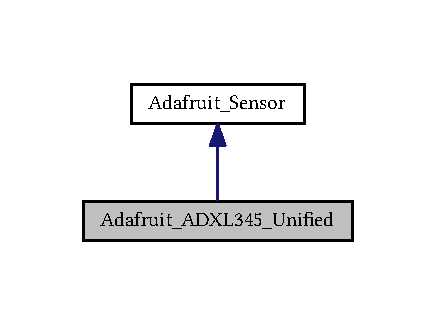
\includegraphics[width=209pt]{class_adafruit___a_d_x_l345___unified__inherit__graph}
\end{center}
\end{figure}


Collaboration diagram for Adafruit\+\_\+\+A\+D\+X\+L345\+\_\+\+Unified\+:\nopagebreak
\begin{figure}[H]
\begin{center}
\leavevmode
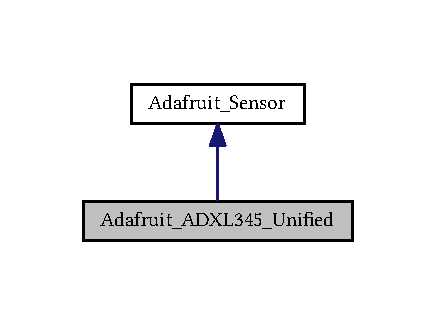
\includegraphics[width=209pt]{class_adafruit___a_d_x_l345___unified__coll__graph}
\end{center}
\end{figure}
\subsection*{Public Member Functions}
\begin{DoxyCompactItemize}
\item 
\hyperlink{class_adafruit___a_d_x_l345___unified_a34c57b807ceb0636ab79320231e51dd6}{Adafruit\+\_\+\+A\+D\+X\+L345\+\_\+\+Unified} (int32\+\_\+t sensor\+ID=-\/1)
\begin{DoxyCompactList}\small\item\em Instantiates a new A\+D\+X\+L345 class. \end{DoxyCompactList}\item 
\hyperlink{class_adafruit___a_d_x_l345___unified_a7e0409063a7441c35044902b947d661d}{Adafruit\+\_\+\+A\+D\+X\+L345\+\_\+\+Unified} (uint8\+\_\+t \hyperlink{_weather___balloon_8cpp_a65f172682710866247eacb1ef68df619}{clock}, uint8\+\_\+t miso, uint8\+\_\+t mosi, uint8\+\_\+t cs, int32\+\_\+t sensor\+ID=-\/1)
\begin{DoxyCompactList}\small\item\em Instantiates a new A\+D\+X\+L345 class in S\+PI mode. \end{DoxyCompactList}\item 
bool \hyperlink{class_adafruit___a_d_x_l345___unified_a55b74a63bbb1317228d5bb5905589a02}{begin} (void)
\begin{DoxyCompactList}\small\item\em Setups the HW (reads coefficients values, etc.) \end{DoxyCompactList}\item 
void \hyperlink{class_adafruit___a_d_x_l345___unified_ad722e964df59c7691b1666472940aa99}{set\+Range} (\hyperlink{_adafruit___a_d_x_l345___u_8h_a23c78f6ff1abdabd74f657e54e415e5b}{range\+\_\+t} range)
\begin{DoxyCompactList}\small\item\em Sets the g range for the accelerometer. \end{DoxyCompactList}\item 
\hyperlink{_adafruit___a_d_x_l345___u_8h_a23c78f6ff1abdabd74f657e54e415e5b}{range\+\_\+t} \hyperlink{class_adafruit___a_d_x_l345___unified_adcdcd1ddcd58af6b1d4f85f9ab30d7a4}{get\+Range} (void)
\begin{DoxyCompactList}\small\item\em Sets the g range for the accelerometer. \end{DoxyCompactList}\item 
void \hyperlink{class_adafruit___a_d_x_l345___unified_a8e837a3e456e5e17839447bbf65f76bd}{set\+Data\+Rate} (\hyperlink{_adafruit___a_d_x_l345___u_8h_a7b8465343401971414c6cc2581f28b0a}{data\+Rate\+\_\+t} data\+Rate)
\begin{DoxyCompactList}\small\item\em Sets the data rate for the A\+D\+X\+L345 (controls power consumption) \end{DoxyCompactList}\item 
\hyperlink{_adafruit___a_d_x_l345___u_8h_a7b8465343401971414c6cc2581f28b0a}{data\+Rate\+\_\+t} \hyperlink{class_adafruit___a_d_x_l345___unified_a3b8ae7da9a66e28b38b70a08c5646b02}{get\+Data\+Rate} (void)
\begin{DoxyCompactList}\small\item\em Gets the data rate for the A\+D\+X\+L345 (controls power consumption) \end{DoxyCompactList}\item 
bool \hyperlink{class_adafruit___a_d_x_l345___unified_a830e4a9d1729310c9cf0d0504b3d0229}{get\+Event} (\hyperlink{_adafruit___sensor_8h_structsensors__event__t}{sensors\+\_\+event\+\_\+t} $\ast$)
\begin{DoxyCompactList}\small\item\em Gets the most recent sensor event. \end{DoxyCompactList}\item 
void \hyperlink{class_adafruit___a_d_x_l345___unified_ac53068bb82bd03fc492542b468a30478}{get\+Sensor} (\hyperlink{_adafruit___sensor_8h_structsensor__t}{sensor\+\_\+t} $\ast$)
\begin{DoxyCompactList}\small\item\em Gets the \hyperlink{_adafruit___sensor_8h_structsensor__t}{sensor\+\_\+t} data. \end{DoxyCompactList}\item 
uint8\+\_\+t \hyperlink{class_adafruit___a_d_x_l345___unified_acf54ca46aa7e6a613807f489711a8ceb}{get\+Device\+ID} (void)
\begin{DoxyCompactList}\small\item\em Read the device ID (can be used to check connection) \end{DoxyCompactList}\item 
void \hyperlink{class_adafruit___a_d_x_l345___unified_a8f6b9e9598618fc0cf221c4b62f924d9}{write\+Register} (uint8\+\_\+t reg, uint8\+\_\+t value)
\begin{DoxyCompactList}\small\item\em Writes 8-\/bits to the specified destination register. \end{DoxyCompactList}\item 
uint8\+\_\+t \hyperlink{class_adafruit___a_d_x_l345___unified_ab56b668f36793605d7be009a7efb74e8}{read\+Register} (uint8\+\_\+t reg)
\begin{DoxyCompactList}\small\item\em Reads 8-\/bits from the specified register. \end{DoxyCompactList}\item 
int16\+\_\+t \hyperlink{class_adafruit___a_d_x_l345___unified_a62c1c34b81fdcb7825d7c9911fba988b}{read16} (uint8\+\_\+t reg)
\begin{DoxyCompactList}\small\item\em Reads 16-\/bits from the specified register. \end{DoxyCompactList}\item 
int16\+\_\+t \hyperlink{class_adafruit___a_d_x_l345___unified_a5ad11ba3d12aa4f4aaaec38b3400fa6f}{getX} (void)
\begin{DoxyCompactList}\small\item\em Gets the most recent X axis value. \end{DoxyCompactList}\item 
int16\+\_\+t \hyperlink{class_adafruit___a_d_x_l345___unified_ac745aefc2a66094a9c46115564939610}{getY} (void)
\begin{DoxyCompactList}\small\item\em Gets the most recent Y axis value. \end{DoxyCompactList}\item 
int16\+\_\+t \hyperlink{class_adafruit___a_d_x_l345___unified_ae61417ef16d19ff86ecd82efc14e960b}{getZ} (void)
\begin{DoxyCompactList}\small\item\em Gets the most recent Z axis value. \end{DoxyCompactList}\item 
void \hyperlink{class_adafruit___a_d_x_l345___unified_a812faf0e78b3f34a7dfe2fc701baedd7}{set\+Correction} (double)
\end{DoxyCompactItemize}


\subsection{Detailed Description}


Definition at line 106 of file Adafruit\+\_\+\+A\+D\+X\+L345\+\_\+\+U.\+h.



\subsection{Constructor \& Destructor Documentation}
\index{Adafruit\+\_\+\+A\+D\+X\+L345\+\_\+\+Unified@{Adafruit\+\_\+\+A\+D\+X\+L345\+\_\+\+Unified}!Adafruit\+\_\+\+A\+D\+X\+L345\+\_\+\+Unified@{Adafruit\+\_\+\+A\+D\+X\+L345\+\_\+\+Unified}}
\index{Adafruit\+\_\+\+A\+D\+X\+L345\+\_\+\+Unified@{Adafruit\+\_\+\+A\+D\+X\+L345\+\_\+\+Unified}!Adafruit\+\_\+\+A\+D\+X\+L345\+\_\+\+Unified@{Adafruit\+\_\+\+A\+D\+X\+L345\+\_\+\+Unified}}
\subsubsection[{\texorpdfstring{Adafruit\+\_\+\+A\+D\+X\+L345\+\_\+\+Unified(int32\+\_\+t sensor\+I\+D=-\/1)}{Adafruit\_ADXL345\_Unified(int32\_t sensorID=-1)}}]{\setlength{\rightskip}{0pt plus 5cm}Adafruit\+\_\+\+A\+D\+X\+L345\+\_\+\+Unified\+::\+Adafruit\+\_\+\+A\+D\+X\+L345\+\_\+\+Unified (
\begin{DoxyParamCaption}
\item[{int32\+\_\+t}]{sensor\+ID = {\ttfamily -\/1}}
\end{DoxyParamCaption}
)}\hypertarget{class_adafruit___a_d_x_l345___unified_a34c57b807ceb0636ab79320231e51dd6}{}\label{class_adafruit___a_d_x_l345___unified_a34c57b807ceb0636ab79320231e51dd6}


Instantiates a new A\+D\+X\+L345 class. 



Definition at line 183 of file Adafruit\+\_\+\+A\+D\+X\+L345\+\_\+\+U.\+cpp.



References A\+D\+X\+L345\+\_\+\+R\+A\+N\+G\+E\+\_\+2\+\_\+G.

\index{Adafruit\+\_\+\+A\+D\+X\+L345\+\_\+\+Unified@{Adafruit\+\_\+\+A\+D\+X\+L345\+\_\+\+Unified}!Adafruit\+\_\+\+A\+D\+X\+L345\+\_\+\+Unified@{Adafruit\+\_\+\+A\+D\+X\+L345\+\_\+\+Unified}}
\index{Adafruit\+\_\+\+A\+D\+X\+L345\+\_\+\+Unified@{Adafruit\+\_\+\+A\+D\+X\+L345\+\_\+\+Unified}!Adafruit\+\_\+\+A\+D\+X\+L345\+\_\+\+Unified@{Adafruit\+\_\+\+A\+D\+X\+L345\+\_\+\+Unified}}
\subsubsection[{\texorpdfstring{Adafruit\+\_\+\+A\+D\+X\+L345\+\_\+\+Unified(uint8\+\_\+t clock, uint8\+\_\+t miso, uint8\+\_\+t mosi, uint8\+\_\+t cs, int32\+\_\+t sensor\+I\+D=-\/1)}{Adafruit\_ADXL345\_Unified(uint8\_t clock, uint8\_t miso, uint8\_t mosi, uint8\_t cs, int32\_t sensorID=-1)}}]{\setlength{\rightskip}{0pt plus 5cm}Adafruit\+\_\+\+A\+D\+X\+L345\+\_\+\+Unified\+::\+Adafruit\+\_\+\+A\+D\+X\+L345\+\_\+\+Unified (
\begin{DoxyParamCaption}
\item[{uint8\+\_\+t}]{clock, }
\item[{uint8\+\_\+t}]{miso, }
\item[{uint8\+\_\+t}]{mosi, }
\item[{uint8\+\_\+t}]{cs, }
\item[{int32\+\_\+t}]{sensor\+ID = {\ttfamily -\/1}}
\end{DoxyParamCaption}
)}\hypertarget{class_adafruit___a_d_x_l345___unified_a7e0409063a7441c35044902b947d661d}{}\label{class_adafruit___a_d_x_l345___unified_a7e0409063a7441c35044902b947d661d}


Instantiates a new A\+D\+X\+L345 class in S\+PI mode. 



Definition at line 195 of file Adafruit\+\_\+\+A\+D\+X\+L345\+\_\+\+U.\+cpp.



References A\+D\+X\+L345\+\_\+\+R\+A\+N\+G\+E\+\_\+2\+\_\+G, and clock.



\subsection{Member Function Documentation}
\index{Adafruit\+\_\+\+A\+D\+X\+L345\+\_\+\+Unified@{Adafruit\+\_\+\+A\+D\+X\+L345\+\_\+\+Unified}!begin@{begin}}
\index{begin@{begin}!Adafruit\+\_\+\+A\+D\+X\+L345\+\_\+\+Unified@{Adafruit\+\_\+\+A\+D\+X\+L345\+\_\+\+Unified}}
\subsubsection[{\texorpdfstring{begin(void)}{begin(void)}}]{\setlength{\rightskip}{0pt plus 5cm}bool Adafruit\+\_\+\+A\+D\+X\+L345\+\_\+\+Unified\+::begin (
\begin{DoxyParamCaption}
\item[{void}]{}
\end{DoxyParamCaption}
)}\hypertarget{class_adafruit___a_d_x_l345___unified_a55b74a63bbb1317228d5bb5905589a02}{}\label{class_adafruit___a_d_x_l345___unified_a55b74a63bbb1317228d5bb5905589a02}


Setups the HW (reads coefficients values, etc.) 



Definition at line 210 of file Adafruit\+\_\+\+A\+D\+X\+L345\+\_\+\+U.\+cpp.



References A\+D\+X\+L345\+\_\+\+R\+E\+G\+\_\+\+P\+O\+W\+E\+R\+\_\+\+C\+TL, get\+Device\+I\+D(), Wire, and write\+Register().



Here is the call graph for this function\+:\nopagebreak
\begin{figure}[H]
\begin{center}
\leavevmode
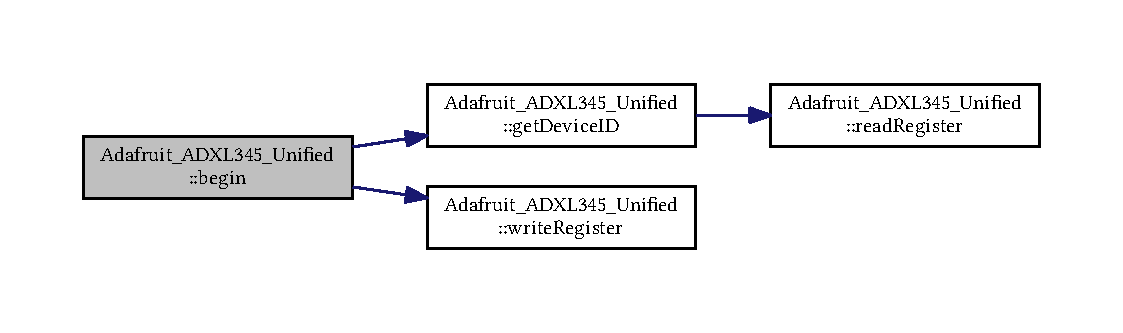
\includegraphics[width=350pt]{class_adafruit___a_d_x_l345___unified_a55b74a63bbb1317228d5bb5905589a02_cgraph}
\end{center}
\end{figure}


\index{Adafruit\+\_\+\+A\+D\+X\+L345\+\_\+\+Unified@{Adafruit\+\_\+\+A\+D\+X\+L345\+\_\+\+Unified}!get\+Data\+Rate@{get\+Data\+Rate}}
\index{get\+Data\+Rate@{get\+Data\+Rate}!Adafruit\+\_\+\+A\+D\+X\+L345\+\_\+\+Unified@{Adafruit\+\_\+\+A\+D\+X\+L345\+\_\+\+Unified}}
\subsubsection[{\texorpdfstring{get\+Data\+Rate(void)}{getDataRate(void)}}]{\setlength{\rightskip}{0pt plus 5cm}{\bf data\+Rate\+\_\+t} Adafruit\+\_\+\+A\+D\+X\+L345\+\_\+\+Unified\+::get\+Data\+Rate (
\begin{DoxyParamCaption}
\item[{void}]{}
\end{DoxyParamCaption}
)}\hypertarget{class_adafruit___a_d_x_l345___unified_a3b8ae7da9a66e28b38b70a08c5646b02}{}\label{class_adafruit___a_d_x_l345___unified_a3b8ae7da9a66e28b38b70a08c5646b02}


Gets the data rate for the A\+D\+X\+L345 (controls power consumption) 



Definition at line 289 of file Adafruit\+\_\+\+A\+D\+X\+L345\+\_\+\+U.\+cpp.



References A\+D\+X\+L345\+\_\+\+R\+E\+G\+\_\+\+B\+W\+\_\+\+R\+A\+TE, and read\+Register().



Here is the call graph for this function\+:\nopagebreak
\begin{figure}[H]
\begin{center}
\leavevmode
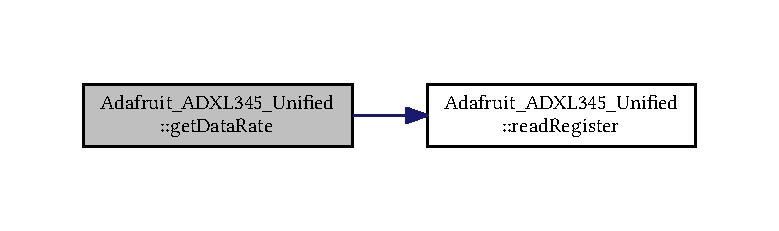
\includegraphics[width=350pt]{class_adafruit___a_d_x_l345___unified_a3b8ae7da9a66e28b38b70a08c5646b02_cgraph}
\end{center}
\end{figure}


\index{Adafruit\+\_\+\+A\+D\+X\+L345\+\_\+\+Unified@{Adafruit\+\_\+\+A\+D\+X\+L345\+\_\+\+Unified}!get\+Device\+ID@{get\+Device\+ID}}
\index{get\+Device\+ID@{get\+Device\+ID}!Adafruit\+\_\+\+A\+D\+X\+L345\+\_\+\+Unified@{Adafruit\+\_\+\+A\+D\+X\+L345\+\_\+\+Unified}}
\subsubsection[{\texorpdfstring{get\+Device\+I\+D(void)}{getDeviceID(void)}}]{\setlength{\rightskip}{0pt plus 5cm}uint8\+\_\+t Adafruit\+\_\+\+A\+D\+X\+L345\+\_\+\+Unified\+::get\+Device\+ID (
\begin{DoxyParamCaption}
\item[{void}]{}
\end{DoxyParamCaption}
)}\hypertarget{class_adafruit___a_d_x_l345___unified_acf54ca46aa7e6a613807f489711a8ceb}{}\label{class_adafruit___a_d_x_l345___unified_acf54ca46aa7e6a613807f489711a8ceb}


Read the device ID (can be used to check connection) 



Definition at line 146 of file Adafruit\+\_\+\+A\+D\+X\+L345\+\_\+\+U.\+cpp.



References A\+D\+X\+L345\+\_\+\+R\+E\+G\+\_\+\+D\+E\+V\+ID, and read\+Register().



Referenced by begin().



Here is the call graph for this function\+:\nopagebreak
\begin{figure}[H]
\begin{center}
\leavevmode
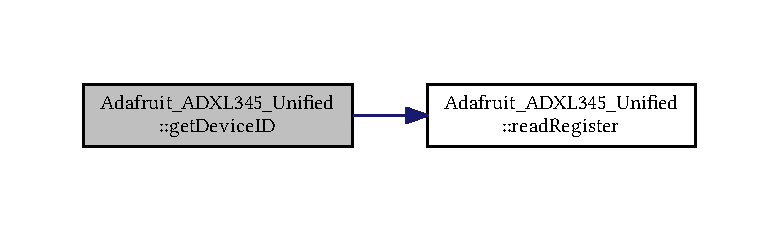
\includegraphics[width=350pt]{class_adafruit___a_d_x_l345___unified_acf54ca46aa7e6a613807f489711a8ceb_cgraph}
\end{center}
\end{figure}




Here is the caller graph for this function\+:\nopagebreak
\begin{figure}[H]
\begin{center}
\leavevmode
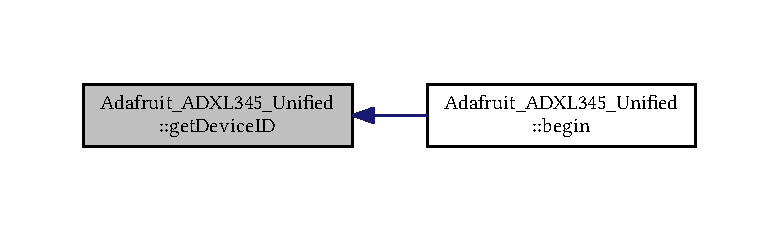
\includegraphics[width=350pt]{class_adafruit___a_d_x_l345___unified_acf54ca46aa7e6a613807f489711a8ceb_icgraph}
\end{center}
\end{figure}


\index{Adafruit\+\_\+\+A\+D\+X\+L345\+\_\+\+Unified@{Adafruit\+\_\+\+A\+D\+X\+L345\+\_\+\+Unified}!get\+Event@{get\+Event}}
\index{get\+Event@{get\+Event}!Adafruit\+\_\+\+A\+D\+X\+L345\+\_\+\+Unified@{Adafruit\+\_\+\+A\+D\+X\+L345\+\_\+\+Unified}}
\subsubsection[{\texorpdfstring{get\+Event(sensors\+\_\+event\+\_\+t $\ast$)}{getEvent(sensors\_event\_t *)}}]{\setlength{\rightskip}{0pt plus 5cm}bool Adafruit\+\_\+\+A\+D\+X\+L345\+\_\+\+Unified\+::get\+Event (
\begin{DoxyParamCaption}
\item[{{\bf sensors\+\_\+event\+\_\+t} $\ast$}]{event}
\end{DoxyParamCaption}
)\hspace{0.3cm}{\ttfamily [virtual]}}\hypertarget{class_adafruit___a_d_x_l345___unified_a830e4a9d1729310c9cf0d0504b3d0229}{}\label{class_adafruit___a_d_x_l345___unified_a830e4a9d1729310c9cf0d0504b3d0229}


Gets the most recent sensor event. 



Implements \hyperlink{class_adafruit___sensor_a0636562b9bc853b796ecc87b5d4b1bec}{Adafruit\+\_\+\+Sensor}.



Definition at line 299 of file Adafruit\+\_\+\+A\+D\+X\+L345\+\_\+\+U.\+cpp.



References A\+D\+X\+L345\+\_\+\+M\+G2\+G\+\_\+\+M\+U\+L\+T\+I\+P\+L\+I\+ER, get\+X(), get\+Y(), get\+Z(), S\+E\+N\+S\+O\+R\+\_\+\+T\+Y\+P\+E\+\_\+\+A\+C\+C\+E\+L\+E\+R\+O\+M\+E\+T\+ER, and S\+E\+N\+S\+O\+R\+S\+\_\+\+G\+R\+A\+V\+I\+T\+Y\+\_\+\+S\+T\+A\+N\+D\+A\+RD.



Here is the call graph for this function\+:\nopagebreak
\begin{figure}[H]
\begin{center}
\leavevmode
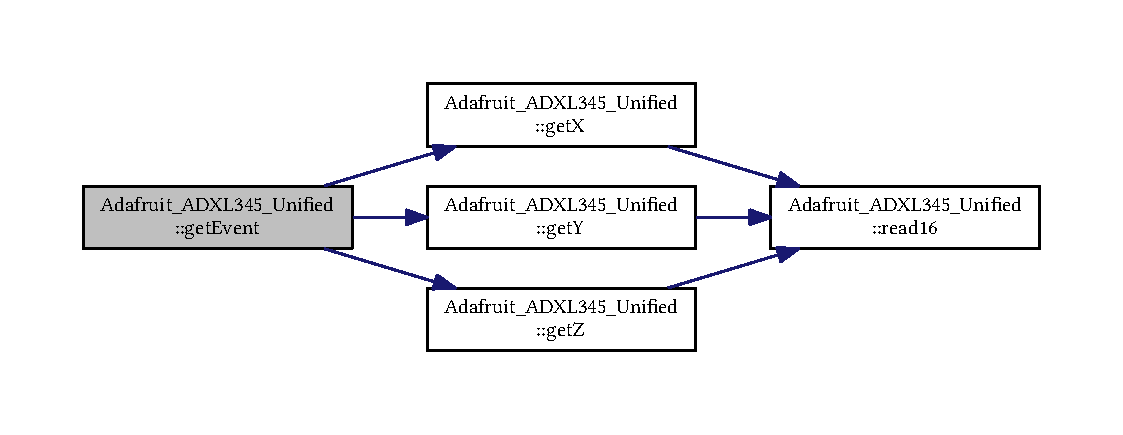
\includegraphics[width=350pt]{class_adafruit___a_d_x_l345___unified_a830e4a9d1729310c9cf0d0504b3d0229_cgraph}
\end{center}
\end{figure}


\index{Adafruit\+\_\+\+A\+D\+X\+L345\+\_\+\+Unified@{Adafruit\+\_\+\+A\+D\+X\+L345\+\_\+\+Unified}!get\+Range@{get\+Range}}
\index{get\+Range@{get\+Range}!Adafruit\+\_\+\+A\+D\+X\+L345\+\_\+\+Unified@{Adafruit\+\_\+\+A\+D\+X\+L345\+\_\+\+Unified}}
\subsubsection[{\texorpdfstring{get\+Range(void)}{getRange(void)}}]{\setlength{\rightskip}{0pt plus 5cm}{\bf range\+\_\+t} Adafruit\+\_\+\+A\+D\+X\+L345\+\_\+\+Unified\+::get\+Range (
\begin{DoxyParamCaption}
\item[{void}]{}
\end{DoxyParamCaption}
)}\hypertarget{class_adafruit___a_d_x_l345___unified_adcdcd1ddcd58af6b1d4f85f9ab30d7a4}{}\label{class_adafruit___a_d_x_l345___unified_adcdcd1ddcd58af6b1d4f85f9ab30d7a4}


Sets the g range for the accelerometer. 



Definition at line 266 of file Adafruit\+\_\+\+A\+D\+X\+L345\+\_\+\+U.\+cpp.



References A\+D\+X\+L345\+\_\+\+R\+E\+G\+\_\+\+D\+A\+T\+A\+\_\+\+F\+O\+R\+M\+AT, and read\+Register().



Here is the call graph for this function\+:\nopagebreak
\begin{figure}[H]
\begin{center}
\leavevmode
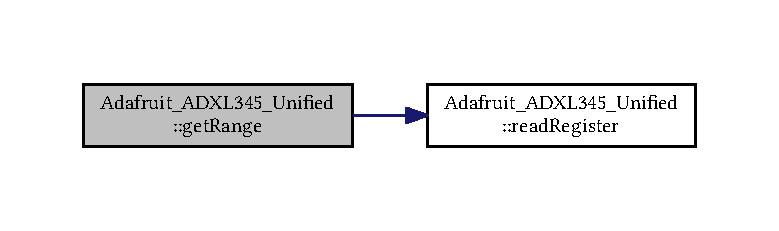
\includegraphics[width=350pt]{class_adafruit___a_d_x_l345___unified_adcdcd1ddcd58af6b1d4f85f9ab30d7a4_cgraph}
\end{center}
\end{figure}


\index{Adafruit\+\_\+\+A\+D\+X\+L345\+\_\+\+Unified@{Adafruit\+\_\+\+A\+D\+X\+L345\+\_\+\+Unified}!get\+Sensor@{get\+Sensor}}
\index{get\+Sensor@{get\+Sensor}!Adafruit\+\_\+\+A\+D\+X\+L345\+\_\+\+Unified@{Adafruit\+\_\+\+A\+D\+X\+L345\+\_\+\+Unified}}
\subsubsection[{\texorpdfstring{get\+Sensor(sensor\+\_\+t $\ast$)}{getSensor(sensor\_t *)}}]{\setlength{\rightskip}{0pt plus 5cm}void Adafruit\+\_\+\+A\+D\+X\+L345\+\_\+\+Unified\+::get\+Sensor (
\begin{DoxyParamCaption}
\item[{{\bf sensor\+\_\+t} $\ast$}]{sensor}
\end{DoxyParamCaption}
)\hspace{0.3cm}{\ttfamily [virtual]}}\hypertarget{class_adafruit___a_d_x_l345___unified_ac53068bb82bd03fc492542b468a30478}{}\label{class_adafruit___a_d_x_l345___unified_ac53068bb82bd03fc492542b468a30478}


Gets the \hyperlink{_adafruit___sensor_8h_structsensor__t}{sensor\+\_\+t} data. 



Implements \hyperlink{class_adafruit___sensor_a19e844c1eb2dc37cb72705d5572c4676}{Adafruit\+\_\+\+Sensor}.



Definition at line 319 of file Adafruit\+\_\+\+A\+D\+X\+L345\+\_\+\+U.\+cpp.



References sensor\+\_\+t\+::max\+\_\+value, sensor\+\_\+t\+::min\+\_\+delay, sensor\+\_\+t\+::min\+\_\+value, sensor\+\_\+t\+::name, sensor\+\_\+t\+::resolution, sensor\+\_\+t\+::sensor\+\_\+id, S\+E\+N\+S\+O\+R\+\_\+\+T\+Y\+P\+E\+\_\+\+P\+R\+E\+S\+S\+U\+RE, sensor\+\_\+t\+::type, and sensor\+\_\+t\+::version.

\index{Adafruit\+\_\+\+A\+D\+X\+L345\+\_\+\+Unified@{Adafruit\+\_\+\+A\+D\+X\+L345\+\_\+\+Unified}!getX@{getX}}
\index{getX@{getX}!Adafruit\+\_\+\+A\+D\+X\+L345\+\_\+\+Unified@{Adafruit\+\_\+\+A\+D\+X\+L345\+\_\+\+Unified}}
\subsubsection[{\texorpdfstring{get\+X(void)}{getX(void)}}]{\setlength{\rightskip}{0pt plus 5cm}int16\+\_\+t Adafruit\+\_\+\+A\+D\+X\+L345\+\_\+\+Unified\+::getX (
\begin{DoxyParamCaption}
\item[{void}]{}
\end{DoxyParamCaption}
)}\hypertarget{class_adafruit___a_d_x_l345___unified_a5ad11ba3d12aa4f4aaaec38b3400fa6f}{}\label{class_adafruit___a_d_x_l345___unified_a5ad11ba3d12aa4f4aaaec38b3400fa6f}


Gets the most recent X axis value. 



Definition at line 156 of file Adafruit\+\_\+\+A\+D\+X\+L345\+\_\+\+U.\+cpp.



References A\+D\+X\+L345\+\_\+\+R\+E\+G\+\_\+\+D\+A\+T\+A\+X0, and read16().



Referenced by get\+Event().



Here is the call graph for this function\+:\nopagebreak
\begin{figure}[H]
\begin{center}
\leavevmode
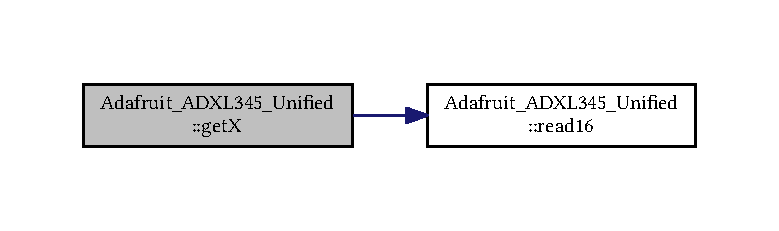
\includegraphics[width=350pt]{class_adafruit___a_d_x_l345___unified_a5ad11ba3d12aa4f4aaaec38b3400fa6f_cgraph}
\end{center}
\end{figure}




Here is the caller graph for this function\+:\nopagebreak
\begin{figure}[H]
\begin{center}
\leavevmode
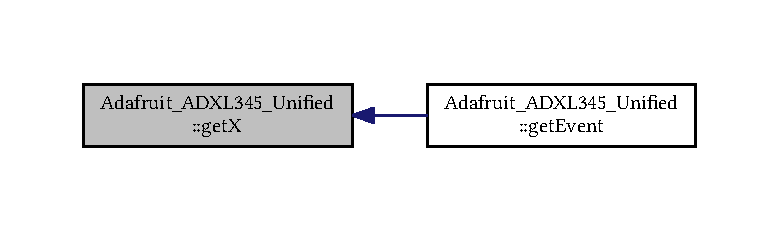
\includegraphics[width=350pt]{class_adafruit___a_d_x_l345___unified_a5ad11ba3d12aa4f4aaaec38b3400fa6f_icgraph}
\end{center}
\end{figure}


\index{Adafruit\+\_\+\+A\+D\+X\+L345\+\_\+\+Unified@{Adafruit\+\_\+\+A\+D\+X\+L345\+\_\+\+Unified}!getY@{getY}}
\index{getY@{getY}!Adafruit\+\_\+\+A\+D\+X\+L345\+\_\+\+Unified@{Adafruit\+\_\+\+A\+D\+X\+L345\+\_\+\+Unified}}
\subsubsection[{\texorpdfstring{get\+Y(void)}{getY(void)}}]{\setlength{\rightskip}{0pt plus 5cm}int16\+\_\+t Adafruit\+\_\+\+A\+D\+X\+L345\+\_\+\+Unified\+::getY (
\begin{DoxyParamCaption}
\item[{void}]{}
\end{DoxyParamCaption}
)}\hypertarget{class_adafruit___a_d_x_l345___unified_ac745aefc2a66094a9c46115564939610}{}\label{class_adafruit___a_d_x_l345___unified_ac745aefc2a66094a9c46115564939610}


Gets the most recent Y axis value. 



Definition at line 165 of file Adafruit\+\_\+\+A\+D\+X\+L345\+\_\+\+U.\+cpp.



References A\+D\+X\+L345\+\_\+\+R\+E\+G\+\_\+\+D\+A\+T\+A\+Y0, and read16().



Referenced by get\+Event().



Here is the call graph for this function\+:\nopagebreak
\begin{figure}[H]
\begin{center}
\leavevmode
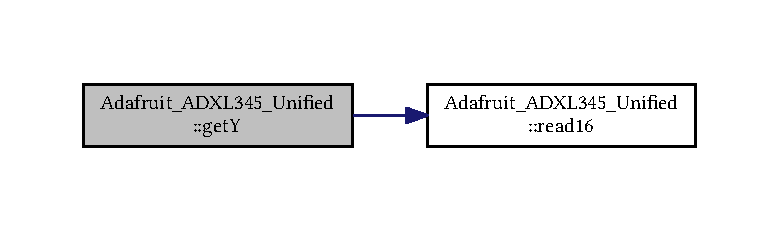
\includegraphics[width=350pt]{class_adafruit___a_d_x_l345___unified_ac745aefc2a66094a9c46115564939610_cgraph}
\end{center}
\end{figure}




Here is the caller graph for this function\+:\nopagebreak
\begin{figure}[H]
\begin{center}
\leavevmode
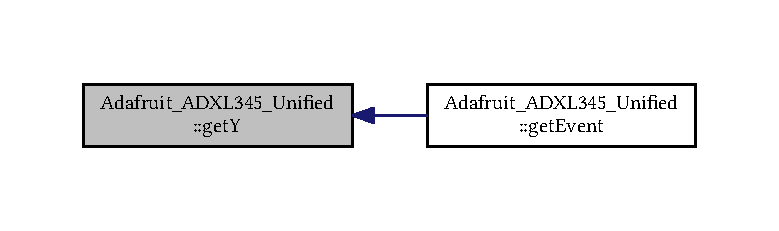
\includegraphics[width=350pt]{class_adafruit___a_d_x_l345___unified_ac745aefc2a66094a9c46115564939610_icgraph}
\end{center}
\end{figure}


\index{Adafruit\+\_\+\+A\+D\+X\+L345\+\_\+\+Unified@{Adafruit\+\_\+\+A\+D\+X\+L345\+\_\+\+Unified}!getZ@{getZ}}
\index{getZ@{getZ}!Adafruit\+\_\+\+A\+D\+X\+L345\+\_\+\+Unified@{Adafruit\+\_\+\+A\+D\+X\+L345\+\_\+\+Unified}}
\subsubsection[{\texorpdfstring{get\+Z(void)}{getZ(void)}}]{\setlength{\rightskip}{0pt plus 5cm}int16\+\_\+t Adafruit\+\_\+\+A\+D\+X\+L345\+\_\+\+Unified\+::getZ (
\begin{DoxyParamCaption}
\item[{void}]{}
\end{DoxyParamCaption}
)}\hypertarget{class_adafruit___a_d_x_l345___unified_ae61417ef16d19ff86ecd82efc14e960b}{}\label{class_adafruit___a_d_x_l345___unified_ae61417ef16d19ff86ecd82efc14e960b}


Gets the most recent Z axis value. 



Definition at line 174 of file Adafruit\+\_\+\+A\+D\+X\+L345\+\_\+\+U.\+cpp.



References A\+D\+X\+L345\+\_\+\+R\+E\+G\+\_\+\+D\+A\+T\+A\+Z0, and read16().



Referenced by get\+Event().



Here is the call graph for this function\+:\nopagebreak
\begin{figure}[H]
\begin{center}
\leavevmode
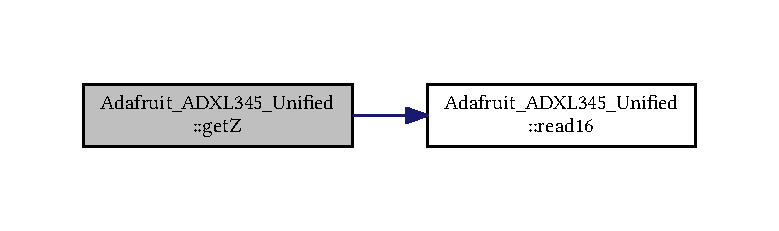
\includegraphics[width=350pt]{class_adafruit___a_d_x_l345___unified_ae61417ef16d19ff86ecd82efc14e960b_cgraph}
\end{center}
\end{figure}




Here is the caller graph for this function\+:\nopagebreak
\begin{figure}[H]
\begin{center}
\leavevmode
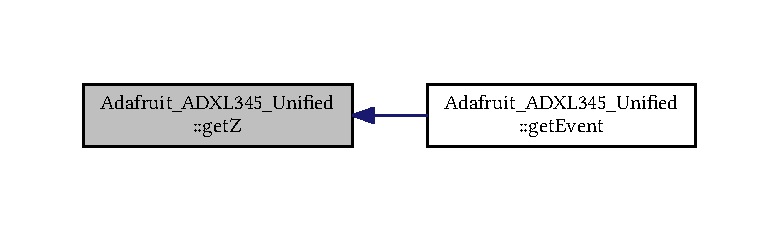
\includegraphics[width=350pt]{class_adafruit___a_d_x_l345___unified_ae61417ef16d19ff86ecd82efc14e960b_icgraph}
\end{center}
\end{figure}


\index{Adafruit\+\_\+\+A\+D\+X\+L345\+\_\+\+Unified@{Adafruit\+\_\+\+A\+D\+X\+L345\+\_\+\+Unified}!read16@{read16}}
\index{read16@{read16}!Adafruit\+\_\+\+A\+D\+X\+L345\+\_\+\+Unified@{Adafruit\+\_\+\+A\+D\+X\+L345\+\_\+\+Unified}}
\subsubsection[{\texorpdfstring{read16(uint8\+\_\+t reg)}{read16(uint8\_t reg)}}]{\setlength{\rightskip}{0pt plus 5cm}int16\+\_\+t Adafruit\+\_\+\+A\+D\+X\+L345\+\_\+\+Unified\+::read16 (
\begin{DoxyParamCaption}
\item[{uint8\+\_\+t}]{reg}
\end{DoxyParamCaption}
)}\hypertarget{class_adafruit___a_d_x_l345___unified_a62c1c34b81fdcb7825d7c9911fba988b}{}\label{class_adafruit___a_d_x_l345___unified_a62c1c34b81fdcb7825d7c9911fba988b}


Reads 16-\/bits from the specified register. 



Definition at line 124 of file Adafruit\+\_\+\+A\+D\+X\+L345\+\_\+\+U.\+cpp.



References A\+D\+X\+L345\+\_\+\+A\+D\+D\+R\+E\+SS, and Wire.



Referenced by get\+X(), get\+Y(), and get\+Z().



Here is the caller graph for this function\+:\nopagebreak
\begin{figure}[H]
\begin{center}
\leavevmode
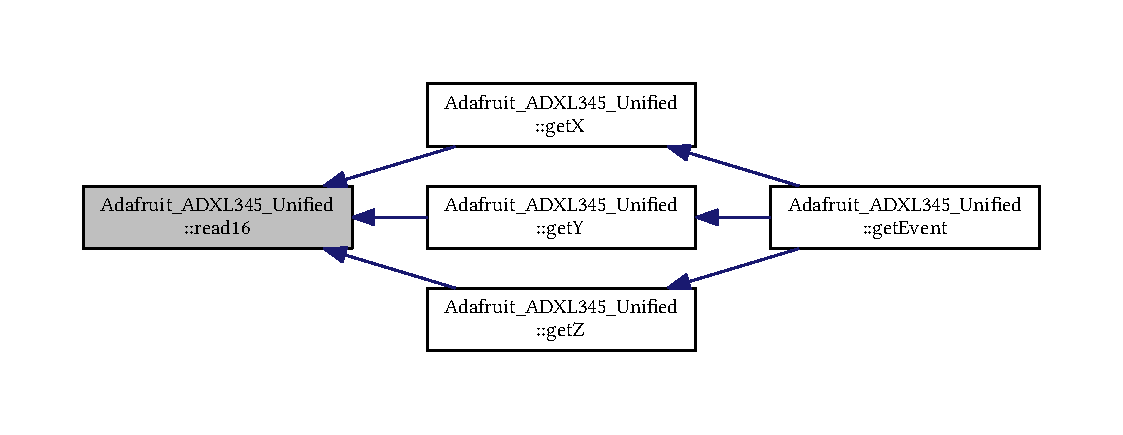
\includegraphics[width=350pt]{class_adafruit___a_d_x_l345___unified_a62c1c34b81fdcb7825d7c9911fba988b_icgraph}
\end{center}
\end{figure}


\index{Adafruit\+\_\+\+A\+D\+X\+L345\+\_\+\+Unified@{Adafruit\+\_\+\+A\+D\+X\+L345\+\_\+\+Unified}!read\+Register@{read\+Register}}
\index{read\+Register@{read\+Register}!Adafruit\+\_\+\+A\+D\+X\+L345\+\_\+\+Unified@{Adafruit\+\_\+\+A\+D\+X\+L345\+\_\+\+Unified}}
\subsubsection[{\texorpdfstring{read\+Register(uint8\+\_\+t reg)}{readRegister(uint8\_t reg)}}]{\setlength{\rightskip}{0pt plus 5cm}uint8\+\_\+t Adafruit\+\_\+\+A\+D\+X\+L345\+\_\+\+Unified\+::read\+Register (
\begin{DoxyParamCaption}
\item[{uint8\+\_\+t}]{reg}
\end{DoxyParamCaption}
)}\hypertarget{class_adafruit___a_d_x_l345___unified_ab56b668f36793605d7be009a7efb74e8}{}\label{class_adafruit___a_d_x_l345___unified_ab56b668f36793605d7be009a7efb74e8}


Reads 8-\/bits from the specified register. 



Definition at line 102 of file Adafruit\+\_\+\+A\+D\+X\+L345\+\_\+\+U.\+cpp.



References A\+D\+X\+L345\+\_\+\+A\+D\+D\+R\+E\+SS, and Wire.



Referenced by get\+Data\+Rate(), get\+Device\+I\+D(), get\+Range(), and set\+Range().



Here is the caller graph for this function\+:
\nopagebreak
\begin{figure}[H]
\begin{center}
\leavevmode
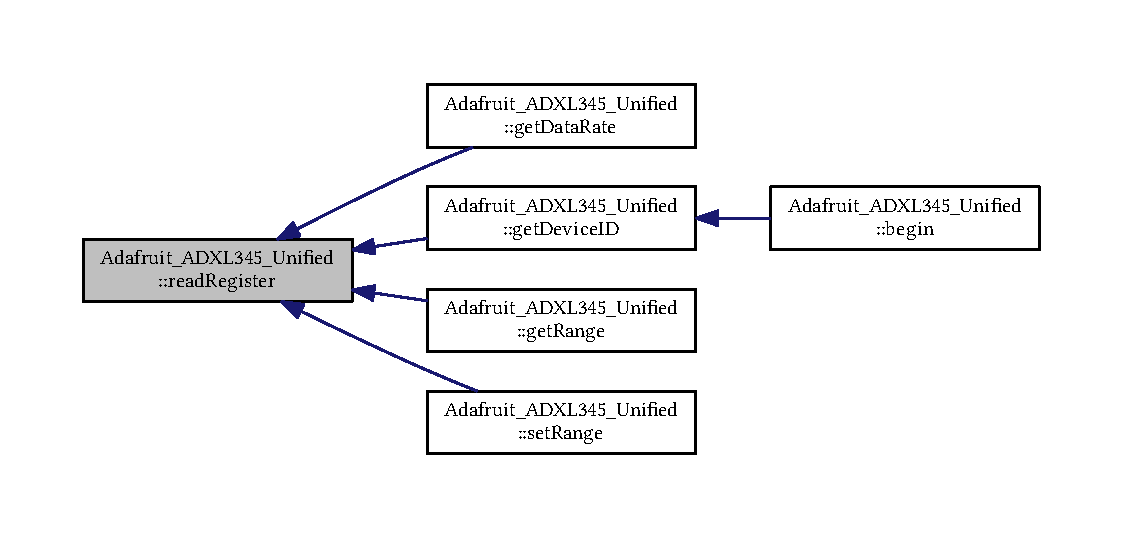
\includegraphics[width=350pt]{class_adafruit___a_d_x_l345___unified_ab56b668f36793605d7be009a7efb74e8_icgraph}
\end{center}
\end{figure}


\index{Adafruit\+\_\+\+A\+D\+X\+L345\+\_\+\+Unified@{Adafruit\+\_\+\+A\+D\+X\+L345\+\_\+\+Unified}!set\+Correction@{set\+Correction}}
\index{set\+Correction@{set\+Correction}!Adafruit\+\_\+\+A\+D\+X\+L345\+\_\+\+Unified@{Adafruit\+\_\+\+A\+D\+X\+L345\+\_\+\+Unified}}
\subsubsection[{\texorpdfstring{set\+Correction(double)}{setCorrection(double)}}]{\setlength{\rightskip}{0pt plus 5cm}void Adafruit\+\_\+\+A\+D\+X\+L345\+\_\+\+Unified\+::set\+Correction (
\begin{DoxyParamCaption}
\item[{double}]{correction\+\_\+value}
\end{DoxyParamCaption}
)}\hypertarget{class_adafruit___a_d_x_l345___unified_a812faf0e78b3f34a7dfe2fc701baedd7}{}\label{class_adafruit___a_d_x_l345___unified_a812faf0e78b3f34a7dfe2fc701baedd7}


Definition at line 335 of file Adafruit\+\_\+\+A\+D\+X\+L345\+\_\+\+U.\+cpp.

\index{Adafruit\+\_\+\+A\+D\+X\+L345\+\_\+\+Unified@{Adafruit\+\_\+\+A\+D\+X\+L345\+\_\+\+Unified}!set\+Data\+Rate@{set\+Data\+Rate}}
\index{set\+Data\+Rate@{set\+Data\+Rate}!Adafruit\+\_\+\+A\+D\+X\+L345\+\_\+\+Unified@{Adafruit\+\_\+\+A\+D\+X\+L345\+\_\+\+Unified}}
\subsubsection[{\texorpdfstring{set\+Data\+Rate(data\+Rate\+\_\+t data\+Rate)}{setDataRate(dataRate\_t dataRate)}}]{\setlength{\rightskip}{0pt plus 5cm}void Adafruit\+\_\+\+A\+D\+X\+L345\+\_\+\+Unified\+::set\+Data\+Rate (
\begin{DoxyParamCaption}
\item[{{\bf data\+Rate\+\_\+t}}]{data\+Rate}
\end{DoxyParamCaption}
)}\hypertarget{class_adafruit___a_d_x_l345___unified_a8e837a3e456e5e17839447bbf65f76bd}{}\label{class_adafruit___a_d_x_l345___unified_a8e837a3e456e5e17839447bbf65f76bd}


Sets the data rate for the A\+D\+X\+L345 (controls power consumption) 



Definition at line 277 of file Adafruit\+\_\+\+A\+D\+X\+L345\+\_\+\+U.\+cpp.



References A\+D\+X\+L345\+\_\+\+R\+E\+G\+\_\+\+B\+W\+\_\+\+R\+A\+TE, and write\+Register().



Here is the call graph for this function\+:\nopagebreak
\begin{figure}[H]
\begin{center}
\leavevmode
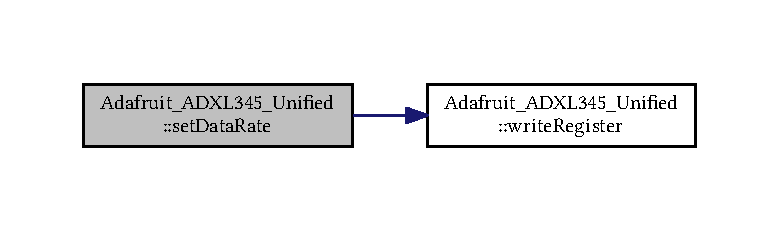
\includegraphics[width=350pt]{class_adafruit___a_d_x_l345___unified_a8e837a3e456e5e17839447bbf65f76bd_cgraph}
\end{center}
\end{figure}


\index{Adafruit\+\_\+\+A\+D\+X\+L345\+\_\+\+Unified@{Adafruit\+\_\+\+A\+D\+X\+L345\+\_\+\+Unified}!set\+Range@{set\+Range}}
\index{set\+Range@{set\+Range}!Adafruit\+\_\+\+A\+D\+X\+L345\+\_\+\+Unified@{Adafruit\+\_\+\+A\+D\+X\+L345\+\_\+\+Unified}}
\subsubsection[{\texorpdfstring{set\+Range(range\+\_\+t range)}{setRange(range\_t range)}}]{\setlength{\rightskip}{0pt plus 5cm}void Adafruit\+\_\+\+A\+D\+X\+L345\+\_\+\+Unified\+::set\+Range (
\begin{DoxyParamCaption}
\item[{{\bf range\+\_\+t}}]{range}
\end{DoxyParamCaption}
)}\hypertarget{class_adafruit___a_d_x_l345___unified_ad722e964df59c7691b1666472940aa99}{}\label{class_adafruit___a_d_x_l345___unified_ad722e964df59c7691b1666472940aa99}


Sets the g range for the accelerometer. 



Definition at line 242 of file Adafruit\+\_\+\+A\+D\+X\+L345\+\_\+\+U.\+cpp.



References A\+D\+X\+L345\+\_\+\+R\+E\+G\+\_\+\+D\+A\+T\+A\+\_\+\+F\+O\+R\+M\+AT, read\+Register(), and write\+Register().



Here is the call graph for this function\+:\nopagebreak
\begin{figure}[H]
\begin{center}
\leavevmode
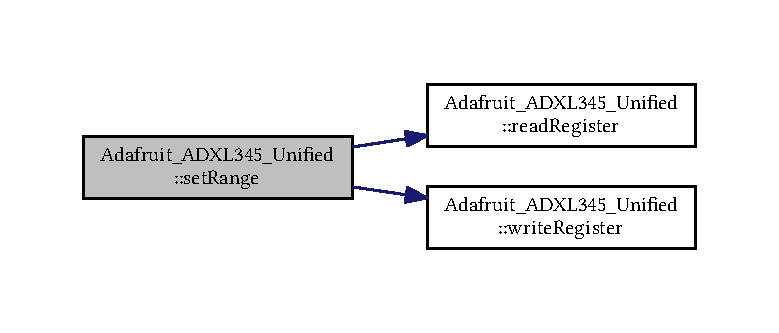
\includegraphics[width=350pt]{class_adafruit___a_d_x_l345___unified_ad722e964df59c7691b1666472940aa99_cgraph}
\end{center}
\end{figure}


\index{Adafruit\+\_\+\+A\+D\+X\+L345\+\_\+\+Unified@{Adafruit\+\_\+\+A\+D\+X\+L345\+\_\+\+Unified}!write\+Register@{write\+Register}}
\index{write\+Register@{write\+Register}!Adafruit\+\_\+\+A\+D\+X\+L345\+\_\+\+Unified@{Adafruit\+\_\+\+A\+D\+X\+L345\+\_\+\+Unified}}
\subsubsection[{\texorpdfstring{write\+Register(uint8\+\_\+t reg, uint8\+\_\+t value)}{writeRegister(uint8\_t reg, uint8\_t value)}}]{\setlength{\rightskip}{0pt plus 5cm}void Adafruit\+\_\+\+A\+D\+X\+L345\+\_\+\+Unified\+::write\+Register (
\begin{DoxyParamCaption}
\item[{uint8\+\_\+t}]{reg, }
\item[{uint8\+\_\+t}]{value}
\end{DoxyParamCaption}
)}\hypertarget{class_adafruit___a_d_x_l345___unified_a8f6b9e9598618fc0cf221c4b62f924d9}{}\label{class_adafruit___a_d_x_l345___unified_a8f6b9e9598618fc0cf221c4b62f924d9}


Writes 8-\/bits to the specified destination register. 



Definition at line 83 of file Adafruit\+\_\+\+A\+D\+X\+L345\+\_\+\+U.\+cpp.



References A\+D\+X\+L345\+\_\+\+A\+D\+D\+R\+E\+SS, and Wire.



Referenced by begin(), set\+Data\+Rate(), and set\+Range().



Here is the caller graph for this function\+:
\nopagebreak
\begin{figure}[H]
\begin{center}
\leavevmode
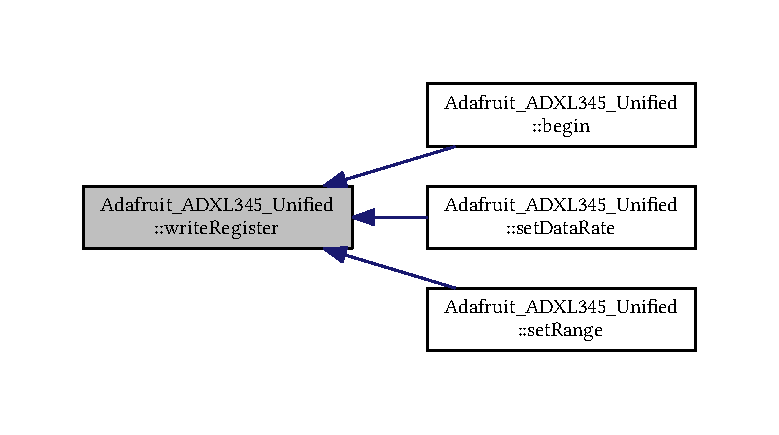
\includegraphics[width=350pt]{class_adafruit___a_d_x_l345___unified_a8f6b9e9598618fc0cf221c4b62f924d9_icgraph}
\end{center}
\end{figure}




The documentation for this class was generated from the following files\+:\begin{DoxyCompactItemize}
\item 
Weather\+\_\+\+Balloon/library/\+Adafruit\+\_\+\+A\+D\+X\+L345-\/master/\hyperlink{_adafruit___a_d_x_l345___u_8h}{Adafruit\+\_\+\+A\+D\+X\+L345\+\_\+\+U.\+h}\item 
Weather\+\_\+\+Balloon/library/\+Adafruit\+\_\+\+A\+D\+X\+L345-\/master/\hyperlink{_adafruit___a_d_x_l345___u_8cpp}{Adafruit\+\_\+\+A\+D\+X\+L345\+\_\+\+U.\+cpp}\end{DoxyCompactItemize}

\hypertarget{class_adafruit___sensor}{}\section{Adafruit\+\_\+\+Sensor Class Reference}
\label{class_adafruit___sensor}\index{Adafruit\+\_\+\+Sensor@{Adafruit\+\_\+\+Sensor}}


{\ttfamily \#include $<$Adafruit\+\_\+\+Sensor.\+h$>$}



Inheritance diagram for Adafruit\+\_\+\+Sensor\+:\nopagebreak
\begin{figure}[H]
\begin{center}
\leavevmode
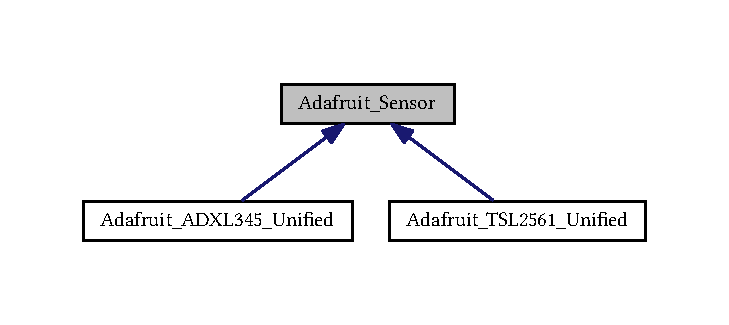
\includegraphics[width=350pt]{class_adafruit___sensor__inherit__graph}
\end{center}
\end{figure}
\subsection*{Public Member Functions}
\begin{DoxyCompactItemize}
\item 
\hyperlink{class_adafruit___sensor_a1d06c6f2b9d014894f47102fc1effddf}{Adafruit\+\_\+\+Sensor} ()
\item 
virtual \hyperlink{class_adafruit___sensor_ac98df73e0cd9367a226b96668417e2e6}{$\sim$\+Adafruit\+\_\+\+Sensor} ()
\item 
virtual void \hyperlink{class_adafruit___sensor_ace6c1f26eeb956f95801b9fc1841f3a0}{enable\+Auto\+Range} (bool enabled)
\item 
virtual bool \hyperlink{class_adafruit___sensor_a0636562b9bc853b796ecc87b5d4b1bec}{get\+Event} (\hyperlink{_adafruit___sensor_8h_structsensors__event__t}{sensors\+\_\+event\+\_\+t} $\ast$)=0
\item 
virtual void \hyperlink{class_adafruit___sensor_a19e844c1eb2dc37cb72705d5572c4676}{get\+Sensor} (\hyperlink{_adafruit___sensor_8h_structsensor__t}{sensor\+\_\+t} $\ast$)=0
\end{DoxyCompactItemize}


\subsection{Detailed Description}


Definition at line 139 of file Adafruit\+\_\+\+Sensor.\+h.



\subsection{Constructor \& Destructor Documentation}
\index{Adafruit\+\_\+\+Sensor@{Adafruit\+\_\+\+Sensor}!Adafruit\+\_\+\+Sensor@{Adafruit\+\_\+\+Sensor}}
\index{Adafruit\+\_\+\+Sensor@{Adafruit\+\_\+\+Sensor}!Adafruit\+\_\+\+Sensor@{Adafruit\+\_\+\+Sensor}}
\subsubsection[{\texorpdfstring{Adafruit\+\_\+\+Sensor()}{Adafruit\_Sensor()}}]{\setlength{\rightskip}{0pt plus 5cm}Adafruit\+\_\+\+Sensor\+::\+Adafruit\+\_\+\+Sensor (
\begin{DoxyParamCaption}
{}
\end{DoxyParamCaption}
)\hspace{0.3cm}{\ttfamily [inline]}}\hypertarget{class_adafruit___sensor_a1d06c6f2b9d014894f47102fc1effddf}{}\label{class_adafruit___sensor_a1d06c6f2b9d014894f47102fc1effddf}


Definition at line 142 of file Adafruit\+\_\+\+Sensor.\+h.

\index{Adafruit\+\_\+\+Sensor@{Adafruit\+\_\+\+Sensor}!````~Adafruit\+\_\+\+Sensor@{$\sim$\+Adafruit\+\_\+\+Sensor}}
\index{````~Adafruit\+\_\+\+Sensor@{$\sim$\+Adafruit\+\_\+\+Sensor}!Adafruit\+\_\+\+Sensor@{Adafruit\+\_\+\+Sensor}}
\subsubsection[{\texorpdfstring{$\sim$\+Adafruit\+\_\+\+Sensor()}{~Adafruit\_Sensor()}}]{\setlength{\rightskip}{0pt plus 5cm}virtual Adafruit\+\_\+\+Sensor\+::$\sim$\+Adafruit\+\_\+\+Sensor (
\begin{DoxyParamCaption}
{}
\end{DoxyParamCaption}
)\hspace{0.3cm}{\ttfamily [inline]}, {\ttfamily [virtual]}}\hypertarget{class_adafruit___sensor_ac98df73e0cd9367a226b96668417e2e6}{}\label{class_adafruit___sensor_ac98df73e0cd9367a226b96668417e2e6}


Definition at line 143 of file Adafruit\+\_\+\+Sensor.\+h.



\subsection{Member Function Documentation}
\index{Adafruit\+\_\+\+Sensor@{Adafruit\+\_\+\+Sensor}!enable\+Auto\+Range@{enable\+Auto\+Range}}
\index{enable\+Auto\+Range@{enable\+Auto\+Range}!Adafruit\+\_\+\+Sensor@{Adafruit\+\_\+\+Sensor}}
\subsubsection[{\texorpdfstring{enable\+Auto\+Range(bool enabled)}{enableAutoRange(bool enabled)}}]{\setlength{\rightskip}{0pt plus 5cm}virtual void Adafruit\+\_\+\+Sensor\+::enable\+Auto\+Range (
\begin{DoxyParamCaption}
\item[{bool}]{enabled}
\end{DoxyParamCaption}
)\hspace{0.3cm}{\ttfamily [inline]}, {\ttfamily [virtual]}}\hypertarget{class_adafruit___sensor_ace6c1f26eeb956f95801b9fc1841f3a0}{}\label{class_adafruit___sensor_ace6c1f26eeb956f95801b9fc1841f3a0}


Reimplemented in \hyperlink{class_adafruit___t_s_l2561___unified_a9bb93fc9a1af24175c9838cdfe7b8904}{Adafruit\+\_\+\+T\+S\+L2561\+\_\+\+Unified}.



Definition at line 146 of file Adafruit\+\_\+\+Sensor.\+h.



References get\+Event(), and get\+Sensor().



Here is the call graph for this function\+:\nopagebreak
\begin{figure}[H]
\begin{center}
\leavevmode
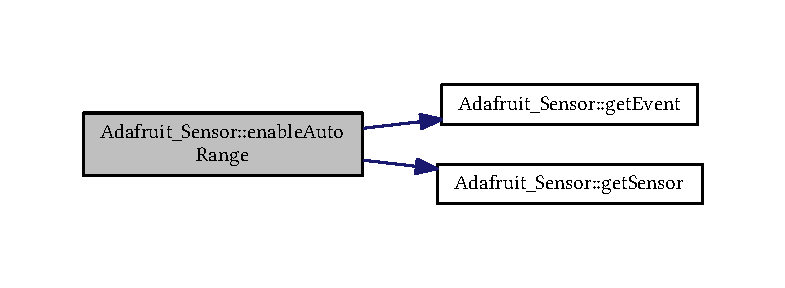
\includegraphics[width=350pt]{class_adafruit___sensor_ace6c1f26eeb956f95801b9fc1841f3a0_cgraph}
\end{center}
\end{figure}


\index{Adafruit\+\_\+\+Sensor@{Adafruit\+\_\+\+Sensor}!get\+Event@{get\+Event}}
\index{get\+Event@{get\+Event}!Adafruit\+\_\+\+Sensor@{Adafruit\+\_\+\+Sensor}}
\subsubsection[{\texorpdfstring{get\+Event(sensors\+\_\+event\+\_\+t $\ast$)=0}{getEvent(sensors\_event\_t *)=0}}]{\setlength{\rightskip}{0pt plus 5cm}virtual bool Adafruit\+\_\+\+Sensor\+::get\+Event (
\begin{DoxyParamCaption}
\item[{{\bf sensors\+\_\+event\+\_\+t} $\ast$}]{}
\end{DoxyParamCaption}
)\hspace{0.3cm}{\ttfamily [pure virtual]}}\hypertarget{class_adafruit___sensor_a0636562b9bc853b796ecc87b5d4b1bec}{}\label{class_adafruit___sensor_a0636562b9bc853b796ecc87b5d4b1bec}


Implemented in \hyperlink{class_adafruit___t_s_l2561___unified_a6a133ea86b7a7158408519214c4d0aef}{Adafruit\+\_\+\+T\+S\+L2561\+\_\+\+Unified}, and \hyperlink{class_adafruit___a_d_x_l345___unified_a830e4a9d1729310c9cf0d0504b3d0229}{Adafruit\+\_\+\+A\+D\+X\+L345\+\_\+\+Unified}.



Referenced by enable\+Auto\+Range().



Here is the caller graph for this function\+:\nopagebreak
\begin{figure}[H]
\begin{center}
\leavevmode
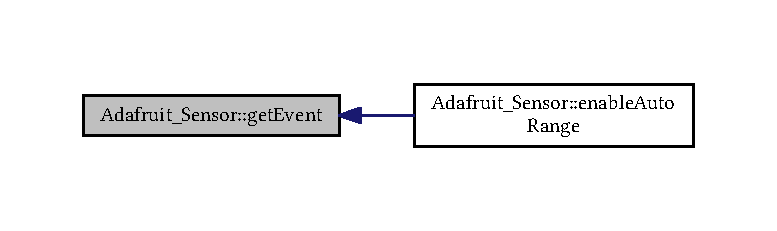
\includegraphics[width=350pt]{class_adafruit___sensor_a0636562b9bc853b796ecc87b5d4b1bec_icgraph}
\end{center}
\end{figure}


\index{Adafruit\+\_\+\+Sensor@{Adafruit\+\_\+\+Sensor}!get\+Sensor@{get\+Sensor}}
\index{get\+Sensor@{get\+Sensor}!Adafruit\+\_\+\+Sensor@{Adafruit\+\_\+\+Sensor}}
\subsubsection[{\texorpdfstring{get\+Sensor(sensor\+\_\+t $\ast$)=0}{getSensor(sensor\_t *)=0}}]{\setlength{\rightskip}{0pt plus 5cm}virtual void Adafruit\+\_\+\+Sensor\+::get\+Sensor (
\begin{DoxyParamCaption}
\item[{{\bf sensor\+\_\+t} $\ast$}]{}
\end{DoxyParamCaption}
)\hspace{0.3cm}{\ttfamily [pure virtual]}}\hypertarget{class_adafruit___sensor_a19e844c1eb2dc37cb72705d5572c4676}{}\label{class_adafruit___sensor_a19e844c1eb2dc37cb72705d5572c4676}


Implemented in \hyperlink{class_adafruit___t_s_l2561___unified_a4c8dcb86a371558aba4ddb0a740d9b3c}{Adafruit\+\_\+\+T\+S\+L2561\+\_\+\+Unified}, and \hyperlink{class_adafruit___a_d_x_l345___unified_ac53068bb82bd03fc492542b468a30478}{Adafruit\+\_\+\+A\+D\+X\+L345\+\_\+\+Unified}.



Referenced by enable\+Auto\+Range().



Here is the caller graph for this function\+:\nopagebreak
\begin{figure}[H]
\begin{center}
\leavevmode
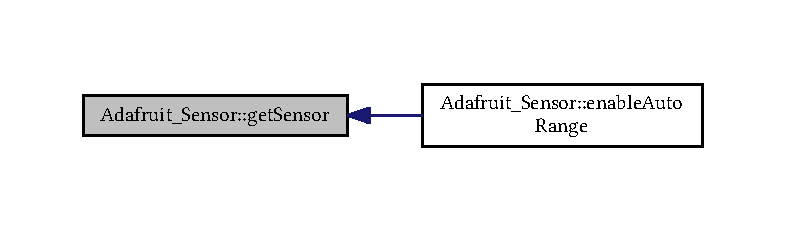
\includegraphics[width=350pt]{class_adafruit___sensor_a19e844c1eb2dc37cb72705d5572c4676_icgraph}
\end{center}
\end{figure}




The documentation for this class was generated from the following file\+:\begin{DoxyCompactItemize}
\item 
Weather\+\_\+\+Balloon/library/\+Adafruit\+\_\+\+Sensor-\/master/\hyperlink{_adafruit___sensor_8h}{Adafruit\+\_\+\+Sensor.\+h}\end{DoxyCompactItemize}

\hypertarget{class_adafruit___s_h_t31}{}\section{Adafruit\+\_\+\+S\+H\+T31 Class Reference}
\label{class_adafruit___s_h_t31}\index{Adafruit\+\_\+\+S\+H\+T31@{Adafruit\+\_\+\+S\+H\+T31}}


{\ttfamily \#include $<$Adafruit\+\_\+\+S\+H\+T31.\+h$>$}

\subsection*{Public Member Functions}
\begin{DoxyCompactItemize}
\item 
\hyperlink{class_adafruit___s_h_t31_a3c675ce344f1dd28b04764de3d7b5104}{Adafruit\+\_\+\+S\+H\+T31} ()
\item 
boolean \hyperlink{class_adafruit___s_h_t31_a104eb2dfd27a732420e1fc3755516690}{begin} (uint8\+\_\+t i2caddr=\hyperlink{_adafruit___s_h_t31_8h_a126bb81a04ac54c61287dd2b106bbfe2}{S\+H\+T31\+\_\+\+D\+E\+F\+A\+U\+L\+T\+\_\+\+A\+D\+DR})
\item 
float \hyperlink{class_adafruit___s_h_t31_a3b518218705509eb0ab35050bf79f00a}{read\+Temperature} (void)
\item 
float \hyperlink{class_adafruit___s_h_t31_a2b522bec65225d5c2aadfccd31bb91e0}{read\+Humidity} (void)
\item 
uint16\+\_\+t \hyperlink{class_adafruit___s_h_t31_ae41f7910027c9a39afdb11aef45742ab}{read\+Status} (void)
\item 
void \hyperlink{class_adafruit___s_h_t31_a4cfa42c7211e1c5c3de411f3b099c827}{reset} (void)
\item 
void \hyperlink{class_adafruit___s_h_t31_a96d0021ed52302e3a47fd2eaa6c1282f}{heater} (boolean)
\item 
uint8\+\_\+t \hyperlink{class_adafruit___s_h_t31_a9fe74b3c5be1794ec00a961d91227716}{crc8} (const uint8\+\_\+t $\ast$data, int len)
\end{DoxyCompactItemize}


\subsection{Detailed Description}


Definition at line 37 of file Adafruit\+\_\+\+S\+H\+T31.\+h.



\subsection{Constructor \& Destructor Documentation}
\index{Adafruit\+\_\+\+S\+H\+T31@{Adafruit\+\_\+\+S\+H\+T31}!Adafruit\+\_\+\+S\+H\+T31@{Adafruit\+\_\+\+S\+H\+T31}}
\index{Adafruit\+\_\+\+S\+H\+T31@{Adafruit\+\_\+\+S\+H\+T31}!Adafruit\+\_\+\+S\+H\+T31@{Adafruit\+\_\+\+S\+H\+T31}}
\subsubsection[{\texorpdfstring{Adafruit\+\_\+\+S\+H\+T31()}{Adafruit\_SHT31()}}]{\setlength{\rightskip}{0pt plus 5cm}Adafruit\+\_\+\+S\+H\+T31\+::\+Adafruit\+\_\+\+S\+H\+T31 (
\begin{DoxyParamCaption}
{}
\end{DoxyParamCaption}
)}\hypertarget{class_adafruit___s_h_t31_a3c675ce344f1dd28b04764de3d7b5104}{}\label{class_adafruit___s_h_t31_a3c675ce344f1dd28b04764de3d7b5104}


Definition at line 20 of file Adafruit\+\_\+\+S\+H\+T31.\+cpp.



\subsection{Member Function Documentation}
\index{Adafruit\+\_\+\+S\+H\+T31@{Adafruit\+\_\+\+S\+H\+T31}!begin@{begin}}
\index{begin@{begin}!Adafruit\+\_\+\+S\+H\+T31@{Adafruit\+\_\+\+S\+H\+T31}}
\subsubsection[{\texorpdfstring{begin(uint8\+\_\+t i2caddr=\+S\+H\+T31\+\_\+\+D\+E\+F\+A\+U\+L\+T\+\_\+\+A\+D\+D\+R)}{begin(uint8\_t i2caddr=SHT31\_DEFAULT\_ADDR)}}]{\setlength{\rightskip}{0pt plus 5cm}boolean Adafruit\+\_\+\+S\+H\+T31\+::begin (
\begin{DoxyParamCaption}
\item[{uint8\+\_\+t}]{i2caddr = {\ttfamily {\bf S\+H\+T31\+\_\+\+D\+E\+F\+A\+U\+L\+T\+\_\+\+A\+D\+DR}}}
\end{DoxyParamCaption}
)}\hypertarget{class_adafruit___s_h_t31_a104eb2dfd27a732420e1fc3755516690}{}\label{class_adafruit___s_h_t31_a104eb2dfd27a732420e1fc3755516690}


Definition at line 24 of file Adafruit\+\_\+\+S\+H\+T31.\+cpp.



References reset(), and Wire.



Referenced by configure\+\_\+sht31().



Here is the call graph for this function\+:\nopagebreak
\begin{figure}[H]
\begin{center}
\leavevmode
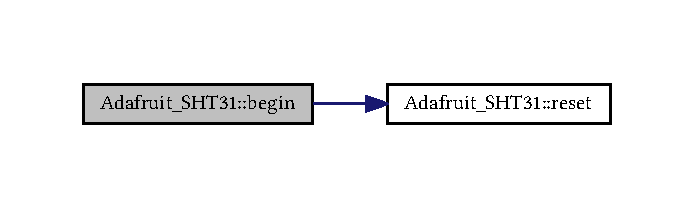
\includegraphics[width=333pt]{class_adafruit___s_h_t31_a104eb2dfd27a732420e1fc3755516690_cgraph}
\end{center}
\end{figure}




Here is the caller graph for this function\+:\nopagebreak
\begin{figure}[H]
\begin{center}
\leavevmode
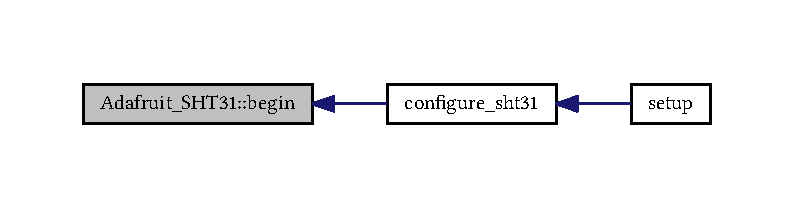
\includegraphics[width=350pt]{class_adafruit___s_h_t31_a104eb2dfd27a732420e1fc3755516690_icgraph}
\end{center}
\end{figure}


\index{Adafruit\+\_\+\+S\+H\+T31@{Adafruit\+\_\+\+S\+H\+T31}!crc8@{crc8}}
\index{crc8@{crc8}!Adafruit\+\_\+\+S\+H\+T31@{Adafruit\+\_\+\+S\+H\+T31}}
\subsubsection[{\texorpdfstring{crc8(const uint8\+\_\+t $\ast$data, int len)}{crc8(const uint8\_t *data, int len)}}]{\setlength{\rightskip}{0pt plus 5cm}uint8\+\_\+t Adafruit\+\_\+\+S\+H\+T31\+::crc8 (
\begin{DoxyParamCaption}
\item[{const uint8\+\_\+t $\ast$}]{data, }
\item[{int}]{len}
\end{DoxyParamCaption}
)}\hypertarget{class_adafruit___s_h_t31_a9fe74b3c5be1794ec00a961d91227716}{}\label{class_adafruit___s_h_t31_a9fe74b3c5be1794ec00a961d91227716}


Definition at line 119 of file Adafruit\+\_\+\+S\+H\+T31.\+cpp.



References i.



Referenced by read\+Humidity().



Here is the caller graph for this function\+:\nopagebreak
\begin{figure}[H]
\begin{center}
\leavevmode
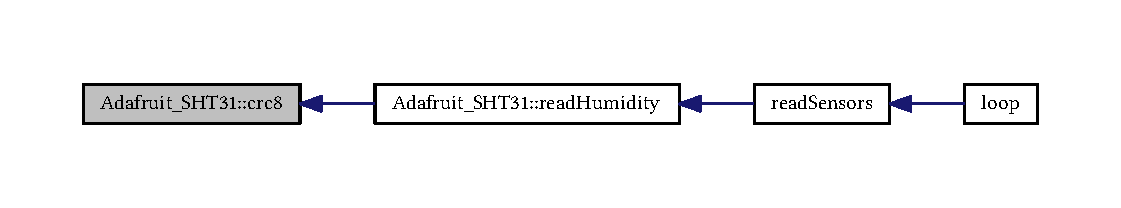
\includegraphics[width=350pt]{class_adafruit___s_h_t31_a9fe74b3c5be1794ec00a961d91227716_icgraph}
\end{center}
\end{figure}


\index{Adafruit\+\_\+\+S\+H\+T31@{Adafruit\+\_\+\+S\+H\+T31}!heater@{heater}}
\index{heater@{heater}!Adafruit\+\_\+\+S\+H\+T31@{Adafruit\+\_\+\+S\+H\+T31}}
\subsubsection[{\texorpdfstring{heater(boolean)}{heater(boolean)}}]{\setlength{\rightskip}{0pt plus 5cm}void Adafruit\+\_\+\+S\+H\+T31\+::heater (
\begin{DoxyParamCaption}
\item[{boolean}]{h}
\end{DoxyParamCaption}
)}\hypertarget{class_adafruit___s_h_t31_a96d0021ed52302e3a47fd2eaa6c1282f}{}\label{class_adafruit___s_h_t31_a96d0021ed52302e3a47fd2eaa6c1282f}


Definition at line 47 of file Adafruit\+\_\+\+S\+H\+T31.\+cpp.



References S\+H\+T31\+\_\+\+H\+E\+A\+T\+E\+R\+D\+IS, and S\+H\+T31\+\_\+\+H\+E\+A\+T\+E\+R\+EN.

\index{Adafruit\+\_\+\+S\+H\+T31@{Adafruit\+\_\+\+S\+H\+T31}!read\+Humidity@{read\+Humidity}}
\index{read\+Humidity@{read\+Humidity}!Adafruit\+\_\+\+S\+H\+T31@{Adafruit\+\_\+\+S\+H\+T31}}
\subsubsection[{\texorpdfstring{read\+Humidity(void)}{readHumidity(void)}}]{\setlength{\rightskip}{0pt plus 5cm}float Adafruit\+\_\+\+S\+H\+T31\+::read\+Humidity (
\begin{DoxyParamCaption}
\item[{void}]{}
\end{DoxyParamCaption}
)}\hypertarget{class_adafruit___s_h_t31_a2b522bec65225d5c2aadfccd31bb91e0}{}\label{class_adafruit___s_h_t31_a2b522bec65225d5c2aadfccd31bb91e0}


Definition at line 62 of file Adafruit\+\_\+\+S\+H\+T31.\+cpp.



References crc8(), i, S\+H\+T31\+\_\+\+M\+E\+A\+S\+\_\+\+H\+I\+G\+H\+R\+EP, and Wire.



Referenced by read\+Sensors().



Here is the call graph for this function\+:\nopagebreak
\begin{figure}[H]
\begin{center}
\leavevmode
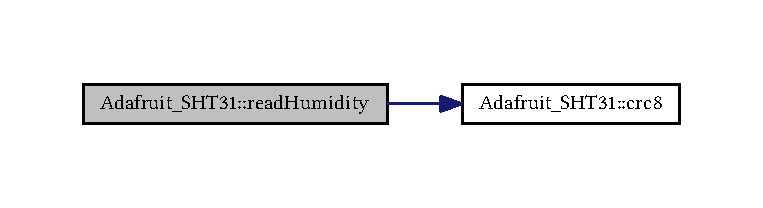
\includegraphics[width=350pt]{class_adafruit___s_h_t31_a2b522bec65225d5c2aadfccd31bb91e0_cgraph}
\end{center}
\end{figure}




Here is the caller graph for this function\+:\nopagebreak
\begin{figure}[H]
\begin{center}
\leavevmode
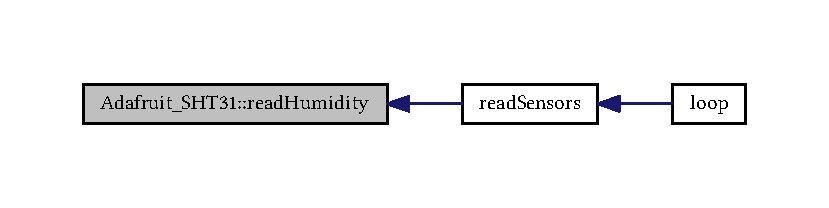
\includegraphics[width=350pt]{class_adafruit___s_h_t31_a2b522bec65225d5c2aadfccd31bb91e0_icgraph}
\end{center}
\end{figure}


\index{Adafruit\+\_\+\+S\+H\+T31@{Adafruit\+\_\+\+S\+H\+T31}!read\+Status@{read\+Status}}
\index{read\+Status@{read\+Status}!Adafruit\+\_\+\+S\+H\+T31@{Adafruit\+\_\+\+S\+H\+T31}}
\subsubsection[{\texorpdfstring{read\+Status(void)}{readStatus(void)}}]{\setlength{\rightskip}{0pt plus 5cm}uint16\+\_\+t Adafruit\+\_\+\+S\+H\+T31\+::read\+Status (
\begin{DoxyParamCaption}
\item[{void}]{}
\end{DoxyParamCaption}
)}\hypertarget{class_adafruit___s_h_t31_ae41f7910027c9a39afdb11aef45742ab}{}\label{class_adafruit___s_h_t31_ae41f7910027c9a39afdb11aef45742ab}


Definition at line 32 of file Adafruit\+\_\+\+S\+H\+T31.\+cpp.



References S\+H\+T31\+\_\+\+R\+E\+A\+D\+S\+T\+A\+T\+US, and Wire.

\index{Adafruit\+\_\+\+S\+H\+T31@{Adafruit\+\_\+\+S\+H\+T31}!read\+Temperature@{read\+Temperature}}
\index{read\+Temperature@{read\+Temperature}!Adafruit\+\_\+\+S\+H\+T31@{Adafruit\+\_\+\+S\+H\+T31}}
\subsubsection[{\texorpdfstring{read\+Temperature(void)}{readTemperature(void)}}]{\setlength{\rightskip}{0pt plus 5cm}float Adafruit\+\_\+\+S\+H\+T31\+::read\+Temperature (
\begin{DoxyParamCaption}
\item[{void}]{}
\end{DoxyParamCaption}
)}\hypertarget{class_adafruit___s_h_t31_a3b518218705509eb0ab35050bf79f00a}{}\label{class_adafruit___s_h_t31_a3b518218705509eb0ab35050bf79f00a}


Definition at line 55 of file Adafruit\+\_\+\+S\+H\+T31.\+cpp.



Referenced by read\+Sensors().



Here is the caller graph for this function\+:\nopagebreak
\begin{figure}[H]
\begin{center}
\leavevmode
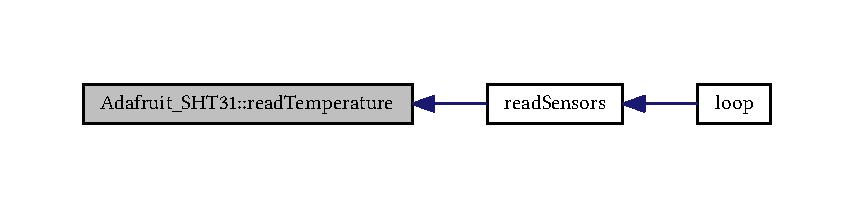
\includegraphics[width=350pt]{class_adafruit___s_h_t31_a3b518218705509eb0ab35050bf79f00a_icgraph}
\end{center}
\end{figure}


\index{Adafruit\+\_\+\+S\+H\+T31@{Adafruit\+\_\+\+S\+H\+T31}!reset@{reset}}
\index{reset@{reset}!Adafruit\+\_\+\+S\+H\+T31@{Adafruit\+\_\+\+S\+H\+T31}}
\subsubsection[{\texorpdfstring{reset(void)}{reset(void)}}]{\setlength{\rightskip}{0pt plus 5cm}void Adafruit\+\_\+\+S\+H\+T31\+::reset (
\begin{DoxyParamCaption}
\item[{void}]{}
\end{DoxyParamCaption}
)}\hypertarget{class_adafruit___s_h_t31_a4cfa42c7211e1c5c3de411f3b099c827}{}\label{class_adafruit___s_h_t31_a4cfa42c7211e1c5c3de411f3b099c827}


Definition at line 42 of file Adafruit\+\_\+\+S\+H\+T31.\+cpp.



References S\+H\+T31\+\_\+\+S\+O\+F\+T\+R\+E\+S\+ET.



Referenced by begin().



Here is the caller graph for this function\+:\nopagebreak
\begin{figure}[H]
\begin{center}
\leavevmode
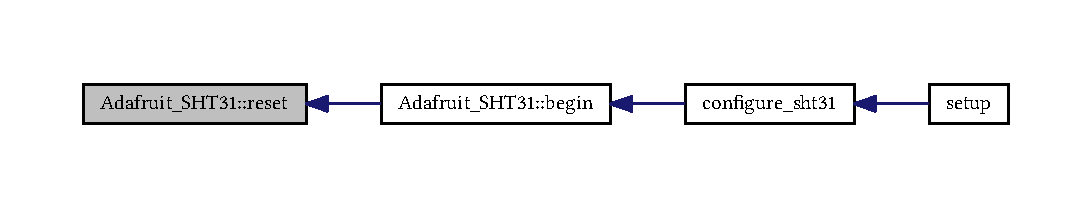
\includegraphics[width=350pt]{class_adafruit___s_h_t31_a4cfa42c7211e1c5c3de411f3b099c827_icgraph}
\end{center}
\end{figure}




The documentation for this class was generated from the following files\+:\begin{DoxyCompactItemize}
\item 
Weather\+\_\+\+Balloon/library/\+Adafruit\+\_\+\+S\+H\+T31-\/master/\hyperlink{_adafruit___s_h_t31_8h}{Adafruit\+\_\+\+S\+H\+T31.\+h}\item 
Weather\+\_\+\+Balloon/library/\+Adafruit\+\_\+\+S\+H\+T31-\/master/\hyperlink{_adafruit___s_h_t31_8cpp}{Adafruit\+\_\+\+S\+H\+T31.\+cpp}\end{DoxyCompactItemize}

\hypertarget{class_adafruit___s_i1145}{}\section{Adafruit\+\_\+\+S\+I1145 Class Reference}
\label{class_adafruit___s_i1145}\index{Adafruit\+\_\+\+S\+I1145@{Adafruit\+\_\+\+S\+I1145}}


{\ttfamily \#include $<$Adafruit\+\_\+\+S\+I1145.\+h$>$}

\subsection*{Public Member Functions}
\begin{DoxyCompactItemize}
\item 
\hyperlink{class_adafruit___s_i1145_ae89a2548ed17479c42aa011df63160f2}{Adafruit\+\_\+\+S\+I1145} (void)
\item 
boolean \hyperlink{class_adafruit___s_i1145_ad17eb7214e6fba886b5595cf14e45cf0}{begin} ()
\item 
void \hyperlink{class_adafruit___s_i1145_ab7a22b92c14315e36b84a42498e970ea}{reset} ()
\item 
uint16\+\_\+t \hyperlink{class_adafruit___s_i1145_a9d1715d966500b5f5f88568a5b4f780b}{read\+UV} ()
\item 
uint16\+\_\+t \hyperlink{class_adafruit___s_i1145_a7295e72f69a558cd6b3ac382ac791688}{read\+IR} ()
\item 
uint16\+\_\+t \hyperlink{class_adafruit___s_i1145_a25bf65464093ec0ba5f9fdd884606a21}{read\+Visible} ()
\item 
uint16\+\_\+t \hyperlink{class_adafruit___s_i1145_a9b058485d8305725020219839285ea16}{read\+Prox} ()
\item 
uint8\+\_\+t \hyperlink{class_adafruit___s_i1145_ab0a29c37acf40dd227d7d23c5a5b0254}{get\+Register} (uint8\+\_\+t)
\item 
uint8\+\_\+t \hyperlink{class_adafruit___s_i1145_a591ba648b988a5dcb464b9f60a4a2c83}{set\+Register} (uint8\+\_\+t, uint8\+\_\+t)
\item 
void \hyperlink{class_adafruit___s_i1145_a67635a26a9c4c6b2fc2a7ffc86c2b5c9}{reset\+\_\+uv} ()
\item 
void \hyperlink{class_adafruit___s_i1145_a9290b9f5e92874e9e927cb27fd53a2ed}{nop} ()
\item 
void \hyperlink{class_adafruit___s_i1145_ad48796484b0107059cc8a8a33b673390}{force\+\_\+convert} ()
\end{DoxyCompactItemize}


\subsection{Detailed Description}


Definition at line 156 of file Adafruit\+\_\+\+S\+I1145.\+h.



\subsection{Constructor \& Destructor Documentation}
\index{Adafruit\+\_\+\+S\+I1145@{Adafruit\+\_\+\+S\+I1145}!Adafruit\+\_\+\+S\+I1145@{Adafruit\+\_\+\+S\+I1145}}
\index{Adafruit\+\_\+\+S\+I1145@{Adafruit\+\_\+\+S\+I1145}!Adafruit\+\_\+\+S\+I1145@{Adafruit\+\_\+\+S\+I1145}}
\subsubsection[{\texorpdfstring{Adafruit\+\_\+\+S\+I1145(void)}{Adafruit\_SI1145(void)}}]{\setlength{\rightskip}{0pt plus 5cm}Adafruit\+\_\+\+S\+I1145\+::\+Adafruit\+\_\+\+S\+I1145 (
\begin{DoxyParamCaption}
\item[{void}]{}
\end{DoxyParamCaption}
)}\hypertarget{class_adafruit___s_i1145_ae89a2548ed17479c42aa011df63160f2}{}\label{class_adafruit___s_i1145_ae89a2548ed17479c42aa011df63160f2}


Definition at line 20 of file Adafruit\+\_\+\+S\+I1145.\+cpp.



References S\+I1145\+\_\+\+A\+D\+DR.



\subsection{Member Function Documentation}
\index{Adafruit\+\_\+\+S\+I1145@{Adafruit\+\_\+\+S\+I1145}!begin@{begin}}
\index{begin@{begin}!Adafruit\+\_\+\+S\+I1145@{Adafruit\+\_\+\+S\+I1145}}
\subsubsection[{\texorpdfstring{begin()}{begin()}}]{\setlength{\rightskip}{0pt plus 5cm}boolean Adafruit\+\_\+\+S\+I1145\+::begin (
\begin{DoxyParamCaption}
\item[{void}]{}
\end{DoxyParamCaption}
)}\hypertarget{class_adafruit___s_i1145_ad17eb7214e6fba886b5595cf14e45cf0}{}\label{class_adafruit___s_i1145_ad17eb7214e6fba886b5595cf14e45cf0}


Definition at line 25 of file Adafruit\+\_\+\+S\+I1145.\+cpp.



References reset(), S\+I1145\+\_\+\+P\+A\+R\+A\+M\+\_\+\+A\+D\+C\+C\+O\+U\+N\+T\+E\+R\+\_\+511\+C\+LK, S\+I1145\+\_\+\+P\+A\+R\+A\+M\+\_\+\+A\+D\+C\+M\+U\+X\+\_\+\+L\+A\+R\+G\+E\+IR, S\+I1145\+\_\+\+P\+A\+R\+A\+M\+\_\+\+A\+D\+C\+M\+U\+X\+\_\+\+S\+M\+A\+L\+L\+IR, S\+I1145\+\_\+\+P\+A\+R\+A\+M\+\_\+\+A\+L\+S\+I\+R\+A\+D\+C\+G\+A\+IN, S\+I1145\+\_\+\+P\+A\+R\+A\+M\+\_\+\+A\+L\+S\+I\+R\+A\+D\+C\+M\+I\+SC, S\+I1145\+\_\+\+P\+A\+R\+A\+M\+\_\+\+A\+L\+S\+I\+R\+A\+D\+C\+M\+I\+S\+C\+\_\+\+R\+A\+N\+GE, S\+I1145\+\_\+\+P\+A\+R\+A\+M\+\_\+\+A\+L\+S\+I\+R\+A\+D\+C\+M\+UX, S\+I1145\+\_\+\+P\+A\+R\+A\+M\+\_\+\+A\+L\+S\+I\+R\+A\+D\+C\+O\+U\+N\+T\+ER, S\+I1145\+\_\+\+P\+A\+R\+A\+M\+\_\+\+A\+L\+S\+V\+I\+S\+A\+D\+C\+G\+A\+IN, S\+I1145\+\_\+\+P\+A\+R\+A\+M\+\_\+\+A\+L\+S\+V\+I\+S\+A\+D\+C\+M\+I\+SC, S\+I1145\+\_\+\+P\+A\+R\+A\+M\+\_\+\+A\+L\+S\+V\+I\+S\+A\+D\+C\+M\+I\+S\+C\+\_\+\+V\+I\+S\+R\+A\+N\+GE, S\+I1145\+\_\+\+P\+A\+R\+A\+M\+\_\+\+A\+L\+S\+V\+I\+S\+A\+D\+C\+O\+U\+N\+T\+ER, S\+I1145\+\_\+\+P\+A\+R\+A\+M\+\_\+\+C\+H\+L\+I\+ST, S\+I1145\+\_\+\+P\+A\+R\+A\+M\+\_\+\+C\+H\+L\+I\+S\+T\+\_\+\+E\+N\+A\+L\+S\+IR, S\+I1145\+\_\+\+P\+A\+R\+A\+M\+\_\+\+C\+H\+L\+I\+S\+T\+\_\+\+E\+N\+A\+L\+S\+V\+IS, S\+I1145\+\_\+\+P\+A\+R\+A\+M\+\_\+\+C\+H\+L\+I\+S\+T\+\_\+\+E\+N\+P\+S1, S\+I1145\+\_\+\+P\+A\+R\+A\+M\+\_\+\+C\+H\+L\+I\+S\+T\+\_\+\+E\+N\+UV, S\+I1145\+\_\+\+P\+A\+R\+A\+M\+\_\+\+P\+S1\+A\+D\+C\+M\+UX, S\+I1145\+\_\+\+P\+A\+R\+A\+M\+\_\+\+P\+S\+A\+D\+C\+G\+A\+IN, S\+I1145\+\_\+\+P\+A\+R\+A\+M\+\_\+\+P\+S\+A\+D\+C\+M\+I\+SC, S\+I1145\+\_\+\+P\+A\+R\+A\+M\+\_\+\+P\+S\+A\+D\+C\+M\+I\+S\+C\+\_\+\+P\+S\+M\+O\+DE, S\+I1145\+\_\+\+P\+A\+R\+A\+M\+\_\+\+P\+S\+A\+D\+C\+M\+I\+S\+C\+\_\+\+R\+A\+N\+GE, S\+I1145\+\_\+\+P\+A\+R\+A\+M\+\_\+\+P\+S\+A\+D\+C\+O\+U\+N\+T\+ER, S\+I1145\+\_\+\+P\+A\+R\+A\+M\+\_\+\+P\+S\+L\+E\+D12\+S\+EL, S\+I1145\+\_\+\+P\+A\+R\+A\+M\+\_\+\+P\+S\+L\+E\+D12\+S\+E\+L\+\_\+\+P\+S1\+L\+E\+D1, S\+I1145\+\_\+\+R\+E\+G\+\_\+\+I\+N\+T\+C\+FG, S\+I1145\+\_\+\+R\+E\+G\+\_\+\+I\+N\+T\+C\+F\+G\+\_\+\+I\+N\+T\+OE, S\+I1145\+\_\+\+R\+E\+G\+\_\+\+I\+R\+Q\+EN, S\+I1145\+\_\+\+R\+E\+G\+\_\+\+I\+R\+Q\+E\+N\+\_\+\+A\+L\+S\+E\+V\+E\+R\+Y\+S\+A\+M\+P\+LE, S\+I1145\+\_\+\+R\+E\+G\+\_\+\+P\+A\+R\+T\+ID, S\+I1145\+\_\+\+R\+E\+G\+\_\+\+P\+S\+L\+E\+D21, S\+I1145\+\_\+\+R\+E\+G\+\_\+\+U\+C\+O\+E\+F\+F0, S\+I1145\+\_\+\+R\+E\+G\+\_\+\+U\+C\+O\+E\+F\+F1, S\+I1145\+\_\+\+R\+E\+G\+\_\+\+U\+C\+O\+E\+F\+F2, S\+I1145\+\_\+\+R\+E\+G\+\_\+\+U\+C\+O\+E\+F\+F3, and Wire.



Here is the call graph for this function\+:\nopagebreak
\begin{figure}[H]
\begin{center}
\leavevmode
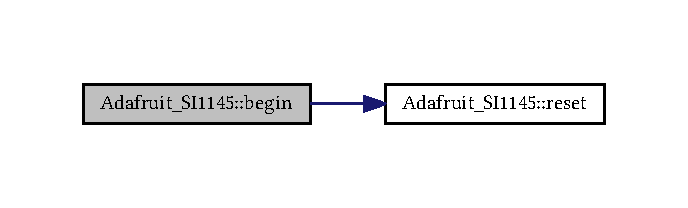
\includegraphics[width=330pt]{class_adafruit___s_i1145_ad17eb7214e6fba886b5595cf14e45cf0_cgraph}
\end{center}
\end{figure}


\index{Adafruit\+\_\+\+S\+I1145@{Adafruit\+\_\+\+S\+I1145}!force\+\_\+convert@{force\+\_\+convert}}
\index{force\+\_\+convert@{force\+\_\+convert}!Adafruit\+\_\+\+S\+I1145@{Adafruit\+\_\+\+S\+I1145}}
\subsubsection[{\texorpdfstring{force\+\_\+convert()}{force\_convert()}}]{\setlength{\rightskip}{0pt plus 5cm}void Adafruit\+\_\+\+S\+I1145\+::force\+\_\+convert (
\begin{DoxyParamCaption}
{}
\end{DoxyParamCaption}
)}\hypertarget{class_adafruit___s_i1145_ad48796484b0107059cc8a8a33b673390}{}\label{class_adafruit___s_i1145_ad48796484b0107059cc8a8a33b673390}


Definition at line 135 of file Adafruit\+\_\+\+S\+I1145.\+cpp.



References S\+I1145\+\_\+\+P\+S\+A\+L\+S\+\_\+\+F\+O\+R\+CE, and S\+I1145\+\_\+\+R\+E\+G\+\_\+\+C\+O\+M\+M\+A\+ND.

\index{Adafruit\+\_\+\+S\+I1145@{Adafruit\+\_\+\+S\+I1145}!get\+Register@{get\+Register}}
\index{get\+Register@{get\+Register}!Adafruit\+\_\+\+S\+I1145@{Adafruit\+\_\+\+S\+I1145}}
\subsubsection[{\texorpdfstring{get\+Register(uint8\+\_\+t)}{getRegister(uint8\_t)}}]{\setlength{\rightskip}{0pt plus 5cm}uint8\+\_\+t Adafruit\+\_\+\+S\+I1145\+::get\+Register (
\begin{DoxyParamCaption}
\item[{uint8\+\_\+t}]{reg}
\end{DoxyParamCaption}
)}\hypertarget{class_adafruit___s_i1145_ab0a29c37acf40dd227d7d23c5a5b0254}{}\label{class_adafruit___s_i1145_ab0a29c37acf40dd227d7d23c5a5b0254}


Definition at line 117 of file Adafruit\+\_\+\+S\+I1145.\+cpp.

\index{Adafruit\+\_\+\+S\+I1145@{Adafruit\+\_\+\+S\+I1145}!nop@{nop}}
\index{nop@{nop}!Adafruit\+\_\+\+S\+I1145@{Adafruit\+\_\+\+S\+I1145}}
\subsubsection[{\texorpdfstring{nop()}{nop()}}]{\setlength{\rightskip}{0pt plus 5cm}void Adafruit\+\_\+\+S\+I1145\+::nop (
\begin{DoxyParamCaption}
{}
\end{DoxyParamCaption}
)}\hypertarget{class_adafruit___s_i1145_a9290b9f5e92874e9e927cb27fd53a2ed}{}\label{class_adafruit___s_i1145_a9290b9f5e92874e9e927cb27fd53a2ed}


Definition at line 131 of file Adafruit\+\_\+\+S\+I1145.\+cpp.



References S\+I1145\+\_\+\+R\+E\+G\+\_\+\+C\+O\+M\+M\+A\+ND, and S\+I1145\+\_\+\+R\+E\+S\+ET.

\index{Adafruit\+\_\+\+S\+I1145@{Adafruit\+\_\+\+S\+I1145}!read\+IR@{read\+IR}}
\index{read\+IR@{read\+IR}!Adafruit\+\_\+\+S\+I1145@{Adafruit\+\_\+\+S\+I1145}}
\subsubsection[{\texorpdfstring{read\+I\+R()}{readIR()}}]{\setlength{\rightskip}{0pt plus 5cm}uint16\+\_\+t Adafruit\+\_\+\+S\+I1145\+::read\+IR (
\begin{DoxyParamCaption}
\item[{void}]{}
\end{DoxyParamCaption}
)}\hypertarget{class_adafruit___s_i1145_a7295e72f69a558cd6b3ac382ac791688}{}\label{class_adafruit___s_i1145_a7295e72f69a558cd6b3ac382ac791688}


Definition at line 145 of file Adafruit\+\_\+\+S\+I1145.\+cpp.

\index{Adafruit\+\_\+\+S\+I1145@{Adafruit\+\_\+\+S\+I1145}!read\+Prox@{read\+Prox}}
\index{read\+Prox@{read\+Prox}!Adafruit\+\_\+\+S\+I1145@{Adafruit\+\_\+\+S\+I1145}}
\subsubsection[{\texorpdfstring{read\+Prox()}{readProx()}}]{\setlength{\rightskip}{0pt plus 5cm}uint16\+\_\+t Adafruit\+\_\+\+S\+I1145\+::read\+Prox (
\begin{DoxyParamCaption}
\item[{void}]{}
\end{DoxyParamCaption}
)}\hypertarget{class_adafruit___s_i1145_a9b058485d8305725020219839285ea16}{}\label{class_adafruit___s_i1145_a9b058485d8305725020219839285ea16}


Definition at line 150 of file Adafruit\+\_\+\+S\+I1145.\+cpp.



References S\+I1145\+\_\+\+P\+A\+R\+A\+M\+\_\+\+Q\+U\+E\+RY, S\+I1145\+\_\+\+P\+A\+R\+A\+M\+\_\+\+S\+ET, S\+I1145\+\_\+\+R\+E\+G\+\_\+\+C\+O\+M\+M\+A\+ND, S\+I1145\+\_\+\+R\+E\+G\+\_\+\+P\+A\+R\+A\+M\+RD, S\+I1145\+\_\+\+R\+E\+G\+\_\+\+P\+A\+R\+A\+M\+WR, and Wire.

\index{Adafruit\+\_\+\+S\+I1145@{Adafruit\+\_\+\+S\+I1145}!read\+UV@{read\+UV}}
\index{read\+UV@{read\+UV}!Adafruit\+\_\+\+S\+I1145@{Adafruit\+\_\+\+S\+I1145}}
\subsubsection[{\texorpdfstring{read\+U\+V()}{readUV()}}]{\setlength{\rightskip}{0pt plus 5cm}uint16\+\_\+t Adafruit\+\_\+\+S\+I1145\+::read\+UV (
\begin{DoxyParamCaption}
\item[{void}]{}
\end{DoxyParamCaption}
)}\hypertarget{class_adafruit___s_i1145_a9d1715d966500b5f5f88568a5b4f780b}{}\label{class_adafruit___s_i1145_a9d1715d966500b5f5f88568a5b4f780b}


Definition at line 113 of file Adafruit\+\_\+\+S\+I1145.\+cpp.

\index{Adafruit\+\_\+\+S\+I1145@{Adafruit\+\_\+\+S\+I1145}!read\+Visible@{read\+Visible}}
\index{read\+Visible@{read\+Visible}!Adafruit\+\_\+\+S\+I1145@{Adafruit\+\_\+\+S\+I1145}}
\subsubsection[{\texorpdfstring{read\+Visible()}{readVisible()}}]{\setlength{\rightskip}{0pt plus 5cm}uint16\+\_\+t Adafruit\+\_\+\+S\+I1145\+::read\+Visible (
\begin{DoxyParamCaption}
\item[{void}]{}
\end{DoxyParamCaption}
)}\hypertarget{class_adafruit___s_i1145_a25bf65464093ec0ba5f9fdd884606a21}{}\label{class_adafruit___s_i1145_a25bf65464093ec0ba5f9fdd884606a21}


Definition at line 140 of file Adafruit\+\_\+\+S\+I1145.\+cpp.

\index{Adafruit\+\_\+\+S\+I1145@{Adafruit\+\_\+\+S\+I1145}!reset@{reset}}
\index{reset@{reset}!Adafruit\+\_\+\+S\+I1145@{Adafruit\+\_\+\+S\+I1145}}
\subsubsection[{\texorpdfstring{reset()}{reset()}}]{\setlength{\rightskip}{0pt plus 5cm}void Adafruit\+\_\+\+S\+I1145\+::reset (
\begin{DoxyParamCaption}
\item[{void}]{}
\end{DoxyParamCaption}
)}\hypertarget{class_adafruit___s_i1145_ab7a22b92c14315e36b84a42498e970ea}{}\label{class_adafruit___s_i1145_ab7a22b92c14315e36b84a42498e970ea}


Definition at line 93 of file Adafruit\+\_\+\+S\+I1145.\+cpp.



References S\+I1145\+\_\+\+R\+E\+G\+\_\+\+C\+O\+M\+M\+A\+ND, S\+I1145\+\_\+\+R\+E\+G\+\_\+\+H\+W\+K\+EY, S\+I1145\+\_\+\+R\+E\+G\+\_\+\+I\+N\+T\+C\+FG, S\+I1145\+\_\+\+R\+E\+G\+\_\+\+I\+R\+Q\+EN, S\+I1145\+\_\+\+R\+E\+G\+\_\+\+I\+R\+Q\+M\+O\+D\+E1, S\+I1145\+\_\+\+R\+E\+G\+\_\+\+I\+R\+Q\+M\+O\+D\+E2, S\+I1145\+\_\+\+R\+E\+G\+\_\+\+I\+R\+Q\+S\+T\+AT, S\+I1145\+\_\+\+R\+E\+G\+\_\+\+M\+E\+A\+S\+R\+A\+T\+E0, S\+I1145\+\_\+\+R\+E\+G\+\_\+\+M\+E\+A\+S\+R\+A\+T\+E1, and S\+I1145\+\_\+\+R\+E\+S\+ET.



Referenced by begin().



Here is the caller graph for this function\+:\nopagebreak
\begin{figure}[H]
\begin{center}
\leavevmode
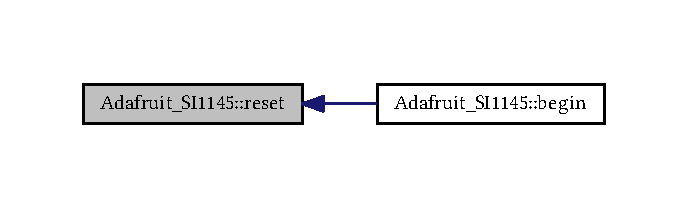
\includegraphics[width=330pt]{class_adafruit___s_i1145_ab7a22b92c14315e36b84a42498e970ea_icgraph}
\end{center}
\end{figure}


\index{Adafruit\+\_\+\+S\+I1145@{Adafruit\+\_\+\+S\+I1145}!reset\+\_\+uv@{reset\+\_\+uv}}
\index{reset\+\_\+uv@{reset\+\_\+uv}!Adafruit\+\_\+\+S\+I1145@{Adafruit\+\_\+\+S\+I1145}}
\subsubsection[{\texorpdfstring{reset\+\_\+uv()}{reset\_uv()}}]{\setlength{\rightskip}{0pt plus 5cm}void Adafruit\+\_\+\+S\+I1145\+::reset\+\_\+uv (
\begin{DoxyParamCaption}
{}
\end{DoxyParamCaption}
)}\hypertarget{class_adafruit___s_i1145_a67635a26a9c4c6b2fc2a7ffc86c2b5c9}{}\label{class_adafruit___s_i1145_a67635a26a9c4c6b2fc2a7ffc86c2b5c9}


Definition at line 127 of file Adafruit\+\_\+\+S\+I1145.\+cpp.



References S\+I1145\+\_\+\+N\+OP, and S\+I1145\+\_\+\+R\+E\+G\+\_\+\+C\+O\+M\+M\+A\+ND.

\index{Adafruit\+\_\+\+S\+I1145@{Adafruit\+\_\+\+S\+I1145}!set\+Register@{set\+Register}}
\index{set\+Register@{set\+Register}!Adafruit\+\_\+\+S\+I1145@{Adafruit\+\_\+\+S\+I1145}}
\subsubsection[{\texorpdfstring{set\+Register(uint8\+\_\+t, uint8\+\_\+t)}{setRegister(uint8\_t, uint8\_t)}}]{\setlength{\rightskip}{0pt plus 5cm}uint8\+\_\+t Adafruit\+\_\+\+S\+I1145\+::set\+Register (
\begin{DoxyParamCaption}
\item[{uint8\+\_\+t}]{reg, }
\item[{uint8\+\_\+t}]{value}
\end{DoxyParamCaption}
)}\hypertarget{class_adafruit___s_i1145_a591ba648b988a5dcb464b9f60a4a2c83}{}\label{class_adafruit___s_i1145_a591ba648b988a5dcb464b9f60a4a2c83}


Definition at line 122 of file Adafruit\+\_\+\+S\+I1145.\+cpp.



The documentation for this class was generated from the following files\+:\begin{DoxyCompactItemize}
\item 
Weather\+\_\+\+Balloon/library/\+Adafruit\+\_\+\+S\+I1145\+\_\+\+Library-\/master/\hyperlink{_adafruit___s_i1145_8h}{Adafruit\+\_\+\+S\+I1145.\+h}\item 
Weather\+\_\+\+Balloon/library/\+Adafruit\+\_\+\+S\+I1145\+\_\+\+Library-\/master/\hyperlink{_adafruit___s_i1145_8cpp}{Adafruit\+\_\+\+S\+I1145.\+cpp}\end{DoxyCompactItemize}

\hypertarget{class_adafruit___t_s_l2561___unified}{}\section{Adafruit\+\_\+\+T\+S\+L2561\+\_\+\+Unified Class Reference}
\label{class_adafruit___t_s_l2561___unified}\index{Adafruit\+\_\+\+T\+S\+L2561\+\_\+\+Unified@{Adafruit\+\_\+\+T\+S\+L2561\+\_\+\+Unified}}


{\ttfamily \#include $<$Adafruit\+\_\+\+T\+S\+L2561\+\_\+\+U.\+h$>$}



Inheritance diagram for Adafruit\+\_\+\+T\+S\+L2561\+\_\+\+Unified\+:\nopagebreak
\begin{figure}[H]
\begin{center}
\leavevmode
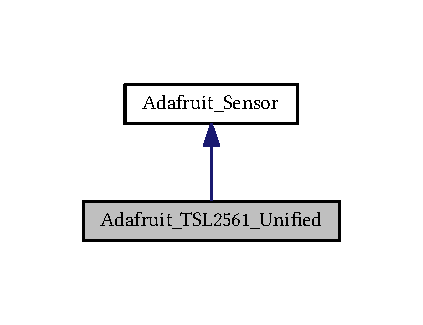
\includegraphics[width=203pt]{class_adafruit___t_s_l2561___unified__inherit__graph}
\end{center}
\end{figure}


Collaboration diagram for Adafruit\+\_\+\+T\+S\+L2561\+\_\+\+Unified\+:\nopagebreak
\begin{figure}[H]
\begin{center}
\leavevmode
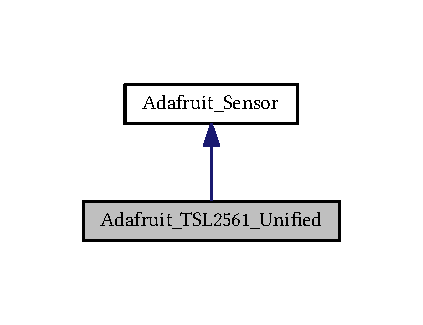
\includegraphics[width=203pt]{class_adafruit___t_s_l2561___unified__coll__graph}
\end{center}
\end{figure}
\subsection*{Public Member Functions}
\begin{DoxyCompactItemize}
\item 
\hyperlink{class_adafruit___t_s_l2561___unified_abd81c1ca2c46e4d8b9c3f4460a65aa3f}{Adafruit\+\_\+\+T\+S\+L2561\+\_\+\+Unified} (uint8\+\_\+t addr, int32\+\_\+t sensor\+ID=-\/1)
\item 
boolean \hyperlink{class_adafruit___t_s_l2561___unified_ac2781d263ae73533628d5844ca38b6de}{begin} (void)
\item 
void \hyperlink{class_adafruit___t_s_l2561___unified_a9bb93fc9a1af24175c9838cdfe7b8904}{enable\+Auto\+Range} (bool enable)
\begin{DoxyCompactList}\small\item\em Enables or disables the auto-\/gain settings when reading data from the sensor. \end{DoxyCompactList}\item 
void \hyperlink{class_adafruit___t_s_l2561___unified_a594636810e6e26dc025b7f1b7a16024f}{set\+Integration\+Time} (\hyperlink{_adafruit___t_s_l2561___u_8h_a541f87fb512c1fd213e23c3a8b23264a}{tsl2561\+Integration\+Time\+\_\+t} time)
\item 
void \hyperlink{class_adafruit___t_s_l2561___unified_ad4189a1cb97b07366b5014bec629f29a}{set\+Gain} (\hyperlink{_adafruit___t_s_l2561___u_8h_a8051d9eb664d757f67c0c5ce371cd9d0}{tsl2561\+Gain\+\_\+t} gain)
\item 
void \hyperlink{class_adafruit___t_s_l2561___unified_a23378e7c4792b8b8c721d5a4def960fb}{get\+Luminosity} (uint16\+\_\+t $\ast$broadband, uint16\+\_\+t $\ast$ir)
\begin{DoxyCompactList}\small\item\em Gets the broadband (mixed lighting) and IR only values from the T\+S\+L2561, adjusting gain if auto-\/gain is enabled. \end{DoxyCompactList}\item 
uint32\+\_\+t \hyperlink{class_adafruit___t_s_l2561___unified_a5059ebabcbd037d53459ec9f3c6cdc4b}{calculate\+Lux} (uint16\+\_\+t broadband, uint16\+\_\+t ir)
\item 
bool \hyperlink{class_adafruit___t_s_l2561___unified_a6a133ea86b7a7158408519214c4d0aef}{get\+Event} (\hyperlink{_adafruit___sensor_8h_structsensors__event__t}{sensors\+\_\+event\+\_\+t} $\ast$)
\begin{DoxyCompactList}\small\item\em Gets the most recent sensor event returns true if sensor reading is between 0 and 65535 lux returns false if sensor is saturated. \end{DoxyCompactList}\item 
void \hyperlink{class_adafruit___t_s_l2561___unified_a4c8dcb86a371558aba4ddb0a740d9b3c}{get\+Sensor} (\hyperlink{_adafruit___sensor_8h_structsensor__t}{sensor\+\_\+t} $\ast$)
\begin{DoxyCompactList}\small\item\em Gets the \hyperlink{_adafruit___sensor_8h_structsensor__t}{sensor\+\_\+t} data. \end{DoxyCompactList}\end{DoxyCompactItemize}


\subsection{Detailed Description}


Definition at line 178 of file Adafruit\+\_\+\+T\+S\+L2561\+\_\+\+U.\+h.



\subsection{Constructor \& Destructor Documentation}
\index{Adafruit\+\_\+\+T\+S\+L2561\+\_\+\+Unified@{Adafruit\+\_\+\+T\+S\+L2561\+\_\+\+Unified}!Adafruit\+\_\+\+T\+S\+L2561\+\_\+\+Unified@{Adafruit\+\_\+\+T\+S\+L2561\+\_\+\+Unified}}
\index{Adafruit\+\_\+\+T\+S\+L2561\+\_\+\+Unified@{Adafruit\+\_\+\+T\+S\+L2561\+\_\+\+Unified}!Adafruit\+\_\+\+T\+S\+L2561\+\_\+\+Unified@{Adafruit\+\_\+\+T\+S\+L2561\+\_\+\+Unified}}
\subsubsection[{\texorpdfstring{Adafruit\+\_\+\+T\+S\+L2561\+\_\+\+Unified(uint8\+\_\+t addr, int32\+\_\+t sensor\+I\+D=-\/1)}{Adafruit\_TSL2561\_Unified(uint8\_t addr, int32\_t sensorID=-1)}}]{\setlength{\rightskip}{0pt plus 5cm}Adafruit\+\_\+\+T\+S\+L2561\+\_\+\+Unified\+::\+Adafruit\+\_\+\+T\+S\+L2561\+\_\+\+Unified (
\begin{DoxyParamCaption}
\item[{uint8\+\_\+t}]{addr, }
\item[{int32\+\_\+t}]{sensor\+ID = {\ttfamily -\/1}}
\end{DoxyParamCaption}
)}\hypertarget{class_adafruit___t_s_l2561___unified_abd81c1ca2c46e4d8b9c3f4460a65aa3f}{}\label{class_adafruit___t_s_l2561___unified_abd81c1ca2c46e4d8b9c3f4460a65aa3f}
Constructor 

Definition at line 176 of file Adafruit\+\_\+\+T\+S\+L2561\+\_\+\+U.\+cpp.



References T\+S\+L2561\+\_\+\+G\+A\+I\+N\+\_\+1X, and T\+S\+L2561\+\_\+\+I\+N\+T\+E\+G\+R\+A\+T\+I\+O\+N\+T\+I\+M\+E\+\_\+13\+MS.



\subsection{Member Function Documentation}
\index{Adafruit\+\_\+\+T\+S\+L2561\+\_\+\+Unified@{Adafruit\+\_\+\+T\+S\+L2561\+\_\+\+Unified}!begin@{begin}}
\index{begin@{begin}!Adafruit\+\_\+\+T\+S\+L2561\+\_\+\+Unified@{Adafruit\+\_\+\+T\+S\+L2561\+\_\+\+Unified}}
\subsubsection[{\texorpdfstring{begin(void)}{begin(void)}}]{\setlength{\rightskip}{0pt plus 5cm}boolean Adafruit\+\_\+\+T\+S\+L2561\+\_\+\+Unified\+::begin (
\begin{DoxyParamCaption}
\item[{void}]{}
\end{DoxyParamCaption}
)}\hypertarget{class_adafruit___t_s_l2561___unified_ac2781d263ae73533628d5844ca38b6de}{}\label{class_adafruit___t_s_l2561___unified_ac2781d263ae73533628d5844ca38b6de}
Initializes I2C and configures the sensor (call this function before doing anything else) 

Definition at line 196 of file Adafruit\+\_\+\+T\+S\+L2561\+\_\+\+U.\+cpp.



References set\+Gain(), set\+Integration\+Time(), T\+S\+L2561\+\_\+\+R\+E\+G\+I\+S\+T\+E\+R\+\_\+\+ID, and Wire.



Referenced by configure\+\_\+\+T\+S\+L2561(), get\+Luminosity(), set\+Gain(), and set\+Integration\+Time().



Here is the call graph for this function\+:
\nopagebreak
\begin{figure}[H]
\begin{center}
\leavevmode
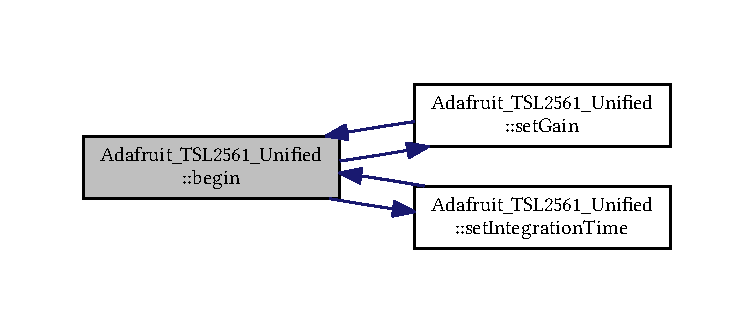
\includegraphics[width=350pt]{class_adafruit___t_s_l2561___unified_ac2781d263ae73533628d5844ca38b6de_cgraph}
\end{center}
\end{figure}




Here is the caller graph for this function\+:
\nopagebreak
\begin{figure}[H]
\begin{center}
\leavevmode
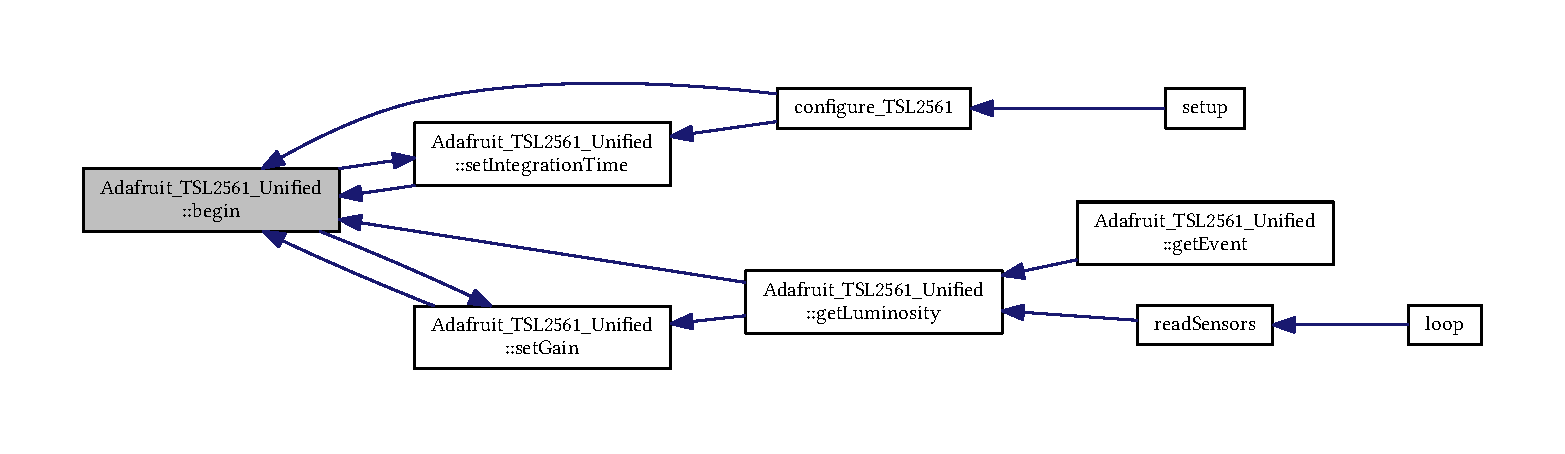
\includegraphics[width=350pt]{class_adafruit___t_s_l2561___unified_ac2781d263ae73533628d5844ca38b6de_icgraph}
\end{center}
\end{figure}


\index{Adafruit\+\_\+\+T\+S\+L2561\+\_\+\+Unified@{Adafruit\+\_\+\+T\+S\+L2561\+\_\+\+Unified}!calculate\+Lux@{calculate\+Lux}}
\index{calculate\+Lux@{calculate\+Lux}!Adafruit\+\_\+\+T\+S\+L2561\+\_\+\+Unified@{Adafruit\+\_\+\+T\+S\+L2561\+\_\+\+Unified}}
\subsubsection[{\texorpdfstring{calculate\+Lux(uint16\+\_\+t broadband, uint16\+\_\+t ir)}{calculateLux(uint16\_t broadband, uint16\_t ir)}}]{\setlength{\rightskip}{0pt plus 5cm}uint32\+\_\+t Adafruit\+\_\+\+T\+S\+L2561\+\_\+\+Unified\+::calculate\+Lux (
\begin{DoxyParamCaption}
\item[{uint16\+\_\+t}]{broadband, }
\item[{uint16\+\_\+t}]{ir}
\end{DoxyParamCaption}
)}\hypertarget{class_adafruit___t_s_l2561___unified_a5059ebabcbd037d53459ec9f3c6cdc4b}{}\label{class_adafruit___t_s_l2561___unified_a5059ebabcbd037d53459ec9f3c6cdc4b}
Converts the raw sensor values to the standard SI lux equivalent. Returns 0 if the sensor is saturated and the values are unreliable. 

Definition at line 367 of file Adafruit\+\_\+\+T\+S\+L2561\+\_\+\+U.\+cpp.



References T\+S\+L2561\+\_\+\+C\+L\+I\+P\+P\+I\+N\+G\+\_\+101\+MS, T\+S\+L2561\+\_\+\+C\+L\+I\+P\+P\+I\+N\+G\+\_\+13\+MS, T\+S\+L2561\+\_\+\+C\+L\+I\+P\+P\+I\+N\+G\+\_\+402\+MS, T\+S\+L2561\+\_\+\+I\+N\+T\+E\+G\+R\+A\+T\+I\+O\+N\+T\+I\+M\+E\+\_\+101\+MS, T\+S\+L2561\+\_\+\+I\+N\+T\+E\+G\+R\+A\+T\+I\+O\+N\+T\+I\+M\+E\+\_\+13\+MS, T\+S\+L2561\+\_\+\+L\+U\+X\+\_\+\+B1C, T\+S\+L2561\+\_\+\+L\+U\+X\+\_\+\+B1T, T\+S\+L2561\+\_\+\+L\+U\+X\+\_\+\+B2C, T\+S\+L2561\+\_\+\+L\+U\+X\+\_\+\+B2T, T\+S\+L2561\+\_\+\+L\+U\+X\+\_\+\+B3C, T\+S\+L2561\+\_\+\+L\+U\+X\+\_\+\+B3T, T\+S\+L2561\+\_\+\+L\+U\+X\+\_\+\+B4C, T\+S\+L2561\+\_\+\+L\+U\+X\+\_\+\+B4T, T\+S\+L2561\+\_\+\+L\+U\+X\+\_\+\+B5C, T\+S\+L2561\+\_\+\+L\+U\+X\+\_\+\+B5T, T\+S\+L2561\+\_\+\+L\+U\+X\+\_\+\+B6C, T\+S\+L2561\+\_\+\+L\+U\+X\+\_\+\+B6T, T\+S\+L2561\+\_\+\+L\+U\+X\+\_\+\+B7C, T\+S\+L2561\+\_\+\+L\+U\+X\+\_\+\+B7T, T\+S\+L2561\+\_\+\+L\+U\+X\+\_\+\+B8C, T\+S\+L2561\+\_\+\+L\+U\+X\+\_\+\+B8T, T\+S\+L2561\+\_\+\+L\+U\+X\+\_\+\+C\+H\+S\+C\+A\+LE, T\+S\+L2561\+\_\+\+L\+U\+X\+\_\+\+C\+H\+S\+C\+A\+L\+E\+\_\+\+T\+I\+N\+T0, T\+S\+L2561\+\_\+\+L\+U\+X\+\_\+\+C\+H\+S\+C\+A\+L\+E\+\_\+\+T\+I\+N\+T1, T\+S\+L2561\+\_\+\+L\+U\+X\+\_\+\+K1C, T\+S\+L2561\+\_\+\+L\+U\+X\+\_\+\+K1T, T\+S\+L2561\+\_\+\+L\+U\+X\+\_\+\+K2C, T\+S\+L2561\+\_\+\+L\+U\+X\+\_\+\+K2T, T\+S\+L2561\+\_\+\+L\+U\+X\+\_\+\+K3C, T\+S\+L2561\+\_\+\+L\+U\+X\+\_\+\+K3T, T\+S\+L2561\+\_\+\+L\+U\+X\+\_\+\+K4C, T\+S\+L2561\+\_\+\+L\+U\+X\+\_\+\+K4T, T\+S\+L2561\+\_\+\+L\+U\+X\+\_\+\+K5C, T\+S\+L2561\+\_\+\+L\+U\+X\+\_\+\+K5T, T\+S\+L2561\+\_\+\+L\+U\+X\+\_\+\+K6C, T\+S\+L2561\+\_\+\+L\+U\+X\+\_\+\+K6T, T\+S\+L2561\+\_\+\+L\+U\+X\+\_\+\+K7C, T\+S\+L2561\+\_\+\+L\+U\+X\+\_\+\+K7T, T\+S\+L2561\+\_\+\+L\+U\+X\+\_\+\+K8C, T\+S\+L2561\+\_\+\+L\+U\+X\+\_\+\+K8T, T\+S\+L2561\+\_\+\+L\+U\+X\+\_\+\+L\+U\+X\+S\+C\+A\+LE, T\+S\+L2561\+\_\+\+L\+U\+X\+\_\+\+M1C, T\+S\+L2561\+\_\+\+L\+U\+X\+\_\+\+M1T, T\+S\+L2561\+\_\+\+L\+U\+X\+\_\+\+M2C, T\+S\+L2561\+\_\+\+L\+U\+X\+\_\+\+M2T, T\+S\+L2561\+\_\+\+L\+U\+X\+\_\+\+M3C, T\+S\+L2561\+\_\+\+L\+U\+X\+\_\+\+M3T, T\+S\+L2561\+\_\+\+L\+U\+X\+\_\+\+M4C, T\+S\+L2561\+\_\+\+L\+U\+X\+\_\+\+M4T, T\+S\+L2561\+\_\+\+L\+U\+X\+\_\+\+M5C, T\+S\+L2561\+\_\+\+L\+U\+X\+\_\+\+M5T, T\+S\+L2561\+\_\+\+L\+U\+X\+\_\+\+M6C, T\+S\+L2561\+\_\+\+L\+U\+X\+\_\+\+M6T, T\+S\+L2561\+\_\+\+L\+U\+X\+\_\+\+M7C, T\+S\+L2561\+\_\+\+L\+U\+X\+\_\+\+M7T, T\+S\+L2561\+\_\+\+L\+U\+X\+\_\+\+M8C, T\+S\+L2561\+\_\+\+L\+U\+X\+\_\+\+M8T, and T\+S\+L2561\+\_\+\+L\+U\+X\+\_\+\+R\+A\+T\+I\+O\+S\+C\+A\+LE.



Referenced by get\+Event(), and read\+Sensors().



Here is the caller graph for this function\+:\nopagebreak
\begin{figure}[H]
\begin{center}
\leavevmode
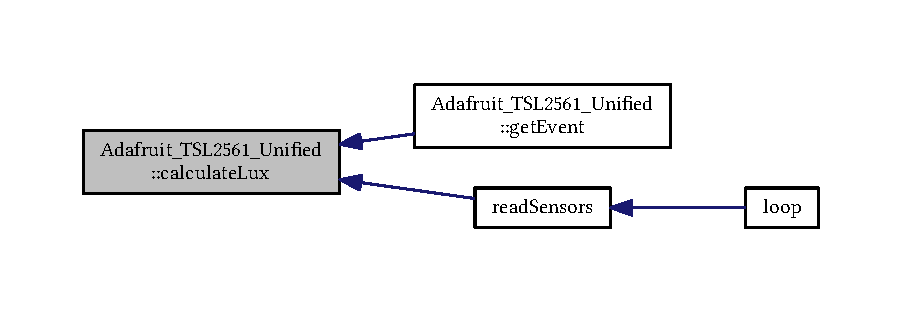
\includegraphics[width=350pt]{class_adafruit___t_s_l2561___unified_a5059ebabcbd037d53459ec9f3c6cdc4b_icgraph}
\end{center}
\end{figure}


\index{Adafruit\+\_\+\+T\+S\+L2561\+\_\+\+Unified@{Adafruit\+\_\+\+T\+S\+L2561\+\_\+\+Unified}!enable\+Auto\+Range@{enable\+Auto\+Range}}
\index{enable\+Auto\+Range@{enable\+Auto\+Range}!Adafruit\+\_\+\+T\+S\+L2561\+\_\+\+Unified@{Adafruit\+\_\+\+T\+S\+L2561\+\_\+\+Unified}}
\subsubsection[{\texorpdfstring{enable\+Auto\+Range(bool enable)}{enableAutoRange(bool enable)}}]{\setlength{\rightskip}{0pt plus 5cm}void Adafruit\+\_\+\+T\+S\+L2561\+\_\+\+Unified\+::enable\+Auto\+Range (
\begin{DoxyParamCaption}
\item[{bool}]{enable}
\end{DoxyParamCaption}
)\hspace{0.3cm}{\ttfamily [virtual]}}\hypertarget{class_adafruit___t_s_l2561___unified_a9bb93fc9a1af24175c9838cdfe7b8904}{}\label{class_adafruit___t_s_l2561___unified_a9bb93fc9a1af24175c9838cdfe7b8904}


Enables or disables the auto-\/gain settings when reading data from the sensor. 



Reimplemented from \hyperlink{class_adafruit___sensor_ace6c1f26eeb956f95801b9fc1841f3a0}{Adafruit\+\_\+\+Sensor}.



Definition at line 224 of file Adafruit\+\_\+\+T\+S\+L2561\+\_\+\+U.\+cpp.



Referenced by configure\+\_\+\+T\+S\+L2561().



Here is the caller graph for this function\+:\nopagebreak
\begin{figure}[H]
\begin{center}
\leavevmode
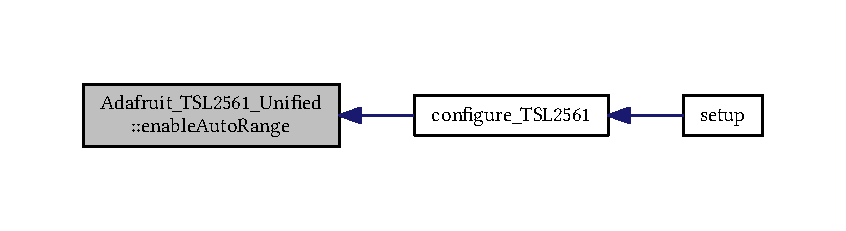
\includegraphics[width=350pt]{class_adafruit___t_s_l2561___unified_a9bb93fc9a1af24175c9838cdfe7b8904_icgraph}
\end{center}
\end{figure}


\index{Adafruit\+\_\+\+T\+S\+L2561\+\_\+\+Unified@{Adafruit\+\_\+\+T\+S\+L2561\+\_\+\+Unified}!get\+Event@{get\+Event}}
\index{get\+Event@{get\+Event}!Adafruit\+\_\+\+T\+S\+L2561\+\_\+\+Unified@{Adafruit\+\_\+\+T\+S\+L2561\+\_\+\+Unified}}
\subsubsection[{\texorpdfstring{get\+Event(sensors\+\_\+event\+\_\+t $\ast$)}{getEvent(sensors\_event\_t *)}}]{\setlength{\rightskip}{0pt plus 5cm}bool Adafruit\+\_\+\+T\+S\+L2561\+\_\+\+Unified\+::get\+Event (
\begin{DoxyParamCaption}
\item[{{\bf sensors\+\_\+event\+\_\+t} $\ast$}]{event}
\end{DoxyParamCaption}
)\hspace{0.3cm}{\ttfamily [virtual]}}\hypertarget{class_adafruit___t_s_l2561___unified_a6a133ea86b7a7158408519214c4d0aef}{}\label{class_adafruit___t_s_l2561___unified_a6a133ea86b7a7158408519214c4d0aef}


Gets the most recent sensor event returns true if sensor reading is between 0 and 65535 lux returns false if sensor is saturated. 



Implements \hyperlink{class_adafruit___sensor_a0636562b9bc853b796ecc87b5d4b1bec}{Adafruit\+\_\+\+Sensor}.



Definition at line 483 of file Adafruit\+\_\+\+T\+S\+L2561\+\_\+\+U.\+cpp.



References calculate\+Lux(), get\+Luminosity(), and S\+E\+N\+S\+O\+R\+\_\+\+T\+Y\+P\+E\+\_\+\+L\+I\+G\+HT.



Here is the call graph for this function\+:
\nopagebreak
\begin{figure}[H]
\begin{center}
\leavevmode
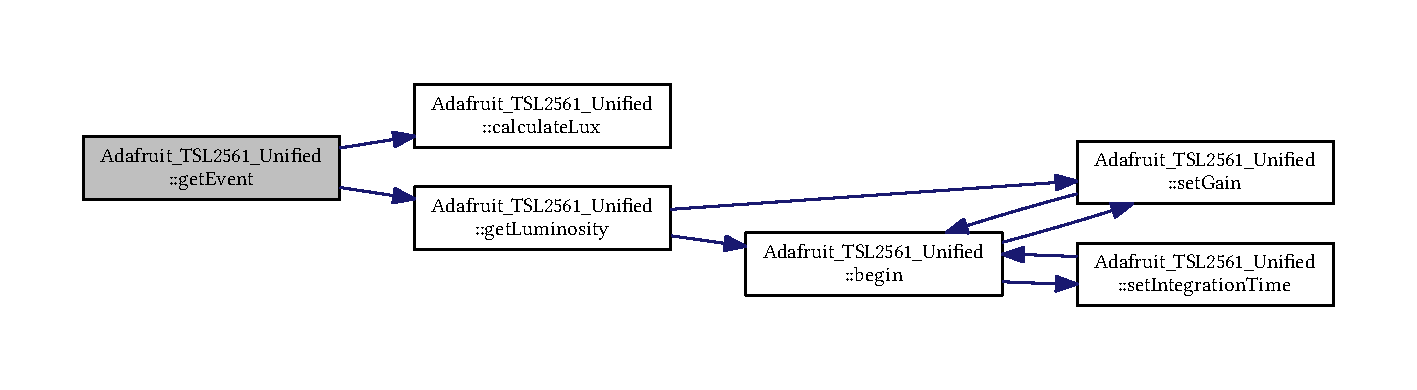
\includegraphics[width=350pt]{class_adafruit___t_s_l2561___unified_a6a133ea86b7a7158408519214c4d0aef_cgraph}
\end{center}
\end{figure}


\index{Adafruit\+\_\+\+T\+S\+L2561\+\_\+\+Unified@{Adafruit\+\_\+\+T\+S\+L2561\+\_\+\+Unified}!get\+Luminosity@{get\+Luminosity}}
\index{get\+Luminosity@{get\+Luminosity}!Adafruit\+\_\+\+T\+S\+L2561\+\_\+\+Unified@{Adafruit\+\_\+\+T\+S\+L2561\+\_\+\+Unified}}
\subsubsection[{\texorpdfstring{get\+Luminosity(uint16\+\_\+t $\ast$broadband, uint16\+\_\+t $\ast$ir)}{getLuminosity(uint16\_t *broadband, uint16\_t *ir)}}]{\setlength{\rightskip}{0pt plus 5cm}void Adafruit\+\_\+\+T\+S\+L2561\+\_\+\+Unified\+::get\+Luminosity (
\begin{DoxyParamCaption}
\item[{uint16\+\_\+t $\ast$}]{broadband, }
\item[{uint16\+\_\+t $\ast$}]{ir}
\end{DoxyParamCaption}
)}\hypertarget{class_adafruit___t_s_l2561___unified_a23378e7c4792b8b8c721d5a4def960fb}{}\label{class_adafruit___t_s_l2561___unified_a23378e7c4792b8b8c721d5a4def960fb}


Gets the broadband (mixed lighting) and IR only values from the T\+S\+L2561, adjusting gain if auto-\/gain is enabled. 



Definition at line 279 of file Adafruit\+\_\+\+T\+S\+L2561\+\_\+\+U.\+cpp.



References begin(), set\+Gain(), T\+S\+L2561\+\_\+\+A\+G\+C\+\_\+\+T\+H\+I\+\_\+101\+MS, T\+S\+L2561\+\_\+\+A\+G\+C\+\_\+\+T\+H\+I\+\_\+13\+MS, T\+S\+L2561\+\_\+\+A\+G\+C\+\_\+\+T\+H\+I\+\_\+402\+MS, T\+S\+L2561\+\_\+\+A\+G\+C\+\_\+\+T\+L\+O\+\_\+101\+MS, T\+S\+L2561\+\_\+\+A\+G\+C\+\_\+\+T\+L\+O\+\_\+13\+MS, T\+S\+L2561\+\_\+\+A\+G\+C\+\_\+\+T\+L\+O\+\_\+402\+MS, T\+S\+L2561\+\_\+\+G\+A\+I\+N\+\_\+16X, T\+S\+L2561\+\_\+\+G\+A\+I\+N\+\_\+1X, T\+S\+L2561\+\_\+\+I\+N\+T\+E\+G\+R\+A\+T\+I\+O\+N\+T\+I\+M\+E\+\_\+101\+MS, and T\+S\+L2561\+\_\+\+I\+N\+T\+E\+G\+R\+A\+T\+I\+O\+N\+T\+I\+M\+E\+\_\+13\+MS.



Referenced by get\+Event(), and read\+Sensors().



Here is the call graph for this function\+:
\nopagebreak
\begin{figure}[H]
\begin{center}
\leavevmode
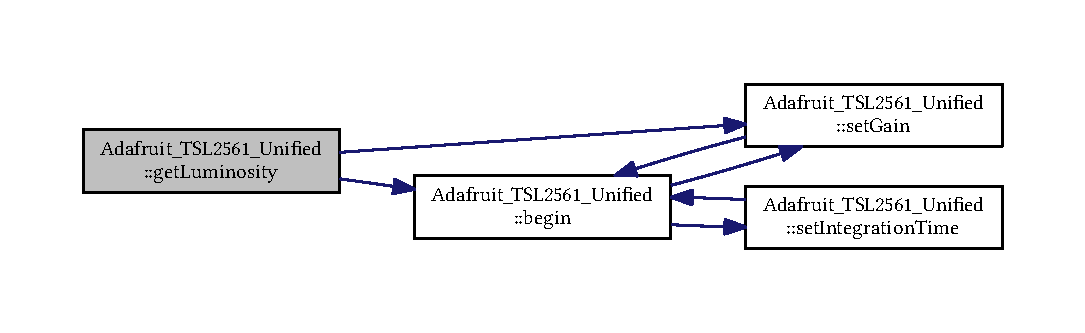
\includegraphics[width=350pt]{class_adafruit___t_s_l2561___unified_a23378e7c4792b8b8c721d5a4def960fb_cgraph}
\end{center}
\end{figure}




Here is the caller graph for this function\+:\nopagebreak
\begin{figure}[H]
\begin{center}
\leavevmode
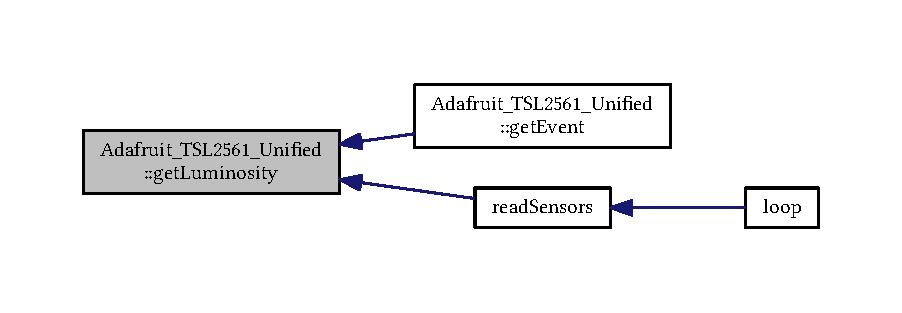
\includegraphics[width=350pt]{class_adafruit___t_s_l2561___unified_a23378e7c4792b8b8c721d5a4def960fb_icgraph}
\end{center}
\end{figure}


\index{Adafruit\+\_\+\+T\+S\+L2561\+\_\+\+Unified@{Adafruit\+\_\+\+T\+S\+L2561\+\_\+\+Unified}!get\+Sensor@{get\+Sensor}}
\index{get\+Sensor@{get\+Sensor}!Adafruit\+\_\+\+T\+S\+L2561\+\_\+\+Unified@{Adafruit\+\_\+\+T\+S\+L2561\+\_\+\+Unified}}
\subsubsection[{\texorpdfstring{get\+Sensor(sensor\+\_\+t $\ast$)}{getSensor(sensor\_t *)}}]{\setlength{\rightskip}{0pt plus 5cm}void Adafruit\+\_\+\+T\+S\+L2561\+\_\+\+Unified\+::get\+Sensor (
\begin{DoxyParamCaption}
\item[{{\bf sensor\+\_\+t} $\ast$}]{sensor}
\end{DoxyParamCaption}
)\hspace{0.3cm}{\ttfamily [virtual]}}\hypertarget{class_adafruit___t_s_l2561___unified_a4c8dcb86a371558aba4ddb0a740d9b3c}{}\label{class_adafruit___t_s_l2561___unified_a4c8dcb86a371558aba4ddb0a740d9b3c}


Gets the \hyperlink{_adafruit___sensor_8h_structsensor__t}{sensor\+\_\+t} data. 



Implements \hyperlink{class_adafruit___sensor_a19e844c1eb2dc37cb72705d5572c4676}{Adafruit\+\_\+\+Sensor}.



Definition at line 511 of file Adafruit\+\_\+\+T\+S\+L2561\+\_\+\+U.\+cpp.



References sensor\+\_\+t\+::max\+\_\+value, sensor\+\_\+t\+::min\+\_\+delay, sensor\+\_\+t\+::min\+\_\+value, sensor\+\_\+t\+::name, sensor\+\_\+t\+::resolution, sensor\+\_\+t\+::sensor\+\_\+id, S\+E\+N\+S\+O\+R\+\_\+\+T\+Y\+P\+E\+\_\+\+L\+I\+G\+HT, sensor\+\_\+t\+::type, and sensor\+\_\+t\+::version.

\index{Adafruit\+\_\+\+T\+S\+L2561\+\_\+\+Unified@{Adafruit\+\_\+\+T\+S\+L2561\+\_\+\+Unified}!set\+Gain@{set\+Gain}}
\index{set\+Gain@{set\+Gain}!Adafruit\+\_\+\+T\+S\+L2561\+\_\+\+Unified@{Adafruit\+\_\+\+T\+S\+L2561\+\_\+\+Unified}}
\subsubsection[{\texorpdfstring{set\+Gain(tsl2561\+Gain\+\_\+t gain)}{setGain(tsl2561Gain\_t gain)}}]{\setlength{\rightskip}{0pt plus 5cm}void Adafruit\+\_\+\+T\+S\+L2561\+\_\+\+Unified\+::set\+Gain (
\begin{DoxyParamCaption}
\item[{{\bf tsl2561\+Gain\+\_\+t}}]{gain}
\end{DoxyParamCaption}
)}\hypertarget{class_adafruit___t_s_l2561___unified_ad4189a1cb97b07366b5014bec629f29a}{}\label{class_adafruit___t_s_l2561___unified_ad4189a1cb97b07366b5014bec629f29a}
Adjusts the gain on the T\+S\+L2561 (adjusts the sensitivity to light) 

Definition at line 256 of file Adafruit\+\_\+\+T\+S\+L2561\+\_\+\+U.\+cpp.



References begin(), T\+S\+L2561\+\_\+\+C\+O\+M\+M\+A\+N\+D\+\_\+\+B\+IT, and T\+S\+L2561\+\_\+\+R\+E\+G\+I\+S\+T\+E\+R\+\_\+\+T\+I\+M\+I\+NG.



Referenced by begin(), and get\+Luminosity().



Here is the call graph for this function\+:
\nopagebreak
\begin{figure}[H]
\begin{center}
\leavevmode
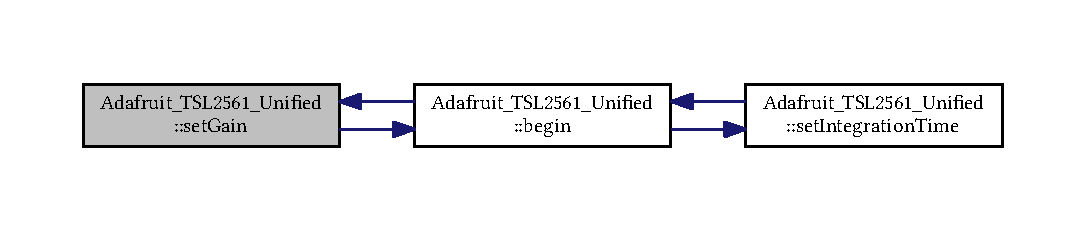
\includegraphics[width=350pt]{class_adafruit___t_s_l2561___unified_ad4189a1cb97b07366b5014bec629f29a_cgraph}
\end{center}
\end{figure}




Here is the caller graph for this function\+:
\nopagebreak
\begin{figure}[H]
\begin{center}
\leavevmode
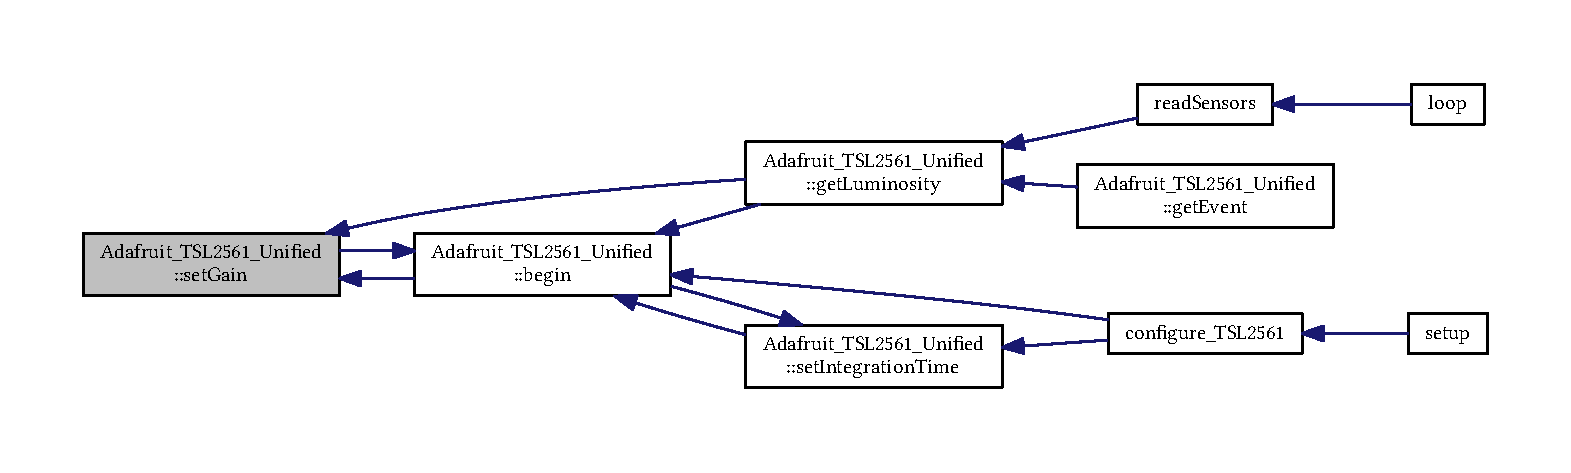
\includegraphics[width=350pt]{class_adafruit___t_s_l2561___unified_ad4189a1cb97b07366b5014bec629f29a_icgraph}
\end{center}
\end{figure}


\index{Adafruit\+\_\+\+T\+S\+L2561\+\_\+\+Unified@{Adafruit\+\_\+\+T\+S\+L2561\+\_\+\+Unified}!set\+Integration\+Time@{set\+Integration\+Time}}
\index{set\+Integration\+Time@{set\+Integration\+Time}!Adafruit\+\_\+\+T\+S\+L2561\+\_\+\+Unified@{Adafruit\+\_\+\+T\+S\+L2561\+\_\+\+Unified}}
\subsubsection[{\texorpdfstring{set\+Integration\+Time(tsl2561\+Integration\+Time\+\_\+t time)}{setIntegrationTime(tsl2561IntegrationTime\_t time)}}]{\setlength{\rightskip}{0pt plus 5cm}void Adafruit\+\_\+\+T\+S\+L2561\+\_\+\+Unified\+::set\+Integration\+Time (
\begin{DoxyParamCaption}
\item[{{\bf tsl2561\+Integration\+Time\+\_\+t}}]{time}
\end{DoxyParamCaption}
)}\hypertarget{class_adafruit___t_s_l2561___unified_a594636810e6e26dc025b7f1b7a16024f}{}\label{class_adafruit___t_s_l2561___unified_a594636810e6e26dc025b7f1b7a16024f}
Sets the integration time for the T\+S\+L2561 

Definition at line 234 of file Adafruit\+\_\+\+T\+S\+L2561\+\_\+\+U.\+cpp.



References begin(), T\+S\+L2561\+\_\+\+C\+O\+M\+M\+A\+N\+D\+\_\+\+B\+IT, and T\+S\+L2561\+\_\+\+R\+E\+G\+I\+S\+T\+E\+R\+\_\+\+T\+I\+M\+I\+NG.



Referenced by begin(), and configure\+\_\+\+T\+S\+L2561().



Here is the call graph for this function\+:
\nopagebreak
\begin{figure}[H]
\begin{center}
\leavevmode
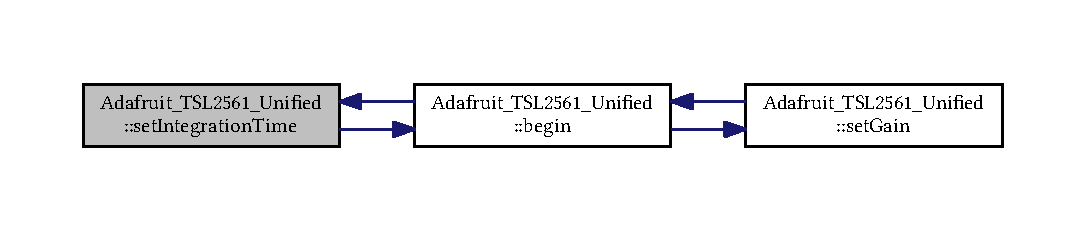
\includegraphics[width=350pt]{class_adafruit___t_s_l2561___unified_a594636810e6e26dc025b7f1b7a16024f_cgraph}
\end{center}
\end{figure}




Here is the caller graph for this function\+:
\nopagebreak
\begin{figure}[H]
\begin{center}
\leavevmode
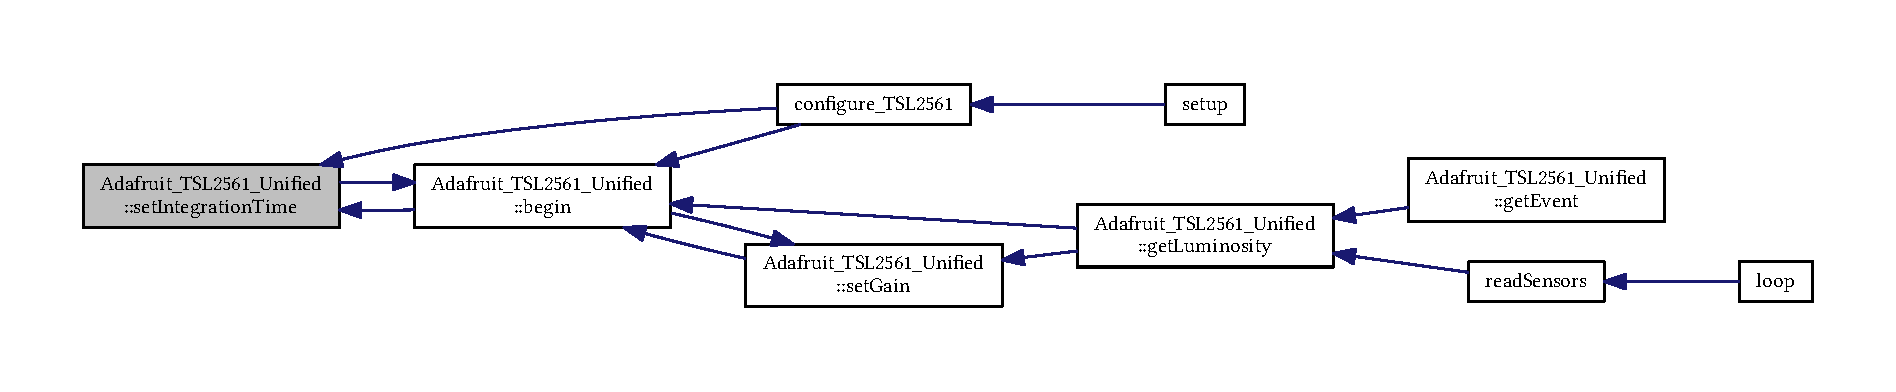
\includegraphics[width=350pt]{class_adafruit___t_s_l2561___unified_a594636810e6e26dc025b7f1b7a16024f_icgraph}
\end{center}
\end{figure}




The documentation for this class was generated from the following files\+:\begin{DoxyCompactItemize}
\item 
Weather\+\_\+\+Balloon/library/\+Adafruit\+\_\+\+T\+S\+L2561-\/master/\hyperlink{_adafruit___t_s_l2561___u_8h}{Adafruit\+\_\+\+T\+S\+L2561\+\_\+\+U.\+h}\item 
Weather\+\_\+\+Balloon/library/\+Adafruit\+\_\+\+T\+S\+L2561-\/master/\hyperlink{_adafruit___t_s_l2561___u_8cpp}{Adafruit\+\_\+\+T\+S\+L2561\+\_\+\+U.\+cpp}\end{DoxyCompactItemize}

\hypertarget{class_b_l_e_stream}{}\section{B\+L\+E\+Stream Class Reference}
\label{class_b_l_e_stream}\index{B\+L\+E\+Stream@{B\+L\+E\+Stream}}


{\ttfamily \#include $<$B\+L\+E\+Stream.\+h$>$}



Inheritance diagram for B\+L\+E\+Stream\+:\nopagebreak
\begin{figure}[H]
\begin{center}
\leavevmode
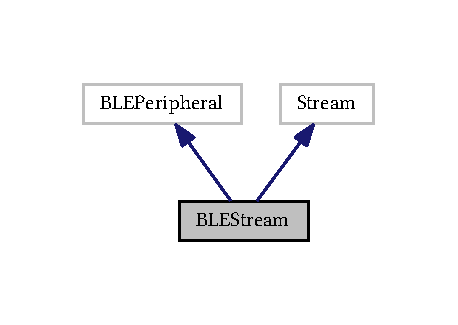
\includegraphics[width=220pt]{class_b_l_e_stream__inherit__graph}
\end{center}
\end{figure}


Collaboration diagram for B\+L\+E\+Stream\+:\nopagebreak
\begin{figure}[H]
\begin{center}
\leavevmode
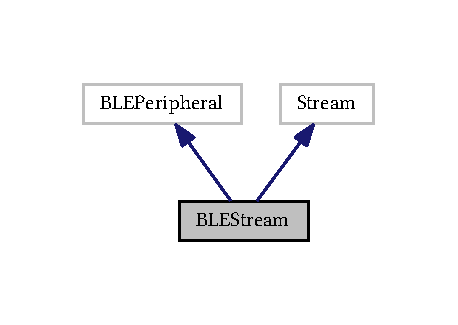
\includegraphics[width=220pt]{class_b_l_e_stream__coll__graph}
\end{center}
\end{figure}
\subsection*{Public Member Functions}
\begin{DoxyCompactItemize}
\item 
\hyperlink{class_b_l_e_stream_aa12f9098b653a30c2a152f647ab8bdfa}{B\+L\+E\+Stream} (unsigned char req=0, unsigned char rdy=0, unsigned char rst=0)
\item 
void \hyperlink{class_b_l_e_stream_a7cef0d2f7dc431608483c3911e68bb56}{begin} (...)
\item 
bool \hyperlink{class_b_l_e_stream_a58d4d0684a7c9f5434736af31ea2ab98}{poll} ()
\item 
void \hyperlink{class_b_l_e_stream_a2f571566304b41339d8a74cee6f98d2d}{end} ()
\item 
void \hyperlink{class_b_l_e_stream_ab05a77032b59c6d3525390e7e6a768ab}{set\+Flush\+Interval} (int)
\item 
virtual int \hyperlink{class_b_l_e_stream_a9b8dd79faf553535df6b68a8d572c8e2}{available} (void)
\item 
virtual int \hyperlink{class_b_l_e_stream_a932edda09fadf9530e2b87bed4d88bed}{peek} (void)
\item 
virtual int \hyperlink{class_b_l_e_stream_a607238a23059d0dbe133c3358e7c42ca}{read} (void)
\item 
virtual void \hyperlink{class_b_l_e_stream_af22a00b80511025785543d107422874a}{flush} (void)
\item 
virtual size\+\_\+t \hyperlink{class_b_l_e_stream_ad3e299ba3ad439d077f1b7bb74617698}{write} (uint8\+\_\+t byte)
\item 
virtual \hyperlink{class_b_l_e_stream_aded76dc2283104566c13fed9755e21f5}{operator bool} ()
\end{DoxyCompactItemize}


\subsection{Detailed Description}


Definition at line 27 of file B\+L\+E\+Stream.\+h.



\subsection{Constructor \& Destructor Documentation}
\index{B\+L\+E\+Stream@{B\+L\+E\+Stream}!B\+L\+E\+Stream@{B\+L\+E\+Stream}}
\index{B\+L\+E\+Stream@{B\+L\+E\+Stream}!B\+L\+E\+Stream@{B\+L\+E\+Stream}}
\subsubsection[{\texorpdfstring{B\+L\+E\+Stream(unsigned char req=0, unsigned char rdy=0, unsigned char rst=0)}{BLEStream(unsigned char req=0, unsigned char rdy=0, unsigned char rst=0)}}]{\setlength{\rightskip}{0pt plus 5cm}B\+L\+E\+Stream\+::\+B\+L\+E\+Stream (
\begin{DoxyParamCaption}
\item[{unsigned char}]{req = {\ttfamily 0}, }
\item[{unsigned char}]{rdy = {\ttfamily 0}, }
\item[{unsigned char}]{rst = {\ttfamily 0}}
\end{DoxyParamCaption}
)}\hypertarget{class_b_l_e_stream_aa12f9098b653a30c2a152f647ab8bdfa}{}\label{class_b_l_e_stream_aa12f9098b653a30c2a152f647ab8bdfa}


Definition at line 78 of file B\+L\+E\+Stream.\+h.



References B\+L\+E\+S\+T\+R\+E\+A\+M\+\_\+\+T\+X\+B\+U\+F\+F\+E\+R\+\_\+\+F\+L\+U\+S\+H\+\_\+\+I\+N\+T\+E\+R\+V\+AL.



\subsection{Member Function Documentation}
\index{B\+L\+E\+Stream@{B\+L\+E\+Stream}!available@{available}}
\index{available@{available}!B\+L\+E\+Stream@{B\+L\+E\+Stream}}
\subsubsection[{\texorpdfstring{available(void)}{available(void)}}]{\setlength{\rightskip}{0pt plus 5cm}int B\+L\+E\+Stream\+::available (
\begin{DoxyParamCaption}
\item[{void}]{}
\end{DoxyParamCaption}
)\hspace{0.3cm}{\ttfamily [virtual]}}\hypertarget{class_b_l_e_stream_a9b8dd79faf553535df6b68a8d572c8e2}{}\label{class_b_l_e_stream_a9b8dd79faf553535df6b68a8d572c8e2}


Definition at line 127 of file B\+L\+E\+Stream.\+h.

\index{B\+L\+E\+Stream@{B\+L\+E\+Stream}!begin@{begin}}
\index{begin@{begin}!B\+L\+E\+Stream@{B\+L\+E\+Stream}}
\subsubsection[{\texorpdfstring{begin(...)}{begin(...)}}]{\setlength{\rightskip}{0pt plus 5cm}void B\+L\+E\+Stream\+::begin (
\begin{DoxyParamCaption}
\item[{}]{...}
\end{DoxyParamCaption}
)}\hypertarget{class_b_l_e_stream_a7cef0d2f7dc431608483c3911e68bb56}{}\label{class_b_l_e_stream_a7cef0d2f7dc431608483c3911e68bb56}


Definition at line 101 of file B\+L\+E\+Stream.\+h.

\index{B\+L\+E\+Stream@{B\+L\+E\+Stream}!end@{end}}
\index{end@{end}!B\+L\+E\+Stream@{B\+L\+E\+Stream}}
\subsubsection[{\texorpdfstring{end()}{end()}}]{\setlength{\rightskip}{0pt plus 5cm}void B\+L\+E\+Stream\+::end (
\begin{DoxyParamCaption}
{}
\end{DoxyParamCaption}
)}\hypertarget{class_b_l_e_stream_a2f571566304b41339d8a74cee6f98d2d}{}\label{class_b_l_e_stream_a2f571566304b41339d8a74cee6f98d2d}


Definition at line 119 of file B\+L\+E\+Stream.\+h.



References flush().



Here is the call graph for this function\+:\nopagebreak
\begin{figure}[H]
\begin{center}
\leavevmode
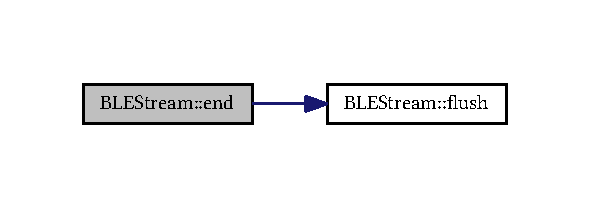
\includegraphics[width=283pt]{class_b_l_e_stream_a2f571566304b41339d8a74cee6f98d2d_cgraph}
\end{center}
\end{figure}


\index{B\+L\+E\+Stream@{B\+L\+E\+Stream}!flush@{flush}}
\index{flush@{flush}!B\+L\+E\+Stream@{B\+L\+E\+Stream}}
\subsubsection[{\texorpdfstring{flush(void)}{flush(void)}}]{\setlength{\rightskip}{0pt plus 5cm}void B\+L\+E\+Stream\+::flush (
\begin{DoxyParamCaption}
\item[{void}]{}
\end{DoxyParamCaption}
)\hspace{0.3cm}{\ttfamily [virtual]}}\hypertarget{class_b_l_e_stream_af22a00b80511025785543d107422874a}{}\label{class_b_l_e_stream_af22a00b80511025785543d107422874a}


Definition at line 174 of file B\+L\+E\+Stream.\+h.



Referenced by end(), poll(), and write().



Here is the caller graph for this function\+:
\nopagebreak
\begin{figure}[H]
\begin{center}
\leavevmode
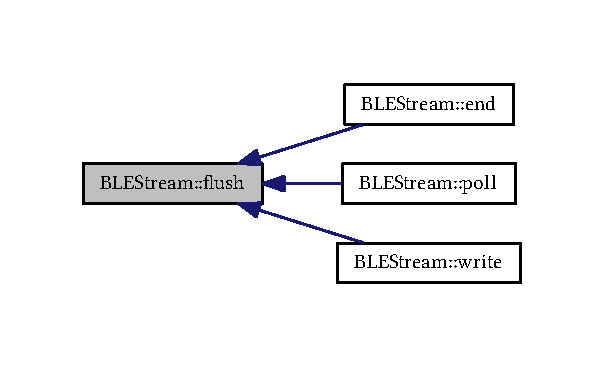
\includegraphics[width=290pt]{class_b_l_e_stream_af22a00b80511025785543d107422874a_icgraph}
\end{center}
\end{figure}


\index{B\+L\+E\+Stream@{B\+L\+E\+Stream}!operator bool@{operator bool}}
\index{operator bool@{operator bool}!B\+L\+E\+Stream@{B\+L\+E\+Stream}}
\subsubsection[{\texorpdfstring{operator bool()}{operator bool()}}]{\setlength{\rightskip}{0pt plus 5cm}B\+L\+E\+Stream\+::operator bool (
\begin{DoxyParamCaption}
{}
\end{DoxyParamCaption}
)\hspace{0.3cm}{\ttfamily [virtual]}}\hypertarget{class_b_l_e_stream_aded76dc2283104566c13fed9755e21f5}{}\label{class_b_l_e_stream_aded76dc2283104566c13fed9755e21f5}


Definition at line 207 of file B\+L\+E\+Stream.\+h.

\index{B\+L\+E\+Stream@{B\+L\+E\+Stream}!peek@{peek}}
\index{peek@{peek}!B\+L\+E\+Stream@{B\+L\+E\+Stream}}
\subsubsection[{\texorpdfstring{peek(void)}{peek(void)}}]{\setlength{\rightskip}{0pt plus 5cm}int B\+L\+E\+Stream\+::peek (
\begin{DoxyParamCaption}
\item[{void}]{}
\end{DoxyParamCaption}
)\hspace{0.3cm}{\ttfamily [virtual]}}\hypertarget{class_b_l_e_stream_a932edda09fadf9530e2b87bed4d88bed}{}\label{class_b_l_e_stream_a932edda09fadf9530e2b87bed4d88bed}


Definition at line 145 of file B\+L\+E\+Stream.\+h.

\index{B\+L\+E\+Stream@{B\+L\+E\+Stream}!poll@{poll}}
\index{poll@{poll}!B\+L\+E\+Stream@{B\+L\+E\+Stream}}
\subsubsection[{\texorpdfstring{poll()}{poll()}}]{\setlength{\rightskip}{0pt plus 5cm}bool B\+L\+E\+Stream\+::poll (
\begin{DoxyParamCaption}
{}
\end{DoxyParamCaption}
)}\hypertarget{class_b_l_e_stream_a58d4d0684a7c9f5434736af31ea2ab98}{}\label{class_b_l_e_stream_a58d4d0684a7c9f5434736af31ea2ab98}


Definition at line 109 of file B\+L\+E\+Stream.\+h.



References flush().



Here is the call graph for this function\+:\nopagebreak
\begin{figure}[H]
\begin{center}
\leavevmode
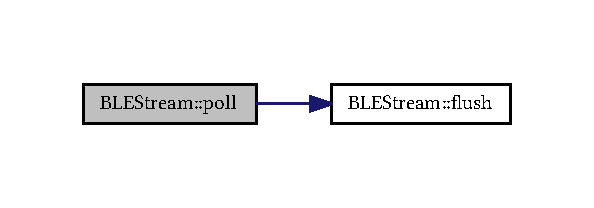
\includegraphics[width=285pt]{class_b_l_e_stream_a58d4d0684a7c9f5434736af31ea2ab98_cgraph}
\end{center}
\end{figure}


\index{B\+L\+E\+Stream@{B\+L\+E\+Stream}!read@{read}}
\index{read@{read}!B\+L\+E\+Stream@{B\+L\+E\+Stream}}
\subsubsection[{\texorpdfstring{read(void)}{read(void)}}]{\setlength{\rightskip}{0pt plus 5cm}int B\+L\+E\+Stream\+::read (
\begin{DoxyParamCaption}
\item[{void}]{}
\end{DoxyParamCaption}
)\hspace{0.3cm}{\ttfamily [virtual]}}\hypertarget{class_b_l_e_stream_a607238a23059d0dbe133c3358e7c42ca}{}\label{class_b_l_e_stream_a607238a23059d0dbe133c3358e7c42ca}


Definition at line 159 of file B\+L\+E\+Stream.\+h.

\index{B\+L\+E\+Stream@{B\+L\+E\+Stream}!set\+Flush\+Interval@{set\+Flush\+Interval}}
\index{set\+Flush\+Interval@{set\+Flush\+Interval}!B\+L\+E\+Stream@{B\+L\+E\+Stream}}
\subsubsection[{\texorpdfstring{set\+Flush\+Interval(int)}{setFlushInterval(int)}}]{\setlength{\rightskip}{0pt plus 5cm}void B\+L\+E\+Stream\+::set\+Flush\+Interval (
\begin{DoxyParamCaption}
\item[{int}]{interval}
\end{DoxyParamCaption}
)}\hypertarget{class_b_l_e_stream_ab05a77032b59c6d3525390e7e6a768ab}{}\label{class_b_l_e_stream_ab05a77032b59c6d3525390e7e6a768ab}


Definition at line 217 of file B\+L\+E\+Stream.\+h.



References B\+L\+E\+S\+T\+R\+E\+A\+M\+\_\+\+M\+I\+N\+\_\+\+F\+L\+U\+S\+H\+\_\+\+I\+N\+T\+E\+R\+V\+AL, and i.

\index{B\+L\+E\+Stream@{B\+L\+E\+Stream}!write@{write}}
\index{write@{write}!B\+L\+E\+Stream@{B\+L\+E\+Stream}}
\subsubsection[{\texorpdfstring{write(uint8\+\_\+t byte)}{write(uint8\_t byte)}}]{\setlength{\rightskip}{0pt plus 5cm}size\+\_\+t B\+L\+E\+Stream\+::write (
\begin{DoxyParamCaption}
\item[{uint8\+\_\+t}]{byte}
\end{DoxyParamCaption}
)\hspace{0.3cm}{\ttfamily [virtual]}}\hypertarget{class_b_l_e_stream_ad3e299ba3ad439d077f1b7bb74617698}{}\label{class_b_l_e_stream_ad3e299ba3ad439d077f1b7bb74617698}


Definition at line 191 of file B\+L\+E\+Stream.\+h.



References flush().



Here is the call graph for this function\+:\nopagebreak
\begin{figure}[H]
\begin{center}
\leavevmode
\includegraphics[width=290pt]{class_b_l_e_stream_ad3e299ba3ad439d077f1b7bb74617698_cgraph}
\end{center}
\end{figure}




The documentation for this class was generated from the following file\+:\begin{DoxyCompactItemize}
\item 
Weather\+\_\+\+Balloon/library/\+Firmata/utility/\hyperlink{_b_l_e_stream_8h}{B\+L\+E\+Stream.\+h}\end{DoxyCompactItemize}

\hypertarget{class_dallas_temperature}{}\section{Dallas\+Temperature Class Reference}
\label{class_dallas_temperature}\index{Dallas\+Temperature@{Dallas\+Temperature}}


{\ttfamily \#include $<$Dallas\+Temperature.\+h$>$}

\subsection*{Public Member Functions}
\begin{DoxyCompactItemize}
\item 
\hyperlink{class_dallas_temperature_af46e868b6702ff5f77263985cd990e01}{Dallas\+Temperature} ()
\item 
\hyperlink{class_dallas_temperature_a37139ebd1a6122e232800528aee8cb2b}{Dallas\+Temperature} (\hyperlink{class_one_wire}{One\+Wire} $\ast$)
\item 
void \hyperlink{class_dallas_temperature_af985bf5f9ed6857424e8a9532eaf5e2f}{set\+One\+Wire} (\hyperlink{class_one_wire}{One\+Wire} $\ast$)
\item 
void \hyperlink{class_dallas_temperature_aea297b5f2a720a5455245c0fbf7333ec}{begin} (void)
\item 
uint8\+\_\+t \hyperlink{class_dallas_temperature_a8bf92c0b6b8c3167daca4c2046ade13a}{get\+Device\+Count} (void)
\item 
bool \hyperlink{class_dallas_temperature_a71e4744b8d7b2f1c05a96cd158c83007}{valid\+Address} (const uint8\+\_\+t $\ast$)
\item 
bool \hyperlink{class_dallas_temperature_a3f3678c8defd473e8eebd9cfe793b329}{valid\+Family} (const uint8\+\_\+t $\ast$device\+Address)
\item 
bool \hyperlink{class_dallas_temperature_afa644bebf50c81b6641a31c585b62538}{get\+Address} (uint8\+\_\+t $\ast$, uint8\+\_\+t)
\item 
bool \hyperlink{class_dallas_temperature_a19afa5e594de0ab6caa5a48a70650927}{is\+Connected} (const uint8\+\_\+t $\ast$)
\item 
bool \hyperlink{class_dallas_temperature_a624f64b186c13927d4f74bd7c5b92c2e}{is\+Connected} (const uint8\+\_\+t $\ast$, uint8\+\_\+t $\ast$)
\item 
bool \hyperlink{class_dallas_temperature_a2b55774207d0211fd679247a7137142b}{read\+Scratch\+Pad} (const uint8\+\_\+t $\ast$, uint8\+\_\+t $\ast$)
\item 
void \hyperlink{class_dallas_temperature_a74c275dabf103f268c5a271d379dcb7e}{write\+Scratch\+Pad} (const uint8\+\_\+t $\ast$, const uint8\+\_\+t $\ast$)
\item 
bool \hyperlink{class_dallas_temperature_af6a28c1d1009dd6d010d97dffaf5942d}{read\+Power\+Supply} (const uint8\+\_\+t $\ast$)
\item 
uint8\+\_\+t \hyperlink{class_dallas_temperature_a9dac13206229d7c8fb75f21bf44e75ed}{get\+Resolution} ()
\item 
void \hyperlink{class_dallas_temperature_a43363ee4b227f1ecf9c33cd4e072c0c9}{set\+Resolution} (uint8\+\_\+t)
\item 
uint8\+\_\+t \hyperlink{class_dallas_temperature_a2266822561e864c4921955697c1ac7f5}{get\+Resolution} (const uint8\+\_\+t $\ast$)
\item 
bool \hyperlink{class_dallas_temperature_a394897437dfb8de4c8fd2198a1d1c356}{set\+Resolution} (const uint8\+\_\+t $\ast$, uint8\+\_\+t, bool skip\+Global\+Bit\+Resolution\+Calculation=false)
\item 
void \hyperlink{class_dallas_temperature_aa5f90d9f12327f39de97ed2244a4ad6f}{set\+Wait\+For\+Conversion} (bool)
\item 
bool \hyperlink{class_dallas_temperature_abb49c5903d68b86c0cf2da5e2b849a43}{get\+Wait\+For\+Conversion} (void)
\item 
void \hyperlink{class_dallas_temperature_ae8ef644d60236af12963f37fe145a49a}{set\+Check\+For\+Conversion} (bool)
\item 
bool \hyperlink{class_dallas_temperature_a7541728802904b0ed8d17a7f5ef00801}{get\+Check\+For\+Conversion} (void)
\item 
void \hyperlink{class_dallas_temperature_a5d28cff0d7e317c28e28c0f1a62fbe6d}{request\+Temperatures} (void)
\item 
bool \hyperlink{class_dallas_temperature_aee2a2abd5f8293df9a0a030b3e982c90}{request\+Temperatures\+By\+Address} (const uint8\+\_\+t $\ast$)
\item 
bool \hyperlink{class_dallas_temperature_ae9a7bf62321615519242d2421c8b349a}{request\+Temperatures\+By\+Index} (uint8\+\_\+t)
\item 
int16\+\_\+t \hyperlink{class_dallas_temperature_a37c3723cc15d5e46d0a6caa96a3c4781}{get\+Temp} (const uint8\+\_\+t $\ast$)
\item 
float \hyperlink{class_dallas_temperature_a20f94b59909b46e55a77b399d99591a2}{get\+TempC} (const uint8\+\_\+t $\ast$)
\item 
float \hyperlink{class_dallas_temperature_ace033fbd8e4c7e17c4bcd7ecc8f3ebea}{get\+TempF} (const uint8\+\_\+t $\ast$)
\item 
float \hyperlink{class_dallas_temperature_a7e3e2e23257aac6b6c896df205d5b3b5}{get\+Temp\+C\+By\+Index} (uint8\+\_\+t)
\item 
float \hyperlink{class_dallas_temperature_a96318d36b313e1f4f413e2ed2b7501c7}{get\+Temp\+F\+By\+Index} (uint8\+\_\+t)
\item 
bool \hyperlink{class_dallas_temperature_a835945ed3e8d78c31791e55f22084691}{is\+Parasite\+Power\+Mode} (void)
\item 
bool \hyperlink{class_dallas_temperature_adaf460a3b8004218e97af7059d41053a}{is\+Conversion\+Available} (const uint8\+\_\+t $\ast$)
\item 
bool \hyperlink{class_dallas_temperature_a9e92719781d3ead44b95964d59edd41d}{is\+Conversion\+Complete} (void)
\item 
void \hyperlink{class_dallas_temperature_a0ed69b03ed848936ea0c8deea0e5c2ba}{set\+User\+Data} (const uint8\+\_\+t $\ast$, int16\+\_\+t)
\item 
void \hyperlink{class_dallas_temperature_a65ae6994218200e92ce43bffd122d46b}{set\+User\+Data\+By\+Index} (uint8\+\_\+t, int16\+\_\+t)
\item 
int16\+\_\+t \hyperlink{class_dallas_temperature_a3601e8ee63c4770b716817ed68664400}{get\+User\+Data} (const uint8\+\_\+t $\ast$)
\item 
int16\+\_\+t \hyperlink{class_dallas_temperature_a4af999e72b9c5b85430666ad90fa9644}{get\+User\+Data\+By\+Index} (uint8\+\_\+t)
\end{DoxyCompactItemize}
\subsection*{Static Public Member Functions}
\begin{DoxyCompactItemize}
\item 
static float \hyperlink{class_dallas_temperature_a2169f7bdd26479bbbf9f6fb3bf4e5bb2}{to\+Fahrenheit} (float)
\item 
static float \hyperlink{class_dallas_temperature_af6dfbcc587ae244c0508b6a51f2085a5}{to\+Celsius} (float)
\item 
static float \hyperlink{class_dallas_temperature_a75accb4a56858189accda00e5eabb06e}{raw\+To\+Celsius} (int16\+\_\+t)
\item 
static float \hyperlink{class_dallas_temperature_a48bc1a4d0e33f1735964c22c8bd2f6fb}{raw\+To\+Fahrenheit} (int16\+\_\+t)
\end{DoxyCompactItemize}


\subsection{Detailed Description}


Definition at line 63 of file Dallas\+Temperature.\+h.



\subsection{Constructor \& Destructor Documentation}
\index{Dallas\+Temperature@{Dallas\+Temperature}!Dallas\+Temperature@{Dallas\+Temperature}}
\index{Dallas\+Temperature@{Dallas\+Temperature}!Dallas\+Temperature@{Dallas\+Temperature}}
\subsubsection[{\texorpdfstring{Dallas\+Temperature()}{DallasTemperature()}}]{\setlength{\rightskip}{0pt plus 5cm}Dallas\+Temperature\+::\+Dallas\+Temperature (
\begin{DoxyParamCaption}
{}
\end{DoxyParamCaption}
)}\hypertarget{class_dallas_temperature_af46e868b6702ff5f77263985cd990e01}{}\label{class_dallas_temperature_af46e868b6702ff5f77263985cd990e01}


Definition at line 17 of file Dallas\+Temperature.\+cpp.

\index{Dallas\+Temperature@{Dallas\+Temperature}!Dallas\+Temperature@{Dallas\+Temperature}}
\index{Dallas\+Temperature@{Dallas\+Temperature}!Dallas\+Temperature@{Dallas\+Temperature}}
\subsubsection[{\texorpdfstring{Dallas\+Temperature(\+One\+Wire $\ast$)}{DallasTemperature(OneWire *)}}]{\setlength{\rightskip}{0pt plus 5cm}Dallas\+Temperature\+::\+Dallas\+Temperature (
\begin{DoxyParamCaption}
\item[{{\bf One\+Wire} $\ast$}]{\+\_\+one\+Wire}
\end{DoxyParamCaption}
)}\hypertarget{class_dallas_temperature_a37139ebd1a6122e232800528aee8cb2b}{}\label{class_dallas_temperature_a37139ebd1a6122e232800528aee8cb2b}


Definition at line 18 of file Dallas\+Temperature.\+cpp.



References set\+One\+Wire().



Here is the call graph for this function\+:\nopagebreak
\begin{figure}[H]
\begin{center}
\leavevmode
\includegraphics[width=314pt]{class_dallas_temperature_a37139ebd1a6122e232800528aee8cb2b_cgraph}
\end{center}
\end{figure}




\subsection{Member Function Documentation}
\index{Dallas\+Temperature@{Dallas\+Temperature}!begin@{begin}}
\index{begin@{begin}!Dallas\+Temperature@{Dallas\+Temperature}}
\subsubsection[{\texorpdfstring{begin(void)}{begin(void)}}]{\setlength{\rightskip}{0pt plus 5cm}void Dallas\+Temperature\+::begin (
\begin{DoxyParamCaption}
\item[{void}]{}
\end{DoxyParamCaption}
)}\hypertarget{class_dallas_temperature_aea297b5f2a720a5455245c0fbf7333ec}{}\label{class_dallas_temperature_aea297b5f2a720a5455245c0fbf7333ec}


Definition at line 51 of file Dallas\+Temperature.\+cpp.



References get\+Resolution(), read\+Power\+Supply(), One\+Wire\+::reset\+\_\+search(), One\+Wire\+::search(), and valid\+Address().



Here is the call graph for this function\+:
\nopagebreak
\begin{figure}[H]
\begin{center}
\leavevmode
\includegraphics[width=350pt]{class_dallas_temperature_aea297b5f2a720a5455245c0fbf7333ec_cgraph}
\end{center}
\end{figure}


\index{Dallas\+Temperature@{Dallas\+Temperature}!get\+Address@{get\+Address}}
\index{get\+Address@{get\+Address}!Dallas\+Temperature@{Dallas\+Temperature}}
\subsubsection[{\texorpdfstring{get\+Address(uint8\+\_\+t $\ast$, uint8\+\_\+t)}{getAddress(uint8\_t *, uint8\_t)}}]{\setlength{\rightskip}{0pt plus 5cm}bool Dallas\+Temperature\+::get\+Address (
\begin{DoxyParamCaption}
\item[{uint8\+\_\+t $\ast$}]{device\+Address, }
\item[{uint8\+\_\+t}]{index}
\end{DoxyParamCaption}
)}\hypertarget{class_dallas_temperature_afa644bebf50c81b6641a31c585b62538}{}\label{class_dallas_temperature_afa644bebf50c81b6641a31c585b62538}


Definition at line 84 of file Dallas\+Temperature.\+cpp.



References One\+Wire\+::reset\+\_\+search(), and valid\+Address().



Referenced by get\+Temp\+C\+By\+Index(), get\+Temp\+F\+By\+Index(), get\+User\+Data\+By\+Index(), request\+Temperatures\+By\+Index(), set\+Resolution(), and set\+User\+Data\+By\+Index().



Here is the call graph for this function\+:\nopagebreak
\begin{figure}[H]
\begin{center}
\leavevmode
\includegraphics[width=350pt]{class_dallas_temperature_afa644bebf50c81b6641a31c585b62538_cgraph}
\end{center}
\end{figure}




Here is the caller graph for this function\+:
\nopagebreak
\begin{figure}[H]
\begin{center}
\leavevmode
\includegraphics[width=350pt]{class_dallas_temperature_afa644bebf50c81b6641a31c585b62538_icgraph}
\end{center}
\end{figure}


\index{Dallas\+Temperature@{Dallas\+Temperature}!get\+Check\+For\+Conversion@{get\+Check\+For\+Conversion}}
\index{get\+Check\+For\+Conversion@{get\+Check\+For\+Conversion}!Dallas\+Temperature@{Dallas\+Temperature}}
\subsubsection[{\texorpdfstring{get\+Check\+For\+Conversion(void)}{getCheckForConversion(void)}}]{\setlength{\rightskip}{0pt plus 5cm}bool Dallas\+Temperature\+::get\+Check\+For\+Conversion (
\begin{DoxyParamCaption}
\item[{void}]{}
\end{DoxyParamCaption}
)}\hypertarget{class_dallas_temperature_a7541728802904b0ed8d17a7f5ef00801}{}\label{class_dallas_temperature_a7541728802904b0ed8d17a7f5ef00801}


Definition at line 307 of file Dallas\+Temperature.\+cpp.

\index{Dallas\+Temperature@{Dallas\+Temperature}!get\+Device\+Count@{get\+Device\+Count}}
\index{get\+Device\+Count@{get\+Device\+Count}!Dallas\+Temperature@{Dallas\+Temperature}}
\subsubsection[{\texorpdfstring{get\+Device\+Count(void)}{getDeviceCount(void)}}]{\setlength{\rightskip}{0pt plus 5cm}uint8\+\_\+t Dallas\+Temperature\+::get\+Device\+Count (
\begin{DoxyParamCaption}
\item[{void}]{}
\end{DoxyParamCaption}
)}\hypertarget{class_dallas_temperature_a8bf92c0b6b8c3167daca4c2046ade13a}{}\label{class_dallas_temperature_a8bf92c0b6b8c3167daca4c2046ade13a}


Definition at line 73 of file Dallas\+Temperature.\+cpp.

\index{Dallas\+Temperature@{Dallas\+Temperature}!get\+Resolution@{get\+Resolution}}
\index{get\+Resolution@{get\+Resolution}!Dallas\+Temperature@{Dallas\+Temperature}}
\subsubsection[{\texorpdfstring{get\+Resolution()}{getResolution()}}]{\setlength{\rightskip}{0pt plus 5cm}uint8\+\_\+t Dallas\+Temperature\+::get\+Resolution (
\begin{DoxyParamCaption}
{}
\end{DoxyParamCaption}
)}\hypertarget{class_dallas_temperature_a9dac13206229d7c8fb75f21bf44e75ed}{}\label{class_dallas_temperature_a9dac13206229d7c8fb75f21bf44e75ed}


Definition at line 250 of file Dallas\+Temperature.\+cpp.



Referenced by begin(), request\+Temperatures\+By\+Address(), and set\+Resolution().



Here is the caller graph for this function\+:
\nopagebreak
\begin{figure}[H]
\begin{center}
\leavevmode
\includegraphics[width=350pt]{class_dallas_temperature_a9dac13206229d7c8fb75f21bf44e75ed_icgraph}
\end{center}
\end{figure}


\index{Dallas\+Temperature@{Dallas\+Temperature}!get\+Resolution@{get\+Resolution}}
\index{get\+Resolution@{get\+Resolution}!Dallas\+Temperature@{Dallas\+Temperature}}
\subsubsection[{\texorpdfstring{get\+Resolution(const uint8\+\_\+t $\ast$)}{getResolution(const uint8\_t *)}}]{\setlength{\rightskip}{0pt plus 5cm}uint8\+\_\+t Dallas\+Temperature\+::get\+Resolution (
\begin{DoxyParamCaption}
\item[{const uint8\+\_\+t $\ast$}]{device\+Address}
\end{DoxyParamCaption}
)}\hypertarget{class_dallas_temperature_a2266822561e864c4921955697c1ac7f5}{}\label{class_dallas_temperature_a2266822561e864c4921955697c1ac7f5}


Definition at line 256 of file Dallas\+Temperature.\+cpp.



References C\+O\+N\+F\+I\+G\+U\+R\+A\+T\+I\+ON, D\+S18\+S20\+M\+O\+D\+EL, is\+Connected(), T\+E\+M\+P\+\_\+10\+\_\+\+B\+IT, T\+E\+M\+P\+\_\+11\+\_\+\+B\+IT, T\+E\+M\+P\+\_\+12\+\_\+\+B\+IT, and T\+E\+M\+P\+\_\+9\+\_\+\+B\+IT.



Here is the call graph for this function\+:\nopagebreak
\begin{figure}[H]
\begin{center}
\leavevmode
\includegraphics[width=314pt]{class_dallas_temperature_a2266822561e864c4921955697c1ac7f5_cgraph}
\end{center}
\end{figure}


\index{Dallas\+Temperature@{Dallas\+Temperature}!get\+Temp@{get\+Temp}}
\index{get\+Temp@{get\+Temp}!Dallas\+Temperature@{Dallas\+Temperature}}
\subsubsection[{\texorpdfstring{get\+Temp(const uint8\+\_\+t $\ast$)}{getTemp(const uint8\_t *)}}]{\setlength{\rightskip}{0pt plus 5cm}int16\+\_\+t Dallas\+Temperature\+::get\+Temp (
\begin{DoxyParamCaption}
\item[{const uint8\+\_\+t $\ast$}]{device\+Address}
\end{DoxyParamCaption}
)}\hypertarget{class_dallas_temperature_a37c3723cc15d5e46d0a6caa96a3c4781}{}\label{class_dallas_temperature_a37c3723cc15d5e46d0a6caa96a3c4781}


Definition at line 481 of file Dallas\+Temperature.\+cpp.



References D\+E\+V\+I\+C\+E\+\_\+\+D\+I\+S\+C\+O\+N\+N\+E\+C\+T\+E\+D\+\_\+\+R\+AW, and is\+Connected().



Referenced by get\+Temp\+C(), and get\+Temp\+F().



Here is the call graph for this function\+:\nopagebreak
\begin{figure}[H]
\begin{center}
\leavevmode
\includegraphics[width=314pt]{class_dallas_temperature_a37c3723cc15d5e46d0a6caa96a3c4781_cgraph}
\end{center}
\end{figure}




Here is the caller graph for this function\+:\nopagebreak
\begin{figure}[H]
\begin{center}
\leavevmode
\includegraphics[width=350pt]{class_dallas_temperature_a37c3723cc15d5e46d0a6caa96a3c4781_icgraph}
\end{center}
\end{figure}


\index{Dallas\+Temperature@{Dallas\+Temperature}!get\+TempC@{get\+TempC}}
\index{get\+TempC@{get\+TempC}!Dallas\+Temperature@{Dallas\+Temperature}}
\subsubsection[{\texorpdfstring{get\+Temp\+C(const uint8\+\_\+t $\ast$)}{getTempC(const uint8\_t *)}}]{\setlength{\rightskip}{0pt plus 5cm}float Dallas\+Temperature\+::get\+TempC (
\begin{DoxyParamCaption}
\item[{const uint8\+\_\+t $\ast$}]{device\+Address}
\end{DoxyParamCaption}
)}\hypertarget{class_dallas_temperature_a20f94b59909b46e55a77b399d99591a2}{}\label{class_dallas_temperature_a20f94b59909b46e55a77b399d99591a2}


Definition at line 494 of file Dallas\+Temperature.\+cpp.



References get\+Temp(), and raw\+To\+Celsius().



Referenced by get\+Temp\+C\+By\+Index().



Here is the call graph for this function\+:
\nopagebreak
\begin{figure}[H]
\begin{center}
\leavevmode
\includegraphics[width=350pt]{class_dallas_temperature_a20f94b59909b46e55a77b399d99591a2_cgraph}
\end{center}
\end{figure}




Here is the caller graph for this function\+:\nopagebreak
\begin{figure}[H]
\begin{center}
\leavevmode
\includegraphics[width=314pt]{class_dallas_temperature_a20f94b59909b46e55a77b399d99591a2_icgraph}
\end{center}
\end{figure}


\index{Dallas\+Temperature@{Dallas\+Temperature}!get\+Temp\+C\+By\+Index@{get\+Temp\+C\+By\+Index}}
\index{get\+Temp\+C\+By\+Index@{get\+Temp\+C\+By\+Index}!Dallas\+Temperature@{Dallas\+Temperature}}
\subsubsection[{\texorpdfstring{get\+Temp\+C\+By\+Index(uint8\+\_\+t)}{getTempCByIndex(uint8\_t)}}]{\setlength{\rightskip}{0pt plus 5cm}float Dallas\+Temperature\+::get\+Temp\+C\+By\+Index (
\begin{DoxyParamCaption}
\item[{uint8\+\_\+t}]{device\+Index}
\end{DoxyParamCaption}
)}\hypertarget{class_dallas_temperature_a7e3e2e23257aac6b6c896df205d5b3b5}{}\label{class_dallas_temperature_a7e3e2e23257aac6b6c896df205d5b3b5}


Definition at line 408 of file Dallas\+Temperature.\+cpp.



References D\+E\+V\+I\+C\+E\+\_\+\+D\+I\+S\+C\+O\+N\+N\+E\+C\+T\+E\+D\+\_\+C, get\+Address(), and get\+Temp\+C().



Here is the call graph for this function\+:
\nopagebreak
\begin{figure}[H]
\begin{center}
\leavevmode
\includegraphics[width=350pt]{class_dallas_temperature_a7e3e2e23257aac6b6c896df205d5b3b5_cgraph}
\end{center}
\end{figure}


\index{Dallas\+Temperature@{Dallas\+Temperature}!get\+TempF@{get\+TempF}}
\index{get\+TempF@{get\+TempF}!Dallas\+Temperature@{Dallas\+Temperature}}
\subsubsection[{\texorpdfstring{get\+Temp\+F(const uint8\+\_\+t $\ast$)}{getTempF(const uint8\_t *)}}]{\setlength{\rightskip}{0pt plus 5cm}float Dallas\+Temperature\+::get\+TempF (
\begin{DoxyParamCaption}
\item[{const uint8\+\_\+t $\ast$}]{device\+Address}
\end{DoxyParamCaption}
)}\hypertarget{class_dallas_temperature_ace033fbd8e4c7e17c4bcd7ecc8f3ebea}{}\label{class_dallas_temperature_ace033fbd8e4c7e17c4bcd7ecc8f3ebea}


Definition at line 503 of file Dallas\+Temperature.\+cpp.



References get\+Temp(), and raw\+To\+Fahrenheit().



Referenced by get\+Temp\+F\+By\+Index().



Here is the call graph for this function\+:
\nopagebreak
\begin{figure}[H]
\begin{center}
\leavevmode
\includegraphics[width=350pt]{class_dallas_temperature_ace033fbd8e4c7e17c4bcd7ecc8f3ebea_cgraph}
\end{center}
\end{figure}




Here is the caller graph for this function\+:\nopagebreak
\begin{figure}[H]
\begin{center}
\leavevmode
\includegraphics[width=314pt]{class_dallas_temperature_ace033fbd8e4c7e17c4bcd7ecc8f3ebea_icgraph}
\end{center}
\end{figure}


\index{Dallas\+Temperature@{Dallas\+Temperature}!get\+Temp\+F\+By\+Index@{get\+Temp\+F\+By\+Index}}
\index{get\+Temp\+F\+By\+Index@{get\+Temp\+F\+By\+Index}!Dallas\+Temperature@{Dallas\+Temperature}}
\subsubsection[{\texorpdfstring{get\+Temp\+F\+By\+Index(uint8\+\_\+t)}{getTempFByIndex(uint8\_t)}}]{\setlength{\rightskip}{0pt plus 5cm}float Dallas\+Temperature\+::get\+Temp\+F\+By\+Index (
\begin{DoxyParamCaption}
\item[{uint8\+\_\+t}]{device\+Index}
\end{DoxyParamCaption}
)}\hypertarget{class_dallas_temperature_a96318d36b313e1f4f413e2ed2b7501c7}{}\label{class_dallas_temperature_a96318d36b313e1f4f413e2ed2b7501c7}


Definition at line 420 of file Dallas\+Temperature.\+cpp.



References C\+O\+U\+N\+T\+\_\+\+P\+E\+R\+\_\+C, C\+O\+U\+N\+T\+\_\+\+R\+E\+M\+A\+IN, D\+E\+V\+I\+C\+E\+\_\+\+D\+I\+S\+C\+O\+N\+N\+E\+C\+T\+E\+D\+\_\+F, D\+S18\+S20\+M\+O\+D\+EL, get\+Address(), get\+Temp\+F(), T\+E\+M\+P\+\_\+\+L\+SB, and T\+E\+M\+P\+\_\+\+M\+SB.



Here is the call graph for this function\+:
\nopagebreak
\begin{figure}[H]
\begin{center}
\leavevmode
\includegraphics[width=350pt]{class_dallas_temperature_a96318d36b313e1f4f413e2ed2b7501c7_cgraph}
\end{center}
\end{figure}


\index{Dallas\+Temperature@{Dallas\+Temperature}!get\+User\+Data@{get\+User\+Data}}
\index{get\+User\+Data@{get\+User\+Data}!Dallas\+Temperature@{Dallas\+Temperature}}
\subsubsection[{\texorpdfstring{get\+User\+Data(const uint8\+\_\+t $\ast$)}{getUserData(const uint8\_t *)}}]{\setlength{\rightskip}{0pt plus 5cm}int16\+\_\+t Dallas\+Temperature\+::get\+User\+Data (
\begin{DoxyParamCaption}
\item[{const uint8\+\_\+t $\ast$}]{device\+Address}
\end{DoxyParamCaption}
)}\hypertarget{class_dallas_temperature_a3601e8ee63c4770b716817ed68664400}{}\label{class_dallas_temperature_a3601e8ee63c4770b716817ed68664400}


Definition at line 532 of file Dallas\+Temperature.\+cpp.



References H\+I\+G\+H\+\_\+\+A\+L\+A\+R\+M\+\_\+\+T\+E\+MP, is\+Connected(), and L\+O\+W\+\_\+\+A\+L\+A\+R\+M\+\_\+\+T\+E\+MP.



Referenced by get\+User\+Data\+By\+Index(), and set\+User\+Data().



Here is the call graph for this function\+:\nopagebreak
\begin{figure}[H]
\begin{center}
\leavevmode
\includegraphics[width=314pt]{class_dallas_temperature_a3601e8ee63c4770b716817ed68664400_cgraph}
\end{center}
\end{figure}




Here is the caller graph for this function\+:
\nopagebreak
\begin{figure}[H]
\begin{center}
\leavevmode
\includegraphics[width=350pt]{class_dallas_temperature_a3601e8ee63c4770b716817ed68664400_icgraph}
\end{center}
\end{figure}


\index{Dallas\+Temperature@{Dallas\+Temperature}!get\+User\+Data\+By\+Index@{get\+User\+Data\+By\+Index}}
\index{get\+User\+Data\+By\+Index@{get\+User\+Data\+By\+Index}!Dallas\+Temperature@{Dallas\+Temperature}}
\subsubsection[{\texorpdfstring{get\+User\+Data\+By\+Index(uint8\+\_\+t)}{getUserDataByIndex(uint8\_t)}}]{\setlength{\rightskip}{0pt plus 5cm}int16\+\_\+t Dallas\+Temperature\+::get\+User\+Data\+By\+Index (
\begin{DoxyParamCaption}
\item[{uint8\+\_\+t}]{device\+Index}
\end{DoxyParamCaption}
)}\hypertarget{class_dallas_temperature_a4af999e72b9c5b85430666ad90fa9644}{}\label{class_dallas_temperature_a4af999e72b9c5b85430666ad90fa9644}


Definition at line 545 of file Dallas\+Temperature.\+cpp.



References get\+Address(), and get\+User\+Data().



Here is the call graph for this function\+:\nopagebreak
\begin{figure}[H]
\begin{center}
\leavevmode
\includegraphics[width=350pt]{class_dallas_temperature_a4af999e72b9c5b85430666ad90fa9644_cgraph}
\end{center}
\end{figure}


\index{Dallas\+Temperature@{Dallas\+Temperature}!get\+Wait\+For\+Conversion@{get\+Wait\+For\+Conversion}}
\index{get\+Wait\+For\+Conversion@{get\+Wait\+For\+Conversion}!Dallas\+Temperature@{Dallas\+Temperature}}
\subsubsection[{\texorpdfstring{get\+Wait\+For\+Conversion(void)}{getWaitForConversion(void)}}]{\setlength{\rightskip}{0pt plus 5cm}bool Dallas\+Temperature\+::get\+Wait\+For\+Conversion (
\begin{DoxyParamCaption}
\item[{void}]{}
\end{DoxyParamCaption}
)}\hypertarget{class_dallas_temperature_abb49c5903d68b86c0cf2da5e2b849a43}{}\label{class_dallas_temperature_abb49c5903d68b86c0cf2da5e2b849a43}


Definition at line 294 of file Dallas\+Temperature.\+cpp.

\index{Dallas\+Temperature@{Dallas\+Temperature}!is\+Connected@{is\+Connected}}
\index{is\+Connected@{is\+Connected}!Dallas\+Temperature@{Dallas\+Temperature}}
\subsubsection[{\texorpdfstring{is\+Connected(const uint8\+\_\+t $\ast$)}{isConnected(const uint8\_t *)}}]{\setlength{\rightskip}{0pt plus 5cm}bool Dallas\+Temperature\+::is\+Connected (
\begin{DoxyParamCaption}
\item[{const uint8\+\_\+t $\ast$}]{device\+Address}
\end{DoxyParamCaption}
)}\hypertarget{class_dallas_temperature_a19afa5e594de0ab6caa5a48a70650927}{}\label{class_dallas_temperature_a19afa5e594de0ab6caa5a48a70650927}


Definition at line 100 of file Dallas\+Temperature.\+cpp.



Referenced by get\+Resolution(), get\+Temp(), get\+User\+Data(), raw\+To\+Fahrenheit(), set\+Resolution(), and set\+User\+Data().



Here is the caller graph for this function\+:
\nopagebreak
\begin{figure}[H]
\begin{center}
\leavevmode
\includegraphics[width=350pt]{class_dallas_temperature_a19afa5e594de0ab6caa5a48a70650927_icgraph}
\end{center}
\end{figure}


\index{Dallas\+Temperature@{Dallas\+Temperature}!is\+Connected@{is\+Connected}}
\index{is\+Connected@{is\+Connected}!Dallas\+Temperature@{Dallas\+Temperature}}
\subsubsection[{\texorpdfstring{is\+Connected(const uint8\+\_\+t $\ast$, uint8\+\_\+t $\ast$)}{isConnected(const uint8\_t *, uint8\_t *)}}]{\setlength{\rightskip}{0pt plus 5cm}bool Dallas\+Temperature\+::is\+Connected (
\begin{DoxyParamCaption}
\item[{const uint8\+\_\+t $\ast$}]{device\+Address, }
\item[{uint8\+\_\+t $\ast$}]{scratch\+Pad}
\end{DoxyParamCaption}
)}\hypertarget{class_dallas_temperature_a624f64b186c13927d4f74bd7c5b92c2e}{}\label{class_dallas_temperature_a624f64b186c13927d4f74bd7c5b92c2e}


Definition at line 109 of file Dallas\+Temperature.\+cpp.



References One\+Wire\+::crc8(), read\+Scratch\+Pad(), and S\+C\+R\+A\+T\+C\+H\+P\+A\+D\+\_\+\+C\+RC.



Here is the call graph for this function\+:
\nopagebreak
\begin{figure}[H]
\begin{center}
\leavevmode
\includegraphics[width=350pt]{class_dallas_temperature_a624f64b186c13927d4f74bd7c5b92c2e_cgraph}
\end{center}
\end{figure}


\index{Dallas\+Temperature@{Dallas\+Temperature}!is\+Conversion\+Available@{is\+Conversion\+Available}}
\index{is\+Conversion\+Available@{is\+Conversion\+Available}!Dallas\+Temperature@{Dallas\+Temperature}}
\subsubsection[{\texorpdfstring{is\+Conversion\+Available(const uint8\+\_\+t $\ast$)}{isConversionAvailable(const uint8\_t *)}}]{\setlength{\rightskip}{0pt plus 5cm}bool Dallas\+Temperature\+::is\+Conversion\+Available (
\begin{DoxyParamCaption}
\item[{const uint8\+\_\+t $\ast$}]{device\+Address}
\end{DoxyParamCaption}
)}\hypertarget{class_dallas_temperature_adaf460a3b8004218e97af7059d41053a}{}\label{class_dallas_temperature_adaf460a3b8004218e97af7059d41053a}


Definition at line 311 of file Dallas\+Temperature.\+cpp.



References read\+Scratch\+Pad().



Referenced by request\+Temperatures\+By\+Address().



Here is the call graph for this function\+:\nopagebreak
\begin{figure}[H]
\begin{center}
\leavevmode
\includegraphics[width=350pt]{class_dallas_temperature_adaf460a3b8004218e97af7059d41053a_cgraph}
\end{center}
\end{figure}




Here is the caller graph for this function\+:\nopagebreak
\begin{figure}[H]
\begin{center}
\leavevmode
\includegraphics[width=350pt]{class_dallas_temperature_adaf460a3b8004218e97af7059d41053a_icgraph}
\end{center}
\end{figure}


\index{Dallas\+Temperature@{Dallas\+Temperature}!is\+Conversion\+Complete@{is\+Conversion\+Complete}}
\index{is\+Conversion\+Complete@{is\+Conversion\+Complete}!Dallas\+Temperature@{Dallas\+Temperature}}
\subsubsection[{\texorpdfstring{is\+Conversion\+Complete(void)}{isConversionComplete(void)}}]{\setlength{\rightskip}{0pt plus 5cm}bool Dallas\+Temperature\+::is\+Conversion\+Complete (
\begin{DoxyParamCaption}
\item[{void}]{}
\end{DoxyParamCaption}
)}\hypertarget{class_dallas_temperature_a9e92719781d3ead44b95964d59edd41d}{}\label{class_dallas_temperature_a9e92719781d3ead44b95964d59edd41d}


Definition at line 320 of file Dallas\+Temperature.\+cpp.



References One\+Wire\+::read\+\_\+bit().



Here is the call graph for this function\+:\nopagebreak
\begin{figure}[H]
\begin{center}
\leavevmode
\includegraphics[width=320pt]{class_dallas_temperature_a9e92719781d3ead44b95964d59edd41d_cgraph}
\end{center}
\end{figure}


\index{Dallas\+Temperature@{Dallas\+Temperature}!is\+Parasite\+Power\+Mode@{is\+Parasite\+Power\+Mode}}
\index{is\+Parasite\+Power\+Mode@{is\+Parasite\+Power\+Mode}!Dallas\+Temperature@{Dallas\+Temperature}}
\subsubsection[{\texorpdfstring{is\+Parasite\+Power\+Mode(void)}{isParasitePowerMode(void)}}]{\setlength{\rightskip}{0pt plus 5cm}bool Dallas\+Temperature\+::is\+Parasite\+Power\+Mode (
\begin{DoxyParamCaption}
\item[{void}]{}
\end{DoxyParamCaption}
)}\hypertarget{class_dallas_temperature_a835945ed3e8d78c31791e55f22084691}{}\label{class_dallas_temperature_a835945ed3e8d78c31791e55f22084691}


Definition at line 508 of file Dallas\+Temperature.\+cpp.

\index{Dallas\+Temperature@{Dallas\+Temperature}!raw\+To\+Celsius@{raw\+To\+Celsius}}
\index{raw\+To\+Celsius@{raw\+To\+Celsius}!Dallas\+Temperature@{Dallas\+Temperature}}
\subsubsection[{\texorpdfstring{raw\+To\+Celsius(int16\+\_\+t)}{rawToCelsius(int16\_t)}}]{\setlength{\rightskip}{0pt plus 5cm}float Dallas\+Temperature\+::raw\+To\+Celsius (
\begin{DoxyParamCaption}
\item[{int16\+\_\+t}]{raw}
\end{DoxyParamCaption}
)\hspace{0.3cm}{\ttfamily [static]}}\hypertarget{class_dallas_temperature_a75accb4a56858189accda00e5eabb06e}{}\label{class_dallas_temperature_a75accb4a56858189accda00e5eabb06e}


Definition at line 571 of file Dallas\+Temperature.\+cpp.



References D\+E\+V\+I\+C\+E\+\_\+\+D\+I\+S\+C\+O\+N\+N\+E\+C\+T\+E\+D\+\_\+C, and D\+E\+V\+I\+C\+E\+\_\+\+D\+I\+S\+C\+O\+N\+N\+E\+C\+T\+E\+D\+\_\+\+R\+AW.



Referenced by get\+Temp\+C().



Here is the caller graph for this function\+:\nopagebreak
\begin{figure}[H]
\begin{center}
\leavevmode
\includegraphics[width=350pt]{class_dallas_temperature_a75accb4a56858189accda00e5eabb06e_icgraph}
\end{center}
\end{figure}


\index{Dallas\+Temperature@{Dallas\+Temperature}!raw\+To\+Fahrenheit@{raw\+To\+Fahrenheit}}
\index{raw\+To\+Fahrenheit@{raw\+To\+Fahrenheit}!Dallas\+Temperature@{Dallas\+Temperature}}
\subsubsection[{\texorpdfstring{raw\+To\+Fahrenheit(int16\+\_\+t)}{rawToFahrenheit(int16\_t)}}]{\setlength{\rightskip}{0pt plus 5cm}float Dallas\+Temperature\+::raw\+To\+Fahrenheit (
\begin{DoxyParamCaption}
\item[{int16\+\_\+t}]{raw}
\end{DoxyParamCaption}
)\hspace{0.3cm}{\ttfamily [static]}}\hypertarget{class_dallas_temperature_a48bc1a4d0e33f1735964c22c8bd2f6fb}{}\label{class_dallas_temperature_a48bc1a4d0e33f1735964c22c8bd2f6fb}


Definition at line 581 of file Dallas\+Temperature.\+cpp.



References D\+E\+V\+I\+C\+E\+\_\+\+D\+I\+S\+C\+O\+N\+N\+E\+C\+T\+E\+D\+\_\+C, D\+E\+V\+I\+C\+E\+\_\+\+D\+I\+S\+C\+O\+N\+N\+E\+C\+T\+E\+D\+\_\+F, D\+E\+V\+I\+C\+E\+\_\+\+D\+I\+S\+C\+O\+N\+N\+E\+C\+T\+E\+D\+\_\+\+R\+AW, H\+I\+G\+H\+\_\+\+A\+L\+A\+R\+M\+\_\+\+T\+E\+MP, i, is\+Connected(), L\+O\+W\+\_\+\+A\+L\+A\+R\+M\+\_\+\+T\+E\+MP, One\+Wire\+::read\+\_\+bit(), One\+Wire\+::reset(), valid\+Address(), One\+Wire\+::write(), One\+Wire\+::write\+\_\+bit(), and write\+Scratch\+Pad().



Referenced by get\+Temp\+F().



Here is the call graph for this function\+:
\nopagebreak
\begin{figure}[H]
\begin{center}
\leavevmode
\includegraphics[width=350pt]{class_dallas_temperature_a48bc1a4d0e33f1735964c22c8bd2f6fb_cgraph}
\end{center}
\end{figure}




Here is the caller graph for this function\+:\nopagebreak
\begin{figure}[H]
\begin{center}
\leavevmode
\includegraphics[width=350pt]{class_dallas_temperature_a48bc1a4d0e33f1735964c22c8bd2f6fb_icgraph}
\end{center}
\end{figure}


\index{Dallas\+Temperature@{Dallas\+Temperature}!read\+Power\+Supply@{read\+Power\+Supply}}
\index{read\+Power\+Supply@{read\+Power\+Supply}!Dallas\+Temperature@{Dallas\+Temperature}}
\subsubsection[{\texorpdfstring{read\+Power\+Supply(const uint8\+\_\+t $\ast$)}{readPowerSupply(const uint8\_t *)}}]{\setlength{\rightskip}{0pt plus 5cm}bool Dallas\+Temperature\+::read\+Power\+Supply (
\begin{DoxyParamCaption}
\item[{const uint8\+\_\+t $\ast$}]{device\+Address}
\end{DoxyParamCaption}
)}\hypertarget{class_dallas_temperature_af6a28c1d1009dd6d010d97dffaf5942d}{}\label{class_dallas_temperature_af6a28c1d1009dd6d010d97dffaf5942d}


Definition at line 169 of file Dallas\+Temperature.\+cpp.



References One\+Wire\+::read\+\_\+bit(), R\+E\+A\+D\+P\+O\+W\+E\+R\+S\+U\+P\+P\+LY, One\+Wire\+::reset(), One\+Wire\+::select(), and One\+Wire\+::write().



Referenced by begin().



Here is the call graph for this function\+:
\nopagebreak
\begin{figure}[H]
\begin{center}
\leavevmode
\includegraphics[width=350pt]{class_dallas_temperature_af6a28c1d1009dd6d010d97dffaf5942d_cgraph}
\end{center}
\end{figure}




Here is the caller graph for this function\+:\nopagebreak
\begin{figure}[H]
\begin{center}
\leavevmode
\includegraphics[width=314pt]{class_dallas_temperature_af6a28c1d1009dd6d010d97dffaf5942d_icgraph}
\end{center}
\end{figure}


\index{Dallas\+Temperature@{Dallas\+Temperature}!read\+Scratch\+Pad@{read\+Scratch\+Pad}}
\index{read\+Scratch\+Pad@{read\+Scratch\+Pad}!Dallas\+Temperature@{Dallas\+Temperature}}
\subsubsection[{\texorpdfstring{read\+Scratch\+Pad(const uint8\+\_\+t $\ast$, uint8\+\_\+t $\ast$)}{readScratchPad(const uint8\_t *, uint8\_t *)}}]{\setlength{\rightskip}{0pt plus 5cm}bool Dallas\+Temperature\+::read\+Scratch\+Pad (
\begin{DoxyParamCaption}
\item[{const uint8\+\_\+t $\ast$}]{device\+Address, }
\item[{uint8\+\_\+t $\ast$}]{scratch\+Pad}
\end{DoxyParamCaption}
)}\hypertarget{class_dallas_temperature_a2b55774207d0211fd679247a7137142b}{}\label{class_dallas_temperature_a2b55774207d0211fd679247a7137142b}


Definition at line 115 of file Dallas\+Temperature.\+cpp.



References i, One\+Wire\+::read(), R\+E\+A\+D\+S\+C\+R\+A\+T\+CH, One\+Wire\+::reset(), One\+Wire\+::select(), and One\+Wire\+::write().



Referenced by is\+Connected(), and is\+Conversion\+Available().



Here is the call graph for this function\+:
\nopagebreak
\begin{figure}[H]
\begin{center}
\leavevmode
\includegraphics[width=350pt]{class_dallas_temperature_a2b55774207d0211fd679247a7137142b_cgraph}
\end{center}
\end{figure}




Here is the caller graph for this function\+:\nopagebreak
\begin{figure}[H]
\begin{center}
\leavevmode
\includegraphics[width=350pt]{class_dallas_temperature_a2b55774207d0211fd679247a7137142b_icgraph}
\end{center}
\end{figure}


\index{Dallas\+Temperature@{Dallas\+Temperature}!request\+Temperatures@{request\+Temperatures}}
\index{request\+Temperatures@{request\+Temperatures}!Dallas\+Temperature@{Dallas\+Temperature}}
\subsubsection[{\texorpdfstring{request\+Temperatures(void)}{requestTemperatures(void)}}]{\setlength{\rightskip}{0pt plus 5cm}void Dallas\+Temperature\+::request\+Temperatures (
\begin{DoxyParamCaption}
\item[{void}]{}
\end{DoxyParamCaption}
)}\hypertarget{class_dallas_temperature_a5d28cff0d7e317c28e28c0f1a62fbe6d}{}\label{class_dallas_temperature_a5d28cff0d7e317c28e28c0f1a62fbe6d}


Definition at line 327 of file Dallas\+Temperature.\+cpp.



References One\+Wire\+::reset(), One\+Wire\+::skip(), S\+T\+A\+R\+T\+C\+O\+N\+VO, and One\+Wire\+::write().



Here is the call graph for this function\+:\nopagebreak
\begin{figure}[H]
\begin{center}
\leavevmode
\includegraphics[width=350pt]{class_dallas_temperature_a5d28cff0d7e317c28e28c0f1a62fbe6d_cgraph}
\end{center}
\end{figure}


\index{Dallas\+Temperature@{Dallas\+Temperature}!request\+Temperatures\+By\+Address@{request\+Temperatures\+By\+Address}}
\index{request\+Temperatures\+By\+Address@{request\+Temperatures\+By\+Address}!Dallas\+Temperature@{Dallas\+Temperature}}
\subsubsection[{\texorpdfstring{request\+Temperatures\+By\+Address(const uint8\+\_\+t $\ast$)}{requestTemperaturesByAddress(const uint8\_t *)}}]{\setlength{\rightskip}{0pt plus 5cm}bool Dallas\+Temperature\+::request\+Temperatures\+By\+Address (
\begin{DoxyParamCaption}
\item[{const uint8\+\_\+t $\ast$}]{device\+Address}
\end{DoxyParamCaption}
)}\hypertarget{class_dallas_temperature_aee2a2abd5f8293df9a0a030b3e982c90}{}\label{class_dallas_temperature_aee2a2abd5f8293df9a0a030b3e982c90}


Definition at line 342 of file Dallas\+Temperature.\+cpp.



References get\+Resolution(), is\+Conversion\+Available(), now(), One\+Wire\+::reset(), One\+Wire\+::select(), S\+T\+A\+R\+T\+C\+O\+N\+VO, and One\+Wire\+::write().



Referenced by request\+Temperatures\+By\+Index().



Here is the call graph for this function\+:
\nopagebreak
\begin{figure}[H]
\begin{center}
\leavevmode
\includegraphics[width=350pt]{class_dallas_temperature_aee2a2abd5f8293df9a0a030b3e982c90_cgraph}
\end{center}
\end{figure}




Here is the caller graph for this function\+:\nopagebreak
\begin{figure}[H]
\begin{center}
\leavevmode
\includegraphics[width=350pt]{class_dallas_temperature_aee2a2abd5f8293df9a0a030b3e982c90_icgraph}
\end{center}
\end{figure}


\index{Dallas\+Temperature@{Dallas\+Temperature}!request\+Temperatures\+By\+Index@{request\+Temperatures\+By\+Index}}
\index{request\+Temperatures\+By\+Index@{request\+Temperatures\+By\+Index}!Dallas\+Temperature@{Dallas\+Temperature}}
\subsubsection[{\texorpdfstring{request\+Temperatures\+By\+Index(uint8\+\_\+t)}{requestTemperaturesByIndex(uint8\_t)}}]{\setlength{\rightskip}{0pt plus 5cm}bool Dallas\+Temperature\+::request\+Temperatures\+By\+Index (
\begin{DoxyParamCaption}
\item[{uint8\+\_\+t}]{device\+Index}
\end{DoxyParamCaption}
)}\hypertarget{class_dallas_temperature_ae9a7bf62321615519242d2421c8b349a}{}\label{class_dallas_temperature_ae9a7bf62321615519242d2421c8b349a}


Definition at line 398 of file Dallas\+Temperature.\+cpp.



References get\+Address(), and request\+Temperatures\+By\+Address().



Here is the call graph for this function\+:
\nopagebreak
\begin{figure}[H]
\begin{center}
\leavevmode
\includegraphics[width=350pt]{class_dallas_temperature_ae9a7bf62321615519242d2421c8b349a_cgraph}
\end{center}
\end{figure}


\index{Dallas\+Temperature@{Dallas\+Temperature}!set\+Check\+For\+Conversion@{set\+Check\+For\+Conversion}}
\index{set\+Check\+For\+Conversion@{set\+Check\+For\+Conversion}!Dallas\+Temperature@{Dallas\+Temperature}}
\subsubsection[{\texorpdfstring{set\+Check\+For\+Conversion(bool)}{setCheckForConversion(bool)}}]{\setlength{\rightskip}{0pt plus 5cm}void Dallas\+Temperature\+::set\+Check\+For\+Conversion (
\begin{DoxyParamCaption}
\item[{bool}]{flag}
\end{DoxyParamCaption}
)}\hypertarget{class_dallas_temperature_ae8ef644d60236af12963f37fe145a49a}{}\label{class_dallas_temperature_ae8ef644d60236af12963f37fe145a49a}


Definition at line 302 of file Dallas\+Temperature.\+cpp.

\index{Dallas\+Temperature@{Dallas\+Temperature}!set\+One\+Wire@{set\+One\+Wire}}
\index{set\+One\+Wire@{set\+One\+Wire}!Dallas\+Temperature@{Dallas\+Temperature}}
\subsubsection[{\texorpdfstring{set\+One\+Wire(\+One\+Wire $\ast$)}{setOneWire(OneWire *)}}]{\setlength{\rightskip}{0pt plus 5cm}void Dallas\+Temperature\+::set\+One\+Wire (
\begin{DoxyParamCaption}
\item[{{\bf One\+Wire} $\ast$}]{\+\_\+one\+Wire}
\end{DoxyParamCaption}
)}\hypertarget{class_dallas_temperature_af985bf5f9ed6857424e8a9532eaf5e2f}{}\label{class_dallas_temperature_af985bf5f9ed6857424e8a9532eaf5e2f}


Definition at line 39 of file Dallas\+Temperature.\+cpp.



Referenced by Dallas\+Temperature().



Here is the caller graph for this function\+:\nopagebreak
\begin{figure}[H]
\begin{center}
\leavevmode
\includegraphics[width=314pt]{class_dallas_temperature_af985bf5f9ed6857424e8a9532eaf5e2f_icgraph}
\end{center}
\end{figure}


\index{Dallas\+Temperature@{Dallas\+Temperature}!set\+Resolution@{set\+Resolution}}
\index{set\+Resolution@{set\+Resolution}!Dallas\+Temperature@{Dallas\+Temperature}}
\subsubsection[{\texorpdfstring{set\+Resolution(uint8\+\_\+t)}{setResolution(uint8\_t)}}]{\setlength{\rightskip}{0pt plus 5cm}void Dallas\+Temperature\+::set\+Resolution (
\begin{DoxyParamCaption}
\item[{uint8\+\_\+t}]{new\+Resolution}
\end{DoxyParamCaption}
)}\hypertarget{class_dallas_temperature_a43363ee4b227f1ecf9c33cd4e072c0c9}{}\label{class_dallas_temperature_a43363ee4b227f1ecf9c33cd4e072c0c9}


Definition at line 184 of file Dallas\+Temperature.\+cpp.



References get\+Address(), and i.



Here is the call graph for this function\+:\nopagebreak
\begin{figure}[H]
\begin{center}
\leavevmode
\includegraphics[width=350pt]{class_dallas_temperature_a43363ee4b227f1ecf9c33cd4e072c0c9_cgraph}
\end{center}
\end{figure}


\index{Dallas\+Temperature@{Dallas\+Temperature}!set\+Resolution@{set\+Resolution}}
\index{set\+Resolution@{set\+Resolution}!Dallas\+Temperature@{Dallas\+Temperature}}
\subsubsection[{\texorpdfstring{set\+Resolution(const uint8\+\_\+t $\ast$, uint8\+\_\+t, bool skip\+Global\+Bit\+Resolution\+Calculation=false)}{setResolution(const uint8\_t *, uint8\_t, bool skipGlobalBitResolutionCalculation=false)}}]{\setlength{\rightskip}{0pt plus 5cm}bool Dallas\+Temperature\+::set\+Resolution (
\begin{DoxyParamCaption}
\item[{const uint8\+\_\+t $\ast$}]{device\+Address, }
\item[{uint8\+\_\+t}]{new\+Resolution, }
\item[{bool}]{skip\+Global\+Bit\+Resolution\+Calculation = {\ttfamily false}}
\end{DoxyParamCaption}
)}\hypertarget{class_dallas_temperature_a394897437dfb8de4c8fd2198a1d1c356}{}\label{class_dallas_temperature_a394897437dfb8de4c8fd2198a1d1c356}


Definition at line 198 of file Dallas\+Temperature.\+cpp.



References C\+O\+N\+F\+I\+G\+U\+R\+A\+T\+I\+ON, D\+S18\+S20\+M\+O\+D\+EL, get\+Address(), get\+Resolution(), i, is\+Connected(), T\+E\+M\+P\+\_\+10\+\_\+\+B\+IT, T\+E\+M\+P\+\_\+11\+\_\+\+B\+IT, T\+E\+M\+P\+\_\+12\+\_\+\+B\+IT, T\+E\+M\+P\+\_\+9\+\_\+\+B\+IT, and write\+Scratch\+Pad().



Here is the call graph for this function\+:
\nopagebreak
\begin{figure}[H]
\begin{center}
\leavevmode
\includegraphics[width=350pt]{class_dallas_temperature_a394897437dfb8de4c8fd2198a1d1c356_cgraph}
\end{center}
\end{figure}


\index{Dallas\+Temperature@{Dallas\+Temperature}!set\+User\+Data@{set\+User\+Data}}
\index{set\+User\+Data@{set\+User\+Data}!Dallas\+Temperature@{Dallas\+Temperature}}
\subsubsection[{\texorpdfstring{set\+User\+Data(const uint8\+\_\+t $\ast$, int16\+\_\+t)}{setUserData(const uint8\_t *, int16\_t)}}]{\setlength{\rightskip}{0pt plus 5cm}void Dallas\+Temperature\+::set\+User\+Data (
\begin{DoxyParamCaption}
\item[{const uint8\+\_\+t $\ast$}]{device\+Address, }
\item[{int16\+\_\+t}]{data}
\end{DoxyParamCaption}
)}\hypertarget{class_dallas_temperature_a0ed69b03ed848936ea0c8deea0e5c2ba}{}\label{class_dallas_temperature_a0ed69b03ed848936ea0c8deea0e5c2ba}


Definition at line 518 of file Dallas\+Temperature.\+cpp.



References get\+User\+Data(), H\+I\+G\+H\+\_\+\+A\+L\+A\+R\+M\+\_\+\+T\+E\+MP, is\+Connected(), L\+O\+W\+\_\+\+A\+L\+A\+R\+M\+\_\+\+T\+E\+MP, and write\+Scratch\+Pad().



Referenced by set\+User\+Data\+By\+Index().



Here is the call graph for this function\+:\nopagebreak
\begin{figure}[H]
\begin{center}
\leavevmode
\includegraphics[width=350pt]{class_dallas_temperature_a0ed69b03ed848936ea0c8deea0e5c2ba_cgraph}
\end{center}
\end{figure}




Here is the caller graph for this function\+:\nopagebreak
\begin{figure}[H]
\begin{center}
\leavevmode
\includegraphics[width=315pt]{class_dallas_temperature_a0ed69b03ed848936ea0c8deea0e5c2ba_icgraph}
\end{center}
\end{figure}


\index{Dallas\+Temperature@{Dallas\+Temperature}!set\+User\+Data\+By\+Index@{set\+User\+Data\+By\+Index}}
\index{set\+User\+Data\+By\+Index@{set\+User\+Data\+By\+Index}!Dallas\+Temperature@{Dallas\+Temperature}}
\subsubsection[{\texorpdfstring{set\+User\+Data\+By\+Index(uint8\+\_\+t, int16\+\_\+t)}{setUserDataByIndex(uint8\_t, int16\_t)}}]{\setlength{\rightskip}{0pt plus 5cm}void Dallas\+Temperature\+::set\+User\+Data\+By\+Index (
\begin{DoxyParamCaption}
\item[{uint8\+\_\+t}]{device\+Index, }
\item[{int16\+\_\+t}]{data}
\end{DoxyParamCaption}
)}\hypertarget{class_dallas_temperature_a65ae6994218200e92ce43bffd122d46b}{}\label{class_dallas_temperature_a65ae6994218200e92ce43bffd122d46b}


Definition at line 552 of file Dallas\+Temperature.\+cpp.



References get\+Address(), and set\+User\+Data().



Here is the call graph for this function\+:\nopagebreak
\begin{figure}[H]
\begin{center}
\leavevmode
\includegraphics[width=350pt]{class_dallas_temperature_a65ae6994218200e92ce43bffd122d46b_cgraph}
\end{center}
\end{figure}


\index{Dallas\+Temperature@{Dallas\+Temperature}!set\+Wait\+For\+Conversion@{set\+Wait\+For\+Conversion}}
\index{set\+Wait\+For\+Conversion@{set\+Wait\+For\+Conversion}!Dallas\+Temperature@{Dallas\+Temperature}}
\subsubsection[{\texorpdfstring{set\+Wait\+For\+Conversion(bool)}{setWaitForConversion(bool)}}]{\setlength{\rightskip}{0pt plus 5cm}void Dallas\+Temperature\+::set\+Wait\+For\+Conversion (
\begin{DoxyParamCaption}
\item[{bool}]{flag}
\end{DoxyParamCaption}
)}\hypertarget{class_dallas_temperature_aa5f90d9f12327f39de97ed2244a4ad6f}{}\label{class_dallas_temperature_aa5f90d9f12327f39de97ed2244a4ad6f}


Definition at line 289 of file Dallas\+Temperature.\+cpp.

\index{Dallas\+Temperature@{Dallas\+Temperature}!to\+Celsius@{to\+Celsius}}
\index{to\+Celsius@{to\+Celsius}!Dallas\+Temperature@{Dallas\+Temperature}}
\subsubsection[{\texorpdfstring{to\+Celsius(float)}{toCelsius(float)}}]{\setlength{\rightskip}{0pt plus 5cm}float Dallas\+Temperature\+::to\+Celsius (
\begin{DoxyParamCaption}
\item[{float}]{fahrenheit}
\end{DoxyParamCaption}
)\hspace{0.3cm}{\ttfamily [static]}}\hypertarget{class_dallas_temperature_af6dfbcc587ae244c0508b6a51f2085a5}{}\label{class_dallas_temperature_af6dfbcc587ae244c0508b6a51f2085a5}


Definition at line 566 of file Dallas\+Temperature.\+cpp.

\index{Dallas\+Temperature@{Dallas\+Temperature}!to\+Fahrenheit@{to\+Fahrenheit}}
\index{to\+Fahrenheit@{to\+Fahrenheit}!Dallas\+Temperature@{Dallas\+Temperature}}
\subsubsection[{\texorpdfstring{to\+Fahrenheit(float)}{toFahrenheit(float)}}]{\setlength{\rightskip}{0pt plus 5cm}float Dallas\+Temperature\+::to\+Fahrenheit (
\begin{DoxyParamCaption}
\item[{float}]{celsius}
\end{DoxyParamCaption}
)\hspace{0.3cm}{\ttfamily [static]}}\hypertarget{class_dallas_temperature_a2169f7bdd26479bbbf9f6fb3bf4e5bb2}{}\label{class_dallas_temperature_a2169f7bdd26479bbbf9f6fb3bf4e5bb2}


Definition at line 561 of file Dallas\+Temperature.\+cpp.

\index{Dallas\+Temperature@{Dallas\+Temperature}!valid\+Address@{valid\+Address}}
\index{valid\+Address@{valid\+Address}!Dallas\+Temperature@{Dallas\+Temperature}}
\subsubsection[{\texorpdfstring{valid\+Address(const uint8\+\_\+t $\ast$)}{validAddress(const uint8\_t *)}}]{\setlength{\rightskip}{0pt plus 5cm}bool Dallas\+Temperature\+::valid\+Address (
\begin{DoxyParamCaption}
\item[{const uint8\+\_\+t $\ast$}]{device\+Address}
\end{DoxyParamCaption}
)}\hypertarget{class_dallas_temperature_a71e4744b8d7b2f1c05a96cd158c83007}{}\label{class_dallas_temperature_a71e4744b8d7b2f1c05a96cd158c83007}


Definition at line 78 of file Dallas\+Temperature.\+cpp.



References One\+Wire\+::crc8().



Referenced by begin(), get\+Address(), and raw\+To\+Fahrenheit().



Here is the call graph for this function\+:\nopagebreak
\begin{figure}[H]
\begin{center}
\leavevmode
\includegraphics[width=290pt]{class_dallas_temperature_a71e4744b8d7b2f1c05a96cd158c83007_cgraph}
\end{center}
\end{figure}




Here is the caller graph for this function\+:
\nopagebreak
\begin{figure}[H]
\begin{center}
\leavevmode
\includegraphics[width=350pt]{class_dallas_temperature_a71e4744b8d7b2f1c05a96cd158c83007_icgraph}
\end{center}
\end{figure}


\index{Dallas\+Temperature@{Dallas\+Temperature}!valid\+Family@{valid\+Family}}
\index{valid\+Family@{valid\+Family}!Dallas\+Temperature@{Dallas\+Temperature}}
\subsubsection[{\texorpdfstring{valid\+Family(const uint8\+\_\+t $\ast$device\+Address)}{validFamily(const uint8\_t *deviceAddress)}}]{\setlength{\rightskip}{0pt plus 5cm}bool Dallas\+Temperature\+::valid\+Family (
\begin{DoxyParamCaption}
\item[{const uint8\+\_\+t $\ast$}]{device\+Address}
\end{DoxyParamCaption}
)}\hypertarget{class_dallas_temperature_a3f3678c8defd473e8eebd9cfe793b329}{}\label{class_dallas_temperature_a3f3678c8defd473e8eebd9cfe793b329}


Definition at line 27 of file Dallas\+Temperature.\+cpp.



References D\+S1822\+M\+O\+D\+EL, D\+S1825\+M\+O\+D\+EL, D\+S18\+B20\+M\+O\+D\+EL, and D\+S18\+S20\+M\+O\+D\+EL.

\index{Dallas\+Temperature@{Dallas\+Temperature}!write\+Scratch\+Pad@{write\+Scratch\+Pad}}
\index{write\+Scratch\+Pad@{write\+Scratch\+Pad}!Dallas\+Temperature@{Dallas\+Temperature}}
\subsubsection[{\texorpdfstring{write\+Scratch\+Pad(const uint8\+\_\+t $\ast$, const uint8\+\_\+t $\ast$)}{writeScratchPad(const uint8\_t *, const uint8\_t *)}}]{\setlength{\rightskip}{0pt plus 5cm}void Dallas\+Temperature\+::write\+Scratch\+Pad (
\begin{DoxyParamCaption}
\item[{const uint8\+\_\+t $\ast$}]{device\+Address, }
\item[{const uint8\+\_\+t $\ast$}]{scratch\+Pad}
\end{DoxyParamCaption}
)}\hypertarget{class_dallas_temperature_a74c275dabf103f268c5a271d379dcb7e}{}\label{class_dallas_temperature_a74c275dabf103f268c5a271d379dcb7e}


Definition at line 146 of file Dallas\+Temperature.\+cpp.



References C\+O\+N\+F\+I\+G\+U\+R\+A\+T\+I\+ON, C\+O\+P\+Y\+S\+C\+R\+A\+T\+CH, D\+S18\+S20\+M\+O\+D\+EL, H\+I\+G\+H\+\_\+\+A\+L\+A\+R\+M\+\_\+\+T\+E\+MP, L\+O\+W\+\_\+\+A\+L\+A\+R\+M\+\_\+\+T\+E\+MP, One\+Wire\+::reset(), One\+Wire\+::select(), One\+Wire\+::write(), and W\+R\+I\+T\+E\+S\+C\+R\+A\+T\+CH.



Referenced by raw\+To\+Fahrenheit(), set\+Resolution(), and set\+User\+Data().



Here is the call graph for this function\+:\nopagebreak
\begin{figure}[H]
\begin{center}
\leavevmode
\includegraphics[width=350pt]{class_dallas_temperature_a74c275dabf103f268c5a271d379dcb7e_cgraph}
\end{center}
\end{figure}




Here is the caller graph for this function\+:
\nopagebreak
\begin{figure}[H]
\begin{center}
\leavevmode
\includegraphics[width=350pt]{class_dallas_temperature_a74c275dabf103f268c5a271d379dcb7e_icgraph}
\end{center}
\end{figure}




The documentation for this class was generated from the following files\+:\begin{DoxyCompactItemize}
\item 
Weather\+\_\+\+Balloon/library/\+Arduino-\/\+Temperature-\/\+Control-\/\+Library/\hyperlink{_dallas_temperature_8h}{Dallas\+Temperature.\+h}\item 
Weather\+\_\+\+Balloon/library/\+Arduino-\/\+Temperature-\/\+Control-\/\+Library/\hyperlink{_dallas_temperature_8cpp}{Dallas\+Temperature.\+cpp}\end{DoxyCompactItemize}

\hypertarget{class_date_time}{}\section{Date\+Time Class Reference}
\label{class_date_time}\index{Date\+Time@{Date\+Time}}


{\ttfamily \#include $<$R\+T\+Clib.\+h$>$}

\subsection*{Public Member Functions}
\begin{DoxyCompactItemize}
\item 
\hyperlink{class_date_time_af42f356752ec542faf262f485bd44a0b}{Date\+Time} (uint32\+\_\+t t=0)
\item 
\hyperlink{class_date_time_aad62a6709a1e65e6860b1efaf8c347e9}{Date\+Time} (uint16\+\_\+t \hyperlink{class_date_time_a019cf3799acc8c9a44fdc501fce33881}{year}, uint8\+\_\+t \hyperlink{class_date_time_a58beb18aec346e7081d02a2962032a43}{month}, uint8\+\_\+t \hyperlink{class_date_time_a0cedf8c399d4a38df0b8b8c4049bbac4}{day}, uint8\+\_\+t \hyperlink{class_date_time_a71816802ff06e06d53ae3e7f420f0196}{hour}=0, uint8\+\_\+t min=0, uint8\+\_\+t sec=0)
\item 
\hyperlink{class_date_time_aabeb5303c98a004439fe337bb5f5da63}{Date\+Time} (const char $\ast$date, const char $\ast$time)
\item 
uint16\+\_\+t \hyperlink{class_date_time_a019cf3799acc8c9a44fdc501fce33881}{year} () const 
\item 
uint8\+\_\+t \hyperlink{class_date_time_a58beb18aec346e7081d02a2962032a43}{month} () const 
\item 
uint8\+\_\+t \hyperlink{class_date_time_a0cedf8c399d4a38df0b8b8c4049bbac4}{day} () const 
\item 
uint8\+\_\+t \hyperlink{class_date_time_a71816802ff06e06d53ae3e7f420f0196}{hour} () const 
\item 
uint8\+\_\+t \hyperlink{class_date_time_a9990c5958c55b3aa7018e21df9d490e5}{minute} () const 
\item 
uint8\+\_\+t \hyperlink{class_date_time_a9b9a89a83e823b4a55e731d2b2d82f60}{second} () const 
\item 
uint8\+\_\+t \hyperlink{class_date_time_a4f3e0999a04238348adf390c29b889f9}{day\+Of\+Week} () const 
\item 
long \hyperlink{class_date_time_a6dd7642f7f7a2d7ff7aec465bbc78187}{secondstime} () const 
\item 
uint32\+\_\+t \hyperlink{class_date_time_afb578f26cf9eddc7d6a0891021ee77f3}{unixtime} (void) const 
\item 
char $\ast$ \hyperlink{class_date_time_a839ec24c6bec99875ac7336deed49ac7}{to\+String} (char $\ast$buf, int maxlen) const 
\item 
void \hyperlink{class_date_time_a87adbc2ee0bfcb9417ffeadca2e3f375}{operator+=} (uint32\+\_\+t)
\end{DoxyCompactItemize}
\subsection*{Protected Attributes}
\begin{DoxyCompactItemize}
\item 
uint8\+\_\+t \hyperlink{class_date_time_ac0b5906cbb32751988603bf0388e7ab9}{y\+Off}
\item 
uint8\+\_\+t \hyperlink{class_date_time_a04c79ec05511462bc6a015e5b1088609}{m}
\item 
uint8\+\_\+t \hyperlink{class_date_time_abad2ae4520c8a7f87fd242c0d9a53256}{d}
\item 
uint8\+\_\+t \hyperlink{class_date_time_ad65c31b7b4bf0430311e5bdf3f343371}{hh}
\item 
uint8\+\_\+t \hyperlink{class_date_time_af2cbffff9349832135c3280a18d21510}{mm}
\item 
uint8\+\_\+t \hyperlink{class_date_time_a38da3481e6355fcf8ceb4c57eb9db0ce}{ss}
\end{DoxyCompactItemize}


\subsection{Detailed Description}


Definition at line 8 of file R\+T\+Clib.\+h.



\subsection{Constructor \& Destructor Documentation}
\index{Date\+Time@{Date\+Time}!Date\+Time@{Date\+Time}}
\index{Date\+Time@{Date\+Time}!Date\+Time@{Date\+Time}}
\subsubsection[{\texorpdfstring{Date\+Time(uint32\+\_\+t t=0)}{DateTime(uint32\_t t=0)}}]{\setlength{\rightskip}{0pt plus 5cm}Date\+Time\+::\+Date\+Time (
\begin{DoxyParamCaption}
\item[{uint32\+\_\+t}]{t = {\ttfamily 0}}
\end{DoxyParamCaption}
)}\hypertarget{class_date_time_af42f356752ec542faf262f485bd44a0b}{}\label{class_date_time_af42f356752ec542faf262f485bd44a0b}


Definition at line 46 of file R\+T\+Clib.\+cpp.



References d, hh, m, mm, pgm\+\_\+read\+\_\+byte, S\+E\+C\+O\+N\+D\+S\+\_\+\+F\+R\+O\+M\+\_\+1970\+\_\+\+T\+O\+\_\+2000, ss, and y\+Off.



Referenced by operator+=(), and R\+T\+C\+\_\+\+Millis\+::\+R\+T\+C\+\_\+\+Millis().



Here is the caller graph for this function\+:\nopagebreak
\begin{figure}[H]
\begin{center}
\leavevmode
\includegraphics[width=350pt]{class_date_time_af42f356752ec542faf262f485bd44a0b_icgraph}
\end{center}
\end{figure}


\index{Date\+Time@{Date\+Time}!Date\+Time@{Date\+Time}}
\index{Date\+Time@{Date\+Time}!Date\+Time@{Date\+Time}}
\subsubsection[{\texorpdfstring{Date\+Time(uint16\+\_\+t year, uint8\+\_\+t month, uint8\+\_\+t day, uint8\+\_\+t hour=0, uint8\+\_\+t min=0, uint8\+\_\+t sec=0)}{DateTime(uint16\_t year, uint8\_t month, uint8\_t day, uint8\_t hour=0, uint8\_t min=0, uint8\_t sec=0)}}]{\setlength{\rightskip}{0pt plus 5cm}Date\+Time\+::\+Date\+Time (
\begin{DoxyParamCaption}
\item[{uint16\+\_\+t}]{year, }
\item[{uint8\+\_\+t}]{month, }
\item[{uint8\+\_\+t}]{day, }
\item[{uint8\+\_\+t}]{hour = {\ttfamily 0}, }
\item[{uint8\+\_\+t}]{min = {\ttfamily 0}, }
\item[{uint8\+\_\+t}]{sec = {\ttfamily 0}}
\end{DoxyParamCaption}
)}\hypertarget{class_date_time_aad62a6709a1e65e6860b1efaf8c347e9}{}\label{class_date_time_aad62a6709a1e65e6860b1efaf8c347e9}


Definition at line 76 of file R\+T\+Clib.\+cpp.



References d, hh, m, mm, ss, year(), and y\+Off.



Here is the call graph for this function\+:\nopagebreak
\begin{figure}[H]
\begin{center}
\leavevmode
\includegraphics[width=296pt]{class_date_time_aad62a6709a1e65e6860b1efaf8c347e9_cgraph}
\end{center}
\end{figure}


\index{Date\+Time@{Date\+Time}!Date\+Time@{Date\+Time}}
\index{Date\+Time@{Date\+Time}!Date\+Time@{Date\+Time}}
\subsubsection[{\texorpdfstring{Date\+Time(const char $\ast$date, const char $\ast$time)}{DateTime(const char *date, const char *time)}}]{\setlength{\rightskip}{0pt plus 5cm}Date\+Time\+::\+Date\+Time (
\begin{DoxyParamCaption}
\item[{const char $\ast$}]{date, }
\item[{const char $\ast$}]{time}
\end{DoxyParamCaption}
)}\hypertarget{class_date_time_aabeb5303c98a004439fe337bb5f5da63}{}\label{class_date_time_aabeb5303c98a004439fe337bb5f5da63}


Definition at line 99 of file R\+T\+Clib.\+cpp.



References d, hh, m, mm, ss, and y\+Off.



\subsection{Member Function Documentation}
\index{Date\+Time@{Date\+Time}!day@{day}}
\index{day@{day}!Date\+Time@{Date\+Time}}
\subsubsection[{\texorpdfstring{day() const }{day() const }}]{\setlength{\rightskip}{0pt plus 5cm}uint8\+\_\+t Date\+Time\+::day (
\begin{DoxyParamCaption}
{}
\end{DoxyParamCaption}
) const\hspace{0.3cm}{\ttfamily [inline]}}\hypertarget{class_date_time_a0cedf8c399d4a38df0b8b8c4049bbac4}{}\label{class_date_time_a0cedf8c399d4a38df0b8b8c4049bbac4}


Definition at line 23 of file R\+T\+Clib.\+h.



References d.



Referenced by R\+T\+C\+\_\+\+D\+S1307\+::adjust(), R\+T\+C\+\_\+\+D\+S3234\+::adjust(), R\+T\+C\+\_\+\+D\+S3231\+::adjust(), and day\+Of\+Week().



Here is the caller graph for this function\+:
\nopagebreak
\begin{figure}[H]
\begin{center}
\leavevmode
\includegraphics[width=350pt]{class_date_time_a0cedf8c399d4a38df0b8b8c4049bbac4_icgraph}
\end{center}
\end{figure}


\index{Date\+Time@{Date\+Time}!day\+Of\+Week@{day\+Of\+Week}}
\index{day\+Of\+Week@{day\+Of\+Week}!Date\+Time@{Date\+Time}}
\subsubsection[{\texorpdfstring{day\+Of\+Week() const }{dayOfWeek() const }}]{\setlength{\rightskip}{0pt plus 5cm}uint8\+\_\+t Date\+Time\+::day\+Of\+Week (
\begin{DoxyParamCaption}
{}
\end{DoxyParamCaption}
) const}\hypertarget{class_date_time_a4f3e0999a04238348adf390c29b889f9}{}\label{class_date_time_a4f3e0999a04238348adf390c29b889f9}


Definition at line 142 of file R\+T\+Clib.\+cpp.



References d, day(), m, and y\+Off.



Referenced by R\+T\+C\+\_\+\+D\+S3234\+::adjust(), and second().



Here is the call graph for this function\+:\nopagebreak
\begin{figure}[H]
\begin{center}
\leavevmode
\includegraphics[width=301pt]{class_date_time_a4f3e0999a04238348adf390c29b889f9_cgraph}
\end{center}
\end{figure}




Here is the caller graph for this function\+:\nopagebreak
\begin{figure}[H]
\begin{center}
\leavevmode
\includegraphics[width=350pt]{class_date_time_a4f3e0999a04238348adf390c29b889f9_icgraph}
\end{center}
\end{figure}


\index{Date\+Time@{Date\+Time}!hour@{hour}}
\index{hour@{hour}!Date\+Time@{Date\+Time}}
\subsubsection[{\texorpdfstring{hour() const }{hour() const }}]{\setlength{\rightskip}{0pt plus 5cm}uint8\+\_\+t Date\+Time\+::hour (
\begin{DoxyParamCaption}
{}
\end{DoxyParamCaption}
) const\hspace{0.3cm}{\ttfamily [inline]}}\hypertarget{class_date_time_a71816802ff06e06d53ae3e7f420f0196}{}\label{class_date_time_a71816802ff06e06d53ae3e7f420f0196}


Definition at line 27 of file R\+T\+Clib.\+h.



References hh.



Referenced by R\+T\+C\+\_\+\+D\+S1307\+::adjust(), R\+T\+C\+\_\+\+D\+S3234\+::adjust(), and R\+T\+C\+\_\+\+D\+S3231\+::adjust().



Here is the caller graph for this function\+:
\nopagebreak
\begin{figure}[H]
\begin{center}
\leavevmode
\includegraphics[width=350pt]{class_date_time_a71816802ff06e06d53ae3e7f420f0196_icgraph}
\end{center}
\end{figure}


\index{Date\+Time@{Date\+Time}!minute@{minute}}
\index{minute@{minute}!Date\+Time@{Date\+Time}}
\subsubsection[{\texorpdfstring{minute() const }{minute() const }}]{\setlength{\rightskip}{0pt plus 5cm}uint8\+\_\+t Date\+Time\+::minute (
\begin{DoxyParamCaption}
{}
\end{DoxyParamCaption}
) const\hspace{0.3cm}{\ttfamily [inline]}}\hypertarget{class_date_time_a9990c5958c55b3aa7018e21df9d490e5}{}\label{class_date_time_a9990c5958c55b3aa7018e21df9d490e5}


Definition at line 31 of file R\+T\+Clib.\+h.



References mm.



Referenced by R\+T\+C\+\_\+\+D\+S1307\+::adjust(), R\+T\+C\+\_\+\+D\+S3234\+::adjust(), and R\+T\+C\+\_\+\+D\+S3231\+::adjust().



Here is the caller graph for this function\+:
\nopagebreak
\begin{figure}[H]
\begin{center}
\leavevmode
\includegraphics[width=350pt]{class_date_time_a9990c5958c55b3aa7018e21df9d490e5_icgraph}
\end{center}
\end{figure}


\index{Date\+Time@{Date\+Time}!month@{month}}
\index{month@{month}!Date\+Time@{Date\+Time}}
\subsubsection[{\texorpdfstring{month() const }{month() const }}]{\setlength{\rightskip}{0pt plus 5cm}uint8\+\_\+t Date\+Time\+::month (
\begin{DoxyParamCaption}
{}
\end{DoxyParamCaption}
) const\hspace{0.3cm}{\ttfamily [inline]}}\hypertarget{class_date_time_a58beb18aec346e7081d02a2962032a43}{}\label{class_date_time_a58beb18aec346e7081d02a2962032a43}


Definition at line 19 of file R\+T\+Clib.\+h.



References m.



Referenced by R\+T\+C\+\_\+\+D\+S1307\+::adjust(), R\+T\+C\+\_\+\+D\+S3234\+::adjust(), and R\+T\+C\+\_\+\+D\+S3231\+::adjust().



Here is the caller graph for this function\+:
\nopagebreak
\begin{figure}[H]
\begin{center}
\leavevmode
\includegraphics[width=350pt]{class_date_time_a58beb18aec346e7081d02a2962032a43_icgraph}
\end{center}
\end{figure}


\index{Date\+Time@{Date\+Time}!operator+=@{operator+=}}
\index{operator+=@{operator+=}!Date\+Time@{Date\+Time}}
\subsubsection[{\texorpdfstring{operator+=(uint32\+\_\+t)}{operator+=(uint32\_t)}}]{\setlength{\rightskip}{0pt plus 5cm}void Date\+Time\+::operator+= (
\begin{DoxyParamCaption}
\item[{uint32\+\_\+t}]{additional}
\end{DoxyParamCaption}
)}\hypertarget{class_date_time_a87adbc2ee0bfcb9417ffeadca2e3f375}{}\label{class_date_time_a87adbc2ee0bfcb9417ffeadca2e3f375}


Definition at line 174 of file R\+T\+Clib.\+cpp.



References Date\+Time(), and unixtime().



Referenced by second().



Here is the call graph for this function\+:\nopagebreak
\begin{figure}[H]
\begin{center}
\leavevmode
\includegraphics[width=324pt]{class_date_time_a87adbc2ee0bfcb9417ffeadca2e3f375_cgraph}
\end{center}
\end{figure}




Here is the caller graph for this function\+:\nopagebreak
\begin{figure}[H]
\begin{center}
\leavevmode
\includegraphics[width=350pt]{class_date_time_a87adbc2ee0bfcb9417ffeadca2e3f375_icgraph}
\end{center}
\end{figure}


\index{Date\+Time@{Date\+Time}!second@{second}}
\index{second@{second}!Date\+Time@{Date\+Time}}
\subsubsection[{\texorpdfstring{second() const }{second() const }}]{\setlength{\rightskip}{0pt plus 5cm}uint8\+\_\+t Date\+Time\+::second (
\begin{DoxyParamCaption}
{}
\end{DoxyParamCaption}
) const\hspace{0.3cm}{\ttfamily [inline]}}\hypertarget{class_date_time_a9b9a89a83e823b4a55e731d2b2d82f60}{}\label{class_date_time_a9b9a89a83e823b4a55e731d2b2d82f60}


Definition at line 35 of file R\+T\+Clib.\+h.



References day\+Of\+Week(), operator+=(), secondstime(), ss, to\+String(), and unixtime().



Referenced by R\+T\+C\+\_\+\+D\+S1307\+::adjust(), R\+T\+C\+\_\+\+D\+S3234\+::adjust(), and R\+T\+C\+\_\+\+D\+S3231\+::adjust().



Here is the call graph for this function\+:
\nopagebreak
\begin{figure}[H]
\begin{center}
\leavevmode
\includegraphics[width=350pt]{class_date_time_a9b9a89a83e823b4a55e731d2b2d82f60_cgraph}
\end{center}
\end{figure}




Here is the caller graph for this function\+:
\nopagebreak
\begin{figure}[H]
\begin{center}
\leavevmode
\includegraphics[width=350pt]{class_date_time_a9b9a89a83e823b4a55e731d2b2d82f60_icgraph}
\end{center}
\end{figure}


\index{Date\+Time@{Date\+Time}!secondstime@{secondstime}}
\index{secondstime@{secondstime}!Date\+Time@{Date\+Time}}
\subsubsection[{\texorpdfstring{secondstime() const }{secondstime() const }}]{\setlength{\rightskip}{0pt plus 5cm}long Date\+Time\+::secondstime (
\begin{DoxyParamCaption}
{}
\end{DoxyParamCaption}
) const}\hypertarget{class_date_time_a6dd7642f7f7a2d7ff7aec465bbc78187}{}\label{class_date_time_a6dd7642f7f7a2d7ff7aec465bbc78187}


Referenced by second().



Here is the caller graph for this function\+:
\nopagebreak
\begin{figure}[H]
\begin{center}
\leavevmode
\includegraphics[width=350pt]{class_date_time_a6dd7642f7f7a2d7ff7aec465bbc78187_icgraph}
\end{center}
\end{figure}


\index{Date\+Time@{Date\+Time}!to\+String@{to\+String}}
\index{to\+String@{to\+String}!Date\+Time@{Date\+Time}}
\subsubsection[{\texorpdfstring{to\+String(char $\ast$buf, int maxlen) const }{toString(char *buf, int maxlen) const }}]{\setlength{\rightskip}{0pt plus 5cm}char $\ast$ Date\+Time\+::to\+String (
\begin{DoxyParamCaption}
\item[{char $\ast$}]{buf, }
\item[{int}]{maxlen}
\end{DoxyParamCaption}
) const}\hypertarget{class_date_time_a839ec24c6bec99875ac7336deed49ac7}{}\label{class_date_time_a839ec24c6bec99875ac7336deed49ac7}


Definition at line 161 of file R\+T\+Clib.\+cpp.



References d, hh, m, mm, months, ss, and y\+Off.



Referenced by second().



Here is the caller graph for this function\+:
\nopagebreak
\begin{figure}[H]
\begin{center}
\leavevmode
\includegraphics[width=350pt]{class_date_time_a839ec24c6bec99875ac7336deed49ac7_icgraph}
\end{center}
\end{figure}


\index{Date\+Time@{Date\+Time}!unixtime@{unixtime}}
\index{unixtime@{unixtime}!Date\+Time@{Date\+Time}}
\subsubsection[{\texorpdfstring{unixtime(void) const }{unixtime(void) const }}]{\setlength{\rightskip}{0pt plus 5cm}uint32\+\_\+t Date\+Time\+::unixtime (
\begin{DoxyParamCaption}
\item[{void}]{}
\end{DoxyParamCaption}
) const}\hypertarget{class_date_time_afb578f26cf9eddc7d6a0891021ee77f3}{}\label{class_date_time_afb578f26cf9eddc7d6a0891021ee77f3}


Definition at line 148 of file R\+T\+Clib.\+cpp.



References d, hh, m, mm, S\+E\+C\+O\+N\+D\+S\+\_\+\+F\+R\+O\+M\+\_\+1970\+\_\+\+T\+O\+\_\+2000, ss, and y\+Off.



Referenced by R\+T\+C\+\_\+\+Millis\+::adjust(), operator+=(), and second().



Here is the caller graph for this function\+:
\nopagebreak
\begin{figure}[H]
\begin{center}
\leavevmode
\includegraphics[width=350pt]{class_date_time_afb578f26cf9eddc7d6a0891021ee77f3_icgraph}
\end{center}
\end{figure}


\index{Date\+Time@{Date\+Time}!year@{year}}
\index{year@{year}!Date\+Time@{Date\+Time}}
\subsubsection[{\texorpdfstring{year() const }{year() const }}]{\setlength{\rightskip}{0pt plus 5cm}uint16\+\_\+t Date\+Time\+::year (
\begin{DoxyParamCaption}
{}
\end{DoxyParamCaption}
) const\hspace{0.3cm}{\ttfamily [inline]}}\hypertarget{class_date_time_a019cf3799acc8c9a44fdc501fce33881}{}\label{class_date_time_a019cf3799acc8c9a44fdc501fce33881}


Definition at line 15 of file R\+T\+Clib.\+h.



References y\+Off.



Referenced by R\+T\+C\+\_\+\+D\+S1307\+::adjust(), R\+T\+C\+\_\+\+D\+S3234\+::adjust(), R\+T\+C\+\_\+\+D\+S3231\+::adjust(), and Date\+Time().



Here is the caller graph for this function\+:
\nopagebreak
\begin{figure}[H]
\begin{center}
\leavevmode
\includegraphics[width=350pt]{class_date_time_a019cf3799acc8c9a44fdc501fce33881_icgraph}
\end{center}
\end{figure}




\subsection{Member Data Documentation}
\index{Date\+Time@{Date\+Time}!d@{d}}
\index{d@{d}!Date\+Time@{Date\+Time}}
\subsubsection[{\texorpdfstring{d}{d}}]{\setlength{\rightskip}{0pt plus 5cm}uint8\+\_\+t Date\+Time\+::d\hspace{0.3cm}{\ttfamily [protected]}}\hypertarget{class_date_time_abad2ae4520c8a7f87fd242c0d9a53256}{}\label{class_date_time_abad2ae4520c8a7f87fd242c0d9a53256}


Definition at line 51 of file R\+T\+Clib.\+h.



Referenced by Date\+Time(), day(), day\+Of\+Week(), to\+String(), and unixtime().

\index{Date\+Time@{Date\+Time}!hh@{hh}}
\index{hh@{hh}!Date\+Time@{Date\+Time}}
\subsubsection[{\texorpdfstring{hh}{hh}}]{\setlength{\rightskip}{0pt plus 5cm}uint8\+\_\+t Date\+Time\+::hh\hspace{0.3cm}{\ttfamily [protected]}}\hypertarget{class_date_time_ad65c31b7b4bf0430311e5bdf3f343371}{}\label{class_date_time_ad65c31b7b4bf0430311e5bdf3f343371}


Definition at line 51 of file R\+T\+Clib.\+h.



Referenced by Date\+Time(), hour(), to\+String(), and unixtime().

\index{Date\+Time@{Date\+Time}!m@{m}}
\index{m@{m}!Date\+Time@{Date\+Time}}
\subsubsection[{\texorpdfstring{m}{m}}]{\setlength{\rightskip}{0pt plus 5cm}uint8\+\_\+t Date\+Time\+::m\hspace{0.3cm}{\ttfamily [protected]}}\hypertarget{class_date_time_a04c79ec05511462bc6a015e5b1088609}{}\label{class_date_time_a04c79ec05511462bc6a015e5b1088609}


Definition at line 51 of file R\+T\+Clib.\+h.



Referenced by Date\+Time(), day\+Of\+Week(), month(), to\+String(), and unixtime().

\index{Date\+Time@{Date\+Time}!mm@{mm}}
\index{mm@{mm}!Date\+Time@{Date\+Time}}
\subsubsection[{\texorpdfstring{mm}{mm}}]{\setlength{\rightskip}{0pt plus 5cm}uint8\+\_\+t Date\+Time\+::mm\hspace{0.3cm}{\ttfamily [protected]}}\hypertarget{class_date_time_af2cbffff9349832135c3280a18d21510}{}\label{class_date_time_af2cbffff9349832135c3280a18d21510}


Definition at line 51 of file R\+T\+Clib.\+h.



Referenced by Date\+Time(), minute(), to\+String(), and unixtime().

\index{Date\+Time@{Date\+Time}!ss@{ss}}
\index{ss@{ss}!Date\+Time@{Date\+Time}}
\subsubsection[{\texorpdfstring{ss}{ss}}]{\setlength{\rightskip}{0pt plus 5cm}uint8\+\_\+t Date\+Time\+::ss\hspace{0.3cm}{\ttfamily [protected]}}\hypertarget{class_date_time_a38da3481e6355fcf8ceb4c57eb9db0ce}{}\label{class_date_time_a38da3481e6355fcf8ceb4c57eb9db0ce}


Definition at line 51 of file R\+T\+Clib.\+h.



Referenced by Date\+Time(), second(), to\+String(), and unixtime().

\index{Date\+Time@{Date\+Time}!y\+Off@{y\+Off}}
\index{y\+Off@{y\+Off}!Date\+Time@{Date\+Time}}
\subsubsection[{\texorpdfstring{y\+Off}{yOff}}]{\setlength{\rightskip}{0pt plus 5cm}uint8\+\_\+t Date\+Time\+::y\+Off\hspace{0.3cm}{\ttfamily [protected]}}\hypertarget{class_date_time_ac0b5906cbb32751988603bf0388e7ab9}{}\label{class_date_time_ac0b5906cbb32751988603bf0388e7ab9}


Definition at line 51 of file R\+T\+Clib.\+h.



Referenced by Date\+Time(), day\+Of\+Week(), to\+String(), unixtime(), and year().



The documentation for this class was generated from the following files\+:\begin{DoxyCompactItemize}
\item 
Weather\+\_\+\+Balloon/library/\+R\+T\+Clib-\/master/\hyperlink{_r_t_clib_8h}{R\+T\+Clib.\+h}\item 
Weather\+\_\+\+Balloon/library/\+R\+T\+Clib-\/master/\hyperlink{_r_t_clib_8cpp}{R\+T\+Clib.\+cpp}\end{DoxyCompactItemize}

\hypertarget{class_d_s3231}{}\section{D\+S3231 Class Reference}
\label{class_d_s3231}\index{D\+S3231@{D\+S3231}}


{\ttfamily \#include $<$D\+S3231.\+h$>$}

\subsection*{Public Member Functions}
\begin{DoxyCompactItemize}
\item 
bool \hyperlink{class_d_s3231_a1b6b23f76ae2a8c27f78e946608467ae}{begin} (void)
\item 
void \hyperlink{class_d_s3231_a15eb3576feaa3535415e9b82367c344c}{set\+Date\+Time} (uint16\+\_\+t \hyperlink{_time_8cpp_a8608865f8292c0505e02b67fd1cf39e8}{year}, uint8\+\_\+t \hyperlink{_time_8cpp_a726c707dded9d78cf076554eceb956ec}{month}, uint8\+\_\+t \hyperlink{_time_8cpp_a51dcd9f072551ba8f47449a4e7f78c29}{day}, uint8\+\_\+t \hyperlink{_time_8cpp_ac4706d0cffc9e111a6c6a757b462e88e}{hour}, uint8\+\_\+t \hyperlink{_time_8cpp_a88285e3771bcb970424122a6ee4b40fa}{minute}, uint8\+\_\+t \hyperlink{_time_8cpp_a10a4dd811353baa12dadadee7c7e5099}{second})
\item 
void \hyperlink{class_d_s3231_ac8ccbb72f7cfbb27df1558a8896ef236}{set\+Date\+Time} (uint32\+\_\+t t)
\item 
void \hyperlink{class_d_s3231_a95352ab8a40b383e4680e489ec3ee68a}{set\+Date\+Time} (const char $\ast$date, const char $\ast$time)
\item 
\hyperlink{_d_s3231_8h_struct_r_t_c_date_time}{R\+T\+C\+Date\+Time} \hyperlink{class_d_s3231_adc4bc3149377fef827a7e504264fbd40}{get\+Date\+Time} (void)
\item 
uint8\+\_\+t \hyperlink{class_d_s3231_ad5c01a51a34c83a2309694a653b4daf4}{is\+Ready} (void)
\item 
\hyperlink{_d_s3231_8h_afb80663b1dbdb6c798670ca900ea35e1}{D\+S3231\+\_\+sqw\+\_\+t} \hyperlink{class_d_s3231_a43521db28f7a704e5f6364e03e73f820}{get\+Output} (void)
\item 
void \hyperlink{class_d_s3231_a1eafc57831fe8fc1ce4145911980e0f7}{set\+Output} (\hyperlink{_d_s3231_8h_afb80663b1dbdb6c798670ca900ea35e1}{D\+S3231\+\_\+sqw\+\_\+t} mode)
\item 
void \hyperlink{class_d_s3231_a67d438ac8a42dfdf68454444a3df336f}{enable\+Output} (bool enabled)
\item 
bool \hyperlink{class_d_s3231_a33a730f793ad488fe55362525da2c548}{is\+Output} (void)
\item 
void \hyperlink{class_d_s3231_a615d932043f11f513468d4ab97833fd3}{enable32k\+Hz} (bool enabled)
\item 
bool \hyperlink{class_d_s3231_a5cb71b75ea98cbb7493610d5552bc771}{is32k\+Hz} (void)
\item 
void \hyperlink{class_d_s3231_ad398fd513aae24b219d19574e20da550}{force\+Conversion} (void)
\item 
float \hyperlink{class_d_s3231_a82074e0d3f0a4a646fc14f1afcb80448}{read\+Temperature} (void)
\item 
void \hyperlink{class_d_s3231_a23cea53349c55fba93c706b6e263e574}{set\+Alarm1} (uint8\+\_\+t dydw, uint8\+\_\+t \hyperlink{_time_8cpp_ac4706d0cffc9e111a6c6a757b462e88e}{hour}, uint8\+\_\+t \hyperlink{_time_8cpp_a88285e3771bcb970424122a6ee4b40fa}{minute}, uint8\+\_\+t \hyperlink{_time_8cpp_a10a4dd811353baa12dadadee7c7e5099}{second}, \hyperlink{_d_s3231_8h_a021549876ea6cc2f35d62387624b95c6}{D\+S3231\+\_\+alarm1\+\_\+t} mode, bool armed=true)
\item 
\hyperlink{_d_s3231_8h_struct_r_t_c_alarm_time}{R\+T\+C\+Alarm\+Time} \hyperlink{class_d_s3231_a7241d497e56fc0062ad68a9bc31e212a}{get\+Alarm1} (void)
\item 
\hyperlink{_d_s3231_8h_a021549876ea6cc2f35d62387624b95c6}{D\+S3231\+\_\+alarm1\+\_\+t} \hyperlink{class_d_s3231_a20d9f5ec608a5b0a5010ad1a91cf667b}{get\+Alarm\+Type1} (void)
\item 
bool \hyperlink{class_d_s3231_a9e07f99282167c3e799bef2d2d163e17}{is\+Alarm1} (bool clear=true)
\item 
void \hyperlink{class_d_s3231_ad8333b85e1bcbf40e471e67ed63cc4bc}{arm\+Alarm1} (bool armed)
\item 
bool \hyperlink{class_d_s3231_a5654d336dd345f7db3a4867cfe1b6f20}{is\+Armed1} (void)
\item 
void \hyperlink{class_d_s3231_aad73bcd32141177f36dbf0dc10feb2fd}{clear\+Alarm1} (void)
\item 
void \hyperlink{class_d_s3231_ad505857c3594da9a4c159f607845364e}{set\+Alarm2} (uint8\+\_\+t dydw, uint8\+\_\+t \hyperlink{_time_8cpp_ac4706d0cffc9e111a6c6a757b462e88e}{hour}, uint8\+\_\+t \hyperlink{_time_8cpp_a88285e3771bcb970424122a6ee4b40fa}{minute}, \hyperlink{_d_s3231_8h_aa0537c63605a088db9e55f744f1da4b0}{D\+S3231\+\_\+alarm2\+\_\+t} mode, bool armed=true)
\item 
\hyperlink{_d_s3231_8h_struct_r_t_c_alarm_time}{R\+T\+C\+Alarm\+Time} \hyperlink{class_d_s3231_a6917f3adf3b16a5d1afb67179461ba95}{get\+Alarm2} (void)
\item 
\hyperlink{_d_s3231_8h_aa0537c63605a088db9e55f744f1da4b0}{D\+S3231\+\_\+alarm2\+\_\+t} \hyperlink{class_d_s3231_aef2ea43f887cd0444dbc233cfbe46033}{get\+Alarm\+Type2} (void)
\item 
bool \hyperlink{class_d_s3231_ace5ee2a9d9cc6b6ecb16ca749514d2a3}{is\+Alarm2} (bool clear=true)
\item 
void \hyperlink{class_d_s3231_a40cab51de53184c4be9c68cc41b9468c}{arm\+Alarm2} (bool armed)
\item 
bool \hyperlink{class_d_s3231_a8c1a20f425e7cbc3fc728aef9c326dff}{is\+Armed2} (void)
\item 
void \hyperlink{class_d_s3231_a950e95ad7dd8658037a3a4d08e83cf64}{clear\+Alarm2} (void)
\item 
void \hyperlink{class_d_s3231_a7a92e389dd214168bb73fcf2d1b88e8c}{set\+Battery} (bool time\+Battery, bool square\+Battery)
\item 
char $\ast$ \hyperlink{class_d_s3231_a80608a18964804b175fbbf3ca83d7a99}{date\+Format} (const char $\ast$date\+Format, \hyperlink{_d_s3231_8h_struct_r_t_c_date_time}{R\+T\+C\+Date\+Time} dt)
\item 
char $\ast$ \hyperlink{class_d_s3231_a32cd1432b1c37ea0c36ba57286b764d0}{date\+Format} (const char $\ast$date\+Format, \hyperlink{_d_s3231_8h_struct_r_t_c_alarm_time}{R\+T\+C\+Alarm\+Time} dt)
\end{DoxyCompactItemize}


\subsection{Detailed Description}


Definition at line 89 of file D\+S3231.\+h.



\subsection{Member Function Documentation}
\index{D\+S3231@{D\+S3231}!arm\+Alarm1@{arm\+Alarm1}}
\index{arm\+Alarm1@{arm\+Alarm1}!D\+S3231@{D\+S3231}}
\subsubsection[{\texorpdfstring{arm\+Alarm1(bool armed)}{armAlarm1(bool armed)}}]{\setlength{\rightskip}{0pt plus 5cm}void D\+S3231\+::arm\+Alarm1 (
\begin{DoxyParamCaption}
\item[{bool}]{armed}
\end{DoxyParamCaption}
)}\hypertarget{class_d_s3231_ad8333b85e1bcbf40e471e67ed63cc4bc}{}\label{class_d_s3231_ad8333b85e1bcbf40e471e67ed63cc4bc}


Definition at line 728 of file D\+S3231.\+cpp.



References D\+S3231\+\_\+\+R\+E\+G\+\_\+\+C\+O\+N\+T\+R\+OL.



Referenced by set\+Alarm1().



Here is the caller graph for this function\+:\nopagebreak
\begin{figure}[H]
\begin{center}
\leavevmode
\includegraphics[width=306pt]{class_d_s3231_ad8333b85e1bcbf40e471e67ed63cc4bc_icgraph}
\end{center}
\end{figure}


\index{D\+S3231@{D\+S3231}!arm\+Alarm2@{arm\+Alarm2}}
\index{arm\+Alarm2@{arm\+Alarm2}!D\+S3231@{D\+S3231}}
\subsubsection[{\texorpdfstring{arm\+Alarm2(bool armed)}{armAlarm2(bool armed)}}]{\setlength{\rightskip}{0pt plus 5cm}void D\+S3231\+::arm\+Alarm2 (
\begin{DoxyParamCaption}
\item[{bool}]{armed}
\end{DoxyParamCaption}
)}\hypertarget{class_d_s3231_a40cab51de53184c4be9c68cc41b9468c}{}\label{class_d_s3231_a40cab51de53184c4be9c68cc41b9468c}


Definition at line 894 of file D\+S3231.\+cpp.



References D\+S3231\+\_\+\+R\+E\+G\+\_\+\+C\+O\+N\+T\+R\+OL.



Referenced by set\+Alarm2().



Here is the caller graph for this function\+:\nopagebreak
\begin{figure}[H]
\begin{center}
\leavevmode
\includegraphics[width=306pt]{class_d_s3231_a40cab51de53184c4be9c68cc41b9468c_icgraph}
\end{center}
\end{figure}


\index{D\+S3231@{D\+S3231}!begin@{begin}}
\index{begin@{begin}!D\+S3231@{D\+S3231}}
\subsubsection[{\texorpdfstring{begin(void)}{begin(void)}}]{\setlength{\rightskip}{0pt plus 5cm}bool D\+S3231\+::begin (
\begin{DoxyParamCaption}
\item[{void}]{}
\end{DoxyParamCaption}
)}\hypertarget{class_d_s3231_a1b6b23f76ae2a8c27f78e946608467ae}{}\label{class_d_s3231_a1b6b23f76ae2a8c27f78e946608467ae}


Definition at line 33 of file D\+S3231.\+cpp.



References R\+T\+C\+Date\+Time\+::day, R\+T\+C\+Date\+Time\+::day\+Of\+Week, R\+T\+C\+Date\+Time\+::hour, R\+T\+C\+Date\+Time\+::minute, R\+T\+C\+Date\+Time\+::month, R\+T\+C\+Date\+Time\+::second, set\+Battery(), R\+T\+C\+Date\+Time\+::unixtime, Wire, and R\+T\+C\+Date\+Time\+::year.



Referenced by setup().



Here is the call graph for this function\+:\nopagebreak
\begin{figure}[H]
\begin{center}
\leavevmode
\includegraphics[width=282pt]{class_d_s3231_a1b6b23f76ae2a8c27f78e946608467ae_cgraph}
\end{center}
\end{figure}




Here is the caller graph for this function\+:\nopagebreak
\begin{figure}[H]
\begin{center}
\leavevmode
\includegraphics[width=228pt]{class_d_s3231_a1b6b23f76ae2a8c27f78e946608467ae_icgraph}
\end{center}
\end{figure}


\index{D\+S3231@{D\+S3231}!clear\+Alarm1@{clear\+Alarm1}}
\index{clear\+Alarm1@{clear\+Alarm1}!D\+S3231@{D\+S3231}}
\subsubsection[{\texorpdfstring{clear\+Alarm1(void)}{clearAlarm1(void)}}]{\setlength{\rightskip}{0pt plus 5cm}void D\+S3231\+::clear\+Alarm1 (
\begin{DoxyParamCaption}
\item[{void}]{}
\end{DoxyParamCaption}
)}\hypertarget{class_d_s3231_aad73bcd32141177f36dbf0dc10feb2fd}{}\label{class_d_s3231_aad73bcd32141177f36dbf0dc10feb2fd}


Definition at line 752 of file D\+S3231.\+cpp.



References D\+S3231\+\_\+\+R\+E\+G\+\_\+\+S\+T\+A\+T\+US.



Referenced by is\+Alarm1(), and set\+Alarm1().



Here is the caller graph for this function\+:
\nopagebreak
\begin{figure}[H]
\begin{center}
\leavevmode
\includegraphics[width=309pt]{class_d_s3231_aad73bcd32141177f36dbf0dc10feb2fd_icgraph}
\end{center}
\end{figure}


\index{D\+S3231@{D\+S3231}!clear\+Alarm2@{clear\+Alarm2}}
\index{clear\+Alarm2@{clear\+Alarm2}!D\+S3231@{D\+S3231}}
\subsubsection[{\texorpdfstring{clear\+Alarm2(void)}{clearAlarm2(void)}}]{\setlength{\rightskip}{0pt plus 5cm}void D\+S3231\+::clear\+Alarm2 (
\begin{DoxyParamCaption}
\item[{void}]{}
\end{DoxyParamCaption}
)}\hypertarget{class_d_s3231_a950e95ad7dd8658037a3a4d08e83cf64}{}\label{class_d_s3231_a950e95ad7dd8658037a3a4d08e83cf64}


Definition at line 920 of file D\+S3231.\+cpp.



References D\+S3231\+\_\+\+R\+E\+G\+\_\+\+S\+T\+A\+T\+US.



Referenced by is\+Alarm2(), and set\+Alarm2().



Here is the caller graph for this function\+:
\nopagebreak
\begin{figure}[H]
\begin{center}
\leavevmode
\includegraphics[width=309pt]{class_d_s3231_a950e95ad7dd8658037a3a4d08e83cf64_icgraph}
\end{center}
\end{figure}


\index{D\+S3231@{D\+S3231}!date\+Format@{date\+Format}}
\index{date\+Format@{date\+Format}!D\+S3231@{D\+S3231}}
\subsubsection[{\texorpdfstring{date\+Format(const char $\ast$date\+Format, R\+T\+C\+Date\+Time dt)}{dateFormat(const char *dateFormat, RTCDateTime dt)}}]{\setlength{\rightskip}{0pt plus 5cm}char $\ast$ D\+S3231\+::date\+Format (
\begin{DoxyParamCaption}
\item[{const char $\ast$}]{date\+Format, }
\item[{{\bf R\+T\+C\+Date\+Time}}]{dt}
\end{DoxyParamCaption}
)}\hypertarget{class_d_s3231_a80608a18964804b175fbbf3ca83d7a99}{}\label{class_d_s3231_a80608a18964804b175fbbf3ca83d7a99}


Definition at line 171 of file D\+S3231.\+cpp.



References R\+T\+C\+Date\+Time\+::day, R\+T\+C\+Date\+Time\+::day\+Of\+Week, R\+T\+C\+Date\+Time\+::hour, R\+T\+C\+Date\+Time\+::minute, R\+T\+C\+Date\+Time\+::month, R\+T\+C\+Date\+Time\+::second, R\+T\+C\+Date\+Time\+::unixtime, and R\+T\+C\+Date\+Time\+::year.

\index{D\+S3231@{D\+S3231}!date\+Format@{date\+Format}}
\index{date\+Format@{date\+Format}!D\+S3231@{D\+S3231}}
\subsubsection[{\texorpdfstring{date\+Format(const char $\ast$date\+Format, R\+T\+C\+Alarm\+Time dt)}{dateFormat(const char *dateFormat, RTCAlarmTime dt)}}]{\setlength{\rightskip}{0pt plus 5cm}char $\ast$ D\+S3231\+::date\+Format (
\begin{DoxyParamCaption}
\item[{const char $\ast$}]{date\+Format, }
\item[{{\bf R\+T\+C\+Alarm\+Time}}]{dt}
\end{DoxyParamCaption}
)}\hypertarget{class_d_s3231_a32cd1432b1c37ea0c36ba57286b764d0}{}\label{class_d_s3231_a32cd1432b1c37ea0c36ba57286b764d0}


Definition at line 299 of file D\+S3231.\+cpp.



References R\+T\+C\+Alarm\+Time\+::day, R\+T\+C\+Alarm\+Time\+::hour, R\+T\+C\+Alarm\+Time\+::minute, and R\+T\+C\+Alarm\+Time\+::second.

\index{D\+S3231@{D\+S3231}!enable32k\+Hz@{enable32k\+Hz}}
\index{enable32k\+Hz@{enable32k\+Hz}!D\+S3231@{D\+S3231}}
\subsubsection[{\texorpdfstring{enable32k\+Hz(bool enabled)}{enable32kHz(bool enabled)}}]{\setlength{\rightskip}{0pt plus 5cm}void D\+S3231\+::enable32k\+Hz (
\begin{DoxyParamCaption}
\item[{bool}]{enabled}
\end{DoxyParamCaption}
)}\hypertarget{class_d_s3231_a615d932043f11f513468d4ab97833fd3}{}\label{class_d_s3231_a615d932043f11f513468d4ab97833fd3}


Definition at line 501 of file D\+S3231.\+cpp.



References D\+S3231\+\_\+\+R\+E\+G\+\_\+\+S\+T\+A\+T\+US.

\index{D\+S3231@{D\+S3231}!enable\+Output@{enable\+Output}}
\index{enable\+Output@{enable\+Output}!D\+S3231@{D\+S3231}}
\subsubsection[{\texorpdfstring{enable\+Output(bool enabled)}{enableOutput(bool enabled)}}]{\setlength{\rightskip}{0pt plus 5cm}void D\+S3231\+::enable\+Output (
\begin{DoxyParamCaption}
\item[{bool}]{enabled}
\end{DoxyParamCaption}
)}\hypertarget{class_d_s3231_a67d438ac8a42dfdf68454444a3df336f}{}\label{class_d_s3231_a67d438ac8a42dfdf68454444a3df336f}


Definition at line 428 of file D\+S3231.\+cpp.



References D\+S3231\+\_\+\+R\+E\+G\+\_\+\+C\+O\+N\+T\+R\+OL.

\index{D\+S3231@{D\+S3231}!force\+Conversion@{force\+Conversion}}
\index{force\+Conversion@{force\+Conversion}!D\+S3231@{D\+S3231}}
\subsubsection[{\texorpdfstring{force\+Conversion(void)}{forceConversion(void)}}]{\setlength{\rightskip}{0pt plus 5cm}void D\+S3231\+::force\+Conversion (
\begin{DoxyParamCaption}
\item[{void}]{}
\end{DoxyParamCaption}
)}\hypertarget{class_d_s3231_ad398fd513aae24b219d19574e20da550}{}\label{class_d_s3231_ad398fd513aae24b219d19574e20da550}


Definition at line 525 of file D\+S3231.\+cpp.



References D\+S3231\+\_\+\+R\+E\+G\+\_\+\+C\+O\+N\+T\+R\+OL.



Referenced by read\+Sensors().



Here is the caller graph for this function\+:\nopagebreak
\begin{figure}[H]
\begin{center}
\leavevmode
\includegraphics[width=350pt]{class_d_s3231_ad398fd513aae24b219d19574e20da550_icgraph}
\end{center}
\end{figure}


\index{D\+S3231@{D\+S3231}!get\+Alarm1@{get\+Alarm1}}
\index{get\+Alarm1@{get\+Alarm1}!D\+S3231@{D\+S3231}}
\subsubsection[{\texorpdfstring{get\+Alarm1(void)}{getAlarm1(void)}}]{\setlength{\rightskip}{0pt plus 5cm}{\bf R\+T\+C\+Alarm\+Time} D\+S3231\+::get\+Alarm1 (
\begin{DoxyParamCaption}
\item[{void}]{}
\end{DoxyParamCaption}
)}\hypertarget{class_d_s3231_a7241d497e56fc0062ad68a9bc31e212a}{}\label{class_d_s3231_a7241d497e56fc0062ad68a9bc31e212a}


Definition at line 565 of file D\+S3231.\+cpp.



References R\+T\+C\+Alarm\+Time\+::day, D\+S3231\+\_\+\+A\+D\+D\+R\+E\+SS, D\+S3231\+\_\+\+R\+E\+G\+\_\+\+A\+L\+A\+R\+M\+\_\+1, R\+T\+C\+Alarm\+Time\+::hour, i, R\+T\+C\+Alarm\+Time\+::minute, R\+T\+C\+Alarm\+Time\+::second, and Wire.

\index{D\+S3231@{D\+S3231}!get\+Alarm2@{get\+Alarm2}}
\index{get\+Alarm2@{get\+Alarm2}!D\+S3231@{D\+S3231}}
\subsubsection[{\texorpdfstring{get\+Alarm2(void)}{getAlarm2(void)}}]{\setlength{\rightskip}{0pt plus 5cm}{\bf R\+T\+C\+Alarm\+Time} D\+S3231\+::get\+Alarm2 (
\begin{DoxyParamCaption}
\item[{void}]{}
\end{DoxyParamCaption}
)}\hypertarget{class_d_s3231_a6917f3adf3b16a5d1afb67179461ba95}{}\label{class_d_s3231_a6917f3adf3b16a5d1afb67179461ba95}


Definition at line 762 of file D\+S3231.\+cpp.



References R\+T\+C\+Alarm\+Time\+::day, D\+S3231\+\_\+\+A\+D\+D\+R\+E\+SS, D\+S3231\+\_\+\+R\+E\+G\+\_\+\+A\+L\+A\+R\+M\+\_\+2, R\+T\+C\+Alarm\+Time\+::hour, i, R\+T\+C\+Alarm\+Time\+::minute, R\+T\+C\+Alarm\+Time\+::second, and Wire.

\index{D\+S3231@{D\+S3231}!get\+Alarm\+Type1@{get\+Alarm\+Type1}}
\index{get\+Alarm\+Type1@{get\+Alarm\+Type1}!D\+S3231@{D\+S3231}}
\subsubsection[{\texorpdfstring{get\+Alarm\+Type1(void)}{getAlarmType1(void)}}]{\setlength{\rightskip}{0pt plus 5cm}{\bf D\+S3231\+\_\+alarm1\+\_\+t} D\+S3231\+::get\+Alarm\+Type1 (
\begin{DoxyParamCaption}
\item[{void}]{}
\end{DoxyParamCaption}
)}\hypertarget{class_d_s3231_a20d9f5ec608a5b0a5010ad1a91cf667b}{}\label{class_d_s3231_a20d9f5ec608a5b0a5010ad1a91cf667b}


Definition at line 601 of file D\+S3231.\+cpp.



References D\+S3231\+\_\+\+A\+D\+D\+R\+E\+SS, D\+S3231\+\_\+\+R\+E\+G\+\_\+\+A\+L\+A\+R\+M\+\_\+1, i, and Wire.

\index{D\+S3231@{D\+S3231}!get\+Alarm\+Type2@{get\+Alarm\+Type2}}
\index{get\+Alarm\+Type2@{get\+Alarm\+Type2}!D\+S3231@{D\+S3231}}
\subsubsection[{\texorpdfstring{get\+Alarm\+Type2(void)}{getAlarmType2(void)}}]{\setlength{\rightskip}{0pt plus 5cm}{\bf D\+S3231\+\_\+alarm2\+\_\+t} D\+S3231\+::get\+Alarm\+Type2 (
\begin{DoxyParamCaption}
\item[{void}]{}
\end{DoxyParamCaption}
)}\hypertarget{class_d_s3231_aef2ea43f887cd0444dbc233cfbe46033}{}\label{class_d_s3231_aef2ea43f887cd0444dbc233cfbe46033}


Definition at line 798 of file D\+S3231.\+cpp.



References D\+S3231\+\_\+\+A\+D\+D\+R\+E\+SS, D\+S3231\+\_\+\+R\+E\+G\+\_\+\+A\+L\+A\+R\+M\+\_\+2, i, and Wire.

\index{D\+S3231@{D\+S3231}!get\+Date\+Time@{get\+Date\+Time}}
\index{get\+Date\+Time@{get\+Date\+Time}!D\+S3231@{D\+S3231}}
\subsubsection[{\texorpdfstring{get\+Date\+Time(void)}{getDateTime(void)}}]{\setlength{\rightskip}{0pt plus 5cm}{\bf R\+T\+C\+Date\+Time} D\+S3231\+::get\+Date\+Time (
\begin{DoxyParamCaption}
\item[{void}]{}
\end{DoxyParamCaption}
)}\hypertarget{class_d_s3231_adc4bc3149377fef827a7e504264fbd40}{}\label{class_d_s3231_adc4bc3149377fef827a7e504264fbd40}


Definition at line 384 of file D\+S3231.\+cpp.



References R\+T\+C\+Date\+Time\+::day, R\+T\+C\+Date\+Time\+::day\+Of\+Week, D\+S3231\+\_\+\+A\+D\+D\+R\+E\+SS, D\+S3231\+\_\+\+R\+E\+G\+\_\+\+T\+I\+ME, R\+T\+C\+Date\+Time\+::hour, i, R\+T\+C\+Date\+Time\+::minute, R\+T\+C\+Date\+Time\+::month, R\+T\+C\+Date\+Time\+::second, R\+T\+C\+Date\+Time\+::unixtime, Wire, and R\+T\+C\+Date\+Time\+::year.



Referenced by read\+Sensors().



Here is the caller graph for this function\+:\nopagebreak
\begin{figure}[H]
\begin{center}
\leavevmode
\includegraphics[width=350pt]{class_d_s3231_adc4bc3149377fef827a7e504264fbd40_icgraph}
\end{center}
\end{figure}


\index{D\+S3231@{D\+S3231}!get\+Output@{get\+Output}}
\index{get\+Output@{get\+Output}!D\+S3231@{D\+S3231}}
\subsubsection[{\texorpdfstring{get\+Output(void)}{getOutput(void)}}]{\setlength{\rightskip}{0pt plus 5cm}{\bf D\+S3231\+\_\+sqw\+\_\+t} D\+S3231\+::get\+Output (
\begin{DoxyParamCaption}
\item[{void}]{}
\end{DoxyParamCaption}
)}\hypertarget{class_d_s3231_a43521db28f7a704e5f6364e03e73f820}{}\label{class_d_s3231_a43521db28f7a704e5f6364e03e73f820}


Definition at line 489 of file D\+S3231.\+cpp.



References D\+S3231\+\_\+\+R\+E\+G\+\_\+\+C\+O\+N\+T\+R\+OL.

\index{D\+S3231@{D\+S3231}!is32k\+Hz@{is32k\+Hz}}
\index{is32k\+Hz@{is32k\+Hz}!D\+S3231@{D\+S3231}}
\subsubsection[{\texorpdfstring{is32k\+Hz(void)}{is32kHz(void)}}]{\setlength{\rightskip}{0pt plus 5cm}bool D\+S3231\+::is32k\+Hz (
\begin{DoxyParamCaption}
\item[{void}]{}
\end{DoxyParamCaption}
)}\hypertarget{class_d_s3231_a5cb71b75ea98cbb7493610d5552bc771}{}\label{class_d_s3231_a5cb71b75ea98cbb7493610d5552bc771}


Definition at line 513 of file D\+S3231.\+cpp.



References D\+S3231\+\_\+\+R\+E\+G\+\_\+\+S\+T\+A\+T\+US.

\index{D\+S3231@{D\+S3231}!is\+Alarm1@{is\+Alarm1}}
\index{is\+Alarm1@{is\+Alarm1}!D\+S3231@{D\+S3231}}
\subsubsection[{\texorpdfstring{is\+Alarm1(bool clear=true)}{isAlarm1(bool clear=true)}}]{\setlength{\rightskip}{0pt plus 5cm}bool D\+S3231\+::is\+Alarm1 (
\begin{DoxyParamCaption}
\item[{bool}]{clear = {\ttfamily true}}
\end{DoxyParamCaption}
)}\hypertarget{class_d_s3231_a9e07f99282167c3e799bef2d2d163e17}{}\label{class_d_s3231_a9e07f99282167c3e799bef2d2d163e17}


Definition at line 713 of file D\+S3231.\+cpp.



References clear\+Alarm1(), and D\+S3231\+\_\+\+R\+E\+G\+\_\+\+S\+T\+A\+T\+US.



Here is the call graph for this function\+:\nopagebreak
\begin{figure}[H]
\begin{center}
\leavevmode
\includegraphics[width=305pt]{class_d_s3231_a9e07f99282167c3e799bef2d2d163e17_cgraph}
\end{center}
\end{figure}


\index{D\+S3231@{D\+S3231}!is\+Alarm2@{is\+Alarm2}}
\index{is\+Alarm2@{is\+Alarm2}!D\+S3231@{D\+S3231}}
\subsubsection[{\texorpdfstring{is\+Alarm2(bool clear=true)}{isAlarm2(bool clear=true)}}]{\setlength{\rightskip}{0pt plus 5cm}bool D\+S3231\+::is\+Alarm2 (
\begin{DoxyParamCaption}
\item[{bool}]{clear = {\ttfamily true}}
\end{DoxyParamCaption}
)}\hypertarget{class_d_s3231_ace5ee2a9d9cc6b6ecb16ca749514d2a3}{}\label{class_d_s3231_ace5ee2a9d9cc6b6ecb16ca749514d2a3}


Definition at line 931 of file D\+S3231.\+cpp.



References clear\+Alarm2(), R\+T\+C\+Date\+Time\+::day, day(), D\+S3231\+\_\+\+A\+D\+D\+R\+E\+SS, D\+S3231\+\_\+\+R\+E\+G\+\_\+\+S\+T\+A\+T\+US, R\+T\+C\+Date\+Time\+::hour, hour(), i, R\+T\+C\+Date\+Time\+::minute, R\+T\+C\+Date\+Time\+::month, month(), pgm\+\_\+read\+\_\+byte, R\+T\+C\+Date\+Time\+::second, Wire, R\+T\+C\+Date\+Time\+::year, and year().



Here is the call graph for this function\+:
\nopagebreak
\begin{figure}[H]
\begin{center}
\leavevmode
\includegraphics[width=350pt]{class_d_s3231_ace5ee2a9d9cc6b6ecb16ca749514d2a3_cgraph}
\end{center}
\end{figure}


\index{D\+S3231@{D\+S3231}!is\+Armed1@{is\+Armed1}}
\index{is\+Armed1@{is\+Armed1}!D\+S3231@{D\+S3231}}
\subsubsection[{\texorpdfstring{is\+Armed1(void)}{isArmed1(void)}}]{\setlength{\rightskip}{0pt plus 5cm}bool D\+S3231\+::is\+Armed1 (
\begin{DoxyParamCaption}
\item[{void}]{}
\end{DoxyParamCaption}
)}\hypertarget{class_d_s3231_a5654d336dd345f7db3a4867cfe1b6f20}{}\label{class_d_s3231_a5654d336dd345f7db3a4867cfe1b6f20}


Definition at line 744 of file D\+S3231.\+cpp.



References D\+S3231\+\_\+\+R\+E\+G\+\_\+\+C\+O\+N\+T\+R\+OL.

\index{D\+S3231@{D\+S3231}!is\+Armed2@{is\+Armed2}}
\index{is\+Armed2@{is\+Armed2}!D\+S3231@{D\+S3231}}
\subsubsection[{\texorpdfstring{is\+Armed2(void)}{isArmed2(void)}}]{\setlength{\rightskip}{0pt plus 5cm}bool D\+S3231\+::is\+Armed2 (
\begin{DoxyParamCaption}
\item[{void}]{}
\end{DoxyParamCaption}
)}\hypertarget{class_d_s3231_a8c1a20f425e7cbc3fc728aef9c326dff}{}\label{class_d_s3231_a8c1a20f425e7cbc3fc728aef9c326dff}


Definition at line 910 of file D\+S3231.\+cpp.



References D\+S3231\+\_\+\+R\+E\+G\+\_\+\+C\+O\+N\+T\+R\+OL.

\index{D\+S3231@{D\+S3231}!is\+Output@{is\+Output}}
\index{is\+Output@{is\+Output}!D\+S3231@{D\+S3231}}
\subsubsection[{\texorpdfstring{is\+Output(void)}{isOutput(void)}}]{\setlength{\rightskip}{0pt plus 5cm}bool D\+S3231\+::is\+Output (
\begin{DoxyParamCaption}
\item[{void}]{}
\end{DoxyParamCaption}
)}\hypertarget{class_d_s3231_a33a730f793ad488fe55362525da2c548}{}\label{class_d_s3231_a33a730f793ad488fe55362525da2c548}


Definition at line 465 of file D\+S3231.\+cpp.



References D\+S3231\+\_\+\+R\+E\+G\+\_\+\+C\+O\+N\+T\+R\+OL.

\index{D\+S3231@{D\+S3231}!is\+Ready@{is\+Ready}}
\index{is\+Ready@{is\+Ready}!D\+S3231@{D\+S3231}}
\subsubsection[{\texorpdfstring{is\+Ready(void)}{isReady(void)}}]{\setlength{\rightskip}{0pt plus 5cm}uint8\+\_\+t D\+S3231\+::is\+Ready (
\begin{DoxyParamCaption}
\item[{void}]{}
\end{DoxyParamCaption}
)}\hypertarget{class_d_s3231_ad5c01a51a34c83a2309694a653b4daf4}{}\label{class_d_s3231_ad5c01a51a34c83a2309694a653b4daf4}


Definition at line 423 of file D\+S3231.\+cpp.

\index{D\+S3231@{D\+S3231}!read\+Temperature@{read\+Temperature}}
\index{read\+Temperature@{read\+Temperature}!D\+S3231@{D\+S3231}}
\subsubsection[{\texorpdfstring{read\+Temperature(void)}{readTemperature(void)}}]{\setlength{\rightskip}{0pt plus 5cm}float D\+S3231\+::read\+Temperature (
\begin{DoxyParamCaption}
\item[{void}]{}
\end{DoxyParamCaption}
)}\hypertarget{class_d_s3231_a82074e0d3f0a4a646fc14f1afcb80448}{}\label{class_d_s3231_a82074e0d3f0a4a646fc14f1afcb80448}


Definition at line 538 of file D\+S3231.\+cpp.



References D\+S3231\+\_\+\+A\+D\+D\+R\+E\+SS, D\+S3231\+\_\+\+R\+E\+G\+\_\+\+T\+E\+M\+P\+E\+R\+A\+T\+U\+RE, and Wire.



Referenced by read\+Sensors().



Here is the caller graph for this function\+:\nopagebreak
\begin{figure}[H]
\begin{center}
\leavevmode
\includegraphics[width=350pt]{class_d_s3231_a82074e0d3f0a4a646fc14f1afcb80448_icgraph}
\end{center}
\end{figure}


\index{D\+S3231@{D\+S3231}!set\+Alarm1@{set\+Alarm1}}
\index{set\+Alarm1@{set\+Alarm1}!D\+S3231@{D\+S3231}}
\subsubsection[{\texorpdfstring{set\+Alarm1(uint8\+\_\+t dydw, uint8\+\_\+t hour, uint8\+\_\+t minute, uint8\+\_\+t second, D\+S3231\+\_\+alarm1\+\_\+t mode, bool armed=true)}{setAlarm1(uint8\_t dydw, uint8\_t hour, uint8\_t minute, uint8\_t second, DS3231\_alarm1\_t mode, bool armed=true)}}]{\setlength{\rightskip}{0pt plus 5cm}void D\+S3231\+::set\+Alarm1 (
\begin{DoxyParamCaption}
\item[{uint8\+\_\+t}]{dydw, }
\item[{uint8\+\_\+t}]{hour, }
\item[{uint8\+\_\+t}]{minute, }
\item[{uint8\+\_\+t}]{second, }
\item[{{\bf D\+S3231\+\_\+alarm1\+\_\+t}}]{mode, }
\item[{bool}]{armed = {\ttfamily true}}
\end{DoxyParamCaption}
)}\hypertarget{class_d_s3231_a23cea53349c55fba93c706b6e263e574}{}\label{class_d_s3231_a23cea53349c55fba93c706b6e263e574}


Definition at line 638 of file D\+S3231.\+cpp.



References arm\+Alarm1(), clear\+Alarm1(), D\+S3231\+\_\+\+A\+D\+D\+R\+E\+SS, D\+S3231\+\_\+\+E\+V\+E\+R\+Y\+\_\+\+S\+E\+C\+O\+ND, D\+S3231\+\_\+\+M\+A\+T\+C\+H\+\_\+\+D\+T\+\_\+\+H\+\_\+\+M\+\_\+S, D\+S3231\+\_\+\+M\+A\+T\+C\+H\+\_\+\+D\+Y\+\_\+\+H\+\_\+\+M\+\_\+S, D\+S3231\+\_\+\+M\+A\+T\+C\+H\+\_\+\+H\+\_\+\+M\+\_\+S, D\+S3231\+\_\+\+M\+A\+T\+C\+H\+\_\+\+M\+\_\+S, D\+S3231\+\_\+\+M\+A\+T\+C\+H\+\_\+S, D\+S3231\+\_\+\+R\+E\+G\+\_\+\+A\+L\+A\+R\+M\+\_\+1, and Wire.



Here is the call graph for this function\+:\nopagebreak
\begin{figure}[H]
\begin{center}
\leavevmode
\includegraphics[width=309pt]{class_d_s3231_a23cea53349c55fba93c706b6e263e574_cgraph}
\end{center}
\end{figure}


\index{D\+S3231@{D\+S3231}!set\+Alarm2@{set\+Alarm2}}
\index{set\+Alarm2@{set\+Alarm2}!D\+S3231@{D\+S3231}}
\subsubsection[{\texorpdfstring{set\+Alarm2(uint8\+\_\+t dydw, uint8\+\_\+t hour, uint8\+\_\+t minute, D\+S3231\+\_\+alarm2\+\_\+t mode, bool armed=true)}{setAlarm2(uint8\_t dydw, uint8\_t hour, uint8\_t minute, DS3231\_alarm2\_t mode, bool armed=true)}}]{\setlength{\rightskip}{0pt plus 5cm}void D\+S3231\+::set\+Alarm2 (
\begin{DoxyParamCaption}
\item[{uint8\+\_\+t}]{dydw, }
\item[{uint8\+\_\+t}]{hour, }
\item[{uint8\+\_\+t}]{minute, }
\item[{{\bf D\+S3231\+\_\+alarm2\+\_\+t}}]{mode, }
\item[{bool}]{armed = {\ttfamily true}}
\end{DoxyParamCaption}
)}\hypertarget{class_d_s3231_ad505857c3594da9a4c159f607845364e}{}\label{class_d_s3231_ad505857c3594da9a4c159f607845364e}


Definition at line 834 of file D\+S3231.\+cpp.



References arm\+Alarm2(), clear\+Alarm2(), D\+S3231\+\_\+\+A\+D\+D\+R\+E\+SS, D\+S3231\+\_\+\+E\+V\+E\+R\+Y\+\_\+\+M\+I\+N\+U\+TE, D\+S3231\+\_\+\+M\+A\+T\+C\+H\+\_\+\+D\+T\+\_\+\+H\+\_\+M, D\+S3231\+\_\+\+M\+A\+T\+C\+H\+\_\+\+D\+Y\+\_\+\+H\+\_\+M, D\+S3231\+\_\+\+M\+A\+T\+C\+H\+\_\+\+H\+\_\+M, D\+S3231\+\_\+\+M\+A\+T\+C\+H\+\_\+M, D\+S3231\+\_\+\+R\+E\+G\+\_\+\+A\+L\+A\+R\+M\+\_\+2, and Wire.



Here is the call graph for this function\+:\nopagebreak
\begin{figure}[H]
\begin{center}
\leavevmode
\includegraphics[width=309pt]{class_d_s3231_ad505857c3594da9a4c159f607845364e_cgraph}
\end{center}
\end{figure}


\index{D\+S3231@{D\+S3231}!set\+Battery@{set\+Battery}}
\index{set\+Battery@{set\+Battery}!D\+S3231@{D\+S3231}}
\subsubsection[{\texorpdfstring{set\+Battery(bool time\+Battery, bool square\+Battery)}{setBattery(bool timeBattery, bool squareBattery)}}]{\setlength{\rightskip}{0pt plus 5cm}void D\+S3231\+::set\+Battery (
\begin{DoxyParamCaption}
\item[{bool}]{time\+Battery, }
\item[{bool}]{square\+Battery}
\end{DoxyParamCaption}
)}\hypertarget{class_d_s3231_a7a92e389dd214168bb73fcf2d1b88e8c}{}\label{class_d_s3231_a7a92e389dd214168bb73fcf2d1b88e8c}


Definition at line 440 of file D\+S3231.\+cpp.



References D\+S3231\+\_\+\+R\+E\+G\+\_\+\+C\+O\+N\+T\+R\+OL.



Referenced by begin().



Here is the caller graph for this function\+:\nopagebreak
\begin{figure}[H]
\begin{center}
\leavevmode
\includegraphics[width=350pt]{class_d_s3231_a7a92e389dd214168bb73fcf2d1b88e8c_icgraph}
\end{center}
\end{figure}


\index{D\+S3231@{D\+S3231}!set\+Date\+Time@{set\+Date\+Time}}
\index{set\+Date\+Time@{set\+Date\+Time}!D\+S3231@{D\+S3231}}
\subsubsection[{\texorpdfstring{set\+Date\+Time(uint16\+\_\+t year, uint8\+\_\+t month, uint8\+\_\+t day, uint8\+\_\+t hour, uint8\+\_\+t minute, uint8\+\_\+t second)}{setDateTime(uint16\_t year, uint8\_t month, uint8\_t day, uint8\_t hour, uint8\_t minute, uint8\_t second)}}]{\setlength{\rightskip}{0pt plus 5cm}void D\+S3231\+::set\+Date\+Time (
\begin{DoxyParamCaption}
\item[{uint16\+\_\+t}]{year, }
\item[{uint8\+\_\+t}]{month, }
\item[{uint8\+\_\+t}]{day, }
\item[{uint8\+\_\+t}]{hour, }
\item[{uint8\+\_\+t}]{minute, }
\item[{uint8\+\_\+t}]{second}
\end{DoxyParamCaption}
)}\hypertarget{class_d_s3231_a15eb3576feaa3535415e9b82367c344c}{}\label{class_d_s3231_a15eb3576feaa3535415e9b82367c344c}


Definition at line 51 of file D\+S3231.\+cpp.



References D\+S3231\+\_\+\+A\+D\+D\+R\+E\+SS, D\+S3231\+\_\+\+R\+E\+G\+\_\+\+T\+I\+ME, and Wire.



Referenced by read\+\_\+\+G\+P\+S(), and set\+Date\+Time().



Here is the caller graph for this function\+:
\nopagebreak
\begin{figure}[H]
\begin{center}
\leavevmode
\includegraphics[width=350pt]{class_d_s3231_a15eb3576feaa3535415e9b82367c344c_icgraph}
\end{center}
\end{figure}


\index{D\+S3231@{D\+S3231}!set\+Date\+Time@{set\+Date\+Time}}
\index{set\+Date\+Time@{set\+Date\+Time}!D\+S3231@{D\+S3231}}
\subsubsection[{\texorpdfstring{set\+Date\+Time(uint32\+\_\+t t)}{setDateTime(uint32\_t t)}}]{\setlength{\rightskip}{0pt plus 5cm}void D\+S3231\+::set\+Date\+Time (
\begin{DoxyParamCaption}
\item[{uint32\+\_\+t}]{t}
\end{DoxyParamCaption}
)}\hypertarget{class_d_s3231_ac8ccbb72f7cfbb27df1558a8896ef236}{}\label{class_d_s3231_ac8ccbb72f7cfbb27df1558a8896ef236}


Definition at line 88 of file D\+S3231.\+cpp.



References day(), hour(), minute(), month(), pgm\+\_\+read\+\_\+byte, second(), set\+Date\+Time(), and year().



Here is the call graph for this function\+:
\nopagebreak
\begin{figure}[H]
\begin{center}
\leavevmode
\includegraphics[width=350pt]{class_d_s3231_ac8ccbb72f7cfbb27df1558a8896ef236_cgraph}
\end{center}
\end{figure}


\index{D\+S3231@{D\+S3231}!set\+Date\+Time@{set\+Date\+Time}}
\index{set\+Date\+Time@{set\+Date\+Time}!D\+S3231@{D\+S3231}}
\subsubsection[{\texorpdfstring{set\+Date\+Time(const char $\ast$date, const char $\ast$time)}{setDateTime(const char *date, const char *time)}}]{\setlength{\rightskip}{0pt plus 5cm}void D\+S3231\+::set\+Date\+Time (
\begin{DoxyParamCaption}
\item[{const char $\ast$}]{date, }
\item[{const char $\ast$}]{time}
\end{DoxyParamCaption}
)}\hypertarget{class_d_s3231_a95352ab8a40b383e4680e489ec3ee68a}{}\label{class_d_s3231_a95352ab8a40b383e4680e489ec3ee68a}


Definition at line 140 of file D\+S3231.\+cpp.



References day(), hour(), minute(), month(), second(), set\+Date\+Time(), and year().



Here is the call graph for this function\+:
\nopagebreak
\begin{figure}[H]
\begin{center}
\leavevmode
\includegraphics[width=350pt]{class_d_s3231_a95352ab8a40b383e4680e489ec3ee68a_cgraph}
\end{center}
\end{figure}


\index{D\+S3231@{D\+S3231}!set\+Output@{set\+Output}}
\index{set\+Output@{set\+Output}!D\+S3231@{D\+S3231}}
\subsubsection[{\texorpdfstring{set\+Output(\+D\+S3231\+\_\+sqw\+\_\+t mode)}{setOutput(DS3231\_sqw\_t mode)}}]{\setlength{\rightskip}{0pt plus 5cm}void D\+S3231\+::set\+Output (
\begin{DoxyParamCaption}
\item[{{\bf D\+S3231\+\_\+sqw\+\_\+t}}]{mode}
\end{DoxyParamCaption}
)}\hypertarget{class_d_s3231_a1eafc57831fe8fc1ce4145911980e0f7}{}\label{class_d_s3231_a1eafc57831fe8fc1ce4145911980e0f7}


Definition at line 477 of file D\+S3231.\+cpp.



References D\+S3231\+\_\+\+R\+E\+G\+\_\+\+C\+O\+N\+T\+R\+OL.



The documentation for this class was generated from the following files\+:\begin{DoxyCompactItemize}
\item 
Weather\+\_\+\+Balloon/library/\+Arduino-\/\+D\+S3231-\/master/\hyperlink{_d_s3231_8h}{D\+S3231.\+h}\item 
Weather\+\_\+\+Balloon/library/\+Arduino-\/\+D\+S3231-\/master/\hyperlink{_d_s3231_8cpp}{D\+S3231.\+cpp}\end{DoxyCompactItemize}

\hypertarget{class_ethernet_client_stream}{}\section{Ethernet\+Client\+Stream Class Reference}
\label{class_ethernet_client_stream}\index{Ethernet\+Client\+Stream@{Ethernet\+Client\+Stream}}


{\ttfamily \#include $<$Ethernet\+Client\+Stream.\+h$>$}



Inheritance diagram for Ethernet\+Client\+Stream\+:\nopagebreak
\begin{figure}[H]
\begin{center}
\leavevmode
\includegraphics[width=185pt]{class_ethernet_client_stream__inherit__graph}
\end{center}
\end{figure}


Collaboration diagram for Ethernet\+Client\+Stream\+:\nopagebreak
\begin{figure}[H]
\begin{center}
\leavevmode
\includegraphics[width=185pt]{class_ethernet_client_stream__coll__graph}
\end{center}
\end{figure}
\subsection*{Public Member Functions}
\begin{DoxyCompactItemize}
\item 
\hyperlink{class_ethernet_client_stream_ad0fc03caf9c77123d2557404b4e13904}{Ethernet\+Client\+Stream} (Client \&client, I\+P\+Address localip, I\+P\+Address ip, const char $\ast$host, uint16\+\_\+t port)
\item 
int \hyperlink{class_ethernet_client_stream_af791449a05185d079c66a3ce7ceb8867}{available} ()
\item 
int \hyperlink{class_ethernet_client_stream_ab09d7fee2e6e57a4ae63227226991673}{read} ()
\item 
int \hyperlink{class_ethernet_client_stream_ab48794c4ecdcf568ca915c54849e33d3}{peek} ()
\item 
void \hyperlink{class_ethernet_client_stream_a6bfd307971b4f6936cbb00eb04276e7f}{flush} ()
\item 
size\+\_\+t \hyperlink{class_ethernet_client_stream_aca0236433d48beb3ada438dbdb425bbd}{write} (uint8\+\_\+t)
\item 
void \hyperlink{class_ethernet_client_stream_a2cb7fc9f588d352ad57527e7189196ea}{maintain} (I\+P\+Address localip)
\end{DoxyCompactItemize}


\subsection{Detailed Description}


Definition at line 31 of file Ethernet\+Client\+Stream.\+h.



\subsection{Constructor \& Destructor Documentation}
\index{Ethernet\+Client\+Stream@{Ethernet\+Client\+Stream}!Ethernet\+Client\+Stream@{Ethernet\+Client\+Stream}}
\index{Ethernet\+Client\+Stream@{Ethernet\+Client\+Stream}!Ethernet\+Client\+Stream@{Ethernet\+Client\+Stream}}
\subsubsection[{\texorpdfstring{Ethernet\+Client\+Stream(\+Client \&client, I\+P\+Address localip, I\+P\+Address ip, const char $\ast$host, uint16\+\_\+t port)}{EthernetClientStream(Client \&client, IPAddress localip, IPAddress ip, const char *host, uint16\_t port)}}]{\setlength{\rightskip}{0pt plus 5cm}Ethernet\+Client\+Stream\+::\+Ethernet\+Client\+Stream (
\begin{DoxyParamCaption}
\item[{Client \&}]{client, }
\item[{I\+P\+Address}]{localip, }
\item[{I\+P\+Address}]{ip, }
\item[{const char $\ast$}]{host, }
\item[{uint16\+\_\+t}]{port}
\end{DoxyParamCaption}
)}\hypertarget{class_ethernet_client_stream_ad0fc03caf9c77123d2557404b4e13904}{}\label{class_ethernet_client_stream_ad0fc03caf9c77123d2557404b4e13904}


Definition at line 60 of file Ethernet\+Client\+Stream.\+h.



\subsection{Member Function Documentation}
\index{Ethernet\+Client\+Stream@{Ethernet\+Client\+Stream}!available@{available}}
\index{available@{available}!Ethernet\+Client\+Stream@{Ethernet\+Client\+Stream}}
\subsubsection[{\texorpdfstring{available()}{available()}}]{\setlength{\rightskip}{0pt plus 5cm}int Ethernet\+Client\+Stream\+::available (
\begin{DoxyParamCaption}
\item[{void}]{}
\end{DoxyParamCaption}
)}\hypertarget{class_ethernet_client_stream_af791449a05185d079c66a3ce7ceb8867}{}\label{class_ethernet_client_stream_af791449a05185d079c66a3ce7ceb8867}


Definition at line 71 of file Ethernet\+Client\+Stream.\+h.



References maintain().



Here is the call graph for this function\+:\nopagebreak
\begin{figure}[H]
\begin{center}
\leavevmode
\includegraphics[width=326pt]{class_ethernet_client_stream_af791449a05185d079c66a3ce7ceb8867_cgraph}
\end{center}
\end{figure}


\index{Ethernet\+Client\+Stream@{Ethernet\+Client\+Stream}!flush@{flush}}
\index{flush@{flush}!Ethernet\+Client\+Stream@{Ethernet\+Client\+Stream}}
\subsubsection[{\texorpdfstring{flush()}{flush()}}]{\setlength{\rightskip}{0pt plus 5cm}void Ethernet\+Client\+Stream\+::flush (
\begin{DoxyParamCaption}
\item[{void}]{}
\end{DoxyParamCaption}
)}\hypertarget{class_ethernet_client_stream_a6bfd307971b4f6936cbb00eb04276e7f}{}\label{class_ethernet_client_stream_a6bfd307971b4f6936cbb00eb04276e7f}


Definition at line 88 of file Ethernet\+Client\+Stream.\+h.



References maintain().



Here is the call graph for this function\+:\nopagebreak
\begin{figure}[H]
\begin{center}
\leavevmode
\includegraphics[width=326pt]{class_ethernet_client_stream_a6bfd307971b4f6936cbb00eb04276e7f_cgraph}
\end{center}
\end{figure}


\index{Ethernet\+Client\+Stream@{Ethernet\+Client\+Stream}!maintain@{maintain}}
\index{maintain@{maintain}!Ethernet\+Client\+Stream@{Ethernet\+Client\+Stream}}
\subsubsection[{\texorpdfstring{maintain(\+I\+P\+Address localip)}{maintain(IPAddress localip)}}]{\setlength{\rightskip}{0pt plus 5cm}void Ethernet\+Client\+Stream\+::maintain (
\begin{DoxyParamCaption}
\item[{I\+P\+Address}]{localip}
\end{DoxyParamCaption}
)}\hypertarget{class_ethernet_client_stream_a2cb7fc9f588d352ad57527e7189196ea}{}\label{class_ethernet_client_stream_a2cb7fc9f588d352ad57527e7189196ea}


Definition at line 101 of file Ethernet\+Client\+Stream.\+h.



References D\+E\+B\+U\+G\+\_\+\+P\+R\+I\+N\+T\+LN, maintain(), and M\+I\+L\+L\+I\+S\+\_\+\+R\+E\+C\+O\+N\+N\+E\+CT.



Referenced by available(), flush(), maintain(), peek(), read(), and write().



Here is the call graph for this function\+:\nopagebreak
\begin{figure}[H]
\begin{center}
\leavevmode
\includegraphics[width=185pt]{class_ethernet_client_stream_a2cb7fc9f588d352ad57527e7189196ea_cgraph}
\end{center}
\end{figure}




Here is the caller graph for this function\+:
\nopagebreak
\begin{figure}[H]
\begin{center}
\leavevmode
\includegraphics[width=326pt]{class_ethernet_client_stream_a2cb7fc9f588d352ad57527e7189196ea_icgraph}
\end{center}
\end{figure}


\index{Ethernet\+Client\+Stream@{Ethernet\+Client\+Stream}!peek@{peek}}
\index{peek@{peek}!Ethernet\+Client\+Stream@{Ethernet\+Client\+Stream}}
\subsubsection[{\texorpdfstring{peek()}{peek()}}]{\setlength{\rightskip}{0pt plus 5cm}int Ethernet\+Client\+Stream\+::peek (
\begin{DoxyParamCaption}
\item[{void}]{}
\end{DoxyParamCaption}
)}\hypertarget{class_ethernet_client_stream_ab48794c4ecdcf568ca915c54849e33d3}{}\label{class_ethernet_client_stream_ab48794c4ecdcf568ca915c54849e33d3}


Definition at line 83 of file Ethernet\+Client\+Stream.\+h.



References maintain().



Here is the call graph for this function\+:\nopagebreak
\begin{figure}[H]
\begin{center}
\leavevmode
\includegraphics[width=326pt]{class_ethernet_client_stream_ab48794c4ecdcf568ca915c54849e33d3_cgraph}
\end{center}
\end{figure}


\index{Ethernet\+Client\+Stream@{Ethernet\+Client\+Stream}!read@{read}}
\index{read@{read}!Ethernet\+Client\+Stream@{Ethernet\+Client\+Stream}}
\subsubsection[{\texorpdfstring{read()}{read()}}]{\setlength{\rightskip}{0pt plus 5cm}int Ethernet\+Client\+Stream\+::read (
\begin{DoxyParamCaption}
\item[{void}]{}
\end{DoxyParamCaption}
)}\hypertarget{class_ethernet_client_stream_ab09d7fee2e6e57a4ae63227226991673}{}\label{class_ethernet_client_stream_ab09d7fee2e6e57a4ae63227226991673}


Definition at line 77 of file Ethernet\+Client\+Stream.\+h.



References maintain().



Here is the call graph for this function\+:\nopagebreak
\begin{figure}[H]
\begin{center}
\leavevmode
\includegraphics[width=326pt]{class_ethernet_client_stream_ab09d7fee2e6e57a4ae63227226991673_cgraph}
\end{center}
\end{figure}


\index{Ethernet\+Client\+Stream@{Ethernet\+Client\+Stream}!write@{write}}
\index{write@{write}!Ethernet\+Client\+Stream@{Ethernet\+Client\+Stream}}
\subsubsection[{\texorpdfstring{write(uint8\+\_\+t)}{write(uint8\_t)}}]{\setlength{\rightskip}{0pt plus 5cm}size\+\_\+t Ethernet\+Client\+Stream\+::write (
\begin{DoxyParamCaption}
\item[{uint8\+\_\+t}]{c}
\end{DoxyParamCaption}
)}\hypertarget{class_ethernet_client_stream_aca0236433d48beb3ada438dbdb425bbd}{}\label{class_ethernet_client_stream_aca0236433d48beb3ada438dbdb425bbd}


Definition at line 95 of file Ethernet\+Client\+Stream.\+h.



References maintain().



Here is the call graph for this function\+:\nopagebreak
\begin{figure}[H]
\begin{center}
\leavevmode
\includegraphics[width=326pt]{class_ethernet_client_stream_aca0236433d48beb3ada438dbdb425bbd_cgraph}
\end{center}
\end{figure}




The documentation for this class was generated from the following file\+:\begin{DoxyCompactItemize}
\item 
Weather\+\_\+\+Balloon/library/\+Firmata/utility/\hyperlink{_ethernet_client_stream_8h}{Ethernet\+Client\+Stream.\+h}\end{DoxyCompactItemize}

\hypertarget{struct_filter_derivative}{}\section{Filter\+Derivative Struct Reference}
\label{struct_filter_derivative}\index{Filter\+Derivative@{Filter\+Derivative}}


{\ttfamily \#include $<$Filter\+Derivative.\+h$>$}

\subsection*{Public Member Functions}
\begin{DoxyCompactItemize}
\item 
float \hyperlink{struct_filter_derivative_a2251c16508ad353fc0573b3f8ddcdc8f}{input} (float in\+Val)
\item 
float \hyperlink{struct_filter_derivative_a0794f9bc873d2bfaa9ee974e21b6a02d}{output} ()
\end{DoxyCompactItemize}
\subsection*{Public Attributes}
\begin{DoxyCompactItemize}
\item 
long \hyperlink{struct_filter_derivative_a6e64fea4ef8778deb71cf8df694c8bcf}{Last\+US}
\item 
float \hyperlink{struct_filter_derivative_af161c7f88a440f7e3c2a7b2c33ed433a}{Last\+Input}
\item 
float \hyperlink{struct_filter_derivative_a3cbe0628c52a5853670b0e5daaaaeace}{Derivative}
\end{DoxyCompactItemize}


\subsection{Detailed Description}


Definition at line 5 of file Filter\+Derivative.\+h.



\subsection{Member Function Documentation}
\index{Filter\+Derivative@{Filter\+Derivative}!input@{input}}
\index{input@{input}!Filter\+Derivative@{Filter\+Derivative}}
\subsubsection[{\texorpdfstring{input(float in\+Val)}{input(float inVal)}}]{\setlength{\rightskip}{0pt plus 5cm}float Filter\+Derivative\+::input (
\begin{DoxyParamCaption}
\item[{float}]{in\+Val}
\end{DoxyParamCaption}
)}\hypertarget{struct_filter_derivative_a2251c16508ad353fc0573b3f8ddcdc8f}{}\label{struct_filter_derivative_a2251c16508ad353fc0573b3f8ddcdc8f}


Definition at line 4 of file Filter\+Derivative.\+cpp.



References Derivative, Last\+Input, Last\+US, and output().



Referenced by test\+Filter\+Derivative().



Here is the call graph for this function\+:\nopagebreak
\begin{figure}[H]
\begin{center}
\leavevmode
\includegraphics[width=337pt]{struct_filter_derivative_a2251c16508ad353fc0573b3f8ddcdc8f_cgraph}
\end{center}
\end{figure}




Here is the caller graph for this function\+:\nopagebreak
\begin{figure}[H]
\begin{center}
\leavevmode
\includegraphics[width=320pt]{struct_filter_derivative_a2251c16508ad353fc0573b3f8ddcdc8f_icgraph}
\end{center}
\end{figure}


\index{Filter\+Derivative@{Filter\+Derivative}!output@{output}}
\index{output@{output}!Filter\+Derivative@{Filter\+Derivative}}
\subsubsection[{\texorpdfstring{output()}{output()}}]{\setlength{\rightskip}{0pt plus 5cm}float Filter\+Derivative\+::output (
\begin{DoxyParamCaption}
{}
\end{DoxyParamCaption}
)}\hypertarget{struct_filter_derivative_a0794f9bc873d2bfaa9ee974e21b6a02d}{}\label{struct_filter_derivative_a0794f9bc873d2bfaa9ee974e21b6a02d}


Definition at line 15 of file Filter\+Derivative.\+cpp.



References Derivative.



Referenced by input(), and test\+Filter\+Derivative().



Here is the caller graph for this function\+:\nopagebreak
\begin{figure}[H]
\begin{center}
\leavevmode
\includegraphics[width=350pt]{struct_filter_derivative_a0794f9bc873d2bfaa9ee974e21b6a02d_icgraph}
\end{center}
\end{figure}




\subsection{Member Data Documentation}
\index{Filter\+Derivative@{Filter\+Derivative}!Derivative@{Derivative}}
\index{Derivative@{Derivative}!Filter\+Derivative@{Filter\+Derivative}}
\subsubsection[{\texorpdfstring{Derivative}{Derivative}}]{\setlength{\rightskip}{0pt plus 5cm}float Filter\+Derivative\+::\+Derivative}\hypertarget{struct_filter_derivative_a3cbe0628c52a5853670b0e5daaaaeace}{}\label{struct_filter_derivative_a3cbe0628c52a5853670b0e5daaaaeace}


Definition at line 9 of file Filter\+Derivative.\+h.



Referenced by input(), and output().

\index{Filter\+Derivative@{Filter\+Derivative}!Last\+Input@{Last\+Input}}
\index{Last\+Input@{Last\+Input}!Filter\+Derivative@{Filter\+Derivative}}
\subsubsection[{\texorpdfstring{Last\+Input}{LastInput}}]{\setlength{\rightskip}{0pt plus 5cm}float Filter\+Derivative\+::\+Last\+Input}\hypertarget{struct_filter_derivative_af161c7f88a440f7e3c2a7b2c33ed433a}{}\label{struct_filter_derivative_af161c7f88a440f7e3c2a7b2c33ed433a}


Definition at line 7 of file Filter\+Derivative.\+h.



Referenced by input().

\index{Filter\+Derivative@{Filter\+Derivative}!Last\+US@{Last\+US}}
\index{Last\+US@{Last\+US}!Filter\+Derivative@{Filter\+Derivative}}
\subsubsection[{\texorpdfstring{Last\+US}{LastUS}}]{\setlength{\rightskip}{0pt plus 5cm}long Filter\+Derivative\+::\+Last\+US}\hypertarget{struct_filter_derivative_a6e64fea4ef8778deb71cf8df694c8bcf}{}\label{struct_filter_derivative_a6e64fea4ef8778deb71cf8df694c8bcf}


Definition at line 6 of file Filter\+Derivative.\+h.



Referenced by input().



The documentation for this struct was generated from the following files\+:\begin{DoxyCompactItemize}
\item 
Weather\+\_\+\+Balloon/library/\+Filters/\hyperlink{_filter_derivative_8h}{Filter\+Derivative.\+h}\item 
Weather\+\_\+\+Balloon/library/\+Filters/\hyperlink{_filter_derivative_8cpp}{Filter\+Derivative.\+cpp}\end{DoxyCompactItemize}

\hypertarget{struct_filter_one_pole}{}\section{Filter\+One\+Pole Struct Reference}
\label{struct_filter_one_pole}\index{Filter\+One\+Pole@{Filter\+One\+Pole}}


{\ttfamily \#include $<$Filter\+One\+Pole.\+h$>$}

\subsection*{Public Member Functions}
\begin{DoxyCompactItemize}
\item 
\hyperlink{struct_filter_one_pole_adc98d3d03b508f5796c3971c9d0c1f6a}{Filter\+One\+Pole} (\hyperlink{_filter_one_pole_8h_a291796f7a1d5a022401edc940d62db9a}{F\+I\+L\+T\+E\+R\+\_\+\+T\+Y\+PE} ft=\hyperlink{_filter_one_pole_8h_a291796f7a1d5a022401edc940d62db9aa0f056d1892baa220efdb9afeca443025}{L\+O\+W\+P\+A\+SS}, float fc=1.\+0, float initial\+Value=0)
\item 
void \hyperlink{struct_filter_one_pole_a7fe2658a2bf6d171895586d0bb9fba8f}{set\+Filter} (\hyperlink{_filter_one_pole_8h_a291796f7a1d5a022401edc940d62db9a}{F\+I\+L\+T\+E\+R\+\_\+\+T\+Y\+PE} ft, float tauS, float initial\+Value)
\item 
void \hyperlink{struct_filter_one_pole_a258a86ec2ee6db608f5839b3b2995185}{set\+Frequency} (float new\+Frequency)
\item 
void \hyperlink{struct_filter_one_pole_a90433addfb2a5509e7ace6c4d5da8fe9}{set\+Tau} (float new\+Tau)
\item 
float \hyperlink{struct_filter_one_pole_a90ad61a0bbbf2b6db7c6b281f2747c24}{input} (float in\+Val)
\item 
float \hyperlink{struct_filter_one_pole_a571c2df141dab2b1072afcd192623f76}{output} ()
\item 
void \hyperlink{struct_filter_one_pole_a352bdb0ad964ec87a1b936409be05087}{print} ()
\item 
void \hyperlink{struct_filter_one_pole_a5b54248319d02b3f15d93e6333339389}{test} ()
\item 
void \hyperlink{struct_filter_one_pole_ad7393515a5f4d972714321a3a2ab7fdd}{set\+To\+New\+Value} (float new\+Val)
\end{DoxyCompactItemize}
\subsection*{Public Attributes}
\begin{DoxyCompactItemize}
\item 
\hyperlink{_filter_one_pole_8h_a291796f7a1d5a022401edc940d62db9a}{F\+I\+L\+T\+E\+R\+\_\+\+T\+Y\+PE} \hyperlink{struct_filter_one_pole_aed9400fc1b781fc227344d67509394a4}{FT}
\item 
float \hyperlink{struct_filter_one_pole_adbd63db9a63cdd75fea57ad393729d69}{Tau\+US}
\item 
float \hyperlink{struct_filter_one_pole_a7d7271a45a4dbd1c0833c6f840199afc}{Tau\+Samps}
\item 
float \hyperlink{struct_filter_one_pole_ad56691be0ad6f6958b9510f4c16538ad}{Y}
\item 
float \hyperlink{struct_filter_one_pole_aadcc9674d50c233b8fab1228aa338467}{Ylast}
\item 
float \hyperlink{struct_filter_one_pole_a8270ac992e09c0edd3405a59809f28e5}{X}
\item 
float \hyperlink{struct_filter_one_pole_a0a611284884d31840b2169547f072fba}{Elapsed\+US}
\item 
long \hyperlink{struct_filter_one_pole_a1d54fb0cd986555060c80d2b502b4200}{Last\+US}
\end{DoxyCompactItemize}


\subsection{Detailed Description}


Definition at line 17 of file Filter\+One\+Pole.\+h.



\subsection{Constructor \& Destructor Documentation}
\index{Filter\+One\+Pole@{Filter\+One\+Pole}!Filter\+One\+Pole@{Filter\+One\+Pole}}
\index{Filter\+One\+Pole@{Filter\+One\+Pole}!Filter\+One\+Pole@{Filter\+One\+Pole}}
\subsubsection[{\texorpdfstring{Filter\+One\+Pole(\+F\+I\+L\+T\+E\+R\+\_\+\+T\+Y\+P\+E ft=\+L\+O\+W\+P\+A\+S\+S, float fc=1.\+0, float initial\+Value=0)}{FilterOnePole(FILTER\_TYPE ft=LOWPASS, float fc=1.0, float initialValue=0)}}]{\setlength{\rightskip}{0pt plus 5cm}Filter\+One\+Pole\+::\+Filter\+One\+Pole (
\begin{DoxyParamCaption}
\item[{{\bf F\+I\+L\+T\+E\+R\+\_\+\+T\+Y\+PE}}]{ft = {\ttfamily {\bf L\+O\+W\+P\+A\+SS}}, }
\item[{float}]{fc = {\ttfamily 1.0}, }
\item[{float}]{initial\+Value = {\ttfamily 0}}
\end{DoxyParamCaption}
)}\hypertarget{struct_filter_one_pole_adc98d3d03b508f5796c3971c9d0c1f6a}{}\label{struct_filter_one_pole_adc98d3d03b508f5796c3971c9d0c1f6a}


Definition at line 4 of file Filter\+One\+Pole.\+cpp.



References set\+Filter().



Here is the call graph for this function\+:\nopagebreak
\begin{figure}[H]
\begin{center}
\leavevmode
\includegraphics[width=350pt]{struct_filter_one_pole_adc98d3d03b508f5796c3971c9d0c1f6a_cgraph}
\end{center}
\end{figure}




\subsection{Member Function Documentation}
\index{Filter\+One\+Pole@{Filter\+One\+Pole}!input@{input}}
\index{input@{input}!Filter\+One\+Pole@{Filter\+One\+Pole}}
\subsubsection[{\texorpdfstring{input(float in\+Val)}{input(float inVal)}}]{\setlength{\rightskip}{0pt plus 5cm}float Filter\+One\+Pole\+::input (
\begin{DoxyParamCaption}
\item[{float}]{in\+Val}
\end{DoxyParamCaption}
)}\hypertarget{struct_filter_one_pole_a90ad61a0bbbf2b6db7c6b281f2747c24}{}\label{struct_filter_one_pole_a90ad61a0bbbf2b6db7c6b281f2747c24}


Definition at line 19 of file Filter\+One\+Pole.\+cpp.



References Elapsed\+US, Last\+US, output(), Tau\+Samps, Tau\+US, X, Y, and Ylast.



Referenced by test().



Here is the call graph for this function\+:\nopagebreak
\begin{figure}[H]
\begin{center}
\leavevmode
\includegraphics[width=319pt]{struct_filter_one_pole_a90ad61a0bbbf2b6db7c6b281f2747c24_cgraph}
\end{center}
\end{figure}




Here is the caller graph for this function\+:\nopagebreak
\begin{figure}[H]
\begin{center}
\leavevmode
\includegraphics[width=307pt]{struct_filter_one_pole_a90ad61a0bbbf2b6db7c6b281f2747c24_icgraph}
\end{center}
\end{figure}


\index{Filter\+One\+Pole@{Filter\+One\+Pole}!output@{output}}
\index{output@{output}!Filter\+One\+Pole@{Filter\+One\+Pole}}
\subsubsection[{\texorpdfstring{output()}{output()}}]{\setlength{\rightskip}{0pt plus 5cm}float Filter\+One\+Pole\+::output (
\begin{DoxyParamCaption}
{}
\end{DoxyParamCaption}
)}\hypertarget{struct_filter_one_pole_a571c2df141dab2b1072afcd192623f76}{}\label{struct_filter_one_pole_a571c2df141dab2b1072afcd192623f76}


Definition at line 52 of file Filter\+One\+Pole.\+cpp.



References D\+I\+F\+F\+E\+R\+E\+N\+T\+I\+A\+T\+OR, FT, H\+I\+G\+H\+P\+A\+SS, I\+N\+T\+E\+G\+R\+A\+T\+OR, L\+O\+W\+P\+A\+SS, Tau\+US, X, and Y.



Referenced by input(), Filter\+One\+Pole\+Cascade\+::input(), and test().



Here is the caller graph for this function\+:
\nopagebreak
\begin{figure}[H]
\begin{center}
\leavevmode
\includegraphics[width=350pt]{struct_filter_one_pole_a571c2df141dab2b1072afcd192623f76_icgraph}
\end{center}
\end{figure}


\index{Filter\+One\+Pole@{Filter\+One\+Pole}!print@{print}}
\index{print@{print}!Filter\+One\+Pole@{Filter\+One\+Pole}}
\subsubsection[{\texorpdfstring{print()}{print()}}]{\setlength{\rightskip}{0pt plus 5cm}void Filter\+One\+Pole\+::print (
\begin{DoxyParamCaption}
{}
\end{DoxyParamCaption}
)}\hypertarget{struct_filter_one_pole_a352bdb0ad964ec87a1b936409be05087}{}\label{struct_filter_one_pole_a352bdb0ad964ec87a1b936409be05087}


Definition at line 77 of file Filter\+One\+Pole.\+cpp.



References Elapsed\+US, Tau\+Samps, Tau\+US, X, Y, and Ylast.

\index{Filter\+One\+Pole@{Filter\+One\+Pole}!set\+Filter@{set\+Filter}}
\index{set\+Filter@{set\+Filter}!Filter\+One\+Pole@{Filter\+One\+Pole}}
\subsubsection[{\texorpdfstring{set\+Filter(\+F\+I\+L\+T\+E\+R\+\_\+\+T\+Y\+P\+E ft, float tau\+S, float initial\+Value)}{setFilter(FILTER\_TYPE ft, float tauS, float initialValue)}}]{\setlength{\rightskip}{0pt plus 5cm}void Filter\+One\+Pole\+::set\+Filter (
\begin{DoxyParamCaption}
\item[{{\bf F\+I\+L\+T\+E\+R\+\_\+\+T\+Y\+PE}}]{ft, }
\item[{float}]{tauS, }
\item[{float}]{initial\+Value}
\end{DoxyParamCaption}
)}\hypertarget{struct_filter_one_pole_a7fe2658a2bf6d171895586d0bb9fba8f}{}\label{struct_filter_one_pole_a7fe2658a2bf6d171895586d0bb9fba8f}


Definition at line 8 of file Filter\+One\+Pole.\+cpp.



References FT, Last\+US, set\+Frequency(), X, Y, and Ylast.



Referenced by Filter\+One\+Pole().



Here is the call graph for this function\+:\nopagebreak
\begin{figure}[H]
\begin{center}
\leavevmode
\includegraphics[width=350pt]{struct_filter_one_pole_a7fe2658a2bf6d171895586d0bb9fba8f_cgraph}
\end{center}
\end{figure}




Here is the caller graph for this function\+:\nopagebreak
\begin{figure}[H]
\begin{center}
\leavevmode
\includegraphics[width=350pt]{struct_filter_one_pole_a7fe2658a2bf6d171895586d0bb9fba8f_icgraph}
\end{center}
\end{figure}


\index{Filter\+One\+Pole@{Filter\+One\+Pole}!set\+Frequency@{set\+Frequency}}
\index{set\+Frequency@{set\+Frequency}!Filter\+One\+Pole@{Filter\+One\+Pole}}
\subsubsection[{\texorpdfstring{set\+Frequency(float new\+Frequency)}{setFrequency(float newFrequency)}}]{\setlength{\rightskip}{0pt plus 5cm}void Filter\+One\+Pole\+::set\+Frequency (
\begin{DoxyParamCaption}
\item[{float}]{new\+Frequency}
\end{DoxyParamCaption}
)}\hypertarget{struct_filter_one_pole_a258a86ec2ee6db608f5839b3b2995185}{}\label{struct_filter_one_pole_a258a86ec2ee6db608f5839b3b2995185}


Definition at line 44 of file Filter\+One\+Pole.\+cpp.



References set\+Tau().



Referenced by set\+Filter().



Here is the call graph for this function\+:\nopagebreak
\begin{figure}[H]
\begin{center}
\leavevmode
\includegraphics[width=350pt]{struct_filter_one_pole_a258a86ec2ee6db608f5839b3b2995185_cgraph}
\end{center}
\end{figure}




Here is the caller graph for this function\+:\nopagebreak
\begin{figure}[H]
\begin{center}
\leavevmode
\includegraphics[width=350pt]{struct_filter_one_pole_a258a86ec2ee6db608f5839b3b2995185_icgraph}
\end{center}
\end{figure}


\index{Filter\+One\+Pole@{Filter\+One\+Pole}!set\+Tau@{set\+Tau}}
\index{set\+Tau@{set\+Tau}!Filter\+One\+Pole@{Filter\+One\+Pole}}
\subsubsection[{\texorpdfstring{set\+Tau(float new\+Tau)}{setTau(float newTau)}}]{\setlength{\rightskip}{0pt plus 5cm}void Filter\+One\+Pole\+::set\+Tau (
\begin{DoxyParamCaption}
\item[{float}]{new\+Tau}
\end{DoxyParamCaption}
)}\hypertarget{struct_filter_one_pole_a90433addfb2a5509e7ace6c4d5da8fe9}{}\label{struct_filter_one_pole_a90433addfb2a5509e7ace6c4d5da8fe9}


Definition at line 48 of file Filter\+One\+Pole.\+cpp.



References Tau\+US.



Referenced by set\+Frequency().



Here is the caller graph for this function\+:\nopagebreak
\begin{figure}[H]
\begin{center}
\leavevmode
\includegraphics[width=350pt]{struct_filter_one_pole_a90433addfb2a5509e7ace6c4d5da8fe9_icgraph}
\end{center}
\end{figure}


\index{Filter\+One\+Pole@{Filter\+One\+Pole}!set\+To\+New\+Value@{set\+To\+New\+Value}}
\index{set\+To\+New\+Value@{set\+To\+New\+Value}!Filter\+One\+Pole@{Filter\+One\+Pole}}
\subsubsection[{\texorpdfstring{set\+To\+New\+Value(float new\+Val)}{setToNewValue(float newVal)}}]{\setlength{\rightskip}{0pt plus 5cm}void Filter\+One\+Pole\+::set\+To\+New\+Value (
\begin{DoxyParamCaption}
\item[{float}]{new\+Val}
\end{DoxyParamCaption}
)}\hypertarget{struct_filter_one_pole_ad7393515a5f4d972714321a3a2ab7fdd}{}\label{struct_filter_one_pole_ad7393515a5f4d972714321a3a2ab7fdd}


Definition at line 121 of file Filter\+One\+Pole.\+cpp.



References X, Y, and Ylast.



Referenced by Filter\+One\+Pole\+Cascade\+::\+Filter\+One\+Pole\+Cascade().



Here is the caller graph for this function\+:\nopagebreak
\begin{figure}[H]
\begin{center}
\leavevmode
\includegraphics[width=350pt]{struct_filter_one_pole_ad7393515a5f4d972714321a3a2ab7fdd_icgraph}
\end{center}
\end{figure}


\index{Filter\+One\+Pole@{Filter\+One\+Pole}!test@{test}}
\index{test@{test}!Filter\+One\+Pole@{Filter\+One\+Pole}}
\subsubsection[{\texorpdfstring{test()}{test()}}]{\setlength{\rightskip}{0pt plus 5cm}void Filter\+One\+Pole\+::test (
\begin{DoxyParamCaption}
{}
\end{DoxyParamCaption}
)}\hypertarget{struct_filter_one_pole_a5b54248319d02b3f15d93e6333339389}{}\label{struct_filter_one_pole_a5b54248319d02b3f15d93e6333339389}


Definition at line 89 of file Filter\+One\+Pole.\+cpp.



References H\+I\+G\+H\+P\+A\+SS, input(), L\+O\+W\+P\+A\+SS, now(), and output().



Here is the call graph for this function\+:
\nopagebreak
\begin{figure}[H]
\begin{center}
\leavevmode
\includegraphics[width=350pt]{struct_filter_one_pole_a5b54248319d02b3f15d93e6333339389_cgraph}
\end{center}
\end{figure}




\subsection{Member Data Documentation}
\index{Filter\+One\+Pole@{Filter\+One\+Pole}!Elapsed\+US@{Elapsed\+US}}
\index{Elapsed\+US@{Elapsed\+US}!Filter\+One\+Pole@{Filter\+One\+Pole}}
\subsubsection[{\texorpdfstring{Elapsed\+US}{ElapsedUS}}]{\setlength{\rightskip}{0pt plus 5cm}float Filter\+One\+Pole\+::\+Elapsed\+US}\hypertarget{struct_filter_one_pole_a0a611284884d31840b2169547f072fba}{}\label{struct_filter_one_pole_a0a611284884d31840b2169547f072fba}


Definition at line 31 of file Filter\+One\+Pole.\+h.



Referenced by input(), and print().

\index{Filter\+One\+Pole@{Filter\+One\+Pole}!FT@{FT}}
\index{FT@{FT}!Filter\+One\+Pole@{Filter\+One\+Pole}}
\subsubsection[{\texorpdfstring{FT}{FT}}]{\setlength{\rightskip}{0pt plus 5cm}{\bf F\+I\+L\+T\+E\+R\+\_\+\+T\+Y\+PE} Filter\+One\+Pole\+::\+FT}\hypertarget{struct_filter_one_pole_aed9400fc1b781fc227344d67509394a4}{}\label{struct_filter_one_pole_aed9400fc1b781fc227344d67509394a4}


Definition at line 18 of file Filter\+One\+Pole.\+h.



Referenced by output(), and set\+Filter().

\index{Filter\+One\+Pole@{Filter\+One\+Pole}!Last\+US@{Last\+US}}
\index{Last\+US@{Last\+US}!Filter\+One\+Pole@{Filter\+One\+Pole}}
\subsubsection[{\texorpdfstring{Last\+US}{LastUS}}]{\setlength{\rightskip}{0pt plus 5cm}long Filter\+One\+Pole\+::\+Last\+US}\hypertarget{struct_filter_one_pole_a1d54fb0cd986555060c80d2b502b4200}{}\label{struct_filter_one_pole_a1d54fb0cd986555060c80d2b502b4200}


Definition at line 32 of file Filter\+One\+Pole.\+h.



Referenced by input(), and set\+Filter().

\index{Filter\+One\+Pole@{Filter\+One\+Pole}!Tau\+Samps@{Tau\+Samps}}
\index{Tau\+Samps@{Tau\+Samps}!Filter\+One\+Pole@{Filter\+One\+Pole}}
\subsubsection[{\texorpdfstring{Tau\+Samps}{TauSamps}}]{\setlength{\rightskip}{0pt plus 5cm}float Filter\+One\+Pole\+::\+Tau\+Samps}\hypertarget{struct_filter_one_pole_a7d7271a45a4dbd1c0833c6f840199afc}{}\label{struct_filter_one_pole_a7d7271a45a4dbd1c0833c6f840199afc}


Definition at line 20 of file Filter\+One\+Pole.\+h.



Referenced by input(), and print().

\index{Filter\+One\+Pole@{Filter\+One\+Pole}!Tau\+US@{Tau\+US}}
\index{Tau\+US@{Tau\+US}!Filter\+One\+Pole@{Filter\+One\+Pole}}
\subsubsection[{\texorpdfstring{Tau\+US}{TauUS}}]{\setlength{\rightskip}{0pt plus 5cm}float Filter\+One\+Pole\+::\+Tau\+US}\hypertarget{struct_filter_one_pole_adbd63db9a63cdd75fea57ad393729d69}{}\label{struct_filter_one_pole_adbd63db9a63cdd75fea57ad393729d69}


Definition at line 19 of file Filter\+One\+Pole.\+h.



Referenced by input(), output(), print(), and set\+Tau().

\index{Filter\+One\+Pole@{Filter\+One\+Pole}!X@{X}}
\index{X@{X}!Filter\+One\+Pole@{Filter\+One\+Pole}}
\subsubsection[{\texorpdfstring{X}{X}}]{\setlength{\rightskip}{0pt plus 5cm}float Filter\+One\+Pole\+::X}\hypertarget{struct_filter_one_pole_a8270ac992e09c0edd3405a59809f28e5}{}\label{struct_filter_one_pole_a8270ac992e09c0edd3405a59809f28e5}


Definition at line 26 of file Filter\+One\+Pole.\+h.



Referenced by input(), output(), print(), set\+Filter(), and set\+To\+New\+Value().

\index{Filter\+One\+Pole@{Filter\+One\+Pole}!Y@{Y}}
\index{Y@{Y}!Filter\+One\+Pole@{Filter\+One\+Pole}}
\subsubsection[{\texorpdfstring{Y}{Y}}]{\setlength{\rightskip}{0pt plus 5cm}float Filter\+One\+Pole\+::Y}\hypertarget{struct_filter_one_pole_ad56691be0ad6f6958b9510f4c16538ad}{}\label{struct_filter_one_pole_ad56691be0ad6f6958b9510f4c16538ad}


Definition at line 23 of file Filter\+One\+Pole.\+h.



Referenced by input(), output(), print(), set\+Filter(), and set\+To\+New\+Value().

\index{Filter\+One\+Pole@{Filter\+One\+Pole}!Ylast@{Ylast}}
\index{Ylast@{Ylast}!Filter\+One\+Pole@{Filter\+One\+Pole}}
\subsubsection[{\texorpdfstring{Ylast}{Ylast}}]{\setlength{\rightskip}{0pt plus 5cm}float Filter\+One\+Pole\+::\+Ylast}\hypertarget{struct_filter_one_pole_aadcc9674d50c233b8fab1228aa338467}{}\label{struct_filter_one_pole_aadcc9674d50c233b8fab1228aa338467}


Definition at line 24 of file Filter\+One\+Pole.\+h.



Referenced by input(), print(), set\+Filter(), and set\+To\+New\+Value().



The documentation for this struct was generated from the following files\+:\begin{DoxyCompactItemize}
\item 
Weather\+\_\+\+Balloon/library/\+Filters/\hyperlink{_filter_one_pole_8h}{Filter\+One\+Pole.\+h}\item 
Weather\+\_\+\+Balloon/library/\+Filters/\hyperlink{_filter_one_pole_8cpp}{Filter\+One\+Pole.\+cpp}\end{DoxyCompactItemize}

\hypertarget{struct_filter_one_pole_cascade}{}\section{Filter\+One\+Pole\+Cascade Struct Reference}
\label{struct_filter_one_pole_cascade}\index{Filter\+One\+Pole\+Cascade@{Filter\+One\+Pole\+Cascade}}


{\ttfamily \#include $<$Filter\+One\+Pole.\+h$>$}



Collaboration diagram for Filter\+One\+Pole\+Cascade\+:\nopagebreak
\begin{figure}[H]
\begin{center}
\leavevmode
\includegraphics[width=187pt]{struct_filter_one_pole_cascade__coll__graph}
\end{center}
\end{figure}
\subsection*{Public Member Functions}
\begin{DoxyCompactItemize}
\item 
\hyperlink{struct_filter_one_pole_cascade_a57f396fd01e54c8a6f3d3a6213b4d5a6}{Filter\+One\+Pole\+Cascade} (float rise\+Time=1.\+0, float initial\+Value=0)
\item 
void \hyperlink{struct_filter_one_pole_cascade_a06aed75defb8dc7cd252436944ca0baf}{set\+Rise\+Time} (float rise\+Time)
\item 
void \hyperlink{struct_filter_one_pole_cascade_a1bcac6613d187073873a825d9826ed82}{set\+To\+New\+Value} (float new\+Val)
\item 
float \hyperlink{struct_filter_one_pole_cascade_ae35052126bde0f0f197317b2ad003d26}{input} (float in\+Val)
\item 
float \hyperlink{struct_filter_one_pole_cascade_ae8ba6b966183057560bb0d84e3ea549a}{output} ()
\item 
void \hyperlink{struct_filter_one_pole_cascade_a48b7253c9eec2765bce755b6fc985e34}{test} ()
\end{DoxyCompactItemize}
\subsection*{Public Attributes}
\begin{DoxyCompactItemize}
\item 
\hyperlink{struct_filter_one_pole}{Filter\+One\+Pole} \hyperlink{struct_filter_one_pole_cascade_aac9323487315e0d835dd5dfd3e4aed01}{Pole1}
\item 
\hyperlink{struct_filter_one_pole}{Filter\+One\+Pole} \hyperlink{struct_filter_one_pole_cascade_ab12f11d5af6dc6736e3766a16473220a}{Pole2}
\end{DoxyCompactItemize}


\subsection{Detailed Description}


Definition at line 55 of file Filter\+One\+Pole.\+h.



\subsection{Constructor \& Destructor Documentation}
\index{Filter\+One\+Pole\+Cascade@{Filter\+One\+Pole\+Cascade}!Filter\+One\+Pole\+Cascade@{Filter\+One\+Pole\+Cascade}}
\index{Filter\+One\+Pole\+Cascade@{Filter\+One\+Pole\+Cascade}!Filter\+One\+Pole\+Cascade@{Filter\+One\+Pole\+Cascade}}
\subsubsection[{\texorpdfstring{Filter\+One\+Pole\+Cascade(float rise\+Time=1.\+0, float initial\+Value=0)}{FilterOnePoleCascade(float riseTime=1.0, float initialValue=0)}}]{\setlength{\rightskip}{0pt plus 5cm}Filter\+One\+Pole\+Cascade\+::\+Filter\+One\+Pole\+Cascade (
\begin{DoxyParamCaption}
\item[{float}]{rise\+Time = {\ttfamily 1.0}, }
\item[{float}]{initial\+Value = {\ttfamily 0}}
\end{DoxyParamCaption}
)}\hypertarget{struct_filter_one_pole_cascade_a57f396fd01e54c8a6f3d3a6213b4d5a6}{}\label{struct_filter_one_pole_cascade_a57f396fd01e54c8a6f3d3a6213b4d5a6}


Definition at line 128 of file Filter\+One\+Pole.\+cpp.



References Filter\+One\+Pole\+::set\+To\+New\+Value().



Here is the call graph for this function\+:\nopagebreak
\begin{figure}[H]
\begin{center}
\leavevmode
\includegraphics[width=350pt]{struct_filter_one_pole_cascade_a57f396fd01e54c8a6f3d3a6213b4d5a6_cgraph}
\end{center}
\end{figure}




\subsection{Member Function Documentation}
\index{Filter\+One\+Pole\+Cascade@{Filter\+One\+Pole\+Cascade}!input@{input}}
\index{input@{input}!Filter\+One\+Pole\+Cascade@{Filter\+One\+Pole\+Cascade}}
\subsubsection[{\texorpdfstring{input(float in\+Val)}{input(float inVal)}}]{\setlength{\rightskip}{0pt plus 5cm}float Filter\+One\+Pole\+Cascade\+::input (
\begin{DoxyParamCaption}
\item[{float}]{in\+Val}
\end{DoxyParamCaption}
)}\hypertarget{struct_filter_one_pole_cascade_ae35052126bde0f0f197317b2ad003d26}{}\label{struct_filter_one_pole_cascade_ae35052126bde0f0f197317b2ad003d26}


Definition at line 140 of file Filter\+One\+Pole.\+cpp.



References Filter\+One\+Pole\+::output().



Referenced by Running\+Statistics\+::input(), and test().



Here is the call graph for this function\+:\nopagebreak
\begin{figure}[H]
\begin{center}
\leavevmode
\includegraphics[width=327pt]{struct_filter_one_pole_cascade_ae35052126bde0f0f197317b2ad003d26_cgraph}
\end{center}
\end{figure}




Here is the caller graph for this function\+:
\nopagebreak
\begin{figure}[H]
\begin{center}
\leavevmode
\includegraphics[width=350pt]{struct_filter_one_pole_cascade_ae35052126bde0f0f197317b2ad003d26_icgraph}
\end{center}
\end{figure}


\index{Filter\+One\+Pole\+Cascade@{Filter\+One\+Pole\+Cascade}!output@{output}}
\index{output@{output}!Filter\+One\+Pole\+Cascade@{Filter\+One\+Pole\+Cascade}}
\subsubsection[{\texorpdfstring{output()}{output()}}]{\setlength{\rightskip}{0pt plus 5cm}float Filter\+One\+Pole\+Cascade\+::output (
\begin{DoxyParamCaption}
{}
\end{DoxyParamCaption}
)}\hypertarget{struct_filter_one_pole_cascade_ae8ba6b966183057560bb0d84e3ea549a}{}\label{struct_filter_one_pole_cascade_ae8ba6b966183057560bb0d84e3ea549a}


Definition at line 151 of file Filter\+One\+Pole.\+cpp.



Referenced by Running\+Statistics\+::mean(), test(), and Running\+Statistics\+::variance().



Here is the caller graph for this function\+:
\nopagebreak
\begin{figure}[H]
\begin{center}
\leavevmode
\includegraphics[width=350pt]{struct_filter_one_pole_cascade_ae8ba6b966183057560bb0d84e3ea549a_icgraph}
\end{center}
\end{figure}


\index{Filter\+One\+Pole\+Cascade@{Filter\+One\+Pole\+Cascade}!set\+Rise\+Time@{set\+Rise\+Time}}
\index{set\+Rise\+Time@{set\+Rise\+Time}!Filter\+One\+Pole\+Cascade@{Filter\+One\+Pole\+Cascade}}
\subsubsection[{\texorpdfstring{set\+Rise\+Time(float rise\+Time)}{setRiseTime(float riseTime)}}]{\setlength{\rightskip}{0pt plus 5cm}void Filter\+One\+Pole\+Cascade\+::set\+Rise\+Time (
\begin{DoxyParamCaption}
\item[{float}]{rise\+Time}
\end{DoxyParamCaption}
)}\hypertarget{struct_filter_one_pole_cascade_a06aed75defb8dc7cd252436944ca0baf}{}\label{struct_filter_one_pole_cascade_a06aed75defb8dc7cd252436944ca0baf}


Definition at line 133 of file Filter\+One\+Pole.\+cpp.



Referenced by Running\+Statistics\+::set\+Window\+Secs().



Here is the caller graph for this function\+:\nopagebreak
\begin{figure}[H]
\begin{center}
\leavevmode
\includegraphics[width=350pt]{struct_filter_one_pole_cascade_a06aed75defb8dc7cd252436944ca0baf_icgraph}
\end{center}
\end{figure}


\index{Filter\+One\+Pole\+Cascade@{Filter\+One\+Pole\+Cascade}!set\+To\+New\+Value@{set\+To\+New\+Value}}
\index{set\+To\+New\+Value@{set\+To\+New\+Value}!Filter\+One\+Pole\+Cascade@{Filter\+One\+Pole\+Cascade}}
\subsubsection[{\texorpdfstring{set\+To\+New\+Value(float new\+Val)}{setToNewValue(float newVal)}}]{\setlength{\rightskip}{0pt plus 5cm}void Filter\+One\+Pole\+Cascade\+::set\+To\+New\+Value (
\begin{DoxyParamCaption}
\item[{float}]{new\+Val}
\end{DoxyParamCaption}
)}\hypertarget{struct_filter_one_pole_cascade_a1bcac6613d187073873a825d9826ed82}{}\label{struct_filter_one_pole_cascade_a1bcac6613d187073873a825d9826ed82}


Definition at line 146 of file Filter\+One\+Pole.\+cpp.



Referenced by Running\+Statistics\+::set\+Initial\+Value(), and test().



Here is the caller graph for this function\+:
\nopagebreak
\begin{figure}[H]
\begin{center}
\leavevmode
\includegraphics[width=350pt]{struct_filter_one_pole_cascade_a1bcac6613d187073873a825d9826ed82_icgraph}
\end{center}
\end{figure}


\index{Filter\+One\+Pole\+Cascade@{Filter\+One\+Pole\+Cascade}!test@{test}}
\index{test@{test}!Filter\+One\+Pole\+Cascade@{Filter\+One\+Pole\+Cascade}}
\subsubsection[{\texorpdfstring{test()}{test()}}]{\setlength{\rightskip}{0pt plus 5cm}void Filter\+One\+Pole\+Cascade\+::test (
\begin{DoxyParamCaption}
{}
\end{DoxyParamCaption}
)}\hypertarget{struct_filter_one_pole_cascade_a48b7253c9eec2765bce755b6fc985e34}{}\label{struct_filter_one_pole_cascade_a48b7253c9eec2765bce755b6fc985e34}


Definition at line 155 of file Filter\+One\+Pole.\+cpp.



References i, input(), now(), output(), and set\+To\+New\+Value().



Here is the call graph for this function\+:
\nopagebreak
\begin{figure}[H]
\begin{center}
\leavevmode
\includegraphics[width=350pt]{struct_filter_one_pole_cascade_a48b7253c9eec2765bce755b6fc985e34_cgraph}
\end{center}
\end{figure}




\subsection{Member Data Documentation}
\index{Filter\+One\+Pole\+Cascade@{Filter\+One\+Pole\+Cascade}!Pole1@{Pole1}}
\index{Pole1@{Pole1}!Filter\+One\+Pole\+Cascade@{Filter\+One\+Pole\+Cascade}}
\subsubsection[{\texorpdfstring{Pole1}{Pole1}}]{\setlength{\rightskip}{0pt plus 5cm}{\bf Filter\+One\+Pole} Filter\+One\+Pole\+Cascade\+::\+Pole1}\hypertarget{struct_filter_one_pole_cascade_aac9323487315e0d835dd5dfd3e4aed01}{}\label{struct_filter_one_pole_cascade_aac9323487315e0d835dd5dfd3e4aed01}


Definition at line 57 of file Filter\+One\+Pole.\+h.

\index{Filter\+One\+Pole\+Cascade@{Filter\+One\+Pole\+Cascade}!Pole2@{Pole2}}
\index{Pole2@{Pole2}!Filter\+One\+Pole\+Cascade@{Filter\+One\+Pole\+Cascade}}
\subsubsection[{\texorpdfstring{Pole2}{Pole2}}]{\setlength{\rightskip}{0pt plus 5cm}{\bf Filter\+One\+Pole} Filter\+One\+Pole\+Cascade\+::\+Pole2}\hypertarget{struct_filter_one_pole_cascade_ab12f11d5af6dc6736e3766a16473220a}{}\label{struct_filter_one_pole_cascade_ab12f11d5af6dc6736e3766a16473220a}


Definition at line 58 of file Filter\+One\+Pole.\+h.



The documentation for this struct was generated from the following files\+:\begin{DoxyCompactItemize}
\item 
Weather\+\_\+\+Balloon/library/\+Filters/\hyperlink{_filter_one_pole_8h}{Filter\+One\+Pole.\+h}\item 
Weather\+\_\+\+Balloon/library/\+Filters/\hyperlink{_filter_one_pole_8cpp}{Filter\+One\+Pole.\+cpp}\end{DoxyCompactItemize}

\hypertarget{struct_filter_two_pole}{}\section{Filter\+Two\+Pole Struct Reference}
\label{struct_filter_two_pole}\index{Filter\+Two\+Pole@{Filter\+Two\+Pole}}


{\ttfamily \#include $<$Filter\+Two\+Pole.\+h$>$}

\subsection*{Public Member Functions}
\begin{DoxyCompactItemize}
\item 
\hyperlink{struct_filter_two_pole_a211ce9be7fd6863d5cf6cc4b6bd7b8d9}{Filter\+Two\+Pole} (float frequency0=1, float quality\+Factor=1, float x\+Init=0)
\item 
void \hyperlink{struct_filter_two_pole_ad74accd8618604291a9153ccaba856a6}{setQ} (float quality\+Factor)
\item 
void \hyperlink{struct_filter_two_pole_ab50ffd53b3c0d563c245dc728ae23973}{set\+Frequency0} (float f)
\item 
void \hyperlink{struct_filter_two_pole_a65e7ce2eaa6b3c5a79c05b47a00466ad}{set\+As\+Filter} (\hyperlink{_filter_two_pole_8h_a4a3542ab8ed87461cd4afffaaa23448c}{O\+S\+C\+I\+L\+L\+A\+T\+O\+R\+\_\+\+T\+Y\+PE} ft, float frequency3db, float initial\+Value=0)
\item 
float \hyperlink{struct_filter_two_pole_a77a802a3767a4d55290fb581a557f2ee}{input} (float drive=0)
\item 
float \hyperlink{struct_filter_two_pole_a55a8b2160b02117d9c054161eeee0452}{output} ()
\item 
float \hyperlink{struct_filter_two_pole_a3eca794cde885b64dd1ff9236b3e4368}{get\+Max\+Amp} ()
\item 
void \hyperlink{struct_filter_two_pole_ac86c21f0dcef76c06fe1102fb7642f2d}{print} ()
\item 
void \hyperlink{struct_filter_two_pole_a9d600c9c4c07239f34740f07a1487c2a}{test} ()
\end{DoxyCompactItemize}
\subsection*{Public Attributes}
\begin{DoxyCompactItemize}
\item 
float \hyperlink{struct_filter_two_pole_ac5e4eba07238dc7050e0a6eb99dc42ce}{X}
\item 
float \hyperlink{struct_filter_two_pole_a2d233c81ce30dad4381b07e5b3f44e12}{Vprev}
\item 
float \hyperlink{struct_filter_two_pole_a1cf9be9b3615421ad0d4a985f29b223d}{Vavg}
\item 
float \hyperlink{struct_filter_two_pole_afeb31882d0e8506a82f4b8cbd5745488}{Fprev}
\item 
float \hyperlink{struct_filter_two_pole_af42fb47a6163a710768a4ab4c6551a08}{Q}
\item 
float \hyperlink{struct_filter_two_pole_a75db29bd8a0c047b02c0441dea3e8212}{W0}
\item 
bool \hyperlink{struct_filter_two_pole_abda0e3d8797b98981b5827814b56b329}{Is\+Highpass}
\item 
long \hyperlink{struct_filter_two_pole_a0cb5f7e1f22358a3b80ba1955958082e}{Last\+Time\+US}
\end{DoxyCompactItemize}


\subsection{Detailed Description}


Definition at line 31 of file Filter\+Two\+Pole.\+h.



\subsection{Constructor \& Destructor Documentation}
\index{Filter\+Two\+Pole@{Filter\+Two\+Pole}!Filter\+Two\+Pole@{Filter\+Two\+Pole}}
\index{Filter\+Two\+Pole@{Filter\+Two\+Pole}!Filter\+Two\+Pole@{Filter\+Two\+Pole}}
\subsubsection[{\texorpdfstring{Filter\+Two\+Pole(float frequency0=1, float quality\+Factor=1, float x\+Init=0)}{FilterTwoPole(float frequency0=1, float qualityFactor=1, float xInit=0)}}]{\setlength{\rightskip}{0pt plus 5cm}Filter\+Two\+Pole\+::\+Filter\+Two\+Pole (
\begin{DoxyParamCaption}
\item[{float}]{frequency0 = {\ttfamily 1}, }
\item[{float}]{quality\+Factor = {\ttfamily 1}, }
\item[{float}]{x\+Init = {\ttfamily 0}}
\end{DoxyParamCaption}
)}\hypertarget{struct_filter_two_pole_a211ce9be7fd6863d5cf6cc4b6bd7b8d9}{}\label{struct_filter_two_pole_a211ce9be7fd6863d5cf6cc4b6bd7b8d9}


Definition at line 64 of file Filter\+Two\+Pole.\+cpp.



References Is\+Highpass, Last\+Time\+US, set\+Frequency0(), set\+Q(), Vprev, and X.



Here is the call graph for this function\+:
\nopagebreak
\begin{figure}[H]
\begin{center}
\leavevmode
\includegraphics[width=350pt]{struct_filter_two_pole_a211ce9be7fd6863d5cf6cc4b6bd7b8d9_cgraph}
\end{center}
\end{figure}




\subsection{Member Function Documentation}
\index{Filter\+Two\+Pole@{Filter\+Two\+Pole}!get\+Max\+Amp@{get\+Max\+Amp}}
\index{get\+Max\+Amp@{get\+Max\+Amp}!Filter\+Two\+Pole@{Filter\+Two\+Pole}}
\subsubsection[{\texorpdfstring{get\+Max\+Amp()}{getMaxAmp()}}]{\setlength{\rightskip}{0pt plus 5cm}float Filter\+Two\+Pole\+::get\+Max\+Amp (
\begin{DoxyParamCaption}
{}
\end{DoxyParamCaption}
)}\hypertarget{struct_filter_two_pole_a3eca794cde885b64dd1ff9236b3e4368}{}\label{struct_filter_two_pole_a3eca794cde885b64dd1ff9236b3e4368}


Definition at line 158 of file Filter\+Two\+Pole.\+cpp.



References Vprev, W0, and X.

\index{Filter\+Two\+Pole@{Filter\+Two\+Pole}!input@{input}}
\index{input@{input}!Filter\+Two\+Pole@{Filter\+Two\+Pole}}
\subsubsection[{\texorpdfstring{input(float drive=0)}{input(float drive=0)}}]{\setlength{\rightskip}{0pt plus 5cm}float Filter\+Two\+Pole\+::input (
\begin{DoxyParamCaption}
\item[{float}]{drive = {\ttfamily 0}}
\end{DoxyParamCaption}
)}\hypertarget{struct_filter_two_pole_a77a802a3767a4d55290fb581a557f2ee}{}\label{struct_filter_two_pole_a77a802a3767a4d55290fb581a557f2ee}


Definition at line 120 of file Filter\+Two\+Pole.\+cpp.



References Fprev, Last\+Time\+US, now(), output(), Q, Vavg, Vprev, W0, and X.



Referenced by test().



Here is the call graph for this function\+:\nopagebreak
\begin{figure}[H]
\begin{center}
\leavevmode
\includegraphics[width=350pt]{struct_filter_two_pole_a77a802a3767a4d55290fb581a557f2ee_cgraph}
\end{center}
\end{figure}




Here is the caller graph for this function\+:\nopagebreak
\begin{figure}[H]
\begin{center}
\leavevmode
\includegraphics[width=308pt]{struct_filter_two_pole_a77a802a3767a4d55290fb581a557f2ee_icgraph}
\end{center}
\end{figure}


\index{Filter\+Two\+Pole@{Filter\+Two\+Pole}!output@{output}}
\index{output@{output}!Filter\+Two\+Pole@{Filter\+Two\+Pole}}
\subsubsection[{\texorpdfstring{output()}{output()}}]{\setlength{\rightskip}{0pt plus 5cm}float Filter\+Two\+Pole\+::output (
\begin{DoxyParamCaption}
{}
\end{DoxyParamCaption}
)}\hypertarget{struct_filter_two_pole_a55a8b2160b02117d9c054161eeee0452}{}\label{struct_filter_two_pole_a55a8b2160b02117d9c054161eeee0452}


Definition at line 150 of file Filter\+Two\+Pole.\+cpp.



References X.



Referenced by input(), and test().



Here is the caller graph for this function\+:\nopagebreak
\begin{figure}[H]
\begin{center}
\leavevmode
\includegraphics[width=350pt]{struct_filter_two_pole_a55a8b2160b02117d9c054161eeee0452_icgraph}
\end{center}
\end{figure}


\index{Filter\+Two\+Pole@{Filter\+Two\+Pole}!print@{print}}
\index{print@{print}!Filter\+Two\+Pole@{Filter\+Two\+Pole}}
\subsubsection[{\texorpdfstring{print()}{print()}}]{\setlength{\rightskip}{0pt plus 5cm}void Filter\+Two\+Pole\+::print (
\begin{DoxyParamCaption}
{}
\end{DoxyParamCaption}
)}\hypertarget{struct_filter_two_pole_ac86c21f0dcef76c06fe1102fb7642f2d}{}\label{struct_filter_two_pole_ac86c21f0dcef76c06fe1102fb7642f2d}


Definition at line 174 of file Filter\+Two\+Pole.\+cpp.



References Vprev, and X.

\index{Filter\+Two\+Pole@{Filter\+Two\+Pole}!set\+As\+Filter@{set\+As\+Filter}}
\index{set\+As\+Filter@{set\+As\+Filter}!Filter\+Two\+Pole@{Filter\+Two\+Pole}}
\subsubsection[{\texorpdfstring{set\+As\+Filter(\+O\+S\+C\+I\+L\+L\+A\+T\+O\+R\+\_\+\+T\+Y\+P\+E ft, float frequency3db, float initial\+Value=0)}{setAsFilter(OSCILLATOR\_TYPE ft, float frequency3db, float initialValue=0)}}]{\setlength{\rightskip}{0pt plus 5cm}void Filter\+Two\+Pole\+::set\+As\+Filter (
\begin{DoxyParamCaption}
\item[{{\bf O\+S\+C\+I\+L\+L\+A\+T\+O\+R\+\_\+\+T\+Y\+PE}}]{ft, }
\item[{float}]{frequency3db, }
\item[{float}]{initial\+Value = {\ttfamily 0}}
\end{DoxyParamCaption}
)}\hypertarget{struct_filter_two_pole_a65e7ce2eaa6b3c5a79c05b47a00466ad}{}\label{struct_filter_two_pole_a65e7ce2eaa6b3c5a79c05b47a00466ad}


Definition at line 86 of file Filter\+Two\+Pole.\+cpp.



References Is\+Highpass, L\+O\+W\+P\+A\+S\+S\+\_\+\+B\+E\+S\+S\+EL, L\+O\+W\+P\+A\+S\+S\+\_\+\+B\+U\+T\+T\+E\+R\+W\+O\+R\+TH, set\+Frequency0(), set\+Q(), and X.



Here is the call graph for this function\+:\nopagebreak
\begin{figure}[H]
\begin{center}
\leavevmode
\includegraphics[width=350pt]{struct_filter_two_pole_a65e7ce2eaa6b3c5a79c05b47a00466ad_cgraph}
\end{center}
\end{figure}


\index{Filter\+Two\+Pole@{Filter\+Two\+Pole}!set\+Frequency0@{set\+Frequency0}}
\index{set\+Frequency0@{set\+Frequency0}!Filter\+Two\+Pole@{Filter\+Two\+Pole}}
\subsubsection[{\texorpdfstring{set\+Frequency0(float f)}{setFrequency0(float f)}}]{\setlength{\rightskip}{0pt plus 5cm}void Filter\+Two\+Pole\+::set\+Frequency0 (
\begin{DoxyParamCaption}
\item[{float}]{f}
\end{DoxyParamCaption}
)}\hypertarget{struct_filter_two_pole_ab50ffd53b3c0d563c245dc728ae23973}{}\label{struct_filter_two_pole_ab50ffd53b3c0d563c245dc728ae23973}


Definition at line 82 of file Filter\+Two\+Pole.\+cpp.



References W0.



Referenced by Filter\+Two\+Pole(), and set\+As\+Filter().



Here is the caller graph for this function\+:\nopagebreak
\begin{figure}[H]
\begin{center}
\leavevmode
\includegraphics[width=350pt]{struct_filter_two_pole_ab50ffd53b3c0d563c245dc728ae23973_icgraph}
\end{center}
\end{figure}


\index{Filter\+Two\+Pole@{Filter\+Two\+Pole}!setQ@{setQ}}
\index{setQ@{setQ}!Filter\+Two\+Pole@{Filter\+Two\+Pole}}
\subsubsection[{\texorpdfstring{set\+Q(float quality\+Factor)}{setQ(float qualityFactor)}}]{\setlength{\rightskip}{0pt plus 5cm}void Filter\+Two\+Pole\+::setQ (
\begin{DoxyParamCaption}
\item[{float}]{quality\+Factor}
\end{DoxyParamCaption}
)}\hypertarget{struct_filter_two_pole_ad74accd8618604291a9153ccaba856a6}{}\label{struct_filter_two_pole_ad74accd8618604291a9153ccaba856a6}


Definition at line 75 of file Filter\+Two\+Pole.\+cpp.



References Q.



Referenced by Filter\+Two\+Pole(), and set\+As\+Filter().



Here is the caller graph for this function\+:\nopagebreak
\begin{figure}[H]
\begin{center}
\leavevmode
\includegraphics[width=347pt]{struct_filter_two_pole_ad74accd8618604291a9153ccaba856a6_icgraph}
\end{center}
\end{figure}


\index{Filter\+Two\+Pole@{Filter\+Two\+Pole}!test@{test}}
\index{test@{test}!Filter\+Two\+Pole@{Filter\+Two\+Pole}}
\subsubsection[{\texorpdfstring{test()}{test()}}]{\setlength{\rightskip}{0pt plus 5cm}void Filter\+Two\+Pole\+::test (
\begin{DoxyParamCaption}
{}
\end{DoxyParamCaption}
)}\hypertarget{struct_filter_two_pole_a9d600c9c4c07239f34740f07a1487c2a}{}\label{struct_filter_two_pole_a9d600c9c4c07239f34740f07a1487c2a}


Definition at line 180 of file Filter\+Two\+Pole.\+cpp.



References input(), now(), and output().



Here is the call graph for this function\+:
\nopagebreak
\begin{figure}[H]
\begin{center}
\leavevmode
\includegraphics[width=350pt]{struct_filter_two_pole_a9d600c9c4c07239f34740f07a1487c2a_cgraph}
\end{center}
\end{figure}




\subsection{Member Data Documentation}
\index{Filter\+Two\+Pole@{Filter\+Two\+Pole}!Fprev@{Fprev}}
\index{Fprev@{Fprev}!Filter\+Two\+Pole@{Filter\+Two\+Pole}}
\subsubsection[{\texorpdfstring{Fprev}{Fprev}}]{\setlength{\rightskip}{0pt plus 5cm}float Filter\+Two\+Pole\+::\+Fprev}\hypertarget{struct_filter_two_pole_afeb31882d0e8506a82f4b8cbd5745488}{}\label{struct_filter_two_pole_afeb31882d0e8506a82f4b8cbd5745488}


Definition at line 37 of file Filter\+Two\+Pole.\+h.



Referenced by input().

\index{Filter\+Two\+Pole@{Filter\+Two\+Pole}!Is\+Highpass@{Is\+Highpass}}
\index{Is\+Highpass@{Is\+Highpass}!Filter\+Two\+Pole@{Filter\+Two\+Pole}}
\subsubsection[{\texorpdfstring{Is\+Highpass}{IsHighpass}}]{\setlength{\rightskip}{0pt plus 5cm}bool Filter\+Two\+Pole\+::\+Is\+Highpass}\hypertarget{struct_filter_two_pole_abda0e3d8797b98981b5827814b56b329}{}\label{struct_filter_two_pole_abda0e3d8797b98981b5827814b56b329}


Definition at line 42 of file Filter\+Two\+Pole.\+h.



Referenced by Filter\+Two\+Pole(), and set\+As\+Filter().

\index{Filter\+Two\+Pole@{Filter\+Two\+Pole}!Last\+Time\+US@{Last\+Time\+US}}
\index{Last\+Time\+US@{Last\+Time\+US}!Filter\+Two\+Pole@{Filter\+Two\+Pole}}
\subsubsection[{\texorpdfstring{Last\+Time\+US}{LastTimeUS}}]{\setlength{\rightskip}{0pt plus 5cm}long Filter\+Two\+Pole\+::\+Last\+Time\+US}\hypertarget{struct_filter_two_pole_a0cb5f7e1f22358a3b80ba1955958082e}{}\label{struct_filter_two_pole_a0cb5f7e1f22358a3b80ba1955958082e}


Definition at line 44 of file Filter\+Two\+Pole.\+h.



Referenced by Filter\+Two\+Pole(), and input().

\index{Filter\+Two\+Pole@{Filter\+Two\+Pole}!Q@{Q}}
\index{Q@{Q}!Filter\+Two\+Pole@{Filter\+Two\+Pole}}
\subsubsection[{\texorpdfstring{Q}{Q}}]{\setlength{\rightskip}{0pt plus 5cm}float Filter\+Two\+Pole\+::Q}\hypertarget{struct_filter_two_pole_af42fb47a6163a710768a4ab4c6551a08}{}\label{struct_filter_two_pole_af42fb47a6163a710768a4ab4c6551a08}


Definition at line 39 of file Filter\+Two\+Pole.\+h.



Referenced by input(), and set\+Q().

\index{Filter\+Two\+Pole@{Filter\+Two\+Pole}!Vavg@{Vavg}}
\index{Vavg@{Vavg}!Filter\+Two\+Pole@{Filter\+Two\+Pole}}
\subsubsection[{\texorpdfstring{Vavg}{Vavg}}]{\setlength{\rightskip}{0pt plus 5cm}float Filter\+Two\+Pole\+::\+Vavg}\hypertarget{struct_filter_two_pole_a1cf9be9b3615421ad0d4a985f29b223d}{}\label{struct_filter_two_pole_a1cf9be9b3615421ad0d4a985f29b223d}


Definition at line 36 of file Filter\+Two\+Pole.\+h.



Referenced by input().

\index{Filter\+Two\+Pole@{Filter\+Two\+Pole}!Vprev@{Vprev}}
\index{Vprev@{Vprev}!Filter\+Two\+Pole@{Filter\+Two\+Pole}}
\subsubsection[{\texorpdfstring{Vprev}{Vprev}}]{\setlength{\rightskip}{0pt plus 5cm}float Filter\+Two\+Pole\+::\+Vprev}\hypertarget{struct_filter_two_pole_a2d233c81ce30dad4381b07e5b3f44e12}{}\label{struct_filter_two_pole_a2d233c81ce30dad4381b07e5b3f44e12}


Definition at line 35 of file Filter\+Two\+Pole.\+h.



Referenced by Filter\+Two\+Pole(), get\+Max\+Amp(), input(), and print().

\index{Filter\+Two\+Pole@{Filter\+Two\+Pole}!W0@{W0}}
\index{W0@{W0}!Filter\+Two\+Pole@{Filter\+Two\+Pole}}
\subsubsection[{\texorpdfstring{W0}{W0}}]{\setlength{\rightskip}{0pt plus 5cm}float Filter\+Two\+Pole\+::\+W0}\hypertarget{struct_filter_two_pole_a75db29bd8a0c047b02c0441dea3e8212}{}\label{struct_filter_two_pole_a75db29bd8a0c047b02c0441dea3e8212}


Definition at line 40 of file Filter\+Two\+Pole.\+h.



Referenced by get\+Max\+Amp(), input(), and set\+Frequency0().

\index{Filter\+Two\+Pole@{Filter\+Two\+Pole}!X@{X}}
\index{X@{X}!Filter\+Two\+Pole@{Filter\+Two\+Pole}}
\subsubsection[{\texorpdfstring{X}{X}}]{\setlength{\rightskip}{0pt plus 5cm}float Filter\+Two\+Pole\+::X}\hypertarget{struct_filter_two_pole_ac5e4eba07238dc7050e0a6eb99dc42ce}{}\label{struct_filter_two_pole_ac5e4eba07238dc7050e0a6eb99dc42ce}


Definition at line 34 of file Filter\+Two\+Pole.\+h.



Referenced by Filter\+Two\+Pole(), get\+Max\+Amp(), input(), output(), print(), and set\+As\+Filter().



The documentation for this struct was generated from the following files\+:\begin{DoxyCompactItemize}
\item 
Weather\+\_\+\+Balloon/library/\+Filters/\hyperlink{_filter_two_pole_8h}{Filter\+Two\+Pole.\+h}\item 
Weather\+\_\+\+Balloon/library/\+Filters/\hyperlink{_filter_two_pole_8cpp}{Filter\+Two\+Pole.\+cpp}\end{DoxyCompactItemize}

\hypertarget{class_firmata_class}{}\section{Firmata\+Class Class Reference}
\label{class_firmata_class}\index{Firmata\+Class@{Firmata\+Class}}


{\ttfamily \#include $<$Firmata.\+h$>$}

\subsection*{Public Member Functions}
\begin{DoxyCompactItemize}
\item 
\hyperlink{class_firmata_class_a75b035ab8d96d87d28deeb87badfe11a}{Firmata\+Class} ()
\item 
void \hyperlink{class_firmata_class_a2fddcc643892bec2f4aa7aef6dba70eb}{begin} ()
\item 
void \hyperlink{class_firmata_class_ab0b7b837d2c32b4ce79e62895ced2731}{begin} (long)
\item 
void \hyperlink{class_firmata_class_a0c7b0e10168e3c5dc6442d77c65a156e}{begin} (Stream \&s)
\item 
void \hyperlink{class_firmata_class_abd8a0370db6d9e923e7e3d5836e78d7a}{print\+Version} (void)
\item 
void \hyperlink{class_firmata_class_a9421550f2501fc1df60fd174b154e606}{blink\+Version} (void)
\item 
void \hyperlink{class_firmata_class_abe49261eab0bd4892a09fa8b8980b11a}{print\+Firmware\+Version} (void)
\item 
void \hyperlink{class_firmata_class_ab7aa66b528027566c15b7d64c8cd0f89}{set\+Firmware\+Name\+And\+Version} (const char $\ast$name, byte major, byte minor)
\item 
void \hyperlink{class_firmata_class_a5ddba465c3772f841828ef82c79d4307}{disable\+Blink\+Version} ()
\item 
int \hyperlink{class_firmata_class_a119734b867186567c1cd011e52e59d2d}{available} (void)
\item 
void \hyperlink{class_firmata_class_aa698f5f5a234173d5eebb54831350676}{process\+Input} (void)
\item 
void \hyperlink{class_firmata_class_aaeaac8b1f8facf070615b0035120c432}{parse} (unsigned char value)
\item 
boolean \hyperlink{class_firmata_class_a58e9d787957c3085f22d33b59b1f6ea6}{is\+Parsing\+Message} (void)
\item 
void \hyperlink{class_firmata_class_ae14e1d8d9bd72068f6e8ca07721e8dda}{send\+Analog} (byte pin, int value)
\item 
void \hyperlink{class_firmata_class_a50a87e8339cf46fb787759603603e225}{send\+Digital} (byte pin, int value)
\item 
void \hyperlink{class_firmata_class_a799b91e5a888dd21b066a2020d8e2b68}{send\+Digital\+Port} (byte port\+Number, int port\+Data)
\item 
void \hyperlink{class_firmata_class_abe11f621154afd308926129de349fc6e}{send\+String} (const char $\ast$string)
\item 
void \hyperlink{class_firmata_class_ab139c0d784e69003c88eb5be8807dcdf}{send\+String} (byte command, const char $\ast$string)
\item 
void \hyperlink{class_firmata_class_a81e2de5b37eb2372c8a3d9a43d5eb0cc}{send\+Sysex} (byte command, byte bytec, byte $\ast$bytev)
\item 
void \hyperlink{class_firmata_class_ae8f29a829e17379602fcb9fd6a497807}{write} (byte c)
\item 
void \hyperlink{class_firmata_class_a94d53e24e973eb18fd4202b9d26a87c1}{attach} (byte command, \hyperlink{_firmata_8h_abb0d9dbaf4bb25bc00924808c5616aa5}{callback\+Function} new\+Function)
\item 
void \hyperlink{class_firmata_class_a5e6b3ec98bd2e616678ac0d6f3be60ba}{attach} (byte command, \hyperlink{_firmata_8h_a29f7a316045cd131238d6e3f9cdb8140}{system\+Reset\+Callback\+Function} new\+Function)
\item 
void \hyperlink{class_firmata_class_a3c3c11878d74fabadd50c66badf953ae}{attach} (byte command, \hyperlink{_firmata_8h_a6557a1064a699527f15a5d4d44c9c76d}{string\+Callback\+Function} new\+Function)
\item 
void \hyperlink{class_firmata_class_a81c394577d72b48bf74bdf47427562ab}{attach} (byte command, \hyperlink{_firmata_8h_a382e396031e042c702aebc1eac88c8da}{sysex\+Callback\+Function} new\+Function)
\item 
void \hyperlink{class_firmata_class_a8f6441132a0ffa4e548e9e9bce89044a}{detach} (byte command)
\item 
byte \hyperlink{class_firmata_class_a0c434227456ce2ba97b3b1142c329f96}{get\+Pin\+Mode} (byte pin)
\item 
void \hyperlink{class_firmata_class_a32c41dd94c1d23aa0e6d3d1dbe5c0c04}{set\+Pin\+Mode} (byte pin, byte config)
\item 
int \hyperlink{class_firmata_class_acf5d4f460b9a2298653d4a71de918dfe}{get\+Pin\+State} (byte pin)
\item 
void \hyperlink{class_firmata_class_aa9f98ba5069823b4c1d08db9f8999ba8}{set\+Pin\+State} (byte pin, int state)
\item 
void \hyperlink{class_firmata_class_a770e43f26f18204e43acebf9202a6d39}{send\+Value\+As\+Two7bit\+Bytes} (int value)
\item 
void \hyperlink{class_firmata_class_a3cc7ea1af348bca3ea0bd570314cada3}{start\+Sysex} (void)
\item 
void \hyperlink{class_firmata_class_a9bb68afbb1d37a7990f59a1d419e64c9}{end\+Sysex} (void)
\end{DoxyCompactItemize}


\subsection{Detailed Description}


Definition at line 129 of file Firmata.\+h.



\subsection{Constructor \& Destructor Documentation}
\index{Firmata\+Class@{Firmata\+Class}!Firmata\+Class@{Firmata\+Class}}
\index{Firmata\+Class@{Firmata\+Class}!Firmata\+Class@{Firmata\+Class}}
\subsubsection[{\texorpdfstring{Firmata\+Class()}{FirmataClass()}}]{\setlength{\rightskip}{0pt plus 5cm}Firmata\+Class\+::\+Firmata\+Class (
\begin{DoxyParamCaption}
{}
\end{DoxyParamCaption}
)}\hypertarget{class_firmata_class_a75b035ab8d96d87d28deeb87badfe11a}{}\label{class_firmata_class_a75b035ab8d96d87d28deeb87badfe11a}
The Firmata class. An instance named \char`\"{}\+Firmata\char`\"{} is created automatically for the user. 

Definition at line 64 of file Firmata.\+cpp.



\subsection{Member Function Documentation}
\index{Firmata\+Class@{Firmata\+Class}!attach@{attach}}
\index{attach@{attach}!Firmata\+Class@{Firmata\+Class}}
\subsubsection[{\texorpdfstring{attach(byte command, callback\+Function new\+Function)}{attach(byte command, callbackFunction newFunction)}}]{\setlength{\rightskip}{0pt plus 5cm}void Firmata\+Class\+::attach (
\begin{DoxyParamCaption}
\item[{byte}]{command, }
\item[{{\bf callback\+Function}}]{new\+Function}
\end{DoxyParamCaption}
)}\hypertarget{class_firmata_class_a94d53e24e973eb18fd4202b9d26a87c1}{}\label{class_firmata_class_a94d53e24e973eb18fd4202b9d26a87c1}
Attach a generic sysex callback function to a command (options are\+: A\+N\+A\+L\+O\+G\+\_\+\+M\+E\+S\+S\+A\+GE, D\+I\+G\+I\+T\+A\+L\+\_\+\+M\+E\+S\+S\+A\+GE, R\+E\+P\+O\+R\+T\+\_\+\+A\+N\+A\+L\+OG, R\+E\+P\+O\+RT D\+I\+G\+I\+T\+AL, S\+E\+T\+\_\+\+P\+I\+N\+\_\+\+M\+O\+DE and S\+E\+T\+\_\+\+D\+I\+G\+I\+T\+A\+L\+\_\+\+P\+I\+N\+\_\+\+V\+A\+L\+UE). 
\begin{DoxyParams}{Parameters}
{\em command} & The ID of the command to attach a callback function to. \\
\hline
{\em new\+Function} & A reference to the callback function to attach. \\
\hline
\end{DoxyParams}


Definition at line 498 of file Firmata.\+cpp.



References A\+N\+A\+L\+O\+G\+\_\+\+M\+E\+S\+S\+A\+GE, D\+I\+G\+I\+T\+A\+L\+\_\+\+M\+E\+S\+S\+A\+GE, R\+E\+P\+O\+R\+T\+\_\+\+A\+N\+A\+L\+OG, R\+E\+P\+O\+R\+T\+\_\+\+D\+I\+G\+I\+T\+AL, S\+E\+T\+\_\+\+D\+I\+G\+I\+T\+A\+L\+\_\+\+P\+I\+N\+\_\+\+V\+A\+L\+UE, and S\+E\+T\+\_\+\+P\+I\+N\+\_\+\+M\+O\+DE.



Referenced by detach().



Here is the caller graph for this function\+:\nopagebreak
\begin{figure}[H]
\begin{center}
\leavevmode
\includegraphics[width=316pt]{class_firmata_class_a94d53e24e973eb18fd4202b9d26a87c1_icgraph}
\end{center}
\end{figure}


\index{Firmata\+Class@{Firmata\+Class}!attach@{attach}}
\index{attach@{attach}!Firmata\+Class@{Firmata\+Class}}
\subsubsection[{\texorpdfstring{attach(byte command, system\+Reset\+Callback\+Function new\+Function)}{attach(byte command, systemResetCallbackFunction newFunction)}}]{\setlength{\rightskip}{0pt plus 5cm}void Firmata\+Class\+::attach (
\begin{DoxyParamCaption}
\item[{byte}]{command, }
\item[{{\bf system\+Reset\+Callback\+Function}}]{new\+Function}
\end{DoxyParamCaption}
)}\hypertarget{class_firmata_class_a5e6b3ec98bd2e616678ac0d6f3be60ba}{}\label{class_firmata_class_a5e6b3ec98bd2e616678ac0d6f3be60ba}
Attach a callback function for the S\+Y\+S\+T\+E\+M\+\_\+\+R\+E\+S\+ET command. 
\begin{DoxyParams}{Parameters}
{\em command} & Must be set to S\+Y\+S\+T\+E\+M\+\_\+\+R\+E\+S\+ET or it will be ignored. \\
\hline
{\em new\+Function} & A reference to the system reset callback function to attach. \\
\hline
\end{DoxyParams}


Definition at line 515 of file Firmata.\+cpp.



References S\+Y\+S\+T\+E\+M\+\_\+\+R\+E\+S\+ET.

\index{Firmata\+Class@{Firmata\+Class}!attach@{attach}}
\index{attach@{attach}!Firmata\+Class@{Firmata\+Class}}
\subsubsection[{\texorpdfstring{attach(byte command, string\+Callback\+Function new\+Function)}{attach(byte command, stringCallbackFunction newFunction)}}]{\setlength{\rightskip}{0pt plus 5cm}void Firmata\+Class\+::attach (
\begin{DoxyParamCaption}
\item[{byte}]{command, }
\item[{{\bf string\+Callback\+Function}}]{new\+Function}
\end{DoxyParamCaption}
)}\hypertarget{class_firmata_class_a3c3c11878d74fabadd50c66badf953ae}{}\label{class_firmata_class_a3c3c11878d74fabadd50c66badf953ae}
Attach a callback function for the S\+T\+R\+I\+N\+G\+\_\+\+D\+A\+TA command. 
\begin{DoxyParams}{Parameters}
{\em command} & Must be set to S\+T\+R\+I\+N\+G\+\_\+\+D\+A\+TA or it will be ignored. \\
\hline
{\em new\+Function} & A reference to the string callback function to attach. \\
\hline
\end{DoxyParams}


Definition at line 527 of file Firmata.\+cpp.



References S\+T\+R\+I\+N\+G\+\_\+\+D\+A\+TA.

\index{Firmata\+Class@{Firmata\+Class}!attach@{attach}}
\index{attach@{attach}!Firmata\+Class@{Firmata\+Class}}
\subsubsection[{\texorpdfstring{attach(byte command, sysex\+Callback\+Function new\+Function)}{attach(byte command, sysexCallbackFunction newFunction)}}]{\setlength{\rightskip}{0pt plus 5cm}void Firmata\+Class\+::attach (
\begin{DoxyParamCaption}
\item[{byte}]{command, }
\item[{{\bf sysex\+Callback\+Function}}]{new\+Function}
\end{DoxyParamCaption}
)}\hypertarget{class_firmata_class_a81c394577d72b48bf74bdf47427562ab}{}\label{class_firmata_class_a81c394577d72b48bf74bdf47427562ab}
Attach a generic sysex callback function to sysex command. 
\begin{DoxyParams}{Parameters}
{\em command} & The ID of the command to attach a callback function to. \\
\hline
{\em new\+Function} & A reference to the sysex callback function to attach. \\
\hline
\end{DoxyParams}


Definition at line 539 of file Firmata.\+cpp.

\index{Firmata\+Class@{Firmata\+Class}!available@{available}}
\index{available@{available}!Firmata\+Class@{Firmata\+Class}}
\subsubsection[{\texorpdfstring{available(void)}{available(void)}}]{\setlength{\rightskip}{0pt plus 5cm}int Firmata\+Class\+::available (
\begin{DoxyParamCaption}
\item[{void}]{}
\end{DoxyParamCaption}
)}\hypertarget{class_firmata_class_a119734b867186567c1cd011e52e59d2d}{}\label{class_firmata_class_a119734b867186567c1cd011e52e59d2d}
A wrapper for Stream\+::available() \begin{DoxyReturn}{Returns}
The number of bytes remaining in the input stream buffer. 
\end{DoxyReturn}


Definition at line 226 of file Firmata.\+cpp.



References i, print\+Firmware\+Version(), R\+E\+P\+O\+R\+T\+\_\+\+F\+I\+R\+M\+W\+A\+RE, and S\+T\+R\+I\+N\+G\+\_\+\+D\+A\+TA.



Here is the call graph for this function\+:\nopagebreak
\begin{figure}[H]
\begin{center}
\leavevmode
\includegraphics[width=350pt]{class_firmata_class_a119734b867186567c1cd011e52e59d2d_cgraph}
\end{center}
\end{figure}


\index{Firmata\+Class@{Firmata\+Class}!begin@{begin}}
\index{begin@{begin}!Firmata\+Class@{Firmata\+Class}}
\subsubsection[{\texorpdfstring{begin()}{begin()}}]{\setlength{\rightskip}{0pt plus 5cm}void Firmata\+Class\+::begin (
\begin{DoxyParamCaption}
\item[{void}]{}
\end{DoxyParamCaption}
)}\hypertarget{class_firmata_class_a2fddcc643892bec2f4aa7aef6dba70eb}{}\label{class_firmata_class_a2fddcc643892bec2f4aa7aef6dba70eb}
Initialize the default Serial transport at the default baud of 57600. 

Definition at line 79 of file Firmata.\+cpp.

\index{Firmata\+Class@{Firmata\+Class}!begin@{begin}}
\index{begin@{begin}!Firmata\+Class@{Firmata\+Class}}
\subsubsection[{\texorpdfstring{begin(long)}{begin(long)}}]{\setlength{\rightskip}{0pt plus 5cm}void Firmata\+Class\+::begin (
\begin{DoxyParamCaption}
\item[{long}]{speed}
\end{DoxyParamCaption}
)}\hypertarget{class_firmata_class_ab0b7b837d2c32b4ce79e62895ced2731}{}\label{class_firmata_class_ab0b7b837d2c32b4ce79e62895ced2731}
Initialize the default Serial transport and override the default baud. Sends the protocol version to the host application followed by the firmware version and name. blink\+Version is also called. To skip the call to blink\+Version, call Firmata.\+disable\+Blink\+Version() before calling Firmata.\+begin(baud). 
\begin{DoxyParams}{Parameters}
{\em speed} & The baud to use. 57600 baud is the default value. \\
\hline
\end{DoxyParams}


Definition at line 91 of file Firmata.\+cpp.



References blink\+Version(), print\+Firmware\+Version(), and print\+Version().



Here is the call graph for this function\+:
\nopagebreak
\begin{figure}[H]
\begin{center}
\leavevmode
\includegraphics[width=350pt]{class_firmata_class_ab0b7b837d2c32b4ce79e62895ced2731_cgraph}
\end{center}
\end{figure}


\index{Firmata\+Class@{Firmata\+Class}!begin@{begin}}
\index{begin@{begin}!Firmata\+Class@{Firmata\+Class}}
\subsubsection[{\texorpdfstring{begin(\+Stream \&s)}{begin(Stream \&s)}}]{\setlength{\rightskip}{0pt plus 5cm}void Firmata\+Class\+::begin (
\begin{DoxyParamCaption}
\item[{Stream \&}]{s}
\end{DoxyParamCaption}
)}\hypertarget{class_firmata_class_a0c7b0e10168e3c5dc6442d77c65a156e}{}\label{class_firmata_class_a0c7b0e10168e3c5dc6442d77c65a156e}
Reassign the Firmata stream transport. 
\begin{DoxyParams}{Parameters}
{\em s} & A reference to the Stream transport object. This can be any type of transport that implements the Stream interface. Some examples include Ethernet, Wi\+Fi and other U\+A\+R\+Ts on the board (Serial1, Serial2, etc). \\
\hline
\end{DoxyParams}


Definition at line 106 of file Firmata.\+cpp.



References print\+Firmware\+Version(), and print\+Version().



Here is the call graph for this function\+:
\nopagebreak
\begin{figure}[H]
\begin{center}
\leavevmode
\includegraphics[width=350pt]{class_firmata_class_a0c7b0e10168e3c5dc6442d77c65a156e_cgraph}
\end{center}
\end{figure}


\index{Firmata\+Class@{Firmata\+Class}!blink\+Version@{blink\+Version}}
\index{blink\+Version@{blink\+Version}!Firmata\+Class@{Firmata\+Class}}
\subsubsection[{\texorpdfstring{blink\+Version(void)}{blinkVersion(void)}}]{\setlength{\rightskip}{0pt plus 5cm}void Firmata\+Class\+::blink\+Version (
\begin{DoxyParamCaption}
\item[{void}]{}
\end{DoxyParamCaption}
)}\hypertarget{class_firmata_class_a9421550f2501fc1df60fd174b154e606}{}\label{class_firmata_class_a9421550f2501fc1df60fd174b154e606}
Blink the Firmata protocol version to the onboard L\+E\+Ds (if the board has an onboard L\+ED). If V\+E\+R\+S\+I\+O\+N\+\_\+\+B\+L\+I\+N\+K\+\_\+\+P\+IN is not defined in \hyperlink{_boards_8h}{Boards.\+h} for a particular board, then this method does nothing. The first series of flashes indicates the firmware major version (2 flashes = 2). The second series of flashes indicates the firmware minor version (5 flashes = 5). 

Definition at line 132 of file Firmata.\+cpp.



References F\+I\+R\+M\+A\+T\+A\+\_\+\+F\+I\+R\+M\+W\+A\+R\+E\+\_\+\+M\+A\+J\+O\+R\+\_\+\+V\+E\+R\+S\+I\+ON, and F\+I\+R\+M\+A\+T\+A\+\_\+\+F\+I\+R\+M\+W\+A\+R\+E\+\_\+\+M\+I\+N\+O\+R\+\_\+\+V\+E\+R\+S\+I\+ON.



Referenced by begin().



Here is the caller graph for this function\+:\nopagebreak
\begin{figure}[H]
\begin{center}
\leavevmode
\includegraphics[width=342pt]{class_firmata_class_a9421550f2501fc1df60fd174b154e606_icgraph}
\end{center}
\end{figure}


\index{Firmata\+Class@{Firmata\+Class}!detach@{detach}}
\index{detach@{detach}!Firmata\+Class@{Firmata\+Class}}
\subsubsection[{\texorpdfstring{detach(byte command)}{detach(byte command)}}]{\setlength{\rightskip}{0pt plus 5cm}void Firmata\+Class\+::detach (
\begin{DoxyParamCaption}
\item[{byte}]{command}
\end{DoxyParamCaption}
)}\hypertarget{class_firmata_class_a8f6441132a0ffa4e548e9e9bce89044a}{}\label{class_firmata_class_a8f6441132a0ffa4e548e9e9bce89044a}
Detach a callback function for a specified command (such as S\+Y\+S\+T\+E\+M\+\_\+\+R\+E\+S\+ET, S\+T\+R\+I\+N\+G\+\_\+\+D\+A\+TA, A\+N\+A\+L\+O\+G\+\_\+\+M\+E\+S\+S\+A\+GE, D\+I\+G\+I\+T\+A\+L\+\_\+\+M\+E\+S\+S\+A\+GE, etc). 
\begin{DoxyParams}{Parameters}
{\em command} & The ID of the command to detatch the callback function from. \\
\hline
\end{DoxyParams}


Definition at line 549 of file Firmata.\+cpp.



References attach(), S\+T\+A\+R\+T\+\_\+\+S\+Y\+S\+EX, S\+T\+R\+I\+N\+G\+\_\+\+D\+A\+TA, and S\+Y\+S\+T\+E\+M\+\_\+\+R\+E\+S\+ET.



Here is the call graph for this function\+:\nopagebreak
\begin{figure}[H]
\begin{center}
\leavevmode
\includegraphics[width=316pt]{class_firmata_class_a8f6441132a0ffa4e548e9e9bce89044a_cgraph}
\end{center}
\end{figure}


\index{Firmata\+Class@{Firmata\+Class}!disable\+Blink\+Version@{disable\+Blink\+Version}}
\index{disable\+Blink\+Version@{disable\+Blink\+Version}!Firmata\+Class@{Firmata\+Class}}
\subsubsection[{\texorpdfstring{disable\+Blink\+Version()}{disableBlinkVersion()}}]{\setlength{\rightskip}{0pt plus 5cm}void Firmata\+Class\+::disable\+Blink\+Version (
\begin{DoxyParamCaption}
{}
\end{DoxyParamCaption}
)}\hypertarget{class_firmata_class_a5ddba465c3772f841828ef82c79d4307}{}\label{class_firmata_class_a5ddba465c3772f841828ef82c79d4307}
Provides a means to disable the version blink sequence on the onboard L\+ED, trimming startup time by a couple of seconds. Call this before Firmata.\+begin(). It only applies when using the default Serial transport. 

Definition at line 150 of file Firmata.\+cpp.

\index{Firmata\+Class@{Firmata\+Class}!end\+Sysex@{end\+Sysex}}
\index{end\+Sysex@{end\+Sysex}!Firmata\+Class@{Firmata\+Class}}
\subsubsection[{\texorpdfstring{end\+Sysex(void)}{endSysex(void)}}]{\setlength{\rightskip}{0pt plus 5cm}void Firmata\+Class\+::end\+Sysex (
\begin{DoxyParamCaption}
\item[{void}]{}
\end{DoxyParamCaption}
)}\hypertarget{class_firmata_class_a9bb68afbb1d37a7990f59a1d419e64c9}{}\label{class_firmata_class_a9bb68afbb1d37a7990f59a1d419e64c9}
A helper method to write the end of a Sysex message transmission. 

Definition at line 51 of file Firmata.\+cpp.



References E\+N\+D\+\_\+\+S\+Y\+S\+EX.



Referenced by print\+Firmware\+Version(), and send\+Sysex().



Here is the caller graph for this function\+:\nopagebreak
\begin{figure}[H]
\begin{center}
\leavevmode
\includegraphics[width=350pt]{class_firmata_class_a9bb68afbb1d37a7990f59a1d419e64c9_icgraph}
\end{center}
\end{figure}


\index{Firmata\+Class@{Firmata\+Class}!get\+Pin\+Mode@{get\+Pin\+Mode}}
\index{get\+Pin\+Mode@{get\+Pin\+Mode}!Firmata\+Class@{Firmata\+Class}}
\subsubsection[{\texorpdfstring{get\+Pin\+Mode(byte pin)}{getPinMode(byte pin)}}]{\setlength{\rightskip}{0pt plus 5cm}byte Firmata\+Class\+::get\+Pin\+Mode (
\begin{DoxyParamCaption}
\item[{byte}]{pin}
\end{DoxyParamCaption}
)}\hypertarget{class_firmata_class_a0c434227456ce2ba97b3b1142c329f96}{}\label{class_firmata_class_a0c434227456ce2ba97b3b1142c329f96}

\begin{DoxyParams}{Parameters}
{\em pin} & The pin to get the configuration of. \\
\hline
\end{DoxyParams}
\begin{DoxyReturn}{Returns}
The configuration of the specified pin. 
\end{DoxyReturn}


Definition at line 564 of file Firmata.\+cpp.

\index{Firmata\+Class@{Firmata\+Class}!get\+Pin\+State@{get\+Pin\+State}}
\index{get\+Pin\+State@{get\+Pin\+State}!Firmata\+Class@{Firmata\+Class}}
\subsubsection[{\texorpdfstring{get\+Pin\+State(byte pin)}{getPinState(byte pin)}}]{\setlength{\rightskip}{0pt plus 5cm}int Firmata\+Class\+::get\+Pin\+State (
\begin{DoxyParamCaption}
\item[{byte}]{pin}
\end{DoxyParamCaption}
)}\hypertarget{class_firmata_class_acf5d4f460b9a2298653d4a71de918dfe}{}\label{class_firmata_class_acf5d4f460b9a2298653d4a71de918dfe}

\begin{DoxyParams}{Parameters}
{\em pin} & The pin to get the state of. \\
\hline
\end{DoxyParams}
\begin{DoxyReturn}{Returns}
The state of the specified pin. 
\end{DoxyReturn}


Definition at line 588 of file Firmata.\+cpp.

\index{Firmata\+Class@{Firmata\+Class}!is\+Parsing\+Message@{is\+Parsing\+Message}}
\index{is\+Parsing\+Message@{is\+Parsing\+Message}!Firmata\+Class@{Firmata\+Class}}
\subsubsection[{\texorpdfstring{is\+Parsing\+Message(void)}{isParsingMessage(void)}}]{\setlength{\rightskip}{0pt plus 5cm}boolean Firmata\+Class\+::is\+Parsing\+Message (
\begin{DoxyParamCaption}
\item[{void}]{}
\end{DoxyParamCaption}
)}\hypertarget{class_firmata_class_a58e9d787957c3085f22d33b59b1f6ea6}{}\label{class_firmata_class_a58e9d787957c3085f22d33b59b1f6ea6}
\begin{DoxyReturn}{Returns}
Returns true if the parser is actively parsing data. 
\end{DoxyReturn}


Definition at line 378 of file Firmata.\+cpp.

\index{Firmata\+Class@{Firmata\+Class}!parse@{parse}}
\index{parse@{parse}!Firmata\+Class@{Firmata\+Class}}
\subsubsection[{\texorpdfstring{parse(unsigned char value)}{parse(unsigned char value)}}]{\setlength{\rightskip}{0pt plus 5cm}void Firmata\+Class\+::parse (
\begin{DoxyParamCaption}
\item[{unsigned char}]{value}
\end{DoxyParamCaption}
)}\hypertarget{class_firmata_class_aaeaac8b1f8facf070615b0035120c432}{}\label{class_firmata_class_aaeaac8b1f8facf070615b0035120c432}
Parse data from the input stream. 
\begin{DoxyParams}{Parameters}
{\em input\+Data} & A single byte to be added to the parser. \\
\hline
\end{DoxyParams}


Definition at line 286 of file Firmata.\+cpp.



References A\+N\+A\+L\+O\+G\+\_\+\+M\+E\+S\+S\+A\+GE, D\+I\+G\+I\+T\+A\+L\+\_\+\+M\+E\+S\+S\+A\+GE, E\+N\+D\+\_\+\+S\+Y\+S\+EX, Firmata, print\+Version(), R\+E\+P\+O\+R\+T\+\_\+\+A\+N\+A\+L\+OG, R\+E\+P\+O\+R\+T\+\_\+\+D\+I\+G\+I\+T\+AL, R\+E\+P\+O\+R\+T\+\_\+\+V\+E\+R\+S\+I\+ON, S\+E\+T\+\_\+\+D\+I\+G\+I\+T\+A\+L\+\_\+\+P\+I\+N\+\_\+\+V\+A\+L\+UE, S\+E\+T\+\_\+\+P\+I\+N\+\_\+\+M\+O\+DE, S\+T\+A\+R\+T\+\_\+\+S\+Y\+S\+EX, and S\+Y\+S\+T\+E\+M\+\_\+\+R\+E\+S\+ET.



Referenced by process\+Input().



Here is the call graph for this function\+:\nopagebreak
\begin{figure}[H]
\begin{center}
\leavevmode
\includegraphics[width=338pt]{class_firmata_class_aaeaac8b1f8facf070615b0035120c432_cgraph}
\end{center}
\end{figure}




Here is the caller graph for this function\+:\nopagebreak
\begin{figure}[H]
\begin{center}
\leavevmode
\includegraphics[width=339pt]{class_firmata_class_aaeaac8b1f8facf070615b0035120c432_icgraph}
\end{center}
\end{figure}


\index{Firmata\+Class@{Firmata\+Class}!print\+Firmware\+Version@{print\+Firmware\+Version}}
\index{print\+Firmware\+Version@{print\+Firmware\+Version}!Firmata\+Class@{Firmata\+Class}}
\subsubsection[{\texorpdfstring{print\+Firmware\+Version(void)}{printFirmwareVersion(void)}}]{\setlength{\rightskip}{0pt plus 5cm}void Firmata\+Class\+::print\+Firmware\+Version (
\begin{DoxyParamCaption}
\item[{void}]{}
\end{DoxyParamCaption}
)}\hypertarget{class_firmata_class_abe49261eab0bd4892a09fa8b8980b11a}{}\label{class_firmata_class_abe49261eab0bd4892a09fa8b8980b11a}
Sends the firmware name and version to the Firmata host application. The major and minor version numbers are the first 2 bytes in the message. The following bytes are the characters of the firmware name. 

Definition at line 160 of file Firmata.\+cpp.



References end\+Sysex(), i, R\+E\+P\+O\+R\+T\+\_\+\+F\+I\+R\+M\+W\+A\+RE, send\+Value\+As\+Two7bit\+Bytes(), and start\+Sysex().



Referenced by available(), and begin().



Here is the call graph for this function\+:
\nopagebreak
\begin{figure}[H]
\begin{center}
\leavevmode
\includegraphics[width=350pt]{class_firmata_class_abe49261eab0bd4892a09fa8b8980b11a_cgraph}
\end{center}
\end{figure}




Here is the caller graph for this function\+:
\nopagebreak
\begin{figure}[H]
\begin{center}
\leavevmode
\includegraphics[width=350pt]{class_firmata_class_abe49261eab0bd4892a09fa8b8980b11a_icgraph}
\end{center}
\end{figure}


\index{Firmata\+Class@{Firmata\+Class}!print\+Version@{print\+Version}}
\index{print\+Version@{print\+Version}!Firmata\+Class@{Firmata\+Class}}
\subsubsection[{\texorpdfstring{print\+Version(void)}{printVersion(void)}}]{\setlength{\rightskip}{0pt plus 5cm}void Firmata\+Class\+::print\+Version (
\begin{DoxyParamCaption}
\item[{void}]{}
\end{DoxyParamCaption}
)}\hypertarget{class_firmata_class_abd8a0370db6d9e923e7e3d5836e78d7a}{}\label{class_firmata_class_abd8a0370db6d9e923e7e3d5836e78d7a}
Send the Firmata protocol version to the Firmata host application. 

Definition at line 118 of file Firmata.\+cpp.



References F\+I\+R\+M\+A\+T\+A\+\_\+\+P\+R\+O\+T\+O\+C\+O\+L\+\_\+\+M\+A\+J\+O\+R\+\_\+\+V\+E\+R\+S\+I\+ON, F\+I\+R\+M\+A\+T\+A\+\_\+\+P\+R\+O\+T\+O\+C\+O\+L\+\_\+\+M\+I\+N\+O\+R\+\_\+\+V\+E\+R\+S\+I\+ON, and R\+E\+P\+O\+R\+T\+\_\+\+V\+E\+R\+S\+I\+ON.



Referenced by begin(), and parse().



Here is the caller graph for this function\+:\nopagebreak
\begin{figure}[H]
\begin{center}
\leavevmode
\includegraphics[width=350pt]{class_firmata_class_abd8a0370db6d9e923e7e3d5836e78d7a_icgraph}
\end{center}
\end{figure}


\index{Firmata\+Class@{Firmata\+Class}!process\+Input@{process\+Input}}
\index{process\+Input@{process\+Input}!Firmata\+Class@{Firmata\+Class}}
\subsubsection[{\texorpdfstring{process\+Input(void)}{processInput(void)}}]{\setlength{\rightskip}{0pt plus 5cm}void Firmata\+Class\+::process\+Input (
\begin{DoxyParamCaption}
\item[{void}]{}
\end{DoxyParamCaption}
)}\hypertarget{class_firmata_class_aa698f5f5a234173d5eebb54831350676}{}\label{class_firmata_class_aa698f5f5a234173d5eebb54831350676}
Read a single int from the input stream. If the value is not = -\/1, pass it on to parse(byte) 

Definition at line 274 of file Firmata.\+cpp.



References parse().



Here is the call graph for this function\+:\nopagebreak
\begin{figure}[H]
\begin{center}
\leavevmode
\includegraphics[width=350pt]{class_firmata_class_aa698f5f5a234173d5eebb54831350676_cgraph}
\end{center}
\end{figure}


\index{Firmata\+Class@{Firmata\+Class}!send\+Analog@{send\+Analog}}
\index{send\+Analog@{send\+Analog}!Firmata\+Class@{Firmata\+Class}}
\subsubsection[{\texorpdfstring{send\+Analog(byte pin, int value)}{sendAnalog(byte pin, int value)}}]{\setlength{\rightskip}{0pt plus 5cm}void Firmata\+Class\+::send\+Analog (
\begin{DoxyParamCaption}
\item[{byte}]{pin, }
\item[{int}]{value}
\end{DoxyParamCaption}
)}\hypertarget{class_firmata_class_ae14e1d8d9bd72068f6e8ca07721e8dda}{}\label{class_firmata_class_ae14e1d8d9bd72068f6e8ca07721e8dda}
Send an analog message to the Firmata host application. The range of pins is limited to \mbox{[}0..15\mbox{]} when using the A\+N\+A\+L\+O\+G\+\_\+\+M\+E\+S\+S\+A\+GE. The maximum value of the A\+N\+A\+L\+O\+G\+\_\+\+M\+E\+S\+S\+A\+GE is limited to 14 bits (16384). To increase the pin range or value, see the documentation for the E\+X\+T\+E\+N\+D\+E\+D\+\_\+\+A\+N\+A\+L\+OG message. 
\begin{DoxyParams}{Parameters}
{\em pin} & The analog pin to send the value of (limited to pins 0 -\/ 15). \\
\hline
{\em value} & The value of the analog pin (0 -\/ 1024 for 10-\/bit analog, 0 -\/ 4096 for 12-\/bit, etc). The maximum value is 14-\/bits (16384). \\
\hline
\end{DoxyParams}


Definition at line 395 of file Firmata.\+cpp.



References A\+N\+A\+L\+O\+G\+\_\+\+M\+E\+S\+S\+A\+GE, and send\+Value\+As\+Two7bit\+Bytes().



Here is the call graph for this function\+:\nopagebreak
\begin{figure}[H]
\begin{center}
\leavevmode
\includegraphics[width=350pt]{class_firmata_class_ae14e1d8d9bd72068f6e8ca07721e8dda_cgraph}
\end{center}
\end{figure}


\index{Firmata\+Class@{Firmata\+Class}!send\+Digital@{send\+Digital}}
\index{send\+Digital@{send\+Digital}!Firmata\+Class@{Firmata\+Class}}
\subsubsection[{\texorpdfstring{send\+Digital(byte pin, int value)}{sendDigital(byte pin, int value)}}]{\setlength{\rightskip}{0pt plus 5cm}void Firmata\+Class\+::send\+Digital (
\begin{DoxyParamCaption}
\item[{byte}]{pin, }
\item[{int}]{value}
\end{DoxyParamCaption}
)}\hypertarget{class_firmata_class_a50a87e8339cf46fb787759603603e225}{}\label{class_firmata_class_a50a87e8339cf46fb787759603603e225}


Definition at line 408 of file Firmata.\+cpp.

\index{Firmata\+Class@{Firmata\+Class}!send\+Digital\+Port@{send\+Digital\+Port}}
\index{send\+Digital\+Port@{send\+Digital\+Port}!Firmata\+Class@{Firmata\+Class}}
\subsubsection[{\texorpdfstring{send\+Digital\+Port(byte port\+Number, int port\+Data)}{sendDigitalPort(byte portNumber, int portData)}}]{\setlength{\rightskip}{0pt plus 5cm}void Firmata\+Class\+::send\+Digital\+Port (
\begin{DoxyParamCaption}
\item[{byte}]{port\+Number, }
\item[{int}]{port\+Data}
\end{DoxyParamCaption}
)}\hypertarget{class_firmata_class_a799b91e5a888dd21b066a2020d8e2b68}{}\label{class_firmata_class_a799b91e5a888dd21b066a2020d8e2b68}
Send an 8-\/bit port in a single digital message (protocol v2 and later). Send 14-\/bits in a single digital message (protocol v1). 
\begin{DoxyParams}{Parameters}
{\em port\+Number} & The port number to send. Note that this is not the same as a \char`\"{}port\char`\"{} on the physical microcontroller. Ports are defined in order per every 8 pins in ascending order of the Arduino digital pin numbering scheme. Port 0 = pins D0 -\/ D7, port 1 = pins D8 -\/ D15, etc. \\
\hline
{\em port\+Data} & The value of the port. The value of each pin in the port is represented by a bit. \\
\hline
\end{DoxyParams}


Definition at line 436 of file Firmata.\+cpp.



References D\+I\+G\+I\+T\+A\+L\+\_\+\+M\+E\+S\+S\+A\+GE.

\index{Firmata\+Class@{Firmata\+Class}!send\+String@{send\+String}}
\index{send\+String@{send\+String}!Firmata\+Class@{Firmata\+Class}}
\subsubsection[{\texorpdfstring{send\+String(const char $\ast$string)}{sendString(const char *string)}}]{\setlength{\rightskip}{0pt plus 5cm}void Firmata\+Class\+::send\+String (
\begin{DoxyParamCaption}
\item[{const char $\ast$}]{string}
\end{DoxyParamCaption}
)}\hypertarget{class_firmata_class_abe11f621154afd308926129de349fc6e}{}\label{class_firmata_class_abe11f621154afd308926129de349fc6e}
Send a string to the Firmata host application. 
\begin{DoxyParams}{Parameters}
{\em string} & A pointer to the char string \\
\hline
\end{DoxyParams}


Definition at line 477 of file Firmata.\+cpp.



References S\+T\+R\+I\+N\+G\+\_\+\+D\+A\+TA.



Referenced by Serial\+Firmata\+::handle\+Sysex().



Here is the caller graph for this function\+:\nopagebreak
\begin{figure}[H]
\begin{center}
\leavevmode
\includegraphics[width=350pt]{class_firmata_class_abe11f621154afd308926129de349fc6e_icgraph}
\end{center}
\end{figure}


\index{Firmata\+Class@{Firmata\+Class}!send\+String@{send\+String}}
\index{send\+String@{send\+String}!Firmata\+Class@{Firmata\+Class}}
\subsubsection[{\texorpdfstring{send\+String(byte command, const char $\ast$string)}{sendString(byte command, const char *string)}}]{\setlength{\rightskip}{0pt plus 5cm}void Firmata\+Class\+::send\+String (
\begin{DoxyParamCaption}
\item[{byte}]{command, }
\item[{const char $\ast$}]{string}
\end{DoxyParamCaption}
)}\hypertarget{class_firmata_class_ab139c0d784e69003c88eb5be8807dcdf}{}\label{class_firmata_class_ab139c0d784e69003c88eb5be8807dcdf}
Send a string to the Firmata host application. 
\begin{DoxyParams}{Parameters}
{\em command} & Must be S\+T\+R\+I\+N\+G\+\_\+\+D\+A\+TA \\
\hline
{\em string} & A pointer to the char string \\
\hline
\end{DoxyParams}


Definition at line 466 of file Firmata.\+cpp.



References send\+Sysex(), and S\+T\+R\+I\+N\+G\+\_\+\+D\+A\+TA.



Here is the call graph for this function\+:\nopagebreak
\begin{figure}[H]
\begin{center}
\leavevmode
\includegraphics[width=350pt]{class_firmata_class_ab139c0d784e69003c88eb5be8807dcdf_cgraph}
\end{center}
\end{figure}


\index{Firmata\+Class@{Firmata\+Class}!send\+Sysex@{send\+Sysex}}
\index{send\+Sysex@{send\+Sysex}!Firmata\+Class@{Firmata\+Class}}
\subsubsection[{\texorpdfstring{send\+Sysex(byte command, byte bytec, byte $\ast$bytev)}{sendSysex(byte command, byte bytec, byte *bytev)}}]{\setlength{\rightskip}{0pt plus 5cm}void Firmata\+Class\+::send\+Sysex (
\begin{DoxyParamCaption}
\item[{byte}]{command, }
\item[{byte}]{bytec, }
\item[{byte $\ast$}]{bytev}
\end{DoxyParamCaption}
)}\hypertarget{class_firmata_class_a81e2de5b37eb2372c8a3d9a43d5eb0cc}{}\label{class_firmata_class_a81e2de5b37eb2372c8a3d9a43d5eb0cc}
Send a sysex message where all values after the command byte are packet as 2 7-\/bit bytes (this is not always the case so this function is not always used to send sysex messages). 
\begin{DoxyParams}{Parameters}
{\em command} & The sysex command byte. \\
\hline
{\em bytec} & The number of data bytes in the message (excludes start, command and end bytes). \\
\hline
{\em bytev} & A pointer to the array of data bytes to send in the message. \\
\hline
\end{DoxyParams}


Definition at line 450 of file Firmata.\+cpp.



References end\+Sysex(), i, send\+Value\+As\+Two7bit\+Bytes(), and start\+Sysex().



Referenced by send\+String().



Here is the call graph for this function\+:
\nopagebreak
\begin{figure}[H]
\begin{center}
\leavevmode
\includegraphics[width=350pt]{class_firmata_class_a81e2de5b37eb2372c8a3d9a43d5eb0cc_cgraph}
\end{center}
\end{figure}




Here is the caller graph for this function\+:\nopagebreak
\begin{figure}[H]
\begin{center}
\leavevmode
\includegraphics[width=350pt]{class_firmata_class_a81e2de5b37eb2372c8a3d9a43d5eb0cc_icgraph}
\end{center}
\end{figure}


\index{Firmata\+Class@{Firmata\+Class}!send\+Value\+As\+Two7bit\+Bytes@{send\+Value\+As\+Two7bit\+Bytes}}
\index{send\+Value\+As\+Two7bit\+Bytes@{send\+Value\+As\+Two7bit\+Bytes}!Firmata\+Class@{Firmata\+Class}}
\subsubsection[{\texorpdfstring{send\+Value\+As\+Two7bit\+Bytes(int value)}{sendValueAsTwo7bitBytes(int value)}}]{\setlength{\rightskip}{0pt plus 5cm}void Firmata\+Class\+::send\+Value\+As\+Two7bit\+Bytes (
\begin{DoxyParamCaption}
\item[{int}]{value}
\end{DoxyParamCaption}
)}\hypertarget{class_firmata_class_a770e43f26f18204e43acebf9202a6d39}{}\label{class_firmata_class_a770e43f26f18204e43acebf9202a6d39}
Split a 16-\/bit byte into two 7-\/bit values and write each value. 
\begin{DoxyParams}{Parameters}
{\em value} & The 16-\/bit value to be split and written separately. \\
\hline
\end{DoxyParams}


Definition at line 34 of file Firmata.\+cpp.



Referenced by print\+Firmware\+Version(), send\+Analog(), and send\+Sysex().



Here is the caller graph for this function\+:
\nopagebreak
\begin{figure}[H]
\begin{center}
\leavevmode
\includegraphics[width=350pt]{class_firmata_class_a770e43f26f18204e43acebf9202a6d39_icgraph}
\end{center}
\end{figure}


\index{Firmata\+Class@{Firmata\+Class}!set\+Firmware\+Name\+And\+Version@{set\+Firmware\+Name\+And\+Version}}
\index{set\+Firmware\+Name\+And\+Version@{set\+Firmware\+Name\+And\+Version}!Firmata\+Class@{Firmata\+Class}}
\subsubsection[{\texorpdfstring{set\+Firmware\+Name\+And\+Version(const char $\ast$name, byte major, byte minor)}{setFirmwareNameAndVersion(const char *name, byte major, byte minor)}}]{\setlength{\rightskip}{0pt plus 5cm}void Firmata\+Class\+::set\+Firmware\+Name\+And\+Version (
\begin{DoxyParamCaption}
\item[{const char $\ast$}]{name, }
\item[{byte}]{major, }
\item[{byte}]{minor}
\end{DoxyParamCaption}
)}\hypertarget{class_firmata_class_ab7aa66b528027566c15b7d64c8cd0f89}{}\label{class_firmata_class_ab7aa66b528027566c15b7d64c8cd0f89}
Sets the name and version of the firmware. This is not the same version as the Firmata protocol (although at times the firmware version and protocol version may be the same number). 
\begin{DoxyParams}{Parameters}
{\em name} & A pointer to the name char array \\
\hline
{\em major} & The major version number \\
\hline
{\em minor} & The minor version number \\
\hline
\end{DoxyParams}


Definition at line 183 of file Firmata.\+cpp.

\index{Firmata\+Class@{Firmata\+Class}!set\+Pin\+Mode@{set\+Pin\+Mode}}
\index{set\+Pin\+Mode@{set\+Pin\+Mode}!Firmata\+Class@{Firmata\+Class}}
\subsubsection[{\texorpdfstring{set\+Pin\+Mode(byte pin, byte config)}{setPinMode(byte pin, byte config)}}]{\setlength{\rightskip}{0pt plus 5cm}void Firmata\+Class\+::set\+Pin\+Mode (
\begin{DoxyParamCaption}
\item[{byte}]{pin, }
\item[{byte}]{config}
\end{DoxyParamCaption}
)}\hypertarget{class_firmata_class_a32c41dd94c1d23aa0e6d3d1dbe5c0c04}{}\label{class_firmata_class_a32c41dd94c1d23aa0e6d3d1dbe5c0c04}
Set the pin mode/configuration. The pin configuration (or mode) in Firmata represents the current function of the pin. Examples are digital input or output, analog input, pwm, i2c, serial (uart), etc. 
\begin{DoxyParams}{Parameters}
{\em pin} & The pin to configure. \\
\hline
{\em config} & The configuration value for the specified pin. \\
\hline
\end{DoxyParams}


Definition at line 576 of file Firmata.\+cpp.



References P\+I\+N\+\_\+\+M\+O\+D\+E\+\_\+\+I\+G\+N\+O\+RE.



Referenced by Serial\+Firmata\+::handle\+Pin\+Mode(), and Serial\+Firmata\+::handle\+Sysex().



Here is the caller graph for this function\+:\nopagebreak
\begin{figure}[H]
\begin{center}
\leavevmode
\includegraphics[width=350pt]{class_firmata_class_a32c41dd94c1d23aa0e6d3d1dbe5c0c04_icgraph}
\end{center}
\end{figure}


\index{Firmata\+Class@{Firmata\+Class}!set\+Pin\+State@{set\+Pin\+State}}
\index{set\+Pin\+State@{set\+Pin\+State}!Firmata\+Class@{Firmata\+Class}}
\subsubsection[{\texorpdfstring{set\+Pin\+State(byte pin, int state)}{setPinState(byte pin, int state)}}]{\setlength{\rightskip}{0pt plus 5cm}void Firmata\+Class\+::set\+Pin\+State (
\begin{DoxyParamCaption}
\item[{byte}]{pin, }
\item[{int}]{state}
\end{DoxyParamCaption}
)}\hypertarget{class_firmata_class_aa9f98ba5069823b4c1d08db9f8999ba8}{}\label{class_firmata_class_aa9f98ba5069823b4c1d08db9f8999ba8}
Set the pin state. The pin state of an output pin is the pin value. The state of an input pin is 0, unless the pin has it\textquotesingle{}s internal pull up resistor enabled, then the value is 1. 
\begin{DoxyParams}{Parameters}
{\em pin} & The pin to set the state of \\
\hline
{\em state} & Set the state of the specified pin \\
\hline
\end{DoxyParams}


Definition at line 599 of file Firmata.\+cpp.



References i, and M\+A\+X\+\_\+\+D\+A\+T\+A\+\_\+\+B\+Y\+T\+ES.

\index{Firmata\+Class@{Firmata\+Class}!start\+Sysex@{start\+Sysex}}
\index{start\+Sysex@{start\+Sysex}!Firmata\+Class@{Firmata\+Class}}
\subsubsection[{\texorpdfstring{start\+Sysex(void)}{startSysex(void)}}]{\setlength{\rightskip}{0pt plus 5cm}void Firmata\+Class\+::start\+Sysex (
\begin{DoxyParamCaption}
\item[{void}]{}
\end{DoxyParamCaption}
)}\hypertarget{class_firmata_class_a3cc7ea1af348bca3ea0bd570314cada3}{}\label{class_firmata_class_a3cc7ea1af348bca3ea0bd570314cada3}
A helper method to write the beginning of a Sysex message transmission. 

Definition at line 43 of file Firmata.\+cpp.



References S\+T\+A\+R\+T\+\_\+\+S\+Y\+S\+EX.



Referenced by print\+Firmware\+Version(), and send\+Sysex().



Here is the caller graph for this function\+:
\nopagebreak
\begin{figure}[H]
\begin{center}
\leavevmode
\includegraphics[width=350pt]{class_firmata_class_a3cc7ea1af348bca3ea0bd570314cada3_icgraph}
\end{center}
\end{figure}


\index{Firmata\+Class@{Firmata\+Class}!write@{write}}
\index{write@{write}!Firmata\+Class@{Firmata\+Class}}
\subsubsection[{\texorpdfstring{write(byte c)}{write(byte c)}}]{\setlength{\rightskip}{0pt plus 5cm}void Firmata\+Class\+::write (
\begin{DoxyParamCaption}
\item[{byte}]{c}
\end{DoxyParamCaption}
)}\hypertarget{class_firmata_class_ae8f29a829e17379602fcb9fd6a497807}{}\label{class_firmata_class_ae8f29a829e17379602fcb9fd6a497807}
A wrapper for Stream\+::available(). Write a single byte to the output stream. 
\begin{DoxyParams}{Parameters}
{\em c} & The byte to be written. \\
\hline
\end{DoxyParams}


Definition at line 487 of file Firmata.\+cpp.



Referenced by Serial\+Firmata\+::check\+Serial(), and Serial\+Firmata\+::handle\+Capability().



Here is the caller graph for this function\+:
\nopagebreak
\begin{figure}[H]
\begin{center}
\leavevmode
\includegraphics[width=350pt]{class_firmata_class_ae8f29a829e17379602fcb9fd6a497807_icgraph}
\end{center}
\end{figure}




The documentation for this class was generated from the following files\+:\begin{DoxyCompactItemize}
\item 
Weather\+\_\+\+Balloon/library/\+Firmata/\hyperlink{_firmata_8h}{Firmata.\+h}\item 
Weather\+\_\+\+Balloon/library/\+Firmata/\hyperlink{_firmata_8cpp}{Firmata.\+cpp}\end{DoxyCompactItemize}

\hypertarget{class_firmata_feature}{}\section{Firmata\+Feature Class Reference}
\label{class_firmata_feature}\index{Firmata\+Feature@{Firmata\+Feature}}


{\ttfamily \#include $<$Firmata\+Feature.\+h$>$}



Inheritance diagram for Firmata\+Feature\+:\nopagebreak
\begin{figure}[H]
\begin{center}
\leavevmode
\includegraphics[width=158pt]{class_firmata_feature__inherit__graph}
\end{center}
\end{figure}
\subsection*{Public Member Functions}
\begin{DoxyCompactItemize}
\item 
virtual void \hyperlink{class_firmata_feature_aa865c5a740a429805855ca1a4576a6f4}{handle\+Capability} (byte pin)=0
\item 
virtual boolean \hyperlink{class_firmata_feature_a6ef5569de60bb31c9eb55f5ebd16d88f}{handle\+Pin\+Mode} (byte pin, int mode)=0
\item 
virtual boolean \hyperlink{class_firmata_feature_a0ce860a9345c81cbe959733e88b188be}{handle\+Sysex} (byte command, byte argc, byte $\ast$argv)=0
\item 
virtual void \hyperlink{class_firmata_feature_a511a8cc9f0e33b392ca729cab0f6e899}{reset} ()=0
\end{DoxyCompactItemize}


\subsection{Detailed Description}


Definition at line 29 of file Firmata\+Feature.\+h.



\subsection{Member Function Documentation}
\index{Firmata\+Feature@{Firmata\+Feature}!handle\+Capability@{handle\+Capability}}
\index{handle\+Capability@{handle\+Capability}!Firmata\+Feature@{Firmata\+Feature}}
\subsubsection[{\texorpdfstring{handle\+Capability(byte pin)=0}{handleCapability(byte pin)=0}}]{\setlength{\rightskip}{0pt plus 5cm}virtual void Firmata\+Feature\+::handle\+Capability (
\begin{DoxyParamCaption}
\item[{byte}]{pin}
\end{DoxyParamCaption}
)\hspace{0.3cm}{\ttfamily [pure virtual]}}\hypertarget{class_firmata_feature_aa865c5a740a429805855ca1a4576a6f4}{}\label{class_firmata_feature_aa865c5a740a429805855ca1a4576a6f4}


Implemented in \hyperlink{class_serial_firmata_af383474fc3a6d1d372489046bbcabc3b}{Serial\+Firmata}.

\index{Firmata\+Feature@{Firmata\+Feature}!handle\+Pin\+Mode@{handle\+Pin\+Mode}}
\index{handle\+Pin\+Mode@{handle\+Pin\+Mode}!Firmata\+Feature@{Firmata\+Feature}}
\subsubsection[{\texorpdfstring{handle\+Pin\+Mode(byte pin, int mode)=0}{handlePinMode(byte pin, int mode)=0}}]{\setlength{\rightskip}{0pt plus 5cm}virtual boolean Firmata\+Feature\+::handle\+Pin\+Mode (
\begin{DoxyParamCaption}
\item[{byte}]{pin, }
\item[{int}]{mode}
\end{DoxyParamCaption}
)\hspace{0.3cm}{\ttfamily [pure virtual]}}\hypertarget{class_firmata_feature_a6ef5569de60bb31c9eb55f5ebd16d88f}{}\label{class_firmata_feature_a6ef5569de60bb31c9eb55f5ebd16d88f}


Implemented in \hyperlink{class_serial_firmata_ace960dd7d082caf65f1f3488a7486ef5}{Serial\+Firmata}.

\index{Firmata\+Feature@{Firmata\+Feature}!handle\+Sysex@{handle\+Sysex}}
\index{handle\+Sysex@{handle\+Sysex}!Firmata\+Feature@{Firmata\+Feature}}
\subsubsection[{\texorpdfstring{handle\+Sysex(byte command, byte argc, byte $\ast$argv)=0}{handleSysex(byte command, byte argc, byte *argv)=0}}]{\setlength{\rightskip}{0pt plus 5cm}virtual boolean Firmata\+Feature\+::handle\+Sysex (
\begin{DoxyParamCaption}
\item[{byte}]{command, }
\item[{byte}]{argc, }
\item[{byte $\ast$}]{argv}
\end{DoxyParamCaption}
)\hspace{0.3cm}{\ttfamily [pure virtual]}}\hypertarget{class_firmata_feature_a0ce860a9345c81cbe959733e88b188be}{}\label{class_firmata_feature_a0ce860a9345c81cbe959733e88b188be}


Implemented in \hyperlink{class_serial_firmata_a0e13bbb12bd52762cfe2f949bda161ee}{Serial\+Firmata}.

\index{Firmata\+Feature@{Firmata\+Feature}!reset@{reset}}
\index{reset@{reset}!Firmata\+Feature@{Firmata\+Feature}}
\subsubsection[{\texorpdfstring{reset()=0}{reset()=0}}]{\setlength{\rightskip}{0pt plus 5cm}virtual void Firmata\+Feature\+::reset (
\begin{DoxyParamCaption}
{}
\end{DoxyParamCaption}
)\hspace{0.3cm}{\ttfamily [pure virtual]}}\hypertarget{class_firmata_feature_a511a8cc9f0e33b392ca729cab0f6e899}{}\label{class_firmata_feature_a511a8cc9f0e33b392ca729cab0f6e899}


Implemented in \hyperlink{class_serial_firmata_a71cefdb678d792338c2fbc0ba46cfb3d}{Serial\+Firmata}.



The documentation for this class was generated from the following file\+:\begin{DoxyCompactItemize}
\item 
Weather\+\_\+\+Balloon/library/\+Firmata/utility/\hyperlink{_firmata_feature_8h}{Firmata\+Feature.\+h}\end{DoxyCompactItemize}

\hypertarget{class_led_control}{}\section{Led\+Control Class Reference}
\label{class_led_control}\index{Led\+Control@{Led\+Control}}


{\ttfamily \#include $<$Led\+Control.\+h$>$}

\subsection*{Public Member Functions}
\begin{DoxyCompactItemize}
\item 
\hyperlink{class_led_control_ab478602bf6a1bd9a6b2bc72d9700794e}{Led\+Control} (int data\+Pin, int clk\+Pin, int cs\+Pin, int num\+Devices=1)
\item 
int \hyperlink{class_led_control_a30139662e87b4a1d693646ac1df97523}{get\+Device\+Count} ()
\item 
void \hyperlink{class_led_control_acae3eb6d78fc9b978fe6968611e48466}{shutdown} (int addr, bool status)
\item 
void \hyperlink{class_led_control_a2d32bbde945924b1389df8cc158c821a}{set\+Scan\+Limit} (int addr, int limit)
\item 
void \hyperlink{class_led_control_a540e6ea4f3d393c1131f4bb7f5b9353d}{set\+Intensity} (int addr, int intensity)
\item 
void \hyperlink{class_led_control_ae162b960d838588bf5cfafc1ba3858bc}{clear\+Display} (int addr)
\item 
void \hyperlink{class_led_control_aca456866199ac52f40e0a6e91c57b443}{set\+Led} (int addr, int row, int col, boolean state)
\item 
void \hyperlink{class_led_control_a471116c0c2d2552dec7c4dda6506d7e7}{set\+Row} (int addr, int row, byte value)
\item 
void \hyperlink{class_led_control_af3cb40a45c736af5a3b3b970510d6b84}{set\+Column} (int addr, int col, byte value)
\item 
void \hyperlink{class_led_control_a3ad4b5566c89e3d03c3a58fb19b4354b}{set\+Digit} (int addr, int digit, byte value, boolean dp)
\item 
void \hyperlink{class_led_control_aae9120ce2427b01ffad4cfaa91e5f537}{set\+Char} (int addr, int digit, char value, boolean dp)
\end{DoxyCompactItemize}


\subsection{Detailed Description}


Definition at line 199 of file Led\+Control.\+h.



\subsection{Constructor \& Destructor Documentation}
\index{Led\+Control@{Led\+Control}!Led\+Control@{Led\+Control}}
\index{Led\+Control@{Led\+Control}!Led\+Control@{Led\+Control}}
\subsubsection[{\texorpdfstring{Led\+Control(int data\+Pin, int clk\+Pin, int cs\+Pin, int num\+Devices=1)}{LedControl(int dataPin, int clkPin, int csPin, int numDevices=1)}}]{\setlength{\rightskip}{0pt plus 5cm}Led\+Control\+::\+Led\+Control (
\begin{DoxyParamCaption}
\item[{int}]{data\+Pin, }
\item[{int}]{clk\+Pin, }
\item[{int}]{cs\+Pin, }
\item[{int}]{num\+Devices = {\ttfamily 1}}
\end{DoxyParamCaption}
)}\hypertarget{class_led_control_ab478602bf6a1bd9a6b2bc72d9700794e}{}\label{class_led_control_ab478602bf6a1bd9a6b2bc72d9700794e}


Definition at line 46 of file Led\+Control.\+cpp.



References clear\+Display(), i, O\+P\+\_\+\+D\+E\+C\+O\+D\+E\+M\+O\+DE, O\+P\+\_\+\+D\+I\+S\+P\+L\+A\+Y\+T\+E\+ST, set\+Scan\+Limit(), and shutdown().



Here is the call graph for this function\+:
\nopagebreak
\begin{figure}[H]
\begin{center}
\leavevmode
\includegraphics[width=350pt]{class_led_control_ab478602bf6a1bd9a6b2bc72d9700794e_cgraph}
\end{center}
\end{figure}




\subsection{Member Function Documentation}
\index{Led\+Control@{Led\+Control}!clear\+Display@{clear\+Display}}
\index{clear\+Display@{clear\+Display}!Led\+Control@{Led\+Control}}
\subsubsection[{\texorpdfstring{clear\+Display(int addr)}{clearDisplay(int addr)}}]{\setlength{\rightskip}{0pt plus 5cm}void Led\+Control\+::clear\+Display (
\begin{DoxyParamCaption}
\item[{int}]{addr}
\end{DoxyParamCaption}
)}\hypertarget{class_led_control_ae162b960d838588bf5cfafc1ba3858bc}{}\label{class_led_control_ae162b960d838588bf5cfafc1ba3858bc}


Definition at line 99 of file Led\+Control.\+cpp.



References i.



Referenced by Led\+Control().



Here is the caller graph for this function\+:\nopagebreak
\begin{figure}[H]
\begin{center}
\leavevmode
\includegraphics[width=350pt]{class_led_control_ae162b960d838588bf5cfafc1ba3858bc_icgraph}
\end{center}
\end{figure}


\index{Led\+Control@{Led\+Control}!get\+Device\+Count@{get\+Device\+Count}}
\index{get\+Device\+Count@{get\+Device\+Count}!Led\+Control@{Led\+Control}}
\subsubsection[{\texorpdfstring{get\+Device\+Count()}{getDeviceCount()}}]{\setlength{\rightskip}{0pt plus 5cm}int Led\+Control\+::get\+Device\+Count (
\begin{DoxyParamCaption}
\item[{void}]{}
\end{DoxyParamCaption}
)}\hypertarget{class_led_control_a30139662e87b4a1d693646ac1df97523}{}\label{class_led_control_a30139662e87b4a1d693646ac1df97523}


Definition at line 72 of file Led\+Control.\+cpp.

\index{Led\+Control@{Led\+Control}!set\+Char@{set\+Char}}
\index{set\+Char@{set\+Char}!Led\+Control@{Led\+Control}}
\subsubsection[{\texorpdfstring{set\+Char(int addr, int digit, char value, boolean dp)}{setChar(int addr, int digit, char value, boolean dp)}}]{\setlength{\rightskip}{0pt plus 5cm}void Led\+Control\+::set\+Char (
\begin{DoxyParamCaption}
\item[{int}]{addr, }
\item[{int}]{digit, }
\item[{char}]{value, }
\item[{boolean}]{dp}
\end{DoxyParamCaption}
)}\hypertarget{class_led_control_aae9120ce2427b01ffad4cfaa91e5f537}{}\label{class_led_control_aae9120ce2427b01ffad4cfaa91e5f537}


Definition at line 171 of file Led\+Control.\+cpp.



References i, and pgm\+\_\+read\+\_\+byte\+\_\+near.

\index{Led\+Control@{Led\+Control}!set\+Column@{set\+Column}}
\index{set\+Column@{set\+Column}!Led\+Control@{Led\+Control}}
\subsubsection[{\texorpdfstring{set\+Column(int addr, int col, byte value)}{setColumn(int addr, int col, byte value)}}]{\setlength{\rightskip}{0pt plus 5cm}void Led\+Control\+::set\+Column (
\begin{DoxyParamCaption}
\item[{int}]{addr, }
\item[{int}]{col, }
\item[{byte}]{value}
\end{DoxyParamCaption}
)}\hypertarget{class_led_control_af3cb40a45c736af5a3b3b970510d6b84}{}\label{class_led_control_af3cb40a45c736af5a3b3b970510d6b84}


Definition at line 141 of file Led\+Control.\+cpp.



References set\+Led().



Here is the call graph for this function\+:\nopagebreak
\begin{figure}[H]
\begin{center}
\leavevmode
\includegraphics[width=324pt]{class_led_control_af3cb40a45c736af5a3b3b970510d6b84_cgraph}
\end{center}
\end{figure}


\index{Led\+Control@{Led\+Control}!set\+Digit@{set\+Digit}}
\index{set\+Digit@{set\+Digit}!Led\+Control@{Led\+Control}}
\subsubsection[{\texorpdfstring{set\+Digit(int addr, int digit, byte value, boolean dp)}{setDigit(int addr, int digit, byte value, boolean dp)}}]{\setlength{\rightskip}{0pt plus 5cm}void Led\+Control\+::set\+Digit (
\begin{DoxyParamCaption}
\item[{int}]{addr, }
\item[{int}]{digit, }
\item[{byte}]{value, }
\item[{boolean}]{dp}
\end{DoxyParamCaption}
)}\hypertarget{class_led_control_a3ad4b5566c89e3d03c3a58fb19b4354b}{}\label{class_led_control_a3ad4b5566c89e3d03c3a58fb19b4354b}


Definition at line 155 of file Led\+Control.\+cpp.



References pgm\+\_\+read\+\_\+byte\+\_\+near.

\index{Led\+Control@{Led\+Control}!set\+Intensity@{set\+Intensity}}
\index{set\+Intensity@{set\+Intensity}!Led\+Control@{Led\+Control}}
\subsubsection[{\texorpdfstring{set\+Intensity(int addr, int intensity)}{setIntensity(int addr, int intensity)}}]{\setlength{\rightskip}{0pt plus 5cm}void Led\+Control\+::set\+Intensity (
\begin{DoxyParamCaption}
\item[{int}]{addr, }
\item[{int}]{intensity}
\end{DoxyParamCaption}
)}\hypertarget{class_led_control_a540e6ea4f3d393c1131f4bb7f5b9353d}{}\label{class_led_control_a540e6ea4f3d393c1131f4bb7f5b9353d}


Definition at line 92 of file Led\+Control.\+cpp.



References O\+P\+\_\+\+I\+N\+T\+E\+N\+S\+I\+TY.

\index{Led\+Control@{Led\+Control}!set\+Led@{set\+Led}}
\index{set\+Led@{set\+Led}!Led\+Control@{Led\+Control}}
\subsubsection[{\texorpdfstring{set\+Led(int addr, int row, int col, boolean state)}{setLed(int addr, int row, int col, boolean state)}}]{\setlength{\rightskip}{0pt plus 5cm}void Led\+Control\+::set\+Led (
\begin{DoxyParamCaption}
\item[{int}]{addr, }
\item[{int}]{row, }
\item[{int}]{col, }
\item[{boolean}]{state}
\end{DoxyParamCaption}
)}\hypertarget{class_led_control_aca456866199ac52f40e0a6e91c57b443}{}\label{class_led_control_aca456866199ac52f40e0a6e91c57b443}


Definition at line 111 of file Led\+Control.\+cpp.



Referenced by set\+Column().



Here is the caller graph for this function\+:\nopagebreak
\begin{figure}[H]
\begin{center}
\leavevmode
\includegraphics[width=324pt]{class_led_control_aca456866199ac52f40e0a6e91c57b443_icgraph}
\end{center}
\end{figure}


\index{Led\+Control@{Led\+Control}!set\+Row@{set\+Row}}
\index{set\+Row@{set\+Row}!Led\+Control@{Led\+Control}}
\subsubsection[{\texorpdfstring{set\+Row(int addr, int row, byte value)}{setRow(int addr, int row, byte value)}}]{\setlength{\rightskip}{0pt plus 5cm}void Led\+Control\+::set\+Row (
\begin{DoxyParamCaption}
\item[{int}]{addr, }
\item[{int}]{row, }
\item[{byte}]{value}
\end{DoxyParamCaption}
)}\hypertarget{class_led_control_a471116c0c2d2552dec7c4dda6506d7e7}{}\label{class_led_control_a471116c0c2d2552dec7c4dda6506d7e7}


Definition at line 130 of file Led\+Control.\+cpp.

\index{Led\+Control@{Led\+Control}!set\+Scan\+Limit@{set\+Scan\+Limit}}
\index{set\+Scan\+Limit@{set\+Scan\+Limit}!Led\+Control@{Led\+Control}}
\subsubsection[{\texorpdfstring{set\+Scan\+Limit(int addr, int limit)}{setScanLimit(int addr, int limit)}}]{\setlength{\rightskip}{0pt plus 5cm}void Led\+Control\+::set\+Scan\+Limit (
\begin{DoxyParamCaption}
\item[{int}]{addr, }
\item[{int}]{limit}
\end{DoxyParamCaption}
)}\hypertarget{class_led_control_a2d32bbde945924b1389df8cc158c821a}{}\label{class_led_control_a2d32bbde945924b1389df8cc158c821a}


Definition at line 85 of file Led\+Control.\+cpp.



References O\+P\+\_\+\+S\+C\+A\+N\+L\+I\+M\+IT.



Referenced by Led\+Control().



Here is the caller graph for this function\+:\nopagebreak
\begin{figure}[H]
\begin{center}
\leavevmode
\includegraphics[width=350pt]{class_led_control_a2d32bbde945924b1389df8cc158c821a_icgraph}
\end{center}
\end{figure}


\index{Led\+Control@{Led\+Control}!shutdown@{shutdown}}
\index{shutdown@{shutdown}!Led\+Control@{Led\+Control}}
\subsubsection[{\texorpdfstring{shutdown(int addr, bool status)}{shutdown(int addr, bool status)}}]{\setlength{\rightskip}{0pt plus 5cm}void Led\+Control\+::shutdown (
\begin{DoxyParamCaption}
\item[{int}]{addr, }
\item[{bool}]{status}
\end{DoxyParamCaption}
)}\hypertarget{class_led_control_acae3eb6d78fc9b978fe6968611e48466}{}\label{class_led_control_acae3eb6d78fc9b978fe6968611e48466}


Definition at line 76 of file Led\+Control.\+cpp.



References O\+P\+\_\+\+S\+H\+U\+T\+D\+O\+WN.



Referenced by Led\+Control().



Here is the caller graph for this function\+:\nopagebreak
\begin{figure}[H]
\begin{center}
\leavevmode
\includegraphics[width=341pt]{class_led_control_acae3eb6d78fc9b978fe6968611e48466_icgraph}
\end{center}
\end{figure}




The documentation for this class was generated from the following files\+:\begin{DoxyCompactItemize}
\item 
Weather\+\_\+\+Balloon/library/\+Led\+Control-\/master/src/\hyperlink{_led_control_8h}{Led\+Control.\+h}\item 
Weather\+\_\+\+Balloon/library/\+Led\+Control-\/master/src/\hyperlink{_led_control_8cpp}{Led\+Control.\+cpp}\end{DoxyCompactItemize}

\hypertarget{class_l_s_m9_d_s1}{}\section{L\+S\+M9\+D\+S1 Class Reference}
\label{class_l_s_m9_d_s1}\index{L\+S\+M9\+D\+S1@{L\+S\+M9\+D\+S1}}


{\ttfamily \#include $<$Spark\+Fun\+L\+S\+M9\+D\+S1.\+h$>$}



Collaboration diagram for L\+S\+M9\+D\+S1\+:
\nopagebreak
\begin{figure}[H]
\begin{center}
\leavevmode
\includegraphics[width=350pt]{class_l_s_m9_d_s1__coll__graph}
\end{center}
\end{figure}
\subsection*{Public Member Functions}
\begin{DoxyCompactItemize}
\item 
\hyperlink{class_l_s_m9_d_s1_ab62923063ffc49dca82e6f311c5c8764}{L\+S\+M9\+D\+S1} (\hyperlink{_l_s_m9_d_s1___types_8h_abd62c19dfd2401eba73af16c64296adf}{interface\+\_\+mode} interface, uint8\+\_\+t xg\+Addr, uint8\+\_\+t m\+Addr)
\item 
\hyperlink{class_l_s_m9_d_s1_a399a80ee541823b301e81d1afab32b28}{L\+S\+M9\+D\+S1} ()
\item 
uint16\+\_\+t \hyperlink{class_l_s_m9_d_s1_a8728e560c76bd120b3711af15a6ecbd6}{begin} ()
\item 
void \hyperlink{class_l_s_m9_d_s1_a97939cb15fcb7e33abcd6d3a9230d943}{calibrate} (bool auto\+Calc=true)
\item 
void \hyperlink{class_l_s_m9_d_s1_afb45f0bcbcbeb15d4bd1a28821b24d14}{calibrate\+Mag} (bool load\+In=true)
\item 
void \hyperlink{class_l_s_m9_d_s1_a0d461614bd058b082c94481dc916c18b}{mag\+Offset} (uint8\+\_\+t axis, int16\+\_\+t offset)
\item 
uint8\+\_\+t \hyperlink{class_l_s_m9_d_s1_a515ce6f5c199a86c6aa5be353b2a3a13}{accel\+Available} ()
\item 
uint8\+\_\+t \hyperlink{class_l_s_m9_d_s1_a65b71a03a30f4e8ed1ffd46de3db0560}{gyro\+Available} ()
\item 
uint8\+\_\+t \hyperlink{class_l_s_m9_d_s1_aaf6683c6f3f0281d5222b74f580f321b}{temp\+Available} ()
\item 
uint8\+\_\+t \hyperlink{class_l_s_m9_d_s1_a85afd29e95bead7b3f0083a9a235d1df}{mag\+Available} (\hyperlink{_spark_fun_l_s_m9_d_s1_8h_adcbc07abda18c22c46d0a1129bb61164}{lsm9ds1\+\_\+axis} axis=\hyperlink{_spark_fun_l_s_m9_d_s1_8h_adcbc07abda18c22c46d0a1129bb61164a8a4cd6c8a7401ef4e548059cf12006c0}{A\+L\+L\+\_\+\+A\+X\+IS})
\item 
void \hyperlink{class_l_s_m9_d_s1_a56e9710cb538a4c7f7ab94c2ca256ce9}{read\+Gyro} ()
\item 
int16\+\_\+t \hyperlink{class_l_s_m9_d_s1_adc1b37609a6c850328b16da4f911cefd}{read\+Gyro} (\hyperlink{_spark_fun_l_s_m9_d_s1_8h_adcbc07abda18c22c46d0a1129bb61164}{lsm9ds1\+\_\+axis} axis)
\item 
void \hyperlink{class_l_s_m9_d_s1_a9953684a1ff652a7d3a4d91e72bccaa1}{read\+Accel} ()
\item 
int16\+\_\+t \hyperlink{class_l_s_m9_d_s1_acbe3bfc0b8db7fe3f77893d22c394594}{read\+Accel} (\hyperlink{_spark_fun_l_s_m9_d_s1_8h_adcbc07abda18c22c46d0a1129bb61164}{lsm9ds1\+\_\+axis} axis)
\item 
void \hyperlink{class_l_s_m9_d_s1_ae127cf75aa5f3c5421e49363795dcd38}{read\+Mag} ()
\item 
int16\+\_\+t \hyperlink{class_l_s_m9_d_s1_a615fd3ab32a9af833ef9899663100330}{read\+Mag} (\hyperlink{_spark_fun_l_s_m9_d_s1_8h_adcbc07abda18c22c46d0a1129bb61164}{lsm9ds1\+\_\+axis} axis)
\item 
void \hyperlink{class_l_s_m9_d_s1_aca21a51dc79a1287b97ed9c326e2080b}{read\+Temp} ()
\item 
float \hyperlink{class_l_s_m9_d_s1_a76707323565bc4170ea8e27a932c95e4}{calc\+Gyro} (int16\+\_\+t gyro)
\item 
float \hyperlink{class_l_s_m9_d_s1_a54e2a7888b67b47cf0dd986c5b91a3c5}{calc\+Accel} (int16\+\_\+t accel)
\item 
float \hyperlink{class_l_s_m9_d_s1_a7d0b0740497b1a10cd3e46a282a143ec}{calc\+Mag} (int16\+\_\+t mag)
\item 
void \hyperlink{class_l_s_m9_d_s1_a115d304ebcdc8c701f3e5a5d397250aa}{set\+Gyro\+Scale} (uint16\+\_\+t g\+Scl)
\item 
void \hyperlink{class_l_s_m9_d_s1_a8656d2de1ff9cc4cb76214e4561d02c4}{set\+Accel\+Scale} (uint8\+\_\+t a\+Scl)
\item 
void \hyperlink{class_l_s_m9_d_s1_ad7604159a07b0d088cdfb6ba4a0093b0}{set\+Mag\+Scale} (uint8\+\_\+t m\+Scl)
\item 
void \hyperlink{class_l_s_m9_d_s1_ab8fc33c8da4fc5c379e880ff57d331fa}{set\+Gyro\+O\+DR} (uint8\+\_\+t g\+Rate)
\item 
void \hyperlink{class_l_s_m9_d_s1_a76d72839cdecc3f1c4ee6fff578182c5}{set\+Accel\+O\+DR} (uint8\+\_\+t a\+Rate)
\item 
void \hyperlink{class_l_s_m9_d_s1_a8bc672fba680edc468a643fd58046b41}{set\+Mag\+O\+DR} (uint8\+\_\+t m\+Rate)
\item 
void \hyperlink{class_l_s_m9_d_s1_a1e318c5e7c1d500c3ab2602c46265354}{config\+Inactivity} (uint8\+\_\+t duration, uint8\+\_\+t threshold, bool sleep\+On)
\item 
void \hyperlink{class_l_s_m9_d_s1_a1e8ebc6c1e3876d8936197dc93f76717}{config\+Accel\+Int} (uint8\+\_\+t generator, bool and\+Interrupts=false)
\item 
void \hyperlink{class_l_s_m9_d_s1_acebcf64ab4e6ea7ed7a23c09ef16afe9}{config\+Accel\+Ths} (uint8\+\_\+t threshold, \hyperlink{_spark_fun_l_s_m9_d_s1_8h_adcbc07abda18c22c46d0a1129bb61164}{lsm9ds1\+\_\+axis} axis, uint8\+\_\+t duration=0, bool wait=0)
\item 
void \hyperlink{class_l_s_m9_d_s1_a19a341728c4e5b454de045c8a531cf06}{config\+Gyro\+Int} (uint8\+\_\+t generator, bool aoi, bool latch)
\item 
void \hyperlink{class_l_s_m9_d_s1_ad865cc972960ed476fabd54f698adf6e}{config\+Gyro\+Ths} (int16\+\_\+t threshold, \hyperlink{_spark_fun_l_s_m9_d_s1_8h_adcbc07abda18c22c46d0a1129bb61164}{lsm9ds1\+\_\+axis} axis, uint8\+\_\+t duration, bool wait)
\item 
void \hyperlink{class_l_s_m9_d_s1_a5b6948b9d4caf57cfe9e0559a0c7f54c}{config\+Int} (\hyperlink{_l_s_m9_d_s1___types_8h_a6261e8b8f54e4b66959cf92f93141a40}{interrupt\+\_\+select} interupt, uint8\+\_\+t generator, \hyperlink{_l_s_m9_d_s1___types_8h_ac99a793e4542699cb1b621bdac865ba7}{h\+\_\+lactive} active\+Low=\hyperlink{_l_s_m9_d_s1___types_8h_ac99a793e4542699cb1b621bdac865ba7a3f37d3df875092889b3df55cb542f6be}{I\+N\+T\+\_\+\+A\+C\+T\+I\+V\+E\+\_\+\+L\+OW}, \hyperlink{_l_s_m9_d_s1___types_8h_a60d66fa4435ec836a2f1e82fa6b10053}{pp\+\_\+od} push\+Pull=\hyperlink{_l_s_m9_d_s1___types_8h_a60d66fa4435ec836a2f1e82fa6b10053a68a6e4216b18873633e97522e231fd8e}{I\+N\+T\+\_\+\+P\+U\+S\+H\+\_\+\+P\+U\+LL})
\item 
void \hyperlink{class_l_s_m9_d_s1_a54a521668eb63d504d227c6d460723e0}{config\+Mag\+Int} (uint8\+\_\+t generator, \hyperlink{_l_s_m9_d_s1___types_8h_ac99a793e4542699cb1b621bdac865ba7}{h\+\_\+lactive} active\+Low, bool latch=true)
\item 
void \hyperlink{class_l_s_m9_d_s1_a87cf3dd3a4d9ca79106eb7c1c866a224}{config\+Mag\+Ths} (uint16\+\_\+t threshold)
\item 
uint8\+\_\+t \hyperlink{class_l_s_m9_d_s1_aaba6696754df62a411a6a190100f9ca3}{get\+Gyro\+Int\+Src} ()
\item 
uint8\+\_\+t \hyperlink{class_l_s_m9_d_s1_ae42ae3b368370f977d090ba0e53c7f5c}{get\+Accel\+Int\+Src} ()
\item 
uint8\+\_\+t \hyperlink{class_l_s_m9_d_s1_a2bc92a37db982059b89e0a06e7d05a95}{get\+Mag\+Int\+Src} ()
\item 
uint8\+\_\+t \hyperlink{class_l_s_m9_d_s1_a9dab029d1d24e49709258d893042d28f}{get\+Inactivity} ()
\item 
void \hyperlink{class_l_s_m9_d_s1_a13b61812069b399547f177b0b0af8fe3}{sleep\+Gyro} (bool enable=true)
\item 
void \hyperlink{class_l_s_m9_d_s1_a5f01141131318697838f15d7e5d10f2c}{enable\+F\+I\+FO} (bool enable=true)
\item 
void \hyperlink{class_l_s_m9_d_s1_a0ec4a93a34545af1acc336bae9b360f1}{set\+F\+I\+FO} (\hyperlink{_l_s_m9_d_s1___types_8h_abd0fd05ddd88dadb906475b36c8266db}{fifo\+Mode\+\_\+type} fifo\+Mode, uint8\+\_\+t fifo\+Ths)
\item 
uint8\+\_\+t \hyperlink{class_l_s_m9_d_s1_ac03ef2ff928a25c4a80af7707cd92dc8}{get\+F\+I\+F\+O\+Samples} ()
\end{DoxyCompactItemize}
\subsection*{Public Attributes}
\begin{DoxyCompactItemize}
\item 
\hyperlink{_l_s_m9_d_s1___types_8h_struct_i_m_u_settings}{I\+M\+U\+Settings} \hyperlink{class_l_s_m9_d_s1_a8397fc6c94a11a8a09f3dd17b28cf2a4}{settings}
\item 
int16\+\_\+t \hyperlink{class_l_s_m9_d_s1_abf02b4544b5d529036adbac02e7b9f02}{gx}
\item 
int16\+\_\+t \hyperlink{class_l_s_m9_d_s1_a0c351823fd094ff24ff245dd951cf783}{gy}
\item 
int16\+\_\+t \hyperlink{class_l_s_m9_d_s1_ad4d0f0585398ff917afcba1b4a73e519}{gz}
\item 
int16\+\_\+t \hyperlink{class_l_s_m9_d_s1_adac13514d176cfb54aed8cda9a056335}{ax}
\item 
int16\+\_\+t \hyperlink{class_l_s_m9_d_s1_a978a357dedfa574d6e0fad33ad71e23f}{ay}
\item 
int16\+\_\+t \hyperlink{class_l_s_m9_d_s1_aa631c8a90b90130b5be147dd4fae0841}{az}
\item 
int16\+\_\+t \hyperlink{class_l_s_m9_d_s1_a0e68eb9e44969070b6d84a93ba252f71}{mx}
\item 
int16\+\_\+t \hyperlink{class_l_s_m9_d_s1_a773f80f9b7cdf8375c84a4209895d732}{my}
\item 
int16\+\_\+t \hyperlink{class_l_s_m9_d_s1_aafe23993500ece9efd161e564787dce2}{mz}
\item 
int16\+\_\+t \hyperlink{class_l_s_m9_d_s1_a92791effe47c0f8c93505e53496266e5}{temperature}
\item 
float \hyperlink{class_l_s_m9_d_s1_a8c0354ee78e029b6715ee7110bcd8753}{g\+Bias} \mbox{[}3\mbox{]}
\item 
float \hyperlink{class_l_s_m9_d_s1_abe998fcc50cfe729c13ab535337849c7}{a\+Bias} \mbox{[}3\mbox{]}
\item 
float \hyperlink{class_l_s_m9_d_s1_aab3753b958a1eaabfb48ffaf837dfadc}{m\+Bias} \mbox{[}3\mbox{]}
\item 
int16\+\_\+t \hyperlink{class_l_s_m9_d_s1_ab2e59e0460cf88a12765238506031f2a}{g\+Bias\+Raw} \mbox{[}3\mbox{]}
\item 
int16\+\_\+t \hyperlink{class_l_s_m9_d_s1_ae42dc2f2b9f2df223c853e233191313a}{a\+Bias\+Raw} \mbox{[}3\mbox{]}
\item 
int16\+\_\+t \hyperlink{class_l_s_m9_d_s1_ad0e3ab0b7eeee5378ab91dd20270a9b5}{m\+Bias\+Raw} \mbox{[}3\mbox{]}
\end{DoxyCompactItemize}
\subsection*{Protected Member Functions}
\begin{DoxyCompactItemize}
\item 
void \hyperlink{class_l_s_m9_d_s1_aa4f74e09e93c0133dc30545d4492849e}{init} (\hyperlink{_l_s_m9_d_s1___types_8h_abd62c19dfd2401eba73af16c64296adf}{interface\+\_\+mode} interface, uint8\+\_\+t xg\+Addr, uint8\+\_\+t m\+Addr)
\item 
void \hyperlink{class_l_s_m9_d_s1_a66a7b02acb28964ffc9362f25988e270}{init\+Gyro} ()
\item 
void \hyperlink{class_l_s_m9_d_s1_a143ff5abf4f7ba8e1c42325859106f84}{init\+Accel} ()
\item 
void \hyperlink{class_l_s_m9_d_s1_a492aa6edcf891f273d932636e3cc470d}{init\+Mag} ()
\item 
uint8\+\_\+t \hyperlink{class_l_s_m9_d_s1_ae4e470321567e4f93fc09f4cc6cd9efa}{m\+Read\+Byte} (uint8\+\_\+t sub\+Address)
\item 
void \hyperlink{class_l_s_m9_d_s1_acfdf9862cad1e66c9fb61a17bfbe7477}{m\+Read\+Bytes} (uint8\+\_\+t sub\+Address, uint8\+\_\+t $\ast$dest, uint8\+\_\+t count)
\item 
void \hyperlink{class_l_s_m9_d_s1_afc171c924102c97fa1d88fa7f48bd167}{m\+Write\+Byte} (uint8\+\_\+t sub\+Address, uint8\+\_\+t data)
\item 
uint8\+\_\+t \hyperlink{class_l_s_m9_d_s1_af7f9789df6f0178764c815a3380c202a}{xg\+Read\+Byte} (uint8\+\_\+t sub\+Address)
\item 
void \hyperlink{class_l_s_m9_d_s1_ae0a9cbfd74b1f4676f091c2d8e491d77}{xg\+Read\+Bytes} (uint8\+\_\+t sub\+Address, uint8\+\_\+t $\ast$dest, uint8\+\_\+t count)
\item 
void \hyperlink{class_l_s_m9_d_s1_a263eed4b52ad087a1195755c6ba49e62}{xg\+Write\+Byte} (uint8\+\_\+t sub\+Address, uint8\+\_\+t data)
\item 
void \hyperlink{class_l_s_m9_d_s1_a303e0dd33e000579dc3917aecedb6e63}{calcg\+Res} ()
\item 
void \hyperlink{class_l_s_m9_d_s1_a830dfc95c7e2d8524720d78357b053cb}{calcm\+Res} ()
\item 
void \hyperlink{class_l_s_m9_d_s1_a31597c9ae6c5a7de64a50cbbbcd24297}{calca\+Res} ()
\item 
void \hyperlink{class_l_s_m9_d_s1_a5aadcd09cf9157de817c359e49304ca7}{constrain\+Scales} ()
\item 
void \hyperlink{class_l_s_m9_d_s1_a4286d5803ab028c657e007ae99acc60a}{init\+S\+PI} ()
\item 
void \hyperlink{class_l_s_m9_d_s1_a83321c9d6ec50f6b9944907d2be482cd}{S\+P\+Iwrite\+Byte} (uint8\+\_\+t cs\+Pin, uint8\+\_\+t sub\+Address, uint8\+\_\+t data)
\item 
uint8\+\_\+t \hyperlink{class_l_s_m9_d_s1_a6f0f50bb5e9b702d5a19c7441a3f9d8b}{S\+P\+Iread\+Byte} (uint8\+\_\+t cs\+Pin, uint8\+\_\+t sub\+Address)
\item 
void \hyperlink{class_l_s_m9_d_s1_a26c0f164454eba84e6486033b7061d11}{S\+P\+Iread\+Bytes} (uint8\+\_\+t cs\+Pin, uint8\+\_\+t sub\+Address, uint8\+\_\+t $\ast$dest, uint8\+\_\+t count)
\item 
void \hyperlink{class_l_s_m9_d_s1_ae60332c2836bd3f19846b7a44c015ddd}{init\+I2C} ()
\item 
void \hyperlink{class_l_s_m9_d_s1_a8e66108a002cc15ec4c0db0a608d20c6}{I2\+Cwrite\+Byte} (uint8\+\_\+t address, uint8\+\_\+t sub\+Address, uint8\+\_\+t data)
\item 
uint8\+\_\+t \hyperlink{class_l_s_m9_d_s1_a7fc046d4b335494331905fdeb5c81c9e}{I2\+Cread\+Byte} (uint8\+\_\+t address, uint8\+\_\+t sub\+Address)
\item 
uint8\+\_\+t \hyperlink{class_l_s_m9_d_s1_adfc9a22290daddd7787e8023fa8f12cc}{I2\+Cread\+Bytes} (uint8\+\_\+t address, uint8\+\_\+t sub\+Address, uint8\+\_\+t $\ast$dest, uint8\+\_\+t count)
\end{DoxyCompactItemize}
\subsection*{Protected Attributes}
\begin{DoxyCompactItemize}
\item 
uint8\+\_\+t \hyperlink{class_l_s_m9_d_s1_a7141933a2ccde95976e4eecd598ecb17}{\+\_\+m\+Address}
\item 
uint8\+\_\+t \hyperlink{class_l_s_m9_d_s1_ac78b7fab605570a16433a4636f91451e}{\+\_\+xg\+Address}
\item 
float \hyperlink{class_l_s_m9_d_s1_a2d8654ebb35177088a67e67a944bd998}{g\+Res}
\item 
float \hyperlink{class_l_s_m9_d_s1_acdc1f9b300b3c349e17dd21c9bb37c40}{a\+Res}
\item 
float \hyperlink{class_l_s_m9_d_s1_aac7ae43adf399e8052464b966aec8472}{m\+Res}
\item 
bool \hyperlink{class_l_s_m9_d_s1_a8460d00ea0bb496c5d49190a34e54588}{\+\_\+auto\+Calc}
\end{DoxyCompactItemize}


\subsection{Detailed Description}


Definition at line 45 of file Spark\+Fun\+L\+S\+M9\+D\+S1.\+h.



\subsection{Constructor \& Destructor Documentation}
\index{L\+S\+M9\+D\+S1@{L\+S\+M9\+D\+S1}!L\+S\+M9\+D\+S1@{L\+S\+M9\+D\+S1}}
\index{L\+S\+M9\+D\+S1@{L\+S\+M9\+D\+S1}!L\+S\+M9\+D\+S1@{L\+S\+M9\+D\+S1}}
\subsubsection[{\texorpdfstring{L\+S\+M9\+D\+S1(interface\+\_\+mode interface, uint8\+\_\+t xg\+Addr, uint8\+\_\+t m\+Addr)}{LSM9DS1(interface\_mode interface, uint8\_t xgAddr, uint8\_t mAddr)}}]{\setlength{\rightskip}{0pt plus 5cm}L\+S\+M9\+D\+S1\+::\+L\+S\+M9\+D\+S1 (
\begin{DoxyParamCaption}
\item[{{\bf interface\+\_\+mode}}]{interface, }
\item[{uint8\+\_\+t}]{xg\+Addr, }
\item[{uint8\+\_\+t}]{m\+Addr}
\end{DoxyParamCaption}
)}\hypertarget{class_l_s_m9_d_s1_ab62923063ffc49dca82e6f311c5c8764}{}\label{class_l_s_m9_d_s1_ab62923063ffc49dca82e6f311c5c8764}


Definition at line 45 of file Spark\+Fun\+L\+S\+M9\+D\+S1.\+cpp.



References init().



Here is the call graph for this function\+:\nopagebreak
\begin{figure}[H]
\begin{center}
\leavevmode
\includegraphics[width=288pt]{class_l_s_m9_d_s1_ab62923063ffc49dca82e6f311c5c8764_cgraph}
\end{center}
\end{figure}


\index{L\+S\+M9\+D\+S1@{L\+S\+M9\+D\+S1}!L\+S\+M9\+D\+S1@{L\+S\+M9\+D\+S1}}
\index{L\+S\+M9\+D\+S1@{L\+S\+M9\+D\+S1}!L\+S\+M9\+D\+S1@{L\+S\+M9\+D\+S1}}
\subsubsection[{\texorpdfstring{L\+S\+M9\+D\+S1()}{LSM9DS1()}}]{\setlength{\rightskip}{0pt plus 5cm}L\+S\+M9\+D\+S1\+::\+L\+S\+M9\+D\+S1 (
\begin{DoxyParamCaption}
{}
\end{DoxyParamCaption}
)}\hypertarget{class_l_s_m9_d_s1_a399a80ee541823b301e81d1afab32b28}{}\label{class_l_s_m9_d_s1_a399a80ee541823b301e81d1afab32b28}


Definition at line 40 of file Spark\+Fun\+L\+S\+M9\+D\+S1.\+cpp.



References I\+M\+U\+\_\+\+M\+O\+D\+E\+\_\+\+I2C, init(), L\+S\+M9\+D\+S1\+\_\+\+A\+G\+\_\+\+A\+D\+DR, and L\+S\+M9\+D\+S1\+\_\+\+M\+\_\+\+A\+D\+DR.



Here is the call graph for this function\+:\nopagebreak
\begin{figure}[H]
\begin{center}
\leavevmode
\includegraphics[width=288pt]{class_l_s_m9_d_s1_a399a80ee541823b301e81d1afab32b28_cgraph}
\end{center}
\end{figure}




\subsection{Member Function Documentation}
\index{L\+S\+M9\+D\+S1@{L\+S\+M9\+D\+S1}!accel\+Available@{accel\+Available}}
\index{accel\+Available@{accel\+Available}!L\+S\+M9\+D\+S1@{L\+S\+M9\+D\+S1}}
\subsubsection[{\texorpdfstring{accel\+Available()}{accelAvailable()}}]{\setlength{\rightskip}{0pt plus 5cm}uint8\+\_\+t L\+S\+M9\+D\+S1\+::accel\+Available (
\begin{DoxyParamCaption}
{}
\end{DoxyParamCaption}
)}\hypertarget{class_l_s_m9_d_s1_a515ce6f5c199a86c6aa5be353b2a3a13}{}\label{class_l_s_m9_d_s1_a515ce6f5c199a86c6aa5be353b2a3a13}


Definition at line 476 of file Spark\+Fun\+L\+S\+M9\+D\+S1.\+cpp.



References S\+T\+A\+T\+U\+S\+\_\+\+R\+E\+G\+\_\+1, and xg\+Read\+Byte().



Here is the call graph for this function\+:\nopagebreak
\begin{figure}[H]
\begin{center}
\leavevmode
\includegraphics[width=350pt]{class_l_s_m9_d_s1_a515ce6f5c199a86c6aa5be353b2a3a13_cgraph}
\end{center}
\end{figure}


\index{L\+S\+M9\+D\+S1@{L\+S\+M9\+D\+S1}!begin@{begin}}
\index{begin@{begin}!L\+S\+M9\+D\+S1@{L\+S\+M9\+D\+S1}}
\subsubsection[{\texorpdfstring{begin()}{begin()}}]{\setlength{\rightskip}{0pt plus 5cm}uint16\+\_\+t L\+S\+M9\+D\+S1\+::begin (
\begin{DoxyParamCaption}
\item[{void}]{}
\end{DoxyParamCaption}
)}\hypertarget{class_l_s_m9_d_s1_a8728e560c76bd120b3711af15a6ecbd6}{}\label{class_l_s_m9_d_s1_a8728e560c76bd120b3711af15a6ecbd6}
Todo\+: don\textquotesingle{}t use \+\_\+xg\+Address or \+\_\+m\+Address, duplicating memory 

Definition at line 142 of file Spark\+Fun\+L\+S\+M9\+D\+S1.\+cpp.



References \+\_\+m\+Address, \+\_\+xg\+Address, device\+Settings\+::ag\+Address, calca\+Res(), calcg\+Res(), calcm\+Res(), device\+Settings\+::comm\+Interface, constrain\+Scales(), I\+M\+U\+Settings\+::device, I\+M\+U\+\_\+\+M\+O\+D\+E\+\_\+\+I2C, I\+M\+U\+\_\+\+M\+O\+D\+E\+\_\+\+S\+PI, init\+Accel(), init\+Gyro(), init\+I2\+C(), init\+Mag(), init\+S\+P\+I(), device\+Settings\+::m\+Address, m\+Read\+Byte(), settings, W\+H\+O\+\_\+\+A\+M\+\_\+\+I\+\_\+\+A\+G\+\_\+\+R\+SP, W\+H\+O\+\_\+\+A\+M\+\_\+\+I\+\_\+M, W\+H\+O\+\_\+\+A\+M\+\_\+\+I\+\_\+\+M\+\_\+\+R\+SP, W\+H\+O\+\_\+\+A\+M\+\_\+\+I\+\_\+\+XG, and xg\+Read\+Byte().



Referenced by configure\+\_\+\+L\+S\+M9\+D\+S1().



Here is the call graph for this function\+:
\nopagebreak
\begin{figure}[H]
\begin{center}
\leavevmode
\includegraphics[width=350pt]{class_l_s_m9_d_s1_a8728e560c76bd120b3711af15a6ecbd6_cgraph}
\end{center}
\end{figure}




Here is the caller graph for this function\+:\nopagebreak
\begin{figure}[H]
\begin{center}
\leavevmode
\includegraphics[width=350pt]{class_l_s_m9_d_s1_a8728e560c76bd120b3711af15a6ecbd6_icgraph}
\end{center}
\end{figure}


\index{L\+S\+M9\+D\+S1@{L\+S\+M9\+D\+S1}!calc\+Accel@{calc\+Accel}}
\index{calc\+Accel@{calc\+Accel}!L\+S\+M9\+D\+S1@{L\+S\+M9\+D\+S1}}
\subsubsection[{\texorpdfstring{calc\+Accel(int16\+\_\+t accel)}{calcAccel(int16\_t accel)}}]{\setlength{\rightskip}{0pt plus 5cm}float L\+S\+M9\+D\+S1\+::calc\+Accel (
\begin{DoxyParamCaption}
\item[{int16\+\_\+t}]{accel}
\end{DoxyParamCaption}
)}\hypertarget{class_l_s_m9_d_s1_a54e2a7888b67b47cf0dd986c5b91a3c5}{}\label{class_l_s_m9_d_s1_a54e2a7888b67b47cf0dd986c5b91a3c5}


Definition at line 592 of file Spark\+Fun\+L\+S\+M9\+D\+S1.\+cpp.



References a\+Res.



Referenced by calibrate(), and read\+Sensors().



Here is the caller graph for this function\+:\nopagebreak
\begin{figure}[H]
\begin{center}
\leavevmode
\includegraphics[width=350pt]{class_l_s_m9_d_s1_a54e2a7888b67b47cf0dd986c5b91a3c5_icgraph}
\end{center}
\end{figure}


\index{L\+S\+M9\+D\+S1@{L\+S\+M9\+D\+S1}!calca\+Res@{calca\+Res}}
\index{calca\+Res@{calca\+Res}!L\+S\+M9\+D\+S1@{L\+S\+M9\+D\+S1}}
\subsubsection[{\texorpdfstring{calca\+Res()}{calcaRes()}}]{\setlength{\rightskip}{0pt plus 5cm}void L\+S\+M9\+D\+S1\+::calca\+Res (
\begin{DoxyParamCaption}
{}
\end{DoxyParamCaption}
)\hspace{0.3cm}{\ttfamily [protected]}}\hypertarget{class_l_s_m9_d_s1_a31597c9ae6c5a7de64a50cbbbcd24297}{}\label{class_l_s_m9_d_s1_a31597c9ae6c5a7de64a50cbbbcd24297}


Definition at line 748 of file Spark\+Fun\+L\+S\+M9\+D\+S1.\+cpp.



References I\+M\+U\+Settings\+::accel, a\+Res, accel\+Settings\+::scale, and settings.



Referenced by begin(), and set\+Accel\+Scale().



Here is the caller graph for this function\+:\nopagebreak
\begin{figure}[H]
\begin{center}
\leavevmode
\includegraphics[width=350pt]{class_l_s_m9_d_s1_a31597c9ae6c5a7de64a50cbbbcd24297_icgraph}
\end{center}
\end{figure}


\index{L\+S\+M9\+D\+S1@{L\+S\+M9\+D\+S1}!calcg\+Res@{calcg\+Res}}
\index{calcg\+Res@{calcg\+Res}!L\+S\+M9\+D\+S1@{L\+S\+M9\+D\+S1}}
\subsubsection[{\texorpdfstring{calcg\+Res()}{calcgRes()}}]{\setlength{\rightskip}{0pt plus 5cm}void L\+S\+M9\+D\+S1\+::calcg\+Res (
\begin{DoxyParamCaption}
{}
\end{DoxyParamCaption}
)\hspace{0.3cm}{\ttfamily [protected]}}\hypertarget{class_l_s_m9_d_s1_a303e0dd33e000579dc3917aecedb6e63}{}\label{class_l_s_m9_d_s1_a303e0dd33e000579dc3917aecedb6e63}


Definition at line 743 of file Spark\+Fun\+L\+S\+M9\+D\+S1.\+cpp.



References g\+Res, I\+M\+U\+Settings\+::gyro, gyro\+Settings\+::scale, and settings.



Referenced by begin(), and set\+Gyro\+Scale().



Here is the caller graph for this function\+:\nopagebreak
\begin{figure}[H]
\begin{center}
\leavevmode
\includegraphics[width=350pt]{class_l_s_m9_d_s1_a303e0dd33e000579dc3917aecedb6e63_icgraph}
\end{center}
\end{figure}


\index{L\+S\+M9\+D\+S1@{L\+S\+M9\+D\+S1}!calc\+Gyro@{calc\+Gyro}}
\index{calc\+Gyro@{calc\+Gyro}!L\+S\+M9\+D\+S1@{L\+S\+M9\+D\+S1}}
\subsubsection[{\texorpdfstring{calc\+Gyro(int16\+\_\+t gyro)}{calcGyro(int16\_t gyro)}}]{\setlength{\rightskip}{0pt plus 5cm}float L\+S\+M9\+D\+S1\+::calc\+Gyro (
\begin{DoxyParamCaption}
\item[{int16\+\_\+t}]{gyro}
\end{DoxyParamCaption}
)}\hypertarget{class_l_s_m9_d_s1_a76707323565bc4170ea8e27a932c95e4}{}\label{class_l_s_m9_d_s1_a76707323565bc4170ea8e27a932c95e4}


Definition at line 586 of file Spark\+Fun\+L\+S\+M9\+D\+S1.\+cpp.



References g\+Res.



Referenced by calibrate(), and read\+Sensors().



Here is the caller graph for this function\+:\nopagebreak
\begin{figure}[H]
\begin{center}
\leavevmode
\includegraphics[width=350pt]{class_l_s_m9_d_s1_a76707323565bc4170ea8e27a932c95e4_icgraph}
\end{center}
\end{figure}


\index{L\+S\+M9\+D\+S1@{L\+S\+M9\+D\+S1}!calc\+Mag@{calc\+Mag}}
\index{calc\+Mag@{calc\+Mag}!L\+S\+M9\+D\+S1@{L\+S\+M9\+D\+S1}}
\subsubsection[{\texorpdfstring{calc\+Mag(int16\+\_\+t mag)}{calcMag(int16\_t mag)}}]{\setlength{\rightskip}{0pt plus 5cm}float L\+S\+M9\+D\+S1\+::calc\+Mag (
\begin{DoxyParamCaption}
\item[{int16\+\_\+t}]{mag}
\end{DoxyParamCaption}
)}\hypertarget{class_l_s_m9_d_s1_a7d0b0740497b1a10cd3e46a282a143ec}{}\label{class_l_s_m9_d_s1_a7d0b0740497b1a10cd3e46a282a143ec}


Definition at line 598 of file Spark\+Fun\+L\+S\+M9\+D\+S1.\+cpp.



References m\+Res.



Referenced by calibrate\+Mag(), and read\+Sensors().



Here is the caller graph for this function\+:\nopagebreak
\begin{figure}[H]
\begin{center}
\leavevmode
\includegraphics[width=350pt]{class_l_s_m9_d_s1_a7d0b0740497b1a10cd3e46a282a143ec_icgraph}
\end{center}
\end{figure}


\index{L\+S\+M9\+D\+S1@{L\+S\+M9\+D\+S1}!calcm\+Res@{calcm\+Res}}
\index{calcm\+Res@{calcm\+Res}!L\+S\+M9\+D\+S1@{L\+S\+M9\+D\+S1}}
\subsubsection[{\texorpdfstring{calcm\+Res()}{calcmRes()}}]{\setlength{\rightskip}{0pt plus 5cm}void L\+S\+M9\+D\+S1\+::calcm\+Res (
\begin{DoxyParamCaption}
{}
\end{DoxyParamCaption}
)\hspace{0.3cm}{\ttfamily [protected]}}\hypertarget{class_l_s_m9_d_s1_a830dfc95c7e2d8524720d78357b053cb}{}\label{class_l_s_m9_d_s1_a830dfc95c7e2d8524720d78357b053cb}


Definition at line 753 of file Spark\+Fun\+L\+S\+M9\+D\+S1.\+cpp.



References I\+M\+U\+Settings\+::mag, mag\+Sensitivity, m\+Res, mag\+Settings\+::scale, and settings.



Referenced by begin(), and set\+Mag\+Scale().



Here is the caller graph for this function\+:\nopagebreak
\begin{figure}[H]
\begin{center}
\leavevmode
\includegraphics[width=350pt]{class_l_s_m9_d_s1_a830dfc95c7e2d8524720d78357b053cb_icgraph}
\end{center}
\end{figure}


\index{L\+S\+M9\+D\+S1@{L\+S\+M9\+D\+S1}!calibrate@{calibrate}}
\index{calibrate@{calibrate}!L\+S\+M9\+D\+S1@{L\+S\+M9\+D\+S1}}
\subsubsection[{\texorpdfstring{calibrate(bool auto\+Calc=true)}{calibrate(bool autoCalc=true)}}]{\setlength{\rightskip}{0pt plus 5cm}void L\+S\+M9\+D\+S1\+::calibrate (
\begin{DoxyParamCaption}
\item[{bool}]{auto\+Calc = {\ttfamily true}}
\end{DoxyParamCaption}
)}\hypertarget{class_l_s_m9_d_s1_a97939cb15fcb7e33abcd6d3a9230d943}{}\label{class_l_s_m9_d_s1_a97939cb15fcb7e33abcd6d3a9230d943}


Definition at line 326 of file Spark\+Fun\+L\+S\+M9\+D\+S1.\+cpp.



References \+\_\+auto\+Calc, a\+Bias, a\+Bias\+Raw, a\+Res, ax, ay, az, calc\+Accel(), calc\+Gyro(), enable\+F\+I\+F\+O(), F\+I\+F\+O\+\_\+\+O\+FF, F\+I\+F\+O\+\_\+\+S\+RC, F\+I\+F\+O\+\_\+\+T\+HS, g\+Bias, g\+Bias\+Raw, gx, gy, gz, read\+Accel(), read\+Gyro(), set\+F\+I\+F\+O(), and xg\+Read\+Byte().



Referenced by configure\+\_\+\+L\+S\+M9\+D\+S1().



Here is the call graph for this function\+:
\nopagebreak
\begin{figure}[H]
\begin{center}
\leavevmode
\includegraphics[width=350pt]{class_l_s_m9_d_s1_a97939cb15fcb7e33abcd6d3a9230d943_cgraph}
\end{center}
\end{figure}




Here is the caller graph for this function\+:\nopagebreak
\begin{figure}[H]
\begin{center}
\leavevmode
\includegraphics[width=350pt]{class_l_s_m9_d_s1_a97939cb15fcb7e33abcd6d3a9230d943_icgraph}
\end{center}
\end{figure}


\index{L\+S\+M9\+D\+S1@{L\+S\+M9\+D\+S1}!calibrate\+Mag@{calibrate\+Mag}}
\index{calibrate\+Mag@{calibrate\+Mag}!L\+S\+M9\+D\+S1@{L\+S\+M9\+D\+S1}}
\subsubsection[{\texorpdfstring{calibrate\+Mag(bool load\+In=true)}{calibrateMag(bool loadIn=true)}}]{\setlength{\rightskip}{0pt plus 5cm}void L\+S\+M9\+D\+S1\+::calibrate\+Mag (
\begin{DoxyParamCaption}
\item[{bool}]{load\+In = {\ttfamily true}}
\end{DoxyParamCaption}
)}\hypertarget{class_l_s_m9_d_s1_afb45f0bcbcbeb15d4bd1a28821b24d14}{}\label{class_l_s_m9_d_s1_afb45f0bcbcbeb15d4bd1a28821b24d14}


Definition at line 366 of file Spark\+Fun\+L\+S\+M9\+D\+S1.\+cpp.



References calc\+Mag(), i, mag\+Available(), mag\+Offset(), m\+Bias, m\+Bias\+Raw, mx, my, mz, and read\+Mag().



Referenced by configure\+\_\+\+L\+S\+M9\+D\+S1().



Here is the call graph for this function\+:
\nopagebreak
\begin{figure}[H]
\begin{center}
\leavevmode
\includegraphics[width=350pt]{class_l_s_m9_d_s1_afb45f0bcbcbeb15d4bd1a28821b24d14_cgraph}
\end{center}
\end{figure}




Here is the caller graph for this function\+:\nopagebreak
\begin{figure}[H]
\begin{center}
\leavevmode
\includegraphics[width=350pt]{class_l_s_m9_d_s1_afb45f0bcbcbeb15d4bd1a28821b24d14_icgraph}
\end{center}
\end{figure}


\index{L\+S\+M9\+D\+S1@{L\+S\+M9\+D\+S1}!config\+Accel\+Int@{config\+Accel\+Int}}
\index{config\+Accel\+Int@{config\+Accel\+Int}!L\+S\+M9\+D\+S1@{L\+S\+M9\+D\+S1}}
\subsubsection[{\texorpdfstring{config\+Accel\+Int(uint8\+\_\+t generator, bool and\+Interrupts=false)}{configAccelInt(uint8\_t generator, bool andInterrupts=false)}}]{\setlength{\rightskip}{0pt plus 5cm}void L\+S\+M9\+D\+S1\+::config\+Accel\+Int (
\begin{DoxyParamCaption}
\item[{uint8\+\_\+t}]{generator, }
\item[{bool}]{and\+Interrupts = {\ttfamily false}}
\end{DoxyParamCaption}
)}\hypertarget{class_l_s_m9_d_s1_a1e8ebc6c1e3876d8936197dc93f76717}{}\label{class_l_s_m9_d_s1_a1e8ebc6c1e3876d8936197dc93f76717}


Definition at line 813 of file Spark\+Fun\+L\+S\+M9\+D\+S1.\+cpp.



References I\+N\+T\+\_\+\+G\+E\+N\+\_\+\+C\+F\+G\+\_\+\+XL, and xg\+Write\+Byte().



Here is the call graph for this function\+:\nopagebreak
\begin{figure}[H]
\begin{center}
\leavevmode
\includegraphics[width=350pt]{class_l_s_m9_d_s1_a1e8ebc6c1e3876d8936197dc93f76717_cgraph}
\end{center}
\end{figure}


\index{L\+S\+M9\+D\+S1@{L\+S\+M9\+D\+S1}!config\+Accel\+Ths@{config\+Accel\+Ths}}
\index{config\+Accel\+Ths@{config\+Accel\+Ths}!L\+S\+M9\+D\+S1@{L\+S\+M9\+D\+S1}}
\subsubsection[{\texorpdfstring{config\+Accel\+Ths(uint8\+\_\+t threshold, lsm9ds1\+\_\+axis axis, uint8\+\_\+t duration=0, bool wait=0)}{configAccelThs(uint8\_t threshold, lsm9ds1\_axis axis, uint8\_t duration=0, bool wait=0)}}]{\setlength{\rightskip}{0pt plus 5cm}void L\+S\+M9\+D\+S1\+::config\+Accel\+Ths (
\begin{DoxyParamCaption}
\item[{uint8\+\_\+t}]{threshold, }
\item[{{\bf lsm9ds1\+\_\+axis}}]{axis, }
\item[{uint8\+\_\+t}]{duration = {\ttfamily 0}, }
\item[{bool}]{wait = {\ttfamily 0}}
\end{DoxyParamCaption}
)}\hypertarget{class_l_s_m9_d_s1_acebcf64ab4e6ea7ed7a23c09ef16afe9}{}\label{class_l_s_m9_d_s1_acebcf64ab4e6ea7ed7a23c09ef16afe9}


Definition at line 822 of file Spark\+Fun\+L\+S\+M9\+D\+S1.\+cpp.



References I\+N\+T\+\_\+\+G\+E\+N\+\_\+\+D\+U\+R\+\_\+\+XL, I\+N\+T\+\_\+\+G\+E\+N\+\_\+\+T\+H\+S\+\_\+\+X\+\_\+\+XL, and xg\+Write\+Byte().



Here is the call graph for this function\+:\nopagebreak
\begin{figure}[H]
\begin{center}
\leavevmode
\includegraphics[width=350pt]{class_l_s_m9_d_s1_acebcf64ab4e6ea7ed7a23c09ef16afe9_cgraph}
\end{center}
\end{figure}


\index{L\+S\+M9\+D\+S1@{L\+S\+M9\+D\+S1}!config\+Gyro\+Int@{config\+Gyro\+Int}}
\index{config\+Gyro\+Int@{config\+Gyro\+Int}!L\+S\+M9\+D\+S1@{L\+S\+M9\+D\+S1}}
\subsubsection[{\texorpdfstring{config\+Gyro\+Int(uint8\+\_\+t generator, bool aoi, bool latch)}{configGyroInt(uint8\_t generator, bool aoi, bool latch)}}]{\setlength{\rightskip}{0pt plus 5cm}void L\+S\+M9\+D\+S1\+::config\+Gyro\+Int (
\begin{DoxyParamCaption}
\item[{uint8\+\_\+t}]{generator, }
\item[{bool}]{aoi, }
\item[{bool}]{latch}
\end{DoxyParamCaption}
)}\hypertarget{class_l_s_m9_d_s1_a19a341728c4e5b454de045c8a531cf06}{}\label{class_l_s_m9_d_s1_a19a341728c4e5b454de045c8a531cf06}


Definition at line 848 of file Spark\+Fun\+L\+S\+M9\+D\+S1.\+cpp.



References I\+N\+T\+\_\+\+G\+E\+N\+\_\+\+C\+F\+G\+\_\+G, and xg\+Write\+Byte().



Here is the call graph for this function\+:\nopagebreak
\begin{figure}[H]
\begin{center}
\leavevmode
\includegraphics[width=350pt]{class_l_s_m9_d_s1_a19a341728c4e5b454de045c8a531cf06_cgraph}
\end{center}
\end{figure}


\index{L\+S\+M9\+D\+S1@{L\+S\+M9\+D\+S1}!config\+Gyro\+Ths@{config\+Gyro\+Ths}}
\index{config\+Gyro\+Ths@{config\+Gyro\+Ths}!L\+S\+M9\+D\+S1@{L\+S\+M9\+D\+S1}}
\subsubsection[{\texorpdfstring{config\+Gyro\+Ths(int16\+\_\+t threshold, lsm9ds1\+\_\+axis axis, uint8\+\_\+t duration, bool wait)}{configGyroThs(int16\_t threshold, lsm9ds1\_axis axis, uint8\_t duration, bool wait)}}]{\setlength{\rightskip}{0pt plus 5cm}void L\+S\+M9\+D\+S1\+::config\+Gyro\+Ths (
\begin{DoxyParamCaption}
\item[{int16\+\_\+t}]{threshold, }
\item[{{\bf lsm9ds1\+\_\+axis}}]{axis, }
\item[{uint8\+\_\+t}]{duration, }
\item[{bool}]{wait}
\end{DoxyParamCaption}
)}\hypertarget{class_l_s_m9_d_s1_ad865cc972960ed476fabd54f698adf6e}{}\label{class_l_s_m9_d_s1_ad865cc972960ed476fabd54f698adf6e}


Definition at line 858 of file Spark\+Fun\+L\+S\+M9\+D\+S1.\+cpp.



References I\+N\+T\+\_\+\+G\+E\+N\+\_\+\+D\+U\+R\+\_\+G, I\+N\+T\+\_\+\+G\+E\+N\+\_\+\+T\+H\+S\+\_\+\+X\+H\+\_\+G, and xg\+Write\+Byte().



Here is the call graph for this function\+:\nopagebreak
\begin{figure}[H]
\begin{center}
\leavevmode
\includegraphics[width=350pt]{class_l_s_m9_d_s1_ad865cc972960ed476fabd54f698adf6e_cgraph}
\end{center}
\end{figure}


\index{L\+S\+M9\+D\+S1@{L\+S\+M9\+D\+S1}!config\+Inactivity@{config\+Inactivity}}
\index{config\+Inactivity@{config\+Inactivity}!L\+S\+M9\+D\+S1@{L\+S\+M9\+D\+S1}}
\subsubsection[{\texorpdfstring{config\+Inactivity(uint8\+\_\+t duration, uint8\+\_\+t threshold, bool sleep\+On)}{configInactivity(uint8\_t duration, uint8\_t threshold, bool sleepOn)}}]{\setlength{\rightskip}{0pt plus 5cm}void L\+S\+M9\+D\+S1\+::config\+Inactivity (
\begin{DoxyParamCaption}
\item[{uint8\+\_\+t}]{duration, }
\item[{uint8\+\_\+t}]{threshold, }
\item[{bool}]{sleep\+On}
\end{DoxyParamCaption}
)}\hypertarget{class_l_s_m9_d_s1_a1e318c5e7c1d500c3ab2602c46265354}{}\label{class_l_s_m9_d_s1_a1e318c5e7c1d500c3ab2602c46265354}


Definition at line 795 of file Spark\+Fun\+L\+S\+M9\+D\+S1.\+cpp.



References A\+C\+T\+\_\+\+D\+UR, A\+C\+T\+\_\+\+T\+HS, and xg\+Write\+Byte().



Here is the call graph for this function\+:\nopagebreak
\begin{figure}[H]
\begin{center}
\leavevmode
\includegraphics[width=350pt]{class_l_s_m9_d_s1_a1e318c5e7c1d500c3ab2602c46265354_cgraph}
\end{center}
\end{figure}


\index{L\+S\+M9\+D\+S1@{L\+S\+M9\+D\+S1}!config\+Int@{config\+Int}}
\index{config\+Int@{config\+Int}!L\+S\+M9\+D\+S1@{L\+S\+M9\+D\+S1}}
\subsubsection[{\texorpdfstring{config\+Int(interrupt\+\_\+select interupt, uint8\+\_\+t generator, h\+\_\+lactive active\+Low=\+I\+N\+T\+\_\+\+A\+C\+T\+I\+V\+E\+\_\+\+L\+O\+W, pp\+\_\+od push\+Pull=\+I\+N\+T\+\_\+\+P\+U\+S\+H\+\_\+\+P\+U\+L\+L)}{configInt(interrupt\_select interupt, uint8\_t generator, h\_lactive activeLow=INT\_ACTIVE\_LOW, pp\_od pushPull=INT\_PUSH\_PULL)}}]{\setlength{\rightskip}{0pt plus 5cm}void L\+S\+M9\+D\+S1\+::config\+Int (
\begin{DoxyParamCaption}
\item[{{\bf interrupt\+\_\+select}}]{interupt, }
\item[{uint8\+\_\+t}]{generator, }
\item[{{\bf h\+\_\+lactive}}]{active\+Low = {\ttfamily {\bf I\+N\+T\+\_\+\+A\+C\+T\+I\+V\+E\+\_\+\+L\+OW}}, }
\item[{{\bf pp\+\_\+od}}]{push\+Pull = {\ttfamily {\bf I\+N\+T\+\_\+\+P\+U\+S\+H\+\_\+\+P\+U\+LL}}}
\end{DoxyParamCaption}
)}\hypertarget{class_l_s_m9_d_s1_a5b6948b9d4caf57cfe9e0559a0c7f54c}{}\label{class_l_s_m9_d_s1_a5b6948b9d4caf57cfe9e0559a0c7f54c}


Definition at line 774 of file Spark\+Fun\+L\+S\+M9\+D\+S1.\+cpp.



References C\+T\+R\+L\+\_\+\+R\+E\+G8, xg\+Read\+Byte(), and xg\+Write\+Byte().



Here is the call graph for this function\+:
\nopagebreak
\begin{figure}[H]
\begin{center}
\leavevmode
\includegraphics[width=350pt]{class_l_s_m9_d_s1_a5b6948b9d4caf57cfe9e0559a0c7f54c_cgraph}
\end{center}
\end{figure}


\index{L\+S\+M9\+D\+S1@{L\+S\+M9\+D\+S1}!config\+Mag\+Int@{config\+Mag\+Int}}
\index{config\+Mag\+Int@{config\+Mag\+Int}!L\+S\+M9\+D\+S1@{L\+S\+M9\+D\+S1}}
\subsubsection[{\texorpdfstring{config\+Mag\+Int(uint8\+\_\+t generator, h\+\_\+lactive active\+Low, bool latch=true)}{configMagInt(uint8\_t generator, h\_lactive activeLow, bool latch=true)}}]{\setlength{\rightskip}{0pt plus 5cm}void L\+S\+M9\+D\+S1\+::config\+Mag\+Int (
\begin{DoxyParamCaption}
\item[{uint8\+\_\+t}]{generator, }
\item[{{\bf h\+\_\+lactive}}]{active\+Low, }
\item[{bool}]{latch = {\ttfamily true}}
\end{DoxyParamCaption}
)}\hypertarget{class_l_s_m9_d_s1_a54a521668eb63d504d227c6d460723e0}{}\label{class_l_s_m9_d_s1_a54a521668eb63d504d227c6d460723e0}


Definition at line 888 of file Spark\+Fun\+L\+S\+M9\+D\+S1.\+cpp.



References I\+N\+T\+\_\+\+A\+C\+T\+I\+V\+E\+\_\+\+H\+I\+GH, I\+N\+T\+\_\+\+C\+F\+G\+\_\+M, and m\+Write\+Byte().



Here is the call graph for this function\+:\nopagebreak
\begin{figure}[H]
\begin{center}
\leavevmode
\includegraphics[width=350pt]{class_l_s_m9_d_s1_a54a521668eb63d504d227c6d460723e0_cgraph}
\end{center}
\end{figure}


\index{L\+S\+M9\+D\+S1@{L\+S\+M9\+D\+S1}!config\+Mag\+Ths@{config\+Mag\+Ths}}
\index{config\+Mag\+Ths@{config\+Mag\+Ths}!L\+S\+M9\+D\+S1@{L\+S\+M9\+D\+S1}}
\subsubsection[{\texorpdfstring{config\+Mag\+Ths(uint16\+\_\+t threshold)}{configMagThs(uint16\_t threshold)}}]{\setlength{\rightskip}{0pt plus 5cm}void L\+S\+M9\+D\+S1\+::config\+Mag\+Ths (
\begin{DoxyParamCaption}
\item[{uint16\+\_\+t}]{threshold}
\end{DoxyParamCaption}
)}\hypertarget{class_l_s_m9_d_s1_a87cf3dd3a4d9ca79106eb7c1c866a224}{}\label{class_l_s_m9_d_s1_a87cf3dd3a4d9ca79106eb7c1c866a224}


Definition at line 902 of file Spark\+Fun\+L\+S\+M9\+D\+S1.\+cpp.



References I\+N\+T\+\_\+\+T\+H\+S\+\_\+\+H\+\_\+M, I\+N\+T\+\_\+\+T\+H\+S\+\_\+\+L\+\_\+M, and m\+Write\+Byte().



Here is the call graph for this function\+:\nopagebreak
\begin{figure}[H]
\begin{center}
\leavevmode
\includegraphics[width=350pt]{class_l_s_m9_d_s1_a87cf3dd3a4d9ca79106eb7c1c866a224_cgraph}
\end{center}
\end{figure}


\index{L\+S\+M9\+D\+S1@{L\+S\+M9\+D\+S1}!constrain\+Scales@{constrain\+Scales}}
\index{constrain\+Scales@{constrain\+Scales}!L\+S\+M9\+D\+S1@{L\+S\+M9\+D\+S1}}
\subsubsection[{\texorpdfstring{constrain\+Scales()}{constrainScales()}}]{\setlength{\rightskip}{0pt plus 5cm}void L\+S\+M9\+D\+S1\+::constrain\+Scales (
\begin{DoxyParamCaption}
{}
\end{DoxyParamCaption}
)\hspace{0.3cm}{\ttfamily [protected]}}\hypertarget{class_l_s_m9_d_s1_a5aadcd09cf9157de817c359e49304ca7}{}\label{class_l_s_m9_d_s1_a5aadcd09cf9157de817c359e49304ca7}


Definition at line 952 of file Spark\+Fun\+L\+S\+M9\+D\+S1.\+cpp.



References I\+M\+U\+Settings\+::accel, I\+M\+U\+Settings\+::gyro, I\+M\+U\+Settings\+::mag, gyro\+Settings\+::scale, accel\+Settings\+::scale, mag\+Settings\+::scale, and settings.



Referenced by begin().



Here is the caller graph for this function\+:\nopagebreak
\begin{figure}[H]
\begin{center}
\leavevmode
\includegraphics[width=350pt]{class_l_s_m9_d_s1_a5aadcd09cf9157de817c359e49304ca7_icgraph}
\end{center}
\end{figure}


\index{L\+S\+M9\+D\+S1@{L\+S\+M9\+D\+S1}!enable\+F\+I\+FO@{enable\+F\+I\+FO}}
\index{enable\+F\+I\+FO@{enable\+F\+I\+FO}!L\+S\+M9\+D\+S1@{L\+S\+M9\+D\+S1}}
\subsubsection[{\texorpdfstring{enable\+F\+I\+F\+O(bool enable=true)}{enableFIFO(bool enable=true)}}]{\setlength{\rightskip}{0pt plus 5cm}void L\+S\+M9\+D\+S1\+::enable\+F\+I\+FO (
\begin{DoxyParamCaption}
\item[{bool}]{enable = {\ttfamily true}}
\end{DoxyParamCaption}
)}\hypertarget{class_l_s_m9_d_s1_a5f01141131318697838f15d7e5d10f2c}{}\label{class_l_s_m9_d_s1_a5f01141131318697838f15d7e5d10f2c}


Definition at line 931 of file Spark\+Fun\+L\+S\+M9\+D\+S1.\+cpp.



References C\+T\+R\+L\+\_\+\+R\+E\+G9, xg\+Read\+Byte(), and xg\+Write\+Byte().



Referenced by calibrate().



Here is the call graph for this function\+:\nopagebreak
\begin{figure}[H]
\begin{center}
\leavevmode
\includegraphics[width=350pt]{class_l_s_m9_d_s1_a5f01141131318697838f15d7e5d10f2c_cgraph}
\end{center}
\end{figure}




Here is the caller graph for this function\+:\nopagebreak
\begin{figure}[H]
\begin{center}
\leavevmode
\includegraphics[width=350pt]{class_l_s_m9_d_s1_a5f01141131318697838f15d7e5d10f2c_icgraph}
\end{center}
\end{figure}


\index{L\+S\+M9\+D\+S1@{L\+S\+M9\+D\+S1}!get\+Accel\+Int\+Src@{get\+Accel\+Int\+Src}}
\index{get\+Accel\+Int\+Src@{get\+Accel\+Int\+Src}!L\+S\+M9\+D\+S1@{L\+S\+M9\+D\+S1}}
\subsubsection[{\texorpdfstring{get\+Accel\+Int\+Src()}{getAccelIntSrc()}}]{\setlength{\rightskip}{0pt plus 5cm}uint8\+\_\+t L\+S\+M9\+D\+S1\+::get\+Accel\+Int\+Src (
\begin{DoxyParamCaption}
{}
\end{DoxyParamCaption}
)}\hypertarget{class_l_s_m9_d_s1_ae42ae3b368370f977d090ba0e53c7f5c}{}\label{class_l_s_m9_d_s1_ae42ae3b368370f977d090ba0e53c7f5c}


Definition at line 835 of file Spark\+Fun\+L\+S\+M9\+D\+S1.\+cpp.



References I\+N\+T\+\_\+\+G\+E\+N\+\_\+\+S\+R\+C\+\_\+\+XL, and xg\+Read\+Byte().



Here is the call graph for this function\+:\nopagebreak
\begin{figure}[H]
\begin{center}
\leavevmode
\includegraphics[width=350pt]{class_l_s_m9_d_s1_ae42ae3b368370f977d090ba0e53c7f5c_cgraph}
\end{center}
\end{figure}


\index{L\+S\+M9\+D\+S1@{L\+S\+M9\+D\+S1}!get\+F\+I\+F\+O\+Samples@{get\+F\+I\+F\+O\+Samples}}
\index{get\+F\+I\+F\+O\+Samples@{get\+F\+I\+F\+O\+Samples}!L\+S\+M9\+D\+S1@{L\+S\+M9\+D\+S1}}
\subsubsection[{\texorpdfstring{get\+F\+I\+F\+O\+Samples()}{getFIFOSamples()}}]{\setlength{\rightskip}{0pt plus 5cm}uint8\+\_\+t L\+S\+M9\+D\+S1\+::get\+F\+I\+F\+O\+Samples (
\begin{DoxyParamCaption}
{}
\end{DoxyParamCaption}
)}\hypertarget{class_l_s_m9_d_s1_ac03ef2ff928a25c4a80af7707cd92dc8}{}\label{class_l_s_m9_d_s1_ac03ef2ff928a25c4a80af7707cd92dc8}


Definition at line 947 of file Spark\+Fun\+L\+S\+M9\+D\+S1.\+cpp.



References F\+I\+F\+O\+\_\+\+S\+RC, and xg\+Read\+Byte().



Here is the call graph for this function\+:\nopagebreak
\begin{figure}[H]
\begin{center}
\leavevmode
\includegraphics[width=350pt]{class_l_s_m9_d_s1_ac03ef2ff928a25c4a80af7707cd92dc8_cgraph}
\end{center}
\end{figure}


\index{L\+S\+M9\+D\+S1@{L\+S\+M9\+D\+S1}!get\+Gyro\+Int\+Src@{get\+Gyro\+Int\+Src}}
\index{get\+Gyro\+Int\+Src@{get\+Gyro\+Int\+Src}!L\+S\+M9\+D\+S1@{L\+S\+M9\+D\+S1}}
\subsubsection[{\texorpdfstring{get\+Gyro\+Int\+Src()}{getGyroIntSrc()}}]{\setlength{\rightskip}{0pt plus 5cm}uint8\+\_\+t L\+S\+M9\+D\+S1\+::get\+Gyro\+Int\+Src (
\begin{DoxyParamCaption}
{}
\end{DoxyParamCaption}
)}\hypertarget{class_l_s_m9_d_s1_aaba6696754df62a411a6a190100f9ca3}{}\label{class_l_s_m9_d_s1_aaba6696754df62a411a6a190100f9ca3}


Definition at line 875 of file Spark\+Fun\+L\+S\+M9\+D\+S1.\+cpp.



References I\+N\+T\+\_\+\+G\+E\+N\+\_\+\+S\+R\+C\+\_\+G, and xg\+Read\+Byte().



Here is the call graph for this function\+:\nopagebreak
\begin{figure}[H]
\begin{center}
\leavevmode
\includegraphics[width=350pt]{class_l_s_m9_d_s1_aaba6696754df62a411a6a190100f9ca3_cgraph}
\end{center}
\end{figure}


\index{L\+S\+M9\+D\+S1@{L\+S\+M9\+D\+S1}!get\+Inactivity@{get\+Inactivity}}
\index{get\+Inactivity@{get\+Inactivity}!L\+S\+M9\+D\+S1@{L\+S\+M9\+D\+S1}}
\subsubsection[{\texorpdfstring{get\+Inactivity()}{getInactivity()}}]{\setlength{\rightskip}{0pt plus 5cm}uint8\+\_\+t L\+S\+M9\+D\+S1\+::get\+Inactivity (
\begin{DoxyParamCaption}
{}
\end{DoxyParamCaption}
)}\hypertarget{class_l_s_m9_d_s1_a9dab029d1d24e49709258d893042d28f}{}\label{class_l_s_m9_d_s1_a9dab029d1d24e49709258d893042d28f}


Definition at line 806 of file Spark\+Fun\+L\+S\+M9\+D\+S1.\+cpp.



References S\+T\+A\+T\+U\+S\+\_\+\+R\+E\+G\+\_\+0, and xg\+Read\+Byte().



Here is the call graph for this function\+:\nopagebreak
\begin{figure}[H]
\begin{center}
\leavevmode
\includegraphics[width=350pt]{class_l_s_m9_d_s1_a9dab029d1d24e49709258d893042d28f_cgraph}
\end{center}
\end{figure}


\index{L\+S\+M9\+D\+S1@{L\+S\+M9\+D\+S1}!get\+Mag\+Int\+Src@{get\+Mag\+Int\+Src}}
\index{get\+Mag\+Int\+Src@{get\+Mag\+Int\+Src}!L\+S\+M9\+D\+S1@{L\+S\+M9\+D\+S1}}
\subsubsection[{\texorpdfstring{get\+Mag\+Int\+Src()}{getMagIntSrc()}}]{\setlength{\rightskip}{0pt plus 5cm}uint8\+\_\+t L\+S\+M9\+D\+S1\+::get\+Mag\+Int\+Src (
\begin{DoxyParamCaption}
{}
\end{DoxyParamCaption}
)}\hypertarget{class_l_s_m9_d_s1_a2bc92a37db982059b89e0a06e7d05a95}{}\label{class_l_s_m9_d_s1_a2bc92a37db982059b89e0a06e7d05a95}


Definition at line 910 of file Spark\+Fun\+L\+S\+M9\+D\+S1.\+cpp.



References I\+N\+T\+\_\+\+S\+R\+C\+\_\+M, and m\+Read\+Byte().



Here is the call graph for this function\+:\nopagebreak
\begin{figure}[H]
\begin{center}
\leavevmode
\includegraphics[width=350pt]{class_l_s_m9_d_s1_a2bc92a37db982059b89e0a06e7d05a95_cgraph}
\end{center}
\end{figure}


\index{L\+S\+M9\+D\+S1@{L\+S\+M9\+D\+S1}!gyro\+Available@{gyro\+Available}}
\index{gyro\+Available@{gyro\+Available}!L\+S\+M9\+D\+S1@{L\+S\+M9\+D\+S1}}
\subsubsection[{\texorpdfstring{gyro\+Available()}{gyroAvailable()}}]{\setlength{\rightskip}{0pt plus 5cm}uint8\+\_\+t L\+S\+M9\+D\+S1\+::gyro\+Available (
\begin{DoxyParamCaption}
{}
\end{DoxyParamCaption}
)}\hypertarget{class_l_s_m9_d_s1_a65b71a03a30f4e8ed1ffd46de3db0560}{}\label{class_l_s_m9_d_s1_a65b71a03a30f4e8ed1ffd46de3db0560}


Definition at line 483 of file Spark\+Fun\+L\+S\+M9\+D\+S1.\+cpp.



References S\+T\+A\+T\+U\+S\+\_\+\+R\+E\+G\+\_\+1, and xg\+Read\+Byte().



Here is the call graph for this function\+:\nopagebreak
\begin{figure}[H]
\begin{center}
\leavevmode
\includegraphics[width=350pt]{class_l_s_m9_d_s1_a65b71a03a30f4e8ed1ffd46de3db0560_cgraph}
\end{center}
\end{figure}


\index{L\+S\+M9\+D\+S1@{L\+S\+M9\+D\+S1}!I2\+Cread\+Byte@{I2\+Cread\+Byte}}
\index{I2\+Cread\+Byte@{I2\+Cread\+Byte}!L\+S\+M9\+D\+S1@{L\+S\+M9\+D\+S1}}
\subsubsection[{\texorpdfstring{I2\+Cread\+Byte(uint8\+\_\+t address, uint8\+\_\+t sub\+Address)}{I2CreadByte(uint8\_t address, uint8\_t subAddress)}}]{\setlength{\rightskip}{0pt plus 5cm}uint8\+\_\+t L\+S\+M9\+D\+S1\+::\+I2\+Cread\+Byte (
\begin{DoxyParamCaption}
\item[{uint8\+\_\+t}]{address, }
\item[{uint8\+\_\+t}]{sub\+Address}
\end{DoxyParamCaption}
)\hspace{0.3cm}{\ttfamily [protected]}}\hypertarget{class_l_s_m9_d_s1_a7fc046d4b335494331905fdeb5c81c9e}{}\label{class_l_s_m9_d_s1_a7fc046d4b335494331905fdeb5c81c9e}
Bad! 255 will be misinterpreted as a good value. 

Definition at line 1104 of file Spark\+Fun\+L\+S\+M9\+D\+S1.\+cpp.



References L\+S\+M9\+D\+S1\+\_\+\+C\+O\+M\+M\+U\+N\+I\+C\+A\+T\+I\+O\+N\+\_\+\+T\+I\+M\+E\+O\+UT, and Wire.



Referenced by m\+Read\+Byte(), and xg\+Read\+Byte().



Here is the caller graph for this function\+:
\nopagebreak
\begin{figure}[H]
\begin{center}
\leavevmode
\includegraphics[width=350pt]{class_l_s_m9_d_s1_a7fc046d4b335494331905fdeb5c81c9e_icgraph}
\end{center}
\end{figure}


\index{L\+S\+M9\+D\+S1@{L\+S\+M9\+D\+S1}!I2\+Cread\+Bytes@{I2\+Cread\+Bytes}}
\index{I2\+Cread\+Bytes@{I2\+Cread\+Bytes}!L\+S\+M9\+D\+S1@{L\+S\+M9\+D\+S1}}
\subsubsection[{\texorpdfstring{I2\+Cread\+Bytes(uint8\+\_\+t address, uint8\+\_\+t sub\+Address, uint8\+\_\+t $\ast$dest, uint8\+\_\+t count)}{I2CreadBytes(uint8\_t address, uint8\_t subAddress, uint8\_t *dest, uint8\_t count)}}]{\setlength{\rightskip}{0pt plus 5cm}uint8\+\_\+t L\+S\+M9\+D\+S1\+::\+I2\+Cread\+Bytes (
\begin{DoxyParamCaption}
\item[{uint8\+\_\+t}]{address, }
\item[{uint8\+\_\+t}]{sub\+Address, }
\item[{uint8\+\_\+t $\ast$}]{dest, }
\item[{uint8\+\_\+t}]{count}
\end{DoxyParamCaption}
)\hspace{0.3cm}{\ttfamily [protected]}}\hypertarget{class_l_s_m9_d_s1_adfc9a22290daddd7787e8023fa8f12cc}{}\label{class_l_s_m9_d_s1_adfc9a22290daddd7787e8023fa8f12cc}


Definition at line 1123 of file Spark\+Fun\+L\+S\+M9\+D\+S1.\+cpp.



References i, L\+S\+M9\+D\+S1\+\_\+\+C\+O\+M\+M\+U\+N\+I\+C\+A\+T\+I\+O\+N\+\_\+\+T\+I\+M\+E\+O\+UT, and Wire.



Referenced by m\+Read\+Bytes(), and xg\+Read\+Bytes().



Here is the caller graph for this function\+:
\nopagebreak
\begin{figure}[H]
\begin{center}
\leavevmode
\includegraphics[width=350pt]{class_l_s_m9_d_s1_adfc9a22290daddd7787e8023fa8f12cc_icgraph}
\end{center}
\end{figure}


\index{L\+S\+M9\+D\+S1@{L\+S\+M9\+D\+S1}!I2\+Cwrite\+Byte@{I2\+Cwrite\+Byte}}
\index{I2\+Cwrite\+Byte@{I2\+Cwrite\+Byte}!L\+S\+M9\+D\+S1@{L\+S\+M9\+D\+S1}}
\subsubsection[{\texorpdfstring{I2\+Cwrite\+Byte(uint8\+\_\+t address, uint8\+\_\+t sub\+Address, uint8\+\_\+t data)}{I2CwriteByte(uint8\_t address, uint8\_t subAddress, uint8\_t data)}}]{\setlength{\rightskip}{0pt plus 5cm}void L\+S\+M9\+D\+S1\+::\+I2\+Cwrite\+Byte (
\begin{DoxyParamCaption}
\item[{uint8\+\_\+t}]{address, }
\item[{uint8\+\_\+t}]{sub\+Address, }
\item[{uint8\+\_\+t}]{data}
\end{DoxyParamCaption}
)\hspace{0.3cm}{\ttfamily [protected]}}\hypertarget{class_l_s_m9_d_s1_a8e66108a002cc15ec4c0db0a608d20c6}{}\label{class_l_s_m9_d_s1_a8e66108a002cc15ec4c0db0a608d20c6}


Definition at line 1096 of file Spark\+Fun\+L\+S\+M9\+D\+S1.\+cpp.



References Wire.



Referenced by m\+Write\+Byte(), and xg\+Write\+Byte().



Here is the caller graph for this function\+:
\nopagebreak
\begin{figure}[H]
\begin{center}
\leavevmode
\includegraphics[width=350pt]{class_l_s_m9_d_s1_a8e66108a002cc15ec4c0db0a608d20c6_icgraph}
\end{center}
\end{figure}


\index{L\+S\+M9\+D\+S1@{L\+S\+M9\+D\+S1}!init@{init}}
\index{init@{init}!L\+S\+M9\+D\+S1@{L\+S\+M9\+D\+S1}}
\subsubsection[{\texorpdfstring{init(interface\+\_\+mode interface, uint8\+\_\+t xg\+Addr, uint8\+\_\+t m\+Addr)}{init(interface\_mode interface, uint8\_t xgAddr, uint8\_t mAddr)}}]{\setlength{\rightskip}{0pt plus 5cm}void L\+S\+M9\+D\+S1\+::init (
\begin{DoxyParamCaption}
\item[{{\bf interface\+\_\+mode}}]{interface, }
\item[{uint8\+\_\+t}]{xg\+Addr, }
\item[{uint8\+\_\+t}]{m\+Addr}
\end{DoxyParamCaption}
)\hspace{0.3cm}{\ttfamily [protected]}}\hypertarget{class_l_s_m9_d_s1_aa4f74e09e93c0133dc30545d4492849e}{}\label{class_l_s_m9_d_s1_aa4f74e09e93c0133dc30545d4492849e}


Definition at line 50 of file Spark\+Fun\+L\+S\+M9\+D\+S1.\+cpp.



References \+\_\+auto\+Calc, a\+Bias, a\+Bias\+Raw, I\+M\+U\+Settings\+::accel, device\+Settings\+::ag\+Address, gyro\+Settings\+::bandwidth, accel\+Settings\+::bandwidth, device\+Settings\+::comm\+Interface, I\+M\+U\+Settings\+::device, gyro\+Settings\+::enabled, accel\+Settings\+::enabled, mag\+Settings\+::enabled, temperature\+Settings\+::enabled, gyro\+Settings\+::enableX, accel\+Settings\+::enableX, gyro\+Settings\+::enableY, accel\+Settings\+::enableY, gyro\+Settings\+::enableZ, accel\+Settings\+::enableZ, gyro\+Settings\+::flipX, gyro\+Settings\+::flipY, gyro\+Settings\+::flipZ, g\+Bias, g\+Bias\+Raw, I\+M\+U\+Settings\+::gyro, accel\+Settings\+::high\+Res\+Bandwidth, accel\+Settings\+::high\+Res\+Enable, gyro\+Settings\+::\+H\+P\+F\+Cutoff, gyro\+Settings\+::\+H\+P\+F\+Enable, i, gyro\+Settings\+::latch\+Interrupt, gyro\+Settings\+::low\+Power\+Enable, mag\+Settings\+::low\+Power\+Enable, device\+Settings\+::m\+Address, I\+M\+U\+Settings\+::mag, m\+Bias, m\+Bias\+Raw, mag\+Settings\+::operating\+Mode, gyro\+Settings\+::orientation, gyro\+Settings\+::sample\+Rate, accel\+Settings\+::sample\+Rate, mag\+Settings\+::sample\+Rate, gyro\+Settings\+::scale, accel\+Settings\+::scale, mag\+Settings\+::scale, settings, I\+M\+U\+Settings\+::temp, mag\+Settings\+::temp\+Compensation\+Enable, mag\+Settings\+::\+X\+Y\+Performance, and mag\+Settings\+::\+Z\+Performance.



Referenced by L\+S\+M9\+D\+S1().



Here is the caller graph for this function\+:\nopagebreak
\begin{figure}[H]
\begin{center}
\leavevmode
\includegraphics[width=288pt]{class_l_s_m9_d_s1_aa4f74e09e93c0133dc30545d4492849e_icgraph}
\end{center}
\end{figure}


\index{L\+S\+M9\+D\+S1@{L\+S\+M9\+D\+S1}!init\+Accel@{init\+Accel}}
\index{init\+Accel@{init\+Accel}!L\+S\+M9\+D\+S1@{L\+S\+M9\+D\+S1}}
\subsubsection[{\texorpdfstring{init\+Accel()}{initAccel()}}]{\setlength{\rightskip}{0pt plus 5cm}void L\+S\+M9\+D\+S1\+::init\+Accel (
\begin{DoxyParamCaption}
{}
\end{DoxyParamCaption}
)\hspace{0.3cm}{\ttfamily [protected]}}\hypertarget{class_l_s_m9_d_s1_a143ff5abf4f7ba8e1c42325859106f84}{}\label{class_l_s_m9_d_s1_a143ff5abf4f7ba8e1c42325859106f84}


Definition at line 255 of file Spark\+Fun\+L\+S\+M9\+D\+S1.\+cpp.



References I\+M\+U\+Settings\+::accel, accel\+Settings\+::bandwidth, C\+T\+R\+L\+\_\+\+R\+E\+G5\+\_\+\+XL, C\+T\+R\+L\+\_\+\+R\+E\+G6\+\_\+\+XL, C\+T\+R\+L\+\_\+\+R\+E\+G7\+\_\+\+XL, accel\+Settings\+::enabled, accel\+Settings\+::enableX, accel\+Settings\+::enableY, accel\+Settings\+::enableZ, accel\+Settings\+::high\+Res\+Bandwidth, accel\+Settings\+::high\+Res\+Enable, accel\+Settings\+::sample\+Rate, accel\+Settings\+::scale, settings, and xg\+Write\+Byte().



Referenced by begin().



Here is the call graph for this function\+:\nopagebreak
\begin{figure}[H]
\begin{center}
\leavevmode
\includegraphics[width=350pt]{class_l_s_m9_d_s1_a143ff5abf4f7ba8e1c42325859106f84_cgraph}
\end{center}
\end{figure}




Here is the caller graph for this function\+:\nopagebreak
\begin{figure}[H]
\begin{center}
\leavevmode
\includegraphics[width=350pt]{class_l_s_m9_d_s1_a143ff5abf4f7ba8e1c42325859106f84_icgraph}
\end{center}
\end{figure}


\index{L\+S\+M9\+D\+S1@{L\+S\+M9\+D\+S1}!init\+Gyro@{init\+Gyro}}
\index{init\+Gyro@{init\+Gyro}!L\+S\+M9\+D\+S1@{L\+S\+M9\+D\+S1}}
\subsubsection[{\texorpdfstring{init\+Gyro()}{initGyro()}}]{\setlength{\rightskip}{0pt plus 5cm}void L\+S\+M9\+D\+S1\+::init\+Gyro (
\begin{DoxyParamCaption}
{}
\end{DoxyParamCaption}
)\hspace{0.3cm}{\ttfamily [protected]}}\hypertarget{class_l_s_m9_d_s1_a66a7b02acb28964ffc9362f25988e270}{}\label{class_l_s_m9_d_s1_a66a7b02acb28964ffc9362f25988e270}


Definition at line 183 of file Spark\+Fun\+L\+S\+M9\+D\+S1.\+cpp.



References gyro\+Settings\+::bandwidth, C\+T\+R\+L\+\_\+\+R\+E\+G1\+\_\+G, C\+T\+R\+L\+\_\+\+R\+E\+G2\+\_\+G, C\+T\+R\+L\+\_\+\+R\+E\+G3\+\_\+G, C\+T\+R\+L\+\_\+\+R\+E\+G4, gyro\+Settings\+::enabled, gyro\+Settings\+::enableX, gyro\+Settings\+::enableY, gyro\+Settings\+::enableZ, gyro\+Settings\+::flipX, gyro\+Settings\+::flipY, gyro\+Settings\+::flipZ, I\+M\+U\+Settings\+::gyro, gyro\+Settings\+::\+H\+P\+F\+Cutoff, gyro\+Settings\+::\+H\+P\+F\+Enable, gyro\+Settings\+::latch\+Interrupt, gyro\+Settings\+::low\+Power\+Enable, O\+R\+I\+E\+N\+T\+\_\+\+C\+F\+G\+\_\+G, gyro\+Settings\+::sample\+Rate, gyro\+Settings\+::scale, settings, and xg\+Write\+Byte().



Referenced by begin().



Here is the call graph for this function\+:\nopagebreak
\begin{figure}[H]
\begin{center}
\leavevmode
\includegraphics[width=350pt]{class_l_s_m9_d_s1_a66a7b02acb28964ffc9362f25988e270_cgraph}
\end{center}
\end{figure}




Here is the caller graph for this function\+:\nopagebreak
\begin{figure}[H]
\begin{center}
\leavevmode
\includegraphics[width=350pt]{class_l_s_m9_d_s1_a66a7b02acb28964ffc9362f25988e270_icgraph}
\end{center}
\end{figure}


\index{L\+S\+M9\+D\+S1@{L\+S\+M9\+D\+S1}!init\+I2C@{init\+I2C}}
\index{init\+I2C@{init\+I2C}!L\+S\+M9\+D\+S1@{L\+S\+M9\+D\+S1}}
\subsubsection[{\texorpdfstring{init\+I2\+C()}{initI2C()}}]{\setlength{\rightskip}{0pt plus 5cm}void L\+S\+M9\+D\+S1\+::init\+I2C (
\begin{DoxyParamCaption}
{}
\end{DoxyParamCaption}
)\hspace{0.3cm}{\ttfamily [protected]}}\hypertarget{class_l_s_m9_d_s1_ae60332c2836bd3f19846b7a44c015ddd}{}\label{class_l_s_m9_d_s1_ae60332c2836bd3f19846b7a44c015ddd}


Definition at line 1090 of file Spark\+Fun\+L\+S\+M9\+D\+S1.\+cpp.



References Wire.



Referenced by begin().



Here is the caller graph for this function\+:\nopagebreak
\begin{figure}[H]
\begin{center}
\leavevmode
\includegraphics[width=350pt]{class_l_s_m9_d_s1_ae60332c2836bd3f19846b7a44c015ddd_icgraph}
\end{center}
\end{figure}


\index{L\+S\+M9\+D\+S1@{L\+S\+M9\+D\+S1}!init\+Mag@{init\+Mag}}
\index{init\+Mag@{init\+Mag}!L\+S\+M9\+D\+S1@{L\+S\+M9\+D\+S1}}
\subsubsection[{\texorpdfstring{init\+Mag()}{initMag()}}]{\setlength{\rightskip}{0pt plus 5cm}void L\+S\+M9\+D\+S1\+::init\+Mag (
\begin{DoxyParamCaption}
{}
\end{DoxyParamCaption}
)\hspace{0.3cm}{\ttfamily [protected]}}\hypertarget{class_l_s_m9_d_s1_a492aa6edcf891f273d932636e3cc470d}{}\label{class_l_s_m9_d_s1_a492aa6edcf891f273d932636e3cc470d}


Definition at line 407 of file Spark\+Fun\+L\+S\+M9\+D\+S1.\+cpp.



References C\+T\+R\+L\+\_\+\+R\+E\+G1\+\_\+M, C\+T\+R\+L\+\_\+\+R\+E\+G2\+\_\+M, C\+T\+R\+L\+\_\+\+R\+E\+G3\+\_\+M, C\+T\+R\+L\+\_\+\+R\+E\+G4\+\_\+M, C\+T\+R\+L\+\_\+\+R\+E\+G5\+\_\+M, mag\+Settings\+::low\+Power\+Enable, I\+M\+U\+Settings\+::mag, m\+Write\+Byte(), mag\+Settings\+::operating\+Mode, mag\+Settings\+::sample\+Rate, mag\+Settings\+::scale, settings, mag\+Settings\+::temp\+Compensation\+Enable, mag\+Settings\+::\+X\+Y\+Performance, and mag\+Settings\+::\+Z\+Performance.



Referenced by begin().



Here is the call graph for this function\+:\nopagebreak
\begin{figure}[H]
\begin{center}
\leavevmode
\includegraphics[width=350pt]{class_l_s_m9_d_s1_a492aa6edcf891f273d932636e3cc470d_cgraph}
\end{center}
\end{figure}




Here is the caller graph for this function\+:\nopagebreak
\begin{figure}[H]
\begin{center}
\leavevmode
\includegraphics[width=350pt]{class_l_s_m9_d_s1_a492aa6edcf891f273d932636e3cc470d_icgraph}
\end{center}
\end{figure}


\index{L\+S\+M9\+D\+S1@{L\+S\+M9\+D\+S1}!init\+S\+PI@{init\+S\+PI}}
\index{init\+S\+PI@{init\+S\+PI}!L\+S\+M9\+D\+S1@{L\+S\+M9\+D\+S1}}
\subsubsection[{\texorpdfstring{init\+S\+P\+I()}{initSPI()}}]{\setlength{\rightskip}{0pt plus 5cm}void L\+S\+M9\+D\+S1\+::init\+S\+PI (
\begin{DoxyParamCaption}
{}
\end{DoxyParamCaption}
)\hspace{0.3cm}{\ttfamily [protected]}}\hypertarget{class_l_s_m9_d_s1_a4286d5803ab028c657e007ae99acc60a}{}\label{class_l_s_m9_d_s1_a4286d5803ab028c657e007ae99acc60a}


Definition at line 1033 of file Spark\+Fun\+L\+S\+M9\+D\+S1.\+cpp.



References \+\_\+m\+Address, and \+\_\+xg\+Address.



Referenced by begin().



Here is the caller graph for this function\+:\nopagebreak
\begin{figure}[H]
\begin{center}
\leavevmode
\includegraphics[width=350pt]{class_l_s_m9_d_s1_a4286d5803ab028c657e007ae99acc60a_icgraph}
\end{center}
\end{figure}


\index{L\+S\+M9\+D\+S1@{L\+S\+M9\+D\+S1}!mag\+Available@{mag\+Available}}
\index{mag\+Available@{mag\+Available}!L\+S\+M9\+D\+S1@{L\+S\+M9\+D\+S1}}
\subsubsection[{\texorpdfstring{mag\+Available(lsm9ds1\+\_\+axis axis=\+A\+L\+L\+\_\+\+A\+X\+I\+S)}{magAvailable(lsm9ds1\_axis axis=ALL\_AXIS)}}]{\setlength{\rightskip}{0pt plus 5cm}uint8\+\_\+t L\+S\+M9\+D\+S1\+::mag\+Available (
\begin{DoxyParamCaption}
\item[{{\bf lsm9ds1\+\_\+axis}}]{axis = {\ttfamily {\bf A\+L\+L\+\_\+\+A\+X\+IS}}}
\end{DoxyParamCaption}
)}\hypertarget{class_l_s_m9_d_s1_a85afd29e95bead7b3f0083a9a235d1df}{}\label{class_l_s_m9_d_s1_a85afd29e95bead7b3f0083a9a235d1df}


Definition at line 497 of file Spark\+Fun\+L\+S\+M9\+D\+S1.\+cpp.



References m\+Read\+Byte(), and S\+T\+A\+T\+U\+S\+\_\+\+R\+E\+G\+\_\+M.



Referenced by calibrate\+Mag().



Here is the call graph for this function\+:\nopagebreak
\begin{figure}[H]
\begin{center}
\leavevmode
\includegraphics[width=350pt]{class_l_s_m9_d_s1_a85afd29e95bead7b3f0083a9a235d1df_cgraph}
\end{center}
\end{figure}




Here is the caller graph for this function\+:\nopagebreak
\begin{figure}[H]
\begin{center}
\leavevmode
\includegraphics[width=350pt]{class_l_s_m9_d_s1_a85afd29e95bead7b3f0083a9a235d1df_icgraph}
\end{center}
\end{figure}


\index{L\+S\+M9\+D\+S1@{L\+S\+M9\+D\+S1}!mag\+Offset@{mag\+Offset}}
\index{mag\+Offset@{mag\+Offset}!L\+S\+M9\+D\+S1@{L\+S\+M9\+D\+S1}}
\subsubsection[{\texorpdfstring{mag\+Offset(uint8\+\_\+t axis, int16\+\_\+t offset)}{magOffset(uint8\_t axis, int16\_t offset)}}]{\setlength{\rightskip}{0pt plus 5cm}void L\+S\+M9\+D\+S1\+::mag\+Offset (
\begin{DoxyParamCaption}
\item[{uint8\+\_\+t}]{axis, }
\item[{int16\+\_\+t}]{offset}
\end{DoxyParamCaption}
)}\hypertarget{class_l_s_m9_d_s1_a0d461614bd058b082c94481dc916c18b}{}\label{class_l_s_m9_d_s1_a0d461614bd058b082c94481dc916c18b}


Definition at line 396 of file Spark\+Fun\+L\+S\+M9\+D\+S1.\+cpp.



References m\+Write\+Byte(), O\+F\+F\+S\+E\+T\+\_\+\+X\+\_\+\+R\+E\+G\+\_\+\+H\+\_\+M, and O\+F\+F\+S\+E\+T\+\_\+\+X\+\_\+\+R\+E\+G\+\_\+\+L\+\_\+M.



Referenced by calibrate\+Mag().



Here is the call graph for this function\+:\nopagebreak
\begin{figure}[H]
\begin{center}
\leavevmode
\includegraphics[width=350pt]{class_l_s_m9_d_s1_a0d461614bd058b082c94481dc916c18b_cgraph}
\end{center}
\end{figure}




Here is the caller graph for this function\+:\nopagebreak
\begin{figure}[H]
\begin{center}
\leavevmode
\includegraphics[width=350pt]{class_l_s_m9_d_s1_a0d461614bd058b082c94481dc916c18b_icgraph}
\end{center}
\end{figure}


\index{L\+S\+M9\+D\+S1@{L\+S\+M9\+D\+S1}!m\+Read\+Byte@{m\+Read\+Byte}}
\index{m\+Read\+Byte@{m\+Read\+Byte}!L\+S\+M9\+D\+S1@{L\+S\+M9\+D\+S1}}
\subsubsection[{\texorpdfstring{m\+Read\+Byte(uint8\+\_\+t sub\+Address)}{mReadByte(uint8\_t subAddress)}}]{\setlength{\rightskip}{0pt plus 5cm}uint8\+\_\+t L\+S\+M9\+D\+S1\+::m\+Read\+Byte (
\begin{DoxyParamCaption}
\item[{uint8\+\_\+t}]{sub\+Address}
\end{DoxyParamCaption}
)\hspace{0.3cm}{\ttfamily [protected]}}\hypertarget{class_l_s_m9_d_s1_ae4e470321567e4f93fc09f4cc6cd9efa}{}\label{class_l_s_m9_d_s1_ae4e470321567e4f93fc09f4cc6cd9efa}


Definition at line 1013 of file Spark\+Fun\+L\+S\+M9\+D\+S1.\+cpp.



References \+\_\+m\+Address, device\+Settings\+::comm\+Interface, I\+M\+U\+Settings\+::device, I2\+Cread\+Byte(), I\+M\+U\+\_\+\+M\+O\+D\+E\+\_\+\+I2C, I\+M\+U\+\_\+\+M\+O\+D\+E\+\_\+\+S\+PI, settings, and S\+P\+Iread\+Byte().



Referenced by begin(), get\+Mag\+Int\+Src(), mag\+Available(), set\+Mag\+O\+D\+R(), and set\+Mag\+Scale().



Here is the call graph for this function\+:\nopagebreak
\begin{figure}[H]
\begin{center}
\leavevmode
\includegraphics[width=350pt]{class_l_s_m9_d_s1_ae4e470321567e4f93fc09f4cc6cd9efa_cgraph}
\end{center}
\end{figure}




Here is the caller graph for this function\+:
\nopagebreak
\begin{figure}[H]
\begin{center}
\leavevmode
\includegraphics[width=350pt]{class_l_s_m9_d_s1_ae4e470321567e4f93fc09f4cc6cd9efa_icgraph}
\end{center}
\end{figure}


\index{L\+S\+M9\+D\+S1@{L\+S\+M9\+D\+S1}!m\+Read\+Bytes@{m\+Read\+Bytes}}
\index{m\+Read\+Bytes@{m\+Read\+Bytes}!L\+S\+M9\+D\+S1@{L\+S\+M9\+D\+S1}}
\subsubsection[{\texorpdfstring{m\+Read\+Bytes(uint8\+\_\+t sub\+Address, uint8\+\_\+t $\ast$dest, uint8\+\_\+t count)}{mReadBytes(uint8\_t subAddress, uint8\_t *dest, uint8\_t count)}}]{\setlength{\rightskip}{0pt plus 5cm}void L\+S\+M9\+D\+S1\+::m\+Read\+Bytes (
\begin{DoxyParamCaption}
\item[{uint8\+\_\+t}]{sub\+Address, }
\item[{uint8\+\_\+t $\ast$}]{dest, }
\item[{uint8\+\_\+t}]{count}
\end{DoxyParamCaption}
)\hspace{0.3cm}{\ttfamily [protected]}}\hypertarget{class_l_s_m9_d_s1_acfdf9862cad1e66c9fb61a17bfbe7477}{}\label{class_l_s_m9_d_s1_acfdf9862cad1e66c9fb61a17bfbe7477}


Definition at line 1023 of file Spark\+Fun\+L\+S\+M9\+D\+S1.\+cpp.



References \+\_\+m\+Address, device\+Settings\+::comm\+Interface, I\+M\+U\+Settings\+::device, I2\+Cread\+Bytes(), I\+M\+U\+\_\+\+M\+O\+D\+E\+\_\+\+I2C, I\+M\+U\+\_\+\+M\+O\+D\+E\+\_\+\+S\+PI, settings, and S\+P\+Iread\+Bytes().



Referenced by read\+Mag().



Here is the call graph for this function\+:\nopagebreak
\begin{figure}[H]
\begin{center}
\leavevmode
\includegraphics[width=340pt]{class_l_s_m9_d_s1_acfdf9862cad1e66c9fb61a17bfbe7477_cgraph}
\end{center}
\end{figure}




Here is the caller graph for this function\+:\nopagebreak
\begin{figure}[H]
\begin{center}
\leavevmode
\includegraphics[width=350pt]{class_l_s_m9_d_s1_acfdf9862cad1e66c9fb61a17bfbe7477_icgraph}
\end{center}
\end{figure}


\index{L\+S\+M9\+D\+S1@{L\+S\+M9\+D\+S1}!m\+Write\+Byte@{m\+Write\+Byte}}
\index{m\+Write\+Byte@{m\+Write\+Byte}!L\+S\+M9\+D\+S1@{L\+S\+M9\+D\+S1}}
\subsubsection[{\texorpdfstring{m\+Write\+Byte(uint8\+\_\+t sub\+Address, uint8\+\_\+t data)}{mWriteByte(uint8\_t subAddress, uint8\_t data)}}]{\setlength{\rightskip}{0pt plus 5cm}void L\+S\+M9\+D\+S1\+::m\+Write\+Byte (
\begin{DoxyParamCaption}
\item[{uint8\+\_\+t}]{sub\+Address, }
\item[{uint8\+\_\+t}]{data}
\end{DoxyParamCaption}
)\hspace{0.3cm}{\ttfamily [protected]}}\hypertarget{class_l_s_m9_d_s1_afc171c924102c97fa1d88fa7f48bd167}{}\label{class_l_s_m9_d_s1_afc171c924102c97fa1d88fa7f48bd167}


Definition at line 983 of file Spark\+Fun\+L\+S\+M9\+D\+S1.\+cpp.



References \+\_\+m\+Address, device\+Settings\+::comm\+Interface, I\+M\+U\+Settings\+::device, I2\+Cwrite\+Byte(), I\+M\+U\+\_\+\+M\+O\+D\+E\+\_\+\+I2C, I\+M\+U\+\_\+\+M\+O\+D\+E\+\_\+\+S\+PI, settings, and S\+P\+Iwrite\+Byte().



Referenced by config\+Mag\+Int(), config\+Mag\+Ths(), init\+Mag(), mag\+Offset(), set\+Mag\+O\+D\+R(), and set\+Mag\+Scale().



Here is the call graph for this function\+:\nopagebreak
\begin{figure}[H]
\begin{center}
\leavevmode
\includegraphics[width=340pt]{class_l_s_m9_d_s1_afc171c924102c97fa1d88fa7f48bd167_cgraph}
\end{center}
\end{figure}




Here is the caller graph for this function\+:
\nopagebreak
\begin{figure}[H]
\begin{center}
\leavevmode
\includegraphics[width=350pt]{class_l_s_m9_d_s1_afc171c924102c97fa1d88fa7f48bd167_icgraph}
\end{center}
\end{figure}


\index{L\+S\+M9\+D\+S1@{L\+S\+M9\+D\+S1}!read\+Accel@{read\+Accel}}
\index{read\+Accel@{read\+Accel}!L\+S\+M9\+D\+S1@{L\+S\+M9\+D\+S1}}
\subsubsection[{\texorpdfstring{read\+Accel()}{readAccel()}}]{\setlength{\rightskip}{0pt plus 5cm}void L\+S\+M9\+D\+S1\+::read\+Accel (
\begin{DoxyParamCaption}
{}
\end{DoxyParamCaption}
)}\hypertarget{class_l_s_m9_d_s1_a9953684a1ff652a7d3a4d91e72bccaa1}{}\label{class_l_s_m9_d_s1_a9953684a1ff652a7d3a4d91e72bccaa1}


Definition at line 505 of file Spark\+Fun\+L\+S\+M9\+D\+S1.\+cpp.



References \+\_\+auto\+Calc, a\+Bias\+Raw, ax, ay, az, O\+U\+T\+\_\+\+X\+\_\+\+L\+\_\+\+XL, X\+\_\+\+A\+X\+IS, xg\+Read\+Bytes(), Y\+\_\+\+A\+X\+IS, and Z\+\_\+\+A\+X\+IS.



Referenced by calibrate(), and read\+Sensors().



Here is the call graph for this function\+:\nopagebreak
\begin{figure}[H]
\begin{center}
\leavevmode
\includegraphics[width=350pt]{class_l_s_m9_d_s1_a9953684a1ff652a7d3a4d91e72bccaa1_cgraph}
\end{center}
\end{figure}




Here is the caller graph for this function\+:\nopagebreak
\begin{figure}[H]
\begin{center}
\leavevmode
\includegraphics[width=350pt]{class_l_s_m9_d_s1_a9953684a1ff652a7d3a4d91e72bccaa1_icgraph}
\end{center}
\end{figure}


\index{L\+S\+M9\+D\+S1@{L\+S\+M9\+D\+S1}!read\+Accel@{read\+Accel}}
\index{read\+Accel@{read\+Accel}!L\+S\+M9\+D\+S1@{L\+S\+M9\+D\+S1}}
\subsubsection[{\texorpdfstring{read\+Accel(lsm9ds1\+\_\+axis axis)}{readAccel(lsm9ds1\_axis axis)}}]{\setlength{\rightskip}{0pt plus 5cm}int16\+\_\+t L\+S\+M9\+D\+S1\+::read\+Accel (
\begin{DoxyParamCaption}
\item[{{\bf lsm9ds1\+\_\+axis}}]{axis}
\end{DoxyParamCaption}
)}\hypertarget{class_l_s_m9_d_s1_acbe3bfc0b8db7fe3f77893d22c394594}{}\label{class_l_s_m9_d_s1_acbe3bfc0b8db7fe3f77893d22c394594}


Definition at line 520 of file Spark\+Fun\+L\+S\+M9\+D\+S1.\+cpp.



References \+\_\+auto\+Calc, a\+Bias\+Raw, O\+U\+T\+\_\+\+X\+\_\+\+L\+\_\+\+XL, and xg\+Read\+Bytes().



Here is the call graph for this function\+:\nopagebreak
\begin{figure}[H]
\begin{center}
\leavevmode
\includegraphics[width=350pt]{class_l_s_m9_d_s1_acbe3bfc0b8db7fe3f77893d22c394594_cgraph}
\end{center}
\end{figure}


\index{L\+S\+M9\+D\+S1@{L\+S\+M9\+D\+S1}!read\+Gyro@{read\+Gyro}}
\index{read\+Gyro@{read\+Gyro}!L\+S\+M9\+D\+S1@{L\+S\+M9\+D\+S1}}
\subsubsection[{\texorpdfstring{read\+Gyro()}{readGyro()}}]{\setlength{\rightskip}{0pt plus 5cm}void L\+S\+M9\+D\+S1\+::read\+Gyro (
\begin{DoxyParamCaption}
{}
\end{DoxyParamCaption}
)}\hypertarget{class_l_s_m9_d_s1_a56e9710cb538a4c7f7ab94c2ca256ce9}{}\label{class_l_s_m9_d_s1_a56e9710cb538a4c7f7ab94c2ca256ce9}


Definition at line 556 of file Spark\+Fun\+L\+S\+M9\+D\+S1.\+cpp.



References \+\_\+auto\+Calc, g\+Bias\+Raw, gx, gy, gz, O\+U\+T\+\_\+\+X\+\_\+\+L\+\_\+G, X\+\_\+\+A\+X\+IS, xg\+Read\+Bytes(), Y\+\_\+\+A\+X\+IS, and Z\+\_\+\+A\+X\+IS.



Referenced by calibrate(), and read\+Sensors().



Here is the call graph for this function\+:\nopagebreak
\begin{figure}[H]
\begin{center}
\leavevmode
\includegraphics[width=350pt]{class_l_s_m9_d_s1_a56e9710cb538a4c7f7ab94c2ca256ce9_cgraph}
\end{center}
\end{figure}




Here is the caller graph for this function\+:\nopagebreak
\begin{figure}[H]
\begin{center}
\leavevmode
\includegraphics[width=350pt]{class_l_s_m9_d_s1_a56e9710cb538a4c7f7ab94c2ca256ce9_icgraph}
\end{center}
\end{figure}


\index{L\+S\+M9\+D\+S1@{L\+S\+M9\+D\+S1}!read\+Gyro@{read\+Gyro}}
\index{read\+Gyro@{read\+Gyro}!L\+S\+M9\+D\+S1@{L\+S\+M9\+D\+S1}}
\subsubsection[{\texorpdfstring{read\+Gyro(lsm9ds1\+\_\+axis axis)}{readGyro(lsm9ds1\_axis axis)}}]{\setlength{\rightskip}{0pt plus 5cm}int16\+\_\+t L\+S\+M9\+D\+S1\+::read\+Gyro (
\begin{DoxyParamCaption}
\item[{{\bf lsm9ds1\+\_\+axis}}]{axis}
\end{DoxyParamCaption}
)}\hypertarget{class_l_s_m9_d_s1_adc1b37609a6c850328b16da4f911cefd}{}\label{class_l_s_m9_d_s1_adc1b37609a6c850328b16da4f911cefd}


Definition at line 571 of file Spark\+Fun\+L\+S\+M9\+D\+S1.\+cpp.



References \+\_\+auto\+Calc, g\+Bias\+Raw, O\+U\+T\+\_\+\+X\+\_\+\+L\+\_\+G, and xg\+Read\+Bytes().



Here is the call graph for this function\+:\nopagebreak
\begin{figure}[H]
\begin{center}
\leavevmode
\includegraphics[width=350pt]{class_l_s_m9_d_s1_adc1b37609a6c850328b16da4f911cefd_cgraph}
\end{center}
\end{figure}


\index{L\+S\+M9\+D\+S1@{L\+S\+M9\+D\+S1}!read\+Mag@{read\+Mag}}
\index{read\+Mag@{read\+Mag}!L\+S\+M9\+D\+S1@{L\+S\+M9\+D\+S1}}
\subsubsection[{\texorpdfstring{read\+Mag()}{readMag()}}]{\setlength{\rightskip}{0pt plus 5cm}void L\+S\+M9\+D\+S1\+::read\+Mag (
\begin{DoxyParamCaption}
{}
\end{DoxyParamCaption}
)}\hypertarget{class_l_s_m9_d_s1_ae127cf75aa5f3c5421e49363795dcd38}{}\label{class_l_s_m9_d_s1_ae127cf75aa5f3c5421e49363795dcd38}


Definition at line 533 of file Spark\+Fun\+L\+S\+M9\+D\+S1.\+cpp.



References m\+Read\+Bytes(), mx, my, mz, and O\+U\+T\+\_\+\+X\+\_\+\+L\+\_\+M.



Referenced by calibrate\+Mag(), and read\+Sensors().



Here is the call graph for this function\+:\nopagebreak
\begin{figure}[H]
\begin{center}
\leavevmode
\includegraphics[width=350pt]{class_l_s_m9_d_s1_ae127cf75aa5f3c5421e49363795dcd38_cgraph}
\end{center}
\end{figure}




Here is the caller graph for this function\+:\nopagebreak
\begin{figure}[H]
\begin{center}
\leavevmode
\includegraphics[width=350pt]{class_l_s_m9_d_s1_ae127cf75aa5f3c5421e49363795dcd38_icgraph}
\end{center}
\end{figure}


\index{L\+S\+M9\+D\+S1@{L\+S\+M9\+D\+S1}!read\+Mag@{read\+Mag}}
\index{read\+Mag@{read\+Mag}!L\+S\+M9\+D\+S1@{L\+S\+M9\+D\+S1}}
\subsubsection[{\texorpdfstring{read\+Mag(lsm9ds1\+\_\+axis axis)}{readMag(lsm9ds1\_axis axis)}}]{\setlength{\rightskip}{0pt plus 5cm}int16\+\_\+t L\+S\+M9\+D\+S1\+::read\+Mag (
\begin{DoxyParamCaption}
\item[{{\bf lsm9ds1\+\_\+axis}}]{axis}
\end{DoxyParamCaption}
)}\hypertarget{class_l_s_m9_d_s1_a615fd3ab32a9af833ef9899663100330}{}\label{class_l_s_m9_d_s1_a615fd3ab32a9af833ef9899663100330}


Definition at line 542 of file Spark\+Fun\+L\+S\+M9\+D\+S1.\+cpp.



References m\+Read\+Bytes(), and O\+U\+T\+\_\+\+X\+\_\+\+L\+\_\+M.



Here is the call graph for this function\+:\nopagebreak
\begin{figure}[H]
\begin{center}
\leavevmode
\includegraphics[width=350pt]{class_l_s_m9_d_s1_a615fd3ab32a9af833ef9899663100330_cgraph}
\end{center}
\end{figure}


\index{L\+S\+M9\+D\+S1@{L\+S\+M9\+D\+S1}!read\+Temp@{read\+Temp}}
\index{read\+Temp@{read\+Temp}!L\+S\+M9\+D\+S1@{L\+S\+M9\+D\+S1}}
\subsubsection[{\texorpdfstring{read\+Temp()}{readTemp()}}]{\setlength{\rightskip}{0pt plus 5cm}void L\+S\+M9\+D\+S1\+::read\+Temp (
\begin{DoxyParamCaption}
{}
\end{DoxyParamCaption}
)}\hypertarget{class_l_s_m9_d_s1_aca21a51dc79a1287b97ed9c326e2080b}{}\label{class_l_s_m9_d_s1_aca21a51dc79a1287b97ed9c326e2080b}


Definition at line 549 of file Spark\+Fun\+L\+S\+M9\+D\+S1.\+cpp.



References O\+U\+T\+\_\+\+T\+E\+M\+P\+\_\+L, temperature, and xg\+Read\+Bytes().



Here is the call graph for this function\+:\nopagebreak
\begin{figure}[H]
\begin{center}
\leavevmode
\includegraphics[width=350pt]{class_l_s_m9_d_s1_aca21a51dc79a1287b97ed9c326e2080b_cgraph}
\end{center}
\end{figure}


\index{L\+S\+M9\+D\+S1@{L\+S\+M9\+D\+S1}!set\+Accel\+O\+DR@{set\+Accel\+O\+DR}}
\index{set\+Accel\+O\+DR@{set\+Accel\+O\+DR}!L\+S\+M9\+D\+S1@{L\+S\+M9\+D\+S1}}
\subsubsection[{\texorpdfstring{set\+Accel\+O\+D\+R(uint8\+\_\+t a\+Rate)}{setAccelODR(uint8\_t aRate)}}]{\setlength{\rightskip}{0pt plus 5cm}void L\+S\+M9\+D\+S1\+::set\+Accel\+O\+DR (
\begin{DoxyParamCaption}
\item[{uint8\+\_\+t}]{a\+Rate}
\end{DoxyParamCaption}
)}\hypertarget{class_l_s_m9_d_s1_a76d72839cdecc3f1c4ee6fff578182c5}{}\label{class_l_s_m9_d_s1_a76d72839cdecc3f1c4ee6fff578182c5}


Definition at line 713 of file Spark\+Fun\+L\+S\+M9\+D\+S1.\+cpp.



References I\+M\+U\+Settings\+::accel, C\+T\+R\+L\+\_\+\+R\+E\+G6\+\_\+\+XL, accel\+Settings\+::sample\+Rate, settings, xg\+Read\+Byte(), and xg\+Write\+Byte().



Here is the call graph for this function\+:\nopagebreak
\begin{figure}[H]
\begin{center}
\leavevmode
\includegraphics[width=350pt]{class_l_s_m9_d_s1_a76d72839cdecc3f1c4ee6fff578182c5_cgraph}
\end{center}
\end{figure}


\index{L\+S\+M9\+D\+S1@{L\+S\+M9\+D\+S1}!set\+Accel\+Scale@{set\+Accel\+Scale}}
\index{set\+Accel\+Scale@{set\+Accel\+Scale}!L\+S\+M9\+D\+S1@{L\+S\+M9\+D\+S1}}
\subsubsection[{\texorpdfstring{set\+Accel\+Scale(uint8\+\_\+t a\+Scl)}{setAccelScale(uint8\_t aScl)}}]{\setlength{\rightskip}{0pt plus 5cm}void L\+S\+M9\+D\+S1\+::set\+Accel\+Scale (
\begin{DoxyParamCaption}
\item[{uint8\+\_\+t}]{a\+Scl}
\end{DoxyParamCaption}
)}\hypertarget{class_l_s_m9_d_s1_a8656d2de1ff9cc4cb76214e4561d02c4}{}\label{class_l_s_m9_d_s1_a8656d2de1ff9cc4cb76214e4561d02c4}


Definition at line 629 of file Spark\+Fun\+L\+S\+M9\+D\+S1.\+cpp.



References I\+M\+U\+Settings\+::accel, calca\+Res(), C\+T\+R\+L\+\_\+\+R\+E\+G6\+\_\+\+XL, accel\+Settings\+::scale, settings, xg\+Read\+Byte(), and xg\+Write\+Byte().



Here is the call graph for this function\+:
\nopagebreak
\begin{figure}[H]
\begin{center}
\leavevmode
\includegraphics[width=350pt]{class_l_s_m9_d_s1_a8656d2de1ff9cc4cb76214e4561d02c4_cgraph}
\end{center}
\end{figure}


\index{L\+S\+M9\+D\+S1@{L\+S\+M9\+D\+S1}!set\+F\+I\+FO@{set\+F\+I\+FO}}
\index{set\+F\+I\+FO@{set\+F\+I\+FO}!L\+S\+M9\+D\+S1@{L\+S\+M9\+D\+S1}}
\subsubsection[{\texorpdfstring{set\+F\+I\+F\+O(fifo\+Mode\+\_\+type fifo\+Mode, uint8\+\_\+t fifo\+Ths)}{setFIFO(fifoMode\_type fifoMode, uint8\_t fifoThs)}}]{\setlength{\rightskip}{0pt plus 5cm}void L\+S\+M9\+D\+S1\+::set\+F\+I\+FO (
\begin{DoxyParamCaption}
\item[{{\bf fifo\+Mode\+\_\+type}}]{fifo\+Mode, }
\item[{uint8\+\_\+t}]{fifo\+Ths}
\end{DoxyParamCaption}
)}\hypertarget{class_l_s_m9_d_s1_a0ec4a93a34545af1acc336bae9b360f1}{}\label{class_l_s_m9_d_s1_a0ec4a93a34545af1acc336bae9b360f1}


Definition at line 939 of file Spark\+Fun\+L\+S\+M9\+D\+S1.\+cpp.



References F\+I\+F\+O\+\_\+\+C\+T\+RL, and xg\+Write\+Byte().



Referenced by calibrate().



Here is the call graph for this function\+:\nopagebreak
\begin{figure}[H]
\begin{center}
\leavevmode
\includegraphics[width=350pt]{class_l_s_m9_d_s1_a0ec4a93a34545af1acc336bae9b360f1_cgraph}
\end{center}
\end{figure}




Here is the caller graph for this function\+:\nopagebreak
\begin{figure}[H]
\begin{center}
\leavevmode
\includegraphics[width=350pt]{class_l_s_m9_d_s1_a0ec4a93a34545af1acc336bae9b360f1_icgraph}
\end{center}
\end{figure}


\index{L\+S\+M9\+D\+S1@{L\+S\+M9\+D\+S1}!set\+Gyro\+O\+DR@{set\+Gyro\+O\+DR}}
\index{set\+Gyro\+O\+DR@{set\+Gyro\+O\+DR}!L\+S\+M9\+D\+S1@{L\+S\+M9\+D\+S1}}
\subsubsection[{\texorpdfstring{set\+Gyro\+O\+D\+R(uint8\+\_\+t g\+Rate)}{setGyroODR(uint8\_t gRate)}}]{\setlength{\rightskip}{0pt plus 5cm}void L\+S\+M9\+D\+S1\+::set\+Gyro\+O\+DR (
\begin{DoxyParamCaption}
\item[{uint8\+\_\+t}]{g\+Rate}
\end{DoxyParamCaption}
)}\hypertarget{class_l_s_m9_d_s1_ab8fc33c8da4fc5c379e880ff57d331fa}{}\label{class_l_s_m9_d_s1_ab8fc33c8da4fc5c379e880ff57d331fa}


Definition at line 696 of file Spark\+Fun\+L\+S\+M9\+D\+S1.\+cpp.



References C\+T\+R\+L\+\_\+\+R\+E\+G1\+\_\+G, I\+M\+U\+Settings\+::gyro, gyro\+Settings\+::sample\+Rate, settings, xg\+Read\+Byte(), and xg\+Write\+Byte().



Here is the call graph for this function\+:\nopagebreak
\begin{figure}[H]
\begin{center}
\leavevmode
\includegraphics[width=350pt]{class_l_s_m9_d_s1_ab8fc33c8da4fc5c379e880ff57d331fa_cgraph}
\end{center}
\end{figure}


\index{L\+S\+M9\+D\+S1@{L\+S\+M9\+D\+S1}!set\+Gyro\+Scale@{set\+Gyro\+Scale}}
\index{set\+Gyro\+Scale@{set\+Gyro\+Scale}!L\+S\+M9\+D\+S1@{L\+S\+M9\+D\+S1}}
\subsubsection[{\texorpdfstring{set\+Gyro\+Scale(uint16\+\_\+t g\+Scl)}{setGyroScale(uint16\_t gScl)}}]{\setlength{\rightskip}{0pt plus 5cm}void L\+S\+M9\+D\+S1\+::set\+Gyro\+Scale (
\begin{DoxyParamCaption}
\item[{uint16\+\_\+t}]{g\+Scl}
\end{DoxyParamCaption}
)}\hypertarget{class_l_s_m9_d_s1_a115d304ebcdc8c701f3e5a5d397250aa}{}\label{class_l_s_m9_d_s1_a115d304ebcdc8c701f3e5a5d397250aa}


Definition at line 604 of file Spark\+Fun\+L\+S\+M9\+D\+S1.\+cpp.



References calcg\+Res(), C\+T\+R\+L\+\_\+\+R\+E\+G1\+\_\+G, I\+M\+U\+Settings\+::gyro, gyro\+Settings\+::scale, settings, xg\+Read\+Byte(), and xg\+Write\+Byte().



Here is the call graph for this function\+:
\nopagebreak
\begin{figure}[H]
\begin{center}
\leavevmode
\includegraphics[width=350pt]{class_l_s_m9_d_s1_a115d304ebcdc8c701f3e5a5d397250aa_cgraph}
\end{center}
\end{figure}


\index{L\+S\+M9\+D\+S1@{L\+S\+M9\+D\+S1}!set\+Mag\+O\+DR@{set\+Mag\+O\+DR}}
\index{set\+Mag\+O\+DR@{set\+Mag\+O\+DR}!L\+S\+M9\+D\+S1@{L\+S\+M9\+D\+S1}}
\subsubsection[{\texorpdfstring{set\+Mag\+O\+D\+R(uint8\+\_\+t m\+Rate)}{setMagODR(uint8\_t mRate)}}]{\setlength{\rightskip}{0pt plus 5cm}void L\+S\+M9\+D\+S1\+::set\+Mag\+O\+DR (
\begin{DoxyParamCaption}
\item[{uint8\+\_\+t}]{m\+Rate}
\end{DoxyParamCaption}
)}\hypertarget{class_l_s_m9_d_s1_a8bc672fba680edc468a643fd58046b41}{}\label{class_l_s_m9_d_s1_a8bc672fba680edc468a643fd58046b41}


Definition at line 730 of file Spark\+Fun\+L\+S\+M9\+D\+S1.\+cpp.



References C\+T\+R\+L\+\_\+\+R\+E\+G1\+\_\+M, I\+M\+U\+Settings\+::mag, m\+Read\+Byte(), m\+Write\+Byte(), mag\+Settings\+::sample\+Rate, and settings.



Here is the call graph for this function\+:\nopagebreak
\begin{figure}[H]
\begin{center}
\leavevmode
\includegraphics[width=350pt]{class_l_s_m9_d_s1_a8bc672fba680edc468a643fd58046b41_cgraph}
\end{center}
\end{figure}


\index{L\+S\+M9\+D\+S1@{L\+S\+M9\+D\+S1}!set\+Mag\+Scale@{set\+Mag\+Scale}}
\index{set\+Mag\+Scale@{set\+Mag\+Scale}!L\+S\+M9\+D\+S1@{L\+S\+M9\+D\+S1}}
\subsubsection[{\texorpdfstring{set\+Mag\+Scale(uint8\+\_\+t m\+Scl)}{setMagScale(uint8\_t mScl)}}]{\setlength{\rightskip}{0pt plus 5cm}void L\+S\+M9\+D\+S1\+::set\+Mag\+Scale (
\begin{DoxyParamCaption}
\item[{uint8\+\_\+t}]{m\+Scl}
\end{DoxyParamCaption}
)}\hypertarget{class_l_s_m9_d_s1_ad7604159a07b0d088cdfb6ba4a0093b0}{}\label{class_l_s_m9_d_s1_ad7604159a07b0d088cdfb6ba4a0093b0}


Definition at line 660 of file Spark\+Fun\+L\+S\+M9\+D\+S1.\+cpp.



References calcm\+Res(), C\+T\+R\+L\+\_\+\+R\+E\+G2\+\_\+M, I\+M\+U\+Settings\+::mag, m\+Read\+Byte(), m\+Write\+Byte(), mag\+Settings\+::scale, and settings.



Here is the call graph for this function\+:
\nopagebreak
\begin{figure}[H]
\begin{center}
\leavevmode
\includegraphics[width=350pt]{class_l_s_m9_d_s1_ad7604159a07b0d088cdfb6ba4a0093b0_cgraph}
\end{center}
\end{figure}


\index{L\+S\+M9\+D\+S1@{L\+S\+M9\+D\+S1}!sleep\+Gyro@{sleep\+Gyro}}
\index{sleep\+Gyro@{sleep\+Gyro}!L\+S\+M9\+D\+S1@{L\+S\+M9\+D\+S1}}
\subsubsection[{\texorpdfstring{sleep\+Gyro(bool enable=true)}{sleepGyro(bool enable=true)}}]{\setlength{\rightskip}{0pt plus 5cm}void L\+S\+M9\+D\+S1\+::sleep\+Gyro (
\begin{DoxyParamCaption}
\item[{bool}]{enable = {\ttfamily true}}
\end{DoxyParamCaption}
)}\hypertarget{class_l_s_m9_d_s1_a13b61812069b399547f177b0b0af8fe3}{}\label{class_l_s_m9_d_s1_a13b61812069b399547f177b0b0af8fe3}


Definition at line 923 of file Spark\+Fun\+L\+S\+M9\+D\+S1.\+cpp.



References C\+T\+R\+L\+\_\+\+R\+E\+G9, xg\+Read\+Byte(), and xg\+Write\+Byte().



Here is the call graph for this function\+:\nopagebreak
\begin{figure}[H]
\begin{center}
\leavevmode
\includegraphics[width=350pt]{class_l_s_m9_d_s1_a13b61812069b399547f177b0b0af8fe3_cgraph}
\end{center}
\end{figure}


\index{L\+S\+M9\+D\+S1@{L\+S\+M9\+D\+S1}!S\+P\+Iread\+Byte@{S\+P\+Iread\+Byte}}
\index{S\+P\+Iread\+Byte@{S\+P\+Iread\+Byte}!L\+S\+M9\+D\+S1@{L\+S\+M9\+D\+S1}}
\subsubsection[{\texorpdfstring{S\+P\+Iread\+Byte(uint8\+\_\+t cs\+Pin, uint8\+\_\+t sub\+Address)}{SPIreadByte(uint8\_t csPin, uint8\_t subAddress)}}]{\setlength{\rightskip}{0pt plus 5cm}uint8\+\_\+t L\+S\+M9\+D\+S1\+::\+S\+P\+Iread\+Byte (
\begin{DoxyParamCaption}
\item[{uint8\+\_\+t}]{cs\+Pin, }
\item[{uint8\+\_\+t}]{sub\+Address}
\end{DoxyParamCaption}
)\hspace{0.3cm}{\ttfamily [protected]}}\hypertarget{class_l_s_m9_d_s1_a6f0f50bb5e9b702d5a19c7441a3f9d8b}{}\label{class_l_s_m9_d_s1_a6f0f50bb5e9b702d5a19c7441a3f9d8b}


Definition at line 1062 of file Spark\+Fun\+L\+S\+M9\+D\+S1.\+cpp.



References S\+P\+Iread\+Bytes().



Referenced by m\+Read\+Byte(), and xg\+Read\+Byte().



Here is the call graph for this function\+:\nopagebreak
\begin{figure}[H]
\begin{center}
\leavevmode
\includegraphics[width=338pt]{class_l_s_m9_d_s1_a6f0f50bb5e9b702d5a19c7441a3f9d8b_cgraph}
\end{center}
\end{figure}




Here is the caller graph for this function\+:
\nopagebreak
\begin{figure}[H]
\begin{center}
\leavevmode
\includegraphics[width=350pt]{class_l_s_m9_d_s1_a6f0f50bb5e9b702d5a19c7441a3f9d8b_icgraph}
\end{center}
\end{figure}


\index{L\+S\+M9\+D\+S1@{L\+S\+M9\+D\+S1}!S\+P\+Iread\+Bytes@{S\+P\+Iread\+Bytes}}
\index{S\+P\+Iread\+Bytes@{S\+P\+Iread\+Bytes}!L\+S\+M9\+D\+S1@{L\+S\+M9\+D\+S1}}
\subsubsection[{\texorpdfstring{S\+P\+Iread\+Bytes(uint8\+\_\+t cs\+Pin, uint8\+\_\+t sub\+Address, uint8\+\_\+t $\ast$dest, uint8\+\_\+t count)}{SPIreadBytes(uint8\_t csPin, uint8\_t subAddress, uint8\_t *dest, uint8\_t count)}}]{\setlength{\rightskip}{0pt plus 5cm}void L\+S\+M9\+D\+S1\+::\+S\+P\+Iread\+Bytes (
\begin{DoxyParamCaption}
\item[{uint8\+\_\+t}]{cs\+Pin, }
\item[{uint8\+\_\+t}]{sub\+Address, }
\item[{uint8\+\_\+t $\ast$}]{dest, }
\item[{uint8\+\_\+t}]{count}
\end{DoxyParamCaption}
)\hspace{0.3cm}{\ttfamily [protected]}}\hypertarget{class_l_s_m9_d_s1_a26c0f164454eba84e6486033b7061d11}{}\label{class_l_s_m9_d_s1_a26c0f164454eba84e6486033b7061d11}


Definition at line 1071 of file Spark\+Fun\+L\+S\+M9\+D\+S1.\+cpp.



References \+\_\+m\+Address, and i.



Referenced by m\+Read\+Bytes(), S\+P\+Iread\+Byte(), and xg\+Read\+Bytes().



Here is the caller graph for this function\+:
\nopagebreak
\begin{figure}[H]
\begin{center}
\leavevmode
\includegraphics[width=350pt]{class_l_s_m9_d_s1_a26c0f164454eba84e6486033b7061d11_icgraph}
\end{center}
\end{figure}


\index{L\+S\+M9\+D\+S1@{L\+S\+M9\+D\+S1}!S\+P\+Iwrite\+Byte@{S\+P\+Iwrite\+Byte}}
\index{S\+P\+Iwrite\+Byte@{S\+P\+Iwrite\+Byte}!L\+S\+M9\+D\+S1@{L\+S\+M9\+D\+S1}}
\subsubsection[{\texorpdfstring{S\+P\+Iwrite\+Byte(uint8\+\_\+t cs\+Pin, uint8\+\_\+t sub\+Address, uint8\+\_\+t data)}{SPIwriteByte(uint8\_t csPin, uint8\_t subAddress, uint8\_t data)}}]{\setlength{\rightskip}{0pt plus 5cm}void L\+S\+M9\+D\+S1\+::\+S\+P\+Iwrite\+Byte (
\begin{DoxyParamCaption}
\item[{uint8\+\_\+t}]{cs\+Pin, }
\item[{uint8\+\_\+t}]{sub\+Address, }
\item[{uint8\+\_\+t}]{data}
\end{DoxyParamCaption}
)\hspace{0.3cm}{\ttfamily [protected]}}\hypertarget{class_l_s_m9_d_s1_a83321c9d6ec50f6b9944907d2be482cd}{}\label{class_l_s_m9_d_s1_a83321c9d6ec50f6b9944907d2be482cd}


Definition at line 1050 of file Spark\+Fun\+L\+S\+M9\+D\+S1.\+cpp.



Referenced by m\+Write\+Byte(), and xg\+Write\+Byte().



Here is the caller graph for this function\+:
\nopagebreak
\begin{figure}[H]
\begin{center}
\leavevmode
\includegraphics[width=350pt]{class_l_s_m9_d_s1_a83321c9d6ec50f6b9944907d2be482cd_icgraph}
\end{center}
\end{figure}


\index{L\+S\+M9\+D\+S1@{L\+S\+M9\+D\+S1}!temp\+Available@{temp\+Available}}
\index{temp\+Available@{temp\+Available}!L\+S\+M9\+D\+S1@{L\+S\+M9\+D\+S1}}
\subsubsection[{\texorpdfstring{temp\+Available()}{tempAvailable()}}]{\setlength{\rightskip}{0pt plus 5cm}uint8\+\_\+t L\+S\+M9\+D\+S1\+::temp\+Available (
\begin{DoxyParamCaption}
{}
\end{DoxyParamCaption}
)}\hypertarget{class_l_s_m9_d_s1_aaf6683c6f3f0281d5222b74f580f321b}{}\label{class_l_s_m9_d_s1_aaf6683c6f3f0281d5222b74f580f321b}


Definition at line 490 of file Spark\+Fun\+L\+S\+M9\+D\+S1.\+cpp.



References S\+T\+A\+T\+U\+S\+\_\+\+R\+E\+G\+\_\+1, and xg\+Read\+Byte().



Here is the call graph for this function\+:\nopagebreak
\begin{figure}[H]
\begin{center}
\leavevmode
\includegraphics[width=350pt]{class_l_s_m9_d_s1_aaf6683c6f3f0281d5222b74f580f321b_cgraph}
\end{center}
\end{figure}


\index{L\+S\+M9\+D\+S1@{L\+S\+M9\+D\+S1}!xg\+Read\+Byte@{xg\+Read\+Byte}}
\index{xg\+Read\+Byte@{xg\+Read\+Byte}!L\+S\+M9\+D\+S1@{L\+S\+M9\+D\+S1}}
\subsubsection[{\texorpdfstring{xg\+Read\+Byte(uint8\+\_\+t sub\+Address)}{xgReadByte(uint8\_t subAddress)}}]{\setlength{\rightskip}{0pt plus 5cm}uint8\+\_\+t L\+S\+M9\+D\+S1\+::xg\+Read\+Byte (
\begin{DoxyParamCaption}
\item[{uint8\+\_\+t}]{sub\+Address}
\end{DoxyParamCaption}
)\hspace{0.3cm}{\ttfamily [protected]}}\hypertarget{class_l_s_m9_d_s1_af7f9789df6f0178764c815a3380c202a}{}\label{class_l_s_m9_d_s1_af7f9789df6f0178764c815a3380c202a}


Definition at line 993 of file Spark\+Fun\+L\+S\+M9\+D\+S1.\+cpp.



References \+\_\+xg\+Address, device\+Settings\+::comm\+Interface, I\+M\+U\+Settings\+::device, I2\+Cread\+Byte(), I\+M\+U\+\_\+\+M\+O\+D\+E\+\_\+\+I2C, I\+M\+U\+\_\+\+M\+O\+D\+E\+\_\+\+S\+PI, settings, and S\+P\+Iread\+Byte().



Referenced by accel\+Available(), begin(), calibrate(), config\+Int(), enable\+F\+I\+F\+O(), get\+Accel\+Int\+Src(), get\+F\+I\+F\+O\+Samples(), get\+Gyro\+Int\+Src(), get\+Inactivity(), gyro\+Available(), set\+Accel\+O\+D\+R(), set\+Accel\+Scale(), set\+Gyro\+O\+D\+R(), set\+Gyro\+Scale(), sleep\+Gyro(), and temp\+Available().



Here is the call graph for this function\+:\nopagebreak
\begin{figure}[H]
\begin{center}
\leavevmode
\includegraphics[width=350pt]{class_l_s_m9_d_s1_af7f9789df6f0178764c815a3380c202a_cgraph}
\end{center}
\end{figure}




Here is the caller graph for this function\+:
\nopagebreak
\begin{figure}[H]
\begin{center}
\leavevmode
\includegraphics[width=350pt]{class_l_s_m9_d_s1_af7f9789df6f0178764c815a3380c202a_icgraph}
\end{center}
\end{figure}


\index{L\+S\+M9\+D\+S1@{L\+S\+M9\+D\+S1}!xg\+Read\+Bytes@{xg\+Read\+Bytes}}
\index{xg\+Read\+Bytes@{xg\+Read\+Bytes}!L\+S\+M9\+D\+S1@{L\+S\+M9\+D\+S1}}
\subsubsection[{\texorpdfstring{xg\+Read\+Bytes(uint8\+\_\+t sub\+Address, uint8\+\_\+t $\ast$dest, uint8\+\_\+t count)}{xgReadBytes(uint8\_t subAddress, uint8\_t *dest, uint8\_t count)}}]{\setlength{\rightskip}{0pt plus 5cm}void L\+S\+M9\+D\+S1\+::xg\+Read\+Bytes (
\begin{DoxyParamCaption}
\item[{uint8\+\_\+t}]{sub\+Address, }
\item[{uint8\+\_\+t $\ast$}]{dest, }
\item[{uint8\+\_\+t}]{count}
\end{DoxyParamCaption}
)\hspace{0.3cm}{\ttfamily [protected]}}\hypertarget{class_l_s_m9_d_s1_ae0a9cbfd74b1f4676f091c2d8e491d77}{}\label{class_l_s_m9_d_s1_ae0a9cbfd74b1f4676f091c2d8e491d77}


Definition at line 1003 of file Spark\+Fun\+L\+S\+M9\+D\+S1.\+cpp.



References \+\_\+xg\+Address, device\+Settings\+::comm\+Interface, I\+M\+U\+Settings\+::device, I2\+Cread\+Bytes(), I\+M\+U\+\_\+\+M\+O\+D\+E\+\_\+\+I2C, I\+M\+U\+\_\+\+M\+O\+D\+E\+\_\+\+S\+PI, settings, and S\+P\+Iread\+Bytes().



Referenced by read\+Accel(), read\+Gyro(), and read\+Temp().



Here is the call graph for this function\+:\nopagebreak
\begin{figure}[H]
\begin{center}
\leavevmode
\includegraphics[width=343pt]{class_l_s_m9_d_s1_ae0a9cbfd74b1f4676f091c2d8e491d77_cgraph}
\end{center}
\end{figure}




Here is the caller graph for this function\+:
\nopagebreak
\begin{figure}[H]
\begin{center}
\leavevmode
\includegraphics[width=350pt]{class_l_s_m9_d_s1_ae0a9cbfd74b1f4676f091c2d8e491d77_icgraph}
\end{center}
\end{figure}


\index{L\+S\+M9\+D\+S1@{L\+S\+M9\+D\+S1}!xg\+Write\+Byte@{xg\+Write\+Byte}}
\index{xg\+Write\+Byte@{xg\+Write\+Byte}!L\+S\+M9\+D\+S1@{L\+S\+M9\+D\+S1}}
\subsubsection[{\texorpdfstring{xg\+Write\+Byte(uint8\+\_\+t sub\+Address, uint8\+\_\+t data)}{xgWriteByte(uint8\_t subAddress, uint8\_t data)}}]{\setlength{\rightskip}{0pt plus 5cm}void L\+S\+M9\+D\+S1\+::xg\+Write\+Byte (
\begin{DoxyParamCaption}
\item[{uint8\+\_\+t}]{sub\+Address, }
\item[{uint8\+\_\+t}]{data}
\end{DoxyParamCaption}
)\hspace{0.3cm}{\ttfamily [protected]}}\hypertarget{class_l_s_m9_d_s1_a263eed4b52ad087a1195755c6ba49e62}{}\label{class_l_s_m9_d_s1_a263eed4b52ad087a1195755c6ba49e62}


Definition at line 973 of file Spark\+Fun\+L\+S\+M9\+D\+S1.\+cpp.



References \+\_\+xg\+Address, device\+Settings\+::comm\+Interface, I\+M\+U\+Settings\+::device, I2\+Cwrite\+Byte(), I\+M\+U\+\_\+\+M\+O\+D\+E\+\_\+\+I2C, I\+M\+U\+\_\+\+M\+O\+D\+E\+\_\+\+S\+PI, settings, and S\+P\+Iwrite\+Byte().



Referenced by config\+Accel\+Int(), config\+Accel\+Ths(), config\+Gyro\+Int(), config\+Gyro\+Ths(), config\+Inactivity(), config\+Int(), enable\+F\+I\+F\+O(), init\+Accel(), init\+Gyro(), set\+Accel\+O\+D\+R(), set\+Accel\+Scale(), set\+F\+I\+F\+O(), set\+Gyro\+O\+D\+R(), set\+Gyro\+Scale(), and sleep\+Gyro().



Here is the call graph for this function\+:\nopagebreak
\begin{figure}[H]
\begin{center}
\leavevmode
\includegraphics[width=342pt]{class_l_s_m9_d_s1_a263eed4b52ad087a1195755c6ba49e62_cgraph}
\end{center}
\end{figure}




Here is the caller graph for this function\+:
\nopagebreak
\begin{figure}[H]
\begin{center}
\leavevmode
\includegraphics[width=350pt]{class_l_s_m9_d_s1_a263eed4b52ad087a1195755c6ba49e62_icgraph}
\end{center}
\end{figure}




\subsection{Member Data Documentation}
\index{L\+S\+M9\+D\+S1@{L\+S\+M9\+D\+S1}!\+\_\+auto\+Calc@{\+\_\+auto\+Calc}}
\index{\+\_\+auto\+Calc@{\+\_\+auto\+Calc}!L\+S\+M9\+D\+S1@{L\+S\+M9\+D\+S1}}
\subsubsection[{\texorpdfstring{\+\_\+auto\+Calc}{\_autoCalc}}]{\setlength{\rightskip}{0pt plus 5cm}bool L\+S\+M9\+D\+S1\+::\+\_\+auto\+Calc\hspace{0.3cm}{\ttfamily [protected]}}\hypertarget{class_l_s_m9_d_s1_a8460d00ea0bb496c5d49190a34e54588}{}\label{class_l_s_m9_d_s1_a8460d00ea0bb496c5d49190a34e54588}


Definition at line 345 of file Spark\+Fun\+L\+S\+M9\+D\+S1.\+h.



Referenced by calibrate(), init(), read\+Accel(), and read\+Gyro().

\index{L\+S\+M9\+D\+S1@{L\+S\+M9\+D\+S1}!\+\_\+m\+Address@{\+\_\+m\+Address}}
\index{\+\_\+m\+Address@{\+\_\+m\+Address}!L\+S\+M9\+D\+S1@{L\+S\+M9\+D\+S1}}
\subsubsection[{\texorpdfstring{\+\_\+m\+Address}{\_mAddress}}]{\setlength{\rightskip}{0pt plus 5cm}uint8\+\_\+t L\+S\+M9\+D\+S1\+::\+\_\+m\+Address\hspace{0.3cm}{\ttfamily [protected]}}\hypertarget{class_l_s_m9_d_s1_a7141933a2ccde95976e4eecd598ecb17}{}\label{class_l_s_m9_d_s1_a7141933a2ccde95976e4eecd598ecb17}


Definition at line 336 of file Spark\+Fun\+L\+S\+M9\+D\+S1.\+h.



Referenced by begin(), init\+S\+P\+I(), m\+Read\+Byte(), m\+Read\+Bytes(), m\+Write\+Byte(), and S\+P\+Iread\+Bytes().

\index{L\+S\+M9\+D\+S1@{L\+S\+M9\+D\+S1}!\+\_\+xg\+Address@{\+\_\+xg\+Address}}
\index{\+\_\+xg\+Address@{\+\_\+xg\+Address}!L\+S\+M9\+D\+S1@{L\+S\+M9\+D\+S1}}
\subsubsection[{\texorpdfstring{\+\_\+xg\+Address}{\_xgAddress}}]{\setlength{\rightskip}{0pt plus 5cm}uint8\+\_\+t L\+S\+M9\+D\+S1\+::\+\_\+xg\+Address\hspace{0.3cm}{\ttfamily [protected]}}\hypertarget{class_l_s_m9_d_s1_ac78b7fab605570a16433a4636f91451e}{}\label{class_l_s_m9_d_s1_ac78b7fab605570a16433a4636f91451e}


Definition at line 336 of file Spark\+Fun\+L\+S\+M9\+D\+S1.\+h.



Referenced by begin(), init\+S\+P\+I(), xg\+Read\+Byte(), xg\+Read\+Bytes(), and xg\+Write\+Byte().

\index{L\+S\+M9\+D\+S1@{L\+S\+M9\+D\+S1}!a\+Bias@{a\+Bias}}
\index{a\+Bias@{a\+Bias}!L\+S\+M9\+D\+S1@{L\+S\+M9\+D\+S1}}
\subsubsection[{\texorpdfstring{a\+Bias}{aBias}}]{\setlength{\rightskip}{0pt plus 5cm}float L\+S\+M9\+D\+S1\+::a\+Bias\mbox{[}3\mbox{]}}\hypertarget{class_l_s_m9_d_s1_abe998fcc50cfe729c13ab535337849c7}{}\label{class_l_s_m9_d_s1_abe998fcc50cfe729c13ab535337849c7}


Definition at line 59 of file Spark\+Fun\+L\+S\+M9\+D\+S1.\+h.



Referenced by calibrate(), and init().

\index{L\+S\+M9\+D\+S1@{L\+S\+M9\+D\+S1}!a\+Bias\+Raw@{a\+Bias\+Raw}}
\index{a\+Bias\+Raw@{a\+Bias\+Raw}!L\+S\+M9\+D\+S1@{L\+S\+M9\+D\+S1}}
\subsubsection[{\texorpdfstring{a\+Bias\+Raw}{aBiasRaw}}]{\setlength{\rightskip}{0pt plus 5cm}int16\+\_\+t L\+S\+M9\+D\+S1\+::a\+Bias\+Raw\mbox{[}3\mbox{]}}\hypertarget{class_l_s_m9_d_s1_ae42dc2f2b9f2df223c853e233191313a}{}\label{class_l_s_m9_d_s1_ae42dc2f2b9f2df223c853e233191313a}


Definition at line 60 of file Spark\+Fun\+L\+S\+M9\+D\+S1.\+h.



Referenced by calibrate(), init(), and read\+Accel().

\index{L\+S\+M9\+D\+S1@{L\+S\+M9\+D\+S1}!a\+Res@{a\+Res}}
\index{a\+Res@{a\+Res}!L\+S\+M9\+D\+S1@{L\+S\+M9\+D\+S1}}
\subsubsection[{\texorpdfstring{a\+Res}{aRes}}]{\setlength{\rightskip}{0pt plus 5cm}float L\+S\+M9\+D\+S1\+::a\+Res\hspace{0.3cm}{\ttfamily [protected]}}\hypertarget{class_l_s_m9_d_s1_acdc1f9b300b3c349e17dd21c9bb37c40}{}\label{class_l_s_m9_d_s1_acdc1f9b300b3c349e17dd21c9bb37c40}


Definition at line 341 of file Spark\+Fun\+L\+S\+M9\+D\+S1.\+h.



Referenced by calc\+Accel(), calca\+Res(), and calibrate().

\index{L\+S\+M9\+D\+S1@{L\+S\+M9\+D\+S1}!ax@{ax}}
\index{ax@{ax}!L\+S\+M9\+D\+S1@{L\+S\+M9\+D\+S1}}
\subsubsection[{\texorpdfstring{ax}{ax}}]{\setlength{\rightskip}{0pt plus 5cm}int16\+\_\+t L\+S\+M9\+D\+S1\+::ax}\hypertarget{class_l_s_m9_d_s1_adac13514d176cfb54aed8cda9a056335}{}\label{class_l_s_m9_d_s1_adac13514d176cfb54aed8cda9a056335}


Definition at line 56 of file Spark\+Fun\+L\+S\+M9\+D\+S1.\+h.



Referenced by calibrate(), read\+Accel(), and read\+Sensors().

\index{L\+S\+M9\+D\+S1@{L\+S\+M9\+D\+S1}!ay@{ay}}
\index{ay@{ay}!L\+S\+M9\+D\+S1@{L\+S\+M9\+D\+S1}}
\subsubsection[{\texorpdfstring{ay}{ay}}]{\setlength{\rightskip}{0pt plus 5cm}int16\+\_\+t L\+S\+M9\+D\+S1\+::ay}\hypertarget{class_l_s_m9_d_s1_a978a357dedfa574d6e0fad33ad71e23f}{}\label{class_l_s_m9_d_s1_a978a357dedfa574d6e0fad33ad71e23f}


Definition at line 56 of file Spark\+Fun\+L\+S\+M9\+D\+S1.\+h.



Referenced by calibrate(), read\+Accel(), and read\+Sensors().

\index{L\+S\+M9\+D\+S1@{L\+S\+M9\+D\+S1}!az@{az}}
\index{az@{az}!L\+S\+M9\+D\+S1@{L\+S\+M9\+D\+S1}}
\subsubsection[{\texorpdfstring{az}{az}}]{\setlength{\rightskip}{0pt plus 5cm}int16\+\_\+t L\+S\+M9\+D\+S1\+::az}\hypertarget{class_l_s_m9_d_s1_aa631c8a90b90130b5be147dd4fae0841}{}\label{class_l_s_m9_d_s1_aa631c8a90b90130b5be147dd4fae0841}


Definition at line 56 of file Spark\+Fun\+L\+S\+M9\+D\+S1.\+h.



Referenced by calibrate(), read\+Accel(), and read\+Sensors().

\index{L\+S\+M9\+D\+S1@{L\+S\+M9\+D\+S1}!g\+Bias@{g\+Bias}}
\index{g\+Bias@{g\+Bias}!L\+S\+M9\+D\+S1@{L\+S\+M9\+D\+S1}}
\subsubsection[{\texorpdfstring{g\+Bias}{gBias}}]{\setlength{\rightskip}{0pt plus 5cm}float L\+S\+M9\+D\+S1\+::g\+Bias\mbox{[}3\mbox{]}}\hypertarget{class_l_s_m9_d_s1_a8c0354ee78e029b6715ee7110bcd8753}{}\label{class_l_s_m9_d_s1_a8c0354ee78e029b6715ee7110bcd8753}


Definition at line 59 of file Spark\+Fun\+L\+S\+M9\+D\+S1.\+h.



Referenced by calibrate(), and init().

\index{L\+S\+M9\+D\+S1@{L\+S\+M9\+D\+S1}!g\+Bias\+Raw@{g\+Bias\+Raw}}
\index{g\+Bias\+Raw@{g\+Bias\+Raw}!L\+S\+M9\+D\+S1@{L\+S\+M9\+D\+S1}}
\subsubsection[{\texorpdfstring{g\+Bias\+Raw}{gBiasRaw}}]{\setlength{\rightskip}{0pt plus 5cm}int16\+\_\+t L\+S\+M9\+D\+S1\+::g\+Bias\+Raw\mbox{[}3\mbox{]}}\hypertarget{class_l_s_m9_d_s1_ab2e59e0460cf88a12765238506031f2a}{}\label{class_l_s_m9_d_s1_ab2e59e0460cf88a12765238506031f2a}


Definition at line 60 of file Spark\+Fun\+L\+S\+M9\+D\+S1.\+h.



Referenced by calibrate(), init(), and read\+Gyro().

\index{L\+S\+M9\+D\+S1@{L\+S\+M9\+D\+S1}!g\+Res@{g\+Res}}
\index{g\+Res@{g\+Res}!L\+S\+M9\+D\+S1@{L\+S\+M9\+D\+S1}}
\subsubsection[{\texorpdfstring{g\+Res}{gRes}}]{\setlength{\rightskip}{0pt plus 5cm}float L\+S\+M9\+D\+S1\+::g\+Res\hspace{0.3cm}{\ttfamily [protected]}}\hypertarget{class_l_s_m9_d_s1_a2d8654ebb35177088a67e67a944bd998}{}\label{class_l_s_m9_d_s1_a2d8654ebb35177088a67e67a944bd998}


Definition at line 341 of file Spark\+Fun\+L\+S\+M9\+D\+S1.\+h.



Referenced by calcg\+Res(), and calc\+Gyro().

\index{L\+S\+M9\+D\+S1@{L\+S\+M9\+D\+S1}!gx@{gx}}
\index{gx@{gx}!L\+S\+M9\+D\+S1@{L\+S\+M9\+D\+S1}}
\subsubsection[{\texorpdfstring{gx}{gx}}]{\setlength{\rightskip}{0pt plus 5cm}int16\+\_\+t L\+S\+M9\+D\+S1\+::gx}\hypertarget{class_l_s_m9_d_s1_abf02b4544b5d529036adbac02e7b9f02}{}\label{class_l_s_m9_d_s1_abf02b4544b5d529036adbac02e7b9f02}


Definition at line 55 of file Spark\+Fun\+L\+S\+M9\+D\+S1.\+h.



Referenced by calibrate(), read\+Gyro(), and read\+Sensors().

\index{L\+S\+M9\+D\+S1@{L\+S\+M9\+D\+S1}!gy@{gy}}
\index{gy@{gy}!L\+S\+M9\+D\+S1@{L\+S\+M9\+D\+S1}}
\subsubsection[{\texorpdfstring{gy}{gy}}]{\setlength{\rightskip}{0pt plus 5cm}int16\+\_\+t L\+S\+M9\+D\+S1\+::gy}\hypertarget{class_l_s_m9_d_s1_a0c351823fd094ff24ff245dd951cf783}{}\label{class_l_s_m9_d_s1_a0c351823fd094ff24ff245dd951cf783}


Definition at line 55 of file Spark\+Fun\+L\+S\+M9\+D\+S1.\+h.



Referenced by calibrate(), read\+Gyro(), and read\+Sensors().

\index{L\+S\+M9\+D\+S1@{L\+S\+M9\+D\+S1}!gz@{gz}}
\index{gz@{gz}!L\+S\+M9\+D\+S1@{L\+S\+M9\+D\+S1}}
\subsubsection[{\texorpdfstring{gz}{gz}}]{\setlength{\rightskip}{0pt plus 5cm}int16\+\_\+t L\+S\+M9\+D\+S1\+::gz}\hypertarget{class_l_s_m9_d_s1_ad4d0f0585398ff917afcba1b4a73e519}{}\label{class_l_s_m9_d_s1_ad4d0f0585398ff917afcba1b4a73e519}


Definition at line 55 of file Spark\+Fun\+L\+S\+M9\+D\+S1.\+h.



Referenced by calibrate(), read\+Gyro(), and read\+Sensors().

\index{L\+S\+M9\+D\+S1@{L\+S\+M9\+D\+S1}!m\+Bias@{m\+Bias}}
\index{m\+Bias@{m\+Bias}!L\+S\+M9\+D\+S1@{L\+S\+M9\+D\+S1}}
\subsubsection[{\texorpdfstring{m\+Bias}{mBias}}]{\setlength{\rightskip}{0pt plus 5cm}float L\+S\+M9\+D\+S1\+::m\+Bias\mbox{[}3\mbox{]}}\hypertarget{class_l_s_m9_d_s1_aab3753b958a1eaabfb48ffaf837dfadc}{}\label{class_l_s_m9_d_s1_aab3753b958a1eaabfb48ffaf837dfadc}


Definition at line 59 of file Spark\+Fun\+L\+S\+M9\+D\+S1.\+h.



Referenced by calibrate\+Mag(), and init().

\index{L\+S\+M9\+D\+S1@{L\+S\+M9\+D\+S1}!m\+Bias\+Raw@{m\+Bias\+Raw}}
\index{m\+Bias\+Raw@{m\+Bias\+Raw}!L\+S\+M9\+D\+S1@{L\+S\+M9\+D\+S1}}
\subsubsection[{\texorpdfstring{m\+Bias\+Raw}{mBiasRaw}}]{\setlength{\rightskip}{0pt plus 5cm}int16\+\_\+t L\+S\+M9\+D\+S1\+::m\+Bias\+Raw\mbox{[}3\mbox{]}}\hypertarget{class_l_s_m9_d_s1_ad0e3ab0b7eeee5378ab91dd20270a9b5}{}\label{class_l_s_m9_d_s1_ad0e3ab0b7eeee5378ab91dd20270a9b5}


Definition at line 60 of file Spark\+Fun\+L\+S\+M9\+D\+S1.\+h.



Referenced by calibrate\+Mag(), and init().

\index{L\+S\+M9\+D\+S1@{L\+S\+M9\+D\+S1}!m\+Res@{m\+Res}}
\index{m\+Res@{m\+Res}!L\+S\+M9\+D\+S1@{L\+S\+M9\+D\+S1}}
\subsubsection[{\texorpdfstring{m\+Res}{mRes}}]{\setlength{\rightskip}{0pt plus 5cm}float L\+S\+M9\+D\+S1\+::m\+Res\hspace{0.3cm}{\ttfamily [protected]}}\hypertarget{class_l_s_m9_d_s1_aac7ae43adf399e8052464b966aec8472}{}\label{class_l_s_m9_d_s1_aac7ae43adf399e8052464b966aec8472}


Definition at line 341 of file Spark\+Fun\+L\+S\+M9\+D\+S1.\+h.



Referenced by calc\+Mag(), and calcm\+Res().

\index{L\+S\+M9\+D\+S1@{L\+S\+M9\+D\+S1}!mx@{mx}}
\index{mx@{mx}!L\+S\+M9\+D\+S1@{L\+S\+M9\+D\+S1}}
\subsubsection[{\texorpdfstring{mx}{mx}}]{\setlength{\rightskip}{0pt plus 5cm}int16\+\_\+t L\+S\+M9\+D\+S1\+::mx}\hypertarget{class_l_s_m9_d_s1_a0e68eb9e44969070b6d84a93ba252f71}{}\label{class_l_s_m9_d_s1_a0e68eb9e44969070b6d84a93ba252f71}


Definition at line 57 of file Spark\+Fun\+L\+S\+M9\+D\+S1.\+h.



Referenced by calibrate\+Mag(), read\+Mag(), and read\+Sensors().

\index{L\+S\+M9\+D\+S1@{L\+S\+M9\+D\+S1}!my@{my}}
\index{my@{my}!L\+S\+M9\+D\+S1@{L\+S\+M9\+D\+S1}}
\subsubsection[{\texorpdfstring{my}{my}}]{\setlength{\rightskip}{0pt plus 5cm}int16\+\_\+t L\+S\+M9\+D\+S1\+::my}\hypertarget{class_l_s_m9_d_s1_a773f80f9b7cdf8375c84a4209895d732}{}\label{class_l_s_m9_d_s1_a773f80f9b7cdf8375c84a4209895d732}


Definition at line 57 of file Spark\+Fun\+L\+S\+M9\+D\+S1.\+h.



Referenced by calibrate\+Mag(), read\+Mag(), and read\+Sensors().

\index{L\+S\+M9\+D\+S1@{L\+S\+M9\+D\+S1}!mz@{mz}}
\index{mz@{mz}!L\+S\+M9\+D\+S1@{L\+S\+M9\+D\+S1}}
\subsubsection[{\texorpdfstring{mz}{mz}}]{\setlength{\rightskip}{0pt plus 5cm}int16\+\_\+t L\+S\+M9\+D\+S1\+::mz}\hypertarget{class_l_s_m9_d_s1_aafe23993500ece9efd161e564787dce2}{}\label{class_l_s_m9_d_s1_aafe23993500ece9efd161e564787dce2}


Definition at line 57 of file Spark\+Fun\+L\+S\+M9\+D\+S1.\+h.



Referenced by calibrate\+Mag(), read\+Mag(), and read\+Sensors().

\index{L\+S\+M9\+D\+S1@{L\+S\+M9\+D\+S1}!settings@{settings}}
\index{settings@{settings}!L\+S\+M9\+D\+S1@{L\+S\+M9\+D\+S1}}
\subsubsection[{\texorpdfstring{settings}{settings}}]{\setlength{\rightskip}{0pt plus 5cm}{\bf I\+M\+U\+Settings} L\+S\+M9\+D\+S1\+::settings}\hypertarget{class_l_s_m9_d_s1_a8397fc6c94a11a8a09f3dd17b28cf2a4}{}\label{class_l_s_m9_d_s1_a8397fc6c94a11a8a09f3dd17b28cf2a4}


Definition at line 48 of file Spark\+Fun\+L\+S\+M9\+D\+S1.\+h.



Referenced by begin(), calca\+Res(), calcg\+Res(), calcm\+Res(), configure\+\_\+\+L\+S\+M9\+D\+S1(), constrain\+Scales(), init(), init\+Accel(), init\+Gyro(), init\+Mag(), m\+Read\+Byte(), m\+Read\+Bytes(), m\+Write\+Byte(), set\+Accel\+O\+D\+R(), set\+Accel\+Scale(), set\+Gyro\+O\+D\+R(), set\+Gyro\+Scale(), set\+Mag\+O\+D\+R(), set\+Mag\+Scale(), xg\+Read\+Byte(), xg\+Read\+Bytes(), and xg\+Write\+Byte().

\index{L\+S\+M9\+D\+S1@{L\+S\+M9\+D\+S1}!temperature@{temperature}}
\index{temperature@{temperature}!L\+S\+M9\+D\+S1@{L\+S\+M9\+D\+S1}}
\subsubsection[{\texorpdfstring{temperature}{temperature}}]{\setlength{\rightskip}{0pt plus 5cm}int16\+\_\+t L\+S\+M9\+D\+S1\+::temperature}\hypertarget{class_l_s_m9_d_s1_a92791effe47c0f8c93505e53496266e5}{}\label{class_l_s_m9_d_s1_a92791effe47c0f8c93505e53496266e5}


Definition at line 58 of file Spark\+Fun\+L\+S\+M9\+D\+S1.\+h.



Referenced by read\+Temp().



The documentation for this class was generated from the following files\+:\begin{DoxyCompactItemize}
\item 
Weather\+\_\+\+Balloon/library/\+Spark\+Fun\+\_\+\+L\+S\+M9\+D\+S1/src/\hyperlink{_spark_fun_l_s_m9_d_s1_8h}{Spark\+Fun\+L\+S\+M9\+D\+S1.\+h}\item 
Weather\+\_\+\+Balloon/library/\+Spark\+Fun\+\_\+\+L\+S\+M9\+D\+S1/src/\hyperlink{_spark_fun_l_s_m9_d_s1_8cpp}{Spark\+Fun\+L\+S\+M9\+D\+S1.\+cpp}\end{DoxyCompactItemize}

\hypertarget{class_m_a_g3110}{}\section{M\+A\+G3110 Class Reference}
\label{class_m_a_g3110}\index{M\+A\+G3110@{M\+A\+G3110}}


{\ttfamily \#include $<$M\+A\+G3110.\+h$>$}

\subsection*{Public Member Functions}
\begin{DoxyCompactItemize}
\item 
\hyperlink{class_m_a_g3110_a6b1766cd6acdd6e8cfa54823c2fc4648}{M\+A\+G3110} ()
\item 
virtual \hyperlink{class_m_a_g3110_a7bbd18f263a5a5f267983c9a6836dd63}{$\sim$\+M\+A\+G3110} ()
\item 
int \hyperlink{class_m_a_g3110_aac2dfb191c771fb272b24b081fe26fc0}{read\+\_\+x} ()
\item 
int \hyperlink{class_m_a_g3110_a5e1448a4f0a583e64e81982d37f4cddc}{read\+\_\+y} ()
\item 
int \hyperlink{class_m_a_g3110_ae21332e9cb2f99dc7cbbf482c677ee85}{read\+\_\+z} ()
\item 
void \hyperlink{class_m_a_g3110_a094c8d196c12361b79fb8664fb90524b}{config} ()
\end{DoxyCompactItemize}


\subsection{Detailed Description}


Definition at line 5 of file M\+A\+G3110.\+h.



\subsection{Constructor \& Destructor Documentation}
\index{M\+A\+G3110@{M\+A\+G3110}!M\+A\+G3110@{M\+A\+G3110}}
\index{M\+A\+G3110@{M\+A\+G3110}!M\+A\+G3110@{M\+A\+G3110}}
\subsubsection[{\texorpdfstring{M\+A\+G3110()}{MAG3110()}}]{\setlength{\rightskip}{0pt plus 5cm}M\+A\+G3110\+::\+M\+A\+G3110 (
\begin{DoxyParamCaption}
{}
\end{DoxyParamCaption}
)}\hypertarget{class_m_a_g3110_a6b1766cd6acdd6e8cfa54823c2fc4648}{}\label{class_m_a_g3110_a6b1766cd6acdd6e8cfa54823c2fc4648}


Definition at line 8 of file M\+A\+G3110.\+cpp.

\index{M\+A\+G3110@{M\+A\+G3110}!````~M\+A\+G3110@{$\sim$\+M\+A\+G3110}}
\index{````~M\+A\+G3110@{$\sim$\+M\+A\+G3110}!M\+A\+G3110@{M\+A\+G3110}}
\subsubsection[{\texorpdfstring{$\sim$\+M\+A\+G3110()}{~MAG3110()}}]{\setlength{\rightskip}{0pt plus 5cm}M\+A\+G3110\+::$\sim$\+M\+A\+G3110 (
\begin{DoxyParamCaption}
{}
\end{DoxyParamCaption}
)\hspace{0.3cm}{\ttfamily [virtual]}}\hypertarget{class_m_a_g3110_a7bbd18f263a5a5f267983c9a6836dd63}{}\label{class_m_a_g3110_a7bbd18f263a5a5f267983c9a6836dd63}


Definition at line 12 of file M\+A\+G3110.\+cpp.



\subsection{Member Function Documentation}
\index{M\+A\+G3110@{M\+A\+G3110}!config@{config}}
\index{config@{config}!M\+A\+G3110@{M\+A\+G3110}}
\subsubsection[{\texorpdfstring{config()}{config()}}]{\setlength{\rightskip}{0pt plus 5cm}void M\+A\+G3110\+::config (
\begin{DoxyParamCaption}
\item[{void}]{}
\end{DoxyParamCaption}
)}\hypertarget{class_m_a_g3110_a094c8d196c12361b79fb8664fb90524b}{}\label{class_m_a_g3110_a094c8d196c12361b79fb8664fb90524b}


Definition at line 16 of file M\+A\+G3110.\+cpp.



References M\+A\+G\+\_\+\+A\+D\+DR, and Wire.

\index{M\+A\+G3110@{M\+A\+G3110}!read\+\_\+x@{read\+\_\+x}}
\index{read\+\_\+x@{read\+\_\+x}!M\+A\+G3110@{M\+A\+G3110}}
\subsubsection[{\texorpdfstring{read\+\_\+x()}{read\_x()}}]{\setlength{\rightskip}{0pt plus 5cm}int M\+A\+G3110\+::read\+\_\+x (
\begin{DoxyParamCaption}
\item[{void}]{}
\end{DoxyParamCaption}
)}\hypertarget{class_m_a_g3110_aac2dfb191c771fb272b24b081fe26fc0}{}\label{class_m_a_g3110_aac2dfb191c771fb272b24b081fe26fc0}


Definition at line 30 of file M\+A\+G3110.\+cpp.



References M\+A\+G\+\_\+\+A\+D\+DR, and Wire.

\index{M\+A\+G3110@{M\+A\+G3110}!read\+\_\+y@{read\+\_\+y}}
\index{read\+\_\+y@{read\+\_\+y}!M\+A\+G3110@{M\+A\+G3110}}
\subsubsection[{\texorpdfstring{read\+\_\+y()}{read\_y()}}]{\setlength{\rightskip}{0pt plus 5cm}int M\+A\+G3110\+::read\+\_\+y (
\begin{DoxyParamCaption}
\item[{void}]{}
\end{DoxyParamCaption}
)}\hypertarget{class_m_a_g3110_a5e1448a4f0a583e64e81982d37f4cddc}{}\label{class_m_a_g3110_a5e1448a4f0a583e64e81982d37f4cddc}


Definition at line 65 of file M\+A\+G3110.\+cpp.



References M\+A\+G\+\_\+\+A\+D\+DR, and Wire.

\index{M\+A\+G3110@{M\+A\+G3110}!read\+\_\+z@{read\+\_\+z}}
\index{read\+\_\+z@{read\+\_\+z}!M\+A\+G3110@{M\+A\+G3110}}
\subsubsection[{\texorpdfstring{read\+\_\+z()}{read\_z()}}]{\setlength{\rightskip}{0pt plus 5cm}int M\+A\+G3110\+::read\+\_\+z (
\begin{DoxyParamCaption}
\item[{void}]{}
\end{DoxyParamCaption}
)}\hypertarget{class_m_a_g3110_ae21332e9cb2f99dc7cbbf482c677ee85}{}\label{class_m_a_g3110_ae21332e9cb2f99dc7cbbf482c677ee85}


Definition at line 98 of file M\+A\+G3110.\+cpp.



References M\+A\+G\+\_\+\+A\+D\+DR, and Wire.



The documentation for this class was generated from the following files\+:\begin{DoxyCompactItemize}
\item 
Weather\+\_\+\+Balloon/library/\+M\+A\+G3110/\hyperlink{_m_a_g3110_8h}{M\+A\+G3110.\+h}\item 
Weather\+\_\+\+Balloon/library/\+M\+A\+G3110/\hyperlink{_m_a_g3110_8cpp}{M\+A\+G3110.\+cpp}\end{DoxyCompactItemize}

\hypertarget{class_m_a_x17043}{}\section{M\+A\+X17043 Class Reference}
\label{class_m_a_x17043}\index{M\+A\+X17043@{M\+A\+X17043}}


{\ttfamily \#include $<$Spark\+Fun\+M\+A\+X17043.\+h$>$}

\subsection*{Public Member Functions}
\begin{DoxyCompactItemize}
\item 
\hyperlink{class_m_a_x17043_a355bb280e2fb71a761ac539c5d6b335a}{M\+A\+X17043} ()
\item 
uint8\+\_\+t \hyperlink{class_m_a_x17043_a7f434b44531c65f4a3b31c4f5ebcb887}{begin} (void)
\item 
uint8\+\_\+t \hyperlink{class_m_a_x17043_a853dbf7908a1c4a37405050ec5e9c9e6}{quick\+Start} ()
\item 
float \hyperlink{class_m_a_x17043_afcba3e7ee660335c78995d337cab1678}{get\+Voltage} ()
\item 
float \hyperlink{class_m_a_x17043_a9567ba1006631e2d262a01ced542523f}{get\+S\+OC} ()
\item 
uint16\+\_\+t \hyperlink{class_m_a_x17043_acca2d36ef6359c085c9fe8bf2eb37ec3}{get\+Version} ()
\item 
uint8\+\_\+t \hyperlink{class_m_a_x17043_a79f404146d8ad9a0da8e1941f99ab6a1}{get\+Threshold} ()
\item 
uint8\+\_\+t \hyperlink{class_m_a_x17043_a1399c759fa7039420a2ac324db843a1f}{set\+Threshold} (uint8\+\_\+t percent)
\item 
uint8\+\_\+t \hyperlink{class_m_a_x17043_ab62ceb6112cf661a9ca4ffa54d4e72c5}{get\+Alert} (bool clear=false)
\item 
uint8\+\_\+t \hyperlink{class_m_a_x17043_a396806dcd5feff73dfea335a75d2476e}{clear\+Alert} ()
\item 
uint8\+\_\+t \hyperlink{class_m_a_x17043_ac284bdd3085b45246cc115f2c58dea5f}{sleep} ()
\item 
uint8\+\_\+t \hyperlink{class_m_a_x17043_a3362df7c61d7a9acf75d1ee83f219b1f}{wake} ()
\item 
uint8\+\_\+t \hyperlink{class_m_a_x17043_a29130068805144281ce44dc686e8ef1e}{reset} ()
\item 
uint16\+\_\+t \hyperlink{class_m_a_x17043_ac9e3d5347ba744323ddcc973d89c15ad}{get\+Config\+Register} ()
\item 
uint8\+\_\+t \hyperlink{class_m_a_x17043_a644fb0b3b44c57e2d58faeb8190e82cd}{get\+Compensation} ()
\item 
uint8\+\_\+t \hyperlink{class_m_a_x17043_a0e65f026d006cd020439329e7230d7c5}{set\+Compensation} (uint8\+\_\+t new\+Compensation)
\end{DoxyCompactItemize}


\subsection{Detailed Description}


Definition at line 28 of file Spark\+Fun\+M\+A\+X17043.\+h.



\subsection{Constructor \& Destructor Documentation}
\index{M\+A\+X17043@{M\+A\+X17043}!M\+A\+X17043@{M\+A\+X17043}}
\index{M\+A\+X17043@{M\+A\+X17043}!M\+A\+X17043@{M\+A\+X17043}}
\subsubsection[{\texorpdfstring{M\+A\+X17043()}{MAX17043()}}]{\setlength{\rightskip}{0pt plus 5cm}M\+A\+X17043\+::\+M\+A\+X17043 (
\begin{DoxyParamCaption}
{}
\end{DoxyParamCaption}
)}\hypertarget{class_m_a_x17043_a355bb280e2fb71a761ac539c5d6b335a}{}\label{class_m_a_x17043_a355bb280e2fb71a761ac539c5d6b335a}


Definition at line 56 of file Spark\+Fun\+M\+A\+X17043.\+cpp.



\subsection{Member Function Documentation}
\index{M\+A\+X17043@{M\+A\+X17043}!begin@{begin}}
\index{begin@{begin}!M\+A\+X17043@{M\+A\+X17043}}
\subsubsection[{\texorpdfstring{begin(void)}{begin(void)}}]{\setlength{\rightskip}{0pt plus 5cm}uint8\+\_\+t M\+A\+X17043\+::begin (
\begin{DoxyParamCaption}
\item[{void}]{}
\end{DoxyParamCaption}
)}\hypertarget{class_m_a_x17043_a7f434b44531c65f4a3b31c4f5ebcb887}{}\label{class_m_a_x17043_a7f434b44531c65f4a3b31c4f5ebcb887}


Definition at line 61 of file Spark\+Fun\+M\+A\+X17043.\+cpp.



References Wire.



Referenced by setup().



Here is the caller graph for this function\+:\nopagebreak
\begin{figure}[H]
\begin{center}
\leavevmode
\includegraphics[width=243pt]{class_m_a_x17043_a7f434b44531c65f4a3b31c4f5ebcb887_icgraph}
\end{center}
\end{figure}


\index{M\+A\+X17043@{M\+A\+X17043}!clear\+Alert@{clear\+Alert}}
\index{clear\+Alert@{clear\+Alert}!M\+A\+X17043@{M\+A\+X17043}}
\subsubsection[{\texorpdfstring{clear\+Alert()}{clearAlert()}}]{\setlength{\rightskip}{0pt plus 5cm}uint8\+\_\+t M\+A\+X17043\+::clear\+Alert (
\begin{DoxyParamCaption}
{}
\end{DoxyParamCaption}
)}\hypertarget{class_m_a_x17043_a396806dcd5feff73dfea335a75d2476e}{}\label{class_m_a_x17043_a396806dcd5feff73dfea335a75d2476e}


Definition at line 135 of file Spark\+Fun\+M\+A\+X17043.\+cpp.



References M\+A\+X17043\+\_\+\+C\+O\+N\+F\+IG.

\index{M\+A\+X17043@{M\+A\+X17043}!get\+Alert@{get\+Alert}}
\index{get\+Alert@{get\+Alert}!M\+A\+X17043@{M\+A\+X17043}}
\subsubsection[{\texorpdfstring{get\+Alert(bool clear=false)}{getAlert(bool clear=false)}}]{\setlength{\rightskip}{0pt plus 5cm}uint8\+\_\+t M\+A\+X17043\+::get\+Alert (
\begin{DoxyParamCaption}
\item[{bool}]{clear = {\ttfamily false}}
\end{DoxyParamCaption}
)}\hypertarget{class_m_a_x17043_ab62ceb6112cf661a9ca4ffa54d4e72c5}{}\label{class_m_a_x17043_ab62ceb6112cf661a9ca4ffa54d4e72c5}


Definition at line 144 of file Spark\+Fun\+M\+A\+X17043.\+cpp.



References M\+A\+X17043\+\_\+\+C\+O\+N\+F\+IG.



Referenced by loop().



Here is the caller graph for this function\+:\nopagebreak
\begin{figure}[H]
\begin{center}
\leavevmode
\includegraphics[width=250pt]{class_m_a_x17043_ab62ceb6112cf661a9ca4ffa54d4e72c5_icgraph}
\end{center}
\end{figure}


\index{M\+A\+X17043@{M\+A\+X17043}!get\+Compensation@{get\+Compensation}}
\index{get\+Compensation@{get\+Compensation}!M\+A\+X17043@{M\+A\+X17043}}
\subsubsection[{\texorpdfstring{get\+Compensation()}{getCompensation()}}]{\setlength{\rightskip}{0pt plus 5cm}uint8\+\_\+t M\+A\+X17043\+::get\+Compensation (
\begin{DoxyParamCaption}
{}
\end{DoxyParamCaption}
)}\hypertarget{class_m_a_x17043_a644fb0b3b44c57e2d58faeb8190e82cd}{}\label{class_m_a_x17043_a644fb0b3b44c57e2d58faeb8190e82cd}


Definition at line 188 of file Spark\+Fun\+M\+A\+X17043.\+cpp.



References M\+A\+X17043\+\_\+\+C\+O\+N\+F\+IG.

\index{M\+A\+X17043@{M\+A\+X17043}!get\+Config\+Register@{get\+Config\+Register}}
\index{get\+Config\+Register@{get\+Config\+Register}!M\+A\+X17043@{M\+A\+X17043}}
\subsubsection[{\texorpdfstring{get\+Config\+Register()}{getConfigRegister()}}]{\setlength{\rightskip}{0pt plus 5cm}uint16\+\_\+t M\+A\+X17043\+::get\+Config\+Register (
\begin{DoxyParamCaption}
{}
\end{DoxyParamCaption}
)}\hypertarget{class_m_a_x17043_ac9e3d5347ba744323ddcc973d89c15ad}{}\label{class_m_a_x17043_ac9e3d5347ba744323ddcc973d89c15ad}


Definition at line 195 of file Spark\+Fun\+M\+A\+X17043.\+cpp.



References M\+A\+X17043\+\_\+\+C\+O\+N\+F\+IG.

\index{M\+A\+X17043@{M\+A\+X17043}!get\+S\+OC@{get\+S\+OC}}
\index{get\+S\+OC@{get\+S\+OC}!M\+A\+X17043@{M\+A\+X17043}}
\subsubsection[{\texorpdfstring{get\+S\+O\+C()}{getSOC()}}]{\setlength{\rightskip}{0pt plus 5cm}float M\+A\+X17043\+::get\+S\+OC (
\begin{DoxyParamCaption}
{}
\end{DoxyParamCaption}
)}\hypertarget{class_m_a_x17043_a9567ba1006631e2d262a01ced542523f}{}\label{class_m_a_x17043_a9567ba1006631e2d262a01ced542523f}


Definition at line 88 of file Spark\+Fun\+M\+A\+X17043.\+cpp.



References M\+A\+X17043\+\_\+\+S\+OC, and soc.



Referenced by loop(), and read\+Sensors().



Here is the caller graph for this function\+:\nopagebreak
\begin{figure}[H]
\begin{center}
\leavevmode
\includegraphics[width=348pt]{class_m_a_x17043_a9567ba1006631e2d262a01ced542523f_icgraph}
\end{center}
\end{figure}


\index{M\+A\+X17043@{M\+A\+X17043}!get\+Threshold@{get\+Threshold}}
\index{get\+Threshold@{get\+Threshold}!M\+A\+X17043@{M\+A\+X17043}}
\subsubsection[{\texorpdfstring{get\+Threshold()}{getThreshold()}}]{\setlength{\rightskip}{0pt plus 5cm}uint8\+\_\+t M\+A\+X17043\+::get\+Threshold (
\begin{DoxyParamCaption}
{}
\end{DoxyParamCaption}
)}\hypertarget{class_m_a_x17043_a79f404146d8ad9a0da8e1941f99ab6a1}{}\label{class_m_a_x17043_a79f404146d8ad9a0da8e1941f99ab6a1}


Definition at line 104 of file Spark\+Fun\+M\+A\+X17043.\+cpp.



References M\+A\+X17043\+\_\+\+C\+O\+N\+F\+IG.

\index{M\+A\+X17043@{M\+A\+X17043}!get\+Version@{get\+Version}}
\index{get\+Version@{get\+Version}!M\+A\+X17043@{M\+A\+X17043}}
\subsubsection[{\texorpdfstring{get\+Version()}{getVersion()}}]{\setlength{\rightskip}{0pt plus 5cm}uint16\+\_\+t M\+A\+X17043\+::get\+Version (
\begin{DoxyParamCaption}
{}
\end{DoxyParamCaption}
)}\hypertarget{class_m_a_x17043_acca2d36ef6359c085c9fe8bf2eb37ec3}{}\label{class_m_a_x17043_acca2d36ef6359c085c9fe8bf2eb37ec3}


Definition at line 99 of file Spark\+Fun\+M\+A\+X17043.\+cpp.



References M\+A\+X17043\+\_\+\+V\+E\+R\+S\+I\+ON.

\index{M\+A\+X17043@{M\+A\+X17043}!get\+Voltage@{get\+Voltage}}
\index{get\+Voltage@{get\+Voltage}!M\+A\+X17043@{M\+A\+X17043}}
\subsubsection[{\texorpdfstring{get\+Voltage()}{getVoltage()}}]{\setlength{\rightskip}{0pt plus 5cm}float M\+A\+X17043\+::get\+Voltage (
\begin{DoxyParamCaption}
{}
\end{DoxyParamCaption}
)}\hypertarget{class_m_a_x17043_afcba3e7ee660335c78995d337cab1678}{}\label{class_m_a_x17043_afcba3e7ee660335c78995d337cab1678}


Definition at line 78 of file Spark\+Fun\+M\+A\+X17043.\+cpp.



References M\+A\+X17043\+\_\+\+V\+C\+E\+LL.



Referenced by loop(), and read\+Sensors().



Here is the caller graph for this function\+:\nopagebreak
\begin{figure}[H]
\begin{center}
\leavevmode
\includegraphics[width=350pt]{class_m_a_x17043_afcba3e7ee660335c78995d337cab1678_icgraph}
\end{center}
\end{figure}


\index{M\+A\+X17043@{M\+A\+X17043}!quick\+Start@{quick\+Start}}
\index{quick\+Start@{quick\+Start}!M\+A\+X17043@{M\+A\+X17043}}
\subsubsection[{\texorpdfstring{quick\+Start()}{quickStart()}}]{\setlength{\rightskip}{0pt plus 5cm}uint8\+\_\+t M\+A\+X17043\+::quick\+Start (
\begin{DoxyParamCaption}
{}
\end{DoxyParamCaption}
)}\hypertarget{class_m_a_x17043_a853dbf7908a1c4a37405050ec5e9c9e6}{}\label{class_m_a_x17043_a853dbf7908a1c4a37405050ec5e9c9e6}


Definition at line 67 of file Spark\+Fun\+M\+A\+X17043.\+cpp.



References M\+A\+X17043\+\_\+\+M\+O\+DE, and M\+A\+X17043\+\_\+\+M\+O\+D\+E\+\_\+\+Q\+U\+I\+C\+K\+S\+T\+A\+RT.



Referenced by setup().



Here is the caller graph for this function\+:\nopagebreak
\begin{figure}[H]
\begin{center}
\leavevmode
\includegraphics[width=261pt]{class_m_a_x17043_a853dbf7908a1c4a37405050ec5e9c9e6_icgraph}
\end{center}
\end{figure}


\index{M\+A\+X17043@{M\+A\+X17043}!reset@{reset}}
\index{reset@{reset}!M\+A\+X17043@{M\+A\+X17043}}
\subsubsection[{\texorpdfstring{reset()}{reset()}}]{\setlength{\rightskip}{0pt plus 5cm}uint8\+\_\+t M\+A\+X17043\+::reset (
\begin{DoxyParamCaption}
\item[{void}]{}
\end{DoxyParamCaption}
)}\hypertarget{class_m_a_x17043_a29130068805144281ce44dc686e8ef1e}{}\label{class_m_a_x17043_a29130068805144281ce44dc686e8ef1e}


Definition at line 183 of file Spark\+Fun\+M\+A\+X17043.\+cpp.



References M\+A\+X17043\+\_\+\+C\+O\+M\+M\+A\+ND, and M\+A\+X17043\+\_\+\+C\+O\+M\+M\+A\+N\+D\+\_\+\+P\+OR.

\index{M\+A\+X17043@{M\+A\+X17043}!set\+Compensation@{set\+Compensation}}
\index{set\+Compensation@{set\+Compensation}!M\+A\+X17043@{M\+A\+X17043}}
\subsubsection[{\texorpdfstring{set\+Compensation(uint8\+\_\+t new\+Compensation)}{setCompensation(uint8\_t newCompensation)}}]{\setlength{\rightskip}{0pt plus 5cm}uint8\+\_\+t M\+A\+X17043\+::set\+Compensation (
\begin{DoxyParamCaption}
\item[{uint8\+\_\+t}]{new\+Compensation}
\end{DoxyParamCaption}
)}\hypertarget{class_m_a_x17043_a0e65f026d006cd020439329e7230d7c5}{}\label{class_m_a_x17043_a0e65f026d006cd020439329e7230d7c5}


Definition at line 200 of file Spark\+Fun\+M\+A\+X17043.\+cpp.



References M\+A\+X17043\+\_\+\+A\+D\+D\+R\+E\+SS, M\+A\+X17043\+\_\+\+C\+O\+N\+F\+IG, and Wire.

\index{M\+A\+X17043@{M\+A\+X17043}!set\+Threshold@{set\+Threshold}}
\index{set\+Threshold@{set\+Threshold}!M\+A\+X17043@{M\+A\+X17043}}
\subsubsection[{\texorpdfstring{set\+Threshold(uint8\+\_\+t percent)}{setThreshold(uint8\_t percent)}}]{\setlength{\rightskip}{0pt plus 5cm}uint8\+\_\+t M\+A\+X17043\+::set\+Threshold (
\begin{DoxyParamCaption}
\item[{uint8\+\_\+t}]{percent}
\end{DoxyParamCaption}
)}\hypertarget{class_m_a_x17043_a1399c759fa7039420a2ac324db843a1f}{}\label{class_m_a_x17043_a1399c759fa7039420a2ac324db843a1f}


Definition at line 116 of file Spark\+Fun\+M\+A\+X17043.\+cpp.



References M\+A\+X17043\+\_\+\+C\+O\+N\+F\+IG.



Referenced by setup().



Here is the caller graph for this function\+:\nopagebreak
\begin{figure}[H]
\begin{center}
\leavevmode
\includegraphics[width=272pt]{class_m_a_x17043_a1399c759fa7039420a2ac324db843a1f_icgraph}
\end{center}
\end{figure}


\index{M\+A\+X17043@{M\+A\+X17043}!sleep@{sleep}}
\index{sleep@{sleep}!M\+A\+X17043@{M\+A\+X17043}}
\subsubsection[{\texorpdfstring{sleep()}{sleep()}}]{\setlength{\rightskip}{0pt plus 5cm}uint8\+\_\+t M\+A\+X17043\+::sleep (
\begin{DoxyParamCaption}
{}
\end{DoxyParamCaption}
)}\hypertarget{class_m_a_x17043_ac284bdd3085b45246cc115f2c58dea5f}{}\label{class_m_a_x17043_ac284bdd3085b45246cc115f2c58dea5f}


Definition at line 161 of file Spark\+Fun\+M\+A\+X17043.\+cpp.



References M\+A\+X17043\+\_\+\+C\+O\+N\+F\+IG.

\index{M\+A\+X17043@{M\+A\+X17043}!wake@{wake}}
\index{wake@{wake}!M\+A\+X17043@{M\+A\+X17043}}
\subsubsection[{\texorpdfstring{wake()}{wake()}}]{\setlength{\rightskip}{0pt plus 5cm}uint8\+\_\+t M\+A\+X17043\+::wake (
\begin{DoxyParamCaption}
{}
\end{DoxyParamCaption}
)}\hypertarget{class_m_a_x17043_a3362df7c61d7a9acf75d1ee83f219b1f}{}\label{class_m_a_x17043_a3362df7c61d7a9acf75d1ee83f219b1f}


Definition at line 172 of file Spark\+Fun\+M\+A\+X17043.\+cpp.



References M\+A\+X17043\+\_\+\+C\+O\+N\+F\+IG.



The documentation for this class was generated from the following files\+:\begin{DoxyCompactItemize}
\item 
Weather\+\_\+\+Balloon/library/\+Spark\+Fun\+\_\+\+M\+A\+X17043/\hyperlink{_spark_fun_m_a_x17043_8h}{Spark\+Fun\+M\+A\+X17043.\+h}\item 
Weather\+\_\+\+Balloon/library/\+Spark\+Fun\+\_\+\+M\+A\+X17043/\hyperlink{_spark_fun_m_a_x17043_8cpp}{Spark\+Fun\+M\+A\+X17043.\+cpp}\end{DoxyCompactItemize}

\hypertarget{class_m_s5611}{}\section{M\+S5611 Class Reference}
\label{class_m_s5611}\index{M\+S5611@{M\+S5611}}


{\ttfamily \#include $<$M\+S5611.\+h$>$}



Inheritance diagram for M\+S5611\+:\nopagebreak
\begin{figure}[H]
\begin{center}
\leavevmode
\includegraphics[width=130pt]{class_m_s5611__inherit__graph}
\end{center}
\end{figure}


Collaboration diagram for M\+S5611\+:\nopagebreak
\begin{figure}[H]
\begin{center}
\leavevmode
\includegraphics[width=130pt]{class_m_s5611__coll__graph}
\end{center}
\end{figure}
\subsection*{Public Member Functions}
\begin{DoxyCompactItemize}
\item 
\hyperlink{class_m_s5611_a48fcc0f37a1c9edcb510811f970b767b}{M\+S5611} (Two\+Wire $\ast$a\+Wire)
\item 
virtual void \hyperlink{class_m_s5611_a59c247e1180a8c4d62a6dcbe49f22b71}{Readout} ()
\end{DoxyCompactItemize}
\subsection*{Additional Inherited Members}


\subsection{Detailed Description}


Definition at line 27 of file M\+S5611.\+h.



\subsection{Constructor \& Destructor Documentation}
\index{M\+S5611@{M\+S5611}!M\+S5611@{M\+S5611}}
\index{M\+S5611@{M\+S5611}!M\+S5611@{M\+S5611}}
\subsubsection[{\texorpdfstring{M\+S5611(\+Two\+Wire $\ast$a\+Wire)}{MS5611(TwoWire *aWire)}}]{\setlength{\rightskip}{0pt plus 5cm}M\+S5611\+::\+M\+S5611 (
\begin{DoxyParamCaption}
\item[{Two\+Wire $\ast$}]{a\+Wire}
\end{DoxyParamCaption}
)}\hypertarget{class_m_s5611_a48fcc0f37a1c9edcb510811f970b767b}{}\label{class_m_s5611_a48fcc0f37a1c9edcb510811f970b767b}


Definition at line 24 of file M\+S5611.\+cpp.



References I2\+C\+\_\+\+M\+S5611, and M\+S5xxx\+::set\+I2\+Caddr().



Here is the call graph for this function\+:\nopagebreak
\begin{figure}[H]
\begin{center}
\leavevmode
\includegraphics[width=297pt]{class_m_s5611_a48fcc0f37a1c9edcb510811f970b767b_cgraph}
\end{center}
\end{figure}




\subsection{Member Function Documentation}
\index{M\+S5611@{M\+S5611}!Readout@{Readout}}
\index{Readout@{Readout}!M\+S5611@{M\+S5611}}
\subsubsection[{\texorpdfstring{Readout()}{Readout()}}]{\setlength{\rightskip}{0pt plus 5cm}void M\+S5611\+::\+Readout (
\begin{DoxyParamCaption}
{}
\end{DoxyParamCaption}
)\hspace{0.3cm}{\ttfamily [virtual]}}\hypertarget{class_m_s5611_a59c247e1180a8c4d62a6dcbe49f22b71}{}\label{class_m_s5611_a59c247e1180a8c4d62a6dcbe49f22b71}


Definition at line 28 of file M\+S5611.\+cpp.



References M\+S5xxx\+::C, M\+S5xxx\+\_\+\+C\+M\+D\+\_\+\+A\+D\+C\+\_\+4096, M\+S5xxx\+\_\+\+C\+M\+D\+\_\+\+A\+D\+C\+\_\+\+D1, M\+S5xxx\+\_\+\+C\+M\+D\+\_\+\+A\+D\+C\+\_\+\+D2, M\+S5xxx\+::P, M\+S5xxx\+::read\+\_\+adc(), and M\+S5xxx\+::\+T\+E\+MP.



Here is the call graph for this function\+:\nopagebreak
\begin{figure}[H]
\begin{center}
\leavevmode
\includegraphics[width=350pt]{class_m_s5611_a59c247e1180a8c4d62a6dcbe49f22b71_cgraph}
\end{center}
\end{figure}




The documentation for this class was generated from the following files\+:\begin{DoxyCompactItemize}
\item 
Weather\+\_\+\+Balloon/library/arduino-\/ms5xxx-\/master/src/\hyperlink{_m_s5611_8h}{M\+S5611.\+h}\item 
Weather\+\_\+\+Balloon/library/arduino-\/ms5xxx-\/master/src/\hyperlink{_m_s5611_8cpp}{M\+S5611.\+cpp}\end{DoxyCompactItemize}

\hypertarget{class_m_s5xxx}{}\section{M\+S5xxx Class Reference}
\label{class_m_s5xxx}\index{M\+S5xxx@{M\+S5xxx}}


{\ttfamily \#include $<$M\+S5xxx.\+h$>$}



Inheritance diagram for M\+S5xxx\+:\nopagebreak
\begin{figure}[H]
\begin{center}
\leavevmode
\includegraphics[width=130pt]{class_m_s5xxx__inherit__graph}
\end{center}
\end{figure}
\subsection*{Public Member Functions}
\begin{DoxyCompactItemize}
\item 
\hyperlink{class_m_s5xxx_a6ed6b66a0c811a9a74f6cdfdfd77e5a9}{M\+S5xxx} (Two\+Wire $\ast$a\+Wire)
\item 
void \hyperlink{class_m_s5xxx_a6c3d564fe39d14dfa8804fa1600077d7}{set\+I2\+Caddr} (char a\+Addr)
\item 
byte \hyperlink{class_m_s5xxx_a0ac88722b71ab3d82a9d8888d92fe37d}{connect} ()
\item 
void \hyperlink{class_m_s5xxx_a654f0608616be8c4b13ec9850caaead0}{Read\+Prom} ()
\item 
void \hyperlink{class_m_s5xxx_abb83428fd002519dc52a666a70966eda}{Readout} ()
\item 
unsigned int \hyperlink{class_m_s5xxx_a2789efaa473b6bd09fa5d68d0cd0b838}{Calc\+\_\+\+C\+R\+C4} (unsigned char poly=0x30)
\item 
unsigned int \hyperlink{class_m_s5xxx_ab931e8cbdfb40384f07ca95139423853}{Read\+\_\+\+C\+R\+C4} ()
\item 
unsigned char \hyperlink{class_m_s5xxx_ab302490c7aeb6cf7ce0f7086f33481cf}{C\+R\+Ccode\+Test} ()
\item 
unsigned int \hyperlink{class_m_s5xxx_a94a8aaf538936a871b1753d76ebe0b62}{Read\+\_\+C} (unsigned int index)
\item 
double \hyperlink{class_m_s5xxx_ac19e5298f6d3f41c7d0edce1e369c36a}{Get\+Temp} ()
\item 
double \hyperlink{class_m_s5xxx_aa76127405d9f2ee85eddd92afdb57892}{Get\+Pres} ()
\end{DoxyCompactItemize}
\subsection*{Protected Member Functions}
\begin{DoxyCompactItemize}
\item 
unsigned char \hyperlink{class_m_s5xxx_a8c77c76df98347ebf0bfcafd68825552}{send\+\_\+cmd} (unsigned char a\+C\+MD)
\item 
unsigned long \hyperlink{class_m_s5xxx_add087d5023754831de3ff629c7ced410}{read\+\_\+adc} (unsigned char a\+C\+MD)
\end{DoxyCompactItemize}
\subsection*{Protected Attributes}
\begin{DoxyCompactItemize}
\item 
unsigned int \hyperlink{class_m_s5xxx_a1e35ed9bb07685736da32495c7d8fd90}{C} \mbox{[}8\mbox{]}
\item 
double \hyperlink{class_m_s5xxx_a5bf2b4f5b63d8acd877cc61346587e6a}{P}
\item 
double \hyperlink{class_m_s5xxx_a8b9ea0d97301232352a0484e6e944753}{T\+E\+MP}
\item 
char \hyperlink{class_m_s5xxx_a66741674bcf2bda11f5645b63797a279}{i2caddr}
\item 
Two\+Wire $\ast$ \hyperlink{class_m_s5xxx_aa92f0beac7fdd14803aea7564f760980}{\+\_\+\+Wire}
\end{DoxyCompactItemize}


\subsection{Detailed Description}


Definition at line 45 of file M\+S5xxx.\+h.



\subsection{Constructor \& Destructor Documentation}
\index{M\+S5xxx@{M\+S5xxx}!M\+S5xxx@{M\+S5xxx}}
\index{M\+S5xxx@{M\+S5xxx}!M\+S5xxx@{M\+S5xxx}}
\subsubsection[{\texorpdfstring{M\+S5xxx(\+Two\+Wire $\ast$a\+Wire)}{MS5xxx(TwoWire *aWire)}}]{\setlength{\rightskip}{0pt plus 5cm}M\+S5xxx\+::\+M\+S5xxx (
\begin{DoxyParamCaption}
\item[{Two\+Wire $\ast$}]{a\+Wire}
\end{DoxyParamCaption}
)}\hypertarget{class_m_s5xxx_a6ed6b66a0c811a9a74f6cdfdfd77e5a9}{}\label{class_m_s5xxx_a6ed6b66a0c811a9a74f6cdfdfd77e5a9}


Definition at line 24 of file M\+S5xxx.\+cpp.



References \+\_\+\+Wire.



\subsection{Member Function Documentation}
\index{M\+S5xxx@{M\+S5xxx}!Calc\+\_\+\+C\+R\+C4@{Calc\+\_\+\+C\+R\+C4}}
\index{Calc\+\_\+\+C\+R\+C4@{Calc\+\_\+\+C\+R\+C4}!M\+S5xxx@{M\+S5xxx}}
\subsubsection[{\texorpdfstring{Calc\+\_\+\+C\+R\+C4(unsigned char poly=0x30)}{Calc\_CRC4(unsigned char poly=0x30)}}]{\setlength{\rightskip}{0pt plus 5cm}unsigned int M\+S5xxx\+::\+Calc\+\_\+\+C\+R\+C4 (
\begin{DoxyParamCaption}
\item[{unsigned char}]{poly = {\ttfamily 0x30}}
\end{DoxyParamCaption}
)}\hypertarget{class_m_s5xxx_a2789efaa473b6bd09fa5d68d0cd0b838}{}\label{class_m_s5xxx_a2789efaa473b6bd09fa5d68d0cd0b838}


Definition at line 66 of file M\+S5xxx.\+cpp.



References C.



Referenced by C\+R\+Ccode\+Test().



Here is the caller graph for this function\+:\nopagebreak
\begin{figure}[H]
\begin{center}
\leavevmode
\includegraphics[width=326pt]{class_m_s5xxx_a2789efaa473b6bd09fa5d68d0cd0b838_icgraph}
\end{center}
\end{figure}


\index{M\+S5xxx@{M\+S5xxx}!connect@{connect}}
\index{connect@{connect}!M\+S5xxx@{M\+S5xxx}}
\subsubsection[{\texorpdfstring{connect()}{connect()}}]{\setlength{\rightskip}{0pt plus 5cm}uint8\+\_\+t M\+S5xxx\+::connect (
\begin{DoxyParamCaption}
{}
\end{DoxyParamCaption}
)}\hypertarget{class_m_s5xxx_a0ac88722b71ab3d82a9d8888d92fe37d}{}\label{class_m_s5xxx_a0ac88722b71ab3d82a9d8888d92fe37d}


Definition at line 40 of file M\+S5xxx.\+cpp.



References \+\_\+\+Wire, and i2caddr.

\index{M\+S5xxx@{M\+S5xxx}!C\+R\+Ccode\+Test@{C\+R\+Ccode\+Test}}
\index{C\+R\+Ccode\+Test@{C\+R\+Ccode\+Test}!M\+S5xxx@{M\+S5xxx}}
\subsubsection[{\texorpdfstring{C\+R\+Ccode\+Test()}{CRCcodeTest()}}]{\setlength{\rightskip}{0pt plus 5cm}unsigned char M\+S5xxx\+::\+C\+R\+Ccode\+Test (
\begin{DoxyParamCaption}
{}
\end{DoxyParamCaption}
)}\hypertarget{class_m_s5xxx_ab302490c7aeb6cf7ce0f7086f33481cf}{}\label{class_m_s5xxx_ab302490c7aeb6cf7ce0f7086f33481cf}


Definition at line 191 of file M\+S5xxx.\+cpp.



References C, Calc\+\_\+\+C\+R\+C4(), i, and Read\+Prom().



Here is the call graph for this function\+:\nopagebreak
\begin{figure}[H]
\begin{center}
\leavevmode
\includegraphics[width=350pt]{class_m_s5xxx_ab302490c7aeb6cf7ce0f7086f33481cf_cgraph}
\end{center}
\end{figure}


\index{M\+S5xxx@{M\+S5xxx}!Get\+Pres@{Get\+Pres}}
\index{Get\+Pres@{Get\+Pres}!M\+S5xxx@{M\+S5xxx}}
\subsubsection[{\texorpdfstring{Get\+Pres()}{GetPres()}}]{\setlength{\rightskip}{0pt plus 5cm}double M\+S5xxx\+::\+Get\+Pres (
\begin{DoxyParamCaption}
{}
\end{DoxyParamCaption}
)}\hypertarget{class_m_s5xxx_aa76127405d9f2ee85eddd92afdb57892}{}\label{class_m_s5xxx_aa76127405d9f2ee85eddd92afdb57892}


Definition at line 187 of file M\+S5xxx.\+cpp.



References P.

\index{M\+S5xxx@{M\+S5xxx}!Get\+Temp@{Get\+Temp}}
\index{Get\+Temp@{Get\+Temp}!M\+S5xxx@{M\+S5xxx}}
\subsubsection[{\texorpdfstring{Get\+Temp()}{GetTemp()}}]{\setlength{\rightskip}{0pt plus 5cm}double M\+S5xxx\+::\+Get\+Temp (
\begin{DoxyParamCaption}
{}
\end{DoxyParamCaption}
)}\hypertarget{class_m_s5xxx_ac19e5298f6d3f41c7d0edce1e369c36a}{}\label{class_m_s5xxx_ac19e5298f6d3f41c7d0edce1e369c36a}


Definition at line 183 of file M\+S5xxx.\+cpp.



References T\+E\+MP.

\index{M\+S5xxx@{M\+S5xxx}!read\+\_\+adc@{read\+\_\+adc}}
\index{read\+\_\+adc@{read\+\_\+adc}!M\+S5xxx@{M\+S5xxx}}
\subsubsection[{\texorpdfstring{read\+\_\+adc(unsigned char a\+C\+M\+D)}{read\_adc(unsigned char aCMD)}}]{\setlength{\rightskip}{0pt plus 5cm}unsigned long M\+S5xxx\+::read\+\_\+adc (
\begin{DoxyParamCaption}
\item[{unsigned char}]{a\+C\+MD}
\end{DoxyParamCaption}
)\hspace{0.3cm}{\ttfamily [protected]}}\hypertarget{class_m_s5xxx_add087d5023754831de3ff629c7ced410}{}\label{class_m_s5xxx_add087d5023754831de3ff629c7ced410}


Definition at line 116 of file M\+S5xxx.\+cpp.



References \+\_\+\+Wire, i2caddr, M\+S5xxx\+\_\+\+C\+M\+D\+\_\+\+A\+D\+C\+\_\+1024, M\+S5xxx\+\_\+\+C\+M\+D\+\_\+\+A\+D\+C\+\_\+2048, M\+S5xxx\+\_\+\+C\+M\+D\+\_\+\+A\+D\+C\+\_\+256, M\+S5xxx\+\_\+\+C\+M\+D\+\_\+\+A\+D\+C\+\_\+4096, M\+S5xxx\+\_\+\+C\+M\+D\+\_\+\+A\+D\+C\+\_\+512, M\+S5xxx\+\_\+\+C\+M\+D\+\_\+\+A\+D\+C\+\_\+\+C\+O\+NV, M\+S5xxx\+\_\+\+C\+M\+D\+\_\+\+A\+D\+C\+\_\+\+R\+E\+AD, and send\+\_\+cmd().



Referenced by M\+S5611\+::\+Readout(), and Readout().



Here is the call graph for this function\+:\nopagebreak
\begin{figure}[H]
\begin{center}
\leavevmode
\includegraphics[width=302pt]{class_m_s5xxx_add087d5023754831de3ff629c7ced410_cgraph}
\end{center}
\end{figure}




Here is the caller graph for this function\+:\nopagebreak
\begin{figure}[H]
\begin{center}
\leavevmode
\includegraphics[width=295pt]{class_m_s5xxx_add087d5023754831de3ff629c7ced410_icgraph}
\end{center}
\end{figure}


\index{M\+S5xxx@{M\+S5xxx}!Read\+\_\+C@{Read\+\_\+C}}
\index{Read\+\_\+C@{Read\+\_\+C}!M\+S5xxx@{M\+S5xxx}}
\subsubsection[{\texorpdfstring{Read\+\_\+\+C(unsigned int index)}{Read\_C(unsigned int index)}}]{\setlength{\rightskip}{0pt plus 5cm}unsigned int M\+S5xxx\+::\+Read\+\_\+C (
\begin{DoxyParamCaption}
\item[{unsigned int}]{index}
\end{DoxyParamCaption}
)}\hypertarget{class_m_s5xxx_a94a8aaf538936a871b1753d76ebe0b62}{}\label{class_m_s5xxx_a94a8aaf538936a871b1753d76ebe0b62}


Definition at line 108 of file M\+S5xxx.\+cpp.



References C.

\index{M\+S5xxx@{M\+S5xxx}!Read\+\_\+\+C\+R\+C4@{Read\+\_\+\+C\+R\+C4}}
\index{Read\+\_\+\+C\+R\+C4@{Read\+\_\+\+C\+R\+C4}!M\+S5xxx@{M\+S5xxx}}
\subsubsection[{\texorpdfstring{Read\+\_\+\+C\+R\+C4()}{Read\_CRC4()}}]{\setlength{\rightskip}{0pt plus 5cm}unsigned int M\+S5xxx\+::\+Read\+\_\+\+C\+R\+C4 (
\begin{DoxyParamCaption}
{}
\end{DoxyParamCaption}
)}\hypertarget{class_m_s5xxx_ab931e8cbdfb40384f07ca95139423853}{}\label{class_m_s5xxx_ab931e8cbdfb40384f07ca95139423853}


Definition at line 101 of file M\+S5xxx.\+cpp.



References C.

\index{M\+S5xxx@{M\+S5xxx}!Readout@{Readout}}
\index{Readout@{Readout}!M\+S5xxx@{M\+S5xxx}}
\subsubsection[{\texorpdfstring{Readout()}{Readout()}}]{\setlength{\rightskip}{0pt plus 5cm}void M\+S5xxx\+::\+Readout (
\begin{DoxyParamCaption}
{}
\end{DoxyParamCaption}
)}\hypertarget{class_m_s5xxx_abb83428fd002519dc52a666a70966eda}{}\label{class_m_s5xxx_abb83428fd002519dc52a666a70966eda}


Definition at line 148 of file M\+S5xxx.\+cpp.



References C, M\+S5xxx\+\_\+\+C\+M\+D\+\_\+\+A\+D\+C\+\_\+4096, M\+S5xxx\+\_\+\+C\+M\+D\+\_\+\+A\+D\+C\+\_\+\+D1, M\+S5xxx\+\_\+\+C\+M\+D\+\_\+\+A\+D\+C\+\_\+\+D2, P, read\+\_\+adc(), and T\+E\+MP.



Here is the call graph for this function\+:\nopagebreak
\begin{figure}[H]
\begin{center}
\leavevmode
\includegraphics[width=350pt]{class_m_s5xxx_abb83428fd002519dc52a666a70966eda_cgraph}
\end{center}
\end{figure}


\index{M\+S5xxx@{M\+S5xxx}!Read\+Prom@{Read\+Prom}}
\index{Read\+Prom@{Read\+Prom}!M\+S5xxx@{M\+S5xxx}}
\subsubsection[{\texorpdfstring{Read\+Prom()}{ReadProm()}}]{\setlength{\rightskip}{0pt plus 5cm}void M\+S5xxx\+::\+Read\+Prom (
\begin{DoxyParamCaption}
{}
\end{DoxyParamCaption}
)}\hypertarget{class_m_s5xxx_a654f0608616be8c4b13ec9850caaead0}{}\label{class_m_s5xxx_a654f0608616be8c4b13ec9850caaead0}


Definition at line 47 of file M\+S5xxx.\+cpp.



References \+\_\+\+Wire, C, i, i2caddr, M\+S5xxx\+\_\+\+C\+M\+D\+\_\+\+P\+R\+O\+M\+\_\+\+RD, M\+S5xxx\+\_\+\+C\+M\+D\+\_\+\+R\+E\+S\+ET, and send\+\_\+cmd().



Referenced by C\+R\+Ccode\+Test().



Here is the call graph for this function\+:\nopagebreak
\begin{figure}[H]
\begin{center}
\leavevmode
\includegraphics[width=308pt]{class_m_s5xxx_a654f0608616be8c4b13ec9850caaead0_cgraph}
\end{center}
\end{figure}




Here is the caller graph for this function\+:\nopagebreak
\begin{figure}[H]
\begin{center}
\leavevmode
\includegraphics[width=322pt]{class_m_s5xxx_a654f0608616be8c4b13ec9850caaead0_icgraph}
\end{center}
\end{figure}


\index{M\+S5xxx@{M\+S5xxx}!send\+\_\+cmd@{send\+\_\+cmd}}
\index{send\+\_\+cmd@{send\+\_\+cmd}!M\+S5xxx@{M\+S5xxx}}
\subsubsection[{\texorpdfstring{send\+\_\+cmd(unsigned char a\+C\+M\+D)}{send\_cmd(unsigned char aCMD)}}]{\setlength{\rightskip}{0pt plus 5cm}byte M\+S5xxx\+::send\+\_\+cmd (
\begin{DoxyParamCaption}
\item[{unsigned char}]{a\+C\+MD}
\end{DoxyParamCaption}
)\hspace{0.3cm}{\ttfamily [protected]}}\hypertarget{class_m_s5xxx_a8c77c76df98347ebf0bfcafd68825552}{}\label{class_m_s5xxx_a8c77c76df98347ebf0bfcafd68825552}


Definition at line 32 of file M\+S5xxx.\+cpp.



References \+\_\+\+Wire, and i2caddr.



Referenced by read\+\_\+adc(), and Read\+Prom().



Here is the caller graph for this function\+:
\nopagebreak
\begin{figure}[H]
\begin{center}
\leavevmode
\includegraphics[width=350pt]{class_m_s5xxx_a8c77c76df98347ebf0bfcafd68825552_icgraph}
\end{center}
\end{figure}


\index{M\+S5xxx@{M\+S5xxx}!set\+I2\+Caddr@{set\+I2\+Caddr}}
\index{set\+I2\+Caddr@{set\+I2\+Caddr}!M\+S5xxx@{M\+S5xxx}}
\subsubsection[{\texorpdfstring{set\+I2\+Caddr(char a\+Addr)}{setI2Caddr(char aAddr)}}]{\setlength{\rightskip}{0pt plus 5cm}void M\+S5xxx\+::set\+I2\+Caddr (
\begin{DoxyParamCaption}
\item[{char}]{a\+Addr}
\end{DoxyParamCaption}
)}\hypertarget{class_m_s5xxx_a6c3d564fe39d14dfa8804fa1600077d7}{}\label{class_m_s5xxx_a6c3d564fe39d14dfa8804fa1600077d7}


Definition at line 28 of file M\+S5xxx.\+cpp.



References i2caddr.



Referenced by M\+S5611\+::\+M\+S5611().



Here is the caller graph for this function\+:\nopagebreak
\begin{figure}[H]
\begin{center}
\leavevmode
\includegraphics[width=297pt]{class_m_s5xxx_a6c3d564fe39d14dfa8804fa1600077d7_icgraph}
\end{center}
\end{figure}




\subsection{Member Data Documentation}
\index{M\+S5xxx@{M\+S5xxx}!\+\_\+\+Wire@{\+\_\+\+Wire}}
\index{\+\_\+\+Wire@{\+\_\+\+Wire}!M\+S5xxx@{M\+S5xxx}}
\subsubsection[{\texorpdfstring{\+\_\+\+Wire}{\_Wire}}]{\setlength{\rightskip}{0pt plus 5cm}Two\+Wire$\ast$ M\+S5xxx\+::\+\_\+\+Wire\hspace{0.3cm}{\ttfamily [protected]}}\hypertarget{class_m_s5xxx_aa92f0beac7fdd14803aea7564f760980}{}\label{class_m_s5xxx_aa92f0beac7fdd14803aea7564f760980}


Definition at line 52 of file M\+S5xxx.\+h.



Referenced by connect(), M\+S5xxx(), read\+\_\+adc(), Read\+Prom(), and send\+\_\+cmd().

\index{M\+S5xxx@{M\+S5xxx}!C@{C}}
\index{C@{C}!M\+S5xxx@{M\+S5xxx}}
\subsubsection[{\texorpdfstring{C}{C}}]{\setlength{\rightskip}{0pt plus 5cm}unsigned int M\+S5xxx\+::C\mbox{[}8\mbox{]}\hspace{0.3cm}{\ttfamily [protected]}}\hypertarget{class_m_s5xxx_a1e35ed9bb07685736da32495c7d8fd90}{}\label{class_m_s5xxx_a1e35ed9bb07685736da32495c7d8fd90}


Definition at line 48 of file M\+S5xxx.\+h.



Referenced by Calc\+\_\+\+C\+R\+C4(), C\+R\+Ccode\+Test(), Read\+\_\+\+C(), Read\+\_\+\+C\+R\+C4(), M\+S5611\+::\+Readout(), Readout(), and Read\+Prom().

\index{M\+S5xxx@{M\+S5xxx}!i2caddr@{i2caddr}}
\index{i2caddr@{i2caddr}!M\+S5xxx@{M\+S5xxx}}
\subsubsection[{\texorpdfstring{i2caddr}{i2caddr}}]{\setlength{\rightskip}{0pt plus 5cm}char M\+S5xxx\+::i2caddr\hspace{0.3cm}{\ttfamily [protected]}}\hypertarget{class_m_s5xxx_a66741674bcf2bda11f5645b63797a279}{}\label{class_m_s5xxx_a66741674bcf2bda11f5645b63797a279}


Definition at line 51 of file M\+S5xxx.\+h.



Referenced by connect(), read\+\_\+adc(), Read\+Prom(), send\+\_\+cmd(), and set\+I2\+Caddr().

\index{M\+S5xxx@{M\+S5xxx}!P@{P}}
\index{P@{P}!M\+S5xxx@{M\+S5xxx}}
\subsubsection[{\texorpdfstring{P}{P}}]{\setlength{\rightskip}{0pt plus 5cm}double M\+S5xxx\+::P\hspace{0.3cm}{\ttfamily [protected]}}\hypertarget{class_m_s5xxx_a5bf2b4f5b63d8acd877cc61346587e6a}{}\label{class_m_s5xxx_a5bf2b4f5b63d8acd877cc61346587e6a}


Definition at line 49 of file M\+S5xxx.\+h.



Referenced by Get\+Pres(), M\+S5611\+::\+Readout(), and Readout().

\index{M\+S5xxx@{M\+S5xxx}!T\+E\+MP@{T\+E\+MP}}
\index{T\+E\+MP@{T\+E\+MP}!M\+S5xxx@{M\+S5xxx}}
\subsubsection[{\texorpdfstring{T\+E\+MP}{TEMP}}]{\setlength{\rightskip}{0pt plus 5cm}double M\+S5xxx\+::\+T\+E\+MP\hspace{0.3cm}{\ttfamily [protected]}}\hypertarget{class_m_s5xxx_a8b9ea0d97301232352a0484e6e944753}{}\label{class_m_s5xxx_a8b9ea0d97301232352a0484e6e944753}


Definition at line 50 of file M\+S5xxx.\+h.



Referenced by Get\+Temp(), M\+S5611\+::\+Readout(), and Readout().



The documentation for this class was generated from the following files\+:\begin{DoxyCompactItemize}
\item 
Weather\+\_\+\+Balloon/library/arduino-\/ms5xxx-\/master/src/\hyperlink{_m_s5xxx_8h}{M\+S5xxx.\+h}\item 
Weather\+\_\+\+Balloon/library/arduino-\/ms5xxx-\/master/src/\hyperlink{_m_s5xxx_8cpp}{M\+S5xxx.\+cpp}\end{DoxyCompactItemize}

\hypertarget{class_one_wire}{}\section{One\+Wire Class Reference}
\label{class_one_wire}\index{One\+Wire@{One\+Wire}}


{\ttfamily \#include $<$One\+Wire.\+h$>$}

\subsection*{Public Member Functions}
\begin{DoxyCompactItemize}
\item 
\hyperlink{class_one_wire_aa3f23dc51d861a8d257648c507b14e8d}{One\+Wire} (uint8\+\_\+t pin)
\item 
uint8\+\_\+t \hyperlink{class_one_wire_a6a742a9112392567eae3d06dde067c07}{reset} (void)
\item 
void \hyperlink{class_one_wire_accf808390abd63d3c7bce35677784384}{select} (const uint8\+\_\+t rom\mbox{[}8\mbox{]})
\item 
void \hyperlink{class_one_wire_ae3780e2b0ea2ebf6be88298412ac7798}{skip} (void)
\item 
void \hyperlink{class_one_wire_a843e9e7e57ed615b4880be0b76b40b7d}{write} (uint8\+\_\+t v, uint8\+\_\+t power=0)
\item 
void \hyperlink{class_one_wire_a0fc1e0bdc2ab1f062c98567fa60a69ae}{write\+\_\+bytes} (const uint8\+\_\+t $\ast$buf, uint16\+\_\+t count, bool power=0)
\item 
uint8\+\_\+t \hyperlink{class_one_wire_afd9bdb8b5a5b69b394dfc76352e00e21}{read} (void)
\item 
void \hyperlink{class_one_wire_a2407440e8e25b624617593f8ad6447d4}{read\+\_\+bytes} (uint8\+\_\+t $\ast$buf, uint16\+\_\+t count)
\item 
void \hyperlink{class_one_wire_a6bbc58276d1cb08653dab3ea35378f94}{write\+\_\+bit} (uint8\+\_\+t v)
\item 
uint8\+\_\+t \hyperlink{class_one_wire_aeae4c2798b70d9d0ba3091c03ee2d056}{read\+\_\+bit} (void)
\item 
void \hyperlink{class_one_wire_aa8e0f62e830ad05d8035e55c7a309256}{depower} (void)
\item 
void \hyperlink{class_one_wire_aae5efdf67928b5ee312ab7d7906416fa}{reset\+\_\+search} ()
\item 
void \hyperlink{class_one_wire_a0a1b8457adb609a693b865dd474e5116}{target\+\_\+search} (uint8\+\_\+t family\+\_\+code)
\item 
uint8\+\_\+t \hyperlink{class_one_wire_ad84f9ed7a1b2617f580d0d1e96c52cac}{search} (uint8\+\_\+t $\ast$new\+Addr, bool search\+\_\+mode=true)
\end{DoxyCompactItemize}
\subsection*{Static Public Member Functions}
\begin{DoxyCompactItemize}
\item 
static uint8\+\_\+t \hyperlink{class_one_wire_ae3486a669581b750e4fdf3f3a12b05f1}{crc8} (const uint8\+\_\+t $\ast$addr, uint8\+\_\+t len)
\item 
static bool \hyperlink{class_one_wire_a089c502d26caca5214264261db82d011}{check\+\_\+crc16} (const uint8\+\_\+t $\ast$input, uint16\+\_\+t len, const uint8\+\_\+t $\ast$inverted\+\_\+crc, uint16\+\_\+t crc=0)
\item 
static uint16\+\_\+t \hyperlink{class_one_wire_a685131803ff9bd250926de68fb477998}{crc16} (const uint8\+\_\+t $\ast$input, uint16\+\_\+t len, uint16\+\_\+t crc=0)
\end{DoxyCompactItemize}


\subsection{Detailed Description}


Definition at line 254 of file One\+Wire.\+h.



\subsection{Constructor \& Destructor Documentation}
\index{One\+Wire@{One\+Wire}!One\+Wire@{One\+Wire}}
\index{One\+Wire@{One\+Wire}!One\+Wire@{One\+Wire}}
\subsubsection[{\texorpdfstring{One\+Wire(uint8\+\_\+t pin)}{OneWire(uint8\_t pin)}}]{\setlength{\rightskip}{0pt plus 5cm}One\+Wire\+::\+One\+Wire (
\begin{DoxyParamCaption}
\item[{uint8\+\_\+t}]{pin}
\end{DoxyParamCaption}
)}\hypertarget{class_one_wire_aa3f23dc51d861a8d257648c507b14e8d}{}\label{class_one_wire_aa3f23dc51d861a8d257648c507b14e8d}


Definition at line 125 of file One\+Wire.\+cpp.



References P\+I\+N\+\_\+\+T\+O\+\_\+\+B\+A\+S\+E\+R\+EG, P\+I\+N\+\_\+\+T\+O\+\_\+\+B\+I\+T\+M\+A\+SK, and reset\+\_\+search().



Here is the call graph for this function\+:\nopagebreak
\begin{figure}[H]
\begin{center}
\leavevmode
\includegraphics[width=319pt]{class_one_wire_aa3f23dc51d861a8d257648c507b14e8d_cgraph}
\end{center}
\end{figure}




\subsection{Member Function Documentation}
\index{One\+Wire@{One\+Wire}!check\+\_\+crc16@{check\+\_\+crc16}}
\index{check\+\_\+crc16@{check\+\_\+crc16}!One\+Wire@{One\+Wire}}
\subsubsection[{\texorpdfstring{check\+\_\+crc16(const uint8\+\_\+t $\ast$input, uint16\+\_\+t len, const uint8\+\_\+t $\ast$inverted\+\_\+crc, uint16\+\_\+t crc=0)}{check\_crc16(const uint8\_t *input, uint16\_t len, const uint8\_t *inverted\_crc, uint16\_t crc=0)}}]{\setlength{\rightskip}{0pt plus 5cm}bool One\+Wire\+::check\+\_\+crc16 (
\begin{DoxyParamCaption}
\item[{const uint8\+\_\+t $\ast$}]{input, }
\item[{uint16\+\_\+t}]{len, }
\item[{const uint8\+\_\+t $\ast$}]{inverted\+\_\+crc, }
\item[{uint16\+\_\+t}]{crc = {\ttfamily 0}}
\end{DoxyParamCaption}
)\hspace{0.3cm}{\ttfamily [static]}}\hypertarget{class_one_wire_a089c502d26caca5214264261db82d011}{}\label{class_one_wire_a089c502d26caca5214264261db82d011}


Definition at line 541 of file One\+Wire.\+cpp.



References crc16().



Here is the call graph for this function\+:\nopagebreak
\begin{figure}[H]
\begin{center}
\leavevmode
\includegraphics[width=304pt]{class_one_wire_a089c502d26caca5214264261db82d011_cgraph}
\end{center}
\end{figure}


\index{One\+Wire@{One\+Wire}!crc16@{crc16}}
\index{crc16@{crc16}!One\+Wire@{One\+Wire}}
\subsubsection[{\texorpdfstring{crc16(const uint8\+\_\+t $\ast$input, uint16\+\_\+t len, uint16\+\_\+t crc=0)}{crc16(const uint8\_t *input, uint16\_t len, uint16\_t crc=0)}}]{\setlength{\rightskip}{0pt plus 5cm}uint16\+\_\+t One\+Wire\+::crc16 (
\begin{DoxyParamCaption}
\item[{const uint8\+\_\+t $\ast$}]{input, }
\item[{uint16\+\_\+t}]{len, }
\item[{uint16\+\_\+t}]{crc = {\ttfamily 0}}
\end{DoxyParamCaption}
)\hspace{0.3cm}{\ttfamily [static]}}\hypertarget{class_one_wire_a685131803ff9bd250926de68fb477998}{}\label{class_one_wire_a685131803ff9bd250926de68fb477998}


Definition at line 547 of file One\+Wire.\+cpp.



References i.



Referenced by check\+\_\+crc16().



Here is the caller graph for this function\+:\nopagebreak
\begin{figure}[H]
\begin{center}
\leavevmode
\includegraphics[width=304pt]{class_one_wire_a685131803ff9bd250926de68fb477998_icgraph}
\end{center}
\end{figure}


\index{One\+Wire@{One\+Wire}!crc8@{crc8}}
\index{crc8@{crc8}!One\+Wire@{One\+Wire}}
\subsubsection[{\texorpdfstring{crc8(const uint8\+\_\+t $\ast$addr, uint8\+\_\+t len)}{crc8(const uint8\_t *addr, uint8\_t len)}}]{\setlength{\rightskip}{0pt plus 5cm}uint8\+\_\+t One\+Wire\+::crc8 (
\begin{DoxyParamCaption}
\item[{const uint8\+\_\+t $\ast$}]{addr, }
\item[{uint8\+\_\+t}]{len}
\end{DoxyParamCaption}
)\hspace{0.3cm}{\ttfamily [static]}}\hypertarget{class_one_wire_ae3486a669581b750e4fdf3f3a12b05f1}{}\label{class_one_wire_ae3486a669581b750e4fdf3f3a12b05f1}


Definition at line 505 of file One\+Wire.\+cpp.



References i, and pgm\+\_\+read\+\_\+byte.



Referenced by Dallas\+Temperature\+::is\+Connected(), and Dallas\+Temperature\+::valid\+Address().



Here is the caller graph for this function\+:
\nopagebreak
\begin{figure}[H]
\begin{center}
\leavevmode
\includegraphics[width=350pt]{class_one_wire_ae3486a669581b750e4fdf3f3a12b05f1_icgraph}
\end{center}
\end{figure}


\index{One\+Wire@{One\+Wire}!depower@{depower}}
\index{depower@{depower}!One\+Wire@{One\+Wire}}
\subsubsection[{\texorpdfstring{depower(void)}{depower(void)}}]{\setlength{\rightskip}{0pt plus 5cm}void One\+Wire\+::depower (
\begin{DoxyParamCaption}
\item[{void}]{}
\end{DoxyParamCaption}
)}\hypertarget{class_one_wire_aa8e0f62e830ad05d8035e55c7a309256}{}\label{class_one_wire_aa8e0f62e830ad05d8035e55c7a309256}


Definition at line 292 of file One\+Wire.\+cpp.



References D\+I\+R\+E\+C\+T\+\_\+\+M\+O\+D\+E\+\_\+\+I\+N\+P\+UT.

\index{One\+Wire@{One\+Wire}!read@{read}}
\index{read@{read}!One\+Wire@{One\+Wire}}
\subsubsection[{\texorpdfstring{read(void)}{read(void)}}]{\setlength{\rightskip}{0pt plus 5cm}uint8\+\_\+t One\+Wire\+::read (
\begin{DoxyParamCaption}
\item[{void}]{}
\end{DoxyParamCaption}
)}\hypertarget{class_one_wire_afd9bdb8b5a5b69b394dfc76352e00e21}{}\label{class_one_wire_afd9bdb8b5a5b69b394dfc76352e00e21}


Definition at line 257 of file One\+Wire.\+cpp.



References read\+\_\+bit().



Referenced by read\+\_\+bytes(), and Dallas\+Temperature\+::read\+Scratch\+Pad().



Here is the call graph for this function\+:\nopagebreak
\begin{figure}[H]
\begin{center}
\leavevmode
\includegraphics[width=284pt]{class_one_wire_afd9bdb8b5a5b69b394dfc76352e00e21_cgraph}
\end{center}
\end{figure}




Here is the caller graph for this function\+:
\nopagebreak
\begin{figure}[H]
\begin{center}
\leavevmode
\includegraphics[width=350pt]{class_one_wire_afd9bdb8b5a5b69b394dfc76352e00e21_icgraph}
\end{center}
\end{figure}


\index{One\+Wire@{One\+Wire}!read\+\_\+bit@{read\+\_\+bit}}
\index{read\+\_\+bit@{read\+\_\+bit}!One\+Wire@{One\+Wire}}
\subsubsection[{\texorpdfstring{read\+\_\+bit(void)}{read\_bit(void)}}]{\setlength{\rightskip}{0pt plus 5cm}uint8\+\_\+t One\+Wire\+::read\+\_\+bit (
\begin{DoxyParamCaption}
\item[{void}]{}
\end{DoxyParamCaption}
)}\hypertarget{class_one_wire_aeae4c2798b70d9d0ba3091c03ee2d056}{}\label{class_one_wire_aeae4c2798b70d9d0ba3091c03ee2d056}


Definition at line 204 of file One\+Wire.\+cpp.



References D\+I\+R\+E\+C\+T\+\_\+\+M\+O\+D\+E\+\_\+\+I\+N\+P\+UT, D\+I\+R\+E\+C\+T\+\_\+\+M\+O\+D\+E\+\_\+\+O\+U\+T\+P\+UT, D\+I\+R\+E\+C\+T\+\_\+\+R\+E\+AD, D\+I\+R\+E\+C\+T\+\_\+\+W\+R\+I\+T\+E\+\_\+\+L\+OW, I\+O\+\_\+\+R\+E\+G\+\_\+\+A\+SM, and I\+O\+\_\+\+R\+E\+G\+\_\+\+T\+Y\+PE.



Referenced by Dallas\+Temperature\+::is\+Conversion\+Complete(), Dallas\+Temperature\+::raw\+To\+Fahrenheit(), read(), Dallas\+Temperature\+::read\+Power\+Supply(), and search().



Here is the caller graph for this function\+:
\nopagebreak
\begin{figure}[H]
\begin{center}
\leavevmode
\includegraphics[width=350pt]{class_one_wire_aeae4c2798b70d9d0ba3091c03ee2d056_icgraph}
\end{center}
\end{figure}


\index{One\+Wire@{One\+Wire}!read\+\_\+bytes@{read\+\_\+bytes}}
\index{read\+\_\+bytes@{read\+\_\+bytes}!One\+Wire@{One\+Wire}}
\subsubsection[{\texorpdfstring{read\+\_\+bytes(uint8\+\_\+t $\ast$buf, uint16\+\_\+t count)}{read\_bytes(uint8\_t *buf, uint16\_t count)}}]{\setlength{\rightskip}{0pt plus 5cm}void One\+Wire\+::read\+\_\+bytes (
\begin{DoxyParamCaption}
\item[{uint8\+\_\+t $\ast$}]{buf, }
\item[{uint16\+\_\+t}]{count}
\end{DoxyParamCaption}
)}\hypertarget{class_one_wire_a2407440e8e25b624617593f8ad6447d4}{}\label{class_one_wire_a2407440e8e25b624617593f8ad6447d4}


Definition at line 267 of file One\+Wire.\+cpp.



References i, and read().



Here is the call graph for this function\+:\nopagebreak
\begin{figure}[H]
\begin{center}
\leavevmode
\includegraphics[width=350pt]{class_one_wire_a2407440e8e25b624617593f8ad6447d4_cgraph}
\end{center}
\end{figure}


\index{One\+Wire@{One\+Wire}!reset@{reset}}
\index{reset@{reset}!One\+Wire@{One\+Wire}}
\subsubsection[{\texorpdfstring{reset(void)}{reset(void)}}]{\setlength{\rightskip}{0pt plus 5cm}uint8\+\_\+t One\+Wire\+::reset (
\begin{DoxyParamCaption}
\item[{void}]{}
\end{DoxyParamCaption}
)}\hypertarget{class_one_wire_a6a742a9112392567eae3d06dde067c07}{}\label{class_one_wire_a6a742a9112392567eae3d06dde067c07}


Definition at line 142 of file One\+Wire.\+cpp.



References D\+I\+R\+E\+C\+T\+\_\+\+M\+O\+D\+E\+\_\+\+I\+N\+P\+UT, D\+I\+R\+E\+C\+T\+\_\+\+M\+O\+D\+E\+\_\+\+O\+U\+T\+P\+UT, D\+I\+R\+E\+C\+T\+\_\+\+R\+E\+AD, D\+I\+R\+E\+C\+T\+\_\+\+W\+R\+I\+T\+E\+\_\+\+L\+OW, I\+O\+\_\+\+R\+E\+G\+\_\+\+A\+SM, and I\+O\+\_\+\+R\+E\+G\+\_\+\+T\+Y\+PE.



Referenced by Dallas\+Temperature\+::raw\+To\+Fahrenheit(), Dallas\+Temperature\+::read\+Power\+Supply(), Dallas\+Temperature\+::read\+Scratch\+Pad(), Dallas\+Temperature\+::request\+Temperatures(), Dallas\+Temperature\+::request\+Temperatures\+By\+Address(), search(), and Dallas\+Temperature\+::write\+Scratch\+Pad().



Here is the caller graph for this function\+:
\nopagebreak
\begin{figure}[H]
\begin{center}
\leavevmode
\includegraphics[width=350pt]{class_one_wire_a6a742a9112392567eae3d06dde067c07_icgraph}
\end{center}
\end{figure}


\index{One\+Wire@{One\+Wire}!reset\+\_\+search@{reset\+\_\+search}}
\index{reset\+\_\+search@{reset\+\_\+search}!One\+Wire@{One\+Wire}}
\subsubsection[{\texorpdfstring{reset\+\_\+search()}{reset\_search()}}]{\setlength{\rightskip}{0pt plus 5cm}void One\+Wire\+::reset\+\_\+search (
\begin{DoxyParamCaption}
{}
\end{DoxyParamCaption}
)}\hypertarget{class_one_wire_aae5efdf67928b5ee312ab7d7906416fa}{}\label{class_one_wire_aae5efdf67928b5ee312ab7d7906416fa}


Definition at line 305 of file One\+Wire.\+cpp.



References F\+A\+L\+SE, and i.



Referenced by Dallas\+Temperature\+::begin(), Dallas\+Temperature\+::get\+Address(), and One\+Wire().



Here is the caller graph for this function\+:
\nopagebreak
\begin{figure}[H]
\begin{center}
\leavevmode
\includegraphics[width=350pt]{class_one_wire_aae5efdf67928b5ee312ab7d7906416fa_icgraph}
\end{center}
\end{figure}


\index{One\+Wire@{One\+Wire}!search@{search}}
\index{search@{search}!One\+Wire@{One\+Wire}}
\subsubsection[{\texorpdfstring{search(uint8\+\_\+t $\ast$new\+Addr, bool search\+\_\+mode=true)}{search(uint8\_t *newAddr, bool search\_mode=true)}}]{\setlength{\rightskip}{0pt plus 5cm}uint8\+\_\+t One\+Wire\+::search (
\begin{DoxyParamCaption}
\item[{uint8\+\_\+t $\ast$}]{new\+Addr, }
\item[{bool}]{search\+\_\+mode = {\ttfamily true}}
\end{DoxyParamCaption}
)}\hypertarget{class_one_wire_ad84f9ed7a1b2617f580d0d1e96c52cac}{}\label{class_one_wire_ad84f9ed7a1b2617f580d0d1e96c52cac}


Definition at line 347 of file One\+Wire.\+cpp.



References F\+A\+L\+SE, i, P\+R\+O\+G\+M\+EM, read\+\_\+bit(), reset(), T\+R\+UE, write(), and write\+\_\+bit().



Referenced by Dallas\+Temperature\+::begin().



Here is the call graph for this function\+:
\nopagebreak
\begin{figure}[H]
\begin{center}
\leavevmode
\includegraphics[width=350pt]{class_one_wire_ad84f9ed7a1b2617f580d0d1e96c52cac_cgraph}
\end{center}
\end{figure}




Here is the caller graph for this function\+:\nopagebreak
\begin{figure}[H]
\begin{center}
\leavevmode
\includegraphics[width=299pt]{class_one_wire_ad84f9ed7a1b2617f580d0d1e96c52cac_icgraph}
\end{center}
\end{figure}


\index{One\+Wire@{One\+Wire}!select@{select}}
\index{select@{select}!One\+Wire@{One\+Wire}}
\subsubsection[{\texorpdfstring{select(const uint8\+\_\+t rom[8])}{select(const uint8\_t rom[8])}}]{\setlength{\rightskip}{0pt plus 5cm}void One\+Wire\+::select (
\begin{DoxyParamCaption}
\item[{const uint8\+\_\+t}]{rom\mbox{[}8\mbox{]}}
\end{DoxyParamCaption}
)}\hypertarget{class_one_wire_accf808390abd63d3c7bce35677784384}{}\label{class_one_wire_accf808390abd63d3c7bce35677784384}


Definition at line 275 of file One\+Wire.\+cpp.



References i, and write().



Referenced by Dallas\+Temperature\+::read\+Power\+Supply(), Dallas\+Temperature\+::read\+Scratch\+Pad(), Dallas\+Temperature\+::request\+Temperatures\+By\+Address(), and Dallas\+Temperature\+::write\+Scratch\+Pad().



Here is the call graph for this function\+:\nopagebreak
\begin{figure}[H]
\begin{center}
\leavevmode
\includegraphics[width=350pt]{class_one_wire_accf808390abd63d3c7bce35677784384_cgraph}
\end{center}
\end{figure}




Here is the caller graph for this function\+:
\nopagebreak
\begin{figure}[H]
\begin{center}
\leavevmode
\includegraphics[width=350pt]{class_one_wire_accf808390abd63d3c7bce35677784384_icgraph}
\end{center}
\end{figure}


\index{One\+Wire@{One\+Wire}!skip@{skip}}
\index{skip@{skip}!One\+Wire@{One\+Wire}}
\subsubsection[{\texorpdfstring{skip(void)}{skip(void)}}]{\setlength{\rightskip}{0pt plus 5cm}void One\+Wire\+::skip (
\begin{DoxyParamCaption}
\item[{void}]{}
\end{DoxyParamCaption}
)}\hypertarget{class_one_wire_ae3780e2b0ea2ebf6be88298412ac7798}{}\label{class_one_wire_ae3780e2b0ea2ebf6be88298412ac7798}


Definition at line 287 of file One\+Wire.\+cpp.



References write().



Referenced by Dallas\+Temperature\+::request\+Temperatures().



Here is the call graph for this function\+:\nopagebreak
\begin{figure}[H]
\begin{center}
\leavevmode
\includegraphics[width=350pt]{class_one_wire_ae3780e2b0ea2ebf6be88298412ac7798_cgraph}
\end{center}
\end{figure}




Here is the caller graph for this function\+:\nopagebreak
\begin{figure}[H]
\begin{center}
\leavevmode
\includegraphics[width=294pt]{class_one_wire_ae3780e2b0ea2ebf6be88298412ac7798_icgraph}
\end{center}
\end{figure}


\index{One\+Wire@{One\+Wire}!target\+\_\+search@{target\+\_\+search}}
\index{target\+\_\+search@{target\+\_\+search}!One\+Wire@{One\+Wire}}
\subsubsection[{\texorpdfstring{target\+\_\+search(uint8\+\_\+t family\+\_\+code)}{target\_search(uint8\_t family\_code)}}]{\setlength{\rightskip}{0pt plus 5cm}void One\+Wire\+::target\+\_\+search (
\begin{DoxyParamCaption}
\item[{uint8\+\_\+t}]{family\+\_\+code}
\end{DoxyParamCaption}
)}\hypertarget{class_one_wire_a0a1b8457adb609a693b865dd474e5116}{}\label{class_one_wire_a0a1b8457adb609a693b865dd474e5116}


Definition at line 320 of file One\+Wire.\+cpp.



References F\+A\+L\+SE, and i.

\index{One\+Wire@{One\+Wire}!write@{write}}
\index{write@{write}!One\+Wire@{One\+Wire}}
\subsubsection[{\texorpdfstring{write(uint8\+\_\+t v, uint8\+\_\+t power=0)}{write(uint8\_t v, uint8\_t power=0)}}]{\setlength{\rightskip}{0pt plus 5cm}void One\+Wire\+::write (
\begin{DoxyParamCaption}
\item[{uint8\+\_\+t}]{v, }
\item[{uint8\+\_\+t}]{power = {\ttfamily 0}}
\end{DoxyParamCaption}
)}\hypertarget{class_one_wire_a843e9e7e57ed615b4880be0b76b40b7d}{}\label{class_one_wire_a843e9e7e57ed615b4880be0b76b40b7d}


Definition at line 229 of file One\+Wire.\+cpp.



References D\+I\+R\+E\+C\+T\+\_\+\+M\+O\+D\+E\+\_\+\+I\+N\+P\+UT, D\+I\+R\+E\+C\+T\+\_\+\+W\+R\+I\+T\+E\+\_\+\+L\+OW, and write\+\_\+bit().



Referenced by Dallas\+Temperature\+::raw\+To\+Fahrenheit(), Dallas\+Temperature\+::read\+Power\+Supply(), Dallas\+Temperature\+::read\+Scratch\+Pad(), Dallas\+Temperature\+::request\+Temperatures(), Dallas\+Temperature\+::request\+Temperatures\+By\+Address(), search(), select(), skip(), write\+\_\+bytes(), and Dallas\+Temperature\+::write\+Scratch\+Pad().



Here is the call graph for this function\+:\nopagebreak
\begin{figure}[H]
\begin{center}
\leavevmode
\includegraphics[width=291pt]{class_one_wire_a843e9e7e57ed615b4880be0b76b40b7d_cgraph}
\end{center}
\end{figure}




Here is the caller graph for this function\+:
\nopagebreak
\begin{figure}[H]
\begin{center}
\leavevmode
\includegraphics[width=350pt]{class_one_wire_a843e9e7e57ed615b4880be0b76b40b7d_icgraph}
\end{center}
\end{figure}


\index{One\+Wire@{One\+Wire}!write\+\_\+bit@{write\+\_\+bit}}
\index{write\+\_\+bit@{write\+\_\+bit}!One\+Wire@{One\+Wire}}
\subsubsection[{\texorpdfstring{write\+\_\+bit(uint8\+\_\+t v)}{write\_bit(uint8\_t v)}}]{\setlength{\rightskip}{0pt plus 5cm}void One\+Wire\+::write\+\_\+bit (
\begin{DoxyParamCaption}
\item[{uint8\+\_\+t}]{v}
\end{DoxyParamCaption}
)}\hypertarget{class_one_wire_a6bbc58276d1cb08653dab3ea35378f94}{}\label{class_one_wire_a6bbc58276d1cb08653dab3ea35378f94}


Definition at line 176 of file One\+Wire.\+cpp.



References D\+I\+R\+E\+C\+T\+\_\+\+M\+O\+D\+E\+\_\+\+O\+U\+T\+P\+UT, D\+I\+R\+E\+C\+T\+\_\+\+W\+R\+I\+T\+E\+\_\+\+H\+I\+GH, D\+I\+R\+E\+C\+T\+\_\+\+W\+R\+I\+T\+E\+\_\+\+L\+OW, I\+O\+\_\+\+R\+E\+G\+\_\+\+A\+SM, and I\+O\+\_\+\+R\+E\+G\+\_\+\+T\+Y\+PE.



Referenced by Dallas\+Temperature\+::raw\+To\+Fahrenheit(), search(), and write().



Here is the caller graph for this function\+:
\nopagebreak
\begin{figure}[H]
\begin{center}
\leavevmode
\includegraphics[width=350pt]{class_one_wire_a6bbc58276d1cb08653dab3ea35378f94_icgraph}
\end{center}
\end{figure}


\index{One\+Wire@{One\+Wire}!write\+\_\+bytes@{write\+\_\+bytes}}
\index{write\+\_\+bytes@{write\+\_\+bytes}!One\+Wire@{One\+Wire}}
\subsubsection[{\texorpdfstring{write\+\_\+bytes(const uint8\+\_\+t $\ast$buf, uint16\+\_\+t count, bool power=0)}{write\_bytes(const uint8\_t *buf, uint16\_t count, bool power=0)}}]{\setlength{\rightskip}{0pt plus 5cm}void One\+Wire\+::write\+\_\+bytes (
\begin{DoxyParamCaption}
\item[{const uint8\+\_\+t $\ast$}]{buf, }
\item[{uint16\+\_\+t}]{count, }
\item[{bool}]{power = {\ttfamily 0}}
\end{DoxyParamCaption}
)}\hypertarget{class_one_wire_a0fc1e0bdc2ab1f062c98567fa60a69ae}{}\label{class_one_wire_a0fc1e0bdc2ab1f062c98567fa60a69ae}


Definition at line 243 of file One\+Wire.\+cpp.



References D\+I\+R\+E\+C\+T\+\_\+\+M\+O\+D\+E\+\_\+\+I\+N\+P\+UT, D\+I\+R\+E\+C\+T\+\_\+\+W\+R\+I\+T\+E\+\_\+\+L\+OW, i, and write().



Here is the call graph for this function\+:\nopagebreak
\begin{figure}[H]
\begin{center}
\leavevmode
\includegraphics[width=350pt]{class_one_wire_a0fc1e0bdc2ab1f062c98567fa60a69ae_cgraph}
\end{center}
\end{figure}




The documentation for this class was generated from the following files\+:\begin{DoxyCompactItemize}
\item 
Weather\+\_\+\+Balloon/library/\+One\+Wire2/\hyperlink{_one_wire_8h}{One\+Wire.\+h}\item 
Weather\+\_\+\+Balloon/library/\+One\+Wire2/\hyperlink{_one_wire_8cpp}{One\+Wire.\+cpp}\end{DoxyCompactItemize}

\hypertarget{class_p_i_d}{}\section{P\+ID Class Reference}
\label{class_p_i_d}\index{P\+ID@{P\+ID}}


{\ttfamily \#include $<$P\+I\+D\+\_\+v1.\+h$>$}

\subsection*{Public Member Functions}
\begin{DoxyCompactItemize}
\item 
\hyperlink{class_p_i_d_aba833737b9cb8a9da181d392a0306c1b}{P\+ID} (double $\ast$, double $\ast$, double $\ast$, double, double, double, int)
\item 
void \hyperlink{class_p_i_d_a68074bad88a8cc442ee03a036073d5d5}{Set\+Mode} (int Mode)
\item 
bool \hyperlink{class_p_i_d_a8d154fe921cba7963c49d7d2b42eccf1}{Compute} ()
\item 
void \hyperlink{class_p_i_d_a5645914427bd740b12faa97cc25a8414}{Set\+Output\+Limits} (double, double)
\item 
void \hyperlink{class_p_i_d_a848bb1bbeabd59d38c9c955958e3e798}{Set\+Tunings} (double, double, double)
\item 
void \hyperlink{class_p_i_d_a66df966f739e19482aaba38cf9308c4e}{Set\+Controller\+Direction} (int)
\item 
void \hyperlink{class_p_i_d_aaa1e0e67a0c97571bd62b326e6cf3b2e}{Set\+Sample\+Time} (int)
\item 
double \hyperlink{class_p_i_d_ae5519c833b2887a0e6aad670d9b3d8b8}{Get\+Kp} ()
\item 
double \hyperlink{class_p_i_d_ac7ba6bc99c76c4378d699e176c81491c}{Get\+Ki} ()
\item 
double \hyperlink{class_p_i_d_a62b7e8dca41e724e1ad62dec930058d8}{Get\+Kd} ()
\item 
int \hyperlink{class_p_i_d_acc325db5e6a140b92c8199a66e03491b}{Get\+Mode} ()
\item 
int \hyperlink{class_p_i_d_a2a8674f4c8937dfdf859f6a3ad9f45d5}{Get\+Direction} ()
\end{DoxyCompactItemize}


\subsection{Detailed Description}


Definition at line 5 of file P\+I\+D\+\_\+v1.\+h.



\subsection{Constructor \& Destructor Documentation}
\index{P\+ID@{P\+ID}!P\+ID@{P\+ID}}
\index{P\+ID@{P\+ID}!P\+ID@{P\+ID}}
\subsubsection[{\texorpdfstring{P\+I\+D(double $\ast$, double $\ast$, double $\ast$, double, double, double, int)}{PID(double *, double *, double *, double, double, double, int)}}]{\setlength{\rightskip}{0pt plus 5cm}P\+I\+D\+::\+P\+ID (
\begin{DoxyParamCaption}
\item[{double $\ast$}]{Input, }
\item[{double $\ast$}]{Output, }
\item[{double $\ast$}]{Setpoint, }
\item[{double}]{Kp, }
\item[{double}]{Ki, }
\item[{double}]{Kd, }
\item[{int}]{Controller\+Direction}
\end{DoxyParamCaption}
)}\hypertarget{class_p_i_d_aba833737b9cb8a9da181d392a0306c1b}{}\label{class_p_i_d_aba833737b9cb8a9da181d392a0306c1b}


Definition at line 20 of file P\+I\+D\+\_\+v1.\+cpp.



References Set\+Controller\+Direction(), Set\+Output\+Limits(), and Set\+Tunings().



Here is the call graph for this function\+:
\nopagebreak
\begin{figure}[H]
\begin{center}
\leavevmode
\includegraphics[width=298pt]{class_p_i_d_aba833737b9cb8a9da181d392a0306c1b_cgraph}
\end{center}
\end{figure}




\subsection{Member Function Documentation}
\index{P\+ID@{P\+ID}!Compute@{Compute}}
\index{Compute@{Compute}!P\+ID@{P\+ID}}
\subsubsection[{\texorpdfstring{Compute()}{Compute()}}]{\setlength{\rightskip}{0pt plus 5cm}bool P\+I\+D\+::\+Compute (
\begin{DoxyParamCaption}
{}
\end{DoxyParamCaption}
)}\hypertarget{class_p_i_d_a8d154fe921cba7963c49d7d2b42eccf1}{}\label{class_p_i_d_a8d154fe921cba7963c49d7d2b42eccf1}


Definition at line 47 of file P\+I\+D\+\_\+v1.\+cpp.



References now().



Here is the call graph for this function\+:\nopagebreak
\begin{figure}[H]
\begin{center}
\leavevmode
\includegraphics[width=311pt]{class_p_i_d_a8d154fe921cba7963c49d7d2b42eccf1_cgraph}
\end{center}
\end{figure}


\index{P\+ID@{P\+ID}!Get\+Direction@{Get\+Direction}}
\index{Get\+Direction@{Get\+Direction}!P\+ID@{P\+ID}}
\subsubsection[{\texorpdfstring{Get\+Direction()}{GetDirection()}}]{\setlength{\rightskip}{0pt plus 5cm}int P\+I\+D\+::\+Get\+Direction (
\begin{DoxyParamCaption}
{}
\end{DoxyParamCaption}
)}\hypertarget{class_p_i_d_a2a8674f4c8937dfdf859f6a3ad9f45d5}{}\label{class_p_i_d_a2a8674f4c8937dfdf859f6a3ad9f45d5}


Definition at line 194 of file P\+I\+D\+\_\+v1.\+cpp.

\index{P\+ID@{P\+ID}!Get\+Kd@{Get\+Kd}}
\index{Get\+Kd@{Get\+Kd}!P\+ID@{P\+ID}}
\subsubsection[{\texorpdfstring{Get\+Kd()}{GetKd()}}]{\setlength{\rightskip}{0pt plus 5cm}double P\+I\+D\+::\+Get\+Kd (
\begin{DoxyParamCaption}
{}
\end{DoxyParamCaption}
)}\hypertarget{class_p_i_d_a62b7e8dca41e724e1ad62dec930058d8}{}\label{class_p_i_d_a62b7e8dca41e724e1ad62dec930058d8}


Definition at line 192 of file P\+I\+D\+\_\+v1.\+cpp.

\index{P\+ID@{P\+ID}!Get\+Ki@{Get\+Ki}}
\index{Get\+Ki@{Get\+Ki}!P\+ID@{P\+ID}}
\subsubsection[{\texorpdfstring{Get\+Ki()}{GetKi()}}]{\setlength{\rightskip}{0pt plus 5cm}double P\+I\+D\+::\+Get\+Ki (
\begin{DoxyParamCaption}
{}
\end{DoxyParamCaption}
)}\hypertarget{class_p_i_d_ac7ba6bc99c76c4378d699e176c81491c}{}\label{class_p_i_d_ac7ba6bc99c76c4378d699e176c81491c}


Definition at line 191 of file P\+I\+D\+\_\+v1.\+cpp.

\index{P\+ID@{P\+ID}!Get\+Kp@{Get\+Kp}}
\index{Get\+Kp@{Get\+Kp}!P\+ID@{P\+ID}}
\subsubsection[{\texorpdfstring{Get\+Kp()}{GetKp()}}]{\setlength{\rightskip}{0pt plus 5cm}double P\+I\+D\+::\+Get\+Kp (
\begin{DoxyParamCaption}
{}
\end{DoxyParamCaption}
)}\hypertarget{class_p_i_d_ae5519c833b2887a0e6aad670d9b3d8b8}{}\label{class_p_i_d_ae5519c833b2887a0e6aad670d9b3d8b8}


Definition at line 190 of file P\+I\+D\+\_\+v1.\+cpp.

\index{P\+ID@{P\+ID}!Get\+Mode@{Get\+Mode}}
\index{Get\+Mode@{Get\+Mode}!P\+ID@{P\+ID}}
\subsubsection[{\texorpdfstring{Get\+Mode()}{GetMode()}}]{\setlength{\rightskip}{0pt plus 5cm}int P\+I\+D\+::\+Get\+Mode (
\begin{DoxyParamCaption}
{}
\end{DoxyParamCaption}
)}\hypertarget{class_p_i_d_acc325db5e6a140b92c8199a66e03491b}{}\label{class_p_i_d_acc325db5e6a140b92c8199a66e03491b}


Definition at line 193 of file P\+I\+D\+\_\+v1.\+cpp.



References A\+U\+T\+O\+M\+A\+T\+IC, and M\+A\+N\+U\+AL.

\index{P\+ID@{P\+ID}!Set\+Controller\+Direction@{Set\+Controller\+Direction}}
\index{Set\+Controller\+Direction@{Set\+Controller\+Direction}!P\+ID@{P\+ID}}
\subsubsection[{\texorpdfstring{Set\+Controller\+Direction(int)}{SetControllerDirection(int)}}]{\setlength{\rightskip}{0pt plus 5cm}void P\+I\+D\+::\+Set\+Controller\+Direction (
\begin{DoxyParamCaption}
\item[{int}]{Direction}
\end{DoxyParamCaption}
)}\hypertarget{class_p_i_d_a66df966f739e19482aaba38cf9308c4e}{}\label{class_p_i_d_a66df966f739e19482aaba38cf9308c4e}


Definition at line 174 of file P\+I\+D\+\_\+v1.\+cpp.



Referenced by P\+I\+D().



Here is the caller graph for this function\+:\nopagebreak
\begin{figure}[H]
\begin{center}
\leavevmode
\includegraphics[width=298pt]{class_p_i_d_a66df966f739e19482aaba38cf9308c4e_icgraph}
\end{center}
\end{figure}


\index{P\+ID@{P\+ID}!Set\+Mode@{Set\+Mode}}
\index{Set\+Mode@{Set\+Mode}!P\+ID@{P\+ID}}
\subsubsection[{\texorpdfstring{Set\+Mode(int Mode)}{SetMode(int Mode)}}]{\setlength{\rightskip}{0pt plus 5cm}void P\+I\+D\+::\+Set\+Mode (
\begin{DoxyParamCaption}
\item[{int}]{Mode}
\end{DoxyParamCaption}
)}\hypertarget{class_p_i_d_a68074bad88a8cc442ee03a036073d5d5}{}\label{class_p_i_d_a68074bad88a8cc442ee03a036073d5d5}


Definition at line 146 of file P\+I\+D\+\_\+v1.\+cpp.



References A\+U\+T\+O\+M\+A\+T\+IC.

\index{P\+ID@{P\+ID}!Set\+Output\+Limits@{Set\+Output\+Limits}}
\index{Set\+Output\+Limits@{Set\+Output\+Limits}!P\+ID@{P\+ID}}
\subsubsection[{\texorpdfstring{Set\+Output\+Limits(double, double)}{SetOutputLimits(double, double)}}]{\setlength{\rightskip}{0pt plus 5cm}void P\+I\+D\+::\+Set\+Output\+Limits (
\begin{DoxyParamCaption}
\item[{double}]{Min, }
\item[{double}]{Max}
\end{DoxyParamCaption}
)}\hypertarget{class_p_i_d_a5645914427bd740b12faa97cc25a8414}{}\label{class_p_i_d_a5645914427bd740b12faa97cc25a8414}


Definition at line 125 of file P\+I\+D\+\_\+v1.\+cpp.



Referenced by P\+I\+D().



Here is the caller graph for this function\+:\nopagebreak
\begin{figure}[H]
\begin{center}
\leavevmode
\includegraphics[width=270pt]{class_p_i_d_a5645914427bd740b12faa97cc25a8414_icgraph}
\end{center}
\end{figure}


\index{P\+ID@{P\+ID}!Set\+Sample\+Time@{Set\+Sample\+Time}}
\index{Set\+Sample\+Time@{Set\+Sample\+Time}!P\+ID@{P\+ID}}
\subsubsection[{\texorpdfstring{Set\+Sample\+Time(int)}{SetSampleTime(int)}}]{\setlength{\rightskip}{0pt plus 5cm}void P\+I\+D\+::\+Set\+Sample\+Time (
\begin{DoxyParamCaption}
\item[{int}]{New\+Sample\+Time}
\end{DoxyParamCaption}
)}\hypertarget{class_p_i_d_aaa1e0e67a0c97571bd62b326e6cf3b2e}{}\label{class_p_i_d_aaa1e0e67a0c97571bd62b326e6cf3b2e}


Definition at line 105 of file P\+I\+D\+\_\+v1.\+cpp.

\index{P\+ID@{P\+ID}!Set\+Tunings@{Set\+Tunings}}
\index{Set\+Tunings@{Set\+Tunings}!P\+ID@{P\+ID}}
\subsubsection[{\texorpdfstring{Set\+Tunings(double, double, double)}{SetTunings(double, double, double)}}]{\setlength{\rightskip}{0pt plus 5cm}void P\+I\+D\+::\+Set\+Tunings (
\begin{DoxyParamCaption}
\item[{double}]{Kp, }
\item[{double}]{Ki, }
\item[{double}]{Kd}
\end{DoxyParamCaption}
)}\hypertarget{class_p_i_d_a848bb1bbeabd59d38c9c955958e3e798}{}\label{class_p_i_d_a848bb1bbeabd59d38c9c955958e3e798}


Definition at line 83 of file P\+I\+D\+\_\+v1.\+cpp.



References R\+E\+V\+E\+R\+SE.



Referenced by P\+I\+D().



Here is the caller graph for this function\+:\nopagebreak
\begin{figure}[H]
\begin{center}
\leavevmode
\includegraphics[width=248pt]{class_p_i_d_a848bb1bbeabd59d38c9c955958e3e798_icgraph}
\end{center}
\end{figure}




The documentation for this class was generated from the following files\+:\begin{DoxyCompactItemize}
\item 
Weather\+\_\+\+Balloon/library/\+Arduino-\/\+P\+I\+D-\/\+Library/\hyperlink{_p_i_d__v1_8h}{P\+I\+D\+\_\+v1.\+h}\item 
Weather\+\_\+\+Balloon/library/\+Arduino-\/\+P\+I\+D-\/\+Library/\hyperlink{_p_i_d__v1_8cpp}{P\+I\+D\+\_\+v1.\+cpp}\end{DoxyCompactItemize}

\hypertarget{struct_raw_degrees}{}\section{Raw\+Degrees Struct Reference}
\label{struct_raw_degrees}\index{Raw\+Degrees@{Raw\+Degrees}}


{\ttfamily \#include $<$Tiny\+G\+P\+S++.\+h$>$}

\subsection*{Public Member Functions}
\begin{DoxyCompactItemize}
\item 
\hyperlink{struct_raw_degrees_a156d5ced092fa1473b9b669a29be3509}{Raw\+Degrees} ()
\end{DoxyCompactItemize}
\subsection*{Public Attributes}
\begin{DoxyCompactItemize}
\item 
uint16\+\_\+t \hyperlink{struct_raw_degrees_a11831d9220f303bd716d9412af28e84e}{deg}
\item 
uint32\+\_\+t \hyperlink{struct_raw_degrees_a13564009c60e20dbf03b158114d1c0e2}{billionths}
\item 
bool \hyperlink{struct_raw_degrees_a39c31d2d0332155a4d2c975cec0a796f}{negative}
\end{DoxyCompactItemize}


\subsection{Detailed Description}


Definition at line 43 of file Tiny\+G\+P\+S++.\+h.



\subsection{Constructor \& Destructor Documentation}
\index{Raw\+Degrees@{Raw\+Degrees}!Raw\+Degrees@{Raw\+Degrees}}
\index{Raw\+Degrees@{Raw\+Degrees}!Raw\+Degrees@{Raw\+Degrees}}
\subsubsection[{\texorpdfstring{Raw\+Degrees()}{RawDegrees()}}]{\setlength{\rightskip}{0pt plus 5cm}Raw\+Degrees\+::\+Raw\+Degrees (
\begin{DoxyParamCaption}
{}
\end{DoxyParamCaption}
)\hspace{0.3cm}{\ttfamily [inline]}}\hypertarget{struct_raw_degrees_a156d5ced092fa1473b9b669a29be3509}{}\label{struct_raw_degrees_a156d5ced092fa1473b9b669a29be3509}


Definition at line 49 of file Tiny\+G\+P\+S++.\+h.



\subsection{Member Data Documentation}
\index{Raw\+Degrees@{Raw\+Degrees}!billionths@{billionths}}
\index{billionths@{billionths}!Raw\+Degrees@{Raw\+Degrees}}
\subsubsection[{\texorpdfstring{billionths}{billionths}}]{\setlength{\rightskip}{0pt plus 5cm}uint32\+\_\+t Raw\+Degrees\+::billionths}\hypertarget{struct_raw_degrees_a13564009c60e20dbf03b158114d1c0e2}{}\label{struct_raw_degrees_a13564009c60e20dbf03b158114d1c0e2}


Definition at line 46 of file Tiny\+G\+P\+S++.\+h.



Referenced by Tiny\+G\+P\+S\+Plus\+::parse\+Degrees().

\index{Raw\+Degrees@{Raw\+Degrees}!deg@{deg}}
\index{deg@{deg}!Raw\+Degrees@{Raw\+Degrees}}
\subsubsection[{\texorpdfstring{deg}{deg}}]{\setlength{\rightskip}{0pt plus 5cm}uint16\+\_\+t Raw\+Degrees\+::deg}\hypertarget{struct_raw_degrees_a11831d9220f303bd716d9412af28e84e}{}\label{struct_raw_degrees_a11831d9220f303bd716d9412af28e84e}


Definition at line 45 of file Tiny\+G\+P\+S++.\+h.



Referenced by Tiny\+G\+P\+S\+Plus\+::library\+Version(), and Tiny\+G\+P\+S\+Plus\+::parse\+Degrees().

\index{Raw\+Degrees@{Raw\+Degrees}!negative@{negative}}
\index{negative@{negative}!Raw\+Degrees@{Raw\+Degrees}}
\subsubsection[{\texorpdfstring{negative}{negative}}]{\setlength{\rightskip}{0pt plus 5cm}bool Raw\+Degrees\+::negative}\hypertarget{struct_raw_degrees_a39c31d2d0332155a4d2c975cec0a796f}{}\label{struct_raw_degrees_a39c31d2d0332155a4d2c975cec0a796f}


Definition at line 47 of file Tiny\+G\+P\+S++.\+h.



Referenced by Tiny\+G\+P\+S\+Plus\+::parse\+Degrees().



The documentation for this struct was generated from the following file\+:\begin{DoxyCompactItemize}
\item 
Weather\+\_\+\+Balloon/library/\+Tiny\+G\+P\+S\+Plus-\/0.\+94b/\hyperlink{_tiny_g_p_s_09_09_8h}{Tiny\+G\+P\+S++.\+h}\end{DoxyCompactItemize}

\hypertarget{class_r_t_c___d_s1307}{}\section{R\+T\+C\+\_\+\+D\+S1307 Class Reference}
\label{class_r_t_c___d_s1307}\index{R\+T\+C\+\_\+\+D\+S1307@{R\+T\+C\+\_\+\+D\+S1307}}


{\ttfamily \#include $<$R\+T\+C\+\_\+\+D\+S1307.\+h$>$}

\subsection*{Public Member Functions}
\begin{DoxyCompactItemize}
\item 
uint8\+\_\+t \hyperlink{class_r_t_c___d_s1307_a0ec6f600f705edfef43bd798dce9946f}{isrunning} (void)
\end{DoxyCompactItemize}
\subsection*{Static Public Member Functions}
\begin{DoxyCompactItemize}
\item 
static uint8\+\_\+t \hyperlink{class_r_t_c___d_s1307_a649a2c66ff3e4676ec190c2e2dec7981}{begin} (void)
\item 
static void \hyperlink{class_r_t_c___d_s1307_a6e38778b577a80008e9dc630384b8520}{adjust} (const \hyperlink{class_date_time}{Date\+Time} \&dt)
\item 
static \hyperlink{class_date_time}{Date\+Time} \hyperlink{class_r_t_c___d_s1307_a9f5f5dbcce65b67e00b50808a45a4249}{now} ()
\end{DoxyCompactItemize}


\subsection{Detailed Description}


Definition at line 10 of file R\+T\+C\+\_\+\+D\+S1307.\+h.



\subsection{Member Function Documentation}
\index{R\+T\+C\+\_\+\+D\+S1307@{R\+T\+C\+\_\+\+D\+S1307}!adjust@{adjust}}
\index{adjust@{adjust}!R\+T\+C\+\_\+\+D\+S1307@{R\+T\+C\+\_\+\+D\+S1307}}
\subsubsection[{\texorpdfstring{adjust(const Date\+Time \&dt)}{adjust(const DateTime \&dt)}}]{\setlength{\rightskip}{0pt plus 5cm}void R\+T\+C\+\_\+\+D\+S1307\+::adjust (
\begin{DoxyParamCaption}
\item[{const {\bf Date\+Time} \&}]{dt}
\end{DoxyParamCaption}
)\hspace{0.3cm}{\ttfamily [static]}}\hypertarget{class_r_t_c___d_s1307_a6e38778b577a80008e9dc630384b8520}{}\label{class_r_t_c___d_s1307_a6e38778b577a80008e9dc630384b8520}


Definition at line 44 of file R\+T\+C\+\_\+\+D\+S1307.\+cpp.



References bin2bcd(), Date\+Time\+::day(), D\+S1307\+\_\+\+A\+D\+D\+R\+E\+SS, Date\+Time\+::hour(), Date\+Time\+::minute(), Date\+Time\+::month(), Date\+Time\+::second(), Wire, and Date\+Time\+::year().



Here is the call graph for this function\+:
\nopagebreak
\begin{figure}[H]
\begin{center}
\leavevmode
\includegraphics[width=350pt]{class_r_t_c___d_s1307_a6e38778b577a80008e9dc630384b8520_cgraph}
\end{center}
\end{figure}


\index{R\+T\+C\+\_\+\+D\+S1307@{R\+T\+C\+\_\+\+D\+S1307}!begin@{begin}}
\index{begin@{begin}!R\+T\+C\+\_\+\+D\+S1307@{R\+T\+C\+\_\+\+D\+S1307}}
\subsubsection[{\texorpdfstring{begin(void)}{begin(void)}}]{\setlength{\rightskip}{0pt plus 5cm}uint8\+\_\+t R\+T\+C\+\_\+\+D\+S1307\+::begin (
\begin{DoxyParamCaption}
\item[{void}]{}
\end{DoxyParamCaption}
)\hspace{0.3cm}{\ttfamily [static]}}\hypertarget{class_r_t_c___d_s1307_a649a2c66ff3e4676ec190c2e2dec7981}{}\label{class_r_t_c___d_s1307_a649a2c66ff3e4676ec190c2e2dec7981}


Definition at line 28 of file R\+T\+C\+\_\+\+D\+S1307.\+cpp.

\index{R\+T\+C\+\_\+\+D\+S1307@{R\+T\+C\+\_\+\+D\+S1307}!isrunning@{isrunning}}
\index{isrunning@{isrunning}!R\+T\+C\+\_\+\+D\+S1307@{R\+T\+C\+\_\+\+D\+S1307}}
\subsubsection[{\texorpdfstring{isrunning(void)}{isrunning(void)}}]{\setlength{\rightskip}{0pt plus 5cm}uint8\+\_\+t R\+T\+C\+\_\+\+D\+S1307\+::isrunning (
\begin{DoxyParamCaption}
\item[{void}]{}
\end{DoxyParamCaption}
)}\hypertarget{class_r_t_c___d_s1307_a0ec6f600f705edfef43bd798dce9946f}{}\label{class_r_t_c___d_s1307_a0ec6f600f705edfef43bd798dce9946f}


Definition at line 33 of file R\+T\+C\+\_\+\+D\+S1307.\+cpp.



References D\+S1307\+\_\+\+A\+D\+D\+R\+E\+SS, and Wire.

\index{R\+T\+C\+\_\+\+D\+S1307@{R\+T\+C\+\_\+\+D\+S1307}!now@{now}}
\index{now@{now}!R\+T\+C\+\_\+\+D\+S1307@{R\+T\+C\+\_\+\+D\+S1307}}
\subsubsection[{\texorpdfstring{now()}{now()}}]{\setlength{\rightskip}{0pt plus 5cm}{\bf Date\+Time} R\+T\+C\+\_\+\+D\+S1307\+::now (
\begin{DoxyParamCaption}
{}
\end{DoxyParamCaption}
)\hspace{0.3cm}{\ttfamily [static]}}\hypertarget{class_r_t_c___d_s1307_a9f5f5dbcce65b67e00b50808a45a4249}{}\label{class_r_t_c___d_s1307_a9f5f5dbcce65b67e00b50808a45a4249}


Definition at line 59 of file R\+T\+C\+\_\+\+D\+S1307.\+cpp.



References bcd2bin(), D\+S1307\+\_\+\+A\+D\+D\+R\+E\+SS, and Wire.



Here is the call graph for this function\+:\nopagebreak
\begin{figure}[H]
\begin{center}
\leavevmode
\includegraphics[width=258pt]{class_r_t_c___d_s1307_a9f5f5dbcce65b67e00b50808a45a4249_cgraph}
\end{center}
\end{figure}




The documentation for this class was generated from the following files\+:\begin{DoxyCompactItemize}
\item 
Weather\+\_\+\+Balloon/library/\+R\+T\+Clib-\/master/\hyperlink{_r_t_c___d_s1307_8h}{R\+T\+C\+\_\+\+D\+S1307.\+h}\item 
Weather\+\_\+\+Balloon/library/\+R\+T\+Clib-\/master/\hyperlink{_r_t_c___d_s1307_8cpp}{R\+T\+C\+\_\+\+D\+S1307.\+cpp}\end{DoxyCompactItemize}

\hypertarget{class_r_t_c___d_s3231}{}\section{R\+T\+C\+\_\+\+D\+S3231 Class Reference}
\label{class_r_t_c___d_s3231}\index{R\+T\+C\+\_\+\+D\+S3231@{R\+T\+C\+\_\+\+D\+S3231}}


{\ttfamily \#include $<$R\+T\+C\+\_\+\+D\+S3231.\+h$>$}

\subsection*{Public Member Functions}
\begin{DoxyCompactItemize}
\item 
uint8\+\_\+t \hyperlink{class_r_t_c___d_s3231_a771a62d39534f6689c17f7ebe42aaa34}{isrunning} (void)
\end{DoxyCompactItemize}
\subsection*{Static Public Member Functions}
\begin{DoxyCompactItemize}
\item 
static uint8\+\_\+t \hyperlink{class_r_t_c___d_s3231_ad15c2bb9d853cb1af41e8f35d7ea67db}{begin} (void)
\item 
static void \hyperlink{class_r_t_c___d_s3231_ae8d2a40c8ada023f5ab502a77631abb0}{adjust} (const \hyperlink{class_date_time}{Date\+Time} \&dt)
\item 
static \hyperlink{class_date_time}{Date\+Time} \hyperlink{class_r_t_c___d_s3231_adc740b28876022b852e0f33842632fab}{now} ()
\item 
static float \hyperlink{class_r_t_c___d_s3231_a0c97cca72e971f6b4d7d4a679eac8d5b}{get\+Temp\+As\+Float} ()
\item 
static int16\+\_\+t \hyperlink{class_r_t_c___d_s3231_aad9389d7a869971cde87fc81a8b00647}{get\+Temp\+As\+Word} ()
\item 
static void \hyperlink{class_r_t_c___d_s3231_ad892efd8d357db71da0c672523f6d699}{enable32k\+Hz} (uint8\+\_\+t enable)
\item 
static void \hyperlink{class_r_t_c___d_s3231_a63a667e5cb63ea406315bd42c2037eea}{force\+Temp\+Conv} (uint8\+\_\+t block)
\item 
static void \hyperlink{class_r_t_c___d_s3231_a3d54093b096bb5e68f03d66ee1c7e686}{S\+Q\+W\+Enable} (uint8\+\_\+t enable)
\item 
static void \hyperlink{class_r_t_c___d_s3231_a08fb5001c43fa4493d370a17ffb14737}{B\+B\+S\+Q\+W\+Enable} (uint8\+\_\+t enable)
\item 
static void \hyperlink{class_r_t_c___d_s3231_a85b06cbbd08d71865380e48183ddd26f}{S\+Q\+W\+Frequency} (uint8\+\_\+t freq)
\item 
static void \hyperlink{class_r_t_c___d_s3231_a2def91da84612846ecaa3029f8c3b9aa}{get\+Control\+Register\+Data} (char \&datastr)
\end{DoxyCompactItemize}


\subsection{Detailed Description}


Definition at line 19 of file R\+T\+C\+\_\+\+D\+S3231.\+h.



\subsection{Member Function Documentation}
\index{R\+T\+C\+\_\+\+D\+S3231@{R\+T\+C\+\_\+\+D\+S3231}!adjust@{adjust}}
\index{adjust@{adjust}!R\+T\+C\+\_\+\+D\+S3231@{R\+T\+C\+\_\+\+D\+S3231}}
\subsubsection[{\texorpdfstring{adjust(const Date\+Time \&dt)}{adjust(const DateTime \&dt)}}]{\setlength{\rightskip}{0pt plus 5cm}void R\+T\+C\+\_\+\+D\+S3231\+::adjust (
\begin{DoxyParamCaption}
\item[{const {\bf Date\+Time} \&}]{dt}
\end{DoxyParamCaption}
)\hspace{0.3cm}{\ttfamily [static]}}\hypertarget{class_r_t_c___d_s3231_ae8d2a40c8ada023f5ab502a77631abb0}{}\label{class_r_t_c___d_s3231_ae8d2a40c8ada023f5ab502a77631abb0}
Set the datetime of the R\+TC 

Definition at line 51 of file R\+T\+C\+\_\+\+D\+S3231.\+cpp.



References bin2bcd(), Date\+Time\+::day(), D\+S3231\+\_\+\+A\+D\+D\+R\+E\+SS, D\+S3231\+\_\+\+R\+E\+G\+\_\+\+S\+E\+C\+O\+N\+DS, Date\+Time\+::hour(), Date\+Time\+::minute(), Date\+Time\+::month(), Date\+Time\+::second(), Wire, and Date\+Time\+::year().



Here is the call graph for this function\+:
\nopagebreak
\begin{figure}[H]
\begin{center}
\leavevmode
\includegraphics[width=350pt]{class_r_t_c___d_s3231_ae8d2a40c8ada023f5ab502a77631abb0_cgraph}
\end{center}
\end{figure}


\index{R\+T\+C\+\_\+\+D\+S3231@{R\+T\+C\+\_\+\+D\+S3231}!B\+B\+S\+Q\+W\+Enable@{B\+B\+S\+Q\+W\+Enable}}
\index{B\+B\+S\+Q\+W\+Enable@{B\+B\+S\+Q\+W\+Enable}!R\+T\+C\+\_\+\+D\+S3231@{R\+T\+C\+\_\+\+D\+S3231}}
\subsubsection[{\texorpdfstring{B\+B\+S\+Q\+W\+Enable(uint8\+\_\+t enable)}{BBSQWEnable(uint8\_t enable)}}]{\setlength{\rightskip}{0pt plus 5cm}void R\+T\+C\+\_\+\+D\+S3231\+::\+B\+B\+S\+Q\+W\+Enable (
\begin{DoxyParamCaption}
\item[{uint8\+\_\+t}]{enable}
\end{DoxyParamCaption}
)\hspace{0.3cm}{\ttfamily [static]}}\hypertarget{class_r_t_c___d_s3231_a08fb5001c43fa4493d370a17ffb14737}{}\label{class_r_t_c___d_s3231_a08fb5001c43fa4493d370a17ffb14737}
Enable or disable the output to the S\+QW pin. Send 1 or true to enable. This method enables B\+O\+TH the square wave and the battery backed output. 

Definition at line 266 of file R\+T\+C\+\_\+\+D\+S3231.\+cpp.



References D\+S3231\+\_\+\+A\+D\+D\+R\+E\+SS, D\+S3231\+\_\+\+R\+E\+G\+\_\+\+C\+O\+N\+T\+R\+OL, and Wire.

\index{R\+T\+C\+\_\+\+D\+S3231@{R\+T\+C\+\_\+\+D\+S3231}!begin@{begin}}
\index{begin@{begin}!R\+T\+C\+\_\+\+D\+S3231@{R\+T\+C\+\_\+\+D\+S3231}}
\subsubsection[{\texorpdfstring{begin(void)}{begin(void)}}]{\setlength{\rightskip}{0pt plus 5cm}uint8\+\_\+t R\+T\+C\+\_\+\+D\+S3231\+::begin (
\begin{DoxyParamCaption}
\item[{void}]{}
\end{DoxyParamCaption}
)\hspace{0.3cm}{\ttfamily [static]}}\hypertarget{class_r_t_c___d_s3231_ad15c2bb9d853cb1af41e8f35d7ea67db}{}\label{class_r_t_c___d_s3231_ad15c2bb9d853cb1af41e8f35d7ea67db}


Definition at line 32 of file R\+T\+C\+\_\+\+D\+S3231.\+cpp.

\index{R\+T\+C\+\_\+\+D\+S3231@{R\+T\+C\+\_\+\+D\+S3231}!enable32k\+Hz@{enable32k\+Hz}}
\index{enable32k\+Hz@{enable32k\+Hz}!R\+T\+C\+\_\+\+D\+S3231@{R\+T\+C\+\_\+\+D\+S3231}}
\subsubsection[{\texorpdfstring{enable32k\+Hz(uint8\+\_\+t enable)}{enable32kHz(uint8\_t enable)}}]{\setlength{\rightskip}{0pt plus 5cm}void R\+T\+C\+\_\+\+D\+S3231\+::enable32k\+Hz (
\begin{DoxyParamCaption}
\item[{uint8\+\_\+t}]{enable}
\end{DoxyParamCaption}
)\hspace{0.3cm}{\ttfamily [static]}}\hypertarget{class_r_t_c___d_s3231_ad892efd8d357db71da0c672523f6d699}{}\label{class_r_t_c___d_s3231_ad892efd8d357db71da0c672523f6d699}
Enable or disable the 32k\+Hz pin. When 1 it will output 32768k\+Hz. 

Definition at line 164 of file R\+T\+C\+\_\+\+D\+S3231.\+cpp.



References bcd2bin(), D\+S3231\+\_\+\+A\+D\+D\+R\+E\+SS, D\+S3231\+\_\+\+R\+E\+G\+\_\+\+S\+T\+A\+T\+U\+S\+\_\+\+C\+TL, and Wire.



Here is the call graph for this function\+:\nopagebreak
\begin{figure}[H]
\begin{center}
\leavevmode
\includegraphics[width=293pt]{class_r_t_c___d_s3231_ad892efd8d357db71da0c672523f6d699_cgraph}
\end{center}
\end{figure}


\index{R\+T\+C\+\_\+\+D\+S3231@{R\+T\+C\+\_\+\+D\+S3231}!force\+Temp\+Conv@{force\+Temp\+Conv}}
\index{force\+Temp\+Conv@{force\+Temp\+Conv}!R\+T\+C\+\_\+\+D\+S3231@{R\+T\+C\+\_\+\+D\+S3231}}
\subsubsection[{\texorpdfstring{force\+Temp\+Conv(uint8\+\_\+t block)}{forceTempConv(uint8\_t block)}}]{\setlength{\rightskip}{0pt plus 5cm}void R\+T\+C\+\_\+\+D\+S3231\+::force\+Temp\+Conv (
\begin{DoxyParamCaption}
\item[{uint8\+\_\+t}]{block}
\end{DoxyParamCaption}
)\hspace{0.3cm}{\ttfamily [static]}}\hypertarget{class_r_t_c___d_s3231_a63a667e5cb63ea406315bd42c2037eea}{}\label{class_r_t_c___d_s3231_a63a667e5cb63ea406315bd42c2037eea}
Force the temp sensor to convert the temp into digital code and execute the T\+C\+XO algorithm. The \hyperlink{class_d_s3231}{D\+S3231} normally does this every 64 seconds anyway.

N\+O\+TE\+: This is a B\+L\+O\+C\+K\+I\+NG method. You have been warned.

This method has not been fully debugged. 

Definition at line 198 of file R\+T\+C\+\_\+\+D\+S3231.\+cpp.



References D\+S3231\+\_\+\+A\+D\+D\+R\+E\+SS, D\+S3231\+\_\+\+R\+E\+G\+\_\+\+C\+O\+N\+T\+R\+OL, and Wire.

\index{R\+T\+C\+\_\+\+D\+S3231@{R\+T\+C\+\_\+\+D\+S3231}!get\+Control\+Register\+Data@{get\+Control\+Register\+Data}}
\index{get\+Control\+Register\+Data@{get\+Control\+Register\+Data}!R\+T\+C\+\_\+\+D\+S3231@{R\+T\+C\+\_\+\+D\+S3231}}
\subsubsection[{\texorpdfstring{get\+Control\+Register\+Data(char \&datastr)}{getControlRegisterData(char \&datastr)}}]{\setlength{\rightskip}{0pt plus 5cm}void R\+T\+C\+\_\+\+D\+S3231\+::get\+Control\+Register\+Data (
\begin{DoxyParamCaption}
\item[{char \&}]{datastr}
\end{DoxyParamCaption}
)\hspace{0.3cm}{\ttfamily [static]}}\hypertarget{class_r_t_c___d_s3231_a2def91da84612846ecaa3029f8c3b9aa}{}\label{class_r_t_c___d_s3231_a2def91da84612846ecaa3029f8c3b9aa}


Definition at line 318 of file R\+T\+C\+\_\+\+D\+S3231.\+cpp.



References D\+S3231\+\_\+\+A\+D\+D\+R\+E\+SS, D\+S3231\+\_\+\+R\+E\+G\+\_\+\+C\+O\+N\+T\+R\+OL, i, and Wire.

\index{R\+T\+C\+\_\+\+D\+S3231@{R\+T\+C\+\_\+\+D\+S3231}!get\+Temp\+As\+Float@{get\+Temp\+As\+Float}}
\index{get\+Temp\+As\+Float@{get\+Temp\+As\+Float}!R\+T\+C\+\_\+\+D\+S3231@{R\+T\+C\+\_\+\+D\+S3231}}
\subsubsection[{\texorpdfstring{get\+Temp\+As\+Float()}{getTempAsFloat()}}]{\setlength{\rightskip}{0pt plus 5cm}float R\+T\+C\+\_\+\+D\+S3231\+::get\+Temp\+As\+Float (
\begin{DoxyParamCaption}
{}
\end{DoxyParamCaption}
)\hspace{0.3cm}{\ttfamily [static]}}\hypertarget{class_r_t_c___d_s3231_a0c97cca72e971f6b4d7d4a679eac8d5b}{}\label{class_r_t_c___d_s3231_a0c97cca72e971f6b4d7d4a679eac8d5b}
Return temperature as a float in degrees C Data is 10bits provided in 2 bytes (11h and and 2bits in 12h) Resolution of 0.\+25C e.\+g. 00011001 01 = 25.\+25C 00011001 = 25 01 = 0.\+25 $\ast$ 1 = .25

This function has not been tested 

Definition at line 101 of file R\+T\+C\+\_\+\+D\+S3231.\+cpp.



References D\+S3231\+\_\+\+A\+D\+D\+R\+E\+SS, D\+S3231\+\_\+\+R\+E\+G\+\_\+\+T\+E\+M\+P\+\_\+\+M\+SB, and Wire.

\index{R\+T\+C\+\_\+\+D\+S3231@{R\+T\+C\+\_\+\+D\+S3231}!get\+Temp\+As\+Word@{get\+Temp\+As\+Word}}
\index{get\+Temp\+As\+Word@{get\+Temp\+As\+Word}!R\+T\+C\+\_\+\+D\+S3231@{R\+T\+C\+\_\+\+D\+S3231}}
\subsubsection[{\texorpdfstring{get\+Temp\+As\+Word()}{getTempAsWord()}}]{\setlength{\rightskip}{0pt plus 5cm}int16\+\_\+t R\+T\+C\+\_\+\+D\+S3231\+::get\+Temp\+As\+Word (
\begin{DoxyParamCaption}
{}
\end{DoxyParamCaption}
)\hspace{0.3cm}{\ttfamily [static]}}\hypertarget{class_r_t_c___d_s3231_aad9389d7a869971cde87fc81a8b00647}{}\label{class_r_t_c___d_s3231_aad9389d7a869971cde87fc81a8b00647}
Return temperature as a 2 bytes in degrees C M\+SB is the significant 00011001 = 25 L\+SB is the mantissa 00011001 = .25 Display by writing them out to the display M\+SB . L\+SB

Data from the 3231 10bits provided in 2 bytes (11h and and 2bits in 12h) Resolution of 0.\+25C e.\+g. 00011001 01 = 25.\+25C 00011001 = 25 01 = 0.\+25 $\ast$ 1 = .25

This function has not been tested 

Definition at line 136 of file R\+T\+C\+\_\+\+D\+S3231.\+cpp.



References D\+S3231\+\_\+\+A\+D\+D\+R\+E\+SS, D\+S3231\+\_\+\+R\+E\+G\+\_\+\+T\+E\+M\+P\+\_\+\+M\+SB, and Wire.

\index{R\+T\+C\+\_\+\+D\+S3231@{R\+T\+C\+\_\+\+D\+S3231}!isrunning@{isrunning}}
\index{isrunning@{isrunning}!R\+T\+C\+\_\+\+D\+S3231@{R\+T\+C\+\_\+\+D\+S3231}}
\subsubsection[{\texorpdfstring{isrunning(void)}{isrunning(void)}}]{\setlength{\rightskip}{0pt plus 5cm}uint8\+\_\+t R\+T\+C\+\_\+\+D\+S3231\+::isrunning (
\begin{DoxyParamCaption}
\item[{void}]{}
\end{DoxyParamCaption}
)}\hypertarget{class_r_t_c___d_s3231_a771a62d39534f6689c17f7ebe42aaa34}{}\label{class_r_t_c___d_s3231_a771a62d39534f6689c17f7ebe42aaa34}


Definition at line 37 of file R\+T\+C\+\_\+\+D\+S3231.\+cpp.



References D\+S3231\+\_\+\+A\+D\+D\+R\+E\+SS, D\+S3231\+\_\+\+R\+E\+G\+\_\+\+S\+T\+A\+T\+U\+S\+\_\+\+C\+TL, and Wire.

\index{R\+T\+C\+\_\+\+D\+S3231@{R\+T\+C\+\_\+\+D\+S3231}!now@{now}}
\index{now@{now}!R\+T\+C\+\_\+\+D\+S3231@{R\+T\+C\+\_\+\+D\+S3231}}
\subsubsection[{\texorpdfstring{now()}{now()}}]{\setlength{\rightskip}{0pt plus 5cm}{\bf Date\+Time} R\+T\+C\+\_\+\+D\+S3231\+::now (
\begin{DoxyParamCaption}
{}
\end{DoxyParamCaption}
)\hspace{0.3cm}{\ttfamily [static]}}\hypertarget{class_r_t_c___d_s3231_adc740b28876022b852e0f33842632fab}{}\label{class_r_t_c___d_s3231_adc740b28876022b852e0f33842632fab}
Get the datetime from the R\+TC 

Definition at line 71 of file R\+T\+C\+\_\+\+D\+S3231.\+cpp.



References bcd2bin(), D\+S3231\+\_\+\+A\+D\+D\+R\+E\+SS, D\+S3231\+\_\+\+R\+E\+G\+\_\+\+S\+E\+C\+O\+N\+DS, and Wire.



Here is the call graph for this function\+:\nopagebreak
\begin{figure}[H]
\begin{center}
\leavevmode
\includegraphics[width=258pt]{class_r_t_c___d_s3231_adc740b28876022b852e0f33842632fab_cgraph}
\end{center}
\end{figure}


\index{R\+T\+C\+\_\+\+D\+S3231@{R\+T\+C\+\_\+\+D\+S3231}!S\+Q\+W\+Enable@{S\+Q\+W\+Enable}}
\index{S\+Q\+W\+Enable@{S\+Q\+W\+Enable}!R\+T\+C\+\_\+\+D\+S3231@{R\+T\+C\+\_\+\+D\+S3231}}
\subsubsection[{\texorpdfstring{S\+Q\+W\+Enable(uint8\+\_\+t enable)}{SQWEnable(uint8\_t enable)}}]{\setlength{\rightskip}{0pt plus 5cm}void R\+T\+C\+\_\+\+D\+S3231\+::\+S\+Q\+W\+Enable (
\begin{DoxyParamCaption}
\item[{uint8\+\_\+t}]{enable}
\end{DoxyParamCaption}
)\hspace{0.3cm}{\ttfamily [static]}}\hypertarget{class_r_t_c___d_s3231_a3d54093b096bb5e68f03d66ee1c7e686}{}\label{class_r_t_c___d_s3231_a3d54093b096bb5e68f03d66ee1c7e686}
Enable or disable the output to the S\+QW pin. Send 1 or true to enable. This function does {\itshape not} enable battery backed output which helps conserve battery life. 

Definition at line 234 of file R\+T\+C\+\_\+\+D\+S3231.\+cpp.



References D\+S3231\+\_\+\+A\+D\+D\+R\+E\+SS, D\+S3231\+\_\+\+R\+E\+G\+\_\+\+C\+O\+N\+T\+R\+OL, and Wire.

\index{R\+T\+C\+\_\+\+D\+S3231@{R\+T\+C\+\_\+\+D\+S3231}!S\+Q\+W\+Frequency@{S\+Q\+W\+Frequency}}
\index{S\+Q\+W\+Frequency@{S\+Q\+W\+Frequency}!R\+T\+C\+\_\+\+D\+S3231@{R\+T\+C\+\_\+\+D\+S3231}}
\subsubsection[{\texorpdfstring{S\+Q\+W\+Frequency(uint8\+\_\+t freq)}{SQWFrequency(uint8\_t freq)}}]{\setlength{\rightskip}{0pt plus 5cm}void R\+T\+C\+\_\+\+D\+S3231\+::\+S\+Q\+W\+Frequency (
\begin{DoxyParamCaption}
\item[{uint8\+\_\+t}]{freq}
\end{DoxyParamCaption}
)\hspace{0.3cm}{\ttfamily [static]}}\hypertarget{class_r_t_c___d_s3231_a85b06cbbd08d71865380e48183ddd26f}{}\label{class_r_t_c___d_s3231_a85b06cbbd08d71865380e48183ddd26f}
Set the output frequence of the squarewave S\+QW pin

H\+I\+NT\+: Use the defined frequencies in the .h file 

Definition at line 298 of file R\+T\+C\+\_\+\+D\+S3231.\+cpp.



References D\+S3231\+\_\+\+A\+D\+D\+R\+E\+SS, D\+S3231\+\_\+\+R\+E\+G\+\_\+\+C\+O\+N\+T\+R\+OL, and Wire.



The documentation for this class was generated from the following files\+:\begin{DoxyCompactItemize}
\item 
Weather\+\_\+\+Balloon/library/\+R\+T\+Clib-\/master/\hyperlink{_r_t_c___d_s3231_8h}{R\+T\+C\+\_\+\+D\+S3231.\+h}\item 
Weather\+\_\+\+Balloon/library/\+R\+T\+Clib-\/master/\hyperlink{_r_t_c___d_s3231_8cpp}{R\+T\+C\+\_\+\+D\+S3231.\+cpp}\end{DoxyCompactItemize}

\hypertarget{class_r_t_c___d_s3234}{}\section{R\+T\+C\+\_\+\+D\+S3234 Class Reference}
\label{class_r_t_c___d_s3234}\index{R\+T\+C\+\_\+\+D\+S3234@{R\+T\+C\+\_\+\+D\+S3234}}


{\ttfamily \#include $<$R\+T\+C\+\_\+\+D\+S3234.\+h$>$}

\subsection*{Public Member Functions}
\begin{DoxyCompactItemize}
\item 
\hyperlink{class_r_t_c___d_s3234_a28e48a48c9b04692e5c5049e94e389f1}{R\+T\+C\+\_\+\+D\+S3234} (int \+\_\+cs\+\_\+pin)
\item 
uint8\+\_\+t \hyperlink{class_r_t_c___d_s3234_acf87a4369cb5b08fd1be62696a6be1a8}{begin} (void)
\item 
void \hyperlink{class_r_t_c___d_s3234_a13766581ca199cae55d02327c39f78da}{adjust} (const \hyperlink{class_date_time}{Date\+Time} \&dt)
\item 
uint8\+\_\+t \hyperlink{class_r_t_c___d_s3234_aff58814e7f5706f341edbf9d68c4665b}{isrunning} (void)
\item 
\hyperlink{class_date_time}{Date\+Time} \hyperlink{class_r_t_c___d_s3234_a1b22090fcfdbef26725da0232157a3c1}{now} ()
\end{DoxyCompactItemize}
\subsection*{Protected Member Functions}
\begin{DoxyCompactItemize}
\item 
void \hyperlink{class_r_t_c___d_s3234_a4c3b3cf6e91e926d0d038b8d60a99334}{cs} (int \+\_\+value)
\end{DoxyCompactItemize}


\subsection{Detailed Description}


Definition at line 10 of file R\+T\+C\+\_\+\+D\+S3234.\+h.



\subsection{Constructor \& Destructor Documentation}
\index{R\+T\+C\+\_\+\+D\+S3234@{R\+T\+C\+\_\+\+D\+S3234}!R\+T\+C\+\_\+\+D\+S3234@{R\+T\+C\+\_\+\+D\+S3234}}
\index{R\+T\+C\+\_\+\+D\+S3234@{R\+T\+C\+\_\+\+D\+S3234}!R\+T\+C\+\_\+\+D\+S3234@{R\+T\+C\+\_\+\+D\+S3234}}
\subsubsection[{\texorpdfstring{R\+T\+C\+\_\+\+D\+S3234(int \+\_\+cs\+\_\+pin)}{RTC\_DS3234(int \_cs\_pin)}}]{\setlength{\rightskip}{0pt plus 5cm}R\+T\+C\+\_\+\+D\+S3234\+::\+R\+T\+C\+\_\+\+D\+S3234 (
\begin{DoxyParamCaption}
\item[{int}]{\+\_\+cs\+\_\+pin}
\end{DoxyParamCaption}
)\hspace{0.3cm}{\ttfamily [inline]}}\hypertarget{class_r_t_c___d_s3234_a28e48a48c9b04692e5c5049e94e389f1}{}\label{class_r_t_c___d_s3234_a28e48a48c9b04692e5c5049e94e389f1}


Definition at line 13 of file R\+T\+C\+\_\+\+D\+S3234.\+h.



References adjust(), begin(), cs(), isrunning(), and now().



Here is the call graph for this function\+:
\nopagebreak
\begin{figure}[H]
\begin{center}
\leavevmode
\includegraphics[width=350pt]{class_r_t_c___d_s3234_a28e48a48c9b04692e5c5049e94e389f1_cgraph}
\end{center}
\end{figure}




\subsection{Member Function Documentation}
\index{R\+T\+C\+\_\+\+D\+S3234@{R\+T\+C\+\_\+\+D\+S3234}!adjust@{adjust}}
\index{adjust@{adjust}!R\+T\+C\+\_\+\+D\+S3234@{R\+T\+C\+\_\+\+D\+S3234}}
\subsubsection[{\texorpdfstring{adjust(const Date\+Time \&dt)}{adjust(const DateTime \&dt)}}]{\setlength{\rightskip}{0pt plus 5cm}void R\+T\+C\+\_\+\+D\+S3234\+::adjust (
\begin{DoxyParamCaption}
\item[{const {\bf Date\+Time} \&}]{dt}
\end{DoxyParamCaption}
)}\hypertarget{class_r_t_c___d_s3234_a13766581ca199cae55d02327c39f78da}{}\label{class_r_t_c___d_s3234_a13766581ca199cae55d02327c39f78da}


Definition at line 72 of file R\+T\+C\+\_\+\+D\+S3234.\+cpp.



References bin2bcd(), cs(), Date\+Time\+::day(), Date\+Time\+::day\+Of\+Week(), Date\+Time\+::hour(), Date\+Time\+::minute(), Date\+Time\+::month(), Date\+Time\+::second(), S\+E\+C\+O\+N\+D\+S\+\_\+W, and Date\+Time\+::year().



Referenced by R\+T\+C\+\_\+\+D\+S3234().



Here is the call graph for this function\+:
\nopagebreak
\begin{figure}[H]
\begin{center}
\leavevmode
\includegraphics[width=350pt]{class_r_t_c___d_s3234_a13766581ca199cae55d02327c39f78da_cgraph}
\end{center}
\end{figure}




Here is the caller graph for this function\+:\nopagebreak
\begin{figure}[H]
\begin{center}
\leavevmode
\includegraphics[width=340pt]{class_r_t_c___d_s3234_a13766581ca199cae55d02327c39f78da_icgraph}
\end{center}
\end{figure}


\index{R\+T\+C\+\_\+\+D\+S3234@{R\+T\+C\+\_\+\+D\+S3234}!begin@{begin}}
\index{begin@{begin}!R\+T\+C\+\_\+\+D\+S3234@{R\+T\+C\+\_\+\+D\+S3234}}
\subsubsection[{\texorpdfstring{begin(void)}{begin(void)}}]{\setlength{\rightskip}{0pt plus 5cm}uint8\+\_\+t R\+T\+C\+\_\+\+D\+S3234\+::begin (
\begin{DoxyParamCaption}
\item[{void}]{}
\end{DoxyParamCaption}
)}\hypertarget{class_r_t_c___d_s3234_acf87a4369cb5b08fd1be62696a6be1a8}{}\label{class_r_t_c___d_s3234_acf87a4369cb5b08fd1be62696a6be1a8}


Definition at line 30 of file R\+T\+C\+\_\+\+D\+S3234.\+cpp.



References C\+O\+N\+T\+R\+O\+L\+\_\+\+S\+T\+A\+T\+U\+S\+\_\+W, C\+O\+N\+T\+R\+O\+L\+\_\+W, and cs().



Referenced by R\+T\+C\+\_\+\+D\+S3234().



Here is the call graph for this function\+:\nopagebreak
\begin{figure}[H]
\begin{center}
\leavevmode
\includegraphics[width=295pt]{class_r_t_c___d_s3234_acf87a4369cb5b08fd1be62696a6be1a8_cgraph}
\end{center}
\end{figure}




Here is the caller graph for this function\+:\nopagebreak
\begin{figure}[H]
\begin{center}
\leavevmode
\includegraphics[width=339pt]{class_r_t_c___d_s3234_acf87a4369cb5b08fd1be62696a6be1a8_icgraph}
\end{center}
\end{figure}


\index{R\+T\+C\+\_\+\+D\+S3234@{R\+T\+C\+\_\+\+D\+S3234}!cs@{cs}}
\index{cs@{cs}!R\+T\+C\+\_\+\+D\+S3234@{R\+T\+C\+\_\+\+D\+S3234}}
\subsubsection[{\texorpdfstring{cs(int \+\_\+value)}{cs(int \_value)}}]{\setlength{\rightskip}{0pt plus 5cm}void R\+T\+C\+\_\+\+D\+S3234\+::cs (
\begin{DoxyParamCaption}
\item[{int}]{\+\_\+value}
\end{DoxyParamCaption}
)\hspace{0.3cm}{\ttfamily [protected]}}\hypertarget{class_r_t_c___d_s3234_a4c3b3cf6e91e926d0d038b8d60a99334}{}\label{class_r_t_c___d_s3234_a4c3b3cf6e91e926d0d038b8d60a99334}


Definition at line 57 of file R\+T\+C\+\_\+\+D\+S3234.\+cpp.



Referenced by adjust(), begin(), isrunning(), now(), and R\+T\+C\+\_\+\+D\+S3234().



Here is the caller graph for this function\+:
\nopagebreak
\begin{figure}[H]
\begin{center}
\leavevmode
\includegraphics[width=350pt]{class_r_t_c___d_s3234_a4c3b3cf6e91e926d0d038b8d60a99334_icgraph}
\end{center}
\end{figure}


\index{R\+T\+C\+\_\+\+D\+S3234@{R\+T\+C\+\_\+\+D\+S3234}!isrunning@{isrunning}}
\index{isrunning@{isrunning}!R\+T\+C\+\_\+\+D\+S3234@{R\+T\+C\+\_\+\+D\+S3234}}
\subsubsection[{\texorpdfstring{isrunning(void)}{isrunning(void)}}]{\setlength{\rightskip}{0pt plus 5cm}uint8\+\_\+t R\+T\+C\+\_\+\+D\+S3234\+::isrunning (
\begin{DoxyParamCaption}
\item[{void}]{}
\end{DoxyParamCaption}
)}\hypertarget{class_r_t_c___d_s3234_aff58814e7f5706f341edbf9d68c4665b}{}\label{class_r_t_c___d_s3234_aff58814e7f5706f341edbf9d68c4665b}


Definition at line 63 of file R\+T\+C\+\_\+\+D\+S3234.\+cpp.



References C\+O\+N\+T\+R\+O\+L\+\_\+R, cs(), and O\+SF.



Referenced by R\+T\+C\+\_\+\+D\+S3234().



Here is the call graph for this function\+:\nopagebreak
\begin{figure}[H]
\begin{center}
\leavevmode
\includegraphics[width=311pt]{class_r_t_c___d_s3234_aff58814e7f5706f341edbf9d68c4665b_cgraph}
\end{center}
\end{figure}




Here is the caller graph for this function\+:\nopagebreak
\begin{figure}[H]
\begin{center}
\leavevmode
\includegraphics[width=350pt]{class_r_t_c___d_s3234_aff58814e7f5706f341edbf9d68c4665b_icgraph}
\end{center}
\end{figure}


\index{R\+T\+C\+\_\+\+D\+S3234@{R\+T\+C\+\_\+\+D\+S3234}!now@{now}}
\index{now@{now}!R\+T\+C\+\_\+\+D\+S3234@{R\+T\+C\+\_\+\+D\+S3234}}
\subsubsection[{\texorpdfstring{now()}{now()}}]{\setlength{\rightskip}{0pt plus 5cm}{\bf Date\+Time} R\+T\+C\+\_\+\+D\+S3234\+::now (
\begin{DoxyParamCaption}
{}
\end{DoxyParamCaption}
)}\hypertarget{class_r_t_c___d_s3234_a1b22090fcfdbef26725da0232157a3c1}{}\label{class_r_t_c___d_s3234_a1b22090fcfdbef26725da0232157a3c1}


Definition at line 87 of file R\+T\+C\+\_\+\+D\+S3234.\+cpp.



References bcd2bin(), cs(), and S\+E\+C\+O\+N\+D\+S\+\_\+R.



Referenced by R\+T\+C\+\_\+\+D\+S3234().



Here is the call graph for this function\+:
\nopagebreak
\begin{figure}[H]
\begin{center}
\leavevmode
\includegraphics[width=290pt]{class_r_t_c___d_s3234_a1b22090fcfdbef26725da0232157a3c1_cgraph}
\end{center}
\end{figure}




Here is the caller graph for this function\+:\nopagebreak
\begin{figure}[H]
\begin{center}
\leavevmode
\includegraphics[width=334pt]{class_r_t_c___d_s3234_a1b22090fcfdbef26725da0232157a3c1_icgraph}
\end{center}
\end{figure}




The documentation for this class was generated from the following files\+:\begin{DoxyCompactItemize}
\item 
Weather\+\_\+\+Balloon/library/\+R\+T\+Clib-\/master/\hyperlink{_r_t_c___d_s3234_8h}{R\+T\+C\+\_\+\+D\+S3234.\+h}\item 
Weather\+\_\+\+Balloon/library/\+R\+T\+Clib-\/master/\hyperlink{_r_t_c___d_s3234_8cpp}{R\+T\+C\+\_\+\+D\+S3234.\+cpp}\end{DoxyCompactItemize}

\hypertarget{class_r_t_c___millis}{}\section{R\+T\+C\+\_\+\+Millis Class Reference}
\label{class_r_t_c___millis}\index{R\+T\+C\+\_\+\+Millis@{R\+T\+C\+\_\+\+Millis}}


{\ttfamily \#include $<$R\+T\+Clib.\+h$>$}

\subsection*{Public Member Functions}
\begin{DoxyCompactItemize}
\item 
void \hyperlink{class_r_t_c___millis_a17670c5fcf820867a8018aa2083c62cd}{begin} (const \hyperlink{class_date_time}{Date\+Time} \&dt)
\item 
void \hyperlink{class_r_t_c___millis_adcf4a13317d9b785ae79613b3429a46a}{adjust} (const \hyperlink{class_date_time}{Date\+Time} \&dt)
\item 
\hyperlink{class_date_time}{Date\+Time} \hyperlink{class_r_t_c___millis_aac263a7087f8603199eb45cdc7c3c146}{now} ()
\item 
\hyperlink{class_r_t_c___millis_a2bf3cc48adda7c115553a499a46b3506}{R\+T\+C\+\_\+\+Millis} (void)
\end{DoxyCompactItemize}
\subsection*{Protected Attributes}
\begin{DoxyCompactItemize}
\item 
long \hyperlink{class_r_t_c___millis_a9e3029d6552e87d7c68a5bd6aa3e6b92}{offset}
\end{DoxyCompactItemize}


\subsection{Detailed Description}


Definition at line 60 of file R\+T\+Clib.\+h.



\subsection{Constructor \& Destructor Documentation}
\index{R\+T\+C\+\_\+\+Millis@{R\+T\+C\+\_\+\+Millis}!R\+T\+C\+\_\+\+Millis@{R\+T\+C\+\_\+\+Millis}}
\index{R\+T\+C\+\_\+\+Millis@{R\+T\+C\+\_\+\+Millis}!R\+T\+C\+\_\+\+Millis@{R\+T\+C\+\_\+\+Millis}}
\subsubsection[{\texorpdfstring{R\+T\+C\+\_\+\+Millis(void)}{RTC\_Millis(void)}}]{\setlength{\rightskip}{0pt plus 5cm}R\+T\+C\+\_\+\+Millis\+::\+R\+T\+C\+\_\+\+Millis (
\begin{DoxyParamCaption}
\item[{void}]{}
\end{DoxyParamCaption}
)\hspace{0.3cm}{\ttfamily [inline]}}\hypertarget{class_r_t_c___millis_a2bf3cc48adda7c115553a499a46b3506}{}\label{class_r_t_c___millis_a2bf3cc48adda7c115553a499a46b3506}


Definition at line 69 of file R\+T\+Clib.\+h.



References Date\+Time\+::\+Date\+Time().



Here is the call graph for this function\+:\nopagebreak
\begin{figure}[H]
\begin{center}
\leavevmode
\includegraphics[width=333pt]{class_r_t_c___millis_a2bf3cc48adda7c115553a499a46b3506_cgraph}
\end{center}
\end{figure}




\subsection{Member Function Documentation}
\index{R\+T\+C\+\_\+\+Millis@{R\+T\+C\+\_\+\+Millis}!adjust@{adjust}}
\index{adjust@{adjust}!R\+T\+C\+\_\+\+Millis@{R\+T\+C\+\_\+\+Millis}}
\subsubsection[{\texorpdfstring{adjust(const Date\+Time \&dt)}{adjust(const DateTime \&dt)}}]{\setlength{\rightskip}{0pt plus 5cm}void R\+T\+C\+\_\+\+Millis\+::adjust (
\begin{DoxyParamCaption}
\item[{const {\bf Date\+Time} \&}]{dt}
\end{DoxyParamCaption}
)}\hypertarget{class_r_t_c___millis_adcf4a13317d9b785ae79613b3429a46a}{}\label{class_r_t_c___millis_adcf4a13317d9b785ae79613b3429a46a}


Definition at line 192 of file R\+T\+Clib.\+cpp.



References Date\+Time\+::unixtime().



Here is the call graph for this function\+:\nopagebreak
\begin{figure}[H]
\begin{center}
\leavevmode
\includegraphics[width=307pt]{class_r_t_c___millis_adcf4a13317d9b785ae79613b3429a46a_cgraph}
\end{center}
\end{figure}


\index{R\+T\+C\+\_\+\+Millis@{R\+T\+C\+\_\+\+Millis}!begin@{begin}}
\index{begin@{begin}!R\+T\+C\+\_\+\+Millis@{R\+T\+C\+\_\+\+Millis}}
\subsubsection[{\texorpdfstring{begin(const Date\+Time \&dt)}{begin(const DateTime \&dt)}}]{\setlength{\rightskip}{0pt plus 5cm}void R\+T\+C\+\_\+\+Millis\+::begin (
\begin{DoxyParamCaption}
\item[{const {\bf Date\+Time} \&}]{dt}
\end{DoxyParamCaption}
)\hspace{0.3cm}{\ttfamily [inline]}}\hypertarget{class_r_t_c___millis_a17670c5fcf820867a8018aa2083c62cd}{}\label{class_r_t_c___millis_a17670c5fcf820867a8018aa2083c62cd}


Definition at line 63 of file R\+T\+Clib.\+h.



References now().



Here is the call graph for this function\+:\nopagebreak
\begin{figure}[H]
\begin{center}
\leavevmode
\includegraphics[width=329pt]{class_r_t_c___millis_a17670c5fcf820867a8018aa2083c62cd_cgraph}
\end{center}
\end{figure}


\index{R\+T\+C\+\_\+\+Millis@{R\+T\+C\+\_\+\+Millis}!now@{now}}
\index{now@{now}!R\+T\+C\+\_\+\+Millis@{R\+T\+C\+\_\+\+Millis}}
\subsubsection[{\texorpdfstring{now()}{now()}}]{\setlength{\rightskip}{0pt plus 5cm}{\bf Date\+Time} R\+T\+C\+\_\+\+Millis\+::now (
\begin{DoxyParamCaption}
{}
\end{DoxyParamCaption}
)}\hypertarget{class_r_t_c___millis_aac263a7087f8603199eb45cdc7c3c146}{}\label{class_r_t_c___millis_aac263a7087f8603199eb45cdc7c3c146}


Definition at line 197 of file R\+T\+Clib.\+cpp.



\subsection{Member Data Documentation}
\index{R\+T\+C\+\_\+\+Millis@{R\+T\+C\+\_\+\+Millis}!offset@{offset}}
\index{offset@{offset}!R\+T\+C\+\_\+\+Millis@{R\+T\+C\+\_\+\+Millis}}
\subsubsection[{\texorpdfstring{offset}{offset}}]{\setlength{\rightskip}{0pt plus 5cm}long R\+T\+C\+\_\+\+Millis\+::offset\hspace{0.3cm}{\ttfamily [protected]}}\hypertarget{class_r_t_c___millis_a9e3029d6552e87d7c68a5bd6aa3e6b92}{}\label{class_r_t_c___millis_a9e3029d6552e87d7c68a5bd6aa3e6b92}


Definition at line 75 of file R\+T\+Clib.\+h.



The documentation for this class was generated from the following files\+:\begin{DoxyCompactItemize}
\item 
Weather\+\_\+\+Balloon/library/\+R\+T\+Clib-\/master/\hyperlink{_r_t_clib_8h}{R\+T\+Clib.\+h}\item 
Weather\+\_\+\+Balloon/library/\+R\+T\+Clib-\/master/\hyperlink{_r_t_clib_8cpp}{R\+T\+Clib.\+cpp}\end{DoxyCompactItemize}

\hypertarget{class_r_t_c_zero}{}\section{R\+T\+C\+Zero Class Reference}
\label{class_r_t_c_zero}\index{R\+T\+C\+Zero@{R\+T\+C\+Zero}}


{\ttfamily \#include $<$R\+T\+C\+Zero.\+h$>$}

\subsection*{Public Types}
\begin{DoxyCompactItemize}
\item 
enum \hyperlink{class_r_t_c_zero_a331ac87204394f0e197122b8962149cc}{Alarm\+\_\+\+Match} \+: uint8\+\_\+t \{ \\*
\hyperlink{class_r_t_c_zero_a331ac87204394f0e197122b8962149cca229a4bf48dedcd24c3058d4659fbdd2b}{M\+A\+T\+C\+H\+\_\+\+O\+FF} = R\+T\+C\+\_\+\+M\+O\+D\+E2\+\_\+\+M\+A\+S\+K\+\_\+\+S\+E\+L\+\_\+\+O\+F\+F\+\_\+\+Val, 
\hyperlink{class_r_t_c_zero_a331ac87204394f0e197122b8962149ccac5092377f2728d1888a72bfb638c95b9}{M\+A\+T\+C\+H\+\_\+\+SS} = R\+T\+C\+\_\+\+M\+O\+D\+E2\+\_\+\+M\+A\+S\+K\+\_\+\+S\+E\+L\+\_\+\+S\+S\+\_\+\+Val, 
\hyperlink{class_r_t_c_zero_a331ac87204394f0e197122b8962149cca944f42500c4e4ee3117ff8adcddc4eb1}{M\+A\+T\+C\+H\+\_\+\+M\+M\+SS} = R\+T\+C\+\_\+\+M\+O\+D\+E2\+\_\+\+M\+A\+S\+K\+\_\+\+S\+E\+L\+\_\+\+M\+M\+S\+S\+\_\+\+Val, 
\hyperlink{class_r_t_c_zero_a331ac87204394f0e197122b8962149ccaf82fa9553250259c004ca80c3f2336cc}{M\+A\+T\+C\+H\+\_\+\+H\+H\+M\+M\+SS} = R\+T\+C\+\_\+\+M\+O\+D\+E2\+\_\+\+M\+A\+S\+K\+\_\+\+S\+E\+L\+\_\+\+H\+H\+M\+M\+S\+S\+\_\+\+Val, 
\\*
\hyperlink{class_r_t_c_zero_a331ac87204394f0e197122b8962149ccad27b4eb26b4e2d23b1e74ca8c7b6473a}{M\+A\+T\+C\+H\+\_\+\+D\+H\+H\+M\+M\+SS} = R\+T\+C\+\_\+\+M\+O\+D\+E2\+\_\+\+M\+A\+S\+K\+\_\+\+S\+E\+L\+\_\+\+D\+D\+H\+H\+M\+M\+S\+S\+\_\+\+Val, 
\hyperlink{class_r_t_c_zero_a331ac87204394f0e197122b8962149cca75b8b65641492bbb35128bddc6164a61}{M\+A\+T\+C\+H\+\_\+\+M\+M\+D\+D\+H\+H\+M\+M\+SS} = R\+T\+C\+\_\+\+M\+O\+D\+E2\+\_\+\+M\+A\+S\+K\+\_\+\+S\+E\+L\+\_\+\+M\+M\+D\+D\+H\+H\+M\+M\+S\+S\+\_\+\+Val, 
\hyperlink{class_r_t_c_zero_a331ac87204394f0e197122b8962149cca4a9fa9226a47b8b760dd53b2326b7f3e}{M\+A\+T\+C\+H\+\_\+\+Y\+Y\+M\+M\+D\+D\+H\+H\+M\+M\+SS} = R\+T\+C\+\_\+\+M\+O\+D\+E2\+\_\+\+M\+A\+S\+K\+\_\+\+S\+E\+L\+\_\+\+Y\+Y\+M\+M\+D\+D\+H\+H\+M\+M\+S\+S\+\_\+\+Val
 \}
\end{DoxyCompactItemize}
\subsection*{Public Member Functions}
\begin{DoxyCompactItemize}
\item 
\hyperlink{class_r_t_c_zero_af74f4cc9bc122628c0023e77b7b18c76}{R\+T\+C\+Zero} ()
\item 
void \hyperlink{class_r_t_c_zero_ac6ad9d73cb8d3a0575e7cfc2b26a5412}{begin} (bool reset\+Time=false)
\item 
void \hyperlink{class_r_t_c_zero_af2923fee4310485bc922898376f5042c}{enable\+Alarm} (\hyperlink{class_r_t_c_zero_a331ac87204394f0e197122b8962149cc}{Alarm\+\_\+\+Match} match)
\item 
void \hyperlink{class_r_t_c_zero_a9c1b7a7b7f8ed3cabbdc039ede726631}{disable\+Alarm} ()
\item 
void \hyperlink{class_r_t_c_zero_a306f2bbbdfa83d21f8f577c11b73e76b}{attach\+Interrupt} (\hyperlink{_r_t_c_zero_8h_af47ec912687cb72725d5e529eccdbb48}{void\+Func\+Ptr} callback)
\item 
void \hyperlink{class_r_t_c_zero_a6ca6de2448cadaa33a87cdd4278cdf27}{detach\+Interrupt} ()
\item 
void \hyperlink{class_r_t_c_zero_a2fab941e64ffe5501c30c085a5b3833e}{standby\+Mode} ()
\item 
uint8\+\_\+t \hyperlink{class_r_t_c_zero_a914daa26d6ab1a3637a4696801532377}{get\+Seconds} ()
\item 
uint8\+\_\+t \hyperlink{class_r_t_c_zero_a813435838c1c830ab61e81f2c50cd76c}{get\+Minutes} ()
\item 
uint8\+\_\+t \hyperlink{class_r_t_c_zero_a4e3c72195b429d690ca5e3febb9a2d8f}{get\+Hours} ()
\item 
uint8\+\_\+t \hyperlink{class_r_t_c_zero_a9569ba1ee80390da5c9feb9c33681ac2}{get\+Day} ()
\item 
uint8\+\_\+t \hyperlink{class_r_t_c_zero_ab5a20277839b8d68d7469feb95b027ec}{get\+Month} ()
\item 
uint8\+\_\+t \hyperlink{class_r_t_c_zero_a87b268ab9f4e2ea4b0aca4ca7f9d48e6}{get\+Year} ()
\item 
uint8\+\_\+t \hyperlink{class_r_t_c_zero_a05ca5622ea0d01662326c251d3f4e960}{get\+Alarm\+Seconds} ()
\item 
uint8\+\_\+t \hyperlink{class_r_t_c_zero_a9b689b5208dc3bd0d80524e0d5c52873}{get\+Alarm\+Minutes} ()
\item 
uint8\+\_\+t \hyperlink{class_r_t_c_zero_a0758261eb8ba11c90e903b5e38a6cee8}{get\+Alarm\+Hours} ()
\item 
uint8\+\_\+t \hyperlink{class_r_t_c_zero_a4b157a1820acba087ea42095505c35cc}{get\+Alarm\+Day} ()
\item 
uint8\+\_\+t \hyperlink{class_r_t_c_zero_a27152748cdb3ebdd15a4a51882dcd28b}{get\+Alarm\+Month} ()
\item 
uint8\+\_\+t \hyperlink{class_r_t_c_zero_af15b6757eeb9281446b7575c9a15ff19}{get\+Alarm\+Year} ()
\item 
void \hyperlink{class_r_t_c_zero_a654ea54b599e9269369c3d329dd41685}{set\+Seconds} (uint8\+\_\+t seconds)
\item 
void \hyperlink{class_r_t_c_zero_adeb4f4fbae93c46e227646569113cbd1}{set\+Minutes} (uint8\+\_\+t minutes)
\item 
void \hyperlink{class_r_t_c_zero_a4bcc1288366d943f3328386c89d39bf3}{set\+Hours} (uint8\+\_\+t hours)
\item 
void \hyperlink{class_r_t_c_zero_a2bd00b1214877c926001a8d60acad72d}{set\+Time} (uint8\+\_\+t hours, uint8\+\_\+t minutes, uint8\+\_\+t seconds)
\item 
void \hyperlink{class_r_t_c_zero_aa1d8a2279ae41b6a7b50c5ccc974b29f}{set\+Day} (uint8\+\_\+t \hyperlink{_time_8cpp_a51dcd9f072551ba8f47449a4e7f78c29}{day})
\item 
void \hyperlink{class_r_t_c_zero_af91e416057bf96c8ae94b053e94ec722}{set\+Month} (uint8\+\_\+t \hyperlink{_time_8cpp_a726c707dded9d78cf076554eceb956ec}{month})
\item 
void \hyperlink{class_r_t_c_zero_ad71c689f526dd7e40c6f134b2a223b81}{set\+Year} (uint8\+\_\+t \hyperlink{_time_8cpp_a8608865f8292c0505e02b67fd1cf39e8}{year})
\item 
void \hyperlink{class_r_t_c_zero_ad84a83a503a798c3f90f667de21b8a44}{set\+Date} (uint8\+\_\+t \hyperlink{_time_8cpp_a51dcd9f072551ba8f47449a4e7f78c29}{day}, uint8\+\_\+t \hyperlink{_time_8cpp_a726c707dded9d78cf076554eceb956ec}{month}, uint8\+\_\+t \hyperlink{_time_8cpp_a8608865f8292c0505e02b67fd1cf39e8}{year})
\item 
void \hyperlink{class_r_t_c_zero_a1b52a726c30602d3769426974f56710f}{set\+Alarm\+Seconds} (uint8\+\_\+t seconds)
\item 
void \hyperlink{class_r_t_c_zero_a06a7ea4b7bc9d61df4fef51329927b22}{set\+Alarm\+Minutes} (uint8\+\_\+t minutes)
\item 
void \hyperlink{class_r_t_c_zero_a915e7bc9c446be99d52f87cdb76e6cfe}{set\+Alarm\+Hours} (uint8\+\_\+t hours)
\item 
void \hyperlink{class_r_t_c_zero_ac16225fa8a9c07a6e8d1157b6d699747}{set\+Alarm\+Time} (uint8\+\_\+t hours, uint8\+\_\+t minutes, uint8\+\_\+t seconds)
\item 
void \hyperlink{class_r_t_c_zero_a4519ba0e3eee8a3bf03f7c14b3ffa902}{set\+Alarm\+Day} (uint8\+\_\+t \hyperlink{_time_8cpp_a51dcd9f072551ba8f47449a4e7f78c29}{day})
\item 
void \hyperlink{class_r_t_c_zero_a8fe74d0c1ec7922f893addd67dc16aba}{set\+Alarm\+Month} (uint8\+\_\+t \hyperlink{_time_8cpp_a726c707dded9d78cf076554eceb956ec}{month})
\item 
void \hyperlink{class_r_t_c_zero_ae55ef909edbb893eba4becc8676dd8d6}{set\+Alarm\+Year} (uint8\+\_\+t \hyperlink{_time_8cpp_a8608865f8292c0505e02b67fd1cf39e8}{year})
\item 
void \hyperlink{class_r_t_c_zero_a12727934884612e1a125e6be3f461058}{set\+Alarm\+Date} (uint8\+\_\+t \hyperlink{_time_8cpp_a51dcd9f072551ba8f47449a4e7f78c29}{day}, uint8\+\_\+t \hyperlink{_time_8cpp_a726c707dded9d78cf076554eceb956ec}{month}, uint8\+\_\+t \hyperlink{_time_8cpp_a8608865f8292c0505e02b67fd1cf39e8}{year})
\item 
uint32\+\_\+t \hyperlink{class_r_t_c_zero_aefda208cc548613b8af437ba6e7d1ff3}{get\+Epoch} ()
\item 
uint32\+\_\+t \hyperlink{class_r_t_c_zero_ae660721e3ba20b6701431d8cd8bed697}{get\+Y2k\+Epoch} ()
\item 
void \hyperlink{class_r_t_c_zero_a5427b2b365b295516944a69b66e506ba}{set\+Epoch} (uint32\+\_\+t ts)
\item 
void \hyperlink{class_r_t_c_zero_aea1cc5a935bacd8430cb3be5a87281aa}{set\+Y2k\+Epoch} (uint32\+\_\+t ts)
\end{DoxyCompactItemize}


\subsection{Detailed Description}


Definition at line 27 of file R\+T\+C\+Zero.\+h.



\subsection{Member Enumeration Documentation}
\index{R\+T\+C\+Zero@{R\+T\+C\+Zero}!Alarm\+\_\+\+Match@{Alarm\+\_\+\+Match}}
\index{Alarm\+\_\+\+Match@{Alarm\+\_\+\+Match}!R\+T\+C\+Zero@{R\+T\+C\+Zero}}
\subsubsection[{\texorpdfstring{Alarm\+\_\+\+Match}{Alarm\_Match}}]{\setlength{\rightskip}{0pt plus 5cm}enum {\bf R\+T\+C\+Zero\+::\+Alarm\+\_\+\+Match} \+: uint8\+\_\+t}\hypertarget{class_r_t_c_zero_a331ac87204394f0e197122b8962149cc}{}\label{class_r_t_c_zero_a331ac87204394f0e197122b8962149cc}
\begin{Desc}
\item[Enumerator]\par
\begin{description}
\index{M\+A\+T\+C\+H\+\_\+\+O\+FF@{M\+A\+T\+C\+H\+\_\+\+O\+FF}!R\+T\+C\+Zero@{R\+T\+C\+Zero}}\index{R\+T\+C\+Zero@{R\+T\+C\+Zero}!M\+A\+T\+C\+H\+\_\+\+O\+FF@{M\+A\+T\+C\+H\+\_\+\+O\+FF}}\item[{\em 
M\+A\+T\+C\+H\+\_\+\+O\+FF\hypertarget{class_r_t_c_zero_a331ac87204394f0e197122b8962149cca229a4bf48dedcd24c3058d4659fbdd2b}{}\label{class_r_t_c_zero_a331ac87204394f0e197122b8962149cca229a4bf48dedcd24c3058d4659fbdd2b}
}]\index{M\+A\+T\+C\+H\+\_\+\+SS@{M\+A\+T\+C\+H\+\_\+\+SS}!R\+T\+C\+Zero@{R\+T\+C\+Zero}}\index{R\+T\+C\+Zero@{R\+T\+C\+Zero}!M\+A\+T\+C\+H\+\_\+\+SS@{M\+A\+T\+C\+H\+\_\+\+SS}}\item[{\em 
M\+A\+T\+C\+H\+\_\+\+SS\hypertarget{class_r_t_c_zero_a331ac87204394f0e197122b8962149ccac5092377f2728d1888a72bfb638c95b9}{}\label{class_r_t_c_zero_a331ac87204394f0e197122b8962149ccac5092377f2728d1888a72bfb638c95b9}
}]\index{M\+A\+T\+C\+H\+\_\+\+M\+M\+SS@{M\+A\+T\+C\+H\+\_\+\+M\+M\+SS}!R\+T\+C\+Zero@{R\+T\+C\+Zero}}\index{R\+T\+C\+Zero@{R\+T\+C\+Zero}!M\+A\+T\+C\+H\+\_\+\+M\+M\+SS@{M\+A\+T\+C\+H\+\_\+\+M\+M\+SS}}\item[{\em 
M\+A\+T\+C\+H\+\_\+\+M\+M\+SS\hypertarget{class_r_t_c_zero_a331ac87204394f0e197122b8962149cca944f42500c4e4ee3117ff8adcddc4eb1}{}\label{class_r_t_c_zero_a331ac87204394f0e197122b8962149cca944f42500c4e4ee3117ff8adcddc4eb1}
}]\index{M\+A\+T\+C\+H\+\_\+\+H\+H\+M\+M\+SS@{M\+A\+T\+C\+H\+\_\+\+H\+H\+M\+M\+SS}!R\+T\+C\+Zero@{R\+T\+C\+Zero}}\index{R\+T\+C\+Zero@{R\+T\+C\+Zero}!M\+A\+T\+C\+H\+\_\+\+H\+H\+M\+M\+SS@{M\+A\+T\+C\+H\+\_\+\+H\+H\+M\+M\+SS}}\item[{\em 
M\+A\+T\+C\+H\+\_\+\+H\+H\+M\+M\+SS\hypertarget{class_r_t_c_zero_a331ac87204394f0e197122b8962149ccaf82fa9553250259c004ca80c3f2336cc}{}\label{class_r_t_c_zero_a331ac87204394f0e197122b8962149ccaf82fa9553250259c004ca80c3f2336cc}
}]\index{M\+A\+T\+C\+H\+\_\+\+D\+H\+H\+M\+M\+SS@{M\+A\+T\+C\+H\+\_\+\+D\+H\+H\+M\+M\+SS}!R\+T\+C\+Zero@{R\+T\+C\+Zero}}\index{R\+T\+C\+Zero@{R\+T\+C\+Zero}!M\+A\+T\+C\+H\+\_\+\+D\+H\+H\+M\+M\+SS@{M\+A\+T\+C\+H\+\_\+\+D\+H\+H\+M\+M\+SS}}\item[{\em 
M\+A\+T\+C\+H\+\_\+\+D\+H\+H\+M\+M\+SS\hypertarget{class_r_t_c_zero_a331ac87204394f0e197122b8962149ccad27b4eb26b4e2d23b1e74ca8c7b6473a}{}\label{class_r_t_c_zero_a331ac87204394f0e197122b8962149ccad27b4eb26b4e2d23b1e74ca8c7b6473a}
}]\index{M\+A\+T\+C\+H\+\_\+\+M\+M\+D\+D\+H\+H\+M\+M\+SS@{M\+A\+T\+C\+H\+\_\+\+M\+M\+D\+D\+H\+H\+M\+M\+SS}!R\+T\+C\+Zero@{R\+T\+C\+Zero}}\index{R\+T\+C\+Zero@{R\+T\+C\+Zero}!M\+A\+T\+C\+H\+\_\+\+M\+M\+D\+D\+H\+H\+M\+M\+SS@{M\+A\+T\+C\+H\+\_\+\+M\+M\+D\+D\+H\+H\+M\+M\+SS}}\item[{\em 
M\+A\+T\+C\+H\+\_\+\+M\+M\+D\+D\+H\+H\+M\+M\+SS\hypertarget{class_r_t_c_zero_a331ac87204394f0e197122b8962149cca75b8b65641492bbb35128bddc6164a61}{}\label{class_r_t_c_zero_a331ac87204394f0e197122b8962149cca75b8b65641492bbb35128bddc6164a61}
}]\index{M\+A\+T\+C\+H\+\_\+\+Y\+Y\+M\+M\+D\+D\+H\+H\+M\+M\+SS@{M\+A\+T\+C\+H\+\_\+\+Y\+Y\+M\+M\+D\+D\+H\+H\+M\+M\+SS}!R\+T\+C\+Zero@{R\+T\+C\+Zero}}\index{R\+T\+C\+Zero@{R\+T\+C\+Zero}!M\+A\+T\+C\+H\+\_\+\+Y\+Y\+M\+M\+D\+D\+H\+H\+M\+M\+SS@{M\+A\+T\+C\+H\+\_\+\+Y\+Y\+M\+M\+D\+D\+H\+H\+M\+M\+SS}}\item[{\em 
M\+A\+T\+C\+H\+\_\+\+Y\+Y\+M\+M\+D\+D\+H\+H\+M\+M\+SS\hypertarget{class_r_t_c_zero_a331ac87204394f0e197122b8962149cca4a9fa9226a47b8b760dd53b2326b7f3e}{}\label{class_r_t_c_zero_a331ac87204394f0e197122b8962149cca4a9fa9226a47b8b760dd53b2326b7f3e}
}]\end{description}
\end{Desc}


Definition at line 30 of file R\+T\+C\+Zero.\+h.



\subsection{Constructor \& Destructor Documentation}
\index{R\+T\+C\+Zero@{R\+T\+C\+Zero}!R\+T\+C\+Zero@{R\+T\+C\+Zero}}
\index{R\+T\+C\+Zero@{R\+T\+C\+Zero}!R\+T\+C\+Zero@{R\+T\+C\+Zero}}
\subsubsection[{\texorpdfstring{R\+T\+C\+Zero()}{RTCZero()}}]{\setlength{\rightskip}{0pt plus 5cm}R\+T\+C\+Zero\+::\+R\+T\+C\+Zero (
\begin{DoxyParamCaption}
{}
\end{DoxyParamCaption}
)}\hypertarget{class_r_t_c_zero_af74f4cc9bc122628c0023e77b7b18c76}{}\label{class_r_t_c_zero_af74f4cc9bc122628c0023e77b7b18c76}


Definition at line 29 of file R\+T\+C\+Zero.\+cpp.



\subsection{Member Function Documentation}
\index{R\+T\+C\+Zero@{R\+T\+C\+Zero}!attach\+Interrupt@{attach\+Interrupt}}
\index{attach\+Interrupt@{attach\+Interrupt}!R\+T\+C\+Zero@{R\+T\+C\+Zero}}
\subsubsection[{\texorpdfstring{attach\+Interrupt(void\+Func\+Ptr callback)}{attachInterrupt(voidFuncPtr callback)}}]{\setlength{\rightskip}{0pt plus 5cm}void R\+T\+C\+Zero\+::attach\+Interrupt (
\begin{DoxyParamCaption}
\item[{{\bf void\+Func\+Ptr}}]{callback}
\end{DoxyParamCaption}
)}\hypertarget{class_r_t_c_zero_a306f2bbbdfa83d21f8f577c11b73e76b}{}\label{class_r_t_c_zero_a306f2bbbdfa83d21f8f577c11b73e76b}


Definition at line 131 of file R\+T\+C\+Zero.\+cpp.



References R\+T\+C\+\_\+call\+Back.

\index{R\+T\+C\+Zero@{R\+T\+C\+Zero}!begin@{begin}}
\index{begin@{begin}!R\+T\+C\+Zero@{R\+T\+C\+Zero}}
\subsubsection[{\texorpdfstring{begin(bool reset\+Time=false)}{begin(bool resetTime=false)}}]{\setlength{\rightskip}{0pt plus 5cm}void R\+T\+C\+Zero\+::begin (
\begin{DoxyParamCaption}
\item[{bool}]{reset\+Time = {\ttfamily false}}
\end{DoxyParamCaption}
)}\hypertarget{class_r_t_c_zero_ac6ad9d73cb8d3a0575e7cfc2b26a5412}{}\label{class_r_t_c_zero_ac6ad9d73cb8d3a0575e7cfc2b26a5412}


Definition at line 34 of file R\+T\+C\+Zero.\+cpp.



References M\+A\+T\+C\+H\+\_\+\+O\+FF.

\index{R\+T\+C\+Zero@{R\+T\+C\+Zero}!detach\+Interrupt@{detach\+Interrupt}}
\index{detach\+Interrupt@{detach\+Interrupt}!R\+T\+C\+Zero@{R\+T\+C\+Zero}}
\subsubsection[{\texorpdfstring{detach\+Interrupt()}{detachInterrupt()}}]{\setlength{\rightskip}{0pt plus 5cm}void R\+T\+C\+Zero\+::detach\+Interrupt (
\begin{DoxyParamCaption}
{}
\end{DoxyParamCaption}
)}\hypertarget{class_r_t_c_zero_a6ca6de2448cadaa33a87cdd4278cdf27}{}\label{class_r_t_c_zero_a6ca6de2448cadaa33a87cdd4278cdf27}


Definition at line 136 of file R\+T\+C\+Zero.\+cpp.



References R\+T\+C\+\_\+call\+Back.

\index{R\+T\+C\+Zero@{R\+T\+C\+Zero}!disable\+Alarm@{disable\+Alarm}}
\index{disable\+Alarm@{disable\+Alarm}!R\+T\+C\+Zero@{R\+T\+C\+Zero}}
\subsubsection[{\texorpdfstring{disable\+Alarm()}{disableAlarm()}}]{\setlength{\rightskip}{0pt plus 5cm}void R\+T\+C\+Zero\+::disable\+Alarm (
\begin{DoxyParamCaption}
{}
\end{DoxyParamCaption}
)}\hypertarget{class_r_t_c_zero_a9c1b7a7b7f8ed3cabbdc039ede726631}{}\label{class_r_t_c_zero_a9c1b7a7b7f8ed3cabbdc039ede726631}


Definition at line 122 of file R\+T\+C\+Zero.\+cpp.

\index{R\+T\+C\+Zero@{R\+T\+C\+Zero}!enable\+Alarm@{enable\+Alarm}}
\index{enable\+Alarm@{enable\+Alarm}!R\+T\+C\+Zero@{R\+T\+C\+Zero}}
\subsubsection[{\texorpdfstring{enable\+Alarm(\+Alarm\+\_\+\+Match match)}{enableAlarm(Alarm\_Match match)}}]{\setlength{\rightskip}{0pt plus 5cm}void R\+T\+C\+Zero\+::enable\+Alarm (
\begin{DoxyParamCaption}
\item[{{\bf Alarm\+\_\+\+Match}}]{match}
\end{DoxyParamCaption}
)}\hypertarget{class_r_t_c_zero_af2923fee4310485bc922898376f5042c}{}\label{class_r_t_c_zero_af2923fee4310485bc922898376f5042c}


Definition at line 113 of file R\+T\+C\+Zero.\+cpp.

\index{R\+T\+C\+Zero@{R\+T\+C\+Zero}!get\+Alarm\+Day@{get\+Alarm\+Day}}
\index{get\+Alarm\+Day@{get\+Alarm\+Day}!R\+T\+C\+Zero@{R\+T\+C\+Zero}}
\subsubsection[{\texorpdfstring{get\+Alarm\+Day()}{getAlarmDay()}}]{\setlength{\rightskip}{0pt plus 5cm}uint8\+\_\+t R\+T\+C\+Zero\+::get\+Alarm\+Day (
\begin{DoxyParamCaption}
{}
\end{DoxyParamCaption}
)}\hypertarget{class_r_t_c_zero_a4b157a1820acba087ea42095505c35cc}{}\label{class_r_t_c_zero_a4b157a1820acba087ea42095505c35cc}


Definition at line 204 of file R\+T\+C\+Zero.\+cpp.

\index{R\+T\+C\+Zero@{R\+T\+C\+Zero}!get\+Alarm\+Hours@{get\+Alarm\+Hours}}
\index{get\+Alarm\+Hours@{get\+Alarm\+Hours}!R\+T\+C\+Zero@{R\+T\+C\+Zero}}
\subsubsection[{\texorpdfstring{get\+Alarm\+Hours()}{getAlarmHours()}}]{\setlength{\rightskip}{0pt plus 5cm}uint8\+\_\+t R\+T\+C\+Zero\+::get\+Alarm\+Hours (
\begin{DoxyParamCaption}
{}
\end{DoxyParamCaption}
)}\hypertarget{class_r_t_c_zero_a0758261eb8ba11c90e903b5e38a6cee8}{}\label{class_r_t_c_zero_a0758261eb8ba11c90e903b5e38a6cee8}


Definition at line 199 of file R\+T\+C\+Zero.\+cpp.

\index{R\+T\+C\+Zero@{R\+T\+C\+Zero}!get\+Alarm\+Minutes@{get\+Alarm\+Minutes}}
\index{get\+Alarm\+Minutes@{get\+Alarm\+Minutes}!R\+T\+C\+Zero@{R\+T\+C\+Zero}}
\subsubsection[{\texorpdfstring{get\+Alarm\+Minutes()}{getAlarmMinutes()}}]{\setlength{\rightskip}{0pt plus 5cm}uint8\+\_\+t R\+T\+C\+Zero\+::get\+Alarm\+Minutes (
\begin{DoxyParamCaption}
{}
\end{DoxyParamCaption}
)}\hypertarget{class_r_t_c_zero_a9b689b5208dc3bd0d80524e0d5c52873}{}\label{class_r_t_c_zero_a9b689b5208dc3bd0d80524e0d5c52873}


Definition at line 194 of file R\+T\+C\+Zero.\+cpp.

\index{R\+T\+C\+Zero@{R\+T\+C\+Zero}!get\+Alarm\+Month@{get\+Alarm\+Month}}
\index{get\+Alarm\+Month@{get\+Alarm\+Month}!R\+T\+C\+Zero@{R\+T\+C\+Zero}}
\subsubsection[{\texorpdfstring{get\+Alarm\+Month()}{getAlarmMonth()}}]{\setlength{\rightskip}{0pt plus 5cm}uint8\+\_\+t R\+T\+C\+Zero\+::get\+Alarm\+Month (
\begin{DoxyParamCaption}
{}
\end{DoxyParamCaption}
)}\hypertarget{class_r_t_c_zero_a27152748cdb3ebdd15a4a51882dcd28b}{}\label{class_r_t_c_zero_a27152748cdb3ebdd15a4a51882dcd28b}


Definition at line 209 of file R\+T\+C\+Zero.\+cpp.

\index{R\+T\+C\+Zero@{R\+T\+C\+Zero}!get\+Alarm\+Seconds@{get\+Alarm\+Seconds}}
\index{get\+Alarm\+Seconds@{get\+Alarm\+Seconds}!R\+T\+C\+Zero@{R\+T\+C\+Zero}}
\subsubsection[{\texorpdfstring{get\+Alarm\+Seconds()}{getAlarmSeconds()}}]{\setlength{\rightskip}{0pt plus 5cm}uint8\+\_\+t R\+T\+C\+Zero\+::get\+Alarm\+Seconds (
\begin{DoxyParamCaption}
{}
\end{DoxyParamCaption}
)}\hypertarget{class_r_t_c_zero_a05ca5622ea0d01662326c251d3f4e960}{}\label{class_r_t_c_zero_a05ca5622ea0d01662326c251d3f4e960}


Definition at line 189 of file R\+T\+C\+Zero.\+cpp.

\index{R\+T\+C\+Zero@{R\+T\+C\+Zero}!get\+Alarm\+Year@{get\+Alarm\+Year}}
\index{get\+Alarm\+Year@{get\+Alarm\+Year}!R\+T\+C\+Zero@{R\+T\+C\+Zero}}
\subsubsection[{\texorpdfstring{get\+Alarm\+Year()}{getAlarmYear()}}]{\setlength{\rightskip}{0pt plus 5cm}uint8\+\_\+t R\+T\+C\+Zero\+::get\+Alarm\+Year (
\begin{DoxyParamCaption}
{}
\end{DoxyParamCaption}
)}\hypertarget{class_r_t_c_zero_af15b6757eeb9281446b7575c9a15ff19}{}\label{class_r_t_c_zero_af15b6757eeb9281446b7575c9a15ff19}


Definition at line 214 of file R\+T\+C\+Zero.\+cpp.

\index{R\+T\+C\+Zero@{R\+T\+C\+Zero}!get\+Day@{get\+Day}}
\index{get\+Day@{get\+Day}!R\+T\+C\+Zero@{R\+T\+C\+Zero}}
\subsubsection[{\texorpdfstring{get\+Day()}{getDay()}}]{\setlength{\rightskip}{0pt plus 5cm}uint8\+\_\+t R\+T\+C\+Zero\+::get\+Day (
\begin{DoxyParamCaption}
{}
\end{DoxyParamCaption}
)}\hypertarget{class_r_t_c_zero_a9569ba1ee80390da5c9feb9c33681ac2}{}\label{class_r_t_c_zero_a9569ba1ee80390da5c9feb9c33681ac2}


Definition at line 171 of file R\+T\+C\+Zero.\+cpp.

\index{R\+T\+C\+Zero@{R\+T\+C\+Zero}!get\+Epoch@{get\+Epoch}}
\index{get\+Epoch@{get\+Epoch}!R\+T\+C\+Zero@{R\+T\+C\+Zero}}
\subsubsection[{\texorpdfstring{get\+Epoch()}{getEpoch()}}]{\setlength{\rightskip}{0pt plus 5cm}uint32\+\_\+t R\+T\+C\+Zero\+::get\+Epoch (
\begin{DoxyParamCaption}
{}
\end{DoxyParamCaption}
)}\hypertarget{class_r_t_c_zero_aefda208cc548613b8af437ba6e7d1ff3}{}\label{class_r_t_c_zero_aefda208cc548613b8af437ba6e7d1ff3}


Definition at line 367 of file R\+T\+C\+Zero.\+cpp.



References E\+P\+O\+C\+H\+\_\+\+T\+I\+M\+E\+\_\+\+Y\+E\+A\+R\+\_\+\+O\+FF.



Referenced by get\+Y2k\+Epoch().



Here is the caller graph for this function\+:\nopagebreak
\begin{figure}[H]
\begin{center}
\leavevmode
\includegraphics[width=327pt]{class_r_t_c_zero_aefda208cc548613b8af437ba6e7d1ff3_icgraph}
\end{center}
\end{figure}


\index{R\+T\+C\+Zero@{R\+T\+C\+Zero}!get\+Hours@{get\+Hours}}
\index{get\+Hours@{get\+Hours}!R\+T\+C\+Zero@{R\+T\+C\+Zero}}
\subsubsection[{\texorpdfstring{get\+Hours()}{getHours()}}]{\setlength{\rightskip}{0pt plus 5cm}uint8\+\_\+t R\+T\+C\+Zero\+::get\+Hours (
\begin{DoxyParamCaption}
{}
\end{DoxyParamCaption}
)}\hypertarget{class_r_t_c_zero_a4e3c72195b429d690ca5e3febb9a2d8f}{}\label{class_r_t_c_zero_a4e3c72195b429d690ca5e3febb9a2d8f}


Definition at line 165 of file R\+T\+C\+Zero.\+cpp.

\index{R\+T\+C\+Zero@{R\+T\+C\+Zero}!get\+Minutes@{get\+Minutes}}
\index{get\+Minutes@{get\+Minutes}!R\+T\+C\+Zero@{R\+T\+C\+Zero}}
\subsubsection[{\texorpdfstring{get\+Minutes()}{getMinutes()}}]{\setlength{\rightskip}{0pt plus 5cm}uint8\+\_\+t R\+T\+C\+Zero\+::get\+Minutes (
\begin{DoxyParamCaption}
{}
\end{DoxyParamCaption}
)}\hypertarget{class_r_t_c_zero_a813435838c1c830ab61e81f2c50cd76c}{}\label{class_r_t_c_zero_a813435838c1c830ab61e81f2c50cd76c}


Definition at line 159 of file R\+T\+C\+Zero.\+cpp.

\index{R\+T\+C\+Zero@{R\+T\+C\+Zero}!get\+Month@{get\+Month}}
\index{get\+Month@{get\+Month}!R\+T\+C\+Zero@{R\+T\+C\+Zero}}
\subsubsection[{\texorpdfstring{get\+Month()}{getMonth()}}]{\setlength{\rightskip}{0pt plus 5cm}uint8\+\_\+t R\+T\+C\+Zero\+::get\+Month (
\begin{DoxyParamCaption}
{}
\end{DoxyParamCaption}
)}\hypertarget{class_r_t_c_zero_ab5a20277839b8d68d7469feb95b027ec}{}\label{class_r_t_c_zero_ab5a20277839b8d68d7469feb95b027ec}


Definition at line 177 of file R\+T\+C\+Zero.\+cpp.

\index{R\+T\+C\+Zero@{R\+T\+C\+Zero}!get\+Seconds@{get\+Seconds}}
\index{get\+Seconds@{get\+Seconds}!R\+T\+C\+Zero@{R\+T\+C\+Zero}}
\subsubsection[{\texorpdfstring{get\+Seconds()}{getSeconds()}}]{\setlength{\rightskip}{0pt plus 5cm}uint8\+\_\+t R\+T\+C\+Zero\+::get\+Seconds (
\begin{DoxyParamCaption}
{}
\end{DoxyParamCaption}
)}\hypertarget{class_r_t_c_zero_a914daa26d6ab1a3637a4696801532377}{}\label{class_r_t_c_zero_a914daa26d6ab1a3637a4696801532377}


Definition at line 153 of file R\+T\+C\+Zero.\+cpp.

\index{R\+T\+C\+Zero@{R\+T\+C\+Zero}!get\+Y2k\+Epoch@{get\+Y2k\+Epoch}}
\index{get\+Y2k\+Epoch@{get\+Y2k\+Epoch}!R\+T\+C\+Zero@{R\+T\+C\+Zero}}
\subsubsection[{\texorpdfstring{get\+Y2k\+Epoch()}{getY2kEpoch()}}]{\setlength{\rightskip}{0pt plus 5cm}uint32\+\_\+t R\+T\+C\+Zero\+::get\+Y2k\+Epoch (
\begin{DoxyParamCaption}
{}
\end{DoxyParamCaption}
)}\hypertarget{class_r_t_c_zero_ae660721e3ba20b6701431d8cd8bed697}{}\label{class_r_t_c_zero_ae660721e3ba20b6701431d8cd8bed697}


Definition at line 388 of file R\+T\+C\+Zero.\+cpp.



References E\+P\+O\+C\+H\+\_\+\+T\+I\+M\+E\+\_\+\+O\+FF, and get\+Epoch().



Here is the call graph for this function\+:\nopagebreak
\begin{figure}[H]
\begin{center}
\leavevmode
\includegraphics[width=327pt]{class_r_t_c_zero_ae660721e3ba20b6701431d8cd8bed697_cgraph}
\end{center}
\end{figure}


\index{R\+T\+C\+Zero@{R\+T\+C\+Zero}!get\+Year@{get\+Year}}
\index{get\+Year@{get\+Year}!R\+T\+C\+Zero@{R\+T\+C\+Zero}}
\subsubsection[{\texorpdfstring{get\+Year()}{getYear()}}]{\setlength{\rightskip}{0pt plus 5cm}uint8\+\_\+t R\+T\+C\+Zero\+::get\+Year (
\begin{DoxyParamCaption}
{}
\end{DoxyParamCaption}
)}\hypertarget{class_r_t_c_zero_a87b268ab9f4e2ea4b0aca4ca7f9d48e6}{}\label{class_r_t_c_zero_a87b268ab9f4e2ea4b0aca4ca7f9d48e6}


Definition at line 183 of file R\+T\+C\+Zero.\+cpp.

\index{R\+T\+C\+Zero@{R\+T\+C\+Zero}!set\+Alarm\+Date@{set\+Alarm\+Date}}
\index{set\+Alarm\+Date@{set\+Alarm\+Date}!R\+T\+C\+Zero@{R\+T\+C\+Zero}}
\subsubsection[{\texorpdfstring{set\+Alarm\+Date(uint8\+\_\+t day, uint8\+\_\+t month, uint8\+\_\+t year)}{setAlarmDate(uint8\_t day, uint8\_t month, uint8\_t year)}}]{\setlength{\rightskip}{0pt plus 5cm}void R\+T\+C\+Zero\+::set\+Alarm\+Date (
\begin{DoxyParamCaption}
\item[{uint8\+\_\+t}]{day, }
\item[{uint8\+\_\+t}]{month, }
\item[{uint8\+\_\+t}]{year}
\end{DoxyParamCaption}
)}\hypertarget{class_r_t_c_zero_a12727934884612e1a125e6be3f461058}{}\label{class_r_t_c_zero_a12727934884612e1a125e6be3f461058}


Definition at line 358 of file R\+T\+C\+Zero.\+cpp.



References set\+Alarm\+Day(), set\+Alarm\+Month(), and set\+Alarm\+Year().



Here is the call graph for this function\+:\nopagebreak
\begin{figure}[H]
\begin{center}
\leavevmode
\includegraphics[width=350pt]{class_r_t_c_zero_a12727934884612e1a125e6be3f461058_cgraph}
\end{center}
\end{figure}


\index{R\+T\+C\+Zero@{R\+T\+C\+Zero}!set\+Alarm\+Day@{set\+Alarm\+Day}}
\index{set\+Alarm\+Day@{set\+Alarm\+Day}!R\+T\+C\+Zero@{R\+T\+C\+Zero}}
\subsubsection[{\texorpdfstring{set\+Alarm\+Day(uint8\+\_\+t day)}{setAlarmDay(uint8\_t day)}}]{\setlength{\rightskip}{0pt plus 5cm}void R\+T\+C\+Zero\+::set\+Alarm\+Day (
\begin{DoxyParamCaption}
\item[{uint8\+\_\+t}]{day}
\end{DoxyParamCaption}
)}\hypertarget{class_r_t_c_zero_a4519ba0e3eee8a3bf03f7c14b3ffa902}{}\label{class_r_t_c_zero_a4519ba0e3eee8a3bf03f7c14b3ffa902}


Definition at line 331 of file R\+T\+C\+Zero.\+cpp.



References day().



Referenced by set\+Alarm\+Date().



Here is the call graph for this function\+:\nopagebreak
\begin{figure}[H]
\begin{center}
\leavevmode
\includegraphics[width=350pt]{class_r_t_c_zero_a4519ba0e3eee8a3bf03f7c14b3ffa902_cgraph}
\end{center}
\end{figure}




Here is the caller graph for this function\+:\nopagebreak
\begin{figure}[H]
\begin{center}
\leavevmode
\includegraphics[width=345pt]{class_r_t_c_zero_a4519ba0e3eee8a3bf03f7c14b3ffa902_icgraph}
\end{center}
\end{figure}


\index{R\+T\+C\+Zero@{R\+T\+C\+Zero}!set\+Alarm\+Hours@{set\+Alarm\+Hours}}
\index{set\+Alarm\+Hours@{set\+Alarm\+Hours}!R\+T\+C\+Zero@{R\+T\+C\+Zero}}
\subsubsection[{\texorpdfstring{set\+Alarm\+Hours(uint8\+\_\+t hours)}{setAlarmHours(uint8\_t hours)}}]{\setlength{\rightskip}{0pt plus 5cm}void R\+T\+C\+Zero\+::set\+Alarm\+Hours (
\begin{DoxyParamCaption}
\item[{uint8\+\_\+t}]{hours}
\end{DoxyParamCaption}
)}\hypertarget{class_r_t_c_zero_a915e7bc9c446be99d52f87cdb76e6cfe}{}\label{class_r_t_c_zero_a915e7bc9c446be99d52f87cdb76e6cfe}


Definition at line 313 of file R\+T\+C\+Zero.\+cpp.



Referenced by set\+Alarm\+Time().



Here is the caller graph for this function\+:\nopagebreak
\begin{figure}[H]
\begin{center}
\leavevmode
\includegraphics[width=350pt]{class_r_t_c_zero_a915e7bc9c446be99d52f87cdb76e6cfe_icgraph}
\end{center}
\end{figure}


\index{R\+T\+C\+Zero@{R\+T\+C\+Zero}!set\+Alarm\+Minutes@{set\+Alarm\+Minutes}}
\index{set\+Alarm\+Minutes@{set\+Alarm\+Minutes}!R\+T\+C\+Zero@{R\+T\+C\+Zero}}
\subsubsection[{\texorpdfstring{set\+Alarm\+Minutes(uint8\+\_\+t minutes)}{setAlarmMinutes(uint8\_t minutes)}}]{\setlength{\rightskip}{0pt plus 5cm}void R\+T\+C\+Zero\+::set\+Alarm\+Minutes (
\begin{DoxyParamCaption}
\item[{uint8\+\_\+t}]{minutes}
\end{DoxyParamCaption}
)}\hypertarget{class_r_t_c_zero_a06a7ea4b7bc9d61df4fef51329927b22}{}\label{class_r_t_c_zero_a06a7ea4b7bc9d61df4fef51329927b22}


Definition at line 304 of file R\+T\+C\+Zero.\+cpp.



Referenced by set\+Alarm\+Time().



Here is the caller graph for this function\+:\nopagebreak
\begin{figure}[H]
\begin{center}
\leavevmode
\includegraphics[width=350pt]{class_r_t_c_zero_a06a7ea4b7bc9d61df4fef51329927b22_icgraph}
\end{center}
\end{figure}


\index{R\+T\+C\+Zero@{R\+T\+C\+Zero}!set\+Alarm\+Month@{set\+Alarm\+Month}}
\index{set\+Alarm\+Month@{set\+Alarm\+Month}!R\+T\+C\+Zero@{R\+T\+C\+Zero}}
\subsubsection[{\texorpdfstring{set\+Alarm\+Month(uint8\+\_\+t month)}{setAlarmMonth(uint8\_t month)}}]{\setlength{\rightskip}{0pt plus 5cm}void R\+T\+C\+Zero\+::set\+Alarm\+Month (
\begin{DoxyParamCaption}
\item[{uint8\+\_\+t}]{month}
\end{DoxyParamCaption}
)}\hypertarget{class_r_t_c_zero_a8fe74d0c1ec7922f893addd67dc16aba}{}\label{class_r_t_c_zero_a8fe74d0c1ec7922f893addd67dc16aba}


Definition at line 340 of file R\+T\+C\+Zero.\+cpp.



References month().



Referenced by set\+Alarm\+Date().



Here is the call graph for this function\+:\nopagebreak
\begin{figure}[H]
\begin{center}
\leavevmode
\includegraphics[width=350pt]{class_r_t_c_zero_a8fe74d0c1ec7922f893addd67dc16aba_cgraph}
\end{center}
\end{figure}




Here is the caller graph for this function\+:\nopagebreak
\begin{figure}[H]
\begin{center}
\leavevmode
\includegraphics[width=350pt]{class_r_t_c_zero_a8fe74d0c1ec7922f893addd67dc16aba_icgraph}
\end{center}
\end{figure}


\index{R\+T\+C\+Zero@{R\+T\+C\+Zero}!set\+Alarm\+Seconds@{set\+Alarm\+Seconds}}
\index{set\+Alarm\+Seconds@{set\+Alarm\+Seconds}!R\+T\+C\+Zero@{R\+T\+C\+Zero}}
\subsubsection[{\texorpdfstring{set\+Alarm\+Seconds(uint8\+\_\+t seconds)}{setAlarmSeconds(uint8\_t seconds)}}]{\setlength{\rightskip}{0pt plus 5cm}void R\+T\+C\+Zero\+::set\+Alarm\+Seconds (
\begin{DoxyParamCaption}
\item[{uint8\+\_\+t}]{seconds}
\end{DoxyParamCaption}
)}\hypertarget{class_r_t_c_zero_a1b52a726c30602d3769426974f56710f}{}\label{class_r_t_c_zero_a1b52a726c30602d3769426974f56710f}


Definition at line 295 of file R\+T\+C\+Zero.\+cpp.



Referenced by set\+Alarm\+Time().



Here is the caller graph for this function\+:\nopagebreak
\begin{figure}[H]
\begin{center}
\leavevmode
\includegraphics[width=350pt]{class_r_t_c_zero_a1b52a726c30602d3769426974f56710f_icgraph}
\end{center}
\end{figure}


\index{R\+T\+C\+Zero@{R\+T\+C\+Zero}!set\+Alarm\+Time@{set\+Alarm\+Time}}
\index{set\+Alarm\+Time@{set\+Alarm\+Time}!R\+T\+C\+Zero@{R\+T\+C\+Zero}}
\subsubsection[{\texorpdfstring{set\+Alarm\+Time(uint8\+\_\+t hours, uint8\+\_\+t minutes, uint8\+\_\+t seconds)}{setAlarmTime(uint8\_t hours, uint8\_t minutes, uint8\_t seconds)}}]{\setlength{\rightskip}{0pt plus 5cm}void R\+T\+C\+Zero\+::set\+Alarm\+Time (
\begin{DoxyParamCaption}
\item[{uint8\+\_\+t}]{hours, }
\item[{uint8\+\_\+t}]{minutes, }
\item[{uint8\+\_\+t}]{seconds}
\end{DoxyParamCaption}
)}\hypertarget{class_r_t_c_zero_ac16225fa8a9c07a6e8d1157b6d699747}{}\label{class_r_t_c_zero_ac16225fa8a9c07a6e8d1157b6d699747}


Definition at line 322 of file R\+T\+C\+Zero.\+cpp.



References set\+Alarm\+Hours(), set\+Alarm\+Minutes(), and set\+Alarm\+Seconds().



Here is the call graph for this function\+:
\nopagebreak
\begin{figure}[H]
\begin{center}
\leavevmode
\includegraphics[width=350pt]{class_r_t_c_zero_ac16225fa8a9c07a6e8d1157b6d699747_cgraph}
\end{center}
\end{figure}


\index{R\+T\+C\+Zero@{R\+T\+C\+Zero}!set\+Alarm\+Year@{set\+Alarm\+Year}}
\index{set\+Alarm\+Year@{set\+Alarm\+Year}!R\+T\+C\+Zero@{R\+T\+C\+Zero}}
\subsubsection[{\texorpdfstring{set\+Alarm\+Year(uint8\+\_\+t year)}{setAlarmYear(uint8\_t year)}}]{\setlength{\rightskip}{0pt plus 5cm}void R\+T\+C\+Zero\+::set\+Alarm\+Year (
\begin{DoxyParamCaption}
\item[{uint8\+\_\+t}]{year}
\end{DoxyParamCaption}
)}\hypertarget{class_r_t_c_zero_ae55ef909edbb893eba4becc8676dd8d6}{}\label{class_r_t_c_zero_ae55ef909edbb893eba4becc8676dd8d6}


Definition at line 349 of file R\+T\+C\+Zero.\+cpp.



References year().



Referenced by set\+Alarm\+Date().



Here is the call graph for this function\+:\nopagebreak
\begin{figure}[H]
\begin{center}
\leavevmode
\includegraphics[width=350pt]{class_r_t_c_zero_ae55ef909edbb893eba4becc8676dd8d6_cgraph}
\end{center}
\end{figure}




Here is the caller graph for this function\+:\nopagebreak
\begin{figure}[H]
\begin{center}
\leavevmode
\includegraphics[width=347pt]{class_r_t_c_zero_ae55ef909edbb893eba4becc8676dd8d6_icgraph}
\end{center}
\end{figure}


\index{R\+T\+C\+Zero@{R\+T\+C\+Zero}!set\+Date@{set\+Date}}
\index{set\+Date@{set\+Date}!R\+T\+C\+Zero@{R\+T\+C\+Zero}}
\subsubsection[{\texorpdfstring{set\+Date(uint8\+\_\+t day, uint8\+\_\+t month, uint8\+\_\+t year)}{setDate(uint8\_t day, uint8\_t month, uint8\_t year)}}]{\setlength{\rightskip}{0pt plus 5cm}void R\+T\+C\+Zero\+::set\+Date (
\begin{DoxyParamCaption}
\item[{uint8\+\_\+t}]{day, }
\item[{uint8\+\_\+t}]{month, }
\item[{uint8\+\_\+t}]{year}
\end{DoxyParamCaption}
)}\hypertarget{class_r_t_c_zero_ad84a83a503a798c3f90f667de21b8a44}{}\label{class_r_t_c_zero_ad84a83a503a798c3f90f667de21b8a44}


Definition at line 286 of file R\+T\+C\+Zero.\+cpp.



References set\+Day(), set\+Month(), and set\+Year().



Here is the call graph for this function\+:\nopagebreak
\begin{figure}[H]
\begin{center}
\leavevmode
\includegraphics[width=350pt]{class_r_t_c_zero_ad84a83a503a798c3f90f667de21b8a44_cgraph}
\end{center}
\end{figure}


\index{R\+T\+C\+Zero@{R\+T\+C\+Zero}!set\+Day@{set\+Day}}
\index{set\+Day@{set\+Day}!R\+T\+C\+Zero@{R\+T\+C\+Zero}}
\subsubsection[{\texorpdfstring{set\+Day(uint8\+\_\+t day)}{setDay(uint8\_t day)}}]{\setlength{\rightskip}{0pt plus 5cm}void R\+T\+C\+Zero\+::set\+Day (
\begin{DoxyParamCaption}
\item[{uint8\+\_\+t}]{day}
\end{DoxyParamCaption}
)}\hypertarget{class_r_t_c_zero_aa1d8a2279ae41b6a7b50c5ccc974b29f}{}\label{class_r_t_c_zero_aa1d8a2279ae41b6a7b50c5ccc974b29f}


Definition at line 259 of file R\+T\+C\+Zero.\+cpp.



References day().



Referenced by set\+Date().



Here is the call graph for this function\+:\nopagebreak
\begin{figure}[H]
\begin{center}
\leavevmode
\includegraphics[width=350pt]{class_r_t_c_zero_aa1d8a2279ae41b6a7b50c5ccc974b29f_cgraph}
\end{center}
\end{figure}




Here is the caller graph for this function\+:\nopagebreak
\begin{figure}[H]
\begin{center}
\leavevmode
\includegraphics[width=292pt]{class_r_t_c_zero_aa1d8a2279ae41b6a7b50c5ccc974b29f_icgraph}
\end{center}
\end{figure}


\index{R\+T\+C\+Zero@{R\+T\+C\+Zero}!set\+Epoch@{set\+Epoch}}
\index{set\+Epoch@{set\+Epoch}!R\+T\+C\+Zero@{R\+T\+C\+Zero}}
\subsubsection[{\texorpdfstring{set\+Epoch(uint32\+\_\+t ts)}{setEpoch(uint32\_t ts)}}]{\setlength{\rightskip}{0pt plus 5cm}void R\+T\+C\+Zero\+::set\+Epoch (
\begin{DoxyParamCaption}
\item[{uint32\+\_\+t}]{ts}
\end{DoxyParamCaption}
)}\hypertarget{class_r_t_c_zero_a5427b2b365b295516944a69b66e506ba}{}\label{class_r_t_c_zero_a5427b2b365b295516944a69b66e506ba}


Definition at line 393 of file R\+T\+C\+Zero.\+cpp.



References E\+P\+O\+C\+H\+\_\+\+T\+I\+M\+E\+\_\+\+O\+FF, and E\+P\+O\+C\+H\+\_\+\+T\+I\+M\+E\+\_\+\+Y\+E\+A\+R\+\_\+\+O\+FF.



Referenced by set\+Y2k\+Epoch().



Here is the caller graph for this function\+:\nopagebreak
\begin{figure}[H]
\begin{center}
\leavevmode
\includegraphics[width=324pt]{class_r_t_c_zero_a5427b2b365b295516944a69b66e506ba_icgraph}
\end{center}
\end{figure}


\index{R\+T\+C\+Zero@{R\+T\+C\+Zero}!set\+Hours@{set\+Hours}}
\index{set\+Hours@{set\+Hours}!R\+T\+C\+Zero@{R\+T\+C\+Zero}}
\subsubsection[{\texorpdfstring{set\+Hours(uint8\+\_\+t hours)}{setHours(uint8\_t hours)}}]{\setlength{\rightskip}{0pt plus 5cm}void R\+T\+C\+Zero\+::set\+Hours (
\begin{DoxyParamCaption}
\item[{uint8\+\_\+t}]{hours}
\end{DoxyParamCaption}
)}\hypertarget{class_r_t_c_zero_a4bcc1288366d943f3328386c89d39bf3}{}\label{class_r_t_c_zero_a4bcc1288366d943f3328386c89d39bf3}


Definition at line 241 of file R\+T\+C\+Zero.\+cpp.



Referenced by set\+Time().



Here is the caller graph for this function\+:\nopagebreak
\begin{figure}[H]
\begin{center}
\leavevmode
\includegraphics[width=304pt]{class_r_t_c_zero_a4bcc1288366d943f3328386c89d39bf3_icgraph}
\end{center}
\end{figure}


\index{R\+T\+C\+Zero@{R\+T\+C\+Zero}!set\+Minutes@{set\+Minutes}}
\index{set\+Minutes@{set\+Minutes}!R\+T\+C\+Zero@{R\+T\+C\+Zero}}
\subsubsection[{\texorpdfstring{set\+Minutes(uint8\+\_\+t minutes)}{setMinutes(uint8\_t minutes)}}]{\setlength{\rightskip}{0pt plus 5cm}void R\+T\+C\+Zero\+::set\+Minutes (
\begin{DoxyParamCaption}
\item[{uint8\+\_\+t}]{minutes}
\end{DoxyParamCaption}
)}\hypertarget{class_r_t_c_zero_adeb4f4fbae93c46e227646569113cbd1}{}\label{class_r_t_c_zero_adeb4f4fbae93c46e227646569113cbd1}


Definition at line 232 of file R\+T\+C\+Zero.\+cpp.



Referenced by set\+Time().



Here is the caller graph for this function\+:\nopagebreak
\begin{figure}[H]
\begin{center}
\leavevmode
\includegraphics[width=312pt]{class_r_t_c_zero_adeb4f4fbae93c46e227646569113cbd1_icgraph}
\end{center}
\end{figure}


\index{R\+T\+C\+Zero@{R\+T\+C\+Zero}!set\+Month@{set\+Month}}
\index{set\+Month@{set\+Month}!R\+T\+C\+Zero@{R\+T\+C\+Zero}}
\subsubsection[{\texorpdfstring{set\+Month(uint8\+\_\+t month)}{setMonth(uint8\_t month)}}]{\setlength{\rightskip}{0pt plus 5cm}void R\+T\+C\+Zero\+::set\+Month (
\begin{DoxyParamCaption}
\item[{uint8\+\_\+t}]{month}
\end{DoxyParamCaption}
)}\hypertarget{class_r_t_c_zero_af91e416057bf96c8ae94b053e94ec722}{}\label{class_r_t_c_zero_af91e416057bf96c8ae94b053e94ec722}


Definition at line 268 of file R\+T\+C\+Zero.\+cpp.



References month().



Referenced by set\+Date().



Here is the call graph for this function\+:\nopagebreak
\begin{figure}[H]
\begin{center}
\leavevmode
\includegraphics[width=350pt]{class_r_t_c_zero_af91e416057bf96c8ae94b053e94ec722_cgraph}
\end{center}
\end{figure}




Here is the caller graph for this function\+:\nopagebreak
\begin{figure}[H]
\begin{center}
\leavevmode
\includegraphics[width=303pt]{class_r_t_c_zero_af91e416057bf96c8ae94b053e94ec722_icgraph}
\end{center}
\end{figure}


\index{R\+T\+C\+Zero@{R\+T\+C\+Zero}!set\+Seconds@{set\+Seconds}}
\index{set\+Seconds@{set\+Seconds}!R\+T\+C\+Zero@{R\+T\+C\+Zero}}
\subsubsection[{\texorpdfstring{set\+Seconds(uint8\+\_\+t seconds)}{setSeconds(uint8\_t seconds)}}]{\setlength{\rightskip}{0pt plus 5cm}void R\+T\+C\+Zero\+::set\+Seconds (
\begin{DoxyParamCaption}
\item[{uint8\+\_\+t}]{seconds}
\end{DoxyParamCaption}
)}\hypertarget{class_r_t_c_zero_a654ea54b599e9269369c3d329dd41685}{}\label{class_r_t_c_zero_a654ea54b599e9269369c3d329dd41685}


Definition at line 223 of file R\+T\+C\+Zero.\+cpp.



Referenced by set\+Time().



Here is the caller graph for this function\+:\nopagebreak
\begin{figure}[H]
\begin{center}
\leavevmode
\includegraphics[width=312pt]{class_r_t_c_zero_a654ea54b599e9269369c3d329dd41685_icgraph}
\end{center}
\end{figure}


\index{R\+T\+C\+Zero@{R\+T\+C\+Zero}!set\+Time@{set\+Time}}
\index{set\+Time@{set\+Time}!R\+T\+C\+Zero@{R\+T\+C\+Zero}}
\subsubsection[{\texorpdfstring{set\+Time(uint8\+\_\+t hours, uint8\+\_\+t minutes, uint8\+\_\+t seconds)}{setTime(uint8\_t hours, uint8\_t minutes, uint8\_t seconds)}}]{\setlength{\rightskip}{0pt plus 5cm}void R\+T\+C\+Zero\+::set\+Time (
\begin{DoxyParamCaption}
\item[{uint8\+\_\+t}]{hours, }
\item[{uint8\+\_\+t}]{minutes, }
\item[{uint8\+\_\+t}]{seconds}
\end{DoxyParamCaption}
)}\hypertarget{class_r_t_c_zero_a2bd00b1214877c926001a8d60acad72d}{}\label{class_r_t_c_zero_a2bd00b1214877c926001a8d60acad72d}


Definition at line 250 of file R\+T\+C\+Zero.\+cpp.



References set\+Hours(), set\+Minutes(), and set\+Seconds().



Here is the call graph for this function\+:
\nopagebreak
\begin{figure}[H]
\begin{center}
\leavevmode
\includegraphics[width=312pt]{class_r_t_c_zero_a2bd00b1214877c926001a8d60acad72d_cgraph}
\end{center}
\end{figure}


\index{R\+T\+C\+Zero@{R\+T\+C\+Zero}!set\+Y2k\+Epoch@{set\+Y2k\+Epoch}}
\index{set\+Y2k\+Epoch@{set\+Y2k\+Epoch}!R\+T\+C\+Zero@{R\+T\+C\+Zero}}
\subsubsection[{\texorpdfstring{set\+Y2k\+Epoch(uint32\+\_\+t ts)}{setY2kEpoch(uint32\_t ts)}}]{\setlength{\rightskip}{0pt plus 5cm}void R\+T\+C\+Zero\+::set\+Y2k\+Epoch (
\begin{DoxyParamCaption}
\item[{uint32\+\_\+t}]{ts}
\end{DoxyParamCaption}
)}\hypertarget{class_r_t_c_zero_aea1cc5a935bacd8430cb3be5a87281aa}{}\label{class_r_t_c_zero_aea1cc5a935bacd8430cb3be5a87281aa}


Definition at line 415 of file R\+T\+C\+Zero.\+cpp.



References E\+P\+O\+C\+H\+\_\+\+T\+I\+M\+E\+\_\+\+O\+FF, and set\+Epoch().



Here is the call graph for this function\+:\nopagebreak
\begin{figure}[H]
\begin{center}
\leavevmode
\includegraphics[width=324pt]{class_r_t_c_zero_aea1cc5a935bacd8430cb3be5a87281aa_cgraph}
\end{center}
\end{figure}


\index{R\+T\+C\+Zero@{R\+T\+C\+Zero}!set\+Year@{set\+Year}}
\index{set\+Year@{set\+Year}!R\+T\+C\+Zero@{R\+T\+C\+Zero}}
\subsubsection[{\texorpdfstring{set\+Year(uint8\+\_\+t year)}{setYear(uint8\_t year)}}]{\setlength{\rightskip}{0pt plus 5cm}void R\+T\+C\+Zero\+::set\+Year (
\begin{DoxyParamCaption}
\item[{uint8\+\_\+t}]{year}
\end{DoxyParamCaption}
)}\hypertarget{class_r_t_c_zero_ad71c689f526dd7e40c6f134b2a223b81}{}\label{class_r_t_c_zero_ad71c689f526dd7e40c6f134b2a223b81}


Definition at line 277 of file R\+T\+C\+Zero.\+cpp.



References year().



Referenced by set\+Date().



Here is the call graph for this function\+:\nopagebreak
\begin{figure}[H]
\begin{center}
\leavevmode
\includegraphics[width=350pt]{class_r_t_c_zero_ad71c689f526dd7e40c6f134b2a223b81_cgraph}
\end{center}
\end{figure}




Here is the caller graph for this function\+:\nopagebreak
\begin{figure}[H]
\begin{center}
\leavevmode
\includegraphics[width=294pt]{class_r_t_c_zero_ad71c689f526dd7e40c6f134b2a223b81_icgraph}
\end{center}
\end{figure}


\index{R\+T\+C\+Zero@{R\+T\+C\+Zero}!standby\+Mode@{standby\+Mode}}
\index{standby\+Mode@{standby\+Mode}!R\+T\+C\+Zero@{R\+T\+C\+Zero}}
\subsubsection[{\texorpdfstring{standby\+Mode()}{standbyMode()}}]{\setlength{\rightskip}{0pt plus 5cm}void R\+T\+C\+Zero\+::standby\+Mode (
\begin{DoxyParamCaption}
{}
\end{DoxyParamCaption}
)}\hypertarget{class_r_t_c_zero_a2fab941e64ffe5501c30c085a5b3833e}{}\label{class_r_t_c_zero_a2fab941e64ffe5501c30c085a5b3833e}


Definition at line 141 of file R\+T\+C\+Zero.\+cpp.



The documentation for this class was generated from the following files\+:\begin{DoxyCompactItemize}
\item 
Weather\+\_\+\+Balloon/library/\+R\+T\+C\+Zero/src/\hyperlink{_r_t_c_zero_8h}{R\+T\+C\+Zero.\+h}\item 
Weather\+\_\+\+Balloon/library/\+R\+T\+C\+Zero/src/\hyperlink{_r_t_c_zero_8cpp}{R\+T\+C\+Zero.\+cpp}\end{DoxyCompactItemize}

\hypertarget{struct_running_statistics}{}\section{Running\+Statistics Struct Reference}
\label{struct_running_statistics}\index{Running\+Statistics@{Running\+Statistics}}


{\ttfamily \#include $<$Running\+Statistics.\+h$>$}



Collaboration diagram for Running\+Statistics\+:\nopagebreak
\begin{figure}[H]
\begin{center}
\leavevmode
\includegraphics[width=217pt]{struct_running_statistics__coll__graph}
\end{center}
\end{figure}
\subsection*{Public Member Functions}
\begin{DoxyCompactItemize}
\item 
void \hyperlink{struct_running_statistics_af17e8c856b42305ecb02762730e12919}{input} (float in\+Val)
\item 
\hyperlink{struct_running_statistics_a5ba923774908f70a5827bcdc18f46477}{Running\+Statistics} ()
\item 
void \hyperlink{struct_running_statistics_a035fade92bd2f6fb0bbde8e4857c33f7}{set\+Window\+Secs} (float window\+Secs)
\item 
void \hyperlink{struct_running_statistics_a0695a069bf0f534f3a1987699bdfb7ea}{set\+Initial\+Value} (float initial\+Mean, float initial\+Sigma=0)
\item 
float \hyperlink{struct_running_statistics_a4001e3eb9ab7469014f541c16f0b30cd}{mean} ()
\item 
float \hyperlink{struct_running_statistics_a5401a1f86867e7de5987cbb14dc496df}{variance} ()
\item 
float \hyperlink{struct_running_statistics_a46189b5442a6bd5bbd303d239ca75a89}{sigma} ()
\item 
float \hyperlink{struct_running_statistics_a5de669afa689ee26e8c3c7286446ef54}{CV} ()
\end{DoxyCompactItemize}
\subsection*{Public Attributes}
\begin{DoxyCompactItemize}
\item 
float \hyperlink{struct_running_statistics_a4ec83fcbddff87169b6aad7fe9784fad}{Average\+Secs}
\item 
\hyperlink{struct_filter_one_pole_cascade}{Filter\+One\+Pole\+Cascade} \hyperlink{struct_running_statistics_af4029c4a1059b7dccacf846f71060c04}{average\+Value}
\item 
\hyperlink{struct_filter_one_pole_cascade}{Filter\+One\+Pole\+Cascade} \hyperlink{struct_running_statistics_afeb370b47574823deb2eef8e81da7330}{average\+Square\+Value}
\end{DoxyCompactItemize}


\subsection{Detailed Description}


Definition at line 6 of file Running\+Statistics.\+h.



\subsection{Constructor \& Destructor Documentation}
\index{Running\+Statistics@{Running\+Statistics}!Running\+Statistics@{Running\+Statistics}}
\index{Running\+Statistics@{Running\+Statistics}!Running\+Statistics@{Running\+Statistics}}
\subsubsection[{\texorpdfstring{Running\+Statistics()}{RunningStatistics()}}]{\setlength{\rightskip}{0pt plus 5cm}Running\+Statistics\+::\+Running\+Statistics (
\begin{DoxyParamCaption}
{}
\end{DoxyParamCaption}
)}\hypertarget{struct_running_statistics_a5ba923774908f70a5827bcdc18f46477}{}\label{struct_running_statistics_a5ba923774908f70a5827bcdc18f46477}


Definition at line 4 of file Running\+Statistics.\+cpp.



References set\+Initial\+Value(), and set\+Window\+Secs().



Here is the call graph for this function\+:
\nopagebreak
\begin{figure}[H]
\begin{center}
\leavevmode
\includegraphics[width=350pt]{struct_running_statistics_a5ba923774908f70a5827bcdc18f46477_cgraph}
\end{center}
\end{figure}




\subsection{Member Function Documentation}
\index{Running\+Statistics@{Running\+Statistics}!CV@{CV}}
\index{CV@{CV}!Running\+Statistics@{Running\+Statistics}}
\subsubsection[{\texorpdfstring{C\+V()}{CV()}}]{\setlength{\rightskip}{0pt plus 5cm}float Running\+Statistics\+::\+CV (
\begin{DoxyParamCaption}
{}
\end{DoxyParamCaption}
)}\hypertarget{struct_running_statistics_a5de669afa689ee26e8c3c7286446ef54}{}\label{struct_running_statistics_a5de669afa689ee26e8c3c7286446ef54}


Definition at line 49 of file Running\+Statistics.\+cpp.



References mean(), and sigma().



Here is the call graph for this function\+:\nopagebreak
\begin{figure}[H]
\begin{center}
\leavevmode
\includegraphics[width=350pt]{struct_running_statistics_a5de669afa689ee26e8c3c7286446ef54_cgraph}
\end{center}
\end{figure}


\index{Running\+Statistics@{Running\+Statistics}!input@{input}}
\index{input@{input}!Running\+Statistics@{Running\+Statistics}}
\subsubsection[{\texorpdfstring{input(float in\+Val)}{input(float inVal)}}]{\setlength{\rightskip}{0pt plus 5cm}void Running\+Statistics\+::input (
\begin{DoxyParamCaption}
\item[{float}]{in\+Val}
\end{DoxyParamCaption}
)}\hypertarget{struct_running_statistics_af17e8c856b42305ecb02762730e12919}{}\label{struct_running_statistics_af17e8c856b42305ecb02762730e12919}


Definition at line 21 of file Running\+Statistics.\+cpp.



References average\+Square\+Value, average\+Value, and Filter\+One\+Pole\+Cascade\+::input().



Referenced by test\+Running\+Statistics().



Here is the call graph for this function\+:\nopagebreak
\begin{figure}[H]
\begin{center}
\leavevmode
\includegraphics[width=350pt]{struct_running_statistics_af17e8c856b42305ecb02762730e12919_cgraph}
\end{center}
\end{figure}




Here is the caller graph for this function\+:\nopagebreak
\begin{figure}[H]
\begin{center}
\leavevmode
\includegraphics[width=310pt]{struct_running_statistics_af17e8c856b42305ecb02762730e12919_icgraph}
\end{center}
\end{figure}


\index{Running\+Statistics@{Running\+Statistics}!mean@{mean}}
\index{mean@{mean}!Running\+Statistics@{Running\+Statistics}}
\subsubsection[{\texorpdfstring{mean()}{mean()}}]{\setlength{\rightskip}{0pt plus 5cm}float Running\+Statistics\+::mean (
\begin{DoxyParamCaption}
{}
\end{DoxyParamCaption}
)}\hypertarget{struct_running_statistics_a4001e3eb9ab7469014f541c16f0b30cd}{}\label{struct_running_statistics_a4001e3eb9ab7469014f541c16f0b30cd}


Definition at line 26 of file Running\+Statistics.\+cpp.



References average\+Value, and Filter\+One\+Pole\+Cascade\+::output().



Referenced by C\+V(), and test\+Running\+Statistics().



Here is the call graph for this function\+:\nopagebreak
\begin{figure}[H]
\begin{center}
\leavevmode
\includegraphics[width=338pt]{struct_running_statistics_a4001e3eb9ab7469014f541c16f0b30cd_cgraph}
\end{center}
\end{figure}




Here is the caller graph for this function\+:\nopagebreak
\begin{figure}[H]
\begin{center}
\leavevmode
\includegraphics[width=337pt]{struct_running_statistics_a4001e3eb9ab7469014f541c16f0b30cd_icgraph}
\end{center}
\end{figure}


\index{Running\+Statistics@{Running\+Statistics}!set\+Initial\+Value@{set\+Initial\+Value}}
\index{set\+Initial\+Value@{set\+Initial\+Value}!Running\+Statistics@{Running\+Statistics}}
\subsubsection[{\texorpdfstring{set\+Initial\+Value(float initial\+Mean, float initial\+Sigma=0)}{setInitialValue(float initialMean, float initialSigma=0)}}]{\setlength{\rightskip}{0pt plus 5cm}void Running\+Statistics\+::set\+Initial\+Value (
\begin{DoxyParamCaption}
\item[{float}]{initial\+Mean, }
\item[{float}]{initial\+Sigma = {\ttfamily 0}}
\end{DoxyParamCaption}
)}\hypertarget{struct_running_statistics_a0695a069bf0f534f3a1987699bdfb7ea}{}\label{struct_running_statistics_a0695a069bf0f534f3a1987699bdfb7ea}


Definition at line 16 of file Running\+Statistics.\+cpp.



References average\+Square\+Value, average\+Value, and Filter\+One\+Pole\+Cascade\+::set\+To\+New\+Value().



Referenced by Running\+Statistics(), and test\+Running\+Statistics().



Here is the call graph for this function\+:\nopagebreak
\begin{figure}[H]
\begin{center}
\leavevmode
\includegraphics[width=315pt]{struct_running_statistics_a0695a069bf0f534f3a1987699bdfb7ea_cgraph}
\end{center}
\end{figure}




Here is the caller graph for this function\+:\nopagebreak
\begin{figure}[H]
\begin{center}
\leavevmode
\includegraphics[width=310pt]{struct_running_statistics_a0695a069bf0f534f3a1987699bdfb7ea_icgraph}
\end{center}
\end{figure}


\index{Running\+Statistics@{Running\+Statistics}!set\+Window\+Secs@{set\+Window\+Secs}}
\index{set\+Window\+Secs@{set\+Window\+Secs}!Running\+Statistics@{Running\+Statistics}}
\subsubsection[{\texorpdfstring{set\+Window\+Secs(float window\+Secs)}{setWindowSecs(float windowSecs)}}]{\setlength{\rightskip}{0pt plus 5cm}void Running\+Statistics\+::set\+Window\+Secs (
\begin{DoxyParamCaption}
\item[{float}]{window\+Secs}
\end{DoxyParamCaption}
)}\hypertarget{struct_running_statistics_a035fade92bd2f6fb0bbde8e4857c33f7}{}\label{struct_running_statistics_a035fade92bd2f6fb0bbde8e4857c33f7}


Definition at line 9 of file Running\+Statistics.\+cpp.



References Average\+Secs, average\+Square\+Value, average\+Value, and Filter\+One\+Pole\+Cascade\+::set\+Rise\+Time().



Referenced by Running\+Statistics().



Here is the call graph for this function\+:\nopagebreak
\begin{figure}[H]
\begin{center}
\leavevmode
\includegraphics[width=315pt]{struct_running_statistics_a035fade92bd2f6fb0bbde8e4857c33f7_cgraph}
\end{center}
\end{figure}




Here is the caller graph for this function\+:\nopagebreak
\begin{figure}[H]
\begin{center}
\leavevmode
\includegraphics[width=300pt]{struct_running_statistics_a035fade92bd2f6fb0bbde8e4857c33f7_icgraph}
\end{center}
\end{figure}


\index{Running\+Statistics@{Running\+Statistics}!sigma@{sigma}}
\index{sigma@{sigma}!Running\+Statistics@{Running\+Statistics}}
\subsubsection[{\texorpdfstring{sigma()}{sigma()}}]{\setlength{\rightskip}{0pt plus 5cm}float Running\+Statistics\+::sigma (
\begin{DoxyParamCaption}
{}
\end{DoxyParamCaption}
)}\hypertarget{struct_running_statistics_a46189b5442a6bd5bbd303d239ca75a89}{}\label{struct_running_statistics_a46189b5442a6bd5bbd303d239ca75a89}


Definition at line 39 of file Running\+Statistics.\+cpp.



References variance().



Referenced by C\+V(), and test\+Running\+Statistics().



Here is the call graph for this function\+:\nopagebreak
\begin{figure}[H]
\begin{center}
\leavevmode
\includegraphics[width=350pt]{struct_running_statistics_a46189b5442a6bd5bbd303d239ca75a89_cgraph}
\end{center}
\end{figure}




Here is the caller graph for this function\+:\nopagebreak
\begin{figure}[H]
\begin{center}
\leavevmode
\includegraphics[width=314pt]{struct_running_statistics_a46189b5442a6bd5bbd303d239ca75a89_icgraph}
\end{center}
\end{figure}


\index{Running\+Statistics@{Running\+Statistics}!variance@{variance}}
\index{variance@{variance}!Running\+Statistics@{Running\+Statistics}}
\subsubsection[{\texorpdfstring{variance()}{variance()}}]{\setlength{\rightskip}{0pt plus 5cm}float Running\+Statistics\+::variance (
\begin{DoxyParamCaption}
{}
\end{DoxyParamCaption}
)}\hypertarget{struct_running_statistics_a5401a1f86867e7de5987cbb14dc496df}{}\label{struct_running_statistics_a5401a1f86867e7de5987cbb14dc496df}


Definition at line 30 of file Running\+Statistics.\+cpp.



References average\+Square\+Value, average\+Value, and Filter\+One\+Pole\+Cascade\+::output().



Referenced by sigma().



Here is the call graph for this function\+:\nopagebreak
\begin{figure}[H]
\begin{center}
\leavevmode
\includegraphics[width=315pt]{struct_running_statistics_a5401a1f86867e7de5987cbb14dc496df_cgraph}
\end{center}
\end{figure}




Here is the caller graph for this function\+:\nopagebreak
\begin{figure}[H]
\begin{center}
\leavevmode
\includegraphics[width=350pt]{struct_running_statistics_a5401a1f86867e7de5987cbb14dc496df_icgraph}
\end{center}
\end{figure}




\subsection{Member Data Documentation}
\index{Running\+Statistics@{Running\+Statistics}!Average\+Secs@{Average\+Secs}}
\index{Average\+Secs@{Average\+Secs}!Running\+Statistics@{Running\+Statistics}}
\subsubsection[{\texorpdfstring{Average\+Secs}{AverageSecs}}]{\setlength{\rightskip}{0pt plus 5cm}float Running\+Statistics\+::\+Average\+Secs}\hypertarget{struct_running_statistics_a4ec83fcbddff87169b6aad7fe9784fad}{}\label{struct_running_statistics_a4ec83fcbddff87169b6aad7fe9784fad}


Definition at line 11 of file Running\+Statistics.\+h.



Referenced by set\+Window\+Secs().

\index{Running\+Statistics@{Running\+Statistics}!average\+Square\+Value@{average\+Square\+Value}}
\index{average\+Square\+Value@{average\+Square\+Value}!Running\+Statistics@{Running\+Statistics}}
\subsubsection[{\texorpdfstring{average\+Square\+Value}{averageSquareValue}}]{\setlength{\rightskip}{0pt plus 5cm}{\bf Filter\+One\+Pole\+Cascade} Running\+Statistics\+::average\+Square\+Value}\hypertarget{struct_running_statistics_afeb370b47574823deb2eef8e81da7330}{}\label{struct_running_statistics_afeb370b47574823deb2eef8e81da7330}


Definition at line 14 of file Running\+Statistics.\+h.



Referenced by input(), set\+Initial\+Value(), set\+Window\+Secs(), and variance().

\index{Running\+Statistics@{Running\+Statistics}!average\+Value@{average\+Value}}
\index{average\+Value@{average\+Value}!Running\+Statistics@{Running\+Statistics}}
\subsubsection[{\texorpdfstring{average\+Value}{averageValue}}]{\setlength{\rightskip}{0pt plus 5cm}{\bf Filter\+One\+Pole\+Cascade} Running\+Statistics\+::average\+Value}\hypertarget{struct_running_statistics_af4029c4a1059b7dccacf846f71060c04}{}\label{struct_running_statistics_af4029c4a1059b7dccacf846f71060c04}


Definition at line 13 of file Running\+Statistics.\+h.



Referenced by input(), mean(), set\+Initial\+Value(), set\+Window\+Secs(), and variance().



The documentation for this struct was generated from the following files\+:\begin{DoxyCompactItemize}
\item 
Weather\+\_\+\+Balloon/library/\+Filters/\hyperlink{_running_statistics_8h}{Running\+Statistics.\+h}\item 
Weather\+\_\+\+Balloon/library/\+Filters/\hyperlink{_running_statistics_8cpp}{Running\+Statistics.\+cpp}\end{DoxyCompactItemize}

\hypertarget{class_sd2_card}{}\section{Sd2\+Card Class Reference}
\label{class_sd2_card}\index{Sd2\+Card@{Sd2\+Card}}


Raw access to SD and S\+D\+HC flash memory cards.  




{\ttfamily \#include $<$Sd2\+Card.\+h$>$}

\subsection*{Public Member Functions}
\begin{DoxyCompactItemize}
\item 
\hyperlink{class_sd2_card_af85a5ec4f5f4ec89deb8936c3fd7de65}{Sd2\+Card} (void)
\item 
uint32\+\_\+t \hyperlink{class_sd2_card_a862473431cc314238bfccdc531a70d3a}{card\+Size} (void)
\item 
uint8\+\_\+t \hyperlink{class_sd2_card_af49fb720fad1d3ea9f5782da0d87fc0b}{erase} (uint32\+\_\+t first\+Block, uint32\+\_\+t last\+Block)
\item 
uint8\+\_\+t \hyperlink{class_sd2_card_a2e3998f6e910a2936d3ef54bf082b2ce}{erase\+Single\+Block\+Enable} (void)
\item 
uint8\+\_\+t \hyperlink{class_sd2_card_adfa5b1a39875236dff591acbd560bfe7}{error\+Code} (void) const 
\item 
uint8\+\_\+t \hyperlink{class_sd2_card_a13fed56bd5bcfee862acb6de6924936c}{error\+Data} (void) const 
\item 
uint8\+\_\+t \hyperlink{class_sd2_card_afaec9a22060626b02c07a09eff2e9113}{init} (void)
\item 
uint8\+\_\+t \hyperlink{class_sd2_card_ad99b2d2156c9746065c52839ef679354}{init} (uint8\+\_\+t sck\+Rate\+ID)
\item 
uint8\+\_\+t \hyperlink{class_sd2_card_a204ef4cc35cc6e1d5f12a8cdd5f32518}{init} (uint8\+\_\+t sck\+Rate\+ID, uint8\+\_\+t chip\+Select\+Pin, int8\+\_\+t mosi\+Pin=-\/1, int8\+\_\+t miso\+Pin=-\/1, int8\+\_\+t clock\+Pin=-\/1)
\item 
void \hyperlink{class_sd2_card_aa279ac05b3f25acbf10cc424a25750da}{partial\+Block\+Read} (uint8\+\_\+t value)
\item 
uint8\+\_\+t \hyperlink{class_sd2_card_a73ad7fee10e05439f6ec832ce0eb196f}{partial\+Block\+Read} (void) const 
\item 
uint8\+\_\+t \hyperlink{class_sd2_card_ae26d840449a42d45af464fb81b92e2ab}{read\+Block} (uint32\+\_\+t block, uint8\+\_\+t $\ast$dst)
\item 
uint8\+\_\+t \hyperlink{class_sd2_card_ae2d1396ad30081b4201cd372358ef699}{read\+Data} (uint32\+\_\+t block, uint16\+\_\+t offset, uint16\+\_\+t count, uint8\+\_\+t $\ast$dst)
\item 
uint8\+\_\+t \hyperlink{class_sd2_card_aee2be03d649548e2ab26033f18638d19}{read\+C\+ID} (\hyperlink{_sd_info_8h_structcid__t}{cid\+\_\+t} $\ast$cid)
\item 
uint8\+\_\+t \hyperlink{class_sd2_card_a79845d8d4593cb3b1b7641ba27edddfb}{read\+C\+SD} (\hyperlink{_sd_info_8h_unioncsd__t}{csd\+\_\+t} $\ast$csd)
\item 
void \hyperlink{class_sd2_card_a0de961537d051bbcafd87ed9fff5fe48}{read\+End} (void)
\item 
uint8\+\_\+t \hyperlink{class_sd2_card_ad849b8896de9abd4e24bd98f4204ccc4}{set\+Sck\+Rate} (uint8\+\_\+t sck\+Rate\+ID)
\item 
uint8\+\_\+t \hyperlink{class_sd2_card_a3ba97504f5928c932c346101d3dabfd2}{type} (void) const 
\item 
uint8\+\_\+t \hyperlink{class_sd2_card_ae9bdd6cff43b8b694584f9bae7e781b0}{write\+Block} (uint32\+\_\+t block\+Number, const uint8\+\_\+t $\ast$src)
\item 
uint8\+\_\+t \hyperlink{class_sd2_card_af602d107e1ead2d0971e9f4c7b744cf8}{write\+Data} (const uint8\+\_\+t $\ast$src)
\item 
uint8\+\_\+t \hyperlink{class_sd2_card_a82a21a07fdfe45c5c75d486a13cded8a}{write\+Start} (uint32\+\_\+t block\+Number, uint32\+\_\+t erase\+Count)
\item 
uint8\+\_\+t \hyperlink{class_sd2_card_a3a60481c0821606546a85d056bb96f47}{write\+Stop} (void)
\item 
void \hyperlink{class_sd2_card_a9a84ec97d0c21e4bef8e41630a795b85}{enable\+C\+RC} (uint8\+\_\+t mode)
\end{DoxyCompactItemize}


\subsection{Detailed Description}
Raw access to SD and S\+D\+HC flash memory cards. 

Definition at line 159 of file Sd2\+Card.\+h.



\subsection{Constructor \& Destructor Documentation}
\index{Sd2\+Card@{Sd2\+Card}!Sd2\+Card@{Sd2\+Card}}
\index{Sd2\+Card@{Sd2\+Card}!Sd2\+Card@{Sd2\+Card}}
\subsubsection[{\texorpdfstring{Sd2\+Card(void)}{Sd2Card(void)}}]{\setlength{\rightskip}{0pt plus 5cm}Sd2\+Card\+::\+Sd2\+Card (
\begin{DoxyParamCaption}
\item[{void}]{}
\end{DoxyParamCaption}
)\hspace{0.3cm}{\ttfamily [inline]}}\hypertarget{class_sd2_card_af85a5ec4f5f4ec89deb8936c3fd7de65}{}\label{class_sd2_card_af85a5ec4f5f4ec89deb8936c3fd7de65}
Construct an instance of \hyperlink{class_sd2_card}{Sd2\+Card}. 

Definition at line 162 of file Sd2\+Card.\+h.



References card\+Size(), erase(), and erase\+Single\+Block\+Enable().



Here is the call graph for this function\+:\nopagebreak
\begin{figure}[H]
\begin{center}
\leavevmode
\includegraphics[width=350pt]{class_sd2_card_af85a5ec4f5f4ec89deb8936c3fd7de65_cgraph}
\end{center}
\end{figure}




\subsection{Member Function Documentation}
\index{Sd2\+Card@{Sd2\+Card}!card\+Size@{card\+Size}}
\index{card\+Size@{card\+Size}!Sd2\+Card@{Sd2\+Card}}
\subsubsection[{\texorpdfstring{card\+Size(void)}{cardSize(void)}}]{\setlength{\rightskip}{0pt plus 5cm}uint32\+\_\+t Sd2\+Card\+::card\+Size (
\begin{DoxyParamCaption}
\item[{void}]{}
\end{DoxyParamCaption}
)}\hypertarget{class_sd2_card_a862473431cc314238bfccdc531a70d3a}{}\label{class_sd2_card_a862473431cc314238bfccdc531a70d3a}
Determine the size of an SD flash memory card.

\begin{DoxyReturn}{Returns}
The number of 512 byte data blocks in the card or zero if an error occurs. 
\end{DoxyReturn}


Definition at line 195 of file Sd2\+Card.\+cpp.



References csd1\+\_\+t\+::c\+\_\+size\+\_\+high, csd2\+\_\+t\+::c\+\_\+size\+\_\+high, csd1\+\_\+t\+::c\+\_\+size\+\_\+low, csd2\+\_\+t\+::c\+\_\+size\+\_\+low, csd1\+\_\+t\+::c\+\_\+size\+\_\+mid, csd2\+\_\+t\+::c\+\_\+size\+\_\+mid, csd1\+\_\+t\+::c\+\_\+size\+\_\+mult\+\_\+high, csd1\+\_\+t\+::c\+\_\+size\+\_\+mult\+\_\+low, csd1\+\_\+t\+::csd\+\_\+ver, csd2\+\_\+t\+::csd\+\_\+ver, csd1\+\_\+t\+::read\+\_\+bl\+\_\+len, read\+C\+S\+D(), S\+D\+\_\+\+C\+A\+R\+D\+\_\+\+E\+R\+R\+O\+R\+\_\+\+B\+A\+D\+\_\+\+C\+SD, csd\+\_\+t\+::v1, and csd\+\_\+t\+::v2.



Referenced by configure\+\_\+sdcard(), and Sd2\+Card().



Here is the call graph for this function\+:\nopagebreak
\begin{figure}[H]
\begin{center}
\leavevmode
\includegraphics[width=350pt]{class_sd2_card_a862473431cc314238bfccdc531a70d3a_cgraph}
\end{center}
\end{figure}




Here is the caller graph for this function\+:
\nopagebreak
\begin{figure}[H]
\begin{center}
\leavevmode
\includegraphics[width=350pt]{class_sd2_card_a862473431cc314238bfccdc531a70d3a_icgraph}
\end{center}
\end{figure}


\index{Sd2\+Card@{Sd2\+Card}!enable\+C\+RC@{enable\+C\+RC}}
\index{enable\+C\+RC@{enable\+C\+RC}!Sd2\+Card@{Sd2\+Card}}
\subsubsection[{\texorpdfstring{enable\+C\+R\+C(uint8\+\_\+t mode)}{enableCRC(uint8\_t mode)}}]{\setlength{\rightskip}{0pt plus 5cm}void Sd2\+Card\+::enable\+C\+RC (
\begin{DoxyParamCaption}
\item[{uint8\+\_\+t}]{mode}
\end{DoxyParamCaption}
)}\hypertarget{class_sd2_card_a9a84ec97d0c21e4bef8e41630a795b85}{}\label{class_sd2_card_a9a84ec97d0c21e4bef8e41630a795b85}


Definition at line 785 of file Sd2\+Card.\+cpp.



Referenced by type().



Here is the caller graph for this function\+:
\nopagebreak
\begin{figure}[H]
\begin{center}
\leavevmode
\includegraphics[width=350pt]{class_sd2_card_a9a84ec97d0c21e4bef8e41630a795b85_icgraph}
\end{center}
\end{figure}


\index{Sd2\+Card@{Sd2\+Card}!erase@{erase}}
\index{erase@{erase}!Sd2\+Card@{Sd2\+Card}}
\subsubsection[{\texorpdfstring{erase(uint32\+\_\+t first\+Block, uint32\+\_\+t last\+Block)}{erase(uint32\_t firstBlock, uint32\_t lastBlock)}}]{\setlength{\rightskip}{0pt plus 5cm}uint8\+\_\+t Sd2\+Card\+::erase (
\begin{DoxyParamCaption}
\item[{uint32\+\_\+t}]{first\+Block, }
\item[{uint32\+\_\+t}]{last\+Block}
\end{DoxyParamCaption}
)}\hypertarget{class_sd2_card_af49fb720fad1d3ea9f5782da0d87fc0b}{}\label{class_sd2_card_af49fb720fad1d3ea9f5782da0d87fc0b}
Erase a range of blocks.


\begin{DoxyParams}[1]{Parameters}
\mbox{\tt in}  & {\em first\+Block} & The address of the first block in the range. \\
\hline
\mbox{\tt in}  & {\em last\+Block} & The address of the last block in the range.\\
\hline
\end{DoxyParams}
\begin{DoxyNote}{Note}
This function requests the SD card to do a flash erase for a range of blocks. The data on the card after an erase operation is either 0 or 1, depends on the card vendor. The card must support single block erase.
\end{DoxyNote}
\begin{DoxyReturn}{Returns}
The value one, true, is returned for success and the value zero, false, is returned for failure. 
\end{DoxyReturn}


Definition at line 236 of file Sd2\+Card.\+cpp.



References C\+M\+D32, C\+M\+D33, C\+M\+D38, erase\+Single\+Block\+Enable(), S\+D\+\_\+\+C\+A\+R\+D\+\_\+\+E\+R\+R\+O\+R\+\_\+\+E\+R\+A\+SE, S\+D\+\_\+\+C\+A\+R\+D\+\_\+\+E\+R\+R\+O\+R\+\_\+\+E\+R\+A\+S\+E\+\_\+\+S\+I\+N\+G\+L\+E\+\_\+\+B\+L\+O\+CK, S\+D\+\_\+\+C\+A\+R\+D\+\_\+\+E\+R\+R\+O\+R\+\_\+\+E\+R\+A\+S\+E\+\_\+\+T\+I\+M\+E\+O\+UT, S\+D\+\_\+\+C\+A\+R\+D\+\_\+\+T\+Y\+P\+E\+\_\+\+S\+D\+HC, and S\+D\+\_\+\+E\+R\+A\+S\+E\+\_\+\+T\+I\+M\+E\+O\+UT.



Referenced by Sd2\+Card().



Here is the call graph for this function\+:\nopagebreak
\begin{figure}[H]
\begin{center}
\leavevmode
\includegraphics[width=350pt]{class_sd2_card_af49fb720fad1d3ea9f5782da0d87fc0b_cgraph}
\end{center}
\end{figure}




Here is the caller graph for this function\+:\nopagebreak
\begin{figure}[H]
\begin{center}
\leavevmode
\includegraphics[width=283pt]{class_sd2_card_af49fb720fad1d3ea9f5782da0d87fc0b_icgraph}
\end{center}
\end{figure}


\index{Sd2\+Card@{Sd2\+Card}!erase\+Single\+Block\+Enable@{erase\+Single\+Block\+Enable}}
\index{erase\+Single\+Block\+Enable@{erase\+Single\+Block\+Enable}!Sd2\+Card@{Sd2\+Card}}
\subsubsection[{\texorpdfstring{erase\+Single\+Block\+Enable(void)}{eraseSingleBlockEnable(void)}}]{\setlength{\rightskip}{0pt plus 5cm}uint8\+\_\+t Sd2\+Card\+::erase\+Single\+Block\+Enable (
\begin{DoxyParamCaption}
\item[{void}]{}
\end{DoxyParamCaption}
)}\hypertarget{class_sd2_card_a2e3998f6e910a2936d3ef54bf082b2ce}{}\label{class_sd2_card_a2e3998f6e910a2936d3ef54bf082b2ce}
Determine if card supports single block erase.

\begin{DoxyReturn}{Returns}
The value one, true, is returned if single block erase is supported. The value zero, false, is returned if single block erase is not supported. 
\end{DoxyReturn}


Definition at line 268 of file Sd2\+Card.\+cpp.



References csd1\+\_\+t\+::erase\+\_\+blk\+\_\+en, read\+C\+S\+D(), and csd\+\_\+t\+::v1.



Referenced by erase(), and Sd2\+Card().



Here is the call graph for this function\+:\nopagebreak
\begin{figure}[H]
\begin{center}
\leavevmode
\includegraphics[width=350pt]{class_sd2_card_a2e3998f6e910a2936d3ef54bf082b2ce_cgraph}
\end{center}
\end{figure}




Here is the caller graph for this function\+:\nopagebreak
\begin{figure}[H]
\begin{center}
\leavevmode
\includegraphics[width=350pt]{class_sd2_card_a2e3998f6e910a2936d3ef54bf082b2ce_icgraph}
\end{center}
\end{figure}


\index{Sd2\+Card@{Sd2\+Card}!error\+Code@{error\+Code}}
\index{error\+Code@{error\+Code}!Sd2\+Card@{Sd2\+Card}}
\subsubsection[{\texorpdfstring{error\+Code(void) const }{errorCode(void) const }}]{\setlength{\rightskip}{0pt plus 5cm}uint8\+\_\+t Sd2\+Card\+::error\+Code (
\begin{DoxyParamCaption}
\item[{void}]{}
\end{DoxyParamCaption}
) const\hspace{0.3cm}{\ttfamily [inline]}}\hypertarget{class_sd2_card_adfa5b1a39875236dff591acbd560bfe7}{}\label{class_sd2_card_adfa5b1a39875236dff591acbd560bfe7}
\begin{DoxyReturn}{Returns}
error code for last error. See \hyperlink{_sd2_card_8h}{Sd2\+Card.\+h} for a list of error codes. 
\end{DoxyReturn}


Definition at line 169 of file Sd2\+Card.\+h.



Referenced by configure\+\_\+sdcard(), and log\+\_\+data().



Here is the caller graph for this function\+:\nopagebreak
\begin{figure}[H]
\begin{center}
\leavevmode
\includegraphics[width=350pt]{class_sd2_card_adfa5b1a39875236dff591acbd560bfe7_icgraph}
\end{center}
\end{figure}


\index{Sd2\+Card@{Sd2\+Card}!error\+Data@{error\+Data}}
\index{error\+Data@{error\+Data}!Sd2\+Card@{Sd2\+Card}}
\subsubsection[{\texorpdfstring{error\+Data(void) const }{errorData(void) const }}]{\setlength{\rightskip}{0pt plus 5cm}uint8\+\_\+t Sd2\+Card\+::error\+Data (
\begin{DoxyParamCaption}
\item[{void}]{}
\end{DoxyParamCaption}
) const\hspace{0.3cm}{\ttfamily [inline]}}\hypertarget{class_sd2_card_a13fed56bd5bcfee862acb6de6924936c}{}\label{class_sd2_card_a13fed56bd5bcfee862acb6de6924936c}
\begin{DoxyReturn}{Returns}
error data for last error. 
\end{DoxyReturn}


Definition at line 171 of file Sd2\+Card.\+h.



Referenced by log\+\_\+data().



Here is the caller graph for this function\+:\nopagebreak
\begin{figure}[H]
\begin{center}
\leavevmode
\includegraphics[width=334pt]{class_sd2_card_a13fed56bd5bcfee862acb6de6924936c_icgraph}
\end{center}
\end{figure}


\index{Sd2\+Card@{Sd2\+Card}!init@{init}}
\index{init@{init}!Sd2\+Card@{Sd2\+Card}}
\subsubsection[{\texorpdfstring{init(void)}{init(void)}}]{\setlength{\rightskip}{0pt plus 5cm}uint8\+\_\+t Sd2\+Card\+::init (
\begin{DoxyParamCaption}
\item[{void}]{}
\end{DoxyParamCaption}
)\hspace{0.3cm}{\ttfamily [inline]}}\hypertarget{class_sd2_card_afaec9a22060626b02c07a09eff2e9113}{}\label{class_sd2_card_afaec9a22060626b02c07a09eff2e9113}
Initialize an SD flash memory card with default clock rate and chip select pin. See sd2\+Card\+::init(uint8\+\_\+t sck\+Rate\+I\+D, uint8\+\_\+t chip\+Select\+Pin). 

Definition at line 176 of file Sd2\+Card.\+h.



References S\+D\+\_\+\+C\+H\+I\+P\+\_\+\+S\+E\+L\+E\+C\+T\+\_\+\+P\+IN, and S\+P\+I\+\_\+\+F\+U\+L\+L\+\_\+\+S\+P\+E\+ED.



Referenced by configure\+\_\+sdcard(), and init().



Here is the caller graph for this function\+:
\nopagebreak
\begin{figure}[H]
\begin{center}
\leavevmode
\includegraphics[width=347pt]{class_sd2_card_afaec9a22060626b02c07a09eff2e9113_icgraph}
\end{center}
\end{figure}


\index{Sd2\+Card@{Sd2\+Card}!init@{init}}
\index{init@{init}!Sd2\+Card@{Sd2\+Card}}
\subsubsection[{\texorpdfstring{init(uint8\+\_\+t sck\+Rate\+I\+D)}{init(uint8\_t sckRateID)}}]{\setlength{\rightskip}{0pt plus 5cm}uint8\+\_\+t Sd2\+Card\+::init (
\begin{DoxyParamCaption}
\item[{uint8\+\_\+t}]{sck\+Rate\+ID}
\end{DoxyParamCaption}
)\hspace{0.3cm}{\ttfamily [inline]}}\hypertarget{class_sd2_card_ad99b2d2156c9746065c52839ef679354}{}\label{class_sd2_card_ad99b2d2156c9746065c52839ef679354}
Initialize an SD flash memory card with the selected S\+PI clock rate and the default SD chip select pin. See sd2\+Card\+::init(uint8\+\_\+t sck\+Rate\+I\+D, uint8\+\_\+t chip\+Select\+Pin). 

Definition at line 184 of file Sd2\+Card.\+h.



References init(), partial\+Block\+Read(), and S\+D\+\_\+\+C\+H\+I\+P\+\_\+\+S\+E\+L\+E\+C\+T\+\_\+\+P\+IN.



Here is the call graph for this function\+:\nopagebreak
\begin{figure}[H]
\begin{center}
\leavevmode
\includegraphics[width=350pt]{class_sd2_card_ad99b2d2156c9746065c52839ef679354_cgraph}
\end{center}
\end{figure}


\index{Sd2\+Card@{Sd2\+Card}!init@{init}}
\index{init@{init}!Sd2\+Card@{Sd2\+Card}}
\subsubsection[{\texorpdfstring{init(uint8\+\_\+t sck\+Rate\+I\+D, uint8\+\_\+t chip\+Select\+Pin, int8\+\_\+t mosi\+Pin=-\/1, int8\+\_\+t miso\+Pin=-\/1, int8\+\_\+t clock\+Pin=-\/1)}{init(uint8\_t sckRateID, uint8\_t chipSelectPin, int8\_t mosiPin=-1, int8\_t misoPin=-1, int8\_t clockPin=-1)}}]{\setlength{\rightskip}{0pt plus 5cm}uint8\+\_\+t Sd2\+Card\+::init (
\begin{DoxyParamCaption}
\item[{uint8\+\_\+t}]{sck\+Rate\+ID, }
\item[{uint8\+\_\+t}]{chip\+Select\+Pin, }
\item[{int8\+\_\+t}]{mosi\+Pin = {\ttfamily -\/1}, }
\item[{int8\+\_\+t}]{miso\+Pin = {\ttfamily -\/1}, }
\item[{int8\+\_\+t}]{clock\+Pin = {\ttfamily -\/1}}
\end{DoxyParamCaption}
)}\hypertarget{class_sd2_card_a204ef4cc35cc6e1d5f12a8cdd5f32518}{}\label{class_sd2_card_a204ef4cc35cc6e1d5f12a8cdd5f32518}
Initialize an SD flash memory card.


\begin{DoxyParams}[1]{Parameters}
\mbox{\tt in}  & {\em sck\+Rate\+ID} & S\+PI clock rate selector. See \hyperlink{class_sd2_card_ad849b8896de9abd4e24bd98f4204ccc4}{set\+Sck\+Rate()}. \\
\hline
\mbox{\tt in}  & {\em chip\+Select\+Pin} & SD chip select pin number.\\
\hline
\end{DoxyParams}
\begin{DoxyReturn}{Returns}
The value one, true, is returned for success and the value zero, false, is returned for failure. The reason for failure can be determined by calling \hyperlink{class_sd2_card_adfa5b1a39875236dff591acbd560bfe7}{error\+Code()} and \hyperlink{class_sd2_card_a13fed56bd5bcfee862acb6de6924936c}{error\+Data()}. 
\end{DoxyReturn}


Definition at line 283 of file Sd2\+Card.\+cpp.



References A\+C\+M\+D41, C\+M\+D0, C\+M\+D58, C\+M\+D8, i, R1\+\_\+\+I\+D\+L\+E\+\_\+\+S\+T\+A\+TE, R1\+\_\+\+I\+L\+L\+E\+G\+A\+L\+\_\+\+C\+O\+M\+M\+A\+ND, R1\+\_\+\+R\+E\+A\+D\+Y\+\_\+\+S\+T\+A\+TE, S\+D\+\_\+\+C\+A\+R\+D\+\_\+\+E\+R\+R\+O\+R\+\_\+\+A\+C\+M\+D41, S\+D\+\_\+\+C\+A\+R\+D\+\_\+\+E\+R\+R\+O\+R\+\_\+\+C\+M\+D0, S\+D\+\_\+\+C\+A\+R\+D\+\_\+\+E\+R\+R\+O\+R\+\_\+\+C\+M\+D58, S\+D\+\_\+\+C\+A\+R\+D\+\_\+\+E\+R\+R\+O\+R\+\_\+\+C\+M\+D8, S\+D\+\_\+\+C\+A\+R\+D\+\_\+\+T\+Y\+P\+E\+\_\+\+S\+D1, S\+D\+\_\+\+C\+A\+R\+D\+\_\+\+T\+Y\+P\+E\+\_\+\+S\+D2, S\+D\+\_\+\+C\+A\+R\+D\+\_\+\+T\+Y\+P\+E\+\_\+\+S\+D\+HC, S\+D\+\_\+\+I\+N\+I\+T\+\_\+\+T\+I\+M\+E\+O\+UT, set\+Sck\+Rate(), S\+P\+I\+\_\+\+M\+I\+S\+O\+\_\+\+P\+IN, S\+P\+I\+\_\+\+M\+O\+S\+I\+\_\+\+P\+IN, S\+P\+I\+\_\+\+S\+C\+K\+\_\+\+P\+IN, and type().



Here is the call graph for this function\+:
\nopagebreak
\begin{figure}[H]
\begin{center}
\leavevmode
\includegraphics[width=350pt]{class_sd2_card_a204ef4cc35cc6e1d5f12a8cdd5f32518_cgraph}
\end{center}
\end{figure}


\index{Sd2\+Card@{Sd2\+Card}!partial\+Block\+Read@{partial\+Block\+Read}}
\index{partial\+Block\+Read@{partial\+Block\+Read}!Sd2\+Card@{Sd2\+Card}}
\subsubsection[{\texorpdfstring{partial\+Block\+Read(uint8\+\_\+t value)}{partialBlockRead(uint8\_t value)}}]{\setlength{\rightskip}{0pt plus 5cm}void Sd2\+Card\+::partial\+Block\+Read (
\begin{DoxyParamCaption}
\item[{uint8\+\_\+t}]{value}
\end{DoxyParamCaption}
)}\hypertarget{class_sd2_card_aa279ac05b3f25acbf10cc424a25750da}{}\label{class_sd2_card_aa279ac05b3f25acbf10cc424a25750da}
Enable or disable partial block reads.

Enabling partial block reads improves performance by allowing a block to be read over the S\+PI bus as several sub-\/blocks. Errors may occur if the time between reads is too long since the SD card may timeout. The S\+PI SS line will be held low until the entire block is read or \hyperlink{class_sd2_card_a0de961537d051bbcafd87ed9fff5fe48}{read\+End()} is called.

Use this for applications like the Adafruit Wave Shield.


\begin{DoxyParams}[1]{Parameters}
\mbox{\tt in}  & {\em value} & The value T\+R\+UE (non-\/zero) or F\+A\+L\+SE (zero).) \\
\hline
\end{DoxyParams}


Definition at line 408 of file Sd2\+Card.\+cpp.



References read\+End().



Here is the call graph for this function\+:\nopagebreak
\begin{figure}[H]
\begin{center}
\leavevmode
\includegraphics[width=332pt]{class_sd2_card_aa279ac05b3f25acbf10cc424a25750da_cgraph}
\end{center}
\end{figure}


\index{Sd2\+Card@{Sd2\+Card}!partial\+Block\+Read@{partial\+Block\+Read}}
\index{partial\+Block\+Read@{partial\+Block\+Read}!Sd2\+Card@{Sd2\+Card}}
\subsubsection[{\texorpdfstring{partial\+Block\+Read(void) const }{partialBlockRead(void) const }}]{\setlength{\rightskip}{0pt plus 5cm}uint8\+\_\+t Sd2\+Card\+::partial\+Block\+Read (
\begin{DoxyParamCaption}
\item[{void}]{}
\end{DoxyParamCaption}
) const\hspace{0.3cm}{\ttfamily [inline]}}\hypertarget{class_sd2_card_a73ad7fee10e05439f6ec832ce0eb196f}{}\label{class_sd2_card_a73ad7fee10e05439f6ec832ce0eb196f}
Returns the current value, true or false, for partial block read. 

Definition at line 190 of file Sd2\+Card.\+h.



References read\+Block(), and read\+Data().



Referenced by init().



Here is the call graph for this function\+:\nopagebreak
\begin{figure}[H]
\begin{center}
\leavevmode
\includegraphics[width=350pt]{class_sd2_card_a73ad7fee10e05439f6ec832ce0eb196f_cgraph}
\end{center}
\end{figure}




Here is the caller graph for this function\+:\nopagebreak
\begin{figure}[H]
\begin{center}
\leavevmode
\includegraphics[width=313pt]{class_sd2_card_a73ad7fee10e05439f6ec832ce0eb196f_icgraph}
\end{center}
\end{figure}


\index{Sd2\+Card@{Sd2\+Card}!read\+Block@{read\+Block}}
\index{read\+Block@{read\+Block}!Sd2\+Card@{Sd2\+Card}}
\subsubsection[{\texorpdfstring{read\+Block(uint32\+\_\+t block, uint8\+\_\+t $\ast$dst)}{readBlock(uint32\_t block, uint8\_t *dst)}}]{\setlength{\rightskip}{0pt plus 5cm}uint8\+\_\+t Sd2\+Card\+::read\+Block (
\begin{DoxyParamCaption}
\item[{uint32\+\_\+t}]{block, }
\item[{uint8\+\_\+t $\ast$}]{dst}
\end{DoxyParamCaption}
)}\hypertarget{class_sd2_card_ae26d840449a42d45af464fb81b92e2ab}{}\label{class_sd2_card_ae26d840449a42d45af464fb81b92e2ab}
Read a 512 byte block from an SD card device.


\begin{DoxyParams}[1]{Parameters}
\mbox{\tt in}  & {\em block} & Logical block to be read. \\
\hline
\mbox{\tt out}  & {\em dst} & Pointer to the location that will receive the data.\\
\hline
\end{DoxyParams}
\begin{DoxyReturn}{Returns}
The value one, true, is returned for success and the value zero, false, is returned for failure. 
\end{DoxyReturn}


Definition at line 422 of file Sd2\+Card.\+cpp.



References read\+Data().



Referenced by log\+\_\+data(), partial\+Block\+Read(), and read\+\_\+sdcard().



Here is the call graph for this function\+:\nopagebreak
\begin{figure}[H]
\begin{center}
\leavevmode
\includegraphics[width=350pt]{class_sd2_card_ae26d840449a42d45af464fb81b92e2ab_cgraph}
\end{center}
\end{figure}




Here is the caller graph for this function\+:
\nopagebreak
\begin{figure}[H]
\begin{center}
\leavevmode
\includegraphics[width=350pt]{class_sd2_card_ae26d840449a42d45af464fb81b92e2ab_icgraph}
\end{center}
\end{figure}


\index{Sd2\+Card@{Sd2\+Card}!read\+C\+ID@{read\+C\+ID}}
\index{read\+C\+ID@{read\+C\+ID}!Sd2\+Card@{Sd2\+Card}}
\subsubsection[{\texorpdfstring{read\+C\+I\+D(cid\+\_\+t $\ast$cid)}{readCID(cid\_t *cid)}}]{\setlength{\rightskip}{0pt plus 5cm}uint8\+\_\+t Sd2\+Card\+::read\+C\+ID (
\begin{DoxyParamCaption}
\item[{{\bf cid\+\_\+t} $\ast$}]{cid}
\end{DoxyParamCaption}
)\hspace{0.3cm}{\ttfamily [inline]}}\hypertarget{class_sd2_card_aee2be03d649548e2ab26033f18638d19}{}\label{class_sd2_card_aee2be03d649548e2ab26033f18638d19}
Read a cards C\+ID register. The C\+ID contains card identification information such as Manufacturer ID, Product name, Product serial number and Manufacturing date. 

Definition at line 198 of file Sd2\+Card.\+h.



References C\+M\+D10.

\index{Sd2\+Card@{Sd2\+Card}!read\+C\+SD@{read\+C\+SD}}
\index{read\+C\+SD@{read\+C\+SD}!Sd2\+Card@{Sd2\+Card}}
\subsubsection[{\texorpdfstring{read\+C\+S\+D(csd\+\_\+t $\ast$csd)}{readCSD(csd\_t *csd)}}]{\setlength{\rightskip}{0pt plus 5cm}uint8\+\_\+t Sd2\+Card\+::read\+C\+SD (
\begin{DoxyParamCaption}
\item[{{\bf csd\+\_\+t} $\ast$}]{csd}
\end{DoxyParamCaption}
)\hspace{0.3cm}{\ttfamily [inline]}}\hypertarget{class_sd2_card_a79845d8d4593cb3b1b7641ba27edddfb}{}\label{class_sd2_card_a79845d8d4593cb3b1b7641ba27edddfb}
Read a cards C\+SD register. The C\+SD contains Card-\/\+Specific Data that provides information regarding access to the card\textquotesingle{}s contents. 

Definition at line 204 of file Sd2\+Card.\+h.



References C\+M\+D9, read\+End(), and set\+Sck\+Rate().



Referenced by card\+Size(), and erase\+Single\+Block\+Enable().



Here is the call graph for this function\+:\nopagebreak
\begin{figure}[H]
\begin{center}
\leavevmode
\includegraphics[width=307pt]{class_sd2_card_a79845d8d4593cb3b1b7641ba27edddfb_cgraph}
\end{center}
\end{figure}




Here is the caller graph for this function\+:
\nopagebreak
\begin{figure}[H]
\begin{center}
\leavevmode
\includegraphics[width=350pt]{class_sd2_card_a79845d8d4593cb3b1b7641ba27edddfb_icgraph}
\end{center}
\end{figure}


\index{Sd2\+Card@{Sd2\+Card}!read\+Data@{read\+Data}}
\index{read\+Data@{read\+Data}!Sd2\+Card@{Sd2\+Card}}
\subsubsection[{\texorpdfstring{read\+Data(uint32\+\_\+t block, uint16\+\_\+t offset, uint16\+\_\+t count, uint8\+\_\+t $\ast$dst)}{readData(uint32\_t block, uint16\_t offset, uint16\_t count, uint8\_t *dst)}}]{\setlength{\rightskip}{0pt plus 5cm}uint8\+\_\+t Sd2\+Card\+::read\+Data (
\begin{DoxyParamCaption}
\item[{uint32\+\_\+t}]{block, }
\item[{uint16\+\_\+t}]{offset, }
\item[{uint16\+\_\+t}]{count, }
\item[{uint8\+\_\+t $\ast$}]{dst}
\end{DoxyParamCaption}
)}\hypertarget{class_sd2_card_ae2d1396ad30081b4201cd372358ef699}{}\label{class_sd2_card_ae2d1396ad30081b4201cd372358ef699}
Read part of a 512 byte block from an SD card.


\begin{DoxyParams}[1]{Parameters}
\mbox{\tt in}  & {\em block} & Logical block to be read. \\
\hline
\mbox{\tt in}  & {\em offset} & Number of bytes to skip at start of block \\
\hline
\mbox{\tt out}  & {\em dst} & Pointer to the location that will receive the data. \\
\hline
\mbox{\tt in}  & {\em count} & Number of bytes to read \\
\hline
\end{DoxyParams}
\begin{DoxyReturn}{Returns}
The value one, true, is returned for success and the value zero, false, is returned for failure. 
\end{DoxyReturn}


Definition at line 436 of file Sd2\+Card.\+cpp.



References C\+M\+D17, i, read\+End(), S\+D\+\_\+\+C\+A\+R\+D\+\_\+\+E\+R\+R\+O\+R\+\_\+\+C\+M\+D17, S\+D\+\_\+\+C\+A\+R\+D\+\_\+\+T\+Y\+P\+E\+\_\+\+S\+D\+HC, and type().



Referenced by find\+\_\+sdcard\+\_\+tail(), partial\+Block\+Read(), and read\+Block().



Here is the call graph for this function\+:
\nopagebreak
\begin{figure}[H]
\begin{center}
\leavevmode
\includegraphics[width=350pt]{class_sd2_card_ae2d1396ad30081b4201cd372358ef699_cgraph}
\end{center}
\end{figure}




Here is the caller graph for this function\+:
\nopagebreak
\begin{figure}[H]
\begin{center}
\leavevmode
\includegraphics[width=350pt]{class_sd2_card_ae2d1396ad30081b4201cd372358ef699_icgraph}
\end{center}
\end{figure}


\index{Sd2\+Card@{Sd2\+Card}!read\+End@{read\+End}}
\index{read\+End@{read\+End}!Sd2\+Card@{Sd2\+Card}}
\subsubsection[{\texorpdfstring{read\+End(void)}{readEnd(void)}}]{\setlength{\rightskip}{0pt plus 5cm}void Sd2\+Card\+::read\+End (
\begin{DoxyParamCaption}
\item[{void}]{}
\end{DoxyParamCaption}
)}\hypertarget{class_sd2_card_a0de961537d051bbcafd87ed9fff5fe48}{}\label{class_sd2_card_a0de961537d051bbcafd87ed9fff5fe48}
Skip remaining data in a block when in partial block read mode. 

Definition at line 503 of file Sd2\+Card.\+cpp.



References i, and S\+D\+\_\+\+C\+A\+R\+D\+\_\+\+E\+R\+R\+O\+R\+\_\+\+R\+E\+A\+D\+\_\+\+R\+EG.



Referenced by partial\+Block\+Read(), read\+C\+S\+D(), and read\+Data().



Here is the caller graph for this function\+:
\nopagebreak
\begin{figure}[H]
\begin{center}
\leavevmode
\includegraphics[width=350pt]{class_sd2_card_a0de961537d051bbcafd87ed9fff5fe48_icgraph}
\end{center}
\end{figure}


\index{Sd2\+Card@{Sd2\+Card}!set\+Sck\+Rate@{set\+Sck\+Rate}}
\index{set\+Sck\+Rate@{set\+Sck\+Rate}!Sd2\+Card@{Sd2\+Card}}
\subsubsection[{\texorpdfstring{set\+Sck\+Rate(uint8\+\_\+t sck\+Rate\+I\+D)}{setSckRate(uint8\_t sckRateID)}}]{\setlength{\rightskip}{0pt plus 5cm}uint8\+\_\+t Sd2\+Card\+::set\+Sck\+Rate (
\begin{DoxyParamCaption}
\item[{uint8\+\_\+t}]{sck\+Rate\+ID}
\end{DoxyParamCaption}
)}\hypertarget{class_sd2_card_ad849b8896de9abd4e24bd98f4204ccc4}{}\label{class_sd2_card_ad849b8896de9abd4e24bd98f4204ccc4}
Set the S\+PI clock rate.


\begin{DoxyParams}[1]{Parameters}
\mbox{\tt in}  & {\em sck\+Rate\+ID} & A value in the range \mbox{[}0, 6\mbox{]}.\\
\hline
\end{DoxyParams}
The S\+PI clock will be set to F\+\_\+\+C\+P\+U/pow(2, 1 + sck\+Rate\+ID). The maximum S\+PI rate is F\+\_\+\+C\+P\+U/2 for {\itshape sck\+Rate\+ID} = 0 and the minimum rate is F\+\_\+\+C\+P\+U/128 for {\itshape scs\+Rate\+ID} = 6.

\begin{DoxyReturn}{Returns}
The value one, true, is returned for success and the value zero, false, is returned for an invalid value of {\itshape sck\+Rate\+ID}. 
\end{DoxyReturn}


Definition at line 555 of file Sd2\+Card.\+cpp.



References D\+A\+T\+A\+\_\+\+S\+T\+A\+R\+T\+\_\+\+B\+L\+O\+CK, S\+D\+\_\+\+C\+A\+R\+D\+\_\+\+E\+R\+R\+O\+R\+\_\+\+R\+E\+AD, S\+D\+\_\+\+C\+A\+R\+D\+\_\+\+E\+R\+R\+O\+R\+\_\+\+R\+E\+A\+D\+\_\+\+T\+I\+M\+E\+O\+UT, S\+D\+\_\+\+C\+A\+R\+D\+\_\+\+E\+R\+R\+O\+R\+\_\+\+S\+C\+K\+\_\+\+R\+A\+TE, and S\+D\+\_\+\+R\+E\+A\+D\+\_\+\+T\+I\+M\+E\+O\+UT.



Referenced by init(), and read\+C\+S\+D().



Here is the caller graph for this function\+:
\nopagebreak
\begin{figure}[H]
\begin{center}
\leavevmode
\includegraphics[width=350pt]{class_sd2_card_ad849b8896de9abd4e24bd98f4204ccc4_icgraph}
\end{center}
\end{figure}


\index{Sd2\+Card@{Sd2\+Card}!type@{type}}
\index{type@{type}!Sd2\+Card@{Sd2\+Card}}
\subsubsection[{\texorpdfstring{type(void) const }{type(void) const }}]{\setlength{\rightskip}{0pt plus 5cm}uint8\+\_\+t Sd2\+Card\+::type (
\begin{DoxyParamCaption}
\item[{void}]{}
\end{DoxyParamCaption}
) const\hspace{0.3cm}{\ttfamily [inline]}}\hypertarget{class_sd2_card_a3ba97504f5928c932c346101d3dabfd2}{}\label{class_sd2_card_a3ba97504f5928c932c346101d3dabfd2}
Return the card type\+: SD V1, SD V2 or S\+D\+HC 

Definition at line 210 of file Sd2\+Card.\+h.



References C\+M\+D55, enable\+C\+R\+C(), write\+Block(), write\+Data(), write\+Start(), and write\+Stop().



Referenced by init(), read\+Data(), write\+Block(), and write\+Start().



Here is the call graph for this function\+:
\nopagebreak
\begin{figure}[H]
\begin{center}
\leavevmode
\includegraphics[width=350pt]{class_sd2_card_a3ba97504f5928c932c346101d3dabfd2_cgraph}
\end{center}
\end{figure}




Here is the caller graph for this function\+:
\nopagebreak
\begin{figure}[H]
\begin{center}
\leavevmode
\includegraphics[width=350pt]{class_sd2_card_a3ba97504f5928c932c346101d3dabfd2_icgraph}
\end{center}
\end{figure}


\index{Sd2\+Card@{Sd2\+Card}!write\+Block@{write\+Block}}
\index{write\+Block@{write\+Block}!Sd2\+Card@{Sd2\+Card}}
\subsubsection[{\texorpdfstring{write\+Block(uint32\+\_\+t block\+Number, const uint8\+\_\+t $\ast$src)}{writeBlock(uint32\_t blockNumber, const uint8\_t *src)}}]{\setlength{\rightskip}{0pt plus 5cm}uint8\+\_\+t Sd2\+Card\+::write\+Block (
\begin{DoxyParamCaption}
\item[{uint32\+\_\+t}]{block\+Number, }
\item[{const uint8\+\_\+t $\ast$}]{src}
\end{DoxyParamCaption}
)}\hypertarget{class_sd2_card_ae9bdd6cff43b8b694584f9bae7e781b0}{}\label{class_sd2_card_ae9bdd6cff43b8b694584f9bae7e781b0}
Writes a 512 byte block to an SD card.


\begin{DoxyParams}[1]{Parameters}
\mbox{\tt in}  & {\em block\+Number} & Logical block to be written. \\
\hline
\mbox{\tt in}  & {\em src} & Pointer to the location of the data to be written. \\
\hline
\end{DoxyParams}
\begin{DoxyReturn}{Returns}
The value one, true, is returned for success and the value zero, false, is returned for failure. 
\end{DoxyReturn}


Definition at line 628 of file Sd2\+Card.\+cpp.



References C\+M\+D13, C\+M\+D24, D\+A\+T\+A\+\_\+\+S\+T\+A\+R\+T\+\_\+\+B\+L\+O\+CK, S\+D\+\_\+\+C\+A\+R\+D\+\_\+\+E\+R\+R\+O\+R\+\_\+\+C\+M\+D24, S\+D\+\_\+\+C\+A\+R\+D\+\_\+\+E\+R\+R\+O\+R\+\_\+\+W\+R\+I\+T\+E\+\_\+\+B\+L\+O\+C\+K\+\_\+\+Z\+E\+RO, S\+D\+\_\+\+C\+A\+R\+D\+\_\+\+E\+R\+R\+O\+R\+\_\+\+W\+R\+I\+T\+E\+\_\+\+P\+R\+O\+G\+R\+A\+M\+M\+I\+NG, S\+D\+\_\+\+C\+A\+R\+D\+\_\+\+E\+R\+R\+O\+R\+\_\+\+W\+R\+I\+T\+E\+\_\+\+T\+I\+M\+E\+O\+UT, S\+D\+\_\+\+C\+A\+R\+D\+\_\+\+T\+Y\+P\+E\+\_\+\+S\+D\+HC, S\+D\+\_\+\+W\+R\+I\+T\+E\+\_\+\+T\+I\+M\+E\+O\+UT, type(), and write\+Data().



Referenced by log\+\_\+data(), and type().



Here is the call graph for this function\+:
\nopagebreak
\begin{figure}[H]
\begin{center}
\leavevmode
\includegraphics[width=350pt]{class_sd2_card_ae9bdd6cff43b8b694584f9bae7e781b0_cgraph}
\end{center}
\end{figure}




Here is the caller graph for this function\+:
\nopagebreak
\begin{figure}[H]
\begin{center}
\leavevmode
\includegraphics[width=350pt]{class_sd2_card_ae9bdd6cff43b8b694584f9bae7e781b0_icgraph}
\end{center}
\end{figure}


\index{Sd2\+Card@{Sd2\+Card}!write\+Data@{write\+Data}}
\index{write\+Data@{write\+Data}!Sd2\+Card@{Sd2\+Card}}
\subsubsection[{\texorpdfstring{write\+Data(const uint8\+\_\+t $\ast$src)}{writeData(const uint8\_t *src)}}]{\setlength{\rightskip}{0pt plus 5cm}uint8\+\_\+t Sd2\+Card\+::write\+Data (
\begin{DoxyParamCaption}
\item[{const uint8\+\_\+t $\ast$}]{src}
\end{DoxyParamCaption}
)}\hypertarget{class_sd2_card_af602d107e1ead2d0971e9f4c7b744cf8}{}\label{class_sd2_card_af602d107e1ead2d0971e9f4c7b744cf8}
Write one data block in a multiple block write sequence 

Definition at line 664 of file Sd2\+Card.\+cpp.



References D\+A\+T\+A\+\_\+\+R\+E\+S\+\_\+\+A\+C\+C\+E\+P\+T\+ED, D\+A\+T\+A\+\_\+\+R\+E\+S\+\_\+\+M\+A\+SK, i, S\+D\+\_\+\+C\+A\+R\+D\+\_\+\+E\+R\+R\+O\+R\+\_\+\+W\+R\+I\+TE, S\+D\+\_\+\+C\+A\+R\+D\+\_\+\+E\+R\+R\+O\+R\+\_\+\+W\+R\+I\+T\+E\+\_\+\+M\+U\+L\+T\+I\+P\+LE, S\+D\+\_\+\+W\+R\+I\+T\+E\+\_\+\+T\+I\+M\+E\+O\+UT, and W\+R\+I\+T\+E\+\_\+\+M\+U\+L\+T\+I\+P\+L\+E\+\_\+\+T\+O\+K\+EN.



Referenced by type(), and write\+Block().



Here is the caller graph for this function\+:
\nopagebreak
\begin{figure}[H]
\begin{center}
\leavevmode
\includegraphics[width=350pt]{class_sd2_card_af602d107e1ead2d0971e9f4c7b744cf8_icgraph}
\end{center}
\end{figure}


\index{Sd2\+Card@{Sd2\+Card}!write\+Start@{write\+Start}}
\index{write\+Start@{write\+Start}!Sd2\+Card@{Sd2\+Card}}
\subsubsection[{\texorpdfstring{write\+Start(uint32\+\_\+t block\+Number, uint32\+\_\+t erase\+Count)}{writeStart(uint32\_t blockNumber, uint32\_t eraseCount)}}]{\setlength{\rightskip}{0pt plus 5cm}uint8\+\_\+t Sd2\+Card\+::write\+Start (
\begin{DoxyParamCaption}
\item[{uint32\+\_\+t}]{block\+Number, }
\item[{uint32\+\_\+t}]{erase\+Count}
\end{DoxyParamCaption}
)}\hypertarget{class_sd2_card_a82a21a07fdfe45c5c75d486a13cded8a}{}\label{class_sd2_card_a82a21a07fdfe45c5c75d486a13cded8a}
Start a write multiple blocks sequence.


\begin{DoxyParams}[1]{Parameters}
\mbox{\tt in}  & {\em block\+Number} & Address of first block in sequence. \\
\hline
\mbox{\tt in}  & {\em erase\+Count} & The number of blocks to be pre-\/erased.\\
\hline
\end{DoxyParams}
\begin{DoxyNote}{Note}
This function is used with \hyperlink{class_sd2_card_af602d107e1ead2d0971e9f4c7b744cf8}{write\+Data()} and \hyperlink{class_sd2_card_a3a60481c0821606546a85d056bb96f47}{write\+Stop()} for optimized multiple block writes.
\end{DoxyNote}
\begin{DoxyReturn}{Returns}
The value one, true, is returned for success and the value zero, false, is returned for failure. 
\end{DoxyReturn}


Definition at line 741 of file Sd2\+Card.\+cpp.



References A\+C\+M\+D23, C\+M\+D25, S\+D\+\_\+\+C\+A\+R\+D\+\_\+\+E\+R\+R\+O\+R\+\_\+\+A\+C\+M\+D23, S\+D\+\_\+\+C\+A\+R\+D\+\_\+\+E\+R\+R\+O\+R\+\_\+\+C\+M\+D25, S\+D\+\_\+\+C\+A\+R\+D\+\_\+\+E\+R\+R\+O\+R\+\_\+\+W\+R\+I\+T\+E\+\_\+\+B\+L\+O\+C\+K\+\_\+\+Z\+E\+RO, S\+D\+\_\+\+C\+A\+R\+D\+\_\+\+T\+Y\+P\+E\+\_\+\+S\+D\+HC, and type().



Referenced by type().



Here is the call graph for this function\+:
\nopagebreak
\begin{figure}[H]
\begin{center}
\leavevmode
\includegraphics[width=350pt]{class_sd2_card_a82a21a07fdfe45c5c75d486a13cded8a_cgraph}
\end{center}
\end{figure}




Here is the caller graph for this function\+:
\nopagebreak
\begin{figure}[H]
\begin{center}
\leavevmode
\includegraphics[width=350pt]{class_sd2_card_a82a21a07fdfe45c5c75d486a13cded8a_icgraph}
\end{center}
\end{figure}


\index{Sd2\+Card@{Sd2\+Card}!write\+Stop@{write\+Stop}}
\index{write\+Stop@{write\+Stop}!Sd2\+Card@{Sd2\+Card}}
\subsubsection[{\texorpdfstring{write\+Stop(void)}{writeStop(void)}}]{\setlength{\rightskip}{0pt plus 5cm}uint8\+\_\+t Sd2\+Card\+::write\+Stop (
\begin{DoxyParamCaption}
\item[{void}]{}
\end{DoxyParamCaption}
)}\hypertarget{class_sd2_card_a3a60481c0821606546a85d056bb96f47}{}\label{class_sd2_card_a3a60481c0821606546a85d056bb96f47}
End a write multiple blocks sequence.

\begin{DoxyReturn}{Returns}
The value one, true, is returned for success and the value zero, false, is returned for failure. 
\end{DoxyReturn}


Definition at line 772 of file Sd2\+Card.\+cpp.



References S\+D\+\_\+\+C\+A\+R\+D\+\_\+\+E\+R\+R\+O\+R\+\_\+\+S\+T\+O\+P\+\_\+\+T\+R\+AN, S\+D\+\_\+\+W\+R\+I\+T\+E\+\_\+\+T\+I\+M\+E\+O\+UT, and S\+T\+O\+P\+\_\+\+T\+R\+A\+N\+\_\+\+T\+O\+K\+EN.



Referenced by type().



Here is the caller graph for this function\+:
\nopagebreak
\begin{figure}[H]
\begin{center}
\leavevmode
\includegraphics[width=350pt]{class_sd2_card_a3a60481c0821606546a85d056bb96f47_icgraph}
\end{center}
\end{figure}




The documentation for this class was generated from the following files\+:\begin{DoxyCompactItemize}
\item 
Weather\+\_\+\+Balloon/library/\+S\+D-\/master/\hyperlink{_sd2_card_8h}{Sd2\+Card.\+h}\item 
Weather\+\_\+\+Balloon/library/\+S\+D-\/master/\hyperlink{_sd2_card_8cpp}{Sd2\+Card.\+cpp}\end{DoxyCompactItemize}

\hypertarget{class_serial_firmata}{}\section{Serial\+Firmata Class Reference}
\label{class_serial_firmata}\index{Serial\+Firmata@{Serial\+Firmata}}


{\ttfamily \#include $<$Serial\+Firmata.\+h$>$}



Inheritance diagram for Serial\+Firmata\+:\nopagebreak
\begin{figure}[H]
\begin{center}
\leavevmode
\includegraphics[width=158pt]{class_serial_firmata__inherit__graph}
\end{center}
\end{figure}


Collaboration diagram for Serial\+Firmata\+:\nopagebreak
\begin{figure}[H]
\begin{center}
\leavevmode
\includegraphics[width=158pt]{class_serial_firmata__coll__graph}
\end{center}
\end{figure}
\subsection*{Public Member Functions}
\begin{DoxyCompactItemize}
\item 
\hyperlink{class_serial_firmata_a9d8947b656970f9dc87c9aa34aeec6a0}{Serial\+Firmata} ()
\item 
boolean \hyperlink{class_serial_firmata_ace960dd7d082caf65f1f3488a7486ef5}{handle\+Pin\+Mode} (byte pin, int mode)
\item 
void \hyperlink{class_serial_firmata_af383474fc3a6d1d372489046bbcabc3b}{handle\+Capability} (byte pin)
\item 
boolean \hyperlink{class_serial_firmata_a0e13bbb12bd52762cfe2f949bda161ee}{handle\+Sysex} (byte command, byte argc, byte $\ast$argv)
\item 
void \hyperlink{class_serial_firmata_a1095729d80e0b18340d6d6d5baca10fc}{update} ()
\item 
void \hyperlink{class_serial_firmata_a71cefdb678d792338c2fbc0ba46cfb3d}{reset} ()
\item 
void \hyperlink{class_serial_firmata_ab31a76a596ce2430ee3feac525da59f2}{check\+Serial} ()
\end{DoxyCompactItemize}


\subsection{Detailed Description}


Definition at line 142 of file Serial\+Firmata.\+h.



\subsection{Constructor \& Destructor Documentation}
\index{Serial\+Firmata@{Serial\+Firmata}!Serial\+Firmata@{Serial\+Firmata}}
\index{Serial\+Firmata@{Serial\+Firmata}!Serial\+Firmata@{Serial\+Firmata}}
\subsubsection[{\texorpdfstring{Serial\+Firmata()}{SerialFirmata()}}]{\setlength{\rightskip}{0pt plus 5cm}Serial\+Firmata\+::\+Serial\+Firmata (
\begin{DoxyParamCaption}
{}
\end{DoxyParamCaption}
)}\hypertarget{class_serial_firmata_a9d8947b656970f9dc87c9aa34aeec6a0}{}\label{class_serial_firmata_a9d8947b656970f9dc87c9aa34aeec6a0}


Definition at line 22 of file Serial\+Firmata.\+cpp.



\subsection{Member Function Documentation}
\index{Serial\+Firmata@{Serial\+Firmata}!check\+Serial@{check\+Serial}}
\index{check\+Serial@{check\+Serial}!Serial\+Firmata@{Serial\+Firmata}}
\subsubsection[{\texorpdfstring{check\+Serial()}{checkSerial()}}]{\setlength{\rightskip}{0pt plus 5cm}void Serial\+Firmata\+::check\+Serial (
\begin{DoxyParamCaption}
{}
\end{DoxyParamCaption}
)}\hypertarget{class_serial_firmata_ab31a76a596ce2430ee3feac525da59f2}{}\label{class_serial_firmata_ab31a76a596ce2430ee3feac525da59f2}


Definition at line 284 of file Serial\+Firmata.\+cpp.



References E\+N\+D\+\_\+\+S\+Y\+S\+EX, Firmata, i, S\+E\+R\+I\+A\+L\+\_\+\+M\+E\+S\+S\+A\+GE, S\+E\+R\+I\+A\+L\+\_\+\+R\+E\+P\+LY, S\+T\+A\+R\+T\+\_\+\+S\+Y\+S\+EX, and Firmata\+Class\+::write().



Referenced by update().



Here is the call graph for this function\+:\nopagebreak
\begin{figure}[H]
\begin{center}
\leavevmode
\includegraphics[width=335pt]{class_serial_firmata_ab31a76a596ce2430ee3feac525da59f2_cgraph}
\end{center}
\end{figure}




Here is the caller graph for this function\+:\nopagebreak
\begin{figure}[H]
\begin{center}
\leavevmode
\includegraphics[width=343pt]{class_serial_firmata_ab31a76a596ce2430ee3feac525da59f2_icgraph}
\end{center}
\end{figure}


\index{Serial\+Firmata@{Serial\+Firmata}!handle\+Capability@{handle\+Capability}}
\index{handle\+Capability@{handle\+Capability}!Serial\+Firmata@{Serial\+Firmata}}
\subsubsection[{\texorpdfstring{handle\+Capability(byte pin)}{handleCapability(byte pin)}}]{\setlength{\rightskip}{0pt plus 5cm}void Serial\+Firmata\+::handle\+Capability (
\begin{DoxyParamCaption}
\item[{byte}]{pin}
\end{DoxyParamCaption}
)\hspace{0.3cm}{\ttfamily [virtual]}}\hypertarget{class_serial_firmata_af383474fc3a6d1d372489046bbcabc3b}{}\label{class_serial_firmata_af383474fc3a6d1d372489046bbcabc3b}


Implements \hyperlink{class_firmata_feature_aa865c5a740a429805855ca1a4576a6f4}{Firmata\+Feature}.



Definition at line 44 of file Serial\+Firmata.\+cpp.



References Firmata, I\+S\+\_\+\+P\+I\+N\+\_\+\+S\+E\+R\+I\+AL, P\+I\+N\+\_\+\+M\+O\+D\+E\+\_\+\+S\+E\+R\+I\+AL, and Firmata\+Class\+::write().



Here is the call graph for this function\+:\nopagebreak
\begin{figure}[H]
\begin{center}
\leavevmode
\includegraphics[width=350pt]{class_serial_firmata_af383474fc3a6d1d372489046bbcabc3b_cgraph}
\end{center}
\end{figure}


\index{Serial\+Firmata@{Serial\+Firmata}!handle\+Pin\+Mode@{handle\+Pin\+Mode}}
\index{handle\+Pin\+Mode@{handle\+Pin\+Mode}!Serial\+Firmata@{Serial\+Firmata}}
\subsubsection[{\texorpdfstring{handle\+Pin\+Mode(byte pin, int mode)}{handlePinMode(byte pin, int mode)}}]{\setlength{\rightskip}{0pt plus 5cm}boolean Serial\+Firmata\+::handle\+Pin\+Mode (
\begin{DoxyParamCaption}
\item[{byte}]{pin, }
\item[{int}]{mode}
\end{DoxyParamCaption}
)\hspace{0.3cm}{\ttfamily [virtual]}}\hypertarget{class_serial_firmata_ace960dd7d082caf65f1f3488a7486ef5}{}\label{class_serial_firmata_ace960dd7d082caf65f1f3488a7486ef5}


Implements \hyperlink{class_firmata_feature_a6ef5569de60bb31c9eb55f5ebd16d88f}{Firmata\+Feature}.



Definition at line 34 of file Serial\+Firmata.\+cpp.



References Firmata, P\+I\+N\+\_\+\+M\+O\+D\+E\+\_\+\+S\+E\+R\+I\+AL, and Firmata\+Class\+::set\+Pin\+Mode().



Here is the call graph for this function\+:\nopagebreak
\begin{figure}[H]
\begin{center}
\leavevmode
\includegraphics[width=350pt]{class_serial_firmata_ace960dd7d082caf65f1f3488a7486ef5_cgraph}
\end{center}
\end{figure}


\index{Serial\+Firmata@{Serial\+Firmata}!handle\+Sysex@{handle\+Sysex}}
\index{handle\+Sysex@{handle\+Sysex}!Serial\+Firmata@{Serial\+Firmata}}
\subsubsection[{\texorpdfstring{handle\+Sysex(byte command, byte argc, byte $\ast$argv)}{handleSysex(byte command, byte argc, byte *argv)}}]{\setlength{\rightskip}{0pt plus 5cm}boolean Serial\+Firmata\+::handle\+Sysex (
\begin{DoxyParamCaption}
\item[{byte}]{command, }
\item[{byte}]{argc, }
\item[{byte $\ast$}]{argv}
\end{DoxyParamCaption}
)\hspace{0.3cm}{\ttfamily [virtual]}}\hypertarget{class_serial_firmata_a0e13bbb12bd52762cfe2f949bda161ee}{}\label{class_serial_firmata_a0e13bbb12bd52762cfe2f949bda161ee}


Implements \hyperlink{class_firmata_feature_a0ce860a9345c81cbe959733e88b188be}{Firmata\+Feature}.



Definition at line 52 of file Serial\+Firmata.\+cpp.



References Firmata, i, M\+A\+X\+\_\+\+S\+E\+R\+I\+A\+L\+\_\+\+P\+O\+R\+TS, P\+I\+N\+\_\+\+M\+O\+D\+E\+\_\+\+S\+E\+R\+I\+AL, Firmata\+Class\+::send\+String(), S\+E\+R\+I\+A\+L\+\_\+\+C\+L\+O\+SE, S\+E\+R\+I\+A\+L\+\_\+\+C\+O\+N\+F\+IG, S\+E\+R\+I\+A\+L\+\_\+\+F\+L\+U\+SH, S\+E\+R\+I\+A\+L\+\_\+\+L\+I\+S\+T\+EN, S\+E\+R\+I\+A\+L\+\_\+\+M\+E\+S\+S\+A\+GE, S\+E\+R\+I\+A\+L\+\_\+\+M\+O\+D\+E\+\_\+\+M\+A\+SK, S\+E\+R\+I\+A\+L\+\_\+\+P\+O\+R\+T\+\_\+\+I\+D\+\_\+\+M\+A\+SK, S\+E\+R\+I\+A\+L\+\_\+\+R\+E\+AD, S\+E\+R\+I\+A\+L\+\_\+\+R\+E\+A\+D\+\_\+\+C\+O\+N\+T\+I\+N\+U\+O\+U\+S\+LY, S\+E\+R\+I\+A\+L\+\_\+\+S\+T\+O\+P\+\_\+\+R\+E\+A\+D\+I\+NG, S\+E\+R\+I\+A\+L\+\_\+\+W\+R\+I\+TE, Firmata\+Class\+::set\+Pin\+Mode(), S\+W\+\_\+\+S\+E\+R\+I\+A\+L0, S\+W\+\_\+\+S\+E\+R\+I\+A\+L1, S\+W\+\_\+\+S\+E\+R\+I\+A\+L2, and S\+W\+\_\+\+S\+E\+R\+I\+A\+L3.



Here is the call graph for this function\+:
\nopagebreak
\begin{figure}[H]
\begin{center}
\leavevmode
\includegraphics[width=350pt]{class_serial_firmata_a0e13bbb12bd52762cfe2f949bda161ee_cgraph}
\end{center}
\end{figure}


\index{Serial\+Firmata@{Serial\+Firmata}!reset@{reset}}
\index{reset@{reset}!Serial\+Firmata@{Serial\+Firmata}}
\subsubsection[{\texorpdfstring{reset()}{reset()}}]{\setlength{\rightskip}{0pt plus 5cm}void Serial\+Firmata\+::reset (
\begin{DoxyParamCaption}
\item[{void}]{}
\end{DoxyParamCaption}
)\hspace{0.3cm}{\ttfamily [virtual]}}\hypertarget{class_serial_firmata_a71cefdb678d792338c2fbc0ba46cfb3d}{}\label{class_serial_firmata_a71cefdb678d792338c2fbc0ba46cfb3d}


Implements \hyperlink{class_firmata_feature_a511a8cc9f0e33b392ca729cab0f6e899}{Firmata\+Feature}.



Definition at line 215 of file Serial\+Firmata.\+cpp.



References H\+W\+\_\+\+S\+E\+R\+I\+A\+L0, H\+W\+\_\+\+S\+E\+R\+I\+A\+L1, H\+W\+\_\+\+S\+E\+R\+I\+A\+L2, H\+W\+\_\+\+S\+E\+R\+I\+A\+L3, i, S\+E\+R\+I\+A\+L\+\_\+\+R\+E\+A\+D\+\_\+\+A\+R\+R\+\_\+\+L\+EN, S\+W\+\_\+\+S\+E\+R\+I\+A\+L0, S\+W\+\_\+\+S\+E\+R\+I\+A\+L1, S\+W\+\_\+\+S\+E\+R\+I\+A\+L2, and S\+W\+\_\+\+S\+E\+R\+I\+A\+L3.

\index{Serial\+Firmata@{Serial\+Firmata}!update@{update}}
\index{update@{update}!Serial\+Firmata@{Serial\+Firmata}}
\subsubsection[{\texorpdfstring{update()}{update()}}]{\setlength{\rightskip}{0pt plus 5cm}void Serial\+Firmata\+::update (
\begin{DoxyParamCaption}
{}
\end{DoxyParamCaption}
)}\hypertarget{class_serial_firmata_a1095729d80e0b18340d6d6d5baca10fc}{}\label{class_serial_firmata_a1095729d80e0b18340d6d6d5baca10fc}


Definition at line 210 of file Serial\+Firmata.\+cpp.



References check\+Serial().



Here is the call graph for this function\+:\nopagebreak
\begin{figure}[H]
\begin{center}
\leavevmode
\includegraphics[width=350pt]{class_serial_firmata_a1095729d80e0b18340d6d6d5baca10fc_cgraph}
\end{center}
\end{figure}




The documentation for this class was generated from the following files\+:\begin{DoxyCompactItemize}
\item 
Weather\+\_\+\+Balloon/library/\+Firmata/utility/\hyperlink{_serial_firmata_8h}{Serial\+Firmata.\+h}\item 
Weather\+\_\+\+Balloon/library/\+Firmata/utility/\hyperlink{_serial_firmata_8cpp}{Serial\+Firmata.\+cpp}\end{DoxyCompactItemize}

\hypertarget{struct_tiny_g_p_s_altitude}{}\section{Tiny\+G\+P\+S\+Altitude Struct Reference}
\label{struct_tiny_g_p_s_altitude}\index{Tiny\+G\+P\+S\+Altitude@{Tiny\+G\+P\+S\+Altitude}}


{\ttfamily \#include $<$Tiny\+G\+P\+S++.\+h$>$}



Inheritance diagram for Tiny\+G\+P\+S\+Altitude\+:\nopagebreak
\begin{figure}[H]
\begin{center}
\leavevmode
\includegraphics[width=167pt]{struct_tiny_g_p_s_altitude__inherit__graph}
\end{center}
\end{figure}


Collaboration diagram for Tiny\+G\+P\+S\+Altitude\+:\nopagebreak
\begin{figure}[H]
\begin{center}
\leavevmode
\includegraphics[width=167pt]{struct_tiny_g_p_s_altitude__coll__graph}
\end{center}
\end{figure}
\subsection*{Public Member Functions}
\begin{DoxyCompactItemize}
\item 
double \hyperlink{struct_tiny_g_p_s_altitude_a5a39d145bb1778814007206c765189f7}{meters} ()
\item 
double \hyperlink{struct_tiny_g_p_s_altitude_a5ae68d990ea08d4e21cfa6aefb46cc03}{miles} ()
\item 
double \hyperlink{struct_tiny_g_p_s_altitude_a1eb3e5b425784fc0db3e9ffe0f77f741}{kilometers} ()
\item 
double \hyperlink{struct_tiny_g_p_s_altitude_ac782babc0c485d47e6f57384e88b8cc8}{feet} ()
\end{DoxyCompactItemize}


\subsection{Detailed Description}


Definition at line 179 of file Tiny\+G\+P\+S++.\+h.



\subsection{Member Function Documentation}
\index{Tiny\+G\+P\+S\+Altitude@{Tiny\+G\+P\+S\+Altitude}!feet@{feet}}
\index{feet@{feet}!Tiny\+G\+P\+S\+Altitude@{Tiny\+G\+P\+S\+Altitude}}
\subsubsection[{\texorpdfstring{feet()}{feet()}}]{\setlength{\rightskip}{0pt plus 5cm}double Tiny\+G\+P\+S\+Altitude\+::feet (
\begin{DoxyParamCaption}
{}
\end{DoxyParamCaption}
)\hspace{0.3cm}{\ttfamily [inline]}}\hypertarget{struct_tiny_g_p_s_altitude_ac782babc0c485d47e6f57384e88b8cc8}{}\label{struct_tiny_g_p_s_altitude_ac782babc0c485d47e6f57384e88b8cc8}


Definition at line 184 of file Tiny\+G\+P\+S++.\+h.



References \+\_\+\+G\+P\+S\+\_\+\+F\+E\+E\+T\+\_\+\+P\+E\+R\+\_\+\+M\+E\+T\+ER.

\index{Tiny\+G\+P\+S\+Altitude@{Tiny\+G\+P\+S\+Altitude}!kilometers@{kilometers}}
\index{kilometers@{kilometers}!Tiny\+G\+P\+S\+Altitude@{Tiny\+G\+P\+S\+Altitude}}
\subsubsection[{\texorpdfstring{kilometers()}{kilometers()}}]{\setlength{\rightskip}{0pt plus 5cm}double Tiny\+G\+P\+S\+Altitude\+::kilometers (
\begin{DoxyParamCaption}
{}
\end{DoxyParamCaption}
)\hspace{0.3cm}{\ttfamily [inline]}}\hypertarget{struct_tiny_g_p_s_altitude_a1eb3e5b425784fc0db3e9ffe0f77f741}{}\label{struct_tiny_g_p_s_altitude_a1eb3e5b425784fc0db3e9ffe0f77f741}


Definition at line 183 of file Tiny\+G\+P\+S++.\+h.



References \+\_\+\+G\+P\+S\+\_\+\+K\+M\+\_\+\+P\+E\+R\+\_\+\+M\+E\+T\+ER.

\index{Tiny\+G\+P\+S\+Altitude@{Tiny\+G\+P\+S\+Altitude}!meters@{meters}}
\index{meters@{meters}!Tiny\+G\+P\+S\+Altitude@{Tiny\+G\+P\+S\+Altitude}}
\subsubsection[{\texorpdfstring{meters()}{meters()}}]{\setlength{\rightskip}{0pt plus 5cm}double Tiny\+G\+P\+S\+Altitude\+::meters (
\begin{DoxyParamCaption}
{}
\end{DoxyParamCaption}
)\hspace{0.3cm}{\ttfamily [inline]}}\hypertarget{struct_tiny_g_p_s_altitude_a5a39d145bb1778814007206c765189f7}{}\label{struct_tiny_g_p_s_altitude_a5a39d145bb1778814007206c765189f7}


Definition at line 181 of file Tiny\+G\+P\+S++.\+h.



Referenced by read\+\_\+\+G\+P\+S().



Here is the caller graph for this function\+:\nopagebreak
\begin{figure}[H]
\begin{center}
\leavevmode
\includegraphics[width=350pt]{struct_tiny_g_p_s_altitude_a5a39d145bb1778814007206c765189f7_icgraph}
\end{center}
\end{figure}


\index{Tiny\+G\+P\+S\+Altitude@{Tiny\+G\+P\+S\+Altitude}!miles@{miles}}
\index{miles@{miles}!Tiny\+G\+P\+S\+Altitude@{Tiny\+G\+P\+S\+Altitude}}
\subsubsection[{\texorpdfstring{miles()}{miles()}}]{\setlength{\rightskip}{0pt plus 5cm}double Tiny\+G\+P\+S\+Altitude\+::miles (
\begin{DoxyParamCaption}
{}
\end{DoxyParamCaption}
)\hspace{0.3cm}{\ttfamily [inline]}}\hypertarget{struct_tiny_g_p_s_altitude_a5ae68d990ea08d4e21cfa6aefb46cc03}{}\label{struct_tiny_g_p_s_altitude_a5ae68d990ea08d4e21cfa6aefb46cc03}


Definition at line 182 of file Tiny\+G\+P\+S++.\+h.



References \+\_\+\+G\+P\+S\+\_\+\+M\+I\+L\+E\+S\+\_\+\+P\+E\+R\+\_\+\+M\+E\+T\+ER.



The documentation for this struct was generated from the following file\+:\begin{DoxyCompactItemize}
\item 
Weather\+\_\+\+Balloon/library/\+Tiny\+G\+P\+S\+Plus-\/0.\+94b/\hyperlink{_tiny_g_p_s_09_09_8h}{Tiny\+G\+P\+S++.\+h}\end{DoxyCompactItemize}

\hypertarget{struct_tiny_g_p_s_course}{}\section{Tiny\+G\+P\+S\+Course Struct Reference}
\label{struct_tiny_g_p_s_course}\index{Tiny\+G\+P\+S\+Course@{Tiny\+G\+P\+S\+Course}}


{\ttfamily \#include $<$Tiny\+G\+P\+S++.\+h$>$}



Inheritance diagram for Tiny\+G\+P\+S\+Course\+:\nopagebreak
\begin{figure}[H]
\begin{center}
\leavevmode
\includegraphics[width=167pt]{struct_tiny_g_p_s_course__inherit__graph}
\end{center}
\end{figure}


Collaboration diagram for Tiny\+G\+P\+S\+Course\+:\nopagebreak
\begin{figure}[H]
\begin{center}
\leavevmode
\includegraphics[width=167pt]{struct_tiny_g_p_s_course__coll__graph}
\end{center}
\end{figure}
\subsection*{Public Member Functions}
\begin{DoxyCompactItemize}
\item 
double \hyperlink{struct_tiny_g_p_s_course_a76dc8ae6c2fe5ead9b44c8d53a3272ca}{deg} ()
\end{DoxyCompactItemize}


\subsection{Detailed Description}


Definition at line 174 of file Tiny\+G\+P\+S++.\+h.



\subsection{Member Function Documentation}
\index{Tiny\+G\+P\+S\+Course@{Tiny\+G\+P\+S\+Course}!deg@{deg}}
\index{deg@{deg}!Tiny\+G\+P\+S\+Course@{Tiny\+G\+P\+S\+Course}}
\subsubsection[{\texorpdfstring{deg()}{deg()}}]{\setlength{\rightskip}{0pt plus 5cm}double Tiny\+G\+P\+S\+Course\+::deg (
\begin{DoxyParamCaption}
{}
\end{DoxyParamCaption}
)\hspace{0.3cm}{\ttfamily [inline]}}\hypertarget{struct_tiny_g_p_s_course_a76dc8ae6c2fe5ead9b44c8d53a3272ca}{}\label{struct_tiny_g_p_s_course_a76dc8ae6c2fe5ead9b44c8d53a3272ca}


Definition at line 176 of file Tiny\+G\+P\+S++.\+h.



Referenced by read\+\_\+\+G\+P\+S().



Here is the caller graph for this function\+:\nopagebreak
\begin{figure}[H]
\begin{center}
\leavevmode
\includegraphics[width=350pt]{struct_tiny_g_p_s_course_a76dc8ae6c2fe5ead9b44c8d53a3272ca_icgraph}
\end{center}
\end{figure}




The documentation for this struct was generated from the following file\+:\begin{DoxyCompactItemize}
\item 
Weather\+\_\+\+Balloon/library/\+Tiny\+G\+P\+S\+Plus-\/0.\+94b/\hyperlink{_tiny_g_p_s_09_09_8h}{Tiny\+G\+P\+S++.\+h}\end{DoxyCompactItemize}

\hypertarget{class_tiny_g_p_s_custom}{}\section{Tiny\+G\+P\+S\+Custom Class Reference}
\label{class_tiny_g_p_s_custom}\index{Tiny\+G\+P\+S\+Custom@{Tiny\+G\+P\+S\+Custom}}


{\ttfamily \#include $<$Tiny\+G\+P\+S++.\+h$>$}

\subsection*{Public Member Functions}
\begin{DoxyCompactItemize}
\item 
\hyperlink{class_tiny_g_p_s_custom_ac82fa99f3bcd9811377dd5fa3e9e98c7}{Tiny\+G\+P\+S\+Custom} ()
\item 
\hyperlink{class_tiny_g_p_s_custom_a29b2a658bf95d8e6265e983b1c0251b5}{Tiny\+G\+P\+S\+Custom} (\hyperlink{class_tiny_g_p_s_plus}{Tiny\+G\+P\+S\+Plus} \&\hyperlink{_weather___balloon_8cpp_a169c53997a7da1d0fb99aec1b4675ce8}{gps}, const char $\ast$sentence\+Name, int term\+Number)
\item 
void \hyperlink{class_tiny_g_p_s_custom_a3bf972f7e2e7e3f483071630e5ca8355}{begin} (\hyperlink{class_tiny_g_p_s_plus}{Tiny\+G\+P\+S\+Plus} \&\hyperlink{_weather___balloon_8cpp_a169c53997a7da1d0fb99aec1b4675ce8}{gps}, const char $\ast$\+\_\+sentence\+Name, int \+\_\+term\+Number)
\item 
bool \hyperlink{class_tiny_g_p_s_custom_a3905509b3f88d67e248855c135744b14}{is\+Updated} () const 
\item 
bool \hyperlink{class_tiny_g_p_s_custom_a06fad8448c014424bf96ed379b55da21}{is\+Valid} () const 
\item 
uint32\+\_\+t \hyperlink{class_tiny_g_p_s_custom_a9bacaf774b1dba9ad942435d3ed1c2cc}{age} () const 
\item 
const char $\ast$ \hyperlink{class_tiny_g_p_s_custom_ac5ad40a3d9b6fe386b2309f972566674}{value} ()
\end{DoxyCompactItemize}
\subsection*{Friends}
\begin{DoxyCompactItemize}
\item 
class \hyperlink{class_tiny_g_p_s_custom_a6501fd5ef19ae166d43e0e5781609ee2}{Tiny\+G\+P\+S\+Plus}
\end{DoxyCompactItemize}


\subsection{Detailed Description}


Definition at line 188 of file Tiny\+G\+P\+S++.\+h.



\subsection{Constructor \& Destructor Documentation}
\index{Tiny\+G\+P\+S\+Custom@{Tiny\+G\+P\+S\+Custom}!Tiny\+G\+P\+S\+Custom@{Tiny\+G\+P\+S\+Custom}}
\index{Tiny\+G\+P\+S\+Custom@{Tiny\+G\+P\+S\+Custom}!Tiny\+G\+P\+S\+Custom@{Tiny\+G\+P\+S\+Custom}}
\subsubsection[{\texorpdfstring{Tiny\+G\+P\+S\+Custom()}{TinyGPSCustom()}}]{\setlength{\rightskip}{0pt plus 5cm}Tiny\+G\+P\+S\+Custom\+::\+Tiny\+G\+P\+S\+Custom (
\begin{DoxyParamCaption}
{}
\end{DoxyParamCaption}
)\hspace{0.3cm}{\ttfamily [inline]}}\hypertarget{class_tiny_g_p_s_custom_ac82fa99f3bcd9811377dd5fa3e9e98c7}{}\label{class_tiny_g_p_s_custom_ac82fa99f3bcd9811377dd5fa3e9e98c7}


Definition at line 191 of file Tiny\+G\+P\+S++.\+h.



References gps.

\index{Tiny\+G\+P\+S\+Custom@{Tiny\+G\+P\+S\+Custom}!Tiny\+G\+P\+S\+Custom@{Tiny\+G\+P\+S\+Custom}}
\index{Tiny\+G\+P\+S\+Custom@{Tiny\+G\+P\+S\+Custom}!Tiny\+G\+P\+S\+Custom@{Tiny\+G\+P\+S\+Custom}}
\subsubsection[{\texorpdfstring{Tiny\+G\+P\+S\+Custom(\+Tiny\+G\+P\+S\+Plus \&gps, const char $\ast$sentence\+Name, int term\+Number)}{TinyGPSCustom(TinyGPSPlus \&gps, const char *sentenceName, int termNumber)}}]{\setlength{\rightskip}{0pt plus 5cm}Tiny\+G\+P\+S\+Custom\+::\+Tiny\+G\+P\+S\+Custom (
\begin{DoxyParamCaption}
\item[{{\bf Tiny\+G\+P\+S\+Plus} \&}]{gps, }
\item[{const char $\ast$}]{sentence\+Name, }
\item[{int}]{term\+Number}
\end{DoxyParamCaption}
)}\hypertarget{class_tiny_g_p_s_custom_a29b2a658bf95d8e6265e983b1c0251b5}{}\label{class_tiny_g_p_s_custom_a29b2a658bf95d8e6265e983b1c0251b5}


Definition at line 458 of file Tiny\+G\+P\+S++.\+cpp.



\subsection{Member Function Documentation}
\index{Tiny\+G\+P\+S\+Custom@{Tiny\+G\+P\+S\+Custom}!age@{age}}
\index{age@{age}!Tiny\+G\+P\+S\+Custom@{Tiny\+G\+P\+S\+Custom}}
\subsubsection[{\texorpdfstring{age() const }{age() const }}]{\setlength{\rightskip}{0pt plus 5cm}uint32\+\_\+t Tiny\+G\+P\+S\+Custom\+::age (
\begin{DoxyParamCaption}
{}
\end{DoxyParamCaption}
) const\hspace{0.3cm}{\ttfamily [inline]}}\hypertarget{class_tiny_g_p_s_custom_a9bacaf774b1dba9ad942435d3ed1c2cc}{}\label{class_tiny_g_p_s_custom_a9bacaf774b1dba9ad942435d3ed1c2cc}


Definition at line 197 of file Tiny\+G\+P\+S++.\+h.

\index{Tiny\+G\+P\+S\+Custom@{Tiny\+G\+P\+S\+Custom}!begin@{begin}}
\index{begin@{begin}!Tiny\+G\+P\+S\+Custom@{Tiny\+G\+P\+S\+Custom}}
\subsubsection[{\texorpdfstring{begin(\+Tiny\+G\+P\+S\+Plus \&gps, const char $\ast$\+\_\+sentence\+Name, int \+\_\+term\+Number)}{begin(TinyGPSPlus \&gps, const char *\_sentenceName, int \_termNumber)}}]{\setlength{\rightskip}{0pt plus 5cm}void Tiny\+G\+P\+S\+Custom\+::begin (
\begin{DoxyParamCaption}
\item[{{\bf Tiny\+G\+P\+S\+Plus} \&}]{gps, }
\item[{const char $\ast$}]{\+\_\+sentence\+Name, }
\item[{int}]{\+\_\+term\+Number}
\end{DoxyParamCaption}
)}\hypertarget{class_tiny_g_p_s_custom_a3bf972f7e2e7e3f483071630e5ca8355}{}\label{class_tiny_g_p_s_custom_a3bf972f7e2e7e3f483071630e5ca8355}


Definition at line 463 of file Tiny\+G\+P\+S++.\+cpp.

\index{Tiny\+G\+P\+S\+Custom@{Tiny\+G\+P\+S\+Custom}!is\+Updated@{is\+Updated}}
\index{is\+Updated@{is\+Updated}!Tiny\+G\+P\+S\+Custom@{Tiny\+G\+P\+S\+Custom}}
\subsubsection[{\texorpdfstring{is\+Updated() const }{isUpdated() const }}]{\setlength{\rightskip}{0pt plus 5cm}bool Tiny\+G\+P\+S\+Custom\+::is\+Updated (
\begin{DoxyParamCaption}
{}
\end{DoxyParamCaption}
) const\hspace{0.3cm}{\ttfamily [inline]}}\hypertarget{class_tiny_g_p_s_custom_a3905509b3f88d67e248855c135744b14}{}\label{class_tiny_g_p_s_custom_a3905509b3f88d67e248855c135744b14}


Definition at line 195 of file Tiny\+G\+P\+S++.\+h.

\index{Tiny\+G\+P\+S\+Custom@{Tiny\+G\+P\+S\+Custom}!is\+Valid@{is\+Valid}}
\index{is\+Valid@{is\+Valid}!Tiny\+G\+P\+S\+Custom@{Tiny\+G\+P\+S\+Custom}}
\subsubsection[{\texorpdfstring{is\+Valid() const }{isValid() const }}]{\setlength{\rightskip}{0pt plus 5cm}bool Tiny\+G\+P\+S\+Custom\+::is\+Valid (
\begin{DoxyParamCaption}
{}
\end{DoxyParamCaption}
) const\hspace{0.3cm}{\ttfamily [inline]}}\hypertarget{class_tiny_g_p_s_custom_a06fad8448c014424bf96ed379b55da21}{}\label{class_tiny_g_p_s_custom_a06fad8448c014424bf96ed379b55da21}


Definition at line 196 of file Tiny\+G\+P\+S++.\+h.



Referenced by read\+\_\+\+G\+P\+S().



Here is the caller graph for this function\+:\nopagebreak
\begin{figure}[H]
\begin{center}
\leavevmode
\includegraphics[width=350pt]{class_tiny_g_p_s_custom_a06fad8448c014424bf96ed379b55da21_icgraph}
\end{center}
\end{figure}


\index{Tiny\+G\+P\+S\+Custom@{Tiny\+G\+P\+S\+Custom}!value@{value}}
\index{value@{value}!Tiny\+G\+P\+S\+Custom@{Tiny\+G\+P\+S\+Custom}}
\subsubsection[{\texorpdfstring{value()}{value()}}]{\setlength{\rightskip}{0pt plus 5cm}const char$\ast$ Tiny\+G\+P\+S\+Custom\+::value (
\begin{DoxyParamCaption}
{}
\end{DoxyParamCaption}
)\hspace{0.3cm}{\ttfamily [inline]}}\hypertarget{class_tiny_g_p_s_custom_ac5ad40a3d9b6fe386b2309f972566674}{}\label{class_tiny_g_p_s_custom_ac5ad40a3d9b6fe386b2309f972566674}


Definition at line 198 of file Tiny\+G\+P\+S++.\+h.



References \+\_\+\+G\+P\+S\+\_\+\+M\+A\+X\+\_\+\+F\+I\+E\+L\+D\+\_\+\+S\+I\+ZE.



Referenced by read\+\_\+\+G\+P\+S().



Here is the caller graph for this function\+:\nopagebreak
\begin{figure}[H]
\begin{center}
\leavevmode
\includegraphics[width=350pt]{class_tiny_g_p_s_custom_ac5ad40a3d9b6fe386b2309f972566674_icgraph}
\end{center}
\end{figure}




\subsection{Friends And Related Function Documentation}
\index{Tiny\+G\+P\+S\+Custom@{Tiny\+G\+P\+S\+Custom}!Tiny\+G\+P\+S\+Plus@{Tiny\+G\+P\+S\+Plus}}
\index{Tiny\+G\+P\+S\+Plus@{Tiny\+G\+P\+S\+Plus}!Tiny\+G\+P\+S\+Custom@{Tiny\+G\+P\+S\+Custom}}
\subsubsection[{\texorpdfstring{Tiny\+G\+P\+S\+Plus}{TinyGPSPlus}}]{\setlength{\rightskip}{0pt plus 5cm}friend class {\bf Tiny\+G\+P\+S\+Plus}\hspace{0.3cm}{\ttfamily [friend]}}\hypertarget{class_tiny_g_p_s_custom_a6501fd5ef19ae166d43e0e5781609ee2}{}\label{class_tiny_g_p_s_custom_a6501fd5ef19ae166d43e0e5781609ee2}


Definition at line 210 of file Tiny\+G\+P\+S++.\+h.



The documentation for this class was generated from the following files\+:\begin{DoxyCompactItemize}
\item 
Weather\+\_\+\+Balloon/library/\+Tiny\+G\+P\+S\+Plus-\/0.\+94b/\hyperlink{_tiny_g_p_s_09_09_8h}{Tiny\+G\+P\+S++.\+h}\item 
Weather\+\_\+\+Balloon/library/\+Tiny\+G\+P\+S\+Plus-\/0.\+94b/\hyperlink{_tiny_g_p_s_09_09_8cpp}{Tiny\+G\+P\+S++.\+cpp}\end{DoxyCompactItemize}

\hypertarget{struct_tiny_g_p_s_date}{}\section{Tiny\+G\+P\+S\+Date Struct Reference}
\label{struct_tiny_g_p_s_date}\index{Tiny\+G\+P\+S\+Date@{Tiny\+G\+P\+S\+Date}}


{\ttfamily \#include $<$Tiny\+G\+P\+S++.\+h$>$}

\subsection*{Public Member Functions}
\begin{DoxyCompactItemize}
\item 
bool \hyperlink{struct_tiny_g_p_s_date_a0ef145848ab03e4e9db0e2cf3a4c42cd}{is\+Valid} () const 
\item 
bool \hyperlink{struct_tiny_g_p_s_date_aed8706c1c3e67558fec2b94476c144e0}{is\+Updated} () const 
\item 
uint32\+\_\+t \hyperlink{struct_tiny_g_p_s_date_a7b92ac9058dbde1770eb52ce5da890c1}{age} () const 
\item 
uint32\+\_\+t \hyperlink{struct_tiny_g_p_s_date_a718150ae16f68afa9ae81f9d1b3ce3f4}{value} ()
\item 
uint16\+\_\+t \hyperlink{struct_tiny_g_p_s_date_ae2cc914fec377b429d99f01204f50d60}{year} ()
\item 
uint8\+\_\+t \hyperlink{struct_tiny_g_p_s_date_a6f3c5b4e72ef28b010f94ac9016315f3}{month} ()
\item 
uint8\+\_\+t \hyperlink{struct_tiny_g_p_s_date_ae8cc5f80c49e328f792d168a44062000}{day} ()
\item 
\hyperlink{struct_tiny_g_p_s_date_a4d5f23eb008cbfd385343687bf902003}{Tiny\+G\+P\+S\+Date} ()
\end{DoxyCompactItemize}
\subsection*{Friends}
\begin{DoxyCompactItemize}
\item 
class \hyperlink{struct_tiny_g_p_s_date_a6501fd5ef19ae166d43e0e5781609ee2}{Tiny\+G\+P\+S\+Plus}
\end{DoxyCompactItemize}


\subsection{Detailed Description}


Definition at line 77 of file Tiny\+G\+P\+S++.\+h.



\subsection{Constructor \& Destructor Documentation}
\index{Tiny\+G\+P\+S\+Date@{Tiny\+G\+P\+S\+Date}!Tiny\+G\+P\+S\+Date@{Tiny\+G\+P\+S\+Date}}
\index{Tiny\+G\+P\+S\+Date@{Tiny\+G\+P\+S\+Date}!Tiny\+G\+P\+S\+Date@{Tiny\+G\+P\+S\+Date}}
\subsubsection[{\texorpdfstring{Tiny\+G\+P\+S\+Date()}{TinyGPSDate()}}]{\setlength{\rightskip}{0pt plus 5cm}Tiny\+G\+P\+S\+Date\+::\+Tiny\+G\+P\+S\+Date (
\begin{DoxyParamCaption}
{}
\end{DoxyParamCaption}
)\hspace{0.3cm}{\ttfamily [inline]}}\hypertarget{struct_tiny_g_p_s_date_a4d5f23eb008cbfd385343687bf902003}{}\label{struct_tiny_g_p_s_date_a4d5f23eb008cbfd385343687bf902003}


Definition at line 90 of file Tiny\+G\+P\+S++.\+h.



References Tiny\+G\+P\+S\+Plus\+::date.



\subsection{Member Function Documentation}
\index{Tiny\+G\+P\+S\+Date@{Tiny\+G\+P\+S\+Date}!age@{age}}
\index{age@{age}!Tiny\+G\+P\+S\+Date@{Tiny\+G\+P\+S\+Date}}
\subsubsection[{\texorpdfstring{age() const }{age() const }}]{\setlength{\rightskip}{0pt plus 5cm}uint32\+\_\+t Tiny\+G\+P\+S\+Date\+::age (
\begin{DoxyParamCaption}
{}
\end{DoxyParamCaption}
) const\hspace{0.3cm}{\ttfamily [inline]}}\hypertarget{struct_tiny_g_p_s_date_a7b92ac9058dbde1770eb52ce5da890c1}{}\label{struct_tiny_g_p_s_date_a7b92ac9058dbde1770eb52ce5da890c1}


Definition at line 83 of file Tiny\+G\+P\+S++.\+h.



Referenced by read\+\_\+\+G\+P\+S().



Here is the caller graph for this function\+:\nopagebreak
\begin{figure}[H]
\begin{center}
\leavevmode
\includegraphics[width=350pt]{struct_tiny_g_p_s_date_a7b92ac9058dbde1770eb52ce5da890c1_icgraph}
\end{center}
\end{figure}


\index{Tiny\+G\+P\+S\+Date@{Tiny\+G\+P\+S\+Date}!day@{day}}
\index{day@{day}!Tiny\+G\+P\+S\+Date@{Tiny\+G\+P\+S\+Date}}
\subsubsection[{\texorpdfstring{day()}{day()}}]{\setlength{\rightskip}{0pt plus 5cm}uint8\+\_\+t Tiny\+G\+P\+S\+Date\+::day (
\begin{DoxyParamCaption}
{}
\end{DoxyParamCaption}
)}\hypertarget{struct_tiny_g_p_s_date_ae8cc5f80c49e328f792d168a44062000}{}\label{struct_tiny_g_p_s_date_ae8cc5f80c49e328f792d168a44062000}


Definition at line 404 of file Tiny\+G\+P\+S++.\+cpp.



References Tiny\+G\+P\+S\+Plus\+::date.



Referenced by read\+\_\+\+G\+P\+S().



Here is the caller graph for this function\+:\nopagebreak
\begin{figure}[H]
\begin{center}
\leavevmode
\includegraphics[width=350pt]{struct_tiny_g_p_s_date_ae8cc5f80c49e328f792d168a44062000_icgraph}
\end{center}
\end{figure}


\index{Tiny\+G\+P\+S\+Date@{Tiny\+G\+P\+S\+Date}!is\+Updated@{is\+Updated}}
\index{is\+Updated@{is\+Updated}!Tiny\+G\+P\+S\+Date@{Tiny\+G\+P\+S\+Date}}
\subsubsection[{\texorpdfstring{is\+Updated() const }{isUpdated() const }}]{\setlength{\rightskip}{0pt plus 5cm}bool Tiny\+G\+P\+S\+Date\+::is\+Updated (
\begin{DoxyParamCaption}
{}
\end{DoxyParamCaption}
) const\hspace{0.3cm}{\ttfamily [inline]}}\hypertarget{struct_tiny_g_p_s_date_aed8706c1c3e67558fec2b94476c144e0}{}\label{struct_tiny_g_p_s_date_aed8706c1c3e67558fec2b94476c144e0}


Definition at line 82 of file Tiny\+G\+P\+S++.\+h.

\index{Tiny\+G\+P\+S\+Date@{Tiny\+G\+P\+S\+Date}!is\+Valid@{is\+Valid}}
\index{is\+Valid@{is\+Valid}!Tiny\+G\+P\+S\+Date@{Tiny\+G\+P\+S\+Date}}
\subsubsection[{\texorpdfstring{is\+Valid() const }{isValid() const }}]{\setlength{\rightskip}{0pt plus 5cm}bool Tiny\+G\+P\+S\+Date\+::is\+Valid (
\begin{DoxyParamCaption}
{}
\end{DoxyParamCaption}
) const\hspace{0.3cm}{\ttfamily [inline]}}\hypertarget{struct_tiny_g_p_s_date_a0ef145848ab03e4e9db0e2cf3a4c42cd}{}\label{struct_tiny_g_p_s_date_a0ef145848ab03e4e9db0e2cf3a4c42cd}


Definition at line 81 of file Tiny\+G\+P\+S++.\+h.



Referenced by read\+\_\+\+G\+P\+S().



Here is the caller graph for this function\+:\nopagebreak
\begin{figure}[H]
\begin{center}
\leavevmode
\includegraphics[width=350pt]{struct_tiny_g_p_s_date_a0ef145848ab03e4e9db0e2cf3a4c42cd_icgraph}
\end{center}
\end{figure}


\index{Tiny\+G\+P\+S\+Date@{Tiny\+G\+P\+S\+Date}!month@{month}}
\index{month@{month}!Tiny\+G\+P\+S\+Date@{Tiny\+G\+P\+S\+Date}}
\subsubsection[{\texorpdfstring{month()}{month()}}]{\setlength{\rightskip}{0pt plus 5cm}uint8\+\_\+t Tiny\+G\+P\+S\+Date\+::month (
\begin{DoxyParamCaption}
{}
\end{DoxyParamCaption}
)}\hypertarget{struct_tiny_g_p_s_date_a6f3c5b4e72ef28b010f94ac9016315f3}{}\label{struct_tiny_g_p_s_date_a6f3c5b4e72ef28b010f94ac9016315f3}


Definition at line 398 of file Tiny\+G\+P\+S++.\+cpp.



References Tiny\+G\+P\+S\+Plus\+::date.



Referenced by read\+\_\+\+G\+P\+S().



Here is the caller graph for this function\+:\nopagebreak
\begin{figure}[H]
\begin{center}
\leavevmode
\includegraphics[width=350pt]{struct_tiny_g_p_s_date_a6f3c5b4e72ef28b010f94ac9016315f3_icgraph}
\end{center}
\end{figure}


\index{Tiny\+G\+P\+S\+Date@{Tiny\+G\+P\+S\+Date}!value@{value}}
\index{value@{value}!Tiny\+G\+P\+S\+Date@{Tiny\+G\+P\+S\+Date}}
\subsubsection[{\texorpdfstring{value()}{value()}}]{\setlength{\rightskip}{0pt plus 5cm}uint32\+\_\+t Tiny\+G\+P\+S\+Date\+::value (
\begin{DoxyParamCaption}
{}
\end{DoxyParamCaption}
)\hspace{0.3cm}{\ttfamily [inline]}}\hypertarget{struct_tiny_g_p_s_date_a718150ae16f68afa9ae81f9d1b3ce3f4}{}\label{struct_tiny_g_p_s_date_a718150ae16f68afa9ae81f9d1b3ce3f4}


Definition at line 85 of file Tiny\+G\+P\+S++.\+h.



References Tiny\+G\+P\+S\+Plus\+::date, day(), month(), and year().



Referenced by read\+\_\+\+G\+P\+S().



Here is the call graph for this function\+:
\nopagebreak
\begin{figure}[H]
\begin{center}
\leavevmode
\includegraphics[width=350pt]{struct_tiny_g_p_s_date_a718150ae16f68afa9ae81f9d1b3ce3f4_cgraph}
\end{center}
\end{figure}




Here is the caller graph for this function\+:\nopagebreak
\begin{figure}[H]
\begin{center}
\leavevmode
\includegraphics[width=350pt]{struct_tiny_g_p_s_date_a718150ae16f68afa9ae81f9d1b3ce3f4_icgraph}
\end{center}
\end{figure}


\index{Tiny\+G\+P\+S\+Date@{Tiny\+G\+P\+S\+Date}!year@{year}}
\index{year@{year}!Tiny\+G\+P\+S\+Date@{Tiny\+G\+P\+S\+Date}}
\subsubsection[{\texorpdfstring{year()}{year()}}]{\setlength{\rightskip}{0pt plus 5cm}uint16\+\_\+t Tiny\+G\+P\+S\+Date\+::year (
\begin{DoxyParamCaption}
{}
\end{DoxyParamCaption}
)}\hypertarget{struct_tiny_g_p_s_date_ae2cc914fec377b429d99f01204f50d60}{}\label{struct_tiny_g_p_s_date_ae2cc914fec377b429d99f01204f50d60}


Definition at line 391 of file Tiny\+G\+P\+S++.\+cpp.



References Tiny\+G\+P\+S\+Plus\+::date, and year().



Referenced by read\+\_\+\+G\+P\+S().



Here is the call graph for this function\+:\nopagebreak
\begin{figure}[H]
\begin{center}
\leavevmode
\includegraphics[width=350pt]{struct_tiny_g_p_s_date_ae2cc914fec377b429d99f01204f50d60_cgraph}
\end{center}
\end{figure}




Here is the caller graph for this function\+:\nopagebreak
\begin{figure}[H]
\begin{center}
\leavevmode
\includegraphics[width=350pt]{struct_tiny_g_p_s_date_ae2cc914fec377b429d99f01204f50d60_icgraph}
\end{center}
\end{figure}




\subsection{Friends And Related Function Documentation}
\index{Tiny\+G\+P\+S\+Date@{Tiny\+G\+P\+S\+Date}!Tiny\+G\+P\+S\+Plus@{Tiny\+G\+P\+S\+Plus}}
\index{Tiny\+G\+P\+S\+Plus@{Tiny\+G\+P\+S\+Plus}!Tiny\+G\+P\+S\+Date@{Tiny\+G\+P\+S\+Date}}
\subsubsection[{\texorpdfstring{Tiny\+G\+P\+S\+Plus}{TinyGPSPlus}}]{\setlength{\rightskip}{0pt plus 5cm}friend class {\bf Tiny\+G\+P\+S\+Plus}\hspace{0.3cm}{\ttfamily [friend]}}\hypertarget{struct_tiny_g_p_s_date_a6501fd5ef19ae166d43e0e5781609ee2}{}\label{struct_tiny_g_p_s_date_a6501fd5ef19ae166d43e0e5781609ee2}


Definition at line 79 of file Tiny\+G\+P\+S++.\+h.



The documentation for this struct was generated from the following files\+:\begin{DoxyCompactItemize}
\item 
Weather\+\_\+\+Balloon/library/\+Tiny\+G\+P\+S\+Plus-\/0.\+94b/\hyperlink{_tiny_g_p_s_09_09_8h}{Tiny\+G\+P\+S++.\+h}\item 
Weather\+\_\+\+Balloon/library/\+Tiny\+G\+P\+S\+Plus-\/0.\+94b/\hyperlink{_tiny_g_p_s_09_09_8cpp}{Tiny\+G\+P\+S++.\+cpp}\end{DoxyCompactItemize}

\hypertarget{struct_tiny_g_p_s_decimal}{}\section{Tiny\+G\+P\+S\+Decimal Struct Reference}
\label{struct_tiny_g_p_s_decimal}\index{Tiny\+G\+P\+S\+Decimal@{Tiny\+G\+P\+S\+Decimal}}


{\ttfamily \#include $<$Tiny\+G\+P\+S++.\+h$>$}



Inheritance diagram for Tiny\+G\+P\+S\+Decimal\+:\nopagebreak
\begin{figure}[H]
\begin{center}
\leavevmode
\includegraphics[width=350pt]{struct_tiny_g_p_s_decimal__inherit__graph}
\end{center}
\end{figure}
\subsection*{Public Member Functions}
\begin{DoxyCompactItemize}
\item 
bool \hyperlink{struct_tiny_g_p_s_decimal_a2a1d868525e903eb193b7a36cdd76984}{is\+Valid} () const 
\item 
bool \hyperlink{struct_tiny_g_p_s_decimal_ae8b7f9f7719c2974ebd3b34759493d15}{is\+Updated} () const 
\item 
uint32\+\_\+t \hyperlink{struct_tiny_g_p_s_decimal_ab80191a3e02c92ad3f674b5df2ab752f}{age} () const 
\item 
int32\+\_\+t \hyperlink{struct_tiny_g_p_s_decimal_ac3ce80976e5d8456e9f211b910a6cb19}{value} ()
\item 
\hyperlink{struct_tiny_g_p_s_decimal_ae09cbb1856cd57c7dcee52fb5fb1ba16}{Tiny\+G\+P\+S\+Decimal} ()
\end{DoxyCompactItemize}
\subsection*{Friends}
\begin{DoxyCompactItemize}
\item 
class \hyperlink{struct_tiny_g_p_s_decimal_a6501fd5ef19ae166d43e0e5781609ee2}{Tiny\+G\+P\+S\+Plus}
\end{DoxyCompactItemize}


\subsection{Detailed Description}


Definition at line 126 of file Tiny\+G\+P\+S++.\+h.



\subsection{Constructor \& Destructor Documentation}
\index{Tiny\+G\+P\+S\+Decimal@{Tiny\+G\+P\+S\+Decimal}!Tiny\+G\+P\+S\+Decimal@{Tiny\+G\+P\+S\+Decimal}}
\index{Tiny\+G\+P\+S\+Decimal@{Tiny\+G\+P\+S\+Decimal}!Tiny\+G\+P\+S\+Decimal@{Tiny\+G\+P\+S\+Decimal}}
\subsubsection[{\texorpdfstring{Tiny\+G\+P\+S\+Decimal()}{TinyGPSDecimal()}}]{\setlength{\rightskip}{0pt plus 5cm}Tiny\+G\+P\+S\+Decimal\+::\+Tiny\+G\+P\+S\+Decimal (
\begin{DoxyParamCaption}
{}
\end{DoxyParamCaption}
)\hspace{0.3cm}{\ttfamily [inline]}}\hypertarget{struct_tiny_g_p_s_decimal_ae09cbb1856cd57c7dcee52fb5fb1ba16}{}\label{struct_tiny_g_p_s_decimal_ae09cbb1856cd57c7dcee52fb5fb1ba16}


Definition at line 135 of file Tiny\+G\+P\+S++.\+h.



\subsection{Member Function Documentation}
\index{Tiny\+G\+P\+S\+Decimal@{Tiny\+G\+P\+S\+Decimal}!age@{age}}
\index{age@{age}!Tiny\+G\+P\+S\+Decimal@{Tiny\+G\+P\+S\+Decimal}}
\subsubsection[{\texorpdfstring{age() const }{age() const }}]{\setlength{\rightskip}{0pt plus 5cm}uint32\+\_\+t Tiny\+G\+P\+S\+Decimal\+::age (
\begin{DoxyParamCaption}
{}
\end{DoxyParamCaption}
) const\hspace{0.3cm}{\ttfamily [inline]}}\hypertarget{struct_tiny_g_p_s_decimal_ab80191a3e02c92ad3f674b5df2ab752f}{}\label{struct_tiny_g_p_s_decimal_ab80191a3e02c92ad3f674b5df2ab752f}


Definition at line 132 of file Tiny\+G\+P\+S++.\+h.



Referenced by read\+\_\+\+G\+P\+S().



Here is the caller graph for this function\+:\nopagebreak
\begin{figure}[H]
\begin{center}
\leavevmode
\includegraphics[width=350pt]{struct_tiny_g_p_s_decimal_ab80191a3e02c92ad3f674b5df2ab752f_icgraph}
\end{center}
\end{figure}


\index{Tiny\+G\+P\+S\+Decimal@{Tiny\+G\+P\+S\+Decimal}!is\+Updated@{is\+Updated}}
\index{is\+Updated@{is\+Updated}!Tiny\+G\+P\+S\+Decimal@{Tiny\+G\+P\+S\+Decimal}}
\subsubsection[{\texorpdfstring{is\+Updated() const }{isUpdated() const }}]{\setlength{\rightskip}{0pt plus 5cm}bool Tiny\+G\+P\+S\+Decimal\+::is\+Updated (
\begin{DoxyParamCaption}
{}
\end{DoxyParamCaption}
) const\hspace{0.3cm}{\ttfamily [inline]}}\hypertarget{struct_tiny_g_p_s_decimal_ae8b7f9f7719c2974ebd3b34759493d15}{}\label{struct_tiny_g_p_s_decimal_ae8b7f9f7719c2974ebd3b34759493d15}


Definition at line 131 of file Tiny\+G\+P\+S++.\+h.

\index{Tiny\+G\+P\+S\+Decimal@{Tiny\+G\+P\+S\+Decimal}!is\+Valid@{is\+Valid}}
\index{is\+Valid@{is\+Valid}!Tiny\+G\+P\+S\+Decimal@{Tiny\+G\+P\+S\+Decimal}}
\subsubsection[{\texorpdfstring{is\+Valid() const }{isValid() const }}]{\setlength{\rightskip}{0pt plus 5cm}bool Tiny\+G\+P\+S\+Decimal\+::is\+Valid (
\begin{DoxyParamCaption}
{}
\end{DoxyParamCaption}
) const\hspace{0.3cm}{\ttfamily [inline]}}\hypertarget{struct_tiny_g_p_s_decimal_a2a1d868525e903eb193b7a36cdd76984}{}\label{struct_tiny_g_p_s_decimal_a2a1d868525e903eb193b7a36cdd76984}


Definition at line 130 of file Tiny\+G\+P\+S++.\+h.



Referenced by read\+\_\+\+G\+P\+S().



Here is the caller graph for this function\+:\nopagebreak
\begin{figure}[H]
\begin{center}
\leavevmode
\includegraphics[width=350pt]{struct_tiny_g_p_s_decimal_a2a1d868525e903eb193b7a36cdd76984_icgraph}
\end{center}
\end{figure}


\index{Tiny\+G\+P\+S\+Decimal@{Tiny\+G\+P\+S\+Decimal}!value@{value}}
\index{value@{value}!Tiny\+G\+P\+S\+Decimal@{Tiny\+G\+P\+S\+Decimal}}
\subsubsection[{\texorpdfstring{value()}{value()}}]{\setlength{\rightskip}{0pt plus 5cm}int32\+\_\+t Tiny\+G\+P\+S\+Decimal\+::value (
\begin{DoxyParamCaption}
{}
\end{DoxyParamCaption}
)\hspace{0.3cm}{\ttfamily [inline]}}\hypertarget{struct_tiny_g_p_s_decimal_ac3ce80976e5d8456e9f211b910a6cb19}{}\label{struct_tiny_g_p_s_decimal_ac3ce80976e5d8456e9f211b910a6cb19}


Definition at line 133 of file Tiny\+G\+P\+S++.\+h.



Referenced by read\+\_\+\+G\+P\+S().



Here is the caller graph for this function\+:\nopagebreak
\begin{figure}[H]
\begin{center}
\leavevmode
\includegraphics[width=350pt]{struct_tiny_g_p_s_decimal_ac3ce80976e5d8456e9f211b910a6cb19_icgraph}
\end{center}
\end{figure}




\subsection{Friends And Related Function Documentation}
\index{Tiny\+G\+P\+S\+Decimal@{Tiny\+G\+P\+S\+Decimal}!Tiny\+G\+P\+S\+Plus@{Tiny\+G\+P\+S\+Plus}}
\index{Tiny\+G\+P\+S\+Plus@{Tiny\+G\+P\+S\+Plus}!Tiny\+G\+P\+S\+Decimal@{Tiny\+G\+P\+S\+Decimal}}
\subsubsection[{\texorpdfstring{Tiny\+G\+P\+S\+Plus}{TinyGPSPlus}}]{\setlength{\rightskip}{0pt plus 5cm}friend class {\bf Tiny\+G\+P\+S\+Plus}\hspace{0.3cm}{\ttfamily [friend]}}\hypertarget{struct_tiny_g_p_s_decimal_a6501fd5ef19ae166d43e0e5781609ee2}{}\label{struct_tiny_g_p_s_decimal_a6501fd5ef19ae166d43e0e5781609ee2}


Definition at line 128 of file Tiny\+G\+P\+S++.\+h.



The documentation for this struct was generated from the following files\+:\begin{DoxyCompactItemize}
\item 
Weather\+\_\+\+Balloon/library/\+Tiny\+G\+P\+S\+Plus-\/0.\+94b/\hyperlink{_tiny_g_p_s_09_09_8h}{Tiny\+G\+P\+S++.\+h}\item 
Weather\+\_\+\+Balloon/library/\+Tiny\+G\+P\+S\+Plus-\/0.\+94b/\hyperlink{_tiny_g_p_s_09_09_8cpp}{Tiny\+G\+P\+S++.\+cpp}\end{DoxyCompactItemize}

\hypertarget{struct_tiny_g_p_s_integer}{}\section{Tiny\+G\+P\+S\+Integer Struct Reference}
\label{struct_tiny_g_p_s_integer}\index{Tiny\+G\+P\+S\+Integer@{Tiny\+G\+P\+S\+Integer}}


{\ttfamily \#include $<$Tiny\+G\+P\+S++.\+h$>$}

\subsection*{Public Member Functions}
\begin{DoxyCompactItemize}
\item 
bool \hyperlink{struct_tiny_g_p_s_integer_aad411b5eb6cc16774ff0ff8d275df2fa}{is\+Valid} () const 
\item 
bool \hyperlink{struct_tiny_g_p_s_integer_aa6479670272df580287f84938183dc20}{is\+Updated} () const 
\item 
uint32\+\_\+t \hyperlink{struct_tiny_g_p_s_integer_a46ea8f4fe8cca279b7d4cd44572e5881}{age} () const 
\item 
uint32\+\_\+t \hyperlink{struct_tiny_g_p_s_integer_a67de7e76d61dbd25eb32f701d8ce867b}{value} ()
\item 
\hyperlink{struct_tiny_g_p_s_integer_a017a71970fa652964a9e71b7ec945cec}{Tiny\+G\+P\+S\+Integer} ()
\end{DoxyCompactItemize}
\subsection*{Friends}
\begin{DoxyCompactItemize}
\item 
class \hyperlink{struct_tiny_g_p_s_integer_a6501fd5ef19ae166d43e0e5781609ee2}{Tiny\+G\+P\+S\+Plus}
\end{DoxyCompactItemize}


\subsection{Detailed Description}


Definition at line 146 of file Tiny\+G\+P\+S++.\+h.



\subsection{Constructor \& Destructor Documentation}
\index{Tiny\+G\+P\+S\+Integer@{Tiny\+G\+P\+S\+Integer}!Tiny\+G\+P\+S\+Integer@{Tiny\+G\+P\+S\+Integer}}
\index{Tiny\+G\+P\+S\+Integer@{Tiny\+G\+P\+S\+Integer}!Tiny\+G\+P\+S\+Integer@{Tiny\+G\+P\+S\+Integer}}
\subsubsection[{\texorpdfstring{Tiny\+G\+P\+S\+Integer()}{TinyGPSInteger()}}]{\setlength{\rightskip}{0pt plus 5cm}Tiny\+G\+P\+S\+Integer\+::\+Tiny\+G\+P\+S\+Integer (
\begin{DoxyParamCaption}
{}
\end{DoxyParamCaption}
)\hspace{0.3cm}{\ttfamily [inline]}}\hypertarget{struct_tiny_g_p_s_integer_a017a71970fa652964a9e71b7ec945cec}{}\label{struct_tiny_g_p_s_integer_a017a71970fa652964a9e71b7ec945cec}


Definition at line 155 of file Tiny\+G\+P\+S++.\+h.



\subsection{Member Function Documentation}
\index{Tiny\+G\+P\+S\+Integer@{Tiny\+G\+P\+S\+Integer}!age@{age}}
\index{age@{age}!Tiny\+G\+P\+S\+Integer@{Tiny\+G\+P\+S\+Integer}}
\subsubsection[{\texorpdfstring{age() const }{age() const }}]{\setlength{\rightskip}{0pt plus 5cm}uint32\+\_\+t Tiny\+G\+P\+S\+Integer\+::age (
\begin{DoxyParamCaption}
{}
\end{DoxyParamCaption}
) const\hspace{0.3cm}{\ttfamily [inline]}}\hypertarget{struct_tiny_g_p_s_integer_a46ea8f4fe8cca279b7d4cd44572e5881}{}\label{struct_tiny_g_p_s_integer_a46ea8f4fe8cca279b7d4cd44572e5881}


Definition at line 152 of file Tiny\+G\+P\+S++.\+h.

\index{Tiny\+G\+P\+S\+Integer@{Tiny\+G\+P\+S\+Integer}!is\+Updated@{is\+Updated}}
\index{is\+Updated@{is\+Updated}!Tiny\+G\+P\+S\+Integer@{Tiny\+G\+P\+S\+Integer}}
\subsubsection[{\texorpdfstring{is\+Updated() const }{isUpdated() const }}]{\setlength{\rightskip}{0pt plus 5cm}bool Tiny\+G\+P\+S\+Integer\+::is\+Updated (
\begin{DoxyParamCaption}
{}
\end{DoxyParamCaption}
) const\hspace{0.3cm}{\ttfamily [inline]}}\hypertarget{struct_tiny_g_p_s_integer_aa6479670272df580287f84938183dc20}{}\label{struct_tiny_g_p_s_integer_aa6479670272df580287f84938183dc20}


Definition at line 151 of file Tiny\+G\+P\+S++.\+h.

\index{Tiny\+G\+P\+S\+Integer@{Tiny\+G\+P\+S\+Integer}!is\+Valid@{is\+Valid}}
\index{is\+Valid@{is\+Valid}!Tiny\+G\+P\+S\+Integer@{Tiny\+G\+P\+S\+Integer}}
\subsubsection[{\texorpdfstring{is\+Valid() const }{isValid() const }}]{\setlength{\rightskip}{0pt plus 5cm}bool Tiny\+G\+P\+S\+Integer\+::is\+Valid (
\begin{DoxyParamCaption}
{}
\end{DoxyParamCaption}
) const\hspace{0.3cm}{\ttfamily [inline]}}\hypertarget{struct_tiny_g_p_s_integer_aad411b5eb6cc16774ff0ff8d275df2fa}{}\label{struct_tiny_g_p_s_integer_aad411b5eb6cc16774ff0ff8d275df2fa}


Definition at line 150 of file Tiny\+G\+P\+S++.\+h.



Referenced by read\+\_\+\+G\+P\+S().



Here is the caller graph for this function\+:\nopagebreak
\begin{figure}[H]
\begin{center}
\leavevmode
\includegraphics[width=350pt]{struct_tiny_g_p_s_integer_aad411b5eb6cc16774ff0ff8d275df2fa_icgraph}
\end{center}
\end{figure}


\index{Tiny\+G\+P\+S\+Integer@{Tiny\+G\+P\+S\+Integer}!value@{value}}
\index{value@{value}!Tiny\+G\+P\+S\+Integer@{Tiny\+G\+P\+S\+Integer}}
\subsubsection[{\texorpdfstring{value()}{value()}}]{\setlength{\rightskip}{0pt plus 5cm}uint32\+\_\+t Tiny\+G\+P\+S\+Integer\+::value (
\begin{DoxyParamCaption}
{}
\end{DoxyParamCaption}
)\hspace{0.3cm}{\ttfamily [inline]}}\hypertarget{struct_tiny_g_p_s_integer_a67de7e76d61dbd25eb32f701d8ce867b}{}\label{struct_tiny_g_p_s_integer_a67de7e76d61dbd25eb32f701d8ce867b}


Definition at line 153 of file Tiny\+G\+P\+S++.\+h.



Referenced by read\+\_\+\+G\+P\+S().



Here is the caller graph for this function\+:\nopagebreak
\begin{figure}[H]
\begin{center}
\leavevmode
\includegraphics[width=350pt]{struct_tiny_g_p_s_integer_a67de7e76d61dbd25eb32f701d8ce867b_icgraph}
\end{center}
\end{figure}




\subsection{Friends And Related Function Documentation}
\index{Tiny\+G\+P\+S\+Integer@{Tiny\+G\+P\+S\+Integer}!Tiny\+G\+P\+S\+Plus@{Tiny\+G\+P\+S\+Plus}}
\index{Tiny\+G\+P\+S\+Plus@{Tiny\+G\+P\+S\+Plus}!Tiny\+G\+P\+S\+Integer@{Tiny\+G\+P\+S\+Integer}}
\subsubsection[{\texorpdfstring{Tiny\+G\+P\+S\+Plus}{TinyGPSPlus}}]{\setlength{\rightskip}{0pt plus 5cm}friend class {\bf Tiny\+G\+P\+S\+Plus}\hspace{0.3cm}{\ttfamily [friend]}}\hypertarget{struct_tiny_g_p_s_integer_a6501fd5ef19ae166d43e0e5781609ee2}{}\label{struct_tiny_g_p_s_integer_a6501fd5ef19ae166d43e0e5781609ee2}


Definition at line 148 of file Tiny\+G\+P\+S++.\+h.



The documentation for this struct was generated from the following files\+:\begin{DoxyCompactItemize}
\item 
Weather\+\_\+\+Balloon/library/\+Tiny\+G\+P\+S\+Plus-\/0.\+94b/\hyperlink{_tiny_g_p_s_09_09_8h}{Tiny\+G\+P\+S++.\+h}\item 
Weather\+\_\+\+Balloon/library/\+Tiny\+G\+P\+S\+Plus-\/0.\+94b/\hyperlink{_tiny_g_p_s_09_09_8cpp}{Tiny\+G\+P\+S++.\+cpp}\end{DoxyCompactItemize}

\hypertarget{struct_tiny_g_p_s_location}{}\section{Tiny\+G\+P\+S\+Location Struct Reference}
\label{struct_tiny_g_p_s_location}\index{Tiny\+G\+P\+S\+Location@{Tiny\+G\+P\+S\+Location}}


{\ttfamily \#include $<$Tiny\+G\+P\+S++.\+h$>$}

\subsection*{Public Member Functions}
\begin{DoxyCompactItemize}
\item 
bool \hyperlink{struct_tiny_g_p_s_location_a783c2898915440f51a6df233aba51923}{is\+Valid} () const 
\item 
bool \hyperlink{struct_tiny_g_p_s_location_a9aae0a5fd73c2dab231309f1dd3b2c0a}{is\+Updated} () const 
\item 
uint32\+\_\+t \hyperlink{struct_tiny_g_p_s_location_ada111e1b74f82dc029c0c61241424ca8}{age} () const 
\item 
const \hyperlink{struct_raw_degrees}{Raw\+Degrees} \& \hyperlink{struct_tiny_g_p_s_location_abe2a4fbfe28299aae87c5b4c3c58bcad}{raw\+Lat} ()
\item 
const \hyperlink{struct_raw_degrees}{Raw\+Degrees} \& \hyperlink{struct_tiny_g_p_s_location_a9fe126feca0bdcfa9224a428b86d68db}{raw\+Lng} ()
\item 
double \hyperlink{struct_tiny_g_p_s_location_a86c3acea4f317b427eebb667e4d05a49}{lat} ()
\item 
double \hyperlink{struct_tiny_g_p_s_location_a544e9009a5580b2fd5466821a5e5b782}{lng} ()
\item 
\hyperlink{struct_tiny_g_p_s_location_a9bc435af16c3c5224fcd4b5c40d0c70f}{Tiny\+G\+P\+S\+Location} ()
\end{DoxyCompactItemize}
\subsection*{Friends}
\begin{DoxyCompactItemize}
\item 
class \hyperlink{struct_tiny_g_p_s_location_a6501fd5ef19ae166d43e0e5781609ee2}{Tiny\+G\+P\+S\+Plus}
\end{DoxyCompactItemize}


\subsection{Detailed Description}


Definition at line 53 of file Tiny\+G\+P\+S++.\+h.



\subsection{Constructor \& Destructor Documentation}
\index{Tiny\+G\+P\+S\+Location@{Tiny\+G\+P\+S\+Location}!Tiny\+G\+P\+S\+Location@{Tiny\+G\+P\+S\+Location}}
\index{Tiny\+G\+P\+S\+Location@{Tiny\+G\+P\+S\+Location}!Tiny\+G\+P\+S\+Location@{Tiny\+G\+P\+S\+Location}}
\subsubsection[{\texorpdfstring{Tiny\+G\+P\+S\+Location()}{TinyGPSLocation()}}]{\setlength{\rightskip}{0pt plus 5cm}Tiny\+G\+P\+S\+Location\+::\+Tiny\+G\+P\+S\+Location (
\begin{DoxyParamCaption}
{}
\end{DoxyParamCaption}
)\hspace{0.3cm}{\ttfamily [inline]}}\hypertarget{struct_tiny_g_p_s_location_a9bc435af16c3c5224fcd4b5c40d0c70f}{}\label{struct_tiny_g_p_s_location_a9bc435af16c3c5224fcd4b5c40d0c70f}


Definition at line 65 of file Tiny\+G\+P\+S++.\+h.



\subsection{Member Function Documentation}
\index{Tiny\+G\+P\+S\+Location@{Tiny\+G\+P\+S\+Location}!age@{age}}
\index{age@{age}!Tiny\+G\+P\+S\+Location@{Tiny\+G\+P\+S\+Location}}
\subsubsection[{\texorpdfstring{age() const }{age() const }}]{\setlength{\rightskip}{0pt plus 5cm}uint32\+\_\+t Tiny\+G\+P\+S\+Location\+::age (
\begin{DoxyParamCaption}
{}
\end{DoxyParamCaption}
) const\hspace{0.3cm}{\ttfamily [inline]}}\hypertarget{struct_tiny_g_p_s_location_ada111e1b74f82dc029c0c61241424ca8}{}\label{struct_tiny_g_p_s_location_ada111e1b74f82dc029c0c61241424ca8}


Definition at line 59 of file Tiny\+G\+P\+S++.\+h.

\index{Tiny\+G\+P\+S\+Location@{Tiny\+G\+P\+S\+Location}!is\+Updated@{is\+Updated}}
\index{is\+Updated@{is\+Updated}!Tiny\+G\+P\+S\+Location@{Tiny\+G\+P\+S\+Location}}
\subsubsection[{\texorpdfstring{is\+Updated() const }{isUpdated() const }}]{\setlength{\rightskip}{0pt plus 5cm}bool Tiny\+G\+P\+S\+Location\+::is\+Updated (
\begin{DoxyParamCaption}
{}
\end{DoxyParamCaption}
) const\hspace{0.3cm}{\ttfamily [inline]}}\hypertarget{struct_tiny_g_p_s_location_a9aae0a5fd73c2dab231309f1dd3b2c0a}{}\label{struct_tiny_g_p_s_location_a9aae0a5fd73c2dab231309f1dd3b2c0a}


Definition at line 58 of file Tiny\+G\+P\+S++.\+h.

\index{Tiny\+G\+P\+S\+Location@{Tiny\+G\+P\+S\+Location}!is\+Valid@{is\+Valid}}
\index{is\+Valid@{is\+Valid}!Tiny\+G\+P\+S\+Location@{Tiny\+G\+P\+S\+Location}}
\subsubsection[{\texorpdfstring{is\+Valid() const }{isValid() const }}]{\setlength{\rightskip}{0pt plus 5cm}bool Tiny\+G\+P\+S\+Location\+::is\+Valid (
\begin{DoxyParamCaption}
{}
\end{DoxyParamCaption}
) const\hspace{0.3cm}{\ttfamily [inline]}}\hypertarget{struct_tiny_g_p_s_location_a783c2898915440f51a6df233aba51923}{}\label{struct_tiny_g_p_s_location_a783c2898915440f51a6df233aba51923}


Definition at line 57 of file Tiny\+G\+P\+S++.\+h.



Referenced by read\+\_\+\+G\+P\+S().



Here is the caller graph for this function\+:\nopagebreak
\begin{figure}[H]
\begin{center}
\leavevmode
\includegraphics[width=350pt]{struct_tiny_g_p_s_location_a783c2898915440f51a6df233aba51923_icgraph}
\end{center}
\end{figure}


\index{Tiny\+G\+P\+S\+Location@{Tiny\+G\+P\+S\+Location}!lat@{lat}}
\index{lat@{lat}!Tiny\+G\+P\+S\+Location@{Tiny\+G\+P\+S\+Location}}
\subsubsection[{\texorpdfstring{lat()}{lat()}}]{\setlength{\rightskip}{0pt plus 5cm}double Tiny\+G\+P\+S\+Location\+::lat (
\begin{DoxyParamCaption}
{}
\end{DoxyParamCaption}
)}\hypertarget{struct_tiny_g_p_s_location_a86c3acea4f317b427eebb667e4d05a49}{}\label{struct_tiny_g_p_s_location_a86c3acea4f317b427eebb667e4d05a49}


Definition at line 353 of file Tiny\+G\+P\+S++.\+cpp.



Referenced by read\+\_\+\+G\+P\+S().



Here is the caller graph for this function\+:\nopagebreak
\begin{figure}[H]
\begin{center}
\leavevmode
\includegraphics[width=350pt]{struct_tiny_g_p_s_location_a86c3acea4f317b427eebb667e4d05a49_icgraph}
\end{center}
\end{figure}


\index{Tiny\+G\+P\+S\+Location@{Tiny\+G\+P\+S\+Location}!lng@{lng}}
\index{lng@{lng}!Tiny\+G\+P\+S\+Location@{Tiny\+G\+P\+S\+Location}}
\subsubsection[{\texorpdfstring{lng()}{lng()}}]{\setlength{\rightskip}{0pt plus 5cm}double Tiny\+G\+P\+S\+Location\+::lng (
\begin{DoxyParamCaption}
{}
\end{DoxyParamCaption}
)}\hypertarget{struct_tiny_g_p_s_location_a544e9009a5580b2fd5466821a5e5b782}{}\label{struct_tiny_g_p_s_location_a544e9009a5580b2fd5466821a5e5b782}


Definition at line 360 of file Tiny\+G\+P\+S++.\+cpp.



References Tiny\+G\+P\+S\+Plus\+::date, Tiny\+G\+P\+S\+Plus\+::parse\+Decimal(), and Tiny\+G\+P\+S\+Plus\+::time.



Referenced by read\+\_\+\+G\+P\+S().



Here is the call graph for this function\+:\nopagebreak
\begin{figure}[H]
\begin{center}
\leavevmode
\includegraphics[width=350pt]{struct_tiny_g_p_s_location_a544e9009a5580b2fd5466821a5e5b782_cgraph}
\end{center}
\end{figure}




Here is the caller graph for this function\+:\nopagebreak
\begin{figure}[H]
\begin{center}
\leavevmode
\includegraphics[width=350pt]{struct_tiny_g_p_s_location_a544e9009a5580b2fd5466821a5e5b782_icgraph}
\end{center}
\end{figure}


\index{Tiny\+G\+P\+S\+Location@{Tiny\+G\+P\+S\+Location}!raw\+Lat@{raw\+Lat}}
\index{raw\+Lat@{raw\+Lat}!Tiny\+G\+P\+S\+Location@{Tiny\+G\+P\+S\+Location}}
\subsubsection[{\texorpdfstring{raw\+Lat()}{rawLat()}}]{\setlength{\rightskip}{0pt plus 5cm}const {\bf Raw\+Degrees}\& Tiny\+G\+P\+S\+Location\+::raw\+Lat (
\begin{DoxyParamCaption}
{}
\end{DoxyParamCaption}
)\hspace{0.3cm}{\ttfamily [inline]}}\hypertarget{struct_tiny_g_p_s_location_abe2a4fbfe28299aae87c5b4c3c58bcad}{}\label{struct_tiny_g_p_s_location_abe2a4fbfe28299aae87c5b4c3c58bcad}


Definition at line 60 of file Tiny\+G\+P\+S++.\+h.

\index{Tiny\+G\+P\+S\+Location@{Tiny\+G\+P\+S\+Location}!raw\+Lng@{raw\+Lng}}
\index{raw\+Lng@{raw\+Lng}!Tiny\+G\+P\+S\+Location@{Tiny\+G\+P\+S\+Location}}
\subsubsection[{\texorpdfstring{raw\+Lng()}{rawLng()}}]{\setlength{\rightskip}{0pt plus 5cm}const {\bf Raw\+Degrees}\& Tiny\+G\+P\+S\+Location\+::raw\+Lng (
\begin{DoxyParamCaption}
{}
\end{DoxyParamCaption}
)\hspace{0.3cm}{\ttfamily [inline]}}\hypertarget{struct_tiny_g_p_s_location_a9fe126feca0bdcfa9224a428b86d68db}{}\label{struct_tiny_g_p_s_location_a9fe126feca0bdcfa9224a428b86d68db}


Definition at line 61 of file Tiny\+G\+P\+S++.\+h.



\subsection{Friends And Related Function Documentation}
\index{Tiny\+G\+P\+S\+Location@{Tiny\+G\+P\+S\+Location}!Tiny\+G\+P\+S\+Plus@{Tiny\+G\+P\+S\+Plus}}
\index{Tiny\+G\+P\+S\+Plus@{Tiny\+G\+P\+S\+Plus}!Tiny\+G\+P\+S\+Location@{Tiny\+G\+P\+S\+Location}}
\subsubsection[{\texorpdfstring{Tiny\+G\+P\+S\+Plus}{TinyGPSPlus}}]{\setlength{\rightskip}{0pt plus 5cm}friend class {\bf Tiny\+G\+P\+S\+Plus}\hspace{0.3cm}{\ttfamily [friend]}}\hypertarget{struct_tiny_g_p_s_location_a6501fd5ef19ae166d43e0e5781609ee2}{}\label{struct_tiny_g_p_s_location_a6501fd5ef19ae166d43e0e5781609ee2}


Definition at line 55 of file Tiny\+G\+P\+S++.\+h.



The documentation for this struct was generated from the following files\+:\begin{DoxyCompactItemize}
\item 
Weather\+\_\+\+Balloon/library/\+Tiny\+G\+P\+S\+Plus-\/0.\+94b/\hyperlink{_tiny_g_p_s_09_09_8h}{Tiny\+G\+P\+S++.\+h}\item 
Weather\+\_\+\+Balloon/library/\+Tiny\+G\+P\+S\+Plus-\/0.\+94b/\hyperlink{_tiny_g_p_s_09_09_8cpp}{Tiny\+G\+P\+S++.\+cpp}\end{DoxyCompactItemize}

\hypertarget{class_tiny_g_p_s_plus}{}\section{Tiny\+G\+P\+S\+Plus Class Reference}
\label{class_tiny_g_p_s_plus}\index{Tiny\+G\+P\+S\+Plus@{Tiny\+G\+P\+S\+Plus}}


{\ttfamily \#include $<$Tiny\+G\+P\+S++.\+h$>$}



Collaboration diagram for Tiny\+G\+P\+S\+Plus\+:\nopagebreak
\begin{figure}[H]
\begin{center}
\leavevmode
\includegraphics[width=350pt]{class_tiny_g_p_s_plus__coll__graph}
\end{center}
\end{figure}
\subsection*{Public Member Functions}
\begin{DoxyCompactItemize}
\item 
\hyperlink{class_tiny_g_p_s_plus_a3d9173312d514abf50bd43efe6bf6af3}{Tiny\+G\+P\+S\+Plus} ()
\item 
bool \hyperlink{class_tiny_g_p_s_plus_ad7b78320b7e4967df17c6a27008a5154}{encode} (char c)
\item 
\hyperlink{class_tiny_g_p_s_plus}{Tiny\+G\+P\+S\+Plus} \& \hyperlink{class_tiny_g_p_s_plus_a32a0b61a25ce0c490216cb2b4ea19ced}{operator$<$$<$} (char c)
\item 
uint32\+\_\+t \hyperlink{class_tiny_g_p_s_plus_a12b6bc0169ee6b2f0beb8041e549f338}{chars\+Processed} () const 
\item 
uint32\+\_\+t \hyperlink{class_tiny_g_p_s_plus_a6c502ec591dc42a83771a502c4dbdcd4}{sentences\+With\+Fix} () const 
\item 
uint32\+\_\+t \hyperlink{class_tiny_g_p_s_plus_a57dd7a4430d58f784e967ee2d76e574f}{failed\+Checksum} () const 
\item 
uint32\+\_\+t \hyperlink{class_tiny_g_p_s_plus_a55af5d3442bf8f5c5fdd0309e416d9e5}{passed\+Checksum} () const 
\end{DoxyCompactItemize}
\subsection*{Static Public Member Functions}
\begin{DoxyCompactItemize}
\item 
static const char $\ast$ \hyperlink{class_tiny_g_p_s_plus_a1ec39648e1c80c59f4fded642fdb88ae}{library\+Version} ()
\item 
static double \hyperlink{class_tiny_g_p_s_plus_ace607cf3a6d49628e44eae1232237138}{distance\+Between} (double lat1, double long1, double lat2, double long2)
\item 
static double \hyperlink{class_tiny_g_p_s_plus_af338c18ccf58a47659be1ffc8259541d}{course\+To} (double lat1, double long1, double lat2, double long2)
\item 
static const char $\ast$ \hyperlink{class_tiny_g_p_s_plus_a8c9e9444552ff85a505ffc6933dda03c}{cardinal} (double \hyperlink{class_tiny_g_p_s_plus_ad7800d3decbe58e355f5229bba231868}{course})
\item 
static int32\+\_\+t \hyperlink{class_tiny_g_p_s_plus_a06d9bf0c1f0d0963511dc05e2f121121}{parse\+Decimal} (const char $\ast$term)
\item 
static void \hyperlink{class_tiny_g_p_s_plus_a00627eaffc625bf366e4c984014fbf29}{parse\+Degrees} (const char $\ast$term, \hyperlink{struct_raw_degrees}{Raw\+Degrees} \&deg)
\end{DoxyCompactItemize}
\subsection*{Public Attributes}
\begin{DoxyCompactItemize}
\item 
\hyperlink{struct_tiny_g_p_s_location}{Tiny\+G\+P\+S\+Location} \hyperlink{class_tiny_g_p_s_plus_a886255f412f8e01f84e5104d36315fb3}{location}
\item 
\hyperlink{struct_tiny_g_p_s_date}{Tiny\+G\+P\+S\+Date} \hyperlink{class_tiny_g_p_s_plus_a83a70812b432d7f51c7c735bfe7be0f0}{date}
\item 
\hyperlink{struct_tiny_g_p_s_time}{Tiny\+G\+P\+S\+Time} \hyperlink{class_tiny_g_p_s_plus_a377c975527fa24b45fb86356505eb134}{time}
\item 
\hyperlink{struct_tiny_g_p_s_speed}{Tiny\+G\+P\+S\+Speed} \hyperlink{class_tiny_g_p_s_plus_aa085c3e72a399a829dd92af52b373404}{speed}
\item 
\hyperlink{struct_tiny_g_p_s_course}{Tiny\+G\+P\+S\+Course} \hyperlink{class_tiny_g_p_s_plus_ad7800d3decbe58e355f5229bba231868}{course}
\item 
\hyperlink{struct_tiny_g_p_s_altitude}{Tiny\+G\+P\+S\+Altitude} \hyperlink{class_tiny_g_p_s_plus_a0b3451a4ee75e5880ffd88c3038eacf8}{altitude}
\item 
\hyperlink{struct_tiny_g_p_s_integer}{Tiny\+G\+P\+S\+Integer} \hyperlink{class_tiny_g_p_s_plus_a5fb47066d1d03f4bb5853529053aab48}{satellites}
\item 
\hyperlink{struct_tiny_g_p_s_decimal}{Tiny\+G\+P\+S\+Decimal} \hyperlink{class_tiny_g_p_s_plus_a3a21b3ae7085bb278b35d703bf135632}{hdop}
\end{DoxyCompactItemize}
\subsection*{Friends}
\begin{DoxyCompactItemize}
\item 
class \hyperlink{class_tiny_g_p_s_plus_aaad5bf5a2728a81e624ad2304f817772}{Tiny\+G\+P\+S\+Custom}
\end{DoxyCompactItemize}


\subsection{Detailed Description}


Definition at line 214 of file Tiny\+G\+P\+S++.\+h.



\subsection{Constructor \& Destructor Documentation}
\index{Tiny\+G\+P\+S\+Plus@{Tiny\+G\+P\+S\+Plus}!Tiny\+G\+P\+S\+Plus@{Tiny\+G\+P\+S\+Plus}}
\index{Tiny\+G\+P\+S\+Plus@{Tiny\+G\+P\+S\+Plus}!Tiny\+G\+P\+S\+Plus@{Tiny\+G\+P\+S\+Plus}}
\subsubsection[{\texorpdfstring{Tiny\+G\+P\+S\+Plus()}{TinyGPSPlus()}}]{\setlength{\rightskip}{0pt plus 5cm}Tiny\+G\+P\+S\+Plus\+::\+Tiny\+G\+P\+S\+Plus (
\begin{DoxyParamCaption}
{}
\end{DoxyParamCaption}
)}\hypertarget{class_tiny_g_p_s_plus_a3d9173312d514abf50bd43efe6bf6af3}{}\label{class_tiny_g_p_s_plus_a3d9173312d514abf50bd43efe6bf6af3}


Definition at line 33 of file Tiny\+G\+P\+S++.\+cpp.



\subsection{Member Function Documentation}
\index{Tiny\+G\+P\+S\+Plus@{Tiny\+G\+P\+S\+Plus}!cardinal@{cardinal}}
\index{cardinal@{cardinal}!Tiny\+G\+P\+S\+Plus@{Tiny\+G\+P\+S\+Plus}}
\subsubsection[{\texorpdfstring{cardinal(double course)}{cardinal(double course)}}]{\setlength{\rightskip}{0pt plus 5cm}const char $\ast$ Tiny\+G\+P\+S\+Plus\+::cardinal (
\begin{DoxyParamCaption}
\item[{double}]{course}
\end{DoxyParamCaption}
)\hspace{0.3cm}{\ttfamily [static]}}\hypertarget{class_tiny_g_p_s_plus_a8c9e9444552ff85a505ffc6933dda03c}{}\label{class_tiny_g_p_s_plus_a8c9e9444552ff85a505ffc6933dda03c}


Definition at line 328 of file Tiny\+G\+P\+S++.\+cpp.



References parse\+Degrees().



Here is the call graph for this function\+:\nopagebreak
\begin{figure}[H]
\begin{center}
\leavevmode
\includegraphics[width=350pt]{class_tiny_g_p_s_plus_a8c9e9444552ff85a505ffc6933dda03c_cgraph}
\end{center}
\end{figure}


\index{Tiny\+G\+P\+S\+Plus@{Tiny\+G\+P\+S\+Plus}!chars\+Processed@{chars\+Processed}}
\index{chars\+Processed@{chars\+Processed}!Tiny\+G\+P\+S\+Plus@{Tiny\+G\+P\+S\+Plus}}
\subsubsection[{\texorpdfstring{chars\+Processed() const }{charsProcessed() const }}]{\setlength{\rightskip}{0pt plus 5cm}uint32\+\_\+t Tiny\+G\+P\+S\+Plus\+::chars\+Processed (
\begin{DoxyParamCaption}
{}
\end{DoxyParamCaption}
) const\hspace{0.3cm}{\ttfamily [inline]}}\hypertarget{class_tiny_g_p_s_plus_a12b6bc0169ee6b2f0beb8041e549f338}{}\label{class_tiny_g_p_s_plus_a12b6bc0169ee6b2f0beb8041e549f338}


Definition at line 239 of file Tiny\+G\+P\+S++.\+h.

\index{Tiny\+G\+P\+S\+Plus@{Tiny\+G\+P\+S\+Plus}!course\+To@{course\+To}}
\index{course\+To@{course\+To}!Tiny\+G\+P\+S\+Plus@{Tiny\+G\+P\+S\+Plus}}
\subsubsection[{\texorpdfstring{course\+To(double lat1, double long1, double lat2, double long2)}{courseTo(double lat1, double long1, double lat2, double long2)}}]{\setlength{\rightskip}{0pt plus 5cm}double Tiny\+G\+P\+S\+Plus\+::course\+To (
\begin{DoxyParamCaption}
\item[{double}]{lat1, }
\item[{double}]{long1, }
\item[{double}]{lat2, }
\item[{double}]{long2}
\end{DoxyParamCaption}
)\hspace{0.3cm}{\ttfamily [static]}}\hypertarget{class_tiny_g_p_s_plus_af338c18ccf58a47659be1ffc8259541d}{}\label{class_tiny_g_p_s_plus_af338c18ccf58a47659be1ffc8259541d}


Definition at line 308 of file Tiny\+G\+P\+S++.\+cpp.

\index{Tiny\+G\+P\+S\+Plus@{Tiny\+G\+P\+S\+Plus}!distance\+Between@{distance\+Between}}
\index{distance\+Between@{distance\+Between}!Tiny\+G\+P\+S\+Plus@{Tiny\+G\+P\+S\+Plus}}
\subsubsection[{\texorpdfstring{distance\+Between(double lat1, double long1, double lat2, double long2)}{distanceBetween(double lat1, double long1, double lat2, double long2)}}]{\setlength{\rightskip}{0pt plus 5cm}double Tiny\+G\+P\+S\+Plus\+::distance\+Between (
\begin{DoxyParamCaption}
\item[{double}]{lat1, }
\item[{double}]{long1, }
\item[{double}]{lat2, }
\item[{double}]{long2}
\end{DoxyParamCaption}
)\hspace{0.3cm}{\ttfamily [static]}}\hypertarget{class_tiny_g_p_s_plus_ace607cf3a6d49628e44eae1232237138}{}\label{class_tiny_g_p_s_plus_ace607cf3a6d49628e44eae1232237138}


Definition at line 283 of file Tiny\+G\+P\+S++.\+cpp.

\index{Tiny\+G\+P\+S\+Plus@{Tiny\+G\+P\+S\+Plus}!encode@{encode}}
\index{encode@{encode}!Tiny\+G\+P\+S\+Plus@{Tiny\+G\+P\+S\+Plus}}
\subsubsection[{\texorpdfstring{encode(char c)}{encode(char c)}}]{\setlength{\rightskip}{0pt plus 5cm}bool Tiny\+G\+P\+S\+Plus\+::encode (
\begin{DoxyParamCaption}
\item[{char}]{c}
\end{DoxyParamCaption}
)}\hypertarget{class_tiny_g_p_s_plus_ad7b78320b7e4967df17c6a27008a5154}{}\label{class_tiny_g_p_s_plus_ad7b78320b7e4967df17c6a27008a5154}


Definition at line 54 of file Tiny\+G\+P\+S++.\+cpp.



Referenced by read\+\_\+\+G\+P\+S().



Here is the caller graph for this function\+:\nopagebreak
\begin{figure}[H]
\begin{center}
\leavevmode
\includegraphics[width=350pt]{class_tiny_g_p_s_plus_ad7b78320b7e4967df17c6a27008a5154_icgraph}
\end{center}
\end{figure}


\index{Tiny\+G\+P\+S\+Plus@{Tiny\+G\+P\+S\+Plus}!failed\+Checksum@{failed\+Checksum}}
\index{failed\+Checksum@{failed\+Checksum}!Tiny\+G\+P\+S\+Plus@{Tiny\+G\+P\+S\+Plus}}
\subsubsection[{\texorpdfstring{failed\+Checksum() const }{failedChecksum() const }}]{\setlength{\rightskip}{0pt plus 5cm}uint32\+\_\+t Tiny\+G\+P\+S\+Plus\+::failed\+Checksum (
\begin{DoxyParamCaption}
{}
\end{DoxyParamCaption}
) const\hspace{0.3cm}{\ttfamily [inline]}}\hypertarget{class_tiny_g_p_s_plus_a57dd7a4430d58f784e967ee2d76e574f}{}\label{class_tiny_g_p_s_plus_a57dd7a4430d58f784e967ee2d76e574f}


Definition at line 241 of file Tiny\+G\+P\+S++.\+h.



Referenced by print\+\_\+sensors().



Here is the caller graph for this function\+:
\nopagebreak
\begin{figure}[H]
\begin{center}
\leavevmode
\includegraphics[width=350pt]{class_tiny_g_p_s_plus_a57dd7a4430d58f784e967ee2d76e574f_icgraph}
\end{center}
\end{figure}


\index{Tiny\+G\+P\+S\+Plus@{Tiny\+G\+P\+S\+Plus}!library\+Version@{library\+Version}}
\index{library\+Version@{library\+Version}!Tiny\+G\+P\+S\+Plus@{Tiny\+G\+P\+S\+Plus}}
\subsubsection[{\texorpdfstring{library\+Version()}{libraryVersion()}}]{\setlength{\rightskip}{0pt plus 5cm}static const char$\ast$ Tiny\+G\+P\+S\+Plus\+::library\+Version (
\begin{DoxyParamCaption}
{}
\end{DoxyParamCaption}
)\hspace{0.3cm}{\ttfamily [inline]}, {\ttfamily [static]}}\hypertarget{class_tiny_g_p_s_plus_a1ec39648e1c80c59f4fded642fdb88ae}{}\label{class_tiny_g_p_s_plus_a1ec39648e1c80c59f4fded642fdb88ae}


Definition at line 230 of file Tiny\+G\+P\+S++.\+h.



References \+\_\+\+G\+P\+S\+\_\+\+V\+E\+R\+S\+I\+ON, and Raw\+Degrees\+::deg.

\index{Tiny\+G\+P\+S\+Plus@{Tiny\+G\+P\+S\+Plus}!operator$<$$<$@{operator$<$$<$}}
\index{operator$<$$<$@{operator$<$$<$}!Tiny\+G\+P\+S\+Plus@{Tiny\+G\+P\+S\+Plus}}
\subsubsection[{\texorpdfstring{operator$<$$<$(char c)}{operator<<(char c)}}]{\setlength{\rightskip}{0pt plus 5cm}{\bf Tiny\+G\+P\+S\+Plus}\& Tiny\+G\+P\+S\+Plus\+::operator$<$$<$ (
\begin{DoxyParamCaption}
\item[{char}]{c}
\end{DoxyParamCaption}
)\hspace{0.3cm}{\ttfamily [inline]}}\hypertarget{class_tiny_g_p_s_plus_a32a0b61a25ce0c490216cb2b4ea19ced}{}\label{class_tiny_g_p_s_plus_a32a0b61a25ce0c490216cb2b4ea19ced}


Definition at line 219 of file Tiny\+G\+P\+S++.\+h.

\index{Tiny\+G\+P\+S\+Plus@{Tiny\+G\+P\+S\+Plus}!parse\+Decimal@{parse\+Decimal}}
\index{parse\+Decimal@{parse\+Decimal}!Tiny\+G\+P\+S\+Plus@{Tiny\+G\+P\+S\+Plus}}
\subsubsection[{\texorpdfstring{parse\+Decimal(const char $\ast$term)}{parseDecimal(const char *term)}}]{\setlength{\rightskip}{0pt plus 5cm}int32\+\_\+t Tiny\+G\+P\+S\+Plus\+::parse\+Decimal (
\begin{DoxyParamCaption}
\item[{const char $\ast$}]{term}
\end{DoxyParamCaption}
)\hspace{0.3cm}{\ttfamily [static]}}\hypertarget{class_tiny_g_p_s_plus_a06d9bf0c1f0d0963511dc05e2f121121}{}\label{class_tiny_g_p_s_plus_a06d9bf0c1f0d0963511dc05e2f121121}


Definition at line 113 of file Tiny\+G\+P\+S++.\+cpp.



Referenced by Tiny\+G\+P\+S\+Time\+::centisecond(), and Tiny\+G\+P\+S\+Location\+::lng().



Here is the caller graph for this function\+:
\nopagebreak
\begin{figure}[H]
\begin{center}
\leavevmode
\includegraphics[width=350pt]{class_tiny_g_p_s_plus_a06d9bf0c1f0d0963511dc05e2f121121_icgraph}
\end{center}
\end{figure}


\index{Tiny\+G\+P\+S\+Plus@{Tiny\+G\+P\+S\+Plus}!parse\+Degrees@{parse\+Degrees}}
\index{parse\+Degrees@{parse\+Degrees}!Tiny\+G\+P\+S\+Plus@{Tiny\+G\+P\+S\+Plus}}
\subsubsection[{\texorpdfstring{parse\+Degrees(const char $\ast$term, Raw\+Degrees \&deg)}{parseDegrees(const char *term, RawDegrees \&deg)}}]{\setlength{\rightskip}{0pt plus 5cm}void Tiny\+G\+P\+S\+Plus\+::parse\+Degrees (
\begin{DoxyParamCaption}
\item[{const char $\ast$}]{term, }
\item[{{\bf Raw\+Degrees} \&}]{deg}
\end{DoxyParamCaption}
)\hspace{0.3cm}{\ttfamily [static]}}\hypertarget{class_tiny_g_p_s_plus_a00627eaffc625bf366e4c984014fbf29}{}\label{class_tiny_g_p_s_plus_a00627eaffc625bf366e4c984014fbf29}


Definition at line 130 of file Tiny\+G\+P\+S++.\+cpp.



References Raw\+Degrees\+::billionths, Raw\+Degrees\+::deg, and Raw\+Degrees\+::negative.



Referenced by cardinal().



Here is the caller graph for this function\+:\nopagebreak
\begin{figure}[H]
\begin{center}
\leavevmode
\includegraphics[width=350pt]{class_tiny_g_p_s_plus_a00627eaffc625bf366e4c984014fbf29_icgraph}
\end{center}
\end{figure}


\index{Tiny\+G\+P\+S\+Plus@{Tiny\+G\+P\+S\+Plus}!passed\+Checksum@{passed\+Checksum}}
\index{passed\+Checksum@{passed\+Checksum}!Tiny\+G\+P\+S\+Plus@{Tiny\+G\+P\+S\+Plus}}
\subsubsection[{\texorpdfstring{passed\+Checksum() const }{passedChecksum() const }}]{\setlength{\rightskip}{0pt plus 5cm}uint32\+\_\+t Tiny\+G\+P\+S\+Plus\+::passed\+Checksum (
\begin{DoxyParamCaption}
{}
\end{DoxyParamCaption}
) const\hspace{0.3cm}{\ttfamily [inline]}}\hypertarget{class_tiny_g_p_s_plus_a55af5d3442bf8f5c5fdd0309e416d9e5}{}\label{class_tiny_g_p_s_plus_a55af5d3442bf8f5c5fdd0309e416d9e5}


Definition at line 242 of file Tiny\+G\+P\+S++.\+h.



References \+\_\+\+G\+P\+S\+\_\+\+M\+A\+X\+\_\+\+F\+I\+E\+L\+D\+\_\+\+S\+I\+ZE.

\index{Tiny\+G\+P\+S\+Plus@{Tiny\+G\+P\+S\+Plus}!sentences\+With\+Fix@{sentences\+With\+Fix}}
\index{sentences\+With\+Fix@{sentences\+With\+Fix}!Tiny\+G\+P\+S\+Plus@{Tiny\+G\+P\+S\+Plus}}
\subsubsection[{\texorpdfstring{sentences\+With\+Fix() const }{sentencesWithFix() const }}]{\setlength{\rightskip}{0pt plus 5cm}uint32\+\_\+t Tiny\+G\+P\+S\+Plus\+::sentences\+With\+Fix (
\begin{DoxyParamCaption}
{}
\end{DoxyParamCaption}
) const\hspace{0.3cm}{\ttfamily [inline]}}\hypertarget{class_tiny_g_p_s_plus_a6c502ec591dc42a83771a502c4dbdcd4}{}\label{class_tiny_g_p_s_plus_a6c502ec591dc42a83771a502c4dbdcd4}


Definition at line 240 of file Tiny\+G\+P\+S++.\+h.



\subsection{Friends And Related Function Documentation}
\index{Tiny\+G\+P\+S\+Plus@{Tiny\+G\+P\+S\+Plus}!Tiny\+G\+P\+S\+Custom@{Tiny\+G\+P\+S\+Custom}}
\index{Tiny\+G\+P\+S\+Custom@{Tiny\+G\+P\+S\+Custom}!Tiny\+G\+P\+S\+Plus@{Tiny\+G\+P\+S\+Plus}}
\subsubsection[{\texorpdfstring{Tiny\+G\+P\+S\+Custom}{TinyGPSCustom}}]{\setlength{\rightskip}{0pt plus 5cm}friend class {\bf Tiny\+G\+P\+S\+Custom}\hspace{0.3cm}{\ttfamily [friend]}}\hypertarget{class_tiny_g_p_s_plus_aaad5bf5a2728a81e624ad2304f817772}{}\label{class_tiny_g_p_s_plus_aaad5bf5a2728a81e624ad2304f817772}


Definition at line 257 of file Tiny\+G\+P\+S++.\+h.



\subsection{Member Data Documentation}
\index{Tiny\+G\+P\+S\+Plus@{Tiny\+G\+P\+S\+Plus}!altitude@{altitude}}
\index{altitude@{altitude}!Tiny\+G\+P\+S\+Plus@{Tiny\+G\+P\+S\+Plus}}
\subsubsection[{\texorpdfstring{altitude}{altitude}}]{\setlength{\rightskip}{0pt plus 5cm}{\bf Tiny\+G\+P\+S\+Altitude} Tiny\+G\+P\+S\+Plus\+::altitude}\hypertarget{class_tiny_g_p_s_plus_a0b3451a4ee75e5880ffd88c3038eacf8}{}\label{class_tiny_g_p_s_plus_a0b3451a4ee75e5880ffd88c3038eacf8}


Definition at line 226 of file Tiny\+G\+P\+S++.\+h.



Referenced by read\+\_\+\+G\+P\+S().

\index{Tiny\+G\+P\+S\+Plus@{Tiny\+G\+P\+S\+Plus}!course@{course}}
\index{course@{course}!Tiny\+G\+P\+S\+Plus@{Tiny\+G\+P\+S\+Plus}}
\subsubsection[{\texorpdfstring{course}{course}}]{\setlength{\rightskip}{0pt plus 5cm}{\bf Tiny\+G\+P\+S\+Course} Tiny\+G\+P\+S\+Plus\+::course}\hypertarget{class_tiny_g_p_s_plus_ad7800d3decbe58e355f5229bba231868}{}\label{class_tiny_g_p_s_plus_ad7800d3decbe58e355f5229bba231868}


Definition at line 225 of file Tiny\+G\+P\+S++.\+h.



Referenced by read\+\_\+\+G\+P\+S().

\index{Tiny\+G\+P\+S\+Plus@{Tiny\+G\+P\+S\+Plus}!date@{date}}
\index{date@{date}!Tiny\+G\+P\+S\+Plus@{Tiny\+G\+P\+S\+Plus}}
\subsubsection[{\texorpdfstring{date}{date}}]{\setlength{\rightskip}{0pt plus 5cm}{\bf Tiny\+G\+P\+S\+Date} Tiny\+G\+P\+S\+Plus\+::date}\hypertarget{class_tiny_g_p_s_plus_a83a70812b432d7f51c7c735bfe7be0f0}{}\label{class_tiny_g_p_s_plus_a83a70812b432d7f51c7c735bfe7be0f0}


Definition at line 222 of file Tiny\+G\+P\+S++.\+h.



Referenced by Tiny\+G\+P\+S\+Date\+::day(), Tiny\+G\+P\+S\+Location\+::lng(), Tiny\+G\+P\+S\+Date\+::month(), read\+\_\+\+G\+P\+S(), Tiny\+G\+P\+S\+Date\+::\+Tiny\+G\+P\+S\+Date(), Tiny\+G\+P\+S\+Date\+::value(), and Tiny\+G\+P\+S\+Date\+::year().

\index{Tiny\+G\+P\+S\+Plus@{Tiny\+G\+P\+S\+Plus}!hdop@{hdop}}
\index{hdop@{hdop}!Tiny\+G\+P\+S\+Plus@{Tiny\+G\+P\+S\+Plus}}
\subsubsection[{\texorpdfstring{hdop}{hdop}}]{\setlength{\rightskip}{0pt plus 5cm}{\bf Tiny\+G\+P\+S\+Decimal} Tiny\+G\+P\+S\+Plus\+::hdop}\hypertarget{class_tiny_g_p_s_plus_a3a21b3ae7085bb278b35d703bf135632}{}\label{class_tiny_g_p_s_plus_a3a21b3ae7085bb278b35d703bf135632}


Definition at line 228 of file Tiny\+G\+P\+S++.\+h.



Referenced by read\+\_\+\+G\+P\+S().

\index{Tiny\+G\+P\+S\+Plus@{Tiny\+G\+P\+S\+Plus}!location@{location}}
\index{location@{location}!Tiny\+G\+P\+S\+Plus@{Tiny\+G\+P\+S\+Plus}}
\subsubsection[{\texorpdfstring{location}{location}}]{\setlength{\rightskip}{0pt plus 5cm}{\bf Tiny\+G\+P\+S\+Location} Tiny\+G\+P\+S\+Plus\+::location}\hypertarget{class_tiny_g_p_s_plus_a886255f412f8e01f84e5104d36315fb3}{}\label{class_tiny_g_p_s_plus_a886255f412f8e01f84e5104d36315fb3}


Definition at line 221 of file Tiny\+G\+P\+S++.\+h.



Referenced by read\+\_\+\+G\+P\+S().

\index{Tiny\+G\+P\+S\+Plus@{Tiny\+G\+P\+S\+Plus}!satellites@{satellites}}
\index{satellites@{satellites}!Tiny\+G\+P\+S\+Plus@{Tiny\+G\+P\+S\+Plus}}
\subsubsection[{\texorpdfstring{satellites}{satellites}}]{\setlength{\rightskip}{0pt plus 5cm}{\bf Tiny\+G\+P\+S\+Integer} Tiny\+G\+P\+S\+Plus\+::satellites}\hypertarget{class_tiny_g_p_s_plus_a5fb47066d1d03f4bb5853529053aab48}{}\label{class_tiny_g_p_s_plus_a5fb47066d1d03f4bb5853529053aab48}


Definition at line 227 of file Tiny\+G\+P\+S++.\+h.



Referenced by read\+\_\+\+G\+P\+S().

\index{Tiny\+G\+P\+S\+Plus@{Tiny\+G\+P\+S\+Plus}!speed@{speed}}
\index{speed@{speed}!Tiny\+G\+P\+S\+Plus@{Tiny\+G\+P\+S\+Plus}}
\subsubsection[{\texorpdfstring{speed}{speed}}]{\setlength{\rightskip}{0pt plus 5cm}{\bf Tiny\+G\+P\+S\+Speed} Tiny\+G\+P\+S\+Plus\+::speed}\hypertarget{class_tiny_g_p_s_plus_aa085c3e72a399a829dd92af52b373404}{}\label{class_tiny_g_p_s_plus_aa085c3e72a399a829dd92af52b373404}


Definition at line 224 of file Tiny\+G\+P\+S++.\+h.



Referenced by read\+\_\+\+G\+P\+S().

\index{Tiny\+G\+P\+S\+Plus@{Tiny\+G\+P\+S\+Plus}!time@{time}}
\index{time@{time}!Tiny\+G\+P\+S\+Plus@{Tiny\+G\+P\+S\+Plus}}
\subsubsection[{\texorpdfstring{time}{time}}]{\setlength{\rightskip}{0pt plus 5cm}{\bf Tiny\+G\+P\+S\+Time} Tiny\+G\+P\+S\+Plus\+::time}\hypertarget{class_tiny_g_p_s_plus_a377c975527fa24b45fb86356505eb134}{}\label{class_tiny_g_p_s_plus_a377c975527fa24b45fb86356505eb134}


Definition at line 223 of file Tiny\+G\+P\+S++.\+h.



Referenced by Tiny\+G\+P\+S\+Time\+::centisecond(), Tiny\+G\+P\+S\+Time\+::hour(), Tiny\+G\+P\+S\+Location\+::lng(), Tiny\+G\+P\+S\+Time\+::minute(), read\+\_\+\+G\+P\+S(), Tiny\+G\+P\+S\+Time\+::second(), Tiny\+G\+P\+S\+Time\+::\+Tiny\+G\+P\+S\+Time(), and Tiny\+G\+P\+S\+Time\+::value().



The documentation for this class was generated from the following files\+:\begin{DoxyCompactItemize}
\item 
Weather\+\_\+\+Balloon/library/\+Tiny\+G\+P\+S\+Plus-\/0.\+94b/\hyperlink{_tiny_g_p_s_09_09_8h}{Tiny\+G\+P\+S++.\+h}\item 
Weather\+\_\+\+Balloon/library/\+Tiny\+G\+P\+S\+Plus-\/0.\+94b/\hyperlink{_tiny_g_p_s_09_09_8cpp}{Tiny\+G\+P\+S++.\+cpp}\end{DoxyCompactItemize}

\hypertarget{struct_tiny_g_p_s_speed}{}\section{Tiny\+G\+P\+S\+Speed Struct Reference}
\label{struct_tiny_g_p_s_speed}\index{Tiny\+G\+P\+S\+Speed@{Tiny\+G\+P\+S\+Speed}}


{\ttfamily \#include $<$Tiny\+G\+P\+S++.\+h$>$}



Inheritance diagram for Tiny\+G\+P\+S\+Speed\+:\nopagebreak
\begin{figure}[H]
\begin{center}
\leavevmode
\includegraphics[width=167pt]{struct_tiny_g_p_s_speed__inherit__graph}
\end{center}
\end{figure}


Collaboration diagram for Tiny\+G\+P\+S\+Speed\+:\nopagebreak
\begin{figure}[H]
\begin{center}
\leavevmode
\includegraphics[width=167pt]{struct_tiny_g_p_s_speed__coll__graph}
\end{center}
\end{figure}
\subsection*{Public Member Functions}
\begin{DoxyCompactItemize}
\item 
double \hyperlink{struct_tiny_g_p_s_speed_aa3a38ce4ece3d8062c794b73f260395e}{knots} ()
\item 
double \hyperlink{struct_tiny_g_p_s_speed_a1809120167961ea9a85e860a964b1c6e}{mph} ()
\item 
double \hyperlink{struct_tiny_g_p_s_speed_aacee536241e810cdf4ba7846d6c202cb}{mps} ()
\item 
double \hyperlink{struct_tiny_g_p_s_speed_a7fee3c8f9f2fcc5f4a517bd6108f79dd}{kmph} ()
\end{DoxyCompactItemize}


\subsection{Detailed Description}


Definition at line 166 of file Tiny\+G\+P\+S++.\+h.



\subsection{Member Function Documentation}
\index{Tiny\+G\+P\+S\+Speed@{Tiny\+G\+P\+S\+Speed}!kmph@{kmph}}
\index{kmph@{kmph}!Tiny\+G\+P\+S\+Speed@{Tiny\+G\+P\+S\+Speed}}
\subsubsection[{\texorpdfstring{kmph()}{kmph()}}]{\setlength{\rightskip}{0pt plus 5cm}double Tiny\+G\+P\+S\+Speed\+::kmph (
\begin{DoxyParamCaption}
{}
\end{DoxyParamCaption}
)\hspace{0.3cm}{\ttfamily [inline]}}\hypertarget{struct_tiny_g_p_s_speed_a7fee3c8f9f2fcc5f4a517bd6108f79dd}{}\label{struct_tiny_g_p_s_speed_a7fee3c8f9f2fcc5f4a517bd6108f79dd}


Definition at line 171 of file Tiny\+G\+P\+S++.\+h.



References \+\_\+\+G\+P\+S\+\_\+\+K\+M\+P\+H\+\_\+\+P\+E\+R\+\_\+\+K\+N\+OT.

\index{Tiny\+G\+P\+S\+Speed@{Tiny\+G\+P\+S\+Speed}!knots@{knots}}
\index{knots@{knots}!Tiny\+G\+P\+S\+Speed@{Tiny\+G\+P\+S\+Speed}}
\subsubsection[{\texorpdfstring{knots()}{knots()}}]{\setlength{\rightskip}{0pt plus 5cm}double Tiny\+G\+P\+S\+Speed\+::knots (
\begin{DoxyParamCaption}
{}
\end{DoxyParamCaption}
)\hspace{0.3cm}{\ttfamily [inline]}}\hypertarget{struct_tiny_g_p_s_speed_aa3a38ce4ece3d8062c794b73f260395e}{}\label{struct_tiny_g_p_s_speed_aa3a38ce4ece3d8062c794b73f260395e}


Definition at line 168 of file Tiny\+G\+P\+S++.\+h.

\index{Tiny\+G\+P\+S\+Speed@{Tiny\+G\+P\+S\+Speed}!mph@{mph}}
\index{mph@{mph}!Tiny\+G\+P\+S\+Speed@{Tiny\+G\+P\+S\+Speed}}
\subsubsection[{\texorpdfstring{mph()}{mph()}}]{\setlength{\rightskip}{0pt plus 5cm}double Tiny\+G\+P\+S\+Speed\+::mph (
\begin{DoxyParamCaption}
{}
\end{DoxyParamCaption}
)\hspace{0.3cm}{\ttfamily [inline]}}\hypertarget{struct_tiny_g_p_s_speed_a1809120167961ea9a85e860a964b1c6e}{}\label{struct_tiny_g_p_s_speed_a1809120167961ea9a85e860a964b1c6e}


Definition at line 169 of file Tiny\+G\+P\+S++.\+h.



References \+\_\+\+G\+P\+S\+\_\+\+M\+P\+H\+\_\+\+P\+E\+R\+\_\+\+K\+N\+OT.

\index{Tiny\+G\+P\+S\+Speed@{Tiny\+G\+P\+S\+Speed}!mps@{mps}}
\index{mps@{mps}!Tiny\+G\+P\+S\+Speed@{Tiny\+G\+P\+S\+Speed}}
\subsubsection[{\texorpdfstring{mps()}{mps()}}]{\setlength{\rightskip}{0pt plus 5cm}double Tiny\+G\+P\+S\+Speed\+::mps (
\begin{DoxyParamCaption}
{}
\end{DoxyParamCaption}
)\hspace{0.3cm}{\ttfamily [inline]}}\hypertarget{struct_tiny_g_p_s_speed_aacee536241e810cdf4ba7846d6c202cb}{}\label{struct_tiny_g_p_s_speed_aacee536241e810cdf4ba7846d6c202cb}


Definition at line 170 of file Tiny\+G\+P\+S++.\+h.



References \+\_\+\+G\+P\+S\+\_\+\+M\+P\+S\+\_\+\+P\+E\+R\+\_\+\+K\+N\+OT.



Referenced by read\+\_\+\+G\+P\+S().



Here is the caller graph for this function\+:\nopagebreak
\begin{figure}[H]
\begin{center}
\leavevmode
\includegraphics[width=350pt]{struct_tiny_g_p_s_speed_aacee536241e810cdf4ba7846d6c202cb_icgraph}
\end{center}
\end{figure}




The documentation for this struct was generated from the following file\+:\begin{DoxyCompactItemize}
\item 
Weather\+\_\+\+Balloon/library/\+Tiny\+G\+P\+S\+Plus-\/0.\+94b/\hyperlink{_tiny_g_p_s_09_09_8h}{Tiny\+G\+P\+S++.\+h}\end{DoxyCompactItemize}

\hypertarget{struct_tiny_g_p_s_time}{}\section{Tiny\+G\+P\+S\+Time Struct Reference}
\label{struct_tiny_g_p_s_time}\index{Tiny\+G\+P\+S\+Time@{Tiny\+G\+P\+S\+Time}}


{\ttfamily \#include $<$Tiny\+G\+P\+S++.\+h$>$}

\subsection*{Public Member Functions}
\begin{DoxyCompactItemize}
\item 
bool \hyperlink{struct_tiny_g_p_s_time_a85c38acaf804aecefc3f0358bf93d86a}{is\+Valid} () const 
\item 
bool \hyperlink{struct_tiny_g_p_s_time_a48850598e5ae6dd6813bbfd5af7589fc}{is\+Updated} () const 
\item 
uint32\+\_\+t \hyperlink{struct_tiny_g_p_s_time_a22b59e1d4b22435baa2a4446981f2dce}{age} () const 
\item 
uint32\+\_\+t \hyperlink{struct_tiny_g_p_s_time_afcdb632fee9d144b1414c9d7b95719f1}{value} ()
\item 
uint8\+\_\+t \hyperlink{struct_tiny_g_p_s_time_a37fdb629b6ed0e31134214c7d07df2b1}{hour} ()
\item 
uint8\+\_\+t \hyperlink{struct_tiny_g_p_s_time_aef83c20c14d404219299da2d7e35cdce}{minute} ()
\item 
uint8\+\_\+t \hyperlink{struct_tiny_g_p_s_time_a729cab36ced07eb5607503663fbe33e8}{second} ()
\item 
uint8\+\_\+t \hyperlink{struct_tiny_g_p_s_time_a1f74ad4a2a53e0ee19f8e3a6b2bc985f}{centisecond} ()
\item 
\hyperlink{struct_tiny_g_p_s_time_abd6dd7a576fd42cd6980c92eec77ab1d}{Tiny\+G\+P\+S\+Time} ()
\end{DoxyCompactItemize}
\subsection*{Friends}
\begin{DoxyCompactItemize}
\item 
class \hyperlink{struct_tiny_g_p_s_time_a6501fd5ef19ae166d43e0e5781609ee2}{Tiny\+G\+P\+S\+Plus}
\end{DoxyCompactItemize}


\subsection{Detailed Description}


Definition at line 101 of file Tiny\+G\+P\+S++.\+h.



\subsection{Constructor \& Destructor Documentation}
\index{Tiny\+G\+P\+S\+Time@{Tiny\+G\+P\+S\+Time}!Tiny\+G\+P\+S\+Time@{Tiny\+G\+P\+S\+Time}}
\index{Tiny\+G\+P\+S\+Time@{Tiny\+G\+P\+S\+Time}!Tiny\+G\+P\+S\+Time@{Tiny\+G\+P\+S\+Time}}
\subsubsection[{\texorpdfstring{Tiny\+G\+P\+S\+Time()}{TinyGPSTime()}}]{\setlength{\rightskip}{0pt plus 5cm}Tiny\+G\+P\+S\+Time\+::\+Tiny\+G\+P\+S\+Time (
\begin{DoxyParamCaption}
{}
\end{DoxyParamCaption}
)\hspace{0.3cm}{\ttfamily [inline]}}\hypertarget{struct_tiny_g_p_s_time_abd6dd7a576fd42cd6980c92eec77ab1d}{}\label{struct_tiny_g_p_s_time_abd6dd7a576fd42cd6980c92eec77ab1d}


Definition at line 115 of file Tiny\+G\+P\+S++.\+h.



References set\+Time(), and Tiny\+G\+P\+S\+Plus\+::time.



Here is the call graph for this function\+:\nopagebreak
\begin{figure}[H]
\begin{center}
\leavevmode
\includegraphics[width=303pt]{struct_tiny_g_p_s_time_abd6dd7a576fd42cd6980c92eec77ab1d_cgraph}
\end{center}
\end{figure}




\subsection{Member Function Documentation}
\index{Tiny\+G\+P\+S\+Time@{Tiny\+G\+P\+S\+Time}!age@{age}}
\index{age@{age}!Tiny\+G\+P\+S\+Time@{Tiny\+G\+P\+S\+Time}}
\subsubsection[{\texorpdfstring{age() const }{age() const }}]{\setlength{\rightskip}{0pt plus 5cm}uint32\+\_\+t Tiny\+G\+P\+S\+Time\+::age (
\begin{DoxyParamCaption}
{}
\end{DoxyParamCaption}
) const\hspace{0.3cm}{\ttfamily [inline]}}\hypertarget{struct_tiny_g_p_s_time_a22b59e1d4b22435baa2a4446981f2dce}{}\label{struct_tiny_g_p_s_time_a22b59e1d4b22435baa2a4446981f2dce}


Definition at line 107 of file Tiny\+G\+P\+S++.\+h.



Referenced by read\+\_\+\+G\+P\+S().



Here is the caller graph for this function\+:\nopagebreak
\begin{figure}[H]
\begin{center}
\leavevmode
\includegraphics[width=350pt]{struct_tiny_g_p_s_time_a22b59e1d4b22435baa2a4446981f2dce_icgraph}
\end{center}
\end{figure}


\index{Tiny\+G\+P\+S\+Time@{Tiny\+G\+P\+S\+Time}!centisecond@{centisecond}}
\index{centisecond@{centisecond}!Tiny\+G\+P\+S\+Time@{Tiny\+G\+P\+S\+Time}}
\subsubsection[{\texorpdfstring{centisecond()}{centisecond()}}]{\setlength{\rightskip}{0pt plus 5cm}uint8\+\_\+t Tiny\+G\+P\+S\+Time\+::centisecond (
\begin{DoxyParamCaption}
{}
\end{DoxyParamCaption}
)}\hypertarget{struct_tiny_g_p_s_time_a1f74ad4a2a53e0ee19f8e3a6b2bc985f}{}\label{struct_tiny_g_p_s_time_a1f74ad4a2a53e0ee19f8e3a6b2bc985f}


Definition at line 428 of file Tiny\+G\+P\+S++.\+cpp.



References Tiny\+G\+P\+S\+Plus\+::parse\+Decimal(), and Tiny\+G\+P\+S\+Plus\+::time.



Here is the call graph for this function\+:\nopagebreak
\begin{figure}[H]
\begin{center}
\leavevmode
\includegraphics[width=350pt]{struct_tiny_g_p_s_time_a1f74ad4a2a53e0ee19f8e3a6b2bc985f_cgraph}
\end{center}
\end{figure}


\index{Tiny\+G\+P\+S\+Time@{Tiny\+G\+P\+S\+Time}!hour@{hour}}
\index{hour@{hour}!Tiny\+G\+P\+S\+Time@{Tiny\+G\+P\+S\+Time}}
\subsubsection[{\texorpdfstring{hour()}{hour()}}]{\setlength{\rightskip}{0pt plus 5cm}uint8\+\_\+t Tiny\+G\+P\+S\+Time\+::hour (
\begin{DoxyParamCaption}
{}
\end{DoxyParamCaption}
)}\hypertarget{struct_tiny_g_p_s_time_a37fdb629b6ed0e31134214c7d07df2b1}{}\label{struct_tiny_g_p_s_time_a37fdb629b6ed0e31134214c7d07df2b1}


Definition at line 410 of file Tiny\+G\+P\+S++.\+cpp.



References Tiny\+G\+P\+S\+Plus\+::time.



Referenced by read\+\_\+\+G\+P\+S().



Here is the caller graph for this function\+:\nopagebreak
\begin{figure}[H]
\begin{center}
\leavevmode
\includegraphics[width=350pt]{struct_tiny_g_p_s_time_a37fdb629b6ed0e31134214c7d07df2b1_icgraph}
\end{center}
\end{figure}


\index{Tiny\+G\+P\+S\+Time@{Tiny\+G\+P\+S\+Time}!is\+Updated@{is\+Updated}}
\index{is\+Updated@{is\+Updated}!Tiny\+G\+P\+S\+Time@{Tiny\+G\+P\+S\+Time}}
\subsubsection[{\texorpdfstring{is\+Updated() const }{isUpdated() const }}]{\setlength{\rightskip}{0pt plus 5cm}bool Tiny\+G\+P\+S\+Time\+::is\+Updated (
\begin{DoxyParamCaption}
{}
\end{DoxyParamCaption}
) const\hspace{0.3cm}{\ttfamily [inline]}}\hypertarget{struct_tiny_g_p_s_time_a48850598e5ae6dd6813bbfd5af7589fc}{}\label{struct_tiny_g_p_s_time_a48850598e5ae6dd6813bbfd5af7589fc}


Definition at line 106 of file Tiny\+G\+P\+S++.\+h.

\index{Tiny\+G\+P\+S\+Time@{Tiny\+G\+P\+S\+Time}!is\+Valid@{is\+Valid}}
\index{is\+Valid@{is\+Valid}!Tiny\+G\+P\+S\+Time@{Tiny\+G\+P\+S\+Time}}
\subsubsection[{\texorpdfstring{is\+Valid() const }{isValid() const }}]{\setlength{\rightskip}{0pt plus 5cm}bool Tiny\+G\+P\+S\+Time\+::is\+Valid (
\begin{DoxyParamCaption}
{}
\end{DoxyParamCaption}
) const\hspace{0.3cm}{\ttfamily [inline]}}\hypertarget{struct_tiny_g_p_s_time_a85c38acaf804aecefc3f0358bf93d86a}{}\label{struct_tiny_g_p_s_time_a85c38acaf804aecefc3f0358bf93d86a}


Definition at line 105 of file Tiny\+G\+P\+S++.\+h.



Referenced by read\+\_\+\+G\+P\+S().



Here is the caller graph for this function\+:\nopagebreak
\begin{figure}[H]
\begin{center}
\leavevmode
\includegraphics[width=350pt]{struct_tiny_g_p_s_time_a85c38acaf804aecefc3f0358bf93d86a_icgraph}
\end{center}
\end{figure}


\index{Tiny\+G\+P\+S\+Time@{Tiny\+G\+P\+S\+Time}!minute@{minute}}
\index{minute@{minute}!Tiny\+G\+P\+S\+Time@{Tiny\+G\+P\+S\+Time}}
\subsubsection[{\texorpdfstring{minute()}{minute()}}]{\setlength{\rightskip}{0pt plus 5cm}uint8\+\_\+t Tiny\+G\+P\+S\+Time\+::minute (
\begin{DoxyParamCaption}
{}
\end{DoxyParamCaption}
)}\hypertarget{struct_tiny_g_p_s_time_aef83c20c14d404219299da2d7e35cdce}{}\label{struct_tiny_g_p_s_time_aef83c20c14d404219299da2d7e35cdce}


Definition at line 416 of file Tiny\+G\+P\+S++.\+cpp.



References Tiny\+G\+P\+S\+Plus\+::time.



Referenced by read\+\_\+\+G\+P\+S().



Here is the caller graph for this function\+:\nopagebreak
\begin{figure}[H]
\begin{center}
\leavevmode
\includegraphics[width=350pt]{struct_tiny_g_p_s_time_aef83c20c14d404219299da2d7e35cdce_icgraph}
\end{center}
\end{figure}


\index{Tiny\+G\+P\+S\+Time@{Tiny\+G\+P\+S\+Time}!second@{second}}
\index{second@{second}!Tiny\+G\+P\+S\+Time@{Tiny\+G\+P\+S\+Time}}
\subsubsection[{\texorpdfstring{second()}{second()}}]{\setlength{\rightskip}{0pt plus 5cm}uint8\+\_\+t Tiny\+G\+P\+S\+Time\+::second (
\begin{DoxyParamCaption}
{}
\end{DoxyParamCaption}
)}\hypertarget{struct_tiny_g_p_s_time_a729cab36ced07eb5607503663fbe33e8}{}\label{struct_tiny_g_p_s_time_a729cab36ced07eb5607503663fbe33e8}


Definition at line 422 of file Tiny\+G\+P\+S++.\+cpp.



References Tiny\+G\+P\+S\+Plus\+::time.



Referenced by read\+\_\+\+G\+P\+S().



Here is the caller graph for this function\+:\nopagebreak
\begin{figure}[H]
\begin{center}
\leavevmode
\includegraphics[width=350pt]{struct_tiny_g_p_s_time_a729cab36ced07eb5607503663fbe33e8_icgraph}
\end{center}
\end{figure}


\index{Tiny\+G\+P\+S\+Time@{Tiny\+G\+P\+S\+Time}!value@{value}}
\index{value@{value}!Tiny\+G\+P\+S\+Time@{Tiny\+G\+P\+S\+Time}}
\subsubsection[{\texorpdfstring{value()}{value()}}]{\setlength{\rightskip}{0pt plus 5cm}uint32\+\_\+t Tiny\+G\+P\+S\+Time\+::value (
\begin{DoxyParamCaption}
{}
\end{DoxyParamCaption}
)\hspace{0.3cm}{\ttfamily [inline]}}\hypertarget{struct_tiny_g_p_s_time_afcdb632fee9d144b1414c9d7b95719f1}{}\label{struct_tiny_g_p_s_time_afcdb632fee9d144b1414c9d7b95719f1}


Definition at line 109 of file Tiny\+G\+P\+S++.\+h.



References hour(), minute(), second(), and Tiny\+G\+P\+S\+Plus\+::time.



Referenced by read\+\_\+\+G\+P\+S().



Here is the call graph for this function\+:\nopagebreak
\begin{figure}[H]
\begin{center}
\leavevmode
\includegraphics[width=350pt]{struct_tiny_g_p_s_time_afcdb632fee9d144b1414c9d7b95719f1_cgraph}
\end{center}
\end{figure}




Here is the caller graph for this function\+:\nopagebreak
\begin{figure}[H]
\begin{center}
\leavevmode
\includegraphics[width=350pt]{struct_tiny_g_p_s_time_afcdb632fee9d144b1414c9d7b95719f1_icgraph}
\end{center}
\end{figure}




\subsection{Friends And Related Function Documentation}
\index{Tiny\+G\+P\+S\+Time@{Tiny\+G\+P\+S\+Time}!Tiny\+G\+P\+S\+Plus@{Tiny\+G\+P\+S\+Plus}}
\index{Tiny\+G\+P\+S\+Plus@{Tiny\+G\+P\+S\+Plus}!Tiny\+G\+P\+S\+Time@{Tiny\+G\+P\+S\+Time}}
\subsubsection[{\texorpdfstring{Tiny\+G\+P\+S\+Plus}{TinyGPSPlus}}]{\setlength{\rightskip}{0pt plus 5cm}friend class {\bf Tiny\+G\+P\+S\+Plus}\hspace{0.3cm}{\ttfamily [friend]}}\hypertarget{struct_tiny_g_p_s_time_a6501fd5ef19ae166d43e0e5781609ee2}{}\label{struct_tiny_g_p_s_time_a6501fd5ef19ae166d43e0e5781609ee2}


Definition at line 103 of file Tiny\+G\+P\+S++.\+h.



The documentation for this struct was generated from the following files\+:\begin{DoxyCompactItemize}
\item 
Weather\+\_\+\+Balloon/library/\+Tiny\+G\+P\+S\+Plus-\/0.\+94b/\hyperlink{_tiny_g_p_s_09_09_8h}{Tiny\+G\+P\+S++.\+h}\item 
Weather\+\_\+\+Balloon/library/\+Tiny\+G\+P\+S\+Plus-\/0.\+94b/\hyperlink{_tiny_g_p_s_09_09_8cpp}{Tiny\+G\+P\+S++.\+cpp}\end{DoxyCompactItemize}

\hypertarget{class_wi_fi_client_stream}{}\section{Wi\+Fi\+Client\+Stream Class Reference}
\label{class_wi_fi_client_stream}\index{Wi\+Fi\+Client\+Stream@{Wi\+Fi\+Client\+Stream}}


{\ttfamily \#include $<$Wi\+Fi\+Client\+Stream.\+h$>$}



Inheritance diagram for Wi\+Fi\+Client\+Stream\+:\nopagebreak
\begin{figure}[H]
\begin{center}
\leavevmode
\includegraphics[width=171pt]{class_wi_fi_client_stream__inherit__graph}
\end{center}
\end{figure}


Collaboration diagram for Wi\+Fi\+Client\+Stream\+:\nopagebreak
\begin{figure}[H]
\begin{center}
\leavevmode
\includegraphics[width=171pt]{class_wi_fi_client_stream__coll__graph}
\end{center}
\end{figure}
\subsection*{Public Member Functions}
\begin{DoxyCompactItemize}
\item 
\hyperlink{class_wi_fi_client_stream_a73570f630cb7f9fe40466f24266c5828}{Wi\+Fi\+Client\+Stream} (I\+P\+Address server\+\_\+ip, uint16\+\_\+t server\+\_\+port)
\item 
virtual bool \hyperlink{class_wi_fi_client_stream_a7fd2465acdbb07285fdac25c490c04d6}{maintain} ()
\item 
virtual void \hyperlink{class_wi_fi_client_stream_ac81b72c8c61f10a5f950d9deabc7ffeb}{stop} ()
\end{DoxyCompactItemize}
\subsection*{Protected Member Functions}
\begin{DoxyCompactItemize}
\item 
virtual bool \hyperlink{class_wi_fi_client_stream_afb68ea613d492a7b3aebca60ed5a0da6}{connect\+\_\+client} ()
\end{DoxyCompactItemize}
\subsection*{Protected Attributes}
\begin{DoxyCompactItemize}
\item 
uint32\+\_\+t \hyperlink{class_wi_fi_client_stream_a9d0a90467736b552cd89b5eec494ef50}{\+\_\+time\+\_\+connect} = 0
\end{DoxyCompactItemize}


\subsection{Detailed Description}


Definition at line 33 of file Wi\+Fi\+Client\+Stream.\+h.



\subsection{Constructor \& Destructor Documentation}
\index{Wi\+Fi\+Client\+Stream@{Wi\+Fi\+Client\+Stream}!Wi\+Fi\+Client\+Stream@{Wi\+Fi\+Client\+Stream}}
\index{Wi\+Fi\+Client\+Stream@{Wi\+Fi\+Client\+Stream}!Wi\+Fi\+Client\+Stream@{Wi\+Fi\+Client\+Stream}}
\subsubsection[{\texorpdfstring{Wi\+Fi\+Client\+Stream(\+I\+P\+Address server\+\_\+ip, uint16\+\_\+t server\+\_\+port)}{WiFiClientStream(IPAddress server\_ip, uint16\_t server\_port)}}]{\setlength{\rightskip}{0pt plus 5cm}Wi\+Fi\+Client\+Stream\+::\+Wi\+Fi\+Client\+Stream (
\begin{DoxyParamCaption}
\item[{I\+P\+Address}]{server\+\_\+ip, }
\item[{uint16\+\_\+t}]{server\+\_\+port}
\end{DoxyParamCaption}
)\hspace{0.3cm}{\ttfamily [inline]}}\hypertarget{class_wi_fi_client_stream_a73570f630cb7f9fe40466f24266c5828}{}\label{class_wi_fi_client_stream_a73570f630cb7f9fe40466f24266c5828}
create a Wi\+Fi stream with a T\+CP client 

Definition at line 75 of file Wi\+Fi\+Client\+Stream.\+h.



\subsection{Member Function Documentation}
\index{Wi\+Fi\+Client\+Stream@{Wi\+Fi\+Client\+Stream}!connect\+\_\+client@{connect\+\_\+client}}
\index{connect\+\_\+client@{connect\+\_\+client}!Wi\+Fi\+Client\+Stream@{Wi\+Fi\+Client\+Stream}}
\subsubsection[{\texorpdfstring{connect\+\_\+client()}{connect\_client()}}]{\setlength{\rightskip}{0pt plus 5cm}virtual bool Wi\+Fi\+Client\+Stream\+::connect\+\_\+client (
\begin{DoxyParamCaption}
{}
\end{DoxyParamCaption}
)\hspace{0.3cm}{\ttfamily [inline]}, {\ttfamily [protected]}, {\ttfamily [virtual]}}\hypertarget{class_wi_fi_client_stream_afb68ea613d492a7b3aebca60ed5a0da6}{}\label{class_wi_fi_client_stream_afb68ea613d492a7b3aebca60ed5a0da6}
check if T\+CP client is connected \begin{DoxyReturn}{Returns}
true if connected 
\end{DoxyReturn}


Implements \hyperlink{class_wi_fi_stream_a2e530346a7edea0326ad2025be42aff1}{Wi\+Fi\+Stream}.



Definition at line 42 of file Wi\+Fi\+Client\+Stream.\+h.



References Wi\+Fi\+Stream\+::\+\_\+client, Wi\+Fi\+Stream\+::\+\_\+connected, Wi\+Fi\+Stream\+::\+\_\+current\+Host\+Connection\+Callback, Wi\+Fi\+Stream\+::\+\_\+port, Wi\+Fi\+Stream\+::\+\_\+remote\+\_\+ip, H\+O\+S\+T\+\_\+\+C\+O\+N\+N\+E\+C\+T\+I\+O\+N\+\_\+\+C\+O\+N\+N\+E\+C\+T\+ED, M\+I\+L\+L\+I\+S\+\_\+\+R\+E\+C\+O\+N\+N\+E\+CT, and stop().



Referenced by maintain().



Here is the call graph for this function\+:\nopagebreak
\begin{figure}[H]
\begin{center}
\leavevmode
\includegraphics[width=350pt]{class_wi_fi_client_stream_afb68ea613d492a7b3aebca60ed5a0da6_cgraph}
\end{center}
\end{figure}




Here is the caller graph for this function\+:\nopagebreak
\begin{figure}[H]
\begin{center}
\leavevmode
\includegraphics[width=350pt]{class_wi_fi_client_stream_afb68ea613d492a7b3aebca60ed5a0da6_icgraph}
\end{center}
\end{figure}


\index{Wi\+Fi\+Client\+Stream@{Wi\+Fi\+Client\+Stream}!maintain@{maintain}}
\index{maintain@{maintain}!Wi\+Fi\+Client\+Stream@{Wi\+Fi\+Client\+Stream}}
\subsubsection[{\texorpdfstring{maintain()}{maintain()}}]{\setlength{\rightskip}{0pt plus 5cm}virtual bool Wi\+Fi\+Client\+Stream\+::maintain (
\begin{DoxyParamCaption}
{}
\end{DoxyParamCaption}
)\hspace{0.3cm}{\ttfamily [inline]}, {\ttfamily [virtual]}}\hypertarget{class_wi_fi_client_stream_a7fd2465acdbb07285fdac25c490c04d6}{}\label{class_wi_fi_client_stream_a7fd2465acdbb07285fdac25c490c04d6}
maintain Wi\+Fi and T\+CP connection \begin{DoxyReturn}{Returns}
true if Wi\+Fi and T\+CP connection are established 
\end{DoxyReturn}


Implements \hyperlink{class_wi_fi_stream_ac7c0c7f36c7cf6b46bebafcbf6b1253b}{Wi\+Fi\+Stream}.



Definition at line 81 of file Wi\+Fi\+Client\+Stream.\+h.



References connect\+\_\+client().



Here is the call graph for this function\+:\nopagebreak
\begin{figure}[H]
\begin{center}
\leavevmode
\includegraphics[width=350pt]{class_wi_fi_client_stream_a7fd2465acdbb07285fdac25c490c04d6_cgraph}
\end{center}
\end{figure}


\index{Wi\+Fi\+Client\+Stream@{Wi\+Fi\+Client\+Stream}!stop@{stop}}
\index{stop@{stop}!Wi\+Fi\+Client\+Stream@{Wi\+Fi\+Client\+Stream}}
\subsubsection[{\texorpdfstring{stop()}{stop()}}]{\setlength{\rightskip}{0pt plus 5cm}virtual void Wi\+Fi\+Client\+Stream\+::stop (
\begin{DoxyParamCaption}
{}
\end{DoxyParamCaption}
)\hspace{0.3cm}{\ttfamily [inline]}, {\ttfamily [virtual]}}\hypertarget{class_wi_fi_client_stream_ac81b72c8c61f10a5f950d9deabc7ffeb}{}\label{class_wi_fi_client_stream_ac81b72c8c61f10a5f950d9deabc7ffeb}
stop client connection 

Implements \hyperlink{class_wi_fi_stream_a9438b7e07eae9f8a42af9060e7b330c7}{Wi\+Fi\+Stream}.



Definition at line 89 of file Wi\+Fi\+Client\+Stream.\+h.



References Wi\+Fi\+Stream\+::\+\_\+client, Wi\+Fi\+Stream\+::\+\_\+connected, Wi\+Fi\+Stream\+::\+\_\+current\+Host\+Connection\+Callback, and H\+O\+S\+T\+\_\+\+C\+O\+N\+N\+E\+C\+T\+I\+O\+N\+\_\+\+D\+I\+S\+C\+O\+N\+N\+E\+C\+T\+ED.



Referenced by connect\+\_\+client().



Here is the caller graph for this function\+:\nopagebreak
\begin{figure}[H]
\begin{center}
\leavevmode
\includegraphics[width=350pt]{class_wi_fi_client_stream_ac81b72c8c61f10a5f950d9deabc7ffeb_icgraph}
\end{center}
\end{figure}




\subsection{Member Data Documentation}
\index{Wi\+Fi\+Client\+Stream@{Wi\+Fi\+Client\+Stream}!\+\_\+time\+\_\+connect@{\+\_\+time\+\_\+connect}}
\index{\+\_\+time\+\_\+connect@{\+\_\+time\+\_\+connect}!Wi\+Fi\+Client\+Stream@{Wi\+Fi\+Client\+Stream}}
\subsubsection[{\texorpdfstring{\+\_\+time\+\_\+connect}{\_time\_connect}}]{\setlength{\rightskip}{0pt plus 5cm}uint32\+\_\+t Wi\+Fi\+Client\+Stream\+::\+\_\+time\+\_\+connect = 0\hspace{0.3cm}{\ttfamily [protected]}}\hypertarget{class_wi_fi_client_stream_a9d0a90467736b552cd89b5eec494ef50}{}\label{class_wi_fi_client_stream_a9d0a90467736b552cd89b5eec494ef50}


Definition at line 36 of file Wi\+Fi\+Client\+Stream.\+h.



The documentation for this class was generated from the following file\+:\begin{DoxyCompactItemize}
\item 
Weather\+\_\+\+Balloon/library/\+Firmata/utility/\hyperlink{_wi_fi_client_stream_8h}{Wi\+Fi\+Client\+Stream.\+h}\end{DoxyCompactItemize}

\hypertarget{class_wi_fi_server_stream}{}\section{Wi\+Fi\+Server\+Stream Class Reference}
\label{class_wi_fi_server_stream}\index{Wi\+Fi\+Server\+Stream@{Wi\+Fi\+Server\+Stream}}


{\ttfamily \#include $<$Wi\+Fi\+Server\+Stream.\+h$>$}



Inheritance diagram for Wi\+Fi\+Server\+Stream\+:\nopagebreak
\begin{figure}[H]
\begin{center}
\leavevmode
\includegraphics[width=172pt]{class_wi_fi_server_stream__inherit__graph}
\end{center}
\end{figure}


Collaboration diagram for Wi\+Fi\+Server\+Stream\+:\nopagebreak
\begin{figure}[H]
\begin{center}
\leavevmode
\includegraphics[width=172pt]{class_wi_fi_server_stream__coll__graph}
\end{center}
\end{figure}
\subsection*{Public Member Functions}
\begin{DoxyCompactItemize}
\item 
\hyperlink{class_wi_fi_server_stream_a6fd1524853b4688fe4110651198ce58d}{Wi\+Fi\+Server\+Stream} (uint16\+\_\+t server\+\_\+port)
\item 
virtual bool \hyperlink{class_wi_fi_server_stream_ad6a4282ab87a5a5b15a5cd1ae2fb2a94}{maintain} ()
\item 
virtual void \hyperlink{class_wi_fi_server_stream_a5c70b0545e4150f64ddfe26aeb48a436}{stop} ()
\end{DoxyCompactItemize}
\subsection*{Protected Member Functions}
\begin{DoxyCompactItemize}
\item 
virtual bool \hyperlink{class_wi_fi_server_stream_a664a448394b896b93ff631e488840e81}{connect\+\_\+client} ()
\end{DoxyCompactItemize}
\subsection*{Protected Attributes}
\begin{DoxyCompactItemize}
\item 
Wi\+Fi\+Server \hyperlink{class_wi_fi_server_stream_a8071c6080d96ff5237bfd82ea4b7527b}{\+\_\+server} = Wi\+Fi\+Server(3030)
\item 
bool \hyperlink{class_wi_fi_server_stream_a932e0b7ba6cf5dbb293abe159a0e5637}{\+\_\+listening} = false
\end{DoxyCompactItemize}


\subsection{Detailed Description}


Definition at line 31 of file Wi\+Fi\+Server\+Stream.\+h.



\subsection{Constructor \& Destructor Documentation}
\index{Wi\+Fi\+Server\+Stream@{Wi\+Fi\+Server\+Stream}!Wi\+Fi\+Server\+Stream@{Wi\+Fi\+Server\+Stream}}
\index{Wi\+Fi\+Server\+Stream@{Wi\+Fi\+Server\+Stream}!Wi\+Fi\+Server\+Stream@{Wi\+Fi\+Server\+Stream}}
\subsubsection[{\texorpdfstring{Wi\+Fi\+Server\+Stream(uint16\+\_\+t server\+\_\+port)}{WiFiServerStream(uint16\_t server\_port)}}]{\setlength{\rightskip}{0pt plus 5cm}Wi\+Fi\+Server\+Stream\+::\+Wi\+Fi\+Server\+Stream (
\begin{DoxyParamCaption}
\item[{uint16\+\_\+t}]{server\+\_\+port}
\end{DoxyParamCaption}
)\hspace{0.3cm}{\ttfamily [inline]}}\hypertarget{class_wi_fi_server_stream_a6fd1524853b4688fe4110651198ce58d}{}\label{class_wi_fi_server_stream_a6fd1524853b4688fe4110651198ce58d}
create a Wi\+Fi stream with a T\+CP server 

Definition at line 66 of file Wi\+Fi\+Server\+Stream.\+h.



\subsection{Member Function Documentation}
\index{Wi\+Fi\+Server\+Stream@{Wi\+Fi\+Server\+Stream}!connect\+\_\+client@{connect\+\_\+client}}
\index{connect\+\_\+client@{connect\+\_\+client}!Wi\+Fi\+Server\+Stream@{Wi\+Fi\+Server\+Stream}}
\subsubsection[{\texorpdfstring{connect\+\_\+client()}{connect\_client()}}]{\setlength{\rightskip}{0pt plus 5cm}virtual bool Wi\+Fi\+Server\+Stream\+::connect\+\_\+client (
\begin{DoxyParamCaption}
{}
\end{DoxyParamCaption}
)\hspace{0.3cm}{\ttfamily [inline]}, {\ttfamily [protected]}, {\ttfamily [virtual]}}\hypertarget{class_wi_fi_server_stream_a664a448394b896b93ff631e488840e81}{}\label{class_wi_fi_server_stream_a664a448394b896b93ff631e488840e81}
check if T\+CP client is connected \begin{DoxyReturn}{Returns}
true if connected 
\end{DoxyReturn}


Implements \hyperlink{class_wi_fi_stream_a2e530346a7edea0326ad2025be42aff1}{Wi\+Fi\+Stream}.



Definition at line 41 of file Wi\+Fi\+Server\+Stream.\+h.



References Wi\+Fi\+Stream\+::\+\_\+client, Wi\+Fi\+Stream\+::\+\_\+connected, Wi\+Fi\+Stream\+::\+\_\+current\+Host\+Connection\+Callback, H\+O\+S\+T\+\_\+\+C\+O\+N\+N\+E\+C\+T\+I\+O\+N\+\_\+\+C\+O\+N\+N\+E\+C\+T\+ED, and stop().



Referenced by maintain().



Here is the call graph for this function\+:\nopagebreak
\begin{figure}[H]
\begin{center}
\leavevmode
\includegraphics[width=350pt]{class_wi_fi_server_stream_a664a448394b896b93ff631e488840e81_cgraph}
\end{center}
\end{figure}




Here is the caller graph for this function\+:\nopagebreak
\begin{figure}[H]
\begin{center}
\leavevmode
\includegraphics[width=350pt]{class_wi_fi_server_stream_a664a448394b896b93ff631e488840e81_icgraph}
\end{center}
\end{figure}


\index{Wi\+Fi\+Server\+Stream@{Wi\+Fi\+Server\+Stream}!maintain@{maintain}}
\index{maintain@{maintain}!Wi\+Fi\+Server\+Stream@{Wi\+Fi\+Server\+Stream}}
\subsubsection[{\texorpdfstring{maintain()}{maintain()}}]{\setlength{\rightskip}{0pt plus 5cm}virtual bool Wi\+Fi\+Server\+Stream\+::maintain (
\begin{DoxyParamCaption}
{}
\end{DoxyParamCaption}
)\hspace{0.3cm}{\ttfamily [inline]}, {\ttfamily [virtual]}}\hypertarget{class_wi_fi_server_stream_ad6a4282ab87a5a5b15a5cd1ae2fb2a94}{}\label{class_wi_fi_server_stream_ad6a4282ab87a5a5b15a5cd1ae2fb2a94}
maintain Wi\+Fi and T\+CP connection \begin{DoxyReturn}{Returns}
true if Wi\+Fi and T\+CP connection are established 
\end{DoxyReturn}


Implements \hyperlink{class_wi_fi_stream_ac7c0c7f36c7cf6b46bebafcbf6b1253b}{Wi\+Fi\+Stream}.



Definition at line 72 of file Wi\+Fi\+Server\+Stream.\+h.



References Wi\+Fi\+Stream\+::\+\_\+port, connect\+\_\+client(), and stop().



Here is the call graph for this function\+:\nopagebreak
\begin{figure}[H]
\begin{center}
\leavevmode
\includegraphics[width=350pt]{class_wi_fi_server_stream_ad6a4282ab87a5a5b15a5cd1ae2fb2a94_cgraph}
\end{center}
\end{figure}


\index{Wi\+Fi\+Server\+Stream@{Wi\+Fi\+Server\+Stream}!stop@{stop}}
\index{stop@{stop}!Wi\+Fi\+Server\+Stream@{Wi\+Fi\+Server\+Stream}}
\subsubsection[{\texorpdfstring{stop()}{stop()}}]{\setlength{\rightskip}{0pt plus 5cm}virtual void Wi\+Fi\+Server\+Stream\+::stop (
\begin{DoxyParamCaption}
{}
\end{DoxyParamCaption}
)\hspace{0.3cm}{\ttfamily [inline]}, {\ttfamily [virtual]}}\hypertarget{class_wi_fi_server_stream_a5c70b0545e4150f64ddfe26aeb48a436}{}\label{class_wi_fi_server_stream_a5c70b0545e4150f64ddfe26aeb48a436}
stop client connection 

Implements \hyperlink{class_wi_fi_stream_a9438b7e07eae9f8a42af9060e7b330c7}{Wi\+Fi\+Stream}.



Definition at line 92 of file Wi\+Fi\+Server\+Stream.\+h.



References Wi\+Fi\+Stream\+::\+\_\+client, Wi\+Fi\+Stream\+::\+\_\+connected, Wi\+Fi\+Stream\+::\+\_\+current\+Host\+Connection\+Callback, and H\+O\+S\+T\+\_\+\+C\+O\+N\+N\+E\+C\+T\+I\+O\+N\+\_\+\+D\+I\+S\+C\+O\+N\+N\+E\+C\+T\+ED.



Referenced by connect\+\_\+client(), and maintain().



Here is the caller graph for this function\+:\nopagebreak
\begin{figure}[H]
\begin{center}
\leavevmode
\includegraphics[width=350pt]{class_wi_fi_server_stream_a5c70b0545e4150f64ddfe26aeb48a436_icgraph}
\end{center}
\end{figure}




\subsection{Member Data Documentation}
\index{Wi\+Fi\+Server\+Stream@{Wi\+Fi\+Server\+Stream}!\+\_\+listening@{\+\_\+listening}}
\index{\+\_\+listening@{\+\_\+listening}!Wi\+Fi\+Server\+Stream@{Wi\+Fi\+Server\+Stream}}
\subsubsection[{\texorpdfstring{\+\_\+listening}{\_listening}}]{\setlength{\rightskip}{0pt plus 5cm}bool Wi\+Fi\+Server\+Stream\+::\+\_\+listening = false\hspace{0.3cm}{\ttfamily [protected]}}\hypertarget{class_wi_fi_server_stream_a932e0b7ba6cf5dbb293abe159a0e5637}{}\label{class_wi_fi_server_stream_a932e0b7ba6cf5dbb293abe159a0e5637}


Definition at line 35 of file Wi\+Fi\+Server\+Stream.\+h.

\index{Wi\+Fi\+Server\+Stream@{Wi\+Fi\+Server\+Stream}!\+\_\+server@{\+\_\+server}}
\index{\+\_\+server@{\+\_\+server}!Wi\+Fi\+Server\+Stream@{Wi\+Fi\+Server\+Stream}}
\subsubsection[{\texorpdfstring{\+\_\+server}{\_server}}]{\setlength{\rightskip}{0pt plus 5cm}Wi\+Fi\+Server Wi\+Fi\+Server\+Stream\+::\+\_\+server = Wi\+Fi\+Server(3030)\hspace{0.3cm}{\ttfamily [protected]}}\hypertarget{class_wi_fi_server_stream_a8071c6080d96ff5237bfd82ea4b7527b}{}\label{class_wi_fi_server_stream_a8071c6080d96ff5237bfd82ea4b7527b}


Definition at line 34 of file Wi\+Fi\+Server\+Stream.\+h.



The documentation for this class was generated from the following file\+:\begin{DoxyCompactItemize}
\item 
Weather\+\_\+\+Balloon/library/\+Firmata/utility/\hyperlink{_wi_fi_server_stream_8h}{Wi\+Fi\+Server\+Stream.\+h}\end{DoxyCompactItemize}

\hypertarget{class_wi_fi_stream}{}\section{Wi\+Fi\+Stream Class Reference}
\label{class_wi_fi_stream}\index{Wi\+Fi\+Stream@{Wi\+Fi\+Stream}}


{\ttfamily \#include $<$Wi\+Fi\+Stream.\+h$>$}



Inheritance diagram for Wi\+Fi\+Stream\+:\nopagebreak
\begin{figure}[H]
\begin{center}
\leavevmode
\includegraphics[width=282pt]{class_wi_fi_stream__inherit__graph}
\end{center}
\end{figure}


Collaboration diagram for Wi\+Fi\+Stream\+:\nopagebreak
\begin{figure}[H]
\begin{center}
\leavevmode
\includegraphics[width=145pt]{class_wi_fi_stream__coll__graph}
\end{center}
\end{figure}
\subsection*{Public Member Functions}
\begin{DoxyCompactItemize}
\item 
\hyperlink{class_wi_fi_stream_af287098c8a30dbdb4cdd39c39367339b}{Wi\+Fi\+Stream} (uint16\+\_\+t server\+\_\+port)
\item 
\hyperlink{class_wi_fi_stream_ac3eaf3da6000ade24eac3c029cad1062}{Wi\+Fi\+Stream} (I\+P\+Address server\+\_\+ip, uint16\+\_\+t server\+\_\+port)
\item 
void \hyperlink{class_wi_fi_stream_a4f279f8f5001c615002bf9043a0bc824}{attach} (\hyperlink{_wi_fi_stream_8h_ac590658d84d43947d605be50ab5fbc85}{host\+Connection\+Callback\+Function} new\+Function)
\item 
void \hyperlink{class_wi_fi_stream_a7ec6bca5a87c462e2402d12529e13207}{config} (I\+P\+Address \hyperlink{ethernet_config_8h_a2b4b74058584a3b553398a5e5e2f21c8}{local\+\_\+ip})
\item 
void \hyperlink{class_wi_fi_stream_a45e8232e467d643738e6a20b5bff909a}{config} (I\+P\+Address \hyperlink{ethernet_config_8h_a2b4b74058584a3b553398a5e5e2f21c8}{local\+\_\+ip}, I\+P\+Address gateway, I\+P\+Address subnet)
\item 
I\+P\+Address \hyperlink{class_wi_fi_stream_a8134646bad1d06f4ce61813cafb652ed}{get\+Local\+IP} ()
\item 
virtual bool \hyperlink{class_wi_fi_stream_ac7c0c7f36c7cf6b46bebafcbf6b1253b}{maintain} ()=0
\item 
virtual void \hyperlink{class_wi_fi_stream_a9438b7e07eae9f8a42af9060e7b330c7}{stop} ()=0
\item 
int \hyperlink{class_wi_fi_stream_a3aee2b1e2f93e2c6488051b249467254}{begin} (char $\ast$\hyperlink{wifi_config_8h_a375b545f86fd7e1d5d44926f28b75800}{ssid})
\item 
int \hyperlink{class_wi_fi_stream_ad6ac263500c511fad28e4fe8e286e65b}{begin} (char $\ast$\hyperlink{wifi_config_8h_a375b545f86fd7e1d5d44926f28b75800}{ssid}, uint8\+\_\+t key\+\_\+idx, const char $\ast$key)
\item 
int \hyperlink{class_wi_fi_stream_a9a37df8979690859e6c4c47752ecc785}{begin} (char $\ast$\hyperlink{wifi_config_8h_a375b545f86fd7e1d5d44926f28b75800}{ssid}, const char $\ast$passphrase)
\item 
int \hyperlink{class_wi_fi_stream_a238fc0fc25c4a9bda83e24257587dd64}{available} ()
\item 
void \hyperlink{class_wi_fi_stream_ad5a60c69e5aca993e90e8d02c0e9672c}{flush} ()
\item 
int \hyperlink{class_wi_fi_stream_a84ea0f80377001e0acf1385645ecaf1a}{peek} ()
\item 
int \hyperlink{class_wi_fi_stream_a238960bf0f7a3e3a7c60014a187fe577}{read} ()
\item 
size\+\_\+t \hyperlink{class_wi_fi_stream_a0a4dba3370af02570ef0d3429f1a6df2}{write} (uint8\+\_\+t byte)
\end{DoxyCompactItemize}
\subsection*{Protected Member Functions}
\begin{DoxyCompactItemize}
\item 
virtual bool \hyperlink{class_wi_fi_stream_a2e530346a7edea0326ad2025be42aff1}{connect\+\_\+client} ()=0
\end{DoxyCompactItemize}
\subsection*{Protected Attributes}
\begin{DoxyCompactItemize}
\item 
Wi\+Fi\+Client \hyperlink{class_wi_fi_stream_a260e92c25849c88a0d370672eaf390e7}{\+\_\+client}
\item 
bool \hyperlink{class_wi_fi_stream_abe0341617945c15f2a37d34d7be7e72c}{\+\_\+connected} = false
\item 
\hyperlink{_wi_fi_stream_8h_ac590658d84d43947d605be50ab5fbc85}{host\+Connection\+Callback\+Function} \hyperlink{class_wi_fi_stream_aa5e5f3cc7bf2e91bf5ee9793fe6a1335}{\+\_\+current\+Host\+Connection\+Callback}
\item 
I\+P\+Address \hyperlink{class_wi_fi_stream_a9e5cfe85f7ff186e597e2eb09a75e742}{\+\_\+local\+\_\+ip}
\item 
I\+P\+Address \hyperlink{class_wi_fi_stream_aa37dbf267daa7afa939183cd77bb5ee7}{\+\_\+subnet}
\item 
I\+P\+Address \hyperlink{class_wi_fi_stream_aee2b9bf291669692faf0c9d52c8dca1d}{\+\_\+gateway}
\item 
I\+P\+Address \hyperlink{class_wi_fi_stream_af81541aec7d6be3be1466caf8bc68820}{\+\_\+remote\+\_\+ip}
\item 
uint16\+\_\+t \hyperlink{class_wi_fi_stream_aa1137c9058f501876b0967db2baf898a}{\+\_\+port}
\item 
uint8\+\_\+t \hyperlink{class_wi_fi_stream_a78fb4d153bfabad324535db5e495d71b}{\+\_\+key\+\_\+idx}
\item 
const char $\ast$ \hyperlink{class_wi_fi_stream_ad8d316924c56442f88a85f714a2a6e95}{\+\_\+key} = nullptr
\item 
const char $\ast$ \hyperlink{class_wi_fi_stream_a56fb4c68bcf7312361a8fad4328826de}{\+\_\+passphrase} = nullptr
\item 
char $\ast$ \hyperlink{class_wi_fi_stream_a428e3d50bc45a3f2de02d7edc7d9509d}{\+\_\+ssid} = nullptr
\end{DoxyCompactItemize}


\subsection{Detailed Description}


Definition at line 35 of file Wi\+Fi\+Stream.\+h.



\subsection{Constructor \& Destructor Documentation}
\index{Wi\+Fi\+Stream@{Wi\+Fi\+Stream}!Wi\+Fi\+Stream@{Wi\+Fi\+Stream}}
\index{Wi\+Fi\+Stream@{Wi\+Fi\+Stream}!Wi\+Fi\+Stream@{Wi\+Fi\+Stream}}
\subsubsection[{\texorpdfstring{Wi\+Fi\+Stream(uint16\+\_\+t server\+\_\+port)}{WiFiStream(uint16\_t server\_port)}}]{\setlength{\rightskip}{0pt plus 5cm}Wi\+Fi\+Stream\+::\+Wi\+Fi\+Stream (
\begin{DoxyParamCaption}
\item[{uint16\+\_\+t}]{server\+\_\+port}
\end{DoxyParamCaption}
)\hspace{0.3cm}{\ttfamily [inline]}}\hypertarget{class_wi_fi_stream_af287098c8a30dbdb4cdd39c39367339b}{}\label{class_wi_fi_stream_af287098c8a30dbdb4cdd39c39367339b}
constructor for T\+CP server 

Definition at line 61 of file Wi\+Fi\+Stream.\+h.

\index{Wi\+Fi\+Stream@{Wi\+Fi\+Stream}!Wi\+Fi\+Stream@{Wi\+Fi\+Stream}}
\index{Wi\+Fi\+Stream@{Wi\+Fi\+Stream}!Wi\+Fi\+Stream@{Wi\+Fi\+Stream}}
\subsubsection[{\texorpdfstring{Wi\+Fi\+Stream(\+I\+P\+Address server\+\_\+ip, uint16\+\_\+t server\+\_\+port)}{WiFiStream(IPAddress server\_ip, uint16\_t server\_port)}}]{\setlength{\rightskip}{0pt plus 5cm}Wi\+Fi\+Stream\+::\+Wi\+Fi\+Stream (
\begin{DoxyParamCaption}
\item[{I\+P\+Address}]{server\+\_\+ip, }
\item[{uint16\+\_\+t}]{server\+\_\+port}
\end{DoxyParamCaption}
)\hspace{0.3cm}{\ttfamily [inline]}}\hypertarget{class_wi_fi_stream_ac3eaf3da6000ade24eac3c029cad1062}{}\label{class_wi_fi_stream_ac3eaf3da6000ade24eac3c029cad1062}
constructor for T\+CP client 

Definition at line 64 of file Wi\+Fi\+Stream.\+h.



\subsection{Member Function Documentation}
\index{Wi\+Fi\+Stream@{Wi\+Fi\+Stream}!attach@{attach}}
\index{attach@{attach}!Wi\+Fi\+Stream@{Wi\+Fi\+Stream}}
\subsubsection[{\texorpdfstring{attach(host\+Connection\+Callback\+Function new\+Function)}{attach(hostConnectionCallbackFunction newFunction)}}]{\setlength{\rightskip}{0pt plus 5cm}void Wi\+Fi\+Stream\+::attach (
\begin{DoxyParamCaption}
\item[{{\bf host\+Connection\+Callback\+Function}}]{new\+Function}
\end{DoxyParamCaption}
)\hspace{0.3cm}{\ttfamily [inline]}}\hypertarget{class_wi_fi_stream_a4f279f8f5001c615002bf9043a0bc824}{}\label{class_wi_fi_stream_a4f279f8f5001c615002bf9043a0bc824}


Definition at line 66 of file Wi\+Fi\+Stream.\+h.

\index{Wi\+Fi\+Stream@{Wi\+Fi\+Stream}!available@{available}}
\index{available@{available}!Wi\+Fi\+Stream@{Wi\+Fi\+Stream}}
\subsubsection[{\texorpdfstring{available()}{available()}}]{\setlength{\rightskip}{0pt plus 5cm}int Wi\+Fi\+Stream\+::available (
\begin{DoxyParamCaption}
\item[{void}]{}
\end{DoxyParamCaption}
)\hspace{0.3cm}{\ttfamily [inline]}}\hypertarget{class_wi_fi_stream_a238fc0fc25c4a9bda83e24257587dd64}{}\label{class_wi_fi_stream_a238fc0fc25c4a9bda83e24257587dd64}


Definition at line 199 of file Wi\+Fi\+Stream.\+h.



References connect\+\_\+client().



Here is the call graph for this function\+:\nopagebreak
\begin{figure}[H]
\begin{center}
\leavevmode
\includegraphics[width=325pt]{class_wi_fi_stream_a238fc0fc25c4a9bda83e24257587dd64_cgraph}
\end{center}
\end{figure}


\index{Wi\+Fi\+Stream@{Wi\+Fi\+Stream}!begin@{begin}}
\index{begin@{begin}!Wi\+Fi\+Stream@{Wi\+Fi\+Stream}}
\subsubsection[{\texorpdfstring{begin(char $\ast$ssid)}{begin(char *ssid)}}]{\setlength{\rightskip}{0pt plus 5cm}int Wi\+Fi\+Stream\+::begin (
\begin{DoxyParamCaption}
\item[{char $\ast$}]{ssid}
\end{DoxyParamCaption}
)\hspace{0.3cm}{\ttfamily [inline]}}\hypertarget{class_wi_fi_stream_a3aee2b1e2f93e2c6488051b249467254}{}\label{class_wi_fi_stream_a3aee2b1e2f93e2c6488051b249467254}
initialize Wi\+Fi without security (open) and initiate client connection if Wi\+Fi connection is already established \begin{DoxyReturn}{Returns}
W\+L\+\_\+\+C\+O\+N\+N\+E\+C\+T\+ED if Wi\+Fi connection is established 
\end{DoxyReturn}


Definition at line 154 of file Wi\+Fi\+Stream.\+h.



References ssid.

\index{Wi\+Fi\+Stream@{Wi\+Fi\+Stream}!begin@{begin}}
\index{begin@{begin}!Wi\+Fi\+Stream@{Wi\+Fi\+Stream}}
\subsubsection[{\texorpdfstring{begin(char $\ast$ssid, uint8\+\_\+t key\+\_\+idx, const char $\ast$key)}{begin(char *ssid, uint8\_t key\_idx, const char *key)}}]{\setlength{\rightskip}{0pt plus 5cm}int Wi\+Fi\+Stream\+::begin (
\begin{DoxyParamCaption}
\item[{char $\ast$}]{ssid, }
\item[{uint8\+\_\+t}]{key\+\_\+idx, }
\item[{const char $\ast$}]{key}
\end{DoxyParamCaption}
)\hspace{0.3cm}{\ttfamily [inline]}}\hypertarget{class_wi_fi_stream_ad6ac263500c511fad28e4fe8e286e65b}{}\label{class_wi_fi_stream_ad6ac263500c511fad28e4fe8e286e65b}
initialize Wi\+Fi with W\+EP security and initiate client connection if Wi\+Fi connection is already established \begin{DoxyReturn}{Returns}
W\+L\+\_\+\+C\+O\+N\+N\+E\+C\+T\+ED if Wi\+Fi connection is established 
\end{DoxyReturn}


Definition at line 169 of file Wi\+Fi\+Stream.\+h.



References ssid.

\index{Wi\+Fi\+Stream@{Wi\+Fi\+Stream}!begin@{begin}}
\index{begin@{begin}!Wi\+Fi\+Stream@{Wi\+Fi\+Stream}}
\subsubsection[{\texorpdfstring{begin(char $\ast$ssid, const char $\ast$passphrase)}{begin(char *ssid, const char *passphrase)}}]{\setlength{\rightskip}{0pt plus 5cm}int Wi\+Fi\+Stream\+::begin (
\begin{DoxyParamCaption}
\item[{char $\ast$}]{ssid, }
\item[{const char $\ast$}]{passphrase}
\end{DoxyParamCaption}
)\hspace{0.3cm}{\ttfamily [inline]}}\hypertarget{class_wi_fi_stream_a9a37df8979690859e6c4c47752ecc785}{}\label{class_wi_fi_stream_a9a37df8979690859e6c4c47752ecc785}
initialize Wi\+Fi with W\+P\+A-\/\+P\+SK security and initiate client connection if Wi\+Fi connection is already established \begin{DoxyReturn}{Returns}
W\+L\+\_\+\+C\+O\+N\+N\+E\+C\+T\+ED if Wi\+Fi connection is established 
\end{DoxyReturn}


Definition at line 185 of file Wi\+Fi\+Stream.\+h.



References ssid.

\index{Wi\+Fi\+Stream@{Wi\+Fi\+Stream}!config@{config}}
\index{config@{config}!Wi\+Fi\+Stream@{Wi\+Fi\+Stream}}
\subsubsection[{\texorpdfstring{config(\+I\+P\+Address local\+\_\+ip)}{config(IPAddress local\_ip)}}]{\setlength{\rightskip}{0pt plus 5cm}void Wi\+Fi\+Stream\+::config (
\begin{DoxyParamCaption}
\item[{I\+P\+Address}]{local\+\_\+ip}
\end{DoxyParamCaption}
)\hspace{0.3cm}{\ttfamily [inline]}}\hypertarget{class_wi_fi_stream_a7ec6bca5a87c462e2402d12529e13207}{}\label{class_wi_fi_stream_a7ec6bca5a87c462e2402d12529e13207}
configure a static local IP address without defining the local network D\+H\+CP will be used as long as local IP address is not defined 

Definition at line 77 of file Wi\+Fi\+Stream.\+h.



References local\+\_\+ip.

\index{Wi\+Fi\+Stream@{Wi\+Fi\+Stream}!config@{config}}
\index{config@{config}!Wi\+Fi\+Stream@{Wi\+Fi\+Stream}}
\subsubsection[{\texorpdfstring{config(\+I\+P\+Address local\+\_\+ip, I\+P\+Address gateway, I\+P\+Address subnet)}{config(IPAddress local\_ip, IPAddress gateway, IPAddress subnet)}}]{\setlength{\rightskip}{0pt plus 5cm}void Wi\+Fi\+Stream\+::config (
\begin{DoxyParamCaption}
\item[{I\+P\+Address}]{local\+\_\+ip, }
\item[{I\+P\+Address}]{gateway, }
\item[{I\+P\+Address}]{subnet}
\end{DoxyParamCaption}
)\hspace{0.3cm}{\ttfamily [inline]}}\hypertarget{class_wi_fi_stream_a45e8232e467d643738e6a20b5bff909a}{}\label{class_wi_fi_stream_a45e8232e467d643738e6a20b5bff909a}
configure a static local IP address D\+H\+CP will be used as long as local IP address is not defined 

Definition at line 88 of file Wi\+Fi\+Stream.\+h.



References local\+\_\+ip.

\index{Wi\+Fi\+Stream@{Wi\+Fi\+Stream}!connect\+\_\+client@{connect\+\_\+client}}
\index{connect\+\_\+client@{connect\+\_\+client}!Wi\+Fi\+Stream@{Wi\+Fi\+Stream}}
\subsubsection[{\texorpdfstring{connect\+\_\+client()=0}{connect\_client()=0}}]{\setlength{\rightskip}{0pt plus 5cm}virtual bool Wi\+Fi\+Stream\+::connect\+\_\+client (
\begin{DoxyParamCaption}
{}
\end{DoxyParamCaption}
)\hspace{0.3cm}{\ttfamily [protected]}, {\ttfamily [pure virtual]}}\hypertarget{class_wi_fi_stream_a2e530346a7edea0326ad2025be42aff1}{}\label{class_wi_fi_stream_a2e530346a7edea0326ad2025be42aff1}
check if T\+CP client is connected \begin{DoxyReturn}{Returns}
true if connected 
\end{DoxyReturn}


Implemented in \hyperlink{class_wi_fi_client_stream_afb68ea613d492a7b3aebca60ed5a0da6}{Wi\+Fi\+Client\+Stream}, and \hyperlink{class_wi_fi_server_stream_a664a448394b896b93ff631e488840e81}{Wi\+Fi\+Server\+Stream}.



Referenced by available(), peek(), read(), and write().



Here is the caller graph for this function\+:\nopagebreak
\begin{figure}[H]
\begin{center}
\leavevmode
\includegraphics[width=325pt]{class_wi_fi_stream_a2e530346a7edea0326ad2025be42aff1_icgraph}
\end{center}
\end{figure}


\index{Wi\+Fi\+Stream@{Wi\+Fi\+Stream}!flush@{flush}}
\index{flush@{flush}!Wi\+Fi\+Stream@{Wi\+Fi\+Stream}}
\subsubsection[{\texorpdfstring{flush()}{flush()}}]{\setlength{\rightskip}{0pt plus 5cm}void Wi\+Fi\+Stream\+::flush (
\begin{DoxyParamCaption}
\item[{void}]{}
\end{DoxyParamCaption}
)\hspace{0.3cm}{\ttfamily [inline]}}\hypertarget{class_wi_fi_stream_ad5a60c69e5aca993e90e8d02c0e9672c}{}\label{class_wi_fi_stream_ad5a60c69e5aca993e90e8d02c0e9672c}


Definition at line 204 of file Wi\+Fi\+Stream.\+h.

\index{Wi\+Fi\+Stream@{Wi\+Fi\+Stream}!get\+Local\+IP@{get\+Local\+IP}}
\index{get\+Local\+IP@{get\+Local\+IP}!Wi\+Fi\+Stream@{Wi\+Fi\+Stream}}
\subsubsection[{\texorpdfstring{get\+Local\+I\+P()}{getLocalIP()}}]{\setlength{\rightskip}{0pt plus 5cm}I\+P\+Address Wi\+Fi\+Stream\+::get\+Local\+IP (
\begin{DoxyParamCaption}
{}
\end{DoxyParamCaption}
)\hspace{0.3cm}{\ttfamily [inline]}}\hypertarget{class_wi_fi_stream_a8134646bad1d06f4ce61813cafb652ed}{}\label{class_wi_fi_stream_a8134646bad1d06f4ce61813cafb652ed}
\begin{DoxyReturn}{Returns}
local IP address 
\end{DoxyReturn}


Definition at line 103 of file Wi\+Fi\+Stream.\+h.



References maintain(), and stop().



Here is the call graph for this function\+:\nopagebreak
\begin{figure}[H]
\begin{center}
\leavevmode
\includegraphics[width=336pt]{class_wi_fi_stream_a8134646bad1d06f4ce61813cafb652ed_cgraph}
\end{center}
\end{figure}


\index{Wi\+Fi\+Stream@{Wi\+Fi\+Stream}!maintain@{maintain}}
\index{maintain@{maintain}!Wi\+Fi\+Stream@{Wi\+Fi\+Stream}}
\subsubsection[{\texorpdfstring{maintain()=0}{maintain()=0}}]{\setlength{\rightskip}{0pt plus 5cm}virtual bool Wi\+Fi\+Stream\+::maintain (
\begin{DoxyParamCaption}
{}
\end{DoxyParamCaption}
)\hspace{0.3cm}{\ttfamily [pure virtual]}}\hypertarget{class_wi_fi_stream_ac7c0c7f36c7cf6b46bebafcbf6b1253b}{}\label{class_wi_fi_stream_ac7c0c7f36c7cf6b46bebafcbf6b1253b}
maintain Wi\+Fi and T\+CP connection \begin{DoxyReturn}{Returns}
true if Wi\+Fi and T\+CP connection are established 
\end{DoxyReturn}


Implemented in \hyperlink{class_wi_fi_client_stream_a7fd2465acdbb07285fdac25c490c04d6}{Wi\+Fi\+Client\+Stream}, and \hyperlink{class_wi_fi_server_stream_ad6a4282ab87a5a5b15a5cd1ae2fb2a94}{Wi\+Fi\+Server\+Stream}.



Referenced by get\+Local\+I\+P().



Here is the caller graph for this function\+:\nopagebreak
\begin{figure}[H]
\begin{center}
\leavevmode
\includegraphics[width=336pt]{class_wi_fi_stream_ac7c0c7f36c7cf6b46bebafcbf6b1253b_icgraph}
\end{center}
\end{figure}


\index{Wi\+Fi\+Stream@{Wi\+Fi\+Stream}!peek@{peek}}
\index{peek@{peek}!Wi\+Fi\+Stream@{Wi\+Fi\+Stream}}
\subsubsection[{\texorpdfstring{peek()}{peek()}}]{\setlength{\rightskip}{0pt plus 5cm}int Wi\+Fi\+Stream\+::peek (
\begin{DoxyParamCaption}
\item[{void}]{}
\end{DoxyParamCaption}
)\hspace{0.3cm}{\ttfamily [inline]}}\hypertarget{class_wi_fi_stream_a84ea0f80377001e0acf1385645ecaf1a}{}\label{class_wi_fi_stream_a84ea0f80377001e0acf1385645ecaf1a}


Definition at line 209 of file Wi\+Fi\+Stream.\+h.



References connect\+\_\+client().



Here is the call graph for this function\+:\nopagebreak
\begin{figure}[H]
\begin{center}
\leavevmode
\includegraphics[width=307pt]{class_wi_fi_stream_a84ea0f80377001e0acf1385645ecaf1a_cgraph}
\end{center}
\end{figure}


\index{Wi\+Fi\+Stream@{Wi\+Fi\+Stream}!read@{read}}
\index{read@{read}!Wi\+Fi\+Stream@{Wi\+Fi\+Stream}}
\subsubsection[{\texorpdfstring{read()}{read()}}]{\setlength{\rightskip}{0pt plus 5cm}int Wi\+Fi\+Stream\+::read (
\begin{DoxyParamCaption}
\item[{void}]{}
\end{DoxyParamCaption}
)\hspace{0.3cm}{\ttfamily [inline]}}\hypertarget{class_wi_fi_stream_a238960bf0f7a3e3a7c60014a187fe577}{}\label{class_wi_fi_stream_a238960bf0f7a3e3a7c60014a187fe577}


Definition at line 214 of file Wi\+Fi\+Stream.\+h.



References connect\+\_\+client().



Here is the call graph for this function\+:\nopagebreak
\begin{figure}[H]
\begin{center}
\leavevmode
\includegraphics[width=306pt]{class_wi_fi_stream_a238960bf0f7a3e3a7c60014a187fe577_cgraph}
\end{center}
\end{figure}


\index{Wi\+Fi\+Stream@{Wi\+Fi\+Stream}!stop@{stop}}
\index{stop@{stop}!Wi\+Fi\+Stream@{Wi\+Fi\+Stream}}
\subsubsection[{\texorpdfstring{stop()=0}{stop()=0}}]{\setlength{\rightskip}{0pt plus 5cm}virtual void Wi\+Fi\+Stream\+::stop (
\begin{DoxyParamCaption}
{}
\end{DoxyParamCaption}
)\hspace{0.3cm}{\ttfamily [pure virtual]}}\hypertarget{class_wi_fi_stream_a9438b7e07eae9f8a42af9060e7b330c7}{}\label{class_wi_fi_stream_a9438b7e07eae9f8a42af9060e7b330c7}
close T\+CP client connection 

Implemented in \hyperlink{class_wi_fi_server_stream_a5c70b0545e4150f64ddfe26aeb48a436}{Wi\+Fi\+Server\+Stream}, and \hyperlink{class_wi_fi_client_stream_ac81b72c8c61f10a5f950d9deabc7ffeb}{Wi\+Fi\+Client\+Stream}.



Referenced by get\+Local\+I\+P().



Here is the caller graph for this function\+:\nopagebreak
\begin{figure}[H]
\begin{center}
\leavevmode
\includegraphics[width=316pt]{class_wi_fi_stream_a9438b7e07eae9f8a42af9060e7b330c7_icgraph}
\end{center}
\end{figure}


\index{Wi\+Fi\+Stream@{Wi\+Fi\+Stream}!write@{write}}
\index{write@{write}!Wi\+Fi\+Stream@{Wi\+Fi\+Stream}}
\subsubsection[{\texorpdfstring{write(uint8\+\_\+t byte)}{write(uint8\_t byte)}}]{\setlength{\rightskip}{0pt plus 5cm}size\+\_\+t Wi\+Fi\+Stream\+::write (
\begin{DoxyParamCaption}
\item[{uint8\+\_\+t}]{byte}
\end{DoxyParamCaption}
)\hspace{0.3cm}{\ttfamily [inline]}}\hypertarget{class_wi_fi_stream_a0a4dba3370af02570ef0d3429f1a6df2}{}\label{class_wi_fi_stream_a0a4dba3370af02570ef0d3429f1a6df2}


Definition at line 219 of file Wi\+Fi\+Stream.\+h.



References connect\+\_\+client().



Here is the call graph for this function\+:\nopagebreak
\begin{figure}[H]
\begin{center}
\leavevmode
\includegraphics[width=310pt]{class_wi_fi_stream_a0a4dba3370af02570ef0d3429f1a6df2_cgraph}
\end{center}
\end{figure}




\subsection{Member Data Documentation}
\index{Wi\+Fi\+Stream@{Wi\+Fi\+Stream}!\+\_\+client@{\+\_\+client}}
\index{\+\_\+client@{\+\_\+client}!Wi\+Fi\+Stream@{Wi\+Fi\+Stream}}
\subsubsection[{\texorpdfstring{\+\_\+client}{\_client}}]{\setlength{\rightskip}{0pt plus 5cm}Wi\+Fi\+Client Wi\+Fi\+Stream\+::\+\_\+client\hspace{0.3cm}{\ttfamily [protected]}}\hypertarget{class_wi_fi_stream_a260e92c25849c88a0d370672eaf390e7}{}\label{class_wi_fi_stream_a260e92c25849c88a0d370672eaf390e7}


Definition at line 38 of file Wi\+Fi\+Stream.\+h.



Referenced by Wi\+Fi\+Server\+Stream\+::connect\+\_\+client(), Wi\+Fi\+Client\+Stream\+::connect\+\_\+client(), Wi\+Fi\+Client\+Stream\+::stop(), and Wi\+Fi\+Server\+Stream\+::stop().

\index{Wi\+Fi\+Stream@{Wi\+Fi\+Stream}!\+\_\+connected@{\+\_\+connected}}
\index{\+\_\+connected@{\+\_\+connected}!Wi\+Fi\+Stream@{Wi\+Fi\+Stream}}
\subsubsection[{\texorpdfstring{\+\_\+connected}{\_connected}}]{\setlength{\rightskip}{0pt plus 5cm}bool Wi\+Fi\+Stream\+::\+\_\+connected = false\hspace{0.3cm}{\ttfamily [protected]}}\hypertarget{class_wi_fi_stream_abe0341617945c15f2a37d34d7be7e72c}{}\label{class_wi_fi_stream_abe0341617945c15f2a37d34d7be7e72c}


Definition at line 39 of file Wi\+Fi\+Stream.\+h.



Referenced by Wi\+Fi\+Server\+Stream\+::connect\+\_\+client(), Wi\+Fi\+Client\+Stream\+::connect\+\_\+client(), Wi\+Fi\+Client\+Stream\+::stop(), and Wi\+Fi\+Server\+Stream\+::stop().

\index{Wi\+Fi\+Stream@{Wi\+Fi\+Stream}!\+\_\+current\+Host\+Connection\+Callback@{\+\_\+current\+Host\+Connection\+Callback}}
\index{\+\_\+current\+Host\+Connection\+Callback@{\+\_\+current\+Host\+Connection\+Callback}!Wi\+Fi\+Stream@{Wi\+Fi\+Stream}}
\subsubsection[{\texorpdfstring{\+\_\+current\+Host\+Connection\+Callback}{\_currentHostConnectionCallback}}]{\setlength{\rightskip}{0pt plus 5cm}{\bf host\+Connection\+Callback\+Function} Wi\+Fi\+Stream\+::\+\_\+current\+Host\+Connection\+Callback\hspace{0.3cm}{\ttfamily [protected]}}\hypertarget{class_wi_fi_stream_aa5e5f3cc7bf2e91bf5ee9793fe6a1335}{}\label{class_wi_fi_stream_aa5e5f3cc7bf2e91bf5ee9793fe6a1335}


Definition at line 40 of file Wi\+Fi\+Stream.\+h.



Referenced by Wi\+Fi\+Server\+Stream\+::connect\+\_\+client(), Wi\+Fi\+Client\+Stream\+::connect\+\_\+client(), Wi\+Fi\+Client\+Stream\+::stop(), and Wi\+Fi\+Server\+Stream\+::stop().

\index{Wi\+Fi\+Stream@{Wi\+Fi\+Stream}!\+\_\+gateway@{\+\_\+gateway}}
\index{\+\_\+gateway@{\+\_\+gateway}!Wi\+Fi\+Stream@{Wi\+Fi\+Stream}}
\subsubsection[{\texorpdfstring{\+\_\+gateway}{\_gateway}}]{\setlength{\rightskip}{0pt plus 5cm}I\+P\+Address Wi\+Fi\+Stream\+::\+\_\+gateway\hspace{0.3cm}{\ttfamily [protected]}}\hypertarget{class_wi_fi_stream_aee2b9bf291669692faf0c9d52c8dca1d}{}\label{class_wi_fi_stream_aee2b9bf291669692faf0c9d52c8dca1d}


Definition at line 45 of file Wi\+Fi\+Stream.\+h.

\index{Wi\+Fi\+Stream@{Wi\+Fi\+Stream}!\+\_\+key@{\+\_\+key}}
\index{\+\_\+key@{\+\_\+key}!Wi\+Fi\+Stream@{Wi\+Fi\+Stream}}
\subsubsection[{\texorpdfstring{\+\_\+key}{\_key}}]{\setlength{\rightskip}{0pt plus 5cm}const char$\ast$ Wi\+Fi\+Stream\+::\+\_\+key = nullptr\hspace{0.3cm}{\ttfamily [protected]}}\hypertarget{class_wi_fi_stream_ad8d316924c56442f88a85f714a2a6e95}{}\label{class_wi_fi_stream_ad8d316924c56442f88a85f714a2a6e95}


Definition at line 49 of file Wi\+Fi\+Stream.\+h.

\index{Wi\+Fi\+Stream@{Wi\+Fi\+Stream}!\+\_\+key\+\_\+idx@{\+\_\+key\+\_\+idx}}
\index{\+\_\+key\+\_\+idx@{\+\_\+key\+\_\+idx}!Wi\+Fi\+Stream@{Wi\+Fi\+Stream}}
\subsubsection[{\texorpdfstring{\+\_\+key\+\_\+idx}{\_key\_idx}}]{\setlength{\rightskip}{0pt plus 5cm}uint8\+\_\+t Wi\+Fi\+Stream\+::\+\_\+key\+\_\+idx\hspace{0.3cm}{\ttfamily [protected]}}\hypertarget{class_wi_fi_stream_a78fb4d153bfabad324535db5e495d71b}{}\label{class_wi_fi_stream_a78fb4d153bfabad324535db5e495d71b}


Definition at line 48 of file Wi\+Fi\+Stream.\+h.

\index{Wi\+Fi\+Stream@{Wi\+Fi\+Stream}!\+\_\+local\+\_\+ip@{\+\_\+local\+\_\+ip}}
\index{\+\_\+local\+\_\+ip@{\+\_\+local\+\_\+ip}!Wi\+Fi\+Stream@{Wi\+Fi\+Stream}}
\subsubsection[{\texorpdfstring{\+\_\+local\+\_\+ip}{\_local\_ip}}]{\setlength{\rightskip}{0pt plus 5cm}I\+P\+Address Wi\+Fi\+Stream\+::\+\_\+local\+\_\+ip\hspace{0.3cm}{\ttfamily [protected]}}\hypertarget{class_wi_fi_stream_a9e5cfe85f7ff186e597e2eb09a75e742}{}\label{class_wi_fi_stream_a9e5cfe85f7ff186e597e2eb09a75e742}


Definition at line 43 of file Wi\+Fi\+Stream.\+h.

\index{Wi\+Fi\+Stream@{Wi\+Fi\+Stream}!\+\_\+passphrase@{\+\_\+passphrase}}
\index{\+\_\+passphrase@{\+\_\+passphrase}!Wi\+Fi\+Stream@{Wi\+Fi\+Stream}}
\subsubsection[{\texorpdfstring{\+\_\+passphrase}{\_passphrase}}]{\setlength{\rightskip}{0pt plus 5cm}const char$\ast$ Wi\+Fi\+Stream\+::\+\_\+passphrase = nullptr\hspace{0.3cm}{\ttfamily [protected]}}\hypertarget{class_wi_fi_stream_a56fb4c68bcf7312361a8fad4328826de}{}\label{class_wi_fi_stream_a56fb4c68bcf7312361a8fad4328826de}


Definition at line 50 of file Wi\+Fi\+Stream.\+h.

\index{Wi\+Fi\+Stream@{Wi\+Fi\+Stream}!\+\_\+port@{\+\_\+port}}
\index{\+\_\+port@{\+\_\+port}!Wi\+Fi\+Stream@{Wi\+Fi\+Stream}}
\subsubsection[{\texorpdfstring{\+\_\+port}{\_port}}]{\setlength{\rightskip}{0pt plus 5cm}uint16\+\_\+t Wi\+Fi\+Stream\+::\+\_\+port\hspace{0.3cm}{\ttfamily [protected]}}\hypertarget{class_wi_fi_stream_aa1137c9058f501876b0967db2baf898a}{}\label{class_wi_fi_stream_aa1137c9058f501876b0967db2baf898a}


Definition at line 47 of file Wi\+Fi\+Stream.\+h.



Referenced by Wi\+Fi\+Client\+Stream\+::connect\+\_\+client(), and Wi\+Fi\+Server\+Stream\+::maintain().

\index{Wi\+Fi\+Stream@{Wi\+Fi\+Stream}!\+\_\+remote\+\_\+ip@{\+\_\+remote\+\_\+ip}}
\index{\+\_\+remote\+\_\+ip@{\+\_\+remote\+\_\+ip}!Wi\+Fi\+Stream@{Wi\+Fi\+Stream}}
\subsubsection[{\texorpdfstring{\+\_\+remote\+\_\+ip}{\_remote\_ip}}]{\setlength{\rightskip}{0pt plus 5cm}I\+P\+Address Wi\+Fi\+Stream\+::\+\_\+remote\+\_\+ip\hspace{0.3cm}{\ttfamily [protected]}}\hypertarget{class_wi_fi_stream_af81541aec7d6be3be1466caf8bc68820}{}\label{class_wi_fi_stream_af81541aec7d6be3be1466caf8bc68820}


Definition at line 46 of file Wi\+Fi\+Stream.\+h.



Referenced by Wi\+Fi\+Client\+Stream\+::connect\+\_\+client().

\index{Wi\+Fi\+Stream@{Wi\+Fi\+Stream}!\+\_\+ssid@{\+\_\+ssid}}
\index{\+\_\+ssid@{\+\_\+ssid}!Wi\+Fi\+Stream@{Wi\+Fi\+Stream}}
\subsubsection[{\texorpdfstring{\+\_\+ssid}{\_ssid}}]{\setlength{\rightskip}{0pt plus 5cm}char$\ast$ Wi\+Fi\+Stream\+::\+\_\+ssid = nullptr\hspace{0.3cm}{\ttfamily [protected]}}\hypertarget{class_wi_fi_stream_a428e3d50bc45a3f2de02d7edc7d9509d}{}\label{class_wi_fi_stream_a428e3d50bc45a3f2de02d7edc7d9509d}


Definition at line 51 of file Wi\+Fi\+Stream.\+h.

\index{Wi\+Fi\+Stream@{Wi\+Fi\+Stream}!\+\_\+subnet@{\+\_\+subnet}}
\index{\+\_\+subnet@{\+\_\+subnet}!Wi\+Fi\+Stream@{Wi\+Fi\+Stream}}
\subsubsection[{\texorpdfstring{\+\_\+subnet}{\_subnet}}]{\setlength{\rightskip}{0pt plus 5cm}I\+P\+Address Wi\+Fi\+Stream\+::\+\_\+subnet\hspace{0.3cm}{\ttfamily [protected]}}\hypertarget{class_wi_fi_stream_aa37dbf267daa7afa939183cd77bb5ee7}{}\label{class_wi_fi_stream_aa37dbf267daa7afa939183cd77bb5ee7}


Definition at line 44 of file Wi\+Fi\+Stream.\+h.



The documentation for this class was generated from the following file\+:\begin{DoxyCompactItemize}
\item 
Weather\+\_\+\+Balloon/library/\+Firmata/utility/\hyperlink{_wi_fi_stream_8h}{Wi\+Fi\+Stream.\+h}\end{DoxyCompactItemize}

\chapter{File Documentation}
\hypertarget{_e_e_p_r_o_m__anything_8h}{}\section{Weather\+\_\+\+Balloon/\+E\+E\+P\+R\+O\+M\+\_\+anything.h File Reference}
\label{_e_e_p_r_o_m__anything_8h}\index{Weather\+\_\+\+Balloon/\+E\+E\+P\+R\+O\+M\+\_\+anything.\+h@{Weather\+\_\+\+Balloon/\+E\+E\+P\+R\+O\+M\+\_\+anything.\+h}}
{\ttfamily \#include $<$E\+E\+P\+R\+O\+M.\+h$>$}\\*
{\ttfamily \#include $<$Arduino.\+h$>$}\\*
Include dependency graph for E\+E\+P\+R\+O\+M\+\_\+anything.\+h\+:\nopagebreak
\begin{figure}[H]
\begin{center}
\leavevmode
\includegraphics[width=218pt]{_e_e_p_r_o_m__anything_8h__incl}
\end{center}
\end{figure}
This graph shows which files directly or indirectly include this file\+:\nopagebreak
\begin{figure}[H]
\begin{center}
\leavevmode
\includegraphics[width=208pt]{_e_e_p_r_o_m__anything_8h__dep__incl}
\end{center}
\end{figure}
\subsection*{Functions}
\begin{DoxyCompactItemize}
\item 
{\footnotesize template$<$class T $>$ }\\int \hyperlink{_e_e_p_r_o_m__anything_8h_a396fbd5a2d6b5b3f3dac10fec0bdd780}{E\+E\+P\+R\+O\+M\+\_\+write\+Anything} (int ee, const T \&value)
\item 
{\footnotesize template$<$class T $>$ }\\int \hyperlink{_e_e_p_r_o_m__anything_8h_a15fc5dc360b561e03651fd94aa72800f}{E\+E\+P\+R\+O\+M\+\_\+read\+Anything} (int ee, T \&value)
\end{DoxyCompactItemize}


\subsection{Function Documentation}
\index{E\+E\+P\+R\+O\+M\+\_\+anything.\+h@{E\+E\+P\+R\+O\+M\+\_\+anything.\+h}!E\+E\+P\+R\+O\+M\+\_\+read\+Anything@{E\+E\+P\+R\+O\+M\+\_\+read\+Anything}}
\index{E\+E\+P\+R\+O\+M\+\_\+read\+Anything@{E\+E\+P\+R\+O\+M\+\_\+read\+Anything}!E\+E\+P\+R\+O\+M\+\_\+anything.\+h@{E\+E\+P\+R\+O\+M\+\_\+anything.\+h}}
\subsubsection[{\texorpdfstring{E\+E\+P\+R\+O\+M\+\_\+read\+Anything(int ee, T \&value)}{EEPROM\_readAnything(int ee, T \&value)}}]{\setlength{\rightskip}{0pt plus 5cm}template$<$class T $>$ int E\+E\+P\+R\+O\+M\+\_\+read\+Anything (
\begin{DoxyParamCaption}
\item[{int}]{ee, }
\item[{T \&}]{value}
\end{DoxyParamCaption}
)}\hypertarget{_e_e_p_r_o_m__anything_8h_a15fc5dc360b561e03651fd94aa72800f}{}\label{_e_e_p_r_o_m__anything_8h_a15fc5dc360b561e03651fd94aa72800f}


Definition at line 13 of file E\+E\+P\+R\+O\+M\+\_\+anything.\+h.



References i.

\index{E\+E\+P\+R\+O\+M\+\_\+anything.\+h@{E\+E\+P\+R\+O\+M\+\_\+anything.\+h}!E\+E\+P\+R\+O\+M\+\_\+write\+Anything@{E\+E\+P\+R\+O\+M\+\_\+write\+Anything}}
\index{E\+E\+P\+R\+O\+M\+\_\+write\+Anything@{E\+E\+P\+R\+O\+M\+\_\+write\+Anything}!E\+E\+P\+R\+O\+M\+\_\+anything.\+h@{E\+E\+P\+R\+O\+M\+\_\+anything.\+h}}
\subsubsection[{\texorpdfstring{E\+E\+P\+R\+O\+M\+\_\+write\+Anything(int ee, const T \&value)}{EEPROM\_writeAnything(int ee, const T \&value)}}]{\setlength{\rightskip}{0pt plus 5cm}template$<$class T $>$ int E\+E\+P\+R\+O\+M\+\_\+write\+Anything (
\begin{DoxyParamCaption}
\item[{int}]{ee, }
\item[{const T \&}]{value}
\end{DoxyParamCaption}
)}\hypertarget{_e_e_p_r_o_m__anything_8h_a396fbd5a2d6b5b3f3dac10fec0bdd780}{}\label{_e_e_p_r_o_m__anything_8h_a396fbd5a2d6b5b3f3dac10fec0bdd780}


Definition at line 4 of file E\+E\+P\+R\+O\+M\+\_\+anything.\+h.



References i.


\hypertarget{_adafruit___a_d_x_l345___u_8cpp}{}\section{Weather\+\_\+\+Balloon/library/\+Adafruit\+\_\+\+A\+D\+X\+L345-\/master/\+Adafruit\+\_\+\+A\+D\+X\+L345\+\_\+U.cpp File Reference}
\label{_adafruit___a_d_x_l345___u_8cpp}\index{Weather\+\_\+\+Balloon/library/\+Adafruit\+\_\+\+A\+D\+X\+L345-\/master/\+Adafruit\+\_\+\+A\+D\+X\+L345\+\_\+\+U.\+cpp@{Weather\+\_\+\+Balloon/library/\+Adafruit\+\_\+\+A\+D\+X\+L345-\/master/\+Adafruit\+\_\+\+A\+D\+X\+L345\+\_\+\+U.\+cpp}}
{\ttfamily \#include \char`\"{}W\+Program.\+h\char`\"{}}\\*
{\ttfamily \#include $<$Wire.\+h$>$}\\*
{\ttfamily \#include $<$limits.\+h$>$}\\*
{\ttfamily \#include \char`\"{}Adafruit\+\_\+\+A\+D\+X\+L345\+\_\+\+U.\+h\char`\"{}}\\*
Include dependency graph for Adafruit\+\_\+\+A\+D\+X\+L345\+\_\+\+U.\+cpp\+:\nopagebreak
\begin{figure}[H]
\begin{center}
\leavevmode
\includegraphics[width=326pt]{_adafruit___a_d_x_l345___u_8cpp__incl}
\end{center}
\end{figure}

\hypertarget{_adafruit___a_d_x_l345___u_8h}{}\section{Weather\+\_\+\+Balloon/library/\+Adafruit\+\_\+\+A\+D\+X\+L345-\/master/\+Adafruit\+\_\+\+A\+D\+X\+L345\+\_\+U.h File Reference}
\label{_adafruit___a_d_x_l345___u_8h}\index{Weather\+\_\+\+Balloon/library/\+Adafruit\+\_\+\+A\+D\+X\+L345-\/master/\+Adafruit\+\_\+\+A\+D\+X\+L345\+\_\+\+U.\+h@{Weather\+\_\+\+Balloon/library/\+Adafruit\+\_\+\+A\+D\+X\+L345-\/master/\+Adafruit\+\_\+\+A\+D\+X\+L345\+\_\+\+U.\+h}}
{\ttfamily \#include \char`\"{}W\+Program.\+h\char`\"{}}\\*
{\ttfamily \#include $<$Adafruit\+\_\+\+Sensor.\+h$>$}\\*
{\ttfamily \#include $<$Wire.\+h$>$}\\*
Include dependency graph for Adafruit\+\_\+\+A\+D\+X\+L345\+\_\+\+U.\+h\+:\nopagebreak
\begin{figure}[H]
\begin{center}
\leavevmode
\includegraphics[width=260pt]{_adafruit___a_d_x_l345___u_8h__incl}
\end{center}
\end{figure}
This graph shows which files directly or indirectly include this file\+:\nopagebreak
\begin{figure}[H]
\begin{center}
\leavevmode
\includegraphics[width=350pt]{_adafruit___a_d_x_l345___u_8h__dep__incl}
\end{center}
\end{figure}
\subsection*{Classes}
\begin{DoxyCompactItemize}
\item 
class \hyperlink{class_adafruit___a_d_x_l345___unified}{Adafruit\+\_\+\+A\+D\+X\+L345\+\_\+\+Unified}
\end{DoxyCompactItemize}
\subsection*{Macros}
\begin{DoxyCompactItemize}
\item 
\#define \hyperlink{_adafruit___a_d_x_l345___u_8h_acebdef7f400bcadad0131b0e4918ff00}{A\+D\+X\+L345\+\_\+\+A\+D\+D\+R\+E\+SS}~(0x53)
\item 
\#define \hyperlink{_adafruit___a_d_x_l345___u_8h_a29b5a30a1bc0cbaaf3f052eaab713ecb}{A\+D\+X\+L345\+\_\+\+R\+E\+G\+\_\+\+D\+E\+V\+ID}~(0x00)
\item 
\#define \hyperlink{_adafruit___a_d_x_l345___u_8h_a4606ede066d6a452645f00652f6f3adc}{A\+D\+X\+L345\+\_\+\+R\+E\+G\+\_\+\+T\+H\+R\+E\+S\+H\+\_\+\+T\+AP}~(0x1\+D)
\item 
\#define \hyperlink{_adafruit___a_d_x_l345___u_8h_a47ada0987f13abc327791f3b721fc2fa}{A\+D\+X\+L345\+\_\+\+R\+E\+G\+\_\+\+O\+F\+SX}~(0x1\+E)
\item 
\#define \hyperlink{_adafruit___a_d_x_l345___u_8h_a9f528be643cec2847192f1866705b570}{A\+D\+X\+L345\+\_\+\+R\+E\+G\+\_\+\+O\+F\+SY}~(0x1\+F)
\item 
\#define \hyperlink{_adafruit___a_d_x_l345___u_8h_ae81729318b7fa11a631c4e1031fe7c97}{A\+D\+X\+L345\+\_\+\+R\+E\+G\+\_\+\+O\+F\+SZ}~(0x20)
\item 
\#define \hyperlink{_adafruit___a_d_x_l345___u_8h_a027ffe4ead3047b75f1c15f8ee27acef}{A\+D\+X\+L345\+\_\+\+R\+E\+G\+\_\+\+D\+UR}~(0x21)
\item 
\#define \hyperlink{_adafruit___a_d_x_l345___u_8h_a7378c1d55a972c54ce6608c1e32336ef}{A\+D\+X\+L345\+\_\+\+R\+E\+G\+\_\+\+L\+A\+T\+E\+NT}~(0x22)
\item 
\#define \hyperlink{_adafruit___a_d_x_l345___u_8h_ab8b04304c7de9e6f1b530418b0b9dddd}{A\+D\+X\+L345\+\_\+\+R\+E\+G\+\_\+\+W\+I\+N\+D\+OW}~(0x23)
\item 
\#define \hyperlink{_adafruit___a_d_x_l345___u_8h_aed83f0847d342ebbbe0c3eafeb12dda8}{A\+D\+X\+L345\+\_\+\+R\+E\+G\+\_\+\+T\+H\+R\+E\+S\+H\+\_\+\+A\+CT}~(0x24)
\item 
\#define \hyperlink{_adafruit___a_d_x_l345___u_8h_a6bd7ad5b22116ad715dd655755d8c129}{A\+D\+X\+L345\+\_\+\+R\+E\+G\+\_\+\+T\+H\+R\+E\+S\+H\+\_\+\+I\+N\+A\+CT}~(0x25)
\item 
\#define \hyperlink{_adafruit___a_d_x_l345___u_8h_ace645cf273f2c8332d24bb37fea7f725}{A\+D\+X\+L345\+\_\+\+R\+E\+G\+\_\+\+T\+I\+M\+E\+\_\+\+I\+N\+A\+CT}~(0x26)
\item 
\#define \hyperlink{_adafruit___a_d_x_l345___u_8h_aeade3a2907935b106ffce9c81aedee76}{A\+D\+X\+L345\+\_\+\+R\+E\+G\+\_\+\+A\+C\+T\+\_\+\+I\+N\+A\+C\+T\+\_\+\+C\+TL}~(0x27)
\item 
\#define \hyperlink{_adafruit___a_d_x_l345___u_8h_a0522945d2a7b9a37f7d76e2620234576}{A\+D\+X\+L345\+\_\+\+R\+E\+G\+\_\+\+T\+H\+R\+E\+S\+H\+\_\+\+FF}~(0x28)
\item 
\#define \hyperlink{_adafruit___a_d_x_l345___u_8h_a5abb839b3f7233cb3882e15899399d4c}{A\+D\+X\+L345\+\_\+\+R\+E\+G\+\_\+\+T\+I\+M\+E\+\_\+\+FF}~(0x29)
\item 
\#define \hyperlink{_adafruit___a_d_x_l345___u_8h_a07887f474abd214ba8528cd136bc2b60}{A\+D\+X\+L345\+\_\+\+R\+E\+G\+\_\+\+T\+A\+P\+\_\+\+A\+X\+ES}~(0x2\+A)
\item 
\#define \hyperlink{_adafruit___a_d_x_l345___u_8h_a10336666b8b1228d08d4e634817832cc}{A\+D\+X\+L345\+\_\+\+R\+E\+G\+\_\+\+A\+C\+T\+\_\+\+T\+A\+P\+\_\+\+S\+T\+A\+T\+US}~(0x2\+B)
\item 
\#define \hyperlink{_adafruit___a_d_x_l345___u_8h_a51ce19e9e208c52fb41348c472b428ab}{A\+D\+X\+L345\+\_\+\+R\+E\+G\+\_\+\+B\+W\+\_\+\+R\+A\+TE}~(0x2\+C)
\item 
\#define \hyperlink{_adafruit___a_d_x_l345___u_8h_aa8b343258a85689467d33fb6e7a92d18}{A\+D\+X\+L345\+\_\+\+R\+E\+G\+\_\+\+P\+O\+W\+E\+R\+\_\+\+C\+TL}~(0x2\+D)
\item 
\#define \hyperlink{_adafruit___a_d_x_l345___u_8h_ae54dd63a35ee5baec0ba7bfa8892d005}{A\+D\+X\+L345\+\_\+\+R\+E\+G\+\_\+\+I\+N\+T\+\_\+\+E\+N\+A\+B\+LE}~(0x2\+E)
\item 
\#define \hyperlink{_adafruit___a_d_x_l345___u_8h_a725afaaa7d76f0a2b503a32ab8b4a689}{A\+D\+X\+L345\+\_\+\+R\+E\+G\+\_\+\+I\+N\+T\+\_\+\+M\+AP}~(0x2\+F)
\item 
\#define \hyperlink{_adafruit___a_d_x_l345___u_8h_aa1a2a197465ce44bf8a2c06acc22c561}{A\+D\+X\+L345\+\_\+\+R\+E\+G\+\_\+\+I\+N\+T\+\_\+\+S\+O\+U\+R\+CE}~(0x30)
\item 
\#define \hyperlink{_adafruit___a_d_x_l345___u_8h_a599ba3e5ed5a1ff931b9b268590a54a3}{A\+D\+X\+L345\+\_\+\+R\+E\+G\+\_\+\+D\+A\+T\+A\+\_\+\+F\+O\+R\+M\+AT}~(0x31)
\item 
\#define \hyperlink{_adafruit___a_d_x_l345___u_8h_ad357e2d6384df108aab1cffc6dc32782}{A\+D\+X\+L345\+\_\+\+R\+E\+G\+\_\+\+D\+A\+T\+A\+X0}~(0x32)
\item 
\#define \hyperlink{_adafruit___a_d_x_l345___u_8h_a104644acecc00a82948a4f1f275f18ee}{A\+D\+X\+L345\+\_\+\+R\+E\+G\+\_\+\+D\+A\+T\+A\+X1}~(0x33)
\item 
\#define \hyperlink{_adafruit___a_d_x_l345___u_8h_a5a6c961c3b5573ff25525b47941fd8b9}{A\+D\+X\+L345\+\_\+\+R\+E\+G\+\_\+\+D\+A\+T\+A\+Y0}~(0x34)
\item 
\#define \hyperlink{_adafruit___a_d_x_l345___u_8h_afc55ed6bd0c938a106b5d08dfec77223}{A\+D\+X\+L345\+\_\+\+R\+E\+G\+\_\+\+D\+A\+T\+A\+Y1}~(0x35)
\item 
\#define \hyperlink{_adafruit___a_d_x_l345___u_8h_a7e8957c91c0f9992a389968510eb0a75}{A\+D\+X\+L345\+\_\+\+R\+E\+G\+\_\+\+D\+A\+T\+A\+Z0}~(0x36)
\item 
\#define \hyperlink{_adafruit___a_d_x_l345___u_8h_aac6575491824aee967461dee85eda6cd}{A\+D\+X\+L345\+\_\+\+R\+E\+G\+\_\+\+D\+A\+T\+A\+Z1}~(0x37)
\item 
\#define \hyperlink{_adafruit___a_d_x_l345___u_8h_a69102d04a2a2c3f5de46b503ea22646e}{A\+D\+X\+L345\+\_\+\+R\+E\+G\+\_\+\+F\+I\+F\+O\+\_\+\+C\+TL}~(0x38)
\item 
\#define \hyperlink{_adafruit___a_d_x_l345___u_8h_a9ba8252efafd2b9e9a7257a15062c027}{A\+D\+X\+L345\+\_\+\+R\+E\+G\+\_\+\+F\+I\+F\+O\+\_\+\+S\+T\+A\+T\+US}~(0x39)
\item 
\#define \hyperlink{_adafruit___a_d_x_l345___u_8h_a2dfb2c434a6255167c79af6c06eebc53}{A\+D\+X\+L345\+\_\+\+M\+G2\+G\+\_\+\+M\+U\+L\+T\+I\+P\+L\+I\+ER}~(0.\+004)
\end{DoxyCompactItemize}
\subsection*{Enumerations}
\begin{DoxyCompactItemize}
\item 
enum \hyperlink{_adafruit___a_d_x_l345___u_8h_a7b8465343401971414c6cc2581f28b0a}{data\+Rate\+\_\+t} \{ \\*
\hyperlink{_adafruit___a_d_x_l345___u_8h_a7b8465343401971414c6cc2581f28b0aa060adbef1c3b3daf9704b306293c6c4c}{A\+D\+X\+L345\+\_\+\+D\+A\+T\+A\+R\+A\+T\+E\+\_\+3200\+\_\+\+HZ} = 0b1111, 
\hyperlink{_adafruit___a_d_x_l345___u_8h_a7b8465343401971414c6cc2581f28b0aa004a20cdc802eb13049e3c2d10020c4f}{A\+D\+X\+L345\+\_\+\+D\+A\+T\+A\+R\+A\+T\+E\+\_\+1600\+\_\+\+HZ} = 0b1110, 
\hyperlink{_adafruit___a_d_x_l345___u_8h_a7b8465343401971414c6cc2581f28b0aa961c944329e8b084b61febd52f9889d8}{A\+D\+X\+L345\+\_\+\+D\+A\+T\+A\+R\+A\+T\+E\+\_\+800\+\_\+\+HZ} = 0b1101, 
\hyperlink{_adafruit___a_d_x_l345___u_8h_a7b8465343401971414c6cc2581f28b0aa2dc516d7922dd129f55b85256e5b6422}{A\+D\+X\+L345\+\_\+\+D\+A\+T\+A\+R\+A\+T\+E\+\_\+400\+\_\+\+HZ} = 0b1100, 
\\*
\hyperlink{_adafruit___a_d_x_l345___u_8h_a7b8465343401971414c6cc2581f28b0aa07ddfb920f9f6c59cc6cbc6f0166d35e}{A\+D\+X\+L345\+\_\+\+D\+A\+T\+A\+R\+A\+T\+E\+\_\+200\+\_\+\+HZ} = 0b1011, 
\hyperlink{_adafruit___a_d_x_l345___u_8h_a7b8465343401971414c6cc2581f28b0aa7f2dc2677e505b52a7a62ae4afc999c7}{A\+D\+X\+L345\+\_\+\+D\+A\+T\+A\+R\+A\+T\+E\+\_\+100\+\_\+\+HZ} = 0b1010, 
\hyperlink{_adafruit___a_d_x_l345___u_8h_a7b8465343401971414c6cc2581f28b0aa5d0619a87b4f6f6a3b6f6b5c53e68a18}{A\+D\+X\+L345\+\_\+\+D\+A\+T\+A\+R\+A\+T\+E\+\_\+50\+\_\+\+HZ} = 0b1001, 
\hyperlink{_adafruit___a_d_x_l345___u_8h_a7b8465343401971414c6cc2581f28b0aabe44b71b03868c7faa656c64389eed91}{A\+D\+X\+L345\+\_\+\+D\+A\+T\+A\+R\+A\+T\+E\+\_\+25\+\_\+\+HZ} = 0b1000, 
\\*
\hyperlink{_adafruit___a_d_x_l345___u_8h_a7b8465343401971414c6cc2581f28b0aaae4ed1e62d0b2fc79fbae8d9102fa1b9}{A\+D\+X\+L345\+\_\+\+D\+A\+T\+A\+R\+A\+T\+E\+\_\+12\+\_\+5\+\_\+\+HZ} = 0b0111, 
\hyperlink{_adafruit___a_d_x_l345___u_8h_a7b8465343401971414c6cc2581f28b0aa2ca5f3f0c789f55f0ea2950e88a0d10f}{A\+D\+X\+L345\+\_\+\+D\+A\+T\+A\+R\+A\+T\+E\+\_\+6\+\_\+25\+HZ} = 0b0110, 
\hyperlink{_adafruit___a_d_x_l345___u_8h_a7b8465343401971414c6cc2581f28b0aa04edbbc82fdcac8a6b22747c6f4bcc64}{A\+D\+X\+L345\+\_\+\+D\+A\+T\+A\+R\+A\+T\+E\+\_\+3\+\_\+13\+\_\+\+HZ} = 0b0101, 
\hyperlink{_adafruit___a_d_x_l345___u_8h_a7b8465343401971414c6cc2581f28b0aa236301858ce1bd14b3c9023f80720864}{A\+D\+X\+L345\+\_\+\+D\+A\+T\+A\+R\+A\+T\+E\+\_\+1\+\_\+56\+\_\+\+HZ} = 0b0100, 
\\*
\hyperlink{_adafruit___a_d_x_l345___u_8h_a7b8465343401971414c6cc2581f28b0aad5bd8bbd075d1211a54819167c535432}{A\+D\+X\+L345\+\_\+\+D\+A\+T\+A\+R\+A\+T\+E\+\_\+0\+\_\+78\+\_\+\+HZ} = 0b0011, 
\hyperlink{_adafruit___a_d_x_l345___u_8h_a7b8465343401971414c6cc2581f28b0aaa337a2f9c43707b419b6922921209d8f}{A\+D\+X\+L345\+\_\+\+D\+A\+T\+A\+R\+A\+T\+E\+\_\+0\+\_\+39\+\_\+\+HZ} = 0b0010, 
\hyperlink{_adafruit___a_d_x_l345___u_8h_a7b8465343401971414c6cc2581f28b0aa9bbc45eb7790e0b7bc3a490e937d5965}{A\+D\+X\+L345\+\_\+\+D\+A\+T\+A\+R\+A\+T\+E\+\_\+0\+\_\+20\+\_\+\+HZ} = 0b0001, 
\hyperlink{_adafruit___a_d_x_l345___u_8h_a7b8465343401971414c6cc2581f28b0aa9510de83f534bae91a7e4e0005bb2691}{A\+D\+X\+L345\+\_\+\+D\+A\+T\+A\+R\+A\+T\+E\+\_\+0\+\_\+10\+\_\+\+HZ} = 0b0000
 \}
\item 
enum \hyperlink{_adafruit___a_d_x_l345___u_8h_a23c78f6ff1abdabd74f657e54e415e5b}{range\+\_\+t} \{ \hyperlink{_adafruit___a_d_x_l345___u_8h_a23c78f6ff1abdabd74f657e54e415e5bafd8f689faf57790d644f8c979c6a144f}{A\+D\+X\+L345\+\_\+\+R\+A\+N\+G\+E\+\_\+16\+\_\+G} = 0b11, 
\hyperlink{_adafruit___a_d_x_l345___u_8h_a23c78f6ff1abdabd74f657e54e415e5bab9ef72b0ee4c72b0ec832db33c0533fd}{A\+D\+X\+L345\+\_\+\+R\+A\+N\+G\+E\+\_\+8\+\_\+G} = 0b10, 
\hyperlink{_adafruit___a_d_x_l345___u_8h_a23c78f6ff1abdabd74f657e54e415e5ba7b2d6d92cefe293c32f5ecdbc37c7cd3}{A\+D\+X\+L345\+\_\+\+R\+A\+N\+G\+E\+\_\+4\+\_\+G} = 0b01, 
\hyperlink{_adafruit___a_d_x_l345___u_8h_a23c78f6ff1abdabd74f657e54e415e5ba444aa38d83d28043ebfcf0ea6459296f}{A\+D\+X\+L345\+\_\+\+R\+A\+N\+G\+E\+\_\+2\+\_\+G} = 0b00
 \}
\end{DoxyCompactItemize}


\subsection{Macro Definition Documentation}
\index{Adafruit\+\_\+\+A\+D\+X\+L345\+\_\+\+U.\+h@{Adafruit\+\_\+\+A\+D\+X\+L345\+\_\+\+U.\+h}!A\+D\+X\+L345\+\_\+\+A\+D\+D\+R\+E\+SS@{A\+D\+X\+L345\+\_\+\+A\+D\+D\+R\+E\+SS}}
\index{A\+D\+X\+L345\+\_\+\+A\+D\+D\+R\+E\+SS@{A\+D\+X\+L345\+\_\+\+A\+D\+D\+R\+E\+SS}!Adafruit\+\_\+\+A\+D\+X\+L345\+\_\+\+U.\+h@{Adafruit\+\_\+\+A\+D\+X\+L345\+\_\+\+U.\+h}}
\subsubsection[{\texorpdfstring{A\+D\+X\+L345\+\_\+\+A\+D\+D\+R\+E\+SS}{ADXL345\_ADDRESS}}]{\setlength{\rightskip}{0pt plus 5cm}\#define A\+D\+X\+L345\+\_\+\+A\+D\+D\+R\+E\+SS~(0x53)}\hypertarget{_adafruit___a_d_x_l345___u_8h_acebdef7f400bcadad0131b0e4918ff00}{}\label{_adafruit___a_d_x_l345___u_8h_acebdef7f400bcadad0131b0e4918ff00}


Definition at line 32 of file Adafruit\+\_\+\+A\+D\+X\+L345\+\_\+\+U.\+h.



Referenced by Adafruit\+\_\+\+A\+D\+X\+L345\+\_\+\+Unified\+::read16(), Adafruit\+\_\+\+A\+D\+X\+L345\+\_\+\+Unified\+::read\+Register(), and Adafruit\+\_\+\+A\+D\+X\+L345\+\_\+\+Unified\+::write\+Register().

\index{Adafruit\+\_\+\+A\+D\+X\+L345\+\_\+\+U.\+h@{Adafruit\+\_\+\+A\+D\+X\+L345\+\_\+\+U.\+h}!A\+D\+X\+L345\+\_\+\+M\+G2\+G\+\_\+\+M\+U\+L\+T\+I\+P\+L\+I\+ER@{A\+D\+X\+L345\+\_\+\+M\+G2\+G\+\_\+\+M\+U\+L\+T\+I\+P\+L\+I\+ER}}
\index{A\+D\+X\+L345\+\_\+\+M\+G2\+G\+\_\+\+M\+U\+L\+T\+I\+P\+L\+I\+ER@{A\+D\+X\+L345\+\_\+\+M\+G2\+G\+\_\+\+M\+U\+L\+T\+I\+P\+L\+I\+ER}!Adafruit\+\_\+\+A\+D\+X\+L345\+\_\+\+U.\+h@{Adafruit\+\_\+\+A\+D\+X\+L345\+\_\+\+U.\+h}}
\subsubsection[{\texorpdfstring{A\+D\+X\+L345\+\_\+\+M\+G2\+G\+\_\+\+M\+U\+L\+T\+I\+P\+L\+I\+ER}{ADXL345\_MG2G\_MULTIPLIER}}]{\setlength{\rightskip}{0pt plus 5cm}\#define A\+D\+X\+L345\+\_\+\+M\+G2\+G\+\_\+\+M\+U\+L\+T\+I\+P\+L\+I\+ER~(0.\+004)}\hypertarget{_adafruit___a_d_x_l345___u_8h_a2dfb2c434a6255167c79af6c06eebc53}{}\label{_adafruit___a_d_x_l345___u_8h_a2dfb2c434a6255167c79af6c06eebc53}


Definition at line 73 of file Adafruit\+\_\+\+A\+D\+X\+L345\+\_\+\+U.\+h.



Referenced by Adafruit\+\_\+\+A\+D\+X\+L345\+\_\+\+Unified\+::get\+Event().

\index{Adafruit\+\_\+\+A\+D\+X\+L345\+\_\+\+U.\+h@{Adafruit\+\_\+\+A\+D\+X\+L345\+\_\+\+U.\+h}!A\+D\+X\+L345\+\_\+\+R\+E\+G\+\_\+\+A\+C\+T\+\_\+\+I\+N\+A\+C\+T\+\_\+\+C\+TL@{A\+D\+X\+L345\+\_\+\+R\+E\+G\+\_\+\+A\+C\+T\+\_\+\+I\+N\+A\+C\+T\+\_\+\+C\+TL}}
\index{A\+D\+X\+L345\+\_\+\+R\+E\+G\+\_\+\+A\+C\+T\+\_\+\+I\+N\+A\+C\+T\+\_\+\+C\+TL@{A\+D\+X\+L345\+\_\+\+R\+E\+G\+\_\+\+A\+C\+T\+\_\+\+I\+N\+A\+C\+T\+\_\+\+C\+TL}!Adafruit\+\_\+\+A\+D\+X\+L345\+\_\+\+U.\+h@{Adafruit\+\_\+\+A\+D\+X\+L345\+\_\+\+U.\+h}}
\subsubsection[{\texorpdfstring{A\+D\+X\+L345\+\_\+\+R\+E\+G\+\_\+\+A\+C\+T\+\_\+\+I\+N\+A\+C\+T\+\_\+\+C\+TL}{ADXL345\_REG\_ACT\_INACT\_CTL}}]{\setlength{\rightskip}{0pt plus 5cm}\#define A\+D\+X\+L345\+\_\+\+R\+E\+G\+\_\+\+A\+C\+T\+\_\+\+I\+N\+A\+C\+T\+\_\+\+C\+TL~(0x27)}\hypertarget{_adafruit___a_d_x_l345___u_8h_aeade3a2907935b106ffce9c81aedee76}{}\label{_adafruit___a_d_x_l345___u_8h_aeade3a2907935b106ffce9c81aedee76}


Definition at line 49 of file Adafruit\+\_\+\+A\+D\+X\+L345\+\_\+\+U.\+h.

\index{Adafruit\+\_\+\+A\+D\+X\+L345\+\_\+\+U.\+h@{Adafruit\+\_\+\+A\+D\+X\+L345\+\_\+\+U.\+h}!A\+D\+X\+L345\+\_\+\+R\+E\+G\+\_\+\+A\+C\+T\+\_\+\+T\+A\+P\+\_\+\+S\+T\+A\+T\+US@{A\+D\+X\+L345\+\_\+\+R\+E\+G\+\_\+\+A\+C\+T\+\_\+\+T\+A\+P\+\_\+\+S\+T\+A\+T\+US}}
\index{A\+D\+X\+L345\+\_\+\+R\+E\+G\+\_\+\+A\+C\+T\+\_\+\+T\+A\+P\+\_\+\+S\+T\+A\+T\+US@{A\+D\+X\+L345\+\_\+\+R\+E\+G\+\_\+\+A\+C\+T\+\_\+\+T\+A\+P\+\_\+\+S\+T\+A\+T\+US}!Adafruit\+\_\+\+A\+D\+X\+L345\+\_\+\+U.\+h@{Adafruit\+\_\+\+A\+D\+X\+L345\+\_\+\+U.\+h}}
\subsubsection[{\texorpdfstring{A\+D\+X\+L345\+\_\+\+R\+E\+G\+\_\+\+A\+C\+T\+\_\+\+T\+A\+P\+\_\+\+S\+T\+A\+T\+US}{ADXL345\_REG\_ACT\_TAP\_STATUS}}]{\setlength{\rightskip}{0pt plus 5cm}\#define A\+D\+X\+L345\+\_\+\+R\+E\+G\+\_\+\+A\+C\+T\+\_\+\+T\+A\+P\+\_\+\+S\+T\+A\+T\+US~(0x2\+B)}\hypertarget{_adafruit___a_d_x_l345___u_8h_a10336666b8b1228d08d4e634817832cc}{}\label{_adafruit___a_d_x_l345___u_8h_a10336666b8b1228d08d4e634817832cc}


Definition at line 53 of file Adafruit\+\_\+\+A\+D\+X\+L345\+\_\+\+U.\+h.

\index{Adafruit\+\_\+\+A\+D\+X\+L345\+\_\+\+U.\+h@{Adafruit\+\_\+\+A\+D\+X\+L345\+\_\+\+U.\+h}!A\+D\+X\+L345\+\_\+\+R\+E\+G\+\_\+\+B\+W\+\_\+\+R\+A\+TE@{A\+D\+X\+L345\+\_\+\+R\+E\+G\+\_\+\+B\+W\+\_\+\+R\+A\+TE}}
\index{A\+D\+X\+L345\+\_\+\+R\+E\+G\+\_\+\+B\+W\+\_\+\+R\+A\+TE@{A\+D\+X\+L345\+\_\+\+R\+E\+G\+\_\+\+B\+W\+\_\+\+R\+A\+TE}!Adafruit\+\_\+\+A\+D\+X\+L345\+\_\+\+U.\+h@{Adafruit\+\_\+\+A\+D\+X\+L345\+\_\+\+U.\+h}}
\subsubsection[{\texorpdfstring{A\+D\+X\+L345\+\_\+\+R\+E\+G\+\_\+\+B\+W\+\_\+\+R\+A\+TE}{ADXL345\_REG\_BW\_RATE}}]{\setlength{\rightskip}{0pt plus 5cm}\#define A\+D\+X\+L345\+\_\+\+R\+E\+G\+\_\+\+B\+W\+\_\+\+R\+A\+TE~(0x2\+C)}\hypertarget{_adafruit___a_d_x_l345___u_8h_a51ce19e9e208c52fb41348c472b428ab}{}\label{_adafruit___a_d_x_l345___u_8h_a51ce19e9e208c52fb41348c472b428ab}


Definition at line 54 of file Adafruit\+\_\+\+A\+D\+X\+L345\+\_\+\+U.\+h.



Referenced by Adafruit\+\_\+\+A\+D\+X\+L345\+\_\+\+Unified\+::get\+Data\+Rate(), and Adafruit\+\_\+\+A\+D\+X\+L345\+\_\+\+Unified\+::set\+Data\+Rate().

\index{Adafruit\+\_\+\+A\+D\+X\+L345\+\_\+\+U.\+h@{Adafruit\+\_\+\+A\+D\+X\+L345\+\_\+\+U.\+h}!A\+D\+X\+L345\+\_\+\+R\+E\+G\+\_\+\+D\+A\+T\+A\+\_\+\+F\+O\+R\+M\+AT@{A\+D\+X\+L345\+\_\+\+R\+E\+G\+\_\+\+D\+A\+T\+A\+\_\+\+F\+O\+R\+M\+AT}}
\index{A\+D\+X\+L345\+\_\+\+R\+E\+G\+\_\+\+D\+A\+T\+A\+\_\+\+F\+O\+R\+M\+AT@{A\+D\+X\+L345\+\_\+\+R\+E\+G\+\_\+\+D\+A\+T\+A\+\_\+\+F\+O\+R\+M\+AT}!Adafruit\+\_\+\+A\+D\+X\+L345\+\_\+\+U.\+h@{Adafruit\+\_\+\+A\+D\+X\+L345\+\_\+\+U.\+h}}
\subsubsection[{\texorpdfstring{A\+D\+X\+L345\+\_\+\+R\+E\+G\+\_\+\+D\+A\+T\+A\+\_\+\+F\+O\+R\+M\+AT}{ADXL345\_REG\_DATA\_FORMAT}}]{\setlength{\rightskip}{0pt plus 5cm}\#define A\+D\+X\+L345\+\_\+\+R\+E\+G\+\_\+\+D\+A\+T\+A\+\_\+\+F\+O\+R\+M\+AT~(0x31)}\hypertarget{_adafruit___a_d_x_l345___u_8h_a599ba3e5ed5a1ff931b9b268590a54a3}{}\label{_adafruit___a_d_x_l345___u_8h_a599ba3e5ed5a1ff931b9b268590a54a3}


Definition at line 59 of file Adafruit\+\_\+\+A\+D\+X\+L345\+\_\+\+U.\+h.



Referenced by Adafruit\+\_\+\+A\+D\+X\+L345\+\_\+\+Unified\+::get\+Range(), and Adafruit\+\_\+\+A\+D\+X\+L345\+\_\+\+Unified\+::set\+Range().

\index{Adafruit\+\_\+\+A\+D\+X\+L345\+\_\+\+U.\+h@{Adafruit\+\_\+\+A\+D\+X\+L345\+\_\+\+U.\+h}!A\+D\+X\+L345\+\_\+\+R\+E\+G\+\_\+\+D\+A\+T\+A\+X0@{A\+D\+X\+L345\+\_\+\+R\+E\+G\+\_\+\+D\+A\+T\+A\+X0}}
\index{A\+D\+X\+L345\+\_\+\+R\+E\+G\+\_\+\+D\+A\+T\+A\+X0@{A\+D\+X\+L345\+\_\+\+R\+E\+G\+\_\+\+D\+A\+T\+A\+X0}!Adafruit\+\_\+\+A\+D\+X\+L345\+\_\+\+U.\+h@{Adafruit\+\_\+\+A\+D\+X\+L345\+\_\+\+U.\+h}}
\subsubsection[{\texorpdfstring{A\+D\+X\+L345\+\_\+\+R\+E\+G\+\_\+\+D\+A\+T\+A\+X0}{ADXL345\_REG\_DATAX0}}]{\setlength{\rightskip}{0pt plus 5cm}\#define A\+D\+X\+L345\+\_\+\+R\+E\+G\+\_\+\+D\+A\+T\+A\+X0~(0x32)}\hypertarget{_adafruit___a_d_x_l345___u_8h_ad357e2d6384df108aab1cffc6dc32782}{}\label{_adafruit___a_d_x_l345___u_8h_ad357e2d6384df108aab1cffc6dc32782}


Definition at line 60 of file Adafruit\+\_\+\+A\+D\+X\+L345\+\_\+\+U.\+h.



Referenced by Adafruit\+\_\+\+A\+D\+X\+L345\+\_\+\+Unified\+::get\+X().

\index{Adafruit\+\_\+\+A\+D\+X\+L345\+\_\+\+U.\+h@{Adafruit\+\_\+\+A\+D\+X\+L345\+\_\+\+U.\+h}!A\+D\+X\+L345\+\_\+\+R\+E\+G\+\_\+\+D\+A\+T\+A\+X1@{A\+D\+X\+L345\+\_\+\+R\+E\+G\+\_\+\+D\+A\+T\+A\+X1}}
\index{A\+D\+X\+L345\+\_\+\+R\+E\+G\+\_\+\+D\+A\+T\+A\+X1@{A\+D\+X\+L345\+\_\+\+R\+E\+G\+\_\+\+D\+A\+T\+A\+X1}!Adafruit\+\_\+\+A\+D\+X\+L345\+\_\+\+U.\+h@{Adafruit\+\_\+\+A\+D\+X\+L345\+\_\+\+U.\+h}}
\subsubsection[{\texorpdfstring{A\+D\+X\+L345\+\_\+\+R\+E\+G\+\_\+\+D\+A\+T\+A\+X1}{ADXL345\_REG\_DATAX1}}]{\setlength{\rightskip}{0pt plus 5cm}\#define A\+D\+X\+L345\+\_\+\+R\+E\+G\+\_\+\+D\+A\+T\+A\+X1~(0x33)}\hypertarget{_adafruit___a_d_x_l345___u_8h_a104644acecc00a82948a4f1f275f18ee}{}\label{_adafruit___a_d_x_l345___u_8h_a104644acecc00a82948a4f1f275f18ee}


Definition at line 61 of file Adafruit\+\_\+\+A\+D\+X\+L345\+\_\+\+U.\+h.

\index{Adafruit\+\_\+\+A\+D\+X\+L345\+\_\+\+U.\+h@{Adafruit\+\_\+\+A\+D\+X\+L345\+\_\+\+U.\+h}!A\+D\+X\+L345\+\_\+\+R\+E\+G\+\_\+\+D\+A\+T\+A\+Y0@{A\+D\+X\+L345\+\_\+\+R\+E\+G\+\_\+\+D\+A\+T\+A\+Y0}}
\index{A\+D\+X\+L345\+\_\+\+R\+E\+G\+\_\+\+D\+A\+T\+A\+Y0@{A\+D\+X\+L345\+\_\+\+R\+E\+G\+\_\+\+D\+A\+T\+A\+Y0}!Adafruit\+\_\+\+A\+D\+X\+L345\+\_\+\+U.\+h@{Adafruit\+\_\+\+A\+D\+X\+L345\+\_\+\+U.\+h}}
\subsubsection[{\texorpdfstring{A\+D\+X\+L345\+\_\+\+R\+E\+G\+\_\+\+D\+A\+T\+A\+Y0}{ADXL345\_REG\_DATAY0}}]{\setlength{\rightskip}{0pt plus 5cm}\#define A\+D\+X\+L345\+\_\+\+R\+E\+G\+\_\+\+D\+A\+T\+A\+Y0~(0x34)}\hypertarget{_adafruit___a_d_x_l345___u_8h_a5a6c961c3b5573ff25525b47941fd8b9}{}\label{_adafruit___a_d_x_l345___u_8h_a5a6c961c3b5573ff25525b47941fd8b9}


Definition at line 62 of file Adafruit\+\_\+\+A\+D\+X\+L345\+\_\+\+U.\+h.



Referenced by Adafruit\+\_\+\+A\+D\+X\+L345\+\_\+\+Unified\+::get\+Y().

\index{Adafruit\+\_\+\+A\+D\+X\+L345\+\_\+\+U.\+h@{Adafruit\+\_\+\+A\+D\+X\+L345\+\_\+\+U.\+h}!A\+D\+X\+L345\+\_\+\+R\+E\+G\+\_\+\+D\+A\+T\+A\+Y1@{A\+D\+X\+L345\+\_\+\+R\+E\+G\+\_\+\+D\+A\+T\+A\+Y1}}
\index{A\+D\+X\+L345\+\_\+\+R\+E\+G\+\_\+\+D\+A\+T\+A\+Y1@{A\+D\+X\+L345\+\_\+\+R\+E\+G\+\_\+\+D\+A\+T\+A\+Y1}!Adafruit\+\_\+\+A\+D\+X\+L345\+\_\+\+U.\+h@{Adafruit\+\_\+\+A\+D\+X\+L345\+\_\+\+U.\+h}}
\subsubsection[{\texorpdfstring{A\+D\+X\+L345\+\_\+\+R\+E\+G\+\_\+\+D\+A\+T\+A\+Y1}{ADXL345\_REG\_DATAY1}}]{\setlength{\rightskip}{0pt plus 5cm}\#define A\+D\+X\+L345\+\_\+\+R\+E\+G\+\_\+\+D\+A\+T\+A\+Y1~(0x35)}\hypertarget{_adafruit___a_d_x_l345___u_8h_afc55ed6bd0c938a106b5d08dfec77223}{}\label{_adafruit___a_d_x_l345___u_8h_afc55ed6bd0c938a106b5d08dfec77223}


Definition at line 63 of file Adafruit\+\_\+\+A\+D\+X\+L345\+\_\+\+U.\+h.

\index{Adafruit\+\_\+\+A\+D\+X\+L345\+\_\+\+U.\+h@{Adafruit\+\_\+\+A\+D\+X\+L345\+\_\+\+U.\+h}!A\+D\+X\+L345\+\_\+\+R\+E\+G\+\_\+\+D\+A\+T\+A\+Z0@{A\+D\+X\+L345\+\_\+\+R\+E\+G\+\_\+\+D\+A\+T\+A\+Z0}}
\index{A\+D\+X\+L345\+\_\+\+R\+E\+G\+\_\+\+D\+A\+T\+A\+Z0@{A\+D\+X\+L345\+\_\+\+R\+E\+G\+\_\+\+D\+A\+T\+A\+Z0}!Adafruit\+\_\+\+A\+D\+X\+L345\+\_\+\+U.\+h@{Adafruit\+\_\+\+A\+D\+X\+L345\+\_\+\+U.\+h}}
\subsubsection[{\texorpdfstring{A\+D\+X\+L345\+\_\+\+R\+E\+G\+\_\+\+D\+A\+T\+A\+Z0}{ADXL345\_REG\_DATAZ0}}]{\setlength{\rightskip}{0pt plus 5cm}\#define A\+D\+X\+L345\+\_\+\+R\+E\+G\+\_\+\+D\+A\+T\+A\+Z0~(0x36)}\hypertarget{_adafruit___a_d_x_l345___u_8h_a7e8957c91c0f9992a389968510eb0a75}{}\label{_adafruit___a_d_x_l345___u_8h_a7e8957c91c0f9992a389968510eb0a75}


Definition at line 64 of file Adafruit\+\_\+\+A\+D\+X\+L345\+\_\+\+U.\+h.



Referenced by Adafruit\+\_\+\+A\+D\+X\+L345\+\_\+\+Unified\+::get\+Z().

\index{Adafruit\+\_\+\+A\+D\+X\+L345\+\_\+\+U.\+h@{Adafruit\+\_\+\+A\+D\+X\+L345\+\_\+\+U.\+h}!A\+D\+X\+L345\+\_\+\+R\+E\+G\+\_\+\+D\+A\+T\+A\+Z1@{A\+D\+X\+L345\+\_\+\+R\+E\+G\+\_\+\+D\+A\+T\+A\+Z1}}
\index{A\+D\+X\+L345\+\_\+\+R\+E\+G\+\_\+\+D\+A\+T\+A\+Z1@{A\+D\+X\+L345\+\_\+\+R\+E\+G\+\_\+\+D\+A\+T\+A\+Z1}!Adafruit\+\_\+\+A\+D\+X\+L345\+\_\+\+U.\+h@{Adafruit\+\_\+\+A\+D\+X\+L345\+\_\+\+U.\+h}}
\subsubsection[{\texorpdfstring{A\+D\+X\+L345\+\_\+\+R\+E\+G\+\_\+\+D\+A\+T\+A\+Z1}{ADXL345\_REG\_DATAZ1}}]{\setlength{\rightskip}{0pt plus 5cm}\#define A\+D\+X\+L345\+\_\+\+R\+E\+G\+\_\+\+D\+A\+T\+A\+Z1~(0x37)}\hypertarget{_adafruit___a_d_x_l345___u_8h_aac6575491824aee967461dee85eda6cd}{}\label{_adafruit___a_d_x_l345___u_8h_aac6575491824aee967461dee85eda6cd}


Definition at line 65 of file Adafruit\+\_\+\+A\+D\+X\+L345\+\_\+\+U.\+h.

\index{Adafruit\+\_\+\+A\+D\+X\+L345\+\_\+\+U.\+h@{Adafruit\+\_\+\+A\+D\+X\+L345\+\_\+\+U.\+h}!A\+D\+X\+L345\+\_\+\+R\+E\+G\+\_\+\+D\+E\+V\+ID@{A\+D\+X\+L345\+\_\+\+R\+E\+G\+\_\+\+D\+E\+V\+ID}}
\index{A\+D\+X\+L345\+\_\+\+R\+E\+G\+\_\+\+D\+E\+V\+ID@{A\+D\+X\+L345\+\_\+\+R\+E\+G\+\_\+\+D\+E\+V\+ID}!Adafruit\+\_\+\+A\+D\+X\+L345\+\_\+\+U.\+h@{Adafruit\+\_\+\+A\+D\+X\+L345\+\_\+\+U.\+h}}
\subsubsection[{\texorpdfstring{A\+D\+X\+L345\+\_\+\+R\+E\+G\+\_\+\+D\+E\+V\+ID}{ADXL345\_REG\_DEVID}}]{\setlength{\rightskip}{0pt plus 5cm}\#define A\+D\+X\+L345\+\_\+\+R\+E\+G\+\_\+\+D\+E\+V\+ID~(0x00)}\hypertarget{_adafruit___a_d_x_l345___u_8h_a29b5a30a1bc0cbaaf3f052eaab713ecb}{}\label{_adafruit___a_d_x_l345___u_8h_a29b5a30a1bc0cbaaf3f052eaab713ecb}


Definition at line 38 of file Adafruit\+\_\+\+A\+D\+X\+L345\+\_\+\+U.\+h.



Referenced by Adafruit\+\_\+\+A\+D\+X\+L345\+\_\+\+Unified\+::get\+Device\+I\+D().

\index{Adafruit\+\_\+\+A\+D\+X\+L345\+\_\+\+U.\+h@{Adafruit\+\_\+\+A\+D\+X\+L345\+\_\+\+U.\+h}!A\+D\+X\+L345\+\_\+\+R\+E\+G\+\_\+\+D\+UR@{A\+D\+X\+L345\+\_\+\+R\+E\+G\+\_\+\+D\+UR}}
\index{A\+D\+X\+L345\+\_\+\+R\+E\+G\+\_\+\+D\+UR@{A\+D\+X\+L345\+\_\+\+R\+E\+G\+\_\+\+D\+UR}!Adafruit\+\_\+\+A\+D\+X\+L345\+\_\+\+U.\+h@{Adafruit\+\_\+\+A\+D\+X\+L345\+\_\+\+U.\+h}}
\subsubsection[{\texorpdfstring{A\+D\+X\+L345\+\_\+\+R\+E\+G\+\_\+\+D\+UR}{ADXL345\_REG\_DUR}}]{\setlength{\rightskip}{0pt plus 5cm}\#define A\+D\+X\+L345\+\_\+\+R\+E\+G\+\_\+\+D\+UR~(0x21)}\hypertarget{_adafruit___a_d_x_l345___u_8h_a027ffe4ead3047b75f1c15f8ee27acef}{}\label{_adafruit___a_d_x_l345___u_8h_a027ffe4ead3047b75f1c15f8ee27acef}


Definition at line 43 of file Adafruit\+\_\+\+A\+D\+X\+L345\+\_\+\+U.\+h.

\index{Adafruit\+\_\+\+A\+D\+X\+L345\+\_\+\+U.\+h@{Adafruit\+\_\+\+A\+D\+X\+L345\+\_\+\+U.\+h}!A\+D\+X\+L345\+\_\+\+R\+E\+G\+\_\+\+F\+I\+F\+O\+\_\+\+C\+TL@{A\+D\+X\+L345\+\_\+\+R\+E\+G\+\_\+\+F\+I\+F\+O\+\_\+\+C\+TL}}
\index{A\+D\+X\+L345\+\_\+\+R\+E\+G\+\_\+\+F\+I\+F\+O\+\_\+\+C\+TL@{A\+D\+X\+L345\+\_\+\+R\+E\+G\+\_\+\+F\+I\+F\+O\+\_\+\+C\+TL}!Adafruit\+\_\+\+A\+D\+X\+L345\+\_\+\+U.\+h@{Adafruit\+\_\+\+A\+D\+X\+L345\+\_\+\+U.\+h}}
\subsubsection[{\texorpdfstring{A\+D\+X\+L345\+\_\+\+R\+E\+G\+\_\+\+F\+I\+F\+O\+\_\+\+C\+TL}{ADXL345\_REG\_FIFO\_CTL}}]{\setlength{\rightskip}{0pt plus 5cm}\#define A\+D\+X\+L345\+\_\+\+R\+E\+G\+\_\+\+F\+I\+F\+O\+\_\+\+C\+TL~(0x38)}\hypertarget{_adafruit___a_d_x_l345___u_8h_a69102d04a2a2c3f5de46b503ea22646e}{}\label{_adafruit___a_d_x_l345___u_8h_a69102d04a2a2c3f5de46b503ea22646e}


Definition at line 66 of file Adafruit\+\_\+\+A\+D\+X\+L345\+\_\+\+U.\+h.

\index{Adafruit\+\_\+\+A\+D\+X\+L345\+\_\+\+U.\+h@{Adafruit\+\_\+\+A\+D\+X\+L345\+\_\+\+U.\+h}!A\+D\+X\+L345\+\_\+\+R\+E\+G\+\_\+\+F\+I\+F\+O\+\_\+\+S\+T\+A\+T\+US@{A\+D\+X\+L345\+\_\+\+R\+E\+G\+\_\+\+F\+I\+F\+O\+\_\+\+S\+T\+A\+T\+US}}
\index{A\+D\+X\+L345\+\_\+\+R\+E\+G\+\_\+\+F\+I\+F\+O\+\_\+\+S\+T\+A\+T\+US@{A\+D\+X\+L345\+\_\+\+R\+E\+G\+\_\+\+F\+I\+F\+O\+\_\+\+S\+T\+A\+T\+US}!Adafruit\+\_\+\+A\+D\+X\+L345\+\_\+\+U.\+h@{Adafruit\+\_\+\+A\+D\+X\+L345\+\_\+\+U.\+h}}
\subsubsection[{\texorpdfstring{A\+D\+X\+L345\+\_\+\+R\+E\+G\+\_\+\+F\+I\+F\+O\+\_\+\+S\+T\+A\+T\+US}{ADXL345\_REG\_FIFO\_STATUS}}]{\setlength{\rightskip}{0pt plus 5cm}\#define A\+D\+X\+L345\+\_\+\+R\+E\+G\+\_\+\+F\+I\+F\+O\+\_\+\+S\+T\+A\+T\+US~(0x39)}\hypertarget{_adafruit___a_d_x_l345___u_8h_a9ba8252efafd2b9e9a7257a15062c027}{}\label{_adafruit___a_d_x_l345___u_8h_a9ba8252efafd2b9e9a7257a15062c027}


Definition at line 67 of file Adafruit\+\_\+\+A\+D\+X\+L345\+\_\+\+U.\+h.

\index{Adafruit\+\_\+\+A\+D\+X\+L345\+\_\+\+U.\+h@{Adafruit\+\_\+\+A\+D\+X\+L345\+\_\+\+U.\+h}!A\+D\+X\+L345\+\_\+\+R\+E\+G\+\_\+\+I\+N\+T\+\_\+\+E\+N\+A\+B\+LE@{A\+D\+X\+L345\+\_\+\+R\+E\+G\+\_\+\+I\+N\+T\+\_\+\+E\+N\+A\+B\+LE}}
\index{A\+D\+X\+L345\+\_\+\+R\+E\+G\+\_\+\+I\+N\+T\+\_\+\+E\+N\+A\+B\+LE@{A\+D\+X\+L345\+\_\+\+R\+E\+G\+\_\+\+I\+N\+T\+\_\+\+E\+N\+A\+B\+LE}!Adafruit\+\_\+\+A\+D\+X\+L345\+\_\+\+U.\+h@{Adafruit\+\_\+\+A\+D\+X\+L345\+\_\+\+U.\+h}}
\subsubsection[{\texorpdfstring{A\+D\+X\+L345\+\_\+\+R\+E\+G\+\_\+\+I\+N\+T\+\_\+\+E\+N\+A\+B\+LE}{ADXL345\_REG\_INT\_ENABLE}}]{\setlength{\rightskip}{0pt plus 5cm}\#define A\+D\+X\+L345\+\_\+\+R\+E\+G\+\_\+\+I\+N\+T\+\_\+\+E\+N\+A\+B\+LE~(0x2\+E)}\hypertarget{_adafruit___a_d_x_l345___u_8h_ae54dd63a35ee5baec0ba7bfa8892d005}{}\label{_adafruit___a_d_x_l345___u_8h_ae54dd63a35ee5baec0ba7bfa8892d005}


Definition at line 56 of file Adafruit\+\_\+\+A\+D\+X\+L345\+\_\+\+U.\+h.

\index{Adafruit\+\_\+\+A\+D\+X\+L345\+\_\+\+U.\+h@{Adafruit\+\_\+\+A\+D\+X\+L345\+\_\+\+U.\+h}!A\+D\+X\+L345\+\_\+\+R\+E\+G\+\_\+\+I\+N\+T\+\_\+\+M\+AP@{A\+D\+X\+L345\+\_\+\+R\+E\+G\+\_\+\+I\+N\+T\+\_\+\+M\+AP}}
\index{A\+D\+X\+L345\+\_\+\+R\+E\+G\+\_\+\+I\+N\+T\+\_\+\+M\+AP@{A\+D\+X\+L345\+\_\+\+R\+E\+G\+\_\+\+I\+N\+T\+\_\+\+M\+AP}!Adafruit\+\_\+\+A\+D\+X\+L345\+\_\+\+U.\+h@{Adafruit\+\_\+\+A\+D\+X\+L345\+\_\+\+U.\+h}}
\subsubsection[{\texorpdfstring{A\+D\+X\+L345\+\_\+\+R\+E\+G\+\_\+\+I\+N\+T\+\_\+\+M\+AP}{ADXL345\_REG\_INT\_MAP}}]{\setlength{\rightskip}{0pt plus 5cm}\#define A\+D\+X\+L345\+\_\+\+R\+E\+G\+\_\+\+I\+N\+T\+\_\+\+M\+AP~(0x2\+F)}\hypertarget{_adafruit___a_d_x_l345___u_8h_a725afaaa7d76f0a2b503a32ab8b4a689}{}\label{_adafruit___a_d_x_l345___u_8h_a725afaaa7d76f0a2b503a32ab8b4a689}


Definition at line 57 of file Adafruit\+\_\+\+A\+D\+X\+L345\+\_\+\+U.\+h.

\index{Adafruit\+\_\+\+A\+D\+X\+L345\+\_\+\+U.\+h@{Adafruit\+\_\+\+A\+D\+X\+L345\+\_\+\+U.\+h}!A\+D\+X\+L345\+\_\+\+R\+E\+G\+\_\+\+I\+N\+T\+\_\+\+S\+O\+U\+R\+CE@{A\+D\+X\+L345\+\_\+\+R\+E\+G\+\_\+\+I\+N\+T\+\_\+\+S\+O\+U\+R\+CE}}
\index{A\+D\+X\+L345\+\_\+\+R\+E\+G\+\_\+\+I\+N\+T\+\_\+\+S\+O\+U\+R\+CE@{A\+D\+X\+L345\+\_\+\+R\+E\+G\+\_\+\+I\+N\+T\+\_\+\+S\+O\+U\+R\+CE}!Adafruit\+\_\+\+A\+D\+X\+L345\+\_\+\+U.\+h@{Adafruit\+\_\+\+A\+D\+X\+L345\+\_\+\+U.\+h}}
\subsubsection[{\texorpdfstring{A\+D\+X\+L345\+\_\+\+R\+E\+G\+\_\+\+I\+N\+T\+\_\+\+S\+O\+U\+R\+CE}{ADXL345\_REG\_INT\_SOURCE}}]{\setlength{\rightskip}{0pt plus 5cm}\#define A\+D\+X\+L345\+\_\+\+R\+E\+G\+\_\+\+I\+N\+T\+\_\+\+S\+O\+U\+R\+CE~(0x30)}\hypertarget{_adafruit___a_d_x_l345___u_8h_aa1a2a197465ce44bf8a2c06acc22c561}{}\label{_adafruit___a_d_x_l345___u_8h_aa1a2a197465ce44bf8a2c06acc22c561}


Definition at line 58 of file Adafruit\+\_\+\+A\+D\+X\+L345\+\_\+\+U.\+h.

\index{Adafruit\+\_\+\+A\+D\+X\+L345\+\_\+\+U.\+h@{Adafruit\+\_\+\+A\+D\+X\+L345\+\_\+\+U.\+h}!A\+D\+X\+L345\+\_\+\+R\+E\+G\+\_\+\+L\+A\+T\+E\+NT@{A\+D\+X\+L345\+\_\+\+R\+E\+G\+\_\+\+L\+A\+T\+E\+NT}}
\index{A\+D\+X\+L345\+\_\+\+R\+E\+G\+\_\+\+L\+A\+T\+E\+NT@{A\+D\+X\+L345\+\_\+\+R\+E\+G\+\_\+\+L\+A\+T\+E\+NT}!Adafruit\+\_\+\+A\+D\+X\+L345\+\_\+\+U.\+h@{Adafruit\+\_\+\+A\+D\+X\+L345\+\_\+\+U.\+h}}
\subsubsection[{\texorpdfstring{A\+D\+X\+L345\+\_\+\+R\+E\+G\+\_\+\+L\+A\+T\+E\+NT}{ADXL345\_REG\_LATENT}}]{\setlength{\rightskip}{0pt plus 5cm}\#define A\+D\+X\+L345\+\_\+\+R\+E\+G\+\_\+\+L\+A\+T\+E\+NT~(0x22)}\hypertarget{_adafruit___a_d_x_l345___u_8h_a7378c1d55a972c54ce6608c1e32336ef}{}\label{_adafruit___a_d_x_l345___u_8h_a7378c1d55a972c54ce6608c1e32336ef}


Definition at line 44 of file Adafruit\+\_\+\+A\+D\+X\+L345\+\_\+\+U.\+h.

\index{Adafruit\+\_\+\+A\+D\+X\+L345\+\_\+\+U.\+h@{Adafruit\+\_\+\+A\+D\+X\+L345\+\_\+\+U.\+h}!A\+D\+X\+L345\+\_\+\+R\+E\+G\+\_\+\+O\+F\+SX@{A\+D\+X\+L345\+\_\+\+R\+E\+G\+\_\+\+O\+F\+SX}}
\index{A\+D\+X\+L345\+\_\+\+R\+E\+G\+\_\+\+O\+F\+SX@{A\+D\+X\+L345\+\_\+\+R\+E\+G\+\_\+\+O\+F\+SX}!Adafruit\+\_\+\+A\+D\+X\+L345\+\_\+\+U.\+h@{Adafruit\+\_\+\+A\+D\+X\+L345\+\_\+\+U.\+h}}
\subsubsection[{\texorpdfstring{A\+D\+X\+L345\+\_\+\+R\+E\+G\+\_\+\+O\+F\+SX}{ADXL345\_REG\_OFSX}}]{\setlength{\rightskip}{0pt plus 5cm}\#define A\+D\+X\+L345\+\_\+\+R\+E\+G\+\_\+\+O\+F\+SX~(0x1\+E)}\hypertarget{_adafruit___a_d_x_l345___u_8h_a47ada0987f13abc327791f3b721fc2fa}{}\label{_adafruit___a_d_x_l345___u_8h_a47ada0987f13abc327791f3b721fc2fa}


Definition at line 40 of file Adafruit\+\_\+\+A\+D\+X\+L345\+\_\+\+U.\+h.

\index{Adafruit\+\_\+\+A\+D\+X\+L345\+\_\+\+U.\+h@{Adafruit\+\_\+\+A\+D\+X\+L345\+\_\+\+U.\+h}!A\+D\+X\+L345\+\_\+\+R\+E\+G\+\_\+\+O\+F\+SY@{A\+D\+X\+L345\+\_\+\+R\+E\+G\+\_\+\+O\+F\+SY}}
\index{A\+D\+X\+L345\+\_\+\+R\+E\+G\+\_\+\+O\+F\+SY@{A\+D\+X\+L345\+\_\+\+R\+E\+G\+\_\+\+O\+F\+SY}!Adafruit\+\_\+\+A\+D\+X\+L345\+\_\+\+U.\+h@{Adafruit\+\_\+\+A\+D\+X\+L345\+\_\+\+U.\+h}}
\subsubsection[{\texorpdfstring{A\+D\+X\+L345\+\_\+\+R\+E\+G\+\_\+\+O\+F\+SY}{ADXL345\_REG\_OFSY}}]{\setlength{\rightskip}{0pt plus 5cm}\#define A\+D\+X\+L345\+\_\+\+R\+E\+G\+\_\+\+O\+F\+SY~(0x1\+F)}\hypertarget{_adafruit___a_d_x_l345___u_8h_a9f528be643cec2847192f1866705b570}{}\label{_adafruit___a_d_x_l345___u_8h_a9f528be643cec2847192f1866705b570}


Definition at line 41 of file Adafruit\+\_\+\+A\+D\+X\+L345\+\_\+\+U.\+h.

\index{Adafruit\+\_\+\+A\+D\+X\+L345\+\_\+\+U.\+h@{Adafruit\+\_\+\+A\+D\+X\+L345\+\_\+\+U.\+h}!A\+D\+X\+L345\+\_\+\+R\+E\+G\+\_\+\+O\+F\+SZ@{A\+D\+X\+L345\+\_\+\+R\+E\+G\+\_\+\+O\+F\+SZ}}
\index{A\+D\+X\+L345\+\_\+\+R\+E\+G\+\_\+\+O\+F\+SZ@{A\+D\+X\+L345\+\_\+\+R\+E\+G\+\_\+\+O\+F\+SZ}!Adafruit\+\_\+\+A\+D\+X\+L345\+\_\+\+U.\+h@{Adafruit\+\_\+\+A\+D\+X\+L345\+\_\+\+U.\+h}}
\subsubsection[{\texorpdfstring{A\+D\+X\+L345\+\_\+\+R\+E\+G\+\_\+\+O\+F\+SZ}{ADXL345\_REG\_OFSZ}}]{\setlength{\rightskip}{0pt plus 5cm}\#define A\+D\+X\+L345\+\_\+\+R\+E\+G\+\_\+\+O\+F\+SZ~(0x20)}\hypertarget{_adafruit___a_d_x_l345___u_8h_ae81729318b7fa11a631c4e1031fe7c97}{}\label{_adafruit___a_d_x_l345___u_8h_ae81729318b7fa11a631c4e1031fe7c97}


Definition at line 42 of file Adafruit\+\_\+\+A\+D\+X\+L345\+\_\+\+U.\+h.

\index{Adafruit\+\_\+\+A\+D\+X\+L345\+\_\+\+U.\+h@{Adafruit\+\_\+\+A\+D\+X\+L345\+\_\+\+U.\+h}!A\+D\+X\+L345\+\_\+\+R\+E\+G\+\_\+\+P\+O\+W\+E\+R\+\_\+\+C\+TL@{A\+D\+X\+L345\+\_\+\+R\+E\+G\+\_\+\+P\+O\+W\+E\+R\+\_\+\+C\+TL}}
\index{A\+D\+X\+L345\+\_\+\+R\+E\+G\+\_\+\+P\+O\+W\+E\+R\+\_\+\+C\+TL@{A\+D\+X\+L345\+\_\+\+R\+E\+G\+\_\+\+P\+O\+W\+E\+R\+\_\+\+C\+TL}!Adafruit\+\_\+\+A\+D\+X\+L345\+\_\+\+U.\+h@{Adafruit\+\_\+\+A\+D\+X\+L345\+\_\+\+U.\+h}}
\subsubsection[{\texorpdfstring{A\+D\+X\+L345\+\_\+\+R\+E\+G\+\_\+\+P\+O\+W\+E\+R\+\_\+\+C\+TL}{ADXL345\_REG\_POWER\_CTL}}]{\setlength{\rightskip}{0pt plus 5cm}\#define A\+D\+X\+L345\+\_\+\+R\+E\+G\+\_\+\+P\+O\+W\+E\+R\+\_\+\+C\+TL~(0x2\+D)}\hypertarget{_adafruit___a_d_x_l345___u_8h_aa8b343258a85689467d33fb6e7a92d18}{}\label{_adafruit___a_d_x_l345___u_8h_aa8b343258a85689467d33fb6e7a92d18}


Definition at line 55 of file Adafruit\+\_\+\+A\+D\+X\+L345\+\_\+\+U.\+h.



Referenced by Adafruit\+\_\+\+A\+D\+X\+L345\+\_\+\+Unified\+::begin().

\index{Adafruit\+\_\+\+A\+D\+X\+L345\+\_\+\+U.\+h@{Adafruit\+\_\+\+A\+D\+X\+L345\+\_\+\+U.\+h}!A\+D\+X\+L345\+\_\+\+R\+E\+G\+\_\+\+T\+A\+P\+\_\+\+A\+X\+ES@{A\+D\+X\+L345\+\_\+\+R\+E\+G\+\_\+\+T\+A\+P\+\_\+\+A\+X\+ES}}
\index{A\+D\+X\+L345\+\_\+\+R\+E\+G\+\_\+\+T\+A\+P\+\_\+\+A\+X\+ES@{A\+D\+X\+L345\+\_\+\+R\+E\+G\+\_\+\+T\+A\+P\+\_\+\+A\+X\+ES}!Adafruit\+\_\+\+A\+D\+X\+L345\+\_\+\+U.\+h@{Adafruit\+\_\+\+A\+D\+X\+L345\+\_\+\+U.\+h}}
\subsubsection[{\texorpdfstring{A\+D\+X\+L345\+\_\+\+R\+E\+G\+\_\+\+T\+A\+P\+\_\+\+A\+X\+ES}{ADXL345\_REG\_TAP\_AXES}}]{\setlength{\rightskip}{0pt plus 5cm}\#define A\+D\+X\+L345\+\_\+\+R\+E\+G\+\_\+\+T\+A\+P\+\_\+\+A\+X\+ES~(0x2\+A)}\hypertarget{_adafruit___a_d_x_l345___u_8h_a07887f474abd214ba8528cd136bc2b60}{}\label{_adafruit___a_d_x_l345___u_8h_a07887f474abd214ba8528cd136bc2b60}


Definition at line 52 of file Adafruit\+\_\+\+A\+D\+X\+L345\+\_\+\+U.\+h.

\index{Adafruit\+\_\+\+A\+D\+X\+L345\+\_\+\+U.\+h@{Adafruit\+\_\+\+A\+D\+X\+L345\+\_\+\+U.\+h}!A\+D\+X\+L345\+\_\+\+R\+E\+G\+\_\+\+T\+H\+R\+E\+S\+H\+\_\+\+A\+CT@{A\+D\+X\+L345\+\_\+\+R\+E\+G\+\_\+\+T\+H\+R\+E\+S\+H\+\_\+\+A\+CT}}
\index{A\+D\+X\+L345\+\_\+\+R\+E\+G\+\_\+\+T\+H\+R\+E\+S\+H\+\_\+\+A\+CT@{A\+D\+X\+L345\+\_\+\+R\+E\+G\+\_\+\+T\+H\+R\+E\+S\+H\+\_\+\+A\+CT}!Adafruit\+\_\+\+A\+D\+X\+L345\+\_\+\+U.\+h@{Adafruit\+\_\+\+A\+D\+X\+L345\+\_\+\+U.\+h}}
\subsubsection[{\texorpdfstring{A\+D\+X\+L345\+\_\+\+R\+E\+G\+\_\+\+T\+H\+R\+E\+S\+H\+\_\+\+A\+CT}{ADXL345\_REG\_THRESH\_ACT}}]{\setlength{\rightskip}{0pt plus 5cm}\#define A\+D\+X\+L345\+\_\+\+R\+E\+G\+\_\+\+T\+H\+R\+E\+S\+H\+\_\+\+A\+CT~(0x24)}\hypertarget{_adafruit___a_d_x_l345___u_8h_aed83f0847d342ebbbe0c3eafeb12dda8}{}\label{_adafruit___a_d_x_l345___u_8h_aed83f0847d342ebbbe0c3eafeb12dda8}


Definition at line 46 of file Adafruit\+\_\+\+A\+D\+X\+L345\+\_\+\+U.\+h.

\index{Adafruit\+\_\+\+A\+D\+X\+L345\+\_\+\+U.\+h@{Adafruit\+\_\+\+A\+D\+X\+L345\+\_\+\+U.\+h}!A\+D\+X\+L345\+\_\+\+R\+E\+G\+\_\+\+T\+H\+R\+E\+S\+H\+\_\+\+FF@{A\+D\+X\+L345\+\_\+\+R\+E\+G\+\_\+\+T\+H\+R\+E\+S\+H\+\_\+\+FF}}
\index{A\+D\+X\+L345\+\_\+\+R\+E\+G\+\_\+\+T\+H\+R\+E\+S\+H\+\_\+\+FF@{A\+D\+X\+L345\+\_\+\+R\+E\+G\+\_\+\+T\+H\+R\+E\+S\+H\+\_\+\+FF}!Adafruit\+\_\+\+A\+D\+X\+L345\+\_\+\+U.\+h@{Adafruit\+\_\+\+A\+D\+X\+L345\+\_\+\+U.\+h}}
\subsubsection[{\texorpdfstring{A\+D\+X\+L345\+\_\+\+R\+E\+G\+\_\+\+T\+H\+R\+E\+S\+H\+\_\+\+FF}{ADXL345\_REG\_THRESH\_FF}}]{\setlength{\rightskip}{0pt plus 5cm}\#define A\+D\+X\+L345\+\_\+\+R\+E\+G\+\_\+\+T\+H\+R\+E\+S\+H\+\_\+\+FF~(0x28)}\hypertarget{_adafruit___a_d_x_l345___u_8h_a0522945d2a7b9a37f7d76e2620234576}{}\label{_adafruit___a_d_x_l345___u_8h_a0522945d2a7b9a37f7d76e2620234576}


Definition at line 50 of file Adafruit\+\_\+\+A\+D\+X\+L345\+\_\+\+U.\+h.

\index{Adafruit\+\_\+\+A\+D\+X\+L345\+\_\+\+U.\+h@{Adafruit\+\_\+\+A\+D\+X\+L345\+\_\+\+U.\+h}!A\+D\+X\+L345\+\_\+\+R\+E\+G\+\_\+\+T\+H\+R\+E\+S\+H\+\_\+\+I\+N\+A\+CT@{A\+D\+X\+L345\+\_\+\+R\+E\+G\+\_\+\+T\+H\+R\+E\+S\+H\+\_\+\+I\+N\+A\+CT}}
\index{A\+D\+X\+L345\+\_\+\+R\+E\+G\+\_\+\+T\+H\+R\+E\+S\+H\+\_\+\+I\+N\+A\+CT@{A\+D\+X\+L345\+\_\+\+R\+E\+G\+\_\+\+T\+H\+R\+E\+S\+H\+\_\+\+I\+N\+A\+CT}!Adafruit\+\_\+\+A\+D\+X\+L345\+\_\+\+U.\+h@{Adafruit\+\_\+\+A\+D\+X\+L345\+\_\+\+U.\+h}}
\subsubsection[{\texorpdfstring{A\+D\+X\+L345\+\_\+\+R\+E\+G\+\_\+\+T\+H\+R\+E\+S\+H\+\_\+\+I\+N\+A\+CT}{ADXL345\_REG\_THRESH\_INACT}}]{\setlength{\rightskip}{0pt plus 5cm}\#define A\+D\+X\+L345\+\_\+\+R\+E\+G\+\_\+\+T\+H\+R\+E\+S\+H\+\_\+\+I\+N\+A\+CT~(0x25)}\hypertarget{_adafruit___a_d_x_l345___u_8h_a6bd7ad5b22116ad715dd655755d8c129}{}\label{_adafruit___a_d_x_l345___u_8h_a6bd7ad5b22116ad715dd655755d8c129}


Definition at line 47 of file Adafruit\+\_\+\+A\+D\+X\+L345\+\_\+\+U.\+h.

\index{Adafruit\+\_\+\+A\+D\+X\+L345\+\_\+\+U.\+h@{Adafruit\+\_\+\+A\+D\+X\+L345\+\_\+\+U.\+h}!A\+D\+X\+L345\+\_\+\+R\+E\+G\+\_\+\+T\+H\+R\+E\+S\+H\+\_\+\+T\+AP@{A\+D\+X\+L345\+\_\+\+R\+E\+G\+\_\+\+T\+H\+R\+E\+S\+H\+\_\+\+T\+AP}}
\index{A\+D\+X\+L345\+\_\+\+R\+E\+G\+\_\+\+T\+H\+R\+E\+S\+H\+\_\+\+T\+AP@{A\+D\+X\+L345\+\_\+\+R\+E\+G\+\_\+\+T\+H\+R\+E\+S\+H\+\_\+\+T\+AP}!Adafruit\+\_\+\+A\+D\+X\+L345\+\_\+\+U.\+h@{Adafruit\+\_\+\+A\+D\+X\+L345\+\_\+\+U.\+h}}
\subsubsection[{\texorpdfstring{A\+D\+X\+L345\+\_\+\+R\+E\+G\+\_\+\+T\+H\+R\+E\+S\+H\+\_\+\+T\+AP}{ADXL345\_REG\_THRESH\_TAP}}]{\setlength{\rightskip}{0pt plus 5cm}\#define A\+D\+X\+L345\+\_\+\+R\+E\+G\+\_\+\+T\+H\+R\+E\+S\+H\+\_\+\+T\+AP~(0x1\+D)}\hypertarget{_adafruit___a_d_x_l345___u_8h_a4606ede066d6a452645f00652f6f3adc}{}\label{_adafruit___a_d_x_l345___u_8h_a4606ede066d6a452645f00652f6f3adc}


Definition at line 39 of file Adafruit\+\_\+\+A\+D\+X\+L345\+\_\+\+U.\+h.

\index{Adafruit\+\_\+\+A\+D\+X\+L345\+\_\+\+U.\+h@{Adafruit\+\_\+\+A\+D\+X\+L345\+\_\+\+U.\+h}!A\+D\+X\+L345\+\_\+\+R\+E\+G\+\_\+\+T\+I\+M\+E\+\_\+\+FF@{A\+D\+X\+L345\+\_\+\+R\+E\+G\+\_\+\+T\+I\+M\+E\+\_\+\+FF}}
\index{A\+D\+X\+L345\+\_\+\+R\+E\+G\+\_\+\+T\+I\+M\+E\+\_\+\+FF@{A\+D\+X\+L345\+\_\+\+R\+E\+G\+\_\+\+T\+I\+M\+E\+\_\+\+FF}!Adafruit\+\_\+\+A\+D\+X\+L345\+\_\+\+U.\+h@{Adafruit\+\_\+\+A\+D\+X\+L345\+\_\+\+U.\+h}}
\subsubsection[{\texorpdfstring{A\+D\+X\+L345\+\_\+\+R\+E\+G\+\_\+\+T\+I\+M\+E\+\_\+\+FF}{ADXL345\_REG\_TIME\_FF}}]{\setlength{\rightskip}{0pt plus 5cm}\#define A\+D\+X\+L345\+\_\+\+R\+E\+G\+\_\+\+T\+I\+M\+E\+\_\+\+FF~(0x29)}\hypertarget{_adafruit___a_d_x_l345___u_8h_a5abb839b3f7233cb3882e15899399d4c}{}\label{_adafruit___a_d_x_l345___u_8h_a5abb839b3f7233cb3882e15899399d4c}


Definition at line 51 of file Adafruit\+\_\+\+A\+D\+X\+L345\+\_\+\+U.\+h.

\index{Adafruit\+\_\+\+A\+D\+X\+L345\+\_\+\+U.\+h@{Adafruit\+\_\+\+A\+D\+X\+L345\+\_\+\+U.\+h}!A\+D\+X\+L345\+\_\+\+R\+E\+G\+\_\+\+T\+I\+M\+E\+\_\+\+I\+N\+A\+CT@{A\+D\+X\+L345\+\_\+\+R\+E\+G\+\_\+\+T\+I\+M\+E\+\_\+\+I\+N\+A\+CT}}
\index{A\+D\+X\+L345\+\_\+\+R\+E\+G\+\_\+\+T\+I\+M\+E\+\_\+\+I\+N\+A\+CT@{A\+D\+X\+L345\+\_\+\+R\+E\+G\+\_\+\+T\+I\+M\+E\+\_\+\+I\+N\+A\+CT}!Adafruit\+\_\+\+A\+D\+X\+L345\+\_\+\+U.\+h@{Adafruit\+\_\+\+A\+D\+X\+L345\+\_\+\+U.\+h}}
\subsubsection[{\texorpdfstring{A\+D\+X\+L345\+\_\+\+R\+E\+G\+\_\+\+T\+I\+M\+E\+\_\+\+I\+N\+A\+CT}{ADXL345\_REG\_TIME\_INACT}}]{\setlength{\rightskip}{0pt plus 5cm}\#define A\+D\+X\+L345\+\_\+\+R\+E\+G\+\_\+\+T\+I\+M\+E\+\_\+\+I\+N\+A\+CT~(0x26)}\hypertarget{_adafruit___a_d_x_l345___u_8h_ace645cf273f2c8332d24bb37fea7f725}{}\label{_adafruit___a_d_x_l345___u_8h_ace645cf273f2c8332d24bb37fea7f725}


Definition at line 48 of file Adafruit\+\_\+\+A\+D\+X\+L345\+\_\+\+U.\+h.

\index{Adafruit\+\_\+\+A\+D\+X\+L345\+\_\+\+U.\+h@{Adafruit\+\_\+\+A\+D\+X\+L345\+\_\+\+U.\+h}!A\+D\+X\+L345\+\_\+\+R\+E\+G\+\_\+\+W\+I\+N\+D\+OW@{A\+D\+X\+L345\+\_\+\+R\+E\+G\+\_\+\+W\+I\+N\+D\+OW}}
\index{A\+D\+X\+L345\+\_\+\+R\+E\+G\+\_\+\+W\+I\+N\+D\+OW@{A\+D\+X\+L345\+\_\+\+R\+E\+G\+\_\+\+W\+I\+N\+D\+OW}!Adafruit\+\_\+\+A\+D\+X\+L345\+\_\+\+U.\+h@{Adafruit\+\_\+\+A\+D\+X\+L345\+\_\+\+U.\+h}}
\subsubsection[{\texorpdfstring{A\+D\+X\+L345\+\_\+\+R\+E\+G\+\_\+\+W\+I\+N\+D\+OW}{ADXL345\_REG\_WINDOW}}]{\setlength{\rightskip}{0pt plus 5cm}\#define A\+D\+X\+L345\+\_\+\+R\+E\+G\+\_\+\+W\+I\+N\+D\+OW~(0x23)}\hypertarget{_adafruit___a_d_x_l345___u_8h_ab8b04304c7de9e6f1b530418b0b9dddd}{}\label{_adafruit___a_d_x_l345___u_8h_ab8b04304c7de9e6f1b530418b0b9dddd}


Definition at line 45 of file Adafruit\+\_\+\+A\+D\+X\+L345\+\_\+\+U.\+h.



\subsection{Enumeration Type Documentation}
\index{Adafruit\+\_\+\+A\+D\+X\+L345\+\_\+\+U.\+h@{Adafruit\+\_\+\+A\+D\+X\+L345\+\_\+\+U.\+h}!data\+Rate\+\_\+t@{data\+Rate\+\_\+t}}
\index{data\+Rate\+\_\+t@{data\+Rate\+\_\+t}!Adafruit\+\_\+\+A\+D\+X\+L345\+\_\+\+U.\+h@{Adafruit\+\_\+\+A\+D\+X\+L345\+\_\+\+U.\+h}}
\subsubsection[{\texorpdfstring{data\+Rate\+\_\+t}{dataRate\_t}}]{\setlength{\rightskip}{0pt plus 5cm}enum {\bf data\+Rate\+\_\+t}}\hypertarget{_adafruit___a_d_x_l345___u_8h_a7b8465343401971414c6cc2581f28b0a}{}\label{_adafruit___a_d_x_l345___u_8h_a7b8465343401971414c6cc2581f28b0a}
\begin{Desc}
\item[Enumerator]\par
\begin{description}
\index{A\+D\+X\+L345\+\_\+\+D\+A\+T\+A\+R\+A\+T\+E\+\_\+3200\+\_\+\+HZ@{A\+D\+X\+L345\+\_\+\+D\+A\+T\+A\+R\+A\+T\+E\+\_\+3200\+\_\+\+HZ}!Adafruit\+\_\+\+A\+D\+X\+L345\+\_\+\+U.\+h@{Adafruit\+\_\+\+A\+D\+X\+L345\+\_\+\+U.\+h}}\index{Adafruit\+\_\+\+A\+D\+X\+L345\+\_\+\+U.\+h@{Adafruit\+\_\+\+A\+D\+X\+L345\+\_\+\+U.\+h}!A\+D\+X\+L345\+\_\+\+D\+A\+T\+A\+R\+A\+T\+E\+\_\+3200\+\_\+\+HZ@{A\+D\+X\+L345\+\_\+\+D\+A\+T\+A\+R\+A\+T\+E\+\_\+3200\+\_\+\+HZ}}\item[{\em 
A\+D\+X\+L345\+\_\+\+D\+A\+T\+A\+R\+A\+T\+E\+\_\+3200\+\_\+\+HZ\hypertarget{_adafruit___a_d_x_l345___u_8h_a7b8465343401971414c6cc2581f28b0aa060adbef1c3b3daf9704b306293c6c4c}{}\label{_adafruit___a_d_x_l345___u_8h_a7b8465343401971414c6cc2581f28b0aa060adbef1c3b3daf9704b306293c6c4c}
}]\index{A\+D\+X\+L345\+\_\+\+D\+A\+T\+A\+R\+A\+T\+E\+\_\+1600\+\_\+\+HZ@{A\+D\+X\+L345\+\_\+\+D\+A\+T\+A\+R\+A\+T\+E\+\_\+1600\+\_\+\+HZ}!Adafruit\+\_\+\+A\+D\+X\+L345\+\_\+\+U.\+h@{Adafruit\+\_\+\+A\+D\+X\+L345\+\_\+\+U.\+h}}\index{Adafruit\+\_\+\+A\+D\+X\+L345\+\_\+\+U.\+h@{Adafruit\+\_\+\+A\+D\+X\+L345\+\_\+\+U.\+h}!A\+D\+X\+L345\+\_\+\+D\+A\+T\+A\+R\+A\+T\+E\+\_\+1600\+\_\+\+HZ@{A\+D\+X\+L345\+\_\+\+D\+A\+T\+A\+R\+A\+T\+E\+\_\+1600\+\_\+\+HZ}}\item[{\em 
A\+D\+X\+L345\+\_\+\+D\+A\+T\+A\+R\+A\+T\+E\+\_\+1600\+\_\+\+HZ\hypertarget{_adafruit___a_d_x_l345___u_8h_a7b8465343401971414c6cc2581f28b0aa004a20cdc802eb13049e3c2d10020c4f}{}\label{_adafruit___a_d_x_l345___u_8h_a7b8465343401971414c6cc2581f28b0aa004a20cdc802eb13049e3c2d10020c4f}
}]\index{A\+D\+X\+L345\+\_\+\+D\+A\+T\+A\+R\+A\+T\+E\+\_\+800\+\_\+\+HZ@{A\+D\+X\+L345\+\_\+\+D\+A\+T\+A\+R\+A\+T\+E\+\_\+800\+\_\+\+HZ}!Adafruit\+\_\+\+A\+D\+X\+L345\+\_\+\+U.\+h@{Adafruit\+\_\+\+A\+D\+X\+L345\+\_\+\+U.\+h}}\index{Adafruit\+\_\+\+A\+D\+X\+L345\+\_\+\+U.\+h@{Adafruit\+\_\+\+A\+D\+X\+L345\+\_\+\+U.\+h}!A\+D\+X\+L345\+\_\+\+D\+A\+T\+A\+R\+A\+T\+E\+\_\+800\+\_\+\+HZ@{A\+D\+X\+L345\+\_\+\+D\+A\+T\+A\+R\+A\+T\+E\+\_\+800\+\_\+\+HZ}}\item[{\em 
A\+D\+X\+L345\+\_\+\+D\+A\+T\+A\+R\+A\+T\+E\+\_\+800\+\_\+\+HZ\hypertarget{_adafruit___a_d_x_l345___u_8h_a7b8465343401971414c6cc2581f28b0aa961c944329e8b084b61febd52f9889d8}{}\label{_adafruit___a_d_x_l345___u_8h_a7b8465343401971414c6cc2581f28b0aa961c944329e8b084b61febd52f9889d8}
}]\index{A\+D\+X\+L345\+\_\+\+D\+A\+T\+A\+R\+A\+T\+E\+\_\+400\+\_\+\+HZ@{A\+D\+X\+L345\+\_\+\+D\+A\+T\+A\+R\+A\+T\+E\+\_\+400\+\_\+\+HZ}!Adafruit\+\_\+\+A\+D\+X\+L345\+\_\+\+U.\+h@{Adafruit\+\_\+\+A\+D\+X\+L345\+\_\+\+U.\+h}}\index{Adafruit\+\_\+\+A\+D\+X\+L345\+\_\+\+U.\+h@{Adafruit\+\_\+\+A\+D\+X\+L345\+\_\+\+U.\+h}!A\+D\+X\+L345\+\_\+\+D\+A\+T\+A\+R\+A\+T\+E\+\_\+400\+\_\+\+HZ@{A\+D\+X\+L345\+\_\+\+D\+A\+T\+A\+R\+A\+T\+E\+\_\+400\+\_\+\+HZ}}\item[{\em 
A\+D\+X\+L345\+\_\+\+D\+A\+T\+A\+R\+A\+T\+E\+\_\+400\+\_\+\+HZ\hypertarget{_adafruit___a_d_x_l345___u_8h_a7b8465343401971414c6cc2581f28b0aa2dc516d7922dd129f55b85256e5b6422}{}\label{_adafruit___a_d_x_l345___u_8h_a7b8465343401971414c6cc2581f28b0aa2dc516d7922dd129f55b85256e5b6422}
}]\index{A\+D\+X\+L345\+\_\+\+D\+A\+T\+A\+R\+A\+T\+E\+\_\+200\+\_\+\+HZ@{A\+D\+X\+L345\+\_\+\+D\+A\+T\+A\+R\+A\+T\+E\+\_\+200\+\_\+\+HZ}!Adafruit\+\_\+\+A\+D\+X\+L345\+\_\+\+U.\+h@{Adafruit\+\_\+\+A\+D\+X\+L345\+\_\+\+U.\+h}}\index{Adafruit\+\_\+\+A\+D\+X\+L345\+\_\+\+U.\+h@{Adafruit\+\_\+\+A\+D\+X\+L345\+\_\+\+U.\+h}!A\+D\+X\+L345\+\_\+\+D\+A\+T\+A\+R\+A\+T\+E\+\_\+200\+\_\+\+HZ@{A\+D\+X\+L345\+\_\+\+D\+A\+T\+A\+R\+A\+T\+E\+\_\+200\+\_\+\+HZ}}\item[{\em 
A\+D\+X\+L345\+\_\+\+D\+A\+T\+A\+R\+A\+T\+E\+\_\+200\+\_\+\+HZ\hypertarget{_adafruit___a_d_x_l345___u_8h_a7b8465343401971414c6cc2581f28b0aa07ddfb920f9f6c59cc6cbc6f0166d35e}{}\label{_adafruit___a_d_x_l345___u_8h_a7b8465343401971414c6cc2581f28b0aa07ddfb920f9f6c59cc6cbc6f0166d35e}
}]\index{A\+D\+X\+L345\+\_\+\+D\+A\+T\+A\+R\+A\+T\+E\+\_\+100\+\_\+\+HZ@{A\+D\+X\+L345\+\_\+\+D\+A\+T\+A\+R\+A\+T\+E\+\_\+100\+\_\+\+HZ}!Adafruit\+\_\+\+A\+D\+X\+L345\+\_\+\+U.\+h@{Adafruit\+\_\+\+A\+D\+X\+L345\+\_\+\+U.\+h}}\index{Adafruit\+\_\+\+A\+D\+X\+L345\+\_\+\+U.\+h@{Adafruit\+\_\+\+A\+D\+X\+L345\+\_\+\+U.\+h}!A\+D\+X\+L345\+\_\+\+D\+A\+T\+A\+R\+A\+T\+E\+\_\+100\+\_\+\+HZ@{A\+D\+X\+L345\+\_\+\+D\+A\+T\+A\+R\+A\+T\+E\+\_\+100\+\_\+\+HZ}}\item[{\em 
A\+D\+X\+L345\+\_\+\+D\+A\+T\+A\+R\+A\+T\+E\+\_\+100\+\_\+\+HZ\hypertarget{_adafruit___a_d_x_l345___u_8h_a7b8465343401971414c6cc2581f28b0aa7f2dc2677e505b52a7a62ae4afc999c7}{}\label{_adafruit___a_d_x_l345___u_8h_a7b8465343401971414c6cc2581f28b0aa7f2dc2677e505b52a7a62ae4afc999c7}
}]\index{A\+D\+X\+L345\+\_\+\+D\+A\+T\+A\+R\+A\+T\+E\+\_\+50\+\_\+\+HZ@{A\+D\+X\+L345\+\_\+\+D\+A\+T\+A\+R\+A\+T\+E\+\_\+50\+\_\+\+HZ}!Adafruit\+\_\+\+A\+D\+X\+L345\+\_\+\+U.\+h@{Adafruit\+\_\+\+A\+D\+X\+L345\+\_\+\+U.\+h}}\index{Adafruit\+\_\+\+A\+D\+X\+L345\+\_\+\+U.\+h@{Adafruit\+\_\+\+A\+D\+X\+L345\+\_\+\+U.\+h}!A\+D\+X\+L345\+\_\+\+D\+A\+T\+A\+R\+A\+T\+E\+\_\+50\+\_\+\+HZ@{A\+D\+X\+L345\+\_\+\+D\+A\+T\+A\+R\+A\+T\+E\+\_\+50\+\_\+\+HZ}}\item[{\em 
A\+D\+X\+L345\+\_\+\+D\+A\+T\+A\+R\+A\+T\+E\+\_\+50\+\_\+\+HZ\hypertarget{_adafruit___a_d_x_l345___u_8h_a7b8465343401971414c6cc2581f28b0aa5d0619a87b4f6f6a3b6f6b5c53e68a18}{}\label{_adafruit___a_d_x_l345___u_8h_a7b8465343401971414c6cc2581f28b0aa5d0619a87b4f6f6a3b6f6b5c53e68a18}
}]\index{A\+D\+X\+L345\+\_\+\+D\+A\+T\+A\+R\+A\+T\+E\+\_\+25\+\_\+\+HZ@{A\+D\+X\+L345\+\_\+\+D\+A\+T\+A\+R\+A\+T\+E\+\_\+25\+\_\+\+HZ}!Adafruit\+\_\+\+A\+D\+X\+L345\+\_\+\+U.\+h@{Adafruit\+\_\+\+A\+D\+X\+L345\+\_\+\+U.\+h}}\index{Adafruit\+\_\+\+A\+D\+X\+L345\+\_\+\+U.\+h@{Adafruit\+\_\+\+A\+D\+X\+L345\+\_\+\+U.\+h}!A\+D\+X\+L345\+\_\+\+D\+A\+T\+A\+R\+A\+T\+E\+\_\+25\+\_\+\+HZ@{A\+D\+X\+L345\+\_\+\+D\+A\+T\+A\+R\+A\+T\+E\+\_\+25\+\_\+\+HZ}}\item[{\em 
A\+D\+X\+L345\+\_\+\+D\+A\+T\+A\+R\+A\+T\+E\+\_\+25\+\_\+\+HZ\hypertarget{_adafruit___a_d_x_l345___u_8h_a7b8465343401971414c6cc2581f28b0aabe44b71b03868c7faa656c64389eed91}{}\label{_adafruit___a_d_x_l345___u_8h_a7b8465343401971414c6cc2581f28b0aabe44b71b03868c7faa656c64389eed91}
}]\index{A\+D\+X\+L345\+\_\+\+D\+A\+T\+A\+R\+A\+T\+E\+\_\+12\+\_\+5\+\_\+\+HZ@{A\+D\+X\+L345\+\_\+\+D\+A\+T\+A\+R\+A\+T\+E\+\_\+12\+\_\+5\+\_\+\+HZ}!Adafruit\+\_\+\+A\+D\+X\+L345\+\_\+\+U.\+h@{Adafruit\+\_\+\+A\+D\+X\+L345\+\_\+\+U.\+h}}\index{Adafruit\+\_\+\+A\+D\+X\+L345\+\_\+\+U.\+h@{Adafruit\+\_\+\+A\+D\+X\+L345\+\_\+\+U.\+h}!A\+D\+X\+L345\+\_\+\+D\+A\+T\+A\+R\+A\+T\+E\+\_\+12\+\_\+5\+\_\+\+HZ@{A\+D\+X\+L345\+\_\+\+D\+A\+T\+A\+R\+A\+T\+E\+\_\+12\+\_\+5\+\_\+\+HZ}}\item[{\em 
A\+D\+X\+L345\+\_\+\+D\+A\+T\+A\+R\+A\+T\+E\+\_\+12\+\_\+5\+\_\+\+HZ\hypertarget{_adafruit___a_d_x_l345___u_8h_a7b8465343401971414c6cc2581f28b0aaae4ed1e62d0b2fc79fbae8d9102fa1b9}{}\label{_adafruit___a_d_x_l345___u_8h_a7b8465343401971414c6cc2581f28b0aaae4ed1e62d0b2fc79fbae8d9102fa1b9}
}]\index{A\+D\+X\+L345\+\_\+\+D\+A\+T\+A\+R\+A\+T\+E\+\_\+6\+\_\+25\+HZ@{A\+D\+X\+L345\+\_\+\+D\+A\+T\+A\+R\+A\+T\+E\+\_\+6\+\_\+25\+HZ}!Adafruit\+\_\+\+A\+D\+X\+L345\+\_\+\+U.\+h@{Adafruit\+\_\+\+A\+D\+X\+L345\+\_\+\+U.\+h}}\index{Adafruit\+\_\+\+A\+D\+X\+L345\+\_\+\+U.\+h@{Adafruit\+\_\+\+A\+D\+X\+L345\+\_\+\+U.\+h}!A\+D\+X\+L345\+\_\+\+D\+A\+T\+A\+R\+A\+T\+E\+\_\+6\+\_\+25\+HZ@{A\+D\+X\+L345\+\_\+\+D\+A\+T\+A\+R\+A\+T\+E\+\_\+6\+\_\+25\+HZ}}\item[{\em 
A\+D\+X\+L345\+\_\+\+D\+A\+T\+A\+R\+A\+T\+E\+\_\+6\+\_\+25\+HZ\hypertarget{_adafruit___a_d_x_l345___u_8h_a7b8465343401971414c6cc2581f28b0aa2ca5f3f0c789f55f0ea2950e88a0d10f}{}\label{_adafruit___a_d_x_l345___u_8h_a7b8465343401971414c6cc2581f28b0aa2ca5f3f0c789f55f0ea2950e88a0d10f}
}]\index{A\+D\+X\+L345\+\_\+\+D\+A\+T\+A\+R\+A\+T\+E\+\_\+3\+\_\+13\+\_\+\+HZ@{A\+D\+X\+L345\+\_\+\+D\+A\+T\+A\+R\+A\+T\+E\+\_\+3\+\_\+13\+\_\+\+HZ}!Adafruit\+\_\+\+A\+D\+X\+L345\+\_\+\+U.\+h@{Adafruit\+\_\+\+A\+D\+X\+L345\+\_\+\+U.\+h}}\index{Adafruit\+\_\+\+A\+D\+X\+L345\+\_\+\+U.\+h@{Adafruit\+\_\+\+A\+D\+X\+L345\+\_\+\+U.\+h}!A\+D\+X\+L345\+\_\+\+D\+A\+T\+A\+R\+A\+T\+E\+\_\+3\+\_\+13\+\_\+\+HZ@{A\+D\+X\+L345\+\_\+\+D\+A\+T\+A\+R\+A\+T\+E\+\_\+3\+\_\+13\+\_\+\+HZ}}\item[{\em 
A\+D\+X\+L345\+\_\+\+D\+A\+T\+A\+R\+A\+T\+E\+\_\+3\+\_\+13\+\_\+\+HZ\hypertarget{_adafruit___a_d_x_l345___u_8h_a7b8465343401971414c6cc2581f28b0aa04edbbc82fdcac8a6b22747c6f4bcc64}{}\label{_adafruit___a_d_x_l345___u_8h_a7b8465343401971414c6cc2581f28b0aa04edbbc82fdcac8a6b22747c6f4bcc64}
}]\index{A\+D\+X\+L345\+\_\+\+D\+A\+T\+A\+R\+A\+T\+E\+\_\+1\+\_\+56\+\_\+\+HZ@{A\+D\+X\+L345\+\_\+\+D\+A\+T\+A\+R\+A\+T\+E\+\_\+1\+\_\+56\+\_\+\+HZ}!Adafruit\+\_\+\+A\+D\+X\+L345\+\_\+\+U.\+h@{Adafruit\+\_\+\+A\+D\+X\+L345\+\_\+\+U.\+h}}\index{Adafruit\+\_\+\+A\+D\+X\+L345\+\_\+\+U.\+h@{Adafruit\+\_\+\+A\+D\+X\+L345\+\_\+\+U.\+h}!A\+D\+X\+L345\+\_\+\+D\+A\+T\+A\+R\+A\+T\+E\+\_\+1\+\_\+56\+\_\+\+HZ@{A\+D\+X\+L345\+\_\+\+D\+A\+T\+A\+R\+A\+T\+E\+\_\+1\+\_\+56\+\_\+\+HZ}}\item[{\em 
A\+D\+X\+L345\+\_\+\+D\+A\+T\+A\+R\+A\+T\+E\+\_\+1\+\_\+56\+\_\+\+HZ\hypertarget{_adafruit___a_d_x_l345___u_8h_a7b8465343401971414c6cc2581f28b0aa236301858ce1bd14b3c9023f80720864}{}\label{_adafruit___a_d_x_l345___u_8h_a7b8465343401971414c6cc2581f28b0aa236301858ce1bd14b3c9023f80720864}
}]\index{A\+D\+X\+L345\+\_\+\+D\+A\+T\+A\+R\+A\+T\+E\+\_\+0\+\_\+78\+\_\+\+HZ@{A\+D\+X\+L345\+\_\+\+D\+A\+T\+A\+R\+A\+T\+E\+\_\+0\+\_\+78\+\_\+\+HZ}!Adafruit\+\_\+\+A\+D\+X\+L345\+\_\+\+U.\+h@{Adafruit\+\_\+\+A\+D\+X\+L345\+\_\+\+U.\+h}}\index{Adafruit\+\_\+\+A\+D\+X\+L345\+\_\+\+U.\+h@{Adafruit\+\_\+\+A\+D\+X\+L345\+\_\+\+U.\+h}!A\+D\+X\+L345\+\_\+\+D\+A\+T\+A\+R\+A\+T\+E\+\_\+0\+\_\+78\+\_\+\+HZ@{A\+D\+X\+L345\+\_\+\+D\+A\+T\+A\+R\+A\+T\+E\+\_\+0\+\_\+78\+\_\+\+HZ}}\item[{\em 
A\+D\+X\+L345\+\_\+\+D\+A\+T\+A\+R\+A\+T\+E\+\_\+0\+\_\+78\+\_\+\+HZ\hypertarget{_adafruit___a_d_x_l345___u_8h_a7b8465343401971414c6cc2581f28b0aad5bd8bbd075d1211a54819167c535432}{}\label{_adafruit___a_d_x_l345___u_8h_a7b8465343401971414c6cc2581f28b0aad5bd8bbd075d1211a54819167c535432}
}]\index{A\+D\+X\+L345\+\_\+\+D\+A\+T\+A\+R\+A\+T\+E\+\_\+0\+\_\+39\+\_\+\+HZ@{A\+D\+X\+L345\+\_\+\+D\+A\+T\+A\+R\+A\+T\+E\+\_\+0\+\_\+39\+\_\+\+HZ}!Adafruit\+\_\+\+A\+D\+X\+L345\+\_\+\+U.\+h@{Adafruit\+\_\+\+A\+D\+X\+L345\+\_\+\+U.\+h}}\index{Adafruit\+\_\+\+A\+D\+X\+L345\+\_\+\+U.\+h@{Adafruit\+\_\+\+A\+D\+X\+L345\+\_\+\+U.\+h}!A\+D\+X\+L345\+\_\+\+D\+A\+T\+A\+R\+A\+T\+E\+\_\+0\+\_\+39\+\_\+\+HZ@{A\+D\+X\+L345\+\_\+\+D\+A\+T\+A\+R\+A\+T\+E\+\_\+0\+\_\+39\+\_\+\+HZ}}\item[{\em 
A\+D\+X\+L345\+\_\+\+D\+A\+T\+A\+R\+A\+T\+E\+\_\+0\+\_\+39\+\_\+\+HZ\hypertarget{_adafruit___a_d_x_l345___u_8h_a7b8465343401971414c6cc2581f28b0aaa337a2f9c43707b419b6922921209d8f}{}\label{_adafruit___a_d_x_l345___u_8h_a7b8465343401971414c6cc2581f28b0aaa337a2f9c43707b419b6922921209d8f}
}]\index{A\+D\+X\+L345\+\_\+\+D\+A\+T\+A\+R\+A\+T\+E\+\_\+0\+\_\+20\+\_\+\+HZ@{A\+D\+X\+L345\+\_\+\+D\+A\+T\+A\+R\+A\+T\+E\+\_\+0\+\_\+20\+\_\+\+HZ}!Adafruit\+\_\+\+A\+D\+X\+L345\+\_\+\+U.\+h@{Adafruit\+\_\+\+A\+D\+X\+L345\+\_\+\+U.\+h}}\index{Adafruit\+\_\+\+A\+D\+X\+L345\+\_\+\+U.\+h@{Adafruit\+\_\+\+A\+D\+X\+L345\+\_\+\+U.\+h}!A\+D\+X\+L345\+\_\+\+D\+A\+T\+A\+R\+A\+T\+E\+\_\+0\+\_\+20\+\_\+\+HZ@{A\+D\+X\+L345\+\_\+\+D\+A\+T\+A\+R\+A\+T\+E\+\_\+0\+\_\+20\+\_\+\+HZ}}\item[{\em 
A\+D\+X\+L345\+\_\+\+D\+A\+T\+A\+R\+A\+T\+E\+\_\+0\+\_\+20\+\_\+\+HZ\hypertarget{_adafruit___a_d_x_l345___u_8h_a7b8465343401971414c6cc2581f28b0aa9bbc45eb7790e0b7bc3a490e937d5965}{}\label{_adafruit___a_d_x_l345___u_8h_a7b8465343401971414c6cc2581f28b0aa9bbc45eb7790e0b7bc3a490e937d5965}
}]\index{A\+D\+X\+L345\+\_\+\+D\+A\+T\+A\+R\+A\+T\+E\+\_\+0\+\_\+10\+\_\+\+HZ@{A\+D\+X\+L345\+\_\+\+D\+A\+T\+A\+R\+A\+T\+E\+\_\+0\+\_\+10\+\_\+\+HZ}!Adafruit\+\_\+\+A\+D\+X\+L345\+\_\+\+U.\+h@{Adafruit\+\_\+\+A\+D\+X\+L345\+\_\+\+U.\+h}}\index{Adafruit\+\_\+\+A\+D\+X\+L345\+\_\+\+U.\+h@{Adafruit\+\_\+\+A\+D\+X\+L345\+\_\+\+U.\+h}!A\+D\+X\+L345\+\_\+\+D\+A\+T\+A\+R\+A\+T\+E\+\_\+0\+\_\+10\+\_\+\+HZ@{A\+D\+X\+L345\+\_\+\+D\+A\+T\+A\+R\+A\+T\+E\+\_\+0\+\_\+10\+\_\+\+HZ}}\item[{\em 
A\+D\+X\+L345\+\_\+\+D\+A\+T\+A\+R\+A\+T\+E\+\_\+0\+\_\+10\+\_\+\+HZ\hypertarget{_adafruit___a_d_x_l345___u_8h_a7b8465343401971414c6cc2581f28b0aa9510de83f534bae91a7e4e0005bb2691}{}\label{_adafruit___a_d_x_l345___u_8h_a7b8465343401971414c6cc2581f28b0aa9510de83f534bae91a7e4e0005bb2691}
}]\end{description}
\end{Desc}


Definition at line 77 of file Adafruit\+\_\+\+A\+D\+X\+L345\+\_\+\+U.\+h.

\index{Adafruit\+\_\+\+A\+D\+X\+L345\+\_\+\+U.\+h@{Adafruit\+\_\+\+A\+D\+X\+L345\+\_\+\+U.\+h}!range\+\_\+t@{range\+\_\+t}}
\index{range\+\_\+t@{range\+\_\+t}!Adafruit\+\_\+\+A\+D\+X\+L345\+\_\+\+U.\+h@{Adafruit\+\_\+\+A\+D\+X\+L345\+\_\+\+U.\+h}}
\subsubsection[{\texorpdfstring{range\+\_\+t}{range\_t}}]{\setlength{\rightskip}{0pt plus 5cm}enum {\bf range\+\_\+t}}\hypertarget{_adafruit___a_d_x_l345___u_8h_a23c78f6ff1abdabd74f657e54e415e5b}{}\label{_adafruit___a_d_x_l345___u_8h_a23c78f6ff1abdabd74f657e54e415e5b}
\begin{Desc}
\item[Enumerator]\par
\begin{description}
\index{A\+D\+X\+L345\+\_\+\+R\+A\+N\+G\+E\+\_\+16\+\_\+G@{A\+D\+X\+L345\+\_\+\+R\+A\+N\+G\+E\+\_\+16\+\_\+G}!Adafruit\+\_\+\+A\+D\+X\+L345\+\_\+\+U.\+h@{Adafruit\+\_\+\+A\+D\+X\+L345\+\_\+\+U.\+h}}\index{Adafruit\+\_\+\+A\+D\+X\+L345\+\_\+\+U.\+h@{Adafruit\+\_\+\+A\+D\+X\+L345\+\_\+\+U.\+h}!A\+D\+X\+L345\+\_\+\+R\+A\+N\+G\+E\+\_\+16\+\_\+G@{A\+D\+X\+L345\+\_\+\+R\+A\+N\+G\+E\+\_\+16\+\_\+G}}\item[{\em 
A\+D\+X\+L345\+\_\+\+R\+A\+N\+G\+E\+\_\+16\+\_\+G\hypertarget{_adafruit___a_d_x_l345___u_8h_a23c78f6ff1abdabd74f657e54e415e5bafd8f689faf57790d644f8c979c6a144f}{}\label{_adafruit___a_d_x_l345___u_8h_a23c78f6ff1abdabd74f657e54e415e5bafd8f689faf57790d644f8c979c6a144f}
}]\index{A\+D\+X\+L345\+\_\+\+R\+A\+N\+G\+E\+\_\+8\+\_\+G@{A\+D\+X\+L345\+\_\+\+R\+A\+N\+G\+E\+\_\+8\+\_\+G}!Adafruit\+\_\+\+A\+D\+X\+L345\+\_\+\+U.\+h@{Adafruit\+\_\+\+A\+D\+X\+L345\+\_\+\+U.\+h}}\index{Adafruit\+\_\+\+A\+D\+X\+L345\+\_\+\+U.\+h@{Adafruit\+\_\+\+A\+D\+X\+L345\+\_\+\+U.\+h}!A\+D\+X\+L345\+\_\+\+R\+A\+N\+G\+E\+\_\+8\+\_\+G@{A\+D\+X\+L345\+\_\+\+R\+A\+N\+G\+E\+\_\+8\+\_\+G}}\item[{\em 
A\+D\+X\+L345\+\_\+\+R\+A\+N\+G\+E\+\_\+8\+\_\+G\hypertarget{_adafruit___a_d_x_l345___u_8h_a23c78f6ff1abdabd74f657e54e415e5bab9ef72b0ee4c72b0ec832db33c0533fd}{}\label{_adafruit___a_d_x_l345___u_8h_a23c78f6ff1abdabd74f657e54e415e5bab9ef72b0ee4c72b0ec832db33c0533fd}
}]\index{A\+D\+X\+L345\+\_\+\+R\+A\+N\+G\+E\+\_\+4\+\_\+G@{A\+D\+X\+L345\+\_\+\+R\+A\+N\+G\+E\+\_\+4\+\_\+G}!Adafruit\+\_\+\+A\+D\+X\+L345\+\_\+\+U.\+h@{Adafruit\+\_\+\+A\+D\+X\+L345\+\_\+\+U.\+h}}\index{Adafruit\+\_\+\+A\+D\+X\+L345\+\_\+\+U.\+h@{Adafruit\+\_\+\+A\+D\+X\+L345\+\_\+\+U.\+h}!A\+D\+X\+L345\+\_\+\+R\+A\+N\+G\+E\+\_\+4\+\_\+G@{A\+D\+X\+L345\+\_\+\+R\+A\+N\+G\+E\+\_\+4\+\_\+G}}\item[{\em 
A\+D\+X\+L345\+\_\+\+R\+A\+N\+G\+E\+\_\+4\+\_\+G\hypertarget{_adafruit___a_d_x_l345___u_8h_a23c78f6ff1abdabd74f657e54e415e5ba7b2d6d92cefe293c32f5ecdbc37c7cd3}{}\label{_adafruit___a_d_x_l345___u_8h_a23c78f6ff1abdabd74f657e54e415e5ba7b2d6d92cefe293c32f5ecdbc37c7cd3}
}]\index{A\+D\+X\+L345\+\_\+\+R\+A\+N\+G\+E\+\_\+2\+\_\+G@{A\+D\+X\+L345\+\_\+\+R\+A\+N\+G\+E\+\_\+2\+\_\+G}!Adafruit\+\_\+\+A\+D\+X\+L345\+\_\+\+U.\+h@{Adafruit\+\_\+\+A\+D\+X\+L345\+\_\+\+U.\+h}}\index{Adafruit\+\_\+\+A\+D\+X\+L345\+\_\+\+U.\+h@{Adafruit\+\_\+\+A\+D\+X\+L345\+\_\+\+U.\+h}!A\+D\+X\+L345\+\_\+\+R\+A\+N\+G\+E\+\_\+2\+\_\+G@{A\+D\+X\+L345\+\_\+\+R\+A\+N\+G\+E\+\_\+2\+\_\+G}}\item[{\em 
A\+D\+X\+L345\+\_\+\+R\+A\+N\+G\+E\+\_\+2\+\_\+G\hypertarget{_adafruit___a_d_x_l345___u_8h_a23c78f6ff1abdabd74f657e54e415e5ba444aa38d83d28043ebfcf0ea6459296f}{}\label{_adafruit___a_d_x_l345___u_8h_a23c78f6ff1abdabd74f657e54e415e5ba444aa38d83d28043ebfcf0ea6459296f}
}]\end{description}
\end{Desc}


Definition at line 98 of file Adafruit\+\_\+\+A\+D\+X\+L345\+\_\+\+U.\+h.


\hypertarget{_adafruit___a_d_x_l345-master_2_r_e_a_d_m_e_8md}{}\section{Weather\+\_\+\+Balloon/library/\+Adafruit\+\_\+\+A\+D\+X\+L345-\/master/\+R\+E\+A\+D\+ME.md File Reference}
\label{_adafruit___a_d_x_l345-master_2_r_e_a_d_m_e_8md}\index{Weather\+\_\+\+Balloon/library/\+Adafruit\+\_\+\+A\+D\+X\+L345-\/master/\+R\+E\+A\+D\+M\+E.\+md@{Weather\+\_\+\+Balloon/library/\+Adafruit\+\_\+\+A\+D\+X\+L345-\/master/\+R\+E\+A\+D\+M\+E.\+md}}

\hypertarget{_adafruit___sensor-master_2_r_e_a_d_m_e_8md}{}\section{Weather\+\_\+\+Balloon/library/\+Adafruit\+\_\+\+Sensor-\/master/\+R\+E\+A\+D\+ME.md File Reference}
\label{_adafruit___sensor-master_2_r_e_a_d_m_e_8md}\index{Weather\+\_\+\+Balloon/library/\+Adafruit\+\_\+\+Sensor-\/master/\+R\+E\+A\+D\+M\+E.\+md@{Weather\+\_\+\+Balloon/library/\+Adafruit\+\_\+\+Sensor-\/master/\+R\+E\+A\+D\+M\+E.\+md}}

\hypertarget{_adafruit___s_h_t31-master_2_r_e_a_d_m_e_8md}{}\section{Weather\+\_\+\+Balloon/library/\+Adafruit\+\_\+\+S\+H\+T31-\/master/\+R\+E\+A\+D\+ME.md File Reference}
\label{_adafruit___s_h_t31-master_2_r_e_a_d_m_e_8md}\index{Weather\+\_\+\+Balloon/library/\+Adafruit\+\_\+\+S\+H\+T31-\/master/\+R\+E\+A\+D\+M\+E.\+md@{Weather\+\_\+\+Balloon/library/\+Adafruit\+\_\+\+S\+H\+T31-\/master/\+R\+E\+A\+D\+M\+E.\+md}}

\hypertarget{_adafruit___t_s_l2561-master_2_r_e_a_d_m_e_8md}{}\section{Weather\+\_\+\+Balloon/library/\+Adafruit\+\_\+\+T\+S\+L2561-\/master/\+R\+E\+A\+D\+ME.md File Reference}
\label{_adafruit___t_s_l2561-master_2_r_e_a_d_m_e_8md}\index{Weather\+\_\+\+Balloon/library/\+Adafruit\+\_\+\+T\+S\+L2561-\/master/\+R\+E\+A\+D\+M\+E.\+md@{Weather\+\_\+\+Balloon/library/\+Adafruit\+\_\+\+T\+S\+L2561-\/master/\+R\+E\+A\+D\+M\+E.\+md}}

\hypertarget{_arduino-_d_s3231-master_2_r_e_a_d_m_e_8md}{}\section{Weather\+\_\+\+Balloon/library/\+Arduino-\/\+D\+S3231-\/master/\+R\+E\+A\+D\+ME.md File Reference}
\label{_arduino-_d_s3231-master_2_r_e_a_d_m_e_8md}\index{Weather\+\_\+\+Balloon/library/\+Arduino-\/\+D\+S3231-\/master/\+R\+E\+A\+D\+M\+E.\+md@{Weather\+\_\+\+Balloon/library/\+Arduino-\/\+D\+S3231-\/master/\+R\+E\+A\+D\+M\+E.\+md}}

\hypertarget{arduino-ms5xxx-master_2_r_e_a_d_m_e_8md}{}\section{Weather\+\_\+\+Balloon/library/arduino-\/ms5xxx-\/master/\+R\+E\+A\+D\+ME.md File Reference}
\label{arduino-ms5xxx-master_2_r_e_a_d_m_e_8md}\index{Weather\+\_\+\+Balloon/library/arduino-\/ms5xxx-\/master/\+R\+E\+A\+D\+M\+E.\+md@{Weather\+\_\+\+Balloon/library/arduino-\/ms5xxx-\/master/\+R\+E\+A\+D\+M\+E.\+md}}

\hypertarget{_arduino-_temperature-_control-_library_2_r_e_a_d_m_e_8md}{}\section{Weather\+\_\+\+Balloon/library/\+Arduino-\/\+Temperature-\/\+Control-\/\+Library/\+R\+E\+A\+D\+ME.md File Reference}
\label{_arduino-_temperature-_control-_library_2_r_e_a_d_m_e_8md}\index{Weather\+\_\+\+Balloon/library/\+Arduino-\/\+Temperature-\/\+Control-\/\+Library/\+R\+E\+A\+D\+M\+E.\+md@{Weather\+\_\+\+Balloon/library/\+Arduino-\/\+Temperature-\/\+Control-\/\+Library/\+R\+E\+A\+D\+M\+E.\+md}}

\hypertarget{arduino-_zero_regs_2_r_e_a_d_m_e_8md}{}\section{Weather\+\_\+\+Balloon/library/arduino-\/\+Zero\+Regs/\+R\+E\+A\+D\+ME.md File Reference}
\label{arduino-_zero_regs_2_r_e_a_d_m_e_8md}\index{Weather\+\_\+\+Balloon/library/arduino-\/\+Zero\+Regs/\+R\+E\+A\+D\+M\+E.\+md@{Weather\+\_\+\+Balloon/library/arduino-\/\+Zero\+Regs/\+R\+E\+A\+D\+M\+E.\+md}}

\hypertarget{_led_control-master_2_r_e_a_d_m_e_8md}{}\section{Weather\+\_\+\+Balloon/library/\+Led\+Control-\/master/\+R\+E\+A\+D\+ME.md File Reference}
\label{_led_control-master_2_r_e_a_d_m_e_8md}\index{Weather\+\_\+\+Balloon/library/\+Led\+Control-\/master/\+R\+E\+A\+D\+M\+E.\+md@{Weather\+\_\+\+Balloon/library/\+Led\+Control-\/master/\+R\+E\+A\+D\+M\+E.\+md}}

\hypertarget{_r_t_clib-master_2_r_e_a_d_m_e_8md}{}\section{Weather\+\_\+\+Balloon/library/\+R\+T\+Clib-\/master/\+R\+E\+A\+D\+ME.md File Reference}
\label{_r_t_clib-master_2_r_e_a_d_m_e_8md}\index{Weather\+\_\+\+Balloon/library/\+R\+T\+Clib-\/master/\+R\+E\+A\+D\+M\+E.\+md@{Weather\+\_\+\+Balloon/library/\+R\+T\+Clib-\/master/\+R\+E\+A\+D\+M\+E.\+md}}

\hypertarget{_spark_fun___l_s_m9_d_s1_2_r_e_a_d_m_e_8md}{}\section{Weather\+\_\+\+Balloon/library/\+Spark\+Fun\+\_\+\+L\+S\+M9\+D\+S1/\+R\+E\+A\+D\+ME.md File Reference}
\label{_spark_fun___l_s_m9_d_s1_2_r_e_a_d_m_e_8md}\index{Weather\+\_\+\+Balloon/library/\+Spark\+Fun\+\_\+\+L\+S\+M9\+D\+S1/\+R\+E\+A\+D\+M\+E.\+md@{Weather\+\_\+\+Balloon/library/\+Spark\+Fun\+\_\+\+L\+S\+M9\+D\+S1/\+R\+E\+A\+D\+M\+E.\+md}}

\hypertarget{_spark_fun___m_a_x17043_2_r_e_a_d_m_e_8md}{}\section{Weather\+\_\+\+Balloon/library/\+Spark\+Fun\+\_\+\+M\+A\+X17043/\+R\+E\+A\+D\+ME.md File Reference}
\label{_spark_fun___m_a_x17043_2_r_e_a_d_m_e_8md}\index{Weather\+\_\+\+Balloon/library/\+Spark\+Fun\+\_\+\+M\+A\+X17043/\+R\+E\+A\+D\+M\+E.\+md@{Weather\+\_\+\+Balloon/library/\+Spark\+Fun\+\_\+\+M\+A\+X17043/\+R\+E\+A\+D\+M\+E.\+md}}

\hypertarget{_adafruit___sensor_8h}{}\section{Weather\+\_\+\+Balloon/library/\+Adafruit\+\_\+\+Sensor-\/master/\+Adafruit\+\_\+\+Sensor.h File Reference}
\label{_adafruit___sensor_8h}\index{Weather\+\_\+\+Balloon/library/\+Adafruit\+\_\+\+Sensor-\/master/\+Adafruit\+\_\+\+Sensor.\+h@{Weather\+\_\+\+Balloon/library/\+Adafruit\+\_\+\+Sensor-\/master/\+Adafruit\+\_\+\+Sensor.\+h}}
{\ttfamily \#include \char`\"{}W\+Program.\+h\char`\"{}}\\*
Include dependency graph for Adafruit\+\_\+\+Sensor.\+h\+:\nopagebreak
\begin{figure}[H]
\begin{center}
\leavevmode
\includegraphics[width=199pt]{_adafruit___sensor_8h__incl}
\end{center}
\end{figure}
This graph shows which files directly or indirectly include this file\+:\nopagebreak
\begin{figure}[H]
\begin{center}
\leavevmode
\includegraphics[width=350pt]{_adafruit___sensor_8h__dep__incl}
\end{center}
\end{figure}
\subsection*{Classes}
\begin{DoxyCompactItemize}
\item 
struct \hyperlink{_adafruit___sensor_8h_structsensors__vec__t}{sensors\+\_\+vec\+\_\+t}
\item 
struct \hyperlink{_adafruit___sensor_8h_structsensors__color__t}{sensors\+\_\+color\+\_\+t}
\item 
struct \hyperlink{_adafruit___sensor_8h_structsensors__event__t}{sensors\+\_\+event\+\_\+t}
\item 
struct \hyperlink{_adafruit___sensor_8h_structsensor__t}{sensor\+\_\+t}
\item 
class \hyperlink{class_adafruit___sensor}{Adafruit\+\_\+\+Sensor}
\item 
union \hyperlink{_adafruit___sensor_8h_unionsensors__vec__t_8____unnamed____}{sensors\+\_\+vec\+\_\+t.\+\_\+\+\_\+unnamed\+\_\+\+\_\+}
\item 
struct \hyperlink{_adafruit___sensor_8h_structsensors__vec__t_8____unnamed_____8____unnamed____}{sensors\+\_\+vec\+\_\+t.\+\_\+\+\_\+unnamed\+\_\+\+\_\+.\+\_\+\+\_\+unnamed\+\_\+\+\_\+}
\item 
struct \hyperlink{_adafruit___sensor_8h_structsensors__vec__t_8____unnamed_____8____unnamed____}{sensors\+\_\+vec\+\_\+t.\+\_\+\+\_\+unnamed\+\_\+\+\_\+.\+\_\+\+\_\+unnamed\+\_\+\+\_\+}
\item 
union \hyperlink{_adafruit___sensor_8h_unionsensors__color__t_8____unnamed____}{sensors\+\_\+color\+\_\+t.\+\_\+\+\_\+unnamed\+\_\+\+\_\+}
\item 
struct \hyperlink{_adafruit___sensor_8h_structsensors__color__t_8____unnamed_____8____unnamed____}{sensors\+\_\+color\+\_\+t.\+\_\+\+\_\+unnamed\+\_\+\+\_\+.\+\_\+\+\_\+unnamed\+\_\+\+\_\+}
\item 
union \hyperlink{_adafruit___sensor_8h_unionsensors__event__t_8____unnamed____}{sensors\+\_\+event\+\_\+t.\+\_\+\+\_\+unnamed\+\_\+\+\_\+}
\end{DoxyCompactItemize}
\subsection*{Macros}
\begin{DoxyCompactItemize}
\item 
\#define \hyperlink{_adafruit___sensor_8h_adf2baeb9499e0aae21699e2345fd51bd}{S\+E\+N\+S\+O\+R\+S\+\_\+\+G\+R\+A\+V\+I\+T\+Y\+\_\+\+E\+A\+R\+TH}~(9.\+80665\+F)
\item 
\#define \hyperlink{_adafruit___sensor_8h_a4c728b30ce5e9479e6fa974f6d10d03a}{S\+E\+N\+S\+O\+R\+S\+\_\+\+G\+R\+A\+V\+I\+T\+Y\+\_\+\+M\+O\+ON}~(1.\+6\+F)
\item 
\#define \hyperlink{_adafruit___sensor_8h_a9520402939315a287a0ab085f6b21a5b}{S\+E\+N\+S\+O\+R\+S\+\_\+\+G\+R\+A\+V\+I\+T\+Y\+\_\+\+S\+UN}~(275.\+0\+F)
\item 
\#define \hyperlink{_adafruit___sensor_8h_ab70b42e9de016c42388ff5d293b75712}{S\+E\+N\+S\+O\+R\+S\+\_\+\+G\+R\+A\+V\+I\+T\+Y\+\_\+\+S\+T\+A\+N\+D\+A\+RD}~(\hyperlink{_adafruit___sensor_8h_adf2baeb9499e0aae21699e2345fd51bd}{S\+E\+N\+S\+O\+R\+S\+\_\+\+G\+R\+A\+V\+I\+T\+Y\+\_\+\+E\+A\+R\+TH})
\item 
\#define \hyperlink{_adafruit___sensor_8h_a23db0dca57c605a25ddfcdc0e349fd27}{S\+E\+N\+S\+O\+R\+S\+\_\+\+M\+A\+G\+F\+I\+E\+L\+D\+\_\+\+E\+A\+R\+T\+H\+\_\+\+M\+AX}~(60.\+0\+F)
\item 
\#define \hyperlink{_adafruit___sensor_8h_a7a7347c9dd68408657c181e16d75472d}{S\+E\+N\+S\+O\+R\+S\+\_\+\+M\+A\+G\+F\+I\+E\+L\+D\+\_\+\+E\+A\+R\+T\+H\+\_\+\+M\+IN}~(30.\+0\+F)
\item 
\#define \hyperlink{_adafruit___sensor_8h_ad12eded4725631bfb3a662e743fe3bfb}{S\+E\+N\+S\+O\+R\+S\+\_\+\+P\+R\+E\+S\+S\+U\+R\+E\+\_\+\+S\+E\+A\+L\+E\+V\+E\+L\+H\+PA}~(1013.\+25\+F)
\item 
\#define \hyperlink{_adafruit___sensor_8h_a54bd9549d7c88977f8769fac7be4578d}{S\+E\+N\+S\+O\+R\+S\+\_\+\+D\+P\+S\+\_\+\+T\+O\+\_\+\+R\+A\+DS}~(0.\+017453293\+F)
\item 
\#define \hyperlink{_adafruit___sensor_8h_ac6c93a70e05c30bcd40f68a0621b8d52}{S\+E\+N\+S\+O\+R\+S\+\_\+\+G\+A\+U\+S\+S\+\_\+\+T\+O\+\_\+\+M\+I\+C\+R\+O\+T\+E\+S\+LA}~(100)
\end{DoxyCompactItemize}
\subsection*{Enumerations}
\begin{DoxyCompactItemize}
\item 
enum \hyperlink{_adafruit___sensor_8h_af0bc43b5dae696582a77176e6e4ff643}{sensors\+\_\+type\+\_\+t} \{ \\*
\hyperlink{_adafruit___sensor_8h_af0bc43b5dae696582a77176e6e4ff643abd9779b04292b5e8054485b10fccb99c}{S\+E\+N\+S\+O\+R\+\_\+\+T\+Y\+P\+E\+\_\+\+A\+C\+C\+E\+L\+E\+R\+O\+M\+E\+T\+ER} = (1), 
\hyperlink{_adafruit___sensor_8h_af0bc43b5dae696582a77176e6e4ff643a74438e3f4f1f8cb1e97ccebbd1096fe8}{S\+E\+N\+S\+O\+R\+\_\+\+T\+Y\+P\+E\+\_\+\+M\+A\+G\+N\+E\+T\+I\+C\+\_\+\+F\+I\+E\+LD} = (2), 
\hyperlink{_adafruit___sensor_8h_af0bc43b5dae696582a77176e6e4ff643af2ccaca19bdabe513c45c058003ed596}{S\+E\+N\+S\+O\+R\+\_\+\+T\+Y\+P\+E\+\_\+\+O\+R\+I\+E\+N\+T\+A\+T\+I\+ON} = (3), 
\hyperlink{_adafruit___sensor_8h_af0bc43b5dae696582a77176e6e4ff643adc01250dcba5642d294f74ba4d115c28}{S\+E\+N\+S\+O\+R\+\_\+\+T\+Y\+P\+E\+\_\+\+G\+Y\+R\+O\+S\+C\+O\+PE} = (4), 
\\*
\hyperlink{_adafruit___sensor_8h_af0bc43b5dae696582a77176e6e4ff643ae19c28b874a4ef6706d44af6f373f743}{S\+E\+N\+S\+O\+R\+\_\+\+T\+Y\+P\+E\+\_\+\+L\+I\+G\+HT} = (5), 
\hyperlink{_adafruit___sensor_8h_af0bc43b5dae696582a77176e6e4ff643a81634a16935829065d399d686c44ad86}{S\+E\+N\+S\+O\+R\+\_\+\+T\+Y\+P\+E\+\_\+\+P\+R\+E\+S\+S\+U\+RE} = (6), 
\hyperlink{_adafruit___sensor_8h_af0bc43b5dae696582a77176e6e4ff643a47912cab9ef79bbe4eb20538a88ce59c}{S\+E\+N\+S\+O\+R\+\_\+\+T\+Y\+P\+E\+\_\+\+P\+R\+O\+X\+I\+M\+I\+TY} = (8), 
\hyperlink{_adafruit___sensor_8h_af0bc43b5dae696582a77176e6e4ff643ac7d364262029cc21bc865577d5288a1e}{S\+E\+N\+S\+O\+R\+\_\+\+T\+Y\+P\+E\+\_\+\+G\+R\+A\+V\+I\+TY} = (9), 
\\*
\hyperlink{_adafruit___sensor_8h_af0bc43b5dae696582a77176e6e4ff643a914a1f090dcc61586318fd4eb4cb1384}{S\+E\+N\+S\+O\+R\+\_\+\+T\+Y\+P\+E\+\_\+\+L\+I\+N\+E\+A\+R\+\_\+\+A\+C\+C\+E\+L\+E\+R\+A\+T\+I\+ON} = (10), 
\hyperlink{_adafruit___sensor_8h_af0bc43b5dae696582a77176e6e4ff643ac407aca03c7ce72ea55e52f40477561b}{S\+E\+N\+S\+O\+R\+\_\+\+T\+Y\+P\+E\+\_\+\+R\+O\+T\+A\+T\+I\+O\+N\+\_\+\+V\+E\+C\+T\+OR} = (11), 
\hyperlink{_adafruit___sensor_8h_af0bc43b5dae696582a77176e6e4ff643ad9ebf0d3f835c55738b4d4e915768875}{S\+E\+N\+S\+O\+R\+\_\+\+T\+Y\+P\+E\+\_\+\+R\+E\+L\+A\+T\+I\+V\+E\+\_\+\+H\+U\+M\+I\+D\+I\+TY} = (12), 
\hyperlink{_adafruit___sensor_8h_af0bc43b5dae696582a77176e6e4ff643a7d9456395f361833de2ee3ef12a1af2a}{S\+E\+N\+S\+O\+R\+\_\+\+T\+Y\+P\+E\+\_\+\+A\+M\+B\+I\+E\+N\+T\+\_\+\+T\+E\+M\+P\+E\+R\+A\+T\+U\+RE} = (13), 
\\*
\hyperlink{_adafruit___sensor_8h_af0bc43b5dae696582a77176e6e4ff643aac4a182cee3a61ab359afa073b352b02}{S\+E\+N\+S\+O\+R\+\_\+\+T\+Y\+P\+E\+\_\+\+V\+O\+L\+T\+A\+GE} = (15), 
\hyperlink{_adafruit___sensor_8h_af0bc43b5dae696582a77176e6e4ff643ac822523f1553bc62459b208283e27fa5}{S\+E\+N\+S\+O\+R\+\_\+\+T\+Y\+P\+E\+\_\+\+C\+U\+R\+R\+E\+NT} = (16), 
\hyperlink{_adafruit___sensor_8h_af0bc43b5dae696582a77176e6e4ff643ae41c2d95d02910a0e15266a9f4f1ed63}{S\+E\+N\+S\+O\+R\+\_\+\+T\+Y\+P\+E\+\_\+\+C\+O\+L\+OR} = (17)
 \}
\end{DoxyCompactItemize}


\subsection{Class Documentation}
\index{sensors\+\_\+vec\+\_\+t@{sensors\+\_\+vec\+\_\+t}}\label{structsensors__vec__t}
\hypertarget{_adafruit___sensor_8h_structsensors__vec__t}{}
\subsubsection{struct sensors\+\_\+vec\+\_\+t}
struct sensors\+\_\+vec\+\_\+s is used to return a vector in a common format. 

Definition at line 65 of file Adafruit\+\_\+\+Sensor.\+h.

\begin{DoxyFields}{Class Members}
union \hyperlink{_adafruit___sensor_8h_unionsensors__vec__t_8____unnamed____}{sensors\+\_\+vec\+\_\+t}\hypertarget{_adafruit___sensor_8h_a7643befbf9d921d3c6eb53b6053b7562}{}\label{_adafruit___sensor_8h_a7643befbf9d921d3c6eb53b6053b7562}
&
\+\_\+\+\_\+unnamed\+\_\+\+\_\+&
\\
\hline

uint8\+\_\+t\hypertarget{_adafruit___sensor_8h_acb78c50bdd894d4dd4015f144c4a4488}{}\label{_adafruit___sensor_8h_acb78c50bdd894d4dd4015f144c4a4488}
&
reserved\mbox{[}3\mbox{]}&
\\
\hline

int8\+\_\+t\hypertarget{_adafruit___sensor_8h_af75d491f35f979932de5609d6ef6c363}{}\label{_adafruit___sensor_8h_af75d491f35f979932de5609d6ef6c363}
&
status&
\\
\hline

\end{DoxyFields}
\index{sensors\+\_\+color\+\_\+t@{sensors\+\_\+color\+\_\+t}}\label{structsensors__color__t}
\hypertarget{_adafruit___sensor_8h_structsensors__color__t}{}
\subsubsection{struct sensors\+\_\+color\+\_\+t}
struct sensors\+\_\+color\+\_\+s is used to return color data in a common format. 

Definition at line 85 of file Adafruit\+\_\+\+Sensor.\+h.

\begin{DoxyFields}{Class Members}
union \hyperlink{_adafruit___sensor_8h_unionsensors__color__t_8____unnamed____}{sensors\+\_\+color\+\_\+t}\hypertarget{_adafruit___sensor_8h_a713da7fcd97cbfeb045b7477716b730c}{}\label{_adafruit___sensor_8h_a713da7fcd97cbfeb045b7477716b730c}
&
\+\_\+\+\_\+unnamed\+\_\+\+\_\+&
\\
\hline

uint32\+\_\+t\hypertarget{_adafruit___sensor_8h_a0afbff980c17fbacdab1666735f3d3e6}{}\label{_adafruit___sensor_8h_a0afbff980c17fbacdab1666735f3d3e6}
&
rgba&
24-\/bit R\+G\+BA value \\
\hline

\end{DoxyFields}
\index{sensors\+\_\+event\+\_\+t@{sensors\+\_\+event\+\_\+t}}\label{structsensors__event__t}
\hypertarget{_adafruit___sensor_8h_structsensors__event__t}{}
\subsubsection{struct sensors\+\_\+event\+\_\+t}
struct sensor\+\_\+event\+\_\+s is used to provide a single sensor event in a common format. 

Definition at line 100 of file Adafruit\+\_\+\+Sensor.\+h.

\begin{DoxyFields}{Class Members}
union \hyperlink{_adafruit___sensor_8h_unionsensors__event__t_8____unnamed____}{sensors\+\_\+event\+\_\+t}\hypertarget{_adafruit___sensor_8h_a65765f2fda6943ab0fa6ef1d4b9d7d35}{}\label{_adafruit___sensor_8h_a65765f2fda6943ab0fa6ef1d4b9d7d35}
&
\+\_\+\+\_\+unnamed\+\_\+\+\_\+&
\\
\hline

int32\+\_\+t\hypertarget{_adafruit___sensor_8h_a8be4dc00344f46abf29e06251bf9fad9}{}\label{_adafruit___sensor_8h_a8be4dc00344f46abf29e06251bf9fad9}
&
reserved0&
reserved \\
\hline

int32\+\_\+t\hypertarget{_adafruit___sensor_8h_a6b06d35b17afbee79de7f45d9d71ed0b}{}\label{_adafruit___sensor_8h_a6b06d35b17afbee79de7f45d9d71ed0b}
&
sensor\+\_\+id&
unique sensor identifier \\
\hline

int32\+\_\+t\hypertarget{_adafruit___sensor_8h_acd3be1560458b3e3bf52f93f744e8238}{}\label{_adafruit___sensor_8h_acd3be1560458b3e3bf52f93f744e8238}
&
timestamp&
time is in milliseconds \\
\hline

int32\+\_\+t\hypertarget{_adafruit___sensor_8h_a58401dd7f3400d9eb96c71b8fba9f8e8}{}\label{_adafruit___sensor_8h_a58401dd7f3400d9eb96c71b8fba9f8e8}
&
type&
sensor type \\
\hline

int32\+\_\+t\hypertarget{_adafruit___sensor_8h_a2134d60fdb21e3495c595a2df2f5cece}{}\label{_adafruit___sensor_8h_a2134d60fdb21e3495c595a2df2f5cece}
&
version&
must be sizeof(struct sensors\+\_\+event\+\_\+t) \\
\hline

\end{DoxyFields}
\index{sensor\+\_\+t@{sensor\+\_\+t}}\label{structsensor__t}
\hypertarget{_adafruit___sensor_8h_structsensor__t}{}
\subsubsection{struct sensor\+\_\+t}
struct sensor\+\_\+s is used to describe basic information about a specific sensor. 

Definition at line 127 of file Adafruit\+\_\+\+Sensor.\+h.

\begin{DoxyFields}{Class Members}
float\hypertarget{_adafruit___sensor_8h_a1a17359f1080eb169a452656f7dec1ee}{}\label{_adafruit___sensor_8h_a1a17359f1080eb169a452656f7dec1ee}
&
max\+\_\+value&
maximum value of this sensor\textquotesingle{}s value in SI units \\
\hline

int32\+\_\+t\hypertarget{_adafruit___sensor_8h_a1cd271377ff25ec9ca54886f876c87ec}{}\label{_adafruit___sensor_8h_a1cd271377ff25ec9ca54886f876c87ec}
&
min\+\_\+delay&
min delay in microseconds between events. zero = not a constant rate \\
\hline

float\hypertarget{_adafruit___sensor_8h_a4556ed82a0389a7f6af25a6fd0ee1431}{}\label{_adafruit___sensor_8h_a4556ed82a0389a7f6af25a6fd0ee1431}
&
min\+\_\+value&
minimum value of this sensor\textquotesingle{}s value in SI units \\
\hline

char\hypertarget{_adafruit___sensor_8h_a4383b68d36f9dc4096d83583c3b009bf}{}\label{_adafruit___sensor_8h_a4383b68d36f9dc4096d83583c3b009bf}
&
name\mbox{[}12\mbox{]}&
sensor name \\
\hline

float\hypertarget{_adafruit___sensor_8h_a926aba3216afd50e62c0a6cdbcc7433a}{}\label{_adafruit___sensor_8h_a926aba3216afd50e62c0a6cdbcc7433a}
&
resolution&
smallest difference between two values reported by this sensor \\
\hline

int32\+\_\+t\hypertarget{_adafruit___sensor_8h_a224f6201d59873cc1b6e9dd8a1894736}{}\label{_adafruit___sensor_8h_a224f6201d59873cc1b6e9dd8a1894736}
&
sensor\+\_\+id&
unique sensor identifier \\
\hline

int32\+\_\+t\hypertarget{_adafruit___sensor_8h_ae1d59df64438923d3bd95f2416c32203}{}\label{_adafruit___sensor_8h_ae1d59df64438923d3bd95f2416c32203}
&
type&
this sensor\textquotesingle{}s type (ex. S\+E\+N\+S\+O\+R\+\_\+\+T\+Y\+P\+E\+\_\+\+L\+I\+G\+HT) \\
\hline

int32\+\_\+t\hypertarget{_adafruit___sensor_8h_a274f12a47669fbd2b61935706339e1c2}{}\label{_adafruit___sensor_8h_a274f12a47669fbd2b61935706339e1c2}
&
version&
version of the hardware + driver \\
\hline

\end{DoxyFields}
\index{sensors\+\_\+vec\+\_\+t.\+\_\+\+\_\+unnamed\+\_\+\+\_\+@{sensors\+\_\+vec\+\_\+t.\+\_\+\+\_\+unnamed\+\_\+\+\_\+}}\label{unionsensors__vec__t_8____unnamed____}
\hypertarget{_adafruit___sensor_8h_unionsensors__vec__t_8____unnamed____}{}
\subsubsection{union sensors\+\_\+vec\+\_\+t.\+\_\+\+\_\+unnamed\+\_\+\+\_\+}


Definition at line 66 of file Adafruit\+\_\+\+Sensor.\+h.

\begin{DoxyFields}{Class Members}
\hyperlink{_adafruit___sensor_8h_structsensors__vec__t_8____unnamed_____8____unnamed____}{\+\_\+\+\_\+unnamed\+\_\+\+\_\+}\hypertarget{_adafruit___sensor_8h_a1378d7d8767899287b0407055215aa4e}{}\label{_adafruit___sensor_8h_a1378d7d8767899287b0407055215aa4e}
&
\+\_\+\+\_\+unnamed\+\_\+\+\_\+&
\\
\hline

\hyperlink{_adafruit___sensor_8h_structsensors__vec__t_8____unnamed_____8____unnamed____}{\+\_\+\+\_\+unnamed\+\_\+\+\_\+}\hypertarget{_adafruit___sensor_8h_ae80230e7c0b67771dddc6a497e5e2e5e}{}\label{_adafruit___sensor_8h_ae80230e7c0b67771dddc6a497e5e2e5e}
&
\+\_\+\+\_\+unnamed\+\_\+\+\_\+&
\\
\hline

float\hypertarget{_adafruit___sensor_8h_af493789db894265c54fa31d991268ab8}{}\label{_adafruit___sensor_8h_af493789db894265c54fa31d991268ab8}
&
v\mbox{[}3\mbox{]}&
\\
\hline

\end{DoxyFields}
\index{sensors\+\_\+vec\+\_\+t.\+\_\+\+\_\+unnamed\+\_\+\+\_\+.\+\_\+\+\_\+unnamed\+\_\+\+\_\+@{sensors\+\_\+vec\+\_\+t.\+\_\+\+\_\+unnamed\+\_\+\+\_\+.\+\_\+\+\_\+unnamed\+\_\+\+\_\+}}\label{structsensors__vec__t_8____unnamed_____8____unnamed____}
\hypertarget{_adafruit___sensor_8h_structsensors__vec__t_8____unnamed_____8____unnamed____}{}
\subsubsection{struct sensors\+\_\+vec\+\_\+t.\+\_\+\+\_\+unnamed\+\_\+\+\_\+.\+\_\+\+\_\+unnamed\+\_\+\+\_\+}


Definition at line 68 of file Adafruit\+\_\+\+Sensor.\+h.

\begin{DoxyFields}{Class Members}
float\hypertarget{_adafruit___sensor_8h_a9dd4e461268c8034f5c8564e155c67a6}{}\label{_adafruit___sensor_8h_a9dd4e461268c8034f5c8564e155c67a6}
&
x&
\\
\hline

float\hypertarget{_adafruit___sensor_8h_a415290769594460e2e485922904f345d}{}\label{_adafruit___sensor_8h_a415290769594460e2e485922904f345d}
&
y&
\\
\hline

float\hypertarget{_adafruit___sensor_8h_afbade9e36a3f36d3d676c1b808451dd7}{}\label{_adafruit___sensor_8h_afbade9e36a3f36d3d676c1b808451dd7}
&
z&
\\
\hline

\end{DoxyFields}
\index{sensors\+\_\+vec\+\_\+t.\+\_\+\+\_\+unnamed\+\_\+\+\_\+.\+\_\+\+\_\+unnamed\+\_\+\+\_\+@{sensors\+\_\+vec\+\_\+t.\+\_\+\+\_\+unnamed\+\_\+\+\_\+.\+\_\+\+\_\+unnamed\+\_\+\+\_\+}}\label{structsensors__vec__t_8____unnamed_____8____unnamed____}
\hypertarget{_adafruit___sensor_8h_structsensors__vec__t_8____unnamed_____8____unnamed____}{}
\subsubsection{struct sensors\+\_\+vec\+\_\+t.\+\_\+\+\_\+unnamed\+\_\+\+\_\+.\+\_\+\+\_\+unnamed\+\_\+\+\_\+}


Definition at line 74 of file Adafruit\+\_\+\+Sensor.\+h.

\begin{DoxyFields}{Class Members}
float\hypertarget{_adafruit___sensor_8h_af74f539fcf46601998e5b17104c7f4c1}{}\label{_adafruit___sensor_8h_af74f539fcf46601998e5b17104c7f4c1}
&
heading&
Angle between the longitudinal axis (the plane body) and magnetic north, measured clockwise when viewing from the top of the device. 0-\/359� \\
\hline

float\hypertarget{_adafruit___sensor_8h_a8ee0b79fb35b0efe85b44c0ee243f8d5}{}\label{_adafruit___sensor_8h_a8ee0b79fb35b0efe85b44c0ee243f8d5}
&
pitch&
Rotation around the lateral axis (the wing span, \textquotesingle{}Y axis\textquotesingle{}). Pitch is positive and increasing when moving upwards. -\/180�$<$=pitch$<$=180�) \\
\hline

float\hypertarget{_adafruit___sensor_8h_ab6a5d96a4e99b63723ab54ddb471baad}{}\label{_adafruit___sensor_8h_ab6a5d96a4e99b63723ab54ddb471baad}
&
roll&
Rotation around the longitudinal axis (the plane body, \textquotesingle{}X axis\textquotesingle{}). Roll is positive and increasing when moving downward. -\/90�$<$=roll$<$=90� \\
\hline

\end{DoxyFields}
\index{sensors\+\_\+color\+\_\+t.\+\_\+\+\_\+unnamed\+\_\+\+\_\+@{sensors\+\_\+color\+\_\+t.\+\_\+\+\_\+unnamed\+\_\+\+\_\+}}\label{unionsensors__color__t_8____unnamed____}
\hypertarget{_adafruit___sensor_8h_unionsensors__color__t_8____unnamed____}{}
\subsubsection{union sensors\+\_\+color\+\_\+t.\+\_\+\+\_\+unnamed\+\_\+\+\_\+}


Definition at line 86 of file Adafruit\+\_\+\+Sensor.\+h.

\begin{DoxyFields}{Class Members}
\hyperlink{_adafruit___sensor_8h_structsensors__color__t_8____unnamed_____8____unnamed____}{\+\_\+\+\_\+unnamed\+\_\+\+\_\+}\hypertarget{_adafruit___sensor_8h_abdca477a0c8312f3fd1c917c21d567cb}{}\label{_adafruit___sensor_8h_abdca477a0c8312f3fd1c917c21d567cb}
&
\+\_\+\+\_\+unnamed\+\_\+\+\_\+&
\\
\hline

float\hypertarget{_adafruit___sensor_8h_aa1546b22624854f5c80617c42baa5829}{}\label{_adafruit___sensor_8h_aa1546b22624854f5c80617c42baa5829}
&
c\mbox{[}3\mbox{]}&
\\
\hline

\end{DoxyFields}
\index{sensors\+\_\+color\+\_\+t.\+\_\+\+\_\+unnamed\+\_\+\+\_\+.\+\_\+\+\_\+unnamed\+\_\+\+\_\+@{sensors\+\_\+color\+\_\+t.\+\_\+\+\_\+unnamed\+\_\+\+\_\+.\+\_\+\+\_\+unnamed\+\_\+\+\_\+}}\label{structsensors__color__t_8____unnamed_____8____unnamed____}
\hypertarget{_adafruit___sensor_8h_structsensors__color__t_8____unnamed_____8____unnamed____}{}
\subsubsection{struct sensors\+\_\+color\+\_\+t.\+\_\+\+\_\+unnamed\+\_\+\+\_\+.\+\_\+\+\_\+unnamed\+\_\+\+\_\+}


Definition at line 89 of file Adafruit\+\_\+\+Sensor.\+h.

\begin{DoxyFields}{Class Members}
float\hypertarget{_adafruit___sensor_8h_a92eb5ffee6ae2fec3ad71c777531578f}{}\label{_adafruit___sensor_8h_a92eb5ffee6ae2fec3ad71c777531578f}
&
b&
Blue component \\
\hline

float\hypertarget{_adafruit___sensor_8h_ab2f5ff47436671b6e533d8dc3614845d}{}\label{_adafruit___sensor_8h_ab2f5ff47436671b6e533d8dc3614845d}
&
g&
Green component \\
\hline

float\hypertarget{_adafruit___sensor_8h_a4b43b0aee35624cd95b910189b3dc231}{}\label{_adafruit___sensor_8h_a4b43b0aee35624cd95b910189b3dc231}
&
r&
Red component \\
\hline

\end{DoxyFields}
\index{sensors\+\_\+event\+\_\+t.\+\_\+\+\_\+unnamed\+\_\+\+\_\+@{sensors\+\_\+event\+\_\+t.\+\_\+\+\_\+unnamed\+\_\+\+\_\+}}\label{unionsensors__event__t_8____unnamed____}
\hypertarget{_adafruit___sensor_8h_unionsensors__event__t_8____unnamed____}{}
\subsubsection{union sensors\+\_\+event\+\_\+t.\+\_\+\+\_\+unnamed\+\_\+\+\_\+}


Definition at line 107 of file Adafruit\+\_\+\+Sensor.\+h.

\begin{DoxyFields}{Class Members}
\hyperlink{_adafruit___sensor_8h_structsensors__vec__t}{sensors\+\_\+vec\+\_\+t}\hypertarget{_adafruit___sensor_8h_ad3879b8802412d8dc066fd9f1a6dd2b4}{}\label{_adafruit___sensor_8h_ad3879b8802412d8dc066fd9f1a6dd2b4}
&
acceleration&
acceleration values are in meter per second per second (m/s$^\wedge$2) \\
\hline

\hyperlink{_adafruit___sensor_8h_structsensors__color__t}{sensors\+\_\+color\+\_\+t}\hypertarget{_adafruit___sensor_8h_a70dda5dfb8053dc6d1c492574bce9bfd}{}\label{_adafruit___sensor_8h_a70dda5dfb8053dc6d1c492574bce9bfd}
&
color&
color in R\+GB component values \\
\hline

float\hypertarget{_adafruit___sensor_8h_a43b5c9175984c071f30b873fdce0a000}{}\label{_adafruit___sensor_8h_a43b5c9175984c071f30b873fdce0a000}
&
current&
current in milliamps (mA) \\
\hline

float\hypertarget{_adafruit___sensor_8h_a3fbd200a7024d776bc2a6eae2ca0c5b7}{}\label{_adafruit___sensor_8h_a3fbd200a7024d776bc2a6eae2ca0c5b7}
&
data\mbox{[}4\mbox{]}&
\\
\hline

float\hypertarget{_adafruit___sensor_8h_aa74ec9c5b6882f79e32a8fbd8da90c1b}{}\label{_adafruit___sensor_8h_aa74ec9c5b6882f79e32a8fbd8da90c1b}
&
distance&
distance in centimeters \\
\hline

\hyperlink{_adafruit___sensor_8h_structsensors__vec__t}{sensors\+\_\+vec\+\_\+t}\hypertarget{_adafruit___sensor_8h_a41e1db589d90cecf09838a038ebc8aa1}{}\label{_adafruit___sensor_8h_a41e1db589d90cecf09838a038ebc8aa1}
&
gyro&
gyroscope values are in rad/s \\
\hline

float\hypertarget{_adafruit___sensor_8h_a2ac43aa43bf473f9a9c09b4b608619d3}{}\label{_adafruit___sensor_8h_a2ac43aa43bf473f9a9c09b4b608619d3}
&
light&
light in SI lux units \\
\hline

\hyperlink{_adafruit___sensor_8h_structsensors__vec__t}{sensors\+\_\+vec\+\_\+t}\hypertarget{_adafruit___sensor_8h_a718c286432b20095a446ff2e851bc2f2}{}\label{_adafruit___sensor_8h_a718c286432b20095a446ff2e851bc2f2}
&
magnetic&
magnetic vector values are in micro-\/\+Tesla (uT) \\
\hline

\hyperlink{_adafruit___sensor_8h_structsensors__vec__t}{sensors\+\_\+vec\+\_\+t}\hypertarget{_adafruit___sensor_8h_ada1639422ad8f355d2371428471379b5}{}\label{_adafruit___sensor_8h_ada1639422ad8f355d2371428471379b5}
&
orientation&
orientation values are in degrees \\
\hline

float\hypertarget{_adafruit___sensor_8h_ad99fad96a5d0a7cb2eb41341ea556093}{}\label{_adafruit___sensor_8h_ad99fad96a5d0a7cb2eb41341ea556093}
&
pressure&
pressure in hectopascal (h\+Pa) \\
\hline

float\hypertarget{_adafruit___sensor_8h_a25aa3a770084203444b1aab490832b11}{}\label{_adafruit___sensor_8h_a25aa3a770084203444b1aab490832b11}
&
relative\+\_\+humidity&
relative humidity in percent \\
\hline

float\hypertarget{_adafruit___sensor_8h_aeef438f7e448aa48c1f8db568d27b591}{}\label{_adafruit___sensor_8h_aeef438f7e448aa48c1f8db568d27b591}
&
temperature&
temperature is in degrees centigrade (Celsius) \\
\hline

float\hypertarget{_adafruit___sensor_8h_ae437ba437f4106903e619bb380574954}{}\label{_adafruit___sensor_8h_ae437ba437f4106903e619bb380574954}
&
voltage&
voltage in volts (V) \\
\hline

\end{DoxyFields}


\subsection{Macro Definition Documentation}
\index{Adafruit\+\_\+\+Sensor.\+h@{Adafruit\+\_\+\+Sensor.\+h}!S\+E\+N\+S\+O\+R\+S\+\_\+\+D\+P\+S\+\_\+\+T\+O\+\_\+\+R\+A\+DS@{S\+E\+N\+S\+O\+R\+S\+\_\+\+D\+P\+S\+\_\+\+T\+O\+\_\+\+R\+A\+DS}}
\index{S\+E\+N\+S\+O\+R\+S\+\_\+\+D\+P\+S\+\_\+\+T\+O\+\_\+\+R\+A\+DS@{S\+E\+N\+S\+O\+R\+S\+\_\+\+D\+P\+S\+\_\+\+T\+O\+\_\+\+R\+A\+DS}!Adafruit\+\_\+\+Sensor.\+h@{Adafruit\+\_\+\+Sensor.\+h}}
\subsubsection[{\texorpdfstring{S\+E\+N\+S\+O\+R\+S\+\_\+\+D\+P\+S\+\_\+\+T\+O\+\_\+\+R\+A\+DS}{SENSORS\_DPS\_TO\_RADS}}]{\setlength{\rightskip}{0pt plus 5cm}\#define S\+E\+N\+S\+O\+R\+S\+\_\+\+D\+P\+S\+\_\+\+T\+O\+\_\+\+R\+A\+DS~(0.\+017453293\+F)}\hypertarget{_adafruit___sensor_8h_a54bd9549d7c88977f8769fac7be4578d}{}\label{_adafruit___sensor_8h_a54bd9549d7c88977f8769fac7be4578d}
Degrees/s to rad/s multiplier 

Definition at line 41 of file Adafruit\+\_\+\+Sensor.\+h.

\index{Adafruit\+\_\+\+Sensor.\+h@{Adafruit\+\_\+\+Sensor.\+h}!S\+E\+N\+S\+O\+R\+S\+\_\+\+G\+A\+U\+S\+S\+\_\+\+T\+O\+\_\+\+M\+I\+C\+R\+O\+T\+E\+S\+LA@{S\+E\+N\+S\+O\+R\+S\+\_\+\+G\+A\+U\+S\+S\+\_\+\+T\+O\+\_\+\+M\+I\+C\+R\+O\+T\+E\+S\+LA}}
\index{S\+E\+N\+S\+O\+R\+S\+\_\+\+G\+A\+U\+S\+S\+\_\+\+T\+O\+\_\+\+M\+I\+C\+R\+O\+T\+E\+S\+LA@{S\+E\+N\+S\+O\+R\+S\+\_\+\+G\+A\+U\+S\+S\+\_\+\+T\+O\+\_\+\+M\+I\+C\+R\+O\+T\+E\+S\+LA}!Adafruit\+\_\+\+Sensor.\+h@{Adafruit\+\_\+\+Sensor.\+h}}
\subsubsection[{\texorpdfstring{S\+E\+N\+S\+O\+R\+S\+\_\+\+G\+A\+U\+S\+S\+\_\+\+T\+O\+\_\+\+M\+I\+C\+R\+O\+T\+E\+S\+LA}{SENSORS\_GAUSS\_TO\_MICROTESLA}}]{\setlength{\rightskip}{0pt plus 5cm}\#define S\+E\+N\+S\+O\+R\+S\+\_\+\+G\+A\+U\+S\+S\+\_\+\+T\+O\+\_\+\+M\+I\+C\+R\+O\+T\+E\+S\+LA~(100)}\hypertarget{_adafruit___sensor_8h_ac6c93a70e05c30bcd40f68a0621b8d52}{}\label{_adafruit___sensor_8h_ac6c93a70e05c30bcd40f68a0621b8d52}
Gauss to micro-\/\+Tesla multiplier 

Definition at line 42 of file Adafruit\+\_\+\+Sensor.\+h.

\index{Adafruit\+\_\+\+Sensor.\+h@{Adafruit\+\_\+\+Sensor.\+h}!S\+E\+N\+S\+O\+R\+S\+\_\+\+G\+R\+A\+V\+I\+T\+Y\+\_\+\+E\+A\+R\+TH@{S\+E\+N\+S\+O\+R\+S\+\_\+\+G\+R\+A\+V\+I\+T\+Y\+\_\+\+E\+A\+R\+TH}}
\index{S\+E\+N\+S\+O\+R\+S\+\_\+\+G\+R\+A\+V\+I\+T\+Y\+\_\+\+E\+A\+R\+TH@{S\+E\+N\+S\+O\+R\+S\+\_\+\+G\+R\+A\+V\+I\+T\+Y\+\_\+\+E\+A\+R\+TH}!Adafruit\+\_\+\+Sensor.\+h@{Adafruit\+\_\+\+Sensor.\+h}}
\subsubsection[{\texorpdfstring{S\+E\+N\+S\+O\+R\+S\+\_\+\+G\+R\+A\+V\+I\+T\+Y\+\_\+\+E\+A\+R\+TH}{SENSORS\_GRAVITY\_EARTH}}]{\setlength{\rightskip}{0pt plus 5cm}\#define S\+E\+N\+S\+O\+R\+S\+\_\+\+G\+R\+A\+V\+I\+T\+Y\+\_\+\+E\+A\+R\+TH~(9.\+80665\+F)}\hypertarget{_adafruit___sensor_8h_adf2baeb9499e0aae21699e2345fd51bd}{}\label{_adafruit___sensor_8h_adf2baeb9499e0aae21699e2345fd51bd}
Earth\textquotesingle{}s gravity in m/s$^\wedge$2 

Definition at line 34 of file Adafruit\+\_\+\+Sensor.\+h.

\index{Adafruit\+\_\+\+Sensor.\+h@{Adafruit\+\_\+\+Sensor.\+h}!S\+E\+N\+S\+O\+R\+S\+\_\+\+G\+R\+A\+V\+I\+T\+Y\+\_\+\+M\+O\+ON@{S\+E\+N\+S\+O\+R\+S\+\_\+\+G\+R\+A\+V\+I\+T\+Y\+\_\+\+M\+O\+ON}}
\index{S\+E\+N\+S\+O\+R\+S\+\_\+\+G\+R\+A\+V\+I\+T\+Y\+\_\+\+M\+O\+ON@{S\+E\+N\+S\+O\+R\+S\+\_\+\+G\+R\+A\+V\+I\+T\+Y\+\_\+\+M\+O\+ON}!Adafruit\+\_\+\+Sensor.\+h@{Adafruit\+\_\+\+Sensor.\+h}}
\subsubsection[{\texorpdfstring{S\+E\+N\+S\+O\+R\+S\+\_\+\+G\+R\+A\+V\+I\+T\+Y\+\_\+\+M\+O\+ON}{SENSORS\_GRAVITY\_MOON}}]{\setlength{\rightskip}{0pt plus 5cm}\#define S\+E\+N\+S\+O\+R\+S\+\_\+\+G\+R\+A\+V\+I\+T\+Y\+\_\+\+M\+O\+ON~(1.\+6\+F)}\hypertarget{_adafruit___sensor_8h_a4c728b30ce5e9479e6fa974f6d10d03a}{}\label{_adafruit___sensor_8h_a4c728b30ce5e9479e6fa974f6d10d03a}
The moon\textquotesingle{}s gravity in m/s$^\wedge$2 

Definition at line 35 of file Adafruit\+\_\+\+Sensor.\+h.

\index{Adafruit\+\_\+\+Sensor.\+h@{Adafruit\+\_\+\+Sensor.\+h}!S\+E\+N\+S\+O\+R\+S\+\_\+\+G\+R\+A\+V\+I\+T\+Y\+\_\+\+S\+T\+A\+N\+D\+A\+RD@{S\+E\+N\+S\+O\+R\+S\+\_\+\+G\+R\+A\+V\+I\+T\+Y\+\_\+\+S\+T\+A\+N\+D\+A\+RD}}
\index{S\+E\+N\+S\+O\+R\+S\+\_\+\+G\+R\+A\+V\+I\+T\+Y\+\_\+\+S\+T\+A\+N\+D\+A\+RD@{S\+E\+N\+S\+O\+R\+S\+\_\+\+G\+R\+A\+V\+I\+T\+Y\+\_\+\+S\+T\+A\+N\+D\+A\+RD}!Adafruit\+\_\+\+Sensor.\+h@{Adafruit\+\_\+\+Sensor.\+h}}
\subsubsection[{\texorpdfstring{S\+E\+N\+S\+O\+R\+S\+\_\+\+G\+R\+A\+V\+I\+T\+Y\+\_\+\+S\+T\+A\+N\+D\+A\+RD}{SENSORS\_GRAVITY\_STANDARD}}]{\setlength{\rightskip}{0pt plus 5cm}\#define S\+E\+N\+S\+O\+R\+S\+\_\+\+G\+R\+A\+V\+I\+T\+Y\+\_\+\+S\+T\+A\+N\+D\+A\+RD~({\bf S\+E\+N\+S\+O\+R\+S\+\_\+\+G\+R\+A\+V\+I\+T\+Y\+\_\+\+E\+A\+R\+TH})}\hypertarget{_adafruit___sensor_8h_ab70b42e9de016c42388ff5d293b75712}{}\label{_adafruit___sensor_8h_ab70b42e9de016c42388ff5d293b75712}


Definition at line 37 of file Adafruit\+\_\+\+Sensor.\+h.



Referenced by Adafruit\+\_\+\+A\+D\+X\+L345\+\_\+\+Unified\+::get\+Event().

\index{Adafruit\+\_\+\+Sensor.\+h@{Adafruit\+\_\+\+Sensor.\+h}!S\+E\+N\+S\+O\+R\+S\+\_\+\+G\+R\+A\+V\+I\+T\+Y\+\_\+\+S\+UN@{S\+E\+N\+S\+O\+R\+S\+\_\+\+G\+R\+A\+V\+I\+T\+Y\+\_\+\+S\+UN}}
\index{S\+E\+N\+S\+O\+R\+S\+\_\+\+G\+R\+A\+V\+I\+T\+Y\+\_\+\+S\+UN@{S\+E\+N\+S\+O\+R\+S\+\_\+\+G\+R\+A\+V\+I\+T\+Y\+\_\+\+S\+UN}!Adafruit\+\_\+\+Sensor.\+h@{Adafruit\+\_\+\+Sensor.\+h}}
\subsubsection[{\texorpdfstring{S\+E\+N\+S\+O\+R\+S\+\_\+\+G\+R\+A\+V\+I\+T\+Y\+\_\+\+S\+UN}{SENSORS\_GRAVITY\_SUN}}]{\setlength{\rightskip}{0pt plus 5cm}\#define S\+E\+N\+S\+O\+R\+S\+\_\+\+G\+R\+A\+V\+I\+T\+Y\+\_\+\+S\+UN~(275.\+0\+F)}\hypertarget{_adafruit___sensor_8h_a9520402939315a287a0ab085f6b21a5b}{}\label{_adafruit___sensor_8h_a9520402939315a287a0ab085f6b21a5b}
The sun\textquotesingle{}s gravity in m/s$^\wedge$2 

Definition at line 36 of file Adafruit\+\_\+\+Sensor.\+h.

\index{Adafruit\+\_\+\+Sensor.\+h@{Adafruit\+\_\+\+Sensor.\+h}!S\+E\+N\+S\+O\+R\+S\+\_\+\+M\+A\+G\+F\+I\+E\+L\+D\+\_\+\+E\+A\+R\+T\+H\+\_\+\+M\+AX@{S\+E\+N\+S\+O\+R\+S\+\_\+\+M\+A\+G\+F\+I\+E\+L\+D\+\_\+\+E\+A\+R\+T\+H\+\_\+\+M\+AX}}
\index{S\+E\+N\+S\+O\+R\+S\+\_\+\+M\+A\+G\+F\+I\+E\+L\+D\+\_\+\+E\+A\+R\+T\+H\+\_\+\+M\+AX@{S\+E\+N\+S\+O\+R\+S\+\_\+\+M\+A\+G\+F\+I\+E\+L\+D\+\_\+\+E\+A\+R\+T\+H\+\_\+\+M\+AX}!Adafruit\+\_\+\+Sensor.\+h@{Adafruit\+\_\+\+Sensor.\+h}}
\subsubsection[{\texorpdfstring{S\+E\+N\+S\+O\+R\+S\+\_\+\+M\+A\+G\+F\+I\+E\+L\+D\+\_\+\+E\+A\+R\+T\+H\+\_\+\+M\+AX}{SENSORS\_MAGFIELD\_EARTH\_MAX}}]{\setlength{\rightskip}{0pt plus 5cm}\#define S\+E\+N\+S\+O\+R\+S\+\_\+\+M\+A\+G\+F\+I\+E\+L\+D\+\_\+\+E\+A\+R\+T\+H\+\_\+\+M\+AX~(60.\+0\+F)}\hypertarget{_adafruit___sensor_8h_a23db0dca57c605a25ddfcdc0e349fd27}{}\label{_adafruit___sensor_8h_a23db0dca57c605a25ddfcdc0e349fd27}
Maximum magnetic field on Earth\textquotesingle{}s surface 

Definition at line 38 of file Adafruit\+\_\+\+Sensor.\+h.

\index{Adafruit\+\_\+\+Sensor.\+h@{Adafruit\+\_\+\+Sensor.\+h}!S\+E\+N\+S\+O\+R\+S\+\_\+\+M\+A\+G\+F\+I\+E\+L\+D\+\_\+\+E\+A\+R\+T\+H\+\_\+\+M\+IN@{S\+E\+N\+S\+O\+R\+S\+\_\+\+M\+A\+G\+F\+I\+E\+L\+D\+\_\+\+E\+A\+R\+T\+H\+\_\+\+M\+IN}}
\index{S\+E\+N\+S\+O\+R\+S\+\_\+\+M\+A\+G\+F\+I\+E\+L\+D\+\_\+\+E\+A\+R\+T\+H\+\_\+\+M\+IN@{S\+E\+N\+S\+O\+R\+S\+\_\+\+M\+A\+G\+F\+I\+E\+L\+D\+\_\+\+E\+A\+R\+T\+H\+\_\+\+M\+IN}!Adafruit\+\_\+\+Sensor.\+h@{Adafruit\+\_\+\+Sensor.\+h}}
\subsubsection[{\texorpdfstring{S\+E\+N\+S\+O\+R\+S\+\_\+\+M\+A\+G\+F\+I\+E\+L\+D\+\_\+\+E\+A\+R\+T\+H\+\_\+\+M\+IN}{SENSORS\_MAGFIELD\_EARTH\_MIN}}]{\setlength{\rightskip}{0pt plus 5cm}\#define S\+E\+N\+S\+O\+R\+S\+\_\+\+M\+A\+G\+F\+I\+E\+L\+D\+\_\+\+E\+A\+R\+T\+H\+\_\+\+M\+IN~(30.\+0\+F)}\hypertarget{_adafruit___sensor_8h_a7a7347c9dd68408657c181e16d75472d}{}\label{_adafruit___sensor_8h_a7a7347c9dd68408657c181e16d75472d}
Minimum magnetic field on Earth\textquotesingle{}s surface 

Definition at line 39 of file Adafruit\+\_\+\+Sensor.\+h.

\index{Adafruit\+\_\+\+Sensor.\+h@{Adafruit\+\_\+\+Sensor.\+h}!S\+E\+N\+S\+O\+R\+S\+\_\+\+P\+R\+E\+S\+S\+U\+R\+E\+\_\+\+S\+E\+A\+L\+E\+V\+E\+L\+H\+PA@{S\+E\+N\+S\+O\+R\+S\+\_\+\+P\+R\+E\+S\+S\+U\+R\+E\+\_\+\+S\+E\+A\+L\+E\+V\+E\+L\+H\+PA}}
\index{S\+E\+N\+S\+O\+R\+S\+\_\+\+P\+R\+E\+S\+S\+U\+R\+E\+\_\+\+S\+E\+A\+L\+E\+V\+E\+L\+H\+PA@{S\+E\+N\+S\+O\+R\+S\+\_\+\+P\+R\+E\+S\+S\+U\+R\+E\+\_\+\+S\+E\+A\+L\+E\+V\+E\+L\+H\+PA}!Adafruit\+\_\+\+Sensor.\+h@{Adafruit\+\_\+\+Sensor.\+h}}
\subsubsection[{\texorpdfstring{S\+E\+N\+S\+O\+R\+S\+\_\+\+P\+R\+E\+S\+S\+U\+R\+E\+\_\+\+S\+E\+A\+L\+E\+V\+E\+L\+H\+PA}{SENSORS\_PRESSURE\_SEALEVELHPA}}]{\setlength{\rightskip}{0pt plus 5cm}\#define S\+E\+N\+S\+O\+R\+S\+\_\+\+P\+R\+E\+S\+S\+U\+R\+E\+\_\+\+S\+E\+A\+L\+E\+V\+E\+L\+H\+PA~(1013.\+25\+F)}\hypertarget{_adafruit___sensor_8h_ad12eded4725631bfb3a662e743fe3bfb}{}\label{_adafruit___sensor_8h_ad12eded4725631bfb3a662e743fe3bfb}
Average sea level pressure is 1013.\+25 h\+Pa 

Definition at line 40 of file Adafruit\+\_\+\+Sensor.\+h.



\subsection{Enumeration Type Documentation}
\index{Adafruit\+\_\+\+Sensor.\+h@{Adafruit\+\_\+\+Sensor.\+h}!sensors\+\_\+type\+\_\+t@{sensors\+\_\+type\+\_\+t}}
\index{sensors\+\_\+type\+\_\+t@{sensors\+\_\+type\+\_\+t}!Adafruit\+\_\+\+Sensor.\+h@{Adafruit\+\_\+\+Sensor.\+h}}
\subsubsection[{\texorpdfstring{sensors\+\_\+type\+\_\+t}{sensors\_type\_t}}]{\setlength{\rightskip}{0pt plus 5cm}enum {\bf sensors\+\_\+type\+\_\+t}}\hypertarget{_adafruit___sensor_8h_af0bc43b5dae696582a77176e6e4ff643}{}\label{_adafruit___sensor_8h_af0bc43b5dae696582a77176e6e4ff643}
Sensor types \begin{Desc}
\item[Enumerator]\par
\begin{description}
\index{S\+E\+N\+S\+O\+R\+\_\+\+T\+Y\+P\+E\+\_\+\+A\+C\+C\+E\+L\+E\+R\+O\+M\+E\+T\+ER@{S\+E\+N\+S\+O\+R\+\_\+\+T\+Y\+P\+E\+\_\+\+A\+C\+C\+E\+L\+E\+R\+O\+M\+E\+T\+ER}!Adafruit\+\_\+\+Sensor.\+h@{Adafruit\+\_\+\+Sensor.\+h}}\index{Adafruit\+\_\+\+Sensor.\+h@{Adafruit\+\_\+\+Sensor.\+h}!S\+E\+N\+S\+O\+R\+\_\+\+T\+Y\+P\+E\+\_\+\+A\+C\+C\+E\+L\+E\+R\+O\+M\+E\+T\+ER@{S\+E\+N\+S\+O\+R\+\_\+\+T\+Y\+P\+E\+\_\+\+A\+C\+C\+E\+L\+E\+R\+O\+M\+E\+T\+ER}}\item[{\em 
S\+E\+N\+S\+O\+R\+\_\+\+T\+Y\+P\+E\+\_\+\+A\+C\+C\+E\+L\+E\+R\+O\+M\+E\+T\+ER\hypertarget{_adafruit___sensor_8h_af0bc43b5dae696582a77176e6e4ff643abd9779b04292b5e8054485b10fccb99c}{}\label{_adafruit___sensor_8h_af0bc43b5dae696582a77176e6e4ff643abd9779b04292b5e8054485b10fccb99c}
}]Gravity + linear acceleration \index{S\+E\+N\+S\+O\+R\+\_\+\+T\+Y\+P\+E\+\_\+\+M\+A\+G\+N\+E\+T\+I\+C\+\_\+\+F\+I\+E\+LD@{S\+E\+N\+S\+O\+R\+\_\+\+T\+Y\+P\+E\+\_\+\+M\+A\+G\+N\+E\+T\+I\+C\+\_\+\+F\+I\+E\+LD}!Adafruit\+\_\+\+Sensor.\+h@{Adafruit\+\_\+\+Sensor.\+h}}\index{Adafruit\+\_\+\+Sensor.\+h@{Adafruit\+\_\+\+Sensor.\+h}!S\+E\+N\+S\+O\+R\+\_\+\+T\+Y\+P\+E\+\_\+\+M\+A\+G\+N\+E\+T\+I\+C\+\_\+\+F\+I\+E\+LD@{S\+E\+N\+S\+O\+R\+\_\+\+T\+Y\+P\+E\+\_\+\+M\+A\+G\+N\+E\+T\+I\+C\+\_\+\+F\+I\+E\+LD}}\item[{\em 
S\+E\+N\+S\+O\+R\+\_\+\+T\+Y\+P\+E\+\_\+\+M\+A\+G\+N\+E\+T\+I\+C\+\_\+\+F\+I\+E\+LD\hypertarget{_adafruit___sensor_8h_af0bc43b5dae696582a77176e6e4ff643a74438e3f4f1f8cb1e97ccebbd1096fe8}{}\label{_adafruit___sensor_8h_af0bc43b5dae696582a77176e6e4ff643a74438e3f4f1f8cb1e97ccebbd1096fe8}
}]\index{S\+E\+N\+S\+O\+R\+\_\+\+T\+Y\+P\+E\+\_\+\+O\+R\+I\+E\+N\+T\+A\+T\+I\+ON@{S\+E\+N\+S\+O\+R\+\_\+\+T\+Y\+P\+E\+\_\+\+O\+R\+I\+E\+N\+T\+A\+T\+I\+ON}!Adafruit\+\_\+\+Sensor.\+h@{Adafruit\+\_\+\+Sensor.\+h}}\index{Adafruit\+\_\+\+Sensor.\+h@{Adafruit\+\_\+\+Sensor.\+h}!S\+E\+N\+S\+O\+R\+\_\+\+T\+Y\+P\+E\+\_\+\+O\+R\+I\+E\+N\+T\+A\+T\+I\+ON@{S\+E\+N\+S\+O\+R\+\_\+\+T\+Y\+P\+E\+\_\+\+O\+R\+I\+E\+N\+T\+A\+T\+I\+ON}}\item[{\em 
S\+E\+N\+S\+O\+R\+\_\+\+T\+Y\+P\+E\+\_\+\+O\+R\+I\+E\+N\+T\+A\+T\+I\+ON\hypertarget{_adafruit___sensor_8h_af0bc43b5dae696582a77176e6e4ff643af2ccaca19bdabe513c45c058003ed596}{}\label{_adafruit___sensor_8h_af0bc43b5dae696582a77176e6e4ff643af2ccaca19bdabe513c45c058003ed596}
}]\index{S\+E\+N\+S\+O\+R\+\_\+\+T\+Y\+P\+E\+\_\+\+G\+Y\+R\+O\+S\+C\+O\+PE@{S\+E\+N\+S\+O\+R\+\_\+\+T\+Y\+P\+E\+\_\+\+G\+Y\+R\+O\+S\+C\+O\+PE}!Adafruit\+\_\+\+Sensor.\+h@{Adafruit\+\_\+\+Sensor.\+h}}\index{Adafruit\+\_\+\+Sensor.\+h@{Adafruit\+\_\+\+Sensor.\+h}!S\+E\+N\+S\+O\+R\+\_\+\+T\+Y\+P\+E\+\_\+\+G\+Y\+R\+O\+S\+C\+O\+PE@{S\+E\+N\+S\+O\+R\+\_\+\+T\+Y\+P\+E\+\_\+\+G\+Y\+R\+O\+S\+C\+O\+PE}}\item[{\em 
S\+E\+N\+S\+O\+R\+\_\+\+T\+Y\+P\+E\+\_\+\+G\+Y\+R\+O\+S\+C\+O\+PE\hypertarget{_adafruit___sensor_8h_af0bc43b5dae696582a77176e6e4ff643adc01250dcba5642d294f74ba4d115c28}{}\label{_adafruit___sensor_8h_af0bc43b5dae696582a77176e6e4ff643adc01250dcba5642d294f74ba4d115c28}
}]\index{S\+E\+N\+S\+O\+R\+\_\+\+T\+Y\+P\+E\+\_\+\+L\+I\+G\+HT@{S\+E\+N\+S\+O\+R\+\_\+\+T\+Y\+P\+E\+\_\+\+L\+I\+G\+HT}!Adafruit\+\_\+\+Sensor.\+h@{Adafruit\+\_\+\+Sensor.\+h}}\index{Adafruit\+\_\+\+Sensor.\+h@{Adafruit\+\_\+\+Sensor.\+h}!S\+E\+N\+S\+O\+R\+\_\+\+T\+Y\+P\+E\+\_\+\+L\+I\+G\+HT@{S\+E\+N\+S\+O\+R\+\_\+\+T\+Y\+P\+E\+\_\+\+L\+I\+G\+HT}}\item[{\em 
S\+E\+N\+S\+O\+R\+\_\+\+T\+Y\+P\+E\+\_\+\+L\+I\+G\+HT\hypertarget{_adafruit___sensor_8h_af0bc43b5dae696582a77176e6e4ff643ae19c28b874a4ef6706d44af6f373f743}{}\label{_adafruit___sensor_8h_af0bc43b5dae696582a77176e6e4ff643ae19c28b874a4ef6706d44af6f373f743}
}]\index{S\+E\+N\+S\+O\+R\+\_\+\+T\+Y\+P\+E\+\_\+\+P\+R\+E\+S\+S\+U\+RE@{S\+E\+N\+S\+O\+R\+\_\+\+T\+Y\+P\+E\+\_\+\+P\+R\+E\+S\+S\+U\+RE}!Adafruit\+\_\+\+Sensor.\+h@{Adafruit\+\_\+\+Sensor.\+h}}\index{Adafruit\+\_\+\+Sensor.\+h@{Adafruit\+\_\+\+Sensor.\+h}!S\+E\+N\+S\+O\+R\+\_\+\+T\+Y\+P\+E\+\_\+\+P\+R\+E\+S\+S\+U\+RE@{S\+E\+N\+S\+O\+R\+\_\+\+T\+Y\+P\+E\+\_\+\+P\+R\+E\+S\+S\+U\+RE}}\item[{\em 
S\+E\+N\+S\+O\+R\+\_\+\+T\+Y\+P\+E\+\_\+\+P\+R\+E\+S\+S\+U\+RE\hypertarget{_adafruit___sensor_8h_af0bc43b5dae696582a77176e6e4ff643a81634a16935829065d399d686c44ad86}{}\label{_adafruit___sensor_8h_af0bc43b5dae696582a77176e6e4ff643a81634a16935829065d399d686c44ad86}
}]\index{S\+E\+N\+S\+O\+R\+\_\+\+T\+Y\+P\+E\+\_\+\+P\+R\+O\+X\+I\+M\+I\+TY@{S\+E\+N\+S\+O\+R\+\_\+\+T\+Y\+P\+E\+\_\+\+P\+R\+O\+X\+I\+M\+I\+TY}!Adafruit\+\_\+\+Sensor.\+h@{Adafruit\+\_\+\+Sensor.\+h}}\index{Adafruit\+\_\+\+Sensor.\+h@{Adafruit\+\_\+\+Sensor.\+h}!S\+E\+N\+S\+O\+R\+\_\+\+T\+Y\+P\+E\+\_\+\+P\+R\+O\+X\+I\+M\+I\+TY@{S\+E\+N\+S\+O\+R\+\_\+\+T\+Y\+P\+E\+\_\+\+P\+R\+O\+X\+I\+M\+I\+TY}}\item[{\em 
S\+E\+N\+S\+O\+R\+\_\+\+T\+Y\+P\+E\+\_\+\+P\+R\+O\+X\+I\+M\+I\+TY\hypertarget{_adafruit___sensor_8h_af0bc43b5dae696582a77176e6e4ff643a47912cab9ef79bbe4eb20538a88ce59c}{}\label{_adafruit___sensor_8h_af0bc43b5dae696582a77176e6e4ff643a47912cab9ef79bbe4eb20538a88ce59c}
}]\index{S\+E\+N\+S\+O\+R\+\_\+\+T\+Y\+P\+E\+\_\+\+G\+R\+A\+V\+I\+TY@{S\+E\+N\+S\+O\+R\+\_\+\+T\+Y\+P\+E\+\_\+\+G\+R\+A\+V\+I\+TY}!Adafruit\+\_\+\+Sensor.\+h@{Adafruit\+\_\+\+Sensor.\+h}}\index{Adafruit\+\_\+\+Sensor.\+h@{Adafruit\+\_\+\+Sensor.\+h}!S\+E\+N\+S\+O\+R\+\_\+\+T\+Y\+P\+E\+\_\+\+G\+R\+A\+V\+I\+TY@{S\+E\+N\+S\+O\+R\+\_\+\+T\+Y\+P\+E\+\_\+\+G\+R\+A\+V\+I\+TY}}\item[{\em 
S\+E\+N\+S\+O\+R\+\_\+\+T\+Y\+P\+E\+\_\+\+G\+R\+A\+V\+I\+TY\hypertarget{_adafruit___sensor_8h_af0bc43b5dae696582a77176e6e4ff643ac7d364262029cc21bc865577d5288a1e}{}\label{_adafruit___sensor_8h_af0bc43b5dae696582a77176e6e4ff643ac7d364262029cc21bc865577d5288a1e}
}]\index{S\+E\+N\+S\+O\+R\+\_\+\+T\+Y\+P\+E\+\_\+\+L\+I\+N\+E\+A\+R\+\_\+\+A\+C\+C\+E\+L\+E\+R\+A\+T\+I\+ON@{S\+E\+N\+S\+O\+R\+\_\+\+T\+Y\+P\+E\+\_\+\+L\+I\+N\+E\+A\+R\+\_\+\+A\+C\+C\+E\+L\+E\+R\+A\+T\+I\+ON}!Adafruit\+\_\+\+Sensor.\+h@{Adafruit\+\_\+\+Sensor.\+h}}\index{Adafruit\+\_\+\+Sensor.\+h@{Adafruit\+\_\+\+Sensor.\+h}!S\+E\+N\+S\+O\+R\+\_\+\+T\+Y\+P\+E\+\_\+\+L\+I\+N\+E\+A\+R\+\_\+\+A\+C\+C\+E\+L\+E\+R\+A\+T\+I\+ON@{S\+E\+N\+S\+O\+R\+\_\+\+T\+Y\+P\+E\+\_\+\+L\+I\+N\+E\+A\+R\+\_\+\+A\+C\+C\+E\+L\+E\+R\+A\+T\+I\+ON}}\item[{\em 
S\+E\+N\+S\+O\+R\+\_\+\+T\+Y\+P\+E\+\_\+\+L\+I\+N\+E\+A\+R\+\_\+\+A\+C\+C\+E\+L\+E\+R\+A\+T\+I\+ON\hypertarget{_adafruit___sensor_8h_af0bc43b5dae696582a77176e6e4ff643a914a1f090dcc61586318fd4eb4cb1384}{}\label{_adafruit___sensor_8h_af0bc43b5dae696582a77176e6e4ff643a914a1f090dcc61586318fd4eb4cb1384}
}]Acceleration not including gravity \index{S\+E\+N\+S\+O\+R\+\_\+\+T\+Y\+P\+E\+\_\+\+R\+O\+T\+A\+T\+I\+O\+N\+\_\+\+V\+E\+C\+T\+OR@{S\+E\+N\+S\+O\+R\+\_\+\+T\+Y\+P\+E\+\_\+\+R\+O\+T\+A\+T\+I\+O\+N\+\_\+\+V\+E\+C\+T\+OR}!Adafruit\+\_\+\+Sensor.\+h@{Adafruit\+\_\+\+Sensor.\+h}}\index{Adafruit\+\_\+\+Sensor.\+h@{Adafruit\+\_\+\+Sensor.\+h}!S\+E\+N\+S\+O\+R\+\_\+\+T\+Y\+P\+E\+\_\+\+R\+O\+T\+A\+T\+I\+O\+N\+\_\+\+V\+E\+C\+T\+OR@{S\+E\+N\+S\+O\+R\+\_\+\+T\+Y\+P\+E\+\_\+\+R\+O\+T\+A\+T\+I\+O\+N\+\_\+\+V\+E\+C\+T\+OR}}\item[{\em 
S\+E\+N\+S\+O\+R\+\_\+\+T\+Y\+P\+E\+\_\+\+R\+O\+T\+A\+T\+I\+O\+N\+\_\+\+V\+E\+C\+T\+OR\hypertarget{_adafruit___sensor_8h_af0bc43b5dae696582a77176e6e4ff643ac407aca03c7ce72ea55e52f40477561b}{}\label{_adafruit___sensor_8h_af0bc43b5dae696582a77176e6e4ff643ac407aca03c7ce72ea55e52f40477561b}
}]\index{S\+E\+N\+S\+O\+R\+\_\+\+T\+Y\+P\+E\+\_\+\+R\+E\+L\+A\+T\+I\+V\+E\+\_\+\+H\+U\+M\+I\+D\+I\+TY@{S\+E\+N\+S\+O\+R\+\_\+\+T\+Y\+P\+E\+\_\+\+R\+E\+L\+A\+T\+I\+V\+E\+\_\+\+H\+U\+M\+I\+D\+I\+TY}!Adafruit\+\_\+\+Sensor.\+h@{Adafruit\+\_\+\+Sensor.\+h}}\index{Adafruit\+\_\+\+Sensor.\+h@{Adafruit\+\_\+\+Sensor.\+h}!S\+E\+N\+S\+O\+R\+\_\+\+T\+Y\+P\+E\+\_\+\+R\+E\+L\+A\+T\+I\+V\+E\+\_\+\+H\+U\+M\+I\+D\+I\+TY@{S\+E\+N\+S\+O\+R\+\_\+\+T\+Y\+P\+E\+\_\+\+R\+E\+L\+A\+T\+I\+V\+E\+\_\+\+H\+U\+M\+I\+D\+I\+TY}}\item[{\em 
S\+E\+N\+S\+O\+R\+\_\+\+T\+Y\+P\+E\+\_\+\+R\+E\+L\+A\+T\+I\+V\+E\+\_\+\+H\+U\+M\+I\+D\+I\+TY\hypertarget{_adafruit___sensor_8h_af0bc43b5dae696582a77176e6e4ff643ad9ebf0d3f835c55738b4d4e915768875}{}\label{_adafruit___sensor_8h_af0bc43b5dae696582a77176e6e4ff643ad9ebf0d3f835c55738b4d4e915768875}
}]\index{S\+E\+N\+S\+O\+R\+\_\+\+T\+Y\+P\+E\+\_\+\+A\+M\+B\+I\+E\+N\+T\+\_\+\+T\+E\+M\+P\+E\+R\+A\+T\+U\+RE@{S\+E\+N\+S\+O\+R\+\_\+\+T\+Y\+P\+E\+\_\+\+A\+M\+B\+I\+E\+N\+T\+\_\+\+T\+E\+M\+P\+E\+R\+A\+T\+U\+RE}!Adafruit\+\_\+\+Sensor.\+h@{Adafruit\+\_\+\+Sensor.\+h}}\index{Adafruit\+\_\+\+Sensor.\+h@{Adafruit\+\_\+\+Sensor.\+h}!S\+E\+N\+S\+O\+R\+\_\+\+T\+Y\+P\+E\+\_\+\+A\+M\+B\+I\+E\+N\+T\+\_\+\+T\+E\+M\+P\+E\+R\+A\+T\+U\+RE@{S\+E\+N\+S\+O\+R\+\_\+\+T\+Y\+P\+E\+\_\+\+A\+M\+B\+I\+E\+N\+T\+\_\+\+T\+E\+M\+P\+E\+R\+A\+T\+U\+RE}}\item[{\em 
S\+E\+N\+S\+O\+R\+\_\+\+T\+Y\+P\+E\+\_\+\+A\+M\+B\+I\+E\+N\+T\+\_\+\+T\+E\+M\+P\+E\+R\+A\+T\+U\+RE\hypertarget{_adafruit___sensor_8h_af0bc43b5dae696582a77176e6e4ff643a7d9456395f361833de2ee3ef12a1af2a}{}\label{_adafruit___sensor_8h_af0bc43b5dae696582a77176e6e4ff643a7d9456395f361833de2ee3ef12a1af2a}
}]\index{S\+E\+N\+S\+O\+R\+\_\+\+T\+Y\+P\+E\+\_\+\+V\+O\+L\+T\+A\+GE@{S\+E\+N\+S\+O\+R\+\_\+\+T\+Y\+P\+E\+\_\+\+V\+O\+L\+T\+A\+GE}!Adafruit\+\_\+\+Sensor.\+h@{Adafruit\+\_\+\+Sensor.\+h}}\index{Adafruit\+\_\+\+Sensor.\+h@{Adafruit\+\_\+\+Sensor.\+h}!S\+E\+N\+S\+O\+R\+\_\+\+T\+Y\+P\+E\+\_\+\+V\+O\+L\+T\+A\+GE@{S\+E\+N\+S\+O\+R\+\_\+\+T\+Y\+P\+E\+\_\+\+V\+O\+L\+T\+A\+GE}}\item[{\em 
S\+E\+N\+S\+O\+R\+\_\+\+T\+Y\+P\+E\+\_\+\+V\+O\+L\+T\+A\+GE\hypertarget{_adafruit___sensor_8h_af0bc43b5dae696582a77176e6e4ff643aac4a182cee3a61ab359afa073b352b02}{}\label{_adafruit___sensor_8h_af0bc43b5dae696582a77176e6e4ff643aac4a182cee3a61ab359afa073b352b02}
}]\index{S\+E\+N\+S\+O\+R\+\_\+\+T\+Y\+P\+E\+\_\+\+C\+U\+R\+R\+E\+NT@{S\+E\+N\+S\+O\+R\+\_\+\+T\+Y\+P\+E\+\_\+\+C\+U\+R\+R\+E\+NT}!Adafruit\+\_\+\+Sensor.\+h@{Adafruit\+\_\+\+Sensor.\+h}}\index{Adafruit\+\_\+\+Sensor.\+h@{Adafruit\+\_\+\+Sensor.\+h}!S\+E\+N\+S\+O\+R\+\_\+\+T\+Y\+P\+E\+\_\+\+C\+U\+R\+R\+E\+NT@{S\+E\+N\+S\+O\+R\+\_\+\+T\+Y\+P\+E\+\_\+\+C\+U\+R\+R\+E\+NT}}\item[{\em 
S\+E\+N\+S\+O\+R\+\_\+\+T\+Y\+P\+E\+\_\+\+C\+U\+R\+R\+E\+NT\hypertarget{_adafruit___sensor_8h_af0bc43b5dae696582a77176e6e4ff643ac822523f1553bc62459b208283e27fa5}{}\label{_adafruit___sensor_8h_af0bc43b5dae696582a77176e6e4ff643ac822523f1553bc62459b208283e27fa5}
}]\index{S\+E\+N\+S\+O\+R\+\_\+\+T\+Y\+P\+E\+\_\+\+C\+O\+L\+OR@{S\+E\+N\+S\+O\+R\+\_\+\+T\+Y\+P\+E\+\_\+\+C\+O\+L\+OR}!Adafruit\+\_\+\+Sensor.\+h@{Adafruit\+\_\+\+Sensor.\+h}}\index{Adafruit\+\_\+\+Sensor.\+h@{Adafruit\+\_\+\+Sensor.\+h}!S\+E\+N\+S\+O\+R\+\_\+\+T\+Y\+P\+E\+\_\+\+C\+O\+L\+OR@{S\+E\+N\+S\+O\+R\+\_\+\+T\+Y\+P\+E\+\_\+\+C\+O\+L\+OR}}\item[{\em 
S\+E\+N\+S\+O\+R\+\_\+\+T\+Y\+P\+E\+\_\+\+C\+O\+L\+OR\hypertarget{_adafruit___sensor_8h_af0bc43b5dae696582a77176e6e4ff643ae41c2d95d02910a0e15266a9f4f1ed63}{}\label{_adafruit___sensor_8h_af0bc43b5dae696582a77176e6e4ff643ae41c2d95d02910a0e15266a9f4f1ed63}
}]\end{description}
\end{Desc}


Definition at line 45 of file Adafruit\+\_\+\+Sensor.\+h.


\hypertarget{_adafruit___s_h_t31_8cpp}{}\section{Weather\+\_\+\+Balloon/library/\+Adafruit\+\_\+\+S\+H\+T31-\/master/\+Adafruit\+\_\+\+S\+H\+T31.cpp File Reference}
\label{_adafruit___s_h_t31_8cpp}\index{Weather\+\_\+\+Balloon/library/\+Adafruit\+\_\+\+S\+H\+T31-\/master/\+Adafruit\+\_\+\+S\+H\+T31.\+cpp@{Weather\+\_\+\+Balloon/library/\+Adafruit\+\_\+\+S\+H\+T31-\/master/\+Adafruit\+\_\+\+S\+H\+T31.\+cpp}}
{\ttfamily \#include \char`\"{}Adafruit\+\_\+\+S\+H\+T31.\+h\char`\"{}}\\*
Include dependency graph for Adafruit\+\_\+\+S\+H\+T31.\+cpp\+:\nopagebreak
\begin{figure}[H]
\begin{center}
\leavevmode
\includegraphics[width=214pt]{_adafruit___s_h_t31_8cpp__incl}
\end{center}
\end{figure}

\hypertarget{_adafruit___s_h_t31_8h}{}\section{Weather\+\_\+\+Balloon/library/\+Adafruit\+\_\+\+S\+H\+T31-\/master/\+Adafruit\+\_\+\+S\+H\+T31.h File Reference}
\label{_adafruit___s_h_t31_8h}\index{Weather\+\_\+\+Balloon/library/\+Adafruit\+\_\+\+S\+H\+T31-\/master/\+Adafruit\+\_\+\+S\+H\+T31.\+h@{Weather\+\_\+\+Balloon/library/\+Adafruit\+\_\+\+S\+H\+T31-\/master/\+Adafruit\+\_\+\+S\+H\+T31.\+h}}
{\ttfamily \#include \char`\"{}W\+Program.\+h\char`\"{}}\\*
{\ttfamily \#include \char`\"{}Wire.\+h\char`\"{}}\\*
Include dependency graph for Adafruit\+\_\+\+S\+H\+T31.\+h\+:\nopagebreak
\begin{figure}[H]
\begin{center}
\leavevmode
\includegraphics[width=214pt]{_adafruit___s_h_t31_8h__incl}
\end{center}
\end{figure}
This graph shows which files directly or indirectly include this file\+:\nopagebreak
\begin{figure}[H]
\begin{center}
\leavevmode
\includegraphics[width=342pt]{_adafruit___s_h_t31_8h__dep__incl}
\end{center}
\end{figure}
\subsection*{Classes}
\begin{DoxyCompactItemize}
\item 
class \hyperlink{class_adafruit___s_h_t31}{Adafruit\+\_\+\+S\+H\+T31}
\end{DoxyCompactItemize}
\subsection*{Macros}
\begin{DoxyCompactItemize}
\item 
\#define \hyperlink{_adafruit___s_h_t31_8h_a126bb81a04ac54c61287dd2b106bbfe2}{S\+H\+T31\+\_\+\+D\+E\+F\+A\+U\+L\+T\+\_\+\+A\+D\+DR}~0x44
\item 
\#define \hyperlink{_adafruit___s_h_t31_8h_a6c1080037a520d003d76ce2c7a3ee83d}{S\+H\+T31\+\_\+\+M\+E\+A\+S\+\_\+\+H\+I\+G\+H\+R\+E\+P\+\_\+\+S\+T\+R\+E\+T\+CH}~0x2\+C06
\item 
\#define \hyperlink{_adafruit___s_h_t31_8h_a12be5d5a3bf97262d44ff4c212b107a9}{S\+H\+T31\+\_\+\+M\+E\+A\+S\+\_\+\+M\+E\+D\+R\+E\+P\+\_\+\+S\+T\+R\+E\+T\+CH}~0x2\+C0D
\item 
\#define \hyperlink{_adafruit___s_h_t31_8h_a82991434dd6a17cd4436c472ba57d20b}{S\+H\+T31\+\_\+\+M\+E\+A\+S\+\_\+\+L\+O\+W\+R\+E\+P\+\_\+\+S\+T\+R\+E\+T\+CH}~0x2\+C10
\item 
\#define \hyperlink{_adafruit___s_h_t31_8h_a8f2d795cc762c216df48a61c18d78c28}{S\+H\+T31\+\_\+\+M\+E\+A\+S\+\_\+\+H\+I\+G\+H\+R\+EP}~0x2400
\item 
\#define \hyperlink{_adafruit___s_h_t31_8h_abb77d0d6f5621d847e0faccfef864586}{S\+H\+T31\+\_\+\+M\+E\+A\+S\+\_\+\+M\+E\+D\+R\+EP}~0x240B
\item 
\#define \hyperlink{_adafruit___s_h_t31_8h_ae081e5ca6089e55a0876dcd63590c2ae}{S\+H\+T31\+\_\+\+M\+E\+A\+S\+\_\+\+L\+O\+W\+R\+EP}~0x2416
\item 
\#define \hyperlink{_adafruit___s_h_t31_8h_a6c1bb86c7a247385905fe05e0c520945}{S\+H\+T31\+\_\+\+R\+E\+A\+D\+S\+T\+A\+T\+US}~0x\+F32D
\item 
\#define \hyperlink{_adafruit___s_h_t31_8h_a411f9db85b42acc85045a09289f4751a}{S\+H\+T31\+\_\+\+C\+L\+E\+A\+R\+S\+T\+A\+T\+US}~0x3041
\item 
\#define \hyperlink{_adafruit___s_h_t31_8h_aab64dcf72dca550bfc3e5f30e5c9ec12}{S\+H\+T31\+\_\+\+S\+O\+F\+T\+R\+E\+S\+ET}~0x30\+A2
\item 
\#define \hyperlink{_adafruit___s_h_t31_8h_a7a966e359de2783149ec4d37d73a3125}{S\+H\+T31\+\_\+\+H\+E\+A\+T\+E\+R\+EN}~0x306D
\item 
\#define \hyperlink{_adafruit___s_h_t31_8h_a784f3898eaacc45a75545bb2d0f82485}{S\+H\+T31\+\_\+\+H\+E\+A\+T\+E\+R\+D\+IS}~0x3066
\end{DoxyCompactItemize}


\subsection{Macro Definition Documentation}
\index{Adafruit\+\_\+\+S\+H\+T31.\+h@{Adafruit\+\_\+\+S\+H\+T31.\+h}!S\+H\+T31\+\_\+\+C\+L\+E\+A\+R\+S\+T\+A\+T\+US@{S\+H\+T31\+\_\+\+C\+L\+E\+A\+R\+S\+T\+A\+T\+US}}
\index{S\+H\+T31\+\_\+\+C\+L\+E\+A\+R\+S\+T\+A\+T\+US@{S\+H\+T31\+\_\+\+C\+L\+E\+A\+R\+S\+T\+A\+T\+US}!Adafruit\+\_\+\+S\+H\+T31.\+h@{Adafruit\+\_\+\+S\+H\+T31.\+h}}
\subsubsection[{\texorpdfstring{S\+H\+T31\+\_\+\+C\+L\+E\+A\+R\+S\+T\+A\+T\+US}{SHT31\_CLEARSTATUS}}]{\setlength{\rightskip}{0pt plus 5cm}\#define S\+H\+T31\+\_\+\+C\+L\+E\+A\+R\+S\+T\+A\+T\+US~0x3041}\hypertarget{_adafruit___s_h_t31_8h_a411f9db85b42acc85045a09289f4751a}{}\label{_adafruit___s_h_t31_8h_a411f9db85b42acc85045a09289f4751a}


Definition at line 32 of file Adafruit\+\_\+\+S\+H\+T31.\+h.

\index{Adafruit\+\_\+\+S\+H\+T31.\+h@{Adafruit\+\_\+\+S\+H\+T31.\+h}!S\+H\+T31\+\_\+\+D\+E\+F\+A\+U\+L\+T\+\_\+\+A\+D\+DR@{S\+H\+T31\+\_\+\+D\+E\+F\+A\+U\+L\+T\+\_\+\+A\+D\+DR}}
\index{S\+H\+T31\+\_\+\+D\+E\+F\+A\+U\+L\+T\+\_\+\+A\+D\+DR@{S\+H\+T31\+\_\+\+D\+E\+F\+A\+U\+L\+T\+\_\+\+A\+D\+DR}!Adafruit\+\_\+\+S\+H\+T31.\+h@{Adafruit\+\_\+\+S\+H\+T31.\+h}}
\subsubsection[{\texorpdfstring{S\+H\+T31\+\_\+\+D\+E\+F\+A\+U\+L\+T\+\_\+\+A\+D\+DR}{SHT31\_DEFAULT\_ADDR}}]{\setlength{\rightskip}{0pt plus 5cm}\#define S\+H\+T31\+\_\+\+D\+E\+F\+A\+U\+L\+T\+\_\+\+A\+D\+DR~0x44}\hypertarget{_adafruit___s_h_t31_8h_a126bb81a04ac54c61287dd2b106bbfe2}{}\label{_adafruit___s_h_t31_8h_a126bb81a04ac54c61287dd2b106bbfe2}


Definition at line 24 of file Adafruit\+\_\+\+S\+H\+T31.\+h.

\index{Adafruit\+\_\+\+S\+H\+T31.\+h@{Adafruit\+\_\+\+S\+H\+T31.\+h}!S\+H\+T31\+\_\+\+H\+E\+A\+T\+E\+R\+D\+IS@{S\+H\+T31\+\_\+\+H\+E\+A\+T\+E\+R\+D\+IS}}
\index{S\+H\+T31\+\_\+\+H\+E\+A\+T\+E\+R\+D\+IS@{S\+H\+T31\+\_\+\+H\+E\+A\+T\+E\+R\+D\+IS}!Adafruit\+\_\+\+S\+H\+T31.\+h@{Adafruit\+\_\+\+S\+H\+T31.\+h}}
\subsubsection[{\texorpdfstring{S\+H\+T31\+\_\+\+H\+E\+A\+T\+E\+R\+D\+IS}{SHT31\_HEATERDIS}}]{\setlength{\rightskip}{0pt plus 5cm}\#define S\+H\+T31\+\_\+\+H\+E\+A\+T\+E\+R\+D\+IS~0x3066}\hypertarget{_adafruit___s_h_t31_8h_a784f3898eaacc45a75545bb2d0f82485}{}\label{_adafruit___s_h_t31_8h_a784f3898eaacc45a75545bb2d0f82485}


Definition at line 35 of file Adafruit\+\_\+\+S\+H\+T31.\+h.



Referenced by Adafruit\+\_\+\+S\+H\+T31\+::heater().

\index{Adafruit\+\_\+\+S\+H\+T31.\+h@{Adafruit\+\_\+\+S\+H\+T31.\+h}!S\+H\+T31\+\_\+\+H\+E\+A\+T\+E\+R\+EN@{S\+H\+T31\+\_\+\+H\+E\+A\+T\+E\+R\+EN}}
\index{S\+H\+T31\+\_\+\+H\+E\+A\+T\+E\+R\+EN@{S\+H\+T31\+\_\+\+H\+E\+A\+T\+E\+R\+EN}!Adafruit\+\_\+\+S\+H\+T31.\+h@{Adafruit\+\_\+\+S\+H\+T31.\+h}}
\subsubsection[{\texorpdfstring{S\+H\+T31\+\_\+\+H\+E\+A\+T\+E\+R\+EN}{SHT31\_HEATEREN}}]{\setlength{\rightskip}{0pt plus 5cm}\#define S\+H\+T31\+\_\+\+H\+E\+A\+T\+E\+R\+EN~0x306D}\hypertarget{_adafruit___s_h_t31_8h_a7a966e359de2783149ec4d37d73a3125}{}\label{_adafruit___s_h_t31_8h_a7a966e359de2783149ec4d37d73a3125}


Definition at line 34 of file Adafruit\+\_\+\+S\+H\+T31.\+h.



Referenced by Adafruit\+\_\+\+S\+H\+T31\+::heater().

\index{Adafruit\+\_\+\+S\+H\+T31.\+h@{Adafruit\+\_\+\+S\+H\+T31.\+h}!S\+H\+T31\+\_\+\+M\+E\+A\+S\+\_\+\+H\+I\+G\+H\+R\+EP@{S\+H\+T31\+\_\+\+M\+E\+A\+S\+\_\+\+H\+I\+G\+H\+R\+EP}}
\index{S\+H\+T31\+\_\+\+M\+E\+A\+S\+\_\+\+H\+I\+G\+H\+R\+EP@{S\+H\+T31\+\_\+\+M\+E\+A\+S\+\_\+\+H\+I\+G\+H\+R\+EP}!Adafruit\+\_\+\+S\+H\+T31.\+h@{Adafruit\+\_\+\+S\+H\+T31.\+h}}
\subsubsection[{\texorpdfstring{S\+H\+T31\+\_\+\+M\+E\+A\+S\+\_\+\+H\+I\+G\+H\+R\+EP}{SHT31\_MEAS\_HIGHREP}}]{\setlength{\rightskip}{0pt plus 5cm}\#define S\+H\+T31\+\_\+\+M\+E\+A\+S\+\_\+\+H\+I\+G\+H\+R\+EP~0x2400}\hypertarget{_adafruit___s_h_t31_8h_a8f2d795cc762c216df48a61c18d78c28}{}\label{_adafruit___s_h_t31_8h_a8f2d795cc762c216df48a61c18d78c28}


Definition at line 28 of file Adafruit\+\_\+\+S\+H\+T31.\+h.



Referenced by Adafruit\+\_\+\+S\+H\+T31\+::read\+Humidity().

\index{Adafruit\+\_\+\+S\+H\+T31.\+h@{Adafruit\+\_\+\+S\+H\+T31.\+h}!S\+H\+T31\+\_\+\+M\+E\+A\+S\+\_\+\+H\+I\+G\+H\+R\+E\+P\+\_\+\+S\+T\+R\+E\+T\+CH@{S\+H\+T31\+\_\+\+M\+E\+A\+S\+\_\+\+H\+I\+G\+H\+R\+E\+P\+\_\+\+S\+T\+R\+E\+T\+CH}}
\index{S\+H\+T31\+\_\+\+M\+E\+A\+S\+\_\+\+H\+I\+G\+H\+R\+E\+P\+\_\+\+S\+T\+R\+E\+T\+CH@{S\+H\+T31\+\_\+\+M\+E\+A\+S\+\_\+\+H\+I\+G\+H\+R\+E\+P\+\_\+\+S\+T\+R\+E\+T\+CH}!Adafruit\+\_\+\+S\+H\+T31.\+h@{Adafruit\+\_\+\+S\+H\+T31.\+h}}
\subsubsection[{\texorpdfstring{S\+H\+T31\+\_\+\+M\+E\+A\+S\+\_\+\+H\+I\+G\+H\+R\+E\+P\+\_\+\+S\+T\+R\+E\+T\+CH}{SHT31\_MEAS\_HIGHREP\_STRETCH}}]{\setlength{\rightskip}{0pt plus 5cm}\#define S\+H\+T31\+\_\+\+M\+E\+A\+S\+\_\+\+H\+I\+G\+H\+R\+E\+P\+\_\+\+S\+T\+R\+E\+T\+CH~0x2\+C06}\hypertarget{_adafruit___s_h_t31_8h_a6c1080037a520d003d76ce2c7a3ee83d}{}\label{_adafruit___s_h_t31_8h_a6c1080037a520d003d76ce2c7a3ee83d}


Definition at line 25 of file Adafruit\+\_\+\+S\+H\+T31.\+h.

\index{Adafruit\+\_\+\+S\+H\+T31.\+h@{Adafruit\+\_\+\+S\+H\+T31.\+h}!S\+H\+T31\+\_\+\+M\+E\+A\+S\+\_\+\+L\+O\+W\+R\+EP@{S\+H\+T31\+\_\+\+M\+E\+A\+S\+\_\+\+L\+O\+W\+R\+EP}}
\index{S\+H\+T31\+\_\+\+M\+E\+A\+S\+\_\+\+L\+O\+W\+R\+EP@{S\+H\+T31\+\_\+\+M\+E\+A\+S\+\_\+\+L\+O\+W\+R\+EP}!Adafruit\+\_\+\+S\+H\+T31.\+h@{Adafruit\+\_\+\+S\+H\+T31.\+h}}
\subsubsection[{\texorpdfstring{S\+H\+T31\+\_\+\+M\+E\+A\+S\+\_\+\+L\+O\+W\+R\+EP}{SHT31\_MEAS\_LOWREP}}]{\setlength{\rightskip}{0pt plus 5cm}\#define S\+H\+T31\+\_\+\+M\+E\+A\+S\+\_\+\+L\+O\+W\+R\+EP~0x2416}\hypertarget{_adafruit___s_h_t31_8h_ae081e5ca6089e55a0876dcd63590c2ae}{}\label{_adafruit___s_h_t31_8h_ae081e5ca6089e55a0876dcd63590c2ae}


Definition at line 30 of file Adafruit\+\_\+\+S\+H\+T31.\+h.

\index{Adafruit\+\_\+\+S\+H\+T31.\+h@{Adafruit\+\_\+\+S\+H\+T31.\+h}!S\+H\+T31\+\_\+\+M\+E\+A\+S\+\_\+\+L\+O\+W\+R\+E\+P\+\_\+\+S\+T\+R\+E\+T\+CH@{S\+H\+T31\+\_\+\+M\+E\+A\+S\+\_\+\+L\+O\+W\+R\+E\+P\+\_\+\+S\+T\+R\+E\+T\+CH}}
\index{S\+H\+T31\+\_\+\+M\+E\+A\+S\+\_\+\+L\+O\+W\+R\+E\+P\+\_\+\+S\+T\+R\+E\+T\+CH@{S\+H\+T31\+\_\+\+M\+E\+A\+S\+\_\+\+L\+O\+W\+R\+E\+P\+\_\+\+S\+T\+R\+E\+T\+CH}!Adafruit\+\_\+\+S\+H\+T31.\+h@{Adafruit\+\_\+\+S\+H\+T31.\+h}}
\subsubsection[{\texorpdfstring{S\+H\+T31\+\_\+\+M\+E\+A\+S\+\_\+\+L\+O\+W\+R\+E\+P\+\_\+\+S\+T\+R\+E\+T\+CH}{SHT31\_MEAS\_LOWREP\_STRETCH}}]{\setlength{\rightskip}{0pt plus 5cm}\#define S\+H\+T31\+\_\+\+M\+E\+A\+S\+\_\+\+L\+O\+W\+R\+E\+P\+\_\+\+S\+T\+R\+E\+T\+CH~0x2\+C10}\hypertarget{_adafruit___s_h_t31_8h_a82991434dd6a17cd4436c472ba57d20b}{}\label{_adafruit___s_h_t31_8h_a82991434dd6a17cd4436c472ba57d20b}


Definition at line 27 of file Adafruit\+\_\+\+S\+H\+T31.\+h.

\index{Adafruit\+\_\+\+S\+H\+T31.\+h@{Adafruit\+\_\+\+S\+H\+T31.\+h}!S\+H\+T31\+\_\+\+M\+E\+A\+S\+\_\+\+M\+E\+D\+R\+EP@{S\+H\+T31\+\_\+\+M\+E\+A\+S\+\_\+\+M\+E\+D\+R\+EP}}
\index{S\+H\+T31\+\_\+\+M\+E\+A\+S\+\_\+\+M\+E\+D\+R\+EP@{S\+H\+T31\+\_\+\+M\+E\+A\+S\+\_\+\+M\+E\+D\+R\+EP}!Adafruit\+\_\+\+S\+H\+T31.\+h@{Adafruit\+\_\+\+S\+H\+T31.\+h}}
\subsubsection[{\texorpdfstring{S\+H\+T31\+\_\+\+M\+E\+A\+S\+\_\+\+M\+E\+D\+R\+EP}{SHT31\_MEAS\_MEDREP}}]{\setlength{\rightskip}{0pt plus 5cm}\#define S\+H\+T31\+\_\+\+M\+E\+A\+S\+\_\+\+M\+E\+D\+R\+EP~0x240B}\hypertarget{_adafruit___s_h_t31_8h_abb77d0d6f5621d847e0faccfef864586}{}\label{_adafruit___s_h_t31_8h_abb77d0d6f5621d847e0faccfef864586}


Definition at line 29 of file Adafruit\+\_\+\+S\+H\+T31.\+h.

\index{Adafruit\+\_\+\+S\+H\+T31.\+h@{Adafruit\+\_\+\+S\+H\+T31.\+h}!S\+H\+T31\+\_\+\+M\+E\+A\+S\+\_\+\+M\+E\+D\+R\+E\+P\+\_\+\+S\+T\+R\+E\+T\+CH@{S\+H\+T31\+\_\+\+M\+E\+A\+S\+\_\+\+M\+E\+D\+R\+E\+P\+\_\+\+S\+T\+R\+E\+T\+CH}}
\index{S\+H\+T31\+\_\+\+M\+E\+A\+S\+\_\+\+M\+E\+D\+R\+E\+P\+\_\+\+S\+T\+R\+E\+T\+CH@{S\+H\+T31\+\_\+\+M\+E\+A\+S\+\_\+\+M\+E\+D\+R\+E\+P\+\_\+\+S\+T\+R\+E\+T\+CH}!Adafruit\+\_\+\+S\+H\+T31.\+h@{Adafruit\+\_\+\+S\+H\+T31.\+h}}
\subsubsection[{\texorpdfstring{S\+H\+T31\+\_\+\+M\+E\+A\+S\+\_\+\+M\+E\+D\+R\+E\+P\+\_\+\+S\+T\+R\+E\+T\+CH}{SHT31\_MEAS\_MEDREP\_STRETCH}}]{\setlength{\rightskip}{0pt plus 5cm}\#define S\+H\+T31\+\_\+\+M\+E\+A\+S\+\_\+\+M\+E\+D\+R\+E\+P\+\_\+\+S\+T\+R\+E\+T\+CH~0x2\+C0D}\hypertarget{_adafruit___s_h_t31_8h_a12be5d5a3bf97262d44ff4c212b107a9}{}\label{_adafruit___s_h_t31_8h_a12be5d5a3bf97262d44ff4c212b107a9}


Definition at line 26 of file Adafruit\+\_\+\+S\+H\+T31.\+h.

\index{Adafruit\+\_\+\+S\+H\+T31.\+h@{Adafruit\+\_\+\+S\+H\+T31.\+h}!S\+H\+T31\+\_\+\+R\+E\+A\+D\+S\+T\+A\+T\+US@{S\+H\+T31\+\_\+\+R\+E\+A\+D\+S\+T\+A\+T\+US}}
\index{S\+H\+T31\+\_\+\+R\+E\+A\+D\+S\+T\+A\+T\+US@{S\+H\+T31\+\_\+\+R\+E\+A\+D\+S\+T\+A\+T\+US}!Adafruit\+\_\+\+S\+H\+T31.\+h@{Adafruit\+\_\+\+S\+H\+T31.\+h}}
\subsubsection[{\texorpdfstring{S\+H\+T31\+\_\+\+R\+E\+A\+D\+S\+T\+A\+T\+US}{SHT31\_READSTATUS}}]{\setlength{\rightskip}{0pt plus 5cm}\#define S\+H\+T31\+\_\+\+R\+E\+A\+D\+S\+T\+A\+T\+US~0x\+F32D}\hypertarget{_adafruit___s_h_t31_8h_a6c1bb86c7a247385905fe05e0c520945}{}\label{_adafruit___s_h_t31_8h_a6c1bb86c7a247385905fe05e0c520945}


Definition at line 31 of file Adafruit\+\_\+\+S\+H\+T31.\+h.



Referenced by Adafruit\+\_\+\+S\+H\+T31\+::read\+Status().

\index{Adafruit\+\_\+\+S\+H\+T31.\+h@{Adafruit\+\_\+\+S\+H\+T31.\+h}!S\+H\+T31\+\_\+\+S\+O\+F\+T\+R\+E\+S\+ET@{S\+H\+T31\+\_\+\+S\+O\+F\+T\+R\+E\+S\+ET}}
\index{S\+H\+T31\+\_\+\+S\+O\+F\+T\+R\+E\+S\+ET@{S\+H\+T31\+\_\+\+S\+O\+F\+T\+R\+E\+S\+ET}!Adafruit\+\_\+\+S\+H\+T31.\+h@{Adafruit\+\_\+\+S\+H\+T31.\+h}}
\subsubsection[{\texorpdfstring{S\+H\+T31\+\_\+\+S\+O\+F\+T\+R\+E\+S\+ET}{SHT31\_SOFTRESET}}]{\setlength{\rightskip}{0pt plus 5cm}\#define S\+H\+T31\+\_\+\+S\+O\+F\+T\+R\+E\+S\+ET~0x30\+A2}\hypertarget{_adafruit___s_h_t31_8h_aab64dcf72dca550bfc3e5f30e5c9ec12}{}\label{_adafruit___s_h_t31_8h_aab64dcf72dca550bfc3e5f30e5c9ec12}


Definition at line 33 of file Adafruit\+\_\+\+S\+H\+T31.\+h.



Referenced by Adafruit\+\_\+\+S\+H\+T31\+::reset().


\hypertarget{_adafruit___s_i1145_8cpp}{}\section{Weather\+\_\+\+Balloon/library/\+Adafruit\+\_\+\+S\+I1145\+\_\+\+Library-\/master/\+Adafruit\+\_\+\+S\+I1145.cpp File Reference}
\label{_adafruit___s_i1145_8cpp}\index{Weather\+\_\+\+Balloon/library/\+Adafruit\+\_\+\+S\+I1145\+\_\+\+Library-\/master/\+Adafruit\+\_\+\+S\+I1145.\+cpp@{Weather\+\_\+\+Balloon/library/\+Adafruit\+\_\+\+S\+I1145\+\_\+\+Library-\/master/\+Adafruit\+\_\+\+S\+I1145.\+cpp}}
{\ttfamily \#include \char`\"{}Adafruit\+\_\+\+S\+I1145.\+h\char`\"{}}\\*
Include dependency graph for Adafruit\+\_\+\+S\+I1145.\+cpp\+:\nopagebreak
\begin{figure}[H]
\begin{center}
\leavevmode
\includegraphics[width=220pt]{_adafruit___s_i1145_8cpp__incl}
\end{center}
\end{figure}

\hypertarget{_adafruit___s_i1145_8h}{}\section{Weather\+\_\+\+Balloon/library/\+Adafruit\+\_\+\+S\+I1145\+\_\+\+Library-\/master/\+Adafruit\+\_\+\+S\+I1145.h File Reference}
\label{_adafruit___s_i1145_8h}\index{Weather\+\_\+\+Balloon/library/\+Adafruit\+\_\+\+S\+I1145\+\_\+\+Library-\/master/\+Adafruit\+\_\+\+S\+I1145.\+h@{Weather\+\_\+\+Balloon/library/\+Adafruit\+\_\+\+S\+I1145\+\_\+\+Library-\/master/\+Adafruit\+\_\+\+S\+I1145.\+h}}
{\ttfamily \#include \char`\"{}W\+Program.\+h\char`\"{}}\\*
{\ttfamily \#include $<$Wire.\+h$>$}\\*
Include dependency graph for Adafruit\+\_\+\+S\+I1145.\+h\+:\nopagebreak
\begin{figure}[H]
\begin{center}
\leavevmode
\includegraphics[width=215pt]{_adafruit___s_i1145_8h__incl}
\end{center}
\end{figure}
This graph shows which files directly or indirectly include this file\+:\nopagebreak
\begin{figure}[H]
\begin{center}
\leavevmode
\includegraphics[width=350pt]{_adafruit___s_i1145_8h__dep__incl}
\end{center}
\end{figure}
\subsection*{Classes}
\begin{DoxyCompactItemize}
\item 
class \hyperlink{class_adafruit___s_i1145}{Adafruit\+\_\+\+S\+I1145}
\end{DoxyCompactItemize}
\subsection*{Macros}
\begin{DoxyCompactItemize}
\item 
\#define \hyperlink{_adafruit___s_i1145_8h_a8a57f978bf947f658ae8f80af3179e4f}{S\+I1145\+\_\+\+P\+A\+R\+A\+M\+\_\+\+Q\+U\+E\+RY}~0x80
\item 
\#define \hyperlink{_adafruit___s_i1145_8h_a48be8d785819eec9ed16cf2c5422829b}{S\+I1145\+\_\+\+P\+A\+R\+A\+M\+\_\+\+S\+ET}~0x\+A0
\item 
\#define \hyperlink{_adafruit___s_i1145_8h_aa3a3cf9cdd3aa9f8cd31f2a2aef7ec58}{S\+I1145\+\_\+\+N\+OP}~0x0
\item 
\#define \hyperlink{_adafruit___s_i1145_8h_ae9159f0a6208c3caedb258b08a7d90e7}{S\+I1145\+\_\+\+R\+E\+S\+ET}~0x01
\item 
\#define \hyperlink{_adafruit___s_i1145_8h_aa8d99f05abe8d8f299beef892f6fb01b}{S\+I1145\+\_\+\+B\+U\+S\+A\+D\+DR}~0x02
\item 
\#define \hyperlink{_adafruit___s_i1145_8h_abf0081ab3c6db5c89c2fba33722b1f1a}{S\+I1145\+\_\+\+P\+S\+\_\+\+F\+O\+R\+CE}~0x05
\item 
\#define \hyperlink{_adafruit___s_i1145_8h_ab1ecd2d29125c01e3b7058673b1c4c6e}{S\+I1145\+\_\+\+A\+L\+S\+\_\+\+F\+O\+R\+CE}~0x06
\item 
\#define \hyperlink{_adafruit___s_i1145_8h_a3f0dd6af9992a5a494b48f1f8d8ce766}{S\+I1145\+\_\+\+P\+S\+A\+L\+S\+\_\+\+F\+O\+R\+CE}~0x07
\item 
\#define \hyperlink{_adafruit___s_i1145_8h_a5a315b795f80e374dc76010a6ebc5a83}{S\+I1145\+\_\+\+P\+S\+\_\+\+P\+A\+U\+SE}~0x09
\item 
\#define \hyperlink{_adafruit___s_i1145_8h_a944e4ad3adec6835223b586377e28e44}{S\+I1145\+\_\+\+A\+L\+S\+\_\+\+P\+A\+U\+SE}~0x0A
\item 
\#define \hyperlink{_adafruit___s_i1145_8h_ac0c8eb724bf8e2b3615264e392387c7e}{S\+I1145\+\_\+\+P\+S\+A\+L\+S\+\_\+\+P\+A\+U\+SE}~0xB
\item 
\#define \hyperlink{_adafruit___s_i1145_8h_af58b1171d4a8923a7d002947886da8ff}{S\+I1145\+\_\+\+P\+S\+\_\+\+A\+U\+TO}~0x0D
\item 
\#define \hyperlink{_adafruit___s_i1145_8h_a9b48acec722e8994ff69cae55e0b9bb3}{S\+I1145\+\_\+\+A\+L\+S\+\_\+\+A\+U\+TO}~0x0E
\item 
\#define \hyperlink{_adafruit___s_i1145_8h_aab5b65e7634a11691374d60d4798402e}{S\+I1145\+\_\+\+P\+S\+A\+L\+S\+\_\+\+A\+U\+TO}~0x0F
\item 
\#define \hyperlink{_adafruit___s_i1145_8h_ae897431641f736a70f992e2dac0b5bd7}{S\+I1145\+\_\+\+G\+E\+T\+\_\+\+C\+AL}~0x12
\item 
\#define \hyperlink{_adafruit___s_i1145_8h_ab48dc4ac027255af033d79386f14b699}{S\+I1145\+\_\+\+P\+A\+R\+A\+M\+\_\+\+I2\+C\+A\+D\+DR}~0x00
\item 
\#define \hyperlink{_adafruit___s_i1145_8h_ade895092091a602b01c374a7c987eafd}{S\+I1145\+\_\+\+P\+A\+R\+A\+M\+\_\+\+C\+H\+L\+I\+ST}~0x01
\item 
\#define \hyperlink{_adafruit___s_i1145_8h_a73ec52abf6a9adc41f4e8eb2e2236fcd}{S\+I1145\+\_\+\+P\+A\+R\+A\+M\+\_\+\+C\+H\+L\+I\+S\+T\+\_\+\+E\+N\+UV}~0x80
\item 
\#define \hyperlink{_adafruit___s_i1145_8h_a06190f4bfa734360895a4b4ccbd229a7}{S\+I1145\+\_\+\+P\+A\+R\+A\+M\+\_\+\+C\+H\+L\+I\+S\+T\+\_\+\+E\+N\+A\+UX}~0x40
\item 
\#define \hyperlink{_adafruit___s_i1145_8h_a62634725410513326198e8a531ab1a92}{S\+I1145\+\_\+\+P\+A\+R\+A\+M\+\_\+\+C\+H\+L\+I\+S\+T\+\_\+\+E\+N\+A\+L\+S\+IR}~0x20
\item 
\#define \hyperlink{_adafruit___s_i1145_8h_a2b67a96c7e35ec9050cd0a7ed12d0b1e}{S\+I1145\+\_\+\+P\+A\+R\+A\+M\+\_\+\+C\+H\+L\+I\+S\+T\+\_\+\+E\+N\+A\+L\+S\+V\+IS}~0x10
\item 
\#define \hyperlink{_adafruit___s_i1145_8h_a6a4bf08375586170142c8361ac7e82b5}{S\+I1145\+\_\+\+P\+A\+R\+A\+M\+\_\+\+C\+H\+L\+I\+S\+T\+\_\+\+E\+N\+P\+S1}~0x01
\item 
\#define \hyperlink{_adafruit___s_i1145_8h_a780e7dbf1fbfba296c3ca8bc7f40b59d}{S\+I1145\+\_\+\+P\+A\+R\+A\+M\+\_\+\+C\+H\+L\+I\+S\+T\+\_\+\+E\+N\+P\+S2}~0x02
\item 
\#define \hyperlink{_adafruit___s_i1145_8h_a5a7b8b95511c9403d8cab6242575a6e0}{S\+I1145\+\_\+\+P\+A\+R\+A\+M\+\_\+\+C\+H\+L\+I\+S\+T\+\_\+\+E\+N\+P\+S3}~0x04
\item 
\#define \hyperlink{_adafruit___s_i1145_8h_abfebeab9c0155ec206dfd528579a35ca}{S\+I1145\+\_\+\+P\+A\+R\+A\+M\+\_\+\+P\+S\+L\+E\+D12\+S\+EL}~0x02
\item 
\#define \hyperlink{_adafruit___s_i1145_8h_a8fc1480fa2fb68c26cd10b4b6d36f4f3}{S\+I1145\+\_\+\+P\+A\+R\+A\+M\+\_\+\+P\+S\+L\+E\+D12\+S\+E\+L\+\_\+\+P\+S2\+N\+O\+NE}~0x00
\item 
\#define \hyperlink{_adafruit___s_i1145_8h_a99aab7d0f58c49c291acd709a3ee57e5}{S\+I1145\+\_\+\+P\+A\+R\+A\+M\+\_\+\+P\+S\+L\+E\+D12\+S\+E\+L\+\_\+\+P\+S2\+L\+E\+D1}~0x10
\item 
\#define \hyperlink{_adafruit___s_i1145_8h_a697f7bca2f913d6a7ed50b8b97039d2b}{S\+I1145\+\_\+\+P\+A\+R\+A\+M\+\_\+\+P\+S\+L\+E\+D12\+S\+E\+L\+\_\+\+P\+S2\+L\+E\+D2}~0x20
\item 
\#define \hyperlink{_adafruit___s_i1145_8h_a0613861486b78bd59878bf01df8e3f92}{S\+I1145\+\_\+\+P\+A\+R\+A\+M\+\_\+\+P\+S\+L\+E\+D12\+S\+E\+L\+\_\+\+P\+S2\+L\+E\+D3}~0x40
\item 
\#define \hyperlink{_adafruit___s_i1145_8h_a639ae8926c9750e6f45a8a49a1704a93}{S\+I1145\+\_\+\+P\+A\+R\+A\+M\+\_\+\+P\+S\+L\+E\+D12\+S\+E\+L\+\_\+\+P\+S1\+N\+O\+NE}~0x00
\item 
\#define \hyperlink{_adafruit___s_i1145_8h_a8ea2d5479eba863b600bd8d8295b4fed}{S\+I1145\+\_\+\+P\+A\+R\+A\+M\+\_\+\+P\+S\+L\+E\+D12\+S\+E\+L\+\_\+\+P\+S1\+L\+E\+D1}~0x01
\item 
\#define \hyperlink{_adafruit___s_i1145_8h_a839acf75127d6afbd186de791b90e6f3}{S\+I1145\+\_\+\+P\+A\+R\+A\+M\+\_\+\+P\+S\+L\+E\+D12\+S\+E\+L\+\_\+\+P\+S1\+L\+E\+D2}~0x02
\item 
\#define \hyperlink{_adafruit___s_i1145_8h_a3984c60c4121db5b6bab956e93121091}{S\+I1145\+\_\+\+P\+A\+R\+A\+M\+\_\+\+P\+S\+L\+E\+D12\+S\+E\+L\+\_\+\+P\+S1\+L\+E\+D3}~0x04
\item 
\#define \hyperlink{_adafruit___s_i1145_8h_a74c3ae3b114ae8168c05961303b57c23}{S\+I1145\+\_\+\+P\+A\+R\+A\+M\+\_\+\+P\+S\+L\+E\+D3\+S\+EL}~0x03
\item 
\#define \hyperlink{_adafruit___s_i1145_8h_aa9a49f0a956d46cb615f0c2dc06a2ae1}{S\+I1145\+\_\+\+P\+A\+R\+A\+M\+\_\+\+P\+S\+E\+N\+C\+O\+DE}~0x05
\item 
\#define \hyperlink{_adafruit___s_i1145_8h_a3da60fc9baea7c0f3dd78ed2d757319c}{S\+I1145\+\_\+\+P\+A\+R\+A\+M\+\_\+\+A\+L\+S\+E\+N\+C\+O\+DE}~0x06
\item 
\#define \hyperlink{_adafruit___s_i1145_8h_af3e52eed30a942b4227b2e017d7ee188}{S\+I1145\+\_\+\+P\+A\+R\+A\+M\+\_\+\+P\+S1\+A\+D\+C\+M\+UX}~0x07
\item 
\#define \hyperlink{_adafruit___s_i1145_8h_a0a04aeb29cd0fe166f1680b4fbef36b9}{S\+I1145\+\_\+\+P\+A\+R\+A\+M\+\_\+\+P\+S2\+A\+D\+C\+M\+UX}~0x08
\item 
\#define \hyperlink{_adafruit___s_i1145_8h_ae671eac2df693cbfbe8acead3410c682}{S\+I1145\+\_\+\+P\+A\+R\+A\+M\+\_\+\+P\+S3\+A\+D\+C\+M\+UX}~0x09
\item 
\#define \hyperlink{_adafruit___s_i1145_8h_a56400f77ad4667e8fdf892c4345c0206}{S\+I1145\+\_\+\+P\+A\+R\+A\+M\+\_\+\+P\+S\+A\+D\+C\+O\+U\+N\+T\+ER}~0x0A
\item 
\#define \hyperlink{_adafruit___s_i1145_8h_a55bb9c374f172ab00d3c822cfebbee4c}{S\+I1145\+\_\+\+P\+A\+R\+A\+M\+\_\+\+P\+S\+A\+D\+C\+G\+A\+IN}~0x0B
\item 
\#define \hyperlink{_adafruit___s_i1145_8h_aeb87668ba832bba27d071f03e5fad4d2}{S\+I1145\+\_\+\+P\+A\+R\+A\+M\+\_\+\+P\+S\+A\+D\+C\+M\+I\+SC}~0x0C
\item 
\#define \hyperlink{_adafruit___s_i1145_8h_a442fe14c240d2acbb68f775a6f261997}{S\+I1145\+\_\+\+P\+A\+R\+A\+M\+\_\+\+P\+S\+A\+D\+C\+M\+I\+S\+C\+\_\+\+R\+A\+N\+GE}~0x20
\item 
\#define \hyperlink{_adafruit___s_i1145_8h_a5295d0c6ac96048480f1e6728b24a869}{S\+I1145\+\_\+\+P\+A\+R\+A\+M\+\_\+\+P\+S\+A\+D\+C\+M\+I\+S\+C\+\_\+\+P\+S\+M\+O\+DE}~0x04
\item 
\#define \hyperlink{_adafruit___s_i1145_8h_ae42eeb09ff3fb5906ccce22ed9209cab}{S\+I1145\+\_\+\+P\+A\+R\+A\+M\+\_\+\+A\+L\+S\+I\+R\+A\+D\+C\+M\+UX}~0x0E
\item 
\#define \hyperlink{_adafruit___s_i1145_8h_aeca4b3abb6f5a36ad49c33bbc318bb52}{S\+I1145\+\_\+\+P\+A\+R\+A\+M\+\_\+\+A\+U\+X\+A\+D\+C\+M\+UX}~0x0F
\item 
\#define \hyperlink{_adafruit___s_i1145_8h_a4ae7af4231cec15ac2c5621fb2332eee}{S\+I1145\+\_\+\+P\+A\+R\+A\+M\+\_\+\+A\+L\+S\+V\+I\+S\+A\+D\+C\+O\+U\+N\+T\+ER}~0x10
\item 
\#define \hyperlink{_adafruit___s_i1145_8h_a674b0b0a5410746fa33841842eecfc88}{S\+I1145\+\_\+\+P\+A\+R\+A\+M\+\_\+\+A\+L\+S\+V\+I\+S\+A\+D\+C\+G\+A\+IN}~0x11
\item 
\#define \hyperlink{_adafruit___s_i1145_8h_a32c2c15bdc97c8a46ce9eafdcadafde3}{S\+I1145\+\_\+\+P\+A\+R\+A\+M\+\_\+\+A\+L\+S\+V\+I\+S\+A\+D\+C\+M\+I\+SC}~0x12
\item 
\#define \hyperlink{_adafruit___s_i1145_8h_add7b00f463910fe8f7b3789592211da3}{S\+I1145\+\_\+\+P\+A\+R\+A\+M\+\_\+\+A\+L\+S\+V\+I\+S\+A\+D\+C\+M\+I\+S\+C\+\_\+\+V\+I\+S\+R\+A\+N\+GE}~0x20
\item 
\#define \hyperlink{_adafruit___s_i1145_8h_a4e1dd177cadb70b3e8bd744630633637}{S\+I1145\+\_\+\+P\+A\+R\+A\+M\+\_\+\+A\+L\+S\+I\+R\+A\+D\+C\+O\+U\+N\+T\+ER}~0x1D
\item 
\#define \hyperlink{_adafruit___s_i1145_8h_ab81f49de96e7182e9e1da83b7e277b04}{S\+I1145\+\_\+\+P\+A\+R\+A\+M\+\_\+\+A\+L\+S\+I\+R\+A\+D\+C\+G\+A\+IN}~0x1E
\item 
\#define \hyperlink{_adafruit___s_i1145_8h_a10b9f965ed07c2e9ca67c37c6e6943ae}{S\+I1145\+\_\+\+P\+A\+R\+A\+M\+\_\+\+A\+L\+S\+I\+R\+A\+D\+C\+M\+I\+SC}~0x1F
\item 
\#define \hyperlink{_adafruit___s_i1145_8h_abaaa73a6a78d11cb81a85d4289ab4673}{S\+I1145\+\_\+\+P\+A\+R\+A\+M\+\_\+\+A\+L\+S\+I\+R\+A\+D\+C\+M\+I\+S\+C\+\_\+\+R\+A\+N\+GE}~0x20
\item 
\#define \hyperlink{_adafruit___s_i1145_8h_aff3d3573f1dacdfc8bebe92391125ea9}{S\+I1145\+\_\+\+P\+A\+R\+A\+M\+\_\+\+A\+D\+C\+C\+O\+U\+N\+T\+E\+R\+\_\+1\+C\+LK}~0b00000000
\item 
\#define \hyperlink{_adafruit___s_i1145_8h_a5f13fc676ab7b9a6c3bda638def37b8b}{S\+I1145\+\_\+\+P\+A\+R\+A\+M\+\_\+\+A\+D\+C\+C\+O\+U\+N\+T\+E\+R\+\_\+7\+C\+LK}~0b00010000
\item 
\#define \hyperlink{_adafruit___s_i1145_8h_a30f55de31eccc127dd34539a3e8bcf98}{S\+I1145\+\_\+\+P\+A\+R\+A\+M\+\_\+\+A\+D\+C\+C\+O\+U\+N\+T\+E\+R\+\_\+15\+C\+LK}~0b00100000
\item 
\#define \hyperlink{_adafruit___s_i1145_8h_abd4e015cd4c2c4f385068ec74706aa37}{S\+I1145\+\_\+\+P\+A\+R\+A\+M\+\_\+\+A\+D\+C\+C\+O\+U\+N\+T\+E\+R\+\_\+31\+C\+LK}~0b00110000
\item 
\#define \hyperlink{_adafruit___s_i1145_8h_aa4658ca794cace53c93b74d022f20d77}{S\+I1145\+\_\+\+P\+A\+R\+A\+M\+\_\+\+A\+D\+C\+C\+O\+U\+N\+T\+E\+R\+\_\+63\+C\+LK}~0b01000000
\item 
\#define \hyperlink{_adafruit___s_i1145_8h_a147e50d61fe9b06fcd120371035aba0a}{S\+I1145\+\_\+\+P\+A\+R\+A\+M\+\_\+\+A\+D\+C\+C\+O\+U\+N\+T\+E\+R\+\_\+127\+C\+LK}~0b01010000
\item 
\#define \hyperlink{_adafruit___s_i1145_8h_a2b065a96708a22c5a73847ff174c56fa}{S\+I1145\+\_\+\+P\+A\+R\+A\+M\+\_\+\+A\+D\+C\+C\+O\+U\+N\+T\+E\+R\+\_\+255\+C\+LK}~0b01100000
\item 
\#define \hyperlink{_adafruit___s_i1145_8h_a0ea75a690d0f50864a56ca0b975f43c5}{S\+I1145\+\_\+\+P\+A\+R\+A\+M\+\_\+\+A\+D\+C\+C\+O\+U\+N\+T\+E\+R\+\_\+511\+C\+LK}~0b01110000
\item 
\#define \hyperlink{_adafruit___s_i1145_8h_ae9f6b63c67b6c0a71b2f70533f7a093d}{S\+I1145\+\_\+\+P\+A\+R\+A\+M\+\_\+\+A\+D\+C\+M\+U\+X\+\_\+\+S\+M\+A\+L\+L\+IR}~0x00
\item 
\#define \hyperlink{_adafruit___s_i1145_8h_a503e1bea7fa3846144bce79c19c6f65b}{S\+I1145\+\_\+\+P\+A\+R\+A\+M\+\_\+\+A\+D\+C\+M\+U\+X\+\_\+\+L\+A\+R\+G\+E\+IR}~0x03
\item 
\#define \hyperlink{_adafruit___s_i1145_8h_adef6eef298f4b0cd5c9fa38eb6109178}{S\+I1145\+\_\+\+R\+E\+G\+\_\+\+P\+A\+R\+T\+ID}~0x00
\item 
\#define \hyperlink{_adafruit___s_i1145_8h_a951bcc76b65093ab261eb3bd5d59d28b}{S\+I1145\+\_\+\+R\+E\+G\+\_\+\+R\+E\+V\+ID}~0x01
\item 
\#define \hyperlink{_adafruit___s_i1145_8h_a1625f11ebf878c314e274512f6d5566d}{S\+I1145\+\_\+\+R\+E\+G\+\_\+\+S\+E\+Q\+ID}~0x02
\item 
\#define \hyperlink{_adafruit___s_i1145_8h_a05bd818ebf6e2595bae6febeae0ac3f0}{S\+I1145\+\_\+\+R\+E\+G\+\_\+\+I\+N\+T\+C\+FG}~0x03
\item 
\#define \hyperlink{_adafruit___s_i1145_8h_aadaae0235da5ced5cbb37639ad0fe800}{S\+I1145\+\_\+\+R\+E\+G\+\_\+\+I\+N\+T\+C\+F\+G\+\_\+\+I\+N\+T\+OE}~0x01
\item 
\#define \hyperlink{_adafruit___s_i1145_8h_a239b860b49efc7f3e85efa220e413f80}{S\+I1145\+\_\+\+R\+E\+G\+\_\+\+I\+N\+T\+C\+F\+G\+\_\+\+I\+N\+T\+M\+O\+DE}~0x02
\item 
\#define \hyperlink{_adafruit___s_i1145_8h_a8b994265d5c29c24fd075d0fada144e5}{S\+I1145\+\_\+\+R\+E\+G\+\_\+\+I\+R\+Q\+EN}~0x04
\item 
\#define \hyperlink{_adafruit___s_i1145_8h_a0e9f63a2f8d8e33336dcea6bba0a10bb}{S\+I1145\+\_\+\+R\+E\+G\+\_\+\+I\+R\+Q\+E\+N\+\_\+\+A\+L\+S\+E\+V\+E\+R\+Y\+S\+A\+M\+P\+LE}~0x01
\item 
\#define \hyperlink{_adafruit___s_i1145_8h_abcc1464648454b31666c8182c60ca9e4}{S\+I1145\+\_\+\+R\+E\+G\+\_\+\+I\+R\+Q\+E\+N\+\_\+\+P\+S1\+E\+V\+E\+R\+Y\+S\+A\+M\+P\+LE}~0x04
\item 
\#define \hyperlink{_adafruit___s_i1145_8h_a68b1d4a4c7176b6dcff03b7ed8292cd7}{S\+I1145\+\_\+\+R\+E\+G\+\_\+\+I\+R\+Q\+E\+N\+\_\+\+P\+S2\+E\+V\+E\+R\+Y\+S\+A\+M\+P\+LE}~0x08
\item 
\#define \hyperlink{_adafruit___s_i1145_8h_a82dd71d8ca0135249631485e0e0d7632}{S\+I1145\+\_\+\+R\+E\+G\+\_\+\+I\+R\+Q\+E\+N\+\_\+\+P\+S3\+E\+V\+E\+R\+Y\+S\+A\+M\+P\+LE}~0x10
\item 
\#define \hyperlink{_adafruit___s_i1145_8h_a072875e41eaeba0f044fdc9c52008ae9}{S\+I1145\+\_\+\+R\+E\+G\+\_\+\+I\+R\+Q\+M\+O\+D\+E1}~0x05
\item 
\#define \hyperlink{_adafruit___s_i1145_8h_a1bacef4774e340973f2d43232497e7df}{S\+I1145\+\_\+\+R\+E\+G\+\_\+\+I\+R\+Q\+M\+O\+D\+E2}~0x06
\item 
\#define \hyperlink{_adafruit___s_i1145_8h_a188377c7e5f434a4b959460619a31877}{S\+I1145\+\_\+\+R\+E\+G\+\_\+\+H\+W\+K\+EY}~0x07
\item 
\#define \hyperlink{_adafruit___s_i1145_8h_a9ec19435fd37d55ff0154540bb43fb2a}{S\+I1145\+\_\+\+R\+E\+G\+\_\+\+M\+E\+A\+S\+R\+A\+T\+E0}~0x08
\item 
\#define \hyperlink{_adafruit___s_i1145_8h_a89c16a0a3f1ad9822a818de51593f3c9}{S\+I1145\+\_\+\+R\+E\+G\+\_\+\+M\+E\+A\+S\+R\+A\+T\+E1}~0x09
\item 
\#define \hyperlink{_adafruit___s_i1145_8h_ab285ba121a3b2bab7c6c85abfb2bfa85}{S\+I1145\+\_\+\+R\+E\+G\+\_\+\+P\+S\+R\+A\+TE}~0x0A
\item 
\#define \hyperlink{_adafruit___s_i1145_8h_ae8f845f2e2f45dd49d59ca721f1f40f9}{S\+I1145\+\_\+\+R\+E\+G\+\_\+\+P\+S\+L\+E\+D21}~0x0F
\item 
\#define \hyperlink{_adafruit___s_i1145_8h_ac10fc37805c2d452fa62ac864d5df730}{S\+I1145\+\_\+\+R\+E\+G\+\_\+\+P\+S\+L\+E\+D3}~0x10
\item 
\#define \hyperlink{_adafruit___s_i1145_8h_a502516f6f75ac687293ae0333c6a66b4}{S\+I1145\+\_\+\+R\+E\+G\+\_\+\+U\+C\+O\+E\+F\+F0}~0x13
\item 
\#define \hyperlink{_adafruit___s_i1145_8h_a6d74c31e07b76c14aaafbb7e4e0829e2}{S\+I1145\+\_\+\+R\+E\+G\+\_\+\+U\+C\+O\+E\+F\+F1}~0x14
\item 
\#define \hyperlink{_adafruit___s_i1145_8h_a20340653e30bc668f2fc95fffba32172}{S\+I1145\+\_\+\+R\+E\+G\+\_\+\+U\+C\+O\+E\+F\+F2}~0x15
\item 
\#define \hyperlink{_adafruit___s_i1145_8h_a486406e5f02e631046051ed72520e90c}{S\+I1145\+\_\+\+R\+E\+G\+\_\+\+U\+C\+O\+E\+F\+F3}~0x16
\item 
\#define \hyperlink{_adafruit___s_i1145_8h_ad8dd6222250f95bf91d550d1ee0f0d07}{S\+I1145\+\_\+\+R\+E\+G\+\_\+\+P\+A\+R\+A\+M\+WR}~0x17
\item 
\#define \hyperlink{_adafruit___s_i1145_8h_a37e20034898a54dbcc43572565e8064c}{S\+I1145\+\_\+\+R\+E\+G\+\_\+\+C\+O\+M\+M\+A\+ND}~0x18
\item 
\#define \hyperlink{_adafruit___s_i1145_8h_a78c6b095bd7b5323bdc34ae93188be4b}{S\+I1145\+\_\+\+R\+E\+G\+\_\+\+R\+E\+S\+P\+O\+N\+SE}~0x20
\item 
\#define \hyperlink{_adafruit___s_i1145_8h_ae99958f87686a97cdc5336aa874090e8}{S\+I1145\+\_\+\+R\+E\+G\+\_\+\+I\+R\+Q\+S\+T\+AT}~0x21
\item 
\#define \hyperlink{_adafruit___s_i1145_8h_a66f4b12b8e54be63021f7463f9a2ce0a}{S\+I1145\+\_\+\+R\+E\+G\+\_\+\+I\+R\+Q\+S\+T\+A\+T\+\_\+\+A\+LS}~0x01
\item 
\#define \hyperlink{_adafruit___s_i1145_8h_a4460b5100abddebe2214073ec4064d38}{S\+I1145\+\_\+\+R\+E\+G\+\_\+\+A\+L\+S\+V\+I\+S\+D\+A\+T\+A0}~0x22
\item 
\#define \hyperlink{_adafruit___s_i1145_8h_aff291bcde5a96138ea6d9728e034cf17}{S\+I1145\+\_\+\+R\+E\+G\+\_\+\+A\+L\+S\+V\+I\+S\+D\+A\+T\+A1}~0x23
\item 
\#define \hyperlink{_adafruit___s_i1145_8h_ac80ad37b5491aa530d108162ec95d312}{S\+I1145\+\_\+\+R\+E\+G\+\_\+\+A\+L\+S\+I\+R\+D\+A\+T\+A0}~0x24
\item 
\#define \hyperlink{_adafruit___s_i1145_8h_af8a7e3d957001cdd74ff3f06c0e6284f}{S\+I1145\+\_\+\+R\+E\+G\+\_\+\+A\+L\+S\+I\+R\+D\+A\+T\+A1}~0x25
\item 
\#define \hyperlink{_adafruit___s_i1145_8h_ab46f3e086c0afe912d5356894f2387b8}{S\+I1145\+\_\+\+R\+E\+G\+\_\+\+P\+S1\+D\+A\+T\+A0}~0x26
\item 
\#define \hyperlink{_adafruit___s_i1145_8h_a025867afc558b67fa03564df530677bd}{S\+I1145\+\_\+\+R\+E\+G\+\_\+\+P\+S1\+D\+A\+T\+A1}~0x27
\item 
\#define \hyperlink{_adafruit___s_i1145_8h_a691f941e639da57c783b6581f5d21932}{S\+I1145\+\_\+\+R\+E\+G\+\_\+\+P\+S2\+D\+A\+T\+A0}~0x28
\item 
\#define \hyperlink{_adafruit___s_i1145_8h_a70d7fb50eb2eacf08c56760a27721bf5}{S\+I1145\+\_\+\+R\+E\+G\+\_\+\+P\+S2\+D\+A\+T\+A1}~0x29
\item 
\#define \hyperlink{_adafruit___s_i1145_8h_a742115dcfe5e9a9abc7606211cb8f810}{S\+I1145\+\_\+\+R\+E\+G\+\_\+\+P\+S3\+D\+A\+T\+A0}~0x2A
\item 
\#define \hyperlink{_adafruit___s_i1145_8h_acad6a9d2c880cd2bcbd3b7890c2ac972}{S\+I1145\+\_\+\+R\+E\+G\+\_\+\+P\+S3\+D\+A\+T\+A1}~0x2B
\item 
\#define \hyperlink{_adafruit___s_i1145_8h_a6b0bdfb69458df4a25d9c371f4e3610f}{S\+I1145\+\_\+\+R\+E\+G\+\_\+\+U\+V\+I\+N\+D\+E\+X0}~0x2C
\item 
\#define \hyperlink{_adafruit___s_i1145_8h_a5f2bf258ebd18f3597805681a15b73e4}{S\+I1145\+\_\+\+R\+E\+G\+\_\+\+U\+V\+I\+N\+D\+E\+X1}~0x2D
\item 
\#define \hyperlink{_adafruit___s_i1145_8h_abb14eb21f8843d383f842e7b8c451370}{S\+I1145\+\_\+\+R\+E\+G\+\_\+\+P\+A\+R\+A\+M\+RD}~0x2E
\item 
\#define \hyperlink{_adafruit___s_i1145_8h_a839032c474e4d332a2e72919990573ee}{S\+I1145\+\_\+\+R\+E\+G\+\_\+\+C\+H\+I\+P\+S\+T\+AT}~0x30
\item 
\#define \hyperlink{_adafruit___s_i1145_8h_a51c255c4d28463791d955fef52563f07}{S\+I1145\+\_\+\+A\+D\+DR}~0x60
\end{DoxyCompactItemize}


\subsection{Macro Definition Documentation}
\index{Adafruit\+\_\+\+S\+I1145.\+h@{Adafruit\+\_\+\+S\+I1145.\+h}!S\+I1145\+\_\+\+A\+D\+DR@{S\+I1145\+\_\+\+A\+D\+DR}}
\index{S\+I1145\+\_\+\+A\+D\+DR@{S\+I1145\+\_\+\+A\+D\+DR}!Adafruit\+\_\+\+S\+I1145.\+h@{Adafruit\+\_\+\+S\+I1145.\+h}}
\subsubsection[{\texorpdfstring{S\+I1145\+\_\+\+A\+D\+DR}{SI1145\_ADDR}}]{\setlength{\rightskip}{0pt plus 5cm}\#define S\+I1145\+\_\+\+A\+D\+DR~0x60}\hypertarget{_adafruit___s_i1145_8h_a51c255c4d28463791d955fef52563f07}{}\label{_adafruit___s_i1145_8h_a51c255c4d28463791d955fef52563f07}


Definition at line 154 of file Adafruit\+\_\+\+S\+I1145.\+h.



Referenced by Adafruit\+\_\+\+S\+I1145\+::\+Adafruit\+\_\+\+S\+I1145().

\index{Adafruit\+\_\+\+S\+I1145.\+h@{Adafruit\+\_\+\+S\+I1145.\+h}!S\+I1145\+\_\+\+A\+L\+S\+\_\+\+A\+U\+TO@{S\+I1145\+\_\+\+A\+L\+S\+\_\+\+A\+U\+TO}}
\index{S\+I1145\+\_\+\+A\+L\+S\+\_\+\+A\+U\+TO@{S\+I1145\+\_\+\+A\+L\+S\+\_\+\+A\+U\+TO}!Adafruit\+\_\+\+S\+I1145.\+h@{Adafruit\+\_\+\+S\+I1145.\+h}}
\subsubsection[{\texorpdfstring{S\+I1145\+\_\+\+A\+L\+S\+\_\+\+A\+U\+TO}{SI1145\_ALS\_AUTO}}]{\setlength{\rightskip}{0pt plus 5cm}\#define S\+I1145\+\_\+\+A\+L\+S\+\_\+\+A\+U\+TO~0x0E}\hypertarget{_adafruit___s_i1145_8h_a9b48acec722e8994ff69cae55e0b9bb3}{}\label{_adafruit___s_i1145_8h_a9b48acec722e8994ff69cae55e0b9bb3}


Definition at line 39 of file Adafruit\+\_\+\+S\+I1145.\+h.

\index{Adafruit\+\_\+\+S\+I1145.\+h@{Adafruit\+\_\+\+S\+I1145.\+h}!S\+I1145\+\_\+\+A\+L\+S\+\_\+\+F\+O\+R\+CE@{S\+I1145\+\_\+\+A\+L\+S\+\_\+\+F\+O\+R\+CE}}
\index{S\+I1145\+\_\+\+A\+L\+S\+\_\+\+F\+O\+R\+CE@{S\+I1145\+\_\+\+A\+L\+S\+\_\+\+F\+O\+R\+CE}!Adafruit\+\_\+\+S\+I1145.\+h@{Adafruit\+\_\+\+S\+I1145.\+h}}
\subsubsection[{\texorpdfstring{S\+I1145\+\_\+\+A\+L\+S\+\_\+\+F\+O\+R\+CE}{SI1145\_ALS\_FORCE}}]{\setlength{\rightskip}{0pt plus 5cm}\#define S\+I1145\+\_\+\+A\+L\+S\+\_\+\+F\+O\+R\+CE~0x06}\hypertarget{_adafruit___s_i1145_8h_ab1ecd2d29125c01e3b7058673b1c4c6e}{}\label{_adafruit___s_i1145_8h_ab1ecd2d29125c01e3b7058673b1c4c6e}


Definition at line 33 of file Adafruit\+\_\+\+S\+I1145.\+h.

\index{Adafruit\+\_\+\+S\+I1145.\+h@{Adafruit\+\_\+\+S\+I1145.\+h}!S\+I1145\+\_\+\+A\+L\+S\+\_\+\+P\+A\+U\+SE@{S\+I1145\+\_\+\+A\+L\+S\+\_\+\+P\+A\+U\+SE}}
\index{S\+I1145\+\_\+\+A\+L\+S\+\_\+\+P\+A\+U\+SE@{S\+I1145\+\_\+\+A\+L\+S\+\_\+\+P\+A\+U\+SE}!Adafruit\+\_\+\+S\+I1145.\+h@{Adafruit\+\_\+\+S\+I1145.\+h}}
\subsubsection[{\texorpdfstring{S\+I1145\+\_\+\+A\+L\+S\+\_\+\+P\+A\+U\+SE}{SI1145\_ALS\_PAUSE}}]{\setlength{\rightskip}{0pt plus 5cm}\#define S\+I1145\+\_\+\+A\+L\+S\+\_\+\+P\+A\+U\+SE~0x0A}\hypertarget{_adafruit___s_i1145_8h_a944e4ad3adec6835223b586377e28e44}{}\label{_adafruit___s_i1145_8h_a944e4ad3adec6835223b586377e28e44}


Definition at line 36 of file Adafruit\+\_\+\+S\+I1145.\+h.

\index{Adafruit\+\_\+\+S\+I1145.\+h@{Adafruit\+\_\+\+S\+I1145.\+h}!S\+I1145\+\_\+\+B\+U\+S\+A\+D\+DR@{S\+I1145\+\_\+\+B\+U\+S\+A\+D\+DR}}
\index{S\+I1145\+\_\+\+B\+U\+S\+A\+D\+DR@{S\+I1145\+\_\+\+B\+U\+S\+A\+D\+DR}!Adafruit\+\_\+\+S\+I1145.\+h@{Adafruit\+\_\+\+S\+I1145.\+h}}
\subsubsection[{\texorpdfstring{S\+I1145\+\_\+\+B\+U\+S\+A\+D\+DR}{SI1145\_BUSADDR}}]{\setlength{\rightskip}{0pt plus 5cm}\#define S\+I1145\+\_\+\+B\+U\+S\+A\+D\+DR~0x02}\hypertarget{_adafruit___s_i1145_8h_aa8d99f05abe8d8f299beef892f6fb01b}{}\label{_adafruit___s_i1145_8h_aa8d99f05abe8d8f299beef892f6fb01b}


Definition at line 31 of file Adafruit\+\_\+\+S\+I1145.\+h.

\index{Adafruit\+\_\+\+S\+I1145.\+h@{Adafruit\+\_\+\+S\+I1145.\+h}!S\+I1145\+\_\+\+G\+E\+T\+\_\+\+C\+AL@{S\+I1145\+\_\+\+G\+E\+T\+\_\+\+C\+AL}}
\index{S\+I1145\+\_\+\+G\+E\+T\+\_\+\+C\+AL@{S\+I1145\+\_\+\+G\+E\+T\+\_\+\+C\+AL}!Adafruit\+\_\+\+S\+I1145.\+h@{Adafruit\+\_\+\+S\+I1145.\+h}}
\subsubsection[{\texorpdfstring{S\+I1145\+\_\+\+G\+E\+T\+\_\+\+C\+AL}{SI1145\_GET\_CAL}}]{\setlength{\rightskip}{0pt plus 5cm}\#define S\+I1145\+\_\+\+G\+E\+T\+\_\+\+C\+AL~0x12}\hypertarget{_adafruit___s_i1145_8h_ae897431641f736a70f992e2dac0b5bd7}{}\label{_adafruit___s_i1145_8h_ae897431641f736a70f992e2dac0b5bd7}


Definition at line 41 of file Adafruit\+\_\+\+S\+I1145.\+h.

\index{Adafruit\+\_\+\+S\+I1145.\+h@{Adafruit\+\_\+\+S\+I1145.\+h}!S\+I1145\+\_\+\+N\+OP@{S\+I1145\+\_\+\+N\+OP}}
\index{S\+I1145\+\_\+\+N\+OP@{S\+I1145\+\_\+\+N\+OP}!Adafruit\+\_\+\+S\+I1145.\+h@{Adafruit\+\_\+\+S\+I1145.\+h}}
\subsubsection[{\texorpdfstring{S\+I1145\+\_\+\+N\+OP}{SI1145\_NOP}}]{\setlength{\rightskip}{0pt plus 5cm}\#define S\+I1145\+\_\+\+N\+OP~0x0}\hypertarget{_adafruit___s_i1145_8h_aa3a3cf9cdd3aa9f8cd31f2a2aef7ec58}{}\label{_adafruit___s_i1145_8h_aa3a3cf9cdd3aa9f8cd31f2a2aef7ec58}


Definition at line 29 of file Adafruit\+\_\+\+S\+I1145.\+h.



Referenced by Adafruit\+\_\+\+S\+I1145\+::reset\+\_\+uv().

\index{Adafruit\+\_\+\+S\+I1145.\+h@{Adafruit\+\_\+\+S\+I1145.\+h}!S\+I1145\+\_\+\+P\+A\+R\+A\+M\+\_\+\+A\+D\+C\+C\+O\+U\+N\+T\+E\+R\+\_\+127\+C\+LK@{S\+I1145\+\_\+\+P\+A\+R\+A\+M\+\_\+\+A\+D\+C\+C\+O\+U\+N\+T\+E\+R\+\_\+127\+C\+LK}}
\index{S\+I1145\+\_\+\+P\+A\+R\+A\+M\+\_\+\+A\+D\+C\+C\+O\+U\+N\+T\+E\+R\+\_\+127\+C\+LK@{S\+I1145\+\_\+\+P\+A\+R\+A\+M\+\_\+\+A\+D\+C\+C\+O\+U\+N\+T\+E\+R\+\_\+127\+C\+LK}!Adafruit\+\_\+\+S\+I1145.\+h@{Adafruit\+\_\+\+S\+I1145.\+h}}
\subsubsection[{\texorpdfstring{S\+I1145\+\_\+\+P\+A\+R\+A\+M\+\_\+\+A\+D\+C\+C\+O\+U\+N\+T\+E\+R\+\_\+127\+C\+LK}{SI1145\_PARAM\_ADCCOUNTER\_127CLK}}]{\setlength{\rightskip}{0pt plus 5cm}\#define S\+I1145\+\_\+\+P\+A\+R\+A\+M\+\_\+\+A\+D\+C\+C\+O\+U\+N\+T\+E\+R\+\_\+127\+C\+LK~0b01010000}\hypertarget{_adafruit___s_i1145_8h_a147e50d61fe9b06fcd120371035aba0a}{}\label{_adafruit___s_i1145_8h_a147e50d61fe9b06fcd120371035aba0a}


Definition at line 95 of file Adafruit\+\_\+\+S\+I1145.\+h.

\index{Adafruit\+\_\+\+S\+I1145.\+h@{Adafruit\+\_\+\+S\+I1145.\+h}!S\+I1145\+\_\+\+P\+A\+R\+A\+M\+\_\+\+A\+D\+C\+C\+O\+U\+N\+T\+E\+R\+\_\+15\+C\+LK@{S\+I1145\+\_\+\+P\+A\+R\+A\+M\+\_\+\+A\+D\+C\+C\+O\+U\+N\+T\+E\+R\+\_\+15\+C\+LK}}
\index{S\+I1145\+\_\+\+P\+A\+R\+A\+M\+\_\+\+A\+D\+C\+C\+O\+U\+N\+T\+E\+R\+\_\+15\+C\+LK@{S\+I1145\+\_\+\+P\+A\+R\+A\+M\+\_\+\+A\+D\+C\+C\+O\+U\+N\+T\+E\+R\+\_\+15\+C\+LK}!Adafruit\+\_\+\+S\+I1145.\+h@{Adafruit\+\_\+\+S\+I1145.\+h}}
\subsubsection[{\texorpdfstring{S\+I1145\+\_\+\+P\+A\+R\+A\+M\+\_\+\+A\+D\+C\+C\+O\+U\+N\+T\+E\+R\+\_\+15\+C\+LK}{SI1145\_PARAM\_ADCCOUNTER\_15CLK}}]{\setlength{\rightskip}{0pt plus 5cm}\#define S\+I1145\+\_\+\+P\+A\+R\+A\+M\+\_\+\+A\+D\+C\+C\+O\+U\+N\+T\+E\+R\+\_\+15\+C\+LK~0b00100000}\hypertarget{_adafruit___s_i1145_8h_a30f55de31eccc127dd34539a3e8bcf98}{}\label{_adafruit___s_i1145_8h_a30f55de31eccc127dd34539a3e8bcf98}


Definition at line 92 of file Adafruit\+\_\+\+S\+I1145.\+h.

\index{Adafruit\+\_\+\+S\+I1145.\+h@{Adafruit\+\_\+\+S\+I1145.\+h}!S\+I1145\+\_\+\+P\+A\+R\+A\+M\+\_\+\+A\+D\+C\+C\+O\+U\+N\+T\+E\+R\+\_\+1\+C\+LK@{S\+I1145\+\_\+\+P\+A\+R\+A\+M\+\_\+\+A\+D\+C\+C\+O\+U\+N\+T\+E\+R\+\_\+1\+C\+LK}}
\index{S\+I1145\+\_\+\+P\+A\+R\+A\+M\+\_\+\+A\+D\+C\+C\+O\+U\+N\+T\+E\+R\+\_\+1\+C\+LK@{S\+I1145\+\_\+\+P\+A\+R\+A\+M\+\_\+\+A\+D\+C\+C\+O\+U\+N\+T\+E\+R\+\_\+1\+C\+LK}!Adafruit\+\_\+\+S\+I1145.\+h@{Adafruit\+\_\+\+S\+I1145.\+h}}
\subsubsection[{\texorpdfstring{S\+I1145\+\_\+\+P\+A\+R\+A\+M\+\_\+\+A\+D\+C\+C\+O\+U\+N\+T\+E\+R\+\_\+1\+C\+LK}{SI1145\_PARAM\_ADCCOUNTER\_1CLK}}]{\setlength{\rightskip}{0pt plus 5cm}\#define S\+I1145\+\_\+\+P\+A\+R\+A\+M\+\_\+\+A\+D\+C\+C\+O\+U\+N\+T\+E\+R\+\_\+1\+C\+LK~0b00000000}\hypertarget{_adafruit___s_i1145_8h_aff3d3573f1dacdfc8bebe92391125ea9}{}\label{_adafruit___s_i1145_8h_aff3d3573f1dacdfc8bebe92391125ea9}


Definition at line 90 of file Adafruit\+\_\+\+S\+I1145.\+h.

\index{Adafruit\+\_\+\+S\+I1145.\+h@{Adafruit\+\_\+\+S\+I1145.\+h}!S\+I1145\+\_\+\+P\+A\+R\+A\+M\+\_\+\+A\+D\+C\+C\+O\+U\+N\+T\+E\+R\+\_\+255\+C\+LK@{S\+I1145\+\_\+\+P\+A\+R\+A\+M\+\_\+\+A\+D\+C\+C\+O\+U\+N\+T\+E\+R\+\_\+255\+C\+LK}}
\index{S\+I1145\+\_\+\+P\+A\+R\+A\+M\+\_\+\+A\+D\+C\+C\+O\+U\+N\+T\+E\+R\+\_\+255\+C\+LK@{S\+I1145\+\_\+\+P\+A\+R\+A\+M\+\_\+\+A\+D\+C\+C\+O\+U\+N\+T\+E\+R\+\_\+255\+C\+LK}!Adafruit\+\_\+\+S\+I1145.\+h@{Adafruit\+\_\+\+S\+I1145.\+h}}
\subsubsection[{\texorpdfstring{S\+I1145\+\_\+\+P\+A\+R\+A\+M\+\_\+\+A\+D\+C\+C\+O\+U\+N\+T\+E\+R\+\_\+255\+C\+LK}{SI1145\_PARAM\_ADCCOUNTER\_255CLK}}]{\setlength{\rightskip}{0pt plus 5cm}\#define S\+I1145\+\_\+\+P\+A\+R\+A\+M\+\_\+\+A\+D\+C\+C\+O\+U\+N\+T\+E\+R\+\_\+255\+C\+LK~0b01100000}\hypertarget{_adafruit___s_i1145_8h_a2b065a96708a22c5a73847ff174c56fa}{}\label{_adafruit___s_i1145_8h_a2b065a96708a22c5a73847ff174c56fa}


Definition at line 96 of file Adafruit\+\_\+\+S\+I1145.\+h.

\index{Adafruit\+\_\+\+S\+I1145.\+h@{Adafruit\+\_\+\+S\+I1145.\+h}!S\+I1145\+\_\+\+P\+A\+R\+A\+M\+\_\+\+A\+D\+C\+C\+O\+U\+N\+T\+E\+R\+\_\+31\+C\+LK@{S\+I1145\+\_\+\+P\+A\+R\+A\+M\+\_\+\+A\+D\+C\+C\+O\+U\+N\+T\+E\+R\+\_\+31\+C\+LK}}
\index{S\+I1145\+\_\+\+P\+A\+R\+A\+M\+\_\+\+A\+D\+C\+C\+O\+U\+N\+T\+E\+R\+\_\+31\+C\+LK@{S\+I1145\+\_\+\+P\+A\+R\+A\+M\+\_\+\+A\+D\+C\+C\+O\+U\+N\+T\+E\+R\+\_\+31\+C\+LK}!Adafruit\+\_\+\+S\+I1145.\+h@{Adafruit\+\_\+\+S\+I1145.\+h}}
\subsubsection[{\texorpdfstring{S\+I1145\+\_\+\+P\+A\+R\+A\+M\+\_\+\+A\+D\+C\+C\+O\+U\+N\+T\+E\+R\+\_\+31\+C\+LK}{SI1145\_PARAM\_ADCCOUNTER\_31CLK}}]{\setlength{\rightskip}{0pt plus 5cm}\#define S\+I1145\+\_\+\+P\+A\+R\+A\+M\+\_\+\+A\+D\+C\+C\+O\+U\+N\+T\+E\+R\+\_\+31\+C\+LK~0b00110000}\hypertarget{_adafruit___s_i1145_8h_abd4e015cd4c2c4f385068ec74706aa37}{}\label{_adafruit___s_i1145_8h_abd4e015cd4c2c4f385068ec74706aa37}


Definition at line 93 of file Adafruit\+\_\+\+S\+I1145.\+h.

\index{Adafruit\+\_\+\+S\+I1145.\+h@{Adafruit\+\_\+\+S\+I1145.\+h}!S\+I1145\+\_\+\+P\+A\+R\+A\+M\+\_\+\+A\+D\+C\+C\+O\+U\+N\+T\+E\+R\+\_\+511\+C\+LK@{S\+I1145\+\_\+\+P\+A\+R\+A\+M\+\_\+\+A\+D\+C\+C\+O\+U\+N\+T\+E\+R\+\_\+511\+C\+LK}}
\index{S\+I1145\+\_\+\+P\+A\+R\+A\+M\+\_\+\+A\+D\+C\+C\+O\+U\+N\+T\+E\+R\+\_\+511\+C\+LK@{S\+I1145\+\_\+\+P\+A\+R\+A\+M\+\_\+\+A\+D\+C\+C\+O\+U\+N\+T\+E\+R\+\_\+511\+C\+LK}!Adafruit\+\_\+\+S\+I1145.\+h@{Adafruit\+\_\+\+S\+I1145.\+h}}
\subsubsection[{\texorpdfstring{S\+I1145\+\_\+\+P\+A\+R\+A\+M\+\_\+\+A\+D\+C\+C\+O\+U\+N\+T\+E\+R\+\_\+511\+C\+LK}{SI1145\_PARAM\_ADCCOUNTER\_511CLK}}]{\setlength{\rightskip}{0pt plus 5cm}\#define S\+I1145\+\_\+\+P\+A\+R\+A\+M\+\_\+\+A\+D\+C\+C\+O\+U\+N\+T\+E\+R\+\_\+511\+C\+LK~0b01110000}\hypertarget{_adafruit___s_i1145_8h_a0ea75a690d0f50864a56ca0b975f43c5}{}\label{_adafruit___s_i1145_8h_a0ea75a690d0f50864a56ca0b975f43c5}


Definition at line 97 of file Adafruit\+\_\+\+S\+I1145.\+h.



Referenced by Adafruit\+\_\+\+S\+I1145\+::begin().

\index{Adafruit\+\_\+\+S\+I1145.\+h@{Adafruit\+\_\+\+S\+I1145.\+h}!S\+I1145\+\_\+\+P\+A\+R\+A\+M\+\_\+\+A\+D\+C\+C\+O\+U\+N\+T\+E\+R\+\_\+63\+C\+LK@{S\+I1145\+\_\+\+P\+A\+R\+A\+M\+\_\+\+A\+D\+C\+C\+O\+U\+N\+T\+E\+R\+\_\+63\+C\+LK}}
\index{S\+I1145\+\_\+\+P\+A\+R\+A\+M\+\_\+\+A\+D\+C\+C\+O\+U\+N\+T\+E\+R\+\_\+63\+C\+LK@{S\+I1145\+\_\+\+P\+A\+R\+A\+M\+\_\+\+A\+D\+C\+C\+O\+U\+N\+T\+E\+R\+\_\+63\+C\+LK}!Adafruit\+\_\+\+S\+I1145.\+h@{Adafruit\+\_\+\+S\+I1145.\+h}}
\subsubsection[{\texorpdfstring{S\+I1145\+\_\+\+P\+A\+R\+A\+M\+\_\+\+A\+D\+C\+C\+O\+U\+N\+T\+E\+R\+\_\+63\+C\+LK}{SI1145\_PARAM\_ADCCOUNTER\_63CLK}}]{\setlength{\rightskip}{0pt plus 5cm}\#define S\+I1145\+\_\+\+P\+A\+R\+A\+M\+\_\+\+A\+D\+C\+C\+O\+U\+N\+T\+E\+R\+\_\+63\+C\+LK~0b01000000}\hypertarget{_adafruit___s_i1145_8h_aa4658ca794cace53c93b74d022f20d77}{}\label{_adafruit___s_i1145_8h_aa4658ca794cace53c93b74d022f20d77}


Definition at line 94 of file Adafruit\+\_\+\+S\+I1145.\+h.

\index{Adafruit\+\_\+\+S\+I1145.\+h@{Adafruit\+\_\+\+S\+I1145.\+h}!S\+I1145\+\_\+\+P\+A\+R\+A\+M\+\_\+\+A\+D\+C\+C\+O\+U\+N\+T\+E\+R\+\_\+7\+C\+LK@{S\+I1145\+\_\+\+P\+A\+R\+A\+M\+\_\+\+A\+D\+C\+C\+O\+U\+N\+T\+E\+R\+\_\+7\+C\+LK}}
\index{S\+I1145\+\_\+\+P\+A\+R\+A\+M\+\_\+\+A\+D\+C\+C\+O\+U\+N\+T\+E\+R\+\_\+7\+C\+LK@{S\+I1145\+\_\+\+P\+A\+R\+A\+M\+\_\+\+A\+D\+C\+C\+O\+U\+N\+T\+E\+R\+\_\+7\+C\+LK}!Adafruit\+\_\+\+S\+I1145.\+h@{Adafruit\+\_\+\+S\+I1145.\+h}}
\subsubsection[{\texorpdfstring{S\+I1145\+\_\+\+P\+A\+R\+A\+M\+\_\+\+A\+D\+C\+C\+O\+U\+N\+T\+E\+R\+\_\+7\+C\+LK}{SI1145\_PARAM\_ADCCOUNTER\_7CLK}}]{\setlength{\rightskip}{0pt plus 5cm}\#define S\+I1145\+\_\+\+P\+A\+R\+A\+M\+\_\+\+A\+D\+C\+C\+O\+U\+N\+T\+E\+R\+\_\+7\+C\+LK~0b00010000}\hypertarget{_adafruit___s_i1145_8h_a5f13fc676ab7b9a6c3bda638def37b8b}{}\label{_adafruit___s_i1145_8h_a5f13fc676ab7b9a6c3bda638def37b8b}


Definition at line 91 of file Adafruit\+\_\+\+S\+I1145.\+h.

\index{Adafruit\+\_\+\+S\+I1145.\+h@{Adafruit\+\_\+\+S\+I1145.\+h}!S\+I1145\+\_\+\+P\+A\+R\+A\+M\+\_\+\+A\+D\+C\+M\+U\+X\+\_\+\+L\+A\+R\+G\+E\+IR@{S\+I1145\+\_\+\+P\+A\+R\+A\+M\+\_\+\+A\+D\+C\+M\+U\+X\+\_\+\+L\+A\+R\+G\+E\+IR}}
\index{S\+I1145\+\_\+\+P\+A\+R\+A\+M\+\_\+\+A\+D\+C\+M\+U\+X\+\_\+\+L\+A\+R\+G\+E\+IR@{S\+I1145\+\_\+\+P\+A\+R\+A\+M\+\_\+\+A\+D\+C\+M\+U\+X\+\_\+\+L\+A\+R\+G\+E\+IR}!Adafruit\+\_\+\+S\+I1145.\+h@{Adafruit\+\_\+\+S\+I1145.\+h}}
\subsubsection[{\texorpdfstring{S\+I1145\+\_\+\+P\+A\+R\+A\+M\+\_\+\+A\+D\+C\+M\+U\+X\+\_\+\+L\+A\+R\+G\+E\+IR}{SI1145\_PARAM\_ADCMUX\_LARGEIR}}]{\setlength{\rightskip}{0pt plus 5cm}\#define S\+I1145\+\_\+\+P\+A\+R\+A\+M\+\_\+\+A\+D\+C\+M\+U\+X\+\_\+\+L\+A\+R\+G\+E\+IR~0x03}\hypertarget{_adafruit___s_i1145_8h_a503e1bea7fa3846144bce79c19c6f65b}{}\label{_adafruit___s_i1145_8h_a503e1bea7fa3846144bce79c19c6f65b}


Definition at line 100 of file Adafruit\+\_\+\+S\+I1145.\+h.



Referenced by Adafruit\+\_\+\+S\+I1145\+::begin().

\index{Adafruit\+\_\+\+S\+I1145.\+h@{Adafruit\+\_\+\+S\+I1145.\+h}!S\+I1145\+\_\+\+P\+A\+R\+A\+M\+\_\+\+A\+D\+C\+M\+U\+X\+\_\+\+S\+M\+A\+L\+L\+IR@{S\+I1145\+\_\+\+P\+A\+R\+A\+M\+\_\+\+A\+D\+C\+M\+U\+X\+\_\+\+S\+M\+A\+L\+L\+IR}}
\index{S\+I1145\+\_\+\+P\+A\+R\+A\+M\+\_\+\+A\+D\+C\+M\+U\+X\+\_\+\+S\+M\+A\+L\+L\+IR@{S\+I1145\+\_\+\+P\+A\+R\+A\+M\+\_\+\+A\+D\+C\+M\+U\+X\+\_\+\+S\+M\+A\+L\+L\+IR}!Adafruit\+\_\+\+S\+I1145.\+h@{Adafruit\+\_\+\+S\+I1145.\+h}}
\subsubsection[{\texorpdfstring{S\+I1145\+\_\+\+P\+A\+R\+A\+M\+\_\+\+A\+D\+C\+M\+U\+X\+\_\+\+S\+M\+A\+L\+L\+IR}{SI1145\_PARAM\_ADCMUX\_SMALLIR}}]{\setlength{\rightskip}{0pt plus 5cm}\#define S\+I1145\+\_\+\+P\+A\+R\+A\+M\+\_\+\+A\+D\+C\+M\+U\+X\+\_\+\+S\+M\+A\+L\+L\+IR~0x00}\hypertarget{_adafruit___s_i1145_8h_ae9f6b63c67b6c0a71b2f70533f7a093d}{}\label{_adafruit___s_i1145_8h_ae9f6b63c67b6c0a71b2f70533f7a093d}


Definition at line 99 of file Adafruit\+\_\+\+S\+I1145.\+h.



Referenced by Adafruit\+\_\+\+S\+I1145\+::begin().

\index{Adafruit\+\_\+\+S\+I1145.\+h@{Adafruit\+\_\+\+S\+I1145.\+h}!S\+I1145\+\_\+\+P\+A\+R\+A\+M\+\_\+\+A\+L\+S\+E\+N\+C\+O\+DE@{S\+I1145\+\_\+\+P\+A\+R\+A\+M\+\_\+\+A\+L\+S\+E\+N\+C\+O\+DE}}
\index{S\+I1145\+\_\+\+P\+A\+R\+A\+M\+\_\+\+A\+L\+S\+E\+N\+C\+O\+DE@{S\+I1145\+\_\+\+P\+A\+R\+A\+M\+\_\+\+A\+L\+S\+E\+N\+C\+O\+DE}!Adafruit\+\_\+\+S\+I1145.\+h@{Adafruit\+\_\+\+S\+I1145.\+h}}
\subsubsection[{\texorpdfstring{S\+I1145\+\_\+\+P\+A\+R\+A\+M\+\_\+\+A\+L\+S\+E\+N\+C\+O\+DE}{SI1145\_PARAM\_ALSENCODE}}]{\setlength{\rightskip}{0pt plus 5cm}\#define S\+I1145\+\_\+\+P\+A\+R\+A\+M\+\_\+\+A\+L\+S\+E\+N\+C\+O\+DE~0x06}\hypertarget{_adafruit___s_i1145_8h_a3da60fc9baea7c0f3dd78ed2d757319c}{}\label{_adafruit___s_i1145_8h_a3da60fc9baea7c0f3dd78ed2d757319c}


Definition at line 66 of file Adafruit\+\_\+\+S\+I1145.\+h.

\index{Adafruit\+\_\+\+S\+I1145.\+h@{Adafruit\+\_\+\+S\+I1145.\+h}!S\+I1145\+\_\+\+P\+A\+R\+A\+M\+\_\+\+A\+L\+S\+I\+R\+A\+D\+C\+G\+A\+IN@{S\+I1145\+\_\+\+P\+A\+R\+A\+M\+\_\+\+A\+L\+S\+I\+R\+A\+D\+C\+G\+A\+IN}}
\index{S\+I1145\+\_\+\+P\+A\+R\+A\+M\+\_\+\+A\+L\+S\+I\+R\+A\+D\+C\+G\+A\+IN@{S\+I1145\+\_\+\+P\+A\+R\+A\+M\+\_\+\+A\+L\+S\+I\+R\+A\+D\+C\+G\+A\+IN}!Adafruit\+\_\+\+S\+I1145.\+h@{Adafruit\+\_\+\+S\+I1145.\+h}}
\subsubsection[{\texorpdfstring{S\+I1145\+\_\+\+P\+A\+R\+A\+M\+\_\+\+A\+L\+S\+I\+R\+A\+D\+C\+G\+A\+IN}{SI1145\_PARAM\_ALSIRADCGAIN}}]{\setlength{\rightskip}{0pt plus 5cm}\#define S\+I1145\+\_\+\+P\+A\+R\+A\+M\+\_\+\+A\+L\+S\+I\+R\+A\+D\+C\+G\+A\+IN~0x1E}\hypertarget{_adafruit___s_i1145_8h_ab81f49de96e7182e9e1da83b7e277b04}{}\label{_adafruit___s_i1145_8h_ab81f49de96e7182e9e1da83b7e277b04}


Definition at line 86 of file Adafruit\+\_\+\+S\+I1145.\+h.



Referenced by Adafruit\+\_\+\+S\+I1145\+::begin().

\index{Adafruit\+\_\+\+S\+I1145.\+h@{Adafruit\+\_\+\+S\+I1145.\+h}!S\+I1145\+\_\+\+P\+A\+R\+A\+M\+\_\+\+A\+L\+S\+I\+R\+A\+D\+C\+M\+I\+SC@{S\+I1145\+\_\+\+P\+A\+R\+A\+M\+\_\+\+A\+L\+S\+I\+R\+A\+D\+C\+M\+I\+SC}}
\index{S\+I1145\+\_\+\+P\+A\+R\+A\+M\+\_\+\+A\+L\+S\+I\+R\+A\+D\+C\+M\+I\+SC@{S\+I1145\+\_\+\+P\+A\+R\+A\+M\+\_\+\+A\+L\+S\+I\+R\+A\+D\+C\+M\+I\+SC}!Adafruit\+\_\+\+S\+I1145.\+h@{Adafruit\+\_\+\+S\+I1145.\+h}}
\subsubsection[{\texorpdfstring{S\+I1145\+\_\+\+P\+A\+R\+A\+M\+\_\+\+A\+L\+S\+I\+R\+A\+D\+C\+M\+I\+SC}{SI1145\_PARAM\_ALSIRADCMISC}}]{\setlength{\rightskip}{0pt plus 5cm}\#define S\+I1145\+\_\+\+P\+A\+R\+A\+M\+\_\+\+A\+L\+S\+I\+R\+A\+D\+C\+M\+I\+SC~0x1F}\hypertarget{_adafruit___s_i1145_8h_a10b9f965ed07c2e9ca67c37c6e6943ae}{}\label{_adafruit___s_i1145_8h_a10b9f965ed07c2e9ca67c37c6e6943ae}


Definition at line 87 of file Adafruit\+\_\+\+S\+I1145.\+h.



Referenced by Adafruit\+\_\+\+S\+I1145\+::begin().

\index{Adafruit\+\_\+\+S\+I1145.\+h@{Adafruit\+\_\+\+S\+I1145.\+h}!S\+I1145\+\_\+\+P\+A\+R\+A\+M\+\_\+\+A\+L\+S\+I\+R\+A\+D\+C\+M\+I\+S\+C\+\_\+\+R\+A\+N\+GE@{S\+I1145\+\_\+\+P\+A\+R\+A\+M\+\_\+\+A\+L\+S\+I\+R\+A\+D\+C\+M\+I\+S\+C\+\_\+\+R\+A\+N\+GE}}
\index{S\+I1145\+\_\+\+P\+A\+R\+A\+M\+\_\+\+A\+L\+S\+I\+R\+A\+D\+C\+M\+I\+S\+C\+\_\+\+R\+A\+N\+GE@{S\+I1145\+\_\+\+P\+A\+R\+A\+M\+\_\+\+A\+L\+S\+I\+R\+A\+D\+C\+M\+I\+S\+C\+\_\+\+R\+A\+N\+GE}!Adafruit\+\_\+\+S\+I1145.\+h@{Adafruit\+\_\+\+S\+I1145.\+h}}
\subsubsection[{\texorpdfstring{S\+I1145\+\_\+\+P\+A\+R\+A\+M\+\_\+\+A\+L\+S\+I\+R\+A\+D\+C\+M\+I\+S\+C\+\_\+\+R\+A\+N\+GE}{SI1145\_PARAM\_ALSIRADCMISC\_RANGE}}]{\setlength{\rightskip}{0pt plus 5cm}\#define S\+I1145\+\_\+\+P\+A\+R\+A\+M\+\_\+\+A\+L\+S\+I\+R\+A\+D\+C\+M\+I\+S\+C\+\_\+\+R\+A\+N\+GE~0x20}\hypertarget{_adafruit___s_i1145_8h_abaaa73a6a78d11cb81a85d4289ab4673}{}\label{_adafruit___s_i1145_8h_abaaa73a6a78d11cb81a85d4289ab4673}


Definition at line 88 of file Adafruit\+\_\+\+S\+I1145.\+h.



Referenced by Adafruit\+\_\+\+S\+I1145\+::begin().

\index{Adafruit\+\_\+\+S\+I1145.\+h@{Adafruit\+\_\+\+S\+I1145.\+h}!S\+I1145\+\_\+\+P\+A\+R\+A\+M\+\_\+\+A\+L\+S\+I\+R\+A\+D\+C\+M\+UX@{S\+I1145\+\_\+\+P\+A\+R\+A\+M\+\_\+\+A\+L\+S\+I\+R\+A\+D\+C\+M\+UX}}
\index{S\+I1145\+\_\+\+P\+A\+R\+A\+M\+\_\+\+A\+L\+S\+I\+R\+A\+D\+C\+M\+UX@{S\+I1145\+\_\+\+P\+A\+R\+A\+M\+\_\+\+A\+L\+S\+I\+R\+A\+D\+C\+M\+UX}!Adafruit\+\_\+\+S\+I1145.\+h@{Adafruit\+\_\+\+S\+I1145.\+h}}
\subsubsection[{\texorpdfstring{S\+I1145\+\_\+\+P\+A\+R\+A\+M\+\_\+\+A\+L\+S\+I\+R\+A\+D\+C\+M\+UX}{SI1145\_PARAM\_ALSIRADCMUX}}]{\setlength{\rightskip}{0pt plus 5cm}\#define S\+I1145\+\_\+\+P\+A\+R\+A\+M\+\_\+\+A\+L\+S\+I\+R\+A\+D\+C\+M\+UX~0x0E}\hypertarget{_adafruit___s_i1145_8h_ae42eeb09ff3fb5906ccce22ed9209cab}{}\label{_adafruit___s_i1145_8h_ae42eeb09ff3fb5906ccce22ed9209cab}


Definition at line 77 of file Adafruit\+\_\+\+S\+I1145.\+h.



Referenced by Adafruit\+\_\+\+S\+I1145\+::begin().

\index{Adafruit\+\_\+\+S\+I1145.\+h@{Adafruit\+\_\+\+S\+I1145.\+h}!S\+I1145\+\_\+\+P\+A\+R\+A\+M\+\_\+\+A\+L\+S\+I\+R\+A\+D\+C\+O\+U\+N\+T\+ER@{S\+I1145\+\_\+\+P\+A\+R\+A\+M\+\_\+\+A\+L\+S\+I\+R\+A\+D\+C\+O\+U\+N\+T\+ER}}
\index{S\+I1145\+\_\+\+P\+A\+R\+A\+M\+\_\+\+A\+L\+S\+I\+R\+A\+D\+C\+O\+U\+N\+T\+ER@{S\+I1145\+\_\+\+P\+A\+R\+A\+M\+\_\+\+A\+L\+S\+I\+R\+A\+D\+C\+O\+U\+N\+T\+ER}!Adafruit\+\_\+\+S\+I1145.\+h@{Adafruit\+\_\+\+S\+I1145.\+h}}
\subsubsection[{\texorpdfstring{S\+I1145\+\_\+\+P\+A\+R\+A\+M\+\_\+\+A\+L\+S\+I\+R\+A\+D\+C\+O\+U\+N\+T\+ER}{SI1145\_PARAM\_ALSIRADCOUNTER}}]{\setlength{\rightskip}{0pt plus 5cm}\#define S\+I1145\+\_\+\+P\+A\+R\+A\+M\+\_\+\+A\+L\+S\+I\+R\+A\+D\+C\+O\+U\+N\+T\+ER~0x1D}\hypertarget{_adafruit___s_i1145_8h_a4e1dd177cadb70b3e8bd744630633637}{}\label{_adafruit___s_i1145_8h_a4e1dd177cadb70b3e8bd744630633637}


Definition at line 85 of file Adafruit\+\_\+\+S\+I1145.\+h.



Referenced by Adafruit\+\_\+\+S\+I1145\+::begin().

\index{Adafruit\+\_\+\+S\+I1145.\+h@{Adafruit\+\_\+\+S\+I1145.\+h}!S\+I1145\+\_\+\+P\+A\+R\+A\+M\+\_\+\+A\+L\+S\+V\+I\+S\+A\+D\+C\+G\+A\+IN@{S\+I1145\+\_\+\+P\+A\+R\+A\+M\+\_\+\+A\+L\+S\+V\+I\+S\+A\+D\+C\+G\+A\+IN}}
\index{S\+I1145\+\_\+\+P\+A\+R\+A\+M\+\_\+\+A\+L\+S\+V\+I\+S\+A\+D\+C\+G\+A\+IN@{S\+I1145\+\_\+\+P\+A\+R\+A\+M\+\_\+\+A\+L\+S\+V\+I\+S\+A\+D\+C\+G\+A\+IN}!Adafruit\+\_\+\+S\+I1145.\+h@{Adafruit\+\_\+\+S\+I1145.\+h}}
\subsubsection[{\texorpdfstring{S\+I1145\+\_\+\+P\+A\+R\+A\+M\+\_\+\+A\+L\+S\+V\+I\+S\+A\+D\+C\+G\+A\+IN}{SI1145\_PARAM\_ALSVISADCGAIN}}]{\setlength{\rightskip}{0pt plus 5cm}\#define S\+I1145\+\_\+\+P\+A\+R\+A\+M\+\_\+\+A\+L\+S\+V\+I\+S\+A\+D\+C\+G\+A\+IN~0x11}\hypertarget{_adafruit___s_i1145_8h_a674b0b0a5410746fa33841842eecfc88}{}\label{_adafruit___s_i1145_8h_a674b0b0a5410746fa33841842eecfc88}


Definition at line 81 of file Adafruit\+\_\+\+S\+I1145.\+h.



Referenced by Adafruit\+\_\+\+S\+I1145\+::begin().

\index{Adafruit\+\_\+\+S\+I1145.\+h@{Adafruit\+\_\+\+S\+I1145.\+h}!S\+I1145\+\_\+\+P\+A\+R\+A\+M\+\_\+\+A\+L\+S\+V\+I\+S\+A\+D\+C\+M\+I\+SC@{S\+I1145\+\_\+\+P\+A\+R\+A\+M\+\_\+\+A\+L\+S\+V\+I\+S\+A\+D\+C\+M\+I\+SC}}
\index{S\+I1145\+\_\+\+P\+A\+R\+A\+M\+\_\+\+A\+L\+S\+V\+I\+S\+A\+D\+C\+M\+I\+SC@{S\+I1145\+\_\+\+P\+A\+R\+A\+M\+\_\+\+A\+L\+S\+V\+I\+S\+A\+D\+C\+M\+I\+SC}!Adafruit\+\_\+\+S\+I1145.\+h@{Adafruit\+\_\+\+S\+I1145.\+h}}
\subsubsection[{\texorpdfstring{S\+I1145\+\_\+\+P\+A\+R\+A\+M\+\_\+\+A\+L\+S\+V\+I\+S\+A\+D\+C\+M\+I\+SC}{SI1145\_PARAM\_ALSVISADCMISC}}]{\setlength{\rightskip}{0pt plus 5cm}\#define S\+I1145\+\_\+\+P\+A\+R\+A\+M\+\_\+\+A\+L\+S\+V\+I\+S\+A\+D\+C\+M\+I\+SC~0x12}\hypertarget{_adafruit___s_i1145_8h_a32c2c15bdc97c8a46ce9eafdcadafde3}{}\label{_adafruit___s_i1145_8h_a32c2c15bdc97c8a46ce9eafdcadafde3}


Definition at line 82 of file Adafruit\+\_\+\+S\+I1145.\+h.



Referenced by Adafruit\+\_\+\+S\+I1145\+::begin().

\index{Adafruit\+\_\+\+S\+I1145.\+h@{Adafruit\+\_\+\+S\+I1145.\+h}!S\+I1145\+\_\+\+P\+A\+R\+A\+M\+\_\+\+A\+L\+S\+V\+I\+S\+A\+D\+C\+M\+I\+S\+C\+\_\+\+V\+I\+S\+R\+A\+N\+GE@{S\+I1145\+\_\+\+P\+A\+R\+A\+M\+\_\+\+A\+L\+S\+V\+I\+S\+A\+D\+C\+M\+I\+S\+C\+\_\+\+V\+I\+S\+R\+A\+N\+GE}}
\index{S\+I1145\+\_\+\+P\+A\+R\+A\+M\+\_\+\+A\+L\+S\+V\+I\+S\+A\+D\+C\+M\+I\+S\+C\+\_\+\+V\+I\+S\+R\+A\+N\+GE@{S\+I1145\+\_\+\+P\+A\+R\+A\+M\+\_\+\+A\+L\+S\+V\+I\+S\+A\+D\+C\+M\+I\+S\+C\+\_\+\+V\+I\+S\+R\+A\+N\+GE}!Adafruit\+\_\+\+S\+I1145.\+h@{Adafruit\+\_\+\+S\+I1145.\+h}}
\subsubsection[{\texorpdfstring{S\+I1145\+\_\+\+P\+A\+R\+A\+M\+\_\+\+A\+L\+S\+V\+I\+S\+A\+D\+C\+M\+I\+S\+C\+\_\+\+V\+I\+S\+R\+A\+N\+GE}{SI1145\_PARAM\_ALSVISADCMISC\_VISRANGE}}]{\setlength{\rightskip}{0pt plus 5cm}\#define S\+I1145\+\_\+\+P\+A\+R\+A\+M\+\_\+\+A\+L\+S\+V\+I\+S\+A\+D\+C\+M\+I\+S\+C\+\_\+\+V\+I\+S\+R\+A\+N\+GE~0x20}\hypertarget{_adafruit___s_i1145_8h_add7b00f463910fe8f7b3789592211da3}{}\label{_adafruit___s_i1145_8h_add7b00f463910fe8f7b3789592211da3}


Definition at line 83 of file Adafruit\+\_\+\+S\+I1145.\+h.



Referenced by Adafruit\+\_\+\+S\+I1145\+::begin().

\index{Adafruit\+\_\+\+S\+I1145.\+h@{Adafruit\+\_\+\+S\+I1145.\+h}!S\+I1145\+\_\+\+P\+A\+R\+A\+M\+\_\+\+A\+L\+S\+V\+I\+S\+A\+D\+C\+O\+U\+N\+T\+ER@{S\+I1145\+\_\+\+P\+A\+R\+A\+M\+\_\+\+A\+L\+S\+V\+I\+S\+A\+D\+C\+O\+U\+N\+T\+ER}}
\index{S\+I1145\+\_\+\+P\+A\+R\+A\+M\+\_\+\+A\+L\+S\+V\+I\+S\+A\+D\+C\+O\+U\+N\+T\+ER@{S\+I1145\+\_\+\+P\+A\+R\+A\+M\+\_\+\+A\+L\+S\+V\+I\+S\+A\+D\+C\+O\+U\+N\+T\+ER}!Adafruit\+\_\+\+S\+I1145.\+h@{Adafruit\+\_\+\+S\+I1145.\+h}}
\subsubsection[{\texorpdfstring{S\+I1145\+\_\+\+P\+A\+R\+A\+M\+\_\+\+A\+L\+S\+V\+I\+S\+A\+D\+C\+O\+U\+N\+T\+ER}{SI1145\_PARAM\_ALSVISADCOUNTER}}]{\setlength{\rightskip}{0pt plus 5cm}\#define S\+I1145\+\_\+\+P\+A\+R\+A\+M\+\_\+\+A\+L\+S\+V\+I\+S\+A\+D\+C\+O\+U\+N\+T\+ER~0x10}\hypertarget{_adafruit___s_i1145_8h_a4ae7af4231cec15ac2c5621fb2332eee}{}\label{_adafruit___s_i1145_8h_a4ae7af4231cec15ac2c5621fb2332eee}


Definition at line 80 of file Adafruit\+\_\+\+S\+I1145.\+h.



Referenced by Adafruit\+\_\+\+S\+I1145\+::begin().

\index{Adafruit\+\_\+\+S\+I1145.\+h@{Adafruit\+\_\+\+S\+I1145.\+h}!S\+I1145\+\_\+\+P\+A\+R\+A\+M\+\_\+\+A\+U\+X\+A\+D\+C\+M\+UX@{S\+I1145\+\_\+\+P\+A\+R\+A\+M\+\_\+\+A\+U\+X\+A\+D\+C\+M\+UX}}
\index{S\+I1145\+\_\+\+P\+A\+R\+A\+M\+\_\+\+A\+U\+X\+A\+D\+C\+M\+UX@{S\+I1145\+\_\+\+P\+A\+R\+A\+M\+\_\+\+A\+U\+X\+A\+D\+C\+M\+UX}!Adafruit\+\_\+\+S\+I1145.\+h@{Adafruit\+\_\+\+S\+I1145.\+h}}
\subsubsection[{\texorpdfstring{S\+I1145\+\_\+\+P\+A\+R\+A\+M\+\_\+\+A\+U\+X\+A\+D\+C\+M\+UX}{SI1145\_PARAM\_AUXADCMUX}}]{\setlength{\rightskip}{0pt plus 5cm}\#define S\+I1145\+\_\+\+P\+A\+R\+A\+M\+\_\+\+A\+U\+X\+A\+D\+C\+M\+UX~0x0F}\hypertarget{_adafruit___s_i1145_8h_aeca4b3abb6f5a36ad49c33bbc318bb52}{}\label{_adafruit___s_i1145_8h_aeca4b3abb6f5a36ad49c33bbc318bb52}


Definition at line 78 of file Adafruit\+\_\+\+S\+I1145.\+h.

\index{Adafruit\+\_\+\+S\+I1145.\+h@{Adafruit\+\_\+\+S\+I1145.\+h}!S\+I1145\+\_\+\+P\+A\+R\+A\+M\+\_\+\+C\+H\+L\+I\+ST@{S\+I1145\+\_\+\+P\+A\+R\+A\+M\+\_\+\+C\+H\+L\+I\+ST}}
\index{S\+I1145\+\_\+\+P\+A\+R\+A\+M\+\_\+\+C\+H\+L\+I\+ST@{S\+I1145\+\_\+\+P\+A\+R\+A\+M\+\_\+\+C\+H\+L\+I\+ST}!Adafruit\+\_\+\+S\+I1145.\+h@{Adafruit\+\_\+\+S\+I1145.\+h}}
\subsubsection[{\texorpdfstring{S\+I1145\+\_\+\+P\+A\+R\+A\+M\+\_\+\+C\+H\+L\+I\+ST}{SI1145\_PARAM\_CHLIST}}]{\setlength{\rightskip}{0pt plus 5cm}\#define S\+I1145\+\_\+\+P\+A\+R\+A\+M\+\_\+\+C\+H\+L\+I\+ST~0x01}\hypertarget{_adafruit___s_i1145_8h_ade895092091a602b01c374a7c987eafd}{}\label{_adafruit___s_i1145_8h_ade895092091a602b01c374a7c987eafd}


Definition at line 45 of file Adafruit\+\_\+\+S\+I1145.\+h.



Referenced by Adafruit\+\_\+\+S\+I1145\+::begin().

\index{Adafruit\+\_\+\+S\+I1145.\+h@{Adafruit\+\_\+\+S\+I1145.\+h}!S\+I1145\+\_\+\+P\+A\+R\+A\+M\+\_\+\+C\+H\+L\+I\+S\+T\+\_\+\+E\+N\+A\+L\+S\+IR@{S\+I1145\+\_\+\+P\+A\+R\+A\+M\+\_\+\+C\+H\+L\+I\+S\+T\+\_\+\+E\+N\+A\+L\+S\+IR}}
\index{S\+I1145\+\_\+\+P\+A\+R\+A\+M\+\_\+\+C\+H\+L\+I\+S\+T\+\_\+\+E\+N\+A\+L\+S\+IR@{S\+I1145\+\_\+\+P\+A\+R\+A\+M\+\_\+\+C\+H\+L\+I\+S\+T\+\_\+\+E\+N\+A\+L\+S\+IR}!Adafruit\+\_\+\+S\+I1145.\+h@{Adafruit\+\_\+\+S\+I1145.\+h}}
\subsubsection[{\texorpdfstring{S\+I1145\+\_\+\+P\+A\+R\+A\+M\+\_\+\+C\+H\+L\+I\+S\+T\+\_\+\+E\+N\+A\+L\+S\+IR}{SI1145\_PARAM\_CHLIST\_ENALSIR}}]{\setlength{\rightskip}{0pt plus 5cm}\#define S\+I1145\+\_\+\+P\+A\+R\+A\+M\+\_\+\+C\+H\+L\+I\+S\+T\+\_\+\+E\+N\+A\+L\+S\+IR~0x20}\hypertarget{_adafruit___s_i1145_8h_a62634725410513326198e8a531ab1a92}{}\label{_adafruit___s_i1145_8h_a62634725410513326198e8a531ab1a92}


Definition at line 48 of file Adafruit\+\_\+\+S\+I1145.\+h.



Referenced by Adafruit\+\_\+\+S\+I1145\+::begin().

\index{Adafruit\+\_\+\+S\+I1145.\+h@{Adafruit\+\_\+\+S\+I1145.\+h}!S\+I1145\+\_\+\+P\+A\+R\+A\+M\+\_\+\+C\+H\+L\+I\+S\+T\+\_\+\+E\+N\+A\+L\+S\+V\+IS@{S\+I1145\+\_\+\+P\+A\+R\+A\+M\+\_\+\+C\+H\+L\+I\+S\+T\+\_\+\+E\+N\+A\+L\+S\+V\+IS}}
\index{S\+I1145\+\_\+\+P\+A\+R\+A\+M\+\_\+\+C\+H\+L\+I\+S\+T\+\_\+\+E\+N\+A\+L\+S\+V\+IS@{S\+I1145\+\_\+\+P\+A\+R\+A\+M\+\_\+\+C\+H\+L\+I\+S\+T\+\_\+\+E\+N\+A\+L\+S\+V\+IS}!Adafruit\+\_\+\+S\+I1145.\+h@{Adafruit\+\_\+\+S\+I1145.\+h}}
\subsubsection[{\texorpdfstring{S\+I1145\+\_\+\+P\+A\+R\+A\+M\+\_\+\+C\+H\+L\+I\+S\+T\+\_\+\+E\+N\+A\+L\+S\+V\+IS}{SI1145\_PARAM\_CHLIST\_ENALSVIS}}]{\setlength{\rightskip}{0pt plus 5cm}\#define S\+I1145\+\_\+\+P\+A\+R\+A\+M\+\_\+\+C\+H\+L\+I\+S\+T\+\_\+\+E\+N\+A\+L\+S\+V\+IS~0x10}\hypertarget{_adafruit___s_i1145_8h_a2b67a96c7e35ec9050cd0a7ed12d0b1e}{}\label{_adafruit___s_i1145_8h_a2b67a96c7e35ec9050cd0a7ed12d0b1e}


Definition at line 49 of file Adafruit\+\_\+\+S\+I1145.\+h.



Referenced by Adafruit\+\_\+\+S\+I1145\+::begin().

\index{Adafruit\+\_\+\+S\+I1145.\+h@{Adafruit\+\_\+\+S\+I1145.\+h}!S\+I1145\+\_\+\+P\+A\+R\+A\+M\+\_\+\+C\+H\+L\+I\+S\+T\+\_\+\+E\+N\+A\+UX@{S\+I1145\+\_\+\+P\+A\+R\+A\+M\+\_\+\+C\+H\+L\+I\+S\+T\+\_\+\+E\+N\+A\+UX}}
\index{S\+I1145\+\_\+\+P\+A\+R\+A\+M\+\_\+\+C\+H\+L\+I\+S\+T\+\_\+\+E\+N\+A\+UX@{S\+I1145\+\_\+\+P\+A\+R\+A\+M\+\_\+\+C\+H\+L\+I\+S\+T\+\_\+\+E\+N\+A\+UX}!Adafruit\+\_\+\+S\+I1145.\+h@{Adafruit\+\_\+\+S\+I1145.\+h}}
\subsubsection[{\texorpdfstring{S\+I1145\+\_\+\+P\+A\+R\+A\+M\+\_\+\+C\+H\+L\+I\+S\+T\+\_\+\+E\+N\+A\+UX}{SI1145\_PARAM\_CHLIST\_ENAUX}}]{\setlength{\rightskip}{0pt plus 5cm}\#define S\+I1145\+\_\+\+P\+A\+R\+A\+M\+\_\+\+C\+H\+L\+I\+S\+T\+\_\+\+E\+N\+A\+UX~0x40}\hypertarget{_adafruit___s_i1145_8h_a06190f4bfa734360895a4b4ccbd229a7}{}\label{_adafruit___s_i1145_8h_a06190f4bfa734360895a4b4ccbd229a7}


Definition at line 47 of file Adafruit\+\_\+\+S\+I1145.\+h.

\index{Adafruit\+\_\+\+S\+I1145.\+h@{Adafruit\+\_\+\+S\+I1145.\+h}!S\+I1145\+\_\+\+P\+A\+R\+A\+M\+\_\+\+C\+H\+L\+I\+S\+T\+\_\+\+E\+N\+P\+S1@{S\+I1145\+\_\+\+P\+A\+R\+A\+M\+\_\+\+C\+H\+L\+I\+S\+T\+\_\+\+E\+N\+P\+S1}}
\index{S\+I1145\+\_\+\+P\+A\+R\+A\+M\+\_\+\+C\+H\+L\+I\+S\+T\+\_\+\+E\+N\+P\+S1@{S\+I1145\+\_\+\+P\+A\+R\+A\+M\+\_\+\+C\+H\+L\+I\+S\+T\+\_\+\+E\+N\+P\+S1}!Adafruit\+\_\+\+S\+I1145.\+h@{Adafruit\+\_\+\+S\+I1145.\+h}}
\subsubsection[{\texorpdfstring{S\+I1145\+\_\+\+P\+A\+R\+A\+M\+\_\+\+C\+H\+L\+I\+S\+T\+\_\+\+E\+N\+P\+S1}{SI1145\_PARAM\_CHLIST\_ENPS1}}]{\setlength{\rightskip}{0pt plus 5cm}\#define S\+I1145\+\_\+\+P\+A\+R\+A\+M\+\_\+\+C\+H\+L\+I\+S\+T\+\_\+\+E\+N\+P\+S1~0x01}\hypertarget{_adafruit___s_i1145_8h_a6a4bf08375586170142c8361ac7e82b5}{}\label{_adafruit___s_i1145_8h_a6a4bf08375586170142c8361ac7e82b5}


Definition at line 50 of file Adafruit\+\_\+\+S\+I1145.\+h.



Referenced by Adafruit\+\_\+\+S\+I1145\+::begin().

\index{Adafruit\+\_\+\+S\+I1145.\+h@{Adafruit\+\_\+\+S\+I1145.\+h}!S\+I1145\+\_\+\+P\+A\+R\+A\+M\+\_\+\+C\+H\+L\+I\+S\+T\+\_\+\+E\+N\+P\+S2@{S\+I1145\+\_\+\+P\+A\+R\+A\+M\+\_\+\+C\+H\+L\+I\+S\+T\+\_\+\+E\+N\+P\+S2}}
\index{S\+I1145\+\_\+\+P\+A\+R\+A\+M\+\_\+\+C\+H\+L\+I\+S\+T\+\_\+\+E\+N\+P\+S2@{S\+I1145\+\_\+\+P\+A\+R\+A\+M\+\_\+\+C\+H\+L\+I\+S\+T\+\_\+\+E\+N\+P\+S2}!Adafruit\+\_\+\+S\+I1145.\+h@{Adafruit\+\_\+\+S\+I1145.\+h}}
\subsubsection[{\texorpdfstring{S\+I1145\+\_\+\+P\+A\+R\+A\+M\+\_\+\+C\+H\+L\+I\+S\+T\+\_\+\+E\+N\+P\+S2}{SI1145\_PARAM\_CHLIST\_ENPS2}}]{\setlength{\rightskip}{0pt plus 5cm}\#define S\+I1145\+\_\+\+P\+A\+R\+A\+M\+\_\+\+C\+H\+L\+I\+S\+T\+\_\+\+E\+N\+P\+S2~0x02}\hypertarget{_adafruit___s_i1145_8h_a780e7dbf1fbfba296c3ca8bc7f40b59d}{}\label{_adafruit___s_i1145_8h_a780e7dbf1fbfba296c3ca8bc7f40b59d}


Definition at line 51 of file Adafruit\+\_\+\+S\+I1145.\+h.

\index{Adafruit\+\_\+\+S\+I1145.\+h@{Adafruit\+\_\+\+S\+I1145.\+h}!S\+I1145\+\_\+\+P\+A\+R\+A\+M\+\_\+\+C\+H\+L\+I\+S\+T\+\_\+\+E\+N\+P\+S3@{S\+I1145\+\_\+\+P\+A\+R\+A\+M\+\_\+\+C\+H\+L\+I\+S\+T\+\_\+\+E\+N\+P\+S3}}
\index{S\+I1145\+\_\+\+P\+A\+R\+A\+M\+\_\+\+C\+H\+L\+I\+S\+T\+\_\+\+E\+N\+P\+S3@{S\+I1145\+\_\+\+P\+A\+R\+A\+M\+\_\+\+C\+H\+L\+I\+S\+T\+\_\+\+E\+N\+P\+S3}!Adafruit\+\_\+\+S\+I1145.\+h@{Adafruit\+\_\+\+S\+I1145.\+h}}
\subsubsection[{\texorpdfstring{S\+I1145\+\_\+\+P\+A\+R\+A\+M\+\_\+\+C\+H\+L\+I\+S\+T\+\_\+\+E\+N\+P\+S3}{SI1145\_PARAM\_CHLIST\_ENPS3}}]{\setlength{\rightskip}{0pt plus 5cm}\#define S\+I1145\+\_\+\+P\+A\+R\+A\+M\+\_\+\+C\+H\+L\+I\+S\+T\+\_\+\+E\+N\+P\+S3~0x04}\hypertarget{_adafruit___s_i1145_8h_a5a7b8b95511c9403d8cab6242575a6e0}{}\label{_adafruit___s_i1145_8h_a5a7b8b95511c9403d8cab6242575a6e0}


Definition at line 52 of file Adafruit\+\_\+\+S\+I1145.\+h.

\index{Adafruit\+\_\+\+S\+I1145.\+h@{Adafruit\+\_\+\+S\+I1145.\+h}!S\+I1145\+\_\+\+P\+A\+R\+A\+M\+\_\+\+C\+H\+L\+I\+S\+T\+\_\+\+E\+N\+UV@{S\+I1145\+\_\+\+P\+A\+R\+A\+M\+\_\+\+C\+H\+L\+I\+S\+T\+\_\+\+E\+N\+UV}}
\index{S\+I1145\+\_\+\+P\+A\+R\+A\+M\+\_\+\+C\+H\+L\+I\+S\+T\+\_\+\+E\+N\+UV@{S\+I1145\+\_\+\+P\+A\+R\+A\+M\+\_\+\+C\+H\+L\+I\+S\+T\+\_\+\+E\+N\+UV}!Adafruit\+\_\+\+S\+I1145.\+h@{Adafruit\+\_\+\+S\+I1145.\+h}}
\subsubsection[{\texorpdfstring{S\+I1145\+\_\+\+P\+A\+R\+A\+M\+\_\+\+C\+H\+L\+I\+S\+T\+\_\+\+E\+N\+UV}{SI1145\_PARAM\_CHLIST\_ENUV}}]{\setlength{\rightskip}{0pt plus 5cm}\#define S\+I1145\+\_\+\+P\+A\+R\+A\+M\+\_\+\+C\+H\+L\+I\+S\+T\+\_\+\+E\+N\+UV~0x80}\hypertarget{_adafruit___s_i1145_8h_a73ec52abf6a9adc41f4e8eb2e2236fcd}{}\label{_adafruit___s_i1145_8h_a73ec52abf6a9adc41f4e8eb2e2236fcd}


Definition at line 46 of file Adafruit\+\_\+\+S\+I1145.\+h.



Referenced by Adafruit\+\_\+\+S\+I1145\+::begin().

\index{Adafruit\+\_\+\+S\+I1145.\+h@{Adafruit\+\_\+\+S\+I1145.\+h}!S\+I1145\+\_\+\+P\+A\+R\+A\+M\+\_\+\+I2\+C\+A\+D\+DR@{S\+I1145\+\_\+\+P\+A\+R\+A\+M\+\_\+\+I2\+C\+A\+D\+DR}}
\index{S\+I1145\+\_\+\+P\+A\+R\+A\+M\+\_\+\+I2\+C\+A\+D\+DR@{S\+I1145\+\_\+\+P\+A\+R\+A\+M\+\_\+\+I2\+C\+A\+D\+DR}!Adafruit\+\_\+\+S\+I1145.\+h@{Adafruit\+\_\+\+S\+I1145.\+h}}
\subsubsection[{\texorpdfstring{S\+I1145\+\_\+\+P\+A\+R\+A\+M\+\_\+\+I2\+C\+A\+D\+DR}{SI1145\_PARAM\_I2CADDR}}]{\setlength{\rightskip}{0pt plus 5cm}\#define S\+I1145\+\_\+\+P\+A\+R\+A\+M\+\_\+\+I2\+C\+A\+D\+DR~0x00}\hypertarget{_adafruit___s_i1145_8h_ab48dc4ac027255af033d79386f14b699}{}\label{_adafruit___s_i1145_8h_ab48dc4ac027255af033d79386f14b699}


Definition at line 44 of file Adafruit\+\_\+\+S\+I1145.\+h.

\index{Adafruit\+\_\+\+S\+I1145.\+h@{Adafruit\+\_\+\+S\+I1145.\+h}!S\+I1145\+\_\+\+P\+A\+R\+A\+M\+\_\+\+P\+S1\+A\+D\+C\+M\+UX@{S\+I1145\+\_\+\+P\+A\+R\+A\+M\+\_\+\+P\+S1\+A\+D\+C\+M\+UX}}
\index{S\+I1145\+\_\+\+P\+A\+R\+A\+M\+\_\+\+P\+S1\+A\+D\+C\+M\+UX@{S\+I1145\+\_\+\+P\+A\+R\+A\+M\+\_\+\+P\+S1\+A\+D\+C\+M\+UX}!Adafruit\+\_\+\+S\+I1145.\+h@{Adafruit\+\_\+\+S\+I1145.\+h}}
\subsubsection[{\texorpdfstring{S\+I1145\+\_\+\+P\+A\+R\+A\+M\+\_\+\+P\+S1\+A\+D\+C\+M\+UX}{SI1145\_PARAM\_PS1ADCMUX}}]{\setlength{\rightskip}{0pt plus 5cm}\#define S\+I1145\+\_\+\+P\+A\+R\+A\+M\+\_\+\+P\+S1\+A\+D\+C\+M\+UX~0x07}\hypertarget{_adafruit___s_i1145_8h_af3e52eed30a942b4227b2e017d7ee188}{}\label{_adafruit___s_i1145_8h_af3e52eed30a942b4227b2e017d7ee188}


Definition at line 68 of file Adafruit\+\_\+\+S\+I1145.\+h.



Referenced by Adafruit\+\_\+\+S\+I1145\+::begin().

\index{Adafruit\+\_\+\+S\+I1145.\+h@{Adafruit\+\_\+\+S\+I1145.\+h}!S\+I1145\+\_\+\+P\+A\+R\+A\+M\+\_\+\+P\+S2\+A\+D\+C\+M\+UX@{S\+I1145\+\_\+\+P\+A\+R\+A\+M\+\_\+\+P\+S2\+A\+D\+C\+M\+UX}}
\index{S\+I1145\+\_\+\+P\+A\+R\+A\+M\+\_\+\+P\+S2\+A\+D\+C\+M\+UX@{S\+I1145\+\_\+\+P\+A\+R\+A\+M\+\_\+\+P\+S2\+A\+D\+C\+M\+UX}!Adafruit\+\_\+\+S\+I1145.\+h@{Adafruit\+\_\+\+S\+I1145.\+h}}
\subsubsection[{\texorpdfstring{S\+I1145\+\_\+\+P\+A\+R\+A\+M\+\_\+\+P\+S2\+A\+D\+C\+M\+UX}{SI1145\_PARAM\_PS2ADCMUX}}]{\setlength{\rightskip}{0pt plus 5cm}\#define S\+I1145\+\_\+\+P\+A\+R\+A\+M\+\_\+\+P\+S2\+A\+D\+C\+M\+UX~0x08}\hypertarget{_adafruit___s_i1145_8h_a0a04aeb29cd0fe166f1680b4fbef36b9}{}\label{_adafruit___s_i1145_8h_a0a04aeb29cd0fe166f1680b4fbef36b9}


Definition at line 69 of file Adafruit\+\_\+\+S\+I1145.\+h.

\index{Adafruit\+\_\+\+S\+I1145.\+h@{Adafruit\+\_\+\+S\+I1145.\+h}!S\+I1145\+\_\+\+P\+A\+R\+A\+M\+\_\+\+P\+S3\+A\+D\+C\+M\+UX@{S\+I1145\+\_\+\+P\+A\+R\+A\+M\+\_\+\+P\+S3\+A\+D\+C\+M\+UX}}
\index{S\+I1145\+\_\+\+P\+A\+R\+A\+M\+\_\+\+P\+S3\+A\+D\+C\+M\+UX@{S\+I1145\+\_\+\+P\+A\+R\+A\+M\+\_\+\+P\+S3\+A\+D\+C\+M\+UX}!Adafruit\+\_\+\+S\+I1145.\+h@{Adafruit\+\_\+\+S\+I1145.\+h}}
\subsubsection[{\texorpdfstring{S\+I1145\+\_\+\+P\+A\+R\+A\+M\+\_\+\+P\+S3\+A\+D\+C\+M\+UX}{SI1145\_PARAM\_PS3ADCMUX}}]{\setlength{\rightskip}{0pt plus 5cm}\#define S\+I1145\+\_\+\+P\+A\+R\+A\+M\+\_\+\+P\+S3\+A\+D\+C\+M\+UX~0x09}\hypertarget{_adafruit___s_i1145_8h_ae671eac2df693cbfbe8acead3410c682}{}\label{_adafruit___s_i1145_8h_ae671eac2df693cbfbe8acead3410c682}


Definition at line 70 of file Adafruit\+\_\+\+S\+I1145.\+h.

\index{Adafruit\+\_\+\+S\+I1145.\+h@{Adafruit\+\_\+\+S\+I1145.\+h}!S\+I1145\+\_\+\+P\+A\+R\+A\+M\+\_\+\+P\+S\+A\+D\+C\+G\+A\+IN@{S\+I1145\+\_\+\+P\+A\+R\+A\+M\+\_\+\+P\+S\+A\+D\+C\+G\+A\+IN}}
\index{S\+I1145\+\_\+\+P\+A\+R\+A\+M\+\_\+\+P\+S\+A\+D\+C\+G\+A\+IN@{S\+I1145\+\_\+\+P\+A\+R\+A\+M\+\_\+\+P\+S\+A\+D\+C\+G\+A\+IN}!Adafruit\+\_\+\+S\+I1145.\+h@{Adafruit\+\_\+\+S\+I1145.\+h}}
\subsubsection[{\texorpdfstring{S\+I1145\+\_\+\+P\+A\+R\+A\+M\+\_\+\+P\+S\+A\+D\+C\+G\+A\+IN}{SI1145\_PARAM\_PSADCGAIN}}]{\setlength{\rightskip}{0pt plus 5cm}\#define S\+I1145\+\_\+\+P\+A\+R\+A\+M\+\_\+\+P\+S\+A\+D\+C\+G\+A\+IN~0x0B}\hypertarget{_adafruit___s_i1145_8h_a55bb9c374f172ab00d3c822cfebbee4c}{}\label{_adafruit___s_i1145_8h_a55bb9c374f172ab00d3c822cfebbee4c}


Definition at line 72 of file Adafruit\+\_\+\+S\+I1145.\+h.



Referenced by Adafruit\+\_\+\+S\+I1145\+::begin().

\index{Adafruit\+\_\+\+S\+I1145.\+h@{Adafruit\+\_\+\+S\+I1145.\+h}!S\+I1145\+\_\+\+P\+A\+R\+A\+M\+\_\+\+P\+S\+A\+D\+C\+M\+I\+SC@{S\+I1145\+\_\+\+P\+A\+R\+A\+M\+\_\+\+P\+S\+A\+D\+C\+M\+I\+SC}}
\index{S\+I1145\+\_\+\+P\+A\+R\+A\+M\+\_\+\+P\+S\+A\+D\+C\+M\+I\+SC@{S\+I1145\+\_\+\+P\+A\+R\+A\+M\+\_\+\+P\+S\+A\+D\+C\+M\+I\+SC}!Adafruit\+\_\+\+S\+I1145.\+h@{Adafruit\+\_\+\+S\+I1145.\+h}}
\subsubsection[{\texorpdfstring{S\+I1145\+\_\+\+P\+A\+R\+A\+M\+\_\+\+P\+S\+A\+D\+C\+M\+I\+SC}{SI1145\_PARAM\_PSADCMISC}}]{\setlength{\rightskip}{0pt plus 5cm}\#define S\+I1145\+\_\+\+P\+A\+R\+A\+M\+\_\+\+P\+S\+A\+D\+C\+M\+I\+SC~0x0C}\hypertarget{_adafruit___s_i1145_8h_aeb87668ba832bba27d071f03e5fad4d2}{}\label{_adafruit___s_i1145_8h_aeb87668ba832bba27d071f03e5fad4d2}


Definition at line 73 of file Adafruit\+\_\+\+S\+I1145.\+h.



Referenced by Adafruit\+\_\+\+S\+I1145\+::begin().

\index{Adafruit\+\_\+\+S\+I1145.\+h@{Adafruit\+\_\+\+S\+I1145.\+h}!S\+I1145\+\_\+\+P\+A\+R\+A\+M\+\_\+\+P\+S\+A\+D\+C\+M\+I\+S\+C\+\_\+\+P\+S\+M\+O\+DE@{S\+I1145\+\_\+\+P\+A\+R\+A\+M\+\_\+\+P\+S\+A\+D\+C\+M\+I\+S\+C\+\_\+\+P\+S\+M\+O\+DE}}
\index{S\+I1145\+\_\+\+P\+A\+R\+A\+M\+\_\+\+P\+S\+A\+D\+C\+M\+I\+S\+C\+\_\+\+P\+S\+M\+O\+DE@{S\+I1145\+\_\+\+P\+A\+R\+A\+M\+\_\+\+P\+S\+A\+D\+C\+M\+I\+S\+C\+\_\+\+P\+S\+M\+O\+DE}!Adafruit\+\_\+\+S\+I1145.\+h@{Adafruit\+\_\+\+S\+I1145.\+h}}
\subsubsection[{\texorpdfstring{S\+I1145\+\_\+\+P\+A\+R\+A\+M\+\_\+\+P\+S\+A\+D\+C\+M\+I\+S\+C\+\_\+\+P\+S\+M\+O\+DE}{SI1145\_PARAM\_PSADCMISC\_PSMODE}}]{\setlength{\rightskip}{0pt plus 5cm}\#define S\+I1145\+\_\+\+P\+A\+R\+A\+M\+\_\+\+P\+S\+A\+D\+C\+M\+I\+S\+C\+\_\+\+P\+S\+M\+O\+DE~0x04}\hypertarget{_adafruit___s_i1145_8h_a5295d0c6ac96048480f1e6728b24a869}{}\label{_adafruit___s_i1145_8h_a5295d0c6ac96048480f1e6728b24a869}


Definition at line 75 of file Adafruit\+\_\+\+S\+I1145.\+h.



Referenced by Adafruit\+\_\+\+S\+I1145\+::begin().

\index{Adafruit\+\_\+\+S\+I1145.\+h@{Adafruit\+\_\+\+S\+I1145.\+h}!S\+I1145\+\_\+\+P\+A\+R\+A\+M\+\_\+\+P\+S\+A\+D\+C\+M\+I\+S\+C\+\_\+\+R\+A\+N\+GE@{S\+I1145\+\_\+\+P\+A\+R\+A\+M\+\_\+\+P\+S\+A\+D\+C\+M\+I\+S\+C\+\_\+\+R\+A\+N\+GE}}
\index{S\+I1145\+\_\+\+P\+A\+R\+A\+M\+\_\+\+P\+S\+A\+D\+C\+M\+I\+S\+C\+\_\+\+R\+A\+N\+GE@{S\+I1145\+\_\+\+P\+A\+R\+A\+M\+\_\+\+P\+S\+A\+D\+C\+M\+I\+S\+C\+\_\+\+R\+A\+N\+GE}!Adafruit\+\_\+\+S\+I1145.\+h@{Adafruit\+\_\+\+S\+I1145.\+h}}
\subsubsection[{\texorpdfstring{S\+I1145\+\_\+\+P\+A\+R\+A\+M\+\_\+\+P\+S\+A\+D\+C\+M\+I\+S\+C\+\_\+\+R\+A\+N\+GE}{SI1145\_PARAM\_PSADCMISC\_RANGE}}]{\setlength{\rightskip}{0pt plus 5cm}\#define S\+I1145\+\_\+\+P\+A\+R\+A\+M\+\_\+\+P\+S\+A\+D\+C\+M\+I\+S\+C\+\_\+\+R\+A\+N\+GE~0x20}\hypertarget{_adafruit___s_i1145_8h_a442fe14c240d2acbb68f775a6f261997}{}\label{_adafruit___s_i1145_8h_a442fe14c240d2acbb68f775a6f261997}


Definition at line 74 of file Adafruit\+\_\+\+S\+I1145.\+h.



Referenced by Adafruit\+\_\+\+S\+I1145\+::begin().

\index{Adafruit\+\_\+\+S\+I1145.\+h@{Adafruit\+\_\+\+S\+I1145.\+h}!S\+I1145\+\_\+\+P\+A\+R\+A\+M\+\_\+\+P\+S\+A\+D\+C\+O\+U\+N\+T\+ER@{S\+I1145\+\_\+\+P\+A\+R\+A\+M\+\_\+\+P\+S\+A\+D\+C\+O\+U\+N\+T\+ER}}
\index{S\+I1145\+\_\+\+P\+A\+R\+A\+M\+\_\+\+P\+S\+A\+D\+C\+O\+U\+N\+T\+ER@{S\+I1145\+\_\+\+P\+A\+R\+A\+M\+\_\+\+P\+S\+A\+D\+C\+O\+U\+N\+T\+ER}!Adafruit\+\_\+\+S\+I1145.\+h@{Adafruit\+\_\+\+S\+I1145.\+h}}
\subsubsection[{\texorpdfstring{S\+I1145\+\_\+\+P\+A\+R\+A\+M\+\_\+\+P\+S\+A\+D\+C\+O\+U\+N\+T\+ER}{SI1145\_PARAM\_PSADCOUNTER}}]{\setlength{\rightskip}{0pt plus 5cm}\#define S\+I1145\+\_\+\+P\+A\+R\+A\+M\+\_\+\+P\+S\+A\+D\+C\+O\+U\+N\+T\+ER~0x0A}\hypertarget{_adafruit___s_i1145_8h_a56400f77ad4667e8fdf892c4345c0206}{}\label{_adafruit___s_i1145_8h_a56400f77ad4667e8fdf892c4345c0206}


Definition at line 71 of file Adafruit\+\_\+\+S\+I1145.\+h.



Referenced by Adafruit\+\_\+\+S\+I1145\+::begin().

\index{Adafruit\+\_\+\+S\+I1145.\+h@{Adafruit\+\_\+\+S\+I1145.\+h}!S\+I1145\+\_\+\+P\+A\+R\+A\+M\+\_\+\+P\+S\+E\+N\+C\+O\+DE@{S\+I1145\+\_\+\+P\+A\+R\+A\+M\+\_\+\+P\+S\+E\+N\+C\+O\+DE}}
\index{S\+I1145\+\_\+\+P\+A\+R\+A\+M\+\_\+\+P\+S\+E\+N\+C\+O\+DE@{S\+I1145\+\_\+\+P\+A\+R\+A\+M\+\_\+\+P\+S\+E\+N\+C\+O\+DE}!Adafruit\+\_\+\+S\+I1145.\+h@{Adafruit\+\_\+\+S\+I1145.\+h}}
\subsubsection[{\texorpdfstring{S\+I1145\+\_\+\+P\+A\+R\+A\+M\+\_\+\+P\+S\+E\+N\+C\+O\+DE}{SI1145\_PARAM\_PSENCODE}}]{\setlength{\rightskip}{0pt plus 5cm}\#define S\+I1145\+\_\+\+P\+A\+R\+A\+M\+\_\+\+P\+S\+E\+N\+C\+O\+DE~0x05}\hypertarget{_adafruit___s_i1145_8h_aa9a49f0a956d46cb615f0c2dc06a2ae1}{}\label{_adafruit___s_i1145_8h_aa9a49f0a956d46cb615f0c2dc06a2ae1}


Definition at line 65 of file Adafruit\+\_\+\+S\+I1145.\+h.

\index{Adafruit\+\_\+\+S\+I1145.\+h@{Adafruit\+\_\+\+S\+I1145.\+h}!S\+I1145\+\_\+\+P\+A\+R\+A\+M\+\_\+\+P\+S\+L\+E\+D12\+S\+EL@{S\+I1145\+\_\+\+P\+A\+R\+A\+M\+\_\+\+P\+S\+L\+E\+D12\+S\+EL}}
\index{S\+I1145\+\_\+\+P\+A\+R\+A\+M\+\_\+\+P\+S\+L\+E\+D12\+S\+EL@{S\+I1145\+\_\+\+P\+A\+R\+A\+M\+\_\+\+P\+S\+L\+E\+D12\+S\+EL}!Adafruit\+\_\+\+S\+I1145.\+h@{Adafruit\+\_\+\+S\+I1145.\+h}}
\subsubsection[{\texorpdfstring{S\+I1145\+\_\+\+P\+A\+R\+A\+M\+\_\+\+P\+S\+L\+E\+D12\+S\+EL}{SI1145\_PARAM\_PSLED12SEL}}]{\setlength{\rightskip}{0pt plus 5cm}\#define S\+I1145\+\_\+\+P\+A\+R\+A\+M\+\_\+\+P\+S\+L\+E\+D12\+S\+EL~0x02}\hypertarget{_adafruit___s_i1145_8h_abfebeab9c0155ec206dfd528579a35ca}{}\label{_adafruit___s_i1145_8h_abfebeab9c0155ec206dfd528579a35ca}


Definition at line 54 of file Adafruit\+\_\+\+S\+I1145.\+h.



Referenced by Adafruit\+\_\+\+S\+I1145\+::begin().

\index{Adafruit\+\_\+\+S\+I1145.\+h@{Adafruit\+\_\+\+S\+I1145.\+h}!S\+I1145\+\_\+\+P\+A\+R\+A\+M\+\_\+\+P\+S\+L\+E\+D12\+S\+E\+L\+\_\+\+P\+S1\+L\+E\+D1@{S\+I1145\+\_\+\+P\+A\+R\+A\+M\+\_\+\+P\+S\+L\+E\+D12\+S\+E\+L\+\_\+\+P\+S1\+L\+E\+D1}}
\index{S\+I1145\+\_\+\+P\+A\+R\+A\+M\+\_\+\+P\+S\+L\+E\+D12\+S\+E\+L\+\_\+\+P\+S1\+L\+E\+D1@{S\+I1145\+\_\+\+P\+A\+R\+A\+M\+\_\+\+P\+S\+L\+E\+D12\+S\+E\+L\+\_\+\+P\+S1\+L\+E\+D1}!Adafruit\+\_\+\+S\+I1145.\+h@{Adafruit\+\_\+\+S\+I1145.\+h}}
\subsubsection[{\texorpdfstring{S\+I1145\+\_\+\+P\+A\+R\+A\+M\+\_\+\+P\+S\+L\+E\+D12\+S\+E\+L\+\_\+\+P\+S1\+L\+E\+D1}{SI1145\_PARAM\_PSLED12SEL\_PS1LED1}}]{\setlength{\rightskip}{0pt plus 5cm}\#define S\+I1145\+\_\+\+P\+A\+R\+A\+M\+\_\+\+P\+S\+L\+E\+D12\+S\+E\+L\+\_\+\+P\+S1\+L\+E\+D1~0x01}\hypertarget{_adafruit___s_i1145_8h_a8ea2d5479eba863b600bd8d8295b4fed}{}\label{_adafruit___s_i1145_8h_a8ea2d5479eba863b600bd8d8295b4fed}


Definition at line 60 of file Adafruit\+\_\+\+S\+I1145.\+h.



Referenced by Adafruit\+\_\+\+S\+I1145\+::begin().

\index{Adafruit\+\_\+\+S\+I1145.\+h@{Adafruit\+\_\+\+S\+I1145.\+h}!S\+I1145\+\_\+\+P\+A\+R\+A\+M\+\_\+\+P\+S\+L\+E\+D12\+S\+E\+L\+\_\+\+P\+S1\+L\+E\+D2@{S\+I1145\+\_\+\+P\+A\+R\+A\+M\+\_\+\+P\+S\+L\+E\+D12\+S\+E\+L\+\_\+\+P\+S1\+L\+E\+D2}}
\index{S\+I1145\+\_\+\+P\+A\+R\+A\+M\+\_\+\+P\+S\+L\+E\+D12\+S\+E\+L\+\_\+\+P\+S1\+L\+E\+D2@{S\+I1145\+\_\+\+P\+A\+R\+A\+M\+\_\+\+P\+S\+L\+E\+D12\+S\+E\+L\+\_\+\+P\+S1\+L\+E\+D2}!Adafruit\+\_\+\+S\+I1145.\+h@{Adafruit\+\_\+\+S\+I1145.\+h}}
\subsubsection[{\texorpdfstring{S\+I1145\+\_\+\+P\+A\+R\+A\+M\+\_\+\+P\+S\+L\+E\+D12\+S\+E\+L\+\_\+\+P\+S1\+L\+E\+D2}{SI1145\_PARAM\_PSLED12SEL\_PS1LED2}}]{\setlength{\rightskip}{0pt plus 5cm}\#define S\+I1145\+\_\+\+P\+A\+R\+A\+M\+\_\+\+P\+S\+L\+E\+D12\+S\+E\+L\+\_\+\+P\+S1\+L\+E\+D2~0x02}\hypertarget{_adafruit___s_i1145_8h_a839acf75127d6afbd186de791b90e6f3}{}\label{_adafruit___s_i1145_8h_a839acf75127d6afbd186de791b90e6f3}


Definition at line 61 of file Adafruit\+\_\+\+S\+I1145.\+h.

\index{Adafruit\+\_\+\+S\+I1145.\+h@{Adafruit\+\_\+\+S\+I1145.\+h}!S\+I1145\+\_\+\+P\+A\+R\+A\+M\+\_\+\+P\+S\+L\+E\+D12\+S\+E\+L\+\_\+\+P\+S1\+L\+E\+D3@{S\+I1145\+\_\+\+P\+A\+R\+A\+M\+\_\+\+P\+S\+L\+E\+D12\+S\+E\+L\+\_\+\+P\+S1\+L\+E\+D3}}
\index{S\+I1145\+\_\+\+P\+A\+R\+A\+M\+\_\+\+P\+S\+L\+E\+D12\+S\+E\+L\+\_\+\+P\+S1\+L\+E\+D3@{S\+I1145\+\_\+\+P\+A\+R\+A\+M\+\_\+\+P\+S\+L\+E\+D12\+S\+E\+L\+\_\+\+P\+S1\+L\+E\+D3}!Adafruit\+\_\+\+S\+I1145.\+h@{Adafruit\+\_\+\+S\+I1145.\+h}}
\subsubsection[{\texorpdfstring{S\+I1145\+\_\+\+P\+A\+R\+A\+M\+\_\+\+P\+S\+L\+E\+D12\+S\+E\+L\+\_\+\+P\+S1\+L\+E\+D3}{SI1145\_PARAM\_PSLED12SEL\_PS1LED3}}]{\setlength{\rightskip}{0pt plus 5cm}\#define S\+I1145\+\_\+\+P\+A\+R\+A\+M\+\_\+\+P\+S\+L\+E\+D12\+S\+E\+L\+\_\+\+P\+S1\+L\+E\+D3~0x04}\hypertarget{_adafruit___s_i1145_8h_a3984c60c4121db5b6bab956e93121091}{}\label{_adafruit___s_i1145_8h_a3984c60c4121db5b6bab956e93121091}


Definition at line 62 of file Adafruit\+\_\+\+S\+I1145.\+h.

\index{Adafruit\+\_\+\+S\+I1145.\+h@{Adafruit\+\_\+\+S\+I1145.\+h}!S\+I1145\+\_\+\+P\+A\+R\+A\+M\+\_\+\+P\+S\+L\+E\+D12\+S\+E\+L\+\_\+\+P\+S1\+N\+O\+NE@{S\+I1145\+\_\+\+P\+A\+R\+A\+M\+\_\+\+P\+S\+L\+E\+D12\+S\+E\+L\+\_\+\+P\+S1\+N\+O\+NE}}
\index{S\+I1145\+\_\+\+P\+A\+R\+A\+M\+\_\+\+P\+S\+L\+E\+D12\+S\+E\+L\+\_\+\+P\+S1\+N\+O\+NE@{S\+I1145\+\_\+\+P\+A\+R\+A\+M\+\_\+\+P\+S\+L\+E\+D12\+S\+E\+L\+\_\+\+P\+S1\+N\+O\+NE}!Adafruit\+\_\+\+S\+I1145.\+h@{Adafruit\+\_\+\+S\+I1145.\+h}}
\subsubsection[{\texorpdfstring{S\+I1145\+\_\+\+P\+A\+R\+A\+M\+\_\+\+P\+S\+L\+E\+D12\+S\+E\+L\+\_\+\+P\+S1\+N\+O\+NE}{SI1145\_PARAM\_PSLED12SEL\_PS1NONE}}]{\setlength{\rightskip}{0pt plus 5cm}\#define S\+I1145\+\_\+\+P\+A\+R\+A\+M\+\_\+\+P\+S\+L\+E\+D12\+S\+E\+L\+\_\+\+P\+S1\+N\+O\+NE~0x00}\hypertarget{_adafruit___s_i1145_8h_a639ae8926c9750e6f45a8a49a1704a93}{}\label{_adafruit___s_i1145_8h_a639ae8926c9750e6f45a8a49a1704a93}


Definition at line 59 of file Adafruit\+\_\+\+S\+I1145.\+h.

\index{Adafruit\+\_\+\+S\+I1145.\+h@{Adafruit\+\_\+\+S\+I1145.\+h}!S\+I1145\+\_\+\+P\+A\+R\+A\+M\+\_\+\+P\+S\+L\+E\+D12\+S\+E\+L\+\_\+\+P\+S2\+L\+E\+D1@{S\+I1145\+\_\+\+P\+A\+R\+A\+M\+\_\+\+P\+S\+L\+E\+D12\+S\+E\+L\+\_\+\+P\+S2\+L\+E\+D1}}
\index{S\+I1145\+\_\+\+P\+A\+R\+A\+M\+\_\+\+P\+S\+L\+E\+D12\+S\+E\+L\+\_\+\+P\+S2\+L\+E\+D1@{S\+I1145\+\_\+\+P\+A\+R\+A\+M\+\_\+\+P\+S\+L\+E\+D12\+S\+E\+L\+\_\+\+P\+S2\+L\+E\+D1}!Adafruit\+\_\+\+S\+I1145.\+h@{Adafruit\+\_\+\+S\+I1145.\+h}}
\subsubsection[{\texorpdfstring{S\+I1145\+\_\+\+P\+A\+R\+A\+M\+\_\+\+P\+S\+L\+E\+D12\+S\+E\+L\+\_\+\+P\+S2\+L\+E\+D1}{SI1145\_PARAM\_PSLED12SEL\_PS2LED1}}]{\setlength{\rightskip}{0pt plus 5cm}\#define S\+I1145\+\_\+\+P\+A\+R\+A\+M\+\_\+\+P\+S\+L\+E\+D12\+S\+E\+L\+\_\+\+P\+S2\+L\+E\+D1~0x10}\hypertarget{_adafruit___s_i1145_8h_a99aab7d0f58c49c291acd709a3ee57e5}{}\label{_adafruit___s_i1145_8h_a99aab7d0f58c49c291acd709a3ee57e5}


Definition at line 56 of file Adafruit\+\_\+\+S\+I1145.\+h.

\index{Adafruit\+\_\+\+S\+I1145.\+h@{Adafruit\+\_\+\+S\+I1145.\+h}!S\+I1145\+\_\+\+P\+A\+R\+A\+M\+\_\+\+P\+S\+L\+E\+D12\+S\+E\+L\+\_\+\+P\+S2\+L\+E\+D2@{S\+I1145\+\_\+\+P\+A\+R\+A\+M\+\_\+\+P\+S\+L\+E\+D12\+S\+E\+L\+\_\+\+P\+S2\+L\+E\+D2}}
\index{S\+I1145\+\_\+\+P\+A\+R\+A\+M\+\_\+\+P\+S\+L\+E\+D12\+S\+E\+L\+\_\+\+P\+S2\+L\+E\+D2@{S\+I1145\+\_\+\+P\+A\+R\+A\+M\+\_\+\+P\+S\+L\+E\+D12\+S\+E\+L\+\_\+\+P\+S2\+L\+E\+D2}!Adafruit\+\_\+\+S\+I1145.\+h@{Adafruit\+\_\+\+S\+I1145.\+h}}
\subsubsection[{\texorpdfstring{S\+I1145\+\_\+\+P\+A\+R\+A\+M\+\_\+\+P\+S\+L\+E\+D12\+S\+E\+L\+\_\+\+P\+S2\+L\+E\+D2}{SI1145\_PARAM\_PSLED12SEL\_PS2LED2}}]{\setlength{\rightskip}{0pt plus 5cm}\#define S\+I1145\+\_\+\+P\+A\+R\+A\+M\+\_\+\+P\+S\+L\+E\+D12\+S\+E\+L\+\_\+\+P\+S2\+L\+E\+D2~0x20}\hypertarget{_adafruit___s_i1145_8h_a697f7bca2f913d6a7ed50b8b97039d2b}{}\label{_adafruit___s_i1145_8h_a697f7bca2f913d6a7ed50b8b97039d2b}


Definition at line 57 of file Adafruit\+\_\+\+S\+I1145.\+h.

\index{Adafruit\+\_\+\+S\+I1145.\+h@{Adafruit\+\_\+\+S\+I1145.\+h}!S\+I1145\+\_\+\+P\+A\+R\+A\+M\+\_\+\+P\+S\+L\+E\+D12\+S\+E\+L\+\_\+\+P\+S2\+L\+E\+D3@{S\+I1145\+\_\+\+P\+A\+R\+A\+M\+\_\+\+P\+S\+L\+E\+D12\+S\+E\+L\+\_\+\+P\+S2\+L\+E\+D3}}
\index{S\+I1145\+\_\+\+P\+A\+R\+A\+M\+\_\+\+P\+S\+L\+E\+D12\+S\+E\+L\+\_\+\+P\+S2\+L\+E\+D3@{S\+I1145\+\_\+\+P\+A\+R\+A\+M\+\_\+\+P\+S\+L\+E\+D12\+S\+E\+L\+\_\+\+P\+S2\+L\+E\+D3}!Adafruit\+\_\+\+S\+I1145.\+h@{Adafruit\+\_\+\+S\+I1145.\+h}}
\subsubsection[{\texorpdfstring{S\+I1145\+\_\+\+P\+A\+R\+A\+M\+\_\+\+P\+S\+L\+E\+D12\+S\+E\+L\+\_\+\+P\+S2\+L\+E\+D3}{SI1145\_PARAM\_PSLED12SEL\_PS2LED3}}]{\setlength{\rightskip}{0pt plus 5cm}\#define S\+I1145\+\_\+\+P\+A\+R\+A\+M\+\_\+\+P\+S\+L\+E\+D12\+S\+E\+L\+\_\+\+P\+S2\+L\+E\+D3~0x40}\hypertarget{_adafruit___s_i1145_8h_a0613861486b78bd59878bf01df8e3f92}{}\label{_adafruit___s_i1145_8h_a0613861486b78bd59878bf01df8e3f92}


Definition at line 58 of file Adafruit\+\_\+\+S\+I1145.\+h.

\index{Adafruit\+\_\+\+S\+I1145.\+h@{Adafruit\+\_\+\+S\+I1145.\+h}!S\+I1145\+\_\+\+P\+A\+R\+A\+M\+\_\+\+P\+S\+L\+E\+D12\+S\+E\+L\+\_\+\+P\+S2\+N\+O\+NE@{S\+I1145\+\_\+\+P\+A\+R\+A\+M\+\_\+\+P\+S\+L\+E\+D12\+S\+E\+L\+\_\+\+P\+S2\+N\+O\+NE}}
\index{S\+I1145\+\_\+\+P\+A\+R\+A\+M\+\_\+\+P\+S\+L\+E\+D12\+S\+E\+L\+\_\+\+P\+S2\+N\+O\+NE@{S\+I1145\+\_\+\+P\+A\+R\+A\+M\+\_\+\+P\+S\+L\+E\+D12\+S\+E\+L\+\_\+\+P\+S2\+N\+O\+NE}!Adafruit\+\_\+\+S\+I1145.\+h@{Adafruit\+\_\+\+S\+I1145.\+h}}
\subsubsection[{\texorpdfstring{S\+I1145\+\_\+\+P\+A\+R\+A\+M\+\_\+\+P\+S\+L\+E\+D12\+S\+E\+L\+\_\+\+P\+S2\+N\+O\+NE}{SI1145\_PARAM\_PSLED12SEL\_PS2NONE}}]{\setlength{\rightskip}{0pt plus 5cm}\#define S\+I1145\+\_\+\+P\+A\+R\+A\+M\+\_\+\+P\+S\+L\+E\+D12\+S\+E\+L\+\_\+\+P\+S2\+N\+O\+NE~0x00}\hypertarget{_adafruit___s_i1145_8h_a8fc1480fa2fb68c26cd10b4b6d36f4f3}{}\label{_adafruit___s_i1145_8h_a8fc1480fa2fb68c26cd10b4b6d36f4f3}


Definition at line 55 of file Adafruit\+\_\+\+S\+I1145.\+h.

\index{Adafruit\+\_\+\+S\+I1145.\+h@{Adafruit\+\_\+\+S\+I1145.\+h}!S\+I1145\+\_\+\+P\+A\+R\+A\+M\+\_\+\+P\+S\+L\+E\+D3\+S\+EL@{S\+I1145\+\_\+\+P\+A\+R\+A\+M\+\_\+\+P\+S\+L\+E\+D3\+S\+EL}}
\index{S\+I1145\+\_\+\+P\+A\+R\+A\+M\+\_\+\+P\+S\+L\+E\+D3\+S\+EL@{S\+I1145\+\_\+\+P\+A\+R\+A\+M\+\_\+\+P\+S\+L\+E\+D3\+S\+EL}!Adafruit\+\_\+\+S\+I1145.\+h@{Adafruit\+\_\+\+S\+I1145.\+h}}
\subsubsection[{\texorpdfstring{S\+I1145\+\_\+\+P\+A\+R\+A\+M\+\_\+\+P\+S\+L\+E\+D3\+S\+EL}{SI1145\_PARAM\_PSLED3SEL}}]{\setlength{\rightskip}{0pt plus 5cm}\#define S\+I1145\+\_\+\+P\+A\+R\+A\+M\+\_\+\+P\+S\+L\+E\+D3\+S\+EL~0x03}\hypertarget{_adafruit___s_i1145_8h_a74c3ae3b114ae8168c05961303b57c23}{}\label{_adafruit___s_i1145_8h_a74c3ae3b114ae8168c05961303b57c23}


Definition at line 64 of file Adafruit\+\_\+\+S\+I1145.\+h.

\index{Adafruit\+\_\+\+S\+I1145.\+h@{Adafruit\+\_\+\+S\+I1145.\+h}!S\+I1145\+\_\+\+P\+A\+R\+A\+M\+\_\+\+Q\+U\+E\+RY@{S\+I1145\+\_\+\+P\+A\+R\+A\+M\+\_\+\+Q\+U\+E\+RY}}
\index{S\+I1145\+\_\+\+P\+A\+R\+A\+M\+\_\+\+Q\+U\+E\+RY@{S\+I1145\+\_\+\+P\+A\+R\+A\+M\+\_\+\+Q\+U\+E\+RY}!Adafruit\+\_\+\+S\+I1145.\+h@{Adafruit\+\_\+\+S\+I1145.\+h}}
\subsubsection[{\texorpdfstring{S\+I1145\+\_\+\+P\+A\+R\+A\+M\+\_\+\+Q\+U\+E\+RY}{SI1145\_PARAM\_QUERY}}]{\setlength{\rightskip}{0pt plus 5cm}\#define S\+I1145\+\_\+\+P\+A\+R\+A\+M\+\_\+\+Q\+U\+E\+RY~0x80}\hypertarget{_adafruit___s_i1145_8h_a8a57f978bf947f658ae8f80af3179e4f}{}\label{_adafruit___s_i1145_8h_a8a57f978bf947f658ae8f80af3179e4f}


Definition at line 27 of file Adafruit\+\_\+\+S\+I1145.\+h.



Referenced by Adafruit\+\_\+\+S\+I1145\+::read\+Prox().

\index{Adafruit\+\_\+\+S\+I1145.\+h@{Adafruit\+\_\+\+S\+I1145.\+h}!S\+I1145\+\_\+\+P\+A\+R\+A\+M\+\_\+\+S\+ET@{S\+I1145\+\_\+\+P\+A\+R\+A\+M\+\_\+\+S\+ET}}
\index{S\+I1145\+\_\+\+P\+A\+R\+A\+M\+\_\+\+S\+ET@{S\+I1145\+\_\+\+P\+A\+R\+A\+M\+\_\+\+S\+ET}!Adafruit\+\_\+\+S\+I1145.\+h@{Adafruit\+\_\+\+S\+I1145.\+h}}
\subsubsection[{\texorpdfstring{S\+I1145\+\_\+\+P\+A\+R\+A\+M\+\_\+\+S\+ET}{SI1145\_PARAM\_SET}}]{\setlength{\rightskip}{0pt plus 5cm}\#define S\+I1145\+\_\+\+P\+A\+R\+A\+M\+\_\+\+S\+ET~0x\+A0}\hypertarget{_adafruit___s_i1145_8h_a48be8d785819eec9ed16cf2c5422829b}{}\label{_adafruit___s_i1145_8h_a48be8d785819eec9ed16cf2c5422829b}


Definition at line 28 of file Adafruit\+\_\+\+S\+I1145.\+h.



Referenced by Adafruit\+\_\+\+S\+I1145\+::read\+Prox().

\index{Adafruit\+\_\+\+S\+I1145.\+h@{Adafruit\+\_\+\+S\+I1145.\+h}!S\+I1145\+\_\+\+P\+S\+\_\+\+A\+U\+TO@{S\+I1145\+\_\+\+P\+S\+\_\+\+A\+U\+TO}}
\index{S\+I1145\+\_\+\+P\+S\+\_\+\+A\+U\+TO@{S\+I1145\+\_\+\+P\+S\+\_\+\+A\+U\+TO}!Adafruit\+\_\+\+S\+I1145.\+h@{Adafruit\+\_\+\+S\+I1145.\+h}}
\subsubsection[{\texorpdfstring{S\+I1145\+\_\+\+P\+S\+\_\+\+A\+U\+TO}{SI1145\_PS\_AUTO}}]{\setlength{\rightskip}{0pt plus 5cm}\#define S\+I1145\+\_\+\+P\+S\+\_\+\+A\+U\+TO~0x0D}\hypertarget{_adafruit___s_i1145_8h_af58b1171d4a8923a7d002947886da8ff}{}\label{_adafruit___s_i1145_8h_af58b1171d4a8923a7d002947886da8ff}


Definition at line 38 of file Adafruit\+\_\+\+S\+I1145.\+h.

\index{Adafruit\+\_\+\+S\+I1145.\+h@{Adafruit\+\_\+\+S\+I1145.\+h}!S\+I1145\+\_\+\+P\+S\+\_\+\+F\+O\+R\+CE@{S\+I1145\+\_\+\+P\+S\+\_\+\+F\+O\+R\+CE}}
\index{S\+I1145\+\_\+\+P\+S\+\_\+\+F\+O\+R\+CE@{S\+I1145\+\_\+\+P\+S\+\_\+\+F\+O\+R\+CE}!Adafruit\+\_\+\+S\+I1145.\+h@{Adafruit\+\_\+\+S\+I1145.\+h}}
\subsubsection[{\texorpdfstring{S\+I1145\+\_\+\+P\+S\+\_\+\+F\+O\+R\+CE}{SI1145\_PS\_FORCE}}]{\setlength{\rightskip}{0pt plus 5cm}\#define S\+I1145\+\_\+\+P\+S\+\_\+\+F\+O\+R\+CE~0x05}\hypertarget{_adafruit___s_i1145_8h_abf0081ab3c6db5c89c2fba33722b1f1a}{}\label{_adafruit___s_i1145_8h_abf0081ab3c6db5c89c2fba33722b1f1a}


Definition at line 32 of file Adafruit\+\_\+\+S\+I1145.\+h.

\index{Adafruit\+\_\+\+S\+I1145.\+h@{Adafruit\+\_\+\+S\+I1145.\+h}!S\+I1145\+\_\+\+P\+S\+\_\+\+P\+A\+U\+SE@{S\+I1145\+\_\+\+P\+S\+\_\+\+P\+A\+U\+SE}}
\index{S\+I1145\+\_\+\+P\+S\+\_\+\+P\+A\+U\+SE@{S\+I1145\+\_\+\+P\+S\+\_\+\+P\+A\+U\+SE}!Adafruit\+\_\+\+S\+I1145.\+h@{Adafruit\+\_\+\+S\+I1145.\+h}}
\subsubsection[{\texorpdfstring{S\+I1145\+\_\+\+P\+S\+\_\+\+P\+A\+U\+SE}{SI1145\_PS\_PAUSE}}]{\setlength{\rightskip}{0pt plus 5cm}\#define S\+I1145\+\_\+\+P\+S\+\_\+\+P\+A\+U\+SE~0x09}\hypertarget{_adafruit___s_i1145_8h_a5a315b795f80e374dc76010a6ebc5a83}{}\label{_adafruit___s_i1145_8h_a5a315b795f80e374dc76010a6ebc5a83}


Definition at line 35 of file Adafruit\+\_\+\+S\+I1145.\+h.

\index{Adafruit\+\_\+\+S\+I1145.\+h@{Adafruit\+\_\+\+S\+I1145.\+h}!S\+I1145\+\_\+\+P\+S\+A\+L\+S\+\_\+\+A\+U\+TO@{S\+I1145\+\_\+\+P\+S\+A\+L\+S\+\_\+\+A\+U\+TO}}
\index{S\+I1145\+\_\+\+P\+S\+A\+L\+S\+\_\+\+A\+U\+TO@{S\+I1145\+\_\+\+P\+S\+A\+L\+S\+\_\+\+A\+U\+TO}!Adafruit\+\_\+\+S\+I1145.\+h@{Adafruit\+\_\+\+S\+I1145.\+h}}
\subsubsection[{\texorpdfstring{S\+I1145\+\_\+\+P\+S\+A\+L\+S\+\_\+\+A\+U\+TO}{SI1145\_PSALS\_AUTO}}]{\setlength{\rightskip}{0pt plus 5cm}\#define S\+I1145\+\_\+\+P\+S\+A\+L\+S\+\_\+\+A\+U\+TO~0x0F}\hypertarget{_adafruit___s_i1145_8h_aab5b65e7634a11691374d60d4798402e}{}\label{_adafruit___s_i1145_8h_aab5b65e7634a11691374d60d4798402e}


Definition at line 40 of file Adafruit\+\_\+\+S\+I1145.\+h.

\index{Adafruit\+\_\+\+S\+I1145.\+h@{Adafruit\+\_\+\+S\+I1145.\+h}!S\+I1145\+\_\+\+P\+S\+A\+L\+S\+\_\+\+F\+O\+R\+CE@{S\+I1145\+\_\+\+P\+S\+A\+L\+S\+\_\+\+F\+O\+R\+CE}}
\index{S\+I1145\+\_\+\+P\+S\+A\+L\+S\+\_\+\+F\+O\+R\+CE@{S\+I1145\+\_\+\+P\+S\+A\+L\+S\+\_\+\+F\+O\+R\+CE}!Adafruit\+\_\+\+S\+I1145.\+h@{Adafruit\+\_\+\+S\+I1145.\+h}}
\subsubsection[{\texorpdfstring{S\+I1145\+\_\+\+P\+S\+A\+L\+S\+\_\+\+F\+O\+R\+CE}{SI1145\_PSALS\_FORCE}}]{\setlength{\rightskip}{0pt plus 5cm}\#define S\+I1145\+\_\+\+P\+S\+A\+L\+S\+\_\+\+F\+O\+R\+CE~0x07}\hypertarget{_adafruit___s_i1145_8h_a3f0dd6af9992a5a494b48f1f8d8ce766}{}\label{_adafruit___s_i1145_8h_a3f0dd6af9992a5a494b48f1f8d8ce766}


Definition at line 34 of file Adafruit\+\_\+\+S\+I1145.\+h.



Referenced by Adafruit\+\_\+\+S\+I1145\+::force\+\_\+convert().

\index{Adafruit\+\_\+\+S\+I1145.\+h@{Adafruit\+\_\+\+S\+I1145.\+h}!S\+I1145\+\_\+\+P\+S\+A\+L\+S\+\_\+\+P\+A\+U\+SE@{S\+I1145\+\_\+\+P\+S\+A\+L\+S\+\_\+\+P\+A\+U\+SE}}
\index{S\+I1145\+\_\+\+P\+S\+A\+L\+S\+\_\+\+P\+A\+U\+SE@{S\+I1145\+\_\+\+P\+S\+A\+L\+S\+\_\+\+P\+A\+U\+SE}!Adafruit\+\_\+\+S\+I1145.\+h@{Adafruit\+\_\+\+S\+I1145.\+h}}
\subsubsection[{\texorpdfstring{S\+I1145\+\_\+\+P\+S\+A\+L\+S\+\_\+\+P\+A\+U\+SE}{SI1145\_PSALS\_PAUSE}}]{\setlength{\rightskip}{0pt plus 5cm}\#define S\+I1145\+\_\+\+P\+S\+A\+L\+S\+\_\+\+P\+A\+U\+SE~0xB}\hypertarget{_adafruit___s_i1145_8h_ac0c8eb724bf8e2b3615264e392387c7e}{}\label{_adafruit___s_i1145_8h_ac0c8eb724bf8e2b3615264e392387c7e}


Definition at line 37 of file Adafruit\+\_\+\+S\+I1145.\+h.

\index{Adafruit\+\_\+\+S\+I1145.\+h@{Adafruit\+\_\+\+S\+I1145.\+h}!S\+I1145\+\_\+\+R\+E\+G\+\_\+\+A\+L\+S\+I\+R\+D\+A\+T\+A0@{S\+I1145\+\_\+\+R\+E\+G\+\_\+\+A\+L\+S\+I\+R\+D\+A\+T\+A0}}
\index{S\+I1145\+\_\+\+R\+E\+G\+\_\+\+A\+L\+S\+I\+R\+D\+A\+T\+A0@{S\+I1145\+\_\+\+R\+E\+G\+\_\+\+A\+L\+S\+I\+R\+D\+A\+T\+A0}!Adafruit\+\_\+\+S\+I1145.\+h@{Adafruit\+\_\+\+S\+I1145.\+h}}
\subsubsection[{\texorpdfstring{S\+I1145\+\_\+\+R\+E\+G\+\_\+\+A\+L\+S\+I\+R\+D\+A\+T\+A0}{SI1145\_REG\_ALSIRDATA0}}]{\setlength{\rightskip}{0pt plus 5cm}\#define S\+I1145\+\_\+\+R\+E\+G\+\_\+\+A\+L\+S\+I\+R\+D\+A\+T\+A0~0x24}\hypertarget{_adafruit___s_i1145_8h_ac80ad37b5491aa530d108162ec95d312}{}\label{_adafruit___s_i1145_8h_ac80ad37b5491aa530d108162ec95d312}


Definition at line 141 of file Adafruit\+\_\+\+S\+I1145.\+h.

\index{Adafruit\+\_\+\+S\+I1145.\+h@{Adafruit\+\_\+\+S\+I1145.\+h}!S\+I1145\+\_\+\+R\+E\+G\+\_\+\+A\+L\+S\+I\+R\+D\+A\+T\+A1@{S\+I1145\+\_\+\+R\+E\+G\+\_\+\+A\+L\+S\+I\+R\+D\+A\+T\+A1}}
\index{S\+I1145\+\_\+\+R\+E\+G\+\_\+\+A\+L\+S\+I\+R\+D\+A\+T\+A1@{S\+I1145\+\_\+\+R\+E\+G\+\_\+\+A\+L\+S\+I\+R\+D\+A\+T\+A1}!Adafruit\+\_\+\+S\+I1145.\+h@{Adafruit\+\_\+\+S\+I1145.\+h}}
\subsubsection[{\texorpdfstring{S\+I1145\+\_\+\+R\+E\+G\+\_\+\+A\+L\+S\+I\+R\+D\+A\+T\+A1}{SI1145\_REG\_ALSIRDATA1}}]{\setlength{\rightskip}{0pt plus 5cm}\#define S\+I1145\+\_\+\+R\+E\+G\+\_\+\+A\+L\+S\+I\+R\+D\+A\+T\+A1~0x25}\hypertarget{_adafruit___s_i1145_8h_af8a7e3d957001cdd74ff3f06c0e6284f}{}\label{_adafruit___s_i1145_8h_af8a7e3d957001cdd74ff3f06c0e6284f}


Definition at line 142 of file Adafruit\+\_\+\+S\+I1145.\+h.

\index{Adafruit\+\_\+\+S\+I1145.\+h@{Adafruit\+\_\+\+S\+I1145.\+h}!S\+I1145\+\_\+\+R\+E\+G\+\_\+\+A\+L\+S\+V\+I\+S\+D\+A\+T\+A0@{S\+I1145\+\_\+\+R\+E\+G\+\_\+\+A\+L\+S\+V\+I\+S\+D\+A\+T\+A0}}
\index{S\+I1145\+\_\+\+R\+E\+G\+\_\+\+A\+L\+S\+V\+I\+S\+D\+A\+T\+A0@{S\+I1145\+\_\+\+R\+E\+G\+\_\+\+A\+L\+S\+V\+I\+S\+D\+A\+T\+A0}!Adafruit\+\_\+\+S\+I1145.\+h@{Adafruit\+\_\+\+S\+I1145.\+h}}
\subsubsection[{\texorpdfstring{S\+I1145\+\_\+\+R\+E\+G\+\_\+\+A\+L\+S\+V\+I\+S\+D\+A\+T\+A0}{SI1145\_REG\_ALSVISDATA0}}]{\setlength{\rightskip}{0pt plus 5cm}\#define S\+I1145\+\_\+\+R\+E\+G\+\_\+\+A\+L\+S\+V\+I\+S\+D\+A\+T\+A0~0x22}\hypertarget{_adafruit___s_i1145_8h_a4460b5100abddebe2214073ec4064d38}{}\label{_adafruit___s_i1145_8h_a4460b5100abddebe2214073ec4064d38}


Definition at line 139 of file Adafruit\+\_\+\+S\+I1145.\+h.

\index{Adafruit\+\_\+\+S\+I1145.\+h@{Adafruit\+\_\+\+S\+I1145.\+h}!S\+I1145\+\_\+\+R\+E\+G\+\_\+\+A\+L\+S\+V\+I\+S\+D\+A\+T\+A1@{S\+I1145\+\_\+\+R\+E\+G\+\_\+\+A\+L\+S\+V\+I\+S\+D\+A\+T\+A1}}
\index{S\+I1145\+\_\+\+R\+E\+G\+\_\+\+A\+L\+S\+V\+I\+S\+D\+A\+T\+A1@{S\+I1145\+\_\+\+R\+E\+G\+\_\+\+A\+L\+S\+V\+I\+S\+D\+A\+T\+A1}!Adafruit\+\_\+\+S\+I1145.\+h@{Adafruit\+\_\+\+S\+I1145.\+h}}
\subsubsection[{\texorpdfstring{S\+I1145\+\_\+\+R\+E\+G\+\_\+\+A\+L\+S\+V\+I\+S\+D\+A\+T\+A1}{SI1145\_REG\_ALSVISDATA1}}]{\setlength{\rightskip}{0pt plus 5cm}\#define S\+I1145\+\_\+\+R\+E\+G\+\_\+\+A\+L\+S\+V\+I\+S\+D\+A\+T\+A1~0x23}\hypertarget{_adafruit___s_i1145_8h_aff291bcde5a96138ea6d9728e034cf17}{}\label{_adafruit___s_i1145_8h_aff291bcde5a96138ea6d9728e034cf17}


Definition at line 140 of file Adafruit\+\_\+\+S\+I1145.\+h.

\index{Adafruit\+\_\+\+S\+I1145.\+h@{Adafruit\+\_\+\+S\+I1145.\+h}!S\+I1145\+\_\+\+R\+E\+G\+\_\+\+C\+H\+I\+P\+S\+T\+AT@{S\+I1145\+\_\+\+R\+E\+G\+\_\+\+C\+H\+I\+P\+S\+T\+AT}}
\index{S\+I1145\+\_\+\+R\+E\+G\+\_\+\+C\+H\+I\+P\+S\+T\+AT@{S\+I1145\+\_\+\+R\+E\+G\+\_\+\+C\+H\+I\+P\+S\+T\+AT}!Adafruit\+\_\+\+S\+I1145.\+h@{Adafruit\+\_\+\+S\+I1145.\+h}}
\subsubsection[{\texorpdfstring{S\+I1145\+\_\+\+R\+E\+G\+\_\+\+C\+H\+I\+P\+S\+T\+AT}{SI1145\_REG\_CHIPSTAT}}]{\setlength{\rightskip}{0pt plus 5cm}\#define S\+I1145\+\_\+\+R\+E\+G\+\_\+\+C\+H\+I\+P\+S\+T\+AT~0x30}\hypertarget{_adafruit___s_i1145_8h_a839032c474e4d332a2e72919990573ee}{}\label{_adafruit___s_i1145_8h_a839032c474e4d332a2e72919990573ee}


Definition at line 152 of file Adafruit\+\_\+\+S\+I1145.\+h.

\index{Adafruit\+\_\+\+S\+I1145.\+h@{Adafruit\+\_\+\+S\+I1145.\+h}!S\+I1145\+\_\+\+R\+E\+G\+\_\+\+C\+O\+M\+M\+A\+ND@{S\+I1145\+\_\+\+R\+E\+G\+\_\+\+C\+O\+M\+M\+A\+ND}}
\index{S\+I1145\+\_\+\+R\+E\+G\+\_\+\+C\+O\+M\+M\+A\+ND@{S\+I1145\+\_\+\+R\+E\+G\+\_\+\+C\+O\+M\+M\+A\+ND}!Adafruit\+\_\+\+S\+I1145.\+h@{Adafruit\+\_\+\+S\+I1145.\+h}}
\subsubsection[{\texorpdfstring{S\+I1145\+\_\+\+R\+E\+G\+\_\+\+C\+O\+M\+M\+A\+ND}{SI1145\_REG\_COMMAND}}]{\setlength{\rightskip}{0pt plus 5cm}\#define S\+I1145\+\_\+\+R\+E\+G\+\_\+\+C\+O\+M\+M\+A\+ND~0x18}\hypertarget{_adafruit___s_i1145_8h_a37e20034898a54dbcc43572565e8064c}{}\label{_adafruit___s_i1145_8h_a37e20034898a54dbcc43572565e8064c}


Definition at line 134 of file Adafruit\+\_\+\+S\+I1145.\+h.



Referenced by Adafruit\+\_\+\+S\+I1145\+::force\+\_\+convert(), Adafruit\+\_\+\+S\+I1145\+::nop(), Adafruit\+\_\+\+S\+I1145\+::read\+Prox(), Adafruit\+\_\+\+S\+I1145\+::reset(), and Adafruit\+\_\+\+S\+I1145\+::reset\+\_\+uv().

\index{Adafruit\+\_\+\+S\+I1145.\+h@{Adafruit\+\_\+\+S\+I1145.\+h}!S\+I1145\+\_\+\+R\+E\+G\+\_\+\+H\+W\+K\+EY@{S\+I1145\+\_\+\+R\+E\+G\+\_\+\+H\+W\+K\+EY}}
\index{S\+I1145\+\_\+\+R\+E\+G\+\_\+\+H\+W\+K\+EY@{S\+I1145\+\_\+\+R\+E\+G\+\_\+\+H\+W\+K\+EY}!Adafruit\+\_\+\+S\+I1145.\+h@{Adafruit\+\_\+\+S\+I1145.\+h}}
\subsubsection[{\texorpdfstring{S\+I1145\+\_\+\+R\+E\+G\+\_\+\+H\+W\+K\+EY}{SI1145\_REG\_HWKEY}}]{\setlength{\rightskip}{0pt plus 5cm}\#define S\+I1145\+\_\+\+R\+E\+G\+\_\+\+H\+W\+K\+EY~0x07}\hypertarget{_adafruit___s_i1145_8h_a188377c7e5f434a4b959460619a31877}{}\label{_adafruit___s_i1145_8h_a188377c7e5f434a4b959460619a31877}


Definition at line 123 of file Adafruit\+\_\+\+S\+I1145.\+h.



Referenced by Adafruit\+\_\+\+S\+I1145\+::reset().

\index{Adafruit\+\_\+\+S\+I1145.\+h@{Adafruit\+\_\+\+S\+I1145.\+h}!S\+I1145\+\_\+\+R\+E\+G\+\_\+\+I\+N\+T\+C\+FG@{S\+I1145\+\_\+\+R\+E\+G\+\_\+\+I\+N\+T\+C\+FG}}
\index{S\+I1145\+\_\+\+R\+E\+G\+\_\+\+I\+N\+T\+C\+FG@{S\+I1145\+\_\+\+R\+E\+G\+\_\+\+I\+N\+T\+C\+FG}!Adafruit\+\_\+\+S\+I1145.\+h@{Adafruit\+\_\+\+S\+I1145.\+h}}
\subsubsection[{\texorpdfstring{S\+I1145\+\_\+\+R\+E\+G\+\_\+\+I\+N\+T\+C\+FG}{SI1145\_REG\_INTCFG}}]{\setlength{\rightskip}{0pt plus 5cm}\#define S\+I1145\+\_\+\+R\+E\+G\+\_\+\+I\+N\+T\+C\+FG~0x03}\hypertarget{_adafruit___s_i1145_8h_a05bd818ebf6e2595bae6febeae0ac3f0}{}\label{_adafruit___s_i1145_8h_a05bd818ebf6e2595bae6febeae0ac3f0}


Definition at line 109 of file Adafruit\+\_\+\+S\+I1145.\+h.



Referenced by Adafruit\+\_\+\+S\+I1145\+::begin(), and Adafruit\+\_\+\+S\+I1145\+::reset().

\index{Adafruit\+\_\+\+S\+I1145.\+h@{Adafruit\+\_\+\+S\+I1145.\+h}!S\+I1145\+\_\+\+R\+E\+G\+\_\+\+I\+N\+T\+C\+F\+G\+\_\+\+I\+N\+T\+M\+O\+DE@{S\+I1145\+\_\+\+R\+E\+G\+\_\+\+I\+N\+T\+C\+F\+G\+\_\+\+I\+N\+T\+M\+O\+DE}}
\index{S\+I1145\+\_\+\+R\+E\+G\+\_\+\+I\+N\+T\+C\+F\+G\+\_\+\+I\+N\+T\+M\+O\+DE@{S\+I1145\+\_\+\+R\+E\+G\+\_\+\+I\+N\+T\+C\+F\+G\+\_\+\+I\+N\+T\+M\+O\+DE}!Adafruit\+\_\+\+S\+I1145.\+h@{Adafruit\+\_\+\+S\+I1145.\+h}}
\subsubsection[{\texorpdfstring{S\+I1145\+\_\+\+R\+E\+G\+\_\+\+I\+N\+T\+C\+F\+G\+\_\+\+I\+N\+T\+M\+O\+DE}{SI1145\_REG\_INTCFG\_INTMODE}}]{\setlength{\rightskip}{0pt plus 5cm}\#define S\+I1145\+\_\+\+R\+E\+G\+\_\+\+I\+N\+T\+C\+F\+G\+\_\+\+I\+N\+T\+M\+O\+DE~0x02}\hypertarget{_adafruit___s_i1145_8h_a239b860b49efc7f3e85efa220e413f80}{}\label{_adafruit___s_i1145_8h_a239b860b49efc7f3e85efa220e413f80}


Definition at line 111 of file Adafruit\+\_\+\+S\+I1145.\+h.

\index{Adafruit\+\_\+\+S\+I1145.\+h@{Adafruit\+\_\+\+S\+I1145.\+h}!S\+I1145\+\_\+\+R\+E\+G\+\_\+\+I\+N\+T\+C\+F\+G\+\_\+\+I\+N\+T\+OE@{S\+I1145\+\_\+\+R\+E\+G\+\_\+\+I\+N\+T\+C\+F\+G\+\_\+\+I\+N\+T\+OE}}
\index{S\+I1145\+\_\+\+R\+E\+G\+\_\+\+I\+N\+T\+C\+F\+G\+\_\+\+I\+N\+T\+OE@{S\+I1145\+\_\+\+R\+E\+G\+\_\+\+I\+N\+T\+C\+F\+G\+\_\+\+I\+N\+T\+OE}!Adafruit\+\_\+\+S\+I1145.\+h@{Adafruit\+\_\+\+S\+I1145.\+h}}
\subsubsection[{\texorpdfstring{S\+I1145\+\_\+\+R\+E\+G\+\_\+\+I\+N\+T\+C\+F\+G\+\_\+\+I\+N\+T\+OE}{SI1145\_REG\_INTCFG\_INTOE}}]{\setlength{\rightskip}{0pt plus 5cm}\#define S\+I1145\+\_\+\+R\+E\+G\+\_\+\+I\+N\+T\+C\+F\+G\+\_\+\+I\+N\+T\+OE~0x01}\hypertarget{_adafruit___s_i1145_8h_aadaae0235da5ced5cbb37639ad0fe800}{}\label{_adafruit___s_i1145_8h_aadaae0235da5ced5cbb37639ad0fe800}


Definition at line 110 of file Adafruit\+\_\+\+S\+I1145.\+h.



Referenced by Adafruit\+\_\+\+S\+I1145\+::begin().

\index{Adafruit\+\_\+\+S\+I1145.\+h@{Adafruit\+\_\+\+S\+I1145.\+h}!S\+I1145\+\_\+\+R\+E\+G\+\_\+\+I\+R\+Q\+EN@{S\+I1145\+\_\+\+R\+E\+G\+\_\+\+I\+R\+Q\+EN}}
\index{S\+I1145\+\_\+\+R\+E\+G\+\_\+\+I\+R\+Q\+EN@{S\+I1145\+\_\+\+R\+E\+G\+\_\+\+I\+R\+Q\+EN}!Adafruit\+\_\+\+S\+I1145.\+h@{Adafruit\+\_\+\+S\+I1145.\+h}}
\subsubsection[{\texorpdfstring{S\+I1145\+\_\+\+R\+E\+G\+\_\+\+I\+R\+Q\+EN}{SI1145\_REG\_IRQEN}}]{\setlength{\rightskip}{0pt plus 5cm}\#define S\+I1145\+\_\+\+R\+E\+G\+\_\+\+I\+R\+Q\+EN~0x04}\hypertarget{_adafruit___s_i1145_8h_a8b994265d5c29c24fd075d0fada144e5}{}\label{_adafruit___s_i1145_8h_a8b994265d5c29c24fd075d0fada144e5}


Definition at line 113 of file Adafruit\+\_\+\+S\+I1145.\+h.



Referenced by Adafruit\+\_\+\+S\+I1145\+::begin(), and Adafruit\+\_\+\+S\+I1145\+::reset().

\index{Adafruit\+\_\+\+S\+I1145.\+h@{Adafruit\+\_\+\+S\+I1145.\+h}!S\+I1145\+\_\+\+R\+E\+G\+\_\+\+I\+R\+Q\+E\+N\+\_\+\+A\+L\+S\+E\+V\+E\+R\+Y\+S\+A\+M\+P\+LE@{S\+I1145\+\_\+\+R\+E\+G\+\_\+\+I\+R\+Q\+E\+N\+\_\+\+A\+L\+S\+E\+V\+E\+R\+Y\+S\+A\+M\+P\+LE}}
\index{S\+I1145\+\_\+\+R\+E\+G\+\_\+\+I\+R\+Q\+E\+N\+\_\+\+A\+L\+S\+E\+V\+E\+R\+Y\+S\+A\+M\+P\+LE@{S\+I1145\+\_\+\+R\+E\+G\+\_\+\+I\+R\+Q\+E\+N\+\_\+\+A\+L\+S\+E\+V\+E\+R\+Y\+S\+A\+M\+P\+LE}!Adafruit\+\_\+\+S\+I1145.\+h@{Adafruit\+\_\+\+S\+I1145.\+h}}
\subsubsection[{\texorpdfstring{S\+I1145\+\_\+\+R\+E\+G\+\_\+\+I\+R\+Q\+E\+N\+\_\+\+A\+L\+S\+E\+V\+E\+R\+Y\+S\+A\+M\+P\+LE}{SI1145\_REG\_IRQEN\_ALSEVERYSAMPLE}}]{\setlength{\rightskip}{0pt plus 5cm}\#define S\+I1145\+\_\+\+R\+E\+G\+\_\+\+I\+R\+Q\+E\+N\+\_\+\+A\+L\+S\+E\+V\+E\+R\+Y\+S\+A\+M\+P\+LE~0x01}\hypertarget{_adafruit___s_i1145_8h_a0e9f63a2f8d8e33336dcea6bba0a10bb}{}\label{_adafruit___s_i1145_8h_a0e9f63a2f8d8e33336dcea6bba0a10bb}


Definition at line 114 of file Adafruit\+\_\+\+S\+I1145.\+h.



Referenced by Adafruit\+\_\+\+S\+I1145\+::begin().

\index{Adafruit\+\_\+\+S\+I1145.\+h@{Adafruit\+\_\+\+S\+I1145.\+h}!S\+I1145\+\_\+\+R\+E\+G\+\_\+\+I\+R\+Q\+E\+N\+\_\+\+P\+S1\+E\+V\+E\+R\+Y\+S\+A\+M\+P\+LE@{S\+I1145\+\_\+\+R\+E\+G\+\_\+\+I\+R\+Q\+E\+N\+\_\+\+P\+S1\+E\+V\+E\+R\+Y\+S\+A\+M\+P\+LE}}
\index{S\+I1145\+\_\+\+R\+E\+G\+\_\+\+I\+R\+Q\+E\+N\+\_\+\+P\+S1\+E\+V\+E\+R\+Y\+S\+A\+M\+P\+LE@{S\+I1145\+\_\+\+R\+E\+G\+\_\+\+I\+R\+Q\+E\+N\+\_\+\+P\+S1\+E\+V\+E\+R\+Y\+S\+A\+M\+P\+LE}!Adafruit\+\_\+\+S\+I1145.\+h@{Adafruit\+\_\+\+S\+I1145.\+h}}
\subsubsection[{\texorpdfstring{S\+I1145\+\_\+\+R\+E\+G\+\_\+\+I\+R\+Q\+E\+N\+\_\+\+P\+S1\+E\+V\+E\+R\+Y\+S\+A\+M\+P\+LE}{SI1145\_REG\_IRQEN\_PS1EVERYSAMPLE}}]{\setlength{\rightskip}{0pt plus 5cm}\#define S\+I1145\+\_\+\+R\+E\+G\+\_\+\+I\+R\+Q\+E\+N\+\_\+\+P\+S1\+E\+V\+E\+R\+Y\+S\+A\+M\+P\+LE~0x04}\hypertarget{_adafruit___s_i1145_8h_abcc1464648454b31666c8182c60ca9e4}{}\label{_adafruit___s_i1145_8h_abcc1464648454b31666c8182c60ca9e4}


Definition at line 115 of file Adafruit\+\_\+\+S\+I1145.\+h.

\index{Adafruit\+\_\+\+S\+I1145.\+h@{Adafruit\+\_\+\+S\+I1145.\+h}!S\+I1145\+\_\+\+R\+E\+G\+\_\+\+I\+R\+Q\+E\+N\+\_\+\+P\+S2\+E\+V\+E\+R\+Y\+S\+A\+M\+P\+LE@{S\+I1145\+\_\+\+R\+E\+G\+\_\+\+I\+R\+Q\+E\+N\+\_\+\+P\+S2\+E\+V\+E\+R\+Y\+S\+A\+M\+P\+LE}}
\index{S\+I1145\+\_\+\+R\+E\+G\+\_\+\+I\+R\+Q\+E\+N\+\_\+\+P\+S2\+E\+V\+E\+R\+Y\+S\+A\+M\+P\+LE@{S\+I1145\+\_\+\+R\+E\+G\+\_\+\+I\+R\+Q\+E\+N\+\_\+\+P\+S2\+E\+V\+E\+R\+Y\+S\+A\+M\+P\+LE}!Adafruit\+\_\+\+S\+I1145.\+h@{Adafruit\+\_\+\+S\+I1145.\+h}}
\subsubsection[{\texorpdfstring{S\+I1145\+\_\+\+R\+E\+G\+\_\+\+I\+R\+Q\+E\+N\+\_\+\+P\+S2\+E\+V\+E\+R\+Y\+S\+A\+M\+P\+LE}{SI1145\_REG\_IRQEN\_PS2EVERYSAMPLE}}]{\setlength{\rightskip}{0pt plus 5cm}\#define S\+I1145\+\_\+\+R\+E\+G\+\_\+\+I\+R\+Q\+E\+N\+\_\+\+P\+S2\+E\+V\+E\+R\+Y\+S\+A\+M\+P\+LE~0x08}\hypertarget{_adafruit___s_i1145_8h_a68b1d4a4c7176b6dcff03b7ed8292cd7}{}\label{_adafruit___s_i1145_8h_a68b1d4a4c7176b6dcff03b7ed8292cd7}


Definition at line 116 of file Adafruit\+\_\+\+S\+I1145.\+h.

\index{Adafruit\+\_\+\+S\+I1145.\+h@{Adafruit\+\_\+\+S\+I1145.\+h}!S\+I1145\+\_\+\+R\+E\+G\+\_\+\+I\+R\+Q\+E\+N\+\_\+\+P\+S3\+E\+V\+E\+R\+Y\+S\+A\+M\+P\+LE@{S\+I1145\+\_\+\+R\+E\+G\+\_\+\+I\+R\+Q\+E\+N\+\_\+\+P\+S3\+E\+V\+E\+R\+Y\+S\+A\+M\+P\+LE}}
\index{S\+I1145\+\_\+\+R\+E\+G\+\_\+\+I\+R\+Q\+E\+N\+\_\+\+P\+S3\+E\+V\+E\+R\+Y\+S\+A\+M\+P\+LE@{S\+I1145\+\_\+\+R\+E\+G\+\_\+\+I\+R\+Q\+E\+N\+\_\+\+P\+S3\+E\+V\+E\+R\+Y\+S\+A\+M\+P\+LE}!Adafruit\+\_\+\+S\+I1145.\+h@{Adafruit\+\_\+\+S\+I1145.\+h}}
\subsubsection[{\texorpdfstring{S\+I1145\+\_\+\+R\+E\+G\+\_\+\+I\+R\+Q\+E\+N\+\_\+\+P\+S3\+E\+V\+E\+R\+Y\+S\+A\+M\+P\+LE}{SI1145\_REG\_IRQEN\_PS3EVERYSAMPLE}}]{\setlength{\rightskip}{0pt plus 5cm}\#define S\+I1145\+\_\+\+R\+E\+G\+\_\+\+I\+R\+Q\+E\+N\+\_\+\+P\+S3\+E\+V\+E\+R\+Y\+S\+A\+M\+P\+LE~0x10}\hypertarget{_adafruit___s_i1145_8h_a82dd71d8ca0135249631485e0e0d7632}{}\label{_adafruit___s_i1145_8h_a82dd71d8ca0135249631485e0e0d7632}


Definition at line 117 of file Adafruit\+\_\+\+S\+I1145.\+h.

\index{Adafruit\+\_\+\+S\+I1145.\+h@{Adafruit\+\_\+\+S\+I1145.\+h}!S\+I1145\+\_\+\+R\+E\+G\+\_\+\+I\+R\+Q\+M\+O\+D\+E1@{S\+I1145\+\_\+\+R\+E\+G\+\_\+\+I\+R\+Q\+M\+O\+D\+E1}}
\index{S\+I1145\+\_\+\+R\+E\+G\+\_\+\+I\+R\+Q\+M\+O\+D\+E1@{S\+I1145\+\_\+\+R\+E\+G\+\_\+\+I\+R\+Q\+M\+O\+D\+E1}!Adafruit\+\_\+\+S\+I1145.\+h@{Adafruit\+\_\+\+S\+I1145.\+h}}
\subsubsection[{\texorpdfstring{S\+I1145\+\_\+\+R\+E\+G\+\_\+\+I\+R\+Q\+M\+O\+D\+E1}{SI1145\_REG\_IRQMODE1}}]{\setlength{\rightskip}{0pt plus 5cm}\#define S\+I1145\+\_\+\+R\+E\+G\+\_\+\+I\+R\+Q\+M\+O\+D\+E1~0x05}\hypertarget{_adafruit___s_i1145_8h_a072875e41eaeba0f044fdc9c52008ae9}{}\label{_adafruit___s_i1145_8h_a072875e41eaeba0f044fdc9c52008ae9}


Definition at line 120 of file Adafruit\+\_\+\+S\+I1145.\+h.



Referenced by Adafruit\+\_\+\+S\+I1145\+::reset().

\index{Adafruit\+\_\+\+S\+I1145.\+h@{Adafruit\+\_\+\+S\+I1145.\+h}!S\+I1145\+\_\+\+R\+E\+G\+\_\+\+I\+R\+Q\+M\+O\+D\+E2@{S\+I1145\+\_\+\+R\+E\+G\+\_\+\+I\+R\+Q\+M\+O\+D\+E2}}
\index{S\+I1145\+\_\+\+R\+E\+G\+\_\+\+I\+R\+Q\+M\+O\+D\+E2@{S\+I1145\+\_\+\+R\+E\+G\+\_\+\+I\+R\+Q\+M\+O\+D\+E2}!Adafruit\+\_\+\+S\+I1145.\+h@{Adafruit\+\_\+\+S\+I1145.\+h}}
\subsubsection[{\texorpdfstring{S\+I1145\+\_\+\+R\+E\+G\+\_\+\+I\+R\+Q\+M\+O\+D\+E2}{SI1145\_REG\_IRQMODE2}}]{\setlength{\rightskip}{0pt plus 5cm}\#define S\+I1145\+\_\+\+R\+E\+G\+\_\+\+I\+R\+Q\+M\+O\+D\+E2~0x06}\hypertarget{_adafruit___s_i1145_8h_a1bacef4774e340973f2d43232497e7df}{}\label{_adafruit___s_i1145_8h_a1bacef4774e340973f2d43232497e7df}


Definition at line 121 of file Adafruit\+\_\+\+S\+I1145.\+h.



Referenced by Adafruit\+\_\+\+S\+I1145\+::reset().

\index{Adafruit\+\_\+\+S\+I1145.\+h@{Adafruit\+\_\+\+S\+I1145.\+h}!S\+I1145\+\_\+\+R\+E\+G\+\_\+\+I\+R\+Q\+S\+T\+AT@{S\+I1145\+\_\+\+R\+E\+G\+\_\+\+I\+R\+Q\+S\+T\+AT}}
\index{S\+I1145\+\_\+\+R\+E\+G\+\_\+\+I\+R\+Q\+S\+T\+AT@{S\+I1145\+\_\+\+R\+E\+G\+\_\+\+I\+R\+Q\+S\+T\+AT}!Adafruit\+\_\+\+S\+I1145.\+h@{Adafruit\+\_\+\+S\+I1145.\+h}}
\subsubsection[{\texorpdfstring{S\+I1145\+\_\+\+R\+E\+G\+\_\+\+I\+R\+Q\+S\+T\+AT}{SI1145\_REG\_IRQSTAT}}]{\setlength{\rightskip}{0pt plus 5cm}\#define S\+I1145\+\_\+\+R\+E\+G\+\_\+\+I\+R\+Q\+S\+T\+AT~0x21}\hypertarget{_adafruit___s_i1145_8h_ae99958f87686a97cdc5336aa874090e8}{}\label{_adafruit___s_i1145_8h_ae99958f87686a97cdc5336aa874090e8}


Definition at line 136 of file Adafruit\+\_\+\+S\+I1145.\+h.



Referenced by Adafruit\+\_\+\+S\+I1145\+::reset().

\index{Adafruit\+\_\+\+S\+I1145.\+h@{Adafruit\+\_\+\+S\+I1145.\+h}!S\+I1145\+\_\+\+R\+E\+G\+\_\+\+I\+R\+Q\+S\+T\+A\+T\+\_\+\+A\+LS@{S\+I1145\+\_\+\+R\+E\+G\+\_\+\+I\+R\+Q\+S\+T\+A\+T\+\_\+\+A\+LS}}
\index{S\+I1145\+\_\+\+R\+E\+G\+\_\+\+I\+R\+Q\+S\+T\+A\+T\+\_\+\+A\+LS@{S\+I1145\+\_\+\+R\+E\+G\+\_\+\+I\+R\+Q\+S\+T\+A\+T\+\_\+\+A\+LS}!Adafruit\+\_\+\+S\+I1145.\+h@{Adafruit\+\_\+\+S\+I1145.\+h}}
\subsubsection[{\texorpdfstring{S\+I1145\+\_\+\+R\+E\+G\+\_\+\+I\+R\+Q\+S\+T\+A\+T\+\_\+\+A\+LS}{SI1145\_REG\_IRQSTAT\_ALS}}]{\setlength{\rightskip}{0pt plus 5cm}\#define S\+I1145\+\_\+\+R\+E\+G\+\_\+\+I\+R\+Q\+S\+T\+A\+T\+\_\+\+A\+LS~0x01}\hypertarget{_adafruit___s_i1145_8h_a66f4b12b8e54be63021f7463f9a2ce0a}{}\label{_adafruit___s_i1145_8h_a66f4b12b8e54be63021f7463f9a2ce0a}


Definition at line 137 of file Adafruit\+\_\+\+S\+I1145.\+h.

\index{Adafruit\+\_\+\+S\+I1145.\+h@{Adafruit\+\_\+\+S\+I1145.\+h}!S\+I1145\+\_\+\+R\+E\+G\+\_\+\+M\+E\+A\+S\+R\+A\+T\+E0@{S\+I1145\+\_\+\+R\+E\+G\+\_\+\+M\+E\+A\+S\+R\+A\+T\+E0}}
\index{S\+I1145\+\_\+\+R\+E\+G\+\_\+\+M\+E\+A\+S\+R\+A\+T\+E0@{S\+I1145\+\_\+\+R\+E\+G\+\_\+\+M\+E\+A\+S\+R\+A\+T\+E0}!Adafruit\+\_\+\+S\+I1145.\+h@{Adafruit\+\_\+\+S\+I1145.\+h}}
\subsubsection[{\texorpdfstring{S\+I1145\+\_\+\+R\+E\+G\+\_\+\+M\+E\+A\+S\+R\+A\+T\+E0}{SI1145\_REG\_MEASRATE0}}]{\setlength{\rightskip}{0pt plus 5cm}\#define S\+I1145\+\_\+\+R\+E\+G\+\_\+\+M\+E\+A\+S\+R\+A\+T\+E0~0x08}\hypertarget{_adafruit___s_i1145_8h_a9ec19435fd37d55ff0154540bb43fb2a}{}\label{_adafruit___s_i1145_8h_a9ec19435fd37d55ff0154540bb43fb2a}


Definition at line 124 of file Adafruit\+\_\+\+S\+I1145.\+h.



Referenced by Adafruit\+\_\+\+S\+I1145\+::reset().

\index{Adafruit\+\_\+\+S\+I1145.\+h@{Adafruit\+\_\+\+S\+I1145.\+h}!S\+I1145\+\_\+\+R\+E\+G\+\_\+\+M\+E\+A\+S\+R\+A\+T\+E1@{S\+I1145\+\_\+\+R\+E\+G\+\_\+\+M\+E\+A\+S\+R\+A\+T\+E1}}
\index{S\+I1145\+\_\+\+R\+E\+G\+\_\+\+M\+E\+A\+S\+R\+A\+T\+E1@{S\+I1145\+\_\+\+R\+E\+G\+\_\+\+M\+E\+A\+S\+R\+A\+T\+E1}!Adafruit\+\_\+\+S\+I1145.\+h@{Adafruit\+\_\+\+S\+I1145.\+h}}
\subsubsection[{\texorpdfstring{S\+I1145\+\_\+\+R\+E\+G\+\_\+\+M\+E\+A\+S\+R\+A\+T\+E1}{SI1145\_REG\_MEASRATE1}}]{\setlength{\rightskip}{0pt plus 5cm}\#define S\+I1145\+\_\+\+R\+E\+G\+\_\+\+M\+E\+A\+S\+R\+A\+T\+E1~0x09}\hypertarget{_adafruit___s_i1145_8h_a89c16a0a3f1ad9822a818de51593f3c9}{}\label{_adafruit___s_i1145_8h_a89c16a0a3f1ad9822a818de51593f3c9}


Definition at line 125 of file Adafruit\+\_\+\+S\+I1145.\+h.



Referenced by Adafruit\+\_\+\+S\+I1145\+::reset().

\index{Adafruit\+\_\+\+S\+I1145.\+h@{Adafruit\+\_\+\+S\+I1145.\+h}!S\+I1145\+\_\+\+R\+E\+G\+\_\+\+P\+A\+R\+A\+M\+RD@{S\+I1145\+\_\+\+R\+E\+G\+\_\+\+P\+A\+R\+A\+M\+RD}}
\index{S\+I1145\+\_\+\+R\+E\+G\+\_\+\+P\+A\+R\+A\+M\+RD@{S\+I1145\+\_\+\+R\+E\+G\+\_\+\+P\+A\+R\+A\+M\+RD}!Adafruit\+\_\+\+S\+I1145.\+h@{Adafruit\+\_\+\+S\+I1145.\+h}}
\subsubsection[{\texorpdfstring{S\+I1145\+\_\+\+R\+E\+G\+\_\+\+P\+A\+R\+A\+M\+RD}{SI1145\_REG\_PARAMRD}}]{\setlength{\rightskip}{0pt plus 5cm}\#define S\+I1145\+\_\+\+R\+E\+G\+\_\+\+P\+A\+R\+A\+M\+RD~0x2E}\hypertarget{_adafruit___s_i1145_8h_abb14eb21f8843d383f842e7b8c451370}{}\label{_adafruit___s_i1145_8h_abb14eb21f8843d383f842e7b8c451370}


Definition at line 151 of file Adafruit\+\_\+\+S\+I1145.\+h.



Referenced by Adafruit\+\_\+\+S\+I1145\+::read\+Prox().

\index{Adafruit\+\_\+\+S\+I1145.\+h@{Adafruit\+\_\+\+S\+I1145.\+h}!S\+I1145\+\_\+\+R\+E\+G\+\_\+\+P\+A\+R\+A\+M\+WR@{S\+I1145\+\_\+\+R\+E\+G\+\_\+\+P\+A\+R\+A\+M\+WR}}
\index{S\+I1145\+\_\+\+R\+E\+G\+\_\+\+P\+A\+R\+A\+M\+WR@{S\+I1145\+\_\+\+R\+E\+G\+\_\+\+P\+A\+R\+A\+M\+WR}!Adafruit\+\_\+\+S\+I1145.\+h@{Adafruit\+\_\+\+S\+I1145.\+h}}
\subsubsection[{\texorpdfstring{S\+I1145\+\_\+\+R\+E\+G\+\_\+\+P\+A\+R\+A\+M\+WR}{SI1145\_REG\_PARAMWR}}]{\setlength{\rightskip}{0pt plus 5cm}\#define S\+I1145\+\_\+\+R\+E\+G\+\_\+\+P\+A\+R\+A\+M\+WR~0x17}\hypertarget{_adafruit___s_i1145_8h_ad8dd6222250f95bf91d550d1ee0f0d07}{}\label{_adafruit___s_i1145_8h_ad8dd6222250f95bf91d550d1ee0f0d07}


Definition at line 133 of file Adafruit\+\_\+\+S\+I1145.\+h.



Referenced by Adafruit\+\_\+\+S\+I1145\+::read\+Prox().

\index{Adafruit\+\_\+\+S\+I1145.\+h@{Adafruit\+\_\+\+S\+I1145.\+h}!S\+I1145\+\_\+\+R\+E\+G\+\_\+\+P\+A\+R\+T\+ID@{S\+I1145\+\_\+\+R\+E\+G\+\_\+\+P\+A\+R\+T\+ID}}
\index{S\+I1145\+\_\+\+R\+E\+G\+\_\+\+P\+A\+R\+T\+ID@{S\+I1145\+\_\+\+R\+E\+G\+\_\+\+P\+A\+R\+T\+ID}!Adafruit\+\_\+\+S\+I1145.\+h@{Adafruit\+\_\+\+S\+I1145.\+h}}
\subsubsection[{\texorpdfstring{S\+I1145\+\_\+\+R\+E\+G\+\_\+\+P\+A\+R\+T\+ID}{SI1145\_REG\_PARTID}}]{\setlength{\rightskip}{0pt plus 5cm}\#define S\+I1145\+\_\+\+R\+E\+G\+\_\+\+P\+A\+R\+T\+ID~0x00}\hypertarget{_adafruit___s_i1145_8h_adef6eef298f4b0cd5c9fa38eb6109178}{}\label{_adafruit___s_i1145_8h_adef6eef298f4b0cd5c9fa38eb6109178}


Definition at line 105 of file Adafruit\+\_\+\+S\+I1145.\+h.



Referenced by Adafruit\+\_\+\+S\+I1145\+::begin().

\index{Adafruit\+\_\+\+S\+I1145.\+h@{Adafruit\+\_\+\+S\+I1145.\+h}!S\+I1145\+\_\+\+R\+E\+G\+\_\+\+P\+S1\+D\+A\+T\+A0@{S\+I1145\+\_\+\+R\+E\+G\+\_\+\+P\+S1\+D\+A\+T\+A0}}
\index{S\+I1145\+\_\+\+R\+E\+G\+\_\+\+P\+S1\+D\+A\+T\+A0@{S\+I1145\+\_\+\+R\+E\+G\+\_\+\+P\+S1\+D\+A\+T\+A0}!Adafruit\+\_\+\+S\+I1145.\+h@{Adafruit\+\_\+\+S\+I1145.\+h}}
\subsubsection[{\texorpdfstring{S\+I1145\+\_\+\+R\+E\+G\+\_\+\+P\+S1\+D\+A\+T\+A0}{SI1145\_REG\_PS1DATA0}}]{\setlength{\rightskip}{0pt plus 5cm}\#define S\+I1145\+\_\+\+R\+E\+G\+\_\+\+P\+S1\+D\+A\+T\+A0~0x26}\hypertarget{_adafruit___s_i1145_8h_ab46f3e086c0afe912d5356894f2387b8}{}\label{_adafruit___s_i1145_8h_ab46f3e086c0afe912d5356894f2387b8}


Definition at line 143 of file Adafruit\+\_\+\+S\+I1145.\+h.

\index{Adafruit\+\_\+\+S\+I1145.\+h@{Adafruit\+\_\+\+S\+I1145.\+h}!S\+I1145\+\_\+\+R\+E\+G\+\_\+\+P\+S1\+D\+A\+T\+A1@{S\+I1145\+\_\+\+R\+E\+G\+\_\+\+P\+S1\+D\+A\+T\+A1}}
\index{S\+I1145\+\_\+\+R\+E\+G\+\_\+\+P\+S1\+D\+A\+T\+A1@{S\+I1145\+\_\+\+R\+E\+G\+\_\+\+P\+S1\+D\+A\+T\+A1}!Adafruit\+\_\+\+S\+I1145.\+h@{Adafruit\+\_\+\+S\+I1145.\+h}}
\subsubsection[{\texorpdfstring{S\+I1145\+\_\+\+R\+E\+G\+\_\+\+P\+S1\+D\+A\+T\+A1}{SI1145\_REG\_PS1DATA1}}]{\setlength{\rightskip}{0pt plus 5cm}\#define S\+I1145\+\_\+\+R\+E\+G\+\_\+\+P\+S1\+D\+A\+T\+A1~0x27}\hypertarget{_adafruit___s_i1145_8h_a025867afc558b67fa03564df530677bd}{}\label{_adafruit___s_i1145_8h_a025867afc558b67fa03564df530677bd}


Definition at line 144 of file Adafruit\+\_\+\+S\+I1145.\+h.

\index{Adafruit\+\_\+\+S\+I1145.\+h@{Adafruit\+\_\+\+S\+I1145.\+h}!S\+I1145\+\_\+\+R\+E\+G\+\_\+\+P\+S2\+D\+A\+T\+A0@{S\+I1145\+\_\+\+R\+E\+G\+\_\+\+P\+S2\+D\+A\+T\+A0}}
\index{S\+I1145\+\_\+\+R\+E\+G\+\_\+\+P\+S2\+D\+A\+T\+A0@{S\+I1145\+\_\+\+R\+E\+G\+\_\+\+P\+S2\+D\+A\+T\+A0}!Adafruit\+\_\+\+S\+I1145.\+h@{Adafruit\+\_\+\+S\+I1145.\+h}}
\subsubsection[{\texorpdfstring{S\+I1145\+\_\+\+R\+E\+G\+\_\+\+P\+S2\+D\+A\+T\+A0}{SI1145\_REG\_PS2DATA0}}]{\setlength{\rightskip}{0pt plus 5cm}\#define S\+I1145\+\_\+\+R\+E\+G\+\_\+\+P\+S2\+D\+A\+T\+A0~0x28}\hypertarget{_adafruit___s_i1145_8h_a691f941e639da57c783b6581f5d21932}{}\label{_adafruit___s_i1145_8h_a691f941e639da57c783b6581f5d21932}


Definition at line 145 of file Adafruit\+\_\+\+S\+I1145.\+h.

\index{Adafruit\+\_\+\+S\+I1145.\+h@{Adafruit\+\_\+\+S\+I1145.\+h}!S\+I1145\+\_\+\+R\+E\+G\+\_\+\+P\+S2\+D\+A\+T\+A1@{S\+I1145\+\_\+\+R\+E\+G\+\_\+\+P\+S2\+D\+A\+T\+A1}}
\index{S\+I1145\+\_\+\+R\+E\+G\+\_\+\+P\+S2\+D\+A\+T\+A1@{S\+I1145\+\_\+\+R\+E\+G\+\_\+\+P\+S2\+D\+A\+T\+A1}!Adafruit\+\_\+\+S\+I1145.\+h@{Adafruit\+\_\+\+S\+I1145.\+h}}
\subsubsection[{\texorpdfstring{S\+I1145\+\_\+\+R\+E\+G\+\_\+\+P\+S2\+D\+A\+T\+A1}{SI1145\_REG\_PS2DATA1}}]{\setlength{\rightskip}{0pt plus 5cm}\#define S\+I1145\+\_\+\+R\+E\+G\+\_\+\+P\+S2\+D\+A\+T\+A1~0x29}\hypertarget{_adafruit___s_i1145_8h_a70d7fb50eb2eacf08c56760a27721bf5}{}\label{_adafruit___s_i1145_8h_a70d7fb50eb2eacf08c56760a27721bf5}


Definition at line 146 of file Adafruit\+\_\+\+S\+I1145.\+h.

\index{Adafruit\+\_\+\+S\+I1145.\+h@{Adafruit\+\_\+\+S\+I1145.\+h}!S\+I1145\+\_\+\+R\+E\+G\+\_\+\+P\+S3\+D\+A\+T\+A0@{S\+I1145\+\_\+\+R\+E\+G\+\_\+\+P\+S3\+D\+A\+T\+A0}}
\index{S\+I1145\+\_\+\+R\+E\+G\+\_\+\+P\+S3\+D\+A\+T\+A0@{S\+I1145\+\_\+\+R\+E\+G\+\_\+\+P\+S3\+D\+A\+T\+A0}!Adafruit\+\_\+\+S\+I1145.\+h@{Adafruit\+\_\+\+S\+I1145.\+h}}
\subsubsection[{\texorpdfstring{S\+I1145\+\_\+\+R\+E\+G\+\_\+\+P\+S3\+D\+A\+T\+A0}{SI1145\_REG\_PS3DATA0}}]{\setlength{\rightskip}{0pt plus 5cm}\#define S\+I1145\+\_\+\+R\+E\+G\+\_\+\+P\+S3\+D\+A\+T\+A0~0x2A}\hypertarget{_adafruit___s_i1145_8h_a742115dcfe5e9a9abc7606211cb8f810}{}\label{_adafruit___s_i1145_8h_a742115dcfe5e9a9abc7606211cb8f810}


Definition at line 147 of file Adafruit\+\_\+\+S\+I1145.\+h.

\index{Adafruit\+\_\+\+S\+I1145.\+h@{Adafruit\+\_\+\+S\+I1145.\+h}!S\+I1145\+\_\+\+R\+E\+G\+\_\+\+P\+S3\+D\+A\+T\+A1@{S\+I1145\+\_\+\+R\+E\+G\+\_\+\+P\+S3\+D\+A\+T\+A1}}
\index{S\+I1145\+\_\+\+R\+E\+G\+\_\+\+P\+S3\+D\+A\+T\+A1@{S\+I1145\+\_\+\+R\+E\+G\+\_\+\+P\+S3\+D\+A\+T\+A1}!Adafruit\+\_\+\+S\+I1145.\+h@{Adafruit\+\_\+\+S\+I1145.\+h}}
\subsubsection[{\texorpdfstring{S\+I1145\+\_\+\+R\+E\+G\+\_\+\+P\+S3\+D\+A\+T\+A1}{SI1145\_REG\_PS3DATA1}}]{\setlength{\rightskip}{0pt plus 5cm}\#define S\+I1145\+\_\+\+R\+E\+G\+\_\+\+P\+S3\+D\+A\+T\+A1~0x2B}\hypertarget{_adafruit___s_i1145_8h_acad6a9d2c880cd2bcbd3b7890c2ac972}{}\label{_adafruit___s_i1145_8h_acad6a9d2c880cd2bcbd3b7890c2ac972}


Definition at line 148 of file Adafruit\+\_\+\+S\+I1145.\+h.

\index{Adafruit\+\_\+\+S\+I1145.\+h@{Adafruit\+\_\+\+S\+I1145.\+h}!S\+I1145\+\_\+\+R\+E\+G\+\_\+\+P\+S\+L\+E\+D21@{S\+I1145\+\_\+\+R\+E\+G\+\_\+\+P\+S\+L\+E\+D21}}
\index{S\+I1145\+\_\+\+R\+E\+G\+\_\+\+P\+S\+L\+E\+D21@{S\+I1145\+\_\+\+R\+E\+G\+\_\+\+P\+S\+L\+E\+D21}!Adafruit\+\_\+\+S\+I1145.\+h@{Adafruit\+\_\+\+S\+I1145.\+h}}
\subsubsection[{\texorpdfstring{S\+I1145\+\_\+\+R\+E\+G\+\_\+\+P\+S\+L\+E\+D21}{SI1145\_REG\_PSLED21}}]{\setlength{\rightskip}{0pt plus 5cm}\#define S\+I1145\+\_\+\+R\+E\+G\+\_\+\+P\+S\+L\+E\+D21~0x0F}\hypertarget{_adafruit___s_i1145_8h_ae8f845f2e2f45dd49d59ca721f1f40f9}{}\label{_adafruit___s_i1145_8h_ae8f845f2e2f45dd49d59ca721f1f40f9}


Definition at line 127 of file Adafruit\+\_\+\+S\+I1145.\+h.



Referenced by Adafruit\+\_\+\+S\+I1145\+::begin().

\index{Adafruit\+\_\+\+S\+I1145.\+h@{Adafruit\+\_\+\+S\+I1145.\+h}!S\+I1145\+\_\+\+R\+E\+G\+\_\+\+P\+S\+L\+E\+D3@{S\+I1145\+\_\+\+R\+E\+G\+\_\+\+P\+S\+L\+E\+D3}}
\index{S\+I1145\+\_\+\+R\+E\+G\+\_\+\+P\+S\+L\+E\+D3@{S\+I1145\+\_\+\+R\+E\+G\+\_\+\+P\+S\+L\+E\+D3}!Adafruit\+\_\+\+S\+I1145.\+h@{Adafruit\+\_\+\+S\+I1145.\+h}}
\subsubsection[{\texorpdfstring{S\+I1145\+\_\+\+R\+E\+G\+\_\+\+P\+S\+L\+E\+D3}{SI1145\_REG\_PSLED3}}]{\setlength{\rightskip}{0pt plus 5cm}\#define S\+I1145\+\_\+\+R\+E\+G\+\_\+\+P\+S\+L\+E\+D3~0x10}\hypertarget{_adafruit___s_i1145_8h_ac10fc37805c2d452fa62ac864d5df730}{}\label{_adafruit___s_i1145_8h_ac10fc37805c2d452fa62ac864d5df730}


Definition at line 128 of file Adafruit\+\_\+\+S\+I1145.\+h.

\index{Adafruit\+\_\+\+S\+I1145.\+h@{Adafruit\+\_\+\+S\+I1145.\+h}!S\+I1145\+\_\+\+R\+E\+G\+\_\+\+P\+S\+R\+A\+TE@{S\+I1145\+\_\+\+R\+E\+G\+\_\+\+P\+S\+R\+A\+TE}}
\index{S\+I1145\+\_\+\+R\+E\+G\+\_\+\+P\+S\+R\+A\+TE@{S\+I1145\+\_\+\+R\+E\+G\+\_\+\+P\+S\+R\+A\+TE}!Adafruit\+\_\+\+S\+I1145.\+h@{Adafruit\+\_\+\+S\+I1145.\+h}}
\subsubsection[{\texorpdfstring{S\+I1145\+\_\+\+R\+E\+G\+\_\+\+P\+S\+R\+A\+TE}{SI1145\_REG\_PSRATE}}]{\setlength{\rightskip}{0pt plus 5cm}\#define S\+I1145\+\_\+\+R\+E\+G\+\_\+\+P\+S\+R\+A\+TE~0x0A}\hypertarget{_adafruit___s_i1145_8h_ab285ba121a3b2bab7c6c85abfb2bfa85}{}\label{_adafruit___s_i1145_8h_ab285ba121a3b2bab7c6c85abfb2bfa85}


Definition at line 126 of file Adafruit\+\_\+\+S\+I1145.\+h.

\index{Adafruit\+\_\+\+S\+I1145.\+h@{Adafruit\+\_\+\+S\+I1145.\+h}!S\+I1145\+\_\+\+R\+E\+G\+\_\+\+R\+E\+S\+P\+O\+N\+SE@{S\+I1145\+\_\+\+R\+E\+G\+\_\+\+R\+E\+S\+P\+O\+N\+SE}}
\index{S\+I1145\+\_\+\+R\+E\+G\+\_\+\+R\+E\+S\+P\+O\+N\+SE@{S\+I1145\+\_\+\+R\+E\+G\+\_\+\+R\+E\+S\+P\+O\+N\+SE}!Adafruit\+\_\+\+S\+I1145.\+h@{Adafruit\+\_\+\+S\+I1145.\+h}}
\subsubsection[{\texorpdfstring{S\+I1145\+\_\+\+R\+E\+G\+\_\+\+R\+E\+S\+P\+O\+N\+SE}{SI1145\_REG\_RESPONSE}}]{\setlength{\rightskip}{0pt plus 5cm}\#define S\+I1145\+\_\+\+R\+E\+G\+\_\+\+R\+E\+S\+P\+O\+N\+SE~0x20}\hypertarget{_adafruit___s_i1145_8h_a78c6b095bd7b5323bdc34ae93188be4b}{}\label{_adafruit___s_i1145_8h_a78c6b095bd7b5323bdc34ae93188be4b}


Definition at line 135 of file Adafruit\+\_\+\+S\+I1145.\+h.

\index{Adafruit\+\_\+\+S\+I1145.\+h@{Adafruit\+\_\+\+S\+I1145.\+h}!S\+I1145\+\_\+\+R\+E\+G\+\_\+\+R\+E\+V\+ID@{S\+I1145\+\_\+\+R\+E\+G\+\_\+\+R\+E\+V\+ID}}
\index{S\+I1145\+\_\+\+R\+E\+G\+\_\+\+R\+E\+V\+ID@{S\+I1145\+\_\+\+R\+E\+G\+\_\+\+R\+E\+V\+ID}!Adafruit\+\_\+\+S\+I1145.\+h@{Adafruit\+\_\+\+S\+I1145.\+h}}
\subsubsection[{\texorpdfstring{S\+I1145\+\_\+\+R\+E\+G\+\_\+\+R\+E\+V\+ID}{SI1145\_REG\_REVID}}]{\setlength{\rightskip}{0pt plus 5cm}\#define S\+I1145\+\_\+\+R\+E\+G\+\_\+\+R\+E\+V\+ID~0x01}\hypertarget{_adafruit___s_i1145_8h_a951bcc76b65093ab261eb3bd5d59d28b}{}\label{_adafruit___s_i1145_8h_a951bcc76b65093ab261eb3bd5d59d28b}


Definition at line 106 of file Adafruit\+\_\+\+S\+I1145.\+h.

\index{Adafruit\+\_\+\+S\+I1145.\+h@{Adafruit\+\_\+\+S\+I1145.\+h}!S\+I1145\+\_\+\+R\+E\+G\+\_\+\+S\+E\+Q\+ID@{S\+I1145\+\_\+\+R\+E\+G\+\_\+\+S\+E\+Q\+ID}}
\index{S\+I1145\+\_\+\+R\+E\+G\+\_\+\+S\+E\+Q\+ID@{S\+I1145\+\_\+\+R\+E\+G\+\_\+\+S\+E\+Q\+ID}!Adafruit\+\_\+\+S\+I1145.\+h@{Adafruit\+\_\+\+S\+I1145.\+h}}
\subsubsection[{\texorpdfstring{S\+I1145\+\_\+\+R\+E\+G\+\_\+\+S\+E\+Q\+ID}{SI1145\_REG\_SEQID}}]{\setlength{\rightskip}{0pt plus 5cm}\#define S\+I1145\+\_\+\+R\+E\+G\+\_\+\+S\+E\+Q\+ID~0x02}\hypertarget{_adafruit___s_i1145_8h_a1625f11ebf878c314e274512f6d5566d}{}\label{_adafruit___s_i1145_8h_a1625f11ebf878c314e274512f6d5566d}


Definition at line 107 of file Adafruit\+\_\+\+S\+I1145.\+h.

\index{Adafruit\+\_\+\+S\+I1145.\+h@{Adafruit\+\_\+\+S\+I1145.\+h}!S\+I1145\+\_\+\+R\+E\+G\+\_\+\+U\+C\+O\+E\+F\+F0@{S\+I1145\+\_\+\+R\+E\+G\+\_\+\+U\+C\+O\+E\+F\+F0}}
\index{S\+I1145\+\_\+\+R\+E\+G\+\_\+\+U\+C\+O\+E\+F\+F0@{S\+I1145\+\_\+\+R\+E\+G\+\_\+\+U\+C\+O\+E\+F\+F0}!Adafruit\+\_\+\+S\+I1145.\+h@{Adafruit\+\_\+\+S\+I1145.\+h}}
\subsubsection[{\texorpdfstring{S\+I1145\+\_\+\+R\+E\+G\+\_\+\+U\+C\+O\+E\+F\+F0}{SI1145\_REG\_UCOEFF0}}]{\setlength{\rightskip}{0pt plus 5cm}\#define S\+I1145\+\_\+\+R\+E\+G\+\_\+\+U\+C\+O\+E\+F\+F0~0x13}\hypertarget{_adafruit___s_i1145_8h_a502516f6f75ac687293ae0333c6a66b4}{}\label{_adafruit___s_i1145_8h_a502516f6f75ac687293ae0333c6a66b4}


Definition at line 129 of file Adafruit\+\_\+\+S\+I1145.\+h.



Referenced by Adafruit\+\_\+\+S\+I1145\+::begin().

\index{Adafruit\+\_\+\+S\+I1145.\+h@{Adafruit\+\_\+\+S\+I1145.\+h}!S\+I1145\+\_\+\+R\+E\+G\+\_\+\+U\+C\+O\+E\+F\+F1@{S\+I1145\+\_\+\+R\+E\+G\+\_\+\+U\+C\+O\+E\+F\+F1}}
\index{S\+I1145\+\_\+\+R\+E\+G\+\_\+\+U\+C\+O\+E\+F\+F1@{S\+I1145\+\_\+\+R\+E\+G\+\_\+\+U\+C\+O\+E\+F\+F1}!Adafruit\+\_\+\+S\+I1145.\+h@{Adafruit\+\_\+\+S\+I1145.\+h}}
\subsubsection[{\texorpdfstring{S\+I1145\+\_\+\+R\+E\+G\+\_\+\+U\+C\+O\+E\+F\+F1}{SI1145\_REG\_UCOEFF1}}]{\setlength{\rightskip}{0pt plus 5cm}\#define S\+I1145\+\_\+\+R\+E\+G\+\_\+\+U\+C\+O\+E\+F\+F1~0x14}\hypertarget{_adafruit___s_i1145_8h_a6d74c31e07b76c14aaafbb7e4e0829e2}{}\label{_adafruit___s_i1145_8h_a6d74c31e07b76c14aaafbb7e4e0829e2}


Definition at line 130 of file Adafruit\+\_\+\+S\+I1145.\+h.



Referenced by Adafruit\+\_\+\+S\+I1145\+::begin().

\index{Adafruit\+\_\+\+S\+I1145.\+h@{Adafruit\+\_\+\+S\+I1145.\+h}!S\+I1145\+\_\+\+R\+E\+G\+\_\+\+U\+C\+O\+E\+F\+F2@{S\+I1145\+\_\+\+R\+E\+G\+\_\+\+U\+C\+O\+E\+F\+F2}}
\index{S\+I1145\+\_\+\+R\+E\+G\+\_\+\+U\+C\+O\+E\+F\+F2@{S\+I1145\+\_\+\+R\+E\+G\+\_\+\+U\+C\+O\+E\+F\+F2}!Adafruit\+\_\+\+S\+I1145.\+h@{Adafruit\+\_\+\+S\+I1145.\+h}}
\subsubsection[{\texorpdfstring{S\+I1145\+\_\+\+R\+E\+G\+\_\+\+U\+C\+O\+E\+F\+F2}{SI1145\_REG\_UCOEFF2}}]{\setlength{\rightskip}{0pt plus 5cm}\#define S\+I1145\+\_\+\+R\+E\+G\+\_\+\+U\+C\+O\+E\+F\+F2~0x15}\hypertarget{_adafruit___s_i1145_8h_a20340653e30bc668f2fc95fffba32172}{}\label{_adafruit___s_i1145_8h_a20340653e30bc668f2fc95fffba32172}


Definition at line 131 of file Adafruit\+\_\+\+S\+I1145.\+h.



Referenced by Adafruit\+\_\+\+S\+I1145\+::begin().

\index{Adafruit\+\_\+\+S\+I1145.\+h@{Adafruit\+\_\+\+S\+I1145.\+h}!S\+I1145\+\_\+\+R\+E\+G\+\_\+\+U\+C\+O\+E\+F\+F3@{S\+I1145\+\_\+\+R\+E\+G\+\_\+\+U\+C\+O\+E\+F\+F3}}
\index{S\+I1145\+\_\+\+R\+E\+G\+\_\+\+U\+C\+O\+E\+F\+F3@{S\+I1145\+\_\+\+R\+E\+G\+\_\+\+U\+C\+O\+E\+F\+F3}!Adafruit\+\_\+\+S\+I1145.\+h@{Adafruit\+\_\+\+S\+I1145.\+h}}
\subsubsection[{\texorpdfstring{S\+I1145\+\_\+\+R\+E\+G\+\_\+\+U\+C\+O\+E\+F\+F3}{SI1145\_REG\_UCOEFF3}}]{\setlength{\rightskip}{0pt plus 5cm}\#define S\+I1145\+\_\+\+R\+E\+G\+\_\+\+U\+C\+O\+E\+F\+F3~0x16}\hypertarget{_adafruit___s_i1145_8h_a486406e5f02e631046051ed72520e90c}{}\label{_adafruit___s_i1145_8h_a486406e5f02e631046051ed72520e90c}


Definition at line 132 of file Adafruit\+\_\+\+S\+I1145.\+h.



Referenced by Adafruit\+\_\+\+S\+I1145\+::begin().

\index{Adafruit\+\_\+\+S\+I1145.\+h@{Adafruit\+\_\+\+S\+I1145.\+h}!S\+I1145\+\_\+\+R\+E\+G\+\_\+\+U\+V\+I\+N\+D\+E\+X0@{S\+I1145\+\_\+\+R\+E\+G\+\_\+\+U\+V\+I\+N\+D\+E\+X0}}
\index{S\+I1145\+\_\+\+R\+E\+G\+\_\+\+U\+V\+I\+N\+D\+E\+X0@{S\+I1145\+\_\+\+R\+E\+G\+\_\+\+U\+V\+I\+N\+D\+E\+X0}!Adafruit\+\_\+\+S\+I1145.\+h@{Adafruit\+\_\+\+S\+I1145.\+h}}
\subsubsection[{\texorpdfstring{S\+I1145\+\_\+\+R\+E\+G\+\_\+\+U\+V\+I\+N\+D\+E\+X0}{SI1145\_REG\_UVINDEX0}}]{\setlength{\rightskip}{0pt plus 5cm}\#define S\+I1145\+\_\+\+R\+E\+G\+\_\+\+U\+V\+I\+N\+D\+E\+X0~0x2C}\hypertarget{_adafruit___s_i1145_8h_a6b0bdfb69458df4a25d9c371f4e3610f}{}\label{_adafruit___s_i1145_8h_a6b0bdfb69458df4a25d9c371f4e3610f}


Definition at line 149 of file Adafruit\+\_\+\+S\+I1145.\+h.

\index{Adafruit\+\_\+\+S\+I1145.\+h@{Adafruit\+\_\+\+S\+I1145.\+h}!S\+I1145\+\_\+\+R\+E\+G\+\_\+\+U\+V\+I\+N\+D\+E\+X1@{S\+I1145\+\_\+\+R\+E\+G\+\_\+\+U\+V\+I\+N\+D\+E\+X1}}
\index{S\+I1145\+\_\+\+R\+E\+G\+\_\+\+U\+V\+I\+N\+D\+E\+X1@{S\+I1145\+\_\+\+R\+E\+G\+\_\+\+U\+V\+I\+N\+D\+E\+X1}!Adafruit\+\_\+\+S\+I1145.\+h@{Adafruit\+\_\+\+S\+I1145.\+h}}
\subsubsection[{\texorpdfstring{S\+I1145\+\_\+\+R\+E\+G\+\_\+\+U\+V\+I\+N\+D\+E\+X1}{SI1145\_REG\_UVINDEX1}}]{\setlength{\rightskip}{0pt plus 5cm}\#define S\+I1145\+\_\+\+R\+E\+G\+\_\+\+U\+V\+I\+N\+D\+E\+X1~0x2D}\hypertarget{_adafruit___s_i1145_8h_a5f2bf258ebd18f3597805681a15b73e4}{}\label{_adafruit___s_i1145_8h_a5f2bf258ebd18f3597805681a15b73e4}


Definition at line 150 of file Adafruit\+\_\+\+S\+I1145.\+h.

\index{Adafruit\+\_\+\+S\+I1145.\+h@{Adafruit\+\_\+\+S\+I1145.\+h}!S\+I1145\+\_\+\+R\+E\+S\+ET@{S\+I1145\+\_\+\+R\+E\+S\+ET}}
\index{S\+I1145\+\_\+\+R\+E\+S\+ET@{S\+I1145\+\_\+\+R\+E\+S\+ET}!Adafruit\+\_\+\+S\+I1145.\+h@{Adafruit\+\_\+\+S\+I1145.\+h}}
\subsubsection[{\texorpdfstring{S\+I1145\+\_\+\+R\+E\+S\+ET}{SI1145\_RESET}}]{\setlength{\rightskip}{0pt plus 5cm}\#define S\+I1145\+\_\+\+R\+E\+S\+ET~0x01}\hypertarget{_adafruit___s_i1145_8h_ae9159f0a6208c3caedb258b08a7d90e7}{}\label{_adafruit___s_i1145_8h_ae9159f0a6208c3caedb258b08a7d90e7}


Definition at line 30 of file Adafruit\+\_\+\+S\+I1145.\+h.



Referenced by Adafruit\+\_\+\+S\+I1145\+::nop(), and Adafruit\+\_\+\+S\+I1145\+::reset().


\hypertarget{_adafruit___t_s_l2561___u_8cpp}{}\section{Weather\+\_\+\+Balloon/library/\+Adafruit\+\_\+\+T\+S\+L2561-\/master/\+Adafruit\+\_\+\+T\+S\+L2561\+\_\+U.cpp File Reference}
\label{_adafruit___t_s_l2561___u_8cpp}\index{Weather\+\_\+\+Balloon/library/\+Adafruit\+\_\+\+T\+S\+L2561-\/master/\+Adafruit\+\_\+\+T\+S\+L2561\+\_\+\+U.\+cpp@{Weather\+\_\+\+Balloon/library/\+Adafruit\+\_\+\+T\+S\+L2561-\/master/\+Adafruit\+\_\+\+T\+S\+L2561\+\_\+\+U.\+cpp}}
{\ttfamily \#include \char`\"{}pgmspace.\+h\char`\"{}}\\*
{\ttfamily \#include $<$stdlib.\+h$>$}\\*
{\ttfamily \#include \char`\"{}Adafruit\+\_\+\+T\+S\+L2561\+\_\+\+U.\+h\char`\"{}}\\*
Include dependency graph for Adafruit\+\_\+\+T\+S\+L2561\+\_\+\+U.\+cpp\+:\nopagebreak
\begin{figure}[H]
\begin{center}
\leavevmode
\includegraphics[width=350pt]{_adafruit___t_s_l2561___u_8cpp__incl}
\end{center}
\end{figure}
\subsection*{Macros}
\begin{DoxyCompactItemize}
\item 
\#define \hyperlink{_adafruit___t_s_l2561___u_8cpp_ab0cc29548ca23ea14f903526ebd05015}{T\+S\+L2561\+\_\+\+D\+E\+L\+A\+Y\+\_\+\+I\+N\+T\+T\+I\+M\+E\+\_\+13\+MS}~(15)
\item 
\#define \hyperlink{_adafruit___t_s_l2561___u_8cpp_a20f29462998810f47577534f91991eae}{T\+S\+L2561\+\_\+\+D\+E\+L\+A\+Y\+\_\+\+I\+N\+T\+T\+I\+M\+E\+\_\+101\+MS}~(120)
\item 
\#define \hyperlink{_adafruit___t_s_l2561___u_8cpp_aa191a630aa6dcfce75f7327680324f93}{T\+S\+L2561\+\_\+\+D\+E\+L\+A\+Y\+\_\+\+I\+N\+T\+T\+I\+M\+E\+\_\+402\+MS}~(450)
\end{DoxyCompactItemize}


\subsection{Macro Definition Documentation}
\index{Adafruit\+\_\+\+T\+S\+L2561\+\_\+\+U.\+cpp@{Adafruit\+\_\+\+T\+S\+L2561\+\_\+\+U.\+cpp}!T\+S\+L2561\+\_\+\+D\+E\+L\+A\+Y\+\_\+\+I\+N\+T\+T\+I\+M\+E\+\_\+101\+MS@{T\+S\+L2561\+\_\+\+D\+E\+L\+A\+Y\+\_\+\+I\+N\+T\+T\+I\+M\+E\+\_\+101\+MS}}
\index{T\+S\+L2561\+\_\+\+D\+E\+L\+A\+Y\+\_\+\+I\+N\+T\+T\+I\+M\+E\+\_\+101\+MS@{T\+S\+L2561\+\_\+\+D\+E\+L\+A\+Y\+\_\+\+I\+N\+T\+T\+I\+M\+E\+\_\+101\+MS}!Adafruit\+\_\+\+T\+S\+L2561\+\_\+\+U.\+cpp@{Adafruit\+\_\+\+T\+S\+L2561\+\_\+\+U.\+cpp}}
\subsubsection[{\texorpdfstring{T\+S\+L2561\+\_\+\+D\+E\+L\+A\+Y\+\_\+\+I\+N\+T\+T\+I\+M\+E\+\_\+101\+MS}{TSL2561\_DELAY\_INTTIME\_101MS}}]{\setlength{\rightskip}{0pt plus 5cm}\#define T\+S\+L2561\+\_\+\+D\+E\+L\+A\+Y\+\_\+\+I\+N\+T\+T\+I\+M\+E\+\_\+101\+MS~(120)}\hypertarget{_adafruit___t_s_l2561___u_8cpp_a20f29462998810f47577534f91991eae}{}\label{_adafruit___t_s_l2561___u_8cpp_a20f29462998810f47577534f91991eae}


Definition at line 33 of file Adafruit\+\_\+\+T\+S\+L2561\+\_\+\+U.\+cpp.

\index{Adafruit\+\_\+\+T\+S\+L2561\+\_\+\+U.\+cpp@{Adafruit\+\_\+\+T\+S\+L2561\+\_\+\+U.\+cpp}!T\+S\+L2561\+\_\+\+D\+E\+L\+A\+Y\+\_\+\+I\+N\+T\+T\+I\+M\+E\+\_\+13\+MS@{T\+S\+L2561\+\_\+\+D\+E\+L\+A\+Y\+\_\+\+I\+N\+T\+T\+I\+M\+E\+\_\+13\+MS}}
\index{T\+S\+L2561\+\_\+\+D\+E\+L\+A\+Y\+\_\+\+I\+N\+T\+T\+I\+M\+E\+\_\+13\+MS@{T\+S\+L2561\+\_\+\+D\+E\+L\+A\+Y\+\_\+\+I\+N\+T\+T\+I\+M\+E\+\_\+13\+MS}!Adafruit\+\_\+\+T\+S\+L2561\+\_\+\+U.\+cpp@{Adafruit\+\_\+\+T\+S\+L2561\+\_\+\+U.\+cpp}}
\subsubsection[{\texorpdfstring{T\+S\+L2561\+\_\+\+D\+E\+L\+A\+Y\+\_\+\+I\+N\+T\+T\+I\+M\+E\+\_\+13\+MS}{TSL2561\_DELAY\_INTTIME\_13MS}}]{\setlength{\rightskip}{0pt plus 5cm}\#define T\+S\+L2561\+\_\+\+D\+E\+L\+A\+Y\+\_\+\+I\+N\+T\+T\+I\+M\+E\+\_\+13\+MS~(15)}\hypertarget{_adafruit___t_s_l2561___u_8cpp_ab0cc29548ca23ea14f903526ebd05015}{}\label{_adafruit___t_s_l2561___u_8cpp_ab0cc29548ca23ea14f903526ebd05015}


Definition at line 32 of file Adafruit\+\_\+\+T\+S\+L2561\+\_\+\+U.\+cpp.

\index{Adafruit\+\_\+\+T\+S\+L2561\+\_\+\+U.\+cpp@{Adafruit\+\_\+\+T\+S\+L2561\+\_\+\+U.\+cpp}!T\+S\+L2561\+\_\+\+D\+E\+L\+A\+Y\+\_\+\+I\+N\+T\+T\+I\+M\+E\+\_\+402\+MS@{T\+S\+L2561\+\_\+\+D\+E\+L\+A\+Y\+\_\+\+I\+N\+T\+T\+I\+M\+E\+\_\+402\+MS}}
\index{T\+S\+L2561\+\_\+\+D\+E\+L\+A\+Y\+\_\+\+I\+N\+T\+T\+I\+M\+E\+\_\+402\+MS@{T\+S\+L2561\+\_\+\+D\+E\+L\+A\+Y\+\_\+\+I\+N\+T\+T\+I\+M\+E\+\_\+402\+MS}!Adafruit\+\_\+\+T\+S\+L2561\+\_\+\+U.\+cpp@{Adafruit\+\_\+\+T\+S\+L2561\+\_\+\+U.\+cpp}}
\subsubsection[{\texorpdfstring{T\+S\+L2561\+\_\+\+D\+E\+L\+A\+Y\+\_\+\+I\+N\+T\+T\+I\+M\+E\+\_\+402\+MS}{TSL2561\_DELAY\_INTTIME\_402MS}}]{\setlength{\rightskip}{0pt plus 5cm}\#define T\+S\+L2561\+\_\+\+D\+E\+L\+A\+Y\+\_\+\+I\+N\+T\+T\+I\+M\+E\+\_\+402\+MS~(450)}\hypertarget{_adafruit___t_s_l2561___u_8cpp_aa191a630aa6dcfce75f7327680324f93}{}\label{_adafruit___t_s_l2561___u_8cpp_aa191a630aa6dcfce75f7327680324f93}


Definition at line 34 of file Adafruit\+\_\+\+T\+S\+L2561\+\_\+\+U.\+cpp.


\hypertarget{_adafruit___t_s_l2561___u_8h}{}\section{Weather\+\_\+\+Balloon/library/\+Adafruit\+\_\+\+T\+S\+L2561-\/master/\+Adafruit\+\_\+\+T\+S\+L2561\+\_\+U.h File Reference}
\label{_adafruit___t_s_l2561___u_8h}\index{Weather\+\_\+\+Balloon/library/\+Adafruit\+\_\+\+T\+S\+L2561-\/master/\+Adafruit\+\_\+\+T\+S\+L2561\+\_\+\+U.\+h@{Weather\+\_\+\+Balloon/library/\+Adafruit\+\_\+\+T\+S\+L2561-\/master/\+Adafruit\+\_\+\+T\+S\+L2561\+\_\+\+U.\+h}}
{\ttfamily \#include $<$W\+Program.\+h$>$}\\*
{\ttfamily \#include $<$Adafruit\+\_\+\+Sensor.\+h$>$}\\*
{\ttfamily \#include $<$Wire.\+h$>$}\\*
Include dependency graph for Adafruit\+\_\+\+T\+S\+L2561\+\_\+\+U.\+h\+:\nopagebreak
\begin{figure}[H]
\begin{center}
\leavevmode
\includegraphics[width=260pt]{_adafruit___t_s_l2561___u_8h__incl}
\end{center}
\end{figure}
This graph shows which files directly or indirectly include this file\+:\nopagebreak
\begin{figure}[H]
\begin{center}
\leavevmode
\includegraphics[width=346pt]{_adafruit___t_s_l2561___u_8h__dep__incl}
\end{center}
\end{figure}
\subsection*{Classes}
\begin{DoxyCompactItemize}
\item 
class \hyperlink{class_adafruit___t_s_l2561___unified}{Adafruit\+\_\+\+T\+S\+L2561\+\_\+\+Unified}
\end{DoxyCompactItemize}
\subsection*{Macros}
\begin{DoxyCompactItemize}
\item 
\#define \hyperlink{_adafruit___t_s_l2561___u_8h_a4161237608b9ad014b6fc7e76affb6cb}{T\+S\+L2561\+\_\+\+V\+I\+S\+I\+B\+LE}~2
\item 
\#define \hyperlink{_adafruit___t_s_l2561___u_8h_a65c7b3d2a51f0a8b6879b2b6d4ee7870}{T\+S\+L2561\+\_\+\+I\+N\+F\+R\+A\+R\+ED}~1
\item 
\#define \hyperlink{_adafruit___t_s_l2561___u_8h_a7476846e073c7f982c33c1832cee381e}{T\+S\+L2561\+\_\+\+F\+U\+L\+L\+S\+P\+E\+C\+T\+R\+UM}~0
\item 
\#define \hyperlink{_adafruit___t_s_l2561___u_8h_affb49bd7afa3145eb9b988cc3bdd7ff4}{T\+S\+L2561\+\_\+\+A\+D\+D\+R\+\_\+\+L\+OW}~(0x29)
\item 
\#define \hyperlink{_adafruit___t_s_l2561___u_8h_ac7cc83a3f07e3073fe2c17deb84e8cfc}{T\+S\+L2561\+\_\+\+A\+D\+D\+R\+\_\+\+F\+L\+O\+AT}~(0x39)
\item 
\#define \hyperlink{_adafruit___t_s_l2561___u_8h_a165fdc75d9a1583616bc4b0527080869}{T\+S\+L2561\+\_\+\+A\+D\+D\+R\+\_\+\+H\+I\+GH}~(0x49)
\item 
\#define \hyperlink{_adafruit___t_s_l2561___u_8h_abeaff1c31984430865135952cb6f8fe2}{T\+S\+L2561\+\_\+\+P\+A\+C\+K\+A\+G\+E\+\_\+\+T\+\_\+\+F\+N\+\_\+\+CL}
\item 
\#define \hyperlink{_adafruit___t_s_l2561___u_8h_a79b7f57e5b18fa44ecd3f6f0cf46dffc}{T\+S\+L2561\+\_\+\+C\+O\+M\+M\+A\+N\+D\+\_\+\+B\+IT}~(0x80)
\item 
\#define \hyperlink{_adafruit___t_s_l2561___u_8h_af62178966502d4c4eecb09824fa19bfa}{T\+S\+L2561\+\_\+\+C\+L\+E\+A\+R\+\_\+\+B\+IT}~(0x40)
\item 
\#define \hyperlink{_adafruit___t_s_l2561___u_8h_adb0ddd7f64255780596d7be8e02d7745}{T\+S\+L2561\+\_\+\+W\+O\+R\+D\+\_\+\+B\+IT}~(0x20)
\item 
\#define \hyperlink{_adafruit___t_s_l2561___u_8h_aac8bd42f5795a24d44d030f6022f93b7}{T\+S\+L2561\+\_\+\+B\+L\+O\+C\+K\+\_\+\+B\+IT}~(0x10)
\item 
\#define \hyperlink{_adafruit___t_s_l2561___u_8h_a1465abbd34c333983420f5644f239fd7}{T\+S\+L2561\+\_\+\+C\+O\+N\+T\+R\+O\+L\+\_\+\+P\+O\+W\+E\+R\+ON}~(0x03)
\item 
\#define \hyperlink{_adafruit___t_s_l2561___u_8h_aedfdafae91b044746ef8da6bb89b66ec}{T\+S\+L2561\+\_\+\+C\+O\+N\+T\+R\+O\+L\+\_\+\+P\+O\+W\+E\+R\+O\+FF}~(0x00)
\item 
\#define \hyperlink{_adafruit___t_s_l2561___u_8h_a6444753786cd6af180a38fa5a10f6829}{T\+S\+L2561\+\_\+\+L\+U\+X\+\_\+\+L\+U\+X\+S\+C\+A\+LE}~(14)
\item 
\#define \hyperlink{_adafruit___t_s_l2561___u_8h_a3155eac331a5f5946d097c1bf0cc65b9}{T\+S\+L2561\+\_\+\+L\+U\+X\+\_\+\+R\+A\+T\+I\+O\+S\+C\+A\+LE}~(9)
\item 
\#define \hyperlink{_adafruit___t_s_l2561___u_8h_aff6d851aed7d3a64a6ef5f7b99c7d916}{T\+S\+L2561\+\_\+\+L\+U\+X\+\_\+\+C\+H\+S\+C\+A\+LE}~(10)
\item 
\#define \hyperlink{_adafruit___t_s_l2561___u_8h_a3d24db000dcaa1f9dfb2e610c19fdce1}{T\+S\+L2561\+\_\+\+L\+U\+X\+\_\+\+C\+H\+S\+C\+A\+L\+E\+\_\+\+T\+I\+N\+T0}~(0x7517)
\item 
\#define \hyperlink{_adafruit___t_s_l2561___u_8h_ab0487a56c1c55f0bb7460895df3e840c}{T\+S\+L2561\+\_\+\+L\+U\+X\+\_\+\+C\+H\+S\+C\+A\+L\+E\+\_\+\+T\+I\+N\+T1}~(0x0\+F\+E7)
\item 
\#define \hyperlink{_adafruit___t_s_l2561___u_8h_af60c10ff6e676fad517009d63b46fec3}{T\+S\+L2561\+\_\+\+L\+U\+X\+\_\+\+K1T}~(0x0040)
\item 
\#define \hyperlink{_adafruit___t_s_l2561___u_8h_a5616f586cc9bef37fe8b8d7deac39945}{T\+S\+L2561\+\_\+\+L\+U\+X\+\_\+\+B1T}~(0x01f2)
\item 
\#define \hyperlink{_adafruit___t_s_l2561___u_8h_ab613a4b2b8d312667d3f51d121a6a2c0}{T\+S\+L2561\+\_\+\+L\+U\+X\+\_\+\+M1T}~(0x01be)
\item 
\#define \hyperlink{_adafruit___t_s_l2561___u_8h_a0b3a7f72cd8086ce30c194d4a421aace}{T\+S\+L2561\+\_\+\+L\+U\+X\+\_\+\+K2T}~(0x0080)
\item 
\#define \hyperlink{_adafruit___t_s_l2561___u_8h_ac6e96f5cf30e279a67673dcbdaeb1b30}{T\+S\+L2561\+\_\+\+L\+U\+X\+\_\+\+B2T}~(0x0214)
\item 
\#define \hyperlink{_adafruit___t_s_l2561___u_8h_a86ccc9bbd9d4a6108c74ecb0775c141d}{T\+S\+L2561\+\_\+\+L\+U\+X\+\_\+\+M2T}~(0x02d1)
\item 
\#define \hyperlink{_adafruit___t_s_l2561___u_8h_acd083de11e526ae1e0ac26bbbf81cf65}{T\+S\+L2561\+\_\+\+L\+U\+X\+\_\+\+K3T}~(0x00c0)
\item 
\#define \hyperlink{_adafruit___t_s_l2561___u_8h_a438019626b45bbcdc11fa9d980929ffc}{T\+S\+L2561\+\_\+\+L\+U\+X\+\_\+\+B3T}~(0x023f)
\item 
\#define \hyperlink{_adafruit___t_s_l2561___u_8h_ac25244168d07b7dbc8ec72b580291a04}{T\+S\+L2561\+\_\+\+L\+U\+X\+\_\+\+M3T}~(0x037b)
\item 
\#define \hyperlink{_adafruit___t_s_l2561___u_8h_ae5fd5107304643a7b18d6226e4f6fccb}{T\+S\+L2561\+\_\+\+L\+U\+X\+\_\+\+K4T}~(0x0100)
\item 
\#define \hyperlink{_adafruit___t_s_l2561___u_8h_a942a646c02c386b0fa86a8e1e3676e0c}{T\+S\+L2561\+\_\+\+L\+U\+X\+\_\+\+B4T}~(0x0270)
\item 
\#define \hyperlink{_adafruit___t_s_l2561___u_8h_a1ec7ad75708aa4f4a7c74fbefeee7664}{T\+S\+L2561\+\_\+\+L\+U\+X\+\_\+\+M4T}~(0x03fe)
\item 
\#define \hyperlink{_adafruit___t_s_l2561___u_8h_aac19bb4ed796e63d7d6b7dffcbfd2e84}{T\+S\+L2561\+\_\+\+L\+U\+X\+\_\+\+K5T}~(0x0138)
\item 
\#define \hyperlink{_adafruit___t_s_l2561___u_8h_ad87efe789095858d8b2a0be80bb3152f}{T\+S\+L2561\+\_\+\+L\+U\+X\+\_\+\+B5T}~(0x016f)
\item 
\#define \hyperlink{_adafruit___t_s_l2561___u_8h_a9ad281ceb8ced6e4f1f7194fcc59426b}{T\+S\+L2561\+\_\+\+L\+U\+X\+\_\+\+M5T}~(0x01fc)
\item 
\#define \hyperlink{_adafruit___t_s_l2561___u_8h_ad8e97f6722bd5b66236437451dd61d73}{T\+S\+L2561\+\_\+\+L\+U\+X\+\_\+\+K6T}~(0x019a)
\item 
\#define \hyperlink{_adafruit___t_s_l2561___u_8h_a0d3feafd2d09a8970b0a83eeefc8d6bd}{T\+S\+L2561\+\_\+\+L\+U\+X\+\_\+\+B6T}~(0x00d2)
\item 
\#define \hyperlink{_adafruit___t_s_l2561___u_8h_a24b1fea2c6918d70fc9f145839471fd2}{T\+S\+L2561\+\_\+\+L\+U\+X\+\_\+\+M6T}~(0x00fb)
\item 
\#define \hyperlink{_adafruit___t_s_l2561___u_8h_a8de4ec79d68cb0d2a0a43c8e6d3596b7}{T\+S\+L2561\+\_\+\+L\+U\+X\+\_\+\+K7T}~(0x029a)
\item 
\#define \hyperlink{_adafruit___t_s_l2561___u_8h_ae4c0086763efeac75af8fb8d1bdb4994}{T\+S\+L2561\+\_\+\+L\+U\+X\+\_\+\+B7T}~(0x0018)
\item 
\#define \hyperlink{_adafruit___t_s_l2561___u_8h_aa2c105ab6187ccdc04218f8181d42778}{T\+S\+L2561\+\_\+\+L\+U\+X\+\_\+\+M7T}~(0x0012)
\item 
\#define \hyperlink{_adafruit___t_s_l2561___u_8h_ac80851ebf368258a3caa537201091d22}{T\+S\+L2561\+\_\+\+L\+U\+X\+\_\+\+K8T}~(0x029a)
\item 
\#define \hyperlink{_adafruit___t_s_l2561___u_8h_aae101cbba5a5ab9dfb653000516e78b1}{T\+S\+L2561\+\_\+\+L\+U\+X\+\_\+\+B8T}~(0x0000)
\item 
\#define \hyperlink{_adafruit___t_s_l2561___u_8h_a0e6cacf4765a8592166ae3eabce341ad}{T\+S\+L2561\+\_\+\+L\+U\+X\+\_\+\+M8T}~(0x0000)
\item 
\#define \hyperlink{_adafruit___t_s_l2561___u_8h_a7c1403a8b01ae12e5ac46420748bc5d0}{T\+S\+L2561\+\_\+\+L\+U\+X\+\_\+\+K1C}~(0x0043)
\item 
\#define \hyperlink{_adafruit___t_s_l2561___u_8h_a26a09c2333ae4002f9e5186a51e13c3a}{T\+S\+L2561\+\_\+\+L\+U\+X\+\_\+\+B1C}~(0x0204)
\item 
\#define \hyperlink{_adafruit___t_s_l2561___u_8h_a0035c4187dc5a4020502d2e6077b3a6e}{T\+S\+L2561\+\_\+\+L\+U\+X\+\_\+\+M1C}~(0x01ad)
\item 
\#define \hyperlink{_adafruit___t_s_l2561___u_8h_a1dd248d7cee70249b02fd3fbc9c2fc83}{T\+S\+L2561\+\_\+\+L\+U\+X\+\_\+\+K2C}~(0x0085)
\item 
\#define \hyperlink{_adafruit___t_s_l2561___u_8h_a9142fa498663b86bee6d4fa0e9c8998e}{T\+S\+L2561\+\_\+\+L\+U\+X\+\_\+\+B2C}~(0x0228)
\item 
\#define \hyperlink{_adafruit___t_s_l2561___u_8h_a01af6304f4f1e2d1c4506aeda9d9dba8}{T\+S\+L2561\+\_\+\+L\+U\+X\+\_\+\+M2C}~(0x02c1)
\item 
\#define \hyperlink{_adafruit___t_s_l2561___u_8h_aa514263b429c3ef8b4a1ffc9ab93a2a2}{T\+S\+L2561\+\_\+\+L\+U\+X\+\_\+\+K3C}~(0x00c8)
\item 
\#define \hyperlink{_adafruit___t_s_l2561___u_8h_a26ef3863d02561d154b07029fdf38312}{T\+S\+L2561\+\_\+\+L\+U\+X\+\_\+\+B3C}~(0x0253)
\item 
\#define \hyperlink{_adafruit___t_s_l2561___u_8h_a8140888d70b84c3f200a0967a2991040}{T\+S\+L2561\+\_\+\+L\+U\+X\+\_\+\+M3C}~(0x0363)
\item 
\#define \hyperlink{_adafruit___t_s_l2561___u_8h_a4025d35f7fcad575668f64a4edb58610}{T\+S\+L2561\+\_\+\+L\+U\+X\+\_\+\+K4C}~(0x010a)
\item 
\#define \hyperlink{_adafruit___t_s_l2561___u_8h_adce53ed293eb2e1c51701e3f9a8731d5}{T\+S\+L2561\+\_\+\+L\+U\+X\+\_\+\+B4C}~(0x0282)
\item 
\#define \hyperlink{_adafruit___t_s_l2561___u_8h_af1bdbd5a2b975a060d541a5f9e385e08}{T\+S\+L2561\+\_\+\+L\+U\+X\+\_\+\+M4C}~(0x03df)
\item 
\#define \hyperlink{_adafruit___t_s_l2561___u_8h_a2c96527dfd325b07fe50a6d1e1343021}{T\+S\+L2561\+\_\+\+L\+U\+X\+\_\+\+K5C}~(0x014d)
\item 
\#define \hyperlink{_adafruit___t_s_l2561___u_8h_af0e25b511cec1ff5df59d556bb319869}{T\+S\+L2561\+\_\+\+L\+U\+X\+\_\+\+B5C}~(0x0177)
\item 
\#define \hyperlink{_adafruit___t_s_l2561___u_8h_a429c5a251540979c2d9267c3d4a1f889}{T\+S\+L2561\+\_\+\+L\+U\+X\+\_\+\+M5C}~(0x01dd)
\item 
\#define \hyperlink{_adafruit___t_s_l2561___u_8h_aa921ba6b888218e3930313026b4fd235}{T\+S\+L2561\+\_\+\+L\+U\+X\+\_\+\+K6C}~(0x019a)
\item 
\#define \hyperlink{_adafruit___t_s_l2561___u_8h_a29e287cd8553519649e9b7e2232d3998}{T\+S\+L2561\+\_\+\+L\+U\+X\+\_\+\+B6C}~(0x0101)
\item 
\#define \hyperlink{_adafruit___t_s_l2561___u_8h_ad4d33cb4ccff0cd9dd240664fce2ddfa}{T\+S\+L2561\+\_\+\+L\+U\+X\+\_\+\+M6C}~(0x0127)
\item 
\#define \hyperlink{_adafruit___t_s_l2561___u_8h_a40355db7ead547c8084f583c06234a64}{T\+S\+L2561\+\_\+\+L\+U\+X\+\_\+\+K7C}~(0x029a)
\item 
\#define \hyperlink{_adafruit___t_s_l2561___u_8h_aa37796e21ef3f12ca9096b5573d85255}{T\+S\+L2561\+\_\+\+L\+U\+X\+\_\+\+B7C}~(0x0037)
\item 
\#define \hyperlink{_adafruit___t_s_l2561___u_8h_a379d222dda7323d65c77decde7f49d01}{T\+S\+L2561\+\_\+\+L\+U\+X\+\_\+\+M7C}~(0x002b)
\item 
\#define \hyperlink{_adafruit___t_s_l2561___u_8h_a5eef1a1c3cb41da21ee086d7fc442ff4}{T\+S\+L2561\+\_\+\+L\+U\+X\+\_\+\+K8C}~(0x029a)
\item 
\#define \hyperlink{_adafruit___t_s_l2561___u_8h_a4df189c4e466003915866b37c940ce09}{T\+S\+L2561\+\_\+\+L\+U\+X\+\_\+\+B8C}~(0x0000)
\item 
\#define \hyperlink{_adafruit___t_s_l2561___u_8h_a6c2d68f7ca71f6e253449102203c10a0}{T\+S\+L2561\+\_\+\+L\+U\+X\+\_\+\+M8C}~(0x0000)
\item 
\#define \hyperlink{_adafruit___t_s_l2561___u_8h_a2551f7fe21d9ff00a83b8d91ba501849}{T\+S\+L2561\+\_\+\+A\+G\+C\+\_\+\+T\+H\+I\+\_\+13\+MS}~(4850)
\item 
\#define \hyperlink{_adafruit___t_s_l2561___u_8h_ad48ae4def3af8a974deb2db6375ec61d}{T\+S\+L2561\+\_\+\+A\+G\+C\+\_\+\+T\+L\+O\+\_\+13\+MS}~(100)
\item 
\#define \hyperlink{_adafruit___t_s_l2561___u_8h_a44597c26c6a0d43c0b6be516bd0b6c76}{T\+S\+L2561\+\_\+\+A\+G\+C\+\_\+\+T\+H\+I\+\_\+101\+MS}~(36000)
\item 
\#define \hyperlink{_adafruit___t_s_l2561___u_8h_a1aa7ae9e3509bdbb6bc6b07d85e7629a}{T\+S\+L2561\+\_\+\+A\+G\+C\+\_\+\+T\+L\+O\+\_\+101\+MS}~(200)
\item 
\#define \hyperlink{_adafruit___t_s_l2561___u_8h_a4e745b310c6f7bef46e9716f99e5c4ed}{T\+S\+L2561\+\_\+\+A\+G\+C\+\_\+\+T\+H\+I\+\_\+402\+MS}~(63000)
\item 
\#define \hyperlink{_adafruit___t_s_l2561___u_8h_a9d697726cbdc140a8b335aab7e940c7c}{T\+S\+L2561\+\_\+\+A\+G\+C\+\_\+\+T\+L\+O\+\_\+402\+MS}~(500)
\item 
\#define \hyperlink{_adafruit___t_s_l2561___u_8h_a516453615503a68e3516d50f57176116}{T\+S\+L2561\+\_\+\+C\+L\+I\+P\+P\+I\+N\+G\+\_\+13\+MS}~(4900)
\item 
\#define \hyperlink{_adafruit___t_s_l2561___u_8h_a0e1783ebedf5c4a3097be54658d3458f}{T\+S\+L2561\+\_\+\+C\+L\+I\+P\+P\+I\+N\+G\+\_\+101\+MS}~(37000)
\item 
\#define \hyperlink{_adafruit___t_s_l2561___u_8h_a52ed40f14b2bbfaca4fa2aac9ad674b3}{T\+S\+L2561\+\_\+\+C\+L\+I\+P\+P\+I\+N\+G\+\_\+402\+MS}~(65000)
\end{DoxyCompactItemize}
\subsection*{Enumerations}
\begin{DoxyCompactItemize}
\item 
enum \{ \\*
\hyperlink{_adafruit___t_s_l2561___u_8h_ac36f475ca5b446f4fde4c9b90bec77c8a50f71e4c1ac964fa0ffac246629aee40}{T\+S\+L2561\+\_\+\+R\+E\+G\+I\+S\+T\+E\+R\+\_\+\+C\+O\+N\+T\+R\+OL} = 0x00, 
\hyperlink{_adafruit___t_s_l2561___u_8h_ac36f475ca5b446f4fde4c9b90bec77c8a3924fa14cb39ddcea2a6a40530e6b9de}{T\+S\+L2561\+\_\+\+R\+E\+G\+I\+S\+T\+E\+R\+\_\+\+T\+I\+M\+I\+NG} = 0x01, 
\hyperlink{_adafruit___t_s_l2561___u_8h_ac36f475ca5b446f4fde4c9b90bec77c8a7e8181cb57c30506441628c6be3a409a}{T\+S\+L2561\+\_\+\+R\+E\+G\+I\+S\+T\+E\+R\+\_\+\+T\+H\+R\+E\+S\+H\+H\+O\+L\+D\+L\+\_\+\+L\+OW} = 0x02, 
\hyperlink{_adafruit___t_s_l2561___u_8h_ac36f475ca5b446f4fde4c9b90bec77c8a5edeff25758c4543906cc8ae89857a4a}{T\+S\+L2561\+\_\+\+R\+E\+G\+I\+S\+T\+E\+R\+\_\+\+T\+H\+R\+E\+S\+H\+H\+O\+L\+D\+L\+\_\+\+H\+I\+GH} = 0x03, 
\\*
\hyperlink{_adafruit___t_s_l2561___u_8h_ac36f475ca5b446f4fde4c9b90bec77c8a8333d864829495d8a150eb5620037881}{T\+S\+L2561\+\_\+\+R\+E\+G\+I\+S\+T\+E\+R\+\_\+\+T\+H\+R\+E\+S\+H\+H\+O\+L\+D\+H\+\_\+\+L\+OW} = 0x04, 
\hyperlink{_adafruit___t_s_l2561___u_8h_ac36f475ca5b446f4fde4c9b90bec77c8aabe97411358d62ab44de9e8b697d84dc}{T\+S\+L2561\+\_\+\+R\+E\+G\+I\+S\+T\+E\+R\+\_\+\+T\+H\+R\+E\+S\+H\+H\+O\+L\+D\+H\+\_\+\+H\+I\+GH} = 0x05, 
\hyperlink{_adafruit___t_s_l2561___u_8h_ac36f475ca5b446f4fde4c9b90bec77c8af26094abfc9b43bebb72e04f1ef9b449}{T\+S\+L2561\+\_\+\+R\+E\+G\+I\+S\+T\+E\+R\+\_\+\+I\+N\+T\+E\+R\+R\+U\+PT} = 0x06, 
\hyperlink{_adafruit___t_s_l2561___u_8h_ac36f475ca5b446f4fde4c9b90bec77c8a5c6faa0735dab9acaa415a008554f61a}{T\+S\+L2561\+\_\+\+R\+E\+G\+I\+S\+T\+E\+R\+\_\+\+C\+RC} = 0x08, 
\\*
\hyperlink{_adafruit___t_s_l2561___u_8h_ac36f475ca5b446f4fde4c9b90bec77c8a29b3ff1851ca40e5e230e57d576f061f}{T\+S\+L2561\+\_\+\+R\+E\+G\+I\+S\+T\+E\+R\+\_\+\+ID} = 0x0A, 
\hyperlink{_adafruit___t_s_l2561___u_8h_ac36f475ca5b446f4fde4c9b90bec77c8a05d26b8299db5c62242141d9324b4778}{T\+S\+L2561\+\_\+\+R\+E\+G\+I\+S\+T\+E\+R\+\_\+\+C\+H\+A\+N0\+\_\+\+L\+OW} = 0x0C, 
\hyperlink{_adafruit___t_s_l2561___u_8h_ac36f475ca5b446f4fde4c9b90bec77c8a600077a124dc05b77fc1ae716c48b65c}{T\+S\+L2561\+\_\+\+R\+E\+G\+I\+S\+T\+E\+R\+\_\+\+C\+H\+A\+N0\+\_\+\+H\+I\+GH} = 0x0D, 
\hyperlink{_adafruit___t_s_l2561___u_8h_ac36f475ca5b446f4fde4c9b90bec77c8a308ebd12169466773d391219c8f7f399}{T\+S\+L2561\+\_\+\+R\+E\+G\+I\+S\+T\+E\+R\+\_\+\+C\+H\+A\+N1\+\_\+\+L\+OW} = 0x0E, 
\\*
\hyperlink{_adafruit___t_s_l2561___u_8h_ac36f475ca5b446f4fde4c9b90bec77c8a2c7c68d5de249239315652f65eca8123}{T\+S\+L2561\+\_\+\+R\+E\+G\+I\+S\+T\+E\+R\+\_\+\+C\+H\+A\+N1\+\_\+\+H\+I\+GH} = 0x0F
 \}
\item 
enum \hyperlink{_adafruit___t_s_l2561___u_8h_a541f87fb512c1fd213e23c3a8b23264a}{tsl2561\+Integration\+Time\+\_\+t} \{ \hyperlink{_adafruit___t_s_l2561___u_8h_a541f87fb512c1fd213e23c3a8b23264aa2ac9ab3a9e4918833df40bdb2b3b48c3}{T\+S\+L2561\+\_\+\+I\+N\+T\+E\+G\+R\+A\+T\+I\+O\+N\+T\+I\+M\+E\+\_\+13\+MS} = 0x00, 
\hyperlink{_adafruit___t_s_l2561___u_8h_a541f87fb512c1fd213e23c3a8b23264aac276f46523dbc7ea4a885cdda0826db7}{T\+S\+L2561\+\_\+\+I\+N\+T\+E\+G\+R\+A\+T\+I\+O\+N\+T\+I\+M\+E\+\_\+101\+MS} = 0x01, 
\hyperlink{_adafruit___t_s_l2561___u_8h_a541f87fb512c1fd213e23c3a8b23264aab8d5aa8b28f2f4acc78eb41cf6a37777}{T\+S\+L2561\+\_\+\+I\+N\+T\+E\+G\+R\+A\+T\+I\+O\+N\+T\+I\+M\+E\+\_\+402\+MS} = 0x02
 \}
\item 
enum \hyperlink{_adafruit___t_s_l2561___u_8h_a8051d9eb664d757f67c0c5ce371cd9d0}{tsl2561\+Gain\+\_\+t} \{ \hyperlink{_adafruit___t_s_l2561___u_8h_a8051d9eb664d757f67c0c5ce371cd9d0a710ec4a6459d8d6296656db8e7f4fbfe}{T\+S\+L2561\+\_\+\+G\+A\+I\+N\+\_\+1X} = 0x00, 
\hyperlink{_adafruit___t_s_l2561___u_8h_a8051d9eb664d757f67c0c5ce371cd9d0a0eb86b759f88be07c2d218e4dc2da13d}{T\+S\+L2561\+\_\+\+G\+A\+I\+N\+\_\+16X} = 0x10
 \}
\end{DoxyCompactItemize}


\subsection{Macro Definition Documentation}
\index{Adafruit\+\_\+\+T\+S\+L2561\+\_\+\+U.\+h@{Adafruit\+\_\+\+T\+S\+L2561\+\_\+\+U.\+h}!T\+S\+L2561\+\_\+\+A\+D\+D\+R\+\_\+\+F\+L\+O\+AT@{T\+S\+L2561\+\_\+\+A\+D\+D\+R\+\_\+\+F\+L\+O\+AT}}
\index{T\+S\+L2561\+\_\+\+A\+D\+D\+R\+\_\+\+F\+L\+O\+AT@{T\+S\+L2561\+\_\+\+A\+D\+D\+R\+\_\+\+F\+L\+O\+AT}!Adafruit\+\_\+\+T\+S\+L2561\+\_\+\+U.\+h@{Adafruit\+\_\+\+T\+S\+L2561\+\_\+\+U.\+h}}
\subsubsection[{\texorpdfstring{T\+S\+L2561\+\_\+\+A\+D\+D\+R\+\_\+\+F\+L\+O\+AT}{TSL2561\_ADDR\_FLOAT}}]{\setlength{\rightskip}{0pt plus 5cm}\#define T\+S\+L2561\+\_\+\+A\+D\+D\+R\+\_\+\+F\+L\+O\+AT~(0x39)}\hypertarget{_adafruit___t_s_l2561___u_8h_ac7cc83a3f07e3073fe2c17deb84e8cfc}{}\label{_adafruit___t_s_l2561___u_8h_ac7cc83a3f07e3073fe2c17deb84e8cfc}


Definition at line 60 of file Adafruit\+\_\+\+T\+S\+L2561\+\_\+\+U.\+h.

\index{Adafruit\+\_\+\+T\+S\+L2561\+\_\+\+U.\+h@{Adafruit\+\_\+\+T\+S\+L2561\+\_\+\+U.\+h}!T\+S\+L2561\+\_\+\+A\+D\+D\+R\+\_\+\+H\+I\+GH@{T\+S\+L2561\+\_\+\+A\+D\+D\+R\+\_\+\+H\+I\+GH}}
\index{T\+S\+L2561\+\_\+\+A\+D\+D\+R\+\_\+\+H\+I\+GH@{T\+S\+L2561\+\_\+\+A\+D\+D\+R\+\_\+\+H\+I\+GH}!Adafruit\+\_\+\+T\+S\+L2561\+\_\+\+U.\+h@{Adafruit\+\_\+\+T\+S\+L2561\+\_\+\+U.\+h}}
\subsubsection[{\texorpdfstring{T\+S\+L2561\+\_\+\+A\+D\+D\+R\+\_\+\+H\+I\+GH}{TSL2561\_ADDR\_HIGH}}]{\setlength{\rightskip}{0pt plus 5cm}\#define T\+S\+L2561\+\_\+\+A\+D\+D\+R\+\_\+\+H\+I\+GH~(0x49)}\hypertarget{_adafruit___t_s_l2561___u_8h_a165fdc75d9a1583616bc4b0527080869}{}\label{_adafruit___t_s_l2561___u_8h_a165fdc75d9a1583616bc4b0527080869}


Definition at line 61 of file Adafruit\+\_\+\+T\+S\+L2561\+\_\+\+U.\+h.

\index{Adafruit\+\_\+\+T\+S\+L2561\+\_\+\+U.\+h@{Adafruit\+\_\+\+T\+S\+L2561\+\_\+\+U.\+h}!T\+S\+L2561\+\_\+\+A\+D\+D\+R\+\_\+\+L\+OW@{T\+S\+L2561\+\_\+\+A\+D\+D\+R\+\_\+\+L\+OW}}
\index{T\+S\+L2561\+\_\+\+A\+D\+D\+R\+\_\+\+L\+OW@{T\+S\+L2561\+\_\+\+A\+D\+D\+R\+\_\+\+L\+OW}!Adafruit\+\_\+\+T\+S\+L2561\+\_\+\+U.\+h@{Adafruit\+\_\+\+T\+S\+L2561\+\_\+\+U.\+h}}
\subsubsection[{\texorpdfstring{T\+S\+L2561\+\_\+\+A\+D\+D\+R\+\_\+\+L\+OW}{TSL2561\_ADDR\_LOW}}]{\setlength{\rightskip}{0pt plus 5cm}\#define T\+S\+L2561\+\_\+\+A\+D\+D\+R\+\_\+\+L\+OW~(0x29)}\hypertarget{_adafruit___t_s_l2561___u_8h_affb49bd7afa3145eb9b988cc3bdd7ff4}{}\label{_adafruit___t_s_l2561___u_8h_affb49bd7afa3145eb9b988cc3bdd7ff4}


Definition at line 59 of file Adafruit\+\_\+\+T\+S\+L2561\+\_\+\+U.\+h.

\index{Adafruit\+\_\+\+T\+S\+L2561\+\_\+\+U.\+h@{Adafruit\+\_\+\+T\+S\+L2561\+\_\+\+U.\+h}!T\+S\+L2561\+\_\+\+A\+G\+C\+\_\+\+T\+H\+I\+\_\+101\+MS@{T\+S\+L2561\+\_\+\+A\+G\+C\+\_\+\+T\+H\+I\+\_\+101\+MS}}
\index{T\+S\+L2561\+\_\+\+A\+G\+C\+\_\+\+T\+H\+I\+\_\+101\+MS@{T\+S\+L2561\+\_\+\+A\+G\+C\+\_\+\+T\+H\+I\+\_\+101\+MS}!Adafruit\+\_\+\+T\+S\+L2561\+\_\+\+U.\+h@{Adafruit\+\_\+\+T\+S\+L2561\+\_\+\+U.\+h}}
\subsubsection[{\texorpdfstring{T\+S\+L2561\+\_\+\+A\+G\+C\+\_\+\+T\+H\+I\+\_\+101\+MS}{TSL2561\_AGC\_THI\_101MS}}]{\setlength{\rightskip}{0pt plus 5cm}\#define T\+S\+L2561\+\_\+\+A\+G\+C\+\_\+\+T\+H\+I\+\_\+101\+MS~(36000)}\hypertarget{_adafruit___t_s_l2561___u_8h_a44597c26c6a0d43c0b6be516bd0b6c76}{}\label{_adafruit___t_s_l2561___u_8h_a44597c26c6a0d43c0b6be516bd0b6c76}


Definition at line 136 of file Adafruit\+\_\+\+T\+S\+L2561\+\_\+\+U.\+h.



Referenced by Adafruit\+\_\+\+T\+S\+L2561\+\_\+\+Unified\+::get\+Luminosity().

\index{Adafruit\+\_\+\+T\+S\+L2561\+\_\+\+U.\+h@{Adafruit\+\_\+\+T\+S\+L2561\+\_\+\+U.\+h}!T\+S\+L2561\+\_\+\+A\+G\+C\+\_\+\+T\+H\+I\+\_\+13\+MS@{T\+S\+L2561\+\_\+\+A\+G\+C\+\_\+\+T\+H\+I\+\_\+13\+MS}}
\index{T\+S\+L2561\+\_\+\+A\+G\+C\+\_\+\+T\+H\+I\+\_\+13\+MS@{T\+S\+L2561\+\_\+\+A\+G\+C\+\_\+\+T\+H\+I\+\_\+13\+MS}!Adafruit\+\_\+\+T\+S\+L2561\+\_\+\+U.\+h@{Adafruit\+\_\+\+T\+S\+L2561\+\_\+\+U.\+h}}
\subsubsection[{\texorpdfstring{T\+S\+L2561\+\_\+\+A\+G\+C\+\_\+\+T\+H\+I\+\_\+13\+MS}{TSL2561\_AGC\_THI\_13MS}}]{\setlength{\rightskip}{0pt plus 5cm}\#define T\+S\+L2561\+\_\+\+A\+G\+C\+\_\+\+T\+H\+I\+\_\+13\+MS~(4850)}\hypertarget{_adafruit___t_s_l2561___u_8h_a2551f7fe21d9ff00a83b8d91ba501849}{}\label{_adafruit___t_s_l2561___u_8h_a2551f7fe21d9ff00a83b8d91ba501849}


Definition at line 134 of file Adafruit\+\_\+\+T\+S\+L2561\+\_\+\+U.\+h.



Referenced by Adafruit\+\_\+\+T\+S\+L2561\+\_\+\+Unified\+::get\+Luminosity().

\index{Adafruit\+\_\+\+T\+S\+L2561\+\_\+\+U.\+h@{Adafruit\+\_\+\+T\+S\+L2561\+\_\+\+U.\+h}!T\+S\+L2561\+\_\+\+A\+G\+C\+\_\+\+T\+H\+I\+\_\+402\+MS@{T\+S\+L2561\+\_\+\+A\+G\+C\+\_\+\+T\+H\+I\+\_\+402\+MS}}
\index{T\+S\+L2561\+\_\+\+A\+G\+C\+\_\+\+T\+H\+I\+\_\+402\+MS@{T\+S\+L2561\+\_\+\+A\+G\+C\+\_\+\+T\+H\+I\+\_\+402\+MS}!Adafruit\+\_\+\+T\+S\+L2561\+\_\+\+U.\+h@{Adafruit\+\_\+\+T\+S\+L2561\+\_\+\+U.\+h}}
\subsubsection[{\texorpdfstring{T\+S\+L2561\+\_\+\+A\+G\+C\+\_\+\+T\+H\+I\+\_\+402\+MS}{TSL2561\_AGC\_THI\_402MS}}]{\setlength{\rightskip}{0pt plus 5cm}\#define T\+S\+L2561\+\_\+\+A\+G\+C\+\_\+\+T\+H\+I\+\_\+402\+MS~(63000)}\hypertarget{_adafruit___t_s_l2561___u_8h_a4e745b310c6f7bef46e9716f99e5c4ed}{}\label{_adafruit___t_s_l2561___u_8h_a4e745b310c6f7bef46e9716f99e5c4ed}


Definition at line 138 of file Adafruit\+\_\+\+T\+S\+L2561\+\_\+\+U.\+h.



Referenced by Adafruit\+\_\+\+T\+S\+L2561\+\_\+\+Unified\+::get\+Luminosity().

\index{Adafruit\+\_\+\+T\+S\+L2561\+\_\+\+U.\+h@{Adafruit\+\_\+\+T\+S\+L2561\+\_\+\+U.\+h}!T\+S\+L2561\+\_\+\+A\+G\+C\+\_\+\+T\+L\+O\+\_\+101\+MS@{T\+S\+L2561\+\_\+\+A\+G\+C\+\_\+\+T\+L\+O\+\_\+101\+MS}}
\index{T\+S\+L2561\+\_\+\+A\+G\+C\+\_\+\+T\+L\+O\+\_\+101\+MS@{T\+S\+L2561\+\_\+\+A\+G\+C\+\_\+\+T\+L\+O\+\_\+101\+MS}!Adafruit\+\_\+\+T\+S\+L2561\+\_\+\+U.\+h@{Adafruit\+\_\+\+T\+S\+L2561\+\_\+\+U.\+h}}
\subsubsection[{\texorpdfstring{T\+S\+L2561\+\_\+\+A\+G\+C\+\_\+\+T\+L\+O\+\_\+101\+MS}{TSL2561\_AGC\_TLO\_101MS}}]{\setlength{\rightskip}{0pt plus 5cm}\#define T\+S\+L2561\+\_\+\+A\+G\+C\+\_\+\+T\+L\+O\+\_\+101\+MS~(200)}\hypertarget{_adafruit___t_s_l2561___u_8h_a1aa7ae9e3509bdbb6bc6b07d85e7629a}{}\label{_adafruit___t_s_l2561___u_8h_a1aa7ae9e3509bdbb6bc6b07d85e7629a}


Definition at line 137 of file Adafruit\+\_\+\+T\+S\+L2561\+\_\+\+U.\+h.



Referenced by Adafruit\+\_\+\+T\+S\+L2561\+\_\+\+Unified\+::get\+Luminosity().

\index{Adafruit\+\_\+\+T\+S\+L2561\+\_\+\+U.\+h@{Adafruit\+\_\+\+T\+S\+L2561\+\_\+\+U.\+h}!T\+S\+L2561\+\_\+\+A\+G\+C\+\_\+\+T\+L\+O\+\_\+13\+MS@{T\+S\+L2561\+\_\+\+A\+G\+C\+\_\+\+T\+L\+O\+\_\+13\+MS}}
\index{T\+S\+L2561\+\_\+\+A\+G\+C\+\_\+\+T\+L\+O\+\_\+13\+MS@{T\+S\+L2561\+\_\+\+A\+G\+C\+\_\+\+T\+L\+O\+\_\+13\+MS}!Adafruit\+\_\+\+T\+S\+L2561\+\_\+\+U.\+h@{Adafruit\+\_\+\+T\+S\+L2561\+\_\+\+U.\+h}}
\subsubsection[{\texorpdfstring{T\+S\+L2561\+\_\+\+A\+G\+C\+\_\+\+T\+L\+O\+\_\+13\+MS}{TSL2561\_AGC\_TLO\_13MS}}]{\setlength{\rightskip}{0pt plus 5cm}\#define T\+S\+L2561\+\_\+\+A\+G\+C\+\_\+\+T\+L\+O\+\_\+13\+MS~(100)}\hypertarget{_adafruit___t_s_l2561___u_8h_ad48ae4def3af8a974deb2db6375ec61d}{}\label{_adafruit___t_s_l2561___u_8h_ad48ae4def3af8a974deb2db6375ec61d}


Definition at line 135 of file Adafruit\+\_\+\+T\+S\+L2561\+\_\+\+U.\+h.



Referenced by Adafruit\+\_\+\+T\+S\+L2561\+\_\+\+Unified\+::get\+Luminosity().

\index{Adafruit\+\_\+\+T\+S\+L2561\+\_\+\+U.\+h@{Adafruit\+\_\+\+T\+S\+L2561\+\_\+\+U.\+h}!T\+S\+L2561\+\_\+\+A\+G\+C\+\_\+\+T\+L\+O\+\_\+402\+MS@{T\+S\+L2561\+\_\+\+A\+G\+C\+\_\+\+T\+L\+O\+\_\+402\+MS}}
\index{T\+S\+L2561\+\_\+\+A\+G\+C\+\_\+\+T\+L\+O\+\_\+402\+MS@{T\+S\+L2561\+\_\+\+A\+G\+C\+\_\+\+T\+L\+O\+\_\+402\+MS}!Adafruit\+\_\+\+T\+S\+L2561\+\_\+\+U.\+h@{Adafruit\+\_\+\+T\+S\+L2561\+\_\+\+U.\+h}}
\subsubsection[{\texorpdfstring{T\+S\+L2561\+\_\+\+A\+G\+C\+\_\+\+T\+L\+O\+\_\+402\+MS}{TSL2561\_AGC\_TLO\_402MS}}]{\setlength{\rightskip}{0pt plus 5cm}\#define T\+S\+L2561\+\_\+\+A\+G\+C\+\_\+\+T\+L\+O\+\_\+402\+MS~(500)}\hypertarget{_adafruit___t_s_l2561___u_8h_a9d697726cbdc140a8b335aab7e940c7c}{}\label{_adafruit___t_s_l2561___u_8h_a9d697726cbdc140a8b335aab7e940c7c}


Definition at line 139 of file Adafruit\+\_\+\+T\+S\+L2561\+\_\+\+U.\+h.



Referenced by Adafruit\+\_\+\+T\+S\+L2561\+\_\+\+Unified\+::get\+Luminosity().

\index{Adafruit\+\_\+\+T\+S\+L2561\+\_\+\+U.\+h@{Adafruit\+\_\+\+T\+S\+L2561\+\_\+\+U.\+h}!T\+S\+L2561\+\_\+\+B\+L\+O\+C\+K\+\_\+\+B\+IT@{T\+S\+L2561\+\_\+\+B\+L\+O\+C\+K\+\_\+\+B\+IT}}
\index{T\+S\+L2561\+\_\+\+B\+L\+O\+C\+K\+\_\+\+B\+IT@{T\+S\+L2561\+\_\+\+B\+L\+O\+C\+K\+\_\+\+B\+IT}!Adafruit\+\_\+\+T\+S\+L2561\+\_\+\+U.\+h@{Adafruit\+\_\+\+T\+S\+L2561\+\_\+\+U.\+h}}
\subsubsection[{\texorpdfstring{T\+S\+L2561\+\_\+\+B\+L\+O\+C\+K\+\_\+\+B\+IT}{TSL2561\_BLOCK\_BIT}}]{\setlength{\rightskip}{0pt plus 5cm}\#define T\+S\+L2561\+\_\+\+B\+L\+O\+C\+K\+\_\+\+B\+IT~(0x10)}\hypertarget{_adafruit___t_s_l2561___u_8h_aac8bd42f5795a24d44d030f6022f93b7}{}\label{_adafruit___t_s_l2561___u_8h_aac8bd42f5795a24d44d030f6022f93b7}


Definition at line 70 of file Adafruit\+\_\+\+T\+S\+L2561\+\_\+\+U.\+h.

\index{Adafruit\+\_\+\+T\+S\+L2561\+\_\+\+U.\+h@{Adafruit\+\_\+\+T\+S\+L2561\+\_\+\+U.\+h}!T\+S\+L2561\+\_\+\+C\+L\+E\+A\+R\+\_\+\+B\+IT@{T\+S\+L2561\+\_\+\+C\+L\+E\+A\+R\+\_\+\+B\+IT}}
\index{T\+S\+L2561\+\_\+\+C\+L\+E\+A\+R\+\_\+\+B\+IT@{T\+S\+L2561\+\_\+\+C\+L\+E\+A\+R\+\_\+\+B\+IT}!Adafruit\+\_\+\+T\+S\+L2561\+\_\+\+U.\+h@{Adafruit\+\_\+\+T\+S\+L2561\+\_\+\+U.\+h}}
\subsubsection[{\texorpdfstring{T\+S\+L2561\+\_\+\+C\+L\+E\+A\+R\+\_\+\+B\+IT}{TSL2561\_CLEAR\_BIT}}]{\setlength{\rightskip}{0pt plus 5cm}\#define T\+S\+L2561\+\_\+\+C\+L\+E\+A\+R\+\_\+\+B\+IT~(0x40)}\hypertarget{_adafruit___t_s_l2561___u_8h_af62178966502d4c4eecb09824fa19bfa}{}\label{_adafruit___t_s_l2561___u_8h_af62178966502d4c4eecb09824fa19bfa}


Definition at line 68 of file Adafruit\+\_\+\+T\+S\+L2561\+\_\+\+U.\+h.

\index{Adafruit\+\_\+\+T\+S\+L2561\+\_\+\+U.\+h@{Adafruit\+\_\+\+T\+S\+L2561\+\_\+\+U.\+h}!T\+S\+L2561\+\_\+\+C\+L\+I\+P\+P\+I\+N\+G\+\_\+101\+MS@{T\+S\+L2561\+\_\+\+C\+L\+I\+P\+P\+I\+N\+G\+\_\+101\+MS}}
\index{T\+S\+L2561\+\_\+\+C\+L\+I\+P\+P\+I\+N\+G\+\_\+101\+MS@{T\+S\+L2561\+\_\+\+C\+L\+I\+P\+P\+I\+N\+G\+\_\+101\+MS}!Adafruit\+\_\+\+T\+S\+L2561\+\_\+\+U.\+h@{Adafruit\+\_\+\+T\+S\+L2561\+\_\+\+U.\+h}}
\subsubsection[{\texorpdfstring{T\+S\+L2561\+\_\+\+C\+L\+I\+P\+P\+I\+N\+G\+\_\+101\+MS}{TSL2561\_CLIPPING\_101MS}}]{\setlength{\rightskip}{0pt plus 5cm}\#define T\+S\+L2561\+\_\+\+C\+L\+I\+P\+P\+I\+N\+G\+\_\+101\+MS~(37000)}\hypertarget{_adafruit___t_s_l2561___u_8h_a0e1783ebedf5c4a3097be54658d3458f}{}\label{_adafruit___t_s_l2561___u_8h_a0e1783ebedf5c4a3097be54658d3458f}


Definition at line 143 of file Adafruit\+\_\+\+T\+S\+L2561\+\_\+\+U.\+h.



Referenced by Adafruit\+\_\+\+T\+S\+L2561\+\_\+\+Unified\+::calculate\+Lux().

\index{Adafruit\+\_\+\+T\+S\+L2561\+\_\+\+U.\+h@{Adafruit\+\_\+\+T\+S\+L2561\+\_\+\+U.\+h}!T\+S\+L2561\+\_\+\+C\+L\+I\+P\+P\+I\+N\+G\+\_\+13\+MS@{T\+S\+L2561\+\_\+\+C\+L\+I\+P\+P\+I\+N\+G\+\_\+13\+MS}}
\index{T\+S\+L2561\+\_\+\+C\+L\+I\+P\+P\+I\+N\+G\+\_\+13\+MS@{T\+S\+L2561\+\_\+\+C\+L\+I\+P\+P\+I\+N\+G\+\_\+13\+MS}!Adafruit\+\_\+\+T\+S\+L2561\+\_\+\+U.\+h@{Adafruit\+\_\+\+T\+S\+L2561\+\_\+\+U.\+h}}
\subsubsection[{\texorpdfstring{T\+S\+L2561\+\_\+\+C\+L\+I\+P\+P\+I\+N\+G\+\_\+13\+MS}{TSL2561\_CLIPPING\_13MS}}]{\setlength{\rightskip}{0pt plus 5cm}\#define T\+S\+L2561\+\_\+\+C\+L\+I\+P\+P\+I\+N\+G\+\_\+13\+MS~(4900)}\hypertarget{_adafruit___t_s_l2561___u_8h_a516453615503a68e3516d50f57176116}{}\label{_adafruit___t_s_l2561___u_8h_a516453615503a68e3516d50f57176116}


Definition at line 142 of file Adafruit\+\_\+\+T\+S\+L2561\+\_\+\+U.\+h.



Referenced by Adafruit\+\_\+\+T\+S\+L2561\+\_\+\+Unified\+::calculate\+Lux().

\index{Adafruit\+\_\+\+T\+S\+L2561\+\_\+\+U.\+h@{Adafruit\+\_\+\+T\+S\+L2561\+\_\+\+U.\+h}!T\+S\+L2561\+\_\+\+C\+L\+I\+P\+P\+I\+N\+G\+\_\+402\+MS@{T\+S\+L2561\+\_\+\+C\+L\+I\+P\+P\+I\+N\+G\+\_\+402\+MS}}
\index{T\+S\+L2561\+\_\+\+C\+L\+I\+P\+P\+I\+N\+G\+\_\+402\+MS@{T\+S\+L2561\+\_\+\+C\+L\+I\+P\+P\+I\+N\+G\+\_\+402\+MS}!Adafruit\+\_\+\+T\+S\+L2561\+\_\+\+U.\+h@{Adafruit\+\_\+\+T\+S\+L2561\+\_\+\+U.\+h}}
\subsubsection[{\texorpdfstring{T\+S\+L2561\+\_\+\+C\+L\+I\+P\+P\+I\+N\+G\+\_\+402\+MS}{TSL2561\_CLIPPING\_402MS}}]{\setlength{\rightskip}{0pt plus 5cm}\#define T\+S\+L2561\+\_\+\+C\+L\+I\+P\+P\+I\+N\+G\+\_\+402\+MS~(65000)}\hypertarget{_adafruit___t_s_l2561___u_8h_a52ed40f14b2bbfaca4fa2aac9ad674b3}{}\label{_adafruit___t_s_l2561___u_8h_a52ed40f14b2bbfaca4fa2aac9ad674b3}


Definition at line 144 of file Adafruit\+\_\+\+T\+S\+L2561\+\_\+\+U.\+h.



Referenced by Adafruit\+\_\+\+T\+S\+L2561\+\_\+\+Unified\+::calculate\+Lux().

\index{Adafruit\+\_\+\+T\+S\+L2561\+\_\+\+U.\+h@{Adafruit\+\_\+\+T\+S\+L2561\+\_\+\+U.\+h}!T\+S\+L2561\+\_\+\+C\+O\+M\+M\+A\+N\+D\+\_\+\+B\+IT@{T\+S\+L2561\+\_\+\+C\+O\+M\+M\+A\+N\+D\+\_\+\+B\+IT}}
\index{T\+S\+L2561\+\_\+\+C\+O\+M\+M\+A\+N\+D\+\_\+\+B\+IT@{T\+S\+L2561\+\_\+\+C\+O\+M\+M\+A\+N\+D\+\_\+\+B\+IT}!Adafruit\+\_\+\+T\+S\+L2561\+\_\+\+U.\+h@{Adafruit\+\_\+\+T\+S\+L2561\+\_\+\+U.\+h}}
\subsubsection[{\texorpdfstring{T\+S\+L2561\+\_\+\+C\+O\+M\+M\+A\+N\+D\+\_\+\+B\+IT}{TSL2561\_COMMAND\_BIT}}]{\setlength{\rightskip}{0pt plus 5cm}\#define T\+S\+L2561\+\_\+\+C\+O\+M\+M\+A\+N\+D\+\_\+\+B\+IT~(0x80)}\hypertarget{_adafruit___t_s_l2561___u_8h_a79b7f57e5b18fa44ecd3f6f0cf46dffc}{}\label{_adafruit___t_s_l2561___u_8h_a79b7f57e5b18fa44ecd3f6f0cf46dffc}


Definition at line 67 of file Adafruit\+\_\+\+T\+S\+L2561\+\_\+\+U.\+h.



Referenced by Adafruit\+\_\+\+T\+S\+L2561\+\_\+\+Unified\+::set\+Gain(), and Adafruit\+\_\+\+T\+S\+L2561\+\_\+\+Unified\+::set\+Integration\+Time().

\index{Adafruit\+\_\+\+T\+S\+L2561\+\_\+\+U.\+h@{Adafruit\+\_\+\+T\+S\+L2561\+\_\+\+U.\+h}!T\+S\+L2561\+\_\+\+C\+O\+N\+T\+R\+O\+L\+\_\+\+P\+O\+W\+E\+R\+O\+FF@{T\+S\+L2561\+\_\+\+C\+O\+N\+T\+R\+O\+L\+\_\+\+P\+O\+W\+E\+R\+O\+FF}}
\index{T\+S\+L2561\+\_\+\+C\+O\+N\+T\+R\+O\+L\+\_\+\+P\+O\+W\+E\+R\+O\+FF@{T\+S\+L2561\+\_\+\+C\+O\+N\+T\+R\+O\+L\+\_\+\+P\+O\+W\+E\+R\+O\+FF}!Adafruit\+\_\+\+T\+S\+L2561\+\_\+\+U.\+h@{Adafruit\+\_\+\+T\+S\+L2561\+\_\+\+U.\+h}}
\subsubsection[{\texorpdfstring{T\+S\+L2561\+\_\+\+C\+O\+N\+T\+R\+O\+L\+\_\+\+P\+O\+W\+E\+R\+O\+FF}{TSL2561\_CONTROL\_POWEROFF}}]{\setlength{\rightskip}{0pt plus 5cm}\#define T\+S\+L2561\+\_\+\+C\+O\+N\+T\+R\+O\+L\+\_\+\+P\+O\+W\+E\+R\+O\+FF~(0x00)}\hypertarget{_adafruit___t_s_l2561___u_8h_aedfdafae91b044746ef8da6bb89b66ec}{}\label{_adafruit___t_s_l2561___u_8h_aedfdafae91b044746ef8da6bb89b66ec}


Definition at line 73 of file Adafruit\+\_\+\+T\+S\+L2561\+\_\+\+U.\+h.

\index{Adafruit\+\_\+\+T\+S\+L2561\+\_\+\+U.\+h@{Adafruit\+\_\+\+T\+S\+L2561\+\_\+\+U.\+h}!T\+S\+L2561\+\_\+\+C\+O\+N\+T\+R\+O\+L\+\_\+\+P\+O\+W\+E\+R\+ON@{T\+S\+L2561\+\_\+\+C\+O\+N\+T\+R\+O\+L\+\_\+\+P\+O\+W\+E\+R\+ON}}
\index{T\+S\+L2561\+\_\+\+C\+O\+N\+T\+R\+O\+L\+\_\+\+P\+O\+W\+E\+R\+ON@{T\+S\+L2561\+\_\+\+C\+O\+N\+T\+R\+O\+L\+\_\+\+P\+O\+W\+E\+R\+ON}!Adafruit\+\_\+\+T\+S\+L2561\+\_\+\+U.\+h@{Adafruit\+\_\+\+T\+S\+L2561\+\_\+\+U.\+h}}
\subsubsection[{\texorpdfstring{T\+S\+L2561\+\_\+\+C\+O\+N\+T\+R\+O\+L\+\_\+\+P\+O\+W\+E\+R\+ON}{TSL2561\_CONTROL\_POWERON}}]{\setlength{\rightskip}{0pt plus 5cm}\#define T\+S\+L2561\+\_\+\+C\+O\+N\+T\+R\+O\+L\+\_\+\+P\+O\+W\+E\+R\+ON~(0x03)}\hypertarget{_adafruit___t_s_l2561___u_8h_a1465abbd34c333983420f5644f239fd7}{}\label{_adafruit___t_s_l2561___u_8h_a1465abbd34c333983420f5644f239fd7}


Definition at line 72 of file Adafruit\+\_\+\+T\+S\+L2561\+\_\+\+U.\+h.

\index{Adafruit\+\_\+\+T\+S\+L2561\+\_\+\+U.\+h@{Adafruit\+\_\+\+T\+S\+L2561\+\_\+\+U.\+h}!T\+S\+L2561\+\_\+\+F\+U\+L\+L\+S\+P\+E\+C\+T\+R\+UM@{T\+S\+L2561\+\_\+\+F\+U\+L\+L\+S\+P\+E\+C\+T\+R\+UM}}
\index{T\+S\+L2561\+\_\+\+F\+U\+L\+L\+S\+P\+E\+C\+T\+R\+UM@{T\+S\+L2561\+\_\+\+F\+U\+L\+L\+S\+P\+E\+C\+T\+R\+UM}!Adafruit\+\_\+\+T\+S\+L2561\+\_\+\+U.\+h@{Adafruit\+\_\+\+T\+S\+L2561\+\_\+\+U.\+h}}
\subsubsection[{\texorpdfstring{T\+S\+L2561\+\_\+\+F\+U\+L\+L\+S\+P\+E\+C\+T\+R\+UM}{TSL2561\_FULLSPECTRUM}}]{\setlength{\rightskip}{0pt plus 5cm}\#define T\+S\+L2561\+\_\+\+F\+U\+L\+L\+S\+P\+E\+C\+T\+R\+UM~0}\hypertarget{_adafruit___t_s_l2561___u_8h_a7476846e073c7f982c33c1832cee381e}{}\label{_adafruit___t_s_l2561___u_8h_a7476846e073c7f982c33c1832cee381e}


Definition at line 56 of file Adafruit\+\_\+\+T\+S\+L2561\+\_\+\+U.\+h.

\index{Adafruit\+\_\+\+T\+S\+L2561\+\_\+\+U.\+h@{Adafruit\+\_\+\+T\+S\+L2561\+\_\+\+U.\+h}!T\+S\+L2561\+\_\+\+I\+N\+F\+R\+A\+R\+ED@{T\+S\+L2561\+\_\+\+I\+N\+F\+R\+A\+R\+ED}}
\index{T\+S\+L2561\+\_\+\+I\+N\+F\+R\+A\+R\+ED@{T\+S\+L2561\+\_\+\+I\+N\+F\+R\+A\+R\+ED}!Adafruit\+\_\+\+T\+S\+L2561\+\_\+\+U.\+h@{Adafruit\+\_\+\+T\+S\+L2561\+\_\+\+U.\+h}}
\subsubsection[{\texorpdfstring{T\+S\+L2561\+\_\+\+I\+N\+F\+R\+A\+R\+ED}{TSL2561\_INFRARED}}]{\setlength{\rightskip}{0pt plus 5cm}\#define T\+S\+L2561\+\_\+\+I\+N\+F\+R\+A\+R\+ED~1}\hypertarget{_adafruit___t_s_l2561___u_8h_a65c7b3d2a51f0a8b6879b2b6d4ee7870}{}\label{_adafruit___t_s_l2561___u_8h_a65c7b3d2a51f0a8b6879b2b6d4ee7870}


Definition at line 55 of file Adafruit\+\_\+\+T\+S\+L2561\+\_\+\+U.\+h.

\index{Adafruit\+\_\+\+T\+S\+L2561\+\_\+\+U.\+h@{Adafruit\+\_\+\+T\+S\+L2561\+\_\+\+U.\+h}!T\+S\+L2561\+\_\+\+L\+U\+X\+\_\+\+B1C@{T\+S\+L2561\+\_\+\+L\+U\+X\+\_\+\+B1C}}
\index{T\+S\+L2561\+\_\+\+L\+U\+X\+\_\+\+B1C@{T\+S\+L2561\+\_\+\+L\+U\+X\+\_\+\+B1C}!Adafruit\+\_\+\+T\+S\+L2561\+\_\+\+U.\+h@{Adafruit\+\_\+\+T\+S\+L2561\+\_\+\+U.\+h}}
\subsubsection[{\texorpdfstring{T\+S\+L2561\+\_\+\+L\+U\+X\+\_\+\+B1C}{TSL2561\_LUX\_B1C}}]{\setlength{\rightskip}{0pt plus 5cm}\#define T\+S\+L2561\+\_\+\+L\+U\+X\+\_\+\+B1C~(0x0204)}\hypertarget{_adafruit___t_s_l2561___u_8h_a26a09c2333ae4002f9e5186a51e13c3a}{}\label{_adafruit___t_s_l2561___u_8h_a26a09c2333ae4002f9e5186a51e13c3a}


Definition at line 109 of file Adafruit\+\_\+\+T\+S\+L2561\+\_\+\+U.\+h.



Referenced by Adafruit\+\_\+\+T\+S\+L2561\+\_\+\+Unified\+::calculate\+Lux().

\index{Adafruit\+\_\+\+T\+S\+L2561\+\_\+\+U.\+h@{Adafruit\+\_\+\+T\+S\+L2561\+\_\+\+U.\+h}!T\+S\+L2561\+\_\+\+L\+U\+X\+\_\+\+B1T@{T\+S\+L2561\+\_\+\+L\+U\+X\+\_\+\+B1T}}
\index{T\+S\+L2561\+\_\+\+L\+U\+X\+\_\+\+B1T@{T\+S\+L2561\+\_\+\+L\+U\+X\+\_\+\+B1T}!Adafruit\+\_\+\+T\+S\+L2561\+\_\+\+U.\+h@{Adafruit\+\_\+\+T\+S\+L2561\+\_\+\+U.\+h}}
\subsubsection[{\texorpdfstring{T\+S\+L2561\+\_\+\+L\+U\+X\+\_\+\+B1T}{TSL2561\_LUX\_B1T}}]{\setlength{\rightskip}{0pt plus 5cm}\#define T\+S\+L2561\+\_\+\+L\+U\+X\+\_\+\+B1T~(0x01f2)}\hypertarget{_adafruit___t_s_l2561___u_8h_a5616f586cc9bef37fe8b8d7deac39945}{}\label{_adafruit___t_s_l2561___u_8h_a5616f586cc9bef37fe8b8d7deac39945}


Definition at line 83 of file Adafruit\+\_\+\+T\+S\+L2561\+\_\+\+U.\+h.



Referenced by Adafruit\+\_\+\+T\+S\+L2561\+\_\+\+Unified\+::calculate\+Lux().

\index{Adafruit\+\_\+\+T\+S\+L2561\+\_\+\+U.\+h@{Adafruit\+\_\+\+T\+S\+L2561\+\_\+\+U.\+h}!T\+S\+L2561\+\_\+\+L\+U\+X\+\_\+\+B2C@{T\+S\+L2561\+\_\+\+L\+U\+X\+\_\+\+B2C}}
\index{T\+S\+L2561\+\_\+\+L\+U\+X\+\_\+\+B2C@{T\+S\+L2561\+\_\+\+L\+U\+X\+\_\+\+B2C}!Adafruit\+\_\+\+T\+S\+L2561\+\_\+\+U.\+h@{Adafruit\+\_\+\+T\+S\+L2561\+\_\+\+U.\+h}}
\subsubsection[{\texorpdfstring{T\+S\+L2561\+\_\+\+L\+U\+X\+\_\+\+B2C}{TSL2561\_LUX\_B2C}}]{\setlength{\rightskip}{0pt plus 5cm}\#define T\+S\+L2561\+\_\+\+L\+U\+X\+\_\+\+B2C~(0x0228)}\hypertarget{_adafruit___t_s_l2561___u_8h_a9142fa498663b86bee6d4fa0e9c8998e}{}\label{_adafruit___t_s_l2561___u_8h_a9142fa498663b86bee6d4fa0e9c8998e}


Definition at line 112 of file Adafruit\+\_\+\+T\+S\+L2561\+\_\+\+U.\+h.



Referenced by Adafruit\+\_\+\+T\+S\+L2561\+\_\+\+Unified\+::calculate\+Lux().

\index{Adafruit\+\_\+\+T\+S\+L2561\+\_\+\+U.\+h@{Adafruit\+\_\+\+T\+S\+L2561\+\_\+\+U.\+h}!T\+S\+L2561\+\_\+\+L\+U\+X\+\_\+\+B2T@{T\+S\+L2561\+\_\+\+L\+U\+X\+\_\+\+B2T}}
\index{T\+S\+L2561\+\_\+\+L\+U\+X\+\_\+\+B2T@{T\+S\+L2561\+\_\+\+L\+U\+X\+\_\+\+B2T}!Adafruit\+\_\+\+T\+S\+L2561\+\_\+\+U.\+h@{Adafruit\+\_\+\+T\+S\+L2561\+\_\+\+U.\+h}}
\subsubsection[{\texorpdfstring{T\+S\+L2561\+\_\+\+L\+U\+X\+\_\+\+B2T}{TSL2561\_LUX\_B2T}}]{\setlength{\rightskip}{0pt plus 5cm}\#define T\+S\+L2561\+\_\+\+L\+U\+X\+\_\+\+B2T~(0x0214)}\hypertarget{_adafruit___t_s_l2561___u_8h_ac6e96f5cf30e279a67673dcbdaeb1b30}{}\label{_adafruit___t_s_l2561___u_8h_ac6e96f5cf30e279a67673dcbdaeb1b30}


Definition at line 86 of file Adafruit\+\_\+\+T\+S\+L2561\+\_\+\+U.\+h.



Referenced by Adafruit\+\_\+\+T\+S\+L2561\+\_\+\+Unified\+::calculate\+Lux().

\index{Adafruit\+\_\+\+T\+S\+L2561\+\_\+\+U.\+h@{Adafruit\+\_\+\+T\+S\+L2561\+\_\+\+U.\+h}!T\+S\+L2561\+\_\+\+L\+U\+X\+\_\+\+B3C@{T\+S\+L2561\+\_\+\+L\+U\+X\+\_\+\+B3C}}
\index{T\+S\+L2561\+\_\+\+L\+U\+X\+\_\+\+B3C@{T\+S\+L2561\+\_\+\+L\+U\+X\+\_\+\+B3C}!Adafruit\+\_\+\+T\+S\+L2561\+\_\+\+U.\+h@{Adafruit\+\_\+\+T\+S\+L2561\+\_\+\+U.\+h}}
\subsubsection[{\texorpdfstring{T\+S\+L2561\+\_\+\+L\+U\+X\+\_\+\+B3C}{TSL2561\_LUX\_B3C}}]{\setlength{\rightskip}{0pt plus 5cm}\#define T\+S\+L2561\+\_\+\+L\+U\+X\+\_\+\+B3C~(0x0253)}\hypertarget{_adafruit___t_s_l2561___u_8h_a26ef3863d02561d154b07029fdf38312}{}\label{_adafruit___t_s_l2561___u_8h_a26ef3863d02561d154b07029fdf38312}


Definition at line 115 of file Adafruit\+\_\+\+T\+S\+L2561\+\_\+\+U.\+h.



Referenced by Adafruit\+\_\+\+T\+S\+L2561\+\_\+\+Unified\+::calculate\+Lux().

\index{Adafruit\+\_\+\+T\+S\+L2561\+\_\+\+U.\+h@{Adafruit\+\_\+\+T\+S\+L2561\+\_\+\+U.\+h}!T\+S\+L2561\+\_\+\+L\+U\+X\+\_\+\+B3T@{T\+S\+L2561\+\_\+\+L\+U\+X\+\_\+\+B3T}}
\index{T\+S\+L2561\+\_\+\+L\+U\+X\+\_\+\+B3T@{T\+S\+L2561\+\_\+\+L\+U\+X\+\_\+\+B3T}!Adafruit\+\_\+\+T\+S\+L2561\+\_\+\+U.\+h@{Adafruit\+\_\+\+T\+S\+L2561\+\_\+\+U.\+h}}
\subsubsection[{\texorpdfstring{T\+S\+L2561\+\_\+\+L\+U\+X\+\_\+\+B3T}{TSL2561\_LUX\_B3T}}]{\setlength{\rightskip}{0pt plus 5cm}\#define T\+S\+L2561\+\_\+\+L\+U\+X\+\_\+\+B3T~(0x023f)}\hypertarget{_adafruit___t_s_l2561___u_8h_a438019626b45bbcdc11fa9d980929ffc}{}\label{_adafruit___t_s_l2561___u_8h_a438019626b45bbcdc11fa9d980929ffc}


Definition at line 89 of file Adafruit\+\_\+\+T\+S\+L2561\+\_\+\+U.\+h.



Referenced by Adafruit\+\_\+\+T\+S\+L2561\+\_\+\+Unified\+::calculate\+Lux().

\index{Adafruit\+\_\+\+T\+S\+L2561\+\_\+\+U.\+h@{Adafruit\+\_\+\+T\+S\+L2561\+\_\+\+U.\+h}!T\+S\+L2561\+\_\+\+L\+U\+X\+\_\+\+B4C@{T\+S\+L2561\+\_\+\+L\+U\+X\+\_\+\+B4C}}
\index{T\+S\+L2561\+\_\+\+L\+U\+X\+\_\+\+B4C@{T\+S\+L2561\+\_\+\+L\+U\+X\+\_\+\+B4C}!Adafruit\+\_\+\+T\+S\+L2561\+\_\+\+U.\+h@{Adafruit\+\_\+\+T\+S\+L2561\+\_\+\+U.\+h}}
\subsubsection[{\texorpdfstring{T\+S\+L2561\+\_\+\+L\+U\+X\+\_\+\+B4C}{TSL2561\_LUX\_B4C}}]{\setlength{\rightskip}{0pt plus 5cm}\#define T\+S\+L2561\+\_\+\+L\+U\+X\+\_\+\+B4C~(0x0282)}\hypertarget{_adafruit___t_s_l2561___u_8h_adce53ed293eb2e1c51701e3f9a8731d5}{}\label{_adafruit___t_s_l2561___u_8h_adce53ed293eb2e1c51701e3f9a8731d5}


Definition at line 118 of file Adafruit\+\_\+\+T\+S\+L2561\+\_\+\+U.\+h.



Referenced by Adafruit\+\_\+\+T\+S\+L2561\+\_\+\+Unified\+::calculate\+Lux().

\index{Adafruit\+\_\+\+T\+S\+L2561\+\_\+\+U.\+h@{Adafruit\+\_\+\+T\+S\+L2561\+\_\+\+U.\+h}!T\+S\+L2561\+\_\+\+L\+U\+X\+\_\+\+B4T@{T\+S\+L2561\+\_\+\+L\+U\+X\+\_\+\+B4T}}
\index{T\+S\+L2561\+\_\+\+L\+U\+X\+\_\+\+B4T@{T\+S\+L2561\+\_\+\+L\+U\+X\+\_\+\+B4T}!Adafruit\+\_\+\+T\+S\+L2561\+\_\+\+U.\+h@{Adafruit\+\_\+\+T\+S\+L2561\+\_\+\+U.\+h}}
\subsubsection[{\texorpdfstring{T\+S\+L2561\+\_\+\+L\+U\+X\+\_\+\+B4T}{TSL2561\_LUX\_B4T}}]{\setlength{\rightskip}{0pt plus 5cm}\#define T\+S\+L2561\+\_\+\+L\+U\+X\+\_\+\+B4T~(0x0270)}\hypertarget{_adafruit___t_s_l2561___u_8h_a942a646c02c386b0fa86a8e1e3676e0c}{}\label{_adafruit___t_s_l2561___u_8h_a942a646c02c386b0fa86a8e1e3676e0c}


Definition at line 92 of file Adafruit\+\_\+\+T\+S\+L2561\+\_\+\+U.\+h.



Referenced by Adafruit\+\_\+\+T\+S\+L2561\+\_\+\+Unified\+::calculate\+Lux().

\index{Adafruit\+\_\+\+T\+S\+L2561\+\_\+\+U.\+h@{Adafruit\+\_\+\+T\+S\+L2561\+\_\+\+U.\+h}!T\+S\+L2561\+\_\+\+L\+U\+X\+\_\+\+B5C@{T\+S\+L2561\+\_\+\+L\+U\+X\+\_\+\+B5C}}
\index{T\+S\+L2561\+\_\+\+L\+U\+X\+\_\+\+B5C@{T\+S\+L2561\+\_\+\+L\+U\+X\+\_\+\+B5C}!Adafruit\+\_\+\+T\+S\+L2561\+\_\+\+U.\+h@{Adafruit\+\_\+\+T\+S\+L2561\+\_\+\+U.\+h}}
\subsubsection[{\texorpdfstring{T\+S\+L2561\+\_\+\+L\+U\+X\+\_\+\+B5C}{TSL2561\_LUX\_B5C}}]{\setlength{\rightskip}{0pt plus 5cm}\#define T\+S\+L2561\+\_\+\+L\+U\+X\+\_\+\+B5C~(0x0177)}\hypertarget{_adafruit___t_s_l2561___u_8h_af0e25b511cec1ff5df59d556bb319869}{}\label{_adafruit___t_s_l2561___u_8h_af0e25b511cec1ff5df59d556bb319869}


Definition at line 121 of file Adafruit\+\_\+\+T\+S\+L2561\+\_\+\+U.\+h.



Referenced by Adafruit\+\_\+\+T\+S\+L2561\+\_\+\+Unified\+::calculate\+Lux().

\index{Adafruit\+\_\+\+T\+S\+L2561\+\_\+\+U.\+h@{Adafruit\+\_\+\+T\+S\+L2561\+\_\+\+U.\+h}!T\+S\+L2561\+\_\+\+L\+U\+X\+\_\+\+B5T@{T\+S\+L2561\+\_\+\+L\+U\+X\+\_\+\+B5T}}
\index{T\+S\+L2561\+\_\+\+L\+U\+X\+\_\+\+B5T@{T\+S\+L2561\+\_\+\+L\+U\+X\+\_\+\+B5T}!Adafruit\+\_\+\+T\+S\+L2561\+\_\+\+U.\+h@{Adafruit\+\_\+\+T\+S\+L2561\+\_\+\+U.\+h}}
\subsubsection[{\texorpdfstring{T\+S\+L2561\+\_\+\+L\+U\+X\+\_\+\+B5T}{TSL2561\_LUX\_B5T}}]{\setlength{\rightskip}{0pt plus 5cm}\#define T\+S\+L2561\+\_\+\+L\+U\+X\+\_\+\+B5T~(0x016f)}\hypertarget{_adafruit___t_s_l2561___u_8h_ad87efe789095858d8b2a0be80bb3152f}{}\label{_adafruit___t_s_l2561___u_8h_ad87efe789095858d8b2a0be80bb3152f}


Definition at line 95 of file Adafruit\+\_\+\+T\+S\+L2561\+\_\+\+U.\+h.



Referenced by Adafruit\+\_\+\+T\+S\+L2561\+\_\+\+Unified\+::calculate\+Lux().

\index{Adafruit\+\_\+\+T\+S\+L2561\+\_\+\+U.\+h@{Adafruit\+\_\+\+T\+S\+L2561\+\_\+\+U.\+h}!T\+S\+L2561\+\_\+\+L\+U\+X\+\_\+\+B6C@{T\+S\+L2561\+\_\+\+L\+U\+X\+\_\+\+B6C}}
\index{T\+S\+L2561\+\_\+\+L\+U\+X\+\_\+\+B6C@{T\+S\+L2561\+\_\+\+L\+U\+X\+\_\+\+B6C}!Adafruit\+\_\+\+T\+S\+L2561\+\_\+\+U.\+h@{Adafruit\+\_\+\+T\+S\+L2561\+\_\+\+U.\+h}}
\subsubsection[{\texorpdfstring{T\+S\+L2561\+\_\+\+L\+U\+X\+\_\+\+B6C}{TSL2561\_LUX\_B6C}}]{\setlength{\rightskip}{0pt plus 5cm}\#define T\+S\+L2561\+\_\+\+L\+U\+X\+\_\+\+B6C~(0x0101)}\hypertarget{_adafruit___t_s_l2561___u_8h_a29e287cd8553519649e9b7e2232d3998}{}\label{_adafruit___t_s_l2561___u_8h_a29e287cd8553519649e9b7e2232d3998}


Definition at line 124 of file Adafruit\+\_\+\+T\+S\+L2561\+\_\+\+U.\+h.



Referenced by Adafruit\+\_\+\+T\+S\+L2561\+\_\+\+Unified\+::calculate\+Lux().

\index{Adafruit\+\_\+\+T\+S\+L2561\+\_\+\+U.\+h@{Adafruit\+\_\+\+T\+S\+L2561\+\_\+\+U.\+h}!T\+S\+L2561\+\_\+\+L\+U\+X\+\_\+\+B6T@{T\+S\+L2561\+\_\+\+L\+U\+X\+\_\+\+B6T}}
\index{T\+S\+L2561\+\_\+\+L\+U\+X\+\_\+\+B6T@{T\+S\+L2561\+\_\+\+L\+U\+X\+\_\+\+B6T}!Adafruit\+\_\+\+T\+S\+L2561\+\_\+\+U.\+h@{Adafruit\+\_\+\+T\+S\+L2561\+\_\+\+U.\+h}}
\subsubsection[{\texorpdfstring{T\+S\+L2561\+\_\+\+L\+U\+X\+\_\+\+B6T}{TSL2561\_LUX\_B6T}}]{\setlength{\rightskip}{0pt plus 5cm}\#define T\+S\+L2561\+\_\+\+L\+U\+X\+\_\+\+B6T~(0x00d2)}\hypertarget{_adafruit___t_s_l2561___u_8h_a0d3feafd2d09a8970b0a83eeefc8d6bd}{}\label{_adafruit___t_s_l2561___u_8h_a0d3feafd2d09a8970b0a83eeefc8d6bd}


Definition at line 98 of file Adafruit\+\_\+\+T\+S\+L2561\+\_\+\+U.\+h.



Referenced by Adafruit\+\_\+\+T\+S\+L2561\+\_\+\+Unified\+::calculate\+Lux().

\index{Adafruit\+\_\+\+T\+S\+L2561\+\_\+\+U.\+h@{Adafruit\+\_\+\+T\+S\+L2561\+\_\+\+U.\+h}!T\+S\+L2561\+\_\+\+L\+U\+X\+\_\+\+B7C@{T\+S\+L2561\+\_\+\+L\+U\+X\+\_\+\+B7C}}
\index{T\+S\+L2561\+\_\+\+L\+U\+X\+\_\+\+B7C@{T\+S\+L2561\+\_\+\+L\+U\+X\+\_\+\+B7C}!Adafruit\+\_\+\+T\+S\+L2561\+\_\+\+U.\+h@{Adafruit\+\_\+\+T\+S\+L2561\+\_\+\+U.\+h}}
\subsubsection[{\texorpdfstring{T\+S\+L2561\+\_\+\+L\+U\+X\+\_\+\+B7C}{TSL2561\_LUX\_B7C}}]{\setlength{\rightskip}{0pt plus 5cm}\#define T\+S\+L2561\+\_\+\+L\+U\+X\+\_\+\+B7C~(0x0037)}\hypertarget{_adafruit___t_s_l2561___u_8h_aa37796e21ef3f12ca9096b5573d85255}{}\label{_adafruit___t_s_l2561___u_8h_aa37796e21ef3f12ca9096b5573d85255}


Definition at line 127 of file Adafruit\+\_\+\+T\+S\+L2561\+\_\+\+U.\+h.



Referenced by Adafruit\+\_\+\+T\+S\+L2561\+\_\+\+Unified\+::calculate\+Lux().

\index{Adafruit\+\_\+\+T\+S\+L2561\+\_\+\+U.\+h@{Adafruit\+\_\+\+T\+S\+L2561\+\_\+\+U.\+h}!T\+S\+L2561\+\_\+\+L\+U\+X\+\_\+\+B7T@{T\+S\+L2561\+\_\+\+L\+U\+X\+\_\+\+B7T}}
\index{T\+S\+L2561\+\_\+\+L\+U\+X\+\_\+\+B7T@{T\+S\+L2561\+\_\+\+L\+U\+X\+\_\+\+B7T}!Adafruit\+\_\+\+T\+S\+L2561\+\_\+\+U.\+h@{Adafruit\+\_\+\+T\+S\+L2561\+\_\+\+U.\+h}}
\subsubsection[{\texorpdfstring{T\+S\+L2561\+\_\+\+L\+U\+X\+\_\+\+B7T}{TSL2561\_LUX\_B7T}}]{\setlength{\rightskip}{0pt plus 5cm}\#define T\+S\+L2561\+\_\+\+L\+U\+X\+\_\+\+B7T~(0x0018)}\hypertarget{_adafruit___t_s_l2561___u_8h_ae4c0086763efeac75af8fb8d1bdb4994}{}\label{_adafruit___t_s_l2561___u_8h_ae4c0086763efeac75af8fb8d1bdb4994}


Definition at line 101 of file Adafruit\+\_\+\+T\+S\+L2561\+\_\+\+U.\+h.



Referenced by Adafruit\+\_\+\+T\+S\+L2561\+\_\+\+Unified\+::calculate\+Lux().

\index{Adafruit\+\_\+\+T\+S\+L2561\+\_\+\+U.\+h@{Adafruit\+\_\+\+T\+S\+L2561\+\_\+\+U.\+h}!T\+S\+L2561\+\_\+\+L\+U\+X\+\_\+\+B8C@{T\+S\+L2561\+\_\+\+L\+U\+X\+\_\+\+B8C}}
\index{T\+S\+L2561\+\_\+\+L\+U\+X\+\_\+\+B8C@{T\+S\+L2561\+\_\+\+L\+U\+X\+\_\+\+B8C}!Adafruit\+\_\+\+T\+S\+L2561\+\_\+\+U.\+h@{Adafruit\+\_\+\+T\+S\+L2561\+\_\+\+U.\+h}}
\subsubsection[{\texorpdfstring{T\+S\+L2561\+\_\+\+L\+U\+X\+\_\+\+B8C}{TSL2561\_LUX\_B8C}}]{\setlength{\rightskip}{0pt plus 5cm}\#define T\+S\+L2561\+\_\+\+L\+U\+X\+\_\+\+B8C~(0x0000)}\hypertarget{_adafruit___t_s_l2561___u_8h_a4df189c4e466003915866b37c940ce09}{}\label{_adafruit___t_s_l2561___u_8h_a4df189c4e466003915866b37c940ce09}


Definition at line 130 of file Adafruit\+\_\+\+T\+S\+L2561\+\_\+\+U.\+h.



Referenced by Adafruit\+\_\+\+T\+S\+L2561\+\_\+\+Unified\+::calculate\+Lux().

\index{Adafruit\+\_\+\+T\+S\+L2561\+\_\+\+U.\+h@{Adafruit\+\_\+\+T\+S\+L2561\+\_\+\+U.\+h}!T\+S\+L2561\+\_\+\+L\+U\+X\+\_\+\+B8T@{T\+S\+L2561\+\_\+\+L\+U\+X\+\_\+\+B8T}}
\index{T\+S\+L2561\+\_\+\+L\+U\+X\+\_\+\+B8T@{T\+S\+L2561\+\_\+\+L\+U\+X\+\_\+\+B8T}!Adafruit\+\_\+\+T\+S\+L2561\+\_\+\+U.\+h@{Adafruit\+\_\+\+T\+S\+L2561\+\_\+\+U.\+h}}
\subsubsection[{\texorpdfstring{T\+S\+L2561\+\_\+\+L\+U\+X\+\_\+\+B8T}{TSL2561\_LUX\_B8T}}]{\setlength{\rightskip}{0pt plus 5cm}\#define T\+S\+L2561\+\_\+\+L\+U\+X\+\_\+\+B8T~(0x0000)}\hypertarget{_adafruit___t_s_l2561___u_8h_aae101cbba5a5ab9dfb653000516e78b1}{}\label{_adafruit___t_s_l2561___u_8h_aae101cbba5a5ab9dfb653000516e78b1}


Definition at line 104 of file Adafruit\+\_\+\+T\+S\+L2561\+\_\+\+U.\+h.



Referenced by Adafruit\+\_\+\+T\+S\+L2561\+\_\+\+Unified\+::calculate\+Lux().

\index{Adafruit\+\_\+\+T\+S\+L2561\+\_\+\+U.\+h@{Adafruit\+\_\+\+T\+S\+L2561\+\_\+\+U.\+h}!T\+S\+L2561\+\_\+\+L\+U\+X\+\_\+\+C\+H\+S\+C\+A\+LE@{T\+S\+L2561\+\_\+\+L\+U\+X\+\_\+\+C\+H\+S\+C\+A\+LE}}
\index{T\+S\+L2561\+\_\+\+L\+U\+X\+\_\+\+C\+H\+S\+C\+A\+LE@{T\+S\+L2561\+\_\+\+L\+U\+X\+\_\+\+C\+H\+S\+C\+A\+LE}!Adafruit\+\_\+\+T\+S\+L2561\+\_\+\+U.\+h@{Adafruit\+\_\+\+T\+S\+L2561\+\_\+\+U.\+h}}
\subsubsection[{\texorpdfstring{T\+S\+L2561\+\_\+\+L\+U\+X\+\_\+\+C\+H\+S\+C\+A\+LE}{TSL2561\_LUX\_CHSCALE}}]{\setlength{\rightskip}{0pt plus 5cm}\#define T\+S\+L2561\+\_\+\+L\+U\+X\+\_\+\+C\+H\+S\+C\+A\+LE~(10)}\hypertarget{_adafruit___t_s_l2561___u_8h_aff6d851aed7d3a64a6ef5f7b99c7d916}{}\label{_adafruit___t_s_l2561___u_8h_aff6d851aed7d3a64a6ef5f7b99c7d916}


Definition at line 77 of file Adafruit\+\_\+\+T\+S\+L2561\+\_\+\+U.\+h.



Referenced by Adafruit\+\_\+\+T\+S\+L2561\+\_\+\+Unified\+::calculate\+Lux().

\index{Adafruit\+\_\+\+T\+S\+L2561\+\_\+\+U.\+h@{Adafruit\+\_\+\+T\+S\+L2561\+\_\+\+U.\+h}!T\+S\+L2561\+\_\+\+L\+U\+X\+\_\+\+C\+H\+S\+C\+A\+L\+E\+\_\+\+T\+I\+N\+T0@{T\+S\+L2561\+\_\+\+L\+U\+X\+\_\+\+C\+H\+S\+C\+A\+L\+E\+\_\+\+T\+I\+N\+T0}}
\index{T\+S\+L2561\+\_\+\+L\+U\+X\+\_\+\+C\+H\+S\+C\+A\+L\+E\+\_\+\+T\+I\+N\+T0@{T\+S\+L2561\+\_\+\+L\+U\+X\+\_\+\+C\+H\+S\+C\+A\+L\+E\+\_\+\+T\+I\+N\+T0}!Adafruit\+\_\+\+T\+S\+L2561\+\_\+\+U.\+h@{Adafruit\+\_\+\+T\+S\+L2561\+\_\+\+U.\+h}}
\subsubsection[{\texorpdfstring{T\+S\+L2561\+\_\+\+L\+U\+X\+\_\+\+C\+H\+S\+C\+A\+L\+E\+\_\+\+T\+I\+N\+T0}{TSL2561\_LUX\_CHSCALE\_TINT0}}]{\setlength{\rightskip}{0pt plus 5cm}\#define T\+S\+L2561\+\_\+\+L\+U\+X\+\_\+\+C\+H\+S\+C\+A\+L\+E\+\_\+\+T\+I\+N\+T0~(0x7517)}\hypertarget{_adafruit___t_s_l2561___u_8h_a3d24db000dcaa1f9dfb2e610c19fdce1}{}\label{_adafruit___t_s_l2561___u_8h_a3d24db000dcaa1f9dfb2e610c19fdce1}


Definition at line 78 of file Adafruit\+\_\+\+T\+S\+L2561\+\_\+\+U.\+h.



Referenced by Adafruit\+\_\+\+T\+S\+L2561\+\_\+\+Unified\+::calculate\+Lux().

\index{Adafruit\+\_\+\+T\+S\+L2561\+\_\+\+U.\+h@{Adafruit\+\_\+\+T\+S\+L2561\+\_\+\+U.\+h}!T\+S\+L2561\+\_\+\+L\+U\+X\+\_\+\+C\+H\+S\+C\+A\+L\+E\+\_\+\+T\+I\+N\+T1@{T\+S\+L2561\+\_\+\+L\+U\+X\+\_\+\+C\+H\+S\+C\+A\+L\+E\+\_\+\+T\+I\+N\+T1}}
\index{T\+S\+L2561\+\_\+\+L\+U\+X\+\_\+\+C\+H\+S\+C\+A\+L\+E\+\_\+\+T\+I\+N\+T1@{T\+S\+L2561\+\_\+\+L\+U\+X\+\_\+\+C\+H\+S\+C\+A\+L\+E\+\_\+\+T\+I\+N\+T1}!Adafruit\+\_\+\+T\+S\+L2561\+\_\+\+U.\+h@{Adafruit\+\_\+\+T\+S\+L2561\+\_\+\+U.\+h}}
\subsubsection[{\texorpdfstring{T\+S\+L2561\+\_\+\+L\+U\+X\+\_\+\+C\+H\+S\+C\+A\+L\+E\+\_\+\+T\+I\+N\+T1}{TSL2561\_LUX\_CHSCALE\_TINT1}}]{\setlength{\rightskip}{0pt plus 5cm}\#define T\+S\+L2561\+\_\+\+L\+U\+X\+\_\+\+C\+H\+S\+C\+A\+L\+E\+\_\+\+T\+I\+N\+T1~(0x0\+F\+E7)}\hypertarget{_adafruit___t_s_l2561___u_8h_ab0487a56c1c55f0bb7460895df3e840c}{}\label{_adafruit___t_s_l2561___u_8h_ab0487a56c1c55f0bb7460895df3e840c}


Definition at line 79 of file Adafruit\+\_\+\+T\+S\+L2561\+\_\+\+U.\+h.



Referenced by Adafruit\+\_\+\+T\+S\+L2561\+\_\+\+Unified\+::calculate\+Lux().

\index{Adafruit\+\_\+\+T\+S\+L2561\+\_\+\+U.\+h@{Adafruit\+\_\+\+T\+S\+L2561\+\_\+\+U.\+h}!T\+S\+L2561\+\_\+\+L\+U\+X\+\_\+\+K1C@{T\+S\+L2561\+\_\+\+L\+U\+X\+\_\+\+K1C}}
\index{T\+S\+L2561\+\_\+\+L\+U\+X\+\_\+\+K1C@{T\+S\+L2561\+\_\+\+L\+U\+X\+\_\+\+K1C}!Adafruit\+\_\+\+T\+S\+L2561\+\_\+\+U.\+h@{Adafruit\+\_\+\+T\+S\+L2561\+\_\+\+U.\+h}}
\subsubsection[{\texorpdfstring{T\+S\+L2561\+\_\+\+L\+U\+X\+\_\+\+K1C}{TSL2561\_LUX\_K1C}}]{\setlength{\rightskip}{0pt plus 5cm}\#define T\+S\+L2561\+\_\+\+L\+U\+X\+\_\+\+K1C~(0x0043)}\hypertarget{_adafruit___t_s_l2561___u_8h_a7c1403a8b01ae12e5ac46420748bc5d0}{}\label{_adafruit___t_s_l2561___u_8h_a7c1403a8b01ae12e5ac46420748bc5d0}


Definition at line 108 of file Adafruit\+\_\+\+T\+S\+L2561\+\_\+\+U.\+h.



Referenced by Adafruit\+\_\+\+T\+S\+L2561\+\_\+\+Unified\+::calculate\+Lux().

\index{Adafruit\+\_\+\+T\+S\+L2561\+\_\+\+U.\+h@{Adafruit\+\_\+\+T\+S\+L2561\+\_\+\+U.\+h}!T\+S\+L2561\+\_\+\+L\+U\+X\+\_\+\+K1T@{T\+S\+L2561\+\_\+\+L\+U\+X\+\_\+\+K1T}}
\index{T\+S\+L2561\+\_\+\+L\+U\+X\+\_\+\+K1T@{T\+S\+L2561\+\_\+\+L\+U\+X\+\_\+\+K1T}!Adafruit\+\_\+\+T\+S\+L2561\+\_\+\+U.\+h@{Adafruit\+\_\+\+T\+S\+L2561\+\_\+\+U.\+h}}
\subsubsection[{\texorpdfstring{T\+S\+L2561\+\_\+\+L\+U\+X\+\_\+\+K1T}{TSL2561\_LUX\_K1T}}]{\setlength{\rightskip}{0pt plus 5cm}\#define T\+S\+L2561\+\_\+\+L\+U\+X\+\_\+\+K1T~(0x0040)}\hypertarget{_adafruit___t_s_l2561___u_8h_af60c10ff6e676fad517009d63b46fec3}{}\label{_adafruit___t_s_l2561___u_8h_af60c10ff6e676fad517009d63b46fec3}


Definition at line 82 of file Adafruit\+\_\+\+T\+S\+L2561\+\_\+\+U.\+h.



Referenced by Adafruit\+\_\+\+T\+S\+L2561\+\_\+\+Unified\+::calculate\+Lux().

\index{Adafruit\+\_\+\+T\+S\+L2561\+\_\+\+U.\+h@{Adafruit\+\_\+\+T\+S\+L2561\+\_\+\+U.\+h}!T\+S\+L2561\+\_\+\+L\+U\+X\+\_\+\+K2C@{T\+S\+L2561\+\_\+\+L\+U\+X\+\_\+\+K2C}}
\index{T\+S\+L2561\+\_\+\+L\+U\+X\+\_\+\+K2C@{T\+S\+L2561\+\_\+\+L\+U\+X\+\_\+\+K2C}!Adafruit\+\_\+\+T\+S\+L2561\+\_\+\+U.\+h@{Adafruit\+\_\+\+T\+S\+L2561\+\_\+\+U.\+h}}
\subsubsection[{\texorpdfstring{T\+S\+L2561\+\_\+\+L\+U\+X\+\_\+\+K2C}{TSL2561\_LUX\_K2C}}]{\setlength{\rightskip}{0pt plus 5cm}\#define T\+S\+L2561\+\_\+\+L\+U\+X\+\_\+\+K2C~(0x0085)}\hypertarget{_adafruit___t_s_l2561___u_8h_a1dd248d7cee70249b02fd3fbc9c2fc83}{}\label{_adafruit___t_s_l2561___u_8h_a1dd248d7cee70249b02fd3fbc9c2fc83}


Definition at line 111 of file Adafruit\+\_\+\+T\+S\+L2561\+\_\+\+U.\+h.



Referenced by Adafruit\+\_\+\+T\+S\+L2561\+\_\+\+Unified\+::calculate\+Lux().

\index{Adafruit\+\_\+\+T\+S\+L2561\+\_\+\+U.\+h@{Adafruit\+\_\+\+T\+S\+L2561\+\_\+\+U.\+h}!T\+S\+L2561\+\_\+\+L\+U\+X\+\_\+\+K2T@{T\+S\+L2561\+\_\+\+L\+U\+X\+\_\+\+K2T}}
\index{T\+S\+L2561\+\_\+\+L\+U\+X\+\_\+\+K2T@{T\+S\+L2561\+\_\+\+L\+U\+X\+\_\+\+K2T}!Adafruit\+\_\+\+T\+S\+L2561\+\_\+\+U.\+h@{Adafruit\+\_\+\+T\+S\+L2561\+\_\+\+U.\+h}}
\subsubsection[{\texorpdfstring{T\+S\+L2561\+\_\+\+L\+U\+X\+\_\+\+K2T}{TSL2561\_LUX\_K2T}}]{\setlength{\rightskip}{0pt plus 5cm}\#define T\+S\+L2561\+\_\+\+L\+U\+X\+\_\+\+K2T~(0x0080)}\hypertarget{_adafruit___t_s_l2561___u_8h_a0b3a7f72cd8086ce30c194d4a421aace}{}\label{_adafruit___t_s_l2561___u_8h_a0b3a7f72cd8086ce30c194d4a421aace}


Definition at line 85 of file Adafruit\+\_\+\+T\+S\+L2561\+\_\+\+U.\+h.



Referenced by Adafruit\+\_\+\+T\+S\+L2561\+\_\+\+Unified\+::calculate\+Lux().

\index{Adafruit\+\_\+\+T\+S\+L2561\+\_\+\+U.\+h@{Adafruit\+\_\+\+T\+S\+L2561\+\_\+\+U.\+h}!T\+S\+L2561\+\_\+\+L\+U\+X\+\_\+\+K3C@{T\+S\+L2561\+\_\+\+L\+U\+X\+\_\+\+K3C}}
\index{T\+S\+L2561\+\_\+\+L\+U\+X\+\_\+\+K3C@{T\+S\+L2561\+\_\+\+L\+U\+X\+\_\+\+K3C}!Adafruit\+\_\+\+T\+S\+L2561\+\_\+\+U.\+h@{Adafruit\+\_\+\+T\+S\+L2561\+\_\+\+U.\+h}}
\subsubsection[{\texorpdfstring{T\+S\+L2561\+\_\+\+L\+U\+X\+\_\+\+K3C}{TSL2561\_LUX\_K3C}}]{\setlength{\rightskip}{0pt plus 5cm}\#define T\+S\+L2561\+\_\+\+L\+U\+X\+\_\+\+K3C~(0x00c8)}\hypertarget{_adafruit___t_s_l2561___u_8h_aa514263b429c3ef8b4a1ffc9ab93a2a2}{}\label{_adafruit___t_s_l2561___u_8h_aa514263b429c3ef8b4a1ffc9ab93a2a2}


Definition at line 114 of file Adafruit\+\_\+\+T\+S\+L2561\+\_\+\+U.\+h.



Referenced by Adafruit\+\_\+\+T\+S\+L2561\+\_\+\+Unified\+::calculate\+Lux().

\index{Adafruit\+\_\+\+T\+S\+L2561\+\_\+\+U.\+h@{Adafruit\+\_\+\+T\+S\+L2561\+\_\+\+U.\+h}!T\+S\+L2561\+\_\+\+L\+U\+X\+\_\+\+K3T@{T\+S\+L2561\+\_\+\+L\+U\+X\+\_\+\+K3T}}
\index{T\+S\+L2561\+\_\+\+L\+U\+X\+\_\+\+K3T@{T\+S\+L2561\+\_\+\+L\+U\+X\+\_\+\+K3T}!Adafruit\+\_\+\+T\+S\+L2561\+\_\+\+U.\+h@{Adafruit\+\_\+\+T\+S\+L2561\+\_\+\+U.\+h}}
\subsubsection[{\texorpdfstring{T\+S\+L2561\+\_\+\+L\+U\+X\+\_\+\+K3T}{TSL2561\_LUX\_K3T}}]{\setlength{\rightskip}{0pt plus 5cm}\#define T\+S\+L2561\+\_\+\+L\+U\+X\+\_\+\+K3T~(0x00c0)}\hypertarget{_adafruit___t_s_l2561___u_8h_acd083de11e526ae1e0ac26bbbf81cf65}{}\label{_adafruit___t_s_l2561___u_8h_acd083de11e526ae1e0ac26bbbf81cf65}


Definition at line 88 of file Adafruit\+\_\+\+T\+S\+L2561\+\_\+\+U.\+h.



Referenced by Adafruit\+\_\+\+T\+S\+L2561\+\_\+\+Unified\+::calculate\+Lux().

\index{Adafruit\+\_\+\+T\+S\+L2561\+\_\+\+U.\+h@{Adafruit\+\_\+\+T\+S\+L2561\+\_\+\+U.\+h}!T\+S\+L2561\+\_\+\+L\+U\+X\+\_\+\+K4C@{T\+S\+L2561\+\_\+\+L\+U\+X\+\_\+\+K4C}}
\index{T\+S\+L2561\+\_\+\+L\+U\+X\+\_\+\+K4C@{T\+S\+L2561\+\_\+\+L\+U\+X\+\_\+\+K4C}!Adafruit\+\_\+\+T\+S\+L2561\+\_\+\+U.\+h@{Adafruit\+\_\+\+T\+S\+L2561\+\_\+\+U.\+h}}
\subsubsection[{\texorpdfstring{T\+S\+L2561\+\_\+\+L\+U\+X\+\_\+\+K4C}{TSL2561\_LUX\_K4C}}]{\setlength{\rightskip}{0pt plus 5cm}\#define T\+S\+L2561\+\_\+\+L\+U\+X\+\_\+\+K4C~(0x010a)}\hypertarget{_adafruit___t_s_l2561___u_8h_a4025d35f7fcad575668f64a4edb58610}{}\label{_adafruit___t_s_l2561___u_8h_a4025d35f7fcad575668f64a4edb58610}


Definition at line 117 of file Adafruit\+\_\+\+T\+S\+L2561\+\_\+\+U.\+h.



Referenced by Adafruit\+\_\+\+T\+S\+L2561\+\_\+\+Unified\+::calculate\+Lux().

\index{Adafruit\+\_\+\+T\+S\+L2561\+\_\+\+U.\+h@{Adafruit\+\_\+\+T\+S\+L2561\+\_\+\+U.\+h}!T\+S\+L2561\+\_\+\+L\+U\+X\+\_\+\+K4T@{T\+S\+L2561\+\_\+\+L\+U\+X\+\_\+\+K4T}}
\index{T\+S\+L2561\+\_\+\+L\+U\+X\+\_\+\+K4T@{T\+S\+L2561\+\_\+\+L\+U\+X\+\_\+\+K4T}!Adafruit\+\_\+\+T\+S\+L2561\+\_\+\+U.\+h@{Adafruit\+\_\+\+T\+S\+L2561\+\_\+\+U.\+h}}
\subsubsection[{\texorpdfstring{T\+S\+L2561\+\_\+\+L\+U\+X\+\_\+\+K4T}{TSL2561\_LUX\_K4T}}]{\setlength{\rightskip}{0pt plus 5cm}\#define T\+S\+L2561\+\_\+\+L\+U\+X\+\_\+\+K4T~(0x0100)}\hypertarget{_adafruit___t_s_l2561___u_8h_ae5fd5107304643a7b18d6226e4f6fccb}{}\label{_adafruit___t_s_l2561___u_8h_ae5fd5107304643a7b18d6226e4f6fccb}


Definition at line 91 of file Adafruit\+\_\+\+T\+S\+L2561\+\_\+\+U.\+h.



Referenced by Adafruit\+\_\+\+T\+S\+L2561\+\_\+\+Unified\+::calculate\+Lux().

\index{Adafruit\+\_\+\+T\+S\+L2561\+\_\+\+U.\+h@{Adafruit\+\_\+\+T\+S\+L2561\+\_\+\+U.\+h}!T\+S\+L2561\+\_\+\+L\+U\+X\+\_\+\+K5C@{T\+S\+L2561\+\_\+\+L\+U\+X\+\_\+\+K5C}}
\index{T\+S\+L2561\+\_\+\+L\+U\+X\+\_\+\+K5C@{T\+S\+L2561\+\_\+\+L\+U\+X\+\_\+\+K5C}!Adafruit\+\_\+\+T\+S\+L2561\+\_\+\+U.\+h@{Adafruit\+\_\+\+T\+S\+L2561\+\_\+\+U.\+h}}
\subsubsection[{\texorpdfstring{T\+S\+L2561\+\_\+\+L\+U\+X\+\_\+\+K5C}{TSL2561\_LUX\_K5C}}]{\setlength{\rightskip}{0pt plus 5cm}\#define T\+S\+L2561\+\_\+\+L\+U\+X\+\_\+\+K5C~(0x014d)}\hypertarget{_adafruit___t_s_l2561___u_8h_a2c96527dfd325b07fe50a6d1e1343021}{}\label{_adafruit___t_s_l2561___u_8h_a2c96527dfd325b07fe50a6d1e1343021}


Definition at line 120 of file Adafruit\+\_\+\+T\+S\+L2561\+\_\+\+U.\+h.



Referenced by Adafruit\+\_\+\+T\+S\+L2561\+\_\+\+Unified\+::calculate\+Lux().

\index{Adafruit\+\_\+\+T\+S\+L2561\+\_\+\+U.\+h@{Adafruit\+\_\+\+T\+S\+L2561\+\_\+\+U.\+h}!T\+S\+L2561\+\_\+\+L\+U\+X\+\_\+\+K5T@{T\+S\+L2561\+\_\+\+L\+U\+X\+\_\+\+K5T}}
\index{T\+S\+L2561\+\_\+\+L\+U\+X\+\_\+\+K5T@{T\+S\+L2561\+\_\+\+L\+U\+X\+\_\+\+K5T}!Adafruit\+\_\+\+T\+S\+L2561\+\_\+\+U.\+h@{Adafruit\+\_\+\+T\+S\+L2561\+\_\+\+U.\+h}}
\subsubsection[{\texorpdfstring{T\+S\+L2561\+\_\+\+L\+U\+X\+\_\+\+K5T}{TSL2561\_LUX\_K5T}}]{\setlength{\rightskip}{0pt plus 5cm}\#define T\+S\+L2561\+\_\+\+L\+U\+X\+\_\+\+K5T~(0x0138)}\hypertarget{_adafruit___t_s_l2561___u_8h_aac19bb4ed796e63d7d6b7dffcbfd2e84}{}\label{_adafruit___t_s_l2561___u_8h_aac19bb4ed796e63d7d6b7dffcbfd2e84}


Definition at line 94 of file Adafruit\+\_\+\+T\+S\+L2561\+\_\+\+U.\+h.



Referenced by Adafruit\+\_\+\+T\+S\+L2561\+\_\+\+Unified\+::calculate\+Lux().

\index{Adafruit\+\_\+\+T\+S\+L2561\+\_\+\+U.\+h@{Adafruit\+\_\+\+T\+S\+L2561\+\_\+\+U.\+h}!T\+S\+L2561\+\_\+\+L\+U\+X\+\_\+\+K6C@{T\+S\+L2561\+\_\+\+L\+U\+X\+\_\+\+K6C}}
\index{T\+S\+L2561\+\_\+\+L\+U\+X\+\_\+\+K6C@{T\+S\+L2561\+\_\+\+L\+U\+X\+\_\+\+K6C}!Adafruit\+\_\+\+T\+S\+L2561\+\_\+\+U.\+h@{Adafruit\+\_\+\+T\+S\+L2561\+\_\+\+U.\+h}}
\subsubsection[{\texorpdfstring{T\+S\+L2561\+\_\+\+L\+U\+X\+\_\+\+K6C}{TSL2561\_LUX\_K6C}}]{\setlength{\rightskip}{0pt plus 5cm}\#define T\+S\+L2561\+\_\+\+L\+U\+X\+\_\+\+K6C~(0x019a)}\hypertarget{_adafruit___t_s_l2561___u_8h_aa921ba6b888218e3930313026b4fd235}{}\label{_adafruit___t_s_l2561___u_8h_aa921ba6b888218e3930313026b4fd235}


Definition at line 123 of file Adafruit\+\_\+\+T\+S\+L2561\+\_\+\+U.\+h.



Referenced by Adafruit\+\_\+\+T\+S\+L2561\+\_\+\+Unified\+::calculate\+Lux().

\index{Adafruit\+\_\+\+T\+S\+L2561\+\_\+\+U.\+h@{Adafruit\+\_\+\+T\+S\+L2561\+\_\+\+U.\+h}!T\+S\+L2561\+\_\+\+L\+U\+X\+\_\+\+K6T@{T\+S\+L2561\+\_\+\+L\+U\+X\+\_\+\+K6T}}
\index{T\+S\+L2561\+\_\+\+L\+U\+X\+\_\+\+K6T@{T\+S\+L2561\+\_\+\+L\+U\+X\+\_\+\+K6T}!Adafruit\+\_\+\+T\+S\+L2561\+\_\+\+U.\+h@{Adafruit\+\_\+\+T\+S\+L2561\+\_\+\+U.\+h}}
\subsubsection[{\texorpdfstring{T\+S\+L2561\+\_\+\+L\+U\+X\+\_\+\+K6T}{TSL2561\_LUX\_K6T}}]{\setlength{\rightskip}{0pt plus 5cm}\#define T\+S\+L2561\+\_\+\+L\+U\+X\+\_\+\+K6T~(0x019a)}\hypertarget{_adafruit___t_s_l2561___u_8h_ad8e97f6722bd5b66236437451dd61d73}{}\label{_adafruit___t_s_l2561___u_8h_ad8e97f6722bd5b66236437451dd61d73}


Definition at line 97 of file Adafruit\+\_\+\+T\+S\+L2561\+\_\+\+U.\+h.



Referenced by Adafruit\+\_\+\+T\+S\+L2561\+\_\+\+Unified\+::calculate\+Lux().

\index{Adafruit\+\_\+\+T\+S\+L2561\+\_\+\+U.\+h@{Adafruit\+\_\+\+T\+S\+L2561\+\_\+\+U.\+h}!T\+S\+L2561\+\_\+\+L\+U\+X\+\_\+\+K7C@{T\+S\+L2561\+\_\+\+L\+U\+X\+\_\+\+K7C}}
\index{T\+S\+L2561\+\_\+\+L\+U\+X\+\_\+\+K7C@{T\+S\+L2561\+\_\+\+L\+U\+X\+\_\+\+K7C}!Adafruit\+\_\+\+T\+S\+L2561\+\_\+\+U.\+h@{Adafruit\+\_\+\+T\+S\+L2561\+\_\+\+U.\+h}}
\subsubsection[{\texorpdfstring{T\+S\+L2561\+\_\+\+L\+U\+X\+\_\+\+K7C}{TSL2561\_LUX\_K7C}}]{\setlength{\rightskip}{0pt plus 5cm}\#define T\+S\+L2561\+\_\+\+L\+U\+X\+\_\+\+K7C~(0x029a)}\hypertarget{_adafruit___t_s_l2561___u_8h_a40355db7ead547c8084f583c06234a64}{}\label{_adafruit___t_s_l2561___u_8h_a40355db7ead547c8084f583c06234a64}


Definition at line 126 of file Adafruit\+\_\+\+T\+S\+L2561\+\_\+\+U.\+h.



Referenced by Adafruit\+\_\+\+T\+S\+L2561\+\_\+\+Unified\+::calculate\+Lux().

\index{Adafruit\+\_\+\+T\+S\+L2561\+\_\+\+U.\+h@{Adafruit\+\_\+\+T\+S\+L2561\+\_\+\+U.\+h}!T\+S\+L2561\+\_\+\+L\+U\+X\+\_\+\+K7T@{T\+S\+L2561\+\_\+\+L\+U\+X\+\_\+\+K7T}}
\index{T\+S\+L2561\+\_\+\+L\+U\+X\+\_\+\+K7T@{T\+S\+L2561\+\_\+\+L\+U\+X\+\_\+\+K7T}!Adafruit\+\_\+\+T\+S\+L2561\+\_\+\+U.\+h@{Adafruit\+\_\+\+T\+S\+L2561\+\_\+\+U.\+h}}
\subsubsection[{\texorpdfstring{T\+S\+L2561\+\_\+\+L\+U\+X\+\_\+\+K7T}{TSL2561\_LUX\_K7T}}]{\setlength{\rightskip}{0pt plus 5cm}\#define T\+S\+L2561\+\_\+\+L\+U\+X\+\_\+\+K7T~(0x029a)}\hypertarget{_adafruit___t_s_l2561___u_8h_a8de4ec79d68cb0d2a0a43c8e6d3596b7}{}\label{_adafruit___t_s_l2561___u_8h_a8de4ec79d68cb0d2a0a43c8e6d3596b7}


Definition at line 100 of file Adafruit\+\_\+\+T\+S\+L2561\+\_\+\+U.\+h.



Referenced by Adafruit\+\_\+\+T\+S\+L2561\+\_\+\+Unified\+::calculate\+Lux().

\index{Adafruit\+\_\+\+T\+S\+L2561\+\_\+\+U.\+h@{Adafruit\+\_\+\+T\+S\+L2561\+\_\+\+U.\+h}!T\+S\+L2561\+\_\+\+L\+U\+X\+\_\+\+K8C@{T\+S\+L2561\+\_\+\+L\+U\+X\+\_\+\+K8C}}
\index{T\+S\+L2561\+\_\+\+L\+U\+X\+\_\+\+K8C@{T\+S\+L2561\+\_\+\+L\+U\+X\+\_\+\+K8C}!Adafruit\+\_\+\+T\+S\+L2561\+\_\+\+U.\+h@{Adafruit\+\_\+\+T\+S\+L2561\+\_\+\+U.\+h}}
\subsubsection[{\texorpdfstring{T\+S\+L2561\+\_\+\+L\+U\+X\+\_\+\+K8C}{TSL2561\_LUX\_K8C}}]{\setlength{\rightskip}{0pt plus 5cm}\#define T\+S\+L2561\+\_\+\+L\+U\+X\+\_\+\+K8C~(0x029a)}\hypertarget{_adafruit___t_s_l2561___u_8h_a5eef1a1c3cb41da21ee086d7fc442ff4}{}\label{_adafruit___t_s_l2561___u_8h_a5eef1a1c3cb41da21ee086d7fc442ff4}


Definition at line 129 of file Adafruit\+\_\+\+T\+S\+L2561\+\_\+\+U.\+h.



Referenced by Adafruit\+\_\+\+T\+S\+L2561\+\_\+\+Unified\+::calculate\+Lux().

\index{Adafruit\+\_\+\+T\+S\+L2561\+\_\+\+U.\+h@{Adafruit\+\_\+\+T\+S\+L2561\+\_\+\+U.\+h}!T\+S\+L2561\+\_\+\+L\+U\+X\+\_\+\+K8T@{T\+S\+L2561\+\_\+\+L\+U\+X\+\_\+\+K8T}}
\index{T\+S\+L2561\+\_\+\+L\+U\+X\+\_\+\+K8T@{T\+S\+L2561\+\_\+\+L\+U\+X\+\_\+\+K8T}!Adafruit\+\_\+\+T\+S\+L2561\+\_\+\+U.\+h@{Adafruit\+\_\+\+T\+S\+L2561\+\_\+\+U.\+h}}
\subsubsection[{\texorpdfstring{T\+S\+L2561\+\_\+\+L\+U\+X\+\_\+\+K8T}{TSL2561\_LUX\_K8T}}]{\setlength{\rightskip}{0pt plus 5cm}\#define T\+S\+L2561\+\_\+\+L\+U\+X\+\_\+\+K8T~(0x029a)}\hypertarget{_adafruit___t_s_l2561___u_8h_ac80851ebf368258a3caa537201091d22}{}\label{_adafruit___t_s_l2561___u_8h_ac80851ebf368258a3caa537201091d22}


Definition at line 103 of file Adafruit\+\_\+\+T\+S\+L2561\+\_\+\+U.\+h.



Referenced by Adafruit\+\_\+\+T\+S\+L2561\+\_\+\+Unified\+::calculate\+Lux().

\index{Adafruit\+\_\+\+T\+S\+L2561\+\_\+\+U.\+h@{Adafruit\+\_\+\+T\+S\+L2561\+\_\+\+U.\+h}!T\+S\+L2561\+\_\+\+L\+U\+X\+\_\+\+L\+U\+X\+S\+C\+A\+LE@{T\+S\+L2561\+\_\+\+L\+U\+X\+\_\+\+L\+U\+X\+S\+C\+A\+LE}}
\index{T\+S\+L2561\+\_\+\+L\+U\+X\+\_\+\+L\+U\+X\+S\+C\+A\+LE@{T\+S\+L2561\+\_\+\+L\+U\+X\+\_\+\+L\+U\+X\+S\+C\+A\+LE}!Adafruit\+\_\+\+T\+S\+L2561\+\_\+\+U.\+h@{Adafruit\+\_\+\+T\+S\+L2561\+\_\+\+U.\+h}}
\subsubsection[{\texorpdfstring{T\+S\+L2561\+\_\+\+L\+U\+X\+\_\+\+L\+U\+X\+S\+C\+A\+LE}{TSL2561\_LUX\_LUXSCALE}}]{\setlength{\rightskip}{0pt plus 5cm}\#define T\+S\+L2561\+\_\+\+L\+U\+X\+\_\+\+L\+U\+X\+S\+C\+A\+LE~(14)}\hypertarget{_adafruit___t_s_l2561___u_8h_a6444753786cd6af180a38fa5a10f6829}{}\label{_adafruit___t_s_l2561___u_8h_a6444753786cd6af180a38fa5a10f6829}


Definition at line 75 of file Adafruit\+\_\+\+T\+S\+L2561\+\_\+\+U.\+h.



Referenced by Adafruit\+\_\+\+T\+S\+L2561\+\_\+\+Unified\+::calculate\+Lux().

\index{Adafruit\+\_\+\+T\+S\+L2561\+\_\+\+U.\+h@{Adafruit\+\_\+\+T\+S\+L2561\+\_\+\+U.\+h}!T\+S\+L2561\+\_\+\+L\+U\+X\+\_\+\+M1C@{T\+S\+L2561\+\_\+\+L\+U\+X\+\_\+\+M1C}}
\index{T\+S\+L2561\+\_\+\+L\+U\+X\+\_\+\+M1C@{T\+S\+L2561\+\_\+\+L\+U\+X\+\_\+\+M1C}!Adafruit\+\_\+\+T\+S\+L2561\+\_\+\+U.\+h@{Adafruit\+\_\+\+T\+S\+L2561\+\_\+\+U.\+h}}
\subsubsection[{\texorpdfstring{T\+S\+L2561\+\_\+\+L\+U\+X\+\_\+\+M1C}{TSL2561\_LUX\_M1C}}]{\setlength{\rightskip}{0pt plus 5cm}\#define T\+S\+L2561\+\_\+\+L\+U\+X\+\_\+\+M1C~(0x01ad)}\hypertarget{_adafruit___t_s_l2561___u_8h_a0035c4187dc5a4020502d2e6077b3a6e}{}\label{_adafruit___t_s_l2561___u_8h_a0035c4187dc5a4020502d2e6077b3a6e}


Definition at line 110 of file Adafruit\+\_\+\+T\+S\+L2561\+\_\+\+U.\+h.



Referenced by Adafruit\+\_\+\+T\+S\+L2561\+\_\+\+Unified\+::calculate\+Lux().

\index{Adafruit\+\_\+\+T\+S\+L2561\+\_\+\+U.\+h@{Adafruit\+\_\+\+T\+S\+L2561\+\_\+\+U.\+h}!T\+S\+L2561\+\_\+\+L\+U\+X\+\_\+\+M1T@{T\+S\+L2561\+\_\+\+L\+U\+X\+\_\+\+M1T}}
\index{T\+S\+L2561\+\_\+\+L\+U\+X\+\_\+\+M1T@{T\+S\+L2561\+\_\+\+L\+U\+X\+\_\+\+M1T}!Adafruit\+\_\+\+T\+S\+L2561\+\_\+\+U.\+h@{Adafruit\+\_\+\+T\+S\+L2561\+\_\+\+U.\+h}}
\subsubsection[{\texorpdfstring{T\+S\+L2561\+\_\+\+L\+U\+X\+\_\+\+M1T}{TSL2561\_LUX\_M1T}}]{\setlength{\rightskip}{0pt plus 5cm}\#define T\+S\+L2561\+\_\+\+L\+U\+X\+\_\+\+M1T~(0x01be)}\hypertarget{_adafruit___t_s_l2561___u_8h_ab613a4b2b8d312667d3f51d121a6a2c0}{}\label{_adafruit___t_s_l2561___u_8h_ab613a4b2b8d312667d3f51d121a6a2c0}


Definition at line 84 of file Adafruit\+\_\+\+T\+S\+L2561\+\_\+\+U.\+h.



Referenced by Adafruit\+\_\+\+T\+S\+L2561\+\_\+\+Unified\+::calculate\+Lux().

\index{Adafruit\+\_\+\+T\+S\+L2561\+\_\+\+U.\+h@{Adafruit\+\_\+\+T\+S\+L2561\+\_\+\+U.\+h}!T\+S\+L2561\+\_\+\+L\+U\+X\+\_\+\+M2C@{T\+S\+L2561\+\_\+\+L\+U\+X\+\_\+\+M2C}}
\index{T\+S\+L2561\+\_\+\+L\+U\+X\+\_\+\+M2C@{T\+S\+L2561\+\_\+\+L\+U\+X\+\_\+\+M2C}!Adafruit\+\_\+\+T\+S\+L2561\+\_\+\+U.\+h@{Adafruit\+\_\+\+T\+S\+L2561\+\_\+\+U.\+h}}
\subsubsection[{\texorpdfstring{T\+S\+L2561\+\_\+\+L\+U\+X\+\_\+\+M2C}{TSL2561\_LUX\_M2C}}]{\setlength{\rightskip}{0pt plus 5cm}\#define T\+S\+L2561\+\_\+\+L\+U\+X\+\_\+\+M2C~(0x02c1)}\hypertarget{_adafruit___t_s_l2561___u_8h_a01af6304f4f1e2d1c4506aeda9d9dba8}{}\label{_adafruit___t_s_l2561___u_8h_a01af6304f4f1e2d1c4506aeda9d9dba8}


Definition at line 113 of file Adafruit\+\_\+\+T\+S\+L2561\+\_\+\+U.\+h.



Referenced by Adafruit\+\_\+\+T\+S\+L2561\+\_\+\+Unified\+::calculate\+Lux().

\index{Adafruit\+\_\+\+T\+S\+L2561\+\_\+\+U.\+h@{Adafruit\+\_\+\+T\+S\+L2561\+\_\+\+U.\+h}!T\+S\+L2561\+\_\+\+L\+U\+X\+\_\+\+M2T@{T\+S\+L2561\+\_\+\+L\+U\+X\+\_\+\+M2T}}
\index{T\+S\+L2561\+\_\+\+L\+U\+X\+\_\+\+M2T@{T\+S\+L2561\+\_\+\+L\+U\+X\+\_\+\+M2T}!Adafruit\+\_\+\+T\+S\+L2561\+\_\+\+U.\+h@{Adafruit\+\_\+\+T\+S\+L2561\+\_\+\+U.\+h}}
\subsubsection[{\texorpdfstring{T\+S\+L2561\+\_\+\+L\+U\+X\+\_\+\+M2T}{TSL2561\_LUX\_M2T}}]{\setlength{\rightskip}{0pt plus 5cm}\#define T\+S\+L2561\+\_\+\+L\+U\+X\+\_\+\+M2T~(0x02d1)}\hypertarget{_adafruit___t_s_l2561___u_8h_a86ccc9bbd9d4a6108c74ecb0775c141d}{}\label{_adafruit___t_s_l2561___u_8h_a86ccc9bbd9d4a6108c74ecb0775c141d}


Definition at line 87 of file Adafruit\+\_\+\+T\+S\+L2561\+\_\+\+U.\+h.



Referenced by Adafruit\+\_\+\+T\+S\+L2561\+\_\+\+Unified\+::calculate\+Lux().

\index{Adafruit\+\_\+\+T\+S\+L2561\+\_\+\+U.\+h@{Adafruit\+\_\+\+T\+S\+L2561\+\_\+\+U.\+h}!T\+S\+L2561\+\_\+\+L\+U\+X\+\_\+\+M3C@{T\+S\+L2561\+\_\+\+L\+U\+X\+\_\+\+M3C}}
\index{T\+S\+L2561\+\_\+\+L\+U\+X\+\_\+\+M3C@{T\+S\+L2561\+\_\+\+L\+U\+X\+\_\+\+M3C}!Adafruit\+\_\+\+T\+S\+L2561\+\_\+\+U.\+h@{Adafruit\+\_\+\+T\+S\+L2561\+\_\+\+U.\+h}}
\subsubsection[{\texorpdfstring{T\+S\+L2561\+\_\+\+L\+U\+X\+\_\+\+M3C}{TSL2561\_LUX\_M3C}}]{\setlength{\rightskip}{0pt plus 5cm}\#define T\+S\+L2561\+\_\+\+L\+U\+X\+\_\+\+M3C~(0x0363)}\hypertarget{_adafruit___t_s_l2561___u_8h_a8140888d70b84c3f200a0967a2991040}{}\label{_adafruit___t_s_l2561___u_8h_a8140888d70b84c3f200a0967a2991040}


Definition at line 116 of file Adafruit\+\_\+\+T\+S\+L2561\+\_\+\+U.\+h.



Referenced by Adafruit\+\_\+\+T\+S\+L2561\+\_\+\+Unified\+::calculate\+Lux().

\index{Adafruit\+\_\+\+T\+S\+L2561\+\_\+\+U.\+h@{Adafruit\+\_\+\+T\+S\+L2561\+\_\+\+U.\+h}!T\+S\+L2561\+\_\+\+L\+U\+X\+\_\+\+M3T@{T\+S\+L2561\+\_\+\+L\+U\+X\+\_\+\+M3T}}
\index{T\+S\+L2561\+\_\+\+L\+U\+X\+\_\+\+M3T@{T\+S\+L2561\+\_\+\+L\+U\+X\+\_\+\+M3T}!Adafruit\+\_\+\+T\+S\+L2561\+\_\+\+U.\+h@{Adafruit\+\_\+\+T\+S\+L2561\+\_\+\+U.\+h}}
\subsubsection[{\texorpdfstring{T\+S\+L2561\+\_\+\+L\+U\+X\+\_\+\+M3T}{TSL2561\_LUX\_M3T}}]{\setlength{\rightskip}{0pt plus 5cm}\#define T\+S\+L2561\+\_\+\+L\+U\+X\+\_\+\+M3T~(0x037b)}\hypertarget{_adafruit___t_s_l2561___u_8h_ac25244168d07b7dbc8ec72b580291a04}{}\label{_adafruit___t_s_l2561___u_8h_ac25244168d07b7dbc8ec72b580291a04}


Definition at line 90 of file Adafruit\+\_\+\+T\+S\+L2561\+\_\+\+U.\+h.



Referenced by Adafruit\+\_\+\+T\+S\+L2561\+\_\+\+Unified\+::calculate\+Lux().

\index{Adafruit\+\_\+\+T\+S\+L2561\+\_\+\+U.\+h@{Adafruit\+\_\+\+T\+S\+L2561\+\_\+\+U.\+h}!T\+S\+L2561\+\_\+\+L\+U\+X\+\_\+\+M4C@{T\+S\+L2561\+\_\+\+L\+U\+X\+\_\+\+M4C}}
\index{T\+S\+L2561\+\_\+\+L\+U\+X\+\_\+\+M4C@{T\+S\+L2561\+\_\+\+L\+U\+X\+\_\+\+M4C}!Adafruit\+\_\+\+T\+S\+L2561\+\_\+\+U.\+h@{Adafruit\+\_\+\+T\+S\+L2561\+\_\+\+U.\+h}}
\subsubsection[{\texorpdfstring{T\+S\+L2561\+\_\+\+L\+U\+X\+\_\+\+M4C}{TSL2561\_LUX\_M4C}}]{\setlength{\rightskip}{0pt plus 5cm}\#define T\+S\+L2561\+\_\+\+L\+U\+X\+\_\+\+M4C~(0x03df)}\hypertarget{_adafruit___t_s_l2561___u_8h_af1bdbd5a2b975a060d541a5f9e385e08}{}\label{_adafruit___t_s_l2561___u_8h_af1bdbd5a2b975a060d541a5f9e385e08}


Definition at line 119 of file Adafruit\+\_\+\+T\+S\+L2561\+\_\+\+U.\+h.



Referenced by Adafruit\+\_\+\+T\+S\+L2561\+\_\+\+Unified\+::calculate\+Lux().

\index{Adafruit\+\_\+\+T\+S\+L2561\+\_\+\+U.\+h@{Adafruit\+\_\+\+T\+S\+L2561\+\_\+\+U.\+h}!T\+S\+L2561\+\_\+\+L\+U\+X\+\_\+\+M4T@{T\+S\+L2561\+\_\+\+L\+U\+X\+\_\+\+M4T}}
\index{T\+S\+L2561\+\_\+\+L\+U\+X\+\_\+\+M4T@{T\+S\+L2561\+\_\+\+L\+U\+X\+\_\+\+M4T}!Adafruit\+\_\+\+T\+S\+L2561\+\_\+\+U.\+h@{Adafruit\+\_\+\+T\+S\+L2561\+\_\+\+U.\+h}}
\subsubsection[{\texorpdfstring{T\+S\+L2561\+\_\+\+L\+U\+X\+\_\+\+M4T}{TSL2561\_LUX\_M4T}}]{\setlength{\rightskip}{0pt plus 5cm}\#define T\+S\+L2561\+\_\+\+L\+U\+X\+\_\+\+M4T~(0x03fe)}\hypertarget{_adafruit___t_s_l2561___u_8h_a1ec7ad75708aa4f4a7c74fbefeee7664}{}\label{_adafruit___t_s_l2561___u_8h_a1ec7ad75708aa4f4a7c74fbefeee7664}


Definition at line 93 of file Adafruit\+\_\+\+T\+S\+L2561\+\_\+\+U.\+h.



Referenced by Adafruit\+\_\+\+T\+S\+L2561\+\_\+\+Unified\+::calculate\+Lux().

\index{Adafruit\+\_\+\+T\+S\+L2561\+\_\+\+U.\+h@{Adafruit\+\_\+\+T\+S\+L2561\+\_\+\+U.\+h}!T\+S\+L2561\+\_\+\+L\+U\+X\+\_\+\+M5C@{T\+S\+L2561\+\_\+\+L\+U\+X\+\_\+\+M5C}}
\index{T\+S\+L2561\+\_\+\+L\+U\+X\+\_\+\+M5C@{T\+S\+L2561\+\_\+\+L\+U\+X\+\_\+\+M5C}!Adafruit\+\_\+\+T\+S\+L2561\+\_\+\+U.\+h@{Adafruit\+\_\+\+T\+S\+L2561\+\_\+\+U.\+h}}
\subsubsection[{\texorpdfstring{T\+S\+L2561\+\_\+\+L\+U\+X\+\_\+\+M5C}{TSL2561\_LUX\_M5C}}]{\setlength{\rightskip}{0pt plus 5cm}\#define T\+S\+L2561\+\_\+\+L\+U\+X\+\_\+\+M5C~(0x01dd)}\hypertarget{_adafruit___t_s_l2561___u_8h_a429c5a251540979c2d9267c3d4a1f889}{}\label{_adafruit___t_s_l2561___u_8h_a429c5a251540979c2d9267c3d4a1f889}


Definition at line 122 of file Adafruit\+\_\+\+T\+S\+L2561\+\_\+\+U.\+h.



Referenced by Adafruit\+\_\+\+T\+S\+L2561\+\_\+\+Unified\+::calculate\+Lux().

\index{Adafruit\+\_\+\+T\+S\+L2561\+\_\+\+U.\+h@{Adafruit\+\_\+\+T\+S\+L2561\+\_\+\+U.\+h}!T\+S\+L2561\+\_\+\+L\+U\+X\+\_\+\+M5T@{T\+S\+L2561\+\_\+\+L\+U\+X\+\_\+\+M5T}}
\index{T\+S\+L2561\+\_\+\+L\+U\+X\+\_\+\+M5T@{T\+S\+L2561\+\_\+\+L\+U\+X\+\_\+\+M5T}!Adafruit\+\_\+\+T\+S\+L2561\+\_\+\+U.\+h@{Adafruit\+\_\+\+T\+S\+L2561\+\_\+\+U.\+h}}
\subsubsection[{\texorpdfstring{T\+S\+L2561\+\_\+\+L\+U\+X\+\_\+\+M5T}{TSL2561\_LUX\_M5T}}]{\setlength{\rightskip}{0pt plus 5cm}\#define T\+S\+L2561\+\_\+\+L\+U\+X\+\_\+\+M5T~(0x01fc)}\hypertarget{_adafruit___t_s_l2561___u_8h_a9ad281ceb8ced6e4f1f7194fcc59426b}{}\label{_adafruit___t_s_l2561___u_8h_a9ad281ceb8ced6e4f1f7194fcc59426b}


Definition at line 96 of file Adafruit\+\_\+\+T\+S\+L2561\+\_\+\+U.\+h.



Referenced by Adafruit\+\_\+\+T\+S\+L2561\+\_\+\+Unified\+::calculate\+Lux().

\index{Adafruit\+\_\+\+T\+S\+L2561\+\_\+\+U.\+h@{Adafruit\+\_\+\+T\+S\+L2561\+\_\+\+U.\+h}!T\+S\+L2561\+\_\+\+L\+U\+X\+\_\+\+M6C@{T\+S\+L2561\+\_\+\+L\+U\+X\+\_\+\+M6C}}
\index{T\+S\+L2561\+\_\+\+L\+U\+X\+\_\+\+M6C@{T\+S\+L2561\+\_\+\+L\+U\+X\+\_\+\+M6C}!Adafruit\+\_\+\+T\+S\+L2561\+\_\+\+U.\+h@{Adafruit\+\_\+\+T\+S\+L2561\+\_\+\+U.\+h}}
\subsubsection[{\texorpdfstring{T\+S\+L2561\+\_\+\+L\+U\+X\+\_\+\+M6C}{TSL2561\_LUX\_M6C}}]{\setlength{\rightskip}{0pt plus 5cm}\#define T\+S\+L2561\+\_\+\+L\+U\+X\+\_\+\+M6C~(0x0127)}\hypertarget{_adafruit___t_s_l2561___u_8h_ad4d33cb4ccff0cd9dd240664fce2ddfa}{}\label{_adafruit___t_s_l2561___u_8h_ad4d33cb4ccff0cd9dd240664fce2ddfa}


Definition at line 125 of file Adafruit\+\_\+\+T\+S\+L2561\+\_\+\+U.\+h.



Referenced by Adafruit\+\_\+\+T\+S\+L2561\+\_\+\+Unified\+::calculate\+Lux().

\index{Adafruit\+\_\+\+T\+S\+L2561\+\_\+\+U.\+h@{Adafruit\+\_\+\+T\+S\+L2561\+\_\+\+U.\+h}!T\+S\+L2561\+\_\+\+L\+U\+X\+\_\+\+M6T@{T\+S\+L2561\+\_\+\+L\+U\+X\+\_\+\+M6T}}
\index{T\+S\+L2561\+\_\+\+L\+U\+X\+\_\+\+M6T@{T\+S\+L2561\+\_\+\+L\+U\+X\+\_\+\+M6T}!Adafruit\+\_\+\+T\+S\+L2561\+\_\+\+U.\+h@{Adafruit\+\_\+\+T\+S\+L2561\+\_\+\+U.\+h}}
\subsubsection[{\texorpdfstring{T\+S\+L2561\+\_\+\+L\+U\+X\+\_\+\+M6T}{TSL2561\_LUX\_M6T}}]{\setlength{\rightskip}{0pt plus 5cm}\#define T\+S\+L2561\+\_\+\+L\+U\+X\+\_\+\+M6T~(0x00fb)}\hypertarget{_adafruit___t_s_l2561___u_8h_a24b1fea2c6918d70fc9f145839471fd2}{}\label{_adafruit___t_s_l2561___u_8h_a24b1fea2c6918d70fc9f145839471fd2}


Definition at line 99 of file Adafruit\+\_\+\+T\+S\+L2561\+\_\+\+U.\+h.



Referenced by Adafruit\+\_\+\+T\+S\+L2561\+\_\+\+Unified\+::calculate\+Lux().

\index{Adafruit\+\_\+\+T\+S\+L2561\+\_\+\+U.\+h@{Adafruit\+\_\+\+T\+S\+L2561\+\_\+\+U.\+h}!T\+S\+L2561\+\_\+\+L\+U\+X\+\_\+\+M7C@{T\+S\+L2561\+\_\+\+L\+U\+X\+\_\+\+M7C}}
\index{T\+S\+L2561\+\_\+\+L\+U\+X\+\_\+\+M7C@{T\+S\+L2561\+\_\+\+L\+U\+X\+\_\+\+M7C}!Adafruit\+\_\+\+T\+S\+L2561\+\_\+\+U.\+h@{Adafruit\+\_\+\+T\+S\+L2561\+\_\+\+U.\+h}}
\subsubsection[{\texorpdfstring{T\+S\+L2561\+\_\+\+L\+U\+X\+\_\+\+M7C}{TSL2561\_LUX\_M7C}}]{\setlength{\rightskip}{0pt plus 5cm}\#define T\+S\+L2561\+\_\+\+L\+U\+X\+\_\+\+M7C~(0x002b)}\hypertarget{_adafruit___t_s_l2561___u_8h_a379d222dda7323d65c77decde7f49d01}{}\label{_adafruit___t_s_l2561___u_8h_a379d222dda7323d65c77decde7f49d01}


Definition at line 128 of file Adafruit\+\_\+\+T\+S\+L2561\+\_\+\+U.\+h.



Referenced by Adafruit\+\_\+\+T\+S\+L2561\+\_\+\+Unified\+::calculate\+Lux().

\index{Adafruit\+\_\+\+T\+S\+L2561\+\_\+\+U.\+h@{Adafruit\+\_\+\+T\+S\+L2561\+\_\+\+U.\+h}!T\+S\+L2561\+\_\+\+L\+U\+X\+\_\+\+M7T@{T\+S\+L2561\+\_\+\+L\+U\+X\+\_\+\+M7T}}
\index{T\+S\+L2561\+\_\+\+L\+U\+X\+\_\+\+M7T@{T\+S\+L2561\+\_\+\+L\+U\+X\+\_\+\+M7T}!Adafruit\+\_\+\+T\+S\+L2561\+\_\+\+U.\+h@{Adafruit\+\_\+\+T\+S\+L2561\+\_\+\+U.\+h}}
\subsubsection[{\texorpdfstring{T\+S\+L2561\+\_\+\+L\+U\+X\+\_\+\+M7T}{TSL2561\_LUX\_M7T}}]{\setlength{\rightskip}{0pt plus 5cm}\#define T\+S\+L2561\+\_\+\+L\+U\+X\+\_\+\+M7T~(0x0012)}\hypertarget{_adafruit___t_s_l2561___u_8h_aa2c105ab6187ccdc04218f8181d42778}{}\label{_adafruit___t_s_l2561___u_8h_aa2c105ab6187ccdc04218f8181d42778}


Definition at line 102 of file Adafruit\+\_\+\+T\+S\+L2561\+\_\+\+U.\+h.



Referenced by Adafruit\+\_\+\+T\+S\+L2561\+\_\+\+Unified\+::calculate\+Lux().

\index{Adafruit\+\_\+\+T\+S\+L2561\+\_\+\+U.\+h@{Adafruit\+\_\+\+T\+S\+L2561\+\_\+\+U.\+h}!T\+S\+L2561\+\_\+\+L\+U\+X\+\_\+\+M8C@{T\+S\+L2561\+\_\+\+L\+U\+X\+\_\+\+M8C}}
\index{T\+S\+L2561\+\_\+\+L\+U\+X\+\_\+\+M8C@{T\+S\+L2561\+\_\+\+L\+U\+X\+\_\+\+M8C}!Adafruit\+\_\+\+T\+S\+L2561\+\_\+\+U.\+h@{Adafruit\+\_\+\+T\+S\+L2561\+\_\+\+U.\+h}}
\subsubsection[{\texorpdfstring{T\+S\+L2561\+\_\+\+L\+U\+X\+\_\+\+M8C}{TSL2561\_LUX\_M8C}}]{\setlength{\rightskip}{0pt plus 5cm}\#define T\+S\+L2561\+\_\+\+L\+U\+X\+\_\+\+M8C~(0x0000)}\hypertarget{_adafruit___t_s_l2561___u_8h_a6c2d68f7ca71f6e253449102203c10a0}{}\label{_adafruit___t_s_l2561___u_8h_a6c2d68f7ca71f6e253449102203c10a0}


Definition at line 131 of file Adafruit\+\_\+\+T\+S\+L2561\+\_\+\+U.\+h.



Referenced by Adafruit\+\_\+\+T\+S\+L2561\+\_\+\+Unified\+::calculate\+Lux().

\index{Adafruit\+\_\+\+T\+S\+L2561\+\_\+\+U.\+h@{Adafruit\+\_\+\+T\+S\+L2561\+\_\+\+U.\+h}!T\+S\+L2561\+\_\+\+L\+U\+X\+\_\+\+M8T@{T\+S\+L2561\+\_\+\+L\+U\+X\+\_\+\+M8T}}
\index{T\+S\+L2561\+\_\+\+L\+U\+X\+\_\+\+M8T@{T\+S\+L2561\+\_\+\+L\+U\+X\+\_\+\+M8T}!Adafruit\+\_\+\+T\+S\+L2561\+\_\+\+U.\+h@{Adafruit\+\_\+\+T\+S\+L2561\+\_\+\+U.\+h}}
\subsubsection[{\texorpdfstring{T\+S\+L2561\+\_\+\+L\+U\+X\+\_\+\+M8T}{TSL2561\_LUX\_M8T}}]{\setlength{\rightskip}{0pt plus 5cm}\#define T\+S\+L2561\+\_\+\+L\+U\+X\+\_\+\+M8T~(0x0000)}\hypertarget{_adafruit___t_s_l2561___u_8h_a0e6cacf4765a8592166ae3eabce341ad}{}\label{_adafruit___t_s_l2561___u_8h_a0e6cacf4765a8592166ae3eabce341ad}


Definition at line 105 of file Adafruit\+\_\+\+T\+S\+L2561\+\_\+\+U.\+h.



Referenced by Adafruit\+\_\+\+T\+S\+L2561\+\_\+\+Unified\+::calculate\+Lux().

\index{Adafruit\+\_\+\+T\+S\+L2561\+\_\+\+U.\+h@{Adafruit\+\_\+\+T\+S\+L2561\+\_\+\+U.\+h}!T\+S\+L2561\+\_\+\+L\+U\+X\+\_\+\+R\+A\+T\+I\+O\+S\+C\+A\+LE@{T\+S\+L2561\+\_\+\+L\+U\+X\+\_\+\+R\+A\+T\+I\+O\+S\+C\+A\+LE}}
\index{T\+S\+L2561\+\_\+\+L\+U\+X\+\_\+\+R\+A\+T\+I\+O\+S\+C\+A\+LE@{T\+S\+L2561\+\_\+\+L\+U\+X\+\_\+\+R\+A\+T\+I\+O\+S\+C\+A\+LE}!Adafruit\+\_\+\+T\+S\+L2561\+\_\+\+U.\+h@{Adafruit\+\_\+\+T\+S\+L2561\+\_\+\+U.\+h}}
\subsubsection[{\texorpdfstring{T\+S\+L2561\+\_\+\+L\+U\+X\+\_\+\+R\+A\+T\+I\+O\+S\+C\+A\+LE}{TSL2561\_LUX\_RATIOSCALE}}]{\setlength{\rightskip}{0pt plus 5cm}\#define T\+S\+L2561\+\_\+\+L\+U\+X\+\_\+\+R\+A\+T\+I\+O\+S\+C\+A\+LE~(9)}\hypertarget{_adafruit___t_s_l2561___u_8h_a3155eac331a5f5946d097c1bf0cc65b9}{}\label{_adafruit___t_s_l2561___u_8h_a3155eac331a5f5946d097c1bf0cc65b9}


Definition at line 76 of file Adafruit\+\_\+\+T\+S\+L2561\+\_\+\+U.\+h.



Referenced by Adafruit\+\_\+\+T\+S\+L2561\+\_\+\+Unified\+::calculate\+Lux().

\index{Adafruit\+\_\+\+T\+S\+L2561\+\_\+\+U.\+h@{Adafruit\+\_\+\+T\+S\+L2561\+\_\+\+U.\+h}!T\+S\+L2561\+\_\+\+P\+A\+C\+K\+A\+G\+E\+\_\+\+T\+\_\+\+F\+N\+\_\+\+CL@{T\+S\+L2561\+\_\+\+P\+A\+C\+K\+A\+G\+E\+\_\+\+T\+\_\+\+F\+N\+\_\+\+CL}}
\index{T\+S\+L2561\+\_\+\+P\+A\+C\+K\+A\+G\+E\+\_\+\+T\+\_\+\+F\+N\+\_\+\+CL@{T\+S\+L2561\+\_\+\+P\+A\+C\+K\+A\+G\+E\+\_\+\+T\+\_\+\+F\+N\+\_\+\+CL}!Adafruit\+\_\+\+T\+S\+L2561\+\_\+\+U.\+h@{Adafruit\+\_\+\+T\+S\+L2561\+\_\+\+U.\+h}}
\subsubsection[{\texorpdfstring{T\+S\+L2561\+\_\+\+P\+A\+C\+K\+A\+G\+E\+\_\+\+T\+\_\+\+F\+N\+\_\+\+CL}{TSL2561\_PACKAGE\_T\_FN\_CL}}]{\setlength{\rightskip}{0pt plus 5cm}\#define T\+S\+L2561\+\_\+\+P\+A\+C\+K\+A\+G\+E\+\_\+\+T\+\_\+\+F\+N\+\_\+\+CL}\hypertarget{_adafruit___t_s_l2561___u_8h_abeaff1c31984430865135952cb6f8fe2}{}\label{_adafruit___t_s_l2561___u_8h_abeaff1c31984430865135952cb6f8fe2}


Definition at line 65 of file Adafruit\+\_\+\+T\+S\+L2561\+\_\+\+U.\+h.

\index{Adafruit\+\_\+\+T\+S\+L2561\+\_\+\+U.\+h@{Adafruit\+\_\+\+T\+S\+L2561\+\_\+\+U.\+h}!T\+S\+L2561\+\_\+\+V\+I\+S\+I\+B\+LE@{T\+S\+L2561\+\_\+\+V\+I\+S\+I\+B\+LE}}
\index{T\+S\+L2561\+\_\+\+V\+I\+S\+I\+B\+LE@{T\+S\+L2561\+\_\+\+V\+I\+S\+I\+B\+LE}!Adafruit\+\_\+\+T\+S\+L2561\+\_\+\+U.\+h@{Adafruit\+\_\+\+T\+S\+L2561\+\_\+\+U.\+h}}
\subsubsection[{\texorpdfstring{T\+S\+L2561\+\_\+\+V\+I\+S\+I\+B\+LE}{TSL2561\_VISIBLE}}]{\setlength{\rightskip}{0pt plus 5cm}\#define T\+S\+L2561\+\_\+\+V\+I\+S\+I\+B\+LE~2}\hypertarget{_adafruit___t_s_l2561___u_8h_a4161237608b9ad014b6fc7e76affb6cb}{}\label{_adafruit___t_s_l2561___u_8h_a4161237608b9ad014b6fc7e76affb6cb}


Definition at line 54 of file Adafruit\+\_\+\+T\+S\+L2561\+\_\+\+U.\+h.

\index{Adafruit\+\_\+\+T\+S\+L2561\+\_\+\+U.\+h@{Adafruit\+\_\+\+T\+S\+L2561\+\_\+\+U.\+h}!T\+S\+L2561\+\_\+\+W\+O\+R\+D\+\_\+\+B\+IT@{T\+S\+L2561\+\_\+\+W\+O\+R\+D\+\_\+\+B\+IT}}
\index{T\+S\+L2561\+\_\+\+W\+O\+R\+D\+\_\+\+B\+IT@{T\+S\+L2561\+\_\+\+W\+O\+R\+D\+\_\+\+B\+IT}!Adafruit\+\_\+\+T\+S\+L2561\+\_\+\+U.\+h@{Adafruit\+\_\+\+T\+S\+L2561\+\_\+\+U.\+h}}
\subsubsection[{\texorpdfstring{T\+S\+L2561\+\_\+\+W\+O\+R\+D\+\_\+\+B\+IT}{TSL2561\_WORD\_BIT}}]{\setlength{\rightskip}{0pt plus 5cm}\#define T\+S\+L2561\+\_\+\+W\+O\+R\+D\+\_\+\+B\+IT~(0x20)}\hypertarget{_adafruit___t_s_l2561___u_8h_adb0ddd7f64255780596d7be8e02d7745}{}\label{_adafruit___t_s_l2561___u_8h_adb0ddd7f64255780596d7be8e02d7745}


Definition at line 69 of file Adafruit\+\_\+\+T\+S\+L2561\+\_\+\+U.\+h.



\subsection{Enumeration Type Documentation}
\subsubsection[{\texorpdfstring{anonymous enum}{anonymous enum}}]{\setlength{\rightskip}{0pt plus 5cm}anonymous enum}\hypertarget{_adafruit___t_s_l2561___u_8h_ac36f475ca5b446f4fde4c9b90bec77c8}{}\label{_adafruit___t_s_l2561___u_8h_ac36f475ca5b446f4fde4c9b90bec77c8}
\begin{Desc}
\item[Enumerator]\par
\begin{description}
\index{T\+S\+L2561\+\_\+\+R\+E\+G\+I\+S\+T\+E\+R\+\_\+\+C\+O\+N\+T\+R\+OL@{T\+S\+L2561\+\_\+\+R\+E\+G\+I\+S\+T\+E\+R\+\_\+\+C\+O\+N\+T\+R\+OL}!Adafruit\+\_\+\+T\+S\+L2561\+\_\+\+U.\+h@{Adafruit\+\_\+\+T\+S\+L2561\+\_\+\+U.\+h}}\index{Adafruit\+\_\+\+T\+S\+L2561\+\_\+\+U.\+h@{Adafruit\+\_\+\+T\+S\+L2561\+\_\+\+U.\+h}!T\+S\+L2561\+\_\+\+R\+E\+G\+I\+S\+T\+E\+R\+\_\+\+C\+O\+N\+T\+R\+OL@{T\+S\+L2561\+\_\+\+R\+E\+G\+I\+S\+T\+E\+R\+\_\+\+C\+O\+N\+T\+R\+OL}}\item[{\em 
T\+S\+L2561\+\_\+\+R\+E\+G\+I\+S\+T\+E\+R\+\_\+\+C\+O\+N\+T\+R\+OL\hypertarget{_adafruit___t_s_l2561___u_8h_ac36f475ca5b446f4fde4c9b90bec77c8a50f71e4c1ac964fa0ffac246629aee40}{}\label{_adafruit___t_s_l2561___u_8h_ac36f475ca5b446f4fde4c9b90bec77c8a50f71e4c1ac964fa0ffac246629aee40}
}]\index{T\+S\+L2561\+\_\+\+R\+E\+G\+I\+S\+T\+E\+R\+\_\+\+T\+I\+M\+I\+NG@{T\+S\+L2561\+\_\+\+R\+E\+G\+I\+S\+T\+E\+R\+\_\+\+T\+I\+M\+I\+NG}!Adafruit\+\_\+\+T\+S\+L2561\+\_\+\+U.\+h@{Adafruit\+\_\+\+T\+S\+L2561\+\_\+\+U.\+h}}\index{Adafruit\+\_\+\+T\+S\+L2561\+\_\+\+U.\+h@{Adafruit\+\_\+\+T\+S\+L2561\+\_\+\+U.\+h}!T\+S\+L2561\+\_\+\+R\+E\+G\+I\+S\+T\+E\+R\+\_\+\+T\+I\+M\+I\+NG@{T\+S\+L2561\+\_\+\+R\+E\+G\+I\+S\+T\+E\+R\+\_\+\+T\+I\+M\+I\+NG}}\item[{\em 
T\+S\+L2561\+\_\+\+R\+E\+G\+I\+S\+T\+E\+R\+\_\+\+T\+I\+M\+I\+NG\hypertarget{_adafruit___t_s_l2561___u_8h_ac36f475ca5b446f4fde4c9b90bec77c8a3924fa14cb39ddcea2a6a40530e6b9de}{}\label{_adafruit___t_s_l2561___u_8h_ac36f475ca5b446f4fde4c9b90bec77c8a3924fa14cb39ddcea2a6a40530e6b9de}
}]\index{T\+S\+L2561\+\_\+\+R\+E\+G\+I\+S\+T\+E\+R\+\_\+\+T\+H\+R\+E\+S\+H\+H\+O\+L\+D\+L\+\_\+\+L\+OW@{T\+S\+L2561\+\_\+\+R\+E\+G\+I\+S\+T\+E\+R\+\_\+\+T\+H\+R\+E\+S\+H\+H\+O\+L\+D\+L\+\_\+\+L\+OW}!Adafruit\+\_\+\+T\+S\+L2561\+\_\+\+U.\+h@{Adafruit\+\_\+\+T\+S\+L2561\+\_\+\+U.\+h}}\index{Adafruit\+\_\+\+T\+S\+L2561\+\_\+\+U.\+h@{Adafruit\+\_\+\+T\+S\+L2561\+\_\+\+U.\+h}!T\+S\+L2561\+\_\+\+R\+E\+G\+I\+S\+T\+E\+R\+\_\+\+T\+H\+R\+E\+S\+H\+H\+O\+L\+D\+L\+\_\+\+L\+OW@{T\+S\+L2561\+\_\+\+R\+E\+G\+I\+S\+T\+E\+R\+\_\+\+T\+H\+R\+E\+S\+H\+H\+O\+L\+D\+L\+\_\+\+L\+OW}}\item[{\em 
T\+S\+L2561\+\_\+\+R\+E\+G\+I\+S\+T\+E\+R\+\_\+\+T\+H\+R\+E\+S\+H\+H\+O\+L\+D\+L\+\_\+\+L\+OW\hypertarget{_adafruit___t_s_l2561___u_8h_ac36f475ca5b446f4fde4c9b90bec77c8a7e8181cb57c30506441628c6be3a409a}{}\label{_adafruit___t_s_l2561___u_8h_ac36f475ca5b446f4fde4c9b90bec77c8a7e8181cb57c30506441628c6be3a409a}
}]\index{T\+S\+L2561\+\_\+\+R\+E\+G\+I\+S\+T\+E\+R\+\_\+\+T\+H\+R\+E\+S\+H\+H\+O\+L\+D\+L\+\_\+\+H\+I\+GH@{T\+S\+L2561\+\_\+\+R\+E\+G\+I\+S\+T\+E\+R\+\_\+\+T\+H\+R\+E\+S\+H\+H\+O\+L\+D\+L\+\_\+\+H\+I\+GH}!Adafruit\+\_\+\+T\+S\+L2561\+\_\+\+U.\+h@{Adafruit\+\_\+\+T\+S\+L2561\+\_\+\+U.\+h}}\index{Adafruit\+\_\+\+T\+S\+L2561\+\_\+\+U.\+h@{Adafruit\+\_\+\+T\+S\+L2561\+\_\+\+U.\+h}!T\+S\+L2561\+\_\+\+R\+E\+G\+I\+S\+T\+E\+R\+\_\+\+T\+H\+R\+E\+S\+H\+H\+O\+L\+D\+L\+\_\+\+H\+I\+GH@{T\+S\+L2561\+\_\+\+R\+E\+G\+I\+S\+T\+E\+R\+\_\+\+T\+H\+R\+E\+S\+H\+H\+O\+L\+D\+L\+\_\+\+H\+I\+GH}}\item[{\em 
T\+S\+L2561\+\_\+\+R\+E\+G\+I\+S\+T\+E\+R\+\_\+\+T\+H\+R\+E\+S\+H\+H\+O\+L\+D\+L\+\_\+\+H\+I\+GH\hypertarget{_adafruit___t_s_l2561___u_8h_ac36f475ca5b446f4fde4c9b90bec77c8a5edeff25758c4543906cc8ae89857a4a}{}\label{_adafruit___t_s_l2561___u_8h_ac36f475ca5b446f4fde4c9b90bec77c8a5edeff25758c4543906cc8ae89857a4a}
}]\index{T\+S\+L2561\+\_\+\+R\+E\+G\+I\+S\+T\+E\+R\+\_\+\+T\+H\+R\+E\+S\+H\+H\+O\+L\+D\+H\+\_\+\+L\+OW@{T\+S\+L2561\+\_\+\+R\+E\+G\+I\+S\+T\+E\+R\+\_\+\+T\+H\+R\+E\+S\+H\+H\+O\+L\+D\+H\+\_\+\+L\+OW}!Adafruit\+\_\+\+T\+S\+L2561\+\_\+\+U.\+h@{Adafruit\+\_\+\+T\+S\+L2561\+\_\+\+U.\+h}}\index{Adafruit\+\_\+\+T\+S\+L2561\+\_\+\+U.\+h@{Adafruit\+\_\+\+T\+S\+L2561\+\_\+\+U.\+h}!T\+S\+L2561\+\_\+\+R\+E\+G\+I\+S\+T\+E\+R\+\_\+\+T\+H\+R\+E\+S\+H\+H\+O\+L\+D\+H\+\_\+\+L\+OW@{T\+S\+L2561\+\_\+\+R\+E\+G\+I\+S\+T\+E\+R\+\_\+\+T\+H\+R\+E\+S\+H\+H\+O\+L\+D\+H\+\_\+\+L\+OW}}\item[{\em 
T\+S\+L2561\+\_\+\+R\+E\+G\+I\+S\+T\+E\+R\+\_\+\+T\+H\+R\+E\+S\+H\+H\+O\+L\+D\+H\+\_\+\+L\+OW\hypertarget{_adafruit___t_s_l2561___u_8h_ac36f475ca5b446f4fde4c9b90bec77c8a8333d864829495d8a150eb5620037881}{}\label{_adafruit___t_s_l2561___u_8h_ac36f475ca5b446f4fde4c9b90bec77c8a8333d864829495d8a150eb5620037881}
}]\index{T\+S\+L2561\+\_\+\+R\+E\+G\+I\+S\+T\+E\+R\+\_\+\+T\+H\+R\+E\+S\+H\+H\+O\+L\+D\+H\+\_\+\+H\+I\+GH@{T\+S\+L2561\+\_\+\+R\+E\+G\+I\+S\+T\+E\+R\+\_\+\+T\+H\+R\+E\+S\+H\+H\+O\+L\+D\+H\+\_\+\+H\+I\+GH}!Adafruit\+\_\+\+T\+S\+L2561\+\_\+\+U.\+h@{Adafruit\+\_\+\+T\+S\+L2561\+\_\+\+U.\+h}}\index{Adafruit\+\_\+\+T\+S\+L2561\+\_\+\+U.\+h@{Adafruit\+\_\+\+T\+S\+L2561\+\_\+\+U.\+h}!T\+S\+L2561\+\_\+\+R\+E\+G\+I\+S\+T\+E\+R\+\_\+\+T\+H\+R\+E\+S\+H\+H\+O\+L\+D\+H\+\_\+\+H\+I\+GH@{T\+S\+L2561\+\_\+\+R\+E\+G\+I\+S\+T\+E\+R\+\_\+\+T\+H\+R\+E\+S\+H\+H\+O\+L\+D\+H\+\_\+\+H\+I\+GH}}\item[{\em 
T\+S\+L2561\+\_\+\+R\+E\+G\+I\+S\+T\+E\+R\+\_\+\+T\+H\+R\+E\+S\+H\+H\+O\+L\+D\+H\+\_\+\+H\+I\+GH\hypertarget{_adafruit___t_s_l2561___u_8h_ac36f475ca5b446f4fde4c9b90bec77c8aabe97411358d62ab44de9e8b697d84dc}{}\label{_adafruit___t_s_l2561___u_8h_ac36f475ca5b446f4fde4c9b90bec77c8aabe97411358d62ab44de9e8b697d84dc}
}]\index{T\+S\+L2561\+\_\+\+R\+E\+G\+I\+S\+T\+E\+R\+\_\+\+I\+N\+T\+E\+R\+R\+U\+PT@{T\+S\+L2561\+\_\+\+R\+E\+G\+I\+S\+T\+E\+R\+\_\+\+I\+N\+T\+E\+R\+R\+U\+PT}!Adafruit\+\_\+\+T\+S\+L2561\+\_\+\+U.\+h@{Adafruit\+\_\+\+T\+S\+L2561\+\_\+\+U.\+h}}\index{Adafruit\+\_\+\+T\+S\+L2561\+\_\+\+U.\+h@{Adafruit\+\_\+\+T\+S\+L2561\+\_\+\+U.\+h}!T\+S\+L2561\+\_\+\+R\+E\+G\+I\+S\+T\+E\+R\+\_\+\+I\+N\+T\+E\+R\+R\+U\+PT@{T\+S\+L2561\+\_\+\+R\+E\+G\+I\+S\+T\+E\+R\+\_\+\+I\+N\+T\+E\+R\+R\+U\+PT}}\item[{\em 
T\+S\+L2561\+\_\+\+R\+E\+G\+I\+S\+T\+E\+R\+\_\+\+I\+N\+T\+E\+R\+R\+U\+PT\hypertarget{_adafruit___t_s_l2561___u_8h_ac36f475ca5b446f4fde4c9b90bec77c8af26094abfc9b43bebb72e04f1ef9b449}{}\label{_adafruit___t_s_l2561___u_8h_ac36f475ca5b446f4fde4c9b90bec77c8af26094abfc9b43bebb72e04f1ef9b449}
}]\index{T\+S\+L2561\+\_\+\+R\+E\+G\+I\+S\+T\+E\+R\+\_\+\+C\+RC@{T\+S\+L2561\+\_\+\+R\+E\+G\+I\+S\+T\+E\+R\+\_\+\+C\+RC}!Adafruit\+\_\+\+T\+S\+L2561\+\_\+\+U.\+h@{Adafruit\+\_\+\+T\+S\+L2561\+\_\+\+U.\+h}}\index{Adafruit\+\_\+\+T\+S\+L2561\+\_\+\+U.\+h@{Adafruit\+\_\+\+T\+S\+L2561\+\_\+\+U.\+h}!T\+S\+L2561\+\_\+\+R\+E\+G\+I\+S\+T\+E\+R\+\_\+\+C\+RC@{T\+S\+L2561\+\_\+\+R\+E\+G\+I\+S\+T\+E\+R\+\_\+\+C\+RC}}\item[{\em 
T\+S\+L2561\+\_\+\+R\+E\+G\+I\+S\+T\+E\+R\+\_\+\+C\+RC\hypertarget{_adafruit___t_s_l2561___u_8h_ac36f475ca5b446f4fde4c9b90bec77c8a5c6faa0735dab9acaa415a008554f61a}{}\label{_adafruit___t_s_l2561___u_8h_ac36f475ca5b446f4fde4c9b90bec77c8a5c6faa0735dab9acaa415a008554f61a}
}]\index{T\+S\+L2561\+\_\+\+R\+E\+G\+I\+S\+T\+E\+R\+\_\+\+ID@{T\+S\+L2561\+\_\+\+R\+E\+G\+I\+S\+T\+E\+R\+\_\+\+ID}!Adafruit\+\_\+\+T\+S\+L2561\+\_\+\+U.\+h@{Adafruit\+\_\+\+T\+S\+L2561\+\_\+\+U.\+h}}\index{Adafruit\+\_\+\+T\+S\+L2561\+\_\+\+U.\+h@{Adafruit\+\_\+\+T\+S\+L2561\+\_\+\+U.\+h}!T\+S\+L2561\+\_\+\+R\+E\+G\+I\+S\+T\+E\+R\+\_\+\+ID@{T\+S\+L2561\+\_\+\+R\+E\+G\+I\+S\+T\+E\+R\+\_\+\+ID}}\item[{\em 
T\+S\+L2561\+\_\+\+R\+E\+G\+I\+S\+T\+E\+R\+\_\+\+ID\hypertarget{_adafruit___t_s_l2561___u_8h_ac36f475ca5b446f4fde4c9b90bec77c8a29b3ff1851ca40e5e230e57d576f061f}{}\label{_adafruit___t_s_l2561___u_8h_ac36f475ca5b446f4fde4c9b90bec77c8a29b3ff1851ca40e5e230e57d576f061f}
}]\index{T\+S\+L2561\+\_\+\+R\+E\+G\+I\+S\+T\+E\+R\+\_\+\+C\+H\+A\+N0\+\_\+\+L\+OW@{T\+S\+L2561\+\_\+\+R\+E\+G\+I\+S\+T\+E\+R\+\_\+\+C\+H\+A\+N0\+\_\+\+L\+OW}!Adafruit\+\_\+\+T\+S\+L2561\+\_\+\+U.\+h@{Adafruit\+\_\+\+T\+S\+L2561\+\_\+\+U.\+h}}\index{Adafruit\+\_\+\+T\+S\+L2561\+\_\+\+U.\+h@{Adafruit\+\_\+\+T\+S\+L2561\+\_\+\+U.\+h}!T\+S\+L2561\+\_\+\+R\+E\+G\+I\+S\+T\+E\+R\+\_\+\+C\+H\+A\+N0\+\_\+\+L\+OW@{T\+S\+L2561\+\_\+\+R\+E\+G\+I\+S\+T\+E\+R\+\_\+\+C\+H\+A\+N0\+\_\+\+L\+OW}}\item[{\em 
T\+S\+L2561\+\_\+\+R\+E\+G\+I\+S\+T\+E\+R\+\_\+\+C\+H\+A\+N0\+\_\+\+L\+OW\hypertarget{_adafruit___t_s_l2561___u_8h_ac36f475ca5b446f4fde4c9b90bec77c8a05d26b8299db5c62242141d9324b4778}{}\label{_adafruit___t_s_l2561___u_8h_ac36f475ca5b446f4fde4c9b90bec77c8a05d26b8299db5c62242141d9324b4778}
}]\index{T\+S\+L2561\+\_\+\+R\+E\+G\+I\+S\+T\+E\+R\+\_\+\+C\+H\+A\+N0\+\_\+\+H\+I\+GH@{T\+S\+L2561\+\_\+\+R\+E\+G\+I\+S\+T\+E\+R\+\_\+\+C\+H\+A\+N0\+\_\+\+H\+I\+GH}!Adafruit\+\_\+\+T\+S\+L2561\+\_\+\+U.\+h@{Adafruit\+\_\+\+T\+S\+L2561\+\_\+\+U.\+h}}\index{Adafruit\+\_\+\+T\+S\+L2561\+\_\+\+U.\+h@{Adafruit\+\_\+\+T\+S\+L2561\+\_\+\+U.\+h}!T\+S\+L2561\+\_\+\+R\+E\+G\+I\+S\+T\+E\+R\+\_\+\+C\+H\+A\+N0\+\_\+\+H\+I\+GH@{T\+S\+L2561\+\_\+\+R\+E\+G\+I\+S\+T\+E\+R\+\_\+\+C\+H\+A\+N0\+\_\+\+H\+I\+GH}}\item[{\em 
T\+S\+L2561\+\_\+\+R\+E\+G\+I\+S\+T\+E\+R\+\_\+\+C\+H\+A\+N0\+\_\+\+H\+I\+GH\hypertarget{_adafruit___t_s_l2561___u_8h_ac36f475ca5b446f4fde4c9b90bec77c8a600077a124dc05b77fc1ae716c48b65c}{}\label{_adafruit___t_s_l2561___u_8h_ac36f475ca5b446f4fde4c9b90bec77c8a600077a124dc05b77fc1ae716c48b65c}
}]\index{T\+S\+L2561\+\_\+\+R\+E\+G\+I\+S\+T\+E\+R\+\_\+\+C\+H\+A\+N1\+\_\+\+L\+OW@{T\+S\+L2561\+\_\+\+R\+E\+G\+I\+S\+T\+E\+R\+\_\+\+C\+H\+A\+N1\+\_\+\+L\+OW}!Adafruit\+\_\+\+T\+S\+L2561\+\_\+\+U.\+h@{Adafruit\+\_\+\+T\+S\+L2561\+\_\+\+U.\+h}}\index{Adafruit\+\_\+\+T\+S\+L2561\+\_\+\+U.\+h@{Adafruit\+\_\+\+T\+S\+L2561\+\_\+\+U.\+h}!T\+S\+L2561\+\_\+\+R\+E\+G\+I\+S\+T\+E\+R\+\_\+\+C\+H\+A\+N1\+\_\+\+L\+OW@{T\+S\+L2561\+\_\+\+R\+E\+G\+I\+S\+T\+E\+R\+\_\+\+C\+H\+A\+N1\+\_\+\+L\+OW}}\item[{\em 
T\+S\+L2561\+\_\+\+R\+E\+G\+I\+S\+T\+E\+R\+\_\+\+C\+H\+A\+N1\+\_\+\+L\+OW\hypertarget{_adafruit___t_s_l2561___u_8h_ac36f475ca5b446f4fde4c9b90bec77c8a308ebd12169466773d391219c8f7f399}{}\label{_adafruit___t_s_l2561___u_8h_ac36f475ca5b446f4fde4c9b90bec77c8a308ebd12169466773d391219c8f7f399}
}]\index{T\+S\+L2561\+\_\+\+R\+E\+G\+I\+S\+T\+E\+R\+\_\+\+C\+H\+A\+N1\+\_\+\+H\+I\+GH@{T\+S\+L2561\+\_\+\+R\+E\+G\+I\+S\+T\+E\+R\+\_\+\+C\+H\+A\+N1\+\_\+\+H\+I\+GH}!Adafruit\+\_\+\+T\+S\+L2561\+\_\+\+U.\+h@{Adafruit\+\_\+\+T\+S\+L2561\+\_\+\+U.\+h}}\index{Adafruit\+\_\+\+T\+S\+L2561\+\_\+\+U.\+h@{Adafruit\+\_\+\+T\+S\+L2561\+\_\+\+U.\+h}!T\+S\+L2561\+\_\+\+R\+E\+G\+I\+S\+T\+E\+R\+\_\+\+C\+H\+A\+N1\+\_\+\+H\+I\+GH@{T\+S\+L2561\+\_\+\+R\+E\+G\+I\+S\+T\+E\+R\+\_\+\+C\+H\+A\+N1\+\_\+\+H\+I\+GH}}\item[{\em 
T\+S\+L2561\+\_\+\+R\+E\+G\+I\+S\+T\+E\+R\+\_\+\+C\+H\+A\+N1\+\_\+\+H\+I\+GH\hypertarget{_adafruit___t_s_l2561___u_8h_ac36f475ca5b446f4fde4c9b90bec77c8a2c7c68d5de249239315652f65eca8123}{}\label{_adafruit___t_s_l2561___u_8h_ac36f475ca5b446f4fde4c9b90bec77c8a2c7c68d5de249239315652f65eca8123}
}]\end{description}
\end{Desc}


Definition at line 146 of file Adafruit\+\_\+\+T\+S\+L2561\+\_\+\+U.\+h.

\index{Adafruit\+\_\+\+T\+S\+L2561\+\_\+\+U.\+h@{Adafruit\+\_\+\+T\+S\+L2561\+\_\+\+U.\+h}!tsl2561\+Gain\+\_\+t@{tsl2561\+Gain\+\_\+t}}
\index{tsl2561\+Gain\+\_\+t@{tsl2561\+Gain\+\_\+t}!Adafruit\+\_\+\+T\+S\+L2561\+\_\+\+U.\+h@{Adafruit\+\_\+\+T\+S\+L2561\+\_\+\+U.\+h}}
\subsubsection[{\texorpdfstring{tsl2561\+Gain\+\_\+t}{tsl2561Gain\_t}}]{\setlength{\rightskip}{0pt plus 5cm}enum {\bf tsl2561\+Gain\+\_\+t}}\hypertarget{_adafruit___t_s_l2561___u_8h_a8051d9eb664d757f67c0c5ce371cd9d0}{}\label{_adafruit___t_s_l2561___u_8h_a8051d9eb664d757f67c0c5ce371cd9d0}
\begin{Desc}
\item[Enumerator]\par
\begin{description}
\index{T\+S\+L2561\+\_\+\+G\+A\+I\+N\+\_\+1X@{T\+S\+L2561\+\_\+\+G\+A\+I\+N\+\_\+1X}!Adafruit\+\_\+\+T\+S\+L2561\+\_\+\+U.\+h@{Adafruit\+\_\+\+T\+S\+L2561\+\_\+\+U.\+h}}\index{Adafruit\+\_\+\+T\+S\+L2561\+\_\+\+U.\+h@{Adafruit\+\_\+\+T\+S\+L2561\+\_\+\+U.\+h}!T\+S\+L2561\+\_\+\+G\+A\+I\+N\+\_\+1X@{T\+S\+L2561\+\_\+\+G\+A\+I\+N\+\_\+1X}}\item[{\em 
T\+S\+L2561\+\_\+\+G\+A\+I\+N\+\_\+1X\hypertarget{_adafruit___t_s_l2561___u_8h_a8051d9eb664d757f67c0c5ce371cd9d0a710ec4a6459d8d6296656db8e7f4fbfe}{}\label{_adafruit___t_s_l2561___u_8h_a8051d9eb664d757f67c0c5ce371cd9d0a710ec4a6459d8d6296656db8e7f4fbfe}
}]\index{T\+S\+L2561\+\_\+\+G\+A\+I\+N\+\_\+16X@{T\+S\+L2561\+\_\+\+G\+A\+I\+N\+\_\+16X}!Adafruit\+\_\+\+T\+S\+L2561\+\_\+\+U.\+h@{Adafruit\+\_\+\+T\+S\+L2561\+\_\+\+U.\+h}}\index{Adafruit\+\_\+\+T\+S\+L2561\+\_\+\+U.\+h@{Adafruit\+\_\+\+T\+S\+L2561\+\_\+\+U.\+h}!T\+S\+L2561\+\_\+\+G\+A\+I\+N\+\_\+16X@{T\+S\+L2561\+\_\+\+G\+A\+I\+N\+\_\+16X}}\item[{\em 
T\+S\+L2561\+\_\+\+G\+A\+I\+N\+\_\+16X\hypertarget{_adafruit___t_s_l2561___u_8h_a8051d9eb664d757f67c0c5ce371cd9d0a0eb86b759f88be07c2d218e4dc2da13d}{}\label{_adafruit___t_s_l2561___u_8h_a8051d9eb664d757f67c0c5ce371cd9d0a0eb86b759f88be07c2d218e4dc2da13d}
}]\end{description}
\end{Desc}


Definition at line 171 of file Adafruit\+\_\+\+T\+S\+L2561\+\_\+\+U.\+h.

\index{Adafruit\+\_\+\+T\+S\+L2561\+\_\+\+U.\+h@{Adafruit\+\_\+\+T\+S\+L2561\+\_\+\+U.\+h}!tsl2561\+Integration\+Time\+\_\+t@{tsl2561\+Integration\+Time\+\_\+t}}
\index{tsl2561\+Integration\+Time\+\_\+t@{tsl2561\+Integration\+Time\+\_\+t}!Adafruit\+\_\+\+T\+S\+L2561\+\_\+\+U.\+h@{Adafruit\+\_\+\+T\+S\+L2561\+\_\+\+U.\+h}}
\subsubsection[{\texorpdfstring{tsl2561\+Integration\+Time\+\_\+t}{tsl2561IntegrationTime\_t}}]{\setlength{\rightskip}{0pt plus 5cm}enum {\bf tsl2561\+Integration\+Time\+\_\+t}}\hypertarget{_adafruit___t_s_l2561___u_8h_a541f87fb512c1fd213e23c3a8b23264a}{}\label{_adafruit___t_s_l2561___u_8h_a541f87fb512c1fd213e23c3a8b23264a}
\begin{Desc}
\item[Enumerator]\par
\begin{description}
\index{T\+S\+L2561\+\_\+\+I\+N\+T\+E\+G\+R\+A\+T\+I\+O\+N\+T\+I\+M\+E\+\_\+13\+MS@{T\+S\+L2561\+\_\+\+I\+N\+T\+E\+G\+R\+A\+T\+I\+O\+N\+T\+I\+M\+E\+\_\+13\+MS}!Adafruit\+\_\+\+T\+S\+L2561\+\_\+\+U.\+h@{Adafruit\+\_\+\+T\+S\+L2561\+\_\+\+U.\+h}}\index{Adafruit\+\_\+\+T\+S\+L2561\+\_\+\+U.\+h@{Adafruit\+\_\+\+T\+S\+L2561\+\_\+\+U.\+h}!T\+S\+L2561\+\_\+\+I\+N\+T\+E\+G\+R\+A\+T\+I\+O\+N\+T\+I\+M\+E\+\_\+13\+MS@{T\+S\+L2561\+\_\+\+I\+N\+T\+E\+G\+R\+A\+T\+I\+O\+N\+T\+I\+M\+E\+\_\+13\+MS}}\item[{\em 
T\+S\+L2561\+\_\+\+I\+N\+T\+E\+G\+R\+A\+T\+I\+O\+N\+T\+I\+M\+E\+\_\+13\+MS\hypertarget{_adafruit___t_s_l2561___u_8h_a541f87fb512c1fd213e23c3a8b23264aa2ac9ab3a9e4918833df40bdb2b3b48c3}{}\label{_adafruit___t_s_l2561___u_8h_a541f87fb512c1fd213e23c3a8b23264aa2ac9ab3a9e4918833df40bdb2b3b48c3}
}]\index{T\+S\+L2561\+\_\+\+I\+N\+T\+E\+G\+R\+A\+T\+I\+O\+N\+T\+I\+M\+E\+\_\+101\+MS@{T\+S\+L2561\+\_\+\+I\+N\+T\+E\+G\+R\+A\+T\+I\+O\+N\+T\+I\+M\+E\+\_\+101\+MS}!Adafruit\+\_\+\+T\+S\+L2561\+\_\+\+U.\+h@{Adafruit\+\_\+\+T\+S\+L2561\+\_\+\+U.\+h}}\index{Adafruit\+\_\+\+T\+S\+L2561\+\_\+\+U.\+h@{Adafruit\+\_\+\+T\+S\+L2561\+\_\+\+U.\+h}!T\+S\+L2561\+\_\+\+I\+N\+T\+E\+G\+R\+A\+T\+I\+O\+N\+T\+I\+M\+E\+\_\+101\+MS@{T\+S\+L2561\+\_\+\+I\+N\+T\+E\+G\+R\+A\+T\+I\+O\+N\+T\+I\+M\+E\+\_\+101\+MS}}\item[{\em 
T\+S\+L2561\+\_\+\+I\+N\+T\+E\+G\+R\+A\+T\+I\+O\+N\+T\+I\+M\+E\+\_\+101\+MS\hypertarget{_adafruit___t_s_l2561___u_8h_a541f87fb512c1fd213e23c3a8b23264aac276f46523dbc7ea4a885cdda0826db7}{}\label{_adafruit___t_s_l2561___u_8h_a541f87fb512c1fd213e23c3a8b23264aac276f46523dbc7ea4a885cdda0826db7}
}]\index{T\+S\+L2561\+\_\+\+I\+N\+T\+E\+G\+R\+A\+T\+I\+O\+N\+T\+I\+M\+E\+\_\+402\+MS@{T\+S\+L2561\+\_\+\+I\+N\+T\+E\+G\+R\+A\+T\+I\+O\+N\+T\+I\+M\+E\+\_\+402\+MS}!Adafruit\+\_\+\+T\+S\+L2561\+\_\+\+U.\+h@{Adafruit\+\_\+\+T\+S\+L2561\+\_\+\+U.\+h}}\index{Adafruit\+\_\+\+T\+S\+L2561\+\_\+\+U.\+h@{Adafruit\+\_\+\+T\+S\+L2561\+\_\+\+U.\+h}!T\+S\+L2561\+\_\+\+I\+N\+T\+E\+G\+R\+A\+T\+I\+O\+N\+T\+I\+M\+E\+\_\+402\+MS@{T\+S\+L2561\+\_\+\+I\+N\+T\+E\+G\+R\+A\+T\+I\+O\+N\+T\+I\+M\+E\+\_\+402\+MS}}\item[{\em 
T\+S\+L2561\+\_\+\+I\+N\+T\+E\+G\+R\+A\+T\+I\+O\+N\+T\+I\+M\+E\+\_\+402\+MS\hypertarget{_adafruit___t_s_l2561___u_8h_a541f87fb512c1fd213e23c3a8b23264aab8d5aa8b28f2f4acc78eb41cf6a37777}{}\label{_adafruit___t_s_l2561___u_8h_a541f87fb512c1fd213e23c3a8b23264aab8d5aa8b28f2f4acc78eb41cf6a37777}
}]\end{description}
\end{Desc}


Definition at line 163 of file Adafruit\+\_\+\+T\+S\+L2561\+\_\+\+U.\+h.


\hypertarget{pgmspace_8h}{}\section{Weather\+\_\+\+Balloon/library/\+Adafruit\+\_\+\+T\+S\+L2561-\/master/pgmspace.h File Reference}
\label{pgmspace_8h}\index{Weather\+\_\+\+Balloon/library/\+Adafruit\+\_\+\+T\+S\+L2561-\/master/pgmspace.\+h@{Weather\+\_\+\+Balloon/library/\+Adafruit\+\_\+\+T\+S\+L2561-\/master/pgmspace.\+h}}
{\ttfamily \#include $<$inttypes.\+h$>$}\\*
Include dependency graph for pgmspace.\+h\+:\nopagebreak
\begin{figure}[H]
\begin{center}
\leavevmode
\includegraphics[width=203pt]{pgmspace_8h__incl}
\end{center}
\end{figure}
This graph shows which files directly or indirectly include this file\+:\nopagebreak
\begin{figure}[H]
\begin{center}
\leavevmode
\includegraphics[width=203pt]{pgmspace_8h__dep__incl}
\end{center}
\end{figure}
\subsection*{Macros}
\begin{DoxyCompactItemize}
\item 
\#define \hyperlink{pgmspace_8h_a75acaba9e781937468d0911423bc0c35}{P\+R\+O\+G\+M\+EM}
\item 
\#define \hyperlink{pgmspace_8h_a963f816fc88a5d8479c285ed4c630229}{P\+G\+M\+\_\+P}~const char $\ast$
\item 
\#define \hyperlink{pgmspace_8h_a73809107539df84eaf01f6a4dea4fbff}{P\+S\+TR}(str)~(str)
\item 
\#define \hyperlink{pgmspace_8h_ae74941b597bdd8ffb5c35f45b636946b}{strcpy\+\_\+P}(dest,  src)~strcpy((dest), (src))
\item 
\#define \hyperlink{pgmspace_8h_a2ca9304dda7dc2472812baa9e9ede965}{strcat\+\_\+P}(dest,  src)~strcat((dest), (src))
\item 
\#define \hyperlink{pgmspace_8h_abbb2cd396dde2d1575948bb16ce2853a}{strcmp\+\_\+P}(a,  b)~strcmp((a), (b))
\item 
\#define \hyperlink{pgmspace_8h_a48c60b057902adf805797f183286728d}{pgm\+\_\+read\+\_\+byte}(addr)~($\ast$(const unsigned char $\ast$)(addr))
\item 
\#define \hyperlink{pgmspace_8h_a910fb5f01313d339d3b835d45e1e5ad0}{pgm\+\_\+read\+\_\+word}(addr)~($\ast$(const unsigned short $\ast$)(addr))
\item 
\#define \hyperlink{pgmspace_8h_a73cf3e57e32321cb193b3cc4b041cc6c}{pgm\+\_\+read\+\_\+dword}(addr)~($\ast$(const unsigned long $\ast$)(addr))
\item 
\#define \hyperlink{pgmspace_8h_a334426a3824fc08cee3a557ded696128}{pgm\+\_\+read\+\_\+float}(addr)~($\ast$(const float $\ast$)(addr))
\item 
\#define \hyperlink{pgmspace_8h_ad2b71a6faa0583b51569b531a443cb0a}{pgm\+\_\+read\+\_\+byte\+\_\+near}(addr)~\hyperlink{_date_strings_8cpp_a48c60b057902adf805797f183286728d}{pgm\+\_\+read\+\_\+byte}(addr)
\item 
\#define \hyperlink{pgmspace_8h_a515a845ea5139d8cf1c7f09ad6dad243}{pgm\+\_\+read\+\_\+word\+\_\+near}(addr)~\hyperlink{_date_strings_8cpp_a910fb5f01313d339d3b835d45e1e5ad0}{pgm\+\_\+read\+\_\+word}(addr)
\item 
\#define \hyperlink{pgmspace_8h_a27619bf0e01033f6049a11a6d5d754f3}{pgm\+\_\+read\+\_\+dword\+\_\+near}(addr)~\hyperlink{pgmspace_8h_a73cf3e57e32321cb193b3cc4b041cc6c}{pgm\+\_\+read\+\_\+dword}(addr)
\item 
\#define \hyperlink{pgmspace_8h_a93b33ee6ceaf1dd3ebcfa6f4c96f8b27}{pgm\+\_\+read\+\_\+float\+\_\+near}(addr)~\hyperlink{pgmspace_8h_a334426a3824fc08cee3a557ded696128}{pgm\+\_\+read\+\_\+float}(addr)
\item 
\#define \hyperlink{pgmspace_8h_a96c2bf865e6b08ed5f881ad25f5d47d4}{pgm\+\_\+read\+\_\+byte\+\_\+far}(addr)~\hyperlink{_date_strings_8cpp_a48c60b057902adf805797f183286728d}{pgm\+\_\+read\+\_\+byte}(addr)
\item 
\#define \hyperlink{pgmspace_8h_a3aaf70e2e58f5749ccbcd36032b1d1b3}{pgm\+\_\+read\+\_\+word\+\_\+far}(addr)~\hyperlink{_date_strings_8cpp_a910fb5f01313d339d3b835d45e1e5ad0}{pgm\+\_\+read\+\_\+word}(addr)
\item 
\#define \hyperlink{pgmspace_8h_a2829b030e67c660d451045dd1ee6b1e9}{pgm\+\_\+read\+\_\+dword\+\_\+far}(addr)~\hyperlink{pgmspace_8h_a73cf3e57e32321cb193b3cc4b041cc6c}{pgm\+\_\+read\+\_\+dword}(addr)
\item 
\#define \hyperlink{pgmspace_8h_ac9201560d03a0cfa240d0421a22c74d1}{pgm\+\_\+read\+\_\+float\+\_\+far}(addr)~\hyperlink{pgmspace_8h_a334426a3824fc08cee3a557ded696128}{pgm\+\_\+read\+\_\+float}(addr)
\end{DoxyCompactItemize}
\subsection*{Typedefs}
\begin{DoxyCompactItemize}
\item 
typedef void \hyperlink{pgmspace_8h_a132cade895232da163e344f296267817}{prog\+\_\+void}
\item 
typedef char \hyperlink{pgmspace_8h_a8c58c1a4bc98cdbf19a2a070cf889524}{prog\+\_\+char}
\item 
typedef unsigned char \hyperlink{pgmspace_8h_a5c79ab4508e17a83c5d89c787cbd6774}{prog\+\_\+uchar}
\item 
typedef int8\+\_\+t \hyperlink{pgmspace_8h_ae2aefb42a042fa5cb20e06f7fcfa327e}{prog\+\_\+int8\+\_\+t}
\item 
typedef uint8\+\_\+t \hyperlink{pgmspace_8h_a1292f2f164a1997206e9cf714f2372fe}{prog\+\_\+uint8\+\_\+t}
\item 
typedef int16\+\_\+t \hyperlink{pgmspace_8h_a8a3c5c6e2c14ced6f6bb5c68ffc70082}{prog\+\_\+int16\+\_\+t}
\item 
typedef uint16\+\_\+t \hyperlink{pgmspace_8h_a05ca2f20b55933ad782917161d54287d}{prog\+\_\+uint16\+\_\+t}
\item 
typedef int32\+\_\+t \hyperlink{pgmspace_8h_a9d67538d7ddfd038ce8b0068d03dd679}{prog\+\_\+int32\+\_\+t}
\item 
typedef uint32\+\_\+t \hyperlink{pgmspace_8h_a0756e93e3e7d572f24952cbd8e35b158}{prog\+\_\+uint32\+\_\+t}
\end{DoxyCompactItemize}


\subsection{Detailed Description}
\begin{DoxyAuthor}{Author}
Mike Roberts
\end{DoxyAuthor}
\hypertarget{pgmspace_8h_LICENSE}{}\subsection{L\+I\+C\+E\+N\+SE}\label{pgmspace_8h_LICENSE}
Software License Agreement (B\+SD License)

Copyright (c) 2013, Mike Roberts All rights reserved.

Redistribution and use in source and binary forms, with or without modification, are permitted provided that the following conditions are met\+:
\begin{DoxyEnumerate}
\item Redistributions of source code must retain the above copyright notice, this list of conditions and the following disclaimer.
\item Redistributions in binary form must reproduce the above copyright notice, this list of conditions and the following disclaimer in the documentation and/or other materials provided with the distribution.
\item Neither the name of the copyright holders nor the names of its contributors may be used to endorse or promote products derived from this software without specific prior written permission.
\end{DoxyEnumerate}

T\+H\+IS S\+O\+F\+T\+W\+A\+RE IS P\+R\+O\+V\+I\+D\+ED BY T\+HE C\+O\+P\+Y\+R\+I\+G\+HT H\+O\+L\+D\+E\+RS \textquotesingle{}\textquotesingle{}AS IS\textquotesingle{}\textquotesingle{} A\+ND A\+NY E\+X\+P\+R\+E\+SS OR I\+M\+P\+L\+I\+ED W\+A\+R\+R\+A\+N\+T\+I\+ES, I\+N\+C\+L\+U\+D\+I\+NG, B\+UT N\+OT L\+I\+M\+I\+T\+ED TO, T\+HE I\+M\+P\+L\+I\+ED W\+A\+R\+R\+A\+N\+T\+I\+ES OF M\+E\+R\+C\+H\+A\+N\+T\+A\+B\+I\+L\+I\+TY A\+ND F\+I\+T\+N\+E\+SS F\+OR A P\+A\+R\+T\+I\+C\+U\+L\+AR P\+U\+R\+P\+O\+SE A\+RE D\+I\+S\+C\+L\+A\+I\+M\+ED. IN NO E\+V\+E\+NT S\+H\+A\+LL T\+HE C\+O\+P\+Y\+R\+I\+G\+HT H\+O\+L\+D\+ER BE L\+I\+A\+B\+LE F\+OR A\+NY D\+I\+R\+E\+CT, I\+N\+D\+I\+R\+E\+CT, I\+N\+C\+I\+D\+E\+N\+T\+AL, S\+P\+E\+C\+I\+AL, E\+X\+E\+M\+P\+L\+A\+RY, OR C\+O\+N\+S\+E\+Q\+U\+E\+N\+T\+I\+AL D\+A\+M\+A\+G\+ES (I\+N\+C\+L\+U\+D\+I\+NG, B\+UT N\+OT L\+I\+M\+I\+T\+ED TO, P\+R\+O\+C\+U\+R\+E\+M\+E\+NT OF S\+U\+B\+S\+T\+I\+T\+U\+TE G\+O\+O\+DS OR S\+E\+R\+V\+I\+C\+ES; L\+O\+SS OF U\+SE, D\+A\+TA, OR P\+R\+O\+F\+I\+TS; OR B\+U\+S\+I\+N\+E\+SS I\+N\+T\+E\+R\+R\+U\+P\+T\+I\+ON) H\+O\+W\+E\+V\+ER C\+A\+U\+S\+ED A\+ND ON A\+NY T\+H\+E\+O\+RY OF L\+I\+A\+B\+I\+L\+I\+TY, W\+H\+E\+T\+H\+ER IN C\+O\+N\+T\+R\+A\+CT, S\+T\+R\+I\+CT L\+I\+A\+B\+I\+L\+I\+TY, OR T\+O\+RT (I\+N\+C\+L\+U\+D\+I\+NG N\+E\+G\+L\+I\+G\+E\+N\+CE OR O\+T\+H\+E\+R\+W\+I\+SE) A\+R\+I\+S\+I\+NG IN A\+NY W\+AY O\+UT OF T\+HE U\+SE OF T\+H\+IS S\+O\+F\+T\+W\+A\+RE, E\+V\+EN IF A\+D\+V\+I\+S\+ED OF T\+HE P\+O\+S\+S\+I\+B\+I\+L\+I\+TY OF S\+U\+CH D\+A\+M\+A\+GE. 

\subsection{Macro Definition Documentation}
\index{pgmspace.\+h@{pgmspace.\+h}!P\+G\+M\+\_\+P@{P\+G\+M\+\_\+P}}
\index{P\+G\+M\+\_\+P@{P\+G\+M\+\_\+P}!pgmspace.\+h@{pgmspace.\+h}}
\subsubsection[{\texorpdfstring{P\+G\+M\+\_\+P}{PGM\_P}}]{\setlength{\rightskip}{0pt plus 5cm}\#define P\+G\+M\+\_\+P~const char $\ast$}\hypertarget{pgmspace_8h_a963f816fc88a5d8479c285ed4c630229}{}\label{pgmspace_8h_a963f816fc88a5d8479c285ed4c630229}


Definition at line 43 of file pgmspace.\+h.

\index{pgmspace.\+h@{pgmspace.\+h}!pgm\+\_\+read\+\_\+byte@{pgm\+\_\+read\+\_\+byte}}
\index{pgm\+\_\+read\+\_\+byte@{pgm\+\_\+read\+\_\+byte}!pgmspace.\+h@{pgmspace.\+h}}
\subsubsection[{\texorpdfstring{pgm\+\_\+read\+\_\+byte}{pgm\_read\_byte}}]{\setlength{\rightskip}{0pt plus 5cm}\#define pgm\+\_\+read\+\_\+byte(
\begin{DoxyParamCaption}
\item[{}]{addr}
\end{DoxyParamCaption}
)~($\ast$(const unsigned char $\ast$)(addr))}\hypertarget{pgmspace_8h_a48c60b057902adf805797f183286728d}{}\label{pgmspace_8h_a48c60b057902adf805797f183286728d}


Definition at line 60 of file pgmspace.\+h.



Referenced by One\+Wire\+::crc8(), Date\+Time\+::\+Date\+Time(), D\+S3231\+::is\+Alarm2(), and D\+S3231\+::set\+Date\+Time().

\index{pgmspace.\+h@{pgmspace.\+h}!pgm\+\_\+read\+\_\+byte\+\_\+far@{pgm\+\_\+read\+\_\+byte\+\_\+far}}
\index{pgm\+\_\+read\+\_\+byte\+\_\+far@{pgm\+\_\+read\+\_\+byte\+\_\+far}!pgmspace.\+h@{pgmspace.\+h}}
\subsubsection[{\texorpdfstring{pgm\+\_\+read\+\_\+byte\+\_\+far}{pgm\_read\_byte\_far}}]{\setlength{\rightskip}{0pt plus 5cm}\#define pgm\+\_\+read\+\_\+byte\+\_\+far(
\begin{DoxyParamCaption}
\item[{}]{addr}
\end{DoxyParamCaption}
)~{\bf pgm\+\_\+read\+\_\+byte}(addr)}\hypertarget{pgmspace_8h_a96c2bf865e6b08ed5f881ad25f5d47d4}{}\label{pgmspace_8h_a96c2bf865e6b08ed5f881ad25f5d47d4}


Definition at line 69 of file pgmspace.\+h.

\index{pgmspace.\+h@{pgmspace.\+h}!pgm\+\_\+read\+\_\+byte\+\_\+near@{pgm\+\_\+read\+\_\+byte\+\_\+near}}
\index{pgm\+\_\+read\+\_\+byte\+\_\+near@{pgm\+\_\+read\+\_\+byte\+\_\+near}!pgmspace.\+h@{pgmspace.\+h}}
\subsubsection[{\texorpdfstring{pgm\+\_\+read\+\_\+byte\+\_\+near}{pgm\_read\_byte\_near}}]{\setlength{\rightskip}{0pt plus 5cm}\#define pgm\+\_\+read\+\_\+byte\+\_\+near(
\begin{DoxyParamCaption}
\item[{}]{addr}
\end{DoxyParamCaption}
)~{\bf pgm\+\_\+read\+\_\+byte}(addr)}\hypertarget{pgmspace_8h_ad2b71a6faa0583b51569b531a443cb0a}{}\label{pgmspace_8h_ad2b71a6faa0583b51569b531a443cb0a}


Definition at line 65 of file pgmspace.\+h.



Referenced by Led\+Control\+::set\+Char(), and Led\+Control\+::set\+Digit().

\index{pgmspace.\+h@{pgmspace.\+h}!pgm\+\_\+read\+\_\+dword@{pgm\+\_\+read\+\_\+dword}}
\index{pgm\+\_\+read\+\_\+dword@{pgm\+\_\+read\+\_\+dword}!pgmspace.\+h@{pgmspace.\+h}}
\subsubsection[{\texorpdfstring{pgm\+\_\+read\+\_\+dword}{pgm\_read\_dword}}]{\setlength{\rightskip}{0pt plus 5cm}\#define pgm\+\_\+read\+\_\+dword(
\begin{DoxyParamCaption}
\item[{}]{addr}
\end{DoxyParamCaption}
)~($\ast$(const unsigned long $\ast$)(addr))}\hypertarget{pgmspace_8h_a73cf3e57e32321cb193b3cc4b041cc6c}{}\label{pgmspace_8h_a73cf3e57e32321cb193b3cc4b041cc6c}


Definition at line 62 of file pgmspace.\+h.

\index{pgmspace.\+h@{pgmspace.\+h}!pgm\+\_\+read\+\_\+dword\+\_\+far@{pgm\+\_\+read\+\_\+dword\+\_\+far}}
\index{pgm\+\_\+read\+\_\+dword\+\_\+far@{pgm\+\_\+read\+\_\+dword\+\_\+far}!pgmspace.\+h@{pgmspace.\+h}}
\subsubsection[{\texorpdfstring{pgm\+\_\+read\+\_\+dword\+\_\+far}{pgm\_read\_dword\_far}}]{\setlength{\rightskip}{0pt plus 5cm}\#define pgm\+\_\+read\+\_\+dword\+\_\+far(
\begin{DoxyParamCaption}
\item[{}]{addr}
\end{DoxyParamCaption}
)~{\bf pgm\+\_\+read\+\_\+dword}(addr)}\hypertarget{pgmspace_8h_a2829b030e67c660d451045dd1ee6b1e9}{}\label{pgmspace_8h_a2829b030e67c660d451045dd1ee6b1e9}


Definition at line 71 of file pgmspace.\+h.

\index{pgmspace.\+h@{pgmspace.\+h}!pgm\+\_\+read\+\_\+dword\+\_\+near@{pgm\+\_\+read\+\_\+dword\+\_\+near}}
\index{pgm\+\_\+read\+\_\+dword\+\_\+near@{pgm\+\_\+read\+\_\+dword\+\_\+near}!pgmspace.\+h@{pgmspace.\+h}}
\subsubsection[{\texorpdfstring{pgm\+\_\+read\+\_\+dword\+\_\+near}{pgm\_read\_dword\_near}}]{\setlength{\rightskip}{0pt plus 5cm}\#define pgm\+\_\+read\+\_\+dword\+\_\+near(
\begin{DoxyParamCaption}
\item[{}]{addr}
\end{DoxyParamCaption}
)~{\bf pgm\+\_\+read\+\_\+dword}(addr)}\hypertarget{pgmspace_8h_a27619bf0e01033f6049a11a6d5d754f3}{}\label{pgmspace_8h_a27619bf0e01033f6049a11a6d5d754f3}


Definition at line 67 of file pgmspace.\+h.

\index{pgmspace.\+h@{pgmspace.\+h}!pgm\+\_\+read\+\_\+float@{pgm\+\_\+read\+\_\+float}}
\index{pgm\+\_\+read\+\_\+float@{pgm\+\_\+read\+\_\+float}!pgmspace.\+h@{pgmspace.\+h}}
\subsubsection[{\texorpdfstring{pgm\+\_\+read\+\_\+float}{pgm\_read\_float}}]{\setlength{\rightskip}{0pt plus 5cm}\#define pgm\+\_\+read\+\_\+float(
\begin{DoxyParamCaption}
\item[{}]{addr}
\end{DoxyParamCaption}
)~($\ast$(const float $\ast$)(addr))}\hypertarget{pgmspace_8h_a334426a3824fc08cee3a557ded696128}{}\label{pgmspace_8h_a334426a3824fc08cee3a557ded696128}


Definition at line 63 of file pgmspace.\+h.

\index{pgmspace.\+h@{pgmspace.\+h}!pgm\+\_\+read\+\_\+float\+\_\+far@{pgm\+\_\+read\+\_\+float\+\_\+far}}
\index{pgm\+\_\+read\+\_\+float\+\_\+far@{pgm\+\_\+read\+\_\+float\+\_\+far}!pgmspace.\+h@{pgmspace.\+h}}
\subsubsection[{\texorpdfstring{pgm\+\_\+read\+\_\+float\+\_\+far}{pgm\_read\_float\_far}}]{\setlength{\rightskip}{0pt plus 5cm}\#define pgm\+\_\+read\+\_\+float\+\_\+far(
\begin{DoxyParamCaption}
\item[{}]{addr}
\end{DoxyParamCaption}
)~{\bf pgm\+\_\+read\+\_\+float}(addr)}\hypertarget{pgmspace_8h_ac9201560d03a0cfa240d0421a22c74d1}{}\label{pgmspace_8h_ac9201560d03a0cfa240d0421a22c74d1}


Definition at line 72 of file pgmspace.\+h.

\index{pgmspace.\+h@{pgmspace.\+h}!pgm\+\_\+read\+\_\+float\+\_\+near@{pgm\+\_\+read\+\_\+float\+\_\+near}}
\index{pgm\+\_\+read\+\_\+float\+\_\+near@{pgm\+\_\+read\+\_\+float\+\_\+near}!pgmspace.\+h@{pgmspace.\+h}}
\subsubsection[{\texorpdfstring{pgm\+\_\+read\+\_\+float\+\_\+near}{pgm\_read\_float\_near}}]{\setlength{\rightskip}{0pt plus 5cm}\#define pgm\+\_\+read\+\_\+float\+\_\+near(
\begin{DoxyParamCaption}
\item[{}]{addr}
\end{DoxyParamCaption}
)~{\bf pgm\+\_\+read\+\_\+float}(addr)}\hypertarget{pgmspace_8h_a93b33ee6ceaf1dd3ebcfa6f4c96f8b27}{}\label{pgmspace_8h_a93b33ee6ceaf1dd3ebcfa6f4c96f8b27}


Definition at line 68 of file pgmspace.\+h.

\index{pgmspace.\+h@{pgmspace.\+h}!pgm\+\_\+read\+\_\+word@{pgm\+\_\+read\+\_\+word}}
\index{pgm\+\_\+read\+\_\+word@{pgm\+\_\+read\+\_\+word}!pgmspace.\+h@{pgmspace.\+h}}
\subsubsection[{\texorpdfstring{pgm\+\_\+read\+\_\+word}{pgm\_read\_word}}]{\setlength{\rightskip}{0pt plus 5cm}\#define pgm\+\_\+read\+\_\+word(
\begin{DoxyParamCaption}
\item[{}]{addr}
\end{DoxyParamCaption}
)~($\ast$(const unsigned short $\ast$)(addr))}\hypertarget{pgmspace_8h_a910fb5f01313d339d3b835d45e1e5ad0}{}\label{pgmspace_8h_a910fb5f01313d339d3b835d45e1e5ad0}


Definition at line 61 of file pgmspace.\+h.

\index{pgmspace.\+h@{pgmspace.\+h}!pgm\+\_\+read\+\_\+word\+\_\+far@{pgm\+\_\+read\+\_\+word\+\_\+far}}
\index{pgm\+\_\+read\+\_\+word\+\_\+far@{pgm\+\_\+read\+\_\+word\+\_\+far}!pgmspace.\+h@{pgmspace.\+h}}
\subsubsection[{\texorpdfstring{pgm\+\_\+read\+\_\+word\+\_\+far}{pgm\_read\_word\_far}}]{\setlength{\rightskip}{0pt plus 5cm}\#define pgm\+\_\+read\+\_\+word\+\_\+far(
\begin{DoxyParamCaption}
\item[{}]{addr}
\end{DoxyParamCaption}
)~{\bf pgm\+\_\+read\+\_\+word}(addr)}\hypertarget{pgmspace_8h_a3aaf70e2e58f5749ccbcd36032b1d1b3}{}\label{pgmspace_8h_a3aaf70e2e58f5749ccbcd36032b1d1b3}


Definition at line 70 of file pgmspace.\+h.

\index{pgmspace.\+h@{pgmspace.\+h}!pgm\+\_\+read\+\_\+word\+\_\+near@{pgm\+\_\+read\+\_\+word\+\_\+near}}
\index{pgm\+\_\+read\+\_\+word\+\_\+near@{pgm\+\_\+read\+\_\+word\+\_\+near}!pgmspace.\+h@{pgmspace.\+h}}
\subsubsection[{\texorpdfstring{pgm\+\_\+read\+\_\+word\+\_\+near}{pgm\_read\_word\_near}}]{\setlength{\rightskip}{0pt plus 5cm}\#define pgm\+\_\+read\+\_\+word\+\_\+near(
\begin{DoxyParamCaption}
\item[{}]{addr}
\end{DoxyParamCaption}
)~{\bf pgm\+\_\+read\+\_\+word}(addr)}\hypertarget{pgmspace_8h_a515a845ea5139d8cf1c7f09ad6dad243}{}\label{pgmspace_8h_a515a845ea5139d8cf1c7f09ad6dad243}


Definition at line 66 of file pgmspace.\+h.

\index{pgmspace.\+h@{pgmspace.\+h}!P\+R\+O\+G\+M\+EM@{P\+R\+O\+G\+M\+EM}}
\index{P\+R\+O\+G\+M\+EM@{P\+R\+O\+G\+M\+EM}!pgmspace.\+h@{pgmspace.\+h}}
\subsubsection[{\texorpdfstring{P\+R\+O\+G\+M\+EM}{PROGMEM}}]{\setlength{\rightskip}{0pt plus 5cm}\#define P\+R\+O\+G\+M\+EM}\hypertarget{pgmspace_8h_a75acaba9e781937468d0911423bc0c35}{}\label{pgmspace_8h_a75acaba9e781937468d0911423bc0c35}


Definition at line 42 of file pgmspace.\+h.



Referenced by One\+Wire\+::search().

\index{pgmspace.\+h@{pgmspace.\+h}!P\+S\+TR@{P\+S\+TR}}
\index{P\+S\+TR@{P\+S\+TR}!pgmspace.\+h@{pgmspace.\+h}}
\subsubsection[{\texorpdfstring{P\+S\+TR}{PSTR}}]{\setlength{\rightskip}{0pt plus 5cm}\#define P\+S\+TR(
\begin{DoxyParamCaption}
\item[{}]{str}
\end{DoxyParamCaption}
)~(str)}\hypertarget{pgmspace_8h_a73809107539df84eaf01f6a4dea4fbff}{}\label{pgmspace_8h_a73809107539df84eaf01f6a4dea4fbff}


Definition at line 44 of file pgmspace.\+h.

\index{pgmspace.\+h@{pgmspace.\+h}!strcat\+\_\+P@{strcat\+\_\+P}}
\index{strcat\+\_\+P@{strcat\+\_\+P}!pgmspace.\+h@{pgmspace.\+h}}
\subsubsection[{\texorpdfstring{strcat\+\_\+P}{strcat\_P}}]{\setlength{\rightskip}{0pt plus 5cm}\#define strcat\+\_\+P(
\begin{DoxyParamCaption}
\item[{}]{dest, }
\item[{}]{src}
\end{DoxyParamCaption}
)~strcat((dest), (src))}\hypertarget{pgmspace_8h_a2ca9304dda7dc2472812baa9e9ede965}{}\label{pgmspace_8h_a2ca9304dda7dc2472812baa9e9ede965}


Definition at line 57 of file pgmspace.\+h.

\index{pgmspace.\+h@{pgmspace.\+h}!strcmp\+\_\+P@{strcmp\+\_\+P}}
\index{strcmp\+\_\+P@{strcmp\+\_\+P}!pgmspace.\+h@{pgmspace.\+h}}
\subsubsection[{\texorpdfstring{strcmp\+\_\+P}{strcmp\_P}}]{\setlength{\rightskip}{0pt plus 5cm}\#define strcmp\+\_\+P(
\begin{DoxyParamCaption}
\item[{}]{a, }
\item[{}]{b}
\end{DoxyParamCaption}
)~strcmp((a), (b))}\hypertarget{pgmspace_8h_abbb2cd396dde2d1575948bb16ce2853a}{}\label{pgmspace_8h_abbb2cd396dde2d1575948bb16ce2853a}


Definition at line 58 of file pgmspace.\+h.

\index{pgmspace.\+h@{pgmspace.\+h}!strcpy\+\_\+P@{strcpy\+\_\+P}}
\index{strcpy\+\_\+P@{strcpy\+\_\+P}!pgmspace.\+h@{pgmspace.\+h}}
\subsubsection[{\texorpdfstring{strcpy\+\_\+P}{strcpy\_P}}]{\setlength{\rightskip}{0pt plus 5cm}\#define strcpy\+\_\+P(
\begin{DoxyParamCaption}
\item[{}]{dest, }
\item[{}]{src}
\end{DoxyParamCaption}
)~strcpy((dest), (src))}\hypertarget{pgmspace_8h_ae74941b597bdd8ffb5c35f45b636946b}{}\label{pgmspace_8h_ae74941b597bdd8ffb5c35f45b636946b}


Definition at line 56 of file pgmspace.\+h.



\subsection{Typedef Documentation}
\index{pgmspace.\+h@{pgmspace.\+h}!prog\+\_\+char@{prog\+\_\+char}}
\index{prog\+\_\+char@{prog\+\_\+char}!pgmspace.\+h@{pgmspace.\+h}}
\subsubsection[{\texorpdfstring{prog\+\_\+char}{prog\_char}}]{\setlength{\rightskip}{0pt plus 5cm}typedef char {\bf prog\+\_\+char}}\hypertarget{pgmspace_8h_a8c58c1a4bc98cdbf19a2a070cf889524}{}\label{pgmspace_8h_a8c58c1a4bc98cdbf19a2a070cf889524}


Definition at line 47 of file pgmspace.\+h.

\index{pgmspace.\+h@{pgmspace.\+h}!prog\+\_\+int16\+\_\+t@{prog\+\_\+int16\+\_\+t}}
\index{prog\+\_\+int16\+\_\+t@{prog\+\_\+int16\+\_\+t}!pgmspace.\+h@{pgmspace.\+h}}
\subsubsection[{\texorpdfstring{prog\+\_\+int16\+\_\+t}{prog\_int16\_t}}]{\setlength{\rightskip}{0pt plus 5cm}typedef int16\+\_\+t {\bf prog\+\_\+int16\+\_\+t}}\hypertarget{pgmspace_8h_a8a3c5c6e2c14ced6f6bb5c68ffc70082}{}\label{pgmspace_8h_a8a3c5c6e2c14ced6f6bb5c68ffc70082}


Definition at line 51 of file pgmspace.\+h.

\index{pgmspace.\+h@{pgmspace.\+h}!prog\+\_\+int32\+\_\+t@{prog\+\_\+int32\+\_\+t}}
\index{prog\+\_\+int32\+\_\+t@{prog\+\_\+int32\+\_\+t}!pgmspace.\+h@{pgmspace.\+h}}
\subsubsection[{\texorpdfstring{prog\+\_\+int32\+\_\+t}{prog\_int32\_t}}]{\setlength{\rightskip}{0pt plus 5cm}typedef int32\+\_\+t {\bf prog\+\_\+int32\+\_\+t}}\hypertarget{pgmspace_8h_a9d67538d7ddfd038ce8b0068d03dd679}{}\label{pgmspace_8h_a9d67538d7ddfd038ce8b0068d03dd679}


Definition at line 53 of file pgmspace.\+h.

\index{pgmspace.\+h@{pgmspace.\+h}!prog\+\_\+int8\+\_\+t@{prog\+\_\+int8\+\_\+t}}
\index{prog\+\_\+int8\+\_\+t@{prog\+\_\+int8\+\_\+t}!pgmspace.\+h@{pgmspace.\+h}}
\subsubsection[{\texorpdfstring{prog\+\_\+int8\+\_\+t}{prog\_int8\_t}}]{\setlength{\rightskip}{0pt plus 5cm}typedef int8\+\_\+t {\bf prog\+\_\+int8\+\_\+t}}\hypertarget{pgmspace_8h_ae2aefb42a042fa5cb20e06f7fcfa327e}{}\label{pgmspace_8h_ae2aefb42a042fa5cb20e06f7fcfa327e}


Definition at line 49 of file pgmspace.\+h.

\index{pgmspace.\+h@{pgmspace.\+h}!prog\+\_\+uchar@{prog\+\_\+uchar}}
\index{prog\+\_\+uchar@{prog\+\_\+uchar}!pgmspace.\+h@{pgmspace.\+h}}
\subsubsection[{\texorpdfstring{prog\+\_\+uchar}{prog\_uchar}}]{\setlength{\rightskip}{0pt plus 5cm}typedef unsigned char {\bf prog\+\_\+uchar}}\hypertarget{pgmspace_8h_a5c79ab4508e17a83c5d89c787cbd6774}{}\label{pgmspace_8h_a5c79ab4508e17a83c5d89c787cbd6774}


Definition at line 48 of file pgmspace.\+h.

\index{pgmspace.\+h@{pgmspace.\+h}!prog\+\_\+uint16\+\_\+t@{prog\+\_\+uint16\+\_\+t}}
\index{prog\+\_\+uint16\+\_\+t@{prog\+\_\+uint16\+\_\+t}!pgmspace.\+h@{pgmspace.\+h}}
\subsubsection[{\texorpdfstring{prog\+\_\+uint16\+\_\+t}{prog\_uint16\_t}}]{\setlength{\rightskip}{0pt plus 5cm}typedef uint16\+\_\+t {\bf prog\+\_\+uint16\+\_\+t}}\hypertarget{pgmspace_8h_a05ca2f20b55933ad782917161d54287d}{}\label{pgmspace_8h_a05ca2f20b55933ad782917161d54287d}


Definition at line 52 of file pgmspace.\+h.

\index{pgmspace.\+h@{pgmspace.\+h}!prog\+\_\+uint32\+\_\+t@{prog\+\_\+uint32\+\_\+t}}
\index{prog\+\_\+uint32\+\_\+t@{prog\+\_\+uint32\+\_\+t}!pgmspace.\+h@{pgmspace.\+h}}
\subsubsection[{\texorpdfstring{prog\+\_\+uint32\+\_\+t}{prog\_uint32\_t}}]{\setlength{\rightskip}{0pt plus 5cm}typedef uint32\+\_\+t {\bf prog\+\_\+uint32\+\_\+t}}\hypertarget{pgmspace_8h_a0756e93e3e7d572f24952cbd8e35b158}{}\label{pgmspace_8h_a0756e93e3e7d572f24952cbd8e35b158}


Definition at line 54 of file pgmspace.\+h.

\index{pgmspace.\+h@{pgmspace.\+h}!prog\+\_\+uint8\+\_\+t@{prog\+\_\+uint8\+\_\+t}}
\index{prog\+\_\+uint8\+\_\+t@{prog\+\_\+uint8\+\_\+t}!pgmspace.\+h@{pgmspace.\+h}}
\subsubsection[{\texorpdfstring{prog\+\_\+uint8\+\_\+t}{prog\_uint8\_t}}]{\setlength{\rightskip}{0pt plus 5cm}typedef uint8\+\_\+t {\bf prog\+\_\+uint8\+\_\+t}}\hypertarget{pgmspace_8h_a1292f2f164a1997206e9cf714f2372fe}{}\label{pgmspace_8h_a1292f2f164a1997206e9cf714f2372fe}


Definition at line 50 of file pgmspace.\+h.

\index{pgmspace.\+h@{pgmspace.\+h}!prog\+\_\+void@{prog\+\_\+void}}
\index{prog\+\_\+void@{prog\+\_\+void}!pgmspace.\+h@{pgmspace.\+h}}
\subsubsection[{\texorpdfstring{prog\+\_\+void}{prog\_void}}]{\setlength{\rightskip}{0pt plus 5cm}typedef void {\bf prog\+\_\+void}}\hypertarget{pgmspace_8h_a132cade895232da163e344f296267817}{}\label{pgmspace_8h_a132cade895232da163e344f296267817}


Definition at line 46 of file pgmspace.\+h.


\hypertarget{_d_s3231_8cpp}{}\section{Weather\+\_\+\+Balloon/library/\+Arduino-\/\+D\+S3231-\/master/\+D\+S3231.cpp File Reference}
\label{_d_s3231_8cpp}\index{Weather\+\_\+\+Balloon/library/\+Arduino-\/\+D\+S3231-\/master/\+D\+S3231.\+cpp@{Weather\+\_\+\+Balloon/library/\+Arduino-\/\+D\+S3231-\/master/\+D\+S3231.\+cpp}}
{\ttfamily \#include \char`\"{}W\+Program.\+h\char`\"{}}\\*
{\ttfamily \#include $<$Wire.\+h$>$}\\*
{\ttfamily \#include \char`\"{}D\+S3231.\+h\char`\"{}}\\*
Include dependency graph for D\+S3231.\+cpp\+:\nopagebreak
\begin{figure}[H]
\begin{center}
\leavevmode
\includegraphics[width=233pt]{_d_s3231_8cpp__incl}
\end{center}
\end{figure}
\subsection*{Variables}
\begin{DoxyCompactItemize}
\item 
const uint8\+\_\+t days\+Array\mbox{[}$\,$\mbox{]} \hyperlink{_d_s3231_8cpp_abf68d70ce07216f66ac698592ff74940}{P\+R\+O\+G\+M\+EM} = \{ 31,28,31,30,31,30,31,31,30,31,30,31 \}
\end{DoxyCompactItemize}


\subsection{Variable Documentation}
\index{D\+S3231.\+cpp@{D\+S3231.\+cpp}!P\+R\+O\+G\+M\+EM@{P\+R\+O\+G\+M\+EM}}
\index{P\+R\+O\+G\+M\+EM@{P\+R\+O\+G\+M\+EM}!D\+S3231.\+cpp@{D\+S3231.\+cpp}}
\subsubsection[{\texorpdfstring{P\+R\+O\+G\+M\+EM}{PROGMEM}}]{\setlength{\rightskip}{0pt plus 5cm}const uint8\+\_\+t dow\+Array \mbox{[}$\,$\mbox{]} P\+R\+O\+G\+M\+EM = \{ 31,28,31,30,31,30,31,31,30,31,30,31 \}}\hypertarget{_d_s3231_8cpp_abf68d70ce07216f66ac698592ff74940}{}\label{_d_s3231_8cpp_abf68d70ce07216f66ac698592ff74940}


Definition at line 30 of file D\+S3231.\+cpp.


\hypertarget{_d_s3231_8h}{}\section{Weather\+\_\+\+Balloon/library/\+Arduino-\/\+D\+S3231-\/master/\+D\+S3231.h File Reference}
\label{_d_s3231_8h}\index{Weather\+\_\+\+Balloon/library/\+Arduino-\/\+D\+S3231-\/master/\+D\+S3231.\+h@{Weather\+\_\+\+Balloon/library/\+Arduino-\/\+D\+S3231-\/master/\+D\+S3231.\+h}}
{\ttfamily \#include \char`\"{}W\+Program.\+h\char`\"{}}\\*
Include dependency graph for D\+S3231.\+h\+:\nopagebreak
\begin{figure}[H]
\begin{center}
\leavevmode
\includegraphics[width=199pt]{_d_s3231_8h__incl}
\end{center}
\end{figure}
This graph shows which files directly or indirectly include this file\+:\nopagebreak
\begin{figure}[H]
\begin{center}
\leavevmode
\includegraphics[width=342pt]{_d_s3231_8h__dep__incl}
\end{center}
\end{figure}
\subsection*{Classes}
\begin{DoxyCompactItemize}
\item 
struct \hyperlink{_d_s3231_8h_struct_r_t_c_date_time}{R\+T\+C\+Date\+Time}
\item 
struct \hyperlink{_d_s3231_8h_struct_r_t_c_alarm_time}{R\+T\+C\+Alarm\+Time}
\item 
class \hyperlink{class_d_s3231}{D\+S3231}
\end{DoxyCompactItemize}
\subsection*{Macros}
\begin{DoxyCompactItemize}
\item 
\#define \hyperlink{_d_s3231_8h_a8076305a342fb38bb70a8dc3555993ae}{D\+S3231\+\_\+\+A\+D\+D\+R\+E\+SS}~(0x68)
\item 
\#define \hyperlink{_d_s3231_8h_a142b529b95a279f6a821b94773b53ffe}{D\+S3231\+\_\+\+R\+E\+G\+\_\+\+T\+I\+ME}~(0x00)
\item 
\#define \hyperlink{_d_s3231_8h_abd5973ef29f3ed421269321e6826b8ea}{D\+S3231\+\_\+\+R\+E\+G\+\_\+\+A\+L\+A\+R\+M\+\_\+1}~(0x07)
\item 
\#define \hyperlink{_d_s3231_8h_a8b94a8907a685e2e45d3e47ce074f920}{D\+S3231\+\_\+\+R\+E\+G\+\_\+\+A\+L\+A\+R\+M\+\_\+2}~(0x0\+B)
\item 
\#define \hyperlink{_d_s3231_8h_a14b27d8bc32c34f1eaecf569355c84d3}{D\+S3231\+\_\+\+R\+E\+G\+\_\+\+C\+O\+N\+T\+R\+OL}~(0x0\+E)
\item 
\#define \hyperlink{_d_s3231_8h_aeee46891f279544efa92a99e15e8d023}{D\+S3231\+\_\+\+R\+E\+G\+\_\+\+S\+T\+A\+T\+US}~(0x0\+F)
\item 
\#define \hyperlink{_d_s3231_8h_aec6b411bbd642c602496ca1143cafbf3}{D\+S3231\+\_\+\+R\+E\+G\+\_\+\+T\+E\+M\+P\+E\+R\+A\+T\+U\+RE}~(0x11)
\item 
\#define \hyperlink{_d_s3231_8h_abf56fa56701817571c1f9d4593d648ce}{R\+T\+C\+D\+A\+T\+E\+T\+I\+M\+E\+\_\+\+S\+T\+R\+U\+C\+T\+\_\+H}
\end{DoxyCompactItemize}
\subsection*{Enumerations}
\begin{DoxyCompactItemize}
\item 
enum \hyperlink{_d_s3231_8h_afb80663b1dbdb6c798670ca900ea35e1}{D\+S3231\+\_\+sqw\+\_\+t} \{ \hyperlink{_d_s3231_8h_afb80663b1dbdb6c798670ca900ea35e1a4b9e98e04a481a7a94b8e2c16025796c}{D\+S3231\+\_\+1\+HZ} = 0x00, 
\hyperlink{_d_s3231_8h_afb80663b1dbdb6c798670ca900ea35e1a5a05f0b6d48a56c62b4bf859b1fc0622}{D\+S3231\+\_\+4096\+HZ} = 0x01, 
\hyperlink{_d_s3231_8h_afb80663b1dbdb6c798670ca900ea35e1a8d31f96bd571d27f0c3fc4c38de80f6d}{D\+S3231\+\_\+8192\+HZ} = 0x02, 
\hyperlink{_d_s3231_8h_afb80663b1dbdb6c798670ca900ea35e1a2df69d46cca1fbb8f057672cae4f84fa}{D\+S3231\+\_\+32768\+HZ} = 0x03
 \}
\item 
enum \hyperlink{_d_s3231_8h_a021549876ea6cc2f35d62387624b95c6}{D\+S3231\+\_\+alarm1\+\_\+t} \{ \\*
\hyperlink{_d_s3231_8h_a021549876ea6cc2f35d62387624b95c6ab431ec1e265f28031b3f528af977e510}{D\+S3231\+\_\+\+E\+V\+E\+R\+Y\+\_\+\+S\+E\+C\+O\+ND} = 0b00001111, 
\hyperlink{_d_s3231_8h_a021549876ea6cc2f35d62387624b95c6afd4bcd6ea8063a95b8c3bbb073d30c25}{D\+S3231\+\_\+\+M\+A\+T\+C\+H\+\_\+S} = 0b00001110, 
\hyperlink{_d_s3231_8h_a021549876ea6cc2f35d62387624b95c6a099f764d28aa428457678a5f01848c30}{D\+S3231\+\_\+\+M\+A\+T\+C\+H\+\_\+\+M\+\_\+S} = 0b00001100, 
\hyperlink{_d_s3231_8h_a021549876ea6cc2f35d62387624b95c6aa79cf5a8d792a3841444450ab2e0e7d1}{D\+S3231\+\_\+\+M\+A\+T\+C\+H\+\_\+\+H\+\_\+\+M\+\_\+S} = 0b00001000, 
\\*
\hyperlink{_d_s3231_8h_a021549876ea6cc2f35d62387624b95c6a2a6fdadd4780da2c13020690cefaa5c5}{D\+S3231\+\_\+\+M\+A\+T\+C\+H\+\_\+\+D\+T\+\_\+\+H\+\_\+\+M\+\_\+S} = 0b00000000, 
\hyperlink{_d_s3231_8h_a021549876ea6cc2f35d62387624b95c6a16beb03afe9c97d8e16325c3ad01db10}{D\+S3231\+\_\+\+M\+A\+T\+C\+H\+\_\+\+D\+Y\+\_\+\+H\+\_\+\+M\+\_\+S} = 0b00010000
 \}
\item 
enum \hyperlink{_d_s3231_8h_aa0537c63605a088db9e55f744f1da4b0}{D\+S3231\+\_\+alarm2\+\_\+t} \{ \\*
\hyperlink{_d_s3231_8h_aa0537c63605a088db9e55f744f1da4b0a770cbe7e03272cc3a841e8498b71032f}{D\+S3231\+\_\+\+E\+V\+E\+R\+Y\+\_\+\+M\+I\+N\+U\+TE} = 0b00001110, 
\hyperlink{_d_s3231_8h_aa0537c63605a088db9e55f744f1da4b0a14446fbbe5e452d91969cc780e5e2af8}{D\+S3231\+\_\+\+M\+A\+T\+C\+H\+\_\+M} = 0b00001100, 
\hyperlink{_d_s3231_8h_aa0537c63605a088db9e55f744f1da4b0abd6826df798141736a962714fec1f1bd}{D\+S3231\+\_\+\+M\+A\+T\+C\+H\+\_\+\+H\+\_\+M} = 0b00001000, 
\hyperlink{_d_s3231_8h_aa0537c63605a088db9e55f744f1da4b0a0d0c4c8fa1dd8d16857d043eed236611}{D\+S3231\+\_\+\+M\+A\+T\+C\+H\+\_\+\+D\+T\+\_\+\+H\+\_\+M} = 0b00000000, 
\\*
\hyperlink{_d_s3231_8h_aa0537c63605a088db9e55f744f1da4b0a6dce7af35bfcd756b188ddc564e9c00f}{D\+S3231\+\_\+\+M\+A\+T\+C\+H\+\_\+\+D\+Y\+\_\+\+H\+\_\+M} = 0b00010000
 \}
\end{DoxyCompactItemize}


\subsection{Class Documentation}
\index{R\+T\+C\+Date\+Time@{R\+T\+C\+Date\+Time}}\label{struct_r_t_c_date_time}
\hypertarget{_d_s3231_8h_struct_r_t_c_date_time}{}
\subsubsection{struct R\+T\+C\+Date\+Time}


Definition at line 41 of file D\+S3231.\+h.

\begin{DoxyFields}{Class Members}
uint8\+\_\+t\hypertarget{_d_s3231_8h_aea80bfd1209e6e459c70ea39bc248407}{}\label{_d_s3231_8h_aea80bfd1209e6e459c70ea39bc248407}
&
day&
\\
\hline

uint8\+\_\+t\hypertarget{_d_s3231_8h_a3fa952239e8a35b7ec390838ae1a6bd0}{}\label{_d_s3231_8h_a3fa952239e8a35b7ec390838ae1a6bd0}
&
day\+Of\+Week&
\\
\hline

uint8\+\_\+t\hypertarget{_d_s3231_8h_aaf23cb6337a6c0cb3bb69ad815f9c1b1}{}\label{_d_s3231_8h_aaf23cb6337a6c0cb3bb69ad815f9c1b1}
&
hour&
\\
\hline

uint8\+\_\+t\hypertarget{_d_s3231_8h_a2e9c4e2b54185ec5bb7f328732bc1c63}{}\label{_d_s3231_8h_a2e9c4e2b54185ec5bb7f328732bc1c63}
&
minute&
\\
\hline

uint8\+\_\+t\hypertarget{_d_s3231_8h_a434dc70ef64a1e99201f3765607e8afa}{}\label{_d_s3231_8h_a434dc70ef64a1e99201f3765607e8afa}
&
month&
\\
\hline

uint8\+\_\+t\hypertarget{_d_s3231_8h_acf01c0fbd1d95fe33238674641f40027}{}\label{_d_s3231_8h_acf01c0fbd1d95fe33238674641f40027}
&
second&
\\
\hline

uint32\+\_\+t\hypertarget{_d_s3231_8h_af46df69448c5456b54e9acae7629efa8}{}\label{_d_s3231_8h_af46df69448c5456b54e9acae7629efa8}
&
unixtime&
\\
\hline

uint16\+\_\+t\hypertarget{_d_s3231_8h_a265de5469447ed7581fec4d3c0c5814d}{}\label{_d_s3231_8h_a265de5469447ed7581fec4d3c0c5814d}
&
year&
\\
\hline

\end{DoxyFields}
\index{R\+T\+C\+Alarm\+Time@{R\+T\+C\+Alarm\+Time}}\label{struct_r_t_c_alarm_time}
\hypertarget{_d_s3231_8h_struct_r_t_c_alarm_time}{}
\subsubsection{struct R\+T\+C\+Alarm\+Time}


Definition at line 53 of file D\+S3231.\+h.

\begin{DoxyFields}{Class Members}
uint8\+\_\+t\hypertarget{_d_s3231_8h_a16ff7f4abd3d771179c4662c942597aa}{}\label{_d_s3231_8h_a16ff7f4abd3d771179c4662c942597aa}
&
day&
\\
\hline

uint8\+\_\+t\hypertarget{_d_s3231_8h_af80194d88cddcc273b97531f8b799138}{}\label{_d_s3231_8h_af80194d88cddcc273b97531f8b799138}
&
hour&
\\
\hline

uint8\+\_\+t\hypertarget{_d_s3231_8h_ae33cf5cda7523c05a3559485d2d26019}{}\label{_d_s3231_8h_ae33cf5cda7523c05a3559485d2d26019}
&
minute&
\\
\hline

uint8\+\_\+t\hypertarget{_d_s3231_8h_a5367af27263fcbab3975c6c88b1be7bf}{}\label{_d_s3231_8h_a5367af27263fcbab3975c6c88b1be7bf}
&
second&
\\
\hline

\end{DoxyFields}


\subsection{Macro Definition Documentation}
\index{D\+S3231.\+h@{D\+S3231.\+h}!D\+S3231\+\_\+\+A\+D\+D\+R\+E\+SS@{D\+S3231\+\_\+\+A\+D\+D\+R\+E\+SS}}
\index{D\+S3231\+\_\+\+A\+D\+D\+R\+E\+SS@{D\+S3231\+\_\+\+A\+D\+D\+R\+E\+SS}!D\+S3231.\+h@{D\+S3231.\+h}}
\subsubsection[{\texorpdfstring{D\+S3231\+\_\+\+A\+D\+D\+R\+E\+SS}{DS3231\_ADDRESS}}]{\setlength{\rightskip}{0pt plus 5cm}\#define D\+S3231\+\_\+\+A\+D\+D\+R\+E\+SS~(0x68)}\hypertarget{_d_s3231_8h_a8076305a342fb38bb70a8dc3555993ae}{}\label{_d_s3231_8h_a8076305a342fb38bb70a8dc3555993ae}


Definition at line 30 of file D\+S3231.\+h.



Referenced by R\+T\+C\+\_\+\+D\+S3231\+::adjust(), R\+T\+C\+\_\+\+D\+S3231\+::\+B\+B\+S\+Q\+W\+Enable(), R\+T\+C\+\_\+\+D\+S3231\+::enable32k\+Hz(), R\+T\+C\+\_\+\+D\+S3231\+::force\+Temp\+Conv(), D\+S3231\+::get\+Alarm1(), D\+S3231\+::get\+Alarm2(), D\+S3231\+::get\+Alarm\+Type1(), D\+S3231\+::get\+Alarm\+Type2(), R\+T\+C\+\_\+\+D\+S3231\+::get\+Control\+Register\+Data(), D\+S3231\+::get\+Date\+Time(), R\+T\+C\+\_\+\+D\+S3231\+::get\+Temp\+As\+Float(), R\+T\+C\+\_\+\+D\+S3231\+::get\+Temp\+As\+Word(), D\+S3231\+::is\+Alarm2(), R\+T\+C\+\_\+\+D\+S3231\+::isrunning(), R\+T\+C\+\_\+\+D\+S3231\+::now(), D\+S3231\+::read\+Temperature(), D\+S3231\+::set\+Alarm1(), D\+S3231\+::set\+Alarm2(), D\+S3231\+::set\+Date\+Time(), R\+T\+C\+\_\+\+D\+S3231\+::\+S\+Q\+W\+Enable(), and R\+T\+C\+\_\+\+D\+S3231\+::\+S\+Q\+W\+Frequency().

\index{D\+S3231.\+h@{D\+S3231.\+h}!D\+S3231\+\_\+\+R\+E\+G\+\_\+\+A\+L\+A\+R\+M\+\_\+1@{D\+S3231\+\_\+\+R\+E\+G\+\_\+\+A\+L\+A\+R\+M\+\_\+1}}
\index{D\+S3231\+\_\+\+R\+E\+G\+\_\+\+A\+L\+A\+R\+M\+\_\+1@{D\+S3231\+\_\+\+R\+E\+G\+\_\+\+A\+L\+A\+R\+M\+\_\+1}!D\+S3231.\+h@{D\+S3231.\+h}}
\subsubsection[{\texorpdfstring{D\+S3231\+\_\+\+R\+E\+G\+\_\+\+A\+L\+A\+R\+M\+\_\+1}{DS3231\_REG\_ALARM\_1}}]{\setlength{\rightskip}{0pt plus 5cm}\#define D\+S3231\+\_\+\+R\+E\+G\+\_\+\+A\+L\+A\+R\+M\+\_\+1~(0x07)}\hypertarget{_d_s3231_8h_abd5973ef29f3ed421269321e6826b8ea}{}\label{_d_s3231_8h_abd5973ef29f3ed421269321e6826b8ea}


Definition at line 33 of file D\+S3231.\+h.



Referenced by D\+S3231\+::get\+Alarm1(), D\+S3231\+::get\+Alarm\+Type1(), and D\+S3231\+::set\+Alarm1().

\index{D\+S3231.\+h@{D\+S3231.\+h}!D\+S3231\+\_\+\+R\+E\+G\+\_\+\+A\+L\+A\+R\+M\+\_\+2@{D\+S3231\+\_\+\+R\+E\+G\+\_\+\+A\+L\+A\+R\+M\+\_\+2}}
\index{D\+S3231\+\_\+\+R\+E\+G\+\_\+\+A\+L\+A\+R\+M\+\_\+2@{D\+S3231\+\_\+\+R\+E\+G\+\_\+\+A\+L\+A\+R\+M\+\_\+2}!D\+S3231.\+h@{D\+S3231.\+h}}
\subsubsection[{\texorpdfstring{D\+S3231\+\_\+\+R\+E\+G\+\_\+\+A\+L\+A\+R\+M\+\_\+2}{DS3231\_REG\_ALARM\_2}}]{\setlength{\rightskip}{0pt plus 5cm}\#define D\+S3231\+\_\+\+R\+E\+G\+\_\+\+A\+L\+A\+R\+M\+\_\+2~(0x0\+B)}\hypertarget{_d_s3231_8h_a8b94a8907a685e2e45d3e47ce074f920}{}\label{_d_s3231_8h_a8b94a8907a685e2e45d3e47ce074f920}


Definition at line 34 of file D\+S3231.\+h.



Referenced by D\+S3231\+::get\+Alarm2(), D\+S3231\+::get\+Alarm\+Type2(), and D\+S3231\+::set\+Alarm2().

\index{D\+S3231.\+h@{D\+S3231.\+h}!D\+S3231\+\_\+\+R\+E\+G\+\_\+\+C\+O\+N\+T\+R\+OL@{D\+S3231\+\_\+\+R\+E\+G\+\_\+\+C\+O\+N\+T\+R\+OL}}
\index{D\+S3231\+\_\+\+R\+E\+G\+\_\+\+C\+O\+N\+T\+R\+OL@{D\+S3231\+\_\+\+R\+E\+G\+\_\+\+C\+O\+N\+T\+R\+OL}!D\+S3231.\+h@{D\+S3231.\+h}}
\subsubsection[{\texorpdfstring{D\+S3231\+\_\+\+R\+E\+G\+\_\+\+C\+O\+N\+T\+R\+OL}{DS3231\_REG\_CONTROL}}]{\setlength{\rightskip}{0pt plus 5cm}\#define D\+S3231\+\_\+\+R\+E\+G\+\_\+\+C\+O\+N\+T\+R\+OL~(0x0\+E)}\hypertarget{_d_s3231_8h_a14b27d8bc32c34f1eaecf569355c84d3}{}\label{_d_s3231_8h_a14b27d8bc32c34f1eaecf569355c84d3}


Definition at line 35 of file D\+S3231.\+h.



Referenced by D\+S3231\+::arm\+Alarm1(), D\+S3231\+::arm\+Alarm2(), R\+T\+C\+\_\+\+D\+S3231\+::\+B\+B\+S\+Q\+W\+Enable(), D\+S3231\+::enable\+Output(), D\+S3231\+::force\+Conversion(), R\+T\+C\+\_\+\+D\+S3231\+::force\+Temp\+Conv(), R\+T\+C\+\_\+\+D\+S3231\+::get\+Control\+Register\+Data(), D\+S3231\+::get\+Output(), D\+S3231\+::is\+Armed1(), D\+S3231\+::is\+Armed2(), D\+S3231\+::is\+Output(), D\+S3231\+::set\+Battery(), D\+S3231\+::set\+Output(), R\+T\+C\+\_\+\+D\+S3231\+::\+S\+Q\+W\+Enable(), and R\+T\+C\+\_\+\+D\+S3231\+::\+S\+Q\+W\+Frequency().

\index{D\+S3231.\+h@{D\+S3231.\+h}!D\+S3231\+\_\+\+R\+E\+G\+\_\+\+S\+T\+A\+T\+US@{D\+S3231\+\_\+\+R\+E\+G\+\_\+\+S\+T\+A\+T\+US}}
\index{D\+S3231\+\_\+\+R\+E\+G\+\_\+\+S\+T\+A\+T\+US@{D\+S3231\+\_\+\+R\+E\+G\+\_\+\+S\+T\+A\+T\+US}!D\+S3231.\+h@{D\+S3231.\+h}}
\subsubsection[{\texorpdfstring{D\+S3231\+\_\+\+R\+E\+G\+\_\+\+S\+T\+A\+T\+US}{DS3231\_REG\_STATUS}}]{\setlength{\rightskip}{0pt plus 5cm}\#define D\+S3231\+\_\+\+R\+E\+G\+\_\+\+S\+T\+A\+T\+US~(0x0\+F)}\hypertarget{_d_s3231_8h_aeee46891f279544efa92a99e15e8d023}{}\label{_d_s3231_8h_aeee46891f279544efa92a99e15e8d023}


Definition at line 36 of file D\+S3231.\+h.



Referenced by D\+S3231\+::clear\+Alarm1(), D\+S3231\+::clear\+Alarm2(), D\+S3231\+::enable32k\+Hz(), D\+S3231\+::is32k\+Hz(), D\+S3231\+::is\+Alarm1(), and D\+S3231\+::is\+Alarm2().

\index{D\+S3231.\+h@{D\+S3231.\+h}!D\+S3231\+\_\+\+R\+E\+G\+\_\+\+T\+E\+M\+P\+E\+R\+A\+T\+U\+RE@{D\+S3231\+\_\+\+R\+E\+G\+\_\+\+T\+E\+M\+P\+E\+R\+A\+T\+U\+RE}}
\index{D\+S3231\+\_\+\+R\+E\+G\+\_\+\+T\+E\+M\+P\+E\+R\+A\+T\+U\+RE@{D\+S3231\+\_\+\+R\+E\+G\+\_\+\+T\+E\+M\+P\+E\+R\+A\+T\+U\+RE}!D\+S3231.\+h@{D\+S3231.\+h}}
\subsubsection[{\texorpdfstring{D\+S3231\+\_\+\+R\+E\+G\+\_\+\+T\+E\+M\+P\+E\+R\+A\+T\+U\+RE}{DS3231\_REG\_TEMPERATURE}}]{\setlength{\rightskip}{0pt plus 5cm}\#define D\+S3231\+\_\+\+R\+E\+G\+\_\+\+T\+E\+M\+P\+E\+R\+A\+T\+U\+RE~(0x11)}\hypertarget{_d_s3231_8h_aec6b411bbd642c602496ca1143cafbf3}{}\label{_d_s3231_8h_aec6b411bbd642c602496ca1143cafbf3}


Definition at line 37 of file D\+S3231.\+h.



Referenced by D\+S3231\+::read\+Temperature().

\index{D\+S3231.\+h@{D\+S3231.\+h}!D\+S3231\+\_\+\+R\+E\+G\+\_\+\+T\+I\+ME@{D\+S3231\+\_\+\+R\+E\+G\+\_\+\+T\+I\+ME}}
\index{D\+S3231\+\_\+\+R\+E\+G\+\_\+\+T\+I\+ME@{D\+S3231\+\_\+\+R\+E\+G\+\_\+\+T\+I\+ME}!D\+S3231.\+h@{D\+S3231.\+h}}
\subsubsection[{\texorpdfstring{D\+S3231\+\_\+\+R\+E\+G\+\_\+\+T\+I\+ME}{DS3231\_REG\_TIME}}]{\setlength{\rightskip}{0pt plus 5cm}\#define D\+S3231\+\_\+\+R\+E\+G\+\_\+\+T\+I\+ME~(0x00)}\hypertarget{_d_s3231_8h_a142b529b95a279f6a821b94773b53ffe}{}\label{_d_s3231_8h_a142b529b95a279f6a821b94773b53ffe}


Definition at line 32 of file D\+S3231.\+h.



Referenced by D\+S3231\+::get\+Date\+Time(), and D\+S3231\+::set\+Date\+Time().

\index{D\+S3231.\+h@{D\+S3231.\+h}!R\+T\+C\+D\+A\+T\+E\+T\+I\+M\+E\+\_\+\+S\+T\+R\+U\+C\+T\+\_\+H@{R\+T\+C\+D\+A\+T\+E\+T\+I\+M\+E\+\_\+\+S\+T\+R\+U\+C\+T\+\_\+H}}
\index{R\+T\+C\+D\+A\+T\+E\+T\+I\+M\+E\+\_\+\+S\+T\+R\+U\+C\+T\+\_\+H@{R\+T\+C\+D\+A\+T\+E\+T\+I\+M\+E\+\_\+\+S\+T\+R\+U\+C\+T\+\_\+H}!D\+S3231.\+h@{D\+S3231.\+h}}
\subsubsection[{\texorpdfstring{R\+T\+C\+D\+A\+T\+E\+T\+I\+M\+E\+\_\+\+S\+T\+R\+U\+C\+T\+\_\+H}{RTCDATETIME\_STRUCT\_H}}]{\setlength{\rightskip}{0pt plus 5cm}\#define R\+T\+C\+D\+A\+T\+E\+T\+I\+M\+E\+\_\+\+S\+T\+R\+U\+C\+T\+\_\+H}\hypertarget{_d_s3231_8h_abf56fa56701817571c1f9d4593d648ce}{}\label{_d_s3231_8h_abf56fa56701817571c1f9d4593d648ce}


Definition at line 40 of file D\+S3231.\+h.



\subsection{Enumeration Type Documentation}
\index{D\+S3231.\+h@{D\+S3231.\+h}!D\+S3231\+\_\+alarm1\+\_\+t@{D\+S3231\+\_\+alarm1\+\_\+t}}
\index{D\+S3231\+\_\+alarm1\+\_\+t@{D\+S3231\+\_\+alarm1\+\_\+t}!D\+S3231.\+h@{D\+S3231.\+h}}
\subsubsection[{\texorpdfstring{D\+S3231\+\_\+alarm1\+\_\+t}{DS3231\_alarm1\_t}}]{\setlength{\rightskip}{0pt plus 5cm}enum {\bf D\+S3231\+\_\+alarm1\+\_\+t}}\hypertarget{_d_s3231_8h_a021549876ea6cc2f35d62387624b95c6}{}\label{_d_s3231_8h_a021549876ea6cc2f35d62387624b95c6}
\begin{Desc}
\item[Enumerator]\par
\begin{description}
\index{D\+S3231\+\_\+\+E\+V\+E\+R\+Y\+\_\+\+S\+E\+C\+O\+ND@{D\+S3231\+\_\+\+E\+V\+E\+R\+Y\+\_\+\+S\+E\+C\+O\+ND}!D\+S3231.\+h@{D\+S3231.\+h}}\index{D\+S3231.\+h@{D\+S3231.\+h}!D\+S3231\+\_\+\+E\+V\+E\+R\+Y\+\_\+\+S\+E\+C\+O\+ND@{D\+S3231\+\_\+\+E\+V\+E\+R\+Y\+\_\+\+S\+E\+C\+O\+ND}}\item[{\em 
D\+S3231\+\_\+\+E\+V\+E\+R\+Y\+\_\+\+S\+E\+C\+O\+ND\hypertarget{_d_s3231_8h_a021549876ea6cc2f35d62387624b95c6ab431ec1e265f28031b3f528af977e510}{}\label{_d_s3231_8h_a021549876ea6cc2f35d62387624b95c6ab431ec1e265f28031b3f528af977e510}
}]\index{D\+S3231\+\_\+\+M\+A\+T\+C\+H\+\_\+S@{D\+S3231\+\_\+\+M\+A\+T\+C\+H\+\_\+S}!D\+S3231.\+h@{D\+S3231.\+h}}\index{D\+S3231.\+h@{D\+S3231.\+h}!D\+S3231\+\_\+\+M\+A\+T\+C\+H\+\_\+S@{D\+S3231\+\_\+\+M\+A\+T\+C\+H\+\_\+S}}\item[{\em 
D\+S3231\+\_\+\+M\+A\+T\+C\+H\+\_\+S\hypertarget{_d_s3231_8h_a021549876ea6cc2f35d62387624b95c6afd4bcd6ea8063a95b8c3bbb073d30c25}{}\label{_d_s3231_8h_a021549876ea6cc2f35d62387624b95c6afd4bcd6ea8063a95b8c3bbb073d30c25}
}]\index{D\+S3231\+\_\+\+M\+A\+T\+C\+H\+\_\+\+M\+\_\+S@{D\+S3231\+\_\+\+M\+A\+T\+C\+H\+\_\+\+M\+\_\+S}!D\+S3231.\+h@{D\+S3231.\+h}}\index{D\+S3231.\+h@{D\+S3231.\+h}!D\+S3231\+\_\+\+M\+A\+T\+C\+H\+\_\+\+M\+\_\+S@{D\+S3231\+\_\+\+M\+A\+T\+C\+H\+\_\+\+M\+\_\+S}}\item[{\em 
D\+S3231\+\_\+\+M\+A\+T\+C\+H\+\_\+\+M\+\_\+S\hypertarget{_d_s3231_8h_a021549876ea6cc2f35d62387624b95c6a099f764d28aa428457678a5f01848c30}{}\label{_d_s3231_8h_a021549876ea6cc2f35d62387624b95c6a099f764d28aa428457678a5f01848c30}
}]\index{D\+S3231\+\_\+\+M\+A\+T\+C\+H\+\_\+\+H\+\_\+\+M\+\_\+S@{D\+S3231\+\_\+\+M\+A\+T\+C\+H\+\_\+\+H\+\_\+\+M\+\_\+S}!D\+S3231.\+h@{D\+S3231.\+h}}\index{D\+S3231.\+h@{D\+S3231.\+h}!D\+S3231\+\_\+\+M\+A\+T\+C\+H\+\_\+\+H\+\_\+\+M\+\_\+S@{D\+S3231\+\_\+\+M\+A\+T\+C\+H\+\_\+\+H\+\_\+\+M\+\_\+S}}\item[{\em 
D\+S3231\+\_\+\+M\+A\+T\+C\+H\+\_\+\+H\+\_\+\+M\+\_\+S\hypertarget{_d_s3231_8h_a021549876ea6cc2f35d62387624b95c6aa79cf5a8d792a3841444450ab2e0e7d1}{}\label{_d_s3231_8h_a021549876ea6cc2f35d62387624b95c6aa79cf5a8d792a3841444450ab2e0e7d1}
}]\index{D\+S3231\+\_\+\+M\+A\+T\+C\+H\+\_\+\+D\+T\+\_\+\+H\+\_\+\+M\+\_\+S@{D\+S3231\+\_\+\+M\+A\+T\+C\+H\+\_\+\+D\+T\+\_\+\+H\+\_\+\+M\+\_\+S}!D\+S3231.\+h@{D\+S3231.\+h}}\index{D\+S3231.\+h@{D\+S3231.\+h}!D\+S3231\+\_\+\+M\+A\+T\+C\+H\+\_\+\+D\+T\+\_\+\+H\+\_\+\+M\+\_\+S@{D\+S3231\+\_\+\+M\+A\+T\+C\+H\+\_\+\+D\+T\+\_\+\+H\+\_\+\+M\+\_\+S}}\item[{\em 
D\+S3231\+\_\+\+M\+A\+T\+C\+H\+\_\+\+D\+T\+\_\+\+H\+\_\+\+M\+\_\+S\hypertarget{_d_s3231_8h_a021549876ea6cc2f35d62387624b95c6a2a6fdadd4780da2c13020690cefaa5c5}{}\label{_d_s3231_8h_a021549876ea6cc2f35d62387624b95c6a2a6fdadd4780da2c13020690cefaa5c5}
}]\index{D\+S3231\+\_\+\+M\+A\+T\+C\+H\+\_\+\+D\+Y\+\_\+\+H\+\_\+\+M\+\_\+S@{D\+S3231\+\_\+\+M\+A\+T\+C\+H\+\_\+\+D\+Y\+\_\+\+H\+\_\+\+M\+\_\+S}!D\+S3231.\+h@{D\+S3231.\+h}}\index{D\+S3231.\+h@{D\+S3231.\+h}!D\+S3231\+\_\+\+M\+A\+T\+C\+H\+\_\+\+D\+Y\+\_\+\+H\+\_\+\+M\+\_\+S@{D\+S3231\+\_\+\+M\+A\+T\+C\+H\+\_\+\+D\+Y\+\_\+\+H\+\_\+\+M\+\_\+S}}\item[{\em 
D\+S3231\+\_\+\+M\+A\+T\+C\+H\+\_\+\+D\+Y\+\_\+\+H\+\_\+\+M\+\_\+S\hypertarget{_d_s3231_8h_a021549876ea6cc2f35d62387624b95c6a16beb03afe9c97d8e16325c3ad01db10}{}\label{_d_s3231_8h_a021549876ea6cc2f35d62387624b95c6a16beb03afe9c97d8e16325c3ad01db10}
}]\end{description}
\end{Desc}


Definition at line 70 of file D\+S3231.\+h.

\index{D\+S3231.\+h@{D\+S3231.\+h}!D\+S3231\+\_\+alarm2\+\_\+t@{D\+S3231\+\_\+alarm2\+\_\+t}}
\index{D\+S3231\+\_\+alarm2\+\_\+t@{D\+S3231\+\_\+alarm2\+\_\+t}!D\+S3231.\+h@{D\+S3231.\+h}}
\subsubsection[{\texorpdfstring{D\+S3231\+\_\+alarm2\+\_\+t}{DS3231\_alarm2\_t}}]{\setlength{\rightskip}{0pt plus 5cm}enum {\bf D\+S3231\+\_\+alarm2\+\_\+t}}\hypertarget{_d_s3231_8h_aa0537c63605a088db9e55f744f1da4b0}{}\label{_d_s3231_8h_aa0537c63605a088db9e55f744f1da4b0}
\begin{Desc}
\item[Enumerator]\par
\begin{description}
\index{D\+S3231\+\_\+\+E\+V\+E\+R\+Y\+\_\+\+M\+I\+N\+U\+TE@{D\+S3231\+\_\+\+E\+V\+E\+R\+Y\+\_\+\+M\+I\+N\+U\+TE}!D\+S3231.\+h@{D\+S3231.\+h}}\index{D\+S3231.\+h@{D\+S3231.\+h}!D\+S3231\+\_\+\+E\+V\+E\+R\+Y\+\_\+\+M\+I\+N\+U\+TE@{D\+S3231\+\_\+\+E\+V\+E\+R\+Y\+\_\+\+M\+I\+N\+U\+TE}}\item[{\em 
D\+S3231\+\_\+\+E\+V\+E\+R\+Y\+\_\+\+M\+I\+N\+U\+TE\hypertarget{_d_s3231_8h_aa0537c63605a088db9e55f744f1da4b0a770cbe7e03272cc3a841e8498b71032f}{}\label{_d_s3231_8h_aa0537c63605a088db9e55f744f1da4b0a770cbe7e03272cc3a841e8498b71032f}
}]\index{D\+S3231\+\_\+\+M\+A\+T\+C\+H\+\_\+M@{D\+S3231\+\_\+\+M\+A\+T\+C\+H\+\_\+M}!D\+S3231.\+h@{D\+S3231.\+h}}\index{D\+S3231.\+h@{D\+S3231.\+h}!D\+S3231\+\_\+\+M\+A\+T\+C\+H\+\_\+M@{D\+S3231\+\_\+\+M\+A\+T\+C\+H\+\_\+M}}\item[{\em 
D\+S3231\+\_\+\+M\+A\+T\+C\+H\+\_\+M\hypertarget{_d_s3231_8h_aa0537c63605a088db9e55f744f1da4b0a14446fbbe5e452d91969cc780e5e2af8}{}\label{_d_s3231_8h_aa0537c63605a088db9e55f744f1da4b0a14446fbbe5e452d91969cc780e5e2af8}
}]\index{D\+S3231\+\_\+\+M\+A\+T\+C\+H\+\_\+\+H\+\_\+M@{D\+S3231\+\_\+\+M\+A\+T\+C\+H\+\_\+\+H\+\_\+M}!D\+S3231.\+h@{D\+S3231.\+h}}\index{D\+S3231.\+h@{D\+S3231.\+h}!D\+S3231\+\_\+\+M\+A\+T\+C\+H\+\_\+\+H\+\_\+M@{D\+S3231\+\_\+\+M\+A\+T\+C\+H\+\_\+\+H\+\_\+M}}\item[{\em 
D\+S3231\+\_\+\+M\+A\+T\+C\+H\+\_\+\+H\+\_\+M\hypertarget{_d_s3231_8h_aa0537c63605a088db9e55f744f1da4b0abd6826df798141736a962714fec1f1bd}{}\label{_d_s3231_8h_aa0537c63605a088db9e55f744f1da4b0abd6826df798141736a962714fec1f1bd}
}]\index{D\+S3231\+\_\+\+M\+A\+T\+C\+H\+\_\+\+D\+T\+\_\+\+H\+\_\+M@{D\+S3231\+\_\+\+M\+A\+T\+C\+H\+\_\+\+D\+T\+\_\+\+H\+\_\+M}!D\+S3231.\+h@{D\+S3231.\+h}}\index{D\+S3231.\+h@{D\+S3231.\+h}!D\+S3231\+\_\+\+M\+A\+T\+C\+H\+\_\+\+D\+T\+\_\+\+H\+\_\+M@{D\+S3231\+\_\+\+M\+A\+T\+C\+H\+\_\+\+D\+T\+\_\+\+H\+\_\+M}}\item[{\em 
D\+S3231\+\_\+\+M\+A\+T\+C\+H\+\_\+\+D\+T\+\_\+\+H\+\_\+M\hypertarget{_d_s3231_8h_aa0537c63605a088db9e55f744f1da4b0a0d0c4c8fa1dd8d16857d043eed236611}{}\label{_d_s3231_8h_aa0537c63605a088db9e55f744f1da4b0a0d0c4c8fa1dd8d16857d043eed236611}
}]\index{D\+S3231\+\_\+\+M\+A\+T\+C\+H\+\_\+\+D\+Y\+\_\+\+H\+\_\+M@{D\+S3231\+\_\+\+M\+A\+T\+C\+H\+\_\+\+D\+Y\+\_\+\+H\+\_\+M}!D\+S3231.\+h@{D\+S3231.\+h}}\index{D\+S3231.\+h@{D\+S3231.\+h}!D\+S3231\+\_\+\+M\+A\+T\+C\+H\+\_\+\+D\+Y\+\_\+\+H\+\_\+M@{D\+S3231\+\_\+\+M\+A\+T\+C\+H\+\_\+\+D\+Y\+\_\+\+H\+\_\+M}}\item[{\em 
D\+S3231\+\_\+\+M\+A\+T\+C\+H\+\_\+\+D\+Y\+\_\+\+H\+\_\+M\hypertarget{_d_s3231_8h_aa0537c63605a088db9e55f744f1da4b0a6dce7af35bfcd756b188ddc564e9c00f}{}\label{_d_s3231_8h_aa0537c63605a088db9e55f744f1da4b0a6dce7af35bfcd756b188ddc564e9c00f}
}]\end{description}
\end{Desc}


Definition at line 80 of file D\+S3231.\+h.

\index{D\+S3231.\+h@{D\+S3231.\+h}!D\+S3231\+\_\+sqw\+\_\+t@{D\+S3231\+\_\+sqw\+\_\+t}}
\index{D\+S3231\+\_\+sqw\+\_\+t@{D\+S3231\+\_\+sqw\+\_\+t}!D\+S3231.\+h@{D\+S3231.\+h}}
\subsubsection[{\texorpdfstring{D\+S3231\+\_\+sqw\+\_\+t}{DS3231\_sqw\_t}}]{\setlength{\rightskip}{0pt plus 5cm}enum {\bf D\+S3231\+\_\+sqw\+\_\+t}}\hypertarget{_d_s3231_8h_afb80663b1dbdb6c798670ca900ea35e1}{}\label{_d_s3231_8h_afb80663b1dbdb6c798670ca900ea35e1}
\begin{Desc}
\item[Enumerator]\par
\begin{description}
\index{D\+S3231\+\_\+1\+HZ@{D\+S3231\+\_\+1\+HZ}!D\+S3231.\+h@{D\+S3231.\+h}}\index{D\+S3231.\+h@{D\+S3231.\+h}!D\+S3231\+\_\+1\+HZ@{D\+S3231\+\_\+1\+HZ}}\item[{\em 
D\+S3231\+\_\+1\+HZ\hypertarget{_d_s3231_8h_afb80663b1dbdb6c798670ca900ea35e1a4b9e98e04a481a7a94b8e2c16025796c}{}\label{_d_s3231_8h_afb80663b1dbdb6c798670ca900ea35e1a4b9e98e04a481a7a94b8e2c16025796c}
}]\index{D\+S3231\+\_\+4096\+HZ@{D\+S3231\+\_\+4096\+HZ}!D\+S3231.\+h@{D\+S3231.\+h}}\index{D\+S3231.\+h@{D\+S3231.\+h}!D\+S3231\+\_\+4096\+HZ@{D\+S3231\+\_\+4096\+HZ}}\item[{\em 
D\+S3231\+\_\+4096\+HZ\hypertarget{_d_s3231_8h_afb80663b1dbdb6c798670ca900ea35e1a5a05f0b6d48a56c62b4bf859b1fc0622}{}\label{_d_s3231_8h_afb80663b1dbdb6c798670ca900ea35e1a5a05f0b6d48a56c62b4bf859b1fc0622}
}]\index{D\+S3231\+\_\+8192\+HZ@{D\+S3231\+\_\+8192\+HZ}!D\+S3231.\+h@{D\+S3231.\+h}}\index{D\+S3231.\+h@{D\+S3231.\+h}!D\+S3231\+\_\+8192\+HZ@{D\+S3231\+\_\+8192\+HZ}}\item[{\em 
D\+S3231\+\_\+8192\+HZ\hypertarget{_d_s3231_8h_afb80663b1dbdb6c798670ca900ea35e1a8d31f96bd571d27f0c3fc4c38de80f6d}{}\label{_d_s3231_8h_afb80663b1dbdb6c798670ca900ea35e1a8d31f96bd571d27f0c3fc4c38de80f6d}
}]\index{D\+S3231\+\_\+32768\+HZ@{D\+S3231\+\_\+32768\+HZ}!D\+S3231.\+h@{D\+S3231.\+h}}\index{D\+S3231.\+h@{D\+S3231.\+h}!D\+S3231\+\_\+32768\+HZ@{D\+S3231\+\_\+32768\+HZ}}\item[{\em 
D\+S3231\+\_\+32768\+HZ\hypertarget{_d_s3231_8h_afb80663b1dbdb6c798670ca900ea35e1a2df69d46cca1fbb8f057672cae4f84fa}{}\label{_d_s3231_8h_afb80663b1dbdb6c798670ca900ea35e1a2df69d46cca1fbb8f057672cae4f84fa}
}]\end{description}
\end{Desc}


Definition at line 62 of file D\+S3231.\+h.


\hypertarget{arduino-ms5xxx-master_2_l_i_c_e_n_s_e_8md}{}\section{Weather\+\_\+\+Balloon/library/arduino-\/ms5xxx-\/master/\+L\+I\+C\+E\+N\+SE.md File Reference}
\label{arduino-ms5xxx-master_2_l_i_c_e_n_s_e_8md}\index{Weather\+\_\+\+Balloon/library/arduino-\/ms5xxx-\/master/\+L\+I\+C\+E\+N\+S\+E.\+md@{Weather\+\_\+\+Balloon/library/arduino-\/ms5xxx-\/master/\+L\+I\+C\+E\+N\+S\+E.\+md}}

\hypertarget{_spark_fun___l_s_m9_d_s1_2_l_i_c_e_n_s_e_8md}{}\section{Weather\+\_\+\+Balloon/library/\+Spark\+Fun\+\_\+\+L\+S\+M9\+D\+S1/\+L\+I\+C\+E\+N\+SE.md File Reference}
\label{_spark_fun___l_s_m9_d_s1_2_l_i_c_e_n_s_e_8md}\index{Weather\+\_\+\+Balloon/library/\+Spark\+Fun\+\_\+\+L\+S\+M9\+D\+S1/\+L\+I\+C\+E\+N\+S\+E.\+md@{Weather\+\_\+\+Balloon/library/\+Spark\+Fun\+\_\+\+L\+S\+M9\+D\+S1/\+L\+I\+C\+E\+N\+S\+E.\+md}}

\hypertarget{_m_s5611_8cpp}{}\section{Weather\+\_\+\+Balloon/library/arduino-\/ms5xxx-\/master/src/\+M\+S5611.cpp File Reference}
\label{_m_s5611_8cpp}\index{Weather\+\_\+\+Balloon/library/arduino-\/ms5xxx-\/master/src/\+M\+S5611.\+cpp@{Weather\+\_\+\+Balloon/library/arduino-\/ms5xxx-\/master/src/\+M\+S5611.\+cpp}}
{\ttfamily \#include \char`\"{}M\+S5611.\+h\char`\"{}}\\*
Include dependency graph for M\+S5611.\+cpp\+:\nopagebreak
\begin{figure}[H]
\begin{center}
\leavevmode
\includegraphics[width=204pt]{_m_s5611_8cpp__incl}
\end{center}
\end{figure}

\hypertarget{_m_s5611_8h}{}\section{Weather\+\_\+\+Balloon/library/arduino-\/ms5xxx-\/master/src/\+M\+S5611.h File Reference}
\label{_m_s5611_8h}\index{Weather\+\_\+\+Balloon/library/arduino-\/ms5xxx-\/master/src/\+M\+S5611.\+h@{Weather\+\_\+\+Balloon/library/arduino-\/ms5xxx-\/master/src/\+M\+S5611.\+h}}
{\ttfamily \#include \char`\"{}M\+S5xxx.\+h\char`\"{}}\\*
Include dependency graph for M\+S5611.\+h\+:\nopagebreak
\begin{figure}[H]
\begin{center}
\leavevmode
\includegraphics[width=204pt]{_m_s5611_8h__incl}
\end{center}
\end{figure}
This graph shows which files directly or indirectly include this file\+:\nopagebreak
\begin{figure}[H]
\begin{center}
\leavevmode
\includegraphics[width=199pt]{_m_s5611_8h__dep__incl}
\end{center}
\end{figure}
\subsection*{Classes}
\begin{DoxyCompactItemize}
\item 
class \hyperlink{class_m_s5611}{M\+S5611}
\end{DoxyCompactItemize}

\hypertarget{_m_s5xxx_8cpp}{}\section{Weather\+\_\+\+Balloon/library/arduino-\/ms5xxx-\/master/src/\+M\+S5xxx.cpp File Reference}
\label{_m_s5xxx_8cpp}\index{Weather\+\_\+\+Balloon/library/arduino-\/ms5xxx-\/master/src/\+M\+S5xxx.\+cpp@{Weather\+\_\+\+Balloon/library/arduino-\/ms5xxx-\/master/src/\+M\+S5xxx.\+cpp}}
{\ttfamily \#include \char`\"{}M\+S5xxx.\+h\char`\"{}}\\*
Include dependency graph for M\+S5xxx.\+cpp\+:\nopagebreak
\begin{figure}[H]
\begin{center}
\leavevmode
\includegraphics[width=204pt]{_m_s5xxx_8cpp__incl}
\end{center}
\end{figure}

\hypertarget{_m_s5xxx_8h}{}\section{Weather\+\_\+\+Balloon/library/arduino-\/ms5xxx-\/master/src/\+M\+S5xxx.h File Reference}
\label{_m_s5xxx_8h}\index{Weather\+\_\+\+Balloon/library/arduino-\/ms5xxx-\/master/src/\+M\+S5xxx.\+h@{Weather\+\_\+\+Balloon/library/arduino-\/ms5xxx-\/master/src/\+M\+S5xxx.\+h}}
{\ttfamily \#include \char`\"{}Arduino.\+h\char`\"{}}\\*
{\ttfamily \#include $<$Wire.\+h$>$}\\*
Include dependency graph for M\+S5xxx.\+h\+:\nopagebreak
\begin{figure}[H]
\begin{center}
\leavevmode
\includegraphics[width=204pt]{_m_s5xxx_8h__incl}
\end{center}
\end{figure}
This graph shows which files directly or indirectly include this file\+:\nopagebreak
\begin{figure}[H]
\begin{center}
\leavevmode
\includegraphics[width=350pt]{_m_s5xxx_8h__dep__incl}
\end{center}
\end{figure}
\subsection*{Classes}
\begin{DoxyCompactItemize}
\item 
class \hyperlink{class_m_s5xxx}{M\+S5xxx}
\end{DoxyCompactItemize}
\subsection*{Macros}
\begin{DoxyCompactItemize}
\item 
\#define \hyperlink{_m_s5xxx_8h_ab01b73f8778f437bcb9be1021b62a782}{I2\+C\+\_\+\+M\+S5607}~0x76
\item 
\#define \hyperlink{_m_s5xxx_8h_a905ffdc40c05cd1d52f2c7a1ac2eed28}{I2\+C\+\_\+\+M\+S5611}~0x77
\item 
\#define \hyperlink{_m_s5xxx_8h_a905e1135b57ec370fa0bc07542ec92d0}{M\+S5xxx\+\_\+\+C\+M\+D\+\_\+\+R\+E\+S\+ET}~0x1E
\item 
\#define \hyperlink{_m_s5xxx_8h_a3b253d2f614a62425e989905fd681cef}{M\+S5xxx\+\_\+\+C\+M\+D\+\_\+\+A\+D\+C\+\_\+\+R\+E\+AD}~0x00
\item 
\#define \hyperlink{_m_s5xxx_8h_ac56ad621713fd784a2f370d05d0675b1}{M\+S5xxx\+\_\+\+C\+M\+D\+\_\+\+A\+D\+C\+\_\+\+C\+O\+NV}~0x40
\item 
\#define \hyperlink{_m_s5xxx_8h_adb410500d0de8950dc7f9f7803f3559a}{M\+S5xxx\+\_\+\+C\+M\+D\+\_\+\+A\+D\+C\+\_\+\+D1}~0x00
\item 
\#define \hyperlink{_m_s5xxx_8h_a1db9bb6ea291989242813f646e5c600f}{M\+S5xxx\+\_\+\+C\+M\+D\+\_\+\+A\+D\+C\+\_\+\+D2}~0x10
\item 
\#define \hyperlink{_m_s5xxx_8h_a094e630e97dca5936f9c11a6fc10319d}{M\+S5xxx\+\_\+\+C\+M\+D\+\_\+\+A\+D\+C\+\_\+256}~0x00
\item 
\#define \hyperlink{_m_s5xxx_8h_ad00e6d97e287b6202e51ba64679aee2d}{M\+S5xxx\+\_\+\+C\+M\+D\+\_\+\+A\+D\+C\+\_\+512}~0x02
\item 
\#define \hyperlink{_m_s5xxx_8h_ae46889f63ec1369cd7ec7a150923c2eb}{M\+S5xxx\+\_\+\+C\+M\+D\+\_\+\+A\+D\+C\+\_\+1024}~0x04
\item 
\#define \hyperlink{_m_s5xxx_8h_afded8aae99bf48b32f1d43fca23c459b}{M\+S5xxx\+\_\+\+C\+M\+D\+\_\+\+A\+D\+C\+\_\+2048}~0x06
\item 
\#define \hyperlink{_m_s5xxx_8h_a7cbabd13f476ab120d0c68ad6a66d079}{M\+S5xxx\+\_\+\+C\+M\+D\+\_\+\+A\+D\+C\+\_\+4096}~0x08
\item 
\#define \hyperlink{_m_s5xxx_8h_a8d79197600d54e78cb840a9277fc1271}{M\+S5xxx\+\_\+\+C\+M\+D\+\_\+\+P\+R\+O\+M\+\_\+\+RD}~0x\+A0
\end{DoxyCompactItemize}


\subsection{Macro Definition Documentation}
\index{M\+S5xxx.\+h@{M\+S5xxx.\+h}!I2\+C\+\_\+\+M\+S5607@{I2\+C\+\_\+\+M\+S5607}}
\index{I2\+C\+\_\+\+M\+S5607@{I2\+C\+\_\+\+M\+S5607}!M\+S5xxx.\+h@{M\+S5xxx.\+h}}
\subsubsection[{\texorpdfstring{I2\+C\+\_\+\+M\+S5607}{I2C\_MS5607}}]{\setlength{\rightskip}{0pt plus 5cm}\#define I2\+C\+\_\+\+M\+S5607~0x76}\hypertarget{_m_s5xxx_8h_ab01b73f8778f437bcb9be1021b62a782}{}\label{_m_s5xxx_8h_ab01b73f8778f437bcb9be1021b62a782}


Definition at line 29 of file M\+S5xxx.\+h.

\index{M\+S5xxx.\+h@{M\+S5xxx.\+h}!I2\+C\+\_\+\+M\+S5611@{I2\+C\+\_\+\+M\+S5611}}
\index{I2\+C\+\_\+\+M\+S5611@{I2\+C\+\_\+\+M\+S5611}!M\+S5xxx.\+h@{M\+S5xxx.\+h}}
\subsubsection[{\texorpdfstring{I2\+C\+\_\+\+M\+S5611}{I2C\_MS5611}}]{\setlength{\rightskip}{0pt plus 5cm}\#define I2\+C\+\_\+\+M\+S5611~0x77}\hypertarget{_m_s5xxx_8h_a905ffdc40c05cd1d52f2c7a1ac2eed28}{}\label{_m_s5xxx_8h_a905ffdc40c05cd1d52f2c7a1ac2eed28}


Definition at line 30 of file M\+S5xxx.\+h.



Referenced by M\+S5611\+::\+M\+S5611().

\index{M\+S5xxx.\+h@{M\+S5xxx.\+h}!M\+S5xxx\+\_\+\+C\+M\+D\+\_\+\+A\+D\+C\+\_\+1024@{M\+S5xxx\+\_\+\+C\+M\+D\+\_\+\+A\+D\+C\+\_\+1024}}
\index{M\+S5xxx\+\_\+\+C\+M\+D\+\_\+\+A\+D\+C\+\_\+1024@{M\+S5xxx\+\_\+\+C\+M\+D\+\_\+\+A\+D\+C\+\_\+1024}!M\+S5xxx.\+h@{M\+S5xxx.\+h}}
\subsubsection[{\texorpdfstring{M\+S5xxx\+\_\+\+C\+M\+D\+\_\+\+A\+D\+C\+\_\+1024}{MS5xxx\_CMD\_ADC\_1024}}]{\setlength{\rightskip}{0pt plus 5cm}\#define M\+S5xxx\+\_\+\+C\+M\+D\+\_\+\+A\+D\+C\+\_\+1024~0x04}\hypertarget{_m_s5xxx_8h_ae46889f63ec1369cd7ec7a150923c2eb}{}\label{_m_s5xxx_8h_ae46889f63ec1369cd7ec7a150923c2eb}


Definition at line 40 of file M\+S5xxx.\+h.



Referenced by M\+S5xxx\+::read\+\_\+adc().

\index{M\+S5xxx.\+h@{M\+S5xxx.\+h}!M\+S5xxx\+\_\+\+C\+M\+D\+\_\+\+A\+D\+C\+\_\+2048@{M\+S5xxx\+\_\+\+C\+M\+D\+\_\+\+A\+D\+C\+\_\+2048}}
\index{M\+S5xxx\+\_\+\+C\+M\+D\+\_\+\+A\+D\+C\+\_\+2048@{M\+S5xxx\+\_\+\+C\+M\+D\+\_\+\+A\+D\+C\+\_\+2048}!M\+S5xxx.\+h@{M\+S5xxx.\+h}}
\subsubsection[{\texorpdfstring{M\+S5xxx\+\_\+\+C\+M\+D\+\_\+\+A\+D\+C\+\_\+2048}{MS5xxx\_CMD\_ADC\_2048}}]{\setlength{\rightskip}{0pt plus 5cm}\#define M\+S5xxx\+\_\+\+C\+M\+D\+\_\+\+A\+D\+C\+\_\+2048~0x06}\hypertarget{_m_s5xxx_8h_afded8aae99bf48b32f1d43fca23c459b}{}\label{_m_s5xxx_8h_afded8aae99bf48b32f1d43fca23c459b}


Definition at line 41 of file M\+S5xxx.\+h.



Referenced by M\+S5xxx\+::read\+\_\+adc().

\index{M\+S5xxx.\+h@{M\+S5xxx.\+h}!M\+S5xxx\+\_\+\+C\+M\+D\+\_\+\+A\+D\+C\+\_\+256@{M\+S5xxx\+\_\+\+C\+M\+D\+\_\+\+A\+D\+C\+\_\+256}}
\index{M\+S5xxx\+\_\+\+C\+M\+D\+\_\+\+A\+D\+C\+\_\+256@{M\+S5xxx\+\_\+\+C\+M\+D\+\_\+\+A\+D\+C\+\_\+256}!M\+S5xxx.\+h@{M\+S5xxx.\+h}}
\subsubsection[{\texorpdfstring{M\+S5xxx\+\_\+\+C\+M\+D\+\_\+\+A\+D\+C\+\_\+256}{MS5xxx\_CMD\_ADC\_256}}]{\setlength{\rightskip}{0pt plus 5cm}\#define M\+S5xxx\+\_\+\+C\+M\+D\+\_\+\+A\+D\+C\+\_\+256~0x00}\hypertarget{_m_s5xxx_8h_a094e630e97dca5936f9c11a6fc10319d}{}\label{_m_s5xxx_8h_a094e630e97dca5936f9c11a6fc10319d}


Definition at line 38 of file M\+S5xxx.\+h.



Referenced by M\+S5xxx\+::read\+\_\+adc().

\index{M\+S5xxx.\+h@{M\+S5xxx.\+h}!M\+S5xxx\+\_\+\+C\+M\+D\+\_\+\+A\+D\+C\+\_\+4096@{M\+S5xxx\+\_\+\+C\+M\+D\+\_\+\+A\+D\+C\+\_\+4096}}
\index{M\+S5xxx\+\_\+\+C\+M\+D\+\_\+\+A\+D\+C\+\_\+4096@{M\+S5xxx\+\_\+\+C\+M\+D\+\_\+\+A\+D\+C\+\_\+4096}!M\+S5xxx.\+h@{M\+S5xxx.\+h}}
\subsubsection[{\texorpdfstring{M\+S5xxx\+\_\+\+C\+M\+D\+\_\+\+A\+D\+C\+\_\+4096}{MS5xxx\_CMD\_ADC\_4096}}]{\setlength{\rightskip}{0pt plus 5cm}\#define M\+S5xxx\+\_\+\+C\+M\+D\+\_\+\+A\+D\+C\+\_\+4096~0x08}\hypertarget{_m_s5xxx_8h_a7cbabd13f476ab120d0c68ad6a66d079}{}\label{_m_s5xxx_8h_a7cbabd13f476ab120d0c68ad6a66d079}


Definition at line 42 of file M\+S5xxx.\+h.



Referenced by M\+S5xxx\+::read\+\_\+adc(), M\+S5611\+::\+Readout(), and M\+S5xxx\+::\+Readout().

\index{M\+S5xxx.\+h@{M\+S5xxx.\+h}!M\+S5xxx\+\_\+\+C\+M\+D\+\_\+\+A\+D\+C\+\_\+512@{M\+S5xxx\+\_\+\+C\+M\+D\+\_\+\+A\+D\+C\+\_\+512}}
\index{M\+S5xxx\+\_\+\+C\+M\+D\+\_\+\+A\+D\+C\+\_\+512@{M\+S5xxx\+\_\+\+C\+M\+D\+\_\+\+A\+D\+C\+\_\+512}!M\+S5xxx.\+h@{M\+S5xxx.\+h}}
\subsubsection[{\texorpdfstring{M\+S5xxx\+\_\+\+C\+M\+D\+\_\+\+A\+D\+C\+\_\+512}{MS5xxx\_CMD\_ADC\_512}}]{\setlength{\rightskip}{0pt plus 5cm}\#define M\+S5xxx\+\_\+\+C\+M\+D\+\_\+\+A\+D\+C\+\_\+512~0x02}\hypertarget{_m_s5xxx_8h_ad00e6d97e287b6202e51ba64679aee2d}{}\label{_m_s5xxx_8h_ad00e6d97e287b6202e51ba64679aee2d}


Definition at line 39 of file M\+S5xxx.\+h.



Referenced by M\+S5xxx\+::read\+\_\+adc().

\index{M\+S5xxx.\+h@{M\+S5xxx.\+h}!M\+S5xxx\+\_\+\+C\+M\+D\+\_\+\+A\+D\+C\+\_\+\+C\+O\+NV@{M\+S5xxx\+\_\+\+C\+M\+D\+\_\+\+A\+D\+C\+\_\+\+C\+O\+NV}}
\index{M\+S5xxx\+\_\+\+C\+M\+D\+\_\+\+A\+D\+C\+\_\+\+C\+O\+NV@{M\+S5xxx\+\_\+\+C\+M\+D\+\_\+\+A\+D\+C\+\_\+\+C\+O\+NV}!M\+S5xxx.\+h@{M\+S5xxx.\+h}}
\subsubsection[{\texorpdfstring{M\+S5xxx\+\_\+\+C\+M\+D\+\_\+\+A\+D\+C\+\_\+\+C\+O\+NV}{MS5xxx\_CMD\_ADC\_CONV}}]{\setlength{\rightskip}{0pt plus 5cm}\#define M\+S5xxx\+\_\+\+C\+M\+D\+\_\+\+A\+D\+C\+\_\+\+C\+O\+NV~0x40}\hypertarget{_m_s5xxx_8h_ac56ad621713fd784a2f370d05d0675b1}{}\label{_m_s5xxx_8h_ac56ad621713fd784a2f370d05d0675b1}


Definition at line 35 of file M\+S5xxx.\+h.



Referenced by M\+S5xxx\+::read\+\_\+adc().

\index{M\+S5xxx.\+h@{M\+S5xxx.\+h}!M\+S5xxx\+\_\+\+C\+M\+D\+\_\+\+A\+D\+C\+\_\+\+D1@{M\+S5xxx\+\_\+\+C\+M\+D\+\_\+\+A\+D\+C\+\_\+\+D1}}
\index{M\+S5xxx\+\_\+\+C\+M\+D\+\_\+\+A\+D\+C\+\_\+\+D1@{M\+S5xxx\+\_\+\+C\+M\+D\+\_\+\+A\+D\+C\+\_\+\+D1}!M\+S5xxx.\+h@{M\+S5xxx.\+h}}
\subsubsection[{\texorpdfstring{M\+S5xxx\+\_\+\+C\+M\+D\+\_\+\+A\+D\+C\+\_\+\+D1}{MS5xxx\_CMD\_ADC\_D1}}]{\setlength{\rightskip}{0pt plus 5cm}\#define M\+S5xxx\+\_\+\+C\+M\+D\+\_\+\+A\+D\+C\+\_\+\+D1~0x00}\hypertarget{_m_s5xxx_8h_adb410500d0de8950dc7f9f7803f3559a}{}\label{_m_s5xxx_8h_adb410500d0de8950dc7f9f7803f3559a}


Definition at line 36 of file M\+S5xxx.\+h.



Referenced by M\+S5611\+::\+Readout(), and M\+S5xxx\+::\+Readout().

\index{M\+S5xxx.\+h@{M\+S5xxx.\+h}!M\+S5xxx\+\_\+\+C\+M\+D\+\_\+\+A\+D\+C\+\_\+\+D2@{M\+S5xxx\+\_\+\+C\+M\+D\+\_\+\+A\+D\+C\+\_\+\+D2}}
\index{M\+S5xxx\+\_\+\+C\+M\+D\+\_\+\+A\+D\+C\+\_\+\+D2@{M\+S5xxx\+\_\+\+C\+M\+D\+\_\+\+A\+D\+C\+\_\+\+D2}!M\+S5xxx.\+h@{M\+S5xxx.\+h}}
\subsubsection[{\texorpdfstring{M\+S5xxx\+\_\+\+C\+M\+D\+\_\+\+A\+D\+C\+\_\+\+D2}{MS5xxx\_CMD\_ADC\_D2}}]{\setlength{\rightskip}{0pt plus 5cm}\#define M\+S5xxx\+\_\+\+C\+M\+D\+\_\+\+A\+D\+C\+\_\+\+D2~0x10}\hypertarget{_m_s5xxx_8h_a1db9bb6ea291989242813f646e5c600f}{}\label{_m_s5xxx_8h_a1db9bb6ea291989242813f646e5c600f}


Definition at line 37 of file M\+S5xxx.\+h.



Referenced by M\+S5611\+::\+Readout(), and M\+S5xxx\+::\+Readout().

\index{M\+S5xxx.\+h@{M\+S5xxx.\+h}!M\+S5xxx\+\_\+\+C\+M\+D\+\_\+\+A\+D\+C\+\_\+\+R\+E\+AD@{M\+S5xxx\+\_\+\+C\+M\+D\+\_\+\+A\+D\+C\+\_\+\+R\+E\+AD}}
\index{M\+S5xxx\+\_\+\+C\+M\+D\+\_\+\+A\+D\+C\+\_\+\+R\+E\+AD@{M\+S5xxx\+\_\+\+C\+M\+D\+\_\+\+A\+D\+C\+\_\+\+R\+E\+AD}!M\+S5xxx.\+h@{M\+S5xxx.\+h}}
\subsubsection[{\texorpdfstring{M\+S5xxx\+\_\+\+C\+M\+D\+\_\+\+A\+D\+C\+\_\+\+R\+E\+AD}{MS5xxx\_CMD\_ADC\_READ}}]{\setlength{\rightskip}{0pt plus 5cm}\#define M\+S5xxx\+\_\+\+C\+M\+D\+\_\+\+A\+D\+C\+\_\+\+R\+E\+AD~0x00}\hypertarget{_m_s5xxx_8h_a3b253d2f614a62425e989905fd681cef}{}\label{_m_s5xxx_8h_a3b253d2f614a62425e989905fd681cef}


Definition at line 34 of file M\+S5xxx.\+h.



Referenced by M\+S5xxx\+::read\+\_\+adc().

\index{M\+S5xxx.\+h@{M\+S5xxx.\+h}!M\+S5xxx\+\_\+\+C\+M\+D\+\_\+\+P\+R\+O\+M\+\_\+\+RD@{M\+S5xxx\+\_\+\+C\+M\+D\+\_\+\+P\+R\+O\+M\+\_\+\+RD}}
\index{M\+S5xxx\+\_\+\+C\+M\+D\+\_\+\+P\+R\+O\+M\+\_\+\+RD@{M\+S5xxx\+\_\+\+C\+M\+D\+\_\+\+P\+R\+O\+M\+\_\+\+RD}!M\+S5xxx.\+h@{M\+S5xxx.\+h}}
\subsubsection[{\texorpdfstring{M\+S5xxx\+\_\+\+C\+M\+D\+\_\+\+P\+R\+O\+M\+\_\+\+RD}{MS5xxx\_CMD\_PROM\_RD}}]{\setlength{\rightskip}{0pt plus 5cm}\#define M\+S5xxx\+\_\+\+C\+M\+D\+\_\+\+P\+R\+O\+M\+\_\+\+RD~0x\+A0}\hypertarget{_m_s5xxx_8h_a8d79197600d54e78cb840a9277fc1271}{}\label{_m_s5xxx_8h_a8d79197600d54e78cb840a9277fc1271}


Definition at line 43 of file M\+S5xxx.\+h.



Referenced by M\+S5xxx\+::\+Read\+Prom().

\index{M\+S5xxx.\+h@{M\+S5xxx.\+h}!M\+S5xxx\+\_\+\+C\+M\+D\+\_\+\+R\+E\+S\+ET@{M\+S5xxx\+\_\+\+C\+M\+D\+\_\+\+R\+E\+S\+ET}}
\index{M\+S5xxx\+\_\+\+C\+M\+D\+\_\+\+R\+E\+S\+ET@{M\+S5xxx\+\_\+\+C\+M\+D\+\_\+\+R\+E\+S\+ET}!M\+S5xxx.\+h@{M\+S5xxx.\+h}}
\subsubsection[{\texorpdfstring{M\+S5xxx\+\_\+\+C\+M\+D\+\_\+\+R\+E\+S\+ET}{MS5xxx\_CMD\_RESET}}]{\setlength{\rightskip}{0pt plus 5cm}\#define M\+S5xxx\+\_\+\+C\+M\+D\+\_\+\+R\+E\+S\+ET~0x1E}\hypertarget{_m_s5xxx_8h_a905e1135b57ec370fa0bc07542ec92d0}{}\label{_m_s5xxx_8h_a905e1135b57ec370fa0bc07542ec92d0}


Definition at line 33 of file M\+S5xxx.\+h.



Referenced by M\+S5xxx\+::\+Read\+Prom().


\hypertarget{_p_i_d__v1_8cpp}{}\section{Weather\+\_\+\+Balloon/library/\+Arduino-\/\+P\+I\+D-\/\+Library/\+P\+I\+D\+\_\+v1.cpp File Reference}
\label{_p_i_d__v1_8cpp}\index{Weather\+\_\+\+Balloon/library/\+Arduino-\/\+P\+I\+D-\/\+Library/\+P\+I\+D\+\_\+v1.\+cpp@{Weather\+\_\+\+Balloon/library/\+Arduino-\/\+P\+I\+D-\/\+Library/\+P\+I\+D\+\_\+v1.\+cpp}}
{\ttfamily \#include \char`\"{}W\+Program.\+h\char`\"{}}\\*
{\ttfamily \#include $<$P\+I\+D\+\_\+v1.\+h$>$}\\*
Include dependency graph for P\+I\+D\+\_\+v1.\+cpp\+:\nopagebreak
\begin{figure}[H]
\begin{center}
\leavevmode
\includegraphics[width=222pt]{_p_i_d__v1_8cpp__incl}
\end{center}
\end{figure}

\hypertarget{_p_i_d__v1_8h}{}\section{Weather\+\_\+\+Balloon/library/\+Arduino-\/\+P\+I\+D-\/\+Library/\+P\+I\+D\+\_\+v1.h File Reference}
\label{_p_i_d__v1_8h}\index{Weather\+\_\+\+Balloon/library/\+Arduino-\/\+P\+I\+D-\/\+Library/\+P\+I\+D\+\_\+v1.\+h@{Weather\+\_\+\+Balloon/library/\+Arduino-\/\+P\+I\+D-\/\+Library/\+P\+I\+D\+\_\+v1.\+h}}
This graph shows which files directly or indirectly include this file\+:\nopagebreak
\begin{figure}[H]
\begin{center}
\leavevmode
\includegraphics[width=348pt]{_p_i_d__v1_8h__dep__incl}
\end{center}
\end{figure}
\subsection*{Classes}
\begin{DoxyCompactItemize}
\item 
class \hyperlink{class_p_i_d}{P\+ID}
\end{DoxyCompactItemize}
\subsection*{Macros}
\begin{DoxyCompactItemize}
\item 
\#define \hyperlink{_p_i_d__v1_8h_a8650e6793d46032c617bb7b824f90bfd}{L\+I\+B\+R\+A\+R\+Y\+\_\+\+V\+E\+R\+S\+I\+ON}~1.\+1.\+1
\item 
\#define \hyperlink{_p_i_d__v1_8h_a3851a1a8ddec9eacd2e30a8a19bb8cc8}{A\+U\+T\+O\+M\+A\+T\+IC}~1
\item 
\#define \hyperlink{_p_i_d__v1_8h_a8187a9af791c0a44ba67edd9cf266961}{M\+A\+N\+U\+AL}~0
\item 
\#define \hyperlink{_p_i_d__v1_8h_a86720ded03b3f5b5ca53d30b33cb33bb}{D\+I\+R\+E\+CT}~0
\item 
\#define \hyperlink{_p_i_d__v1_8h_a00548cec6d104932bf79a65bac1c47e8}{R\+E\+V\+E\+R\+SE}~1
\end{DoxyCompactItemize}


\subsection{Macro Definition Documentation}
\index{P\+I\+D\+\_\+v1.\+h@{P\+I\+D\+\_\+v1.\+h}!A\+U\+T\+O\+M\+A\+T\+IC@{A\+U\+T\+O\+M\+A\+T\+IC}}
\index{A\+U\+T\+O\+M\+A\+T\+IC@{A\+U\+T\+O\+M\+A\+T\+IC}!P\+I\+D\+\_\+v1.\+h@{P\+I\+D\+\_\+v1.\+h}}
\subsubsection[{\texorpdfstring{A\+U\+T\+O\+M\+A\+T\+IC}{AUTOMATIC}}]{\setlength{\rightskip}{0pt plus 5cm}\#define A\+U\+T\+O\+M\+A\+T\+IC~1}\hypertarget{_p_i_d__v1_8h_a3851a1a8ddec9eacd2e30a8a19bb8cc8}{}\label{_p_i_d__v1_8h_a3851a1a8ddec9eacd2e30a8a19bb8cc8}


Definition at line 12 of file P\+I\+D\+\_\+v1.\+h.



Referenced by P\+I\+D\+::\+Get\+Mode(), heater\+\_\+control(), and P\+I\+D\+::\+Set\+Mode().

\index{P\+I\+D\+\_\+v1.\+h@{P\+I\+D\+\_\+v1.\+h}!D\+I\+R\+E\+CT@{D\+I\+R\+E\+CT}}
\index{D\+I\+R\+E\+CT@{D\+I\+R\+E\+CT}!P\+I\+D\+\_\+v1.\+h@{P\+I\+D\+\_\+v1.\+h}}
\subsubsection[{\texorpdfstring{D\+I\+R\+E\+CT}{DIRECT}}]{\setlength{\rightskip}{0pt plus 5cm}\#define D\+I\+R\+E\+CT~0}\hypertarget{_p_i_d__v1_8h_a86720ded03b3f5b5ca53d30b33cb33bb}{}\label{_p_i_d__v1_8h_a86720ded03b3f5b5ca53d30b33cb33bb}


Definition at line 14 of file P\+I\+D\+\_\+v1.\+h.

\index{P\+I\+D\+\_\+v1.\+h@{P\+I\+D\+\_\+v1.\+h}!L\+I\+B\+R\+A\+R\+Y\+\_\+\+V\+E\+R\+S\+I\+ON@{L\+I\+B\+R\+A\+R\+Y\+\_\+\+V\+E\+R\+S\+I\+ON}}
\index{L\+I\+B\+R\+A\+R\+Y\+\_\+\+V\+E\+R\+S\+I\+ON@{L\+I\+B\+R\+A\+R\+Y\+\_\+\+V\+E\+R\+S\+I\+ON}!P\+I\+D\+\_\+v1.\+h@{P\+I\+D\+\_\+v1.\+h}}
\subsubsection[{\texorpdfstring{L\+I\+B\+R\+A\+R\+Y\+\_\+\+V\+E\+R\+S\+I\+ON}{LIBRARY\_VERSION}}]{\setlength{\rightskip}{0pt plus 5cm}\#define L\+I\+B\+R\+A\+R\+Y\+\_\+\+V\+E\+R\+S\+I\+ON~1.\+1.\+1}\hypertarget{_p_i_d__v1_8h_a8650e6793d46032c617bb7b824f90bfd}{}\label{_p_i_d__v1_8h_a8650e6793d46032c617bb7b824f90bfd}


Definition at line 3 of file P\+I\+D\+\_\+v1.\+h.

\index{P\+I\+D\+\_\+v1.\+h@{P\+I\+D\+\_\+v1.\+h}!M\+A\+N\+U\+AL@{M\+A\+N\+U\+AL}}
\index{M\+A\+N\+U\+AL@{M\+A\+N\+U\+AL}!P\+I\+D\+\_\+v1.\+h@{P\+I\+D\+\_\+v1.\+h}}
\subsubsection[{\texorpdfstring{M\+A\+N\+U\+AL}{MANUAL}}]{\setlength{\rightskip}{0pt plus 5cm}\#define M\+A\+N\+U\+AL~0}\hypertarget{_p_i_d__v1_8h_a8187a9af791c0a44ba67edd9cf266961}{}\label{_p_i_d__v1_8h_a8187a9af791c0a44ba67edd9cf266961}


Definition at line 13 of file P\+I\+D\+\_\+v1.\+h.



Referenced by configure\+\_\+\+P\+I\+D(), P\+I\+D\+::\+Get\+Mode(), and heater\+\_\+control().

\index{P\+I\+D\+\_\+v1.\+h@{P\+I\+D\+\_\+v1.\+h}!R\+E\+V\+E\+R\+SE@{R\+E\+V\+E\+R\+SE}}
\index{R\+E\+V\+E\+R\+SE@{R\+E\+V\+E\+R\+SE}!P\+I\+D\+\_\+v1.\+h@{P\+I\+D\+\_\+v1.\+h}}
\subsubsection[{\texorpdfstring{R\+E\+V\+E\+R\+SE}{REVERSE}}]{\setlength{\rightskip}{0pt plus 5cm}\#define R\+E\+V\+E\+R\+SE~1}\hypertarget{_p_i_d__v1_8h_a00548cec6d104932bf79a65bac1c47e8}{}\label{_p_i_d__v1_8h_a00548cec6d104932bf79a65bac1c47e8}


Definition at line 15 of file P\+I\+D\+\_\+v1.\+h.



Referenced by P\+I\+D\+::\+Set\+Tunings().


\hypertarget{_dallas_temperature_8cpp}{}\section{Weather\+\_\+\+Balloon/library/\+Arduino-\/\+Temperature-\/\+Control-\/\+Library/\+Dallas\+Temperature.cpp File Reference}
\label{_dallas_temperature_8cpp}\index{Weather\+\_\+\+Balloon/library/\+Arduino-\/\+Temperature-\/\+Control-\/\+Library/\+Dallas\+Temperature.\+cpp@{Weather\+\_\+\+Balloon/library/\+Arduino-\/\+Temperature-\/\+Control-\/\+Library/\+Dallas\+Temperature.\+cpp}}
{\ttfamily \#include \char`\"{}Dallas\+Temperature.\+h\char`\"{}}\\*
{\ttfamily \#include \char`\"{}W\+Constants.\+h\char`\"{}}\\*
Include dependency graph for Dallas\+Temperature.\+cpp\+:\nopagebreak
\begin{figure}[H]
\begin{center}
\leavevmode
\includegraphics[width=322pt]{_dallas_temperature_8cpp__incl}
\end{center}
\end{figure}

\hypertarget{_dallas_temperature_8h}{}\section{Weather\+\_\+\+Balloon/library/\+Arduino-\/\+Temperature-\/\+Control-\/\+Library/\+Dallas\+Temperature.h File Reference}
\label{_dallas_temperature_8h}\index{Weather\+\_\+\+Balloon/library/\+Arduino-\/\+Temperature-\/\+Control-\/\+Library/\+Dallas\+Temperature.\+h@{Weather\+\_\+\+Balloon/library/\+Arduino-\/\+Temperature-\/\+Control-\/\+Library/\+Dallas\+Temperature.\+h}}
{\ttfamily \#include $<$inttypes.\+h$>$}\\*
{\ttfamily \#include $<$One\+Wire.\+h$>$}\\*
Include dependency graph for Dallas\+Temperature.\+h\+:\nopagebreak
\begin{figure}[H]
\begin{center}
\leavevmode
\includegraphics[width=325pt]{_dallas_temperature_8h__incl}
\end{center}
\end{figure}
This graph shows which files directly or indirectly include this file\+:\nopagebreak
\begin{figure}[H]
\begin{center}
\leavevmode
\includegraphics[width=350pt]{_dallas_temperature_8h__dep__incl}
\end{center}
\end{figure}
\subsection*{Classes}
\begin{DoxyCompactItemize}
\item 
class \hyperlink{class_dallas_temperature}{Dallas\+Temperature}
\end{DoxyCompactItemize}
\subsection*{Macros}
\begin{DoxyCompactItemize}
\item 
\#define \hyperlink{_dallas_temperature_8h_a2cb396fa143856c141c5bc62a73a0da4}{D\+A\+L\+L\+A\+S\+T\+E\+M\+P\+L\+I\+B\+V\+E\+R\+S\+I\+ON}~\char`\"{}3.\+7.\+7\char`\"{}
\item 
\#define \hyperlink{_dallas_temperature_8h_a97e7894dad22248672f1a0c15ff5e89e}{R\+E\+Q\+U\+I\+R\+E\+S\+N\+EW}~false
\item 
\#define \hyperlink{_dallas_temperature_8h_a77eede0598df5e35ecccadade2614420}{R\+E\+Q\+U\+I\+R\+E\+S\+A\+L\+A\+R\+MS}~true
\item 
\#define \hyperlink{_dallas_temperature_8h_a35995eb038ced9c7c25f6c13126be9f1}{D\+S18\+S20\+M\+O\+D\+EL}~0x10
\item 
\#define \hyperlink{_dallas_temperature_8h_a18255739b20e4f701b40d18aefcb8130}{D\+S18\+B20\+M\+O\+D\+EL}~0x28
\item 
\#define \hyperlink{_dallas_temperature_8h_adfdf0cdd9ef4946e5a8a637bd5fc8c25}{D\+S1822\+M\+O\+D\+EL}~0x22
\item 
\#define \hyperlink{_dallas_temperature_8h_a090e56ed1226c81a311516443b657b3d}{D\+S1825\+M\+O\+D\+EL}~0x3B
\item 
\#define \hyperlink{_dallas_temperature_8h_a8825862e1ce7be4f9bc841b9fb38fa2d}{S\+T\+A\+R\+T\+C\+O\+N\+VO}~0x44
\item 
\#define \hyperlink{_dallas_temperature_8h_a155b81d518ec23fcf76f324eafe7f79d}{C\+O\+P\+Y\+S\+C\+R\+A\+T\+CH}~0x48
\item 
\#define \hyperlink{_dallas_temperature_8h_a52761121324a6ee83ca7d1949ed21fbc}{R\+E\+A\+D\+S\+C\+R\+A\+T\+CH}~0x\+BE
\item 
\#define \hyperlink{_dallas_temperature_8h_aa41d45853aeac8f06955e4f944c19b33}{W\+R\+I\+T\+E\+S\+C\+R\+A\+T\+CH}~0x4E
\item 
\#define \hyperlink{_dallas_temperature_8h_ae245ed53b4cd94ae3aecb51396c403e2}{R\+E\+C\+A\+L\+L\+S\+C\+R\+A\+T\+CH}~0x\+B8
\item 
\#define \hyperlink{_dallas_temperature_8h_a13d91396539a459622333016e7caf065}{R\+E\+A\+D\+P\+O\+W\+E\+R\+S\+U\+P\+P\+LY}~0x\+B4
\item 
\#define \hyperlink{_dallas_temperature_8h_a6de67dc22cbcbf14db5697ab89987c33}{A\+L\+A\+R\+M\+S\+E\+A\+R\+CH}~0x\+EC
\item 
\#define \hyperlink{_dallas_temperature_8h_a50c6fe6c933616d6e014716c450b250d}{T\+E\+M\+P\+\_\+\+L\+SB}~0
\item 
\#define \hyperlink{_dallas_temperature_8h_abca29bf63807a8319b6b8ee7af2bba53}{T\+E\+M\+P\+\_\+\+M\+SB}~1
\item 
\#define \hyperlink{_dallas_temperature_8h_a80e085e8540d59e6a84c59e12a4bcfc2}{H\+I\+G\+H\+\_\+\+A\+L\+A\+R\+M\+\_\+\+T\+E\+MP}~2
\item 
\#define \hyperlink{_dallas_temperature_8h_a5cabe4c79bafbac7653fcc7acec33a9b}{L\+O\+W\+\_\+\+A\+L\+A\+R\+M\+\_\+\+T\+E\+MP}~3
\item 
\#define \hyperlink{_dallas_temperature_8h_a5fa120064b78d91b6a77f868bbda5a99}{C\+O\+N\+F\+I\+G\+U\+R\+A\+T\+I\+ON}~4
\item 
\#define \hyperlink{_dallas_temperature_8h_aebc03f6ec6012ce2ccdad56fef72f796}{I\+N\+T\+E\+R\+N\+A\+L\+\_\+\+B\+Y\+TE}~5
\item 
\#define \hyperlink{_dallas_temperature_8h_ad4f3030cdf560af74faf18a34c155f27}{C\+O\+U\+N\+T\+\_\+\+R\+E\+M\+A\+IN}~6
\item 
\#define \hyperlink{_dallas_temperature_8h_a32ec8a9a258e8a70c4125d14b71ca7b2}{C\+O\+U\+N\+T\+\_\+\+P\+E\+R\+\_\+C}~7
\item 
\#define \hyperlink{_dallas_temperature_8h_a1dac037795f975b12a8914cbd5667711}{S\+C\+R\+A\+T\+C\+H\+P\+A\+D\+\_\+\+C\+RC}~8
\item 
\#define \hyperlink{_dallas_temperature_8h_ad8c0a8d6cdda8e4c7904db527d4201ee}{T\+E\+M\+P\+\_\+9\+\_\+\+B\+IT}~0x1F
\item 
\#define \hyperlink{_dallas_temperature_8h_a4dbc2b2f097e32571b1d432114847677}{T\+E\+M\+P\+\_\+10\+\_\+\+B\+IT}~0x3F
\item 
\#define \hyperlink{_dallas_temperature_8h_afe512788bd1d37ff9f7388a2889261fe}{T\+E\+M\+P\+\_\+11\+\_\+\+B\+IT}~0x5F
\item 
\#define \hyperlink{_dallas_temperature_8h_ae328535feed86c66430a4f5f550d909e}{T\+E\+M\+P\+\_\+12\+\_\+\+B\+IT}~0x7F
\item 
\#define \hyperlink{_dallas_temperature_8h_a164f6f267818ab7c75490529f046f28a}{D\+E\+V\+I\+C\+E\+\_\+\+D\+I\+S\+C\+O\+N\+N\+E\+C\+T\+E\+D\+\_\+C}~-\/127
\item 
\#define \hyperlink{_dallas_temperature_8h_ae9200847ca4d6801b55a353d5682d2ff}{D\+E\+V\+I\+C\+E\+\_\+\+D\+I\+S\+C\+O\+N\+N\+E\+C\+T\+E\+D\+\_\+F}~-\/196.\+6
\item 
\#define \hyperlink{_dallas_temperature_8h_a34f9f3fbd4210dade23b0b82d2aa7eef}{D\+E\+V\+I\+C\+E\+\_\+\+D\+I\+S\+C\+O\+N\+N\+E\+C\+T\+E\+D\+\_\+\+R\+AW}~-\/7040
\end{DoxyCompactItemize}
\subsection*{Typedefs}
\begin{DoxyCompactItemize}
\item 
typedef uint8\+\_\+t \hyperlink{_dallas_temperature_8h_a7a5445edfac5eacc4404ae5ed58d7880}{Device\+Address}\mbox{[}8\mbox{]}
\end{DoxyCompactItemize}


\subsection{Macro Definition Documentation}
\index{Dallas\+Temperature.\+h@{Dallas\+Temperature.\+h}!A\+L\+A\+R\+M\+S\+E\+A\+R\+CH@{A\+L\+A\+R\+M\+S\+E\+A\+R\+CH}}
\index{A\+L\+A\+R\+M\+S\+E\+A\+R\+CH@{A\+L\+A\+R\+M\+S\+E\+A\+R\+CH}!Dallas\+Temperature.\+h@{Dallas\+Temperature.\+h}}
\subsubsection[{\texorpdfstring{A\+L\+A\+R\+M\+S\+E\+A\+R\+CH}{ALARMSEARCH}}]{\setlength{\rightskip}{0pt plus 5cm}\#define A\+L\+A\+R\+M\+S\+E\+A\+R\+CH~0x\+EC}\hypertarget{_dallas_temperature_8h_a6de67dc22cbcbf14db5697ab89987c33}{}\label{_dallas_temperature_8h_a6de67dc22cbcbf14db5697ab89987c33}


Definition at line 37 of file Dallas\+Temperature.\+h.

\index{Dallas\+Temperature.\+h@{Dallas\+Temperature.\+h}!C\+O\+N\+F\+I\+G\+U\+R\+A\+T\+I\+ON@{C\+O\+N\+F\+I\+G\+U\+R\+A\+T\+I\+ON}}
\index{C\+O\+N\+F\+I\+G\+U\+R\+A\+T\+I\+ON@{C\+O\+N\+F\+I\+G\+U\+R\+A\+T\+I\+ON}!Dallas\+Temperature.\+h@{Dallas\+Temperature.\+h}}
\subsubsection[{\texorpdfstring{C\+O\+N\+F\+I\+G\+U\+R\+A\+T\+I\+ON}{CONFIGURATION}}]{\setlength{\rightskip}{0pt plus 5cm}\#define C\+O\+N\+F\+I\+G\+U\+R\+A\+T\+I\+ON~4}\hypertarget{_dallas_temperature_8h_a5fa120064b78d91b6a77f868bbda5a99}{}\label{_dallas_temperature_8h_a5fa120064b78d91b6a77f868bbda5a99}


Definition at line 44 of file Dallas\+Temperature.\+h.



Referenced by Dallas\+Temperature\+::get\+Resolution(), Dallas\+Temperature\+::set\+Resolution(), and Dallas\+Temperature\+::write\+Scratch\+Pad().

\index{Dallas\+Temperature.\+h@{Dallas\+Temperature.\+h}!C\+O\+P\+Y\+S\+C\+R\+A\+T\+CH@{C\+O\+P\+Y\+S\+C\+R\+A\+T\+CH}}
\index{C\+O\+P\+Y\+S\+C\+R\+A\+T\+CH@{C\+O\+P\+Y\+S\+C\+R\+A\+T\+CH}!Dallas\+Temperature.\+h@{Dallas\+Temperature.\+h}}
\subsubsection[{\texorpdfstring{C\+O\+P\+Y\+S\+C\+R\+A\+T\+CH}{COPYSCRATCH}}]{\setlength{\rightskip}{0pt plus 5cm}\#define C\+O\+P\+Y\+S\+C\+R\+A\+T\+CH~0x48}\hypertarget{_dallas_temperature_8h_a155b81d518ec23fcf76f324eafe7f79d}{}\label{_dallas_temperature_8h_a155b81d518ec23fcf76f324eafe7f79d}


Definition at line 32 of file Dallas\+Temperature.\+h.



Referenced by Dallas\+Temperature\+::write\+Scratch\+Pad().

\index{Dallas\+Temperature.\+h@{Dallas\+Temperature.\+h}!C\+O\+U\+N\+T\+\_\+\+P\+E\+R\+\_\+C@{C\+O\+U\+N\+T\+\_\+\+P\+E\+R\+\_\+C}}
\index{C\+O\+U\+N\+T\+\_\+\+P\+E\+R\+\_\+C@{C\+O\+U\+N\+T\+\_\+\+P\+E\+R\+\_\+C}!Dallas\+Temperature.\+h@{Dallas\+Temperature.\+h}}
\subsubsection[{\texorpdfstring{C\+O\+U\+N\+T\+\_\+\+P\+E\+R\+\_\+C}{COUNT\_PER\_C}}]{\setlength{\rightskip}{0pt plus 5cm}\#define C\+O\+U\+N\+T\+\_\+\+P\+E\+R\+\_\+C~7}\hypertarget{_dallas_temperature_8h_a32ec8a9a258e8a70c4125d14b71ca7b2}{}\label{_dallas_temperature_8h_a32ec8a9a258e8a70c4125d14b71ca7b2}


Definition at line 47 of file Dallas\+Temperature.\+h.



Referenced by Dallas\+Temperature\+::get\+Temp\+F\+By\+Index().

\index{Dallas\+Temperature.\+h@{Dallas\+Temperature.\+h}!C\+O\+U\+N\+T\+\_\+\+R\+E\+M\+A\+IN@{C\+O\+U\+N\+T\+\_\+\+R\+E\+M\+A\+IN}}
\index{C\+O\+U\+N\+T\+\_\+\+R\+E\+M\+A\+IN@{C\+O\+U\+N\+T\+\_\+\+R\+E\+M\+A\+IN}!Dallas\+Temperature.\+h@{Dallas\+Temperature.\+h}}
\subsubsection[{\texorpdfstring{C\+O\+U\+N\+T\+\_\+\+R\+E\+M\+A\+IN}{COUNT\_REMAIN}}]{\setlength{\rightskip}{0pt plus 5cm}\#define C\+O\+U\+N\+T\+\_\+\+R\+E\+M\+A\+IN~6}\hypertarget{_dallas_temperature_8h_ad4f3030cdf560af74faf18a34c155f27}{}\label{_dallas_temperature_8h_ad4f3030cdf560af74faf18a34c155f27}


Definition at line 46 of file Dallas\+Temperature.\+h.



Referenced by Dallas\+Temperature\+::get\+Temp\+F\+By\+Index().

\index{Dallas\+Temperature.\+h@{Dallas\+Temperature.\+h}!D\+A\+L\+L\+A\+S\+T\+E\+M\+P\+L\+I\+B\+V\+E\+R\+S\+I\+ON@{D\+A\+L\+L\+A\+S\+T\+E\+M\+P\+L\+I\+B\+V\+E\+R\+S\+I\+ON}}
\index{D\+A\+L\+L\+A\+S\+T\+E\+M\+P\+L\+I\+B\+V\+E\+R\+S\+I\+ON@{D\+A\+L\+L\+A\+S\+T\+E\+M\+P\+L\+I\+B\+V\+E\+R\+S\+I\+ON}!Dallas\+Temperature.\+h@{Dallas\+Temperature.\+h}}
\subsubsection[{\texorpdfstring{D\+A\+L\+L\+A\+S\+T\+E\+M\+P\+L\+I\+B\+V\+E\+R\+S\+I\+ON}{DALLASTEMPLIBVERSION}}]{\setlength{\rightskip}{0pt plus 5cm}\#define D\+A\+L\+L\+A\+S\+T\+E\+M\+P\+L\+I\+B\+V\+E\+R\+S\+I\+ON~\char`\"{}3.\+7.\+7\char`\"{}}\hypertarget{_dallas_temperature_8h_a2cb396fa143856c141c5bc62a73a0da4}{}\label{_dallas_temperature_8h_a2cb396fa143856c141c5bc62a73a0da4}


Definition at line 4 of file Dallas\+Temperature.\+h.

\index{Dallas\+Temperature.\+h@{Dallas\+Temperature.\+h}!D\+E\+V\+I\+C\+E\+\_\+\+D\+I\+S\+C\+O\+N\+N\+E\+C\+T\+E\+D\+\_\+C@{D\+E\+V\+I\+C\+E\+\_\+\+D\+I\+S\+C\+O\+N\+N\+E\+C\+T\+E\+D\+\_\+C}}
\index{D\+E\+V\+I\+C\+E\+\_\+\+D\+I\+S\+C\+O\+N\+N\+E\+C\+T\+E\+D\+\_\+C@{D\+E\+V\+I\+C\+E\+\_\+\+D\+I\+S\+C\+O\+N\+N\+E\+C\+T\+E\+D\+\_\+C}!Dallas\+Temperature.\+h@{Dallas\+Temperature.\+h}}
\subsubsection[{\texorpdfstring{D\+E\+V\+I\+C\+E\+\_\+\+D\+I\+S\+C\+O\+N\+N\+E\+C\+T\+E\+D\+\_\+C}{DEVICE\_DISCONNECTED\_C}}]{\setlength{\rightskip}{0pt plus 5cm}\#define D\+E\+V\+I\+C\+E\+\_\+\+D\+I\+S\+C\+O\+N\+N\+E\+C\+T\+E\+D\+\_\+C~-\/127}\hypertarget{_dallas_temperature_8h_a164f6f267818ab7c75490529f046f28a}{}\label{_dallas_temperature_8h_a164f6f267818ab7c75490529f046f28a}


Definition at line 57 of file Dallas\+Temperature.\+h.



Referenced by Dallas\+Temperature\+::get\+Temp\+C\+By\+Index(), Dallas\+Temperature\+::raw\+To\+Celsius(), and Dallas\+Temperature\+::raw\+To\+Fahrenheit().

\index{Dallas\+Temperature.\+h@{Dallas\+Temperature.\+h}!D\+E\+V\+I\+C\+E\+\_\+\+D\+I\+S\+C\+O\+N\+N\+E\+C\+T\+E\+D\+\_\+F@{D\+E\+V\+I\+C\+E\+\_\+\+D\+I\+S\+C\+O\+N\+N\+E\+C\+T\+E\+D\+\_\+F}}
\index{D\+E\+V\+I\+C\+E\+\_\+\+D\+I\+S\+C\+O\+N\+N\+E\+C\+T\+E\+D\+\_\+F@{D\+E\+V\+I\+C\+E\+\_\+\+D\+I\+S\+C\+O\+N\+N\+E\+C\+T\+E\+D\+\_\+F}!Dallas\+Temperature.\+h@{Dallas\+Temperature.\+h}}
\subsubsection[{\texorpdfstring{D\+E\+V\+I\+C\+E\+\_\+\+D\+I\+S\+C\+O\+N\+N\+E\+C\+T\+E\+D\+\_\+F}{DEVICE\_DISCONNECTED\_F}}]{\setlength{\rightskip}{0pt plus 5cm}\#define D\+E\+V\+I\+C\+E\+\_\+\+D\+I\+S\+C\+O\+N\+N\+E\+C\+T\+E\+D\+\_\+F~-\/196.\+6}\hypertarget{_dallas_temperature_8h_ae9200847ca4d6801b55a353d5682d2ff}{}\label{_dallas_temperature_8h_ae9200847ca4d6801b55a353d5682d2ff}


Definition at line 58 of file Dallas\+Temperature.\+h.



Referenced by Dallas\+Temperature\+::get\+Temp\+F\+By\+Index(), and Dallas\+Temperature\+::raw\+To\+Fahrenheit().

\index{Dallas\+Temperature.\+h@{Dallas\+Temperature.\+h}!D\+E\+V\+I\+C\+E\+\_\+\+D\+I\+S\+C\+O\+N\+N\+E\+C\+T\+E\+D\+\_\+\+R\+AW@{D\+E\+V\+I\+C\+E\+\_\+\+D\+I\+S\+C\+O\+N\+N\+E\+C\+T\+E\+D\+\_\+\+R\+AW}}
\index{D\+E\+V\+I\+C\+E\+\_\+\+D\+I\+S\+C\+O\+N\+N\+E\+C\+T\+E\+D\+\_\+\+R\+AW@{D\+E\+V\+I\+C\+E\+\_\+\+D\+I\+S\+C\+O\+N\+N\+E\+C\+T\+E\+D\+\_\+\+R\+AW}!Dallas\+Temperature.\+h@{Dallas\+Temperature.\+h}}
\subsubsection[{\texorpdfstring{D\+E\+V\+I\+C\+E\+\_\+\+D\+I\+S\+C\+O\+N\+N\+E\+C\+T\+E\+D\+\_\+\+R\+AW}{DEVICE\_DISCONNECTED\_RAW}}]{\setlength{\rightskip}{0pt plus 5cm}\#define D\+E\+V\+I\+C\+E\+\_\+\+D\+I\+S\+C\+O\+N\+N\+E\+C\+T\+E\+D\+\_\+\+R\+AW~-\/7040}\hypertarget{_dallas_temperature_8h_a34f9f3fbd4210dade23b0b82d2aa7eef}{}\label{_dallas_temperature_8h_a34f9f3fbd4210dade23b0b82d2aa7eef}


Definition at line 59 of file Dallas\+Temperature.\+h.



Referenced by Dallas\+Temperature\+::get\+Temp(), Dallas\+Temperature\+::raw\+To\+Celsius(), and Dallas\+Temperature\+::raw\+To\+Fahrenheit().

\index{Dallas\+Temperature.\+h@{Dallas\+Temperature.\+h}!D\+S1822\+M\+O\+D\+EL@{D\+S1822\+M\+O\+D\+EL}}
\index{D\+S1822\+M\+O\+D\+EL@{D\+S1822\+M\+O\+D\+EL}!Dallas\+Temperature.\+h@{Dallas\+Temperature.\+h}}
\subsubsection[{\texorpdfstring{D\+S1822\+M\+O\+D\+EL}{DS1822MODEL}}]{\setlength{\rightskip}{0pt plus 5cm}\#define D\+S1822\+M\+O\+D\+EL~0x22}\hypertarget{_dallas_temperature_8h_adfdf0cdd9ef4946e5a8a637bd5fc8c25}{}\label{_dallas_temperature_8h_adfdf0cdd9ef4946e5a8a637bd5fc8c25}


Definition at line 27 of file Dallas\+Temperature.\+h.



Referenced by Dallas\+Temperature\+::valid\+Family().

\index{Dallas\+Temperature.\+h@{Dallas\+Temperature.\+h}!D\+S1825\+M\+O\+D\+EL@{D\+S1825\+M\+O\+D\+EL}}
\index{D\+S1825\+M\+O\+D\+EL@{D\+S1825\+M\+O\+D\+EL}!Dallas\+Temperature.\+h@{Dallas\+Temperature.\+h}}
\subsubsection[{\texorpdfstring{D\+S1825\+M\+O\+D\+EL}{DS1825MODEL}}]{\setlength{\rightskip}{0pt plus 5cm}\#define D\+S1825\+M\+O\+D\+EL~0x3B}\hypertarget{_dallas_temperature_8h_a090e56ed1226c81a311516443b657b3d}{}\label{_dallas_temperature_8h_a090e56ed1226c81a311516443b657b3d}


Definition at line 28 of file Dallas\+Temperature.\+h.



Referenced by Dallas\+Temperature\+::valid\+Family().

\index{Dallas\+Temperature.\+h@{Dallas\+Temperature.\+h}!D\+S18\+B20\+M\+O\+D\+EL@{D\+S18\+B20\+M\+O\+D\+EL}}
\index{D\+S18\+B20\+M\+O\+D\+EL@{D\+S18\+B20\+M\+O\+D\+EL}!Dallas\+Temperature.\+h@{Dallas\+Temperature.\+h}}
\subsubsection[{\texorpdfstring{D\+S18\+B20\+M\+O\+D\+EL}{DS18B20MODEL}}]{\setlength{\rightskip}{0pt plus 5cm}\#define D\+S18\+B20\+M\+O\+D\+EL~0x28}\hypertarget{_dallas_temperature_8h_a18255739b20e4f701b40d18aefcb8130}{}\label{_dallas_temperature_8h_a18255739b20e4f701b40d18aefcb8130}


Definition at line 26 of file Dallas\+Temperature.\+h.



Referenced by Dallas\+Temperature\+::valid\+Family().

\index{Dallas\+Temperature.\+h@{Dallas\+Temperature.\+h}!D\+S18\+S20\+M\+O\+D\+EL@{D\+S18\+S20\+M\+O\+D\+EL}}
\index{D\+S18\+S20\+M\+O\+D\+EL@{D\+S18\+S20\+M\+O\+D\+EL}!Dallas\+Temperature.\+h@{Dallas\+Temperature.\+h}}
\subsubsection[{\texorpdfstring{D\+S18\+S20\+M\+O\+D\+EL}{DS18S20MODEL}}]{\setlength{\rightskip}{0pt plus 5cm}\#define D\+S18\+S20\+M\+O\+D\+EL~0x10}\hypertarget{_dallas_temperature_8h_a35995eb038ced9c7c25f6c13126be9f1}{}\label{_dallas_temperature_8h_a35995eb038ced9c7c25f6c13126be9f1}


Definition at line 25 of file Dallas\+Temperature.\+h.



Referenced by Dallas\+Temperature\+::get\+Resolution(), Dallas\+Temperature\+::get\+Temp\+F\+By\+Index(), Dallas\+Temperature\+::set\+Resolution(), Dallas\+Temperature\+::valid\+Family(), and Dallas\+Temperature\+::write\+Scratch\+Pad().

\index{Dallas\+Temperature.\+h@{Dallas\+Temperature.\+h}!H\+I\+G\+H\+\_\+\+A\+L\+A\+R\+M\+\_\+\+T\+E\+MP@{H\+I\+G\+H\+\_\+\+A\+L\+A\+R\+M\+\_\+\+T\+E\+MP}}
\index{H\+I\+G\+H\+\_\+\+A\+L\+A\+R\+M\+\_\+\+T\+E\+MP@{H\+I\+G\+H\+\_\+\+A\+L\+A\+R\+M\+\_\+\+T\+E\+MP}!Dallas\+Temperature.\+h@{Dallas\+Temperature.\+h}}
\subsubsection[{\texorpdfstring{H\+I\+G\+H\+\_\+\+A\+L\+A\+R\+M\+\_\+\+T\+E\+MP}{HIGH\_ALARM\_TEMP}}]{\setlength{\rightskip}{0pt plus 5cm}\#define H\+I\+G\+H\+\_\+\+A\+L\+A\+R\+M\+\_\+\+T\+E\+MP~2}\hypertarget{_dallas_temperature_8h_a80e085e8540d59e6a84c59e12a4bcfc2}{}\label{_dallas_temperature_8h_a80e085e8540d59e6a84c59e12a4bcfc2}


Definition at line 42 of file Dallas\+Temperature.\+h.



Referenced by Dallas\+Temperature\+::get\+User\+Data(), Dallas\+Temperature\+::raw\+To\+Fahrenheit(), Dallas\+Temperature\+::set\+User\+Data(), and Dallas\+Temperature\+::write\+Scratch\+Pad().

\index{Dallas\+Temperature.\+h@{Dallas\+Temperature.\+h}!I\+N\+T\+E\+R\+N\+A\+L\+\_\+\+B\+Y\+TE@{I\+N\+T\+E\+R\+N\+A\+L\+\_\+\+B\+Y\+TE}}
\index{I\+N\+T\+E\+R\+N\+A\+L\+\_\+\+B\+Y\+TE@{I\+N\+T\+E\+R\+N\+A\+L\+\_\+\+B\+Y\+TE}!Dallas\+Temperature.\+h@{Dallas\+Temperature.\+h}}
\subsubsection[{\texorpdfstring{I\+N\+T\+E\+R\+N\+A\+L\+\_\+\+B\+Y\+TE}{INTERNAL\_BYTE}}]{\setlength{\rightskip}{0pt plus 5cm}\#define I\+N\+T\+E\+R\+N\+A\+L\+\_\+\+B\+Y\+TE~5}\hypertarget{_dallas_temperature_8h_aebc03f6ec6012ce2ccdad56fef72f796}{}\label{_dallas_temperature_8h_aebc03f6ec6012ce2ccdad56fef72f796}


Definition at line 45 of file Dallas\+Temperature.\+h.

\index{Dallas\+Temperature.\+h@{Dallas\+Temperature.\+h}!L\+O\+W\+\_\+\+A\+L\+A\+R\+M\+\_\+\+T\+E\+MP@{L\+O\+W\+\_\+\+A\+L\+A\+R\+M\+\_\+\+T\+E\+MP}}
\index{L\+O\+W\+\_\+\+A\+L\+A\+R\+M\+\_\+\+T\+E\+MP@{L\+O\+W\+\_\+\+A\+L\+A\+R\+M\+\_\+\+T\+E\+MP}!Dallas\+Temperature.\+h@{Dallas\+Temperature.\+h}}
\subsubsection[{\texorpdfstring{L\+O\+W\+\_\+\+A\+L\+A\+R\+M\+\_\+\+T\+E\+MP}{LOW\_ALARM\_TEMP}}]{\setlength{\rightskip}{0pt plus 5cm}\#define L\+O\+W\+\_\+\+A\+L\+A\+R\+M\+\_\+\+T\+E\+MP~3}\hypertarget{_dallas_temperature_8h_a5cabe4c79bafbac7653fcc7acec33a9b}{}\label{_dallas_temperature_8h_a5cabe4c79bafbac7653fcc7acec33a9b}


Definition at line 43 of file Dallas\+Temperature.\+h.



Referenced by Dallas\+Temperature\+::get\+User\+Data(), Dallas\+Temperature\+::raw\+To\+Fahrenheit(), Dallas\+Temperature\+::set\+User\+Data(), and Dallas\+Temperature\+::write\+Scratch\+Pad().

\index{Dallas\+Temperature.\+h@{Dallas\+Temperature.\+h}!R\+E\+A\+D\+P\+O\+W\+E\+R\+S\+U\+P\+P\+LY@{R\+E\+A\+D\+P\+O\+W\+E\+R\+S\+U\+P\+P\+LY}}
\index{R\+E\+A\+D\+P\+O\+W\+E\+R\+S\+U\+P\+P\+LY@{R\+E\+A\+D\+P\+O\+W\+E\+R\+S\+U\+P\+P\+LY}!Dallas\+Temperature.\+h@{Dallas\+Temperature.\+h}}
\subsubsection[{\texorpdfstring{R\+E\+A\+D\+P\+O\+W\+E\+R\+S\+U\+P\+P\+LY}{READPOWERSUPPLY}}]{\setlength{\rightskip}{0pt plus 5cm}\#define R\+E\+A\+D\+P\+O\+W\+E\+R\+S\+U\+P\+P\+LY~0x\+B4}\hypertarget{_dallas_temperature_8h_a13d91396539a459622333016e7caf065}{}\label{_dallas_temperature_8h_a13d91396539a459622333016e7caf065}


Definition at line 36 of file Dallas\+Temperature.\+h.



Referenced by Dallas\+Temperature\+::read\+Power\+Supply().

\index{Dallas\+Temperature.\+h@{Dallas\+Temperature.\+h}!R\+E\+A\+D\+S\+C\+R\+A\+T\+CH@{R\+E\+A\+D\+S\+C\+R\+A\+T\+CH}}
\index{R\+E\+A\+D\+S\+C\+R\+A\+T\+CH@{R\+E\+A\+D\+S\+C\+R\+A\+T\+CH}!Dallas\+Temperature.\+h@{Dallas\+Temperature.\+h}}
\subsubsection[{\texorpdfstring{R\+E\+A\+D\+S\+C\+R\+A\+T\+CH}{READSCRATCH}}]{\setlength{\rightskip}{0pt plus 5cm}\#define R\+E\+A\+D\+S\+C\+R\+A\+T\+CH~0x\+BE}\hypertarget{_dallas_temperature_8h_a52761121324a6ee83ca7d1949ed21fbc}{}\label{_dallas_temperature_8h_a52761121324a6ee83ca7d1949ed21fbc}


Definition at line 33 of file Dallas\+Temperature.\+h.



Referenced by Dallas\+Temperature\+::read\+Scratch\+Pad().

\index{Dallas\+Temperature.\+h@{Dallas\+Temperature.\+h}!R\+E\+C\+A\+L\+L\+S\+C\+R\+A\+T\+CH@{R\+E\+C\+A\+L\+L\+S\+C\+R\+A\+T\+CH}}
\index{R\+E\+C\+A\+L\+L\+S\+C\+R\+A\+T\+CH@{R\+E\+C\+A\+L\+L\+S\+C\+R\+A\+T\+CH}!Dallas\+Temperature.\+h@{Dallas\+Temperature.\+h}}
\subsubsection[{\texorpdfstring{R\+E\+C\+A\+L\+L\+S\+C\+R\+A\+T\+CH}{RECALLSCRATCH}}]{\setlength{\rightskip}{0pt plus 5cm}\#define R\+E\+C\+A\+L\+L\+S\+C\+R\+A\+T\+CH~0x\+B8}\hypertarget{_dallas_temperature_8h_ae245ed53b4cd94ae3aecb51396c403e2}{}\label{_dallas_temperature_8h_ae245ed53b4cd94ae3aecb51396c403e2}


Definition at line 35 of file Dallas\+Temperature.\+h.

\index{Dallas\+Temperature.\+h@{Dallas\+Temperature.\+h}!R\+E\+Q\+U\+I\+R\+E\+S\+A\+L\+A\+R\+MS@{R\+E\+Q\+U\+I\+R\+E\+S\+A\+L\+A\+R\+MS}}
\index{R\+E\+Q\+U\+I\+R\+E\+S\+A\+L\+A\+R\+MS@{R\+E\+Q\+U\+I\+R\+E\+S\+A\+L\+A\+R\+MS}!Dallas\+Temperature.\+h@{Dallas\+Temperature.\+h}}
\subsubsection[{\texorpdfstring{R\+E\+Q\+U\+I\+R\+E\+S\+A\+L\+A\+R\+MS}{REQUIRESALARMS}}]{\setlength{\rightskip}{0pt plus 5cm}\#define R\+E\+Q\+U\+I\+R\+E\+S\+A\+L\+A\+R\+MS~true}\hypertarget{_dallas_temperature_8h_a77eede0598df5e35ecccadade2614420}{}\label{_dallas_temperature_8h_a77eede0598df5e35ecccadade2614420}


Definition at line 18 of file Dallas\+Temperature.\+h.

\index{Dallas\+Temperature.\+h@{Dallas\+Temperature.\+h}!R\+E\+Q\+U\+I\+R\+E\+S\+N\+EW@{R\+E\+Q\+U\+I\+R\+E\+S\+N\+EW}}
\index{R\+E\+Q\+U\+I\+R\+E\+S\+N\+EW@{R\+E\+Q\+U\+I\+R\+E\+S\+N\+EW}!Dallas\+Temperature.\+h@{Dallas\+Temperature.\+h}}
\subsubsection[{\texorpdfstring{R\+E\+Q\+U\+I\+R\+E\+S\+N\+EW}{REQUIRESNEW}}]{\setlength{\rightskip}{0pt plus 5cm}\#define R\+E\+Q\+U\+I\+R\+E\+S\+N\+EW~false}\hypertarget{_dallas_temperature_8h_a97e7894dad22248672f1a0c15ff5e89e}{}\label{_dallas_temperature_8h_a97e7894dad22248672f1a0c15ff5e89e}


Definition at line 13 of file Dallas\+Temperature.\+h.

\index{Dallas\+Temperature.\+h@{Dallas\+Temperature.\+h}!S\+C\+R\+A\+T\+C\+H\+P\+A\+D\+\_\+\+C\+RC@{S\+C\+R\+A\+T\+C\+H\+P\+A\+D\+\_\+\+C\+RC}}
\index{S\+C\+R\+A\+T\+C\+H\+P\+A\+D\+\_\+\+C\+RC@{S\+C\+R\+A\+T\+C\+H\+P\+A\+D\+\_\+\+C\+RC}!Dallas\+Temperature.\+h@{Dallas\+Temperature.\+h}}
\subsubsection[{\texorpdfstring{S\+C\+R\+A\+T\+C\+H\+P\+A\+D\+\_\+\+C\+RC}{SCRATCHPAD\_CRC}}]{\setlength{\rightskip}{0pt plus 5cm}\#define S\+C\+R\+A\+T\+C\+H\+P\+A\+D\+\_\+\+C\+RC~8}\hypertarget{_dallas_temperature_8h_a1dac037795f975b12a8914cbd5667711}{}\label{_dallas_temperature_8h_a1dac037795f975b12a8914cbd5667711}


Definition at line 48 of file Dallas\+Temperature.\+h.



Referenced by Dallas\+Temperature\+::is\+Connected().

\index{Dallas\+Temperature.\+h@{Dallas\+Temperature.\+h}!S\+T\+A\+R\+T\+C\+O\+N\+VO@{S\+T\+A\+R\+T\+C\+O\+N\+VO}}
\index{S\+T\+A\+R\+T\+C\+O\+N\+VO@{S\+T\+A\+R\+T\+C\+O\+N\+VO}!Dallas\+Temperature.\+h@{Dallas\+Temperature.\+h}}
\subsubsection[{\texorpdfstring{S\+T\+A\+R\+T\+C\+O\+N\+VO}{STARTCONVO}}]{\setlength{\rightskip}{0pt plus 5cm}\#define S\+T\+A\+R\+T\+C\+O\+N\+VO~0x44}\hypertarget{_dallas_temperature_8h_a8825862e1ce7be4f9bc841b9fb38fa2d}{}\label{_dallas_temperature_8h_a8825862e1ce7be4f9bc841b9fb38fa2d}


Definition at line 31 of file Dallas\+Temperature.\+h.



Referenced by Dallas\+Temperature\+::request\+Temperatures(), and Dallas\+Temperature\+::request\+Temperatures\+By\+Address().

\index{Dallas\+Temperature.\+h@{Dallas\+Temperature.\+h}!T\+E\+M\+P\+\_\+10\+\_\+\+B\+IT@{T\+E\+M\+P\+\_\+10\+\_\+\+B\+IT}}
\index{T\+E\+M\+P\+\_\+10\+\_\+\+B\+IT@{T\+E\+M\+P\+\_\+10\+\_\+\+B\+IT}!Dallas\+Temperature.\+h@{Dallas\+Temperature.\+h}}
\subsubsection[{\texorpdfstring{T\+E\+M\+P\+\_\+10\+\_\+\+B\+IT}{TEMP\_10\_BIT}}]{\setlength{\rightskip}{0pt plus 5cm}\#define T\+E\+M\+P\+\_\+10\+\_\+\+B\+IT~0x3F}\hypertarget{_dallas_temperature_8h_a4dbc2b2f097e32571b1d432114847677}{}\label{_dallas_temperature_8h_a4dbc2b2f097e32571b1d432114847677}


Definition at line 52 of file Dallas\+Temperature.\+h.



Referenced by Dallas\+Temperature\+::get\+Resolution(), and Dallas\+Temperature\+::set\+Resolution().

\index{Dallas\+Temperature.\+h@{Dallas\+Temperature.\+h}!T\+E\+M\+P\+\_\+11\+\_\+\+B\+IT@{T\+E\+M\+P\+\_\+11\+\_\+\+B\+IT}}
\index{T\+E\+M\+P\+\_\+11\+\_\+\+B\+IT@{T\+E\+M\+P\+\_\+11\+\_\+\+B\+IT}!Dallas\+Temperature.\+h@{Dallas\+Temperature.\+h}}
\subsubsection[{\texorpdfstring{T\+E\+M\+P\+\_\+11\+\_\+\+B\+IT}{TEMP\_11\_BIT}}]{\setlength{\rightskip}{0pt plus 5cm}\#define T\+E\+M\+P\+\_\+11\+\_\+\+B\+IT~0x5F}\hypertarget{_dallas_temperature_8h_afe512788bd1d37ff9f7388a2889261fe}{}\label{_dallas_temperature_8h_afe512788bd1d37ff9f7388a2889261fe}


Definition at line 53 of file Dallas\+Temperature.\+h.



Referenced by Dallas\+Temperature\+::get\+Resolution(), and Dallas\+Temperature\+::set\+Resolution().

\index{Dallas\+Temperature.\+h@{Dallas\+Temperature.\+h}!T\+E\+M\+P\+\_\+12\+\_\+\+B\+IT@{T\+E\+M\+P\+\_\+12\+\_\+\+B\+IT}}
\index{T\+E\+M\+P\+\_\+12\+\_\+\+B\+IT@{T\+E\+M\+P\+\_\+12\+\_\+\+B\+IT}!Dallas\+Temperature.\+h@{Dallas\+Temperature.\+h}}
\subsubsection[{\texorpdfstring{T\+E\+M\+P\+\_\+12\+\_\+\+B\+IT}{TEMP\_12\_BIT}}]{\setlength{\rightskip}{0pt plus 5cm}\#define T\+E\+M\+P\+\_\+12\+\_\+\+B\+IT~0x7F}\hypertarget{_dallas_temperature_8h_ae328535feed86c66430a4f5f550d909e}{}\label{_dallas_temperature_8h_ae328535feed86c66430a4f5f550d909e}


Definition at line 54 of file Dallas\+Temperature.\+h.



Referenced by Dallas\+Temperature\+::get\+Resolution(), and Dallas\+Temperature\+::set\+Resolution().

\index{Dallas\+Temperature.\+h@{Dallas\+Temperature.\+h}!T\+E\+M\+P\+\_\+9\+\_\+\+B\+IT@{T\+E\+M\+P\+\_\+9\+\_\+\+B\+IT}}
\index{T\+E\+M\+P\+\_\+9\+\_\+\+B\+IT@{T\+E\+M\+P\+\_\+9\+\_\+\+B\+IT}!Dallas\+Temperature.\+h@{Dallas\+Temperature.\+h}}
\subsubsection[{\texorpdfstring{T\+E\+M\+P\+\_\+9\+\_\+\+B\+IT}{TEMP\_9\_BIT}}]{\setlength{\rightskip}{0pt plus 5cm}\#define T\+E\+M\+P\+\_\+9\+\_\+\+B\+IT~0x1F}\hypertarget{_dallas_temperature_8h_ad8c0a8d6cdda8e4c7904db527d4201ee}{}\label{_dallas_temperature_8h_ad8c0a8d6cdda8e4c7904db527d4201ee}


Definition at line 51 of file Dallas\+Temperature.\+h.



Referenced by Dallas\+Temperature\+::get\+Resolution(), and Dallas\+Temperature\+::set\+Resolution().

\index{Dallas\+Temperature.\+h@{Dallas\+Temperature.\+h}!T\+E\+M\+P\+\_\+\+L\+SB@{T\+E\+M\+P\+\_\+\+L\+SB}}
\index{T\+E\+M\+P\+\_\+\+L\+SB@{T\+E\+M\+P\+\_\+\+L\+SB}!Dallas\+Temperature.\+h@{Dallas\+Temperature.\+h}}
\subsubsection[{\texorpdfstring{T\+E\+M\+P\+\_\+\+L\+SB}{TEMP\_LSB}}]{\setlength{\rightskip}{0pt plus 5cm}\#define T\+E\+M\+P\+\_\+\+L\+SB~0}\hypertarget{_dallas_temperature_8h_a50c6fe6c933616d6e014716c450b250d}{}\label{_dallas_temperature_8h_a50c6fe6c933616d6e014716c450b250d}


Definition at line 40 of file Dallas\+Temperature.\+h.



Referenced by Dallas\+Temperature\+::get\+Temp\+F\+By\+Index().

\index{Dallas\+Temperature.\+h@{Dallas\+Temperature.\+h}!T\+E\+M\+P\+\_\+\+M\+SB@{T\+E\+M\+P\+\_\+\+M\+SB}}
\index{T\+E\+M\+P\+\_\+\+M\+SB@{T\+E\+M\+P\+\_\+\+M\+SB}!Dallas\+Temperature.\+h@{Dallas\+Temperature.\+h}}
\subsubsection[{\texorpdfstring{T\+E\+M\+P\+\_\+\+M\+SB}{TEMP\_MSB}}]{\setlength{\rightskip}{0pt plus 5cm}\#define T\+E\+M\+P\+\_\+\+M\+SB~1}\hypertarget{_dallas_temperature_8h_abca29bf63807a8319b6b8ee7af2bba53}{}\label{_dallas_temperature_8h_abca29bf63807a8319b6b8ee7af2bba53}


Definition at line 41 of file Dallas\+Temperature.\+h.



Referenced by Dallas\+Temperature\+::get\+Temp\+F\+By\+Index().

\index{Dallas\+Temperature.\+h@{Dallas\+Temperature.\+h}!W\+R\+I\+T\+E\+S\+C\+R\+A\+T\+CH@{W\+R\+I\+T\+E\+S\+C\+R\+A\+T\+CH}}
\index{W\+R\+I\+T\+E\+S\+C\+R\+A\+T\+CH@{W\+R\+I\+T\+E\+S\+C\+R\+A\+T\+CH}!Dallas\+Temperature.\+h@{Dallas\+Temperature.\+h}}
\subsubsection[{\texorpdfstring{W\+R\+I\+T\+E\+S\+C\+R\+A\+T\+CH}{WRITESCRATCH}}]{\setlength{\rightskip}{0pt plus 5cm}\#define W\+R\+I\+T\+E\+S\+C\+R\+A\+T\+CH~0x4E}\hypertarget{_dallas_temperature_8h_aa41d45853aeac8f06955e4f944c19b33}{}\label{_dallas_temperature_8h_aa41d45853aeac8f06955e4f944c19b33}


Definition at line 34 of file Dallas\+Temperature.\+h.



Referenced by Dallas\+Temperature\+::write\+Scratch\+Pad().



\subsection{Typedef Documentation}
\index{Dallas\+Temperature.\+h@{Dallas\+Temperature.\+h}!Device\+Address@{Device\+Address}}
\index{Device\+Address@{Device\+Address}!Dallas\+Temperature.\+h@{Dallas\+Temperature.\+h}}
\subsubsection[{\texorpdfstring{Device\+Address}{DeviceAddress}}]{\setlength{\rightskip}{0pt plus 5cm}typedef uint8\+\_\+t Device\+Address\mbox{[}8\mbox{]}}\hypertarget{_dallas_temperature_8h_a7a5445edfac5eacc4404ae5ed58d7880}{}\label{_dallas_temperature_8h_a7a5445edfac5eacc4404ae5ed58d7880}


Definition at line 61 of file Dallas\+Temperature.\+h.


\hypertarget{_zero_regs_8cpp}{}\section{Weather\+\_\+\+Balloon/library/arduino-\/\+Zero\+Regs/src/\+Zero\+Regs.cpp File Reference}
\label{_zero_regs_8cpp}\index{Weather\+\_\+\+Balloon/library/arduino-\/\+Zero\+Regs/src/\+Zero\+Regs.\+cpp@{Weather\+\_\+\+Balloon/library/arduino-\/\+Zero\+Regs/src/\+Zero\+Regs.\+cpp}}
{\ttfamily \#include \char`\"{}Zero\+Regs.\+h\char`\"{}}\\*
{\ttfamily \#include $<$samd.\+h$>$}\\*
Include dependency graph for Zero\+Regs.\+cpp\+:\nopagebreak
\begin{figure}[H]
\begin{center}
\leavevmode
\includegraphics[width=208pt]{_zero_regs_8cpp__incl}
\end{center}
\end{figure}
\subsection*{Classes}
\begin{DoxyCompactItemize}
\item 
struct \hyperlink{_zero_regs_8cpp_struct_port___pin}{Port\+\_\+\+Pin}
\end{DoxyCompactItemize}
\subsection*{Macros}
\begin{DoxyCompactItemize}
\item 
\#define \hyperlink{_zero_regs_8cpp_a8a176c3af1264297ba123dd5866e8d98}{P\+R\+I\+N\+T\+F\+L\+AG}(x,  y)~do \{ if (x.\+bit.\+y) \{ opts.\+ser.\+print(\char`\"{} \char`\"{} \#y); \} \} while(0)
\item 
\#define \hyperlink{_zero_regs_8cpp_ae8f6df3c01a5ced49a82070fa737f588}{P\+R\+I\+N\+T\+H\+EX}(x)~do \{ opts.\+ser.\+print(\char`\"{}0x\char`\"{}); opts.\+ser.\+print(x, H\+E\+X); \} while(0)
\item 
\#define \hyperlink{_zero_regs_8cpp_a7743332c844ef9e4662b595fea87a97a}{P\+R\+I\+N\+T\+S\+C\+A\+LE}(x)~(opts.\+ser.\+print(1 $<$$<$ (x)))
\item 
\#define \hyperlink{_zero_regs_8cpp_ac12b43bbcf1e169948740b458a496285}{P\+R\+I\+N\+T\+P\+A\+D2}(x)~do \{ if (x $<$ 10) \{ opts.\+ser.\+print(\char`\"{}0\char`\"{}); \} opts.\+ser.\+print(x, D\+EC); \} while(0)
\item 
\#define \hyperlink{_zero_regs_8cpp_a0e28fa19ee05619a0f584490c7e2bdc6}{W\+R\+I\+T\+E8}(x,  y)~$\ast$((uint8\+\_\+t$\ast$)\&(x)) = uint8\+\_\+t(y)
\item 
\#define \hyperlink{_zero_regs_8cpp_a8476227e03098b30d9e6a2f4fd3aa978}{R\+E\+A\+D\+F\+U\+SE}(x,  y)~(($\ast$((uint32\+\_\+t $\ast$) x\#\#\+\_\+\+F\+U\+S\+E\+S\+\_\+\#\#y\#\#\+\_\+\+A\+D\+DR) \& x\#\#\+\_\+\+F\+U\+S\+E\+S\+\_\+\#\#y\#\#\+\_\+\+Msk) $>$$>$ x\#\#\+\_\+\+F\+U\+S\+E\+S\+\_\+\#\#y\#\#\+\_\+\+Pos)
\item 
\#define \hyperlink{_zero_regs_8cpp_a87f0dce9c6dcc5958e0fb406fc9f17c1}{R\+E\+A\+D2\+F\+U\+S\+ES}(x,  y,  o)~( (($\ast$((uint32\+\_\+t $\ast$) x\#\#\+\_\+\+F\+U\+S\+E\+S\+\_\+\#\#y\#\#\+\_\+0\+\_\+\+A\+D\+DR) \& x\#\#\+\_\+\+F\+U\+S\+E\+S\+\_\+\#\#y\#\#\+\_\+0\+\_\+\+Msk) $>$$>$ x\#\#\+\_\+\+F\+U\+S\+E\+S\+\_\+\#\#y\#\#\+\_\+0\+\_\+\+Pos) $\vert$ ((($\ast$((uint32\+\_\+t $\ast$) x\#\#\+\_\+\+F\+U\+S\+E\+S\+\_\+\#\#y\#\#\+\_\+1\+\_\+\+A\+D\+DR) \& x\#\#\+\_\+\+F\+U\+S\+E\+S\+\_\+\#\#y\#\#\+\_\+1\+\_\+\+Msk) $>$$>$ x\#\#\+\_\+\+F\+U\+S\+E\+S\+\_\+\#\#y\#\#\+\_\+1\+\_\+\+Pos) $<$$<$ o))
\item 
\#define \hyperlink{_zero_regs_8cpp_a85a8cdce9c48f3cec29652a37eb9aa95}{R\+E\+A\+D\+A\+D\+D\+R32}(x)~($\ast$((uint32\+\_\+t$\ast$)(x)))
\end{DoxyCompactItemize}
\subsection*{Functions}
\begin{DoxyCompactItemize}
\item 
void \hyperlink{_zero_regs_8cpp_a147a30d688c41a0d39922ca6d2cd6bfb}{print\+Zero\+Reg\+AC} (\hyperlink{_zero_regs_8h_struct_zero_reg_options}{Zero\+Reg\+Options} \&opts)
\item 
void \hyperlink{_zero_regs_8cpp_a67d77c008fc2ce98d2d78168aa64e9d8}{print\+Zero\+Reg\+A\+DC} (\hyperlink{_zero_regs_8h_struct_zero_reg_options}{Zero\+Reg\+Options} \&opts)
\item 
void \hyperlink{_zero_regs_8cpp_a1095e7bbe04b7d3f6b4d58d8e7a42df8}{print\+Zero\+Reg\+D\+AC} (\hyperlink{_zero_regs_8h_struct_zero_reg_options}{Zero\+Reg\+Options} \&opts)
\item 
void \hyperlink{_zero_regs_8cpp_a9a5372cd2135bb853cfdbf3db45dd79c}{print\+Zero\+Reg\+D\+M\+AC} (\hyperlink{_zero_regs_8h_struct_zero_reg_options}{Zero\+Reg\+Options} \&opts)
\item 
void \hyperlink{_zero_regs_8cpp_a06b2995104e4c1cbc2f61e11e3a3e484}{print\+Zero\+Reg\+D\+SU} (\hyperlink{_zero_regs_8h_struct_zero_reg_options}{Zero\+Reg\+Options} \&opts)
\item 
void \hyperlink{_zero_regs_8cpp_a8697ce31d1795964e7b71cea33415b12}{print\+Zero\+Reg\+E\+I\+C\+\_\+\+S\+E\+N\+SE} (\hyperlink{_zero_regs_8h_struct_zero_reg_options}{Zero\+Reg\+Options} \&opts, uint8\+\_\+t sense)
\item 
void \hyperlink{_zero_regs_8cpp_ac587593ee2a9ae02c2cfc677fe773c28}{print\+Zero\+Reg\+E\+IC} (\hyperlink{_zero_regs_8h_struct_zero_reg_options}{Zero\+Reg\+Options} \&opts)
\item 
void \hyperlink{_zero_regs_8cpp_aab346cdb76613ed12e521b2e3ab8e585}{print\+Zero\+Reg\+E\+V\+S\+YS} (\hyperlink{_zero_regs_8h_struct_zero_reg_options}{Zero\+Reg\+Options} \&opts)
\item 
void \hyperlink{_zero_regs_8cpp_a4f780af586626841f0bfd07761caae27}{print\+Zero\+Reg\+G\+C\+LK} (\hyperlink{_zero_regs_8h_struct_zero_reg_options}{Zero\+Reg\+Options} \&opts)
\item 
void \hyperlink{_zero_regs_8cpp_ad986e6312220f31739dbe2c5e4c9326d}{print\+Zero\+Reg\+I2S} (\hyperlink{_zero_regs_8h_struct_zero_reg_options}{Zero\+Reg\+Options} \&opts)
\item 
void \hyperlink{_zero_regs_8cpp_aaac9e29b52fd1df890dfa14c2f502420}{print\+Zero\+Reg\+M\+TB} (\hyperlink{_zero_regs_8h_struct_zero_reg_options}{Zero\+Reg\+Options} \&opts)
\item 
void \hyperlink{_zero_regs_8cpp_a6db7f49d374fa825b83040a5acaf04b2}{print\+Zero\+Reg\+N\+V\+M\+C\+T\+RL} (\hyperlink{_zero_regs_8h_struct_zero_reg_options}{Zero\+Reg\+Options} \&opts)
\item 
void \hyperlink{_zero_regs_8cpp_a78c2deb148266895a11f2862a9d27082}{print\+Zero\+Reg\+P\+AC} (\hyperlink{_zero_regs_8h_struct_zero_reg_options}{Zero\+Reg\+Options} \&opts)
\item 
void \hyperlink{_zero_regs_8cpp_a1807ae19c29483ee063bd225c40e0d36}{print\+Zero\+Reg\+PM} (\hyperlink{_zero_regs_8h_struct_zero_reg_options}{Zero\+Reg\+Options} \&opts)
\item 
void \hyperlink{_zero_regs_8cpp_ac515fdec9d58f6339d3e38cc33c6f74f}{print\+Zero\+Reg\+P\+O\+RT} (\hyperlink{_zero_regs_8h_struct_zero_reg_options}{Zero\+Reg\+Options} \&opts)
\item 
void \hyperlink{_zero_regs_8cpp_af4b043f7c87e4ecaa152fab20b2bd672}{print\+Zero\+Reg\+R\+T\+C\+\_\+\+M\+O\+D\+E0} (\hyperlink{_zero_regs_8h_struct_zero_reg_options}{Zero\+Reg\+Options} \&opts, Rtc\+Mode0 \&mode)
\item 
void \hyperlink{_zero_regs_8cpp_acba6ab3a1f0ca519efdad9af393fa315}{print\+Zero\+Reg\+R\+T\+C\+\_\+\+M\+O\+D\+E1} (\hyperlink{_zero_regs_8h_struct_zero_reg_options}{Zero\+Reg\+Options} \&opts, Rtc\+Mode1 \&mode)
\item 
void \hyperlink{_zero_regs_8cpp_a380e1c86b97a256f10b4736f8d158ce8}{print\+Zero\+Reg\+R\+T\+C\+\_\+\+M\+O\+D\+E2} (\hyperlink{_zero_regs_8h_struct_zero_reg_options}{Zero\+Reg\+Options} \&opts, Rtc\+Mode2 \&mode)
\item 
void \hyperlink{_zero_regs_8cpp_abd5756f7cbf2e09db78469867a6c5051}{print\+Zero\+Reg\+R\+TC} (\hyperlink{_zero_regs_8h_struct_zero_reg_options}{Zero\+Reg\+Options} \&opts)
\item 
void \hyperlink{_zero_regs_8cpp_a91755cc900313248c2a65a925cd46c41}{print\+Zero\+Reg\+S\+B\+M\+A\+T\+R\+IX} (\hyperlink{_zero_regs_8h_struct_zero_reg_options}{Zero\+Reg\+Options} \&opts)
\item 
void \hyperlink{_zero_regs_8cpp_a50889259214cfbde5a4f90a97298d68d}{print\+Zero\+Reg\+S\+E\+R\+C\+O\+M\+\_\+\+I2\+CM} (\hyperlink{_zero_regs_8h_struct_zero_reg_options}{Zero\+Reg\+Options} \&opts, Sercom\+I2cm \&i2cm)
\item 
void \hyperlink{_zero_regs_8cpp_a3961ade3c339a628b7174340ef3a8b35}{print\+Zero\+Reg\+S\+E\+R\+C\+O\+M\+\_\+\+I2\+CS} (\hyperlink{_zero_regs_8h_struct_zero_reg_options}{Zero\+Reg\+Options} \&opts, Sercom\+I2cs \&i2cs)
\item 
void \hyperlink{_zero_regs_8cpp_a27f8c7ca875a60890ad70dea014e9df2}{print\+Zero\+Reg\+S\+E\+R\+C\+O\+M\+\_\+\+S\+PI} (\hyperlink{_zero_regs_8h_struct_zero_reg_options}{Zero\+Reg\+Options} \&opts, Sercom\+Spi \&spi, bool master)
\item 
void \hyperlink{_zero_regs_8cpp_a612b4e1372fe5ad5fc4f7cab4ceb4ef3}{print\+Zero\+Reg\+S\+E\+R\+C\+O\+M\+\_\+\+U\+S\+A\+RT} (\hyperlink{_zero_regs_8h_struct_zero_reg_options}{Zero\+Reg\+Options} \&opts, Sercom\+Usart \&usart)
\item 
void \hyperlink{_zero_regs_8cpp_a7db1a4f0d10e2e3efcd108837d85ee49}{print\+Zero\+Reg\+S\+E\+R\+C\+OM} (\hyperlink{_zero_regs_8h_struct_zero_reg_options}{Zero\+Reg\+Options} \&opts, Sercom $\ast$sercom, uint8\+\_\+t idx)
\item 
void \hyperlink{_zero_regs_8cpp_a7b606cb3f1144532412356243668c1ce}{print\+Zero\+Reg\+S\+Y\+S\+C\+T\+RL} (\hyperlink{_zero_regs_8h_struct_zero_reg_options}{Zero\+Reg\+Options} \&opts)
\item 
void \hyperlink{_zero_regs_8cpp_a0f776ca1e5a274dd72257e015eba2f98}{print\+Zero\+Reg\+TC} (\hyperlink{_zero_regs_8h_struct_zero_reg_options}{Zero\+Reg\+Options} \&opts, Tc $\ast$tc, uint8\+\_\+t idx)
\item 
void \hyperlink{_zero_regs_8cpp_acdcf41658b0d0b0747a170019743e2b8}{print\+Zero\+Reg\+T\+CC} (\hyperlink{_zero_regs_8h_struct_zero_reg_options}{Zero\+Reg\+Options} \&opts, Tcc $\ast$tcc, uint8\+\_\+t idx)
\item 
void \hyperlink{_zero_regs_8cpp_a0f50e185fe18ba9749b55a6d7ac781f1}{print\+Zero\+Reg\+U\+SB} (\hyperlink{_zero_regs_8h_struct_zero_reg_options}{Zero\+Reg\+Options} \&opts)
\item 
void \hyperlink{_zero_regs_8cpp_a8dd36048a3979014ebb8d385046c91e1}{print\+Zero\+Reg\+W\+DT} (\hyperlink{_zero_regs_8h_struct_zero_reg_options}{Zero\+Reg\+Options} \&opts)
\item 
void \hyperlink{_zero_regs_8cpp_af97a7289c40861b813fab70cfb71db67}{print\+Zero\+Regs} (\hyperlink{_zero_regs_8h_struct_zero_reg_options}{Zero\+Reg\+Options} \&opts)
\end{DoxyCompactItemize}
\subsection*{Variables}
\begin{DoxyCompactItemize}
\item 
const \hyperlink{_zero_regs_8cpp_struct_port___pin}{Port\+\_\+\+Pin} \hyperlink{_zero_regs_8cpp_a8c2d75befa6cb7f67541a03f77052ac6}{port\+\_\+pins} \mbox{[}$\,$\mbox{]}
\item 
const uint8\+\_\+t \hyperlink{_zero_regs_8cpp_afcac0cf192584de0c1b442c79f5e6ec3}{port\+\_\+pin\+\_\+count} = 43
\end{DoxyCompactItemize}


\subsection{Class Documentation}
\index{Port\+\_\+\+Pin@{Port\+\_\+\+Pin}}\label{struct_port___pin}
\hypertarget{_zero_regs_8cpp_struct_port___pin}{}
\subsubsection{struct Port\+\_\+\+Pin}


Definition at line 713 of file Zero\+Regs.\+cpp.

\begin{DoxyFields}{Class Members}
uint8\+\_\+t\hypertarget{_zero_regs_8cpp_a4815156f6ae00fafe5a9dd5f725f06e8}{}\label{_zero_regs_8cpp_a4815156f6ae00fafe5a9dd5f725f06e8}
&
grp&
\\
\hline

uint8\+\_\+t\hypertarget{_zero_regs_8cpp_aa0152a075f602f9ea1be98921844f981}{}\label{_zero_regs_8cpp_aa0152a075f602f9ea1be98921844f981}
&
idx&
\\
\hline

const char $\ast$\hypertarget{_zero_regs_8cpp_abdb274a593040cfbdbb903fac65e8a1f}{}\label{_zero_regs_8cpp_abdb274a593040cfbdbb903fac65e8a1f}
&
name&
\\
\hline

const char $\ast$\hypertarget{_zero_regs_8cpp_a7818a63c184b495208403621b5fe7f11}{}\label{_zero_regs_8cpp_a7818a63c184b495208403621b5fe7f11}
&
pmux\mbox{[}8\mbox{]}&
\\
\hline

\end{DoxyFields}


\subsection{Macro Definition Documentation}
\index{Zero\+Regs.\+cpp@{Zero\+Regs.\+cpp}!P\+R\+I\+N\+T\+F\+L\+AG@{P\+R\+I\+N\+T\+F\+L\+AG}}
\index{P\+R\+I\+N\+T\+F\+L\+AG@{P\+R\+I\+N\+T\+F\+L\+AG}!Zero\+Regs.\+cpp@{Zero\+Regs.\+cpp}}
\subsubsection[{\texorpdfstring{P\+R\+I\+N\+T\+F\+L\+AG}{PRINTFLAG}}]{\setlength{\rightskip}{0pt plus 5cm}\#define P\+R\+I\+N\+T\+F\+L\+AG(
\begin{DoxyParamCaption}
\item[{}]{x, }
\item[{}]{y}
\end{DoxyParamCaption}
)~do \{ if (x.\+bit.\+y) \{ opts.\+ser.\+print(\char`\"{} \char`\"{} \#y); \} \} while(0)}\hypertarget{_zero_regs_8cpp_a8a176c3af1264297ba123dd5866e8d98}{}\label{_zero_regs_8cpp_a8a176c3af1264297ba123dd5866e8d98}


Definition at line 34 of file Zero\+Regs.\+cpp.



Referenced by print\+Zero\+Reg\+E\+V\+S\+Y\+S(), print\+Zero\+Reg\+G\+C\+L\+K(), print\+Zero\+Reg\+N\+V\+M\+C\+T\+R\+L(), print\+Zero\+Reg\+P\+M(), print\+Zero\+Reg\+P\+O\+R\+T(), print\+Zero\+Reg\+R\+T\+C\+\_\+\+M\+O\+D\+E0(), print\+Zero\+Reg\+R\+T\+C\+\_\+\+M\+O\+D\+E1(), print\+Zero\+Reg\+R\+T\+C\+\_\+\+M\+O\+D\+E2(), print\+Zero\+Reg\+S\+E\+R\+C\+O\+M\+\_\+\+I2\+C\+M(), print\+Zero\+Reg\+S\+E\+R\+C\+O\+M\+\_\+\+I2\+C\+S(), print\+Zero\+Reg\+S\+E\+R\+C\+O\+M\+\_\+\+S\+P\+I(), print\+Zero\+Reg\+S\+E\+R\+C\+O\+M\+\_\+\+U\+S\+A\+R\+T(), print\+Zero\+Reg\+S\+Y\+S\+C\+T\+R\+L(), and print\+Zero\+Reg\+W\+D\+T().

\index{Zero\+Regs.\+cpp@{Zero\+Regs.\+cpp}!P\+R\+I\+N\+T\+H\+EX@{P\+R\+I\+N\+T\+H\+EX}}
\index{P\+R\+I\+N\+T\+H\+EX@{P\+R\+I\+N\+T\+H\+EX}!Zero\+Regs.\+cpp@{Zero\+Regs.\+cpp}}
\subsubsection[{\texorpdfstring{P\+R\+I\+N\+T\+H\+EX}{PRINTHEX}}]{\setlength{\rightskip}{0pt plus 5cm}\#define P\+R\+I\+N\+T\+H\+EX(
\begin{DoxyParamCaption}
\item[{}]{x}
\end{DoxyParamCaption}
)~do \{ opts.\+ser.\+print(\char`\"{}0x\char`\"{}); opts.\+ser.\+print(x, H\+E\+X); \} while(0)}\hypertarget{_zero_regs_8cpp_ae8f6df3c01a5ced49a82070fa737f588}{}\label{_zero_regs_8cpp_ae8f6df3c01a5ced49a82070fa737f588}


Definition at line 35 of file Zero\+Regs.\+cpp.



Referenced by print\+Zero\+Reg\+N\+V\+M\+C\+T\+R\+L(), print\+Zero\+Reg\+P\+O\+R\+T(), print\+Zero\+Reg\+R\+T\+C\+\_\+\+M\+O\+D\+E0(), print\+Zero\+Reg\+R\+T\+C\+\_\+\+M\+O\+D\+E1(), print\+Zero\+Reg\+R\+T\+C\+\_\+\+M\+O\+D\+E2(), print\+Zero\+Reg\+S\+B\+M\+A\+T\+R\+I\+X(), print\+Zero\+Reg\+S\+E\+R\+C\+O\+M\+\_\+\+I2\+C\+M(), print\+Zero\+Reg\+S\+E\+R\+C\+O\+M\+\_\+\+I2\+C\+S(), print\+Zero\+Reg\+S\+E\+R\+C\+O\+M\+\_\+\+S\+P\+I(), print\+Zero\+Reg\+S\+E\+R\+C\+O\+M\+\_\+\+U\+S\+A\+R\+T(), and print\+Zero\+Reg\+S\+Y\+S\+C\+T\+R\+L().

\index{Zero\+Regs.\+cpp@{Zero\+Regs.\+cpp}!P\+R\+I\+N\+T\+P\+A\+D2@{P\+R\+I\+N\+T\+P\+A\+D2}}
\index{P\+R\+I\+N\+T\+P\+A\+D2@{P\+R\+I\+N\+T\+P\+A\+D2}!Zero\+Regs.\+cpp@{Zero\+Regs.\+cpp}}
\subsubsection[{\texorpdfstring{P\+R\+I\+N\+T\+P\+A\+D2}{PRINTPAD2}}]{\setlength{\rightskip}{0pt plus 5cm}\#define P\+R\+I\+N\+T\+P\+A\+D2(
\begin{DoxyParamCaption}
\item[{}]{x}
\end{DoxyParamCaption}
)~do \{ if (x $<$ 10) \{ opts.\+ser.\+print(\char`\"{}0\char`\"{}); \} opts.\+ser.\+print(x, D\+EC); \} while(0)}\hypertarget{_zero_regs_8cpp_ac12b43bbcf1e169948740b458a496285}{}\label{_zero_regs_8cpp_ac12b43bbcf1e169948740b458a496285}


Definition at line 37 of file Zero\+Regs.\+cpp.



Referenced by print\+Zero\+Reg\+E\+I\+C(), print\+Zero\+Reg\+E\+V\+S\+Y\+S(), print\+Zero\+Reg\+G\+C\+L\+K(), print\+Zero\+Reg\+P\+O\+R\+T(), and print\+Zero\+Reg\+R\+T\+C\+\_\+\+M\+O\+D\+E2().

\index{Zero\+Regs.\+cpp@{Zero\+Regs.\+cpp}!P\+R\+I\+N\+T\+S\+C\+A\+LE@{P\+R\+I\+N\+T\+S\+C\+A\+LE}}
\index{P\+R\+I\+N\+T\+S\+C\+A\+LE@{P\+R\+I\+N\+T\+S\+C\+A\+LE}!Zero\+Regs.\+cpp@{Zero\+Regs.\+cpp}}
\subsubsection[{\texorpdfstring{P\+R\+I\+N\+T\+S\+C\+A\+LE}{PRINTSCALE}}]{\setlength{\rightskip}{0pt plus 5cm}\#define P\+R\+I\+N\+T\+S\+C\+A\+LE(
\begin{DoxyParamCaption}
\item[{}]{x}
\end{DoxyParamCaption}
)~(opts.\+ser.\+print(1 $<$$<$ (x)))}\hypertarget{_zero_regs_8cpp_a7743332c844ef9e4662b595fea87a97a}{}\label{_zero_regs_8cpp_a7743332c844ef9e4662b595fea87a97a}


Definition at line 36 of file Zero\+Regs.\+cpp.



Referenced by print\+Zero\+Reg\+G\+C\+L\+K(), print\+Zero\+Reg\+P\+M(), print\+Zero\+Reg\+R\+T\+C\+\_\+\+M\+O\+D\+E0(), print\+Zero\+Reg\+R\+T\+C\+\_\+\+M\+O\+D\+E1(), print\+Zero\+Reg\+R\+T\+C\+\_\+\+M\+O\+D\+E2(), print\+Zero\+Reg\+S\+Y\+S\+C\+T\+R\+L(), and print\+Zero\+Reg\+W\+D\+T().

\index{Zero\+Regs.\+cpp@{Zero\+Regs.\+cpp}!R\+E\+A\+D2\+F\+U\+S\+ES@{R\+E\+A\+D2\+F\+U\+S\+ES}}
\index{R\+E\+A\+D2\+F\+U\+S\+ES@{R\+E\+A\+D2\+F\+U\+S\+ES}!Zero\+Regs.\+cpp@{Zero\+Regs.\+cpp}}
\subsubsection[{\texorpdfstring{R\+E\+A\+D2\+F\+U\+S\+ES}{READ2FUSES}}]{\setlength{\rightskip}{0pt plus 5cm}\#define R\+E\+A\+D2\+F\+U\+S\+ES(
\begin{DoxyParamCaption}
\item[{}]{x, }
\item[{}]{y, }
\item[{}]{o}
\end{DoxyParamCaption}
)~( (($\ast$((uint32\+\_\+t $\ast$) x\#\#\+\_\+\+F\+U\+S\+E\+S\+\_\+\#\#y\#\#\+\_\+0\+\_\+\+A\+D\+DR) \& x\#\#\+\_\+\+F\+U\+S\+E\+S\+\_\+\#\#y\#\#\+\_\+0\+\_\+\+Msk) $>$$>$ x\#\#\+\_\+\+F\+U\+S\+E\+S\+\_\+\#\#y\#\#\+\_\+0\+\_\+\+Pos) $\vert$ ((($\ast$((uint32\+\_\+t $\ast$) x\#\#\+\_\+\+F\+U\+S\+E\+S\+\_\+\#\#y\#\#\+\_\+1\+\_\+\+A\+D\+DR) \& x\#\#\+\_\+\+F\+U\+S\+E\+S\+\_\+\#\#y\#\#\+\_\+1\+\_\+\+Msk) $>$$>$ x\#\#\+\_\+\+F\+U\+S\+E\+S\+\_\+\#\#y\#\#\+\_\+1\+\_\+\+Pos) $<$$<$ o))}\hypertarget{_zero_regs_8cpp_a87f0dce9c6dcc5958e0fb406fc9f17c1}{}\label{_zero_regs_8cpp_a87f0dce9c6dcc5958e0fb406fc9f17c1}


Definition at line 40 of file Zero\+Regs.\+cpp.



Referenced by print\+Zero\+Reg\+W\+D\+T().

\index{Zero\+Regs.\+cpp@{Zero\+Regs.\+cpp}!R\+E\+A\+D\+A\+D\+D\+R32@{R\+E\+A\+D\+A\+D\+D\+R32}}
\index{R\+E\+A\+D\+A\+D\+D\+R32@{R\+E\+A\+D\+A\+D\+D\+R32}!Zero\+Regs.\+cpp@{Zero\+Regs.\+cpp}}
\subsubsection[{\texorpdfstring{R\+E\+A\+D\+A\+D\+D\+R32}{READADDR32}}]{\setlength{\rightskip}{0pt plus 5cm}\#define R\+E\+A\+D\+A\+D\+D\+R32(
\begin{DoxyParamCaption}
\item[{}]{x}
\end{DoxyParamCaption}
)~($\ast$((uint32\+\_\+t$\ast$)(x)))}\hypertarget{_zero_regs_8cpp_a85a8cdce9c48f3cec29652a37eb9aa95}{}\label{_zero_regs_8cpp_a85a8cdce9c48f3cec29652a37eb9aa95}


Definition at line 41 of file Zero\+Regs.\+cpp.



Referenced by print\+Zero\+Reg\+N\+V\+M\+C\+T\+R\+L().

\index{Zero\+Regs.\+cpp@{Zero\+Regs.\+cpp}!R\+E\+A\+D\+F\+U\+SE@{R\+E\+A\+D\+F\+U\+SE}}
\index{R\+E\+A\+D\+F\+U\+SE@{R\+E\+A\+D\+F\+U\+SE}!Zero\+Regs.\+cpp@{Zero\+Regs.\+cpp}}
\subsubsection[{\texorpdfstring{R\+E\+A\+D\+F\+U\+SE}{READFUSE}}]{\setlength{\rightskip}{0pt plus 5cm}\#define R\+E\+A\+D\+F\+U\+SE(
\begin{DoxyParamCaption}
\item[{}]{x, }
\item[{}]{y}
\end{DoxyParamCaption}
)~(($\ast$((uint32\+\_\+t $\ast$) x\#\#\+\_\+\+F\+U\+S\+E\+S\+\_\+\#\#y\#\#\+\_\+\+A\+D\+DR) \& x\#\#\+\_\+\+F\+U\+S\+E\+S\+\_\+\#\#y\#\#\+\_\+\+Msk) $>$$>$ x\#\#\+\_\+\+F\+U\+S\+E\+S\+\_\+\#\#y\#\#\+\_\+\+Pos)}\hypertarget{_zero_regs_8cpp_a8476227e03098b30d9e6a2f4fd3aa978}{}\label{_zero_regs_8cpp_a8476227e03098b30d9e6a2f4fd3aa978}


Definition at line 39 of file Zero\+Regs.\+cpp.



Referenced by print\+Zero\+Reg\+N\+V\+M\+C\+T\+R\+L(), and print\+Zero\+Reg\+W\+D\+T().

\index{Zero\+Regs.\+cpp@{Zero\+Regs.\+cpp}!W\+R\+I\+T\+E8@{W\+R\+I\+T\+E8}}
\index{W\+R\+I\+T\+E8@{W\+R\+I\+T\+E8}!Zero\+Regs.\+cpp@{Zero\+Regs.\+cpp}}
\subsubsection[{\texorpdfstring{W\+R\+I\+T\+E8}{WRITE8}}]{\setlength{\rightskip}{0pt plus 5cm}\#define W\+R\+I\+T\+E8(
\begin{DoxyParamCaption}
\item[{}]{x, }
\item[{}]{y}
\end{DoxyParamCaption}
)~$\ast$((uint8\+\_\+t$\ast$)\&(x)) = uint8\+\_\+t(y)}\hypertarget{_zero_regs_8cpp_a0e28fa19ee05619a0f584490c7e2bdc6}{}\label{_zero_regs_8cpp_a0e28fa19ee05619a0f584490c7e2bdc6}


Definition at line 38 of file Zero\+Regs.\+cpp.



Referenced by print\+Zero\+Reg\+E\+V\+S\+Y\+S(), and print\+Zero\+Reg\+G\+C\+L\+K().



\subsection{Function Documentation}
\index{Zero\+Regs.\+cpp@{Zero\+Regs.\+cpp}!print\+Zero\+Reg\+AC@{print\+Zero\+Reg\+AC}}
\index{print\+Zero\+Reg\+AC@{print\+Zero\+Reg\+AC}!Zero\+Regs.\+cpp@{Zero\+Regs.\+cpp}}
\subsubsection[{\texorpdfstring{print\+Zero\+Reg\+A\+C(\+Zero\+Reg\+Options \&opts)}{printZeroRegAC(ZeroRegOptions \&opts)}}]{\setlength{\rightskip}{0pt plus 5cm}void print\+Zero\+Reg\+AC (
\begin{DoxyParamCaption}
\item[{{\bf Zero\+Reg\+Options} \&}]{opts}
\end{DoxyParamCaption}
)}\hypertarget{_zero_regs_8cpp_a147a30d688c41a0d39922ca6d2cd6bfb}{}\label{_zero_regs_8cpp_a147a30d688c41a0d39922ca6d2cd6bfb}


Definition at line 44 of file Zero\+Regs.\+cpp.



Referenced by print\+Zero\+Regs().



Here is the caller graph for this function\+:\nopagebreak
\begin{figure}[H]
\begin{center}
\leavevmode
\includegraphics[width=278pt]{_zero_regs_8cpp_a147a30d688c41a0d39922ca6d2cd6bfb_icgraph}
\end{center}
\end{figure}


\index{Zero\+Regs.\+cpp@{Zero\+Regs.\+cpp}!print\+Zero\+Reg\+A\+DC@{print\+Zero\+Reg\+A\+DC}}
\index{print\+Zero\+Reg\+A\+DC@{print\+Zero\+Reg\+A\+DC}!Zero\+Regs.\+cpp@{Zero\+Regs.\+cpp}}
\subsubsection[{\texorpdfstring{print\+Zero\+Reg\+A\+D\+C(\+Zero\+Reg\+Options \&opts)}{printZeroRegADC(ZeroRegOptions \&opts)}}]{\setlength{\rightskip}{0pt plus 5cm}void print\+Zero\+Reg\+A\+DC (
\begin{DoxyParamCaption}
\item[{{\bf Zero\+Reg\+Options} \&}]{opts}
\end{DoxyParamCaption}
)}\hypertarget{_zero_regs_8cpp_a67d77c008fc2ce98d2d78168aa64e9d8}{}\label{_zero_regs_8cpp_a67d77c008fc2ce98d2d78168aa64e9d8}


Definition at line 49 of file Zero\+Regs.\+cpp.



Referenced by print\+Zero\+Regs().



Here is the caller graph for this function\+:\nopagebreak
\begin{figure}[H]
\begin{center}
\leavevmode
\includegraphics[width=284pt]{_zero_regs_8cpp_a67d77c008fc2ce98d2d78168aa64e9d8_icgraph}
\end{center}
\end{figure}


\index{Zero\+Regs.\+cpp@{Zero\+Regs.\+cpp}!print\+Zero\+Reg\+D\+AC@{print\+Zero\+Reg\+D\+AC}}
\index{print\+Zero\+Reg\+D\+AC@{print\+Zero\+Reg\+D\+AC}!Zero\+Regs.\+cpp@{Zero\+Regs.\+cpp}}
\subsubsection[{\texorpdfstring{print\+Zero\+Reg\+D\+A\+C(\+Zero\+Reg\+Options \&opts)}{printZeroRegDAC(ZeroRegOptions \&opts)}}]{\setlength{\rightskip}{0pt plus 5cm}void print\+Zero\+Reg\+D\+AC (
\begin{DoxyParamCaption}
\item[{{\bf Zero\+Reg\+Options} \&}]{opts}
\end{DoxyParamCaption}
)}\hypertarget{_zero_regs_8cpp_a1095e7bbe04b7d3f6b4d58d8e7a42df8}{}\label{_zero_regs_8cpp_a1095e7bbe04b7d3f6b4d58d8e7a42df8}


Definition at line 54 of file Zero\+Regs.\+cpp.



Referenced by print\+Zero\+Regs().



Here is the caller graph for this function\+:\nopagebreak
\begin{figure}[H]
\begin{center}
\leavevmode
\includegraphics[width=284pt]{_zero_regs_8cpp_a1095e7bbe04b7d3f6b4d58d8e7a42df8_icgraph}
\end{center}
\end{figure}


\index{Zero\+Regs.\+cpp@{Zero\+Regs.\+cpp}!print\+Zero\+Reg\+D\+M\+AC@{print\+Zero\+Reg\+D\+M\+AC}}
\index{print\+Zero\+Reg\+D\+M\+AC@{print\+Zero\+Reg\+D\+M\+AC}!Zero\+Regs.\+cpp@{Zero\+Regs.\+cpp}}
\subsubsection[{\texorpdfstring{print\+Zero\+Reg\+D\+M\+A\+C(\+Zero\+Reg\+Options \&opts)}{printZeroRegDMAC(ZeroRegOptions \&opts)}}]{\setlength{\rightskip}{0pt plus 5cm}void print\+Zero\+Reg\+D\+M\+AC (
\begin{DoxyParamCaption}
\item[{{\bf Zero\+Reg\+Options} \&}]{opts}
\end{DoxyParamCaption}
)}\hypertarget{_zero_regs_8cpp_a9a5372cd2135bb853cfdbf3db45dd79c}{}\label{_zero_regs_8cpp_a9a5372cd2135bb853cfdbf3db45dd79c}


Definition at line 59 of file Zero\+Regs.\+cpp.



Referenced by print\+Zero\+Regs().



Here is the caller graph for this function\+:\nopagebreak
\begin{figure}[H]
\begin{center}
\leavevmode
\includegraphics[width=293pt]{_zero_regs_8cpp_a9a5372cd2135bb853cfdbf3db45dd79c_icgraph}
\end{center}
\end{figure}


\index{Zero\+Regs.\+cpp@{Zero\+Regs.\+cpp}!print\+Zero\+Reg\+D\+SU@{print\+Zero\+Reg\+D\+SU}}
\index{print\+Zero\+Reg\+D\+SU@{print\+Zero\+Reg\+D\+SU}!Zero\+Regs.\+cpp@{Zero\+Regs.\+cpp}}
\subsubsection[{\texorpdfstring{print\+Zero\+Reg\+D\+S\+U(\+Zero\+Reg\+Options \&opts)}{printZeroRegDSU(ZeroRegOptions \&opts)}}]{\setlength{\rightskip}{0pt plus 5cm}void print\+Zero\+Reg\+D\+SU (
\begin{DoxyParamCaption}
\item[{{\bf Zero\+Reg\+Options} \&}]{opts}
\end{DoxyParamCaption}
)}\hypertarget{_zero_regs_8cpp_a06b2995104e4c1cbc2f61e11e3a3e484}{}\label{_zero_regs_8cpp_a06b2995104e4c1cbc2f61e11e3a3e484}


Definition at line 64 of file Zero\+Regs.\+cpp.



Referenced by print\+Zero\+Regs().



Here is the caller graph for this function\+:\nopagebreak
\begin{figure}[H]
\begin{center}
\leavevmode
\includegraphics[width=282pt]{_zero_regs_8cpp_a06b2995104e4c1cbc2f61e11e3a3e484_icgraph}
\end{center}
\end{figure}


\index{Zero\+Regs.\+cpp@{Zero\+Regs.\+cpp}!print\+Zero\+Reg\+E\+IC@{print\+Zero\+Reg\+E\+IC}}
\index{print\+Zero\+Reg\+E\+IC@{print\+Zero\+Reg\+E\+IC}!Zero\+Regs.\+cpp@{Zero\+Regs.\+cpp}}
\subsubsection[{\texorpdfstring{print\+Zero\+Reg\+E\+I\+C(\+Zero\+Reg\+Options \&opts)}{printZeroRegEIC(ZeroRegOptions \&opts)}}]{\setlength{\rightskip}{0pt plus 5cm}void print\+Zero\+Reg\+E\+IC (
\begin{DoxyParamCaption}
\item[{{\bf Zero\+Reg\+Options} \&}]{opts}
\end{DoxyParamCaption}
)}\hypertarget{_zero_regs_8cpp_ac587593ee2a9ae02c2cfc677fe773c28}{}\label{_zero_regs_8cpp_ac587593ee2a9ae02c2cfc677fe773c28}


Definition at line 79 of file Zero\+Regs.\+cpp.



References P\+R\+I\+N\+T\+P\+A\+D2, print\+Zero\+Reg\+E\+I\+C\+\_\+\+S\+E\+N\+S\+E(), Zero\+Reg\+Options\+::ser, and Zero\+Reg\+Options\+::show\+Disabled.



Referenced by print\+Zero\+Regs().



Here is the call graph for this function\+:\nopagebreak
\begin{figure}[H]
\begin{center}
\leavevmode
\includegraphics[width=321pt]{_zero_regs_8cpp_ac587593ee2a9ae02c2cfc677fe773c28_cgraph}
\end{center}
\end{figure}




Here is the caller graph for this function\+:\nopagebreak
\begin{figure}[H]
\begin{center}
\leavevmode
\includegraphics[width=279pt]{_zero_regs_8cpp_ac587593ee2a9ae02c2cfc677fe773c28_icgraph}
\end{center}
\end{figure}


\index{Zero\+Regs.\+cpp@{Zero\+Regs.\+cpp}!print\+Zero\+Reg\+E\+I\+C\+\_\+\+S\+E\+N\+SE@{print\+Zero\+Reg\+E\+I\+C\+\_\+\+S\+E\+N\+SE}}
\index{print\+Zero\+Reg\+E\+I\+C\+\_\+\+S\+E\+N\+SE@{print\+Zero\+Reg\+E\+I\+C\+\_\+\+S\+E\+N\+SE}!Zero\+Regs.\+cpp@{Zero\+Regs.\+cpp}}
\subsubsection[{\texorpdfstring{print\+Zero\+Reg\+E\+I\+C\+\_\+\+S\+E\+N\+S\+E(\+Zero\+Reg\+Options \&opts, uint8\+\_\+t sense)}{printZeroRegEIC\_SENSE(ZeroRegOptions \&opts, uint8\_t sense)}}]{\setlength{\rightskip}{0pt plus 5cm}void print\+Zero\+Reg\+E\+I\+C\+\_\+\+S\+E\+N\+SE (
\begin{DoxyParamCaption}
\item[{{\bf Zero\+Reg\+Options} \&}]{opts, }
\item[{uint8\+\_\+t}]{sense}
\end{DoxyParamCaption}
)}\hypertarget{_zero_regs_8cpp_a8697ce31d1795964e7b71cea33415b12}{}\label{_zero_regs_8cpp_a8697ce31d1795964e7b71cea33415b12}


Definition at line 69 of file Zero\+Regs.\+cpp.



References Zero\+Reg\+Options\+::ser.



Referenced by print\+Zero\+Reg\+E\+I\+C().



Here is the caller graph for this function\+:\nopagebreak
\begin{figure}[H]
\begin{center}
\leavevmode
\includegraphics[width=350pt]{_zero_regs_8cpp_a8697ce31d1795964e7b71cea33415b12_icgraph}
\end{center}
\end{figure}


\index{Zero\+Regs.\+cpp@{Zero\+Regs.\+cpp}!print\+Zero\+Reg\+E\+V\+S\+YS@{print\+Zero\+Reg\+E\+V\+S\+YS}}
\index{print\+Zero\+Reg\+E\+V\+S\+YS@{print\+Zero\+Reg\+E\+V\+S\+YS}!Zero\+Regs.\+cpp@{Zero\+Regs.\+cpp}}
\subsubsection[{\texorpdfstring{print\+Zero\+Reg\+E\+V\+S\+Y\+S(\+Zero\+Reg\+Options \&opts)}{printZeroRegEVSYS(ZeroRegOptions \&opts)}}]{\setlength{\rightskip}{0pt plus 5cm}void print\+Zero\+Reg\+E\+V\+S\+YS (
\begin{DoxyParamCaption}
\item[{{\bf Zero\+Reg\+Options} \&}]{opts}
\end{DoxyParamCaption}
)}\hypertarget{_zero_regs_8cpp_aab346cdb76613ed12e521b2e3ab8e585}{}\label{_zero_regs_8cpp_aab346cdb76613ed12e521b2e3ab8e585}


Definition at line 132 of file Zero\+Regs.\+cpp.



References P\+R\+I\+N\+T\+F\+L\+AG, P\+R\+I\+N\+T\+P\+A\+D2, Zero\+Reg\+Options\+::ser, Zero\+Reg\+Options\+::show\+Disabled, and W\+R\+I\+T\+E8.



Referenced by print\+Zero\+Regs().



Here is the caller graph for this function\+:\nopagebreak
\begin{figure}[H]
\begin{center}
\leavevmode
\includegraphics[width=291pt]{_zero_regs_8cpp_aab346cdb76613ed12e521b2e3ab8e585_icgraph}
\end{center}
\end{figure}


\index{Zero\+Regs.\+cpp@{Zero\+Regs.\+cpp}!print\+Zero\+Reg\+G\+C\+LK@{print\+Zero\+Reg\+G\+C\+LK}}
\index{print\+Zero\+Reg\+G\+C\+LK@{print\+Zero\+Reg\+G\+C\+LK}!Zero\+Regs.\+cpp@{Zero\+Regs.\+cpp}}
\subsubsection[{\texorpdfstring{print\+Zero\+Reg\+G\+C\+L\+K(\+Zero\+Reg\+Options \&opts)}{printZeroRegGCLK(ZeroRegOptions \&opts)}}]{\setlength{\rightskip}{0pt plus 5cm}void print\+Zero\+Reg\+G\+C\+LK (
\begin{DoxyParamCaption}
\item[{{\bf Zero\+Reg\+Options} \&}]{opts}
\end{DoxyParamCaption}
)}\hypertarget{_zero_regs_8cpp_a4f780af586626841f0bfd07761caae27}{}\label{_zero_regs_8cpp_a4f780af586626841f0bfd07761caae27}


Definition at line 360 of file Zero\+Regs.\+cpp.



References P\+R\+I\+N\+T\+F\+L\+AG, P\+R\+I\+N\+T\+P\+A\+D2, P\+R\+I\+N\+T\+S\+C\+A\+LE, Zero\+Reg\+Options\+::ser, Zero\+Reg\+Options\+::show\+Disabled, and W\+R\+I\+T\+E8.



Referenced by print\+Zero\+Regs().



Here is the caller graph for this function\+:\nopagebreak
\begin{figure}[H]
\begin{center}
\leavevmode
\includegraphics[width=289pt]{_zero_regs_8cpp_a4f780af586626841f0bfd07761caae27_icgraph}
\end{center}
\end{figure}


\index{Zero\+Regs.\+cpp@{Zero\+Regs.\+cpp}!print\+Zero\+Reg\+I2S@{print\+Zero\+Reg\+I2S}}
\index{print\+Zero\+Reg\+I2S@{print\+Zero\+Reg\+I2S}!Zero\+Regs.\+cpp@{Zero\+Regs.\+cpp}}
\subsubsection[{\texorpdfstring{print\+Zero\+Reg\+I2\+S(\+Zero\+Reg\+Options \&opts)}{printZeroRegI2S(ZeroRegOptions \&opts)}}]{\setlength{\rightskip}{0pt plus 5cm}void print\+Zero\+Reg\+I2S (
\begin{DoxyParamCaption}
\item[{{\bf Zero\+Reg\+Options} \&}]{opts}
\end{DoxyParamCaption}
)}\hypertarget{_zero_regs_8cpp_ad986e6312220f31739dbe2c5e4c9326d}{}\label{_zero_regs_8cpp_ad986e6312220f31739dbe2c5e4c9326d}


Definition at line 443 of file Zero\+Regs.\+cpp.



Referenced by print\+Zero\+Regs().



Here is the caller graph for this function\+:\nopagebreak
\begin{figure}[H]
\begin{center}
\leavevmode
\includegraphics[width=276pt]{_zero_regs_8cpp_ad986e6312220f31739dbe2c5e4c9326d_icgraph}
\end{center}
\end{figure}


\index{Zero\+Regs.\+cpp@{Zero\+Regs.\+cpp}!print\+Zero\+Reg\+M\+TB@{print\+Zero\+Reg\+M\+TB}}
\index{print\+Zero\+Reg\+M\+TB@{print\+Zero\+Reg\+M\+TB}!Zero\+Regs.\+cpp@{Zero\+Regs.\+cpp}}
\subsubsection[{\texorpdfstring{print\+Zero\+Reg\+M\+T\+B(\+Zero\+Reg\+Options \&opts)}{printZeroRegMTB(ZeroRegOptions \&opts)}}]{\setlength{\rightskip}{0pt plus 5cm}void print\+Zero\+Reg\+M\+TB (
\begin{DoxyParamCaption}
\item[{{\bf Zero\+Reg\+Options} \&}]{opts}
\end{DoxyParamCaption}
)}\hypertarget{_zero_regs_8cpp_aaac9e29b52fd1df890dfa14c2f502420}{}\label{_zero_regs_8cpp_aaac9e29b52fd1df890dfa14c2f502420}


Definition at line 448 of file Zero\+Regs.\+cpp.



Referenced by print\+Zero\+Regs().



Here is the caller graph for this function\+:\nopagebreak
\begin{figure}[H]
\begin{center}
\leavevmode
\includegraphics[width=284pt]{_zero_regs_8cpp_aaac9e29b52fd1df890dfa14c2f502420_icgraph}
\end{center}
\end{figure}


\index{Zero\+Regs.\+cpp@{Zero\+Regs.\+cpp}!print\+Zero\+Reg\+N\+V\+M\+C\+T\+RL@{print\+Zero\+Reg\+N\+V\+M\+C\+T\+RL}}
\index{print\+Zero\+Reg\+N\+V\+M\+C\+T\+RL@{print\+Zero\+Reg\+N\+V\+M\+C\+T\+RL}!Zero\+Regs.\+cpp@{Zero\+Regs.\+cpp}}
\subsubsection[{\texorpdfstring{print\+Zero\+Reg\+N\+V\+M\+C\+T\+R\+L(\+Zero\+Reg\+Options \&opts)}{printZeroRegNVMCTRL(ZeroRegOptions \&opts)}}]{\setlength{\rightskip}{0pt plus 5cm}void print\+Zero\+Reg\+N\+V\+M\+C\+T\+RL (
\begin{DoxyParamCaption}
\item[{{\bf Zero\+Reg\+Options} \&}]{opts}
\end{DoxyParamCaption}
)}\hypertarget{_zero_regs_8cpp_a6db7f49d374fa825b83040a5acaf04b2}{}\label{_zero_regs_8cpp_a6db7f49d374fa825b83040a5acaf04b2}


Definition at line 453 of file Zero\+Regs.\+cpp.



References P\+R\+I\+N\+T\+F\+L\+AG, P\+R\+I\+N\+T\+H\+EX, R\+E\+A\+D\+A\+D\+D\+R32, R\+E\+A\+D\+F\+U\+SE, and Zero\+Reg\+Options\+::ser.



Referenced by print\+Zero\+Regs().



Here is the caller graph for this function\+:\nopagebreak
\begin{figure}[H]
\begin{center}
\leavevmode
\includegraphics[width=310pt]{_zero_regs_8cpp_a6db7f49d374fa825b83040a5acaf04b2_icgraph}
\end{center}
\end{figure}


\index{Zero\+Regs.\+cpp@{Zero\+Regs.\+cpp}!print\+Zero\+Reg\+P\+AC@{print\+Zero\+Reg\+P\+AC}}
\index{print\+Zero\+Reg\+P\+AC@{print\+Zero\+Reg\+P\+AC}!Zero\+Regs.\+cpp@{Zero\+Regs.\+cpp}}
\subsubsection[{\texorpdfstring{print\+Zero\+Reg\+P\+A\+C(\+Zero\+Reg\+Options \&opts)}{printZeroRegPAC(ZeroRegOptions \&opts)}}]{\setlength{\rightskip}{0pt plus 5cm}void print\+Zero\+Reg\+P\+AC (
\begin{DoxyParamCaption}
\item[{{\bf Zero\+Reg\+Options} \&}]{opts}
\end{DoxyParamCaption}
)}\hypertarget{_zero_regs_8cpp_a78c2deb148266895a11f2862a9d27082}{}\label{_zero_regs_8cpp_a78c2deb148266895a11f2862a9d27082}


Definition at line 549 of file Zero\+Regs.\+cpp.



References Zero\+Reg\+Options\+::ser, and Zero\+Reg\+Options\+::show\+Disabled.



Referenced by print\+Zero\+Regs().



Here is the caller graph for this function\+:\nopagebreak
\begin{figure}[H]
\begin{center}
\leavevmode
\includegraphics[width=282pt]{_zero_regs_8cpp_a78c2deb148266895a11f2862a9d27082_icgraph}
\end{center}
\end{figure}


\index{Zero\+Regs.\+cpp@{Zero\+Regs.\+cpp}!print\+Zero\+Reg\+PM@{print\+Zero\+Reg\+PM}}
\index{print\+Zero\+Reg\+PM@{print\+Zero\+Reg\+PM}!Zero\+Regs.\+cpp@{Zero\+Regs.\+cpp}}
\subsubsection[{\texorpdfstring{print\+Zero\+Reg\+P\+M(\+Zero\+Reg\+Options \&opts)}{printZeroRegPM(ZeroRegOptions \&opts)}}]{\setlength{\rightskip}{0pt plus 5cm}void print\+Zero\+Reg\+PM (
\begin{DoxyParamCaption}
\item[{{\bf Zero\+Reg\+Options} \&}]{opts}
\end{DoxyParamCaption}
)}\hypertarget{_zero_regs_8cpp_a1807ae19c29483ee063bd225c40e0d36}{}\label{_zero_regs_8cpp_a1807ae19c29483ee063bd225c40e0d36}


Definition at line 612 of file Zero\+Regs.\+cpp.



References P\+R\+I\+N\+T\+F\+L\+AG, P\+R\+I\+N\+T\+S\+C\+A\+LE, and Zero\+Reg\+Options\+::ser.



Referenced by print\+Zero\+Regs().



Here is the caller graph for this function\+:\nopagebreak
\begin{figure}[H]
\begin{center}
\leavevmode
\includegraphics[width=278pt]{_zero_regs_8cpp_a1807ae19c29483ee063bd225c40e0d36_icgraph}
\end{center}
\end{figure}


\index{Zero\+Regs.\+cpp@{Zero\+Regs.\+cpp}!print\+Zero\+Reg\+P\+O\+RT@{print\+Zero\+Reg\+P\+O\+RT}}
\index{print\+Zero\+Reg\+P\+O\+RT@{print\+Zero\+Reg\+P\+O\+RT}!Zero\+Regs.\+cpp@{Zero\+Regs.\+cpp}}
\subsubsection[{\texorpdfstring{print\+Zero\+Reg\+P\+O\+R\+T(\+Zero\+Reg\+Options \&opts)}{printZeroRegPORT(ZeroRegOptions \&opts)}}]{\setlength{\rightskip}{0pt plus 5cm}void print\+Zero\+Reg\+P\+O\+RT (
\begin{DoxyParamCaption}
\item[{{\bf Zero\+Reg\+Options} \&}]{opts}
\end{DoxyParamCaption}
)}\hypertarget{_zero_regs_8cpp_ac515fdec9d58f6339d3e38cc33c6f74f}{}\label{_zero_regs_8cpp_ac515fdec9d58f6339d3e38cc33c6f74f}


Definition at line 774 of file Zero\+Regs.\+cpp.



References Port\+\_\+\+Pin\+::grp, Port\+\_\+\+Pin\+::idx, Port\+\_\+\+Pin\+::name, Port\+\_\+\+Pin\+::pmux, port\+\_\+pin\+\_\+count, P\+R\+I\+N\+T\+F\+L\+AG, P\+R\+I\+N\+T\+H\+EX, P\+R\+I\+N\+T\+P\+A\+D2, and Zero\+Reg\+Options\+::ser.



Referenced by print\+Zero\+Regs().



Here is the caller graph for this function\+:\nopagebreak
\begin{figure}[H]
\begin{center}
\leavevmode
\includegraphics[width=288pt]{_zero_regs_8cpp_ac515fdec9d58f6339d3e38cc33c6f74f_icgraph}
\end{center}
\end{figure}


\index{Zero\+Regs.\+cpp@{Zero\+Regs.\+cpp}!print\+Zero\+Reg\+R\+TC@{print\+Zero\+Reg\+R\+TC}}
\index{print\+Zero\+Reg\+R\+TC@{print\+Zero\+Reg\+R\+TC}!Zero\+Regs.\+cpp@{Zero\+Regs.\+cpp}}
\subsubsection[{\texorpdfstring{print\+Zero\+Reg\+R\+T\+C(\+Zero\+Reg\+Options \&opts)}{printZeroRegRTC(ZeroRegOptions \&opts)}}]{\setlength{\rightskip}{0pt plus 5cm}void print\+Zero\+Reg\+R\+TC (
\begin{DoxyParamCaption}
\item[{{\bf Zero\+Reg\+Options} \&}]{opts}
\end{DoxyParamCaption}
)}\hypertarget{_zero_regs_8cpp_abd5756f7cbf2e09db78469867a6c5051}{}\label{_zero_regs_8cpp_abd5756f7cbf2e09db78469867a6c5051}


Definition at line 987 of file Zero\+Regs.\+cpp.



References print\+Zero\+Reg\+R\+T\+C\+\_\+\+M\+O\+D\+E0(), print\+Zero\+Reg\+R\+T\+C\+\_\+\+M\+O\+D\+E1(), and print\+Zero\+Reg\+R\+T\+C\+\_\+\+M\+O\+D\+E2().



Referenced by print\+Zero\+Regs().



Here is the call graph for this function\+:\nopagebreak
\begin{figure}[H]
\begin{center}
\leavevmode
\includegraphics[width=334pt]{_zero_regs_8cpp_abd5756f7cbf2e09db78469867a6c5051_cgraph}
\end{center}
\end{figure}




Here is the caller graph for this function\+:\nopagebreak
\begin{figure}[H]
\begin{center}
\leavevmode
\includegraphics[width=283pt]{_zero_regs_8cpp_abd5756f7cbf2e09db78469867a6c5051_icgraph}
\end{center}
\end{figure}


\index{Zero\+Regs.\+cpp@{Zero\+Regs.\+cpp}!print\+Zero\+Reg\+R\+T\+C\+\_\+\+M\+O\+D\+E0@{print\+Zero\+Reg\+R\+T\+C\+\_\+\+M\+O\+D\+E0}}
\index{print\+Zero\+Reg\+R\+T\+C\+\_\+\+M\+O\+D\+E0@{print\+Zero\+Reg\+R\+T\+C\+\_\+\+M\+O\+D\+E0}!Zero\+Regs.\+cpp@{Zero\+Regs.\+cpp}}
\subsubsection[{\texorpdfstring{print\+Zero\+Reg\+R\+T\+C\+\_\+\+M\+O\+D\+E0(\+Zero\+Reg\+Options \&opts, Rtc\+Mode0 \&mode)}{printZeroRegRTC\_MODE0(ZeroRegOptions \&opts, RtcMode0 \&mode)}}]{\setlength{\rightskip}{0pt plus 5cm}void print\+Zero\+Reg\+R\+T\+C\+\_\+\+M\+O\+D\+E0 (
\begin{DoxyParamCaption}
\item[{{\bf Zero\+Reg\+Options} \&}]{opts, }
\item[{Rtc\+Mode0 \&}]{mode}
\end{DoxyParamCaption}
)}\hypertarget{_zero_regs_8cpp_af4b043f7c87e4ecaa152fab20b2bd672}{}\label{_zero_regs_8cpp_af4b043f7c87e4ecaa152fab20b2bd672}


Definition at line 814 of file Zero\+Regs.\+cpp.



References P\+R\+I\+N\+T\+F\+L\+AG, P\+R\+I\+N\+T\+H\+EX, P\+R\+I\+N\+T\+S\+C\+A\+LE, Zero\+Reg\+Options\+::ser, and Zero\+Reg\+Options\+::show\+Disabled.



Referenced by print\+Zero\+Reg\+R\+T\+C().



Here is the caller graph for this function\+:\nopagebreak
\begin{figure}[H]
\begin{center}
\leavevmode
\includegraphics[width=350pt]{_zero_regs_8cpp_af4b043f7c87e4ecaa152fab20b2bd672_icgraph}
\end{center}
\end{figure}


\index{Zero\+Regs.\+cpp@{Zero\+Regs.\+cpp}!print\+Zero\+Reg\+R\+T\+C\+\_\+\+M\+O\+D\+E1@{print\+Zero\+Reg\+R\+T\+C\+\_\+\+M\+O\+D\+E1}}
\index{print\+Zero\+Reg\+R\+T\+C\+\_\+\+M\+O\+D\+E1@{print\+Zero\+Reg\+R\+T\+C\+\_\+\+M\+O\+D\+E1}!Zero\+Regs.\+cpp@{Zero\+Regs.\+cpp}}
\subsubsection[{\texorpdfstring{print\+Zero\+Reg\+R\+T\+C\+\_\+\+M\+O\+D\+E1(\+Zero\+Reg\+Options \&opts, Rtc\+Mode1 \&mode)}{printZeroRegRTC\_MODE1(ZeroRegOptions \&opts, RtcMode1 \&mode)}}]{\setlength{\rightskip}{0pt plus 5cm}void print\+Zero\+Reg\+R\+T\+C\+\_\+\+M\+O\+D\+E1 (
\begin{DoxyParamCaption}
\item[{{\bf Zero\+Reg\+Options} \&}]{opts, }
\item[{Rtc\+Mode1 \&}]{mode}
\end{DoxyParamCaption}
)}\hypertarget{_zero_regs_8cpp_acba6ab3a1f0ca519efdad9af393fa315}{}\label{_zero_regs_8cpp_acba6ab3a1f0ca519efdad9af393fa315}


Definition at line 861 of file Zero\+Regs.\+cpp.



References P\+R\+I\+N\+T\+F\+L\+AG, P\+R\+I\+N\+T\+H\+EX, P\+R\+I\+N\+T\+S\+C\+A\+LE, Zero\+Reg\+Options\+::ser, and Zero\+Reg\+Options\+::show\+Disabled.



Referenced by print\+Zero\+Reg\+R\+T\+C().



Here is the caller graph for this function\+:\nopagebreak
\begin{figure}[H]
\begin{center}
\leavevmode
\includegraphics[width=350pt]{_zero_regs_8cpp_acba6ab3a1f0ca519efdad9af393fa315_icgraph}
\end{center}
\end{figure}


\index{Zero\+Regs.\+cpp@{Zero\+Regs.\+cpp}!print\+Zero\+Reg\+R\+T\+C\+\_\+\+M\+O\+D\+E2@{print\+Zero\+Reg\+R\+T\+C\+\_\+\+M\+O\+D\+E2}}
\index{print\+Zero\+Reg\+R\+T\+C\+\_\+\+M\+O\+D\+E2@{print\+Zero\+Reg\+R\+T\+C\+\_\+\+M\+O\+D\+E2}!Zero\+Regs.\+cpp@{Zero\+Regs.\+cpp}}
\subsubsection[{\texorpdfstring{print\+Zero\+Reg\+R\+T\+C\+\_\+\+M\+O\+D\+E2(\+Zero\+Reg\+Options \&opts, Rtc\+Mode2 \&mode)}{printZeroRegRTC\_MODE2(ZeroRegOptions \&opts, RtcMode2 \&mode)}}]{\setlength{\rightskip}{0pt plus 5cm}void print\+Zero\+Reg\+R\+T\+C\+\_\+\+M\+O\+D\+E2 (
\begin{DoxyParamCaption}
\item[{{\bf Zero\+Reg\+Options} \&}]{opts, }
\item[{Rtc\+Mode2 \&}]{mode}
\end{DoxyParamCaption}
)}\hypertarget{_zero_regs_8cpp_a380e1c86b97a256f10b4736f8d158ce8}{}\label{_zero_regs_8cpp_a380e1c86b97a256f10b4736f8d158ce8}


Definition at line 916 of file Zero\+Regs.\+cpp.



References P\+R\+I\+N\+T\+F\+L\+AG, P\+R\+I\+N\+T\+H\+EX, P\+R\+I\+N\+T\+P\+A\+D2, P\+R\+I\+N\+T\+S\+C\+A\+LE, Zero\+Reg\+Options\+::ser, and Zero\+Reg\+Options\+::show\+Disabled.



Referenced by print\+Zero\+Reg\+R\+T\+C().



Here is the caller graph for this function\+:\nopagebreak
\begin{figure}[H]
\begin{center}
\leavevmode
\includegraphics[width=350pt]{_zero_regs_8cpp_a380e1c86b97a256f10b4736f8d158ce8_icgraph}
\end{center}
\end{figure}


\index{Zero\+Regs.\+cpp@{Zero\+Regs.\+cpp}!print\+Zero\+Regs@{print\+Zero\+Regs}}
\index{print\+Zero\+Regs@{print\+Zero\+Regs}!Zero\+Regs.\+cpp@{Zero\+Regs.\+cpp}}
\subsubsection[{\texorpdfstring{print\+Zero\+Regs(\+Zero\+Reg\+Options \&opts)}{printZeroRegs(ZeroRegOptions \&opts)}}]{\setlength{\rightskip}{0pt plus 5cm}void print\+Zero\+Regs (
\begin{DoxyParamCaption}
\item[{{\bf Zero\+Reg\+Options} \&}]{opts}
\end{DoxyParamCaption}
)}\hypertarget{_zero_regs_8cpp_af97a7289c40861b813fab70cfb71db67}{}\label{_zero_regs_8cpp_af97a7289c40861b813fab70cfb71db67}


Definition at line 1589 of file Zero\+Regs.\+cpp.



References print\+Zero\+Reg\+A\+C(), print\+Zero\+Reg\+A\+D\+C(), print\+Zero\+Reg\+D\+A\+C(), print\+Zero\+Reg\+D\+M\+A\+C(), print\+Zero\+Reg\+D\+S\+U(), print\+Zero\+Reg\+E\+I\+C(), print\+Zero\+Reg\+E\+V\+S\+Y\+S(), print\+Zero\+Reg\+G\+C\+L\+K(), print\+Zero\+Reg\+I2\+S(), print\+Zero\+Reg\+M\+T\+B(), print\+Zero\+Reg\+N\+V\+M\+C\+T\+R\+L(), print\+Zero\+Reg\+P\+A\+C(), print\+Zero\+Reg\+P\+M(), print\+Zero\+Reg\+P\+O\+R\+T(), print\+Zero\+Reg\+R\+T\+C(), print\+Zero\+Reg\+S\+E\+R\+C\+O\+M(), print\+Zero\+Reg\+S\+Y\+S\+C\+T\+R\+L(), print\+Zero\+Reg\+T\+C(), print\+Zero\+Reg\+T\+C\+C(), print\+Zero\+Reg\+U\+S\+B(), and print\+Zero\+Reg\+W\+D\+T().



Here is the call graph for this function\+:
\nopagebreak
\begin{figure}[H]
\begin{center}
\leavevmode
\includegraphics[height=550pt]{_zero_regs_8cpp_af97a7289c40861b813fab70cfb71db67_cgraph}
\end{center}
\end{figure}


\index{Zero\+Regs.\+cpp@{Zero\+Regs.\+cpp}!print\+Zero\+Reg\+S\+B\+M\+A\+T\+R\+IX@{print\+Zero\+Reg\+S\+B\+M\+A\+T\+R\+IX}}
\index{print\+Zero\+Reg\+S\+B\+M\+A\+T\+R\+IX@{print\+Zero\+Reg\+S\+B\+M\+A\+T\+R\+IX}!Zero\+Regs.\+cpp@{Zero\+Regs.\+cpp}}
\subsubsection[{\texorpdfstring{print\+Zero\+Reg\+S\+B\+M\+A\+T\+R\+I\+X(\+Zero\+Reg\+Options \&opts)}{printZeroRegSBMATRIX(ZeroRegOptions \&opts)}}]{\setlength{\rightskip}{0pt plus 5cm}void print\+Zero\+Reg\+S\+B\+M\+A\+T\+R\+IX (
\begin{DoxyParamCaption}
\item[{{\bf Zero\+Reg\+Options} \&}]{opts}
\end{DoxyParamCaption}
)}\hypertarget{_zero_regs_8cpp_a91755cc900313248c2a65a925cd46c41}{}\label{_zero_regs_8cpp_a91755cc900313248c2a65a925cd46c41}


Definition at line 997 of file Zero\+Regs.\+cpp.



References i, P\+R\+I\+N\+T\+H\+EX, and Zero\+Reg\+Options\+::ser.

\index{Zero\+Regs.\+cpp@{Zero\+Regs.\+cpp}!print\+Zero\+Reg\+S\+E\+R\+C\+OM@{print\+Zero\+Reg\+S\+E\+R\+C\+OM}}
\index{print\+Zero\+Reg\+S\+E\+R\+C\+OM@{print\+Zero\+Reg\+S\+E\+R\+C\+OM}!Zero\+Regs.\+cpp@{Zero\+Regs.\+cpp}}
\subsubsection[{\texorpdfstring{print\+Zero\+Reg\+S\+E\+R\+C\+O\+M(\+Zero\+Reg\+Options \&opts, Sercom $\ast$sercom, uint8\+\_\+t idx)}{printZeroRegSERCOM(ZeroRegOptions \&opts, Sercom *sercom, uint8\_t idx)}}]{\setlength{\rightskip}{0pt plus 5cm}void print\+Zero\+Reg\+S\+E\+R\+C\+OM (
\begin{DoxyParamCaption}
\item[{{\bf Zero\+Reg\+Options} \&}]{opts, }
\item[{Sercom $\ast$}]{sercom, }
\item[{uint8\+\_\+t}]{idx}
\end{DoxyParamCaption}
)}\hypertarget{_zero_regs_8cpp_a7db1a4f0d10e2e3efcd108837d85ee49}{}\label{_zero_regs_8cpp_a7db1a4f0d10e2e3efcd108837d85ee49}


Definition at line 1285 of file Zero\+Regs.\+cpp.



References print\+Zero\+Reg\+S\+E\+R\+C\+O\+M\+\_\+\+I2\+C\+M(), print\+Zero\+Reg\+S\+E\+R\+C\+O\+M\+\_\+\+I2\+C\+S(), print\+Zero\+Reg\+S\+E\+R\+C\+O\+M\+\_\+\+S\+P\+I(), print\+Zero\+Reg\+S\+E\+R\+C\+O\+M\+\_\+\+U\+S\+A\+R\+T(), Zero\+Reg\+Options\+::ser, and Zero\+Reg\+Options\+::show\+Disabled.



Referenced by print\+Zero\+Regs().



Here is the call graph for this function\+:
\nopagebreak
\begin{figure}[H]
\begin{center}
\leavevmode
\includegraphics[width=350pt]{_zero_regs_8cpp_a7db1a4f0d10e2e3efcd108837d85ee49_cgraph}
\end{center}
\end{figure}




Here is the caller graph for this function\+:\nopagebreak
\begin{figure}[H]
\begin{center}
\leavevmode
\includegraphics[width=302pt]{_zero_regs_8cpp_a7db1a4f0d10e2e3efcd108837d85ee49_icgraph}
\end{center}
\end{figure}


\index{Zero\+Regs.\+cpp@{Zero\+Regs.\+cpp}!print\+Zero\+Reg\+S\+E\+R\+C\+O\+M\+\_\+\+I2\+CM@{print\+Zero\+Reg\+S\+E\+R\+C\+O\+M\+\_\+\+I2\+CM}}
\index{print\+Zero\+Reg\+S\+E\+R\+C\+O\+M\+\_\+\+I2\+CM@{print\+Zero\+Reg\+S\+E\+R\+C\+O\+M\+\_\+\+I2\+CM}!Zero\+Regs.\+cpp@{Zero\+Regs.\+cpp}}
\subsubsection[{\texorpdfstring{print\+Zero\+Reg\+S\+E\+R\+C\+O\+M\+\_\+\+I2\+C\+M(\+Zero\+Reg\+Options \&opts, Sercom\+I2cm \&i2cm)}{printZeroRegSERCOM\_I2CM(ZeroRegOptions \&opts, SercomI2cm \&i2cm)}}]{\setlength{\rightskip}{0pt plus 5cm}void print\+Zero\+Reg\+S\+E\+R\+C\+O\+M\+\_\+\+I2\+CM (
\begin{DoxyParamCaption}
\item[{{\bf Zero\+Reg\+Options} \&}]{opts, }
\item[{Sercom\+I2cm \&}]{i2cm}
\end{DoxyParamCaption}
)}\hypertarget{_zero_regs_8cpp_a50889259214cfbde5a4f90a97298d68d}{}\label{_zero_regs_8cpp_a50889259214cfbde5a4f90a97298d68d}


Definition at line 1020 of file Zero\+Regs.\+cpp.



References P\+R\+I\+N\+T\+F\+L\+AG, P\+R\+I\+N\+T\+H\+EX, and Zero\+Reg\+Options\+::ser.



Referenced by print\+Zero\+Reg\+S\+E\+R\+C\+O\+M().



Here is the caller graph for this function\+:\nopagebreak
\begin{figure}[H]
\begin{center}
\leavevmode
\includegraphics[width=350pt]{_zero_regs_8cpp_a50889259214cfbde5a4f90a97298d68d_icgraph}
\end{center}
\end{figure}


\index{Zero\+Regs.\+cpp@{Zero\+Regs.\+cpp}!print\+Zero\+Reg\+S\+E\+R\+C\+O\+M\+\_\+\+I2\+CS@{print\+Zero\+Reg\+S\+E\+R\+C\+O\+M\+\_\+\+I2\+CS}}
\index{print\+Zero\+Reg\+S\+E\+R\+C\+O\+M\+\_\+\+I2\+CS@{print\+Zero\+Reg\+S\+E\+R\+C\+O\+M\+\_\+\+I2\+CS}!Zero\+Regs.\+cpp@{Zero\+Regs.\+cpp}}
\subsubsection[{\texorpdfstring{print\+Zero\+Reg\+S\+E\+R\+C\+O\+M\+\_\+\+I2\+C\+S(\+Zero\+Reg\+Options \&opts, Sercom\+I2cs \&i2cs)}{printZeroRegSERCOM\_I2CS(ZeroRegOptions \&opts, SercomI2cs \&i2cs)}}]{\setlength{\rightskip}{0pt plus 5cm}void print\+Zero\+Reg\+S\+E\+R\+C\+O\+M\+\_\+\+I2\+CS (
\begin{DoxyParamCaption}
\item[{{\bf Zero\+Reg\+Options} \&}]{opts, }
\item[{Sercom\+I2cs \&}]{i2cs}
\end{DoxyParamCaption}
)}\hypertarget{_zero_regs_8cpp_a3961ade3c339a628b7174340ef3a8b35}{}\label{_zero_regs_8cpp_a3961ade3c339a628b7174340ef3a8b35}


Definition at line 1071 of file Zero\+Regs.\+cpp.



References P\+R\+I\+N\+T\+F\+L\+AG, P\+R\+I\+N\+T\+H\+EX, and Zero\+Reg\+Options\+::ser.



Referenced by print\+Zero\+Reg\+S\+E\+R\+C\+O\+M().



Here is the caller graph for this function\+:\nopagebreak
\begin{figure}[H]
\begin{center}
\leavevmode
\includegraphics[width=350pt]{_zero_regs_8cpp_a3961ade3c339a628b7174340ef3a8b35_icgraph}
\end{center}
\end{figure}


\index{Zero\+Regs.\+cpp@{Zero\+Regs.\+cpp}!print\+Zero\+Reg\+S\+E\+R\+C\+O\+M\+\_\+\+S\+PI@{print\+Zero\+Reg\+S\+E\+R\+C\+O\+M\+\_\+\+S\+PI}}
\index{print\+Zero\+Reg\+S\+E\+R\+C\+O\+M\+\_\+\+S\+PI@{print\+Zero\+Reg\+S\+E\+R\+C\+O\+M\+\_\+\+S\+PI}!Zero\+Regs.\+cpp@{Zero\+Regs.\+cpp}}
\subsubsection[{\texorpdfstring{print\+Zero\+Reg\+S\+E\+R\+C\+O\+M\+\_\+\+S\+P\+I(\+Zero\+Reg\+Options \&opts, Sercom\+Spi \&spi, bool master)}{printZeroRegSERCOM\_SPI(ZeroRegOptions \&opts, SercomSpi \&spi, bool master)}}]{\setlength{\rightskip}{0pt plus 5cm}void print\+Zero\+Reg\+S\+E\+R\+C\+O\+M\+\_\+\+S\+PI (
\begin{DoxyParamCaption}
\item[{{\bf Zero\+Reg\+Options} \&}]{opts, }
\item[{Sercom\+Spi \&}]{spi, }
\item[{bool}]{master}
\end{DoxyParamCaption}
)}\hypertarget{_zero_regs_8cpp_a27f8c7ca875a60890ad70dea014e9df2}{}\label{_zero_regs_8cpp_a27f8c7ca875a60890ad70dea014e9df2}


Definition at line 1123 of file Zero\+Regs.\+cpp.



References P\+R\+I\+N\+T\+F\+L\+AG, P\+R\+I\+N\+T\+H\+EX, and Zero\+Reg\+Options\+::ser.



Referenced by print\+Zero\+Reg\+S\+E\+R\+C\+O\+M().



Here is the caller graph for this function\+:\nopagebreak
\begin{figure}[H]
\begin{center}
\leavevmode
\includegraphics[width=350pt]{_zero_regs_8cpp_a27f8c7ca875a60890ad70dea014e9df2_icgraph}
\end{center}
\end{figure}


\index{Zero\+Regs.\+cpp@{Zero\+Regs.\+cpp}!print\+Zero\+Reg\+S\+E\+R\+C\+O\+M\+\_\+\+U\+S\+A\+RT@{print\+Zero\+Reg\+S\+E\+R\+C\+O\+M\+\_\+\+U\+S\+A\+RT}}
\index{print\+Zero\+Reg\+S\+E\+R\+C\+O\+M\+\_\+\+U\+S\+A\+RT@{print\+Zero\+Reg\+S\+E\+R\+C\+O\+M\+\_\+\+U\+S\+A\+RT}!Zero\+Regs.\+cpp@{Zero\+Regs.\+cpp}}
\subsubsection[{\texorpdfstring{print\+Zero\+Reg\+S\+E\+R\+C\+O\+M\+\_\+\+U\+S\+A\+R\+T(\+Zero\+Reg\+Options \&opts, Sercom\+Usart \&usart)}{printZeroRegSERCOM\_USART(ZeroRegOptions \&opts, SercomUsart \&usart)}}]{\setlength{\rightskip}{0pt plus 5cm}void print\+Zero\+Reg\+S\+E\+R\+C\+O\+M\+\_\+\+U\+S\+A\+RT (
\begin{DoxyParamCaption}
\item[{{\bf Zero\+Reg\+Options} \&}]{opts, }
\item[{Sercom\+Usart \&}]{usart}
\end{DoxyParamCaption}
)}\hypertarget{_zero_regs_8cpp_a612b4e1372fe5ad5fc4f7cab4ceb4ef3}{}\label{_zero_regs_8cpp_a612b4e1372fe5ad5fc4f7cab4ceb4ef3}


Definition at line 1204 of file Zero\+Regs.\+cpp.



References P\+R\+I\+N\+T\+F\+L\+AG, P\+R\+I\+N\+T\+H\+EX, and Zero\+Reg\+Options\+::ser.



Referenced by print\+Zero\+Reg\+S\+E\+R\+C\+O\+M().



Here is the caller graph for this function\+:\nopagebreak
\begin{figure}[H]
\begin{center}
\leavevmode
\includegraphics[width=350pt]{_zero_regs_8cpp_a612b4e1372fe5ad5fc4f7cab4ceb4ef3_icgraph}
\end{center}
\end{figure}


\index{Zero\+Regs.\+cpp@{Zero\+Regs.\+cpp}!print\+Zero\+Reg\+S\+Y\+S\+C\+T\+RL@{print\+Zero\+Reg\+S\+Y\+S\+C\+T\+RL}}
\index{print\+Zero\+Reg\+S\+Y\+S\+C\+T\+RL@{print\+Zero\+Reg\+S\+Y\+S\+C\+T\+RL}!Zero\+Regs.\+cpp@{Zero\+Regs.\+cpp}}
\subsubsection[{\texorpdfstring{print\+Zero\+Reg\+S\+Y\+S\+C\+T\+R\+L(\+Zero\+Reg\+Options \&opts)}{printZeroRegSYSCTRL(ZeroRegOptions \&opts)}}]{\setlength{\rightskip}{0pt plus 5cm}void print\+Zero\+Reg\+S\+Y\+S\+C\+T\+RL (
\begin{DoxyParamCaption}
\item[{{\bf Zero\+Reg\+Options} \&}]{opts}
\end{DoxyParamCaption}
)}\hypertarget{_zero_regs_8cpp_a7b606cb3f1144532412356243668c1ce}{}\label{_zero_regs_8cpp_a7b606cb3f1144532412356243668c1ce}


Definition at line 1308 of file Zero\+Regs.\+cpp.



References P\+R\+I\+N\+T\+F\+L\+AG, P\+R\+I\+N\+T\+H\+EX, P\+R\+I\+N\+T\+S\+C\+A\+LE, Zero\+Reg\+Options\+::ser, and Zero\+Reg\+Options\+::show\+Disabled.



Referenced by print\+Zero\+Regs().



Here is the caller graph for this function\+:\nopagebreak
\begin{figure}[H]
\begin{center}
\leavevmode
\includegraphics[width=303pt]{_zero_regs_8cpp_a7b606cb3f1144532412356243668c1ce_icgraph}
\end{center}
\end{figure}


\index{Zero\+Regs.\+cpp@{Zero\+Regs.\+cpp}!print\+Zero\+Reg\+TC@{print\+Zero\+Reg\+TC}}
\index{print\+Zero\+Reg\+TC@{print\+Zero\+Reg\+TC}!Zero\+Regs.\+cpp@{Zero\+Regs.\+cpp}}
\subsubsection[{\texorpdfstring{print\+Zero\+Reg\+T\+C(\+Zero\+Reg\+Options \&opts, Tc $\ast$tc, uint8\+\_\+t idx)}{printZeroRegTC(ZeroRegOptions \&opts, Tc *tc, uint8\_t idx)}}]{\setlength{\rightskip}{0pt plus 5cm}void print\+Zero\+Reg\+TC (
\begin{DoxyParamCaption}
\item[{{\bf Zero\+Reg\+Options} \&}]{opts, }
\item[{Tc $\ast$}]{tc, }
\item[{uint8\+\_\+t}]{idx}
\end{DoxyParamCaption}
)}\hypertarget{_zero_regs_8cpp_a0f776ca1e5a274dd72257e015eba2f98}{}\label{_zero_regs_8cpp_a0f776ca1e5a274dd72257e015eba2f98}


Definition at line 1528 of file Zero\+Regs.\+cpp.



Referenced by print\+Zero\+Regs().



Here is the caller graph for this function\+:\nopagebreak
\begin{figure}[H]
\begin{center}
\leavevmode
\includegraphics[width=277pt]{_zero_regs_8cpp_a0f776ca1e5a274dd72257e015eba2f98_icgraph}
\end{center}
\end{figure}


\index{Zero\+Regs.\+cpp@{Zero\+Regs.\+cpp}!print\+Zero\+Reg\+T\+CC@{print\+Zero\+Reg\+T\+CC}}
\index{print\+Zero\+Reg\+T\+CC@{print\+Zero\+Reg\+T\+CC}!Zero\+Regs.\+cpp@{Zero\+Regs.\+cpp}}
\subsubsection[{\texorpdfstring{print\+Zero\+Reg\+T\+C\+C(\+Zero\+Reg\+Options \&opts, Tcc $\ast$tcc, uint8\+\_\+t idx)}{printZeroRegTCC(ZeroRegOptions \&opts, Tcc *tcc, uint8\_t idx)}}]{\setlength{\rightskip}{0pt plus 5cm}void print\+Zero\+Reg\+T\+CC (
\begin{DoxyParamCaption}
\item[{{\bf Zero\+Reg\+Options} \&}]{opts, }
\item[{Tcc $\ast$}]{tcc, }
\item[{uint8\+\_\+t}]{idx}
\end{DoxyParamCaption}
)}\hypertarget{_zero_regs_8cpp_acdcf41658b0d0b0747a170019743e2b8}{}\label{_zero_regs_8cpp_acdcf41658b0d0b0747a170019743e2b8}


Definition at line 1533 of file Zero\+Regs.\+cpp.



Referenced by print\+Zero\+Regs().



Here is the caller graph for this function\+:\nopagebreak
\begin{figure}[H]
\begin{center}
\leavevmode
\includegraphics[width=284pt]{_zero_regs_8cpp_acdcf41658b0d0b0747a170019743e2b8_icgraph}
\end{center}
\end{figure}


\index{Zero\+Regs.\+cpp@{Zero\+Regs.\+cpp}!print\+Zero\+Reg\+U\+SB@{print\+Zero\+Reg\+U\+SB}}
\index{print\+Zero\+Reg\+U\+SB@{print\+Zero\+Reg\+U\+SB}!Zero\+Regs.\+cpp@{Zero\+Regs.\+cpp}}
\subsubsection[{\texorpdfstring{print\+Zero\+Reg\+U\+S\+B(\+Zero\+Reg\+Options \&opts)}{printZeroRegUSB(ZeroRegOptions \&opts)}}]{\setlength{\rightskip}{0pt plus 5cm}void print\+Zero\+Reg\+U\+SB (
\begin{DoxyParamCaption}
\item[{{\bf Zero\+Reg\+Options} \&}]{opts}
\end{DoxyParamCaption}
)}\hypertarget{_zero_regs_8cpp_a0f50e185fe18ba9749b55a6d7ac781f1}{}\label{_zero_regs_8cpp_a0f50e185fe18ba9749b55a6d7ac781f1}


Definition at line 1538 of file Zero\+Regs.\+cpp.



Referenced by print\+Zero\+Regs().



Here is the caller graph for this function\+:\nopagebreak
\begin{figure}[H]
\begin{center}
\leavevmode
\includegraphics[width=281pt]{_zero_regs_8cpp_a0f50e185fe18ba9749b55a6d7ac781f1_icgraph}
\end{center}
\end{figure}


\index{Zero\+Regs.\+cpp@{Zero\+Regs.\+cpp}!print\+Zero\+Reg\+W\+DT@{print\+Zero\+Reg\+W\+DT}}
\index{print\+Zero\+Reg\+W\+DT@{print\+Zero\+Reg\+W\+DT}!Zero\+Regs.\+cpp@{Zero\+Regs.\+cpp}}
\subsubsection[{\texorpdfstring{print\+Zero\+Reg\+W\+D\+T(\+Zero\+Reg\+Options \&opts)}{printZeroRegWDT(ZeroRegOptions \&opts)}}]{\setlength{\rightskip}{0pt plus 5cm}void print\+Zero\+Reg\+W\+DT (
\begin{DoxyParamCaption}
\item[{{\bf Zero\+Reg\+Options} \&}]{opts}
\end{DoxyParamCaption}
)}\hypertarget{_zero_regs_8cpp_a8dd36048a3979014ebb8d385046c91e1}{}\label{_zero_regs_8cpp_a8dd36048a3979014ebb8d385046c91e1}


Definition at line 1543 of file Zero\+Regs.\+cpp.



References P\+R\+I\+N\+T\+F\+L\+AG, P\+R\+I\+N\+T\+S\+C\+A\+LE, R\+E\+A\+D2\+F\+U\+S\+ES, R\+E\+A\+D\+F\+U\+SE, Zero\+Reg\+Options\+::ser, and Zero\+Reg\+Options\+::show\+Disabled.



Referenced by print\+Zero\+Regs().



Here is the caller graph for this function\+:\nopagebreak
\begin{figure}[H]
\begin{center}
\leavevmode
\includegraphics[width=287pt]{_zero_regs_8cpp_a8dd36048a3979014ebb8d385046c91e1_icgraph}
\end{center}
\end{figure}




\subsection{Variable Documentation}
\index{Zero\+Regs.\+cpp@{Zero\+Regs.\+cpp}!port\+\_\+pin\+\_\+count@{port\+\_\+pin\+\_\+count}}
\index{port\+\_\+pin\+\_\+count@{port\+\_\+pin\+\_\+count}!Zero\+Regs.\+cpp@{Zero\+Regs.\+cpp}}
\subsubsection[{\texorpdfstring{port\+\_\+pin\+\_\+count}{port\_pin\_count}}]{\setlength{\rightskip}{0pt plus 5cm}const uint8\+\_\+t port\+\_\+pin\+\_\+count = 43}\hypertarget{_zero_regs_8cpp_afcac0cf192584de0c1b442c79f5e6ec3}{}\label{_zero_regs_8cpp_afcac0cf192584de0c1b442c79f5e6ec3}


Definition at line 773 of file Zero\+Regs.\+cpp.



Referenced by print\+Zero\+Reg\+P\+O\+R\+T().

\index{Zero\+Regs.\+cpp@{Zero\+Regs.\+cpp}!port\+\_\+pins@{port\+\_\+pins}}
\index{port\+\_\+pins@{port\+\_\+pins}!Zero\+Regs.\+cpp@{Zero\+Regs.\+cpp}}
\subsubsection[{\texorpdfstring{port\+\_\+pins}{port\_pins}}]{\setlength{\rightskip}{0pt plus 5cm}const {\bf Port\+\_\+\+Pin} port\+\_\+pins\mbox{[}$\,$\mbox{]}}\hypertarget{_zero_regs_8cpp_a8c2d75befa6cb7f67541a03f77052ac6}{}\label{_zero_regs_8cpp_a8c2d75befa6cb7f67541a03f77052ac6}


Definition at line 719 of file Zero\+Regs.\+cpp.


\hypertarget{_zero_regs_8h}{}\section{Weather\+\_\+\+Balloon/library/arduino-\/\+Zero\+Regs/src/\+Zero\+Regs.h File Reference}
\label{_zero_regs_8h}\index{Weather\+\_\+\+Balloon/library/arduino-\/\+Zero\+Regs/src/\+Zero\+Regs.\+h@{Weather\+\_\+\+Balloon/library/arduino-\/\+Zero\+Regs/src/\+Zero\+Regs.\+h}}
{\ttfamily \#include $<$Arduino.\+h$>$}\\*
Include dependency graph for Zero\+Regs.\+h\+:\nopagebreak
\begin{figure}[H]
\begin{center}
\leavevmode
\includegraphics[width=199pt]{_zero_regs_8h__incl}
\end{center}
\end{figure}
This graph shows which files directly or indirectly include this file\+:\nopagebreak
\begin{figure}[H]
\begin{center}
\leavevmode
\includegraphics[width=199pt]{_zero_regs_8h__dep__incl}
\end{center}
\end{figure}
\subsection*{Classes}
\begin{DoxyCompactItemize}
\item 
struct \hyperlink{_zero_regs_8h_struct_zero_reg_options}{Zero\+Reg\+Options}
\end{DoxyCompactItemize}
\subsection*{Functions}
\begin{DoxyCompactItemize}
\item 
void \hyperlink{_zero_regs_8h_a147a30d688c41a0d39922ca6d2cd6bfb}{print\+Zero\+Reg\+AC} (\hyperlink{_zero_regs_8h_struct_zero_reg_options}{Zero\+Reg\+Options} \&opts)
\item 
void \hyperlink{_zero_regs_8h_a67d77c008fc2ce98d2d78168aa64e9d8}{print\+Zero\+Reg\+A\+DC} (\hyperlink{_zero_regs_8h_struct_zero_reg_options}{Zero\+Reg\+Options} \&opts)
\item 
void \hyperlink{_zero_regs_8h_a1095e7bbe04b7d3f6b4d58d8e7a42df8}{print\+Zero\+Reg\+D\+AC} (\hyperlink{_zero_regs_8h_struct_zero_reg_options}{Zero\+Reg\+Options} \&opts)
\item 
void \hyperlink{_zero_regs_8h_a9a5372cd2135bb853cfdbf3db45dd79c}{print\+Zero\+Reg\+D\+M\+AC} (\hyperlink{_zero_regs_8h_struct_zero_reg_options}{Zero\+Reg\+Options} \&opts)
\item 
void \hyperlink{_zero_regs_8h_a06b2995104e4c1cbc2f61e11e3a3e484}{print\+Zero\+Reg\+D\+SU} (\hyperlink{_zero_regs_8h_struct_zero_reg_options}{Zero\+Reg\+Options} \&opts)
\item 
void \hyperlink{_zero_regs_8h_ac587593ee2a9ae02c2cfc677fe773c28}{print\+Zero\+Reg\+E\+IC} (\hyperlink{_zero_regs_8h_struct_zero_reg_options}{Zero\+Reg\+Options} \&opts)
\item 
void \hyperlink{_zero_regs_8h_aab346cdb76613ed12e521b2e3ab8e585}{print\+Zero\+Reg\+E\+V\+S\+YS} (\hyperlink{_zero_regs_8h_struct_zero_reg_options}{Zero\+Reg\+Options} \&opts)
\item 
void \hyperlink{_zero_regs_8h_a4f780af586626841f0bfd07761caae27}{print\+Zero\+Reg\+G\+C\+LK} (\hyperlink{_zero_regs_8h_struct_zero_reg_options}{Zero\+Reg\+Options} \&opts)
\item 
void \hyperlink{_zero_regs_8h_ad986e6312220f31739dbe2c5e4c9326d}{print\+Zero\+Reg\+I2S} (\hyperlink{_zero_regs_8h_struct_zero_reg_options}{Zero\+Reg\+Options} \&opts)
\item 
void \hyperlink{_zero_regs_8h_aaac9e29b52fd1df890dfa14c2f502420}{print\+Zero\+Reg\+M\+TB} (\hyperlink{_zero_regs_8h_struct_zero_reg_options}{Zero\+Reg\+Options} \&opts)
\item 
void \hyperlink{_zero_regs_8h_a6db7f49d374fa825b83040a5acaf04b2}{print\+Zero\+Reg\+N\+V\+M\+C\+T\+RL} (\hyperlink{_zero_regs_8h_struct_zero_reg_options}{Zero\+Reg\+Options} \&opts)
\item 
void \hyperlink{_zero_regs_8h_a78c2deb148266895a11f2862a9d27082}{print\+Zero\+Reg\+P\+AC} (\hyperlink{_zero_regs_8h_struct_zero_reg_options}{Zero\+Reg\+Options} \&opts)
\item 
void \hyperlink{_zero_regs_8h_a1807ae19c29483ee063bd225c40e0d36}{print\+Zero\+Reg\+PM} (\hyperlink{_zero_regs_8h_struct_zero_reg_options}{Zero\+Reg\+Options} \&opts)
\item 
void \hyperlink{_zero_regs_8h_ac515fdec9d58f6339d3e38cc33c6f74f}{print\+Zero\+Reg\+P\+O\+RT} (\hyperlink{_zero_regs_8h_struct_zero_reg_options}{Zero\+Reg\+Options} \&opts)
\item 
void \hyperlink{_zero_regs_8h_abd5756f7cbf2e09db78469867a6c5051}{print\+Zero\+Reg\+R\+TC} (\hyperlink{_zero_regs_8h_struct_zero_reg_options}{Zero\+Reg\+Options} \&opts)
\item 
void \hyperlink{_zero_regs_8h_a91755cc900313248c2a65a925cd46c41}{print\+Zero\+Reg\+S\+B\+M\+A\+T\+R\+IX} (\hyperlink{_zero_regs_8h_struct_zero_reg_options}{Zero\+Reg\+Options} \&opts)
\item 
void \hyperlink{_zero_regs_8h_a7db1a4f0d10e2e3efcd108837d85ee49}{print\+Zero\+Reg\+S\+E\+R\+C\+OM} (\hyperlink{_zero_regs_8h_struct_zero_reg_options}{Zero\+Reg\+Options} \&opts, Sercom $\ast$sercom, uint8\+\_\+t idx)
\item 
void \hyperlink{_zero_regs_8h_a7b606cb3f1144532412356243668c1ce}{print\+Zero\+Reg\+S\+Y\+S\+C\+T\+RL} (\hyperlink{_zero_regs_8h_struct_zero_reg_options}{Zero\+Reg\+Options} \&opts)
\item 
void \hyperlink{_zero_regs_8h_a0f776ca1e5a274dd72257e015eba2f98}{print\+Zero\+Reg\+TC} (\hyperlink{_zero_regs_8h_struct_zero_reg_options}{Zero\+Reg\+Options} \&opts, Tc $\ast$tc, uint8\+\_\+t idx)
\item 
void \hyperlink{_zero_regs_8h_acdcf41658b0d0b0747a170019743e2b8}{print\+Zero\+Reg\+T\+CC} (\hyperlink{_zero_regs_8h_struct_zero_reg_options}{Zero\+Reg\+Options} \&opts, Tcc $\ast$tcc, uint8\+\_\+t idx)
\item 
void \hyperlink{_zero_regs_8h_a0f50e185fe18ba9749b55a6d7ac781f1}{print\+Zero\+Reg\+U\+SB} (\hyperlink{_zero_regs_8h_struct_zero_reg_options}{Zero\+Reg\+Options} \&opts)
\item 
void \hyperlink{_zero_regs_8h_a8dd36048a3979014ebb8d385046c91e1}{print\+Zero\+Reg\+W\+DT} (\hyperlink{_zero_regs_8h_struct_zero_reg_options}{Zero\+Reg\+Options} \&opts)
\item 
void \hyperlink{_zero_regs_8h_af97a7289c40861b813fab70cfb71db67}{print\+Zero\+Regs} (\hyperlink{_zero_regs_8h_struct_zero_reg_options}{Zero\+Reg\+Options} \&opts)
\end{DoxyCompactItemize}


\subsection{Class Documentation}
\index{Zero\+Reg\+Options@{Zero\+Reg\+Options}}\label{struct_zero_reg_options}
\hypertarget{_zero_regs_8h_struct_zero_reg_options}{}
\subsubsection{struct Zero\+Reg\+Options}


Definition at line 36 of file Zero\+Regs.\+h.

\begin{DoxyFields}{Class Members}
Stream \&\hypertarget{_zero_regs_8h_a0935abfae59db8dd1ffedd20c2c6e88b}{}\label{_zero_regs_8h_a0935abfae59db8dd1ffedd20c2c6e88b}
&
ser&
\\
\hline

bool\hypertarget{_zero_regs_8h_ab2481a6642758da88f86fdcf9d66a8d9}{}\label{_zero_regs_8h_ab2481a6642758da88f86fdcf9d66a8d9}
&
show\+Disabled&
\\
\hline

\end{DoxyFields}


\subsection{Function Documentation}
\index{Zero\+Regs.\+h@{Zero\+Regs.\+h}!print\+Zero\+Reg\+AC@{print\+Zero\+Reg\+AC}}
\index{print\+Zero\+Reg\+AC@{print\+Zero\+Reg\+AC}!Zero\+Regs.\+h@{Zero\+Regs.\+h}}
\subsubsection[{\texorpdfstring{print\+Zero\+Reg\+A\+C(\+Zero\+Reg\+Options \&opts)}{printZeroRegAC(ZeroRegOptions \&opts)}}]{\setlength{\rightskip}{0pt plus 5cm}void print\+Zero\+Reg\+AC (
\begin{DoxyParamCaption}
\item[{{\bf Zero\+Reg\+Options} \&}]{opts}
\end{DoxyParamCaption}
)}\hypertarget{_zero_regs_8h_a147a30d688c41a0d39922ca6d2cd6bfb}{}\label{_zero_regs_8h_a147a30d688c41a0d39922ca6d2cd6bfb}


Definition at line 44 of file Zero\+Regs.\+cpp.



Referenced by print\+Zero\+Regs().



Here is the caller graph for this function\+:\nopagebreak
\begin{figure}[H]
\begin{center}
\leavevmode
\includegraphics[width=278pt]{_zero_regs_8h_a147a30d688c41a0d39922ca6d2cd6bfb_icgraph}
\end{center}
\end{figure}


\index{Zero\+Regs.\+h@{Zero\+Regs.\+h}!print\+Zero\+Reg\+A\+DC@{print\+Zero\+Reg\+A\+DC}}
\index{print\+Zero\+Reg\+A\+DC@{print\+Zero\+Reg\+A\+DC}!Zero\+Regs.\+h@{Zero\+Regs.\+h}}
\subsubsection[{\texorpdfstring{print\+Zero\+Reg\+A\+D\+C(\+Zero\+Reg\+Options \&opts)}{printZeroRegADC(ZeroRegOptions \&opts)}}]{\setlength{\rightskip}{0pt plus 5cm}void print\+Zero\+Reg\+A\+DC (
\begin{DoxyParamCaption}
\item[{{\bf Zero\+Reg\+Options} \&}]{opts}
\end{DoxyParamCaption}
)}\hypertarget{_zero_regs_8h_a67d77c008fc2ce98d2d78168aa64e9d8}{}\label{_zero_regs_8h_a67d77c008fc2ce98d2d78168aa64e9d8}


Definition at line 49 of file Zero\+Regs.\+cpp.



Referenced by print\+Zero\+Regs().



Here is the caller graph for this function\+:\nopagebreak
\begin{figure}[H]
\begin{center}
\leavevmode
\includegraphics[width=284pt]{_zero_regs_8h_a67d77c008fc2ce98d2d78168aa64e9d8_icgraph}
\end{center}
\end{figure}


\index{Zero\+Regs.\+h@{Zero\+Regs.\+h}!print\+Zero\+Reg\+D\+AC@{print\+Zero\+Reg\+D\+AC}}
\index{print\+Zero\+Reg\+D\+AC@{print\+Zero\+Reg\+D\+AC}!Zero\+Regs.\+h@{Zero\+Regs.\+h}}
\subsubsection[{\texorpdfstring{print\+Zero\+Reg\+D\+A\+C(\+Zero\+Reg\+Options \&opts)}{printZeroRegDAC(ZeroRegOptions \&opts)}}]{\setlength{\rightskip}{0pt plus 5cm}void print\+Zero\+Reg\+D\+AC (
\begin{DoxyParamCaption}
\item[{{\bf Zero\+Reg\+Options} \&}]{opts}
\end{DoxyParamCaption}
)}\hypertarget{_zero_regs_8h_a1095e7bbe04b7d3f6b4d58d8e7a42df8}{}\label{_zero_regs_8h_a1095e7bbe04b7d3f6b4d58d8e7a42df8}


Definition at line 54 of file Zero\+Regs.\+cpp.



Referenced by print\+Zero\+Regs().



Here is the caller graph for this function\+:\nopagebreak
\begin{figure}[H]
\begin{center}
\leavevmode
\includegraphics[width=284pt]{_zero_regs_8h_a1095e7bbe04b7d3f6b4d58d8e7a42df8_icgraph}
\end{center}
\end{figure}


\index{Zero\+Regs.\+h@{Zero\+Regs.\+h}!print\+Zero\+Reg\+D\+M\+AC@{print\+Zero\+Reg\+D\+M\+AC}}
\index{print\+Zero\+Reg\+D\+M\+AC@{print\+Zero\+Reg\+D\+M\+AC}!Zero\+Regs.\+h@{Zero\+Regs.\+h}}
\subsubsection[{\texorpdfstring{print\+Zero\+Reg\+D\+M\+A\+C(\+Zero\+Reg\+Options \&opts)}{printZeroRegDMAC(ZeroRegOptions \&opts)}}]{\setlength{\rightskip}{0pt plus 5cm}void print\+Zero\+Reg\+D\+M\+AC (
\begin{DoxyParamCaption}
\item[{{\bf Zero\+Reg\+Options} \&}]{opts}
\end{DoxyParamCaption}
)}\hypertarget{_zero_regs_8h_a9a5372cd2135bb853cfdbf3db45dd79c}{}\label{_zero_regs_8h_a9a5372cd2135bb853cfdbf3db45dd79c}


Definition at line 59 of file Zero\+Regs.\+cpp.



Referenced by print\+Zero\+Regs().



Here is the caller graph for this function\+:\nopagebreak
\begin{figure}[H]
\begin{center}
\leavevmode
\includegraphics[width=293pt]{_zero_regs_8h_a9a5372cd2135bb853cfdbf3db45dd79c_icgraph}
\end{center}
\end{figure}


\index{Zero\+Regs.\+h@{Zero\+Regs.\+h}!print\+Zero\+Reg\+D\+SU@{print\+Zero\+Reg\+D\+SU}}
\index{print\+Zero\+Reg\+D\+SU@{print\+Zero\+Reg\+D\+SU}!Zero\+Regs.\+h@{Zero\+Regs.\+h}}
\subsubsection[{\texorpdfstring{print\+Zero\+Reg\+D\+S\+U(\+Zero\+Reg\+Options \&opts)}{printZeroRegDSU(ZeroRegOptions \&opts)}}]{\setlength{\rightskip}{0pt plus 5cm}void print\+Zero\+Reg\+D\+SU (
\begin{DoxyParamCaption}
\item[{{\bf Zero\+Reg\+Options} \&}]{opts}
\end{DoxyParamCaption}
)}\hypertarget{_zero_regs_8h_a06b2995104e4c1cbc2f61e11e3a3e484}{}\label{_zero_regs_8h_a06b2995104e4c1cbc2f61e11e3a3e484}


Definition at line 64 of file Zero\+Regs.\+cpp.



Referenced by print\+Zero\+Regs().



Here is the caller graph for this function\+:\nopagebreak
\begin{figure}[H]
\begin{center}
\leavevmode
\includegraphics[width=282pt]{_zero_regs_8h_a06b2995104e4c1cbc2f61e11e3a3e484_icgraph}
\end{center}
\end{figure}


\index{Zero\+Regs.\+h@{Zero\+Regs.\+h}!print\+Zero\+Reg\+E\+IC@{print\+Zero\+Reg\+E\+IC}}
\index{print\+Zero\+Reg\+E\+IC@{print\+Zero\+Reg\+E\+IC}!Zero\+Regs.\+h@{Zero\+Regs.\+h}}
\subsubsection[{\texorpdfstring{print\+Zero\+Reg\+E\+I\+C(\+Zero\+Reg\+Options \&opts)}{printZeroRegEIC(ZeroRegOptions \&opts)}}]{\setlength{\rightskip}{0pt plus 5cm}void print\+Zero\+Reg\+E\+IC (
\begin{DoxyParamCaption}
\item[{{\bf Zero\+Reg\+Options} \&}]{opts}
\end{DoxyParamCaption}
)}\hypertarget{_zero_regs_8h_ac587593ee2a9ae02c2cfc677fe773c28}{}\label{_zero_regs_8h_ac587593ee2a9ae02c2cfc677fe773c28}


Definition at line 79 of file Zero\+Regs.\+cpp.



References P\+R\+I\+N\+T\+P\+A\+D2, print\+Zero\+Reg\+E\+I\+C\+\_\+\+S\+E\+N\+S\+E(), Zero\+Reg\+Options\+::ser, and Zero\+Reg\+Options\+::show\+Disabled.



Referenced by print\+Zero\+Regs().



Here is the call graph for this function\+:\nopagebreak
\begin{figure}[H]
\begin{center}
\leavevmode
\includegraphics[width=321pt]{_zero_regs_8h_ac587593ee2a9ae02c2cfc677fe773c28_cgraph}
\end{center}
\end{figure}




Here is the caller graph for this function\+:\nopagebreak
\begin{figure}[H]
\begin{center}
\leavevmode
\includegraphics[width=279pt]{_zero_regs_8h_ac587593ee2a9ae02c2cfc677fe773c28_icgraph}
\end{center}
\end{figure}


\index{Zero\+Regs.\+h@{Zero\+Regs.\+h}!print\+Zero\+Reg\+E\+V\+S\+YS@{print\+Zero\+Reg\+E\+V\+S\+YS}}
\index{print\+Zero\+Reg\+E\+V\+S\+YS@{print\+Zero\+Reg\+E\+V\+S\+YS}!Zero\+Regs.\+h@{Zero\+Regs.\+h}}
\subsubsection[{\texorpdfstring{print\+Zero\+Reg\+E\+V\+S\+Y\+S(\+Zero\+Reg\+Options \&opts)}{printZeroRegEVSYS(ZeroRegOptions \&opts)}}]{\setlength{\rightskip}{0pt plus 5cm}void print\+Zero\+Reg\+E\+V\+S\+YS (
\begin{DoxyParamCaption}
\item[{{\bf Zero\+Reg\+Options} \&}]{opts}
\end{DoxyParamCaption}
)}\hypertarget{_zero_regs_8h_aab346cdb76613ed12e521b2e3ab8e585}{}\label{_zero_regs_8h_aab346cdb76613ed12e521b2e3ab8e585}


Definition at line 132 of file Zero\+Regs.\+cpp.



References P\+R\+I\+N\+T\+F\+L\+AG, P\+R\+I\+N\+T\+P\+A\+D2, Zero\+Reg\+Options\+::ser, Zero\+Reg\+Options\+::show\+Disabled, and W\+R\+I\+T\+E8.



Referenced by print\+Zero\+Regs().



Here is the caller graph for this function\+:\nopagebreak
\begin{figure}[H]
\begin{center}
\leavevmode
\includegraphics[width=291pt]{_zero_regs_8h_aab346cdb76613ed12e521b2e3ab8e585_icgraph}
\end{center}
\end{figure}


\index{Zero\+Regs.\+h@{Zero\+Regs.\+h}!print\+Zero\+Reg\+G\+C\+LK@{print\+Zero\+Reg\+G\+C\+LK}}
\index{print\+Zero\+Reg\+G\+C\+LK@{print\+Zero\+Reg\+G\+C\+LK}!Zero\+Regs.\+h@{Zero\+Regs.\+h}}
\subsubsection[{\texorpdfstring{print\+Zero\+Reg\+G\+C\+L\+K(\+Zero\+Reg\+Options \&opts)}{printZeroRegGCLK(ZeroRegOptions \&opts)}}]{\setlength{\rightskip}{0pt plus 5cm}void print\+Zero\+Reg\+G\+C\+LK (
\begin{DoxyParamCaption}
\item[{{\bf Zero\+Reg\+Options} \&}]{opts}
\end{DoxyParamCaption}
)}\hypertarget{_zero_regs_8h_a4f780af586626841f0bfd07761caae27}{}\label{_zero_regs_8h_a4f780af586626841f0bfd07761caae27}


Definition at line 360 of file Zero\+Regs.\+cpp.



References P\+R\+I\+N\+T\+F\+L\+AG, P\+R\+I\+N\+T\+P\+A\+D2, P\+R\+I\+N\+T\+S\+C\+A\+LE, Zero\+Reg\+Options\+::ser, Zero\+Reg\+Options\+::show\+Disabled, and W\+R\+I\+T\+E8.



Referenced by print\+Zero\+Regs().



Here is the caller graph for this function\+:\nopagebreak
\begin{figure}[H]
\begin{center}
\leavevmode
\includegraphics[width=289pt]{_zero_regs_8h_a4f780af586626841f0bfd07761caae27_icgraph}
\end{center}
\end{figure}


\index{Zero\+Regs.\+h@{Zero\+Regs.\+h}!print\+Zero\+Reg\+I2S@{print\+Zero\+Reg\+I2S}}
\index{print\+Zero\+Reg\+I2S@{print\+Zero\+Reg\+I2S}!Zero\+Regs.\+h@{Zero\+Regs.\+h}}
\subsubsection[{\texorpdfstring{print\+Zero\+Reg\+I2\+S(\+Zero\+Reg\+Options \&opts)}{printZeroRegI2S(ZeroRegOptions \&opts)}}]{\setlength{\rightskip}{0pt plus 5cm}void print\+Zero\+Reg\+I2S (
\begin{DoxyParamCaption}
\item[{{\bf Zero\+Reg\+Options} \&}]{opts}
\end{DoxyParamCaption}
)}\hypertarget{_zero_regs_8h_ad986e6312220f31739dbe2c5e4c9326d}{}\label{_zero_regs_8h_ad986e6312220f31739dbe2c5e4c9326d}


Definition at line 443 of file Zero\+Regs.\+cpp.



Referenced by print\+Zero\+Regs().



Here is the caller graph for this function\+:\nopagebreak
\begin{figure}[H]
\begin{center}
\leavevmode
\includegraphics[width=276pt]{_zero_regs_8h_ad986e6312220f31739dbe2c5e4c9326d_icgraph}
\end{center}
\end{figure}


\index{Zero\+Regs.\+h@{Zero\+Regs.\+h}!print\+Zero\+Reg\+M\+TB@{print\+Zero\+Reg\+M\+TB}}
\index{print\+Zero\+Reg\+M\+TB@{print\+Zero\+Reg\+M\+TB}!Zero\+Regs.\+h@{Zero\+Regs.\+h}}
\subsubsection[{\texorpdfstring{print\+Zero\+Reg\+M\+T\+B(\+Zero\+Reg\+Options \&opts)}{printZeroRegMTB(ZeroRegOptions \&opts)}}]{\setlength{\rightskip}{0pt plus 5cm}void print\+Zero\+Reg\+M\+TB (
\begin{DoxyParamCaption}
\item[{{\bf Zero\+Reg\+Options} \&}]{opts}
\end{DoxyParamCaption}
)}\hypertarget{_zero_regs_8h_aaac9e29b52fd1df890dfa14c2f502420}{}\label{_zero_regs_8h_aaac9e29b52fd1df890dfa14c2f502420}


Definition at line 448 of file Zero\+Regs.\+cpp.



Referenced by print\+Zero\+Regs().



Here is the caller graph for this function\+:\nopagebreak
\begin{figure}[H]
\begin{center}
\leavevmode
\includegraphics[width=284pt]{_zero_regs_8h_aaac9e29b52fd1df890dfa14c2f502420_icgraph}
\end{center}
\end{figure}


\index{Zero\+Regs.\+h@{Zero\+Regs.\+h}!print\+Zero\+Reg\+N\+V\+M\+C\+T\+RL@{print\+Zero\+Reg\+N\+V\+M\+C\+T\+RL}}
\index{print\+Zero\+Reg\+N\+V\+M\+C\+T\+RL@{print\+Zero\+Reg\+N\+V\+M\+C\+T\+RL}!Zero\+Regs.\+h@{Zero\+Regs.\+h}}
\subsubsection[{\texorpdfstring{print\+Zero\+Reg\+N\+V\+M\+C\+T\+R\+L(\+Zero\+Reg\+Options \&opts)}{printZeroRegNVMCTRL(ZeroRegOptions \&opts)}}]{\setlength{\rightskip}{0pt plus 5cm}void print\+Zero\+Reg\+N\+V\+M\+C\+T\+RL (
\begin{DoxyParamCaption}
\item[{{\bf Zero\+Reg\+Options} \&}]{opts}
\end{DoxyParamCaption}
)}\hypertarget{_zero_regs_8h_a6db7f49d374fa825b83040a5acaf04b2}{}\label{_zero_regs_8h_a6db7f49d374fa825b83040a5acaf04b2}


Definition at line 453 of file Zero\+Regs.\+cpp.



References P\+R\+I\+N\+T\+F\+L\+AG, P\+R\+I\+N\+T\+H\+EX, R\+E\+A\+D\+A\+D\+D\+R32, R\+E\+A\+D\+F\+U\+SE, and Zero\+Reg\+Options\+::ser.



Referenced by print\+Zero\+Regs().



Here is the caller graph for this function\+:\nopagebreak
\begin{figure}[H]
\begin{center}
\leavevmode
\includegraphics[width=310pt]{_zero_regs_8h_a6db7f49d374fa825b83040a5acaf04b2_icgraph}
\end{center}
\end{figure}


\index{Zero\+Regs.\+h@{Zero\+Regs.\+h}!print\+Zero\+Reg\+P\+AC@{print\+Zero\+Reg\+P\+AC}}
\index{print\+Zero\+Reg\+P\+AC@{print\+Zero\+Reg\+P\+AC}!Zero\+Regs.\+h@{Zero\+Regs.\+h}}
\subsubsection[{\texorpdfstring{print\+Zero\+Reg\+P\+A\+C(\+Zero\+Reg\+Options \&opts)}{printZeroRegPAC(ZeroRegOptions \&opts)}}]{\setlength{\rightskip}{0pt plus 5cm}void print\+Zero\+Reg\+P\+AC (
\begin{DoxyParamCaption}
\item[{{\bf Zero\+Reg\+Options} \&}]{opts}
\end{DoxyParamCaption}
)}\hypertarget{_zero_regs_8h_a78c2deb148266895a11f2862a9d27082}{}\label{_zero_regs_8h_a78c2deb148266895a11f2862a9d27082}


Definition at line 549 of file Zero\+Regs.\+cpp.



References Zero\+Reg\+Options\+::ser, and Zero\+Reg\+Options\+::show\+Disabled.



Referenced by print\+Zero\+Regs().



Here is the caller graph for this function\+:\nopagebreak
\begin{figure}[H]
\begin{center}
\leavevmode
\includegraphics[width=282pt]{_zero_regs_8h_a78c2deb148266895a11f2862a9d27082_icgraph}
\end{center}
\end{figure}


\index{Zero\+Regs.\+h@{Zero\+Regs.\+h}!print\+Zero\+Reg\+PM@{print\+Zero\+Reg\+PM}}
\index{print\+Zero\+Reg\+PM@{print\+Zero\+Reg\+PM}!Zero\+Regs.\+h@{Zero\+Regs.\+h}}
\subsubsection[{\texorpdfstring{print\+Zero\+Reg\+P\+M(\+Zero\+Reg\+Options \&opts)}{printZeroRegPM(ZeroRegOptions \&opts)}}]{\setlength{\rightskip}{0pt plus 5cm}void print\+Zero\+Reg\+PM (
\begin{DoxyParamCaption}
\item[{{\bf Zero\+Reg\+Options} \&}]{opts}
\end{DoxyParamCaption}
)}\hypertarget{_zero_regs_8h_a1807ae19c29483ee063bd225c40e0d36}{}\label{_zero_regs_8h_a1807ae19c29483ee063bd225c40e0d36}


Definition at line 612 of file Zero\+Regs.\+cpp.



References P\+R\+I\+N\+T\+F\+L\+AG, P\+R\+I\+N\+T\+S\+C\+A\+LE, and Zero\+Reg\+Options\+::ser.



Referenced by print\+Zero\+Regs().



Here is the caller graph for this function\+:\nopagebreak
\begin{figure}[H]
\begin{center}
\leavevmode
\includegraphics[width=278pt]{_zero_regs_8h_a1807ae19c29483ee063bd225c40e0d36_icgraph}
\end{center}
\end{figure}


\index{Zero\+Regs.\+h@{Zero\+Regs.\+h}!print\+Zero\+Reg\+P\+O\+RT@{print\+Zero\+Reg\+P\+O\+RT}}
\index{print\+Zero\+Reg\+P\+O\+RT@{print\+Zero\+Reg\+P\+O\+RT}!Zero\+Regs.\+h@{Zero\+Regs.\+h}}
\subsubsection[{\texorpdfstring{print\+Zero\+Reg\+P\+O\+R\+T(\+Zero\+Reg\+Options \&opts)}{printZeroRegPORT(ZeroRegOptions \&opts)}}]{\setlength{\rightskip}{0pt plus 5cm}void print\+Zero\+Reg\+P\+O\+RT (
\begin{DoxyParamCaption}
\item[{{\bf Zero\+Reg\+Options} \&}]{opts}
\end{DoxyParamCaption}
)}\hypertarget{_zero_regs_8h_ac515fdec9d58f6339d3e38cc33c6f74f}{}\label{_zero_regs_8h_ac515fdec9d58f6339d3e38cc33c6f74f}


Definition at line 774 of file Zero\+Regs.\+cpp.



References Port\+\_\+\+Pin\+::grp, Port\+\_\+\+Pin\+::idx, Port\+\_\+\+Pin\+::name, Port\+\_\+\+Pin\+::pmux, port\+\_\+pin\+\_\+count, P\+R\+I\+N\+T\+F\+L\+AG, P\+R\+I\+N\+T\+H\+EX, P\+R\+I\+N\+T\+P\+A\+D2, and Zero\+Reg\+Options\+::ser.



Referenced by print\+Zero\+Regs().



Here is the caller graph for this function\+:\nopagebreak
\begin{figure}[H]
\begin{center}
\leavevmode
\includegraphics[width=288pt]{_zero_regs_8h_ac515fdec9d58f6339d3e38cc33c6f74f_icgraph}
\end{center}
\end{figure}


\index{Zero\+Regs.\+h@{Zero\+Regs.\+h}!print\+Zero\+Reg\+R\+TC@{print\+Zero\+Reg\+R\+TC}}
\index{print\+Zero\+Reg\+R\+TC@{print\+Zero\+Reg\+R\+TC}!Zero\+Regs.\+h@{Zero\+Regs.\+h}}
\subsubsection[{\texorpdfstring{print\+Zero\+Reg\+R\+T\+C(\+Zero\+Reg\+Options \&opts)}{printZeroRegRTC(ZeroRegOptions \&opts)}}]{\setlength{\rightskip}{0pt plus 5cm}void print\+Zero\+Reg\+R\+TC (
\begin{DoxyParamCaption}
\item[{{\bf Zero\+Reg\+Options} \&}]{opts}
\end{DoxyParamCaption}
)}\hypertarget{_zero_regs_8h_abd5756f7cbf2e09db78469867a6c5051}{}\label{_zero_regs_8h_abd5756f7cbf2e09db78469867a6c5051}


Definition at line 987 of file Zero\+Regs.\+cpp.



References print\+Zero\+Reg\+R\+T\+C\+\_\+\+M\+O\+D\+E0(), print\+Zero\+Reg\+R\+T\+C\+\_\+\+M\+O\+D\+E1(), and print\+Zero\+Reg\+R\+T\+C\+\_\+\+M\+O\+D\+E2().



Referenced by print\+Zero\+Regs().



Here is the call graph for this function\+:\nopagebreak
\begin{figure}[H]
\begin{center}
\leavevmode
\includegraphics[width=334pt]{_zero_regs_8h_abd5756f7cbf2e09db78469867a6c5051_cgraph}
\end{center}
\end{figure}




Here is the caller graph for this function\+:\nopagebreak
\begin{figure}[H]
\begin{center}
\leavevmode
\includegraphics[width=283pt]{_zero_regs_8h_abd5756f7cbf2e09db78469867a6c5051_icgraph}
\end{center}
\end{figure}


\index{Zero\+Regs.\+h@{Zero\+Regs.\+h}!print\+Zero\+Regs@{print\+Zero\+Regs}}
\index{print\+Zero\+Regs@{print\+Zero\+Regs}!Zero\+Regs.\+h@{Zero\+Regs.\+h}}
\subsubsection[{\texorpdfstring{print\+Zero\+Regs(\+Zero\+Reg\+Options \&opts)}{printZeroRegs(ZeroRegOptions \&opts)}}]{\setlength{\rightskip}{0pt plus 5cm}void print\+Zero\+Regs (
\begin{DoxyParamCaption}
\item[{{\bf Zero\+Reg\+Options} \&}]{opts}
\end{DoxyParamCaption}
)}\hypertarget{_zero_regs_8h_af97a7289c40861b813fab70cfb71db67}{}\label{_zero_regs_8h_af97a7289c40861b813fab70cfb71db67}


Definition at line 1589 of file Zero\+Regs.\+cpp.



References print\+Zero\+Reg\+A\+C(), print\+Zero\+Reg\+A\+D\+C(), print\+Zero\+Reg\+D\+A\+C(), print\+Zero\+Reg\+D\+M\+A\+C(), print\+Zero\+Reg\+D\+S\+U(), print\+Zero\+Reg\+E\+I\+C(), print\+Zero\+Reg\+E\+V\+S\+Y\+S(), print\+Zero\+Reg\+G\+C\+L\+K(), print\+Zero\+Reg\+I2\+S(), print\+Zero\+Reg\+M\+T\+B(), print\+Zero\+Reg\+N\+V\+M\+C\+T\+R\+L(), print\+Zero\+Reg\+P\+A\+C(), print\+Zero\+Reg\+P\+M(), print\+Zero\+Reg\+P\+O\+R\+T(), print\+Zero\+Reg\+R\+T\+C(), print\+Zero\+Reg\+S\+E\+R\+C\+O\+M(), print\+Zero\+Reg\+S\+Y\+S\+C\+T\+R\+L(), print\+Zero\+Reg\+T\+C(), print\+Zero\+Reg\+T\+C\+C(), print\+Zero\+Reg\+U\+S\+B(), and print\+Zero\+Reg\+W\+D\+T().



Here is the call graph for this function\+:
\nopagebreak
\begin{figure}[H]
\begin{center}
\leavevmode
\includegraphics[height=550pt]{_zero_regs_8h_af97a7289c40861b813fab70cfb71db67_cgraph}
\end{center}
\end{figure}


\index{Zero\+Regs.\+h@{Zero\+Regs.\+h}!print\+Zero\+Reg\+S\+B\+M\+A\+T\+R\+IX@{print\+Zero\+Reg\+S\+B\+M\+A\+T\+R\+IX}}
\index{print\+Zero\+Reg\+S\+B\+M\+A\+T\+R\+IX@{print\+Zero\+Reg\+S\+B\+M\+A\+T\+R\+IX}!Zero\+Regs.\+h@{Zero\+Regs.\+h}}
\subsubsection[{\texorpdfstring{print\+Zero\+Reg\+S\+B\+M\+A\+T\+R\+I\+X(\+Zero\+Reg\+Options \&opts)}{printZeroRegSBMATRIX(ZeroRegOptions \&opts)}}]{\setlength{\rightskip}{0pt plus 5cm}void print\+Zero\+Reg\+S\+B\+M\+A\+T\+R\+IX (
\begin{DoxyParamCaption}
\item[{{\bf Zero\+Reg\+Options} \&}]{opts}
\end{DoxyParamCaption}
)}\hypertarget{_zero_regs_8h_a91755cc900313248c2a65a925cd46c41}{}\label{_zero_regs_8h_a91755cc900313248c2a65a925cd46c41}


Definition at line 997 of file Zero\+Regs.\+cpp.



References i, P\+R\+I\+N\+T\+H\+EX, and Zero\+Reg\+Options\+::ser.

\index{Zero\+Regs.\+h@{Zero\+Regs.\+h}!print\+Zero\+Reg\+S\+E\+R\+C\+OM@{print\+Zero\+Reg\+S\+E\+R\+C\+OM}}
\index{print\+Zero\+Reg\+S\+E\+R\+C\+OM@{print\+Zero\+Reg\+S\+E\+R\+C\+OM}!Zero\+Regs.\+h@{Zero\+Regs.\+h}}
\subsubsection[{\texorpdfstring{print\+Zero\+Reg\+S\+E\+R\+C\+O\+M(\+Zero\+Reg\+Options \&opts, Sercom $\ast$sercom, uint8\+\_\+t idx)}{printZeroRegSERCOM(ZeroRegOptions \&opts, Sercom *sercom, uint8\_t idx)}}]{\setlength{\rightskip}{0pt plus 5cm}void print\+Zero\+Reg\+S\+E\+R\+C\+OM (
\begin{DoxyParamCaption}
\item[{{\bf Zero\+Reg\+Options} \&}]{opts, }
\item[{Sercom $\ast$}]{sercom, }
\item[{uint8\+\_\+t}]{idx}
\end{DoxyParamCaption}
)}\hypertarget{_zero_regs_8h_a7db1a4f0d10e2e3efcd108837d85ee49}{}\label{_zero_regs_8h_a7db1a4f0d10e2e3efcd108837d85ee49}


Definition at line 1285 of file Zero\+Regs.\+cpp.



References print\+Zero\+Reg\+S\+E\+R\+C\+O\+M\+\_\+\+I2\+C\+M(), print\+Zero\+Reg\+S\+E\+R\+C\+O\+M\+\_\+\+I2\+C\+S(), print\+Zero\+Reg\+S\+E\+R\+C\+O\+M\+\_\+\+S\+P\+I(), print\+Zero\+Reg\+S\+E\+R\+C\+O\+M\+\_\+\+U\+S\+A\+R\+T(), Zero\+Reg\+Options\+::ser, and Zero\+Reg\+Options\+::show\+Disabled.



Referenced by print\+Zero\+Regs().



Here is the call graph for this function\+:
\nopagebreak
\begin{figure}[H]
\begin{center}
\leavevmode
\includegraphics[width=350pt]{_zero_regs_8h_a7db1a4f0d10e2e3efcd108837d85ee49_cgraph}
\end{center}
\end{figure}




Here is the caller graph for this function\+:\nopagebreak
\begin{figure}[H]
\begin{center}
\leavevmode
\includegraphics[width=302pt]{_zero_regs_8h_a7db1a4f0d10e2e3efcd108837d85ee49_icgraph}
\end{center}
\end{figure}


\index{Zero\+Regs.\+h@{Zero\+Regs.\+h}!print\+Zero\+Reg\+S\+Y\+S\+C\+T\+RL@{print\+Zero\+Reg\+S\+Y\+S\+C\+T\+RL}}
\index{print\+Zero\+Reg\+S\+Y\+S\+C\+T\+RL@{print\+Zero\+Reg\+S\+Y\+S\+C\+T\+RL}!Zero\+Regs.\+h@{Zero\+Regs.\+h}}
\subsubsection[{\texorpdfstring{print\+Zero\+Reg\+S\+Y\+S\+C\+T\+R\+L(\+Zero\+Reg\+Options \&opts)}{printZeroRegSYSCTRL(ZeroRegOptions \&opts)}}]{\setlength{\rightskip}{0pt plus 5cm}void print\+Zero\+Reg\+S\+Y\+S\+C\+T\+RL (
\begin{DoxyParamCaption}
\item[{{\bf Zero\+Reg\+Options} \&}]{opts}
\end{DoxyParamCaption}
)}\hypertarget{_zero_regs_8h_a7b606cb3f1144532412356243668c1ce}{}\label{_zero_regs_8h_a7b606cb3f1144532412356243668c1ce}


Definition at line 1308 of file Zero\+Regs.\+cpp.



References P\+R\+I\+N\+T\+F\+L\+AG, P\+R\+I\+N\+T\+H\+EX, P\+R\+I\+N\+T\+S\+C\+A\+LE, Zero\+Reg\+Options\+::ser, and Zero\+Reg\+Options\+::show\+Disabled.



Referenced by print\+Zero\+Regs().



Here is the caller graph for this function\+:\nopagebreak
\begin{figure}[H]
\begin{center}
\leavevmode
\includegraphics[width=303pt]{_zero_regs_8h_a7b606cb3f1144532412356243668c1ce_icgraph}
\end{center}
\end{figure}


\index{Zero\+Regs.\+h@{Zero\+Regs.\+h}!print\+Zero\+Reg\+TC@{print\+Zero\+Reg\+TC}}
\index{print\+Zero\+Reg\+TC@{print\+Zero\+Reg\+TC}!Zero\+Regs.\+h@{Zero\+Regs.\+h}}
\subsubsection[{\texorpdfstring{print\+Zero\+Reg\+T\+C(\+Zero\+Reg\+Options \&opts, Tc $\ast$tc, uint8\+\_\+t idx)}{printZeroRegTC(ZeroRegOptions \&opts, Tc *tc, uint8\_t idx)}}]{\setlength{\rightskip}{0pt plus 5cm}void print\+Zero\+Reg\+TC (
\begin{DoxyParamCaption}
\item[{{\bf Zero\+Reg\+Options} \&}]{opts, }
\item[{Tc $\ast$}]{tc, }
\item[{uint8\+\_\+t}]{idx}
\end{DoxyParamCaption}
)}\hypertarget{_zero_regs_8h_a0f776ca1e5a274dd72257e015eba2f98}{}\label{_zero_regs_8h_a0f776ca1e5a274dd72257e015eba2f98}


Definition at line 1528 of file Zero\+Regs.\+cpp.



Referenced by print\+Zero\+Regs().



Here is the caller graph for this function\+:\nopagebreak
\begin{figure}[H]
\begin{center}
\leavevmode
\includegraphics[width=277pt]{_zero_regs_8h_a0f776ca1e5a274dd72257e015eba2f98_icgraph}
\end{center}
\end{figure}


\index{Zero\+Regs.\+h@{Zero\+Regs.\+h}!print\+Zero\+Reg\+T\+CC@{print\+Zero\+Reg\+T\+CC}}
\index{print\+Zero\+Reg\+T\+CC@{print\+Zero\+Reg\+T\+CC}!Zero\+Regs.\+h@{Zero\+Regs.\+h}}
\subsubsection[{\texorpdfstring{print\+Zero\+Reg\+T\+C\+C(\+Zero\+Reg\+Options \&opts, Tcc $\ast$tcc, uint8\+\_\+t idx)}{printZeroRegTCC(ZeroRegOptions \&opts, Tcc *tcc, uint8\_t idx)}}]{\setlength{\rightskip}{0pt plus 5cm}void print\+Zero\+Reg\+T\+CC (
\begin{DoxyParamCaption}
\item[{{\bf Zero\+Reg\+Options} \&}]{opts, }
\item[{Tcc $\ast$}]{tcc, }
\item[{uint8\+\_\+t}]{idx}
\end{DoxyParamCaption}
)}\hypertarget{_zero_regs_8h_acdcf41658b0d0b0747a170019743e2b8}{}\label{_zero_regs_8h_acdcf41658b0d0b0747a170019743e2b8}


Definition at line 1533 of file Zero\+Regs.\+cpp.



Referenced by print\+Zero\+Regs().



Here is the caller graph for this function\+:\nopagebreak
\begin{figure}[H]
\begin{center}
\leavevmode
\includegraphics[width=284pt]{_zero_regs_8h_acdcf41658b0d0b0747a170019743e2b8_icgraph}
\end{center}
\end{figure}


\index{Zero\+Regs.\+h@{Zero\+Regs.\+h}!print\+Zero\+Reg\+U\+SB@{print\+Zero\+Reg\+U\+SB}}
\index{print\+Zero\+Reg\+U\+SB@{print\+Zero\+Reg\+U\+SB}!Zero\+Regs.\+h@{Zero\+Regs.\+h}}
\subsubsection[{\texorpdfstring{print\+Zero\+Reg\+U\+S\+B(\+Zero\+Reg\+Options \&opts)}{printZeroRegUSB(ZeroRegOptions \&opts)}}]{\setlength{\rightskip}{0pt plus 5cm}void print\+Zero\+Reg\+U\+SB (
\begin{DoxyParamCaption}
\item[{{\bf Zero\+Reg\+Options} \&}]{opts}
\end{DoxyParamCaption}
)}\hypertarget{_zero_regs_8h_a0f50e185fe18ba9749b55a6d7ac781f1}{}\label{_zero_regs_8h_a0f50e185fe18ba9749b55a6d7ac781f1}


Definition at line 1538 of file Zero\+Regs.\+cpp.



Referenced by print\+Zero\+Regs().



Here is the caller graph for this function\+:\nopagebreak
\begin{figure}[H]
\begin{center}
\leavevmode
\includegraphics[width=281pt]{_zero_regs_8h_a0f50e185fe18ba9749b55a6d7ac781f1_icgraph}
\end{center}
\end{figure}


\index{Zero\+Regs.\+h@{Zero\+Regs.\+h}!print\+Zero\+Reg\+W\+DT@{print\+Zero\+Reg\+W\+DT}}
\index{print\+Zero\+Reg\+W\+DT@{print\+Zero\+Reg\+W\+DT}!Zero\+Regs.\+h@{Zero\+Regs.\+h}}
\subsubsection[{\texorpdfstring{print\+Zero\+Reg\+W\+D\+T(\+Zero\+Reg\+Options \&opts)}{printZeroRegWDT(ZeroRegOptions \&opts)}}]{\setlength{\rightskip}{0pt plus 5cm}void print\+Zero\+Reg\+W\+DT (
\begin{DoxyParamCaption}
\item[{{\bf Zero\+Reg\+Options} \&}]{opts}
\end{DoxyParamCaption}
)}\hypertarget{_zero_regs_8h_a8dd36048a3979014ebb8d385046c91e1}{}\label{_zero_regs_8h_a8dd36048a3979014ebb8d385046c91e1}


Definition at line 1543 of file Zero\+Regs.\+cpp.



References P\+R\+I\+N\+T\+F\+L\+AG, P\+R\+I\+N\+T\+S\+C\+A\+LE, R\+E\+A\+D2\+F\+U\+S\+ES, R\+E\+A\+D\+F\+U\+SE, Zero\+Reg\+Options\+::ser, and Zero\+Reg\+Options\+::show\+Disabled.



Referenced by print\+Zero\+Regs().



Here is the caller graph for this function\+:\nopagebreak
\begin{figure}[H]
\begin{center}
\leavevmode
\includegraphics[width=287pt]{_zero_regs_8h_a8dd36048a3979014ebb8d385046c91e1_icgraph}
\end{center}
\end{figure}



\hypertarget{_filter_derivative_8cpp}{}\section{Weather\+\_\+\+Balloon/library/\+Filters/\+Filter\+Derivative.cpp File Reference}
\label{_filter_derivative_8cpp}\index{Weather\+\_\+\+Balloon/library/\+Filters/\+Filter\+Derivative.\+cpp@{Weather\+\_\+\+Balloon/library/\+Filters/\+Filter\+Derivative.\+cpp}}
{\ttfamily \#include \char`\"{}Filter\+Derivative.\+h\char`\"{}}\\*
{\ttfamily \#include \char`\"{}Arduino.\+h\char`\"{}}\\*
Include dependency graph for Filter\+Derivative.\+cpp\+:\nopagebreak
\begin{figure}[H]
\begin{center}
\leavevmode
\includegraphics[width=246pt]{_filter_derivative_8cpp__incl}
\end{center}
\end{figure}
\subsection*{Functions}
\begin{DoxyCompactItemize}
\item 
void \hyperlink{_filter_derivative_8cpp_aa733c0d9f97d55c0efedef0adf130c76}{test\+Filter\+Derivative} ()
\end{DoxyCompactItemize}


\subsection{Function Documentation}
\index{Filter\+Derivative.\+cpp@{Filter\+Derivative.\+cpp}!test\+Filter\+Derivative@{test\+Filter\+Derivative}}
\index{test\+Filter\+Derivative@{test\+Filter\+Derivative}!Filter\+Derivative.\+cpp@{Filter\+Derivative.\+cpp}}
\subsubsection[{\texorpdfstring{test\+Filter\+Derivative()}{testFilterDerivative()}}]{\setlength{\rightskip}{0pt plus 5cm}void test\+Filter\+Derivative (
\begin{DoxyParamCaption}
{}
\end{DoxyParamCaption}
)}\hypertarget{_filter_derivative_8cpp_aa733c0d9f97d55c0efedef0adf130c76}{}\label{_filter_derivative_8cpp_aa733c0d9f97d55c0efedef0adf130c76}


Definition at line 17 of file Filter\+Derivative.\+cpp.



References Filter\+Derivative\+::input(), and Filter\+Derivative\+::output().



Here is the call graph for this function\+:\nopagebreak
\begin{figure}[H]
\begin{center}
\leavevmode
\includegraphics[width=350pt]{_filter_derivative_8cpp_aa733c0d9f97d55c0efedef0adf130c76_cgraph}
\end{center}
\end{figure}



\hypertarget{_filter_derivative_8h}{}\section{Weather\+\_\+\+Balloon/library/\+Filters/\+Filter\+Derivative.h File Reference}
\label{_filter_derivative_8h}\index{Weather\+\_\+\+Balloon/library/\+Filters/\+Filter\+Derivative.\+h@{Weather\+\_\+\+Balloon/library/\+Filters/\+Filter\+Derivative.\+h}}
This graph shows which files directly or indirectly include this file\+:\nopagebreak
\begin{figure}[H]
\begin{center}
\leavevmode
\includegraphics[width=348pt]{_filter_derivative_8h__dep__incl}
\end{center}
\end{figure}
\subsection*{Classes}
\begin{DoxyCompactItemize}
\item 
struct \hyperlink{struct_filter_derivative}{Filter\+Derivative}
\end{DoxyCompactItemize}
\subsection*{Functions}
\begin{DoxyCompactItemize}
\item 
void \hyperlink{_filter_derivative_8h_aa733c0d9f97d55c0efedef0adf130c76}{test\+Filter\+Derivative} ()
\end{DoxyCompactItemize}


\subsection{Function Documentation}
\index{Filter\+Derivative.\+h@{Filter\+Derivative.\+h}!test\+Filter\+Derivative@{test\+Filter\+Derivative}}
\index{test\+Filter\+Derivative@{test\+Filter\+Derivative}!Filter\+Derivative.\+h@{Filter\+Derivative.\+h}}
\subsubsection[{\texorpdfstring{test\+Filter\+Derivative()}{testFilterDerivative()}}]{\setlength{\rightskip}{0pt plus 5cm}void test\+Filter\+Derivative (
\begin{DoxyParamCaption}
{}
\end{DoxyParamCaption}
)}\hypertarget{_filter_derivative_8h_aa733c0d9f97d55c0efedef0adf130c76}{}\label{_filter_derivative_8h_aa733c0d9f97d55c0efedef0adf130c76}


Definition at line 17 of file Filter\+Derivative.\+cpp.



References Filter\+Derivative\+::input(), and Filter\+Derivative\+::output().



Here is the call graph for this function\+:\nopagebreak
\begin{figure}[H]
\begin{center}
\leavevmode
\includegraphics[width=350pt]{_filter_derivative_8h_aa733c0d9f97d55c0efedef0adf130c76_cgraph}
\end{center}
\end{figure}



\hypertarget{_filter_one_pole_8cpp}{}\section{Weather\+\_\+\+Balloon/library/\+Filters/\+Filter\+One\+Pole.cpp File Reference}
\label{_filter_one_pole_8cpp}\index{Weather\+\_\+\+Balloon/library/\+Filters/\+Filter\+One\+Pole.\+cpp@{Weather\+\_\+\+Balloon/library/\+Filters/\+Filter\+One\+Pole.\+cpp}}
{\ttfamily \#include \char`\"{}Filter\+One\+Pole.\+h\char`\"{}}\\*
{\ttfamily \#include \char`\"{}Float\+Define.\+h\char`\"{}}\\*
Include dependency graph for Filter\+One\+Pole.\+cpp\+:\nopagebreak
\begin{figure}[H]
\begin{center}
\leavevmode
\includegraphics[width=250pt]{_filter_one_pole_8cpp__incl}
\end{center}
\end{figure}

\hypertarget{_filter_one_pole_8h}{}\section{Weather\+\_\+\+Balloon/library/\+Filters/\+Filter\+One\+Pole.h File Reference}
\label{_filter_one_pole_8h}\index{Weather\+\_\+\+Balloon/library/\+Filters/\+Filter\+One\+Pole.\+h@{Weather\+\_\+\+Balloon/library/\+Filters/\+Filter\+One\+Pole.\+h}}
{\ttfamily \#include $<$Arduino.\+h$>$}\\*
Include dependency graph for Filter\+One\+Pole.\+h\+:\nopagebreak
\begin{figure}[H]
\begin{center}
\leavevmode
\includegraphics[width=199pt]{_filter_one_pole_8h__incl}
\end{center}
\end{figure}
This graph shows which files directly or indirectly include this file\+:\nopagebreak
\begin{figure}[H]
\begin{center}
\leavevmode
\includegraphics[width=350pt]{_filter_one_pole_8h__dep__incl}
\end{center}
\end{figure}
\subsection*{Classes}
\begin{DoxyCompactItemize}
\item 
struct \hyperlink{struct_filter_one_pole}{Filter\+One\+Pole}
\item 
struct \hyperlink{struct_filter_one_pole_cascade}{Filter\+One\+Pole\+Cascade}
\end{DoxyCompactItemize}
\subsection*{Enumerations}
\begin{DoxyCompactItemize}
\item 
enum \hyperlink{_filter_one_pole_8h_a291796f7a1d5a022401edc940d62db9a}{F\+I\+L\+T\+E\+R\+\_\+\+T\+Y\+PE} \{ \hyperlink{_filter_one_pole_8h_a291796f7a1d5a022401edc940d62db9aa2ef4633b5cfe5eacaff1e7cef80a56e8}{H\+I\+G\+H\+P\+A\+SS}, 
\hyperlink{_filter_one_pole_8h_a291796f7a1d5a022401edc940d62db9aa0f056d1892baa220efdb9afeca443025}{L\+O\+W\+P\+A\+SS}, 
\hyperlink{_filter_one_pole_8h_a291796f7a1d5a022401edc940d62db9aa3250d36e92bb9547e346c654be8528f8}{I\+N\+T\+E\+G\+R\+A\+T\+OR}, 
\hyperlink{_filter_one_pole_8h_a291796f7a1d5a022401edc940d62db9aa9b851f36799bcb1dcd3606c6fd679d60}{D\+I\+F\+F\+E\+R\+E\+N\+T\+I\+A\+T\+OR}
 \}
\end{DoxyCompactItemize}


\subsection{Enumeration Type Documentation}
\index{Filter\+One\+Pole.\+h@{Filter\+One\+Pole.\+h}!F\+I\+L\+T\+E\+R\+\_\+\+T\+Y\+PE@{F\+I\+L\+T\+E\+R\+\_\+\+T\+Y\+PE}}
\index{F\+I\+L\+T\+E\+R\+\_\+\+T\+Y\+PE@{F\+I\+L\+T\+E\+R\+\_\+\+T\+Y\+PE}!Filter\+One\+Pole.\+h@{Filter\+One\+Pole.\+h}}
\subsubsection[{\texorpdfstring{F\+I\+L\+T\+E\+R\+\_\+\+T\+Y\+PE}{FILTER\_TYPE}}]{\setlength{\rightskip}{0pt plus 5cm}enum {\bf F\+I\+L\+T\+E\+R\+\_\+\+T\+Y\+PE}}\hypertarget{_filter_one_pole_8h_a291796f7a1d5a022401edc940d62db9a}{}\label{_filter_one_pole_8h_a291796f7a1d5a022401edc940d62db9a}
\begin{Desc}
\item[Enumerator]\par
\begin{description}
\index{H\+I\+G\+H\+P\+A\+SS@{H\+I\+G\+H\+P\+A\+SS}!Filter\+One\+Pole.\+h@{Filter\+One\+Pole.\+h}}\index{Filter\+One\+Pole.\+h@{Filter\+One\+Pole.\+h}!H\+I\+G\+H\+P\+A\+SS@{H\+I\+G\+H\+P\+A\+SS}}\item[{\em 
H\+I\+G\+H\+P\+A\+SS\hypertarget{_filter_one_pole_8h_a291796f7a1d5a022401edc940d62db9aa2ef4633b5cfe5eacaff1e7cef80a56e8}{}\label{_filter_one_pole_8h_a291796f7a1d5a022401edc940d62db9aa2ef4633b5cfe5eacaff1e7cef80a56e8}
}]\index{L\+O\+W\+P\+A\+SS@{L\+O\+W\+P\+A\+SS}!Filter\+One\+Pole.\+h@{Filter\+One\+Pole.\+h}}\index{Filter\+One\+Pole.\+h@{Filter\+One\+Pole.\+h}!L\+O\+W\+P\+A\+SS@{L\+O\+W\+P\+A\+SS}}\item[{\em 
L\+O\+W\+P\+A\+SS\hypertarget{_filter_one_pole_8h_a291796f7a1d5a022401edc940d62db9aa0f056d1892baa220efdb9afeca443025}{}\label{_filter_one_pole_8h_a291796f7a1d5a022401edc940d62db9aa0f056d1892baa220efdb9afeca443025}
}]\index{I\+N\+T\+E\+G\+R\+A\+T\+OR@{I\+N\+T\+E\+G\+R\+A\+T\+OR}!Filter\+One\+Pole.\+h@{Filter\+One\+Pole.\+h}}\index{Filter\+One\+Pole.\+h@{Filter\+One\+Pole.\+h}!I\+N\+T\+E\+G\+R\+A\+T\+OR@{I\+N\+T\+E\+G\+R\+A\+T\+OR}}\item[{\em 
I\+N\+T\+E\+G\+R\+A\+T\+OR\hypertarget{_filter_one_pole_8h_a291796f7a1d5a022401edc940d62db9aa3250d36e92bb9547e346c654be8528f8}{}\label{_filter_one_pole_8h_a291796f7a1d5a022401edc940d62db9aa3250d36e92bb9547e346c654be8528f8}
}]\index{D\+I\+F\+F\+E\+R\+E\+N\+T\+I\+A\+T\+OR@{D\+I\+F\+F\+E\+R\+E\+N\+T\+I\+A\+T\+OR}!Filter\+One\+Pole.\+h@{Filter\+One\+Pole.\+h}}\index{Filter\+One\+Pole.\+h@{Filter\+One\+Pole.\+h}!D\+I\+F\+F\+E\+R\+E\+N\+T\+I\+A\+T\+OR@{D\+I\+F\+F\+E\+R\+E\+N\+T\+I\+A\+T\+OR}}\item[{\em 
D\+I\+F\+F\+E\+R\+E\+N\+T\+I\+A\+T\+OR\hypertarget{_filter_one_pole_8h_a291796f7a1d5a022401edc940d62db9aa9b851f36799bcb1dcd3606c6fd679d60}{}\label{_filter_one_pole_8h_a291796f7a1d5a022401edc940d62db9aa9b851f36799bcb1dcd3606c6fd679d60}
}]\end{description}
\end{Desc}


Definition at line 6 of file Filter\+One\+Pole.\+h.


\hypertarget{_filters_8h}{}\section{Weather\+\_\+\+Balloon/library/\+Filters/\+Filters.h File Reference}
\label{_filters_8h}\index{Weather\+\_\+\+Balloon/library/\+Filters/\+Filters.\+h@{Weather\+\_\+\+Balloon/library/\+Filters/\+Filters.\+h}}
{\ttfamily \#include \char`\"{}Filter\+One\+Pole.\+h\char`\"{}}\\*
{\ttfamily \#include \char`\"{}Filter\+Two\+Pole.\+h\char`\"{}}\\*
{\ttfamily \#include \char`\"{}Filter\+Derivative.\+h\char`\"{}}\\*
{\ttfamily \#include \char`\"{}Running\+Statistics.\+h\char`\"{}}\\*
Include dependency graph for Filters.\+h\+:\nopagebreak
\begin{figure}[H]
\begin{center}
\leavevmode
\includegraphics[width=350pt]{_filters_8h__incl}
\end{center}
\end{figure}

\hypertarget{_filter_two_pole_8cpp}{}\section{Weather\+\_\+\+Balloon/library/\+Filters/\+Filter\+Two\+Pole.cpp File Reference}
\label{_filter_two_pole_8cpp}\index{Weather\+\_\+\+Balloon/library/\+Filters/\+Filter\+Two\+Pole.\+cpp@{Weather\+\_\+\+Balloon/library/\+Filters/\+Filter\+Two\+Pole.\+cpp}}
{\ttfamily \#include \char`\"{}Filter\+Two\+Pole.\+h\char`\"{}}\\*
Include dependency graph for Filter\+Two\+Pole.\+cpp\+:\nopagebreak
\begin{figure}[H]
\begin{center}
\leavevmode
\includegraphics[width=202pt]{_filter_two_pole_8cpp__incl}
\end{center}
\end{figure}

\hypertarget{_filter_two_pole_8h}{}\section{Weather\+\_\+\+Balloon/library/\+Filters/\+Filter\+Two\+Pole.h File Reference}
\label{_filter_two_pole_8h}\index{Weather\+\_\+\+Balloon/library/\+Filters/\+Filter\+Two\+Pole.\+h@{Weather\+\_\+\+Balloon/library/\+Filters/\+Filter\+Two\+Pole.\+h}}
{\ttfamily \#include $<$Arduino.\+h$>$}\\*
Include dependency graph for Filter\+Two\+Pole.\+h\+:\nopagebreak
\begin{figure}[H]
\begin{center}
\leavevmode
\includegraphics[width=199pt]{_filter_two_pole_8h__incl}
\end{center}
\end{figure}
This graph shows which files directly or indirectly include this file\+:\nopagebreak
\begin{figure}[H]
\begin{center}
\leavevmode
\includegraphics[width=340pt]{_filter_two_pole_8h__dep__incl}
\end{center}
\end{figure}
\subsection*{Classes}
\begin{DoxyCompactItemize}
\item 
struct \hyperlink{struct_filter_two_pole}{Filter\+Two\+Pole}
\end{DoxyCompactItemize}
\subsection*{Macros}
\begin{DoxyCompactItemize}
\item 
\#define \hyperlink{_filter_two_pole_8h_aa073280973b66ef99b7ba60ffea5d01d}{A\+T\+T\+O\+D\+U\+I\+NO}
\end{DoxyCompactItemize}
\subsection*{Enumerations}
\begin{DoxyCompactItemize}
\item 
enum \hyperlink{_filter_two_pole_8h_a4a3542ab8ed87461cd4afffaaa23448c}{O\+S\+C\+I\+L\+L\+A\+T\+O\+R\+\_\+\+T\+Y\+PE} \{ \hyperlink{_filter_two_pole_8h_a4a3542ab8ed87461cd4afffaaa23448ca43daaf3ba6e38f8072e1b1b2708eef2d}{L\+O\+W\+P\+A\+S\+S\+\_\+\+B\+E\+S\+S\+EL}, 
\hyperlink{_filter_two_pole_8h_a4a3542ab8ed87461cd4afffaaa23448cad3e595a2383e6f56842d028c5e852838}{L\+O\+W\+P\+A\+S\+S\+\_\+\+B\+U\+T\+T\+E\+R\+W\+O\+R\+TH}
 \}
\end{DoxyCompactItemize}


\subsection{Macro Definition Documentation}
\index{Filter\+Two\+Pole.\+h@{Filter\+Two\+Pole.\+h}!A\+T\+T\+O\+D\+U\+I\+NO@{A\+T\+T\+O\+D\+U\+I\+NO}}
\index{A\+T\+T\+O\+D\+U\+I\+NO@{A\+T\+T\+O\+D\+U\+I\+NO}!Filter\+Two\+Pole.\+h@{Filter\+Two\+Pole.\+h}}
\subsubsection[{\texorpdfstring{A\+T\+T\+O\+D\+U\+I\+NO}{ATTODUINO}}]{\setlength{\rightskip}{0pt plus 5cm}\#define A\+T\+T\+O\+D\+U\+I\+NO}\hypertarget{_filter_two_pole_8h_aa073280973b66ef99b7ba60ffea5d01d}{}\label{_filter_two_pole_8h_aa073280973b66ef99b7ba60ffea5d01d}


Definition at line 4 of file Filter\+Two\+Pole.\+h.



\subsection{Enumeration Type Documentation}
\index{Filter\+Two\+Pole.\+h@{Filter\+Two\+Pole.\+h}!O\+S\+C\+I\+L\+L\+A\+T\+O\+R\+\_\+\+T\+Y\+PE@{O\+S\+C\+I\+L\+L\+A\+T\+O\+R\+\_\+\+T\+Y\+PE}}
\index{O\+S\+C\+I\+L\+L\+A\+T\+O\+R\+\_\+\+T\+Y\+PE@{O\+S\+C\+I\+L\+L\+A\+T\+O\+R\+\_\+\+T\+Y\+PE}!Filter\+Two\+Pole.\+h@{Filter\+Two\+Pole.\+h}}
\subsubsection[{\texorpdfstring{O\+S\+C\+I\+L\+L\+A\+T\+O\+R\+\_\+\+T\+Y\+PE}{OSCILLATOR\_TYPE}}]{\setlength{\rightskip}{0pt plus 5cm}enum {\bf O\+S\+C\+I\+L\+L\+A\+T\+O\+R\+\_\+\+T\+Y\+PE}}\hypertarget{_filter_two_pole_8h_a4a3542ab8ed87461cd4afffaaa23448c}{}\label{_filter_two_pole_8h_a4a3542ab8ed87461cd4afffaaa23448c}
\begin{Desc}
\item[Enumerator]\par
\begin{description}
\index{L\+O\+W\+P\+A\+S\+S\+\_\+\+B\+E\+S\+S\+EL@{L\+O\+W\+P\+A\+S\+S\+\_\+\+B\+E\+S\+S\+EL}!Filter\+Two\+Pole.\+h@{Filter\+Two\+Pole.\+h}}\index{Filter\+Two\+Pole.\+h@{Filter\+Two\+Pole.\+h}!L\+O\+W\+P\+A\+S\+S\+\_\+\+B\+E\+S\+S\+EL@{L\+O\+W\+P\+A\+S\+S\+\_\+\+B\+E\+S\+S\+EL}}\item[{\em 
L\+O\+W\+P\+A\+S\+S\+\_\+\+B\+E\+S\+S\+EL\hypertarget{_filter_two_pole_8h_a4a3542ab8ed87461cd4afffaaa23448ca43daaf3ba6e38f8072e1b1b2708eef2d}{}\label{_filter_two_pole_8h_a4a3542ab8ed87461cd4afffaaa23448ca43daaf3ba6e38f8072e1b1b2708eef2d}
}]\index{L\+O\+W\+P\+A\+S\+S\+\_\+\+B\+U\+T\+T\+E\+R\+W\+O\+R\+TH@{L\+O\+W\+P\+A\+S\+S\+\_\+\+B\+U\+T\+T\+E\+R\+W\+O\+R\+TH}!Filter\+Two\+Pole.\+h@{Filter\+Two\+Pole.\+h}}\index{Filter\+Two\+Pole.\+h@{Filter\+Two\+Pole.\+h}!L\+O\+W\+P\+A\+S\+S\+\_\+\+B\+U\+T\+T\+E\+R\+W\+O\+R\+TH@{L\+O\+W\+P\+A\+S\+S\+\_\+\+B\+U\+T\+T\+E\+R\+W\+O\+R\+TH}}\item[{\em 
L\+O\+W\+P\+A\+S\+S\+\_\+\+B\+U\+T\+T\+E\+R\+W\+O\+R\+TH\hypertarget{_filter_two_pole_8h_a4a3542ab8ed87461cd4afffaaa23448cad3e595a2383e6f56842d028c5e852838}{}\label{_filter_two_pole_8h_a4a3542ab8ed87461cd4afffaaa23448cad3e595a2383e6f56842d028c5e852838}
}]\end{description}
\end{Desc}


Definition at line 6 of file Filter\+Two\+Pole.\+h.


\hypertarget{_float_define_8h}{}\section{Weather\+\_\+\+Balloon/library/\+Filters/\+Float\+Define.h File Reference}
\label{_float_define_8h}\index{Weather\+\_\+\+Balloon/library/\+Filters/\+Float\+Define.\+h@{Weather\+\_\+\+Balloon/library/\+Filters/\+Float\+Define.\+h}}
This graph shows which files directly or indirectly include this file\+:\nopagebreak
\begin{figure}[H]
\begin{center}
\leavevmode
\includegraphics[width=350pt]{_float_define_8h__dep__incl}
\end{center}
\end{figure}

\hypertarget{_running_statistics_8cpp}{}\section{Weather\+\_\+\+Balloon/library/\+Filters/\+Running\+Statistics.cpp File Reference}
\label{_running_statistics_8cpp}\index{Weather\+\_\+\+Balloon/library/\+Filters/\+Running\+Statistics.\+cpp@{Weather\+\_\+\+Balloon/library/\+Filters/\+Running\+Statistics.\+cpp}}
{\ttfamily \#include \char`\"{}Running\+Statistics.\+h\char`\"{}}\\*
{\ttfamily \#include \char`\"{}Float\+Define.\+h\char`\"{}}\\*
Include dependency graph for Running\+Statistics.\+cpp\+:\nopagebreak
\begin{figure}[H]
\begin{center}
\leavevmode
\includegraphics[width=264pt]{_running_statistics_8cpp__incl}
\end{center}
\end{figure}
\subsection*{Functions}
\begin{DoxyCompactItemize}
\item 
void \hyperlink{_running_statistics_8cpp_a67f264182f870b0259cd82e82e5e32cf}{test\+Running\+Statistics} ()
\end{DoxyCompactItemize}


\subsection{Function Documentation}
\index{Running\+Statistics.\+cpp@{Running\+Statistics.\+cpp}!test\+Running\+Statistics@{test\+Running\+Statistics}}
\index{test\+Running\+Statistics@{test\+Running\+Statistics}!Running\+Statistics.\+cpp@{Running\+Statistics.\+cpp}}
\subsubsection[{\texorpdfstring{test\+Running\+Statistics()}{testRunningStatistics()}}]{\setlength{\rightskip}{0pt plus 5cm}void test\+Running\+Statistics (
\begin{DoxyParamCaption}
{}
\end{DoxyParamCaption}
)}\hypertarget{_running_statistics_8cpp_a67f264182f870b0259cd82e82e5e32cf}{}\label{_running_statistics_8cpp_a67f264182f870b0259cd82e82e5e32cf}


Definition at line 58 of file Running\+Statistics.\+cpp.



References Running\+Statistics\+::input(), Running\+Statistics\+::mean(), Running\+Statistics\+::set\+Initial\+Value(), and Running\+Statistics\+::sigma().



Here is the call graph for this function\+:
\nopagebreak
\begin{figure}[H]
\begin{center}
\leavevmode
\includegraphics[width=350pt]{_running_statistics_8cpp_a67f264182f870b0259cd82e82e5e32cf_cgraph}
\end{center}
\end{figure}



\hypertarget{_running_statistics_8h}{}\section{Weather\+\_\+\+Balloon/library/\+Filters/\+Running\+Statistics.h File Reference}
\label{_running_statistics_8h}\index{Weather\+\_\+\+Balloon/library/\+Filters/\+Running\+Statistics.\+h@{Weather\+\_\+\+Balloon/library/\+Filters/\+Running\+Statistics.\+h}}
{\ttfamily \#include \char`\"{}Filter\+One\+Pole.\+h\char`\"{}}\\*
Include dependency graph for Running\+Statistics.\+h\+:\nopagebreak
\begin{figure}[H]
\begin{center}
\leavevmode
\includegraphics[width=207pt]{_running_statistics_8h__incl}
\end{center}
\end{figure}
This graph shows which files directly or indirectly include this file\+:\nopagebreak
\begin{figure}[H]
\begin{center}
\leavevmode
\includegraphics[width=350pt]{_running_statistics_8h__dep__incl}
\end{center}
\end{figure}
\subsection*{Classes}
\begin{DoxyCompactItemize}
\item 
struct \hyperlink{struct_running_statistics}{Running\+Statistics}
\end{DoxyCompactItemize}
\subsection*{Functions}
\begin{DoxyCompactItemize}
\item 
void \hyperlink{_running_statistics_8h_a67f264182f870b0259cd82e82e5e32cf}{test\+Running\+Statistics} ()
\end{DoxyCompactItemize}


\subsection{Function Documentation}
\index{Running\+Statistics.\+h@{Running\+Statistics.\+h}!test\+Running\+Statistics@{test\+Running\+Statistics}}
\index{test\+Running\+Statistics@{test\+Running\+Statistics}!Running\+Statistics.\+h@{Running\+Statistics.\+h}}
\subsubsection[{\texorpdfstring{test\+Running\+Statistics()}{testRunningStatistics()}}]{\setlength{\rightskip}{0pt plus 5cm}void test\+Running\+Statistics (
\begin{DoxyParamCaption}
{}
\end{DoxyParamCaption}
)}\hypertarget{_running_statistics_8h_a67f264182f870b0259cd82e82e5e32cf}{}\label{_running_statistics_8h_a67f264182f870b0259cd82e82e5e32cf}


Definition at line 58 of file Running\+Statistics.\+cpp.



References Running\+Statistics\+::input(), Running\+Statistics\+::mean(), Running\+Statistics\+::set\+Initial\+Value(), and Running\+Statistics\+::sigma().



Here is the call graph for this function\+:
\nopagebreak
\begin{figure}[H]
\begin{center}
\leavevmode
\includegraphics[width=350pt]{_running_statistics_8h_a67f264182f870b0259cd82e82e5e32cf_cgraph}
\end{center}
\end{figure}



\hypertarget{_boards_8h}{}\section{Weather\+\_\+\+Balloon/library/\+Firmata/\+Boards.h File Reference}
\label{_boards_8h}\index{Weather\+\_\+\+Balloon/library/\+Firmata/\+Boards.\+h@{Weather\+\_\+\+Balloon/library/\+Firmata/\+Boards.\+h}}
{\ttfamily \#include $<$inttypes.\+h$>$}\\*
{\ttfamily \#include \char`\"{}W\+Program.\+h\char`\"{}}\\*
Include dependency graph for Boards.\+h\+:\nopagebreak
\begin{figure}[H]
\begin{center}
\leavevmode
\includegraphics[width=226pt]{_boards_8h__incl}
\end{center}
\end{figure}
This graph shows which files directly or indirectly include this file\+:\nopagebreak
\begin{figure}[H]
\begin{center}
\leavevmode
\includegraphics[width=350pt]{_boards_8h__dep__incl}
\end{center}
\end{figure}
\subsection*{Macros}
\begin{DoxyCompactItemize}
\item 
\#define \hyperlink{_boards_8h_a4259c40a55e489ed25c9f3cbb3be05ab}{M\+A\+X\+\_\+\+S\+E\+R\+V\+OS}~0
\item 
\#define \hyperlink{_boards_8h_a11c7376fac4b3bbbee0287ec2f25f0b1}{digital\+Pin\+Has\+P\+WM}(p)      ~I\+S\+\_\+\+P\+I\+N\+\_\+\+D\+I\+G\+I\+T\+AL(p)
\item 
\#define \hyperlink{_boards_8h_a8a60c5a77f46ac40521843cb5648ddd6}{I\+S\+\_\+\+P\+I\+N\+\_\+\+S\+PI}(p)                  ~0
\item 
\#define \hyperlink{_boards_8h_a1ad05c1c9edb5c67ecfc8f43e2899aea}{I\+S\+\_\+\+P\+I\+N\+\_\+\+S\+E\+R\+I\+AL}(p)            ~0
\item 
\#define \hyperlink{_boards_8h_a8a23467a2dc1293fa6f5d2c636504567}{D\+E\+F\+A\+U\+L\+T\+\_\+\+P\+W\+M\+\_\+\+R\+E\+S\+O\+L\+U\+T\+I\+ON}~8
\item 
\#define \hyperlink{_boards_8h_ac09e90aa2c3b346c4b2be2346c4550db}{T\+O\+T\+A\+L\+\_\+\+P\+O\+R\+TS}~((T\+O\+T\+A\+L\+\_\+\+P\+I\+NS + 7) / 8)
\end{DoxyCompactItemize}
\subsection*{Variables}
\begin{DoxyCompactItemize}
\item 
static unsigned char \hyperlink{_boards_8h_a753371ccf3e1bf98d7fdba9bffc5bf46}{unused}
\end{DoxyCompactItemize}


\subsection{Macro Definition Documentation}
\index{Boards.\+h@{Boards.\+h}!D\+E\+F\+A\+U\+L\+T\+\_\+\+P\+W\+M\+\_\+\+R\+E\+S\+O\+L\+U\+T\+I\+ON@{D\+E\+F\+A\+U\+L\+T\+\_\+\+P\+W\+M\+\_\+\+R\+E\+S\+O\+L\+U\+T\+I\+ON}}
\index{D\+E\+F\+A\+U\+L\+T\+\_\+\+P\+W\+M\+\_\+\+R\+E\+S\+O\+L\+U\+T\+I\+ON@{D\+E\+F\+A\+U\+L\+T\+\_\+\+P\+W\+M\+\_\+\+R\+E\+S\+O\+L\+U\+T\+I\+ON}!Boards.\+h@{Boards.\+h}}
\subsubsection[{\texorpdfstring{D\+E\+F\+A\+U\+L\+T\+\_\+\+P\+W\+M\+\_\+\+R\+E\+S\+O\+L\+U\+T\+I\+ON}{DEFAULT\_PWM\_RESOLUTION}}]{\setlength{\rightskip}{0pt plus 5cm}\#define D\+E\+F\+A\+U\+L\+T\+\_\+\+P\+W\+M\+\_\+\+R\+E\+S\+O\+L\+U\+T\+I\+ON~8}\hypertarget{_boards_8h_a8a23467a2dc1293fa6f5d2c636504567}{}\label{_boards_8h_a8a23467a2dc1293fa6f5d2c636504567}


Definition at line 751 of file Boards.\+h.

\index{Boards.\+h@{Boards.\+h}!digital\+Pin\+Has\+P\+WM@{digital\+Pin\+Has\+P\+WM}}
\index{digital\+Pin\+Has\+P\+WM@{digital\+Pin\+Has\+P\+WM}!Boards.\+h@{Boards.\+h}}
\subsubsection[{\texorpdfstring{digital\+Pin\+Has\+P\+WM}{digitalPinHasPWM}}]{\setlength{\rightskip}{0pt plus 5cm}\#define digital\+Pin\+Has\+P\+WM(
\begin{DoxyParamCaption}
\item[{}]{p}
\end{DoxyParamCaption}
)~I\+S\+\_\+\+P\+I\+N\+\_\+\+D\+I\+G\+I\+T\+AL(p)}\hypertarget{_boards_8h_a11c7376fac4b3bbbee0287ec2f25f0b1}{}\label{_boards_8h_a11c7376fac4b3bbbee0287ec2f25f0b1}


Definition at line 141 of file Boards.\+h.

\index{Boards.\+h@{Boards.\+h}!I\+S\+\_\+\+P\+I\+N\+\_\+\+S\+E\+R\+I\+AL@{I\+S\+\_\+\+P\+I\+N\+\_\+\+S\+E\+R\+I\+AL}}
\index{I\+S\+\_\+\+P\+I\+N\+\_\+\+S\+E\+R\+I\+AL@{I\+S\+\_\+\+P\+I\+N\+\_\+\+S\+E\+R\+I\+AL}!Boards.\+h@{Boards.\+h}}
\subsubsection[{\texorpdfstring{I\+S\+\_\+\+P\+I\+N\+\_\+\+S\+E\+R\+I\+AL}{IS\_PIN\_SERIAL}}]{\setlength{\rightskip}{0pt plus 5cm}\#define I\+S\+\_\+\+P\+I\+N\+\_\+\+S\+E\+R\+I\+AL(
\begin{DoxyParamCaption}
\item[{}]{p}
\end{DoxyParamCaption}
)~0}\hypertarget{_boards_8h_a1ad05c1c9edb5c67ecfc8f43e2899aea}{}\label{_boards_8h_a1ad05c1c9edb5c67ecfc8f43e2899aea}


Definition at line 747 of file Boards.\+h.



Referenced by Serial\+Firmata\+::handle\+Capability().

\index{Boards.\+h@{Boards.\+h}!I\+S\+\_\+\+P\+I\+N\+\_\+\+S\+PI@{I\+S\+\_\+\+P\+I\+N\+\_\+\+S\+PI}}
\index{I\+S\+\_\+\+P\+I\+N\+\_\+\+S\+PI@{I\+S\+\_\+\+P\+I\+N\+\_\+\+S\+PI}!Boards.\+h@{Boards.\+h}}
\subsubsection[{\texorpdfstring{I\+S\+\_\+\+P\+I\+N\+\_\+\+S\+PI}{IS\_PIN\_SPI}}]{\setlength{\rightskip}{0pt plus 5cm}\#define I\+S\+\_\+\+P\+I\+N\+\_\+\+S\+PI(
\begin{DoxyParamCaption}
\item[{}]{p}
\end{DoxyParamCaption}
)~0}\hypertarget{_boards_8h_a8a60c5a77f46ac40521843cb5648ddd6}{}\label{_boards_8h_a8a60c5a77f46ac40521843cb5648ddd6}


Definition at line 743 of file Boards.\+h.

\index{Boards.\+h@{Boards.\+h}!M\+A\+X\+\_\+\+S\+E\+R\+V\+OS@{M\+A\+X\+\_\+\+S\+E\+R\+V\+OS}}
\index{M\+A\+X\+\_\+\+S\+E\+R\+V\+OS@{M\+A\+X\+\_\+\+S\+E\+R\+V\+OS}!Boards.\+h@{Boards.\+h}}
\subsubsection[{\texorpdfstring{M\+A\+X\+\_\+\+S\+E\+R\+V\+OS}{MAX\_SERVOS}}]{\setlength{\rightskip}{0pt plus 5cm}\#define M\+A\+X\+\_\+\+S\+E\+R\+V\+OS~0}\hypertarget{_boards_8h_a4259c40a55e489ed25c9f3cbb3be05ab}{}\label{_boards_8h_a4259c40a55e489ed25c9f3cbb3be05ab}


Definition at line 32 of file Boards.\+h.

\index{Boards.\+h@{Boards.\+h}!T\+O\+T\+A\+L\+\_\+\+P\+O\+R\+TS@{T\+O\+T\+A\+L\+\_\+\+P\+O\+R\+TS}}
\index{T\+O\+T\+A\+L\+\_\+\+P\+O\+R\+TS@{T\+O\+T\+A\+L\+\_\+\+P\+O\+R\+TS}!Boards.\+h@{Boards.\+h}}
\subsubsection[{\texorpdfstring{T\+O\+T\+A\+L\+\_\+\+P\+O\+R\+TS}{TOTAL\_PORTS}}]{\setlength{\rightskip}{0pt plus 5cm}\#define T\+O\+T\+A\+L\+\_\+\+P\+O\+R\+TS~((T\+O\+T\+A\+L\+\_\+\+P\+I\+NS + 7) / 8)}\hypertarget{_boards_8h_ac09e90aa2c3b346c4b2be2346c4550db}{}\label{_boards_8h_ac09e90aa2c3b346c4b2be2346c4550db}


Definition at line 831 of file Boards.\+h.



\subsection{Variable Documentation}
\index{Boards.\+h@{Boards.\+h}!unused@{unused}}
\index{unused@{unused}!Boards.\+h@{Boards.\+h}}
\subsubsection[{\texorpdfstring{unused}{unused}}]{\setlength{\rightskip}{0pt plus 5cm}static unsigned char unused}\hypertarget{_boards_8h_a753371ccf3e1bf98d7fdba9bffc5bf46}{}\label{_boards_8h_a753371ccf3e1bf98d7fdba9bffc5bf46}


Definition at line 758 of file Boards.\+h.


\hypertarget{ble_config_8h}{}\section{Weather\+\_\+\+Balloon/library/\+Firmata/examples/\+Standard\+Firmata\+B\+L\+E/ble\+Config.h File Reference}
\label{ble_config_8h}\index{Weather\+\_\+\+Balloon/library/\+Firmata/examples/\+Standard\+Firmata\+B\+L\+E/ble\+Config.\+h@{Weather\+\_\+\+Balloon/library/\+Firmata/examples/\+Standard\+Firmata\+B\+L\+E/ble\+Config.\+h}}
\subsection*{Macros}
\begin{DoxyCompactItemize}
\item 
\#define \hyperlink{ble_config_8h_a332d00444b78547464ea3e09d1a3dfb5}{F\+I\+R\+M\+A\+T\+A\+\_\+\+B\+L\+E\+\_\+\+L\+O\+C\+A\+L\+\_\+\+N\+A\+ME}~\char`\"{}F\+I\+R\+M\+A\+TA\char`\"{}
\end{DoxyCompactItemize}


\subsection{Macro Definition Documentation}
\index{ble\+Config.\+h@{ble\+Config.\+h}!F\+I\+R\+M\+A\+T\+A\+\_\+\+B\+L\+E\+\_\+\+L\+O\+C\+A\+L\+\_\+\+N\+A\+ME@{F\+I\+R\+M\+A\+T\+A\+\_\+\+B\+L\+E\+\_\+\+L\+O\+C\+A\+L\+\_\+\+N\+A\+ME}}
\index{F\+I\+R\+M\+A\+T\+A\+\_\+\+B\+L\+E\+\_\+\+L\+O\+C\+A\+L\+\_\+\+N\+A\+ME@{F\+I\+R\+M\+A\+T\+A\+\_\+\+B\+L\+E\+\_\+\+L\+O\+C\+A\+L\+\_\+\+N\+A\+ME}!ble\+Config.\+h@{ble\+Config.\+h}}
\subsubsection[{\texorpdfstring{F\+I\+R\+M\+A\+T\+A\+\_\+\+B\+L\+E\+\_\+\+L\+O\+C\+A\+L\+\_\+\+N\+A\+ME}{FIRMATA\_BLE\_LOCAL\_NAME}}]{\setlength{\rightskip}{0pt plus 5cm}\#define F\+I\+R\+M\+A\+T\+A\+\_\+\+B\+L\+E\+\_\+\+L\+O\+C\+A\+L\+\_\+\+N\+A\+ME~\char`\"{}F\+I\+R\+M\+A\+TA\char`\"{}}\hypertarget{ble_config_8h_a332d00444b78547464ea3e09d1a3dfb5}{}\label{ble_config_8h_a332d00444b78547464ea3e09d1a3dfb5}


Definition at line 20 of file ble\+Config.\+h.


\hypertarget{ethernet_config_8h}{}\section{Weather\+\_\+\+Balloon/library/\+Firmata/examples/\+Standard\+Firmata\+Ethernet/ethernet\+Config.h File Reference}
\label{ethernet_config_8h}\index{Weather\+\_\+\+Balloon/library/\+Firmata/examples/\+Standard\+Firmata\+Ethernet/ethernet\+Config.\+h@{Weather\+\_\+\+Balloon/library/\+Firmata/examples/\+Standard\+Firmata\+Ethernet/ethernet\+Config.\+h}}
{\ttfamily \#include $<$S\+P\+I.\+h$>$}\\*
{\ttfamily \#include $<$Ethernet.\+h$>$}\\*
Include dependency graph for ethernet\+Config.\+h\+:\nopagebreak
\begin{figure}[H]
\begin{center}
\leavevmode
\includegraphics[width=244pt]{ethernet_config_8h__incl}
\end{center}
\end{figure}
\subsection*{Macros}
\begin{DoxyCompactItemize}
\item 
\#define \hyperlink{ethernet_config_8h_a04edf8e622c7ef8aa46a70ae5ecd0dd6}{W\+I\+Z5100\+\_\+\+E\+T\+H\+E\+R\+N\+ET}
\item 
\#define \hyperlink{ethernet_config_8h_a1773420c3b93bb8386484fb91849835a}{remote\+\_\+ip}~I\+P\+Address(10, 0, 0, 3)
\item 
\#define \hyperlink{ethernet_config_8h_a112f693a9b339eb088a6fb78a644c5cd}{remote\+\_\+port}~3030
\item 
\#define \hyperlink{ethernet_config_8h_a2b4b74058584a3b553398a5e5e2f21c8}{local\+\_\+ip}~I\+P\+Address(10, 0, 0, 15)
\item 
\#define \hyperlink{ethernet_config_8h_ad5ca2bf3cb6dc465bb1fba6bd8b86a65}{I\+S\+\_\+\+I\+G\+N\+O\+R\+E\+\_\+\+P\+IN}(p)~((\hyperlink{_boards_8h_a8a60c5a77f46ac40521843cb5648ddd6}{I\+S\+\_\+\+P\+I\+N\+\_\+\+S\+PI}(p) $\vert$$\vert$ (p) == 4) $\vert$$\vert$ (p) == 10)
\end{DoxyCompactItemize}
\subsection*{Variables}
\begin{DoxyCompactItemize}
\item 
Ethernet\+Client \hyperlink{ethernet_config_8h_a058da3453d064890d1eb0a5e2f730807}{client}
\item 
const byte \hyperlink{ethernet_config_8h_ac678069a2c8ce2ddc5026707bebe34b4}{mac} \mbox{[}$\,$\mbox{]} = \{0x90, 0x\+A2, 0x\+D\+A, 0x00, 0x53, 0x\+E5\}
\end{DoxyCompactItemize}


\subsection{Macro Definition Documentation}
\index{ethernet\+Config.\+h@{ethernet\+Config.\+h}!I\+S\+\_\+\+I\+G\+N\+O\+R\+E\+\_\+\+P\+IN@{I\+S\+\_\+\+I\+G\+N\+O\+R\+E\+\_\+\+P\+IN}}
\index{I\+S\+\_\+\+I\+G\+N\+O\+R\+E\+\_\+\+P\+IN@{I\+S\+\_\+\+I\+G\+N\+O\+R\+E\+\_\+\+P\+IN}!ethernet\+Config.\+h@{ethernet\+Config.\+h}}
\subsubsection[{\texorpdfstring{I\+S\+\_\+\+I\+G\+N\+O\+R\+E\+\_\+\+P\+IN}{IS\_IGNORE\_PIN}}]{\setlength{\rightskip}{0pt plus 5cm}\#define I\+S\+\_\+\+I\+G\+N\+O\+R\+E\+\_\+\+P\+IN(
\begin{DoxyParamCaption}
\item[{}]{p}
\end{DoxyParamCaption}
)~(({\bf I\+S\+\_\+\+P\+I\+N\+\_\+\+S\+PI}(p) $\vert$$\vert$ (p) == 4) $\vert$$\vert$ (p) == 10)}\hypertarget{ethernet_config_8h_ad5ca2bf3cb6dc465bb1fba6bd8b86a65}{}\label{ethernet_config_8h_ad5ca2bf3cb6dc465bb1fba6bd8b86a65}


Definition at line 88 of file ethernet\+Config.\+h.

\index{ethernet\+Config.\+h@{ethernet\+Config.\+h}!local\+\_\+ip@{local\+\_\+ip}}
\index{local\+\_\+ip@{local\+\_\+ip}!ethernet\+Config.\+h@{ethernet\+Config.\+h}}
\subsubsection[{\texorpdfstring{local\+\_\+ip}{local\_ip}}]{\setlength{\rightskip}{0pt plus 5cm}\#define local\+\_\+ip~I\+P\+Address(10, 0, 0, 15)}\hypertarget{ethernet_config_8h_a2b4b74058584a3b553398a5e5e2f21c8}{}\label{ethernet_config_8h_a2b4b74058584a3b553398a5e5e2f21c8}


Definition at line 63 of file ethernet\+Config.\+h.



Referenced by Wi\+Fi\+Stream\+::config().

\index{ethernet\+Config.\+h@{ethernet\+Config.\+h}!remote\+\_\+ip@{remote\+\_\+ip}}
\index{remote\+\_\+ip@{remote\+\_\+ip}!ethernet\+Config.\+h@{ethernet\+Config.\+h}}
\subsubsection[{\texorpdfstring{remote\+\_\+ip}{remote\_ip}}]{\setlength{\rightskip}{0pt plus 5cm}\#define remote\+\_\+ip~I\+P\+Address(10, 0, 0, 3)}\hypertarget{ethernet_config_8h_a1773420c3b93bb8386484fb91849835a}{}\label{ethernet_config_8h_a1773420c3b93bb8386484fb91849835a}


Definition at line 51 of file ethernet\+Config.\+h.

\index{ethernet\+Config.\+h@{ethernet\+Config.\+h}!remote\+\_\+port@{remote\+\_\+port}}
\index{remote\+\_\+port@{remote\+\_\+port}!ethernet\+Config.\+h@{ethernet\+Config.\+h}}
\subsubsection[{\texorpdfstring{remote\+\_\+port}{remote\_port}}]{\setlength{\rightskip}{0pt plus 5cm}\#define remote\+\_\+port~3030}\hypertarget{ethernet_config_8h_a112f693a9b339eb088a6fb78a644c5cd}{}\label{ethernet_config_8h_a112f693a9b339eb088a6fb78a644c5cd}


Definition at line 58 of file ethernet\+Config.\+h.

\index{ethernet\+Config.\+h@{ethernet\+Config.\+h}!W\+I\+Z5100\+\_\+\+E\+T\+H\+E\+R\+N\+ET@{W\+I\+Z5100\+\_\+\+E\+T\+H\+E\+R\+N\+ET}}
\index{W\+I\+Z5100\+\_\+\+E\+T\+H\+E\+R\+N\+ET@{W\+I\+Z5100\+\_\+\+E\+T\+H\+E\+R\+N\+ET}!ethernet\+Config.\+h@{ethernet\+Config.\+h}}
\subsubsection[{\texorpdfstring{W\+I\+Z5100\+\_\+\+E\+T\+H\+E\+R\+N\+ET}{WIZ5100\_ETHERNET}}]{\setlength{\rightskip}{0pt plus 5cm}\#define W\+I\+Z5100\+\_\+\+E\+T\+H\+E\+R\+N\+ET}\hypertarget{ethernet_config_8h_a04edf8e622c7ef8aa46a70ae5ecd0dd6}{}\label{ethernet_config_8h_a04edf8e622c7ef8aa46a70ae5ecd0dd6}


Definition at line 20 of file ethernet\+Config.\+h.



\subsection{Variable Documentation}
\index{ethernet\+Config.\+h@{ethernet\+Config.\+h}!client@{client}}
\index{client@{client}!ethernet\+Config.\+h@{ethernet\+Config.\+h}}
\subsubsection[{\texorpdfstring{client}{client}}]{\setlength{\rightskip}{0pt plus 5cm}Ethernet\+Client client}\hypertarget{ethernet_config_8h_a058da3453d064890d1eb0a5e2f730807}{}\label{ethernet_config_8h_a058da3453d064890d1eb0a5e2f730807}


Definition at line 25 of file ethernet\+Config.\+h.

\index{ethernet\+Config.\+h@{ethernet\+Config.\+h}!mac@{mac}}
\index{mac@{mac}!ethernet\+Config.\+h@{ethernet\+Config.\+h}}
\subsubsection[{\texorpdfstring{mac}{mac}}]{\setlength{\rightskip}{0pt plus 5cm}const byte mac\mbox{[}$\,$\mbox{]} = \{0x90, 0x\+A2, 0x\+D\+A, 0x00, 0x53, 0x\+E5\}}\hypertarget{ethernet_config_8h_ac678069a2c8ce2ddc5026707bebe34b4}{}\label{ethernet_config_8h_ac678069a2c8ce2ddc5026707bebe34b4}


Definition at line 67 of file ethernet\+Config.\+h.


\hypertarget{wifi_config_8h}{}\section{Weather\+\_\+\+Balloon/library/\+Firmata/examples/\+Standard\+Firmata\+Wi\+Fi/wifi\+Config.h File Reference}
\label{wifi_config_8h}\index{Weather\+\_\+\+Balloon/library/\+Firmata/examples/\+Standard\+Firmata\+Wi\+Fi/wifi\+Config.\+h@{Weather\+\_\+\+Balloon/library/\+Firmata/examples/\+Standard\+Firmata\+Wi\+Fi/wifi\+Config.\+h}}
\subsection*{Macros}
\begin{DoxyCompactItemize}
\item 
\#define \hyperlink{wifi_config_8h_ac42367fe5c999ec6650de83e9d72fe8c}{S\+E\+R\+V\+E\+R\+\_\+\+P\+O\+RT}~3030
\item 
\#define \hyperlink{wifi_config_8h_a4b5942a797892f1fed6ef1b5d6f2f81d}{W\+I\+F\+I\+\_\+\+W\+P\+A\+\_\+\+S\+E\+C\+U\+R\+I\+TY}
\end{DoxyCompactItemize}
\subsection*{Functions}
\begin{DoxyCompactItemize}
\item 
\hyperlink{class_wi_fi_server_stream}{Wi\+Fi\+Server\+Stream} \hyperlink{wifi_config_8h_a77a9d2319914e80a4858a3c76ec39113}{stream} (\hyperlink{wifi_config_8h_ac42367fe5c999ec6650de83e9d72fe8c}{S\+E\+R\+V\+E\+R\+\_\+\+P\+O\+RT})
\end{DoxyCompactItemize}
\subsection*{Variables}
\begin{DoxyCompactItemize}
\item 
char \hyperlink{wifi_config_8h_a375b545f86fd7e1d5d44926f28b75800}{ssid} \mbox{[}$\,$\mbox{]} = \char`\"{}your\+\_\+network\+\_\+name\char`\"{}
\item 
char \hyperlink{wifi_config_8h_af835aa6ca63e9a101de93aac1f859878}{wpa\+\_\+passphrase} \mbox{[}$\,$\mbox{]} = \char`\"{}your\+\_\+wpa\+\_\+passphrase\char`\"{}
\end{DoxyCompactItemize}


\subsection{Macro Definition Documentation}
\index{wifi\+Config.\+h@{wifi\+Config.\+h}!S\+E\+R\+V\+E\+R\+\_\+\+P\+O\+RT@{S\+E\+R\+V\+E\+R\+\_\+\+P\+O\+RT}}
\index{S\+E\+R\+V\+E\+R\+\_\+\+P\+O\+RT@{S\+E\+R\+V\+E\+R\+\_\+\+P\+O\+RT}!wifi\+Config.\+h@{wifi\+Config.\+h}}
\subsubsection[{\texorpdfstring{S\+E\+R\+V\+E\+R\+\_\+\+P\+O\+RT}{SERVER\_PORT}}]{\setlength{\rightskip}{0pt plus 5cm}\#define S\+E\+R\+V\+E\+R\+\_\+\+P\+O\+RT~3030}\hypertarget{wifi_config_8h_ac42367fe5c999ec6650de83e9d72fe8c}{}\label{wifi_config_8h_ac42367fe5c999ec6650de83e9d72fe8c}


Definition at line 133 of file wifi\+Config.\+h.

\index{wifi\+Config.\+h@{wifi\+Config.\+h}!W\+I\+F\+I\+\_\+\+W\+P\+A\+\_\+\+S\+E\+C\+U\+R\+I\+TY@{W\+I\+F\+I\+\_\+\+W\+P\+A\+\_\+\+S\+E\+C\+U\+R\+I\+TY}}
\index{W\+I\+F\+I\+\_\+\+W\+P\+A\+\_\+\+S\+E\+C\+U\+R\+I\+TY@{W\+I\+F\+I\+\_\+\+W\+P\+A\+\_\+\+S\+E\+C\+U\+R\+I\+TY}!wifi\+Config.\+h@{wifi\+Config.\+h}}
\subsubsection[{\texorpdfstring{W\+I\+F\+I\+\_\+\+W\+P\+A\+\_\+\+S\+E\+C\+U\+R\+I\+TY}{WIFI\_WPA\_SECURITY}}]{\setlength{\rightskip}{0pt plus 5cm}\#define W\+I\+F\+I\+\_\+\+W\+P\+A\+\_\+\+S\+E\+C\+U\+R\+I\+TY}\hypertarget{wifi_config_8h_a4b5942a797892f1fed6ef1b5d6f2f81d}{}\label{wifi_config_8h_a4b5942a797892f1fed6ef1b5d6f2f81d}


Definition at line 148 of file wifi\+Config.\+h.



\subsection{Function Documentation}
\index{wifi\+Config.\+h@{wifi\+Config.\+h}!stream@{stream}}
\index{stream@{stream}!wifi\+Config.\+h@{wifi\+Config.\+h}}
\subsubsection[{\texorpdfstring{stream(\+S\+E\+R\+V\+E\+R\+\_\+\+P\+O\+R\+T)}{stream(SERVER\_PORT)}}]{\setlength{\rightskip}{0pt plus 5cm}{\bf Wi\+Fi\+Server\+Stream} stream (
\begin{DoxyParamCaption}
\item[{{\bf S\+E\+R\+V\+E\+R\+\_\+\+P\+O\+RT}}]{}
\end{DoxyParamCaption}
)}\hypertarget{wifi_config_8h_a77a9d2319914e80a4858a3c76ec39113}{}\label{wifi_config_8h_a77a9d2319914e80a4858a3c76ec39113}


\subsection{Variable Documentation}
\index{wifi\+Config.\+h@{wifi\+Config.\+h}!ssid@{ssid}}
\index{ssid@{ssid}!wifi\+Config.\+h@{wifi\+Config.\+h}}
\subsubsection[{\texorpdfstring{ssid}{ssid}}]{\setlength{\rightskip}{0pt plus 5cm}char ssid\mbox{[}$\,$\mbox{]} = \char`\"{}your\+\_\+network\+\_\+name\char`\"{}}\hypertarget{wifi_config_8h_a375b545f86fd7e1d5d44926f28b75800}{}\label{wifi_config_8h_a375b545f86fd7e1d5d44926f28b75800}


Definition at line 119 of file wifi\+Config.\+h.



Referenced by Wi\+Fi\+Stream\+::begin().

\index{wifi\+Config.\+h@{wifi\+Config.\+h}!wpa\+\_\+passphrase@{wpa\+\_\+passphrase}}
\index{wpa\+\_\+passphrase@{wpa\+\_\+passphrase}!wifi\+Config.\+h@{wifi\+Config.\+h}}
\subsubsection[{\texorpdfstring{wpa\+\_\+passphrase}{wpa\_passphrase}}]{\setlength{\rightskip}{0pt plus 5cm}char wpa\+\_\+passphrase\mbox{[}$\,$\mbox{]} = \char`\"{}your\+\_\+wpa\+\_\+passphrase\char`\"{}}\hypertarget{wifi_config_8h_af835aa6ca63e9a101de93aac1f859878}{}\label{wifi_config_8h_af835aa6ca63e9a101de93aac1f859878}


Definition at line 151 of file wifi\+Config.\+h.


\hypertarget{_firmata_8cpp}{}\section{Weather\+\_\+\+Balloon/library/\+Firmata/\+Firmata.cpp File Reference}
\label{_firmata_8cpp}\index{Weather\+\_\+\+Balloon/library/\+Firmata/\+Firmata.\+cpp@{Weather\+\_\+\+Balloon/library/\+Firmata/\+Firmata.\+cpp}}
{\ttfamily \#include \char`\"{}Firmata.\+h\char`\"{}}\\*
{\ttfamily \#include \char`\"{}Hardware\+Serial.\+h\char`\"{}}\\*
{\ttfamily \#include $<$string.\+h$>$}\\*
{\ttfamily \#include $<$stdlib.\+h$>$}\\*
Include dependency graph for Firmata.\+cpp\+:\nopagebreak
\begin{figure}[H]
\begin{center}
\leavevmode
\includegraphics[width=350pt]{_firmata_8cpp__incl}
\end{center}
\end{figure}
\subsection*{Variables}
\begin{DoxyCompactItemize}
\item 
\hyperlink{class_firmata_class}{Firmata\+Class} \hyperlink{_firmata_8cpp_a986c68fac4f21302213e609c277710d7}{Firmata}
\end{DoxyCompactItemize}


\subsection{Variable Documentation}
\index{Firmata.\+cpp@{Firmata.\+cpp}!Firmata@{Firmata}}
\index{Firmata@{Firmata}!Firmata.\+cpp@{Firmata.\+cpp}}
\subsubsection[{\texorpdfstring{Firmata}{Firmata}}]{\setlength{\rightskip}{0pt plus 5cm}{\bf Firmata\+Class} Firmata}\hypertarget{_firmata_8cpp_a986c68fac4f21302213e609c277710d7}{}\label{_firmata_8cpp_a986c68fac4f21302213e609c277710d7}


Definition at line 669 of file Firmata.\+cpp.



Referenced by Serial\+Firmata\+::check\+Serial(), Serial\+Firmata\+::handle\+Capability(), Serial\+Firmata\+::handle\+Pin\+Mode(), Serial\+Firmata\+::handle\+Sysex(), and Firmata\+Class\+::parse().


\hypertarget{_firmata_8h}{}\section{Weather\+\_\+\+Balloon/library/\+Firmata/\+Firmata.h File Reference}
\label{_firmata_8h}\index{Weather\+\_\+\+Balloon/library/\+Firmata/\+Firmata.\+h@{Weather\+\_\+\+Balloon/library/\+Firmata/\+Firmata.\+h}}
{\ttfamily \#include \char`\"{}Boards.\+h\char`\"{}}\\*
Include dependency graph for Firmata.\+h\+:\nopagebreak
\begin{figure}[H]
\begin{center}
\leavevmode
\includegraphics[width=226pt]{_firmata_8h__incl}
\end{center}
\end{figure}
This graph shows which files directly or indirectly include this file\+:\nopagebreak
\begin{figure}[H]
\begin{center}
\leavevmode
\includegraphics[width=350pt]{_firmata_8h__dep__incl}
\end{center}
\end{figure}
\subsection*{Classes}
\begin{DoxyCompactItemize}
\item 
class \hyperlink{class_firmata_class}{Firmata\+Class}
\end{DoxyCompactItemize}
\subsection*{Macros}
\begin{DoxyCompactItemize}
\item 
\#define \hyperlink{_firmata_8h_afa9a1d1c37c3f731317e30fb878cdd85}{F\+I\+R\+M\+A\+T\+A\+\_\+\+P\+R\+O\+T\+O\+C\+O\+L\+\_\+\+M\+A\+J\+O\+R\+\_\+\+V\+E\+R\+S\+I\+ON}~2
\item 
\#define \hyperlink{_firmata_8h_a8a9497c6c1f6dfe9a3b829134bae23ac}{F\+I\+R\+M\+A\+T\+A\+\_\+\+P\+R\+O\+T\+O\+C\+O\+L\+\_\+\+M\+I\+N\+O\+R\+\_\+\+V\+E\+R\+S\+I\+ON}~5
\item 
\#define \hyperlink{_firmata_8h_a25cea0770006c202cbbaae04a249555f}{F\+I\+R\+M\+A\+T\+A\+\_\+\+P\+R\+O\+T\+O\+C\+O\+L\+\_\+\+B\+U\+G\+F\+I\+X\+\_\+\+V\+E\+R\+S\+I\+ON}~1
\item 
\#define \hyperlink{_firmata_8h_aeab219e509c31f82bf63d465571d06c2}{F\+I\+R\+M\+A\+T\+A\+\_\+\+F\+I\+R\+M\+W\+A\+R\+E\+\_\+\+M\+A\+J\+O\+R\+\_\+\+V\+E\+R\+S\+I\+ON}~2
\item 
\#define \hyperlink{_firmata_8h_a131668cd19362aee81144d79e0f46451}{F\+I\+R\+M\+A\+T\+A\+\_\+\+F\+I\+R\+M\+W\+A\+R\+E\+\_\+\+M\+I\+N\+O\+R\+\_\+\+V\+E\+R\+S\+I\+ON}~5
\item 
\#define \hyperlink{_firmata_8h_a541d4e88401a21f2e573a26b7111b09c}{F\+I\+R\+M\+A\+T\+A\+\_\+\+F\+I\+R\+M\+W\+A\+R\+E\+\_\+\+B\+U\+G\+F\+I\+X\+\_\+\+V\+E\+R\+S\+I\+ON}~4
\item 
\#define \hyperlink{_firmata_8h_aaf7fe5483ddb14af12856ba8c20fc961}{F\+I\+R\+M\+A\+T\+A\+\_\+\+M\+A\+J\+O\+R\+\_\+\+V\+E\+R\+S\+I\+ON}~2
\item 
\#define \hyperlink{_firmata_8h_a4ccbfa7d5df56de079344468949bbe40}{F\+I\+R\+M\+A\+T\+A\+\_\+\+M\+I\+N\+O\+R\+\_\+\+V\+E\+R\+S\+I\+ON}~5
\item 
\#define \hyperlink{_firmata_8h_a56dcb16cb883b31245ea601962d25e8e}{F\+I\+R\+M\+A\+T\+A\+\_\+\+B\+U\+G\+F\+I\+X\+\_\+\+V\+E\+R\+S\+I\+ON}~1
\item 
\#define \hyperlink{_firmata_8h_ae57c9e215ed764e1cd1f5fe392472c39}{M\+A\+X\+\_\+\+D\+A\+T\+A\+\_\+\+B\+Y\+T\+ES}~64
\item 
\#define \hyperlink{_firmata_8h_a5d13e7a0887f0341ff75e75a3b21b252}{D\+I\+G\+I\+T\+A\+L\+\_\+\+M\+E\+S\+S\+A\+GE}~0x90
\item 
\#define \hyperlink{_firmata_8h_ac6c2d8bf5c6fe108ad48388cd0968ae3}{A\+N\+A\+L\+O\+G\+\_\+\+M\+E\+S\+S\+A\+GE}~0x\+E0
\item 
\#define \hyperlink{_firmata_8h_af4baffb940dcf4c23ca5b4885d2cb08c}{R\+E\+P\+O\+R\+T\+\_\+\+A\+N\+A\+L\+OG}~0x\+C0
\item 
\#define \hyperlink{_firmata_8h_a5ed985b07a03217fc9b28f5c4c5bad50}{R\+E\+P\+O\+R\+T\+\_\+\+D\+I\+G\+I\+T\+AL}~0x\+D0
\item 
\#define \hyperlink{_firmata_8h_a2aa56be69d612b274deae2bde636b054}{S\+E\+T\+\_\+\+P\+I\+N\+\_\+\+M\+O\+DE}~0x\+F4
\item 
\#define \hyperlink{_firmata_8h_ae92fc2bad46d86be11130689f9491155}{S\+E\+T\+\_\+\+D\+I\+G\+I\+T\+A\+L\+\_\+\+P\+I\+N\+\_\+\+V\+A\+L\+UE}~0x\+F5
\item 
\#define \hyperlink{_firmata_8h_a1e535c7bc7a99574600e94972f748cd9}{R\+E\+P\+O\+R\+T\+\_\+\+V\+E\+R\+S\+I\+ON}~0x\+F9
\item 
\#define \hyperlink{_firmata_8h_a9605413125c76e4fa6ab70fd508e61d6}{S\+Y\+S\+T\+E\+M\+\_\+\+R\+E\+S\+ET}~0x\+FF
\item 
\#define \hyperlink{_firmata_8h_a59347abb8dbf9faf06194cce640f59b6}{S\+T\+A\+R\+T\+\_\+\+S\+Y\+S\+EX}~0x\+F0
\item 
\#define \hyperlink{_firmata_8h_a59b17efb4e682f59d0f8179aea08474f}{E\+N\+D\+\_\+\+S\+Y\+S\+EX}~0x\+F7
\item 
\#define \hyperlink{_firmata_8h_ab36390a5dc093b72f4923bc0417fef24}{S\+E\+R\+I\+A\+L\+\_\+\+M\+E\+S\+S\+A\+GE}~0x60
\item 
\#define \hyperlink{_firmata_8h_a22c350ed1fd8ae78386073b4c9fde7cd}{E\+N\+C\+O\+D\+E\+R\+\_\+\+D\+A\+TA}~0x61
\item 
\#define \hyperlink{_firmata_8h_a04a021e63e3a6048b23e3c91e8424079}{S\+E\+R\+V\+O\+\_\+\+C\+O\+N\+F\+IG}~0x70
\item 
\#define \hyperlink{_firmata_8h_adfeb1346f4b239a5dcab64b53b52c63d}{S\+T\+R\+I\+N\+G\+\_\+\+D\+A\+TA}~0x71
\item 
\#define \hyperlink{_firmata_8h_adab08254a5a1978581da65378bfbd2ae}{S\+T\+E\+P\+P\+E\+R\+\_\+\+D\+A\+TA}~0x72
\item 
\#define \hyperlink{_firmata_8h_ac0dcb696cb4229d6ed1bffa190b55fbe}{O\+N\+E\+W\+I\+R\+E\+\_\+\+D\+A\+TA}~0x73
\item 
\#define \hyperlink{_firmata_8h_a616db7a36b772511eca293613d15c36b}{S\+H\+I\+F\+T\+\_\+\+D\+A\+TA}~0x75
\item 
\#define \hyperlink{_firmata_8h_a20b05d8f183170e02df5fc4e6ec0116f}{I2\+C\+\_\+\+R\+E\+Q\+U\+E\+ST}~0x76
\item 
\#define \hyperlink{_firmata_8h_a46aaa2293185dfc3cd655f65bea7f614}{I2\+C\+\_\+\+R\+E\+P\+LY}~0x77
\item 
\#define \hyperlink{_firmata_8h_a94122c44db7a01c6f6035bdcc5f40905}{I2\+C\+\_\+\+C\+O\+N\+F\+IG}~0x78
\item 
\#define \hyperlink{_firmata_8h_a6b1a9cda8c6ee228df3ed787d1278a15}{E\+X\+T\+E\+N\+D\+E\+D\+\_\+\+A\+N\+A\+L\+OG}~0x6F
\item 
\#define \hyperlink{_firmata_8h_a67f7b22e5ccc4e60bbb29da457396f65}{P\+I\+N\+\_\+\+S\+T\+A\+T\+E\+\_\+\+Q\+U\+E\+RY}~0x6D
\item 
\#define \hyperlink{_firmata_8h_a9f8f0145aba7e3c3875d437dfd297efa}{P\+I\+N\+\_\+\+S\+T\+A\+T\+E\+\_\+\+R\+E\+S\+P\+O\+N\+SE}~0x6E
\item 
\#define \hyperlink{_firmata_8h_ae9f1ac062b9f73c9814219ec6a0131b2}{C\+A\+P\+A\+B\+I\+L\+I\+T\+Y\+\_\+\+Q\+U\+E\+RY}~0x6B
\item 
\#define \hyperlink{_firmata_8h_a18014587c29c9ed92c025e38827bd30a}{C\+A\+P\+A\+B\+I\+L\+I\+T\+Y\+\_\+\+R\+E\+S\+P\+O\+N\+SE}~0x6C
\item 
\#define \hyperlink{_firmata_8h_a4c572bc2c43ff5952378fdd91eae9b88}{A\+N\+A\+L\+O\+G\+\_\+\+M\+A\+P\+P\+I\+N\+G\+\_\+\+Q\+U\+E\+RY}~0x69
\item 
\#define \hyperlink{_firmata_8h_ac97ec6eb3e72f83450a66bd8a08911f4}{A\+N\+A\+L\+O\+G\+\_\+\+M\+A\+P\+P\+I\+N\+G\+\_\+\+R\+E\+S\+P\+O\+N\+SE}~0x6A
\item 
\#define \hyperlink{_firmata_8h_aed4357ba338c3ed1447886262397da57}{R\+E\+P\+O\+R\+T\+\_\+\+F\+I\+R\+M\+W\+A\+RE}~0x79
\item 
\#define \hyperlink{_firmata_8h_a06387eb92a3708a2c132287d100d44d7}{S\+A\+M\+P\+L\+I\+N\+G\+\_\+\+I\+N\+T\+E\+R\+V\+AL}~0x7A
\item 
\#define \hyperlink{_firmata_8h_ab3a363a2f3a787039e8ad0661f513b1d}{S\+C\+H\+E\+D\+U\+L\+E\+R\+\_\+\+D\+A\+TA}~0x7B
\item 
\#define \hyperlink{_firmata_8h_a4e5359fd6e88add21751b8cec23f1d8a}{S\+Y\+S\+E\+X\+\_\+\+N\+O\+N\+\_\+\+R\+E\+A\+L\+T\+I\+ME}~0x7E
\item 
\#define \hyperlink{_firmata_8h_ad6ea7e4de462dd736e48602c39387596}{S\+Y\+S\+E\+X\+\_\+\+R\+E\+A\+L\+T\+I\+ME}~0x7F
\item 
\#define \hyperlink{_firmata_8h_ac3e6b2f09a110d8c771267a203bf5d35}{F\+I\+R\+M\+A\+T\+A\+\_\+\+S\+T\+R\+I\+NG}~0x71
\item 
\#define \hyperlink{_firmata_8h_a7f738d147e4656076db07806682c35b4}{S\+Y\+S\+E\+X\+\_\+\+I2\+C\+\_\+\+R\+E\+Q\+U\+E\+ST}~0x76
\item 
\#define \hyperlink{_firmata_8h_aba37be7c4f8686ba6b923a1205eaa791}{S\+Y\+S\+E\+X\+\_\+\+I2\+C\+\_\+\+R\+E\+P\+LY}~0x77
\item 
\#define \hyperlink{_firmata_8h_a7a8b7eac6d6905920573eb7eb1f905f0}{S\+Y\+S\+E\+X\+\_\+\+S\+A\+M\+P\+L\+I\+N\+G\+\_\+\+I\+N\+T\+E\+R\+V\+AL}~0x7A
\item 
\#define \hyperlink{_firmata_8h_aa32c6369cfcb72a926ad3a3ce8a97e93}{P\+I\+N\+\_\+\+M\+O\+D\+E\+\_\+\+A\+N\+A\+L\+OG}~0x02
\item 
\#define \hyperlink{_firmata_8h_a4b882da38492b2fbd2f84d8d0470c193}{P\+I\+N\+\_\+\+M\+O\+D\+E\+\_\+\+P\+WM}~0x03
\item 
\#define \hyperlink{_firmata_8h_af21baff9e3f72275b76b05ab17cbcf55}{P\+I\+N\+\_\+\+M\+O\+D\+E\+\_\+\+S\+E\+R\+VO}~0x04
\item 
\#define \hyperlink{_firmata_8h_abee34f13d529bf9fd8b86f085100f012}{P\+I\+N\+\_\+\+M\+O\+D\+E\+\_\+\+S\+H\+I\+FT}~0x05
\item 
\#define \hyperlink{_firmata_8h_ae874208ec2383667289373163b39d45c}{P\+I\+N\+\_\+\+M\+O\+D\+E\+\_\+\+I2C}~0x06
\item 
\#define \hyperlink{_firmata_8h_a2a650dd9a8f769264ec16214b6248337}{P\+I\+N\+\_\+\+M\+O\+D\+E\+\_\+\+O\+N\+E\+W\+I\+RE}~0x07
\item 
\#define \hyperlink{_firmata_8h_a3d1aa0fa65f0eabdeb7a660af8356195}{P\+I\+N\+\_\+\+M\+O\+D\+E\+\_\+\+S\+T\+E\+P\+P\+ER}~0x08
\item 
\#define \hyperlink{_firmata_8h_af99f6059a313516ab9f22fe11f8530f2}{P\+I\+N\+\_\+\+M\+O\+D\+E\+\_\+\+E\+N\+C\+O\+D\+ER}~0x09
\item 
\#define \hyperlink{_firmata_8h_aa3f71832c389f7ed6c263af7e097b4ef}{P\+I\+N\+\_\+\+M\+O\+D\+E\+\_\+\+S\+E\+R\+I\+AL}~0x0A
\item 
\#define \hyperlink{_firmata_8h_a5934000fe326afd3f6a9e5cd772d6e27}{P\+I\+N\+\_\+\+M\+O\+D\+E\+\_\+\+P\+U\+L\+L\+UP}~0x0B
\item 
\#define \hyperlink{_firmata_8h_a6b76273f884decca728afea748713e04}{P\+I\+N\+\_\+\+M\+O\+D\+E\+\_\+\+I\+G\+N\+O\+RE}~0x7F
\item 
\#define \hyperlink{_firmata_8h_a71fb14b7d1dfa89eda085b52b9f5c754}{T\+O\+T\+A\+L\+\_\+\+P\+I\+N\+\_\+\+M\+O\+D\+ES}~13
\item 
\#define \hyperlink{_firmata_8h_ad42aa2404559d4a465d5d45e857f2881}{A\+N\+A\+L\+OG}~0x02
\item 
\#define \hyperlink{_firmata_8h_a538e3ec60828cfabae7e3011d73d2093}{P\+WM}~0x03
\item 
\#define \hyperlink{_firmata_8h_a316d1bbf3dcf9c43e56fe4e25addf626}{S\+E\+R\+VO}~0x04
\item 
\#define \hyperlink{_firmata_8h_ac179eef68bcc694aa0ef8dd1eb09950b}{S\+H\+I\+FT}~0x05
\item 
\#define \hyperlink{_firmata_8h_a457a9aa93dbb216459873a30bdb4d84a}{I2C}~0x06
\item 
\#define \hyperlink{_firmata_8h_a37c094d8e1be6ffd310eb63851b2f6b8}{O\+N\+E\+W\+I\+RE}~0x07
\item 
\#define \hyperlink{_firmata_8h_aabf41ec36ff3dfa5e82c2328e88d8dcf}{S\+T\+E\+P\+P\+ER}~0x08
\item 
\#define \hyperlink{_firmata_8h_a4d3ccf6f12fbff52bbb7e35b4d92584f}{E\+N\+C\+O\+D\+ER}~0x09
\item 
\#define \hyperlink{_firmata_8h_aabed7f7d1400564ec843acd4dfb72e59}{I\+G\+N\+O\+RE}~0x7F
\item 
\#define \hyperlink{_firmata_8h_aa53684b5fb81f3c9792a5bd3555b6229}{set\+Firmware\+Version}(x,  y)  ~set\+Firmware\+Name\+And\+Version(\+\_\+\+\_\+\+F\+I\+L\+E\+\_\+\+\_\+, x, y)
\end{DoxyCompactItemize}
\subsection*{Typedefs}
\begin{DoxyCompactItemize}
\item 
typedef void($\ast$ \hyperlink{_firmata_8h_abb0d9dbaf4bb25bc00924808c5616aa5}{callback\+Function}) (byte, int)
\item 
typedef void($\ast$ \hyperlink{_firmata_8h_a29f7a316045cd131238d6e3f9cdb8140}{system\+Reset\+Callback\+Function}) (void)
\item 
typedef void($\ast$ \hyperlink{_firmata_8h_a6557a1064a699527f15a5d4d44c9c76d}{string\+Callback\+Function}) (char $\ast$)
\item 
typedef void($\ast$ \hyperlink{_firmata_8h_a382e396031e042c702aebc1eac88c8da}{sysex\+Callback\+Function}) (byte command, byte argc, byte $\ast$argv)
\end{DoxyCompactItemize}
\subsection*{Variables}
\begin{DoxyCompactItemize}
\item 
\hyperlink{class_firmata_class}{Firmata\+Class} \hyperlink{_firmata_8h_a986c68fac4f21302213e609c277710d7}{Firmata}
\end{DoxyCompactItemize}


\subsection{Macro Definition Documentation}
\index{Firmata.\+h@{Firmata.\+h}!A\+N\+A\+L\+OG@{A\+N\+A\+L\+OG}}
\index{A\+N\+A\+L\+OG@{A\+N\+A\+L\+OG}!Firmata.\+h@{Firmata.\+h}}
\subsubsection[{\texorpdfstring{A\+N\+A\+L\+OG}{ANALOG}}]{\setlength{\rightskip}{0pt plus 5cm}\#define A\+N\+A\+L\+OG~0x02}\hypertarget{_firmata_8h_ad42aa2404559d4a465d5d45e857f2881}{}\label{_firmata_8h_ad42aa2404559d4a465d5d45e857f2881}


Definition at line 110 of file Firmata.\+h.

\index{Firmata.\+h@{Firmata.\+h}!A\+N\+A\+L\+O\+G\+\_\+\+M\+A\+P\+P\+I\+N\+G\+\_\+\+Q\+U\+E\+RY@{A\+N\+A\+L\+O\+G\+\_\+\+M\+A\+P\+P\+I\+N\+G\+\_\+\+Q\+U\+E\+RY}}
\index{A\+N\+A\+L\+O\+G\+\_\+\+M\+A\+P\+P\+I\+N\+G\+\_\+\+Q\+U\+E\+RY@{A\+N\+A\+L\+O\+G\+\_\+\+M\+A\+P\+P\+I\+N\+G\+\_\+\+Q\+U\+E\+RY}!Firmata.\+h@{Firmata.\+h}}
\subsubsection[{\texorpdfstring{A\+N\+A\+L\+O\+G\+\_\+\+M\+A\+P\+P\+I\+N\+G\+\_\+\+Q\+U\+E\+RY}{ANALOG\_MAPPING\_QUERY}}]{\setlength{\rightskip}{0pt plus 5cm}\#define A\+N\+A\+L\+O\+G\+\_\+\+M\+A\+P\+P\+I\+N\+G\+\_\+\+Q\+U\+E\+RY~0x69}\hypertarget{_firmata_8h_a4c572bc2c43ff5952378fdd91eae9b88}{}\label{_firmata_8h_a4c572bc2c43ff5952378fdd91eae9b88}


Definition at line 81 of file Firmata.\+h.

\index{Firmata.\+h@{Firmata.\+h}!A\+N\+A\+L\+O\+G\+\_\+\+M\+A\+P\+P\+I\+N\+G\+\_\+\+R\+E\+S\+P\+O\+N\+SE@{A\+N\+A\+L\+O\+G\+\_\+\+M\+A\+P\+P\+I\+N\+G\+\_\+\+R\+E\+S\+P\+O\+N\+SE}}
\index{A\+N\+A\+L\+O\+G\+\_\+\+M\+A\+P\+P\+I\+N\+G\+\_\+\+R\+E\+S\+P\+O\+N\+SE@{A\+N\+A\+L\+O\+G\+\_\+\+M\+A\+P\+P\+I\+N\+G\+\_\+\+R\+E\+S\+P\+O\+N\+SE}!Firmata.\+h@{Firmata.\+h}}
\subsubsection[{\texorpdfstring{A\+N\+A\+L\+O\+G\+\_\+\+M\+A\+P\+P\+I\+N\+G\+\_\+\+R\+E\+S\+P\+O\+N\+SE}{ANALOG\_MAPPING\_RESPONSE}}]{\setlength{\rightskip}{0pt plus 5cm}\#define A\+N\+A\+L\+O\+G\+\_\+\+M\+A\+P\+P\+I\+N\+G\+\_\+\+R\+E\+S\+P\+O\+N\+SE~0x6A}\hypertarget{_firmata_8h_ac97ec6eb3e72f83450a66bd8a08911f4}{}\label{_firmata_8h_ac97ec6eb3e72f83450a66bd8a08911f4}


Definition at line 82 of file Firmata.\+h.

\index{Firmata.\+h@{Firmata.\+h}!A\+N\+A\+L\+O\+G\+\_\+\+M\+E\+S\+S\+A\+GE@{A\+N\+A\+L\+O\+G\+\_\+\+M\+E\+S\+S\+A\+GE}}
\index{A\+N\+A\+L\+O\+G\+\_\+\+M\+E\+S\+S\+A\+GE@{A\+N\+A\+L\+O\+G\+\_\+\+M\+E\+S\+S\+A\+GE}!Firmata.\+h@{Firmata.\+h}}
\subsubsection[{\texorpdfstring{A\+N\+A\+L\+O\+G\+\_\+\+M\+E\+S\+S\+A\+GE}{ANALOG\_MESSAGE}}]{\setlength{\rightskip}{0pt plus 5cm}\#define A\+N\+A\+L\+O\+G\+\_\+\+M\+E\+S\+S\+A\+GE~0x\+E0}\hypertarget{_firmata_8h_ac6c2d8bf5c6fe108ad48388cd0968ae3}{}\label{_firmata_8h_ac6c2d8bf5c6fe108ad48388cd0968ae3}


Definition at line 51 of file Firmata.\+h.



Referenced by Firmata\+Class\+::attach(), Firmata\+Class\+::parse(), and Firmata\+Class\+::send\+Analog().

\index{Firmata.\+h@{Firmata.\+h}!C\+A\+P\+A\+B\+I\+L\+I\+T\+Y\+\_\+\+Q\+U\+E\+RY@{C\+A\+P\+A\+B\+I\+L\+I\+T\+Y\+\_\+\+Q\+U\+E\+RY}}
\index{C\+A\+P\+A\+B\+I\+L\+I\+T\+Y\+\_\+\+Q\+U\+E\+RY@{C\+A\+P\+A\+B\+I\+L\+I\+T\+Y\+\_\+\+Q\+U\+E\+RY}!Firmata.\+h@{Firmata.\+h}}
\subsubsection[{\texorpdfstring{C\+A\+P\+A\+B\+I\+L\+I\+T\+Y\+\_\+\+Q\+U\+E\+RY}{CAPABILITY\_QUERY}}]{\setlength{\rightskip}{0pt plus 5cm}\#define C\+A\+P\+A\+B\+I\+L\+I\+T\+Y\+\_\+\+Q\+U\+E\+RY~0x6B}\hypertarget{_firmata_8h_ae9f1ac062b9f73c9814219ec6a0131b2}{}\label{_firmata_8h_ae9f1ac062b9f73c9814219ec6a0131b2}


Definition at line 79 of file Firmata.\+h.

\index{Firmata.\+h@{Firmata.\+h}!C\+A\+P\+A\+B\+I\+L\+I\+T\+Y\+\_\+\+R\+E\+S\+P\+O\+N\+SE@{C\+A\+P\+A\+B\+I\+L\+I\+T\+Y\+\_\+\+R\+E\+S\+P\+O\+N\+SE}}
\index{C\+A\+P\+A\+B\+I\+L\+I\+T\+Y\+\_\+\+R\+E\+S\+P\+O\+N\+SE@{C\+A\+P\+A\+B\+I\+L\+I\+T\+Y\+\_\+\+R\+E\+S\+P\+O\+N\+SE}!Firmata.\+h@{Firmata.\+h}}
\subsubsection[{\texorpdfstring{C\+A\+P\+A\+B\+I\+L\+I\+T\+Y\+\_\+\+R\+E\+S\+P\+O\+N\+SE}{CAPABILITY\_RESPONSE}}]{\setlength{\rightskip}{0pt plus 5cm}\#define C\+A\+P\+A\+B\+I\+L\+I\+T\+Y\+\_\+\+R\+E\+S\+P\+O\+N\+SE~0x6C}\hypertarget{_firmata_8h_a18014587c29c9ed92c025e38827bd30a}{}\label{_firmata_8h_a18014587c29c9ed92c025e38827bd30a}


Definition at line 80 of file Firmata.\+h.

\index{Firmata.\+h@{Firmata.\+h}!D\+I\+G\+I\+T\+A\+L\+\_\+\+M\+E\+S\+S\+A\+GE@{D\+I\+G\+I\+T\+A\+L\+\_\+\+M\+E\+S\+S\+A\+GE}}
\index{D\+I\+G\+I\+T\+A\+L\+\_\+\+M\+E\+S\+S\+A\+GE@{D\+I\+G\+I\+T\+A\+L\+\_\+\+M\+E\+S\+S\+A\+GE}!Firmata.\+h@{Firmata.\+h}}
\subsubsection[{\texorpdfstring{D\+I\+G\+I\+T\+A\+L\+\_\+\+M\+E\+S\+S\+A\+GE}{DIGITAL\_MESSAGE}}]{\setlength{\rightskip}{0pt plus 5cm}\#define D\+I\+G\+I\+T\+A\+L\+\_\+\+M\+E\+S\+S\+A\+GE~0x90}\hypertarget{_firmata_8h_a5d13e7a0887f0341ff75e75a3b21b252}{}\label{_firmata_8h_a5d13e7a0887f0341ff75e75a3b21b252}


Definition at line 50 of file Firmata.\+h.



Referenced by Firmata\+Class\+::attach(), Firmata\+Class\+::parse(), and Firmata\+Class\+::send\+Digital\+Port().

\index{Firmata.\+h@{Firmata.\+h}!E\+N\+C\+O\+D\+ER@{E\+N\+C\+O\+D\+ER}}
\index{E\+N\+C\+O\+D\+ER@{E\+N\+C\+O\+D\+ER}!Firmata.\+h@{Firmata.\+h}}
\subsubsection[{\texorpdfstring{E\+N\+C\+O\+D\+ER}{ENCODER}}]{\setlength{\rightskip}{0pt plus 5cm}\#define E\+N\+C\+O\+D\+ER~0x09}\hypertarget{_firmata_8h_a4d3ccf6f12fbff52bbb7e35b4d92584f}{}\label{_firmata_8h_a4d3ccf6f12fbff52bbb7e35b4d92584f}


Definition at line 117 of file Firmata.\+h.

\index{Firmata.\+h@{Firmata.\+h}!E\+N\+C\+O\+D\+E\+R\+\_\+\+D\+A\+TA@{E\+N\+C\+O\+D\+E\+R\+\_\+\+D\+A\+TA}}
\index{E\+N\+C\+O\+D\+E\+R\+\_\+\+D\+A\+TA@{E\+N\+C\+O\+D\+E\+R\+\_\+\+D\+A\+TA}!Firmata.\+h@{Firmata.\+h}}
\subsubsection[{\texorpdfstring{E\+N\+C\+O\+D\+E\+R\+\_\+\+D\+A\+TA}{ENCODER\_DATA}}]{\setlength{\rightskip}{0pt plus 5cm}\#define E\+N\+C\+O\+D\+E\+R\+\_\+\+D\+A\+TA~0x61}\hypertarget{_firmata_8h_a22c350ed1fd8ae78386073b4c9fde7cd}{}\label{_firmata_8h_a22c350ed1fd8ae78386073b4c9fde7cd}


Definition at line 67 of file Firmata.\+h.

\index{Firmata.\+h@{Firmata.\+h}!E\+N\+D\+\_\+\+S\+Y\+S\+EX@{E\+N\+D\+\_\+\+S\+Y\+S\+EX}}
\index{E\+N\+D\+\_\+\+S\+Y\+S\+EX@{E\+N\+D\+\_\+\+S\+Y\+S\+EX}!Firmata.\+h@{Firmata.\+h}}
\subsubsection[{\texorpdfstring{E\+N\+D\+\_\+\+S\+Y\+S\+EX}{END\_SYSEX}}]{\setlength{\rightskip}{0pt plus 5cm}\#define E\+N\+D\+\_\+\+S\+Y\+S\+EX~0x\+F7}\hypertarget{_firmata_8h_a59b17efb4e682f59d0f8179aea08474f}{}\label{_firmata_8h_a59b17efb4e682f59d0f8179aea08474f}


Definition at line 62 of file Firmata.\+h.



Referenced by Serial\+Firmata\+::check\+Serial(), Firmata\+Class\+::end\+Sysex(), and Firmata\+Class\+::parse().

\index{Firmata.\+h@{Firmata.\+h}!E\+X\+T\+E\+N\+D\+E\+D\+\_\+\+A\+N\+A\+L\+OG@{E\+X\+T\+E\+N\+D\+E\+D\+\_\+\+A\+N\+A\+L\+OG}}
\index{E\+X\+T\+E\+N\+D\+E\+D\+\_\+\+A\+N\+A\+L\+OG@{E\+X\+T\+E\+N\+D\+E\+D\+\_\+\+A\+N\+A\+L\+OG}!Firmata.\+h@{Firmata.\+h}}
\subsubsection[{\texorpdfstring{E\+X\+T\+E\+N\+D\+E\+D\+\_\+\+A\+N\+A\+L\+OG}{EXTENDED\_ANALOG}}]{\setlength{\rightskip}{0pt plus 5cm}\#define E\+X\+T\+E\+N\+D\+E\+D\+\_\+\+A\+N\+A\+L\+OG~0x6F}\hypertarget{_firmata_8h_a6b1a9cda8c6ee228df3ed787d1278a15}{}\label{_firmata_8h_a6b1a9cda8c6ee228df3ed787d1278a15}


Definition at line 76 of file Firmata.\+h.

\index{Firmata.\+h@{Firmata.\+h}!F\+I\+R\+M\+A\+T\+A\+\_\+\+B\+U\+G\+F\+I\+X\+\_\+\+V\+E\+R\+S\+I\+ON@{F\+I\+R\+M\+A\+T\+A\+\_\+\+B\+U\+G\+F\+I\+X\+\_\+\+V\+E\+R\+S\+I\+ON}}
\index{F\+I\+R\+M\+A\+T\+A\+\_\+\+B\+U\+G\+F\+I\+X\+\_\+\+V\+E\+R\+S\+I\+ON@{F\+I\+R\+M\+A\+T\+A\+\_\+\+B\+U\+G\+F\+I\+X\+\_\+\+V\+E\+R\+S\+I\+ON}!Firmata.\+h@{Firmata.\+h}}
\subsubsection[{\texorpdfstring{F\+I\+R\+M\+A\+T\+A\+\_\+\+B\+U\+G\+F\+I\+X\+\_\+\+V\+E\+R\+S\+I\+ON}{FIRMATA\_BUGFIX\_VERSION}}]{\setlength{\rightskip}{0pt plus 5cm}\#define F\+I\+R\+M\+A\+T\+A\+\_\+\+B\+U\+G\+F\+I\+X\+\_\+\+V\+E\+R\+S\+I\+ON~1}\hypertarget{_firmata_8h_a56dcb16cb883b31245ea601962d25e8e}{}\label{_firmata_8h_a56dcb16cb883b31245ea601962d25e8e}


Definition at line 40 of file Firmata.\+h.

\index{Firmata.\+h@{Firmata.\+h}!F\+I\+R\+M\+A\+T\+A\+\_\+\+F\+I\+R\+M\+W\+A\+R\+E\+\_\+\+B\+U\+G\+F\+I\+X\+\_\+\+V\+E\+R\+S\+I\+ON@{F\+I\+R\+M\+A\+T\+A\+\_\+\+F\+I\+R\+M\+W\+A\+R\+E\+\_\+\+B\+U\+G\+F\+I\+X\+\_\+\+V\+E\+R\+S\+I\+ON}}
\index{F\+I\+R\+M\+A\+T\+A\+\_\+\+F\+I\+R\+M\+W\+A\+R\+E\+\_\+\+B\+U\+G\+F\+I\+X\+\_\+\+V\+E\+R\+S\+I\+ON@{F\+I\+R\+M\+A\+T\+A\+\_\+\+F\+I\+R\+M\+W\+A\+R\+E\+\_\+\+B\+U\+G\+F\+I\+X\+\_\+\+V\+E\+R\+S\+I\+ON}!Firmata.\+h@{Firmata.\+h}}
\subsubsection[{\texorpdfstring{F\+I\+R\+M\+A\+T\+A\+\_\+\+F\+I\+R\+M\+W\+A\+R\+E\+\_\+\+B\+U\+G\+F\+I\+X\+\_\+\+V\+E\+R\+S\+I\+ON}{FIRMATA\_FIRMWARE\_BUGFIX\_VERSION}}]{\setlength{\rightskip}{0pt plus 5cm}\#define F\+I\+R\+M\+A\+T\+A\+\_\+\+F\+I\+R\+M\+W\+A\+R\+E\+\_\+\+B\+U\+G\+F\+I\+X\+\_\+\+V\+E\+R\+S\+I\+ON~4}\hypertarget{_firmata_8h_a541d4e88401a21f2e573a26b7111b09c}{}\label{_firmata_8h_a541d4e88401a21f2e573a26b7111b09c}


Definition at line 33 of file Firmata.\+h.

\index{Firmata.\+h@{Firmata.\+h}!F\+I\+R\+M\+A\+T\+A\+\_\+\+F\+I\+R\+M\+W\+A\+R\+E\+\_\+\+M\+A\+J\+O\+R\+\_\+\+V\+E\+R\+S\+I\+ON@{F\+I\+R\+M\+A\+T\+A\+\_\+\+F\+I\+R\+M\+W\+A\+R\+E\+\_\+\+M\+A\+J\+O\+R\+\_\+\+V\+E\+R\+S\+I\+ON}}
\index{F\+I\+R\+M\+A\+T\+A\+\_\+\+F\+I\+R\+M\+W\+A\+R\+E\+\_\+\+M\+A\+J\+O\+R\+\_\+\+V\+E\+R\+S\+I\+ON@{F\+I\+R\+M\+A\+T\+A\+\_\+\+F\+I\+R\+M\+W\+A\+R\+E\+\_\+\+M\+A\+J\+O\+R\+\_\+\+V\+E\+R\+S\+I\+ON}!Firmata.\+h@{Firmata.\+h}}
\subsubsection[{\texorpdfstring{F\+I\+R\+M\+A\+T\+A\+\_\+\+F\+I\+R\+M\+W\+A\+R\+E\+\_\+\+M\+A\+J\+O\+R\+\_\+\+V\+E\+R\+S\+I\+ON}{FIRMATA\_FIRMWARE\_MAJOR\_VERSION}}]{\setlength{\rightskip}{0pt plus 5cm}\#define F\+I\+R\+M\+A\+T\+A\+\_\+\+F\+I\+R\+M\+W\+A\+R\+E\+\_\+\+M\+A\+J\+O\+R\+\_\+\+V\+E\+R\+S\+I\+ON~2}\hypertarget{_firmata_8h_aeab219e509c31f82bf63d465571d06c2}{}\label{_firmata_8h_aeab219e509c31f82bf63d465571d06c2}


Definition at line 31 of file Firmata.\+h.



Referenced by Firmata\+Class\+::blink\+Version().

\index{Firmata.\+h@{Firmata.\+h}!F\+I\+R\+M\+A\+T\+A\+\_\+\+F\+I\+R\+M\+W\+A\+R\+E\+\_\+\+M\+I\+N\+O\+R\+\_\+\+V\+E\+R\+S\+I\+ON@{F\+I\+R\+M\+A\+T\+A\+\_\+\+F\+I\+R\+M\+W\+A\+R\+E\+\_\+\+M\+I\+N\+O\+R\+\_\+\+V\+E\+R\+S\+I\+ON}}
\index{F\+I\+R\+M\+A\+T\+A\+\_\+\+F\+I\+R\+M\+W\+A\+R\+E\+\_\+\+M\+I\+N\+O\+R\+\_\+\+V\+E\+R\+S\+I\+ON@{F\+I\+R\+M\+A\+T\+A\+\_\+\+F\+I\+R\+M\+W\+A\+R\+E\+\_\+\+M\+I\+N\+O\+R\+\_\+\+V\+E\+R\+S\+I\+ON}!Firmata.\+h@{Firmata.\+h}}
\subsubsection[{\texorpdfstring{F\+I\+R\+M\+A\+T\+A\+\_\+\+F\+I\+R\+M\+W\+A\+R\+E\+\_\+\+M\+I\+N\+O\+R\+\_\+\+V\+E\+R\+S\+I\+ON}{FIRMATA\_FIRMWARE\_MINOR\_VERSION}}]{\setlength{\rightskip}{0pt plus 5cm}\#define F\+I\+R\+M\+A\+T\+A\+\_\+\+F\+I\+R\+M\+W\+A\+R\+E\+\_\+\+M\+I\+N\+O\+R\+\_\+\+V\+E\+R\+S\+I\+ON~5}\hypertarget{_firmata_8h_a131668cd19362aee81144d79e0f46451}{}\label{_firmata_8h_a131668cd19362aee81144d79e0f46451}


Definition at line 32 of file Firmata.\+h.



Referenced by Firmata\+Class\+::blink\+Version().

\index{Firmata.\+h@{Firmata.\+h}!F\+I\+R\+M\+A\+T\+A\+\_\+\+M\+A\+J\+O\+R\+\_\+\+V\+E\+R\+S\+I\+ON@{F\+I\+R\+M\+A\+T\+A\+\_\+\+M\+A\+J\+O\+R\+\_\+\+V\+E\+R\+S\+I\+ON}}
\index{F\+I\+R\+M\+A\+T\+A\+\_\+\+M\+A\+J\+O\+R\+\_\+\+V\+E\+R\+S\+I\+ON@{F\+I\+R\+M\+A\+T\+A\+\_\+\+M\+A\+J\+O\+R\+\_\+\+V\+E\+R\+S\+I\+ON}!Firmata.\+h@{Firmata.\+h}}
\subsubsection[{\texorpdfstring{F\+I\+R\+M\+A\+T\+A\+\_\+\+M\+A\+J\+O\+R\+\_\+\+V\+E\+R\+S\+I\+ON}{FIRMATA\_MAJOR\_VERSION}}]{\setlength{\rightskip}{0pt plus 5cm}\#define F\+I\+R\+M\+A\+T\+A\+\_\+\+M\+A\+J\+O\+R\+\_\+\+V\+E\+R\+S\+I\+ON~2}\hypertarget{_firmata_8h_aaf7fe5483ddb14af12856ba8c20fc961}{}\label{_firmata_8h_aaf7fe5483ddb14af12856ba8c20fc961}


Definition at line 38 of file Firmata.\+h.

\index{Firmata.\+h@{Firmata.\+h}!F\+I\+R\+M\+A\+T\+A\+\_\+\+M\+I\+N\+O\+R\+\_\+\+V\+E\+R\+S\+I\+ON@{F\+I\+R\+M\+A\+T\+A\+\_\+\+M\+I\+N\+O\+R\+\_\+\+V\+E\+R\+S\+I\+ON}}
\index{F\+I\+R\+M\+A\+T\+A\+\_\+\+M\+I\+N\+O\+R\+\_\+\+V\+E\+R\+S\+I\+ON@{F\+I\+R\+M\+A\+T\+A\+\_\+\+M\+I\+N\+O\+R\+\_\+\+V\+E\+R\+S\+I\+ON}!Firmata.\+h@{Firmata.\+h}}
\subsubsection[{\texorpdfstring{F\+I\+R\+M\+A\+T\+A\+\_\+\+M\+I\+N\+O\+R\+\_\+\+V\+E\+R\+S\+I\+ON}{FIRMATA\_MINOR\_VERSION}}]{\setlength{\rightskip}{0pt plus 5cm}\#define F\+I\+R\+M\+A\+T\+A\+\_\+\+M\+I\+N\+O\+R\+\_\+\+V\+E\+R\+S\+I\+ON~5}\hypertarget{_firmata_8h_a4ccbfa7d5df56de079344468949bbe40}{}\label{_firmata_8h_a4ccbfa7d5df56de079344468949bbe40}


Definition at line 39 of file Firmata.\+h.

\index{Firmata.\+h@{Firmata.\+h}!F\+I\+R\+M\+A\+T\+A\+\_\+\+P\+R\+O\+T\+O\+C\+O\+L\+\_\+\+B\+U\+G\+F\+I\+X\+\_\+\+V\+E\+R\+S\+I\+ON@{F\+I\+R\+M\+A\+T\+A\+\_\+\+P\+R\+O\+T\+O\+C\+O\+L\+\_\+\+B\+U\+G\+F\+I\+X\+\_\+\+V\+E\+R\+S\+I\+ON}}
\index{F\+I\+R\+M\+A\+T\+A\+\_\+\+P\+R\+O\+T\+O\+C\+O\+L\+\_\+\+B\+U\+G\+F\+I\+X\+\_\+\+V\+E\+R\+S\+I\+ON@{F\+I\+R\+M\+A\+T\+A\+\_\+\+P\+R\+O\+T\+O\+C\+O\+L\+\_\+\+B\+U\+G\+F\+I\+X\+\_\+\+V\+E\+R\+S\+I\+ON}!Firmata.\+h@{Firmata.\+h}}
\subsubsection[{\texorpdfstring{F\+I\+R\+M\+A\+T\+A\+\_\+\+P\+R\+O\+T\+O\+C\+O\+L\+\_\+\+B\+U\+G\+F\+I\+X\+\_\+\+V\+E\+R\+S\+I\+ON}{FIRMATA\_PROTOCOL\_BUGFIX\_VERSION}}]{\setlength{\rightskip}{0pt plus 5cm}\#define F\+I\+R\+M\+A\+T\+A\+\_\+\+P\+R\+O\+T\+O\+C\+O\+L\+\_\+\+B\+U\+G\+F\+I\+X\+\_\+\+V\+E\+R\+S\+I\+ON~1}\hypertarget{_firmata_8h_a25cea0770006c202cbbaae04a249555f}{}\label{_firmata_8h_a25cea0770006c202cbbaae04a249555f}


Definition at line 25 of file Firmata.\+h.

\index{Firmata.\+h@{Firmata.\+h}!F\+I\+R\+M\+A\+T\+A\+\_\+\+P\+R\+O\+T\+O\+C\+O\+L\+\_\+\+M\+A\+J\+O\+R\+\_\+\+V\+E\+R\+S\+I\+ON@{F\+I\+R\+M\+A\+T\+A\+\_\+\+P\+R\+O\+T\+O\+C\+O\+L\+\_\+\+M\+A\+J\+O\+R\+\_\+\+V\+E\+R\+S\+I\+ON}}
\index{F\+I\+R\+M\+A\+T\+A\+\_\+\+P\+R\+O\+T\+O\+C\+O\+L\+\_\+\+M\+A\+J\+O\+R\+\_\+\+V\+E\+R\+S\+I\+ON@{F\+I\+R\+M\+A\+T\+A\+\_\+\+P\+R\+O\+T\+O\+C\+O\+L\+\_\+\+M\+A\+J\+O\+R\+\_\+\+V\+E\+R\+S\+I\+ON}!Firmata.\+h@{Firmata.\+h}}
\subsubsection[{\texorpdfstring{F\+I\+R\+M\+A\+T\+A\+\_\+\+P\+R\+O\+T\+O\+C\+O\+L\+\_\+\+M\+A\+J\+O\+R\+\_\+\+V\+E\+R\+S\+I\+ON}{FIRMATA\_PROTOCOL\_MAJOR\_VERSION}}]{\setlength{\rightskip}{0pt plus 5cm}\#define F\+I\+R\+M\+A\+T\+A\+\_\+\+P\+R\+O\+T\+O\+C\+O\+L\+\_\+\+M\+A\+J\+O\+R\+\_\+\+V\+E\+R\+S\+I\+ON~2}\hypertarget{_firmata_8h_afa9a1d1c37c3f731317e30fb878cdd85}{}\label{_firmata_8h_afa9a1d1c37c3f731317e30fb878cdd85}


Definition at line 23 of file Firmata.\+h.



Referenced by Firmata\+Class\+::print\+Version().

\index{Firmata.\+h@{Firmata.\+h}!F\+I\+R\+M\+A\+T\+A\+\_\+\+P\+R\+O\+T\+O\+C\+O\+L\+\_\+\+M\+I\+N\+O\+R\+\_\+\+V\+E\+R\+S\+I\+ON@{F\+I\+R\+M\+A\+T\+A\+\_\+\+P\+R\+O\+T\+O\+C\+O\+L\+\_\+\+M\+I\+N\+O\+R\+\_\+\+V\+E\+R\+S\+I\+ON}}
\index{F\+I\+R\+M\+A\+T\+A\+\_\+\+P\+R\+O\+T\+O\+C\+O\+L\+\_\+\+M\+I\+N\+O\+R\+\_\+\+V\+E\+R\+S\+I\+ON@{F\+I\+R\+M\+A\+T\+A\+\_\+\+P\+R\+O\+T\+O\+C\+O\+L\+\_\+\+M\+I\+N\+O\+R\+\_\+\+V\+E\+R\+S\+I\+ON}!Firmata.\+h@{Firmata.\+h}}
\subsubsection[{\texorpdfstring{F\+I\+R\+M\+A\+T\+A\+\_\+\+P\+R\+O\+T\+O\+C\+O\+L\+\_\+\+M\+I\+N\+O\+R\+\_\+\+V\+E\+R\+S\+I\+ON}{FIRMATA\_PROTOCOL\_MINOR\_VERSION}}]{\setlength{\rightskip}{0pt plus 5cm}\#define F\+I\+R\+M\+A\+T\+A\+\_\+\+P\+R\+O\+T\+O\+C\+O\+L\+\_\+\+M\+I\+N\+O\+R\+\_\+\+V\+E\+R\+S\+I\+ON~5}\hypertarget{_firmata_8h_a8a9497c6c1f6dfe9a3b829134bae23ac}{}\label{_firmata_8h_a8a9497c6c1f6dfe9a3b829134bae23ac}


Definition at line 24 of file Firmata.\+h.



Referenced by Firmata\+Class\+::print\+Version().

\index{Firmata.\+h@{Firmata.\+h}!F\+I\+R\+M\+A\+T\+A\+\_\+\+S\+T\+R\+I\+NG@{F\+I\+R\+M\+A\+T\+A\+\_\+\+S\+T\+R\+I\+NG}}
\index{F\+I\+R\+M\+A\+T\+A\+\_\+\+S\+T\+R\+I\+NG@{F\+I\+R\+M\+A\+T\+A\+\_\+\+S\+T\+R\+I\+NG}!Firmata.\+h@{Firmata.\+h}}
\subsubsection[{\texorpdfstring{F\+I\+R\+M\+A\+T\+A\+\_\+\+S\+T\+R\+I\+NG}{FIRMATA\_STRING}}]{\setlength{\rightskip}{0pt plus 5cm}\#define F\+I\+R\+M\+A\+T\+A\+\_\+\+S\+T\+R\+I\+NG~0x71}\hypertarget{_firmata_8h_ac3e6b2f09a110d8c771267a203bf5d35}{}\label{_firmata_8h_ac3e6b2f09a110d8c771267a203bf5d35}


Definition at line 89 of file Firmata.\+h.

\index{Firmata.\+h@{Firmata.\+h}!I2C@{I2C}}
\index{I2C@{I2C}!Firmata.\+h@{Firmata.\+h}}
\subsubsection[{\texorpdfstring{I2C}{I2C}}]{\setlength{\rightskip}{0pt plus 5cm}\#define I2C~0x06}\hypertarget{_firmata_8h_a457a9aa93dbb216459873a30bdb4d84a}{}\label{_firmata_8h_a457a9aa93dbb216459873a30bdb4d84a}


Definition at line 114 of file Firmata.\+h.

\index{Firmata.\+h@{Firmata.\+h}!I2\+C\+\_\+\+C\+O\+N\+F\+IG@{I2\+C\+\_\+\+C\+O\+N\+F\+IG}}
\index{I2\+C\+\_\+\+C\+O\+N\+F\+IG@{I2\+C\+\_\+\+C\+O\+N\+F\+IG}!Firmata.\+h@{Firmata.\+h}}
\subsubsection[{\texorpdfstring{I2\+C\+\_\+\+C\+O\+N\+F\+IG}{I2C\_CONFIG}}]{\setlength{\rightskip}{0pt plus 5cm}\#define I2\+C\+\_\+\+C\+O\+N\+F\+IG~0x78}\hypertarget{_firmata_8h_a94122c44db7a01c6f6035bdcc5f40905}{}\label{_firmata_8h_a94122c44db7a01c6f6035bdcc5f40905}


Definition at line 75 of file Firmata.\+h.

\index{Firmata.\+h@{Firmata.\+h}!I2\+C\+\_\+\+R\+E\+P\+LY@{I2\+C\+\_\+\+R\+E\+P\+LY}}
\index{I2\+C\+\_\+\+R\+E\+P\+LY@{I2\+C\+\_\+\+R\+E\+P\+LY}!Firmata.\+h@{Firmata.\+h}}
\subsubsection[{\texorpdfstring{I2\+C\+\_\+\+R\+E\+P\+LY}{I2C\_REPLY}}]{\setlength{\rightskip}{0pt plus 5cm}\#define I2\+C\+\_\+\+R\+E\+P\+LY~0x77}\hypertarget{_firmata_8h_a46aaa2293185dfc3cd655f65bea7f614}{}\label{_firmata_8h_a46aaa2293185dfc3cd655f65bea7f614}


Definition at line 74 of file Firmata.\+h.

\index{Firmata.\+h@{Firmata.\+h}!I2\+C\+\_\+\+R\+E\+Q\+U\+E\+ST@{I2\+C\+\_\+\+R\+E\+Q\+U\+E\+ST}}
\index{I2\+C\+\_\+\+R\+E\+Q\+U\+E\+ST@{I2\+C\+\_\+\+R\+E\+Q\+U\+E\+ST}!Firmata.\+h@{Firmata.\+h}}
\subsubsection[{\texorpdfstring{I2\+C\+\_\+\+R\+E\+Q\+U\+E\+ST}{I2C\_REQUEST}}]{\setlength{\rightskip}{0pt plus 5cm}\#define I2\+C\+\_\+\+R\+E\+Q\+U\+E\+ST~0x76}\hypertarget{_firmata_8h_a20b05d8f183170e02df5fc4e6ec0116f}{}\label{_firmata_8h_a20b05d8f183170e02df5fc4e6ec0116f}


Definition at line 73 of file Firmata.\+h.

\index{Firmata.\+h@{Firmata.\+h}!I\+G\+N\+O\+RE@{I\+G\+N\+O\+RE}}
\index{I\+G\+N\+O\+RE@{I\+G\+N\+O\+RE}!Firmata.\+h@{Firmata.\+h}}
\subsubsection[{\texorpdfstring{I\+G\+N\+O\+RE}{IGNORE}}]{\setlength{\rightskip}{0pt plus 5cm}\#define I\+G\+N\+O\+RE~0x7F}\hypertarget{_firmata_8h_aabed7f7d1400564ec843acd4dfb72e59}{}\label{_firmata_8h_aabed7f7d1400564ec843acd4dfb72e59}


Definition at line 118 of file Firmata.\+h.

\index{Firmata.\+h@{Firmata.\+h}!M\+A\+X\+\_\+\+D\+A\+T\+A\+\_\+\+B\+Y\+T\+ES@{M\+A\+X\+\_\+\+D\+A\+T\+A\+\_\+\+B\+Y\+T\+ES}}
\index{M\+A\+X\+\_\+\+D\+A\+T\+A\+\_\+\+B\+Y\+T\+ES@{M\+A\+X\+\_\+\+D\+A\+T\+A\+\_\+\+B\+Y\+T\+ES}!Firmata.\+h@{Firmata.\+h}}
\subsubsection[{\texorpdfstring{M\+A\+X\+\_\+\+D\+A\+T\+A\+\_\+\+B\+Y\+T\+ES}{MAX\_DATA\_BYTES}}]{\setlength{\rightskip}{0pt plus 5cm}\#define M\+A\+X\+\_\+\+D\+A\+T\+A\+\_\+\+B\+Y\+T\+ES~64}\hypertarget{_firmata_8h_ae57c9e215ed764e1cd1f5fe392472c39}{}\label{_firmata_8h_ae57c9e215ed764e1cd1f5fe392472c39}


Definition at line 42 of file Firmata.\+h.



Referenced by Firmata\+Class\+::set\+Pin\+State().

\index{Firmata.\+h@{Firmata.\+h}!O\+N\+E\+W\+I\+RE@{O\+N\+E\+W\+I\+RE}}
\index{O\+N\+E\+W\+I\+RE@{O\+N\+E\+W\+I\+RE}!Firmata.\+h@{Firmata.\+h}}
\subsubsection[{\texorpdfstring{O\+N\+E\+W\+I\+RE}{ONEWIRE}}]{\setlength{\rightskip}{0pt plus 5cm}\#define O\+N\+E\+W\+I\+RE~0x07}\hypertarget{_firmata_8h_a37c094d8e1be6ffd310eb63851b2f6b8}{}\label{_firmata_8h_a37c094d8e1be6ffd310eb63851b2f6b8}


Definition at line 115 of file Firmata.\+h.

\index{Firmata.\+h@{Firmata.\+h}!O\+N\+E\+W\+I\+R\+E\+\_\+\+D\+A\+TA@{O\+N\+E\+W\+I\+R\+E\+\_\+\+D\+A\+TA}}
\index{O\+N\+E\+W\+I\+R\+E\+\_\+\+D\+A\+TA@{O\+N\+E\+W\+I\+R\+E\+\_\+\+D\+A\+TA}!Firmata.\+h@{Firmata.\+h}}
\subsubsection[{\texorpdfstring{O\+N\+E\+W\+I\+R\+E\+\_\+\+D\+A\+TA}{ONEWIRE\_DATA}}]{\setlength{\rightskip}{0pt plus 5cm}\#define O\+N\+E\+W\+I\+R\+E\+\_\+\+D\+A\+TA~0x73}\hypertarget{_firmata_8h_ac0dcb696cb4229d6ed1bffa190b55fbe}{}\label{_firmata_8h_ac0dcb696cb4229d6ed1bffa190b55fbe}


Definition at line 71 of file Firmata.\+h.

\index{Firmata.\+h@{Firmata.\+h}!P\+I\+N\+\_\+\+M\+O\+D\+E\+\_\+\+A\+N\+A\+L\+OG@{P\+I\+N\+\_\+\+M\+O\+D\+E\+\_\+\+A\+N\+A\+L\+OG}}
\index{P\+I\+N\+\_\+\+M\+O\+D\+E\+\_\+\+A\+N\+A\+L\+OG@{P\+I\+N\+\_\+\+M\+O\+D\+E\+\_\+\+A\+N\+A\+L\+OG}!Firmata.\+h@{Firmata.\+h}}
\subsubsection[{\texorpdfstring{P\+I\+N\+\_\+\+M\+O\+D\+E\+\_\+\+A\+N\+A\+L\+OG}{PIN\_MODE\_ANALOG}}]{\setlength{\rightskip}{0pt plus 5cm}\#define P\+I\+N\+\_\+\+M\+O\+D\+E\+\_\+\+A\+N\+A\+L\+OG~0x02}\hypertarget{_firmata_8h_aa32c6369cfcb72a926ad3a3ce8a97e93}{}\label{_firmata_8h_aa32c6369cfcb72a926ad3a3ce8a97e93}


Definition at line 97 of file Firmata.\+h.

\index{Firmata.\+h@{Firmata.\+h}!P\+I\+N\+\_\+\+M\+O\+D\+E\+\_\+\+E\+N\+C\+O\+D\+ER@{P\+I\+N\+\_\+\+M\+O\+D\+E\+\_\+\+E\+N\+C\+O\+D\+ER}}
\index{P\+I\+N\+\_\+\+M\+O\+D\+E\+\_\+\+E\+N\+C\+O\+D\+ER@{P\+I\+N\+\_\+\+M\+O\+D\+E\+\_\+\+E\+N\+C\+O\+D\+ER}!Firmata.\+h@{Firmata.\+h}}
\subsubsection[{\texorpdfstring{P\+I\+N\+\_\+\+M\+O\+D\+E\+\_\+\+E\+N\+C\+O\+D\+ER}{PIN\_MODE\_ENCODER}}]{\setlength{\rightskip}{0pt plus 5cm}\#define P\+I\+N\+\_\+\+M\+O\+D\+E\+\_\+\+E\+N\+C\+O\+D\+ER~0x09}\hypertarget{_firmata_8h_af99f6059a313516ab9f22fe11f8530f2}{}\label{_firmata_8h_af99f6059a313516ab9f22fe11f8530f2}


Definition at line 104 of file Firmata.\+h.

\index{Firmata.\+h@{Firmata.\+h}!P\+I\+N\+\_\+\+M\+O\+D\+E\+\_\+\+I2C@{P\+I\+N\+\_\+\+M\+O\+D\+E\+\_\+\+I2C}}
\index{P\+I\+N\+\_\+\+M\+O\+D\+E\+\_\+\+I2C@{P\+I\+N\+\_\+\+M\+O\+D\+E\+\_\+\+I2C}!Firmata.\+h@{Firmata.\+h}}
\subsubsection[{\texorpdfstring{P\+I\+N\+\_\+\+M\+O\+D\+E\+\_\+\+I2C}{PIN\_MODE\_I2C}}]{\setlength{\rightskip}{0pt plus 5cm}\#define P\+I\+N\+\_\+\+M\+O\+D\+E\+\_\+\+I2C~0x06}\hypertarget{_firmata_8h_ae874208ec2383667289373163b39d45c}{}\label{_firmata_8h_ae874208ec2383667289373163b39d45c}


Definition at line 101 of file Firmata.\+h.

\index{Firmata.\+h@{Firmata.\+h}!P\+I\+N\+\_\+\+M\+O\+D\+E\+\_\+\+I\+G\+N\+O\+RE@{P\+I\+N\+\_\+\+M\+O\+D\+E\+\_\+\+I\+G\+N\+O\+RE}}
\index{P\+I\+N\+\_\+\+M\+O\+D\+E\+\_\+\+I\+G\+N\+O\+RE@{P\+I\+N\+\_\+\+M\+O\+D\+E\+\_\+\+I\+G\+N\+O\+RE}!Firmata.\+h@{Firmata.\+h}}
\subsubsection[{\texorpdfstring{P\+I\+N\+\_\+\+M\+O\+D\+E\+\_\+\+I\+G\+N\+O\+RE}{PIN\_MODE\_IGNORE}}]{\setlength{\rightskip}{0pt plus 5cm}\#define P\+I\+N\+\_\+\+M\+O\+D\+E\+\_\+\+I\+G\+N\+O\+RE~0x7F}\hypertarget{_firmata_8h_a6b76273f884decca728afea748713e04}{}\label{_firmata_8h_a6b76273f884decca728afea748713e04}


Definition at line 107 of file Firmata.\+h.



Referenced by Firmata\+Class\+::set\+Pin\+Mode().

\index{Firmata.\+h@{Firmata.\+h}!P\+I\+N\+\_\+\+M\+O\+D\+E\+\_\+\+O\+N\+E\+W\+I\+RE@{P\+I\+N\+\_\+\+M\+O\+D\+E\+\_\+\+O\+N\+E\+W\+I\+RE}}
\index{P\+I\+N\+\_\+\+M\+O\+D\+E\+\_\+\+O\+N\+E\+W\+I\+RE@{P\+I\+N\+\_\+\+M\+O\+D\+E\+\_\+\+O\+N\+E\+W\+I\+RE}!Firmata.\+h@{Firmata.\+h}}
\subsubsection[{\texorpdfstring{P\+I\+N\+\_\+\+M\+O\+D\+E\+\_\+\+O\+N\+E\+W\+I\+RE}{PIN\_MODE\_ONEWIRE}}]{\setlength{\rightskip}{0pt plus 5cm}\#define P\+I\+N\+\_\+\+M\+O\+D\+E\+\_\+\+O\+N\+E\+W\+I\+RE~0x07}\hypertarget{_firmata_8h_a2a650dd9a8f769264ec16214b6248337}{}\label{_firmata_8h_a2a650dd9a8f769264ec16214b6248337}


Definition at line 102 of file Firmata.\+h.

\index{Firmata.\+h@{Firmata.\+h}!P\+I\+N\+\_\+\+M\+O\+D\+E\+\_\+\+P\+U\+L\+L\+UP@{P\+I\+N\+\_\+\+M\+O\+D\+E\+\_\+\+P\+U\+L\+L\+UP}}
\index{P\+I\+N\+\_\+\+M\+O\+D\+E\+\_\+\+P\+U\+L\+L\+UP@{P\+I\+N\+\_\+\+M\+O\+D\+E\+\_\+\+P\+U\+L\+L\+UP}!Firmata.\+h@{Firmata.\+h}}
\subsubsection[{\texorpdfstring{P\+I\+N\+\_\+\+M\+O\+D\+E\+\_\+\+P\+U\+L\+L\+UP}{PIN\_MODE\_PULLUP}}]{\setlength{\rightskip}{0pt plus 5cm}\#define P\+I\+N\+\_\+\+M\+O\+D\+E\+\_\+\+P\+U\+L\+L\+UP~0x0B}\hypertarget{_firmata_8h_a5934000fe326afd3f6a9e5cd772d6e27}{}\label{_firmata_8h_a5934000fe326afd3f6a9e5cd772d6e27}


Definition at line 106 of file Firmata.\+h.

\index{Firmata.\+h@{Firmata.\+h}!P\+I\+N\+\_\+\+M\+O\+D\+E\+\_\+\+P\+WM@{P\+I\+N\+\_\+\+M\+O\+D\+E\+\_\+\+P\+WM}}
\index{P\+I\+N\+\_\+\+M\+O\+D\+E\+\_\+\+P\+WM@{P\+I\+N\+\_\+\+M\+O\+D\+E\+\_\+\+P\+WM}!Firmata.\+h@{Firmata.\+h}}
\subsubsection[{\texorpdfstring{P\+I\+N\+\_\+\+M\+O\+D\+E\+\_\+\+P\+WM}{PIN\_MODE\_PWM}}]{\setlength{\rightskip}{0pt plus 5cm}\#define P\+I\+N\+\_\+\+M\+O\+D\+E\+\_\+\+P\+WM~0x03}\hypertarget{_firmata_8h_a4b882da38492b2fbd2f84d8d0470c193}{}\label{_firmata_8h_a4b882da38492b2fbd2f84d8d0470c193}


Definition at line 98 of file Firmata.\+h.

\index{Firmata.\+h@{Firmata.\+h}!P\+I\+N\+\_\+\+M\+O\+D\+E\+\_\+\+S\+E\+R\+I\+AL@{P\+I\+N\+\_\+\+M\+O\+D\+E\+\_\+\+S\+E\+R\+I\+AL}}
\index{P\+I\+N\+\_\+\+M\+O\+D\+E\+\_\+\+S\+E\+R\+I\+AL@{P\+I\+N\+\_\+\+M\+O\+D\+E\+\_\+\+S\+E\+R\+I\+AL}!Firmata.\+h@{Firmata.\+h}}
\subsubsection[{\texorpdfstring{P\+I\+N\+\_\+\+M\+O\+D\+E\+\_\+\+S\+E\+R\+I\+AL}{PIN\_MODE\_SERIAL}}]{\setlength{\rightskip}{0pt plus 5cm}\#define P\+I\+N\+\_\+\+M\+O\+D\+E\+\_\+\+S\+E\+R\+I\+AL~0x0A}\hypertarget{_firmata_8h_aa3f71832c389f7ed6c263af7e097b4ef}{}\label{_firmata_8h_aa3f71832c389f7ed6c263af7e097b4ef}


Definition at line 105 of file Firmata.\+h.



Referenced by Serial\+Firmata\+::handle\+Capability(), Serial\+Firmata\+::handle\+Pin\+Mode(), and Serial\+Firmata\+::handle\+Sysex().

\index{Firmata.\+h@{Firmata.\+h}!P\+I\+N\+\_\+\+M\+O\+D\+E\+\_\+\+S\+E\+R\+VO@{P\+I\+N\+\_\+\+M\+O\+D\+E\+\_\+\+S\+E\+R\+VO}}
\index{P\+I\+N\+\_\+\+M\+O\+D\+E\+\_\+\+S\+E\+R\+VO@{P\+I\+N\+\_\+\+M\+O\+D\+E\+\_\+\+S\+E\+R\+VO}!Firmata.\+h@{Firmata.\+h}}
\subsubsection[{\texorpdfstring{P\+I\+N\+\_\+\+M\+O\+D\+E\+\_\+\+S\+E\+R\+VO}{PIN\_MODE\_SERVO}}]{\setlength{\rightskip}{0pt plus 5cm}\#define P\+I\+N\+\_\+\+M\+O\+D\+E\+\_\+\+S\+E\+R\+VO~0x04}\hypertarget{_firmata_8h_af21baff9e3f72275b76b05ab17cbcf55}{}\label{_firmata_8h_af21baff9e3f72275b76b05ab17cbcf55}


Definition at line 99 of file Firmata.\+h.

\index{Firmata.\+h@{Firmata.\+h}!P\+I\+N\+\_\+\+M\+O\+D\+E\+\_\+\+S\+H\+I\+FT@{P\+I\+N\+\_\+\+M\+O\+D\+E\+\_\+\+S\+H\+I\+FT}}
\index{P\+I\+N\+\_\+\+M\+O\+D\+E\+\_\+\+S\+H\+I\+FT@{P\+I\+N\+\_\+\+M\+O\+D\+E\+\_\+\+S\+H\+I\+FT}!Firmata.\+h@{Firmata.\+h}}
\subsubsection[{\texorpdfstring{P\+I\+N\+\_\+\+M\+O\+D\+E\+\_\+\+S\+H\+I\+FT}{PIN\_MODE\_SHIFT}}]{\setlength{\rightskip}{0pt plus 5cm}\#define P\+I\+N\+\_\+\+M\+O\+D\+E\+\_\+\+S\+H\+I\+FT~0x05}\hypertarget{_firmata_8h_abee34f13d529bf9fd8b86f085100f012}{}\label{_firmata_8h_abee34f13d529bf9fd8b86f085100f012}


Definition at line 100 of file Firmata.\+h.

\index{Firmata.\+h@{Firmata.\+h}!P\+I\+N\+\_\+\+M\+O\+D\+E\+\_\+\+S\+T\+E\+P\+P\+ER@{P\+I\+N\+\_\+\+M\+O\+D\+E\+\_\+\+S\+T\+E\+P\+P\+ER}}
\index{P\+I\+N\+\_\+\+M\+O\+D\+E\+\_\+\+S\+T\+E\+P\+P\+ER@{P\+I\+N\+\_\+\+M\+O\+D\+E\+\_\+\+S\+T\+E\+P\+P\+ER}!Firmata.\+h@{Firmata.\+h}}
\subsubsection[{\texorpdfstring{P\+I\+N\+\_\+\+M\+O\+D\+E\+\_\+\+S\+T\+E\+P\+P\+ER}{PIN\_MODE\_STEPPER}}]{\setlength{\rightskip}{0pt plus 5cm}\#define P\+I\+N\+\_\+\+M\+O\+D\+E\+\_\+\+S\+T\+E\+P\+P\+ER~0x08}\hypertarget{_firmata_8h_a3d1aa0fa65f0eabdeb7a660af8356195}{}\label{_firmata_8h_a3d1aa0fa65f0eabdeb7a660af8356195}


Definition at line 103 of file Firmata.\+h.

\index{Firmata.\+h@{Firmata.\+h}!P\+I\+N\+\_\+\+S\+T\+A\+T\+E\+\_\+\+Q\+U\+E\+RY@{P\+I\+N\+\_\+\+S\+T\+A\+T\+E\+\_\+\+Q\+U\+E\+RY}}
\index{P\+I\+N\+\_\+\+S\+T\+A\+T\+E\+\_\+\+Q\+U\+E\+RY@{P\+I\+N\+\_\+\+S\+T\+A\+T\+E\+\_\+\+Q\+U\+E\+RY}!Firmata.\+h@{Firmata.\+h}}
\subsubsection[{\texorpdfstring{P\+I\+N\+\_\+\+S\+T\+A\+T\+E\+\_\+\+Q\+U\+E\+RY}{PIN\_STATE\_QUERY}}]{\setlength{\rightskip}{0pt plus 5cm}\#define P\+I\+N\+\_\+\+S\+T\+A\+T\+E\+\_\+\+Q\+U\+E\+RY~0x6D}\hypertarget{_firmata_8h_a67f7b22e5ccc4e60bbb29da457396f65}{}\label{_firmata_8h_a67f7b22e5ccc4e60bbb29da457396f65}


Definition at line 77 of file Firmata.\+h.

\index{Firmata.\+h@{Firmata.\+h}!P\+I\+N\+\_\+\+S\+T\+A\+T\+E\+\_\+\+R\+E\+S\+P\+O\+N\+SE@{P\+I\+N\+\_\+\+S\+T\+A\+T\+E\+\_\+\+R\+E\+S\+P\+O\+N\+SE}}
\index{P\+I\+N\+\_\+\+S\+T\+A\+T\+E\+\_\+\+R\+E\+S\+P\+O\+N\+SE@{P\+I\+N\+\_\+\+S\+T\+A\+T\+E\+\_\+\+R\+E\+S\+P\+O\+N\+SE}!Firmata.\+h@{Firmata.\+h}}
\subsubsection[{\texorpdfstring{P\+I\+N\+\_\+\+S\+T\+A\+T\+E\+\_\+\+R\+E\+S\+P\+O\+N\+SE}{PIN\_STATE\_RESPONSE}}]{\setlength{\rightskip}{0pt plus 5cm}\#define P\+I\+N\+\_\+\+S\+T\+A\+T\+E\+\_\+\+R\+E\+S\+P\+O\+N\+SE~0x6E}\hypertarget{_firmata_8h_a9f8f0145aba7e3c3875d437dfd297efa}{}\label{_firmata_8h_a9f8f0145aba7e3c3875d437dfd297efa}


Definition at line 78 of file Firmata.\+h.

\index{Firmata.\+h@{Firmata.\+h}!P\+WM@{P\+WM}}
\index{P\+WM@{P\+WM}!Firmata.\+h@{Firmata.\+h}}
\subsubsection[{\texorpdfstring{P\+WM}{PWM}}]{\setlength{\rightskip}{0pt plus 5cm}\#define P\+WM~0x03}\hypertarget{_firmata_8h_a538e3ec60828cfabae7e3011d73d2093}{}\label{_firmata_8h_a538e3ec60828cfabae7e3011d73d2093}


Definition at line 111 of file Firmata.\+h.

\index{Firmata.\+h@{Firmata.\+h}!R\+E\+P\+O\+R\+T\+\_\+\+A\+N\+A\+L\+OG@{R\+E\+P\+O\+R\+T\+\_\+\+A\+N\+A\+L\+OG}}
\index{R\+E\+P\+O\+R\+T\+\_\+\+A\+N\+A\+L\+OG@{R\+E\+P\+O\+R\+T\+\_\+\+A\+N\+A\+L\+OG}!Firmata.\+h@{Firmata.\+h}}
\subsubsection[{\texorpdfstring{R\+E\+P\+O\+R\+T\+\_\+\+A\+N\+A\+L\+OG}{REPORT\_ANALOG}}]{\setlength{\rightskip}{0pt plus 5cm}\#define R\+E\+P\+O\+R\+T\+\_\+\+A\+N\+A\+L\+OG~0x\+C0}\hypertarget{_firmata_8h_af4baffb940dcf4c23ca5b4885d2cb08c}{}\label{_firmata_8h_af4baffb940dcf4c23ca5b4885d2cb08c}


Definition at line 52 of file Firmata.\+h.



Referenced by Firmata\+Class\+::attach(), and Firmata\+Class\+::parse().

\index{Firmata.\+h@{Firmata.\+h}!R\+E\+P\+O\+R\+T\+\_\+\+D\+I\+G\+I\+T\+AL@{R\+E\+P\+O\+R\+T\+\_\+\+D\+I\+G\+I\+T\+AL}}
\index{R\+E\+P\+O\+R\+T\+\_\+\+D\+I\+G\+I\+T\+AL@{R\+E\+P\+O\+R\+T\+\_\+\+D\+I\+G\+I\+T\+AL}!Firmata.\+h@{Firmata.\+h}}
\subsubsection[{\texorpdfstring{R\+E\+P\+O\+R\+T\+\_\+\+D\+I\+G\+I\+T\+AL}{REPORT\_DIGITAL}}]{\setlength{\rightskip}{0pt plus 5cm}\#define R\+E\+P\+O\+R\+T\+\_\+\+D\+I\+G\+I\+T\+AL~0x\+D0}\hypertarget{_firmata_8h_a5ed985b07a03217fc9b28f5c4c5bad50}{}\label{_firmata_8h_a5ed985b07a03217fc9b28f5c4c5bad50}


Definition at line 53 of file Firmata.\+h.



Referenced by Firmata\+Class\+::attach(), and Firmata\+Class\+::parse().

\index{Firmata.\+h@{Firmata.\+h}!R\+E\+P\+O\+R\+T\+\_\+\+F\+I\+R\+M\+W\+A\+RE@{R\+E\+P\+O\+R\+T\+\_\+\+F\+I\+R\+M\+W\+A\+RE}}
\index{R\+E\+P\+O\+R\+T\+\_\+\+F\+I\+R\+M\+W\+A\+RE@{R\+E\+P\+O\+R\+T\+\_\+\+F\+I\+R\+M\+W\+A\+RE}!Firmata.\+h@{Firmata.\+h}}
\subsubsection[{\texorpdfstring{R\+E\+P\+O\+R\+T\+\_\+\+F\+I\+R\+M\+W\+A\+RE}{REPORT\_FIRMWARE}}]{\setlength{\rightskip}{0pt plus 5cm}\#define R\+E\+P\+O\+R\+T\+\_\+\+F\+I\+R\+M\+W\+A\+RE~0x79}\hypertarget{_firmata_8h_aed4357ba338c3ed1447886262397da57}{}\label{_firmata_8h_aed4357ba338c3ed1447886262397da57}


Definition at line 83 of file Firmata.\+h.



Referenced by Firmata\+Class\+::available(), and Firmata\+Class\+::print\+Firmware\+Version().

\index{Firmata.\+h@{Firmata.\+h}!R\+E\+P\+O\+R\+T\+\_\+\+V\+E\+R\+S\+I\+ON@{R\+E\+P\+O\+R\+T\+\_\+\+V\+E\+R\+S\+I\+ON}}
\index{R\+E\+P\+O\+R\+T\+\_\+\+V\+E\+R\+S\+I\+ON@{R\+E\+P\+O\+R\+T\+\_\+\+V\+E\+R\+S\+I\+ON}!Firmata.\+h@{Firmata.\+h}}
\subsubsection[{\texorpdfstring{R\+E\+P\+O\+R\+T\+\_\+\+V\+E\+R\+S\+I\+ON}{REPORT\_VERSION}}]{\setlength{\rightskip}{0pt plus 5cm}\#define R\+E\+P\+O\+R\+T\+\_\+\+V\+E\+R\+S\+I\+ON~0x\+F9}\hypertarget{_firmata_8h_a1e535c7bc7a99574600e94972f748cd9}{}\label{_firmata_8h_a1e535c7bc7a99574600e94972f748cd9}


Definition at line 58 of file Firmata.\+h.



Referenced by Firmata\+Class\+::parse(), and Firmata\+Class\+::print\+Version().

\index{Firmata.\+h@{Firmata.\+h}!S\+A\+M\+P\+L\+I\+N\+G\+\_\+\+I\+N\+T\+E\+R\+V\+AL@{S\+A\+M\+P\+L\+I\+N\+G\+\_\+\+I\+N\+T\+E\+R\+V\+AL}}
\index{S\+A\+M\+P\+L\+I\+N\+G\+\_\+\+I\+N\+T\+E\+R\+V\+AL@{S\+A\+M\+P\+L\+I\+N\+G\+\_\+\+I\+N\+T\+E\+R\+V\+AL}!Firmata.\+h@{Firmata.\+h}}
\subsubsection[{\texorpdfstring{S\+A\+M\+P\+L\+I\+N\+G\+\_\+\+I\+N\+T\+E\+R\+V\+AL}{SAMPLING\_INTERVAL}}]{\setlength{\rightskip}{0pt plus 5cm}\#define S\+A\+M\+P\+L\+I\+N\+G\+\_\+\+I\+N\+T\+E\+R\+V\+AL~0x7A}\hypertarget{_firmata_8h_a06387eb92a3708a2c132287d100d44d7}{}\label{_firmata_8h_a06387eb92a3708a2c132287d100d44d7}


Definition at line 84 of file Firmata.\+h.

\index{Firmata.\+h@{Firmata.\+h}!S\+C\+H\+E\+D\+U\+L\+E\+R\+\_\+\+D\+A\+TA@{S\+C\+H\+E\+D\+U\+L\+E\+R\+\_\+\+D\+A\+TA}}
\index{S\+C\+H\+E\+D\+U\+L\+E\+R\+\_\+\+D\+A\+TA@{S\+C\+H\+E\+D\+U\+L\+E\+R\+\_\+\+D\+A\+TA}!Firmata.\+h@{Firmata.\+h}}
\subsubsection[{\texorpdfstring{S\+C\+H\+E\+D\+U\+L\+E\+R\+\_\+\+D\+A\+TA}{SCHEDULER\_DATA}}]{\setlength{\rightskip}{0pt plus 5cm}\#define S\+C\+H\+E\+D\+U\+L\+E\+R\+\_\+\+D\+A\+TA~0x7B}\hypertarget{_firmata_8h_ab3a363a2f3a787039e8ad0661f513b1d}{}\label{_firmata_8h_ab3a363a2f3a787039e8ad0661f513b1d}


Definition at line 85 of file Firmata.\+h.

\index{Firmata.\+h@{Firmata.\+h}!S\+E\+R\+I\+A\+L\+\_\+\+M\+E\+S\+S\+A\+GE@{S\+E\+R\+I\+A\+L\+\_\+\+M\+E\+S\+S\+A\+GE}}
\index{S\+E\+R\+I\+A\+L\+\_\+\+M\+E\+S\+S\+A\+GE@{S\+E\+R\+I\+A\+L\+\_\+\+M\+E\+S\+S\+A\+GE}!Firmata.\+h@{Firmata.\+h}}
\subsubsection[{\texorpdfstring{S\+E\+R\+I\+A\+L\+\_\+\+M\+E\+S\+S\+A\+GE}{SERIAL\_MESSAGE}}]{\setlength{\rightskip}{0pt plus 5cm}\#define S\+E\+R\+I\+A\+L\+\_\+\+M\+E\+S\+S\+A\+GE~0x60}\hypertarget{_firmata_8h_ab36390a5dc093b72f4923bc0417fef24}{}\label{_firmata_8h_ab36390a5dc093b72f4923bc0417fef24}


Definition at line 66 of file Firmata.\+h.



Referenced by Serial\+Firmata\+::check\+Serial(), and Serial\+Firmata\+::handle\+Sysex().

\index{Firmata.\+h@{Firmata.\+h}!S\+E\+R\+VO@{S\+E\+R\+VO}}
\index{S\+E\+R\+VO@{S\+E\+R\+VO}!Firmata.\+h@{Firmata.\+h}}
\subsubsection[{\texorpdfstring{S\+E\+R\+VO}{SERVO}}]{\setlength{\rightskip}{0pt plus 5cm}\#define S\+E\+R\+VO~0x04}\hypertarget{_firmata_8h_a316d1bbf3dcf9c43e56fe4e25addf626}{}\label{_firmata_8h_a316d1bbf3dcf9c43e56fe4e25addf626}


Definition at line 112 of file Firmata.\+h.

\index{Firmata.\+h@{Firmata.\+h}!S\+E\+R\+V\+O\+\_\+\+C\+O\+N\+F\+IG@{S\+E\+R\+V\+O\+\_\+\+C\+O\+N\+F\+IG}}
\index{S\+E\+R\+V\+O\+\_\+\+C\+O\+N\+F\+IG@{S\+E\+R\+V\+O\+\_\+\+C\+O\+N\+F\+IG}!Firmata.\+h@{Firmata.\+h}}
\subsubsection[{\texorpdfstring{S\+E\+R\+V\+O\+\_\+\+C\+O\+N\+F\+IG}{SERVO\_CONFIG}}]{\setlength{\rightskip}{0pt plus 5cm}\#define S\+E\+R\+V\+O\+\_\+\+C\+O\+N\+F\+IG~0x70}\hypertarget{_firmata_8h_a04a021e63e3a6048b23e3c91e8424079}{}\label{_firmata_8h_a04a021e63e3a6048b23e3c91e8424079}


Definition at line 68 of file Firmata.\+h.

\index{Firmata.\+h@{Firmata.\+h}!S\+E\+T\+\_\+\+D\+I\+G\+I\+T\+A\+L\+\_\+\+P\+I\+N\+\_\+\+V\+A\+L\+UE@{S\+E\+T\+\_\+\+D\+I\+G\+I\+T\+A\+L\+\_\+\+P\+I\+N\+\_\+\+V\+A\+L\+UE}}
\index{S\+E\+T\+\_\+\+D\+I\+G\+I\+T\+A\+L\+\_\+\+P\+I\+N\+\_\+\+V\+A\+L\+UE@{S\+E\+T\+\_\+\+D\+I\+G\+I\+T\+A\+L\+\_\+\+P\+I\+N\+\_\+\+V\+A\+L\+UE}!Firmata.\+h@{Firmata.\+h}}
\subsubsection[{\texorpdfstring{S\+E\+T\+\_\+\+D\+I\+G\+I\+T\+A\+L\+\_\+\+P\+I\+N\+\_\+\+V\+A\+L\+UE}{SET\_DIGITAL\_PIN\_VALUE}}]{\setlength{\rightskip}{0pt plus 5cm}\#define S\+E\+T\+\_\+\+D\+I\+G\+I\+T\+A\+L\+\_\+\+P\+I\+N\+\_\+\+V\+A\+L\+UE~0x\+F5}\hypertarget{_firmata_8h_ae92fc2bad46d86be11130689f9491155}{}\label{_firmata_8h_ae92fc2bad46d86be11130689f9491155}


Definition at line 56 of file Firmata.\+h.



Referenced by Firmata\+Class\+::attach(), and Firmata\+Class\+::parse().

\index{Firmata.\+h@{Firmata.\+h}!S\+E\+T\+\_\+\+P\+I\+N\+\_\+\+M\+O\+DE@{S\+E\+T\+\_\+\+P\+I\+N\+\_\+\+M\+O\+DE}}
\index{S\+E\+T\+\_\+\+P\+I\+N\+\_\+\+M\+O\+DE@{S\+E\+T\+\_\+\+P\+I\+N\+\_\+\+M\+O\+DE}!Firmata.\+h@{Firmata.\+h}}
\subsubsection[{\texorpdfstring{S\+E\+T\+\_\+\+P\+I\+N\+\_\+\+M\+O\+DE}{SET\_PIN\_MODE}}]{\setlength{\rightskip}{0pt plus 5cm}\#define S\+E\+T\+\_\+\+P\+I\+N\+\_\+\+M\+O\+DE~0x\+F4}\hypertarget{_firmata_8h_a2aa56be69d612b274deae2bde636b054}{}\label{_firmata_8h_a2aa56be69d612b274deae2bde636b054}


Definition at line 55 of file Firmata.\+h.



Referenced by Firmata\+Class\+::attach(), and Firmata\+Class\+::parse().

\index{Firmata.\+h@{Firmata.\+h}!set\+Firmware\+Version@{set\+Firmware\+Version}}
\index{set\+Firmware\+Version@{set\+Firmware\+Version}!Firmata.\+h@{Firmata.\+h}}
\subsubsection[{\texorpdfstring{set\+Firmware\+Version}{setFirmwareVersion}}]{\setlength{\rightskip}{0pt plus 5cm}\#define set\+Firmware\+Version(
\begin{DoxyParamCaption}
\item[{}]{x, }
\item[{}]{y}
\end{DoxyParamCaption}
)~set\+Firmware\+Name\+And\+Version(\+\_\+\+\_\+\+F\+I\+L\+E\+\_\+\+\_\+, x, y)}\hypertarget{_firmata_8h_aa53684b5fb81f3c9792a5bd3555b6229}{}\label{_firmata_8h_aa53684b5fb81f3c9792a5bd3555b6229}


Definition at line 222 of file Firmata.\+h.

\index{Firmata.\+h@{Firmata.\+h}!S\+H\+I\+FT@{S\+H\+I\+FT}}
\index{S\+H\+I\+FT@{S\+H\+I\+FT}!Firmata.\+h@{Firmata.\+h}}
\subsubsection[{\texorpdfstring{S\+H\+I\+FT}{SHIFT}}]{\setlength{\rightskip}{0pt plus 5cm}\#define S\+H\+I\+FT~0x05}\hypertarget{_firmata_8h_ac179eef68bcc694aa0ef8dd1eb09950b}{}\label{_firmata_8h_ac179eef68bcc694aa0ef8dd1eb09950b}


Definition at line 113 of file Firmata.\+h.

\index{Firmata.\+h@{Firmata.\+h}!S\+H\+I\+F\+T\+\_\+\+D\+A\+TA@{S\+H\+I\+F\+T\+\_\+\+D\+A\+TA}}
\index{S\+H\+I\+F\+T\+\_\+\+D\+A\+TA@{S\+H\+I\+F\+T\+\_\+\+D\+A\+TA}!Firmata.\+h@{Firmata.\+h}}
\subsubsection[{\texorpdfstring{S\+H\+I\+F\+T\+\_\+\+D\+A\+TA}{SHIFT\_DATA}}]{\setlength{\rightskip}{0pt plus 5cm}\#define S\+H\+I\+F\+T\+\_\+\+D\+A\+TA~0x75}\hypertarget{_firmata_8h_a616db7a36b772511eca293613d15c36b}{}\label{_firmata_8h_a616db7a36b772511eca293613d15c36b}


Definition at line 72 of file Firmata.\+h.

\index{Firmata.\+h@{Firmata.\+h}!S\+T\+A\+R\+T\+\_\+\+S\+Y\+S\+EX@{S\+T\+A\+R\+T\+\_\+\+S\+Y\+S\+EX}}
\index{S\+T\+A\+R\+T\+\_\+\+S\+Y\+S\+EX@{S\+T\+A\+R\+T\+\_\+\+S\+Y\+S\+EX}!Firmata.\+h@{Firmata.\+h}}
\subsubsection[{\texorpdfstring{S\+T\+A\+R\+T\+\_\+\+S\+Y\+S\+EX}{START\_SYSEX}}]{\setlength{\rightskip}{0pt plus 5cm}\#define S\+T\+A\+R\+T\+\_\+\+S\+Y\+S\+EX~0x\+F0}\hypertarget{_firmata_8h_a59347abb8dbf9faf06194cce640f59b6}{}\label{_firmata_8h_a59347abb8dbf9faf06194cce640f59b6}


Definition at line 61 of file Firmata.\+h.



Referenced by Serial\+Firmata\+::check\+Serial(), Firmata\+Class\+::detach(), Firmata\+Class\+::parse(), and Firmata\+Class\+::start\+Sysex().

\index{Firmata.\+h@{Firmata.\+h}!S\+T\+E\+P\+P\+ER@{S\+T\+E\+P\+P\+ER}}
\index{S\+T\+E\+P\+P\+ER@{S\+T\+E\+P\+P\+ER}!Firmata.\+h@{Firmata.\+h}}
\subsubsection[{\texorpdfstring{S\+T\+E\+P\+P\+ER}{STEPPER}}]{\setlength{\rightskip}{0pt plus 5cm}\#define S\+T\+E\+P\+P\+ER~0x08}\hypertarget{_firmata_8h_aabf41ec36ff3dfa5e82c2328e88d8dcf}{}\label{_firmata_8h_aabf41ec36ff3dfa5e82c2328e88d8dcf}


Definition at line 116 of file Firmata.\+h.

\index{Firmata.\+h@{Firmata.\+h}!S\+T\+E\+P\+P\+E\+R\+\_\+\+D\+A\+TA@{S\+T\+E\+P\+P\+E\+R\+\_\+\+D\+A\+TA}}
\index{S\+T\+E\+P\+P\+E\+R\+\_\+\+D\+A\+TA@{S\+T\+E\+P\+P\+E\+R\+\_\+\+D\+A\+TA}!Firmata.\+h@{Firmata.\+h}}
\subsubsection[{\texorpdfstring{S\+T\+E\+P\+P\+E\+R\+\_\+\+D\+A\+TA}{STEPPER\_DATA}}]{\setlength{\rightskip}{0pt plus 5cm}\#define S\+T\+E\+P\+P\+E\+R\+\_\+\+D\+A\+TA~0x72}\hypertarget{_firmata_8h_adab08254a5a1978581da65378bfbd2ae}{}\label{_firmata_8h_adab08254a5a1978581da65378bfbd2ae}


Definition at line 70 of file Firmata.\+h.

\index{Firmata.\+h@{Firmata.\+h}!S\+T\+R\+I\+N\+G\+\_\+\+D\+A\+TA@{S\+T\+R\+I\+N\+G\+\_\+\+D\+A\+TA}}
\index{S\+T\+R\+I\+N\+G\+\_\+\+D\+A\+TA@{S\+T\+R\+I\+N\+G\+\_\+\+D\+A\+TA}!Firmata.\+h@{Firmata.\+h}}
\subsubsection[{\texorpdfstring{S\+T\+R\+I\+N\+G\+\_\+\+D\+A\+TA}{STRING\_DATA}}]{\setlength{\rightskip}{0pt plus 5cm}\#define S\+T\+R\+I\+N\+G\+\_\+\+D\+A\+TA~0x71}\hypertarget{_firmata_8h_adfeb1346f4b239a5dcab64b53b52c63d}{}\label{_firmata_8h_adfeb1346f4b239a5dcab64b53b52c63d}


Definition at line 69 of file Firmata.\+h.



Referenced by Firmata\+Class\+::attach(), Firmata\+Class\+::available(), Firmata\+Class\+::detach(), and Firmata\+Class\+::send\+String().

\index{Firmata.\+h@{Firmata.\+h}!S\+Y\+S\+E\+X\+\_\+\+I2\+C\+\_\+\+R\+E\+P\+LY@{S\+Y\+S\+E\+X\+\_\+\+I2\+C\+\_\+\+R\+E\+P\+LY}}
\index{S\+Y\+S\+E\+X\+\_\+\+I2\+C\+\_\+\+R\+E\+P\+LY@{S\+Y\+S\+E\+X\+\_\+\+I2\+C\+\_\+\+R\+E\+P\+LY}!Firmata.\+h@{Firmata.\+h}}
\subsubsection[{\texorpdfstring{S\+Y\+S\+E\+X\+\_\+\+I2\+C\+\_\+\+R\+E\+P\+LY}{SYSEX\_I2C\_REPLY}}]{\setlength{\rightskip}{0pt plus 5cm}\#define S\+Y\+S\+E\+X\+\_\+\+I2\+C\+\_\+\+R\+E\+P\+LY~0x77}\hypertarget{_firmata_8h_aba37be7c4f8686ba6b923a1205eaa791}{}\label{_firmata_8h_aba37be7c4f8686ba6b923a1205eaa791}


Definition at line 91 of file Firmata.\+h.

\index{Firmata.\+h@{Firmata.\+h}!S\+Y\+S\+E\+X\+\_\+\+I2\+C\+\_\+\+R\+E\+Q\+U\+E\+ST@{S\+Y\+S\+E\+X\+\_\+\+I2\+C\+\_\+\+R\+E\+Q\+U\+E\+ST}}
\index{S\+Y\+S\+E\+X\+\_\+\+I2\+C\+\_\+\+R\+E\+Q\+U\+E\+ST@{S\+Y\+S\+E\+X\+\_\+\+I2\+C\+\_\+\+R\+E\+Q\+U\+E\+ST}!Firmata.\+h@{Firmata.\+h}}
\subsubsection[{\texorpdfstring{S\+Y\+S\+E\+X\+\_\+\+I2\+C\+\_\+\+R\+E\+Q\+U\+E\+ST}{SYSEX\_I2C\_REQUEST}}]{\setlength{\rightskip}{0pt plus 5cm}\#define S\+Y\+S\+E\+X\+\_\+\+I2\+C\+\_\+\+R\+E\+Q\+U\+E\+ST~0x76}\hypertarget{_firmata_8h_a7f738d147e4656076db07806682c35b4}{}\label{_firmata_8h_a7f738d147e4656076db07806682c35b4}


Definition at line 90 of file Firmata.\+h.

\index{Firmata.\+h@{Firmata.\+h}!S\+Y\+S\+E\+X\+\_\+\+N\+O\+N\+\_\+\+R\+E\+A\+L\+T\+I\+ME@{S\+Y\+S\+E\+X\+\_\+\+N\+O\+N\+\_\+\+R\+E\+A\+L\+T\+I\+ME}}
\index{S\+Y\+S\+E\+X\+\_\+\+N\+O\+N\+\_\+\+R\+E\+A\+L\+T\+I\+ME@{S\+Y\+S\+E\+X\+\_\+\+N\+O\+N\+\_\+\+R\+E\+A\+L\+T\+I\+ME}!Firmata.\+h@{Firmata.\+h}}
\subsubsection[{\texorpdfstring{S\+Y\+S\+E\+X\+\_\+\+N\+O\+N\+\_\+\+R\+E\+A\+L\+T\+I\+ME}{SYSEX\_NON\_REALTIME}}]{\setlength{\rightskip}{0pt plus 5cm}\#define S\+Y\+S\+E\+X\+\_\+\+N\+O\+N\+\_\+\+R\+E\+A\+L\+T\+I\+ME~0x7E}\hypertarget{_firmata_8h_a4e5359fd6e88add21751b8cec23f1d8a}{}\label{_firmata_8h_a4e5359fd6e88add21751b8cec23f1d8a}


Definition at line 86 of file Firmata.\+h.

\index{Firmata.\+h@{Firmata.\+h}!S\+Y\+S\+E\+X\+\_\+\+R\+E\+A\+L\+T\+I\+ME@{S\+Y\+S\+E\+X\+\_\+\+R\+E\+A\+L\+T\+I\+ME}}
\index{S\+Y\+S\+E\+X\+\_\+\+R\+E\+A\+L\+T\+I\+ME@{S\+Y\+S\+E\+X\+\_\+\+R\+E\+A\+L\+T\+I\+ME}!Firmata.\+h@{Firmata.\+h}}
\subsubsection[{\texorpdfstring{S\+Y\+S\+E\+X\+\_\+\+R\+E\+A\+L\+T\+I\+ME}{SYSEX\_REALTIME}}]{\setlength{\rightskip}{0pt plus 5cm}\#define S\+Y\+S\+E\+X\+\_\+\+R\+E\+A\+L\+T\+I\+ME~0x7F}\hypertarget{_firmata_8h_ad6ea7e4de462dd736e48602c39387596}{}\label{_firmata_8h_ad6ea7e4de462dd736e48602c39387596}


Definition at line 87 of file Firmata.\+h.

\index{Firmata.\+h@{Firmata.\+h}!S\+Y\+S\+E\+X\+\_\+\+S\+A\+M\+P\+L\+I\+N\+G\+\_\+\+I\+N\+T\+E\+R\+V\+AL@{S\+Y\+S\+E\+X\+\_\+\+S\+A\+M\+P\+L\+I\+N\+G\+\_\+\+I\+N\+T\+E\+R\+V\+AL}}
\index{S\+Y\+S\+E\+X\+\_\+\+S\+A\+M\+P\+L\+I\+N\+G\+\_\+\+I\+N\+T\+E\+R\+V\+AL@{S\+Y\+S\+E\+X\+\_\+\+S\+A\+M\+P\+L\+I\+N\+G\+\_\+\+I\+N\+T\+E\+R\+V\+AL}!Firmata.\+h@{Firmata.\+h}}
\subsubsection[{\texorpdfstring{S\+Y\+S\+E\+X\+\_\+\+S\+A\+M\+P\+L\+I\+N\+G\+\_\+\+I\+N\+T\+E\+R\+V\+AL}{SYSEX\_SAMPLING\_INTERVAL}}]{\setlength{\rightskip}{0pt plus 5cm}\#define S\+Y\+S\+E\+X\+\_\+\+S\+A\+M\+P\+L\+I\+N\+G\+\_\+\+I\+N\+T\+E\+R\+V\+AL~0x7A}\hypertarget{_firmata_8h_a7a8b7eac6d6905920573eb7eb1f905f0}{}\label{_firmata_8h_a7a8b7eac6d6905920573eb7eb1f905f0}


Definition at line 92 of file Firmata.\+h.

\index{Firmata.\+h@{Firmata.\+h}!S\+Y\+S\+T\+E\+M\+\_\+\+R\+E\+S\+ET@{S\+Y\+S\+T\+E\+M\+\_\+\+R\+E\+S\+ET}}
\index{S\+Y\+S\+T\+E\+M\+\_\+\+R\+E\+S\+ET@{S\+Y\+S\+T\+E\+M\+\_\+\+R\+E\+S\+ET}!Firmata.\+h@{Firmata.\+h}}
\subsubsection[{\texorpdfstring{S\+Y\+S\+T\+E\+M\+\_\+\+R\+E\+S\+ET}{SYSTEM\_RESET}}]{\setlength{\rightskip}{0pt plus 5cm}\#define S\+Y\+S\+T\+E\+M\+\_\+\+R\+E\+S\+ET~0x\+FF}\hypertarget{_firmata_8h_a9605413125c76e4fa6ab70fd508e61d6}{}\label{_firmata_8h_a9605413125c76e4fa6ab70fd508e61d6}


Definition at line 59 of file Firmata.\+h.



Referenced by Firmata\+Class\+::attach(), Firmata\+Class\+::detach(), and Firmata\+Class\+::parse().

\index{Firmata.\+h@{Firmata.\+h}!T\+O\+T\+A\+L\+\_\+\+P\+I\+N\+\_\+\+M\+O\+D\+ES@{T\+O\+T\+A\+L\+\_\+\+P\+I\+N\+\_\+\+M\+O\+D\+ES}}
\index{T\+O\+T\+A\+L\+\_\+\+P\+I\+N\+\_\+\+M\+O\+D\+ES@{T\+O\+T\+A\+L\+\_\+\+P\+I\+N\+\_\+\+M\+O\+D\+ES}!Firmata.\+h@{Firmata.\+h}}
\subsubsection[{\texorpdfstring{T\+O\+T\+A\+L\+\_\+\+P\+I\+N\+\_\+\+M\+O\+D\+ES}{TOTAL\_PIN\_MODES}}]{\setlength{\rightskip}{0pt plus 5cm}\#define T\+O\+T\+A\+L\+\_\+\+P\+I\+N\+\_\+\+M\+O\+D\+ES~13}\hypertarget{_firmata_8h_a71fb14b7d1dfa89eda085b52b9f5c754}{}\label{_firmata_8h_a71fb14b7d1dfa89eda085b52b9f5c754}


Definition at line 108 of file Firmata.\+h.



\subsection{Typedef Documentation}
\index{Firmata.\+h@{Firmata.\+h}!callback\+Function@{callback\+Function}}
\index{callback\+Function@{callback\+Function}!Firmata.\+h@{Firmata.\+h}}
\subsubsection[{\texorpdfstring{callback\+Function}{callbackFunction}}]{\setlength{\rightskip}{0pt plus 5cm}typedef void($\ast$ callback\+Function) (byte, int)}\hypertarget{_firmata_8h_abb0d9dbaf4bb25bc00924808c5616aa5}{}\label{_firmata_8h_abb0d9dbaf4bb25bc00924808c5616aa5}


Definition at line 122 of file Firmata.\+h.

\index{Firmata.\+h@{Firmata.\+h}!string\+Callback\+Function@{string\+Callback\+Function}}
\index{string\+Callback\+Function@{string\+Callback\+Function}!Firmata.\+h@{Firmata.\+h}}
\subsubsection[{\texorpdfstring{string\+Callback\+Function}{stringCallbackFunction}}]{\setlength{\rightskip}{0pt plus 5cm}typedef void($\ast$ string\+Callback\+Function) (char $\ast$)}\hypertarget{_firmata_8h_a6557a1064a699527f15a5d4d44c9c76d}{}\label{_firmata_8h_a6557a1064a699527f15a5d4d44c9c76d}


Definition at line 124 of file Firmata.\+h.

\index{Firmata.\+h@{Firmata.\+h}!sysex\+Callback\+Function@{sysex\+Callback\+Function}}
\index{sysex\+Callback\+Function@{sysex\+Callback\+Function}!Firmata.\+h@{Firmata.\+h}}
\subsubsection[{\texorpdfstring{sysex\+Callback\+Function}{sysexCallbackFunction}}]{\setlength{\rightskip}{0pt plus 5cm}typedef void($\ast$ sysex\+Callback\+Function) (byte command, byte argc, byte $\ast$argv)}\hypertarget{_firmata_8h_a382e396031e042c702aebc1eac88c8da}{}\label{_firmata_8h_a382e396031e042c702aebc1eac88c8da}


Definition at line 125 of file Firmata.\+h.

\index{Firmata.\+h@{Firmata.\+h}!system\+Reset\+Callback\+Function@{system\+Reset\+Callback\+Function}}
\index{system\+Reset\+Callback\+Function@{system\+Reset\+Callback\+Function}!Firmata.\+h@{Firmata.\+h}}
\subsubsection[{\texorpdfstring{system\+Reset\+Callback\+Function}{systemResetCallbackFunction}}]{\setlength{\rightskip}{0pt plus 5cm}typedef void($\ast$ system\+Reset\+Callback\+Function) (void)}\hypertarget{_firmata_8h_a29f7a316045cd131238d6e3f9cdb8140}{}\label{_firmata_8h_a29f7a316045cd131238d6e3f9cdb8140}


Definition at line 123 of file Firmata.\+h.



\subsection{Variable Documentation}
\index{Firmata.\+h@{Firmata.\+h}!Firmata@{Firmata}}
\index{Firmata@{Firmata}!Firmata.\+h@{Firmata.\+h}}
\subsubsection[{\texorpdfstring{Firmata}{Firmata}}]{\setlength{\rightskip}{0pt plus 5cm}{\bf Firmata\+Class} Firmata}\hypertarget{_firmata_8h_a986c68fac4f21302213e609c277710d7}{}\label{_firmata_8h_a986c68fac4f21302213e609c277710d7}


Definition at line 669 of file Firmata.\+cpp.



Referenced by Serial\+Firmata\+::check\+Serial(), Serial\+Firmata\+::handle\+Capability(), Serial\+Firmata\+::handle\+Pin\+Mode(), Serial\+Firmata\+::handle\+Sysex(), and Firmata\+Class\+::parse().


\hypertarget{readme_8md}{}\section{Weather\+\_\+\+Balloon/library/\+Firmata/readme.md File Reference}
\label{readme_8md}\index{Weather\+\_\+\+Balloon/library/\+Firmata/readme.\+md@{Weather\+\_\+\+Balloon/library/\+Firmata/readme.\+md}}

\hypertarget{test_2readme_8md}{}\section{Weather\+\_\+\+Balloon/library/\+Firmata/test/readme.md File Reference}
\label{test_2readme_8md}\index{Weather\+\_\+\+Balloon/library/\+Firmata/test/readme.\+md@{Weather\+\_\+\+Balloon/library/\+Firmata/test/readme.\+md}}

\hypertarget{_b_l_e_stream_8cpp}{}\section{Weather\+\_\+\+Balloon/library/\+Firmata/utility/\+B\+L\+E\+Stream.cpp File Reference}
\label{_b_l_e_stream_8cpp}\index{Weather\+\_\+\+Balloon/library/\+Firmata/utility/\+B\+L\+E\+Stream.\+cpp@{Weather\+\_\+\+Balloon/library/\+Firmata/utility/\+B\+L\+E\+Stream.\+cpp}}

\hypertarget{_b_l_e_stream_8h}{}\section{Weather\+\_\+\+Balloon/library/\+Firmata/utility/\+B\+L\+E\+Stream.h File Reference}
\label{_b_l_e_stream_8h}\index{Weather\+\_\+\+Balloon/library/\+Firmata/utility/\+B\+L\+E\+Stream.\+h@{Weather\+\_\+\+Balloon/library/\+Firmata/utility/\+B\+L\+E\+Stream.\+h}}
{\ttfamily \#include $<$Arduino.\+h$>$}\\*
{\ttfamily \#include $<$B\+L\+E\+Peripheral.\+h$>$}\\*
Include dependency graph for B\+L\+E\+Stream.\+h\+:\nopagebreak
\begin{figure}[H]
\begin{center}
\leavevmode
\includegraphics[width=240pt]{_b_l_e_stream_8h__incl}
\end{center}
\end{figure}
\subsection*{Classes}
\begin{DoxyCompactItemize}
\item 
class \hyperlink{class_b_l_e_stream}{B\+L\+E\+Stream}
\end{DoxyCompactItemize}
\subsection*{Macros}
\begin{DoxyCompactItemize}
\item 
\#define \hyperlink{_b_l_e_stream_8h_ad3db4206b1c246fdf1f42e7aa4dccdf8}{\+\_\+\+M\+A\+X\+\_\+\+A\+T\+T\+R\+\_\+\+D\+A\+T\+A\+\_\+\+L\+E\+N\+\_\+}~B\+L\+E\+\_\+\+A\+T\+T\+R\+I\+B\+U\+T\+E\+\_\+\+M\+A\+X\+\_\+\+V\+A\+L\+U\+E\+\_\+\+L\+E\+N\+G\+TH
\item 
\#define \hyperlink{_b_l_e_stream_8h_a4a57a8ae20f942b0efd99e670d66dad0}{B\+L\+E\+S\+T\+R\+E\+A\+M\+\_\+\+T\+X\+B\+U\+F\+F\+E\+R\+\_\+\+F\+L\+U\+S\+H\+\_\+\+I\+N\+T\+E\+R\+V\+AL}~80
\item 
\#define \hyperlink{_b_l_e_stream_8h_a2b68e96a5633949348a489d1ac2ef025}{B\+L\+E\+S\+T\+R\+E\+A\+M\+\_\+\+M\+I\+N\+\_\+\+F\+L\+U\+S\+H\+\_\+\+I\+N\+T\+E\+R\+V\+AL}~8
\end{DoxyCompactItemize}


\subsection{Macro Definition Documentation}
\index{B\+L\+E\+Stream.\+h@{B\+L\+E\+Stream.\+h}!\+\_\+\+M\+A\+X\+\_\+\+A\+T\+T\+R\+\_\+\+D\+A\+T\+A\+\_\+\+L\+E\+N\+\_\+@{\+\_\+\+M\+A\+X\+\_\+\+A\+T\+T\+R\+\_\+\+D\+A\+T\+A\+\_\+\+L\+E\+N\+\_\+}}
\index{\+\_\+\+M\+A\+X\+\_\+\+A\+T\+T\+R\+\_\+\+D\+A\+T\+A\+\_\+\+L\+E\+N\+\_\+@{\+\_\+\+M\+A\+X\+\_\+\+A\+T\+T\+R\+\_\+\+D\+A\+T\+A\+\_\+\+L\+E\+N\+\_\+}!B\+L\+E\+Stream.\+h@{B\+L\+E\+Stream.\+h}}
\subsubsection[{\texorpdfstring{\+\_\+\+M\+A\+X\+\_\+\+A\+T\+T\+R\+\_\+\+D\+A\+T\+A\+\_\+\+L\+E\+N\+\_\+}{\_MAX\_ATTR\_DATA\_LEN\_}}]{\setlength{\rightskip}{0pt plus 5cm}\#define \+\_\+\+M\+A\+X\+\_\+\+A\+T\+T\+R\+\_\+\+D\+A\+T\+A\+\_\+\+L\+E\+N\+\_\+~B\+L\+E\+\_\+\+A\+T\+T\+R\+I\+B\+U\+T\+E\+\_\+\+M\+A\+X\+\_\+\+V\+A\+L\+U\+E\+\_\+\+L\+E\+N\+G\+TH}\hypertarget{_b_l_e_stream_8h_ad3db4206b1c246fdf1f42e7aa4dccdf8}{}\label{_b_l_e_stream_8h_ad3db4206b1c246fdf1f42e7aa4dccdf8}


Definition at line 19 of file B\+L\+E\+Stream.\+h.

\index{B\+L\+E\+Stream.\+h@{B\+L\+E\+Stream.\+h}!B\+L\+E\+S\+T\+R\+E\+A\+M\+\_\+\+M\+I\+N\+\_\+\+F\+L\+U\+S\+H\+\_\+\+I\+N\+T\+E\+R\+V\+AL@{B\+L\+E\+S\+T\+R\+E\+A\+M\+\_\+\+M\+I\+N\+\_\+\+F\+L\+U\+S\+H\+\_\+\+I\+N\+T\+E\+R\+V\+AL}}
\index{B\+L\+E\+S\+T\+R\+E\+A\+M\+\_\+\+M\+I\+N\+\_\+\+F\+L\+U\+S\+H\+\_\+\+I\+N\+T\+E\+R\+V\+AL@{B\+L\+E\+S\+T\+R\+E\+A\+M\+\_\+\+M\+I\+N\+\_\+\+F\+L\+U\+S\+H\+\_\+\+I\+N\+T\+E\+R\+V\+AL}!B\+L\+E\+Stream.\+h@{B\+L\+E\+Stream.\+h}}
\subsubsection[{\texorpdfstring{B\+L\+E\+S\+T\+R\+E\+A\+M\+\_\+\+M\+I\+N\+\_\+\+F\+L\+U\+S\+H\+\_\+\+I\+N\+T\+E\+R\+V\+AL}{BLESTREAM\_MIN\_FLUSH\_INTERVAL}}]{\setlength{\rightskip}{0pt plus 5cm}\#define B\+L\+E\+S\+T\+R\+E\+A\+M\+\_\+\+M\+I\+N\+\_\+\+F\+L\+U\+S\+H\+\_\+\+I\+N\+T\+E\+R\+V\+AL~8}\hypertarget{_b_l_e_stream_8h_a2b68e96a5633949348a489d1ac2ef025}{}\label{_b_l_e_stream_8h_a2b68e96a5633949348a489d1ac2ef025}


Definition at line 23 of file B\+L\+E\+Stream.\+h.



Referenced by B\+L\+E\+Stream\+::set\+Flush\+Interval().

\index{B\+L\+E\+Stream.\+h@{B\+L\+E\+Stream.\+h}!B\+L\+E\+S\+T\+R\+E\+A\+M\+\_\+\+T\+X\+B\+U\+F\+F\+E\+R\+\_\+\+F\+L\+U\+S\+H\+\_\+\+I\+N\+T\+E\+R\+V\+AL@{B\+L\+E\+S\+T\+R\+E\+A\+M\+\_\+\+T\+X\+B\+U\+F\+F\+E\+R\+\_\+\+F\+L\+U\+S\+H\+\_\+\+I\+N\+T\+E\+R\+V\+AL}}
\index{B\+L\+E\+S\+T\+R\+E\+A\+M\+\_\+\+T\+X\+B\+U\+F\+F\+E\+R\+\_\+\+F\+L\+U\+S\+H\+\_\+\+I\+N\+T\+E\+R\+V\+AL@{B\+L\+E\+S\+T\+R\+E\+A\+M\+\_\+\+T\+X\+B\+U\+F\+F\+E\+R\+\_\+\+F\+L\+U\+S\+H\+\_\+\+I\+N\+T\+E\+R\+V\+AL}!B\+L\+E\+Stream.\+h@{B\+L\+E\+Stream.\+h}}
\subsubsection[{\texorpdfstring{B\+L\+E\+S\+T\+R\+E\+A\+M\+\_\+\+T\+X\+B\+U\+F\+F\+E\+R\+\_\+\+F\+L\+U\+S\+H\+\_\+\+I\+N\+T\+E\+R\+V\+AL}{BLESTREAM\_TXBUFFER\_FLUSH\_INTERVAL}}]{\setlength{\rightskip}{0pt plus 5cm}\#define B\+L\+E\+S\+T\+R\+E\+A\+M\+\_\+\+T\+X\+B\+U\+F\+F\+E\+R\+\_\+\+F\+L\+U\+S\+H\+\_\+\+I\+N\+T\+E\+R\+V\+AL~80}\hypertarget{_b_l_e_stream_8h_a4a57a8ae20f942b0efd99e670d66dad0}{}\label{_b_l_e_stream_8h_a4a57a8ae20f942b0efd99e670d66dad0}


Definition at line 22 of file B\+L\+E\+Stream.\+h.



Referenced by B\+L\+E\+Stream\+::\+B\+L\+E\+Stream().


\hypertarget{_ethernet_client_stream_8cpp}{}\section{Weather\+\_\+\+Balloon/library/\+Firmata/utility/\+Ethernet\+Client\+Stream.cpp File Reference}
\label{_ethernet_client_stream_8cpp}\index{Weather\+\_\+\+Balloon/library/\+Firmata/utility/\+Ethernet\+Client\+Stream.\+cpp@{Weather\+\_\+\+Balloon/library/\+Firmata/utility/\+Ethernet\+Client\+Stream.\+cpp}}

\hypertarget{_ethernet_client_stream_8h}{}\section{Weather\+\_\+\+Balloon/library/\+Firmata/utility/\+Ethernet\+Client\+Stream.h File Reference}
\label{_ethernet_client_stream_8h}\index{Weather\+\_\+\+Balloon/library/\+Firmata/utility/\+Ethernet\+Client\+Stream.\+h@{Weather\+\_\+\+Balloon/library/\+Firmata/utility/\+Ethernet\+Client\+Stream.\+h}}
{\ttfamily \#include $<$inttypes.\+h$>$}\\*
{\ttfamily \#include $<$Stream.\+h$>$}\\*
{\ttfamily \#include \char`\"{}firmata\+Debug.\+h\char`\"{}}\\*
Include dependency graph for Ethernet\+Client\+Stream.\+h\+:\nopagebreak
\begin{figure}[H]
\begin{center}
\leavevmode
\includegraphics[width=307pt]{_ethernet_client_stream_8h__incl}
\end{center}
\end{figure}
\subsection*{Classes}
\begin{DoxyCompactItemize}
\item 
class \hyperlink{class_ethernet_client_stream}{Ethernet\+Client\+Stream}
\end{DoxyCompactItemize}
\subsection*{Macros}
\begin{DoxyCompactItemize}
\item 
\#define \hyperlink{_ethernet_client_stream_8h_a78cc2de9e5e51df6bd9f014636a97fea}{M\+I\+L\+L\+I\+S\+\_\+\+R\+E\+C\+O\+N\+N\+E\+CT}~5000
\end{DoxyCompactItemize}


\subsection{Macro Definition Documentation}
\index{Ethernet\+Client\+Stream.\+h@{Ethernet\+Client\+Stream.\+h}!M\+I\+L\+L\+I\+S\+\_\+\+R\+E\+C\+O\+N\+N\+E\+CT@{M\+I\+L\+L\+I\+S\+\_\+\+R\+E\+C\+O\+N\+N\+E\+CT}}
\index{M\+I\+L\+L\+I\+S\+\_\+\+R\+E\+C\+O\+N\+N\+E\+CT@{M\+I\+L\+L\+I\+S\+\_\+\+R\+E\+C\+O\+N\+N\+E\+CT}!Ethernet\+Client\+Stream.\+h@{Ethernet\+Client\+Stream.\+h}}
\subsubsection[{\texorpdfstring{M\+I\+L\+L\+I\+S\+\_\+\+R\+E\+C\+O\+N\+N\+E\+CT}{MILLIS\_RECONNECT}}]{\setlength{\rightskip}{0pt plus 5cm}\#define M\+I\+L\+L\+I\+S\+\_\+\+R\+E\+C\+O\+N\+N\+E\+CT~5000}\hypertarget{_ethernet_client_stream_8h_a78cc2de9e5e51df6bd9f014636a97fea}{}\label{_ethernet_client_stream_8h_a78cc2de9e5e51df6bd9f014636a97fea}


Definition at line 29 of file Ethernet\+Client\+Stream.\+h.



Referenced by Ethernet\+Client\+Stream\+::maintain().


\hypertarget{firmata_debug_8h}{}\section{Weather\+\_\+\+Balloon/library/\+Firmata/utility/firmata\+Debug.h File Reference}
\label{firmata_debug_8h}\index{Weather\+\_\+\+Balloon/library/\+Firmata/utility/firmata\+Debug.\+h@{Weather\+\_\+\+Balloon/library/\+Firmata/utility/firmata\+Debug.\+h}}
This graph shows which files directly or indirectly include this file\+:\nopagebreak
\begin{figure}[H]
\begin{center}
\leavevmode
\includegraphics[width=226pt]{firmata_debug_8h__dep__incl}
\end{center}
\end{figure}
\subsection*{Macros}
\begin{DoxyCompactItemize}
\item 
\#define \hyperlink{firmata_debug_8h_aa13ce4e79fa7e62c8716cc31e158e5a6}{D\+E\+B\+U\+G\+\_\+\+B\+E\+G\+IN}(baud)
\item 
\#define \hyperlink{firmata_debug_8h_a8e30ff0704664fcb13dabf0c4dc5c8f5}{D\+E\+B\+U\+G\+\_\+\+P\+R\+I\+N\+T\+LN}(x)
\item 
\#define \hyperlink{firmata_debug_8h_af6551f0b4c3964c3128f808e7bf987c7}{D\+E\+B\+U\+G\+\_\+\+P\+R\+I\+NT}(x)
\end{DoxyCompactItemize}


\subsection{Macro Definition Documentation}
\index{firmata\+Debug.\+h@{firmata\+Debug.\+h}!D\+E\+B\+U\+G\+\_\+\+B\+E\+G\+IN@{D\+E\+B\+U\+G\+\_\+\+B\+E\+G\+IN}}
\index{D\+E\+B\+U\+G\+\_\+\+B\+E\+G\+IN@{D\+E\+B\+U\+G\+\_\+\+B\+E\+G\+IN}!firmata\+Debug.\+h@{firmata\+Debug.\+h}}
\subsubsection[{\texorpdfstring{D\+E\+B\+U\+G\+\_\+\+B\+E\+G\+IN}{DEBUG\_BEGIN}}]{\setlength{\rightskip}{0pt plus 5cm}\#define D\+E\+B\+U\+G\+\_\+\+B\+E\+G\+IN(
\begin{DoxyParamCaption}
\item[{}]{baud}
\end{DoxyParamCaption}
)}\hypertarget{firmata_debug_8h_aa13ce4e79fa7e62c8716cc31e158e5a6}{}\label{firmata_debug_8h_aa13ce4e79fa7e62c8716cc31e158e5a6}


Definition at line 9 of file firmata\+Debug.\+h.

\index{firmata\+Debug.\+h@{firmata\+Debug.\+h}!D\+E\+B\+U\+G\+\_\+\+P\+R\+I\+NT@{D\+E\+B\+U\+G\+\_\+\+P\+R\+I\+NT}}
\index{D\+E\+B\+U\+G\+\_\+\+P\+R\+I\+NT@{D\+E\+B\+U\+G\+\_\+\+P\+R\+I\+NT}!firmata\+Debug.\+h@{firmata\+Debug.\+h}}
\subsubsection[{\texorpdfstring{D\+E\+B\+U\+G\+\_\+\+P\+R\+I\+NT}{DEBUG\_PRINT}}]{\setlength{\rightskip}{0pt plus 5cm}\#define D\+E\+B\+U\+G\+\_\+\+P\+R\+I\+NT(
\begin{DoxyParamCaption}
\item[{}]{x}
\end{DoxyParamCaption}
)}\hypertarget{firmata_debug_8h_af6551f0b4c3964c3128f808e7bf987c7}{}\label{firmata_debug_8h_af6551f0b4c3964c3128f808e7bf987c7}


Definition at line 11 of file firmata\+Debug.\+h.

\index{firmata\+Debug.\+h@{firmata\+Debug.\+h}!D\+E\+B\+U\+G\+\_\+\+P\+R\+I\+N\+T\+LN@{D\+E\+B\+U\+G\+\_\+\+P\+R\+I\+N\+T\+LN}}
\index{D\+E\+B\+U\+G\+\_\+\+P\+R\+I\+N\+T\+LN@{D\+E\+B\+U\+G\+\_\+\+P\+R\+I\+N\+T\+LN}!firmata\+Debug.\+h@{firmata\+Debug.\+h}}
\subsubsection[{\texorpdfstring{D\+E\+B\+U\+G\+\_\+\+P\+R\+I\+N\+T\+LN}{DEBUG\_PRINTLN}}]{\setlength{\rightskip}{0pt plus 5cm}\#define D\+E\+B\+U\+G\+\_\+\+P\+R\+I\+N\+T\+LN(
\begin{DoxyParamCaption}
\item[{}]{x}
\end{DoxyParamCaption}
)}\hypertarget{firmata_debug_8h_a8e30ff0704664fcb13dabf0c4dc5c8f5}{}\label{firmata_debug_8h_a8e30ff0704664fcb13dabf0c4dc5c8f5}


Definition at line 10 of file firmata\+Debug.\+h.



Referenced by Ethernet\+Client\+Stream\+::maintain().


\hypertarget{_firmata_feature_8h}{}\section{Weather\+\_\+\+Balloon/library/\+Firmata/utility/\+Firmata\+Feature.h File Reference}
\label{_firmata_feature_8h}\index{Weather\+\_\+\+Balloon/library/\+Firmata/utility/\+Firmata\+Feature.\+h@{Weather\+\_\+\+Balloon/library/\+Firmata/utility/\+Firmata\+Feature.\+h}}
{\ttfamily \#include $<$Firmata.\+h$>$}\\*
Include dependency graph for Firmata\+Feature.\+h\+:\nopagebreak
\begin{figure}[H]
\begin{center}
\leavevmode
\includegraphics[width=232pt]{_firmata_feature_8h__incl}
\end{center}
\end{figure}
This graph shows which files directly or indirectly include this file\+:\nopagebreak
\begin{figure}[H]
\begin{center}
\leavevmode
\includegraphics[width=235pt]{_firmata_feature_8h__dep__incl}
\end{center}
\end{figure}
\subsection*{Classes}
\begin{DoxyCompactItemize}
\item 
class \hyperlink{class_firmata_feature}{Firmata\+Feature}
\end{DoxyCompactItemize}

\hypertarget{_serial_firmata_8cpp}{}\section{Weather\+\_\+\+Balloon/library/\+Firmata/utility/\+Serial\+Firmata.cpp File Reference}
\label{_serial_firmata_8cpp}\index{Weather\+\_\+\+Balloon/library/\+Firmata/utility/\+Serial\+Firmata.\+cpp@{Weather\+\_\+\+Balloon/library/\+Firmata/utility/\+Serial\+Firmata.\+cpp}}
{\ttfamily \#include \char`\"{}Serial\+Firmata.\+h\char`\"{}}\\*
Include dependency graph for Serial\+Firmata.\+cpp\+:\nopagebreak
\begin{figure}[H]
\begin{center}
\leavevmode
\includegraphics[width=237pt]{_serial_firmata_8cpp__incl}
\end{center}
\end{figure}

\hypertarget{_serial_firmata_8h}{}\section{Weather\+\_\+\+Balloon/library/\+Firmata/utility/\+Serial\+Firmata.h File Reference}
\label{_serial_firmata_8h}\index{Weather\+\_\+\+Balloon/library/\+Firmata/utility/\+Serial\+Firmata.\+h@{Weather\+\_\+\+Balloon/library/\+Firmata/utility/\+Serial\+Firmata.\+h}}
{\ttfamily \#include $<$Firmata.\+h$>$}\\*
{\ttfamily \#include \char`\"{}Firmata\+Feature.\+h\char`\"{}}\\*
Include dependency graph for Serial\+Firmata.\+h\+:\nopagebreak
\begin{figure}[H]
\begin{center}
\leavevmode
\includegraphics[width=232pt]{_serial_firmata_8h__incl}
\end{center}
\end{figure}
This graph shows which files directly or indirectly include this file\+:\nopagebreak
\begin{figure}[H]
\begin{center}
\leavevmode
\includegraphics[width=235pt]{_serial_firmata_8h__dep__incl}
\end{center}
\end{figure}
\subsection*{Classes}
\begin{DoxyCompactItemize}
\item 
class \hyperlink{class_serial_firmata}{Serial\+Firmata}
\end{DoxyCompactItemize}
\subsection*{Macros}
\begin{DoxyCompactItemize}
\item 
\#define \hyperlink{_serial_firmata_8h_ad8d1e37f7555a2974d8681c14b16cd69}{F\+I\+R\+M\+A\+T\+A\+\_\+\+S\+E\+R\+I\+A\+L\+\_\+\+F\+E\+A\+T\+U\+RE}
\item 
\#define \hyperlink{_serial_firmata_8h_af3b91eec9b8ba6ba183cae8b87715e87}{H\+W\+\_\+\+S\+E\+R\+I\+A\+L0}~0x00
\item 
\#define \hyperlink{_serial_firmata_8h_aeb9a79ef851ece005de2b3018169d056}{H\+W\+\_\+\+S\+E\+R\+I\+A\+L1}~0x01
\item 
\#define \hyperlink{_serial_firmata_8h_adc7fabce0c0b1228ab25c9937a3015cf}{H\+W\+\_\+\+S\+E\+R\+I\+A\+L2}~0x02
\item 
\#define \hyperlink{_serial_firmata_8h_a6849362229e853b1d89ef1095efbbefd}{H\+W\+\_\+\+S\+E\+R\+I\+A\+L3}~0x03
\item 
\#define \hyperlink{_serial_firmata_8h_a669dd72611e460ea21388f62bb7ea713}{S\+W\+\_\+\+S\+E\+R\+I\+A\+L0}~0x08
\item 
\#define \hyperlink{_serial_firmata_8h_ae85c489fafeab0f8d4cf63866876eeca}{S\+W\+\_\+\+S\+E\+R\+I\+A\+L1}~0x09
\item 
\#define \hyperlink{_serial_firmata_8h_ac11cf9c5a36937c5357b112ec776d4cb}{S\+W\+\_\+\+S\+E\+R\+I\+A\+L2}~0x0A
\item 
\#define \hyperlink{_serial_firmata_8h_aa8d8df1e8ad118cc64bbe18e8e8a3628}{S\+W\+\_\+\+S\+E\+R\+I\+A\+L3}~0x0B
\item 
\#define \hyperlink{_serial_firmata_8h_a6c61795269e38acfe6638b96ee14d605}{S\+E\+R\+I\+A\+L\+\_\+\+P\+O\+R\+T\+\_\+\+I\+D\+\_\+\+M\+A\+SK}~0x0F
\item 
\#define \hyperlink{_serial_firmata_8h_a5111e506db798f016bf509d7909a5c65}{M\+A\+X\+\_\+\+S\+E\+R\+I\+A\+L\+\_\+\+P\+O\+R\+TS}~8
\item 
\#define \hyperlink{_serial_firmata_8h_a446255494bac53f4def0f97794935102}{S\+E\+R\+I\+A\+L\+\_\+\+R\+E\+A\+D\+\_\+\+A\+R\+R\+\_\+\+L\+EN}~12
\item 
\#define \hyperlink{_serial_firmata_8h_af4936c482934bd14b97613430a7de10d}{R\+E\+S\+\_\+\+R\+X1}~0x02
\item 
\#define \hyperlink{_serial_firmata_8h_adf7b46fae7f0282eb656c8f8bf4a4ac8}{R\+E\+S\+\_\+\+T\+X1}~0x03
\item 
\#define \hyperlink{_serial_firmata_8h_a6ddfeee4537783a52a5b0b782bee3668}{R\+E\+S\+\_\+\+R\+X2}~0x04
\item 
\#define \hyperlink{_serial_firmata_8h_aba419e5fb30572cb52cf3820aa3a8ee9}{R\+E\+S\+\_\+\+T\+X2}~0x05
\item 
\#define \hyperlink{_serial_firmata_8h_ac5c25ee1fb40513d8089d8592bbf04bd}{R\+E\+S\+\_\+\+R\+X3}~0x06
\item 
\#define \hyperlink{_serial_firmata_8h_a8f2b2c4d034adfe64ce4a3a476ae2b12}{R\+E\+S\+\_\+\+T\+X3}~0x07
\item 
\#define \hyperlink{_serial_firmata_8h_a76e6fb108715443df6d7a5f85975731a}{S\+E\+R\+I\+A\+L\+\_\+\+C\+O\+N\+F\+IG}~0x10
\item 
\#define \hyperlink{_serial_firmata_8h_afb8ec1cba0a522c04f925bad0b2f3d9b}{S\+E\+R\+I\+A\+L\+\_\+\+W\+R\+I\+TE}~0x20
\item 
\#define \hyperlink{_serial_firmata_8h_ad8fc4f648b97f1a183f242b6c63daab1}{S\+E\+R\+I\+A\+L\+\_\+\+R\+E\+AD}~0x30
\item 
\#define \hyperlink{_serial_firmata_8h_a21271d6f9809fc3b6cc2599e53a545b1}{S\+E\+R\+I\+A\+L\+\_\+\+R\+E\+P\+LY}~0x40
\item 
\#define \hyperlink{_serial_firmata_8h_ad304b125713f3450cafd0de4da26f006}{S\+E\+R\+I\+A\+L\+\_\+\+C\+L\+O\+SE}~0x50
\item 
\#define \hyperlink{_serial_firmata_8h_a6789a06a5b32fae47375237d2353d1ca}{S\+E\+R\+I\+A\+L\+\_\+\+F\+L\+U\+SH}~0x60
\item 
\#define \hyperlink{_serial_firmata_8h_aded602187eefbcd6c33fdde9c5ed80e5}{S\+E\+R\+I\+A\+L\+\_\+\+L\+I\+S\+T\+EN}~0x70
\item 
\#define \hyperlink{_serial_firmata_8h_aae7d93ba6f6cf4b484f1ca7e49a69b01}{S\+E\+R\+I\+A\+L\+\_\+\+R\+E\+A\+D\+\_\+\+C\+O\+N\+T\+I\+N\+U\+O\+U\+S\+LY}~0x00
\item 
\#define \hyperlink{_serial_firmata_8h_a2a5c705ec3a399c9930260003f008af7}{S\+E\+R\+I\+A\+L\+\_\+\+S\+T\+O\+P\+\_\+\+R\+E\+A\+D\+I\+NG}~0x01
\item 
\#define \hyperlink{_serial_firmata_8h_afa10f200a03d8c4555555c63d8eb1ea6}{S\+E\+R\+I\+A\+L\+\_\+\+M\+O\+D\+E\+\_\+\+M\+A\+SK}~0x\+F0
\end{DoxyCompactItemize}


\subsection{Macro Definition Documentation}
\index{Serial\+Firmata.\+h@{Serial\+Firmata.\+h}!F\+I\+R\+M\+A\+T\+A\+\_\+\+S\+E\+R\+I\+A\+L\+\_\+\+F\+E\+A\+T\+U\+RE@{F\+I\+R\+M\+A\+T\+A\+\_\+\+S\+E\+R\+I\+A\+L\+\_\+\+F\+E\+A\+T\+U\+RE}}
\index{F\+I\+R\+M\+A\+T\+A\+\_\+\+S\+E\+R\+I\+A\+L\+\_\+\+F\+E\+A\+T\+U\+RE@{F\+I\+R\+M\+A\+T\+A\+\_\+\+S\+E\+R\+I\+A\+L\+\_\+\+F\+E\+A\+T\+U\+RE}!Serial\+Firmata.\+h@{Serial\+Firmata.\+h}}
\subsubsection[{\texorpdfstring{F\+I\+R\+M\+A\+T\+A\+\_\+\+S\+E\+R\+I\+A\+L\+\_\+\+F\+E\+A\+T\+U\+RE}{FIRMATA\_SERIAL\_FEATURE}}]{\setlength{\rightskip}{0pt plus 5cm}\#define F\+I\+R\+M\+A\+T\+A\+\_\+\+S\+E\+R\+I\+A\+L\+\_\+\+F\+E\+A\+T\+U\+RE}\hypertarget{_serial_firmata_8h_ad8d1e37f7555a2974d8681c14b16cd69}{}\label{_serial_firmata_8h_ad8d1e37f7555a2974d8681c14b16cd69}


Definition at line 33 of file Serial\+Firmata.\+h.

\index{Serial\+Firmata.\+h@{Serial\+Firmata.\+h}!H\+W\+\_\+\+S\+E\+R\+I\+A\+L0@{H\+W\+\_\+\+S\+E\+R\+I\+A\+L0}}
\index{H\+W\+\_\+\+S\+E\+R\+I\+A\+L0@{H\+W\+\_\+\+S\+E\+R\+I\+A\+L0}!Serial\+Firmata.\+h@{Serial\+Firmata.\+h}}
\subsubsection[{\texorpdfstring{H\+W\+\_\+\+S\+E\+R\+I\+A\+L0}{HW\_SERIAL0}}]{\setlength{\rightskip}{0pt plus 5cm}\#define H\+W\+\_\+\+S\+E\+R\+I\+A\+L0~0x00}\hypertarget{_serial_firmata_8h_af3b91eec9b8ba6ba183cae8b87715e87}{}\label{_serial_firmata_8h_af3b91eec9b8ba6ba183cae8b87715e87}


Definition at line 36 of file Serial\+Firmata.\+h.



Referenced by Serial\+Firmata\+::reset().

\index{Serial\+Firmata.\+h@{Serial\+Firmata.\+h}!H\+W\+\_\+\+S\+E\+R\+I\+A\+L1@{H\+W\+\_\+\+S\+E\+R\+I\+A\+L1}}
\index{H\+W\+\_\+\+S\+E\+R\+I\+A\+L1@{H\+W\+\_\+\+S\+E\+R\+I\+A\+L1}!Serial\+Firmata.\+h@{Serial\+Firmata.\+h}}
\subsubsection[{\texorpdfstring{H\+W\+\_\+\+S\+E\+R\+I\+A\+L1}{HW\_SERIAL1}}]{\setlength{\rightskip}{0pt plus 5cm}\#define H\+W\+\_\+\+S\+E\+R\+I\+A\+L1~0x01}\hypertarget{_serial_firmata_8h_aeb9a79ef851ece005de2b3018169d056}{}\label{_serial_firmata_8h_aeb9a79ef851ece005de2b3018169d056}


Definition at line 37 of file Serial\+Firmata.\+h.



Referenced by Serial\+Firmata\+::reset().

\index{Serial\+Firmata.\+h@{Serial\+Firmata.\+h}!H\+W\+\_\+\+S\+E\+R\+I\+A\+L2@{H\+W\+\_\+\+S\+E\+R\+I\+A\+L2}}
\index{H\+W\+\_\+\+S\+E\+R\+I\+A\+L2@{H\+W\+\_\+\+S\+E\+R\+I\+A\+L2}!Serial\+Firmata.\+h@{Serial\+Firmata.\+h}}
\subsubsection[{\texorpdfstring{H\+W\+\_\+\+S\+E\+R\+I\+A\+L2}{HW\_SERIAL2}}]{\setlength{\rightskip}{0pt plus 5cm}\#define H\+W\+\_\+\+S\+E\+R\+I\+A\+L2~0x02}\hypertarget{_serial_firmata_8h_adc7fabce0c0b1228ab25c9937a3015cf}{}\label{_serial_firmata_8h_adc7fabce0c0b1228ab25c9937a3015cf}


Definition at line 38 of file Serial\+Firmata.\+h.



Referenced by Serial\+Firmata\+::reset().

\index{Serial\+Firmata.\+h@{Serial\+Firmata.\+h}!H\+W\+\_\+\+S\+E\+R\+I\+A\+L3@{H\+W\+\_\+\+S\+E\+R\+I\+A\+L3}}
\index{H\+W\+\_\+\+S\+E\+R\+I\+A\+L3@{H\+W\+\_\+\+S\+E\+R\+I\+A\+L3}!Serial\+Firmata.\+h@{Serial\+Firmata.\+h}}
\subsubsection[{\texorpdfstring{H\+W\+\_\+\+S\+E\+R\+I\+A\+L3}{HW\_SERIAL3}}]{\setlength{\rightskip}{0pt plus 5cm}\#define H\+W\+\_\+\+S\+E\+R\+I\+A\+L3~0x03}\hypertarget{_serial_firmata_8h_a6849362229e853b1d89ef1095efbbefd}{}\label{_serial_firmata_8h_a6849362229e853b1d89ef1095efbbefd}


Definition at line 39 of file Serial\+Firmata.\+h.



Referenced by Serial\+Firmata\+::reset().

\index{Serial\+Firmata.\+h@{Serial\+Firmata.\+h}!M\+A\+X\+\_\+\+S\+E\+R\+I\+A\+L\+\_\+\+P\+O\+R\+TS@{M\+A\+X\+\_\+\+S\+E\+R\+I\+A\+L\+\_\+\+P\+O\+R\+TS}}
\index{M\+A\+X\+\_\+\+S\+E\+R\+I\+A\+L\+\_\+\+P\+O\+R\+TS@{M\+A\+X\+\_\+\+S\+E\+R\+I\+A\+L\+\_\+\+P\+O\+R\+TS}!Serial\+Firmata.\+h@{Serial\+Firmata.\+h}}
\subsubsection[{\texorpdfstring{M\+A\+X\+\_\+\+S\+E\+R\+I\+A\+L\+\_\+\+P\+O\+R\+TS}{MAX\_SERIAL\_PORTS}}]{\setlength{\rightskip}{0pt plus 5cm}\#define M\+A\+X\+\_\+\+S\+E\+R\+I\+A\+L\+\_\+\+P\+O\+R\+TS~8}\hypertarget{_serial_firmata_8h_a5111e506db798f016bf509d7909a5c65}{}\label{_serial_firmata_8h_a5111e506db798f016bf509d7909a5c65}


Definition at line 49 of file Serial\+Firmata.\+h.



Referenced by Serial\+Firmata\+::handle\+Sysex().

\index{Serial\+Firmata.\+h@{Serial\+Firmata.\+h}!R\+E\+S\+\_\+\+R\+X1@{R\+E\+S\+\_\+\+R\+X1}}
\index{R\+E\+S\+\_\+\+R\+X1@{R\+E\+S\+\_\+\+R\+X1}!Serial\+Firmata.\+h@{Serial\+Firmata.\+h}}
\subsubsection[{\texorpdfstring{R\+E\+S\+\_\+\+R\+X1}{RES\_RX1}}]{\setlength{\rightskip}{0pt plus 5cm}\#define R\+E\+S\+\_\+\+R\+X1~0x02}\hypertarget{_serial_firmata_8h_af4936c482934bd14b97613430a7de10d}{}\label{_serial_firmata_8h_af4936c482934bd14b97613430a7de10d}


Definition at line 53 of file Serial\+Firmata.\+h.

\index{Serial\+Firmata.\+h@{Serial\+Firmata.\+h}!R\+E\+S\+\_\+\+R\+X2@{R\+E\+S\+\_\+\+R\+X2}}
\index{R\+E\+S\+\_\+\+R\+X2@{R\+E\+S\+\_\+\+R\+X2}!Serial\+Firmata.\+h@{Serial\+Firmata.\+h}}
\subsubsection[{\texorpdfstring{R\+E\+S\+\_\+\+R\+X2}{RES\_RX2}}]{\setlength{\rightskip}{0pt plus 5cm}\#define R\+E\+S\+\_\+\+R\+X2~0x04}\hypertarget{_serial_firmata_8h_a6ddfeee4537783a52a5b0b782bee3668}{}\label{_serial_firmata_8h_a6ddfeee4537783a52a5b0b782bee3668}


Definition at line 55 of file Serial\+Firmata.\+h.

\index{Serial\+Firmata.\+h@{Serial\+Firmata.\+h}!R\+E\+S\+\_\+\+R\+X3@{R\+E\+S\+\_\+\+R\+X3}}
\index{R\+E\+S\+\_\+\+R\+X3@{R\+E\+S\+\_\+\+R\+X3}!Serial\+Firmata.\+h@{Serial\+Firmata.\+h}}
\subsubsection[{\texorpdfstring{R\+E\+S\+\_\+\+R\+X3}{RES\_RX3}}]{\setlength{\rightskip}{0pt plus 5cm}\#define R\+E\+S\+\_\+\+R\+X3~0x06}\hypertarget{_serial_firmata_8h_ac5c25ee1fb40513d8089d8592bbf04bd}{}\label{_serial_firmata_8h_ac5c25ee1fb40513d8089d8592bbf04bd}


Definition at line 57 of file Serial\+Firmata.\+h.

\index{Serial\+Firmata.\+h@{Serial\+Firmata.\+h}!R\+E\+S\+\_\+\+T\+X1@{R\+E\+S\+\_\+\+T\+X1}}
\index{R\+E\+S\+\_\+\+T\+X1@{R\+E\+S\+\_\+\+T\+X1}!Serial\+Firmata.\+h@{Serial\+Firmata.\+h}}
\subsubsection[{\texorpdfstring{R\+E\+S\+\_\+\+T\+X1}{RES\_TX1}}]{\setlength{\rightskip}{0pt plus 5cm}\#define R\+E\+S\+\_\+\+T\+X1~0x03}\hypertarget{_serial_firmata_8h_adf7b46fae7f0282eb656c8f8bf4a4ac8}{}\label{_serial_firmata_8h_adf7b46fae7f0282eb656c8f8bf4a4ac8}


Definition at line 54 of file Serial\+Firmata.\+h.

\index{Serial\+Firmata.\+h@{Serial\+Firmata.\+h}!R\+E\+S\+\_\+\+T\+X2@{R\+E\+S\+\_\+\+T\+X2}}
\index{R\+E\+S\+\_\+\+T\+X2@{R\+E\+S\+\_\+\+T\+X2}!Serial\+Firmata.\+h@{Serial\+Firmata.\+h}}
\subsubsection[{\texorpdfstring{R\+E\+S\+\_\+\+T\+X2}{RES\_TX2}}]{\setlength{\rightskip}{0pt plus 5cm}\#define R\+E\+S\+\_\+\+T\+X2~0x05}\hypertarget{_serial_firmata_8h_aba419e5fb30572cb52cf3820aa3a8ee9}{}\label{_serial_firmata_8h_aba419e5fb30572cb52cf3820aa3a8ee9}


Definition at line 56 of file Serial\+Firmata.\+h.

\index{Serial\+Firmata.\+h@{Serial\+Firmata.\+h}!R\+E\+S\+\_\+\+T\+X3@{R\+E\+S\+\_\+\+T\+X3}}
\index{R\+E\+S\+\_\+\+T\+X3@{R\+E\+S\+\_\+\+T\+X3}!Serial\+Firmata.\+h@{Serial\+Firmata.\+h}}
\subsubsection[{\texorpdfstring{R\+E\+S\+\_\+\+T\+X3}{RES\_TX3}}]{\setlength{\rightskip}{0pt plus 5cm}\#define R\+E\+S\+\_\+\+T\+X3~0x07}\hypertarget{_serial_firmata_8h_a8f2b2c4d034adfe64ce4a3a476ae2b12}{}\label{_serial_firmata_8h_a8f2b2c4d034adfe64ce4a3a476ae2b12}


Definition at line 58 of file Serial\+Firmata.\+h.

\index{Serial\+Firmata.\+h@{Serial\+Firmata.\+h}!S\+E\+R\+I\+A\+L\+\_\+\+C\+L\+O\+SE@{S\+E\+R\+I\+A\+L\+\_\+\+C\+L\+O\+SE}}
\index{S\+E\+R\+I\+A\+L\+\_\+\+C\+L\+O\+SE@{S\+E\+R\+I\+A\+L\+\_\+\+C\+L\+O\+SE}!Serial\+Firmata.\+h@{Serial\+Firmata.\+h}}
\subsubsection[{\texorpdfstring{S\+E\+R\+I\+A\+L\+\_\+\+C\+L\+O\+SE}{SERIAL\_CLOSE}}]{\setlength{\rightskip}{0pt plus 5cm}\#define S\+E\+R\+I\+A\+L\+\_\+\+C\+L\+O\+SE~0x50}\hypertarget{_serial_firmata_8h_ad304b125713f3450cafd0de4da26f006}{}\label{_serial_firmata_8h_ad304b125713f3450cafd0de4da26f006}


Definition at line 65 of file Serial\+Firmata.\+h.



Referenced by Serial\+Firmata\+::handle\+Sysex().

\index{Serial\+Firmata.\+h@{Serial\+Firmata.\+h}!S\+E\+R\+I\+A\+L\+\_\+\+C\+O\+N\+F\+IG@{S\+E\+R\+I\+A\+L\+\_\+\+C\+O\+N\+F\+IG}}
\index{S\+E\+R\+I\+A\+L\+\_\+\+C\+O\+N\+F\+IG@{S\+E\+R\+I\+A\+L\+\_\+\+C\+O\+N\+F\+IG}!Serial\+Firmata.\+h@{Serial\+Firmata.\+h}}
\subsubsection[{\texorpdfstring{S\+E\+R\+I\+A\+L\+\_\+\+C\+O\+N\+F\+IG}{SERIAL\_CONFIG}}]{\setlength{\rightskip}{0pt plus 5cm}\#define S\+E\+R\+I\+A\+L\+\_\+\+C\+O\+N\+F\+IG~0x10}\hypertarget{_serial_firmata_8h_a76e6fb108715443df6d7a5f85975731a}{}\label{_serial_firmata_8h_a76e6fb108715443df6d7a5f85975731a}


Definition at line 61 of file Serial\+Firmata.\+h.



Referenced by Serial\+Firmata\+::handle\+Sysex().

\index{Serial\+Firmata.\+h@{Serial\+Firmata.\+h}!S\+E\+R\+I\+A\+L\+\_\+\+F\+L\+U\+SH@{S\+E\+R\+I\+A\+L\+\_\+\+F\+L\+U\+SH}}
\index{S\+E\+R\+I\+A\+L\+\_\+\+F\+L\+U\+SH@{S\+E\+R\+I\+A\+L\+\_\+\+F\+L\+U\+SH}!Serial\+Firmata.\+h@{Serial\+Firmata.\+h}}
\subsubsection[{\texorpdfstring{S\+E\+R\+I\+A\+L\+\_\+\+F\+L\+U\+SH}{SERIAL\_FLUSH}}]{\setlength{\rightskip}{0pt plus 5cm}\#define S\+E\+R\+I\+A\+L\+\_\+\+F\+L\+U\+SH~0x60}\hypertarget{_serial_firmata_8h_a6789a06a5b32fae47375237d2353d1ca}{}\label{_serial_firmata_8h_a6789a06a5b32fae47375237d2353d1ca}


Definition at line 66 of file Serial\+Firmata.\+h.



Referenced by Serial\+Firmata\+::handle\+Sysex().

\index{Serial\+Firmata.\+h@{Serial\+Firmata.\+h}!S\+E\+R\+I\+A\+L\+\_\+\+L\+I\+S\+T\+EN@{S\+E\+R\+I\+A\+L\+\_\+\+L\+I\+S\+T\+EN}}
\index{S\+E\+R\+I\+A\+L\+\_\+\+L\+I\+S\+T\+EN@{S\+E\+R\+I\+A\+L\+\_\+\+L\+I\+S\+T\+EN}!Serial\+Firmata.\+h@{Serial\+Firmata.\+h}}
\subsubsection[{\texorpdfstring{S\+E\+R\+I\+A\+L\+\_\+\+L\+I\+S\+T\+EN}{SERIAL\_LISTEN}}]{\setlength{\rightskip}{0pt plus 5cm}\#define S\+E\+R\+I\+A\+L\+\_\+\+L\+I\+S\+T\+EN~0x70}\hypertarget{_serial_firmata_8h_aded602187eefbcd6c33fdde9c5ed80e5}{}\label{_serial_firmata_8h_aded602187eefbcd6c33fdde9c5ed80e5}


Definition at line 67 of file Serial\+Firmata.\+h.



Referenced by Serial\+Firmata\+::handle\+Sysex().

\index{Serial\+Firmata.\+h@{Serial\+Firmata.\+h}!S\+E\+R\+I\+A\+L\+\_\+\+M\+O\+D\+E\+\_\+\+M\+A\+SK@{S\+E\+R\+I\+A\+L\+\_\+\+M\+O\+D\+E\+\_\+\+M\+A\+SK}}
\index{S\+E\+R\+I\+A\+L\+\_\+\+M\+O\+D\+E\+\_\+\+M\+A\+SK@{S\+E\+R\+I\+A\+L\+\_\+\+M\+O\+D\+E\+\_\+\+M\+A\+SK}!Serial\+Firmata.\+h@{Serial\+Firmata.\+h}}
\subsubsection[{\texorpdfstring{S\+E\+R\+I\+A\+L\+\_\+\+M\+O\+D\+E\+\_\+\+M\+A\+SK}{SERIAL\_MODE\_MASK}}]{\setlength{\rightskip}{0pt plus 5cm}\#define S\+E\+R\+I\+A\+L\+\_\+\+M\+O\+D\+E\+\_\+\+M\+A\+SK~0x\+F0}\hypertarget{_serial_firmata_8h_afa10f200a03d8c4555555c63d8eb1ea6}{}\label{_serial_firmata_8h_afa10f200a03d8c4555555c63d8eb1ea6}


Definition at line 72 of file Serial\+Firmata.\+h.



Referenced by Serial\+Firmata\+::handle\+Sysex().

\index{Serial\+Firmata.\+h@{Serial\+Firmata.\+h}!S\+E\+R\+I\+A\+L\+\_\+\+P\+O\+R\+T\+\_\+\+I\+D\+\_\+\+M\+A\+SK@{S\+E\+R\+I\+A\+L\+\_\+\+P\+O\+R\+T\+\_\+\+I\+D\+\_\+\+M\+A\+SK}}
\index{S\+E\+R\+I\+A\+L\+\_\+\+P\+O\+R\+T\+\_\+\+I\+D\+\_\+\+M\+A\+SK@{S\+E\+R\+I\+A\+L\+\_\+\+P\+O\+R\+T\+\_\+\+I\+D\+\_\+\+M\+A\+SK}!Serial\+Firmata.\+h@{Serial\+Firmata.\+h}}
\subsubsection[{\texorpdfstring{S\+E\+R\+I\+A\+L\+\_\+\+P\+O\+R\+T\+\_\+\+I\+D\+\_\+\+M\+A\+SK}{SERIAL\_PORT\_ID\_MASK}}]{\setlength{\rightskip}{0pt plus 5cm}\#define S\+E\+R\+I\+A\+L\+\_\+\+P\+O\+R\+T\+\_\+\+I\+D\+\_\+\+M\+A\+SK~0x0F}\hypertarget{_serial_firmata_8h_a6c61795269e38acfe6638b96ee14d605}{}\label{_serial_firmata_8h_a6c61795269e38acfe6638b96ee14d605}


Definition at line 48 of file Serial\+Firmata.\+h.



Referenced by Serial\+Firmata\+::handle\+Sysex().

\index{Serial\+Firmata.\+h@{Serial\+Firmata.\+h}!S\+E\+R\+I\+A\+L\+\_\+\+R\+E\+AD@{S\+E\+R\+I\+A\+L\+\_\+\+R\+E\+AD}}
\index{S\+E\+R\+I\+A\+L\+\_\+\+R\+E\+AD@{S\+E\+R\+I\+A\+L\+\_\+\+R\+E\+AD}!Serial\+Firmata.\+h@{Serial\+Firmata.\+h}}
\subsubsection[{\texorpdfstring{S\+E\+R\+I\+A\+L\+\_\+\+R\+E\+AD}{SERIAL\_READ}}]{\setlength{\rightskip}{0pt plus 5cm}\#define S\+E\+R\+I\+A\+L\+\_\+\+R\+E\+AD~0x30}\hypertarget{_serial_firmata_8h_ad8fc4f648b97f1a183f242b6c63daab1}{}\label{_serial_firmata_8h_ad8fc4f648b97f1a183f242b6c63daab1}


Definition at line 63 of file Serial\+Firmata.\+h.



Referenced by Serial\+Firmata\+::handle\+Sysex().

\index{Serial\+Firmata.\+h@{Serial\+Firmata.\+h}!S\+E\+R\+I\+A\+L\+\_\+\+R\+E\+A\+D\+\_\+\+A\+R\+R\+\_\+\+L\+EN@{S\+E\+R\+I\+A\+L\+\_\+\+R\+E\+A\+D\+\_\+\+A\+R\+R\+\_\+\+L\+EN}}
\index{S\+E\+R\+I\+A\+L\+\_\+\+R\+E\+A\+D\+\_\+\+A\+R\+R\+\_\+\+L\+EN@{S\+E\+R\+I\+A\+L\+\_\+\+R\+E\+A\+D\+\_\+\+A\+R\+R\+\_\+\+L\+EN}!Serial\+Firmata.\+h@{Serial\+Firmata.\+h}}
\subsubsection[{\texorpdfstring{S\+E\+R\+I\+A\+L\+\_\+\+R\+E\+A\+D\+\_\+\+A\+R\+R\+\_\+\+L\+EN}{SERIAL\_READ\_ARR\_LEN}}]{\setlength{\rightskip}{0pt plus 5cm}\#define S\+E\+R\+I\+A\+L\+\_\+\+R\+E\+A\+D\+\_\+\+A\+R\+R\+\_\+\+L\+EN~12}\hypertarget{_serial_firmata_8h_a446255494bac53f4def0f97794935102}{}\label{_serial_firmata_8h_a446255494bac53f4def0f97794935102}


Definition at line 50 of file Serial\+Firmata.\+h.



Referenced by Serial\+Firmata\+::reset().

\index{Serial\+Firmata.\+h@{Serial\+Firmata.\+h}!S\+E\+R\+I\+A\+L\+\_\+\+R\+E\+A\+D\+\_\+\+C\+O\+N\+T\+I\+N\+U\+O\+U\+S\+LY@{S\+E\+R\+I\+A\+L\+\_\+\+R\+E\+A\+D\+\_\+\+C\+O\+N\+T\+I\+N\+U\+O\+U\+S\+LY}}
\index{S\+E\+R\+I\+A\+L\+\_\+\+R\+E\+A\+D\+\_\+\+C\+O\+N\+T\+I\+N\+U\+O\+U\+S\+LY@{S\+E\+R\+I\+A\+L\+\_\+\+R\+E\+A\+D\+\_\+\+C\+O\+N\+T\+I\+N\+U\+O\+U\+S\+LY}!Serial\+Firmata.\+h@{Serial\+Firmata.\+h}}
\subsubsection[{\texorpdfstring{S\+E\+R\+I\+A\+L\+\_\+\+R\+E\+A\+D\+\_\+\+C\+O\+N\+T\+I\+N\+U\+O\+U\+S\+LY}{SERIAL\_READ\_CONTINUOUSLY}}]{\setlength{\rightskip}{0pt plus 5cm}\#define S\+E\+R\+I\+A\+L\+\_\+\+R\+E\+A\+D\+\_\+\+C\+O\+N\+T\+I\+N\+U\+O\+U\+S\+LY~0x00}\hypertarget{_serial_firmata_8h_aae7d93ba6f6cf4b484f1ca7e49a69b01}{}\label{_serial_firmata_8h_aae7d93ba6f6cf4b484f1ca7e49a69b01}


Definition at line 70 of file Serial\+Firmata.\+h.



Referenced by Serial\+Firmata\+::handle\+Sysex().

\index{Serial\+Firmata.\+h@{Serial\+Firmata.\+h}!S\+E\+R\+I\+A\+L\+\_\+\+R\+E\+P\+LY@{S\+E\+R\+I\+A\+L\+\_\+\+R\+E\+P\+LY}}
\index{S\+E\+R\+I\+A\+L\+\_\+\+R\+E\+P\+LY@{S\+E\+R\+I\+A\+L\+\_\+\+R\+E\+P\+LY}!Serial\+Firmata.\+h@{Serial\+Firmata.\+h}}
\subsubsection[{\texorpdfstring{S\+E\+R\+I\+A\+L\+\_\+\+R\+E\+P\+LY}{SERIAL\_REPLY}}]{\setlength{\rightskip}{0pt plus 5cm}\#define S\+E\+R\+I\+A\+L\+\_\+\+R\+E\+P\+LY~0x40}\hypertarget{_serial_firmata_8h_a21271d6f9809fc3b6cc2599e53a545b1}{}\label{_serial_firmata_8h_a21271d6f9809fc3b6cc2599e53a545b1}


Definition at line 64 of file Serial\+Firmata.\+h.



Referenced by Serial\+Firmata\+::check\+Serial().

\index{Serial\+Firmata.\+h@{Serial\+Firmata.\+h}!S\+E\+R\+I\+A\+L\+\_\+\+S\+T\+O\+P\+\_\+\+R\+E\+A\+D\+I\+NG@{S\+E\+R\+I\+A\+L\+\_\+\+S\+T\+O\+P\+\_\+\+R\+E\+A\+D\+I\+NG}}
\index{S\+E\+R\+I\+A\+L\+\_\+\+S\+T\+O\+P\+\_\+\+R\+E\+A\+D\+I\+NG@{S\+E\+R\+I\+A\+L\+\_\+\+S\+T\+O\+P\+\_\+\+R\+E\+A\+D\+I\+NG}!Serial\+Firmata.\+h@{Serial\+Firmata.\+h}}
\subsubsection[{\texorpdfstring{S\+E\+R\+I\+A\+L\+\_\+\+S\+T\+O\+P\+\_\+\+R\+E\+A\+D\+I\+NG}{SERIAL\_STOP\_READING}}]{\setlength{\rightskip}{0pt plus 5cm}\#define S\+E\+R\+I\+A\+L\+\_\+\+S\+T\+O\+P\+\_\+\+R\+E\+A\+D\+I\+NG~0x01}\hypertarget{_serial_firmata_8h_a2a5c705ec3a399c9930260003f008af7}{}\label{_serial_firmata_8h_a2a5c705ec3a399c9930260003f008af7}


Definition at line 71 of file Serial\+Firmata.\+h.



Referenced by Serial\+Firmata\+::handle\+Sysex().

\index{Serial\+Firmata.\+h@{Serial\+Firmata.\+h}!S\+E\+R\+I\+A\+L\+\_\+\+W\+R\+I\+TE@{S\+E\+R\+I\+A\+L\+\_\+\+W\+R\+I\+TE}}
\index{S\+E\+R\+I\+A\+L\+\_\+\+W\+R\+I\+TE@{S\+E\+R\+I\+A\+L\+\_\+\+W\+R\+I\+TE}!Serial\+Firmata.\+h@{Serial\+Firmata.\+h}}
\subsubsection[{\texorpdfstring{S\+E\+R\+I\+A\+L\+\_\+\+W\+R\+I\+TE}{SERIAL\_WRITE}}]{\setlength{\rightskip}{0pt plus 5cm}\#define S\+E\+R\+I\+A\+L\+\_\+\+W\+R\+I\+TE~0x20}\hypertarget{_serial_firmata_8h_afb8ec1cba0a522c04f925bad0b2f3d9b}{}\label{_serial_firmata_8h_afb8ec1cba0a522c04f925bad0b2f3d9b}


Definition at line 62 of file Serial\+Firmata.\+h.



Referenced by Serial\+Firmata\+::handle\+Sysex().

\index{Serial\+Firmata.\+h@{Serial\+Firmata.\+h}!S\+W\+\_\+\+S\+E\+R\+I\+A\+L0@{S\+W\+\_\+\+S\+E\+R\+I\+A\+L0}}
\index{S\+W\+\_\+\+S\+E\+R\+I\+A\+L0@{S\+W\+\_\+\+S\+E\+R\+I\+A\+L0}!Serial\+Firmata.\+h@{Serial\+Firmata.\+h}}
\subsubsection[{\texorpdfstring{S\+W\+\_\+\+S\+E\+R\+I\+A\+L0}{SW\_SERIAL0}}]{\setlength{\rightskip}{0pt plus 5cm}\#define S\+W\+\_\+\+S\+E\+R\+I\+A\+L0~0x08}\hypertarget{_serial_firmata_8h_a669dd72611e460ea21388f62bb7ea713}{}\label{_serial_firmata_8h_a669dd72611e460ea21388f62bb7ea713}


Definition at line 42 of file Serial\+Firmata.\+h.



Referenced by Serial\+Firmata\+::handle\+Sysex(), and Serial\+Firmata\+::reset().

\index{Serial\+Firmata.\+h@{Serial\+Firmata.\+h}!S\+W\+\_\+\+S\+E\+R\+I\+A\+L1@{S\+W\+\_\+\+S\+E\+R\+I\+A\+L1}}
\index{S\+W\+\_\+\+S\+E\+R\+I\+A\+L1@{S\+W\+\_\+\+S\+E\+R\+I\+A\+L1}!Serial\+Firmata.\+h@{Serial\+Firmata.\+h}}
\subsubsection[{\texorpdfstring{S\+W\+\_\+\+S\+E\+R\+I\+A\+L1}{SW\_SERIAL1}}]{\setlength{\rightskip}{0pt plus 5cm}\#define S\+W\+\_\+\+S\+E\+R\+I\+A\+L1~0x09}\hypertarget{_serial_firmata_8h_ae85c489fafeab0f8d4cf63866876eeca}{}\label{_serial_firmata_8h_ae85c489fafeab0f8d4cf63866876eeca}


Definition at line 43 of file Serial\+Firmata.\+h.



Referenced by Serial\+Firmata\+::handle\+Sysex(), and Serial\+Firmata\+::reset().

\index{Serial\+Firmata.\+h@{Serial\+Firmata.\+h}!S\+W\+\_\+\+S\+E\+R\+I\+A\+L2@{S\+W\+\_\+\+S\+E\+R\+I\+A\+L2}}
\index{S\+W\+\_\+\+S\+E\+R\+I\+A\+L2@{S\+W\+\_\+\+S\+E\+R\+I\+A\+L2}!Serial\+Firmata.\+h@{Serial\+Firmata.\+h}}
\subsubsection[{\texorpdfstring{S\+W\+\_\+\+S\+E\+R\+I\+A\+L2}{SW\_SERIAL2}}]{\setlength{\rightskip}{0pt plus 5cm}\#define S\+W\+\_\+\+S\+E\+R\+I\+A\+L2~0x0A}\hypertarget{_serial_firmata_8h_ac11cf9c5a36937c5357b112ec776d4cb}{}\label{_serial_firmata_8h_ac11cf9c5a36937c5357b112ec776d4cb}


Definition at line 44 of file Serial\+Firmata.\+h.



Referenced by Serial\+Firmata\+::handle\+Sysex(), and Serial\+Firmata\+::reset().

\index{Serial\+Firmata.\+h@{Serial\+Firmata.\+h}!S\+W\+\_\+\+S\+E\+R\+I\+A\+L3@{S\+W\+\_\+\+S\+E\+R\+I\+A\+L3}}
\index{S\+W\+\_\+\+S\+E\+R\+I\+A\+L3@{S\+W\+\_\+\+S\+E\+R\+I\+A\+L3}!Serial\+Firmata.\+h@{Serial\+Firmata.\+h}}
\subsubsection[{\texorpdfstring{S\+W\+\_\+\+S\+E\+R\+I\+A\+L3}{SW\_SERIAL3}}]{\setlength{\rightskip}{0pt plus 5cm}\#define S\+W\+\_\+\+S\+E\+R\+I\+A\+L3~0x0B}\hypertarget{_serial_firmata_8h_aa8d8df1e8ad118cc64bbe18e8e8a3628}{}\label{_serial_firmata_8h_aa8d8df1e8ad118cc64bbe18e8e8a3628}


Definition at line 45 of file Serial\+Firmata.\+h.



Referenced by Serial\+Firmata\+::handle\+Sysex(), and Serial\+Firmata\+::reset().


\hypertarget{_wi_fi_client_stream_8h}{}\section{Weather\+\_\+\+Balloon/library/\+Firmata/utility/\+Wi\+Fi\+Client\+Stream.h File Reference}
\label{_wi_fi_client_stream_8h}\index{Weather\+\_\+\+Balloon/library/\+Firmata/utility/\+Wi\+Fi\+Client\+Stream.\+h@{Weather\+\_\+\+Balloon/library/\+Firmata/utility/\+Wi\+Fi\+Client\+Stream.\+h}}
{\ttfamily \#include \char`\"{}Wi\+Fi\+Stream.\+h\char`\"{}}\\*
Include dependency graph for Wi\+Fi\+Client\+Stream.\+h\+:\nopagebreak
\begin{figure}[H]
\begin{center}
\leavevmode
\includegraphics[width=244pt]{_wi_fi_client_stream_8h__incl}
\end{center}
\end{figure}
\subsection*{Classes}
\begin{DoxyCompactItemize}
\item 
class \hyperlink{class_wi_fi_client_stream}{Wi\+Fi\+Client\+Stream}
\end{DoxyCompactItemize}
\subsection*{Macros}
\begin{DoxyCompactItemize}
\item 
\#define \hyperlink{_wi_fi_client_stream_8h_a78cc2de9e5e51df6bd9f014636a97fea}{M\+I\+L\+L\+I\+S\+\_\+\+R\+E\+C\+O\+N\+N\+E\+CT}~5000
\end{DoxyCompactItemize}


\subsection{Macro Definition Documentation}
\index{Wi\+Fi\+Client\+Stream.\+h@{Wi\+Fi\+Client\+Stream.\+h}!M\+I\+L\+L\+I\+S\+\_\+\+R\+E\+C\+O\+N\+N\+E\+CT@{M\+I\+L\+L\+I\+S\+\_\+\+R\+E\+C\+O\+N\+N\+E\+CT}}
\index{M\+I\+L\+L\+I\+S\+\_\+\+R\+E\+C\+O\+N\+N\+E\+CT@{M\+I\+L\+L\+I\+S\+\_\+\+R\+E\+C\+O\+N\+N\+E\+CT}!Wi\+Fi\+Client\+Stream.\+h@{Wi\+Fi\+Client\+Stream.\+h}}
\subsubsection[{\texorpdfstring{M\+I\+L\+L\+I\+S\+\_\+\+R\+E\+C\+O\+N\+N\+E\+CT}{MILLIS\_RECONNECT}}]{\setlength{\rightskip}{0pt plus 5cm}\#define M\+I\+L\+L\+I\+S\+\_\+\+R\+E\+C\+O\+N\+N\+E\+CT~5000}\hypertarget{_wi_fi_client_stream_8h_a78cc2de9e5e51df6bd9f014636a97fea}{}\label{_wi_fi_client_stream_8h_a78cc2de9e5e51df6bd9f014636a97fea}


Definition at line 31 of file Wi\+Fi\+Client\+Stream.\+h.



Referenced by Wi\+Fi\+Client\+Stream\+::connect\+\_\+client().


\hypertarget{_wi_fi_server_stream_8h}{}\section{Weather\+\_\+\+Balloon/library/\+Firmata/utility/\+Wi\+Fi\+Server\+Stream.h File Reference}
\label{_wi_fi_server_stream_8h}\index{Weather\+\_\+\+Balloon/library/\+Firmata/utility/\+Wi\+Fi\+Server\+Stream.\+h@{Weather\+\_\+\+Balloon/library/\+Firmata/utility/\+Wi\+Fi\+Server\+Stream.\+h}}
{\ttfamily \#include \char`\"{}Wi\+Fi\+Stream.\+h\char`\"{}}\\*
Include dependency graph for Wi\+Fi\+Server\+Stream.\+h\+:\nopagebreak
\begin{figure}[H]
\begin{center}
\leavevmode
\includegraphics[width=245pt]{_wi_fi_server_stream_8h__incl}
\end{center}
\end{figure}
\subsection*{Classes}
\begin{DoxyCompactItemize}
\item 
class \hyperlink{class_wi_fi_server_stream}{Wi\+Fi\+Server\+Stream}
\end{DoxyCompactItemize}

\hypertarget{_wi_fi_stream_8cpp}{}\section{Weather\+\_\+\+Balloon/library/\+Firmata/utility/\+Wi\+Fi\+Stream.cpp File Reference}
\label{_wi_fi_stream_8cpp}\index{Weather\+\_\+\+Balloon/library/\+Firmata/utility/\+Wi\+Fi\+Stream.\+cpp@{Weather\+\_\+\+Balloon/library/\+Firmata/utility/\+Wi\+Fi\+Stream.\+cpp}}

\hypertarget{_wi_fi_stream_8h}{}\section{Weather\+\_\+\+Balloon/library/\+Firmata/utility/\+Wi\+Fi\+Stream.h File Reference}
\label{_wi_fi_stream_8h}\index{Weather\+\_\+\+Balloon/library/\+Firmata/utility/\+Wi\+Fi\+Stream.\+h@{Weather\+\_\+\+Balloon/library/\+Firmata/utility/\+Wi\+Fi\+Stream.\+h}}
{\ttfamily \#include $<$inttypes.\+h$>$}\\*
{\ttfamily \#include $<$Stream.\+h$>$}\\*
Include dependency graph for Wi\+Fi\+Stream.\+h\+:\nopagebreak
\begin{figure}[H]
\begin{center}
\leavevmode
\includegraphics[width=219pt]{_wi_fi_stream_8h__incl}
\end{center}
\end{figure}
This graph shows which files directly or indirectly include this file\+:\nopagebreak
\begin{figure}[H]
\begin{center}
\leavevmode
\includegraphics[width=350pt]{_wi_fi_stream_8h__dep__incl}
\end{center}
\end{figure}
\subsection*{Classes}
\begin{DoxyCompactItemize}
\item 
class \hyperlink{class_wi_fi_stream}{Wi\+Fi\+Stream}
\end{DoxyCompactItemize}
\subsection*{Macros}
\begin{DoxyCompactItemize}
\item 
\#define \hyperlink{_wi_fi_stream_8h_a03dd368c8684838c57562f7bf55d783f}{H\+O\+S\+T\+\_\+\+C\+O\+N\+N\+E\+C\+T\+I\+O\+N\+\_\+\+D\+I\+S\+C\+O\+N\+N\+E\+C\+T\+ED}~0
\item 
\#define \hyperlink{_wi_fi_stream_8h_a47bf7834b3fbc853b600fcc85a13e5a6}{H\+O\+S\+T\+\_\+\+C\+O\+N\+N\+E\+C\+T\+I\+O\+N\+\_\+\+C\+O\+N\+N\+E\+C\+T\+ED}~1
\end{DoxyCompactItemize}
\subsection*{Typedefs}
\begin{DoxyCompactItemize}
\item 
typedef void($\ast$ \hyperlink{_wi_fi_stream_8h_ac590658d84d43947d605be50ab5fbc85}{host\+Connection\+Callback\+Function}) (byte)
\end{DoxyCompactItemize}


\subsection{Macro Definition Documentation}
\index{Wi\+Fi\+Stream.\+h@{Wi\+Fi\+Stream.\+h}!H\+O\+S\+T\+\_\+\+C\+O\+N\+N\+E\+C\+T\+I\+O\+N\+\_\+\+C\+O\+N\+N\+E\+C\+T\+ED@{H\+O\+S\+T\+\_\+\+C\+O\+N\+N\+E\+C\+T\+I\+O\+N\+\_\+\+C\+O\+N\+N\+E\+C\+T\+ED}}
\index{H\+O\+S\+T\+\_\+\+C\+O\+N\+N\+E\+C\+T\+I\+O\+N\+\_\+\+C\+O\+N\+N\+E\+C\+T\+ED@{H\+O\+S\+T\+\_\+\+C\+O\+N\+N\+E\+C\+T\+I\+O\+N\+\_\+\+C\+O\+N\+N\+E\+C\+T\+ED}!Wi\+Fi\+Stream.\+h@{Wi\+Fi\+Stream.\+h}}
\subsubsection[{\texorpdfstring{H\+O\+S\+T\+\_\+\+C\+O\+N\+N\+E\+C\+T\+I\+O\+N\+\_\+\+C\+O\+N\+N\+E\+C\+T\+ED}{HOST\_CONNECTION\_CONNECTED}}]{\setlength{\rightskip}{0pt plus 5cm}\#define H\+O\+S\+T\+\_\+\+C\+O\+N\+N\+E\+C\+T\+I\+O\+N\+\_\+\+C\+O\+N\+N\+E\+C\+T\+ED~1}\hypertarget{_wi_fi_stream_8h_a47bf7834b3fbc853b600fcc85a13e5a6}{}\label{_wi_fi_stream_8h_a47bf7834b3fbc853b600fcc85a13e5a6}


Definition at line 28 of file Wi\+Fi\+Stream.\+h.



Referenced by Wi\+Fi\+Server\+Stream\+::connect\+\_\+client(), and Wi\+Fi\+Client\+Stream\+::connect\+\_\+client().

\index{Wi\+Fi\+Stream.\+h@{Wi\+Fi\+Stream.\+h}!H\+O\+S\+T\+\_\+\+C\+O\+N\+N\+E\+C\+T\+I\+O\+N\+\_\+\+D\+I\+S\+C\+O\+N\+N\+E\+C\+T\+ED@{H\+O\+S\+T\+\_\+\+C\+O\+N\+N\+E\+C\+T\+I\+O\+N\+\_\+\+D\+I\+S\+C\+O\+N\+N\+E\+C\+T\+ED}}
\index{H\+O\+S\+T\+\_\+\+C\+O\+N\+N\+E\+C\+T\+I\+O\+N\+\_\+\+D\+I\+S\+C\+O\+N\+N\+E\+C\+T\+ED@{H\+O\+S\+T\+\_\+\+C\+O\+N\+N\+E\+C\+T\+I\+O\+N\+\_\+\+D\+I\+S\+C\+O\+N\+N\+E\+C\+T\+ED}!Wi\+Fi\+Stream.\+h@{Wi\+Fi\+Stream.\+h}}
\subsubsection[{\texorpdfstring{H\+O\+S\+T\+\_\+\+C\+O\+N\+N\+E\+C\+T\+I\+O\+N\+\_\+\+D\+I\+S\+C\+O\+N\+N\+E\+C\+T\+ED}{HOST\_CONNECTION\_DISCONNECTED}}]{\setlength{\rightskip}{0pt plus 5cm}\#define H\+O\+S\+T\+\_\+\+C\+O\+N\+N\+E\+C\+T\+I\+O\+N\+\_\+\+D\+I\+S\+C\+O\+N\+N\+E\+C\+T\+ED~0}\hypertarget{_wi_fi_stream_8h_a03dd368c8684838c57562f7bf55d783f}{}\label{_wi_fi_stream_8h_a03dd368c8684838c57562f7bf55d783f}


Definition at line 27 of file Wi\+Fi\+Stream.\+h.



Referenced by Wi\+Fi\+Client\+Stream\+::stop(), and Wi\+Fi\+Server\+Stream\+::stop().



\subsection{Typedef Documentation}
\index{Wi\+Fi\+Stream.\+h@{Wi\+Fi\+Stream.\+h}!host\+Connection\+Callback\+Function@{host\+Connection\+Callback\+Function}}
\index{host\+Connection\+Callback\+Function@{host\+Connection\+Callback\+Function}!Wi\+Fi\+Stream.\+h@{Wi\+Fi\+Stream.\+h}}
\subsubsection[{\texorpdfstring{host\+Connection\+Callback\+Function}{hostConnectionCallbackFunction}}]{\setlength{\rightskip}{0pt plus 5cm}typedef void($\ast$ host\+Connection\+Callback\+Function) (byte)}\hypertarget{_wi_fi_stream_8h_ac590658d84d43947d605be50ab5fbc85}{}\label{_wi_fi_stream_8h_ac590658d84d43947d605be50ab5fbc85}


Definition at line 32 of file Wi\+Fi\+Stream.\+h.


\hypertarget{_led_control_8cpp}{}\section{Weather\+\_\+\+Balloon/library/\+Led\+Control-\/master/src/\+Led\+Control.cpp File Reference}
\label{_led_control_8cpp}\index{Weather\+\_\+\+Balloon/library/\+Led\+Control-\/master/src/\+Led\+Control.\+cpp@{Weather\+\_\+\+Balloon/library/\+Led\+Control-\/master/src/\+Led\+Control.\+cpp}}
{\ttfamily \#include \char`\"{}Led\+Control.\+h\char`\"{}}\\*
Include dependency graph for Led\+Control.\+cpp\+:\nopagebreak
\begin{figure}[H]
\begin{center}
\leavevmode
\includegraphics[width=250pt]{_led_control_8cpp__incl}
\end{center}
\end{figure}
\subsection*{Macros}
\begin{DoxyCompactItemize}
\item 
\#define \hyperlink{_led_control_8cpp_a6c542d212fef9a9b5ba82222089a306b}{O\+P\+\_\+\+N\+O\+OP}~0
\item 
\#define \hyperlink{_led_control_8cpp_ac2dcbbd3fef01a1defd3aa5f8a8c612a}{O\+P\+\_\+\+D\+I\+G\+I\+T0}~1
\item 
\#define \hyperlink{_led_control_8cpp_a6c8209744590cd0cc8495cc6de58ab02}{O\+P\+\_\+\+D\+I\+G\+I\+T1}~2
\item 
\#define \hyperlink{_led_control_8cpp_a430d77ba70abea8e61820aaa3f27c28b}{O\+P\+\_\+\+D\+I\+G\+I\+T2}~3
\item 
\#define \hyperlink{_led_control_8cpp_a03d3bd8cd1b468b4a9cb473036f65747}{O\+P\+\_\+\+D\+I\+G\+I\+T3}~4
\item 
\#define \hyperlink{_led_control_8cpp_ac3d2e72ba1cca69133e4dcbc478f616b}{O\+P\+\_\+\+D\+I\+G\+I\+T4}~5
\item 
\#define \hyperlink{_led_control_8cpp_a021f910b62cdaa529fcea36791df7028}{O\+P\+\_\+\+D\+I\+G\+I\+T5}~6
\item 
\#define \hyperlink{_led_control_8cpp_a5a12c4b35c924fec89c3b71246b7b7e2}{O\+P\+\_\+\+D\+I\+G\+I\+T6}~7
\item 
\#define \hyperlink{_led_control_8cpp_a3a1210173fb70a66f649b93eb62e0884}{O\+P\+\_\+\+D\+I\+G\+I\+T7}~8
\item 
\#define \hyperlink{_led_control_8cpp_a318b32d905ce8e57d7caec133ec7d712}{O\+P\+\_\+\+D\+E\+C\+O\+D\+E\+M\+O\+DE}~9
\item 
\#define \hyperlink{_led_control_8cpp_a4f47ca7a01008a4d918302ece5314ed4}{O\+P\+\_\+\+I\+N\+T\+E\+N\+S\+I\+TY}~10
\item 
\#define \hyperlink{_led_control_8cpp_a13d91ddca53029535b6cf314b28ed15e}{O\+P\+\_\+\+S\+C\+A\+N\+L\+I\+M\+IT}~11
\item 
\#define \hyperlink{_led_control_8cpp_ac4772c1c1c24a4b5837a2000c62aa0a3}{O\+P\+\_\+\+S\+H\+U\+T\+D\+O\+WN}~12
\item 
\#define \hyperlink{_led_control_8cpp_a7ef59a31858360d26d5dade28441598c}{O\+P\+\_\+\+D\+I\+S\+P\+L\+A\+Y\+T\+E\+ST}~15
\end{DoxyCompactItemize}


\subsection{Macro Definition Documentation}
\index{Led\+Control.\+cpp@{Led\+Control.\+cpp}!O\+P\+\_\+\+D\+E\+C\+O\+D\+E\+M\+O\+DE@{O\+P\+\_\+\+D\+E\+C\+O\+D\+E\+M\+O\+DE}}
\index{O\+P\+\_\+\+D\+E\+C\+O\+D\+E\+M\+O\+DE@{O\+P\+\_\+\+D\+E\+C\+O\+D\+E\+M\+O\+DE}!Led\+Control.\+cpp@{Led\+Control.\+cpp}}
\subsubsection[{\texorpdfstring{O\+P\+\_\+\+D\+E\+C\+O\+D\+E\+M\+O\+DE}{OP\_DECODEMODE}}]{\setlength{\rightskip}{0pt plus 5cm}\#define O\+P\+\_\+\+D\+E\+C\+O\+D\+E\+M\+O\+DE~9}\hypertarget{_led_control_8cpp_a318b32d905ce8e57d7caec133ec7d712}{}\label{_led_control_8cpp_a318b32d905ce8e57d7caec133ec7d712}


Definition at line 40 of file Led\+Control.\+cpp.



Referenced by Led\+Control\+::\+Led\+Control().

\index{Led\+Control.\+cpp@{Led\+Control.\+cpp}!O\+P\+\_\+\+D\+I\+G\+I\+T0@{O\+P\+\_\+\+D\+I\+G\+I\+T0}}
\index{O\+P\+\_\+\+D\+I\+G\+I\+T0@{O\+P\+\_\+\+D\+I\+G\+I\+T0}!Led\+Control.\+cpp@{Led\+Control.\+cpp}}
\subsubsection[{\texorpdfstring{O\+P\+\_\+\+D\+I\+G\+I\+T0}{OP\_DIGIT0}}]{\setlength{\rightskip}{0pt plus 5cm}\#define O\+P\+\_\+\+D\+I\+G\+I\+T0~1}\hypertarget{_led_control_8cpp_ac2dcbbd3fef01a1defd3aa5f8a8c612a}{}\label{_led_control_8cpp_ac2dcbbd3fef01a1defd3aa5f8a8c612a}


Definition at line 32 of file Led\+Control.\+cpp.

\index{Led\+Control.\+cpp@{Led\+Control.\+cpp}!O\+P\+\_\+\+D\+I\+G\+I\+T1@{O\+P\+\_\+\+D\+I\+G\+I\+T1}}
\index{O\+P\+\_\+\+D\+I\+G\+I\+T1@{O\+P\+\_\+\+D\+I\+G\+I\+T1}!Led\+Control.\+cpp@{Led\+Control.\+cpp}}
\subsubsection[{\texorpdfstring{O\+P\+\_\+\+D\+I\+G\+I\+T1}{OP\_DIGIT1}}]{\setlength{\rightskip}{0pt plus 5cm}\#define O\+P\+\_\+\+D\+I\+G\+I\+T1~2}\hypertarget{_led_control_8cpp_a6c8209744590cd0cc8495cc6de58ab02}{}\label{_led_control_8cpp_a6c8209744590cd0cc8495cc6de58ab02}


Definition at line 33 of file Led\+Control.\+cpp.

\index{Led\+Control.\+cpp@{Led\+Control.\+cpp}!O\+P\+\_\+\+D\+I\+G\+I\+T2@{O\+P\+\_\+\+D\+I\+G\+I\+T2}}
\index{O\+P\+\_\+\+D\+I\+G\+I\+T2@{O\+P\+\_\+\+D\+I\+G\+I\+T2}!Led\+Control.\+cpp@{Led\+Control.\+cpp}}
\subsubsection[{\texorpdfstring{O\+P\+\_\+\+D\+I\+G\+I\+T2}{OP\_DIGIT2}}]{\setlength{\rightskip}{0pt plus 5cm}\#define O\+P\+\_\+\+D\+I\+G\+I\+T2~3}\hypertarget{_led_control_8cpp_a430d77ba70abea8e61820aaa3f27c28b}{}\label{_led_control_8cpp_a430d77ba70abea8e61820aaa3f27c28b}


Definition at line 34 of file Led\+Control.\+cpp.

\index{Led\+Control.\+cpp@{Led\+Control.\+cpp}!O\+P\+\_\+\+D\+I\+G\+I\+T3@{O\+P\+\_\+\+D\+I\+G\+I\+T3}}
\index{O\+P\+\_\+\+D\+I\+G\+I\+T3@{O\+P\+\_\+\+D\+I\+G\+I\+T3}!Led\+Control.\+cpp@{Led\+Control.\+cpp}}
\subsubsection[{\texorpdfstring{O\+P\+\_\+\+D\+I\+G\+I\+T3}{OP\_DIGIT3}}]{\setlength{\rightskip}{0pt plus 5cm}\#define O\+P\+\_\+\+D\+I\+G\+I\+T3~4}\hypertarget{_led_control_8cpp_a03d3bd8cd1b468b4a9cb473036f65747}{}\label{_led_control_8cpp_a03d3bd8cd1b468b4a9cb473036f65747}


Definition at line 35 of file Led\+Control.\+cpp.

\index{Led\+Control.\+cpp@{Led\+Control.\+cpp}!O\+P\+\_\+\+D\+I\+G\+I\+T4@{O\+P\+\_\+\+D\+I\+G\+I\+T4}}
\index{O\+P\+\_\+\+D\+I\+G\+I\+T4@{O\+P\+\_\+\+D\+I\+G\+I\+T4}!Led\+Control.\+cpp@{Led\+Control.\+cpp}}
\subsubsection[{\texorpdfstring{O\+P\+\_\+\+D\+I\+G\+I\+T4}{OP\_DIGIT4}}]{\setlength{\rightskip}{0pt plus 5cm}\#define O\+P\+\_\+\+D\+I\+G\+I\+T4~5}\hypertarget{_led_control_8cpp_ac3d2e72ba1cca69133e4dcbc478f616b}{}\label{_led_control_8cpp_ac3d2e72ba1cca69133e4dcbc478f616b}


Definition at line 36 of file Led\+Control.\+cpp.

\index{Led\+Control.\+cpp@{Led\+Control.\+cpp}!O\+P\+\_\+\+D\+I\+G\+I\+T5@{O\+P\+\_\+\+D\+I\+G\+I\+T5}}
\index{O\+P\+\_\+\+D\+I\+G\+I\+T5@{O\+P\+\_\+\+D\+I\+G\+I\+T5}!Led\+Control.\+cpp@{Led\+Control.\+cpp}}
\subsubsection[{\texorpdfstring{O\+P\+\_\+\+D\+I\+G\+I\+T5}{OP\_DIGIT5}}]{\setlength{\rightskip}{0pt plus 5cm}\#define O\+P\+\_\+\+D\+I\+G\+I\+T5~6}\hypertarget{_led_control_8cpp_a021f910b62cdaa529fcea36791df7028}{}\label{_led_control_8cpp_a021f910b62cdaa529fcea36791df7028}


Definition at line 37 of file Led\+Control.\+cpp.

\index{Led\+Control.\+cpp@{Led\+Control.\+cpp}!O\+P\+\_\+\+D\+I\+G\+I\+T6@{O\+P\+\_\+\+D\+I\+G\+I\+T6}}
\index{O\+P\+\_\+\+D\+I\+G\+I\+T6@{O\+P\+\_\+\+D\+I\+G\+I\+T6}!Led\+Control.\+cpp@{Led\+Control.\+cpp}}
\subsubsection[{\texorpdfstring{O\+P\+\_\+\+D\+I\+G\+I\+T6}{OP\_DIGIT6}}]{\setlength{\rightskip}{0pt plus 5cm}\#define O\+P\+\_\+\+D\+I\+G\+I\+T6~7}\hypertarget{_led_control_8cpp_a5a12c4b35c924fec89c3b71246b7b7e2}{}\label{_led_control_8cpp_a5a12c4b35c924fec89c3b71246b7b7e2}


Definition at line 38 of file Led\+Control.\+cpp.

\index{Led\+Control.\+cpp@{Led\+Control.\+cpp}!O\+P\+\_\+\+D\+I\+G\+I\+T7@{O\+P\+\_\+\+D\+I\+G\+I\+T7}}
\index{O\+P\+\_\+\+D\+I\+G\+I\+T7@{O\+P\+\_\+\+D\+I\+G\+I\+T7}!Led\+Control.\+cpp@{Led\+Control.\+cpp}}
\subsubsection[{\texorpdfstring{O\+P\+\_\+\+D\+I\+G\+I\+T7}{OP\_DIGIT7}}]{\setlength{\rightskip}{0pt plus 5cm}\#define O\+P\+\_\+\+D\+I\+G\+I\+T7~8}\hypertarget{_led_control_8cpp_a3a1210173fb70a66f649b93eb62e0884}{}\label{_led_control_8cpp_a3a1210173fb70a66f649b93eb62e0884}


Definition at line 39 of file Led\+Control.\+cpp.

\index{Led\+Control.\+cpp@{Led\+Control.\+cpp}!O\+P\+\_\+\+D\+I\+S\+P\+L\+A\+Y\+T\+E\+ST@{O\+P\+\_\+\+D\+I\+S\+P\+L\+A\+Y\+T\+E\+ST}}
\index{O\+P\+\_\+\+D\+I\+S\+P\+L\+A\+Y\+T\+E\+ST@{O\+P\+\_\+\+D\+I\+S\+P\+L\+A\+Y\+T\+E\+ST}!Led\+Control.\+cpp@{Led\+Control.\+cpp}}
\subsubsection[{\texorpdfstring{O\+P\+\_\+\+D\+I\+S\+P\+L\+A\+Y\+T\+E\+ST}{OP\_DISPLAYTEST}}]{\setlength{\rightskip}{0pt plus 5cm}\#define O\+P\+\_\+\+D\+I\+S\+P\+L\+A\+Y\+T\+E\+ST~15}\hypertarget{_led_control_8cpp_a7ef59a31858360d26d5dade28441598c}{}\label{_led_control_8cpp_a7ef59a31858360d26d5dade28441598c}


Definition at line 44 of file Led\+Control.\+cpp.



Referenced by Led\+Control\+::\+Led\+Control().

\index{Led\+Control.\+cpp@{Led\+Control.\+cpp}!O\+P\+\_\+\+I\+N\+T\+E\+N\+S\+I\+TY@{O\+P\+\_\+\+I\+N\+T\+E\+N\+S\+I\+TY}}
\index{O\+P\+\_\+\+I\+N\+T\+E\+N\+S\+I\+TY@{O\+P\+\_\+\+I\+N\+T\+E\+N\+S\+I\+TY}!Led\+Control.\+cpp@{Led\+Control.\+cpp}}
\subsubsection[{\texorpdfstring{O\+P\+\_\+\+I\+N\+T\+E\+N\+S\+I\+TY}{OP\_INTENSITY}}]{\setlength{\rightskip}{0pt plus 5cm}\#define O\+P\+\_\+\+I\+N\+T\+E\+N\+S\+I\+TY~10}\hypertarget{_led_control_8cpp_a4f47ca7a01008a4d918302ece5314ed4}{}\label{_led_control_8cpp_a4f47ca7a01008a4d918302ece5314ed4}


Definition at line 41 of file Led\+Control.\+cpp.



Referenced by Led\+Control\+::set\+Intensity().

\index{Led\+Control.\+cpp@{Led\+Control.\+cpp}!O\+P\+\_\+\+N\+O\+OP@{O\+P\+\_\+\+N\+O\+OP}}
\index{O\+P\+\_\+\+N\+O\+OP@{O\+P\+\_\+\+N\+O\+OP}!Led\+Control.\+cpp@{Led\+Control.\+cpp}}
\subsubsection[{\texorpdfstring{O\+P\+\_\+\+N\+O\+OP}{OP\_NOOP}}]{\setlength{\rightskip}{0pt plus 5cm}\#define O\+P\+\_\+\+N\+O\+OP~0}\hypertarget{_led_control_8cpp_a6c542d212fef9a9b5ba82222089a306b}{}\label{_led_control_8cpp_a6c542d212fef9a9b5ba82222089a306b}


Definition at line 31 of file Led\+Control.\+cpp.

\index{Led\+Control.\+cpp@{Led\+Control.\+cpp}!O\+P\+\_\+\+S\+C\+A\+N\+L\+I\+M\+IT@{O\+P\+\_\+\+S\+C\+A\+N\+L\+I\+M\+IT}}
\index{O\+P\+\_\+\+S\+C\+A\+N\+L\+I\+M\+IT@{O\+P\+\_\+\+S\+C\+A\+N\+L\+I\+M\+IT}!Led\+Control.\+cpp@{Led\+Control.\+cpp}}
\subsubsection[{\texorpdfstring{O\+P\+\_\+\+S\+C\+A\+N\+L\+I\+M\+IT}{OP\_SCANLIMIT}}]{\setlength{\rightskip}{0pt plus 5cm}\#define O\+P\+\_\+\+S\+C\+A\+N\+L\+I\+M\+IT~11}\hypertarget{_led_control_8cpp_a13d91ddca53029535b6cf314b28ed15e}{}\label{_led_control_8cpp_a13d91ddca53029535b6cf314b28ed15e}


Definition at line 42 of file Led\+Control.\+cpp.



Referenced by Led\+Control\+::set\+Scan\+Limit().

\index{Led\+Control.\+cpp@{Led\+Control.\+cpp}!O\+P\+\_\+\+S\+H\+U\+T\+D\+O\+WN@{O\+P\+\_\+\+S\+H\+U\+T\+D\+O\+WN}}
\index{O\+P\+\_\+\+S\+H\+U\+T\+D\+O\+WN@{O\+P\+\_\+\+S\+H\+U\+T\+D\+O\+WN}!Led\+Control.\+cpp@{Led\+Control.\+cpp}}
\subsubsection[{\texorpdfstring{O\+P\+\_\+\+S\+H\+U\+T\+D\+O\+WN}{OP\_SHUTDOWN}}]{\setlength{\rightskip}{0pt plus 5cm}\#define O\+P\+\_\+\+S\+H\+U\+T\+D\+O\+WN~12}\hypertarget{_led_control_8cpp_ac4772c1c1c24a4b5837a2000c62aa0a3}{}\label{_led_control_8cpp_ac4772c1c1c24a4b5837a2000c62aa0a3}


Definition at line 43 of file Led\+Control.\+cpp.



Referenced by Led\+Control\+::shutdown().


\hypertarget{_led_control_8h}{}\section{Weather\+\_\+\+Balloon/library/\+Led\+Control-\/master/src/\+Led\+Control.h File Reference}
\label{_led_control_8h}\index{Weather\+\_\+\+Balloon/library/\+Led\+Control-\/master/src/\+Led\+Control.\+h@{Weather\+\_\+\+Balloon/library/\+Led\+Control-\/master/src/\+Led\+Control.\+h}}
{\ttfamily \#include $<$avr/pgmspace.\+h$>$}\\*
{\ttfamily \#include $<$W\+Program.\+h$>$}\\*
Include dependency graph for Led\+Control.\+h\+:\nopagebreak
\begin{figure}[H]
\begin{center}
\leavevmode
\includegraphics[width=250pt]{_led_control_8h__incl}
\end{center}
\end{figure}
This graph shows which files directly or indirectly include this file\+:\nopagebreak
\begin{figure}[H]
\begin{center}
\leavevmode
\includegraphics[width=199pt]{_led_control_8h__dep__incl}
\end{center}
\end{figure}
\subsection*{Classes}
\begin{DoxyCompactItemize}
\item 
class \hyperlink{class_led_control}{Led\+Control}
\end{DoxyCompactItemize}

\hypertarget{_m_a_g3110_8cpp}{}\section{Weather\+\_\+\+Balloon/library/\+M\+A\+G3110/\+M\+A\+G3110.cpp File Reference}
\label{_m_a_g3110_8cpp}\index{Weather\+\_\+\+Balloon/library/\+M\+A\+G3110/\+M\+A\+G3110.\+cpp@{Weather\+\_\+\+Balloon/library/\+M\+A\+G3110/\+M\+A\+G3110.\+cpp}}
{\ttfamily \#include $<$Arduino.\+h$>$}\\*
{\ttfamily \#include \char`\"{}M\+A\+G3110.\+h\char`\"{}}\\*
{\ttfamily \#include $<$Wire.\+h$>$}\\*
Include dependency graph for M\+A\+G3110.\+cpp\+:\nopagebreak
\begin{figure}[H]
\begin{center}
\leavevmode
\includegraphics[width=285pt]{_m_a_g3110_8cpp__incl}
\end{center}
\end{figure}
\subsection*{Macros}
\begin{DoxyCompactItemize}
\item 
\#define \hyperlink{_m_a_g3110_8cpp_ac14381c2b4b24a3e88b3591b1190b3eb}{M\+A\+G\+\_\+\+A\+D\+DR}~0x0E
\end{DoxyCompactItemize}


\subsection{Macro Definition Documentation}
\index{M\+A\+G3110.\+cpp@{M\+A\+G3110.\+cpp}!M\+A\+G\+\_\+\+A\+D\+DR@{M\+A\+G\+\_\+\+A\+D\+DR}}
\index{M\+A\+G\+\_\+\+A\+D\+DR@{M\+A\+G\+\_\+\+A\+D\+DR}!M\+A\+G3110.\+cpp@{M\+A\+G3110.\+cpp}}
\subsubsection[{\texorpdfstring{M\+A\+G\+\_\+\+A\+D\+DR}{MAG\_ADDR}}]{\setlength{\rightskip}{0pt plus 5cm}\#define M\+A\+G\+\_\+\+A\+D\+DR~0x0E}\hypertarget{_m_a_g3110_8cpp_ac14381c2b4b24a3e88b3591b1190b3eb}{}\label{_m_a_g3110_8cpp_ac14381c2b4b24a3e88b3591b1190b3eb}


Definition at line 5 of file M\+A\+G3110.\+cpp.



Referenced by M\+A\+G3110\+::config(), M\+A\+G3110\+::read\+\_\+x(), M\+A\+G3110\+::read\+\_\+y(), and M\+A\+G3110\+::read\+\_\+z().


\hypertarget{_m_a_g3110_8h}{}\section{Weather\+\_\+\+Balloon/library/\+M\+A\+G3110/\+M\+A\+G3110.h File Reference}
\label{_m_a_g3110_8h}\index{Weather\+\_\+\+Balloon/library/\+M\+A\+G3110/\+M\+A\+G3110.\+h@{Weather\+\_\+\+Balloon/library/\+M\+A\+G3110/\+M\+A\+G3110.\+h}}
This graph shows which files directly or indirectly include this file\+:\nopagebreak
\begin{figure}[H]
\begin{center}
\leavevmode
\includegraphics[width=342pt]{_m_a_g3110_8h__dep__incl}
\end{center}
\end{figure}
\subsection*{Classes}
\begin{DoxyCompactItemize}
\item 
class \hyperlink{class_m_a_g3110}{M\+A\+G3110}
\end{DoxyCompactItemize}

\hypertarget{_one_wire_8cpp}{}\section{Weather\+\_\+\+Balloon/library/\+One\+Wire2/\+One\+Wire.cpp File Reference}
\label{_one_wire_8cpp}\index{Weather\+\_\+\+Balloon/library/\+One\+Wire2/\+One\+Wire.\+cpp@{Weather\+\_\+\+Balloon/library/\+One\+Wire2/\+One\+Wire.\+cpp}}
{\ttfamily \#include \char`\"{}One\+Wire.\+h\char`\"{}}\\*
Include dependency graph for One\+Wire.\+cpp\+:\nopagebreak
\begin{figure}[H]
\begin{center}
\leavevmode
\includegraphics[width=322pt]{_one_wire_8cpp__incl}
\end{center}
\end{figure}

\hypertarget{_one_wire_8h}{}\section{Weather\+\_\+\+Balloon/library/\+One\+Wire2/\+One\+Wire.h File Reference}
\label{_one_wire_8h}\index{Weather\+\_\+\+Balloon/library/\+One\+Wire2/\+One\+Wire.\+h@{Weather\+\_\+\+Balloon/library/\+One\+Wire2/\+One\+Wire.\+h}}
{\ttfamily \#include $<$inttypes.\+h$>$}\\*
{\ttfamily \#include \char`\"{}W\+Program.\+h\char`\"{}}\\*
{\ttfamily \#include \char`\"{}pins\+\_\+arduino.\+h\char`\"{}}\\*
Include dependency graph for One\+Wire.\+h\+:\nopagebreak
\begin{figure}[H]
\begin{center}
\leavevmode
\includegraphics[width=322pt]{_one_wire_8h__incl}
\end{center}
\end{figure}
This graph shows which files directly or indirectly include this file\+:\nopagebreak
\begin{figure}[H]
\begin{center}
\leavevmode
\includegraphics[width=350pt]{_one_wire_8h__dep__incl}
\end{center}
\end{figure}
\subsection*{Classes}
\begin{DoxyCompactItemize}
\item 
class \hyperlink{class_one_wire}{One\+Wire}
\end{DoxyCompactItemize}
\subsection*{Macros}
\begin{DoxyCompactItemize}
\item 
\#define \hyperlink{_one_wire_8h_a54d103f9749934ceeb9e6bf1268365e5}{O\+N\+E\+W\+I\+R\+E\+\_\+\+S\+E\+A\+R\+CH}~1
\item 
\#define \hyperlink{_one_wire_8h_a8e51c50263d3dcc4b5e4596c0021722a}{O\+N\+E\+W\+I\+R\+E\+\_\+\+C\+RC}~1
\item 
\#define \hyperlink{_one_wire_8h_a62b54381428ba2f8d44a1b11f47b10de}{O\+N\+E\+W\+I\+R\+E\+\_\+\+C\+R\+C8\+\_\+\+T\+A\+B\+LE}~1
\item 
\#define \hyperlink{_one_wire_8h_af218a02bdd87cddd058147e435a6b1ee}{O\+N\+E\+W\+I\+R\+E\+\_\+\+C\+R\+C16}~1
\item 
\#define \hyperlink{_one_wire_8h_aa93f0eb578d23995850d61f7d61c55c1}{F\+A\+L\+SE}~0
\item 
\#define \hyperlink{_one_wire_8h_aa8cecfc5c5c054d2875c03e77b7be15d}{T\+R\+UE}~1
\item 
\#define \hyperlink{_one_wire_8h_a86c55041aed9e4d747e93d8f1813b64e}{P\+I\+N\+\_\+\+T\+O\+\_\+\+B\+A\+S\+E\+R\+EG}(pin)                      ~(0)
\item 
\#define \hyperlink{_one_wire_8h_a805593ed59e404096eb0d1e80e4833f9}{P\+I\+N\+\_\+\+T\+O\+\_\+\+B\+I\+T\+M\+A\+SK}(pin)                      ~(pin)
\item 
\#define \hyperlink{_one_wire_8h_a706e3b043aa3584577353e72d50cfb00}{I\+O\+\_\+\+R\+E\+G\+\_\+\+T\+Y\+PE}~unsigned int
\item 
\#define \hyperlink{_one_wire_8h_aa73b840a7c266531a1641d7972ac04ab}{I\+O\+\_\+\+R\+E\+G\+\_\+\+A\+SM}
\item 
\#define \hyperlink{_one_wire_8h_a351eb007f4504f51c82e4a025cd09109}{D\+I\+R\+E\+C\+T\+\_\+\+R\+E\+AD}(base,  pin)                ~digital\+Read(pin)
\item 
\#define \hyperlink{_one_wire_8h_aac2a594ea29b8297d0307675ef8b2a29}{D\+I\+R\+E\+C\+T\+\_\+\+W\+R\+I\+T\+E\+\_\+\+L\+OW}(base,  pin)      ~digital\+Write(pin, L\+OW)
\item 
\#define \hyperlink{_one_wire_8h_a31366a5a60072a48aa0520b8454c50dc}{D\+I\+R\+E\+C\+T\+\_\+\+W\+R\+I\+T\+E\+\_\+\+H\+I\+GH}(base,  pin)    ~digital\+Write(pin, H\+I\+GH)
\item 
\#define \hyperlink{_one_wire_8h_ad7c4f302cfedf8b0b7b5dd7b1c7a013a}{D\+I\+R\+E\+C\+T\+\_\+\+M\+O\+D\+E\+\_\+\+I\+N\+P\+UT}(base,  pin)    ~pin\+Mode(pin,I\+N\+P\+UT)
\item 
\#define \hyperlink{_one_wire_8h_a2b4b02a47e04f87cc7f91ca3d2b62a88}{D\+I\+R\+E\+C\+T\+\_\+\+M\+O\+D\+E\+\_\+\+O\+U\+T\+P\+UT}(base,  pin)  ~pin\+Mode(pin,O\+U\+T\+P\+UT)
\end{DoxyCompactItemize}


\subsection{Macro Definition Documentation}
\index{One\+Wire.\+h@{One\+Wire.\+h}!D\+I\+R\+E\+C\+T\+\_\+\+M\+O\+D\+E\+\_\+\+I\+N\+P\+UT@{D\+I\+R\+E\+C\+T\+\_\+\+M\+O\+D\+E\+\_\+\+I\+N\+P\+UT}}
\index{D\+I\+R\+E\+C\+T\+\_\+\+M\+O\+D\+E\+\_\+\+I\+N\+P\+UT@{D\+I\+R\+E\+C\+T\+\_\+\+M\+O\+D\+E\+\_\+\+I\+N\+P\+UT}!One\+Wire.\+h@{One\+Wire.\+h}}
\subsubsection[{\texorpdfstring{D\+I\+R\+E\+C\+T\+\_\+\+M\+O\+D\+E\+\_\+\+I\+N\+P\+UT}{DIRECT\_MODE\_INPUT}}]{\setlength{\rightskip}{0pt plus 5cm}\#define D\+I\+R\+E\+C\+T\+\_\+\+M\+O\+D\+E\+\_\+\+I\+N\+P\+UT(
\begin{DoxyParamCaption}
\item[{}]{base, }
\item[{}]{pin}
\end{DoxyParamCaption}
)~pin\+Mode(pin,I\+N\+P\+UT)}\hypertarget{_one_wire_8h_ad7c4f302cfedf8b0b7b5dd7b1c7a013a}{}\label{_one_wire_8h_ad7c4f302cfedf8b0b7b5dd7b1c7a013a}


Definition at line 247 of file One\+Wire.\+h.



Referenced by One\+Wire\+::depower(), One\+Wire\+::read\+\_\+bit(), One\+Wire\+::reset(), One\+Wire\+::write(), and One\+Wire\+::write\+\_\+bytes().

\index{One\+Wire.\+h@{One\+Wire.\+h}!D\+I\+R\+E\+C\+T\+\_\+\+M\+O\+D\+E\+\_\+\+O\+U\+T\+P\+UT@{D\+I\+R\+E\+C\+T\+\_\+\+M\+O\+D\+E\+\_\+\+O\+U\+T\+P\+UT}}
\index{D\+I\+R\+E\+C\+T\+\_\+\+M\+O\+D\+E\+\_\+\+O\+U\+T\+P\+UT@{D\+I\+R\+E\+C\+T\+\_\+\+M\+O\+D\+E\+\_\+\+O\+U\+T\+P\+UT}!One\+Wire.\+h@{One\+Wire.\+h}}
\subsubsection[{\texorpdfstring{D\+I\+R\+E\+C\+T\+\_\+\+M\+O\+D\+E\+\_\+\+O\+U\+T\+P\+UT}{DIRECT\_MODE\_OUTPUT}}]{\setlength{\rightskip}{0pt plus 5cm}\#define D\+I\+R\+E\+C\+T\+\_\+\+M\+O\+D\+E\+\_\+\+O\+U\+T\+P\+UT(
\begin{DoxyParamCaption}
\item[{}]{base, }
\item[{}]{pin}
\end{DoxyParamCaption}
)~pin\+Mode(pin,O\+U\+T\+P\+UT)}\hypertarget{_one_wire_8h_a2b4b02a47e04f87cc7f91ca3d2b62a88}{}\label{_one_wire_8h_a2b4b02a47e04f87cc7f91ca3d2b62a88}


Definition at line 248 of file One\+Wire.\+h.



Referenced by One\+Wire\+::read\+\_\+bit(), One\+Wire\+::reset(), and One\+Wire\+::write\+\_\+bit().

\index{One\+Wire.\+h@{One\+Wire.\+h}!D\+I\+R\+E\+C\+T\+\_\+\+R\+E\+AD@{D\+I\+R\+E\+C\+T\+\_\+\+R\+E\+AD}}
\index{D\+I\+R\+E\+C\+T\+\_\+\+R\+E\+AD@{D\+I\+R\+E\+C\+T\+\_\+\+R\+E\+AD}!One\+Wire.\+h@{One\+Wire.\+h}}
\subsubsection[{\texorpdfstring{D\+I\+R\+E\+C\+T\+\_\+\+R\+E\+AD}{DIRECT\_READ}}]{\setlength{\rightskip}{0pt plus 5cm}\#define D\+I\+R\+E\+C\+T\+\_\+\+R\+E\+AD(
\begin{DoxyParamCaption}
\item[{}]{base, }
\item[{}]{pin}
\end{DoxyParamCaption}
)~digital\+Read(pin)}\hypertarget{_one_wire_8h_a351eb007f4504f51c82e4a025cd09109}{}\label{_one_wire_8h_a351eb007f4504f51c82e4a025cd09109}


Definition at line 244 of file One\+Wire.\+h.



Referenced by One\+Wire\+::read\+\_\+bit(), and One\+Wire\+::reset().

\index{One\+Wire.\+h@{One\+Wire.\+h}!D\+I\+R\+E\+C\+T\+\_\+\+W\+R\+I\+T\+E\+\_\+\+H\+I\+GH@{D\+I\+R\+E\+C\+T\+\_\+\+W\+R\+I\+T\+E\+\_\+\+H\+I\+GH}}
\index{D\+I\+R\+E\+C\+T\+\_\+\+W\+R\+I\+T\+E\+\_\+\+H\+I\+GH@{D\+I\+R\+E\+C\+T\+\_\+\+W\+R\+I\+T\+E\+\_\+\+H\+I\+GH}!One\+Wire.\+h@{One\+Wire.\+h}}
\subsubsection[{\texorpdfstring{D\+I\+R\+E\+C\+T\+\_\+\+W\+R\+I\+T\+E\+\_\+\+H\+I\+GH}{DIRECT\_WRITE\_HIGH}}]{\setlength{\rightskip}{0pt plus 5cm}\#define D\+I\+R\+E\+C\+T\+\_\+\+W\+R\+I\+T\+E\+\_\+\+H\+I\+GH(
\begin{DoxyParamCaption}
\item[{}]{base, }
\item[{}]{pin}
\end{DoxyParamCaption}
)~digital\+Write(pin, H\+I\+GH)}\hypertarget{_one_wire_8h_a31366a5a60072a48aa0520b8454c50dc}{}\label{_one_wire_8h_a31366a5a60072a48aa0520b8454c50dc}


Definition at line 246 of file One\+Wire.\+h.



Referenced by One\+Wire\+::write\+\_\+bit().

\index{One\+Wire.\+h@{One\+Wire.\+h}!D\+I\+R\+E\+C\+T\+\_\+\+W\+R\+I\+T\+E\+\_\+\+L\+OW@{D\+I\+R\+E\+C\+T\+\_\+\+W\+R\+I\+T\+E\+\_\+\+L\+OW}}
\index{D\+I\+R\+E\+C\+T\+\_\+\+W\+R\+I\+T\+E\+\_\+\+L\+OW@{D\+I\+R\+E\+C\+T\+\_\+\+W\+R\+I\+T\+E\+\_\+\+L\+OW}!One\+Wire.\+h@{One\+Wire.\+h}}
\subsubsection[{\texorpdfstring{D\+I\+R\+E\+C\+T\+\_\+\+W\+R\+I\+T\+E\+\_\+\+L\+OW}{DIRECT\_WRITE\_LOW}}]{\setlength{\rightskip}{0pt plus 5cm}\#define D\+I\+R\+E\+C\+T\+\_\+\+W\+R\+I\+T\+E\+\_\+\+L\+OW(
\begin{DoxyParamCaption}
\item[{}]{base, }
\item[{}]{pin}
\end{DoxyParamCaption}
)~digital\+Write(pin, L\+OW)}\hypertarget{_one_wire_8h_aac2a594ea29b8297d0307675ef8b2a29}{}\label{_one_wire_8h_aac2a594ea29b8297d0307675ef8b2a29}


Definition at line 245 of file One\+Wire.\+h.



Referenced by One\+Wire\+::read\+\_\+bit(), One\+Wire\+::reset(), One\+Wire\+::write(), One\+Wire\+::write\+\_\+bit(), and One\+Wire\+::write\+\_\+bytes().

\index{One\+Wire.\+h@{One\+Wire.\+h}!F\+A\+L\+SE@{F\+A\+L\+SE}}
\index{F\+A\+L\+SE@{F\+A\+L\+SE}!One\+Wire.\+h@{One\+Wire.\+h}}
\subsubsection[{\texorpdfstring{F\+A\+L\+SE}{FALSE}}]{\setlength{\rightskip}{0pt plus 5cm}\#define F\+A\+L\+SE~0}\hypertarget{_one_wire_8h_aa93f0eb578d23995850d61f7d61c55c1}{}\label{_one_wire_8h_aa93f0eb578d23995850d61f7d61c55c1}


Definition at line 53 of file One\+Wire.\+h.



Referenced by One\+Wire\+::reset\+\_\+search(), One\+Wire\+::search(), and One\+Wire\+::target\+\_\+search().

\index{One\+Wire.\+h@{One\+Wire.\+h}!I\+O\+\_\+\+R\+E\+G\+\_\+\+A\+SM@{I\+O\+\_\+\+R\+E\+G\+\_\+\+A\+SM}}
\index{I\+O\+\_\+\+R\+E\+G\+\_\+\+A\+SM@{I\+O\+\_\+\+R\+E\+G\+\_\+\+A\+SM}!One\+Wire.\+h@{One\+Wire.\+h}}
\subsubsection[{\texorpdfstring{I\+O\+\_\+\+R\+E\+G\+\_\+\+A\+SM}{IO\_REG\_ASM}}]{\setlength{\rightskip}{0pt plus 5cm}\#define I\+O\+\_\+\+R\+E\+G\+\_\+\+A\+SM}\hypertarget{_one_wire_8h_aa73b840a7c266531a1641d7972ac04ab}{}\label{_one_wire_8h_aa73b840a7c266531a1641d7972ac04ab}


Definition at line 243 of file One\+Wire.\+h.



Referenced by One\+Wire\+::read\+\_\+bit(), One\+Wire\+::reset(), and One\+Wire\+::write\+\_\+bit().

\index{One\+Wire.\+h@{One\+Wire.\+h}!I\+O\+\_\+\+R\+E\+G\+\_\+\+T\+Y\+PE@{I\+O\+\_\+\+R\+E\+G\+\_\+\+T\+Y\+PE}}
\index{I\+O\+\_\+\+R\+E\+G\+\_\+\+T\+Y\+PE@{I\+O\+\_\+\+R\+E\+G\+\_\+\+T\+Y\+PE}!One\+Wire.\+h@{One\+Wire.\+h}}
\subsubsection[{\texorpdfstring{I\+O\+\_\+\+R\+E\+G\+\_\+\+T\+Y\+PE}{IO\_REG\_TYPE}}]{\setlength{\rightskip}{0pt plus 5cm}\#define I\+O\+\_\+\+R\+E\+G\+\_\+\+T\+Y\+PE~unsigned int}\hypertarget{_one_wire_8h_a706e3b043aa3584577353e72d50cfb00}{}\label{_one_wire_8h_a706e3b043aa3584577353e72d50cfb00}


Definition at line 242 of file One\+Wire.\+h.



Referenced by One\+Wire\+::read\+\_\+bit(), One\+Wire\+::reset(), and One\+Wire\+::write\+\_\+bit().

\index{One\+Wire.\+h@{One\+Wire.\+h}!O\+N\+E\+W\+I\+R\+E\+\_\+\+C\+RC@{O\+N\+E\+W\+I\+R\+E\+\_\+\+C\+RC}}
\index{O\+N\+E\+W\+I\+R\+E\+\_\+\+C\+RC@{O\+N\+E\+W\+I\+R\+E\+\_\+\+C\+RC}!One\+Wire.\+h@{One\+Wire.\+h}}
\subsubsection[{\texorpdfstring{O\+N\+E\+W\+I\+R\+E\+\_\+\+C\+RC}{ONEWIRE\_CRC}}]{\setlength{\rightskip}{0pt plus 5cm}\#define O\+N\+E\+W\+I\+R\+E\+\_\+\+C\+RC~1}\hypertarget{_one_wire_8h_a8e51c50263d3dcc4b5e4596c0021722a}{}\label{_one_wire_8h_a8e51c50263d3dcc4b5e4596c0021722a}


Definition at line 34 of file One\+Wire.\+h.

\index{One\+Wire.\+h@{One\+Wire.\+h}!O\+N\+E\+W\+I\+R\+E\+\_\+\+C\+R\+C16@{O\+N\+E\+W\+I\+R\+E\+\_\+\+C\+R\+C16}}
\index{O\+N\+E\+W\+I\+R\+E\+\_\+\+C\+R\+C16@{O\+N\+E\+W\+I\+R\+E\+\_\+\+C\+R\+C16}!One\+Wire.\+h@{One\+Wire.\+h}}
\subsubsection[{\texorpdfstring{O\+N\+E\+W\+I\+R\+E\+\_\+\+C\+R\+C16}{ONEWIRE\_CRC16}}]{\setlength{\rightskip}{0pt plus 5cm}\#define O\+N\+E\+W\+I\+R\+E\+\_\+\+C\+R\+C16~1}\hypertarget{_one_wire_8h_af218a02bdd87cddd058147e435a6b1ee}{}\label{_one_wire_8h_af218a02bdd87cddd058147e435a6b1ee}


Definition at line 49 of file One\+Wire.\+h.

\index{One\+Wire.\+h@{One\+Wire.\+h}!O\+N\+E\+W\+I\+R\+E\+\_\+\+C\+R\+C8\+\_\+\+T\+A\+B\+LE@{O\+N\+E\+W\+I\+R\+E\+\_\+\+C\+R\+C8\+\_\+\+T\+A\+B\+LE}}
\index{O\+N\+E\+W\+I\+R\+E\+\_\+\+C\+R\+C8\+\_\+\+T\+A\+B\+LE@{O\+N\+E\+W\+I\+R\+E\+\_\+\+C\+R\+C8\+\_\+\+T\+A\+B\+LE}!One\+Wire.\+h@{One\+Wire.\+h}}
\subsubsection[{\texorpdfstring{O\+N\+E\+W\+I\+R\+E\+\_\+\+C\+R\+C8\+\_\+\+T\+A\+B\+LE}{ONEWIRE\_CRC8\_TABLE}}]{\setlength{\rightskip}{0pt plus 5cm}\#define O\+N\+E\+W\+I\+R\+E\+\_\+\+C\+R\+C8\+\_\+\+T\+A\+B\+LE~1}\hypertarget{_one_wire_8h_a62b54381428ba2f8d44a1b11f47b10de}{}\label{_one_wire_8h_a62b54381428ba2f8d44a1b11f47b10de}


Definition at line 43 of file One\+Wire.\+h.

\index{One\+Wire.\+h@{One\+Wire.\+h}!O\+N\+E\+W\+I\+R\+E\+\_\+\+S\+E\+A\+R\+CH@{O\+N\+E\+W\+I\+R\+E\+\_\+\+S\+E\+A\+R\+CH}}
\index{O\+N\+E\+W\+I\+R\+E\+\_\+\+S\+E\+A\+R\+CH@{O\+N\+E\+W\+I\+R\+E\+\_\+\+S\+E\+A\+R\+CH}!One\+Wire.\+h@{One\+Wire.\+h}}
\subsubsection[{\texorpdfstring{O\+N\+E\+W\+I\+R\+E\+\_\+\+S\+E\+A\+R\+CH}{ONEWIRE\_SEARCH}}]{\setlength{\rightskip}{0pt plus 5cm}\#define O\+N\+E\+W\+I\+R\+E\+\_\+\+S\+E\+A\+R\+CH~1}\hypertarget{_one_wire_8h_a54d103f9749934ceeb9e6bf1268365e5}{}\label{_one_wire_8h_a54d103f9749934ceeb9e6bf1268365e5}


Definition at line 29 of file One\+Wire.\+h.

\index{One\+Wire.\+h@{One\+Wire.\+h}!P\+I\+N\+\_\+\+T\+O\+\_\+\+B\+A\+S\+E\+R\+EG@{P\+I\+N\+\_\+\+T\+O\+\_\+\+B\+A\+S\+E\+R\+EG}}
\index{P\+I\+N\+\_\+\+T\+O\+\_\+\+B\+A\+S\+E\+R\+EG@{P\+I\+N\+\_\+\+T\+O\+\_\+\+B\+A\+S\+E\+R\+EG}!One\+Wire.\+h@{One\+Wire.\+h}}
\subsubsection[{\texorpdfstring{P\+I\+N\+\_\+\+T\+O\+\_\+\+B\+A\+S\+E\+R\+EG}{PIN\_TO\_BASEREG}}]{\setlength{\rightskip}{0pt plus 5cm}\#define P\+I\+N\+\_\+\+T\+O\+\_\+\+B\+A\+S\+E\+R\+EG(
\begin{DoxyParamCaption}
\item[{}]{pin}
\end{DoxyParamCaption}
)~(0)}\hypertarget{_one_wire_8h_a86c55041aed9e4d747e93d8f1813b64e}{}\label{_one_wire_8h_a86c55041aed9e4d747e93d8f1813b64e}


Definition at line 240 of file One\+Wire.\+h.



Referenced by One\+Wire\+::\+One\+Wire().

\index{One\+Wire.\+h@{One\+Wire.\+h}!P\+I\+N\+\_\+\+T\+O\+\_\+\+B\+I\+T\+M\+A\+SK@{P\+I\+N\+\_\+\+T\+O\+\_\+\+B\+I\+T\+M\+A\+SK}}
\index{P\+I\+N\+\_\+\+T\+O\+\_\+\+B\+I\+T\+M\+A\+SK@{P\+I\+N\+\_\+\+T\+O\+\_\+\+B\+I\+T\+M\+A\+SK}!One\+Wire.\+h@{One\+Wire.\+h}}
\subsubsection[{\texorpdfstring{P\+I\+N\+\_\+\+T\+O\+\_\+\+B\+I\+T\+M\+A\+SK}{PIN\_TO\_BITMASK}}]{\setlength{\rightskip}{0pt plus 5cm}\#define P\+I\+N\+\_\+\+T\+O\+\_\+\+B\+I\+T\+M\+A\+SK(
\begin{DoxyParamCaption}
\item[{}]{pin}
\end{DoxyParamCaption}
)~(pin)}\hypertarget{_one_wire_8h_a805593ed59e404096eb0d1e80e4833f9}{}\label{_one_wire_8h_a805593ed59e404096eb0d1e80e4833f9}


Definition at line 241 of file One\+Wire.\+h.



Referenced by One\+Wire\+::\+One\+Wire().

\index{One\+Wire.\+h@{One\+Wire.\+h}!T\+R\+UE@{T\+R\+UE}}
\index{T\+R\+UE@{T\+R\+UE}!One\+Wire.\+h@{One\+Wire.\+h}}
\subsubsection[{\texorpdfstring{T\+R\+UE}{TRUE}}]{\setlength{\rightskip}{0pt plus 5cm}\#define T\+R\+UE~1}\hypertarget{_one_wire_8h_aa8cecfc5c5c054d2875c03e77b7be15d}{}\label{_one_wire_8h_aa8cecfc5c5c054d2875c03e77b7be15d}


Definition at line 56 of file One\+Wire.\+h.



Referenced by One\+Wire\+::search().


\hypertarget{_r_t_c___d_s1307_8cpp}{}\section{Weather\+\_\+\+Balloon/library/\+R\+T\+Clib-\/master/\+R\+T\+C\+\_\+\+D\+S1307.cpp File Reference}
\label{_r_t_c___d_s1307_8cpp}\index{Weather\+\_\+\+Balloon/library/\+R\+T\+Clib-\/master/\+R\+T\+C\+\_\+\+D\+S1307.\+cpp@{Weather\+\_\+\+Balloon/library/\+R\+T\+Clib-\/master/\+R\+T\+C\+\_\+\+D\+S1307.\+cpp}}
{\ttfamily \#include $<$W\+Program.\+h$>$}\\*
{\ttfamily \#include $<$avr/pgmspace.\+h$>$}\\*
{\ttfamily \#include $<$Wire.\+h$>$}\\*
{\ttfamily \#include \char`\"{}R\+T\+Clib.\+h\char`\"{}}\\*
{\ttfamily \#include \char`\"{}R\+T\+C\+\_\+\+D\+S1307.\+h\char`\"{}}\\*
Include dependency graph for R\+T\+C\+\_\+\+D\+S1307.\+cpp\+:\nopagebreak
\begin{figure}[H]
\begin{center}
\leavevmode
\includegraphics[width=350pt]{_r_t_c___d_s1307_8cpp__incl}
\end{center}
\end{figure}
\subsection*{Macros}
\begin{DoxyCompactItemize}
\item 
\#define \hyperlink{_r_t_c___d_s1307_8cpp_a647261f334080cbf95e4f8dd79f73769}{D\+S1307\+\_\+\+A\+D\+D\+R\+E\+SS}~0x68
\item 
\#define \hyperlink{_r_t_c___d_s1307_8cpp_a5eb145eaa089465602c25f14d951f513}{S\+E\+ND}(x)~send(x)
\item 
\#define \hyperlink{_r_t_c___d_s1307_8cpp_aec4cb06b0ec9da3dc33cdc8025dfe6e9}{R\+E\+C\+E\+I\+VE}(x)~receive(x)
\end{DoxyCompactItemize}


\subsection{Macro Definition Documentation}
\index{R\+T\+C\+\_\+\+D\+S1307.\+cpp@{R\+T\+C\+\_\+\+D\+S1307.\+cpp}!D\+S1307\+\_\+\+A\+D\+D\+R\+E\+SS@{D\+S1307\+\_\+\+A\+D\+D\+R\+E\+SS}}
\index{D\+S1307\+\_\+\+A\+D\+D\+R\+E\+SS@{D\+S1307\+\_\+\+A\+D\+D\+R\+E\+SS}!R\+T\+C\+\_\+\+D\+S1307.\+cpp@{R\+T\+C\+\_\+\+D\+S1307.\+cpp}}
\subsubsection[{\texorpdfstring{D\+S1307\+\_\+\+A\+D\+D\+R\+E\+SS}{DS1307\_ADDRESS}}]{\setlength{\rightskip}{0pt plus 5cm}\#define D\+S1307\+\_\+\+A\+D\+D\+R\+E\+SS~0x68}\hypertarget{_r_t_c___d_s1307_8cpp_a647261f334080cbf95e4f8dd79f73769}{}\label{_r_t_c___d_s1307_8cpp_a647261f334080cbf95e4f8dd79f73769}


Definition at line 15 of file R\+T\+C\+\_\+\+D\+S1307.\+cpp.



Referenced by R\+T\+C\+\_\+\+D\+S1307\+::adjust(), R\+T\+C\+\_\+\+D\+S1307\+::isrunning(), and R\+T\+C\+\_\+\+D\+S1307\+::now().

\index{R\+T\+C\+\_\+\+D\+S1307.\+cpp@{R\+T\+C\+\_\+\+D\+S1307.\+cpp}!R\+E\+C\+E\+I\+VE@{R\+E\+C\+E\+I\+VE}}
\index{R\+E\+C\+E\+I\+VE@{R\+E\+C\+E\+I\+VE}!R\+T\+C\+\_\+\+D\+S1307.\+cpp@{R\+T\+C\+\_\+\+D\+S1307.\+cpp}}
\subsubsection[{\texorpdfstring{R\+E\+C\+E\+I\+VE}{RECEIVE}}]{\setlength{\rightskip}{0pt plus 5cm}\#define R\+E\+C\+E\+I\+VE(
\begin{DoxyParamCaption}
\item[{}]{x}
\end{DoxyParamCaption}
)~receive(x)}\hypertarget{_r_t_c___d_s1307_8cpp_aec4cb06b0ec9da3dc33cdc8025dfe6e9}{}\label{_r_t_c___d_s1307_8cpp_aec4cb06b0ec9da3dc33cdc8025dfe6e9}


Definition at line 19 of file R\+T\+C\+\_\+\+D\+S1307.\+cpp.

\index{R\+T\+C\+\_\+\+D\+S1307.\+cpp@{R\+T\+C\+\_\+\+D\+S1307.\+cpp}!S\+E\+ND@{S\+E\+ND}}
\index{S\+E\+ND@{S\+E\+ND}!R\+T\+C\+\_\+\+D\+S1307.\+cpp@{R\+T\+C\+\_\+\+D\+S1307.\+cpp}}
\subsubsection[{\texorpdfstring{S\+E\+ND}{SEND}}]{\setlength{\rightskip}{0pt plus 5cm}\#define S\+E\+ND(
\begin{DoxyParamCaption}
\item[{}]{x}
\end{DoxyParamCaption}
)~send(x)}\hypertarget{_r_t_c___d_s1307_8cpp_a5eb145eaa089465602c25f14d951f513}{}\label{_r_t_c___d_s1307_8cpp_a5eb145eaa089465602c25f14d951f513}


Definition at line 18 of file R\+T\+C\+\_\+\+D\+S1307.\+cpp.


\hypertarget{_r_t_c___d_s1307_8h}{}\section{Weather\+\_\+\+Balloon/library/\+R\+T\+Clib-\/master/\+R\+T\+C\+\_\+\+D\+S1307.h File Reference}
\label{_r_t_c___d_s1307_8h}\index{Weather\+\_\+\+Balloon/library/\+R\+T\+Clib-\/master/\+R\+T\+C\+\_\+\+D\+S1307.\+h@{Weather\+\_\+\+Balloon/library/\+R\+T\+Clib-\/master/\+R\+T\+C\+\_\+\+D\+S1307.\+h}}
{\ttfamily \#include $<$R\+T\+Clib.\+h$>$}\\*
Include dependency graph for R\+T\+C\+\_\+\+D\+S1307.\+h\+:\nopagebreak
\begin{figure}[H]
\begin{center}
\leavevmode
\includegraphics[width=224pt]{_r_t_c___d_s1307_8h__incl}
\end{center}
\end{figure}
This graph shows which files directly or indirectly include this file\+:\nopagebreak
\begin{figure}[H]
\begin{center}
\leavevmode
\includegraphics[width=234pt]{_r_t_c___d_s1307_8h__dep__incl}
\end{center}
\end{figure}
\subsection*{Classes}
\begin{DoxyCompactItemize}
\item 
class \hyperlink{class_r_t_c___d_s1307}{R\+T\+C\+\_\+\+D\+S1307}
\end{DoxyCompactItemize}

\hypertarget{_r_t_c___d_s3231_8cpp}{}\section{Weather\+\_\+\+Balloon/library/\+R\+T\+Clib-\/master/\+R\+T\+C\+\_\+\+D\+S3231.cpp File Reference}
\label{_r_t_c___d_s3231_8cpp}\index{Weather\+\_\+\+Balloon/library/\+R\+T\+Clib-\/master/\+R\+T\+C\+\_\+\+D\+S3231.\+cpp@{Weather\+\_\+\+Balloon/library/\+R\+T\+Clib-\/master/\+R\+T\+C\+\_\+\+D\+S3231.\+cpp}}
{\ttfamily \#include $<$W\+Program.\+h$>$}\\*
{\ttfamily \#include $<$avr/pgmspace.\+h$>$}\\*
{\ttfamily \#include $<$Wire.\+h$>$}\\*
{\ttfamily \#include \char`\"{}R\+T\+Clib.\+h\char`\"{}}\\*
{\ttfamily \#include \char`\"{}R\+T\+C\+\_\+\+D\+S3231.\+h\char`\"{}}\\*
Include dependency graph for R\+T\+C\+\_\+\+D\+S3231.\+cpp\+:\nopagebreak
\begin{figure}[H]
\begin{center}
\leavevmode
\includegraphics[width=350pt]{_r_t_c___d_s3231_8cpp__incl}
\end{center}
\end{figure}
\subsection*{Macros}
\begin{DoxyCompactItemize}
\item 
\#define \hyperlink{_r_t_c___d_s3231_8cpp_a5eb145eaa089465602c25f14d951f513}{S\+E\+ND}(x)~send(x)
\item 
\#define \hyperlink{_r_t_c___d_s3231_8cpp_aec4cb06b0ec9da3dc33cdc8025dfe6e9}{R\+E\+C\+E\+I\+VE}(x)~receive(x)
\end{DoxyCompactItemize}


\subsection{Macro Definition Documentation}
\index{R\+T\+C\+\_\+\+D\+S3231.\+cpp@{R\+T\+C\+\_\+\+D\+S3231.\+cpp}!R\+E\+C\+E\+I\+VE@{R\+E\+C\+E\+I\+VE}}
\index{R\+E\+C\+E\+I\+VE@{R\+E\+C\+E\+I\+VE}!R\+T\+C\+\_\+\+D\+S3231.\+cpp@{R\+T\+C\+\_\+\+D\+S3231.\+cpp}}
\subsubsection[{\texorpdfstring{R\+E\+C\+E\+I\+VE}{RECEIVE}}]{\setlength{\rightskip}{0pt plus 5cm}\#define R\+E\+C\+E\+I\+VE(
\begin{DoxyParamCaption}
\item[{}]{x}
\end{DoxyParamCaption}
)~receive(x)}\hypertarget{_r_t_c___d_s3231_8cpp_aec4cb06b0ec9da3dc33cdc8025dfe6e9}{}\label{_r_t_c___d_s3231_8cpp_aec4cb06b0ec9da3dc33cdc8025dfe6e9}


Definition at line 23 of file R\+T\+C\+\_\+\+D\+S3231.\+cpp.

\index{R\+T\+C\+\_\+\+D\+S3231.\+cpp@{R\+T\+C\+\_\+\+D\+S3231.\+cpp}!S\+E\+ND@{S\+E\+ND}}
\index{S\+E\+ND@{S\+E\+ND}!R\+T\+C\+\_\+\+D\+S3231.\+cpp@{R\+T\+C\+\_\+\+D\+S3231.\+cpp}}
\subsubsection[{\texorpdfstring{S\+E\+ND}{SEND}}]{\setlength{\rightskip}{0pt plus 5cm}\#define S\+E\+ND(
\begin{DoxyParamCaption}
\item[{}]{x}
\end{DoxyParamCaption}
)~send(x)}\hypertarget{_r_t_c___d_s3231_8cpp_a5eb145eaa089465602c25f14d951f513}{}\label{_r_t_c___d_s3231_8cpp_a5eb145eaa089465602c25f14d951f513}


Definition at line 22 of file R\+T\+C\+\_\+\+D\+S3231.\+cpp.


\hypertarget{_r_t_c___d_s3231_8h}{}\section{Weather\+\_\+\+Balloon/library/\+R\+T\+Clib-\/master/\+R\+T\+C\+\_\+\+D\+S3231.h File Reference}
\label{_r_t_c___d_s3231_8h}\index{Weather\+\_\+\+Balloon/library/\+R\+T\+Clib-\/master/\+R\+T\+C\+\_\+\+D\+S3231.\+h@{Weather\+\_\+\+Balloon/library/\+R\+T\+Clib-\/master/\+R\+T\+C\+\_\+\+D\+S3231.\+h}}
{\ttfamily \#include $<$R\+T\+Clib.\+h$>$}\\*
Include dependency graph for R\+T\+C\+\_\+\+D\+S3231.\+h\+:\nopagebreak
\begin{figure}[H]
\begin{center}
\leavevmode
\includegraphics[width=224pt]{_r_t_c___d_s3231_8h__incl}
\end{center}
\end{figure}
This graph shows which files directly or indirectly include this file\+:\nopagebreak
\begin{figure}[H]
\begin{center}
\leavevmode
\includegraphics[width=234pt]{_r_t_c___d_s3231_8h__dep__incl}
\end{center}
\end{figure}
\subsection*{Classes}
\begin{DoxyCompactItemize}
\item 
class \hyperlink{class_r_t_c___d_s3231}{R\+T\+C\+\_\+\+D\+S3231}
\end{DoxyCompactItemize}
\subsection*{Macros}
\begin{DoxyCompactItemize}
\item 
\#define \hyperlink{_r_t_c___d_s3231_8h_a8076305a342fb38bb70a8dc3555993ae}{D\+S3231\+\_\+\+A\+D\+D\+R\+E\+SS}~0x68
\item 
\#define \hyperlink{_r_t_c___d_s3231_8h_ab752aeeb9f43f088ef3ea1e92cf0dd55}{D\+S3231\+\_\+\+R\+E\+G\+\_\+\+S\+E\+C\+O\+N\+DS}~0x00
\item 
\#define \hyperlink{_r_t_c___d_s3231_8h_a0beecd98fb52521b3df1fb020e10bde1}{D\+S3231\+\_\+\+R\+E\+G\+\_\+\+M\+I\+N\+U\+T\+ES}~0x01
\item 
\#define \hyperlink{_r_t_c___d_s3231_8h_ac54475e0a15745f77a8275a4ddd71574}{D\+S3231\+\_\+\+R\+E\+G\+\_\+\+H\+O\+U\+RS}~0x02
\item 
\#define \hyperlink{_r_t_c___d_s3231_8h_a0a9bb29be9c0a88dd7de147ce03b6dec}{D\+S3231\+\_\+\+R\+E\+G\+\_\+\+D\+A\+Y\+O\+F\+W\+E\+EK}~0x03
\item 
\#define \hyperlink{_r_t_c___d_s3231_8h_a8cc833567204ed43927808542e102cee}{D\+S3231\+\_\+\+R\+E\+G\+\_\+\+D\+A\+Y\+O\+F\+M\+O\+N\+TH}~0x04
\item 
\#define \hyperlink{_r_t_c___d_s3231_8h_aaa4a129d3a1b54e2ab4e77f43a6f4985}{D\+S3231\+\_\+\+R\+E\+G\+\_\+\+M\+O\+N\+TH}~0x05
\item 
\#define \hyperlink{_r_t_c___d_s3231_8h_a109bb0d6f731ff9453434eb80ded18b3}{D\+S3231\+\_\+\+R\+E\+G\+\_\+\+Y\+E\+AR}~0x06
\item 
\#define \hyperlink{_r_t_c___d_s3231_8h_adfbe02d55daf2a561d1ece5de4894ddd}{D\+S3231\+\_\+\+R\+E\+G\+\_\+\+A1\+S\+E\+C\+O\+N\+DS}~0x07
\item 
\#define \hyperlink{_r_t_c___d_s3231_8h_a20b6d70ac45aa6981569e95acfab4588}{D\+S3231\+\_\+\+R\+E\+G\+\_\+\+A1\+M\+I\+N\+U\+T\+ES}~0x08
\item 
\#define \hyperlink{_r_t_c___d_s3231_8h_aae42353094fa6e93ce79432627ca791a}{D\+S3231\+\_\+\+R\+E\+G\+\_\+\+A1\+H\+O\+U\+RS}~0x09
\item 
\#define \hyperlink{_r_t_c___d_s3231_8h_a9829eec8dbe56f8fdaf4c15f8d00b4fb}{D\+S3231\+\_\+\+R\+E\+G\+\_\+\+A1\+D\+A\+Y\+D\+A\+TE}~0x0A
\item 
\#define \hyperlink{_r_t_c___d_s3231_8h_a4e33f97b479da26801f272dbca275c00}{D\+S3231\+\_\+\+R\+E\+G\+\_\+\+A2\+M\+I\+N\+U\+T\+ES}~0x0B
\item 
\#define \hyperlink{_r_t_c___d_s3231_8h_a9d4462f2048af3065303b4019b9f9044}{D\+S3231\+\_\+\+R\+E\+G\+\_\+\+A2\+H\+O\+U\+RS}~0x0C
\item 
\#define \hyperlink{_r_t_c___d_s3231_8h_a65f0251a2f83c9b54bec3a14e181576e}{D\+S3231\+\_\+\+R\+E\+G\+\_\+\+A2\+D\+A\+Y\+D\+A\+TE}~0x0D
\item 
\#define \hyperlink{_r_t_c___d_s3231_8h_a14b27d8bc32c34f1eaecf569355c84d3}{D\+S3231\+\_\+\+R\+E\+G\+\_\+\+C\+O\+N\+T\+R\+OL}~0x0E
\item 
\#define \hyperlink{_r_t_c___d_s3231_8h_a8cfbb825c0f0e51d936f9507d6c14e51}{D\+S3231\+\_\+\+R\+E\+G\+\_\+\+S\+T\+A\+T\+U\+S\+\_\+\+C\+TL}~0x0F
\item 
\#define \hyperlink{_r_t_c___d_s3231_8h_a90dd14910a8b8464f78fc73e90cc12d4}{D\+S3231\+\_\+\+R\+E\+G\+\_\+\+A\+G\+I\+NG}~0x10
\item 
\#define \hyperlink{_r_t_c___d_s3231_8h_aa03c8831a5b1e11abc00e730c23ecc55}{D\+S3231\+\_\+\+R\+E\+G\+\_\+\+T\+E\+M\+P\+\_\+\+M\+SB}~0x11
\item 
\#define \hyperlink{_r_t_c___d_s3231_8h_a35ddcaf5258fc941f90f8428c2032fa1}{D\+S3231\+\_\+\+R\+E\+G\+\_\+\+T\+E\+M\+P\+\_\+\+L\+SB}~0x12
\item 
\#define \hyperlink{_r_t_c___d_s3231_8h_a2a519b18937a8737ed2d09b4acade7a8}{D\+S3231\+\_\+\+S\+Q\+W\+\_\+\+F\+R\+E\+Q\+\_\+1}~0b00000000
\item 
\#define \hyperlink{_r_t_c___d_s3231_8h_a94e91af2ccbf3399b1ffbfc9d9e0190c}{D\+S3231\+\_\+\+S\+Q\+W\+\_\+\+F\+R\+E\+Q\+\_\+1024}~0b00001000
\item 
\#define \hyperlink{_r_t_c___d_s3231_8h_a11b26029d012568c75c96c44b78e3c81}{D\+S3231\+\_\+\+S\+Q\+W\+\_\+\+F\+R\+E\+Q\+\_\+4096}~0b00010000
\item 
\#define \hyperlink{_r_t_c___d_s3231_8h_a733b2987f9e3e10f21752cb9de2cf380}{D\+S3231\+\_\+\+S\+Q\+W\+\_\+\+F\+R\+E\+Q\+\_\+8192}~0b00011000
\end{DoxyCompactItemize}


\subsection{Macro Definition Documentation}
\index{R\+T\+C\+\_\+\+D\+S3231.\+h@{R\+T\+C\+\_\+\+D\+S3231.\+h}!D\+S3231\+\_\+\+A\+D\+D\+R\+E\+SS@{D\+S3231\+\_\+\+A\+D\+D\+R\+E\+SS}}
\index{D\+S3231\+\_\+\+A\+D\+D\+R\+E\+SS@{D\+S3231\+\_\+\+A\+D\+D\+R\+E\+SS}!R\+T\+C\+\_\+\+D\+S3231.\+h@{R\+T\+C\+\_\+\+D\+S3231.\+h}}
\subsubsection[{\texorpdfstring{D\+S3231\+\_\+\+A\+D\+D\+R\+E\+SS}{DS3231\_ADDRESS}}]{\setlength{\rightskip}{0pt plus 5cm}\#define D\+S3231\+\_\+\+A\+D\+D\+R\+E\+SS~0x68}\hypertarget{_r_t_c___d_s3231_8h_a8076305a342fb38bb70a8dc3555993ae}{}\label{_r_t_c___d_s3231_8h_a8076305a342fb38bb70a8dc3555993ae}


Definition at line 42 of file R\+T\+C\+\_\+\+D\+S3231.\+h.

\index{R\+T\+C\+\_\+\+D\+S3231.\+h@{R\+T\+C\+\_\+\+D\+S3231.\+h}!D\+S3231\+\_\+\+R\+E\+G\+\_\+\+A1\+D\+A\+Y\+D\+A\+TE@{D\+S3231\+\_\+\+R\+E\+G\+\_\+\+A1\+D\+A\+Y\+D\+A\+TE}}
\index{D\+S3231\+\_\+\+R\+E\+G\+\_\+\+A1\+D\+A\+Y\+D\+A\+TE@{D\+S3231\+\_\+\+R\+E\+G\+\_\+\+A1\+D\+A\+Y\+D\+A\+TE}!R\+T\+C\+\_\+\+D\+S3231.\+h@{R\+T\+C\+\_\+\+D\+S3231.\+h}}
\subsubsection[{\texorpdfstring{D\+S3231\+\_\+\+R\+E\+G\+\_\+\+A1\+D\+A\+Y\+D\+A\+TE}{DS3231\_REG\_A1DAYDATE}}]{\setlength{\rightskip}{0pt plus 5cm}\#define D\+S3231\+\_\+\+R\+E\+G\+\_\+\+A1\+D\+A\+Y\+D\+A\+TE~0x0A}\hypertarget{_r_t_c___d_s3231_8h_a9829eec8dbe56f8fdaf4c15f8d00b4fb}{}\label{_r_t_c___d_s3231_8h_a9829eec8dbe56f8fdaf4c15f8d00b4fb}


Definition at line 56 of file R\+T\+C\+\_\+\+D\+S3231.\+h.

\index{R\+T\+C\+\_\+\+D\+S3231.\+h@{R\+T\+C\+\_\+\+D\+S3231.\+h}!D\+S3231\+\_\+\+R\+E\+G\+\_\+\+A1\+H\+O\+U\+RS@{D\+S3231\+\_\+\+R\+E\+G\+\_\+\+A1\+H\+O\+U\+RS}}
\index{D\+S3231\+\_\+\+R\+E\+G\+\_\+\+A1\+H\+O\+U\+RS@{D\+S3231\+\_\+\+R\+E\+G\+\_\+\+A1\+H\+O\+U\+RS}!R\+T\+C\+\_\+\+D\+S3231.\+h@{R\+T\+C\+\_\+\+D\+S3231.\+h}}
\subsubsection[{\texorpdfstring{D\+S3231\+\_\+\+R\+E\+G\+\_\+\+A1\+H\+O\+U\+RS}{DS3231\_REG\_A1HOURS}}]{\setlength{\rightskip}{0pt plus 5cm}\#define D\+S3231\+\_\+\+R\+E\+G\+\_\+\+A1\+H\+O\+U\+RS~0x09}\hypertarget{_r_t_c___d_s3231_8h_aae42353094fa6e93ce79432627ca791a}{}\label{_r_t_c___d_s3231_8h_aae42353094fa6e93ce79432627ca791a}


Definition at line 55 of file R\+T\+C\+\_\+\+D\+S3231.\+h.

\index{R\+T\+C\+\_\+\+D\+S3231.\+h@{R\+T\+C\+\_\+\+D\+S3231.\+h}!D\+S3231\+\_\+\+R\+E\+G\+\_\+\+A1\+M\+I\+N\+U\+T\+ES@{D\+S3231\+\_\+\+R\+E\+G\+\_\+\+A1\+M\+I\+N\+U\+T\+ES}}
\index{D\+S3231\+\_\+\+R\+E\+G\+\_\+\+A1\+M\+I\+N\+U\+T\+ES@{D\+S3231\+\_\+\+R\+E\+G\+\_\+\+A1\+M\+I\+N\+U\+T\+ES}!R\+T\+C\+\_\+\+D\+S3231.\+h@{R\+T\+C\+\_\+\+D\+S3231.\+h}}
\subsubsection[{\texorpdfstring{D\+S3231\+\_\+\+R\+E\+G\+\_\+\+A1\+M\+I\+N\+U\+T\+ES}{DS3231\_REG\_A1MINUTES}}]{\setlength{\rightskip}{0pt plus 5cm}\#define D\+S3231\+\_\+\+R\+E\+G\+\_\+\+A1\+M\+I\+N\+U\+T\+ES~0x08}\hypertarget{_r_t_c___d_s3231_8h_a20b6d70ac45aa6981569e95acfab4588}{}\label{_r_t_c___d_s3231_8h_a20b6d70ac45aa6981569e95acfab4588}


Definition at line 54 of file R\+T\+C\+\_\+\+D\+S3231.\+h.

\index{R\+T\+C\+\_\+\+D\+S3231.\+h@{R\+T\+C\+\_\+\+D\+S3231.\+h}!D\+S3231\+\_\+\+R\+E\+G\+\_\+\+A1\+S\+E\+C\+O\+N\+DS@{D\+S3231\+\_\+\+R\+E\+G\+\_\+\+A1\+S\+E\+C\+O\+N\+DS}}
\index{D\+S3231\+\_\+\+R\+E\+G\+\_\+\+A1\+S\+E\+C\+O\+N\+DS@{D\+S3231\+\_\+\+R\+E\+G\+\_\+\+A1\+S\+E\+C\+O\+N\+DS}!R\+T\+C\+\_\+\+D\+S3231.\+h@{R\+T\+C\+\_\+\+D\+S3231.\+h}}
\subsubsection[{\texorpdfstring{D\+S3231\+\_\+\+R\+E\+G\+\_\+\+A1\+S\+E\+C\+O\+N\+DS}{DS3231\_REG\_A1SECONDS}}]{\setlength{\rightskip}{0pt plus 5cm}\#define D\+S3231\+\_\+\+R\+E\+G\+\_\+\+A1\+S\+E\+C\+O\+N\+DS~0x07}\hypertarget{_r_t_c___d_s3231_8h_adfbe02d55daf2a561d1ece5de4894ddd}{}\label{_r_t_c___d_s3231_8h_adfbe02d55daf2a561d1ece5de4894ddd}


Definition at line 53 of file R\+T\+C\+\_\+\+D\+S3231.\+h.

\index{R\+T\+C\+\_\+\+D\+S3231.\+h@{R\+T\+C\+\_\+\+D\+S3231.\+h}!D\+S3231\+\_\+\+R\+E\+G\+\_\+\+A2\+D\+A\+Y\+D\+A\+TE@{D\+S3231\+\_\+\+R\+E\+G\+\_\+\+A2\+D\+A\+Y\+D\+A\+TE}}
\index{D\+S3231\+\_\+\+R\+E\+G\+\_\+\+A2\+D\+A\+Y\+D\+A\+TE@{D\+S3231\+\_\+\+R\+E\+G\+\_\+\+A2\+D\+A\+Y\+D\+A\+TE}!R\+T\+C\+\_\+\+D\+S3231.\+h@{R\+T\+C\+\_\+\+D\+S3231.\+h}}
\subsubsection[{\texorpdfstring{D\+S3231\+\_\+\+R\+E\+G\+\_\+\+A2\+D\+A\+Y\+D\+A\+TE}{DS3231\_REG\_A2DAYDATE}}]{\setlength{\rightskip}{0pt plus 5cm}\#define D\+S3231\+\_\+\+R\+E\+G\+\_\+\+A2\+D\+A\+Y\+D\+A\+TE~0x0D}\hypertarget{_r_t_c___d_s3231_8h_a65f0251a2f83c9b54bec3a14e181576e}{}\label{_r_t_c___d_s3231_8h_a65f0251a2f83c9b54bec3a14e181576e}


Definition at line 60 of file R\+T\+C\+\_\+\+D\+S3231.\+h.

\index{R\+T\+C\+\_\+\+D\+S3231.\+h@{R\+T\+C\+\_\+\+D\+S3231.\+h}!D\+S3231\+\_\+\+R\+E\+G\+\_\+\+A2\+H\+O\+U\+RS@{D\+S3231\+\_\+\+R\+E\+G\+\_\+\+A2\+H\+O\+U\+RS}}
\index{D\+S3231\+\_\+\+R\+E\+G\+\_\+\+A2\+H\+O\+U\+RS@{D\+S3231\+\_\+\+R\+E\+G\+\_\+\+A2\+H\+O\+U\+RS}!R\+T\+C\+\_\+\+D\+S3231.\+h@{R\+T\+C\+\_\+\+D\+S3231.\+h}}
\subsubsection[{\texorpdfstring{D\+S3231\+\_\+\+R\+E\+G\+\_\+\+A2\+H\+O\+U\+RS}{DS3231\_REG\_A2HOURS}}]{\setlength{\rightskip}{0pt plus 5cm}\#define D\+S3231\+\_\+\+R\+E\+G\+\_\+\+A2\+H\+O\+U\+RS~0x0C}\hypertarget{_r_t_c___d_s3231_8h_a9d4462f2048af3065303b4019b9f9044}{}\label{_r_t_c___d_s3231_8h_a9d4462f2048af3065303b4019b9f9044}


Definition at line 59 of file R\+T\+C\+\_\+\+D\+S3231.\+h.

\index{R\+T\+C\+\_\+\+D\+S3231.\+h@{R\+T\+C\+\_\+\+D\+S3231.\+h}!D\+S3231\+\_\+\+R\+E\+G\+\_\+\+A2\+M\+I\+N\+U\+T\+ES@{D\+S3231\+\_\+\+R\+E\+G\+\_\+\+A2\+M\+I\+N\+U\+T\+ES}}
\index{D\+S3231\+\_\+\+R\+E\+G\+\_\+\+A2\+M\+I\+N\+U\+T\+ES@{D\+S3231\+\_\+\+R\+E\+G\+\_\+\+A2\+M\+I\+N\+U\+T\+ES}!R\+T\+C\+\_\+\+D\+S3231.\+h@{R\+T\+C\+\_\+\+D\+S3231.\+h}}
\subsubsection[{\texorpdfstring{D\+S3231\+\_\+\+R\+E\+G\+\_\+\+A2\+M\+I\+N\+U\+T\+ES}{DS3231\_REG\_A2MINUTES}}]{\setlength{\rightskip}{0pt plus 5cm}\#define D\+S3231\+\_\+\+R\+E\+G\+\_\+\+A2\+M\+I\+N\+U\+T\+ES~0x0B}\hypertarget{_r_t_c___d_s3231_8h_a4e33f97b479da26801f272dbca275c00}{}\label{_r_t_c___d_s3231_8h_a4e33f97b479da26801f272dbca275c00}


Definition at line 58 of file R\+T\+C\+\_\+\+D\+S3231.\+h.

\index{R\+T\+C\+\_\+\+D\+S3231.\+h@{R\+T\+C\+\_\+\+D\+S3231.\+h}!D\+S3231\+\_\+\+R\+E\+G\+\_\+\+A\+G\+I\+NG@{D\+S3231\+\_\+\+R\+E\+G\+\_\+\+A\+G\+I\+NG}}
\index{D\+S3231\+\_\+\+R\+E\+G\+\_\+\+A\+G\+I\+NG@{D\+S3231\+\_\+\+R\+E\+G\+\_\+\+A\+G\+I\+NG}!R\+T\+C\+\_\+\+D\+S3231.\+h@{R\+T\+C\+\_\+\+D\+S3231.\+h}}
\subsubsection[{\texorpdfstring{D\+S3231\+\_\+\+R\+E\+G\+\_\+\+A\+G\+I\+NG}{DS3231\_REG\_AGING}}]{\setlength{\rightskip}{0pt plus 5cm}\#define D\+S3231\+\_\+\+R\+E\+G\+\_\+\+A\+G\+I\+NG~0x10}\hypertarget{_r_t_c___d_s3231_8h_a90dd14910a8b8464f78fc73e90cc12d4}{}\label{_r_t_c___d_s3231_8h_a90dd14910a8b8464f78fc73e90cc12d4}


Definition at line 64 of file R\+T\+C\+\_\+\+D\+S3231.\+h.

\index{R\+T\+C\+\_\+\+D\+S3231.\+h@{R\+T\+C\+\_\+\+D\+S3231.\+h}!D\+S3231\+\_\+\+R\+E\+G\+\_\+\+C\+O\+N\+T\+R\+OL@{D\+S3231\+\_\+\+R\+E\+G\+\_\+\+C\+O\+N\+T\+R\+OL}}
\index{D\+S3231\+\_\+\+R\+E\+G\+\_\+\+C\+O\+N\+T\+R\+OL@{D\+S3231\+\_\+\+R\+E\+G\+\_\+\+C\+O\+N\+T\+R\+OL}!R\+T\+C\+\_\+\+D\+S3231.\+h@{R\+T\+C\+\_\+\+D\+S3231.\+h}}
\subsubsection[{\texorpdfstring{D\+S3231\+\_\+\+R\+E\+G\+\_\+\+C\+O\+N\+T\+R\+OL}{DS3231\_REG\_CONTROL}}]{\setlength{\rightskip}{0pt plus 5cm}\#define D\+S3231\+\_\+\+R\+E\+G\+\_\+\+C\+O\+N\+T\+R\+OL~0x0E}\hypertarget{_r_t_c___d_s3231_8h_a14b27d8bc32c34f1eaecf569355c84d3}{}\label{_r_t_c___d_s3231_8h_a14b27d8bc32c34f1eaecf569355c84d3}


Definition at line 62 of file R\+T\+C\+\_\+\+D\+S3231.\+h.

\index{R\+T\+C\+\_\+\+D\+S3231.\+h@{R\+T\+C\+\_\+\+D\+S3231.\+h}!D\+S3231\+\_\+\+R\+E\+G\+\_\+\+D\+A\+Y\+O\+F\+M\+O\+N\+TH@{D\+S3231\+\_\+\+R\+E\+G\+\_\+\+D\+A\+Y\+O\+F\+M\+O\+N\+TH}}
\index{D\+S3231\+\_\+\+R\+E\+G\+\_\+\+D\+A\+Y\+O\+F\+M\+O\+N\+TH@{D\+S3231\+\_\+\+R\+E\+G\+\_\+\+D\+A\+Y\+O\+F\+M\+O\+N\+TH}!R\+T\+C\+\_\+\+D\+S3231.\+h@{R\+T\+C\+\_\+\+D\+S3231.\+h}}
\subsubsection[{\texorpdfstring{D\+S3231\+\_\+\+R\+E\+G\+\_\+\+D\+A\+Y\+O\+F\+M\+O\+N\+TH}{DS3231\_REG\_DAYOFMONTH}}]{\setlength{\rightskip}{0pt plus 5cm}\#define D\+S3231\+\_\+\+R\+E\+G\+\_\+\+D\+A\+Y\+O\+F\+M\+O\+N\+TH~0x04}\hypertarget{_r_t_c___d_s3231_8h_a8cc833567204ed43927808542e102cee}{}\label{_r_t_c___d_s3231_8h_a8cc833567204ed43927808542e102cee}


Definition at line 49 of file R\+T\+C\+\_\+\+D\+S3231.\+h.

\index{R\+T\+C\+\_\+\+D\+S3231.\+h@{R\+T\+C\+\_\+\+D\+S3231.\+h}!D\+S3231\+\_\+\+R\+E\+G\+\_\+\+D\+A\+Y\+O\+F\+W\+E\+EK@{D\+S3231\+\_\+\+R\+E\+G\+\_\+\+D\+A\+Y\+O\+F\+W\+E\+EK}}
\index{D\+S3231\+\_\+\+R\+E\+G\+\_\+\+D\+A\+Y\+O\+F\+W\+E\+EK@{D\+S3231\+\_\+\+R\+E\+G\+\_\+\+D\+A\+Y\+O\+F\+W\+E\+EK}!R\+T\+C\+\_\+\+D\+S3231.\+h@{R\+T\+C\+\_\+\+D\+S3231.\+h}}
\subsubsection[{\texorpdfstring{D\+S3231\+\_\+\+R\+E\+G\+\_\+\+D\+A\+Y\+O\+F\+W\+E\+EK}{DS3231\_REG\_DAYOFWEEK}}]{\setlength{\rightskip}{0pt plus 5cm}\#define D\+S3231\+\_\+\+R\+E\+G\+\_\+\+D\+A\+Y\+O\+F\+W\+E\+EK~0x03}\hypertarget{_r_t_c___d_s3231_8h_a0a9bb29be9c0a88dd7de147ce03b6dec}{}\label{_r_t_c___d_s3231_8h_a0a9bb29be9c0a88dd7de147ce03b6dec}


Definition at line 48 of file R\+T\+C\+\_\+\+D\+S3231.\+h.

\index{R\+T\+C\+\_\+\+D\+S3231.\+h@{R\+T\+C\+\_\+\+D\+S3231.\+h}!D\+S3231\+\_\+\+R\+E\+G\+\_\+\+H\+O\+U\+RS@{D\+S3231\+\_\+\+R\+E\+G\+\_\+\+H\+O\+U\+RS}}
\index{D\+S3231\+\_\+\+R\+E\+G\+\_\+\+H\+O\+U\+RS@{D\+S3231\+\_\+\+R\+E\+G\+\_\+\+H\+O\+U\+RS}!R\+T\+C\+\_\+\+D\+S3231.\+h@{R\+T\+C\+\_\+\+D\+S3231.\+h}}
\subsubsection[{\texorpdfstring{D\+S3231\+\_\+\+R\+E\+G\+\_\+\+H\+O\+U\+RS}{DS3231\_REG\_HOURS}}]{\setlength{\rightskip}{0pt plus 5cm}\#define D\+S3231\+\_\+\+R\+E\+G\+\_\+\+H\+O\+U\+RS~0x02}\hypertarget{_r_t_c___d_s3231_8h_ac54475e0a15745f77a8275a4ddd71574}{}\label{_r_t_c___d_s3231_8h_ac54475e0a15745f77a8275a4ddd71574}


Definition at line 47 of file R\+T\+C\+\_\+\+D\+S3231.\+h.

\index{R\+T\+C\+\_\+\+D\+S3231.\+h@{R\+T\+C\+\_\+\+D\+S3231.\+h}!D\+S3231\+\_\+\+R\+E\+G\+\_\+\+M\+I\+N\+U\+T\+ES@{D\+S3231\+\_\+\+R\+E\+G\+\_\+\+M\+I\+N\+U\+T\+ES}}
\index{D\+S3231\+\_\+\+R\+E\+G\+\_\+\+M\+I\+N\+U\+T\+ES@{D\+S3231\+\_\+\+R\+E\+G\+\_\+\+M\+I\+N\+U\+T\+ES}!R\+T\+C\+\_\+\+D\+S3231.\+h@{R\+T\+C\+\_\+\+D\+S3231.\+h}}
\subsubsection[{\texorpdfstring{D\+S3231\+\_\+\+R\+E\+G\+\_\+\+M\+I\+N\+U\+T\+ES}{DS3231\_REG\_MINUTES}}]{\setlength{\rightskip}{0pt plus 5cm}\#define D\+S3231\+\_\+\+R\+E\+G\+\_\+\+M\+I\+N\+U\+T\+ES~0x01}\hypertarget{_r_t_c___d_s3231_8h_a0beecd98fb52521b3df1fb020e10bde1}{}\label{_r_t_c___d_s3231_8h_a0beecd98fb52521b3df1fb020e10bde1}


Definition at line 46 of file R\+T\+C\+\_\+\+D\+S3231.\+h.

\index{R\+T\+C\+\_\+\+D\+S3231.\+h@{R\+T\+C\+\_\+\+D\+S3231.\+h}!D\+S3231\+\_\+\+R\+E\+G\+\_\+\+M\+O\+N\+TH@{D\+S3231\+\_\+\+R\+E\+G\+\_\+\+M\+O\+N\+TH}}
\index{D\+S3231\+\_\+\+R\+E\+G\+\_\+\+M\+O\+N\+TH@{D\+S3231\+\_\+\+R\+E\+G\+\_\+\+M\+O\+N\+TH}!R\+T\+C\+\_\+\+D\+S3231.\+h@{R\+T\+C\+\_\+\+D\+S3231.\+h}}
\subsubsection[{\texorpdfstring{D\+S3231\+\_\+\+R\+E\+G\+\_\+\+M\+O\+N\+TH}{DS3231\_REG\_MONTH}}]{\setlength{\rightskip}{0pt plus 5cm}\#define D\+S3231\+\_\+\+R\+E\+G\+\_\+\+M\+O\+N\+TH~0x05}\hypertarget{_r_t_c___d_s3231_8h_aaa4a129d3a1b54e2ab4e77f43a6f4985}{}\label{_r_t_c___d_s3231_8h_aaa4a129d3a1b54e2ab4e77f43a6f4985}


Definition at line 50 of file R\+T\+C\+\_\+\+D\+S3231.\+h.

\index{R\+T\+C\+\_\+\+D\+S3231.\+h@{R\+T\+C\+\_\+\+D\+S3231.\+h}!D\+S3231\+\_\+\+R\+E\+G\+\_\+\+S\+E\+C\+O\+N\+DS@{D\+S3231\+\_\+\+R\+E\+G\+\_\+\+S\+E\+C\+O\+N\+DS}}
\index{D\+S3231\+\_\+\+R\+E\+G\+\_\+\+S\+E\+C\+O\+N\+DS@{D\+S3231\+\_\+\+R\+E\+G\+\_\+\+S\+E\+C\+O\+N\+DS}!R\+T\+C\+\_\+\+D\+S3231.\+h@{R\+T\+C\+\_\+\+D\+S3231.\+h}}
\subsubsection[{\texorpdfstring{D\+S3231\+\_\+\+R\+E\+G\+\_\+\+S\+E\+C\+O\+N\+DS}{DS3231\_REG\_SECONDS}}]{\setlength{\rightskip}{0pt plus 5cm}\#define D\+S3231\+\_\+\+R\+E\+G\+\_\+\+S\+E\+C\+O\+N\+DS~0x00}\hypertarget{_r_t_c___d_s3231_8h_ab752aeeb9f43f088ef3ea1e92cf0dd55}{}\label{_r_t_c___d_s3231_8h_ab752aeeb9f43f088ef3ea1e92cf0dd55}


Definition at line 45 of file R\+T\+C\+\_\+\+D\+S3231.\+h.



Referenced by R\+T\+C\+\_\+\+D\+S3231\+::adjust(), and R\+T\+C\+\_\+\+D\+S3231\+::now().

\index{R\+T\+C\+\_\+\+D\+S3231.\+h@{R\+T\+C\+\_\+\+D\+S3231.\+h}!D\+S3231\+\_\+\+R\+E\+G\+\_\+\+S\+T\+A\+T\+U\+S\+\_\+\+C\+TL@{D\+S3231\+\_\+\+R\+E\+G\+\_\+\+S\+T\+A\+T\+U\+S\+\_\+\+C\+TL}}
\index{D\+S3231\+\_\+\+R\+E\+G\+\_\+\+S\+T\+A\+T\+U\+S\+\_\+\+C\+TL@{D\+S3231\+\_\+\+R\+E\+G\+\_\+\+S\+T\+A\+T\+U\+S\+\_\+\+C\+TL}!R\+T\+C\+\_\+\+D\+S3231.\+h@{R\+T\+C\+\_\+\+D\+S3231.\+h}}
\subsubsection[{\texorpdfstring{D\+S3231\+\_\+\+R\+E\+G\+\_\+\+S\+T\+A\+T\+U\+S\+\_\+\+C\+TL}{DS3231\_REG\_STATUS\_CTL}}]{\setlength{\rightskip}{0pt plus 5cm}\#define D\+S3231\+\_\+\+R\+E\+G\+\_\+\+S\+T\+A\+T\+U\+S\+\_\+\+C\+TL~0x0F}\hypertarget{_r_t_c___d_s3231_8h_a8cfbb825c0f0e51d936f9507d6c14e51}{}\label{_r_t_c___d_s3231_8h_a8cfbb825c0f0e51d936f9507d6c14e51}


Definition at line 63 of file R\+T\+C\+\_\+\+D\+S3231.\+h.



Referenced by R\+T\+C\+\_\+\+D\+S3231\+::enable32k\+Hz(), and R\+T\+C\+\_\+\+D\+S3231\+::isrunning().

\index{R\+T\+C\+\_\+\+D\+S3231.\+h@{R\+T\+C\+\_\+\+D\+S3231.\+h}!D\+S3231\+\_\+\+R\+E\+G\+\_\+\+T\+E\+M\+P\+\_\+\+L\+SB@{D\+S3231\+\_\+\+R\+E\+G\+\_\+\+T\+E\+M\+P\+\_\+\+L\+SB}}
\index{D\+S3231\+\_\+\+R\+E\+G\+\_\+\+T\+E\+M\+P\+\_\+\+L\+SB@{D\+S3231\+\_\+\+R\+E\+G\+\_\+\+T\+E\+M\+P\+\_\+\+L\+SB}!R\+T\+C\+\_\+\+D\+S3231.\+h@{R\+T\+C\+\_\+\+D\+S3231.\+h}}
\subsubsection[{\texorpdfstring{D\+S3231\+\_\+\+R\+E\+G\+\_\+\+T\+E\+M\+P\+\_\+\+L\+SB}{DS3231\_REG\_TEMP\_LSB}}]{\setlength{\rightskip}{0pt plus 5cm}\#define D\+S3231\+\_\+\+R\+E\+G\+\_\+\+T\+E\+M\+P\+\_\+\+L\+SB~0x12}\hypertarget{_r_t_c___d_s3231_8h_a35ddcaf5258fc941f90f8428c2032fa1}{}\label{_r_t_c___d_s3231_8h_a35ddcaf5258fc941f90f8428c2032fa1}


Definition at line 66 of file R\+T\+C\+\_\+\+D\+S3231.\+h.

\index{R\+T\+C\+\_\+\+D\+S3231.\+h@{R\+T\+C\+\_\+\+D\+S3231.\+h}!D\+S3231\+\_\+\+R\+E\+G\+\_\+\+T\+E\+M\+P\+\_\+\+M\+SB@{D\+S3231\+\_\+\+R\+E\+G\+\_\+\+T\+E\+M\+P\+\_\+\+M\+SB}}
\index{D\+S3231\+\_\+\+R\+E\+G\+\_\+\+T\+E\+M\+P\+\_\+\+M\+SB@{D\+S3231\+\_\+\+R\+E\+G\+\_\+\+T\+E\+M\+P\+\_\+\+M\+SB}!R\+T\+C\+\_\+\+D\+S3231.\+h@{R\+T\+C\+\_\+\+D\+S3231.\+h}}
\subsubsection[{\texorpdfstring{D\+S3231\+\_\+\+R\+E\+G\+\_\+\+T\+E\+M\+P\+\_\+\+M\+SB}{DS3231\_REG\_TEMP\_MSB}}]{\setlength{\rightskip}{0pt plus 5cm}\#define D\+S3231\+\_\+\+R\+E\+G\+\_\+\+T\+E\+M\+P\+\_\+\+M\+SB~0x11}\hypertarget{_r_t_c___d_s3231_8h_aa03c8831a5b1e11abc00e730c23ecc55}{}\label{_r_t_c___d_s3231_8h_aa03c8831a5b1e11abc00e730c23ecc55}


Definition at line 65 of file R\+T\+C\+\_\+\+D\+S3231.\+h.



Referenced by R\+T\+C\+\_\+\+D\+S3231\+::get\+Temp\+As\+Float(), and R\+T\+C\+\_\+\+D\+S3231\+::get\+Temp\+As\+Word().

\index{R\+T\+C\+\_\+\+D\+S3231.\+h@{R\+T\+C\+\_\+\+D\+S3231.\+h}!D\+S3231\+\_\+\+R\+E\+G\+\_\+\+Y\+E\+AR@{D\+S3231\+\_\+\+R\+E\+G\+\_\+\+Y\+E\+AR}}
\index{D\+S3231\+\_\+\+R\+E\+G\+\_\+\+Y\+E\+AR@{D\+S3231\+\_\+\+R\+E\+G\+\_\+\+Y\+E\+AR}!R\+T\+C\+\_\+\+D\+S3231.\+h@{R\+T\+C\+\_\+\+D\+S3231.\+h}}
\subsubsection[{\texorpdfstring{D\+S3231\+\_\+\+R\+E\+G\+\_\+\+Y\+E\+AR}{DS3231\_REG\_YEAR}}]{\setlength{\rightskip}{0pt plus 5cm}\#define D\+S3231\+\_\+\+R\+E\+G\+\_\+\+Y\+E\+AR~0x06}\hypertarget{_r_t_c___d_s3231_8h_a109bb0d6f731ff9453434eb80ded18b3}{}\label{_r_t_c___d_s3231_8h_a109bb0d6f731ff9453434eb80ded18b3}


Definition at line 51 of file R\+T\+C\+\_\+\+D\+S3231.\+h.

\index{R\+T\+C\+\_\+\+D\+S3231.\+h@{R\+T\+C\+\_\+\+D\+S3231.\+h}!D\+S3231\+\_\+\+S\+Q\+W\+\_\+\+F\+R\+E\+Q\+\_\+1@{D\+S3231\+\_\+\+S\+Q\+W\+\_\+\+F\+R\+E\+Q\+\_\+1}}
\index{D\+S3231\+\_\+\+S\+Q\+W\+\_\+\+F\+R\+E\+Q\+\_\+1@{D\+S3231\+\_\+\+S\+Q\+W\+\_\+\+F\+R\+E\+Q\+\_\+1}!R\+T\+C\+\_\+\+D\+S3231.\+h@{R\+T\+C\+\_\+\+D\+S3231.\+h}}
\subsubsection[{\texorpdfstring{D\+S3231\+\_\+\+S\+Q\+W\+\_\+\+F\+R\+E\+Q\+\_\+1}{DS3231\_SQW\_FREQ\_1}}]{\setlength{\rightskip}{0pt plus 5cm}\#define D\+S3231\+\_\+\+S\+Q\+W\+\_\+\+F\+R\+E\+Q\+\_\+1~0b00000000}\hypertarget{_r_t_c___d_s3231_8h_a2a519b18937a8737ed2d09b4acade7a8}{}\label{_r_t_c___d_s3231_8h_a2a519b18937a8737ed2d09b4acade7a8}


Definition at line 69 of file R\+T\+C\+\_\+\+D\+S3231.\+h.

\index{R\+T\+C\+\_\+\+D\+S3231.\+h@{R\+T\+C\+\_\+\+D\+S3231.\+h}!D\+S3231\+\_\+\+S\+Q\+W\+\_\+\+F\+R\+E\+Q\+\_\+1024@{D\+S3231\+\_\+\+S\+Q\+W\+\_\+\+F\+R\+E\+Q\+\_\+1024}}
\index{D\+S3231\+\_\+\+S\+Q\+W\+\_\+\+F\+R\+E\+Q\+\_\+1024@{D\+S3231\+\_\+\+S\+Q\+W\+\_\+\+F\+R\+E\+Q\+\_\+1024}!R\+T\+C\+\_\+\+D\+S3231.\+h@{R\+T\+C\+\_\+\+D\+S3231.\+h}}
\subsubsection[{\texorpdfstring{D\+S3231\+\_\+\+S\+Q\+W\+\_\+\+F\+R\+E\+Q\+\_\+1024}{DS3231\_SQW\_FREQ\_1024}}]{\setlength{\rightskip}{0pt plus 5cm}\#define D\+S3231\+\_\+\+S\+Q\+W\+\_\+\+F\+R\+E\+Q\+\_\+1024~0b00001000}\hypertarget{_r_t_c___d_s3231_8h_a94e91af2ccbf3399b1ffbfc9d9e0190c}{}\label{_r_t_c___d_s3231_8h_a94e91af2ccbf3399b1ffbfc9d9e0190c}


Definition at line 70 of file R\+T\+C\+\_\+\+D\+S3231.\+h.

\index{R\+T\+C\+\_\+\+D\+S3231.\+h@{R\+T\+C\+\_\+\+D\+S3231.\+h}!D\+S3231\+\_\+\+S\+Q\+W\+\_\+\+F\+R\+E\+Q\+\_\+4096@{D\+S3231\+\_\+\+S\+Q\+W\+\_\+\+F\+R\+E\+Q\+\_\+4096}}
\index{D\+S3231\+\_\+\+S\+Q\+W\+\_\+\+F\+R\+E\+Q\+\_\+4096@{D\+S3231\+\_\+\+S\+Q\+W\+\_\+\+F\+R\+E\+Q\+\_\+4096}!R\+T\+C\+\_\+\+D\+S3231.\+h@{R\+T\+C\+\_\+\+D\+S3231.\+h}}
\subsubsection[{\texorpdfstring{D\+S3231\+\_\+\+S\+Q\+W\+\_\+\+F\+R\+E\+Q\+\_\+4096}{DS3231\_SQW\_FREQ\_4096}}]{\setlength{\rightskip}{0pt plus 5cm}\#define D\+S3231\+\_\+\+S\+Q\+W\+\_\+\+F\+R\+E\+Q\+\_\+4096~0b00010000}\hypertarget{_r_t_c___d_s3231_8h_a11b26029d012568c75c96c44b78e3c81}{}\label{_r_t_c___d_s3231_8h_a11b26029d012568c75c96c44b78e3c81}


Definition at line 71 of file R\+T\+C\+\_\+\+D\+S3231.\+h.

\index{R\+T\+C\+\_\+\+D\+S3231.\+h@{R\+T\+C\+\_\+\+D\+S3231.\+h}!D\+S3231\+\_\+\+S\+Q\+W\+\_\+\+F\+R\+E\+Q\+\_\+8192@{D\+S3231\+\_\+\+S\+Q\+W\+\_\+\+F\+R\+E\+Q\+\_\+8192}}
\index{D\+S3231\+\_\+\+S\+Q\+W\+\_\+\+F\+R\+E\+Q\+\_\+8192@{D\+S3231\+\_\+\+S\+Q\+W\+\_\+\+F\+R\+E\+Q\+\_\+8192}!R\+T\+C\+\_\+\+D\+S3231.\+h@{R\+T\+C\+\_\+\+D\+S3231.\+h}}
\subsubsection[{\texorpdfstring{D\+S3231\+\_\+\+S\+Q\+W\+\_\+\+F\+R\+E\+Q\+\_\+8192}{DS3231\_SQW\_FREQ\_8192}}]{\setlength{\rightskip}{0pt plus 5cm}\#define D\+S3231\+\_\+\+S\+Q\+W\+\_\+\+F\+R\+E\+Q\+\_\+8192~0b00011000}\hypertarget{_r_t_c___d_s3231_8h_a733b2987f9e3e10f21752cb9de2cf380}{}\label{_r_t_c___d_s3231_8h_a733b2987f9e3e10f21752cb9de2cf380}


Definition at line 72 of file R\+T\+C\+\_\+\+D\+S3231.\+h.


\hypertarget{_r_t_c___d_s3234_8cpp}{}\section{Weather\+\_\+\+Balloon/library/\+R\+T\+Clib-\/master/\+R\+T\+C\+\_\+\+D\+S3234.cpp File Reference}
\label{_r_t_c___d_s3234_8cpp}\index{Weather\+\_\+\+Balloon/library/\+R\+T\+Clib-\/master/\+R\+T\+C\+\_\+\+D\+S3234.\+cpp@{Weather\+\_\+\+Balloon/library/\+R\+T\+Clib-\/master/\+R\+T\+C\+\_\+\+D\+S3234.\+cpp}}
{\ttfamily \#include $<$W\+Program.\+h$>$}\\*
{\ttfamily \#include $<$avr/pgmspace.\+h$>$}\\*
{\ttfamily \#include $<$S\+P\+I.\+h$>$}\\*
{\ttfamily \#include \char`\"{}R\+T\+Clib.\+h\char`\"{}}\\*
{\ttfamily \#include \char`\"{}R\+T\+C\+\_\+\+D\+S3234.\+h\char`\"{}}\\*
Include dependency graph for R\+T\+C\+\_\+\+D\+S3234.\+cpp\+:\nopagebreak
\begin{figure}[H]
\begin{center}
\leavevmode
\includegraphics[width=350pt]{_r_t_c___d_s3234_8cpp__incl}
\end{center}
\end{figure}
\subsection*{Variables}
\begin{DoxyCompactItemize}
\item 
const int \hyperlink{_r_t_c___d_s3234_8cpp_af94e227239a9ca12b8bf1f615ae5167b}{C\+O\+N\+T\+R\+O\+L\+\_\+R} = 0x0e
\item 
const int \hyperlink{_r_t_c___d_s3234_8cpp_aff177da57a6ea04225cae3333342f1af}{C\+O\+N\+T\+R\+O\+L\+\_\+W} = 0x8e
\item 
const int \hyperlink{_r_t_c___d_s3234_8cpp_a5520139e3cab7d21fe8180ab7eb7e9d2}{C\+O\+N\+T\+R\+O\+L\+\_\+\+S\+T\+A\+T\+U\+S\+\_\+R} = 0x0f
\item 
const int \hyperlink{_r_t_c___d_s3234_8cpp_afe27db885984c276cf89d59cc670e7c2}{C\+O\+N\+T\+R\+O\+L\+\_\+\+S\+T\+A\+T\+U\+S\+\_\+W} = 0x8f
\item 
const int \hyperlink{_r_t_c___d_s3234_8cpp_a9e9f9a8cd30deddc70fded9be7e48e30}{S\+E\+C\+O\+N\+D\+S\+\_\+R} = 0x00
\item 
const int \hyperlink{_r_t_c___d_s3234_8cpp_aead283c6b011a1d7b21253c373d3fda4}{S\+E\+C\+O\+N\+D\+S\+\_\+W} = 0x80
\item 
const int \hyperlink{_r_t_c___d_s3234_8cpp_ac80cfaafac6f8a5ee973e5b6bd594048}{E\+O\+SC} = 7
\item 
const int \hyperlink{_r_t_c___d_s3234_8cpp_a31835317abb79d64c0ce0aae28c72796}{O\+SF} = 7
\end{DoxyCompactItemize}


\subsection{Variable Documentation}
\index{R\+T\+C\+\_\+\+D\+S3234.\+cpp@{R\+T\+C\+\_\+\+D\+S3234.\+cpp}!C\+O\+N\+T\+R\+O\+L\+\_\+R@{C\+O\+N\+T\+R\+O\+L\+\_\+R}}
\index{C\+O\+N\+T\+R\+O\+L\+\_\+R@{C\+O\+N\+T\+R\+O\+L\+\_\+R}!R\+T\+C\+\_\+\+D\+S3234.\+cpp@{R\+T\+C\+\_\+\+D\+S3234.\+cpp}}
\subsubsection[{\texorpdfstring{C\+O\+N\+T\+R\+O\+L\+\_\+R}{CONTROL\_R}}]{\setlength{\rightskip}{0pt plus 5cm}const int C\+O\+N\+T\+R\+O\+L\+\_\+R = 0x0e}\hypertarget{_r_t_c___d_s3234_8cpp_af94e227239a9ca12b8bf1f615ae5167b}{}\label{_r_t_c___d_s3234_8cpp_af94e227239a9ca12b8bf1f615ae5167b}


Definition at line 19 of file R\+T\+C\+\_\+\+D\+S3234.\+cpp.



Referenced by R\+T\+C\+\_\+\+D\+S3234\+::isrunning().

\index{R\+T\+C\+\_\+\+D\+S3234.\+cpp@{R\+T\+C\+\_\+\+D\+S3234.\+cpp}!C\+O\+N\+T\+R\+O\+L\+\_\+\+S\+T\+A\+T\+U\+S\+\_\+R@{C\+O\+N\+T\+R\+O\+L\+\_\+\+S\+T\+A\+T\+U\+S\+\_\+R}}
\index{C\+O\+N\+T\+R\+O\+L\+\_\+\+S\+T\+A\+T\+U\+S\+\_\+R@{C\+O\+N\+T\+R\+O\+L\+\_\+\+S\+T\+A\+T\+U\+S\+\_\+R}!R\+T\+C\+\_\+\+D\+S3234.\+cpp@{R\+T\+C\+\_\+\+D\+S3234.\+cpp}}
\subsubsection[{\texorpdfstring{C\+O\+N\+T\+R\+O\+L\+\_\+\+S\+T\+A\+T\+U\+S\+\_\+R}{CONTROL\_STATUS\_R}}]{\setlength{\rightskip}{0pt plus 5cm}const int C\+O\+N\+T\+R\+O\+L\+\_\+\+S\+T\+A\+T\+U\+S\+\_\+R = 0x0f}\hypertarget{_r_t_c___d_s3234_8cpp_a5520139e3cab7d21fe8180ab7eb7e9d2}{}\label{_r_t_c___d_s3234_8cpp_a5520139e3cab7d21fe8180ab7eb7e9d2}


Definition at line 21 of file R\+T\+C\+\_\+\+D\+S3234.\+cpp.

\index{R\+T\+C\+\_\+\+D\+S3234.\+cpp@{R\+T\+C\+\_\+\+D\+S3234.\+cpp}!C\+O\+N\+T\+R\+O\+L\+\_\+\+S\+T\+A\+T\+U\+S\+\_\+W@{C\+O\+N\+T\+R\+O\+L\+\_\+\+S\+T\+A\+T\+U\+S\+\_\+W}}
\index{C\+O\+N\+T\+R\+O\+L\+\_\+\+S\+T\+A\+T\+U\+S\+\_\+W@{C\+O\+N\+T\+R\+O\+L\+\_\+\+S\+T\+A\+T\+U\+S\+\_\+W}!R\+T\+C\+\_\+\+D\+S3234.\+cpp@{R\+T\+C\+\_\+\+D\+S3234.\+cpp}}
\subsubsection[{\texorpdfstring{C\+O\+N\+T\+R\+O\+L\+\_\+\+S\+T\+A\+T\+U\+S\+\_\+W}{CONTROL\_STATUS\_W}}]{\setlength{\rightskip}{0pt plus 5cm}const int C\+O\+N\+T\+R\+O\+L\+\_\+\+S\+T\+A\+T\+U\+S\+\_\+W = 0x8f}\hypertarget{_r_t_c___d_s3234_8cpp_afe27db885984c276cf89d59cc670e7c2}{}\label{_r_t_c___d_s3234_8cpp_afe27db885984c276cf89d59cc670e7c2}


Definition at line 22 of file R\+T\+C\+\_\+\+D\+S3234.\+cpp.



Referenced by R\+T\+C\+\_\+\+D\+S3234\+::begin().

\index{R\+T\+C\+\_\+\+D\+S3234.\+cpp@{R\+T\+C\+\_\+\+D\+S3234.\+cpp}!C\+O\+N\+T\+R\+O\+L\+\_\+W@{C\+O\+N\+T\+R\+O\+L\+\_\+W}}
\index{C\+O\+N\+T\+R\+O\+L\+\_\+W@{C\+O\+N\+T\+R\+O\+L\+\_\+W}!R\+T\+C\+\_\+\+D\+S3234.\+cpp@{R\+T\+C\+\_\+\+D\+S3234.\+cpp}}
\subsubsection[{\texorpdfstring{C\+O\+N\+T\+R\+O\+L\+\_\+W}{CONTROL\_W}}]{\setlength{\rightskip}{0pt plus 5cm}const int C\+O\+N\+T\+R\+O\+L\+\_\+W = 0x8e}\hypertarget{_r_t_c___d_s3234_8cpp_aff177da57a6ea04225cae3333342f1af}{}\label{_r_t_c___d_s3234_8cpp_aff177da57a6ea04225cae3333342f1af}


Definition at line 20 of file R\+T\+C\+\_\+\+D\+S3234.\+cpp.



Referenced by R\+T\+C\+\_\+\+D\+S3234\+::begin().

\index{R\+T\+C\+\_\+\+D\+S3234.\+cpp@{R\+T\+C\+\_\+\+D\+S3234.\+cpp}!E\+O\+SC@{E\+O\+SC}}
\index{E\+O\+SC@{E\+O\+SC}!R\+T\+C\+\_\+\+D\+S3234.\+cpp@{R\+T\+C\+\_\+\+D\+S3234.\+cpp}}
\subsubsection[{\texorpdfstring{E\+O\+SC}{EOSC}}]{\setlength{\rightskip}{0pt plus 5cm}const int E\+O\+SC = 7}\hypertarget{_r_t_c___d_s3234_8cpp_ac80cfaafac6f8a5ee973e5b6bd594048}{}\label{_r_t_c___d_s3234_8cpp_ac80cfaafac6f8a5ee973e5b6bd594048}


Definition at line 27 of file R\+T\+C\+\_\+\+D\+S3234.\+cpp.

\index{R\+T\+C\+\_\+\+D\+S3234.\+cpp@{R\+T\+C\+\_\+\+D\+S3234.\+cpp}!O\+SF@{O\+SF}}
\index{O\+SF@{O\+SF}!R\+T\+C\+\_\+\+D\+S3234.\+cpp@{R\+T\+C\+\_\+\+D\+S3234.\+cpp}}
\subsubsection[{\texorpdfstring{O\+SF}{OSF}}]{\setlength{\rightskip}{0pt plus 5cm}const int O\+SF = 7}\hypertarget{_r_t_c___d_s3234_8cpp_a31835317abb79d64c0ce0aae28c72796}{}\label{_r_t_c___d_s3234_8cpp_a31835317abb79d64c0ce0aae28c72796}


Definition at line 28 of file R\+T\+C\+\_\+\+D\+S3234.\+cpp.



Referenced by R\+T\+C\+\_\+\+D\+S3234\+::isrunning().

\index{R\+T\+C\+\_\+\+D\+S3234.\+cpp@{R\+T\+C\+\_\+\+D\+S3234.\+cpp}!S\+E\+C\+O\+N\+D\+S\+\_\+R@{S\+E\+C\+O\+N\+D\+S\+\_\+R}}
\index{S\+E\+C\+O\+N\+D\+S\+\_\+R@{S\+E\+C\+O\+N\+D\+S\+\_\+R}!R\+T\+C\+\_\+\+D\+S3234.\+cpp@{R\+T\+C\+\_\+\+D\+S3234.\+cpp}}
\subsubsection[{\texorpdfstring{S\+E\+C\+O\+N\+D\+S\+\_\+R}{SECONDS\_R}}]{\setlength{\rightskip}{0pt plus 5cm}const int S\+E\+C\+O\+N\+D\+S\+\_\+R = 0x00}\hypertarget{_r_t_c___d_s3234_8cpp_a9e9f9a8cd30deddc70fded9be7e48e30}{}\label{_r_t_c___d_s3234_8cpp_a9e9f9a8cd30deddc70fded9be7e48e30}


Definition at line 23 of file R\+T\+C\+\_\+\+D\+S3234.\+cpp.



Referenced by R\+T\+C\+\_\+\+D\+S3234\+::now().

\index{R\+T\+C\+\_\+\+D\+S3234.\+cpp@{R\+T\+C\+\_\+\+D\+S3234.\+cpp}!S\+E\+C\+O\+N\+D\+S\+\_\+W@{S\+E\+C\+O\+N\+D\+S\+\_\+W}}
\index{S\+E\+C\+O\+N\+D\+S\+\_\+W@{S\+E\+C\+O\+N\+D\+S\+\_\+W}!R\+T\+C\+\_\+\+D\+S3234.\+cpp@{R\+T\+C\+\_\+\+D\+S3234.\+cpp}}
\subsubsection[{\texorpdfstring{S\+E\+C\+O\+N\+D\+S\+\_\+W}{SECONDS\_W}}]{\setlength{\rightskip}{0pt plus 5cm}const int S\+E\+C\+O\+N\+D\+S\+\_\+W = 0x80}\hypertarget{_r_t_c___d_s3234_8cpp_aead283c6b011a1d7b21253c373d3fda4}{}\label{_r_t_c___d_s3234_8cpp_aead283c6b011a1d7b21253c373d3fda4}


Definition at line 24 of file R\+T\+C\+\_\+\+D\+S3234.\+cpp.



Referenced by R\+T\+C\+\_\+\+D\+S3234\+::adjust().


\hypertarget{_r_t_c___d_s3234_8h}{}\section{Weather\+\_\+\+Balloon/library/\+R\+T\+Clib-\/master/\+R\+T\+C\+\_\+\+D\+S3234.h File Reference}
\label{_r_t_c___d_s3234_8h}\index{Weather\+\_\+\+Balloon/library/\+R\+T\+Clib-\/master/\+R\+T\+C\+\_\+\+D\+S3234.\+h@{Weather\+\_\+\+Balloon/library/\+R\+T\+Clib-\/master/\+R\+T\+C\+\_\+\+D\+S3234.\+h}}
{\ttfamily \#include $<$R\+T\+Clib.\+h$>$}\\*
Include dependency graph for R\+T\+C\+\_\+\+D\+S3234.\+h\+:\nopagebreak
\begin{figure}[H]
\begin{center}
\leavevmode
\includegraphics[width=224pt]{_r_t_c___d_s3234_8h__incl}
\end{center}
\end{figure}
This graph shows which files directly or indirectly include this file\+:\nopagebreak
\begin{figure}[H]
\begin{center}
\leavevmode
\includegraphics[width=234pt]{_r_t_c___d_s3234_8h__dep__incl}
\end{center}
\end{figure}
\subsection*{Classes}
\begin{DoxyCompactItemize}
\item 
class \hyperlink{class_r_t_c___d_s3234}{R\+T\+C\+\_\+\+D\+S3234}
\end{DoxyCompactItemize}

\hypertarget{_r_t_clib_8cpp}{}\section{Weather\+\_\+\+Balloon/library/\+R\+T\+Clib-\/master/\+R\+T\+Clib.cpp File Reference}
\label{_r_t_clib_8cpp}\index{Weather\+\_\+\+Balloon/library/\+R\+T\+Clib-\/master/\+R\+T\+Clib.\+cpp@{Weather\+\_\+\+Balloon/library/\+R\+T\+Clib-\/master/\+R\+T\+Clib.\+cpp}}
{\ttfamily \#include $<$avr/pgmspace.\+h$>$}\\*
{\ttfamily \#include \char`\"{}R\+T\+Clib.\+h\char`\"{}}\\*
{\ttfamily \#include $<$W\+Program.\+h$>$}\\*
Include dependency graph for R\+T\+Clib.\+cpp\+:\nopagebreak
\begin{figure}[H]
\begin{center}
\leavevmode
\includegraphics[width=322pt]{_r_t_clib_8cpp__incl}
\end{center}
\end{figure}
\subsection*{Macros}
\begin{DoxyCompactItemize}
\item 
\#define \hyperlink{_r_t_clib_8cpp_a427ffe4394306d962b8972b3bc952e1c}{S\+E\+C\+O\+N\+D\+S\+\_\+\+P\+E\+R\+\_\+\+D\+AY}~86400L
\item 
\#define \hyperlink{_r_t_clib_8cpp_a1a4c3c6b78fa47471646f18b572ddd46}{S\+E\+C\+O\+N\+D\+S\+\_\+\+F\+R\+O\+M\+\_\+1970\+\_\+\+T\+O\+\_\+2000}~946684800
\end{DoxyCompactItemize}
\subsection*{Functions}
\begin{DoxyCompactItemize}
\item 
uint8\+\_\+t \hyperlink{_r_t_clib_8cpp_a916290df5459cfa1a9d590946ed552ac}{bcd2bin} (uint8\+\_\+t val)
\item 
uint8\+\_\+t \hyperlink{_r_t_clib_8cpp_ab89a9f89f9d868e129c69675bf78d9b6}{bin2bcd} (uint8\+\_\+t val)
\end{DoxyCompactItemize}
\subsection*{Variables}
\begin{DoxyCompactItemize}
\item 
int \hyperlink{_r_t_clib_8cpp_acb559820d9ca11295b4500f179ef6392}{i} = 0
\item 
const char $\ast$ \hyperlink{_r_t_clib_8cpp_a3dd31d96db8edd1409dce1fc3560e4eb}{months} \mbox{[}$\,$\mbox{]} = \{ \char`\"{}Jan\char`\"{}, \char`\"{}Feb\char`\"{}, \char`\"{}Mar\char`\"{}, \char`\"{}Apr\char`\"{}, \char`\"{}May\char`\"{}, \char`\"{}Jun\char`\"{}, \char`\"{}Jul\char`\"{}, \char`\"{}Aug\char`\"{}, \char`\"{}Sep\char`\"{}, \char`\"{}Oct\char`\"{}, \char`\"{}Nov\char`\"{}, \char`\"{}Dec\char`\"{} \}
\end{DoxyCompactItemize}


\subsection{Macro Definition Documentation}
\index{R\+T\+Clib.\+cpp@{R\+T\+Clib.\+cpp}!S\+E\+C\+O\+N\+D\+S\+\_\+\+F\+R\+O\+M\+\_\+1970\+\_\+\+T\+O\+\_\+2000@{S\+E\+C\+O\+N\+D\+S\+\_\+\+F\+R\+O\+M\+\_\+1970\+\_\+\+T\+O\+\_\+2000}}
\index{S\+E\+C\+O\+N\+D\+S\+\_\+\+F\+R\+O\+M\+\_\+1970\+\_\+\+T\+O\+\_\+2000@{S\+E\+C\+O\+N\+D\+S\+\_\+\+F\+R\+O\+M\+\_\+1970\+\_\+\+T\+O\+\_\+2000}!R\+T\+Clib.\+cpp@{R\+T\+Clib.\+cpp}}
\subsubsection[{\texorpdfstring{S\+E\+C\+O\+N\+D\+S\+\_\+\+F\+R\+O\+M\+\_\+1970\+\_\+\+T\+O\+\_\+2000}{SECONDS\_FROM\_1970\_TO\_2000}}]{\setlength{\rightskip}{0pt plus 5cm}\#define S\+E\+C\+O\+N\+D\+S\+\_\+\+F\+R\+O\+M\+\_\+1970\+\_\+\+T\+O\+\_\+2000~946684800}\hypertarget{_r_t_clib_8cpp_a1a4c3c6b78fa47471646f18b572ddd46}{}\label{_r_t_clib_8cpp_a1a4c3c6b78fa47471646f18b572ddd46}


Definition at line 8 of file R\+T\+Clib.\+cpp.



Referenced by Date\+Time\+::\+Date\+Time(), and Date\+Time\+::unixtime().

\index{R\+T\+Clib.\+cpp@{R\+T\+Clib.\+cpp}!S\+E\+C\+O\+N\+D\+S\+\_\+\+P\+E\+R\+\_\+\+D\+AY@{S\+E\+C\+O\+N\+D\+S\+\_\+\+P\+E\+R\+\_\+\+D\+AY}}
\index{S\+E\+C\+O\+N\+D\+S\+\_\+\+P\+E\+R\+\_\+\+D\+AY@{S\+E\+C\+O\+N\+D\+S\+\_\+\+P\+E\+R\+\_\+\+D\+AY}!R\+T\+Clib.\+cpp@{R\+T\+Clib.\+cpp}}
\subsubsection[{\texorpdfstring{S\+E\+C\+O\+N\+D\+S\+\_\+\+P\+E\+R\+\_\+\+D\+AY}{SECONDS\_PER\_DAY}}]{\setlength{\rightskip}{0pt plus 5cm}\#define S\+E\+C\+O\+N\+D\+S\+\_\+\+P\+E\+R\+\_\+\+D\+AY~86400L}\hypertarget{_r_t_clib_8cpp_a427ffe4394306d962b8972b3bc952e1c}{}\label{_r_t_clib_8cpp_a427ffe4394306d962b8972b3bc952e1c}


Definition at line 7 of file R\+T\+Clib.\+cpp.



\subsection{Function Documentation}
\index{R\+T\+Clib.\+cpp@{R\+T\+Clib.\+cpp}!bcd2bin@{bcd2bin}}
\index{bcd2bin@{bcd2bin}!R\+T\+Clib.\+cpp@{R\+T\+Clib.\+cpp}}
\subsubsection[{\texorpdfstring{bcd2bin(uint8\+\_\+t val)}{bcd2bin(uint8\_t val)}}]{\setlength{\rightskip}{0pt plus 5cm}uint8\+\_\+t bcd2bin (
\begin{DoxyParamCaption}
\item[{uint8\+\_\+t}]{val}
\end{DoxyParamCaption}
)}\hypertarget{_r_t_clib_8cpp_a916290df5459cfa1a9d590946ed552ac}{}\label{_r_t_clib_8cpp_a916290df5459cfa1a9d590946ed552ac}


Definition at line 180 of file R\+T\+Clib.\+cpp.



Referenced by R\+T\+C\+\_\+\+D\+S3231\+::enable32k\+Hz(), R\+T\+C\+\_\+\+D\+S1307\+::now(), R\+T\+C\+\_\+\+D\+S3234\+::now(), and R\+T\+C\+\_\+\+D\+S3231\+::now().



Here is the caller graph for this function\+:
\nopagebreak
\begin{figure}[H]
\begin{center}
\leavevmode
\includegraphics[width=350pt]{_r_t_clib_8cpp_a916290df5459cfa1a9d590946ed552ac_icgraph}
\end{center}
\end{figure}


\index{R\+T\+Clib.\+cpp@{R\+T\+Clib.\+cpp}!bin2bcd@{bin2bcd}}
\index{bin2bcd@{bin2bcd}!R\+T\+Clib.\+cpp@{R\+T\+Clib.\+cpp}}
\subsubsection[{\texorpdfstring{bin2bcd(uint8\+\_\+t val)}{bin2bcd(uint8\_t val)}}]{\setlength{\rightskip}{0pt plus 5cm}uint8\+\_\+t bin2bcd (
\begin{DoxyParamCaption}
\item[{uint8\+\_\+t}]{val}
\end{DoxyParamCaption}
)}\hypertarget{_r_t_clib_8cpp_ab89a9f89f9d868e129c69675bf78d9b6}{}\label{_r_t_clib_8cpp_ab89a9f89f9d868e129c69675bf78d9b6}


Definition at line 184 of file R\+T\+Clib.\+cpp.



Referenced by R\+T\+C\+\_\+\+D\+S1307\+::adjust(), R\+T\+C\+\_\+\+D\+S3234\+::adjust(), and R\+T\+C\+\_\+\+D\+S3231\+::adjust().



Here is the caller graph for this function\+:
\nopagebreak
\begin{figure}[H]
\begin{center}
\leavevmode
\includegraphics[width=350pt]{_r_t_clib_8cpp_ab89a9f89f9d868e129c69675bf78d9b6_icgraph}
\end{center}
\end{figure}




\subsection{Variable Documentation}
\index{R\+T\+Clib.\+cpp@{R\+T\+Clib.\+cpp}!i@{i}}
\index{i@{i}!R\+T\+Clib.\+cpp@{R\+T\+Clib.\+cpp}}
\subsubsection[{\texorpdfstring{i}{i}}]{\setlength{\rightskip}{0pt plus 5cm}int i = 0}\hypertarget{_r_t_clib_8cpp_acb559820d9ca11295b4500f179ef6392}{}\label{_r_t_clib_8cpp_acb559820d9ca11295b4500f179ef6392}


Definition at line 18 of file R\+T\+Clib.\+cpp.



Referenced by Atmosphere(), Firmata\+Class\+::available(), beep\+\_\+piezo(), L\+S\+M9\+D\+S1\+::calibrate\+Mag(), check\+\_\+landing(), check\+\_\+launch(), Serial\+Firmata\+::check\+Serial(), Led\+Control\+::clear\+Display(), compare\+\_\+buffers(), configure\+\_\+ds18b20(), configure\+\_\+\+G\+P\+S\+\_\+\+N\+M\+E\+A(), One\+Wire\+::crc16(), Adafruit\+\_\+\+S\+H\+T31\+::crc8(), One\+Wire\+::crc8(), M\+S5xxx\+::\+C\+R\+Ccode\+Test(), day\+Short\+Str(), E\+E\+P\+R\+O\+M\+\_\+read\+Anything(), E\+E\+P\+R\+O\+M\+\_\+write\+Anything(), find\+\_\+sdcard\+\_\+tail(), D\+S3231\+::get\+Alarm1(), D\+S3231\+::get\+Alarm2(), D\+S3231\+::get\+Alarm\+Type1(), D\+S3231\+::get\+Alarm\+Type2(), R\+T\+C\+\_\+\+D\+S3231\+::get\+Control\+Register\+Data(), D\+S3231\+::get\+Date\+Time(), G\+P\+S\+\_\+\+C\+R\+C(), Serial\+Firmata\+::handle\+Sysex(), L\+S\+M9\+D\+S1\+::\+I2\+Cread\+Bytes(), Sd2\+Card\+::init(), L\+S\+M9\+D\+S1\+::init(), D\+S3231\+::is\+Alarm2(), Led\+Control\+::\+Led\+Control(), log\+\_\+data(), make\+Time(), month\+Short\+Str(), Firmata\+Class\+::print\+Firmware\+Version(), print\+Zero\+Reg\+S\+B\+M\+A\+T\+R\+I\+X(), Dallas\+Temperature\+::raw\+To\+Fahrenheit(), One\+Wire\+::read\+\_\+bytes(), read\+\_\+sdcard(), Sd2\+Card\+::read\+Data(), Sd2\+Card\+::read\+End(), Adafruit\+\_\+\+S\+H\+T31\+::read\+Humidity(), M\+S5xxx\+::\+Read\+Prom(), Dallas\+Temperature\+::read\+Scratch\+Pad(), Serial\+Firmata\+::reset(), One\+Wire\+::reset\+\_\+search(), sd\+\_\+calc\+\_\+crc(), One\+Wire\+::search(), One\+Wire\+::select(), Firmata\+Class\+::send\+Sysex(), Led\+Control\+::set\+Char(), B\+L\+E\+Stream\+::set\+Flush\+Interval(), Firmata\+Class\+::set\+Pin\+State(), Dallas\+Temperature\+::set\+Resolution(), L\+S\+M9\+D\+S1\+::\+S\+P\+Iread\+Bytes(), One\+Wire\+::target\+\_\+search(), Filter\+One\+Pole\+Cascade\+::test(), test\+\_\+logging(), One\+Wire\+::write\+\_\+bytes(), and Sd2\+Card\+::write\+Data().

\index{R\+T\+Clib.\+cpp@{R\+T\+Clib.\+cpp}!months@{months}}
\index{months@{months}!R\+T\+Clib.\+cpp@{R\+T\+Clib.\+cpp}}
\subsubsection[{\texorpdfstring{months}{months}}]{\setlength{\rightskip}{0pt plus 5cm}const char$\ast$ months\mbox{[}$\,$\mbox{]} = \{ \char`\"{}Jan\char`\"{}, \char`\"{}Feb\char`\"{}, \char`\"{}Mar\char`\"{}, \char`\"{}Apr\char`\"{}, \char`\"{}May\char`\"{}, \char`\"{}Jun\char`\"{}, \char`\"{}Jul\char`\"{}, \char`\"{}Aug\char`\"{}, \char`\"{}Sep\char`\"{}, \char`\"{}Oct\char`\"{}, \char`\"{}Nov\char`\"{}, \char`\"{}Dec\char`\"{} \}}\hypertarget{_r_t_clib_8cpp_a3dd31d96db8edd1409dce1fc3560e4eb}{}\label{_r_t_clib_8cpp_a3dd31d96db8edd1409dce1fc3560e4eb}


Definition at line 158 of file R\+T\+Clib.\+cpp.



Referenced by Date\+Time\+::to\+String().


\hypertarget{_r_t_clib_8h}{}\section{Weather\+\_\+\+Balloon/library/\+R\+T\+Clib-\/master/\+R\+T\+Clib.h File Reference}
\label{_r_t_clib_8h}\index{Weather\+\_\+\+Balloon/library/\+R\+T\+Clib-\/master/\+R\+T\+Clib.\+h@{Weather\+\_\+\+Balloon/library/\+R\+T\+Clib-\/master/\+R\+T\+Clib.\+h}}
This graph shows which files directly or indirectly include this file\+:\nopagebreak
\begin{figure}[H]
\begin{center}
\leavevmode
\includegraphics[width=350pt]{_r_t_clib_8h__dep__incl}
\end{center}
\end{figure}
\subsection*{Classes}
\begin{DoxyCompactItemize}
\item 
class \hyperlink{class_date_time}{Date\+Time}
\item 
class \hyperlink{class_r_t_c___millis}{R\+T\+C\+\_\+\+Millis}
\end{DoxyCompactItemize}
\subsection*{Functions}
\begin{DoxyCompactItemize}
\item 
uint8\+\_\+t \hyperlink{_r_t_clib_8h_a916290df5459cfa1a9d590946ed552ac}{bcd2bin} (uint8\+\_\+t val)
\item 
uint8\+\_\+t \hyperlink{_r_t_clib_8h_ab89a9f89f9d868e129c69675bf78d9b6}{bin2bcd} (uint8\+\_\+t val)
\end{DoxyCompactItemize}


\subsection{Function Documentation}
\index{R\+T\+Clib.\+h@{R\+T\+Clib.\+h}!bcd2bin@{bcd2bin}}
\index{bcd2bin@{bcd2bin}!R\+T\+Clib.\+h@{R\+T\+Clib.\+h}}
\subsubsection[{\texorpdfstring{bcd2bin(uint8\+\_\+t val)}{bcd2bin(uint8\_t val)}}]{\setlength{\rightskip}{0pt plus 5cm}uint8\+\_\+t bcd2bin (
\begin{DoxyParamCaption}
\item[{uint8\+\_\+t}]{val}
\end{DoxyParamCaption}
)}\hypertarget{_r_t_clib_8h_a916290df5459cfa1a9d590946ed552ac}{}\label{_r_t_clib_8h_a916290df5459cfa1a9d590946ed552ac}


Definition at line 180 of file R\+T\+Clib.\+cpp.



Referenced by R\+T\+C\+\_\+\+D\+S3231\+::enable32k\+Hz(), R\+T\+C\+\_\+\+D\+S1307\+::now(), R\+T\+C\+\_\+\+D\+S3234\+::now(), and R\+T\+C\+\_\+\+D\+S3231\+::now().



Here is the caller graph for this function\+:
\nopagebreak
\begin{figure}[H]
\begin{center}
\leavevmode
\includegraphics[width=350pt]{_r_t_clib_8h_a916290df5459cfa1a9d590946ed552ac_icgraph}
\end{center}
\end{figure}


\index{R\+T\+Clib.\+h@{R\+T\+Clib.\+h}!bin2bcd@{bin2bcd}}
\index{bin2bcd@{bin2bcd}!R\+T\+Clib.\+h@{R\+T\+Clib.\+h}}
\subsubsection[{\texorpdfstring{bin2bcd(uint8\+\_\+t val)}{bin2bcd(uint8\_t val)}}]{\setlength{\rightskip}{0pt plus 5cm}uint8\+\_\+t bin2bcd (
\begin{DoxyParamCaption}
\item[{uint8\+\_\+t}]{val}
\end{DoxyParamCaption}
)}\hypertarget{_r_t_clib_8h_ab89a9f89f9d868e129c69675bf78d9b6}{}\label{_r_t_clib_8h_ab89a9f89f9d868e129c69675bf78d9b6}


Definition at line 184 of file R\+T\+Clib.\+cpp.



Referenced by R\+T\+C\+\_\+\+D\+S1307\+::adjust(), R\+T\+C\+\_\+\+D\+S3234\+::adjust(), and R\+T\+C\+\_\+\+D\+S3231\+::adjust().



Here is the caller graph for this function\+:
\nopagebreak
\begin{figure}[H]
\begin{center}
\leavevmode
\includegraphics[width=350pt]{_r_t_clib_8h_ab89a9f89f9d868e129c69675bf78d9b6_icgraph}
\end{center}
\end{figure}



\hypertarget{_r_t_c_zero_8cpp}{}\section{Weather\+\_\+\+Balloon/library/\+R\+T\+C\+Zero/src/\+R\+T\+C\+Zero.cpp File Reference}
\label{_r_t_c_zero_8cpp}\index{Weather\+\_\+\+Balloon/library/\+R\+T\+C\+Zero/src/\+R\+T\+C\+Zero.\+cpp@{Weather\+\_\+\+Balloon/library/\+R\+T\+C\+Zero/src/\+R\+T\+C\+Zero.\+cpp}}
{\ttfamily \#include $<$time.\+h$>$}\\*
{\ttfamily \#include \char`\"{}R\+T\+C\+Zero.\+h\char`\"{}}\\*
Include dependency graph for R\+T\+C\+Zero.\+cpp\+:\nopagebreak
\begin{figure}[H]
\begin{center}
\leavevmode
\includegraphics[width=213pt]{_r_t_c_zero_8cpp__incl}
\end{center}
\end{figure}
\subsection*{Macros}
\begin{DoxyCompactItemize}
\item 
\#define \hyperlink{_r_t_c_zero_8cpp_a0c71a1835572d6242a3741c3a28b3972}{E\+P\+O\+C\+H\+\_\+\+T\+I\+M\+E\+\_\+\+O\+FF}~946684800
\item 
\#define \hyperlink{_r_t_c_zero_8cpp_a4bc95e574565f8bbb72cc536258ad25b}{E\+P\+O\+C\+H\+\_\+\+T\+I\+M\+E\+\_\+\+Y\+E\+A\+R\+\_\+\+O\+FF}~100
\end{DoxyCompactItemize}
\subsection*{Functions}
\begin{DoxyCompactItemize}
\item 
void \hyperlink{_r_t_c_zero_8cpp_ab6a8110ba2ed9a12326dc9db531be942}{R\+T\+C\+\_\+\+Handler} (void)
\end{DoxyCompactItemize}
\subsection*{Variables}
\begin{DoxyCompactItemize}
\item 
\hyperlink{_r_t_c_zero_8h_af47ec912687cb72725d5e529eccdbb48}{void\+Func\+Ptr} \hyperlink{_r_t_c_zero_8cpp_a09299a68da7a03891152805591a5e52b}{R\+T\+C\+\_\+call\+Back} = N\+U\+LL
\end{DoxyCompactItemize}


\subsection{Macro Definition Documentation}
\index{R\+T\+C\+Zero.\+cpp@{R\+T\+C\+Zero.\+cpp}!E\+P\+O\+C\+H\+\_\+\+T\+I\+M\+E\+\_\+\+O\+FF@{E\+P\+O\+C\+H\+\_\+\+T\+I\+M\+E\+\_\+\+O\+FF}}
\index{E\+P\+O\+C\+H\+\_\+\+T\+I\+M\+E\+\_\+\+O\+FF@{E\+P\+O\+C\+H\+\_\+\+T\+I\+M\+E\+\_\+\+O\+FF}!R\+T\+C\+Zero.\+cpp@{R\+T\+C\+Zero.\+cpp}}
\subsubsection[{\texorpdfstring{E\+P\+O\+C\+H\+\_\+\+T\+I\+M\+E\+\_\+\+O\+FF}{EPOCH\_TIME\_OFF}}]{\setlength{\rightskip}{0pt plus 5cm}\#define E\+P\+O\+C\+H\+\_\+\+T\+I\+M\+E\+\_\+\+O\+FF~946684800}\hypertarget{_r_t_c_zero_8cpp_a0c71a1835572d6242a3741c3a28b3972}{}\label{_r_t_c_zero_8cpp_a0c71a1835572d6242a3741c3a28b3972}


Definition at line 24 of file R\+T\+C\+Zero.\+cpp.



Referenced by R\+T\+C\+Zero\+::get\+Y2k\+Epoch(), R\+T\+C\+Zero\+::set\+Epoch(), and R\+T\+C\+Zero\+::set\+Y2k\+Epoch().

\index{R\+T\+C\+Zero.\+cpp@{R\+T\+C\+Zero.\+cpp}!E\+P\+O\+C\+H\+\_\+\+T\+I\+M\+E\+\_\+\+Y\+E\+A\+R\+\_\+\+O\+FF@{E\+P\+O\+C\+H\+\_\+\+T\+I\+M\+E\+\_\+\+Y\+E\+A\+R\+\_\+\+O\+FF}}
\index{E\+P\+O\+C\+H\+\_\+\+T\+I\+M\+E\+\_\+\+Y\+E\+A\+R\+\_\+\+O\+FF@{E\+P\+O\+C\+H\+\_\+\+T\+I\+M\+E\+\_\+\+Y\+E\+A\+R\+\_\+\+O\+FF}!R\+T\+C\+Zero.\+cpp@{R\+T\+C\+Zero.\+cpp}}
\subsubsection[{\texorpdfstring{E\+P\+O\+C\+H\+\_\+\+T\+I\+M\+E\+\_\+\+Y\+E\+A\+R\+\_\+\+O\+FF}{EPOCH\_TIME\_YEAR\_OFF}}]{\setlength{\rightskip}{0pt plus 5cm}\#define E\+P\+O\+C\+H\+\_\+\+T\+I\+M\+E\+\_\+\+Y\+E\+A\+R\+\_\+\+O\+FF~100}\hypertarget{_r_t_c_zero_8cpp_a4bc95e574565f8bbb72cc536258ad25b}{}\label{_r_t_c_zero_8cpp_a4bc95e574565f8bbb72cc536258ad25b}


Definition at line 25 of file R\+T\+C\+Zero.\+cpp.



Referenced by R\+T\+C\+Zero\+::get\+Epoch(), and R\+T\+C\+Zero\+::set\+Epoch().



\subsection{Function Documentation}
\index{R\+T\+C\+Zero.\+cpp@{R\+T\+C\+Zero.\+cpp}!R\+T\+C\+\_\+\+Handler@{R\+T\+C\+\_\+\+Handler}}
\index{R\+T\+C\+\_\+\+Handler@{R\+T\+C\+\_\+\+Handler}!R\+T\+C\+Zero.\+cpp@{R\+T\+C\+Zero.\+cpp}}
\subsubsection[{\texorpdfstring{R\+T\+C\+\_\+\+Handler(void)}{RTC\_Handler(void)}}]{\setlength{\rightskip}{0pt plus 5cm}void R\+T\+C\+\_\+\+Handler (
\begin{DoxyParamCaption}
\item[{void}]{}
\end{DoxyParamCaption}
)}\hypertarget{_r_t_c_zero_8cpp_ab6a8110ba2ed9a12326dc9db531be942}{}\label{_r_t_c_zero_8cpp_ab6a8110ba2ed9a12326dc9db531be942}


Definition at line 104 of file R\+T\+C\+Zero.\+cpp.



References R\+T\+C\+\_\+call\+Back.



\subsection{Variable Documentation}
\index{R\+T\+C\+Zero.\+cpp@{R\+T\+C\+Zero.\+cpp}!R\+T\+C\+\_\+call\+Back@{R\+T\+C\+\_\+call\+Back}}
\index{R\+T\+C\+\_\+call\+Back@{R\+T\+C\+\_\+call\+Back}!R\+T\+C\+Zero.\+cpp@{R\+T\+C\+Zero.\+cpp}}
\subsubsection[{\texorpdfstring{R\+T\+C\+\_\+call\+Back}{RTC\_callBack}}]{\setlength{\rightskip}{0pt plus 5cm}{\bf void\+Func\+Ptr} R\+T\+C\+\_\+call\+Back = N\+U\+LL}\hypertarget{_r_t_c_zero_8cpp_a09299a68da7a03891152805591a5e52b}{}\label{_r_t_c_zero_8cpp_a09299a68da7a03891152805591a5e52b}


Definition at line 27 of file R\+T\+C\+Zero.\+cpp.



Referenced by R\+T\+C\+Zero\+::attach\+Interrupt(), R\+T\+C\+Zero\+::detach\+Interrupt(), and R\+T\+C\+\_\+\+Handler().


\hypertarget{_r_t_c_zero_8h}{}\section{Weather\+\_\+\+Balloon/library/\+R\+T\+C\+Zero/src/\+R\+T\+C\+Zero.h File Reference}
\label{_r_t_c_zero_8h}\index{Weather\+\_\+\+Balloon/library/\+R\+T\+C\+Zero/src/\+R\+T\+C\+Zero.\+h@{Weather\+\_\+\+Balloon/library/\+R\+T\+C\+Zero/src/\+R\+T\+C\+Zero.\+h}}
{\ttfamily \#include \char`\"{}Arduino.\+h\char`\"{}}\\*
Include dependency graph for R\+T\+C\+Zero.\+h\+:\nopagebreak
\begin{figure}[H]
\begin{center}
\leavevmode
\includegraphics[width=202pt]{_r_t_c_zero_8h__incl}
\end{center}
\end{figure}
This graph shows which files directly or indirectly include this file\+:\nopagebreak
\begin{figure}[H]
\begin{center}
\leavevmode
\includegraphics[width=211pt]{_r_t_c_zero_8h__dep__incl}
\end{center}
\end{figure}
\subsection*{Classes}
\begin{DoxyCompactItemize}
\item 
class \hyperlink{class_r_t_c_zero}{R\+T\+C\+Zero}
\end{DoxyCompactItemize}
\subsection*{Typedefs}
\begin{DoxyCompactItemize}
\item 
typedef void($\ast$ \hyperlink{_r_t_c_zero_8h_af47ec912687cb72725d5e529eccdbb48}{void\+Func\+Ptr}) (void)
\end{DoxyCompactItemize}


\subsection{Typedef Documentation}
\index{R\+T\+C\+Zero.\+h@{R\+T\+C\+Zero.\+h}!void\+Func\+Ptr@{void\+Func\+Ptr}}
\index{void\+Func\+Ptr@{void\+Func\+Ptr}!R\+T\+C\+Zero.\+h@{R\+T\+C\+Zero.\+h}}
\subsubsection[{\texorpdfstring{void\+Func\+Ptr}{voidFuncPtr}}]{\setlength{\rightskip}{0pt plus 5cm}typedef void($\ast$ void\+Func\+Ptr) (void)}\hypertarget{_r_t_c_zero_8h_af47ec912687cb72725d5e529eccdbb48}{}\label{_r_t_c_zero_8h_af47ec912687cb72725d5e529eccdbb48}


Definition at line 25 of file R\+T\+C\+Zero.\+h.


\hypertarget{_sd2_card_8cpp}{}\section{Weather\+\_\+\+Balloon/library/\+S\+D-\/master/\+Sd2\+Card.cpp File Reference}
\label{_sd2_card_8cpp}\index{Weather\+\_\+\+Balloon/library/\+S\+D-\/master/\+Sd2\+Card.\+cpp@{Weather\+\_\+\+Balloon/library/\+S\+D-\/master/\+Sd2\+Card.\+cpp}}
{\ttfamily \#include \char`\"{}W\+Program.\+h\char`\"{}}\\*
{\ttfamily \#include \char`\"{}Sd2\+Card.\+h\char`\"{}}\\*
{\ttfamily \#include $<$S\+P\+I.\+h$>$}\\*
Include dependency graph for Sd2\+Card.\+cpp\+:\nopagebreak
\begin{figure}[H]
\begin{center}
\leavevmode
\includegraphics[width=283pt]{_sd2_card_8cpp__incl}
\end{center}
\end{figure}
\subsection*{Macros}
\begin{DoxyCompactItemize}
\item 
\#define \hyperlink{_sd2_card_8cpp_a9a8be32a22117702b68a446f25f142b0}{U\+S\+E\+\_\+\+S\+P\+I\+\_\+\+L\+IB}
\item 
\#define \hyperlink{_sd2_card_8cpp_a51158539d4d6022c9a445e78b0abfa94}{nop}~asm volatile (\char`\"{}nop\textbackslash{}n\textbackslash{}t\char`\"{})
\end{DoxyCompactItemize}


\subsection{Macro Definition Documentation}
\index{Sd2\+Card.\+cpp@{Sd2\+Card.\+cpp}!nop@{nop}}
\index{nop@{nop}!Sd2\+Card.\+cpp@{Sd2\+Card.\+cpp}}
\subsubsection[{\texorpdfstring{nop}{nop}}]{\setlength{\rightskip}{0pt plus 5cm}\#define nop~asm volatile (\char`\"{}nop\textbackslash{}n\textbackslash{}t\char`\"{})}\hypertarget{_sd2_card_8cpp_a51158539d4d6022c9a445e78b0abfa94}{}\label{_sd2_card_8cpp_a51158539d4d6022c9a445e78b0abfa94}
nop to tune soft S\+PI timing 

Definition at line 40 of file Sd2\+Card.\+cpp.

\index{Sd2\+Card.\+cpp@{Sd2\+Card.\+cpp}!U\+S\+E\+\_\+\+S\+P\+I\+\_\+\+L\+IB@{U\+S\+E\+\_\+\+S\+P\+I\+\_\+\+L\+IB}}
\index{U\+S\+E\+\_\+\+S\+P\+I\+\_\+\+L\+IB@{U\+S\+E\+\_\+\+S\+P\+I\+\_\+\+L\+IB}!Sd2\+Card.\+cpp@{Sd2\+Card.\+cpp}}
\subsubsection[{\texorpdfstring{U\+S\+E\+\_\+\+S\+P\+I\+\_\+\+L\+IB}{USE\_SPI\_LIB}}]{\setlength{\rightskip}{0pt plus 5cm}\#define U\+S\+E\+\_\+\+S\+P\+I\+\_\+\+L\+IB}\hypertarget{_sd2_card_8cpp_a9a8be32a22117702b68a446f25f142b0}{}\label{_sd2_card_8cpp_a9a8be32a22117702b68a446f25f142b0}


Definition at line 20 of file Sd2\+Card.\+cpp.


\hypertarget{_sd2_card_8h}{}\section{Weather\+\_\+\+Balloon/library/\+S\+D-\/master/\+Sd2\+Card.h File Reference}
\label{_sd2_card_8h}\index{Weather\+\_\+\+Balloon/library/\+S\+D-\/master/\+Sd2\+Card.\+h@{Weather\+\_\+\+Balloon/library/\+S\+D-\/master/\+Sd2\+Card.\+h}}
{\ttfamily \#include \char`\"{}Sd2\+Pin\+Map.\+h\char`\"{}}\\*
{\ttfamily \#include \char`\"{}Sd\+Info.\+h\char`\"{}}\\*
Include dependency graph for Sd2\+Card.\+h\+:\nopagebreak
\begin{figure}[H]
\begin{center}
\leavevmode
\includegraphics[width=218pt]{_sd2_card_8h__incl}
\end{center}
\end{figure}
This graph shows which files directly or indirectly include this file\+:\nopagebreak
\begin{figure}[H]
\begin{center}
\leavevmode
\includegraphics[width=342pt]{_sd2_card_8h__dep__incl}
\end{center}
\end{figure}
\subsection*{Classes}
\begin{DoxyCompactItemize}
\item 
class \hyperlink{class_sd2_card}{Sd2\+Card}
\begin{DoxyCompactList}\small\item\em Raw access to SD and S\+D\+HC flash memory cards. \end{DoxyCompactList}\end{DoxyCompactItemize}
\subsection*{Macros}
\begin{DoxyCompactItemize}
\item 
\#define \hyperlink{_sd2_card_8h_a9a8be32a22117702b68a446f25f142b0}{U\+S\+E\+\_\+\+S\+P\+I\+\_\+\+L\+IB}
\item 
\#define \hyperlink{_sd2_card_8h_ad3a00a466d2b81cff13c5447a09d704b}{M\+E\+G\+A\+\_\+\+S\+O\+F\+T\+\_\+\+S\+PI}~0
\item 
\#define \hyperlink{_sd2_card_8h_ad491a376db448bccdda45d46c08b2824}{S\+D\+\_\+\+P\+R\+O\+T\+E\+C\+T\+\_\+\+B\+L\+O\+C\+K\+\_\+\+Z\+E\+RO}~1
\end{DoxyCompactItemize}
\subsection*{Variables}
\begin{DoxyCompactItemize}
\item 
uint8\+\_\+t const \hyperlink{_sd2_card_8h_a6c091c07d1eb82a94b1c5738f720264b}{S\+P\+I\+\_\+\+F\+U\+L\+L\+\_\+\+S\+P\+E\+ED} = 0
\item 
uint8\+\_\+t const \hyperlink{_sd2_card_8h_abf126d9da3318e2709bbc3f2ab3cb3d1}{S\+P\+I\+\_\+\+H\+A\+L\+F\+\_\+\+S\+P\+E\+ED} = 1
\item 
uint8\+\_\+t const \hyperlink{_sd2_card_8h_ad6a75e4ff6409fe1305ec6915787458e}{S\+P\+I\+\_\+\+Q\+U\+A\+R\+T\+E\+R\+\_\+\+S\+P\+E\+ED} = 2
\item 
uint8\+\_\+t const \hyperlink{_sd2_card_8h_ae6b17538c14ba6c91ccb513db2c4c29c}{S\+D\+\_\+\+C\+H\+I\+P\+\_\+\+S\+E\+L\+E\+C\+T\+\_\+\+P\+IN} = S\+S\+\_\+\+P\+IN
\item 
uint8\+\_\+t const \hyperlink{_sd2_card_8h_abe8593732e5a9f38455125b0d499468d}{S\+P\+I\+\_\+\+M\+O\+S\+I\+\_\+\+P\+IN} = M\+O\+S\+I\+\_\+\+P\+IN
\item 
uint8\+\_\+t const \hyperlink{_sd2_card_8h_ae0bebe57d4925c25bfb58d8999d300ef}{S\+P\+I\+\_\+\+M\+I\+S\+O\+\_\+\+P\+IN} = M\+I\+S\+O\+\_\+\+P\+IN
\item 
uint8\+\_\+t const \hyperlink{_sd2_card_8h_a7e5ead80033d2652108d1b835f3cc0f9}{S\+P\+I\+\_\+\+S\+C\+K\+\_\+\+P\+IN} = S\+C\+K\+\_\+\+P\+IN
\item 
uint16\+\_\+t const \hyperlink{_sd2_card_8h_ab7b9920a819e60f97f988ee13b3ddc40}{S\+D\+\_\+\+I\+N\+I\+T\+\_\+\+T\+I\+M\+E\+O\+UT} = 2000
\item 
uint16\+\_\+t const \hyperlink{_sd2_card_8h_afb7454898d781c58caa00f82f0f14f63}{S\+D\+\_\+\+E\+R\+A\+S\+E\+\_\+\+T\+I\+M\+E\+O\+UT} = 10000
\item 
uint16\+\_\+t const \hyperlink{_sd2_card_8h_a02f6ddc876ebab300586940bd111eccd}{S\+D\+\_\+\+R\+E\+A\+D\+\_\+\+T\+I\+M\+E\+O\+UT} = 300
\item 
uint16\+\_\+t const \hyperlink{_sd2_card_8h_a9984cf4ab3088ae5470d56e10e9f23c9}{S\+D\+\_\+\+W\+R\+I\+T\+E\+\_\+\+T\+I\+M\+E\+O\+UT} = 600
\item 
uint8\+\_\+t const \hyperlink{_sd2_card_8h_a3803cc53ecc2b346ba950053f3dced47}{S\+D\+\_\+\+C\+A\+R\+D\+\_\+\+E\+R\+R\+O\+R\+\_\+\+C\+M\+D0} = 0\+X1
\item 
uint8\+\_\+t const \hyperlink{_sd2_card_8h_a2da93442c11fa58ffd24fe9d7038393d}{S\+D\+\_\+\+C\+A\+R\+D\+\_\+\+E\+R\+R\+O\+R\+\_\+\+C\+M\+D8} = 0\+X2
\item 
uint8\+\_\+t const \hyperlink{_sd2_card_8h_a2e79398dcb2711672e50dc2bea94e141}{S\+D\+\_\+\+C\+A\+R\+D\+\_\+\+E\+R\+R\+O\+R\+\_\+\+C\+M\+D17} = 0\+X3
\item 
uint8\+\_\+t const \hyperlink{_sd2_card_8h_ade761c5ed037fbe0598f80c5e6d34268}{S\+D\+\_\+\+C\+A\+R\+D\+\_\+\+E\+R\+R\+O\+R\+\_\+\+C\+M\+D24} = 0\+X4
\item 
uint8\+\_\+t const \hyperlink{_sd2_card_8h_a4840a2a3026b537bf0e6a679715ec734}{S\+D\+\_\+\+C\+A\+R\+D\+\_\+\+E\+R\+R\+O\+R\+\_\+\+C\+M\+D25} = 0\+X05
\item 
uint8\+\_\+t const \hyperlink{_sd2_card_8h_a0ebfb17cbc424fd2138918aa72307292}{S\+D\+\_\+\+C\+A\+R\+D\+\_\+\+E\+R\+R\+O\+R\+\_\+\+C\+M\+D58} = 0\+X06
\item 
uint8\+\_\+t const \hyperlink{_sd2_card_8h_aa69b04c3716e3e9962617e264e7ebe44}{S\+D\+\_\+\+C\+A\+R\+D\+\_\+\+E\+R\+R\+O\+R\+\_\+\+A\+C\+M\+D23} = 0\+X07
\item 
uint8\+\_\+t const \hyperlink{_sd2_card_8h_a62fdea7af4f09fb98f302bac1bfa17c2}{S\+D\+\_\+\+C\+A\+R\+D\+\_\+\+E\+R\+R\+O\+R\+\_\+\+A\+C\+M\+D41} = 0\+X08
\item 
uint8\+\_\+t const \hyperlink{_sd2_card_8h_a0bbae62f7c90e60614cfa9063101c5e1}{S\+D\+\_\+\+C\+A\+R\+D\+\_\+\+E\+R\+R\+O\+R\+\_\+\+B\+A\+D\+\_\+\+C\+SD} = 0\+X09
\item 
uint8\+\_\+t const \hyperlink{_sd2_card_8h_a7726e63b7a04bc15b70901b418d6dd1e}{S\+D\+\_\+\+C\+A\+R\+D\+\_\+\+E\+R\+R\+O\+R\+\_\+\+E\+R\+A\+SE} = 0\+X0A
\item 
uint8\+\_\+t const \hyperlink{_sd2_card_8h_a00e05ddd835d81e0b4d78ededae70a3c}{S\+D\+\_\+\+C\+A\+R\+D\+\_\+\+E\+R\+R\+O\+R\+\_\+\+E\+R\+A\+S\+E\+\_\+\+S\+I\+N\+G\+L\+E\+\_\+\+B\+L\+O\+CK} = 0\+X0B
\item 
uint8\+\_\+t const \hyperlink{_sd2_card_8h_a8121967a262a076c5191a0e855531f99}{S\+D\+\_\+\+C\+A\+R\+D\+\_\+\+E\+R\+R\+O\+R\+\_\+\+E\+R\+A\+S\+E\+\_\+\+T\+I\+M\+E\+O\+UT} = 0\+X0C
\item 
uint8\+\_\+t const \hyperlink{_sd2_card_8h_adb9b963e8c54c4daf616cc5fdc4010ac}{S\+D\+\_\+\+C\+A\+R\+D\+\_\+\+E\+R\+R\+O\+R\+\_\+\+R\+E\+AD} = 0\+X0D
\item 
uint8\+\_\+t const \hyperlink{_sd2_card_8h_af1cdb9d8082532f4fe4b7cf1931dddbe}{S\+D\+\_\+\+C\+A\+R\+D\+\_\+\+E\+R\+R\+O\+R\+\_\+\+R\+E\+A\+D\+\_\+\+R\+EG} = 0\+X0E
\item 
uint8\+\_\+t const \hyperlink{_sd2_card_8h_a49c57f2b1d31fe1b0baf73fab5bd469b}{S\+D\+\_\+\+C\+A\+R\+D\+\_\+\+E\+R\+R\+O\+R\+\_\+\+R\+E\+A\+D\+\_\+\+T\+I\+M\+E\+O\+UT} = 0\+X0F
\item 
uint8\+\_\+t const \hyperlink{_sd2_card_8h_a87264e66265e36be6b1428ebacf2e4ed}{S\+D\+\_\+\+C\+A\+R\+D\+\_\+\+E\+R\+R\+O\+R\+\_\+\+S\+T\+O\+P\+\_\+\+T\+R\+AN} = 0\+X10
\item 
uint8\+\_\+t const \hyperlink{_sd2_card_8h_a98bb1b625b0b9ce99d8494fbb195274c}{S\+D\+\_\+\+C\+A\+R\+D\+\_\+\+E\+R\+R\+O\+R\+\_\+\+W\+R\+I\+TE} = 0\+X11
\item 
uint8\+\_\+t const \hyperlink{_sd2_card_8h_a376db89ebd1e212110419e3ac7a0c33f}{S\+D\+\_\+\+C\+A\+R\+D\+\_\+\+E\+R\+R\+O\+R\+\_\+\+W\+R\+I\+T\+E\+\_\+\+B\+L\+O\+C\+K\+\_\+\+Z\+E\+RO} = 0\+X12
\item 
uint8\+\_\+t const \hyperlink{_sd2_card_8h_a30bc1de9e3914ace0b9dc30f99a0edea}{S\+D\+\_\+\+C\+A\+R\+D\+\_\+\+E\+R\+R\+O\+R\+\_\+\+W\+R\+I\+T\+E\+\_\+\+M\+U\+L\+T\+I\+P\+LE} = 0\+X13
\item 
uint8\+\_\+t const \hyperlink{_sd2_card_8h_a06b427dad894918bd33fe2e74c50c2e0}{S\+D\+\_\+\+C\+A\+R\+D\+\_\+\+E\+R\+R\+O\+R\+\_\+\+W\+R\+I\+T\+E\+\_\+\+P\+R\+O\+G\+R\+A\+M\+M\+I\+NG} = 0\+X14
\item 
uint8\+\_\+t const \hyperlink{_sd2_card_8h_ae6574296ec37c52209c5f2c5664dccdb}{S\+D\+\_\+\+C\+A\+R\+D\+\_\+\+E\+R\+R\+O\+R\+\_\+\+W\+R\+I\+T\+E\+\_\+\+T\+I\+M\+E\+O\+UT} = 0\+X15
\item 
uint8\+\_\+t const \hyperlink{_sd2_card_8h_aa4036973d09278197c2949181094e8e2}{S\+D\+\_\+\+C\+A\+R\+D\+\_\+\+E\+R\+R\+O\+R\+\_\+\+S\+C\+K\+\_\+\+R\+A\+TE} = 0\+X16
\item 
uint8\+\_\+t const \hyperlink{_sd2_card_8h_af55081a60d333ab063a5da5dd2c3633b}{S\+D\+\_\+\+C\+A\+R\+D\+\_\+\+T\+Y\+P\+E\+\_\+\+S\+D1} = 1
\item 
uint8\+\_\+t const \hyperlink{_sd2_card_8h_a225807c91fc41717b4230d3b7e99c9f7}{S\+D\+\_\+\+C\+A\+R\+D\+\_\+\+T\+Y\+P\+E\+\_\+\+S\+D2} = 2
\item 
uint8\+\_\+t const \hyperlink{_sd2_card_8h_a39b05691c3bcfffddd5d590589980f44}{S\+D\+\_\+\+C\+A\+R\+D\+\_\+\+T\+Y\+P\+E\+\_\+\+S\+D\+HC} = 3
\end{DoxyCompactItemize}


\subsection{Detailed Description}
\hyperlink{class_sd2_card}{Sd2\+Card} class 

\subsection{Macro Definition Documentation}
\index{Sd2\+Card.\+h@{Sd2\+Card.\+h}!M\+E\+G\+A\+\_\+\+S\+O\+F\+T\+\_\+\+S\+PI@{M\+E\+G\+A\+\_\+\+S\+O\+F\+T\+\_\+\+S\+PI}}
\index{M\+E\+G\+A\+\_\+\+S\+O\+F\+T\+\_\+\+S\+PI@{M\+E\+G\+A\+\_\+\+S\+O\+F\+T\+\_\+\+S\+PI}!Sd2\+Card.\+h@{Sd2\+Card.\+h}}
\subsubsection[{\texorpdfstring{M\+E\+G\+A\+\_\+\+S\+O\+F\+T\+\_\+\+S\+PI}{MEGA\_SOFT\_SPI}}]{\setlength{\rightskip}{0pt plus 5cm}\#define M\+E\+G\+A\+\_\+\+S\+O\+F\+T\+\_\+\+S\+PI~0}\hypertarget{_sd2_card_8h_ad3a00a466d2b81cff13c5447a09d704b}{}\label{_sd2_card_8h_ad3a00a466d2b81cff13c5447a09d704b}
Define M\+E\+G\+A\+\_\+\+S\+O\+F\+T\+\_\+\+S\+PI non-\/zero to use software S\+PI on Mega Arduinos. Pins used are SS 10, M\+O\+SI 11, M\+I\+SO 12, and S\+CK 13.

M\+E\+G\+A\+\_\+\+S\+O\+F\+T\+\_\+\+S\+PI allows an unmodified Adafruit G\+PS Shield to be used on Mega Arduinos. Software S\+PI works well with G\+PS Shield V1.\+1 but many SD cards will fail with G\+PS Shield V1.\+0. 

Definition at line 47 of file Sd2\+Card.\+h.

\index{Sd2\+Card.\+h@{Sd2\+Card.\+h}!S\+D\+\_\+\+P\+R\+O\+T\+E\+C\+T\+\_\+\+B\+L\+O\+C\+K\+\_\+\+Z\+E\+RO@{S\+D\+\_\+\+P\+R\+O\+T\+E\+C\+T\+\_\+\+B\+L\+O\+C\+K\+\_\+\+Z\+E\+RO}}
\index{S\+D\+\_\+\+P\+R\+O\+T\+E\+C\+T\+\_\+\+B\+L\+O\+C\+K\+\_\+\+Z\+E\+RO@{S\+D\+\_\+\+P\+R\+O\+T\+E\+C\+T\+\_\+\+B\+L\+O\+C\+K\+\_\+\+Z\+E\+RO}!Sd2\+Card.\+h@{Sd2\+Card.\+h}}
\subsubsection[{\texorpdfstring{S\+D\+\_\+\+P\+R\+O\+T\+E\+C\+T\+\_\+\+B\+L\+O\+C\+K\+\_\+\+Z\+E\+RO}{SD\_PROTECT\_BLOCK\_ZERO}}]{\setlength{\rightskip}{0pt plus 5cm}\#define S\+D\+\_\+\+P\+R\+O\+T\+E\+C\+T\+\_\+\+B\+L\+O\+C\+K\+\_\+\+Z\+E\+RO~1}\hypertarget{_sd2_card_8h_ad491a376db448bccdda45d46c08b2824}{}\label{_sd2_card_8h_ad491a376db448bccdda45d46c08b2824}
optimize loops for hardware S\+PI Protect block zero from write if nonzero 

Definition at line 91 of file Sd2\+Card.\+h.

\index{Sd2\+Card.\+h@{Sd2\+Card.\+h}!U\+S\+E\+\_\+\+S\+P\+I\+\_\+\+L\+IB@{U\+S\+E\+\_\+\+S\+P\+I\+\_\+\+L\+IB}}
\index{U\+S\+E\+\_\+\+S\+P\+I\+\_\+\+L\+IB@{U\+S\+E\+\_\+\+S\+P\+I\+\_\+\+L\+IB}!Sd2\+Card.\+h@{Sd2\+Card.\+h}}
\subsubsection[{\texorpdfstring{U\+S\+E\+\_\+\+S\+P\+I\+\_\+\+L\+IB}{USE\_SPI\_LIB}}]{\setlength{\rightskip}{0pt plus 5cm}\#define U\+S\+E\+\_\+\+S\+P\+I\+\_\+\+L\+IB}\hypertarget{_sd2_card_8h_a9a8be32a22117702b68a446f25f142b0}{}\label{_sd2_card_8h_a9a8be32a22117702b68a446f25f142b0}
U\+S\+E\+\_\+\+S\+P\+I\+\_\+\+L\+IB\+: if set, use the S\+PI library bundled with Arduino I\+DE, otherwise run with a standalone driver for A\+VR. 

Definition at line 38 of file Sd2\+Card.\+h.



\subsection{Variable Documentation}
\index{Sd2\+Card.\+h@{Sd2\+Card.\+h}!S\+D\+\_\+\+C\+A\+R\+D\+\_\+\+E\+R\+R\+O\+R\+\_\+\+A\+C\+M\+D23@{S\+D\+\_\+\+C\+A\+R\+D\+\_\+\+E\+R\+R\+O\+R\+\_\+\+A\+C\+M\+D23}}
\index{S\+D\+\_\+\+C\+A\+R\+D\+\_\+\+E\+R\+R\+O\+R\+\_\+\+A\+C\+M\+D23@{S\+D\+\_\+\+C\+A\+R\+D\+\_\+\+E\+R\+R\+O\+R\+\_\+\+A\+C\+M\+D23}!Sd2\+Card.\+h@{Sd2\+Card.\+h}}
\subsubsection[{\texorpdfstring{S\+D\+\_\+\+C\+A\+R\+D\+\_\+\+E\+R\+R\+O\+R\+\_\+\+A\+C\+M\+D23}{SD\_CARD\_ERROR\_ACMD23}}]{\setlength{\rightskip}{0pt plus 5cm}uint8\+\_\+t const S\+D\+\_\+\+C\+A\+R\+D\+\_\+\+E\+R\+R\+O\+R\+\_\+\+A\+C\+M\+D23 = 0\+X07}\hypertarget{_sd2_card_8h_aa69b04c3716e3e9962617e264e7ebe44}{}\label{_sd2_card_8h_aa69b04c3716e3e9962617e264e7ebe44}
S\+E\+T\+\_\+\+W\+R\+\_\+\+B\+L\+K\+\_\+\+E\+R\+A\+S\+E\+\_\+\+C\+O\+U\+NT failed 

Definition at line 115 of file Sd2\+Card.\+h.



Referenced by Sd2\+Card\+::write\+Start().

\index{Sd2\+Card.\+h@{Sd2\+Card.\+h}!S\+D\+\_\+\+C\+A\+R\+D\+\_\+\+E\+R\+R\+O\+R\+\_\+\+A\+C\+M\+D41@{S\+D\+\_\+\+C\+A\+R\+D\+\_\+\+E\+R\+R\+O\+R\+\_\+\+A\+C\+M\+D41}}
\index{S\+D\+\_\+\+C\+A\+R\+D\+\_\+\+E\+R\+R\+O\+R\+\_\+\+A\+C\+M\+D41@{S\+D\+\_\+\+C\+A\+R\+D\+\_\+\+E\+R\+R\+O\+R\+\_\+\+A\+C\+M\+D41}!Sd2\+Card.\+h@{Sd2\+Card.\+h}}
\subsubsection[{\texorpdfstring{S\+D\+\_\+\+C\+A\+R\+D\+\_\+\+E\+R\+R\+O\+R\+\_\+\+A\+C\+M\+D41}{SD\_CARD\_ERROR\_ACMD41}}]{\setlength{\rightskip}{0pt plus 5cm}uint8\+\_\+t const S\+D\+\_\+\+C\+A\+R\+D\+\_\+\+E\+R\+R\+O\+R\+\_\+\+A\+C\+M\+D41 = 0\+X08}\hypertarget{_sd2_card_8h_a62fdea7af4f09fb98f302bac1bfa17c2}{}\label{_sd2_card_8h_a62fdea7af4f09fb98f302bac1bfa17c2}
card\textquotesingle{}s A\+C\+M\+D41 initialization process timeout 

Definition at line 117 of file Sd2\+Card.\+h.



Referenced by Sd2\+Card\+::init().

\index{Sd2\+Card.\+h@{Sd2\+Card.\+h}!S\+D\+\_\+\+C\+A\+R\+D\+\_\+\+E\+R\+R\+O\+R\+\_\+\+B\+A\+D\+\_\+\+C\+SD@{S\+D\+\_\+\+C\+A\+R\+D\+\_\+\+E\+R\+R\+O\+R\+\_\+\+B\+A\+D\+\_\+\+C\+SD}}
\index{S\+D\+\_\+\+C\+A\+R\+D\+\_\+\+E\+R\+R\+O\+R\+\_\+\+B\+A\+D\+\_\+\+C\+SD@{S\+D\+\_\+\+C\+A\+R\+D\+\_\+\+E\+R\+R\+O\+R\+\_\+\+B\+A\+D\+\_\+\+C\+SD}!Sd2\+Card.\+h@{Sd2\+Card.\+h}}
\subsubsection[{\texorpdfstring{S\+D\+\_\+\+C\+A\+R\+D\+\_\+\+E\+R\+R\+O\+R\+\_\+\+B\+A\+D\+\_\+\+C\+SD}{SD\_CARD\_ERROR\_BAD\_CSD}}]{\setlength{\rightskip}{0pt plus 5cm}uint8\+\_\+t const S\+D\+\_\+\+C\+A\+R\+D\+\_\+\+E\+R\+R\+O\+R\+\_\+\+B\+A\+D\+\_\+\+C\+SD = 0\+X09}\hypertarget{_sd2_card_8h_a0bbae62f7c90e60614cfa9063101c5e1}{}\label{_sd2_card_8h_a0bbae62f7c90e60614cfa9063101c5e1}
card returned a bad C\+SR version field 

Definition at line 119 of file Sd2\+Card.\+h.



Referenced by Sd2\+Card\+::card\+Size().

\index{Sd2\+Card.\+h@{Sd2\+Card.\+h}!S\+D\+\_\+\+C\+A\+R\+D\+\_\+\+E\+R\+R\+O\+R\+\_\+\+C\+M\+D0@{S\+D\+\_\+\+C\+A\+R\+D\+\_\+\+E\+R\+R\+O\+R\+\_\+\+C\+M\+D0}}
\index{S\+D\+\_\+\+C\+A\+R\+D\+\_\+\+E\+R\+R\+O\+R\+\_\+\+C\+M\+D0@{S\+D\+\_\+\+C\+A\+R\+D\+\_\+\+E\+R\+R\+O\+R\+\_\+\+C\+M\+D0}!Sd2\+Card.\+h@{Sd2\+Card.\+h}}
\subsubsection[{\texorpdfstring{S\+D\+\_\+\+C\+A\+R\+D\+\_\+\+E\+R\+R\+O\+R\+\_\+\+C\+M\+D0}{SD\_CARD\_ERROR\_CMD0}}]{\setlength{\rightskip}{0pt plus 5cm}uint8\+\_\+t const S\+D\+\_\+\+C\+A\+R\+D\+\_\+\+E\+R\+R\+O\+R\+\_\+\+C\+M\+D0 = 0\+X1}\hypertarget{_sd2_card_8h_a3803cc53ecc2b346ba950053f3dced47}{}\label{_sd2_card_8h_a3803cc53ecc2b346ba950053f3dced47}
timeout error for command C\+M\+D0 

Definition at line 103 of file Sd2\+Card.\+h.



Referenced by Sd2\+Card\+::init().

\index{Sd2\+Card.\+h@{Sd2\+Card.\+h}!S\+D\+\_\+\+C\+A\+R\+D\+\_\+\+E\+R\+R\+O\+R\+\_\+\+C\+M\+D17@{S\+D\+\_\+\+C\+A\+R\+D\+\_\+\+E\+R\+R\+O\+R\+\_\+\+C\+M\+D17}}
\index{S\+D\+\_\+\+C\+A\+R\+D\+\_\+\+E\+R\+R\+O\+R\+\_\+\+C\+M\+D17@{S\+D\+\_\+\+C\+A\+R\+D\+\_\+\+E\+R\+R\+O\+R\+\_\+\+C\+M\+D17}!Sd2\+Card.\+h@{Sd2\+Card.\+h}}
\subsubsection[{\texorpdfstring{S\+D\+\_\+\+C\+A\+R\+D\+\_\+\+E\+R\+R\+O\+R\+\_\+\+C\+M\+D17}{SD\_CARD\_ERROR\_CMD17}}]{\setlength{\rightskip}{0pt plus 5cm}uint8\+\_\+t const S\+D\+\_\+\+C\+A\+R\+D\+\_\+\+E\+R\+R\+O\+R\+\_\+\+C\+M\+D17 = 0\+X3}\hypertarget{_sd2_card_8h_a2e79398dcb2711672e50dc2bea94e141}{}\label{_sd2_card_8h_a2e79398dcb2711672e50dc2bea94e141}
card returned an error response for C\+M\+D17 (read block) 

Definition at line 107 of file Sd2\+Card.\+h.



Referenced by Sd2\+Card\+::read\+Data().

\index{Sd2\+Card.\+h@{Sd2\+Card.\+h}!S\+D\+\_\+\+C\+A\+R\+D\+\_\+\+E\+R\+R\+O\+R\+\_\+\+C\+M\+D24@{S\+D\+\_\+\+C\+A\+R\+D\+\_\+\+E\+R\+R\+O\+R\+\_\+\+C\+M\+D24}}
\index{S\+D\+\_\+\+C\+A\+R\+D\+\_\+\+E\+R\+R\+O\+R\+\_\+\+C\+M\+D24@{S\+D\+\_\+\+C\+A\+R\+D\+\_\+\+E\+R\+R\+O\+R\+\_\+\+C\+M\+D24}!Sd2\+Card.\+h@{Sd2\+Card.\+h}}
\subsubsection[{\texorpdfstring{S\+D\+\_\+\+C\+A\+R\+D\+\_\+\+E\+R\+R\+O\+R\+\_\+\+C\+M\+D24}{SD\_CARD\_ERROR\_CMD24}}]{\setlength{\rightskip}{0pt plus 5cm}uint8\+\_\+t const S\+D\+\_\+\+C\+A\+R\+D\+\_\+\+E\+R\+R\+O\+R\+\_\+\+C\+M\+D24 = 0\+X4}\hypertarget{_sd2_card_8h_ade761c5ed037fbe0598f80c5e6d34268}{}\label{_sd2_card_8h_ade761c5ed037fbe0598f80c5e6d34268}
card returned an error response for C\+M\+D24 (write block) 

Definition at line 109 of file Sd2\+Card.\+h.



Referenced by Sd2\+Card\+::write\+Block().

\index{Sd2\+Card.\+h@{Sd2\+Card.\+h}!S\+D\+\_\+\+C\+A\+R\+D\+\_\+\+E\+R\+R\+O\+R\+\_\+\+C\+M\+D25@{S\+D\+\_\+\+C\+A\+R\+D\+\_\+\+E\+R\+R\+O\+R\+\_\+\+C\+M\+D25}}
\index{S\+D\+\_\+\+C\+A\+R\+D\+\_\+\+E\+R\+R\+O\+R\+\_\+\+C\+M\+D25@{S\+D\+\_\+\+C\+A\+R\+D\+\_\+\+E\+R\+R\+O\+R\+\_\+\+C\+M\+D25}!Sd2\+Card.\+h@{Sd2\+Card.\+h}}
\subsubsection[{\texorpdfstring{S\+D\+\_\+\+C\+A\+R\+D\+\_\+\+E\+R\+R\+O\+R\+\_\+\+C\+M\+D25}{SD\_CARD\_ERROR\_CMD25}}]{\setlength{\rightskip}{0pt plus 5cm}uint8\+\_\+t const S\+D\+\_\+\+C\+A\+R\+D\+\_\+\+E\+R\+R\+O\+R\+\_\+\+C\+M\+D25 = 0\+X05}\hypertarget{_sd2_card_8h_a4840a2a3026b537bf0e6a679715ec734}{}\label{_sd2_card_8h_a4840a2a3026b537bf0e6a679715ec734}
W\+R\+I\+T\+E\+\_\+\+M\+U\+L\+T\+I\+P\+L\+E\+\_\+\+B\+L\+O\+C\+KS command failed 

Definition at line 111 of file Sd2\+Card.\+h.



Referenced by Sd2\+Card\+::write\+Start().

\index{Sd2\+Card.\+h@{Sd2\+Card.\+h}!S\+D\+\_\+\+C\+A\+R\+D\+\_\+\+E\+R\+R\+O\+R\+\_\+\+C\+M\+D58@{S\+D\+\_\+\+C\+A\+R\+D\+\_\+\+E\+R\+R\+O\+R\+\_\+\+C\+M\+D58}}
\index{S\+D\+\_\+\+C\+A\+R\+D\+\_\+\+E\+R\+R\+O\+R\+\_\+\+C\+M\+D58@{S\+D\+\_\+\+C\+A\+R\+D\+\_\+\+E\+R\+R\+O\+R\+\_\+\+C\+M\+D58}!Sd2\+Card.\+h@{Sd2\+Card.\+h}}
\subsubsection[{\texorpdfstring{S\+D\+\_\+\+C\+A\+R\+D\+\_\+\+E\+R\+R\+O\+R\+\_\+\+C\+M\+D58}{SD\_CARD\_ERROR\_CMD58}}]{\setlength{\rightskip}{0pt plus 5cm}uint8\+\_\+t const S\+D\+\_\+\+C\+A\+R\+D\+\_\+\+E\+R\+R\+O\+R\+\_\+\+C\+M\+D58 = 0\+X06}\hypertarget{_sd2_card_8h_a0ebfb17cbc424fd2138918aa72307292}{}\label{_sd2_card_8h_a0ebfb17cbc424fd2138918aa72307292}
card returned an error response for C\+M\+D58 (read O\+CR) 

Definition at line 113 of file Sd2\+Card.\+h.



Referenced by Sd2\+Card\+::init().

\index{Sd2\+Card.\+h@{Sd2\+Card.\+h}!S\+D\+\_\+\+C\+A\+R\+D\+\_\+\+E\+R\+R\+O\+R\+\_\+\+C\+M\+D8@{S\+D\+\_\+\+C\+A\+R\+D\+\_\+\+E\+R\+R\+O\+R\+\_\+\+C\+M\+D8}}
\index{S\+D\+\_\+\+C\+A\+R\+D\+\_\+\+E\+R\+R\+O\+R\+\_\+\+C\+M\+D8@{S\+D\+\_\+\+C\+A\+R\+D\+\_\+\+E\+R\+R\+O\+R\+\_\+\+C\+M\+D8}!Sd2\+Card.\+h@{Sd2\+Card.\+h}}
\subsubsection[{\texorpdfstring{S\+D\+\_\+\+C\+A\+R\+D\+\_\+\+E\+R\+R\+O\+R\+\_\+\+C\+M\+D8}{SD\_CARD\_ERROR\_CMD8}}]{\setlength{\rightskip}{0pt plus 5cm}uint8\+\_\+t const S\+D\+\_\+\+C\+A\+R\+D\+\_\+\+E\+R\+R\+O\+R\+\_\+\+C\+M\+D8 = 0\+X2}\hypertarget{_sd2_card_8h_a2da93442c11fa58ffd24fe9d7038393d}{}\label{_sd2_card_8h_a2da93442c11fa58ffd24fe9d7038393d}
C\+M\+D8 was not accepted -\/ not a valid SD card 

Definition at line 105 of file Sd2\+Card.\+h.



Referenced by Sd2\+Card\+::init().

\index{Sd2\+Card.\+h@{Sd2\+Card.\+h}!S\+D\+\_\+\+C\+A\+R\+D\+\_\+\+E\+R\+R\+O\+R\+\_\+\+E\+R\+A\+SE@{S\+D\+\_\+\+C\+A\+R\+D\+\_\+\+E\+R\+R\+O\+R\+\_\+\+E\+R\+A\+SE}}
\index{S\+D\+\_\+\+C\+A\+R\+D\+\_\+\+E\+R\+R\+O\+R\+\_\+\+E\+R\+A\+SE@{S\+D\+\_\+\+C\+A\+R\+D\+\_\+\+E\+R\+R\+O\+R\+\_\+\+E\+R\+A\+SE}!Sd2\+Card.\+h@{Sd2\+Card.\+h}}
\subsubsection[{\texorpdfstring{S\+D\+\_\+\+C\+A\+R\+D\+\_\+\+E\+R\+R\+O\+R\+\_\+\+E\+R\+A\+SE}{SD\_CARD\_ERROR\_ERASE}}]{\setlength{\rightskip}{0pt plus 5cm}uint8\+\_\+t const S\+D\+\_\+\+C\+A\+R\+D\+\_\+\+E\+R\+R\+O\+R\+\_\+\+E\+R\+A\+SE = 0\+X0A}\hypertarget{_sd2_card_8h_a7726e63b7a04bc15b70901b418d6dd1e}{}\label{_sd2_card_8h_a7726e63b7a04bc15b70901b418d6dd1e}
erase block group command failed 

Definition at line 121 of file Sd2\+Card.\+h.



Referenced by Sd2\+Card\+::erase().

\index{Sd2\+Card.\+h@{Sd2\+Card.\+h}!S\+D\+\_\+\+C\+A\+R\+D\+\_\+\+E\+R\+R\+O\+R\+\_\+\+E\+R\+A\+S\+E\+\_\+\+S\+I\+N\+G\+L\+E\+\_\+\+B\+L\+O\+CK@{S\+D\+\_\+\+C\+A\+R\+D\+\_\+\+E\+R\+R\+O\+R\+\_\+\+E\+R\+A\+S\+E\+\_\+\+S\+I\+N\+G\+L\+E\+\_\+\+B\+L\+O\+CK}}
\index{S\+D\+\_\+\+C\+A\+R\+D\+\_\+\+E\+R\+R\+O\+R\+\_\+\+E\+R\+A\+S\+E\+\_\+\+S\+I\+N\+G\+L\+E\+\_\+\+B\+L\+O\+CK@{S\+D\+\_\+\+C\+A\+R\+D\+\_\+\+E\+R\+R\+O\+R\+\_\+\+E\+R\+A\+S\+E\+\_\+\+S\+I\+N\+G\+L\+E\+\_\+\+B\+L\+O\+CK}!Sd2\+Card.\+h@{Sd2\+Card.\+h}}
\subsubsection[{\texorpdfstring{S\+D\+\_\+\+C\+A\+R\+D\+\_\+\+E\+R\+R\+O\+R\+\_\+\+E\+R\+A\+S\+E\+\_\+\+S\+I\+N\+G\+L\+E\+\_\+\+B\+L\+O\+CK}{SD\_CARD\_ERROR\_ERASE\_SINGLE\_BLOCK}}]{\setlength{\rightskip}{0pt plus 5cm}uint8\+\_\+t const S\+D\+\_\+\+C\+A\+R\+D\+\_\+\+E\+R\+R\+O\+R\+\_\+\+E\+R\+A\+S\+E\+\_\+\+S\+I\+N\+G\+L\+E\+\_\+\+B\+L\+O\+CK = 0\+X0B}\hypertarget{_sd2_card_8h_a00e05ddd835d81e0b4d78ededae70a3c}{}\label{_sd2_card_8h_a00e05ddd835d81e0b4d78ededae70a3c}
card not capable of single block erase 

Definition at line 123 of file Sd2\+Card.\+h.



Referenced by Sd2\+Card\+::erase().

\index{Sd2\+Card.\+h@{Sd2\+Card.\+h}!S\+D\+\_\+\+C\+A\+R\+D\+\_\+\+E\+R\+R\+O\+R\+\_\+\+E\+R\+A\+S\+E\+\_\+\+T\+I\+M\+E\+O\+UT@{S\+D\+\_\+\+C\+A\+R\+D\+\_\+\+E\+R\+R\+O\+R\+\_\+\+E\+R\+A\+S\+E\+\_\+\+T\+I\+M\+E\+O\+UT}}
\index{S\+D\+\_\+\+C\+A\+R\+D\+\_\+\+E\+R\+R\+O\+R\+\_\+\+E\+R\+A\+S\+E\+\_\+\+T\+I\+M\+E\+O\+UT@{S\+D\+\_\+\+C\+A\+R\+D\+\_\+\+E\+R\+R\+O\+R\+\_\+\+E\+R\+A\+S\+E\+\_\+\+T\+I\+M\+E\+O\+UT}!Sd2\+Card.\+h@{Sd2\+Card.\+h}}
\subsubsection[{\texorpdfstring{S\+D\+\_\+\+C\+A\+R\+D\+\_\+\+E\+R\+R\+O\+R\+\_\+\+E\+R\+A\+S\+E\+\_\+\+T\+I\+M\+E\+O\+UT}{SD\_CARD\_ERROR\_ERASE\_TIMEOUT}}]{\setlength{\rightskip}{0pt plus 5cm}uint8\+\_\+t const S\+D\+\_\+\+C\+A\+R\+D\+\_\+\+E\+R\+R\+O\+R\+\_\+\+E\+R\+A\+S\+E\+\_\+\+T\+I\+M\+E\+O\+UT = 0\+X0C}\hypertarget{_sd2_card_8h_a8121967a262a076c5191a0e855531f99}{}\label{_sd2_card_8h_a8121967a262a076c5191a0e855531f99}
Erase sequence timed out 

Definition at line 125 of file Sd2\+Card.\+h.



Referenced by Sd2\+Card\+::erase().

\index{Sd2\+Card.\+h@{Sd2\+Card.\+h}!S\+D\+\_\+\+C\+A\+R\+D\+\_\+\+E\+R\+R\+O\+R\+\_\+\+R\+E\+AD@{S\+D\+\_\+\+C\+A\+R\+D\+\_\+\+E\+R\+R\+O\+R\+\_\+\+R\+E\+AD}}
\index{S\+D\+\_\+\+C\+A\+R\+D\+\_\+\+E\+R\+R\+O\+R\+\_\+\+R\+E\+AD@{S\+D\+\_\+\+C\+A\+R\+D\+\_\+\+E\+R\+R\+O\+R\+\_\+\+R\+E\+AD}!Sd2\+Card.\+h@{Sd2\+Card.\+h}}
\subsubsection[{\texorpdfstring{S\+D\+\_\+\+C\+A\+R\+D\+\_\+\+E\+R\+R\+O\+R\+\_\+\+R\+E\+AD}{SD\_CARD\_ERROR\_READ}}]{\setlength{\rightskip}{0pt plus 5cm}uint8\+\_\+t const S\+D\+\_\+\+C\+A\+R\+D\+\_\+\+E\+R\+R\+O\+R\+\_\+\+R\+E\+AD = 0\+X0D}\hypertarget{_sd2_card_8h_adb9b963e8c54c4daf616cc5fdc4010ac}{}\label{_sd2_card_8h_adb9b963e8c54c4daf616cc5fdc4010ac}
card returned an error token instead of read data 

Definition at line 127 of file Sd2\+Card.\+h.



Referenced by Sd2\+Card\+::set\+Sck\+Rate().

\index{Sd2\+Card.\+h@{Sd2\+Card.\+h}!S\+D\+\_\+\+C\+A\+R\+D\+\_\+\+E\+R\+R\+O\+R\+\_\+\+R\+E\+A\+D\+\_\+\+R\+EG@{S\+D\+\_\+\+C\+A\+R\+D\+\_\+\+E\+R\+R\+O\+R\+\_\+\+R\+E\+A\+D\+\_\+\+R\+EG}}
\index{S\+D\+\_\+\+C\+A\+R\+D\+\_\+\+E\+R\+R\+O\+R\+\_\+\+R\+E\+A\+D\+\_\+\+R\+EG@{S\+D\+\_\+\+C\+A\+R\+D\+\_\+\+E\+R\+R\+O\+R\+\_\+\+R\+E\+A\+D\+\_\+\+R\+EG}!Sd2\+Card.\+h@{Sd2\+Card.\+h}}
\subsubsection[{\texorpdfstring{S\+D\+\_\+\+C\+A\+R\+D\+\_\+\+E\+R\+R\+O\+R\+\_\+\+R\+E\+A\+D\+\_\+\+R\+EG}{SD\_CARD\_ERROR\_READ\_REG}}]{\setlength{\rightskip}{0pt plus 5cm}uint8\+\_\+t const S\+D\+\_\+\+C\+A\+R\+D\+\_\+\+E\+R\+R\+O\+R\+\_\+\+R\+E\+A\+D\+\_\+\+R\+EG = 0\+X0E}\hypertarget{_sd2_card_8h_af1cdb9d8082532f4fe4b7cf1931dddbe}{}\label{_sd2_card_8h_af1cdb9d8082532f4fe4b7cf1931dddbe}
read C\+ID or C\+SD failed 

Definition at line 129 of file Sd2\+Card.\+h.



Referenced by Sd2\+Card\+::read\+End().

\index{Sd2\+Card.\+h@{Sd2\+Card.\+h}!S\+D\+\_\+\+C\+A\+R\+D\+\_\+\+E\+R\+R\+O\+R\+\_\+\+R\+E\+A\+D\+\_\+\+T\+I\+M\+E\+O\+UT@{S\+D\+\_\+\+C\+A\+R\+D\+\_\+\+E\+R\+R\+O\+R\+\_\+\+R\+E\+A\+D\+\_\+\+T\+I\+M\+E\+O\+UT}}
\index{S\+D\+\_\+\+C\+A\+R\+D\+\_\+\+E\+R\+R\+O\+R\+\_\+\+R\+E\+A\+D\+\_\+\+T\+I\+M\+E\+O\+UT@{S\+D\+\_\+\+C\+A\+R\+D\+\_\+\+E\+R\+R\+O\+R\+\_\+\+R\+E\+A\+D\+\_\+\+T\+I\+M\+E\+O\+UT}!Sd2\+Card.\+h@{Sd2\+Card.\+h}}
\subsubsection[{\texorpdfstring{S\+D\+\_\+\+C\+A\+R\+D\+\_\+\+E\+R\+R\+O\+R\+\_\+\+R\+E\+A\+D\+\_\+\+T\+I\+M\+E\+O\+UT}{SD\_CARD\_ERROR\_READ\_TIMEOUT}}]{\setlength{\rightskip}{0pt plus 5cm}uint8\+\_\+t const S\+D\+\_\+\+C\+A\+R\+D\+\_\+\+E\+R\+R\+O\+R\+\_\+\+R\+E\+A\+D\+\_\+\+T\+I\+M\+E\+O\+UT = 0\+X0F}\hypertarget{_sd2_card_8h_a49c57f2b1d31fe1b0baf73fab5bd469b}{}\label{_sd2_card_8h_a49c57f2b1d31fe1b0baf73fab5bd469b}
timeout while waiting for start of read data 

Definition at line 131 of file Sd2\+Card.\+h.



Referenced by Sd2\+Card\+::set\+Sck\+Rate().

\index{Sd2\+Card.\+h@{Sd2\+Card.\+h}!S\+D\+\_\+\+C\+A\+R\+D\+\_\+\+E\+R\+R\+O\+R\+\_\+\+S\+C\+K\+\_\+\+R\+A\+TE@{S\+D\+\_\+\+C\+A\+R\+D\+\_\+\+E\+R\+R\+O\+R\+\_\+\+S\+C\+K\+\_\+\+R\+A\+TE}}
\index{S\+D\+\_\+\+C\+A\+R\+D\+\_\+\+E\+R\+R\+O\+R\+\_\+\+S\+C\+K\+\_\+\+R\+A\+TE@{S\+D\+\_\+\+C\+A\+R\+D\+\_\+\+E\+R\+R\+O\+R\+\_\+\+S\+C\+K\+\_\+\+R\+A\+TE}!Sd2\+Card.\+h@{Sd2\+Card.\+h}}
\subsubsection[{\texorpdfstring{S\+D\+\_\+\+C\+A\+R\+D\+\_\+\+E\+R\+R\+O\+R\+\_\+\+S\+C\+K\+\_\+\+R\+A\+TE}{SD\_CARD\_ERROR\_SCK\_RATE}}]{\setlength{\rightskip}{0pt plus 5cm}uint8\+\_\+t const S\+D\+\_\+\+C\+A\+R\+D\+\_\+\+E\+R\+R\+O\+R\+\_\+\+S\+C\+K\+\_\+\+R\+A\+TE = 0\+X16}\hypertarget{_sd2_card_8h_aa4036973d09278197c2949181094e8e2}{}\label{_sd2_card_8h_aa4036973d09278197c2949181094e8e2}
incorrect rate selected 

Definition at line 145 of file Sd2\+Card.\+h.



Referenced by Sd2\+Card\+::set\+Sck\+Rate().

\index{Sd2\+Card.\+h@{Sd2\+Card.\+h}!S\+D\+\_\+\+C\+A\+R\+D\+\_\+\+E\+R\+R\+O\+R\+\_\+\+S\+T\+O\+P\+\_\+\+T\+R\+AN@{S\+D\+\_\+\+C\+A\+R\+D\+\_\+\+E\+R\+R\+O\+R\+\_\+\+S\+T\+O\+P\+\_\+\+T\+R\+AN}}
\index{S\+D\+\_\+\+C\+A\+R\+D\+\_\+\+E\+R\+R\+O\+R\+\_\+\+S\+T\+O\+P\+\_\+\+T\+R\+AN@{S\+D\+\_\+\+C\+A\+R\+D\+\_\+\+E\+R\+R\+O\+R\+\_\+\+S\+T\+O\+P\+\_\+\+T\+R\+AN}!Sd2\+Card.\+h@{Sd2\+Card.\+h}}
\subsubsection[{\texorpdfstring{S\+D\+\_\+\+C\+A\+R\+D\+\_\+\+E\+R\+R\+O\+R\+\_\+\+S\+T\+O\+P\+\_\+\+T\+R\+AN}{SD\_CARD\_ERROR\_STOP\_TRAN}}]{\setlength{\rightskip}{0pt plus 5cm}uint8\+\_\+t const S\+D\+\_\+\+C\+A\+R\+D\+\_\+\+E\+R\+R\+O\+R\+\_\+\+S\+T\+O\+P\+\_\+\+T\+R\+AN = 0\+X10}\hypertarget{_sd2_card_8h_a87264e66265e36be6b1428ebacf2e4ed}{}\label{_sd2_card_8h_a87264e66265e36be6b1428ebacf2e4ed}
card did not accept S\+T\+O\+P\+\_\+\+T\+R\+A\+N\+\_\+\+T\+O\+K\+EN 

Definition at line 133 of file Sd2\+Card.\+h.



Referenced by Sd2\+Card\+::write\+Stop().

\index{Sd2\+Card.\+h@{Sd2\+Card.\+h}!S\+D\+\_\+\+C\+A\+R\+D\+\_\+\+E\+R\+R\+O\+R\+\_\+\+W\+R\+I\+TE@{S\+D\+\_\+\+C\+A\+R\+D\+\_\+\+E\+R\+R\+O\+R\+\_\+\+W\+R\+I\+TE}}
\index{S\+D\+\_\+\+C\+A\+R\+D\+\_\+\+E\+R\+R\+O\+R\+\_\+\+W\+R\+I\+TE@{S\+D\+\_\+\+C\+A\+R\+D\+\_\+\+E\+R\+R\+O\+R\+\_\+\+W\+R\+I\+TE}!Sd2\+Card.\+h@{Sd2\+Card.\+h}}
\subsubsection[{\texorpdfstring{S\+D\+\_\+\+C\+A\+R\+D\+\_\+\+E\+R\+R\+O\+R\+\_\+\+W\+R\+I\+TE}{SD\_CARD\_ERROR\_WRITE}}]{\setlength{\rightskip}{0pt plus 5cm}uint8\+\_\+t const S\+D\+\_\+\+C\+A\+R\+D\+\_\+\+E\+R\+R\+O\+R\+\_\+\+W\+R\+I\+TE = 0\+X11}\hypertarget{_sd2_card_8h_a98bb1b625b0b9ce99d8494fbb195274c}{}\label{_sd2_card_8h_a98bb1b625b0b9ce99d8494fbb195274c}
card returned an error token as a response to a write operation 

Definition at line 135 of file Sd2\+Card.\+h.



Referenced by Sd2\+Card\+::write\+Data().

\index{Sd2\+Card.\+h@{Sd2\+Card.\+h}!S\+D\+\_\+\+C\+A\+R\+D\+\_\+\+E\+R\+R\+O\+R\+\_\+\+W\+R\+I\+T\+E\+\_\+\+B\+L\+O\+C\+K\+\_\+\+Z\+E\+RO@{S\+D\+\_\+\+C\+A\+R\+D\+\_\+\+E\+R\+R\+O\+R\+\_\+\+W\+R\+I\+T\+E\+\_\+\+B\+L\+O\+C\+K\+\_\+\+Z\+E\+RO}}
\index{S\+D\+\_\+\+C\+A\+R\+D\+\_\+\+E\+R\+R\+O\+R\+\_\+\+W\+R\+I\+T\+E\+\_\+\+B\+L\+O\+C\+K\+\_\+\+Z\+E\+RO@{S\+D\+\_\+\+C\+A\+R\+D\+\_\+\+E\+R\+R\+O\+R\+\_\+\+W\+R\+I\+T\+E\+\_\+\+B\+L\+O\+C\+K\+\_\+\+Z\+E\+RO}!Sd2\+Card.\+h@{Sd2\+Card.\+h}}
\subsubsection[{\texorpdfstring{S\+D\+\_\+\+C\+A\+R\+D\+\_\+\+E\+R\+R\+O\+R\+\_\+\+W\+R\+I\+T\+E\+\_\+\+B\+L\+O\+C\+K\+\_\+\+Z\+E\+RO}{SD\_CARD\_ERROR\_WRITE\_BLOCK\_ZERO}}]{\setlength{\rightskip}{0pt plus 5cm}uint8\+\_\+t const S\+D\+\_\+\+C\+A\+R\+D\+\_\+\+E\+R\+R\+O\+R\+\_\+\+W\+R\+I\+T\+E\+\_\+\+B\+L\+O\+C\+K\+\_\+\+Z\+E\+RO = 0\+X12}\hypertarget{_sd2_card_8h_a376db89ebd1e212110419e3ac7a0c33f}{}\label{_sd2_card_8h_a376db89ebd1e212110419e3ac7a0c33f}
attempt to write protected block zero 

Definition at line 137 of file Sd2\+Card.\+h.



Referenced by Sd2\+Card\+::write\+Block(), and Sd2\+Card\+::write\+Start().

\index{Sd2\+Card.\+h@{Sd2\+Card.\+h}!S\+D\+\_\+\+C\+A\+R\+D\+\_\+\+E\+R\+R\+O\+R\+\_\+\+W\+R\+I\+T\+E\+\_\+\+M\+U\+L\+T\+I\+P\+LE@{S\+D\+\_\+\+C\+A\+R\+D\+\_\+\+E\+R\+R\+O\+R\+\_\+\+W\+R\+I\+T\+E\+\_\+\+M\+U\+L\+T\+I\+P\+LE}}
\index{S\+D\+\_\+\+C\+A\+R\+D\+\_\+\+E\+R\+R\+O\+R\+\_\+\+W\+R\+I\+T\+E\+\_\+\+M\+U\+L\+T\+I\+P\+LE@{S\+D\+\_\+\+C\+A\+R\+D\+\_\+\+E\+R\+R\+O\+R\+\_\+\+W\+R\+I\+T\+E\+\_\+\+M\+U\+L\+T\+I\+P\+LE}!Sd2\+Card.\+h@{Sd2\+Card.\+h}}
\subsubsection[{\texorpdfstring{S\+D\+\_\+\+C\+A\+R\+D\+\_\+\+E\+R\+R\+O\+R\+\_\+\+W\+R\+I\+T\+E\+\_\+\+M\+U\+L\+T\+I\+P\+LE}{SD\_CARD\_ERROR\_WRITE\_MULTIPLE}}]{\setlength{\rightskip}{0pt plus 5cm}uint8\+\_\+t const S\+D\+\_\+\+C\+A\+R\+D\+\_\+\+E\+R\+R\+O\+R\+\_\+\+W\+R\+I\+T\+E\+\_\+\+M\+U\+L\+T\+I\+P\+LE = 0\+X13}\hypertarget{_sd2_card_8h_a30bc1de9e3914ace0b9dc30f99a0edea}{}\label{_sd2_card_8h_a30bc1de9e3914ace0b9dc30f99a0edea}
card did not go ready for a multiple block write 

Definition at line 139 of file Sd2\+Card.\+h.



Referenced by Sd2\+Card\+::write\+Data().

\index{Sd2\+Card.\+h@{Sd2\+Card.\+h}!S\+D\+\_\+\+C\+A\+R\+D\+\_\+\+E\+R\+R\+O\+R\+\_\+\+W\+R\+I\+T\+E\+\_\+\+P\+R\+O\+G\+R\+A\+M\+M\+I\+NG@{S\+D\+\_\+\+C\+A\+R\+D\+\_\+\+E\+R\+R\+O\+R\+\_\+\+W\+R\+I\+T\+E\+\_\+\+P\+R\+O\+G\+R\+A\+M\+M\+I\+NG}}
\index{S\+D\+\_\+\+C\+A\+R\+D\+\_\+\+E\+R\+R\+O\+R\+\_\+\+W\+R\+I\+T\+E\+\_\+\+P\+R\+O\+G\+R\+A\+M\+M\+I\+NG@{S\+D\+\_\+\+C\+A\+R\+D\+\_\+\+E\+R\+R\+O\+R\+\_\+\+W\+R\+I\+T\+E\+\_\+\+P\+R\+O\+G\+R\+A\+M\+M\+I\+NG}!Sd2\+Card.\+h@{Sd2\+Card.\+h}}
\subsubsection[{\texorpdfstring{S\+D\+\_\+\+C\+A\+R\+D\+\_\+\+E\+R\+R\+O\+R\+\_\+\+W\+R\+I\+T\+E\+\_\+\+P\+R\+O\+G\+R\+A\+M\+M\+I\+NG}{SD\_CARD\_ERROR\_WRITE\_PROGRAMMING}}]{\setlength{\rightskip}{0pt plus 5cm}uint8\+\_\+t const S\+D\+\_\+\+C\+A\+R\+D\+\_\+\+E\+R\+R\+O\+R\+\_\+\+W\+R\+I\+T\+E\+\_\+\+P\+R\+O\+G\+R\+A\+M\+M\+I\+NG = 0\+X14}\hypertarget{_sd2_card_8h_a06b427dad894918bd33fe2e74c50c2e0}{}\label{_sd2_card_8h_a06b427dad894918bd33fe2e74c50c2e0}
card returned an error to a C\+M\+D13 status check after a write 

Definition at line 141 of file Sd2\+Card.\+h.



Referenced by Sd2\+Card\+::write\+Block().

\index{Sd2\+Card.\+h@{Sd2\+Card.\+h}!S\+D\+\_\+\+C\+A\+R\+D\+\_\+\+E\+R\+R\+O\+R\+\_\+\+W\+R\+I\+T\+E\+\_\+\+T\+I\+M\+E\+O\+UT@{S\+D\+\_\+\+C\+A\+R\+D\+\_\+\+E\+R\+R\+O\+R\+\_\+\+W\+R\+I\+T\+E\+\_\+\+T\+I\+M\+E\+O\+UT}}
\index{S\+D\+\_\+\+C\+A\+R\+D\+\_\+\+E\+R\+R\+O\+R\+\_\+\+W\+R\+I\+T\+E\+\_\+\+T\+I\+M\+E\+O\+UT@{S\+D\+\_\+\+C\+A\+R\+D\+\_\+\+E\+R\+R\+O\+R\+\_\+\+W\+R\+I\+T\+E\+\_\+\+T\+I\+M\+E\+O\+UT}!Sd2\+Card.\+h@{Sd2\+Card.\+h}}
\subsubsection[{\texorpdfstring{S\+D\+\_\+\+C\+A\+R\+D\+\_\+\+E\+R\+R\+O\+R\+\_\+\+W\+R\+I\+T\+E\+\_\+\+T\+I\+M\+E\+O\+UT}{SD\_CARD\_ERROR\_WRITE\_TIMEOUT}}]{\setlength{\rightskip}{0pt plus 5cm}uint8\+\_\+t const S\+D\+\_\+\+C\+A\+R\+D\+\_\+\+E\+R\+R\+O\+R\+\_\+\+W\+R\+I\+T\+E\+\_\+\+T\+I\+M\+E\+O\+UT = 0\+X15}\hypertarget{_sd2_card_8h_ae6574296ec37c52209c5f2c5664dccdb}{}\label{_sd2_card_8h_ae6574296ec37c52209c5f2c5664dccdb}
timeout occurred during write programming 

Definition at line 143 of file Sd2\+Card.\+h.



Referenced by Sd2\+Card\+::write\+Block().

\index{Sd2\+Card.\+h@{Sd2\+Card.\+h}!S\+D\+\_\+\+C\+A\+R\+D\+\_\+\+T\+Y\+P\+E\+\_\+\+S\+D1@{S\+D\+\_\+\+C\+A\+R\+D\+\_\+\+T\+Y\+P\+E\+\_\+\+S\+D1}}
\index{S\+D\+\_\+\+C\+A\+R\+D\+\_\+\+T\+Y\+P\+E\+\_\+\+S\+D1@{S\+D\+\_\+\+C\+A\+R\+D\+\_\+\+T\+Y\+P\+E\+\_\+\+S\+D1}!Sd2\+Card.\+h@{Sd2\+Card.\+h}}
\subsubsection[{\texorpdfstring{S\+D\+\_\+\+C\+A\+R\+D\+\_\+\+T\+Y\+P\+E\+\_\+\+S\+D1}{SD\_CARD\_TYPE\_SD1}}]{\setlength{\rightskip}{0pt plus 5cm}uint8\+\_\+t const S\+D\+\_\+\+C\+A\+R\+D\+\_\+\+T\+Y\+P\+E\+\_\+\+S\+D1 = 1}\hypertarget{_sd2_card_8h_af55081a60d333ab063a5da5dd2c3633b}{}\label{_sd2_card_8h_af55081a60d333ab063a5da5dd2c3633b}
Standard capacity V1 SD card 

Definition at line 149 of file Sd2\+Card.\+h.



Referenced by Sd2\+Card\+::init().

\index{Sd2\+Card.\+h@{Sd2\+Card.\+h}!S\+D\+\_\+\+C\+A\+R\+D\+\_\+\+T\+Y\+P\+E\+\_\+\+S\+D2@{S\+D\+\_\+\+C\+A\+R\+D\+\_\+\+T\+Y\+P\+E\+\_\+\+S\+D2}}
\index{S\+D\+\_\+\+C\+A\+R\+D\+\_\+\+T\+Y\+P\+E\+\_\+\+S\+D2@{S\+D\+\_\+\+C\+A\+R\+D\+\_\+\+T\+Y\+P\+E\+\_\+\+S\+D2}!Sd2\+Card.\+h@{Sd2\+Card.\+h}}
\subsubsection[{\texorpdfstring{S\+D\+\_\+\+C\+A\+R\+D\+\_\+\+T\+Y\+P\+E\+\_\+\+S\+D2}{SD\_CARD\_TYPE\_SD2}}]{\setlength{\rightskip}{0pt plus 5cm}uint8\+\_\+t const S\+D\+\_\+\+C\+A\+R\+D\+\_\+\+T\+Y\+P\+E\+\_\+\+S\+D2 = 2}\hypertarget{_sd2_card_8h_a225807c91fc41717b4230d3b7e99c9f7}{}\label{_sd2_card_8h_a225807c91fc41717b4230d3b7e99c9f7}
Standard capacity V2 SD card 

Definition at line 151 of file Sd2\+Card.\+h.



Referenced by Sd2\+Card\+::init().

\index{Sd2\+Card.\+h@{Sd2\+Card.\+h}!S\+D\+\_\+\+C\+A\+R\+D\+\_\+\+T\+Y\+P\+E\+\_\+\+S\+D\+HC@{S\+D\+\_\+\+C\+A\+R\+D\+\_\+\+T\+Y\+P\+E\+\_\+\+S\+D\+HC}}
\index{S\+D\+\_\+\+C\+A\+R\+D\+\_\+\+T\+Y\+P\+E\+\_\+\+S\+D\+HC@{S\+D\+\_\+\+C\+A\+R\+D\+\_\+\+T\+Y\+P\+E\+\_\+\+S\+D\+HC}!Sd2\+Card.\+h@{Sd2\+Card.\+h}}
\subsubsection[{\texorpdfstring{S\+D\+\_\+\+C\+A\+R\+D\+\_\+\+T\+Y\+P\+E\+\_\+\+S\+D\+HC}{SD\_CARD\_TYPE\_SDHC}}]{\setlength{\rightskip}{0pt plus 5cm}uint8\+\_\+t const S\+D\+\_\+\+C\+A\+R\+D\+\_\+\+T\+Y\+P\+E\+\_\+\+S\+D\+HC = 3}\hypertarget{_sd2_card_8h_a39b05691c3bcfffddd5d590589980f44}{}\label{_sd2_card_8h_a39b05691c3bcfffddd5d590589980f44}
High Capacity SD card 

Definition at line 153 of file Sd2\+Card.\+h.



Referenced by Sd2\+Card\+::erase(), Sd2\+Card\+::init(), Sd2\+Card\+::read\+Data(), Sd2\+Card\+::write\+Block(), and Sd2\+Card\+::write\+Start().

\index{Sd2\+Card.\+h@{Sd2\+Card.\+h}!S\+D\+\_\+\+C\+H\+I\+P\+\_\+\+S\+E\+L\+E\+C\+T\+\_\+\+P\+IN@{S\+D\+\_\+\+C\+H\+I\+P\+\_\+\+S\+E\+L\+E\+C\+T\+\_\+\+P\+IN}}
\index{S\+D\+\_\+\+C\+H\+I\+P\+\_\+\+S\+E\+L\+E\+C\+T\+\_\+\+P\+IN@{S\+D\+\_\+\+C\+H\+I\+P\+\_\+\+S\+E\+L\+E\+C\+T\+\_\+\+P\+IN}!Sd2\+Card.\+h@{Sd2\+Card.\+h}}
\subsubsection[{\texorpdfstring{S\+D\+\_\+\+C\+H\+I\+P\+\_\+\+S\+E\+L\+E\+C\+T\+\_\+\+P\+IN}{SD\_CHIP\_SELECT\_PIN}}]{\setlength{\rightskip}{0pt plus 5cm}uint8\+\_\+t const S\+D\+\_\+\+C\+H\+I\+P\+\_\+\+S\+E\+L\+E\+C\+T\+\_\+\+P\+IN = S\+S\+\_\+\+P\+IN}\hypertarget{_sd2_card_8h_ae6b17538c14ba6c91ccb513db2c4c29c}{}\label{_sd2_card_8h_ae6b17538c14ba6c91ccb513db2c4c29c}
SD Chip Select pin

Warning if this pin is redefined the hardware SS will pin will be enabled as an output by init(). An avr processor will not function as an S\+PI master unless SS is set to output mode.\+The default chip select pin for the SD card is SS. 

Definition at line 65 of file Sd2\+Card.\+h.



Referenced by Sd2\+Card\+::init().

\index{Sd2\+Card.\+h@{Sd2\+Card.\+h}!S\+D\+\_\+\+E\+R\+A\+S\+E\+\_\+\+T\+I\+M\+E\+O\+UT@{S\+D\+\_\+\+E\+R\+A\+S\+E\+\_\+\+T\+I\+M\+E\+O\+UT}}
\index{S\+D\+\_\+\+E\+R\+A\+S\+E\+\_\+\+T\+I\+M\+E\+O\+UT@{S\+D\+\_\+\+E\+R\+A\+S\+E\+\_\+\+T\+I\+M\+E\+O\+UT}!Sd2\+Card.\+h@{Sd2\+Card.\+h}}
\subsubsection[{\texorpdfstring{S\+D\+\_\+\+E\+R\+A\+S\+E\+\_\+\+T\+I\+M\+E\+O\+UT}{SD\_ERASE\_TIMEOUT}}]{\setlength{\rightskip}{0pt plus 5cm}uint16\+\_\+t const S\+D\+\_\+\+E\+R\+A\+S\+E\+\_\+\+T\+I\+M\+E\+O\+UT = 10000}\hypertarget{_sd2_card_8h_afb7454898d781c58caa00f82f0f14f63}{}\label{_sd2_card_8h_afb7454898d781c58caa00f82f0f14f63}
erase timeout ms 

Definition at line 95 of file Sd2\+Card.\+h.



Referenced by Sd2\+Card\+::erase().

\index{Sd2\+Card.\+h@{Sd2\+Card.\+h}!S\+D\+\_\+\+I\+N\+I\+T\+\_\+\+T\+I\+M\+E\+O\+UT@{S\+D\+\_\+\+I\+N\+I\+T\+\_\+\+T\+I\+M\+E\+O\+UT}}
\index{S\+D\+\_\+\+I\+N\+I\+T\+\_\+\+T\+I\+M\+E\+O\+UT@{S\+D\+\_\+\+I\+N\+I\+T\+\_\+\+T\+I\+M\+E\+O\+UT}!Sd2\+Card.\+h@{Sd2\+Card.\+h}}
\subsubsection[{\texorpdfstring{S\+D\+\_\+\+I\+N\+I\+T\+\_\+\+T\+I\+M\+E\+O\+UT}{SD\_INIT\_TIMEOUT}}]{\setlength{\rightskip}{0pt plus 5cm}uint16\+\_\+t const S\+D\+\_\+\+I\+N\+I\+T\+\_\+\+T\+I\+M\+E\+O\+UT = 2000}\hypertarget{_sd2_card_8h_ab7b9920a819e60f97f988ee13b3ddc40}{}\label{_sd2_card_8h_ab7b9920a819e60f97f988ee13b3ddc40}
init timeout ms 

Definition at line 93 of file Sd2\+Card.\+h.



Referenced by Sd2\+Card\+::init().

\index{Sd2\+Card.\+h@{Sd2\+Card.\+h}!S\+D\+\_\+\+R\+E\+A\+D\+\_\+\+T\+I\+M\+E\+O\+UT@{S\+D\+\_\+\+R\+E\+A\+D\+\_\+\+T\+I\+M\+E\+O\+UT}}
\index{S\+D\+\_\+\+R\+E\+A\+D\+\_\+\+T\+I\+M\+E\+O\+UT@{S\+D\+\_\+\+R\+E\+A\+D\+\_\+\+T\+I\+M\+E\+O\+UT}!Sd2\+Card.\+h@{Sd2\+Card.\+h}}
\subsubsection[{\texorpdfstring{S\+D\+\_\+\+R\+E\+A\+D\+\_\+\+T\+I\+M\+E\+O\+UT}{SD\_READ\_TIMEOUT}}]{\setlength{\rightskip}{0pt plus 5cm}uint16\+\_\+t const S\+D\+\_\+\+R\+E\+A\+D\+\_\+\+T\+I\+M\+E\+O\+UT = 300}\hypertarget{_sd2_card_8h_a02f6ddc876ebab300586940bd111eccd}{}\label{_sd2_card_8h_a02f6ddc876ebab300586940bd111eccd}
read timeout ms 

Definition at line 97 of file Sd2\+Card.\+h.



Referenced by Sd2\+Card\+::set\+Sck\+Rate().

\index{Sd2\+Card.\+h@{Sd2\+Card.\+h}!S\+D\+\_\+\+W\+R\+I\+T\+E\+\_\+\+T\+I\+M\+E\+O\+UT@{S\+D\+\_\+\+W\+R\+I\+T\+E\+\_\+\+T\+I\+M\+E\+O\+UT}}
\index{S\+D\+\_\+\+W\+R\+I\+T\+E\+\_\+\+T\+I\+M\+E\+O\+UT@{S\+D\+\_\+\+W\+R\+I\+T\+E\+\_\+\+T\+I\+M\+E\+O\+UT}!Sd2\+Card.\+h@{Sd2\+Card.\+h}}
\subsubsection[{\texorpdfstring{S\+D\+\_\+\+W\+R\+I\+T\+E\+\_\+\+T\+I\+M\+E\+O\+UT}{SD\_WRITE\_TIMEOUT}}]{\setlength{\rightskip}{0pt plus 5cm}uint16\+\_\+t const S\+D\+\_\+\+W\+R\+I\+T\+E\+\_\+\+T\+I\+M\+E\+O\+UT = 600}\hypertarget{_sd2_card_8h_a9984cf4ab3088ae5470d56e10e9f23c9}{}\label{_sd2_card_8h_a9984cf4ab3088ae5470d56e10e9f23c9}
write time out ms 

Definition at line 99 of file Sd2\+Card.\+h.



Referenced by Sd2\+Card\+::write\+Block(), Sd2\+Card\+::write\+Data(), and Sd2\+Card\+::write\+Stop().

\index{Sd2\+Card.\+h@{Sd2\+Card.\+h}!S\+P\+I\+\_\+\+F\+U\+L\+L\+\_\+\+S\+P\+E\+ED@{S\+P\+I\+\_\+\+F\+U\+L\+L\+\_\+\+S\+P\+E\+ED}}
\index{S\+P\+I\+\_\+\+F\+U\+L\+L\+\_\+\+S\+P\+E\+ED@{S\+P\+I\+\_\+\+F\+U\+L\+L\+\_\+\+S\+P\+E\+ED}!Sd2\+Card.\+h@{Sd2\+Card.\+h}}
\subsubsection[{\texorpdfstring{S\+P\+I\+\_\+\+F\+U\+L\+L\+\_\+\+S\+P\+E\+ED}{SPI\_FULL\_SPEED}}]{\setlength{\rightskip}{0pt plus 5cm}uint8\+\_\+t const S\+P\+I\+\_\+\+F\+U\+L\+L\+\_\+\+S\+P\+E\+ED = 0}\hypertarget{_sd2_card_8h_a6c091c07d1eb82a94b1c5738f720264b}{}\label{_sd2_card_8h_a6c091c07d1eb82a94b1c5738f720264b}
Set S\+CK to max rate of F\+\_\+\+C\+P\+U/2. See \hyperlink{class_sd2_card_ad849b8896de9abd4e24bd98f4204ccc4}{Sd2\+Card\+::set\+Sck\+Rate()}. 

Definition at line 29 of file Sd2\+Card.\+h.



Referenced by Sd2\+Card\+::init().

\index{Sd2\+Card.\+h@{Sd2\+Card.\+h}!S\+P\+I\+\_\+\+H\+A\+L\+F\+\_\+\+S\+P\+E\+ED@{S\+P\+I\+\_\+\+H\+A\+L\+F\+\_\+\+S\+P\+E\+ED}}
\index{S\+P\+I\+\_\+\+H\+A\+L\+F\+\_\+\+S\+P\+E\+ED@{S\+P\+I\+\_\+\+H\+A\+L\+F\+\_\+\+S\+P\+E\+ED}!Sd2\+Card.\+h@{Sd2\+Card.\+h}}
\subsubsection[{\texorpdfstring{S\+P\+I\+\_\+\+H\+A\+L\+F\+\_\+\+S\+P\+E\+ED}{SPI\_HALF\_SPEED}}]{\setlength{\rightskip}{0pt plus 5cm}uint8\+\_\+t const S\+P\+I\+\_\+\+H\+A\+L\+F\+\_\+\+S\+P\+E\+ED = 1}\hypertarget{_sd2_card_8h_abf126d9da3318e2709bbc3f2ab3cb3d1}{}\label{_sd2_card_8h_abf126d9da3318e2709bbc3f2ab3cb3d1}
Set S\+CK rate to F\+\_\+\+C\+P\+U/4. See \hyperlink{class_sd2_card_ad849b8896de9abd4e24bd98f4204ccc4}{Sd2\+Card\+::set\+Sck\+Rate()}. 

Definition at line 31 of file Sd2\+Card.\+h.



Referenced by configure\+\_\+sdcard().

\index{Sd2\+Card.\+h@{Sd2\+Card.\+h}!S\+P\+I\+\_\+\+M\+I\+S\+O\+\_\+\+P\+IN@{S\+P\+I\+\_\+\+M\+I\+S\+O\+\_\+\+P\+IN}}
\index{S\+P\+I\+\_\+\+M\+I\+S\+O\+\_\+\+P\+IN@{S\+P\+I\+\_\+\+M\+I\+S\+O\+\_\+\+P\+IN}!Sd2\+Card.\+h@{Sd2\+Card.\+h}}
\subsubsection[{\texorpdfstring{S\+P\+I\+\_\+\+M\+I\+S\+O\+\_\+\+P\+IN}{SPI\_MISO\_PIN}}]{\setlength{\rightskip}{0pt plus 5cm}uint8\+\_\+t const S\+P\+I\+\_\+\+M\+I\+S\+O\+\_\+\+P\+IN = M\+I\+S\+O\+\_\+\+P\+IN}\hypertarget{_sd2_card_8h_ae0bebe57d4925c25bfb58d8999d300ef}{}\label{_sd2_card_8h_ae0bebe57d4925c25bfb58d8999d300ef}
S\+PI Master In Slave Out pin 

Definition at line 70 of file Sd2\+Card.\+h.



Referenced by Sd2\+Card\+::init().

\index{Sd2\+Card.\+h@{Sd2\+Card.\+h}!S\+P\+I\+\_\+\+M\+O\+S\+I\+\_\+\+P\+IN@{S\+P\+I\+\_\+\+M\+O\+S\+I\+\_\+\+P\+IN}}
\index{S\+P\+I\+\_\+\+M\+O\+S\+I\+\_\+\+P\+IN@{S\+P\+I\+\_\+\+M\+O\+S\+I\+\_\+\+P\+IN}!Sd2\+Card.\+h@{Sd2\+Card.\+h}}
\subsubsection[{\texorpdfstring{S\+P\+I\+\_\+\+M\+O\+S\+I\+\_\+\+P\+IN}{SPI\_MOSI\_PIN}}]{\setlength{\rightskip}{0pt plus 5cm}uint8\+\_\+t const S\+P\+I\+\_\+\+M\+O\+S\+I\+\_\+\+P\+IN = M\+O\+S\+I\+\_\+\+P\+IN}\hypertarget{_sd2_card_8h_abe8593732e5a9f38455125b0d499468d}{}\label{_sd2_card_8h_abe8593732e5a9f38455125b0d499468d}
S\+PI Master Out Slave In pin 

Definition at line 68 of file Sd2\+Card.\+h.



Referenced by Sd2\+Card\+::init().

\index{Sd2\+Card.\+h@{Sd2\+Card.\+h}!S\+P\+I\+\_\+\+Q\+U\+A\+R\+T\+E\+R\+\_\+\+S\+P\+E\+ED@{S\+P\+I\+\_\+\+Q\+U\+A\+R\+T\+E\+R\+\_\+\+S\+P\+E\+ED}}
\index{S\+P\+I\+\_\+\+Q\+U\+A\+R\+T\+E\+R\+\_\+\+S\+P\+E\+ED@{S\+P\+I\+\_\+\+Q\+U\+A\+R\+T\+E\+R\+\_\+\+S\+P\+E\+ED}!Sd2\+Card.\+h@{Sd2\+Card.\+h}}
\subsubsection[{\texorpdfstring{S\+P\+I\+\_\+\+Q\+U\+A\+R\+T\+E\+R\+\_\+\+S\+P\+E\+ED}{SPI\_QUARTER\_SPEED}}]{\setlength{\rightskip}{0pt plus 5cm}uint8\+\_\+t const S\+P\+I\+\_\+\+Q\+U\+A\+R\+T\+E\+R\+\_\+\+S\+P\+E\+ED = 2}\hypertarget{_sd2_card_8h_ad6a75e4ff6409fe1305ec6915787458e}{}\label{_sd2_card_8h_ad6a75e4ff6409fe1305ec6915787458e}
Set S\+CK rate to F\+\_\+\+C\+P\+U/8. \hyperlink{class_sd2_card_ad849b8896de9abd4e24bd98f4204ccc4}{Sd2\+Card\+::set\+Sck\+Rate()}. 

Definition at line 33 of file Sd2\+Card.\+h.

\index{Sd2\+Card.\+h@{Sd2\+Card.\+h}!S\+P\+I\+\_\+\+S\+C\+K\+\_\+\+P\+IN@{S\+P\+I\+\_\+\+S\+C\+K\+\_\+\+P\+IN}}
\index{S\+P\+I\+\_\+\+S\+C\+K\+\_\+\+P\+IN@{S\+P\+I\+\_\+\+S\+C\+K\+\_\+\+P\+IN}!Sd2\+Card.\+h@{Sd2\+Card.\+h}}
\subsubsection[{\texorpdfstring{S\+P\+I\+\_\+\+S\+C\+K\+\_\+\+P\+IN}{SPI\_SCK\_PIN}}]{\setlength{\rightskip}{0pt plus 5cm}uint8\+\_\+t const S\+P\+I\+\_\+\+S\+C\+K\+\_\+\+P\+IN = S\+C\+K\+\_\+\+P\+IN}\hypertarget{_sd2_card_8h_a7e5ead80033d2652108d1b835f3cc0f9}{}\label{_sd2_card_8h_a7e5ead80033d2652108d1b835f3cc0f9}
S\+PI Clock pin 

Definition at line 72 of file Sd2\+Card.\+h.



Referenced by Sd2\+Card\+::init().


\hypertarget{_sd2_pin_map_8h}{}\section{Weather\+\_\+\+Balloon/library/\+S\+D-\/master/\+Sd2\+Pin\+Map.h File Reference}
\label{_sd2_pin_map_8h}\index{Weather\+\_\+\+Balloon/library/\+S\+D-\/master/\+Sd2\+Pin\+Map.\+h@{Weather\+\_\+\+Balloon/library/\+S\+D-\/master/\+Sd2\+Pin\+Map.\+h}}
This graph shows which files directly or indirectly include this file\+:\nopagebreak
\begin{figure}[H]
\begin{center}
\leavevmode
\includegraphics[width=342pt]{_sd2_pin_map_8h__dep__incl}
\end{center}
\end{figure}

\hypertarget{_sd_info_8h}{}\section{Weather\+\_\+\+Balloon/library/\+S\+D-\/master/\+Sd\+Info.h File Reference}
\label{_sd_info_8h}\index{Weather\+\_\+\+Balloon/library/\+S\+D-\/master/\+Sd\+Info.\+h@{Weather\+\_\+\+Balloon/library/\+S\+D-\/master/\+Sd\+Info.\+h}}
{\ttfamily \#include $<$stdint.\+h$>$}\\*
Include dependency graph for Sd\+Info.\+h\+:\nopagebreak
\begin{figure}[H]
\begin{center}
\leavevmode
\includegraphics[width=199pt]{_sd_info_8h__incl}
\end{center}
\end{figure}
This graph shows which files directly or indirectly include this file\+:\nopagebreak
\begin{figure}[H]
\begin{center}
\leavevmode
\includegraphics[width=342pt]{_sd_info_8h__dep__incl}
\end{center}
\end{figure}
\subsection*{Classes}
\begin{DoxyCompactItemize}
\item 
struct \hyperlink{_sd_info_8h_structcid__t}{cid\+\_\+t}
\item 
struct \hyperlink{_sd_info_8h_structcsd1__t}{csd1\+\_\+t}
\item 
struct \hyperlink{_sd_info_8h_structcsd2__t}{csd2\+\_\+t}
\item 
union \hyperlink{_sd_info_8h_unioncsd__t}{csd\+\_\+t}
\end{DoxyCompactItemize}
\subsection*{Variables}
\begin{DoxyCompactItemize}
\item 
uint8\+\_\+t const \hyperlink{_sd_info_8h_a1ec3c92c9dd38b0efa9126be38850d29}{C\+M\+D0} = 0\+X00
\item 
uint8\+\_\+t const \hyperlink{_sd_info_8h_a5555048921d7792941f6cde88d5c8e36}{C\+M\+D8} = 0\+X08
\item 
uint8\+\_\+t const \hyperlink{_sd_info_8h_afdee4fb07dae3bf93f0e9a0d9987143e}{C\+M\+D9} = 0\+X09
\item 
uint8\+\_\+t const \hyperlink{_sd_info_8h_a7228ab7c6f05aac53cf844e8e4a9a121}{C\+M\+D10} = 0\+X0A
\item 
uint8\+\_\+t const \hyperlink{_sd_info_8h_a0a4b464ebac5e07eb233da545ff29259}{C\+M\+D13} = 0\+X0D
\item 
uint8\+\_\+t const \hyperlink{_sd_info_8h_ab5e57c3b26526169eb6f2150a23adfe4}{C\+M\+D17} = 0\+X11
\item 
uint8\+\_\+t const \hyperlink{_sd_info_8h_ae0b9ab3c62fefc845e22834eb7f6abdd}{C\+M\+D24} = 0\+X18
\item 
uint8\+\_\+t const \hyperlink{_sd_info_8h_ac93a7f0b1843211d8fb003038c1db20f}{C\+M\+D25} = 0\+X19
\item 
uint8\+\_\+t const \hyperlink{_sd_info_8h_a120c7957c30e8c619360c7bab8ba0e58}{C\+M\+D32} = 0\+X20
\item 
uint8\+\_\+t const \hyperlink{_sd_info_8h_aa6202b0708714b643336fcf4d3036e23}{C\+M\+D33} = 0\+X21
\item 
uint8\+\_\+t const \hyperlink{_sd_info_8h_aa5e07e08a8cccb47d966cff9d19f5f12}{C\+M\+D38} = 0\+X26
\item 
uint8\+\_\+t const \hyperlink{_sd_info_8h_a6e3cb1cf62a815db82fe9f343a4cb1a4}{C\+M\+D55} = 0\+X37
\item 
uint8\+\_\+t const \hyperlink{_sd_info_8h_a65360b0848046db96c7a3a38ea77b027}{C\+M\+D58} = 0\+X3A
\item 
uint8\+\_\+t const \hyperlink{_sd_info_8h_a4427a8b94a0a6092255388a8666c42eb}{A\+C\+M\+D23} = 0\+X17
\item 
uint8\+\_\+t const \hyperlink{_sd_info_8h_a3d9453bff2059b4175f09e82220d5dc5}{A\+C\+M\+D41} = 0\+X29
\item 
uint8\+\_\+t const \hyperlink{_sd_info_8h_abd9bae6aca26cbe7e75dac573bb98ed9}{R1\+\_\+\+R\+E\+A\+D\+Y\+\_\+\+S\+T\+A\+TE} = 0\+X00
\item 
uint8\+\_\+t const \hyperlink{_sd_info_8h_a180d34bf6496bc49f34e750d3878c528}{R1\+\_\+\+I\+D\+L\+E\+\_\+\+S\+T\+A\+TE} = 0\+X01
\item 
uint8\+\_\+t const \hyperlink{_sd_info_8h_a0299085ef0457c2d8714c838beaead80}{R1\+\_\+\+I\+L\+L\+E\+G\+A\+L\+\_\+\+C\+O\+M\+M\+A\+ND} = 0\+X04
\item 
uint8\+\_\+t const \hyperlink{_sd_info_8h_a266235d83a613a26790bf21cc5e643e7}{D\+A\+T\+A\+\_\+\+S\+T\+A\+R\+T\+\_\+\+B\+L\+O\+CK} = 0\+X\+FE
\item 
uint8\+\_\+t const \hyperlink{_sd_info_8h_a22cd4350449d8c6e4ed71ddaa86d4482}{S\+T\+O\+P\+\_\+\+T\+R\+A\+N\+\_\+\+T\+O\+K\+EN} = 0\+X\+FD
\item 
uint8\+\_\+t const \hyperlink{_sd_info_8h_a55a97e38f040eaef5ea72c04ed0b8ca3}{W\+R\+I\+T\+E\+\_\+\+M\+U\+L\+T\+I\+P\+L\+E\+\_\+\+T\+O\+K\+EN} = 0\+X\+FC
\item 
uint8\+\_\+t const \hyperlink{_sd_info_8h_ae8f749cad9dfa06c4a44435bac117183}{D\+A\+T\+A\+\_\+\+R\+E\+S\+\_\+\+M\+A\+SK} = 0\+X1F
\item 
uint8\+\_\+t const \hyperlink{_sd_info_8h_a0fbc8534d6683fea65b463f439df1c3d}{D\+A\+T\+A\+\_\+\+R\+E\+S\+\_\+\+A\+C\+C\+E\+P\+T\+ED} = 0\+X05
\end{DoxyCompactItemize}


\subsection{Class Documentation}
\index{cid\+\_\+t@{cid\+\_\+t}}\label{structcid__t}
\hypertarget{_sd_info_8h_structcid__t}{}
\subsubsection{struct cid\+\_\+t}


Definition at line 86 of file Sd\+Info.\+h.

\begin{DoxyFields}{Class Members}
unsigned\hypertarget{_sd_info_8h_a21e51cb380893a70acc66eb61a30f950}{}\label{_sd_info_8h_a21e51cb380893a70acc66eb61a30f950}
&
always1\+: 1&
\\
\hline

unsigned\hypertarget{_sd_info_8h_a6b80ab54c4c6807662ec5a6544c20d56}{}\label{_sd_info_8h_a6b80ab54c4c6807662ec5a6544c20d56}
&
crc\+: 7&
\\
\hline

unsigned\hypertarget{_sd_info_8h_ac4e6ab33086fb270d8c99daaa0249c18}{}\label{_sd_info_8h_ac4e6ab33086fb270d8c99daaa0249c18}
&
mdt\+\_\+month\+: 4&
\\
\hline

unsigned\hypertarget{_sd_info_8h_abb520a07c6026ad276cf83553d0ea3ea}{}\label{_sd_info_8h_abb520a07c6026ad276cf83553d0ea3ea}
&
mdt\+\_\+year\+\_\+high\+: 4&
\\
\hline

unsigned\hypertarget{_sd_info_8h_a408e10c50e3f647ff82ecdbd2e964bcf}{}\label{_sd_info_8h_a408e10c50e3f647ff82ecdbd2e964bcf}
&
mdt\+\_\+year\+\_\+low\+:4&
\\
\hline

uint8\+\_\+t\hypertarget{_sd_info_8h_a0178335772f2b5988e8d0bb18da944fd}{}\label{_sd_info_8h_a0178335772f2b5988e8d0bb18da944fd}
&
mid&
\\
\hline

char\hypertarget{_sd_info_8h_a8fcb684c469e0564332b1bc59cc86bfe}{}\label{_sd_info_8h_a8fcb684c469e0564332b1bc59cc86bfe}
&
oid\mbox{[}2\mbox{]}&
\\
\hline

char\hypertarget{_sd_info_8h_a3175db733ae2cd742dc9ead66b9da4ef}{}\label{_sd_info_8h_a3175db733ae2cd742dc9ead66b9da4ef}
&
pnm\mbox{[}5\mbox{]}&
\\
\hline

unsigned\hypertarget{_sd_info_8h_adca5becaeab0c719f5261326f8240598}{}\label{_sd_info_8h_adca5becaeab0c719f5261326f8240598}
&
prv\+\_\+m\+: 4&
\\
\hline

unsigned\hypertarget{_sd_info_8h_af420a66fc8354b5bcb01bd87000cf260}{}\label{_sd_info_8h_af420a66fc8354b5bcb01bd87000cf260}
&
prv\+\_\+n\+: 4&
\\
\hline

uint32\+\_\+t\hypertarget{_sd_info_8h_ad6bae7c03bd4b288da75f9cdf56bba78}{}\label{_sd_info_8h_ad6bae7c03bd4b288da75f9cdf56bba78}
&
psn&
\\
\hline

unsigned\hypertarget{_sd_info_8h_a11aa48c8f08a1f2fddfd22c166e1bc0f}{}\label{_sd_info_8h_a11aa48c8f08a1f2fddfd22c166e1bc0f}
&
reserved\+: 4&
\\
\hline

\end{DoxyFields}
\index{csd1\+\_\+t@{csd1\+\_\+t}}\label{structcsd1__t}
\hypertarget{_sd_info_8h_structcsd1__t}{}
\subsubsection{struct csd1\+\_\+t}


Definition at line 110 of file Sd\+Info.\+h.

\begin{DoxyFields}{Class Members}
unsigned\hypertarget{_sd_info_8h_a71d2990470fd01deee6653f3d3de7e83}{}\label{_sd_info_8h_a71d2990470fd01deee6653f3d3de7e83}
&
always1\+: 1&
\\
\hline

unsigned\hypertarget{_sd_info_8h_a06d6b18b8c4f7648ae18c0b504c1944a}{}\label{_sd_info_8h_a06d6b18b8c4f7648ae18c0b504c1944a}
&
c\+\_\+size\+\_\+high\+: 2&
\\
\hline

unsigned\hypertarget{_sd_info_8h_ac69176c79cc14f8e02269b5bebb5d813}{}\label{_sd_info_8h_ac69176c79cc14f8e02269b5bebb5d813}
&
c\+\_\+size\+\_\+low\+:2&
\\
\hline

uint8\+\_\+t\hypertarget{_sd_info_8h_a71836f36497f88f9e1bbd900e9601a7b}{}\label{_sd_info_8h_a71836f36497f88f9e1bbd900e9601a7b}
&
c\+\_\+size\+\_\+mid&
\\
\hline

unsigned\hypertarget{_sd_info_8h_a0e0e1303c87b9c646ad15fbb180d4baa}{}\label{_sd_info_8h_a0e0e1303c87b9c646ad15fbb180d4baa}
&
c\+\_\+size\+\_\+mult\+\_\+high\+: 2&
\\
\hline

unsigned\hypertarget{_sd_info_8h_abe61acf37999b7053d150c66252400ad}{}\label{_sd_info_8h_abe61acf37999b7053d150c66252400ad}
&
c\+\_\+size\+\_\+mult\+\_\+low\+: 1&
\\
\hline

uint8\+\_\+t\hypertarget{_sd_info_8h_aef293a4cc3be54e90a187a9aba96117d}{}\label{_sd_info_8h_aef293a4cc3be54e90a187a9aba96117d}
&
ccc\+\_\+high&
\\
\hline

unsigned\hypertarget{_sd_info_8h_a280ffc9eebcc7435b4003f3fe427f74e}{}\label{_sd_info_8h_a280ffc9eebcc7435b4003f3fe427f74e}
&
ccc\+\_\+low\+: 4&
\\
\hline

unsigned\hypertarget{_sd_info_8h_ad83f9ae6701151dc3fd0b12b2ff0a6db}{}\label{_sd_info_8h_ad83f9ae6701151dc3fd0b12b2ff0a6db}
&
copy\+: 1&
\\
\hline

unsigned\hypertarget{_sd_info_8h_a82024b1b467ff887e42d5e9dc7d2daaa}{}\label{_sd_info_8h_a82024b1b467ff887e42d5e9dc7d2daaa}
&
crc\+: 7&
\\
\hline

unsigned\hypertarget{_sd_info_8h_af341e8a49ebe0543763192af72dfede1}{}\label{_sd_info_8h_af341e8a49ebe0543763192af72dfede1}
&
csd\+\_\+ver\+: 2&
\\
\hline

unsigned\hypertarget{_sd_info_8h_a5796be1a6a008805018f691f934481d8}{}\label{_sd_info_8h_a5796be1a6a008805018f691f934481d8}
&
dsr\+\_\+imp\+: 1&
\\
\hline

unsigned\hypertarget{_sd_info_8h_a60b1409e2d0bd3a2fdde08314dab4821}{}\label{_sd_info_8h_a60b1409e2d0bd3a2fdde08314dab4821}
&
erase\+\_\+blk\+\_\+en\+: 1&
\\
\hline

unsigned\hypertarget{_sd_info_8h_a1d15d28426620dfa2f4ea19b78b271a7}{}\label{_sd_info_8h_a1d15d28426620dfa2f4ea19b78b271a7}
&
file\+\_\+format\+: 2&
\\
\hline

unsigned\hypertarget{_sd_info_8h_acec0039012cbfe9af9e1b6062ab7b524}{}\label{_sd_info_8h_acec0039012cbfe9af9e1b6062ab7b524}
&
file\+\_\+format\+\_\+grp\+: 1&
\\
\hline

uint8\+\_\+t\hypertarget{_sd_info_8h_adef8670c9554ce377f9afc262c90d22c}{}\label{_sd_info_8h_adef8670c9554ce377f9afc262c90d22c}
&
nsac&
\\
\hline

unsigned\hypertarget{_sd_info_8h_a6f0c2fd439e80abba964823bb4a350e9}{}\label{_sd_info_8h_a6f0c2fd439e80abba964823bb4a350e9}
&
perm\+\_\+write\+\_\+protect\+: 1&
\\
\hline

unsigned\hypertarget{_sd_info_8h_a9c6747c486c01c21890fe14707b577aa}{}\label{_sd_info_8h_a9c6747c486c01c21890fe14707b577aa}
&
r2w\+\_\+factor\+: 3&
\\
\hline

unsigned\hypertarget{_sd_info_8h_a60d9786b4495206c238a0615be870003}{}\label{_sd_info_8h_a60d9786b4495206c238a0615be870003}
&
read\+\_\+bl\+\_\+len\+: 4&
\\
\hline

unsigned\hypertarget{_sd_info_8h_a1f6c4338fb999fd55f87b626b1778bb1}{}\label{_sd_info_8h_a1f6c4338fb999fd55f87b626b1778bb1}
&
read\+\_\+bl\+\_\+partial\+: 1&
\\
\hline

unsigned\hypertarget{_sd_info_8h_aa92d780805cef74786df475bd9faa3f2}{}\label{_sd_info_8h_aa92d780805cef74786df475bd9faa3f2}
&
read\+\_\+blk\+\_\+misalign\+:1&
\\
\hline

unsigned\hypertarget{_sd_info_8h_a76da1d1c25939d917c5d9e1fee67c9d0}{}\label{_sd_info_8h_a76da1d1c25939d917c5d9e1fee67c9d0}
&
reserved1\+: 6&
\\
\hline

unsigned\hypertarget{_sd_info_8h_a0106a7e24ca2a299b35fe4eeea9c8be0}{}\label{_sd_info_8h_a0106a7e24ca2a299b35fe4eeea9c8be0}
&
reserved2\+: 2&
\\
\hline

unsigned\hypertarget{_sd_info_8h_a4af5451f87f92cf7dcee336901cf6c71}{}\label{_sd_info_8h_a4af5451f87f92cf7dcee336901cf6c71}
&
reserved3\+: 2&
\\
\hline

unsigned\hypertarget{_sd_info_8h_a70ef54dc352f370c0064e65d14df6989}{}\label{_sd_info_8h_a70ef54dc352f370c0064e65d14df6989}
&
reserved4\+: 5&
\\
\hline

unsigned\hypertarget{_sd_info_8h_a1db81a0130e2ec9ef91d71848c344de2}{}\label{_sd_info_8h_a1db81a0130e2ec9ef91d71848c344de2}
&
reserved5\+: 2&
\\
\hline

unsigned\hypertarget{_sd_info_8h_a566ea1eeeb469c29d76c64163d79c76b}{}\label{_sd_info_8h_a566ea1eeeb469c29d76c64163d79c76b}
&
sector\+\_\+size\+\_\+high\+: 6&
\\
\hline

unsigned\hypertarget{_sd_info_8h_a541a476a3efeb94721c891cd516a9606}{}\label{_sd_info_8h_a541a476a3efeb94721c891cd516a9606}
&
sector\+\_\+size\+\_\+low\+: 1&
\\
\hline

uint8\+\_\+t\hypertarget{_sd_info_8h_a4f523d224a5bb5a8fc5ee443a2d4c1a4}{}\label{_sd_info_8h_a4f523d224a5bb5a8fc5ee443a2d4c1a4}
&
taac&
\\
\hline

unsigned\hypertarget{_sd_info_8h_a91fee26fbee99892e40c82203119208e}{}\label{_sd_info_8h_a91fee26fbee99892e40c82203119208e}
&
tmp\+\_\+write\+\_\+protect\+: 1&
\\
\hline

uint8\+\_\+t\hypertarget{_sd_info_8h_ab39717819e68f771fb4828ab9f8d7eb8}{}\label{_sd_info_8h_ab39717819e68f771fb4828ab9f8d7eb8}
&
tran\+\_\+speed&
\\
\hline

unsigned\hypertarget{_sd_info_8h_a7cf5b250fd2bfa054c735f99df2de1ac}{}\label{_sd_info_8h_a7cf5b250fd2bfa054c735f99df2de1ac}
&
vdd\+\_\+r\+\_\+curr\+\_\+max\+: 3&
\\
\hline

unsigned\hypertarget{_sd_info_8h_aa6f5b53604ba21b4b1721eb21d0d0521}{}\label{_sd_info_8h_aa6f5b53604ba21b4b1721eb21d0d0521}
&
vdd\+\_\+r\+\_\+curr\+\_\+min\+: 3&
\\
\hline

unsigned\hypertarget{_sd_info_8h_a99b8801cb2b73d4c47412c24030f4a63}{}\label{_sd_info_8h_a99b8801cb2b73d4c47412c24030f4a63}
&
vdd\+\_\+w\+\_\+cur\+\_\+max\+: 3&
\\
\hline

unsigned\hypertarget{_sd_info_8h_ad91fd63233728914cc3c8cdcb6aa1ec4}{}\label{_sd_info_8h_ad91fd63233728914cc3c8cdcb6aa1ec4}
&
vdd\+\_\+w\+\_\+curr\+\_\+min\+: 3&
\\
\hline

unsigned\hypertarget{_sd_info_8h_a269dc82aebb08f2a333efbc1ad841bf5}{}\label{_sd_info_8h_a269dc82aebb08f2a333efbc1ad841bf5}
&
wp\+\_\+grp\+\_\+enable\+: 1&
\\
\hline

unsigned\hypertarget{_sd_info_8h_a89faa0fdd0c85fd544cf202ccd3b5a5f}{}\label{_sd_info_8h_a89faa0fdd0c85fd544cf202ccd3b5a5f}
&
wp\+\_\+grp\+\_\+size\+: 7&
\\
\hline

unsigned\hypertarget{_sd_info_8h_ae41d395b4974065bfa9786d9befc69a8}{}\label{_sd_info_8h_ae41d395b4974065bfa9786d9befc69a8}
&
write\+\_\+bl\+\_\+len\+\_\+high\+: 2&
\\
\hline

unsigned\hypertarget{_sd_info_8h_a350347c4805afe6e49ecca9c3370738b}{}\label{_sd_info_8h_a350347c4805afe6e49ecca9c3370738b}
&
write\+\_\+bl\+\_\+len\+\_\+low\+: 2&
\\
\hline

unsigned\hypertarget{_sd_info_8h_a639bfa1391dac04733ef92bcfad45fb3}{}\label{_sd_info_8h_a639bfa1391dac04733ef92bcfad45fb3}
&
write\+\_\+blk\+\_\+misalign\+: 1&
\\
\hline

unsigned\hypertarget{_sd_info_8h_a71cd4a7b753a4c69758da0fa5b8fb52d}{}\label{_sd_info_8h_a71cd4a7b753a4c69758da0fa5b8fb52d}
&
write\+\_\+partial\+: 1&
\\
\hline

\end{DoxyFields}
\index{csd2\+\_\+t@{csd2\+\_\+t}}\label{structcsd2__t}
\hypertarget{_sd_info_8h_structcsd2__t}{}
\subsubsection{struct csd2\+\_\+t}


Definition at line 171 of file Sd\+Info.\+h.

\begin{DoxyFields}{Class Members}
unsigned\hypertarget{_sd_info_8h_a89db0eedcc8895ce58e90884926d0c1f}{}\label{_sd_info_8h_a89db0eedcc8895ce58e90884926d0c1f}
&
always1\+: 1&
\\
\hline

unsigned\hypertarget{_sd_info_8h_a18a8c48050f362f469894317436e3de5}{}\label{_sd_info_8h_a18a8c48050f362f469894317436e3de5}
&
c\+\_\+size\+\_\+high\+: 6&
\\
\hline

uint8\+\_\+t\hypertarget{_sd_info_8h_a6161513a9cf5c4949f15f2a90cbdb1f3}{}\label{_sd_info_8h_a6161513a9cf5c4949f15f2a90cbdb1f3}
&
c\+\_\+size\+\_\+low&
\\
\hline

uint8\+\_\+t\hypertarget{_sd_info_8h_ad5d3fab4ef1995e438fc31d69c989626}{}\label{_sd_info_8h_ad5d3fab4ef1995e438fc31d69c989626}
&
c\+\_\+size\+\_\+mid&
\\
\hline

uint8\+\_\+t\hypertarget{_sd_info_8h_ae679aa94ca94823f3dc415b84099fb4c}{}\label{_sd_info_8h_ae679aa94ca94823f3dc415b84099fb4c}
&
ccc\+\_\+high&
\\
\hline

unsigned\hypertarget{_sd_info_8h_a3da4fe2454a510e42e4fa8d805fa631f}{}\label{_sd_info_8h_a3da4fe2454a510e42e4fa8d805fa631f}
&
ccc\+\_\+low\+: 4&
\\
\hline

unsigned\hypertarget{_sd_info_8h_a039d5cdc3fd5a856d43e12d14afb84cd}{}\label{_sd_info_8h_a039d5cdc3fd5a856d43e12d14afb84cd}
&
copy\+: 1&
\\
\hline

unsigned\hypertarget{_sd_info_8h_a7bd77fa1e307a70c09fcaf4d7c0e22d9}{}\label{_sd_info_8h_a7bd77fa1e307a70c09fcaf4d7c0e22d9}
&
crc\+: 7&
\\
\hline

unsigned\hypertarget{_sd_info_8h_a0cbac91cabf9d2f591037ea2629b1555}{}\label{_sd_info_8h_a0cbac91cabf9d2f591037ea2629b1555}
&
csd\+\_\+ver\+: 2&
\\
\hline

unsigned\hypertarget{_sd_info_8h_acbd82241cd8d3724bc7a1cc507dfe1b3}{}\label{_sd_info_8h_acbd82241cd8d3724bc7a1cc507dfe1b3}
&
dsr\+\_\+imp\+: 1&
\\
\hline

unsigned\hypertarget{_sd_info_8h_add50393d566e72c61c7b3a201ccdbad4}{}\label{_sd_info_8h_add50393d566e72c61c7b3a201ccdbad4}
&
erase\+\_\+blk\+\_\+en\+: 1&
\\
\hline

unsigned\hypertarget{_sd_info_8h_a0189fea59a370020aafdb458601945c1}{}\label{_sd_info_8h_a0189fea59a370020aafdb458601945c1}
&
file\+\_\+format\+: 2&
\\
\hline

unsigned\hypertarget{_sd_info_8h_aeb9e44838471d88e9ea855ff57d788ed}{}\label{_sd_info_8h_aeb9e44838471d88e9ea855ff57d788ed}
&
file\+\_\+format\+\_\+grp\+: 1&
\\
\hline

uint8\+\_\+t\hypertarget{_sd_info_8h_a60d656187eb47d2bbf7d31b2a9845b2d}{}\label{_sd_info_8h_a60d656187eb47d2bbf7d31b2a9845b2d}
&
nsac&
\\
\hline

unsigned\hypertarget{_sd_info_8h_a585ced362130c014f28027488f83f3cc}{}\label{_sd_info_8h_a585ced362130c014f28027488f83f3cc}
&
perm\+\_\+write\+\_\+protect\+: 1&
\\
\hline

unsigned\hypertarget{_sd_info_8h_a08cfa785c1aa7e60b781c6dcace02d59}{}\label{_sd_info_8h_a08cfa785c1aa7e60b781c6dcace02d59}
&
r2w\+\_\+factor\+: 3&
\\
\hline

unsigned\hypertarget{_sd_info_8h_aafef0057172ed42e93107ba4045064f6}{}\label{_sd_info_8h_aafef0057172ed42e93107ba4045064f6}
&
read\+\_\+bl\+\_\+len\+: 4&
\\
\hline

unsigned\hypertarget{_sd_info_8h_abcbabaf624f7576c1509fdc39f4d4ec0}{}\label{_sd_info_8h_abcbabaf624f7576c1509fdc39f4d4ec0}
&
read\+\_\+bl\+\_\+partial\+: 1&
\\
\hline

unsigned\hypertarget{_sd_info_8h_ae719c56f235310780189d55f6cfed981}{}\label{_sd_info_8h_ae719c56f235310780189d55f6cfed981}
&
read\+\_\+blk\+\_\+misalign\+:1&
\\
\hline

unsigned\hypertarget{_sd_info_8h_ad5a58e895c52d40e6df77413441e1d9d}{}\label{_sd_info_8h_ad5a58e895c52d40e6df77413441e1d9d}
&
reserved1\+: 6&
\\
\hline

unsigned\hypertarget{_sd_info_8h_a8219c92685fbdcf8764945ec4e56ed81}{}\label{_sd_info_8h_a8219c92685fbdcf8764945ec4e56ed81}
&
reserved2\+: 4&
\\
\hline

unsigned\hypertarget{_sd_info_8h_af59fa2cea5afefd6e0f526ce0686b565}{}\label{_sd_info_8h_af59fa2cea5afefd6e0f526ce0686b565}
&
reserved3\+: 2&
\\
\hline

unsigned\hypertarget{_sd_info_8h_ae739f1971c481ccc4256e29f55e34042}{}\label{_sd_info_8h_ae739f1971c481ccc4256e29f55e34042}
&
reserved4\+: 1&
\\
\hline

unsigned\hypertarget{_sd_info_8h_a5cdc4e6f17f9101e10f0006c18986725}{}\label{_sd_info_8h_a5cdc4e6f17f9101e10f0006c18986725}
&
reserved5\+: 2&
\\
\hline

unsigned\hypertarget{_sd_info_8h_a5cfd6fee5f16f4a93d8b4cf792d3c707}{}\label{_sd_info_8h_a5cfd6fee5f16f4a93d8b4cf792d3c707}
&
reserved6\+: 5&
\\
\hline

unsigned\hypertarget{_sd_info_8h_ac2468e71b8b7e9c89e4c833d75f70596}{}\label{_sd_info_8h_ac2468e71b8b7e9c89e4c833d75f70596}
&
reserved7\+: 2&
\\
\hline

unsigned\hypertarget{_sd_info_8h_a429f320b04b37b3adf5e412527518f77}{}\label{_sd_info_8h_a429f320b04b37b3adf5e412527518f77}
&
sector\+\_\+size\+\_\+high\+: 6&
\\
\hline

unsigned\hypertarget{_sd_info_8h_a29c10748127a8cdaeed4d7e29cbc782b}{}\label{_sd_info_8h_a29c10748127a8cdaeed4d7e29cbc782b}
&
sector\+\_\+size\+\_\+low\+: 1&
\\
\hline

uint8\+\_\+t\hypertarget{_sd_info_8h_ae0b3c86c6dddfed5d5709e45660097ea}{}\label{_sd_info_8h_ae0b3c86c6dddfed5d5709e45660097ea}
&
taac&
\\
\hline

unsigned\hypertarget{_sd_info_8h_ab040e58f7d3eb03aa3ca4fd536b12522}{}\label{_sd_info_8h_ab040e58f7d3eb03aa3ca4fd536b12522}
&
tmp\+\_\+write\+\_\+protect\+: 1&
\\
\hline

uint8\+\_\+t\hypertarget{_sd_info_8h_a1d15fef5d32c5fe83516ab80436f3338}{}\label{_sd_info_8h_a1d15fef5d32c5fe83516ab80436f3338}
&
tran\+\_\+speed&
\\
\hline

unsigned\hypertarget{_sd_info_8h_a9a14593650b5e1ec22f29de45404d58f}{}\label{_sd_info_8h_a9a14593650b5e1ec22f29de45404d58f}
&
wp\+\_\+grp\+\_\+enable\+: 1&
\\
\hline

unsigned\hypertarget{_sd_info_8h_a50931644558785cd9f8185bd167f09f3}{}\label{_sd_info_8h_a50931644558785cd9f8185bd167f09f3}
&
wp\+\_\+grp\+\_\+size\+: 7&
\\
\hline

unsigned\hypertarget{_sd_info_8h_adc8aea91ccb93186ba75952dce474348}{}\label{_sd_info_8h_adc8aea91ccb93186ba75952dce474348}
&
write\+\_\+bl\+\_\+len\+\_\+high\+: 2&
\\
\hline

unsigned\hypertarget{_sd_info_8h_a0a4c1de60c9807769368558a43e94cb6}{}\label{_sd_info_8h_a0a4c1de60c9807769368558a43e94cb6}
&
write\+\_\+bl\+\_\+len\+\_\+low\+: 2&
\\
\hline

unsigned\hypertarget{_sd_info_8h_a79234391a6512dd93bf9cf7e8878db84}{}\label{_sd_info_8h_a79234391a6512dd93bf9cf7e8878db84}
&
write\+\_\+blk\+\_\+misalign\+: 1&
\\
\hline

unsigned\hypertarget{_sd_info_8h_a45657c55d9b648dba82d69005128bf92}{}\label{_sd_info_8h_a45657c55d9b648dba82d69005128bf92}
&
write\+\_\+partial\+: 1&
\\
\hline

\end{DoxyFields}
\index{csd\+\_\+t@{csd\+\_\+t}}\label{unioncsd__t}
\hypertarget{_sd_info_8h_unioncsd__t}{}
\subsubsection{union csd\+\_\+t}


Definition at line 228 of file Sd\+Info.\+h.



Collaboration diagram for csd\+\_\+t\+:
\nopagebreak
\begin{figure}[H]
\begin{center}
\leavevmode
\includegraphics[width=182pt]{unioncsd__t__coll__graph}
\end{center}
\end{figure}
\begin{DoxyFields}{Class Members}
\hyperlink{_sd_info_8h_structcsd1__t}{csd1\+\_\+t}\hypertarget{_sd_info_8h_acb1d09f122f32629d8d6faa9edcc943b}{}\label{_sd_info_8h_acb1d09f122f32629d8d6faa9edcc943b}
&
v1&
\\
\hline

\hyperlink{_sd_info_8h_structcsd2__t}{csd2\+\_\+t}\hypertarget{_sd_info_8h_a19b60555856c9a485bcf4a84c248bfea}{}\label{_sd_info_8h_a19b60555856c9a485bcf4a84c248bfea}
&
v2&
\\
\hline

\end{DoxyFields}


\subsection{Variable Documentation}
\index{Sd\+Info.\+h@{Sd\+Info.\+h}!A\+C\+M\+D23@{A\+C\+M\+D23}}
\index{A\+C\+M\+D23@{A\+C\+M\+D23}!Sd\+Info.\+h@{Sd\+Info.\+h}}
\subsubsection[{\texorpdfstring{A\+C\+M\+D23}{ACMD23}}]{\setlength{\rightskip}{0pt plus 5cm}uint8\+\_\+t const A\+C\+M\+D23 = 0\+X17}\hypertarget{_sd_info_8h_a4427a8b94a0a6092255388a8666c42eb}{}\label{_sd_info_8h_a4427a8b94a0a6092255388a8666c42eb}
S\+E\+T\+\_\+\+W\+R\+\_\+\+B\+L\+K\+\_\+\+E\+R\+A\+S\+E\+\_\+\+C\+O\+U\+NT -\/ Set the number of write blocks to be pre-\/erased before writing 

Definition at line 64 of file Sd\+Info.\+h.



Referenced by Sd2\+Card\+::write\+Start().

\index{Sd\+Info.\+h@{Sd\+Info.\+h}!A\+C\+M\+D41@{A\+C\+M\+D41}}
\index{A\+C\+M\+D41@{A\+C\+M\+D41}!Sd\+Info.\+h@{Sd\+Info.\+h}}
\subsubsection[{\texorpdfstring{A\+C\+M\+D41}{ACMD41}}]{\setlength{\rightskip}{0pt plus 5cm}uint8\+\_\+t const A\+C\+M\+D41 = 0\+X29}\hypertarget{_sd_info_8h_a3d9453bff2059b4175f09e82220d5dc5}{}\label{_sd_info_8h_a3d9453bff2059b4175f09e82220d5dc5}
S\+D\+\_\+\+S\+E\+N\+D\+\_\+\+O\+P\+\_\+\+C\+O\+MD -\/ Sends host capacity support information and activates the card\textquotesingle{}s initialization process 

Definition at line 67 of file Sd\+Info.\+h.



Referenced by Sd2\+Card\+::init().

\index{Sd\+Info.\+h@{Sd\+Info.\+h}!C\+M\+D0@{C\+M\+D0}}
\index{C\+M\+D0@{C\+M\+D0}!Sd\+Info.\+h@{Sd\+Info.\+h}}
\subsubsection[{\texorpdfstring{C\+M\+D0}{CMD0}}]{\setlength{\rightskip}{0pt plus 5cm}uint8\+\_\+t const C\+M\+D0 = 0\+X00}\hypertarget{_sd_info_8h_a1ec3c92c9dd38b0efa9126be38850d29}{}\label{_sd_info_8h_a1ec3c92c9dd38b0efa9126be38850d29}
G\+O\+\_\+\+I\+D\+L\+E\+\_\+\+S\+T\+A\+TE -\/ init card in spi mode if CS low 

Definition at line 36 of file Sd\+Info.\+h.



Referenced by Sd2\+Card\+::init().

\index{Sd\+Info.\+h@{Sd\+Info.\+h}!C\+M\+D10@{C\+M\+D10}}
\index{C\+M\+D10@{C\+M\+D10}!Sd\+Info.\+h@{Sd\+Info.\+h}}
\subsubsection[{\texorpdfstring{C\+M\+D10}{CMD10}}]{\setlength{\rightskip}{0pt plus 5cm}uint8\+\_\+t const C\+M\+D10 = 0\+X0A}\hypertarget{_sd_info_8h_a7228ab7c6f05aac53cf844e8e4a9a121}{}\label{_sd_info_8h_a7228ab7c6f05aac53cf844e8e4a9a121}
S\+E\+N\+D\+\_\+\+C\+ID -\/ read the card identification information (C\+ID register) 

Definition at line 42 of file Sd\+Info.\+h.



Referenced by Sd2\+Card\+::read\+C\+I\+D().

\index{Sd\+Info.\+h@{Sd\+Info.\+h}!C\+M\+D13@{C\+M\+D13}}
\index{C\+M\+D13@{C\+M\+D13}!Sd\+Info.\+h@{Sd\+Info.\+h}}
\subsubsection[{\texorpdfstring{C\+M\+D13}{CMD13}}]{\setlength{\rightskip}{0pt plus 5cm}uint8\+\_\+t const C\+M\+D13 = 0\+X0D}\hypertarget{_sd_info_8h_a0a4b464ebac5e07eb233da545ff29259}{}\label{_sd_info_8h_a0a4b464ebac5e07eb233da545ff29259}
S\+E\+N\+D\+\_\+\+S\+T\+A\+T\+US -\/ read the card status register 

Definition at line 44 of file Sd\+Info.\+h.



Referenced by Sd2\+Card\+::write\+Block().

\index{Sd\+Info.\+h@{Sd\+Info.\+h}!C\+M\+D17@{C\+M\+D17}}
\index{C\+M\+D17@{C\+M\+D17}!Sd\+Info.\+h@{Sd\+Info.\+h}}
\subsubsection[{\texorpdfstring{C\+M\+D17}{CMD17}}]{\setlength{\rightskip}{0pt plus 5cm}uint8\+\_\+t const C\+M\+D17 = 0\+X11}\hypertarget{_sd_info_8h_ab5e57c3b26526169eb6f2150a23adfe4}{}\label{_sd_info_8h_ab5e57c3b26526169eb6f2150a23adfe4}
R\+E\+A\+D\+\_\+\+B\+L\+O\+CK -\/ read a single data block from the card 

Definition at line 46 of file Sd\+Info.\+h.



Referenced by Sd2\+Card\+::read\+Data().

\index{Sd\+Info.\+h@{Sd\+Info.\+h}!C\+M\+D24@{C\+M\+D24}}
\index{C\+M\+D24@{C\+M\+D24}!Sd\+Info.\+h@{Sd\+Info.\+h}}
\subsubsection[{\texorpdfstring{C\+M\+D24}{CMD24}}]{\setlength{\rightskip}{0pt plus 5cm}uint8\+\_\+t const C\+M\+D24 = 0\+X18}\hypertarget{_sd_info_8h_ae0b9ab3c62fefc845e22834eb7f6abdd}{}\label{_sd_info_8h_ae0b9ab3c62fefc845e22834eb7f6abdd}
W\+R\+I\+T\+E\+\_\+\+B\+L\+O\+CK -\/ write a single data block to the card 

Definition at line 48 of file Sd\+Info.\+h.



Referenced by Sd2\+Card\+::write\+Block().

\index{Sd\+Info.\+h@{Sd\+Info.\+h}!C\+M\+D25@{C\+M\+D25}}
\index{C\+M\+D25@{C\+M\+D25}!Sd\+Info.\+h@{Sd\+Info.\+h}}
\subsubsection[{\texorpdfstring{C\+M\+D25}{CMD25}}]{\setlength{\rightskip}{0pt plus 5cm}uint8\+\_\+t const C\+M\+D25 = 0\+X19}\hypertarget{_sd_info_8h_ac93a7f0b1843211d8fb003038c1db20f}{}\label{_sd_info_8h_ac93a7f0b1843211d8fb003038c1db20f}
W\+R\+I\+T\+E\+\_\+\+M\+U\+L\+T\+I\+P\+L\+E\+\_\+\+B\+L\+O\+CK -\/ write blocks of data until a S\+T\+O\+P\+\_\+\+T\+R\+A\+N\+S\+M\+I\+S\+S\+I\+ON 

Definition at line 50 of file Sd\+Info.\+h.



Referenced by Sd2\+Card\+::write\+Start().

\index{Sd\+Info.\+h@{Sd\+Info.\+h}!C\+M\+D32@{C\+M\+D32}}
\index{C\+M\+D32@{C\+M\+D32}!Sd\+Info.\+h@{Sd\+Info.\+h}}
\subsubsection[{\texorpdfstring{C\+M\+D32}{CMD32}}]{\setlength{\rightskip}{0pt plus 5cm}uint8\+\_\+t const C\+M\+D32 = 0\+X20}\hypertarget{_sd_info_8h_a120c7957c30e8c619360c7bab8ba0e58}{}\label{_sd_info_8h_a120c7957c30e8c619360c7bab8ba0e58}
E\+R\+A\+S\+E\+\_\+\+W\+R\+\_\+\+B\+L\+K\+\_\+\+S\+T\+A\+RT -\/ sets the address of the first block to be erased 

Definition at line 52 of file Sd\+Info.\+h.



Referenced by Sd2\+Card\+::erase().

\index{Sd\+Info.\+h@{Sd\+Info.\+h}!C\+M\+D33@{C\+M\+D33}}
\index{C\+M\+D33@{C\+M\+D33}!Sd\+Info.\+h@{Sd\+Info.\+h}}
\subsubsection[{\texorpdfstring{C\+M\+D33}{CMD33}}]{\setlength{\rightskip}{0pt plus 5cm}uint8\+\_\+t const C\+M\+D33 = 0\+X21}\hypertarget{_sd_info_8h_aa6202b0708714b643336fcf4d3036e23}{}\label{_sd_info_8h_aa6202b0708714b643336fcf4d3036e23}
E\+R\+A\+S\+E\+\_\+\+W\+R\+\_\+\+B\+L\+K\+\_\+\+E\+ND -\/ sets the address of the last block of the continuous range to be erased 

Definition at line 55 of file Sd\+Info.\+h.



Referenced by Sd2\+Card\+::erase().

\index{Sd\+Info.\+h@{Sd\+Info.\+h}!C\+M\+D38@{C\+M\+D38}}
\index{C\+M\+D38@{C\+M\+D38}!Sd\+Info.\+h@{Sd\+Info.\+h}}
\subsubsection[{\texorpdfstring{C\+M\+D38}{CMD38}}]{\setlength{\rightskip}{0pt plus 5cm}uint8\+\_\+t const C\+M\+D38 = 0\+X26}\hypertarget{_sd_info_8h_aa5e07e08a8cccb47d966cff9d19f5f12}{}\label{_sd_info_8h_aa5e07e08a8cccb47d966cff9d19f5f12}
E\+R\+A\+SE -\/ erase all previously selected blocks 

Definition at line 57 of file Sd\+Info.\+h.



Referenced by Sd2\+Card\+::erase().

\index{Sd\+Info.\+h@{Sd\+Info.\+h}!C\+M\+D55@{C\+M\+D55}}
\index{C\+M\+D55@{C\+M\+D55}!Sd\+Info.\+h@{Sd\+Info.\+h}}
\subsubsection[{\texorpdfstring{C\+M\+D55}{CMD55}}]{\setlength{\rightskip}{0pt plus 5cm}uint8\+\_\+t const C\+M\+D55 = 0\+X37}\hypertarget{_sd_info_8h_a6e3cb1cf62a815db82fe9f343a4cb1a4}{}\label{_sd_info_8h_a6e3cb1cf62a815db82fe9f343a4cb1a4}
A\+P\+P\+\_\+\+C\+MD -\/ escape for application specific command 

Definition at line 59 of file Sd\+Info.\+h.



Referenced by Sd2\+Card\+::type().

\index{Sd\+Info.\+h@{Sd\+Info.\+h}!C\+M\+D58@{C\+M\+D58}}
\index{C\+M\+D58@{C\+M\+D58}!Sd\+Info.\+h@{Sd\+Info.\+h}}
\subsubsection[{\texorpdfstring{C\+M\+D58}{CMD58}}]{\setlength{\rightskip}{0pt plus 5cm}uint8\+\_\+t const C\+M\+D58 = 0\+X3A}\hypertarget{_sd_info_8h_a65360b0848046db96c7a3a38ea77b027}{}\label{_sd_info_8h_a65360b0848046db96c7a3a38ea77b027}
R\+E\+A\+D\+\_\+\+O\+CR -\/ read the O\+CR register of a card 

Definition at line 61 of file Sd\+Info.\+h.



Referenced by Sd2\+Card\+::init().

\index{Sd\+Info.\+h@{Sd\+Info.\+h}!C\+M\+D8@{C\+M\+D8}}
\index{C\+M\+D8@{C\+M\+D8}!Sd\+Info.\+h@{Sd\+Info.\+h}}
\subsubsection[{\texorpdfstring{C\+M\+D8}{CMD8}}]{\setlength{\rightskip}{0pt plus 5cm}uint8\+\_\+t const C\+M\+D8 = 0\+X08}\hypertarget{_sd_info_8h_a5555048921d7792941f6cde88d5c8e36}{}\label{_sd_info_8h_a5555048921d7792941f6cde88d5c8e36}
S\+E\+N\+D\+\_\+\+I\+F\+\_\+\+C\+O\+ND -\/ verify SD Memory Card interface operating condition. 

Definition at line 38 of file Sd\+Info.\+h.



Referenced by Sd2\+Card\+::init().

\index{Sd\+Info.\+h@{Sd\+Info.\+h}!C\+M\+D9@{C\+M\+D9}}
\index{C\+M\+D9@{C\+M\+D9}!Sd\+Info.\+h@{Sd\+Info.\+h}}
\subsubsection[{\texorpdfstring{C\+M\+D9}{CMD9}}]{\setlength{\rightskip}{0pt plus 5cm}uint8\+\_\+t const C\+M\+D9 = 0\+X09}\hypertarget{_sd_info_8h_afdee4fb07dae3bf93f0e9a0d9987143e}{}\label{_sd_info_8h_afdee4fb07dae3bf93f0e9a0d9987143e}
S\+E\+N\+D\+\_\+\+C\+SD -\/ read the Card Specific Data (C\+SD register) 

Definition at line 40 of file Sd\+Info.\+h.



Referenced by Sd2\+Card\+::read\+C\+S\+D().

\index{Sd\+Info.\+h@{Sd\+Info.\+h}!D\+A\+T\+A\+\_\+\+R\+E\+S\+\_\+\+A\+C\+C\+E\+P\+T\+ED@{D\+A\+T\+A\+\_\+\+R\+E\+S\+\_\+\+A\+C\+C\+E\+P\+T\+ED}}
\index{D\+A\+T\+A\+\_\+\+R\+E\+S\+\_\+\+A\+C\+C\+E\+P\+T\+ED@{D\+A\+T\+A\+\_\+\+R\+E\+S\+\_\+\+A\+C\+C\+E\+P\+T\+ED}!Sd\+Info.\+h@{Sd\+Info.\+h}}
\subsubsection[{\texorpdfstring{D\+A\+T\+A\+\_\+\+R\+E\+S\+\_\+\+A\+C\+C\+E\+P\+T\+ED}{DATA\_RES\_ACCEPTED}}]{\setlength{\rightskip}{0pt plus 5cm}uint8\+\_\+t const D\+A\+T\+A\+\_\+\+R\+E\+S\+\_\+\+A\+C\+C\+E\+P\+T\+ED = 0\+X05}\hypertarget{_sd_info_8h_a0fbc8534d6683fea65b463f439df1c3d}{}\label{_sd_info_8h_a0fbc8534d6683fea65b463f439df1c3d}
write data accepted token 

Definition at line 84 of file Sd\+Info.\+h.



Referenced by Sd2\+Card\+::write\+Data().

\index{Sd\+Info.\+h@{Sd\+Info.\+h}!D\+A\+T\+A\+\_\+\+R\+E\+S\+\_\+\+M\+A\+SK@{D\+A\+T\+A\+\_\+\+R\+E\+S\+\_\+\+M\+A\+SK}}
\index{D\+A\+T\+A\+\_\+\+R\+E\+S\+\_\+\+M\+A\+SK@{D\+A\+T\+A\+\_\+\+R\+E\+S\+\_\+\+M\+A\+SK}!Sd\+Info.\+h@{Sd\+Info.\+h}}
\subsubsection[{\texorpdfstring{D\+A\+T\+A\+\_\+\+R\+E\+S\+\_\+\+M\+A\+SK}{DATA\_RES\_MASK}}]{\setlength{\rightskip}{0pt plus 5cm}uint8\+\_\+t const D\+A\+T\+A\+\_\+\+R\+E\+S\+\_\+\+M\+A\+SK = 0\+X1F}\hypertarget{_sd_info_8h_ae8f749cad9dfa06c4a44435bac117183}{}\label{_sd_info_8h_ae8f749cad9dfa06c4a44435bac117183}
mask for data response tokens after a write block operation 

Definition at line 82 of file Sd\+Info.\+h.



Referenced by Sd2\+Card\+::write\+Data().

\index{Sd\+Info.\+h@{Sd\+Info.\+h}!D\+A\+T\+A\+\_\+\+S\+T\+A\+R\+T\+\_\+\+B\+L\+O\+CK@{D\+A\+T\+A\+\_\+\+S\+T\+A\+R\+T\+\_\+\+B\+L\+O\+CK}}
\index{D\+A\+T\+A\+\_\+\+S\+T\+A\+R\+T\+\_\+\+B\+L\+O\+CK@{D\+A\+T\+A\+\_\+\+S\+T\+A\+R\+T\+\_\+\+B\+L\+O\+CK}!Sd\+Info.\+h@{Sd\+Info.\+h}}
\subsubsection[{\texorpdfstring{D\+A\+T\+A\+\_\+\+S\+T\+A\+R\+T\+\_\+\+B\+L\+O\+CK}{DATA\_START\_BLOCK}}]{\setlength{\rightskip}{0pt plus 5cm}uint8\+\_\+t const D\+A\+T\+A\+\_\+\+S\+T\+A\+R\+T\+\_\+\+B\+L\+O\+CK = 0\+X\+FE}\hypertarget{_sd_info_8h_a266235d83a613a26790bf21cc5e643e7}{}\label{_sd_info_8h_a266235d83a613a26790bf21cc5e643e7}
start data token for read or write single block 

Definition at line 76 of file Sd\+Info.\+h.



Referenced by Sd2\+Card\+::set\+Sck\+Rate(), and Sd2\+Card\+::write\+Block().

\index{Sd\+Info.\+h@{Sd\+Info.\+h}!R1\+\_\+\+I\+D\+L\+E\+\_\+\+S\+T\+A\+TE@{R1\+\_\+\+I\+D\+L\+E\+\_\+\+S\+T\+A\+TE}}
\index{R1\+\_\+\+I\+D\+L\+E\+\_\+\+S\+T\+A\+TE@{R1\+\_\+\+I\+D\+L\+E\+\_\+\+S\+T\+A\+TE}!Sd\+Info.\+h@{Sd\+Info.\+h}}
\subsubsection[{\texorpdfstring{R1\+\_\+\+I\+D\+L\+E\+\_\+\+S\+T\+A\+TE}{R1\_IDLE\_STATE}}]{\setlength{\rightskip}{0pt plus 5cm}uint8\+\_\+t const R1\+\_\+\+I\+D\+L\+E\+\_\+\+S\+T\+A\+TE = 0\+X01}\hypertarget{_sd_info_8h_a180d34bf6496bc49f34e750d3878c528}{}\label{_sd_info_8h_a180d34bf6496bc49f34e750d3878c528}
status for card in the idle state 

Definition at line 72 of file Sd\+Info.\+h.



Referenced by Sd2\+Card\+::init().

\index{Sd\+Info.\+h@{Sd\+Info.\+h}!R1\+\_\+\+I\+L\+L\+E\+G\+A\+L\+\_\+\+C\+O\+M\+M\+A\+ND@{R1\+\_\+\+I\+L\+L\+E\+G\+A\+L\+\_\+\+C\+O\+M\+M\+A\+ND}}
\index{R1\+\_\+\+I\+L\+L\+E\+G\+A\+L\+\_\+\+C\+O\+M\+M\+A\+ND@{R1\+\_\+\+I\+L\+L\+E\+G\+A\+L\+\_\+\+C\+O\+M\+M\+A\+ND}!Sd\+Info.\+h@{Sd\+Info.\+h}}
\subsubsection[{\texorpdfstring{R1\+\_\+\+I\+L\+L\+E\+G\+A\+L\+\_\+\+C\+O\+M\+M\+A\+ND}{R1\_ILLEGAL\_COMMAND}}]{\setlength{\rightskip}{0pt plus 5cm}uint8\+\_\+t const R1\+\_\+\+I\+L\+L\+E\+G\+A\+L\+\_\+\+C\+O\+M\+M\+A\+ND = 0\+X04}\hypertarget{_sd_info_8h_a0299085ef0457c2d8714c838beaead80}{}\label{_sd_info_8h_a0299085ef0457c2d8714c838beaead80}
status bit for illegal command 

Definition at line 74 of file Sd\+Info.\+h.



Referenced by Sd2\+Card\+::init().

\index{Sd\+Info.\+h@{Sd\+Info.\+h}!R1\+\_\+\+R\+E\+A\+D\+Y\+\_\+\+S\+T\+A\+TE@{R1\+\_\+\+R\+E\+A\+D\+Y\+\_\+\+S\+T\+A\+TE}}
\index{R1\+\_\+\+R\+E\+A\+D\+Y\+\_\+\+S\+T\+A\+TE@{R1\+\_\+\+R\+E\+A\+D\+Y\+\_\+\+S\+T\+A\+TE}!Sd\+Info.\+h@{Sd\+Info.\+h}}
\subsubsection[{\texorpdfstring{R1\+\_\+\+R\+E\+A\+D\+Y\+\_\+\+S\+T\+A\+TE}{R1\_READY\_STATE}}]{\setlength{\rightskip}{0pt plus 5cm}uint8\+\_\+t const R1\+\_\+\+R\+E\+A\+D\+Y\+\_\+\+S\+T\+A\+TE = 0\+X00}\hypertarget{_sd_info_8h_abd9bae6aca26cbe7e75dac573bb98ed9}{}\label{_sd_info_8h_abd9bae6aca26cbe7e75dac573bb98ed9}
status for card in the ready state 

Definition at line 70 of file Sd\+Info.\+h.



Referenced by Sd2\+Card\+::init().

\index{Sd\+Info.\+h@{Sd\+Info.\+h}!S\+T\+O\+P\+\_\+\+T\+R\+A\+N\+\_\+\+T\+O\+K\+EN@{S\+T\+O\+P\+\_\+\+T\+R\+A\+N\+\_\+\+T\+O\+K\+EN}}
\index{S\+T\+O\+P\+\_\+\+T\+R\+A\+N\+\_\+\+T\+O\+K\+EN@{S\+T\+O\+P\+\_\+\+T\+R\+A\+N\+\_\+\+T\+O\+K\+EN}!Sd\+Info.\+h@{Sd\+Info.\+h}}
\subsubsection[{\texorpdfstring{S\+T\+O\+P\+\_\+\+T\+R\+A\+N\+\_\+\+T\+O\+K\+EN}{STOP\_TRAN\_TOKEN}}]{\setlength{\rightskip}{0pt plus 5cm}uint8\+\_\+t const S\+T\+O\+P\+\_\+\+T\+R\+A\+N\+\_\+\+T\+O\+K\+EN = 0\+X\+FD}\hypertarget{_sd_info_8h_a22cd4350449d8c6e4ed71ddaa86d4482}{}\label{_sd_info_8h_a22cd4350449d8c6e4ed71ddaa86d4482}
stop token for write multiple blocks 

Definition at line 78 of file Sd\+Info.\+h.



Referenced by Sd2\+Card\+::write\+Stop().

\index{Sd\+Info.\+h@{Sd\+Info.\+h}!W\+R\+I\+T\+E\+\_\+\+M\+U\+L\+T\+I\+P\+L\+E\+\_\+\+T\+O\+K\+EN@{W\+R\+I\+T\+E\+\_\+\+M\+U\+L\+T\+I\+P\+L\+E\+\_\+\+T\+O\+K\+EN}}
\index{W\+R\+I\+T\+E\+\_\+\+M\+U\+L\+T\+I\+P\+L\+E\+\_\+\+T\+O\+K\+EN@{W\+R\+I\+T\+E\+\_\+\+M\+U\+L\+T\+I\+P\+L\+E\+\_\+\+T\+O\+K\+EN}!Sd\+Info.\+h@{Sd\+Info.\+h}}
\subsubsection[{\texorpdfstring{W\+R\+I\+T\+E\+\_\+\+M\+U\+L\+T\+I\+P\+L\+E\+\_\+\+T\+O\+K\+EN}{WRITE\_MULTIPLE\_TOKEN}}]{\setlength{\rightskip}{0pt plus 5cm}uint8\+\_\+t const W\+R\+I\+T\+E\+\_\+\+M\+U\+L\+T\+I\+P\+L\+E\+\_\+\+T\+O\+K\+EN = 0\+X\+FC}\hypertarget{_sd_info_8h_a55a97e38f040eaef5ea72c04ed0b8ca3}{}\label{_sd_info_8h_a55a97e38f040eaef5ea72c04ed0b8ca3}
start data token for write multiple blocks 

Definition at line 80 of file Sd\+Info.\+h.



Referenced by Sd2\+Card\+::write\+Data().


\hypertarget{_l_s_m9_d_s1___registers_8h}{}\section{Weather\+\_\+\+Balloon/library/\+Spark\+Fun\+\_\+\+L\+S\+M9\+D\+S1/src/\+L\+S\+M9\+D\+S1\+\_\+\+Registers.h File Reference}
\label{_l_s_m9_d_s1___registers_8h}\index{Weather\+\_\+\+Balloon/library/\+Spark\+Fun\+\_\+\+L\+S\+M9\+D\+S1/src/\+L\+S\+M9\+D\+S1\+\_\+\+Registers.\+h@{Weather\+\_\+\+Balloon/library/\+Spark\+Fun\+\_\+\+L\+S\+M9\+D\+S1/src/\+L\+S\+M9\+D\+S1\+\_\+\+Registers.\+h}}
This graph shows which files directly or indirectly include this file\+:\nopagebreak
\begin{figure}[H]
\begin{center}
\leavevmode
\includegraphics[width=342pt]{_l_s_m9_d_s1___registers_8h__dep__incl}
\end{center}
\end{figure}
\subsection*{Macros}
\begin{DoxyCompactItemize}
\item 
\#define \hyperlink{_l_s_m9_d_s1___registers_8h_aa7b862d228fc4821ad9e80ea404b6211}{A\+C\+T\+\_\+\+T\+HS}~0x04
\item 
\#define \hyperlink{_l_s_m9_d_s1___registers_8h_a4a2254de4b303d28b4c0857ecf40a19c}{A\+C\+T\+\_\+\+D\+UR}~0x05
\item 
\#define \hyperlink{_l_s_m9_d_s1___registers_8h_a79e53784ade0dbe2317b862854b16526}{I\+N\+T\+\_\+\+G\+E\+N\+\_\+\+C\+F\+G\+\_\+\+XL}~0x06
\item 
\#define \hyperlink{_l_s_m9_d_s1___registers_8h_ac101c65560ff469831215ab2491cf760}{I\+N\+T\+\_\+\+G\+E\+N\+\_\+\+T\+H\+S\+\_\+\+X\+\_\+\+XL}~0x07
\item 
\#define \hyperlink{_l_s_m9_d_s1___registers_8h_a263521070f8f94e1222fd134d70b59dc}{I\+N\+T\+\_\+\+G\+E\+N\+\_\+\+T\+H\+S\+\_\+\+Y\+\_\+\+XL}~0x08
\item 
\#define \hyperlink{_l_s_m9_d_s1___registers_8h_a64ce34cfa12c8450108e257e35b8c1eb}{I\+N\+T\+\_\+\+G\+E\+N\+\_\+\+T\+H\+S\+\_\+\+Z\+\_\+\+XL}~0x09
\item 
\#define \hyperlink{_l_s_m9_d_s1___registers_8h_ad2a0facf510793a8bc708244b3578569}{I\+N\+T\+\_\+\+G\+E\+N\+\_\+\+D\+U\+R\+\_\+\+XL}~0x0A
\item 
\#define \hyperlink{_l_s_m9_d_s1___registers_8h_a155d0c26a927635e559f28c2c71b36af}{R\+E\+F\+E\+R\+E\+N\+C\+E\+\_\+G}~0x0B
\item 
\#define \hyperlink{_l_s_m9_d_s1___registers_8h_a2fd793f37fec2d8f4c871d2b1396d55a}{I\+N\+T1\+\_\+\+C\+T\+RL}~0x0C
\item 
\#define \hyperlink{_l_s_m9_d_s1___registers_8h_a93fcaece7ef8a204aaaf88df6ea8711e}{I\+N\+T2\+\_\+\+C\+T\+RL}~0x0D
\item 
\#define \hyperlink{_l_s_m9_d_s1___registers_8h_a2429bbf601523e5054cc3ef3de989449}{W\+H\+O\+\_\+\+A\+M\+\_\+\+I\+\_\+\+XG}~0x0F
\item 
\#define \hyperlink{_l_s_m9_d_s1___registers_8h_aaadaf884e55b59323b03b8c05f80cc4f}{C\+T\+R\+L\+\_\+\+R\+E\+G1\+\_\+G}~0x10
\item 
\#define \hyperlink{_l_s_m9_d_s1___registers_8h_a9f8fb3996b44c977ce54f85950599c78}{C\+T\+R\+L\+\_\+\+R\+E\+G2\+\_\+G}~0x11
\item 
\#define \hyperlink{_l_s_m9_d_s1___registers_8h_a9803391f389c4e31709daa1ef3c2c59c}{C\+T\+R\+L\+\_\+\+R\+E\+G3\+\_\+G}~0x12
\item 
\#define \hyperlink{_l_s_m9_d_s1___registers_8h_ae694283e32d90de27691b389cf028efc}{O\+R\+I\+E\+N\+T\+\_\+\+C\+F\+G\+\_\+G}~0x13
\item 
\#define \hyperlink{_l_s_m9_d_s1___registers_8h_ae225422f108611ebbad5dde6b8438357}{I\+N\+T\+\_\+\+G\+E\+N\+\_\+\+S\+R\+C\+\_\+G}~0x14
\item 
\#define \hyperlink{_l_s_m9_d_s1___registers_8h_a99d7b40624fe2b229cc4e1ab62552ea2}{O\+U\+T\+\_\+\+T\+E\+M\+P\+\_\+L}~0x15
\item 
\#define \hyperlink{_l_s_m9_d_s1___registers_8h_a778585848e51228c272f8eb3e5336834}{O\+U\+T\+\_\+\+T\+E\+M\+P\+\_\+H}~0x16
\item 
\#define \hyperlink{_l_s_m9_d_s1___registers_8h_aef1145d8518c8fd83c853e927fb44801}{S\+T\+A\+T\+U\+S\+\_\+\+R\+E\+G\+\_\+0}~0x17
\item 
\#define \hyperlink{_l_s_m9_d_s1___registers_8h_a591468875c279c327dbfb8ddd51a2e36}{O\+U\+T\+\_\+\+X\+\_\+\+L\+\_\+G}~0x18
\item 
\#define \hyperlink{_l_s_m9_d_s1___registers_8h_a8a40c866d297f3b1e6dd1168806a9f64}{O\+U\+T\+\_\+\+X\+\_\+\+H\+\_\+G}~0x19
\item 
\#define \hyperlink{_l_s_m9_d_s1___registers_8h_a12f91c20142dda7fd06948494778cb61}{O\+U\+T\+\_\+\+Y\+\_\+\+L\+\_\+G}~0x1A
\item 
\#define \hyperlink{_l_s_m9_d_s1___registers_8h_ab5c0e92320dfcc66f83d1c688f6f036f}{O\+U\+T\+\_\+\+Y\+\_\+\+H\+\_\+G}~0x1B
\item 
\#define \hyperlink{_l_s_m9_d_s1___registers_8h_af4d2818d22f281f9f82ada90699b9da6}{O\+U\+T\+\_\+\+Z\+\_\+\+L\+\_\+G}~0x1C
\item 
\#define \hyperlink{_l_s_m9_d_s1___registers_8h_a742d8b5d6474c4741447f33a9e3ce93a}{O\+U\+T\+\_\+\+Z\+\_\+\+H\+\_\+G}~0x1D
\item 
\#define \hyperlink{_l_s_m9_d_s1___registers_8h_a36c532b0a660c101907dcad7ee399fbd}{C\+T\+R\+L\+\_\+\+R\+E\+G4}~0x1E
\item 
\#define \hyperlink{_l_s_m9_d_s1___registers_8h_ab4fc4d4ec521f1e02a72eef873e447b8}{C\+T\+R\+L\+\_\+\+R\+E\+G5\+\_\+\+XL}~0x1F
\item 
\#define \hyperlink{_l_s_m9_d_s1___registers_8h_a3f5b6fd3806c3e13590cc9746410265d}{C\+T\+R\+L\+\_\+\+R\+E\+G6\+\_\+\+XL}~0x20
\item 
\#define \hyperlink{_l_s_m9_d_s1___registers_8h_a3b06f7bf6d694ff6e4c59271f3399e84}{C\+T\+R\+L\+\_\+\+R\+E\+G7\+\_\+\+XL}~0x21
\item 
\#define \hyperlink{_l_s_m9_d_s1___registers_8h_a9c0a349bd992b6f67c98ba9ff7fc4310}{C\+T\+R\+L\+\_\+\+R\+E\+G8}~0x22
\item 
\#define \hyperlink{_l_s_m9_d_s1___registers_8h_ab2caeb21f8e14a7d5657c523b2553843}{C\+T\+R\+L\+\_\+\+R\+E\+G9}~0x23
\item 
\#define \hyperlink{_l_s_m9_d_s1___registers_8h_a1914ea4540a7ad20f3b9502772672c34}{C\+T\+R\+L\+\_\+\+R\+E\+G10}~0x24
\item 
\#define \hyperlink{_l_s_m9_d_s1___registers_8h_a3b3a09387105483a4a5ae85600b07364}{I\+N\+T\+\_\+\+G\+E\+N\+\_\+\+S\+R\+C\+\_\+\+XL}~0x26
\item 
\#define \hyperlink{_l_s_m9_d_s1___registers_8h_a665c442790206fcce4058d958ca5ec1e}{S\+T\+A\+T\+U\+S\+\_\+\+R\+E\+G\+\_\+1}~0x27
\item 
\#define \hyperlink{_l_s_m9_d_s1___registers_8h_a938cc6d814aee02d7f4e983d8b2bc6bd}{O\+U\+T\+\_\+\+X\+\_\+\+L\+\_\+\+XL}~0x28
\item 
\#define \hyperlink{_l_s_m9_d_s1___registers_8h_a0d9d44e903ce8d32023a63bb646417f7}{O\+U\+T\+\_\+\+X\+\_\+\+H\+\_\+\+XL}~0x29
\item 
\#define \hyperlink{_l_s_m9_d_s1___registers_8h_a45d2e9765c988c1e197445b3a903d3ad}{O\+U\+T\+\_\+\+Y\+\_\+\+L\+\_\+\+XL}~0x2A
\item 
\#define \hyperlink{_l_s_m9_d_s1___registers_8h_a6f0698f0b539ba2c89387650bfcb5cc2}{O\+U\+T\+\_\+\+Y\+\_\+\+H\+\_\+\+XL}~0x2B
\item 
\#define \hyperlink{_l_s_m9_d_s1___registers_8h_a4ef82c7c406dc5bf0243cfe3344e7c61}{O\+U\+T\+\_\+\+Z\+\_\+\+L\+\_\+\+XL}~0x2C
\item 
\#define \hyperlink{_l_s_m9_d_s1___registers_8h_a0c064d408e6e0c4bbb96b5bf3c41feaf}{O\+U\+T\+\_\+\+Z\+\_\+\+H\+\_\+\+XL}~0x2D
\item 
\#define \hyperlink{_l_s_m9_d_s1___registers_8h_adcd8d113c8791a336768b8da70010ea7}{F\+I\+F\+O\+\_\+\+C\+T\+RL}~0x2E
\item 
\#define \hyperlink{_l_s_m9_d_s1___registers_8h_a8ff327dd2e3548068a66bffdc932d5ad}{F\+I\+F\+O\+\_\+\+S\+RC}~0x2F
\item 
\#define \hyperlink{_l_s_m9_d_s1___registers_8h_acc6f2bdcd6a987d9e996b0f147d52a08}{I\+N\+T\+\_\+\+G\+E\+N\+\_\+\+C\+F\+G\+\_\+G}~0x30
\item 
\#define \hyperlink{_l_s_m9_d_s1___registers_8h_ad004b4050288dc635e68ac2c6a3866a2}{I\+N\+T\+\_\+\+G\+E\+N\+\_\+\+T\+H\+S\+\_\+\+X\+H\+\_\+G}~0x31
\item 
\#define \hyperlink{_l_s_m9_d_s1___registers_8h_a0ff6063c4032f492c7d46ff6d308c553}{I\+N\+T\+\_\+\+G\+E\+N\+\_\+\+T\+H\+S\+\_\+\+X\+L\+\_\+G}~0x32
\item 
\#define \hyperlink{_l_s_m9_d_s1___registers_8h_a12da6f5a4ec249305e8d235f38fae7c7}{I\+N\+T\+\_\+\+G\+E\+N\+\_\+\+T\+H\+S\+\_\+\+Y\+H\+\_\+G}~0x33
\item 
\#define \hyperlink{_l_s_m9_d_s1___registers_8h_ad7126df674acb2c54dea7040a5a5ee07}{I\+N\+T\+\_\+\+G\+E\+N\+\_\+\+T\+H\+S\+\_\+\+Y\+L\+\_\+G}~0x34
\item 
\#define \hyperlink{_l_s_m9_d_s1___registers_8h_a865508d60fe994896b5a4d786456728d}{I\+N\+T\+\_\+\+G\+E\+N\+\_\+\+T\+H\+S\+\_\+\+Z\+H\+\_\+G}~0x35
\item 
\#define \hyperlink{_l_s_m9_d_s1___registers_8h_a03e990e4a4664a39fb3d053f8d7731a0}{I\+N\+T\+\_\+\+G\+E\+N\+\_\+\+T\+H\+S\+\_\+\+Z\+L\+\_\+G}~0x36
\item 
\#define \hyperlink{_l_s_m9_d_s1___registers_8h_a494192ebaf76143c9d377cae11f95d54}{I\+N\+T\+\_\+\+G\+E\+N\+\_\+\+D\+U\+R\+\_\+G}~0x37
\item 
\#define \hyperlink{_l_s_m9_d_s1___registers_8h_a043bf20b279c3ad248ff196af6a1daab}{O\+F\+F\+S\+E\+T\+\_\+\+X\+\_\+\+R\+E\+G\+\_\+\+L\+\_\+M}~0x05
\item 
\#define \hyperlink{_l_s_m9_d_s1___registers_8h_aeb2fc84bba390310b1316f0945727306}{O\+F\+F\+S\+E\+T\+\_\+\+X\+\_\+\+R\+E\+G\+\_\+\+H\+\_\+M}~0x06
\item 
\#define \hyperlink{_l_s_m9_d_s1___registers_8h_aefea0113ed2f70aff4b7c444ad311dc6}{O\+F\+F\+S\+E\+T\+\_\+\+Y\+\_\+\+R\+E\+G\+\_\+\+L\+\_\+M}~0x07
\item 
\#define \hyperlink{_l_s_m9_d_s1___registers_8h_a24e92ee0485f8577eb014dc6b9a17d7d}{O\+F\+F\+S\+E\+T\+\_\+\+Y\+\_\+\+R\+E\+G\+\_\+\+H\+\_\+M}~0x08
\item 
\#define \hyperlink{_l_s_m9_d_s1___registers_8h_a2245294a0979a422f6a828e489f78563}{O\+F\+F\+S\+E\+T\+\_\+\+Z\+\_\+\+R\+E\+G\+\_\+\+L\+\_\+M}~0x09
\item 
\#define \hyperlink{_l_s_m9_d_s1___registers_8h_aa9684413ebde4127761ec5874149a7c9}{O\+F\+F\+S\+E\+T\+\_\+\+Z\+\_\+\+R\+E\+G\+\_\+\+H\+\_\+M}~0x0A
\item 
\#define \hyperlink{_l_s_m9_d_s1___registers_8h_a6f922f874e6ca9b05008b5ada8fd35a5}{W\+H\+O\+\_\+\+A\+M\+\_\+\+I\+\_\+M}~0x0F
\item 
\#define \hyperlink{_l_s_m9_d_s1___registers_8h_a681825dec9359e9d82698edcfec6c24d}{C\+T\+R\+L\+\_\+\+R\+E\+G1\+\_\+M}~0x20
\item 
\#define \hyperlink{_l_s_m9_d_s1___registers_8h_a86d82a48866508ca682353988132e0d8}{C\+T\+R\+L\+\_\+\+R\+E\+G2\+\_\+M}~0x21
\item 
\#define \hyperlink{_l_s_m9_d_s1___registers_8h_ac1890f3762169150ac5efdba82735976}{C\+T\+R\+L\+\_\+\+R\+E\+G3\+\_\+M}~0x22
\item 
\#define \hyperlink{_l_s_m9_d_s1___registers_8h_ae732f3952adf7b6691e302d7446041a0}{C\+T\+R\+L\+\_\+\+R\+E\+G4\+\_\+M}~0x23
\item 
\#define \hyperlink{_l_s_m9_d_s1___registers_8h_a75b063b95134015d2f927762f3bc7dad}{C\+T\+R\+L\+\_\+\+R\+E\+G5\+\_\+M}~0x24
\item 
\#define \hyperlink{_l_s_m9_d_s1___registers_8h_acdc5b337c11e6ad00f5c1a1653d80cea}{S\+T\+A\+T\+U\+S\+\_\+\+R\+E\+G\+\_\+M}~0x27
\item 
\#define \hyperlink{_l_s_m9_d_s1___registers_8h_abab698c56e01e1fd410398c4e7beaaf3}{O\+U\+T\+\_\+\+X\+\_\+\+L\+\_\+M}~0x28
\item 
\#define \hyperlink{_l_s_m9_d_s1___registers_8h_a2489b398fe6a7418ea8f45c61cce4f9b}{O\+U\+T\+\_\+\+X\+\_\+\+H\+\_\+M}~0x29
\item 
\#define \hyperlink{_l_s_m9_d_s1___registers_8h_ac2a68cdf4dc38a1e6953a131d193aac2}{O\+U\+T\+\_\+\+Y\+\_\+\+L\+\_\+M}~0x2A
\item 
\#define \hyperlink{_l_s_m9_d_s1___registers_8h_a296228caa98301cb5cd765cafc9ee7b6}{O\+U\+T\+\_\+\+Y\+\_\+\+H\+\_\+M}~0x2B
\item 
\#define \hyperlink{_l_s_m9_d_s1___registers_8h_ae30aefcb21f60ce603a214d5678b8f9d}{O\+U\+T\+\_\+\+Z\+\_\+\+L\+\_\+M}~0x2C
\item 
\#define \hyperlink{_l_s_m9_d_s1___registers_8h_abbf1fdc9b183596b72618c113b30718b}{O\+U\+T\+\_\+\+Z\+\_\+\+H\+\_\+M}~0x2D
\item 
\#define \hyperlink{_l_s_m9_d_s1___registers_8h_a4f5eea68b1f2ce72d284eea60e4553fb}{I\+N\+T\+\_\+\+C\+F\+G\+\_\+M}~0x30
\item 
\#define \hyperlink{_l_s_m9_d_s1___registers_8h_a5a42ea617d3bb38574b2a19b553b1e1a}{I\+N\+T\+\_\+\+S\+R\+C\+\_\+M}~0x30
\item 
\#define \hyperlink{_l_s_m9_d_s1___registers_8h_acefeab011ea4e58c1713737ec1b74532}{I\+N\+T\+\_\+\+T\+H\+S\+\_\+\+L\+\_\+M}~0x32
\item 
\#define \hyperlink{_l_s_m9_d_s1___registers_8h_a947fca65e458b8a0876fb2081fb3d160}{I\+N\+T\+\_\+\+T\+H\+S\+\_\+\+H\+\_\+M}~0x33
\item 
\#define \hyperlink{_l_s_m9_d_s1___registers_8h_a8dbbb5c2aaadc877fb71ea4eda9fcbf5}{W\+H\+O\+\_\+\+A\+M\+\_\+\+I\+\_\+\+A\+G\+\_\+\+R\+SP}~0x68
\item 
\#define \hyperlink{_l_s_m9_d_s1___registers_8h_a895e051d061b2d053680ab832048b2ad}{W\+H\+O\+\_\+\+A\+M\+\_\+\+I\+\_\+\+M\+\_\+\+R\+SP}~0x3D
\end{DoxyCompactItemize}


\subsection{Macro Definition Documentation}
\index{L\+S\+M9\+D\+S1\+\_\+\+Registers.\+h@{L\+S\+M9\+D\+S1\+\_\+\+Registers.\+h}!A\+C\+T\+\_\+\+D\+UR@{A\+C\+T\+\_\+\+D\+UR}}
\index{A\+C\+T\+\_\+\+D\+UR@{A\+C\+T\+\_\+\+D\+UR}!L\+S\+M9\+D\+S1\+\_\+\+Registers.\+h@{L\+S\+M9\+D\+S1\+\_\+\+Registers.\+h}}
\subsubsection[{\texorpdfstring{A\+C\+T\+\_\+\+D\+UR}{ACT\_DUR}}]{\setlength{\rightskip}{0pt plus 5cm}\#define A\+C\+T\+\_\+\+D\+UR~0x05}\hypertarget{_l_s_m9_d_s1___registers_8h_a4a2254de4b303d28b4c0857ecf40a19c}{}\label{_l_s_m9_d_s1___registers_8h_a4a2254de4b303d28b4c0857ecf40a19c}


Definition at line 29 of file L\+S\+M9\+D\+S1\+\_\+\+Registers.\+h.



Referenced by L\+S\+M9\+D\+S1\+::config\+Inactivity().

\index{L\+S\+M9\+D\+S1\+\_\+\+Registers.\+h@{L\+S\+M9\+D\+S1\+\_\+\+Registers.\+h}!A\+C\+T\+\_\+\+T\+HS@{A\+C\+T\+\_\+\+T\+HS}}
\index{A\+C\+T\+\_\+\+T\+HS@{A\+C\+T\+\_\+\+T\+HS}!L\+S\+M9\+D\+S1\+\_\+\+Registers.\+h@{L\+S\+M9\+D\+S1\+\_\+\+Registers.\+h}}
\subsubsection[{\texorpdfstring{A\+C\+T\+\_\+\+T\+HS}{ACT\_THS}}]{\setlength{\rightskip}{0pt plus 5cm}\#define A\+C\+T\+\_\+\+T\+HS~0x04}\hypertarget{_l_s_m9_d_s1___registers_8h_aa7b862d228fc4821ad9e80ea404b6211}{}\label{_l_s_m9_d_s1___registers_8h_aa7b862d228fc4821ad9e80ea404b6211}


Definition at line 28 of file L\+S\+M9\+D\+S1\+\_\+\+Registers.\+h.



Referenced by L\+S\+M9\+D\+S1\+::config\+Inactivity().

\index{L\+S\+M9\+D\+S1\+\_\+\+Registers.\+h@{L\+S\+M9\+D\+S1\+\_\+\+Registers.\+h}!C\+T\+R\+L\+\_\+\+R\+E\+G10@{C\+T\+R\+L\+\_\+\+R\+E\+G10}}
\index{C\+T\+R\+L\+\_\+\+R\+E\+G10@{C\+T\+R\+L\+\_\+\+R\+E\+G10}!L\+S\+M9\+D\+S1\+\_\+\+Registers.\+h@{L\+S\+M9\+D\+S1\+\_\+\+Registers.\+h}}
\subsubsection[{\texorpdfstring{C\+T\+R\+L\+\_\+\+R\+E\+G10}{CTRL\_REG10}}]{\setlength{\rightskip}{0pt plus 5cm}\#define C\+T\+R\+L\+\_\+\+R\+E\+G10~0x24}\hypertarget{_l_s_m9_d_s1___registers_8h_a1914ea4540a7ad20f3b9502772672c34}{}\label{_l_s_m9_d_s1___registers_8h_a1914ea4540a7ad20f3b9502772672c34}


Definition at line 59 of file L\+S\+M9\+D\+S1\+\_\+\+Registers.\+h.

\index{L\+S\+M9\+D\+S1\+\_\+\+Registers.\+h@{L\+S\+M9\+D\+S1\+\_\+\+Registers.\+h}!C\+T\+R\+L\+\_\+\+R\+E\+G1\+\_\+G@{C\+T\+R\+L\+\_\+\+R\+E\+G1\+\_\+G}}
\index{C\+T\+R\+L\+\_\+\+R\+E\+G1\+\_\+G@{C\+T\+R\+L\+\_\+\+R\+E\+G1\+\_\+G}!L\+S\+M9\+D\+S1\+\_\+\+Registers.\+h@{L\+S\+M9\+D\+S1\+\_\+\+Registers.\+h}}
\subsubsection[{\texorpdfstring{C\+T\+R\+L\+\_\+\+R\+E\+G1\+\_\+G}{CTRL\_REG1\_G}}]{\setlength{\rightskip}{0pt plus 5cm}\#define C\+T\+R\+L\+\_\+\+R\+E\+G1\+\_\+G~0x10}\hypertarget{_l_s_m9_d_s1___registers_8h_aaadaf884e55b59323b03b8c05f80cc4f}{}\label{_l_s_m9_d_s1___registers_8h_aaadaf884e55b59323b03b8c05f80cc4f}


Definition at line 39 of file L\+S\+M9\+D\+S1\+\_\+\+Registers.\+h.



Referenced by L\+S\+M9\+D\+S1\+::init\+Gyro(), L\+S\+M9\+D\+S1\+::set\+Gyro\+O\+D\+R(), and L\+S\+M9\+D\+S1\+::set\+Gyro\+Scale().

\index{L\+S\+M9\+D\+S1\+\_\+\+Registers.\+h@{L\+S\+M9\+D\+S1\+\_\+\+Registers.\+h}!C\+T\+R\+L\+\_\+\+R\+E\+G1\+\_\+M@{C\+T\+R\+L\+\_\+\+R\+E\+G1\+\_\+M}}
\index{C\+T\+R\+L\+\_\+\+R\+E\+G1\+\_\+M@{C\+T\+R\+L\+\_\+\+R\+E\+G1\+\_\+M}!L\+S\+M9\+D\+S1\+\_\+\+Registers.\+h@{L\+S\+M9\+D\+S1\+\_\+\+Registers.\+h}}
\subsubsection[{\texorpdfstring{C\+T\+R\+L\+\_\+\+R\+E\+G1\+\_\+M}{CTRL\_REG1\_M}}]{\setlength{\rightskip}{0pt plus 5cm}\#define C\+T\+R\+L\+\_\+\+R\+E\+G1\+\_\+M~0x20}\hypertarget{_l_s_m9_d_s1___registers_8h_a681825dec9359e9d82698edcfec6c24d}{}\label{_l_s_m9_d_s1___registers_8h_a681825dec9359e9d82698edcfec6c24d}


Definition at line 89 of file L\+S\+M9\+D\+S1\+\_\+\+Registers.\+h.



Referenced by L\+S\+M9\+D\+S1\+::init\+Mag(), and L\+S\+M9\+D\+S1\+::set\+Mag\+O\+D\+R().

\index{L\+S\+M9\+D\+S1\+\_\+\+Registers.\+h@{L\+S\+M9\+D\+S1\+\_\+\+Registers.\+h}!C\+T\+R\+L\+\_\+\+R\+E\+G2\+\_\+G@{C\+T\+R\+L\+\_\+\+R\+E\+G2\+\_\+G}}
\index{C\+T\+R\+L\+\_\+\+R\+E\+G2\+\_\+G@{C\+T\+R\+L\+\_\+\+R\+E\+G2\+\_\+G}!L\+S\+M9\+D\+S1\+\_\+\+Registers.\+h@{L\+S\+M9\+D\+S1\+\_\+\+Registers.\+h}}
\subsubsection[{\texorpdfstring{C\+T\+R\+L\+\_\+\+R\+E\+G2\+\_\+G}{CTRL\_REG2\_G}}]{\setlength{\rightskip}{0pt plus 5cm}\#define C\+T\+R\+L\+\_\+\+R\+E\+G2\+\_\+G~0x11}\hypertarget{_l_s_m9_d_s1___registers_8h_a9f8fb3996b44c977ce54f85950599c78}{}\label{_l_s_m9_d_s1___registers_8h_a9f8fb3996b44c977ce54f85950599c78}


Definition at line 40 of file L\+S\+M9\+D\+S1\+\_\+\+Registers.\+h.



Referenced by L\+S\+M9\+D\+S1\+::init\+Gyro().

\index{L\+S\+M9\+D\+S1\+\_\+\+Registers.\+h@{L\+S\+M9\+D\+S1\+\_\+\+Registers.\+h}!C\+T\+R\+L\+\_\+\+R\+E\+G2\+\_\+M@{C\+T\+R\+L\+\_\+\+R\+E\+G2\+\_\+M}}
\index{C\+T\+R\+L\+\_\+\+R\+E\+G2\+\_\+M@{C\+T\+R\+L\+\_\+\+R\+E\+G2\+\_\+M}!L\+S\+M9\+D\+S1\+\_\+\+Registers.\+h@{L\+S\+M9\+D\+S1\+\_\+\+Registers.\+h}}
\subsubsection[{\texorpdfstring{C\+T\+R\+L\+\_\+\+R\+E\+G2\+\_\+M}{CTRL\_REG2\_M}}]{\setlength{\rightskip}{0pt plus 5cm}\#define C\+T\+R\+L\+\_\+\+R\+E\+G2\+\_\+M~0x21}\hypertarget{_l_s_m9_d_s1___registers_8h_a86d82a48866508ca682353988132e0d8}{}\label{_l_s_m9_d_s1___registers_8h_a86d82a48866508ca682353988132e0d8}


Definition at line 90 of file L\+S\+M9\+D\+S1\+\_\+\+Registers.\+h.



Referenced by L\+S\+M9\+D\+S1\+::init\+Mag(), and L\+S\+M9\+D\+S1\+::set\+Mag\+Scale().

\index{L\+S\+M9\+D\+S1\+\_\+\+Registers.\+h@{L\+S\+M9\+D\+S1\+\_\+\+Registers.\+h}!C\+T\+R\+L\+\_\+\+R\+E\+G3\+\_\+G@{C\+T\+R\+L\+\_\+\+R\+E\+G3\+\_\+G}}
\index{C\+T\+R\+L\+\_\+\+R\+E\+G3\+\_\+G@{C\+T\+R\+L\+\_\+\+R\+E\+G3\+\_\+G}!L\+S\+M9\+D\+S1\+\_\+\+Registers.\+h@{L\+S\+M9\+D\+S1\+\_\+\+Registers.\+h}}
\subsubsection[{\texorpdfstring{C\+T\+R\+L\+\_\+\+R\+E\+G3\+\_\+G}{CTRL\_REG3\_G}}]{\setlength{\rightskip}{0pt plus 5cm}\#define C\+T\+R\+L\+\_\+\+R\+E\+G3\+\_\+G~0x12}\hypertarget{_l_s_m9_d_s1___registers_8h_a9803391f389c4e31709daa1ef3c2c59c}{}\label{_l_s_m9_d_s1___registers_8h_a9803391f389c4e31709daa1ef3c2c59c}


Definition at line 41 of file L\+S\+M9\+D\+S1\+\_\+\+Registers.\+h.



Referenced by L\+S\+M9\+D\+S1\+::init\+Gyro().

\index{L\+S\+M9\+D\+S1\+\_\+\+Registers.\+h@{L\+S\+M9\+D\+S1\+\_\+\+Registers.\+h}!C\+T\+R\+L\+\_\+\+R\+E\+G3\+\_\+M@{C\+T\+R\+L\+\_\+\+R\+E\+G3\+\_\+M}}
\index{C\+T\+R\+L\+\_\+\+R\+E\+G3\+\_\+M@{C\+T\+R\+L\+\_\+\+R\+E\+G3\+\_\+M}!L\+S\+M9\+D\+S1\+\_\+\+Registers.\+h@{L\+S\+M9\+D\+S1\+\_\+\+Registers.\+h}}
\subsubsection[{\texorpdfstring{C\+T\+R\+L\+\_\+\+R\+E\+G3\+\_\+M}{CTRL\_REG3\_M}}]{\setlength{\rightskip}{0pt plus 5cm}\#define C\+T\+R\+L\+\_\+\+R\+E\+G3\+\_\+M~0x22}\hypertarget{_l_s_m9_d_s1___registers_8h_ac1890f3762169150ac5efdba82735976}{}\label{_l_s_m9_d_s1___registers_8h_ac1890f3762169150ac5efdba82735976}


Definition at line 91 of file L\+S\+M9\+D\+S1\+\_\+\+Registers.\+h.



Referenced by L\+S\+M9\+D\+S1\+::init\+Mag().

\index{L\+S\+M9\+D\+S1\+\_\+\+Registers.\+h@{L\+S\+M9\+D\+S1\+\_\+\+Registers.\+h}!C\+T\+R\+L\+\_\+\+R\+E\+G4@{C\+T\+R\+L\+\_\+\+R\+E\+G4}}
\index{C\+T\+R\+L\+\_\+\+R\+E\+G4@{C\+T\+R\+L\+\_\+\+R\+E\+G4}!L\+S\+M9\+D\+S1\+\_\+\+Registers.\+h@{L\+S\+M9\+D\+S1\+\_\+\+Registers.\+h}}
\subsubsection[{\texorpdfstring{C\+T\+R\+L\+\_\+\+R\+E\+G4}{CTRL\_REG4}}]{\setlength{\rightskip}{0pt plus 5cm}\#define C\+T\+R\+L\+\_\+\+R\+E\+G4~0x1E}\hypertarget{_l_s_m9_d_s1___registers_8h_a36c532b0a660c101907dcad7ee399fbd}{}\label{_l_s_m9_d_s1___registers_8h_a36c532b0a660c101907dcad7ee399fbd}


Definition at line 53 of file L\+S\+M9\+D\+S1\+\_\+\+Registers.\+h.



Referenced by L\+S\+M9\+D\+S1\+::init\+Gyro().

\index{L\+S\+M9\+D\+S1\+\_\+\+Registers.\+h@{L\+S\+M9\+D\+S1\+\_\+\+Registers.\+h}!C\+T\+R\+L\+\_\+\+R\+E\+G4\+\_\+M@{C\+T\+R\+L\+\_\+\+R\+E\+G4\+\_\+M}}
\index{C\+T\+R\+L\+\_\+\+R\+E\+G4\+\_\+M@{C\+T\+R\+L\+\_\+\+R\+E\+G4\+\_\+M}!L\+S\+M9\+D\+S1\+\_\+\+Registers.\+h@{L\+S\+M9\+D\+S1\+\_\+\+Registers.\+h}}
\subsubsection[{\texorpdfstring{C\+T\+R\+L\+\_\+\+R\+E\+G4\+\_\+M}{CTRL\_REG4\_M}}]{\setlength{\rightskip}{0pt plus 5cm}\#define C\+T\+R\+L\+\_\+\+R\+E\+G4\+\_\+M~0x23}\hypertarget{_l_s_m9_d_s1___registers_8h_ae732f3952adf7b6691e302d7446041a0}{}\label{_l_s_m9_d_s1___registers_8h_ae732f3952adf7b6691e302d7446041a0}


Definition at line 92 of file L\+S\+M9\+D\+S1\+\_\+\+Registers.\+h.



Referenced by L\+S\+M9\+D\+S1\+::init\+Mag().

\index{L\+S\+M9\+D\+S1\+\_\+\+Registers.\+h@{L\+S\+M9\+D\+S1\+\_\+\+Registers.\+h}!C\+T\+R\+L\+\_\+\+R\+E\+G5\+\_\+M@{C\+T\+R\+L\+\_\+\+R\+E\+G5\+\_\+M}}
\index{C\+T\+R\+L\+\_\+\+R\+E\+G5\+\_\+M@{C\+T\+R\+L\+\_\+\+R\+E\+G5\+\_\+M}!L\+S\+M9\+D\+S1\+\_\+\+Registers.\+h@{L\+S\+M9\+D\+S1\+\_\+\+Registers.\+h}}
\subsubsection[{\texorpdfstring{C\+T\+R\+L\+\_\+\+R\+E\+G5\+\_\+M}{CTRL\_REG5\_M}}]{\setlength{\rightskip}{0pt plus 5cm}\#define C\+T\+R\+L\+\_\+\+R\+E\+G5\+\_\+M~0x24}\hypertarget{_l_s_m9_d_s1___registers_8h_a75b063b95134015d2f927762f3bc7dad}{}\label{_l_s_m9_d_s1___registers_8h_a75b063b95134015d2f927762f3bc7dad}


Definition at line 93 of file L\+S\+M9\+D\+S1\+\_\+\+Registers.\+h.



Referenced by L\+S\+M9\+D\+S1\+::init\+Mag().

\index{L\+S\+M9\+D\+S1\+\_\+\+Registers.\+h@{L\+S\+M9\+D\+S1\+\_\+\+Registers.\+h}!C\+T\+R\+L\+\_\+\+R\+E\+G5\+\_\+\+XL@{C\+T\+R\+L\+\_\+\+R\+E\+G5\+\_\+\+XL}}
\index{C\+T\+R\+L\+\_\+\+R\+E\+G5\+\_\+\+XL@{C\+T\+R\+L\+\_\+\+R\+E\+G5\+\_\+\+XL}!L\+S\+M9\+D\+S1\+\_\+\+Registers.\+h@{L\+S\+M9\+D\+S1\+\_\+\+Registers.\+h}}
\subsubsection[{\texorpdfstring{C\+T\+R\+L\+\_\+\+R\+E\+G5\+\_\+\+XL}{CTRL\_REG5\_XL}}]{\setlength{\rightskip}{0pt plus 5cm}\#define C\+T\+R\+L\+\_\+\+R\+E\+G5\+\_\+\+XL~0x1F}\hypertarget{_l_s_m9_d_s1___registers_8h_ab4fc4d4ec521f1e02a72eef873e447b8}{}\label{_l_s_m9_d_s1___registers_8h_ab4fc4d4ec521f1e02a72eef873e447b8}


Definition at line 54 of file L\+S\+M9\+D\+S1\+\_\+\+Registers.\+h.



Referenced by L\+S\+M9\+D\+S1\+::init\+Accel().

\index{L\+S\+M9\+D\+S1\+\_\+\+Registers.\+h@{L\+S\+M9\+D\+S1\+\_\+\+Registers.\+h}!C\+T\+R\+L\+\_\+\+R\+E\+G6\+\_\+\+XL@{C\+T\+R\+L\+\_\+\+R\+E\+G6\+\_\+\+XL}}
\index{C\+T\+R\+L\+\_\+\+R\+E\+G6\+\_\+\+XL@{C\+T\+R\+L\+\_\+\+R\+E\+G6\+\_\+\+XL}!L\+S\+M9\+D\+S1\+\_\+\+Registers.\+h@{L\+S\+M9\+D\+S1\+\_\+\+Registers.\+h}}
\subsubsection[{\texorpdfstring{C\+T\+R\+L\+\_\+\+R\+E\+G6\+\_\+\+XL}{CTRL\_REG6\_XL}}]{\setlength{\rightskip}{0pt plus 5cm}\#define C\+T\+R\+L\+\_\+\+R\+E\+G6\+\_\+\+XL~0x20}\hypertarget{_l_s_m9_d_s1___registers_8h_a3f5b6fd3806c3e13590cc9746410265d}{}\label{_l_s_m9_d_s1___registers_8h_a3f5b6fd3806c3e13590cc9746410265d}


Definition at line 55 of file L\+S\+M9\+D\+S1\+\_\+\+Registers.\+h.



Referenced by L\+S\+M9\+D\+S1\+::init\+Accel(), L\+S\+M9\+D\+S1\+::set\+Accel\+O\+D\+R(), and L\+S\+M9\+D\+S1\+::set\+Accel\+Scale().

\index{L\+S\+M9\+D\+S1\+\_\+\+Registers.\+h@{L\+S\+M9\+D\+S1\+\_\+\+Registers.\+h}!C\+T\+R\+L\+\_\+\+R\+E\+G7\+\_\+\+XL@{C\+T\+R\+L\+\_\+\+R\+E\+G7\+\_\+\+XL}}
\index{C\+T\+R\+L\+\_\+\+R\+E\+G7\+\_\+\+XL@{C\+T\+R\+L\+\_\+\+R\+E\+G7\+\_\+\+XL}!L\+S\+M9\+D\+S1\+\_\+\+Registers.\+h@{L\+S\+M9\+D\+S1\+\_\+\+Registers.\+h}}
\subsubsection[{\texorpdfstring{C\+T\+R\+L\+\_\+\+R\+E\+G7\+\_\+\+XL}{CTRL\_REG7\_XL}}]{\setlength{\rightskip}{0pt plus 5cm}\#define C\+T\+R\+L\+\_\+\+R\+E\+G7\+\_\+\+XL~0x21}\hypertarget{_l_s_m9_d_s1___registers_8h_a3b06f7bf6d694ff6e4c59271f3399e84}{}\label{_l_s_m9_d_s1___registers_8h_a3b06f7bf6d694ff6e4c59271f3399e84}


Definition at line 56 of file L\+S\+M9\+D\+S1\+\_\+\+Registers.\+h.



Referenced by L\+S\+M9\+D\+S1\+::init\+Accel().

\index{L\+S\+M9\+D\+S1\+\_\+\+Registers.\+h@{L\+S\+M9\+D\+S1\+\_\+\+Registers.\+h}!C\+T\+R\+L\+\_\+\+R\+E\+G8@{C\+T\+R\+L\+\_\+\+R\+E\+G8}}
\index{C\+T\+R\+L\+\_\+\+R\+E\+G8@{C\+T\+R\+L\+\_\+\+R\+E\+G8}!L\+S\+M9\+D\+S1\+\_\+\+Registers.\+h@{L\+S\+M9\+D\+S1\+\_\+\+Registers.\+h}}
\subsubsection[{\texorpdfstring{C\+T\+R\+L\+\_\+\+R\+E\+G8}{CTRL\_REG8}}]{\setlength{\rightskip}{0pt plus 5cm}\#define C\+T\+R\+L\+\_\+\+R\+E\+G8~0x22}\hypertarget{_l_s_m9_d_s1___registers_8h_a9c0a349bd992b6f67c98ba9ff7fc4310}{}\label{_l_s_m9_d_s1___registers_8h_a9c0a349bd992b6f67c98ba9ff7fc4310}


Definition at line 57 of file L\+S\+M9\+D\+S1\+\_\+\+Registers.\+h.



Referenced by L\+S\+M9\+D\+S1\+::config\+Int().

\index{L\+S\+M9\+D\+S1\+\_\+\+Registers.\+h@{L\+S\+M9\+D\+S1\+\_\+\+Registers.\+h}!C\+T\+R\+L\+\_\+\+R\+E\+G9@{C\+T\+R\+L\+\_\+\+R\+E\+G9}}
\index{C\+T\+R\+L\+\_\+\+R\+E\+G9@{C\+T\+R\+L\+\_\+\+R\+E\+G9}!L\+S\+M9\+D\+S1\+\_\+\+Registers.\+h@{L\+S\+M9\+D\+S1\+\_\+\+Registers.\+h}}
\subsubsection[{\texorpdfstring{C\+T\+R\+L\+\_\+\+R\+E\+G9}{CTRL\_REG9}}]{\setlength{\rightskip}{0pt plus 5cm}\#define C\+T\+R\+L\+\_\+\+R\+E\+G9~0x23}\hypertarget{_l_s_m9_d_s1___registers_8h_ab2caeb21f8e14a7d5657c523b2553843}{}\label{_l_s_m9_d_s1___registers_8h_ab2caeb21f8e14a7d5657c523b2553843}


Definition at line 58 of file L\+S\+M9\+D\+S1\+\_\+\+Registers.\+h.



Referenced by L\+S\+M9\+D\+S1\+::enable\+F\+I\+F\+O(), and L\+S\+M9\+D\+S1\+::sleep\+Gyro().

\index{L\+S\+M9\+D\+S1\+\_\+\+Registers.\+h@{L\+S\+M9\+D\+S1\+\_\+\+Registers.\+h}!F\+I\+F\+O\+\_\+\+C\+T\+RL@{F\+I\+F\+O\+\_\+\+C\+T\+RL}}
\index{F\+I\+F\+O\+\_\+\+C\+T\+RL@{F\+I\+F\+O\+\_\+\+C\+T\+RL}!L\+S\+M9\+D\+S1\+\_\+\+Registers.\+h@{L\+S\+M9\+D\+S1\+\_\+\+Registers.\+h}}
\subsubsection[{\texorpdfstring{F\+I\+F\+O\+\_\+\+C\+T\+RL}{FIFO\_CTRL}}]{\setlength{\rightskip}{0pt plus 5cm}\#define F\+I\+F\+O\+\_\+\+C\+T\+RL~0x2E}\hypertarget{_l_s_m9_d_s1___registers_8h_adcd8d113c8791a336768b8da70010ea7}{}\label{_l_s_m9_d_s1___registers_8h_adcd8d113c8791a336768b8da70010ea7}


Definition at line 68 of file L\+S\+M9\+D\+S1\+\_\+\+Registers.\+h.



Referenced by L\+S\+M9\+D\+S1\+::set\+F\+I\+F\+O().

\index{L\+S\+M9\+D\+S1\+\_\+\+Registers.\+h@{L\+S\+M9\+D\+S1\+\_\+\+Registers.\+h}!F\+I\+F\+O\+\_\+\+S\+RC@{F\+I\+F\+O\+\_\+\+S\+RC}}
\index{F\+I\+F\+O\+\_\+\+S\+RC@{F\+I\+F\+O\+\_\+\+S\+RC}!L\+S\+M9\+D\+S1\+\_\+\+Registers.\+h@{L\+S\+M9\+D\+S1\+\_\+\+Registers.\+h}}
\subsubsection[{\texorpdfstring{F\+I\+F\+O\+\_\+\+S\+RC}{FIFO\_SRC}}]{\setlength{\rightskip}{0pt plus 5cm}\#define F\+I\+F\+O\+\_\+\+S\+RC~0x2F}\hypertarget{_l_s_m9_d_s1___registers_8h_a8ff327dd2e3548068a66bffdc932d5ad}{}\label{_l_s_m9_d_s1___registers_8h_a8ff327dd2e3548068a66bffdc932d5ad}


Definition at line 69 of file L\+S\+M9\+D\+S1\+\_\+\+Registers.\+h.



Referenced by L\+S\+M9\+D\+S1\+::calibrate(), and L\+S\+M9\+D\+S1\+::get\+F\+I\+F\+O\+Samples().

\index{L\+S\+M9\+D\+S1\+\_\+\+Registers.\+h@{L\+S\+M9\+D\+S1\+\_\+\+Registers.\+h}!I\+N\+T1\+\_\+\+C\+T\+RL@{I\+N\+T1\+\_\+\+C\+T\+RL}}
\index{I\+N\+T1\+\_\+\+C\+T\+RL@{I\+N\+T1\+\_\+\+C\+T\+RL}!L\+S\+M9\+D\+S1\+\_\+\+Registers.\+h@{L\+S\+M9\+D\+S1\+\_\+\+Registers.\+h}}
\subsubsection[{\texorpdfstring{I\+N\+T1\+\_\+\+C\+T\+RL}{INT1\_CTRL}}]{\setlength{\rightskip}{0pt plus 5cm}\#define I\+N\+T1\+\_\+\+C\+T\+RL~0x0C}\hypertarget{_l_s_m9_d_s1___registers_8h_a2fd793f37fec2d8f4c871d2b1396d55a}{}\label{_l_s_m9_d_s1___registers_8h_a2fd793f37fec2d8f4c871d2b1396d55a}


Definition at line 36 of file L\+S\+M9\+D\+S1\+\_\+\+Registers.\+h.

\index{L\+S\+M9\+D\+S1\+\_\+\+Registers.\+h@{L\+S\+M9\+D\+S1\+\_\+\+Registers.\+h}!I\+N\+T2\+\_\+\+C\+T\+RL@{I\+N\+T2\+\_\+\+C\+T\+RL}}
\index{I\+N\+T2\+\_\+\+C\+T\+RL@{I\+N\+T2\+\_\+\+C\+T\+RL}!L\+S\+M9\+D\+S1\+\_\+\+Registers.\+h@{L\+S\+M9\+D\+S1\+\_\+\+Registers.\+h}}
\subsubsection[{\texorpdfstring{I\+N\+T2\+\_\+\+C\+T\+RL}{INT2\_CTRL}}]{\setlength{\rightskip}{0pt plus 5cm}\#define I\+N\+T2\+\_\+\+C\+T\+RL~0x0D}\hypertarget{_l_s_m9_d_s1___registers_8h_a93fcaece7ef8a204aaaf88df6ea8711e}{}\label{_l_s_m9_d_s1___registers_8h_a93fcaece7ef8a204aaaf88df6ea8711e}


Definition at line 37 of file L\+S\+M9\+D\+S1\+\_\+\+Registers.\+h.

\index{L\+S\+M9\+D\+S1\+\_\+\+Registers.\+h@{L\+S\+M9\+D\+S1\+\_\+\+Registers.\+h}!I\+N\+T\+\_\+\+C\+F\+G\+\_\+M@{I\+N\+T\+\_\+\+C\+F\+G\+\_\+M}}
\index{I\+N\+T\+\_\+\+C\+F\+G\+\_\+M@{I\+N\+T\+\_\+\+C\+F\+G\+\_\+M}!L\+S\+M9\+D\+S1\+\_\+\+Registers.\+h@{L\+S\+M9\+D\+S1\+\_\+\+Registers.\+h}}
\subsubsection[{\texorpdfstring{I\+N\+T\+\_\+\+C\+F\+G\+\_\+M}{INT\_CFG\_M}}]{\setlength{\rightskip}{0pt plus 5cm}\#define I\+N\+T\+\_\+\+C\+F\+G\+\_\+M~0x30}\hypertarget{_l_s_m9_d_s1___registers_8h_a4f5eea68b1f2ce72d284eea60e4553fb}{}\label{_l_s_m9_d_s1___registers_8h_a4f5eea68b1f2ce72d284eea60e4553fb}


Definition at line 101 of file L\+S\+M9\+D\+S1\+\_\+\+Registers.\+h.



Referenced by L\+S\+M9\+D\+S1\+::config\+Mag\+Int().

\index{L\+S\+M9\+D\+S1\+\_\+\+Registers.\+h@{L\+S\+M9\+D\+S1\+\_\+\+Registers.\+h}!I\+N\+T\+\_\+\+G\+E\+N\+\_\+\+C\+F\+G\+\_\+G@{I\+N\+T\+\_\+\+G\+E\+N\+\_\+\+C\+F\+G\+\_\+G}}
\index{I\+N\+T\+\_\+\+G\+E\+N\+\_\+\+C\+F\+G\+\_\+G@{I\+N\+T\+\_\+\+G\+E\+N\+\_\+\+C\+F\+G\+\_\+G}!L\+S\+M9\+D\+S1\+\_\+\+Registers.\+h@{L\+S\+M9\+D\+S1\+\_\+\+Registers.\+h}}
\subsubsection[{\texorpdfstring{I\+N\+T\+\_\+\+G\+E\+N\+\_\+\+C\+F\+G\+\_\+G}{INT\_GEN\_CFG\_G}}]{\setlength{\rightskip}{0pt plus 5cm}\#define I\+N\+T\+\_\+\+G\+E\+N\+\_\+\+C\+F\+G\+\_\+G~0x30}\hypertarget{_l_s_m9_d_s1___registers_8h_acc6f2bdcd6a987d9e996b0f147d52a08}{}\label{_l_s_m9_d_s1___registers_8h_acc6f2bdcd6a987d9e996b0f147d52a08}


Definition at line 70 of file L\+S\+M9\+D\+S1\+\_\+\+Registers.\+h.



Referenced by L\+S\+M9\+D\+S1\+::config\+Gyro\+Int().

\index{L\+S\+M9\+D\+S1\+\_\+\+Registers.\+h@{L\+S\+M9\+D\+S1\+\_\+\+Registers.\+h}!I\+N\+T\+\_\+\+G\+E\+N\+\_\+\+C\+F\+G\+\_\+\+XL@{I\+N\+T\+\_\+\+G\+E\+N\+\_\+\+C\+F\+G\+\_\+\+XL}}
\index{I\+N\+T\+\_\+\+G\+E\+N\+\_\+\+C\+F\+G\+\_\+\+XL@{I\+N\+T\+\_\+\+G\+E\+N\+\_\+\+C\+F\+G\+\_\+\+XL}!L\+S\+M9\+D\+S1\+\_\+\+Registers.\+h@{L\+S\+M9\+D\+S1\+\_\+\+Registers.\+h}}
\subsubsection[{\texorpdfstring{I\+N\+T\+\_\+\+G\+E\+N\+\_\+\+C\+F\+G\+\_\+\+XL}{INT\_GEN\_CFG\_XL}}]{\setlength{\rightskip}{0pt plus 5cm}\#define I\+N\+T\+\_\+\+G\+E\+N\+\_\+\+C\+F\+G\+\_\+\+XL~0x06}\hypertarget{_l_s_m9_d_s1___registers_8h_a79e53784ade0dbe2317b862854b16526}{}\label{_l_s_m9_d_s1___registers_8h_a79e53784ade0dbe2317b862854b16526}


Definition at line 30 of file L\+S\+M9\+D\+S1\+\_\+\+Registers.\+h.



Referenced by L\+S\+M9\+D\+S1\+::config\+Accel\+Int().

\index{L\+S\+M9\+D\+S1\+\_\+\+Registers.\+h@{L\+S\+M9\+D\+S1\+\_\+\+Registers.\+h}!I\+N\+T\+\_\+\+G\+E\+N\+\_\+\+D\+U\+R\+\_\+G@{I\+N\+T\+\_\+\+G\+E\+N\+\_\+\+D\+U\+R\+\_\+G}}
\index{I\+N\+T\+\_\+\+G\+E\+N\+\_\+\+D\+U\+R\+\_\+G@{I\+N\+T\+\_\+\+G\+E\+N\+\_\+\+D\+U\+R\+\_\+G}!L\+S\+M9\+D\+S1\+\_\+\+Registers.\+h@{L\+S\+M9\+D\+S1\+\_\+\+Registers.\+h}}
\subsubsection[{\texorpdfstring{I\+N\+T\+\_\+\+G\+E\+N\+\_\+\+D\+U\+R\+\_\+G}{INT\_GEN\_DUR\_G}}]{\setlength{\rightskip}{0pt plus 5cm}\#define I\+N\+T\+\_\+\+G\+E\+N\+\_\+\+D\+U\+R\+\_\+G~0x37}\hypertarget{_l_s_m9_d_s1___registers_8h_a494192ebaf76143c9d377cae11f95d54}{}\label{_l_s_m9_d_s1___registers_8h_a494192ebaf76143c9d377cae11f95d54}


Definition at line 77 of file L\+S\+M9\+D\+S1\+\_\+\+Registers.\+h.



Referenced by L\+S\+M9\+D\+S1\+::config\+Gyro\+Ths().

\index{L\+S\+M9\+D\+S1\+\_\+\+Registers.\+h@{L\+S\+M9\+D\+S1\+\_\+\+Registers.\+h}!I\+N\+T\+\_\+\+G\+E\+N\+\_\+\+D\+U\+R\+\_\+\+XL@{I\+N\+T\+\_\+\+G\+E\+N\+\_\+\+D\+U\+R\+\_\+\+XL}}
\index{I\+N\+T\+\_\+\+G\+E\+N\+\_\+\+D\+U\+R\+\_\+\+XL@{I\+N\+T\+\_\+\+G\+E\+N\+\_\+\+D\+U\+R\+\_\+\+XL}!L\+S\+M9\+D\+S1\+\_\+\+Registers.\+h@{L\+S\+M9\+D\+S1\+\_\+\+Registers.\+h}}
\subsubsection[{\texorpdfstring{I\+N\+T\+\_\+\+G\+E\+N\+\_\+\+D\+U\+R\+\_\+\+XL}{INT\_GEN\_DUR\_XL}}]{\setlength{\rightskip}{0pt plus 5cm}\#define I\+N\+T\+\_\+\+G\+E\+N\+\_\+\+D\+U\+R\+\_\+\+XL~0x0A}\hypertarget{_l_s_m9_d_s1___registers_8h_ad2a0facf510793a8bc708244b3578569}{}\label{_l_s_m9_d_s1___registers_8h_ad2a0facf510793a8bc708244b3578569}


Definition at line 34 of file L\+S\+M9\+D\+S1\+\_\+\+Registers.\+h.



Referenced by L\+S\+M9\+D\+S1\+::config\+Accel\+Ths().

\index{L\+S\+M9\+D\+S1\+\_\+\+Registers.\+h@{L\+S\+M9\+D\+S1\+\_\+\+Registers.\+h}!I\+N\+T\+\_\+\+G\+E\+N\+\_\+\+S\+R\+C\+\_\+G@{I\+N\+T\+\_\+\+G\+E\+N\+\_\+\+S\+R\+C\+\_\+G}}
\index{I\+N\+T\+\_\+\+G\+E\+N\+\_\+\+S\+R\+C\+\_\+G@{I\+N\+T\+\_\+\+G\+E\+N\+\_\+\+S\+R\+C\+\_\+G}!L\+S\+M9\+D\+S1\+\_\+\+Registers.\+h@{L\+S\+M9\+D\+S1\+\_\+\+Registers.\+h}}
\subsubsection[{\texorpdfstring{I\+N\+T\+\_\+\+G\+E\+N\+\_\+\+S\+R\+C\+\_\+G}{INT\_GEN\_SRC\_G}}]{\setlength{\rightskip}{0pt plus 5cm}\#define I\+N\+T\+\_\+\+G\+E\+N\+\_\+\+S\+R\+C\+\_\+G~0x14}\hypertarget{_l_s_m9_d_s1___registers_8h_ae225422f108611ebbad5dde6b8438357}{}\label{_l_s_m9_d_s1___registers_8h_ae225422f108611ebbad5dde6b8438357}


Definition at line 43 of file L\+S\+M9\+D\+S1\+\_\+\+Registers.\+h.



Referenced by L\+S\+M9\+D\+S1\+::get\+Gyro\+Int\+Src().

\index{L\+S\+M9\+D\+S1\+\_\+\+Registers.\+h@{L\+S\+M9\+D\+S1\+\_\+\+Registers.\+h}!I\+N\+T\+\_\+\+G\+E\+N\+\_\+\+S\+R\+C\+\_\+\+XL@{I\+N\+T\+\_\+\+G\+E\+N\+\_\+\+S\+R\+C\+\_\+\+XL}}
\index{I\+N\+T\+\_\+\+G\+E\+N\+\_\+\+S\+R\+C\+\_\+\+XL@{I\+N\+T\+\_\+\+G\+E\+N\+\_\+\+S\+R\+C\+\_\+\+XL}!L\+S\+M9\+D\+S1\+\_\+\+Registers.\+h@{L\+S\+M9\+D\+S1\+\_\+\+Registers.\+h}}
\subsubsection[{\texorpdfstring{I\+N\+T\+\_\+\+G\+E\+N\+\_\+\+S\+R\+C\+\_\+\+XL}{INT\_GEN\_SRC\_XL}}]{\setlength{\rightskip}{0pt plus 5cm}\#define I\+N\+T\+\_\+\+G\+E\+N\+\_\+\+S\+R\+C\+\_\+\+XL~0x26}\hypertarget{_l_s_m9_d_s1___registers_8h_a3b3a09387105483a4a5ae85600b07364}{}\label{_l_s_m9_d_s1___registers_8h_a3b3a09387105483a4a5ae85600b07364}


Definition at line 60 of file L\+S\+M9\+D\+S1\+\_\+\+Registers.\+h.



Referenced by L\+S\+M9\+D\+S1\+::get\+Accel\+Int\+Src().

\index{L\+S\+M9\+D\+S1\+\_\+\+Registers.\+h@{L\+S\+M9\+D\+S1\+\_\+\+Registers.\+h}!I\+N\+T\+\_\+\+G\+E\+N\+\_\+\+T\+H\+S\+\_\+\+X\+\_\+\+XL@{I\+N\+T\+\_\+\+G\+E\+N\+\_\+\+T\+H\+S\+\_\+\+X\+\_\+\+XL}}
\index{I\+N\+T\+\_\+\+G\+E\+N\+\_\+\+T\+H\+S\+\_\+\+X\+\_\+\+XL@{I\+N\+T\+\_\+\+G\+E\+N\+\_\+\+T\+H\+S\+\_\+\+X\+\_\+\+XL}!L\+S\+M9\+D\+S1\+\_\+\+Registers.\+h@{L\+S\+M9\+D\+S1\+\_\+\+Registers.\+h}}
\subsubsection[{\texorpdfstring{I\+N\+T\+\_\+\+G\+E\+N\+\_\+\+T\+H\+S\+\_\+\+X\+\_\+\+XL}{INT\_GEN\_THS\_X\_XL}}]{\setlength{\rightskip}{0pt plus 5cm}\#define I\+N\+T\+\_\+\+G\+E\+N\+\_\+\+T\+H\+S\+\_\+\+X\+\_\+\+XL~0x07}\hypertarget{_l_s_m9_d_s1___registers_8h_ac101c65560ff469831215ab2491cf760}{}\label{_l_s_m9_d_s1___registers_8h_ac101c65560ff469831215ab2491cf760}


Definition at line 31 of file L\+S\+M9\+D\+S1\+\_\+\+Registers.\+h.



Referenced by L\+S\+M9\+D\+S1\+::config\+Accel\+Ths().

\index{L\+S\+M9\+D\+S1\+\_\+\+Registers.\+h@{L\+S\+M9\+D\+S1\+\_\+\+Registers.\+h}!I\+N\+T\+\_\+\+G\+E\+N\+\_\+\+T\+H\+S\+\_\+\+X\+H\+\_\+G@{I\+N\+T\+\_\+\+G\+E\+N\+\_\+\+T\+H\+S\+\_\+\+X\+H\+\_\+G}}
\index{I\+N\+T\+\_\+\+G\+E\+N\+\_\+\+T\+H\+S\+\_\+\+X\+H\+\_\+G@{I\+N\+T\+\_\+\+G\+E\+N\+\_\+\+T\+H\+S\+\_\+\+X\+H\+\_\+G}!L\+S\+M9\+D\+S1\+\_\+\+Registers.\+h@{L\+S\+M9\+D\+S1\+\_\+\+Registers.\+h}}
\subsubsection[{\texorpdfstring{I\+N\+T\+\_\+\+G\+E\+N\+\_\+\+T\+H\+S\+\_\+\+X\+H\+\_\+G}{INT\_GEN\_THS\_XH\_G}}]{\setlength{\rightskip}{0pt plus 5cm}\#define I\+N\+T\+\_\+\+G\+E\+N\+\_\+\+T\+H\+S\+\_\+\+X\+H\+\_\+G~0x31}\hypertarget{_l_s_m9_d_s1___registers_8h_ad004b4050288dc635e68ac2c6a3866a2}{}\label{_l_s_m9_d_s1___registers_8h_ad004b4050288dc635e68ac2c6a3866a2}


Definition at line 71 of file L\+S\+M9\+D\+S1\+\_\+\+Registers.\+h.



Referenced by L\+S\+M9\+D\+S1\+::config\+Gyro\+Ths().

\index{L\+S\+M9\+D\+S1\+\_\+\+Registers.\+h@{L\+S\+M9\+D\+S1\+\_\+\+Registers.\+h}!I\+N\+T\+\_\+\+G\+E\+N\+\_\+\+T\+H\+S\+\_\+\+X\+L\+\_\+G@{I\+N\+T\+\_\+\+G\+E\+N\+\_\+\+T\+H\+S\+\_\+\+X\+L\+\_\+G}}
\index{I\+N\+T\+\_\+\+G\+E\+N\+\_\+\+T\+H\+S\+\_\+\+X\+L\+\_\+G@{I\+N\+T\+\_\+\+G\+E\+N\+\_\+\+T\+H\+S\+\_\+\+X\+L\+\_\+G}!L\+S\+M9\+D\+S1\+\_\+\+Registers.\+h@{L\+S\+M9\+D\+S1\+\_\+\+Registers.\+h}}
\subsubsection[{\texorpdfstring{I\+N\+T\+\_\+\+G\+E\+N\+\_\+\+T\+H\+S\+\_\+\+X\+L\+\_\+G}{INT\_GEN\_THS\_XL\_G}}]{\setlength{\rightskip}{0pt plus 5cm}\#define I\+N\+T\+\_\+\+G\+E\+N\+\_\+\+T\+H\+S\+\_\+\+X\+L\+\_\+G~0x32}\hypertarget{_l_s_m9_d_s1___registers_8h_a0ff6063c4032f492c7d46ff6d308c553}{}\label{_l_s_m9_d_s1___registers_8h_a0ff6063c4032f492c7d46ff6d308c553}


Definition at line 72 of file L\+S\+M9\+D\+S1\+\_\+\+Registers.\+h.

\index{L\+S\+M9\+D\+S1\+\_\+\+Registers.\+h@{L\+S\+M9\+D\+S1\+\_\+\+Registers.\+h}!I\+N\+T\+\_\+\+G\+E\+N\+\_\+\+T\+H\+S\+\_\+\+Y\+\_\+\+XL@{I\+N\+T\+\_\+\+G\+E\+N\+\_\+\+T\+H\+S\+\_\+\+Y\+\_\+\+XL}}
\index{I\+N\+T\+\_\+\+G\+E\+N\+\_\+\+T\+H\+S\+\_\+\+Y\+\_\+\+XL@{I\+N\+T\+\_\+\+G\+E\+N\+\_\+\+T\+H\+S\+\_\+\+Y\+\_\+\+XL}!L\+S\+M9\+D\+S1\+\_\+\+Registers.\+h@{L\+S\+M9\+D\+S1\+\_\+\+Registers.\+h}}
\subsubsection[{\texorpdfstring{I\+N\+T\+\_\+\+G\+E\+N\+\_\+\+T\+H\+S\+\_\+\+Y\+\_\+\+XL}{INT\_GEN\_THS\_Y\_XL}}]{\setlength{\rightskip}{0pt plus 5cm}\#define I\+N\+T\+\_\+\+G\+E\+N\+\_\+\+T\+H\+S\+\_\+\+Y\+\_\+\+XL~0x08}\hypertarget{_l_s_m9_d_s1___registers_8h_a263521070f8f94e1222fd134d70b59dc}{}\label{_l_s_m9_d_s1___registers_8h_a263521070f8f94e1222fd134d70b59dc}


Definition at line 32 of file L\+S\+M9\+D\+S1\+\_\+\+Registers.\+h.

\index{L\+S\+M9\+D\+S1\+\_\+\+Registers.\+h@{L\+S\+M9\+D\+S1\+\_\+\+Registers.\+h}!I\+N\+T\+\_\+\+G\+E\+N\+\_\+\+T\+H\+S\+\_\+\+Y\+H\+\_\+G@{I\+N\+T\+\_\+\+G\+E\+N\+\_\+\+T\+H\+S\+\_\+\+Y\+H\+\_\+G}}
\index{I\+N\+T\+\_\+\+G\+E\+N\+\_\+\+T\+H\+S\+\_\+\+Y\+H\+\_\+G@{I\+N\+T\+\_\+\+G\+E\+N\+\_\+\+T\+H\+S\+\_\+\+Y\+H\+\_\+G}!L\+S\+M9\+D\+S1\+\_\+\+Registers.\+h@{L\+S\+M9\+D\+S1\+\_\+\+Registers.\+h}}
\subsubsection[{\texorpdfstring{I\+N\+T\+\_\+\+G\+E\+N\+\_\+\+T\+H\+S\+\_\+\+Y\+H\+\_\+G}{INT\_GEN\_THS\_YH\_G}}]{\setlength{\rightskip}{0pt plus 5cm}\#define I\+N\+T\+\_\+\+G\+E\+N\+\_\+\+T\+H\+S\+\_\+\+Y\+H\+\_\+G~0x33}\hypertarget{_l_s_m9_d_s1___registers_8h_a12da6f5a4ec249305e8d235f38fae7c7}{}\label{_l_s_m9_d_s1___registers_8h_a12da6f5a4ec249305e8d235f38fae7c7}


Definition at line 73 of file L\+S\+M9\+D\+S1\+\_\+\+Registers.\+h.

\index{L\+S\+M9\+D\+S1\+\_\+\+Registers.\+h@{L\+S\+M9\+D\+S1\+\_\+\+Registers.\+h}!I\+N\+T\+\_\+\+G\+E\+N\+\_\+\+T\+H\+S\+\_\+\+Y\+L\+\_\+G@{I\+N\+T\+\_\+\+G\+E\+N\+\_\+\+T\+H\+S\+\_\+\+Y\+L\+\_\+G}}
\index{I\+N\+T\+\_\+\+G\+E\+N\+\_\+\+T\+H\+S\+\_\+\+Y\+L\+\_\+G@{I\+N\+T\+\_\+\+G\+E\+N\+\_\+\+T\+H\+S\+\_\+\+Y\+L\+\_\+G}!L\+S\+M9\+D\+S1\+\_\+\+Registers.\+h@{L\+S\+M9\+D\+S1\+\_\+\+Registers.\+h}}
\subsubsection[{\texorpdfstring{I\+N\+T\+\_\+\+G\+E\+N\+\_\+\+T\+H\+S\+\_\+\+Y\+L\+\_\+G}{INT\_GEN\_THS\_YL\_G}}]{\setlength{\rightskip}{0pt plus 5cm}\#define I\+N\+T\+\_\+\+G\+E\+N\+\_\+\+T\+H\+S\+\_\+\+Y\+L\+\_\+G~0x34}\hypertarget{_l_s_m9_d_s1___registers_8h_ad7126df674acb2c54dea7040a5a5ee07}{}\label{_l_s_m9_d_s1___registers_8h_ad7126df674acb2c54dea7040a5a5ee07}


Definition at line 74 of file L\+S\+M9\+D\+S1\+\_\+\+Registers.\+h.

\index{L\+S\+M9\+D\+S1\+\_\+\+Registers.\+h@{L\+S\+M9\+D\+S1\+\_\+\+Registers.\+h}!I\+N\+T\+\_\+\+G\+E\+N\+\_\+\+T\+H\+S\+\_\+\+Z\+\_\+\+XL@{I\+N\+T\+\_\+\+G\+E\+N\+\_\+\+T\+H\+S\+\_\+\+Z\+\_\+\+XL}}
\index{I\+N\+T\+\_\+\+G\+E\+N\+\_\+\+T\+H\+S\+\_\+\+Z\+\_\+\+XL@{I\+N\+T\+\_\+\+G\+E\+N\+\_\+\+T\+H\+S\+\_\+\+Z\+\_\+\+XL}!L\+S\+M9\+D\+S1\+\_\+\+Registers.\+h@{L\+S\+M9\+D\+S1\+\_\+\+Registers.\+h}}
\subsubsection[{\texorpdfstring{I\+N\+T\+\_\+\+G\+E\+N\+\_\+\+T\+H\+S\+\_\+\+Z\+\_\+\+XL}{INT\_GEN\_THS\_Z\_XL}}]{\setlength{\rightskip}{0pt plus 5cm}\#define I\+N\+T\+\_\+\+G\+E\+N\+\_\+\+T\+H\+S\+\_\+\+Z\+\_\+\+XL~0x09}\hypertarget{_l_s_m9_d_s1___registers_8h_a64ce34cfa12c8450108e257e35b8c1eb}{}\label{_l_s_m9_d_s1___registers_8h_a64ce34cfa12c8450108e257e35b8c1eb}


Definition at line 33 of file L\+S\+M9\+D\+S1\+\_\+\+Registers.\+h.

\index{L\+S\+M9\+D\+S1\+\_\+\+Registers.\+h@{L\+S\+M9\+D\+S1\+\_\+\+Registers.\+h}!I\+N\+T\+\_\+\+G\+E\+N\+\_\+\+T\+H\+S\+\_\+\+Z\+H\+\_\+G@{I\+N\+T\+\_\+\+G\+E\+N\+\_\+\+T\+H\+S\+\_\+\+Z\+H\+\_\+G}}
\index{I\+N\+T\+\_\+\+G\+E\+N\+\_\+\+T\+H\+S\+\_\+\+Z\+H\+\_\+G@{I\+N\+T\+\_\+\+G\+E\+N\+\_\+\+T\+H\+S\+\_\+\+Z\+H\+\_\+G}!L\+S\+M9\+D\+S1\+\_\+\+Registers.\+h@{L\+S\+M9\+D\+S1\+\_\+\+Registers.\+h}}
\subsubsection[{\texorpdfstring{I\+N\+T\+\_\+\+G\+E\+N\+\_\+\+T\+H\+S\+\_\+\+Z\+H\+\_\+G}{INT\_GEN\_THS\_ZH\_G}}]{\setlength{\rightskip}{0pt plus 5cm}\#define I\+N\+T\+\_\+\+G\+E\+N\+\_\+\+T\+H\+S\+\_\+\+Z\+H\+\_\+G~0x35}\hypertarget{_l_s_m9_d_s1___registers_8h_a865508d60fe994896b5a4d786456728d}{}\label{_l_s_m9_d_s1___registers_8h_a865508d60fe994896b5a4d786456728d}


Definition at line 75 of file L\+S\+M9\+D\+S1\+\_\+\+Registers.\+h.

\index{L\+S\+M9\+D\+S1\+\_\+\+Registers.\+h@{L\+S\+M9\+D\+S1\+\_\+\+Registers.\+h}!I\+N\+T\+\_\+\+G\+E\+N\+\_\+\+T\+H\+S\+\_\+\+Z\+L\+\_\+G@{I\+N\+T\+\_\+\+G\+E\+N\+\_\+\+T\+H\+S\+\_\+\+Z\+L\+\_\+G}}
\index{I\+N\+T\+\_\+\+G\+E\+N\+\_\+\+T\+H\+S\+\_\+\+Z\+L\+\_\+G@{I\+N\+T\+\_\+\+G\+E\+N\+\_\+\+T\+H\+S\+\_\+\+Z\+L\+\_\+G}!L\+S\+M9\+D\+S1\+\_\+\+Registers.\+h@{L\+S\+M9\+D\+S1\+\_\+\+Registers.\+h}}
\subsubsection[{\texorpdfstring{I\+N\+T\+\_\+\+G\+E\+N\+\_\+\+T\+H\+S\+\_\+\+Z\+L\+\_\+G}{INT\_GEN\_THS\_ZL\_G}}]{\setlength{\rightskip}{0pt plus 5cm}\#define I\+N\+T\+\_\+\+G\+E\+N\+\_\+\+T\+H\+S\+\_\+\+Z\+L\+\_\+G~0x36}\hypertarget{_l_s_m9_d_s1___registers_8h_a03e990e4a4664a39fb3d053f8d7731a0}{}\label{_l_s_m9_d_s1___registers_8h_a03e990e4a4664a39fb3d053f8d7731a0}


Definition at line 76 of file L\+S\+M9\+D\+S1\+\_\+\+Registers.\+h.

\index{L\+S\+M9\+D\+S1\+\_\+\+Registers.\+h@{L\+S\+M9\+D\+S1\+\_\+\+Registers.\+h}!I\+N\+T\+\_\+\+S\+R\+C\+\_\+M@{I\+N\+T\+\_\+\+S\+R\+C\+\_\+M}}
\index{I\+N\+T\+\_\+\+S\+R\+C\+\_\+M@{I\+N\+T\+\_\+\+S\+R\+C\+\_\+M}!L\+S\+M9\+D\+S1\+\_\+\+Registers.\+h@{L\+S\+M9\+D\+S1\+\_\+\+Registers.\+h}}
\subsubsection[{\texorpdfstring{I\+N\+T\+\_\+\+S\+R\+C\+\_\+M}{INT\_SRC\_M}}]{\setlength{\rightskip}{0pt plus 5cm}\#define I\+N\+T\+\_\+\+S\+R\+C\+\_\+M~0x30}\hypertarget{_l_s_m9_d_s1___registers_8h_a5a42ea617d3bb38574b2a19b553b1e1a}{}\label{_l_s_m9_d_s1___registers_8h_a5a42ea617d3bb38574b2a19b553b1e1a}


Definition at line 102 of file L\+S\+M9\+D\+S1\+\_\+\+Registers.\+h.



Referenced by L\+S\+M9\+D\+S1\+::get\+Mag\+Int\+Src().

\index{L\+S\+M9\+D\+S1\+\_\+\+Registers.\+h@{L\+S\+M9\+D\+S1\+\_\+\+Registers.\+h}!I\+N\+T\+\_\+\+T\+H\+S\+\_\+\+H\+\_\+M@{I\+N\+T\+\_\+\+T\+H\+S\+\_\+\+H\+\_\+M}}
\index{I\+N\+T\+\_\+\+T\+H\+S\+\_\+\+H\+\_\+M@{I\+N\+T\+\_\+\+T\+H\+S\+\_\+\+H\+\_\+M}!L\+S\+M9\+D\+S1\+\_\+\+Registers.\+h@{L\+S\+M9\+D\+S1\+\_\+\+Registers.\+h}}
\subsubsection[{\texorpdfstring{I\+N\+T\+\_\+\+T\+H\+S\+\_\+\+H\+\_\+M}{INT\_THS\_H\_M}}]{\setlength{\rightskip}{0pt plus 5cm}\#define I\+N\+T\+\_\+\+T\+H\+S\+\_\+\+H\+\_\+M~0x33}\hypertarget{_l_s_m9_d_s1___registers_8h_a947fca65e458b8a0876fb2081fb3d160}{}\label{_l_s_m9_d_s1___registers_8h_a947fca65e458b8a0876fb2081fb3d160}


Definition at line 104 of file L\+S\+M9\+D\+S1\+\_\+\+Registers.\+h.



Referenced by L\+S\+M9\+D\+S1\+::config\+Mag\+Ths().

\index{L\+S\+M9\+D\+S1\+\_\+\+Registers.\+h@{L\+S\+M9\+D\+S1\+\_\+\+Registers.\+h}!I\+N\+T\+\_\+\+T\+H\+S\+\_\+\+L\+\_\+M@{I\+N\+T\+\_\+\+T\+H\+S\+\_\+\+L\+\_\+M}}
\index{I\+N\+T\+\_\+\+T\+H\+S\+\_\+\+L\+\_\+M@{I\+N\+T\+\_\+\+T\+H\+S\+\_\+\+L\+\_\+M}!L\+S\+M9\+D\+S1\+\_\+\+Registers.\+h@{L\+S\+M9\+D\+S1\+\_\+\+Registers.\+h}}
\subsubsection[{\texorpdfstring{I\+N\+T\+\_\+\+T\+H\+S\+\_\+\+L\+\_\+M}{INT\_THS\_L\_M}}]{\setlength{\rightskip}{0pt plus 5cm}\#define I\+N\+T\+\_\+\+T\+H\+S\+\_\+\+L\+\_\+M~0x32}\hypertarget{_l_s_m9_d_s1___registers_8h_acefeab011ea4e58c1713737ec1b74532}{}\label{_l_s_m9_d_s1___registers_8h_acefeab011ea4e58c1713737ec1b74532}


Definition at line 103 of file L\+S\+M9\+D\+S1\+\_\+\+Registers.\+h.



Referenced by L\+S\+M9\+D\+S1\+::config\+Mag\+Ths().

\index{L\+S\+M9\+D\+S1\+\_\+\+Registers.\+h@{L\+S\+M9\+D\+S1\+\_\+\+Registers.\+h}!O\+F\+F\+S\+E\+T\+\_\+\+X\+\_\+\+R\+E\+G\+\_\+\+H\+\_\+M@{O\+F\+F\+S\+E\+T\+\_\+\+X\+\_\+\+R\+E\+G\+\_\+\+H\+\_\+M}}
\index{O\+F\+F\+S\+E\+T\+\_\+\+X\+\_\+\+R\+E\+G\+\_\+\+H\+\_\+M@{O\+F\+F\+S\+E\+T\+\_\+\+X\+\_\+\+R\+E\+G\+\_\+\+H\+\_\+M}!L\+S\+M9\+D\+S1\+\_\+\+Registers.\+h@{L\+S\+M9\+D\+S1\+\_\+\+Registers.\+h}}
\subsubsection[{\texorpdfstring{O\+F\+F\+S\+E\+T\+\_\+\+X\+\_\+\+R\+E\+G\+\_\+\+H\+\_\+M}{OFFSET\_X\_REG\_H\_M}}]{\setlength{\rightskip}{0pt plus 5cm}\#define O\+F\+F\+S\+E\+T\+\_\+\+X\+\_\+\+R\+E\+G\+\_\+\+H\+\_\+M~0x06}\hypertarget{_l_s_m9_d_s1___registers_8h_aeb2fc84bba390310b1316f0945727306}{}\label{_l_s_m9_d_s1___registers_8h_aeb2fc84bba390310b1316f0945727306}


Definition at line 83 of file L\+S\+M9\+D\+S1\+\_\+\+Registers.\+h.



Referenced by L\+S\+M9\+D\+S1\+::mag\+Offset().

\index{L\+S\+M9\+D\+S1\+\_\+\+Registers.\+h@{L\+S\+M9\+D\+S1\+\_\+\+Registers.\+h}!O\+F\+F\+S\+E\+T\+\_\+\+X\+\_\+\+R\+E\+G\+\_\+\+L\+\_\+M@{O\+F\+F\+S\+E\+T\+\_\+\+X\+\_\+\+R\+E\+G\+\_\+\+L\+\_\+M}}
\index{O\+F\+F\+S\+E\+T\+\_\+\+X\+\_\+\+R\+E\+G\+\_\+\+L\+\_\+M@{O\+F\+F\+S\+E\+T\+\_\+\+X\+\_\+\+R\+E\+G\+\_\+\+L\+\_\+M}!L\+S\+M9\+D\+S1\+\_\+\+Registers.\+h@{L\+S\+M9\+D\+S1\+\_\+\+Registers.\+h}}
\subsubsection[{\texorpdfstring{O\+F\+F\+S\+E\+T\+\_\+\+X\+\_\+\+R\+E\+G\+\_\+\+L\+\_\+M}{OFFSET\_X\_REG\_L\_M}}]{\setlength{\rightskip}{0pt plus 5cm}\#define O\+F\+F\+S\+E\+T\+\_\+\+X\+\_\+\+R\+E\+G\+\_\+\+L\+\_\+M~0x05}\hypertarget{_l_s_m9_d_s1___registers_8h_a043bf20b279c3ad248ff196af6a1daab}{}\label{_l_s_m9_d_s1___registers_8h_a043bf20b279c3ad248ff196af6a1daab}


Definition at line 82 of file L\+S\+M9\+D\+S1\+\_\+\+Registers.\+h.



Referenced by L\+S\+M9\+D\+S1\+::mag\+Offset().

\index{L\+S\+M9\+D\+S1\+\_\+\+Registers.\+h@{L\+S\+M9\+D\+S1\+\_\+\+Registers.\+h}!O\+F\+F\+S\+E\+T\+\_\+\+Y\+\_\+\+R\+E\+G\+\_\+\+H\+\_\+M@{O\+F\+F\+S\+E\+T\+\_\+\+Y\+\_\+\+R\+E\+G\+\_\+\+H\+\_\+M}}
\index{O\+F\+F\+S\+E\+T\+\_\+\+Y\+\_\+\+R\+E\+G\+\_\+\+H\+\_\+M@{O\+F\+F\+S\+E\+T\+\_\+\+Y\+\_\+\+R\+E\+G\+\_\+\+H\+\_\+M}!L\+S\+M9\+D\+S1\+\_\+\+Registers.\+h@{L\+S\+M9\+D\+S1\+\_\+\+Registers.\+h}}
\subsubsection[{\texorpdfstring{O\+F\+F\+S\+E\+T\+\_\+\+Y\+\_\+\+R\+E\+G\+\_\+\+H\+\_\+M}{OFFSET\_Y\_REG\_H\_M}}]{\setlength{\rightskip}{0pt plus 5cm}\#define O\+F\+F\+S\+E\+T\+\_\+\+Y\+\_\+\+R\+E\+G\+\_\+\+H\+\_\+M~0x08}\hypertarget{_l_s_m9_d_s1___registers_8h_a24e92ee0485f8577eb014dc6b9a17d7d}{}\label{_l_s_m9_d_s1___registers_8h_a24e92ee0485f8577eb014dc6b9a17d7d}


Definition at line 85 of file L\+S\+M9\+D\+S1\+\_\+\+Registers.\+h.

\index{L\+S\+M9\+D\+S1\+\_\+\+Registers.\+h@{L\+S\+M9\+D\+S1\+\_\+\+Registers.\+h}!O\+F\+F\+S\+E\+T\+\_\+\+Y\+\_\+\+R\+E\+G\+\_\+\+L\+\_\+M@{O\+F\+F\+S\+E\+T\+\_\+\+Y\+\_\+\+R\+E\+G\+\_\+\+L\+\_\+M}}
\index{O\+F\+F\+S\+E\+T\+\_\+\+Y\+\_\+\+R\+E\+G\+\_\+\+L\+\_\+M@{O\+F\+F\+S\+E\+T\+\_\+\+Y\+\_\+\+R\+E\+G\+\_\+\+L\+\_\+M}!L\+S\+M9\+D\+S1\+\_\+\+Registers.\+h@{L\+S\+M9\+D\+S1\+\_\+\+Registers.\+h}}
\subsubsection[{\texorpdfstring{O\+F\+F\+S\+E\+T\+\_\+\+Y\+\_\+\+R\+E\+G\+\_\+\+L\+\_\+M}{OFFSET\_Y\_REG\_L\_M}}]{\setlength{\rightskip}{0pt plus 5cm}\#define O\+F\+F\+S\+E\+T\+\_\+\+Y\+\_\+\+R\+E\+G\+\_\+\+L\+\_\+M~0x07}\hypertarget{_l_s_m9_d_s1___registers_8h_aefea0113ed2f70aff4b7c444ad311dc6}{}\label{_l_s_m9_d_s1___registers_8h_aefea0113ed2f70aff4b7c444ad311dc6}


Definition at line 84 of file L\+S\+M9\+D\+S1\+\_\+\+Registers.\+h.

\index{L\+S\+M9\+D\+S1\+\_\+\+Registers.\+h@{L\+S\+M9\+D\+S1\+\_\+\+Registers.\+h}!O\+F\+F\+S\+E\+T\+\_\+\+Z\+\_\+\+R\+E\+G\+\_\+\+H\+\_\+M@{O\+F\+F\+S\+E\+T\+\_\+\+Z\+\_\+\+R\+E\+G\+\_\+\+H\+\_\+M}}
\index{O\+F\+F\+S\+E\+T\+\_\+\+Z\+\_\+\+R\+E\+G\+\_\+\+H\+\_\+M@{O\+F\+F\+S\+E\+T\+\_\+\+Z\+\_\+\+R\+E\+G\+\_\+\+H\+\_\+M}!L\+S\+M9\+D\+S1\+\_\+\+Registers.\+h@{L\+S\+M9\+D\+S1\+\_\+\+Registers.\+h}}
\subsubsection[{\texorpdfstring{O\+F\+F\+S\+E\+T\+\_\+\+Z\+\_\+\+R\+E\+G\+\_\+\+H\+\_\+M}{OFFSET\_Z\_REG\_H\_M}}]{\setlength{\rightskip}{0pt plus 5cm}\#define O\+F\+F\+S\+E\+T\+\_\+\+Z\+\_\+\+R\+E\+G\+\_\+\+H\+\_\+M~0x0A}\hypertarget{_l_s_m9_d_s1___registers_8h_aa9684413ebde4127761ec5874149a7c9}{}\label{_l_s_m9_d_s1___registers_8h_aa9684413ebde4127761ec5874149a7c9}


Definition at line 87 of file L\+S\+M9\+D\+S1\+\_\+\+Registers.\+h.

\index{L\+S\+M9\+D\+S1\+\_\+\+Registers.\+h@{L\+S\+M9\+D\+S1\+\_\+\+Registers.\+h}!O\+F\+F\+S\+E\+T\+\_\+\+Z\+\_\+\+R\+E\+G\+\_\+\+L\+\_\+M@{O\+F\+F\+S\+E\+T\+\_\+\+Z\+\_\+\+R\+E\+G\+\_\+\+L\+\_\+M}}
\index{O\+F\+F\+S\+E\+T\+\_\+\+Z\+\_\+\+R\+E\+G\+\_\+\+L\+\_\+M@{O\+F\+F\+S\+E\+T\+\_\+\+Z\+\_\+\+R\+E\+G\+\_\+\+L\+\_\+M}!L\+S\+M9\+D\+S1\+\_\+\+Registers.\+h@{L\+S\+M9\+D\+S1\+\_\+\+Registers.\+h}}
\subsubsection[{\texorpdfstring{O\+F\+F\+S\+E\+T\+\_\+\+Z\+\_\+\+R\+E\+G\+\_\+\+L\+\_\+M}{OFFSET\_Z\_REG\_L\_M}}]{\setlength{\rightskip}{0pt plus 5cm}\#define O\+F\+F\+S\+E\+T\+\_\+\+Z\+\_\+\+R\+E\+G\+\_\+\+L\+\_\+M~0x09}\hypertarget{_l_s_m9_d_s1___registers_8h_a2245294a0979a422f6a828e489f78563}{}\label{_l_s_m9_d_s1___registers_8h_a2245294a0979a422f6a828e489f78563}


Definition at line 86 of file L\+S\+M9\+D\+S1\+\_\+\+Registers.\+h.

\index{L\+S\+M9\+D\+S1\+\_\+\+Registers.\+h@{L\+S\+M9\+D\+S1\+\_\+\+Registers.\+h}!O\+R\+I\+E\+N\+T\+\_\+\+C\+F\+G\+\_\+G@{O\+R\+I\+E\+N\+T\+\_\+\+C\+F\+G\+\_\+G}}
\index{O\+R\+I\+E\+N\+T\+\_\+\+C\+F\+G\+\_\+G@{O\+R\+I\+E\+N\+T\+\_\+\+C\+F\+G\+\_\+G}!L\+S\+M9\+D\+S1\+\_\+\+Registers.\+h@{L\+S\+M9\+D\+S1\+\_\+\+Registers.\+h}}
\subsubsection[{\texorpdfstring{O\+R\+I\+E\+N\+T\+\_\+\+C\+F\+G\+\_\+G}{ORIENT\_CFG\_G}}]{\setlength{\rightskip}{0pt plus 5cm}\#define O\+R\+I\+E\+N\+T\+\_\+\+C\+F\+G\+\_\+G~0x13}\hypertarget{_l_s_m9_d_s1___registers_8h_ae694283e32d90de27691b389cf028efc}{}\label{_l_s_m9_d_s1___registers_8h_ae694283e32d90de27691b389cf028efc}


Definition at line 42 of file L\+S\+M9\+D\+S1\+\_\+\+Registers.\+h.



Referenced by L\+S\+M9\+D\+S1\+::init\+Gyro().

\index{L\+S\+M9\+D\+S1\+\_\+\+Registers.\+h@{L\+S\+M9\+D\+S1\+\_\+\+Registers.\+h}!O\+U\+T\+\_\+\+T\+E\+M\+P\+\_\+H@{O\+U\+T\+\_\+\+T\+E\+M\+P\+\_\+H}}
\index{O\+U\+T\+\_\+\+T\+E\+M\+P\+\_\+H@{O\+U\+T\+\_\+\+T\+E\+M\+P\+\_\+H}!L\+S\+M9\+D\+S1\+\_\+\+Registers.\+h@{L\+S\+M9\+D\+S1\+\_\+\+Registers.\+h}}
\subsubsection[{\texorpdfstring{O\+U\+T\+\_\+\+T\+E\+M\+P\+\_\+H}{OUT\_TEMP\_H}}]{\setlength{\rightskip}{0pt plus 5cm}\#define O\+U\+T\+\_\+\+T\+E\+M\+P\+\_\+H~0x16}\hypertarget{_l_s_m9_d_s1___registers_8h_a778585848e51228c272f8eb3e5336834}{}\label{_l_s_m9_d_s1___registers_8h_a778585848e51228c272f8eb3e5336834}


Definition at line 45 of file L\+S\+M9\+D\+S1\+\_\+\+Registers.\+h.

\index{L\+S\+M9\+D\+S1\+\_\+\+Registers.\+h@{L\+S\+M9\+D\+S1\+\_\+\+Registers.\+h}!O\+U\+T\+\_\+\+T\+E\+M\+P\+\_\+L@{O\+U\+T\+\_\+\+T\+E\+M\+P\+\_\+L}}
\index{O\+U\+T\+\_\+\+T\+E\+M\+P\+\_\+L@{O\+U\+T\+\_\+\+T\+E\+M\+P\+\_\+L}!L\+S\+M9\+D\+S1\+\_\+\+Registers.\+h@{L\+S\+M9\+D\+S1\+\_\+\+Registers.\+h}}
\subsubsection[{\texorpdfstring{O\+U\+T\+\_\+\+T\+E\+M\+P\+\_\+L}{OUT\_TEMP\_L}}]{\setlength{\rightskip}{0pt plus 5cm}\#define O\+U\+T\+\_\+\+T\+E\+M\+P\+\_\+L~0x15}\hypertarget{_l_s_m9_d_s1___registers_8h_a99d7b40624fe2b229cc4e1ab62552ea2}{}\label{_l_s_m9_d_s1___registers_8h_a99d7b40624fe2b229cc4e1ab62552ea2}


Definition at line 44 of file L\+S\+M9\+D\+S1\+\_\+\+Registers.\+h.



Referenced by L\+S\+M9\+D\+S1\+::read\+Temp().

\index{L\+S\+M9\+D\+S1\+\_\+\+Registers.\+h@{L\+S\+M9\+D\+S1\+\_\+\+Registers.\+h}!O\+U\+T\+\_\+\+X\+\_\+\+H\+\_\+G@{O\+U\+T\+\_\+\+X\+\_\+\+H\+\_\+G}}
\index{O\+U\+T\+\_\+\+X\+\_\+\+H\+\_\+G@{O\+U\+T\+\_\+\+X\+\_\+\+H\+\_\+G}!L\+S\+M9\+D\+S1\+\_\+\+Registers.\+h@{L\+S\+M9\+D\+S1\+\_\+\+Registers.\+h}}
\subsubsection[{\texorpdfstring{O\+U\+T\+\_\+\+X\+\_\+\+H\+\_\+G}{OUT\_X\_H\_G}}]{\setlength{\rightskip}{0pt plus 5cm}\#define O\+U\+T\+\_\+\+X\+\_\+\+H\+\_\+G~0x19}\hypertarget{_l_s_m9_d_s1___registers_8h_a8a40c866d297f3b1e6dd1168806a9f64}{}\label{_l_s_m9_d_s1___registers_8h_a8a40c866d297f3b1e6dd1168806a9f64}


Definition at line 48 of file L\+S\+M9\+D\+S1\+\_\+\+Registers.\+h.

\index{L\+S\+M9\+D\+S1\+\_\+\+Registers.\+h@{L\+S\+M9\+D\+S1\+\_\+\+Registers.\+h}!O\+U\+T\+\_\+\+X\+\_\+\+H\+\_\+M@{O\+U\+T\+\_\+\+X\+\_\+\+H\+\_\+M}}
\index{O\+U\+T\+\_\+\+X\+\_\+\+H\+\_\+M@{O\+U\+T\+\_\+\+X\+\_\+\+H\+\_\+M}!L\+S\+M9\+D\+S1\+\_\+\+Registers.\+h@{L\+S\+M9\+D\+S1\+\_\+\+Registers.\+h}}
\subsubsection[{\texorpdfstring{O\+U\+T\+\_\+\+X\+\_\+\+H\+\_\+M}{OUT\_X\_H\_M}}]{\setlength{\rightskip}{0pt plus 5cm}\#define O\+U\+T\+\_\+\+X\+\_\+\+H\+\_\+M~0x29}\hypertarget{_l_s_m9_d_s1___registers_8h_a2489b398fe6a7418ea8f45c61cce4f9b}{}\label{_l_s_m9_d_s1___registers_8h_a2489b398fe6a7418ea8f45c61cce4f9b}


Definition at line 96 of file L\+S\+M9\+D\+S1\+\_\+\+Registers.\+h.

\index{L\+S\+M9\+D\+S1\+\_\+\+Registers.\+h@{L\+S\+M9\+D\+S1\+\_\+\+Registers.\+h}!O\+U\+T\+\_\+\+X\+\_\+\+H\+\_\+\+XL@{O\+U\+T\+\_\+\+X\+\_\+\+H\+\_\+\+XL}}
\index{O\+U\+T\+\_\+\+X\+\_\+\+H\+\_\+\+XL@{O\+U\+T\+\_\+\+X\+\_\+\+H\+\_\+\+XL}!L\+S\+M9\+D\+S1\+\_\+\+Registers.\+h@{L\+S\+M9\+D\+S1\+\_\+\+Registers.\+h}}
\subsubsection[{\texorpdfstring{O\+U\+T\+\_\+\+X\+\_\+\+H\+\_\+\+XL}{OUT\_X\_H\_XL}}]{\setlength{\rightskip}{0pt plus 5cm}\#define O\+U\+T\+\_\+\+X\+\_\+\+H\+\_\+\+XL~0x29}\hypertarget{_l_s_m9_d_s1___registers_8h_a0d9d44e903ce8d32023a63bb646417f7}{}\label{_l_s_m9_d_s1___registers_8h_a0d9d44e903ce8d32023a63bb646417f7}


Definition at line 63 of file L\+S\+M9\+D\+S1\+\_\+\+Registers.\+h.

\index{L\+S\+M9\+D\+S1\+\_\+\+Registers.\+h@{L\+S\+M9\+D\+S1\+\_\+\+Registers.\+h}!O\+U\+T\+\_\+\+X\+\_\+\+L\+\_\+G@{O\+U\+T\+\_\+\+X\+\_\+\+L\+\_\+G}}
\index{O\+U\+T\+\_\+\+X\+\_\+\+L\+\_\+G@{O\+U\+T\+\_\+\+X\+\_\+\+L\+\_\+G}!L\+S\+M9\+D\+S1\+\_\+\+Registers.\+h@{L\+S\+M9\+D\+S1\+\_\+\+Registers.\+h}}
\subsubsection[{\texorpdfstring{O\+U\+T\+\_\+\+X\+\_\+\+L\+\_\+G}{OUT\_X\_L\_G}}]{\setlength{\rightskip}{0pt plus 5cm}\#define O\+U\+T\+\_\+\+X\+\_\+\+L\+\_\+G~0x18}\hypertarget{_l_s_m9_d_s1___registers_8h_a591468875c279c327dbfb8ddd51a2e36}{}\label{_l_s_m9_d_s1___registers_8h_a591468875c279c327dbfb8ddd51a2e36}


Definition at line 47 of file L\+S\+M9\+D\+S1\+\_\+\+Registers.\+h.



Referenced by L\+S\+M9\+D\+S1\+::read\+Gyro().

\index{L\+S\+M9\+D\+S1\+\_\+\+Registers.\+h@{L\+S\+M9\+D\+S1\+\_\+\+Registers.\+h}!O\+U\+T\+\_\+\+X\+\_\+\+L\+\_\+M@{O\+U\+T\+\_\+\+X\+\_\+\+L\+\_\+M}}
\index{O\+U\+T\+\_\+\+X\+\_\+\+L\+\_\+M@{O\+U\+T\+\_\+\+X\+\_\+\+L\+\_\+M}!L\+S\+M9\+D\+S1\+\_\+\+Registers.\+h@{L\+S\+M9\+D\+S1\+\_\+\+Registers.\+h}}
\subsubsection[{\texorpdfstring{O\+U\+T\+\_\+\+X\+\_\+\+L\+\_\+M}{OUT\_X\_L\_M}}]{\setlength{\rightskip}{0pt plus 5cm}\#define O\+U\+T\+\_\+\+X\+\_\+\+L\+\_\+M~0x28}\hypertarget{_l_s_m9_d_s1___registers_8h_abab698c56e01e1fd410398c4e7beaaf3}{}\label{_l_s_m9_d_s1___registers_8h_abab698c56e01e1fd410398c4e7beaaf3}


Definition at line 95 of file L\+S\+M9\+D\+S1\+\_\+\+Registers.\+h.



Referenced by L\+S\+M9\+D\+S1\+::read\+Mag().

\index{L\+S\+M9\+D\+S1\+\_\+\+Registers.\+h@{L\+S\+M9\+D\+S1\+\_\+\+Registers.\+h}!O\+U\+T\+\_\+\+X\+\_\+\+L\+\_\+\+XL@{O\+U\+T\+\_\+\+X\+\_\+\+L\+\_\+\+XL}}
\index{O\+U\+T\+\_\+\+X\+\_\+\+L\+\_\+\+XL@{O\+U\+T\+\_\+\+X\+\_\+\+L\+\_\+\+XL}!L\+S\+M9\+D\+S1\+\_\+\+Registers.\+h@{L\+S\+M9\+D\+S1\+\_\+\+Registers.\+h}}
\subsubsection[{\texorpdfstring{O\+U\+T\+\_\+\+X\+\_\+\+L\+\_\+\+XL}{OUT\_X\_L\_XL}}]{\setlength{\rightskip}{0pt plus 5cm}\#define O\+U\+T\+\_\+\+X\+\_\+\+L\+\_\+\+XL~0x28}\hypertarget{_l_s_m9_d_s1___registers_8h_a938cc6d814aee02d7f4e983d8b2bc6bd}{}\label{_l_s_m9_d_s1___registers_8h_a938cc6d814aee02d7f4e983d8b2bc6bd}


Definition at line 62 of file L\+S\+M9\+D\+S1\+\_\+\+Registers.\+h.



Referenced by L\+S\+M9\+D\+S1\+::read\+Accel().

\index{L\+S\+M9\+D\+S1\+\_\+\+Registers.\+h@{L\+S\+M9\+D\+S1\+\_\+\+Registers.\+h}!O\+U\+T\+\_\+\+Y\+\_\+\+H\+\_\+G@{O\+U\+T\+\_\+\+Y\+\_\+\+H\+\_\+G}}
\index{O\+U\+T\+\_\+\+Y\+\_\+\+H\+\_\+G@{O\+U\+T\+\_\+\+Y\+\_\+\+H\+\_\+G}!L\+S\+M9\+D\+S1\+\_\+\+Registers.\+h@{L\+S\+M9\+D\+S1\+\_\+\+Registers.\+h}}
\subsubsection[{\texorpdfstring{O\+U\+T\+\_\+\+Y\+\_\+\+H\+\_\+G}{OUT\_Y\_H\_G}}]{\setlength{\rightskip}{0pt plus 5cm}\#define O\+U\+T\+\_\+\+Y\+\_\+\+H\+\_\+G~0x1B}\hypertarget{_l_s_m9_d_s1___registers_8h_ab5c0e92320dfcc66f83d1c688f6f036f}{}\label{_l_s_m9_d_s1___registers_8h_ab5c0e92320dfcc66f83d1c688f6f036f}


Definition at line 50 of file L\+S\+M9\+D\+S1\+\_\+\+Registers.\+h.

\index{L\+S\+M9\+D\+S1\+\_\+\+Registers.\+h@{L\+S\+M9\+D\+S1\+\_\+\+Registers.\+h}!O\+U\+T\+\_\+\+Y\+\_\+\+H\+\_\+M@{O\+U\+T\+\_\+\+Y\+\_\+\+H\+\_\+M}}
\index{O\+U\+T\+\_\+\+Y\+\_\+\+H\+\_\+M@{O\+U\+T\+\_\+\+Y\+\_\+\+H\+\_\+M}!L\+S\+M9\+D\+S1\+\_\+\+Registers.\+h@{L\+S\+M9\+D\+S1\+\_\+\+Registers.\+h}}
\subsubsection[{\texorpdfstring{O\+U\+T\+\_\+\+Y\+\_\+\+H\+\_\+M}{OUT\_Y\_H\_M}}]{\setlength{\rightskip}{0pt plus 5cm}\#define O\+U\+T\+\_\+\+Y\+\_\+\+H\+\_\+M~0x2B}\hypertarget{_l_s_m9_d_s1___registers_8h_a296228caa98301cb5cd765cafc9ee7b6}{}\label{_l_s_m9_d_s1___registers_8h_a296228caa98301cb5cd765cafc9ee7b6}


Definition at line 98 of file L\+S\+M9\+D\+S1\+\_\+\+Registers.\+h.

\index{L\+S\+M9\+D\+S1\+\_\+\+Registers.\+h@{L\+S\+M9\+D\+S1\+\_\+\+Registers.\+h}!O\+U\+T\+\_\+\+Y\+\_\+\+H\+\_\+\+XL@{O\+U\+T\+\_\+\+Y\+\_\+\+H\+\_\+\+XL}}
\index{O\+U\+T\+\_\+\+Y\+\_\+\+H\+\_\+\+XL@{O\+U\+T\+\_\+\+Y\+\_\+\+H\+\_\+\+XL}!L\+S\+M9\+D\+S1\+\_\+\+Registers.\+h@{L\+S\+M9\+D\+S1\+\_\+\+Registers.\+h}}
\subsubsection[{\texorpdfstring{O\+U\+T\+\_\+\+Y\+\_\+\+H\+\_\+\+XL}{OUT\_Y\_H\_XL}}]{\setlength{\rightskip}{0pt plus 5cm}\#define O\+U\+T\+\_\+\+Y\+\_\+\+H\+\_\+\+XL~0x2B}\hypertarget{_l_s_m9_d_s1___registers_8h_a6f0698f0b539ba2c89387650bfcb5cc2}{}\label{_l_s_m9_d_s1___registers_8h_a6f0698f0b539ba2c89387650bfcb5cc2}


Definition at line 65 of file L\+S\+M9\+D\+S1\+\_\+\+Registers.\+h.

\index{L\+S\+M9\+D\+S1\+\_\+\+Registers.\+h@{L\+S\+M9\+D\+S1\+\_\+\+Registers.\+h}!O\+U\+T\+\_\+\+Y\+\_\+\+L\+\_\+G@{O\+U\+T\+\_\+\+Y\+\_\+\+L\+\_\+G}}
\index{O\+U\+T\+\_\+\+Y\+\_\+\+L\+\_\+G@{O\+U\+T\+\_\+\+Y\+\_\+\+L\+\_\+G}!L\+S\+M9\+D\+S1\+\_\+\+Registers.\+h@{L\+S\+M9\+D\+S1\+\_\+\+Registers.\+h}}
\subsubsection[{\texorpdfstring{O\+U\+T\+\_\+\+Y\+\_\+\+L\+\_\+G}{OUT\_Y\_L\_G}}]{\setlength{\rightskip}{0pt plus 5cm}\#define O\+U\+T\+\_\+\+Y\+\_\+\+L\+\_\+G~0x1A}\hypertarget{_l_s_m9_d_s1___registers_8h_a12f91c20142dda7fd06948494778cb61}{}\label{_l_s_m9_d_s1___registers_8h_a12f91c20142dda7fd06948494778cb61}


Definition at line 49 of file L\+S\+M9\+D\+S1\+\_\+\+Registers.\+h.

\index{L\+S\+M9\+D\+S1\+\_\+\+Registers.\+h@{L\+S\+M9\+D\+S1\+\_\+\+Registers.\+h}!O\+U\+T\+\_\+\+Y\+\_\+\+L\+\_\+M@{O\+U\+T\+\_\+\+Y\+\_\+\+L\+\_\+M}}
\index{O\+U\+T\+\_\+\+Y\+\_\+\+L\+\_\+M@{O\+U\+T\+\_\+\+Y\+\_\+\+L\+\_\+M}!L\+S\+M9\+D\+S1\+\_\+\+Registers.\+h@{L\+S\+M9\+D\+S1\+\_\+\+Registers.\+h}}
\subsubsection[{\texorpdfstring{O\+U\+T\+\_\+\+Y\+\_\+\+L\+\_\+M}{OUT\_Y\_L\_M}}]{\setlength{\rightskip}{0pt plus 5cm}\#define O\+U\+T\+\_\+\+Y\+\_\+\+L\+\_\+M~0x2A}\hypertarget{_l_s_m9_d_s1___registers_8h_ac2a68cdf4dc38a1e6953a131d193aac2}{}\label{_l_s_m9_d_s1___registers_8h_ac2a68cdf4dc38a1e6953a131d193aac2}


Definition at line 97 of file L\+S\+M9\+D\+S1\+\_\+\+Registers.\+h.

\index{L\+S\+M9\+D\+S1\+\_\+\+Registers.\+h@{L\+S\+M9\+D\+S1\+\_\+\+Registers.\+h}!O\+U\+T\+\_\+\+Y\+\_\+\+L\+\_\+\+XL@{O\+U\+T\+\_\+\+Y\+\_\+\+L\+\_\+\+XL}}
\index{O\+U\+T\+\_\+\+Y\+\_\+\+L\+\_\+\+XL@{O\+U\+T\+\_\+\+Y\+\_\+\+L\+\_\+\+XL}!L\+S\+M9\+D\+S1\+\_\+\+Registers.\+h@{L\+S\+M9\+D\+S1\+\_\+\+Registers.\+h}}
\subsubsection[{\texorpdfstring{O\+U\+T\+\_\+\+Y\+\_\+\+L\+\_\+\+XL}{OUT\_Y\_L\_XL}}]{\setlength{\rightskip}{0pt plus 5cm}\#define O\+U\+T\+\_\+\+Y\+\_\+\+L\+\_\+\+XL~0x2A}\hypertarget{_l_s_m9_d_s1___registers_8h_a45d2e9765c988c1e197445b3a903d3ad}{}\label{_l_s_m9_d_s1___registers_8h_a45d2e9765c988c1e197445b3a903d3ad}


Definition at line 64 of file L\+S\+M9\+D\+S1\+\_\+\+Registers.\+h.

\index{L\+S\+M9\+D\+S1\+\_\+\+Registers.\+h@{L\+S\+M9\+D\+S1\+\_\+\+Registers.\+h}!O\+U\+T\+\_\+\+Z\+\_\+\+H\+\_\+G@{O\+U\+T\+\_\+\+Z\+\_\+\+H\+\_\+G}}
\index{O\+U\+T\+\_\+\+Z\+\_\+\+H\+\_\+G@{O\+U\+T\+\_\+\+Z\+\_\+\+H\+\_\+G}!L\+S\+M9\+D\+S1\+\_\+\+Registers.\+h@{L\+S\+M9\+D\+S1\+\_\+\+Registers.\+h}}
\subsubsection[{\texorpdfstring{O\+U\+T\+\_\+\+Z\+\_\+\+H\+\_\+G}{OUT\_Z\_H\_G}}]{\setlength{\rightskip}{0pt plus 5cm}\#define O\+U\+T\+\_\+\+Z\+\_\+\+H\+\_\+G~0x1D}\hypertarget{_l_s_m9_d_s1___registers_8h_a742d8b5d6474c4741447f33a9e3ce93a}{}\label{_l_s_m9_d_s1___registers_8h_a742d8b5d6474c4741447f33a9e3ce93a}


Definition at line 52 of file L\+S\+M9\+D\+S1\+\_\+\+Registers.\+h.

\index{L\+S\+M9\+D\+S1\+\_\+\+Registers.\+h@{L\+S\+M9\+D\+S1\+\_\+\+Registers.\+h}!O\+U\+T\+\_\+\+Z\+\_\+\+H\+\_\+M@{O\+U\+T\+\_\+\+Z\+\_\+\+H\+\_\+M}}
\index{O\+U\+T\+\_\+\+Z\+\_\+\+H\+\_\+M@{O\+U\+T\+\_\+\+Z\+\_\+\+H\+\_\+M}!L\+S\+M9\+D\+S1\+\_\+\+Registers.\+h@{L\+S\+M9\+D\+S1\+\_\+\+Registers.\+h}}
\subsubsection[{\texorpdfstring{O\+U\+T\+\_\+\+Z\+\_\+\+H\+\_\+M}{OUT\_Z\_H\_M}}]{\setlength{\rightskip}{0pt plus 5cm}\#define O\+U\+T\+\_\+\+Z\+\_\+\+H\+\_\+M~0x2D}\hypertarget{_l_s_m9_d_s1___registers_8h_abbf1fdc9b183596b72618c113b30718b}{}\label{_l_s_m9_d_s1___registers_8h_abbf1fdc9b183596b72618c113b30718b}


Definition at line 100 of file L\+S\+M9\+D\+S1\+\_\+\+Registers.\+h.

\index{L\+S\+M9\+D\+S1\+\_\+\+Registers.\+h@{L\+S\+M9\+D\+S1\+\_\+\+Registers.\+h}!O\+U\+T\+\_\+\+Z\+\_\+\+H\+\_\+\+XL@{O\+U\+T\+\_\+\+Z\+\_\+\+H\+\_\+\+XL}}
\index{O\+U\+T\+\_\+\+Z\+\_\+\+H\+\_\+\+XL@{O\+U\+T\+\_\+\+Z\+\_\+\+H\+\_\+\+XL}!L\+S\+M9\+D\+S1\+\_\+\+Registers.\+h@{L\+S\+M9\+D\+S1\+\_\+\+Registers.\+h}}
\subsubsection[{\texorpdfstring{O\+U\+T\+\_\+\+Z\+\_\+\+H\+\_\+\+XL}{OUT\_Z\_H\_XL}}]{\setlength{\rightskip}{0pt plus 5cm}\#define O\+U\+T\+\_\+\+Z\+\_\+\+H\+\_\+\+XL~0x2D}\hypertarget{_l_s_m9_d_s1___registers_8h_a0c064d408e6e0c4bbb96b5bf3c41feaf}{}\label{_l_s_m9_d_s1___registers_8h_a0c064d408e6e0c4bbb96b5bf3c41feaf}


Definition at line 67 of file L\+S\+M9\+D\+S1\+\_\+\+Registers.\+h.

\index{L\+S\+M9\+D\+S1\+\_\+\+Registers.\+h@{L\+S\+M9\+D\+S1\+\_\+\+Registers.\+h}!O\+U\+T\+\_\+\+Z\+\_\+\+L\+\_\+G@{O\+U\+T\+\_\+\+Z\+\_\+\+L\+\_\+G}}
\index{O\+U\+T\+\_\+\+Z\+\_\+\+L\+\_\+G@{O\+U\+T\+\_\+\+Z\+\_\+\+L\+\_\+G}!L\+S\+M9\+D\+S1\+\_\+\+Registers.\+h@{L\+S\+M9\+D\+S1\+\_\+\+Registers.\+h}}
\subsubsection[{\texorpdfstring{O\+U\+T\+\_\+\+Z\+\_\+\+L\+\_\+G}{OUT\_Z\_L\_G}}]{\setlength{\rightskip}{0pt plus 5cm}\#define O\+U\+T\+\_\+\+Z\+\_\+\+L\+\_\+G~0x1C}\hypertarget{_l_s_m9_d_s1___registers_8h_af4d2818d22f281f9f82ada90699b9da6}{}\label{_l_s_m9_d_s1___registers_8h_af4d2818d22f281f9f82ada90699b9da6}


Definition at line 51 of file L\+S\+M9\+D\+S1\+\_\+\+Registers.\+h.

\index{L\+S\+M9\+D\+S1\+\_\+\+Registers.\+h@{L\+S\+M9\+D\+S1\+\_\+\+Registers.\+h}!O\+U\+T\+\_\+\+Z\+\_\+\+L\+\_\+M@{O\+U\+T\+\_\+\+Z\+\_\+\+L\+\_\+M}}
\index{O\+U\+T\+\_\+\+Z\+\_\+\+L\+\_\+M@{O\+U\+T\+\_\+\+Z\+\_\+\+L\+\_\+M}!L\+S\+M9\+D\+S1\+\_\+\+Registers.\+h@{L\+S\+M9\+D\+S1\+\_\+\+Registers.\+h}}
\subsubsection[{\texorpdfstring{O\+U\+T\+\_\+\+Z\+\_\+\+L\+\_\+M}{OUT\_Z\_L\_M}}]{\setlength{\rightskip}{0pt plus 5cm}\#define O\+U\+T\+\_\+\+Z\+\_\+\+L\+\_\+M~0x2C}\hypertarget{_l_s_m9_d_s1___registers_8h_ae30aefcb21f60ce603a214d5678b8f9d}{}\label{_l_s_m9_d_s1___registers_8h_ae30aefcb21f60ce603a214d5678b8f9d}


Definition at line 99 of file L\+S\+M9\+D\+S1\+\_\+\+Registers.\+h.

\index{L\+S\+M9\+D\+S1\+\_\+\+Registers.\+h@{L\+S\+M9\+D\+S1\+\_\+\+Registers.\+h}!O\+U\+T\+\_\+\+Z\+\_\+\+L\+\_\+\+XL@{O\+U\+T\+\_\+\+Z\+\_\+\+L\+\_\+\+XL}}
\index{O\+U\+T\+\_\+\+Z\+\_\+\+L\+\_\+\+XL@{O\+U\+T\+\_\+\+Z\+\_\+\+L\+\_\+\+XL}!L\+S\+M9\+D\+S1\+\_\+\+Registers.\+h@{L\+S\+M9\+D\+S1\+\_\+\+Registers.\+h}}
\subsubsection[{\texorpdfstring{O\+U\+T\+\_\+\+Z\+\_\+\+L\+\_\+\+XL}{OUT\_Z\_L\_XL}}]{\setlength{\rightskip}{0pt plus 5cm}\#define O\+U\+T\+\_\+\+Z\+\_\+\+L\+\_\+\+XL~0x2C}\hypertarget{_l_s_m9_d_s1___registers_8h_a4ef82c7c406dc5bf0243cfe3344e7c61}{}\label{_l_s_m9_d_s1___registers_8h_a4ef82c7c406dc5bf0243cfe3344e7c61}


Definition at line 66 of file L\+S\+M9\+D\+S1\+\_\+\+Registers.\+h.

\index{L\+S\+M9\+D\+S1\+\_\+\+Registers.\+h@{L\+S\+M9\+D\+S1\+\_\+\+Registers.\+h}!R\+E\+F\+E\+R\+E\+N\+C\+E\+\_\+G@{R\+E\+F\+E\+R\+E\+N\+C\+E\+\_\+G}}
\index{R\+E\+F\+E\+R\+E\+N\+C\+E\+\_\+G@{R\+E\+F\+E\+R\+E\+N\+C\+E\+\_\+G}!L\+S\+M9\+D\+S1\+\_\+\+Registers.\+h@{L\+S\+M9\+D\+S1\+\_\+\+Registers.\+h}}
\subsubsection[{\texorpdfstring{R\+E\+F\+E\+R\+E\+N\+C\+E\+\_\+G}{REFERENCE\_G}}]{\setlength{\rightskip}{0pt plus 5cm}\#define R\+E\+F\+E\+R\+E\+N\+C\+E\+\_\+G~0x0B}\hypertarget{_l_s_m9_d_s1___registers_8h_a155d0c26a927635e559f28c2c71b36af}{}\label{_l_s_m9_d_s1___registers_8h_a155d0c26a927635e559f28c2c71b36af}


Definition at line 35 of file L\+S\+M9\+D\+S1\+\_\+\+Registers.\+h.

\index{L\+S\+M9\+D\+S1\+\_\+\+Registers.\+h@{L\+S\+M9\+D\+S1\+\_\+\+Registers.\+h}!S\+T\+A\+T\+U\+S\+\_\+\+R\+E\+G\+\_\+0@{S\+T\+A\+T\+U\+S\+\_\+\+R\+E\+G\+\_\+0}}
\index{S\+T\+A\+T\+U\+S\+\_\+\+R\+E\+G\+\_\+0@{S\+T\+A\+T\+U\+S\+\_\+\+R\+E\+G\+\_\+0}!L\+S\+M9\+D\+S1\+\_\+\+Registers.\+h@{L\+S\+M9\+D\+S1\+\_\+\+Registers.\+h}}
\subsubsection[{\texorpdfstring{S\+T\+A\+T\+U\+S\+\_\+\+R\+E\+G\+\_\+0}{STATUS\_REG\_0}}]{\setlength{\rightskip}{0pt plus 5cm}\#define S\+T\+A\+T\+U\+S\+\_\+\+R\+E\+G\+\_\+0~0x17}\hypertarget{_l_s_m9_d_s1___registers_8h_aef1145d8518c8fd83c853e927fb44801}{}\label{_l_s_m9_d_s1___registers_8h_aef1145d8518c8fd83c853e927fb44801}


Definition at line 46 of file L\+S\+M9\+D\+S1\+\_\+\+Registers.\+h.



Referenced by L\+S\+M9\+D\+S1\+::get\+Inactivity().

\index{L\+S\+M9\+D\+S1\+\_\+\+Registers.\+h@{L\+S\+M9\+D\+S1\+\_\+\+Registers.\+h}!S\+T\+A\+T\+U\+S\+\_\+\+R\+E\+G\+\_\+1@{S\+T\+A\+T\+U\+S\+\_\+\+R\+E\+G\+\_\+1}}
\index{S\+T\+A\+T\+U\+S\+\_\+\+R\+E\+G\+\_\+1@{S\+T\+A\+T\+U\+S\+\_\+\+R\+E\+G\+\_\+1}!L\+S\+M9\+D\+S1\+\_\+\+Registers.\+h@{L\+S\+M9\+D\+S1\+\_\+\+Registers.\+h}}
\subsubsection[{\texorpdfstring{S\+T\+A\+T\+U\+S\+\_\+\+R\+E\+G\+\_\+1}{STATUS\_REG\_1}}]{\setlength{\rightskip}{0pt plus 5cm}\#define S\+T\+A\+T\+U\+S\+\_\+\+R\+E\+G\+\_\+1~0x27}\hypertarget{_l_s_m9_d_s1___registers_8h_a665c442790206fcce4058d958ca5ec1e}{}\label{_l_s_m9_d_s1___registers_8h_a665c442790206fcce4058d958ca5ec1e}


Definition at line 61 of file L\+S\+M9\+D\+S1\+\_\+\+Registers.\+h.



Referenced by L\+S\+M9\+D\+S1\+::accel\+Available(), L\+S\+M9\+D\+S1\+::gyro\+Available(), and L\+S\+M9\+D\+S1\+::temp\+Available().

\index{L\+S\+M9\+D\+S1\+\_\+\+Registers.\+h@{L\+S\+M9\+D\+S1\+\_\+\+Registers.\+h}!S\+T\+A\+T\+U\+S\+\_\+\+R\+E\+G\+\_\+M@{S\+T\+A\+T\+U\+S\+\_\+\+R\+E\+G\+\_\+M}}
\index{S\+T\+A\+T\+U\+S\+\_\+\+R\+E\+G\+\_\+M@{S\+T\+A\+T\+U\+S\+\_\+\+R\+E\+G\+\_\+M}!L\+S\+M9\+D\+S1\+\_\+\+Registers.\+h@{L\+S\+M9\+D\+S1\+\_\+\+Registers.\+h}}
\subsubsection[{\texorpdfstring{S\+T\+A\+T\+U\+S\+\_\+\+R\+E\+G\+\_\+M}{STATUS\_REG\_M}}]{\setlength{\rightskip}{0pt plus 5cm}\#define S\+T\+A\+T\+U\+S\+\_\+\+R\+E\+G\+\_\+M~0x27}\hypertarget{_l_s_m9_d_s1___registers_8h_acdc5b337c11e6ad00f5c1a1653d80cea}{}\label{_l_s_m9_d_s1___registers_8h_acdc5b337c11e6ad00f5c1a1653d80cea}


Definition at line 94 of file L\+S\+M9\+D\+S1\+\_\+\+Registers.\+h.



Referenced by L\+S\+M9\+D\+S1\+::mag\+Available().

\index{L\+S\+M9\+D\+S1\+\_\+\+Registers.\+h@{L\+S\+M9\+D\+S1\+\_\+\+Registers.\+h}!W\+H\+O\+\_\+\+A\+M\+\_\+\+I\+\_\+\+A\+G\+\_\+\+R\+SP@{W\+H\+O\+\_\+\+A\+M\+\_\+\+I\+\_\+\+A\+G\+\_\+\+R\+SP}}
\index{W\+H\+O\+\_\+\+A\+M\+\_\+\+I\+\_\+\+A\+G\+\_\+\+R\+SP@{W\+H\+O\+\_\+\+A\+M\+\_\+\+I\+\_\+\+A\+G\+\_\+\+R\+SP}!L\+S\+M9\+D\+S1\+\_\+\+Registers.\+h@{L\+S\+M9\+D\+S1\+\_\+\+Registers.\+h}}
\subsubsection[{\texorpdfstring{W\+H\+O\+\_\+\+A\+M\+\_\+\+I\+\_\+\+A\+G\+\_\+\+R\+SP}{WHO\_AM\_I\_AG\_RSP}}]{\setlength{\rightskip}{0pt plus 5cm}\#define W\+H\+O\+\_\+\+A\+M\+\_\+\+I\+\_\+\+A\+G\+\_\+\+R\+SP~0x68}\hypertarget{_l_s_m9_d_s1___registers_8h_a8dbbb5c2aaadc877fb71ea4eda9fcbf5}{}\label{_l_s_m9_d_s1___registers_8h_a8dbbb5c2aaadc877fb71ea4eda9fcbf5}


Definition at line 109 of file L\+S\+M9\+D\+S1\+\_\+\+Registers.\+h.



Referenced by L\+S\+M9\+D\+S1\+::begin().

\index{L\+S\+M9\+D\+S1\+\_\+\+Registers.\+h@{L\+S\+M9\+D\+S1\+\_\+\+Registers.\+h}!W\+H\+O\+\_\+\+A\+M\+\_\+\+I\+\_\+M@{W\+H\+O\+\_\+\+A\+M\+\_\+\+I\+\_\+M}}
\index{W\+H\+O\+\_\+\+A\+M\+\_\+\+I\+\_\+M@{W\+H\+O\+\_\+\+A\+M\+\_\+\+I\+\_\+M}!L\+S\+M9\+D\+S1\+\_\+\+Registers.\+h@{L\+S\+M9\+D\+S1\+\_\+\+Registers.\+h}}
\subsubsection[{\texorpdfstring{W\+H\+O\+\_\+\+A\+M\+\_\+\+I\+\_\+M}{WHO\_AM\_I\_M}}]{\setlength{\rightskip}{0pt plus 5cm}\#define W\+H\+O\+\_\+\+A\+M\+\_\+\+I\+\_\+M~0x0F}\hypertarget{_l_s_m9_d_s1___registers_8h_a6f922f874e6ca9b05008b5ada8fd35a5}{}\label{_l_s_m9_d_s1___registers_8h_a6f922f874e6ca9b05008b5ada8fd35a5}


Definition at line 88 of file L\+S\+M9\+D\+S1\+\_\+\+Registers.\+h.



Referenced by L\+S\+M9\+D\+S1\+::begin().

\index{L\+S\+M9\+D\+S1\+\_\+\+Registers.\+h@{L\+S\+M9\+D\+S1\+\_\+\+Registers.\+h}!W\+H\+O\+\_\+\+A\+M\+\_\+\+I\+\_\+\+M\+\_\+\+R\+SP@{W\+H\+O\+\_\+\+A\+M\+\_\+\+I\+\_\+\+M\+\_\+\+R\+SP}}
\index{W\+H\+O\+\_\+\+A\+M\+\_\+\+I\+\_\+\+M\+\_\+\+R\+SP@{W\+H\+O\+\_\+\+A\+M\+\_\+\+I\+\_\+\+M\+\_\+\+R\+SP}!L\+S\+M9\+D\+S1\+\_\+\+Registers.\+h@{L\+S\+M9\+D\+S1\+\_\+\+Registers.\+h}}
\subsubsection[{\texorpdfstring{W\+H\+O\+\_\+\+A\+M\+\_\+\+I\+\_\+\+M\+\_\+\+R\+SP}{WHO\_AM\_I\_M\_RSP}}]{\setlength{\rightskip}{0pt plus 5cm}\#define W\+H\+O\+\_\+\+A\+M\+\_\+\+I\+\_\+\+M\+\_\+\+R\+SP~0x3D}\hypertarget{_l_s_m9_d_s1___registers_8h_a895e051d061b2d053680ab832048b2ad}{}\label{_l_s_m9_d_s1___registers_8h_a895e051d061b2d053680ab832048b2ad}


Definition at line 110 of file L\+S\+M9\+D\+S1\+\_\+\+Registers.\+h.



Referenced by L\+S\+M9\+D\+S1\+::begin().

\index{L\+S\+M9\+D\+S1\+\_\+\+Registers.\+h@{L\+S\+M9\+D\+S1\+\_\+\+Registers.\+h}!W\+H\+O\+\_\+\+A\+M\+\_\+\+I\+\_\+\+XG@{W\+H\+O\+\_\+\+A\+M\+\_\+\+I\+\_\+\+XG}}
\index{W\+H\+O\+\_\+\+A\+M\+\_\+\+I\+\_\+\+XG@{W\+H\+O\+\_\+\+A\+M\+\_\+\+I\+\_\+\+XG}!L\+S\+M9\+D\+S1\+\_\+\+Registers.\+h@{L\+S\+M9\+D\+S1\+\_\+\+Registers.\+h}}
\subsubsection[{\texorpdfstring{W\+H\+O\+\_\+\+A\+M\+\_\+\+I\+\_\+\+XG}{WHO\_AM\_I\_XG}}]{\setlength{\rightskip}{0pt plus 5cm}\#define W\+H\+O\+\_\+\+A\+M\+\_\+\+I\+\_\+\+XG~0x0F}\hypertarget{_l_s_m9_d_s1___registers_8h_a2429bbf601523e5054cc3ef3de989449}{}\label{_l_s_m9_d_s1___registers_8h_a2429bbf601523e5054cc3ef3de989449}


Definition at line 38 of file L\+S\+M9\+D\+S1\+\_\+\+Registers.\+h.



Referenced by L\+S\+M9\+D\+S1\+::begin().


\hypertarget{_l_s_m9_d_s1___types_8h}{}\section{Weather\+\_\+\+Balloon/library/\+Spark\+Fun\+\_\+\+L\+S\+M9\+D\+S1/src/\+L\+S\+M9\+D\+S1\+\_\+\+Types.h File Reference}
\label{_l_s_m9_d_s1___types_8h}\index{Weather\+\_\+\+Balloon/library/\+Spark\+Fun\+\_\+\+L\+S\+M9\+D\+S1/src/\+L\+S\+M9\+D\+S1\+\_\+\+Types.\+h@{Weather\+\_\+\+Balloon/library/\+Spark\+Fun\+\_\+\+L\+S\+M9\+D\+S1/src/\+L\+S\+M9\+D\+S1\+\_\+\+Types.\+h}}
{\ttfamily \#include \char`\"{}L\+S\+M9\+D\+S1\+\_\+\+Registers.\+h\char`\"{}}\\*
Include dependency graph for L\+S\+M9\+D\+S1\+\_\+\+Types.\+h\+:\nopagebreak
\begin{figure}[H]
\begin{center}
\leavevmode
\includegraphics[width=199pt]{_l_s_m9_d_s1___types_8h__incl}
\end{center}
\end{figure}
This graph shows which files directly or indirectly include this file\+:\nopagebreak
\begin{figure}[H]
\begin{center}
\leavevmode
\includegraphics[width=342pt]{_l_s_m9_d_s1___types_8h__dep__incl}
\end{center}
\end{figure}
\subsection*{Classes}
\begin{DoxyCompactItemize}
\item 
struct \hyperlink{_l_s_m9_d_s1___types_8h_structgyro_settings}{gyro\+Settings}
\item 
struct \hyperlink{_l_s_m9_d_s1___types_8h_structdevice_settings}{device\+Settings}
\item 
struct \hyperlink{_l_s_m9_d_s1___types_8h_structaccel_settings}{accel\+Settings}
\item 
struct \hyperlink{_l_s_m9_d_s1___types_8h_structmag_settings}{mag\+Settings}
\item 
struct \hyperlink{_l_s_m9_d_s1___types_8h_structtemperature_settings}{temperature\+Settings}
\item 
struct \hyperlink{_l_s_m9_d_s1___types_8h_struct_i_m_u_settings}{I\+M\+U\+Settings}
\end{DoxyCompactItemize}
\subsection*{Enumerations}
\begin{DoxyCompactItemize}
\item 
enum \hyperlink{_l_s_m9_d_s1___types_8h_abd62c19dfd2401eba73af16c64296adf}{interface\+\_\+mode} \{ \hyperlink{_l_s_m9_d_s1___types_8h_abd62c19dfd2401eba73af16c64296adfae45ea9c51bf9ae045499f04550e356c0}{I\+M\+U\+\_\+\+M\+O\+D\+E\+\_\+\+S\+PI}, 
\hyperlink{_l_s_m9_d_s1___types_8h_abd62c19dfd2401eba73af16c64296adfad6b4b72104938596419f879b63cd2d72}{I\+M\+U\+\_\+\+M\+O\+D\+E\+\_\+\+I2C}
 \}
\item 
enum \hyperlink{_l_s_m9_d_s1___types_8h_a673b4d5fae609f3439299512239f16d5}{accel\+\_\+scale} \{ \hyperlink{_l_s_m9_d_s1___types_8h_a673b4d5fae609f3439299512239f16d5a9f13a7adb3d15b6f7fde45dbad3cad79}{A\+\_\+\+S\+C\+A\+L\+E\+\_\+2G}, 
\hyperlink{_l_s_m9_d_s1___types_8h_a673b4d5fae609f3439299512239f16d5aeca8698a139e3fc87586f146b9d3de6d}{A\+\_\+\+S\+C\+A\+L\+E\+\_\+16G}, 
\hyperlink{_l_s_m9_d_s1___types_8h_a673b4d5fae609f3439299512239f16d5acae590a6103345d19fd0baff549704cd}{A\+\_\+\+S\+C\+A\+L\+E\+\_\+4G}, 
\hyperlink{_l_s_m9_d_s1___types_8h_a673b4d5fae609f3439299512239f16d5a6ed9d49bcd9f5126385f96e9cc2815dc}{A\+\_\+\+S\+C\+A\+L\+E\+\_\+8G}
 \}
\item 
enum \hyperlink{_l_s_m9_d_s1___types_8h_aaefcfc776c48cc3dadde638a460a41f7}{gyro\+\_\+scale} \{ \hyperlink{_l_s_m9_d_s1___types_8h_aaefcfc776c48cc3dadde638a460a41f7afad4e9baa5094130c2bc658eb246bf28}{G\+\_\+\+S\+C\+A\+L\+E\+\_\+245\+D\+PS}, 
\hyperlink{_l_s_m9_d_s1___types_8h_aaefcfc776c48cc3dadde638a460a41f7a1aec6f4922f5ea2acdf6906adeb59e74}{G\+\_\+\+S\+C\+A\+L\+E\+\_\+500\+D\+PS}, 
\hyperlink{_l_s_m9_d_s1___types_8h_aaefcfc776c48cc3dadde638a460a41f7aed3f7451d700c367afa9e460b585e325}{G\+\_\+\+S\+C\+A\+L\+E\+\_\+2000\+D\+PS}
 \}
\item 
enum \hyperlink{_l_s_m9_d_s1___types_8h_a84f71ddfd863e44aed142156f8314f12}{mag\+\_\+scale} \{ \hyperlink{_l_s_m9_d_s1___types_8h_a84f71ddfd863e44aed142156f8314f12a748d21a4cb33dadf28ca7714f4cddcda}{M\+\_\+\+S\+C\+A\+L\+E\+\_\+4\+GS}, 
\hyperlink{_l_s_m9_d_s1___types_8h_a84f71ddfd863e44aed142156f8314f12a5fff9e998fac7b01fc03b0e31304fdef}{M\+\_\+\+S\+C\+A\+L\+E\+\_\+8\+GS}, 
\hyperlink{_l_s_m9_d_s1___types_8h_a84f71ddfd863e44aed142156f8314f12a077e507d00ffa3900cca06f0468662ec}{M\+\_\+\+S\+C\+A\+L\+E\+\_\+12\+GS}, 
\hyperlink{_l_s_m9_d_s1___types_8h_a84f71ddfd863e44aed142156f8314f12a92c1e164e0a4a175017ba364fbf35039}{M\+\_\+\+S\+C\+A\+L\+E\+\_\+16\+GS}
 \}
\item 
enum \hyperlink{_l_s_m9_d_s1___types_8h_af4749d8ab55f522c4ec64885dfd5b0da}{gyro\+\_\+odr} \{ \\*
\hyperlink{_l_s_m9_d_s1___types_8h_af4749d8ab55f522c4ec64885dfd5b0daa46e4b9ddaa07070ee3877e73d4fbb102}{G\+\_\+\+O\+D\+R\+\_\+\+PD}, 
\hyperlink{_l_s_m9_d_s1___types_8h_af4749d8ab55f522c4ec64885dfd5b0daa3b869da1db5ef385bef59afde908f0d4}{G\+\_\+\+O\+D\+R\+\_\+149}, 
\hyperlink{_l_s_m9_d_s1___types_8h_af4749d8ab55f522c4ec64885dfd5b0daa1547375b27d30eff96b3ada412232582}{G\+\_\+\+O\+D\+R\+\_\+595}, 
\hyperlink{_l_s_m9_d_s1___types_8h_af4749d8ab55f522c4ec64885dfd5b0daa5aa95e91100e9e4578c4e5dbc74e338e}{G\+\_\+\+O\+D\+R\+\_\+119}, 
\\*
\hyperlink{_l_s_m9_d_s1___types_8h_af4749d8ab55f522c4ec64885dfd5b0daa40f6c04efec46c070acc270de8fef90f}{G\+\_\+\+O\+D\+R\+\_\+238}, 
\hyperlink{_l_s_m9_d_s1___types_8h_af4749d8ab55f522c4ec64885dfd5b0daaac86d493f5ea2ab4f079f33fc2af49b5}{G\+\_\+\+O\+D\+R\+\_\+476}, 
\hyperlink{_l_s_m9_d_s1___types_8h_af4749d8ab55f522c4ec64885dfd5b0daa40a6bcf15420dac8a940d881b3327f1a}{G\+\_\+\+O\+D\+R\+\_\+952}
 \}
\item 
enum \hyperlink{_l_s_m9_d_s1___types_8h_a0fa3cd8bd1e1395c6f4b7d122e568a4c}{accel\+\_\+odr} \{ \\*
\hyperlink{_l_s_m9_d_s1___types_8h_a0fa3cd8bd1e1395c6f4b7d122e568a4ca00f262f56e7fe288b51692de4a0db637}{X\+L\+\_\+\+P\+O\+W\+E\+R\+\_\+\+D\+O\+WN}, 
\hyperlink{_l_s_m9_d_s1___types_8h_a0fa3cd8bd1e1395c6f4b7d122e568a4cab52d017f3a29b0524c06a031aa911200}{X\+L\+\_\+\+O\+D\+R\+\_\+10}, 
\hyperlink{_l_s_m9_d_s1___types_8h_a0fa3cd8bd1e1395c6f4b7d122e568a4ca05b65a0b6d1562f42eb8ad6f578189c2}{X\+L\+\_\+\+O\+D\+R\+\_\+50}, 
\hyperlink{_l_s_m9_d_s1___types_8h_a0fa3cd8bd1e1395c6f4b7d122e568a4ca656b9a352c5f810f92b694839e4de427}{X\+L\+\_\+\+O\+D\+R\+\_\+119}, 
\\*
\hyperlink{_l_s_m9_d_s1___types_8h_a0fa3cd8bd1e1395c6f4b7d122e568a4caa5ff3320426dfcba12155d5568638713}{X\+L\+\_\+\+O\+D\+R\+\_\+238}, 
\hyperlink{_l_s_m9_d_s1___types_8h_a0fa3cd8bd1e1395c6f4b7d122e568a4ca449a0936289054357bd8cd3e87f87188}{X\+L\+\_\+\+O\+D\+R\+\_\+476}, 
\hyperlink{_l_s_m9_d_s1___types_8h_a0fa3cd8bd1e1395c6f4b7d122e568a4ca5e04d1c5bf2149823530b66e6385ebfe}{X\+L\+\_\+\+O\+D\+R\+\_\+952}
 \}
\item 
enum \hyperlink{_l_s_m9_d_s1___types_8h_a2b328447d0889d8b2a7d8b66ac7f070f}{accel\+\_\+abw} \{ \hyperlink{_l_s_m9_d_s1___types_8h_a2b328447d0889d8b2a7d8b66ac7f070fabc80fa7e8dc62583a0e8c0ed8ae71a1a}{A\+\_\+\+A\+B\+W\+\_\+408}, 
\hyperlink{_l_s_m9_d_s1___types_8h_a2b328447d0889d8b2a7d8b66ac7f070fadbca3954ae463631547f490de293a9f9}{A\+\_\+\+A\+B\+W\+\_\+211}, 
\hyperlink{_l_s_m9_d_s1___types_8h_a2b328447d0889d8b2a7d8b66ac7f070fa844f937fb20e996b0461df77704da6f5}{A\+\_\+\+A\+B\+W\+\_\+105}, 
\hyperlink{_l_s_m9_d_s1___types_8h_a2b328447d0889d8b2a7d8b66ac7f070fa6ad0ca76c4f69cbace639bdaff7b5abb}{A\+\_\+\+A\+B\+W\+\_\+50}
 \}
\item 
enum \hyperlink{_l_s_m9_d_s1___types_8h_a766d6813f2dbc4e79cd5491bf8cffba1}{mag\+\_\+odr} \{ \\*
\hyperlink{_l_s_m9_d_s1___types_8h_a766d6813f2dbc4e79cd5491bf8cffba1ad03993e445a080f73055d9f05c478775}{M\+\_\+\+O\+D\+R\+\_\+0625}, 
\hyperlink{_l_s_m9_d_s1___types_8h_a766d6813f2dbc4e79cd5491bf8cffba1aa0fe25fb66797a2cc909ea593d8d0bd1}{M\+\_\+\+O\+D\+R\+\_\+125}, 
\hyperlink{_l_s_m9_d_s1___types_8h_a766d6813f2dbc4e79cd5491bf8cffba1ad0c6e92baec8bf8bff8f98187669ff8f}{M\+\_\+\+O\+D\+R\+\_\+250}, 
\hyperlink{_l_s_m9_d_s1___types_8h_a766d6813f2dbc4e79cd5491bf8cffba1acdeb477f611df5dc135cddab105ee4ef}{M\+\_\+\+O\+D\+R\+\_\+5}, 
\\*
\hyperlink{_l_s_m9_d_s1___types_8h_a766d6813f2dbc4e79cd5491bf8cffba1a47d39a827b553f3e548017464dac48e5}{M\+\_\+\+O\+D\+R\+\_\+10}, 
\hyperlink{_l_s_m9_d_s1___types_8h_a766d6813f2dbc4e79cd5491bf8cffba1ae9ab071d026a36cb822398bc139d09fd}{M\+\_\+\+O\+D\+R\+\_\+20}, 
\hyperlink{_l_s_m9_d_s1___types_8h_a766d6813f2dbc4e79cd5491bf8cffba1a762b676daab994808adfccf37d61bab2}{M\+\_\+\+O\+D\+R\+\_\+40}, 
\hyperlink{_l_s_m9_d_s1___types_8h_a766d6813f2dbc4e79cd5491bf8cffba1a8b9a584b1bea939481c55e37d793b664}{M\+\_\+\+O\+D\+R\+\_\+80}
 \}
\item 
enum \hyperlink{_l_s_m9_d_s1___types_8h_a6261e8b8f54e4b66959cf92f93141a40}{interrupt\+\_\+select} \{ \hyperlink{_l_s_m9_d_s1___types_8h_a6261e8b8f54e4b66959cf92f93141a40aacd3924d1fe4c8f8633e449dc59cb49b}{X\+G\+\_\+\+I\+N\+T1} = I\+N\+T1\+\_\+\+C\+T\+RL, 
\hyperlink{_l_s_m9_d_s1___types_8h_a6261e8b8f54e4b66959cf92f93141a40ab66e78d48944867a818ebd243b772bc6}{X\+G\+\_\+\+I\+N\+T2} = I\+N\+T2\+\_\+\+C\+T\+RL
 \}
\item 
enum \hyperlink{_l_s_m9_d_s1___types_8h_ab022e85f0d7bd904980613c510088d44}{interrupt\+\_\+generators} \{ \\*
\hyperlink{_l_s_m9_d_s1___types_8h_ab022e85f0d7bd904980613c510088d44a58828ad8c29289f7a1c8b6cc8279cd6b}{I\+N\+T\+\_\+\+D\+R\+D\+Y\+\_\+\+XL} = (1$<$$<$0), 
\hyperlink{_l_s_m9_d_s1___types_8h_ab022e85f0d7bd904980613c510088d44a05fdb684eb83bc1c773ca651f81233cc}{I\+N\+T\+\_\+\+D\+R\+D\+Y\+\_\+G} = (1$<$$<$1), 
\hyperlink{_l_s_m9_d_s1___types_8h_ab022e85f0d7bd904980613c510088d44a5b25ca60c7b16d86e6b93a51b6f90f03}{I\+N\+T1\+\_\+\+B\+O\+OT} = (1$<$$<$2), 
\hyperlink{_l_s_m9_d_s1___types_8h_ab022e85f0d7bd904980613c510088d44a69969616fb624e4d58ef1fb1fa3d18e5}{I\+N\+T2\+\_\+\+D\+R\+D\+Y\+\_\+\+T\+E\+MP} = (1$<$$<$2), 
\\*
\hyperlink{_l_s_m9_d_s1___types_8h_ab022e85f0d7bd904980613c510088d44a6ef9975e529e82b435a598a7dfbb6c07}{I\+N\+T\+\_\+\+F\+TH} = (1$<$$<$3), 
\hyperlink{_l_s_m9_d_s1___types_8h_ab022e85f0d7bd904980613c510088d44a3bf078657eaab8cf968ccf169d7e6db5}{I\+N\+T\+\_\+\+O\+VR} = (1$<$$<$4), 
\hyperlink{_l_s_m9_d_s1___types_8h_ab022e85f0d7bd904980613c510088d44a8e331b7b15ff4d4c00288383878447d8}{I\+N\+T\+\_\+\+F\+S\+S5} = (1$<$$<$5), 
\hyperlink{_l_s_m9_d_s1___types_8h_ab022e85f0d7bd904980613c510088d44a6a1da1fe6320283c6ffa97c238581e2c}{I\+N\+T\+\_\+\+I\+G\+\_\+\+XL} = (1$<$$<$6), 
\\*
\hyperlink{_l_s_m9_d_s1___types_8h_ab022e85f0d7bd904980613c510088d44a209f0e20661cdbb83a5fe40a7c9e077b}{I\+N\+T1\+\_\+\+I\+G\+\_\+G} = (1$<$$<$7), 
\hyperlink{_l_s_m9_d_s1___types_8h_ab022e85f0d7bd904980613c510088d44a9a072d556529afa0efe8214122ec06c1}{I\+N\+T2\+\_\+\+I\+N\+A\+CT} = (1$<$$<$7)
 \}
\item 
enum \hyperlink{_l_s_m9_d_s1___types_8h_a08bd882cbecf2dfc74b8f4b9b64739b0}{accel\+\_\+interrupt\+\_\+generator} \{ \\*
\hyperlink{_l_s_m9_d_s1___types_8h_a08bd882cbecf2dfc74b8f4b9b64739b0aa39192671e0f8b53c36f8ee39ef8e35c}{X\+L\+I\+E\+\_\+\+XL} = (1$<$$<$0), 
\hyperlink{_l_s_m9_d_s1___types_8h_a08bd882cbecf2dfc74b8f4b9b64739b0a91ecf3a5c71111d0fb4e5bd3cb7c447f}{X\+H\+I\+E\+\_\+\+XL} = (1$<$$<$1), 
\hyperlink{_l_s_m9_d_s1___types_8h_a08bd882cbecf2dfc74b8f4b9b64739b0a7fbabf403cd24d8106ac11fac63e6726}{Y\+L\+I\+E\+\_\+\+XL} = (1$<$$<$2), 
\hyperlink{_l_s_m9_d_s1___types_8h_a08bd882cbecf2dfc74b8f4b9b64739b0a2ad1bf16493fbe040393f3a94612ccff}{Y\+H\+I\+E\+\_\+\+XL} = (1$<$$<$3), 
\\*
\hyperlink{_l_s_m9_d_s1___types_8h_a08bd882cbecf2dfc74b8f4b9b64739b0aaa6c03020dd419325c0d7e1430b5f25a}{Z\+L\+I\+E\+\_\+\+XL} = (1$<$$<$4), 
\hyperlink{_l_s_m9_d_s1___types_8h_a08bd882cbecf2dfc74b8f4b9b64739b0a0dba78c800ebf6150631277fc30dc9c3}{Z\+H\+I\+E\+\_\+\+XL} = (1$<$$<$5), 
\hyperlink{_l_s_m9_d_s1___types_8h_a08bd882cbecf2dfc74b8f4b9b64739b0a1a9a1a63454023b9334a653429af9700}{G\+E\+N\+\_\+6D} = (1$<$$<$6)
 \}
\item 
enum \hyperlink{_l_s_m9_d_s1___types_8h_a15d5248e57e0a507b46cbf5d57a781fe}{gyro\+\_\+interrupt\+\_\+generator} \{ \\*
\hyperlink{_l_s_m9_d_s1___types_8h_a15d5248e57e0a507b46cbf5d57a781feaae4cdb05c82052a84fabcaa5744c9b32}{X\+L\+I\+E\+\_\+G} = (1$<$$<$0), 
\hyperlink{_l_s_m9_d_s1___types_8h_a15d5248e57e0a507b46cbf5d57a781fead11c5fe61d6433be7496d064e68c373a}{X\+H\+I\+E\+\_\+G} = (1$<$$<$1), 
\hyperlink{_l_s_m9_d_s1___types_8h_a15d5248e57e0a507b46cbf5d57a781fea47d0fa6f93eb39d783453c31b1d7cb8f}{Y\+L\+I\+E\+\_\+G} = (1$<$$<$2), 
\hyperlink{_l_s_m9_d_s1___types_8h_a15d5248e57e0a507b46cbf5d57a781fea1af3b20faa2600ebf98d88a415a2770e}{Y\+H\+I\+E\+\_\+G} = (1$<$$<$3), 
\\*
\hyperlink{_l_s_m9_d_s1___types_8h_a15d5248e57e0a507b46cbf5d57a781feabdc8ed0e0fe4ae1c700c80e6dfdd57ab}{Z\+L\+I\+E\+\_\+G} = (1$<$$<$4), 
\hyperlink{_l_s_m9_d_s1___types_8h_a15d5248e57e0a507b46cbf5d57a781fea5477978c9962d8db31e389dcaa9dae10}{Z\+H\+I\+E\+\_\+G} = (1$<$$<$5)
 \}
\item 
enum \hyperlink{_l_s_m9_d_s1___types_8h_a7f8abc75a35e68f3effa0881f95daa09}{mag\+\_\+interrupt\+\_\+generator} \{ \hyperlink{_l_s_m9_d_s1___types_8h_a7f8abc75a35e68f3effa0881f95daa09a2973fcb9d1987e2613a4aa8a670012fa}{Z\+I\+EN} = (1$<$$<$5), 
\hyperlink{_l_s_m9_d_s1___types_8h_a7f8abc75a35e68f3effa0881f95daa09a7a55213b6ec1e3eaa2b4884ce9690ecf}{Y\+I\+EN} = (1$<$$<$6), 
\hyperlink{_l_s_m9_d_s1___types_8h_a7f8abc75a35e68f3effa0881f95daa09a0ab2ee771a701832c52ef0a9e420b26f}{X\+I\+EN} = (1$<$$<$7)
 \}
\item 
enum \hyperlink{_l_s_m9_d_s1___types_8h_ac99a793e4542699cb1b621bdac865ba7}{h\+\_\+lactive} \{ \hyperlink{_l_s_m9_d_s1___types_8h_ac99a793e4542699cb1b621bdac865ba7a7c5c74ecf9a0ae6739fe2a9e4cd76a2f}{I\+N\+T\+\_\+\+A\+C\+T\+I\+V\+E\+\_\+\+H\+I\+GH}, 
\hyperlink{_l_s_m9_d_s1___types_8h_ac99a793e4542699cb1b621bdac865ba7a3f37d3df875092889b3df55cb542f6be}{I\+N\+T\+\_\+\+A\+C\+T\+I\+V\+E\+\_\+\+L\+OW}
 \}
\item 
enum \hyperlink{_l_s_m9_d_s1___types_8h_a60d66fa4435ec836a2f1e82fa6b10053}{pp\+\_\+od} \{ \hyperlink{_l_s_m9_d_s1___types_8h_a60d66fa4435ec836a2f1e82fa6b10053a68a6e4216b18873633e97522e231fd8e}{I\+N\+T\+\_\+\+P\+U\+S\+H\+\_\+\+P\+U\+LL}, 
\hyperlink{_l_s_m9_d_s1___types_8h_a60d66fa4435ec836a2f1e82fa6b10053ae391fc3fa86500815fd0b8640a076475}{I\+N\+T\+\_\+\+O\+P\+E\+N\+\_\+\+D\+R\+A\+IN}
 \}
\item 
enum \hyperlink{_l_s_m9_d_s1___types_8h_abd0fd05ddd88dadb906475b36c8266db}{fifo\+Mode\+\_\+type} \{ \\*
\hyperlink{_l_s_m9_d_s1___types_8h_abd0fd05ddd88dadb906475b36c8266dbac872bd466c3f62c86a9efe3f29fb18f9}{F\+I\+F\+O\+\_\+\+O\+FF} = 0, 
\hyperlink{_l_s_m9_d_s1___types_8h_abd0fd05ddd88dadb906475b36c8266dbada3b77d422419e73618e6e9ad2bd797c}{F\+I\+F\+O\+\_\+\+T\+HS} = 1, 
\hyperlink{_l_s_m9_d_s1___types_8h_abd0fd05ddd88dadb906475b36c8266dbab8ea2d0a3714dcdd938cc528fb193cc2}{F\+I\+F\+O\+\_\+\+C\+O\+N\+T\+\_\+\+T\+R\+I\+G\+G\+ER} = 3, 
\hyperlink{_l_s_m9_d_s1___types_8h_abd0fd05ddd88dadb906475b36c8266dbafcad54b1e76bcc1098adaabef5f324a3}{F\+I\+F\+O\+\_\+\+O\+F\+F\+\_\+\+T\+R\+I\+G\+G\+ER} = 4, 
\\*
\hyperlink{_l_s_m9_d_s1___types_8h_abd0fd05ddd88dadb906475b36c8266dbac98044d9eb040eef7c05f211679aa7b3}{F\+I\+F\+O\+\_\+\+C\+O\+NT} = 5
 \}
\end{DoxyCompactItemize}


\subsection{Class Documentation}
\index{gyro\+Settings@{gyro\+Settings}}\label{structgyro_settings}
\hypertarget{_l_s_m9_d_s1___types_8h_structgyro_settings}{}
\subsubsection{struct gyro\+Settings}


Definition at line 177 of file L\+S\+M9\+D\+S1\+\_\+\+Types.\+h.

\begin{DoxyFields}{Class Members}
uint8\+\_\+t\hypertarget{_l_s_m9_d_s1___types_8h_ac3f0782333ec55165c1f589d445ba374}{}\label{_l_s_m9_d_s1___types_8h_ac3f0782333ec55165c1f589d445ba374}
&
bandwidth&
\\
\hline

uint8\+\_\+t\hypertarget{_l_s_m9_d_s1___types_8h_ac9c769eeefed971baac74a7b81b25e7b}{}\label{_l_s_m9_d_s1___types_8h_ac9c769eeefed971baac74a7b81b25e7b}
&
enabled&
\\
\hline

uint8\+\_\+t\hypertarget{_l_s_m9_d_s1___types_8h_a7c1000d1151579743faa376d49751f1d}{}\label{_l_s_m9_d_s1___types_8h_a7c1000d1151579743faa376d49751f1d}
&
enableX&
\\
\hline

uint8\+\_\+t\hypertarget{_l_s_m9_d_s1___types_8h_a4d6ea95b7a52daab6d48dc128c83f3d8}{}\label{_l_s_m9_d_s1___types_8h_a4d6ea95b7a52daab6d48dc128c83f3d8}
&
enableY&
\\
\hline

uint8\+\_\+t\hypertarget{_l_s_m9_d_s1___types_8h_a86a86182fd841bd651672d43803b5c63}{}\label{_l_s_m9_d_s1___types_8h_a86a86182fd841bd651672d43803b5c63}
&
enableZ&
\\
\hline

uint8\+\_\+t\hypertarget{_l_s_m9_d_s1___types_8h_a877b529e39287bed155acbca97a75540}{}\label{_l_s_m9_d_s1___types_8h_a877b529e39287bed155acbca97a75540}
&
flipX&
\\
\hline

uint8\+\_\+t\hypertarget{_l_s_m9_d_s1___types_8h_a2137659e07899a0efccc941e003c07e0}{}\label{_l_s_m9_d_s1___types_8h_a2137659e07899a0efccc941e003c07e0}
&
flipY&
\\
\hline

uint8\+\_\+t\hypertarget{_l_s_m9_d_s1___types_8h_a94c92be9f7c56dd9cd21120307d7373f}{}\label{_l_s_m9_d_s1___types_8h_a94c92be9f7c56dd9cd21120307d7373f}
&
flipZ&
\\
\hline

uint8\+\_\+t\hypertarget{_l_s_m9_d_s1___types_8h_a7357a9b858fdf515e969ae4e06459f37}{}\label{_l_s_m9_d_s1___types_8h_a7357a9b858fdf515e969ae4e06459f37}
&
H\+P\+F\+Cutoff&
\\
\hline

uint8\+\_\+t\hypertarget{_l_s_m9_d_s1___types_8h_aa7aa5eba55588e4bcfc0be9ea9b6ed8d}{}\label{_l_s_m9_d_s1___types_8h_aa7aa5eba55588e4bcfc0be9ea9b6ed8d}
&
H\+P\+F\+Enable&
\\
\hline

uint8\+\_\+t\hypertarget{_l_s_m9_d_s1___types_8h_a3eb9f52cae013b107fbc5059220f9333}{}\label{_l_s_m9_d_s1___types_8h_a3eb9f52cae013b107fbc5059220f9333}
&
latch\+Interrupt&
\\
\hline

uint8\+\_\+t\hypertarget{_l_s_m9_d_s1___types_8h_a296a167235d876fa79afc471399e763b}{}\label{_l_s_m9_d_s1___types_8h_a296a167235d876fa79afc471399e763b}
&
low\+Power\+Enable&
\\
\hline

uint8\+\_\+t\hypertarget{_l_s_m9_d_s1___types_8h_a33239fd5c4a0fd74670455008c2701ee}{}\label{_l_s_m9_d_s1___types_8h_a33239fd5c4a0fd74670455008c2701ee}
&
orientation&
\\
\hline

uint8\+\_\+t\hypertarget{_l_s_m9_d_s1___types_8h_a58ebac4d1f242d6b129570396a7355b0}{}\label{_l_s_m9_d_s1___types_8h_a58ebac4d1f242d6b129570396a7355b0}
&
sample\+Rate&
\\
\hline

uint16\+\_\+t\hypertarget{_l_s_m9_d_s1___types_8h_a70ced5c47e97d4dd6770954117ad3a9f}{}\label{_l_s_m9_d_s1___types_8h_a70ced5c47e97d4dd6770954117ad3a9f}
&
scale&
\\
\hline

\end{DoxyFields}
\index{device\+Settings@{device\+Settings}}\label{structdevice_settings}
\hypertarget{_l_s_m9_d_s1___types_8h_structdevice_settings}{}
\subsubsection{struct device\+Settings}


Definition at line 198 of file L\+S\+M9\+D\+S1\+\_\+\+Types.\+h.

\begin{DoxyFields}{Class Members}
uint8\+\_\+t\hypertarget{_l_s_m9_d_s1___types_8h_a2f43ac785e01fcbcfaf8436885f638ab}{}\label{_l_s_m9_d_s1___types_8h_a2f43ac785e01fcbcfaf8436885f638ab}
&
ag\+Address&
\\
\hline

uint8\+\_\+t\hypertarget{_l_s_m9_d_s1___types_8h_a6512c63d06cce5f99760b1b3a6a4dfe9}{}\label{_l_s_m9_d_s1___types_8h_a6512c63d06cce5f99760b1b3a6a4dfe9}
&
comm\+Interface&
\\
\hline

uint8\+\_\+t\hypertarget{_l_s_m9_d_s1___types_8h_aec4e1d3e3f38b4e3e0f74f1640e16faa}{}\label{_l_s_m9_d_s1___types_8h_aec4e1d3e3f38b4e3e0f74f1640e16faa}
&
m\+Address&
\\
\hline

\end{DoxyFields}
\index{accel\+Settings@{accel\+Settings}}\label{structaccel_settings}
\hypertarget{_l_s_m9_d_s1___types_8h_structaccel_settings}{}
\subsubsection{struct accel\+Settings}


Definition at line 205 of file L\+S\+M9\+D\+S1\+\_\+\+Types.\+h.

\begin{DoxyFields}{Class Members}
int8\+\_\+t\hypertarget{_l_s_m9_d_s1___types_8h_ab64c80f62ecfeb3041744febaed9407b}{}\label{_l_s_m9_d_s1___types_8h_ab64c80f62ecfeb3041744febaed9407b}
&
bandwidth&
\\
\hline

uint8\+\_\+t\hypertarget{_l_s_m9_d_s1___types_8h_a6ecaf7abfbaf7e74c6986fd93798ad4b}{}\label{_l_s_m9_d_s1___types_8h_a6ecaf7abfbaf7e74c6986fd93798ad4b}
&
enabled&
\\
\hline

uint8\+\_\+t\hypertarget{_l_s_m9_d_s1___types_8h_a8cd5546cda8657ad2405d378fc815b9a}{}\label{_l_s_m9_d_s1___types_8h_a8cd5546cda8657ad2405d378fc815b9a}
&
enableX&
\\
\hline

uint8\+\_\+t\hypertarget{_l_s_m9_d_s1___types_8h_a3f9ff5abfde83c5a59808faeb5ad4c6c}{}\label{_l_s_m9_d_s1___types_8h_a3f9ff5abfde83c5a59808faeb5ad4c6c}
&
enableY&
\\
\hline

uint8\+\_\+t\hypertarget{_l_s_m9_d_s1___types_8h_abdb5ee5fb9a802315d8340ea5d83b587}{}\label{_l_s_m9_d_s1___types_8h_abdb5ee5fb9a802315d8340ea5d83b587}
&
enableZ&
\\
\hline

uint8\+\_\+t\hypertarget{_l_s_m9_d_s1___types_8h_a3925a8342b5a4b3caecd187e729954f3}{}\label{_l_s_m9_d_s1___types_8h_a3925a8342b5a4b3caecd187e729954f3}
&
high\+Res\+Bandwidth&
\\
\hline

uint8\+\_\+t\hypertarget{_l_s_m9_d_s1___types_8h_ad165444ae7996ff6160be01d77d33b62}{}\label{_l_s_m9_d_s1___types_8h_ad165444ae7996ff6160be01d77d33b62}
&
high\+Res\+Enable&
\\
\hline

uint8\+\_\+t\hypertarget{_l_s_m9_d_s1___types_8h_a51704cb40f1e72ec298f601fedcc6092}{}\label{_l_s_m9_d_s1___types_8h_a51704cb40f1e72ec298f601fedcc6092}
&
sample\+Rate&
\\
\hline

uint8\+\_\+t\hypertarget{_l_s_m9_d_s1___types_8h_a3a0a38e5e32ad21fcf8e880f37c0de1e}{}\label{_l_s_m9_d_s1___types_8h_a3a0a38e5e32ad21fcf8e880f37c0de1e}
&
scale&
\\
\hline

\end{DoxyFields}
\index{mag\+Settings@{mag\+Settings}}\label{structmag_settings}
\hypertarget{_l_s_m9_d_s1___types_8h_structmag_settings}{}
\subsubsection{struct mag\+Settings}


Definition at line 220 of file L\+S\+M9\+D\+S1\+\_\+\+Types.\+h.

\begin{DoxyFields}{Class Members}
uint8\+\_\+t\hypertarget{_l_s_m9_d_s1___types_8h_a97f8e5c4baf3fc9a662f84fedb188f3c}{}\label{_l_s_m9_d_s1___types_8h_a97f8e5c4baf3fc9a662f84fedb188f3c}
&
enabled&
\\
\hline

uint8\+\_\+t\hypertarget{_l_s_m9_d_s1___types_8h_abd59df268c0798fceacea68b956009df}{}\label{_l_s_m9_d_s1___types_8h_abd59df268c0798fceacea68b956009df}
&
low\+Power\+Enable&
\\
\hline

uint8\+\_\+t\hypertarget{_l_s_m9_d_s1___types_8h_ae3f0044de2fbdff6d7b830c36f26c450}{}\label{_l_s_m9_d_s1___types_8h_ae3f0044de2fbdff6d7b830c36f26c450}
&
operating\+Mode&
\\
\hline

uint8\+\_\+t\hypertarget{_l_s_m9_d_s1___types_8h_aca3dbf81e533dce344e618a3df199c1e}{}\label{_l_s_m9_d_s1___types_8h_aca3dbf81e533dce344e618a3df199c1e}
&
sample\+Rate&
\\
\hline

uint8\+\_\+t\hypertarget{_l_s_m9_d_s1___types_8h_a5966915104376cb76d9eb787bab024bc}{}\label{_l_s_m9_d_s1___types_8h_a5966915104376cb76d9eb787bab024bc}
&
scale&
\\
\hline

uint8\+\_\+t\hypertarget{_l_s_m9_d_s1___types_8h_afcfa1e532fa140e42dc34a4abd7926ae}{}\label{_l_s_m9_d_s1___types_8h_afcfa1e532fa140e42dc34a4abd7926ae}
&
temp\+Compensation\+Enable&
\\
\hline

uint8\+\_\+t\hypertarget{_l_s_m9_d_s1___types_8h_ad36c7bb251858fb289841c91fb615a5f}{}\label{_l_s_m9_d_s1___types_8h_ad36c7bb251858fb289841c91fb615a5f}
&
X\+Y\+Performance&
\\
\hline

uint8\+\_\+t\hypertarget{_l_s_m9_d_s1___types_8h_a0ab41f0670a3fd20ce1a43332f6fe949}{}\label{_l_s_m9_d_s1___types_8h_a0ab41f0670a3fd20ce1a43332f6fe949}
&
Z\+Performance&
\\
\hline

\end{DoxyFields}
\index{temperature\+Settings@{temperature\+Settings}}\label{structtemperature_settings}
\hypertarget{_l_s_m9_d_s1___types_8h_structtemperature_settings}{}
\subsubsection{struct temperature\+Settings}


Definition at line 234 of file L\+S\+M9\+D\+S1\+\_\+\+Types.\+h.

\begin{DoxyFields}{Class Members}
uint8\+\_\+t\hypertarget{_l_s_m9_d_s1___types_8h_aeb258e2620d85e2f72fc057dbffa9715}{}\label{_l_s_m9_d_s1___types_8h_aeb258e2620d85e2f72fc057dbffa9715}
&
enabled&
\\
\hline

\end{DoxyFields}
\index{I\+M\+U\+Settings@{I\+M\+U\+Settings}}\label{struct_i_m_u_settings}
\hypertarget{_l_s_m9_d_s1___types_8h_struct_i_m_u_settings}{}
\subsubsection{struct I\+M\+U\+Settings}


Definition at line 240 of file L\+S\+M9\+D\+S1\+\_\+\+Types.\+h.



Collaboration diagram for I\+M\+U\+Settings\+:
\nopagebreak
\begin{figure}[H]
\begin{center}
\leavevmode
\includegraphics[width=350pt]{struct_i_m_u_settings__coll__graph}
\end{center}
\end{figure}
\begin{DoxyFields}{Class Members}
\hyperlink{_l_s_m9_d_s1___types_8h_structaccel_settings}{accel\+Settings}\hypertarget{_l_s_m9_d_s1___types_8h_aa8c7bf392c70397ae02ee1f5ad0ea474}{}\label{_l_s_m9_d_s1___types_8h_aa8c7bf392c70397ae02ee1f5ad0ea474}
&
accel&
\\
\hline

\hyperlink{_l_s_m9_d_s1___types_8h_structdevice_settings}{device\+Settings}\hypertarget{_l_s_m9_d_s1___types_8h_a22b2648befc58307b43edc9e74acd583}{}\label{_l_s_m9_d_s1___types_8h_a22b2648befc58307b43edc9e74acd583}
&
device&
\\
\hline

\hyperlink{_l_s_m9_d_s1___types_8h_structgyro_settings}{gyro\+Settings}\hypertarget{_l_s_m9_d_s1___types_8h_afab65feef7d0ca778b035a8805b1e4bf}{}\label{_l_s_m9_d_s1___types_8h_afab65feef7d0ca778b035a8805b1e4bf}
&
gyro&
\\
\hline

\hyperlink{_l_s_m9_d_s1___types_8h_structmag_settings}{mag\+Settings}\hypertarget{_l_s_m9_d_s1___types_8h_aca08359dfa3b8120aa687680d6c06ba7}{}\label{_l_s_m9_d_s1___types_8h_aca08359dfa3b8120aa687680d6c06ba7}
&
mag&
\\
\hline

\hyperlink{_l_s_m9_d_s1___types_8h_structtemperature_settings}{temperature\+Settings}\hypertarget{_l_s_m9_d_s1___types_8h_a55a77555f1843c186db02080078632f2}{}\label{_l_s_m9_d_s1___types_8h_a55a77555f1843c186db02080078632f2}
&
temp&
\\
\hline

\end{DoxyFields}


\subsection{Enumeration Type Documentation}
\index{L\+S\+M9\+D\+S1\+\_\+\+Types.\+h@{L\+S\+M9\+D\+S1\+\_\+\+Types.\+h}!accel\+\_\+abw@{accel\+\_\+abw}}
\index{accel\+\_\+abw@{accel\+\_\+abw}!L\+S\+M9\+D\+S1\+\_\+\+Types.\+h@{L\+S\+M9\+D\+S1\+\_\+\+Types.\+h}}
\subsubsection[{\texorpdfstring{accel\+\_\+abw}{accel\_abw}}]{\setlength{\rightskip}{0pt plus 5cm}enum {\bf accel\+\_\+abw}}\hypertarget{_l_s_m9_d_s1___types_8h_a2b328447d0889d8b2a7d8b66ac7f070f}{}\label{_l_s_m9_d_s1___types_8h_a2b328447d0889d8b2a7d8b66ac7f070f}
\begin{Desc}
\item[Enumerator]\par
\begin{description}
\index{A\+\_\+\+A\+B\+W\+\_\+408@{A\+\_\+\+A\+B\+W\+\_\+408}!L\+S\+M9\+D\+S1\+\_\+\+Types.\+h@{L\+S\+M9\+D\+S1\+\_\+\+Types.\+h}}\index{L\+S\+M9\+D\+S1\+\_\+\+Types.\+h@{L\+S\+M9\+D\+S1\+\_\+\+Types.\+h}!A\+\_\+\+A\+B\+W\+\_\+408@{A\+\_\+\+A\+B\+W\+\_\+408}}\item[{\em 
A\+\_\+\+A\+B\+W\+\_\+408\hypertarget{_l_s_m9_d_s1___types_8h_a2b328447d0889d8b2a7d8b66ac7f070fabc80fa7e8dc62583a0e8c0ed8ae71a1a}{}\label{_l_s_m9_d_s1___types_8h_a2b328447d0889d8b2a7d8b66ac7f070fabc80fa7e8dc62583a0e8c0ed8ae71a1a}
}]\index{A\+\_\+\+A\+B\+W\+\_\+211@{A\+\_\+\+A\+B\+W\+\_\+211}!L\+S\+M9\+D\+S1\+\_\+\+Types.\+h@{L\+S\+M9\+D\+S1\+\_\+\+Types.\+h}}\index{L\+S\+M9\+D\+S1\+\_\+\+Types.\+h@{L\+S\+M9\+D\+S1\+\_\+\+Types.\+h}!A\+\_\+\+A\+B\+W\+\_\+211@{A\+\_\+\+A\+B\+W\+\_\+211}}\item[{\em 
A\+\_\+\+A\+B\+W\+\_\+211\hypertarget{_l_s_m9_d_s1___types_8h_a2b328447d0889d8b2a7d8b66ac7f070fadbca3954ae463631547f490de293a9f9}{}\label{_l_s_m9_d_s1___types_8h_a2b328447d0889d8b2a7d8b66ac7f070fadbca3954ae463631547f490de293a9f9}
}]\index{A\+\_\+\+A\+B\+W\+\_\+105@{A\+\_\+\+A\+B\+W\+\_\+105}!L\+S\+M9\+D\+S1\+\_\+\+Types.\+h@{L\+S\+M9\+D\+S1\+\_\+\+Types.\+h}}\index{L\+S\+M9\+D\+S1\+\_\+\+Types.\+h@{L\+S\+M9\+D\+S1\+\_\+\+Types.\+h}!A\+\_\+\+A\+B\+W\+\_\+105@{A\+\_\+\+A\+B\+W\+\_\+105}}\item[{\em 
A\+\_\+\+A\+B\+W\+\_\+105\hypertarget{_l_s_m9_d_s1___types_8h_a2b328447d0889d8b2a7d8b66ac7f070fa844f937fb20e996b0461df77704da6f5}{}\label{_l_s_m9_d_s1___types_8h_a2b328447d0889d8b2a7d8b66ac7f070fa844f937fb20e996b0461df77704da6f5}
}]\index{A\+\_\+\+A\+B\+W\+\_\+50@{A\+\_\+\+A\+B\+W\+\_\+50}!L\+S\+M9\+D\+S1\+\_\+\+Types.\+h@{L\+S\+M9\+D\+S1\+\_\+\+Types.\+h}}\index{L\+S\+M9\+D\+S1\+\_\+\+Types.\+h@{L\+S\+M9\+D\+S1\+\_\+\+Types.\+h}!A\+\_\+\+A\+B\+W\+\_\+50@{A\+\_\+\+A\+B\+W\+\_\+50}}\item[{\em 
A\+\_\+\+A\+B\+W\+\_\+50\hypertarget{_l_s_m9_d_s1___types_8h_a2b328447d0889d8b2a7d8b66ac7f070fa6ad0ca76c4f69cbace639bdaff7b5abb}{}\label{_l_s_m9_d_s1___types_8h_a2b328447d0889d8b2a7d8b66ac7f070fa6ad0ca76c4f69cbace639bdaff7b5abb}
}]\end{description}
\end{Desc}


Definition at line 86 of file L\+S\+M9\+D\+S1\+\_\+\+Types.\+h.

\index{L\+S\+M9\+D\+S1\+\_\+\+Types.\+h@{L\+S\+M9\+D\+S1\+\_\+\+Types.\+h}!accel\+\_\+interrupt\+\_\+generator@{accel\+\_\+interrupt\+\_\+generator}}
\index{accel\+\_\+interrupt\+\_\+generator@{accel\+\_\+interrupt\+\_\+generator}!L\+S\+M9\+D\+S1\+\_\+\+Types.\+h@{L\+S\+M9\+D\+S1\+\_\+\+Types.\+h}}
\subsubsection[{\texorpdfstring{accel\+\_\+interrupt\+\_\+generator}{accel\_interrupt\_generator}}]{\setlength{\rightskip}{0pt plus 5cm}enum {\bf accel\+\_\+interrupt\+\_\+generator}}\hypertarget{_l_s_m9_d_s1___types_8h_a08bd882cbecf2dfc74b8f4b9b64739b0}{}\label{_l_s_m9_d_s1___types_8h_a08bd882cbecf2dfc74b8f4b9b64739b0}
\begin{Desc}
\item[Enumerator]\par
\begin{description}
\index{X\+L\+I\+E\+\_\+\+XL@{X\+L\+I\+E\+\_\+\+XL}!L\+S\+M9\+D\+S1\+\_\+\+Types.\+h@{L\+S\+M9\+D\+S1\+\_\+\+Types.\+h}}\index{L\+S\+M9\+D\+S1\+\_\+\+Types.\+h@{L\+S\+M9\+D\+S1\+\_\+\+Types.\+h}!X\+L\+I\+E\+\_\+\+XL@{X\+L\+I\+E\+\_\+\+XL}}\item[{\em 
X\+L\+I\+E\+\_\+\+XL\hypertarget{_l_s_m9_d_s1___types_8h_a08bd882cbecf2dfc74b8f4b9b64739b0aa39192671e0f8b53c36f8ee39ef8e35c}{}\label{_l_s_m9_d_s1___types_8h_a08bd882cbecf2dfc74b8f4b9b64739b0aa39192671e0f8b53c36f8ee39ef8e35c}
}]\index{X\+H\+I\+E\+\_\+\+XL@{X\+H\+I\+E\+\_\+\+XL}!L\+S\+M9\+D\+S1\+\_\+\+Types.\+h@{L\+S\+M9\+D\+S1\+\_\+\+Types.\+h}}\index{L\+S\+M9\+D\+S1\+\_\+\+Types.\+h@{L\+S\+M9\+D\+S1\+\_\+\+Types.\+h}!X\+H\+I\+E\+\_\+\+XL@{X\+H\+I\+E\+\_\+\+XL}}\item[{\em 
X\+H\+I\+E\+\_\+\+XL\hypertarget{_l_s_m9_d_s1___types_8h_a08bd882cbecf2dfc74b8f4b9b64739b0a91ecf3a5c71111d0fb4e5bd3cb7c447f}{}\label{_l_s_m9_d_s1___types_8h_a08bd882cbecf2dfc74b8f4b9b64739b0a91ecf3a5c71111d0fb4e5bd3cb7c447f}
}]\index{Y\+L\+I\+E\+\_\+\+XL@{Y\+L\+I\+E\+\_\+\+XL}!L\+S\+M9\+D\+S1\+\_\+\+Types.\+h@{L\+S\+M9\+D\+S1\+\_\+\+Types.\+h}}\index{L\+S\+M9\+D\+S1\+\_\+\+Types.\+h@{L\+S\+M9\+D\+S1\+\_\+\+Types.\+h}!Y\+L\+I\+E\+\_\+\+XL@{Y\+L\+I\+E\+\_\+\+XL}}\item[{\em 
Y\+L\+I\+E\+\_\+\+XL\hypertarget{_l_s_m9_d_s1___types_8h_a08bd882cbecf2dfc74b8f4b9b64739b0a7fbabf403cd24d8106ac11fac63e6726}{}\label{_l_s_m9_d_s1___types_8h_a08bd882cbecf2dfc74b8f4b9b64739b0a7fbabf403cd24d8106ac11fac63e6726}
}]\index{Y\+H\+I\+E\+\_\+\+XL@{Y\+H\+I\+E\+\_\+\+XL}!L\+S\+M9\+D\+S1\+\_\+\+Types.\+h@{L\+S\+M9\+D\+S1\+\_\+\+Types.\+h}}\index{L\+S\+M9\+D\+S1\+\_\+\+Types.\+h@{L\+S\+M9\+D\+S1\+\_\+\+Types.\+h}!Y\+H\+I\+E\+\_\+\+XL@{Y\+H\+I\+E\+\_\+\+XL}}\item[{\em 
Y\+H\+I\+E\+\_\+\+XL\hypertarget{_l_s_m9_d_s1___types_8h_a08bd882cbecf2dfc74b8f4b9b64739b0a2ad1bf16493fbe040393f3a94612ccff}{}\label{_l_s_m9_d_s1___types_8h_a08bd882cbecf2dfc74b8f4b9b64739b0a2ad1bf16493fbe040393f3a94612ccff}
}]\index{Z\+L\+I\+E\+\_\+\+XL@{Z\+L\+I\+E\+\_\+\+XL}!L\+S\+M9\+D\+S1\+\_\+\+Types.\+h@{L\+S\+M9\+D\+S1\+\_\+\+Types.\+h}}\index{L\+S\+M9\+D\+S1\+\_\+\+Types.\+h@{L\+S\+M9\+D\+S1\+\_\+\+Types.\+h}!Z\+L\+I\+E\+\_\+\+XL@{Z\+L\+I\+E\+\_\+\+XL}}\item[{\em 
Z\+L\+I\+E\+\_\+\+XL\hypertarget{_l_s_m9_d_s1___types_8h_a08bd882cbecf2dfc74b8f4b9b64739b0aaa6c03020dd419325c0d7e1430b5f25a}{}\label{_l_s_m9_d_s1___types_8h_a08bd882cbecf2dfc74b8f4b9b64739b0aaa6c03020dd419325c0d7e1430b5f25a}
}]\index{Z\+H\+I\+E\+\_\+\+XL@{Z\+H\+I\+E\+\_\+\+XL}!L\+S\+M9\+D\+S1\+\_\+\+Types.\+h@{L\+S\+M9\+D\+S1\+\_\+\+Types.\+h}}\index{L\+S\+M9\+D\+S1\+\_\+\+Types.\+h@{L\+S\+M9\+D\+S1\+\_\+\+Types.\+h}!Z\+H\+I\+E\+\_\+\+XL@{Z\+H\+I\+E\+\_\+\+XL}}\item[{\em 
Z\+H\+I\+E\+\_\+\+XL\hypertarget{_l_s_m9_d_s1___types_8h_a08bd882cbecf2dfc74b8f4b9b64739b0a0dba78c800ebf6150631277fc30dc9c3}{}\label{_l_s_m9_d_s1___types_8h_a08bd882cbecf2dfc74b8f4b9b64739b0a0dba78c800ebf6150631277fc30dc9c3}
}]\index{G\+E\+N\+\_\+6D@{G\+E\+N\+\_\+6D}!L\+S\+M9\+D\+S1\+\_\+\+Types.\+h@{L\+S\+M9\+D\+S1\+\_\+\+Types.\+h}}\index{L\+S\+M9\+D\+S1\+\_\+\+Types.\+h@{L\+S\+M9\+D\+S1\+\_\+\+Types.\+h}!G\+E\+N\+\_\+6D@{G\+E\+N\+\_\+6D}}\item[{\em 
G\+E\+N\+\_\+6D\hypertarget{_l_s_m9_d_s1___types_8h_a08bd882cbecf2dfc74b8f4b9b64739b0a1a9a1a63454023b9334a653429af9700}{}\label{_l_s_m9_d_s1___types_8h_a08bd882cbecf2dfc74b8f4b9b64739b0a1a9a1a63454023b9334a653429af9700}
}]\end{description}
\end{Desc}


Definition at line 128 of file L\+S\+M9\+D\+S1\+\_\+\+Types.\+h.

\index{L\+S\+M9\+D\+S1\+\_\+\+Types.\+h@{L\+S\+M9\+D\+S1\+\_\+\+Types.\+h}!accel\+\_\+odr@{accel\+\_\+odr}}
\index{accel\+\_\+odr@{accel\+\_\+odr}!L\+S\+M9\+D\+S1\+\_\+\+Types.\+h@{L\+S\+M9\+D\+S1\+\_\+\+Types.\+h}}
\subsubsection[{\texorpdfstring{accel\+\_\+odr}{accel\_odr}}]{\setlength{\rightskip}{0pt plus 5cm}enum {\bf accel\+\_\+odr}}\hypertarget{_l_s_m9_d_s1___types_8h_a0fa3cd8bd1e1395c6f4b7d122e568a4c}{}\label{_l_s_m9_d_s1___types_8h_a0fa3cd8bd1e1395c6f4b7d122e568a4c}
\begin{Desc}
\item[Enumerator]\par
\begin{description}
\index{X\+L\+\_\+\+P\+O\+W\+E\+R\+\_\+\+D\+O\+WN@{X\+L\+\_\+\+P\+O\+W\+E\+R\+\_\+\+D\+O\+WN}!L\+S\+M9\+D\+S1\+\_\+\+Types.\+h@{L\+S\+M9\+D\+S1\+\_\+\+Types.\+h}}\index{L\+S\+M9\+D\+S1\+\_\+\+Types.\+h@{L\+S\+M9\+D\+S1\+\_\+\+Types.\+h}!X\+L\+\_\+\+P\+O\+W\+E\+R\+\_\+\+D\+O\+WN@{X\+L\+\_\+\+P\+O\+W\+E\+R\+\_\+\+D\+O\+WN}}\item[{\em 
X\+L\+\_\+\+P\+O\+W\+E\+R\+\_\+\+D\+O\+WN\hypertarget{_l_s_m9_d_s1___types_8h_a0fa3cd8bd1e1395c6f4b7d122e568a4ca00f262f56e7fe288b51692de4a0db637}{}\label{_l_s_m9_d_s1___types_8h_a0fa3cd8bd1e1395c6f4b7d122e568a4ca00f262f56e7fe288b51692de4a0db637}
}]\index{X\+L\+\_\+\+O\+D\+R\+\_\+10@{X\+L\+\_\+\+O\+D\+R\+\_\+10}!L\+S\+M9\+D\+S1\+\_\+\+Types.\+h@{L\+S\+M9\+D\+S1\+\_\+\+Types.\+h}}\index{L\+S\+M9\+D\+S1\+\_\+\+Types.\+h@{L\+S\+M9\+D\+S1\+\_\+\+Types.\+h}!X\+L\+\_\+\+O\+D\+R\+\_\+10@{X\+L\+\_\+\+O\+D\+R\+\_\+10}}\item[{\em 
X\+L\+\_\+\+O\+D\+R\+\_\+10\hypertarget{_l_s_m9_d_s1___types_8h_a0fa3cd8bd1e1395c6f4b7d122e568a4cab52d017f3a29b0524c06a031aa911200}{}\label{_l_s_m9_d_s1___types_8h_a0fa3cd8bd1e1395c6f4b7d122e568a4cab52d017f3a29b0524c06a031aa911200}
}]\index{X\+L\+\_\+\+O\+D\+R\+\_\+50@{X\+L\+\_\+\+O\+D\+R\+\_\+50}!L\+S\+M9\+D\+S1\+\_\+\+Types.\+h@{L\+S\+M9\+D\+S1\+\_\+\+Types.\+h}}\index{L\+S\+M9\+D\+S1\+\_\+\+Types.\+h@{L\+S\+M9\+D\+S1\+\_\+\+Types.\+h}!X\+L\+\_\+\+O\+D\+R\+\_\+50@{X\+L\+\_\+\+O\+D\+R\+\_\+50}}\item[{\em 
X\+L\+\_\+\+O\+D\+R\+\_\+50\hypertarget{_l_s_m9_d_s1___types_8h_a0fa3cd8bd1e1395c6f4b7d122e568a4ca05b65a0b6d1562f42eb8ad6f578189c2}{}\label{_l_s_m9_d_s1___types_8h_a0fa3cd8bd1e1395c6f4b7d122e568a4ca05b65a0b6d1562f42eb8ad6f578189c2}
}]\index{X\+L\+\_\+\+O\+D\+R\+\_\+119@{X\+L\+\_\+\+O\+D\+R\+\_\+119}!L\+S\+M9\+D\+S1\+\_\+\+Types.\+h@{L\+S\+M9\+D\+S1\+\_\+\+Types.\+h}}\index{L\+S\+M9\+D\+S1\+\_\+\+Types.\+h@{L\+S\+M9\+D\+S1\+\_\+\+Types.\+h}!X\+L\+\_\+\+O\+D\+R\+\_\+119@{X\+L\+\_\+\+O\+D\+R\+\_\+119}}\item[{\em 
X\+L\+\_\+\+O\+D\+R\+\_\+119\hypertarget{_l_s_m9_d_s1___types_8h_a0fa3cd8bd1e1395c6f4b7d122e568a4ca656b9a352c5f810f92b694839e4de427}{}\label{_l_s_m9_d_s1___types_8h_a0fa3cd8bd1e1395c6f4b7d122e568a4ca656b9a352c5f810f92b694839e4de427}
}]\index{X\+L\+\_\+\+O\+D\+R\+\_\+238@{X\+L\+\_\+\+O\+D\+R\+\_\+238}!L\+S\+M9\+D\+S1\+\_\+\+Types.\+h@{L\+S\+M9\+D\+S1\+\_\+\+Types.\+h}}\index{L\+S\+M9\+D\+S1\+\_\+\+Types.\+h@{L\+S\+M9\+D\+S1\+\_\+\+Types.\+h}!X\+L\+\_\+\+O\+D\+R\+\_\+238@{X\+L\+\_\+\+O\+D\+R\+\_\+238}}\item[{\em 
X\+L\+\_\+\+O\+D\+R\+\_\+238\hypertarget{_l_s_m9_d_s1___types_8h_a0fa3cd8bd1e1395c6f4b7d122e568a4caa5ff3320426dfcba12155d5568638713}{}\label{_l_s_m9_d_s1___types_8h_a0fa3cd8bd1e1395c6f4b7d122e568a4caa5ff3320426dfcba12155d5568638713}
}]\index{X\+L\+\_\+\+O\+D\+R\+\_\+476@{X\+L\+\_\+\+O\+D\+R\+\_\+476}!L\+S\+M9\+D\+S1\+\_\+\+Types.\+h@{L\+S\+M9\+D\+S1\+\_\+\+Types.\+h}}\index{L\+S\+M9\+D\+S1\+\_\+\+Types.\+h@{L\+S\+M9\+D\+S1\+\_\+\+Types.\+h}!X\+L\+\_\+\+O\+D\+R\+\_\+476@{X\+L\+\_\+\+O\+D\+R\+\_\+476}}\item[{\em 
X\+L\+\_\+\+O\+D\+R\+\_\+476\hypertarget{_l_s_m9_d_s1___types_8h_a0fa3cd8bd1e1395c6f4b7d122e568a4ca449a0936289054357bd8cd3e87f87188}{}\label{_l_s_m9_d_s1___types_8h_a0fa3cd8bd1e1395c6f4b7d122e568a4ca449a0936289054357bd8cd3e87f87188}
}]\index{X\+L\+\_\+\+O\+D\+R\+\_\+952@{X\+L\+\_\+\+O\+D\+R\+\_\+952}!L\+S\+M9\+D\+S1\+\_\+\+Types.\+h@{L\+S\+M9\+D\+S1\+\_\+\+Types.\+h}}\index{L\+S\+M9\+D\+S1\+\_\+\+Types.\+h@{L\+S\+M9\+D\+S1\+\_\+\+Types.\+h}!X\+L\+\_\+\+O\+D\+R\+\_\+952@{X\+L\+\_\+\+O\+D\+R\+\_\+952}}\item[{\em 
X\+L\+\_\+\+O\+D\+R\+\_\+952\hypertarget{_l_s_m9_d_s1___types_8h_a0fa3cd8bd1e1395c6f4b7d122e568a4ca5e04d1c5bf2149823530b66e6385ebfe}{}\label{_l_s_m9_d_s1___types_8h_a0fa3cd8bd1e1395c6f4b7d122e568a4ca5e04d1c5bf2149823530b66e6385ebfe}
}]\end{description}
\end{Desc}


Definition at line 74 of file L\+S\+M9\+D\+S1\+\_\+\+Types.\+h.

\index{L\+S\+M9\+D\+S1\+\_\+\+Types.\+h@{L\+S\+M9\+D\+S1\+\_\+\+Types.\+h}!accel\+\_\+scale@{accel\+\_\+scale}}
\index{accel\+\_\+scale@{accel\+\_\+scale}!L\+S\+M9\+D\+S1\+\_\+\+Types.\+h@{L\+S\+M9\+D\+S1\+\_\+\+Types.\+h}}
\subsubsection[{\texorpdfstring{accel\+\_\+scale}{accel\_scale}}]{\setlength{\rightskip}{0pt plus 5cm}enum {\bf accel\+\_\+scale}}\hypertarget{_l_s_m9_d_s1___types_8h_a673b4d5fae609f3439299512239f16d5}{}\label{_l_s_m9_d_s1___types_8h_a673b4d5fae609f3439299512239f16d5}
\begin{Desc}
\item[Enumerator]\par
\begin{description}
\index{A\+\_\+\+S\+C\+A\+L\+E\+\_\+2G@{A\+\_\+\+S\+C\+A\+L\+E\+\_\+2G}!L\+S\+M9\+D\+S1\+\_\+\+Types.\+h@{L\+S\+M9\+D\+S1\+\_\+\+Types.\+h}}\index{L\+S\+M9\+D\+S1\+\_\+\+Types.\+h@{L\+S\+M9\+D\+S1\+\_\+\+Types.\+h}!A\+\_\+\+S\+C\+A\+L\+E\+\_\+2G@{A\+\_\+\+S\+C\+A\+L\+E\+\_\+2G}}\item[{\em 
A\+\_\+\+S\+C\+A\+L\+E\+\_\+2G\hypertarget{_l_s_m9_d_s1___types_8h_a673b4d5fae609f3439299512239f16d5a9f13a7adb3d15b6f7fde45dbad3cad79}{}\label{_l_s_m9_d_s1___types_8h_a673b4d5fae609f3439299512239f16d5a9f13a7adb3d15b6f7fde45dbad3cad79}
}]\index{A\+\_\+\+S\+C\+A\+L\+E\+\_\+16G@{A\+\_\+\+S\+C\+A\+L\+E\+\_\+16G}!L\+S\+M9\+D\+S1\+\_\+\+Types.\+h@{L\+S\+M9\+D\+S1\+\_\+\+Types.\+h}}\index{L\+S\+M9\+D\+S1\+\_\+\+Types.\+h@{L\+S\+M9\+D\+S1\+\_\+\+Types.\+h}!A\+\_\+\+S\+C\+A\+L\+E\+\_\+16G@{A\+\_\+\+S\+C\+A\+L\+E\+\_\+16G}}\item[{\em 
A\+\_\+\+S\+C\+A\+L\+E\+\_\+16G\hypertarget{_l_s_m9_d_s1___types_8h_a673b4d5fae609f3439299512239f16d5aeca8698a139e3fc87586f146b9d3de6d}{}\label{_l_s_m9_d_s1___types_8h_a673b4d5fae609f3439299512239f16d5aeca8698a139e3fc87586f146b9d3de6d}
}]\index{A\+\_\+\+S\+C\+A\+L\+E\+\_\+4G@{A\+\_\+\+S\+C\+A\+L\+E\+\_\+4G}!L\+S\+M9\+D\+S1\+\_\+\+Types.\+h@{L\+S\+M9\+D\+S1\+\_\+\+Types.\+h}}\index{L\+S\+M9\+D\+S1\+\_\+\+Types.\+h@{L\+S\+M9\+D\+S1\+\_\+\+Types.\+h}!A\+\_\+\+S\+C\+A\+L\+E\+\_\+4G@{A\+\_\+\+S\+C\+A\+L\+E\+\_\+4G}}\item[{\em 
A\+\_\+\+S\+C\+A\+L\+E\+\_\+4G\hypertarget{_l_s_m9_d_s1___types_8h_a673b4d5fae609f3439299512239f16d5acae590a6103345d19fd0baff549704cd}{}\label{_l_s_m9_d_s1___types_8h_a673b4d5fae609f3439299512239f16d5acae590a6103345d19fd0baff549704cd}
}]\index{A\+\_\+\+S\+C\+A\+L\+E\+\_\+8G@{A\+\_\+\+S\+C\+A\+L\+E\+\_\+8G}!L\+S\+M9\+D\+S1\+\_\+\+Types.\+h@{L\+S\+M9\+D\+S1\+\_\+\+Types.\+h}}\index{L\+S\+M9\+D\+S1\+\_\+\+Types.\+h@{L\+S\+M9\+D\+S1\+\_\+\+Types.\+h}!A\+\_\+\+S\+C\+A\+L\+E\+\_\+8G@{A\+\_\+\+S\+C\+A\+L\+E\+\_\+8G}}\item[{\em 
A\+\_\+\+S\+C\+A\+L\+E\+\_\+8G\hypertarget{_l_s_m9_d_s1___types_8h_a673b4d5fae609f3439299512239f16d5a6ed9d49bcd9f5126385f96e9cc2815dc}{}\label{_l_s_m9_d_s1___types_8h_a673b4d5fae609f3439299512239f16d5a6ed9d49bcd9f5126385f96e9cc2815dc}
}]\end{description}
\end{Desc}


Definition at line 36 of file L\+S\+M9\+D\+S1\+\_\+\+Types.\+h.

\index{L\+S\+M9\+D\+S1\+\_\+\+Types.\+h@{L\+S\+M9\+D\+S1\+\_\+\+Types.\+h}!fifo\+Mode\+\_\+type@{fifo\+Mode\+\_\+type}}
\index{fifo\+Mode\+\_\+type@{fifo\+Mode\+\_\+type}!L\+S\+M9\+D\+S1\+\_\+\+Types.\+h@{L\+S\+M9\+D\+S1\+\_\+\+Types.\+h}}
\subsubsection[{\texorpdfstring{fifo\+Mode\+\_\+type}{fifoMode\_type}}]{\setlength{\rightskip}{0pt plus 5cm}enum {\bf fifo\+Mode\+\_\+type}}\hypertarget{_l_s_m9_d_s1___types_8h_abd0fd05ddd88dadb906475b36c8266db}{}\label{_l_s_m9_d_s1___types_8h_abd0fd05ddd88dadb906475b36c8266db}
\begin{Desc}
\item[Enumerator]\par
\begin{description}
\index{F\+I\+F\+O\+\_\+\+O\+FF@{F\+I\+F\+O\+\_\+\+O\+FF}!L\+S\+M9\+D\+S1\+\_\+\+Types.\+h@{L\+S\+M9\+D\+S1\+\_\+\+Types.\+h}}\index{L\+S\+M9\+D\+S1\+\_\+\+Types.\+h@{L\+S\+M9\+D\+S1\+\_\+\+Types.\+h}!F\+I\+F\+O\+\_\+\+O\+FF@{F\+I\+F\+O\+\_\+\+O\+FF}}\item[{\em 
F\+I\+F\+O\+\_\+\+O\+FF\hypertarget{_l_s_m9_d_s1___types_8h_abd0fd05ddd88dadb906475b36c8266dbac872bd466c3f62c86a9efe3f29fb18f9}{}\label{_l_s_m9_d_s1___types_8h_abd0fd05ddd88dadb906475b36c8266dbac872bd466c3f62c86a9efe3f29fb18f9}
}]\index{F\+I\+F\+O\+\_\+\+T\+HS@{F\+I\+F\+O\+\_\+\+T\+HS}!L\+S\+M9\+D\+S1\+\_\+\+Types.\+h@{L\+S\+M9\+D\+S1\+\_\+\+Types.\+h}}\index{L\+S\+M9\+D\+S1\+\_\+\+Types.\+h@{L\+S\+M9\+D\+S1\+\_\+\+Types.\+h}!F\+I\+F\+O\+\_\+\+T\+HS@{F\+I\+F\+O\+\_\+\+T\+HS}}\item[{\em 
F\+I\+F\+O\+\_\+\+T\+HS\hypertarget{_l_s_m9_d_s1___types_8h_abd0fd05ddd88dadb906475b36c8266dbada3b77d422419e73618e6e9ad2bd797c}{}\label{_l_s_m9_d_s1___types_8h_abd0fd05ddd88dadb906475b36c8266dbada3b77d422419e73618e6e9ad2bd797c}
}]\index{F\+I\+F\+O\+\_\+\+C\+O\+N\+T\+\_\+\+T\+R\+I\+G\+G\+ER@{F\+I\+F\+O\+\_\+\+C\+O\+N\+T\+\_\+\+T\+R\+I\+G\+G\+ER}!L\+S\+M9\+D\+S1\+\_\+\+Types.\+h@{L\+S\+M9\+D\+S1\+\_\+\+Types.\+h}}\index{L\+S\+M9\+D\+S1\+\_\+\+Types.\+h@{L\+S\+M9\+D\+S1\+\_\+\+Types.\+h}!F\+I\+F\+O\+\_\+\+C\+O\+N\+T\+\_\+\+T\+R\+I\+G\+G\+ER@{F\+I\+F\+O\+\_\+\+C\+O\+N\+T\+\_\+\+T\+R\+I\+G\+G\+ER}}\item[{\em 
F\+I\+F\+O\+\_\+\+C\+O\+N\+T\+\_\+\+T\+R\+I\+G\+G\+ER\hypertarget{_l_s_m9_d_s1___types_8h_abd0fd05ddd88dadb906475b36c8266dbab8ea2d0a3714dcdd938cc528fb193cc2}{}\label{_l_s_m9_d_s1___types_8h_abd0fd05ddd88dadb906475b36c8266dbab8ea2d0a3714dcdd938cc528fb193cc2}
}]\index{F\+I\+F\+O\+\_\+\+O\+F\+F\+\_\+\+T\+R\+I\+G\+G\+ER@{F\+I\+F\+O\+\_\+\+O\+F\+F\+\_\+\+T\+R\+I\+G\+G\+ER}!L\+S\+M9\+D\+S1\+\_\+\+Types.\+h@{L\+S\+M9\+D\+S1\+\_\+\+Types.\+h}}\index{L\+S\+M9\+D\+S1\+\_\+\+Types.\+h@{L\+S\+M9\+D\+S1\+\_\+\+Types.\+h}!F\+I\+F\+O\+\_\+\+O\+F\+F\+\_\+\+T\+R\+I\+G\+G\+ER@{F\+I\+F\+O\+\_\+\+O\+F\+F\+\_\+\+T\+R\+I\+G\+G\+ER}}\item[{\em 
F\+I\+F\+O\+\_\+\+O\+F\+F\+\_\+\+T\+R\+I\+G\+G\+ER\hypertarget{_l_s_m9_d_s1___types_8h_abd0fd05ddd88dadb906475b36c8266dbafcad54b1e76bcc1098adaabef5f324a3}{}\label{_l_s_m9_d_s1___types_8h_abd0fd05ddd88dadb906475b36c8266dbafcad54b1e76bcc1098adaabef5f324a3}
}]\index{F\+I\+F\+O\+\_\+\+C\+O\+NT@{F\+I\+F\+O\+\_\+\+C\+O\+NT}!L\+S\+M9\+D\+S1\+\_\+\+Types.\+h@{L\+S\+M9\+D\+S1\+\_\+\+Types.\+h}}\index{L\+S\+M9\+D\+S1\+\_\+\+Types.\+h@{L\+S\+M9\+D\+S1\+\_\+\+Types.\+h}!F\+I\+F\+O\+\_\+\+C\+O\+NT@{F\+I\+F\+O\+\_\+\+C\+O\+NT}}\item[{\em 
F\+I\+F\+O\+\_\+\+C\+O\+NT\hypertarget{_l_s_m9_d_s1___types_8h_abd0fd05ddd88dadb906475b36c8266dbac98044d9eb040eef7c05f211679aa7b3}{}\label{_l_s_m9_d_s1___types_8h_abd0fd05ddd88dadb906475b36c8266dbac98044d9eb040eef7c05f211679aa7b3}
}]\end{description}
\end{Desc}


Definition at line 168 of file L\+S\+M9\+D\+S1\+\_\+\+Types.\+h.

\index{L\+S\+M9\+D\+S1\+\_\+\+Types.\+h@{L\+S\+M9\+D\+S1\+\_\+\+Types.\+h}!gyro\+\_\+interrupt\+\_\+generator@{gyro\+\_\+interrupt\+\_\+generator}}
\index{gyro\+\_\+interrupt\+\_\+generator@{gyro\+\_\+interrupt\+\_\+generator}!L\+S\+M9\+D\+S1\+\_\+\+Types.\+h@{L\+S\+M9\+D\+S1\+\_\+\+Types.\+h}}
\subsubsection[{\texorpdfstring{gyro\+\_\+interrupt\+\_\+generator}{gyro\_interrupt\_generator}}]{\setlength{\rightskip}{0pt plus 5cm}enum {\bf gyro\+\_\+interrupt\+\_\+generator}}\hypertarget{_l_s_m9_d_s1___types_8h_a15d5248e57e0a507b46cbf5d57a781fe}{}\label{_l_s_m9_d_s1___types_8h_a15d5248e57e0a507b46cbf5d57a781fe}
\begin{Desc}
\item[Enumerator]\par
\begin{description}
\index{X\+L\+I\+E\+\_\+G@{X\+L\+I\+E\+\_\+G}!L\+S\+M9\+D\+S1\+\_\+\+Types.\+h@{L\+S\+M9\+D\+S1\+\_\+\+Types.\+h}}\index{L\+S\+M9\+D\+S1\+\_\+\+Types.\+h@{L\+S\+M9\+D\+S1\+\_\+\+Types.\+h}!X\+L\+I\+E\+\_\+G@{X\+L\+I\+E\+\_\+G}}\item[{\em 
X\+L\+I\+E\+\_\+G\hypertarget{_l_s_m9_d_s1___types_8h_a15d5248e57e0a507b46cbf5d57a781feaae4cdb05c82052a84fabcaa5744c9b32}{}\label{_l_s_m9_d_s1___types_8h_a15d5248e57e0a507b46cbf5d57a781feaae4cdb05c82052a84fabcaa5744c9b32}
}]\index{X\+H\+I\+E\+\_\+G@{X\+H\+I\+E\+\_\+G}!L\+S\+M9\+D\+S1\+\_\+\+Types.\+h@{L\+S\+M9\+D\+S1\+\_\+\+Types.\+h}}\index{L\+S\+M9\+D\+S1\+\_\+\+Types.\+h@{L\+S\+M9\+D\+S1\+\_\+\+Types.\+h}!X\+H\+I\+E\+\_\+G@{X\+H\+I\+E\+\_\+G}}\item[{\em 
X\+H\+I\+E\+\_\+G\hypertarget{_l_s_m9_d_s1___types_8h_a15d5248e57e0a507b46cbf5d57a781fead11c5fe61d6433be7496d064e68c373a}{}\label{_l_s_m9_d_s1___types_8h_a15d5248e57e0a507b46cbf5d57a781fead11c5fe61d6433be7496d064e68c373a}
}]\index{Y\+L\+I\+E\+\_\+G@{Y\+L\+I\+E\+\_\+G}!L\+S\+M9\+D\+S1\+\_\+\+Types.\+h@{L\+S\+M9\+D\+S1\+\_\+\+Types.\+h}}\index{L\+S\+M9\+D\+S1\+\_\+\+Types.\+h@{L\+S\+M9\+D\+S1\+\_\+\+Types.\+h}!Y\+L\+I\+E\+\_\+G@{Y\+L\+I\+E\+\_\+G}}\item[{\em 
Y\+L\+I\+E\+\_\+G\hypertarget{_l_s_m9_d_s1___types_8h_a15d5248e57e0a507b46cbf5d57a781fea47d0fa6f93eb39d783453c31b1d7cb8f}{}\label{_l_s_m9_d_s1___types_8h_a15d5248e57e0a507b46cbf5d57a781fea47d0fa6f93eb39d783453c31b1d7cb8f}
}]\index{Y\+H\+I\+E\+\_\+G@{Y\+H\+I\+E\+\_\+G}!L\+S\+M9\+D\+S1\+\_\+\+Types.\+h@{L\+S\+M9\+D\+S1\+\_\+\+Types.\+h}}\index{L\+S\+M9\+D\+S1\+\_\+\+Types.\+h@{L\+S\+M9\+D\+S1\+\_\+\+Types.\+h}!Y\+H\+I\+E\+\_\+G@{Y\+H\+I\+E\+\_\+G}}\item[{\em 
Y\+H\+I\+E\+\_\+G\hypertarget{_l_s_m9_d_s1___types_8h_a15d5248e57e0a507b46cbf5d57a781fea1af3b20faa2600ebf98d88a415a2770e}{}\label{_l_s_m9_d_s1___types_8h_a15d5248e57e0a507b46cbf5d57a781fea1af3b20faa2600ebf98d88a415a2770e}
}]\index{Z\+L\+I\+E\+\_\+G@{Z\+L\+I\+E\+\_\+G}!L\+S\+M9\+D\+S1\+\_\+\+Types.\+h@{L\+S\+M9\+D\+S1\+\_\+\+Types.\+h}}\index{L\+S\+M9\+D\+S1\+\_\+\+Types.\+h@{L\+S\+M9\+D\+S1\+\_\+\+Types.\+h}!Z\+L\+I\+E\+\_\+G@{Z\+L\+I\+E\+\_\+G}}\item[{\em 
Z\+L\+I\+E\+\_\+G\hypertarget{_l_s_m9_d_s1___types_8h_a15d5248e57e0a507b46cbf5d57a781feabdc8ed0e0fe4ae1c700c80e6dfdd57ab}{}\label{_l_s_m9_d_s1___types_8h_a15d5248e57e0a507b46cbf5d57a781feabdc8ed0e0fe4ae1c700c80e6dfdd57ab}
}]\index{Z\+H\+I\+E\+\_\+G@{Z\+H\+I\+E\+\_\+G}!L\+S\+M9\+D\+S1\+\_\+\+Types.\+h@{L\+S\+M9\+D\+S1\+\_\+\+Types.\+h}}\index{L\+S\+M9\+D\+S1\+\_\+\+Types.\+h@{L\+S\+M9\+D\+S1\+\_\+\+Types.\+h}!Z\+H\+I\+E\+\_\+G@{Z\+H\+I\+E\+\_\+G}}\item[{\em 
Z\+H\+I\+E\+\_\+G\hypertarget{_l_s_m9_d_s1___types_8h_a15d5248e57e0a507b46cbf5d57a781fea5477978c9962d8db31e389dcaa9dae10}{}\label{_l_s_m9_d_s1___types_8h_a15d5248e57e0a507b46cbf5d57a781fea5477978c9962d8db31e389dcaa9dae10}
}]\end{description}
\end{Desc}


Definition at line 139 of file L\+S\+M9\+D\+S1\+\_\+\+Types.\+h.

\index{L\+S\+M9\+D\+S1\+\_\+\+Types.\+h@{L\+S\+M9\+D\+S1\+\_\+\+Types.\+h}!gyro\+\_\+odr@{gyro\+\_\+odr}}
\index{gyro\+\_\+odr@{gyro\+\_\+odr}!L\+S\+M9\+D\+S1\+\_\+\+Types.\+h@{L\+S\+M9\+D\+S1\+\_\+\+Types.\+h}}
\subsubsection[{\texorpdfstring{gyro\+\_\+odr}{gyro\_odr}}]{\setlength{\rightskip}{0pt plus 5cm}enum {\bf gyro\+\_\+odr}}\hypertarget{_l_s_m9_d_s1___types_8h_af4749d8ab55f522c4ec64885dfd5b0da}{}\label{_l_s_m9_d_s1___types_8h_af4749d8ab55f522c4ec64885dfd5b0da}
\begin{Desc}
\item[Enumerator]\par
\begin{description}
\index{G\+\_\+\+O\+D\+R\+\_\+\+PD@{G\+\_\+\+O\+D\+R\+\_\+\+PD}!L\+S\+M9\+D\+S1\+\_\+\+Types.\+h@{L\+S\+M9\+D\+S1\+\_\+\+Types.\+h}}\index{L\+S\+M9\+D\+S1\+\_\+\+Types.\+h@{L\+S\+M9\+D\+S1\+\_\+\+Types.\+h}!G\+\_\+\+O\+D\+R\+\_\+\+PD@{G\+\_\+\+O\+D\+R\+\_\+\+PD}}\item[{\em 
G\+\_\+\+O\+D\+R\+\_\+\+PD\hypertarget{_l_s_m9_d_s1___types_8h_af4749d8ab55f522c4ec64885dfd5b0daa46e4b9ddaa07070ee3877e73d4fbb102}{}\label{_l_s_m9_d_s1___types_8h_af4749d8ab55f522c4ec64885dfd5b0daa46e4b9ddaa07070ee3877e73d4fbb102}
}]T\+O\+DO. \index{G\+\_\+\+O\+D\+R\+\_\+149@{G\+\_\+\+O\+D\+R\+\_\+149}!L\+S\+M9\+D\+S1\+\_\+\+Types.\+h@{L\+S\+M9\+D\+S1\+\_\+\+Types.\+h}}\index{L\+S\+M9\+D\+S1\+\_\+\+Types.\+h@{L\+S\+M9\+D\+S1\+\_\+\+Types.\+h}!G\+\_\+\+O\+D\+R\+\_\+149@{G\+\_\+\+O\+D\+R\+\_\+149}}\item[{\em 
G\+\_\+\+O\+D\+R\+\_\+149\hypertarget{_l_s_m9_d_s1___types_8h_af4749d8ab55f522c4ec64885dfd5b0daa3b869da1db5ef385bef59afde908f0d4}{}\label{_l_s_m9_d_s1___types_8h_af4749d8ab55f522c4ec64885dfd5b0daa3b869da1db5ef385bef59afde908f0d4}
}]\index{G\+\_\+\+O\+D\+R\+\_\+595@{G\+\_\+\+O\+D\+R\+\_\+595}!L\+S\+M9\+D\+S1\+\_\+\+Types.\+h@{L\+S\+M9\+D\+S1\+\_\+\+Types.\+h}}\index{L\+S\+M9\+D\+S1\+\_\+\+Types.\+h@{L\+S\+M9\+D\+S1\+\_\+\+Types.\+h}!G\+\_\+\+O\+D\+R\+\_\+595@{G\+\_\+\+O\+D\+R\+\_\+595}}\item[{\em 
G\+\_\+\+O\+D\+R\+\_\+595\hypertarget{_l_s_m9_d_s1___types_8h_af4749d8ab55f522c4ec64885dfd5b0daa1547375b27d30eff96b3ada412232582}{}\label{_l_s_m9_d_s1___types_8h_af4749d8ab55f522c4ec64885dfd5b0daa1547375b27d30eff96b3ada412232582}
}]\index{G\+\_\+\+O\+D\+R\+\_\+119@{G\+\_\+\+O\+D\+R\+\_\+119}!L\+S\+M9\+D\+S1\+\_\+\+Types.\+h@{L\+S\+M9\+D\+S1\+\_\+\+Types.\+h}}\index{L\+S\+M9\+D\+S1\+\_\+\+Types.\+h@{L\+S\+M9\+D\+S1\+\_\+\+Types.\+h}!G\+\_\+\+O\+D\+R\+\_\+119@{G\+\_\+\+O\+D\+R\+\_\+119}}\item[{\em 
G\+\_\+\+O\+D\+R\+\_\+119\hypertarget{_l_s_m9_d_s1___types_8h_af4749d8ab55f522c4ec64885dfd5b0daa5aa95e91100e9e4578c4e5dbc74e338e}{}\label{_l_s_m9_d_s1___types_8h_af4749d8ab55f522c4ec64885dfd5b0daa5aa95e91100e9e4578c4e5dbc74e338e}
}]\index{G\+\_\+\+O\+D\+R\+\_\+238@{G\+\_\+\+O\+D\+R\+\_\+238}!L\+S\+M9\+D\+S1\+\_\+\+Types.\+h@{L\+S\+M9\+D\+S1\+\_\+\+Types.\+h}}\index{L\+S\+M9\+D\+S1\+\_\+\+Types.\+h@{L\+S\+M9\+D\+S1\+\_\+\+Types.\+h}!G\+\_\+\+O\+D\+R\+\_\+238@{G\+\_\+\+O\+D\+R\+\_\+238}}\item[{\em 
G\+\_\+\+O\+D\+R\+\_\+238\hypertarget{_l_s_m9_d_s1___types_8h_af4749d8ab55f522c4ec64885dfd5b0daa40f6c04efec46c070acc270de8fef90f}{}\label{_l_s_m9_d_s1___types_8h_af4749d8ab55f522c4ec64885dfd5b0daa40f6c04efec46c070acc270de8fef90f}
}]\index{G\+\_\+\+O\+D\+R\+\_\+476@{G\+\_\+\+O\+D\+R\+\_\+476}!L\+S\+M9\+D\+S1\+\_\+\+Types.\+h@{L\+S\+M9\+D\+S1\+\_\+\+Types.\+h}}\index{L\+S\+M9\+D\+S1\+\_\+\+Types.\+h@{L\+S\+M9\+D\+S1\+\_\+\+Types.\+h}!G\+\_\+\+O\+D\+R\+\_\+476@{G\+\_\+\+O\+D\+R\+\_\+476}}\item[{\em 
G\+\_\+\+O\+D\+R\+\_\+476\hypertarget{_l_s_m9_d_s1___types_8h_af4749d8ab55f522c4ec64885dfd5b0daaac86d493f5ea2ab4f079f33fc2af49b5}{}\label{_l_s_m9_d_s1___types_8h_af4749d8ab55f522c4ec64885dfd5b0daaac86d493f5ea2ab4f079f33fc2af49b5}
}]\index{G\+\_\+\+O\+D\+R\+\_\+952@{G\+\_\+\+O\+D\+R\+\_\+952}!L\+S\+M9\+D\+S1\+\_\+\+Types.\+h@{L\+S\+M9\+D\+S1\+\_\+\+Types.\+h}}\index{L\+S\+M9\+D\+S1\+\_\+\+Types.\+h@{L\+S\+M9\+D\+S1\+\_\+\+Types.\+h}!G\+\_\+\+O\+D\+R\+\_\+952@{G\+\_\+\+O\+D\+R\+\_\+952}}\item[{\em 
G\+\_\+\+O\+D\+R\+\_\+952\hypertarget{_l_s_m9_d_s1___types_8h_af4749d8ab55f522c4ec64885dfd5b0daa40a6bcf15420dac8a940d881b3327f1a}{}\label{_l_s_m9_d_s1___types_8h_af4749d8ab55f522c4ec64885dfd5b0daa40a6bcf15420dac8a940d881b3327f1a}
}]\end{description}
\end{Desc}


Definition at line 62 of file L\+S\+M9\+D\+S1\+\_\+\+Types.\+h.

\index{L\+S\+M9\+D\+S1\+\_\+\+Types.\+h@{L\+S\+M9\+D\+S1\+\_\+\+Types.\+h}!gyro\+\_\+scale@{gyro\+\_\+scale}}
\index{gyro\+\_\+scale@{gyro\+\_\+scale}!L\+S\+M9\+D\+S1\+\_\+\+Types.\+h@{L\+S\+M9\+D\+S1\+\_\+\+Types.\+h}}
\subsubsection[{\texorpdfstring{gyro\+\_\+scale}{gyro\_scale}}]{\setlength{\rightskip}{0pt plus 5cm}enum {\bf gyro\+\_\+scale}}\hypertarget{_l_s_m9_d_s1___types_8h_aaefcfc776c48cc3dadde638a460a41f7}{}\label{_l_s_m9_d_s1___types_8h_aaefcfc776c48cc3dadde638a460a41f7}
\begin{Desc}
\item[Enumerator]\par
\begin{description}
\index{G\+\_\+\+S\+C\+A\+L\+E\+\_\+245\+D\+PS@{G\+\_\+\+S\+C\+A\+L\+E\+\_\+245\+D\+PS}!L\+S\+M9\+D\+S1\+\_\+\+Types.\+h@{L\+S\+M9\+D\+S1\+\_\+\+Types.\+h}}\index{L\+S\+M9\+D\+S1\+\_\+\+Types.\+h@{L\+S\+M9\+D\+S1\+\_\+\+Types.\+h}!G\+\_\+\+S\+C\+A\+L\+E\+\_\+245\+D\+PS@{G\+\_\+\+S\+C\+A\+L\+E\+\_\+245\+D\+PS}}\item[{\em 
G\+\_\+\+S\+C\+A\+L\+E\+\_\+245\+D\+PS\hypertarget{_l_s_m9_d_s1___types_8h_aaefcfc776c48cc3dadde638a460a41f7afad4e9baa5094130c2bc658eb246bf28}{}\label{_l_s_m9_d_s1___types_8h_aaefcfc776c48cc3dadde638a460a41f7afad4e9baa5094130c2bc658eb246bf28}
}]\index{G\+\_\+\+S\+C\+A\+L\+E\+\_\+500\+D\+PS@{G\+\_\+\+S\+C\+A\+L\+E\+\_\+500\+D\+PS}!L\+S\+M9\+D\+S1\+\_\+\+Types.\+h@{L\+S\+M9\+D\+S1\+\_\+\+Types.\+h}}\index{L\+S\+M9\+D\+S1\+\_\+\+Types.\+h@{L\+S\+M9\+D\+S1\+\_\+\+Types.\+h}!G\+\_\+\+S\+C\+A\+L\+E\+\_\+500\+D\+PS@{G\+\_\+\+S\+C\+A\+L\+E\+\_\+500\+D\+PS}}\item[{\em 
G\+\_\+\+S\+C\+A\+L\+E\+\_\+500\+D\+PS\hypertarget{_l_s_m9_d_s1___types_8h_aaefcfc776c48cc3dadde638a460a41f7a1aec6f4922f5ea2acdf6906adeb59e74}{}\label{_l_s_m9_d_s1___types_8h_aaefcfc776c48cc3dadde638a460a41f7a1aec6f4922f5ea2acdf6906adeb59e74}
}]\index{G\+\_\+\+S\+C\+A\+L\+E\+\_\+2000\+D\+PS@{G\+\_\+\+S\+C\+A\+L\+E\+\_\+2000\+D\+PS}!L\+S\+M9\+D\+S1\+\_\+\+Types.\+h@{L\+S\+M9\+D\+S1\+\_\+\+Types.\+h}}\index{L\+S\+M9\+D\+S1\+\_\+\+Types.\+h@{L\+S\+M9\+D\+S1\+\_\+\+Types.\+h}!G\+\_\+\+S\+C\+A\+L\+E\+\_\+2000\+D\+PS@{G\+\_\+\+S\+C\+A\+L\+E\+\_\+2000\+D\+PS}}\item[{\em 
G\+\_\+\+S\+C\+A\+L\+E\+\_\+2000\+D\+PS\hypertarget{_l_s_m9_d_s1___types_8h_aaefcfc776c48cc3dadde638a460a41f7aed3f7451d700c367afa9e460b585e325}{}\label{_l_s_m9_d_s1___types_8h_aaefcfc776c48cc3dadde638a460a41f7aed3f7451d700c367afa9e460b585e325}
}]\end{description}
\end{Desc}


Definition at line 45 of file L\+S\+M9\+D\+S1\+\_\+\+Types.\+h.

\index{L\+S\+M9\+D\+S1\+\_\+\+Types.\+h@{L\+S\+M9\+D\+S1\+\_\+\+Types.\+h}!h\+\_\+lactive@{h\+\_\+lactive}}
\index{h\+\_\+lactive@{h\+\_\+lactive}!L\+S\+M9\+D\+S1\+\_\+\+Types.\+h@{L\+S\+M9\+D\+S1\+\_\+\+Types.\+h}}
\subsubsection[{\texorpdfstring{h\+\_\+lactive}{h\_lactive}}]{\setlength{\rightskip}{0pt plus 5cm}enum {\bf h\+\_\+lactive}}\hypertarget{_l_s_m9_d_s1___types_8h_ac99a793e4542699cb1b621bdac865ba7}{}\label{_l_s_m9_d_s1___types_8h_ac99a793e4542699cb1b621bdac865ba7}
\begin{Desc}
\item[Enumerator]\par
\begin{description}
\index{I\+N\+T\+\_\+\+A\+C\+T\+I\+V\+E\+\_\+\+H\+I\+GH@{I\+N\+T\+\_\+\+A\+C\+T\+I\+V\+E\+\_\+\+H\+I\+GH}!L\+S\+M9\+D\+S1\+\_\+\+Types.\+h@{L\+S\+M9\+D\+S1\+\_\+\+Types.\+h}}\index{L\+S\+M9\+D\+S1\+\_\+\+Types.\+h@{L\+S\+M9\+D\+S1\+\_\+\+Types.\+h}!I\+N\+T\+\_\+\+A\+C\+T\+I\+V\+E\+\_\+\+H\+I\+GH@{I\+N\+T\+\_\+\+A\+C\+T\+I\+V\+E\+\_\+\+H\+I\+GH}}\item[{\em 
I\+N\+T\+\_\+\+A\+C\+T\+I\+V\+E\+\_\+\+H\+I\+GH\hypertarget{_l_s_m9_d_s1___types_8h_ac99a793e4542699cb1b621bdac865ba7a7c5c74ecf9a0ae6739fe2a9e4cd76a2f}{}\label{_l_s_m9_d_s1___types_8h_ac99a793e4542699cb1b621bdac865ba7a7c5c74ecf9a0ae6739fe2a9e4cd76a2f}
}]\index{I\+N\+T\+\_\+\+A\+C\+T\+I\+V\+E\+\_\+\+L\+OW@{I\+N\+T\+\_\+\+A\+C\+T\+I\+V\+E\+\_\+\+L\+OW}!L\+S\+M9\+D\+S1\+\_\+\+Types.\+h@{L\+S\+M9\+D\+S1\+\_\+\+Types.\+h}}\index{L\+S\+M9\+D\+S1\+\_\+\+Types.\+h@{L\+S\+M9\+D\+S1\+\_\+\+Types.\+h}!I\+N\+T\+\_\+\+A\+C\+T\+I\+V\+E\+\_\+\+L\+OW@{I\+N\+T\+\_\+\+A\+C\+T\+I\+V\+E\+\_\+\+L\+OW}}\item[{\em 
I\+N\+T\+\_\+\+A\+C\+T\+I\+V\+E\+\_\+\+L\+OW\hypertarget{_l_s_m9_d_s1___types_8h_ac99a793e4542699cb1b621bdac865ba7a3f37d3df875092889b3df55cb542f6be}{}\label{_l_s_m9_d_s1___types_8h_ac99a793e4542699cb1b621bdac865ba7a3f37d3df875092889b3df55cb542f6be}
}]\end{description}
\end{Desc}


Definition at line 156 of file L\+S\+M9\+D\+S1\+\_\+\+Types.\+h.

\index{L\+S\+M9\+D\+S1\+\_\+\+Types.\+h@{L\+S\+M9\+D\+S1\+\_\+\+Types.\+h}!interface\+\_\+mode@{interface\+\_\+mode}}
\index{interface\+\_\+mode@{interface\+\_\+mode}!L\+S\+M9\+D\+S1\+\_\+\+Types.\+h@{L\+S\+M9\+D\+S1\+\_\+\+Types.\+h}}
\subsubsection[{\texorpdfstring{interface\+\_\+mode}{interface\_mode}}]{\setlength{\rightskip}{0pt plus 5cm}enum {\bf interface\+\_\+mode}}\hypertarget{_l_s_m9_d_s1___types_8h_abd62c19dfd2401eba73af16c64296adf}{}\label{_l_s_m9_d_s1___types_8h_abd62c19dfd2401eba73af16c64296adf}
\begin{Desc}
\item[Enumerator]\par
\begin{description}
\index{I\+M\+U\+\_\+\+M\+O\+D\+E\+\_\+\+S\+PI@{I\+M\+U\+\_\+\+M\+O\+D\+E\+\_\+\+S\+PI}!L\+S\+M9\+D\+S1\+\_\+\+Types.\+h@{L\+S\+M9\+D\+S1\+\_\+\+Types.\+h}}\index{L\+S\+M9\+D\+S1\+\_\+\+Types.\+h@{L\+S\+M9\+D\+S1\+\_\+\+Types.\+h}!I\+M\+U\+\_\+\+M\+O\+D\+E\+\_\+\+S\+PI@{I\+M\+U\+\_\+\+M\+O\+D\+E\+\_\+\+S\+PI}}\item[{\em 
I\+M\+U\+\_\+\+M\+O\+D\+E\+\_\+\+S\+PI\hypertarget{_l_s_m9_d_s1___types_8h_abd62c19dfd2401eba73af16c64296adfae45ea9c51bf9ae045499f04550e356c0}{}\label{_l_s_m9_d_s1___types_8h_abd62c19dfd2401eba73af16c64296adfae45ea9c51bf9ae045499f04550e356c0}
}]\index{I\+M\+U\+\_\+\+M\+O\+D\+E\+\_\+\+I2C@{I\+M\+U\+\_\+\+M\+O\+D\+E\+\_\+\+I2C}!L\+S\+M9\+D\+S1\+\_\+\+Types.\+h@{L\+S\+M9\+D\+S1\+\_\+\+Types.\+h}}\index{L\+S\+M9\+D\+S1\+\_\+\+Types.\+h@{L\+S\+M9\+D\+S1\+\_\+\+Types.\+h}!I\+M\+U\+\_\+\+M\+O\+D\+E\+\_\+\+I2C@{I\+M\+U\+\_\+\+M\+O\+D\+E\+\_\+\+I2C}}\item[{\em 
I\+M\+U\+\_\+\+M\+O\+D\+E\+\_\+\+I2C\hypertarget{_l_s_m9_d_s1___types_8h_abd62c19dfd2401eba73af16c64296adfad6b4b72104938596419f879b63cd2d72}{}\label{_l_s_m9_d_s1___types_8h_abd62c19dfd2401eba73af16c64296adfad6b4b72104938596419f879b63cd2d72}
}]\end{description}
\end{Desc}


Definition at line 29 of file L\+S\+M9\+D\+S1\+\_\+\+Types.\+h.

\index{L\+S\+M9\+D\+S1\+\_\+\+Types.\+h@{L\+S\+M9\+D\+S1\+\_\+\+Types.\+h}!interrupt\+\_\+generators@{interrupt\+\_\+generators}}
\index{interrupt\+\_\+generators@{interrupt\+\_\+generators}!L\+S\+M9\+D\+S1\+\_\+\+Types.\+h@{L\+S\+M9\+D\+S1\+\_\+\+Types.\+h}}
\subsubsection[{\texorpdfstring{interrupt\+\_\+generators}{interrupt\_generators}}]{\setlength{\rightskip}{0pt plus 5cm}enum {\bf interrupt\+\_\+generators}}\hypertarget{_l_s_m9_d_s1___types_8h_ab022e85f0d7bd904980613c510088d44}{}\label{_l_s_m9_d_s1___types_8h_ab022e85f0d7bd904980613c510088d44}
\begin{Desc}
\item[Enumerator]\par
\begin{description}
\index{I\+N\+T\+\_\+\+D\+R\+D\+Y\+\_\+\+XL@{I\+N\+T\+\_\+\+D\+R\+D\+Y\+\_\+\+XL}!L\+S\+M9\+D\+S1\+\_\+\+Types.\+h@{L\+S\+M9\+D\+S1\+\_\+\+Types.\+h}}\index{L\+S\+M9\+D\+S1\+\_\+\+Types.\+h@{L\+S\+M9\+D\+S1\+\_\+\+Types.\+h}!I\+N\+T\+\_\+\+D\+R\+D\+Y\+\_\+\+XL@{I\+N\+T\+\_\+\+D\+R\+D\+Y\+\_\+\+XL}}\item[{\em 
I\+N\+T\+\_\+\+D\+R\+D\+Y\+\_\+\+XL\hypertarget{_l_s_m9_d_s1___types_8h_ab022e85f0d7bd904980613c510088d44a58828ad8c29289f7a1c8b6cc8279cd6b}{}\label{_l_s_m9_d_s1___types_8h_ab022e85f0d7bd904980613c510088d44a58828ad8c29289f7a1c8b6cc8279cd6b}
}]\index{I\+N\+T\+\_\+\+D\+R\+D\+Y\+\_\+G@{I\+N\+T\+\_\+\+D\+R\+D\+Y\+\_\+G}!L\+S\+M9\+D\+S1\+\_\+\+Types.\+h@{L\+S\+M9\+D\+S1\+\_\+\+Types.\+h}}\index{L\+S\+M9\+D\+S1\+\_\+\+Types.\+h@{L\+S\+M9\+D\+S1\+\_\+\+Types.\+h}!I\+N\+T\+\_\+\+D\+R\+D\+Y\+\_\+G@{I\+N\+T\+\_\+\+D\+R\+D\+Y\+\_\+G}}\item[{\em 
I\+N\+T\+\_\+\+D\+R\+D\+Y\+\_\+G\hypertarget{_l_s_m9_d_s1___types_8h_ab022e85f0d7bd904980613c510088d44a05fdb684eb83bc1c773ca651f81233cc}{}\label{_l_s_m9_d_s1___types_8h_ab022e85f0d7bd904980613c510088d44a05fdb684eb83bc1c773ca651f81233cc}
}]\index{I\+N\+T1\+\_\+\+B\+O\+OT@{I\+N\+T1\+\_\+\+B\+O\+OT}!L\+S\+M9\+D\+S1\+\_\+\+Types.\+h@{L\+S\+M9\+D\+S1\+\_\+\+Types.\+h}}\index{L\+S\+M9\+D\+S1\+\_\+\+Types.\+h@{L\+S\+M9\+D\+S1\+\_\+\+Types.\+h}!I\+N\+T1\+\_\+\+B\+O\+OT@{I\+N\+T1\+\_\+\+B\+O\+OT}}\item[{\em 
I\+N\+T1\+\_\+\+B\+O\+OT\hypertarget{_l_s_m9_d_s1___types_8h_ab022e85f0d7bd904980613c510088d44a5b25ca60c7b16d86e6b93a51b6f90f03}{}\label{_l_s_m9_d_s1___types_8h_ab022e85f0d7bd904980613c510088d44a5b25ca60c7b16d86e6b93a51b6f90f03}
}]\index{I\+N\+T2\+\_\+\+D\+R\+D\+Y\+\_\+\+T\+E\+MP@{I\+N\+T2\+\_\+\+D\+R\+D\+Y\+\_\+\+T\+E\+MP}!L\+S\+M9\+D\+S1\+\_\+\+Types.\+h@{L\+S\+M9\+D\+S1\+\_\+\+Types.\+h}}\index{L\+S\+M9\+D\+S1\+\_\+\+Types.\+h@{L\+S\+M9\+D\+S1\+\_\+\+Types.\+h}!I\+N\+T2\+\_\+\+D\+R\+D\+Y\+\_\+\+T\+E\+MP@{I\+N\+T2\+\_\+\+D\+R\+D\+Y\+\_\+\+T\+E\+MP}}\item[{\em 
I\+N\+T2\+\_\+\+D\+R\+D\+Y\+\_\+\+T\+E\+MP\hypertarget{_l_s_m9_d_s1___types_8h_ab022e85f0d7bd904980613c510088d44a69969616fb624e4d58ef1fb1fa3d18e5}{}\label{_l_s_m9_d_s1___types_8h_ab022e85f0d7bd904980613c510088d44a69969616fb624e4d58ef1fb1fa3d18e5}
}]\index{I\+N\+T\+\_\+\+F\+TH@{I\+N\+T\+\_\+\+F\+TH}!L\+S\+M9\+D\+S1\+\_\+\+Types.\+h@{L\+S\+M9\+D\+S1\+\_\+\+Types.\+h}}\index{L\+S\+M9\+D\+S1\+\_\+\+Types.\+h@{L\+S\+M9\+D\+S1\+\_\+\+Types.\+h}!I\+N\+T\+\_\+\+F\+TH@{I\+N\+T\+\_\+\+F\+TH}}\item[{\em 
I\+N\+T\+\_\+\+F\+TH\hypertarget{_l_s_m9_d_s1___types_8h_ab022e85f0d7bd904980613c510088d44a6ef9975e529e82b435a598a7dfbb6c07}{}\label{_l_s_m9_d_s1___types_8h_ab022e85f0d7bd904980613c510088d44a6ef9975e529e82b435a598a7dfbb6c07}
}]\index{I\+N\+T\+\_\+\+O\+VR@{I\+N\+T\+\_\+\+O\+VR}!L\+S\+M9\+D\+S1\+\_\+\+Types.\+h@{L\+S\+M9\+D\+S1\+\_\+\+Types.\+h}}\index{L\+S\+M9\+D\+S1\+\_\+\+Types.\+h@{L\+S\+M9\+D\+S1\+\_\+\+Types.\+h}!I\+N\+T\+\_\+\+O\+VR@{I\+N\+T\+\_\+\+O\+VR}}\item[{\em 
I\+N\+T\+\_\+\+O\+VR\hypertarget{_l_s_m9_d_s1___types_8h_ab022e85f0d7bd904980613c510088d44a3bf078657eaab8cf968ccf169d7e6db5}{}\label{_l_s_m9_d_s1___types_8h_ab022e85f0d7bd904980613c510088d44a3bf078657eaab8cf968ccf169d7e6db5}
}]\index{I\+N\+T\+\_\+\+F\+S\+S5@{I\+N\+T\+\_\+\+F\+S\+S5}!L\+S\+M9\+D\+S1\+\_\+\+Types.\+h@{L\+S\+M9\+D\+S1\+\_\+\+Types.\+h}}\index{L\+S\+M9\+D\+S1\+\_\+\+Types.\+h@{L\+S\+M9\+D\+S1\+\_\+\+Types.\+h}!I\+N\+T\+\_\+\+F\+S\+S5@{I\+N\+T\+\_\+\+F\+S\+S5}}\item[{\em 
I\+N\+T\+\_\+\+F\+S\+S5\hypertarget{_l_s_m9_d_s1___types_8h_ab022e85f0d7bd904980613c510088d44a8e331b7b15ff4d4c00288383878447d8}{}\label{_l_s_m9_d_s1___types_8h_ab022e85f0d7bd904980613c510088d44a8e331b7b15ff4d4c00288383878447d8}
}]\index{I\+N\+T\+\_\+\+I\+G\+\_\+\+XL@{I\+N\+T\+\_\+\+I\+G\+\_\+\+XL}!L\+S\+M9\+D\+S1\+\_\+\+Types.\+h@{L\+S\+M9\+D\+S1\+\_\+\+Types.\+h}}\index{L\+S\+M9\+D\+S1\+\_\+\+Types.\+h@{L\+S\+M9\+D\+S1\+\_\+\+Types.\+h}!I\+N\+T\+\_\+\+I\+G\+\_\+\+XL@{I\+N\+T\+\_\+\+I\+G\+\_\+\+XL}}\item[{\em 
I\+N\+T\+\_\+\+I\+G\+\_\+\+XL\hypertarget{_l_s_m9_d_s1___types_8h_ab022e85f0d7bd904980613c510088d44a6a1da1fe6320283c6ffa97c238581e2c}{}\label{_l_s_m9_d_s1___types_8h_ab022e85f0d7bd904980613c510088d44a6a1da1fe6320283c6ffa97c238581e2c}
}]\index{I\+N\+T1\+\_\+\+I\+G\+\_\+G@{I\+N\+T1\+\_\+\+I\+G\+\_\+G}!L\+S\+M9\+D\+S1\+\_\+\+Types.\+h@{L\+S\+M9\+D\+S1\+\_\+\+Types.\+h}}\index{L\+S\+M9\+D\+S1\+\_\+\+Types.\+h@{L\+S\+M9\+D\+S1\+\_\+\+Types.\+h}!I\+N\+T1\+\_\+\+I\+G\+\_\+G@{I\+N\+T1\+\_\+\+I\+G\+\_\+G}}\item[{\em 
I\+N\+T1\+\_\+\+I\+G\+\_\+G\hypertarget{_l_s_m9_d_s1___types_8h_ab022e85f0d7bd904980613c510088d44a209f0e20661cdbb83a5fe40a7c9e077b}{}\label{_l_s_m9_d_s1___types_8h_ab022e85f0d7bd904980613c510088d44a209f0e20661cdbb83a5fe40a7c9e077b}
}]\index{I\+N\+T2\+\_\+\+I\+N\+A\+CT@{I\+N\+T2\+\_\+\+I\+N\+A\+CT}!L\+S\+M9\+D\+S1\+\_\+\+Types.\+h@{L\+S\+M9\+D\+S1\+\_\+\+Types.\+h}}\index{L\+S\+M9\+D\+S1\+\_\+\+Types.\+h@{L\+S\+M9\+D\+S1\+\_\+\+Types.\+h}!I\+N\+T2\+\_\+\+I\+N\+A\+CT@{I\+N\+T2\+\_\+\+I\+N\+A\+CT}}\item[{\em 
I\+N\+T2\+\_\+\+I\+N\+A\+CT\hypertarget{_l_s_m9_d_s1___types_8h_ab022e85f0d7bd904980613c510088d44a9a072d556529afa0efe8214122ec06c1}{}\label{_l_s_m9_d_s1___types_8h_ab022e85f0d7bd904980613c510088d44a9a072d556529afa0efe8214122ec06c1}
}]\end{description}
\end{Desc}


Definition at line 114 of file L\+S\+M9\+D\+S1\+\_\+\+Types.\+h.

\index{L\+S\+M9\+D\+S1\+\_\+\+Types.\+h@{L\+S\+M9\+D\+S1\+\_\+\+Types.\+h}!interrupt\+\_\+select@{interrupt\+\_\+select}}
\index{interrupt\+\_\+select@{interrupt\+\_\+select}!L\+S\+M9\+D\+S1\+\_\+\+Types.\+h@{L\+S\+M9\+D\+S1\+\_\+\+Types.\+h}}
\subsubsection[{\texorpdfstring{interrupt\+\_\+select}{interrupt\_select}}]{\setlength{\rightskip}{0pt plus 5cm}enum {\bf interrupt\+\_\+select}}\hypertarget{_l_s_m9_d_s1___types_8h_a6261e8b8f54e4b66959cf92f93141a40}{}\label{_l_s_m9_d_s1___types_8h_a6261e8b8f54e4b66959cf92f93141a40}
\begin{Desc}
\item[Enumerator]\par
\begin{description}
\index{X\+G\+\_\+\+I\+N\+T1@{X\+G\+\_\+\+I\+N\+T1}!L\+S\+M9\+D\+S1\+\_\+\+Types.\+h@{L\+S\+M9\+D\+S1\+\_\+\+Types.\+h}}\index{L\+S\+M9\+D\+S1\+\_\+\+Types.\+h@{L\+S\+M9\+D\+S1\+\_\+\+Types.\+h}!X\+G\+\_\+\+I\+N\+T1@{X\+G\+\_\+\+I\+N\+T1}}\item[{\em 
X\+G\+\_\+\+I\+N\+T1\hypertarget{_l_s_m9_d_s1___types_8h_a6261e8b8f54e4b66959cf92f93141a40aacd3924d1fe4c8f8633e449dc59cb49b}{}\label{_l_s_m9_d_s1___types_8h_a6261e8b8f54e4b66959cf92f93141a40aacd3924d1fe4c8f8633e449dc59cb49b}
}]\index{X\+G\+\_\+\+I\+N\+T2@{X\+G\+\_\+\+I\+N\+T2}!L\+S\+M9\+D\+S1\+\_\+\+Types.\+h@{L\+S\+M9\+D\+S1\+\_\+\+Types.\+h}}\index{L\+S\+M9\+D\+S1\+\_\+\+Types.\+h@{L\+S\+M9\+D\+S1\+\_\+\+Types.\+h}!X\+G\+\_\+\+I\+N\+T2@{X\+G\+\_\+\+I\+N\+T2}}\item[{\em 
X\+G\+\_\+\+I\+N\+T2\hypertarget{_l_s_m9_d_s1___types_8h_a6261e8b8f54e4b66959cf92f93141a40ab66e78d48944867a818ebd243b772bc6}{}\label{_l_s_m9_d_s1___types_8h_a6261e8b8f54e4b66959cf92f93141a40ab66e78d48944867a818ebd243b772bc6}
}]\end{description}
\end{Desc}


Definition at line 108 of file L\+S\+M9\+D\+S1\+\_\+\+Types.\+h.

\index{L\+S\+M9\+D\+S1\+\_\+\+Types.\+h@{L\+S\+M9\+D\+S1\+\_\+\+Types.\+h}!mag\+\_\+interrupt\+\_\+generator@{mag\+\_\+interrupt\+\_\+generator}}
\index{mag\+\_\+interrupt\+\_\+generator@{mag\+\_\+interrupt\+\_\+generator}!L\+S\+M9\+D\+S1\+\_\+\+Types.\+h@{L\+S\+M9\+D\+S1\+\_\+\+Types.\+h}}
\subsubsection[{\texorpdfstring{mag\+\_\+interrupt\+\_\+generator}{mag\_interrupt\_generator}}]{\setlength{\rightskip}{0pt plus 5cm}enum {\bf mag\+\_\+interrupt\+\_\+generator}}\hypertarget{_l_s_m9_d_s1___types_8h_a7f8abc75a35e68f3effa0881f95daa09}{}\label{_l_s_m9_d_s1___types_8h_a7f8abc75a35e68f3effa0881f95daa09}
\begin{Desc}
\item[Enumerator]\par
\begin{description}
\index{Z\+I\+EN@{Z\+I\+EN}!L\+S\+M9\+D\+S1\+\_\+\+Types.\+h@{L\+S\+M9\+D\+S1\+\_\+\+Types.\+h}}\index{L\+S\+M9\+D\+S1\+\_\+\+Types.\+h@{L\+S\+M9\+D\+S1\+\_\+\+Types.\+h}!Z\+I\+EN@{Z\+I\+EN}}\item[{\em 
Z\+I\+EN\hypertarget{_l_s_m9_d_s1___types_8h_a7f8abc75a35e68f3effa0881f95daa09a2973fcb9d1987e2613a4aa8a670012fa}{}\label{_l_s_m9_d_s1___types_8h_a7f8abc75a35e68f3effa0881f95daa09a2973fcb9d1987e2613a4aa8a670012fa}
}]\index{Y\+I\+EN@{Y\+I\+EN}!L\+S\+M9\+D\+S1\+\_\+\+Types.\+h@{L\+S\+M9\+D\+S1\+\_\+\+Types.\+h}}\index{L\+S\+M9\+D\+S1\+\_\+\+Types.\+h@{L\+S\+M9\+D\+S1\+\_\+\+Types.\+h}!Y\+I\+EN@{Y\+I\+EN}}\item[{\em 
Y\+I\+EN\hypertarget{_l_s_m9_d_s1___types_8h_a7f8abc75a35e68f3effa0881f95daa09a7a55213b6ec1e3eaa2b4884ce9690ecf}{}\label{_l_s_m9_d_s1___types_8h_a7f8abc75a35e68f3effa0881f95daa09a7a55213b6ec1e3eaa2b4884ce9690ecf}
}]\index{X\+I\+EN@{X\+I\+EN}!L\+S\+M9\+D\+S1\+\_\+\+Types.\+h@{L\+S\+M9\+D\+S1\+\_\+\+Types.\+h}}\index{L\+S\+M9\+D\+S1\+\_\+\+Types.\+h@{L\+S\+M9\+D\+S1\+\_\+\+Types.\+h}!X\+I\+EN@{X\+I\+EN}}\item[{\em 
X\+I\+EN\hypertarget{_l_s_m9_d_s1___types_8h_a7f8abc75a35e68f3effa0881f95daa09a0ab2ee771a701832c52ef0a9e420b26f}{}\label{_l_s_m9_d_s1___types_8h_a7f8abc75a35e68f3effa0881f95daa09a0ab2ee771a701832c52ef0a9e420b26f}
}]\end{description}
\end{Desc}


Definition at line 149 of file L\+S\+M9\+D\+S1\+\_\+\+Types.\+h.

\index{L\+S\+M9\+D\+S1\+\_\+\+Types.\+h@{L\+S\+M9\+D\+S1\+\_\+\+Types.\+h}!mag\+\_\+odr@{mag\+\_\+odr}}
\index{mag\+\_\+odr@{mag\+\_\+odr}!L\+S\+M9\+D\+S1\+\_\+\+Types.\+h@{L\+S\+M9\+D\+S1\+\_\+\+Types.\+h}}
\subsubsection[{\texorpdfstring{mag\+\_\+odr}{mag\_odr}}]{\setlength{\rightskip}{0pt plus 5cm}enum {\bf mag\+\_\+odr}}\hypertarget{_l_s_m9_d_s1___types_8h_a766d6813f2dbc4e79cd5491bf8cffba1}{}\label{_l_s_m9_d_s1___types_8h_a766d6813f2dbc4e79cd5491bf8cffba1}
\begin{Desc}
\item[Enumerator]\par
\begin{description}
\index{M\+\_\+\+O\+D\+R\+\_\+0625@{M\+\_\+\+O\+D\+R\+\_\+0625}!L\+S\+M9\+D\+S1\+\_\+\+Types.\+h@{L\+S\+M9\+D\+S1\+\_\+\+Types.\+h}}\index{L\+S\+M9\+D\+S1\+\_\+\+Types.\+h@{L\+S\+M9\+D\+S1\+\_\+\+Types.\+h}!M\+\_\+\+O\+D\+R\+\_\+0625@{M\+\_\+\+O\+D\+R\+\_\+0625}}\item[{\em 
M\+\_\+\+O\+D\+R\+\_\+0625\hypertarget{_l_s_m9_d_s1___types_8h_a766d6813f2dbc4e79cd5491bf8cffba1ad03993e445a080f73055d9f05c478775}{}\label{_l_s_m9_d_s1___types_8h_a766d6813f2dbc4e79cd5491bf8cffba1ad03993e445a080f73055d9f05c478775}
}]\index{M\+\_\+\+O\+D\+R\+\_\+125@{M\+\_\+\+O\+D\+R\+\_\+125}!L\+S\+M9\+D\+S1\+\_\+\+Types.\+h@{L\+S\+M9\+D\+S1\+\_\+\+Types.\+h}}\index{L\+S\+M9\+D\+S1\+\_\+\+Types.\+h@{L\+S\+M9\+D\+S1\+\_\+\+Types.\+h}!M\+\_\+\+O\+D\+R\+\_\+125@{M\+\_\+\+O\+D\+R\+\_\+125}}\item[{\em 
M\+\_\+\+O\+D\+R\+\_\+125\hypertarget{_l_s_m9_d_s1___types_8h_a766d6813f2dbc4e79cd5491bf8cffba1aa0fe25fb66797a2cc909ea593d8d0bd1}{}\label{_l_s_m9_d_s1___types_8h_a766d6813f2dbc4e79cd5491bf8cffba1aa0fe25fb66797a2cc909ea593d8d0bd1}
}]\index{M\+\_\+\+O\+D\+R\+\_\+250@{M\+\_\+\+O\+D\+R\+\_\+250}!L\+S\+M9\+D\+S1\+\_\+\+Types.\+h@{L\+S\+M9\+D\+S1\+\_\+\+Types.\+h}}\index{L\+S\+M9\+D\+S1\+\_\+\+Types.\+h@{L\+S\+M9\+D\+S1\+\_\+\+Types.\+h}!M\+\_\+\+O\+D\+R\+\_\+250@{M\+\_\+\+O\+D\+R\+\_\+250}}\item[{\em 
M\+\_\+\+O\+D\+R\+\_\+250\hypertarget{_l_s_m9_d_s1___types_8h_a766d6813f2dbc4e79cd5491bf8cffba1ad0c6e92baec8bf8bff8f98187669ff8f}{}\label{_l_s_m9_d_s1___types_8h_a766d6813f2dbc4e79cd5491bf8cffba1ad0c6e92baec8bf8bff8f98187669ff8f}
}]\index{M\+\_\+\+O\+D\+R\+\_\+5@{M\+\_\+\+O\+D\+R\+\_\+5}!L\+S\+M9\+D\+S1\+\_\+\+Types.\+h@{L\+S\+M9\+D\+S1\+\_\+\+Types.\+h}}\index{L\+S\+M9\+D\+S1\+\_\+\+Types.\+h@{L\+S\+M9\+D\+S1\+\_\+\+Types.\+h}!M\+\_\+\+O\+D\+R\+\_\+5@{M\+\_\+\+O\+D\+R\+\_\+5}}\item[{\em 
M\+\_\+\+O\+D\+R\+\_\+5\hypertarget{_l_s_m9_d_s1___types_8h_a766d6813f2dbc4e79cd5491bf8cffba1acdeb477f611df5dc135cddab105ee4ef}{}\label{_l_s_m9_d_s1___types_8h_a766d6813f2dbc4e79cd5491bf8cffba1acdeb477f611df5dc135cddab105ee4ef}
}]\index{M\+\_\+\+O\+D\+R\+\_\+10@{M\+\_\+\+O\+D\+R\+\_\+10}!L\+S\+M9\+D\+S1\+\_\+\+Types.\+h@{L\+S\+M9\+D\+S1\+\_\+\+Types.\+h}}\index{L\+S\+M9\+D\+S1\+\_\+\+Types.\+h@{L\+S\+M9\+D\+S1\+\_\+\+Types.\+h}!M\+\_\+\+O\+D\+R\+\_\+10@{M\+\_\+\+O\+D\+R\+\_\+10}}\item[{\em 
M\+\_\+\+O\+D\+R\+\_\+10\hypertarget{_l_s_m9_d_s1___types_8h_a766d6813f2dbc4e79cd5491bf8cffba1a47d39a827b553f3e548017464dac48e5}{}\label{_l_s_m9_d_s1___types_8h_a766d6813f2dbc4e79cd5491bf8cffba1a47d39a827b553f3e548017464dac48e5}
}]\index{M\+\_\+\+O\+D\+R\+\_\+20@{M\+\_\+\+O\+D\+R\+\_\+20}!L\+S\+M9\+D\+S1\+\_\+\+Types.\+h@{L\+S\+M9\+D\+S1\+\_\+\+Types.\+h}}\index{L\+S\+M9\+D\+S1\+\_\+\+Types.\+h@{L\+S\+M9\+D\+S1\+\_\+\+Types.\+h}!M\+\_\+\+O\+D\+R\+\_\+20@{M\+\_\+\+O\+D\+R\+\_\+20}}\item[{\em 
M\+\_\+\+O\+D\+R\+\_\+20\hypertarget{_l_s_m9_d_s1___types_8h_a766d6813f2dbc4e79cd5491bf8cffba1ae9ab071d026a36cb822398bc139d09fd}{}\label{_l_s_m9_d_s1___types_8h_a766d6813f2dbc4e79cd5491bf8cffba1ae9ab071d026a36cb822398bc139d09fd}
}]\index{M\+\_\+\+O\+D\+R\+\_\+40@{M\+\_\+\+O\+D\+R\+\_\+40}!L\+S\+M9\+D\+S1\+\_\+\+Types.\+h@{L\+S\+M9\+D\+S1\+\_\+\+Types.\+h}}\index{L\+S\+M9\+D\+S1\+\_\+\+Types.\+h@{L\+S\+M9\+D\+S1\+\_\+\+Types.\+h}!M\+\_\+\+O\+D\+R\+\_\+40@{M\+\_\+\+O\+D\+R\+\_\+40}}\item[{\em 
M\+\_\+\+O\+D\+R\+\_\+40\hypertarget{_l_s_m9_d_s1___types_8h_a766d6813f2dbc4e79cd5491bf8cffba1a762b676daab994808adfccf37d61bab2}{}\label{_l_s_m9_d_s1___types_8h_a766d6813f2dbc4e79cd5491bf8cffba1a762b676daab994808adfccf37d61bab2}
}]\index{M\+\_\+\+O\+D\+R\+\_\+80@{M\+\_\+\+O\+D\+R\+\_\+80}!L\+S\+M9\+D\+S1\+\_\+\+Types.\+h@{L\+S\+M9\+D\+S1\+\_\+\+Types.\+h}}\index{L\+S\+M9\+D\+S1\+\_\+\+Types.\+h@{L\+S\+M9\+D\+S1\+\_\+\+Types.\+h}!M\+\_\+\+O\+D\+R\+\_\+80@{M\+\_\+\+O\+D\+R\+\_\+80}}\item[{\em 
M\+\_\+\+O\+D\+R\+\_\+80\hypertarget{_l_s_m9_d_s1___types_8h_a766d6813f2dbc4e79cd5491bf8cffba1a8b9a584b1bea939481c55e37d793b664}{}\label{_l_s_m9_d_s1___types_8h_a766d6813f2dbc4e79cd5491bf8cffba1a8b9a584b1bea939481c55e37d793b664}
}]\end{description}
\end{Desc}


Definition at line 96 of file L\+S\+M9\+D\+S1\+\_\+\+Types.\+h.

\index{L\+S\+M9\+D\+S1\+\_\+\+Types.\+h@{L\+S\+M9\+D\+S1\+\_\+\+Types.\+h}!mag\+\_\+scale@{mag\+\_\+scale}}
\index{mag\+\_\+scale@{mag\+\_\+scale}!L\+S\+M9\+D\+S1\+\_\+\+Types.\+h@{L\+S\+M9\+D\+S1\+\_\+\+Types.\+h}}
\subsubsection[{\texorpdfstring{mag\+\_\+scale}{mag\_scale}}]{\setlength{\rightskip}{0pt plus 5cm}enum {\bf mag\+\_\+scale}}\hypertarget{_l_s_m9_d_s1___types_8h_a84f71ddfd863e44aed142156f8314f12}{}\label{_l_s_m9_d_s1___types_8h_a84f71ddfd863e44aed142156f8314f12}
\begin{Desc}
\item[Enumerator]\par
\begin{description}
\index{M\+\_\+\+S\+C\+A\+L\+E\+\_\+4\+GS@{M\+\_\+\+S\+C\+A\+L\+E\+\_\+4\+GS}!L\+S\+M9\+D\+S1\+\_\+\+Types.\+h@{L\+S\+M9\+D\+S1\+\_\+\+Types.\+h}}\index{L\+S\+M9\+D\+S1\+\_\+\+Types.\+h@{L\+S\+M9\+D\+S1\+\_\+\+Types.\+h}!M\+\_\+\+S\+C\+A\+L\+E\+\_\+4\+GS@{M\+\_\+\+S\+C\+A\+L\+E\+\_\+4\+GS}}\item[{\em 
M\+\_\+\+S\+C\+A\+L\+E\+\_\+4\+GS\hypertarget{_l_s_m9_d_s1___types_8h_a84f71ddfd863e44aed142156f8314f12a748d21a4cb33dadf28ca7714f4cddcda}{}\label{_l_s_m9_d_s1___types_8h_a84f71ddfd863e44aed142156f8314f12a748d21a4cb33dadf28ca7714f4cddcda}
}]\index{M\+\_\+\+S\+C\+A\+L\+E\+\_\+8\+GS@{M\+\_\+\+S\+C\+A\+L\+E\+\_\+8\+GS}!L\+S\+M9\+D\+S1\+\_\+\+Types.\+h@{L\+S\+M9\+D\+S1\+\_\+\+Types.\+h}}\index{L\+S\+M9\+D\+S1\+\_\+\+Types.\+h@{L\+S\+M9\+D\+S1\+\_\+\+Types.\+h}!M\+\_\+\+S\+C\+A\+L\+E\+\_\+8\+GS@{M\+\_\+\+S\+C\+A\+L\+E\+\_\+8\+GS}}\item[{\em 
M\+\_\+\+S\+C\+A\+L\+E\+\_\+8\+GS\hypertarget{_l_s_m9_d_s1___types_8h_a84f71ddfd863e44aed142156f8314f12a5fff9e998fac7b01fc03b0e31304fdef}{}\label{_l_s_m9_d_s1___types_8h_a84f71ddfd863e44aed142156f8314f12a5fff9e998fac7b01fc03b0e31304fdef}
}]\index{M\+\_\+\+S\+C\+A\+L\+E\+\_\+12\+GS@{M\+\_\+\+S\+C\+A\+L\+E\+\_\+12\+GS}!L\+S\+M9\+D\+S1\+\_\+\+Types.\+h@{L\+S\+M9\+D\+S1\+\_\+\+Types.\+h}}\index{L\+S\+M9\+D\+S1\+\_\+\+Types.\+h@{L\+S\+M9\+D\+S1\+\_\+\+Types.\+h}!M\+\_\+\+S\+C\+A\+L\+E\+\_\+12\+GS@{M\+\_\+\+S\+C\+A\+L\+E\+\_\+12\+GS}}\item[{\em 
M\+\_\+\+S\+C\+A\+L\+E\+\_\+12\+GS\hypertarget{_l_s_m9_d_s1___types_8h_a84f71ddfd863e44aed142156f8314f12a077e507d00ffa3900cca06f0468662ec}{}\label{_l_s_m9_d_s1___types_8h_a84f71ddfd863e44aed142156f8314f12a077e507d00ffa3900cca06f0468662ec}
}]\index{M\+\_\+\+S\+C\+A\+L\+E\+\_\+16\+GS@{M\+\_\+\+S\+C\+A\+L\+E\+\_\+16\+GS}!L\+S\+M9\+D\+S1\+\_\+\+Types.\+h@{L\+S\+M9\+D\+S1\+\_\+\+Types.\+h}}\index{L\+S\+M9\+D\+S1\+\_\+\+Types.\+h@{L\+S\+M9\+D\+S1\+\_\+\+Types.\+h}!M\+\_\+\+S\+C\+A\+L\+E\+\_\+16\+GS@{M\+\_\+\+S\+C\+A\+L\+E\+\_\+16\+GS}}\item[{\em 
M\+\_\+\+S\+C\+A\+L\+E\+\_\+16\+GS\hypertarget{_l_s_m9_d_s1___types_8h_a84f71ddfd863e44aed142156f8314f12a92c1e164e0a4a175017ba364fbf35039}{}\label{_l_s_m9_d_s1___types_8h_a84f71ddfd863e44aed142156f8314f12a92c1e164e0a4a175017ba364fbf35039}
}]\end{description}
\end{Desc}


Definition at line 53 of file L\+S\+M9\+D\+S1\+\_\+\+Types.\+h.

\index{L\+S\+M9\+D\+S1\+\_\+\+Types.\+h@{L\+S\+M9\+D\+S1\+\_\+\+Types.\+h}!pp\+\_\+od@{pp\+\_\+od}}
\index{pp\+\_\+od@{pp\+\_\+od}!L\+S\+M9\+D\+S1\+\_\+\+Types.\+h@{L\+S\+M9\+D\+S1\+\_\+\+Types.\+h}}
\subsubsection[{\texorpdfstring{pp\+\_\+od}{pp\_od}}]{\setlength{\rightskip}{0pt plus 5cm}enum {\bf pp\+\_\+od}}\hypertarget{_l_s_m9_d_s1___types_8h_a60d66fa4435ec836a2f1e82fa6b10053}{}\label{_l_s_m9_d_s1___types_8h_a60d66fa4435ec836a2f1e82fa6b10053}
\begin{Desc}
\item[Enumerator]\par
\begin{description}
\index{I\+N\+T\+\_\+\+P\+U\+S\+H\+\_\+\+P\+U\+LL@{I\+N\+T\+\_\+\+P\+U\+S\+H\+\_\+\+P\+U\+LL}!L\+S\+M9\+D\+S1\+\_\+\+Types.\+h@{L\+S\+M9\+D\+S1\+\_\+\+Types.\+h}}\index{L\+S\+M9\+D\+S1\+\_\+\+Types.\+h@{L\+S\+M9\+D\+S1\+\_\+\+Types.\+h}!I\+N\+T\+\_\+\+P\+U\+S\+H\+\_\+\+P\+U\+LL@{I\+N\+T\+\_\+\+P\+U\+S\+H\+\_\+\+P\+U\+LL}}\item[{\em 
I\+N\+T\+\_\+\+P\+U\+S\+H\+\_\+\+P\+U\+LL\hypertarget{_l_s_m9_d_s1___types_8h_a60d66fa4435ec836a2f1e82fa6b10053a68a6e4216b18873633e97522e231fd8e}{}\label{_l_s_m9_d_s1___types_8h_a60d66fa4435ec836a2f1e82fa6b10053a68a6e4216b18873633e97522e231fd8e}
}]\index{I\+N\+T\+\_\+\+O\+P\+E\+N\+\_\+\+D\+R\+A\+IN@{I\+N\+T\+\_\+\+O\+P\+E\+N\+\_\+\+D\+R\+A\+IN}!L\+S\+M9\+D\+S1\+\_\+\+Types.\+h@{L\+S\+M9\+D\+S1\+\_\+\+Types.\+h}}\index{L\+S\+M9\+D\+S1\+\_\+\+Types.\+h@{L\+S\+M9\+D\+S1\+\_\+\+Types.\+h}!I\+N\+T\+\_\+\+O\+P\+E\+N\+\_\+\+D\+R\+A\+IN@{I\+N\+T\+\_\+\+O\+P\+E\+N\+\_\+\+D\+R\+A\+IN}}\item[{\em 
I\+N\+T\+\_\+\+O\+P\+E\+N\+\_\+\+D\+R\+A\+IN\hypertarget{_l_s_m9_d_s1___types_8h_a60d66fa4435ec836a2f1e82fa6b10053ae391fc3fa86500815fd0b8640a076475}{}\label{_l_s_m9_d_s1___types_8h_a60d66fa4435ec836a2f1e82fa6b10053ae391fc3fa86500815fd0b8640a076475}
}]\end{description}
\end{Desc}


Definition at line 162 of file L\+S\+M9\+D\+S1\+\_\+\+Types.\+h.


\hypertarget{_spark_fun_l_s_m9_d_s1_8cpp}{}\section{Weather\+\_\+\+Balloon/library/\+Spark\+Fun\+\_\+\+L\+S\+M9\+D\+S1/src/\+Spark\+Fun\+L\+S\+M9\+D\+S1.cpp File Reference}
\label{_spark_fun_l_s_m9_d_s1_8cpp}\index{Weather\+\_\+\+Balloon/library/\+Spark\+Fun\+\_\+\+L\+S\+M9\+D\+S1/src/\+Spark\+Fun\+L\+S\+M9\+D\+S1.\+cpp@{Weather\+\_\+\+Balloon/library/\+Spark\+Fun\+\_\+\+L\+S\+M9\+D\+S1/src/\+Spark\+Fun\+L\+S\+M9\+D\+S1.\+cpp}}
{\ttfamily \#include \char`\"{}Spark\+Fun\+L\+S\+M9\+D\+S1.\+h\char`\"{}}\\*
{\ttfamily \#include \char`\"{}L\+S\+M9\+D\+S1\+\_\+\+Registers.\+h\char`\"{}}\\*
{\ttfamily \#include \char`\"{}L\+S\+M9\+D\+S1\+\_\+\+Types.\+h\char`\"{}}\\*
{\ttfamily \#include $<$Wire.\+h$>$}\\*
{\ttfamily \#include $<$S\+P\+I.\+h$>$}\\*
{\ttfamily \#include \char`\"{}W\+Program.\+h\char`\"{}}\\*
Include dependency graph for Spark\+Fun\+L\+S\+M9\+D\+S1.\+cpp\+:\nopagebreak
\begin{figure}[H]
\begin{center}
\leavevmode
\includegraphics[width=350pt]{_spark_fun_l_s_m9_d_s1_8cpp__incl}
\end{center}
\end{figure}
\subsection*{Macros}
\begin{DoxyCompactItemize}
\item 
\#define \hyperlink{_spark_fun_l_s_m9_d_s1_8cpp_ab99dc8f2f400e97f7a5d70823788aeea}{L\+S\+M9\+D\+S1\+\_\+\+C\+O\+M\+M\+U\+N\+I\+C\+A\+T\+I\+O\+N\+\_\+\+T\+I\+M\+E\+O\+UT}~1000
\end{DoxyCompactItemize}
\subsection*{Variables}
\begin{DoxyCompactItemize}
\item 
float \hyperlink{_spark_fun_l_s_m9_d_s1_8cpp_abe1225b90f8c6d3ee7956881ea427fc3}{mag\+Sensitivity} \mbox{[}4\mbox{]} = \{0.\+00014, 0.\+00029, 0.\+00043, 0.\+00058\}
\end{DoxyCompactItemize}


\subsection{Macro Definition Documentation}
\index{Spark\+Fun\+L\+S\+M9\+D\+S1.\+cpp@{Spark\+Fun\+L\+S\+M9\+D\+S1.\+cpp}!L\+S\+M9\+D\+S1\+\_\+\+C\+O\+M\+M\+U\+N\+I\+C\+A\+T\+I\+O\+N\+\_\+\+T\+I\+M\+E\+O\+UT@{L\+S\+M9\+D\+S1\+\_\+\+C\+O\+M\+M\+U\+N\+I\+C\+A\+T\+I\+O\+N\+\_\+\+T\+I\+M\+E\+O\+UT}}
\index{L\+S\+M9\+D\+S1\+\_\+\+C\+O\+M\+M\+U\+N\+I\+C\+A\+T\+I\+O\+N\+\_\+\+T\+I\+M\+E\+O\+UT@{L\+S\+M9\+D\+S1\+\_\+\+C\+O\+M\+M\+U\+N\+I\+C\+A\+T\+I\+O\+N\+\_\+\+T\+I\+M\+E\+O\+UT}!Spark\+Fun\+L\+S\+M9\+D\+S1.\+cpp@{Spark\+Fun\+L\+S\+M9\+D\+S1.\+cpp}}
\subsubsection[{\texorpdfstring{L\+S\+M9\+D\+S1\+\_\+\+C\+O\+M\+M\+U\+N\+I\+C\+A\+T\+I\+O\+N\+\_\+\+T\+I\+M\+E\+O\+UT}{LSM9DS1\_COMMUNICATION\_TIMEOUT}}]{\setlength{\rightskip}{0pt plus 5cm}\#define L\+S\+M9\+D\+S1\+\_\+\+C\+O\+M\+M\+U\+N\+I\+C\+A\+T\+I\+O\+N\+\_\+\+T\+I\+M\+E\+O\+UT~1000}\hypertarget{_spark_fun_l_s_m9_d_s1_8cpp_ab99dc8f2f400e97f7a5d70823788aeea}{}\label{_spark_fun_l_s_m9_d_s1_8cpp_ab99dc8f2f400e97f7a5d70823788aeea}


Definition at line 36 of file Spark\+Fun\+L\+S\+M9\+D\+S1.\+cpp.



Referenced by L\+S\+M9\+D\+S1\+::\+I2\+Cread\+Byte(), and L\+S\+M9\+D\+S1\+::\+I2\+Cread\+Bytes().



\subsection{Variable Documentation}
\index{Spark\+Fun\+L\+S\+M9\+D\+S1.\+cpp@{Spark\+Fun\+L\+S\+M9\+D\+S1.\+cpp}!mag\+Sensitivity@{mag\+Sensitivity}}
\index{mag\+Sensitivity@{mag\+Sensitivity}!Spark\+Fun\+L\+S\+M9\+D\+S1.\+cpp@{Spark\+Fun\+L\+S\+M9\+D\+S1.\+cpp}}
\subsubsection[{\texorpdfstring{mag\+Sensitivity}{magSensitivity}}]{\setlength{\rightskip}{0pt plus 5cm}float mag\+Sensitivity\mbox{[}4\mbox{]} = \{0.\+00014, 0.\+00029, 0.\+00043, 0.\+00058\}}\hypertarget{_spark_fun_l_s_m9_d_s1_8cpp_abe1225b90f8c6d3ee7956881ea427fc3}{}\label{_spark_fun_l_s_m9_d_s1_8cpp_abe1225b90f8c6d3ee7956881ea427fc3}


Definition at line 38 of file Spark\+Fun\+L\+S\+M9\+D\+S1.\+cpp.



Referenced by L\+S\+M9\+D\+S1\+::calcm\+Res().


\hypertarget{_spark_fun_l_s_m9_d_s1_8h}{}\section{Weather\+\_\+\+Balloon/library/\+Spark\+Fun\+\_\+\+L\+S\+M9\+D\+S1/src/\+Spark\+Fun\+L\+S\+M9\+D\+S1.h File Reference}
\label{_spark_fun_l_s_m9_d_s1_8h}\index{Weather\+\_\+\+Balloon/library/\+Spark\+Fun\+\_\+\+L\+S\+M9\+D\+S1/src/\+Spark\+Fun\+L\+S\+M9\+D\+S1.\+h@{Weather\+\_\+\+Balloon/library/\+Spark\+Fun\+\_\+\+L\+S\+M9\+D\+S1/src/\+Spark\+Fun\+L\+S\+M9\+D\+S1.\+h}}
{\ttfamily \#include \char`\"{}W\+Program.\+h\char`\"{}}\\*
{\ttfamily \#include \char`\"{}pins\+\_\+arduino.\+h\char`\"{}}\\*
{\ttfamily \#include \char`\"{}L\+S\+M9\+D\+S1\+\_\+\+Registers.\+h\char`\"{}}\\*
{\ttfamily \#include \char`\"{}L\+S\+M9\+D\+S1\+\_\+\+Types.\+h\char`\"{}}\\*
Include dependency graph for Spark\+Fun\+L\+S\+M9\+D\+S1.\+h\+:\nopagebreak
\begin{figure}[H]
\begin{center}
\leavevmode
\includegraphics[width=350pt]{_spark_fun_l_s_m9_d_s1_8h__incl}
\end{center}
\end{figure}
This graph shows which files directly or indirectly include this file\+:\nopagebreak
\begin{figure}[H]
\begin{center}
\leavevmode
\includegraphics[width=342pt]{_spark_fun_l_s_m9_d_s1_8h__dep__incl}
\end{center}
\end{figure}
\subsection*{Classes}
\begin{DoxyCompactItemize}
\item 
class \hyperlink{class_l_s_m9_d_s1}{L\+S\+M9\+D\+S1}
\end{DoxyCompactItemize}
\subsection*{Macros}
\begin{DoxyCompactItemize}
\item 
\#define \hyperlink{_spark_fun_l_s_m9_d_s1_8h_a8f6c770035b14543322ec58e37247c7b}{L\+S\+M9\+D\+S1\+\_\+\+A\+G\+\_\+\+A\+D\+DR}(sa0)~((sa0) == 0 ? 0x6\+A \+: 0x6\+B)
\item 
\#define \hyperlink{_spark_fun_l_s_m9_d_s1_8h_a46328ac68fd42bb3f38d05dc8bdd468a}{L\+S\+M9\+D\+S1\+\_\+\+M\+\_\+\+A\+D\+DR}(sa1)~((sa1) == 0 ? 0x1\+C \+: 0x1\+E)
\end{DoxyCompactItemize}
\subsection*{Enumerations}
\begin{DoxyCompactItemize}
\item 
enum \hyperlink{_spark_fun_l_s_m9_d_s1_8h_adcbc07abda18c22c46d0a1129bb61164}{lsm9ds1\+\_\+axis} \{ \hyperlink{_spark_fun_l_s_m9_d_s1_8h_adcbc07abda18c22c46d0a1129bb61164a93ed1386222f87948b972889ad82cd33}{X\+\_\+\+A\+X\+IS}, 
\hyperlink{_spark_fun_l_s_m9_d_s1_8h_adcbc07abda18c22c46d0a1129bb61164aa1ec9649c0a631b27ad7280af3522dd0}{Y\+\_\+\+A\+X\+IS}, 
\hyperlink{_spark_fun_l_s_m9_d_s1_8h_adcbc07abda18c22c46d0a1129bb61164a4b8a53bafca6b43388660925049d734f}{Z\+\_\+\+A\+X\+IS}, 
\hyperlink{_spark_fun_l_s_m9_d_s1_8h_adcbc07abda18c22c46d0a1129bb61164a8a4cd6c8a7401ef4e548059cf12006c0}{A\+L\+L\+\_\+\+A\+X\+IS}
 \}
\end{DoxyCompactItemize}


\subsection{Macro Definition Documentation}
\index{Spark\+Fun\+L\+S\+M9\+D\+S1.\+h@{Spark\+Fun\+L\+S\+M9\+D\+S1.\+h}!L\+S\+M9\+D\+S1\+\_\+\+A\+G\+\_\+\+A\+D\+DR@{L\+S\+M9\+D\+S1\+\_\+\+A\+G\+\_\+\+A\+D\+DR}}
\index{L\+S\+M9\+D\+S1\+\_\+\+A\+G\+\_\+\+A\+D\+DR@{L\+S\+M9\+D\+S1\+\_\+\+A\+G\+\_\+\+A\+D\+DR}!Spark\+Fun\+L\+S\+M9\+D\+S1.\+h@{Spark\+Fun\+L\+S\+M9\+D\+S1.\+h}}
\subsubsection[{\texorpdfstring{L\+S\+M9\+D\+S1\+\_\+\+A\+G\+\_\+\+A\+D\+DR}{LSM9DS1\_AG\_ADDR}}]{\setlength{\rightskip}{0pt plus 5cm}\#define L\+S\+M9\+D\+S1\+\_\+\+A\+G\+\_\+\+A\+D\+DR(
\begin{DoxyParamCaption}
\item[{}]{sa0}
\end{DoxyParamCaption}
)~((sa0) == 0 ? 0x6\+A \+: 0x6\+B)}\hypertarget{_spark_fun_l_s_m9_d_s1_8h_a8f6c770035b14543322ec58e37247c7b}{}\label{_spark_fun_l_s_m9_d_s1_8h_a8f6c770035b14543322ec58e37247c7b}


Definition at line 35 of file Spark\+Fun\+L\+S\+M9\+D\+S1.\+h.



Referenced by L\+S\+M9\+D\+S1\+::\+L\+S\+M9\+D\+S1().

\index{Spark\+Fun\+L\+S\+M9\+D\+S1.\+h@{Spark\+Fun\+L\+S\+M9\+D\+S1.\+h}!L\+S\+M9\+D\+S1\+\_\+\+M\+\_\+\+A\+D\+DR@{L\+S\+M9\+D\+S1\+\_\+\+M\+\_\+\+A\+D\+DR}}
\index{L\+S\+M9\+D\+S1\+\_\+\+M\+\_\+\+A\+D\+DR@{L\+S\+M9\+D\+S1\+\_\+\+M\+\_\+\+A\+D\+DR}!Spark\+Fun\+L\+S\+M9\+D\+S1.\+h@{Spark\+Fun\+L\+S\+M9\+D\+S1.\+h}}
\subsubsection[{\texorpdfstring{L\+S\+M9\+D\+S1\+\_\+\+M\+\_\+\+A\+D\+DR}{LSM9DS1\_M\_ADDR}}]{\setlength{\rightskip}{0pt plus 5cm}\#define L\+S\+M9\+D\+S1\+\_\+\+M\+\_\+\+A\+D\+DR(
\begin{DoxyParamCaption}
\item[{}]{sa1}
\end{DoxyParamCaption}
)~((sa1) == 0 ? 0x1\+C \+: 0x1\+E)}\hypertarget{_spark_fun_l_s_m9_d_s1_8h_a46328ac68fd42bb3f38d05dc8bdd468a}{}\label{_spark_fun_l_s_m9_d_s1_8h_a46328ac68fd42bb3f38d05dc8bdd468a}


Definition at line 36 of file Spark\+Fun\+L\+S\+M9\+D\+S1.\+h.



Referenced by L\+S\+M9\+D\+S1\+::\+L\+S\+M9\+D\+S1().



\subsection{Enumeration Type Documentation}
\index{Spark\+Fun\+L\+S\+M9\+D\+S1.\+h@{Spark\+Fun\+L\+S\+M9\+D\+S1.\+h}!lsm9ds1\+\_\+axis@{lsm9ds1\+\_\+axis}}
\index{lsm9ds1\+\_\+axis@{lsm9ds1\+\_\+axis}!Spark\+Fun\+L\+S\+M9\+D\+S1.\+h@{Spark\+Fun\+L\+S\+M9\+D\+S1.\+h}}
\subsubsection[{\texorpdfstring{lsm9ds1\+\_\+axis}{lsm9ds1\_axis}}]{\setlength{\rightskip}{0pt plus 5cm}enum {\bf lsm9ds1\+\_\+axis}}\hypertarget{_spark_fun_l_s_m9_d_s1_8h_adcbc07abda18c22c46d0a1129bb61164}{}\label{_spark_fun_l_s_m9_d_s1_8h_adcbc07abda18c22c46d0a1129bb61164}
\begin{Desc}
\item[Enumerator]\par
\begin{description}
\index{X\+\_\+\+A\+X\+IS@{X\+\_\+\+A\+X\+IS}!Spark\+Fun\+L\+S\+M9\+D\+S1.\+h@{Spark\+Fun\+L\+S\+M9\+D\+S1.\+h}}\index{Spark\+Fun\+L\+S\+M9\+D\+S1.\+h@{Spark\+Fun\+L\+S\+M9\+D\+S1.\+h}!X\+\_\+\+A\+X\+IS@{X\+\_\+\+A\+X\+IS}}\item[{\em 
X\+\_\+\+A\+X\+IS\hypertarget{_spark_fun_l_s_m9_d_s1_8h_adcbc07abda18c22c46d0a1129bb61164a93ed1386222f87948b972889ad82cd33}{}\label{_spark_fun_l_s_m9_d_s1_8h_adcbc07abda18c22c46d0a1129bb61164a93ed1386222f87948b972889ad82cd33}
}]\index{Y\+\_\+\+A\+X\+IS@{Y\+\_\+\+A\+X\+IS}!Spark\+Fun\+L\+S\+M9\+D\+S1.\+h@{Spark\+Fun\+L\+S\+M9\+D\+S1.\+h}}\index{Spark\+Fun\+L\+S\+M9\+D\+S1.\+h@{Spark\+Fun\+L\+S\+M9\+D\+S1.\+h}!Y\+\_\+\+A\+X\+IS@{Y\+\_\+\+A\+X\+IS}}\item[{\em 
Y\+\_\+\+A\+X\+IS\hypertarget{_spark_fun_l_s_m9_d_s1_8h_adcbc07abda18c22c46d0a1129bb61164aa1ec9649c0a631b27ad7280af3522dd0}{}\label{_spark_fun_l_s_m9_d_s1_8h_adcbc07abda18c22c46d0a1129bb61164aa1ec9649c0a631b27ad7280af3522dd0}
}]\index{Z\+\_\+\+A\+X\+IS@{Z\+\_\+\+A\+X\+IS}!Spark\+Fun\+L\+S\+M9\+D\+S1.\+h@{Spark\+Fun\+L\+S\+M9\+D\+S1.\+h}}\index{Spark\+Fun\+L\+S\+M9\+D\+S1.\+h@{Spark\+Fun\+L\+S\+M9\+D\+S1.\+h}!Z\+\_\+\+A\+X\+IS@{Z\+\_\+\+A\+X\+IS}}\item[{\em 
Z\+\_\+\+A\+X\+IS\hypertarget{_spark_fun_l_s_m9_d_s1_8h_adcbc07abda18c22c46d0a1129bb61164a4b8a53bafca6b43388660925049d734f}{}\label{_spark_fun_l_s_m9_d_s1_8h_adcbc07abda18c22c46d0a1129bb61164a4b8a53bafca6b43388660925049d734f}
}]\index{A\+L\+L\+\_\+\+A\+X\+IS@{A\+L\+L\+\_\+\+A\+X\+IS}!Spark\+Fun\+L\+S\+M9\+D\+S1.\+h@{Spark\+Fun\+L\+S\+M9\+D\+S1.\+h}}\index{Spark\+Fun\+L\+S\+M9\+D\+S1.\+h@{Spark\+Fun\+L\+S\+M9\+D\+S1.\+h}!A\+L\+L\+\_\+\+A\+X\+IS@{A\+L\+L\+\_\+\+A\+X\+IS}}\item[{\em 
A\+L\+L\+\_\+\+A\+X\+IS\hypertarget{_spark_fun_l_s_m9_d_s1_8h_adcbc07abda18c22c46d0a1129bb61164a8a4cd6c8a7401ef4e548059cf12006c0}{}\label{_spark_fun_l_s_m9_d_s1_8h_adcbc07abda18c22c46d0a1129bb61164a8a4cd6c8a7401ef4e548059cf12006c0}
}]\end{description}
\end{Desc}


Definition at line 38 of file Spark\+Fun\+L\+S\+M9\+D\+S1.\+h.


\hypertarget{_m_a_x17043___simple_8cpp}{}\section{Weather\+\_\+\+Balloon/library/\+Spark\+Fun\+\_\+\+M\+A\+X17043/examples/\+M\+A\+X17043\+\_\+\+Simple.cpp File Reference}
\label{_m_a_x17043___simple_8cpp}\index{Weather\+\_\+\+Balloon/library/\+Spark\+Fun\+\_\+\+M\+A\+X17043/examples/\+M\+A\+X17043\+\_\+\+Simple.\+cpp@{Weather\+\_\+\+Balloon/library/\+Spark\+Fun\+\_\+\+M\+A\+X17043/examples/\+M\+A\+X17043\+\_\+\+Simple.\+cpp}}
{\ttfamily \#include \char`\"{}Spark\+Fun\+M\+A\+X17043/\+Spark\+Fun\+M\+A\+X17043.\+h\char`\"{}}\\*
Include dependency graph for M\+A\+X17043\+\_\+\+Simple.\+cpp\+:\nopagebreak
\begin{figure}[H]
\begin{center}
\leavevmode
\includegraphics[width=229pt]{_m_a_x17043___simple_8cpp__incl}
\end{center}
\end{figure}
\subsection*{Functions}
\begin{DoxyCompactItemize}
\item 
void \hyperlink{_m_a_x17043___simple_8cpp_a4fc01d736fe50cf5b977f755b675f11d}{setup} ()
\item 
void \hyperlink{_m_a_x17043___simple_8cpp_afe461d27b9c48d5921c00d521181f12f}{loop} ()
\end{DoxyCompactItemize}
\subsection*{Variables}
\begin{DoxyCompactItemize}
\item 
double \hyperlink{_m_a_x17043___simple_8cpp_ad3c64efcaba662da1a2f4393d00584e9}{voltage} = 0
\item 
double \hyperlink{_m_a_x17043___simple_8cpp_a991957902833b18d327c2d8a0ea1eb42}{soc} = 0
\item 
bool \hyperlink{_m_a_x17043___simple_8cpp_a314d1cb4094807055c27666728aa9f44}{alert}
\end{DoxyCompactItemize}


\subsection{Function Documentation}
\index{M\+A\+X17043\+\_\+\+Simple.\+cpp@{M\+A\+X17043\+\_\+\+Simple.\+cpp}!loop@{loop}}
\index{loop@{loop}!M\+A\+X17043\+\_\+\+Simple.\+cpp@{M\+A\+X17043\+\_\+\+Simple.\+cpp}}
\subsubsection[{\texorpdfstring{loop()}{loop()}}]{\setlength{\rightskip}{0pt plus 5cm}void loop (
\begin{DoxyParamCaption}
{}
\end{DoxyParamCaption}
)}\hypertarget{_m_a_x17043___simple_8cpp_afe461d27b9c48d5921c00d521181f12f}{}\label{_m_a_x17043___simple_8cpp_afe461d27b9c48d5921c00d521181f12f}


Definition at line 59 of file M\+A\+X17043\+\_\+\+Simple.\+cpp.



References alert, M\+A\+X17043\+::get\+Alert(), M\+A\+X17043\+::get\+S\+O\+C(), M\+A\+X17043\+::get\+Voltage(), lipo, soc, and voltage.



Here is the call graph for this function\+:
\nopagebreak
\begin{figure}[H]
\begin{center}
\leavevmode
\includegraphics[width=261pt]{_m_a_x17043___simple_8cpp_afe461d27b9c48d5921c00d521181f12f_cgraph}
\end{center}
\end{figure}


\index{M\+A\+X17043\+\_\+\+Simple.\+cpp@{M\+A\+X17043\+\_\+\+Simple.\+cpp}!setup@{setup}}
\index{setup@{setup}!M\+A\+X17043\+\_\+\+Simple.\+cpp@{M\+A\+X17043\+\_\+\+Simple.\+cpp}}
\subsubsection[{\texorpdfstring{setup()}{setup()}}]{\setlength{\rightskip}{0pt plus 5cm}void setup (
\begin{DoxyParamCaption}
{}
\end{DoxyParamCaption}
)}\hypertarget{_m_a_x17043___simple_8cpp_a4fc01d736fe50cf5b977f755b675f11d}{}\label{_m_a_x17043___simple_8cpp_a4fc01d736fe50cf5b977f755b675f11d}


Definition at line 36 of file M\+A\+X17043\+\_\+\+Simple.\+cpp.



References alert, M\+A\+X17043\+::begin(), lipo, M\+A\+X17043\+::quick\+Start(), M\+A\+X17043\+::set\+Threshold(), soc, and voltage.



Here is the call graph for this function\+:\nopagebreak
\begin{figure}[H]
\begin{center}
\leavevmode
\includegraphics[width=272pt]{_m_a_x17043___simple_8cpp_a4fc01d736fe50cf5b977f755b675f11d_cgraph}
\end{center}
\end{figure}




\subsection{Variable Documentation}
\index{M\+A\+X17043\+\_\+\+Simple.\+cpp@{M\+A\+X17043\+\_\+\+Simple.\+cpp}!alert@{alert}}
\index{alert@{alert}!M\+A\+X17043\+\_\+\+Simple.\+cpp@{M\+A\+X17043\+\_\+\+Simple.\+cpp}}
\subsubsection[{\texorpdfstring{alert}{alert}}]{\setlength{\rightskip}{0pt plus 5cm}bool alert}\hypertarget{_m_a_x17043___simple_8cpp_a314d1cb4094807055c27666728aa9f44}{}\label{_m_a_x17043___simple_8cpp_a314d1cb4094807055c27666728aa9f44}


Definition at line 34 of file M\+A\+X17043\+\_\+\+Simple.\+cpp.



Referenced by loop(), and setup().

\index{M\+A\+X17043\+\_\+\+Simple.\+cpp@{M\+A\+X17043\+\_\+\+Simple.\+cpp}!soc@{soc}}
\index{soc@{soc}!M\+A\+X17043\+\_\+\+Simple.\+cpp@{M\+A\+X17043\+\_\+\+Simple.\+cpp}}
\subsubsection[{\texorpdfstring{soc}{soc}}]{\setlength{\rightskip}{0pt plus 5cm}double soc = 0}\hypertarget{_m_a_x17043___simple_8cpp_a991957902833b18d327c2d8a0ea1eb42}{}\label{_m_a_x17043___simple_8cpp_a991957902833b18d327c2d8a0ea1eb42}


Definition at line 33 of file M\+A\+X17043\+\_\+\+Simple.\+cpp.



Referenced by M\+A\+X17043\+::get\+S\+O\+C(), loop(), and setup().

\index{M\+A\+X17043\+\_\+\+Simple.\+cpp@{M\+A\+X17043\+\_\+\+Simple.\+cpp}!voltage@{voltage}}
\index{voltage@{voltage}!M\+A\+X17043\+\_\+\+Simple.\+cpp@{M\+A\+X17043\+\_\+\+Simple.\+cpp}}
\subsubsection[{\texorpdfstring{voltage}{voltage}}]{\setlength{\rightskip}{0pt plus 5cm}double voltage = 0}\hypertarget{_m_a_x17043___simple_8cpp_ad3c64efcaba662da1a2f4393d00584e9}{}\label{_m_a_x17043___simple_8cpp_ad3c64efcaba662da1a2f4393d00584e9}


Definition at line 32 of file M\+A\+X17043\+\_\+\+Simple.\+cpp.



Referenced by loop(), and setup().


\hypertarget{_spark_fun_m_a_x17043_8cpp}{}\section{Weather\+\_\+\+Balloon/library/\+Spark\+Fun\+\_\+\+M\+A\+X17043/\+Spark\+Fun\+M\+A\+X17043.cpp File Reference}
\label{_spark_fun_m_a_x17043_8cpp}\index{Weather\+\_\+\+Balloon/library/\+Spark\+Fun\+\_\+\+M\+A\+X17043/\+Spark\+Fun\+M\+A\+X17043.\+cpp@{Weather\+\_\+\+Balloon/library/\+Spark\+Fun\+\_\+\+M\+A\+X17043/\+Spark\+Fun\+M\+A\+X17043.\+cpp}}
{\ttfamily \#include \char`\"{}Spark\+Fun\+M\+A\+X17043.\+h\char`\"{}}\\*
Include dependency graph for Spark\+Fun\+M\+A\+X17043.\+cpp\+:\nopagebreak
\begin{figure}[H]
\begin{center}
\leavevmode
\includegraphics[width=289pt]{_spark_fun_m_a_x17043_8cpp__incl}
\end{center}
\end{figure}
\subsection*{Macros}
\begin{DoxyCompactItemize}
\item 
\#define \hyperlink{_spark_fun_m_a_x17043_8cpp_a90ee24d6ad58f453935171ccb634c289}{M\+A\+X17043\+\_\+\+V\+C\+E\+LL}~0x02
\item 
\#define \hyperlink{_spark_fun_m_a_x17043_8cpp_ac95c6fe41e53bcfddca5de87a0317175}{M\+A\+X17043\+\_\+\+S\+OC}~0x04
\item 
\#define \hyperlink{_spark_fun_m_a_x17043_8cpp_a4a52b8832e5afc9030227e0a153ce808}{M\+A\+X17043\+\_\+\+M\+O\+DE}~0x06
\item 
\#define \hyperlink{_spark_fun_m_a_x17043_8cpp_a1a3bc0918ad681a5d2d87884621ac07f}{M\+A\+X17043\+\_\+\+V\+E\+R\+S\+I\+ON}~0x08
\item 
\#define \hyperlink{_spark_fun_m_a_x17043_8cpp_a9b2118a80916dc92065a566b8ced623f}{M\+A\+X17043\+\_\+\+C\+O\+N\+F\+IG}~0x0C
\item 
\#define \hyperlink{_spark_fun_m_a_x17043_8cpp_a2122ce9774f99824e4eb319511a68961}{M\+A\+X17043\+\_\+\+C\+O\+M\+M\+A\+ND}~0x\+FE
\item 
\#define \hyperlink{_spark_fun_m_a_x17043_8cpp_a8ea99b69e90cec504f424c5ed58d288a}{M\+A\+X17043\+\_\+\+C\+O\+N\+F\+I\+G\+\_\+\+S\+L\+E\+EP}~7
\item 
\#define \hyperlink{_spark_fun_m_a_x17043_8cpp_a0298d551ebadc0002a2799d0f7dae7bc}{M\+A\+X17043\+\_\+\+C\+O\+N\+F\+I\+G\+\_\+\+A\+L\+E\+RT}~5
\item 
\#define \hyperlink{_spark_fun_m_a_x17043_8cpp_a5e44bd992896037e2e0b71d72734b914}{M\+A\+X17043\+\_\+\+C\+O\+N\+F\+I\+G\+\_\+\+T\+H\+R\+E\+S\+H\+O\+LD}~0
\item 
\#define \hyperlink{_spark_fun_m_a_x17043_8cpp_a523219c2bf5371f0d49ca88efecc2a57}{M\+A\+X17043\+\_\+\+M\+O\+D\+E\+\_\+\+Q\+U\+I\+C\+K\+S\+T\+A\+RT}~0x4000
\item 
\#define \hyperlink{_spark_fun_m_a_x17043_8cpp_aa5ccadaa1df738ad061a22aa506976e8}{M\+A\+X17043\+\_\+\+C\+O\+M\+M\+A\+N\+D\+\_\+\+P\+OR}~0x5400
\item 
\#define \hyperlink{_spark_fun_m_a_x17043_8cpp_a1d671eeb89b0998a749a104d9632e520}{M\+A\+X17043\+\_\+\+A\+D\+D\+R\+E\+SS}~0x36
\end{DoxyCompactItemize}
\subsection*{Variables}
\begin{DoxyCompactItemize}
\item 
\hyperlink{class_m_a_x17043}{M\+A\+X17043} \hyperlink{_spark_fun_m_a_x17043_8cpp_a77fcbce49b6bf9f478040b7b6ce3db20}{lipo}
\end{DoxyCompactItemize}


\subsection{Macro Definition Documentation}
\index{Spark\+Fun\+M\+A\+X17043.\+cpp@{Spark\+Fun\+M\+A\+X17043.\+cpp}!M\+A\+X17043\+\_\+\+A\+D\+D\+R\+E\+SS@{M\+A\+X17043\+\_\+\+A\+D\+D\+R\+E\+SS}}
\index{M\+A\+X17043\+\_\+\+A\+D\+D\+R\+E\+SS@{M\+A\+X17043\+\_\+\+A\+D\+D\+R\+E\+SS}!Spark\+Fun\+M\+A\+X17043.\+cpp@{Spark\+Fun\+M\+A\+X17043.\+cpp}}
\subsubsection[{\texorpdfstring{M\+A\+X17043\+\_\+\+A\+D\+D\+R\+E\+SS}{MAX17043\_ADDRESS}}]{\setlength{\rightskip}{0pt plus 5cm}\#define M\+A\+X17043\+\_\+\+A\+D\+D\+R\+E\+SS~0x36}\hypertarget{_spark_fun_m_a_x17043_8cpp_a1d671eeb89b0998a749a104d9632e520}{}\label{_spark_fun_m_a_x17043_8cpp_a1d671eeb89b0998a749a104d9632e520}


Definition at line 54 of file Spark\+Fun\+M\+A\+X17043.\+cpp.



Referenced by M\+A\+X17043\+::set\+Compensation().

\index{Spark\+Fun\+M\+A\+X17043.\+cpp@{Spark\+Fun\+M\+A\+X17043.\+cpp}!M\+A\+X17043\+\_\+\+C\+O\+M\+M\+A\+ND@{M\+A\+X17043\+\_\+\+C\+O\+M\+M\+A\+ND}}
\index{M\+A\+X17043\+\_\+\+C\+O\+M\+M\+A\+ND@{M\+A\+X17043\+\_\+\+C\+O\+M\+M\+A\+ND}!Spark\+Fun\+M\+A\+X17043.\+cpp@{Spark\+Fun\+M\+A\+X17043.\+cpp}}
\subsubsection[{\texorpdfstring{M\+A\+X17043\+\_\+\+C\+O\+M\+M\+A\+ND}{MAX17043\_COMMAND}}]{\setlength{\rightskip}{0pt plus 5cm}\#define M\+A\+X17043\+\_\+\+C\+O\+M\+M\+A\+ND~0x\+FE}\hypertarget{_spark_fun_m_a_x17043_8cpp_a2122ce9774f99824e4eb319511a68961}{}\label{_spark_fun_m_a_x17043_8cpp_a2122ce9774f99824e4eb319511a68961}


Definition at line 32 of file Spark\+Fun\+M\+A\+X17043.\+cpp.



Referenced by M\+A\+X17043\+::reset().

\index{Spark\+Fun\+M\+A\+X17043.\+cpp@{Spark\+Fun\+M\+A\+X17043.\+cpp}!M\+A\+X17043\+\_\+\+C\+O\+M\+M\+A\+N\+D\+\_\+\+P\+OR@{M\+A\+X17043\+\_\+\+C\+O\+M\+M\+A\+N\+D\+\_\+\+P\+OR}}
\index{M\+A\+X17043\+\_\+\+C\+O\+M\+M\+A\+N\+D\+\_\+\+P\+OR@{M\+A\+X17043\+\_\+\+C\+O\+M\+M\+A\+N\+D\+\_\+\+P\+OR}!Spark\+Fun\+M\+A\+X17043.\+cpp@{Spark\+Fun\+M\+A\+X17043.\+cpp}}
\subsubsection[{\texorpdfstring{M\+A\+X17043\+\_\+\+C\+O\+M\+M\+A\+N\+D\+\_\+\+P\+OR}{MAX17043\_COMMAND\_POR}}]{\setlength{\rightskip}{0pt plus 5cm}\#define M\+A\+X17043\+\_\+\+C\+O\+M\+M\+A\+N\+D\+\_\+\+P\+OR~0x5400}\hypertarget{_spark_fun_m_a_x17043_8cpp_aa5ccadaa1df738ad061a22aa506976e8}{}\label{_spark_fun_m_a_x17043_8cpp_aa5ccadaa1df738ad061a22aa506976e8}


Definition at line 49 of file Spark\+Fun\+M\+A\+X17043.\+cpp.



Referenced by M\+A\+X17043\+::reset().

\index{Spark\+Fun\+M\+A\+X17043.\+cpp@{Spark\+Fun\+M\+A\+X17043.\+cpp}!M\+A\+X17043\+\_\+\+C\+O\+N\+F\+IG@{M\+A\+X17043\+\_\+\+C\+O\+N\+F\+IG}}
\index{M\+A\+X17043\+\_\+\+C\+O\+N\+F\+IG@{M\+A\+X17043\+\_\+\+C\+O\+N\+F\+IG}!Spark\+Fun\+M\+A\+X17043.\+cpp@{Spark\+Fun\+M\+A\+X17043.\+cpp}}
\subsubsection[{\texorpdfstring{M\+A\+X17043\+\_\+\+C\+O\+N\+F\+IG}{MAX17043\_CONFIG}}]{\setlength{\rightskip}{0pt plus 5cm}\#define M\+A\+X17043\+\_\+\+C\+O\+N\+F\+IG~0x0C}\hypertarget{_spark_fun_m_a_x17043_8cpp_a9b2118a80916dc92065a566b8ced623f}{}\label{_spark_fun_m_a_x17043_8cpp_a9b2118a80916dc92065a566b8ced623f}


Definition at line 31 of file Spark\+Fun\+M\+A\+X17043.\+cpp.



Referenced by M\+A\+X17043\+::clear\+Alert(), M\+A\+X17043\+::get\+Alert(), M\+A\+X17043\+::get\+Compensation(), M\+A\+X17043\+::get\+Config\+Register(), M\+A\+X17043\+::get\+Threshold(), M\+A\+X17043\+::set\+Compensation(), M\+A\+X17043\+::set\+Threshold(), M\+A\+X17043\+::sleep(), and M\+A\+X17043\+::wake().

\index{Spark\+Fun\+M\+A\+X17043.\+cpp@{Spark\+Fun\+M\+A\+X17043.\+cpp}!M\+A\+X17043\+\_\+\+C\+O\+N\+F\+I\+G\+\_\+\+A\+L\+E\+RT@{M\+A\+X17043\+\_\+\+C\+O\+N\+F\+I\+G\+\_\+\+A\+L\+E\+RT}}
\index{M\+A\+X17043\+\_\+\+C\+O\+N\+F\+I\+G\+\_\+\+A\+L\+E\+RT@{M\+A\+X17043\+\_\+\+C\+O\+N\+F\+I\+G\+\_\+\+A\+L\+E\+RT}!Spark\+Fun\+M\+A\+X17043.\+cpp@{Spark\+Fun\+M\+A\+X17043.\+cpp}}
\subsubsection[{\texorpdfstring{M\+A\+X17043\+\_\+\+C\+O\+N\+F\+I\+G\+\_\+\+A\+L\+E\+RT}{MAX17043\_CONFIG\_ALERT}}]{\setlength{\rightskip}{0pt plus 5cm}\#define M\+A\+X17043\+\_\+\+C\+O\+N\+F\+I\+G\+\_\+\+A\+L\+E\+RT~5}\hypertarget{_spark_fun_m_a_x17043_8cpp_a0298d551ebadc0002a2799d0f7dae7bc}{}\label{_spark_fun_m_a_x17043_8cpp_a0298d551ebadc0002a2799d0f7dae7bc}


Definition at line 38 of file Spark\+Fun\+M\+A\+X17043.\+cpp.

\index{Spark\+Fun\+M\+A\+X17043.\+cpp@{Spark\+Fun\+M\+A\+X17043.\+cpp}!M\+A\+X17043\+\_\+\+C\+O\+N\+F\+I\+G\+\_\+\+S\+L\+E\+EP@{M\+A\+X17043\+\_\+\+C\+O\+N\+F\+I\+G\+\_\+\+S\+L\+E\+EP}}
\index{M\+A\+X17043\+\_\+\+C\+O\+N\+F\+I\+G\+\_\+\+S\+L\+E\+EP@{M\+A\+X17043\+\_\+\+C\+O\+N\+F\+I\+G\+\_\+\+S\+L\+E\+EP}!Spark\+Fun\+M\+A\+X17043.\+cpp@{Spark\+Fun\+M\+A\+X17043.\+cpp}}
\subsubsection[{\texorpdfstring{M\+A\+X17043\+\_\+\+C\+O\+N\+F\+I\+G\+\_\+\+S\+L\+E\+EP}{MAX17043\_CONFIG\_SLEEP}}]{\setlength{\rightskip}{0pt plus 5cm}\#define M\+A\+X17043\+\_\+\+C\+O\+N\+F\+I\+G\+\_\+\+S\+L\+E\+EP~7}\hypertarget{_spark_fun_m_a_x17043_8cpp_a8ea99b69e90cec504f424c5ed58d288a}{}\label{_spark_fun_m_a_x17043_8cpp_a8ea99b69e90cec504f424c5ed58d288a}


Definition at line 37 of file Spark\+Fun\+M\+A\+X17043.\+cpp.

\index{Spark\+Fun\+M\+A\+X17043.\+cpp@{Spark\+Fun\+M\+A\+X17043.\+cpp}!M\+A\+X17043\+\_\+\+C\+O\+N\+F\+I\+G\+\_\+\+T\+H\+R\+E\+S\+H\+O\+LD@{M\+A\+X17043\+\_\+\+C\+O\+N\+F\+I\+G\+\_\+\+T\+H\+R\+E\+S\+H\+O\+LD}}
\index{M\+A\+X17043\+\_\+\+C\+O\+N\+F\+I\+G\+\_\+\+T\+H\+R\+E\+S\+H\+O\+LD@{M\+A\+X17043\+\_\+\+C\+O\+N\+F\+I\+G\+\_\+\+T\+H\+R\+E\+S\+H\+O\+LD}!Spark\+Fun\+M\+A\+X17043.\+cpp@{Spark\+Fun\+M\+A\+X17043.\+cpp}}
\subsubsection[{\texorpdfstring{M\+A\+X17043\+\_\+\+C\+O\+N\+F\+I\+G\+\_\+\+T\+H\+R\+E\+S\+H\+O\+LD}{MAX17043\_CONFIG\_THRESHOLD}}]{\setlength{\rightskip}{0pt plus 5cm}\#define M\+A\+X17043\+\_\+\+C\+O\+N\+F\+I\+G\+\_\+\+T\+H\+R\+E\+S\+H\+O\+LD~0}\hypertarget{_spark_fun_m_a_x17043_8cpp_a5e44bd992896037e2e0b71d72734b914}{}\label{_spark_fun_m_a_x17043_8cpp_a5e44bd992896037e2e0b71d72734b914}


Definition at line 39 of file Spark\+Fun\+M\+A\+X17043.\+cpp.

\index{Spark\+Fun\+M\+A\+X17043.\+cpp@{Spark\+Fun\+M\+A\+X17043.\+cpp}!M\+A\+X17043\+\_\+\+M\+O\+DE@{M\+A\+X17043\+\_\+\+M\+O\+DE}}
\index{M\+A\+X17043\+\_\+\+M\+O\+DE@{M\+A\+X17043\+\_\+\+M\+O\+DE}!Spark\+Fun\+M\+A\+X17043.\+cpp@{Spark\+Fun\+M\+A\+X17043.\+cpp}}
\subsubsection[{\texorpdfstring{M\+A\+X17043\+\_\+\+M\+O\+DE}{MAX17043\_MODE}}]{\setlength{\rightskip}{0pt plus 5cm}\#define M\+A\+X17043\+\_\+\+M\+O\+DE~0x06}\hypertarget{_spark_fun_m_a_x17043_8cpp_a4a52b8832e5afc9030227e0a153ce808}{}\label{_spark_fun_m_a_x17043_8cpp_a4a52b8832e5afc9030227e0a153ce808}


Definition at line 29 of file Spark\+Fun\+M\+A\+X17043.\+cpp.



Referenced by M\+A\+X17043\+::quick\+Start().

\index{Spark\+Fun\+M\+A\+X17043.\+cpp@{Spark\+Fun\+M\+A\+X17043.\+cpp}!M\+A\+X17043\+\_\+\+M\+O\+D\+E\+\_\+\+Q\+U\+I\+C\+K\+S\+T\+A\+RT@{M\+A\+X17043\+\_\+\+M\+O\+D\+E\+\_\+\+Q\+U\+I\+C\+K\+S\+T\+A\+RT}}
\index{M\+A\+X17043\+\_\+\+M\+O\+D\+E\+\_\+\+Q\+U\+I\+C\+K\+S\+T\+A\+RT@{M\+A\+X17043\+\_\+\+M\+O\+D\+E\+\_\+\+Q\+U\+I\+C\+K\+S\+T\+A\+RT}!Spark\+Fun\+M\+A\+X17043.\+cpp@{Spark\+Fun\+M\+A\+X17043.\+cpp}}
\subsubsection[{\texorpdfstring{M\+A\+X17043\+\_\+\+M\+O\+D\+E\+\_\+\+Q\+U\+I\+C\+K\+S\+T\+A\+RT}{MAX17043\_MODE\_QUICKSTART}}]{\setlength{\rightskip}{0pt plus 5cm}\#define M\+A\+X17043\+\_\+\+M\+O\+D\+E\+\_\+\+Q\+U\+I\+C\+K\+S\+T\+A\+RT~0x4000}\hypertarget{_spark_fun_m_a_x17043_8cpp_a523219c2bf5371f0d49ca88efecc2a57}{}\label{_spark_fun_m_a_x17043_8cpp_a523219c2bf5371f0d49ca88efecc2a57}


Definition at line 44 of file Spark\+Fun\+M\+A\+X17043.\+cpp.



Referenced by M\+A\+X17043\+::quick\+Start().

\index{Spark\+Fun\+M\+A\+X17043.\+cpp@{Spark\+Fun\+M\+A\+X17043.\+cpp}!M\+A\+X17043\+\_\+\+S\+OC@{M\+A\+X17043\+\_\+\+S\+OC}}
\index{M\+A\+X17043\+\_\+\+S\+OC@{M\+A\+X17043\+\_\+\+S\+OC}!Spark\+Fun\+M\+A\+X17043.\+cpp@{Spark\+Fun\+M\+A\+X17043.\+cpp}}
\subsubsection[{\texorpdfstring{M\+A\+X17043\+\_\+\+S\+OC}{MAX17043\_SOC}}]{\setlength{\rightskip}{0pt plus 5cm}\#define M\+A\+X17043\+\_\+\+S\+OC~0x04}\hypertarget{_spark_fun_m_a_x17043_8cpp_ac95c6fe41e53bcfddca5de87a0317175}{}\label{_spark_fun_m_a_x17043_8cpp_ac95c6fe41e53bcfddca5de87a0317175}


Definition at line 28 of file Spark\+Fun\+M\+A\+X17043.\+cpp.



Referenced by M\+A\+X17043\+::get\+S\+O\+C().

\index{Spark\+Fun\+M\+A\+X17043.\+cpp@{Spark\+Fun\+M\+A\+X17043.\+cpp}!M\+A\+X17043\+\_\+\+V\+C\+E\+LL@{M\+A\+X17043\+\_\+\+V\+C\+E\+LL}}
\index{M\+A\+X17043\+\_\+\+V\+C\+E\+LL@{M\+A\+X17043\+\_\+\+V\+C\+E\+LL}!Spark\+Fun\+M\+A\+X17043.\+cpp@{Spark\+Fun\+M\+A\+X17043.\+cpp}}
\subsubsection[{\texorpdfstring{M\+A\+X17043\+\_\+\+V\+C\+E\+LL}{MAX17043\_VCELL}}]{\setlength{\rightskip}{0pt plus 5cm}\#define M\+A\+X17043\+\_\+\+V\+C\+E\+LL~0x02}\hypertarget{_spark_fun_m_a_x17043_8cpp_a90ee24d6ad58f453935171ccb634c289}{}\label{_spark_fun_m_a_x17043_8cpp_a90ee24d6ad58f453935171ccb634c289}


Definition at line 27 of file Spark\+Fun\+M\+A\+X17043.\+cpp.



Referenced by M\+A\+X17043\+::get\+Voltage().

\index{Spark\+Fun\+M\+A\+X17043.\+cpp@{Spark\+Fun\+M\+A\+X17043.\+cpp}!M\+A\+X17043\+\_\+\+V\+E\+R\+S\+I\+ON@{M\+A\+X17043\+\_\+\+V\+E\+R\+S\+I\+ON}}
\index{M\+A\+X17043\+\_\+\+V\+E\+R\+S\+I\+ON@{M\+A\+X17043\+\_\+\+V\+E\+R\+S\+I\+ON}!Spark\+Fun\+M\+A\+X17043.\+cpp@{Spark\+Fun\+M\+A\+X17043.\+cpp}}
\subsubsection[{\texorpdfstring{M\+A\+X17043\+\_\+\+V\+E\+R\+S\+I\+ON}{MAX17043\_VERSION}}]{\setlength{\rightskip}{0pt plus 5cm}\#define M\+A\+X17043\+\_\+\+V\+E\+R\+S\+I\+ON~0x08}\hypertarget{_spark_fun_m_a_x17043_8cpp_a1a3bc0918ad681a5d2d87884621ac07f}{}\label{_spark_fun_m_a_x17043_8cpp_a1a3bc0918ad681a5d2d87884621ac07f}


Definition at line 30 of file Spark\+Fun\+M\+A\+X17043.\+cpp.



Referenced by M\+A\+X17043\+::get\+Version().



\subsection{Variable Documentation}
\index{Spark\+Fun\+M\+A\+X17043.\+cpp@{Spark\+Fun\+M\+A\+X17043.\+cpp}!lipo@{lipo}}
\index{lipo@{lipo}!Spark\+Fun\+M\+A\+X17043.\+cpp@{Spark\+Fun\+M\+A\+X17043.\+cpp}}
\subsubsection[{\texorpdfstring{lipo}{lipo}}]{\setlength{\rightskip}{0pt plus 5cm}{\bf M\+A\+X17043} lipo}\hypertarget{_spark_fun_m_a_x17043_8cpp_a77fcbce49b6bf9f478040b7b6ce3db20}{}\label{_spark_fun_m_a_x17043_8cpp_a77fcbce49b6bf9f478040b7b6ce3db20}


Definition at line 242 of file Spark\+Fun\+M\+A\+X17043.\+cpp.



Referenced by loop(), and setup().


\hypertarget{_spark_fun_m_a_x17043_8h}{}\section{Weather\+\_\+\+Balloon/library/\+Spark\+Fun\+\_\+\+M\+A\+X17043/\+Spark\+Fun\+M\+A\+X17043.h File Reference}
\label{_spark_fun_m_a_x17043_8h}\index{Weather\+\_\+\+Balloon/library/\+Spark\+Fun\+\_\+\+M\+A\+X17043/\+Spark\+Fun\+M\+A\+X17043.\+h@{Weather\+\_\+\+Balloon/library/\+Spark\+Fun\+\_\+\+M\+A\+X17043/\+Spark\+Fun\+M\+A\+X17043.\+h}}
{\ttfamily \#include $<$Arduino.\+h$>$}\\*
{\ttfamily \#include $<$Wire.\+h$>$}\\*
Include dependency graph for Spark\+Fun\+M\+A\+X17043.\+h\+:\nopagebreak
\begin{figure}[H]
\begin{center}
\leavevmode
\includegraphics[width=280pt]{_spark_fun_m_a_x17043_8h__incl}
\end{center}
\end{figure}
This graph shows which files directly or indirectly include this file\+:\nopagebreak
\begin{figure}[H]
\begin{center}
\leavevmode
\includegraphics[width=350pt]{_spark_fun_m_a_x17043_8h__dep__incl}
\end{center}
\end{figure}
\subsection*{Classes}
\begin{DoxyCompactItemize}
\item 
class \hyperlink{class_m_a_x17043}{M\+A\+X17043}
\end{DoxyCompactItemize}
\subsection*{Variables}
\begin{DoxyCompactItemize}
\item 
\hyperlink{class_m_a_x17043}{M\+A\+X17043} \hyperlink{_spark_fun_m_a_x17043_8h_a77fcbce49b6bf9f478040b7b6ce3db20}{lipo}
\end{DoxyCompactItemize}


\subsection{Variable Documentation}
\index{Spark\+Fun\+M\+A\+X17043.\+h@{Spark\+Fun\+M\+A\+X17043.\+h}!lipo@{lipo}}
\index{lipo@{lipo}!Spark\+Fun\+M\+A\+X17043.\+h@{Spark\+Fun\+M\+A\+X17043.\+h}}
\subsubsection[{\texorpdfstring{lipo}{lipo}}]{\setlength{\rightskip}{0pt plus 5cm}{\bf M\+A\+X17043} lipo}\hypertarget{_spark_fun_m_a_x17043_8h_a77fcbce49b6bf9f478040b7b6ce3db20}{}\label{_spark_fun_m_a_x17043_8h_a77fcbce49b6bf9f478040b7b6ce3db20}


Definition at line 242 of file Spark\+Fun\+M\+A\+X17043.\+cpp.



Referenced by loop(), and setup().


\hypertarget{_date_strings_8cpp}{}\section{Weather\+\_\+\+Balloon/library/\+Time-\/master/\+Date\+Strings.cpp File Reference}
\label{_date_strings_8cpp}\index{Weather\+\_\+\+Balloon/library/\+Time-\/master/\+Date\+Strings.\+cpp@{Weather\+\_\+\+Balloon/library/\+Time-\/master/\+Date\+Strings.\+cpp}}
{\ttfamily \#include $<$string.\+h$>$}\\*
{\ttfamily \#include \char`\"{}Time\+Lib.\+h\char`\"{}}\\*
Include dependency graph for Date\+Strings.\+cpp\+:\nopagebreak
\begin{figure}[H]
\begin{center}
\leavevmode
\includegraphics[width=220pt]{_date_strings_8cpp__incl}
\end{center}
\end{figure}
\subsection*{Macros}
\begin{DoxyCompactItemize}
\item 
\#define \hyperlink{_date_strings_8cpp_a75acaba9e781937468d0911423bc0c35}{P\+R\+O\+G\+M\+EM}
\item 
\#define \hyperlink{_date_strings_8cpp_a963f816fc88a5d8479c285ed4c630229}{P\+G\+M\+\_\+P}~const char $\ast$
\item 
\#define \hyperlink{_date_strings_8cpp_a48c60b057902adf805797f183286728d}{pgm\+\_\+read\+\_\+byte}(addr)~($\ast$(const unsigned char $\ast$)(addr))
\item 
\#define \hyperlink{_date_strings_8cpp_a910fb5f01313d339d3b835d45e1e5ad0}{pgm\+\_\+read\+\_\+word}(addr)~($\ast$(const unsigned char $\ast$$\ast$)(addr))
\item 
\#define \hyperlink{_date_strings_8cpp_ae74941b597bdd8ffb5c35f45b636946b}{strcpy\+\_\+P}(dest,  src)~strcpy((dest), (src))
\item 
\#define \hyperlink{_date_strings_8cpp_aae971366e9527ab67fe2a6460b188a1c}{dt\+\_\+\+S\+H\+O\+R\+T\+\_\+\+S\+T\+R\+\_\+\+L\+EN}~3
\end{DoxyCompactItemize}
\subsection*{Functions}
\begin{DoxyCompactItemize}
\item 
char $\ast$ \hyperlink{_date_strings_8cpp_a88860cdff7c88c1f5b96b2f2b68858db}{month\+Str} (uint8\+\_\+t \hyperlink{_time_8cpp_a726c707dded9d78cf076554eceb956ec}{month})
\item 
char $\ast$ \hyperlink{_date_strings_8cpp_ae2b5f025e8c6fef73d4bc5795e9ad4a3}{month\+Short\+Str} (uint8\+\_\+t \hyperlink{_time_8cpp_a726c707dded9d78cf076554eceb956ec}{month})
\item 
char $\ast$ \hyperlink{_date_strings_8cpp_a94236cfc15d1b0f09571766402a8e471}{day\+Str} (uint8\+\_\+t \hyperlink{_time_8cpp_a51dcd9f072551ba8f47449a4e7f78c29}{day})
\item 
char $\ast$ \hyperlink{_date_strings_8cpp_a5172f67ce7b074768a7e31877c665931}{day\+Short\+Str} (uint8\+\_\+t \hyperlink{_time_8cpp_a51dcd9f072551ba8f47449a4e7f78c29}{day})
\end{DoxyCompactItemize}
\subsection*{Variables}
\begin{DoxyCompactItemize}
\item 
const char month\+Str0\mbox{[}$\,$\mbox{]} \hyperlink{_date_strings_8cpp_adaddaf9d528a42c4831b98637ae9e59d}{P\+R\+O\+G\+M\+EM} = \char`\"{}\char`\"{}
\item 
const \hyperlink{_date_strings_8cpp_adaddaf9d528a42c4831b98637ae9e59d}{P\+R\+O\+G\+M\+EM} char $\ast$const \hyperlink{_date_strings_8cpp_adaddaf9d528a42c4831b98637ae9e59d}{P\+R\+O\+G\+M\+EM} \hyperlink{_date_strings_8cpp_a2e9a697e4ff5879643a60750b2255bc3}{month\+Names\+\_\+P} \mbox{[}$\,$\mbox{]}
\item 
const \hyperlink{_date_strings_8cpp_adaddaf9d528a42c4831b98637ae9e59d}{P\+R\+O\+G\+M\+EM} char $\ast$const \hyperlink{_date_strings_8cpp_adaddaf9d528a42c4831b98637ae9e59d}{P\+R\+O\+G\+M\+EM} \hyperlink{_date_strings_8cpp_a5a2ad2cc68061317f557b8bb76163a53}{day\+Names\+\_\+P} \mbox{[}$\,$\mbox{]}
\end{DoxyCompactItemize}


\subsection{Macro Definition Documentation}
\index{Date\+Strings.\+cpp@{Date\+Strings.\+cpp}!dt\+\_\+\+S\+H\+O\+R\+T\+\_\+\+S\+T\+R\+\_\+\+L\+EN@{dt\+\_\+\+S\+H\+O\+R\+T\+\_\+\+S\+T\+R\+\_\+\+L\+EN}}
\index{dt\+\_\+\+S\+H\+O\+R\+T\+\_\+\+S\+T\+R\+\_\+\+L\+EN@{dt\+\_\+\+S\+H\+O\+R\+T\+\_\+\+S\+T\+R\+\_\+\+L\+EN}!Date\+Strings.\+cpp@{Date\+Strings.\+cpp}}
\subsubsection[{\texorpdfstring{dt\+\_\+\+S\+H\+O\+R\+T\+\_\+\+S\+T\+R\+\_\+\+L\+EN}{dt\_SHORT\_STR\_LEN}}]{\setlength{\rightskip}{0pt plus 5cm}\#define dt\+\_\+\+S\+H\+O\+R\+T\+\_\+\+S\+T\+R\+\_\+\+L\+EN~3}\hypertarget{_date_strings_8cpp_aae971366e9527ab67fe2a6460b188a1c}{}\label{_date_strings_8cpp_aae971366e9527ab67fe2a6460b188a1c}


Definition at line 26 of file Date\+Strings.\+cpp.



Referenced by day\+Short\+Str(), and month\+Short\+Str().

\index{Date\+Strings.\+cpp@{Date\+Strings.\+cpp}!P\+G\+M\+\_\+P@{P\+G\+M\+\_\+P}}
\index{P\+G\+M\+\_\+P@{P\+G\+M\+\_\+P}!Date\+Strings.\+cpp@{Date\+Strings.\+cpp}}
\subsubsection[{\texorpdfstring{P\+G\+M\+\_\+P}{PGM\_P}}]{\setlength{\rightskip}{0pt plus 5cm}\#define P\+G\+M\+\_\+P~const char $\ast$}\hypertarget{_date_strings_8cpp_a963f816fc88a5d8479c285ed4c630229}{}\label{_date_strings_8cpp_a963f816fc88a5d8479c285ed4c630229}


Definition at line 17 of file Date\+Strings.\+cpp.



Referenced by day\+Str(), and month\+Str().

\index{Date\+Strings.\+cpp@{Date\+Strings.\+cpp}!pgm\+\_\+read\+\_\+byte@{pgm\+\_\+read\+\_\+byte}}
\index{pgm\+\_\+read\+\_\+byte@{pgm\+\_\+read\+\_\+byte}!Date\+Strings.\+cpp@{Date\+Strings.\+cpp}}
\subsubsection[{\texorpdfstring{pgm\+\_\+read\+\_\+byte}{pgm\_read\_byte}}]{\setlength{\rightskip}{0pt plus 5cm}\#define pgm\+\_\+read\+\_\+byte(
\begin{DoxyParamCaption}
\item[{}]{addr}
\end{DoxyParamCaption}
)~($\ast$(const unsigned char $\ast$)(addr))}\hypertarget{_date_strings_8cpp_a48c60b057902adf805797f183286728d}{}\label{_date_strings_8cpp_a48c60b057902adf805797f183286728d}


Definition at line 18 of file Date\+Strings.\+cpp.



Referenced by day\+Short\+Str(), and month\+Short\+Str().

\index{Date\+Strings.\+cpp@{Date\+Strings.\+cpp}!pgm\+\_\+read\+\_\+word@{pgm\+\_\+read\+\_\+word}}
\index{pgm\+\_\+read\+\_\+word@{pgm\+\_\+read\+\_\+word}!Date\+Strings.\+cpp@{Date\+Strings.\+cpp}}
\subsubsection[{\texorpdfstring{pgm\+\_\+read\+\_\+word}{pgm\_read\_word}}]{\setlength{\rightskip}{0pt plus 5cm}\#define pgm\+\_\+read\+\_\+word(
\begin{DoxyParamCaption}
\item[{}]{addr}
\end{DoxyParamCaption}
)~($\ast$(const unsigned char $\ast$$\ast$)(addr))}\hypertarget{_date_strings_8cpp_a910fb5f01313d339d3b835d45e1e5ad0}{}\label{_date_strings_8cpp_a910fb5f01313d339d3b835d45e1e5ad0}


Definition at line 19 of file Date\+Strings.\+cpp.



Referenced by day\+Str(), and month\+Str().

\index{Date\+Strings.\+cpp@{Date\+Strings.\+cpp}!P\+R\+O\+G\+M\+EM@{P\+R\+O\+G\+M\+EM}}
\index{P\+R\+O\+G\+M\+EM@{P\+R\+O\+G\+M\+EM}!Date\+Strings.\+cpp@{Date\+Strings.\+cpp}}
\subsubsection[{\texorpdfstring{P\+R\+O\+G\+M\+EM}{PROGMEM}}]{\setlength{\rightskip}{0pt plus 5cm}\#define P\+R\+O\+G\+M\+EM}\hypertarget{_date_strings_8cpp_a75acaba9e781937468d0911423bc0c35}{}\label{_date_strings_8cpp_a75acaba9e781937468d0911423bc0c35}


Definition at line 16 of file Date\+Strings.\+cpp.

\index{Date\+Strings.\+cpp@{Date\+Strings.\+cpp}!strcpy\+\_\+P@{strcpy\+\_\+P}}
\index{strcpy\+\_\+P@{strcpy\+\_\+P}!Date\+Strings.\+cpp@{Date\+Strings.\+cpp}}
\subsubsection[{\texorpdfstring{strcpy\+\_\+P}{strcpy\_P}}]{\setlength{\rightskip}{0pt plus 5cm}\#define strcpy\+\_\+P(
\begin{DoxyParamCaption}
\item[{}]{dest, }
\item[{}]{src}
\end{DoxyParamCaption}
)~strcpy((dest), (src))}\hypertarget{_date_strings_8cpp_ae74941b597bdd8ffb5c35f45b636946b}{}\label{_date_strings_8cpp_ae74941b597bdd8ffb5c35f45b636946b}


Definition at line 20 of file Date\+Strings.\+cpp.



Referenced by day\+Str(), and month\+Str().



\subsection{Function Documentation}
\index{Date\+Strings.\+cpp@{Date\+Strings.\+cpp}!day\+Short\+Str@{day\+Short\+Str}}
\index{day\+Short\+Str@{day\+Short\+Str}!Date\+Strings.\+cpp@{Date\+Strings.\+cpp}}
\subsubsection[{\texorpdfstring{day\+Short\+Str(uint8\+\_\+t day)}{dayShortStr(uint8\_t day)}}]{\setlength{\rightskip}{0pt plus 5cm}char$\ast$ day\+Short\+Str (
\begin{DoxyParamCaption}
\item[{uint8\+\_\+t}]{day}
\end{DoxyParamCaption}
)}\hypertarget{_date_strings_8cpp_a5172f67ce7b074768a7e31877c665931}{}\label{_date_strings_8cpp_a5172f67ce7b074768a7e31877c665931}


Definition at line 90 of file Date\+Strings.\+cpp.



References dt\+\_\+\+S\+H\+O\+R\+T\+\_\+\+S\+T\+R\+\_\+\+L\+EN, i, and pgm\+\_\+read\+\_\+byte.

\index{Date\+Strings.\+cpp@{Date\+Strings.\+cpp}!day\+Str@{day\+Str}}
\index{day\+Str@{day\+Str}!Date\+Strings.\+cpp@{Date\+Strings.\+cpp}}
\subsubsection[{\texorpdfstring{day\+Str(uint8\+\_\+t day)}{dayStr(uint8\_t day)}}]{\setlength{\rightskip}{0pt plus 5cm}char$\ast$ day\+Str (
\begin{DoxyParamCaption}
\item[{uint8\+\_\+t}]{day}
\end{DoxyParamCaption}
)}\hypertarget{_date_strings_8cpp_a94236cfc15d1b0f09571766402a8e471}{}\label{_date_strings_8cpp_a94236cfc15d1b0f09571766402a8e471}


Definition at line 84 of file Date\+Strings.\+cpp.



References day\+Names\+\_\+P, P\+G\+M\+\_\+P, pgm\+\_\+read\+\_\+word, and strcpy\+\_\+P.

\index{Date\+Strings.\+cpp@{Date\+Strings.\+cpp}!month\+Short\+Str@{month\+Short\+Str}}
\index{month\+Short\+Str@{month\+Short\+Str}!Date\+Strings.\+cpp@{Date\+Strings.\+cpp}}
\subsubsection[{\texorpdfstring{month\+Short\+Str(uint8\+\_\+t month)}{monthShortStr(uint8\_t month)}}]{\setlength{\rightskip}{0pt plus 5cm}char$\ast$ month\+Short\+Str (
\begin{DoxyParamCaption}
\item[{uint8\+\_\+t}]{month}
\end{DoxyParamCaption}
)}\hypertarget{_date_strings_8cpp_ae2b5f025e8c6fef73d4bc5795e9ad4a3}{}\label{_date_strings_8cpp_ae2b5f025e8c6fef73d4bc5795e9ad4a3}


Definition at line 76 of file Date\+Strings.\+cpp.



References dt\+\_\+\+S\+H\+O\+R\+T\+\_\+\+S\+T\+R\+\_\+\+L\+EN, i, and pgm\+\_\+read\+\_\+byte.

\index{Date\+Strings.\+cpp@{Date\+Strings.\+cpp}!month\+Str@{month\+Str}}
\index{month\+Str@{month\+Str}!Date\+Strings.\+cpp@{Date\+Strings.\+cpp}}
\subsubsection[{\texorpdfstring{month\+Str(uint8\+\_\+t month)}{monthStr(uint8\_t month)}}]{\setlength{\rightskip}{0pt plus 5cm}char$\ast$ month\+Str (
\begin{DoxyParamCaption}
\item[{uint8\+\_\+t}]{month}
\end{DoxyParamCaption}
)}\hypertarget{_date_strings_8cpp_a88860cdff7c88c1f5b96b2f2b68858db}{}\label{_date_strings_8cpp_a88860cdff7c88c1f5b96b2f2b68858db}


Definition at line 70 of file Date\+Strings.\+cpp.



References month\+Names\+\_\+P, P\+G\+M\+\_\+P, pgm\+\_\+read\+\_\+word, and strcpy\+\_\+P.



\subsection{Variable Documentation}
\index{Date\+Strings.\+cpp@{Date\+Strings.\+cpp}!day\+Names\+\_\+P@{day\+Names\+\_\+P}}
\index{day\+Names\+\_\+P@{day\+Names\+\_\+P}!Date\+Strings.\+cpp@{Date\+Strings.\+cpp}}
\subsubsection[{\texorpdfstring{day\+Names\+\_\+P}{dayNames\_P}}]{\setlength{\rightskip}{0pt plus 5cm}const {\bf P\+R\+O\+G\+M\+EM} char$\ast$ const {\bf P\+R\+O\+G\+M\+EM} day\+Names\+\_\+P\mbox{[}$\,$\mbox{]}}\hypertarget{_date_strings_8cpp_a5a2ad2cc68061317f557b8bb76163a53}{}\label{_date_strings_8cpp_a5a2ad2cc68061317f557b8bb76163a53}
{\bfseries Initial value\+:}
\begin{DoxyCode}
=
\{
   dayStr0,dayStr1,dayStr2,dayStr3,dayStr4,dayStr5,dayStr6,dayStr7
\}
\end{DoxyCode}


Definition at line 61 of file Date\+Strings.\+cpp.



Referenced by day\+Str().

\index{Date\+Strings.\+cpp@{Date\+Strings.\+cpp}!month\+Names\+\_\+P@{month\+Names\+\_\+P}}
\index{month\+Names\+\_\+P@{month\+Names\+\_\+P}!Date\+Strings.\+cpp@{Date\+Strings.\+cpp}}
\subsubsection[{\texorpdfstring{month\+Names\+\_\+P}{monthNames\_P}}]{\setlength{\rightskip}{0pt plus 5cm}const {\bf P\+R\+O\+G\+M\+EM} char$\ast$ const {\bf P\+R\+O\+G\+M\+EM} month\+Names\+\_\+P\mbox{[}$\,$\mbox{]}}\hypertarget{_date_strings_8cpp_a2e9a697e4ff5879643a60750b2255bc3}{}\label{_date_strings_8cpp_a2e9a697e4ff5879643a60750b2255bc3}
{\bfseries Initial value\+:}
\begin{DoxyCode}
=
\{
    monthStr0,monthStr1,monthStr2,monthStr3,monthStr4,monthStr5,monthStr6,
    monthStr7,monthStr8,monthStr9,monthStr10,monthStr11,monthStr12
\}
\end{DoxyCode}


Definition at line 44 of file Date\+Strings.\+cpp.



Referenced by month\+Str().

\index{Date\+Strings.\+cpp@{Date\+Strings.\+cpp}!P\+R\+O\+G\+M\+EM@{P\+R\+O\+G\+M\+EM}}
\index{P\+R\+O\+G\+M\+EM@{P\+R\+O\+G\+M\+EM}!Date\+Strings.\+cpp@{Date\+Strings.\+cpp}}
\subsubsection[{\texorpdfstring{P\+R\+O\+G\+M\+EM}{PROGMEM}}]{\setlength{\rightskip}{0pt plus 5cm}const char day\+Short\+Names\+\_\+P \mbox{[}$\,$\mbox{]} P\+R\+O\+G\+M\+EM = \char`\"{}\char`\"{}}\hypertarget{_date_strings_8cpp_adaddaf9d528a42c4831b98637ae9e59d}{}\label{_date_strings_8cpp_adaddaf9d528a42c4831b98637ae9e59d}


Definition at line 30 of file Date\+Strings.\+cpp.


\hypertarget{_time_8cpp}{}\section{Weather\+\_\+\+Balloon/library/\+Time-\/master/\+Time.cpp File Reference}
\label{_time_8cpp}\index{Weather\+\_\+\+Balloon/library/\+Time-\/master/\+Time.\+cpp@{Weather\+\_\+\+Balloon/library/\+Time-\/master/\+Time.\+cpp}}
{\ttfamily \#include $<$W\+Program.\+h$>$}\\*
{\ttfamily \#include \char`\"{}Time\+Lib.\+h\char`\"{}}\\*
Include dependency graph for Time.\+cpp\+:\nopagebreak
\begin{figure}[H]
\begin{center}
\leavevmode
\includegraphics[width=228pt]{_time_8cpp__incl}
\end{center}
\end{figure}
\subsection*{Macros}
\begin{DoxyCompactItemize}
\item 
\#define \hyperlink{_time_8cpp_a7408f7b32a75c5f071a8096be049bc4d}{L\+E\+A\+P\+\_\+\+Y\+E\+AR}(Y)      ~( ((1970+Y)$>$0) \&\& !((1970+Y)\%4) \&\& ( ((1970+Y)\%100) $\vert$$\vert$ !((1970+Y)\%400) ) )
\end{DoxyCompactItemize}
\subsection*{Functions}
\begin{DoxyCompactItemize}
\item 
void \hyperlink{_time_8cpp_a1f13327e0831cde49d525fe035d55fd8}{refresh\+Cache} (time\+\_\+t t)
\item 
int \hyperlink{_time_8cpp_a721ff0d06e8367ee5d2c5cf1a2c40ab5}{hour} ()
\item 
int \hyperlink{_time_8cpp_ac4706d0cffc9e111a6c6a757b462e88e}{hour} (time\+\_\+t t)
\item 
int \hyperlink{_time_8cpp_a5a99d1c070206fef196539dec629443e}{hour\+Format12} ()
\item 
int \hyperlink{_time_8cpp_a3cf3a2a5bc98d77739dd1c8c4c0909b9}{hour\+Format12} (time\+\_\+t t)
\item 
uint8\+\_\+t \hyperlink{_time_8cpp_a93f95d54044b6bea7e53d820c2b3ac45}{is\+AM} ()
\item 
uint8\+\_\+t \hyperlink{_time_8cpp_a4334ceb57e1ed381be82347e196aabc6}{is\+AM} (time\+\_\+t t)
\item 
uint8\+\_\+t \hyperlink{_time_8cpp_a25dad3cd574983eff789b04781e57de8}{is\+PM} ()
\item 
uint8\+\_\+t \hyperlink{_time_8cpp_af53f46c9c1e0ad141f99045e3f96d688}{is\+PM} (time\+\_\+t t)
\item 
int \hyperlink{_time_8cpp_adf618b3bac7dcfac69d4e1f5a68159b7}{minute} ()
\item 
int \hyperlink{_time_8cpp_a88285e3771bcb970424122a6ee4b40fa}{minute} (time\+\_\+t t)
\item 
int \hyperlink{_time_8cpp_aed5657208944fe098e4e5f3380e0a1f9}{second} ()
\item 
int \hyperlink{_time_8cpp_a10a4dd811353baa12dadadee7c7e5099}{second} (time\+\_\+t t)
\item 
int \hyperlink{_time_8cpp_a075786e0a525a2bba638889efcc42385}{day} ()
\item 
int \hyperlink{_time_8cpp_a51dcd9f072551ba8f47449a4e7f78c29}{day} (time\+\_\+t t)
\item 
int \hyperlink{_time_8cpp_a73117e8164575afa4e25dab22d4f3ff0}{weekday} ()
\item 
int \hyperlink{_time_8cpp_a397d9b2a739891092b487211668b496f}{weekday} (time\+\_\+t t)
\item 
int \hyperlink{_time_8cpp_a3f3be7ce4301fc1896efac6f0952f772}{month} ()
\item 
int \hyperlink{_time_8cpp_a726c707dded9d78cf076554eceb956ec}{month} (time\+\_\+t t)
\item 
int \hyperlink{_time_8cpp_a98bf680dbfa28f79514ba50d33fee63f}{year} ()
\item 
int \hyperlink{_time_8cpp_a8608865f8292c0505e02b67fd1cf39e8}{year} (time\+\_\+t t)
\item 
void \hyperlink{_time_8cpp_af08cc091ce5590067f695e51bfdefd17}{break\+Time} (time\+\_\+t time\+Input, tm\+Elements\+\_\+t \&tm)
\item 
time\+\_\+t \hyperlink{_time_8cpp_a0b205c43ee3c17d8d84a83b6f2f77bc8}{make\+Time} (tm\+Elements\+\_\+t \&tm)
\item 
time\+\_\+t \hyperlink{_time_8cpp_adea6c108853185c1d856fa38ec74992c}{now} ()
\item 
void \hyperlink{_time_8cpp_a1ce752bee962425a697f513db46964d4}{set\+Time} (time\+\_\+t t)
\item 
void \hyperlink{_time_8cpp_a6b60a4747bafcd553c95a2110649c31d}{set\+Time} (int hr, int min, int sec, int dy, int mnth, int yr)
\item 
void \hyperlink{_time_8cpp_acc6ec9a3678824ee0b252511300cf070}{adjust\+Time} (long adjustment)
\item 
time\+Status\+\_\+t \hyperlink{_time_8cpp_a9d95a01859478796c4d60525bdaa9c59}{time\+Status} ()
\item 
void \hyperlink{_time_8cpp_afb0bd098acb0d2ab18392313c38c636d}{set\+Sync\+Provider} (get\+External\+Time get\+Time\+Function)
\item 
void \hyperlink{_time_8cpp_a1cc2f564b2cdcbfdea2d9d65378878ee}{set\+Sync\+Interval} (time\+\_\+t interval)
\end{DoxyCompactItemize}
\subsection*{Variables}
\begin{DoxyCompactItemize}
\item 
get\+External\+Time \hyperlink{_time_8cpp_adfb6edd80f1ed7139bc779b8aaada8b7}{get\+Time\+Ptr}
\end{DoxyCompactItemize}


\subsection{Macro Definition Documentation}
\index{Time.\+cpp@{Time.\+cpp}!L\+E\+A\+P\+\_\+\+Y\+E\+AR@{L\+E\+A\+P\+\_\+\+Y\+E\+AR}}
\index{L\+E\+A\+P\+\_\+\+Y\+E\+AR@{L\+E\+A\+P\+\_\+\+Y\+E\+AR}!Time.\+cpp@{Time.\+cpp}}
\subsubsection[{\texorpdfstring{L\+E\+A\+P\+\_\+\+Y\+E\+AR}{LEAP\_YEAR}}]{\setlength{\rightskip}{0pt plus 5cm}\#define L\+E\+A\+P\+\_\+\+Y\+E\+AR(
\begin{DoxyParamCaption}
\item[{}]{Y}
\end{DoxyParamCaption}
)~( ((1970+Y)$>$0) \&\& !((1970+Y)\%4) \&\& ( ((1970+Y)\%100) $\vert$$\vert$ !((1970+Y)\%400) ) )}\hypertarget{_time_8cpp_a7408f7b32a75c5f071a8096be049bc4d}{}\label{_time_8cpp_a7408f7b32a75c5f071a8096be049bc4d}


Definition at line 147 of file Time.\+cpp.



Referenced by break\+Time(), and make\+Time().



\subsection{Function Documentation}
\index{Time.\+cpp@{Time.\+cpp}!adjust\+Time@{adjust\+Time}}
\index{adjust\+Time@{adjust\+Time}!Time.\+cpp@{Time.\+cpp}}
\subsubsection[{\texorpdfstring{adjust\+Time(long adjustment)}{adjustTime(long adjustment)}}]{\setlength{\rightskip}{0pt plus 5cm}void adjust\+Time (
\begin{DoxyParamCaption}
\item[{long}]{adjustment}
\end{DoxyParamCaption}
)}\hypertarget{_time_8cpp_acc6ec9a3678824ee0b252511300cf070}{}\label{_time_8cpp_acc6ec9a3678824ee0b252511300cf070}


Definition at line 302 of file Time.\+cpp.

\index{Time.\+cpp@{Time.\+cpp}!break\+Time@{break\+Time}}
\index{break\+Time@{break\+Time}!Time.\+cpp@{Time.\+cpp}}
\subsubsection[{\texorpdfstring{break\+Time(time\+\_\+t time\+Input, tm\+Elements\+\_\+t \&tm)}{breakTime(time\_t timeInput, tmElements\_t \&tm)}}]{\setlength{\rightskip}{0pt plus 5cm}void break\+Time (
\begin{DoxyParamCaption}
\item[{time\+\_\+t}]{time\+Input, }
\item[{tm\+Elements\+\_\+t \&}]{tm}
\end{DoxyParamCaption}
)}\hypertarget{_time_8cpp_af08cc091ce5590067f695e51bfdefd17}{}\label{_time_8cpp_af08cc091ce5590067f695e51bfdefd17}


Definition at line 151 of file Time.\+cpp.



References L\+E\+A\+P\+\_\+\+Y\+E\+AR, month(), and year().



Referenced by refresh\+Cache().



Here is the call graph for this function\+:
\nopagebreak
\begin{figure}[H]
\begin{center}
\leavevmode
\includegraphics[width=350pt]{_time_8cpp_af08cc091ce5590067f695e51bfdefd17_cgraph}
\end{center}
\end{figure}




Here is the caller graph for this function\+:\nopagebreak
\begin{figure}[H]
\begin{center}
\leavevmode
\includegraphics[width=350pt]{_time_8cpp_af08cc091ce5590067f695e51bfdefd17_icgraph}
\end{center}
\end{figure}


\index{Time.\+cpp@{Time.\+cpp}!day@{day}}
\index{day@{day}!Time.\+cpp@{Time.\+cpp}}
\subsubsection[{\texorpdfstring{day()}{day()}}]{\setlength{\rightskip}{0pt plus 5cm}int day (
\begin{DoxyParamCaption}
{}
\end{DoxyParamCaption}
)}\hypertarget{_time_8cpp_a075786e0a525a2bba638889efcc42385}{}\label{_time_8cpp_a075786e0a525a2bba638889efcc42385}


Definition at line 106 of file Time.\+cpp.



References now().



Referenced by D\+S3231\+::is\+Alarm2(), R\+T\+C\+Zero\+::set\+Alarm\+Day(), D\+S3231\+::set\+Date\+Time(), R\+T\+C\+Zero\+::set\+Day(), and Tiny\+G\+P\+S\+Date\+::value().



Here is the call graph for this function\+:\nopagebreak
\begin{figure}[H]
\begin{center}
\leavevmode
\includegraphics[width=269pt]{_time_8cpp_a075786e0a525a2bba638889efcc42385_cgraph}
\end{center}
\end{figure}




Here is the caller graph for this function\+:
\nopagebreak
\begin{figure}[H]
\begin{center}
\leavevmode
\includegraphics[width=350pt]{_time_8cpp_a075786e0a525a2bba638889efcc42385_icgraph}
\end{center}
\end{figure}


\index{Time.\+cpp@{Time.\+cpp}!day@{day}}
\index{day@{day}!Time.\+cpp@{Time.\+cpp}}
\subsubsection[{\texorpdfstring{day(time\+\_\+t t)}{day(time\_t t)}}]{\setlength{\rightskip}{0pt plus 5cm}int day (
\begin{DoxyParamCaption}
\item[{time\+\_\+t}]{t}
\end{DoxyParamCaption}
)}\hypertarget{_time_8cpp_a51dcd9f072551ba8f47449a4e7f78c29}{}\label{_time_8cpp_a51dcd9f072551ba8f47449a4e7f78c29}


Definition at line 110 of file Time.\+cpp.



References refresh\+Cache().



Here is the call graph for this function\+:
\nopagebreak
\begin{figure}[H]
\begin{center}
\leavevmode
\includegraphics[width=350pt]{_time_8cpp_a51dcd9f072551ba8f47449a4e7f78c29_cgraph}
\end{center}
\end{figure}


\index{Time.\+cpp@{Time.\+cpp}!hour@{hour}}
\index{hour@{hour}!Time.\+cpp@{Time.\+cpp}}
\subsubsection[{\texorpdfstring{hour()}{hour()}}]{\setlength{\rightskip}{0pt plus 5cm}int hour (
\begin{DoxyParamCaption}
{}
\end{DoxyParamCaption}
)}\hypertarget{_time_8cpp_a721ff0d06e8367ee5d2c5cf1a2c40ab5}{}\label{_time_8cpp_a721ff0d06e8367ee5d2c5cf1a2c40ab5}


Definition at line 49 of file Time.\+cpp.



References now().



Referenced by D\+S3231\+::is\+Alarm2(), is\+P\+M(), D\+S3231\+::set\+Date\+Time(), and Tiny\+G\+P\+S\+Time\+::value().



Here is the call graph for this function\+:\nopagebreak
\begin{figure}[H]
\begin{center}
\leavevmode
\includegraphics[width=273pt]{_time_8cpp_a721ff0d06e8367ee5d2c5cf1a2c40ab5_cgraph}
\end{center}
\end{figure}




Here is the caller graph for this function\+:
\nopagebreak
\begin{figure}[H]
\begin{center}
\leavevmode
\includegraphics[width=350pt]{_time_8cpp_a721ff0d06e8367ee5d2c5cf1a2c40ab5_icgraph}
\end{center}
\end{figure}


\index{Time.\+cpp@{Time.\+cpp}!hour@{hour}}
\index{hour@{hour}!Time.\+cpp@{Time.\+cpp}}
\subsubsection[{\texorpdfstring{hour(time\+\_\+t t)}{hour(time\_t t)}}]{\setlength{\rightskip}{0pt plus 5cm}int hour (
\begin{DoxyParamCaption}
\item[{time\+\_\+t}]{t}
\end{DoxyParamCaption}
)}\hypertarget{_time_8cpp_ac4706d0cffc9e111a6c6a757b462e88e}{}\label{_time_8cpp_ac4706d0cffc9e111a6c6a757b462e88e}


Definition at line 53 of file Time.\+cpp.



References refresh\+Cache().



Here is the call graph for this function\+:
\nopagebreak
\begin{figure}[H]
\begin{center}
\leavevmode
\includegraphics[width=350pt]{_time_8cpp_ac4706d0cffc9e111a6c6a757b462e88e_cgraph}
\end{center}
\end{figure}


\index{Time.\+cpp@{Time.\+cpp}!hour\+Format12@{hour\+Format12}}
\index{hour\+Format12@{hour\+Format12}!Time.\+cpp@{Time.\+cpp}}
\subsubsection[{\texorpdfstring{hour\+Format12()}{hourFormat12()}}]{\setlength{\rightskip}{0pt plus 5cm}int hour\+Format12 (
\begin{DoxyParamCaption}
{}
\end{DoxyParamCaption}
)}\hypertarget{_time_8cpp_a5a99d1c070206fef196539dec629443e}{}\label{_time_8cpp_a5a99d1c070206fef196539dec629443e}


Definition at line 58 of file Time.\+cpp.



References now().



Here is the call graph for this function\+:\nopagebreak
\begin{figure}[H]
\begin{center}
\leavevmode
\includegraphics[width=311pt]{_time_8cpp_a5a99d1c070206fef196539dec629443e_cgraph}
\end{center}
\end{figure}


\index{Time.\+cpp@{Time.\+cpp}!hour\+Format12@{hour\+Format12}}
\index{hour\+Format12@{hour\+Format12}!Time.\+cpp@{Time.\+cpp}}
\subsubsection[{\texorpdfstring{hour\+Format12(time\+\_\+t t)}{hourFormat12(time\_t t)}}]{\setlength{\rightskip}{0pt plus 5cm}int hour\+Format12 (
\begin{DoxyParamCaption}
\item[{time\+\_\+t}]{t}
\end{DoxyParamCaption}
)}\hypertarget{_time_8cpp_a3cf3a2a5bc98d77739dd1c8c4c0909b9}{}\label{_time_8cpp_a3cf3a2a5bc98d77739dd1c8c4c0909b9}


Definition at line 62 of file Time.\+cpp.



References refresh\+Cache().



Here is the call graph for this function\+:
\nopagebreak
\begin{figure}[H]
\begin{center}
\leavevmode
\includegraphics[width=350pt]{_time_8cpp_a3cf3a2a5bc98d77739dd1c8c4c0909b9_cgraph}
\end{center}
\end{figure}


\index{Time.\+cpp@{Time.\+cpp}!is\+AM@{is\+AM}}
\index{is\+AM@{is\+AM}!Time.\+cpp@{Time.\+cpp}}
\subsubsection[{\texorpdfstring{is\+A\+M()}{isAM()}}]{\setlength{\rightskip}{0pt plus 5cm}uint8\+\_\+t is\+AM (
\begin{DoxyParamCaption}
{}
\end{DoxyParamCaption}
)}\hypertarget{_time_8cpp_a93f95d54044b6bea7e53d820c2b3ac45}{}\label{_time_8cpp_a93f95d54044b6bea7e53d820c2b3ac45}


Definition at line 72 of file Time.\+cpp.



References is\+P\+M(), and now().



Here is the call graph for this function\+:\nopagebreak
\begin{figure}[H]
\begin{center}
\leavevmode
\includegraphics[width=348pt]{_time_8cpp_a93f95d54044b6bea7e53d820c2b3ac45_cgraph}
\end{center}
\end{figure}


\index{Time.\+cpp@{Time.\+cpp}!is\+AM@{is\+AM}}
\index{is\+AM@{is\+AM}!Time.\+cpp@{Time.\+cpp}}
\subsubsection[{\texorpdfstring{is\+A\+M(time\+\_\+t t)}{isAM(time\_t t)}}]{\setlength{\rightskip}{0pt plus 5cm}uint8\+\_\+t is\+AM (
\begin{DoxyParamCaption}
\item[{time\+\_\+t}]{t}
\end{DoxyParamCaption}
)}\hypertarget{_time_8cpp_a4334ceb57e1ed381be82347e196aabc6}{}\label{_time_8cpp_a4334ceb57e1ed381be82347e196aabc6}


Definition at line 76 of file Time.\+cpp.



References is\+P\+M().



Here is the call graph for this function\+:\nopagebreak
\begin{figure}[H]
\begin{center}
\leavevmode
\includegraphics[width=348pt]{_time_8cpp_a4334ceb57e1ed381be82347e196aabc6_cgraph}
\end{center}
\end{figure}


\index{Time.\+cpp@{Time.\+cpp}!is\+PM@{is\+PM}}
\index{is\+PM@{is\+PM}!Time.\+cpp@{Time.\+cpp}}
\subsubsection[{\texorpdfstring{is\+P\+M()}{isPM()}}]{\setlength{\rightskip}{0pt plus 5cm}uint8\+\_\+t is\+PM (
\begin{DoxyParamCaption}
{}
\end{DoxyParamCaption}
)}\hypertarget{_time_8cpp_a25dad3cd574983eff789b04781e57de8}{}\label{_time_8cpp_a25dad3cd574983eff789b04781e57de8}


Definition at line 80 of file Time.\+cpp.



References now().



Referenced by is\+A\+M().



Here is the call graph for this function\+:\nopagebreak
\begin{figure}[H]
\begin{center}
\leavevmode
\includegraphics[width=274pt]{_time_8cpp_a25dad3cd574983eff789b04781e57de8_cgraph}
\end{center}
\end{figure}




Here is the caller graph for this function\+:\nopagebreak
\begin{figure}[H]
\begin{center}
\leavevmode
\includegraphics[width=191pt]{_time_8cpp_a25dad3cd574983eff789b04781e57de8_icgraph}
\end{center}
\end{figure}


\index{Time.\+cpp@{Time.\+cpp}!is\+PM@{is\+PM}}
\index{is\+PM@{is\+PM}!Time.\+cpp@{Time.\+cpp}}
\subsubsection[{\texorpdfstring{is\+P\+M(time\+\_\+t t)}{isPM(time\_t t)}}]{\setlength{\rightskip}{0pt plus 5cm}uint8\+\_\+t is\+PM (
\begin{DoxyParamCaption}
\item[{time\+\_\+t}]{t}
\end{DoxyParamCaption}
)}\hypertarget{_time_8cpp_af53f46c9c1e0ad141f99045e3f96d688}{}\label{_time_8cpp_af53f46c9c1e0ad141f99045e3f96d688}


Definition at line 84 of file Time.\+cpp.



References hour().



Here is the call graph for this function\+:\nopagebreak
\begin{figure}[H]
\begin{center}
\leavevmode
\includegraphics[width=346pt]{_time_8cpp_af53f46c9c1e0ad141f99045e3f96d688_cgraph}
\end{center}
\end{figure}


\index{Time.\+cpp@{Time.\+cpp}!make\+Time@{make\+Time}}
\index{make\+Time@{make\+Time}!Time.\+cpp@{Time.\+cpp}}
\subsubsection[{\texorpdfstring{make\+Time(tm\+Elements\+\_\+t \&tm)}{makeTime(tmElements\_t \&tm)}}]{\setlength{\rightskip}{0pt plus 5cm}time\+\_\+t make\+Time (
\begin{DoxyParamCaption}
\item[{tm\+Elements\+\_\+t \&}]{tm}
\end{DoxyParamCaption}
)}\hypertarget{_time_8cpp_a0b205c43ee3c17d8d84a83b6f2f77bc8}{}\label{_time_8cpp_a0b205c43ee3c17d8d84a83b6f2f77bc8}


Definition at line 204 of file Time.\+cpp.



References i, and L\+E\+A\+P\+\_\+\+Y\+E\+AR.



Referenced by set\+Time().



Here is the caller graph for this function\+:\nopagebreak
\begin{figure}[H]
\begin{center}
\leavevmode
\includegraphics[width=226pt]{_time_8cpp_a0b205c43ee3c17d8d84a83b6f2f77bc8_icgraph}
\end{center}
\end{figure}


\index{Time.\+cpp@{Time.\+cpp}!minute@{minute}}
\index{minute@{minute}!Time.\+cpp@{Time.\+cpp}}
\subsubsection[{\texorpdfstring{minute()}{minute()}}]{\setlength{\rightskip}{0pt plus 5cm}int minute (
\begin{DoxyParamCaption}
{}
\end{DoxyParamCaption}
)}\hypertarget{_time_8cpp_adf618b3bac7dcfac69d4e1f5a68159b7}{}\label{_time_8cpp_adf618b3bac7dcfac69d4e1f5a68159b7}


Definition at line 88 of file Time.\+cpp.



References now().



Referenced by D\+S3231\+::set\+Date\+Time(), and Tiny\+G\+P\+S\+Time\+::value().



Here is the call graph for this function\+:\nopagebreak
\begin{figure}[H]
\begin{center}
\leavevmode
\includegraphics[width=283pt]{_time_8cpp_adf618b3bac7dcfac69d4e1f5a68159b7_cgraph}
\end{center}
\end{figure}




Here is the caller graph for this function\+:\nopagebreak
\begin{figure}[H]
\begin{center}
\leavevmode
\includegraphics[width=350pt]{_time_8cpp_adf618b3bac7dcfac69d4e1f5a68159b7_icgraph}
\end{center}
\end{figure}


\index{Time.\+cpp@{Time.\+cpp}!minute@{minute}}
\index{minute@{minute}!Time.\+cpp@{Time.\+cpp}}
\subsubsection[{\texorpdfstring{minute(time\+\_\+t t)}{minute(time\_t t)}}]{\setlength{\rightskip}{0pt plus 5cm}int minute (
\begin{DoxyParamCaption}
\item[{time\+\_\+t}]{t}
\end{DoxyParamCaption}
)}\hypertarget{_time_8cpp_a88285e3771bcb970424122a6ee4b40fa}{}\label{_time_8cpp_a88285e3771bcb970424122a6ee4b40fa}


Definition at line 92 of file Time.\+cpp.



References refresh\+Cache().



Here is the call graph for this function\+:
\nopagebreak
\begin{figure}[H]
\begin{center}
\leavevmode
\includegraphics[width=350pt]{_time_8cpp_a88285e3771bcb970424122a6ee4b40fa_cgraph}
\end{center}
\end{figure}


\index{Time.\+cpp@{Time.\+cpp}!month@{month}}
\index{month@{month}!Time.\+cpp@{Time.\+cpp}}
\subsubsection[{\texorpdfstring{month()}{month()}}]{\setlength{\rightskip}{0pt plus 5cm}int month (
\begin{DoxyParamCaption}
{}
\end{DoxyParamCaption}
)}\hypertarget{_time_8cpp_a3f3be7ce4301fc1896efac6f0952f772}{}\label{_time_8cpp_a3f3be7ce4301fc1896efac6f0952f772}


Definition at line 124 of file Time.\+cpp.



References now().



Referenced by break\+Time(), D\+S3231\+::is\+Alarm2(), R\+T\+C\+Zero\+::set\+Alarm\+Month(), D\+S3231\+::set\+Date\+Time(), R\+T\+C\+Zero\+::set\+Month(), and Tiny\+G\+P\+S\+Date\+::value().



Here is the call graph for this function\+:\nopagebreak
\begin{figure}[H]
\begin{center}
\leavevmode
\includegraphics[width=281pt]{_time_8cpp_a3f3be7ce4301fc1896efac6f0952f772_cgraph}
\end{center}
\end{figure}




Here is the caller graph for this function\+:
\nopagebreak
\begin{figure}[H]
\begin{center}
\leavevmode
\includegraphics[width=350pt]{_time_8cpp_a3f3be7ce4301fc1896efac6f0952f772_icgraph}
\end{center}
\end{figure}


\index{Time.\+cpp@{Time.\+cpp}!month@{month}}
\index{month@{month}!Time.\+cpp@{Time.\+cpp}}
\subsubsection[{\texorpdfstring{month(time\+\_\+t t)}{month(time\_t t)}}]{\setlength{\rightskip}{0pt plus 5cm}int month (
\begin{DoxyParamCaption}
\item[{time\+\_\+t}]{t}
\end{DoxyParamCaption}
)}\hypertarget{_time_8cpp_a726c707dded9d78cf076554eceb956ec}{}\label{_time_8cpp_a726c707dded9d78cf076554eceb956ec}


Definition at line 128 of file Time.\+cpp.



References refresh\+Cache().



Here is the call graph for this function\+:
\nopagebreak
\begin{figure}[H]
\begin{center}
\leavevmode
\includegraphics[width=350pt]{_time_8cpp_a726c707dded9d78cf076554eceb956ec_cgraph}
\end{center}
\end{figure}


\index{Time.\+cpp@{Time.\+cpp}!now@{now}}
\index{now@{now}!Time.\+cpp@{Time.\+cpp}}
\subsubsection[{\texorpdfstring{now()}{now()}}]{\setlength{\rightskip}{0pt plus 5cm}time\+\_\+t now (
\begin{DoxyParamCaption}
{}
\end{DoxyParamCaption}
)}\hypertarget{_time_8cpp_adea6c108853185c1d856fa38ec74992c}{}\label{_time_8cpp_adea6c108853185c1d856fa38ec74992c}


Definition at line 250 of file Time.\+cpp.



References get\+Time\+Ptr, and set\+Time().



Referenced by R\+T\+C\+\_\+\+Millis\+::begin(), P\+I\+D\+::\+Compute(), day(), hour(), hour\+Format12(), Filter\+Two\+Pole\+::input(), is\+A\+M(), is\+P\+M(), minute(), month(), Dallas\+Temperature\+::request\+Temperatures\+By\+Address(), second(), set\+Sync\+Provider(), Filter\+One\+Pole\+::test(), Filter\+Two\+Pole\+::test(), Filter\+One\+Pole\+Cascade\+::test(), time\+Status(), weekday(), and year().



Here is the call graph for this function\+:\nopagebreak
\begin{figure}[H]
\begin{center}
\leavevmode
\includegraphics[width=201pt]{_time_8cpp_adea6c108853185c1d856fa38ec74992c_cgraph}
\end{center}
\end{figure}




Here is the caller graph for this function\+:
\nopagebreak
\begin{figure}[H]
\begin{center}
\leavevmode
\includegraphics[width=350pt]{_time_8cpp_adea6c108853185c1d856fa38ec74992c_icgraph}
\end{center}
\end{figure}


\index{Time.\+cpp@{Time.\+cpp}!refresh\+Cache@{refresh\+Cache}}
\index{refresh\+Cache@{refresh\+Cache}!Time.\+cpp@{Time.\+cpp}}
\subsubsection[{\texorpdfstring{refresh\+Cache(time\+\_\+t t)}{refreshCache(time\_t t)}}]{\setlength{\rightskip}{0pt plus 5cm}void refresh\+Cache (
\begin{DoxyParamCaption}
\item[{time\+\_\+t}]{t}
\end{DoxyParamCaption}
)}\hypertarget{_time_8cpp_a1f13327e0831cde49d525fe035d55fd8}{}\label{_time_8cpp_a1f13327e0831cde49d525fe035d55fd8}


Definition at line 42 of file Time.\+cpp.



References break\+Time().



Referenced by day(), hour(), hour\+Format12(), minute(), month(), second(), weekday(), and year().



Here is the call graph for this function\+:
\nopagebreak
\begin{figure}[H]
\begin{center}
\leavevmode
\includegraphics[width=350pt]{_time_8cpp_a1f13327e0831cde49d525fe035d55fd8_cgraph}
\end{center}
\end{figure}




Here is the caller graph for this function\+:
\nopagebreak
\begin{figure}[H]
\begin{center}
\leavevmode
\includegraphics[width=261pt]{_time_8cpp_a1f13327e0831cde49d525fe035d55fd8_icgraph}
\end{center}
\end{figure}


\index{Time.\+cpp@{Time.\+cpp}!second@{second}}
\index{second@{second}!Time.\+cpp@{Time.\+cpp}}
\subsubsection[{\texorpdfstring{second()}{second()}}]{\setlength{\rightskip}{0pt plus 5cm}int second (
\begin{DoxyParamCaption}
{}
\end{DoxyParamCaption}
)}\hypertarget{_time_8cpp_aed5657208944fe098e4e5f3380e0a1f9}{}\label{_time_8cpp_aed5657208944fe098e4e5f3380e0a1f9}


Definition at line 97 of file Time.\+cpp.



References now().



Referenced by D\+S3231\+::set\+Date\+Time(), and Tiny\+G\+P\+S\+Time\+::value().



Here is the call graph for this function\+:\nopagebreak
\begin{figure}[H]
\begin{center}
\leavevmode
\includegraphics[width=282pt]{_time_8cpp_aed5657208944fe098e4e5f3380e0a1f9_cgraph}
\end{center}
\end{figure}




Here is the caller graph for this function\+:\nopagebreak
\begin{figure}[H]
\begin{center}
\leavevmode
\includegraphics[width=350pt]{_time_8cpp_aed5657208944fe098e4e5f3380e0a1f9_icgraph}
\end{center}
\end{figure}


\index{Time.\+cpp@{Time.\+cpp}!second@{second}}
\index{second@{second}!Time.\+cpp@{Time.\+cpp}}
\subsubsection[{\texorpdfstring{second(time\+\_\+t t)}{second(time\_t t)}}]{\setlength{\rightskip}{0pt plus 5cm}int second (
\begin{DoxyParamCaption}
\item[{time\+\_\+t}]{t}
\end{DoxyParamCaption}
)}\hypertarget{_time_8cpp_a10a4dd811353baa12dadadee7c7e5099}{}\label{_time_8cpp_a10a4dd811353baa12dadadee7c7e5099}


Definition at line 101 of file Time.\+cpp.



References refresh\+Cache().



Here is the call graph for this function\+:
\nopagebreak
\begin{figure}[H]
\begin{center}
\leavevmode
\includegraphics[width=350pt]{_time_8cpp_a10a4dd811353baa12dadadee7c7e5099_cgraph}
\end{center}
\end{figure}


\index{Time.\+cpp@{Time.\+cpp}!set\+Sync\+Interval@{set\+Sync\+Interval}}
\index{set\+Sync\+Interval@{set\+Sync\+Interval}!Time.\+cpp@{Time.\+cpp}}
\subsubsection[{\texorpdfstring{set\+Sync\+Interval(time\+\_\+t interval)}{setSyncInterval(time\_t interval)}}]{\setlength{\rightskip}{0pt plus 5cm}void set\+Sync\+Interval (
\begin{DoxyParamCaption}
\item[{time\+\_\+t}]{interval}
\end{DoxyParamCaption}
)}\hypertarget{_time_8cpp_a1cc2f564b2cdcbfdea2d9d65378878ee}{}\label{_time_8cpp_a1cc2f564b2cdcbfdea2d9d65378878ee}


Definition at line 318 of file Time.\+cpp.

\index{Time.\+cpp@{Time.\+cpp}!set\+Sync\+Provider@{set\+Sync\+Provider}}
\index{set\+Sync\+Provider@{set\+Sync\+Provider}!Time.\+cpp@{Time.\+cpp}}
\subsubsection[{\texorpdfstring{set\+Sync\+Provider(get\+External\+Time get\+Time\+Function)}{setSyncProvider(getExternalTime getTimeFunction)}}]{\setlength{\rightskip}{0pt plus 5cm}void set\+Sync\+Provider (
\begin{DoxyParamCaption}
\item[{get\+External\+Time}]{get\+Time\+Function}
\end{DoxyParamCaption}
)}\hypertarget{_time_8cpp_afb0bd098acb0d2ab18392313c38c636d}{}\label{_time_8cpp_afb0bd098acb0d2ab18392313c38c636d}


Definition at line 312 of file Time.\+cpp.



References get\+Time\+Ptr, and now().



Here is the call graph for this function\+:\nopagebreak
\begin{figure}[H]
\begin{center}
\leavevmode
\includegraphics[width=320pt]{_time_8cpp_afb0bd098acb0d2ab18392313c38c636d_cgraph}
\end{center}
\end{figure}


\index{Time.\+cpp@{Time.\+cpp}!set\+Time@{set\+Time}}
\index{set\+Time@{set\+Time}!Time.\+cpp@{Time.\+cpp}}
\subsubsection[{\texorpdfstring{set\+Time(time\+\_\+t t)}{setTime(time\_t t)}}]{\setlength{\rightskip}{0pt plus 5cm}void set\+Time (
\begin{DoxyParamCaption}
\item[{time\+\_\+t}]{t}
\end{DoxyParamCaption}
)}\hypertarget{_time_8cpp_a1ce752bee962425a697f513db46964d4}{}\label{_time_8cpp_a1ce752bee962425a697f513db46964d4}


Definition at line 274 of file Time.\+cpp.



Referenced by now(), set\+Time(), and Tiny\+G\+P\+S\+Time\+::\+Tiny\+G\+P\+S\+Time().



Here is the caller graph for this function\+:
\nopagebreak
\begin{figure}[H]
\begin{center}
\leavevmode
\includegraphics[width=350pt]{_time_8cpp_a1ce752bee962425a697f513db46964d4_icgraph}
\end{center}
\end{figure}


\index{Time.\+cpp@{Time.\+cpp}!set\+Time@{set\+Time}}
\index{set\+Time@{set\+Time}!Time.\+cpp@{Time.\+cpp}}
\subsubsection[{\texorpdfstring{set\+Time(int hr, int min, int sec, int dy, int mnth, int yr)}{setTime(int hr, int min, int sec, int dy, int mnth, int yr)}}]{\setlength{\rightskip}{0pt plus 5cm}void set\+Time (
\begin{DoxyParamCaption}
\item[{int}]{hr, }
\item[{int}]{min, }
\item[{int}]{sec, }
\item[{int}]{dy, }
\item[{int}]{mnth, }
\item[{int}]{yr}
\end{DoxyParamCaption}
)}\hypertarget{_time_8cpp_a6b60a4747bafcd553c95a2110649c31d}{}\label{_time_8cpp_a6b60a4747bafcd553c95a2110649c31d}


Definition at line 286 of file Time.\+cpp.



References make\+Time(), and set\+Time().



Here is the call graph for this function\+:
\nopagebreak
\begin{figure}[H]
\begin{center}
\leavevmode
\includegraphics[width=226pt]{_time_8cpp_a6b60a4747bafcd553c95a2110649c31d_cgraph}
\end{center}
\end{figure}


\index{Time.\+cpp@{Time.\+cpp}!time\+Status@{time\+Status}}
\index{time\+Status@{time\+Status}!Time.\+cpp@{Time.\+cpp}}
\subsubsection[{\texorpdfstring{time\+Status()}{timeStatus()}}]{\setlength{\rightskip}{0pt plus 5cm}time\+Status\+\_\+t time\+Status (
\begin{DoxyParamCaption}
{}
\end{DoxyParamCaption}
)}\hypertarget{_time_8cpp_a9d95a01859478796c4d60525bdaa9c59}{}\label{_time_8cpp_a9d95a01859478796c4d60525bdaa9c59}


Definition at line 307 of file Time.\+cpp.



References now().



Here is the call graph for this function\+:\nopagebreak
\begin{figure}[H]
\begin{center}
\leavevmode
\includegraphics[width=296pt]{_time_8cpp_a9d95a01859478796c4d60525bdaa9c59_cgraph}
\end{center}
\end{figure}


\index{Time.\+cpp@{Time.\+cpp}!weekday@{weekday}}
\index{weekday@{weekday}!Time.\+cpp@{Time.\+cpp}}
\subsubsection[{\texorpdfstring{weekday()}{weekday()}}]{\setlength{\rightskip}{0pt plus 5cm}int weekday (
\begin{DoxyParamCaption}
{}
\end{DoxyParamCaption}
)}\hypertarget{_time_8cpp_a73117e8164575afa4e25dab22d4f3ff0}{}\label{_time_8cpp_a73117e8164575afa4e25dab22d4f3ff0}


Definition at line 115 of file Time.\+cpp.



References now().



Here is the call graph for this function\+:\nopagebreak
\begin{figure}[H]
\begin{center}
\leavevmode
\includegraphics[width=290pt]{_time_8cpp_a73117e8164575afa4e25dab22d4f3ff0_cgraph}
\end{center}
\end{figure}


\index{Time.\+cpp@{Time.\+cpp}!weekday@{weekday}}
\index{weekday@{weekday}!Time.\+cpp@{Time.\+cpp}}
\subsubsection[{\texorpdfstring{weekday(time\+\_\+t t)}{weekday(time\_t t)}}]{\setlength{\rightskip}{0pt plus 5cm}int weekday (
\begin{DoxyParamCaption}
\item[{time\+\_\+t}]{t}
\end{DoxyParamCaption}
)}\hypertarget{_time_8cpp_a397d9b2a739891092b487211668b496f}{}\label{_time_8cpp_a397d9b2a739891092b487211668b496f}


Definition at line 119 of file Time.\+cpp.



References refresh\+Cache().



Here is the call graph for this function\+:
\nopagebreak
\begin{figure}[H]
\begin{center}
\leavevmode
\includegraphics[width=350pt]{_time_8cpp_a397d9b2a739891092b487211668b496f_cgraph}
\end{center}
\end{figure}


\index{Time.\+cpp@{Time.\+cpp}!year@{year}}
\index{year@{year}!Time.\+cpp@{Time.\+cpp}}
\subsubsection[{\texorpdfstring{year()}{year()}}]{\setlength{\rightskip}{0pt plus 5cm}int year (
\begin{DoxyParamCaption}
{}
\end{DoxyParamCaption}
)}\hypertarget{_time_8cpp_a98bf680dbfa28f79514ba50d33fee63f}{}\label{_time_8cpp_a98bf680dbfa28f79514ba50d33fee63f}


Definition at line 133 of file Time.\+cpp.



References now().



Referenced by break\+Time(), D\+S3231\+::is\+Alarm2(), R\+T\+C\+Zero\+::set\+Alarm\+Year(), D\+S3231\+::set\+Date\+Time(), R\+T\+C\+Zero\+::set\+Year(), Tiny\+G\+P\+S\+Date\+::value(), and Tiny\+G\+P\+S\+Date\+::year().



Here is the call graph for this function\+:\nopagebreak
\begin{figure}[H]
\begin{center}
\leavevmode
\includegraphics[width=272pt]{_time_8cpp_a98bf680dbfa28f79514ba50d33fee63f_cgraph}
\end{center}
\end{figure}




Here is the caller graph for this function\+:
\nopagebreak
\begin{figure}[H]
\begin{center}
\leavevmode
\includegraphics[width=350pt]{_time_8cpp_a98bf680dbfa28f79514ba50d33fee63f_icgraph}
\end{center}
\end{figure}


\index{Time.\+cpp@{Time.\+cpp}!year@{year}}
\index{year@{year}!Time.\+cpp@{Time.\+cpp}}
\subsubsection[{\texorpdfstring{year(time\+\_\+t t)}{year(time\_t t)}}]{\setlength{\rightskip}{0pt plus 5cm}int year (
\begin{DoxyParamCaption}
\item[{time\+\_\+t}]{t}
\end{DoxyParamCaption}
)}\hypertarget{_time_8cpp_a8608865f8292c0505e02b67fd1cf39e8}{}\label{_time_8cpp_a8608865f8292c0505e02b67fd1cf39e8}


Definition at line 137 of file Time.\+cpp.



References refresh\+Cache().



Here is the call graph for this function\+:
\nopagebreak
\begin{figure}[H]
\begin{center}
\leavevmode
\includegraphics[width=350pt]{_time_8cpp_a8608865f8292c0505e02b67fd1cf39e8_cgraph}
\end{center}
\end{figure}




\subsection{Variable Documentation}
\index{Time.\+cpp@{Time.\+cpp}!get\+Time\+Ptr@{get\+Time\+Ptr}}
\index{get\+Time\+Ptr@{get\+Time\+Ptr}!Time.\+cpp@{Time.\+cpp}}
\subsubsection[{\texorpdfstring{get\+Time\+Ptr}{getTimePtr}}]{\setlength{\rightskip}{0pt plus 5cm}get\+External\+Time get\+Time\+Ptr}\hypertarget{_time_8cpp_adfb6edd80f1ed7139bc779b8aaada8b7}{}\label{_time_8cpp_adfb6edd80f1ed7139bc779b8aaada8b7}


Definition at line 242 of file Time.\+cpp.



Referenced by now(), and set\+Sync\+Provider().


\hypertarget{_time_8h}{}\section{Weather\+\_\+\+Balloon/library/\+Time-\/master/\+Time.h File Reference}
\label{_time_8h}\index{Weather\+\_\+\+Balloon/library/\+Time-\/master/\+Time.\+h@{Weather\+\_\+\+Balloon/library/\+Time-\/master/\+Time.\+h}}
{\ttfamily \#include \char`\"{}Time\+Lib.\+h\char`\"{}}\\*
Include dependency graph for Time.\+h\+:\nopagebreak
\begin{figure}[H]
\begin{center}
\leavevmode
\includegraphics[width=199pt]{_time_8h__incl}
\end{center}
\end{figure}

\hypertarget{_time_lib_8h}{}\section{Weather\+\_\+\+Balloon/library/\+Time-\/master/\+Time\+Lib.h File Reference}
\label{_time_lib_8h}\index{Weather\+\_\+\+Balloon/library/\+Time-\/master/\+Time\+Lib.\+h@{Weather\+\_\+\+Balloon/library/\+Time-\/master/\+Time\+Lib.\+h}}
This graph shows which files directly or indirectly include this file\+:\nopagebreak
\begin{figure}[H]
\begin{center}
\leavevmode
\includegraphics[width=350pt]{_time_lib_8h__dep__incl}
\end{center}
\end{figure}

\hypertarget{_tiny_g_p_s_09_09_8cpp}{}\section{Weather\+\_\+\+Balloon/library/\+Tiny\+G\+P\+S\+Plus-\/0.94b/\+Tiny\+G\+P\+S++.cpp File Reference}
\label{_tiny_g_p_s_09_09_8cpp}\index{Weather\+\_\+\+Balloon/library/\+Tiny\+G\+P\+S\+Plus-\/0.\+94b/\+Tiny\+G\+P\+S++.\+cpp@{Weather\+\_\+\+Balloon/library/\+Tiny\+G\+P\+S\+Plus-\/0.\+94b/\+Tiny\+G\+P\+S++.\+cpp}}
{\ttfamily \#include \char`\"{}Tiny\+G\+P\+S++.\+h\char`\"{}}\\*
{\ttfamily \#include $<$string.\+h$>$}\\*
{\ttfamily \#include $<$ctype.\+h$>$}\\*
{\ttfamily \#include $<$stdlib.\+h$>$}\\*
Include dependency graph for Tiny\+G\+P\+S++.cpp\+:\nopagebreak
\begin{figure}[H]
\begin{center}
\leavevmode
\includegraphics[width=350pt]{_tiny_g_p_s_09_09_8cpp__incl}
\end{center}
\end{figure}
\subsection*{Macros}
\begin{DoxyCompactItemize}
\item 
\#define \hyperlink{_tiny_g_p_s_09_09_8cpp_a6233d7d8f4845843775224f7521595bf}{\+\_\+\+G\+P\+R\+M\+Cterm}~\char`\"{}G\+P\+R\+MC\char`\"{}
\item 
\#define \hyperlink{_tiny_g_p_s_09_09_8cpp_a7b0531ec5f337570bebda67aef146173}{\+\_\+\+G\+P\+G\+G\+Aterm}~\char`\"{}G\+P\+G\+GA\char`\"{}
\item 
\#define \hyperlink{_tiny_g_p_s_09_09_8cpp_ae8b0c7d4f4c61109a44d953e5bd22e4f}{C\+O\+M\+B\+I\+NE}(sentence\+\_\+type,  term\+\_\+number)~(((unsigned)(sentence\+\_\+type) $<$$<$ 5) $\vert$ term\+\_\+number)
\end{DoxyCompactItemize}


\subsection{Macro Definition Documentation}
\index{Tiny\+G\+P\+S++.\+cpp@{Tiny\+G\+P\+S++.\+cpp}!\+\_\+\+G\+P\+G\+G\+Aterm@{\+\_\+\+G\+P\+G\+G\+Aterm}}
\index{\+\_\+\+G\+P\+G\+G\+Aterm@{\+\_\+\+G\+P\+G\+G\+Aterm}!Tiny\+G\+P\+S++.\+cpp@{Tiny\+G\+P\+S++.\+cpp}}
\subsubsection[{\texorpdfstring{\+\_\+\+G\+P\+G\+G\+Aterm}{\_GPGGAterm}}]{\setlength{\rightskip}{0pt plus 5cm}\#define \+\_\+\+G\+P\+G\+G\+Aterm~\char`\"{}G\+P\+G\+GA\char`\"{}}\hypertarget{_tiny_g_p_s_09_09_8cpp_a7b0531ec5f337570bebda67aef146173}{}\label{_tiny_g_p_s_09_09_8cpp_a7b0531ec5f337570bebda67aef146173}


Definition at line 31 of file Tiny\+G\+P\+S++.\+cpp.

\index{Tiny\+G\+P\+S++.\+cpp@{Tiny\+G\+P\+S++.\+cpp}!\+\_\+\+G\+P\+R\+M\+Cterm@{\+\_\+\+G\+P\+R\+M\+Cterm}}
\index{\+\_\+\+G\+P\+R\+M\+Cterm@{\+\_\+\+G\+P\+R\+M\+Cterm}!Tiny\+G\+P\+S++.\+cpp@{Tiny\+G\+P\+S++.\+cpp}}
\subsubsection[{\texorpdfstring{\+\_\+\+G\+P\+R\+M\+Cterm}{\_GPRMCterm}}]{\setlength{\rightskip}{0pt plus 5cm}\#define \+\_\+\+G\+P\+R\+M\+Cterm~\char`\"{}G\+P\+R\+MC\char`\"{}}\hypertarget{_tiny_g_p_s_09_09_8cpp_a6233d7d8f4845843775224f7521595bf}{}\label{_tiny_g_p_s_09_09_8cpp_a6233d7d8f4845843775224f7521595bf}


Definition at line 30 of file Tiny\+G\+P\+S++.\+cpp.

\index{Tiny\+G\+P\+S++.\+cpp@{Tiny\+G\+P\+S++.\+cpp}!C\+O\+M\+B\+I\+NE@{C\+O\+M\+B\+I\+NE}}
\index{C\+O\+M\+B\+I\+NE@{C\+O\+M\+B\+I\+NE}!Tiny\+G\+P\+S++.\+cpp@{Tiny\+G\+P\+S++.\+cpp}}
\subsubsection[{\texorpdfstring{C\+O\+M\+B\+I\+NE}{COMBINE}}]{\setlength{\rightskip}{0pt plus 5cm}\#define C\+O\+M\+B\+I\+NE(
\begin{DoxyParamCaption}
\item[{}]{sentence\+\_\+type, }
\item[{}]{term\+\_\+number}
\end{DoxyParamCaption}
)~(((unsigned)(sentence\+\_\+type) $<$$<$ 5) $\vert$ term\+\_\+number)}\hypertarget{_tiny_g_p_s_09_09_8cpp_ae8b0c7d4f4c61109a44d953e5bd22e4f}{}\label{_tiny_g_p_s_09_09_8cpp_ae8b0c7d4f4c61109a44d953e5bd22e4f}


Definition at line 153 of file Tiny\+G\+P\+S++.\+cpp.


\hypertarget{_tiny_g_p_s_09_09_8h}{}\section{Weather\+\_\+\+Balloon/library/\+Tiny\+G\+P\+S\+Plus-\/0.94b/\+Tiny\+G\+P\+S++.h File Reference}
\label{_tiny_g_p_s_09_09_8h}\index{Weather\+\_\+\+Balloon/library/\+Tiny\+G\+P\+S\+Plus-\/0.\+94b/\+Tiny\+G\+P\+S++.\+h@{Weather\+\_\+\+Balloon/library/\+Tiny\+G\+P\+S\+Plus-\/0.\+94b/\+Tiny\+G\+P\+S++.\+h}}
{\ttfamily \#include \char`\"{}W\+Program.\+h\char`\"{}}\\*
{\ttfamily \#include $<$limits.\+h$>$}\\*
Include dependency graph for Tiny\+G\+P\+S++.h\+:\nopagebreak
\begin{figure}[H]
\begin{center}
\leavevmode
\includegraphics[width=235pt]{_tiny_g_p_s_09_09_8h__incl}
\end{center}
\end{figure}
This graph shows which files directly or indirectly include this file\+:\nopagebreak
\begin{figure}[H]
\begin{center}
\leavevmode
\includegraphics[width=350pt]{_tiny_g_p_s_09_09_8h__dep__incl}
\end{center}
\end{figure}
\subsection*{Classes}
\begin{DoxyCompactItemize}
\item 
struct \hyperlink{struct_raw_degrees}{Raw\+Degrees}
\item 
struct \hyperlink{struct_tiny_g_p_s_location}{Tiny\+G\+P\+S\+Location}
\item 
struct \hyperlink{struct_tiny_g_p_s_date}{Tiny\+G\+P\+S\+Date}
\item 
struct \hyperlink{struct_tiny_g_p_s_time}{Tiny\+G\+P\+S\+Time}
\item 
struct \hyperlink{struct_tiny_g_p_s_decimal}{Tiny\+G\+P\+S\+Decimal}
\item 
struct \hyperlink{struct_tiny_g_p_s_integer}{Tiny\+G\+P\+S\+Integer}
\item 
struct \hyperlink{struct_tiny_g_p_s_speed}{Tiny\+G\+P\+S\+Speed}
\item 
struct \hyperlink{struct_tiny_g_p_s_course}{Tiny\+G\+P\+S\+Course}
\item 
struct \hyperlink{struct_tiny_g_p_s_altitude}{Tiny\+G\+P\+S\+Altitude}
\item 
class \hyperlink{class_tiny_g_p_s_custom}{Tiny\+G\+P\+S\+Custom}
\item 
class \hyperlink{class_tiny_g_p_s_plus}{Tiny\+G\+P\+S\+Plus}
\end{DoxyCompactItemize}
\subsection*{Macros}
\begin{DoxyCompactItemize}
\item 
\#define \hyperlink{_tiny_g_p_s_09_09_8h_a210404d704c58b910ecee5bd7e97a7dc}{\+\_\+\+G\+P\+S\+\_\+\+V\+E\+R\+S\+I\+ON}~\char`\"{}0.\+92\char`\"{}
\item 
\#define \hyperlink{_tiny_g_p_s_09_09_8h_a15c78046c05b411cbcb3f93b7a452a97}{\+\_\+\+G\+P\+S\+\_\+\+M\+P\+H\+\_\+\+P\+E\+R\+\_\+\+K\+N\+OT}~1.\+15077945
\item 
\#define \hyperlink{_tiny_g_p_s_09_09_8h_a54cbb270522b52fe2c0f14eab76f032b}{\+\_\+\+G\+P\+S\+\_\+\+M\+P\+S\+\_\+\+P\+E\+R\+\_\+\+K\+N\+OT}~0.\+51444444
\item 
\#define \hyperlink{_tiny_g_p_s_09_09_8h_a757cab8e33085416dbafbc05cf71f6a9}{\+\_\+\+G\+P\+S\+\_\+\+K\+M\+P\+H\+\_\+\+P\+E\+R\+\_\+\+K\+N\+OT}~1.\+852
\item 
\#define \hyperlink{_tiny_g_p_s_09_09_8h_a51d2cc47a0dc5655cde4135c24fef480}{\+\_\+\+G\+P\+S\+\_\+\+M\+I\+L\+E\+S\+\_\+\+P\+E\+R\+\_\+\+M\+E\+T\+ER}~0.\+00062137112
\item 
\#define \hyperlink{_tiny_g_p_s_09_09_8h_a49b3ac6a23c4f78931942c51810e3439}{\+\_\+\+G\+P\+S\+\_\+\+K\+M\+\_\+\+P\+E\+R\+\_\+\+M\+E\+T\+ER}~0.\+001
\item 
\#define \hyperlink{_tiny_g_p_s_09_09_8h_af1a3b64121f34d416925518e994b454f}{\+\_\+\+G\+P\+S\+\_\+\+F\+E\+E\+T\+\_\+\+P\+E\+R\+\_\+\+M\+E\+T\+ER}~3.\+2808399
\item 
\#define \hyperlink{_tiny_g_p_s_09_09_8h_ad31ceaaeae16e1ff8e13640e3b012de3}{\+\_\+\+G\+P\+S\+\_\+\+M\+A\+X\+\_\+\+F\+I\+E\+L\+D\+\_\+\+S\+I\+ZE}~15
\end{DoxyCompactItemize}


\subsection{Macro Definition Documentation}
\index{Tiny\+G\+P\+S++.\+h@{Tiny\+G\+P\+S++.\+h}!\+\_\+\+G\+P\+S\+\_\+\+F\+E\+E\+T\+\_\+\+P\+E\+R\+\_\+\+M\+E\+T\+ER@{\+\_\+\+G\+P\+S\+\_\+\+F\+E\+E\+T\+\_\+\+P\+E\+R\+\_\+\+M\+E\+T\+ER}}
\index{\+\_\+\+G\+P\+S\+\_\+\+F\+E\+E\+T\+\_\+\+P\+E\+R\+\_\+\+M\+E\+T\+ER@{\+\_\+\+G\+P\+S\+\_\+\+F\+E\+E\+T\+\_\+\+P\+E\+R\+\_\+\+M\+E\+T\+ER}!Tiny\+G\+P\+S++.\+h@{Tiny\+G\+P\+S++.\+h}}
\subsubsection[{\texorpdfstring{\+\_\+\+G\+P\+S\+\_\+\+F\+E\+E\+T\+\_\+\+P\+E\+R\+\_\+\+M\+E\+T\+ER}{\_GPS\_FEET\_PER\_METER}}]{\setlength{\rightskip}{0pt plus 5cm}\#define \+\_\+\+G\+P\+S\+\_\+\+F\+E\+E\+T\+\_\+\+P\+E\+R\+\_\+\+M\+E\+T\+ER~3.\+2808399}\hypertarget{_tiny_g_p_s_09_09_8h_af1a3b64121f34d416925518e994b454f}{}\label{_tiny_g_p_s_09_09_8h_af1a3b64121f34d416925518e994b454f}


Definition at line 40 of file Tiny\+G\+P\+S++.\+h.



Referenced by Tiny\+G\+P\+S\+Altitude\+::feet().

\index{Tiny\+G\+P\+S++.\+h@{Tiny\+G\+P\+S++.\+h}!\+\_\+\+G\+P\+S\+\_\+\+K\+M\+\_\+\+P\+E\+R\+\_\+\+M\+E\+T\+ER@{\+\_\+\+G\+P\+S\+\_\+\+K\+M\+\_\+\+P\+E\+R\+\_\+\+M\+E\+T\+ER}}
\index{\+\_\+\+G\+P\+S\+\_\+\+K\+M\+\_\+\+P\+E\+R\+\_\+\+M\+E\+T\+ER@{\+\_\+\+G\+P\+S\+\_\+\+K\+M\+\_\+\+P\+E\+R\+\_\+\+M\+E\+T\+ER}!Tiny\+G\+P\+S++.\+h@{Tiny\+G\+P\+S++.\+h}}
\subsubsection[{\texorpdfstring{\+\_\+\+G\+P\+S\+\_\+\+K\+M\+\_\+\+P\+E\+R\+\_\+\+M\+E\+T\+ER}{\_GPS\_KM\_PER\_METER}}]{\setlength{\rightskip}{0pt plus 5cm}\#define \+\_\+\+G\+P\+S\+\_\+\+K\+M\+\_\+\+P\+E\+R\+\_\+\+M\+E\+T\+ER~0.\+001}\hypertarget{_tiny_g_p_s_09_09_8h_a49b3ac6a23c4f78931942c51810e3439}{}\label{_tiny_g_p_s_09_09_8h_a49b3ac6a23c4f78931942c51810e3439}


Definition at line 39 of file Tiny\+G\+P\+S++.\+h.



Referenced by Tiny\+G\+P\+S\+Altitude\+::kilometers().

\index{Tiny\+G\+P\+S++.\+h@{Tiny\+G\+P\+S++.\+h}!\+\_\+\+G\+P\+S\+\_\+\+K\+M\+P\+H\+\_\+\+P\+E\+R\+\_\+\+K\+N\+OT@{\+\_\+\+G\+P\+S\+\_\+\+K\+M\+P\+H\+\_\+\+P\+E\+R\+\_\+\+K\+N\+OT}}
\index{\+\_\+\+G\+P\+S\+\_\+\+K\+M\+P\+H\+\_\+\+P\+E\+R\+\_\+\+K\+N\+OT@{\+\_\+\+G\+P\+S\+\_\+\+K\+M\+P\+H\+\_\+\+P\+E\+R\+\_\+\+K\+N\+OT}!Tiny\+G\+P\+S++.\+h@{Tiny\+G\+P\+S++.\+h}}
\subsubsection[{\texorpdfstring{\+\_\+\+G\+P\+S\+\_\+\+K\+M\+P\+H\+\_\+\+P\+E\+R\+\_\+\+K\+N\+OT}{\_GPS\_KMPH\_PER\_KNOT}}]{\setlength{\rightskip}{0pt plus 5cm}\#define \+\_\+\+G\+P\+S\+\_\+\+K\+M\+P\+H\+\_\+\+P\+E\+R\+\_\+\+K\+N\+OT~1.\+852}\hypertarget{_tiny_g_p_s_09_09_8h_a757cab8e33085416dbafbc05cf71f6a9}{}\label{_tiny_g_p_s_09_09_8h_a757cab8e33085416dbafbc05cf71f6a9}


Definition at line 37 of file Tiny\+G\+P\+S++.\+h.



Referenced by Tiny\+G\+P\+S\+Speed\+::kmph().

\index{Tiny\+G\+P\+S++.\+h@{Tiny\+G\+P\+S++.\+h}!\+\_\+\+G\+P\+S\+\_\+\+M\+A\+X\+\_\+\+F\+I\+E\+L\+D\+\_\+\+S\+I\+ZE@{\+\_\+\+G\+P\+S\+\_\+\+M\+A\+X\+\_\+\+F\+I\+E\+L\+D\+\_\+\+S\+I\+ZE}}
\index{\+\_\+\+G\+P\+S\+\_\+\+M\+A\+X\+\_\+\+F\+I\+E\+L\+D\+\_\+\+S\+I\+ZE@{\+\_\+\+G\+P\+S\+\_\+\+M\+A\+X\+\_\+\+F\+I\+E\+L\+D\+\_\+\+S\+I\+ZE}!Tiny\+G\+P\+S++.\+h@{Tiny\+G\+P\+S++.\+h}}
\subsubsection[{\texorpdfstring{\+\_\+\+G\+P\+S\+\_\+\+M\+A\+X\+\_\+\+F\+I\+E\+L\+D\+\_\+\+S\+I\+ZE}{\_GPS\_MAX\_FIELD\_SIZE}}]{\setlength{\rightskip}{0pt plus 5cm}\#define \+\_\+\+G\+P\+S\+\_\+\+M\+A\+X\+\_\+\+F\+I\+E\+L\+D\+\_\+\+S\+I\+ZE~15}\hypertarget{_tiny_g_p_s_09_09_8h_ad31ceaaeae16e1ff8e13640e3b012de3}{}\label{_tiny_g_p_s_09_09_8h_ad31ceaaeae16e1ff8e13640e3b012de3}


Definition at line 41 of file Tiny\+G\+P\+S++.\+h.



Referenced by Tiny\+G\+P\+S\+Plus\+::passed\+Checksum(), and Tiny\+G\+P\+S\+Custom\+::value().

\index{Tiny\+G\+P\+S++.\+h@{Tiny\+G\+P\+S++.\+h}!\+\_\+\+G\+P\+S\+\_\+\+M\+I\+L\+E\+S\+\_\+\+P\+E\+R\+\_\+\+M\+E\+T\+ER@{\+\_\+\+G\+P\+S\+\_\+\+M\+I\+L\+E\+S\+\_\+\+P\+E\+R\+\_\+\+M\+E\+T\+ER}}
\index{\+\_\+\+G\+P\+S\+\_\+\+M\+I\+L\+E\+S\+\_\+\+P\+E\+R\+\_\+\+M\+E\+T\+ER@{\+\_\+\+G\+P\+S\+\_\+\+M\+I\+L\+E\+S\+\_\+\+P\+E\+R\+\_\+\+M\+E\+T\+ER}!Tiny\+G\+P\+S++.\+h@{Tiny\+G\+P\+S++.\+h}}
\subsubsection[{\texorpdfstring{\+\_\+\+G\+P\+S\+\_\+\+M\+I\+L\+E\+S\+\_\+\+P\+E\+R\+\_\+\+M\+E\+T\+ER}{\_GPS\_MILES\_PER\_METER}}]{\setlength{\rightskip}{0pt plus 5cm}\#define \+\_\+\+G\+P\+S\+\_\+\+M\+I\+L\+E\+S\+\_\+\+P\+E\+R\+\_\+\+M\+E\+T\+ER~0.\+00062137112}\hypertarget{_tiny_g_p_s_09_09_8h_a51d2cc47a0dc5655cde4135c24fef480}{}\label{_tiny_g_p_s_09_09_8h_a51d2cc47a0dc5655cde4135c24fef480}


Definition at line 38 of file Tiny\+G\+P\+S++.\+h.



Referenced by Tiny\+G\+P\+S\+Altitude\+::miles().

\index{Tiny\+G\+P\+S++.\+h@{Tiny\+G\+P\+S++.\+h}!\+\_\+\+G\+P\+S\+\_\+\+M\+P\+H\+\_\+\+P\+E\+R\+\_\+\+K\+N\+OT@{\+\_\+\+G\+P\+S\+\_\+\+M\+P\+H\+\_\+\+P\+E\+R\+\_\+\+K\+N\+OT}}
\index{\+\_\+\+G\+P\+S\+\_\+\+M\+P\+H\+\_\+\+P\+E\+R\+\_\+\+K\+N\+OT@{\+\_\+\+G\+P\+S\+\_\+\+M\+P\+H\+\_\+\+P\+E\+R\+\_\+\+K\+N\+OT}!Tiny\+G\+P\+S++.\+h@{Tiny\+G\+P\+S++.\+h}}
\subsubsection[{\texorpdfstring{\+\_\+\+G\+P\+S\+\_\+\+M\+P\+H\+\_\+\+P\+E\+R\+\_\+\+K\+N\+OT}{\_GPS\_MPH\_PER\_KNOT}}]{\setlength{\rightskip}{0pt plus 5cm}\#define \+\_\+\+G\+P\+S\+\_\+\+M\+P\+H\+\_\+\+P\+E\+R\+\_\+\+K\+N\+OT~1.\+15077945}\hypertarget{_tiny_g_p_s_09_09_8h_a15c78046c05b411cbcb3f93b7a452a97}{}\label{_tiny_g_p_s_09_09_8h_a15c78046c05b411cbcb3f93b7a452a97}


Definition at line 35 of file Tiny\+G\+P\+S++.\+h.



Referenced by Tiny\+G\+P\+S\+Speed\+::mph().

\index{Tiny\+G\+P\+S++.\+h@{Tiny\+G\+P\+S++.\+h}!\+\_\+\+G\+P\+S\+\_\+\+M\+P\+S\+\_\+\+P\+E\+R\+\_\+\+K\+N\+OT@{\+\_\+\+G\+P\+S\+\_\+\+M\+P\+S\+\_\+\+P\+E\+R\+\_\+\+K\+N\+OT}}
\index{\+\_\+\+G\+P\+S\+\_\+\+M\+P\+S\+\_\+\+P\+E\+R\+\_\+\+K\+N\+OT@{\+\_\+\+G\+P\+S\+\_\+\+M\+P\+S\+\_\+\+P\+E\+R\+\_\+\+K\+N\+OT}!Tiny\+G\+P\+S++.\+h@{Tiny\+G\+P\+S++.\+h}}
\subsubsection[{\texorpdfstring{\+\_\+\+G\+P\+S\+\_\+\+M\+P\+S\+\_\+\+P\+E\+R\+\_\+\+K\+N\+OT}{\_GPS\_MPS\_PER\_KNOT}}]{\setlength{\rightskip}{0pt plus 5cm}\#define \+\_\+\+G\+P\+S\+\_\+\+M\+P\+S\+\_\+\+P\+E\+R\+\_\+\+K\+N\+OT~0.\+51444444}\hypertarget{_tiny_g_p_s_09_09_8h_a54cbb270522b52fe2c0f14eab76f032b}{}\label{_tiny_g_p_s_09_09_8h_a54cbb270522b52fe2c0f14eab76f032b}


Definition at line 36 of file Tiny\+G\+P\+S++.\+h.



Referenced by Tiny\+G\+P\+S\+Speed\+::mps().

\index{Tiny\+G\+P\+S++.\+h@{Tiny\+G\+P\+S++.\+h}!\+\_\+\+G\+P\+S\+\_\+\+V\+E\+R\+S\+I\+ON@{\+\_\+\+G\+P\+S\+\_\+\+V\+E\+R\+S\+I\+ON}}
\index{\+\_\+\+G\+P\+S\+\_\+\+V\+E\+R\+S\+I\+ON@{\+\_\+\+G\+P\+S\+\_\+\+V\+E\+R\+S\+I\+ON}!Tiny\+G\+P\+S++.\+h@{Tiny\+G\+P\+S++.\+h}}
\subsubsection[{\texorpdfstring{\+\_\+\+G\+P\+S\+\_\+\+V\+E\+R\+S\+I\+ON}{\_GPS\_VERSION}}]{\setlength{\rightskip}{0pt plus 5cm}\#define \+\_\+\+G\+P\+S\+\_\+\+V\+E\+R\+S\+I\+ON~\char`\"{}0.\+92\char`\"{}}\hypertarget{_tiny_g_p_s_09_09_8h_a210404d704c58b910ecee5bd7e97a7dc}{}\label{_tiny_g_p_s_09_09_8h_a210404d704c58b910ecee5bd7e97a7dc}


Definition at line 34 of file Tiny\+G\+P\+S++.\+h.



Referenced by Tiny\+G\+P\+S\+Plus\+::library\+Version().


\hypertarget{_weather___balloon_8cpp}{}\section{Weather\+\_\+\+Balloon/\+Weather\+\_\+\+Balloon.cpp File Reference}
\label{_weather___balloon_8cpp}\index{Weather\+\_\+\+Balloon/\+Weather\+\_\+\+Balloon.\+cpp@{Weather\+\_\+\+Balloon/\+Weather\+\_\+\+Balloon.\+cpp}}
{\ttfamily \#include $<$stdint.\+h$>$}\\*
{\ttfamily \#include $<$Wire.\+h$>$}\\*
{\ttfamily \#include $<$util/atomic.\+h$>$}\\*
{\ttfamily \#include $<$avr/cpufunc.\+h$>$}\\*
{\ttfamily \#include $<$avr/interrupt.\+h$>$}\\*
{\ttfamily \#include $<$avr/sleep.\+h$>$}\\*
{\ttfamily \#include $<$avr/power.\+h$>$}\\*
{\ttfamily \#include $<$avr/wdt.\+h$>$}\\*
{\ttfamily \#include \char`\"{}Adafruit\+\_\+\+S\+I1145.\+h\char`\"{}}\\*
{\ttfamily \#include \char`\"{}One\+Wire.\+h\char`\"{}}\\*
{\ttfamily \#include \char`\"{}Dallas\+Temperature.\+h\char`\"{}}\\*
{\ttfamily \#include \char`\"{}M\+A\+G3110.\+h\char`\"{}}\\*
{\ttfamily \#include $<$Adafruit\+\_\+\+Sensor.\+h$>$}\\*
{\ttfamily \#include $<$Adafruit\+\_\+\+A\+D\+X\+L345\+\_\+\+U.\+h$>$}\\*
{\ttfamily \#include $<$M\+S5xxx.\+h$>$}\\*
{\ttfamily \#include \char`\"{}Adafruit\+\_\+\+S\+H\+T31.\+h\char`\"{}}\\*
{\ttfamily \#include \char`\"{}Sd2\+Card.\+h\char`\"{}}\\*
{\ttfamily \#include \char`\"{}Adafruit\+\_\+\+T\+S\+L2561\+\_\+\+U.\+h\char`\"{}}\\*
{\ttfamily \#include \char`\"{}Spark\+Fun\+M\+A\+X17043.\+h\char`\"{}}\\*
{\ttfamily \#include \char`\"{}Spark\+Fun\+L\+S\+M9\+D\+S1.\+h\char`\"{}}\\*
{\ttfamily \#include \char`\"{}Tiny\+G\+P\+S++.\+h\char`\"{}}\\*
{\ttfamily \#include \char`\"{}D\+S3231.\+h\char`\"{}}\\*
{\ttfamily \#include \char`\"{}P\+I\+D\+\_\+v1.\+h\char`\"{}}\\*
{\ttfamily \#include $<$E\+E\+P\+R\+O\+M.\+h$>$}\\*
{\ttfamily \#include \char`\"{}E\+E\+P\+R\+O\+M\+\_\+anything.\+h\char`\"{}}\\*
Include dependency graph for Weather\+\_\+\+Balloon.\+cpp\+:\nopagebreak
\begin{figure}[H]
\begin{center}
\leavevmode
\includegraphics[width=350pt]{_weather___balloon_8cpp__incl}
\end{center}
\end{figure}
\subsection*{Classes}
\begin{DoxyCompactItemize}
\item 
struct \hyperlink{_weather___balloon_8cpp_structdata__struct}{data\+\_\+struct}
\item 
struct \hyperlink{_weather___balloon_8cpp_structsd__data}{sd\+\_\+data}
\item 
struct \hyperlink{_weather___balloon_8cpp_structeeprom__struct}{eeprom\+\_\+struct}
\item 
struct \hyperlink{_weather___balloon_8cpp_structdata__struct_8found}{data\+\_\+struct.\+found}
\item 
struct \hyperlink{_weather___balloon_8cpp_structdata__struct_8temp}{data\+\_\+struct.\+temp}
\item 
struct \hyperlink{_weather___balloon_8cpp_structdata__struct_8pwm}{data\+\_\+struct.\+pwm}
\item 
struct \hyperlink{_weather___balloon_8cpp_structdata__struct_8sht31}{data\+\_\+struct.\+sht31}
\item 
struct \hyperlink{_weather___balloon_8cpp_structdata__struct_8battery}{data\+\_\+struct.\+battery}
\item 
struct \hyperlink{_weather___balloon_8cpp_structdata__struct_8ms5607}{data\+\_\+struct.\+ms5607}
\item 
struct \hyperlink{_weather___balloon_8cpp_structdata__struct_8tsl}{data\+\_\+struct.\+tsl}
\item 
struct \hyperlink{_weather___balloon_8cpp_structdata__struct_8accel}{data\+\_\+struct.\+accel}
\item 
struct \hyperlink{_weather___balloon_8cpp_structdata__struct_8mag}{data\+\_\+struct.\+mag}
\item 
struct \hyperlink{_weather___balloon_8cpp_structdata__struct_8gyro}{data\+\_\+struct.\+gyro}
\item 
struct \hyperlink{_weather___balloon_8cpp_structdata__struct_8geiger}{data\+\_\+struct.\+geiger}
\item 
struct \hyperlink{_weather___balloon_8cpp_structdata__struct_8gps}{data\+\_\+struct.\+gps}
\item 
struct \hyperlink{_weather___balloon_8cpp_structdata__struct_8enabled}{data\+\_\+struct.\+enabled}
\end{DoxyCompactItemize}
\subsection*{Macros}
\begin{DoxyCompactItemize}
\item 
\#define \hyperlink{_weather___balloon_8cpp_a4260ed8874da804fb9ef9abba200b487}{O\+N\+E\+\_\+\+W\+I\+R\+E\+\_\+\+B\+US}~4
\item 
\#define \hyperlink{_weather___balloon_8cpp_aae0736ba082f8ff448826f4b1bad56c0}{U\+V\+\_\+\+P\+IN}~A0
\item 
\#define \hyperlink{_weather___balloon_8cpp_a698f3df552cd6ec0d639151634bf7f96}{C\+O2\+\_\+\+P\+IN}~A3
\item 
\#define \hyperlink{_weather___balloon_8cpp_a9c5a2d5d726c32c4b09f1d2de0355a7d}{P\+I\+E\+Z\+O\+\_\+\+P\+IN}~A2
\item 
\#define \hyperlink{_weather___balloon_8cpp_a01649d652fa50957c6ef3c32b1238038}{G\+R\+E\+E\+N\+\_\+\+L\+ED}~22
\item 
\#define \hyperlink{_weather___balloon_8cpp_aaa9a0918932bceef70e8eb4dbb988fbe}{Y\+E\+L\+L\+O\+W\+\_\+\+L\+ED}~23
\item 
\#define \hyperlink{_weather___balloon_8cpp_a073dbcb7f5bc4f4b45dc048b55eaff3d}{R\+E\+D\+\_\+\+L\+ED}~24
\item 
\#define \hyperlink{_weather___balloon_8cpp_adc5a223dccf8bbdeb83b1e98c1a5e068}{M\+A\+I\+N\+\_\+\+H\+E\+A\+T\+E\+R\+\_\+\+P\+IN}~45
\item 
\#define \hyperlink{_weather___balloon_8cpp_afa22ab511c2e1ff0c2b6d670fb54b907}{G\+P\+S\+\_\+\+H\+E\+A\+T\+E\+R\+\_\+\+P\+IN}~44
\item 
\#define \hyperlink{_weather___balloon_8cpp_a86a504b275408486d19f32e6923e6c10}{U\+V\+\_\+\+H\+E\+A\+T\+E\+R\+\_\+\+P\+IN}~11
\item 
\#define \hyperlink{_weather___balloon_8cpp_a9bd50323652c3e5de42af2a1d65e7930}{T\+S\+L2561\+\_\+\+H\+E\+A\+T\+E\+R\+\_\+\+P\+IN}~46
\item 
\#define \hyperlink{_weather___balloon_8cpp_aad36752a9ec8083497dc972e71dade95}{C\+U\+S\+T\+O\+M\+\_\+\+H\+E\+A\+T\+E\+R\+\_\+\+P\+IN}~12
\item 
\#define \hyperlink{_weather___balloon_8cpp_a126d5b2f190e7e95a7b8877c920a2258}{S\+H\+T31\+\_\+\+H\+E\+A\+T\+E\+R\+\_\+\+P\+IN}~5
\item 
\#define \hyperlink{_weather___balloon_8cpp_a62875728932bfc6752ba857df3fdb182}{G\+E\+I\+G\+E\+R\+\_\+\+P\+W\+R\+\_\+\+P\+IN}~39
\item 
\#define \hyperlink{_weather___balloon_8cpp_a6f6f49388c74bb24a8f63771bd997d97}{S\+A\+M\+P\+L\+E\+\_\+\+T\+I\+ME}~1000
\item 
\#define \hyperlink{_weather___balloon_8cpp_a2042d0bb2f483912475a0570f65887e9}{D\+S18\+B20\+\_\+\+R\+E\+S\+O\+L\+U\+T\+I\+ON}~11
\item 
\#define \hyperlink{_weather___balloon_8cpp_a1786def7b6707fbead3e6e07b8948528}{A\+D\+X\+L345\+\_\+\+C\+O\+R\+R\+E\+C\+T\+I\+ON}~0.\+911265
\item 
\#define \hyperlink{_weather___balloon_8cpp_a9bb94ac54f97758f53ae168206e48061}{L\+S\+M9\+D\+S1\+\_\+M}~0x1E
\item 
\#define \hyperlink{_weather___balloon_8cpp_a733d92c87c7253b93ad4bf6a6ed54952}{L\+S\+M9\+D\+S1\+\_\+\+AG}~0x6B
\item 
\#define \hyperlink{_weather___balloon_8cpp_ad337b69f79bb731012571f96b472df45}{D\+E\+C\+L\+I\+N\+A\+T\+I\+ON}~-\/8.\+58
\item 
\#define \hyperlink{_weather___balloon_8cpp_aacfac138026d1b146c60efb2f40aa5fe}{P\+R\+I\+N\+T\+\_\+\+R\+AW}
\item 
\#define \hyperlink{_weather___balloon_8cpp_ae54089afd7925e1d4d4599a9925ba7d4}{G\+P\+S\+\_\+\+S\+B\+Y\+T\+E\+\_\+1}~0x\+A0
\item 
\#define \hyperlink{_weather___balloon_8cpp_a41c61b54b6c4e8df2ab8540312ea578f}{G\+P\+S\+\_\+\+S\+B\+Y\+T\+E\+\_\+2}~0x\+A1
\item 
\#define \hyperlink{_weather___balloon_8cpp_af33afafa7f1cda9d36801855fda7def3}{G\+P\+S\+\_\+\+E\+N\+D\+\_\+1}~0x0D
\item 
\#define \hyperlink{_weather___balloon_8cpp_adc8803fa8bafb4b8793b13f3325aee70}{G\+P\+S\+\_\+\+E\+N\+D\+\_\+2}~0x0A
\item 
\#define \hyperlink{_weather___balloon_8cpp_a9ec60d321bbe0674b50ee8528c1c8b8a}{G\+P\+S\+\_\+\+R\+E\+S\+T\+A\+RT}~0x01
\item 
\#define \hyperlink{_weather___balloon_8cpp_a450249148bd85e8396ad71ce44a0e11a}{G\+P\+S\+\_\+\+C\+O\+N\+F\+I\+G\+\_\+\+N\+M\+EA}~0x08
\item 
\#define \hyperlink{_weather___balloon_8cpp_ae52863898b89c9232c92c1b6e1d76c2b}{G\+P\+S\+\_\+\+C\+O\+N\+F\+I\+G\+\_\+\+O\+UT}~0x09
\item 
\#define \hyperlink{_weather___balloon_8cpp_ac6adf6372ba4fc55bb81e6a1b62e59d8}{G\+P\+S\+\_\+\+C\+O\+N\+F\+I\+G\+\_\+\+P\+WR}~0x12
\item 
\#define \hyperlink{_weather___balloon_8cpp_a335669658677baf0a51458e3055f97b0}{G\+P\+S\+\_\+\+C\+O\+N\+F\+I\+G\+\_\+\+W\+A\+AS}~0x37
\item 
\#define \hyperlink{_weather___balloon_8cpp_adbe0ec6abc2a7aad14739af2084e7261}{G\+P\+S\+\_\+\+A\+CK}~0x83
\item 
\#define \hyperlink{_weather___balloon_8cpp_a3b24d3a4f5c25565a114df73a9c203cc}{G\+P\+S\+\_\+\+N\+A\+CK}~0x84
\item 
\#define \hyperlink{_weather___balloon_8cpp_af01c2d0b190db0e453c4dabc1fcd2a04}{G\+P\+S\+\_\+\+P\+R\+E\+C\+I\+S\+I\+ON}~2.\+5
\end{DoxyCompactItemize}
\subsection*{Functions}
\begin{DoxyCompactItemize}
\item 
void \hyperlink{_weather___balloon_8cpp_a538a7506e344ec9bf046564b160e9e7f}{beep\+\_\+piezo} (unsigned long, unsigned long, unsigned int)
\item 
void \hyperlink{_weather___balloon_8cpp_a807f93d1e791a191cfeceae0e12e02ed}{configure\+\_\+\+G\+P\+S\+\_\+\+N\+M\+EA} ()
\item 
void \hyperlink{_weather___balloon_8cpp_aebe7b86629932aff68df05ed2eb74682}{configure\+\_\+\+G\+P\+S\+\_\+\+W\+A\+AS} ()
\item 
uint32\+\_\+t \hyperlink{_weather___balloon_8cpp_a276e156004c668500daa7aaa9a770585}{find\+\_\+sdcard\+\_\+tail} (const uint32\+\_\+t, const uint32\+\_\+t)
\item 
void \hyperlink{_weather___balloon_8cpp_af51f9e3565b0bfa3e28998f39b6a5217}{flash\+\_\+landing} (uint16\+\_\+t)
\item 
{\footnotesize template$<$typename T , size\+\_\+t N$>$ }\\size\+\_\+t \hyperlink{_weather___balloon_8cpp_abe49854f4db78d08b8cab487faefddef}{countof} (T(\&array)\mbox{[}N\mbox{]})
\item 
int16\+\_\+t \hyperlink{_weather___balloon_8cpp_a3d30b497ce4c43d95b30a95944f9d8be}{sd\+\_\+calc\+\_\+crc} (const uint8\+\_\+t $\ast$src, const uint8\+\_\+t block\+\_\+size)
\item 
void \hyperlink{_weather___balloon_8cpp_a3f8e34eb2b9d824174dced9eefeecf90}{configure\+\_\+\+T\+S\+L2561} (void)
\item 
\hyperlink{_weather___balloon_8cpp_afe6035149a64d5f448fbda08e9d1b67f}{I\+SR} (P\+C\+I\+N\+T1\+\_\+vect)
\item 
\hyperlink{_weather___balloon_8cpp_a9c4665742c6b6eb1f0bb9dde41f7cba3}{I\+SR} (P\+C\+I\+N\+T2\+\_\+vect)
\item 
\hyperlink{_weather___balloon_8cpp_a98a290ada01eb27fd2ff4564371566e5}{I\+SR} (I\+N\+T4\+\_\+vect)
\item 
\hyperlink{_weather___balloon_8cpp_a43905d6fb5c4d433a49f527fa6ab811f}{I\+SR} (W\+D\+T\+\_\+vect)
\item 
void \hyperlink{_weather___balloon_8cpp_a7a7c74cf298c3aefb3d55c6e9b926321}{configure\+\_\+button} ()
\item 
void \hyperlink{_weather___balloon_8cpp_ad38c713e780279c311e2e78a03b4f5bf}{configure\+\_\+geiger} ()
\item 
bool \hyperlink{_weather___balloon_8cpp_af4255510c1c5b3a92802bd817bb379c6}{compare\+\_\+buffers} (uint8\+\_\+t $\ast$first, uint8\+\_\+t $\ast$\hyperlink{_time_8cpp_a10a4dd811353baa12dadadee7c7e5099}{second}, uint16\+\_\+t bytes)
\item 
void \hyperlink{_weather___balloon_8cpp_a0493b2a2e791c613e271755e39c7ff02}{configure\+\_\+ds18b20} ()
\item 
void \hyperlink{_weather___balloon_8cpp_a94cd393dc19bb016dfea24631d4a3615}{configure\+\_\+ms5607} ()
\item 
void \hyperlink{_weather___balloon_8cpp_a2c2e98945e78daa792b87b30868c3907}{configure\+\_\+\+L\+S\+M9\+D\+S1} ()
\item 
void \hyperlink{_weather___balloon_8cpp_abb8700028b489f20622252823d383f2d}{configure\+\_\+sht31} ()
\item 
void \hyperlink{_weather___balloon_8cpp_ab21671796ffdb5448be7facdbae0a1fa}{print\+\_\+found} ()
\item 
void \hyperlink{_weather___balloon_8cpp_aec2dcfe4cd6ca84e8df5730d179fdc6f}{configure\+\_\+sdcard} ()
\item 
void \hyperlink{_weather___balloon_8cpp_a24d559ff8c4c36c0c5b27749ec0f1db7}{configure\+\_\+\+P\+ID} ()
\item 
void \hyperlink{_weather___balloon_8cpp_a8cc7d86d6ef1fa4f680bfe19b3246307}{piezo\+\_\+power} (bool power)
\item 
void \hyperlink{_weather___balloon_8cpp_aa1ddd1a74edee558cd1f5bbf58c32eba}{tsl2561\+\_\+power} (bool power)
\item 
void \hyperlink{_weather___balloon_8cpp_aa705df77518e8cb907ba58c825af7531}{ms5607\+\_\+power} (bool power)
\item 
void \hyperlink{_weather___balloon_8cpp_a19d08a06df1dca8e8a9be91e9de13f33}{sht31\+\_\+power} (bool power)
\item 
void \hyperlink{_weather___balloon_8cpp_ae30e39a79eefe72511818815ea7276eb}{geiger\+\_\+power} (bool power)
\item 
void \hyperlink{_weather___balloon_8cpp_aeea7cb9977724d0eff70fb24d03ef572}{sd\+\_\+power} (bool power)
\item 
void \hyperlink{_weather___balloon_8cpp_a4535edf461b17f1e616af9db0447dc01}{gps\+\_\+power} (bool power)
\item 
void \hyperlink{_weather___balloon_8cpp_af2d24e60ddd98c1e2d7ebb921f6d7f46}{ds18b20\+\_\+power} (bool power)
\item 
void \hyperlink{_weather___balloon_8cpp_a4e9c8d405702380dcc2cb85707283b71}{dof\+\_\+power} (bool power)
\item 
void \hyperlink{_weather___balloon_8cpp_a63f902cc1f2e24f8a484f7ef780dda08}{led\+\_\+power} (bool power)
\item 
void \hyperlink{_weather___balloon_8cpp_a36e4683d7523a3b1e303d70a2989af58}{power\+\_\+sensors} (bool power)
\item 
void \hyperlink{_weather___balloon_8cpp_a905910daced665e99b1c14fa51ef9938}{watchdog\+\_\+sleep} ()
\item 
void \hyperlink{_weather___balloon_8cpp_ac41bb5082e170a29d9fac793b99d2888}{watchdog\+\_\+reset\+\_\+only} ()
\item 
void \hyperlink{_weather___balloon_8cpp_a822a13dcab2c88f65ce6db0a3039596d}{disable\+\_\+peripherals} ()
\item 
void \hyperlink{_weather___balloon_8cpp_a38dae68379e12eee7b465eac207d9e27}{enter\+\_\+sleep} (void)
\item 
void \hyperlink{_weather___balloon_8cpp_a6cc16c4213f4098ade81a6c9a7919bf7}{location\+\_\+alarm} ()
\item 
void \hyperlink{_weather___balloon_8cpp_a381ac8dbd73c0461a2bc7169fbc63e61}{count\+\_\+down\+\_\+led} ()
\item 
void \hyperlink{_weather___balloon_8cpp_a4fc01d736fe50cf5b977f755b675f11d}{setup} ()
\item 
void \hyperlink{_weather___balloon_8cpp_ab14d778dd0d52177eb147802a870639d}{read\+\_\+\+G\+PS} ()
\item 
void \hyperlink{_weather___balloon_8cpp_a4d230d8f4d47ce65d33e15a1dc1dec76}{print\+Attitude} (float ax, float ay, float az, float mx, float my, float mz)
\item 
void \hyperlink{_weather___balloon_8cpp_ad40ccf803c2eff76d7e0e7a24c9937ef}{read\+Sensors} ()
\item 
uint8\+\_\+t \hyperlink{_weather___balloon_8cpp_a83c4c9265bfb7ab061bf1313dfad3857}{G\+P\+S\+\_\+\+C\+RC} (uint8\+\_\+t $\ast$payload, uint16\+\_\+t length)
\item 
void \hyperlink{_weather___balloon_8cpp_a337f8319327997530d76011aac7bfa15}{adjust\+\_\+heaters} ()
\item 
void \hyperlink{_weather___balloon_8cpp_ad3d8902d8758d33ba2a536403243f47c}{check\+\_\+battery} ()
\item 
void \hyperlink{_weather___balloon_8cpp_aef763e1e054693bbaf47392b64590d72}{heater\+\_\+control} ()
\item 
void \hyperlink{_weather___balloon_8cpp_a8644e7f4d35c348e0292bc7062c5147c}{print\+\_\+sensors} ()
\item 
void \hyperlink{_weather___balloon_8cpp_af7b5da3129c5c87915394c2b8394aafe}{power\+\_\+control} ()
\item 
void \hyperlink{_weather___balloon_8cpp_acbeafc32c286c932b7f4e012cf3ef829}{reset\+\_\+sdcard} ()
\item 
uint8\+\_\+t \hyperlink{_weather___balloon_8cpp_a507cc28668dfd87892b99466e32b4b0b}{E\+E\+P\+R\+O\+M\+\_\+read} (uint16\+\_\+t ui\+Address)
\item 
void \hyperlink{_weather___balloon_8cpp_a36234eb6bc49c0c10ed75b5fddadc4da}{E\+E\+P\+R\+O\+M\+\_\+update} (uint16\+\_\+t ui\+Address, uint8\+\_\+t uc\+Data)
\item 
void \hyperlink{_weather___balloon_8cpp_af7115da2fa844da13b6bd31bf8a206f1}{read\+\_\+configuration} ()
\item 
void \hyperlink{_weather___balloon_8cpp_a22feff51a4b8144a2264bc812eedaddb}{test\+\_\+logging} ()
\item 
void \hyperlink{_weather___balloon_8cpp_a66d17868f5a5bcc68dc70243bb439959}{log\+\_\+data} ()
\item 
void \hyperlink{_weather___balloon_8cpp_a450f53a446d117859c49aeaac6c31f9f}{read\+\_\+sdcard} ()
\item 
void \hyperlink{_weather___balloon_8cpp_aef169403f1360281f7d4532c26949b6a}{queue\+\_\+altitude} (float altitude)
\item 
void \hyperlink{_weather___balloon_8cpp_adeef8e326e21e271b7542e6e7c4e4bd9}{queue\+\_\+pressure} (float pressure)
\item 
void \hyperlink{_weather___balloon_8cpp_ad470b7ae913b35bcd1e424b925a0277b}{check\+\_\+launch} ()
\item 
void \hyperlink{_weather___balloon_8cpp_a3151528daf13a7c96e797c4ab9e5e08a}{check\+\_\+decent} ()
\item 
void \hyperlink{_weather___balloon_8cpp_a15e6d9ae56a77e3b476ba9804077a809}{check\+\_\+landing} ()
\item 
void \hyperlink{_weather___balloon_8cpp_a4a9cf795fe57230a3204ad8a66f4144d}{configure\+\_\+write} ()
\item 
void \hyperlink{_weather___balloon_8cpp_a3f16b26bef419adf4e427a66af7fad37}{check\+\_\+alarms} ()
\item 
void \hyperlink{_weather___balloon_8cpp_a23601be8cb3753e62a44c58a70575fe8}{print\+\_\+serial\+\_\+help} ()
\item 
void \hyperlink{_weather___balloon_8cpp_a15ac45cd15b43e174eeb8f4272f0c875}{Atmosphere} (const double alt, double \&sigma, double \&delta, double \&theta)    
\item 
void \hyperlink{_weather___balloon_8cpp_ad125fd2e1dac4c129e6735549100fc2b}{set\+\_\+alt\+\_\+threshold} (float altitude, String entered)
\item 
void \hyperlink{_weather___balloon_8cpp_a5bd0afab414acd06263043d17db76643}{set\+\_\+pressure\+\_\+threshold} (float pressure)
\item 
void \hyperlink{_weather___balloon_8cpp_ac3c063a9e5c7c5bc74ee3ebd70141634}{set\+\_\+launch\+\_\+timeout} (uint32\+\_\+t timeout)
\item 
void \hyperlink{_weather___balloon_8cpp_a0d89228eb4827497c54f4628c463e5bc}{set\+\_\+location\+\_\+timeout} (uint32\+\_\+t timeout)
\item 
void \hyperlink{_weather___balloon_8cpp_a65d5c1fd6eda6f08406245b655c69907}{read\+\_\+serial} ()
\item 
void \hyperlink{_weather___balloon_8cpp_abdf5b290d72a0f43221cc3461db70810}{pet\+\_\+watchdog} ()
\item 
void \hyperlink{_weather___balloon_8cpp_afe461d27b9c48d5921c00d521181f12f}{loop} ()
\end{DoxyCompactItemize}
\subsection*{Variables}
\begin{DoxyCompactItemize}
\item 
bool \hyperlink{_weather___balloon_8cpp_a117352cc494cc62c6b2f1882786a332c}{D\+E\+B\+UG} = false
\item 
bool \hyperlink{_weather___balloon_8cpp_a0006c1addcca85ed3a78cce0d5ab8810}{D\+E\+B\+U\+G\+\_\+\+M\+O\+RE} = false
\item 
volatile uint16\+\_\+t \hyperlink{_weather___balloon_8cpp_ac273c0e3f7143f7d3c6227763c4da844}{watchdog} = 10
\item 
const double \hyperlink{_weather___balloon_8cpp_adab320fba7526e8277ddabb382395609}{F\+T2\+M\+E\+T\+E\+RS} = 0.\+3048
\item 
const double \hyperlink{_weather___balloon_8cpp_a19b91bab81470b4820cbd27986bbb1a8}{K\+E\+L\+V\+I\+N2\+R\+A\+N\+K\+I\+NE} = 1.\+8
\item 
const double \hyperlink{_weather___balloon_8cpp_a950f5d29e2685b850c7c11c7a70e3586}{P\+S\+F2\+N\+SM} = 47.\+880258
\item 
const double \hyperlink{_weather___balloon_8cpp_a05e8a82a0d190e77cf4a5df2ea878799}{S\+C\+F2\+K\+CM} = 515.\+379
\item 
const double \hyperlink{_weather___balloon_8cpp_ad3209c000f37747eff86c69863d3d0d1}{T\+Z\+E\+RO} = 288.\+15
\item 
const double \hyperlink{_weather___balloon_8cpp_a728acecfd86626b2ad3b9cf88c206434}{P\+Z\+E\+RO} = 101325.\+0
\item 
const double \hyperlink{_weather___balloon_8cpp_a8b35237530df0b0d6241a52f61589fee}{R\+H\+O\+Z\+E\+RO} = 1.\+225
\item 
const double \hyperlink{_weather___balloon_8cpp_a9d985b447de8617c091480f9f572fe58}{A\+Z\+E\+RO} = 340.\+294
\item 
float \hyperlink{_weather___balloon_8cpp_a025e0782db77609f8bde58b6e2b07405}{hyster} = 0.\+5
\item 
float \hyperlink{_weather___balloon_8cpp_a7b0dae08d630995fb336f20fca25b324}{over\+\_\+ambient} = 2
\item 
\hyperlink{_weather___balloon_8cpp_structdata__struct}{data\+\_\+struct} \hyperlink{_weather___balloon_8cpp_a1d510f4282e450e51a322aadb779f979}{data\+Log}
\item 
\begin{tabbing}
xx\=xx\=xx\=xx\=xx\=xx\=xx\=xx\=xx\=\kill
struct \{\\
volatile uint16\_t {\bfseries x\_count}\\
volatile uint16\_t {\bfseries y\_count}\\
volatile uint16\_t {\bfseries z\_count} = 0\\
\} \hyperlink{_weather___balloon_8cpp_aef03a40c11d98638a61a75a4a2bb75dc}{geiger}\\

\end{tabbing}\item 
\begin{tabbing}
xx\=xx\=xx\=xx\=xx\=xx\=xx\=xx\=xx\=\kill
struct \{\\
uint8\_t {\bfseries INTERNAL\_ADDR} \mbox{[}8\mbox{]} = \{0x28, 0x70, 0x95, 0x22, 0x05, 0x00, 0x00, 0xA1\}\\
uint8\_t {\bfseries TSL2561\_ADDR} \mbox{[}8\mbox{]} = \{0x28, 0x57, 0x8C, 0x22, 0x05, 0x00, 0x00, 0x1D\}\\
uint8\_t {\bfseries UV\_ADDR} \mbox{[}8\mbox{]} = \{0x28, 0xFF, 0xB6, 0x50, 0x6A, 0x14, 0x03, 0xB9\}\\
uint8\_t {\bfseries GPS\_ADDR} \mbox{[}8\mbox{]} = \{0x28, 0xFF, 0x4D, 0x7F, 0x6F, 0x14, 0x04, 0x33\}\\
uint8\_t {\bfseries MAIN\_ADDR} \mbox{[}8\mbox{]} = \{0x00, 0x00, 0x00, 0x00, 0x00, 0x00, 0x00, 0x00\}\\
uint8\_t {\bfseries EXTERNAL\_ADDR} \mbox{[}8\mbox{]} = \{0x28, 0xFF, 0x8C, 0x54, 0x6F, 0x14, 0x04, 0x38\}\\
uint8\_t {\bfseries CUSTOM\_ADDR} \mbox{[}8\mbox{]} = \{0x28, 0x1B, 0x46, 0x6E, 0x00, 0x00, 0x00, 0x4D\}\\
bool {\bfseries main} = false\\
bool {\bfseries internal} = false\\
bool {\bfseries external} = false\\
bool {\bfseries gps} = false\\
bool {\bfseries tsl2561} = false\\
bool {\bfseries uv} = false\\
bool {\bfseries custom} = false\\
uint8\_t {\bfseries num\_found} = 0\\
\} \hyperlink{_weather___balloon_8cpp_a514d67a20adb3bc72c1466b627930374}{temp\_sensors}\\

\end{tabbing}\item 
\begin{tabbing}
xx\=xx\=xx\=xx\=xx\=xx\=xx\=xx\=xx\=\kill
struct \{\\
float {\bfseries pressure\_alarm} = 82553\\
float {\bfseries altitude\_alarm} = 1800\\
bool {\bfseries launched} = false\\
bool {\bfseries alarm} = false\\
bool {\bfseries decent} = false\\
uint16\_t {\bfseries altitude\_time} = 120\\
uint32\_t {\bfseries launch\_time} = 120\\
uint32\_t {\bfseries location\_time} = 240\\
bool {\bfseries DEBUG} = false\\
bool {\bfseries DEBUG\_MORE} = false\\
\} \hyperlink{_weather___balloon_8cpp_ab910b93345327069fe8f3809d819b669}{configuration}\\

\end{tabbing}\item 
\begin{tabbing}
xx\=xx\=xx\=xx\=xx\=xx\=xx\=xx\=xx\=\kill
struct \{\\
float {\bfseries pressure\_alarm} = 82553\\
float {\bfseries altitude\_alarm} = 1800\\
bool {\bfseries launched} = false\\
bool {\bfseries alarm} = false\\
bool {\bfseries decent} = false\\
uint16\_t {\bfseries altitude\_time} = 120\\
uint32\_t {\bfseries launch\_time} = 120\\
uint32\_t {\bfseries location\_time} = 240\\
bool {\bfseries DEBUG} = false\\
bool {\bfseries DEBUG\_MORE} = false\\
\} \hyperlink{_weather___balloon_8cpp_af913d90b1b4908442e095aaba6f05119}{default\_config}\\

\end{tabbing}\item 
uint16\+\_\+t \hyperlink{_weather___balloon_8cpp_a0ccc5fb483a33a339b8a07b5f0251c02}{count\+\_\+at\+\_\+altitude} = 0
\item 
float \hyperlink{_weather___balloon_8cpp_ad4d2baeae9f4dcfffceaf318c35b77a4}{pressure\+\_\+hist} \mbox{[}120\mbox{]}
\item 
float \hyperlink{_weather___balloon_8cpp_abf83abf80c4f9710e3d5aafce776fe41}{altitude\+\_\+hist} \mbox{[}120\mbox{]}
\item 
int16\+\_\+t \hyperlink{_weather___balloon_8cpp_a0f650962534ec0668deb66f3237e9eed}{pressure\+\_\+hist\+\_\+head} = 0
\item 
int16\+\_\+t \hyperlink{_weather___balloon_8cpp_a96c477bde962eaccf0ae6b1505ffa47b}{pressure\+\_\+hist\+\_\+tail} = -\/1
\item 
int16\+\_\+t \hyperlink{_weather___balloon_8cpp_a01f6f8f79051a19987e9d93f549cd7be}{altitude\+\_\+hist\+\_\+head} = 0
\item 
int16\+\_\+t \hyperlink{_weather___balloon_8cpp_a90b100050af8f0504debe37992583950}{altitude\+\_\+hist\+\_\+tail} = -\/1
\item 
\hyperlink{class_one_wire}{One\+Wire} \hyperlink{_weather___balloon_8cpp_a6914ee42e75580dd30542e2b70531a1a}{one\+Wire} (\hyperlink{_weather___balloon_8cpp_a4260ed8874da804fb9ef9abba200b487}{O\+N\+E\+\_\+\+W\+I\+R\+E\+\_\+\+B\+US})
\item 
\hyperlink{class_m_s5xxx}{M\+S5xxx} ms5607 \& \hyperlink{_weather___balloon_8cpp_a5924c9408a49897f2752e9c95b091461}{Wire}
\item 
\hyperlink{class_adafruit___s_h_t31}{Adafruit\+\_\+\+S\+H\+T31} \hyperlink{_weather___balloon_8cpp_a4cc868f67bc519384a9e92cd96d408c9}{sht31} = \hyperlink{class_adafruit___s_h_t31}{Adafruit\+\_\+\+S\+H\+T31}()
\item 
\hyperlink{class_adafruit___t_s_l2561___unified}{Adafruit\+\_\+\+T\+S\+L2561\+\_\+\+Unified} \hyperlink{_weather___balloon_8cpp_a34dc1ffbb166b7afbf402f717b871f77}{tsl} = \hyperlink{class_adafruit___t_s_l2561___unified}{Adafruit\+\_\+\+T\+S\+L2561\+\_\+\+Unified}(\hyperlink{_adafruit___t_s_l2561___u_8h_ac7cc83a3f07e3073fe2c17deb84e8cfc}{T\+S\+L2561\+\_\+\+A\+D\+D\+R\+\_\+\+F\+L\+O\+AT}, 12345)
\item 
\hyperlink{class_m_a_x17043}{M\+A\+X17043} \hyperlink{_weather___balloon_8cpp_abcf177193a1fa6196dec86446b427a38}{fuel\+\_\+gauge}
\item 
\hyperlink{class_l_s_m9_d_s1}{L\+S\+M9\+D\+S1} \hyperlink{_weather___balloon_8cpp_a1251d2baa2da9ec9bae71ac224641f41}{D\+OF}
\item 
\hyperlink{class_sd2_card}{Sd2\+Card} \hyperlink{_weather___balloon_8cpp_af20e11a25c386bfa74e56ad408215877}{sdcard}
\item 
\hyperlink{class_d_s3231}{D\+S3231} \hyperlink{_weather___balloon_8cpp_a65f172682710866247eacb1ef68df619}{clock}
\item 
\hyperlink{_d_s3231_8h_struct_r_t_c_date_time}{R\+T\+C\+Date\+Time} \hyperlink{_weather___balloon_8cpp_a392e8b82028f7ad3f0bf9c13abc9ce14}{date\+\_\+time}
\item 
\hyperlink{_weather___balloon_8cpp_structsd__data}{sd\+\_\+data} \hyperlink{_weather___balloon_8cpp_a809288b73e21bab0f06787e2d2d01222}{sdcard\+\_\+data}
\item 
\hyperlink{_weather___balloon_8cpp_structeeprom__struct}{eeprom\+\_\+struct} \hyperlink{_weather___balloon_8cpp_a440561e67c2eadefd39ca49856c16b16}{eeprom}
\item 
\hyperlink{class_tiny_g_p_s_plus}{Tiny\+G\+P\+S\+Plus} \hyperlink{_weather___balloon_8cpp_a169c53997a7da1d0fb99aec1b4675ce8}{gps}
\item 
\hyperlink{class_tiny_g_p_s_custom}{Tiny\+G\+P\+S\+Custom} \hyperlink{_weather___balloon_8cpp_acaaa1b97759f106aaf5c83f39c17c58b}{vdop} (\hyperlink{_weather___balloon_8cpp_a169c53997a7da1d0fb99aec1b4675ce8}{gps},\char`\"{}G\+P\+G\+SA\char`\"{}, 17)
\item 
\begin{tabbing}
xx\=xx\=xx\=xx\=xx\=xx\=xx\=xx\=xx\=\kill
struct \{\\
double {\bfseries temp}\\
double {\bfseries pwm}\\
double {\bfseries setpoint}\\
double {\bfseries Kp} = 176.47\\
double {\bfseries Ki} = 7\\
double {\bfseries Kd} = 1.75\\
\} \hyperlink{_weather___balloon_8cpp_af8d9b98a57487d52e092fcf34476b905}{gps\_vPID}\\

\end{tabbing}\item 
\begin{tabbing}
xx\=xx\=xx\=xx\=xx\=xx\=xx\=xx\=xx\=\kill
struct \{\\
double {\bfseries temp}\\
double {\bfseries pwm}\\
double {\bfseries setpoint}\\
double {\bfseries Kp} = 176.47\\
double {\bfseries Ki} = 7\\
double {\bfseries Kd} = 1.75\\
\} \hyperlink{_weather___balloon_8cpp_a225972b886c522ebff85e388a404ef52}{uv\_vPID}\\

\end{tabbing}\item 
\begin{tabbing}
xx\=xx\=xx\=xx\=xx\=xx\=xx\=xx\=xx\=\kill
struct \{\\
double {\bfseries temp}\\
double {\bfseries pwm}\\
double {\bfseries setpoint}\\
double {\bfseries Kp} = 176.47\\
double {\bfseries Ki} = 7\\
double {\bfseries Kd} = 1.75\\
\} \hyperlink{_weather___balloon_8cpp_ae2e19feb6f43ef5148ce00d74d9bc31d}{tsl\_vPID}\\

\end{tabbing}\item 
\begin{tabbing}
xx\=xx\=xx\=xx\=xx\=xx\=xx\=xx\=xx\=\kill
struct \{\\
double {\bfseries temp}\\
double {\bfseries pwm}\\
double {\bfseries setpoint}\\
double {\bfseries Kp} = 176.47\\
double {\bfseries Ki} = 7\\
double {\bfseries Kd} = 1.75\\
\} \hyperlink{_weather___balloon_8cpp_ae24ff64da9bc21ba0e9b46918a60a2d9}{sht\_vPID}\\

\end{tabbing}\item 
\begin{tabbing}
xx\=xx\=xx\=xx\=xx\=xx\=xx\=xx\=xx\=\kill
struct \{\\
double {\bfseries temp}\\
double {\bfseries pwm}\\
double {\bfseries setpoint}\\
double {\bfseries Kp} = 176.47\\
double {\bfseries Ki} = 7\\
double {\bfseries Kd} = 1.75\\
\} \hyperlink{_weather___balloon_8cpp_aaa100c603ac5c37761e50431d68a8923}{custom\_vPID}\\

\end{tabbing}\item 
\begin{tabbing}
xx\=xx\=xx\=xx\=xx\=xx\=xx\=xx\=xx\=\kill
struct \{\\
double {\bfseries temp}\\
double {\bfseries pwm}\\
double {\bfseries setpoint}\\
double {\bfseries Kp} = 352.94\\
double {\bfseries Ki} = 30\\
double {\bfseries Kd} = 9\\
\} \hyperlink{_weather___balloon_8cpp_a42c24a594dab5a32356a22bfbece40e8}{main\_vPID}\\

\end{tabbing}\item 
bool \hyperlink{_weather___balloon_8cpp_afcc3b8eb63a92e9f7b96be31ceda6701}{Heat\+\_\+\+Enable} = false
\item 
bool \hyperlink{_weather___balloon_8cpp_a322075e5a178d4b804a56490a0fc9737}{set\+\_\+clock} = false
\item 
volatile bool \hyperlink{_weather___balloon_8cpp_a01160b0d5f07d7951ac857adf93c33b3}{reset\+\_\+flag} = false
\end{DoxyCompactItemize}


\subsection{Class Documentation}
\index{data\+\_\+struct@{data\+\_\+struct}}\label{structdata__struct}
\hypertarget{_weather___balloon_8cpp_structdata__struct}{}
\subsubsection{struct data\+\_\+struct}


Definition at line 158 of file Weather\+\_\+\+Balloon.\+cpp.

\begin{DoxyFields}{Class Members}
struct \hyperlink{_weather___balloon_8cpp_structdata__struct_8accel}{data\+\_\+struct}\hypertarget{_weather___balloon_8cpp_a3fca2ed772020080d3e4c2311a240933}{}\label{_weather___balloon_8cpp_a3fca2ed772020080d3e4c2311a240933}
&
accel&
\\
\hline

bool\hypertarget{_weather___balloon_8cpp_a6882559eb75dfd48ce00d14c2a82121c}{}\label{_weather___balloon_8cpp_a6882559eb75dfd48ce00d14c2a82121c}
&
alarm&
\\
\hline

struct \hyperlink{_weather___balloon_8cpp_structdata__struct_8battery}{data\+\_\+struct}\hypertarget{_weather___balloon_8cpp_ab563098c74eb5e8c7b3deafc91c30908}{}\label{_weather___balloon_8cpp_ab563098c74eb5e8c7b3deafc91c30908}
&
battery&
\\
\hline

struct \hyperlink{_weather___balloon_8cpp_structdata__struct_8enabled}{data\+\_\+struct}\hypertarget{_weather___balloon_8cpp_a806a54c6a6125ca7b0d2c5d90bb6acec}{}\label{_weather___balloon_8cpp_a806a54c6a6125ca7b0d2c5d90bb6acec}
&
enabled&
\\
\hline

struct \hyperlink{_weather___balloon_8cpp_structdata__struct_8found}{data\+\_\+struct}\hypertarget{_weather___balloon_8cpp_a6ca366a5fcb890803160e5ab98344bd1}{}\label{_weather___balloon_8cpp_a6ca366a5fcb890803160e5ab98344bd1}
&
found&
\\
\hline

struct \hyperlink{_weather___balloon_8cpp_structdata__struct_8geiger}{data\+\_\+struct}\hypertarget{_weather___balloon_8cpp_a27a2fc394140d1d68724703f6a50a23c}{}\label{_weather___balloon_8cpp_a27a2fc394140d1d68724703f6a50a23c}
&
geiger&
\\
\hline

struct \hyperlink{_weather___balloon_8cpp_structdata__struct_8gps}{data\+\_\+struct}\hypertarget{_weather___balloon_8cpp_adc9fc98fd00ac000fde2f2a4e7c2094d}{}\label{_weather___balloon_8cpp_adc9fc98fd00ac000fde2f2a4e7c2094d}
&
gps&
\\
\hline

struct \hyperlink{_weather___balloon_8cpp_structdata__struct_8gyro}{data\+\_\+struct}\hypertarget{_weather___balloon_8cpp_abda148daacfe93267bf35e5a7ab18c23}{}\label{_weather___balloon_8cpp_abda148daacfe93267bf35e5a7ab18c23}
&
gyro&
\\
\hline

uint8\+\_\+t\hypertarget{_weather___balloon_8cpp_a4b4c5b81a3132706b1a85c0cd46164a0}{}\label{_weather___balloon_8cpp_a4b4c5b81a3132706b1a85c0cd46164a0}
&
heater\+\_\+max&
\\
\hline

bool\hypertarget{_weather___balloon_8cpp_acebeac8bcb741e46517b79c4b8bb8ed5}{}\label{_weather___balloon_8cpp_acebeac8bcb741e46517b79c4b8bb8ed5}
&
launched&
\\
\hline

struct \hyperlink{_weather___balloon_8cpp_structdata__struct_8mag}{data\+\_\+struct}\hypertarget{_weather___balloon_8cpp_a30a07c1e9b8dbcf4f0bffcc7bc5794fe}{}\label{_weather___balloon_8cpp_a30a07c1e9b8dbcf4f0bffcc7bc5794fe}
&
mag&
\\
\hline

struct \hyperlink{_weather___balloon_8cpp_structdata__struct_8ms5607}{data\+\_\+struct}\hypertarget{_weather___balloon_8cpp_a66a25e7f8b144d70d91ad0a9f7703cb1}{}\label{_weather___balloon_8cpp_a66a25e7f8b144d70d91ad0a9f7703cb1}
&
ms5607&
\\
\hline

struct \hyperlink{_weather___balloon_8cpp_structdata__struct_8pwm}{data\+\_\+struct}\hypertarget{_weather___balloon_8cpp_a707f8d5848359c1b2e948b24a4a22ba5}{}\label{_weather___balloon_8cpp_a707f8d5848359c1b2e948b24a4a22ba5}
&
pwm&
\\
\hline

struct \hyperlink{_weather___balloon_8cpp_structdata__struct_8sht31}{data\+\_\+struct}\hypertarget{_weather___balloon_8cpp_a97c2e1e9042cd4bb3125779e96e1852a}{}\label{_weather___balloon_8cpp_a97c2e1e9042cd4bb3125779e96e1852a}
&
sht31&
\\
\hline

struct \hyperlink{_weather___balloon_8cpp_structdata__struct_8temp}{data\+\_\+struct}\hypertarget{_weather___balloon_8cpp_ab2ecd8eb6a960f8c8ee0faa0812d0db3}{}\label{_weather___balloon_8cpp_ab2ecd8eb6a960f8c8ee0faa0812d0db3}
&
temp&
\\
\hline

struct \hyperlink{_weather___balloon_8cpp_structdata__struct_8tsl}{data\+\_\+struct}\hypertarget{_weather___balloon_8cpp_ad6c6ac99773f308db955031c4ac87d72}{}\label{_weather___balloon_8cpp_ad6c6ac99773f308db955031c4ac87d72}
&
tsl&
\\
\hline

uint32\+\_\+t\hypertarget{_weather___balloon_8cpp_a37f7a481de32f77f428f03c07d60090e}{}\label{_weather___balloon_8cpp_a37f7a481de32f77f428f03c07d60090e}
&
unix\+\_\+time&
\\
\hline

float\hypertarget{_weather___balloon_8cpp_a0a895e3ba629b91b7b2de586eb442f60}{}\label{_weather___balloon_8cpp_a0a895e3ba629b91b7b2de586eb442f60}
&
uv&
\\
\hline

\end{DoxyFields}
\index{sd\+\_\+data@{sd\+\_\+data}}\label{structsd__data}
\hypertarget{_weather___balloon_8cpp_structsd__data}{}
\subsubsection{struct sd\+\_\+data}


Definition at line 416 of file Weather\+\_\+\+Balloon.\+cpp.

\begin{DoxyFields}{Class Members}
uint32\+\_\+t\hypertarget{_weather___balloon_8cpp_a5ebf26ae306ca7d48713664f309ef62f}{}\label{_weather___balloon_8cpp_a5ebf26ae306ca7d48713664f309ef62f}
&
blocks&
\\
\hline

uint8\+\_\+t\hypertarget{_weather___balloon_8cpp_ab3590a9446d96dd2d7527a8b69d6a7e4}{}\label{_weather___balloon_8cpp_ab3590a9446d96dd2d7527a8b69d6a7e4}
&
buffer\mbox{[}512\mbox{]}&
\\
\hline

int16\+\_\+t\hypertarget{_weather___balloon_8cpp_a3e3831d75c0cbbc4f4bc83f20c57c4d7}{}\label{_weather___balloon_8cpp_a3e3831d75c0cbbc4f4bc83f20c57c4d7}
&
crc&
\\
\hline

uint32\+\_\+t\hypertarget{_weather___balloon_8cpp_a803add843065a08b411291e34786dac3}{}\label{_weather___balloon_8cpp_a803add843065a08b411291e34786dac3}
&
crc\+\_\+errors&
\\
\hline

uint32\+\_\+t\hypertarget{_weather___balloon_8cpp_a2d9191a0c849f5ee3b3714159dbd065d}{}\label{_weather___balloon_8cpp_a2d9191a0c849f5ee3b3714159dbd065d}
&
current\+\_\+block&
\\
\hline

uint8\+\_\+t\hypertarget{_weather___balloon_8cpp_a8c7d8aeb42db3bbd384026be5d5e0bbd}{}\label{_weather___balloon_8cpp_a8c7d8aeb42db3bbd384026be5d5e0bbd}
&
hold\+\_\+buffer\mbox{[}512\mbox{]}&
\\
\hline

uint8\+\_\+t\hypertarget{_weather___balloon_8cpp_ada768338826445661ce665fc7bb9b8a0}{}\label{_weather___balloon_8cpp_ada768338826445661ce665fc7bb9b8a0}
&
num\+\_\+packed&
\\
\hline

uint32\+\_\+t\hypertarget{_weather___balloon_8cpp_ac1410d5750aa9c7a30041b0ac94cbc80}{}\label{_weather___balloon_8cpp_ac1410d5750aa9c7a30041b0ac94cbc80}
&
write\+\_\+errors&
\\
\hline

\end{DoxyFields}
\index{eeprom\+\_\+struct@{eeprom\+\_\+struct}}\label{structeeprom__struct}
\hypertarget{_weather___balloon_8cpp_structeeprom__struct}{}
\subsubsection{struct eeprom\+\_\+struct}


Definition at line 443 of file Weather\+\_\+\+Balloon.\+cpp.

\begin{DoxyFields}{Class Members}
uint16\+\_\+t\hypertarget{_weather___balloon_8cpp_a9c95773929c39be73375f839d44050dd}{}\label{_weather___balloon_8cpp_a9c95773929c39be73375f839d44050dd}
&
address&
\\
\hline

uint8\+\_\+t\hypertarget{_weather___balloon_8cpp_abdd1ffbd2d5cf7b991f6e0a7cd951c39}{}\label{_weather___balloon_8cpp_abdd1ffbd2d5cf7b991f6e0a7cd951c39}
&
queue\+\_\+loc&
\\
\hline

\end{DoxyFields}
\index{data\+\_\+struct.\+found@{data\+\_\+struct.\+found}}\label{structdata__struct_8found}
\hypertarget{_weather___balloon_8cpp_structdata__struct_8found}{}
\subsubsection{struct data\+\_\+struct.\+found}


Definition at line 159 of file Weather\+\_\+\+Balloon.\+cpp.

\begin{DoxyFields}{Class Members}
bool\hypertarget{_weather___balloon_8cpp_aac1bc058b939e1c55e1496c8574f3691}{}\label{_weather___balloon_8cpp_aac1bc058b939e1c55e1496c8574f3691}
&
D\+S18\+B20&
\\
\hline

bool\hypertarget{_weather___balloon_8cpp_a8c578de37278ada488d763ea86c5cf20}{}\label{_weather___balloon_8cpp_a8c578de37278ada488d763ea86c5cf20}
&
G\+PS&
\\
\hline

bool\hypertarget{_weather___balloon_8cpp_ac681b711bc68bd078f7e2af67de68b75}{}\label{_weather___balloon_8cpp_ac681b711bc68bd078f7e2af67de68b75}
&
L\+S\+M9\+D\+S1&
\\
\hline

bool\hypertarget{_weather___balloon_8cpp_ac9af1708d08a487e50a7662adaa77347}{}\label{_weather___balloon_8cpp_ac9af1708d08a487e50a7662adaa77347}
&
M\+S5607&
\\
\hline

bool\hypertarget{_weather___balloon_8cpp_ac0c8ae9a2e6a58c9259c26b3f423c33b}{}\label{_weather___balloon_8cpp_ac0c8ae9a2e6a58c9259c26b3f423c33b}
&
S\+H\+T31&
\\
\hline

bool\hypertarget{_weather___balloon_8cpp_aa9d22d3b656f50802d180ec6d21a7437}{}\label{_weather___balloon_8cpp_aa9d22d3b656f50802d180ec6d21a7437}
&
T\+S\+L2561&
\\
\hline

bool\hypertarget{_weather___balloon_8cpp_adeaa2adbeb26802ae61609c3f3642d82}{}\label{_weather___balloon_8cpp_adeaa2adbeb26802ae61609c3f3642d82}
&
UV&
\\
\hline

\end{DoxyFields}
\index{data\+\_\+struct.\+temp@{data\+\_\+struct.\+temp}}\label{structdata__struct_8temp}
\hypertarget{_weather___balloon_8cpp_structdata__struct_8temp}{}
\subsubsection{struct data\+\_\+struct.\+temp}


Definition at line 182 of file Weather\+\_\+\+Balloon.\+cpp.

\begin{DoxyFields}{Class Members}
float\hypertarget{_weather___balloon_8cpp_a05531b19bb846b18c09f979eeb429ad3}{}\label{_weather___balloon_8cpp_a05531b19bb846b18c09f979eeb429ad3}
&
clock&
\\
\hline

float\hypertarget{_weather___balloon_8cpp_a8b9035807842a4e4dbe009f3f1478127}{}\label{_weather___balloon_8cpp_a8b9035807842a4e4dbe009f3f1478127}
&
custom&
\\
\hline

float\hypertarget{_weather___balloon_8cpp_a6a21b6995a068148bbb65c8f949b3fb2}{}\label{_weather___balloon_8cpp_a6a21b6995a068148bbb65c8f949b3fb2}
&
external&
\\
\hline

float\hypertarget{_weather___balloon_8cpp_a11648e4e66e7ed6a86cb7f1d0cf604fe}{}\label{_weather___balloon_8cpp_a11648e4e66e7ed6a86cb7f1d0cf604fe}
&
gps&
\\
\hline

float\hypertarget{_weather___balloon_8cpp_ad1efad72dc5b17dc66a46767c32fff40}{}\label{_weather___balloon_8cpp_ad1efad72dc5b17dc66a46767c32fff40}
&
internal&
\\
\hline

float\hypertarget{_weather___balloon_8cpp_afad58de7366495db4650cfefac2fcd61}{}\label{_weather___balloon_8cpp_afad58de7366495db4650cfefac2fcd61}
&
main&
\\
\hline

float\hypertarget{_weather___balloon_8cpp_a63dee2803479f4d975963a0805dec70e}{}\label{_weather___balloon_8cpp_a63dee2803479f4d975963a0805dec70e}
&
ms5607&
\\
\hline

float\hypertarget{_weather___balloon_8cpp_afa7bc2fcb1ec58d462249615bcdea607}{}\label{_weather___balloon_8cpp_afa7bc2fcb1ec58d462249615bcdea607}
&
sht31&
\\
\hline

float\hypertarget{_weather___balloon_8cpp_a01a1f9db856468530986ed6aab9ac3c9}{}\label{_weather___balloon_8cpp_a01a1f9db856468530986ed6aab9ac3c9}
&
tsl2561&
\\
\hline

float\hypertarget{_weather___balloon_8cpp_a45210da832f9626829457a65e9e7c4d0}{}\label{_weather___balloon_8cpp_a45210da832f9626829457a65e9e7c4d0}
&
uv&
\\
\hline

\end{DoxyFields}
\index{data\+\_\+struct.\+pwm@{data\+\_\+struct.\+pwm}}\label{structdata__struct_8pwm}
\hypertarget{_weather___balloon_8cpp_structdata__struct_8pwm}{}
\subsubsection{struct data\+\_\+struct.\+pwm}


Definition at line 196 of file Weather\+\_\+\+Balloon.\+cpp.

\begin{DoxyFields}{Class Members}
uint8\+\_\+t\hypertarget{_weather___balloon_8cpp_a11648e4e66e7ed6a86cb7f1d0cf604fe}{}\label{_weather___balloon_8cpp_a11648e4e66e7ed6a86cb7f1d0cf604fe}
&
gps&
\\
\hline

uint8\+\_\+t\hypertarget{_weather___balloon_8cpp_afad58de7366495db4650cfefac2fcd61}{}\label{_weather___balloon_8cpp_afad58de7366495db4650cfefac2fcd61}
&
main&
\\
\hline

uint8\+\_\+t\hypertarget{_weather___balloon_8cpp_afa7bc2fcb1ec58d462249615bcdea607}{}\label{_weather___balloon_8cpp_afa7bc2fcb1ec58d462249615bcdea607}
&
sht31&
\\
\hline

uint8\+\_\+t\hypertarget{_weather___balloon_8cpp_a01a1f9db856468530986ed6aab9ac3c9}{}\label{_weather___balloon_8cpp_a01a1f9db856468530986ed6aab9ac3c9}
&
tsl2561&
\\
\hline

uint8\+\_\+t\hypertarget{_weather___balloon_8cpp_a45210da832f9626829457a65e9e7c4d0}{}\label{_weather___balloon_8cpp_a45210da832f9626829457a65e9e7c4d0}
&
uv&
\\
\hline

\end{DoxyFields}
\index{data\+\_\+struct.\+sht31@{data\+\_\+struct.\+sht31}}\label{structdata__struct_8sht31}
\hypertarget{_weather___balloon_8cpp_structdata__struct_8sht31}{}
\subsubsection{struct data\+\_\+struct.\+sht31}


Definition at line 200 of file Weather\+\_\+\+Balloon.\+cpp.

\begin{DoxyFields}{Class Members}
float\hypertarget{_weather___balloon_8cpp_a43aa11d087acb432f887266cf9128bc3}{}\label{_weather___balloon_8cpp_a43aa11d087acb432f887266cf9128bc3}
&
humidity&
\\
\hline

\end{DoxyFields}
\index{data\+\_\+struct.\+battery@{data\+\_\+struct.\+battery}}\label{structdata__struct_8battery}
\hypertarget{_weather___balloon_8cpp_structdata__struct_8battery}{}
\subsubsection{struct data\+\_\+struct.\+battery}


Definition at line 209 of file Weather\+\_\+\+Balloon.\+cpp.

\begin{DoxyFields}{Class Members}
float\hypertarget{_weather___balloon_8cpp_ac7d5f8495162588e6bb8a9e1975c45e7}{}\label{_weather___balloon_8cpp_ac7d5f8495162588e6bb8a9e1975c45e7}
&
soc&
\\
\hline

float\hypertarget{_weather___balloon_8cpp_ae437ba437f4106903e619bb380574954}{}\label{_weather___balloon_8cpp_ae437ba437f4106903e619bb380574954}
&
voltage&
\\
\hline

\end{DoxyFields}
\index{data\+\_\+struct.\+ms5607@{data\+\_\+struct.\+ms5607}}\label{structdata__struct_8ms5607}
\hypertarget{_weather___balloon_8cpp_structdata__struct_8ms5607}{}
\subsubsection{struct data\+\_\+struct.\+ms5607}


Definition at line 214 of file Weather\+\_\+\+Balloon.\+cpp.

\begin{DoxyFields}{Class Members}
double\hypertarget{_weather___balloon_8cpp_ad99fad96a5d0a7cb2eb41341ea556093}{}\label{_weather___balloon_8cpp_ad99fad96a5d0a7cb2eb41341ea556093}
&
pressure&
\\
\hline

\end{DoxyFields}
\index{data\+\_\+struct.\+tsl@{data\+\_\+struct.\+tsl}}\label{structdata__struct_8tsl}
\hypertarget{_weather___balloon_8cpp_structdata__struct_8tsl}{}
\subsubsection{struct data\+\_\+struct.\+tsl}


Definition at line 219 of file Weather\+\_\+\+Balloon.\+cpp.

\begin{DoxyFields}{Class Members}
uint16\+\_\+t\hypertarget{_weather___balloon_8cpp_a79d76db88cc9aa2cb2d56a16bbce9691}{}\label{_weather___balloon_8cpp_a79d76db88cc9aa2cb2d56a16bbce9691}
&
broadband&
\\
\hline

uint16\+\_\+t\hypertarget{_weather___balloon_8cpp_ad74eea4899a61f9fcbc527ef988ea0ff}{}\label{_weather___balloon_8cpp_ad74eea4899a61f9fcbc527ef988ea0ff}
&
ir&
\\
\hline

uint32\+\_\+t\hypertarget{_weather___balloon_8cpp_ad877c55797fd430ce8150363cd86058f}{}\label{_weather___balloon_8cpp_ad877c55797fd430ce8150363cd86058f}
&
lux&
\\
\hline

\end{DoxyFields}
\index{data\+\_\+struct.\+accel@{data\+\_\+struct.\+accel}}\label{structdata__struct_8accel}
\hypertarget{_weather___balloon_8cpp_structdata__struct_8accel}{}
\subsubsection{struct data\+\_\+struct.\+accel}


Definition at line 225 of file Weather\+\_\+\+Balloon.\+cpp.

\begin{DoxyFields}{Class Members}
float\hypertarget{_weather___balloon_8cpp_a9dd4e461268c8034f5c8564e155c67a6}{}\label{_weather___balloon_8cpp_a9dd4e461268c8034f5c8564e155c67a6}
&
x&
\\
\hline

float\hypertarget{_weather___balloon_8cpp_a415290769594460e2e485922904f345d}{}\label{_weather___balloon_8cpp_a415290769594460e2e485922904f345d}
&
y&
\\
\hline

float\hypertarget{_weather___balloon_8cpp_afbade9e36a3f36d3d676c1b808451dd7}{}\label{_weather___balloon_8cpp_afbade9e36a3f36d3d676c1b808451dd7}
&
z&
\\
\hline

\end{DoxyFields}
\index{data\+\_\+struct.\+mag@{data\+\_\+struct.\+mag}}\label{structdata__struct_8mag}
\hypertarget{_weather___balloon_8cpp_structdata__struct_8mag}{}
\subsubsection{struct data\+\_\+struct.\+mag}


Definition at line 229 of file Weather\+\_\+\+Balloon.\+cpp.

\begin{DoxyFields}{Class Members}
float\hypertarget{_weather___balloon_8cpp_a9dd4e461268c8034f5c8564e155c67a6}{}\label{_weather___balloon_8cpp_a9dd4e461268c8034f5c8564e155c67a6}
&
x&
\\
\hline

float\hypertarget{_weather___balloon_8cpp_a415290769594460e2e485922904f345d}{}\label{_weather___balloon_8cpp_a415290769594460e2e485922904f345d}
&
y&
\\
\hline

float\hypertarget{_weather___balloon_8cpp_afbade9e36a3f36d3d676c1b808451dd7}{}\label{_weather___balloon_8cpp_afbade9e36a3f36d3d676c1b808451dd7}
&
z&
\\
\hline

\end{DoxyFields}
\index{data\+\_\+struct.\+gyro@{data\+\_\+struct.\+gyro}}\label{structdata__struct_8gyro}
\hypertarget{_weather___balloon_8cpp_structdata__struct_8gyro}{}
\subsubsection{struct data\+\_\+struct.\+gyro}


Definition at line 233 of file Weather\+\_\+\+Balloon.\+cpp.

\begin{DoxyFields}{Class Members}
float\hypertarget{_weather___balloon_8cpp_a9dd4e461268c8034f5c8564e155c67a6}{}\label{_weather___balloon_8cpp_a9dd4e461268c8034f5c8564e155c67a6}
&
x&
\\
\hline

float\hypertarget{_weather___balloon_8cpp_a415290769594460e2e485922904f345d}{}\label{_weather___balloon_8cpp_a415290769594460e2e485922904f345d}
&
y&
\\
\hline

float\hypertarget{_weather___balloon_8cpp_afbade9e36a3f36d3d676c1b808451dd7}{}\label{_weather___balloon_8cpp_afbade9e36a3f36d3d676c1b808451dd7}
&
z&
\\
\hline

\end{DoxyFields}
\index{data\+\_\+struct.\+geiger@{data\+\_\+struct.\+geiger}}\label{structdata__struct_8geiger}
\hypertarget{_weather___balloon_8cpp_structdata__struct_8geiger}{}
\subsubsection{struct data\+\_\+struct.\+geiger}


Definition at line 238 of file Weather\+\_\+\+Balloon.\+cpp.

\begin{DoxyFields}{Class Members}
uint16\+\_\+t\hypertarget{_weather___balloon_8cpp_a9dd4e461268c8034f5c8564e155c67a6}{}\label{_weather___balloon_8cpp_a9dd4e461268c8034f5c8564e155c67a6}
&
x&
\\
\hline

uint16\+\_\+t\hypertarget{_weather___balloon_8cpp_a415290769594460e2e485922904f345d}{}\label{_weather___balloon_8cpp_a415290769594460e2e485922904f345d}
&
y&
\\
\hline

uint16\+\_\+t\hypertarget{_weather___balloon_8cpp_afbade9e36a3f36d3d676c1b808451dd7}{}\label{_weather___balloon_8cpp_afbade9e36a3f36d3d676c1b808451dd7}
&
z&
\\
\hline

\end{DoxyFields}
\index{data\+\_\+struct.\+gps@{data\+\_\+struct.\+gps}}\label{structdata__struct_8gps}
\hypertarget{_weather___balloon_8cpp_structdata__struct_8gps}{}
\subsubsection{struct data\+\_\+struct.\+gps}


Definition at line 247 of file Weather\+\_\+\+Balloon.\+cpp.

\begin{DoxyFields}{Class Members}
double\hypertarget{_weather___balloon_8cpp_a14d893303d2d61e5965e96e2c9fe3bfa}{}\label{_weather___balloon_8cpp_a14d893303d2d61e5965e96e2c9fe3bfa}
&
altitude&
\\
\hline

double\hypertarget{_weather___balloon_8cpp_a046d47672cf6212d201d6e8b0c191e73}{}\label{_weather___balloon_8cpp_a046d47672cf6212d201d6e8b0c191e73}
&
course&
\\
\hline

uint32\+\_\+t\hypertarget{_weather___balloon_8cpp_a5fc732311905cb27e82d67f4f6511f7f}{}\label{_weather___balloon_8cpp_a5fc732311905cb27e82d67f4f6511f7f}
&
date&
\\
\hline

uint16\+\_\+t\hypertarget{_weather___balloon_8cpp_a92801e4be8085f0c78391cc609f2fefa}{}\label{_weather___balloon_8cpp_a92801e4be8085f0c78391cc609f2fefa}
&
hdop&
\\
\hline

double\hypertarget{_weather___balloon_8cpp_a4073d41bb178273881fbc975e1af6118}{}\label{_weather___balloon_8cpp_a4073d41bb178273881fbc975e1af6118}
&
lat&
\\
\hline

double\hypertarget{_weather___balloon_8cpp_a8b8a2268b5d3a89f348d5990b846c29b}{}\label{_weather___balloon_8cpp_a8b8a2268b5d3a89f348d5990b846c29b}
&
lng&
\\
\hline

uint8\+\_\+t\hypertarget{_weather___balloon_8cpp_af6fc93b8e2c582e48a789d64318124ad}{}\label{_weather___balloon_8cpp_af6fc93b8e2c582e48a789d64318124ad}
&
sats&
\\
\hline

double\hypertarget{_weather___balloon_8cpp_ace4ef3ec98443ed10da505114b58f153}{}\label{_weather___balloon_8cpp_ace4ef3ec98443ed10da505114b58f153}
&
speed&
\\
\hline

uint32\+\_\+t\hypertarget{_weather___balloon_8cpp_a07cc694b9b3fc636710fa08b6922c42b}{}\label{_weather___balloon_8cpp_a07cc694b9b3fc636710fa08b6922c42b}
&
time&
\\
\hline

uint16\+\_\+t\hypertarget{_weather___balloon_8cpp_ad0b79cf097db4e453cfc99cf64807ff6}{}\label{_weather___balloon_8cpp_ad0b79cf097db4e453cfc99cf64807ff6}
&
vdop&
\\
\hline

\end{DoxyFields}
\index{data\+\_\+struct.\+enabled@{data\+\_\+struct.\+enabled}}\label{structdata__struct_8enabled}
\hypertarget{_weather___balloon_8cpp_structdata__struct_8enabled}{}
\subsubsection{struct data\+\_\+struct.\+enabled}


Definition at line 272 of file Weather\+\_\+\+Balloon.\+cpp.

\begin{DoxyFields}{Class Members}
bool\hypertarget{_weather___balloon_8cpp_aac1bc058b939e1c55e1496c8574f3691}{}\label{_weather___balloon_8cpp_aac1bc058b939e1c55e1496c8574f3691}
&
D\+S18\+B20&
\\
\hline

bool\hypertarget{_weather___balloon_8cpp_a8c578de37278ada488d763ea86c5cf20}{}\label{_weather___balloon_8cpp_a8c578de37278ada488d763ea86c5cf20}
&
G\+PS&
\\
\hline

bool\hypertarget{_weather___balloon_8cpp_ac681b711bc68bd078f7e2af67de68b75}{}\label{_weather___balloon_8cpp_ac681b711bc68bd078f7e2af67de68b75}
&
L\+S\+M9\+D\+S1&
\\
\hline

bool\hypertarget{_weather___balloon_8cpp_ac9af1708d08a487e50a7662adaa77347}{}\label{_weather___balloon_8cpp_ac9af1708d08a487e50a7662adaa77347}
&
M\+S5607&
\\
\hline

bool\hypertarget{_weather___balloon_8cpp_ac0c8ae9a2e6a58c9259c26b3f423c33b}{}\label{_weather___balloon_8cpp_ac0c8ae9a2e6a58c9259c26b3f423c33b}
&
S\+H\+T31&
\\
\hline

bool\hypertarget{_weather___balloon_8cpp_aa9d22d3b656f50802d180ec6d21a7437}{}\label{_weather___balloon_8cpp_aa9d22d3b656f50802d180ec6d21a7437}
&
T\+S\+L2561&
\\
\hline

bool\hypertarget{_weather___balloon_8cpp_adeaa2adbeb26802ae61609c3f3642d82}{}\label{_weather___balloon_8cpp_adeaa2adbeb26802ae61609c3f3642d82}
&
UV&
\\
\hline

\end{DoxyFields}


\subsection{Macro Definition Documentation}
\index{Weather\+\_\+\+Balloon.\+cpp@{Weather\+\_\+\+Balloon.\+cpp}!A\+D\+X\+L345\+\_\+\+C\+O\+R\+R\+E\+C\+T\+I\+ON@{A\+D\+X\+L345\+\_\+\+C\+O\+R\+R\+E\+C\+T\+I\+ON}}
\index{A\+D\+X\+L345\+\_\+\+C\+O\+R\+R\+E\+C\+T\+I\+ON@{A\+D\+X\+L345\+\_\+\+C\+O\+R\+R\+E\+C\+T\+I\+ON}!Weather\+\_\+\+Balloon.\+cpp@{Weather\+\_\+\+Balloon.\+cpp}}
\subsubsection[{\texorpdfstring{A\+D\+X\+L345\+\_\+\+C\+O\+R\+R\+E\+C\+T\+I\+ON}{ADXL345\_CORRECTION}}]{\setlength{\rightskip}{0pt plus 5cm}\#define A\+D\+X\+L345\+\_\+\+C\+O\+R\+R\+E\+C\+T\+I\+ON~0.\+911265}\hypertarget{_weather___balloon_8cpp_a1786def7b6707fbead3e6e07b8948528}{}\label{_weather___balloon_8cpp_a1786def7b6707fbead3e6e07b8948528}


Definition at line 143 of file Weather\+\_\+\+Balloon.\+cpp.

\index{Weather\+\_\+\+Balloon.\+cpp@{Weather\+\_\+\+Balloon.\+cpp}!C\+O2\+\_\+\+P\+IN@{C\+O2\+\_\+\+P\+IN}}
\index{C\+O2\+\_\+\+P\+IN@{C\+O2\+\_\+\+P\+IN}!Weather\+\_\+\+Balloon.\+cpp@{Weather\+\_\+\+Balloon.\+cpp}}
\subsubsection[{\texorpdfstring{C\+O2\+\_\+\+P\+IN}{CO2\_PIN}}]{\setlength{\rightskip}{0pt plus 5cm}\#define C\+O2\+\_\+\+P\+IN~A3}\hypertarget{_weather___balloon_8cpp_a698f3df552cd6ec0d639151634bf7f96}{}\label{_weather___balloon_8cpp_a698f3df552cd6ec0d639151634bf7f96}


Definition at line 87 of file Weather\+\_\+\+Balloon.\+cpp.

\index{Weather\+\_\+\+Balloon.\+cpp@{Weather\+\_\+\+Balloon.\+cpp}!C\+U\+S\+T\+O\+M\+\_\+\+H\+E\+A\+T\+E\+R\+\_\+\+P\+IN@{C\+U\+S\+T\+O\+M\+\_\+\+H\+E\+A\+T\+E\+R\+\_\+\+P\+IN}}
\index{C\+U\+S\+T\+O\+M\+\_\+\+H\+E\+A\+T\+E\+R\+\_\+\+P\+IN@{C\+U\+S\+T\+O\+M\+\_\+\+H\+E\+A\+T\+E\+R\+\_\+\+P\+IN}!Weather\+\_\+\+Balloon.\+cpp@{Weather\+\_\+\+Balloon.\+cpp}}
\subsubsection[{\texorpdfstring{C\+U\+S\+T\+O\+M\+\_\+\+H\+E\+A\+T\+E\+R\+\_\+\+P\+IN}{CUSTOM\_HEATER\_PIN}}]{\setlength{\rightskip}{0pt plus 5cm}\#define C\+U\+S\+T\+O\+M\+\_\+\+H\+E\+A\+T\+E\+R\+\_\+\+P\+IN~12}\hypertarget{_weather___balloon_8cpp_aad36752a9ec8083497dc972e71dade95}{}\label{_weather___balloon_8cpp_aad36752a9ec8083497dc972e71dade95}


Definition at line 112 of file Weather\+\_\+\+Balloon.\+cpp.



Referenced by heater\+\_\+control().

\index{Weather\+\_\+\+Balloon.\+cpp@{Weather\+\_\+\+Balloon.\+cpp}!D\+E\+C\+L\+I\+N\+A\+T\+I\+ON@{D\+E\+C\+L\+I\+N\+A\+T\+I\+ON}}
\index{D\+E\+C\+L\+I\+N\+A\+T\+I\+ON@{D\+E\+C\+L\+I\+N\+A\+T\+I\+ON}!Weather\+\_\+\+Balloon.\+cpp@{Weather\+\_\+\+Balloon.\+cpp}}
\subsubsection[{\texorpdfstring{D\+E\+C\+L\+I\+N\+A\+T\+I\+ON}{DECLINATION}}]{\setlength{\rightskip}{0pt plus 5cm}\#define D\+E\+C\+L\+I\+N\+A\+T\+I\+ON~-\/8.\+58}\hypertarget{_weather___balloon_8cpp_ad337b69f79bb731012571f96b472df45}{}\label{_weather___balloon_8cpp_ad337b69f79bb731012571f96b472df45}


Definition at line 153 of file Weather\+\_\+\+Balloon.\+cpp.



Referenced by print\+Attitude().

\index{Weather\+\_\+\+Balloon.\+cpp@{Weather\+\_\+\+Balloon.\+cpp}!D\+S18\+B20\+\_\+\+R\+E\+S\+O\+L\+U\+T\+I\+ON@{D\+S18\+B20\+\_\+\+R\+E\+S\+O\+L\+U\+T\+I\+ON}}
\index{D\+S18\+B20\+\_\+\+R\+E\+S\+O\+L\+U\+T\+I\+ON@{D\+S18\+B20\+\_\+\+R\+E\+S\+O\+L\+U\+T\+I\+ON}!Weather\+\_\+\+Balloon.\+cpp@{Weather\+\_\+\+Balloon.\+cpp}}
\subsubsection[{\texorpdfstring{D\+S18\+B20\+\_\+\+R\+E\+S\+O\+L\+U\+T\+I\+ON}{DS18B20\_RESOLUTION}}]{\setlength{\rightskip}{0pt plus 5cm}\#define D\+S18\+B20\+\_\+\+R\+E\+S\+O\+L\+U\+T\+I\+ON~11}\hypertarget{_weather___balloon_8cpp_a2042d0bb2f483912475a0570f65887e9}{}\label{_weather___balloon_8cpp_a2042d0bb2f483912475a0570f65887e9}


Definition at line 140 of file Weather\+\_\+\+Balloon.\+cpp.



Referenced by configure\+\_\+ds18b20().

\index{Weather\+\_\+\+Balloon.\+cpp@{Weather\+\_\+\+Balloon.\+cpp}!G\+E\+I\+G\+E\+R\+\_\+\+P\+W\+R\+\_\+\+P\+IN@{G\+E\+I\+G\+E\+R\+\_\+\+P\+W\+R\+\_\+\+P\+IN}}
\index{G\+E\+I\+G\+E\+R\+\_\+\+P\+W\+R\+\_\+\+P\+IN@{G\+E\+I\+G\+E\+R\+\_\+\+P\+W\+R\+\_\+\+P\+IN}!Weather\+\_\+\+Balloon.\+cpp@{Weather\+\_\+\+Balloon.\+cpp}}
\subsubsection[{\texorpdfstring{G\+E\+I\+G\+E\+R\+\_\+\+P\+W\+R\+\_\+\+P\+IN}{GEIGER\_PWR\_PIN}}]{\setlength{\rightskip}{0pt plus 5cm}\#define G\+E\+I\+G\+E\+R\+\_\+\+P\+W\+R\+\_\+\+P\+IN~39}\hypertarget{_weather___balloon_8cpp_a62875728932bfc6752ba857df3fdb182}{}\label{_weather___balloon_8cpp_a62875728932bfc6752ba857df3fdb182}


Definition at line 115 of file Weather\+\_\+\+Balloon.\+cpp.



Referenced by geiger\+\_\+power(), and power\+\_\+sensors().

\index{Weather\+\_\+\+Balloon.\+cpp@{Weather\+\_\+\+Balloon.\+cpp}!G\+P\+S\+\_\+\+A\+CK@{G\+P\+S\+\_\+\+A\+CK}}
\index{G\+P\+S\+\_\+\+A\+CK@{G\+P\+S\+\_\+\+A\+CK}!Weather\+\_\+\+Balloon.\+cpp@{Weather\+\_\+\+Balloon.\+cpp}}
\subsubsection[{\texorpdfstring{G\+P\+S\+\_\+\+A\+CK}{GPS\_ACK}}]{\setlength{\rightskip}{0pt plus 5cm}\#define G\+P\+S\+\_\+\+A\+CK~0x83}\hypertarget{_weather___balloon_8cpp_adbe0ec6abc2a7aad14739af2084e7261}{}\label{_weather___balloon_8cpp_adbe0ec6abc2a7aad14739af2084e7261}


Definition at line 505 of file Weather\+\_\+\+Balloon.\+cpp.

\index{Weather\+\_\+\+Balloon.\+cpp@{Weather\+\_\+\+Balloon.\+cpp}!G\+P\+S\+\_\+\+C\+O\+N\+F\+I\+G\+\_\+\+N\+M\+EA@{G\+P\+S\+\_\+\+C\+O\+N\+F\+I\+G\+\_\+\+N\+M\+EA}}
\index{G\+P\+S\+\_\+\+C\+O\+N\+F\+I\+G\+\_\+\+N\+M\+EA@{G\+P\+S\+\_\+\+C\+O\+N\+F\+I\+G\+\_\+\+N\+M\+EA}!Weather\+\_\+\+Balloon.\+cpp@{Weather\+\_\+\+Balloon.\+cpp}}
\subsubsection[{\texorpdfstring{G\+P\+S\+\_\+\+C\+O\+N\+F\+I\+G\+\_\+\+N\+M\+EA}{GPS\_CONFIG\_NMEA}}]{\setlength{\rightskip}{0pt plus 5cm}\#define G\+P\+S\+\_\+\+C\+O\+N\+F\+I\+G\+\_\+\+N\+M\+EA~0x08}\hypertarget{_weather___balloon_8cpp_a450249148bd85e8396ad71ce44a0e11a}{}\label{_weather___balloon_8cpp_a450249148bd85e8396ad71ce44a0e11a}


Definition at line 500 of file Weather\+\_\+\+Balloon.\+cpp.



Referenced by configure\+\_\+\+G\+P\+S\+\_\+\+N\+M\+E\+A().

\index{Weather\+\_\+\+Balloon.\+cpp@{Weather\+\_\+\+Balloon.\+cpp}!G\+P\+S\+\_\+\+C\+O\+N\+F\+I\+G\+\_\+\+O\+UT@{G\+P\+S\+\_\+\+C\+O\+N\+F\+I\+G\+\_\+\+O\+UT}}
\index{G\+P\+S\+\_\+\+C\+O\+N\+F\+I\+G\+\_\+\+O\+UT@{G\+P\+S\+\_\+\+C\+O\+N\+F\+I\+G\+\_\+\+O\+UT}!Weather\+\_\+\+Balloon.\+cpp@{Weather\+\_\+\+Balloon.\+cpp}}
\subsubsection[{\texorpdfstring{G\+P\+S\+\_\+\+C\+O\+N\+F\+I\+G\+\_\+\+O\+UT}{GPS\_CONFIG\_OUT}}]{\setlength{\rightskip}{0pt plus 5cm}\#define G\+P\+S\+\_\+\+C\+O\+N\+F\+I\+G\+\_\+\+O\+UT~0x09}\hypertarget{_weather___balloon_8cpp_ae52863898b89c9232c92c1b6e1d76c2b}{}\label{_weather___balloon_8cpp_ae52863898b89c9232c92c1b6e1d76c2b}


Definition at line 501 of file Weather\+\_\+\+Balloon.\+cpp.

\index{Weather\+\_\+\+Balloon.\+cpp@{Weather\+\_\+\+Balloon.\+cpp}!G\+P\+S\+\_\+\+C\+O\+N\+F\+I\+G\+\_\+\+P\+WR@{G\+P\+S\+\_\+\+C\+O\+N\+F\+I\+G\+\_\+\+P\+WR}}
\index{G\+P\+S\+\_\+\+C\+O\+N\+F\+I\+G\+\_\+\+P\+WR@{G\+P\+S\+\_\+\+C\+O\+N\+F\+I\+G\+\_\+\+P\+WR}!Weather\+\_\+\+Balloon.\+cpp@{Weather\+\_\+\+Balloon.\+cpp}}
\subsubsection[{\texorpdfstring{G\+P\+S\+\_\+\+C\+O\+N\+F\+I\+G\+\_\+\+P\+WR}{GPS\_CONFIG\_PWR}}]{\setlength{\rightskip}{0pt plus 5cm}\#define G\+P\+S\+\_\+\+C\+O\+N\+F\+I\+G\+\_\+\+P\+WR~0x12}\hypertarget{_weather___balloon_8cpp_ac6adf6372ba4fc55bb81e6a1b62e59d8}{}\label{_weather___balloon_8cpp_ac6adf6372ba4fc55bb81e6a1b62e59d8}


Definition at line 502 of file Weather\+\_\+\+Balloon.\+cpp.

\index{Weather\+\_\+\+Balloon.\+cpp@{Weather\+\_\+\+Balloon.\+cpp}!G\+P\+S\+\_\+\+C\+O\+N\+F\+I\+G\+\_\+\+W\+A\+AS@{G\+P\+S\+\_\+\+C\+O\+N\+F\+I\+G\+\_\+\+W\+A\+AS}}
\index{G\+P\+S\+\_\+\+C\+O\+N\+F\+I\+G\+\_\+\+W\+A\+AS@{G\+P\+S\+\_\+\+C\+O\+N\+F\+I\+G\+\_\+\+W\+A\+AS}!Weather\+\_\+\+Balloon.\+cpp@{Weather\+\_\+\+Balloon.\+cpp}}
\subsubsection[{\texorpdfstring{G\+P\+S\+\_\+\+C\+O\+N\+F\+I\+G\+\_\+\+W\+A\+AS}{GPS\_CONFIG\_WAAS}}]{\setlength{\rightskip}{0pt plus 5cm}\#define G\+P\+S\+\_\+\+C\+O\+N\+F\+I\+G\+\_\+\+W\+A\+AS~0x37}\hypertarget{_weather___balloon_8cpp_a335669658677baf0a51458e3055f97b0}{}\label{_weather___balloon_8cpp_a335669658677baf0a51458e3055f97b0}


Definition at line 503 of file Weather\+\_\+\+Balloon.\+cpp.



Referenced by configure\+\_\+\+G\+P\+S\+\_\+\+W\+A\+A\+S().

\index{Weather\+\_\+\+Balloon.\+cpp@{Weather\+\_\+\+Balloon.\+cpp}!G\+P\+S\+\_\+\+E\+N\+D\+\_\+1@{G\+P\+S\+\_\+\+E\+N\+D\+\_\+1}}
\index{G\+P\+S\+\_\+\+E\+N\+D\+\_\+1@{G\+P\+S\+\_\+\+E\+N\+D\+\_\+1}!Weather\+\_\+\+Balloon.\+cpp@{Weather\+\_\+\+Balloon.\+cpp}}
\subsubsection[{\texorpdfstring{G\+P\+S\+\_\+\+E\+N\+D\+\_\+1}{GPS\_END\_1}}]{\setlength{\rightskip}{0pt plus 5cm}\#define G\+P\+S\+\_\+\+E\+N\+D\+\_\+1~0x0D}\hypertarget{_weather___balloon_8cpp_af33afafa7f1cda9d36801855fda7def3}{}\label{_weather___balloon_8cpp_af33afafa7f1cda9d36801855fda7def3}


Definition at line 495 of file Weather\+\_\+\+Balloon.\+cpp.



Referenced by configure\+\_\+\+G\+P\+S\+\_\+\+N\+M\+E\+A(), and configure\+\_\+\+G\+P\+S\+\_\+\+W\+A\+A\+S().

\index{Weather\+\_\+\+Balloon.\+cpp@{Weather\+\_\+\+Balloon.\+cpp}!G\+P\+S\+\_\+\+E\+N\+D\+\_\+2@{G\+P\+S\+\_\+\+E\+N\+D\+\_\+2}}
\index{G\+P\+S\+\_\+\+E\+N\+D\+\_\+2@{G\+P\+S\+\_\+\+E\+N\+D\+\_\+2}!Weather\+\_\+\+Balloon.\+cpp@{Weather\+\_\+\+Balloon.\+cpp}}
\subsubsection[{\texorpdfstring{G\+P\+S\+\_\+\+E\+N\+D\+\_\+2}{GPS\_END\_2}}]{\setlength{\rightskip}{0pt plus 5cm}\#define G\+P\+S\+\_\+\+E\+N\+D\+\_\+2~0x0A}\hypertarget{_weather___balloon_8cpp_adc8803fa8bafb4b8793b13f3325aee70}{}\label{_weather___balloon_8cpp_adc8803fa8bafb4b8793b13f3325aee70}


Definition at line 496 of file Weather\+\_\+\+Balloon.\+cpp.



Referenced by configure\+\_\+\+G\+P\+S\+\_\+\+N\+M\+E\+A(), and configure\+\_\+\+G\+P\+S\+\_\+\+W\+A\+A\+S().

\index{Weather\+\_\+\+Balloon.\+cpp@{Weather\+\_\+\+Balloon.\+cpp}!G\+P\+S\+\_\+\+H\+E\+A\+T\+E\+R\+\_\+\+P\+IN@{G\+P\+S\+\_\+\+H\+E\+A\+T\+E\+R\+\_\+\+P\+IN}}
\index{G\+P\+S\+\_\+\+H\+E\+A\+T\+E\+R\+\_\+\+P\+IN@{G\+P\+S\+\_\+\+H\+E\+A\+T\+E\+R\+\_\+\+P\+IN}!Weather\+\_\+\+Balloon.\+cpp@{Weather\+\_\+\+Balloon.\+cpp}}
\subsubsection[{\texorpdfstring{G\+P\+S\+\_\+\+H\+E\+A\+T\+E\+R\+\_\+\+P\+IN}{GPS\_HEATER\_PIN}}]{\setlength{\rightskip}{0pt plus 5cm}\#define G\+P\+S\+\_\+\+H\+E\+A\+T\+E\+R\+\_\+\+P\+IN~44}\hypertarget{_weather___balloon_8cpp_afa22ab511c2e1ff0c2b6d670fb54b907}{}\label{_weather___balloon_8cpp_afa22ab511c2e1ff0c2b6d670fb54b907}


Definition at line 109 of file Weather\+\_\+\+Balloon.\+cpp.



Referenced by heater\+\_\+control(), and power\+\_\+sensors().

\index{Weather\+\_\+\+Balloon.\+cpp@{Weather\+\_\+\+Balloon.\+cpp}!G\+P\+S\+\_\+\+N\+A\+CK@{G\+P\+S\+\_\+\+N\+A\+CK}}
\index{G\+P\+S\+\_\+\+N\+A\+CK@{G\+P\+S\+\_\+\+N\+A\+CK}!Weather\+\_\+\+Balloon.\+cpp@{Weather\+\_\+\+Balloon.\+cpp}}
\subsubsection[{\texorpdfstring{G\+P\+S\+\_\+\+N\+A\+CK}{GPS\_NACK}}]{\setlength{\rightskip}{0pt plus 5cm}\#define G\+P\+S\+\_\+\+N\+A\+CK~0x84}\hypertarget{_weather___balloon_8cpp_a3b24d3a4f5c25565a114df73a9c203cc}{}\label{_weather___balloon_8cpp_a3b24d3a4f5c25565a114df73a9c203cc}


Definition at line 506 of file Weather\+\_\+\+Balloon.\+cpp.

\index{Weather\+\_\+\+Balloon.\+cpp@{Weather\+\_\+\+Balloon.\+cpp}!G\+P\+S\+\_\+\+P\+R\+E\+C\+I\+S\+I\+ON@{G\+P\+S\+\_\+\+P\+R\+E\+C\+I\+S\+I\+ON}}
\index{G\+P\+S\+\_\+\+P\+R\+E\+C\+I\+S\+I\+ON@{G\+P\+S\+\_\+\+P\+R\+E\+C\+I\+S\+I\+ON}!Weather\+\_\+\+Balloon.\+cpp@{Weather\+\_\+\+Balloon.\+cpp}}
\subsubsection[{\texorpdfstring{G\+P\+S\+\_\+\+P\+R\+E\+C\+I\+S\+I\+ON}{GPS\_PRECISION}}]{\setlength{\rightskip}{0pt plus 5cm}\#define G\+P\+S\+\_\+\+P\+R\+E\+C\+I\+S\+I\+ON~2.\+5}\hypertarget{_weather___balloon_8cpp_af01c2d0b190db0e453c4dabc1fcd2a04}{}\label{_weather___balloon_8cpp_af01c2d0b190db0e453c4dabc1fcd2a04}


Definition at line 509 of file Weather\+\_\+\+Balloon.\+cpp.

\index{Weather\+\_\+\+Balloon.\+cpp@{Weather\+\_\+\+Balloon.\+cpp}!G\+P\+S\+\_\+\+R\+E\+S\+T\+A\+RT@{G\+P\+S\+\_\+\+R\+E\+S\+T\+A\+RT}}
\index{G\+P\+S\+\_\+\+R\+E\+S\+T\+A\+RT@{G\+P\+S\+\_\+\+R\+E\+S\+T\+A\+RT}!Weather\+\_\+\+Balloon.\+cpp@{Weather\+\_\+\+Balloon.\+cpp}}
\subsubsection[{\texorpdfstring{G\+P\+S\+\_\+\+R\+E\+S\+T\+A\+RT}{GPS\_RESTART}}]{\setlength{\rightskip}{0pt plus 5cm}\#define G\+P\+S\+\_\+\+R\+E\+S\+T\+A\+RT~0x01}\hypertarget{_weather___balloon_8cpp_a9ec60d321bbe0674b50ee8528c1c8b8a}{}\label{_weather___balloon_8cpp_a9ec60d321bbe0674b50ee8528c1c8b8a}


Definition at line 499 of file Weather\+\_\+\+Balloon.\+cpp.

\index{Weather\+\_\+\+Balloon.\+cpp@{Weather\+\_\+\+Balloon.\+cpp}!G\+P\+S\+\_\+\+S\+B\+Y\+T\+E\+\_\+1@{G\+P\+S\+\_\+\+S\+B\+Y\+T\+E\+\_\+1}}
\index{G\+P\+S\+\_\+\+S\+B\+Y\+T\+E\+\_\+1@{G\+P\+S\+\_\+\+S\+B\+Y\+T\+E\+\_\+1}!Weather\+\_\+\+Balloon.\+cpp@{Weather\+\_\+\+Balloon.\+cpp}}
\subsubsection[{\texorpdfstring{G\+P\+S\+\_\+\+S\+B\+Y\+T\+E\+\_\+1}{GPS\_SBYTE\_1}}]{\setlength{\rightskip}{0pt plus 5cm}\#define G\+P\+S\+\_\+\+S\+B\+Y\+T\+E\+\_\+1~0x\+A0}\hypertarget{_weather___balloon_8cpp_ae54089afd7925e1d4d4599a9925ba7d4}{}\label{_weather___balloon_8cpp_ae54089afd7925e1d4d4599a9925ba7d4}


Definition at line 493 of file Weather\+\_\+\+Balloon.\+cpp.



Referenced by configure\+\_\+\+G\+P\+S\+\_\+\+N\+M\+E\+A(), and configure\+\_\+\+G\+P\+S\+\_\+\+W\+A\+A\+S().

\index{Weather\+\_\+\+Balloon.\+cpp@{Weather\+\_\+\+Balloon.\+cpp}!G\+P\+S\+\_\+\+S\+B\+Y\+T\+E\+\_\+2@{G\+P\+S\+\_\+\+S\+B\+Y\+T\+E\+\_\+2}}
\index{G\+P\+S\+\_\+\+S\+B\+Y\+T\+E\+\_\+2@{G\+P\+S\+\_\+\+S\+B\+Y\+T\+E\+\_\+2}!Weather\+\_\+\+Balloon.\+cpp@{Weather\+\_\+\+Balloon.\+cpp}}
\subsubsection[{\texorpdfstring{G\+P\+S\+\_\+\+S\+B\+Y\+T\+E\+\_\+2}{GPS\_SBYTE\_2}}]{\setlength{\rightskip}{0pt plus 5cm}\#define G\+P\+S\+\_\+\+S\+B\+Y\+T\+E\+\_\+2~0x\+A1}\hypertarget{_weather___balloon_8cpp_a41c61b54b6c4e8df2ab8540312ea578f}{}\label{_weather___balloon_8cpp_a41c61b54b6c4e8df2ab8540312ea578f}


Definition at line 494 of file Weather\+\_\+\+Balloon.\+cpp.



Referenced by configure\+\_\+\+G\+P\+S\+\_\+\+N\+M\+E\+A(), and configure\+\_\+\+G\+P\+S\+\_\+\+W\+A\+A\+S().

\index{Weather\+\_\+\+Balloon.\+cpp@{Weather\+\_\+\+Balloon.\+cpp}!G\+R\+E\+E\+N\+\_\+\+L\+ED@{G\+R\+E\+E\+N\+\_\+\+L\+ED}}
\index{G\+R\+E\+E\+N\+\_\+\+L\+ED@{G\+R\+E\+E\+N\+\_\+\+L\+ED}!Weather\+\_\+\+Balloon.\+cpp@{Weather\+\_\+\+Balloon.\+cpp}}
\subsubsection[{\texorpdfstring{G\+R\+E\+E\+N\+\_\+\+L\+ED}{GREEN\_LED}}]{\setlength{\rightskip}{0pt plus 5cm}\#define G\+R\+E\+E\+N\+\_\+\+L\+ED~22}\hypertarget{_weather___balloon_8cpp_a01649d652fa50957c6ef3c32b1238038}{}\label{_weather___balloon_8cpp_a01649d652fa50957c6ef3c32b1238038}


Definition at line 92 of file Weather\+\_\+\+Balloon.\+cpp.



Referenced by configure\+\_\+sdcard(), count\+\_\+down\+\_\+led(), and led\+\_\+power().

\index{Weather\+\_\+\+Balloon.\+cpp@{Weather\+\_\+\+Balloon.\+cpp}!L\+S\+M9\+D\+S1\+\_\+\+AG@{L\+S\+M9\+D\+S1\+\_\+\+AG}}
\index{L\+S\+M9\+D\+S1\+\_\+\+AG@{L\+S\+M9\+D\+S1\+\_\+\+AG}!Weather\+\_\+\+Balloon.\+cpp@{Weather\+\_\+\+Balloon.\+cpp}}
\subsubsection[{\texorpdfstring{L\+S\+M9\+D\+S1\+\_\+\+AG}{LSM9DS1\_AG}}]{\setlength{\rightskip}{0pt plus 5cm}\#define L\+S\+M9\+D\+S1\+\_\+\+AG~0x6B}\hypertarget{_weather___balloon_8cpp_a733d92c87c7253b93ad4bf6a6ed54952}{}\label{_weather___balloon_8cpp_a733d92c87c7253b93ad4bf6a6ed54952}


Definition at line 147 of file Weather\+\_\+\+Balloon.\+cpp.



Referenced by configure\+\_\+\+L\+S\+M9\+D\+S1().

\index{Weather\+\_\+\+Balloon.\+cpp@{Weather\+\_\+\+Balloon.\+cpp}!L\+S\+M9\+D\+S1\+\_\+M@{L\+S\+M9\+D\+S1\+\_\+M}}
\index{L\+S\+M9\+D\+S1\+\_\+M@{L\+S\+M9\+D\+S1\+\_\+M}!Weather\+\_\+\+Balloon.\+cpp@{Weather\+\_\+\+Balloon.\+cpp}}
\subsubsection[{\texorpdfstring{L\+S\+M9\+D\+S1\+\_\+M}{LSM9DS1\_M}}]{\setlength{\rightskip}{0pt plus 5cm}\#define L\+S\+M9\+D\+S1\+\_\+M~0x1E}\hypertarget{_weather___balloon_8cpp_a9bb94ac54f97758f53ae168206e48061}{}\label{_weather___balloon_8cpp_a9bb94ac54f97758f53ae168206e48061}


Definition at line 146 of file Weather\+\_\+\+Balloon.\+cpp.



Referenced by configure\+\_\+\+L\+S\+M9\+D\+S1().

\index{Weather\+\_\+\+Balloon.\+cpp@{Weather\+\_\+\+Balloon.\+cpp}!M\+A\+I\+N\+\_\+\+H\+E\+A\+T\+E\+R\+\_\+\+P\+IN@{M\+A\+I\+N\+\_\+\+H\+E\+A\+T\+E\+R\+\_\+\+P\+IN}}
\index{M\+A\+I\+N\+\_\+\+H\+E\+A\+T\+E\+R\+\_\+\+P\+IN@{M\+A\+I\+N\+\_\+\+H\+E\+A\+T\+E\+R\+\_\+\+P\+IN}!Weather\+\_\+\+Balloon.\+cpp@{Weather\+\_\+\+Balloon.\+cpp}}
\subsubsection[{\texorpdfstring{M\+A\+I\+N\+\_\+\+H\+E\+A\+T\+E\+R\+\_\+\+P\+IN}{MAIN\_HEATER\_PIN}}]{\setlength{\rightskip}{0pt plus 5cm}\#define M\+A\+I\+N\+\_\+\+H\+E\+A\+T\+E\+R\+\_\+\+P\+IN~45}\hypertarget{_weather___balloon_8cpp_adc5a223dccf8bbdeb83b1e98c1a5e068}{}\label{_weather___balloon_8cpp_adc5a223dccf8bbdeb83b1e98c1a5e068}


Definition at line 108 of file Weather\+\_\+\+Balloon.\+cpp.



Referenced by heater\+\_\+control(), and power\+\_\+sensors().

\index{Weather\+\_\+\+Balloon.\+cpp@{Weather\+\_\+\+Balloon.\+cpp}!O\+N\+E\+\_\+\+W\+I\+R\+E\+\_\+\+B\+US@{O\+N\+E\+\_\+\+W\+I\+R\+E\+\_\+\+B\+US}}
\index{O\+N\+E\+\_\+\+W\+I\+R\+E\+\_\+\+B\+US@{O\+N\+E\+\_\+\+W\+I\+R\+E\+\_\+\+B\+US}!Weather\+\_\+\+Balloon.\+cpp@{Weather\+\_\+\+Balloon.\+cpp}}
\subsubsection[{\texorpdfstring{O\+N\+E\+\_\+\+W\+I\+R\+E\+\_\+\+B\+US}{ONE\_WIRE\_BUS}}]{\setlength{\rightskip}{0pt plus 5cm}\#define O\+N\+E\+\_\+\+W\+I\+R\+E\+\_\+\+B\+US~4}\hypertarget{_weather___balloon_8cpp_a4260ed8874da804fb9ef9abba200b487}{}\label{_weather___balloon_8cpp_a4260ed8874da804fb9ef9abba200b487}


Definition at line 81 of file Weather\+\_\+\+Balloon.\+cpp.

\index{Weather\+\_\+\+Balloon.\+cpp@{Weather\+\_\+\+Balloon.\+cpp}!P\+I\+E\+Z\+O\+\_\+\+P\+IN@{P\+I\+E\+Z\+O\+\_\+\+P\+IN}}
\index{P\+I\+E\+Z\+O\+\_\+\+P\+IN@{P\+I\+E\+Z\+O\+\_\+\+P\+IN}!Weather\+\_\+\+Balloon.\+cpp@{Weather\+\_\+\+Balloon.\+cpp}}
\subsubsection[{\texorpdfstring{P\+I\+E\+Z\+O\+\_\+\+P\+IN}{PIEZO\_PIN}}]{\setlength{\rightskip}{0pt plus 5cm}\#define P\+I\+E\+Z\+O\+\_\+\+P\+IN~A2}\hypertarget{_weather___balloon_8cpp_a9c5a2d5d726c32c4b09f1d2de0355a7d}{}\label{_weather___balloon_8cpp_a9c5a2d5d726c32c4b09f1d2de0355a7d}


Definition at line 90 of file Weather\+\_\+\+Balloon.\+cpp.



Referenced by check\+\_\+alarms(), location\+\_\+alarm(), loop(), and setup().

\index{Weather\+\_\+\+Balloon.\+cpp@{Weather\+\_\+\+Balloon.\+cpp}!P\+R\+I\+N\+T\+\_\+\+R\+AW@{P\+R\+I\+N\+T\+\_\+\+R\+AW}}
\index{P\+R\+I\+N\+T\+\_\+\+R\+AW@{P\+R\+I\+N\+T\+\_\+\+R\+AW}!Weather\+\_\+\+Balloon.\+cpp@{Weather\+\_\+\+Balloon.\+cpp}}
\subsubsection[{\texorpdfstring{P\+R\+I\+N\+T\+\_\+\+R\+AW}{PRINT\_RAW}}]{\setlength{\rightskip}{0pt plus 5cm}\#define P\+R\+I\+N\+T\+\_\+\+R\+AW}\hypertarget{_weather___balloon_8cpp_aacfac138026d1b146c60efb2f40aa5fe}{}\label{_weather___balloon_8cpp_aacfac138026d1b146c60efb2f40aa5fe}


Definition at line 156 of file Weather\+\_\+\+Balloon.\+cpp.

\index{Weather\+\_\+\+Balloon.\+cpp@{Weather\+\_\+\+Balloon.\+cpp}!R\+E\+D\+\_\+\+L\+ED@{R\+E\+D\+\_\+\+L\+ED}}
\index{R\+E\+D\+\_\+\+L\+ED@{R\+E\+D\+\_\+\+L\+ED}!Weather\+\_\+\+Balloon.\+cpp@{Weather\+\_\+\+Balloon.\+cpp}}
\subsubsection[{\texorpdfstring{R\+E\+D\+\_\+\+L\+ED}{RED\_LED}}]{\setlength{\rightskip}{0pt plus 5cm}\#define R\+E\+D\+\_\+\+L\+ED~24}\hypertarget{_weather___balloon_8cpp_a073dbcb7f5bc4f4b45dc048b55eaff3d}{}\label{_weather___balloon_8cpp_a073dbcb7f5bc4f4b45dc048b55eaff3d}


Definition at line 94 of file Weather\+\_\+\+Balloon.\+cpp.



Referenced by configure\+\_\+sdcard(), count\+\_\+down\+\_\+led(), and led\+\_\+power().

\index{Weather\+\_\+\+Balloon.\+cpp@{Weather\+\_\+\+Balloon.\+cpp}!S\+A\+M\+P\+L\+E\+\_\+\+T\+I\+ME@{S\+A\+M\+P\+L\+E\+\_\+\+T\+I\+ME}}
\index{S\+A\+M\+P\+L\+E\+\_\+\+T\+I\+ME@{S\+A\+M\+P\+L\+E\+\_\+\+T\+I\+ME}!Weather\+\_\+\+Balloon.\+cpp@{Weather\+\_\+\+Balloon.\+cpp}}
\subsubsection[{\texorpdfstring{S\+A\+M\+P\+L\+E\+\_\+\+T\+I\+ME}{SAMPLE\_TIME}}]{\setlength{\rightskip}{0pt plus 5cm}\#define S\+A\+M\+P\+L\+E\+\_\+\+T\+I\+ME~1000}\hypertarget{_weather___balloon_8cpp_a6f6f49388c74bb24a8f63771bd997d97}{}\label{_weather___balloon_8cpp_a6f6f49388c74bb24a8f63771bd997d97}


Definition at line 124 of file Weather\+\_\+\+Balloon.\+cpp.



Referenced by configure\+\_\+\+P\+I\+D().

\index{Weather\+\_\+\+Balloon.\+cpp@{Weather\+\_\+\+Balloon.\+cpp}!S\+H\+T31\+\_\+\+H\+E\+A\+T\+E\+R\+\_\+\+P\+IN@{S\+H\+T31\+\_\+\+H\+E\+A\+T\+E\+R\+\_\+\+P\+IN}}
\index{S\+H\+T31\+\_\+\+H\+E\+A\+T\+E\+R\+\_\+\+P\+IN@{S\+H\+T31\+\_\+\+H\+E\+A\+T\+E\+R\+\_\+\+P\+IN}!Weather\+\_\+\+Balloon.\+cpp@{Weather\+\_\+\+Balloon.\+cpp}}
\subsubsection[{\texorpdfstring{S\+H\+T31\+\_\+\+H\+E\+A\+T\+E\+R\+\_\+\+P\+IN}{SHT31\_HEATER\_PIN}}]{\setlength{\rightskip}{0pt plus 5cm}\#define S\+H\+T31\+\_\+\+H\+E\+A\+T\+E\+R\+\_\+\+P\+IN~5}\hypertarget{_weather___balloon_8cpp_a126d5b2f190e7e95a7b8877c920a2258}{}\label{_weather___balloon_8cpp_a126d5b2f190e7e95a7b8877c920a2258}


Definition at line 113 of file Weather\+\_\+\+Balloon.\+cpp.



Referenced by heater\+\_\+control(), and power\+\_\+sensors().

\index{Weather\+\_\+\+Balloon.\+cpp@{Weather\+\_\+\+Balloon.\+cpp}!T\+S\+L2561\+\_\+\+H\+E\+A\+T\+E\+R\+\_\+\+P\+IN@{T\+S\+L2561\+\_\+\+H\+E\+A\+T\+E\+R\+\_\+\+P\+IN}}
\index{T\+S\+L2561\+\_\+\+H\+E\+A\+T\+E\+R\+\_\+\+P\+IN@{T\+S\+L2561\+\_\+\+H\+E\+A\+T\+E\+R\+\_\+\+P\+IN}!Weather\+\_\+\+Balloon.\+cpp@{Weather\+\_\+\+Balloon.\+cpp}}
\subsubsection[{\texorpdfstring{T\+S\+L2561\+\_\+\+H\+E\+A\+T\+E\+R\+\_\+\+P\+IN}{TSL2561\_HEATER\_PIN}}]{\setlength{\rightskip}{0pt plus 5cm}\#define T\+S\+L2561\+\_\+\+H\+E\+A\+T\+E\+R\+\_\+\+P\+IN~46}\hypertarget{_weather___balloon_8cpp_a9bd50323652c3e5de42af2a1d65e7930}{}\label{_weather___balloon_8cpp_a9bd50323652c3e5de42af2a1d65e7930}


Definition at line 111 of file Weather\+\_\+\+Balloon.\+cpp.



Referenced by heater\+\_\+control(), and power\+\_\+sensors().

\index{Weather\+\_\+\+Balloon.\+cpp@{Weather\+\_\+\+Balloon.\+cpp}!U\+V\+\_\+\+H\+E\+A\+T\+E\+R\+\_\+\+P\+IN@{U\+V\+\_\+\+H\+E\+A\+T\+E\+R\+\_\+\+P\+IN}}
\index{U\+V\+\_\+\+H\+E\+A\+T\+E\+R\+\_\+\+P\+IN@{U\+V\+\_\+\+H\+E\+A\+T\+E\+R\+\_\+\+P\+IN}!Weather\+\_\+\+Balloon.\+cpp@{Weather\+\_\+\+Balloon.\+cpp}}
\subsubsection[{\texorpdfstring{U\+V\+\_\+\+H\+E\+A\+T\+E\+R\+\_\+\+P\+IN}{UV\_HEATER\_PIN}}]{\setlength{\rightskip}{0pt plus 5cm}\#define U\+V\+\_\+\+H\+E\+A\+T\+E\+R\+\_\+\+P\+IN~11}\hypertarget{_weather___balloon_8cpp_a86a504b275408486d19f32e6923e6c10}{}\label{_weather___balloon_8cpp_a86a504b275408486d19f32e6923e6c10}


Definition at line 110 of file Weather\+\_\+\+Balloon.\+cpp.



Referenced by heater\+\_\+control(), and power\+\_\+sensors().

\index{Weather\+\_\+\+Balloon.\+cpp@{Weather\+\_\+\+Balloon.\+cpp}!U\+V\+\_\+\+P\+IN@{U\+V\+\_\+\+P\+IN}}
\index{U\+V\+\_\+\+P\+IN@{U\+V\+\_\+\+P\+IN}!Weather\+\_\+\+Balloon.\+cpp@{Weather\+\_\+\+Balloon.\+cpp}}
\subsubsection[{\texorpdfstring{U\+V\+\_\+\+P\+IN}{UV\_PIN}}]{\setlength{\rightskip}{0pt plus 5cm}\#define U\+V\+\_\+\+P\+IN~A0}\hypertarget{_weather___balloon_8cpp_aae0736ba082f8ff448826f4b1bad56c0}{}\label{_weather___balloon_8cpp_aae0736ba082f8ff448826f4b1bad56c0}


Definition at line 84 of file Weather\+\_\+\+Balloon.\+cpp.



Referenced by read\+Sensors(), and setup().

\index{Weather\+\_\+\+Balloon.\+cpp@{Weather\+\_\+\+Balloon.\+cpp}!Y\+E\+L\+L\+O\+W\+\_\+\+L\+ED@{Y\+E\+L\+L\+O\+W\+\_\+\+L\+ED}}
\index{Y\+E\+L\+L\+O\+W\+\_\+\+L\+ED@{Y\+E\+L\+L\+O\+W\+\_\+\+L\+ED}!Weather\+\_\+\+Balloon.\+cpp@{Weather\+\_\+\+Balloon.\+cpp}}
\subsubsection[{\texorpdfstring{Y\+E\+L\+L\+O\+W\+\_\+\+L\+ED}{YELLOW\_LED}}]{\setlength{\rightskip}{0pt plus 5cm}\#define Y\+E\+L\+L\+O\+W\+\_\+\+L\+ED~23}\hypertarget{_weather___balloon_8cpp_aaa9a0918932bceef70e8eb4dbb988fbe}{}\label{_weather___balloon_8cpp_aaa9a0918932bceef70e8eb4dbb988fbe}


Definition at line 93 of file Weather\+\_\+\+Balloon.\+cpp.



Referenced by count\+\_\+down\+\_\+led(), led\+\_\+power(), and read\+\_\+\+G\+P\+S().



\subsection{Function Documentation}
\index{Weather\+\_\+\+Balloon.\+cpp@{Weather\+\_\+\+Balloon.\+cpp}!adjust\+\_\+heaters@{adjust\+\_\+heaters}}
\index{adjust\+\_\+heaters@{adjust\+\_\+heaters}!Weather\+\_\+\+Balloon.\+cpp@{Weather\+\_\+\+Balloon.\+cpp}}
\subsubsection[{\texorpdfstring{adjust\+\_\+heaters()}{adjust\_heaters()}}]{\setlength{\rightskip}{0pt plus 5cm}void adjust\+\_\+heaters (
\begin{DoxyParamCaption}
{}
\end{DoxyParamCaption}
)}\hypertarget{_weather___balloon_8cpp_a337f8319327997530d76011aac7bfa15}{}\label{_weather___balloon_8cpp_a337f8319327997530d76011aac7bfa15}


Definition at line 1846 of file Weather\+\_\+\+Balloon.\+cpp.

\index{Weather\+\_\+\+Balloon.\+cpp@{Weather\+\_\+\+Balloon.\+cpp}!Atmosphere@{Atmosphere}}
\index{Atmosphere@{Atmosphere}!Weather\+\_\+\+Balloon.\+cpp@{Weather\+\_\+\+Balloon.\+cpp}}
\subsubsection[{\texorpdfstring{Atmosphere(const double alt, double \&sigma, double \&delta, double \&theta)    }{Atmosphere(const double alt, double \&sigma, double \&delta, double \&theta)    }}]{\setlength{\rightskip}{0pt plus 5cm}void Atmosphere (
\begin{DoxyParamCaption}
\item[{const double}]{alt, }
\item[{double \&}]{sigma, }
\item[{double \&}]{delta, }
\item[{double \&}]{theta}
\end{DoxyParamCaption}
)}\hypertarget{_weather___balloon_8cpp_a15ac45cd15b43e174eeb8f4272f0c875}{}\label{_weather___balloon_8cpp_a15ac45cd15b43e174eeb8f4272f0c875}


Definition at line 3163 of file Weather\+\_\+\+Balloon.\+cpp.



References i.



Referenced by set\+\_\+alt\+\_\+threshold().



Here is the caller graph for this function\+:\nopagebreak
\begin{figure}[H]
\begin{center}
\leavevmode
\includegraphics[width=350pt]{_weather___balloon_8cpp_a15ac45cd15b43e174eeb8f4272f0c875_icgraph}
\end{center}
\end{figure}


\index{Weather\+\_\+\+Balloon.\+cpp@{Weather\+\_\+\+Balloon.\+cpp}!beep\+\_\+piezo@{beep\+\_\+piezo}}
\index{beep\+\_\+piezo@{beep\+\_\+piezo}!Weather\+\_\+\+Balloon.\+cpp@{Weather\+\_\+\+Balloon.\+cpp}}
\subsubsection[{\texorpdfstring{beep\+\_\+piezo(unsigned long, unsigned long, unsigned int)}{beep\_piezo(unsigned long, unsigned long, unsigned int)}}]{\setlength{\rightskip}{0pt plus 5cm}void beep\+\_\+piezo (
\begin{DoxyParamCaption}
\item[{unsigned long}]{freq, }
\item[{unsigned long}]{millisecs, }
\item[{unsigned int}]{pin}
\end{DoxyParamCaption}
)}\hypertarget{_weather___balloon_8cpp_a538a7506e344ec9bf046564b160e9e7f}{}\label{_weather___balloon_8cpp_a538a7506e344ec9bf046564b160e9e7f}


Definition at line 1432 of file Weather\+\_\+\+Balloon.\+cpp.



References i.



Referenced by check\+\_\+alarms(), location\+\_\+alarm(), loop(), and setup().



Here is the caller graph for this function\+:
\nopagebreak
\begin{figure}[H]
\begin{center}
\leavevmode
\includegraphics[width=350pt]{_weather___balloon_8cpp_a538a7506e344ec9bf046564b160e9e7f_icgraph}
\end{center}
\end{figure}


\index{Weather\+\_\+\+Balloon.\+cpp@{Weather\+\_\+\+Balloon.\+cpp}!check\+\_\+alarms@{check\+\_\+alarms}}
\index{check\+\_\+alarms@{check\+\_\+alarms}!Weather\+\_\+\+Balloon.\+cpp@{Weather\+\_\+\+Balloon.\+cpp}}
\subsubsection[{\texorpdfstring{check\+\_\+alarms()}{check\_alarms()}}]{\setlength{\rightskip}{0pt plus 5cm}void check\+\_\+alarms (
\begin{DoxyParamCaption}
{}
\end{DoxyParamCaption}
)}\hypertarget{_weather___balloon_8cpp_a3f16b26bef419adf4e427a66af7fad37}{}\label{_weather___balloon_8cpp_a3f16b26bef419adf4e427a66af7fad37}


Definition at line 3103 of file Weather\+\_\+\+Balloon.\+cpp.



References beep\+\_\+piezo(), configuration, flash\+\_\+landing(), led\+\_\+power(), location\+\_\+alarm(), P\+I\+E\+Z\+O\+\_\+\+P\+IN, piezo\+\_\+power(), power\+\_\+sensors(), watchdog, and watchdog\+\_\+sleep().



Referenced by loop().



Here is the call graph for this function\+:
\nopagebreak
\begin{figure}[H]
\begin{center}
\leavevmode
\includegraphics[height=550pt]{_weather___balloon_8cpp_a3f16b26bef419adf4e427a66af7fad37_cgraph}
\end{center}
\end{figure}




Here is the caller graph for this function\+:\nopagebreak
\begin{figure}[H]
\begin{center}
\leavevmode
\includegraphics[width=224pt]{_weather___balloon_8cpp_a3f16b26bef419adf4e427a66af7fad37_icgraph}
\end{center}
\end{figure}


\index{Weather\+\_\+\+Balloon.\+cpp@{Weather\+\_\+\+Balloon.\+cpp}!check\+\_\+battery@{check\+\_\+battery}}
\index{check\+\_\+battery@{check\+\_\+battery}!Weather\+\_\+\+Balloon.\+cpp@{Weather\+\_\+\+Balloon.\+cpp}}
\subsubsection[{\texorpdfstring{check\+\_\+battery()}{check\_battery()}}]{\setlength{\rightskip}{0pt plus 5cm}void check\+\_\+battery (
\begin{DoxyParamCaption}
{}
\end{DoxyParamCaption}
)}\hypertarget{_weather___balloon_8cpp_ad3d8902d8758d33ba2a536403243f47c}{}\label{_weather___balloon_8cpp_ad3d8902d8758d33ba2a536403243f47c}


Definition at line 1852 of file Weather\+\_\+\+Balloon.\+cpp.



References data\+\_\+struct\+::battery, Heat\+\_\+\+Enable, and watchdog.



Referenced by loop().



Here is the caller graph for this function\+:\nopagebreak
\begin{figure}[H]
\begin{center}
\leavevmode
\includegraphics[width=225pt]{_weather___balloon_8cpp_ad3d8902d8758d33ba2a536403243f47c_icgraph}
\end{center}
\end{figure}


\index{Weather\+\_\+\+Balloon.\+cpp@{Weather\+\_\+\+Balloon.\+cpp}!check\+\_\+decent@{check\+\_\+decent}}
\index{check\+\_\+decent@{check\+\_\+decent}!Weather\+\_\+\+Balloon.\+cpp@{Weather\+\_\+\+Balloon.\+cpp}}
\subsubsection[{\texorpdfstring{check\+\_\+decent()}{check\_decent()}}]{\setlength{\rightskip}{0pt plus 5cm}void check\+\_\+decent (
\begin{DoxyParamCaption}
{}
\end{DoxyParamCaption}
)}\hypertarget{_weather___balloon_8cpp_a3151528daf13a7c96e797c4ab9e5e08a}{}\label{_weather___balloon_8cpp_a3151528daf13a7c96e797c4ab9e5e08a}


Definition at line 3043 of file Weather\+\_\+\+Balloon.\+cpp.



References altitude\+\_\+hist, altitude\+\_\+hist\+\_\+head, altitude\+\_\+hist\+\_\+tail, configuration, pressure\+\_\+hist, pressure\+\_\+hist\+\_\+head, and pressure\+\_\+hist\+\_\+tail.

\index{Weather\+\_\+\+Balloon.\+cpp@{Weather\+\_\+\+Balloon.\+cpp}!check\+\_\+landing@{check\+\_\+landing}}
\index{check\+\_\+landing@{check\+\_\+landing}!Weather\+\_\+\+Balloon.\+cpp@{Weather\+\_\+\+Balloon.\+cpp}}
\subsubsection[{\texorpdfstring{check\+\_\+landing()}{check\_landing()}}]{\setlength{\rightskip}{0pt plus 5cm}void check\+\_\+landing (
\begin{DoxyParamCaption}
{}
\end{DoxyParamCaption}
)}\hypertarget{_weather___balloon_8cpp_a15e6d9ae56a77e3b476ba9804077a809}{}\label{_weather___balloon_8cpp_a15e6d9ae56a77e3b476ba9804077a809}


Definition at line 3063 of file Weather\+\_\+\+Balloon.\+cpp.



References altitude\+\_\+hist, configuration, i, pressure\+\_\+hist, and watchdog.



Referenced by loop().



Here is the caller graph for this function\+:\nopagebreak
\begin{figure}[H]
\begin{center}
\leavevmode
\includegraphics[width=228pt]{_weather___balloon_8cpp_a15e6d9ae56a77e3b476ba9804077a809_icgraph}
\end{center}
\end{figure}


\index{Weather\+\_\+\+Balloon.\+cpp@{Weather\+\_\+\+Balloon.\+cpp}!check\+\_\+launch@{check\+\_\+launch}}
\index{check\+\_\+launch@{check\+\_\+launch}!Weather\+\_\+\+Balloon.\+cpp@{Weather\+\_\+\+Balloon.\+cpp}}
\subsubsection[{\texorpdfstring{check\+\_\+launch()}{check\_launch()}}]{\setlength{\rightskip}{0pt plus 5cm}void check\+\_\+launch (
\begin{DoxyParamCaption}
{}
\end{DoxyParamCaption}
)}\hypertarget{_weather___balloon_8cpp_ad470b7ae913b35bcd1e424b925a0277b}{}\label{_weather___balloon_8cpp_ad470b7ae913b35bcd1e424b925a0277b}


Definition at line 3000 of file Weather\+\_\+\+Balloon.\+cpp.



References altitude\+\_\+hist, configuration, i, pressure\+\_\+hist, and watchdog.



Referenced by loop().



Here is the caller graph for this function\+:\nopagebreak
\begin{figure}[H]
\begin{center}
\leavevmode
\includegraphics[width=224pt]{_weather___balloon_8cpp_ad470b7ae913b35bcd1e424b925a0277b_icgraph}
\end{center}
\end{figure}


\index{Weather\+\_\+\+Balloon.\+cpp@{Weather\+\_\+\+Balloon.\+cpp}!compare\+\_\+buffers@{compare\+\_\+buffers}}
\index{compare\+\_\+buffers@{compare\+\_\+buffers}!Weather\+\_\+\+Balloon.\+cpp@{Weather\+\_\+\+Balloon.\+cpp}}
\subsubsection[{\texorpdfstring{compare\+\_\+buffers(uint8\+\_\+t $\ast$first, uint8\+\_\+t $\ast$second, uint16\+\_\+t bytes)}{compare\_buffers(uint8\_t *first, uint8\_t *second, uint16\_t bytes)}}]{\setlength{\rightskip}{0pt plus 5cm}bool compare\+\_\+buffers (
\begin{DoxyParamCaption}
\item[{uint8\+\_\+t $\ast$}]{first, }
\item[{uint8\+\_\+t $\ast$}]{second, }
\item[{uint16\+\_\+t}]{bytes}
\end{DoxyParamCaption}
)}\hypertarget{_weather___balloon_8cpp_af4255510c1c5b3a92802bd817bb379c6}{}\label{_weather___balloon_8cpp_af4255510c1c5b3a92802bd817bb379c6}


Definition at line 748 of file Weather\+\_\+\+Balloon.\+cpp.



References configuration, and i.



Referenced by configure\+\_\+ds18b20().



Here is the caller graph for this function\+:\nopagebreak
\begin{figure}[H]
\begin{center}
\leavevmode
\includegraphics[width=350pt]{_weather___balloon_8cpp_af4255510c1c5b3a92802bd817bb379c6_icgraph}
\end{center}
\end{figure}


\index{Weather\+\_\+\+Balloon.\+cpp@{Weather\+\_\+\+Balloon.\+cpp}!configure\+\_\+button@{configure\+\_\+button}}
\index{configure\+\_\+button@{configure\+\_\+button}!Weather\+\_\+\+Balloon.\+cpp@{Weather\+\_\+\+Balloon.\+cpp}}
\subsubsection[{\texorpdfstring{configure\+\_\+button()}{configure\_button()}}]{\setlength{\rightskip}{0pt plus 5cm}void configure\+\_\+button (
\begin{DoxyParamCaption}
{}
\end{DoxyParamCaption}
)}\hypertarget{_weather___balloon_8cpp_a7a7c74cf298c3aefb3d55c6e9b926321}{}\label{_weather___balloon_8cpp_a7a7c74cf298c3aefb3d55c6e9b926321}


Definition at line 688 of file Weather\+\_\+\+Balloon.\+cpp.



Referenced by setup().



Here is the caller graph for this function\+:\nopagebreak
\begin{figure}[H]
\begin{center}
\leavevmode
\includegraphics[width=241pt]{_weather___balloon_8cpp_a7a7c74cf298c3aefb3d55c6e9b926321_icgraph}
\end{center}
\end{figure}


\index{Weather\+\_\+\+Balloon.\+cpp@{Weather\+\_\+\+Balloon.\+cpp}!configure\+\_\+ds18b20@{configure\+\_\+ds18b20}}
\index{configure\+\_\+ds18b20@{configure\+\_\+ds18b20}!Weather\+\_\+\+Balloon.\+cpp@{Weather\+\_\+\+Balloon.\+cpp}}
\subsubsection[{\texorpdfstring{configure\+\_\+ds18b20()}{configure\_ds18b20()}}]{\setlength{\rightskip}{0pt plus 5cm}void configure\+\_\+ds18b20 (
\begin{DoxyParamCaption}
{}
\end{DoxyParamCaption}
)}\hypertarget{_weather___balloon_8cpp_a0493b2a2e791c613e271755e39c7ff02}{}\label{_weather___balloon_8cpp_a0493b2a2e791c613e271755e39c7ff02}


Definition at line 770 of file Weather\+\_\+\+Balloon.\+cpp.



References compare\+\_\+buffers(), configuration, D\+S18\+B20\+\_\+\+R\+E\+S\+O\+L\+U\+T\+I\+ON, data\+\_\+struct\+::enabled, data\+\_\+struct\+::found, i, and temp\+\_\+sensors.



Referenced by setup().



Here is the call graph for this function\+:\nopagebreak
\begin{figure}[H]
\begin{center}
\leavevmode
\includegraphics[width=294pt]{_weather___balloon_8cpp_a0493b2a2e791c613e271755e39c7ff02_cgraph}
\end{center}
\end{figure}




Here is the caller graph for this function\+:\nopagebreak
\begin{figure}[H]
\begin{center}
\leavevmode
\includegraphics[width=246pt]{_weather___balloon_8cpp_a0493b2a2e791c613e271755e39c7ff02_icgraph}
\end{center}
\end{figure}


\index{Weather\+\_\+\+Balloon.\+cpp@{Weather\+\_\+\+Balloon.\+cpp}!configure\+\_\+geiger@{configure\+\_\+geiger}}
\index{configure\+\_\+geiger@{configure\+\_\+geiger}!Weather\+\_\+\+Balloon.\+cpp@{Weather\+\_\+\+Balloon.\+cpp}}
\subsubsection[{\texorpdfstring{configure\+\_\+geiger()}{configure\_geiger()}}]{\setlength{\rightskip}{0pt plus 5cm}void configure\+\_\+geiger (
\begin{DoxyParamCaption}
{}
\end{DoxyParamCaption}
)}\hypertarget{_weather___balloon_8cpp_ad38c713e780279c311e2e78a03b4f5bf}{}\label{_weather___balloon_8cpp_ad38c713e780279c311e2e78a03b4f5bf}


Definition at line 708 of file Weather\+\_\+\+Balloon.\+cpp.



Referenced by setup().



Here is the caller graph for this function\+:\nopagebreak
\begin{figure}[H]
\begin{center}
\leavevmode
\includegraphics[width=240pt]{_weather___balloon_8cpp_ad38c713e780279c311e2e78a03b4f5bf_icgraph}
\end{center}
\end{figure}


\index{Weather\+\_\+\+Balloon.\+cpp@{Weather\+\_\+\+Balloon.\+cpp}!configure\+\_\+\+G\+P\+S\+\_\+\+N\+M\+EA@{configure\+\_\+\+G\+P\+S\+\_\+\+N\+M\+EA}}
\index{configure\+\_\+\+G\+P\+S\+\_\+\+N\+M\+EA@{configure\+\_\+\+G\+P\+S\+\_\+\+N\+M\+EA}!Weather\+\_\+\+Balloon.\+cpp@{Weather\+\_\+\+Balloon.\+cpp}}
\subsubsection[{\texorpdfstring{configure\+\_\+\+G\+P\+S\+\_\+\+N\+M\+E\+A()}{configure\_GPS\_NMEA()}}]{\setlength{\rightskip}{0pt plus 5cm}void configure\+\_\+\+G\+P\+S\+\_\+\+N\+M\+EA (
\begin{DoxyParamCaption}
{}
\end{DoxyParamCaption}
)}\hypertarget{_weather___balloon_8cpp_a807f93d1e791a191cfeceae0e12e02ed}{}\label{_weather___balloon_8cpp_a807f93d1e791a191cfeceae0e12e02ed}


Definition at line 1772 of file Weather\+\_\+\+Balloon.\+cpp.



References G\+P\+S\+\_\+\+C\+O\+N\+F\+I\+G\+\_\+\+N\+M\+EA, G\+P\+S\+\_\+\+C\+R\+C(), G\+P\+S\+\_\+\+E\+N\+D\+\_\+1, G\+P\+S\+\_\+\+E\+N\+D\+\_\+2, G\+P\+S\+\_\+\+S\+B\+Y\+T\+E\+\_\+1, G\+P\+S\+\_\+\+S\+B\+Y\+T\+E\+\_\+2, and i.



Referenced by setup().



Here is the call graph for this function\+:\nopagebreak
\begin{figure}[H]
\begin{center}
\leavevmode
\includegraphics[width=281pt]{_weather___balloon_8cpp_a807f93d1e791a191cfeceae0e12e02ed_cgraph}
\end{center}
\end{figure}




Here is the caller graph for this function\+:\nopagebreak
\begin{figure}[H]
\begin{center}
\leavevmode
\includegraphics[width=262pt]{_weather___balloon_8cpp_a807f93d1e791a191cfeceae0e12e02ed_icgraph}
\end{center}
\end{figure}


\index{Weather\+\_\+\+Balloon.\+cpp@{Weather\+\_\+\+Balloon.\+cpp}!configure\+\_\+\+G\+P\+S\+\_\+\+W\+A\+AS@{configure\+\_\+\+G\+P\+S\+\_\+\+W\+A\+AS}}
\index{configure\+\_\+\+G\+P\+S\+\_\+\+W\+A\+AS@{configure\+\_\+\+G\+P\+S\+\_\+\+W\+A\+AS}!Weather\+\_\+\+Balloon.\+cpp@{Weather\+\_\+\+Balloon.\+cpp}}
\subsubsection[{\texorpdfstring{configure\+\_\+\+G\+P\+S\+\_\+\+W\+A\+A\+S()}{configure\_GPS\_WAAS()}}]{\setlength{\rightskip}{0pt plus 5cm}void configure\+\_\+\+G\+P\+S\+\_\+\+W\+A\+AS (
\begin{DoxyParamCaption}
{}
\end{DoxyParamCaption}
)}\hypertarget{_weather___balloon_8cpp_aebe7b86629932aff68df05ed2eb74682}{}\label{_weather___balloon_8cpp_aebe7b86629932aff68df05ed2eb74682}


Definition at line 1822 of file Weather\+\_\+\+Balloon.\+cpp.



References G\+P\+S\+\_\+\+C\+O\+N\+F\+I\+G\+\_\+\+W\+A\+AS, G\+P\+S\+\_\+\+C\+R\+C(), G\+P\+S\+\_\+\+E\+N\+D\+\_\+1, G\+P\+S\+\_\+\+E\+N\+D\+\_\+2, G\+P\+S\+\_\+\+S\+B\+Y\+T\+E\+\_\+1, and G\+P\+S\+\_\+\+S\+B\+Y\+T\+E\+\_\+2.



Referenced by setup().



Here is the call graph for this function\+:\nopagebreak
\begin{figure}[H]
\begin{center}
\leavevmode
\includegraphics[width=280pt]{_weather___balloon_8cpp_aebe7b86629932aff68df05ed2eb74682_cgraph}
\end{center}
\end{figure}




Here is the caller graph for this function\+:\nopagebreak
\begin{figure}[H]
\begin{center}
\leavevmode
\includegraphics[width=261pt]{_weather___balloon_8cpp_aebe7b86629932aff68df05ed2eb74682_icgraph}
\end{center}
\end{figure}


\index{Weather\+\_\+\+Balloon.\+cpp@{Weather\+\_\+\+Balloon.\+cpp}!configure\+\_\+\+L\+S\+M9\+D\+S1@{configure\+\_\+\+L\+S\+M9\+D\+S1}}
\index{configure\+\_\+\+L\+S\+M9\+D\+S1@{configure\+\_\+\+L\+S\+M9\+D\+S1}!Weather\+\_\+\+Balloon.\+cpp@{Weather\+\_\+\+Balloon.\+cpp}}
\subsubsection[{\texorpdfstring{configure\+\_\+\+L\+S\+M9\+D\+S1()}{configure\_LSM9DS1()}}]{\setlength{\rightskip}{0pt plus 5cm}void configure\+\_\+\+L\+S\+M9\+D\+S1 (
\begin{DoxyParamCaption}
{}
\end{DoxyParamCaption}
)}\hypertarget{_weather___balloon_8cpp_a2c2e98945e78daa792b87b30868c3907}{}\label{_weather___balloon_8cpp_a2c2e98945e78daa792b87b30868c3907}


Definition at line 884 of file Weather\+\_\+\+Balloon.\+cpp.



References device\+Settings\+::ag\+Address, L\+S\+M9\+D\+S1\+::begin(), L\+S\+M9\+D\+S1\+::calibrate(), L\+S\+M9\+D\+S1\+::calibrate\+Mag(), device\+Settings\+::comm\+Interface, I\+M\+U\+Settings\+::device, data\+\_\+struct\+::enabled, data\+\_\+struct\+::found, I\+M\+U\+\_\+\+M\+O\+D\+E\+\_\+\+I2C, L\+S\+M9\+D\+S1\+\_\+\+AG, L\+S\+M9\+D\+S1\+\_\+M, device\+Settings\+::m\+Address, and L\+S\+M9\+D\+S1\+::settings.



Referenced by setup().



Here is the call graph for this function\+:\nopagebreak
\begin{figure}[H]
\begin{center}
\leavevmode
\includegraphics[width=350pt]{_weather___balloon_8cpp_a2c2e98945e78daa792b87b30868c3907_cgraph}
\end{center}
\end{figure}




Here is the caller graph for this function\+:\nopagebreak
\begin{figure}[H]
\begin{center}
\leavevmode
\includegraphics[width=252pt]{_weather___balloon_8cpp_a2c2e98945e78daa792b87b30868c3907_icgraph}
\end{center}
\end{figure}


\index{Weather\+\_\+\+Balloon.\+cpp@{Weather\+\_\+\+Balloon.\+cpp}!configure\+\_\+ms5607@{configure\+\_\+ms5607}}
\index{configure\+\_\+ms5607@{configure\+\_\+ms5607}!Weather\+\_\+\+Balloon.\+cpp@{Weather\+\_\+\+Balloon.\+cpp}}
\subsubsection[{\texorpdfstring{configure\+\_\+ms5607()}{configure\_ms5607()}}]{\setlength{\rightskip}{0pt plus 5cm}void configure\+\_\+ms5607 (
\begin{DoxyParamCaption}
{}
\end{DoxyParamCaption}
)}\hypertarget{_weather___balloon_8cpp_a94cd393dc19bb016dfea24631d4a3615}{}\label{_weather___balloon_8cpp_a94cd393dc19bb016dfea24631d4a3615}


Definition at line 868 of file Weather\+\_\+\+Balloon.\+cpp.



References data\+\_\+struct\+::enabled, and data\+\_\+struct\+::found.



Referenced by setup().



Here is the caller graph for this function\+:\nopagebreak
\begin{figure}[H]
\begin{center}
\leavevmode
\includegraphics[width=244pt]{_weather___balloon_8cpp_a94cd393dc19bb016dfea24631d4a3615_icgraph}
\end{center}
\end{figure}


\index{Weather\+\_\+\+Balloon.\+cpp@{Weather\+\_\+\+Balloon.\+cpp}!configure\+\_\+\+P\+ID@{configure\+\_\+\+P\+ID}}
\index{configure\+\_\+\+P\+ID@{configure\+\_\+\+P\+ID}!Weather\+\_\+\+Balloon.\+cpp@{Weather\+\_\+\+Balloon.\+cpp}}
\subsubsection[{\texorpdfstring{configure\+\_\+\+P\+I\+D()}{configure\_PID()}}]{\setlength{\rightskip}{0pt plus 5cm}void configure\+\_\+\+P\+ID (
\begin{DoxyParamCaption}
{}
\end{DoxyParamCaption}
)}\hypertarget{_weather___balloon_8cpp_a24d559ff8c4c36c0c5b27749ec0f1db7}{}\label{_weather___balloon_8cpp_a24d559ff8c4c36c0c5b27749ec0f1db7}


Definition at line 981 of file Weather\+\_\+\+Balloon.\+cpp.



References M\+A\+N\+U\+AL, and S\+A\+M\+P\+L\+E\+\_\+\+T\+I\+ME.



Referenced by setup().



Here is the caller graph for this function\+:\nopagebreak
\begin{figure}[H]
\begin{center}
\leavevmode
\includegraphics[width=229pt]{_weather___balloon_8cpp_a24d559ff8c4c36c0c5b27749ec0f1db7_icgraph}
\end{center}
\end{figure}


\index{Weather\+\_\+\+Balloon.\+cpp@{Weather\+\_\+\+Balloon.\+cpp}!configure\+\_\+sdcard@{configure\+\_\+sdcard}}
\index{configure\+\_\+sdcard@{configure\+\_\+sdcard}!Weather\+\_\+\+Balloon.\+cpp@{Weather\+\_\+\+Balloon.\+cpp}}
\subsubsection[{\texorpdfstring{configure\+\_\+sdcard()}{configure\_sdcard()}}]{\setlength{\rightskip}{0pt plus 5cm}void configure\+\_\+sdcard (
\begin{DoxyParamCaption}
{}
\end{DoxyParamCaption}
)}\hypertarget{_weather___balloon_8cpp_aec2dcfe4cd6ca84e8df5730d179fdc6f}{}\label{_weather___balloon_8cpp_aec2dcfe4cd6ca84e8df5730d179fdc6f}


Definition at line 946 of file Weather\+\_\+\+Balloon.\+cpp.



References sd\+\_\+data\+::blocks, Sd2\+Card\+::card\+Size(), configuration, sd\+\_\+data\+::current\+\_\+block, Sd2\+Card\+::error\+Code(), find\+\_\+sdcard\+\_\+tail(), G\+R\+E\+E\+N\+\_\+\+L\+ED, Sd2\+Card\+::init(), R\+E\+D\+\_\+\+L\+ED, and S\+P\+I\+\_\+\+H\+A\+L\+F\+\_\+\+S\+P\+E\+ED.



Referenced by setup().



Here is the call graph for this function\+:
\nopagebreak
\begin{figure}[H]
\begin{center}
\leavevmode
\includegraphics[width=350pt]{_weather___balloon_8cpp_aec2dcfe4cd6ca84e8df5730d179fdc6f_cgraph}
\end{center}
\end{figure}




Here is the caller graph for this function\+:\nopagebreak
\begin{figure}[H]
\begin{center}
\leavevmode
\includegraphics[width=241pt]{_weather___balloon_8cpp_aec2dcfe4cd6ca84e8df5730d179fdc6f_icgraph}
\end{center}
\end{figure}


\index{Weather\+\_\+\+Balloon.\+cpp@{Weather\+\_\+\+Balloon.\+cpp}!configure\+\_\+sht31@{configure\+\_\+sht31}}
\index{configure\+\_\+sht31@{configure\+\_\+sht31}!Weather\+\_\+\+Balloon.\+cpp@{Weather\+\_\+\+Balloon.\+cpp}}
\subsubsection[{\texorpdfstring{configure\+\_\+sht31()}{configure\_sht31()}}]{\setlength{\rightskip}{0pt plus 5cm}void configure\+\_\+sht31 (
\begin{DoxyParamCaption}
{}
\end{DoxyParamCaption}
)}\hypertarget{_weather___balloon_8cpp_abb8700028b489f20622252823d383f2d}{}\label{_weather___balloon_8cpp_abb8700028b489f20622252823d383f2d}


Definition at line 909 of file Weather\+\_\+\+Balloon.\+cpp.



References Adafruit\+\_\+\+S\+H\+T31\+::begin(), data\+\_\+struct\+::enabled, and data\+\_\+struct\+::found.



Referenced by setup().



Here is the call graph for this function\+:\nopagebreak
\begin{figure}[H]
\begin{center}
\leavevmode
\includegraphics[width=350pt]{_weather___balloon_8cpp_abb8700028b489f20622252823d383f2d_cgraph}
\end{center}
\end{figure}




Here is the caller graph for this function\+:\nopagebreak
\begin{figure}[H]
\begin{center}
\leavevmode
\includegraphics[width=235pt]{_weather___balloon_8cpp_abb8700028b489f20622252823d383f2d_icgraph}
\end{center}
\end{figure}


\index{Weather\+\_\+\+Balloon.\+cpp@{Weather\+\_\+\+Balloon.\+cpp}!configure\+\_\+\+T\+S\+L2561@{configure\+\_\+\+T\+S\+L2561}}
\index{configure\+\_\+\+T\+S\+L2561@{configure\+\_\+\+T\+S\+L2561}!Weather\+\_\+\+Balloon.\+cpp@{Weather\+\_\+\+Balloon.\+cpp}}
\subsubsection[{\texorpdfstring{configure\+\_\+\+T\+S\+L2561(void)}{configure\_TSL2561(void)}}]{\setlength{\rightskip}{0pt plus 5cm}void configure\+\_\+\+T\+S\+L2561 (
\begin{DoxyParamCaption}
\item[{void}]{}
\end{DoxyParamCaption}
)}\hypertarget{_weather___balloon_8cpp_a3f8e34eb2b9d824174dced9eefeecf90}{}\label{_weather___balloon_8cpp_a3f8e34eb2b9d824174dced9eefeecf90}


Definition at line 556 of file Weather\+\_\+\+Balloon.\+cpp.



References Adafruit\+\_\+\+T\+S\+L2561\+\_\+\+Unified\+::begin(), Adafruit\+\_\+\+T\+S\+L2561\+\_\+\+Unified\+::enable\+Auto\+Range(), data\+\_\+struct\+::enabled, data\+\_\+struct\+::found, Adafruit\+\_\+\+T\+S\+L2561\+\_\+\+Unified\+::set\+Integration\+Time(), and T\+S\+L2561\+\_\+\+I\+N\+T\+E\+G\+R\+A\+T\+I\+O\+N\+T\+I\+M\+E\+\_\+101\+MS.



Referenced by setup().



Here is the call graph for this function\+:\nopagebreak
\begin{figure}[H]
\begin{center}
\leavevmode
\includegraphics[width=350pt]{_weather___balloon_8cpp_a3f8e34eb2b9d824174dced9eefeecf90_cgraph}
\end{center}
\end{figure}




Here is the caller graph for this function\+:\nopagebreak
\begin{figure}[H]
\begin{center}
\leavevmode
\includegraphics[width=247pt]{_weather___balloon_8cpp_a3f8e34eb2b9d824174dced9eefeecf90_icgraph}
\end{center}
\end{figure}


\index{Weather\+\_\+\+Balloon.\+cpp@{Weather\+\_\+\+Balloon.\+cpp}!configure\+\_\+write@{configure\+\_\+write}}
\index{configure\+\_\+write@{configure\+\_\+write}!Weather\+\_\+\+Balloon.\+cpp@{Weather\+\_\+\+Balloon.\+cpp}}
\subsubsection[{\texorpdfstring{configure\+\_\+write()}{configure\_write()}}]{\setlength{\rightskip}{0pt plus 5cm}void configure\+\_\+write (
\begin{DoxyParamCaption}
{}
\end{DoxyParamCaption}
)}\hypertarget{_weather___balloon_8cpp_a4a9cf795fe57230a3204ad8a66f4144d}{}\label{_weather___balloon_8cpp_a4a9cf795fe57230a3204ad8a66f4144d}


Definition at line 3099 of file Weather\+\_\+\+Balloon.\+cpp.

\index{Weather\+\_\+\+Balloon.\+cpp@{Weather\+\_\+\+Balloon.\+cpp}!count\+\_\+down\+\_\+led@{count\+\_\+down\+\_\+led}}
\index{count\+\_\+down\+\_\+led@{count\+\_\+down\+\_\+led}!Weather\+\_\+\+Balloon.\+cpp@{Weather\+\_\+\+Balloon.\+cpp}}
\subsubsection[{\texorpdfstring{count\+\_\+down\+\_\+led()}{count\_down\_led()}}]{\setlength{\rightskip}{0pt plus 5cm}void count\+\_\+down\+\_\+led (
\begin{DoxyParamCaption}
{}
\end{DoxyParamCaption}
)}\hypertarget{_weather___balloon_8cpp_a381ac8dbd73c0461a2bc7169fbc63e61}{}\label{_weather___balloon_8cpp_a381ac8dbd73c0461a2bc7169fbc63e61}


Definition at line 1252 of file Weather\+\_\+\+Balloon.\+cpp.



References G\+R\+E\+E\+N\+\_\+\+L\+ED, led\+\_\+power(), R\+E\+D\+\_\+\+L\+ED, and Y\+E\+L\+L\+O\+W\+\_\+\+L\+ED.



Referenced by setup().



Here is the call graph for this function\+:\nopagebreak
\begin{figure}[H]
\begin{center}
\leavevmode
\includegraphics[width=261pt]{_weather___balloon_8cpp_a381ac8dbd73c0461a2bc7169fbc63e61_cgraph}
\end{center}
\end{figure}




Here is the caller graph for this function\+:\nopagebreak
\begin{figure}[H]
\begin{center}
\leavevmode
\includegraphics[width=239pt]{_weather___balloon_8cpp_a381ac8dbd73c0461a2bc7169fbc63e61_icgraph}
\end{center}
\end{figure}


\index{Weather\+\_\+\+Balloon.\+cpp@{Weather\+\_\+\+Balloon.\+cpp}!countof@{countof}}
\index{countof@{countof}!Weather\+\_\+\+Balloon.\+cpp@{Weather\+\_\+\+Balloon.\+cpp}}
\subsubsection[{\texorpdfstring{countof(\+T(\&array)[N])}{countof(T(\&array)[N])}}]{\setlength{\rightskip}{0pt plus 5cm}template$<$typename T , size\+\_\+t N$>$ size\+\_\+t countof (
\begin{DoxyParamCaption}
\item[{T(\&)}]{array\mbox{[}\+N\mbox{]}}
\end{DoxyParamCaption}
)}\hypertarget{_weather___balloon_8cpp_abe49854f4db78d08b8cab487faefddef}{}\label{_weather___balloon_8cpp_abe49854f4db78d08b8cab487faefddef}


Definition at line 528 of file Weather\+\_\+\+Balloon.\+cpp.

\index{Weather\+\_\+\+Balloon.\+cpp@{Weather\+\_\+\+Balloon.\+cpp}!disable\+\_\+peripherals@{disable\+\_\+peripherals}}
\index{disable\+\_\+peripherals@{disable\+\_\+peripherals}!Weather\+\_\+\+Balloon.\+cpp@{Weather\+\_\+\+Balloon.\+cpp}}
\subsubsection[{\texorpdfstring{disable\+\_\+peripherals()}{disable\_peripherals()}}]{\setlength{\rightskip}{0pt plus 5cm}void disable\+\_\+peripherals (
\begin{DoxyParamCaption}
{}
\end{DoxyParamCaption}
)}\hypertarget{_weather___balloon_8cpp_a822a13dcab2c88f65ce6db0a3039596d}{}\label{_weather___balloon_8cpp_a822a13dcab2c88f65ce6db0a3039596d}


Definition at line 1206 of file Weather\+\_\+\+Balloon.\+cpp.



Referenced by location\+\_\+alarm().



Here is the caller graph for this function\+:\nopagebreak
\begin{figure}[H]
\begin{center}
\leavevmode
\includegraphics[width=350pt]{_weather___balloon_8cpp_a822a13dcab2c88f65ce6db0a3039596d_icgraph}
\end{center}
\end{figure}


\index{Weather\+\_\+\+Balloon.\+cpp@{Weather\+\_\+\+Balloon.\+cpp}!dof\+\_\+power@{dof\+\_\+power}}
\index{dof\+\_\+power@{dof\+\_\+power}!Weather\+\_\+\+Balloon.\+cpp@{Weather\+\_\+\+Balloon.\+cpp}}
\subsubsection[{\texorpdfstring{dof\+\_\+power(bool power)}{dof\_power(bool power)}}]{\setlength{\rightskip}{0pt plus 5cm}void dof\+\_\+power (
\begin{DoxyParamCaption}
\item[{bool}]{power}
\end{DoxyParamCaption}
)}\hypertarget{_weather___balloon_8cpp_a4e9c8d405702380dcc2cb85707283b71}{}\label{_weather___balloon_8cpp_a4e9c8d405702380dcc2cb85707283b71}


Definition at line 1098 of file Weather\+\_\+\+Balloon.\+cpp.



Referenced by power\+\_\+sensors().



Here is the caller graph for this function\+:\nopagebreak
\begin{figure}[H]
\begin{center}
\leavevmode
\includegraphics[width=350pt]{_weather___balloon_8cpp_a4e9c8d405702380dcc2cb85707283b71_icgraph}
\end{center}
\end{figure}


\index{Weather\+\_\+\+Balloon.\+cpp@{Weather\+\_\+\+Balloon.\+cpp}!ds18b20\+\_\+power@{ds18b20\+\_\+power}}
\index{ds18b20\+\_\+power@{ds18b20\+\_\+power}!Weather\+\_\+\+Balloon.\+cpp@{Weather\+\_\+\+Balloon.\+cpp}}
\subsubsection[{\texorpdfstring{ds18b20\+\_\+power(bool power)}{ds18b20\_power(bool power)}}]{\setlength{\rightskip}{0pt plus 5cm}void ds18b20\+\_\+power (
\begin{DoxyParamCaption}
\item[{bool}]{power}
\end{DoxyParamCaption}
)}\hypertarget{_weather___balloon_8cpp_af2d24e60ddd98c1e2d7ebb921f6d7f46}{}\label{_weather___balloon_8cpp_af2d24e60ddd98c1e2d7ebb921f6d7f46}


Definition at line 1086 of file Weather\+\_\+\+Balloon.\+cpp.



Referenced by power\+\_\+sensors().



Here is the caller graph for this function\+:\nopagebreak
\begin{figure}[H]
\begin{center}
\leavevmode
\includegraphics[width=350pt]{_weather___balloon_8cpp_af2d24e60ddd98c1e2d7ebb921f6d7f46_icgraph}
\end{center}
\end{figure}


\index{Weather\+\_\+\+Balloon.\+cpp@{Weather\+\_\+\+Balloon.\+cpp}!E\+E\+P\+R\+O\+M\+\_\+read@{E\+E\+P\+R\+O\+M\+\_\+read}}
\index{E\+E\+P\+R\+O\+M\+\_\+read@{E\+E\+P\+R\+O\+M\+\_\+read}!Weather\+\_\+\+Balloon.\+cpp@{Weather\+\_\+\+Balloon.\+cpp}}
\subsubsection[{\texorpdfstring{E\+E\+P\+R\+O\+M\+\_\+read(uint16\+\_\+t ui\+Address)}{EEPROM\_read(uint16\_t uiAddress)}}]{\setlength{\rightskip}{0pt plus 5cm}uint8\+\_\+t E\+E\+P\+R\+O\+M\+\_\+read (
\begin{DoxyParamCaption}
\item[{uint16\+\_\+t}]{ui\+Address}
\end{DoxyParamCaption}
)}\hypertarget{_weather___balloon_8cpp_a507cc28668dfd87892b99466e32b4b0b}{}\label{_weather___balloon_8cpp_a507cc28668dfd87892b99466e32b4b0b}


Definition at line 2233 of file Weather\+\_\+\+Balloon.\+cpp.



Referenced by E\+E\+P\+R\+O\+M\+\_\+update().



Here is the caller graph for this function\+:\nopagebreak
\begin{figure}[H]
\begin{center}
\leavevmode
\includegraphics[width=278pt]{_weather___balloon_8cpp_a507cc28668dfd87892b99466e32b4b0b_icgraph}
\end{center}
\end{figure}


\index{Weather\+\_\+\+Balloon.\+cpp@{Weather\+\_\+\+Balloon.\+cpp}!E\+E\+P\+R\+O\+M\+\_\+update@{E\+E\+P\+R\+O\+M\+\_\+update}}
\index{E\+E\+P\+R\+O\+M\+\_\+update@{E\+E\+P\+R\+O\+M\+\_\+update}!Weather\+\_\+\+Balloon.\+cpp@{Weather\+\_\+\+Balloon.\+cpp}}
\subsubsection[{\texorpdfstring{E\+E\+P\+R\+O\+M\+\_\+update(uint16\+\_\+t ui\+Address, uint8\+\_\+t uc\+Data)}{EEPROM\_update(uint16\_t uiAddress, uint8\_t ucData)}}]{\setlength{\rightskip}{0pt plus 5cm}void E\+E\+P\+R\+O\+M\+\_\+update (
\begin{DoxyParamCaption}
\item[{uint16\+\_\+t}]{ui\+Address, }
\item[{uint8\+\_\+t}]{uc\+Data}
\end{DoxyParamCaption}
)}\hypertarget{_weather___balloon_8cpp_a36234eb6bc49c0c10ed75b5fddadc4da}{}\label{_weather___balloon_8cpp_a36234eb6bc49c0c10ed75b5fddadc4da}


Definition at line 2247 of file Weather\+\_\+\+Balloon.\+cpp.



References E\+E\+P\+R\+O\+M\+\_\+read().



Here is the call graph for this function\+:\nopagebreak
\begin{figure}[H]
\begin{center}
\leavevmode
\includegraphics[width=278pt]{_weather___balloon_8cpp_a36234eb6bc49c0c10ed75b5fddadc4da_cgraph}
\end{center}
\end{figure}


\index{Weather\+\_\+\+Balloon.\+cpp@{Weather\+\_\+\+Balloon.\+cpp}!enter\+\_\+sleep@{enter\+\_\+sleep}}
\index{enter\+\_\+sleep@{enter\+\_\+sleep}!Weather\+\_\+\+Balloon.\+cpp@{Weather\+\_\+\+Balloon.\+cpp}}
\subsubsection[{\texorpdfstring{enter\+\_\+sleep(void)}{enter\_sleep(void)}}]{\setlength{\rightskip}{0pt plus 5cm}void enter\+\_\+sleep (
\begin{DoxyParamCaption}
\item[{void}]{}
\end{DoxyParamCaption}
)}\hypertarget{_weather___balloon_8cpp_a38dae68379e12eee7b465eac207d9e27}{}\label{_weather___balloon_8cpp_a38dae68379e12eee7b465eac207d9e27}


Definition at line 1219 of file Weather\+\_\+\+Balloon.\+cpp.



Referenced by location\+\_\+alarm().



Here is the caller graph for this function\+:\nopagebreak
\begin{figure}[H]
\begin{center}
\leavevmode
\includegraphics[width=350pt]{_weather___balloon_8cpp_a38dae68379e12eee7b465eac207d9e27_icgraph}
\end{center}
\end{figure}


\index{Weather\+\_\+\+Balloon.\+cpp@{Weather\+\_\+\+Balloon.\+cpp}!find\+\_\+sdcard\+\_\+tail@{find\+\_\+sdcard\+\_\+tail}}
\index{find\+\_\+sdcard\+\_\+tail@{find\+\_\+sdcard\+\_\+tail}!Weather\+\_\+\+Balloon.\+cpp@{Weather\+\_\+\+Balloon.\+cpp}}
\subsubsection[{\texorpdfstring{find\+\_\+sdcard\+\_\+tail(const uint32\+\_\+t, const uint32\+\_\+t)}{find\_sdcard\_tail(const uint32\_t, const uint32\_t)}}]{\setlength{\rightskip}{0pt plus 5cm}uint32\+\_\+t find\+\_\+sdcard\+\_\+tail (
\begin{DoxyParamCaption}
\item[{const uint32\+\_\+t}]{first = {\ttfamily 1}, }
\item[{const uint32\+\_\+t}]{last = {\ttfamily sdcard\+\_\+data.blocks}}
\end{DoxyParamCaption}
)}\hypertarget{_weather___balloon_8cpp_a276e156004c668500daa7aaa9a770585}{}\label{_weather___balloon_8cpp_a276e156004c668500daa7aaa9a770585}


Definition at line 2278 of file Weather\+\_\+\+Balloon.\+cpp.



References sd\+\_\+data\+::buffer, configuration, sd\+\_\+data\+::current\+\_\+block, data\+Log, i, and Sd2\+Card\+::read\+Data().



Referenced by configure\+\_\+sdcard().



Here is the call graph for this function\+:\nopagebreak
\begin{figure}[H]
\begin{center}
\leavevmode
\includegraphics[width=350pt]{_weather___balloon_8cpp_a276e156004c668500daa7aaa9a770585_cgraph}
\end{center}
\end{figure}




Here is the caller graph for this function\+:\nopagebreak
\begin{figure}[H]
\begin{center}
\leavevmode
\includegraphics[width=350pt]{_weather___balloon_8cpp_a276e156004c668500daa7aaa9a770585_icgraph}
\end{center}
\end{figure}


\index{Weather\+\_\+\+Balloon.\+cpp@{Weather\+\_\+\+Balloon.\+cpp}!flash\+\_\+landing@{flash\+\_\+landing}}
\index{flash\+\_\+landing@{flash\+\_\+landing}!Weather\+\_\+\+Balloon.\+cpp@{Weather\+\_\+\+Balloon.\+cpp}}
\subsubsection[{\texorpdfstring{flash\+\_\+landing(uint16\+\_\+t)}{flash\_landing(uint16\_t)}}]{\setlength{\rightskip}{0pt plus 5cm}void flash\+\_\+landing (
\begin{DoxyParamCaption}
\item[{uint16\+\_\+t}]{time}
\end{DoxyParamCaption}
)}\hypertarget{_weather___balloon_8cpp_af51f9e3565b0bfa3e28998f39b6a5217}{}\label{_weather___balloon_8cpp_af51f9e3565b0bfa3e28998f39b6a5217}


Definition at line 1422 of file Weather\+\_\+\+Balloon.\+cpp.



Referenced by check\+\_\+alarms(), location\+\_\+alarm(), loop(), and setup().



Here is the caller graph for this function\+:
\nopagebreak
\begin{figure}[H]
\begin{center}
\leavevmode
\includegraphics[width=350pt]{_weather___balloon_8cpp_af51f9e3565b0bfa3e28998f39b6a5217_icgraph}
\end{center}
\end{figure}


\index{Weather\+\_\+\+Balloon.\+cpp@{Weather\+\_\+\+Balloon.\+cpp}!geiger\+\_\+power@{geiger\+\_\+power}}
\index{geiger\+\_\+power@{geiger\+\_\+power}!Weather\+\_\+\+Balloon.\+cpp@{Weather\+\_\+\+Balloon.\+cpp}}
\subsubsection[{\texorpdfstring{geiger\+\_\+power(bool power)}{geiger\_power(bool power)}}]{\setlength{\rightskip}{0pt plus 5cm}void geiger\+\_\+power (
\begin{DoxyParamCaption}
\item[{bool}]{power}
\end{DoxyParamCaption}
)}\hypertarget{_weather___balloon_8cpp_ae30e39a79eefe72511818815ea7276eb}{}\label{_weather___balloon_8cpp_ae30e39a79eefe72511818815ea7276eb}


Definition at line 1052 of file Weather\+\_\+\+Balloon.\+cpp.



References G\+E\+I\+G\+E\+R\+\_\+\+P\+W\+R\+\_\+\+P\+IN.



Referenced by power\+\_\+sensors().



Here is the caller graph for this function\+:\nopagebreak
\begin{figure}[H]
\begin{center}
\leavevmode
\includegraphics[width=350pt]{_weather___balloon_8cpp_ae30e39a79eefe72511818815ea7276eb_icgraph}
\end{center}
\end{figure}


\index{Weather\+\_\+\+Balloon.\+cpp@{Weather\+\_\+\+Balloon.\+cpp}!G\+P\+S\+\_\+\+C\+RC@{G\+P\+S\+\_\+\+C\+RC}}
\index{G\+P\+S\+\_\+\+C\+RC@{G\+P\+S\+\_\+\+C\+RC}!Weather\+\_\+\+Balloon.\+cpp@{Weather\+\_\+\+Balloon.\+cpp}}
\subsubsection[{\texorpdfstring{G\+P\+S\+\_\+\+C\+R\+C(uint8\+\_\+t $\ast$payload, uint16\+\_\+t length)}{GPS\_CRC(uint8\_t *payload, uint16\_t length)}}]{\setlength{\rightskip}{0pt plus 5cm}uint8\+\_\+t G\+P\+S\+\_\+\+C\+RC (
\begin{DoxyParamCaption}
\item[{uint8\+\_\+t $\ast$}]{payload, }
\item[{uint16\+\_\+t}]{length}
\end{DoxyParamCaption}
)}\hypertarget{_weather___balloon_8cpp_a83c4c9265bfb7ab061bf1313dfad3857}{}\label{_weather___balloon_8cpp_a83c4c9265bfb7ab061bf1313dfad3857}


Definition at line 1754 of file Weather\+\_\+\+Balloon.\+cpp.



References i.



Referenced by configure\+\_\+\+G\+P\+S\+\_\+\+N\+M\+E\+A(), and configure\+\_\+\+G\+P\+S\+\_\+\+W\+A\+A\+S().



Here is the caller graph for this function\+:\nopagebreak
\begin{figure}[H]
\begin{center}
\leavevmode
\includegraphics[width=350pt]{_weather___balloon_8cpp_a83c4c9265bfb7ab061bf1313dfad3857_icgraph}
\end{center}
\end{figure}


\index{Weather\+\_\+\+Balloon.\+cpp@{Weather\+\_\+\+Balloon.\+cpp}!gps\+\_\+power@{gps\+\_\+power}}
\index{gps\+\_\+power@{gps\+\_\+power}!Weather\+\_\+\+Balloon.\+cpp@{Weather\+\_\+\+Balloon.\+cpp}}
\subsubsection[{\texorpdfstring{gps\+\_\+power(bool power)}{gps\_power(bool power)}}]{\setlength{\rightskip}{0pt plus 5cm}void gps\+\_\+power (
\begin{DoxyParamCaption}
\item[{bool}]{power}
\end{DoxyParamCaption}
)}\hypertarget{_weather___balloon_8cpp_a4535edf461b17f1e616af9db0447dc01}{}\label{_weather___balloon_8cpp_a4535edf461b17f1e616af9db0447dc01}


Definition at line 1074 of file Weather\+\_\+\+Balloon.\+cpp.



Referenced by power\+\_\+sensors().



Here is the caller graph for this function\+:\nopagebreak
\begin{figure}[H]
\begin{center}
\leavevmode
\includegraphics[width=350pt]{_weather___balloon_8cpp_a4535edf461b17f1e616af9db0447dc01_icgraph}
\end{center}
\end{figure}


\index{Weather\+\_\+\+Balloon.\+cpp@{Weather\+\_\+\+Balloon.\+cpp}!heater\+\_\+control@{heater\+\_\+control}}
\index{heater\+\_\+control@{heater\+\_\+control}!Weather\+\_\+\+Balloon.\+cpp@{Weather\+\_\+\+Balloon.\+cpp}}
\subsubsection[{\texorpdfstring{heater\+\_\+control()}{heater\_control()}}]{\setlength{\rightskip}{0pt plus 5cm}void heater\+\_\+control (
\begin{DoxyParamCaption}
{}
\end{DoxyParamCaption}
)}\hypertarget{_weather___balloon_8cpp_aef763e1e054693bbaf47392b64590d72}{}\label{_weather___balloon_8cpp_aef763e1e054693bbaf47392b64590d72}


Definition at line 1872 of file Weather\+\_\+\+Balloon.\+cpp.



References A\+U\+T\+O\+M\+A\+T\+IC, configuration, C\+U\+S\+T\+O\+M\+\_\+\+H\+E\+A\+T\+E\+R\+\_\+\+P\+IN, custom\+\_\+v\+P\+ID, data\+\_\+struct\+::found, data\+\_\+struct\+::gps, G\+P\+S\+\_\+\+H\+E\+A\+T\+E\+R\+\_\+\+P\+IN, gps\+\_\+v\+P\+ID, Heat\+\_\+\+Enable, hyster, M\+A\+I\+N\+\_\+\+H\+E\+A\+T\+E\+R\+\_\+\+P\+IN, main\+\_\+v\+P\+ID, M\+A\+N\+U\+AL, over\+\_\+ambient, data\+\_\+struct\+::sht31, S\+H\+T31\+\_\+\+H\+E\+A\+T\+E\+R\+\_\+\+P\+IN, sht\+\_\+v\+P\+ID, data\+\_\+struct\+::temp, temp\+\_\+sensors, T\+S\+L2561\+\_\+\+H\+E\+A\+T\+E\+R\+\_\+\+P\+IN, tsl\+\_\+v\+P\+ID, data\+\_\+struct\+::uv, U\+V\+\_\+\+H\+E\+A\+T\+E\+R\+\_\+\+P\+IN, uv\+\_\+v\+P\+ID, and watchdog.



Referenced by loop().



Here is the caller graph for this function\+:\nopagebreak
\begin{figure}[H]
\begin{center}
\leavevmode
\includegraphics[width=228pt]{_weather___balloon_8cpp_aef763e1e054693bbaf47392b64590d72_icgraph}
\end{center}
\end{figure}


\index{Weather\+\_\+\+Balloon.\+cpp@{Weather\+\_\+\+Balloon.\+cpp}!I\+SR@{I\+SR}}
\index{I\+SR@{I\+SR}!Weather\+\_\+\+Balloon.\+cpp@{Weather\+\_\+\+Balloon.\+cpp}}
\subsubsection[{\texorpdfstring{I\+S\+R(\+P\+C\+I\+N\+T1\+\_\+vect)}{ISR(PCINT1\_vect)}}]{\setlength{\rightskip}{0pt plus 5cm}I\+SR (
\begin{DoxyParamCaption}
\item[{P\+C\+I\+N\+T1\+\_\+vect}]{}
\end{DoxyParamCaption}
)}\hypertarget{_weather___balloon_8cpp_afe6035149a64d5f448fbda08e9d1b67f}{}\label{_weather___balloon_8cpp_afe6035149a64d5f448fbda08e9d1b67f}


Definition at line 582 of file Weather\+\_\+\+Balloon.\+cpp.



References geiger.

\index{Weather\+\_\+\+Balloon.\+cpp@{Weather\+\_\+\+Balloon.\+cpp}!I\+SR@{I\+SR}}
\index{I\+SR@{I\+SR}!Weather\+\_\+\+Balloon.\+cpp@{Weather\+\_\+\+Balloon.\+cpp}}
\subsubsection[{\texorpdfstring{I\+S\+R(\+P\+C\+I\+N\+T2\+\_\+vect)}{ISR(PCINT2\_vect)}}]{\setlength{\rightskip}{0pt plus 5cm}I\+SR (
\begin{DoxyParamCaption}
\item[{P\+C\+I\+N\+T2\+\_\+vect}]{}
\end{DoxyParamCaption}
)}\hypertarget{_weather___balloon_8cpp_a9c4665742c6b6eb1f0bb9dde41f7cba3}{}\label{_weather___balloon_8cpp_a9c4665742c6b6eb1f0bb9dde41f7cba3}


Definition at line 612 of file Weather\+\_\+\+Balloon.\+cpp.



References geiger.

\index{Weather\+\_\+\+Balloon.\+cpp@{Weather\+\_\+\+Balloon.\+cpp}!I\+SR@{I\+SR}}
\index{I\+SR@{I\+SR}!Weather\+\_\+\+Balloon.\+cpp@{Weather\+\_\+\+Balloon.\+cpp}}
\subsubsection[{\texorpdfstring{I\+S\+R(\+I\+N\+T4\+\_\+vect)}{ISR(INT4\_vect)}}]{\setlength{\rightskip}{0pt plus 5cm}I\+SR (
\begin{DoxyParamCaption}
\item[{I\+N\+T4\+\_\+vect}]{}
\end{DoxyParamCaption}
)}\hypertarget{_weather___balloon_8cpp_a98a290ada01eb27fd2ff4564371566e5}{}\label{_weather___balloon_8cpp_a98a290ada01eb27fd2ff4564371566e5}


Definition at line 637 of file Weather\+\_\+\+Balloon.\+cpp.



References reset\+\_\+flag.

\index{Weather\+\_\+\+Balloon.\+cpp@{Weather\+\_\+\+Balloon.\+cpp}!I\+SR@{I\+SR}}
\index{I\+SR@{I\+SR}!Weather\+\_\+\+Balloon.\+cpp@{Weather\+\_\+\+Balloon.\+cpp}}
\subsubsection[{\texorpdfstring{I\+S\+R(\+W\+D\+T\+\_\+vect)}{ISR(WDT\_vect)}}]{\setlength{\rightskip}{0pt plus 5cm}I\+SR (
\begin{DoxyParamCaption}
\item[{W\+D\+T\+\_\+vect}]{}
\end{DoxyParamCaption}
)}\hypertarget{_weather___balloon_8cpp_a43905d6fb5c4d433a49f527fa6ab811f}{}\label{_weather___balloon_8cpp_a43905d6fb5c4d433a49f527fa6ab811f}


Definition at line 683 of file Weather\+\_\+\+Balloon.\+cpp.

\index{Weather\+\_\+\+Balloon.\+cpp@{Weather\+\_\+\+Balloon.\+cpp}!led\+\_\+power@{led\+\_\+power}}
\index{led\+\_\+power@{led\+\_\+power}!Weather\+\_\+\+Balloon.\+cpp@{Weather\+\_\+\+Balloon.\+cpp}}
\subsubsection[{\texorpdfstring{led\+\_\+power(bool power)}{led\_power(bool power)}}]{\setlength{\rightskip}{0pt plus 5cm}void led\+\_\+power (
\begin{DoxyParamCaption}
\item[{bool}]{power}
\end{DoxyParamCaption}
)}\hypertarget{_weather___balloon_8cpp_a63f902cc1f2e24f8a484f7ef780dda08}{}\label{_weather___balloon_8cpp_a63f902cc1f2e24f8a484f7ef780dda08}


Definition at line 1110 of file Weather\+\_\+\+Balloon.\+cpp.



References G\+R\+E\+E\+N\+\_\+\+L\+ED, R\+E\+D\+\_\+\+L\+ED, and Y\+E\+L\+L\+O\+W\+\_\+\+L\+ED.



Referenced by check\+\_\+alarms(), count\+\_\+down\+\_\+led(), power\+\_\+sensors(), and setup().



Here is the caller graph for this function\+:
\nopagebreak
\begin{figure}[H]
\begin{center}
\leavevmode
\includegraphics[width=350pt]{_weather___balloon_8cpp_a63f902cc1f2e24f8a484f7ef780dda08_icgraph}
\end{center}
\end{figure}


\index{Weather\+\_\+\+Balloon.\+cpp@{Weather\+\_\+\+Balloon.\+cpp}!location\+\_\+alarm@{location\+\_\+alarm}}
\index{location\+\_\+alarm@{location\+\_\+alarm}!Weather\+\_\+\+Balloon.\+cpp@{Weather\+\_\+\+Balloon.\+cpp}}
\subsubsection[{\texorpdfstring{location\+\_\+alarm()}{location\_alarm()}}]{\setlength{\rightskip}{0pt plus 5cm}void location\+\_\+alarm (
\begin{DoxyParamCaption}
{}
\end{DoxyParamCaption}
)}\hypertarget{_weather___balloon_8cpp_a6cc16c4213f4098ade81a6c9a7919bf7}{}\label{_weather___balloon_8cpp_a6cc16c4213f4098ade81a6c9a7919bf7}


Definition at line 1235 of file Weather\+\_\+\+Balloon.\+cpp.



References beep\+\_\+piezo(), disable\+\_\+peripherals(), enter\+\_\+sleep(), flash\+\_\+landing(), P\+I\+E\+Z\+O\+\_\+\+P\+IN, piezo\+\_\+power(), and watchdog\+\_\+sleep().



Referenced by check\+\_\+alarms(), and setup().



Here is the call graph for this function\+:
\nopagebreak
\begin{figure}[H]
\begin{center}
\leavevmode
\includegraphics[width=292pt]{_weather___balloon_8cpp_a6cc16c4213f4098ade81a6c9a7919bf7_cgraph}
\end{center}
\end{figure}




Here is the caller graph for this function\+:
\nopagebreak
\begin{figure}[H]
\begin{center}
\leavevmode
\includegraphics[width=339pt]{_weather___balloon_8cpp_a6cc16c4213f4098ade81a6c9a7919bf7_icgraph}
\end{center}
\end{figure}


\index{Weather\+\_\+\+Balloon.\+cpp@{Weather\+\_\+\+Balloon.\+cpp}!log\+\_\+data@{log\+\_\+data}}
\index{log\+\_\+data@{log\+\_\+data}!Weather\+\_\+\+Balloon.\+cpp@{Weather\+\_\+\+Balloon.\+cpp}}
\subsubsection[{\texorpdfstring{log\+\_\+data()}{log\_data()}}]{\setlength{\rightskip}{0pt plus 5cm}void log\+\_\+data (
\begin{DoxyParamCaption}
{}
\end{DoxyParamCaption}
)}\hypertarget{_weather___balloon_8cpp_a66d17868f5a5bcc68dc70243bb439959}{}\label{_weather___balloon_8cpp_a66d17868f5a5bcc68dc70243bb439959}


Definition at line 2413 of file Weather\+\_\+\+Balloon.\+cpp.



References sd\+\_\+data\+::blocks, sd\+\_\+data\+::buffer, configuration, sd\+\_\+data\+::crc\+\_\+errors, sd\+\_\+data\+::current\+\_\+block, data\+Log, Sd2\+Card\+::error\+Code(), Sd2\+Card\+::error\+Data(), data\+\_\+struct\+::geiger, geiger, sd\+\_\+data\+::hold\+\_\+buffer, i, sd\+\_\+data\+::num\+\_\+packed, Sd2\+Card\+::read\+Block(), reset\+\_\+sdcard(), sd\+\_\+calc\+\_\+crc(), test\+\_\+logging(), watchdog, sd\+\_\+data\+::write\+\_\+errors, and Sd2\+Card\+::write\+Block().



Referenced by loop().



Here is the call graph for this function\+:
\nopagebreak
\begin{figure}[H]
\begin{center}
\leavevmode
\includegraphics[width=350pt]{_weather___balloon_8cpp_a66d17868f5a5bcc68dc70243bb439959_cgraph}
\end{center}
\end{figure}




Here is the caller graph for this function\+:\nopagebreak
\begin{figure}[H]
\begin{center}
\leavevmode
\includegraphics[width=203pt]{_weather___balloon_8cpp_a66d17868f5a5bcc68dc70243bb439959_icgraph}
\end{center}
\end{figure}


\index{Weather\+\_\+\+Balloon.\+cpp@{Weather\+\_\+\+Balloon.\+cpp}!loop@{loop}}
\index{loop@{loop}!Weather\+\_\+\+Balloon.\+cpp@{Weather\+\_\+\+Balloon.\+cpp}}
\subsubsection[{\texorpdfstring{loop()}{loop()}}]{\setlength{\rightskip}{0pt plus 5cm}void loop (
\begin{DoxyParamCaption}
{}
\end{DoxyParamCaption}
)}\hypertarget{_weather___balloon_8cpp_afe461d27b9c48d5921c00d521181f12f}{}\label{_weather___balloon_8cpp_afe461d27b9c48d5921c00d521181f12f}


Definition at line 3330 of file Weather\+\_\+\+Balloon.\+cpp.



References data\+\_\+struct\+::alarm, beep\+\_\+piezo(), check\+\_\+alarms(), check\+\_\+battery(), check\+\_\+landing(), check\+\_\+launch(), configuration, default\+\_\+config, flash\+\_\+landing(), data\+\_\+struct\+::gps, gps\+\_\+v\+P\+ID, heater\+\_\+control(), data\+\_\+struct\+::launched, log\+\_\+data(), main\+\_\+v\+P\+ID, data\+\_\+struct\+::ms5607, pet\+\_\+watchdog(), P\+I\+E\+Z\+O\+\_\+\+P\+IN, print\+\_\+sensors(), data\+\_\+struct\+::pwm, queue\+\_\+altitude(), queue\+\_\+pressure(), read\+\_\+sdcard(), read\+\_\+serial(), read\+Sensors(), reset\+\_\+flag, data\+\_\+struct\+::sht31, sht\+\_\+v\+P\+ID, tsl\+\_\+v\+P\+ID, data\+\_\+struct\+::uv, uv\+\_\+v\+P\+ID, and watchdog.



Here is the call graph for this function\+:
\nopagebreak
\begin{figure}[H]
\begin{center}
\leavevmode
\includegraphics[height=550pt]{_weather___balloon_8cpp_afe461d27b9c48d5921c00d521181f12f_cgraph}
\end{center}
\end{figure}


\index{Weather\+\_\+\+Balloon.\+cpp@{Weather\+\_\+\+Balloon.\+cpp}!ms5607\+\_\+power@{ms5607\+\_\+power}}
\index{ms5607\+\_\+power@{ms5607\+\_\+power}!Weather\+\_\+\+Balloon.\+cpp@{Weather\+\_\+\+Balloon.\+cpp}}
\subsubsection[{\texorpdfstring{ms5607\+\_\+power(bool power)}{ms5607\_power(bool power)}}]{\setlength{\rightskip}{0pt plus 5cm}void ms5607\+\_\+power (
\begin{DoxyParamCaption}
\item[{bool}]{power}
\end{DoxyParamCaption}
)}\hypertarget{_weather___balloon_8cpp_aa705df77518e8cb907ba58c825af7531}{}\label{_weather___balloon_8cpp_aa705df77518e8cb907ba58c825af7531}


Definition at line 1025 of file Weather\+\_\+\+Balloon.\+cpp.



Referenced by power\+\_\+sensors().



Here is the caller graph for this function\+:\nopagebreak
\begin{figure}[H]
\begin{center}
\leavevmode
\includegraphics[width=350pt]{_weather___balloon_8cpp_aa705df77518e8cb907ba58c825af7531_icgraph}
\end{center}
\end{figure}


\index{Weather\+\_\+\+Balloon.\+cpp@{Weather\+\_\+\+Balloon.\+cpp}!pet\+\_\+watchdog@{pet\+\_\+watchdog}}
\index{pet\+\_\+watchdog@{pet\+\_\+watchdog}!Weather\+\_\+\+Balloon.\+cpp@{Weather\+\_\+\+Balloon.\+cpp}}
\subsubsection[{\texorpdfstring{pet\+\_\+watchdog()}{pet\_watchdog()}}]{\setlength{\rightskip}{0pt plus 5cm}void pet\+\_\+watchdog (
\begin{DoxyParamCaption}
{}
\end{DoxyParamCaption}
)}\hypertarget{_weather___balloon_8cpp_abdf5b290d72a0f43221cc3461db70810}{}\label{_weather___balloon_8cpp_abdf5b290d72a0f43221cc3461db70810}


Definition at line 3317 of file Weather\+\_\+\+Balloon.\+cpp.



References watchdog.



Referenced by loop().



Here is the caller graph for this function\+:\nopagebreak
\begin{figure}[H]
\begin{center}
\leavevmode
\includegraphics[width=225pt]{_weather___balloon_8cpp_abdf5b290d72a0f43221cc3461db70810_icgraph}
\end{center}
\end{figure}


\index{Weather\+\_\+\+Balloon.\+cpp@{Weather\+\_\+\+Balloon.\+cpp}!piezo\+\_\+power@{piezo\+\_\+power}}
\index{piezo\+\_\+power@{piezo\+\_\+power}!Weather\+\_\+\+Balloon.\+cpp@{Weather\+\_\+\+Balloon.\+cpp}}
\subsubsection[{\texorpdfstring{piezo\+\_\+power(bool power)}{piezo\_power(bool power)}}]{\setlength{\rightskip}{0pt plus 5cm}void piezo\+\_\+power (
\begin{DoxyParamCaption}
\item[{bool}]{power}
\end{DoxyParamCaption}
)}\hypertarget{_weather___balloon_8cpp_a8cc7d86d6ef1fa4f680bfe19b3246307}{}\label{_weather___balloon_8cpp_a8cc7d86d6ef1fa4f680bfe19b3246307}


Definition at line 1000 of file Weather\+\_\+\+Balloon.\+cpp.



Referenced by check\+\_\+alarms(), location\+\_\+alarm(), power\+\_\+sensors(), and setup().



Here is the caller graph for this function\+:
\nopagebreak
\begin{figure}[H]
\begin{center}
\leavevmode
\includegraphics[width=350pt]{_weather___balloon_8cpp_a8cc7d86d6ef1fa4f680bfe19b3246307_icgraph}
\end{center}
\end{figure}


\index{Weather\+\_\+\+Balloon.\+cpp@{Weather\+\_\+\+Balloon.\+cpp}!power\+\_\+control@{power\+\_\+control}}
\index{power\+\_\+control@{power\+\_\+control}!Weather\+\_\+\+Balloon.\+cpp@{Weather\+\_\+\+Balloon.\+cpp}}
\subsubsection[{\texorpdfstring{power\+\_\+control()}{power\_control()}}]{\setlength{\rightskip}{0pt plus 5cm}void power\+\_\+control (
\begin{DoxyParamCaption}
{}
\end{DoxyParamCaption}
)}\hypertarget{_weather___balloon_8cpp_af7b5da3129c5c87915394c2b8394aafe}{}\label{_weather___balloon_8cpp_af7b5da3129c5c87915394c2b8394aafe}


Definition at line 2223 of file Weather\+\_\+\+Balloon.\+cpp.

\index{Weather\+\_\+\+Balloon.\+cpp@{Weather\+\_\+\+Balloon.\+cpp}!power\+\_\+sensors@{power\+\_\+sensors}}
\index{power\+\_\+sensors@{power\+\_\+sensors}!Weather\+\_\+\+Balloon.\+cpp@{Weather\+\_\+\+Balloon.\+cpp}}
\subsubsection[{\texorpdfstring{power\+\_\+sensors(bool power)}{power\_sensors(bool power)}}]{\setlength{\rightskip}{0pt plus 5cm}void power\+\_\+sensors (
\begin{DoxyParamCaption}
\item[{bool}]{power}
\end{DoxyParamCaption}
)}\hypertarget{_weather___balloon_8cpp_a36e4683d7523a3b1e303d70a2989af58}{}\label{_weather___balloon_8cpp_a36e4683d7523a3b1e303d70a2989af58}


Definition at line 1126 of file Weather\+\_\+\+Balloon.\+cpp.



References dof\+\_\+power(), ds18b20\+\_\+power(), geiger\+\_\+power(), G\+E\+I\+G\+E\+R\+\_\+\+P\+W\+R\+\_\+\+P\+IN, G\+P\+S\+\_\+\+H\+E\+A\+T\+E\+R\+\_\+\+P\+IN, gps\+\_\+power(), led\+\_\+power(), M\+A\+I\+N\+\_\+\+H\+E\+A\+T\+E\+R\+\_\+\+P\+IN, ms5607\+\_\+power(), piezo\+\_\+power(), sd\+\_\+power(), S\+H\+T31\+\_\+\+H\+E\+A\+T\+E\+R\+\_\+\+P\+IN, sht31\+\_\+power(), T\+S\+L2561\+\_\+\+H\+E\+A\+T\+E\+R\+\_\+\+P\+IN, tsl2561\+\_\+power(), and U\+V\+\_\+\+H\+E\+A\+T\+E\+R\+\_\+\+P\+IN.



Referenced by check\+\_\+alarms(), and setup().



Here is the call graph for this function\+:
\nopagebreak
\begin{figure}[H]
\begin{center}
\leavevmode
\includegraphics[width=273pt]{_weather___balloon_8cpp_a36e4683d7523a3b1e303d70a2989af58_cgraph}
\end{center}
\end{figure}




Here is the caller graph for this function\+:
\nopagebreak
\begin{figure}[H]
\begin{center}
\leavevmode
\includegraphics[width=337pt]{_weather___balloon_8cpp_a36e4683d7523a3b1e303d70a2989af58_icgraph}
\end{center}
\end{figure}


\index{Weather\+\_\+\+Balloon.\+cpp@{Weather\+\_\+\+Balloon.\+cpp}!print\+\_\+found@{print\+\_\+found}}
\index{print\+\_\+found@{print\+\_\+found}!Weather\+\_\+\+Balloon.\+cpp@{Weather\+\_\+\+Balloon.\+cpp}}
\subsubsection[{\texorpdfstring{print\+\_\+found()}{print\_found()}}]{\setlength{\rightskip}{0pt plus 5cm}void print\+\_\+found (
\begin{DoxyParamCaption}
{}
\end{DoxyParamCaption}
)}\hypertarget{_weather___balloon_8cpp_ab21671796ffdb5448be7facdbae0a1fa}{}\label{_weather___balloon_8cpp_ab21671796ffdb5448be7facdbae0a1fa}


Definition at line 928 of file Weather\+\_\+\+Balloon.\+cpp.



References data\+\_\+struct\+::found, and temp\+\_\+sensors.



Referenced by setup().



Here is the caller graph for this function\+:\nopagebreak
\begin{figure}[H]
\begin{center}
\leavevmode
\includegraphics[width=219pt]{_weather___balloon_8cpp_ab21671796ffdb5448be7facdbae0a1fa_icgraph}
\end{center}
\end{figure}


\index{Weather\+\_\+\+Balloon.\+cpp@{Weather\+\_\+\+Balloon.\+cpp}!print\+\_\+sensors@{print\+\_\+sensors}}
\index{print\+\_\+sensors@{print\+\_\+sensors}!Weather\+\_\+\+Balloon.\+cpp@{Weather\+\_\+\+Balloon.\+cpp}}
\subsubsection[{\texorpdfstring{print\+\_\+sensors()}{print\_sensors()}}]{\setlength{\rightskip}{0pt plus 5cm}void print\+\_\+sensors (
\begin{DoxyParamCaption}
{}
\end{DoxyParamCaption}
)}\hypertarget{_weather___balloon_8cpp_a8644e7f4d35c348e0292bc7062c5147c}{}\label{_weather___balloon_8cpp_a8644e7f4d35c348e0292bc7062c5147c}


Definition at line 2091 of file Weather\+\_\+\+Balloon.\+cpp.



References data\+\_\+struct\+::accel, data\+\_\+struct\+::battery, R\+T\+C\+Date\+Time\+::day, Tiny\+G\+P\+S\+Plus\+::failed\+Checksum(), data\+\_\+struct\+::geiger, data\+\_\+struct\+::gps, data\+\_\+struct\+::gyro, R\+T\+C\+Date\+Time\+::hour, data\+\_\+struct\+::mag, R\+T\+C\+Date\+Time\+::minute, R\+T\+C\+Date\+Time\+::month, data\+\_\+struct\+::ms5607, R\+T\+C\+Date\+Time\+::second, data\+\_\+struct\+::sht31, data\+\_\+struct\+::temp, data\+\_\+struct\+::tsl, R\+T\+C\+Date\+Time\+::unixtime, data\+\_\+struct\+::uv, and R\+T\+C\+Date\+Time\+::year.



Referenced by loop(), and test\+\_\+logging().



Here is the call graph for this function\+:\nopagebreak
\begin{figure}[H]
\begin{center}
\leavevmode
\includegraphics[width=328pt]{_weather___balloon_8cpp_a8644e7f4d35c348e0292bc7062c5147c_cgraph}
\end{center}
\end{figure}




Here is the caller graph for this function\+:
\nopagebreak
\begin{figure}[H]
\begin{center}
\leavevmode
\includegraphics[width=350pt]{_weather___balloon_8cpp_a8644e7f4d35c348e0292bc7062c5147c_icgraph}
\end{center}
\end{figure}


\index{Weather\+\_\+\+Balloon.\+cpp@{Weather\+\_\+\+Balloon.\+cpp}!print\+\_\+serial\+\_\+help@{print\+\_\+serial\+\_\+help}}
\index{print\+\_\+serial\+\_\+help@{print\+\_\+serial\+\_\+help}!Weather\+\_\+\+Balloon.\+cpp@{Weather\+\_\+\+Balloon.\+cpp}}
\subsubsection[{\texorpdfstring{print\+\_\+serial\+\_\+help()}{print\_serial\_help()}}]{\setlength{\rightskip}{0pt plus 5cm}void print\+\_\+serial\+\_\+help (
\begin{DoxyParamCaption}
{}
\end{DoxyParamCaption}
)}\hypertarget{_weather___balloon_8cpp_a23601be8cb3753e62a44c58a70575fe8}{}\label{_weather___balloon_8cpp_a23601be8cb3753e62a44c58a70575fe8}


Definition at line 3140 of file Weather\+\_\+\+Balloon.\+cpp.



Referenced by read\+\_\+serial().



Here is the caller graph for this function\+:\nopagebreak
\begin{figure}[H]
\begin{center}
\leavevmode
\includegraphics[width=335pt]{_weather___balloon_8cpp_a23601be8cb3753e62a44c58a70575fe8_icgraph}
\end{center}
\end{figure}


\index{Weather\+\_\+\+Balloon.\+cpp@{Weather\+\_\+\+Balloon.\+cpp}!print\+Attitude@{print\+Attitude}}
\index{print\+Attitude@{print\+Attitude}!Weather\+\_\+\+Balloon.\+cpp@{Weather\+\_\+\+Balloon.\+cpp}}
\subsubsection[{\texorpdfstring{print\+Attitude(float ax, float ay, float az, float mx, float my, float mz)}{printAttitude(float ax, float ay, float az, float mx, float my, float mz)}}]{\setlength{\rightskip}{0pt plus 5cm}void print\+Attitude (
\begin{DoxyParamCaption}
\item[{float}]{ax, }
\item[{float}]{ay, }
\item[{float}]{az, }
\item[{float}]{mx, }
\item[{float}]{my, }
\item[{float}]{mz}
\end{DoxyParamCaption}
)}\hypertarget{_weather___balloon_8cpp_a4d230d8f4d47ce65d33e15a1dc1dec76}{}\label{_weather___balloon_8cpp_a4d230d8f4d47ce65d33e15a1dc1dec76}


Definition at line 1566 of file Weather\+\_\+\+Balloon.\+cpp.



References D\+E\+C\+L\+I\+N\+A\+T\+I\+ON.

\index{Weather\+\_\+\+Balloon.\+cpp@{Weather\+\_\+\+Balloon.\+cpp}!queue\+\_\+altitude@{queue\+\_\+altitude}}
\index{queue\+\_\+altitude@{queue\+\_\+altitude}!Weather\+\_\+\+Balloon.\+cpp@{Weather\+\_\+\+Balloon.\+cpp}}
\subsubsection[{\texorpdfstring{queue\+\_\+altitude(float altitude)}{queue\_altitude(float altitude)}}]{\setlength{\rightskip}{0pt plus 5cm}void queue\+\_\+altitude (
\begin{DoxyParamCaption}
\item[{float}]{altitude}
\end{DoxyParamCaption}
)}\hypertarget{_weather___balloon_8cpp_aef169403f1360281f7d4532c26949b6a}{}\label{_weather___balloon_8cpp_aef169403f1360281f7d4532c26949b6a}


Definition at line 2840 of file Weather\+\_\+\+Balloon.\+cpp.



References altitude\+\_\+hist, altitude\+\_\+hist\+\_\+head, altitude\+\_\+hist\+\_\+tail, and watchdog.



Referenced by loop().



Here is the caller graph for this function\+:\nopagebreak
\begin{figure}[H]
\begin{center}
\leavevmode
\includegraphics[width=228pt]{_weather___balloon_8cpp_aef169403f1360281f7d4532c26949b6a_icgraph}
\end{center}
\end{figure}


\index{Weather\+\_\+\+Balloon.\+cpp@{Weather\+\_\+\+Balloon.\+cpp}!queue\+\_\+pressure@{queue\+\_\+pressure}}
\index{queue\+\_\+pressure@{queue\+\_\+pressure}!Weather\+\_\+\+Balloon.\+cpp@{Weather\+\_\+\+Balloon.\+cpp}}
\subsubsection[{\texorpdfstring{queue\+\_\+pressure(float pressure)}{queue\_pressure(float pressure)}}]{\setlength{\rightskip}{0pt plus 5cm}void queue\+\_\+pressure (
\begin{DoxyParamCaption}
\item[{float}]{pressure}
\end{DoxyParamCaption}
)}\hypertarget{_weather___balloon_8cpp_adeef8e326e21e271b7542e6e7c4e4bd9}{}\label{_weather___balloon_8cpp_adeef8e326e21e271b7542e6e7c4e4bd9}


Definition at line 2920 of file Weather\+\_\+\+Balloon.\+cpp.



References pressure\+\_\+hist, pressure\+\_\+hist\+\_\+head, pressure\+\_\+hist\+\_\+tail, and watchdog.



Referenced by loop().



Here is the caller graph for this function\+:\nopagebreak
\begin{figure}[H]
\begin{center}
\leavevmode
\includegraphics[width=231pt]{_weather___balloon_8cpp_adeef8e326e21e271b7542e6e7c4e4bd9_icgraph}
\end{center}
\end{figure}


\index{Weather\+\_\+\+Balloon.\+cpp@{Weather\+\_\+\+Balloon.\+cpp}!read\+\_\+configuration@{read\+\_\+configuration}}
\index{read\+\_\+configuration@{read\+\_\+configuration}!Weather\+\_\+\+Balloon.\+cpp@{Weather\+\_\+\+Balloon.\+cpp}}
\subsubsection[{\texorpdfstring{read\+\_\+configuration()}{read\_configuration()}}]{\setlength{\rightskip}{0pt plus 5cm}void read\+\_\+configuration (
\begin{DoxyParamCaption}
{}
\end{DoxyParamCaption}
)}\hypertarget{_weather___balloon_8cpp_af7115da2fa844da13b6bd31bf8a206f1}{}\label{_weather___balloon_8cpp_af7115da2fa844da13b6bd31bf8a206f1}


Definition at line 2270 of file Weather\+\_\+\+Balloon.\+cpp.



References configuration.

\index{Weather\+\_\+\+Balloon.\+cpp@{Weather\+\_\+\+Balloon.\+cpp}!read\+\_\+\+G\+PS@{read\+\_\+\+G\+PS}}
\index{read\+\_\+\+G\+PS@{read\+\_\+\+G\+PS}!Weather\+\_\+\+Balloon.\+cpp@{Weather\+\_\+\+Balloon.\+cpp}}
\subsubsection[{\texorpdfstring{read\+\_\+\+G\+P\+S()}{read\_GPS()}}]{\setlength{\rightskip}{0pt plus 5cm}void read\+\_\+\+G\+PS (
\begin{DoxyParamCaption}
{}
\end{DoxyParamCaption}
)}\hypertarget{_weather___balloon_8cpp_ab14d778dd0d52177eb147802a870639d}{}\label{_weather___balloon_8cpp_ab14d778dd0d52177eb147802a870639d}


Definition at line 1458 of file Weather\+\_\+\+Balloon.\+cpp.



References Tiny\+G\+P\+S\+Date\+::age(), Tiny\+G\+P\+S\+Time\+::age(), Tiny\+G\+P\+S\+Decimal\+::age(), Tiny\+G\+P\+S\+Plus\+::altitude, configuration, Tiny\+G\+P\+S\+Plus\+::course, Tiny\+G\+P\+S\+Plus\+::date, Tiny\+G\+P\+S\+Date\+::day(), Tiny\+G\+P\+S\+Course\+::deg(), Tiny\+G\+P\+S\+Plus\+::encode(), data\+\_\+struct\+::gps, Tiny\+G\+P\+S\+Plus\+::hdop, Tiny\+G\+P\+S\+Time\+::hour(), Tiny\+G\+P\+S\+Location\+::is\+Valid(), Tiny\+G\+P\+S\+Date\+::is\+Valid(), Tiny\+G\+P\+S\+Time\+::is\+Valid(), Tiny\+G\+P\+S\+Decimal\+::is\+Valid(), Tiny\+G\+P\+S\+Integer\+::is\+Valid(), Tiny\+G\+P\+S\+Custom\+::is\+Valid(), Tiny\+G\+P\+S\+Location\+::lat(), Tiny\+G\+P\+S\+Location\+::lng(), Tiny\+G\+P\+S\+Plus\+::location, Tiny\+G\+P\+S\+Altitude\+::meters(), Tiny\+G\+P\+S\+Time\+::minute(), Tiny\+G\+P\+S\+Date\+::month(), Tiny\+G\+P\+S\+Speed\+::mps(), Tiny\+G\+P\+S\+Plus\+::satellites, Tiny\+G\+P\+S\+Time\+::second(), set\+\_\+clock, D\+S3231\+::set\+Date\+Time(), Tiny\+G\+P\+S\+Plus\+::speed, Tiny\+G\+P\+S\+Plus\+::time, Tiny\+G\+P\+S\+Date\+::value(), Tiny\+G\+P\+S\+Time\+::value(), Tiny\+G\+P\+S\+Decimal\+::value(), Tiny\+G\+P\+S\+Integer\+::value(), Tiny\+G\+P\+S\+Custom\+::value(), vdop, Tiny\+G\+P\+S\+Date\+::year(), and Y\+E\+L\+L\+O\+W\+\_\+\+L\+ED.



Referenced by read\+Sensors().



Here is the call graph for this function\+:
\nopagebreak
\begin{figure}[H]
\begin{center}
\leavevmode
\includegraphics[height=550pt]{_weather___balloon_8cpp_ab14d778dd0d52177eb147802a870639d_cgraph}
\end{center}
\end{figure}




Here is the caller graph for this function\+:\nopagebreak
\begin{figure}[H]
\begin{center}
\leavevmode
\includegraphics[width=308pt]{_weather___balloon_8cpp_ab14d778dd0d52177eb147802a870639d_icgraph}
\end{center}
\end{figure}


\index{Weather\+\_\+\+Balloon.\+cpp@{Weather\+\_\+\+Balloon.\+cpp}!read\+\_\+sdcard@{read\+\_\+sdcard}}
\index{read\+\_\+sdcard@{read\+\_\+sdcard}!Weather\+\_\+\+Balloon.\+cpp@{Weather\+\_\+\+Balloon.\+cpp}}
\subsubsection[{\texorpdfstring{read\+\_\+sdcard()}{read\_sdcard()}}]{\setlength{\rightskip}{0pt plus 5cm}void read\+\_\+sdcard (
\begin{DoxyParamCaption}
{}
\end{DoxyParamCaption}
)}\hypertarget{_weather___balloon_8cpp_a450f53a446d117859c49aeaac6c31f9f}{}\label{_weather___balloon_8cpp_a450f53a446d117859c49aeaac6c31f9f}


Definition at line 2653 of file Weather\+\_\+\+Balloon.\+cpp.



References data\+\_\+struct\+::accel, data\+\_\+struct\+::alarm, data\+\_\+struct\+::battery, sd\+\_\+data\+::blocks, sd\+\_\+data\+::buffer, sd\+\_\+data\+::current\+\_\+block, data\+Log, data\+\_\+struct\+::found, data\+\_\+struct\+::geiger, data\+\_\+struct\+::gps, data\+\_\+struct\+::gyro, data\+\_\+struct\+::heater\+\_\+max, i, data\+\_\+struct\+::launched, data\+\_\+struct\+::mag, data\+\_\+struct\+::ms5607, sd\+\_\+data\+::num\+\_\+packed, data\+\_\+struct\+::pwm, Sd2\+Card\+::read\+Block(), sd\+\_\+calc\+\_\+crc(), data\+\_\+struct\+::sht31, data\+\_\+struct\+::temp, data\+\_\+struct\+::tsl, data\+\_\+struct\+::unix\+\_\+time, and data\+\_\+struct\+::uv.



Referenced by loop(), and read\+\_\+serial().



Here is the call graph for this function\+:\nopagebreak
\begin{figure}[H]
\begin{center}
\leavevmode
\includegraphics[width=350pt]{_weather___balloon_8cpp_a450f53a446d117859c49aeaac6c31f9f_cgraph}
\end{center}
\end{figure}




Here is the caller graph for this function\+:
\nopagebreak
\begin{figure}[H]
\begin{center}
\leavevmode
\includegraphics[width=315pt]{_weather___balloon_8cpp_a450f53a446d117859c49aeaac6c31f9f_icgraph}
\end{center}
\end{figure}


\index{Weather\+\_\+\+Balloon.\+cpp@{Weather\+\_\+\+Balloon.\+cpp}!read\+\_\+serial@{read\+\_\+serial}}
\index{read\+\_\+serial@{read\+\_\+serial}!Weather\+\_\+\+Balloon.\+cpp@{Weather\+\_\+\+Balloon.\+cpp}}
\subsubsection[{\texorpdfstring{read\+\_\+serial()}{read\_serial()}}]{\setlength{\rightskip}{0pt plus 5cm}void read\+\_\+serial (
\begin{DoxyParamCaption}
{}
\end{DoxyParamCaption}
)}\hypertarget{_weather___balloon_8cpp_a65d5c1fd6eda6f08406245b655c69907}{}\label{_weather___balloon_8cpp_a65d5c1fd6eda6f08406245b655c69907}


Definition at line 3242 of file Weather\+\_\+\+Balloon.\+cpp.



References configuration, D\+E\+B\+UG, print\+\_\+serial\+\_\+help(), read\+\_\+sdcard(), and set\+\_\+alt\+\_\+threshold().



Referenced by loop().



Here is the call graph for this function\+:
\nopagebreak
\begin{figure}[H]
\begin{center}
\leavevmode
\includegraphics[width=350pt]{_weather___balloon_8cpp_a65d5c1fd6eda6f08406245b655c69907_cgraph}
\end{center}
\end{figure}




Here is the caller graph for this function\+:\nopagebreak
\begin{figure}[H]
\begin{center}
\leavevmode
\includegraphics[width=213pt]{_weather___balloon_8cpp_a65d5c1fd6eda6f08406245b655c69907_icgraph}
\end{center}
\end{figure}


\index{Weather\+\_\+\+Balloon.\+cpp@{Weather\+\_\+\+Balloon.\+cpp}!read\+Sensors@{read\+Sensors}}
\index{read\+Sensors@{read\+Sensors}!Weather\+\_\+\+Balloon.\+cpp@{Weather\+\_\+\+Balloon.\+cpp}}
\subsubsection[{\texorpdfstring{read\+Sensors()}{readSensors()}}]{\setlength{\rightskip}{0pt plus 5cm}void read\+Sensors (
\begin{DoxyParamCaption}
{}
\end{DoxyParamCaption}
)}\hypertarget{_weather___balloon_8cpp_ad40ccf803c2eff76d7e0e7a24c9937ef}{}\label{_weather___balloon_8cpp_ad40ccf803c2eff76d7e0e7a24c9937ef}


Definition at line 1596 of file Weather\+\_\+\+Balloon.\+cpp.



References data\+\_\+struct\+::accel, L\+S\+M9\+D\+S1\+::ax, L\+S\+M9\+D\+S1\+::ay, L\+S\+M9\+D\+S1\+::az, data\+\_\+struct\+::battery, L\+S\+M9\+D\+S1\+::calc\+Accel(), L\+S\+M9\+D\+S1\+::calc\+Gyro(), L\+S\+M9\+D\+S1\+::calc\+Mag(), Adafruit\+\_\+\+T\+S\+L2561\+\_\+\+Unified\+::calculate\+Lux(), configuration, D\+S3231\+::force\+Conversion(), data\+\_\+struct\+::found, D\+S3231\+::get\+Date\+Time(), Adafruit\+\_\+\+T\+S\+L2561\+\_\+\+Unified\+::get\+Luminosity(), M\+A\+X17043\+::get\+S\+O\+C(), M\+A\+X17043\+::get\+Voltage(), data\+\_\+struct\+::gps, L\+S\+M9\+D\+S1\+::gx, L\+S\+M9\+D\+S1\+::gy, data\+\_\+struct\+::gyro, L\+S\+M9\+D\+S1\+::gz, data\+\_\+struct\+::mag, data\+\_\+struct\+::ms5607, L\+S\+M9\+D\+S1\+::mx, L\+S\+M9\+D\+S1\+::my, L\+S\+M9\+D\+S1\+::mz, read\+\_\+\+G\+P\+S(), L\+S\+M9\+D\+S1\+::read\+Accel(), L\+S\+M9\+D\+S1\+::read\+Gyro(), Adafruit\+\_\+\+S\+H\+T31\+::read\+Humidity(), L\+S\+M9\+D\+S1\+::read\+Mag(), Adafruit\+\_\+\+S\+H\+T31\+::read\+Temperature(), D\+S3231\+::read\+Temperature(), data\+\_\+struct\+::sht31, data\+\_\+struct\+::temp, temp\+\_\+sensors, data\+\_\+struct\+::tsl, data\+\_\+struct\+::unix\+\_\+time, R\+T\+C\+Date\+Time\+::unixtime, data\+\_\+struct\+::uv, U\+V\+\_\+\+P\+IN, and watchdog.



Referenced by loop().



Here is the call graph for this function\+:
\nopagebreak
\begin{figure}[H]
\begin{center}
\leavevmode
\includegraphics[height=550pt]{_weather___balloon_8cpp_ad40ccf803c2eff76d7e0e7a24c9937ef_cgraph}
\end{center}
\end{figure}




Here is the caller graph for this function\+:\nopagebreak
\begin{figure}[H]
\begin{center}
\leavevmode
\includegraphics[width=216pt]{_weather___balloon_8cpp_ad40ccf803c2eff76d7e0e7a24c9937ef_icgraph}
\end{center}
\end{figure}


\index{Weather\+\_\+\+Balloon.\+cpp@{Weather\+\_\+\+Balloon.\+cpp}!reset\+\_\+sdcard@{reset\+\_\+sdcard}}
\index{reset\+\_\+sdcard@{reset\+\_\+sdcard}!Weather\+\_\+\+Balloon.\+cpp@{Weather\+\_\+\+Balloon.\+cpp}}
\subsubsection[{\texorpdfstring{reset\+\_\+sdcard()}{reset\_sdcard()}}]{\setlength{\rightskip}{0pt plus 5cm}void reset\+\_\+sdcard (
\begin{DoxyParamCaption}
{}
\end{DoxyParamCaption}
)}\hypertarget{_weather___balloon_8cpp_acbeafc32c286c932b7f4e012cf3ef829}{}\label{_weather___balloon_8cpp_acbeafc32c286c932b7f4e012cf3ef829}


Definition at line 2228 of file Weather\+\_\+\+Balloon.\+cpp.



Referenced by log\+\_\+data().



Here is the caller graph for this function\+:\nopagebreak
\begin{figure}[H]
\begin{center}
\leavevmode
\includegraphics[width=307pt]{_weather___balloon_8cpp_acbeafc32c286c932b7f4e012cf3ef829_icgraph}
\end{center}
\end{figure}


\index{Weather\+\_\+\+Balloon.\+cpp@{Weather\+\_\+\+Balloon.\+cpp}!sd\+\_\+calc\+\_\+crc@{sd\+\_\+calc\+\_\+crc}}
\index{sd\+\_\+calc\+\_\+crc@{sd\+\_\+calc\+\_\+crc}!Weather\+\_\+\+Balloon.\+cpp@{Weather\+\_\+\+Balloon.\+cpp}}
\subsubsection[{\texorpdfstring{sd\+\_\+calc\+\_\+crc(const uint8\+\_\+t $\ast$src, const uint8\+\_\+t block\+\_\+size)}{sd\_calc\_crc(const uint8\_t *src, const uint8\_t block\_size)}}]{\setlength{\rightskip}{0pt plus 5cm}int16\+\_\+t sd\+\_\+calc\+\_\+crc (
\begin{DoxyParamCaption}
\item[{const uint8\+\_\+t $\ast$}]{src, }
\item[{const uint8\+\_\+t}]{block\+\_\+size}
\end{DoxyParamCaption}
)}\hypertarget{_weather___balloon_8cpp_a3d30b497ce4c43d95b30a95944f9d8be}{}\label{_weather___balloon_8cpp_a3d30b497ce4c43d95b30a95944f9d8be}


Definition at line 536 of file Weather\+\_\+\+Balloon.\+cpp.



References i.



Referenced by log\+\_\+data(), and read\+\_\+sdcard().



Here is the caller graph for this function\+:
\nopagebreak
\begin{figure}[H]
\begin{center}
\leavevmode
\includegraphics[width=350pt]{_weather___balloon_8cpp_a3d30b497ce4c43d95b30a95944f9d8be_icgraph}
\end{center}
\end{figure}


\index{Weather\+\_\+\+Balloon.\+cpp@{Weather\+\_\+\+Balloon.\+cpp}!sd\+\_\+power@{sd\+\_\+power}}
\index{sd\+\_\+power@{sd\+\_\+power}!Weather\+\_\+\+Balloon.\+cpp@{Weather\+\_\+\+Balloon.\+cpp}}
\subsubsection[{\texorpdfstring{sd\+\_\+power(bool power)}{sd\_power(bool power)}}]{\setlength{\rightskip}{0pt plus 5cm}void sd\+\_\+power (
\begin{DoxyParamCaption}
\item[{bool}]{power}
\end{DoxyParamCaption}
)}\hypertarget{_weather___balloon_8cpp_aeea7cb9977724d0eff70fb24d03ef572}{}\label{_weather___balloon_8cpp_aeea7cb9977724d0eff70fb24d03ef572}


Definition at line 1062 of file Weather\+\_\+\+Balloon.\+cpp.



Referenced by power\+\_\+sensors().



Here is the caller graph for this function\+:
\nopagebreak
\begin{figure}[H]
\begin{center}
\leavevmode
\includegraphics[width=350pt]{_weather___balloon_8cpp_aeea7cb9977724d0eff70fb24d03ef572_icgraph}
\end{center}
\end{figure}


\index{Weather\+\_\+\+Balloon.\+cpp@{Weather\+\_\+\+Balloon.\+cpp}!set\+\_\+alt\+\_\+threshold@{set\+\_\+alt\+\_\+threshold}}
\index{set\+\_\+alt\+\_\+threshold@{set\+\_\+alt\+\_\+threshold}!Weather\+\_\+\+Balloon.\+cpp@{Weather\+\_\+\+Balloon.\+cpp}}
\subsubsection[{\texorpdfstring{set\+\_\+alt\+\_\+threshold(float altitude, String entered)}{set\_alt\_threshold(float altitude, String entered)}}]{\setlength{\rightskip}{0pt plus 5cm}void set\+\_\+alt\+\_\+threshold (
\begin{DoxyParamCaption}
\item[{float}]{altitude, }
\item[{String}]{entered}
\end{DoxyParamCaption}
)}\hypertarget{_weather___balloon_8cpp_ad125fd2e1dac4c129e6735549100fc2b}{}\label{_weather___balloon_8cpp_ad125fd2e1dac4c129e6735549100fc2b}


Definition at line 3207 of file Weather\+\_\+\+Balloon.\+cpp.



References Atmosphere(), configuration, and P\+Z\+E\+RO.



Referenced by read\+\_\+serial().



Here is the call graph for this function\+:\nopagebreak
\begin{figure}[H]
\begin{center}
\leavevmode
\includegraphics[width=269pt]{_weather___balloon_8cpp_ad125fd2e1dac4c129e6735549100fc2b_cgraph}
\end{center}
\end{figure}




Here is the caller graph for this function\+:\nopagebreak
\begin{figure}[H]
\begin{center}
\leavevmode
\includegraphics[width=335pt]{_weather___balloon_8cpp_ad125fd2e1dac4c129e6735549100fc2b_icgraph}
\end{center}
\end{figure}


\index{Weather\+\_\+\+Balloon.\+cpp@{Weather\+\_\+\+Balloon.\+cpp}!set\+\_\+launch\+\_\+timeout@{set\+\_\+launch\+\_\+timeout}}
\index{set\+\_\+launch\+\_\+timeout@{set\+\_\+launch\+\_\+timeout}!Weather\+\_\+\+Balloon.\+cpp@{Weather\+\_\+\+Balloon.\+cpp}}
\subsubsection[{\texorpdfstring{set\+\_\+launch\+\_\+timeout(uint32\+\_\+t timeout)}{set\_launch\_timeout(uint32\_t timeout)}}]{\setlength{\rightskip}{0pt plus 5cm}void set\+\_\+launch\+\_\+timeout (
\begin{DoxyParamCaption}
\item[{uint32\+\_\+t}]{timeout}
\end{DoxyParamCaption}
)}\hypertarget{_weather___balloon_8cpp_ac3c063a9e5c7c5bc74ee3ebd70141634}{}\label{_weather___balloon_8cpp_ac3c063a9e5c7c5bc74ee3ebd70141634}


Definition at line 3235 of file Weather\+\_\+\+Balloon.\+cpp.

\index{Weather\+\_\+\+Balloon.\+cpp@{Weather\+\_\+\+Balloon.\+cpp}!set\+\_\+location\+\_\+timeout@{set\+\_\+location\+\_\+timeout}}
\index{set\+\_\+location\+\_\+timeout@{set\+\_\+location\+\_\+timeout}!Weather\+\_\+\+Balloon.\+cpp@{Weather\+\_\+\+Balloon.\+cpp}}
\subsubsection[{\texorpdfstring{set\+\_\+location\+\_\+timeout(uint32\+\_\+t timeout)}{set\_location\_timeout(uint32\_t timeout)}}]{\setlength{\rightskip}{0pt plus 5cm}void set\+\_\+location\+\_\+timeout (
\begin{DoxyParamCaption}
\item[{uint32\+\_\+t}]{timeout}
\end{DoxyParamCaption}
)}\hypertarget{_weather___balloon_8cpp_a0d89228eb4827497c54f4628c463e5bc}{}\label{_weather___balloon_8cpp_a0d89228eb4827497c54f4628c463e5bc}


Definition at line 3238 of file Weather\+\_\+\+Balloon.\+cpp.

\index{Weather\+\_\+\+Balloon.\+cpp@{Weather\+\_\+\+Balloon.\+cpp}!set\+\_\+pressure\+\_\+threshold@{set\+\_\+pressure\+\_\+threshold}}
\index{set\+\_\+pressure\+\_\+threshold@{set\+\_\+pressure\+\_\+threshold}!Weather\+\_\+\+Balloon.\+cpp@{Weather\+\_\+\+Balloon.\+cpp}}
\subsubsection[{\texorpdfstring{set\+\_\+pressure\+\_\+threshold(float pressure)}{set\_pressure\_threshold(float pressure)}}]{\setlength{\rightskip}{0pt plus 5cm}void set\+\_\+pressure\+\_\+threshold (
\begin{DoxyParamCaption}
\item[{float}]{pressure}
\end{DoxyParamCaption}
)}\hypertarget{_weather___balloon_8cpp_a5bd0afab414acd06263043d17db76643}{}\label{_weather___balloon_8cpp_a5bd0afab414acd06263043d17db76643}


Definition at line 3231 of file Weather\+\_\+\+Balloon.\+cpp.

\index{Weather\+\_\+\+Balloon.\+cpp@{Weather\+\_\+\+Balloon.\+cpp}!setup@{setup}}
\index{setup@{setup}!Weather\+\_\+\+Balloon.\+cpp@{Weather\+\_\+\+Balloon.\+cpp}}
\subsubsection[{\texorpdfstring{setup()}{setup()}}]{\setlength{\rightskip}{0pt plus 5cm}void setup (
\begin{DoxyParamCaption}
{}
\end{DoxyParamCaption}
)}\hypertarget{_weather___balloon_8cpp_a4fc01d736fe50cf5b977f755b675f11d}{}\label{_weather___balloon_8cpp_a4fc01d736fe50cf5b977f755b675f11d}


Definition at line 1274 of file Weather\+\_\+\+Balloon.\+cpp.



References beep\+\_\+piezo(), M\+A\+X17043\+::begin(), D\+S3231\+::begin(), configuration, configure\+\_\+button(), configure\+\_\+ds18b20(), configure\+\_\+geiger(), configure\+\_\+\+G\+P\+S\+\_\+\+N\+M\+E\+A(), configure\+\_\+\+G\+P\+S\+\_\+\+W\+A\+A\+S(), configure\+\_\+\+L\+S\+M9\+D\+S1(), configure\+\_\+ms5607(), configure\+\_\+\+P\+I\+D(), configure\+\_\+sdcard(), configure\+\_\+sht31(), configure\+\_\+\+T\+S\+L2561(), count\+\_\+down\+\_\+led(), default\+\_\+config, flash\+\_\+landing(), Heat\+\_\+\+Enable, led\+\_\+power(), location\+\_\+alarm(), P\+I\+E\+Z\+O\+\_\+\+P\+IN, piezo\+\_\+power(), power\+\_\+sensors(), print\+\_\+found(), M\+A\+X17043\+::quick\+Start(), reset\+\_\+flag, U\+V\+\_\+\+P\+IN, watchdog, watchdog\+\_\+reset\+\_\+only(), and watchdog\+\_\+sleep().



Here is the call graph for this function\+:
\nopagebreak
\begin{figure}[H]
\begin{center}
\leavevmode
\includegraphics[height=550pt]{_weather___balloon_8cpp_a4fc01d736fe50cf5b977f755b675f11d_cgraph}
\end{center}
\end{figure}


\index{Weather\+\_\+\+Balloon.\+cpp@{Weather\+\_\+\+Balloon.\+cpp}!sht31\+\_\+power@{sht31\+\_\+power}}
\index{sht31\+\_\+power@{sht31\+\_\+power}!Weather\+\_\+\+Balloon.\+cpp@{Weather\+\_\+\+Balloon.\+cpp}}
\subsubsection[{\texorpdfstring{sht31\+\_\+power(bool power)}{sht31\_power(bool power)}}]{\setlength{\rightskip}{0pt plus 5cm}void sht31\+\_\+power (
\begin{DoxyParamCaption}
\item[{bool}]{power}
\end{DoxyParamCaption}
)}\hypertarget{_weather___balloon_8cpp_a19d08a06df1dca8e8a9be91e9de13f33}{}\label{_weather___balloon_8cpp_a19d08a06df1dca8e8a9be91e9de13f33}


Definition at line 1038 of file Weather\+\_\+\+Balloon.\+cpp.



Referenced by power\+\_\+sensors().



Here is the caller graph for this function\+:
\nopagebreak
\begin{figure}[H]
\begin{center}
\leavevmode
\includegraphics[width=350pt]{_weather___balloon_8cpp_a19d08a06df1dca8e8a9be91e9de13f33_icgraph}
\end{center}
\end{figure}


\index{Weather\+\_\+\+Balloon.\+cpp@{Weather\+\_\+\+Balloon.\+cpp}!test\+\_\+logging@{test\+\_\+logging}}
\index{test\+\_\+logging@{test\+\_\+logging}!Weather\+\_\+\+Balloon.\+cpp@{Weather\+\_\+\+Balloon.\+cpp}}
\subsubsection[{\texorpdfstring{test\+\_\+logging()}{test\_logging()}}]{\setlength{\rightskip}{0pt plus 5cm}void test\+\_\+logging (
\begin{DoxyParamCaption}
{}
\end{DoxyParamCaption}
)}\hypertarget{_weather___balloon_8cpp_a22feff51a4b8144a2264bc812eedaddb}{}\label{_weather___balloon_8cpp_a22feff51a4b8144a2264bc812eedaddb}


Definition at line 2397 of file Weather\+\_\+\+Balloon.\+cpp.



References sd\+\_\+data\+::buffer, data\+Log, i, and print\+\_\+sensors().



Referenced by log\+\_\+data().



Here is the call graph for this function\+:\nopagebreak
\begin{figure}[H]
\begin{center}
\leavevmode
\includegraphics[width=350pt]{_weather___balloon_8cpp_a22feff51a4b8144a2264bc812eedaddb_cgraph}
\end{center}
\end{figure}




Here is the caller graph for this function\+:\nopagebreak
\begin{figure}[H]
\begin{center}
\leavevmode
\includegraphics[width=307pt]{_weather___balloon_8cpp_a22feff51a4b8144a2264bc812eedaddb_icgraph}
\end{center}
\end{figure}


\index{Weather\+\_\+\+Balloon.\+cpp@{Weather\+\_\+\+Balloon.\+cpp}!tsl2561\+\_\+power@{tsl2561\+\_\+power}}
\index{tsl2561\+\_\+power@{tsl2561\+\_\+power}!Weather\+\_\+\+Balloon.\+cpp@{Weather\+\_\+\+Balloon.\+cpp}}
\subsubsection[{\texorpdfstring{tsl2561\+\_\+power(bool power)}{tsl2561\_power(bool power)}}]{\setlength{\rightskip}{0pt plus 5cm}void tsl2561\+\_\+power (
\begin{DoxyParamCaption}
\item[{bool}]{power}
\end{DoxyParamCaption}
)}\hypertarget{_weather___balloon_8cpp_aa1ddd1a74edee558cd1f5bbf58c32eba}{}\label{_weather___balloon_8cpp_aa1ddd1a74edee558cd1f5bbf58c32eba}


Definition at line 1012 of file Weather\+\_\+\+Balloon.\+cpp.



Referenced by power\+\_\+sensors().



Here is the caller graph for this function\+:
\nopagebreak
\begin{figure}[H]
\begin{center}
\leavevmode
\includegraphics[width=350pt]{_weather___balloon_8cpp_aa1ddd1a74edee558cd1f5bbf58c32eba_icgraph}
\end{center}
\end{figure}


\index{Weather\+\_\+\+Balloon.\+cpp@{Weather\+\_\+\+Balloon.\+cpp}!watchdog\+\_\+reset\+\_\+only@{watchdog\+\_\+reset\+\_\+only}}
\index{watchdog\+\_\+reset\+\_\+only@{watchdog\+\_\+reset\+\_\+only}!Weather\+\_\+\+Balloon.\+cpp@{Weather\+\_\+\+Balloon.\+cpp}}
\subsubsection[{\texorpdfstring{watchdog\+\_\+reset\+\_\+only()}{watchdog\_reset\_only()}}]{\setlength{\rightskip}{0pt plus 5cm}void watchdog\+\_\+reset\+\_\+only (
\begin{DoxyParamCaption}
{}
\end{DoxyParamCaption}
)}\hypertarget{_weather___balloon_8cpp_ac41bb5082e170a29d9fac793b99d2888}{}\label{_weather___balloon_8cpp_ac41bb5082e170a29d9fac793b99d2888}


Definition at line 1183 of file Weather\+\_\+\+Balloon.\+cpp.



Referenced by setup().



Here is the caller graph for this function\+:\nopagebreak
\begin{figure}[H]
\begin{center}
\leavevmode
\includegraphics[width=258pt]{_weather___balloon_8cpp_ac41bb5082e170a29d9fac793b99d2888_icgraph}
\end{center}
\end{figure}


\index{Weather\+\_\+\+Balloon.\+cpp@{Weather\+\_\+\+Balloon.\+cpp}!watchdog\+\_\+sleep@{watchdog\+\_\+sleep}}
\index{watchdog\+\_\+sleep@{watchdog\+\_\+sleep}!Weather\+\_\+\+Balloon.\+cpp@{Weather\+\_\+\+Balloon.\+cpp}}
\subsubsection[{\texorpdfstring{watchdog\+\_\+sleep()}{watchdog\_sleep()}}]{\setlength{\rightskip}{0pt plus 5cm}void watchdog\+\_\+sleep (
\begin{DoxyParamCaption}
{}
\end{DoxyParamCaption}
)}\hypertarget{_weather___balloon_8cpp_a905910daced665e99b1c14fa51ef9938}{}\label{_weather___balloon_8cpp_a905910daced665e99b1c14fa51ef9938}


Definition at line 1161 of file Weather\+\_\+\+Balloon.\+cpp.



Referenced by check\+\_\+alarms(), location\+\_\+alarm(), and setup().



Here is the caller graph for this function\+:
\nopagebreak
\begin{figure}[H]
\begin{center}
\leavevmode
\includegraphics[width=350pt]{_weather___balloon_8cpp_a905910daced665e99b1c14fa51ef9938_icgraph}
\end{center}
\end{figure}




\subsection{Variable Documentation}
\index{Weather\+\_\+\+Balloon.\+cpp@{Weather\+\_\+\+Balloon.\+cpp}!altitude\+\_\+hist@{altitude\+\_\+hist}}
\index{altitude\+\_\+hist@{altitude\+\_\+hist}!Weather\+\_\+\+Balloon.\+cpp@{Weather\+\_\+\+Balloon.\+cpp}}
\subsubsection[{\texorpdfstring{altitude\+\_\+hist}{altitude\_hist}}]{\setlength{\rightskip}{0pt plus 5cm}float altitude\+\_\+hist\mbox{[}120\mbox{]}}\hypertarget{_weather___balloon_8cpp_abf83abf80c4f9710e3d5aafce776fe41}{}\label{_weather___balloon_8cpp_abf83abf80c4f9710e3d5aafce776fe41}


Definition at line 375 of file Weather\+\_\+\+Balloon.\+cpp.



Referenced by check\+\_\+decent(), check\+\_\+landing(), check\+\_\+launch(), and queue\+\_\+altitude().

\index{Weather\+\_\+\+Balloon.\+cpp@{Weather\+\_\+\+Balloon.\+cpp}!altitude\+\_\+hist\+\_\+head@{altitude\+\_\+hist\+\_\+head}}
\index{altitude\+\_\+hist\+\_\+head@{altitude\+\_\+hist\+\_\+head}!Weather\+\_\+\+Balloon.\+cpp@{Weather\+\_\+\+Balloon.\+cpp}}
\subsubsection[{\texorpdfstring{altitude\+\_\+hist\+\_\+head}{altitude\_hist\_head}}]{\setlength{\rightskip}{0pt plus 5cm}int16\+\_\+t altitude\+\_\+hist\+\_\+head = 0}\hypertarget{_weather___balloon_8cpp_a01f6f8f79051a19987e9d93f549cd7be}{}\label{_weather___balloon_8cpp_a01f6f8f79051a19987e9d93f549cd7be}


Definition at line 380 of file Weather\+\_\+\+Balloon.\+cpp.



Referenced by check\+\_\+decent(), and queue\+\_\+altitude().

\index{Weather\+\_\+\+Balloon.\+cpp@{Weather\+\_\+\+Balloon.\+cpp}!altitude\+\_\+hist\+\_\+tail@{altitude\+\_\+hist\+\_\+tail}}
\index{altitude\+\_\+hist\+\_\+tail@{altitude\+\_\+hist\+\_\+tail}!Weather\+\_\+\+Balloon.\+cpp@{Weather\+\_\+\+Balloon.\+cpp}}
\subsubsection[{\texorpdfstring{altitude\+\_\+hist\+\_\+tail}{altitude\_hist\_tail}}]{\setlength{\rightskip}{0pt plus 5cm}int16\+\_\+t altitude\+\_\+hist\+\_\+tail = -\/1}\hypertarget{_weather___balloon_8cpp_a90b100050af8f0504debe37992583950}{}\label{_weather___balloon_8cpp_a90b100050af8f0504debe37992583950}


Definition at line 381 of file Weather\+\_\+\+Balloon.\+cpp.



Referenced by check\+\_\+decent(), and queue\+\_\+altitude().

\index{Weather\+\_\+\+Balloon.\+cpp@{Weather\+\_\+\+Balloon.\+cpp}!A\+Z\+E\+RO@{A\+Z\+E\+RO}}
\index{A\+Z\+E\+RO@{A\+Z\+E\+RO}!Weather\+\_\+\+Balloon.\+cpp@{Weather\+\_\+\+Balloon.\+cpp}}
\subsubsection[{\texorpdfstring{A\+Z\+E\+RO}{AZERO}}]{\setlength{\rightskip}{0pt plus 5cm}const double A\+Z\+E\+RO = 340.\+294}\hypertarget{_weather___balloon_8cpp_a9d985b447de8617c091480f9f572fe58}{}\label{_weather___balloon_8cpp_a9d985b447de8617c091480f9f572fe58}


Definition at line 66 of file Weather\+\_\+\+Balloon.\+cpp.

\index{Weather\+\_\+\+Balloon.\+cpp@{Weather\+\_\+\+Balloon.\+cpp}!clock@{clock}}
\index{clock@{clock}!Weather\+\_\+\+Balloon.\+cpp@{Weather\+\_\+\+Balloon.\+cpp}}
\subsubsection[{\texorpdfstring{clock}{clock}}]{\setlength{\rightskip}{0pt plus 5cm}{\bf D\+S3231} clock}\hypertarget{_weather___balloon_8cpp_a65f172682710866247eacb1ef68df619}{}\label{_weather___balloon_8cpp_a65f172682710866247eacb1ef68df619}


Definition at line 413 of file Weather\+\_\+\+Balloon.\+cpp.



Referenced by Adafruit\+\_\+\+A\+D\+X\+L345\+\_\+\+Unified\+::\+Adafruit\+\_\+\+A\+D\+X\+L345\+\_\+\+Unified().

\index{Weather\+\_\+\+Balloon.\+cpp@{Weather\+\_\+\+Balloon.\+cpp}!configuration@{configuration}}
\index{configuration@{configuration}!Weather\+\_\+\+Balloon.\+cpp@{Weather\+\_\+\+Balloon.\+cpp}}
\subsubsection[{\texorpdfstring{configuration}{configuration}}]{\setlength{\rightskip}{0pt plus 5cm}struct \{ ... \}   configuration}\hypertarget{_weather___balloon_8cpp_ab910b93345327069fe8f3809d819b669}{}\label{_weather___balloon_8cpp_ab910b93345327069fe8f3809d819b669}


Referenced by check\+\_\+alarms(), check\+\_\+decent(), check\+\_\+landing(), check\+\_\+launch(), compare\+\_\+buffers(), configure\+\_\+ds18b20(), configure\+\_\+sdcard(), find\+\_\+sdcard\+\_\+tail(), heater\+\_\+control(), log\+\_\+data(), loop(), read\+\_\+configuration(), read\+\_\+\+G\+P\+S(), read\+\_\+serial(), read\+Sensors(), set\+\_\+alt\+\_\+threshold(), and setup().

\index{Weather\+\_\+\+Balloon.\+cpp@{Weather\+\_\+\+Balloon.\+cpp}!count\+\_\+at\+\_\+altitude@{count\+\_\+at\+\_\+altitude}}
\index{count\+\_\+at\+\_\+altitude@{count\+\_\+at\+\_\+altitude}!Weather\+\_\+\+Balloon.\+cpp@{Weather\+\_\+\+Balloon.\+cpp}}
\subsubsection[{\texorpdfstring{count\+\_\+at\+\_\+altitude}{count\_at\_altitude}}]{\setlength{\rightskip}{0pt plus 5cm}uint16\+\_\+t count\+\_\+at\+\_\+altitude = 0}\hypertarget{_weather___balloon_8cpp_a0ccc5fb483a33a339b8a07b5f0251c02}{}\label{_weather___balloon_8cpp_a0ccc5fb483a33a339b8a07b5f0251c02}


Definition at line 371 of file Weather\+\_\+\+Balloon.\+cpp.

\index{Weather\+\_\+\+Balloon.\+cpp@{Weather\+\_\+\+Balloon.\+cpp}!custom\+\_\+v\+P\+ID@{custom\+\_\+v\+P\+ID}}
\index{custom\+\_\+v\+P\+ID@{custom\+\_\+v\+P\+ID}!Weather\+\_\+\+Balloon.\+cpp@{Weather\+\_\+\+Balloon.\+cpp}}
\subsubsection[{\texorpdfstring{custom\+\_\+v\+P\+ID}{custom\_vPID}}]{\setlength{\rightskip}{0pt plus 5cm}{\bf P\+ID} P\+I\+D\+\_\+custom \& custom\+\_\+v\+P\+ID}\hypertarget{_weather___balloon_8cpp_aaa100c603ac5c37761e50431d68a8923}{}\label{_weather___balloon_8cpp_aaa100c603ac5c37761e50431d68a8923}


Definition at line 490 of file Weather\+\_\+\+Balloon.\+cpp.



Referenced by heater\+\_\+control().

\index{Weather\+\_\+\+Balloon.\+cpp@{Weather\+\_\+\+Balloon.\+cpp}!data\+Log@{data\+Log}}
\index{data\+Log@{data\+Log}!Weather\+\_\+\+Balloon.\+cpp@{Weather\+\_\+\+Balloon.\+cpp}}
\subsubsection[{\texorpdfstring{data\+Log}{dataLog}}]{\setlength{\rightskip}{0pt plus 5cm}{\bf data\+\_\+struct} data\+Log}\hypertarget{_weather___balloon_8cpp_a1d510f4282e450e51a322aadb779f979}{}\label{_weather___balloon_8cpp_a1d510f4282e450e51a322aadb779f979}


Definition at line 290 of file Weather\+\_\+\+Balloon.\+cpp.



Referenced by find\+\_\+sdcard\+\_\+tail(), log\+\_\+data(), read\+\_\+sdcard(), and test\+\_\+logging().

\index{Weather\+\_\+\+Balloon.\+cpp@{Weather\+\_\+\+Balloon.\+cpp}!date\+\_\+time@{date\+\_\+time}}
\index{date\+\_\+time@{date\+\_\+time}!Weather\+\_\+\+Balloon.\+cpp@{Weather\+\_\+\+Balloon.\+cpp}}
\subsubsection[{\texorpdfstring{date\+\_\+time}{date\_time}}]{\setlength{\rightskip}{0pt plus 5cm}{\bf R\+T\+C\+Date\+Time} date\+\_\+time}\hypertarget{_weather___balloon_8cpp_a392e8b82028f7ad3f0bf9c13abc9ce14}{}\label{_weather___balloon_8cpp_a392e8b82028f7ad3f0bf9c13abc9ce14}


Definition at line 414 of file Weather\+\_\+\+Balloon.\+cpp.

\index{Weather\+\_\+\+Balloon.\+cpp@{Weather\+\_\+\+Balloon.\+cpp}!D\+E\+B\+UG@{D\+E\+B\+UG}}
\index{D\+E\+B\+UG@{D\+E\+B\+UG}!Weather\+\_\+\+Balloon.\+cpp@{Weather\+\_\+\+Balloon.\+cpp}}
\subsubsection[{\texorpdfstring{D\+E\+B\+UG}{DEBUG}}]{\setlength{\rightskip}{0pt plus 5cm}bool D\+E\+B\+UG = false}\hypertarget{_weather___balloon_8cpp_a117352cc494cc62c6b2f1882786a332c}{}\label{_weather___balloon_8cpp_a117352cc494cc62c6b2f1882786a332c}


Definition at line 11 of file Weather\+\_\+\+Balloon.\+cpp.



Referenced by read\+\_\+serial().

\index{Weather\+\_\+\+Balloon.\+cpp@{Weather\+\_\+\+Balloon.\+cpp}!D\+E\+B\+U\+G\+\_\+\+M\+O\+RE@{D\+E\+B\+U\+G\+\_\+\+M\+O\+RE}}
\index{D\+E\+B\+U\+G\+\_\+\+M\+O\+RE@{D\+E\+B\+U\+G\+\_\+\+M\+O\+RE}!Weather\+\_\+\+Balloon.\+cpp@{Weather\+\_\+\+Balloon.\+cpp}}
\subsubsection[{\texorpdfstring{D\+E\+B\+U\+G\+\_\+\+M\+O\+RE}{DEBUG\_MORE}}]{\setlength{\rightskip}{0pt plus 5cm}bool D\+E\+B\+U\+G\+\_\+\+M\+O\+RE = false}\hypertarget{_weather___balloon_8cpp_a0006c1addcca85ed3a78cce0d5ab8810}{}\label{_weather___balloon_8cpp_a0006c1addcca85ed3a78cce0d5ab8810}


Definition at line 12 of file Weather\+\_\+\+Balloon.\+cpp.

\index{Weather\+\_\+\+Balloon.\+cpp@{Weather\+\_\+\+Balloon.\+cpp}!default\+\_\+config@{default\+\_\+config}}
\index{default\+\_\+config@{default\+\_\+config}!Weather\+\_\+\+Balloon.\+cpp@{Weather\+\_\+\+Balloon.\+cpp}}
\subsubsection[{\texorpdfstring{default\+\_\+config}{default\_config}}]{\setlength{\rightskip}{0pt plus 5cm}struct \{ ... \}   default\+\_\+config}\hypertarget{_weather___balloon_8cpp_af913d90b1b4908442e095aaba6f05119}{}\label{_weather___balloon_8cpp_af913d90b1b4908442e095aaba6f05119}


Referenced by loop(), and setup().

\index{Weather\+\_\+\+Balloon.\+cpp@{Weather\+\_\+\+Balloon.\+cpp}!D\+OF@{D\+OF}}
\index{D\+OF@{D\+OF}!Weather\+\_\+\+Balloon.\+cpp@{Weather\+\_\+\+Balloon.\+cpp}}
\subsubsection[{\texorpdfstring{D\+OF}{DOF}}]{\setlength{\rightskip}{0pt plus 5cm}{\bf L\+S\+M9\+D\+S1} D\+OF}\hypertarget{_weather___balloon_8cpp_a1251d2baa2da9ec9bae71ac224641f41}{}\label{_weather___balloon_8cpp_a1251d2baa2da9ec9bae71ac224641f41}


Definition at line 409 of file Weather\+\_\+\+Balloon.\+cpp.

\index{Weather\+\_\+\+Balloon.\+cpp@{Weather\+\_\+\+Balloon.\+cpp}!eeprom@{eeprom}}
\index{eeprom@{eeprom}!Weather\+\_\+\+Balloon.\+cpp@{Weather\+\_\+\+Balloon.\+cpp}}
\subsubsection[{\texorpdfstring{eeprom}{eeprom}}]{\setlength{\rightskip}{0pt plus 5cm}{\bf eeprom\+\_\+struct} eeprom}\hypertarget{_weather___balloon_8cpp_a440561e67c2eadefd39ca49856c16b16}{}\label{_weather___balloon_8cpp_a440561e67c2eadefd39ca49856c16b16}


Definition at line 451 of file Weather\+\_\+\+Balloon.\+cpp.

\index{Weather\+\_\+\+Balloon.\+cpp@{Weather\+\_\+\+Balloon.\+cpp}!F\+T2\+M\+E\+T\+E\+RS@{F\+T2\+M\+E\+T\+E\+RS}}
\index{F\+T2\+M\+E\+T\+E\+RS@{F\+T2\+M\+E\+T\+E\+RS}!Weather\+\_\+\+Balloon.\+cpp@{Weather\+\_\+\+Balloon.\+cpp}}
\subsubsection[{\texorpdfstring{F\+T2\+M\+E\+T\+E\+RS}{FT2METERS}}]{\setlength{\rightskip}{0pt plus 5cm}const double F\+T2\+M\+E\+T\+E\+RS = 0.\+3048}\hypertarget{_weather___balloon_8cpp_adab320fba7526e8277ddabb382395609}{}\label{_weather___balloon_8cpp_adab320fba7526e8277ddabb382395609}


Definition at line 59 of file Weather\+\_\+\+Balloon.\+cpp.

\index{Weather\+\_\+\+Balloon.\+cpp@{Weather\+\_\+\+Balloon.\+cpp}!fuel\+\_\+gauge@{fuel\+\_\+gauge}}
\index{fuel\+\_\+gauge@{fuel\+\_\+gauge}!Weather\+\_\+\+Balloon.\+cpp@{Weather\+\_\+\+Balloon.\+cpp}}
\subsubsection[{\texorpdfstring{fuel\+\_\+gauge}{fuel\_gauge}}]{\setlength{\rightskip}{0pt plus 5cm}{\bf M\+A\+X17043} fuel\+\_\+gauge}\hypertarget{_weather___balloon_8cpp_abcf177193a1fa6196dec86446b427a38}{}\label{_weather___balloon_8cpp_abcf177193a1fa6196dec86446b427a38}


Definition at line 407 of file Weather\+\_\+\+Balloon.\+cpp.

\index{Weather\+\_\+\+Balloon.\+cpp@{Weather\+\_\+\+Balloon.\+cpp}!geiger@{geiger}}
\index{geiger@{geiger}!Weather\+\_\+\+Balloon.\+cpp@{Weather\+\_\+\+Balloon.\+cpp}}
\subsubsection[{\texorpdfstring{geiger}{geiger}}]{\setlength{\rightskip}{0pt plus 5cm}struct \{ ... \}   geiger}\hypertarget{_weather___balloon_8cpp_aef03a40c11d98638a61a75a4a2bb75dc}{}\label{_weather___balloon_8cpp_aef03a40c11d98638a61a75a4a2bb75dc}


Referenced by I\+S\+R(), and log\+\_\+data().

\index{Weather\+\_\+\+Balloon.\+cpp@{Weather\+\_\+\+Balloon.\+cpp}!gps@{gps}}
\index{gps@{gps}!Weather\+\_\+\+Balloon.\+cpp@{Weather\+\_\+\+Balloon.\+cpp}}
\subsubsection[{\texorpdfstring{gps}{gps}}]{\setlength{\rightskip}{0pt plus 5cm}{\bf Tiny\+G\+P\+S\+Plus} gps}\hypertarget{_weather___balloon_8cpp_a169c53997a7da1d0fb99aec1b4675ce8}{}\label{_weather___balloon_8cpp_a169c53997a7da1d0fb99aec1b4675ce8}


Definition at line 456 of file Weather\+\_\+\+Balloon.\+cpp.



Referenced by Tiny\+G\+P\+S\+Custom\+::\+Tiny\+G\+P\+S\+Custom().

\index{Weather\+\_\+\+Balloon.\+cpp@{Weather\+\_\+\+Balloon.\+cpp}!gps\+\_\+v\+P\+ID@{gps\+\_\+v\+P\+ID}}
\index{gps\+\_\+v\+P\+ID@{gps\+\_\+v\+P\+ID}!Weather\+\_\+\+Balloon.\+cpp@{Weather\+\_\+\+Balloon.\+cpp}}
\subsubsection[{\texorpdfstring{gps\+\_\+v\+P\+ID}{gps\_vPID}}]{\setlength{\rightskip}{0pt plus 5cm}{\bf P\+ID} P\+I\+D\+\_\+gps \& gps\+\_\+v\+P\+ID}\hypertarget{_weather___balloon_8cpp_af8d9b98a57487d52e092fcf34476b905}{}\label{_weather___balloon_8cpp_af8d9b98a57487d52e092fcf34476b905}


Definition at line 486 of file Weather\+\_\+\+Balloon.\+cpp.



Referenced by heater\+\_\+control(), and loop().

\index{Weather\+\_\+\+Balloon.\+cpp@{Weather\+\_\+\+Balloon.\+cpp}!Heat\+\_\+\+Enable@{Heat\+\_\+\+Enable}}
\index{Heat\+\_\+\+Enable@{Heat\+\_\+\+Enable}!Weather\+\_\+\+Balloon.\+cpp@{Weather\+\_\+\+Balloon.\+cpp}}
\subsubsection[{\texorpdfstring{Heat\+\_\+\+Enable}{Heat\_Enable}}]{\setlength{\rightskip}{0pt plus 5cm}bool Heat\+\_\+\+Enable = false}\hypertarget{_weather___balloon_8cpp_afcc3b8eb63a92e9f7b96be31ceda6701}{}\label{_weather___balloon_8cpp_afcc3b8eb63a92e9f7b96be31ceda6701}


Definition at line 519 of file Weather\+\_\+\+Balloon.\+cpp.



Referenced by check\+\_\+battery(), heater\+\_\+control(), and setup().

\index{Weather\+\_\+\+Balloon.\+cpp@{Weather\+\_\+\+Balloon.\+cpp}!hyster@{hyster}}
\index{hyster@{hyster}!Weather\+\_\+\+Balloon.\+cpp@{Weather\+\_\+\+Balloon.\+cpp}}
\subsubsection[{\texorpdfstring{hyster}{hyster}}]{\setlength{\rightskip}{0pt plus 5cm}float hyster = 0.\+5}\hypertarget{_weather___balloon_8cpp_a025e0782db77609f8bde58b6e2b07405}{}\label{_weather___balloon_8cpp_a025e0782db77609f8bde58b6e2b07405}


Definition at line 119 of file Weather\+\_\+\+Balloon.\+cpp.



Referenced by heater\+\_\+control().

\index{Weather\+\_\+\+Balloon.\+cpp@{Weather\+\_\+\+Balloon.\+cpp}!K\+E\+L\+V\+I\+N2\+R\+A\+N\+K\+I\+NE@{K\+E\+L\+V\+I\+N2\+R\+A\+N\+K\+I\+NE}}
\index{K\+E\+L\+V\+I\+N2\+R\+A\+N\+K\+I\+NE@{K\+E\+L\+V\+I\+N2\+R\+A\+N\+K\+I\+NE}!Weather\+\_\+\+Balloon.\+cpp@{Weather\+\_\+\+Balloon.\+cpp}}
\subsubsection[{\texorpdfstring{K\+E\+L\+V\+I\+N2\+R\+A\+N\+K\+I\+NE}{KELVIN2RANKINE}}]{\setlength{\rightskip}{0pt plus 5cm}const double K\+E\+L\+V\+I\+N2\+R\+A\+N\+K\+I\+NE = 1.\+8}\hypertarget{_weather___balloon_8cpp_a19b91bab81470b4820cbd27986bbb1a8}{}\label{_weather___balloon_8cpp_a19b91bab81470b4820cbd27986bbb1a8}


Definition at line 60 of file Weather\+\_\+\+Balloon.\+cpp.

\index{Weather\+\_\+\+Balloon.\+cpp@{Weather\+\_\+\+Balloon.\+cpp}!main\+\_\+v\+P\+ID@{main\+\_\+v\+P\+ID}}
\index{main\+\_\+v\+P\+ID@{main\+\_\+v\+P\+ID}!Weather\+\_\+\+Balloon.\+cpp@{Weather\+\_\+\+Balloon.\+cpp}}
\subsubsection[{\texorpdfstring{main\+\_\+v\+P\+ID}{main\_vPID}}]{\setlength{\rightskip}{0pt plus 5cm}{\bf P\+ID} P\+I\+D\+\_\+main \& main\+\_\+v\+P\+ID}\hypertarget{_weather___balloon_8cpp_a42c24a594dab5a32356a22bfbece40e8}{}\label{_weather___balloon_8cpp_a42c24a594dab5a32356a22bfbece40e8}


Definition at line 485 of file Weather\+\_\+\+Balloon.\+cpp.



Referenced by heater\+\_\+control(), and loop().

\index{Weather\+\_\+\+Balloon.\+cpp@{Weather\+\_\+\+Balloon.\+cpp}!one\+Wire@{one\+Wire}}
\index{one\+Wire@{one\+Wire}!Weather\+\_\+\+Balloon.\+cpp@{Weather\+\_\+\+Balloon.\+cpp}}
\subsubsection[{\texorpdfstring{one\+Wire}{oneWire}}]{\setlength{\rightskip}{0pt plus 5cm}{\bf Dallas\+Temperature} D\+S18\+B20 \& one\+Wire}\hypertarget{_weather___balloon_8cpp_a6914ee42e75580dd30542e2b70531a1a}{}\label{_weather___balloon_8cpp_a6914ee42e75580dd30542e2b70531a1a}


Definition at line 394 of file Weather\+\_\+\+Balloon.\+cpp.

\index{Weather\+\_\+\+Balloon.\+cpp@{Weather\+\_\+\+Balloon.\+cpp}!over\+\_\+ambient@{over\+\_\+ambient}}
\index{over\+\_\+ambient@{over\+\_\+ambient}!Weather\+\_\+\+Balloon.\+cpp@{Weather\+\_\+\+Balloon.\+cpp}}
\subsubsection[{\texorpdfstring{over\+\_\+ambient}{over\_ambient}}]{\setlength{\rightskip}{0pt plus 5cm}float over\+\_\+ambient = 2}\hypertarget{_weather___balloon_8cpp_a7b0dae08d630995fb336f20fca25b324}{}\label{_weather___balloon_8cpp_a7b0dae08d630995fb336f20fca25b324}


Definition at line 122 of file Weather\+\_\+\+Balloon.\+cpp.



Referenced by heater\+\_\+control().

\index{Weather\+\_\+\+Balloon.\+cpp@{Weather\+\_\+\+Balloon.\+cpp}!pressure\+\_\+hist@{pressure\+\_\+hist}}
\index{pressure\+\_\+hist@{pressure\+\_\+hist}!Weather\+\_\+\+Balloon.\+cpp@{Weather\+\_\+\+Balloon.\+cpp}}
\subsubsection[{\texorpdfstring{pressure\+\_\+hist}{pressure\_hist}}]{\setlength{\rightskip}{0pt plus 5cm}float pressure\+\_\+hist\mbox{[}120\mbox{]}}\hypertarget{_weather___balloon_8cpp_ad4d2baeae9f4dcfffceaf318c35b77a4}{}\label{_weather___balloon_8cpp_ad4d2baeae9f4dcfffceaf318c35b77a4}


Definition at line 374 of file Weather\+\_\+\+Balloon.\+cpp.



Referenced by check\+\_\+decent(), check\+\_\+landing(), check\+\_\+launch(), and queue\+\_\+pressure().

\index{Weather\+\_\+\+Balloon.\+cpp@{Weather\+\_\+\+Balloon.\+cpp}!pressure\+\_\+hist\+\_\+head@{pressure\+\_\+hist\+\_\+head}}
\index{pressure\+\_\+hist\+\_\+head@{pressure\+\_\+hist\+\_\+head}!Weather\+\_\+\+Balloon.\+cpp@{Weather\+\_\+\+Balloon.\+cpp}}
\subsubsection[{\texorpdfstring{pressure\+\_\+hist\+\_\+head}{pressure\_hist\_head}}]{\setlength{\rightskip}{0pt plus 5cm}int16\+\_\+t pressure\+\_\+hist\+\_\+head = 0}\hypertarget{_weather___balloon_8cpp_a0f650962534ec0668deb66f3237e9eed}{}\label{_weather___balloon_8cpp_a0f650962534ec0668deb66f3237e9eed}


Definition at line 378 of file Weather\+\_\+\+Balloon.\+cpp.



Referenced by check\+\_\+decent(), and queue\+\_\+pressure().

\index{Weather\+\_\+\+Balloon.\+cpp@{Weather\+\_\+\+Balloon.\+cpp}!pressure\+\_\+hist\+\_\+tail@{pressure\+\_\+hist\+\_\+tail}}
\index{pressure\+\_\+hist\+\_\+tail@{pressure\+\_\+hist\+\_\+tail}!Weather\+\_\+\+Balloon.\+cpp@{Weather\+\_\+\+Balloon.\+cpp}}
\subsubsection[{\texorpdfstring{pressure\+\_\+hist\+\_\+tail}{pressure\_hist\_tail}}]{\setlength{\rightskip}{0pt plus 5cm}int16\+\_\+t pressure\+\_\+hist\+\_\+tail = -\/1}\hypertarget{_weather___balloon_8cpp_a96c477bde962eaccf0ae6b1505ffa47b}{}\label{_weather___balloon_8cpp_a96c477bde962eaccf0ae6b1505ffa47b}


Definition at line 379 of file Weather\+\_\+\+Balloon.\+cpp.



Referenced by check\+\_\+decent(), and queue\+\_\+pressure().

\index{Weather\+\_\+\+Balloon.\+cpp@{Weather\+\_\+\+Balloon.\+cpp}!P\+S\+F2\+N\+SM@{P\+S\+F2\+N\+SM}}
\index{P\+S\+F2\+N\+SM@{P\+S\+F2\+N\+SM}!Weather\+\_\+\+Balloon.\+cpp@{Weather\+\_\+\+Balloon.\+cpp}}
\subsubsection[{\texorpdfstring{P\+S\+F2\+N\+SM}{PSF2NSM}}]{\setlength{\rightskip}{0pt plus 5cm}const double P\+S\+F2\+N\+SM = 47.\+880258}\hypertarget{_weather___balloon_8cpp_a950f5d29e2685b850c7c11c7a70e3586}{}\label{_weather___balloon_8cpp_a950f5d29e2685b850c7c11c7a70e3586}


Definition at line 61 of file Weather\+\_\+\+Balloon.\+cpp.

\index{Weather\+\_\+\+Balloon.\+cpp@{Weather\+\_\+\+Balloon.\+cpp}!P\+Z\+E\+RO@{P\+Z\+E\+RO}}
\index{P\+Z\+E\+RO@{P\+Z\+E\+RO}!Weather\+\_\+\+Balloon.\+cpp@{Weather\+\_\+\+Balloon.\+cpp}}
\subsubsection[{\texorpdfstring{P\+Z\+E\+RO}{PZERO}}]{\setlength{\rightskip}{0pt plus 5cm}const double P\+Z\+E\+RO = 101325.\+0}\hypertarget{_weather___balloon_8cpp_a728acecfd86626b2ad3b9cf88c206434}{}\label{_weather___balloon_8cpp_a728acecfd86626b2ad3b9cf88c206434}


Definition at line 64 of file Weather\+\_\+\+Balloon.\+cpp.



Referenced by set\+\_\+alt\+\_\+threshold().

\index{Weather\+\_\+\+Balloon.\+cpp@{Weather\+\_\+\+Balloon.\+cpp}!reset\+\_\+flag@{reset\+\_\+flag}}
\index{reset\+\_\+flag@{reset\+\_\+flag}!Weather\+\_\+\+Balloon.\+cpp@{Weather\+\_\+\+Balloon.\+cpp}}
\subsubsection[{\texorpdfstring{reset\+\_\+flag}{reset\_flag}}]{\setlength{\rightskip}{0pt plus 5cm}volatile bool reset\+\_\+flag = false}\hypertarget{_weather___balloon_8cpp_a01160b0d5f07d7951ac857adf93c33b3}{}\label{_weather___balloon_8cpp_a01160b0d5f07d7951ac857adf93c33b3}


Definition at line 524 of file Weather\+\_\+\+Balloon.\+cpp.



Referenced by I\+S\+R(), loop(), and setup().

\index{Weather\+\_\+\+Balloon.\+cpp@{Weather\+\_\+\+Balloon.\+cpp}!R\+H\+O\+Z\+E\+RO@{R\+H\+O\+Z\+E\+RO}}
\index{R\+H\+O\+Z\+E\+RO@{R\+H\+O\+Z\+E\+RO}!Weather\+\_\+\+Balloon.\+cpp@{Weather\+\_\+\+Balloon.\+cpp}}
\subsubsection[{\texorpdfstring{R\+H\+O\+Z\+E\+RO}{RHOZERO}}]{\setlength{\rightskip}{0pt plus 5cm}const double R\+H\+O\+Z\+E\+RO = 1.\+225}\hypertarget{_weather___balloon_8cpp_a8b35237530df0b0d6241a52f61589fee}{}\label{_weather___balloon_8cpp_a8b35237530df0b0d6241a52f61589fee}


Definition at line 65 of file Weather\+\_\+\+Balloon.\+cpp.

\index{Weather\+\_\+\+Balloon.\+cpp@{Weather\+\_\+\+Balloon.\+cpp}!S\+C\+F2\+K\+CM@{S\+C\+F2\+K\+CM}}
\index{S\+C\+F2\+K\+CM@{S\+C\+F2\+K\+CM}!Weather\+\_\+\+Balloon.\+cpp@{Weather\+\_\+\+Balloon.\+cpp}}
\subsubsection[{\texorpdfstring{S\+C\+F2\+K\+CM}{SCF2KCM}}]{\setlength{\rightskip}{0pt plus 5cm}const double S\+C\+F2\+K\+CM = 515.\+379}\hypertarget{_weather___balloon_8cpp_a05e8a82a0d190e77cf4a5df2ea878799}{}\label{_weather___balloon_8cpp_a05e8a82a0d190e77cf4a5df2ea878799}


Definition at line 62 of file Weather\+\_\+\+Balloon.\+cpp.

\index{Weather\+\_\+\+Balloon.\+cpp@{Weather\+\_\+\+Balloon.\+cpp}!sdcard@{sdcard}}
\index{sdcard@{sdcard}!Weather\+\_\+\+Balloon.\+cpp@{Weather\+\_\+\+Balloon.\+cpp}}
\subsubsection[{\texorpdfstring{sdcard}{sdcard}}]{\setlength{\rightskip}{0pt plus 5cm}{\bf Sd2\+Card} sdcard}\hypertarget{_weather___balloon_8cpp_af20e11a25c386bfa74e56ad408215877}{}\label{_weather___balloon_8cpp_af20e11a25c386bfa74e56ad408215877}


Definition at line 411 of file Weather\+\_\+\+Balloon.\+cpp.

\index{Weather\+\_\+\+Balloon.\+cpp@{Weather\+\_\+\+Balloon.\+cpp}!sdcard\+\_\+data@{sdcard\+\_\+data}}
\index{sdcard\+\_\+data@{sdcard\+\_\+data}!Weather\+\_\+\+Balloon.\+cpp@{Weather\+\_\+\+Balloon.\+cpp}}
\subsubsection[{\texorpdfstring{sdcard\+\_\+data}{sdcard\_data}}]{\setlength{\rightskip}{0pt plus 5cm}{\bf sd\+\_\+data} sdcard\+\_\+data}\hypertarget{_weather___balloon_8cpp_a809288b73e21bab0f06787e2d2d01222}{}\label{_weather___balloon_8cpp_a809288b73e21bab0f06787e2d2d01222}


Definition at line 441 of file Weather\+\_\+\+Balloon.\+cpp.

\index{Weather\+\_\+\+Balloon.\+cpp@{Weather\+\_\+\+Balloon.\+cpp}!set\+\_\+clock@{set\+\_\+clock}}
\index{set\+\_\+clock@{set\+\_\+clock}!Weather\+\_\+\+Balloon.\+cpp@{Weather\+\_\+\+Balloon.\+cpp}}
\subsubsection[{\texorpdfstring{set\+\_\+clock}{set\_clock}}]{\setlength{\rightskip}{0pt plus 5cm}bool set\+\_\+clock = false}\hypertarget{_weather___balloon_8cpp_a322075e5a178d4b804a56490a0fc9737}{}\label{_weather___balloon_8cpp_a322075e5a178d4b804a56490a0fc9737}


Definition at line 522 of file Weather\+\_\+\+Balloon.\+cpp.



Referenced by read\+\_\+\+G\+P\+S().

\index{Weather\+\_\+\+Balloon.\+cpp@{Weather\+\_\+\+Balloon.\+cpp}!sht31@{sht31}}
\index{sht31@{sht31}!Weather\+\_\+\+Balloon.\+cpp@{Weather\+\_\+\+Balloon.\+cpp}}
\subsubsection[{\texorpdfstring{sht31}{sht31}}]{\setlength{\rightskip}{0pt plus 5cm}{\bf Adafruit\+\_\+\+S\+H\+T31} sht31 = {\bf Adafruit\+\_\+\+S\+H\+T31}()}\hypertarget{_weather___balloon_8cpp_a4cc868f67bc519384a9e92cd96d408c9}{}\label{_weather___balloon_8cpp_a4cc868f67bc519384a9e92cd96d408c9}


Definition at line 403 of file Weather\+\_\+\+Balloon.\+cpp.

\index{Weather\+\_\+\+Balloon.\+cpp@{Weather\+\_\+\+Balloon.\+cpp}!sht\+\_\+v\+P\+ID@{sht\+\_\+v\+P\+ID}}
\index{sht\+\_\+v\+P\+ID@{sht\+\_\+v\+P\+ID}!Weather\+\_\+\+Balloon.\+cpp@{Weather\+\_\+\+Balloon.\+cpp}}
\subsubsection[{\texorpdfstring{sht\+\_\+v\+P\+ID}{sht\_vPID}}]{\setlength{\rightskip}{0pt plus 5cm}{\bf P\+ID} P\+I\+D\+\_\+sht \& sht\+\_\+v\+P\+ID}\hypertarget{_weather___balloon_8cpp_ae24ff64da9bc21ba0e9b46918a60a2d9}{}\label{_weather___balloon_8cpp_ae24ff64da9bc21ba0e9b46918a60a2d9}


Definition at line 489 of file Weather\+\_\+\+Balloon.\+cpp.



Referenced by heater\+\_\+control(), and loop().

\index{Weather\+\_\+\+Balloon.\+cpp@{Weather\+\_\+\+Balloon.\+cpp}!temp\+\_\+sensors@{temp\+\_\+sensors}}
\index{temp\+\_\+sensors@{temp\+\_\+sensors}!Weather\+\_\+\+Balloon.\+cpp@{Weather\+\_\+\+Balloon.\+cpp}}
\subsubsection[{\texorpdfstring{temp\+\_\+sensors}{temp\_sensors}}]{\setlength{\rightskip}{0pt plus 5cm}struct \{ ... \}   temp\+\_\+sensors}\hypertarget{_weather___balloon_8cpp_a514d67a20adb3bc72c1466b627930374}{}\label{_weather___balloon_8cpp_a514d67a20adb3bc72c1466b627930374}


Referenced by configure\+\_\+ds18b20(), heater\+\_\+control(), print\+\_\+found(), and read\+Sensors().

\index{Weather\+\_\+\+Balloon.\+cpp@{Weather\+\_\+\+Balloon.\+cpp}!tsl@{tsl}}
\index{tsl@{tsl}!Weather\+\_\+\+Balloon.\+cpp@{Weather\+\_\+\+Balloon.\+cpp}}
\subsubsection[{\texorpdfstring{tsl}{tsl}}]{\setlength{\rightskip}{0pt plus 5cm}{\bf Adafruit\+\_\+\+T\+S\+L2561\+\_\+\+Unified} tsl = {\bf Adafruit\+\_\+\+T\+S\+L2561\+\_\+\+Unified}({\bf T\+S\+L2561\+\_\+\+A\+D\+D\+R\+\_\+\+F\+L\+O\+AT}, 12345)}\hypertarget{_weather___balloon_8cpp_a34dc1ffbb166b7afbf402f717b871f77}{}\label{_weather___balloon_8cpp_a34dc1ffbb166b7afbf402f717b871f77}


Definition at line 405 of file Weather\+\_\+\+Balloon.\+cpp.

\index{Weather\+\_\+\+Balloon.\+cpp@{Weather\+\_\+\+Balloon.\+cpp}!tsl\+\_\+v\+P\+ID@{tsl\+\_\+v\+P\+ID}}
\index{tsl\+\_\+v\+P\+ID@{tsl\+\_\+v\+P\+ID}!Weather\+\_\+\+Balloon.\+cpp@{Weather\+\_\+\+Balloon.\+cpp}}
\subsubsection[{\texorpdfstring{tsl\+\_\+v\+P\+ID}{tsl\_vPID}}]{\setlength{\rightskip}{0pt plus 5cm}{\bf P\+ID} P\+I\+D\+\_\+tsl \& tsl\+\_\+v\+P\+ID}\hypertarget{_weather___balloon_8cpp_ae2e19feb6f43ef5148ce00d74d9bc31d}{}\label{_weather___balloon_8cpp_ae2e19feb6f43ef5148ce00d74d9bc31d}


Definition at line 488 of file Weather\+\_\+\+Balloon.\+cpp.



Referenced by heater\+\_\+control(), and loop().

\index{Weather\+\_\+\+Balloon.\+cpp@{Weather\+\_\+\+Balloon.\+cpp}!T\+Z\+E\+RO@{T\+Z\+E\+RO}}
\index{T\+Z\+E\+RO@{T\+Z\+E\+RO}!Weather\+\_\+\+Balloon.\+cpp@{Weather\+\_\+\+Balloon.\+cpp}}
\subsubsection[{\texorpdfstring{T\+Z\+E\+RO}{TZERO}}]{\setlength{\rightskip}{0pt plus 5cm}const double T\+Z\+E\+RO = 288.\+15}\hypertarget{_weather___balloon_8cpp_ad3209c000f37747eff86c69863d3d0d1}{}\label{_weather___balloon_8cpp_ad3209c000f37747eff86c69863d3d0d1}


Definition at line 63 of file Weather\+\_\+\+Balloon.\+cpp.

\index{Weather\+\_\+\+Balloon.\+cpp@{Weather\+\_\+\+Balloon.\+cpp}!uv\+\_\+v\+P\+ID@{uv\+\_\+v\+P\+ID}}
\index{uv\+\_\+v\+P\+ID@{uv\+\_\+v\+P\+ID}!Weather\+\_\+\+Balloon.\+cpp@{Weather\+\_\+\+Balloon.\+cpp}}
\subsubsection[{\texorpdfstring{uv\+\_\+v\+P\+ID}{uv\_vPID}}]{\setlength{\rightskip}{0pt plus 5cm}{\bf P\+ID} P\+I\+D\+\_\+uv \& uv\+\_\+v\+P\+ID}\hypertarget{_weather___balloon_8cpp_a225972b886c522ebff85e388a404ef52}{}\label{_weather___balloon_8cpp_a225972b886c522ebff85e388a404ef52}


Definition at line 487 of file Weather\+\_\+\+Balloon.\+cpp.



Referenced by heater\+\_\+control(), and loop().

\index{Weather\+\_\+\+Balloon.\+cpp@{Weather\+\_\+\+Balloon.\+cpp}!vdop@{vdop}}
\index{vdop@{vdop}!Weather\+\_\+\+Balloon.\+cpp@{Weather\+\_\+\+Balloon.\+cpp}}
\subsubsection[{\texorpdfstring{vdop}{vdop}}]{\setlength{\rightskip}{0pt plus 5cm}{\bf Tiny\+G\+P\+S\+Custom} vdop({\bf gps},\char`\"{}G\+P\+G\+SA\char`\"{}, 17)}\hypertarget{_weather___balloon_8cpp_acaaa1b97759f106aaf5c83f39c17c58b}{}\label{_weather___balloon_8cpp_acaaa1b97759f106aaf5c83f39c17c58b}


Referenced by read\+\_\+\+G\+P\+S().

\index{Weather\+\_\+\+Balloon.\+cpp@{Weather\+\_\+\+Balloon.\+cpp}!watchdog@{watchdog}}
\index{watchdog@{watchdog}!Weather\+\_\+\+Balloon.\+cpp@{Weather\+\_\+\+Balloon.\+cpp}}
\subsubsection[{\texorpdfstring{watchdog}{watchdog}}]{\setlength{\rightskip}{0pt plus 5cm}volatile uint16\+\_\+t watchdog = 10}\hypertarget{_weather___balloon_8cpp_ac273c0e3f7143f7d3c6227763c4da844}{}\label{_weather___balloon_8cpp_ac273c0e3f7143f7d3c6227763c4da844}


Definition at line 13 of file Weather\+\_\+\+Balloon.\+cpp.



Referenced by check\+\_\+alarms(), check\+\_\+battery(), check\+\_\+landing(), check\+\_\+launch(), heater\+\_\+control(), log\+\_\+data(), loop(), pet\+\_\+watchdog(), queue\+\_\+altitude(), queue\+\_\+pressure(), read\+Sensors(), and setup().

\index{Weather\+\_\+\+Balloon.\+cpp@{Weather\+\_\+\+Balloon.\+cpp}!Wire@{Wire}}
\index{Wire@{Wire}!Weather\+\_\+\+Balloon.\+cpp@{Weather\+\_\+\+Balloon.\+cpp}}
\subsubsection[{\texorpdfstring{Wire}{Wire}}]{\setlength{\rightskip}{0pt plus 5cm}{\bf M\+S5xxx} ms5607\& Wire}\hypertarget{_weather___balloon_8cpp_a5924c9408a49897f2752e9c95b091461}{}\label{_weather___balloon_8cpp_a5924c9408a49897f2752e9c95b091461}


Definition at line 400 of file Weather\+\_\+\+Balloon.\+cpp.



Referenced by R\+T\+C\+\_\+\+D\+S1307\+::adjust(), R\+T\+C\+\_\+\+D\+S3231\+::adjust(), R\+T\+C\+\_\+\+D\+S3231\+::\+B\+B\+S\+Q\+W\+Enable(), M\+A\+X17043\+::begin(), Adafruit\+\_\+\+S\+H\+T31\+::begin(), D\+S3231\+::begin(), Adafruit\+\_\+\+A\+D\+X\+L345\+\_\+\+Unified\+::begin(), Adafruit\+\_\+\+S\+I1145\+::begin(), Adafruit\+\_\+\+T\+S\+L2561\+\_\+\+Unified\+::begin(), M\+A\+G3110\+::config(), R\+T\+C\+\_\+\+D\+S3231\+::enable32k\+Hz(), R\+T\+C\+\_\+\+D\+S3231\+::force\+Temp\+Conv(), D\+S3231\+::get\+Alarm1(), D\+S3231\+::get\+Alarm2(), D\+S3231\+::get\+Alarm\+Type1(), D\+S3231\+::get\+Alarm\+Type2(), R\+T\+C\+\_\+\+D\+S3231\+::get\+Control\+Register\+Data(), D\+S3231\+::get\+Date\+Time(), R\+T\+C\+\_\+\+D\+S3231\+::get\+Temp\+As\+Float(), R\+T\+C\+\_\+\+D\+S3231\+::get\+Temp\+As\+Word(), L\+S\+M9\+D\+S1\+::\+I2\+Cread\+Byte(), L\+S\+M9\+D\+S1\+::\+I2\+Cread\+Bytes(), L\+S\+M9\+D\+S1\+::\+I2\+Cwrite\+Byte(), L\+S\+M9\+D\+S1\+::init\+I2\+C(), D\+S3231\+::is\+Alarm2(), R\+T\+C\+\_\+\+D\+S1307\+::isrunning(), R\+T\+C\+\_\+\+D\+S3231\+::isrunning(), R\+T\+C\+\_\+\+D\+S1307\+::now(), R\+T\+C\+\_\+\+D\+S3231\+::now(), Adafruit\+\_\+\+A\+D\+X\+L345\+\_\+\+Unified\+::read16(), M\+A\+G3110\+::read\+\_\+x(), M\+A\+G3110\+::read\+\_\+y(), M\+A\+G3110\+::read\+\_\+z(), Adafruit\+\_\+\+S\+H\+T31\+::read\+Humidity(), Adafruit\+\_\+\+S\+I1145\+::read\+Prox(), Adafruit\+\_\+\+A\+D\+X\+L345\+\_\+\+Unified\+::read\+Register(), Adafruit\+\_\+\+S\+H\+T31\+::read\+Status(), D\+S3231\+::read\+Temperature(), D\+S3231\+::set\+Alarm1(), D\+S3231\+::set\+Alarm2(), M\+A\+X17043\+::set\+Compensation(), D\+S3231\+::set\+Date\+Time(), R\+T\+C\+\_\+\+D\+S3231\+::\+S\+Q\+W\+Enable(), R\+T\+C\+\_\+\+D\+S3231\+::\+S\+Q\+W\+Frequency(), and Adafruit\+\_\+\+A\+D\+X\+L345\+\_\+\+Unified\+::write\+Register().


%--- End generated contents ---

% Index
\backmatter
\newpage
\phantomsection
\clearemptydoublepage
\addcontentsline{toc}{chapter}{Index}
\printindex

\end{document}
